% version of 07-24-19
\documentclass[envcountchap]{svmono}
%\usepackage{amsfonts,amsmath,amsthm,amssymb,fullpage,makeidx,epsfig}

\usepackage{xcolor}
\usepackage{mathptmx}
\usepackage{amssymb}
\usepackage{helvet}
\usepackage{courier}
\usepackage{makeidx}
\usepackage{graphicx}
\usepackage{multicol}
\usepackage{epsfig}
\usepackage[bottom]{footmisc}% places footnotes at page bottom

\setcounter{tocdepth}{5}

%\newtheorem{note}{Note}
\newtheorem{corol}{Corollary}[chapter]
\newtheorem{prop}{Proposition}[chapter]
%\newtheorem{lem}{Lemma}[chapter]
%\newtheorem{thm}{Theorem}[chapter]

\makeindex

\begin{document}



\input preamble


\author{Arnold L.~Rosenberg \and Denis Trystram}
\title{Understand Mathematics, Understand Computing}
\subtitle{Discrete Mathematics that All Computing Students Should Know}

\maketitle

\begin{center}
{\Large\bf Understand Mathematics, Understand Computing} \\
{\large\it Discrete Mathematics that All Computing Students Should Know}
\end{center}


\begin{center}
\begin{tabular}{ccc}
{\large Arnold L.~Rosenberg} & & {\large Denis Trystram} \\
Distinguished University Professor Emeritus
  & & Distinguished Professor \\
University of Massachusetts  & & Univ. Grenoble Alpes \\
Amherst, MA 01003, USA       & & Grenoble, FRANCE \\
{\small\tt rsnbrg@cs.umass.edu} & & {\small\tt denis.trystram@imag.fr}
\end{tabular}
\end{center}

\vspace*{.25in}

{\it Mathematics is the foundation on which the edifice of Computing
  stands}

\begin{figure}[h]
\centerline{\epsfig{figure=MATH.eps,height=5truein}}
\end{figure}


%{\small
%\copyright 2006,2007,2008,2009 Arnold L.~Rosenberg} \\
%{\small All rights reserved}
%\end{center}


\frontmatter

%%version of 05-01-20
%%%%%%%%%%%%%%%%%%%%%%% dedic.tex %%%%%%%%%%%%%%%%%%%%%%%%%%%%%%%%%
%
% sample dedication
%
% Use this file as a template for your own input.
%
%%%%%%%%%%%%%%%%%%%%%%%% Springer %%%%%%%%%%%%%%%%%%%%%%%%%%

\begin{dedication}
To my beloved wife, Susan, for her infinite patience during my extended episodes of ``cerebral absence.''

\smallskip

\noindent
To Professor Oscar Zariski, who changed my life by introducing me to ``real" mathematics.
\smallskip

\noindent
With love to my wife C\'ecile and my children Alice and No\'e who help me to stay connected to the ``real'' world. 
\bigskip

\noindent To all past students who inspired this book.

\noindent To all future students who will read this book.
\end{dedication}

\vspace*{.25in}

\centerline{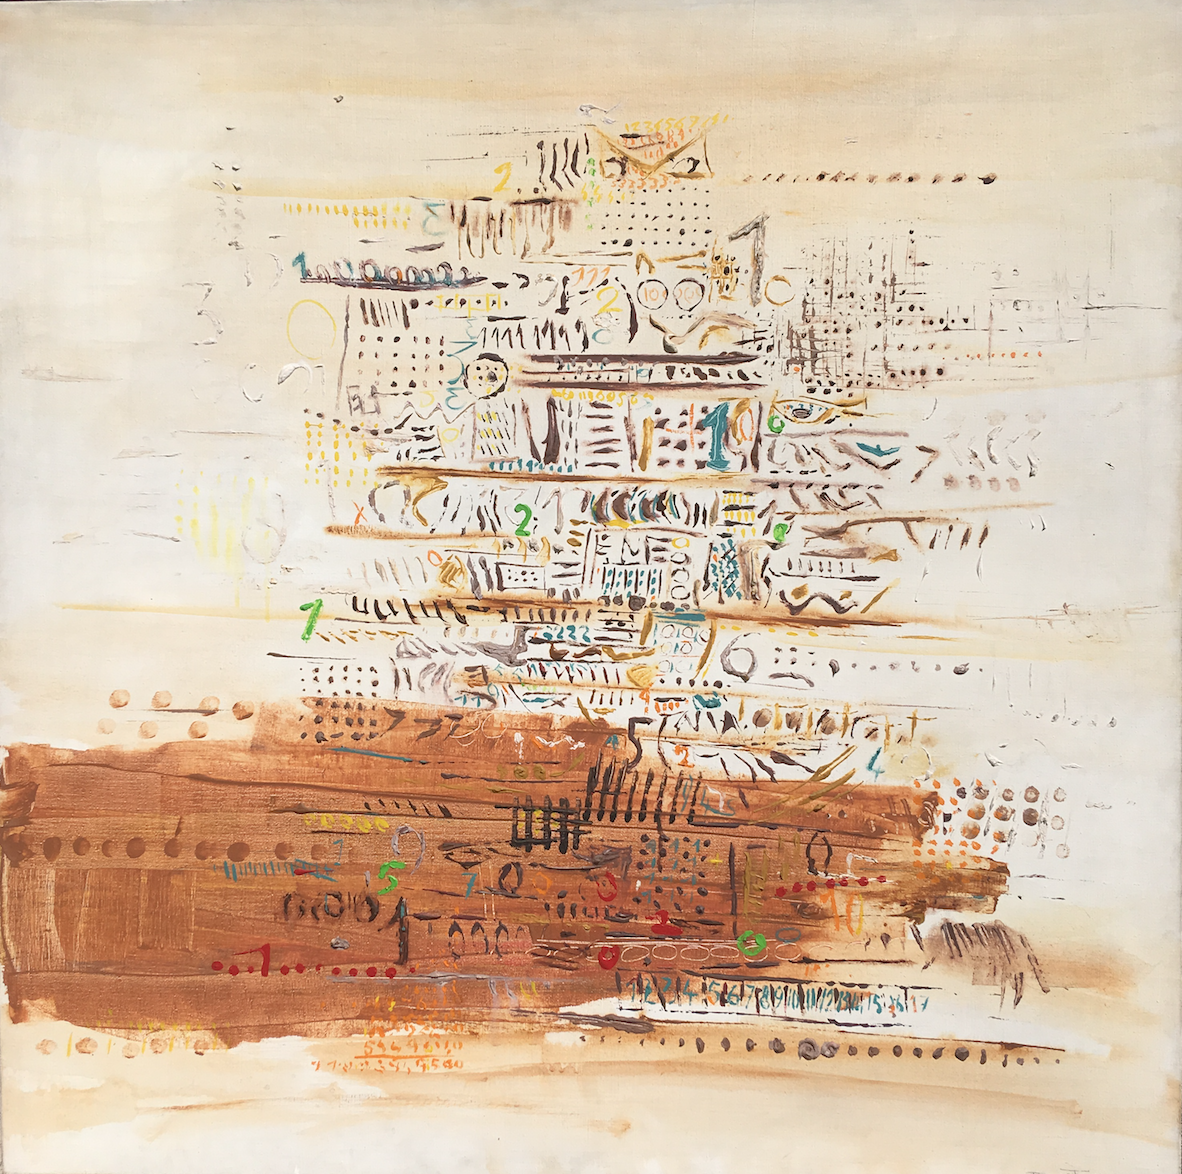
\includegraphics[scale=0.75]{AdditionForSpringer.png}}

\medskip

\centerline{{\large\em  Addition} \hspace*{4.5in} {\small Roger Trystram, 1973}}



%*********REVISED 01-31-08

%\addcontentsline{toc}{chapter}{Capsule Biography of the Author}
%\input{capsulebio}
%*********REVISED 07-02-08

\tableofcontents

\addcontentsline{toc}{chapter}{MANIFESTO}
%version of 02-10-20

\chapter*{Manifesto}

The technologies that enable both the hardware and software systems of modern computers have grown in complexity at least as fast as they have in performance.  For decades, it has been impossible to design computing systems without using tools whose underpinnings are rooted
in {\it discrete mathematics}.  For too long, though, these tools have been used to create widgets which are then assembled into coherent systems using only cleverness and untutored ingenuity.  The net result is that many of the computing systems that impact our daily lives are neither well-understood nor well-controlled.  We read daily about breaches of security and/or privacy that can neither be controlled nor repaired because the victimized system is too complex to be understood.  The lesson is clear: {\bf We must stop being satisfied with mere {\em knowledge} of how to make a system take in inputs and emit outputs.  We must strive for {\em understanding} of every system's structure and behavior.}  There are several examples of successful such programming systems within the world of computing: compilers and databases and electronic circuits begin a long list.  Notably, the success stories can be traced back to the development of relevant new discrete mathematics.

This book has a simple, yet fundamental, goal.  We want to endow each reader with an {\em operational} conceptual and methodological understanding of the discrete mathematics that can be used to study, and understand, and perform computing.  We want each reader to {\em understand} the elements of computing, rather than just {\em know} them.  Thereby, the interested reader will be able to {\em develop new concepts} and {\em invent new techniques and technologies} that will expand the capabilities of the hardware that performs computations and the software that controls the hardware.  We stress the word {\it operational:}  {\bf We want the readers' level of understanding to allow them to {\em ``do''} mathematics.}

\bigskip

Lest the reader feel unworthy for the daunting task of ``doing'' mathematics, we invoke no less an authority than the great mathematician Leopold Kronecker\index{Kronecker, Leopold} to brace
the spine and embolden the spirit.  We read in \cite{Bell86} Kronecker's assurance that ``God made the integers; all else is the work of man.''  Therefore, although we may be standing on the
shoulders of giants when we ``do'' mathematics, we are not insolently attempting to wrest fire from Olympus!

\ignore{***************
\bigskip

\noindent \fbox{
\begin{minipage}{0.95\textwidth}
The phrase ``standing on the shoulders of giants'' has been cited by
many, over many centuries, ranging from Sir Isaac Newton to Bernard of
Chartres, and beyond.  The treatise by Merton \cite{Merton}
\index{Merton, Robert K.} provides an entertaining, educational
history of the phrase.
\end{minipage}
}

****************}


%chapter
%*********Complete 05-29-19

\addcontentsline{toc}{chapter}{PREFACE}
%version of 04-11-19 

\chapter*{PREFACE}

The goal of this book is to endow the reader with an operational
understanding of the activity we, hopefully evocatively, call
``doing'' mathematics.  We want the reader to be able to recognize
situations---especially within the world of computing---wherein
mathematical reasoning and analysis can make a positive difference.
Of course, part of enabling this activity resides in the imparting of
mathematical knowledge: what are the basic concepts and intellectual
artifacts that our mathematical forebears have given us access to.
Another part, though, requires transmitting the understanding of how
to use the knowledge effectively and ceatively.

**HERE

  A vast array of formal aids for the activities of
designing, analyzing, utilizing, and verifying computer systems has
been developed.  And, mathematical tools have always been at or near
the forefront of such aids.

Our goal for each chapter and section of this book is to endow every
reader with at least one new tool for achieving an {\em operational} level
of conceptual and methodological understanding of the discrete
mathematics that is used to study and understand both the activity of
computing and the design of the systems that enable that activity.  We
construe an ``operational'' level of understanding to be one that
enables the reader to ``do'' the relevant mathematics.







**ADD SHORT PARAGRAPH FOR EACH POINT

\begin{itemize}
\item
We aim for UNDERSTANDING rather than just knowledge
\item
We want to help students/readers THINK rather than just learn —
which explains multiple proofs
\item
We want to expose the reader to some culture (as an aid to thinking
and understanding) — which explains some digressions and stories
\item
Part of the culture comes via the $\oplus$ sections … even if they are
rather short and informal.
\end{itemize}




%chapter
%*********Complete 05-29-19


%\addcontentsline{toc}{chapter}{List of Acronyms and Symbols}
%\input{acronym}


\mainmatter

%%%%%%%%%%%%%%%%%%%%%%%%%%%%%

%version of 06-18-19

\chapter{INTRODUCTION}
\label{ch:intro}

\begin{quote}
{\em I have only made this letter longer because I have not had the
  time to make it shorter.}  \\
\hspace*{1.5in}Blaise Pascal, {\it The Provincial Letters}
(Letter 16, 1657)
\end{quote}


\section{Why Is This Book {\em Needed?}}
\label{sec:bookneeded}

How much mathematics does an aspiring computing professional
need---and at what level of expertise?  We believe that the answer to
this pedagogically fundamental question is time dependent.

\medskip

\noindent {\it The early generation}.
In the early days of computing, all aspects of the field were
considered the domain of the ``techies''---the engineers and
scientists and mathematicians who designed the early computers and
figured out how to use them to solve a range of (mostly
compute-intensive) problems.  Back then, one expected every computing
professional to have a mastery of many mathematical topics.

\medskip

\noindent {\it Children of the early generation}.
Times---and the field of computing---changed.  The ``techies'' were
able to craft a variety of sophisticated tools that opened up the
world of computing to the general population.  Even people at the
lower levels of the educational edifice were able to use imagination
and ingenuity, rather than theorems and formulas, to produce
impressive software artifacts of considerable utility.

\medskip

\noindent {\it The modern generation}.
Pendulums were made to swing.  As we note in our {\it Manifesto}, we
now encounter almost daily problems that arise from unanticipated
concomitants of the often unstructured ingenuity that produced various
software artifacts.  Many would say that we need a renewed commitment
to technical discipline that will endow artifacts with
\begin{itemize}
\item
{\em understandable structure}, so that we can determine {\em what} went
wrong when something {\em does} go wrong.
\item
{\em sustainability}, so that changes, which are inevitable in complex
artifacts, will not create new problems
\item
{\em controllability}, so that ``smart'' artifacts do not become
modern instances of Dr.~Frankenstein's monster.\footnote{See Mary
  Shelley (English author), {\it Frankenstein}, or, {\it The Modern
    Prometheus}.}
\end{itemize}
While we certainly need not return to the era of the ``techies'', it
is unquestionable that we do need a larger contingent of computing
professionals who have bona fide expertise that enables the needed
technical discipline.  This text is devoted to the mathematics that
underlies the needed science and engineering.


\section{Why Is {\em This} Book Needed?}
\label{sec:thisbookneed}

There are many introductory texts on discrete mathematics.  What
separates this text from its siblings is the stratagem we have
implemented to accommodate our intended audience of aspiring computing
professionals.

We begin by recognizing that we live in a world of ever-increasing
professional and social diversity.

\medskip

Historically, computing curricula began as predominantly
technically-oriented studies within a school of science or
engineering.  The evolution of the computing field has led us to move
beyond that historical curricular worldview.  Modern
computing-oriented curricula offer a variety of educational
trajectories, including:
\begin{itemize}
\item
the traditional path, which emphasizes science and engineering and
mathematics,
\item
paths which emphasize subfields of the humanities or social studies,
\item
paths which emphasize the {\em practice} of computing, either in a
general setting or within a focused applied field such as business or
finance or law or \ldots.
\end{itemize}
The preceding reality has led to a phenomenal broadening of the
audience for computing-related curricula, hence for some level of
mathematics education.  It has also engendered two far-reaching
changes in the way we think about the mathematical component of
computing-related education.

\noindent {\bf 1}.
Many of today's aspiring computer professionals---particularly those
targeting the newer subareas of computing---arguably need only
specialized knowledge of mathematics.  Educators in computing-related
fields must, consequently, serve a large population of students, in a
manner that accommodates the students' quite diverse needs and
aspirations.

\noindent {\bf 2}.
The fields of {\it information} \index{information in computing} and
{\em computing} have developed an unprecedented level of overlap.  As
recently as the mid-1900s, these fields were viewed as largely being
separate concerns: computing was concerned with manipulating discrete
objects; information was concerned with transmitting sequences of
bits.  As parallel computing machines were developed, beginning in the
1960s, computing practitioners had to start paying more attention to
the specific ways that information flowed among the processors of a
parallel machine, and between these processors and the devices in
which data was stored.  The development of the Internet, around the
1990s, focused yet more attention on information flow.  The marriage
between the fields of computing and information dissemination was
completed by the end of the 20th century.  Orchestrating the way that
information flowed and spread became a {\it bona fide} specialty
within the areas of mathematics that hitherto had focused only on
computing.  The introduction of information into computing had
revolutionary aspects.  Information could be replicated at a speed and
to a volume that was unmatched by the objects studied in any physical
science.  Flowing information enabled the construction and operation
of the kind of virtual universe hinted at by the computation-theoretic
notion of {\it nondeterminism} \index{nondeterminism} (see, e.g.,
\cite{Rosenberg09}), whch had hitherto been viewed as a ``pure''
mathematical idea.  The mathematics that students learn had to adapt
so that students learned how to think about information, most
especially within the context of computing.


\bigskip

We have striven to keep the increasing diversity of students and of
approaches to computing in mind as we have written this text.  We have
included a broad range of material, in both subject and level.  As
noted in the {\it Preface}, we have tried to accommodate the different
backgrounds of our readership, while leading them all to a level of
mathematical sophistication that will enable them to {\em
  understand}---and {\em do}---mathematics.

\medskip

In the remainder of this chapter we describe our approach to the text:
both our strategy for selecting and developing mathematical topics and
our tactical organization of topics into chapters, sections, etc.  We
describe also the various types of problems that we have included in
the chapter devoted to Exercises
(Chapter~\ref{ch:Exercises})---ranging from problems that allow every
student to practice with ideas from the text to problems that challege
the dedicated student to develop material that we had no space to
develop the text.  Finally, we describe the advanced material that we
have included in appendices as enrichment material for the ambitious
reader.  These discussions will allow the reader to evaluate which
topics are most appropriate for their particular educational needs.



\section{The Structure of This Book}
\label{sec:thisbook}

In our quest to endow each reader with an operational understanding of
how to ``{\em do}'' mathematics, we want the reader
\begin{itemize}
\item
to recognize situations---especially relating to computing---wherein
mathematical reasoning and analysis can make a positive difference
\item
to identify the mathematical tools that are approprite for these
situations.
\end{itemize}


\subsection{Our Main Intellectual Targets}
\label{sec:book-overwiew}

This book is devoted to covering the discrete-mathematics
underpinnings of the endeavor of computing: from the design and
implementation of devices that perform the actions necessary to
compute to the design of the processes that control the
devices---including whatever communications are needed among processes
and among (sub)devices.  We have identified several intellectual
targets that guide our exposition.
\begin{enumerate}
\item
{\it Fundamental concepts}

\medskip

{\small\sf Examples:}
\begin{itemize}
\item%
sets---and their embellishments: tuples, arrays, tables, etc.---as
embodiments of {\it object}
\item
numbers---and their operational manifestations, numerals---as
embodiments of {\it quantity}
\item
graphs---in their many, varied, forms---as embodiments of {\it
  connectivity} and {\it relationship}
\item
algebras and functions---adding operations to sets, numbers, and
graphs---as embodiments of {\it structured dynamism} and {\it
  computing} and {\it process}
\end{itemize}
We thereby expand the scope of what can be thought about
``mathematically''.

\medskip

\item
{\it Fundamental representations}

\medskip

{\small\sf Examples:}
\begin{itemize}
\item
representing and thinking about numbers via many metaphors: slices of
pie, tokens arranged in stylized ways, characteristics of geometrical
figures (e.g., rectangles or circles), textual objects
\item
understanding the strengths and weaknesses of various positional
number representations (e.g., what can you tell about a number from
its representation?)
\item
using grouping and/or replication to represent relationships among
objects
\item
viewing interrelated objects via many structures: tables, tuples,
graphs, geometric drawings
\end{itemize}
We thereby expand the universe of conceptual paradigms that one can
use while thinking ``mathematically''.

\medskip

\item
{\it Fundamental tools/techniques}

\medskip

{\small\sf Examples:}
\begin{itemize}
\item
using induction to extrapolate from simple examples to complex ones
\item
``hopping'' between the discrete and continuous mathematical worlds,
e.g., using integration to approximate summation
\item
using the conceptual tools of asymptotics to argue qualitatively about
quantitative phenomena
\item
``hopping'' between the mathematical reasoning used in the ``real''
  world, vs.~the formal logics that enable such reasoning
\end{itemize}
We thereby expand the conceptual tools that one has access to when
{\em doing} mathematics.

\medskip

\item
{\it Beyond the fundamentals}

Our goal in writing this text is not just to expound on the basic
notions that enable one to study the phenomenon of computation and its
accompanying artifacts.  We strive additionally to inspire each reader
to dig deeper into the lore of at least one of these notions. To this
end, we have presented many basic notions via multiple explanations
and numerous exemplars.

\medskip

{\small\sf Examples:}
\begin{itemize}
\item
The ability to ``encode'' tuples of objects via the underlying objects
themselves lie at the base of some of the pillars of computing.  We
expound on two approaches to such encodings, one based on {\em prime
  numbers} and one on {\em pairing functions}.  We provide pointers to
the literature which show how this basic ability can be applied to
``real'' computing problems such as {\em efficiently storing arrays
  whose dimensions can change dynamically} and {\em tracking the
  computing output of each agent in a collaborating team}.

\item
The use of recursion as a control structure in computing has a purely
mathematical analogue, recurrences, which are extremely useful in
analyzing the correctness and efficiency of these computations.  Every
student gains at least some familiarity with the most basic versions
of recurrences.  We introduce variations on the theme of these
familiar recurrences, which offer approaches to more complicated
computational situations.  We illustrate the use of recurrences in
crafting a quite approachable analysis of an apparently complex {\em
  token game}.
\item
Many phenomena that appear to arise from arcane inherently
computational sources are actually rather easily understood
applications of purely mathematical phenomena.  We spend considerable
time expounding on such phenomena and their applications.  {\em
  Satisfiability problems} are one phenomenon of this sort; certain
{\em specialized number systems} are another.
\end{itemize}
\end{enumerate}


\subsection{Allocating our Targets to Chapters}
\label{sec:the chapters}

\subsubsection{Chapter~\ref{ch:doingmath}: ``Doing'' Mathematics}

A toolkit for mathematics reasoning.
In order to acclimate the reader to mathematics as a living discipline
and an integral part of the world of computing, we begin the book with
a chapter entitled {\it Doing Mathematics}.  This chapter focuses
mainly on the practicalities of mathematical reasoning, most
importantly by expounding on the idea of a mathematical proof.  We
survey the most commonly encountered techniques for crafting such
proofs and illustrate each with several examples.

Part of understanding proofs is being aware of what makes the endeavor
of proving things difficult.  We provide both mathematical and
historical background relating to important intellectually challenging
topics such as how to reason about objects that are infinite and
objects that are finite but very large (and growing).


%{\Denis I moved the asymptotic and infinity in the appropriate place later on}

\ignore{************
\medskip

\noindent {\em Reasoning qualitatively about quantitative phenomena.}
%
An often-underappreciated aspect of human reasoning is our ability to
abstract by blurring descriptions.  We notice, for instance, the ways
in which all phenomena that experience {\em linear} growth differ from
phenomena that experience {\em quadratic} growth, and both classes
differ from phenomena that experience {\em cubic} growth---and so on,
\ldots, {\em exponential}, and beyond.  
The extremely important topic of {\it asymptotics} abstracts from these
enumerated abstractions and allows us to reason qualitatively about
arbitrary inherently quantitative phenomena.

\medskip

\noindent {\em Coping with infinity}.
One recurring challenge when ``doing'' mathematics is dealing with
{\em infinity}.  Infinite objects, such as sets, behave rather
differently from the more familiar finite objects that we encounter in
our daily lives.  As but one example, there are ``equally many'' odd
integers as all integers, as measured by the ability to match the two
sets element by element---even though the first of these sets is
obtained from the second by discarding half of its elements.

A more subtle challenge manifests itself in the world of the infinite
resides in the myriad {\em paradoxes} that one encounters in this
world.  Does an arrow ever reach its target---given that it begins its
journey by traversing half then distance, then traverses half of the
remaining half, then half of the remaining quarter, \ldots?
**********}

\subsubsection{Chapter~\ref{ch:sets-BA-logic}: Sets and Their Algebras}

{\em Sets} are the stem cells of mathematics.  They begin as the most
primitive mathematical objects, but as soon as one endows them with
operations---for creating more inclusive (``bigger'') sets, for
selecting more exclusive (``smaller'') subsets, for enabling the
structure of tupling---they quickly afford one a powerful substrate
for doing almost all of mathematics.

\medskip

\noindent {\em The power of tupling}.
%
One can exploit tupling to isolate entities such as {\em relations},
which are the foundations of imposing and identifying {\em order} in,
and among, sets.  One can isolate {\em functions}, which enable one to
{\em encode} various sets as other, seemingly unrelated,
ones---example: encoding computer programs as positive integers.

\medskip

\noindent {\em Algebras: Operations and the laws that govern them}.
%
The operations within any collection of operations on sets inevitably
obey certain ``laws'' as they interact; for instance, operation
$\circ$ may (or may not) be {\em commutative}, i.e., obey the relation
\[ x \circ y \ = \ y \circ x \]
or it may (or may not) be {\em associative}, i.e., obey the relation
\[ x \circ (y \circ z) \ = \ (x \circ y) \circ z \]
The combination of a set $S$ (of ``objects'') and a set of operations
on set $S$, together with the laws that govern the operations, is an
{\em algebra}---and there are myriad algebras that play important
roles in our lives.
\begin{itemize}
\item
{\em Boolean algebras} focus on sets and operations on sets.
\item
A special class of Boolean algebras is the class of {\em Propositional
  logics}.  These algebras underlie computing-related topics that
range from {\em digital logic}, the basis of all computer design, to the
{\em satisfaction problems} that play a major role in aspects of 
{\em complexity theory} and {\em artificial intelligence} ({\em AI}).
\item
{\em Numerical algebras} govern our daily lives, by enabling us to
perform crucial basic functions such as
counting and performing arithmetic.
\end{itemize}


%{\Denis I add below th 3 subtitles, keep free to remove or change...}
\subsubsection{Chapters~\ref{ch:numbers-numerals},
~\ref{ch:numbers-advanced}, ~\ref{ch:numerals}: Numbers and Numerals}


The first mathematical concepts that children learn about usually
involve numbers.  We spend much of our early lives expanding our
number-based knowledge base.  We proceed from counting to manipulating
numbers by adding and subtracting and multiplying and dividing them.
We progress from using fingers and toes as ``names'' of numbers to
using a variety of numeral-forming schemes.  For many of us,
``mathematics'' {\em means} ``numbers and arithmetic'': We never get
to explore the powerful mathematical concepts and tools that have
enabled many of the great advances of science and engineering.  Even
fewer of us get to explore the conceptual extremities of mathematics
which led to the field's being dubbed ``{\em the queen of the
  sciences}'' by the great $19$th-century German mathematician Karl
Friedrich Gauss. \index{Gauss, Karl Friedrich}

While mathematics is assuredly much more than ``just'' numbers and
arithmetic, one could spend one's life fruitfully while exploring
nothing beyond these topics.  The three chapters described in this
section strive to introduce the reader to numbers and
arithmetic ``in layers''
\begin{itemize}
\item
{\em The basic objects and properties of our number system.}

Chapter~\ref{ch:numbers-numerals} introduces the subject by means of a
``biography'' of our number system as it has evolved over the
millennia---in response to the need for greater explanatory and
manipulatory power over the phenomenally expanding knowledge base
exposed by science and technology.
\item
{\em Building the integers and building with the integers.}

Chapter~\ref{ch:numbers-advanced} is devoted to looking both inward
and outward at the most easily intuited component of our number
system, the {\em integers} (or, ``counting numbers'').  Looking
inward, we discover the {\em prime numbers} (familiarly, ``the
primes'').  A theorem from antiquity exposes the primes as the
``building blocks'' of the entire set of integers.  Looking outward,
we expound on the use of the primes as the basis of a variety of {\em
  coding schemes} for a broad range of structures.  Both the strengths
and the weaknesses of prime-based encoding schemes have inspired the
development of many other important encoding schemes.  These encoding
schemes lead to numerous nonobvious applications, ranging from storage
schemes for dynamic data structures to provably secure encodings of
various structures.

\item
{\em Operational number representation and their consequences.}

In Chapter~\ref{ch:numerals} we shift our focus from {\em numbers},
the objects that we count with, to {\em numerals}, the {\em names}
that we use to represent and manipulate numbers.  The importance of
using an appropriate numeral system for a particular application can
be illustrated by the design of digital adders.  The digital adder
that mimics the ``carry-ripple'' scheme that we all learned in
elementary school takes roughly $n$ steps to add a pair of $n$-digit
numbers.  By using a nonstandard {\em signed-digit} representation
scheme, we can reduce the addition time to a fixed constant,
independent of the lengths of the numbers beng added.  (Of course,
signed-digit schemes entail costs that standard schemes do not, which
is why they are not in common use.)
\end{itemize}
We spread our coverage of numbers and numerals over a {\em
  noncontiguous} sequence of three chapters because we need additional
material to progress from one number-oriented chapter to the next.
Specifically, we employ concepts and tools from
Chapters~\ref{ch:arithmetic} and~\ref{ch:Summation} (which cover
arithmetic and summations, respectively) in essential ways within
Chapter~\ref{ch:numbers-numerals}, and we add to this corpus material
from Chapter~\ref{ch:Recurrences} (which covers recurrences) as we
develop Chapter~\ref{ch:numerals}.


\subsubsection{Chapters~\ref{ch:arithmetic} and~\ref{ch:Summation}:
Arithmetic and Summation}

Numbers are important in our daily lives only when we {\em use} and
{\em manipulate} them.

Chapter~\ref{ch:arithmetic} discusses {\it arithmetic}, the basic
operations---addition, multiplication, etc.---that we use to
manipulate numbers and the laws that these operations obey.  The
chapter then moves on to complex operations on numbers---polynomials,
exponentials, and logarithms.  It closes with pointers to topics for
advanced study---including topics that are central to modern computer
applications such as big data.  The chapter's treatment of polynomials
is far reaching:
\begin{itemize}
\item
The chapter begins with basic facts about these special functions.
\item
The chapter then introduces the centuries-old study of solving---or
being unable to solve---single-variable polynomials using radicals
(the latter topic being discussed only informally because of its
advanced nature).  The well-known {\it quadratic formula} is the
simplest instance of solving polynomials by radicals: The two
solutions to the polynomial equation
\[ ax^2 \ + \ bx \ + \ c \ = \ 0 \]
are
\[ x \ = \ \frac{-b + \sqrt{b^2 - 4ac}}{2a}
 \ \ \ \mbox{ and } \ \ \
   x \ = \ \frac{-b - \sqrt{b^2 - 4ac}}{2a}
\]
\item
The chapter's treatment of polynomials then digresses to present an
extremely important result about two-variable polynomials, Newton's
famous {\it Binomial Theorem}.  This result enables one to go easily
between polynomials in a certain family and their roots.  The
Theorem's ``smallest'' instances provide the following equations.
\begin{eqnarray*}
(x + y)^2 & = & x^2 \ + \ 2xy \ + \ y^2 \\
(x + y)^3 & = & x^3 \ + \ 3x^2y \ + \ 3 xy^2 \ + \ y^3
\end{eqnarray*}
\item
The chapter's treatment of polynomials closes with a short, informal,
discussion of {\it Hibert's Tenth Problem}, an advanced topic of
immense mathematical import.  In one line: The work on this Problem
demonstrates that the single topic of discovering integer roots of
arbitrary polynomials with integer coefficients---or proving that no
such roots exist---captures (read: {\em encodes}) the full complexity
of performing arbitrary computations!
\end{itemize}
The chapter finally introduces the mutually inverse operations of
taking exponentials and logarithms, in the sense of the equations
\[  x \ = \ \log_b(b^x) \ = \ b^{\log_b(x)} \]
A fundamental insight here is that the arithmetical system based on
these functions is {\em almost} identical to our conventional
arithmetic---but with multiplication replacing addition and division
replacing subtraction.  ({\em This is the basic insight underlying the
  {\em slide rules} that were techies' pocket calculators for many
  decades.})  The qualifier ``almost'' hints at the adjustments needed
to accommodate the impossibility of dividing by $0$.  This pair of
operations play a fundamental role in the field of information theory,
whose importance to computing cannot be overstated.

\bigskip

Chapter~\ref{ch:Summation} is basically a {\em tools} chapter. 
It studies how to break a complex operation into simple constituents.
It is devoted to analyzing a broad variety of families of summations,
providing exact solution-sums for many and approximate sums for
others.  All of the finite summations we study have the general form
\[ S \ = \ s_1 \ + \ s_2 \ + \cdots + \ s_n \]
In situations where we allow summations to have infinitely many
terms---for instance, with the famous summation
\[ 1 \ + \ {1 \over 2} \ + \ {1 \over 4} \ + \ {1 \over 8} \ + \cdots
+ \ {1 \over {2^k}} \ + \cdots
\]
(whose sum is $2$), we allow this pattern to continue without end.  We
include here {\it arithmetic summations}, in which all adjacent
summands, $s_{i+1}$ and $s_i$, have a common difference, and {\it
  geometric summations}, in which all adjacent summands, $s_{i+1}$ and
$s_i$, have a common ratio.  We discuss also powerful techniques for
estimating the solution-sums of summations of consecutive terms of a
``smooth'' function.

The mathematics we exploit to derive exact and/or approximate sums for
many of the classes of summations we study provides us with the
opportunity of looking at numbers and their summations in many quite
distinct ways---from textual to pictorial to geometric, and beyond.
For this reason, this chapter is one of the most important as the
reader gains traction in the endeavor of ``doing mathematics''.

\subsubsection{Chapter~\ref{ch:infinity}: The Vertigo of Infinity}

This chapter deals with mathematical objects whose very size---ranging
from the finite but very large to the infinite---is difficult to
reason about, for one of two reasons.
\begin{enumerate}
\item
We have developed the important ability to reason abstractly by
blurring descriptions.  We notice, e.g., the ways in which all
phenomena that experience {\em linear} growth differ from phenomena
that experience {\em quadratic} growth, and both classes differ from
phenomena that experience {\em cubic} growth---and so on.

Additionally, we often encounter finite objects whose sizes can change
dynamically or can be known only approximately.  Consider, e.g.,
social networks: they expand and contract in unpredictable manners, so
their population statistics cannot be known exactly.

We require a language for talking---and rigorously reasoning---about
blurry distinctions and approximately-known objects.  And, we need a
formal analogue of arithmetic for ``calculating'' the statistics of
such objects.

The topic of {\it asymptotics} (Section~\ref{sec:asymptotics}) fills
both needs, for a large variety of dynamic mathematical phenomena.
Asymptotics thereby enables {\em reasoning qualitatively about
  inherently quantitative phenomena}.

\item
We often have to reason about objects that are actually infinite.  We
encounter such situations, e.g., in areas that combine, in some way,
  \begin{itemize}
  \item
mathematics---e.g., classes of numbers or of functions
  \item
logic---e.g., expressions with special properties, such as theorems or
proofs
  \item
linguistics---e.g., sentences that share (syntactic or semantic)
characteristics
  \end{itemize}
Since antiquity, we have been confronted by infinite objects that
behave very differently than the finite objects of daily discourse.
As just two examples:
  \begin{itemize}
  \item
Why does a shot arrow reaches its target.  The following seemingly
cogent argument shows that it does not.

The argument states---correctly---that after the arrow traverses
one-half the distance to the target, it still has one-half the
distance to go; after traversing half of the remaining distance, it
still has one-quarter of the original distance to go.  Continuing, the
arrow will have a never-ending shrinking distance that it has yet to
traverse: one-eighth, then one-sixteenth, then one-thirty-second, and
so on.  How can the arrow ever reach the target?

  \item
We have had to adapt to the fact that ``provable'' and ``true'' are
distinct concepts within most realistic systems of logic, despite
their intuitive coincidence.
  \end{itemize}

In a slightly more sophisticated vein, we all know that there are
``equally many'' odd integers as all integers---even though the former
set is obtained by discarding half of the latter set's elements.

\ignore{******
Even more puzzling: we know that there are infinitely many fractions
between any two integers.  Yet, it is easy to show (see
Section~\ref{sec:Q-Z-cardinality}) that the set of all these
fractions---this infinite collection of infinite sets---is ``no
larger'' than the set comprising just the integers!
***********}

Section~\ref{sec:coping-infinity} provides the background necessary to
cope with these puzzles and navigate the unfamiliar world of the
infinite.
\end{enumerate}

\ignore{*********
\noindent {\em Coping with infinity}.
One recurring challenge when ``doing'' mathematics is dealing with
{\em infinity}.  Infinite objects, such as sets, behave rather
differently from the more familiar finite objects that we encounter in
our daily lives.  As but one example, there are ``equally many'' odd
integers as all integers, as measured by the ability to match the two
sets element by element---even though the first of these sets is
obtained from the second by discarding half of its elements.

A more subtle challenge manifests itself in the world of the infinite
resides in the myriad {\em paradoxes} that one encounters in this
world.  Does an arrow ever reach its target---
************}

\subsubsection{Chapter~\ref{ch:Recurrences}: Recurrences}

%Imposing manageable structures on constructs and computations.

The functions discussed in Chapter~\ref{ch:arithmetic} are described
by static ``closed-form'' expressions.  In contrast,
Chapter~\ref{ch:Recurrences} is devoted to a family of {\em
  computational procedures}, {\it recurrences}---which calculate the
value of a function $f$ on an argument $n$ in terms of the values of
$f$ on smaller arguments.  The patterns that underlie recurrent
computations have been known for millennia to occur throughout
nature---in the growth patterns of many plants and in the demographics
of many animals, among other places.  The mathematics that describes
such computations is as elegant and aesthetic as it is useful.  Among
the myriad recurrent patterns that one could identify, we select three
main ones for their computational importance.
\begin{enumerate}
\item
{\it Linear recurrences}.  Recurrences of the form
\begin{equation}
\label{eq:general-linear-recurrence}
f(n) \ = \ a f(bn+c) \ + \ dn \ + e
\end{equation}
(where $a, b, c, d, e$ are constants) are a welcome friend when one
analyzes the costs of a broad range of algorithms, using a broad range
of cost measures (e.g., time, memory usage, power requirements, amount
of communication).

We introduce two simple, yet nontrivial uses of recurrence
(\ref{eq:general-linear-recurrence}) in the analysis of algorithms.
We refer the reader to an algorithms text such as \cite{CLRS} for
details.
%{\Denis remark: both next examples are dealing with algorithms, may be too much?}
  \begin{itemize}
  \item
The {\em binary search algorithm}, which determines whether an item
$x$ occurs within a given ordered list of $n$ items, begins by
partitioning the list in two (so $b = 1/2$ and $c = 0$ in
(\ref{eq:general-linear-recurrence})).  It then compares $x$ with the
list's middle item(s)---there is one middle item when $n$ is odd, two
when $n$ is even---(so $d = 0$, and $e$ is the fixed constant cost of
the comparison(s)).  Based on the outcome of the comparison, the
algorithm recurses with a binary search on the half of the list that
could contain $x$ (so $a = 1$).

  \item
The {\em merge-sort algorithm} builds on a natural $n$-step algorithm
for merging two $n$-item lists of ``order-comparable'' items (i.e.,
for every pair, $x,y$, of list items, either $x < y$ or $y < x$).  The
algorithm first merges adjacent odd-even pairs of items, to end up
with sorted $2$-item lists.  It then merges adjacent $2$-item lists,
to end up with sorted $4$-item lists.  It continues thus with $8$-item
lists, then $16$-item lists, \ldots, until it finally merges the
``top-level'' two $n/2$-item lists to achieve the goal of a sorted
$n$-item list.  The performance of this algorithm is given by
recurrence (\ref{eq:general-linear-recurrence}), with $a=2$, $b =
1/2$, $c = 0$, $d=1$, and $e =$ (the fixed cost of a
 $2$-item
comparison).
  \end{itemize}


\smallskip

The centerpiece of our discussion of linear recurrences is the
so-called {\em Master Theorem}, which uses geometric summations to
generate explicit---rather than recurrent---expressions for the values
of a function $f$ on an arbitrary argument $n$.

\item
We highlight two {\it bilinear} recurrences of especial computational
importance.
  \begin{itemize}
  \item
The {\it binomial coefficient} articulated as ``$n$ choose $k$'', and
commonly denoted $\displaystyle {n \choose k}$ or $\Delta_{n,k}$ or
$C(n,k)$, plays a central role in a broad range of mathematical
domains.  Two rather distinct examples:

%{\Denis I found both examples too much detailed. I suggest to shorten}
       \begin{itemize}
       \item
$C(n,k)$ is the number of ways to select $k$ items out of a set of $n$
items.  For instance, $C(4,2) =6$, because the $2$-element subsets of
$\{a, b, c, d\}$ are: $\{a, b\}$, $\{a, c\}$, $\{a, d\}$,  $\{b, c\}$,
$\{b, d\}$,  and $\{c,d\}$.  Analyzing $C(n, 5)$ will reveal, for
example, why ``three of a kind'' beats ``two pair'' in poker.
       \item
These numbers play a prominent role in evaluating arithmetic
summations; e.g., we derive the following equation (in several ways)
in later chapters:
\[ 1 \ + \ 2 \ + \ 3 \ + \cdots + \ n \ \ = \ \ C(n+1, 2) \]
       \end{itemize}
The {\em family} of binomial coefficients is defined by the bilinear
recurrence
\begin{eqnarray*}
C(n+1, k+1) & = & C(n, k) \ + \ C(n, k+1) \ \ \mbox{for any } \ \ k \geq 0 \\
C(n, 0) & = & 1 \\
C(n, 1) & = & n 
\end{eqnarray*}

  \item
The sequence of {\it Fibonacci numbers}, named for the Pisano
mathematician known by the nickname ``Fibonnaci'', are defined by the
recurrence
\begin{eqnarray*}
F(n+1) & = & F(n) \ + \ F(n-1) \\
F(0) & = & F(1) = 1
\end{eqnarray*}
Fibonacci invented his eponymous sequence as he observed the
populations of consecutive generations of progeny produced by a pair
of rabbits; the sequence also arises in the structure of many plants;
it further is said to have a semi-religious aspect in the architecture
of ancient Greek temples.
%  The story of the sequence is told in a bit more detail in Section~\ref{sec:Fibonacci-story}.
Aside from its important descriptive role, the sequence plays a
significant role in the analysis of algorithms and as the basis for a
nonstandard system of numerals.
  \end{itemize}
\end{enumerate}
Variations on the preceding three families of recurrences provide
supplemental material in this chapter.


\subsubsection{Chapter~\ref{ch:combinatorics}: 
Combinatorics, Probability, Statistics}

Certain subfields of mathematics have been known for centuries as
``the art of counting''.\footnote{Gottfried Leibniz used the phrase as
  the title of his 1666 doctoral thesis. 
\index{Leibniz (Leibnitz), Gottfried Wilhelm}} This chapter introduces
three related areas of discrete mathematics that are based on that
art.  Indeed, one can argue that the following chain of applications,
while grossly oversimplified, is not misleading.

\smallskip

\begin{tabular}{lcl}
{\it Statistics} & can be viewed as applied & {\it Probability} \\
{\it Probability} & can be viewed as applied & {\it Combinatorics} \\
{\it Combinatorics} & can be viewed as applied & {\it Counting}
\end{tabular}

\smallskip

\noindent
These are important connections.  Elements of probability and
statistics infuse every area of endeavor---from science to finances to
informatics, and beyond---where computing is involved.  In order to
function successfully in today's world, one needs statistical and
probabilistic literacy---a command of the foundations and the
operational rules of ``the art of counting''.

\begin{itemize}
\item
This chapter begins by developing the basic {\em rules of counting:}
How many strings of length $n$ can one form using $c$ characters?  How
many subsets does a set of $k$ elements have?  We discover that many
seemingly distinct problems of this type are actually {\em encodings}
of one another!

\item
The chapter moves on to concepts related to {\em grouping and
  arrangement} using mechanisms such as permutations, combinations,
and derangements.  Variations of these themes allow us to develop {\em
  selection}-based concepts, such as: In how many deals of five playing
cards do all cards have the same suit?

\item
We develop the elements of {\em discrete} (or, {\em combinatorial})
{\em probability}.  The probability (or, {\it likelihood}) of an event
is defined as the ratio of the number of ways that the event occurs,
divided by the total possible number of outcomes.  For instance, the
probability of achieving the result ``$7$'' when rolling two dice is
the ratio of the number of rolls that produce ``$7$'', divided by the
total number of rolls.

We illustrate the elements of probability by simple, fun, examples
such as assessing the relative values of various deals in the card
game {\it poker} and of various rolls of a pair of dice in the game
{\it craps}.

We also discuss the use of the concepts we develop in situations
wherein it is less common to think in terms of probabilities but in
which probabilistic thinking can be valuable.  We describe in some
detail a rather unintuitive such situation that arose in connection
with a television game show from a few decades ago.  And, we discuss
the {\it anniversary paradox} which, while whimsical, is a good
illustration of the elements of probabilistic thinking.

\item
Finally, we illustrate the {\em statistical} way of thinking by
carefully analyzing two ways for deriving the likelihood of achieving
a specific sum---such as $6$---when rolling {\em three} dice.  This
example will enable us to generalize from the probabilities of
specific events to (statistical) {\it distributions} of these
probabilities.

Even if one intends to ``do'' statistics mainly with the aid of
preprogrammed packages (or apps), it is valuable to understand what
the numbers produced by an app mean---and what the numbers {\em do
  not} mean!  Anyone who aspires to designing and/or executing and/or
analyzing experiments {\em must} understand crucial notions such as
{\em randomness} and should be conversant with the most common
statistical distributions.  {\em Lives can depend on such knowledge!}
\end{itemize}

\subsubsection{Chapter~\ref{ch:Graphs-Trees}: Introducing Graphs and Their Relatives}

Graphs are perhaps the most important representational concept in all
of mathematics.  In their most basic form, graphs represent any binary
relation; a brief sampler:
\begin{itemize}
\item
the structure of a family, as exposed by the parent-child relation;
\item
the structure of an electronic or a communication circuit, where
certain pairs of entities have the right to intercommunicate---perhaps
only directionally).
\end{itemize}
The structure represented by a graph can expose not only the fact that
certain pairs of entities can intercommunicate, but also the number of
inter-entity ``links'' that must be traversed to achieve
communication.

Even with this rudimentary discussion, one can intuit how myriad
real-life problems can be modeled using graphs.  Many such problems
use a graph to represent entities that can ``talk'' to one another, in
some sense.  A variety of associated questions could be of the form,
``Who know what when?''

Graphs are immensely important in countless scheduling applications,
for the underlying relation can be {\em directional}---exposing
dependencies.  A common relation studied in computer applications
exposes that task $A$ in a program depends on input from task $B$, so
that $B$ must be performed {\em before $A$}.  The notion of {\it graph
  coloring} is exceedingly important in scheduling and related
applications: In its conceptually simplest form, one colors the task
of a dependency graph in such a way that like-colored tasks can be
executed concurrently---they are computationally independent.  The
challenge in this scenario is to color a give task-graph with as few
colors as possible.  This is a computationally difficult task in
general, but we expose some of the sophisticated mathematics that has
been developed in order to study the graph-coloring problem.  {\em
  Path problems} in graphs provide another entry to myriad scheduling
applications.  Of particular interest are problems that require some
object (e.g., a datum) to be passed around within a graph in a manner
that achieves a ``coverage'' goal, e.g., so that the object encounters
all of the graph's entities or traverses all of the graph's
inter-entity links.

%{\Denis add a sentence on paths, hamiltonian and eulerian, which are
%the way to establish connections between the entities.}

\medskip

If {\em binary} relations are not adequate for a person's modeling
needs, the expanded notion of {\em hypergraphs} can be used to model
relations beyond binary, even those in which the ``arity'' of the
relation varies from one related group of items to the next; a brief
sampler:
\begin{itemize}
\item
the structure of a family, as exposed by two relations: the
parent-child relation and the sibling relation;
\item
the structure of a bus-connected communication setup: entities on a
single bus can all ``hear'' one another;
\item
social networks in which aggregations of ``friends'' have special
intercommunicating privileges
\end{itemize}


\section{How to Use This Text}
\label{sec:how-to-use}

{\Arny This section is being deferred until the end, so we have a
more complete picture of the various topics covered---which ones and
to what level.}

\begin{description}
\item[{\bf Digital logic and Computer architecture}.]
\index{digital logic} \index{computer architecture}
This topic would arise in computer engineering programs and in the
early portions of a course on computer architecture.
\begin{itemize}
\item
{\bf Digital logic}. \index{digital logic}
\item
{\bf Computer arithmetic}.  \index{computer arithmetic}
\end{itemize}

\item[{\bf Cryptography and Computer security}.]


\item[{\bf Big data}.]


\item[{\bf Artificial intelligence}.]


\item[{\bf Social networks}.]

\end{description}



%\subsection{Sample Curricula Based on This Text}
%\label{sec:sample-curricula}


%chapter
%*********Completed except for ``How to Use'' 05-29-19

%%%%%%%%%%%%%%%%%%%%%%%%%%%%%

%version of 06-21-18

\chapter{TECHNIQUES FOR ``DOING'' MATHEMATICS}
\label{ch:doingmath}

\section{Manifesto}
\label{sec:manifesto}

The fundamental goal of the authors is to endow the reader with an
{\em operational} conceptual and methodological understanding of the
discrete mathematics that is used to study and understand and perform
computing.  We construe an {\it operational} level of understanding to
be one that enables the reader to ``do'' mathematics.

Somewhat surprising to the non-mathematician, a large portion of
``doing'' mathematics, the widely touted ``queen of the
sciences''\footnote{See, e.g., Wolfgang Sartorius von Waltershausen,
  {\it Gauss zum Ged\"{a}chtniss} (1856).}, is {\em
  pattern-matching}---albeit of a monumentally sophisticated variety.
Mathematicians are trained to understand pieces of reality to a depth
that allows them to understand how apparently unrelated concepts $A$
and $B$ can be conceptualized via the same abstract representation,
and to analyze (computational, in our bailiwick) advantages to
exploiting such representations.

This chapter is devoted to the practice of mathematics within the
world of computing.  By means of plentiful examples, we hope to
convince the reader of the importance of mathematics in this context.
By means of extensive explanations---often proving the same fact from
multiple, orthogonal vantage points, wed hope to provide the reader
with tools for seeing the mathematical aspects of computational
settings and phenomena and guidelines for using those tools
effectively.

\section{Reasoning via Rigorous Proof}
\label{sec:reasoning-via-proofs}

Mathematics helps one thrive within the world of computing in two
ways: by enabling rigorous argumentation about properties of
computational structures and processes and by enabling cogent analyses
of such properties.  This section is devoted to the first of these
topics.  We survey, explain, and exemplify a range of proof techniques
tha are among most commonly useful within computational settings.

\subsection{Classical vs.~modern proofs and methodologies}
\label{sec:classical-v-modern-proofs}

Contrary to the all-too-common view of mathematics as arcane strings
of symbols that must be manipulated in rigid way, mathematics is a
vibrant, evolving system of thinking whose evolution is influenced by
the ever-changing objects that are being thought about and by the
ever-changing population that are doing the thinking.

Gone forever from the world of the practicing mathematician is the
rigidity that chacterized the proofs and analyses of the 19th and
early-to-mid-20th century.
\begin{quote}
{\em We do not go back earlier than the 19th century because
formal notions of rigorous proof are, historically, a relatively
recent phenomenon, stemming largely from seminal philosophical
developments in the 19th century.}
\end{quote}
What has replaced the rigid logical systems and rigid prescribed forms
of ``antiquity'' is a vibrant system of thought that, when convenient,
\begin{itemize}
\item
represents the  number $n$, as convenient, by, e.g.,
  \begin{itemize}
  \item
a numeral in some positional number system, such as we use in daily
discourse,
  \item
a set (usually imagined) of $n$ balls or \ldots or widgets,
  \item
a unit-width rectangle that is $n$ units high.
  \end{itemize}

\item
freely uses different modes of argumentation (e.g., numerical and
structural induction, contradiction, counting, \ldots), even mixed and
matched throughout a single analysis;

\item
freely invokes a highly tested computer program to check mind-numbing
proliferations of clerically verifiable details.
\end{itemize}

Regrettably, mathematics education has lagged behind practice, despite
the emergence of technical/technological fields such as computer
science that cannot advance very far without at least informal
extensions and adaptations of the now-archaic formal proof systems.

The current volume is dedicated to trying to overcome people's
resistance to mathematical analysis and argumentation via a modernized
and humanized---but no less rigorous---methodology for ``thinking
mathematically'', especially within computational frameworks.  We
attempt to develop proof systems and methods that the reader can
comfortably develop facility with.

Our avenue for promoting mathematical {\em understanding} rather than
just rote knowledge abjures any specific formalism.  Instead, we
develop multiple proofs for the topics of discourse, involving
multiple representations of the objects being discussed and multiple
modes of argumentation.  The reader will be able to see a variety of
arguments for the same topic, which will hopefully enhance the
likelihood of discovering an approach that is congenial to each
reader's individual way of thinking.  By practicing proofs and
analyses regarding more and more topics, the reader will begin to find
it increasingly easy to state informally what ultimately needs to be
analyzed rigorously and to intuit how to embark on the path toward
such rigor.


\subsection{What is a ``modern'' proof?}

We are interested in helping the reader learn intuitively compelling,
perspicacious techniques for proving interesting mathematical results.
But what exactly is a ``mathematical proof"---especially within the
context of computational systems and artifacts?  To answer this
question operationally, we follow the lead of the French mathematician
Ren\'e Thom,
 \index{Thom, Rene\'{e}}
the Fields medal winning inventor of catastrophe theory.  Thom famously
defined a proof as an argument that satisfies the following
criterion. \\
\hspace*{.2in}
\begin{tabular}{l}
Est rigoureuse toute d\'{e}monstration, qui, chez tout lecteur
suffisamment \\
instruit et pr\'{e}par\'{e}, suscite un \'{e}tat d'\'{e}vidence qui
entraine l'adh\'{e}sion.
\end{tabular}

% \textit{a rigorous process that creates a state of
%  evidence for educated readers who leads their adherence}.

%{\Denis Develop a simple example here? consider a graph and show that the sum of the degrees is equal to twice the number of edges.}

\medskip

\paragraph{A. The average length of a carry in a binary counter}

\noindent {\it The problem.}
%
You add from $1$ to $n$, in increments of $1$ using a counter of
binary (or, base-$2$) numerals.  Each time you increment the counter,
there is a {\it carry}.  These carries have varying lengths; for
instance, when $n = 32$, the carry-lengths range
from $0$---whenever you increment an even integer---to $5$---when you
increment $31 = 11111$ to achieve $32 = 100000$. \\
{\em Prove that the average carry as you go from $1$ to $n$ hs length $2$.}

\medskip

\noindent {\it The solution.}

\noindent
Half of the increments add $1$ to an even number, i.e., a number whose
binary numeral ends in ``$ \ldots 0$''.  These increments generate no
carry---or, equivalently, a carry of length $0$.

\noindent
One-quarter of the increments, which form Half of the remaining
increments, execute a carry of length $1$, because they add $1$ to a
numeral that ends in ``$ \ldots 01$''.

\noindent
One-eighth of the increments, which form Half of the remaining
increments, execute a carry of length $2$, because they add $1$ to a
numeral that ends in ``$ \ldots 011$''.

Continuing in this way, one can show that the average length of a
carry can be expressed in the form
\[ 
\frac{1}{2} \cdot 0 \ + \ \frac{1}{4} \cdot 1 \ + \ \frac{1}{8} \cdot
3 \ + \ \frac{1}{16} \cdot 4 \ + \ \cdots
\]
Using techniques that we cover in Chapter~\ref{ch:Summation}, one
verifies that this infinite series converges with the sum $2$.  \qed


\medskip

\paragraph{B. On meeting new people}

\noindent {\it The problem.}
%
You are attending a cocktail party that is populated by $n$ couples.
In order to create a warm atmosphere, the host requests that each
attendee shake the hand of every attendee that he or she does not
know.  \\
{\em Prove that some two attendees shake the same number of hands.}

\medskip

\noindent {\it The solution.}
%
This observation follows from the {\it pigeonhole principle}, which
states the following.

{\it If $n+1$ pigeons occupy $n$ pigeonholes, then some hole contains
  $2$ pigeons.}

\noindent
This principle guarantees that some two attendees shake the same
number of hands.  To wit, the number of people that each attendee {\em
  does not know} belongs to the set $\{ 0, 1, \ldots, 2n-2 \}$,
because each person knows him/herself and his/her partner.  Because
there are $2n$ handshakers (the pigeons) and $2n-1$ numbers of hands
to shake (the boxes), some two shakers must shake the same numbers of
hands.  \qed


{\Denis Should we add here the concept of Proof by computer?
Used for instance in the 4-color theorem...}





\subsection{Proof by (Finite) Induction}
\label{sec:Induction}

It is crucial that the reader appreciate the fact that proofs by
induction, such as we dicuss in this section---cf.,
Propositions~\ref{thm:sum-1-to-n-induction1}
and~\ref{thm:squares-odd-integers-induction1}---are important tools for
{\em verifying} the correctness of alleged results, but induction by
itself is not a tool for {\em discovering} new results.


\subsubsection{The proof technique}


\subsubsection{Sample proofs: verifying summation formulas}
\label{sec:Proof-Induction}


We illustrate the proof technique of (Finite) Induction by proving the
correctness of two familiar summation formulas: (1) the sum of the
first $n$ positive integers and (2) the sum of the first $n$ odd
positive integers.

\begin{prop}
\label{thm:sum-1-to-n-induction1}
For all $n \in \N$,
\begin{eqnarray}
\nonumber
S_n \ \eqdef \ \sum_{i=1}^n \ i
 & \eqdef &
 1 + 2 + \cdots + (n-1) + n \\
\label{eq:sum-first-n1}
 & = & {1 \over 2} n (n+1) \\
\nonumber
 & = & {{n+1}  \choose 2}.
\end{eqnarray}
\end{prop}

\begin{proof}
For every positive integer $m$, let {\bf P}$(m)$ be the proposition
\[  1 + 2 + \cdot + m \ = \ {{m+1} \choose 2}. \]
Let us proceed according to the standard format of an inductive
argument.

{\bf 1.} Because ${\displaystyle {2 \choose 2}} = 1$, proposition {\bf
  P}$(1)$ is true.

{\bf 2.} Let us assume, for the sake of induction, that proposition
{\bf P}$(m)$ is true for all positive integers strictly smaller than
$n$.  In particular, then, {\bf P}$(n-1)$ is true.

{\bf 3.} Consider now the summation
\[ 1 + 2 + \cdots + (n-1) + n. \]
Because {\bf P}$(n-1)$ is true, we know that
\[ 1 + 2 + \cdots + (n-1) \ = \ {n \choose 2}.  \]
By direct calculation, we see that
\begin{eqnarray*}
{n \choose 2} + n
  & = & \frac{n(n-1)}{2}  \ + \ n \\ 
  & = & \frac{n^2 - n + 2n}{2} \\
  & = & \frac{n^2 + n}{2} \\
  & = & {{n+1} \choose 2}
\end{eqnarray*}

Because $n$ is an arbitrary positive integer, we conclude that
{\bf P}$(n)$ is true whenever
\begin{itemize}
\item
{\bf P}$(1)$ is true
\item
{\em and}
{\bf P}$(m)$ is true for all $m < n$.
\end{itemize}
By the Principle of (Finite) Induction, then, we conclude that {\bf
  P}$(n)$ is true for all $n \in \N^+$.
\qed
\end{proof}

\bigskip

We turn now to our second summation, which asserts that each perfect
square of a positive integer, say, $n^2$, is the sum of the first $n$
odd integers, $1, 3, 5, \ldots, 2n-1$.  This proof complements the
constructive proofs of the same result in
Proposition~\ref{thm:squares-odd-integers-Gauss}.

\begin{prop}
\label{thm:squares-odd-integers-induction1}
For all $n \in \N^+$,
\[
\sum_{k=1}^n \ (2k-1)
 \ = \ 1 + 3 + 5 + \cdots + (2n-1) \ = \ n^2.
\]
That, is, the $n$th perfect square is the sum of the first $n$ odd
integers.
\end{prop}

\noindent {\em Verification.}
%
For every positive integer $m$, let {\bf P}$(m)$ be the proposition
\[ m^2 \ = \ 1 + 3 + 5 + \cdots + 2m-1. \]
Let us proceed according to the standard format of an inductive
argument.

{\bf 1.} Because $1 \cdot 1 = 1$, proposition {\bf P}$(1)$ is true.

{\bf 2.} Let us assume, for the sake of induction, that proposition
{\bf P}$(m)$ is true for all positive integers strictly smaller than
$n$.  In particular, then, {\bf P}$(n-1)$ is true.

{\bf 3.} Consider now the summation
\[ 1 + 3 + 5 + \cdots + 2n-3 + 2n-1 \]
Because {\bf P}$(n-1)$ is true, we know that
\[ 1 + 3 + 5 + \cdots + 2n-3 + 2n-1 \ = \ (n-1)^2 + 2n-1.  \]
By direct calculation, we see that
\[ (n-1)^2 + 2n-1 \ = \ (n^2 -2n +1) + (2n-1) \ = \ n^2. \]
Because $n$ is an arbitrary positive integer, we conclude that
{\bf P}$(n)$ is true whenever
\begin{itemize}
\item
{\bf P}$(1)$ is true
\item
{\em and}
{\bf P}$(m)$ is true for all $m < n$.
\end{itemize}
By the Principle of (Finite) Induction, then, we conclude that {\bf
  P}$(n)$ is true for all $n \in \N^+$.
\qed



\subsubsection{Making guesses: the method of undetermined coefficients}
\label{sec:undetermined-coefficients1}
\index{method of undetermined coefficients}

Proofs by induction, as encountered in
Propositions~\ref{thm:sum-1-to-n-induction}
and~\ref{thm:squares-odd-integers-induction}, are important tools for
{\em verifying} the correctness of alleged results, but induction by
itself is not a tool for {\em discovering} new results.  This section
is devoted to the {\em Method of Undetermined Coefficients}, a tool
that sometimes yields the ``guesses'' that can then be verified via
induction.  We illustrate the method by deriving a formula for the sum
of the first $n$ perfect squares.  Our derivation builds on prior
knowledge of two facts:
\begin{enumerate}
\item
A trivial proof by counting verifies that
\[ \sum_{k=0}^n \ k^0 \ = \ \sum_{k=1}^n \ 1 \ = \ n.  \]
\item
We know from Proposition~\ref{thm:sum-1-to-n-induction} that
\[
\sum_{k=0}^n \ k^1 \ = \ \sum_{k=1}^n \ k \ = \ {1 \over 2}(n^2 + n)
\]
\end{enumerate}
\begin{quote}
It seems to be silly to include the case $n=0$ in our summations,
since that term does not affect the sum, but that case tells us that
the ``constant term'' in all of these polynomials---i.e., the
coefficient of $k^0$---is always $c_0 =0$.
\end{quote}

\begin{prop}
\label{thm:sum-of-squares}
For all $n \in \N$,
\begin{eqnarray}
\nonumber
S^{(2)}_n \ \eqdef \ \sum_{i=1}^n \ i^2 
 & \eqdef &
 1 + 4 + \cdots + (n-1)^2 + n^2 \\
\label{eq:sum-1-to-nsq1}
 & = & {1 \over 3} n^3 \ + \ {1 \over 2} n^2 \ + \ {1 \over 6} n
\end{eqnarray}
\end{prop}
\index{formula for the sum of the first $n$ squares}

The target quantity $S^{(2)}_n$ in the proposition is often expressed
in a more aesthetic form:
\[ S^{(2)}_n \ = \
{1 \over 6} n (n+1)(2n+1) \ = \
\frac{2n+1}{3} \cdot {n \choose 2}.
\]

\begin{proof}
Since summing $0$th powers thus gives us a degree-$1$ polynomial, and
summing $1$st powers gives us a degree-$2$ polynomial, it is not
unreasonable to guess that summing $2$nd powers would give us a
degree-$3$ polynomial.  This turns out to be a good guess!  To prove
this assertion, we must determine values for constants $c_1, c_2, c_3$
such that
\begin{equation}
\label{eq:symbolic-cubic1}
\sum_{i=0}^n \ k^2 \ = \ c_3 n^3 + c_2 n^2 + c_1 n.
\end{equation}
(Including the case $n=0$ leaves us with {\em three} constants to
determine rather than four: we know that the coefficient of $k^0$ is
$c_0 =0$.)

We begin our determination of the constants $c_1, c_2, c_3$ by
instantiating the symbolic polynomial in (\ref{eq:symbolic-cubic1}) at
the smallest three values of $n$.  Any three values will work; using
the {\em smallest} ones simplifies our calculations.  These
instantiations leaves us with the following system of linear
equations.  (The summations in (\ref{eq:undetermined}) indicate where
each linear equation in the system comes from.)
\begin{equation}
\label{eq:undetermined}
\begin{array}{lccccccccc}
1. &
{\displaystyle \sum_{i=0}^1 \ k^2}
   & = & c_3    & + & c_2   & + & c_1   & = & 1 \\
2. &
{\displaystyle \sum_{i=0}^2 \ k^2}
   & = & 8 c_3  & + & 4 c_2 & + & 2 c_1 & = & 5 \\
3. &
{\displaystyle \sum_{i=0}^3 \ k^2}
   & = & 27 c_3 & + & 9 c_2 & + & 3 c_1 & = & 14
\end{array}
\end{equation}

We use a form of the {\it Gaussian elimination}
algorithm\footnote{This algorithm is defined and validated in sources
  such as \cite{CLRS}.}~to solve the system by ``eliminating
variables.''  First, we rewrite equation 1 as
\[ 8 c_3 + 8 c_2 + 8 c_1 \ = \ 8 \]
and substract equation 2 from it, thereby obtaining the $2$-variable
equation
\begin{equation}
\label{eq:step1}
4c_2 + 6 c_1 \ = \ 3.
\end{equation}
We perform a similar calculation based on equations 1 and 3 in
system (\ref{eq:undetermined}):  We rewrite equation 1 as
\[ 27 c_3 + 27 c_2 + 27 c_1 \ = \ 27 \]
and substract equation 3 from it, thereby obtaining the $2$-variable
equation
\begin{equation}
\label{eq:step2}
18 c_2 + 24 c_1 \ = \ 13.
\end{equation}
We now rewrite equations (\ref{eq:step1}) and (\ref{eq:step2}) to
obtain the simplified system
\[
\begin{array}{ccccc}
72 c_2 & + & 108 c_1 & = & 54 \\
72 c_2 & + &  96 c_1 & = & 52
\end{array}
\]
We now see, via subtraction, that
\[ 12 c_1 \ = \ 2 \]
or, equivalently,
\begin{equation}
\label{eq:valueof-c1}
c_1 \ = \ 1/6.
\end{equation}

Now that we know the value of $c_1$, we can make the indicated
substitution and further simplify system (\ref{eq:undetermined}).
Since we now have only two variables, we can also eliminate any one
of the three equations in (\ref{eq:undetermined}).  We eliminate
equation 3 in the system in order to simplify our calculations from
this point on.  We now have the system
\begin{equation}
\label{eq:undetermined-step2}
\begin{array}{lccccc}
1. &
c_3  & + & c_2   & = & 5/6 \\
2. &
8c_3 & + & 4 c_2 & = & 14/3 
\end{array}
\end{equation}
We rewrite equation 1 in (\ref{eq:undetermined-step2}) as
\[ 8 c_3 + 8 c_2 \ = \ 20/3 \]
and subtract equation 2 from this version of equation 1.  We thereby
discover that
\[ 4 c_2 \ = \ 2, \]
or, equivalently,
\begin{equation}
\label{eq:valueof-c2}
c_2 \ = \ 1/2.
\end{equation}

Using the values we have discovered for $c_1$ and $c_2$, in equations
(\ref{eq:valueof-c1}) and (\ref{eq:valueof-c2}), respectively, we
finally use equation 1 of system (\ref{eq:undetermined}) to determine
the value of $c_3$:
\begin{equation}
\label{eq:valueof-c3}
c_3 \ = \ 1 - \ 1/2 \ - \ 1/6 \ = \ 1/3.
\end{equation}
We have, thus, derived equation~(\ref{eq:sum-1-to-nsq1}).

\medskip

The careful reader will note that we are not really done yet.  We
have derived our expression for $S^{(2)}_n$ under the as-yet
unjustified assumption that $S^{(2)}_n$ really is a cubic (i.e.,
degree-$3$) polynomial.  What we need now is an induction that will
verify our result.  With our previous illustrations as models, we
shall leave this final task to the reader.

\noindent
***************** \\
IS THIS OK? \\
***************** 
\qed
\end{proof}

With more (calculational) work, but no new (mathematical) ideas, one
can derive explicit expressions for the sum of the first $n$ $k$th
powers, i.e., the quantity $S^{(k)}_n$, for any positive integer $k$.


\subsection{Proof by Contradiction}
\label{sec:Contradiction}
\index{proof by contradiction}

\begin{quote}
{\em The importance of this proof technique has been recognized since
  antiquity, under the Latin names {\em contradictio in contrarium}
  and, perhaps less accurately, {\em reductio ad absurdum}.}
\end{quote}



\subsubsection{The Proof Technique}
\label{sec:contradiction-technique}
\index{proof by contradiction!technique}



The basic principle that underlies proof by contradiction is that the
following {\em metamathematical} assertions are logically equivalent.
\begin{itemize}
\item
Proposition $P$ {\sc implies} Proposition $Q$
\item
Proposition $\sim Q$ {\sc implies} Proposition $\sim P$
\end{itemize}

As with many of these {\em metamathematical} principles, there is a
corresponding {\em mathematical} equivalence, in this case,
Proposition~\ref{thm:contraposition}.
\[ [P \Rightarrow Q] \ \equiv \ [(\sim Q) \Rightarrow (\sim P)] \]


\subsubsection{Sample Proofs}
\label{sec:sample-contradictions}
\index{proof by contradiction!sample proofs}

\addcontentsline{toc}{paragraph}{A. There are infinitely many primes}
\noindent{\small\sf A. There are infinitely many primes.}
%
The following result is traditionally attributed to the Greek
mathematician Euclid,
\index{Euclid}
one of the patriarchs of mathematics.

\begin{prop}
\label{thm:Primes-infinite}
There are infinitely many prime numbers.
\end{prop}

\begin{proof}
Let us assume, contrarily, that there are only finitely many primes.
Say, in particular, that the following $r$-element sequence enumerates
all (and only) primes, in order of magnitude:

$\mbox{\bf Prime-Numbers} \ = \ 
\langle P_1, \ P_2, \ \ldots, \ P_r \rangle$

\noindent where
\begin{itemize}
\item
$P_1 = 2$
\item
$P_2 = 3$
\item
$P_i < P_{i+1}$ for all $i \in \{1, 2, \ldots, r-1\}$.
\end{itemize}

We verify the {\em falseness} of the alleged completeness of the sequence
{\bf Prime-Numbers} by analyzing the positive integer
\[ n \ = \ 1 + \prod_{i=1}^r \ P_i \ = \ 1 \ + \ 
\left(P_1 \cdot P_2 \cdot \cdots \cdot P_r \right).
\]

We make three crucial observations.

\begin{enumerate}
\item
We note first that {\em the number $n$ is not divisible by any prime
number  in the sequence {\bf Prime-Numbers}.}

To see this, note that for each $P_k$ in the sequence,
\[
n / P_k \ = \ \frac{1}{P_k} \ + \ \prod_{i \neq k} \ P_i .
\]
Because $P_k \geq 2$, we see that $n / P_k$ obeys the inequalities
\[
\prod_{i \neq k} \ P_i \ < \ n/P_k \ < \ 1 + \prod_{i \neq k} \ P_i.
\] 
The discreteness of the set $\Z$---see
Section~\ref{sec:integers}.A---implies that $n / P_k$ is not an
integer, because it lies strictly between two adjacent integers.

\item
We note next that, because of assertion 1, if the sequence {\bf
  Prime-Numbers} actually contained {\em all} of the prime numbers,
then we would have to conclude that {\em the number $n$ is not
  divisible by any prime number.}

\item
Finally, we remark that the Fundamental Theorem of Arithmetic
(Theorem~\ref{thm:Fund-Thm-Arith}) implies that {\em every integer is
  divisible by (at least one) prime number}.
\end{enumerate}

We have a chain of assertions that lead to a mutual inconsistency: on
the one hand, the integer $n$ has no prime-integer divisor; on the
other hand, no integer can fail to have a prime-integer divisor!  Let
us analyze how we arrived at this uncomfortable place.
\begin{itemize}
\item
At the front end of this uncomfortable string of assertions we have
the assumption that there are only finitely many prime numbers.  We
have (as yet) no substantiation for this assertion.
\item
At the back end of this uncomfortable string of assertions we have
the ({\em rock solid}) Fundamental Theorem of Arithmetic
(Theorem~\ref{thm:Fund-Thm-Arith}).
\item
In between these two assertions we have a sequence of assertions, each
of which follows from its predecessors via irrefutable rules of
inference.
\end{itemize}
It follows that the {\em only} brick in this edifice that could be
faulty---i.e., the only assertion that could be false---is the
assumption that there are only finitely many prime numbers.  Since
this assumption leads to an inconsistent set of assertions, we must
conclude that the assumption is false!  We conclude from this
classical proof by contradiction that there are infinitely many prime
numbers.  \qed
\end{proof}



\subsection{Geometrical and graphical proofs}
\label{sec:unconventionalproofs}

\subsubsection{An old and simple example}

\subsubsection{Fubini's principle}
\label{sec:Fubini}

\cite{Fubini}
\index{Fubini, Guido}


\subsection{Proofs via the Pigeonhole Principle}
\label{sec:pigeonhole}

{\Denis Is it a technique by itself like the other ones or should it be integrated into another one -- on thus, which one?}

The proof technique we discuss now builds on an observation that is
almost embarrassingly obvious---yet its simplicity is exceeded by its
importance as a source of strikingly surprising results.

\subsubsection{The Proof Technique}

The technique, known variously as {\it the pigeonhole principle}
\index{pigeonhole principle}
or {\it Dirichlet's Box Principle}
\index{Dirichlet's Box Principle}
(after the French mathematician Peter Gustav Lejeune Dirichlet),
\index{Dirichlet, Peter Gustav Lejeune}
exploits the fact that if one has $n$ objects (say, pigeons) and $m <
n$ boxes (they're the pigeonholes), then any way of putting pigeons
into boxes must place at least two pigeons into the same box.


\subsubsection{Sample (Fun) Applications/Proofs}
\label{sec:pigeon-apps}

\addcontentsline{toc}{paragraph}{A. Choosing a pair of matching socks}
\noindent{\small\sf A. Choosing a pair of matching socks.} 
%
You have $n$ pairs of socks, the socks in each pair having a distinct
color (one pair of red socks, one pair of blue socks, \ldots).  Since
you wake up ``very slowly'', you want to grab some number of unpaired
socks that is certain to yield at least one pair of same-color socks.
Clearly, if you grab any $n+1$ socks (the pigeons), the pigeonhole
principle guarantees that you have at least one monochromatic pair,
because there are only $n$ distinct sock-colors (the boxes).

\medskip

\addcontentsline{toc}{paragraph}{B. Finding birthday-mates}
\noindent{\small\sf B. Finding birthday-mates.}
%
You are attending a conference and wander into a lecture that has 367
attendees (including you).  It is certain that at least two attendees
share the same birthday: there are 366 possible birthdays (the boxes
for a leap year) and 367 birthday-possessors (the pigeons).

{\Denis May be we can put this in exercice and add the anniversary paradox which state a similar question with probabilities?}

\medskip

\addcontentsline{toc}{paragraph}{C. Friends and strangers at a party}
\noindent{\small\sf D. Friends and strangers at a party.}
%
We turn now to a somewhat more surprising result that can be proved
using the pigeonhole principle.  While we phrase the result in
anthropomorphic, ``homely'', terms, its formal statement identifies it
as a genre of ``unavoidable subgraph''
\index{unavoidable subgraph phenomena}
%
phenomenon within the theory of {\it graphs}.
\begin{quote}
Graphs are an immensely important mathematical construct that models
myriad situations that involve objects (possibly people) and
interrelationships between pairs of objects.
Chapter~\ref{Ch:Graphs-Trees} is devoted to studying graphs and the
situations they can be used to model---including the problem discussed
here.
\end{quote}
Here is the ``homely'' version of the {\it Friends and Strangers} problem.
\index{friends and strangers problem}

\begin{prop}
\label{thm:triangle-cotriangles}
In any gathering of six people, at least one of the following
assertions is true.

\noindent {\rm A.}
There is a group of three people who know each other.

\noindent {\rm B.}
There is a group of three people none of whom knows either of the
others.
\end{prop}

\begin{proof}
Let the gathering consist of six indistinguishable people, named
$P_1$, $P_2$, $P_3$, $P_4$, $P_5$, $P_6$.  Focus on an arbitrary
person, say $P_5$.  (This choice ``sounds'' more arbitrary than
$P_1$---but, of course, is not.)  Now, there are $5$ people, namely,
$P_1$, $P_2$, $P_3$, $P_4$, $P_6$, each of whom $P_5$ either {\em
  knows} or {\em doesn't know}.

Clearly, some $3$ of these $5$ people ``lie on the same side of the
{\em know/don't-know} fence.''  This follows from the pigeonhole
principle: we have {\em two} boxes ({\em know} and {\em doesn't know})
and {\em five} pigeons (the people $P_1$, $P_2$, $P_3$, $P_4$, $P_6$).
Any way of putting the pigeons into the boxes will place three people
into one of the boxes.

Say, with no loss of generality, that $P_5$ {\em knows} $P_1$, $P_2$,
$P_3$.
\begin{quote}\index{``with no loss of generality'': meaning}
Why can we claim that the selected situation--- ``$P_5$ {\em knows}
$P_1$, $P_2$, $P_3$''---can be assumed ``with no loss of generality''?
One should {\em always} ask this question about such a claim!  In the
current case, the claim follows from the following facts.

(a) The names that we use to refer to the six assembled people are
just for our expository benefit.  The names carry no inherent meaning
related to the {\it Friends and Strangers} problem.  You can repeat
our argument while choosing arbitrary replacements for $P_1$, $P_2$,
$P_3$, $P_5$, with no change to the logical outcome.

You can also interchange the {\em know} and {\em don't-know} labels.
The underlying logic will not change, although the conclusions
regarding options A and B in the statement of the proposition will
clearly ``flip''.
\end{quote}

Having decided that $P_5$ {\em knows} $P_1$, $P_2$, and $P_3$, we now
consider the implications of the possible relations between each of
the three pairs of people chosen from $\{P_1, P_2, P_3\}$.  There
are two logical possibilities.
\begin{itemize}
\item
Some two of $P_1$, $P_2$, $P_3$ know each other---say, with no loss of
generality, $P_1$ and $P_2$.  In this case, $P_1$, $P_2$, and $P_5$
form a trio of people who know one another (option A in the statement
of the proposition).
\item
No two of $P_1$, $P_2$, $P_3$ know each other.  In this case, $P_1$,
$P_2$, and $P_3$ form a trio of people none of whom knows either of
the others (option B in the statement of the proposition).
\end{itemize}
This disjunction completes the proof.

We close the proof by noting that nothing we have stated precludes the
possibility that {\em both} option A {\em and} option B are true!  \qed
\end{proof}


\section{Bijection between sets and combinatorial proofs}

{\Denis A nice example but rather complicated here may be the proof of the little Fermat theorem}


\section{Reasoning via Mathematical Analysis}
\label{sec:analysis}

{\Denis I am not clear about this section.
What should it contain?}

%\subsection{Analyses via Linear Recurrences}
%\label{sec:linear-recurrences-1}
%
%\begin{theorem}[The Master Theorem for Linear Recurrences]
%\label{thm:master-thm-1}
%\index{The Master Theorem for Linear Recurrences}
%Let the function $F$ be specified by the following linear recurrence.
%\begin{equation}
%\label{eq:Lin-Recur:start-1}
%F(n) \ = \ \left\{
%\begin{array}{cl}
%a F(n/b) + c & \mbox{for } n \geq b \\
%c & \mbox{for } n < b
%\end{array}
%\right.
%\end{equation}
%Then the value of $F$ on any argument $n$ is given by
%\begin{equation}
%\label{eq:Lin-Recur:solve-1}
%\begin{array}{lclll}
%F(n) & = & (1 + \log_b n)c &  & \mbox{if } a=1 \\
%     &   &                 &  & \\
%     & = &
%  {\displaystyle
%  \frac{1-a^{\log_b n}}{1-a} \ \approx \ \frac{1}{1-a}
%  }
% &  & \mbox{if } a<1 \\
%    &   &                  & & \\
%    & = &
%  {\displaystyle
%\frac{a^{\log_b n} -1}{a-1}
%  }
% & & \mbox{if } a>1
%\end{array}
%\end{equation}
%\end{theorem}
%
%


\subsection{Asymptotics}
\label{sec:asymptotics}

{\em Asymptotics} can be viewed as a language and a system of
reasoning that allow one to talk in a {\em qualitative} voice about
{\em quantitative} topics.  We thereby generalize to arbitrary growth
functions terms such as ``linear'', ``quadratic'', ``exponential'',
and ``logarithmic''.

Such a language and system are indispensable if one needs to reason
about computational topics over a range of situations, such as a range
(``all existing''?)  computer architectures and software systems.  As
two simple examples: (1) Carry-ripple adders perform additions in time
linear in the lengths $n$ of the summands (measured in number of bits)
no matter what these lengths are. (2) Comparison-based sorting
algorithms can sort lists of $n$ keys in time proportional to $n \log
n$, but no faster---where the base of the logarithm depends on the
characteristics of the computing platform.  More precise versions of
the preceding statements require specication of the number $n$ and
other details, possibly down to the clock speeds of the host
computer's circuitry.

\subsubsection{The language of asymptotics}

The language of asymptotics, which has its origins in the field of
Number Theory in the late 19th century, builds on the following
terminology, which is likely what one would cover in an early
undergraduate course.  More advanced aspects of the language would
likely by beyond the needs of most students of computing, aside from
specialists in advanced courses.  The basics of the language build on
three primitive notations and notions.  Standard sources, such as any
text on algorithm design and analysis, flesh out the following ideas.
\begin{itemize}
\item
{\em The big-O notation}.
%
The assertion $f(x) = O(g(x))$ says, intuitively, that the function
$f$ grows no faster than function $g$.  It is, thus, the asymptotic
analogue of ``less than''.

Formally:
$f(x) = O(g(x))$

means

$(\exists c >0)(\exists x^{\#})(\forall x > x^{\#})
[f(x) \leq c \cdot g(x)]$

\item
{\em The big-$\Omega$ notation}.
%
The assertion $f(x) = \Omega(g(x))$ says, intuitively, that the
function $f$ grows at least as fast as function $g$.  It is, thus, the
asymptotic analogue of ``greater than''.

Formally:
$f(x) = \Omega(g(x))$

means

$(\exists c >0)(\exists x^{\#})(\forall x > x^{\#})
[f(x) \geq c \cdot  g(x)]$ \\

\item
{\em The big-$\Theta$ notation}.
%
The assertion $f(n) = \Theta(g(n))$ says, intuitively, that the
function $f$ grows at the same rate as does function $g$.  It is,
thus, the asymptotic analogue of ``equal to''.

Formally:
$f(x) = \Theta(g(x))$

means

$(\exists c_1 >0)(\exists c_2 >0)(\exists x^{\#})(\forall x > x^{\#})
[c_1 \cdot g(x) \leq f(x) \leq c_2 \cdot  g(x)]$
\end{itemize}
One renders the preceding intuitive explanations precise by pointing
out that the three specifies relations ($a$) take hold {\em
  eventually}, i.e., only for large arguments to the functions $f$ and
$g$, and ($b$) hold up to an unspecified constant of proportionality.

\ignore{*********
\subsubsection{Getting formal}

{\small\sf Big-$O$, Big-$\Omega$, and Big-$\Theta$ notation}.%
It is convenient to have terminology and a notation that allows us to
talk about the rate of growth of one function as measured by the rate
of growth of another.  We are interested in the exact growth rate, as
well as upper and lower bounds on the growth rate.  We do have
appropriate such language for certain rates of growth.  We can talk,
for instance, about a linear growth rate or a quadratic rate or an
exponential rate, to name just a few---and we get the desired bounds
using the prefixes ``sub'' or ``super,'' as in ``subexponential'' and
``superlinear''---but our repertoire of such terms is quite limited.
Mathematicians working in the theory of numbers in the late nineteenth
century established a notation that gives us an unlimited repertoire
of descriptors for growth rates, via what has come to be called the
big-$O$, big-$\Omega$, and big-$\Theta$ notations, which are
collectively sometimes called {\em asymptotic notation}.\index{asymptotic notation}
*******}

\subsubsection{The ``uncertainties'' in asymptotic relationships}

The formal definitions of all three of our asymptotic relationships
are bracketed by two important quantifiers:
\[ ``(\exists c >0)'' \ \ \ \mbox{ and } 
 ``(\forall x > x^{\#})''.
\]
The former, {\em uncertain-size} quantifier, asserts that asymptotic
notions describe functional behavior ``in the large''.  Thus, in
common with more common qualitative descriptors of quantitative growth
such as linear, quadratic, cubic, quartic, exponential, logarithmic,
etc., asymptotic relationships give no infomation about constants of
proportionality.  {\em We are not saying that constant factors do not
  matter!  We are, rather, saying that we want to discuss growth
  patterns \underline{in the large}.}

The latter, {\em uncertain-time} quantifier asserts that asymptotic
relationships between functions are promised to hold only
``eventually'', i.e., ``for sufficiently large values of the argument
$x$''.  Therefore, in particular, asymptotic notions cannot be
employed to discuss or analyze quantities that can never grow beyond a
fixed finite value.  The fact that all instances of a quantity
throughout history have been below $N$ is immaterial, as long as it is
conceivable that an instance larger than $N$ could appear at some time
in the future.

These quantifiers in particular distinguishes claims of asymptotic
relationship from the more familiar definite inequalities such as
``$f(x) \leq g(x)$'' or $f(x) \geq 7 \cdot g(x)$.  In fact, it is
often easier to think about our three asymptotic bounding assertions
as establishing {\em envelopes} for $f(x)$:
\begin{itemize}
\item
Say that $f(x) = O(g(x))$.  If one draws the graphs of the functions
$f(x)$ and $c \cdot g(x)$, then as one traces the graphs with
increasing values of $x$, one eventually reaches a point $x^{\#}$
beyond which the graph of $f(x)$ never enters the territory {\em
  above} the graph of $c \cdot g(x)$.
\item
Say that $f(x) = \Omega(g(x))$.  This situation is the up-down mirror
image of the preceding one: just replace the highlighted ``{\em
above}'' with ``{\em below}.''
\item
Say that $f(x) = \Theta(g(x))$.  We now have a two-sided envelope:
beyond $x^{\#}$, the graph of $f(x)$ never enters the territory {\em
  above} the graph of $c_1 \cdot g(x)$ and never enters the territory
{\em below} the graph of $c_2 \cdot g(x)$.
\end{itemize}
In addition to allowing one to make familiar growth-rate comparisons
such as ``$n^{14} = O(n^{15})$'' and ``$1.001^n = \Omega(n^{1000})$,''
we can now also make assertions such as ``$\sin x = \Theta(1)$,''
which are much clumsier to explain in words.

\medskip

\noindent {\bf Beyond the big letters.}
%
There are ``small''-letter analogues of the preceding ``big''-letter
asymptotic notations, but they are only rarely encountered in
discourse about real computations (although they do arise in the
analysis of algorithms).

\subsubsection{Inescapable complications}

The story we have told thus far is covered in many sources and
courses.  Two complications to the story are covered less faithfully,
although lacking them, one cannot perform cogent asymptotic
reasoning.  Both complications involve the notion of {\em uniformity}.

\noindent
{\bf 1.}
{\em Multiple functions}.
%
Say that we have four functions, $f, g, h, k$, and we know that both
\[ f(n) = O(g(n)) \ \ \mbox{ and } \ \ h(n) = O(k(n)) \]
It is intuitive that
\[ f(n) + h(n) = O(g(n) + k(n)) \]
--- but is it true?

In short, the answer is YES, but verifying that requires a bit of
subtlety, because, absent hitherto undisclosed information, the
proportionality constants $c_{f,g}$ and $N_{f,g}$ that witness the
big-$O$ relationship between functions $f$ and $g$ have no connection
with the constants, $c_{h,k}, N_{h,k}$ that witness the analogous
relationship between functions $h$ and $k$.  Therefore, in order to
verify the posited relationship between functions $f + h$ and $g + k$,
one much find witnessing constants $c_{f+h, g+k}$ and $N_{f+h,g+k}$.
Of course, this task requires only elementary reasoning and
manipulation --- but it must be done!

{\bf 2.}
{\em Multivariate functions}.
%
Finally, we discuss the scenario that almost automatically accompanies
the transition from a focus on sequential, single-agent computing to a
focus on PDC.  Within this broadened context, most functions that
describe a system have one or more variables that describe the
computing system --- its number of processors or of agents or the
sizes of its memory modules or the communication-radii of its
transponders or \ldots, in addition to the one or more variables that
describe the data that the system is processing.  Within such
scenarios, every assertion of an asymptotic relationship, of the form
\[ f(\vec{m}; \vec{n}) = O(g(\vec{m}; \vec{n})) \]
must explicitly specify the following information:
\begin{itemize}
\item
which variables can grow without bound;
\item
among such unbounded variables, which participate in the posited
asymptotic relation;
\item
for each participating unbounded variable $x$, what are the constants
$c_x$ and $N_x$ that witness the posited asymptotic relationship(s).
\end{itemize}

Clearly the complexity of cogent asymptotic reasoning --- hence also
the complexity of teaching about such reasoning --- gets much more
complicated in the multivariate settings engendered by PDC.  But, the
benefits of being able to reason qualitatively about the quantitative
aspects of computing increase at least commensurately!

\subsection{Dealing with infinity}
\label{subsec:infinity}

{\Denis is it the right place here?}

\subsubsection{Operations on $\infty$}

{\Denis This part should be carefully read}

We presented in the chapter Summations several ways to compute the sum of numbers in a given sequence ($a_n$).
If the number of numbers is $\infty$, the sum may be finite or not. 
Some of the classical techniques used while calculating finite sums are no more valid for infinite sums. 


A natural definition is $\sum_{k \geq 1} a_k = lim_{n \rightarrow \infty} \sum_{k=1}^{n} a_k$.
But we have to be careful with this definition. 
For instance, let us consider the following paradoxal situation:
we aim to determine the value of $S = \sum_{k \geq 0} \frac{1}{2^k}$.
Defining the infinite sum as the limit leads to the value $2$. 
This is obtained $2S = S+2$...
But what happens if we apply the same reasoning to to the sum: $\sum _{k \geq 0} 2^k$?
Te obtain the value $-1$!
This is obviously not correct since the sum of increasing positive numbers should be positive.
The reason is that the terms of the series grows to $+\infty$.

\subsubsection{Preliminary: Achille and the tortoise}

Let us first start by a well-known dilemma stated by Zenon {\Denis put the date here and recall the story:}

Achille is 100 meters behind the tortoise and he runs 10 times faster than it, thus, when Achille reaches the original point where the tortoise was, it moves 10 meters away, and so on.
who imagined a race between the famous greek heros Achille and a tortoise. 

This paradox was explained only in the XVIIth century by means of the infinitesimal calculus of Leibniz (Newton ?). 


\subsubsection{The Littlehood paradox}

This is a story of balls and hats.

Let consider a big hat (as large as that is needed) and a unbounded series of ordered ball,
which are labelled from 1, 2, ... and a very precise clock. 
The process is the following:

At midnight minus 1 minute, let put the first 10 balls into the hat and remove immediately the first ball.
Iterate the same process at midnight minus 30 seconds (put the 10 next balls and remove the second one),
and so on.

the question is to \textit{How many balls are present in the hat at midnight?}

This a a paradox since the number of balls in the hat is increasing (actually, it grows as a linear function of the step $k$). 

The right answer is \textit{The hat is empty.}
The argument is that any ball (say the n-th one) is removed at step $\frac{1}{n}$.


It is easy to compute the number of balls in the hat at any finite step $k$: $N = 9k$.


{\Denis Detail here the link with Achille.}


\subsubsection{Hilbert's Hotel}

Consider a hotel with an infinite number of rooms where each room is full.
There is a new client who is coming. 
Hilbert proposed the following solution: assuming each room is labelled by the consecutive integers starting at $1$,
shift the clients of room $k$ into room $k+1$ (for all $k$). 
As room $1$ becomes available, give it to the new client. 

This is a paradox since the hotel was assumed to be full and we described a simple process to host a new client.
This paradox can even be extended to welcome an infinite number of new clients:
Shift the client of room $1$ to room $2$, the one of room $2$ to room $4$ and in general, room $k$ to room $2k$. 
This way, all the room with an odd index become free, and thus, they can be assigned to the infinite number of incoming clients.

In term of set theory, this reflects the \textit{bijection} between infinite integer sets. 

%chapter
%*********REVISED 04-25-19


%%%%%%%%%%%%%%%%%%%%%%%%%%%%%%%%

%version of 04-01-19

\chapter{SETS AND THEIR ALGEBRAS}
\label{ch:sets-BA-logic}

This chapter studies three of the most basic concepts that underlie
mathematics.

{\it Sets} \index{set} are probably the most basic object of
mathematical discourse---sets exist to have {\it elements},
\index{set!element} or {\it members}, \index{set!member} the entities
that {\em belong to} \index{set!the belong-to relation} the set.
Despite the conceptual simplicity of the notion {\it set}, that notion
is surprisingly difficult to specify formally; philosophers have been
debating the nature of the notion for millennia.  Yet, the intuitive
grasp of the concept that {\em everyone} develops just in the course
of living is surprisingly adequate for almost all intellectual
endeavors---so we join the ranks of the multitude of instructors who
say that the concept set is so woven into our lives as humans that,
for all relevant purposes, we all know, and understand, what sets are.
As soon as we begin to build upon the notion {\it set} in order to
develop the rudiments of science and/or mathematics, we must impose
some structure upon the sets of interest and assemble a repertoire of
operations to manipulate them.  At this point, we can no longer
proceed based just on life experience: we must proceed based on
understanding, not just instinct.  This is the point at which our
joint journey into the wondrous world of mathematics begins.

Once we begin to develop a repertoire of operations on sets, we begin
to observe the emergence of patterns, which soon become the {\em
  ``laws''} that govern how operations interact with each other:
\bigskip

\noindent \fbox{
\begin{minipage}{0.95\textwidth}
\underline{\it Laws: in society, in science, in mathematics}

Unfortunately, the word ``law'' plays at least three mutually
inconsistent roles in our lives.
\index{laws: in society, in science, in mathematics}
\begin{enumerate}
\item
We read one day in a newspaper about a new ``law'' that has been
enacted by governmental entities.  The next day, we read about a
``law''---perhaps the one that was just enacted---that has been
amended or even abrogated.  These ``laws'' have finite lifetimes which
are at the whim of governmental entities.

\item
We learn in school about certain ``laws'' of physics---the ``law'' of
gravity, the ``law'' of relativity, the ``law'' of conservation of
mass, to name just a few.  As time goes by and new science is
discovered, some of these ``laws'' get amended---we learn, for
instance, that mass and energy are interchangeable.  Indeed, some
``laws'' are discovered to have been {\em false}---the tale of {\it
  phlogiston} comes to mind.  These ``laws'' are approximations to
reality that will survive until ``laws'' are discovered that are
better approximations to reality.

\item
We either learn about or discover certain mathematical facts that
become known as {\em ``laws''}.  We discover, for instance, that one
can add a list of numbers in any order without changing the sum.
These ``laws'' are immutable.  They are not based on human experience
to any point in time but rather on logical reasoning about specific
constants of life: numbers, geometrical shapes, etc.  These are the
``laws'' that we will begin to uncover in this chapter and the ones
that follow.
\end{enumerate}
\end{minipage}
}
\bigskip

\noindent
We illustrate two examples of the forms of mathematical ``laws''.
Because of the context of this chapter, we focus on two operations,
call them $\circ_1$ and $\circ_2$, that combine two sets to produce a
third.  In other chapters, we encounter formally similar mathematical
``laws'' that relate to operations that combine numbers or strings
other mathematical objects.
\begin{itemize}
\item
For certain pairs of operations $\circ_1$ and $\circ_2$, the result of
applying the operations does not depend on the {\em order} of their
application; i.e.,
\[ \big(S_1 \circ_1 (S_2 \circ_2 S_3)\big) \ \
= \ \ \big((S_1 \circ_1 S_2) \circ_2 S_3\big)
\]

\item
The operation $\circ$ is said to be {\it associative} if
\[ \big(S_1 \circ (S_2 \circ S_3)\big) \ \
= \ \ \big((S_1 \circ S_2) \circ S_3\big)
\]
\end{itemize}



**HERE
  .  and two of its
closest kindred


\section{Sets}
\label{sec:sets}


\subsection{Fundamental Set-Related Concepts}
\label{sec:set-concepts}

{\em The reader knows what a set is and recognizes that some sets are
  finite, while others are infinite}.  Speaking informally---a formal
treatment will follow in later chapters---here are a few illustrative
finite sets:
\begin{itemize}
\item
the set of words in this book

I do not know how big this set is, but I imagine that you as a reader
have a better idea than I as an author.
\item
the set of characters in any JAVA program

Note that while we are sure that this set is finite, we are not so
confident about the number of seconds the program will run!
\item
the set consisting of {\em you}

Paraphrasing the iconic television figure Mister Rogers, ``You are
unique.''  This set has just one element.

\item
the set of unicorns in New York City

I will not argue with you about this, but I believe that this is the
{\em empty set} $\emptyset$, which has zero members. 
\end{itemize}
Some familiar infinite sets are:
\begin{itemize}
\item
the set of {\em nonnegative integers}
\item
the set of {\em positive integers}
\item
the set of {\em all integers}
\item
the set of nonnegative {\em rational numbers}---which are quotients of
integers
\item
the set of nonnegative {\em real numbers}---which can be viewed
computationally as the set of numbers that admit infinite decimal
expansions,
\item
the set of nonnegative {\em complex numbers}---which can be viewed as
ordered pairs of real numbers,
\item
the set of {\em all} finite-length binary strings.

A {\it binary string}\index{Binary string} is a sequence of $0$s and
$1$s.  When discussing computer-related matters, one often calls each
$0$ and $1$ that occurs in a binary string a {\it bit}\index{Bit:
  binary digit} (for {\it binary digit}).  The term ``bit'' leads to
the term {\it bit string} as a synonym of {\it binary string}.
\end{itemize}
Despite this assumption, we begin the chapter by reviewing some basic
concepts concerning sets and operations thereon.

As noted early, sets were created to contain members/elements.  We
denote the fact that element $t$ {\it belongs to},\index{set!the
  belongs to relation} or, {\it is an element of} set $T$ by the
notation $t \in T$\index{set!membership: $\in$}.  A {\em
  subset}\index{set!subset} of a set $T$ is a set $S$ each of whose
members belongs to $T$.  The subset relation occurs in two forms, The
{\em strong} form of the relation, denoted $S \subset
T$,\index{set!strong subset relation} says that every element of $S$
is an element of $T$, but {\em not} conversely; i.e., $T$ contains
(one or more) elements that $S$ does not.  The {\em weak} form of the
relation, denoted $S \subseteq T$,\index{set!weak subset relation}
is defined as follows:
\[
[S \subseteq T] \ \ \mbox{ means: } \ \
\Big[ \mbox{\em either } \ \ [S = T]
\ \ \mbox{\em or } \ \ [S \subset T] \Big].
\]

For any finite set $S$, we denote by $|S|$ the {\it cardinality}
\index{set!cardinality}\index{cardinality!finite set} of $S$, which is
the number of elements in $S$.  Finite sets having three special
cardinalities are singled out with special names.  The limiting case
of finite sets is the unique {\em empty set}, which we denote by
$\emptyset$; thus, $\emptyset$ is characterized by the equation
$|\emptyset| = 0$.  (The empty set is often a limiting case of
set-defined entities.)  If $|S| = 1$, then we call $S$ a {\em
  singleton};\index{set!singleton set} and if $|S| = 2$, then we call
$S$ a {\em doubleton}.\index{set!doubleton}

It is often useful to have a convenient term and notation for {\em the
  set of all subsets of a set $S$}.  This bigger set---it contains
$2^{|S|}$ elements when $S$ is finite---is denoted by $\p(S)$ and is
called the {\em power set}\index{power set:set of all subsets} of
$S$.\footnote{The name ``power set'' arises from the relative
  cardinalities of $S$ and ${\cal P}(S)$ for finite $S$.}  Note
carefully the two set-relations that we are talking about here:

{\em A set $T$ that is a {\em subset} of set $S$ is an {\em element}
  of the set $\p(S)$.}

\noindent
You should satisfy yourself that the biggest and smallest elements of
${\cal P}(S)$ are, respectively, the set $S$ itself and the empty set
$\emptyset$.

\subsection{Operations on Sets}
\label{sec:set-operations}

Given two sets $S$ and $T$, we denote by:
\begin{itemize}
\item
$S \cap T$\index{$S \cap T$: set intersection} the {\it
  intersection}\index{set!operations!intersection}
of $S$ and $T$: the set of elements that belong to {\em both} $S$ and
$T$.
\[ [s \in S \cap T] \ \ \mbox{ means } \ \ 
\Big[ [s \in S] \ \mbox{\bf and } \ [s \in T] \Big]
\]

\item
$S \cup T$\index{$S \cup T$: set union} the {\it
  union}\index{set!operations!union}
of $S$ and $T$: the set of elements that belong to $S$, or to $T$, {\em
  or to both}.  (Because of the ``or both'' qualifier, this operation
is sometimes called {\em inclusive
  union}.)\index{set!operations!inclusive union}
\[ [s \in S \cup T] \ \ \mbox{ means } \ \
\Big[ [s \in S] \ \mbox{\bf or } \ [s \in T]  \ \mbox{\bf or } \ [s
    \in S \cap T] \Big]
\]


\item
$S \setminus T$\index{$S \setminus T$: set difference} is the {\em
  (set) difference}\index{set!operations!set difference} of $S$ and
  $T$: the set of elements that belong to $S$ but not to $T$.
\[ [s \in S \setminus T] \ \ \mbox{ means } \ \
\Big[ [s \in S] \ \mbox{\bf and } \ [s \not\in T] \Big]
\]
(Particularly in the United States, one often encounters the notation
 ``$S-T$''\index{$S - T$: set difference} instead of ``$S \setminus
 T$.'')
\end{itemize}

We illustrate the preceding operations with the sets $S = \{a,b,c\}$
and $T = \{c,d\}$.  For these sets:
\begin{eqnarray*}
S \cap T & = &  \{c\}, \\
S \cup T & = & \{a,b,c,d\}, \\
S \setminus T & = & \{a,b\}.
\end{eqnarray*}

In many set-related situations, the sets of interest will be subsets
of some fixed ``universal'' set $U$.\index{set!universal set}
\begin{quote}
We use the term ``universal'' as in ``universe of discourse,'' not in
the self-referencing sense of a set that contains all other sets as
members, a construct (discussed by philosopher-logician Bertrand
Russell) \index{Russell, Bertrand} which leads to mind-bending paradoxes.
\end{quote}
Given a universal set $U$ and a {\em subset} $S \subseteq U$,
% (the notation meaning that every element of $S$---if there are any---is
%also an element of $U$)
we observe the set-inequalities
\[ \emptyset \ \subseteq \ S \ \subseteq \ U. \]
When studying a context within which there exists a universal set $U$
that contains all other sets of interest, we include within our
repertoire of set-related operations also the operation of {\it
  complementation}\index{set!operations!complementation}
\begin{itemize}
\item
$\overline{S} \ \eqdef \ U \setminus S$,\index{$\overline{S}$: the
  complement of set $S$ relative to a universal set}
the {\em complement} of $S$ (relative to the universal set $U$).

For instance, the set of odd positive integers is the complement of
the set of even positive integers, relative to the set of all positive
integers.
\end{itemize}
We note a number of basic identities involving sets and operations on
them.
\begin{itemize}
\item
$S \setminus T \ = \ S \cap \overline{T}$,
\item
If $S \subseteq T$, then
  \begin{enumerate}
  \item
$S \setminus T \ = \ \emptyset$,
  \item
$S \cap T \ = \ S$,
  \item
$S \cup T \ = \ T$.
  \end{enumerate}
\end{itemize}
Note, in particular, that\footnote{``iff'' abbreviates the common
mathematical phrase, ``if and only if.''}
\[ [S = T] \ \mbox{  iff  } \ \ \Bigl[[S \subseteq T] \mbox{
    {\small\sf and} } [T \subseteq S]\Bigr] \ \mbox{  iff  }
\ \ \Bigl[ (S \setminus T) \cup (T \setminus S) = \emptyset\Bigr].
\]

The operations union, intersection, and complementation---and
operations formed from them, such as set difference---are usually
called the {\em Boolean (set) operations},
\index{Boolean set operations}\index{set!operations!Boolean set operations}
named for the $19$th-century English mathematician George
Boole. \index{Boole, George} There are several important identities
involving the Boolean set operations.  Among the most frequently
invoked are the two ``laws'' attributed to the $19$th-century French
mathematician Auguste De Morgan:
\index{set!operations!De Morgan's Laws}\index{De Morgan's Laws}
\begin{equation}
\label{e.de-morgan}
\mbox{For all sets $S$ and $T$: } \ \left\{
\begin{array}{lcl}
\overline{S \cup T} & = & \overline{S} \cap \overline{T}, \\
 \\
\overline{S \cap T} & = & \overline{S} \cup \overline{T}.
\end{array}
\right.
\end{equation}

\noindent {\em (Algebraic) Closure}.\index{(Algebraic) Closure}
%
We end this section with a set-theoretic definition that occurs in
many contexts.  Let $\cal C$ be any (finite or infinite) collection of
sets, and let $S$ and $T$ be two elements of $\cal C$.  (Note that
$\cal C$ is a set whose elements are sets.)  Think, e.g., of the
concrete example of set intersection.

We say that $\cal C$ is {\em closed} under intersection if whenever
sets $S$ and $T$ (which could be the same set) both belong to $\cal
C$, the set $S \cap T$ also belongs to $\cal C$.  By De Morgan's laws,
$\cal C$'s closure under union implies also its closure under
intersection.

\section{Binary Relations}
\label{s.relation}

\subsection{The Formal Notion of Binary Relation}
\label{s.relation-basic}

We begin our discussion of relations by adding a new (binary) set
operation to our earlier repertoire.  Given (finite or infinite) sets
$S$ and $T$ we denote by $S \times T$\index{$S \times T$} the {\it
  direct product} of $S$ and $T$,\index{direct product of sets} which
is the set of all {\it ordered pairs}\index{ordered pair of set
  elements} whose first coordinate contains an element of $S$ and
whose second coordinate contains an element of $T$.  For example, if
$S = \{a,b,c\}$ and $T = \{c,d\}$, then
\[ S \times T \ =  \{
\langle a,c \rangle,
\langle b,c \rangle,
\langle c,c \rangle,
\langle a,d \rangle,
\langle b,d \rangle,
\langle c,d \rangle\}
\]
The direct-product operation on sets affords us a simple, yet
powerful, formal notion of binary relation.

Given (finite or infinite) sets $S$ and $T$, a {\it relation $\rho$ on
  $S$ and $T$}\index{relation on sets} (in that order) is any subset
\[ \rho \ \subseteq \ S \times T. \]
When $S = T$, we often call $\rho$ a {\em binary relation on (the set)
  $S$}\index{binary relation on a set} (``{\em binary}'' because there
are {\em two} copies of set $S$ being related by $\rho$).

Relations are so common that we use them in every aspect of our lives
without even noticing them.  The relations ``equal to,'' ``less than,''
and ``greater than or equal to'' are simple examples of binary
relations on the integers.  These same three relations apply also to
other familiar number systems such as the rational and real numbers;
only ``equal,'' though, holds (in the natural way) for the complex
numbers.  Some subset of the three relations ``is a parent of,'' ``is
a child of,'' and ``is a sibling of'' probably are binary relations on
(the set of people constituting) your family.  To mention just one
relation with distinct sets $S$ and $T$, the relation ``$A$ is taking
course $X$'' is a relation on
\[ \left( \mbox{the set of all students} \right) \times
   \left( \mbox{the set of all courses} \right).
\]

\ignore{************
We shall see later (Section~\ref{s.pairing}) that there is a formal
sense in which binary relations are all we ever need consider: $3$-set
({\em ternary}) 
relations\index{ternary relation}\index{relation!ternary}---which are
subsets of $S_1 \times S_2 \times S_3$---and $4$-set ({\em
  quaternary}) 
relations\index{quaternary relation}\index{relation!quaternary}---which
are subsets of $S_1 \times S_2 \times S_3 \times S_4$---and so on (for
any finite ``arity''), can all be expressed as binary relations of
binary relations \ldots of binary relations.  As examples: For ternary
relations, we can replace any subset $R$ of $S_1 \times S_2 \times
S_3$ by the obvious corresponding subset $R'$ of $S_1 \times (S_2
\times S_3)$: for each element $\langle s_1, s_2, s_3 \rangle$ of $R$,
the corresponding element of $R'$ is $\langle s_1, \langle s_2, s_3
\rangle \rangle$.  Similarly, for quaternary relations, we can replace
any subset $R''$ of $S_1 \times S_2 \times S_3 \times S_4$ by the
obvious corresponding subset $R'''$ of $S_1 \times (S_2 \times (S_3
\times S_4))$: for each element $\langle s_1, s_2, s_3, s_4 \rangle$
of $R''$, the corresponding element of $R'''$ is $\langle s_1, \langle
s_2, \langle s_3, s_4 \rangle \rangle \rangle$.
\begin{quote}
You should convince yourself that we could achieve the desired
correspondence also by replacing $S_1 \times (S_2 \times S_3)$ with
$(S_1 \times S_2) \times S_3$ and by replacing $S_1 \times S_2 \times
S_3 \times S_4$ by either $((S_1 \times S_2) \times S_3) \times S_4$
or $(S_1 \times S_2) \times (S_3 \times S_4)$.
\end{quote}
************}

By convention, when dealing with a binary relation $\rho \ \subseteq
\ S \times T$, we often write ``$s \rho t$''\index{infix notation for
  a binary relation: $s \rho t$} in place of the more stilted notation
``$\langle s, t \rangle \in \rho$.''  For instance we (almost always)
write ``$5 < 7$'' in place of the strange-looking (but formally
correct) ``$\langle 5,7 \rangle \in \ <$.''

The following operation on relations occurs in many guises, in almost
all mathematical theories.  Let $\rho$ and $\rho'$ be binary relations
on a set $S$.  The {\it composition}
\index{composition! binary relations}
\index{composition of binary relations}
of $\rho$ and $\rho'$ (in that order) is the relation
\[ 
\rho'' \ \eqdef \ \Bigl\{ \langle s, t \rangle \in S \times S \ | \
(\exists t \in S) \Bigl[ [s \rho t] \mbox{ and } [t \rho' u] \Bigr] \Bigr\}.
\]
Note that we have used both of our notational conventions for
relations here.  We also encounter here, for the first time in the
text, but certainly not the last, a new notational convention: the
common ``shorthand'' compound symbol ``$\eqdef$'':
\index{$\eqdef$: ``equals, by definition''}
The sentence ``$X \eqdef Y$'' should be read ``$X$ {\em is (or, equals),
  by definition}, $Y$.''
\begin{quote}
The operation of composition of relations is quite important in the
study of ``relational'' databases.
\end{quote}

\noindent
It is important to be able to assert that elements $s, t \in S$ are
{\em not} $\rho$-related,\index{relation negation} i.e., $\langle s, t
\rangle \not\in S \times S$.  Several notations have been developed
for this purpose.\index{$\widetilde{\rho}$: the negation of relation $\rho$}
\begin{equation}
\label{eq:NOT-rho-notation}
\begin{array}{|c|c|c|c|}
\hline
\mbox{\bf Relation} & \mbox{\bf Notation} & \mbox{\bf Negation} &
\mbox{\bf Standard?} \\
\hline
\hline
\mbox{set membership} & \in & \not\in & \mbox{yes} \\
\hline
\mbox{equality}       & =   & \neq    & \mbox{yes} \\
\hline
\mbox{less than (strong)} & < & \not < \mbox{ or } \geq & \mbox{yes} \\
\hline
\mbox{less than (weak)} & \leq & \not\leq \mbox{ or } > & \mbox{yes} \\
\hline
\mbox{greater than (strong)} & > & \not > \mbox{ or } \leq & \mbox{yes} \\
\hline
\mbox{greater than (weak)} & \geq & \not\geq \mbox{ or } < & \mbox{yes} \\
\hline
\mbox{generic}  & \rho  & \sim\rho \mbox{ or } \widetilde{\rho} &
\mbox{no} \\
\hline
\end{array}
\end{equation}

There are several special classes of binary relations that are so
important that we must single them out immediately, in the following
subsections.


\subsection{Order Relations}
\label{sec:order-relation}

A binary relation $\rho$ on a set $S$ is a {\it partial order
  relation},\index{order relation}\index{order relation!
  partial}\index{partial order}\index{order} or, more briefly, is a
{\it partial order} if $\rho$ is transitive.\index{transitive
  relation} This means that, for all elements $s, t, u \in S$,
\begin{equation}
\label{eq:def-transitive}
\mbox{if } \ \ sRt \ \ \ \mbox{ and } \ \ tRu \ \ \ \mbox{ then }
\  \ sRu.
\end{equation}
The qualifier ``partial'' warns us that some pairs of elements of $S$
do not occur in relation $\rho$.  Number-related orders supply an easy
illustrative example.  Given any two distinct integers, $m$ and $n$,
one of them must be less than the other: either $m < n$, or $n < m$.
In contrast, if we consider {\it ordered pairs} of integers, then
there are pairs of pairs that are not related by the ``less than''
relation in any natural way.  For instance, even though we may agree
that, by a natural extension of the number-ordering relation ``less
than'', $\langle 4, 17 \rangle$ is ``less than'' $\langle 22, 19
\rangle$, we might well not agree on which of $\langle 4, 22 \rangle$
and $\langle 19, 17 \rangle$ is less than the other---or, indeed,
whether either is ``less than'' the other.

In many domains, order relations occur in two ``flavors'', {\em
  strong} and {\em weak}.\index{order!strong}\index{order!weak} For
many such relations $\rho$---consider, e.g., ``less than'' on the
integers---the weak version is denoted by underscoring the strong
one's symbol.  This will be our convention.  Just as $\leq$ denotes
the weak version of $<$, and $\geq$ denotes the weak version of $>$,
we shall denote the weak version of a generic order $\rho$ by
$\underline{\rho}$.\index{$\underline{\rho}$:the weak version of order
  relation $\rho$}.  Strong and weak versions of an order relation
$\rho$ (denoted, respectively, $\rho$ and $\underline{\rho}$) are
distinguished by their behavior under simultaneous membership.  For
illustration, instantiate the following template with $\rho$ being
``$<$'' and with $\rho$ being ``$>$'':

\smallskip

\begin{tabular}{lll}
For a strong order $\rho$: & &
{\bf if} $[s \ \rho \ t]$, {\bf then} $[t \ \widetilde{\rho} \ s]$ \\
For the weak version $\underline{\rho}$ of $\rho$: & &
{\bf if} $[s \ \underline{\rho} \ t]$ {\bf and} $[t \ \underline{\rho}
  \ s]$, {\bf then} $[s = t]$.
\end{tabular}

\subsection{Equivalence Relations}
\label{sec:equiv-relation}

A binary relation $R$ on a set $S$ is an {\it equivalence
  relation}\index{equivalence relation} if it enjoys the following
three properties:
\begin{enumerate}
\item
$R$ is {\em reflexive:} for all $s \in S$, we have $sRs$.
\item
$R$ is {\em symmetric:} for all $s, s' \in S$, we have $sRs'$ whenever
  $s'Rs$.
\item
$R$ is {\em transitive:} for all $s, s', s'' \in S$, whenever we have
  $sRs'$ and $s'Rs''$, we also have $sRs''$.
\end{enumerate}
Sample familiar  equivalence relations are:
\begin{itemize}
\item
The equality relation, $=$, on a set $S$ which relates each $s \in S$
with itself but with no other element of $S$.
\item
The relations $\equiv_{12}$ and $\equiv_{24}$ on integers,
where\footnote{As usual, $|x|$ is the {\em absolute value}, or, {\em
    magnitude} of the number $x$.  That is, if $x \geq 0$, then $|x| =
  x$; if $x < 0$, then $|x| = -x$.}
  \begin{enumerate}
  \item
$n_1 \equiv_{12} n_2$ if and only if $|n_1 - n_2|$ is divisible by
$12$.
  \item
$n_1 \equiv_{24} n_2$ if and only if $|n_1 - n_2|$ is divisible by
$24$.
  \end{enumerate}
We use relation $\equiv_{12}$ (without formally knowing it) whenever
we tell time using a $12$-hour clock and relation $\equiv_{24}$
whenever we tell time using a $24$-hour clock.
\end{itemize}

Closely related to the notion of an equivalence relation on a set $S$
is the notion of a {\it partition} of $S$.  A partition of $S$ is a
nonempty collection of subsets $S_1, S_2, \ldots$ of $S$ that are
\begin{enumerate}
\item
{\em mutually exclusive:}
for distinct indices $i$ and $j$, $S_i \cap S_j = \emptyset$;
\item
{\em collectively exhaustive:}
$S_1 \cup S_2 \cup \cdots = S$.
\end{enumerate}
We call each set $S_i$ a {\it block} of the partition.

One verifies the following Proposition easily.\index{partitions and
  equivalence relations} 

\begin{prop}
A partition of a set $S$ and an equivalence relation on $S$ are just
two ways of looking at the same concept.
\end{prop}

To verify this, we note the following.

\noindent {\small\sf Getting an equivalence relation from a partition}.
%
Given any partition $S_1, S_2, \ldots$ of a set $S$, define the
following relation $R$ on $S$:

\noindent
$sRs'$ if and only if $s$ and $s'$ belong to the same block of the
partition.

\noindent
{\em Relation $R$ is an equivalence relation on $S$.}
To wit, $R$ is reflexive, symmetric, and transitive because collective
exhaustiveness ensures that each $s \in S$ belongs to some block of
the partition, while mutual exclusivity ensures that it belongs to
only one block.

\noindent {\small\sf Getting a partition from an equivalence relation}.
%
To obtain the converse, focus on any equivalence relation $R$ on a set
$S$.  For each $s \in S$, denote by $[s]_R$ the set
\[ [s]_R \ \eqdef \ \{ s' \in S \ | \ sRs' \}; \]
we call $[s]_R$ {\it the equivalence class of $s$ under relation
$R$}.\index{equivalence class}\index{equivalence relation!class}

\noindent
{\em The equivalence classes under $R$ form a partition of $S$}.
To wit: $R$'s reflexivity ensures that the equivalence classes
collectively exhaust $S$; $R$'s symmetry and transitivity ensure that
equivalence classes are mutually disjoint.

The {\it index}\index{index (of an equivalence relation)} of the
equivalence relation $R$ is its number of classes---which can be
finite or infinite.

Let\footnote{Conforming to common usage, we typically use the symbol
  $\equiv$, possibly embellished by a subscript or superscript, to
  denote an equivalence relation.}~$\equiv_1$ and $\equiv_2$ be two
equivalence relations on a set $S$.  We say that the relation
$\equiv_1$ {\em is a refinement of} (or, {\em
  refines})\index{refinement of an equivalence relation} the relation
$\equiv_2$ just when each block of $\equiv_1$ is a subset of some
block of $\equiv_2$.  We leave to the reader the simple verification
of the following basic result.

\begin{theorem}
\label{thm:equality=finest-equiv}
The equality relation, $=$, on a set $S$ refines every equivalence
relation on $S$.  In this sense, it is the finest equivalence relation
on $S$.
\end{theorem}

\subsection{Functions}
\label{sec:function}

One learns early in school that a function from a set $A$ to a set $B$
is a rule that assigns a unique value from $B$ to every value from
$A$.  Simple examples illustrate that this notion of function is more
restrictive than necessary.  Think, e.g., of the operation {\em
  division} on integers.  We learn that division, like multiplication,
is a function that assigns a number to a given pair of numbers.  Yet
we are warned almost immediately not to ``divide by $0$'': The
quotient upon division by $0$ is ``undefined.''  So, division is not
quite a function as envisioned our initial definition of the notion.
Indeed, in contrast to an expression such as ``$4 \div 2$,'' which
should lead to the result $2$ in any programming
environment,\footnote{We are, of course, ignoring demons such as
  round-off error.}~expressions such as ``$4 \div 0$'' will lead to
wildly different results in different programming environments.  Since
``wildly different'' is anathema in any mathematical setting, we deal
with situations such as just described by broadening the definition of
``function'' in a way that behaves like our initial simple definition
under ``well-behaved'' circumstances and that extends the notion in an
intellectually consistent way under ``ill-behaved'' circumstances.
Let us begin to get formal.

A {\it (partial) function from set $S$ to set $T$} is a relation $F
\subseteq S \times T$ that is {\it single-valued;} i.e., for each $s
\in S$, there is {\em at most} one $t \in T$ such that $sFt$.  We
traditionally write ``$F: S \rightarrow T$'' as shorthand for the
assertion, ``$F$ is a function from the set $S$ to the set $T$''; we
also traditionally write ``$F(s) = t$'' for the more conservative
``$sFt$.''  (The single-valuedness of $F$ makes the nonconservative
notation safe.)  We often call the set $S$ the {\em source (set)},
\index{function!source set}
or, the {\it domain}
\index{function!domain}
%
of function $F$, and we call set $T$ the {\em target (set)}
\index{function!target set}
or, the {\it range}
\index{function!range}
%
of function $F$.  When there is always a (perforce, unique) $t \in T$
for each $s \in S$, then we call $F$ a {\em total} function.

\ignore{******* 
Note that our terminology is a bit unexpected: {\em Every total
  function is a partial function;} that is,
``partial''\index{function!partial} is the generic term, and ``total''
is a special case.
*********}

You may be surprised to encounter functions that are not total,
because most of the functions you deal with daily are {\em total}.
Our mathematical ancestors had to do some fancy footwork in order to
make your world so neat.  Their choreography took two complementary
forms.
\begin{enumerate}
\item
They expanded the target set $T$ on numerous occasions.  As just two
instances:
  \begin{itemize}
  \item
They appended both $0$ and the negative integers to the preexisting
positive integers\footnote{The great mathematician Leopold Kronecker
  said, ``God made the integers, all else is the work of man'';
  Kronecker was referring, of course, to the {\em positive}
  integers.}~in order to make subtraction a total function.

  \item
They appended the rationals to the preexisting integers in order to
make division (by nonzero numbers!)~a total function.
  \end{itemize}
The irrational algebraic numbers, the nonalgebraic real numbers, and
the nonreal complex numbers were similarly appended, in turn, to our
number system in order to make certain (more complicated) functions
total.

\item
They adapted the function.  In programming languages, in particular,
true undefinedness is anathema, so such languages typically have ways
of making functions total, via devices such as ``integer division''
(so that odd integers can be ``divided by $2$'') as well as various
ploys for accommodating ``division by $0$.''
\end{enumerate}
The ($20$th-century) inventors of {\em Computation Theory} insisted on
a theory of functions on nonnegative integers (or some transparent
encoding thereof).  The price for such ``pureness'' is that we must
allow functions to be undefined on some arguments.  Thus the theory
renders such functions as ``division by $2$'' and ``taking square
roots'' as being {\em nontotal}: both are defined only on subsets of
the positive integers (the even integers and the perfect squares,
respectively).

Three special classes of functions merit explicit mention.  For each,
we give both a down-to-earth name and a more scholarly Latinate one.

A function $F: S \rightarrow T$ is:
\begin{enumerate}
\item
{\it one-to-one} (or {\it injective}) if for each $t \in T$, there is
at most one $s \in S$ such that $F(s) = t$;

\medskip

{\em Example:}
\begin{itemize}
\item
 ``multiplication by $2$'' is injective:  If I give you an even
  integer $2n$, you can always respond by giving me $n$.
\item
``integer division by $2$'' is not injective---because performing the
  operation on arguments $2n$ and $2n+1$ yields the same answer
  (namely, $n$).
\end{itemize}

An injective function $F$ is called an {\it injection}.

\smallskip

Importantly, each injection $F$ has a {\it functional inverse},
\index{inverse of an injection}
%
which is commonly denoted $F^{-1}$.
\index{$F^{-1}$: functional inverse of injection $F$}
%
and which is defined as follows.  For each $t \in T$:
  \begin{itemize}
  \item
If there is an $s \in S$ such that $F(s) = t$, then
\[ F^{-1}(t) \ = \ s \]

  \item
If there is no $s \in S$ such that $F(s) = t$, then $F^{-1}(t)$ is not defined.
  \end{itemize}
Because $F$ is an {\em injection}, there is at most $s \in S$ such
that $F(s)= t$.  In other words, an element $t \in T$ can occur in the
range of $F$ only because of a single element $s \in S$ in the domain
of $F$.  This means that the preceding definition of $F^{-1}$ is a
valid definition (it is ``well-defined'') and that $F^{-1}$ is a
(partial) function $F^{-1}: T \rightarrow S$ whose domain is the range
of $F$.

\item
{\it onto} (or {\it surjective}) if for each $t \in T$, there is at
least one $s \in S$ such that $F(s) = t$;

\medskip

{\em Example:}
\begin{itemize}
\item
Two surjective functions on the nonnegative integers:
  \begin{itemize}
  \item
``subtraction of $1$'' is surjective, because ``addition of $1$'' is a
total function.
  \item
``taking the square root'' is surjective because the operation of
squaring is a total function.
  \end{itemize}
\item
Two functions on the nonnegative integers that are {\em not} surjective:
  \begin{itemize}
  \item
``addition of $1$'' is not surjective, because, e.g., $0$ is not ``$1$
greater'' than any nonnegative integer.
  \item
``squaring'' is not surjective, because, e.g., $2$ is not the
square of any integer.  (We prove this as
Proposition~\ref{thm:sqrt(2)}.) 
  \end{itemize}
\end{itemize}
A surjective function $F$ is called a {\it surjection}.

\item
{\it one-to-one, onto} (or {\it bijective}) if for each $t \in T$,
there is precisely one $s \in S$ such that $F(s) = t$.

\ignore{**********
{\em Example:} The (total) function $F: \{0,1\}^\star \rightarrow
\{0,1\}^\star$ defined by:
\[
(\forall w \in \{0,1\}^\star) \ F(w) \ = \
\mbox{(the reversal of $w$)}
\]
is a bijection.  The (total) function $F': \{0,1\}^\star \rightarrow
\N$ defined by
\[
(\forall w \in \{0,1\}^\star) \ F(w) \ = \
\mbox{(the integer that is represented by $w$ viewed as a numeral)}
\]
is {\em not} a bijection, due to the possibility of leading $0$'s.
\begin{quote}
A {\it numeral}\index{representation of integers!numeral}
is a sequence of digits that is the ``name'' of a number.  The
numerical value of a numeral $x$ depends on the {\it number 
base},\index{representation of integers!number base}
which is a positive integer $b >1$ that is used to create $x$.  Much
of our focus will be on {\em binary} numerals---which are binary
strings---for which the base is 
$b=2$.\index{representation of integers!base-$2$ representation}\index{representation of integers!binary representation}
For a general number base $b$, the integer denoted by the numeral
$\beta_n \beta_{n-1} \ldots \beta_1 \beta_0$, where each $\beta_i \in
\{0,1, \ldots, b-1\}$, is\index{representation of integers!base-$b$ representation}
\[ \sum_{i=0}^n \ \beta_i b^i. \]
We say that bit $\beta_i$ has {\em lower order}\index{representation of integers!low-order bit}
in the numeral than does $\beta_{i+1}$, because $\beta_i$ is
multiplied by $b^i$ in evaluating the numeral, whereas $\beta_{i+1}$
is multiplied by $b^{i+1}$.
\end{quote}
*********}

A bijective function $F$ is called a {\it bijection}.  When $F$ is a
bijection from $S$ onto $T$, we often write $F: S \leftrightarrow T$.
\end{enumerate}
There is a marvelous theorem that must be mentioned here, even though
it is beyond the scope of the book.\footnote{The theorem can be found
  in texts such as \cite{Birkhoff-MacLane53}.}
\index{The Schr\"{o}der-Bernstein Theorem}
%
The theorem says that, given sets $S$ and $T$: {\em if} there is an
injection $F_1$ that maps elements of $S$ one-to-one to elements of
$T$ {\em and} there is an injection $F_2$ that maps elements of $T$
one-to-one to elements of $S$, {\em then} there is a single bijection
$F$ such that
\begin{itemize}
\item
$F$ maps elements of $S$ one-to-one to elements of $T$;
\item
$F^{-1}$, the {\it functional inverse} of $F$,
\index{inverse of an injection}
maps elements of $T$ one-to-one to elements of $S$.
\end{itemize}

\begin{theorem}[The Schr\"{o}der-Bernstein Theorem]
For any sets $S$ and $T$, if there is an {\em injection} $F^{(S
  \rightarrow T)}: S \rightarrow T$ and an {\em injection} $F^{(T
  \rightarrow S)}: T \rightarrow S$, then there is a {\em bijection}
$F^{(S \leftrightarrow T)}: S \rightarrow T$.
\end{theorem}

\medskip

While the operation of {\it composition},
\index{composition!functions}
as introduced in Section~\ref{s.relation-basic}, is important for
general binary relations, it is a daily staple with relations that are
functions!  Let us be given two functions on a set $S$
\[
F: S \rightarrow S \ \ \ \ \mbox{ and } \ \ \ \ G: S \rightarrow S
\]
The composition of $F$ and $G$, {\em in that order}, is the function
\[ F \circ G: S \rightarrow S \]
defined as follows.
\begin{equation}
\label{eq:functions-composed}
\mbox{For each } \ s \in S \ \ \
F \circ G(s) \ = \ G(F(s)).
\end{equation}
The unexpected change in the orders of writing $F$ and $G$ on the two
sides of equation (\ref{eq:functions-composed}) results from the
existence of two historical schools that both contributed to the
formulation of this material.
\index{composition!functions!notation}
One school cleaved to the tradition of {\it abstract algebra}; they
wanted all expressions to be written with all operators---including
the composition operator $\circ$---in infix notation.  Another school,
which could be called {\it applicative algebraic}, wanted to view
functions as ``applying'' to their arguments.  Both notations have
significant advantages in certain contexts, so both have survived.  It
is a good idea for neophyte readers to be prepared to encounter both
notations---but they have to keep their eyes open regarding the
relative orders of $F$ and $G$.

\medskip

Before progressing with new material, it is worth taking a moment to
verify that the important operation of composition behaves the way one
would want and expect it to---by preserving the type of function being
composed.

\begin{prop}
\label{thm:fn-composition}
Let us be given functions $F: S \rightarrow S$ and $G: S \rightarrow
S$ on the set $S$, together with their composition $F \circ G$, as
defined in (\ref{eq:functions-composed}).

\noindent {\rm (a)}
$F \circ G$ is a function on $S$.

\noindent {\rm (b)}
If $F$ and $G$ are injections, then so also is $F \circ G$.

\noindent {\rm (c)}
If $F$ and $G$ are surjections, then so also is $F \circ G$.

\noindent {\rm (d)}
If $F$ and $G$ are bijections, then so also is $F \circ G$.
\end{prop}

\begin{proof}
We prove each of the four assertions by invoking the underlying
definitions.

\noindent (a)
%
Because $F$ and $G$ are functions on $S$: For each $s \in S$, there is
at most one $t_1 \in S$ such that $F(s) = t_1$ and at most one $t_2
\in S$ such that $G(s) = t_2$.  Hence, we identify three
possibilities.

\smallskip

\begin{tabular}{llll}
\hline
%1. &
{\bf if}
$F$ is defined at $s \in S$  & & & {\bf then} $F(s) \in S$ is unique \\
%  &
{\bf and if} $G$ is defined at $F(s) \in S$ & & & {\bf then} $G(F(s))
= F \circ G(s) \in S$ is unique \\
\hline
%2. &
{\bf if}
$F$ is not defined at $s \in S$ & & & {\bf then} $F \circ G$ is not
defined at $s \in S$ \\
\hline 
%3. & 
{\bf if}
$F$ is defined at $s \in S$ & & & {\bf then} $F(s) \in S$ is unique \\
%  &
{\bf and if} $G$ is not defined at $F(s) \in S$ & & & {\bf then}
$F \circ G$ not defined at $s \in S$ \\
\hline
\end{tabular}

\smallskip

\noindent
Hence, for each $s \in S$, there is at most one $t \in S$ such that $F
\circ G(s) = t$; in other words, $F \circ G$ is a function on $S$.

\medskip

\noindent (b)
%
Focus on any $s \in S$.  Because $F$ is an injection on $S$, there
exists at most one $t \in S$ such that $F(t) = s$.  Because $G$ is an
injection on $S$, there exists at most one $u \in S$ such that $G(u) =
t$.  Thus, there exists at most one $u \in S$ such that $F \circ G(u)
= s$.  Hence, $F \circ G(u)$ is an injection on $S$.

\medskip

\noindent (c)
%
Focus on any $s \in S$.  Because $F$ is a surjection on $S$, there
exists $t \in S$ such that $F(t) = s$.  Because $G$ is a surjection on
$S$, there exists $u \in S$ such that $G(u) = t$.  This means,
however, that $F \circ G(u) = s$.  Because $s \in S$ was arbitrary, it
follows that $F \circ G(u)$ is a surjection on $S$.

\medskip

\noindent (d)
%
If each of $F$ and $G$ is a bijection on $S$, then each is an
injection on $S$, and each is a surjection on $S$.  Then Part (b)
tells us that $F \circ G$ is an injection on $S$, and Part (c) tells
us that $F \circ G$ is a surjection on $S$.  Hence, $F \circ G$ is a
bijection on $S$.  \qed
\end{proof}


\section{Boolean Algebras}
\label{sec:Boolean-Algebra}
\index{Boolean Algebra}

A {\it Boolean algebra} is a mathematical system **HERE

\subsection{The Basics of Boolean Algebras}

\noindent {\it The Booean Operations}.
\index{Boolean Algebra!Operations}


\noindent{\it The Axioms of Boolean Algebra}.
\index{Boolean Algebra!axioms}

\noindent{The algebra of sets}.
\index{Boolean Algebra!the algebra of sets}

\subsection{The Algebra of Propositional Logic}
\label{sec:Propositional-logic}
\index{Propositional logic}\index{The Propositional Calculus}


\subsubsection{Logic via algebraic manipulation}


\noindent{The basic logical connectives}.
\index{Propositional logic!basic connectives}
%
The Boolean set-related operations we discussed in
Section~\ref{sec:set-operations} have important
analogues within the context of Propositional logic.
 {\em logical} analogues of these operations for logical
sentences and their logical {\em truth values},
\index{truth values}
%
{\sc true} and {\sc false}, often denoted $1$ and $0$, respectively:
\index{truth values!notations}
\begin{itemize}
\item
\underline{logical {\small\sf not} ($\sim$)}
\index{logical operation!{\sc not} ($\sim$)}
The operation {\small\sf not} is the logical analogue of the
set-theoretic operation of complementation.  Because always writing
``{\small\sf not}'' makes logical expressions long and cumbersome, we
usually use the prefix-operator $\sim$ to denote {\small\sf not};
i.e., we write \\
\hspace*{.35in}$\sim P$ \ \ rather than the more cumbersome
\ \ {\small\sf not} $P$ \\
to denote the logical complementation of proposition $P$.  Whichever
notation we use, the defining properties of logical complementation
are encapsulated in the following pair of equations
\[
[\sim \mbox{\sc true} = \mbox{\sc false}] \ \ \mbox{ and } \ \ [\sim
  \mbox{\sc false} = \mbox{\sc true}].
\]

\item
\underline{logical {\small\sf or} ($\vee$)}
\index{logical operation!{\small\sf or} ($\vee$)}
\index{logical operation!disjunction ($\vee$)}
\index{logical operation!logical sum ($\vee$)}
%
The operation {\small\sf or}---which is also called {\em disjunction}
or {\em logical sum}---is the logical analogue of the set-theoretic
operation of union.  For convenience and brevity, we usually use the
infix-operator $\vee$ to denote {\small\sf or} in expressions.
Whichever notation we use, the defining properties of logical
disjunction are encapsulated as follows.
\[
[[P \ \vee \ Q] =  \mbox{\sc true}] \ \ \mbox{ if, and only if, } \ \ 
[P = \mbox{\sc true}] \mbox{ or }
[Q = \mbox{\sc true}] \mbox{ or both}.
\]
Note that, as with union, logical {\small\sf or} is {\em inclusive:}
The assertion \\
\hspace*{.35in}$[P \vee Q]$ is \mbox{\sc true} \\
%
is true when {\em both} $P$ and $Q$ are true, as well as when only one
of them is.  Because such inclusivity does not always capture one's
intended meaning, another, {\em exclusive} version of disjunction also
exists, as we see next.

\item
\underline{logical {\small\sf xor} ($\oplus$)}
\index{logical operation!{\small\sf xor} ($\oplus$)}
\index{logical operation!exclusive or ($\oplus$)}
%
The operation {\em exclusive or}---which is also called {\small\sf
  xor}---is a version of disjunction that does not allow both
disjuncts to be true simultaneously.  For convenience and brevity, we
usually use the infix-operator $\oplus$ to denote {\small\sf xor} in
expressions.  Whichever notation we use, the defining properties of
exclusive or are encapsulated as follows. 
\[
[[P \ \oplus \ Q] =  \mbox{\sc true}] \ \ \mbox{ if, and only if, } \ \ 
[P = \mbox{\sc true}] \mbox{ or }
[Q = \mbox{\sc true}] \mbox{ {\em but not} both}.
\]
To emphasize the distinction between $\vee$ and $\oplus$: The
assertion \\
\hspace*{.35in}$[P \oplus Q]$ is \mbox{\sc true} \\
%
is {\em false} when {\em both} $P$ and $Q$ are true.

\item
\underline{logical {\small\sf and} ($\wedge$)}
\index{logical operation!{\small\sf and} ($\wedge$)}
\index{logical operation!conjunction ($\wedge$)}
\index{logical operation!logical product ($\wedge$)}
%
The operation {\small\sf and}---which is also called {\em conjunction}
or {\em logical product}---is the logical analogue of the
set-theoretic operation of intersection.  For convenience and brevity,
we usually use the infix-operator $\wedge$ to denote {\small\sf and}
in expressions.  Whichever notation we use, the defining properties of
logical conjunction are encapsulated as follows.
\[ [[P \ \wedge \ Q] = \mbox{\sc true}]  \ \ \mbox{ if, and only if,
  {\em both} } \ \ 
 [P = \mbox{\sc true}] \mbox{ and } [Q = \mbox{\sc true}]
\]

\item
\underline{logical implication ($\Rightarrow$)}
\index{logical operation!implies ($\Rightarrow$)}
\index{logical operation!implication ($\Rightarrow$)}
\index{logical operation!conditional ($\Rightarrow$)}
\index{logical operation!material implication ($\Rightarrow$)}
%
The logical operation of implication, which is often called {\it
  conditional} and which we usually denote in expressions via the
infix-operator $\Rightarrow$ differs from the other logical operations
we have discussed in a way that the reader must always keep in mind.
In contrast to {\small\sf not}, {\small\sf or}, and {\small\sf and},
whose formal versions pretty much coincide with their informal
versions, the formal version of implication, being formal, fixed, and
precise, carries connotations that we do not always associate with the
informal word ``implies.''  The formal version of implication is
defined as follows.
\[ [[P \ \Rightarrow \ Q] = \mbox{\sc true}]  \ \ \mbox{ if, and only
  if, } \ \
  [ [\sim P] = \mbox{\sc true}] \mbox{ (inclusive) or } [Q = \mbox{\sc true}]
\]
This definition means, in particular, that
  \begin{itemize}
  \item
If proposition $P$  is false, then it implies {\em every} proposition.
  \item
If proposition $Q$ is true, then it is implied by {\em every} proposition.
  \end{itemize}

\item
\underline{logical equivalence ($\equiv$)}
\index{logical operation!is equivalent to ($\equiv$)}
\index{logical operation!biconditional ($\equiv$)}
%
The final logical operation in our toolbox is variously called {\it
  equivalence,} as in: \\
\hspace*{.35in}Proposition $P$ is (logically) equivalent to
Proposition $Q$ \\
and {\it biconditional}.  We usually denote the operation in
expressions via the infix-operator $\equiv$.  The operation is defined
as follows.
\[ 
[[P \ \equiv \ Q] = \mbox{\sc true}]  \ \ \mbox{ if, and only if }
[[P \ \Rightarrow \ Q] = \mbox{\sc true}]  \ \ \mbox{ and } \ \
[[Q \ \Rightarrow \ P] = \mbox{\sc true}]
\]
\end{itemize}

We often use the term ``connective'' rather than ``operation'' to
refer to what we have here called the logical operations of the
Propositional Calclulus.  This is because one often feels that logical
propositions are static statements rather than active prescriptions
for computations.

\medskip

\noindent {\it The (Boolean) algebra of logical operations}
\index{Propositional logic!logic as a Boolean algebra}
\index{the Boolean algebra of logical operations}
\index{Boolean algebra!the Propositional Calculus}

**HERE

The operations of the Propositional Calclulus give rise to a Boolean
algebra that manipulates (logical) propositions in much the way that
the set-oriented Boolean algebra of Section~\ref{sec:Boolean-Algebra}
manipulates sets.


\subsubsection{Logic via Truth Tables}

\noindent{\it The logical connectives via truth tables}.
\index{logical operations!a functional view}
%
If one is willing to view statements in the Propositional Calclulus as
prescriptions for computations, then one can encapsulate the
definitions of the basic logical connectives via functions that map
logical expressions int the truth values {\small\sf true}, or $1$, and
{\small\sf false}, or $0$.  The following tables reproduce the
definitions of Subsection~A within this computational framework.
\begin{equation}
\label{eq:defns-via-tables}
\begin{array}{|c||c|}
\hline
P & \sim P \\
\hline
\hline
0 & 1 \\
\hline
1 & 0 \\
\hline
\end{array}
\hspace*{.5in}
\begin{array}{|c|c||c||c||c||c||c|}
\hline
P & Q & P \vee Q  & P \oplus Q & P \wedge Q & P \Rightarrow Q & P \equiv Q  \\
\hline
\hline
0 & 0 & 0 & 0 & 0 & 1 & 1 \\
\hline
0 & 1 & 1 & 1 & 0 & 1 & 0 \\
\hline
1 & 0 & 1 & 1 & 0 & 0 & 0 \\
\hline
1 & 1 & 1 & 0 & 1 & 1 & 1 \\
\hline
\end{array}
\end{equation}

Note how the truth-value entries in the righthand truth table of
(\ref{eq:defns-via-tables}) reinforce the lessons of Subsection~A.
This awareness is especially essential with the implication-related
operations ($\Rightarrow$ and $\equiv$) that have informal
counterparts in ``real-life'' reasoning.  Think about whether your
intuition agrees with the formal specifications of these operations.

\medskip

\noindent{Logic via truth values}.
\index{Propositional logic!logic via truth values}
%
As demonstrated in Subsection~C, the Propositional Calculus is a
Boolean Algebra when one interprets the logical connectives of
Subsection~A as operations on logical expressions that evaluate to
either {\sc true} (or, $1$) or {\sc false} (or, $0$).  But, the
calculus forms a very special genre of Boolean Algebra, namely, a {\em
  free Boolean Algebra}.\index{Boolean algebra!{\em free} algebra}

\bigskip

\noindent \fbox{
\begin{minipage}{0.95\textwidth}
The meaning of the qualifier {\it free} is easy to state but not so
easy to understand.  Here is a very informal try.

Any sort of algebra is defined as a set of objects accompanied by a
set of basic operations, wherein the operations obey certain
``self-evident'' \index{axioms as ``self-evident truths''}
axioms.\footnote{Indeed, that is what the word ``axiom'' means.}  In
rough, but evocative, terms, the algebra is {\em free} if its
operations do not relate to one another in any way that is not
mandated by the axioms.

An easy illustration of this decidedly {\em not easy} concept is the
following.  There is a (quite important) genre of algebra called a
{\it semi-group}.\index{semi-group} A semi-group $\s$ is specified via
a set (of objects) $S$, together with a binary operation on $S$, which
we denote $\oplus$.  For the (algebraic) structure $\s = \langle S,
\oplus \rangle$ to be a semi-group, it must obey the following two
axioms.
\begin{enumerate}
\item
$\s$ must be {\it closed} under operation $\oplus$; i.e., for all
  $s_1, s_2 \in S$, we must have
\[ (s_1 \oplus s_2) \in S. \]
\item
The operation $\oplus$ must obey the {\em associative law;}
\index{associative law}
i.e., for all $s_1, s_2, s_3 \in S$, we must have
\[ (s_1 \oplus s_2) \oplus s_3 \ = \ s_1 \oplus (s_2 \oplus s_3)
\]
\end{enumerate}

Now, it is easy to verify---we shall discuss this in
Chapter~\ref{ch:arithmetic}---that the (algebraic) structure formed by
the integers coupled with the operation of addition forms a semi-group
(which the notation of Chapter~\ref{ch:arithmetic} would denote
$\langle \Z, + \rangle$).  But this semi-group is {\em not}
free, because integer addition obeys laws beyond just closure and
associativity, namely:
\begin{enumerate}
\item
Addition of integers is {\em commutative}.
\item
Integer addition has an {\em identity}, namely $0$.
\item
Every integer $z \in \Z$ has an {\it additive inverse} (namely, $-z$).
\end{enumerate}

So, it really is meaningful that the Boolean Algebra built upon the
Propositional calculus {\em is} free.
\end{minipage}
}
\bigskip

\noindent
For us, the impact of the ``freeness'' of the Propositional algebra,
{\it qua} Boolean Algebra, is manifest in the following
\index{meta-theorem}
{\em meta-theorem}\footnote{A {\it theorem} exposes some truth within
  the mathematical structure being discussed.  A {\it meta-theorem}
  exposes some truth about the way the discussion can proceed.}~which
is discussed and proved in \cite{Rosser53}.

\begin{theorem}
\label{thm:Prop-calc-isfree}
A propositional expression $E(P, Q, \ldots, R)$ is a theorem of
Propositional logic if, and only if, it to {\sc true} under all truth
assignments to the propositions $P, Q, \ldots, R$.
\end{theorem}

Proving Theorem~\ref{thm:Prop-calc-isfree} is beyond the scope of this
book, but we now present a few illustrative instantiations, annotated
to suggest their ``real-world'' messages.  Each example is accompanied
by a ``real-life'' interpretation and a verifying truth table.

\bigskip

\noindent
\underline{\small\sf The law of double negation} \\
\index{Propositional logic!Truth tables!the law of double negation}
\index{Truth tables!the law of double negation}
This is a formal analogue of the homely adage that ``a double negative
is a positive.''

\begin{prop}
\label{thm:double negation}
For any proposition $P$,
\[ P \ \ \equiv \ \ \sim [\sim P] \]
\end{prop}

\noindent {\it Proof via truth table.}
\begin{equation}
\label{eq:double-neg}
\begin{array}{|c|c||c|}
\hline
P & \sim P & \sim[\sim P] \\
\hline
\hline
0 & 1 & 0 \\
\hline
1 & 0 & 1 \\
\hline
\end{array}
\end{equation}
Note that columns 1 and 3 of truth table (\ref{eq:double-neg}) are
identical.  By Theorem~\ref{thm:Prop-calc-isfree}, this fact verifies
Proposition~\ref{thm:double negation}, the law of double negation.
\qed

\bigskip

\noindent 
\underline{\small\sf The law of contraposition} \\
\index{Propositional logic!Truth tables!the law of contraposition}
\index{Truth tables!the law of contraposition}
This is a very exciting example!  Let us immediately convert this to a
mathematical statement about the Boolean Algebra of Propositional
logic and then prove the statement.  We shall then contemplate the
implications of this law for {\em logic} rather than {\em
  mathematics}.\index{contraposition!inthe Boolean Algenra of propositions}

\begin{prop}
\label{thm:contraposition}
For any propositions $P$ and $Q$,
\[  \left[ [ P \Rightarrow Q ] \ \ \equiv \ \ [ \sim Q
    \Rightarrow \sim P ] \right]
\]
\end{prop}

\noindent {\it Proof via truth table.}
\begin{equation}
\label{eq:contraposition}
\begin{array}{|c|c|c|c||c||c|}
\hline
P & \sim P & Q & \sim Q & \underline{P \Rightarrow Q}
 & \underline{\sim Q \Rightarrow \sim P} \\
\hline
\hline
0 & 1 & 0 & 1 & 1 & 1 \\
\hline
0 & 1 & 1 & 0 & 1 & 1 \\
\hline
1 & 0 & 0 & 1 & 0 & 0 \\
\hline
1 & 0 & 1 & 0 & 1 & 1 \\
\hline
\end{array}
\end{equation}
Note that columns 5 and 6 of truth table (\ref{eq:contraposition}) are
identical.  By Theorem~\ref{thm:Prop-calc-isfree}, this fact verifies
Proposition~\ref{thm:contraposition}, the law of contraposition.
\qed

\smallskip

Now let us reconsider the whole concept of contraposition, including
this law, in the light of {\em logic and reasoning}.
\index{contraposition!in logic, reasoning}

 asserts that the assertion \\
\hspace*{.35in}
``Proposition $Q$ implies Proposition $Q$'' \\
is {\em logically equivalent} to the assertion \\
\hspace*{.35in}
``the negation of Proposition $Q$ implies the negation of Proposition
$P$''.  \\
Think about this!  In any system of reasoning in which a given
proposition is either {\small\sf true} or {\small\sf false} 





\bigskip

\noindent 
\underline{\it De Morgan's Laws}:\index{Propositional logic!Truth
  tables!verify De Morgan's Laws}\index{Truth tables!verify De Morgan's Laws}

\begin{prop}
\label{thm:De-Morgan}
For any propositions $P$ and $Q$:
\begin{itemize}
\item
$[ P \wedge Q ] \ \ \equiv \ \ \sim [ [\sim P] \vee [\sim Q]]$
\item
$[ P \vee Q ] \ \ \equiv \ \ \sim [ [\sim P] \wedge [\sim Q]]$
\end{itemize}
\end{prop}

\noindent {\it Proof via truth table.}
\begin{equation}
\label{eq:DeMorgan}
\begin{array}{|c|c|c|c||c|c|||c|c|}
\hline
P & \sim P & Q & \sim Q 
  & [ P \wedge Q ]
  & [\sim P] \vee [\sim Q]
  & [ P \vee Q ]
  & [\sim P] \wedge [\sim Q] \\
\hline
\hline
0 & 1 & 0 & 1
  & 0
  & 1
  & 0
  & 1 \\
\hline
0 & 1 & 1 & 0
  & 0
  & 1
  & 1
  & 1 \\
\hline
1 & 0 & 0 & 1
  & 0
  & 1
  & 1
  & 1 \\
\hline
1 & 0 & 1 & 0
  & 1
  & 0
  & 1
  & 0 \\
\hline
\end{array}
\end{equation}

Note that columns 5 and 6 of truth table (\ref{eq:DeMorgan}) are
mutually complementary, as are columns 7 and 8.  If we negate (or,
complement) the entries of columns 6 and 8, then we can invoke
Theorem~\ref{thm:Prop-calc-isfree} to verify
proposition~\ref{thm:De-Morgan}, which encapsulates De Morgan's laws
for Propositional logic.  \qed

\medskip

\noindent 
\underline{\small\sf The distributive laws for Propositional
  logic}\index{Propositional logic!Truth tables!the distributive
  laws}\index{Truth tables!the distributive laws for Propositional logic}


\noindent
In numerical arithmetic, multiplication distributes over addition, but
not conversely, so we have a single distributive law for arithmetic
(see Section~\ref{sec:Arithmetic-Laws}).  In contrast, each of logical
multiplication and logical addition distributes over the other, so we
have two distributive laws for Propositional logic.
\begin{itemize}
\item
$ P \vee [ Q \wedge R] \ \ \equiv \ \ [P \vee Q] \wedge R$
\item
$P \wedge [ Q \vee R] \ \ \equiv \ \ [P \wedge Q] \vee R$
\end{itemize}
{\small
\begin{equation}
\label{eq:distrib-law}
\begin{array}{|c|c|c||c|c|c|c|||c|c||c|c|}
\hline
P & Q & R
  & [P \vee Q]
  & [P \wedge Q]
  & [Q \wedge R] 
  & [Q \vee R] 
  & P \vee [ Q \wedge R]
  & [P \vee Q] \wedge [P \vee R]
  & P \wedge [ Q \vee R]
  & [P \wedge Q] \vee [P \wedge R] \\
\hline
\hline
0 & 0 & 0
  & 0
  & 0
  & 0
  & 0
  & 0
  & 0
  & 0
  & 0 \\ 
\hline
0 & 0 & 1
  & 0
  & 0
  & 0
  & 1
  & 0
  & 0
  & 0 
  & 0 \\
\hline
0 & 1 & 0
  & 1
  & 0
  & 0
  & 1
  & 0
  & 0
  & 0
  & 0 \\
\hline
0 & 1 & 1
  & 1
  & 0
  & 1
  & 1
  & 1
  & 1
  & 0
  & 0 \\
\hline
1 & 0 & 0
  & 1
  & 0
  & 0
  & 0
  & 1
  & 1
  & 0
  & 0 \\
\hline
1 & 0 & 1
  & 1
  & 0
  & 1
  & 0
  & 1
  & 1
  & 1
  & 1 \\
\hline
1 & 1 & 0
  & 1
  & 1
  & 0
  & 1
  & 1
  & 1
  & 1
  & 1 \\
\hline
1 & 1 & 1
  & 1
  & 1
  & 1
  & 1
  & 1
  & 1
  & 1
  & 1 \\
\hline
\end{array}
\end{equation}
}

Note that columns 8 and 9 of truth table (\ref{eq:distrib-law}) are
identical, as are columns 10 and 11.  By
Theorem~\ref{thm:Prop-calc-isfree} this fact verifies the distributive
laws for Propositional logic.

\subsubsection{Satisfiability problems}
\label{sec:Satisfiability}

Satisfiability problems deal with propositional formulae that are
populated by entities that can assume the truth values {\small\sf
  true} and {\small\sf false}. \index{logical expressions!truth values}
The {\em underlying} entities are {\it logical variables},
\index{logical expressions!logical variables}
i.e., variables that range over the truth values.  The {\em actual}
entities that appear in each formula are {\it logical literals}, 
\index{logical expressions!logical literals}
i.e., instances of logical variables in either their {\em true} or
{\em complemented} forms.
\index{logical expressions!logical literals!true or complemented}
In detail:
\begin{itemize}
\item
In its {\em true} form, a literal evaluates to {\small\sf true}
precisely when its associated variable does.
\item
In its {\em complemented} form, a literal evaluates to {\small\sf
  true} precisely when its associated variable evaluates to {\small\sf
  false}.
\end{itemize}
The following simple example should clarify these terms.

\begin{tabular}{ll}
{\bf The formula}:  & $(\bar{x} \vee y) \wedge (x \vee \bar{y})$ \\
{\bf The variables}: & $x$ and $y$ \\
{\bf The literals}:  & $x$ and $y$ (true form); \ $\bar{x}$ and $\bar{y}$
(complemented form)
\end{tabular}
\[
\begin{array}{ccccccccccc}
( & \bar{x} & \vee & y & ) & \wedge & ( & x & \vee & \bar{y} & ) \\
  & \uparrow &     & \uparrow & & & & \uparrow & & \uparrow & \\
  & \mbox{complemented} &  & \mbox{true}  & & & & \mbox{true} &
        & \mbox{complemented} &  \\
  & \mbox{literal} & & \mbox{literal} & & & & \mbox{literal} & &
  \mbox{literal} & 
\end{array}
\]

\paragraph{\small\sf A. {\sf SAT}: the original {\sf NP}-complete problem}

The general form of {\it The Satisfiability Problem for the
  Propositional Calculus} 
\index{The Satisfiability Problem (for the Propositional Calculus)}
is denoted {\sf SAT}. \index{{\sf SAT}: The Satisfiability Problem} 
\index{{\sf SAT}}\index{{\sf SAT}!definition}
The problem can be viewed in two formally distinct but algorithmically
equivalent ways.
\begin{itemize}
\item
In the {\it combinatorial formulation}:
\index{Satisfiability problem!combinatorial formulation}
\index{{\sf SAT}!combinatorial formulation}
  \begin{itemize}
  \item
The Satisfiability Problem is specified by a set of {\it logical
  clauses}, each clause being a {\it set of {\em logical} variables},
i.e., variables that range over the truth values {\small\sf true} and
{\small\sf false}.
  \item
The Satisfiability question is: Can one assign truth values to all of
the logical variables of the formula in such a way that every clause
ends up with at least one {\small\sf true} literal?
  \end{itemize}
\item
In the {\it formal logical formulation}:
\index{Satisfiability problem!formal logical formulation}
\index{{\sf SAT}!formal logical formulation}
  \begin{itemize}
  \item
The Satisfiability Problem is specified by a propositional formula
$\Phi$ that is  a {\it conjunction of disjuncts of logical literals}.

In the lingo of the ``in-crowd'', these expressions are said to be in
{\it POS} form, \index{POS-form expression} shorthand for a {\it
  (logical) product of (logical) sums}.
  \item
The Satisfiability question is: Can one assign truth values to all of
the logical variables of formula $\Phi$ in a way that has every disjunct
evaluate to {\small\sf true}?
  \end{itemize}
\end{itemize}
The reader should be able to prove that these are just two views of
the same logical problem.  {\Arny This is a good exercise to verify
  command of the underlying concepts.}

Until 1971, POS expressions were largely viewed simply as the duals of
the somewhat more common {\it SOP}-form expressions, 
\index{SOP-form expression}, shorthand for {\it sums of products}.  A
discovery in 1971 by Stephen A.~Cook \index{Cook, Stephen A.}  changed
this view, by exposing, in \cite{Cook71}, how POS-form expressions can
be used to model a number of computational phenomena whose importance
was only beginning to be appreciated at that time.  These phenomena
were {\it nondeterminism in computation}
\index{nondeterminism in computation} and {\it computational complexity}.
\index{computational complexity}

\medskip

{\it Nondeterminism} can best be thought of in one of two ways.  The
first, more concrete, way to think about a nondeterministic computing
device is as a device that can ``make guesses'' at various junctures
of a computation, rather than performing some prolonged search through
plausible alternative fixed paths.  The second, more idealisitic, way
to think about a nondeterminism is by imagining that a computing
device has the capability of spawning alternative universes that it
can proceed through ``in parallel.''

\bigskip

\noindent \fbox{
\begin{minipage}{0.95\textwidth}
We place the phrase ``in parallel'' within quotes because parallel
computation is a concrete computational paradigm, while
nondeterministic computation is a conceptual framework for thinking
about the computational process.
\end{minipage}
}
\bigskip

\noindent 
Nondeterminism was invented during the 1950s, under a variety of
names, as a conceptual framework for understand the computing power of
{\it finite automata}.  \index{finite automata} The concept's
appearance in the seminal work \cite{RabinS59} by Michael O.~Rabin
\index{Rabin, Michael O.} and Dana Scott \index{Scott, Dana}
established the standard way of formulating and discussing the topic.

\medskip

By the early 1960s, computation theorists recognized the importance of
developing conceptual, mathematical, tools for discussing, analyzing,
and quantifying the {\it complexity} of computations.  Sample
motivating questions were:
\begin{itemize}
\item
Is it really harder to multiply two numbers than to add them?
\item
Does multiplying two $n \times n$ matrices really require
$\Omega(n^3)$ operations?
\item
Does computational time correlate with program size?
\end{itemize}
For close to a decade, models for studying such questions were
proposed, discarded, improved, and embellished, but no consensus
developed about an intellectually uniform approach to the topic.  This
situation largely changed because of Cook's work---and nondeterminism
played a significant role in the change.

\medskip

In 1971, Cook published, in \cite{Cook71}, a revolutionary new
foundation for the field of {\it computational complexity}.
\index{computational complexity} Cook achieved this goal by adapting
conceptual frameworks\footnote{These frameworks were the legacy of
  intellectual giants such as Kurt G\"{o}del \index{G\"{o}del, Kurt}
  (in \cite{Goedel31}) and Alan M.~Turing \index{Turing, Alan M.} (in
  \cite{Turing36}).}~from the decades-old field known variously as
{\it computability theory} \index{computability theory} and {\it
  computation theory}. \index{computation theory}
Whereas computability theory enabled one to study questions about the
{\em feasibility} of computing a function $f$:
\begin{itemize}
\item
Can one write a program to compute function $f$?
\end{itemize}
Cook's adaptation enabled one to rigorously study questions of the
following types about the {\em complexity} of computing functions $f$
and $g$.
\begin{itemize}
\item
Why is it easy (computationally) to prove that $f(x) = y$, but hard to
compute $f(x)$?
\item
Why can you adapt any program that computes function $f$ to a
``similar'' program that computes function $g$, even though these
functions do not apparently have any relationship to one another?
\item
Is function $f$ inherently harder to compute than function $g$?
\end{itemize}
Cook's ingenious adaptation created a new theory that was named {\it
  (the theory of) {\sf NP}-completeness}, \index{{\sf NP}-completeness}
\index{{\sf NP}-complete computational problems} for reasons that are
explained in sources such as \index{GareyJ79}.  In very informal, but
hopefully evocative terms, {\sf NP}-complete computational problems
are problems whose solutions are {\em easy to check} but {\em hard to
  find}.  (Of course, the adjectives ``hard'' and ``easy'' have
technical meanings, but developing these meanings is beyond the scope
of this text.  These concepts are developed ``gently'' but
systematically in texts such as \index{Rosenberg09}.)

Tying up loose ends: The notion {\em easy to check} is formalized
using the concept of computational nondeterminism that we just
discussed.  And, the technical apparatus used to represent
nondeterminism in Cook's formulation is manifest in the disjunctions
that abound in POS-form expressions---and in the associated
Satisfiability problem {\sf SAT}!

The reason we relate this story at this point is that the problem {\sf
  SAT} was the first ``natural'' problem that was shown by Cook to be
{\sf NP}-complete!  (The term ``{\sf NP}-complete'' does not occur in
\cite{Cook71}; there was not yet a name for this concept.)  To round
out the story, within a year, Richard M.~Karp \index{Karp, Richard M.}
and colleagues had greatly lengthened the list of computational
problems that Cook's nascent theory encompassed.  The details of the
theory of {\sf NP}-completeness are beyond the scope of this text, but
we do want the reader to recognize the following.

It remains mathematically {\em possible} that {\sf NP}-complete
problems can be solved ``efficiently''---meaning, technically, ``in
time polynomial in the size of the description of the problem''.  (For
the {\sf SAT} problem, this size is measured in terms of the number of
literals in the POS popositoinal formula.)  However it is
mathematically {\em certain} that if any one problem in this class has
a polynomial-time solution, then every problem in this class does.
This is because of the following intellectually exciting fact, which
is known as {\it Cook's Theorem} \index{Cook's Theorem}.  Even without
the technical details---which are available in sources such as
\cite{GareyJ79,Rosenberg09}---the excitement of this result should be
clear.

\begin{theorem}[Cook's Theorem \cite{Cook71}]
\label{thm:Cook}
{\bf (a)}
The Satisfiability Problem for the Propositional Calculus, {\sf SAT},
is {\sf NP}-complete.

\noindent{\bf (b)}
All {\sf NP}-complete problems can be efficiently ``translated'' as
one another.
\end{theorem}

The detailed meaning of part (b) of Theorem~\ref{thm:Cook} is the
following.  {\em Let {\sf A} and {\sf B} be {\sf NP}-complete
  problems.  There exists a polynomial-time computable function
  $f_{{\sf A} \rightarrow {\sf B}}$ that produces an instance of
  problem {\sf B} when given an instance of problem {\sf A}.}

\medskip

Given the half-century that has passed since the work of Cook and
Karp, and given the {\em practical} importance of many of the problems
that are known to be {\sf NP}-complete, it is widely {\em suspected}
that no {\sf NP}-complete problem can be solved via a polynomial-time
algorithm.

\medskip

There is a large, vibrant literature concerning approaches for
lessening the negative computational impacts of {\sf
  NP}-completeness---by considering significant special cases of {\sf
  NP}-complete problems, by developing approximate solutions to such
problems, and by developing heuristics for such problems, whose
behavior cannot be guaranteed but which seem to work well ``in
practice''.


\paragraph{\small\sf B. 2SAT: SAT with $2$ literals per clause}

Once a framework for discussing the complexity of computations
received general acceptance, researchers began to investigate the
boundaries within the framework: How, and how much, could one
``weaken'' an {\sf NP}-complete problem before one lost the problem's
{\sf NP}-complete?  One of the earliest examples of this activity
occurred within the paper that actually invented the framework,
namely, \cite{Cook71}!  A careful analysis revealed the following
strengthening of Theorem~\ref{thm:Cook}(a).

\begin{theorem}[Cook's Theorem: stronger version]
\label{thm:Cook-3SAT}
{\sf 3SAT}, the {\sf SAT} problem with $3$ literals per clause is {\sf
  NP}-complete.
\end{theorem}
\index{{\sf 3SAT}: the {\sf SAT} problem with $3$ literals per clause}
\index{{\sf SAT}!{\sf 3SAT}: {\sf SAT} with $3$ literals per clause}

Of course, the natural question raised by Theorem~\ref{thm:Cook-3SAT}
is: What is the complexity of {\sf 2SAT}: the variant {\sf SAT}
problem in which each clause has only $2$ literals?
\index{{\sf 2SAT}: the {\sf SAT} problem with $2$ literals per clause}
\index{{\sf SAT}!{\sf 2SAT}: {\sf SAT} with $2$ literals per clause}
This section is dedicated to answering this question.  We include this
computation-theoretic material in our ``pure'' mathematics text
because it turns out that the answer reveals, in an elegant manner, an
interesting, nonobvious intersection region for the fields of
mathematical logic, computational complexity, algorithms, and graph
theory; indeed, we shall defer developing this answer until we 
introduce the basic notions concerning graphs, in
Section~\ref{sec:graph-model-2SAT}.

\begin{prop}
\label{thm:2SAT}
The {\sf 2SAT} problem can be solved in polynomial time.

\noindent
That is, given any instance $\Phi$ of {\sf 2SAT}, one can determine in
time polynomial in the number of literals in $\Phi$ whether there
exists a satisfying assignment of truth-values to the variables of
$\Phi$.
\end{prop}

The proof of Proposition~\ref{thm:2SAT} requires the basic
connectivity-related notions underlying graphs.  These are available
in Section~\ref{sec:connectivity-notions}, and the proof follows
immediately, in Section~\ref{sec:graph-model-2SAT}.



\subsection{Connecting Mathematical Logic with Logical
  Reasoning}\index{Propositonal logic!connection with logical reasoning}
\label{sec:practical-logic}

\subsubsection{A formal notion of {\em implication}, and its
  implications}
\label{sec:implication}

In everyday discourse, we all employ an intuitive notion of {\it implication}.
\index{implication}
When we make the assertion \\
\hspace*{.35in}Proposition $A$ {\it implies} Proposition $B$ \\
what we usually have in mind is \\
\hspace*{.35in}If Proposition $A$ is true, then Proposition $B$ istrue. \\
But this, or any, homespun meaning of the word/concept ``implies''
raises many questions.
\begin{itemize}
\item
What if Proposition $A$ is {\em not} true?  Are there any inferences
we can draw?

\item
Is there any relation between the assertion \\
\hspace*{.35in}Proposition $A$ {\it implies} Proposition $B$ \\
and its {\it converse}\index{implication!converse}
assertion \\
\hspace*{.35in}Proposition $B$ {\it implies} Proposition $A$?

\item
If we know that Proposition $B$ is true, shouldn't it be ``implied by
every other proposition---perhaps even a {\em false} one?
\end{itemize}
This section is devoted to discussing the {\em formal} notion of
implication
\index{implication!formal notion}
\index{implication!formal notion!''pro and con''}
%
that was adopted by mathematical philosophers in the 19th century.
The {\em advantage} of having such a formal notion is that it will
answer all questions of the sort we have just posed.  The {\em
  disadvantage} of having such a formal notion is that the way in
which the notion answers some of our questions may be rather counter
to one's untutored intuition.
%chapter
%*********Completed 05-29-19

%%%%%%%%%%%%%%%%%%%%%%%%%%%%%

%version of 08-06-20

\chapter{Numbers I:
The Basics of Our Number System}
\label{ch:numbers-numerals}


\hfill
\begin{tabular}{l}
{\em Die Mathematik ist die K\"{o}nigin der Wissenschaften und die} \\
\hspace*{.25in}{\em Zahlentheorie ist die K\"{o}nigin der Mathematik.} \\
({\em Mathematics is the queen of the sciences and number theory} \\
\hspace*{.25in}{\em $\langle$often, ``arithmetic''$\rangle$ is the queen of mathematics.}) \\
%[La Math\'ematique est la reine des Sciences et la Th\'eorie des Nombres est la reine des Math\'ematiques.]
\hfill{\small
\begin{tabular}{l}
Karl Friedrich Gauss \\
Quoted in {\it Gauss zum Ged\"{a}chtnis} (1856) by \\
\hfill Wolfgang Sartorius von Waltershausen 
\end{tabular} }
\end{tabular}

\index{von Waltershausen, Wolfgang Sartorius}
\index{Gauss, Karl Friedrich!Re: queen of science, queen of mathematics}


\section{Introducing the Three Chapters on Numbers}

\index{numbers}
Many, perhaps most, of us take for granted the brilliant notations that have been developed for the many arithmetic constructs which we use daily.  Our mathematical ancestors have bequeathed us notations that are not only perspicuous but also convenient for computing and for discovering and verifying new mathematical truths.  Several chapters in this text are devoted to sharing the elements of this legacy with the reader.  Three of these chapters focus on numbers themselves: the objects and how we represent them.
\begin{enumerate}
\item
The current chapter focuses on elementary concepts and techniques of reasoning relating to the most familiar objects of mathematical discourse, namely, the four families of numbers that underlie all of quantitative mathematics.
\medskip\item
Chapter~\ref{ch:numbers-advanced} extends this introductory material, by introducing some more advanced topics concerning numbers.  We look ``inward'' as we discuss important special classes of numbers which expose deep insights into the intrinsic nature of all numbers.  And, we
look ``outward'' as we reveal how numbers can ``encode'' structured data.  In this latter regard, we suggest some nonobvious implications of being able to perform such encodings.
\medskip\item
Chapter~\ref{ch:numerals} looks at {\it numerals}, the strings that we use to manipulate and analyze numbers.  Among a variety of representation-related topics, we discuss how much one can learn about the intrinsics of various classes of numbers based only on the types of strings that we can use to name the numbers in the class.
\end{enumerate}
 \index{numerals} \index{numbers vs.~numerals}

\medskip

\index{distinguishing name from object}

\noindent \fbox{
\begin{minipage}{0.96\textwidth}
{\bf Explanatory note}.

\smallskip

Numbers and numerals embody what is certainly the most familiar instance of a very important dichotomy that pervades our intellectual lives: the distinction between objects and their names:

\smallskip

\hspace*{.2in}{\em Numbers are intangible, abstract objects.} \index{numbers!as objects}

\hspace*{.2in}{\em Numerals are the names we use to refer to and manipulate numbers.} 
\index{numerals!as names of numbers}

\smallskip

\index{numerals!operational}

\noindent
This is a critically important distinction!  You can ``touch'' a numeral: break it into pieces, combine two (or more) numerals via a large range of operations.  When the representations we use as numerals are {\em operational}, then you can {\em compute} using them.  Numbers are intangible abstractions or conceptualizations: you {\em reason} using numbers.
\end{minipage}
}

\section{A Brief Biography of Our Number System}
\label{sec:number-taxonomy}
\index{number system!biography}
\label{sec:numbers}

We begin our study of numbers and numerals with a short taxonomy of our number system.  Although we assume that the reader is familiar with the most common classes of numbers, we do spend some time highlighting important features of each class, partly, at least, in the hope of heightening the reader's interest in this most basic object of mathematical discourse.

We present the four most common classes of numbers in what is almost certainly the chronological order of their discovery/invention.
%{\Denis the quotation of Kronecker is done 3 times...}

\medskip

\noindent \fbox{
\begin{minipage}{0.96\textwidth}
{\bf Enrichment note}.

\smallskip

Did humans {\em invent} these classes of numbers to fill specific needs, or did we just {\em discover} their preexisting selves as needs prompted us to search for them?  The great German mathematician Leopold Kronecker, as cited in \cite{Weber91} (page 19), has asserted

\index{Kronecker, Leopold}

\smallskip

\noindent
{\em Die ganzen Zahlen hat der liebe Gott gemacht, alles andere ist Menschenwerk.}

\smallskip

\noindent
[God made the integers, all else is the work of man].

\smallskip

\noindent
[Dieu a cr\'e\'e les nombres entiers, tout le reste est invention humaine].
\end{minipage}
}

\bigskip

\index{number!integer} \index{number!zero ($0$)}
\index{number!negative} \index{$0$: zero} \index{zero ($0$)}

\noindent
A pleasing narrative can be fabricated to account for our multi-class system of numbers.  In the beginning, the story goes, we needed to count things (sheep, bottles of oil, weapons, \ldots), and the positive {\it integers} were discovered to serve this need.  As accounting practices matured, we needed to augment this class with the number zero ($0$) and with the negative integers.  The former augmentation (of zero) allowed Merchant $A$ to keep track of the inventory remaining after the last flask of wine is sold; the latter augmentation (of the negative numbers) allowed Merchant $A$'s banker to record $A$'s credit balance after taking a loan.  The class of integers was now complete---although a variety of special classes of integers remained to be discovered, motivated by reasons ranging from the religious to the intellectual.

\index{number!rational}

Moving on: As society matured, humans began to share materials that had to be subdivided---cloth, grain, etc.---rather than partitioned into discrete units.  We needed to invent the {\it rational numbers} to deal with such materials.  Happily for the mathematically inclined, the rational numbers could be developed in a manner that allowed one to view an integer as a special type of rational.  This meant that our ancestors could build upon the systems they had developed to deal with integers, rather than having to scrap those systems and start a new.

\bigskip

\noindent \fbox{
\begin{minipage}{0.96\textwidth}
{\bf Enrichment note}.

\smallskip

{\em The quest for {\em extendible} frameworks rather than isolated unrelated frameworks is a hallmark of mathematical thinking.}

\smallskip

One cannot overemphasize the centrality of this maxim to the success of mathematics over the millennia.
\end{minipage}
}

\bigskip

\index{Euclid} \index{Pythagoras}

\noindent
We now enter the realm of ``semi-recorded'' history in the West: our legacy from the Babylonians, the Egyptians, the Greeks, and others.  ``Practical'' mathematics was invented---and reinvented---to accommodate pursuits as varied as astronomy, commerce, navigation, and architecture.  Our mathematical stalwarts, the integers and the rationals, were not adequate to deal with all of the measurements that we wanted to make, calculations that we wanted to do, structures that we wanted to design.  So, we approximated and ``fudged'' and got pretty much where we wanted to get.  The standard story at this point (at least in the West) is that the ancient Greeks began to try to systematize mathematical knowledge and practice.  The Greek mathematician and geometer Euclid,  and members of his school, verified---via one of the first {\em proofs} in recorded history---the uncomfortable fact that the lengths of portions of eminently buildable structures were not ``measurable''---in modern lingo, the lengths {\em were not rational}.  The poster child for this phenomenon was the {\em hypotenuse of the isosceles right triangle $T$ with unit-length legs}.  Thanks to the well-known theorem of the Greek mathematician Pythagoras, even schoolchildren nowadays know that the length of this eminently ``buildable'' (with straightedge and compass) line is $\sqrt{2}$.  What Euclid discovered is: {\em There is---provably!---no way to find integers $p$ and $q$ whose ratio is $\sqrt{2}$, the length of $T$'s hypotenuse.}\footnote{We present a version of Euclid's proof in Proposition~\ref{thm:sqrt(2)}.}

\bigskip

\index{The Pythagorean Theorem}

\noindent{\bf $\oplus$ Digression: {\em The Pythagorean Theorem}}.
The famed theorem of Pythagoras is widely known, at least informally.  We pause now to provide a {\em formal} statement of this seminal result and to provide a proof of the special case that relates to our current discussion of the square root of $2$.  Quite aside from reviewing the Theorem's important content, this statement will provide the reader one more opportunity to ponder the ``music'' of mathematical discourse.

\medskip

\index{triangle} 
\index{triangle!right triangle}
\index{right angle} 
\index{right angle!$90^\circ$} 
\index{right angle!$90$ degrees}
\index{right angle!$\pi/2$ radians} 
\index{triangle!right triangle!side}
\index{triangle!right triangle!leg}
\index{triangle!right triangle!hypotenuse}
\index{triangle!isosceles triangle}
\index{triangle!isosceles triangle}

Let us be given a triangle $T$ with vertices $A$, $B$, and $C$.  Use the left-hand grey triangle in
Fig.~\ref{fig:unitsquare} as a model.
\begin{figure}[htb]
\begin{center}
       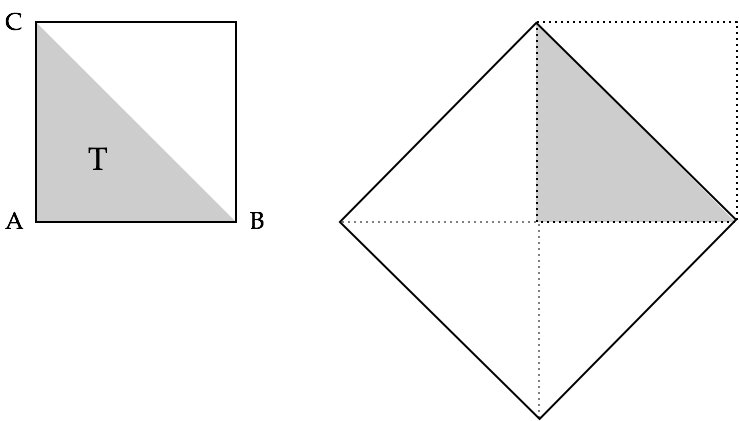
\includegraphics[scale=0.3]{FiguresArithmetic/UnitSquareSQRT2}
\caption{A pictorial schematic proof of The Pythagorean Theorem for the special case of an isosceles right triangle
\label{fig:unitsquare}}
\end{center}
\end{figure}
Say that $T$ is a {\it right triangle}, meaning that one of its angles is a {\em right angle}, i.e., that its measure is $90^\circ$ (read: ``$90$ degrees'') or, equivalently, $\pi/2$ radians.  In our example, $T$'s right angle occurs at vertex $A$.  Because $T$ is a right triangle, the line from vertex $A$ to vertex $B$ and the line from vertex $A$ to vertex $C$ are called the {\em sides} (or the {\it legs}) of $T$, while the line from vertex $B$ to vertex $C$ is called the {\em hypotenuse} of $T$.  Triangle $T$ has a very special ``shape": it is {\em isosceles}, meaning that its two sides /legs have the same length.  The grey triangle in Fig.~\ref{fig:unitsquare} is an isosceles right triangle.

\begin{theorem}[{\bf The Pythagorean Theorem}]
\label{thm:Pythagorean-thm}
Let $T$ be a right triangle whose two sides have respective lengths $s_1$ and $s_2$, and whose hypotenuse has length $h$.  Then
\[ h^2 \ = \ s_1^2 + s_2^2. \]
Consequently, when $T$ is an {\em isosceles} right triangle, then $h^2 = 2 s_1^2$.
\end{theorem}

The special case of the Pythagorean Theorem that deals with isosceles right triangles admits the very perspicuous proof presented pictorially in Fig.~\ref{fig:unitsquare}.  Follow along in the figure as we review this proof.

\smallskip

We focus first on the unit-side square $S$ on the left of the figure.  We partition $S$ by its diagonal into two unit-side isosceles right triangles, one grey and one white.  In this construction the diagonal of $S$ is the (shared) hypotenuse of the two triangles.  On the right-hand side of Fig.~\ref{fig:unitsquare}, we use our partitioned version of $S$ to construct a new, bigger square, call it $\widehat{S}$, whose side-length is the hypotenuse-length of the grey triangle.  The dotted lines in the figure tell us how big $\widehat{S}$ is (measured by its area).
\begin{itemize}
\item
Square $S$ is unit-sided, hence has {\em unit area}, i.e., area $=1$.
\medskip\item
The grey triangle is (geometrically) half of $S$, hence has area $1/2$.
\medskip\item
Square $\widehat{S}$ is built from four copies of the grey triangle, hence has area $4 \cdot (1/2) \ = \ 2$.
\end{itemize}
Because the hypotenuse of the grey triangle is a side of an area-$2$ square, we have just proved the following special case of the Pythagorean Theorem.\footnote{We generally signal the end of a proof via the symbol ``\fbox{\hspace*{.025in}}", which is usually articulated ``Q.E.D.", for ``{\em Quod Erat Demonstrandum}" [Latin for ``which was to be proved"].}  \qed

\begin{prop}
\label{thm:unit-isosceles-PythThm}
The hypotenuse of the unit-side isosceles right triangle has length $\sqrt{2}$.
\end{prop}
  
\noindent \textbf{End of digression}

\bigskip

\index{Archimedes}

%{\Arny Wikipedia describes Archimedes as a Greek from Syracuse.  His city of residence is part of his identity}

As part of the movement toward formalizing mathematics, the Greek mathematician and polymath Archimedes, from Syracuse, was systematically observing that squares are better approximations to circles than triangles are; regular pentagons are better approximations than squares; regular hexagons are better than pentagons; and so on.  Figure~\ref{fig:approxcircle} illustrates this evidence.
\begin{figure}[htb]
\begin{center}
       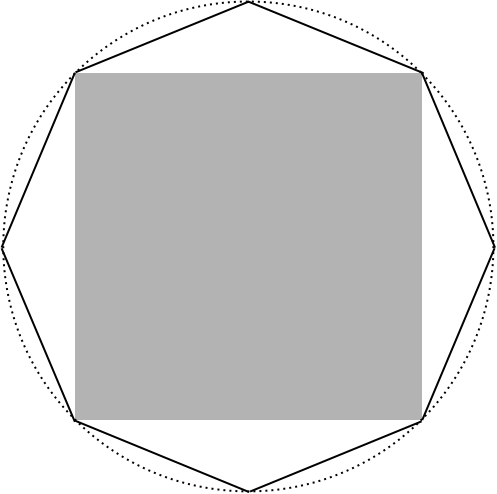
\includegraphics[scale=0.25]{FiguresArithmetic/ApproxCircle}
\caption{{\it Octagons approximate circles much better than squares do}
\label{fig:approxcircle}}
\end{center}
\end{figure}
In fact, observed Archimedes, as the number of sides, $n$, in a regular polygon grows without bound (or, as we might say today, tends to infinity), each increase in $n$ brings a regular polygon closer to being a circle.

\medskip

\index{number!real}
\index{Descartes, Ren\'{e}}
\index{Cauchy, Augustin-Louis}
\index{Dedekind, Richard}
\index{numbers!real numbers}
\index{real numbers!non-rational}
\index{real numbers!irrational}

In order to pursue their respective observations to their completions, both Euclid and Archimedes would have had to leave the world of the rationals and enter the world of the {\it real numbers} (so named by the French mathematician-philosopher Ren\'{e} Descartes)---but this world did not yet exist!  It would take roughly two thousand years from the days of Euclid and Archimedes before the real numbers were {\em formally} introduced to the world, by mathematical luminaries such as the early-nineteenth-century French mathematician-scientist Augustin-Louis Cauchy and the late-nineteenth-century German mathematician Richard Dedekind.  It turned out to be much easier to recognize instances of non-rational real numbers---better known as {\it irrational} real numbers---than to formally delimit the entire family of such numbers.  Once again, happily, one could develop the real numbers in a way that allowed one to view a rational number as a special type of real number.  

\medskip

\index{polynomial} \index{polynomial!root}

During the millennia between the discoveries of Euclid, Archimedes, and their friends, and the full development of the real numbers, mathematics was enriched repeatedly by the discovery of new conceptual structures.  One of these---polynomials and their roots---ultimately led to the final major subsystem of our number system.  In Chapter~\ref{sec:function}, we discussed the important notion of {\em function}.  Polynomials are a practically important class of functions that are delimited by the operations needed to compute them.  Specifically, an $n$-argument polynomial function---typically just called a {\it polynomial}---is a function $P(x_1, x_2, \ldots, x_n)$ whose values can be calculated using just the basic operations of arithmetic: addition/subtraction and multiplication/division.

\bigskip

\index{mutually inverse operations}

\noindent \fbox{
\begin{minipage}{0.96\textwidth}
{\bf Explanatory note}.

\smallskip

We pair the operations in this way because addition and subtraction are {\em mutually inverse
operations}, as are multiplication and division.  This means that one can undo an operation (say, an addition) by performing its inverse operation (in this case, a subtraction).  But {\em be careful:} one cannot undo multiplication by $0$.  
\end{minipage}
}

\bigskip

\index{polynomial!root}

A {\it root}  of a polynomial (function) $P(x_1, x_2, \ldots, x_n)$ is an argument $\langle r_1, r_2, \ldots, r_n \rangle$ that causes $P$ to {\it vanish}, meaning that $P(r_1, r_2, \ldots, r_n) = 0$.  In Fig.~\ref{fig:sample-polys},
 \begin{figure}[htb]
\begin{center}
\begin{tabular}{|c|c|c|}
\hline
 & Polynomial $P(x)$ & Root(s) \\
\hline
1 &
$x+1$  &  $x= -1$ \\
2 &
$x-1$  &  $x= 1$ \\
3 &
$x^2 + 2x +1 = (x+1)^2$ & $x = -1$ \\ 
4 &
$x^2 - 2x +1 = (x-1)^2$ & $x = 1$ \\ 
5 &
$x^2 - 1$ & $x = 1$ and $x= -1$ \\
6 &
$x^2 + 1$ & {\em no real root} \\
7 &
$x^2 -2$  & $x = \sqrt{2}$ and $x = - \sqrt{2}$ \\
8 &
$x^2 + 2$ & {\em no real root} \\
\hline
\end{tabular}
\end{center} 
 \caption{A sampler of univariate polynomials and their roots}
 \label{fig:sample-polys}
 \end{figure}
we illustrate a few sample {\em univariate}---i.e., {\em single-variable}---polynomials. \index{polynomial!univariate} \index{polynomial!single-variable}

\medskip

\noindent
There are lessons, both major and minor, to be gleaned from the examples in Fig.~\ref{fig:sample-polys}.
\begin{itemize}
\item
Entries 3 and 4 in the table illustrate that even simple polynomials can often be written in several different ways.  These entries illustrate also that roots can occur with multiplicity: one can view the value $x = -1$ as causing the polynomial $x^2 + 2x +1 = (x+1)\cdot (x+1)$ to vanish
in two ways---(1) by setting the left-hand factor $x+1$ to $0$ and (2) by setting the right-hand factor $x+1$ to $0$.

\index{polynomial!root!multiplicity}

\medskip\item
Entries 5 and 7 illustrate that polynomials can have multiple distinct roots.

\medskip\item
Perhaps most importantly, entries 6 and 8 provide explicit, simple polynomials---whose expressions involve only positive integers---that fail to have any real roots!

\smallskip

The fact that the indicated polynomials have no real roots is immediate, because the square of a real number can never be negative. Hence, for instance, there is no real number $c$ such that $c^2 = -1$, or, equivalently, $c^2 + 1 = 0$.
\end{itemize}

\medskip

\index{al-Khw$\bar{\mbox{a}}$rizm$\bar{\mbox{i}}$, Muhammad ibn M$\bar{\mbox{u}}$s$\bar{\mbox{a}}$}

For both applied and purely intellectual reasons, there has always been considerable interest in developing techniques for finding the roots of polynomials.  Indeed, much seminal mathematics was developed in the quest for such techniques;\footnote{A giant in the development and transmission of this work was the ninth-century mathematician and astronomer Muhammad ibn M$\bar{\mbox{u}}$s$\bar{\mbox{a}}$ al-Khw$\bar{\mbox{a}}$rizm$\bar{\mbox{i}}$.  We discuss his seminal contributions at greater length in Chapter~\ref{ch:arithmetic}.}~we study the topic at length in Section~\ref{sec:polynomials}.

\smallskip

\index{number!imaginary} \index{Descartes, Ren\'{e}} 
\index{imaginary number $i = \sqrt{-1}$}
\index{$i$: the imaginary unit}
\index{number!complex}

Closely related to this interest in a polynomial's roots was the considerable discomfort within the mathematical and technical world at the fact that the then-current number system---built upon the integers, the rationals, and the reals---was inadequate to the important task of providing roots for every polynomial.  The reaction to this deficiency was similar in kind to all earlier recognized deficiencies: a way was found to expand the number system!  Centuries would pass before mathematics developed adequately to find the needed expansion.  Once discovered, the expansion was based on the conception, in the sixteenth century, of a new {\it imaginary} number, so designated by Descartes.\footnote{The term ``imaginary'' is reputed to be a derogation of these numbers that flouted tradition.}  This new number was named $i$ (for ``imaginary'') and was defined to be a root of the polynomial $P_{-1}(x) = x^2 +1$.  The number $i$ was evocatively often defined via the equation, $i = \sqrt{-1}$.  By keeping our extended arithmetic consistent with our former arithmetic, $-i$ also became a root of $P_{-1}(x)$.  When the imaginary number $i$ was added to the real number system, and the combination was blended via the rules of arithmetic, the {\it complex number system} was born.

\smallskip

 \index{complex numbers!algebraically complete}
 
Thankfully, the imaginary number $i$ was the only totally new concept that was needed to mend the observed deficiency in the real numbers.  In formal terms, the complex numbers were shown to be {\it algebraically complete} in the sense expressed in the landmark {\it Fundamental Theorem of Algebra}.

 \index{Fundamental Theorem of Algebra}

\begin{theorem}[The Fundamental Theorem of Algebra]
Every polynomial of degree $n$ with complex coefficients has $n$ roots over the complex numbers.
\end{theorem}

The proof of the Theorem is beyond the scope of our introductory text, but the result is a notable milestone in our mathematical/technical culture which everyone should know of.

\bigskip

Our historical tour is now complete, so we can---finally---begin to get acquainted with the several components of our number system and the operations that bring each component to life in applications.

\section{Integers: The ``Whole'' Numbers}
\label{sec:integers}

\index{number!integer}
\index{number!integer!whole number}
\index{number!integer!counting number} \index{number!prime}
\index{pairing function}

%{\Arny I changed the first few sentences, hopefully for the better}

The first class of numbers that most of us encounter comprises the {\it integers}, which are also referred to as the {\it whole numbers} or the {\em counting numbers}.  Being used for elementary operations such as counting, the integers are almost certainly the first numbers that our prehistoric ancestors would have used.  This section is devoted to exploring some of the basic properties of the class of integers.  We shall come to appreciate the sophistication lurking behind even this most primitive class in our number system.  The details we provide in Section~\ref{sec:primes} regarding the building blocks of the integers, the {\it prime numbers}, will prepare the reader for a broad range of applications of the integers, including important {\em (computer-)security-related} applications.  Our introduction to {\it pairing functions}, in Section~\ref{sec:pairing}, will open the door to many applications of the integers which build on the ordering properties of these numbers, coupled with tools for encoding highly structured data as integers.

\subsection{The Basics of the Integers: The Number Line}
\label{sec:integer-number-line}
\index{number!the number line}
\index{number!integer!the number line}
\index{$\Z$: the set of all integers}
\index{$\N$: the set of nonnegative integers}
\index{$\N^+$: the set of positive integers}

We survey a number of the most important properties of the following three sets, which collectively comprise ``the integers".
\begin{itemize}
\item
The set $\Z$ comprises {\em all integers}---the positive and negative integers plus the special number zero ($0$).
\medskip\item
The set $\N$ comprises the {\em nonnegative integers}---the positive integers plus zero ($0$).
\medskip\item
The set $\N^+$ comprises the {\em positive integers}.
\end{itemize}
There is no universally accepted default when one refers to ``the integers'' without a qualifying adjective; therefore, we shall always be careful to indicate which set we are discussing at any moment---often by supplying the set-name: $\Z$ or $\N$ or $\N^+$.

\subsubsection{Natural orderings of the integers}
\label{sec:natural-orderings}
\index{less-than relation on numbers}
\index{less-than relation on numbers!the strict version: $<$}
\index{less-than relation on numbers!the weak version: $\leq$}
\index{greater-than relation on numbers}
\index{greater-than relation on numbers!the strict version: $>$}
\index{greater-than relation on numbers!the weak version: $\geq$}

Several essential properties of the sets $\Z$, $\N$, and $\N^+$ are consequences of the integers' behaviors under their natural {\em order} relations:
\begin{itemize}
\item
the two {\em less-than} relations:
  \begin{itemize}
  \item
the {\em strict} relation ($<$).  We articulate ``$a < b$'' as ``$a$ is (strictly) less than $b$'' or as ``$a$ is (strictly) smaller than $b$''.
  \medskip\item
the {\em nonstrict} or {\em weak} relation ($\leq$).  We articulate ``$a \leq b$'' as ``$a$ is less than or equal to $b$'' or as ``$a$ is no larger than $b$''.
  \end{itemize}
\index{$<$: the strict less-than relation} \index{$\leq$: the nonstrict/weak less-than relation}

\medskip\item
their {\em converses,} the {\em greater-than} relations:
  \begin{itemize}
  \item
the {\em strict} relation ($>$).  We articulate ``$a > b$'' as ``$a$ is (strictly) larger than $b$''.
  \medskip\item
the {\em nonstrict} or {\em weak} relation ($\geq$).  We articulate ``$a \geq b$'' as ``$a$ is greater than or equal to $b$'' or ``$a$ is no smaller than $b$''.
  \end{itemize}
\index{$>$: the strict greater-than relation}
\index{$\geq$: the nonstrict/weak greater-than relation}
\end{itemize}
One sometimes encounters {\em emphatic} versions of the strict relations: the notations $a \ll b$ and $a \gg b$ indicate that $a$ is, respectively, {\em much smaller than} or {\em much larger than} $b$.  Usually, the qualifier ``much" is not quantified, but sometimes it is.
\index{$\ll$: the emphatic strict less-than relation}
\index{$\gg$: the emphatic strict greater-than relation}

\smallskip

The reader will note throughout the text that order relations within a number system are among one's biggest friends when reasoning about numbers.  \index{number!ordering of numbers}

\subsubsection{The order-related laws of the integers}
\label{sec:order-laws}

\index{number!integer!total order} \index{integer!total order}
\index{number!integer!linear ordering} \index{integer!linear ordering}

\noindent{\small\sf A. Total order and the Trichotomy Laws}

The sets $\Z$, $\N$, and $\N^+$ are {\em totally ordered}, also termed {\em linearly ordered}.

\smallskip

\index{number!integer!Trichotomy Laws} 
\index{integer!Trichotomy Laws} \index{Trichotomy Laws!integers}

These facts are embodied in the {\em Trichotomy Laws for integers}.

\medskip

{\it The Trichotomy Laws for integers}.

\smallskip

(i)
{\it For each integer $a \in \Z$, precisely one of the following is true.}

\hspace*{.2in} $a$ equals $0$: $(a=0)$ \ \ \ \ \ \
 $a$ is {\em positive}: $(a>0)$ \ \ \ \ \ \
 $a$ is {\em negative}: $(a<0)$

\smallskip

(ii)
{\it For each integer $a \in \N$, precisely one of the following is true.}

\hspace*{.2in} $a$ equals $0$: $(a=0)$ \ \ \ \ \ \ $a$ is {\em positive}: $(a>0)$

\smallskip

(iii)
{\it For each integer $a \in \N^+$:}

\hspace*{.2in} $a$ is {\em positive}: $(a>0)$

\bigskip

Consequently:
\smallskip

\index{number!the number line}

(i')
$\Z$ can be visualized via the (two-way infinite) number line:
\[ \ldots, -3, \  -2, \ -1, \ 0, \ 1,\  2, \ldots \]

\smallskip

(ii')
$\N$ can be visualized via the (one-way infinite) number line:
\[  0, \ 1, \ 2, \ 3, \ldots \]

\smallskip

(iii')
$\N^+$ can be visualized via the (one-way infinite) number line:
\[  1, \ 2, \ 3, \ldots \]

\medskip

The Trichotomy Laws can be expressed using arbitrary pairs of integers, rather than insisting that one of the integers be zero.  For the set $\Z$, for instance, this version of the Laws takes the following form:

\smallskip

{\it For any integers $a, b \in \Z$, precisely one of the following is true.}

\hspace*{.2in} $a$ equals $b$: $(a=b)$ \ \ \ \ \ \
 $a$ is less than $b$: $(a<b)$ \ \ \ \ \ \
 $a$ is greater than $b$: $(a>b)$

\medskip

\noindent{\small\sf B. Well-ordering}

\smallskip

The sets $\N$ and $\N^+$ are {\it well-ordered}.
\index{number!nonnegative integers!well-ordering} \index{nonnegative integers!well-ordering}
\index{number!positive integers!well-ordering} \index{positive integers!well-ordering}
\index{positive integers!Well-OrderingPrinciple}
\index{Well-OrderingPrinciple for positive integers}

\medskip

\noindent
{\it The Well-Ordering Principle for nonnegative and positive integers}.

{\it Every subset of $\N$ or of $\N^+$ has a smallest element (under the ordering $<$).}

\bigskip

We digress momentarily to point out a nontrivial consequence of the well-ordering of the positive integers.  We have already seen this consequence stated as Proposition~\ref{thm:build-a-set}, which we now have the tools to prove.

\medskip

\noindent
{\bf Proposition}~\ref{thm:build-a-set} [{\sc compact form}].
{\em The set $S$ of Proposition~\ref{thm:build-a-set} contains $\N^+$.}

\begin{proof}[Proposition~\ref{thm:build-a-set}]
Say, for the sake of contradiction, that the set $S$ specified in the statement of the proposition does not contain every positive integer.  By the Well-Ordering Principle, there must then be a {\em smallest} positive integer, call it $k$, that does not belong to $S$.  Clearly, $k>1$, because the proposition asserts that $1 \in S$.  Therefore, the number $k-1$ is a positive integer. Moreover, $k-1$, being smaller than $k$, belongs to $S$.

But now, by definition of $S$, we see that $(k-1)+1 = k$ {\em does belong to} $S$.

Thus, the assumption that $S$ does not contain every positive integer leads to a contradiction.  We infer that Proposition~\ref{thm:build-a-set} is true.  \qed
\end{proof}

\smallskip

\noindent{\small\sf C. Discreteness}

\smallskip

The set $\Z$ is {\it discrete}.
\index{number!integer!discreteness} \index{integer!discreteness}

\medskip

\noindent
{\it The discreteness of the integers.}

{\it For every integer $a \in \Z$, there is no integer between $a$ and $a+1$; i.e., there is no $b \in \Z$ such that $a < b < a+1$.}

\medskip

\noindent{\small\sf D. The law of ``between-ness''}

\smallskip

{\it The ``between-ness'' law} for the set $\Z$:
\index{number!integer!''between-ness'' law} \index{integer!''between-ness'' law}

\smallskip

\noindent
{\it For any integers $a, b \in \Z$, there are finitely many $c \in \Z$ such that $a < c < b$.}

\smallskip

\noindent
Any such $c$ lies {\em between} $a$ and $b$ along the number line, whence the name of the law.

\medskip

\noindent{\small\sf E. The cancellation laws}

\index{number!integer!cancellation laws} \index{integer!cancellation laws}

There are two {\it cancellation laws} for the set $\Z$, one for the operation of addition and one for the operation of multiplication.

\medskip

\noindent
{\it The cancellation law for addition}.

{\it For any integers $a, b, c \in \Z$, if $a+c = b+c$, then $a = b$.}
\index{number!integer!cancellation laws!addition} \index{integer!cancellation laws!addition}

\smallskip

\noindent
{\it The cancellation law for multiplication}.

{\it For any integers $a, b \in \Z$ and $c \in \Z \setminus \{0\}$, if $a \cdot c = b \cdot c$, then $a = b$.}
\index{number!integer!cancellation laws!multiplication} 
\index{integer!cancellation laws!multiplication}

\smallskip

\noindent
The cancellation laws provide limited versions of the algebraic notion of mutually inverse arithmetic operations (Section~\ref{sec:binary-operators}).
\index{arithmetic operations!mutually inverse operations}


\subsection{Divisibility: Quotients, Remainders, Divisors}
\label{sec:divisibility}
\index{divisibility} \index{integers!divisibility}

This section is devoted to studying the fundamental relation of {\em divisibility} between two integers.  Let $m, n \in \N$ be nonnegative integers.  We use any of the following notations to assert the existence of a positive integer $q$ such that $n = q \cdot m$.
\index{number!integer!divisor}
\index{number!integer!divisibility} \index{$m \mid n$: $m$ divides $n$}
\begin{itemize}
\item
$m$ {\it divides} $n$
\medskip\item
$m$ {\it is a divisor of} $n$
\medskip\item
$n$ {\it is divisible by} $m$
\medskip\item
$m \mid n$.
\end{itemize}
We consider the possible {\it divisibility} relations between integers $m$ and $n$.  We begin by noting some general facts.
\begin{itemize}
\item
{\em Every nonzero integer $m$ divides $0$.}

\smallskip

This is because of the universal equations $m \cdot 0 = 0 \cdot m = 0$.   The same equations verify that $0$ {\em does not divide any integer.}

\medskip\item
{\em $1$ divides every integer.}

\smallskip

This is because of the universal equation $1 \cdot m = m$.
\medskip\item
{\em Every nonzero integer divides itself.}

\smallskip

This is because of the universal equation $m \cdot 1 = m$.
\end{itemize}

Some nonzero integers have many distinct divisors, while some have very few.  Consider, for illustration, the first twelve positive integers.
\[ \begin{array}{|c|c|}
\hline
\mbox{Number} & \mbox{Divisors} \\
\hline
\hline
1  &  \{ 1 \} \\
2  &  \{ 1, 2 \} \\
3  &  \{ 1, 3 \} \\
4  &  \{ 1, 2, 4 \} \\
5  &  \{ 1, 5 \} \\
6  &  \{ 1, 2, 3, 6 \} \\
7  &  \{ 1, 7 \} \\
8  &  \{ 1, 2, 4, 8 \} \\
9  &  \{ 1, 3, 9 \} \\
10  & \{ 1, 2, 5, 10 \} \\
11  & \{ 1, 11 \} \\
12  & \{ 1, 2, 3, 4, 6, 12 \} \\
\hline
\end{array}
\]
All nonzero integers (except for $1$) have at least two divisors, $1$ and themselves.  The ``sparsely divisible'' integers that have only these two divisors are called {\it primes} or {\it prime  integers} or {\it prime numbers}.  We study these ``building blocks of the positive integers'' in more detail in Section~\ref{sec:primes}.  While there is, indeed, much of interest to discuss about prime numbers, the {\it composite} or {\em nonprime} integers are also quite interesting, particularly, when we focus of {\em pairs} of integers.  The next section looks at the defining property of composite integers, namely, {\em divisibility}.

\index{numbers!integers!prime} \index{numbers!integers!composite} 

\medskip

\index{Euclid!Euclidean division: integer division with remainders}

In order to better understand the fundamental concept of divisibility, we must broaden our perspective somewhat and consider the notion of {\em Euclidean division}, i.e., {\it division with remainders}.  The notion of ``perfect'' divisibility that we have been discussing is the special case in which the remainder is $0$.  The next subsection studies Euclidean division; the remainder of this section investigates the ramifications of ``perfect'' divisibility.

\subsubsection{Euclidian division}
\label{sec:euclidian}
\index{Euclid!Euclidean division} \index{Euclid} \index{quotient} \index{remainder}

Divisibility is not always perfect: Given a pair of integers, neither needs be an integer multiple of the other.  As we learned in elementary school, if an integer $m > 0$ does not ``evenly'' divide an integer $n$, then we are left with a ``remainder'' when we attempt to divide $n$ by $m$.  {\it Euclidean} {\it division}---so named for the Greek mathematician Euclid whose writings introduced the process in the West---is the process of producing, given integers $m >0$ and $n$, an integer {\it quotient} $q$ and an integer {\it remainder} $r$ (where $0 \leq r < m$) such that $n = q \cdot m + r$.  The process of Euclidean division always succeeds, in the following strong sense.

\begin{theorem}[The Division Theorem]
\label{thm:division-thm}
Given any integers $n$ and $m > 0$, there exists a unique pair of integers $q$ and $r$, with $0 \leq r < m$, such that
\begin{equation}
\label{eq:euclid-division}
n \ = \ q \cdot m + r
\end{equation}
\end{theorem}

\begin{proof}
We first prove that a result-pair $\langle q, r \rangle$, as described in the Proposition, exists for each argument-pair $\langle m, n \rangle$.  Then we prove that the result-pair is unique.

\medskip

\noindent {\em There exists at least one result-pair}.
Given any argument-pair $\langle m, n \rangle$, let $N_{m,n}$ be the set of all integers of the form $(n - a \cdot m)$ for some integer $a$.  Symbolically,
\[ N_{m,n} \ \eqdef \ \{ (n - a \cdot m) \ \ \ | \ \ \   [ a  \in \N] \  \mbox{ and } \ 
[(n - a \cdot m) \in \N]  \}
\]
Each such set $N_{m,n}$ is a nonempty set of nonnegative integers: the nonemptiness follows because $n \in N_{m,n}$ (via the case $a=0$).  By the Well-Ordering Principle, $N_{m,n}$ contains a (perforce, unique) {\em smallest} element.  Let us denote this smallest element by $r$, and let us denote by $a_r$ the value of $a$ that yields $r$; i.e.,
\[ n - a_r \cdot m \ = \ r  \]
To complete this section of the proof, we need to show that $r < m$.  Say, for contradiction, that $r = m+r'$ for some $r' \in \N$.  We then find that
\[ n - (a_r +1)  \cdot m \ = \ r -m \ = r' \]
is an element of $N_{m,n}$ that is strictly smaller than $r$.  This contradiction completes the first part of the proof.

\medskip

\noindent {\em 2. There exists at most one argument-pair}.
We turn now to the issue of uniqueness.  Say, for the sake of contradiction, that there exists an argument-pair $\langle m, n \rangle$ for which there exist distinct result-pairs $\langle q_1, r_1 \rangle$ and $\langle q_2, r_2 \rangle$.  We therefore have
\begin{equation}
\label{eq:euclid-unique}
n \ = \ q_1 \cdot m + r_1 \ = \ q_2 \cdot m + r_2
\end{equation}
where both $r_1$ and $r_2$ satisfy the inequalities $0 \leq r_1, r_2 <m$.  We consider two cases.
\begin{itemize}
\item \textbf{Case 1.}
Assume first that $r_2 = r_1$.  In this case, the equations of (\ref{eq:euclid-unique}) tell us that
\[ q_1 \cdot m \ = \ q_2 \cdot m \]
The cancellation law for multiplication then tells us that $q_1 = q_2$.  Therefore, the allegedly distinct result-pairs are, in fact, identical.

\medskip\item \textbf{Case 2.}
If $r_2 \neq r_1$, then say, with no loss of generality, that $r_2 > r_1$.  In this case, the equations of (\ref{eq:euclid-unique}) tell us that
\[ (q_1 - q_2) m \ = \ r_2 - r_1  \]
Because the right-hand quantity is positive, so also must be the left-hand quantity; i.e., $q_1 > q_2$ because $r_2 > r_1$.

\smallskip

On the one hand, the left-hand quantity, $(q_1 - q_2) m$, is no smaller than $m$.  This is because $q_1$ and $q_2$ are integers and $q_1 > q_2$.  On the other hand, the right-hand quantity, $r_2 - r_1$, is strictly smaller than $m$.  This is because $r_1 \geq 0$ so that $r_2 - r_1$ is no larger than $r_2$.
\end{itemize}
Both of the relevant cases thus lead to contradictions, so we must conclude that no argument-pair gives rise to more than one result-pair.  \qed
\end{proof}


\subsubsection{Divisibility, divisors, {\sc gcd}s}
\label{sec:divisibility+GCD}

We begin to study the several important aspects of integer divisibility by considering a variety of simple, yet significant, consequences of an integer $n$'s being divisible by an integer $m$.  We leave the following applications of the basic definitions as exercises for the reader.

\begin{prop}.
\label{thm:basic-divisibility}
\begin{enumerate}
\item
If $m$ divides $n$, then $m$ divides all integer multiples of $n$. That is: If $m$ divides $n$, then $m$ divides $cn$ for all integers $c$.

\medskip\item
The relation ``divides'' is {\em transitive}.\footnote{See Chapter~\ref{sec:order-relation}.}  Specifically, if $m$ divides $n$ and $n$ divides $q$ for some integer $q$, then $m$ divides $q$.

\medskip\item
The relation ``divides'' {\em distributes} over addition.\footnote{We use the term ``distributes'' in the sense of the Distributive Law; see Section~\ref{sec:Arithmetic-Laws}.}  That is, if $m$ divides $n$ and $m$ divides $(n+q)$ for some integer $q$, then $m$ divides $q$.
%\footnote{Hint: $\displaystyle \frac{n+q}{m} \ =  \ \frac{n}{m} + \frac{q}{m}$.}

\medskip\item 
For any integer $c \neq 0$,
\[ \left[m \mbox{ divides } n \ \ \mbox{ if, and only if, } \ \ cm \mbox{ divides } cn \right] \]
\end{enumerate}
\end{prop}

The following result follows from the preceding facts.

\begin{prop}
\label{thm:m-commondivisor-n-q}
Given integers $m$, $n$, and $q$, if $m$ divides both $n$ and $q$, then $m$ divides all linear combinations of $n$ and $q$; i.e., $m \mbox{ divides } (sn + tq)$ for all integers $s$ and $t$.
\end{prop}

\begin{proof}
Because $m$ divides both $n$ and $q$, 
there exist integers $k_1$ and $k_2$ such that $k_1 \cdot m = n$ and $k_2 \cdot m = q$.  By the distributive law, we therefore have:
\[ (k_1 \cdot s \ + \ k_2 \cdot t)m \ = \ sn+tq \]
for any $s$ and $t$.  \qed
\end{proof}

\index{greatest common divisor} \index{{\sc gcd}: greatest common divisor}
Among the common divisors of integers $n$ and $q$, a particularly significant one is their {\em greatest common divisor}, which is the {\em largest} integer that divides both $n$ and $q$.  We abbreviate ``greatest common divisor'' by {\sc gcd}, and we write
\[ m \ = \ \mbox{\sc gcd}(n, q) \]
to identify an integer $m$ as the {\sc gcd} of $n$ and $q$.

\smallskip

We are finally ready for our first major result about integer division and divisors.

\index{B\'{e}zout, Etienne}

\begin{prop}[B\'{e}zout's identity]
\label{thm:gcd-n-linear}
For positive integers $n$ and $q$, {\sc gcd}$(n, q)$ is the smallest positive linear combination of $n$ and $q$.

\medskip

\noindent
Stated alternatively, the following two statements both hold.
\begin{itemize}
\item
For any positive integers $n$ and $q$, there exist integers $s_0$ and $t_0$, not necessarily positive, such that $s_0 n + t_0 q \ = \ \mbox{\sc gcd}(n, q)$.
\item
For all integers $s$ and $t$, not necessarily positive, $s n + t q \ \geq \ s_0 n + t_0 q$.
\end{itemize}
\end{prop}

\begin{proof}
Let $m$ denote the smallest positive linear combination of $n$ and $q$.  We prove in turn that $m \geq$ {\sc gcd}$(n, q)$ and $m \leq$ {\sc gcd}$(n, q)$. 
\begin{enumerate}
\item 
By definition, {\sc gcd}$(n, q)$ divides both $n$ and $q$.  By 
Proposition~\ref{thm:m-commondivisor-n-q}, then, for all integers $s$ and $t$, {\sc gcd}$(n, q)$ divides the linear combination, $s n +t q$, of $n$ and $q$.  In particular, {\sc gcd}$(n, q)$ divides the {\em smallest} such combination, $m$. 

\smallskip

It follows, therefore, that $m \geq$ {\sc gcd}$(n, q)$.
\item
First, notice that $m \leq n$.  The expression $n = 1 \cdot n + 0 \cdot q$ is a particular linear combination of $n$ and $q$, and $m$ is the {\em smallest} positive such combination.   

\smallskip

Because $m \leq n$, Theorem~\ref{thm:division-thm} (the Division Theorem) assures us that there exists an integer $r$ with $0 \leq r < m$ such that $n \ = \ k m + r$.  Further, because $m$ can be written in the form $m = s n+t q$ for integers $s$ and $t$, simple arithmetic manipulation expresses $r$ in the form $r \ = \ (1 - k s)n + (-k t)q$,  {\em which is a linear combination of $n$ and $q$}.  Because $m$ is the {\em smallest positive} such combination and $0 \leq r < m$, it follows that $r=0$.  We conclude that $m$ divides $n$.

\smallskip

A symmetric argument, using exactly the same analysis, allows us to conclude that $m$ divides $q$.

\smallskip

We thus have $m \leq$ {\sc gcd}$(n, q)$, which completes the proof.  \qed
\end{enumerate}


\ignore{**************************************
Consider the set of all integer linear combinations of $n$ and $q$:
\[  L_{n,q} \ \eqdef \   \{ sn +tq \ | \ s, t \in \Z \} \ \subseteq \ \Z. \]
Note that both $n$ and $q$ belong to $L_{n,q}$, because of the respective cases $(s=1, t=0)$ and $(s=0, t=1)$.  One consequence of this is that $L_{n,q}$ has a nonempty subset, call it
$L^{(>0)}_{n,q}$, all of whose elements are {\em positive} integers.

By the {\it Well-Ordering law of the positive integers}, the set $L^{(>0)}_{n,q}$ has a smallest element, call it $m_0$.  By definition of $L^{(>0)}_{n,q}$, $m_0$ is a positive integer, and there exist integers $s_0$ and $t_0$ such that
\[  m_0 \ = \ s_0 n + t_0 q. \]

We claim that $L^{(>0)}_{n,q}$ in fact {\em consists precisely of all positive-integer multiples of $m_0$.}  Were this not the case, there would be an element $m$ of $L^{(>0)}_{n,q}$ that is not a (positive-integer) multiple of $m_0$.  Let $m_1$ be the {\em smallest} such element $m$.  We then have
\begin{enumerate}
\item
Because $m_1 \in L^{(>0)}_{n,q}$, there exist integers $s_1$ and $t_1$ such that
\[  m_1 \ = \ s_1 n + t_1 q. \]
\item
Because $m_0$ is the {\em smallest} element of $L^{(>0)}_{n,q}$, the difference have $m_2 \ \eqdef \ m_1 - m_0$ must be positive, so that $m_2 \ = \ (s_1 - s_0) n + (t_1 -t_0) q$ must belong to $L^{(>0)}_{n,q}$.
\end{enumerate}
Now, we are in trouble because of the following incompatible facts.
\begin{itemize}
\item
On the one hand, $m_2$ {\em is not} a multiple of $m_0$

\smallskip

If it were a multiple, then we would have $m_0$ dividing both $m_0$ (trivially) and $m_2 = m_1 - m_0$.  But this would imply that $m_0$ divides $m_1$, contrary to assumption.

\medskip\item
On the other hand, $m_2$ {\em is} a multiple of $m_0$

\smallskip

This is because $m_2 < m_1$, while $m_1$ is the {\em smallest} element of $L^{(>0)}_{n,q}$ that is not a multiple of $m_0$.
\end{itemize}
This contradiction forces us to conclude that integer $m_1$ does not exist; in other words: all elements of $L^{(>0)}_{n,q}$ are multiples of $m_0$.

Let us summarize.  The set of positive integer linear combinations of $n$ and $q$ consists entirely of integer multiples of a single integer $m_0$.  This means, in particular, that $m_0$ is a common divisor of $n$ and $q$.  The only way this situation could hold is if $m_0 = \mbox{\sc gcd}(n,q)$, as claimed in the proposition.  
*******************************}

\end{proof}

\noindent
B\'{e}zout's identity has the following significant corollary.

\begin{corol}
Every linear combination of $n$ and $q$ is a multiple of $\mbox{\sc gcd}(n,q)$, and vice versa.
\end{corol}

\index{Euclid}

Greatest common divisors are fundamental companions of pairs of integers, with manifold computational applications.  How does one compute them?  This question was addressed millennia ago by Euclid, who authored the following result which led to the {\sc gcd}-computing algorithm that bears his name.
\index{Euclid!Euclidean Algorithm}

For positive integers $m$ and $n$, let $\mbox{\sc rem}(m,n)$ denote the (integer!)~remainder $r$ in the Euclidean-division expression (\ref{eq:euclid-division}).  

%Notice here that we use an integer function to express the remainder
%since it will be used as the result of an operation on two integers
%(similarly to what we did for the GCD).

\begin{prop}
\label{thm:gcd-basis}
For any integers $n$ and $m > 0$,
\[ \mbox{\sc gcd}(m,n) \ = \  \mbox{\sc gcd}(m, \ \mbox{\sc rem}(m,n))  \]
\end{prop}

\begin{proof}
For integers $x > 0$ and $y \geq 0$, we denote by $D(x,y)$ the set of common divisors of $x$ and $y$, i.e., the set of integers that divide both $x$ and $y$.  We prove the proposition by showing, as follows, that the sets $D(m, n)$ and $D(m, \mbox{\sc rem}(m,n))$ actually contain precisely the same elements.
\begin{itemize}
\item 
$D(m, n) \ \subseteq \ D(m, \mbox{\sc rem}(m,n))$.

\smallskip

Say that the integer $d$ divides both $m$ and $n$, i.e., that $d \in D(m,n)$.  By Theorem~\ref{thm:division-thm}, we know that $n \ = \ q \cdot m \ + \ \mbox{\sc rem}(m,n)$.  By property 3 in Proposition~\ref{thm:basic-divisibility}, we must then have $d \mid
\mbox{\sc rem}(m,n)$.  This means that $d \in D(m, \mbox{\sc rem}(m,n))$.

\medskip\item 
$D(m, \mbox{\sc rem}(m,n)) \ \subseteq \ D(m,n)$.

\smallskip

Say that the integer $d$ divides both $m$ and $\mbox{\sc rem}(m,n)$, i.e., that $d \in D(m, \mbox{\sc rem}(m,n))$.  By Proposition~\ref{thm:m-commondivisor-n-q}, $d$ divides every linear
combination of $m$ and $\mbox{\sc rem}(m,n)$.  In particular, $d$ divides the specific combination $q \cdot m \ + \ 1 \cdot \mbox{\sc rem}(m,n) \ = \ n$.  Thus, $d$ divides $n$, so that $d \in D(m,n)$.
\end{itemize}
Since we thus have $D(m, n) \ = \ D(m, \mbox{\sc rem}(m,n))$, we know that the sets contain the same largest element:
\[ \max\left( D(m, n) \right) \ = \ \max\left( D(m, \mbox{\sc rem}(m,n)) \right) \]
The proposition follows.  \qed
\end{proof}


\section{The Rational Numbers}
\label{sec:rationals}

Each enrichment of our number system throughout history has been a response to a deficiency with the then-current system.  The deficiency that instigated the introduction of the rational numbers was the fact that many integers do not divide certain other integers.

This situation led to practical problems when people began to share commodities that were physically divisible.  With a bit of care, you can always cut a pizza into any desired number of slices---but mandating such an action is awkward if you lack the terminology to describe what you want to achieve.

\index{commutativity of addition}\index{commutativity of multiplication}
\index{$0$: zero!the multiplicative annihilator}
\index{inverse operations} \index{difference} 
The situation also led to an intellectual problem, when viewed from a modern perspective.  The arithmetic operation {\it multiplication} was surely recognized not long after its slightly simpler sibling operation {\it addition}.  In many ways, these two operations mimic one another.  Both are {\em total bivariate functions} which take a pair of numbers and produce a number; both are {\em commutative}, in that the argument numbers can be presented in either order without changing the result:
\[ (\forall a,b) \ \ \big[ [a+b \ = \ b+a]
 \ \ \ \mbox{ and } \ \ \
[a \cdot b \ = \ b \cdot a] \big]
\]
and both are {\em associative}, in the sense asserted by the equations
\[
(\forall a,b) \ \ \big[ [a+(b+c) \ = \ (a+b)+c]
 \ \ \ \mbox{ and } \ \ \ 
[a \cdot (b \cdot c) \ = \ (a \cdot b) \cdot c] \big]
\]
If we restrict our focus to the {\em integers}, however, there is a glaring difference between addition and multiplication.  That is, addition has a ``partner operation'', {\it subtraction}, which operates as an {\it inverse operation}:
\[ (\forall a, b, c) \big[ \mbox{if } \ \ [c = a + b] \ \ \mbox{ then }  \ \ [a = c-b] \big]
\]
(We call $c-b$ the {\em difference} between $c$ and $b$.)  Within the context of the integers, multiplication has no such ``partner''.  We respond to this imbalance by inventing a ``partner'' for
multiplication, and we call it {\it division}, denoted $\div$.  Now, division cannot completely mimic subtraction because of the technical problems that arise from the {\em multiplicative annihilation} properties of the integer $0$:
\[ (\forall a) \left[ a \cdot 0 \ = \ 0 \cdot a \ = \ 0 \right] \] 
There is no way to ``undo'' or ``invert'' the operation {\em multiply-by-$0$}, because that operation is not one-to-one.  However, if we frame the operation of division carefully---specifically, by avoiding division by $0$---then we can endow multiplication with the desired ``partner'':
\[ (\forall a, b, c) \big[ \mbox{if } \ \ [c = a \cdot b] \ \
\mbox{ and if } \ \ [b \neq 0] \ \
 \mbox{ then }  \ \ [a = c \div b] \big]
\]
(We call $c \div b$ the {\em quotient of $c$ by $b$}.)  We are almost at the end of our journey.  All we need is a way to speak about specific quotients.  When integer $b$ divides integer $c$, as when $c = 12$ and $b = 4$, it is natural to write $12 \div 4 \ = \ 3$, but how should we denote the quotient $12 \div 5$, which is not an integer?  Enter the rational numbers!
\index{quotient}

\subsection{The Rationals: Special Ordered Pairs of Integers}
\label{sec:define-rationals}

\index{number!rational} \index{$\Q$: the set of rational numbers}
\index{number!rational} \index{number!fraction}
The set $\Q$ of {\it rational} numbers---often abbreviated as just ``the rationals''---was invented to name the quotients referred to in the preceding paragraph.  Formally:
\[ \Q \ \eqdef \ \{0\} \ \cup \ \left\{ p/q \ | \ p, q \in \Z
\setminus \{0\} \right\}
\]
Each element of $\Q$ is called a {\it rational} number; each {\em nonzero} rational number $p/q$ is often called a {\em fraction}; some people reserve the word ``fraction'' for the case $q > p$, because the word seems to connote ``less than the whole'', but this does not seem to be a valuable distinction.

\smallskip

In analogy with our treatment of integers, we reserve the notation $\Q^+$ for the {\em positive} rationals.

\smallskip

\index{algebraic closure} 

An alternative, mathematically more advanced, way of defining the set $\Q$ is as {\em the smallest set of numbers that contains the integers and is closed under the operation of dividing any number by any nonzero number.}  The word ``{\it closed}'' here means that, for every two numbers $p \in \Q$ and $q \in \Q \setminus \{0\}$, the quotient $p/q$ belongs to $\Q$.

\smallskip

Numerous notations have been proposed for denoting rational numbers in terms of the integers they are ``built from''.  Most of these notations continue our custom of employing the single symbol ``$0$'' for the number $0$, but notations such as $0/q$ (where $q \neq 0$) are permissible when they arise as part of a calculation or an analysis.  For the nonzero elements of $\Q$, we traditionally employ some notation for the operation of division and denote the quotient of $p$ by $q$ using one of the following:
\begin{equation}
\label{eq:fraction}
 p/q \ \ \ \mbox{ or } \ \ \ {p \over q} \ \ \ \mbox{ or } \ \ \ p
 \div q
\end{equation}
The integer $p$ in any of the expressions of (\ref{eq:fraction}) is the {\it numerator} of the fraction; the integer $q$ is the {\it denominator}.
\index{number!rational!numerator} \index{number!fraction!numerator}
\index{number!rational!denominator} \index{number!fractions!denominator}

\subsection{Comparing the Rational and Integer Number Lines}
\label{sec:Compare-Q-Z}

There are many ways to compare the sets $\Z$ and $\Q$ that enhance our understanding of both sets.  We craft a comparison that focuses on the similarities and differences in the two sets' number lines, using Section~\ref{sec:integer-number-line} as the reference for the integer number line.

\smallskip

\index{integers as rationals}
As the first point in our comparison, we remark that every integer $n \in \Z$ can be encoded as a rational number.  Specifically, we represent/encode the integer $n \in \Z$ by the rational $p/q$ whose numerator is $p = n$ and whose denominator is $q = 1$.  This encoding is so intuitive that most people would write ``$n = n/1$'' and ignore the fact that this is expressing an encoding
rather than an equality.  We know with hindsight that this intellectual shortcut can cause no problems, but it is important to be aware that we are using a shortcut, for (at least) two reasons.
\begin{enumerate}
\item
We should contemplate {\em why} the encoding ``can cause no problems.''  Answering this question will enhance our understanding of both $\Z$ and $\Q$.  {\em What essential properties of rationals and integers does the proposed encoding preserve?}  To get started, note that the encoding preserves the special characters of the numbers $0$ and $1$---because the following equations hold: $0/1 = 0$ and $1/1 = 1$.

\medskip\item
There are intuitively similar situations wherein one's intuition turns out to be wrong!  One such situation occupies Section~\ref{sec:Q-Z-cardinality}, wherein we demonstrate that the
sets $\Z$ and $\Q$ ``have the same size'', and the more advanced Section~\ref{sec:Reals-uncountable}, wherein we show that the set of real numbers is (in a formal sense) ``larger'' than sets $\Z$ and $\Q$.  ({\em Even the fact that we can discuss the relative ``sizes'' of infinite sets is interesting---and not obvious!})
\end{enumerate}

\subsubsection{Comparing $\Z$ and $\Q$ via their number-line laws}
\label{sec:Q-Z-laws}
\index{number!rational!number line}

The rational numbers share some, but not all, of the number-line laws of the integers, as enumerated in Section~\ref{sec:integer-number-line}.  We now adapt for $\Q$ that section's discussion of $\Z$'s number line.

\smallskip

The sets $\Q$ and $\Q^+$ are both {\em totally ordered}, in the manner expressed by the Trichotomy laws for rational numbers.
\index{number!rational!total order}

\medskip

\noindent
{\it The Trichotomy Laws for the rational numbers}
\index{Trichotomy Laws!rationals} \index{number!rational!Trichotomy Laws}

\noindent (i)
{\it For each rational $a \in \Q$, precisely one of the following is true.}
\[
\mbox{ $a$ equals $0$:} \ (a=0) \ \ \ \
\ \mbox{ $a$ is {\em positive}:} \ (a>0) \ \ \ \
 \ \mbox{ $a$ is {\em negative}:} \ (a<0)
\]

\noindent (ii)
{\it Every rational $a \in \Q^+$ is positive} $(a>0)$.

\medskip

\noindent
The total ordering of $\Q$ is expressed as follows 
\index{number!rational!total order}

\noindent (iii)
{\it For any rationals $a, b \in \Q$, precisely one of the following is true.}
\[  a=b \ \ \ \mbox{or} \ \ \  a<b \ \ \ \mbox{or} \ \ \ a>b \]

\smallskip

As with the integers, the rationals can be visualized via a (two-way infinite) number line.  But the rational line is much harder to visualize, mainly because the rationals do {\em not} enjoy the
well-ordering or discreteness or ``between-ness'' laws of the integers.

\medskip

\noindent
{\em The set $\Q$ is {\em not} well-ordered.}

\smallskip

For illustration:  The set
\[ S \ = \ \{ a \in \Q  \ |\ 0 < a \leq 1 \} \]
has no smallest element.  If you give me a rational $p \in S$ that you claim is the smallest element of the set, then I shall give you $p/2$ as a smaller one.

\medskip

\noindent
{\em The set $\Q$ does {\em not} obey the ``Between'' laws.}

\smallskip

In fact, $\Q$ violates the ``Between'' laws in a very strong way: {\it For any two unequal rationals, $a$ and $b>a$, there are infinitely many rationals between $a$ and $b$.}

\smallskip

One can specify such an infinite set for the pair $a,b$ in a many different ways.  Here is a simple such set for the case $b > 0$, call it $S_{a,b}$.
\begin{equation}
\label{eq:between-rationals}
S_{a,b} \ = \ \left\{ \frac{ka+b}{k} \ \ | \ \ k \in \N^+ \right\}
\end{equation}

\subsubsection{Comparing $\Z$ and $\Q$ via their cardinalities}
\label{sec:Q-Z-cardinality}

Our final comparison between the rationals and the integers compares the relative ``sizes'' or {\em cardinalities} of $\Z$ and $\Q$.  Informally, 

\smallskip

\hspace*{.35in}{\it Are there ``more'' rationals than integers?}

\medskip

\noindent Consider the following facts.
\begin{itemize}
\item
Every integer is a rational number, as attested to by the ``encoding''
\begin{equation}
\label{eq:ZintoQ}
\mbox{Encode } \ \ \ n \in \Z \ \ \ \mbox{ by the quotient } \ \ \ {n \over 1} \in \Q .
\end{equation}

\medskip\item
There are infinitely many non-integer rational numbers between every pair of adjacent integers, as attested to by every set $S_{n,n+1}$ as defined in Eq.~(\ref{eq:between-rationals}).
\end{itemize}
Thus, the set $\Z$ of integers is a {\em proper} subset of the set $\Q$ of rationals: symbolically, $\Z \subset \Q$.  To many, this subset relation provides an intuitively compelling argument that there are more rational numbers than integers.

For us---and for the general mathematical community---the preceding intuition provides a compelling argument only for the fact that reasoning about infinite sets demands subtlety and care.  For us, only the formal setting of Section~\ref{sec:cardinality-NxN} allows us to reason cogently about the relative ``sizes'' of infinite sets.  Within this rigorous setting, we now show that

\smallskip

\hspace*{.35in}{\em the set $\N$ has the same cardinality as the set $\Q$.}

\smallskip

\noindent
Hoping to whet the reader's appetite for further study, we note that the following result exposes some of the main intuitions from the proof of Proposition~\ref{thm:|NxN|=|N|}.

\begin{prop}
\label{thm:|Q|=|N|}
$|\Q| \ = \ |\N|$.
\end{prop}

\begin{proof}[Sketch]
We leave the details of this proof as an exercise.

\smallskip

First, we note that the encoding $f$ defined by
\[ (\forall n \in \N) \left[ f(n) \ = \ \frac{n}{1} \right] \]
provides an injection from $\N$ into $\Q$.  This injection verifies that $|\Q| \ \geq \ |\N|$.

\smallskip

For the converse relation, we proceed in two steps.
\begin{enumerate}
\item
Let the function $g$ associate each rational $p/q \in \Q$ with the ordered pair $\langle a, b \rangle \in \N \times \N$ that is obtained by expressing $p/q$ in {\em lowest terms}; that is,
  \begin{itemize}
  \item
$\displaystyle \frac{p}{q} \ = \ \frac{a}{b}$.
  \medskip\item
The rational $\displaystyle \frac{a}{b}$ is in {\em lowest terms}, in the sense that $a$ and $b$ share no non-unit common divisor.
  \end{itemize}
Clearly, $g$ is an injection from $\Q$ into $\N \times \N$.

\medskip\item
Let the function $h$ be an injection from $\N \times \N$ into $\N$.  Sample such injections can be found in the proof of Proposition~\ref{thm:|NxN|=|N|}.
\end{enumerate}
Since the composition of injections is again an injection, the composite injection $g \circ h$ verifies that $|\N| \ \geq \ |\Q|$.

\smallskip

Combining the preceding derived inequalities completes the proof.
\qed
\end{proof}


\section{The Real Numbers}
\label{sec:reals}
\index{real number}
\index{number!real}

\subsection{Inventing the Real Numbers}
\label{sec:real-history}

Each subsequent augmentation of our system of numbers is more complicated than the last one: Many relatively sophisticated deficiencies in the system are not even visible until other, relatively simple deficiencies have been eliminated.  The deficiency in the system of rational numbers which led to the system of real numbers actually dates to historical time, roughly two-and-a-half millennia ago.  The ancient Egyptians were prodigious builders who mastered truly sophisticated mathematics in order to engineer their temples and pyramids.  The ancient Greeks continued this engineering tradition, but they added to it a philosophical ``soul''.  Both the earthly and ethereal sides of mathematics will be observed in this chapter.

\smallskip

\index{number!integer!commensurable pairs of integers}
Numbers were (literally) sacred objects to many (philosophically oriented) Greeks.  This at least partially explains their concern with understanding {\em why} certain mathematical facts were true, in addition to knowing {\em that} they were true.  Indeed, the Greek mathematicians of antiquity invented ways of thinking about mathematical phenomena that were quite ``modern'' from our perspective.  One intellectual project in this spirit had to do with the way they designed constructions such as temples.  They were attracted to geometric constructions that could be
accomplished using only {\em straight-edges} (what we often call ``rulers") {\em and compasses}.  And---most relevant to our story---they preferred that the relative lengths of linear sections of their structures be {\em commensurable} in the following sense.  {\em Integers $x,y \in \N$ are {\em commensurable} if there exist $a, b \in \N$ such that}
\[ 
ax \ = \ by \ \ \ \ \mbox{ or, equivalently, } \ \ \ \ x \ = \ \frac{b}{a} y.
\]
As Greek philosophers contemplated their desire to employ commensurable pairs of integers in constructions, they discovered that this goal was not always possible---even in moderately simple constructions.  The poster child of this assertion is perceptible in {\it the diagonal of the square with unit-length sides} or, equivalently, in {\it the hypotenuse of the isosceles right triangle with unit-length legs}.  For both of these constructs, the unit lengths of the structure's sides or legs were accompanied by the inevitable {\em non-commensurability} of the length of the square's diagonal or the triangle's hypotenuse: In current terminology, the (shared) length of the diagonal and the hypotenuse is $\sqrt{2}$.  The Greek mathematicians, as reported by Euclid,\footnote{Euclid wrote extensively on this and related subjects, especially regarding geometry and what is currently known as number theory.}~proved, using current terminology, that $\sqrt{2}$ {\em is not rational}.  (We rephrase Euclid's proof imminently, in Proposition~\ref{thm:sqrt(2)}.)  The conclusion from this proof is that a number system based solely on the integers and rationals was inadequate for even elementary constructions.  In response to this discovery, the philosophers/mathematicians augmented our number system by introducing {\it surds} or, as we more commonly term them, {\it radicals}.  The augmentation thus begun culminated in what we know as the {\it real number system}.  Since our intention in this introduction has been to justify the journey along that trajectory, we leave our historical digression and turn to our real focus, the set of {\it real numbers}.
\index{number!real} \index{Euclid} \index{number!surd} \index{number!radical}

\subsection{Defining the Real Numbers via Their Representations}
\label{sec:define-Reals}
\index{real number} \index{number!real}  \index{$\R$: the set of real numbers}

There are numerous ways to define the class $\R$ of {\it real numbers}.  The definition which we have chosen has two advantages, given the goals for this text.  Our definition: (1) has clear connections to the {\em computational aspects} of real numbers; (2) relies on {\em basic} mathematical concepts, hence can confidently appear at this early stage of the text.  We define the class of real numbers in terms of their {\em operational} numerals, thereby laying the groundwork for Chapter~\ref{ch:numerals}'s study of numerals.  The definition we provide is completely correct and adequate, but its nuances will be appreciated by readers only incrementally, as they progress through Chapter~\ref{ch:Summation} (especially Section~\ref{sec:geometric-sums}) and Chapter~\ref{ch:numerals}.

\index{number base} \index{number!real}
Our definition is parameterized by an integer {\it base} $b > 1$: any such integer will work.  Having fixed on a base $b$, a {\it real number} is any number that is specified by an {\em infinite} summation of the form
\begin{equation}
\label{eq:real-defn}
\begin{array}{l}
{\displaystyle
\sum_{i=0}^n \alpha_i \cdot b^i \ \ \ + \ \ \ \sum_{j=0}^\infty \beta_j \cdot b^{-j} }  \\
  \\
\begin{array}{ll}
\mbox{where: } & \bullet \ n \in \N \\
               & \bullet  \ \mbox{each } \ \ \alpha_i, \beta_j \ \in \ \{0, 1, \ldots, b-1\}
\end{array}
\end{array}
\end{equation}
By prepending a {\em negative sign} or {\em minus sign} to a numeral or a number, one renders the thus-embellished entity as negative.
\index{number!real!specified via infinite summation} \index{negative sign}
\index{real number!specified via infinite summation} \index{minus sign}

\smallskip

The perceptive reader will note that a proof is required to establish that every expression of the form (\ref{eq:real-defn}) actually defines a specific number.  Such a proof can be developed, but it would require mathematical tools that are beyond the scope of this text.  For the practicalities of our study, we establish the following rule, which allows one to posit the membership in $\R$ of a particular subset of the real numbers, which we shall term {\it constructible}.
\index{constructible real numbers} \index{number!real!constructible}
\index{real number!constructible}

\medskip

\index{Constructibility Principle for real numbers}
\noindent {\bf Constructibility Principle for real numbers}.  {\em Any length (of a line segment) that can be specified via a drawing made using only straightedge and compass is a real number.}


\subsection{Not All Real Numbers Are Rational}
\label{sec:Real-vs-Rational}

We close this section by verifying that the real number $\sqrt{2}$ is not rational.  We thereby conclude---via a specific example---that there exist real numbers that are not rational: In
Section~\ref{sec:Reals-uncountable}, we shall observe infinitely many such numbers.  The current proof also provides the basis of a proof of the non-commensurability of the length of the hypotenuse of an isosceles right triangle---or, equivalently, of the (common) length of the diagonals of a square with the (common) length of its sides.
\index{non-commensurability of $\sqrt{2}$} \index{irrationality of $\sqrt{2}$}

\begin{prop}
\label{thm:sqrt(2)}
{\bf (a)}
The number $\sqrt{2} = 2^{1/2}$ is real; i.e., it belongs to $\R$.

{\bf (b)}
The number $\sqrt{2}$ is not rational; i.e., it does not belong to $\Q$.
\end{prop}

\begin{proof}[Part (a)]
The fact that $\sqrt{2}$ is a real number follows from the Constructibility Principle for real numbers, in the light of Proposition~\ref{thm:unit-isosceles-PythThm}.  \qed-Part (a)
\end{proof}

\medskip

\noindent \fbox{
\begin{minipage}{0.96\textwidth}
{\bf Enrichment note}.

{\it $\oplus$ Digression: An infinite summation for $\sqrt{2}$}.

\smallskip

We have presented the Constructibility Principle for real numbers precisely because deriving, and reasoning about, infinite summations often requires mathematical tools that go beyond those that populate an introductory text.  That said, one of our goals is to introduce the reader to the beauty in mathematics.  To that end, we present, with no proofs, an infinite summation for $\sqrt{2}$.  While this summation is not of the form (\ref{eq:real-defn}), it is close enough to render plausible the fact that $\sqrt{2}$ can be represented by a summation that is of the form (\ref{eq:real-defn}).
{\small
\begin{eqnarray*}
\sqrt{2} & = &
1 \ + \ \frac{3}{4} \cdot \left(\frac{1}{2}\right)
  \ + \ \frac{3}{8} \cdot
\left(\frac{1 \cdot 3}{2 \cdot 4 \cdot 6}\right)
  \ + \ \frac{3}{12} \cdot
\left(\frac{1 \cdot 3 \cdot 5 \cdot 7}{2 \cdot 4 \cdot 6 \cdot 8 \cdot
  10}\right) \\
 & &
  \ + \ \frac{3}{16} \cdot
\left(\frac{1 \cdot 3 \cdot 5 \cdot 7 \cdot 9 \cdot 11}
{2 \cdot 4 \cdot 6 \cdot 8 \cdot 10 \cdot 12 \cdot 14}\right)
  \ + \ \frac{3}{20} \cdot
\left(\frac{1 \cdot 3 \cdot 5 \cdot 7 \cdot 9 \cdot 11 \cdot 13 \cdot 15}
{2 \cdot 4 \cdot 6 \cdot 8 \cdot 10 \cdot 12 \cdot 14 \cdot 16 \cdot 18}\right)
  \\
 & &
 \ + \cdots + \ \frac{3}{4k} \cdot
\left(\frac{1 \cdot 3 \cdot 5 \cdot 7 \cdots (4k-5)}
{2 \cdot 4 \cdot 6 \cdot 8 \cdot 10 \cdots (4k-2)}\right) \ + \ \cdots
\end{eqnarray*}
}
\end{minipage}
}

\bigskip

\index{Euclid}
As we do for many results that we encounter in our mathematical journey, we provide multiple proofs, which build upon quite different mathematical insights.  In this spirit, we now present two proofs for Proposition~\ref{thm:sqrt(2)}(b).  In Section~\ref{sec:classical-proof-sqrt(2)} we provide the classical proof of the result.\footnote{This proof is quite literally {\em classical}: it is based on the proof provided by Euclid in his {\it Elements}.}  This proof invokes a simple provision of the Fundamental Theorem of Arithmetic (Theorem~\ref{thm:Fund-Thm-Arith}) to exploit the divisibility properties of integers.  In Section~\ref{sec:geom-proof-sqrt(2)}, we provide a proof that builds on the Pythagorean Theorem (Theorem~\ref{thm:Pythagorean-thm}) to develop geometric insights.  The reader may enjoy the more extensive exposition on $\sqrt{2}$ in \cite{ConwayS13}.

\subsubsection{A number-based proof that $\sqrt{2}$ is not rational: $\sqrt{2} \not\in \Q$}
\label{sec:classical-proof-sqrt(2)}

\begin{proof}
Let us assume, for contradiction, that $\sqrt{2}$ is rational.  By definition, then, $\sqrt{2}$ can be written as a quotient
\[ \sqrt{2} \ = \ {a \over b} \]
for positive integers $a$ and $b$.  In fact, we can also insist that $a$ and $b$ {\em share no common prime factor}---because if $a$ and $b$ did share the prime factor $p$, then we would have $a = p \cdot c$ and $b = p \cdot d$.  In this case, we would also have
\[ \sqrt{2} \ = \ {a \over b} \ = \ \frac{p \cdot c}{p \cdot d} \ = \ {c \over d} \]
by canceling the common factor $p$.  We can eliminate all further common prime factors if necessary until, finally, we find a quotient for $\sqrt{2}$ whose numerator and denominator share no common prime factor.  This must occur eventually because each elimination of a common factor leaves us with smaller integers, so the iterative elimination of common factors must terminate.  Therefore, let us say, finally, that
\begin{equation}
\label{eq:sqrt2-1}
\sqrt{2} \ = \ {k \over \ell}
\end{equation}
where $k$ and $\ell$ share no common prime factor.

\smallskip

Let us square both expressions in Eq.~(\ref{eq:sqrt2-1}) and multiply both sides of the resulting equation by $\ell^2$.  We thereby discover that
\begin{equation}
\label{eq:sqrt2-2}
2 \ell^2 \ = \ k^2
\end{equation}
This rewriting exposes the fact that $k^2$ is {\em even}, i.e., {\em divisible by $2$}.  We claim that the divisibility of $k^2$ by $2$ betokens the same divisibility for $k$.
\begin{description}
\item[]
We could ``bring in the howitzers" to verify this claim, via a forward reference to the {\em Fundamental Theorem of Arithmetic} (Theorem~\ref{thm:Fund-Thm-Arith}), but a simple calculation will suffice.

\smallskip

Say, for contradiction, that $k^2$ is even, but $k$ is odd.  Since every odd integer $k$ can be written in the form $k = 2h+1$, we observe that $k^2$ can be written in the form
\[ k^2 \ = \ (2h+1)^2 \ = \ 4h^2 \ + \ 4h \ + \ 1 \ = \ 4(h+1) \ + \ 1 \]
This way of writing $k^2$ makes it clear that $k^2$ is {\em odd}, i.e., is {\em not} divisible by $2$.

\smallskip

This contradiction establishes the claim.
\end{description}
So we now know that $k = 2m$ for some positive integer $m$, which allows us to rewrite Eq.~(\ref{eq:sqrt2-2}) in the form
\begin{equation}
\label{eq:sqrt2-3}
2 \ell^2 \ = \ k^2 \ = \ (2m)^2 \ = \ 4m^2.
\end{equation}
Hence, we can divide the first and last quantities in Eq.~(\ref{eq:sqrt2-3}) by $2$, to discover that
\[ \ell^2 \ = \ 2m^2. \]
If we now repeat the preceding indented argument, we discover that the integer $\ell$ must be even.  This means that {\em both $k$ and $\ell$ are even}.  This fact contradicts our assumption that $k$ and $\ell$ share no common prime divisor!
\index{integer!even}

\smallskip

Since every step of our argument is ironclad, except for our assumption that $\sqrt{2}$ is rational, we conclude that that assumption is false!  Part (b) of the Proposition is verified. \qed
\end{proof}

\subsubsection{A geometric proof that $\sqrt{2}$ is not rational: $\sqrt{2} \not\in \Q$}
\label{sec:geom-proof-sqrt(2)}

\begin{proof}
Our geometric proof is built around Fig.~\ref{fig:irrationality1}, which
\begin{figure}[htb]
\begin{center}
       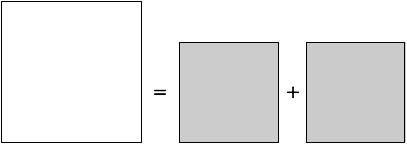
\includegraphics[scale=0.4]{FiguresArithmetic/sqrt2initial}
\caption{{\it A geometric depiction of the Pythagorean Theorem and its
    underlying equation: $a^2 = b^2 + b^2$}
\label{fig:irrationality1}}
\end{center}
\end{figure}
suggestively invokes the Pythagorean Theorem.  The figure displays three squares: The two small grey squares are identical, with common area $A$, while the large white square has double this area.  By the Pythagorean Theorem, if the small squares have (common) side-lengths $b \in \N^+$, hence share area $A = b^2$ each, then the large square has side-lengths $a \eqdef \sqrt{2}b$, hence has area $a^2 = 2 b^2$.

As in the classical proof of Section~\ref{sec:classical-proof-sqrt(2)}, we now assume that $\sqrt{2}$ is rational.  Within the context of Fig.~\ref{fig:irrationality1}, this means that
\[ \sqrt{2} \ = \ {a \over b} \]
for $a, b \in \N^+$.  Since all that we have said thus far holds for arbitrary $a$ and $b$, we are free to insist, as before, that $a$ and $b$ do not share any common prime factor.  Note additionally that because\footnote{If this inequality is new to you, then just note that $(1.4)^2 = 1.96$, which is less than $2$.}
\[ \sqrt{2} \ > \ 1.4 \]
we know that $a > b$.

\bigskip

\noindent \fbox{
\begin{minipage}{0.96\textwidth}
{\bf Explanatory note}.

\smallskip

Of course, our demand that the numerator $a$ and the denominator $b$ do not share a common factor does not diminish the generality of our argument.  This is because ``$a/b$'' is just one name for the depicted rational number, and choosing any specific name has no impact on the number itself.
\end{minipage}
}
\bigskip

Now that we have the suggestive ``equation'' presented in Fig.~\ref{fig:irrationality1}, we can manipulate the depicted squares.  We embed both of the grey $b \times b$ squares of
Fig.~\ref{fig:irrationality1} into the white $a \times a$ square, in the overlapped manner depicted in Fig.~\ref{fig:irrationality2}:
\begin{figure}[htb]
\begin{center}
       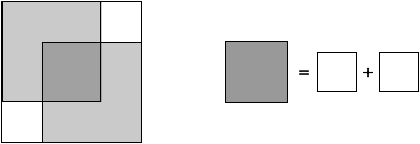
\includegraphics[scale=0.4]{FiguresArithmetic/sqrt2final}
\caption{{\it Constructing a smaller instance of the Pythagorean equation}
\label{fig:irrationality2}}
\end{center}
\end{figure}
one grey square is nestled into the northwestern corner of the white square, while the other is nestled into the southeastern corner.  The overlapping of the grey squares under this embedding creates a new square---depicted in dark grey---in the center of the white square, while it leaves unoccupied two small squares, which remain white in the figure.

\smallskip

Now, let us get quantitative.
\begin{itemize}
\item
On the one hand, the fact that the combined areas of the two grey squares equal the area of the white square guarantees that the area of the dark grey overlap-square is equal to the combined areas of the small unoccupied white squares.

\medskip\item
On the other hand, because the side-length of the large white square is $a$, while the (common) side-length of the grey squares is $b$, it follows that the side-lengths of the small white square is $a-b$, and the side-length of the dark grey overlap-square is $2b-a$.  All of these side-lengths are positive because of the value of $\sqrt{2}$.  That is: ($i$) $a > b$ because $\sqrt{2} >1$; ($ii$) $2b >a$ because $\sqrt{2} < 2$.
\end{itemize}
The preceding facts allow us to label the squares of Fig.~\ref{fig:irrationality1} differently than we did earlier---and thereby derive a different valid ``equation''.  As we did at the beginning of this discussion, we again invoke the Pythagorean Theorem, but now we do so while focusing---see Fig.~\ref{fig:irrationality2}---on the dark grey overlap-square (which plays the role of the large square in Fig.~\ref{fig:irrationality1}) and the two small white squares (which play the role of the two small squares in Fig.~\ref{fig:irrationality1}).  Whereas our original focus led to the putative rational value $\displaystyle {a \over b}$ for $\sqrt{2}$, the new focus yields the putative rational value $\displaystyle {2b-a \over a-b}$.  We thus have
\[ \sqrt{2} \ = \ {a \over b} \ = \ {2b-a \over a-b}  \]
where $2b-a \ < \ a$ and $a-b \ < \ b$.  In the light of the Fundamental Theorem of Arithmetic (Theorem~\ref{thm:Fund-Thm-Arith}), this new rational name for $\sqrt{2}$ contradicts our initial assumption that $a/b$ was a fraction {\em in lowest  terms}, i.e., in which $a$ and $b$ share no common factor.  \qed
\end{proof}

\index{fraction in {\em lowest terms}}

\section{The Basics of the Complex Numbers}
\label{sec:complexes}

\index{number!complex!real part} \index{$i$: the imaginary unit}
\index{number!complex!imaginary part} \index{imaginary unit $i$}
Let us denote by $\C$ the set of complex numbers.  Each number $\kappa = a+bi$ in $\C$ has a {\it real}  {\em part}---the part that {\em does not} involve the imaginary unit $i$---and an {\it imaginary} {\em part}---the part that {\em does} involve $i$.  To be explicit: the real part of our number $\kappa$, is Re$(\kappa) = a$; the {\it imaginary part} of our number $\kappa$ is Im$(\kappa) = b$.  The notations Re$(\kappa)$ and Im$(\kappa)$ are common but not universal.
\index{complex number!imaginary part Im($\cdot$)} 
\index{complex number!imaginary part Im($\cdot$)} 
\index{complex number!real part Re($\cdot$)}

\medskip

\index{complex number!multiplication!three real multiplications}
Based on the arithmetic laws that we have discussed thus far, plus the defining equation ($i^2 = -1$) of the imaginary unit $i$, we find that the {\em product} of two complex numbers, $a+bi \in \C$ and $c+di \in \C$ is the complex number
\begin{equation}
\label{eq:complex-mult}
(a+bi) \cdot (c+di) \ = \ (ac - bd) + (ad + bc)i
\end{equation}
We note that a ``direct'' implementation of complex multiplication, i.e., one that implements Eq.~(\ref{eq:complex-mult}) literally, requires {\em four} real multiplications---namely, $a \times c, \ b \times d, \ a \times d, \ b \times c$.

During the 1960s, people began to pay close attention to the differing costs associated with alternative ways of achieving computational results.  They sought---and found---a number of procedures that replaced computations involving $k$ real multiplications (a relatively expensive operation) and $\ell$ real additions (a relatively inexpensive operation) by computations that achieved the same result but used fewer multiplications and not too many more additions. Complex multiplication was one of the operations they studied.  Here is the result.

\begin{prop}
\label{thm:complex-mult-3real}
One can compute the product of two complex numbers using {\em three} real multiplications rather than four.
\end{prop}

The proof of this result involves arithmetic manipulation that requires ``thinking outside the box".  
We leave the proof as an exercise.  The main message of the result is that we should never be lulled into assuming that the way an arithmetic expression {\em is} written is the way that it {\em has to be} written.


%%%%%%%%%%%%%%%%%%%%%%%%%%%%%%%%%%%%%%%%%%%%%%%%%%%

\section{Exercises: Chapter 4}

Throughout the text, we mark each exercise with 0 or 1 or 2 occurrences of the symbol $\oplus$, as a rough gauge of its level of challenge.  The 0-$\oplus$ exercises should be accessible by just reviewing the text.  We provide {\em hints} for the 1-$\oplus$ exercises; Chapter~\ref{ch:Exercises} provides {\em solutions} for the 2-$\oplus$ exercises.  Additionally, we begin each exercise with a brief explanation of its anticipated value to the reader. 


\begin{enumerate}
\item
{\bf Irrationality abounds!}

{\sc Lesson:} Extending an argument by understanding its basis.

\smallskip

{\em Extend Euclid's reasoning about $\sqrt{2}$ to prove the following assertion.}

\index{$\sqrt{p}$ is irrational for any prime $p$}

\begin{prop}
For any prime $p >1$, the number $\sqrt{p}$ is not rational, i.e., does not belong to $\Q$.
\end{prop}

\medskip\item
{\bf Appreciating the totality of algebra}

{\em Lesson:} Even if a problem does not mention the inverses to addition and multiplication, you may benefit from paying attention to these operations.

\smallskip

\index{complex number!multiplication via 3 real multiplications}

{\em Show how to compute the product of two complex numbers using only {\em three}
real multiplications rather than the method that directly follows the definition (which uses four multiplications).}\footnote{Make a note of your solution technique.  We shall encounter it again in Chapter~\ref{ch:Recurrences}.}

\bigskip

\noindent \fbox{
\begin{minipage}{0.96\textwidth}
Of course, a full reckoning of the comparative costs of multiplying complex numbers using three real multiplications vs.~four must consider that the three-multiplication procedure uses {\em three} real additions, whereas the four-multiplication procedure uses only {\em two} real additions.  A complete comparison between the two procedures would require knowing the relative costs of multiplication and addition on the target computing platform.
\end{minipage}
}
\medskip

\medskip\item
{\bf Basic properties of divisibility}

{\sc Lessons:} Practice with basic proofs; enhance understanding of integers

\smallskip

{\em Prove the four assertions in Proposition~\ref{thm:basic-divisibility}}.
\smallskip

\medskip\item
{\bf Observing an influence of parity}

{\em Lesson:} Learn to recognize the influence of numerical properties such as parity whenever one deals with sequences of numbers.

\smallskip

The notion of even-odd parity is so simple that one often overlooks the way it can influence the ``shape" of computations.  You will now observe such influence on the important area of {\em recurrences}.  We shall study recurrent summations in depth in Chapter~\ref{ch:Recurrences} and in Appendix~\ref{ch:recurrent-numbers-appendix}, but we begin this study with the simple topic of this exercise.

\medskip

It is not uncommon, in mathematics, computing, and allied disciplines, to encounter sequences of integers that have recursive structures that are kindred to the following sequences:
\begin{itemize}
\item
{\em A bilinear recurrence}
\begin{equation}
\label{eq:bilinear-seqspec}
\begin{array}{ll}
\mbox{Two base integers:} & a_0, \ a_1 \\
\mbox{The recurrent remainder:} &
(\forall n \geq 1) \ \big[ a_{n+1} \ = \ a_n + a_{n-1} \big]
\end{array}
\end{equation}

\medskip\item
{\em A trilinear recurrence}
\begin{equation}
\label{eq:trilinear-seqspec}
 \begin{array}{ll}
\mbox{Three base integers:} & b_0, \ b_1, \ b_2 \\
\mbox{The recurrent remainder:} &
(\forall n \geq 1) \ \big[ b_{n+1} \ = \ b_n + b_{n-1} + b_{n-2} \big]
\end{array}
\end{equation}
\end{itemize}
Viewing these specifications inductively, formulas (\ref{eq:bilinear-seqspec}) and (\ref{eq:trilinear-seqspec}) generate two infinite sequence of positive integers:
\[ a_0, a_1, a_2, a_3, a_4, \ldots \ \ \ \mbox{ and } \ \ \ b_0, b_1, b_2, b_3, b_4, \ldots \]
We are interested in exposing some properties of these sequences that are consequences of the parities of their respective base integers.

\smallskip
On to the exercise:

\medskip

Of course, if one chooses only even positive base integers, then the entire sequence $A$ generated by formula (\ref{eq:bilinear-seqspec}) and the entire sequence $B$ generated by formula (\ref{eq:trilinear-seqspec}) consist of even integers.

{\it Answer the following questions for each of these sequences.}
  \begin{enumerate}
  \item
{\em Is there a choice of positive base integers $a_0, \ a_1$ for which the entire sequence $A$ consists of only odd integers?}
  \medskip\item
{\em Is there a choice of positive base integers $b_0, \ b_1, \ b_2$ for which the entire sequence $B$ consists of only odd integers?}
  \medskip\item
{\em Is there a choice of positive base integers $a_0, \ a_1$ for which the entire sequence $A$ alternates between even and odd integers?}
  \medskip\item
{\em Is there a choice of positive base integers $b_0, \ b_1, \ b_2$ for which the entire sequence $B$  alternates between even and odd integers?}
\end{enumerate}

\medskip\item
$\oplus$ {\bf The rationals ($\Q$) and the integers ($\N$) are equinumerous}

{\sc Lesson:} Experience with a ``multilayer" proof, which combines several elementary threads

\smallskip

{\em Provide a {\em detailed} proof of Proposition~\ref{thm:|Q|=|N|}.}  Informally, there are equally many integers as there are rationals.
\end{enumerate}

\ignore{*********************
\subsection{Another proof for irrationality of $\sqrt{2}$}

\noindent \textit{The aim.}
Reenforcing the ability of using geometrical proofs.
\medskip

\noindent \textit{The problem.}
Prove the irrationality of $\sqrt{2}$ using a geometrical argument.
\medskip

\noindent \textit{Hint.}
The proof is by contradiction. 

Consider $\sqrt{2}$ is rational, which means there exists a pair of integers $(a,b)$
such that $\sqrt{2} = \frac{a}{b}$ (where $a$ is larger than $b$).
Represent this expression geometrically by the corresponding isosceles right triangle
which is the one of minimal surface. 
%The contradiction comes by constructing another isosceles triangle with a smaller surface.
%Squaring this expression leads to $2.b^2 = a^2$.
\medskip

\noindent \textit{Lesson learned.}
Experiencing a proof which uses two types of arguments (contradiction and geometrical figure).


\begin{proof}
Although implementing Eq.~(\ref{eq:complex-mult}) ``directly'' correctly
produces the product $\kappa = (a+bi) \cdot (c+di)$, there is another
implementation that is {\em more efficient}.  Specifically, the
following recipe computes $\kappa$ using only {\em three} real
multiplications instead of the four real multiplications of the
``direct'' implementation.  We begin to search for this recipe by
noting that our immediate goal is to compute both Re$(\kappa) = ac-bd$
and Im$(\kappa) = ad+bc$.  We can accomplish this by computing the
{\em three} real products
\begin{equation}
\label{eq:complex-mult-3a}
(a+b) \cdot (c+d); \ \ \ \ \
ac;  \ \ \ \ \ bd
\end{equation}
and then noting that
\begin{equation}
\label{eq:complex-mult-3b}
\begin{array}{lcl}
\mbox{Im}(\kappa) & = & (a+b) \cdot (c+d) - ac -bd, \\
\mbox{Re}(\kappa) & = & ac -bd
\end{array}
\end{equation}
We thereby achieve the result of the complex multiplication described
in Eq.~(\ref{eq:complex-mult}) while using only {\em three} real
multiplications.

Of course, a full reckoning of the costs of the two implementations we
have discussed exposes the fact that the implementation that invokes
Eqs.~(\ref{eq:complex-mult-3a}) and (\ref{eq:complex-mult-3b}) uses {\em
  three} real additions rather than the {\em two} real additions of
the ``direct'' implementation.  But this entire exercise was
predicated on the observation that each real addition is much less
costly than a real multiplication, so trading one multiplication for
one addition is an unqualified ``win''.  \qed
\end{proof}

{\Denis I added a sentence to refer to an exercice dealing with karatsuba which uses the same idea...}
Notice that this technique is classical and it has been used in many other situations.
For instance while multiplying two integers in base 2 (see exercice~\ref{Karatsuba}).

*******************}
%chapter
%*********Completed 05-29-19

%%%%%%%%%%%%%%%%%%%%%%%%%%%%%%%%%

%version of 07-19-18

\chapter{ARITHMETIC}
\label{ch:arithmetic}

Many, perhaps most, of us take for granted the brilliant notations
that have been developed for the myriad arithmetic constructs that we
use daily.  Our mathematical ancestors have bequeathed us notations
that are not only perspicuous but also convenient for computing and
for discovering and verifying new mathematical truths.  This chapter
is dedicated to sharing this legacy with the reader.

\section{Numbers and Numerals}
\label{sec:numbers-numerals}

Every reader will be familiar with the notion of {\it number} and with
the familiar strings, called {\it numerals}, that name numbers within
positional number systems.\index{numbers vs.~numerals}
\begin{quote}
Numbers and numerals embody what is certainly the most familiar
instance of a very important dichotomy that pervades our intellectual
lives: the distinction between objects and their names:

{\em Numbers are objects.  Numerals are the names we use to refer to
  and manipulate numbers.}

This is a crucially important distinction!  You can ``touch'' a
numeral: break it into pieces, combine two (or more) numerals via a
large range of operations.  Numbers are intangible abstractions: you
cannot compute with them.
\end{quote}
In our daily commerce, we typically deal with numerals formed within a
{\it base-$b$ positional number system,}\index{numerals in a base-$b$
  positional number system}
%
i.e., by strings of {\it digits}, often embellished with other
symbols, such as a {\em radix point}.  We describe such systems in
detail in Section~\ref{sec:Numerals}.A.  For now, we settle for a few
examples: $123456789$ (base $10$, or, {\it decimal}), $10111.001$
(base $2$, or, {\it binary}), or $0.1267 \times 8^{24}$ (base $8$, or,
{\it octal}).\footnote{The use of a period as the radix point is a US
  convention; in much of Europe, a comma denotes the radix point.}

\subsection{A Taxonomy of our number system}




\section{Integers}


\subsection{Prime numbers}

We single out a subclass of the positive integers whose mathematical
importance has been recognized for millennia but which have found
important applications (e.g., within the domain of computer security)
mainly within the past several decades.

We say that a positive integer $p$ {\it divides} a positive integer
$n$ (or, {\it is a divisor of $n$})\index{number!integer!divisor} if
there is a positive integer $q$ such that $n = p \cdot q$.
Equivalently, we say that $n$ {\it is divisible
  by}\index{number!integer!divisibility} $p$.  Thus, every positive
integer $n$ is divisible by $p=1$ (witnessed by $q=n$) and by $p=n$
(witnessed by $q=1$).

The class of integers we single out is defined by its divisibility
characteristics.

An integer $p >1$ is {\it prime}\index{number!integer!prime
  number}\index{number!integer!prime}\index{prime
  number}\index{integer!prime number}\index{integer!prime}
if its {\em only} positive integer divisors are $1$ (which divides
every integer) and itself (which is always a divisor).
\begin{quote}
We usually use the shorthand assertion, ``$p$ is a prime,'' instead of
the longer, but equivalent, ``$p$ is a prime integer.''
\end{quote}

A very important way to classify a positive integer $n$ is to list the
primes that divide it, coupling each such prime $p$ with its {\it
  multiplicity}, i.e., the number of times that $p$ divides $n$.  Let
$p_1, p_2, \ldots, p_r$ be the distinct primes that divide $n$, and
let each $p_i$ divide $n$ with multiplicity $m_i$.  The {\it prime
  factorization}\index{prime factorization}\index{integer!prime
  factorization}\index{number!integer!prime factorization}
%
of $n$ is the product $p_1^{m_1} \times p_2^{m_2} \times \cdots \times
p_r^{m_r}$; note that this product satisfies the equation
\begin{equation}
\label{eq:prime-factorization}
n \ = \ p_1^{m_1} \times p_2^{m_2} \times \cdots \times p_r^{m_r}
\end{equation}

When writing an integer $n$'s prime factorization, it is traditional
to list the primes $p_1, p_2, \ldots, p_r$ in increasing order, i.e.,
so that $p_1 < p_2 < \cdots < p_r$.

\paragraph{\sf A. The Fundamental Theorem of Arithmetic}

\noindent
A positive integer $n$ is totally characterized by its canonical prime
factorization, as attested to by the following classical theorem,
which has been known for millennia and has been honored with the title
{\em The Fundamental Theorem of Arithmetic}.
\index{Fundamental Theorem of Arithmetic}
We state the Theorem in two equivalent ways which suggest different
ways of thinking about the result.

\begin{theorem}[The Fundamental Theorem of Arithmetic]
\index{Fundamental Theorem of Arithmetic}
\label{thm:Fund-Thm-Arith}

\noindent
{\rm (Traditional formulation.)}
%
The canonical prime factorization of every positive integer is unique.

\noindent
{\rm (Alternative formulation.)}
%
Let $n \in \N^+$ be a positive integer, and let $\widehat{P}_n$ denote the
ordered sequence of prime numbers that are no larger than $n$:
\[
\begin{array}{cl}
\widehat{P}_n \ = \ & \langle P_1, \ P_3, \ \ldots, \ P_{r-1}, \ P_r \rangle \\
\mbox{where:}   & P_1 \ = \ 2 \\
                & \mbox{each } \ \ P_i \ < \ P_{i+1} \\
                & P_r \ \leq \ n.
\end{array}
\]
There exists a unique sequence of {\em nonnegative} integers, 
$\langle a_1, a_2, \ldots, a_r \rangle$
such that
\[
n \ = \ \prod_{i=1}^r \ P^{a_i} \ = \
P^{a_1} \cdot P^{a_2} \cdot \ \cdots \ \cdot P^{a_{r-1}} \cdot P^{a_r}
\]
\end{theorem}

A simple, yet important, corollary of Theorem~\ref{thm:Fund-Thm-Arith}
is the following result, whose proof we leave to the reader.

\begin{prop}
\label{thm:prime-divisor}
Every positive integer is divisible by at least one prime number.
\end{prop}


\paragraph{\sf B. Proving the Fundamental Theorem}

The  proof of Theorem~\ref{thm:Fund-Thm-Arith} is actually rather
elementary, providing that one approaches it gradually.  It
employs a lot of important techniques and concepts involved in ``doing
mathematics'', as discussed in the eponymous Chapter~\ref{ch:doingmath}.

We begin with a purely technical result.

\begin{prop}
\label{thm:p-n-linear}
Let $p$ be a prime, and let $m$ be any positive integer that is {\em
  not} divisible by $p$.  There exist integers $a, b$, not necessarily
positive, such that
\[ ap + bm \ = \ 1. \]
\end{prop}

\begin{proof}
Consider the set of all integer linear combinations of $p$ and $m$:
\[  L_{p,m} \ \eqdef \   \{ ap +bm \ | \ a, b \in \Z \} \ \subseteq \ \Z. \]
Note that both $p$ and $m$ belong to $L_{p,m}$, because of the
respective cases $(a=1, b=0)$ and $(a=0, b=1)$.  One consequence of
this is that $L_{p,m}$ has a nonempty subset, call it
$L^{(>0)}_{p,m}$, all of whose elements are {\em positive} integers.

By the {\it Well-Ordering Principle of the positive integers}, the set
$L^{(>0)}_{p,m}$ has a smallest element, call it $r_0$.  By definition
of $L^{(>0)}_{p,m}$, $r_0$ is a positive integer, and there exist
integers $a_0$ and $b_0$ such that
\[  r_0 \ = \ a_0 p + b_0 m. \]

We claim that $L^{(>0)}_{p,m}$ in fact {\em consists precisely of all
  positive-integer multiples of $r_0$.}  Were this not the case, there
would be an element $r$ of $L^{(>0)}_{p,m}$ that is not a
(positive-integer) multiple of $r_0$.  Let $r_1$ be the {\em smallest}
such element $r$.  We then have
\begin{enumerate}
\item
Because $r_1 \in L^{(>0)}_{p,m}$, there exist integers $a_1$ and $b_1$
such that
\[  r_1 \ = \ a_1 p + b_1 m. \]
\item
Because $r_0$ is the {\em smallest} element of $L^{(>0)}_{p,m}$, we
have $r_2 \ \eqdef \ r_1 - r_0 \ > 0$, so that
\[ r_2 \ = \ (a_1 - a_0) p + (b_1 -b_0) m \ \in \ L^{(>0)}_{p,m}. \]
\end{enumerate}
Now, we are in trouble because of the following incompatible facts.
\begin{itemize}
\item
$r_2$ {\em is not} a multiple of $r_0$!

If it were, then we would have $r_0$ dividing both $r_0$ (trivially)
and $r_2 = r_1 - r_0$.  But this would imply that $r_0$ divides $r_1$,
contrary to assumption.

\item
$r_2$ {\em is} a multiple of $r_0$!

This is because $r_2 < r_1$, and $r_1$ is the {\em smallest} element
of $L^{(>0)}_{p,m}$ that is not a multiple of $r_0$.
\end{itemize}
We conclude that integer $r_1$ does not exist, so that all elements of
$L^{(>0)}_{p,m}$ are multiples of $r_0$.

Let us summarize.  The set of positive integer linear combinations of
$p$ and $m$ consists of the multiples of a single integer $r_0$.  This
means, in particular, that both $p$ and $m$ are multiples of a single
positive integer, $r_0$---even though $p$ is a prime which does not
divide $m$.  The only way this situation could hold is if $r_0 = 1$,
as claimed in the proposition.
\end{proof}

\begin{prop}
\label{thm:p-divides-onefactor}
If the prime $p$ divides a composite number $m \cdot n$, then either
$p$ divides $m$ or $p$ divides $n$, or both.\footnote{The closing
  phease ``or both'' signals our use of the {\em inclusive} or.}
\end{prop}

\begin{proof}
Let $p$, $m$, and $n$ be as asserted, and say that $p$ does not divide
$m$.  By Proposition~\ref{thm:p-n-linear}, then, there exist integers
$a, b$, not necessarily positive, such that
\[ ap + bm \ = \ 1. \]
Let us multiply both sides of this equation by $n$.  After some
manipulation---specfically, applying the distributive law---we find
that
\[ apn + bmn \ = \ n. \]
Now $p$ divides the expression to the left of the equal sign: $p$
divides $p$ by definition, and $p$ divides $mn$ by assumption.  It
follows that $p$ must divide the expression to the right of the equal
sign---namely, the integer $n$.
\end{proof}

We are finally ready to attack the proof of the Fundamental Theorem.

**HERE


\paragraph{\small\sf C. Application of the Fundamental Theorem}

We discuss a number of applications of this fundamental result.  We
have already seen one application in
Proposition~\ref{thm:Primes-infinite}.

One very important application of Theorem~\ref{thm:Fund-Thm-Arith} is
as a mechanism for {\em encoding}\index{number!using the Fundamental
  Theorem of Arithmetic for encoding}\index{encoding sequences via the
  Fundamental Theorem of Arithmetic}
%
sequences of positive integers as single integers!  This works as
follows.  Consider the (infinite) ordered sequence of {\em all primes:}
\[ (P_1 = 2), (P_2 = 3), (P_3 = 5), \ldots  \]
Let
\begin{equation}
\label{eq:sequence-vec-s}
\bar{s} \ = \ \langle m_1, m_2, \ldots, m_k \rangle
\end{equation}
be an arbitrary sequence of positive integers.  Then
Theorem~\ref{thm:Fund-Thm-Arith} assures us that the (single) positive
integer
\[ 
\iota(\bar{s}) \ \eqdef \ P_1^{m_1} \cdot P_2^{m_2} \cdot \ \cdots \
\cdot P_k^{m_k}
\]
is a (uniquely decodable) integer-representation of sequence $\bar{s}$.

We return to this idea of encoding-via-integers in a later chapter.


**HERE


\subsection{Numbers}\index{numbers}
\label{sec:numbers}

We begin our study of arithmetic notions with a short taxonomy of
numbers, the objects that arithmetic was invented to explicate and
exploit.  Although we assume that the reader is familiar with the most
common classes of numbers, we do spend some time highlighting
important features of each class, partly, at least, in the hope of
heightening the reader's interest in this most basic object of
mathematical discourse.

We present the four most common classes of numbers in what is almost
certainly the chronological order of their discovery/invention.
\begin{quote}
{\em
Did humans invent these classes of numbers to fill specific needs, or
did we just discover their pre-existing selves as needs prompted us to
search for them?  The great German mathematician Leopold Kronecker,
\index{Kronecker, Leopold}
as cited in \cite{Bell86} (page 477), shared his viewpoint on this
question: ``God made the integers; all else is the work of man.''}
\end{quote}
A pleasing narrative can be fabricated to account for our multi-class
system of numbers.  In the beginning, the story goes, we needed to
count things (sheep, bottles of oil, weapons, \ldots), and the
positive {\it integers}\index{number!integer} were discovered.  As
accounting practices matured, we needed to augment this class with
both zero\index{number!zero ($0$)} ($0$) and the negative
integers\index{number!negative}---and the full class of integers was
born.  As society developed, we had to start sharing subdivisible
materials, so we needed to invent the {\it rational
  numbers}.\index{number!rational} Happily for the mathematically
inclined, the rational numbers could be developed in a way that
allowed one to view an integer as a special type of rational.
\begin{quote}
This quest for a single encompassing framework rather than a set of
isolated concepts is a hallmark of mathematical thinking.
\end{quote}
As the ancient Greeks (so the story goes) were inventing geometry and
its place within architecture, they encountered the uncomfortable fact
that the lengths of portions of eminently buildable structures were
not ``measurable,'' by which they meant ``not rational.''  The poster
child for this phenomenon was the hypotenuse of the isosceles right
triangle with unit-length legs.  As a response to this discomfort, the
{\it real numbers}\index{number!real} were invented.  Once again,
happily, one could develop the real numbers in a way that allowed one
to view a rational number as a special type of real number.  Time went
on, and mathematics matured.  Polynomials\index{polynomial} and their
roots\index{polynomial!root}\footnote{A number $r$ is a {\it root} of
  a polynomial $P(x)$ if $P(r) =0$.}~were discovered, together with
the next source of discomfort.  To understand this discomfort, one
must note that, since the invention of the real numbers, every
polynomial $P_m(x)\ \eqdef \ x^2 - m$, where $m$ is a nonnegative real
number, had two roots, denoted, respectively, $+\sqrt{m}$ and
$-\sqrt{m}$.  But---here is the source of discomfort---{\em the
  polynomial $P_m(x)$ had no roots when $m$ was negative, even a
  negative \underline{integer}}.  The response this time resided in
the invention of a new {\it imaginary} number,\index{number!imaginary}
called $i$,\index{imaginary number $i = \sqrt{-1}$} that was a root of
the polynomial $P_{-1}(x) = x^2 +1$; $i$ was often defined via the
equation, $i = \sqrt{-1}$; easily, $-i$ is also a root of
$P_{-1}(x)$.  By combining the imaginary number $i$ with the real
number system, the {\it complex numbers}\index{number!complex} were
born.

The reader is possibly anticipating a new ``discomfort'' leading to an
new augmentation of our number system, but, no, the story is now
complete, in the sense expressed in the {\it Fundamental Theorem of
  Algebra}\index{Fundamental Theorem of Algebra}, which asserts:

\begin{theorem}[{\bf The Fundamental Theorem of Algebra}]
\label{thm:fund-thm-algebra}
Every polynomial of degree $n$ with complex coefficients has $n$ roots
over the complex numbers.
\end{theorem}

We return to the later to the Theorem and its applications and
implications.  For now, though, it completes our historical tour, so
we can finally begin to get acquainted with our four classes of
numbers.

\subsubsection{The integers}
\label{sec:integers}

The most basic class of numbers are the {\it integers}
\index{number!integer}
(or, {\it whole numbers},
\index{number!integer!whole number}
or, {\em counting numbers}).
\index{number!integer!counting number}
%
Integers are certainly the numbers that our prehistoric ancestors
employed in the earliest days of our species.

\medskip

%\addcontentsline{toc}{paragraph}{A. Integers and their number line}
\paragraph{\small\sf A. Integers and their number line}
\index{number!the number line}
\index{number!integer!the number line}
%
We survey a number of the most important properties of the set
$\Z$\index{$\Z$: the set of all integers} that comprises {\em all
  integers} (the positive and negative integers and zero ($0$)) and
the set $\N$\index{$\N$: the set of nonnegative integers} that
comprises the {\em nonnegative integers} (the positive integers and
$0$).  We estimate a property's importance from the vantage points of
both mathematics and its manifold applications.

Several essential properties of $\N$ and $\Z$ are consequences of the
sets' behavior under their natural order relations: strong ($<$) and
weak ($\leq$) and their converses.  Indeed, order within a number
system is one of one's biggest friends when reasoning about the
numbers within the system.
\index{number!ordering of numbers}
\begin{itemize}
\item
The set $\Z$ is {\em totally ordered}\index{number!integer!total
  order}\index{integer!total order}, also termed {\em linearly
  ordered}\index{number!integer!linear ordering}\index{integer!linear
  ordering}.

\smallskip

This fact is embodied in the {\em Trichotomy Laws for
  integers}.\index{number!integer!Trichotomy Laws}
\index{integer!Trichotomy Laws}\index{Trichotomy Laws}

\medskip

{\it The Trichotomy laws for integers}. \\
%
(a)
%
{\it For each integer $a \in \Z$, precisely one of the following is true.}
\[
(1) \ \mbox{ $a$ equals $0$:} \ a=0 \ \ \ \
(2) \ \mbox{ $a$ is {\em positive}:} \ a>0 \ \ \ \
(3) \ \mbox{ $a$ is {\em negative}:} \ a<0
\]

Consequently, $\Z$ can be visualized via the ($2$-way infinite) number
line: $\ldots, -2, -1, 0, 1, 2, \ldots$.\index{number!the number line}

Analogously, $\N$ can be visualized via the ($1$-way infinite) number
line: $0, 1, 2, \ldots$.

\medskip

(b)
%
{\it For any integers $a, b \in \Z$, precisely one of the following is
  true.}
\[ (1) \ a=b \ \ \ \ \ \ \ (2) \ a<b \ \ \ \ \ \ \ (3) \ a>b \]

\item
The set $\N$ is {\it well-ordered}.
\index{number!nonnegative integers!well-ordering}
\index{nonnegative!integers!well-ordering}

\medskip

{\it The Well-ordering law for nonnegative integers}. \\
%
{\it Every subset of $\N$ has a smallest element (under the ordering
  $<$).}

\medskip

\item
The set $\Z$ is {\it discrete}.
\index{number!integer!discreteness}\index{integer!discreteness}

\medskip

{\it The discreteness of the integers.} \\
%
{\it For every integer $a \in \Z$, there is no integer between $a$ and
  $a+1$; i.e., there is no $b \in \Z$ such that $a < b < a+1$.}

\medskip

\item
The set $\Z$ obeys the {\it ``Between'' Laws}
\index{number!integer!''Between'' laws}\index{integer!''Between'' laws}

\medskip

{\it The ``Between'' laws for integers}. \\
%
{\it For any integers $a, b \in \Z$, there are finitely many $c \in
  \Z$ such that $a < c < b$.}

\smallskip

Any such $c \in \Z$ is {\em between} $a$ and $b$, whence the name of
the law.
\end{itemize}

\medskip

%\addcontentsline{toc}{paragraph}{B. Prime numbers}
\paragraph{\small\sf B. Prime numbers}\index{number!prime numbers}



\subsubsection{The rational numbers}
\label{sec:rationals}

%\addcontentsline{toc}{paragraph}{A. Inventing the rational numbers}
\paragraph{\small\sf A. Inventing the rational numbers}

Each augmentation of our number system throughout history has been a
response to a deficiency with the then-current system.  The deficiency
that instigated the introduction of the rational numbers was the
frequency with which a given integer $q$ does not divide another given
integer $p$.  This fact meant that the operation of multiplication
could often not be ``undone'', or ``inverted'', because division, the
operation that would accomplish the undoing/inverting, would be a {\em
  partial operation:} There are pairs of integers neither of which
divides the other.  The defining characteristic of the expanded system
is that, within it, every nonzero number divides every number.

\medskip

%\addcontentsline{toc}{paragraph}{B. The rationals as ordered pairs of integers}
\paragraph{\small\sf B. The rationals as ordered pairs of integers}

The set $\Q$ of {\it rational} numbers\index{number!rational}
\index{$\Q$: the set of rational numbers}
consists of the number $0$, plus the ratios $p/q$ of all nonzero
integers:
\[ \Q \ \eqdef \ \{0\} \ \cup \ \left\{ p/q \ | \ p, q \in \Z
\setminus \{0\} \right\}
\]
Each element of $\Q$ is called a {\it rational} number;
\index{number!rational} 
each {\em nonzero} rational number $p/q$ is often called a {\em
  fraction},
\index{number!fraction}
especially when $q > p$.

An alternative, mathematically more advanced, way of defining the set
$\Q$ is to view it as the smallest set of numbers that contains the
integers, i.e., the set $\Z$, and is {\it closed under the operation
  of dividing any number by any nonzero number.}
\index{algebraic closure}
The word ``closed'' here means that, given any two numbers in $\Q$,
call them $r$ and $s \neq 0$, their quotient $r/s$ belongs to $\Q$.

Numerous notations have been developed for ``naming'' rational numbers
in terms of the integers they are ``built from.''  Most of these
notations continue our custom of employing the symbol ``$0$'' for the
number $0$.  For the nonzero elements of $\Q$, we traditionally employ
some notation for the operation of division and denote the
\begin{equation}
\label{eq:fraction}
 p/q \ \ \ \mbox{ or } \ \ \ {p \over q} \ \ \ \mbox{ or } \ \ \ p
 \div q
\end{equation}
The integer $p$ in any of the expressions in (\ref{eq:fraction}) is
the {\it numerator}
\index{number!rational!numerator}
\index{number!fraction!numerator}
of the fraction; the integer $q$ is the {\it denominator}.
\index{number!rational!denominator}
\index{number!fractions!denominator}

\medskip

%\addcontentsline{toc}{paragraph}{C. Comparing the rationals with the integers}
\paragraph{\small\sf C. Comparing the rationals with the integers}

There are many ways to compare the sets $\Z$ and $\Q$ via properties
that enhance our understanding of the two sets.

\medskip

{\it i. Every integer is a rational.}
%
Obviously, every integer $n \in \Z$ can be viewed as a rational
\index{integers as rationals}
number, namely, the rational $p/q$ whose numerator is $p = n$ and
whose denominator is $q = 1$; i.e., $n = n/1$.  Easily, this encoding
preserves the special character of the numbers $0$ and $1$, because
$0/1 = 0$ and $1/1 = 1$.

\medskip

{\it ii. The rational and integer number lines.}
\index{the rational number line}
%
The rational numbers share some, but not all, of the number-line laws
enumerated in Section~\ref{sec:integers}.A.  We mirror for $\Q$ that
section's discussion of $\Z$.
\begin{itemize}
\item
{\it The Trichotomy laws for rational numbers.} \\
\index{Trichotomy laws for rationals}
(a)
%
{\it For each rational $a \in \Q$, precisely one of the following is true.}
\[
(1) \ \mbox{ $a$ equals $0$:} \ a=0 \ \ \ \
(2) \ \mbox{ $a$ is {\em positive}:} \ a>0 \ \ \ \
(3) \ \mbox{ $a$ is {\em negative}:} \ a<0
\]

Consequently, $\Q$ can be visualized via the ($2$-way infinite) number
line.

\medskip

(b)
%
{\it For any rationals $a, b \in \Q$, precisely one of the following is
  true.}
\[ (1) \ a=b \ \ \ \ \ \ \ (2) \ a<b \ \ \ \ \ \ \ (3) \ a>b \]

\item
{\em The set $\Q$ is {\em not} well-ordered.}

For illustration:  The set
\[ S \ = \ \{ a \in \Q  \ |\ 0 < a \leq 1 \} \]
has no smallest element.  If you give me a rational $p \in S$ that you
claim is the smallest element of the set, then I shall give you $p/2$
as a smaller one.

\medskip

\item
{\em The set $\Q$ does {\em not} obey the ``Between'' laws.}

In fact, $\Q$ violates the ``Between'' laws in a very strong way:
{\it For any two unequal rationals, $a$ and $b>a$, there are
  infinitely many rationals between $a$ and $b$.}

One can specify such an infinite set for the pair $a,b$ in myriad
ways.  Here is a simple such set, call it $S_{a,b}$.
\begin{equation}
\label{eq:between-rationals}
S_{a,b} \ = \ \left\{ \frac{a+b}{k} \ \ | \ \ k \in \Z \right\}.
\end{equation}
\end{itemize}

\medskip

{\it iii. The relative ``sizes'' of $\Z$ and $\Q$: Are there more
  rationals than integers?}

\noindent Consider the following facts.
\begin{itemize}
\item
Every integer is a rational number, as attested to by the ``encoding''
\begin{equation}
\label{eq:ZintoQ}
\mbox{Encode } \ \ \ n \in \Z \ \ \ \mbox{ by } \ \ \ {n \over 1} \in \Q .
\end{equation}

\item
There are infinitely many non-integer rational numbers between every
pair of adjacent integers, as attested to by every set $S_{n,n+1}$ as
defined in (\ref{eq:between-rationals}).
\end{itemize}
Represented symbolically, we thus have $\Z \subset \Q$.

\medskip

\noindent
The preceding ``argument'' makes an intuitive case that \\
\hspace*{.35in}``there are more rational numbers than integers.'' \\ 
We put this assertion in quotes because, absent a formal notion of
``{\em more}'' for infinite sets, the assertion is meaningless!  Is
there an acceptable formal notion that would allow us to verify or
refute the assertion?  The 19th-century mathematician/logician Georg
Cantor addressed this question, and related ones, in his
groundbreaking study of the relative ``sizes'' of infinte sets
\cite{Cantor74,Cantor78}.  We adapt enough of his formulation to
suggest how such issues can be dealt with mathematically.  We shall
take a longer look at Cantor's work in Section~\ref{sec:complexes}

Let us take our lead from finite sets.  Is there a notion of
``bigger'' for finite sets that can be extended to infinite sets?

We begin with a set $A$ of apples and a set $O$ of oranges, together
with challenge of determining which set is bigger.

\medskip

If sets $A$ and $O$ are both finite, then we can just {\em count} the
number of apples in $A$, call it $a$, and the number of oranges in
$O$, call it $o$, and then compare the sizes of the (nonnegative)
integers $a$ and $o$.  The Trichotomy Laws for integers
(Section~\ref{sec:integers}.A) guarantee that we shall be able to
settle the question.  {\em But} we cannot count the elements in an
infinite set, so this approach fails us when we can infinitely much
fruit!

\medskip

Here is another approach that works for finite sets and that promises
to extend to infinite sets.  Let us assume that we can ``prove''---we
shall explain the word imminently---the following.

For every apple that we extract from set $A$ {\em for the first time},
we can extract an orange from set $O$ {\em for the first time}.  It
will then follow (at least in the finite case), that \\
\hspace*{.35in}{\em There are at least as many oranges as apples!}

\noindent
This is really promising, because there is another way to describe the
fruit-matching process that readily extends to infinite sets.  \\
\hspace*{.35in}{\em There is an injection,\footnote{Recall from
    Section~\ref{s.function} that ``{\em injection}'' is synonymous
    with ``{\em one-to-one function}''.}~call it $f$, from $O$ to $A$.} \\
In more formal terms: {\em Every time you pull an apple $\alpha$ from set
  $A$, I pull the orange $f^{-1}(\alpha)$ from $O$.}

\medskip

Inspired by this formulation using injections---and by the work of
Cantor---we craft the following definition.

\noindent
{\em
Given sets $A$ and $O$ (finite or infinite), we say \\
\hspace*{.35in}{\em Set $O$ is at least as big as set $A$} \\
precisely when there is an injection from $O$ to $A$.}

\medskip

Finally, back to numbers!

\addcontentsline{toc}{paragraph}{-- A fun result: There are as many
  integers as rationals}

\begin{prop}
\label{thm:|Q|=|Z|}
{\rm (a)} There exists an injection from $\Z$ to $\Q$.  Therefore,
$\Q$ is at least as big as $\Z$.

\noindent {\rm (b)} There exists an injection from $\Q$ to $\Z$.
Therefore, $\Z$ is at least as big as $\Q$.
\end{prop}

\begin{proof}
(a) We have already established part (a), via the injection from $\Z$
into $\Q$ implicit in (\ref{eq:ZintoQ}).

\medskip

\noindent (b)
We proceed in two steps.
\begin{enumerate}
\item
We define an injection $f_1$ that maps $\Q$ one-to-one into the set
$\Q^+$ of {\em nonegative} rationals.  We specify $f_1$ as follows.
\[ f_1(p/q) \ = \ \left\{
\begin{array}{cl}
2p/q & \mbox{ if } \ p/q \geq 0 \\
(2p+1)/q & \mbox{ if } \ p/q < 0. \\
\end{array}
\right.
\]
We leave to the reader the easy proof that $f_1$ is an injection from
$\Q$ into $\Q^+$.

\item
We define an injection from $\Q^+$ into $\Z$.

Toward this end, we represent each rational number $r \in \Q^+$ by a
pair of integers $p > 0$ and $q >0$ such that
\begin{itemize}
\item
$r = p/q$

\item
$p$ and $q$ are {\em relatively prime} \index{relatively prime
  integers} in the sense that no integer $n > 1$ divides both $p$ and
  $q$.  If such an $n$ existed, then we could divide both $p$ and $q$
  by it, with the assurance that
\[ \frac{p/n}{q/n} \ = \ \frac{p}{q}. \]
\end{itemize}
Inspired by Theorem~\ref{thm:Fund-Thm-Arith}, we now consider the
function
\[ f_2(p/q) \ \eqdef \ 2^p 3^q. \]
Thus defined, $f_2$ is a function from $\Q^+$ into $\Z$.  Moreover,
Theorem~\ref{thm:Fund-Thm-Arith} guarantees that $f_2$ maps $\Q^+$
{\em one-to-one} into $\Z$.
\end{enumerate}
Since the composition of two injections is also an injection (see
Proposition~\ref{thm:fn-composition}), the result is proved.  \qed
\end{proof}

\subsubsection{The real numbers}
\label{sec:reals}

%\addcontentsline{toc}{paragraph}{A. Inventing the real numbers}
\paragraph{\small\sf A. Inventing the real numbers}

Each subsequent augmentation of our system of numbers inevitably gets
more complicated than the last: one solves the easy problems first.
The deficiency in the system of real numbers harkens back to
historical time, roughly $2 {1 \over 2}$ millennia ago.  The ancient
Egyptians were prodigious builders who mastered truly sophisticated
mathematics in order to engineer their temples and pyramids.  The
ancient Greeks perpetuated this engineering tradition, but they added
to it the ``soul'' of mathematics.

Numbers were (literally) sacred objects to the Greeks, and they
invented quite ``modern'' (to our perspective) ways of thinking about
mathematical phenomena in order to understand {\em why} certain facts
were true, in addition to knowing {\em that} they were true.  One
intellectual project in this spirit had to do with the way they
designed contructions.  They were attracted to geometric contructions
that could be accomplished using only {\em straight-edges and
  compasses}.  And---most relevant to our story---they preferred that
the relative lengths of linear sections of their structures be {\em
  commensurable},
\index{number!integer!commensurable pairs of integers}
in the following sense.  {\em Integers $x,y \in \N$ are {\em
    commensurable} if there exist $a, b \in \N$ such that}
\[ ax \ = \ by \ \ \ \ \mbox{ or, equivalently, } \ \ \ \ x \ = \ {a
  \over b} y.
\]
The desire to employ only commensurable pairs of integers, at least in
moderately simple constructions, was shown to be impossible when one
considered {\it the diagonal of the square with unit-length sides} or,
equivalently, {\it the hypotenuse of the isosceles right triangle with
  unit-length legs}.  In both situations, one encountered the unit
lengths of the sides or legs of the structures, together with the {\em
  noncommensurable} length of the diagonal or hypotenuse, which, in
current terminology, is $\sqrt{2}$.  The Greek mathematicians, as
reported by the renowned mathematician Euclid,\footnote{who wrote
  extensively on this and related subjects.}~proved, using current
terminology, that $\sqrt{2}$ is not rational.  (We rephrase the proof
imminently, in Proposition~\ref{thm:sqrt(2)}.)  The conclusion from
this proof is that the number system based on the rational numbers was
inadequate.  In response, they augmented this system by introducing
{\it surds} \index{number!surd} or, as we more commonly term them,
{\it radicals}, \index{number!radical} beginning a trajectory that
culminated in the real number system.  Since our intention has been to
justify the journey along that trajectory, we leave our historical
digression and turn to our real focus, the set $\R$ of {\it real
  numbers}.\index{number!real}

\medskip

%\addcontentsline{toc}{paragraph}{B. The real numbers via their numerals}
\paragraph{\small\sf B. The real numbers via their numerals}

For any integer $b > 1$, the real numbers are the numbers that can be
named by {em infinite} strings built out of the digits $\{0, 1,
\ldots, b-1\}$;\footnote{This is not the traditional way that a
  mathematician would define the class of real numbers, but it is
  correct and adequate for thinking about the class.}~the resulting
strings are called {\em $b$-ary numerals}.  There are a couple of ways
to form $b$-ary numerals; we shall discuss some of the most common
ones in Section~\ref{sec:Numerals}.  For now, we define real numbers
as those that can be represented by a base-$b$ numeral, for some
integer $b >1$.  Such a numeral has the form
\begin{equation}
\label{eq:real-numeral}
\alpha_n \alpha_{n-1} \cdots \alpha_1 \alpha_0                  
. \beta_0 \beta_1 \beta_2 \cdots
\end{equation}
\index{positional number system!numerical value of numeral}
and represents the (real) number
\[
\underline{\alpha_n \alpha_{n-1} \cdots \alpha_1 \alpha_0                  
. \beta_0 \beta_1 \beta_2 \cdots}
\ \ \eqdef \ \
\sum_{i=0}^n \alpha_i \cdot b^i
\ + \ \sum_{j\geq 0} \beta_j \cdot b^{-j}.
\]
By prepending a ``negative sign'' (or, ``minus sign'') $-$ to a
numeral or a number, one renders the thus-embellished entity as
negative.

The fact that every rational number (hence, also, every integer) is
also a real number is manifest in the fact that integers and rationals
can also be written as $b$-ary numerals as in (\ref{eq:real-numeral}).
But with rational and integers, we are able to insist that their
numerals have special forms.  We cite without proof the following
classical results from the theory of arithmetic.  The result for
integers is easily phrased.

\begin{theorem}{Integers as real numbers}
\label{thm:integer-real}
A real number is an integer if, and only if, it can be represented by
a {\em finite-length} numeral.\index{number!integer: real with a finite numeral}
\end{theorem}

The result for rationals needs an introductory definition.  An {\em
  infinite} sequence of numbers $\Sigma$ is {\em ultimately
  periodic}\index{ultimately periodic sequence} if there exist two
{\em finite} sequences of numbers, $\Gamma$ and $\Delta$, such that
$\Sigma$ can be written in the following form (spaces added to enhance
legibility):
\[ \Sigma \ = \ \Gamma \ \Delta \ \Delta \ \Delta \ \ldots 
\ \Delta \ \ldots
\]
The intention here is that the finite sequence $\Delta$ is repeated
{\it ad infinitum}.


\begin{theorem}{Rationals as real numbers}
\label{thm:rational-real}
\noindent
A real number is rational if, and only if, it can be represented by a
numeral that is {\em ultimately periodic}.\index{number!rational:
  real with an ultimately periodic numeral}
\end{theorem}

\noindent {\em A clarification.}
%
Note that two types of sequences of $0$s do not affect the value of
the number represented by a numeral: (1) an {\em initial} sequence
of $0$s to the {\em left} of the radix point and of all non-$0$
digits; (2) a {\em terminal} sequence of $0$s to the {\em right} of
the radix point and of all non-$0$ digits.

One consequence of this fact is that we lose no generality by
insisting that every numeral have the following form:

\smallskip

\hspace*{.15in}
\begin{tabular}{l}
a finite sequence of digits, followed by a radix point, followed by an
infinite \\
sequence of digits
\end{tabular}

Integers can then be singled out via numerals that have only $0$s to
the right of the radix point.

Theorems~\ref{thm:integer-real} and~\ref{thm:rational-real} show us
that the three sets of numbers we have defined are a nested
progression of successively more inclusive sets, in the sense that
{\em every integer is a rational number} and {\em every rational
  number is a real number}.  Those interested in the (philosophical)
foundations of mathematics might quibble about the verb ``is'' in the
highlighted sentences, but for all practical purposes, we can accept
the sentences as written.

\medskip

%\addcontentsline{toc}{paragraph}{C. Not all real numbers are rational}
\paragraph{\small\sf C. Not all real numbers are rational}

We close this section by verifying the earlier-mentioned assertion
about the non-commensurability of the length of the diagonal of a
square with the (common) length of its sides---or, equivalently, the
leg-length of an isosceles right triangle with the length of its
hypotenuse.
\index{The non-commensurabiliy of $\sqrt{2}$}
%
The following result is a simple application of
Theorem~\ref{thm:Fund-Thm-Arith}.  Its proof only suggests the range
of the theorem's myriad applications.

\addcontentsline{toc}{paragraph}{-- A fun result: $\sqrt{2}$ is not rational}

\begin{prop}
\label{thm:sqrt(2)}
The real number $\sqrt{2} = 2^{1/2}$ is not rational.
\end{prop}

\begin{proof}
We prove the result by contradiction,\index{proof by contradition}
a proof technique described in Chapter~\ref{sec:practical-logic}.

Let us assume, for contradiction, that $\sqrt{2}$ is rational.  By
definition, then $\sqrt{2}$ can be written as a fraction
\[ \sqrt{2} \ = \ {a \over b} \]
for positive integers $a$ and $b$.  In fact, we can also insist that
$a$ and $b$ {\em share no common prime factor}.  For, if $a$ and $b$
shared the prime factor $p$, then we would have $a = p \times c$ and
$b = p \times d$.  In this case, though, we would have
\[ \sqrt{2} \ = \ {a \over b} \ = \ \frac{p \times c}{p \times d}
\ = \ {c \over d}.
\]
by cancellation of the common factor $p$.  We can eliminate further
common prime factors if necessary until, finally, we find a fraction
for $\sqrt{2}$ whose numerator and denominator share no common prime
factor.  This must occur eventually because each elimination of a
common factor leaves us with smaller integers, so the iterative
elimination of common factors must terminate.

Let us say that, finally,
\begin{equation}
\label{eq:sqrt2-1}
\sqrt{2} \ = \ {k \over \ell}
\end{equation}
where $k$ and $\ell$ share no common prime factor.  Let us square both
expressions in (\ref{eq:sqrt2-1}) and multiply both sides of the
resulting equation by $\ell^2$.  We thereby discover that
\begin{equation}
\label{eq:sqrt2-2}
2 \ell^2 \ = \ k^2.
\end{equation}
This rewriting exposes the fact that $k^2$ is {\em even},\index{integer!even}
i.e., {\em divisible by $2$}.  But, Theorem~\ref{thm:Fund-Thm-Arith}
tells us that {\em if $k^2$ is divisible by $2$, then so also is $k$}!
This means that $k = 2m$ for some positive integer $m$, whoch allows
us to rewrite (\ref{eq:sqrt2-2}) in the form
\begin{equation}
\label{eq:sqrt2-3}
2 \ell^2 \ = \ k^2 \ = \ (2m)^2 \ = \ 4m^2.
\end{equation}
Hence, we can divide the first and last quantities in
(\ref{eq:sqrt2-3}) by $2$, to discover that
\[ \ell^2 \ = \ 2m^2. \]
Repeating the invocation of Theorem~\ref{thm:Fund-Thm-Arith} now tells
us that the integer $\ell$ must be even.

We now see that {\em both $k$ and $\ell$ are even, i.e., divisible by
  $2$}.  This contradicts our assumption that $k$ and $\ell$ share no
common prime divisor!

Since every step of our argument is ironclad---except for our
assumption that $\sqrt{2}$ is rational, we conclude that that
assumption is false!  The Proposition is verified!  \qed
\end{proof}

\begin{quote}\index{Proof by contradiction}
The proof of Proposition~\ref{thm:sqrt(2)} is a classical (and early)
example of {\em proof by contradiction}, as discussed in
Section~\ref{sec:practical-logic}.
\end{quote}



\subsubsection{The complex numbers}
\label{sec:complexes}

%\addcontentsline{toc}{paragraph}{A. The basics of the complex numbers}
\paragraph{\small\sf A. The basics of the complex numbers}

$\C$ denotes the complex numbers

Each complex number $\kappa = a+bi \in \C$ has a {\it real part}---the
part that {\em does not} involve the imaginary unit $i$---and an {\it
  imaginary part}---the part that {\em does} involve $i$.  To be
explicit: the real part of our number $\kappa$, is Re$(\kappa) = a$;
\index{complex number!real part Re($\cdot$)}
the {\it imaginary part} of our number $\kappa$,is Im$(\kappa) = b$.
\index{complex number!imaginary part Im($\cdot$)}
The notation Re$(\kappa)$ and Im$(\kappa)$ is common but not
universal.

\index{complex number!multiplication!three real multiplications}
Using the basic arithmetic laws that we have discussed thus far, plus
the defining equation, $i^2 = -1$, of the imaginary unit $i$, we find
that the {\em product} of two complex numbers, $a+bi \in \C$ and $c+di
\in \C$ is the complex number, call it $\kappa$,
\begin{equation}
\label{eq:complex-mult}
\kappa \ = \ (a+bi) \cdot (c+di) \ = \ (ac - bd) + (ad + bc)i.
\end{equation}
We note that a ``direct'' implementation of complex multiplication,
i.e., one that implements (\ref{eq:complex-mult}) literally, requires
four real multiplications---namely, $ac, bd, ad, bc$.

During the 1960s, people first began to pay close attention to the
costs associated with various ways of achieving computational results.
They sought---and found---a number of procedures that replaced
computations involving $k$ real multiplications (a relatively
expensive operation) and $\ell$ real additions (a relatively
inexpensive operation) by computations that achieved the same result
but used fewer multiplications and not too many more additions.
Complex multiplication was one of the operations they studied.  Here
is the result.

\addcontentsline{toc}{paragraph}{-- A fun result: complex
  multiplication via $3$ real multiplications}
\index{complex number!multiplication via 3 real multiplications}

\begin{prop}
\label{thm:complex-mult-3real}
One can compute the product of two complex numbers using {\em three}
real multiplications rather than four.
\end{prop}

\begin{proof}
Although implementing (\ref{eq:complex-mult}) ``directly'' correctly
produces the product $\kappa = (a+bi) \cdot (c+di)$, there is another
implementation that is {\em more efficient}.  Specifically, the
following recipe computes $\kappa$ using only {\em three} real
multiplications instead of the four real multiplications of the
``direct'' implementation.  We begin to search for this recipe by
noting that our immediate goal is to compute both Re$(\kappa) = ac-bd$
and Im$(\kappa) = ad+bc$.  We can accomplish this by computing the
{\em three} real products
\begin{equation}
\label{eq:complex-mult-3a}
(a+b) \cdot (c+d); \ \ \ \ \
ac;  \ \ \ \ \ bd
\end{equation}
and then noting that
\begin{equation}
\label{eq:complex-mult-3b}
\begin{array}{lcl}
\mbox{Re}(\kappa) & = & (a+b) \cdot (c+d) - ac -bd, \\
\mbox{Im}(\kappa) & = & ac -bd
\end{array}
\end{equation}
We thereby achieve the result of the complex multiplication described
in (\ref{eq:complex-mult}) while using only {\em three} real
multiplications.

Of course, a full reckoning of the costs of the two implementations we
have discussed exposes the fact that the implementation that invokes
(\ref{eq:complex-mult-3a}) and (\ref{eq:complex-mult-3b}) uses {\em
  three} real additions rather than the {\em two} real additions of
the ``direct'' implementation.  But this entire exercise was
predicated on the observation that each real addition is much less
costly than a real multiplication, so trading one multiplication for
one addition is an unqualified ``win''.  \qed
\end{proof}

\medskip

%\addcontentsline{toc}{paragraph}{B. Pairing functions: ordering $\C$ and $\N \times \N$}
\paragraph{\small\sf B. Pairing functions: ordering $\C$ and $\N \times \N$}

As noted in Section~\ref{sec:integers}.A, ``order within a number
system is one of one's biggest friends when reasoning about the
numbers within the system.''  This section is devoted to showing that,
even when a number system lacks intrinsic desirable ordering
properties, we can sometimes endow the system with ``inherited
access'' to such properties by devising a {\em bijection} that {\it
  encodes}
\index{pairing functions as encodings}
%
the system's numbers as nonnegative integers.  We focus here on two
important number systems, the rational and complex numbers, $\Q$ and
$\C$, whose ordering properties are much weaker than those of the
nonnegative integers $\N$: Neither $\Q$ nor $\C$ is {\em
  well-ordered}; $\C$ is not even {\em totally} ordered.
\begin{quote}
{\em Well-ordering} is an especially welcome property because it
enables algorithms that are structured as a linear recursion that
``counts down'' from an argument $n$.  Well-ordering guarantees that
there is a ``bottom'' that will terminate the downward recursion.
\end{quote}

\noindent
Two simplifications facilitate our quest for bijective encodings
\[ \varepsilon_1: \Q \leftrightarrow \N \ \ \ \ \ \mbox{ and }
\ \ \ \ \ \varepsilon_2: \C \leftrightarrow \N
\]
\begin{itemize}
\item
We abstract both $\Q$ and $\C$ as the set $\N \times \N$.  Since both
$\Q$ and the 
\index{numbers!complex integers}
%
{\it complex integers}---complex numbers $a+bi$ where $a,b \in
\N$---can be encoded as ordered pairs of nonnegative integers, this is
a natural abstraction.

Of course, using this abstraction to encode $\Q$ into $\N$ ignores
common (integer) divisors of a fraction's numerator and denominator,
whose elimination preserve the fraction's value.  A very simple
algorithm would compensate for this.

\item
We slightly change our agenda and focus on bijections between $\N^+
\times \N^+$ and $\N^+$, where $\N^+$ is the set of {\em positive}
integers.
\index{number!integer!positive integer}
\index{$\N^+$:number!integer!positive integer}

Focusing on {\em positive} integers rather than {\em nonnegative}
integers somewhat simplifies certain mathematical expessions.
\end{itemize}
The structures of the domain $\N \times \N$ and the range $\N$ of the
bijective encodings of interest have led to the name {\it pairing
  functions}
\index{pairing function}\index{pairing function as encoding}
for these bijections.

\smallskip

We now embark on a short guided tour of the world of pairing
functions.

\medskip

\noindent {\it i. The Diagonal pairing function $\d$.}
\index{The Diagonal pairing function $\d$}
%
Pairing functions first appeared in the literature early in the 19th
century.  Perhaps the simplest and ``prettiest'' such function (since
it is a {\em polynomial}) appears, pictorially, in an 1821 work by the
great French mathematician Augustin Cauchy \cite{Cauchy21}.
\index{Cauchy, Augustin}
%
This {\em diagonal} pairing function was formally specified a
half-century later by the German logician Georg Cantor,
\index{Cantor, Georg}
%
whose studies \cite{Cantor74,Cantor78} revolutionized how we think
about infinite sets.
\begin{equation}
\label{eq:diag}
\d(x, y) \ = \
{{x+y-1} \choose 2} + y \ = \ \frac{(x+y) \cdot (x+y-1)}{2} + y
\end{equation}
($\d$ of course has a twin that exchanges $x$ and $y$).  $\d$'s
mapping of $\N^+ \times \N^+$ onto $\N^+$, as depicted in
Fig.~\ref{fig:diag}, exposes that we can view $\d$ as:
\begin{figure}[htb]
\begin{center}
\begin{tabular}{r|r|r|r|r|r|r|r|r}
 1 &  3 &  6 & 10 & \fbox{15} &  21 &  28 &  36 & $\cdots$ \\
 2 &  5 &  9 & \fbox{14} & 20 &  27 &  35 &  44 & $\cdots$ \\
 4 &  8 & \fbox{13} & 19 & 26 &  34 &  43 &  53 & $\cdots$ \\
 7 & \fbox{12} & 18 & 25 & 33 &  42 &  52 &  63 & $\cdots$ \\
\fbox{11} & 17 & 24 & 32 & 41 &  51 &  62 &  74 & $\cdots$ \\
16 & 23 & 31 & 40 & 50 &  61 &  73 &  86 & $\cdots$ \\
22 & 30 & 39 & 49 & 60 &  72 &  85 &  99 & $\cdots$ \\
29 & 38 & 48 & 59 & 71 &  84 &  98 & 113 & $\cdots$ \\
$\vdots$ & $\vdots$ & $\vdots$ & $\vdots$ & $\vdots$ & $\vdots$ &
  $\vdots$ & $\vdots$ & $\ddots$
\end{tabular}
\end{center}
\caption{{\it The diagonal pairing function $\d$.  The shell $x+y = 6$ is
highlighted.}
\label{fig:diag}}
\end{figure}
\begin{enumerate}
\item
partitioning $\N^+ \times \N^+$ into ``diagonal shells'' defined as
\[
\{ \langle x,y \rangle \ | \ x+y = 2 \}, \ \ 
\{ \langle x,y \rangle \ | \ x+y = 3 \}, \ \ 
\{ \langle x,y \rangle \ | \ x+y = 4 \}, \ \ \ldots
\]
This is accomplished by the following subexpression in (\ref{eq:diag}).
\[
{1 \over 2} (x+y) \cdot (x+y-1) \ = \ {{x+y-1} \choose 2}
\]

\item
``climbing up'' these shells in order.

This is accomplished by the additional subexpression ``$+y$'' in
(\ref{eq:diag}).
\end{enumerate}
Understanding $\d$'s structure leads to an inductive verification of
$\d$'s bijectiveness.\footnote{A computationally more satisfying proof
  of $\d$'s bijectiveness appears in \cite{Davis58}, along with an
  explicit recipe for computing its inverse.}

\noindent
************** \\
DO THE INDUCTION \\
**************

\begin{quote}
The fact that $\d$ is a {\em polynomial} in $x$ and $y$ raises the
natural (to a mathematician!)~question of whether there are other
polynomial pairing functions.  This question remains largely open, but
there are a few nontrivial pieces of an answer.
\begin{enumerate}
\item
There is no {\em quadratic} polynomial pairing function other than
$\d$ (and its twin) \cite{FueterP23,LewR78a}.
\item
No {\em cubic} or {\em quartic} polynomial is a pairing function
\cite{LewR78b}.
\item
The development in \cite{LewR78b} excludes large families of
higher-degree polynomials from being pairing functions; e.g., a {\em
  super-quadratic} polynomial whose coefficients are all positive
cannot be a pairing function.
\end{enumerate}
\end{quote}

\ignore{****************
As we now look at a variety of other pairing functions, we continue
the convention in Fig.~\ref{fig:diag} and illustrate a pairing
function $\f: \N^+ \times \N^+ \leftrightarrow \N^+$ via a table whose
entries are the values of $\f$ as depicted in Fig.~\ref{fig:generic}.
\begin{figure}[htb]
\[ \begin{array}{c|c|c|c|c|c}
\f(1,1) & \f(1,2) & \f(1,3) & \f(1,4) & \f(1,5) & \cdots \\
\f(2,1) & \f(2,2) & \f(2,3) & \f(2,4) & \f(2,5) & \cdots \\
\f(3,1) & \f(3,2) & \f(3,3) & \f(3,4) & \f(3,5) & \cdots \\
\f(4,1) & \f(4,2) & \f(4,3) & \f(4,4) & \f(4,5) & \cdots \\
\f(5,1) & \f(5,2) & \f(5,3) & \f(5,4) & \f(5,5) & \cdots \\
\vdots  & \vdots  & \vdots  & \vdots  & \vdots  & \ddots
\end{array} \]
\caption{{\it A generic template for sampling from a pairing function.}
\label{fig:generic}}
\end{figure}

One possible application of pairing functions is to store
arrays/tables in an {\em extendible} manner.  It has been recognized
since the 1950s that many classes of computations, ranging from
linear-algebraic scientific applications to (relational) databases,
benefit from the ability to reshape multidimensional arrays and tables
dynamically.  While several programming languages allow a user to
specify at least some types of reshapings---say, the addition and/or
deletion of rows and/or columns in two dimensions---most of their
processors implement the capability quite naively, by completely
remapping an array/table with each reshaping.  This is, of course,
very wasteful of time, since one does $\Omega(n^2)$ work to
accommodate $O(n)$ changes.  Adapting pairing functions for
array/table storage obviates this reshaping and its attendant wasted
effort.
************}

\medskip

\noindent {\it ii. A methodology for constructing pairing functions.}
\index{constructing pairing functions via ``shells''}
\index{pairing functions as storage mappings for arrays/tables}
%
The shell-oriented strategy that underlies the diagonal pairing
function $\d$ can be adapted to incorporate shell-``shapes'' that are
inspired by a variety of computational situations---and can be applied
to great computational advantage in such situations.  We describe how
such adaptation can be effected, and we describe a few explicit shapes
and situations.  We invite the reader to craft others.

\medskip

\noindent {\underline{\bf Procedure}} {\small\sf PF-Constructor}($\a$) \\
/*Construct a shape-inspired pairing function (PF) $\a$*/
\begin{description}
\item[Step 1.]
%
Partition the set $\N^+ \times \N^+$ into finite sets called {\it
  shells}.  Order the shells linearly in some way: many natural
shell-partitions carry a natural order.
\end{description}
As noted above, Shell $c$ of the diagonal pairing function $\d$ is the
following subset of $\N^+ \times \N^+$: $\{ \langle x,y \rangle \ |
\ x+y = c \}$.  The parameter $c$ orders $\d$'s shells.

\begin{description}
\item[Step 2.]
Construct a pairing function from the shells as follows.
  \begin{description}
  \item[Step 2a.]
Enumerate $\N^+ \times \N^+$ shell by shell, honoring the ordering of
the shells; i.e., list the pairs in shell \#1, then shell \#2, then
shell \#3, etc.
  \item[Step 2b.]
Enumerate each shell in some systematic way, e.g., ``by columns'':
Enumerate the pairs $\langle x,y \rangle$ in each shell in increasing
order of $y$ and, for pairs having equal $y$ values, in decreasing
order of $x$.
  \end{description}
\end{description}

\begin{prop}
\label{thm:PF-construct}
Any function $\a: \N^+ \times \N^+ \leftrightarrow \N^+$ that is
designed via Procedure {\small\sf PF-Constructor} is a bijection.
\end{prop}

\proof{(Sketch) Step 1 of Procedure {\small\sf PF-Constructor}
constructs a partial order on $\N^+ \times \N^+$, in which: ($a$) each
shell is finite; ($b$) there is a linear order on the shells.  Step 2
extends this partial order to a linear order, by honoring the inherent
ordering of shells and imposing a linear order within each shell.  The
function constructed via the Procedure is: {\em injective} because the
disjoint shells are enumerated sequentially; {\em surjective} because
the enumeration within each shell begins immediately after the
enumeration within the preceding shell, with no gap.}  \qed

We have noted how to use Procedure {\small\sf PF-Constructor} to
construct pairing function $\d$.  We now use the Procedure to design
two other useful pairing functions.

\medskip

\noindent {\it iii. The Square-shell pairing function $\s$.}
\index{The Square-shell pairing function $\s$}
%
One computational situation where pairing functions can be useful
involves storage-mappings for arrays/tables that can expand and/or
contract dynamically.  In conventional systems, when one expands an $n
\times n$ table into an $(n+1) \times (n+1)$ table, one allocates a
new region of $(n+1)^2$ storage locations and copies the current table
from its $n^2$-location region to the new region.  Of course, this is
very wasteful: one is moving $\Omega(n^2)$ items to make room for the
anticipated $2n+1$ new items.  On any given day, the practical impact
of this waste depends on current technology.  But, this is a
mathematics text, not an engineering one, so we are exploring whether
{\em in principle} we can avoid the waste.  The answer is ``YES''.  If
we employ a pairing function $\varepsilon: \N^+ \times \N^+
\leftrightarrow \N^+$ to allocate storage for tables, then to expand a
table from dimensions $n \times n$ to $(n+1) \times (n+1)$, we need
move only $O(n)$ items to accommodate the {\em new} table entries; the
current entries need not be moved.  For square tables, the following
{\it Square-shell} pairing function $\s$ manages the described
scenario perfectly.  After describing $\s$, we comment on managing
tables of other shapes.
\begin{figure}[htb]
\begin{center}
\begin{tabular}{r|r|r|r|r|r|r|r|r}
  1 &  4 &  9 & 16 & \fbox{25} &  36 &  49 &  64 & $\cdots$ \\
  2 &  3 &  8 & 15 & \fbox{24} &  35 &  48 &  63 & $\cdots$ \\
  5 &  6 &  7 & 14 & \fbox{23} &  34 &  47 &  62 & $\cdots$ \\
 10 & 11 & 12 & 13 & \fbox{22} &  33 &  46 &  61 & $\cdots$ \\
\fbox{17} & \fbox{18} & \fbox{19} & \fbox{20} & \fbox{21} &  32 &  45
  &  60 & $\cdots$ \\ 
 26 & 27 & 28 & 29 & 30 &  31 &  44 &  59 & $\cdots$ \\
 37 & 38 & 39 & 40 & 41 &  42 &  43 &  58 & $\cdots$ \\
 50 & 51 & 52 & 53 & 54 &  55 &  56 &  57 & $\cdots$ \\
$\vdots$ & $\vdots$ & $\vdots$ & $\vdots$ & $\vdots$ & $\vdots$ &
  $\vdots$ & $\vdots$ & $\ddots$
\end{tabular}
\end{center}
\caption{{\it The square-shell pairing function $\s$.  The shell
    $\max(x,y) = 5$ is highlighted.}
\label{f.square}}
\end{figure}
\begin{equation}
\label{e.square}
\begin{array}{ccl}
\s(x, y) & = & m^2 + m + y-x+1 \\
 & & \mbox{where } \ \ \  m \ \eqdef \ \max(x-1,y-1).
\end{array}
\end{equation}
One sees in Fig.~\ref{f.square} that $\s$ follows the prescription of
Procedure PF-Constructor: (1) it maps integers into the ``square
shells'' defined by: $m = 0, \ m = 1, ...$.  (2) it enumerates the
entries in each shell in a counterclockwise direction.  (Of course,
$\s$ has a twin that enumerates the shells in a clockwise direction.)
\begin{quote}
Using somewhat more complicated instantiations of Procedure
PF-Constructor, the study in \cite{Rosenberg75} adapts the
square-shell pairing function $\s$ to: ($a$) accommodate, with no
wastage, arrays/tables of any fixed aspect ratio $an \times bn$ ($a,b
\in \N$); ($b$) accommodate, with only $O(n)$ wastage, arrays/tables
whose aspect ratios come from a fixed finite set of candidates---i.e.,
$(a_1 n \times b_1 n)$ or $(a_2 n \times b_2 n)$ or \ldots or $(a_k n
\times b_k n)$.
\end{quote}

\medskip

\noindent {\it iv. The Hyperbolic-shell pairing function $\h$.}
\index{The Hyperbolic-shell pairing function $\h$}
%
We have just seen, in paragraphs (ii) and (iii), that when the growth
patterns of one's arrays/tables is very constrained, one can use
pairing functions as storage mappings with very little wastage.  In
contrast, if one employs a pairing function such as $\d$ without
consideration of its wastage, then a storage map would show some
$O(n)$-entry tables being ``spread'' over $\Omega(n^2)$ storage
locations.  In the worst-case, $\d$ spreads the $n$-position $1 \times
n$ array/table over $> {1 \over 2} n^2$ addresses: $\d(1,1) = 1$ and
$\d(1,n) = {1 \over 2} (n^2 + n)$.  This degree of wastefulness can be
avoided via careful analysis, coupled with the use of Procedure
PF-Constructor.  The target commodity to be minimized is the {\it
  spread} of a PF-based storage map, which we define as follows.
\index{the spread of a pairing function}

Note that an ordered pair of integers $\langle x,y \rangle$ appears as
a position-index within an $n$-position table if, and only if, $xy
\leq n$.  Therefore, we define the spread of a PF-based storage map
$\m$ via the function
\begin{equation}
\label{e.compact}
{\bf S}_{\cal M}(n) \ \eqdef \ \max\{ \m(x, y) \ | \ xy \leq n \}.
\end{equation}
${\bf S}_{\cal M}(n)$ is the largest ``address'' that PF $\m$ assigns
to any position of a table that has $n$ or fewer positions.

Happily, the tools we have developed enable us to design a pairing
function that (to within constant factors) has minimum worst-case
spread.  This is the {\em Hyperbolic-shell pairing function} $\h$ of
(\ref{e.hyper}) and Fig.~\ref{f.hyper}.\footnote{Details appear in
  \cite{Rosenberg74,Rosenberg75}.}
\begin{equation}
\label{e.hyper}
\begin{array}{lcll}
\multicolumn{4}{l}{\mbox{Let $\delta(k)$ be the number of divisors of
    the integer $k$.}} \\
\h(x,y) & = & {\displaystyle \sum_{k=1}^{xy-1} \delta(k) \ \ +} &
  \mbox{the position of } \ \langle x, y \rangle \ \mbox{ among 2-part} \\
        &   &  & \mbox{factorizations of the number $xy$, in} \\
        &   &  & \mbox{reverse lexicographic order}
\end{array}
\end{equation}
\begin{figure}[htb]
\begin{center}
\begin{tabular}{r|r|r|r|r|r|r|r}
 1 &  3 &  5 &   8 &  10 & \fbox{14} &  16  & $\cdots$ \\
 2 &  7 & \fbox{13} &  19 &  26 &  34 &  40 & $\cdots$ \\
 4 & \fbox{12} & 22 &  33 &  44 &  56 &  69 & $\cdots$ \\
 6 & 18 & 32 &  48 &  64 &  81 &  99  & $\cdots$ \\
 9 & 25 & 43 &  63 &  86 & 108 & 130  & $\cdots$ \\
\fbox{11} & 31 & 55 &  80 & 107 & 136 & 165 & $\cdots$ \\
15 & 39 & 68 &  98 & 129 & 164 & 200  & $\cdots$ \\
17 & 47 & 79 & 116 & 154 & 193 & 235  & $\cdots$ \\
$\vdots$ & $\vdots$ & $\vdots$  & $\vdots$ & $\vdots$ &
  $\vdots$ & $\vdots$ & $\ddots$
\end{tabular}
\end{center}
\caption{{\it The hyperbolic pairing function $\h$.  The shell $xy = 6$ is
highlighted.}
\label{f.hyper}}
\end{figure}

\begin{prop}[\cite{Rosenberg75}]
\label{thm:hyp-opt}
{\bf (a)}
%
The hyperbolic function $\h$ is a pairing function.

{\bf (b)}
%
The spread of $\h$ is given by
\[ {\bf S}_{\cal H}(n) \ = \ O(n \log n), \]

{\bf (c)}
%
No pairing function has better compactness (in the worst case) by more
than a constant factor.
\end{prop}

\begin{proof}
{\bf (a)} The fact that $\h$ is a pairing function follows from
Proposition~\ref{thm:PF-construct}.

{\bf (b)}
%
The pairing function $\h$ maps integers along the ``hyperbolic
shells'' defined by $xy = 1, \ xy =2, \ xy=3, \ldots$.  Hence,
when an integer $n$ is ``placed'' into the table of values of
$\h$, the number of occupied slots is within $n$ of
\[ \sum_{i=1}^{n-1} \ |\{ \langle x,y \rangle \ | \ xy < i \}| 
\]
Elementary calculations show that this sum is $O(n \log n)$.

{\bf (c)}
%
The optimality of $\h$ in compactness (up to constant factors) is seen
via the following argument.  The set of tables that have $n$ or fewer
positions are those of aspect ratios $a_i \times b_i$, where $a_i b_i
\leq n$.  As one sees from Fig.~\ref{f.hyp} (generalized to arbitrary
$n$), the union of the positions of all these arrays is the set of
integer lattice points under the hyperbola $xy = n$.  It is
well-known---cf.~\cite{NivenZ80}---that this set of points has
cardinality $\Theta(n \log n)$.  Since every table contains position
$\langle 1,1 \rangle$, it follows that, for every $n$, some table
containing $n$ or fewer positions is spread over $\Omega(n \log n)$
``addresses.''   \qed
\end{proof}
\begin{figure}[htb]
%\centerline{\psfig{figure=pairing.hyp.eps,height=7truecm}}
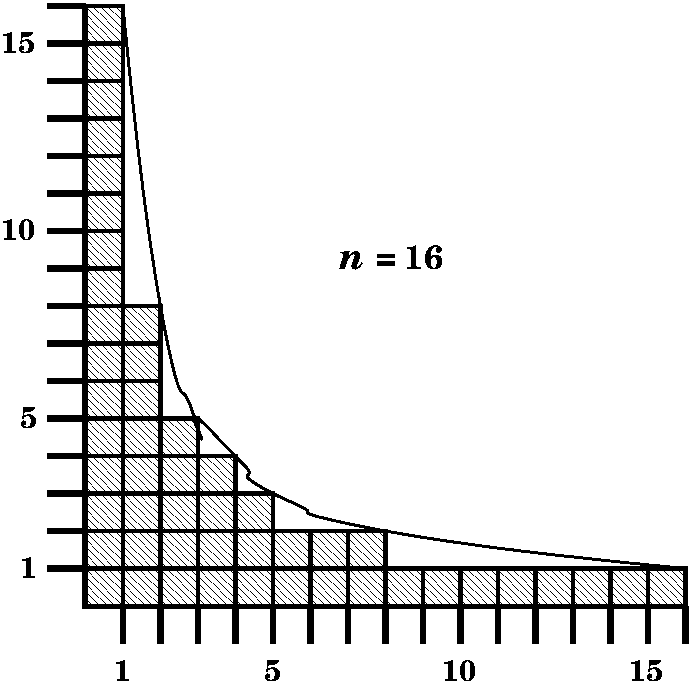
\includegraphics[scale=0.4]{pairing-hyp.pdf}
\caption{{\it The aggregate set of positions of tables having $16$ or
fewer position.}
\label{f.hyp}}
\end{figure}

   

\ignore{*****************
\noindent {\em Additive pairing functions}
%
The study in \cite{Rosenberg02} focuses on pairing functions that are
{\it additive}: Assign each row $v$ a {\it base task-index} $B_v$ and
a {\it stride} $S_v$.  Then use the formula
\[ \t(v, t) \ = \ B_v + (t-1) S_v \]
to map $\N^+ \times \N^+$ bijectively onto $\N^+$.

{\em A methodology for designing {\em additive} pairing functions.}
%
Easily, any additive pairing function must have infinitely many
distinct strides; i.e., $S_x$, viewed as a function of $x$, must have
infinite range.  Despite this, that there do exist easily computed
additive pairing functions.  One strategy for designing such pairing
functions builds on the following well-known property of the set \O\/
of positive odd integers.

\begin{lemma}[\cite{NivenZ80}]
\label{l.odds}
For any positive integer $c$, every odd integer can be written
in precisely one of the $2^{c-1}$ forms:
\[ 2^c n +1, \ 2^c n +3, \ 2^c n +5, \ldots, \ 2^c n + (2^c -1), \]
for some nonnegative integer $n$.
\end{lemma}

\noindent
One builds on Lemma~\ref{l.odds} to construct additive pairing
functions (APFs) in the following manner.

\paragraph{\underline{Procedure}} {
\sf APF-Constructor}($\t$) \\
/*Construct an APF $\t$*/
\begin{description}
\item[Step 1.]
Partition the set of row-indices into {\it groups} whose sizes are
powers of 2 (with any desired mix of equal-size and distinct-size
groups).  Order the groups linearly in some (arbitrary) way.
\end{description}
/*One can now talk unambiguously about group 0 (whose members share
{\it group-index} $g=0$), group 1 (whose members share group-index
$g=1$), and so on.*/
\begin{description}
\item[Step 2.]
Assign each group a distinct copy of the set \O, as well as a {\it
copy-index} $\kappa(g)$ expressed as a function of the group-index
$g$.

\item[Step 3.]
Allocate group $g$'s copy of \O\/ to its members via the $(c =
\kappa(g))$ instance of Lemma~\ref{l.odds}, using the multiplier $2^g$
as a {\it signature} to distinguish group $g$'s copy of the set \O\/
from all other groups' copies.
\end{description}
One can specify the procedure's APFs in a computationally friendly
way.

{\em An explicit expression for $\t$.}
If we denote the $2^{\kappa(g)}$ rows of group $g$ as $x_{g,1}$,
$x_{g,2}$, \ldots, $x_{g,2^{\kappa(g)}}$, then for all $i \in \{ 1, 2,
\ldots, 2^{\kappa(g)} \}$,
\begin{equation}
\label{e.define.t}
\t(x_{g,i}, y) \ \eqdef \
2^g \left[ 2^{1 + \kappa(g)}(y-1) +
	(2x_{g,i} +1 \bmod 2^{1 + \kappa(g)}) \right]
\end{equation}

\begin{theorem}
\label{t.define.ataf}
Any function $\t: \N^+ \times \N^+ \leftrightarrow \N^+$ that is
designed via Procedure {\small\sf APF-Constructor}, hence is of the
form (\ref{e.define.t}), is a valid additive pairing function whose
base row-entries and strides satisfy
\begin{equation}
\label{e.genl.b.s}
B_x \ \leq \
S_x \ =    \ \t(x, y+1) - \t(x,y) \ = \ 2^{1 + g + \kappa(g)}.
\end{equation}
\end{theorem}
*********************}



\subsection{Numerals}\index{numerals}
\label{sec:Numerals}

We can identify distinct families of {\em operational}
numerals,\index{numerals!operational} i.e., numerals that allow one to
do things such as perform arithmetic (add, multiply, etc.).

**THOUGHTS*******
series expansions, strings created by a positional number system, and
hybrids built on positional systems such as ``scientific notation''.
*************


Of course, we are all familar with certain numbers that have {\em
  non-operational} names that we use all the time.  Notable among
these are (using terminology that anticipates future sections and
chapters):
\begin{itemize}
\item
$\pi$: the ratio of the circumference of a circle to its diameter;
  $\pi \approx 3.141592653 \ldots$
\item
$e$: Euler's constant; the base of ``natural'' logarithms: $e \approx
  2.718281828 \ldots$
\item
$i$: the name of the number whose square is $-1$; $i$ is appended to
  the real numbers in order to ``complete'' them to the complex
  numbers, within which system every polynomial of degree $n$ has $n$
  roots.
\end{itemize}

\medskip

%\addcontentsline{toc}{paragraph}{A. Positional number systems}
\paragraph{\small\sf A. Positional number systems}
\index{positional number system}

The most common way of forming numerals is via strings over a {\it
  number base}.\index{positional number system!base of the system}  
%
We begin with an integer $b>1$ that will serve as our base, and we
define the set $B_b = \{ 0, 1, \ldots, b-1\}$ of {\it digits in base
  $b$}.\index{positional number system!digits in base $b$}
%
To aid legibility, {\em within the context of base-$b$ positional
  numerals}, we denote the digit $b-1$ as a single character,
$\bar{b}$.\index{$\bar{b}$: the digit $b-1$ in base $b$}
%
We then form base-$b$ numerals in the following way.\index{positional
  number system!base-$b$ numerals}
%
This formation builds on {\em geometric sums}, a mathematical
structure that we shall learn to manipulate, evaluate, and compute
with in Section~\ref{sec:geometric-sums}.

A base-$b$ numeral is a string having three sections.
\begin{enumerate}
\item
The numeral begins with its {\em integral part},\index{positional
  number system!integral part of a numeral}
%
which is a finite string of digits from $B_b$: $\alpha_n \alpha_{n-1}
\cdots \alpha_1 \alpha_0$.

The base-$b$ number represented by the numeral's integral
part\index{positional number system!numerical value of integral part}
is\footnote{Our underlined notation for the numerical value of a
  numeral is not common, but we find it convenient.}
\[
\underline{\alpha_n \alpha_{n-1}\cdots \alpha_1 \alpha_0}
\ \ \eqdef \ \
\sum_{i=0}^n \alpha_i \cdot b^i
\]

\item
The numeral continues with a single occurrence of the {\it
  radix point}\index{positional number system!radix point ``$.$''}
``$.$''
\item
The numeral ends with its {\em fractional part},\index{positional
  number system!fractional part of a numeral}
%
which is a string---{\em finite or infinite}--- of digits from $B_b$:
$\beta_0 \beta_1 \beta_2 \cdots$.

The base-$b$ number represented by the numeral's fractional part
is\index{positional number system!numerical value of fractional part}
\[
\underline{. \beta_0 \beta_1 \beta_2 \cdots}
\ \ \eqdef \ \
\sum_{j\geq 0} \beta_j \cdot b^{-j}
\]
\end{enumerate}
In summary, then, the base-$b$ number represented by the numeral
$\alpha_n \alpha_{n-1} \cdots \alpha_1 \alpha_0                  
. \beta_0 \beta_1 \beta_2 \cdots$ 
is\index{positional number system!numerical value of numeral}
\[
\underline{\alpha_n \alpha_{n-1} \cdots \alpha_1 \alpha_0                  
. \beta_0 \beta_1 \beta_2 \cdots}
\ \ \eqdef \ \
\sum_{i=0}^n \alpha_i \cdot b^i
\ + \ \sum_{j\geq 0} \beta_j \cdot b^{-j}.
\]
By prepending a ``negative sign'' (or, ``minus sign'') $-$ to a
numeral or a number, one renders the thus-embellished entity as
negative.

\bigskip

%\addcontentsline{toc}{paragraph}{B. Scientific notation}
\paragraph{\small\sf B. Scientific notation}
\index{Scientific notation}

The finite numerals in subsection A are all ``exact'' in the sense
that changing any digit changes the value of the named number.  We
turn now to a class of numerals that abjure this ``exactness'' for the
sake of expedience.  There are a few reasons that one might be willing
to do this.

\begin{itemize}
\item
WHY SCIENTIFIC NOTATION
\end{itemize}

\addcontentsline{toc}{paragraph}{C. Exact arithmetic}





\section{Arithmetic and Its Laws}\index{laws of arithmetic}
\label{sec:Arithmetic-Tools+Laws}

Numbers are {\it adjectives}\index{number!as adjective}---you have
five apples and three oranges---but in contrast to adjectives that are
purely descriptive---the red ball, the big dog---numbers can be {\em
  manipulated},\index{number!as {\em manipulable} adjective} using the
tools of {\it arithmetic}.

\subsection{The Tools of Arithmetic}
\label{sec:arithmetic-tools}

The basic tools of arithmetic reside in a small set of operations,
together with two special integers that play important roles with
respect to the operations.  Since these entities are so tightly
intertwined, we discuss them simultaneously.

\smallskip

\noindent {\small\sf Two special integers}
%
The integers zero ($0$)\index{number!zero ($0$)} and one
($1$),\index{number!one ($1$)} play special roles within all four of
the classes of numbers we have described.

\smallskip

\noindent {\small\sf  The operations of arithmetic}\index{arithmetic!basic operations}
%
Arithmetic on the four classes of numbers that we have described is
built upon a rather small repertoire of operations.  When we say that
an operation produces a number ``of the same sort'', we mean that it
produces
\begin{itemize}
\item
an integer result from integer arguments;
\item
a rational (number) result from rational (number) arguments;
\item
a real (number) result from real (number) arguments;
\item
a complex (number) result from complex (number) arguments;
\end{itemize}
The fundamental operations on numbers are, of course, familiar to the
reader.  Our goal in discussing them is to stress the laws that govern
the operations.  Along the way, we also introduce a few operations
that are less familiar but no less important.

\subsubsection{Unary (single-argument) operations}

\addcontentsline{toc}{paragraph}{A. Negating and reciprocating numbers}
\noindent {\small\sf A. Negating and reciprocating numbers.}
\index{arithmetic!basic operations!negation}
%
\noindent {\it i. The operation of {\em negation}}:
\index{arithmetic!basic operations!negating}
\begin{itemize}
\item
is a {\em total function} on the sets $\Z, \Q, \R, \C$.  It replaces
a number $a$ by its {\em negative},
\index{number!negative}
a number of the same sort, denoted $-a$.
\item
is a {\em partial function} on the nonnegative subsets
of $\Z, \Q, \R, \C$.  It replaces a number $a$ by its negative, $-a$,
whenever both $a$ and $-a$ belong to the nonnegative subset being
operated on.
\end{itemize}
Zero ($0$) is the unique {\it fixed point}\index{function!fixed
  point}\index{arithmetic!negation!fixed point} of the operation,
meaning that $0$ is the unique number $a$ such that $a = -a$.

\medskip

\noindent {\it ii. The operation of {\em reciprocation}}:
\index{arithmetic!basic operations!reciprocal}
\begin{itemize}
\item
\index{arithmetic!basic operations!reciprocating}
is a {\em total function} on the sets $\Q, \R, \C$, which replaces each
number $a$ by its {\em reciprocal}, 
\index{number!reciprocal}
a number of the same sort, denoted $1/a$ or $\displaystyle {1 \over
  a}$.  We shall employ whichever notation enhances legibility.

\item
is {\em undefined} on every integer $a$ except for $1$.
\end{itemize}

\medskip

\addcontentsline{toc}{paragraph}{B. Floors, ceilings, magnitudes}
\noindent {\small\sf B. Floors, ceilings, magnitudes.}
\index{arithmetic!basic operations!floor}
\index{arithmetic!basic operations!ceiling}
\index{arithmetic!basic operations!absolute value}
\index{arithmetic!basic operations!magnitude}

\noindent {\it i. The operations of {\em taking floors and ceilings}}
are total operations on the sets $\N, \Z, \Q, \R$.
\begin{itemize}
\item
The {\it floor} of a number $a$, also called {\it the integer part}
\index{arithmetic!basic operations!integer part of a number}
\index{arithmetic!basic operations!floor of a number}
of $a$, denoted $\lfloor a \rfloor$, is the largest integer that does
not exceed $a$; i.e.,:
\[
\lfloor a \rfloor \ \eqdef \ \max_{b \in {\mathbb{N}}} \Big[ b \ \leq a \Big]
\]
\item
The {\it ceiling} of a number $a$
\index{arithmetic!basic operations!ceiling of a number}
of $a$, denoted $\lceil a \rceil$, is the smallest integer that is 
not smaller than $a$:
\[
\lceil a \rceil \ \eqdef \ \min_{b \in {\mathbb{N}}} \Big[ b \ \geq a \Big]
\]
\end{itemize}
Thus, the operations of taking floors and ceilings are two ways to
{\em round} rationals and reals to their ``closest''
integers.\index{arithmetic!basic operations!rounding to ``closest'' integer}

\medskip

\noindent {\it ii. The operations of taking {\em absolute values/magnitudes}}:
\index{arithmetic!basic operations!absolute value, magnitude}
%
Let $a$ be a real number.  The {\it absolute value}, or, {\it
  magnitude}, of $a$, denoted $|a|$ equals either $a$ or $-a$,
whichever is positive.  For a complex number $a$, the definition of
$|a|$ is more complicated: it is a measure of $a$'s ``distance'' from
the ``origin'' complex number $0 + 0 \cdot i$.  In detail:
\[
|a| \ = \ \left\{
\begin{array}{cl}
a & \mbox{ if } \ [a \in \R] \ \ \mbox{ and } [a \geq 0] \\
-a & \mbox{ if } \ [a \in \R] \ \ \mbox{ and } [a < 0] \\
\sqrt{b^2 + c^2} &  \mbox{ if } \ [a \in \C]  \ \ \mbox{ and } [a = (b+ci)]
\end{array}
\right.
\]

\medskip

\addcontentsline{toc}{paragraph}{C. Factorials (of nonnegative integers)}
\noindent {\small\sf C. Factorials (of nonnegative integers).}
\index{arithmetic!basic operations!factorial (of a nonnegative integer)}
%
The {\it factorial} of a nonnegative integer $n \in \N$, which is
commonly denoted $n!$,
\index{arithmetic!basic operations!$n!$: factorial of $n \in \N$}
\index{arithmetic!basic operations!factorial of nonnegative integer}
is the function defined via the following recursion.
\begin{equation}
\label{eq:n-factorial-recursion}
\mbox{\sc fact}(n) \ = \ \left\{
\begin{array}{cl}
1 & \mbox{  if } \ n=0 \\
n \cdot \mbox{\sc fact}(n-1) & \mbox{  if } \ n>0
\end{array}
\right.
\end{equation}
By ``unwinding'' the recursion in (\ref{eq:n-factorial-recursion}),
one finds that, for all $n \in \N$,
\begin{equation}
\label{eq:n-factorial-direct}
n! \ = \ \mbox{\sc fact}(n) \ = \ 
n \cdot (n-1) \cdot (n-2) \cdot \cdots \cdot 2 \cdot 1
\end{equation} 
A $3$-step inductive argument validates this ``unwinding'':
\begin{enumerate}
\item
If $n =0$, then {\sc fact}$(n) = 1$, by definition
(\ref{eq:n-factorial-recursion}).
\item
Assume, for induction, that the expansion in
(\ref{eq:n-factorial-direct}) is valid for a given $k \in N$:
\[ \mbox{\sc fact}(k) \ = \ k \cdot (k-1) \cdot (k-2) \cdot \cdots
\cdot 2 \cdot 1 \] 
\item
Then:
\[
\begin{array}{lclll}
\mbox{\sc fact}(k+1) & = & (k+1) \cdot \mbox{\sc fact}(k)
  & & \mbox{by (\ref{eq:n-factorial-recursion})} \\
  & = &
(k+1) \cdot k \cdot (k-1) \cdot (k-2) \cdot \cdots \cdot 2 \cdot 1
  & & \mbox{by induction}
\end{array}
\]
\end{enumerate}


\subsubsection{Binary (two-argument) operations}
\label{sec:binary-operators}

%\addcontentsline{toc}{paragraph}{A. Addition and Subtraction}
\paragraph{\small\sf A. Addition and Subtraction.}
\index{arithmetic!basic operations!addition}
\index{arithmetic!basic operations!subtraction}
%
The operation of {\it addition}\index{arithmetic!addition} is a {\em
  total function} that replaces any two numbers $a$ and $b$ by a
number of the same sort.  The resulting number is the {\em sum of $a$
  and $b$}\index{arithmetic!addition!sum} and is denoted $a+b$.

\noindent
The operation of {\it subtraction}\index{arithmetic!subtraction} is a
{\em total function} on the sets $\Z, \Q, \R, \C$, which replaces any
two numbers $a$ and $b$ by a number of the same sort.  The resulting
number is the {\em difference of $a$ and $b$}
\index{arithmetic!subtraction!difference} and is denoted $a-b$.  On
the nonnegative subsets of the sets $\Z, \Q, \R, \C$---such as $\N$,
which is the largest nonnegative subset of $\Z$---subtraction is a
{\em partial function}, which is defined only when $a \geq b$.

Subtraction can also be defined as follows.  For any two numbers $a$
and $b$, {\em the difference of $a$ and $b$ is the sum of $a$ and the
  negation of $b$}; i.e.,
\[ a-b \ = \ a + (-b) \]

{\em The special role of $0$ under addition and subtraction.}
%
The number $0$ is the {\it identity} under addition and
  subtraction.\index{number!additive identity}\index{number!identity
  under addition}\index{identity!additive}
%
This means that, for all numbers $a$,
\[ a+0 \ = \ a-0 \ = \ a. \]

{\em The special role of $1$ under addition and subtraction.}
%
For any integer $a$, there is no integer between $a$ and $a+1$ or
between $a-1$ and $a$.  For this reason, on the sets $\Z$ and $\N$,
one often singles out the following special cases of addition and
subtraction, especially in reasoning about situations that are indexed
by integers.  Strangely, these operations have no universally accepted
notations.
\begin{itemize}
\item
The {\it successor} operation\index{arithmetic!integers!successor} is
a {\em total function} on both $\N$ and $\Z$, which replaces an
integer $a$ by the integer $a+1$.
\item
The {\it predecessor} operation\index{arithmetic!integers!predecessor}
is a {\em total function} on $\Z$, which replaces an integer $a$ by
the integer $a-1$.  It is a {\em partial function} on $\N$, which is
defined only when the argument $a$ is positive (so that $a-1 \in \N$).
\end{itemize}

The operations of addition and subtraction are said to be {\em
  inverse operations}\index{arithmetic!integers!additive inverse}
\index{arithmetic!integers!addition and subtraction are mutually
  inverse} of each other because each can be used to ``undo'' the
other:
\[
a \ = \ (a+b) -b \ = \ (a-b) +b
\]

\medskip

\addcontentsline{toc}{paragraph}{B. Multiplication and Division}
\noindent {\small\sf B. Multiplication and Division}.
\index{arithmetic!basic operations!multiplication}
\index{arithmetic!basic operations!division}
%
The operation of {\it multiplication}\index{arithmetic!multiplication}
is a {\em total function} that replaces any two numbers $a$ and $b$ by
a number of the same sort.  The resulting number is the {\em product
  of $a$ and $b$}\index{arithmetic!multiplication!product} and is
denoted either $a \cdot b$ \index{arithmetic!multiplication!$a \cdot  b$}
or $a \times b$.\index{arithmetic!multiplication!$a \times b$}
We shall usually favor the former notation, except when the latter
enhances legibility.

The operation of {\it division}\index{arithmetic!division} is a {\em
  partial function} on all of our sets of numbers.  Given two numbers
$a$ and $b$, the result of dividing $a$ by $b$---{\em when that result
  is defined}---is the {\it quotient of $a$ by $b$}
\index{arithmetic!division!When is $a/b$ defined?}
\index{arithmetic!division!quotient}
\index{arithmetic!division!quotient!$a/b$}
\index{arithmetic!division!quotient!$a \div b$}
\index{arithmetic!division!quotient!${a \over b}$}
and is denoted by one of the following three notations: $a/b$, $a \div
b$, $\displaystyle{a \over b}$.  The {\it quotient of $a$ by $b$} is
defined precisely when {\em both}

\noindent
\hspace*{.35in}(1) $b \neq 0$: one can never divide by $0$ \\
\hspace*{.35in}{\em and} \\
\hspace*{.35in}(2) there exists a number $c$ such that $a = b \cdot c$.

\noindent
Assuming that condition (1) holds, {\em condition (2) always holds
  when $a$ and $b$ belong to $\Q$ or $\R$ or $\C$}.

Division can also be defined as follows.  For any two numbers $a$
and $b$, {\em the quotient of $a$ and $b$ is the product of $a$ and the
reciprocal of $b$} (assuming that the latter exists); i.e.,
\[ a/b \ = \ a \cdot (1/b). \]
Computing reciprocals of nonzero numbers in $\Q$ and $\R$ is standard
high-school level fare; computing reciprocals of nonzero numbers in
$\C$ requires a bit of calculational algebra which we do not cover.
For completeness, we note that the reciprocal of the {\em nonzero}
complex number $a + bi \in \C$ is the complex number $c+di$ where
\[ c \ = \ \frac{a}{a^2 + b^2} \ \ \ \ \
\mbox{ and } \ \ \ \ \
d \ = \ \frac{-b}{a^2 + b^2}.
\]

{\em The special role of $1$ under multiplication and division.}
%
The number $1$ is the {\it identity} under the operations of
multiplication and division.\index{number!multiplicative
  identity}\index{number!identity under
  multiplication}\index{identity!multiplicative}
%
This means that, for all numbers $a$,
\[ a \cdot 1 \ = \ a \cdot (1/1) \ = \ a. \]

{\em The special role of $0$ under multiplication and division.}
%
The number $0$ is the {\it annihilator} under
multiplication.\index{multiplicative annihilator} This means that, for
all numbers $a$
\[ a \cdot 0 \ = \ 0. \]

The operations of multiplication and division are said to be {\em
  inverse operations}\index{arithmetic!integers!multiplicative
  inverse} \index{arithmetic!integers!multiplication and division are
  mutually inverse} because, when both operations can be applied, each
can be used to ``undo'' the other:
\[ a = (a \cdot b) \div b \ = \ (a \div b) \cdot b.  \]

\medskip

%\addcontentsline{toc}{paragraph}{C. Binomial coefficients and Pascal's triangle}
\paragraph{\small\sf C. Binomial coefficients and Pascal's triangle}
\index{arithmetic!basic operations!binomial coefficient}

We close our catalogue of arithmetic operations with a binary
operation on\footnote{In advanced contexts, one encounters binomial
  coefficients with non-integer arguments.}~$\N \times \N$.

Let $n$ and $k \leq n$ be nonnegative integers (i.e., elements of
$\N$).  The {\it binomial coefficient} denoted either as
$\displaystyle {n \choose k}$ or as $\Delta_{n,k}$, is the number
\index{binomial coefficients}
\begin{equation}
\label{eq:binom-coeff}
\Delta_{n,k} \ = \
{n \choose k} \ \eqdef \ \frac{n!}{k!(n-k)!} \ = \
\frac{n(n-1)(n-2) \cdots (n-k+1)}{k (k-1)(k-2) \cdots 1}
\end{equation}
Many of the secrets of these wonderful numbers---including the fact
that they are {\em integers}---can be deduced from the following
results.

\begin{prop}
\label{thm:manipulate-binom-coeff}
For all $n, k \in \N$ with $k \leq n$:

{\rm (a)} The symmetry rule:
\index{binomial coefficients!symmetry rule}
\begin{equation}
\label{eq:symmetry-binom-coeff}
{n \choose k} \ = \ {n \choose {n-k}}
\end{equation}

{\rm (b)} The addition rule:
\index{binomial coefficients!addition rule}
\begin{equation}
\label{eq:add-binom-coeff}
{n \choose k} \ + \ {n \choose {k+1}} \ = \ {{n+1} \choose {k+1}}
\end{equation}
\end{prop}

\begin{proof}
($a$)
We verify equation (\ref{eq:symmetry-binom-coeff}) by
(\ref{eq:binom-coeff}) plus the commutativity of multiplication (see
Section~\ref{sec:Arithmetic-Laws}),
\begin{eqnarray*}
{n \choose k} & = & \frac{n!}{k!(n-k)!} \\
              & = & \frac{n!}{(n-k)!k!} \\
              & = & {n \choose {n-k}}
\end{eqnarray*}

\noindent ($b$)
We verify equation (\ref{eq:add-binom-coeff}) by explicitly adding the
fractions exposed by (\ref{eq:binom-coeff}):
\begin{eqnarray*}
{n \choose k} \ + \ {n \choose {k+1}}
  & = &
\frac{n!}{k!(n-k)!} \ + \ \frac{n!}{(k+1)!(n-k-1)!} \\
  & = &
n! \cdot \frac{(k+1) + (n-k)} {(k+1)!(n-k)!} \\
  & = & 
\frac{(n+1)!}{(k+1)!(n-k)!} \\
  & = &
{{n+1} \choose {k+1}} \hspace*{2in} \qed
\end{eqnarray*}

Extrapolating from Proposition~\ref{thm:manipulate-binom-coeff}, we now
present {\it Pascal's triangle}, named in honor of
\index{Pascal's triangle}
\index{Pascal, Blaise}
the French polymath Blaise Pascal.  Fig.~\ref{fig:pascal-triangle}
provides a ``prefix'' of this famed array of integers, for $n,k \leq
5$.
\begin{figure}[htb]
\[
\begin{array}{c||r|r|r|r|r|r|r}
{\displaystyle {n \choose k}} & k=0 & k=1 & k=2 & k=3 & k=4 & k=5 &\ldots \\
\hline
\hline
n=1 & 1 & 1 &    &    &    &   & \ldots \\
\hline
n=2 & 1 & 2 & 1  &    &    &   & \ldots \\
\hline
n=3 & 1 & 3 & 3  & 1  &    &   & \ldots \\
\hline
n=4 & 1 & 4 & 6  & 4  & 1  &   & \ldots \\
\hline
n=5 & 1 & 5 & 10 & 10 & 5  & 1 & \ldots \\
\hline
\vdots &\vdots &\vdots &\vdots &\vdots &\vdots &\vdots &\ddots
\end{array}
\]
\caption{A ``prefix'' of Pascal's Triangle, for $n,k \leq 5$.}
\label{fig:pascal-triangle}
\end{figure}
The formation rule of the array is:
\begin{description}
\item[\sf Formation rule for Pascal's triangle:]
% 
{\it The entry at (row $n+1$, column $k+1$) is the sum of the entries
  at (row $n$, column $k$) and (row $n$, column $k+1$).}
\end{description}
\qed
\end{proof}


If you compare the formation rule for Pascal's triangle with equation
(\ref{eq:add-binom-coeff}), then you may anticipate the following
result.

\addcontentsline{toc}{paragraph}{-- A fun result: Pascal's triangle
  and the binomial coefficients}

\begin{prop}
\label{thm:pascal-binom}
The entries of Pascal's triangle are the binomial coefficients.
Specifically, for all $n,k$, the entry at (row $n$, column $k$) of the
Triangle is $\displaystyle {n \choose k}$.
\end{prop}

\begin{proof}
We note by observation and direct calcullation (see
Fig.~\ref{fig:pascal-triangle}) that the proposition is true for $n =
1$ and $k \in \{0, 1\}$.  A simple double induction

\noindent
****************** \\
induction on $n$, then for each value of $n$ on $k \leq n$ \\
SHOULD WE SPELL THIS OUT IN DETAIL?  GIVE AS AN EXERCISE? \\
******************

\noindent
verifies that every binomial coefficient appears in the Triangle and
every Triangle entry is a binomial coefficient.  \qed
\end{proof}

\medskip

\addcontentsline{toc}{paragraph}{-- A fun result: Binomial
  coefficients are integers}

\begin{prop}
\label{thm:binomcoeff-integer}
Every binomial coefficient is an integer.
\end{prop}

\begin{proof}
Since every entry in Pascal's triangle is obtained from integers via
repeated additions, this result follows from
Proposition~\ref{thm:pascal-binom}.  \qed
\end{proof}

\bigskip

Binomial coefficients are indispensable when studying myriad topics
related to {\em counting}, such as:
\begin{itemize}
\item
what are the relative likelihoods of various $5$-card deals from a
fair $52$-card deck?
\item
What is the likelihood of observing $15$ {\sc head}s and $25$ {\sc
  tail}s in $40$ flips of a fair coin?
\item
What are the comparative operation-count costs of Merge-Sort and
Quick-Sort when sorting $n$ keys; cf.~\cite{CLRS}?

\end{itemize}
We shall, therefore, see a lot more about binomial coefficients in
Section~\ref{sec:powers+polynolmials} and Chapter~\ref{ch:prob-stat}.
With each subsequent encounter, our respect for these numbers will
grow.


\subsection{The Laws of Arithmetic, and applications}
\index{arithmetic!basic laws}
\label{sec:Arithmetic-Laws}

The student should understand the following laws of arithmetic on the
reals, rationals, and reals---and be able to employ them cogently in
rigorous argumentation.

\medskip

\addcontentsline{toc}{paragraph}{A. The commutative law}
\noindent {\small\sf A. The commutative law.}
\index{commutative law!arithmetic}
\index{commutative law!addition}
\index{commutative law!multiplication}
\index{arithmetic!commutative law}
%
For all numbers $x$ and $y$:
\[
\begin{array}{llc}
\mbox{\it for addition:}
  & & x+y \ = \ y+x \\
\mbox{\it for multiplication:}
  & & x \cdot y \ = \ y \cdot x
\end{array}
\]

\medskip

\addcontentsline{toc}{paragraph}{B. The associative law}
\noindent {\small\sf B. The associative law}
\index{associative law for arithmetic}
\index{arithmetic!associative law}
%
For all numbers $x$, $y$, and $z$,
\[ (x+y)+z \ = \ x+(y+z) \ \ \ \mbox{\bf and } \ \ 
x\cdot (y\cdot z) 
(x \cdot y) \cdot z \ = \ x\cdot (y\cdot z). \] 
This allows one, for instance, to write strings of additions or of
multiplications without using parentheses for grouping.

\medskip

\addcontentsline{toc}{paragraph}{C. The distributive law}
\noindent  {\small\sf C. The distributive law.}
\index{distributive law for arithmetic}
\index{arithmetic!distributive law}
%
For all numbers $x$, $y$, and $z$,
\begin{equation}
\label{eq:distr-law}
x \cdot (y + z) \ = \ (x \cdot y) + (x \cdot z).
\end{equation}
One commonly articulates this law as, ``{\em Multiplication
  distributes over addition.}''


One of the most common uses of the distributive law reads equation
(\ref{eq:distr-law}) ``backwards,'' thereby deriving a formula for
{\em factoring} \index{arithmetic!factoring} complex expressions that
use both addition and multiplication.

Easily, addition does {\em not} distribute over multiplication; i.e.,
in general, $x + y \cdot z \ \neq \ (x+y) \cdot (x+z)$.  Hence, when
we see ``$x + y \cdot z$'', we know that the multiplication is
performed before the addition.  In other words, {\em Multiplication
  takes priority over addition.}  \index{arithmetic!priority of
  multiplication over addition} This priority permits us to write the
righthand side of (\ref{eq:distr-law}) without parentheses, as in
\[ x \cdot (y + z) \ = \ x \cdot y + x \cdot z. \]

Via multiple invocations of the preceding laws, we can derive a recipe
for multiplying complicated expressions.  We illustrate this via the
``simplest'' complicated expression, $(a+b) \cdot (c+d)$.

\begin{prop}
\label{prop:(a+b)(c+d)}
For all numbers $a, b, c, d$:
\begin{equation}
\label{eq:(a+b)(c+d)}
(a+b) \cdot (c+d) \ = \ a \cdot c + a \cdot d + b \cdot c + b \cdot d
\end{equation}
\end{prop}

\begin{proof}
Note first that because multiplication takes priority over addition,
the absence of parentheses in expressions such as
(\ref{prop:(a+b)(c+d)}) does not jeopardize unambiguity.  Our proof of
the proposition invokes the laws we have just enunciated multiple
times.
\[
\begin{array}{lclll}
(a+b) \cdot (c+d) & = & (a+b) \cdot c \ + \ (a+b) \cdot d
& & \mbox{distributive law} \\ 
  & = & c \cdot (a+b) \ + \ d \cdot (a+b)
& & \mbox{commutativity of multiplication} \ (2 \times) \\
  & = & c \cdot a + c \cdot b + d \cdot a + d \cdot b 
& & \mbox{distributive law} \ (2 \times) \\
  & = & a \cdot c + b \cdot c + a \cdot d + b \cdot d
& & \mbox{commutativity of multiplication} \ (4 \times) \\
  & = &  a \cdot c + a \cdot d + b \cdot c + b \cdot d
& & \mbox{commutativity of addition}
\end{array}
\]
\qed
\end{proof}


We close our short survey of the laws of arithmetic with the following
important two-part law.
\begin{itemize}
\item
{\it The law of inverses}.\index{inverse laws for
  arithmetic}\index{laws of arithmetic!inverse laws}
%
  \begin{itemize}
  \item
Every number $x$ has an {\em additive inverse},\index{additive inverse}
i.e., a number $y$ such that $x+y =0$.  This inverse is $x$'s {\it
  negative} $-x$.\index{additive inverse!negative as additive inverse}
  \item
Every {\em nonzero} number $x \neq 0$ has a {\em multiplicative
  inverse},\index{multiplicative inverse} i.e., a number $y$ such that
$x \cdot y = 1$.  This inverse is $x$'s {\it reciprocal},
$1/x$.\index{multiplicative inverse!reciprocal as multiplicative inverse}
  \end{itemize}
\end{itemize}

We close this section with another of our ``fun'' propositions.

\addcontentsline{toc}{paragraph}{-- A fun result: A ``trick'' for
  squaring some integers}

\begin{prop}
\label{thm:75x65=4925}
Let $n$ be any number that has a $2$-digit decimal of the form $\delta
5$, where $\delta \in \{ 0,1,2,3,4,5,6,7,8,9 \}$,
so that
\[ n \ = \ 10 \cdot \delta + 5
\]
Then 
\[ n^2 \ = \ 100 \cdot \delta \cdot (\delta+1) + 25. \]
In other words, one obtains a base-$10$ numeral for $n^2$ by
multiplying $\delta$ by $\delta +1$ and appending $25$ to the product.
\end{prop}

\noindent
Examples of Proposition ~\ref{thm:75x65=4925} include
$25^2 = 625$ (because $2 \cdot 3 = 6$) and $75^2 = 5625$ (because $7
\cdot 8 = 56$).

\begin{proof} (for general $\delta$).
%
We invoke Proposition~\ref{prop:(a+b)(c+d)} and the distributive law.
\[
\begin{array}{lclll}
n^2 & = & (10 \cdot \delta + 5)^2 & & \mbox{Given} \\
    & = & 100 \cdot \delta^2 \ + \ 100 \cdot delta \ + \ 25
              & & \mbox{the proposition} \\
    & = & 100 \cdot (\delta^2 \ + \ \delta) \ + \ 25
              & & \mbox{factoring: distributive law} \\
    & = & 100 \cdot \delta \cdot (\delta + 1) \ + \ 25
              & & \mbox{factoring: distributive law} \\
\end{array}
\]
\qed
\end{proof}


\subsection{Rational Arithmetic: A Worthwhile Exercise}
\label{sec:Rational-arithmetic}
\index{number!rational!arithmetic}

In Section~\ref{sec:rationals} we defined the rational numbers and
reviewed why they were needed to compensate for the general lack of
multiplicative inverses in the integers.  But we did not review how to
perform arithmetic on the elements of the set $\Q$.  We correct this
shortcoming now.  Of course, the reader will have encountered rational
arithmetic long ago---but we are now reviewing the topic in order to
provide the reader with a set of worthwhile exercise to reinforce the
mathematical thinking whose presentation is our main goal.

\medskip

The rational numbers build their rules for arithmetic upon the
corresponding rules for integers.  For all $p/q$ and $r/s$ in $\Q$:
\[
\begin{array}{|llcl|}
\hline
\mbox{\small\sf Addition:} & 
{\displaystyle
{p \over q} + {r \over s} }
  & = &
{\displaystyle
 \frac{p \cdot s + r \cdot q}{q \cdot s} }  \\
 & & & \\
\mbox{\small\sf Subtraction:} &
{\displaystyle
{p \over q} + {r \over s} }
  & = & 
{\displaystyle
{p \over q} + {(-r) \over s} } \\
 & & & \\
\mbox{\small\sf Multiplication:} &
{\displaystyle
{p \over q} \cdot {r \over s} }
  & = & 
{\displaystyle
\frac{p \cdot r}{r \cdot s} } \\
  & & & \\
\mbox{\small\sf Division:} &
{\displaystyle
{p \over q} \div {r \over s} }
  & = &
{\displaystyle
{p \over q} \cdot {s \over r} } \\
\hline
\end{array}
\]

It is worth verifying that rational arithmetic as thus defined behaves
in the required manner; in particular that rational arithmetic:
\begin{itemize}
\item
works correctly when the argument rational numbers are, in fact,
integers, i.e., when $q = s = 1$ in the preceding table.
\item
treats the number $0$ appropriately, i.e., as an additive identity and
a multiplicative annihilator; cf., Sections~\ref{sec:arithmetic-tools}
and~\ref{sec:Arithmetic-Laws}.
\item
obeys the required laws; cf., Section~\ref{sec:Arithmetic-Laws}.

Verifying the distributivity of rational multiplication over rational
addition will be a particularly valuable exercise because of the
required amount of manipulation.
\end{itemize}

\section{Basic Algebraic Concepts and Their Manipulations}

\subsection{Powers and polynomials}
\label{sec:powers+polynolmials}

\subsubsection{Raising a number to a power.}
\label{sec:x-toa-power}
A conceptually powerful notational construct is the operation of {\it
  raising a number to a power:}\index{raising a number to a power}
%
For real numbers $a$ and $b$, the {\it $b$th power} of $a$, denoted
$a^b$ is defined by the system of equations
\begin{equation}
\label{eq:power-def}
\begin{array}{llll}
\mbox{for all numbers $a>0$} & & & a^0 = 1 \\
 & & & \\
\mbox{for all numbers $a, b, c$} & & & a^b \cdot a^c = a^{b+c}.
\end{array}
\end{equation}
This deceptively simple definition has myriad consequences which we
often take for granted.
\begin{itemize}
\item
For all numbers $a>0$, the number $a^0 = 1$.

This follows (via cancellation) from (\ref{eq:power-def}) via the fact
that
\[ a^b \cdot a^0 \ = \ a^{b+0} \ = \ a^b \ = \ a^b \cdot 1.  \]

\item
For all numbers $a >0$, the number $a^{1/2}$\index{$a^{1/2}$: the
  square root of number $a$}
is the {\it square root} of $a$,\index{square root}
i.e., $a^{1/2}$ is the (unique, via cancellation) number $b$ such that
$b^2 = a$.  Another common notation for The number $a^{1/2}$ is
$\sqrt{a}$.\index{$\sqrt{a}$: the square root of number $a$}

This follows from (\ref{eq:power-def}) via the fact that
\[ a \ = \ a^1 \ = \ a^{(1/2) + (1/2)} \ = \ a^{1/2} \cdot a^{1/2} \ = \
\left(a^{1/2}\right)^2. \]

\item
For all numbers $a>0$ and $b$, the number $a^{-b}$ is the {\it
  multiplicative inverse}\index{multiplicative inverse}
of $a^b$, meaning that $a^b \cdot a^{-b} = 1$

This follows from (\ref{eq:power-def}) via the fact that
\[ a^b \cdot a^{-b} \ = \ a^{(b + (-b))} \ = \ a^0 \ = \  1 \]
\end{itemize}
When the power $b$ is a positive integer, then definition
(\ref{eq:power-def}) can be cast in the following attractive inductive
form:
\begin{equation}
\label{eq:power-def-integer}
\begin{array}{llll}
\mbox{for all numbers $a>0$} & & & a^0 = 1 \\
 & & & \\
\mbox{for all numbers $a$ and integers $b$} & & & a^{b+1} = a \cdot
a^b.
\end{array}
\end{equation}
Summing up, we now know about powers that are integral or fractional,
positive, zero, or negative

\subsubsection{Polynomials and their roots.}
\label{sec:poly-roots}
We want students to master the notions of polynomials and their
associated notions, such as degrees and coefficients, and computations
therewith, including polynomial summation and multiplication.  While
polynomial multiplication is often considered ``non-elementary'', it
must be mastered in order to fully understand positional number
systems; it is also essential, e.g., when discussing a range of topics
relating to, say, fault tolerance and encryption).

\index{The Fundamental Theorem of Algebra}
\begin{theorem}[The Fundamental Theorem of Algebra]
Every degree-$n$ univariate polynolmial with complex coefficients has
$n$ complex roots 
\end{theorem}

\index{The Binomial Theorem}
\subsubsection{The Binomial Theorem.}
\label{sec:Binomial-thm}

Perhaps the simplest bivariate polynomials are the ones in the
following family.
\begin{equation}
\label{eq:binomial-polys}
\mbox{For } \ n \in \N^+, \hspace*{.5in}
P_n(x,y) \ \eqdef \ (x+y)^n.
\end{equation}
There are lessons to be learned from the structure of these
polynomials, so let us begin to expand them using the arithmetic
techniques we have learned earlier.
\begin{eqnarray*}
P_1(x,y) \ = \
(x+y)^1 & = & x+y  \\
P_2(x,y) \ = \
(x+y)^2 & = & (x+y) \cdot (x+y) \\
        & = & x^2 + 2xy + y^2 \\
P_3(x,y) \ = \
(x+y)^3 & = & (x+y) \cdot (x^2 + 2xy + y^2) \\
   & = & (x^3 + 2x^2y +  xy^2) + (x^2y + 2xy^2 + y^3) \\
   & = & x^3 + 3x^2y + 3xy^2 + y^3  
\end{eqnarray*}

Let us stop to review what we are seeing.  We have remarked before
that doing mathematics can sometimes involve a wonderfully exciting
(quite sophisticated) pattern-matching game.  So, let us pattern-match!
\begin{enumerate}
\item
The coefficients of the expanded $P_1(x,y)$ are $\langle 1,1 \rangle$.
\item
The coefficients of the expanded $P_2(x,y)$ are $\langle 1,2,1 \rangle$.
\item
The coefficients of the expanded $P_3(x,y)$ are $\langle 1,3,3,1 \rangle$.
\end{enumerate}
There is a pattern emerging here.  Can you spot it?  Where have we
seen a pattern of tuples that begins in the same manner?  As a rather
broad hint, look at Fig.~\ref{fig:pascal-triangle}!  Could the
coefficients of each $P_n$ possibly be the successive binomial
coefficients
\[ {n \choose 0}, \ {n \choose 1}, \ \ldots, \ {n \choose {n-1}}, \ {n
  \choose n}
\]
Let us use induction to explore this possibility by expanding a
generic $P_n$ with symbolic ``dummy'' coefficients and see what this
says about $P_{n+1}$.  To this end, let $a_{n,n-r}$ denote the
coefficient of $x^{n-r} y^r$ in the expansion of $P_n(x,y)$.  Using
our ``dummy'' coefficients, we have
\[ 
\begin{array}{l}
P_n(x,y) \ = \
 x^n \ + \ \cdots \ + \ a_{n,n-r} x^{n-r} y^r
    \ + \ a_{n,n-r-1} x^{n-r-1} y^{r+1} \\
\hspace*{1in} + \ a_{n,n-r-2} x^{n-r-2} y^{r+2}
 \ + \ \cdots \ + \ y^n
\end{array}
\]
Continuing with this symbolic evaluation, we have:
\begin{equation}
\label{eq:xPk}
\begin{array}{l}
x \cdot P_n(x,y) \ = \
 x^{n+1} \ + \ \cdots \ + \ a_{n,n-r} x^{n-r+1} y^r
    \ + \ a_{n,n-r-1} x^{n-r} y^{r+1} \\
\hspace*{1in} + \ a_{n,n-r-2} x^{n-r-1} y^{r+2}
 \ + \ \cdots \ + \ xy^n
\end{array}
\end{equation}
and
\begin{equation}
\label{eq:yPk}
\begin{array}{l}
y \cdot P_n(x,y) \ = \
 x^n y \ + \ \cdots \ + \ a_{n,n-r} x^{n-r} y^{r+1}
    \ + \ a_{n,n-r-1} x^{n-r-1} y^{r+2} \\
\hspace*{1in} + \ a_{n,n-r-2} x^{n-r-2} y^{r+3}
 \ + \ \cdots \ + \ y^{n+1}
\end{array}
\end{equation}
Because
\[ P_{n+1}(x+y) \ = \ (x+y) \cdot P_n(x,y)
                \ = \ x \cdot P_n(x,y) \ + \ y \cdot P_n(x,y),
\]
the ``dummy'' coefficient $a_{n-r+1,r}$ of $x^{n-r+1} y^r$ in
$P_{n+1}(x+y)$ is the sum of the following coefficients in $P_n(x,y)$:
\begin{center}
$\bullet$
the coefficient $a_{n,n-r}$ of $x^{n-r}y^r$ \ \ \ \ \
and \ \ \ \ \
$\bullet$
the coefficient $a_{n,n-r+1}$ of $x^{n-r+1}y^{r-1}$
\end{center}
By induction, then, for all $n,r \in \N$ with $r \leq n$,
\[ a_{n,r} + a_{n,r+1} \ = \ a_{n+1,r+1} \]
Combining this equation with the observed initial conditions
\[ a_{1,0} \ = \ a_{1,1} \ = \ 1 \]
we see that each coefficient $a_{n,r}$ is actually the binomial
coefficient $\displaystyle {n \choose r}$.  This observation is
attributed to the renowned English mathematician/physicist Isaac
Newton and is enshrined in Newton's famous {\it Binomial Theorem}.

\ignore{**********
so that, finally,
\begin{eqnarray*}
             & = &
 x^{k+1} \ + \ (k+1) x^k y \ + \ \cdots \ + \
   (a_{k,k-r-1} + a_{k,k-r}) x^{k-r} y^{r+1} \\
             &   & \ \ \ + \
   (a_{k,k-r-2} + a_{k,k-r-1}) x^{k-r-1} y^{r+2}
 \ + \ \cdots \ + \ (k+1) xy^k \ + \ y^{k+1} \\
      & = &
 x^{k+1} \ + \ (k+1) x^k y \ + \ \cdots \ + \
 a_{k+1,k-r} x^{k-r} y^{r+1} \\
            &    & \ \ \ + \  a_{k+1,k-r-1} x^{k-r-1} y^{r+2}
 \ + \ \cdots \ + \ (k+1) xy^k \ + \ y^{k+1}
\end{eqnarray*}
*******}

\begin{theorem}[The Binomial Theorem]
\label{thm:Binomial-theorem}
For all $n \in \N$,
\[
(x+y)^n \ = \
\sum_{i=0}^n \ \ {n \choose i} x^{n-i} y^i.
\]
\end{theorem}
\index{The Binomial Theorem!binomial coefficients}
\index{binomial coefficients!The Binomial Theorem}



\subsection{Exponentials and Logarithms}
\label{sec:exponential+logarithm}

This section introduces the fundamentals of two extremely important
classes of functions which are functional inverses of each other, in
the following sense.  Functions $f$ and $g$ are {\it functional
  inverses}\index{functional inverse} of each other if for all
arguments $x$
\begin{equation}
\label{eq:functional-inverse}
f(g(x)) \ = \ x.
\end{equation}

\subsubsection{Basic definitions}

\paragraph{\small\sf A. Exponential functions}.\index{Exponential functions}
%
A function $f$ is {\it exponential} if there is a positive number $b$
such that, for all $x$,
\begin{equation}
\label{eq:exponential-defn}
f(x) \ = \ b^x.
\end{equation}
The number $b$ is the {\it base}\index{base of exponential}
%
of $f(x)$.  The basic arithmetic properties of exponential functions
are derivable from (\ref{eq:power-def}), so we leave these details to
the reader and turn immediately to the functional inverses of
exponential functions..

\paragraph{\small\sf B. Logarithmic functions}.\index{Logarithmic
  functions}
%
Given an integer $b >1$ (mnemonic for ``base''), the {\em base-$b$
  logarithm}\index{base-$b$ logarithm}
%
of a real number $a > 0$ is denoted $\log_b a$ and defined by the
equation\index{$\log_b a$: the base-$b$ logarithm of number $a$}
\begin{equation}
\label{eq:logarithm-defn}
a \ = \ b^{\log_b a}.
\end{equation}
Logarithms are partial functions: $\log_b a$ is not defined for
non-positive arguments.

The base $b = 2$ is so prominent in the contexts of computation theory
and information theory that we commonly invoke one of two special
notations for $\log_2 a$: (1) we often elide the base-$2$ subscript
and write $\log a$;\index{$\log(a)$: base-$2$ logarithm of number $a$}
(2) we employ the specialized notation $\ln a$\index{$\ln(a)$:
  base-$2$ logarithm of number $a$}.  Notationally:
\[ \log_2 a \ \eqdef \ \log a \ \eqdef \ \ln a \]

We leave to the reader the easy verification, from
(\ref{eq:logarithm-defn}), that the {\it base-$b$ logarithmic
  function}, defined by
\begin{equation}
\label{eq:log-function-defn}
f(x) \ = \ \log_b x
\end{equation}
is the functional inverse of the base-$b$ exponential function.

\subsubsection{Fun facts about exponentials and logarithms}

Definition (\ref{eq:logarithm-defn}) exposes and---even more
importantly---explains myriad facts about logarithms that we often
take for granted.

\begin{prop}
For any base $b >1$, for all numbers $x >0$, $y>0$,
\[ \log_b (x \cdot y) \ = \ \log_b x \ + \ \log_b y \]
\end{prop}

\begin{proof}
Definition (\ref{eq:logarithm-defn}) tells us that $x = b^{\log_b x}$
and $y = b^{\log_b y}$.  Therefore,
\[ x \cdot y \ = \ b^{\log_b x} \cdot b^{\log_b y} \ = \
b^{\log_b x \ + \ \log_b y}, \]
by the laws of powers.  Taking base-$b$ logarithms of the first and
last terms in the chain yields the claimed equation.
\qed
\end{proof}



Many students believe that the following result is a {\em convention}
rather than a consequence of the basic definitions.  {\em The logarithm
  of $1$ to any base is $0$.}

\begin{prop}
For any base $b >1$,
\[ \log_b 1 \ = \ 0 \]
\end{prop}

\begin{proof}
We note the following chain of equalities.
\[  b^{\log_b x} \ = \ b^{\log_b (x \cdot 1)} 
\ = \ b^{(\log_b x) + (\log_b 1)} 
\ = \ b^{\log_b x} \cdot b^{\log_b 1}
\]
Hence, $b^{\log_b 1} \ = \ 1$.  If $\log_b 1$ did not equal $0$, then
$b^{\log_b 1}$ would exceed $1$.  \qed
\end{proof}

\begin{prop}
For all bases $b > 1$ and all numbers $x, y$,
\[ x^{\log_b y} \ = \ y^{\log_b x} \]
\end{prop}

\begin{proof}
We invoke (\ref{eq:logarithm-defn}) twice to remark that
\[ \left[x^{\log_b y} \ = \ b^{(\log_b x) \cdot (\log_b y)}\right]
\ \ \mbox{ and } \ \ 
\left[y^{\log_b x}\ = \ b^{(\log_b y) \cdot (\log_b x)}\right] \]
The commutativity of addition completes the verification.  \qed
\end{proof}

\begin{prop}
For any base $b >1$,
\[ \log_b (1/x) \ = \ - \log_b x \]
\end{prop}

\begin{proof}
This follows from the fact that $\log_b 1 =0$, coupled with the
product law for logarithms.
\[ \log_b x + \log_b (1/x) \ = \ \log_b (x \cdot (1/x))
\  = \ \log_b 1 \ = \ 0 
\]
\qed
\end{proof}

\begin{prop}
For any bases $a, b >1$,
\begin{equation}
\label{eq:log-exp-0}
\log_b x \ = \ \left(\log_b a \right) \cdot \left( \log_a x \right).
\end{equation}
\end{prop}

\begin{proof}
We begin by noting that, by definition,
Note that
\begin{equation}
\label{eq:log-exp-1}
 x \ = \ b^{\log_b x} \ = \ a^{\log_a x} .
\end{equation}
Let us take the base-$b$ logarithm of the second and third expressions
in (\ref{eq:log-exp-1}) and then invoke the product law for logarithms.
From the second expression in (\ref{eq:log-exp-1}), we find that
\begin{equation}
\label{eq:log-exp-2}
 \log_b \left(b^{\log_b x} \right) \ = \ \log_b x .
\end{equation}
From the third expression in (\ref{eq:log-exp-1}), we find that
\begin{equation}
\label{eq:log-exp-3}
 \log_b \left( a^{\log_a x} \right) \ = \
\left(\log_b a \right) \cdot \left( \log_a x \right).
\end{equation}
We know from (\ref{eq:log-exp-1}) that the righthand expressions in
(\ref{eq:log-exp-2}) and (\ref{eq:log-exp-3}) are equal, whence
(\ref{eq:log-exp-0}).   \qed
\end{proof}

If we set $x = b$ in (\ref{eq:log-exp-0}), then we find the following
marvelous equation.

\begin{prop}
For any integers $a, b >1$,
\begin{equation}
\left(\log_b a \right) \cdot \left( \log_a b \right) \ = \ 1 \ \ \ \ \
\mbox{ or, equivalently, } \ \ \ \ \
\log_b a \ = \ \frac{1}{\log_a b} .
\end{equation}
\end{prop}


\subsubsection{Exponentials and logarithms within information theory}
\label{sec:count-strings}

The student should recognize and be able to reason about the following
facts.  If one has an alphabet of $a$ letters/symbols and must provide
distinct string-label ``names'' for $n$ items, then at least one
string-name must have length no shorter than $\lceil \log_a n \rceil$.

\begin{prop}
\label{thm:bound-stringnames-lgth-k}
Say that one must assign distinct labels to $n$ items, via strings
over an alphabet of $a$ letters.  Then at least one string-label must
have length no shorter than $\lceil \log_a n \rceil$.
\end{prop}

\begin{proof}
Let $Sigma$ be an alphabet of $a$ letters/symbols.  For each integer
$k \geq 0$ (i.e., for each $k \in \N$), let $\Sigma^{(k)}$ denote the
set of all length-$k$ strings over $\Sigma$.  The bound of
Proposition~\ref{thm:bound-stringnames-lgth-k} follows by counting the
number of strings of various lengths over $\Sigma$, because each such
string can label at most one item.  Let us, therefore, inductively
evaluate the cardinality $|\Sigma^{(k)}|$ of each set $\Sigma^{(k)}$.
\begin{itemize}
\item
$|\Sigma^{(0)}| =1$

This is because the null-string $\varepsilon$ \index{$\varepsilon$:
  the null string, of length $0$}
\index{null string $\varepsilon$}
is the unique string in $\Sigma^{(0)}$, i.e., $\Sigma^{(0)} = \{
\varepsilon \}$.

\item
$|\Sigma^{(k+1)}| = |Sigma| \cdot |\Sigma^{(k)}|$.

This reckoning follows from the following recipe for creating all
strings over $\Sigma$ of length $k+1$ from all strings of length $k$.
\[
\Sigma^{(k+1)} \ = \ \{ \sigma x \ | \ \sigma \in \Sigma, x \in
\Sigma^{(k)} \}
\]
This recipe is correct because
  \begin{itemize}
  \item
Each string in $\Sigma^{(k+1)}$, as constructed, has length $k+1$.

This is because the recipe adds a single symbol to a length-$k$
string.
  \item
For each string $x \in \Sigma^{(k)}$, there are $|\Sigma|$ distinct
strings in $\Sigma^{(k+1)}$, as constructed.

This is because each string in $\Sigma^{(k+1)}$ begins with a distinct
symbol from $\Sigma$.

  \item
$\Sigma^{(k+1)}$, as constructed, contains all strings of length $k+1$
over $\Sigma$.

This is because for each $\sigma \in \Sigma$ and each $x \in
\Sigma^{(k)}$, the string $\sigma x$ is in $\Sigma^{(k+1)}$, as
constructed.
  \end{itemize}
\end{itemize}
We thus have the following recurrence.
\begin{eqnarray*}
|\Sigma^{(0)}| & = & 1 \\
|\Sigma^{(k+1)}| & = & |\Sigma| \cdot |\Sigma^{(k)}| \ \ \ \ 
\mbox{ for } \ k \geq 0
\end{eqnarray*}
Using the Master Theorem, we thus find explicitly that

\noindent
For each $\ell \in \N$,
\[ |\Sigma^{(\ell)}| \ = \ \frac{|\Sigma|^{\ell+1} \ - \ |\Sigma|}
{|\Sigma| -1} \ \leq \ c \cdot |\Sigma|^{\ell}
\]
for some constant $c$.  In order for this quantity to reach $n \in
\N$, we must have
\[ \ell \ > \ d \cdot \log_{|\Sigma|} n   \]
for some small constant $d$.  \qed
\end{proof}

**HERE

Focus on 
Say, inductively, that there are $\ell_k$


\begin{prop}
\label{thm:Num-strings-lgth-k}
The number of distinct strings of length $k$ over an alphabet of $a$
letters is $a^k$.
\end{prop}


\ignore{*********************

\subsection{Arithmetic and geometric sequences and series}
\label{sec:sums-series}

The ability to sum -- and perhaps approximate -- simple series,
including, {\em at least}, finite arithmetic series and both finite
and infinite geometric series.

\subsubsection{Arithmetic sequences and series.}
\label{sec:arithmetic-series}
%
We define arithmetic sequences and learn how to calculate their sums.

\begin{equation}
\label{eq:arith-seq}
\begin{array}{l}
\mbox{An $n$-term arithmetic sequence:} \\
\hspace*{.25in}a, \ a+b, \ a+2b, \ a+3b, \ \ldots, a+(n-1)b \\
\\
\mbox{The corresponding arithmetic series:} \\
\hspace*{.25in}a + (a+b) + (a+2b) + (a+3b) + \cdots + (a+(n-1)b) \\
\hspace*{.5in} = \
an + b \cdot (1 + 2 + \cdots + n-1)
\end{array}
\end{equation}
We can, thus, sum the arithmetic series in (\ref{eq:arith-seq}) by
determining the sum of the first $m$ positive integers; $m = n-1$ in
(\ref{eq:arith-seq}).  We use this result as an opportubnity to
introduce important notation.

\addcontentsline{toc}{paragraph}{-- A fun result: Summing the first
  $n$ integers}

\begin{prop}
\label{thm:sum-first-integers-Gauss}
For all $n \in \N$,
\begin{eqnarray}
\nonumber
S_n \ \eqdef \ \sum_{i=1}^n \ i
 & \eqdef &
 1 + 2 + \cdots + (n-1) + n \\
\label{eq:sum-1-to-n}
 & = & {1 \over 2} n (n+1) \\
\nonumber
 & = & {{n+1}  \choose 2}.
\end{eqnarray}
\end{prop}

\begin{proof}
The {\em constructive} proof\footnote{The proof is {\em constructive}
  in that it actually derives an answer.  This is in contrast to the
  inductive proof of Proposition~\ref{thm:sum-1-to-n-induction}, which
  just verifies a ``guessed'' answer.}~of summation
(\ref{eq:sum-1-to-n}) that we present now employs a device known to
the eminent German mathematician Karl Friedrich Gauss \index{Gauss,
  Karl Friedrich} as a pre-teenager.
\begin{equation}
\label{eq:arith-series}
\begin{array}{llccccccccc}
\mbox{Write $S_n$ ``forwards'':} &
\hspace*{.25in}\sum_{i=1}^n \ = & 1 & + & 2   & + & \cdots & + & (n-1) & + & n \\
 & & & & & & & & & &  \\
\mbox{Write $S_n$ ``in reverse'':} &
\hspace*{.25in}\sum_{i=1}^n \ = & n & + & (n-1) & + & \cdots & + & 2     & + & 1
\end{array}
\end{equation}
Now add the two versions of $S_n$ in (\ref{eq:arith-series}) {\em
  columnwise}.  Because each of the $n$ column-sums equals $n+1$, we
find that $2 S_n = n(n+1)$, which we easily rewrite as in
(\ref{eq:sum-1-to-n}) (after multiplying both sides of the equation by
$2$).   \qed
\end{proof}

It follows that our original series in (\ref{eq:arith-seq}) sums as
follows.
\[
a + (a+b) + (a+2b) + (a+3b) + \cdots + (a+(n-1)b) \ = \
an + b \cdot {n \choose 2}. 
\]

\medskip

We can use Proposition~\ref{thm:sum-first-integers-Gauss} to craft
{\em two} ``constructive'' proofs---i.e., proof that explicitly
calculate the summation---that each perfect square, say, $m^2$, is the
sum of the first $m$ odd integers, $1, 3, 5, \ldots, 2m-1$.  These
proofs complement the ``guess-and-verify'' inductive proof of the same
result in Proposition~\ref{thm:squares-odd-integers-induction}.

\addcontentsline{toc}{paragraph}{-- A fun result: The $n$th perfect
  square is the sum of the first $n$ odd integers (two proofs)}

\begin{prop}
\label{thm:squares-odd-integers-Gauss}
For all $n \in \N^+$,
\begin{equation}
\label{eq:sum-of-odds}
\sum_{k=1}^n \ (2k-1)
 \ = \ 1 + 3 + 5 + \cdots + (2n-1) \ = \ n^2.
\end{equation}
That, is, the $n$th perfect square is the sum of the first $n$ odd
integers.
\end{prop}

Before presenting our two proofs of this result, we note that the
notation in (\ref{eq:sum-of-odds}) is perfectly general: every positive
odd integer $m$ can be written in the form $2n-1$ for some positive
integer $n$.

\smallskip

\begin{proof}
({\it Argument \#1}.)
%
By direct calculation, we have
\begin{eqnarray*}
\sum_{k=1}^n \ \left( 2k-1 \right)
   & = & 2 \sum_{k=1}^n \ k \ \ - \ n \\
   & = & 2 \frac{n (n+1)}{2} \ \ - \ n \ \ \ \ \mbox{ by
  Proposition~\ref{thm:sum-first-integers-Gauss}} \\
   & = & (n^2 + n) - n \\
   & = & n^2. \hfill \qed
\end{eqnarray*}
\end{proof}

\medskip

\begin{proof}
({\it Argument \#2}.)
%
Let us adapt Gauss's ``trick'' to this problem.  Let us denote the
target sum $\sum_{k=1}^n \ (2k-1)$ by $S_n$. 
\begin{equation}
\label{eq:add-odds}
\begin{array}{llccccccccc}
\mbox{$S_n$ ``forwards'':} &
S_n \ = 
& 1 & + & 3 & + & \cdots & + & (2n-3) & + & (2n-1) \\
 & & & & & & & & & &  \\
\mbox{$S_n$ ``in reverse'':} &
S_n \ =
& (2n-1) & + & (2n-3) & + & \cdots & + & 3 & + & 1
\end{array}
\end{equation}
Now add the two versions of $\sum_{k=1}^n \ (2k-1)$ in (\ref{eq:add-odds})
{\em columnwise}.  Because each of the $n$ column-sums equals $2n$, we
find that
\begin{equation}
\label{eq:sum-of-odds-sum}
2 \sum_{k=1}^n \ (2k-1) \ = \ 2n^2.
\end{equation}
We thus derive the desired summation (\ref{eq:sum-of-odds}) when we
divide both sides of equation (\ref{eq:sum-of-odds-sum}) by $2$.  \qed
\end{proof}

\subsubsection{Geometric sequences and series.}
\label{sec:geometric-sums}
%
We define geometric sequences and learn how to calculate their sums.

\begin{equation}
\label{eq:geom-seq}
\begin{array}{l}
\mbox{An $n$-term geometric sequence:} \\
\hspace*{.25in}a, \ ab, \ ab^2, \ \ldots, ab^{n-1} \\
\\
\mbox{The corresponding geometric series:} \\
\hspace*{.25in}a + ab + ab^2 + \cdots + ab^{n-1} \ = \
 a (1+ b + b^2 + \cdots + b^{n-1})
\end{array}
\end{equation}
Easily, we can sum the series in (\ref{eq:geom-seq}) by summing just
the sub-series
\begin{equation}
\label{eq:geom-series}
S_{b}(n) \ \eqdef \
1+ b + b^2 + \cdots + b^{n-1}.
\end{equation}
We proceed as follows.  Write $S_{b}(n)$ so that its terms are in {\em
  decreasing} order.  We thereby isolate two cases.
\begin{enumerate}
\item
Say first that $b > 1$.  In this case, we write the series in the form
\[ S^{b>1}_{b}(n) \ = \ b^{n-1} + b^{n-2} + \cdots + b^2 + b + 1, \]
and we note that
\[ S^{b>1}_{b}(n) \ = \
b^{n-1} \ + \ {1 \over b} \cdot S^{b>1}_{b}(n) \ - \ {1 \over b}. \]
In other words, we have
\[ \left( 1 - {1 \over b} \right)  S^{b>1}_{b}(n) \ = \ b^{n-1} - {1
  \over b}, \]
or equivalently,
\begin{equation}
\label{eq:geom-sum:b>1}
S^{b>1}_{b}(n) \ = \ \frac{b^{n}- 1}{b - 1}.
\end{equation}

\item
Alternatively, if $b < 1$, then we write the series in the form
\[ S^{b<1}_{b}(n) \ = \ 1+ b + b^2 + b^3 + \cdots + b^{n-1}. \]
and we note that
\[ S^{b<1}_{b}(n) \ = \
1 \ + \ b \cdot S^{b<1}_{b}(n) \ - \ b^n. \] 
In other words,
\[ (1-b) S^{b<1}_{b}(n) \ = \ 1 \ - \ b^n \]
or equivalently,
\begin{equation}
\label{eq:geom-sum:b<1}
S^{b<1}_{b}(n) \ = \ \frac{1 - b^n}{1-b}.
\end{equation}
\end{enumerate}

Note that $S^{b>1}_{b}(n)$ and $S^{b<1}_{b}(n)$ actually have the same
form.  We have chosen to write them differently to stress their {\em
  approximate} values, which are useful in ``back-of-the-envelope''
calculations:  For very large values of $n$, we have
\begin{equation}
\label{eq:geom-sum:approx}
S^{b>1}_{b}(n) \ \approx \ \frac{b^n}{b-1} \ \ \
\mbox{while} \ \ \
S^{b<1}_{b}(n) \ \approx \ \frac{1}{1-b} .
\end{equation}

\medskip

\addcontentsline{toc}{paragraph}{-- A fun result: When is an integer
  divisible by $9$?}

We now exploit our ability to sum geometric sums to illustrate a
somewhat surprising, nontrivial fact about integers that are
``encoded'' in their positional numerals.  We hope that this ``fun''
result will inspire the reader to seek kindred numeral-encoded
properties of numbers.

\begin{prop}
\label{thm:div-by-b-bar}
An integer $n$ is divisible by an integer $m$ if, and only if, $m$
divides the sum of the digits in the base-$(m+1)$ numeral for $n$.
\end{prop}

The most familiar instance of this result is phrased in terms of our
traditional use of base-$10$ (decimal) numerals. \\
{\it An integer $n$ is divisible by $9$ if, and only if, the sum of
  the digits of $n$'s base-$10$ numeral is divisible by $9$.}

\smallskip

\begin{proof}
({\it Argument for general base $b$}).
%
Of course, we lose no generality by focusing on numerals without
leading $0$'s, for adding leading $0$'s does not alter a numeral's sum
of digits.

To enhance legibility, let $b = m+1$, so that we are looking at the
base-$b$ numeral for $n$.  Say that
\[ n \ = \ \delta_k \cdot b^k + \delta_{k-1} \cdot b_{k-1} + \cdots +
\delta_1 \cdot b + \delta_0, \]
so that the sum of the digits of $n$'s base-$b$ numeral is
\[ s_b(n) \ \eqdef \ \delta_k + \delta_{k-1} + \cdots + \delta_1 + \delta_0. \]
We next calculate the difference $n - s_b(n)$.  We proceed as
follows, digit by digit.
\begin{equation}
\label{eq:sum-of-digits}
\begin{array}{ccccccccccc}
n & = &
\delta_k \cdot b^k & + & \delta_{k-1} \cdot b^{k-1} & + & \cdots
  & + & \delta_1 \cdot b & + & \delta_0 \\
s_b(n) & = &
\delta_k & + & \delta_{k-1} & + & \cdots & + & \delta_1 & + & \delta_0 \\
\hline
n - s_b(n) & = &
\delta_k \cdot (b^k -1) & + &
\delta_{k-1} \cdot (b^{k-1} -1) & + &
\cdots & + &
\delta_1 \cdot (b-1) & & 
\end{array}
\end{equation}

We now revisit summation (\ref{eq:geom-sum:b>1}).  Because $b$ is a
positive integer, so that $1 + b + \cdots + b^{a-2} + b^{a-1}$ is also
a positive integer, we adduce from the summation that {\em the integer
  $b^a -1$ is divisible by $b-1$.}

We are almost home.  Look at the equation for $n - s_b(n)$ in the
system (\ref{eq:sum-of-digits}).  As we have just seen, every term on
the righthand side of that equation is divisible by $b-1$.  It follows
therefore, that the lefthand expression, $n - s_b(n)$, is also
divisible by $b-1$.  An easy calculation, which we leave to the
reader, now shows that this final fact means that $n$ is divisible by
$b-1$ if, and only if, $s_b(n)$ is.  \qed
\end{proof}
********************}




\section{Congruences and Modular Arithmetic}



\section{Numbers and Numerals}

\subsection{Number vs.~Numeral: Object vs.~Name}


\subsection{Geometric series and positional number systems}

The relation between simple geometric series and numeration within
positional number systems -- including changing bases in such systems.


\section{Useful Nonalgebraic Notions}
\label{sec:extra-functions}

\subsection{Nonalgebraic Notions Involving Numbers}

\ignore{****************
\addcontentsline{toc}{paragraph}{Floors and Ceilings}
{\small\sf Floors and ceilings}.
%
Given any real number $x$, we denote by $\lfloor x \rfloor$ the {\em
  floor}\index{$\lfloor x \rfloor$: the floor of real number $x$}
(or {\em integer part})\index{$\lfloor x \rfloor$: the integer part
  of real number $x$}
%
of $x$, which is the largest integer that that does not exceed $x$.
Symmetrically, we denote by $\lceil x \rceil$ the 
{\em ceiling}\index{$\lceil x \rceil$: the ceiling of real number $x$}
of $x$, which is the smallest integer that is at least as large as
$x$.  For any nonnegative integer $n$,
\[ \lfloor n \rfloor  \ = \ \lceil n \rceil \ = \ n;  \]
for any positive rational number $n + p/q$, where $n$, $p$, and $q$
are positive integers and $p < q$,
\[ \lfloor n + p/q \rfloor  \ = \ n, \ \mbox{ and } \
\lceil n+ p/q \rceil \ = \ n+1.  \]

\addcontentsline{toc}{paragraph}{Absolute values/Magnitudes}
{\small\sf Absolute values, or, magnitudes}
%
Given any real number $x$, positive or negative, we denote by $|x|$
the {\it absolute value}\index{$|x|$: the absolute value of real number $x$}
or {\it magnitude}\index{$|x|$: the magnitude of real number $x$}
of $x$.  If $x \geq 0$, then $|x| = x$; if $x < 0$, then $|x| = -x$.

**********}


If the intended curriculum will approach more sophisticated
application areas such as robotics or data science or information
retrieval or data mining (of course, at levels consistent with the
students' preparation), then one would do well to insist on
familiarity with notions such as:


\ignore{*********

\section{Advanced Topics}

\subsection{Measures of distance in tuple-spaces}

including the following
norms/metrics: $L_1$ (Manhattan, or, rook's-move distance), $L_2$
(Euclidean distance); $L_\infty$ (King's-move distance).


\subsection{Edit-distance: a measure of closeness in {\em string spaces}}

***************}
%chapter
%*********Completed 05-29-19

%%%%%%%%%%%%%%%%%%%%%%%%%%%%%%%%%

%version of 07-10-19

\chapter{Summations:
Complex Operations from Simple Components}
\label{ch:Summation}


\section{Introducing the Many Facets of Summation}
\label{sec:intro}

The operation of {\it summation}---adding up aggregates of
numbers---is of fundamental importance in the world of digital
computing.  While we humans are able to deal handily with abstractions
such as ``smoothness'' and ``continuity'', we must employ
sophisticated {\em discretizations} of these concepts in order to
enlist the aid of digital computers in dealing with such abstractions.
Summations provide a very useful discretization of ``continuous'' or
``smooth'' phenomena that are typically dealt with by humans with the
aid of the (differential and integral) calculus, which was invented by
Newton and Leibniz for such dealings.

This chapter is dedicated to exploring how to employ summations as a
computational tool.  We deal throughout with {\it series}, {\it i.e.},
(possibly infinite) sequences of numbers
\[ a_1, a_2, \ldots \]
whose sum
\begin{equation}
\label{eq:abstract-sum}
a_1 + a_2 + \cdots
\end{equation}
is of interest.
\medskip

\noindent \fbox{
\begin{minipage}{0.96\textwidth}
Of course, when we deal with {\em infinite} series, wherein there are
infinitely many numbers $a_i$, we must address the question of whether
the sum (\ref{eq:abstract-sum}) exists as a finite number.  For some
infinite series the sum {\em does} exist as a finite number, as with
the well-known sum
\begin{equation}
\label{eq:sample-sum-2^(-k)}
 1 \ + \ \frac{1}{2} \ + \ \frac{1}{4} \ + \ \frac{1}{8} \ +
\ \frac{1}{16} \ + \ \cdots \ + \ \frac{1}{2^k}  \ +
\ \frac{1}{2^{k+1}} \ + \ \cdots \ = \ 2 
\end{equation}
Such an infinite series is said to {\em converge}.
\index{infinite series!convergent}
\end{minipage}
}

\noindent \fbox{
\begin{minipage}{0.96\textwidth}
But sometimes an infinite series {\em does not} have a finite sum.  
This is true, for instance, with the well-known {\it harmonic} series \index{harmonic series}
\begin{equation}
\label{eq:sample-sum-harmonic}
1 \ + \ \frac{1}{2} \ + \ \frac{1}{3} \ + \ \frac{1}{4} \ +
\ \frac{1}{5} \ + \ \cdots \ + \ \frac{1}{k} \ + \ \frac{1}{k+1} \ +
\ \cdots
\end{equation}
As more and more terms are added, the accumulated sum eventually
exceeds every number.  Such an infinite series is said to {\em diverge}.
\index{infinite series!divergent}

%{\Denis There is a link between harmonic series and the frequencies
%of the notes in music (each note corresponds to the fundamental
%divided by 2, 3, 4, ... May be it would be nice here to develop?}
%{\Arny I do not know enough to say anything intelligent about this.}
\end{minipage}
}
\medskip

Sums such as (\ref{eq:sample-sum-2^(-k)}) and
(\ref{eq:sample-sum-harmonic}) illustrate some of the complexity of
dealing with infinite entities.  Most obviously, as we have just
remarked, when the summations are infinite, some of them have finite sums
while others do not.  Even more subtle, the series that {\em do} have
(finite) sums illustrate the unintuitive fact that, sometimes finite
objects or entities---such as the integer $2$ in equation
(\ref{eq:sample-sum-2^(-k)})---have infinite ``names''; in this example, the infinite
series is an infinite "name" of integer $2$.  Lots to think about!
\medskip

\noindent \fbox{
\begin{minipage}{0.96\textwidth}
The complexity of the concept of convergent infinite objects such as series has been recognized in
various forms for more than $25$ centuries.  Several charming and
familiar examples appear in the paradoxes attributed to Zeno of
Elea. \index{Zeno of Elea} \index{Zeno!Zeno's paradox} In his {\it
  Paradox of Achilles and the Tortoise}, for instance, Zeno appears at
first glance to prove that all motion is illusory.  In this story, the
slow-footed Tortoise (T) tries to convince the speedy Achilles (A) of
the futility of trying to win any race in which A gives T even the
smallest head start.  As long as T is ahead of A, says T, every time A
traverses half the distance between the competitors, T will respond by
moving a bit further ahead.  Thereby, T will always be a positive
distance ahead of A, so that A can {\em never} catch T.  A similar
``argument'' demonstrates that an arrow shot at you by an adversary
can never reach you, as long as you continually move away from the
archer.  {\em DO NOT TRY THIS AT HOME!}

\medskip

The notion of {\em infinitesimals}, \index{infinitesimals} which
explains the fallacy of assertions such as the Tortoise's, were not
well understood until just a few hundred years ago.  This notion plays a
huge role in modern mathematics, underlying such foundational concepts
as {\em limits} \index{limits} and {\em continuity} \index{continuity
  (of functions)}(of functions).

\medskip

The general topic of the convergence or divergence of infinite series
is beyond the scope of this text.  It is a fascinating subject for
advanced study.
\end{minipage}
}
\medskip

Toward the end of guiding the reader through the forest of
abstractions and operations and techniques associated with summations,
we categorize the targets of our discussions in three ways.
\begin{enumerate}
\item
We study a number of {\it fundamental summations} that have intrinsic
interest.

Examples of this topic category include {\it arithmetic summations},
{\it geometric summations}, and {\it mathematically ``smooth''
  summations}, including sums of positive and negative powers of
integers.  Here is a sampler of six summations that appear in this
chapter.
\[
\begin{array}{lclcl}
1.  & &
1 \ + \ 2 \ + \ 3 \ + \ 4 \ + \ 5 \ + & \cdots & + \ k  \ + \ (k+1) \ +
\ \cdots \ + \ n \\
2. & &
1 \ + \ 2 \ + \ 4 \ + \ 8 \ + \ 16 \ + & \cdots & + \ 2^k  \ +
\ 2^{k+1} \ + \ \cdots \ + \ 2^n \\
3. & &
1 \ + \ 4 \ + \ 9 \ + \ 16 \ + \ 25 \ + & \cdots & + \ k^2  \ + \ (k+1)^2 \ +
\ \cdots \ + \ n^2 \\
4. & &
1 \ + \ \frac{1}{2} \ + \ \frac{1}{4} \ + \ \frac{1}{16} \ +
\ \frac{1}{32} \ + & \cdots & + \ \frac{1}{2^k}  \ + \ \frac{1}{2^{k+1}} \ +
\ \cdots \\
5. & &
1 \ + \ \frac{1}{2} \ + \ \frac{1}{3} \ + \ \frac{1}{4} \ +
\ \frac{1}{5} \ + & \cdots & + \ \frac{1}{k}  \ + \ \frac{1}{k+1} \ +
\ \cdots \\
6. & &
1 \ + \ \frac{1}{4} \ + \ \frac{1}{9} \ + \ \frac{1}{16} \ +
\ \frac{1}{25} \ + & \cdots & + \ \frac{1}{k^2}  \ + \ \frac{1}{(k+1)^2} \ +
\ \cdots
\end{array}
\]

\item
We study a variety of {\it fundamental techniques} for evaluating
summations.

We include specialized techniques that work for specific classes of
summations, as well as more general techniques that work in a broad
range of situations.

Examples of such techniques include, e.g.: estimating summations by
integrating functions related to the summation; grouping/replication
of terms within a summation; verifying ``guessed'' sums via induction.

\item
We study a variety of {\it fundamental representations} of the
elements being summed.  We observe that being able to study the same
phenomenon in a variety of seemingly unrelated ways often gives one
unexpected mathematical understanding of and operational control over
the phenomenon.

Examples of such representations include, among others,
representations of numbers by: numerals in a positional number system;
slices of pie; tokens arranged in stylized ways; basic geometrical
structures, including the unit-width rectangles of so-called Riemann sums.
\end{enumerate}

\medskip

\noindent
{\em In conclusion, we treat each topic in multiple ways, as long as
  each new way supplies new intuition and teaches a new lesson.}

\bigskip

%%%%%%%%%%%%%%%%%%%%%%%%%%%%%%%%%%%%%%%%%%%%%%%%


\ignore{\Denis Again, as I said before, I am not really convinced by this example.
Keeping the same sum, I prefer the story of Sissa, telling an old legende:
where wheat or rice is placed upon each square of the chess board in the following way:
put one grain on the first square, and then, double this number on each of the subsequent squares,
$2$ in the second case, $4$ in the third and so on.}

\ignore{\Denis add cross reference for computing the sum of powers of 2 in DOINGMATHS}

To illustrate the power of summation methodology, consider the
following modernized version of the {\it legend of Sissa ibn Dahir}.
\index{Sissa ibn Dahir, legend of}  Sissa, goes the legend, has invented a marvelous game that is played on a chessboard,
i.e., an $8 \times 8$ array of
unit-size squares.  An entrepreneur proposes to buy the rights of this marvelous game from Sissa.
The entrepreneur offers Sissa a one-time payment of {\em one million million (i.e., $10^{12} =
  1,000,000,000,000$) euros} in return for all rights to the new game.  As
a counter-offer, Sissa asked the entrepreneur instead for all of the money
amassed in the following way.  Sissa requested that the entrepreneur proceed row
by row along a chessboard, placing money in the board's squares,
according to the following regimen.  The entrepreneur should place $1$
euro in the first square, $2$ euros in the second square, $4 \ (= 2
\times 2)$ euros in the third square, $8 \ (= 4 \times 2)$ euros in the
fourth square, and so on, doubling the number of euros at each step of the
procedure---so the last square would contain $2^{63}$ euros.
Fig.~\ref{fig:Sissa} illustrates the growth of the pile of euros during first few steps of the procedure.
\begin{figure}[ht]
\begin{center}
       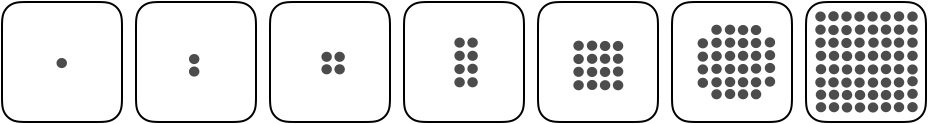
\includegraphics[scale=0.3]{FiguresMaths/chess}
\caption{The money in the first seven squares of the chessboard based on Sissa's counteroffer.}
       \label{fig:Sissa}
\end{center}
\end{figure}

\smallskip

\noindent
{\em Has Sissa made a good bargain?}

\smallskip

\noindent
By the end of this chapter, you will be able to determine in minutes
that under the procedure that amasses money on the chessboard, Sissa  
would receive $2^{64} -1$ euros---which is more than $10^{20}$ euros!  Sissa would, therefore, amass
{\em much} more money via his counteroffer than the mere $10^{12}$ euros that the entrepreneur
offered!
%{\Denis I think the previous value is -1 and not -2}

\noindent
{\em A good bargain, indeed!}

%%%%%%%%%%%%%%%%%%%%%%%%%%%%%%%%%%%%%%%%%%%%%%%%%%%%


\section{Summing Structured Series}
\label{sec:structured-series}

\subsection{Arithmetic Summations and Series}
\label{sec:arithmetic-series}

\subsubsection{General development}

We define arithmetic sequences and learn how to calculate their sums.

\begin{equation}
\label{eq:arith-seq}
\begin{array}{l}
\mbox{An $n$-term arithmetic sequence:} \\
\hspace*{.25in}a, \ a+b, \ a+2b, \ a+3b, \ \ldots, a+(n-1)b \\
\\
\mbox{The corresponding arithmetic series:} \\
\hspace*{.25in}a + (a+b) + (a+2b) + (a+3b) + \cdots + (a+(n-1)b) \\
\hspace*{.5in} = \
an + b \cdot (1 + 2 + \cdots + n-1)
\end{array}
\end{equation}
We can, thus, sum the arithmetic series in (\ref{eq:arith-seq}) by
determining the sum of the first $n-1$ positive integers.  We use this
result as an opportunity to introduce important notation.

\subsubsection{A first special case: Summing the first $n$ integers}
\label{sec:special-arithmetic sums}

Our first goal is to sum the first $n$ positive integers:
\[ 1 \ + \ 2 \ + \cdots + \ n \]
that is, to find a {\it closed-form expression} 
\index{closed-form expression}
for the sum.  In somewhat informal terms, we say that an expression of
the form
\begin{equation}
\label{eq:sigma-summation}
f(n) \ \eqdef \ \sum_{i=1}^n \ i
\end{equation}
is in {\it closed form} if it exposes a prescription for evaluating
the sum using a {\em fixed-length} sequence of arithmetic operations
(e.g., addition/subtraction, multiplication/division,
exponentiation/taking logarithms).  The notion "closed form" contrast with the recipe implicit in the notation (\ref{eq:sigma-summation}), which takes $n-1$ additions to evaluate. 

The sum $f(n)$ of the special summation  (\ref{eq:sigma-summation}) is commonly denoted $\Delta_n$.
\index{$\Delta_n$: sum of the first $n$ integers}
Within this chapter, we usually prefer the notation $S_1(n)$ for this sum because it
exposes this summation as an instance of a related family of such
summations that will occupy us through this chapter.

The remainder of this section is devoted to developing multiple ways
to derive the following {\em closed-form} expression for $\Delta_n = S_1(n)$.

\begin{prop}
\label{thm:sum-first-integers-Gauss}
\index{sum of first $n$ integers}
For all $n \in \N$,
\begin{equation}
\label{eq:sum-1-to-n}
S_1(n) \ = \ \sum_{i=1}^n \ i \
  \ = \  \frac{1}{2} n (n+1) 
\end{equation}
\end{prop}
\index{Sum of the first $n$ integers: $\Delta_n = S_1(n)$}

%{\Denis I removed the last equality with n+1 choose 2 since this
%combinatorial proof is presented later...}

\index{Sum of the first $n$ integers: $\Delta_n = S_1(n)$!a {\bf textual} derivation}
\begin{proof}
{\bf A textual proof.}
\index{sum of first $n$ integers!a textual reckoning}
%
We begin with a {\em constructive} proof\footnote{The proof is {\em
    constructive} in that it actually derives an answer.  This is in
  contrast to, say, the inductive validation of the sum in
  Section~\ref{sec:positive-integer-power}.C, which just verifies a
  ``guessed'' answer.}~of summation (\ref{eq:sum-1-to-n}) that employs
an approach known to the eminent German mathematician Karl Friedrich
Gauss \index{Gauss, Karl Friedrich} as a pre-teenager.  
\index{Gauss, Karl Friedrich!summation ``trick''} This approach
proceeds in two steps.
\begin{equation}
\label{eq:arith-series}
\begin{array}{llccccccccc}
\mbox{Write $S_1(n)$ ``forwards'':} &
\hspace*{.2in}\sum_{i=1}^n \ i \ = & 1 & + & 2   & + & \cdots & + & (n-1) & + & n \\
 & & & & & & & & & &  \\
\mbox{Write $S_1(n)$ ``in reverse'':} &
\hspace*{.2in}\sum_{i=n}^1 \ i \ = & n & + & (n-1) & + & \cdots & + & 2   & + & 1
\end{array}
\end{equation}
Now add the two representations of $S_1(n)$ in (\ref{eq:arith-series})
{\em columnwise}.  Because each of the $n$ column-sums equals $n+1$,
we find that $2 S_1(n) = n(n+1)$, which we easily rewrite in the form
(\ref{eq:sum-1-to-n}) (after multiplying both sides of the equation by
$2$).
\end{proof}

\medskip
\noindent \fbox{
\begin{minipage}{0.96\textwidth}
\noindent {\bf Remark.}
%
Now is an opportune moment to step back from the specific result
  in Proposition~\ref{thm:sum-first-integers-Gauss} and concentrate on
  the textual proof.  What Gauss noticed about the sum of the first
  $n$ integers is that when the sum is doubly written as in
  (\ref{eq:arith-series}), the column-sums are all the same.  This
  phenomenon of {\em finding invariants} is a ``pattern'' of the form
  referred to in Chapter~\ref{ch:doingmath} as we discussed how
  mathematicians ``do mathematics''.  We see in the proof how the
  pattern can be exploited to determine the sum of any arithmetic series.
  {\em What seemed to be a ``trick'' turns out to be an insightful
    instance of pattern-matching.}  We shall soon see that the pattern
  can be exploited to other, related, ends.
  \end{minipage}
}
\bigskip


Not everyone thinks the same way---even within the context of
mathematics.  It is, therefore, very important for the reader to
recognize that even the simplest mathematical facts can be proved and
analyzed in a broad variety of ways.  We illustrate this assertion by
developing more proofs of Proposition~\ref{thm:sum-first-integers-Gauss}.

\index{Sum of the first $n$ integers: $\Delta_n = S_1(n)$!a {\bf ``pictorial'', graphic} derivation}
\begin{proof}
{\bf A ``pictorial'', graphic proof.}
%
The idea now is to look at the problem of summing the first $n$
integers as a problem of estimating the area of a simple (in the
\textit{good sense} of the word) surface.  In this worldview, integers
are represented by concatenating basic {\it unit-side} (i.e., $1
\times 1$ \index{unit-side square} {\it squares}), as in
Fig.~\ref{fig:sumIntegersGeo1}.

Our summation process can be obtained in three steps, in the manner
illustrated by the three figures
Figs.~\ref{fig:sumIntegersGeo1},~\ref{fig:sumIntegersGeo2},
and~\ref{fig:sumIntegersGeo3}.
\begin{figure}[ht]
\begin{center}
       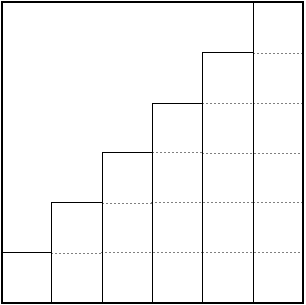
\includegraphics[scale=0.35]{FiguresMaths/SumIntegersGeometricBasis}
\caption{Representing the first $n$ integers using basic unit squares; $n=6$ in this example.}
       \label{fig:sumIntegersGeo1}
\end{center}
\end{figure}
\begin{figure}[ht]
\begin{center}
       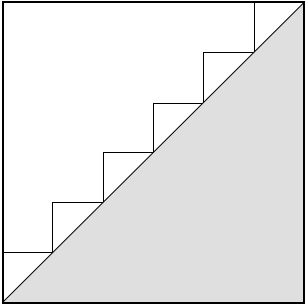
\includegraphics[scale=0.35]{FiguresMaths/SumIntegersGeometricIntermediate}
\caption{The area of the lower-right triangle (light grey) is one-half that of
  the entire $n \times n$ square.}
       \label{fig:sumIntegersGeo2}
\end{center}
\end{figure}
\begin{figure}[ht]
\begin{center}
       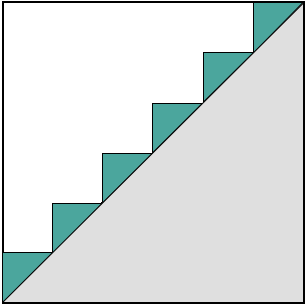
\includegraphics[scale=0.35]{FiguresMaths/SumIntegersGeometricFinal}
\caption{The area of the (dark) triangles sitting on the upper
  diagonal of the $n \times n$ square is $\frac{1}{2} n$.}
       \label{fig:sumIntegersGeo3}
\end{center}
\end{figure}
\begin{enumerate}
\item
We begin, in Fig.~\ref{fig:sumIntegersGeo1}, by depicting the problem
calculating $S_1(n)$ as the problem of determining the area of a
surface constructed from unit-side squares.

\item
Next, we illustrate in Fig.~\ref{fig:sumIntegersGeo2} that the area of
the lower-right triangle of the $n \times n$ square---depicted in
light grey in the figure---is one-half that of the entire $n \times n$
square.

\item
Finally, we indicate in Fig.~\ref{fig:sumIntegersGeo3} that the area
of the small (dark grey in the figure) triangles that cover the upper
diagonal of the $n \times n$ square is $\frac{1}{2} n$.  This
reckoning notes that there are $n$ triangles, and each has an area
that is one-half that of a unit-side square.
\end{enumerate}
We thereby reckon the area of the surface depicting $S_1(n)$ as

\begin{tabular}{l}
{\it One-half the area of the $n \times n$ square,
i.e., $\frac{1}{2} n^2$} \\
\hspace*{.15in} plus   \\
{\it $n$ times the area of one-half a unit-side square,
i.e., $\frac{1}{2} n$}
\end{tabular}

\noindent
We have, thus, derived the value of $S_1(n)$.
\end{proof}

\medskip

We present one final proof of
Proposition~\ref{thm:sum-first-integers-Gauss}.

\index{Sum of the first $n$ integers: $\Delta_n = S_1(n)$!a {\bf combinatorial} derivation}
\begin{proof}
{\bf A combinatorial proof.}
%
The following argument is {\it combinatorial} in that it achieves its
goal by {\em counting} instances of the first $n$ integers, laid out
in a line.

Place (tokens that represent) the integers $0$ to $n$ along a line.
For each integer $i$, count how many integers $j > i$ lie to its
right.  We see that in general, there is a {\it block} of $n-i$
integers that lie to the right of integer $i$.  In detail: the block
of integers lying to the right of $i=0$ contains $n$ values of $j$;
the block to the right of $i=1$ contains $n-1$ values of $j$, and so
on, as suggested in Fig.~\ref{fig:rightward-instances}.

\begin{figure}[htb]
\[
\begin{array}{lcccccc}
\mbox{All integers $\leq 4$:} &
 & 0 & 1 & 2 & 3 & 4 \\
\mbox{integers to the right of $0$:} &
 &   & 1 & 2 & 3 & 4 \\
\mbox{integers to the right of $1$:} &
 &   &   & 2 & 3 & 4 \\
\mbox{integers to the right of $2$:} &
 &   &   &   & 3 & 4 \\
\mbox{integers to the right of $3$:} &
 &   &   &   &   & 4
\end{array}
\]
\caption{A two-dimensional (triangular) depiction of the right-lying
  integer-instances.}
\label{fig:rightward-instances}
\end{figure}

On the one hand, we see that the total number of right-lying integers
$j$ equals $n+(n-1)+ ... + 1 \ = \ S_1(n)$.

On the other hand, every instance of a right-lying integer can be
identified uniquely by the pair of nonnegative integers, $i$ (the
instance's block) and $j>i$ (the instance's position-within-block).
The total number of right-lying integer-instances corresponds to the
number of ways to select two integers from among $n+1$.\footnote{We
  study such counting techniques in depth in
  Section~\ref{sec:counting}.}  This number is the binomial
coefficient whose definition we specialize from equation
(\ref{eq:binom-coeff}) in
Section~\ref{sec:binary-operators}.C:\footnote{The sums $\Delta_n$
  are, thus, special binomial coefficients, namely, coefficients of the form $\displaystyle
  {{n+1} \choose 2}$, in which the 'bottom" parameter is $2$.  The many ways of viewing the underlying
  summation in terms of triangles---as in
  Figs.~\ref{fig:sumIntegersGeo1}--\ref{fig:rightward-instances}---have
  therefore led to the naming of these special binomial coefficients
  as {\it triangular numbers}.  \index{triangular numbers}
  \index{binomial coefficients!triangular numbers} }
\[ 
\Delta_n \ = \ {{n+1} \choose 2} \ \eqdef \ \frac{1}{2} n(n+1)
\]
We have thus derived two distinct---but, of course,
equal---expressions for $S_1(n)$.
\end{proof}
\medskip

\noindent \fbox{
\begin{minipage}{0.96\textwidth}
Our combinatorial derivation of the summation (\ref{eq:sum-1-to-n})
illustrates one of the most important roles of mathematical
abstraction.  There is no obvious intuition to explain the
relationship between the activity of summing $n$ consecutive integers
and the activity of extracting two items out of a set of $n$ items.
Yet, our combinatorial derivation exposes an intimate connection
between the two.
\end{minipage}
}
\medskip

Now that we know---{\em and understand}---how to derive the value of
$S_1(n)$, we can finally evaluate our original series in
(\ref{eq:arith-seq}).  \index{arithmetic series:explicit sum}

\begin{prop}
\label{thm:sum-of-arithmetic-series}
The arithmetic series in (\ref{eq:arith-seq}) has the sum
\begin{equation}
\label{eq:sum-arithmetic-series}
a + (a+b) + (a+2b) + (a+3b) + \cdots + (a+(n-1)b) \ \ = \ \
%an + b \cdot {n \choose 2}. 
an + b \cdot \Delta_n
\end{equation}
\end{prop}


\subsubsection{A second special case: Perfect squares are sums of odd integers}

In this section, we build on
Proposition~\ref{thm:sum-first-integers-Gauss} to craft multiple
constructive proofs of the fact that each perfect square $n^2$
is the sum of the first $n$ odd integers, $1, 3, 5, \ldots, 2n-1$.
All of these proofs complement the ``guess-and-verify'' inductive
proof of this result in Section~\ref{sec:positive-integer-power}.C.

\begin{prop}
\label{thm:squares-odd-integers-Gauss}
\index{$n^2$ as sum of first $n$ odd integers}
For all $n \in \N^+$,
\begin{equation}
\label{eq:sum-of-odds}
\sum_{i=1}^n \ (2i-1)
 \ = \ 1 + 3 + 5 + \cdots + (2n-1) \ = \ n^2
\end{equation}
That, is, the $n$th perfect square is the sum of the first $n$ odd
integers.
\end{prop}

Before we present our proofs of this result, we want to stress that the
notation for odd integers in the summation within (\ref{eq:sum-of-odds}) is perfectly
general: every positive odd integer $n$ can be written in the form
$2i-1$ for some positive integer $i$. 

\medskip

Our first two proofs of
Proposition~\ref{thm:squares-odd-integers-Gauss} note that the result
is a corollary of both Proposition~\ref{thm:sum-first-integers-Gauss}
and Proposition~\ref{thm:sum-of-arithmetic-series}.

The first of these proofs builds on the stratagem of {\em finding
  invariants} that we exploited in the textual proof of
Proposition~\ref{thm:sum-first-integers-Gauss}.

\medskip

\index{$n^2$ as sum of first $n$ odd integers!a proof using algebra}
\begin{proof}
{\bf A proof using algebra.}
%
By direct calculation, we find that
\begin{eqnarray*}
\sum_{i=1}^n \ \left( 2i-1 \right)
   & = & 2 \sum_{i=1}^n \ i \ \ - \ n \\
   & = & 2 \Delta_n \ \ - \ n \ \ \ \ \ \ \ \ \ \ \mbox{ (by
  Proposition~\ref{thm:sum-first-integers-Gauss})} \\
   & = & (n^2 + n) - n \\
   & = & n^2
\end{eqnarray*}
\end{proof}

\medskip

\index{$n^2$ as sum of first $n$ odd integers!a proof by calculation}
\begin{proof}
{\bf A proof by calculation.}
%
Because summation (\ref{eq:sum-of-odds}) is an arithmetic series with
$a=1$ and $b=2$, we know from
Proposition~\ref{thm:sum-of-arithmetic-series} that the summation
evaluates to
\[ (1 \cdot n) + 2 \Delta_{n-1} \ = \ n + n^2 -n \ = \ n^2 \]
\end{proof}

\ignore{***\Denis According to the
  expression of Proposition~\ref{thm:sum-of-arithmetic-series}, the
  sum is equal to $1.n + 2 \Delta_{n-1} = n + n^2 -n = n^2$.  Let us
  detail several alternative proofs.***}

\medskip

\index{$n^2$ as sum of first $n$ odd integers!a textual proof}
\begin{proof}
{\bf A textual proof.}
%
We adapt to this summation Gauss's ``trick'', wherein one adds the series written
forwards to the series written backwards.  Let us
denote the target summation $\sum_{k=1}^n \ (2k-1)$ by $S(n)$.  We record
$S(n)$ in two ways:
\begin{equation}
\label{eq:add-odds}
\begin{array}{llccccccccc}
\mbox{``Forwards'':} &
S(n) \ = 
& 1 & + & 3 & + & \cdots & + & (2n-3) & + & (2n-1) \\
 & & & & & & & & & &  \\
\mbox{``Backwards'':} &
S(n) \ =
& (2n-1) & + & (2n-3) & + & \cdots & + & 3 & + & 1
\end{array}
\end{equation}
Now add these two representations of $S(n)$ {\em columnwise}.  Because
each of the $n$ column-sums equals $2n$, we find that
\begin{equation}
\label{eq:sum-of-odds-sum}
2 S(n) \ = \ 2 \sum_{i=1}^n \ (2i-1) \ = \ 2n^2
\end{equation}
We thus derive the sum (\ref{eq:sum-of-odds}) when we halve (i.e., divide by $2$) the three
equated quantities in equation (\ref{eq:sum-of-odds-sum}).
\end{proof}

\medskip

\index{$n^2$ as sum of first $n$ odd integers!a proof ``by pictures''}
\begin{proof}
{\bf A proof ``by pictures''.}
%
We now build up to a proof that is almost purely pictorial, with just
a bit of reasoning mixed in.  The only ``sophisticated'' knowledge
required is that
\begin{equation}
\label{eq:(n+1)^2}
(n+1)^2 \ = \ n^2 \ + \ 2n \ + \ 1
\end{equation}
\medskip

\noindent \fbox{
\begin{minipage}{0.96\textwidth}
We remark that equation (\ref{eq:(n+1)^2}) is the simplest
  instance of the {\em restricted Binomial Theorem}, which appears
  later in this chapter as Theorem~\ref{thm:restricted-binomial-thm}.
\end{minipage}
}
\medskip

The well-known equation (\ref{eq:(n+1)^2}) can be verified by
explicitly symbolically squaring $n+1$:
\[ (n+1) \cdot (n+1) \ \ = \ \ n \cdot (n+1) \ + \ (n+1) 
     \ \ = \ \ n^2 \ + \ n \ + \ n \ + \ 1
\]


\noindent
%Back to our proof of Proposition~\ref{thm:squares-odd-integers-Gauss}.
%
Our pictorial proof begins by representing each integer $n$ as a
horizontal sequence of $n$ tokens, i.e., darkened circles.  The
problem of summing the first $n$ odd integers then begins with a
picture such as appears in Fig.~\ref{fig:sumOdds1}, for the
illustrative case $n=5$.
\begin{figure}[ht]
\begin{center}
       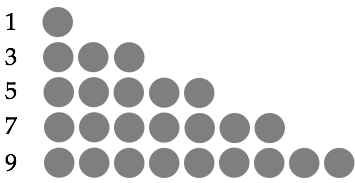
\includegraphics[scale=0.4]{FiguresMaths/SumOddsBasis}
\caption{Representing the first $n$ odd integers using tokens.  In
  this illustration, $n=5$.}
       \label{fig:sumOdds1}
\end{center}
\end{figure}

Starting with such a picture, we take each row of $2i-1$ tokens and
fold it at its midpoint so that it becomes a reversed letter ``$L$''.
The row of $2i-1$ tokens becomes an ``$L$'' whose horizontal portion
(at the bottom of the reversed ``$L$'') is a row of $i$ tokens and
whose vertical portion (at the right of the reversed ``$L$'') is a
column of $i$ tokens (one token is in common).  See
Fig.~\ref{fig:sumOdds2} wherein the depicted values of $i$ are $i = 1,
2, 3, 4, 5$.
\begin{figure}[ht]
\begin{center}
       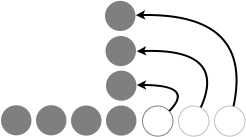
\includegraphics[scale=0.4]{FiguresMaths/SumOddsIntermediate}
              \caption{Folding a single row into a reversed letter ``$L$''.}
       \label{fig:sumOdds2}
\end{center}
\end{figure}

Once we have folded every row of tokens into a reversed ``$L$'', we
nest the occurrences of ``$L$'' in the manner depicted in
Fig~\ref{fig:sumOdds3}.
\begin{figure}[ht]
\begin{center}
       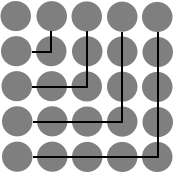
\includegraphics[scale=0.4]{FiguresMaths/SumOddsFinal}
\caption{The final picture organized as an $n \times n$ square
  array of tokens.}
       \label{fig:sumOdds3}
\end{center}
\end{figure}
Clearly, this nesting produces an $n \times n$ square array of
(perforce, $n^2$) tokens.
\end{proof}

\medskip

\index{$n^2$ as sum of first $n$ odd integers!another proof ``by pictures''}
\begin{proof}
{\bf Another proof ``by pictures''.}
%
The reader who enjoyed our ``proof 'by pictures''' may be amused by
the challenge of completing the kindred proof that is illustrated by
Fig.~\ref{fig:anotherSumOdds}.
\begin{figure}[ht]
\begin{center}
       
\includegraphics[scale=0.4]{FiguresMaths/Deltaodd}
\caption{Four copies of $S(n)$ represented as a triangle of tokens.
  The triangles are arranged to yield a $2n \times 2n$ square of
  tokens.}
       \label{fig:anotherSumOdds}
\end{center}
\end{figure}
The figure arranges four copies of the triangle of tokens which
illustrates summation $S(n)$, in such a way that the triangles combine
to produce the $2n \times 2n$ square of tokens.  The underlying
arithmetic exposes the fact that the side of the square consists of
$1+2n-1 \ = \ 2n$ tokens.  The conclusion is that $4 S(n) \ =
\ (2n)^2n \ = \ 4n^2$.
\end{proof}
\medskip

\noindent \fbox{
\begin{minipage}{0.96\textwidth}
Full disclosure: This proof of is not {\em purely}
pictorial, because we must somehow verify that the construction is
completely general, i.e., that the depicted emergence of the
$2n$ by $2n$ square of tokens from four copies of the
$\Delta_n$-triangle is not an artifact of the depicted case $n =5$.

Even with this caveat, one must admit that the {\em discovery} of the
proposition is really pictorial, even if the formal verification requires
additional modalities of reasoning. 
\end{minipage}
}


\ignore{********
{\Denis I added the following construction in the 2 figures, please, select the one you prefer.
If you think this result is too marginal here, we can put it as an exercice...}
This result can be obtained similarly by a slightly different arrangement by counting the tokens
of $4$ triangles representing the sum of the first $n$ integers $S(n)$ as shown in Fig~\ref{fig:alternateSumOdds}.
The side of the square is equal to $1+2n-1=2n$, thus $4 \cdot S(n)=(2n)^2= 4n^2$.

%\begin{figure}[ht]
%\begin{center}
%       
\includegraphics[scale=0.4]{FiguresMaths/DeltaoddSynthetic}
%\caption{Schematic view of how to obtain the $2n \times 2n$ square.}
%       \label{fig:alternateSumOdds2}
%\end{center}
%\end{figure}
***************}
\medskip

\index{$n^2$ as sum of first $n$ odd integers!a proof by rearranging terms}
\begin{proof}
{\bf A proof by rearranging terms.}
%
We described in Section~\ref{sec:summation-via-Fubini} how the Italian mathematician
Guido Fubini \index{Fubini, Guido}
was able to make notable mathematical progress by rearranging
representations of a variety of structured mathematical objects \cite{Fubini}.  Within the context of the current
chapter, such rearrangements work on the terms of a summation of
interest.  Indeed, using this strategy, we obtain a charming nonobvious proof of Proposition~\ref{thm:squares-odd-integers-Gauss}.
{\Denis This subterfuge will also evidence another amazing property of integers}
\medskip

Let us take the odd integers in order and arrange them into groups of successive sizes
as follows.
\[
\begin{array}{llrrrrclcc}
 &
1,  &    &     &      \\
 &
3,  &  5, &     &      \\
 &
7,  &  9, & 11, &     \\
 &
13, & 15, & 17, & 19   \\
\end{array}
\]
the first group, of size $1$, 
comprises just the smallest odd number, $1$;  the next group, of
size $2$, comprises the next two odd numbers, $3$ and $5$; and so on, with groups of successively
bigger sizes, each new line containing an extra odd number.  
%We view the groups as arranged in a triangular array, as depicted in the following table.
%Table~\ref{tab:SumOddsTriangle}.

What we observe is that---at least with the illustrated portion of the
following table---the $i$ elements of the $i$th group adds up to $i^3$.

\[
\begin{array}{llrrrrclcc}
\mbox{group of size 1:} & &
1,  &    &     &     &  \rightarrow &  1^3 \\
\mbox{group of size 2:} & &
3,  &  5, &     &    &  \rightarrow &  2^3 \\
\mbox{group of size 3:} & &
7,  &  9, & 11, &    &  \rightarrow &  3^3 \\
\mbox{group of size 4:} & &
13, & 15, & 17, & 19 &  \rightarrow &  4^3 \\
\end{array}
\]

%\begin{table}[ht]
%\label{tab:SumOddsTriangle}
%\caption{The sums of successive odd numbers and the sum of
%  successive cubes}
%\end{table}

Let us verify by induction that this pattern persists indefinitely.
{\Denis not really, what we want to show is that the sum of cubes ranging up to $\Delta_n$
is the square of $\Delta_n$, which is really beautiful!
This way, using Fubini, the whole sum of odds is also equal to the sum over the rows of the previous representation, 
which is done graphically...}
\begin{description}
\item[{\bf Base.}]
The singleton in row $1$ provides the base for our induction.

\medskip

\item[{\bf Inductive hypothesis}.]
We know from the previous analysis on triangular numbers
%Proposition~\ref{thm:sum-first-integers-Gauss} 
that the
$i$th group consists of the $i$ consecutive odd numbers beginning with 
the $\left( \Delta_{i-1} +1 \right)$th odd number---that is
$2 \Delta_{i-1} +1$---and ending with the $\Delta_i$th one ---that is
$2\Delta_i -1$.

\medskip

The proof to this point can be represented graphically as follows.  We begin with
the unit square as the base of our induction.
\begin{figure}[ht]
\begin{center}
       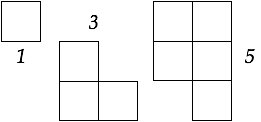
\includegraphics[scale=0.4]{FiguresMaths/SumCubes1}
\caption{The two first pictorial representation of the odd numbers: $1$ and $3$--$5$.}
       \label{fig:sumCubes1}
\end{center}
\end{figure}
The average of the two odd numbers in the second row is equal to $4$,
 next represent the number $8 = 2^3$ (which is the {\em cube} of $2$)
\ignore{{\Arny How do we know to do this?  What do these two squares have to do with $2^3$?}}
\begin{figure}[ht]
\begin{center}
       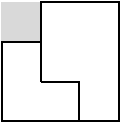
\includegraphics[scale=0.5]{FiguresMaths/SumCubes1bis}
\caption{The first step of the pictorial proof: the two first rows form a perfect square.}
       \label{fig:sumCubes1bis}
\end{center}
\end{figure}

 by two $2 \times 2$ squares: the figures following the unit square in
Fig.~\ref{fig:sumCubes1}.
Fig.~\ref{fig:sumCubes1bis} illustrates graphically that $1+ 2^3$
is a perfect square.
\begin{figure}[ht]
\begin{center}
       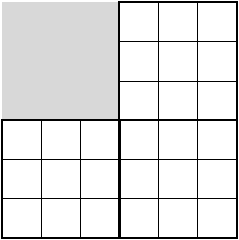
\includegraphics[scale=0.4]{FiguresMaths/SumCubes3}
\caption{The next step in the construction also produces a perfect square. Here $i=3$}
       \label{fig:sumCubes3}
\end{center}
\end{figure}
Fig.~\ref{fig:sumCubes3} illustrates that iterating the process one more time also
produces a perfect square. 
The case of odd indices is easy since we don't need to rearrange the unit squares 
(the surfaces perfectly fit).
However, the case of even $i$ needs a little more effort as shown in Fig.~\ref{fig:sumCubesEven}
and \ref{fig:sumCubesEvenFinal}.

{\Arny How do we know about the geometric arrangement of $1^3 + 2^3 + 3^3$?}
{\Denis We simply add $3^3$ to the square: I added two figures to explain in the most diffifult case of even $i$...}

 Comparing Figs.~\ref{fig:sumCubes2}
and~\ref{fig:sumCubes3} indicates a parity constraint on the process:
at even-numbered steps, the subsquares that get ``merged'' are
overlapping; at odd-numbered steps, they are not.
\begin{figure}[ht]
\begin{center}
       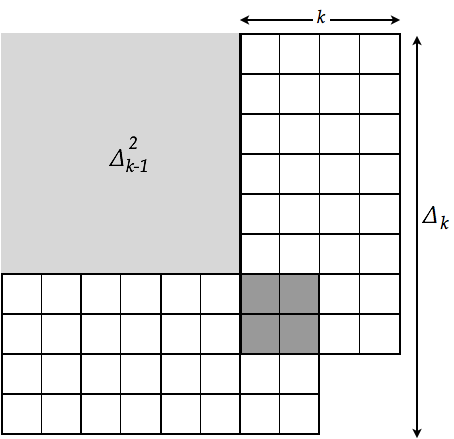
\includegraphics[scale=0.4]{FiguresMaths/SumCubesEven}
\caption{****The next step in the construction also produces a perfect square (here $i=4$).}
       \label{fig:sumCubesEven}
\end{center}
\end{figure}
\begin{figure}[ht]
\begin{center}
       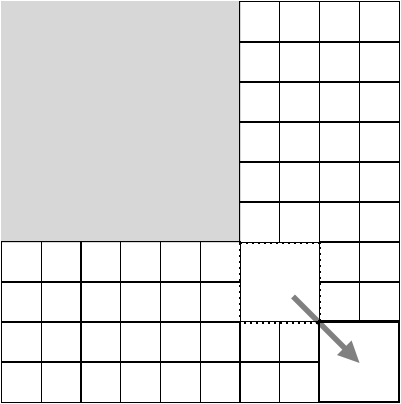
\includegraphics[scale=0.4]{FiguresMaths/SumCubesEvenFinal}
\caption{****How to move one of the overlapped area in order to obtain a perfect square.}
       \label{fig:sumCubesEvenFinal}
\end{center}
\end{figure}

\medskip

\item[{\bf Inductive extension}.]
%
Since consecutive odd numbers differ by $2$, we know that the $i$th
group consists of the following odd integers ($i>1$):
\[
2 \Delta_{i-1} +1, \ 2 \Delta_{i-1}  +3, \ 2 \Delta_{i-1}  +5 ,
\ldots, \
2 \Delta_{i-1} + (2i-1)
\]
Once one verifies (say, by induction) that $2 \Delta_{i-1} +2i-1 \ = \ 2
\Delta_{i} +1$, one discovers that this group has the sum
\[
2k \Delta_{i-1} \ - \ 2 \Delta_{i-1} +i \ = \
(2i -1) \Delta_i + i \ = \ i^3.
\]
\end{description}
This concludes the subproof about groups summing to perfect cubes.

Because each row contains one more integer than its predecessor, row
$i$ contains the sum of the odd integers from $\Delta_{i-1}+1$ to
$\Delta_i$.  By direct calculation, we can therefore compute the row's
sum as

{\Arny This is the denouement of the argument, and I do not sense the flow of the reasoning.}

\[
\Delta_i^2 \ - \ \Delta_{i-1}^2 
%\left( \frac{i(i+1)}{2} \right)^2 \ - \ \left( \frac{i(i-1)}{2} \right)^2
 \ \ =  \ \ \frac{i^2}{4} \left( (i+1)^2 - (i-1)^2 \right)
% & = & \frac{i^2}{4} (4i) \\
 \ \ = \ \ i^3
\]
\end{proof}

\bigskip

We close our treatment of
Proposition~\ref{thm:squares-odd-integers-Gauss} with another, really
basic proof.  As stated earlier, our goal is really to encourage
readers to utilize every possible mathematical concept as they hone
their mathematical and computational skills: {\em Simple proofs often
lend as much insight as sophisticated ones.}

\medskip

\index{$n^2$ as sum of first $n$ odd integers!a proof from elementary school}
\begin{proof}
{\bf A final proof, from elementary school.}
%
Consider the following reasoning which emerges from the way
multiplication tables are developed in elementary school.  We
illustrate the idea using the case $n=5$.
\begin{equation}
\label{eq:Fubini-table}
\begin{array}{rrrrr}
1  &  2 &  3 &  4 &  5 \\
2  &  4 &  6 &  8 & 10 \\
3  &  6 &  9 & 12 & 15 \\
4  &  8 & 12 & 16 & 20 \\
5  & 10 & 15 & 20 & 25 \\
\end{array}
\end{equation}
Write the integers $1, 2, \ldots, n$ in a row.  Below this row, write
the doubles of these integers.  Below the ``double'' row, write the
triples of the integers.  Below the ``triple'' row, write the
quadruples of the integers, then the quintuples, and so on.  Note that
the resulting table is {\em symmetric:} its rows are identical to its
columns.

\smallskip

Using again Fubini's rearrangement stratagem, we now count all the integers in
the table in two different ways.
{\Denis this is a variant of the previous development...}
\begin{enumerate}
\item
We sum the entries of our table by peeling away successively larger
reversed instances of the letter ``$L$'' (as in our earlier
``pictorial'' proof of
Proposition~\ref{thm:squares-odd-integers-Gauss}).  We find that the
integers in each ``$L$'' sum to a perfect cube:
\[
\begin{array}{rrrrrrrrr|rrc}
1  &    &    &    &    &   &     &    &   & 1   & = 1^3 \\
2  &  4 &  2 &    &    &   &     &    &   & 8   & = 2^3 \\
3  &  6 &  9 &  6 &  3 &   &     &    &   & 27  & = 3^3 \\
4  &  8 & 12 & 16 & 12 &  8 &  4 &    &   & 64  & = 4^3 \\
5  & 10 & 15 & 20 & 25 & 20 & 15 & 10 & 5 & 125 & = 5^3
\end{array}
\]

\item
We sum the successive rows of the $n \times n$ table (\ref{eq:Fubini-table}).  The
first row of the table sums to $\Delta_n$; the second row sums to $2
\Delta_n$; the third row sums to $3 \Delta_n$; \ldots; the last row sums
to $n \Delta_n$.  Thus, the aggregate sum of the table's rows is 
\[ (1 + 2 + \cdots + n) \cdot \Delta_n \ = \ \left(\Delta_n \right)^2 \]
\end{enumerate}
We conclude that
\[
\sum_{i=1}^n i^3 \ = \  \left(\Delta_n \right)^2
\]
\end{proof}

{\Arny Have I lost track?  Why does this prove that the cubes sum to the squares?}

{\Denis since the sum of cubes up to $\Delta_n$ equal the sum of odds!}

\ignore{\Arny More calculation!  BOO!  Please complete this.  I seem to be off by 1}
%We give another proof that tells us something more on numbers of their interactions.
%We consider numbers instead of tokens, and we use a similar principle as Fubini, that is to determine a
%suitable organization of the numbers and count them in a simple way.
%For the concern of computing the sum of the first odd numbers, we organize them as shown in Table~\ref{tab:SumOddsTriangle}.
%One number in the first row, two in the second, $k$ on the $k$th row.
%There are $\Delta_p$ (complete) rows. 
%The result is obtained by summing up the elements of each row.
%The sum in a row is equal to the perfect cube of this row.
%This result can be easily proven. 
%{\Denis Should I develop here? or we can let it as an exercice?}
%

\bigskip

\noindent {\em A preview of coming attractions}.
In Section~\ref{sec:sum-of-i2c>0}, we develop the underpinnings of
techniques that incrementally compute:

$\bullet$ the sums of the first $n$ consecutive integers (the summations $S_1(n)$), 

$\bullet$ the sums of the first $n$ squares of the integers (the summations $S_2(n)$), 

$\bullet$ the sums of the first $n$ cubes of the integers (the summations $S_3(n)$),

\noindent
and so on.  We have, thus begun to establish a base for a summation technique that is inductive, i.e., that computes each summation
$S_c(n)$ from the lower-index summations: $S_1(n)$, $S_2(n)$, \ldots, $S_{c-1}(n)$.  Our inductive technique awaits a bit more background.

%%%%%%%%%%%%%%%%%%%%%%%%%%%%%%%%%%%%%%%%%%%%%%%%%%%%

\subsection{Geometric Sums and Series}
\label{sec:general-geometric-series}
\label{sec:geometric-sums}
\label{sec:general-geometric-sums}

\subsubsection{Overview and main results}

We define geometric sequences and learn how to calculate their sums
via the following generic examples.
\index{geometric sequence}
\index{geometric summations}
\index{geometric series}

An $n$-term geometric sequence:
\begin{equation}
\label{eq:genl-geom-seq}
a, \ ab, \ ab^2, \ \ldots, ab^{n-1}
\end{equation}

The corresponding geometric summation:
\begin{eqnarray}
\label{eq:genl-geom-summation}
S_{a,b}(n)
 & \eqdef &  \sum_{i=0}^{n-1} a b^i \\
\nonumber
 & = &  a + ab + ab^2 + \cdots + ab^{n-1} \\
\nonumber
 & = & 
 a \cdot (1+ b + b^2 + \cdots + b^{n-1})
\end{eqnarray}

The associated geometric {\em (infinite) series} (used only when $b < 1$):
\begin{equation}
\label{eq:genl-geom-series}
S_{a,b}^{(\infty)} \ \ \eqdef \ \  \sum_{i=0}^\infty a b^i
 \ \  = \ \   a + ab + ab^2 + \cdots 
\end{equation}

It is clear from these definitions that we can evaluate the summation
(\ref{eq:genl-geom-summation}) by evaluating just the sub-summation
\begin{equation}
\label{eq:geom-summation}
S_{b}(n) \ \eqdef \ \sum_{i=0}^{n-1} b^i \ = \
1+ b + b^2 + \cdots + b^{n-1},
\end{equation}
and we can evaluate the series (\ref{eq:genl-geom-series}) by
evaluating just the sub-series
\begin{equation}
\label{eq:geom-series}
S_{b}^{(\infty)} \ \ \eqdef \ \ \sum_{i=0}^\infty b_i \ \ = \ \
1+ b + b^2 + \cdots 
\end{equation}

\medskip

The major results that we develop in this section are:

\index{evaluating geometric sums and series}
\begin{prop}
\label{thm:sum-finite-geometric-series}
Let $S_{b}(n)$ be a geometric summation, as defined in
(\ref{eq:geom-summation}).

\noindent {\bf (a)}
When $b > 1$, $S_{b}(n)$ evaluates to the following sum.
\begin{equation}
\label{eq:geom-sum:b>1}
S^{(b>1)}_{b}(n) \ = \ \frac{b^{n}- 1}{b - 1}.
\end{equation}

\noindent {\bf (b)}
When $b < 1$, $S_{b}(n)$ evaluates to the following sum.
\begin{equation}
\label{eq:geom-sum:b<1}
S^{(b<1)}_{b}(n) \ = \ \frac{1 - b^n}{1-b}.
\end{equation}
\end{prop}

Of course, in the uninteresting degenerate case $b=1$
\[ S^{(b=1)}_{b}(n) \ = \ 1 + 1 + \cdots + 1 \ \ \ \mbox{($n$ times)}
  \ \ \ \ = \ n.  \]

\medskip

The infinite case (\ref{eq:geom-series}) can be dealt with as a
corollary to Proposition~\ref{thm:sum-finite-geometric-series}(b), by
letting $n$ grow without bound and observing that the resulting
sequence of values converges.

\begin{prop}
\label{thm:sum-infinite-geometric-series}
When $b < 1$,  the {\em infinite} series $S^{(\infty)}_{b}$ {\em
  converges} to the following sum.
\[ S^{(\infty)}_{b} \ \ = \ \
\sum_{i=0}^\infty \ b^i \ \ = \ \ 1 + b + b^2 + \cdots
 \ \ = \ \ \frac{1}{1-b}.
\]
\end{prop}

\subsubsection{Techniques for summing geometric series}
\label{sec:summing-geometric-series:techniques}

We turn now to a sequence of proofs of
Propositions~\ref{thm:sum-finite-geometric-series}
and~\ref{thm:sum-infinite-geometric-series}.

\medskip

\index{evaluating geometric sums and series!by textual replication}
\begin{proof}
{\bf A proof by textual replication.}
%
Toward the end of developing our first method for summing $S_{b}(n)$,
we note that we can rewrite the sum in two ways that are {\em
  (textually) recurrent}.

\bigskip

\noindent
{\em This phenomenon of {\em finding recurrent subexpressions} is a
  ``pattern'' of the form described in Chapter~\ref{ch:doingmath} as
  we discussed how mathematicians ``do mathematics''.  We now
  exemplify how this pattern can be exploited to find explicit sums
  for geometric summations and series.}

\bigskip

\noindent
Both of the recurrent expressions for $S_{b}(n)$ have the following form.
\begin{equation}
\label{eq:geom-series-recurrent}
S_b(n) \ = \ \alpha \cdot S_b(n) \ + \ \beta(n)
\end{equation}
where $\alpha$ is a constant and $\beta(n)$ is a function of $n$; both
$\alpha$ and $\beta(n)$ may depend on the parameter $b$.  We provide
two recurrent expressions for $S_b(n)$, one of which is more
interesting when $b>1$, the other when $b<1$.
\begin{eqnarray}
\label{eq:geom-series-replicate}
\nonumber
S_{b}(n) 
  & \eqdef &
1+ b + b^2 + \cdots + b^{n-1}  \\
\nonumber
  &   &  \\
\label{eq:geom-series-replicate-1}
%  & = & 1 + b \cdot S_{b}(n) - b^n
   & = & b \cdot S_{b}(n) \ + \ (1 - b^n) \\
\nonumber
   &  & \\
%  & = & {\displaystyle
%b^{n-1} + \frac{1}{b} \cdot S_{b}(n) - \frac{1}{b}}
\label{eq:geom-series-replicate-2}
  & = &
\frac{1}{b} \cdot S_{b}(n) \ + \ \frac{b^n -1}{b} 
\end{eqnarray}
The significance of a recurrent expression of the form
(\ref{eq:geom-series-recurrent}) is that it exposes an explicit value
for $S_b(n)$:
\begin{equation}
\label{eq:geom-series-generic}
S_b(n) \ = \ \frac{\beta(n)}{1 - \alpha}
\end{equation}

We now combine the generic value (\ref{eq:geom-series-generic}) of
$S_b(n)$ with the specialized recurrent expressions in
(\ref{eq:geom-series-replicate-1}) and
(\ref{eq:geom-series-replicate-2}) to derive two explicit solutions
for $S_b(n)$.
\begin{enumerate}
\item
The first solution is most useful and perspicuous when $b>1$.  In this
case, we find that
\[ \left( 1 - \frac{1}{b} \right)  S^{(b>1)}_{b}(n) \ = \ b^{n-1} -
\frac{1}{b}, \]
which can easily be rearranged to the equivalent and more
perspicuous form (\ref{eq:geom-sum:b>1}).

\item
The second solution is most useful and perspicuous when $b < 1$.  In this
case, we find that
\[ (1-b) S^{(b<1)}_{b}(n) \ = \ 1 \ - \ b^n \]
which can easily be rearranged to the equivalent and more
perspicuous form (\ref{eq:geom-sum:b<1}).
\end{enumerate}
\end{proof}

Note that both $S^{(b>1)}_{b}(n)$ and $S^{(b<1)}_{b}(n)$ have simple
{\em approximate} values which are useful in ``back-of-the-envelope''
calculations: For very large values of $n$, we have
\begin{equation}
\label{eq:geom-sum:approx}
S^{(b>1)}_{b}(n) \ \approx \ \frac{b^n}{b-1} \ \ \
\mbox{and} \ \ \
S^{(b<1)}_{b}(n) \ \approx \ \frac{1}{1-b} .
\end{equation}
The expression for $S^{(b<1)}_{b}(n)$ in (\ref{eq:geom-sum:approx}) is
actually a rewording of
Proposition~\ref{thm:sum-infinite-geometric-series}.

\medskip

\index{evaluating geometric sums and series!a pictorial way to sum
  $S^{(\infty)}_{1/2}$ using cascading shrinking squares}
\begin{proof}
{\bf A pictorial representation for summing $S^{(\infty)}_{1/2}$.}
%
Fig.~\ref{fig:sumGeoBasis} depicts a pictorial process whose analysis
provides a rigorous proof of
Proposition~\ref{thm:sum-infinite-geometric-series} for the case $b =
1/2$, \textit{i.e.}, a rigorous argument that the series $S^{(\infty)}_{1/2} =
\sum_{i=0}^\infty \ 2^{-i}$ sums to $2$.
\begin{figure}[ht]
\begin{center}
       \includegraphics[scale=0.4]{FiguresMaths/SumGeometric1sur2Bis}
 \caption{Arranging successive rectangles to evaluate $S^{(\infty)}_{1/2}$.}
       \label{fig:sumGeoBasis}
\end{center}
\end{figure}
In this evaluation of $S^{(\infty)}_{1/2}$, we measure fractional
quantities by the portion of a unit-side rectangle that they fill.
Thus (follow in the figure): the initial term of $S^{(\infty)}_{1/2}$,
namely $1$, is represented by the unit square that is labeled ``$1$''
in the figure.  The next term of the series, namely $1/2$, is
represented by the rectangle labeled ``$1/2$'' in the figure, and so
on, with successively smaller rectangles.  By designing each rectangle
to have half the area of its predecessor, the sequence of rectangles
thus represents successively smaller inverse powers of $2$.  As the
process proceeds, we observe increasingly more of the righthand
unit-side square being filled.  In fact, one can argue that {\em
  every} point in the righthand unit-side square eventually gets
covered by some small rectangle (as $n$ tends to $\infty$), thereby
establishing that the infinite series $S^{(\infty)}_{1/2}$
does, indeed, sum to $2$.

\ignore{*******
The result is immediate while considering a basic unit square and its
successive decompositions while divided by $2$.
Thus, the whole surface corresponds to the sum of $(\frac{1}{2})^k$. 
It is equal to $2$ (surface of the two big squares) and it is completely filled. 
***********}

This procedure is difficult, but not impossible, to adapt to values of
$b <1$ other than $1/2$.  The sequence Fig.~\ref{fig:sumGeoGeneral1},
\begin{figure}[ht]
\begin{center}
       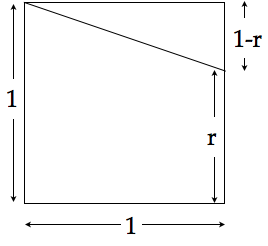
\includegraphics[scale=0.4]{FiguresMaths/SumGeometricGeneral1}
\caption{Initial state: the unit square and the base $b$.}
       \label{fig:sumGeoGeneral1}
\end{center}
\end{figure}
Fig.~\ref{fig:sumGeoGeneral2},
\begin{figure}[ht]
\begin{center}
       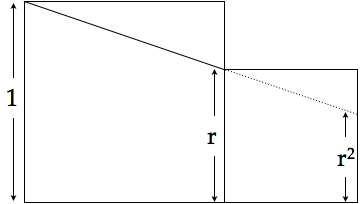
\includegraphics[scale=0.4]{FiguresMaths/SumGeometricGeneral2}
\caption{Beginning to craft the geometric series by cascading
  shrinking squares.}
       \label{fig:sumGeoGeneral2}
\end{center}
\end{figure}
Fig.~\ref{fig:sumGeoGeneral3} suggests how to achieve such an
adaptation for any value of $b$ with $0 \leq b <1$, by an
appropriate cascade of shrinking squares.
\begin{figure}[ht]
\begin{center}
       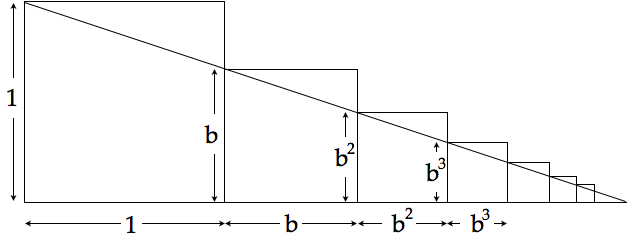
\includegraphics[scale=0.4]{FiguresMaths/SumGeometricGeneral3}
\caption{The complete process for computing a geometric series using a
  cascade of shrinking squares.}
       \label{fig:sumGeoGeneral3}
\end{center}
\end{figure}
The unit-side square in Fig.~\ref{fig:sumGeoGeneral1} begins the
construction of the cascade.  The two squares in
Fig.~\ref{fig:sumGeoGeneral2} illustrate the second step in
constructing the cascade; the suggestive cascade depicted in
Fig.~\ref{fig:sumGeoGeneral3} illustrates what the final cascade looks
like: The cumulative length of the bases of its abutting rectangles is
the value of the infinite series $S_b^{(\infty)}$;
cf.~(\ref{eq:genl-geom-series}).  The proof that the base of the
  cascade in the figure yields the desired sum is completed by a
  version of the geometry theorem associated with Thales of Miletus,
  \index{Thales of Miletus} and mentioned in Euclid's {\it
    Elements}.\index{Euclid} \qed
\end{proof}

\ignore{***********
{\Denis We should add a final remark here}.
The final touch is that the infinite sum is given by the base of the big right rectangle.
It is similar ({\Denis we call this property semblable in french}) to the little right rectangle top left in the figure.
By Thales theorem in geometry, the ratio of the sides are proportional:
$\frac{S^{(\infty)}_{b} }{1} = \frac{1}{1-b}$. 
***********}

\medskip

%{\Denis We can add here two exercices.}
\ignore{************
{\Denis(1) I really like including the pie-cutting in the text,
  because it is another representation for exactly the same problem.
  Do you like this way of handling it?  
  YES
  (2) I am less enthusiastic
  about including the nexted triangles: it changes the problem (i.e.,
  the base b) as well as the representation.  
  OK, base b is somehow a generalization...
  I like it very much as
  an exercise ... but we have not yet tackled that issue.
  How the exercices will be included?}
**********}

\index{evaluating geometric sums and series!a pictorial way to sum
  $S^{(\infty)}_{1/2}$ using a vigorously sliced pie}
\begin{proof}
{\bf Another pictorial representation for summing $S^{(\infty)}_{1/2}$.}
%
The pictorial derivation of the sum $S^{(\infty)}_{1/2}$ can be
accomplished using geometric shapes other than squares.  We now
present a natural derives the sum $S^{(\infty)}_{1/2}$ by vigorously
slicing a pie.

The process of pie-slicing works most naturally with the modified
series
\[ \overline{S}^{(\infty)}_{1/2} \ \ = \ \ \sum_{i=1}^\infty 2^{-i}
 \ \ = \ \ S^{(\infty)}_{1/2} \ - \ 1. \]
which omits the initial summand $1$ from $S^{(\infty)}_{1/2}$.  Of
course, $\overline{S}^{(\infty)}_{1/2}$ sums to $1$, because
$S^{(\infty)}_{1/2}$ sums to $2$.

The pie-slicing evaluation of $\overline{S}^{(\infty)}_{1/2}$ is depicted
in Fig~\ref{fig:sumGeo1sur2circle}.  In the figure, the inverse powers
of $2$ are represented by appropriate fractions of a unit-diameter
disk (the pie).  The evaluation begins with this disk before it is
sliced: this represents the number $1$, which we eventually show to be
the sum of $\overline{S}^{(\infty)}_{1/2}$.
\begin{figure}[ht]
\begin{center}
       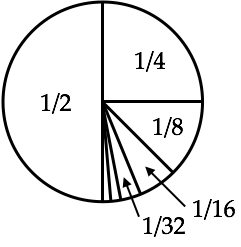
\includegraphics[scale=0.4]{FiguresMaths/SumGeometric1sur2circle}
\caption{Computing the sum of $1/2^i$ using a unit disk.}
       \label{fig:sumGeo1sur2circle}
\end{center}
\end{figure}
We slice the disk in half by means of the depicted diameter; we label
one of the resulting half-disks ``$1/2$''.  Next, we slice one of the
half-disks in half by means of a radius of the unit disk; we label one
of the quarter-disks ``$1/4$''.  We continue in this manner {\em ad
  infinitum}.  The analysis that yields the sum of
$\overline{S}^{(\infty)}_{1/2}$ amounts to a proof that every point in the
unit-diameter disk eventually resides in a slice that is not further
sliced.  Details are left to the interested reader.
\end{proof}

\ignore{***************
Another variation refers to the surface of an unit equilateral triangle. 
We are looking for the sum of the $1/4^i$ is equal to $1/3$ by two ways
refering to Fig~\ref{fig:sumGeo1sur4}: The area of the infinite sum represented in dark grey is obviously one third of the total area
(easy to see if we remark that the dark triangles are one third in each layer...). 
\begin{figure}[ht]
\begin{center}
       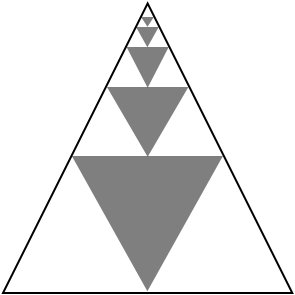
\includegraphics[scale=0.4]{FiguresMaths/SumGeometric1sur4}
\caption{Computing the sum of $1/4^i$.}
       \label{fig:sumGeo1sur4}
\end{center}
\end{figure}

\subsubsection{A fun result via geometric sums: When is integer  $n$
  divisible by $9$?}
\label{sec:divisible-by-9}

We now exploit our ability to evaluate geometric summations to
illustrate a somewhat surprising, nontrivial fact.  One can deduce
information about the divisibility of an integer $n$ from $n$'s
positional numerals.  We hope that this ``fun'' result will inspire
the reader to seek kindred numeral-encoded properties of numbers.

\begin{prop}
\label{thm:div-by-b-bar}
An integer $n$ is divisible by an integer $m$ if, and only if, $m$
divides the sum of the digits in the base-$(m+1)$ numeral for $n$.
\end{prop}

The most familiar instance of this result is phrased in terms of our
traditional use of base-$10$ (decimal) numerals. \\
{\it An integer $n$ is divisible by $9$ if, and only if, the sum of
  the digits of $n$'s base-$10$ numeral is divisible by $9$.}

\smallskip

\begin{proof}
({\it Argument for general number-base $b$}).
%
Of course, we lose no generality by focusing on numerals without
leading $0$'s, because leading $0$'s do not alter a numeral's sum of
digits.

Let us focus on the base-$b$ numeral for a number $n$ (so $b = m+1$ in
the statement of the proposition).  There therefore exist base-$b$
digits---i.e., integers from the set $\{0, 1, \ldots, b-1\}$---call
them $\delta_k \neq 0$, $\delta_{k-1}$, \ldots $\delta_1$, $\delta_0$,
such that
\[ n \ = \ \delta_k \cdot b^k + \delta_{k-1} \cdot b_{k-1} + \cdots +
\delta_1 \cdot b + \delta_0. \]
The sum of the digits of $n$'s base-$b$ numeral is, then
\[ s_b(n) \ \eqdef \ \delta_k + \delta_{k-1} + \cdots + \delta_1 +
\delta_0. \]
Let us calculate the difference $n - s_b(n)$ in the following manner,
digit by digit.
\begin{equation}
\label{eq:sum-of-digits}
\begin{array}{ccccccccccc}
n & = &
\delta_k \cdot b^k & + & \delta_{k-1} \cdot b^{k-1} & + & \cdots
  & + & \delta_1 \cdot b & + & \delta_0 \\
s_b(n) & = &
\delta_k & + & \delta_{k-1} & + & \cdots & + & \delta_1 & + & \delta_0 \\
\hline
n - s_b(n) & = &
\delta_k \cdot (b^k -1) & + &
\delta_{k-1} \cdot (b^{k-1} -1) & + &
\cdots & + &
\delta_1 \cdot (b-1) & & 
\end{array}
\end{equation}

\medskip

We now revisit summation (\ref{eq:geom-sum:b>1}).  Because $b$ is a
positive integer, so that $1 + b + \cdots + b^{a-2} + b^{a-1}$ is also
a positive integer, we infer that {\em the integer $b^a -1$ is
  divisible by $b-1$.}

We are almost home.  Look at the equation for $n - s_b(n)$ in the
system (\ref{eq:sum-of-digits}).  As we have just seen, every term on
the righthand side of that equation is divisible by $b-1$.  It follows
therefore, that the lefthand expression, $n - s_b(n)$, is also
divisible by $b-1$.
An easy calculation, which we leave to the reader, now shows that this
final fact means that $n$ is divisible by $b-1$ if, and only if,
$s_b(n)$ is.
\end{proof}


******************}



\subsubsection{Extended geometric series and their sums}
\label{sec:extended-geom-series}
\index{extended geometric sums: $\sum_{i=1}^n \ i^c b^i$}

We now build on our ability to evaluate geometric summations of the
forms (\ref{eq:geom-sum:b>1}, \ref{eq:geom-sum:b<1}) to evaluate
summations that we shall term {\em extended} geometric summations (not
a standard term), \textit{i.e.}, summations of the form
\[ S_b^{(c)}(n) \ \eqdef \ \sum_{i=1}^n \ i^c b^i, \]
where $c$ is an arbitrary fixed positive integer, and $b$ is an
arbitrary fixed real number.

We restrict attention here to the situation defined by the joint
non-equalities $c \neq 0$ and $b \neq 1$.
\begin{itemize}
\item
We have already adequately studied the case $c=0$, which characterizes
``ordinary'' geometric summations.
\item
The case $b = 1$ removes the ``geometric growth'' of the sequence
underlying the summation.  We study various aspects of this {\it
  summation-of-fixed-powers} case in Section~\ref{sec:smooth-series},
with special treatment of summations of fixed powers of consecutive
integers in Section~\ref{sec:sum-of-i2c}.
\end{itemize}

The method we now develop for evaluating all other summations
$S_b^{(c)}(n)$, \textit{i.e.}, those with $b \neq 1$ and $c \neq 0$, has two
major characteristics.
\begin{enumerate}
\item
The method is {\em inductive in parameter} $c$, in the sense that we
will be able to express our sum for $S_b^{(c)}(n)$ in terms of sums
for summations $S_b^{(c-1)}(n)$, $S_b^{(c-2)}(n)$, \ldots,
$S_b^{(1)}(n)$, $S_b^{(0)}(n) = S_b(n)$.  And, for each fixed value of
$c$, the method is {\em inductive in the argument} $n$.

%{\Denis I am not  so clear here, is it an induction on c or on n? We develop for n  later on...}

\item
The method will rely on the recurrent-subexpression strategy which was so
effective in Section~\ref{sec:general-geometric-sums}.
\end{enumerate}

\medskip

\index{extended geometric sums: $\sum_{i=1}^n \ i^c b^i$!the case $c=1$}
\paragraph{A. The summation $S^{(1)}_b(n) = \sum_{i=1}^n i b^i$}

We illustrate our strategy in detail for the case $c=1$ and sketch
only briefly how it deals with larger values of $c$.  Elementary
algebraic manipulations which are suggested by the analysis in the
case $c=1$ should thereby allow the reader to deal with any value $c > 1$.

\begin{prop}
\label{thm:sum-i2i}
For all bases $b > 1$,
\begin{equation}
\label{eq:sum-i2i}
S_b^{(1)}(n) \ \ = \ \
\sum_{i=1}^n \ i b^i
\ \ = \ \ 
\frac{(b-1)n -1}{(b-1)^2} \cdot  b^{n+1} \ + \ \frac{b}{(b-1)^2}
\end{equation}
\end{prop}

\index{extended geometric sums: $\sum_{i=1}^n \ i^c b^i$!the case $c=1$!summing via algebraic manipulation}
\begin{proof}
{\bf Deriving a sum via algebraic manipulation.}
%
We begin to develop our strategy by writing the natural expression for
\[ S_b^{(1)}(n) \ \ = \ \ b \ + \ 2b^2 \ + \ 3 b^3 \ + \cdots + \ n b^n  \]
in two different ways.  First, we isolate the summation's last term:
\begin{equation}
\label{eq:ext-geom-c=1.1}
S_b^{(1)}(n+1) \ = \ S_b^{(1)}(n) \ + \ (n+1) b^{n+1}.
\end{equation}
Then we isolate the summation's first term:
\begin{eqnarray}
\nonumber
S_b^{(1)}(n+1)
     & = &
b + \sum_{i=2}^{n+1} \ i b^{i}  \\
\nonumber
& = &
b + \sum_{i=1}^n \ (i+1) b^{i+1}  \\
\nonumber
     & = &
b +  b \cdot \sum_{i=1}^n \ (i+1) b^i \\
\nonumber
     & = &
b + 
b \cdot \left(
\sum_{i=1}^n \ i b^i 
 \ + \
\sum_{i=1}^n \  b^i 
\right) \\
\nonumber
     & = &
b \cdot \left( S_b^{(1)}(n) \ + \ S_b^{(0)}(n) \right) \ + \ b \\
\nonumber
& = &
b \cdot \left( S_b^{(1)}(n) \ +  \frac{b^{n+1} -1}{b-1} -1 \right) \ + \ b \\
\label{eq:ext-geom-c=1.2}
    & = &
b \cdot S_b^{(1)}(n) \ + \ b \cdot \frac{b^{n+1} - 1}{b-1}
\end{eqnarray}
Combining expressions (\ref{eq:ext-geom-c=1.1}) and
(\ref{eq:ext-geom-c=1.2}) for $S_b^{(1)}(n+1)$, we
finally find that
\begin{eqnarray}
\nonumber
(b-1) \cdot S_b^{(1)}(n) & = &
(n+1) \cdot b^{n+1} \ - \ b \cdot \frac{b^{n+1} -1}{b-1} \\
\label{eq:sum-i2i-source}
 & = &
\left( n - \frac{1}{b-1} \right) \cdot b^{n+1} \ + \ \frac{b}{b-1}
\end{eqnarray}
One now uses standard algebraic manipulations to derive expression
(\ref{eq:sum-i2i}) from equation (\ref{eq:sum-i2i-source}).
%so that, finally,
%\[ S_b^{(1)}(n) \ = \
%\frac{bn -n -1}{(b-1)^2} \cdot  b^{n+1} \ - \ \frac{b}{(b-1)^2}
%\]
\end{proof}

%{\Denis I add below a particular case,
%I think this is really interesting since it illustrates another technique of switching the indices in double sums}

\index{extended geometric sums: $\sum_{i=1}^n \ i^c b^i$!the case $c=1$!solving the case $b=2$ using subsum rearrangement}
\begin{proof}
{\bf Solving the case $b=2$ using subsum rearrangement.}
%
We can evaluate the sum
\[
S_2^{(1)}(n) \ = \ \sum_{i=1}^n \ i 2^i
\]
in an especially interesting way, by rearranging the sub-summations of
the target summation.
\medskip

\noindent \fbox{
\begin{minipage}{0.96\textwidth}
%\[ \approx \approx \approx \approx \approx \approx \approx \approx \approx \approx \]
The reader should pay careful attention to this technique.  It can
sometimes decompose a cumbersome expression for a summation into a
readily manipulated one.
%\[ \approx \approx \approx \approx \approx \approx \approx \approx \approx \approx \]
\end{minipage}
}
\medskip

Note that we can rewrite summation $S_2^{(1)}(n)$ as a {\em double
  summation:}
\begin{equation}
\label{eq:geom-double-sum}
S_2^{(1)}(n) \ = \ \sum_{i=1}^n \ \sum_{k=1}^{i} 2^i
\end{equation}

By suitable applications of the laws of arithmetic
Section~\ref{sec:Arithmetic-Laws}---specifically, the distributive,
associative, and commutative laws---we can perform the required double
summation in a different order than that specified in
(\ref{eq:geom-double-sum}).  In fact, we can exchange the indices of
summation, to compute $S_2^{(1)}(n)$ as specified via the following expression:
\[
S_2^{(1)}(n) \ = \ \sum_{k=1}^{n} \ \sum_{i=k}^{n} 2^i.
\]
This process is illustrated in Fig.~\ref{fig:Sumi2i}.
\begin{figure}[htb]
\centerline{
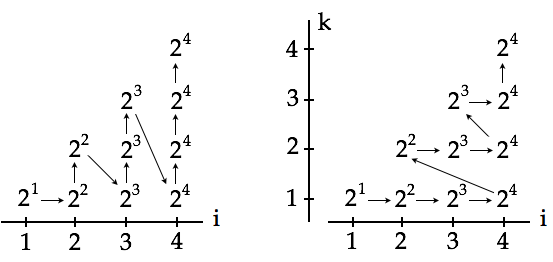
\includegraphics[scale=0.4]{FiguresMaths/Sumi2i}
}
\caption{Illustrating the case $n=4$ of the exchange of indices in the
  summation.  The original summation is drawn on the left.  In the
  righthand drawing, we reproduce each term $i \cdot 2^i$ $i$ times
  within column $i$.  We then express the summation on the right by
  introducing a new index $k$ and scanning the terms of the summation
  row by row (on the right).  The arrows represent the flow of the
  scan.}
\label{fig:Sumi2i}
\end{figure}
The indicated summation is much easier to perform in this order,
because its core consists of instances of the ``ordinary'' geometric
summation $\sum_{i=k}^{n} 2^i$
(Proposition~\ref{thm:sum-finite-geometric-series}).  Expanding these
instances, we find finally that
\begin{eqnarray*}
S_2^{(1)}(n)
  & = &
\sum_{k=1}^{n} \ \big( 2^{n+1} -1 - \sum_{i=0}^{k-1} \ 2^i \big) \\
  & = &
\sum_{k=1}^{n} \ \big( 2^{n+1} - 2^k \big) \\
  & = &
n \cdot 2^{n+1}\ - ( 2^{n+1} -1) +1 \\
  & = &
(n-1) \cdot 2^{n+1} +2.
\end{eqnarray*}
This completes the proof.  \qed
\end{proof}

\ignore{\Denis I added an interesting comment to finish this section:}

We remark that the process of obtaining the original summation can
also be seen in the figure, by scanning the elements of the summation
along the diagonals, as we portray in Fig.~\ref{fig:Sumi2iDiag}.  Each
of the $n$ diagonals contains exactly the difference between the
complete geometric summation and the partial summation that is
truncated at the $k$th term.
\begin{figure}[htb]
\centerline{
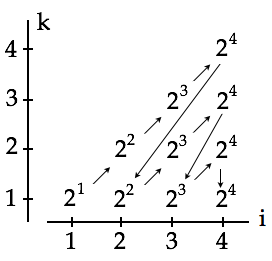
\includegraphics[scale=0.4]{FiguresMaths/Sumi2iDiag}
}
\caption{The successive diagonal patterns correspond to the single summation obtained after exchanging the two initial sums.}
\label{fig:Sumi2iDiag}
\end{figure}

\smallskip

\paragraph{B. The summations $S^{(c)}_b(n) =  \sum_{i=1}^n i^c b^i$}

We now develop a strategy that adapts the evaluation of summation
$S_b^{(1)}(n)$ in the proof of Proposition~\ref{thm:sum-i2i} to an
evaluation of the general extended geometric summation
\[
S_b^{(c)}(n) \ \ = \ \ \sum_{i=1}^n \ i^c b^i
 \ \ = \ \
b \ + \ 2^{c} b^2\ + \ 3^{c} b^3 \ + \ \cdots \ + \ n^{c} b^{n}
\]
The strategy is {\em recursive}, in that it computes a value for
$S^{(c)}_b(n)$ from values for $S^{(c-1)}_b(n)$, $S^{(c-2)}_b(n)$,
\ldots, $S^{(0)}_b(n)$.  It proceeds in three steps.

\noindent {\bf Step 1.}
%
As in the case $c=1$, we write summation $S_b^{(c)}(n)$ in two ways.
The expression that embodies the first way isolates the summation's
first term:
\[ S_b^{(c)}(n+1) \ = \ b + \sum_{i=1}^n \ (i+1)^c b^{i+1} \]
The expression that embodies the second way isolates the summation's
last term:
\[ S_b^{(c)}(n+1) \ = \ S_b^{(c)}(n) \ + \ (n+1)^{c} b^{n+1}. \]
By combining these expressions, we find that
\begin{equation}
\label{eq:Sbcn-1}
S_b^{(c)}(n) 
 \ = \
b \cdot \left(
1 \ - \
(n+1)^{c} b^{n} \ + \
 \sum_{i=1}^n \ (i+1)^c b^{i} 
\right)
\end{equation}


\noindent {\bf Step 2.}
%
We next invoke the Restricted Binomial Theorem
(Theorem~\ref{thm:restricted-binomial-thm}) to see that
\[ (i+1)^c \ = \ i^c \ + \ c \cdot i^{c-1} \ + \ {c \choose 2} \cdot
i^{c-2} \ + \cdots + \ {c \choose k} \cdot i^{c-k}  \ + \cdots + \ 1
\]

We use this expansion of $(i+1)^c$, together with multiple
applications of the laws of arithmetic from
Section~\ref{sec:Arithmetic-Laws} to verify that
\begin{eqnarray}
\nonumber
\sum_{i=1}^n \ (i+1)^c b^{i} & = &
S_b^{(c)}(n)
 \ + \ c \cdot S_b^{(c-1)}(n)
 \ + \ {c \choose 2} \cdot S_b^{(c-2)}(n)  \ + \cdots \\
\label{eq:Sbcn-2}
  &  & \cdots + \
{c \choose k} \cdot S_b^{(c-k)}(n)
 \ + \cdots + \
S_b^{(0)}(n)
\end{eqnarray}

\noindent {\bf Step 3.}
%
We finally combine equations (\ref{eq:Sbcn-1}) and (\ref{eq:Sbcn-2})
to discover that
\begin{eqnarray}
\nonumber
(b-1) \cdot S_b^{(c)}(n)
 & = &
(n+1)^{c} b^{n} \ - \
c \cdot S_b^{(c-1)}(n)
 \ - \ {c \choose 2} \cdot S_b^{(c-2)}(n)  \ - \cdots \\
\label{eq:Sbcn-3}
  &  & 
\cdots - \
{c \choose k} \cdot S_b^{(c-k)}(n)
 \ - \cdots - \
S_b^{(0)}(n)
\ - \ 1
\end{eqnarray}

We thus have the promised method of evaluating the extended geometric
summation $S_b^{(c)}(n)$ associated with the fixed power $c$ in terms
of the sums of extended geometric summations associated with smaller
fixed powers.

%%%%%%%%%%%%%%%%%%%%%%%%%%%%%%%%%%%%%%%%%

\section{On Summing ``Smooth'' Series}
\label{sec:smooth-series}

\subsection{Approximate Sums via Integration}
\label{sec:riemann-bounds}

This section illustrates a powerful strategy for obtaining nontrivial
upper and lower bounds on the values of sum, by finding continuous {\em
  envelopes} that bound the discrete summations both above and below.
The areas under the enveloping continuous functions---which we can
calculate via integration---provide the desired bounds on the
summations.

The strategem operates via the following three steps.  Say that we
have a sum
\[ a_1 \ + \ a_2 \ + \ \cdots \ + \ a_n \]
For convenience we use a finite sum for illustration; the stratagem
often works with infinite sums also, as our specific examples
illustrate.

\noindent {\bf Step 1.}
Represent the summands seriatim as abutting unit-width rectangles.  

\noindent
Our generic example has $n$ unit-width rectangles, of respective
heights $a_1$, $a_2$, \ldots, $a_n$.  We describe two special cases,
to help the reader understand how the strategem is applied.
\begin{enumerate}
\item
Figs.~\ref{fig:riemann-n2-1} and~\ref{fig:riemann-n2-2} illustrate our
strategem applied to the summation $S_2(n) = \sum_{i=1}^n i^2$.  In
both figures, we represent $S_2(n)$ by the aggregate area of a
sequence of unit-width rectangles.  The rectangles that represent the
respective addends in this example have respective heights $1$, $4$,
$9$, $16$, $25$, $36$ and $49$.  If we were to extend the figures
rightward (to extend the summation by encompassing more addends
thereby increasing $n$), then the next rectangle would have height
$64$.

The rectangles in Fig.~\ref{fig:riemann-n2-1} are accompanied by a
continuous curve (labeled (a) in the figure) which connects their
upper lefthand corners.
\begin{figure}[htb]
\centerline{
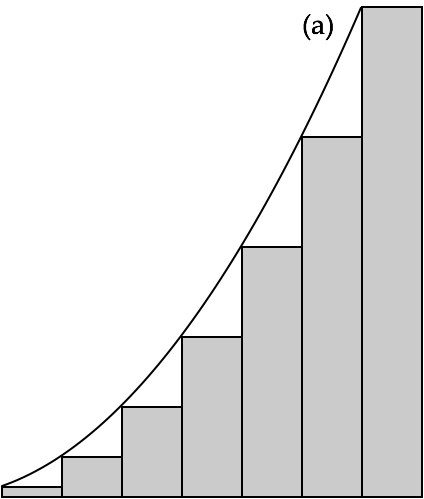
\includegraphics[scale=0.3]{FiguresMaths/SumSquaresContinuous1}
}
\caption{The summation $S_2(n) = \sum_{i=1}^n i^2$ represented by the
  aggregate area of a sequence of unit-width shaded rectangles.  The
  summation is bounded above by the area under the continuous curve (a)
  that connects the upper lefthand corners of the rectangles.  The
  area under curve (a) is $\int_0^n \ (x+1)^2 dx$.  }
\label{fig:riemann-n2-1}
\label{fig:SumIntegral1}
\end{figure}
Because this curve completely ``covers'' the rectangles (which we
emphasize by shading the rectangles), the area under the curve is an
{\em upper bound} on the aggregate area of the rectangles; this area
is
\[ \int_1^n \ x^2 dx \]

The rectangles in Fig.~\ref{fig:riemann-n2-2} are accompanied by a
continuous curve (labeled (b) in the figure) which connects the upper
righthand corners of the rectangles.
\begin{figure}[htb]
\centerline{
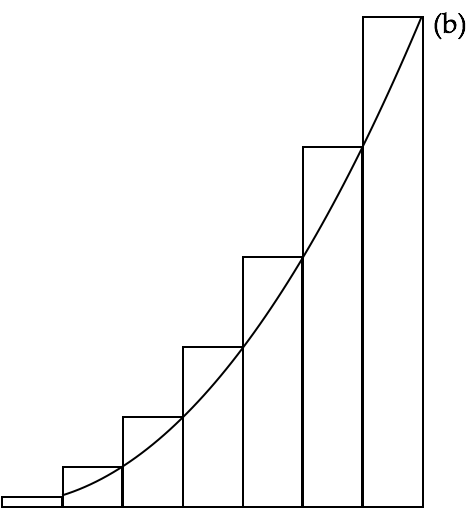
\includegraphics[scale=0.3]{FiguresMaths/SumSquaresContinuous2}
}
\caption{ The summation $S_2(n)$ represented by the aggregate area of
  a sequence of unit-width unshaded rectangles.  The summation is
  bounded from below by the area under the continous curve (b) that
  connects the upper righthand corners of the rectangles.  The area
  under curve (b) is $\int_1^n \ x^2 dx$.}
\label{fig:riemann-n2-2}
%\label{fig:SumIntegral2}
\end{figure}
Because this curve lies completely within the area formed by the
rectangles, the area under the curve is a {\em lower bound} on the
aggregate area of the rectangles; this area is
\[ \int_0^{n-1}  \ x^2 dx \]

%{\Denis I did with the powers of 2, will change to the squares...}

\item
In Figs.~\ref{fig:riemann-harmonic1} and~\ref{fig:riemann-harmonic2},
we represent the {\em harmonic} sum
\[ S^{(H)}(n) \ = \ \sum_{i=1}^n \ i^{-1} \ = \ \sum_{i=1}^n \ 1/i.
\]
In both figures, $S^{(H)}(n)$ is represented by the aggregate area of
a sequence of abutting unit-width rectangles, of respective heights
$1$, $1/2$, $1/3$, \ldots, $1/10$ (so the figures represent the case
$n=10$).  It would be only a clerical task to add more rectangles, of
heights $1/11$, $1/12$, etc., to represent larger values of $n$.

In Fig.~\ref{fig:riemann-harmonic1}, the rectangles are accompanied by
a continuous curve (marked (a) in the figure) that passes through
their upper righthand corners.
\begin{figure}[htb]
\centerline{
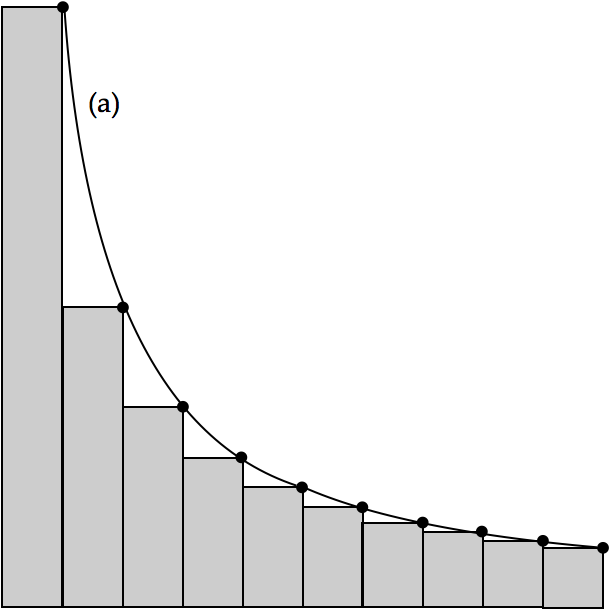
\includegraphics[scale=0.3]{FiguresMaths/RiemannSum1}
}
\caption{The summation $S^{(H)}(n) \ = \ \sum_{i=1}^n \ 1/i$
  represented by the aggregate area of a sequence of unit-width
  rectangles, $S^{(H)}(n)$ is bounded from above by the area under a
  continuous curve (a) that passes through the upper righthand corners
  of the rectangles.  This area is $ \int_1^n \ \frac{1}{x} dx$. }
\label{fig:riemann-harmonic1}
\end{figure}
Because this curve completely ``covers'' the rectangles (which we
emphasize by shading the rectangles), the area under the curve is an
{\em upper bound} on the aggregate area of the rectangles; the area
under curve (a) is
\[ \int_1^n \ \frac{1}{x} dx \]

In Fig.~\ref{fig:riemann-harmonic2}, the rectangles are accompanied by
a continuous curve (marked (b) in the figure) that passes through
their upper lefthand corners.
\begin{figure}[htb]
\centerline{
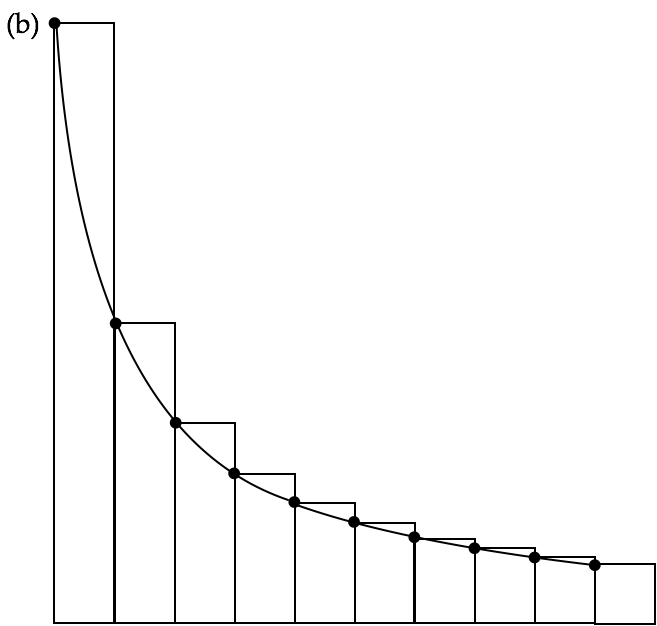
\includegraphics[scale=0.3]{FiguresMaths/RiemannSum2}
}
\caption{Representing the summation $S^{(H)}(n)$ as in
  Fig.~\ref{fig:riemann-harmonic1}, the summation is bounded from
  below by the area under a continuous curve (b) that passes through
  the upper lefthand corners of the rectangles.  The area under curve
  (b) is $\int_0^{n-1} \ \frac{1}{x+1} dx$.}
\label{fig:riemann-harmonic2}
\end{figure}
Because curve (b) lies completely within the aggregate area of the
rectangles, the area under the curve is a {\em lower bound} on the
aggregate area of the rectangles; the area under curve (b) is
\[ \int_0^{n-1}  \ \frac{1}{x+1} dx \]
  \end{enumerate}
%
%{\Denis We should add in the caption the explanation of curves (a) and (b)}
%The rectangles that represent the respective addends have respective
%heights $12$, $6$, $4$, $3$, $16/3$, and $2$.  If we were to extend
%the figure rightward (to extend the summation and encompass more
%addends), then the next rectangle would have height $16/7$.

\medskip

\noindent {\bf Step 2.}
%
Construct a continuous curve $\overline{C}(x)$ that passes through the
corners of the unit-width rectangles specified by the summation, in
such a way that the aggregate areas of the rectangles lies completely
within the area under $\overline{C}(x)$.
\medskip

\noindent \fbox{
\begin{minipage}{0.96\textwidth}
The curves labeled (a) in Figs.~\ref{fig:riemann-n2-1}
and~\ref{fig:riemann-harmonic1} are instances of the mandated
continuous curve $\overline{C}(x)$.
\end{minipage}
}
\medskip

Because the aggregate areas of the abutting rectangles lies completely
under curve $\overline{C}(x)$, the area under the curve---which we
obtain by integrating $\overline{C}$ between limits appropriate for
the summation---affords {\em an upper bound} on the value of the
summation of interest.

\medskip

\noindent {\bf Step 3.}
%
Construct a continuous curve $\underline{C}(x)$ that passes through
the corners of the unit-width rectangles
specified by the summation, in such a way that the area under
$\underline{C}(x)$ lies completely within the aggregate areas of the 
rectangles.
\medskip

\noindent \fbox{
\begin{minipage}{0.96\textwidth}
The curves labeled (b) in Figs.~\ref{fig:riemann-n2-2}
  and~\ref{fig:riemann-harmonic2} are instances of the mandated
  continuous curve $\underline{C}(x)$. 
\end{minipage}
}
\bigskip

Because the area under the curve $\underline{C}(x)$ lies completely
within the aggregate area of the abutting rectangles, the area under
the curve---which we obtain by integrating $\underline{C}$---affords
{\em a lower bound} on the summation of interest.

\medskip

In the next subsection, we apply this stratagem to summations of fixed
powers of successive integers---i.e., summations of the form
$\displaystyle S_c(n) \eqdef \sum_{i=1}^n i^c$---for various (classes
of) values of the fixed power $c$.


\subsection{Sums of Fixed Powers of Consecutive Integers: $\sum i^c$}
\label{sec:sum-of-i2c}

We obtain bounds on the summations $S_c(n)$ that are rather good for
large values of $n$.  In special cases, our bounds are good, sometimes
even exact, for all values of $n$.

\subsubsection{$S_c(n)$ for general {\em nonnegative} real $c$th powers}
\label{sec:sum-of-i2c>0}

\ignore{***************
\medskip
{\Denis I detailed below a nice way for proving the sum of squares, may be this is not the right place.
Feel free to move it elsewhere...}

The idea here is to consider $3$ copies of the sum of squares and to reorganize them in a more simple way (this is Fubini's principle).
The square of $a$ is represented as $a$ copies of the unit square.
The full process is depicted in figures Fig~\ref{fig:sumSquares1} to Fig~\ref{fig:sumSquares5}.

The height of the final rectangle is $\Delta_ n$ and its width is $2+2n-1=2n+1$. 

Thus, $3 \cdot S(n) = \Delta_n \cdot (2n+1)$, $S(n) = \frac{n(2n+1)(n+1)}{3}$.
{\Denis I have another proof which does not consider such a graphical way, by considering three triangles --I mean well-arranged integers in a triangle-- , 
at least we have to put it as an exercice,
but may be even as an alternative proof?}
\begin{figure}[ht]
\begin{center}
       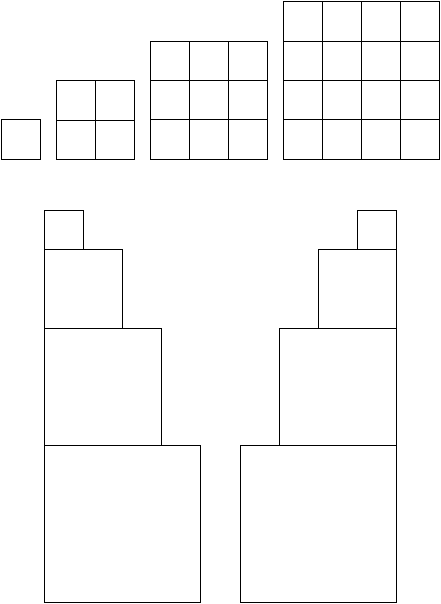
\includegraphics[scale=0.4]{FiguresMaths/SumSquares1}
\caption{Computing the sum of squares: initial configuration.}
       \label{fig:sumSquares1}
\end{center}
\end{figure}
\begin{figure}[ht]
\begin{center}
       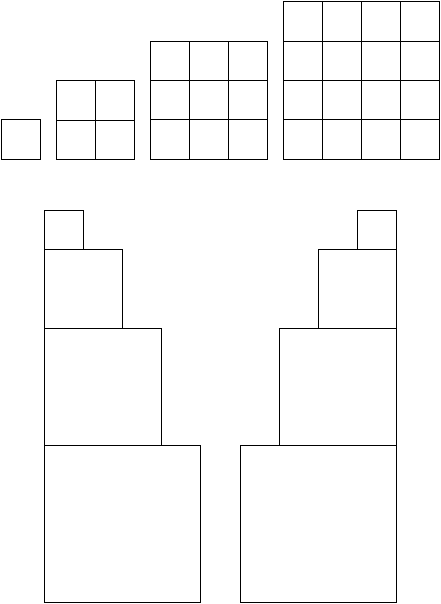
\includegraphics[scale=0.4]{FiguresMaths/SumSquares2}
\caption{Step 1 for computing the sum of squares: fill in the surface at the bottom.}
       \label{fig:sumSquares2}
\end{center}
\end{figure}
\begin{figure}[ht]
\begin{center}
       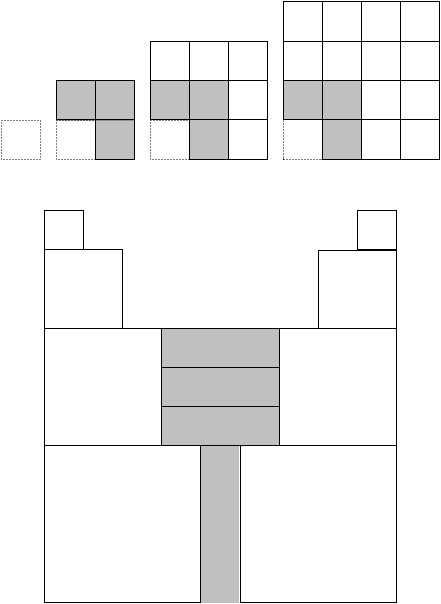
\includegraphics[scale=0.4]{FiguresMaths/SumSquares3}
\caption{Step 2 for computing the sum of squares.}
       \label{fig:sumSquares3}
\end{center}
\end{figure}
\begin{figure}[ht]
\begin{center}
       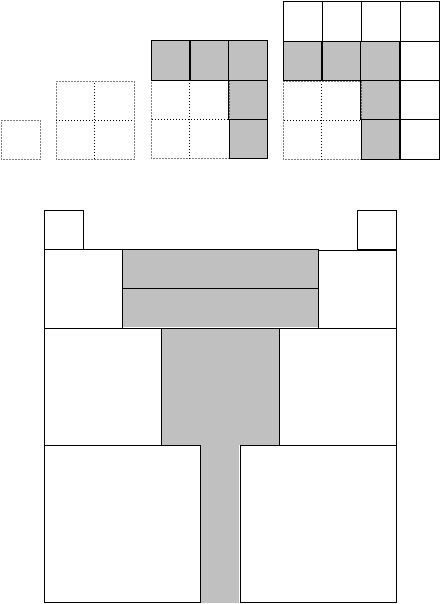
\includegraphics[scale=0.4]{FiguresMaths/SumSquares4}
\caption{Step 3 for computing the sum of squares.}
       \label{fig:sumSquares4}
\end{center}
\end{figure}
\begin{figure}[ht]
\begin{center}
       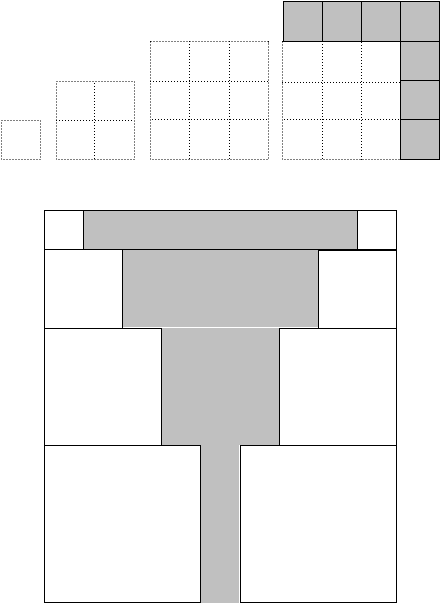
\includegraphics[scale=0.4]{FiguresMaths/SumSquares5}
\caption{Final step for computing the sum of squares: the rectangle is filled.}
       \label{fig:sumSquares5}
\end{center}
\end{figure}
**********************}

We begin to illustrate the technique of bounding summations via
integrals by focusing on summations of the form
\[ S_c(n) \ \eqdef \ \sum_{i=1}^n \ i^c, \]
for arbitrary positive numbers $c$.  The reader can garner intuition
for the upcoming bounds from the general shape of the rectangles and
continuous curves in Figs.~\ref{fig:riemann-n2-1}
and~\ref{fig:riemann-n2-2} We obtain our upper bound on $S_c(n)$ by
evaluating the integral that yields the area $\overline{C}_c(n)$ under
the lefthand continuous curve ($a$) in Fig.~\ref{fig:riemann-n2-1},
namely,
\begin{eqnarray}
\label{eq:upper-integral-xc}
\overline{C}_c(n) \ = \
\int_0^n \ (x+1)^c dx & = &
%  \int_0^n \ x^2 dx \ + \ 2 \int_0^n \ x dx \ + \ \int_0^n \ dx \\
% & = & \frac{1}{3} n^3 \ + n^2 \ + \ n \ + \ O(1).
 \frac{1}{c+1} (n+1)^{c+1} \ + \ O(1) \\
\nonumber
 & = & \frac{1}{c+1} n^{c+1} \ + \ O(n^c).
\end{eqnarray}
We obtain our lower bound on $S_c(n)$ by evaluating the integral that
yields the area $\underline{C}_c(n)$ under the righthand continuous
curve ($b$) in Fig.~\ref{fig:riemann-n2-2}, namely,
\begin{equation}
\label{eq:lower-integral-xc}
\underline{C}_c(n) \ = \
\int_1^n \ x^c dx \ = \ \frac{1}{c+1} n^{c+1} \ + \ O(1).
\end{equation}
Combining these bounds, we finally have the following two-sided bound
on $S_c(n)$.
\begin{equation}
\label{eq:bounds-sum-xc}
\frac{1}{c+1} n^{c+1} \ + \ O(1)
  \ \ \leq \ \ S_c(n)
  \ \ \leq \ \ \frac{1}{c+1} n^{c+1} \ + \ O(n^c).
\end{equation}
The main message here is:

{\em The behavior of $S_c(n)$ as a function of $n$ is dominated by
  $\displaystyle \frac{1}{c+1} n^{c+1}$} \\
\hspace*{.2in}{\em as $n$ grows without bound.  }



\subsubsection{Nonnegative integer $c$th powers}
\label{sec:positive-integer-power}

\paragraph{A. A better bound via the Binomial Theorem}

When $c$ is a positive integer, the following special case of Newton's
{\it Binomial Theorem}.\footnote{The general form of the Binomial
  Theorem expands the polynomial $(x+y)^k$ rather than $(x+1)^k$.  See
Section~\ref{sec:Binomial-thm}.}
\index{The Binomial Theorem!restricted form}
affords us a much more detailed version of the upper bound
(\ref{eq:upper-integral-xc})
%(\ref{eq:bounds-sum-xc})
on the sum $S_c(n)$.

\begin{theorem}[The Restricted Binomial Theorem]
\label{thm:restricted-binomial-thm}
For all positive integers $k$,\footnote{See (\ref{eq:binom-coeff}) for
  the definition of, and notation for, the binomial coefficient
  $\displaystyle {k \choose i}$.}
\begin{equation}
\label{eq:restricted-binomial-thm}
(x+1)^k \ = \ \sum_{i=0}^k \ \ {k \choose i} x^{k-i}.
\end{equation}
\end{theorem}

We obtain our improved upper bound on $S_c(n)$ by parallelling the
reasoning that led us to the relation (\ref{eq:upper-integral-xc}).
Our improved upper bound emerges also by evaluating the integral that
yields the area $\overline{C}_c(n)$ under the continuous curve that
passes through the upper lefthand corners of the unit-width rectangles
specified by summation $S_c(n)$.
\begin{eqnarray}
\label{eq:upper-integral-xk}
\overline{C}_c(n) \ = \
\int_0^n \ (x+1)^c dx & = &
\int_0^n \ \left(\sum_{i=0}^c \ \ {c \choose i} x^{c-i} \right) dx \\
\nonumber
& = &
\sum_{i=0}^c \left( \int_0^n \  {c \choose i} x^{c-i} \right) dx \\
\nonumber
  & = &
\sum_{i=0}^c \ \ \frac{1}{c-i+1} {c \choose i} n^{c-i+1} \ + \ O(1)
\end{eqnarray}
This is a proper upper bound because the region defined by this curve
totally contains the region subtended by the rectangles.

\noindent
Using this strategy, we find that for any positive integer $c$,
summation $S_c(n)$ enjoys the following two-sided bound:
\begin{equation}
\label{eq:bounds-sum-xk}
\frac{1}{c+1} n^{c+1} \ + \ O(1)
  \ \ \leq \ \ \sum_{i=1}^n \ i^c
  \ \ \leq \ \ 
\sum_{i=0}^c \ \ \frac{1}{c-i+1} {c \choose i} n^{c-i+1} \ + \ O(1)
\end{equation}

We have, of course, not changed the dominant behavior of $S_c(n)$ as
$n$ grows without bound, but we have taken a substantial step toward
developing explicit expressions for the summations $S_c(n)$ when $c$
is a positive integer.

\paragraph{B. Using {\em undetermined coefficients} to refine sums}

We now introduce the {\em Method of Undetermined Coefficients}
\index{Method of Undetermined Coefficients}
and illustrate how to use it to derive explicit expressions for the
sums $S_c(n)$ when $c$ is a positive integer.  Our development builds
on the intuition garnered from the bounds (\ref{eq:bounds-sum-xk})
that
\[ S_c(n) \ = \ \frac{1}{c+1} n^{c+1} \ + \ a^{(c)}_c n^c \ + \
a^{(c)}_{c-1} n^{c-1} \ + \ \cdots \ + \ a^{(c)}_2 n^2 \ + \ a^{(c)}_1 n
 + \ a^{(c)}_0
\]
for some nonnegative numbers  
%$a^{(c)}_{c+1}$, 
$a^{(c)}_c$, \ldots,
$a^{(c)}_0$.  To begin, we know that $a^{(c)}_0 = 0$, because $S_c(0)
= 0$.
\medskip

\noindent \fbox{
\begin{minipage}{0.96\textwidth}
Because we are beginning with a conjecture based on intuition, we
  will have to verify the explicit expressions that we derive.  We do
  this after deriving our expressions.
\end{minipage}
}
\medskip

Because the Method becomes computationally cumbersome for large values
of $c$, we introduce the reader to it via the first few integer values
of $c$.

{\it The case $c=1$.}
%
We begin with the sum $S_1(n)$, whose value we already know.
Reasoning from the case $c=1$ of (\ref{eq:bounds-sum-xk}), we intuit
that
\[ S_1(n) \ = \ \frac{1}{2} n^2 \ + \ a^{(1)}_1 n \]
for some positive {\it undetermined coefficient} $a^{(1)}_1$.  We can
discover the value of the single unknown, $a^{(1)}_1$ by evaluating
$S_1(n)$ at any single value for the variable $n$.  Any value of $n$
will work; using the {\em smallest} one, $n=1$, simplifies our
calculation.

Because $S_1(1) = 1$, we have
\[ S_1(1) \ = \ 1 \ = \ \frac{1}{2} \ + \ a^{(1)}_1. \]
Therefore, $a^{(1)}_1 = 1/2$, which gives us yet one more derivation
of the value
\[ S_1(n) \ = \ \frac{1}{2} \left( n^2 + n \right) \ = \ 
\frac{n(n+1)}{2}.
\]

\medskip

{\it The case $c=2$.}
%
We derive an explicit expression for $S_2(n) \ \eqdef \  1 + 4 +
\cdots + n^2$.

\begin{prop}
{\em For all} $n \in \N$,
\begin{equation}
\label{eq:sum-1-to-nsq}
S_2(n) \ \eqdef \ \sum_{i=1}^n \ i^2 
 \ = \ \frac{1}{3} n^3 \ + \ \frac{1}{2} n^2 \ + \ \frac{1}{6} n
\end{equation}
\end{prop}

\noindent
$S_2(n)$ is often expressed in a more aesthetic form:
\[ S_2(n) \ = \
\frac{1}{6} n (n+1)(2n+1) \ = \
\frac{2n+1}{3} \cdot {n \choose 2}.
\]

\begin{proof}
Reasoning from the case $c=2$ of (\ref{eq:bounds-sum-xk}), we
propose the conjecture that
\begin{equation}
\label{eq:symbolic-cubic}
S_2(n) \ \ = \ \
\sum_{i=0}^n \ i^2 \ \ = \ \ \frac{1}{3} n^3 + a^{(2)}_2 n^2 + a^{(2)}_1 n.
\end{equation}
for some positive {\it undetermined coefficients} $a^{(2)}_2$ and
$a^{(2)}_1$.  We thereby express $S_2(n)$ as a polynomial in two
unknowns, $a^{(2)}_2$ and $a^{(2)}_1$.  We can determine values for
the unknowns by instantiating the polynomial with (any) two values of
$n$; to simplify calculations, we select the smallest two values of
$n$, namely, $n = 1,2$.  These instantiations of the polynomial leave
us with the following pair of linear equations.
\[
\begin{array}{cccccl}
n=1: & \sum_{i=0}^1 \ i^2
   & = & 1 & = &
1/3 \ + \ a^{(2)}_2 \ + \ a^{(2)}_1 \\
 & & & & & \\
n=2: & \sum_{i=0}^2 \ i^2
   & = & 5 & = &
8/3 \ + \ 4 a^{(2)}_2 \ + \ 2 a^{(2)}_1
\end{array}
\]
By elementary arithmetic, these equations simplify to yield the pair
\[
\begin{array}{ccc}
a^{(2)}_2 \ + \ a^{(2)}_1   & = & 2/3 \\
 & & \\
2 a^{(2)}_2 \ + \ a^{(2)}_1 & = & 7/6
\end{array}
\]
These equations reveal that
\[ 2/3 \ - \ a^{(2)}_2 \ = \ 7/6 \ - \ 2 a^{(2)}_2 \]
so that 
\[ a^{(2)}_2 \ = \ 1/2 \]
which means that
\[ a^{(2)}_1 \ = \ 1/6. \]
We have, thus, derived equation~(\ref{eq:sum-1-to-nsq}).  
\end{proof}

\medskip

We verify our expressions for $S_1(n)$ and $S_2(n)$ by induction in
subsection C.

\medskip

With more (calculational) work, but no new (mathematical) ideas, one
can derive explicit expressions for the sum of the first $n$ $c$th
powers, i.e., the sum $S_c(n)$, for any positive integer $c$.

\paragraph{C. On validating approximate summations} 
{\Denis I believe this paragraph is not needed since it is done in DOINGMATHS...}

We employ the proof technique of (Finite) Induction by proving the
correctness of three summation formulas that have occupied our
attention in this chapter:
\begin{enumerate}
\item
the sum $S_1(n)$ of the first $n$ positive integers; cf., equation
(\ref{eq:sum-1-to-n})

\item
the sum $S_2(n)$ of the squares of the first $n$ positive integers;
cf., equation (\ref{eq:sum-1-to-nsq})

\item
the sum of the first $n$ odd positive integers; cf.,
Proposition~\ref{thm:squares-odd-integers-Gauss}.
\end{enumerate}
We deal with these formulas in turn.

\noindent {\it 1. Verifying equation (\ref{eq:sum-1-to-n}) for $S_1(n)$.}
%
For every positive integer $m$, let {\bf P}$_1(m)$ be the proposition
\[  1 \ + \ 2 \ +  \cdots  + \ m \ = \ {{m+1} \choose 2}. \]
We proceed according to the standard format of an inductive argument.

\begin{description}
\item[{\bf The base case P$_1(1)$}.]
%
Because ${\displaystyle {2 \choose 2}} = 1$, proposition {\bf P}$_1(1)$
is true.

\item[{\sf The inductive hypothesis}.]
%
Assume, for the sake of induction, that proposition {\bf P}$_1(m)$ is
true for every positive integer $m < n$.  In particular, then,
proposition {\bf P}$_1(n-1)$ is true.

\item[{\bf Extending the induction}.]
%
Because proposition {\bf P}$_1(n-1)$ is true, we know that
\[ S_1(n-1) \ = \ 1 + 2 + \cdots + (n-1) \ = \ {n \choose 2}.  \]
By direct calculation, then,
\begin{eqnarray*}
S_1(n) & = & {n \choose 2} + n \\
  & = & \frac{n(n-1)}{2}  \ + \ n \\ 
%  & = & \frac{n^2 - n + 2n}{2} \\
  & = & \frac{n^2 + n}{2} \\
  & = & {{n+1} \choose 2},
\end{eqnarray*}
as was verified in equation (\ref{eq:sum-1-to-n}).
\end{description}
Because $n$ is an arbitrary positive integer, we conclude that
{\bf P}$_1(n)$ is true whenever
\begin{itemize}
\item
{\bf P}$_1(1)$ is true
\item
{\em and}
{\bf P}$_1(m)$ is true for all $m < n$.
\end{itemize}
By the Principle of (Finite) Induction, then, we conclude that
proposition {\bf P}$_1(n)$ is true for all positive integers $n$.
\qed

\bigskip


\noindent {\it 2. Verifying equation (\ref{eq:sum-1-to-nsq}) for $S_2(n)$.}
%
For every positive integer $m$, let {\bf P}$_2(m)$ be the proposition
\[  1 \ + \ 2^2 \ + \ 3^2 \ + \cdots + \ m^2 \ = \ 
\frac{1}{6} m (m+1)(2m+1).
\]
We proceed according to the standard format of an inductive argument.

\begin{description}
\item[{\sf The base case P$_2(1)$}.]
%
Because ${\displaystyle \frac{1}{6} (2 \cdot 3)} = 1$, proposition {\bf
    P}$_2(1)$ is true.

\item[{\sf The inductive hypothesis}.]
%
Assume, for the sake of induction, that proposition {\bf P}$_2(m)$ is
true for every positive integer $m < n$.  In particular, then,
proposition {\bf P}$_2(n-1)$ is true.

\item[{\sf Extending the induction}.]
%
Because proposition {\bf P}$_2(n-1)$ is true, we know that
\[ S_2(n-1) \ = \
\frac{1}{6} (n-1) \cdot n \cdot (2n-1).
\]
By direct calculation, then,
\begin{eqnarray*}
S_2(n) & = &
\frac{1}{6} (n-1) \cdot n \cdot (2n-1) \ + \ n^2 \\
  & = &
\frac{n}{6} \left( (n-1) \cdot (2n-1) + 6n \right) \\
  & = & \frac{n}{6} \left( 2n^2 +3n + 1 \right) \\ 
  & = & \frac{n}{6} (n+1)(2n+1),
\end{eqnarray*}
as was verified in equation (\ref{eq:sum-1-to-nsq}).
\end{description}
Because $n$ is an arbitrary positive integer, we conclude that
{\bf P}$_2(n)$ is true whenever
\begin{itemize}
\item
{\bf P}$_2(1)$ is true
\item
{\em and}
{\bf P}$_2(m)$ is true for all $m < n$.
\end{itemize}
By the Principle of (Finite) Induction, then, we conclude that
proposition {\bf P}$_2(n)$ is true for all positive integers $n$.
\qed


\bigskip

\noindent {\it 3. Verifying that each perfect square $n^2$ is
  the sum of the first $n$ odd integers.}
%
We turn finally to the assertion that, for every positive integer $n$,
\[ n^2 \ = \ 1 \ + \  3 \ + \ 5 \ + \cdots + \ 2n-1. \]
For each positive integer $n$, let {\bf P}$(n)$ denote the proposition
that the preceding equation holds.

The following inductive proof complements the constructive proofs of
the same result in Proposition~\ref{thm:squares-odd-integers-Gauss}.
We proceed according to the standard format of an inductive argument.

\begin{description}
\item[{\bf The base case P$(1)$}.]
%
Because $1$ is a perfect square, proposition {\bf P}$(1)$ is true.

\item[{\bf The inductive hypothesis}.]
%
Assume, for the sake of induction, that proposition {\bf P}$(m)$ is
true for every positive integer $m < n$.  In particular, then,
proposition {\bf P}$(n-1)$ is true.

\item[{\bf Extending the induction}.]
%
Because proposition {\bf P}$(n-1)$ is true, we know that
\[ 
 1 + 3 + 5 + \cdots + 2n-3 + 2n-1 \ = \ (n-1)^2 + 2n-1.  \]
By direct calculation, we see that
\[ (n-1)^2 + 2n-1 \ = \ (n^2 -2n +1) + (2n-1) \ = \ n^2. \]
\end{description}
Because $n$ is an arbitrary positive integer, we conclude that
{\bf P}$(n)$ is true whenever
\begin{itemize}
\item
{\bf P}$(1)$ is true
\item
{\em and}
{\bf P}$(m)$ is true for all $m < n$.
\end{itemize}
By the Principle of (Finite) Induction, then, we conclude that {\bf
  P}$(n)$ is true for all $n \in \N^+$.
\qed


\subsubsection{$S_c(n)$ for general {\em negative} $c$th powers}
\label{sec:sum-of-i2c<0}

We focus finally on summations of the form
\[ S_c(n) \ \eqdef \ \sum_{i=1}^n \ i^c, \]
for arbitrary {\em negative} numbers $c$.  The reader can garner
intuition for the upcoming bounds from the general shape of the
rectangles and continuous curves in Figs.~\ref{fig:riemann-harmonic1}
and~\ref{fig:riemann-harmonic2}.

\begin{prop}
\label{thm:general-bounds-negative-xc}
For summations $S_c(n)$ with fixed negative powers $c<0$,
\begin{equation} 
\label{eq:general-bounds-negative-xc}
\left[
\underline{C}_c(n) \ = \
\int_0^{n-1} \ (x+1)^c dx
\right]
\ \leq \ S_c(n) \ \leq \
\left[
\overline{C}_c(n) \ = \
\int_1^n \ x^c dx
\right].
\end{equation}
\end{prop}

\begin{proof}
We obtain our upper bound on the sum of $S_c(n)$ by evaluating the
integral that yields the area $\overline{C}_c(n)$ under the righthand
continuous curve ($a$) in the analogue of
Fig.~\ref{fig:riemann-harmonic1} for $S_c(n)$.  We obtain our lower
bound on $S_c(n)$ by evaluating the integral that yields the area
$\underline{C}_c(n)$ under the lefthand continuous curve ($b$) in the
analogue of Fig.~\ref{fig:riemann-harmonic2} for $S_c(n)$.
\end{proof}

When $c \neq -1$,\footnote{We need to avoid the case $c = -1$ so that
  we do not attempt to divide by $0$.}~we can provide more detail,
using reasoning similar to that underlying the bounds
(\ref{eq:bounds-sum-xc}) that hold for positive values of $c$.

\paragraph{A. Negative powers $-1 < c < 0$}

In this case, we obtain essentially the same bounds as in the case of
nonnegative $c$.  To wit,

\begin{prop}
\label{thm:bounds-(-1)<c<0}
For sums $S_c(n)$ with fixed negative powers in the range $-1 < c<0$,
\begin{equation}
\label{eq:bounds-(-1)<c<0}
\begin{array}{l}
\mbox{For $-1 < c< 0$:} \\
 \\
\hspace*{.35in}
{\displaystyle \frac{1}{c+1} n^{c+1} \ - \ O(n^c)}
  \ \ \leq \ \ S_c(n)
  \ \ \leq \ \
{\displaystyle \frac{1}{c+1} n^{c+1} \ + \ O(1)}.
\end{array}
\end{equation}
The infinite version of summation $S_c(n)$, namely, the series
\[ S_c^{(\infty)} \ \eqdef \ \sum_{i=0}^\infty i^c \]
diverges.
\end{prop}

We thus observe that $S_c(n)$ has the same growth {\em pattern} as $n$
grows as it does when $c$ is positive, but that $S_c(n)$'s growth {\em
  rate} is slower because of the damping effect the negative $c$ in
the exponent.  This damped growth notwithstanding, the infinite series
$S_c^{(\infty)}$ diverges because $n^{c+1}$, which is the variable
portion of the lower bound on $S_c(n)$, grows without bound as $n$
grows without bound.

\paragraph{B. Negative powers $c < -1$}

When $c$ is ``very negative'', specifically, when $c < -1$, then the
infinite version of $S_c(n)$, call it $S_c^{(\infty)}$, is a {\em
  convergent} infinite series.  Because $n^c$ {\em shrinks} in this
case as $n$ grows, an analysis mirroring the one that leads to
(\ref{eq:bounds-(-1)<c<0}) provides the following sum for $S_c^{(\infty)}$.

\begin{prop}
\label{thm:bounds-negative-(not-1)-sum-xc}
When the fixed negative power $c$ is smaller than $-1$, then the
infinite version, $S_c^{(\infty)}$, of $S_c(n)$, converges, with the
following sum.
\begin{equation}
\label{eq:bounds-negative-(not-1)-sum-xc}
S_c^{(\infty)} \ = \ \frac{1}{c+1}
\end{equation}
\end{prop}

\begin{proof}
We see as in (\ref{eq:bounds-(-1)<c<0}) that, for $c<-1$, as $n$ grows
without bound, $S_c(n)$ tends to the value ${\displaystyle
  \frac{1}{c+1}}$.
\end{proof}

\paragraph{C. Negative powers $c = -1$: the {\em harmonic} series}

The singular case defined by the value $c = -1$ defines the important
{\it harmonic series},
\index{harmonic series $S^{(H)}$}
\[ S^{(H)} \ = \ \sum_{i=1}^\infty \ \frac{1}{i} \]
and its finite prefixes that comprise the {\it harmonic summation}
\[ S^{(H)}(n) \ = \ \sum_{i=1}^n \ \frac{1}{i} \]
\index{harmonic summation $S^{(H)}(n)$}


{\it (i) The asymptotic behavior of $S^{(H)}(n)$.}
\index{harmonic summation $S^{(H)}(n)$!asymptotic behavior}
%
It has been known since the time of the well-traveled Swiss
mathematician Leonhard Euler \index{Euler, Leonhard} that $S^{(H)}$
and $S^{(H)}(n)$ are closely related to the {\em natural}, or,
\index{Napier, John}
{\it Napierian},\footnote{The natural logarithm, i.e., the logarithm
  to the base $e$, is commonly referred to as the {\it Napierian
    logarithm}, in honor of the Scottish polymath John
  Napier.}~logarithm $\ln n$, \textit{i.e.}, the logarithm whose base is
Euler's constant \index{Euler's constant} $e = 2.718281828 \ldots$.

\begin{prop}
\label{thm:harmonic}
The behavior of the harmonic summation $S^{(H)}(n)$ as a function of
$n$ is given by
\[ S^{(H)}(n) \ \approx \ \ln n. \]
It follows, in particular, that the harmonic series $S^{(H)}$ diverges.
\end{prop}
\medskip

\noindent \fbox{
\begin{minipage}{0.96\textwidth}
\index{harmonic series  $S^{(H)}$!relation to music}
The adjective ``harmonic'' calls to mind a number of concepts
  associated with {\em music}, such as ``harmonics'' and ``harmony''.
  The association between our series and these musical concepts is not
  a coincidence.  The name of the harmonic series derives from the
  concept of {\em overtones}, or {\em harmonics}, in music.  When one
  observes a vibrating string, one finds that the wavelengths of its
  overtones, as fractions of the string's fundamental wavelength, are
  the terms of the {\em harmonic sequence}, namely, $\frac{1}{2}$,
  $\frac{1}{3}$, $\frac{1}{4}$, \ldots.  
\end{minipage}
}

%{\Denis I developed a graphical way to interpret the harmonic sum and its link with the neperian log (this is I believe very interesting and original.
%May be this is the wrong place, tell me (we can also split the
%following into smaller pieces...)}

{\it (ii) Bounds on the asymptotic behavior of $S^{(H)}(n)$.}
\index{harmonic summation $S^{(H)}(n)$!understanding logarithmic behavior}
%
Fig~\ref{fig:HarmonicSumInitial} depicts the harmonic summation
$S^{(H)}(n)$ as the area of abutting unit-width rectangles of
respective heights (from left to right) of $1$, $1/2$, $1/3$, \ldots,
$1/n$.
\begin{figure}[htb]
\centerline{
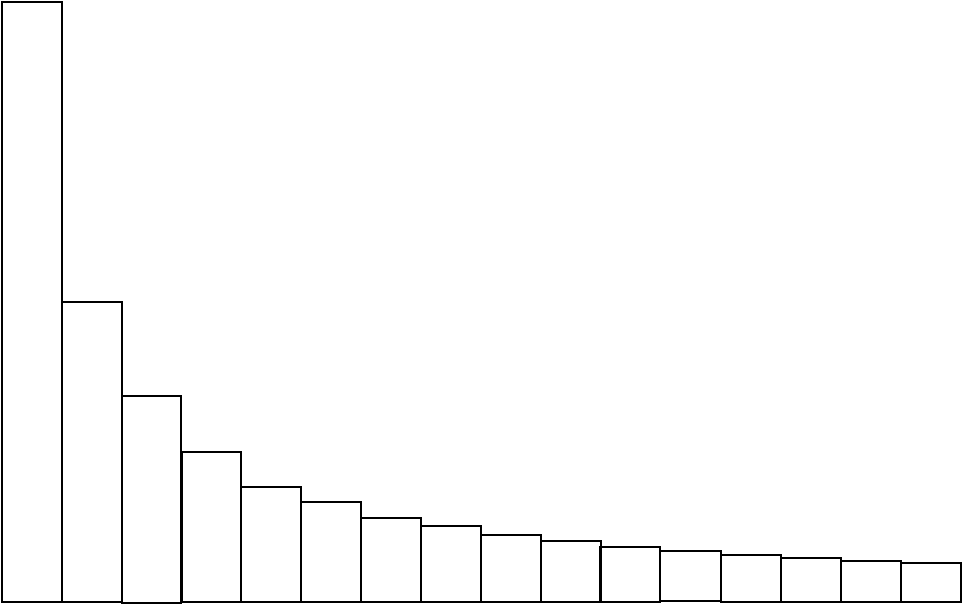
\includegraphics[scale=0.3]{FiguresMaths/HarmonicSumInitial}
}
\caption{The harmonic summation $S^{(H)}(n)$ represented by the area
  of abutting unit-width rectangles of decreasing heights.}
\label{fig:HarmonicSumInitial}
\end{figure}

In order to better understand the behavior of $S^{(H)}(n)$ as a
function of $n$, let us group the summation's consecutive terms into
subsums composed from groups of summands whose sizes are consecutive
powers of $2$:
\begin{eqnarray*}
\left( 1 \right) \ + \ \left( \frac{1}{2} + \frac{1}{3} \right)\\
+ \left( \frac{1}{4} + \frac{1}{5} + \frac{1}{6} + \frac{1}{7} \right) \\
+ \left( \frac{1}{8} +\frac{1}{9} + \frac{1}{10} + \frac{1}{11}
       + \frac{1}{12} + \frac{1}{13} + \frac{1}{14} + \frac{1}{15} \right) \ + \cdots
\end{eqnarray*}
Next, we isolate each grouped subsum and list the subsums in order of
size, measured as number of inverse-integer summands.
\[ \begin{array}{llcl}
\mbox{Sum of $(2^0 =1)$ consecutive inverses:} &
A_0 & = &  {\displaystyle 1 } \\
\mbox{Sum of $(2^1 =2)$ consecutive inverses:} &
A_1 & = &  {\displaystyle \frac{1}{2} + \frac{1}{3} }  \\
\mbox{Sum of $(2^2 =4)$ consecutive inverses:} &
A_2 & = &  {\displaystyle \frac{1}{4} + \frac{1}{5} + \frac{1}{6} + \frac{1}{7} } \\
 & \vdots & & \vdots \\
\mbox{Sum of $2^i$ consecutive inverses:} &
A_i & = &  {\displaystyle \frac{1}{2^i} + \frac{1}{2^i+1} + \cdots +
     \frac{1}{2^{i+1}-1}  } \\
 & \vdots & & \vdots \\
\end{array}
\]

Finally, we derive absolute-constant upper and lower bounds that hold
for all of the subsums.  To derive these bounds, we focus on the
generic subsum $A_i$, which consists of $2^i$ summands.  When we focus
on the largest and smallest inverse-integers in $A_i$---which are,
respectively, $1/2^i$ and $1/(2^{i+1}-1)$---we note the following
absolute bounds.
\[
\frac{1}{2}
 \ < \
\frac{2^i}{2^{i+1}-1}
 \ < \
2^i \cdot A_i
  \ < \
\frac{2^i}{2^i}
  \ = \ 1
\]
We thereby have absolute constant upper and lower bounds on every 
subsum $A_i$.

Referring back to Fig.~\ref{fig:HarmonicSumInitial}, what the
just-derived bounds mean is the following.  Let us proceed left to
right along the abutting rectangles in the figure, and let us recall,
from Section~\ref{sec:exponential+logarithm}.B, the definition of
``logarithm to the base $b$''.  As we double the number of rectangles
we have traversed:
\begin{enumerate}
\item
We increase the aggregate area of the thus-far traversed rectangles by
at most $1$.

{\em This means that $S^{(H)}(n)$ grows no faster than $\log_2 n$.}

\item
We increase the aggregate area of the thus-far traversed rectangles by
more than $1/2$.

{\em This means that $S^{(H)}(n)$ grows faster than $\log_4 n$.}
\end{enumerate}
Of course, these observations are consistent with the verified actual
natural-logarithmic growth rate of $S^{(H)}(n)$, because $2 < e < 4$.

\begin{figure}[htb]
\centerline{
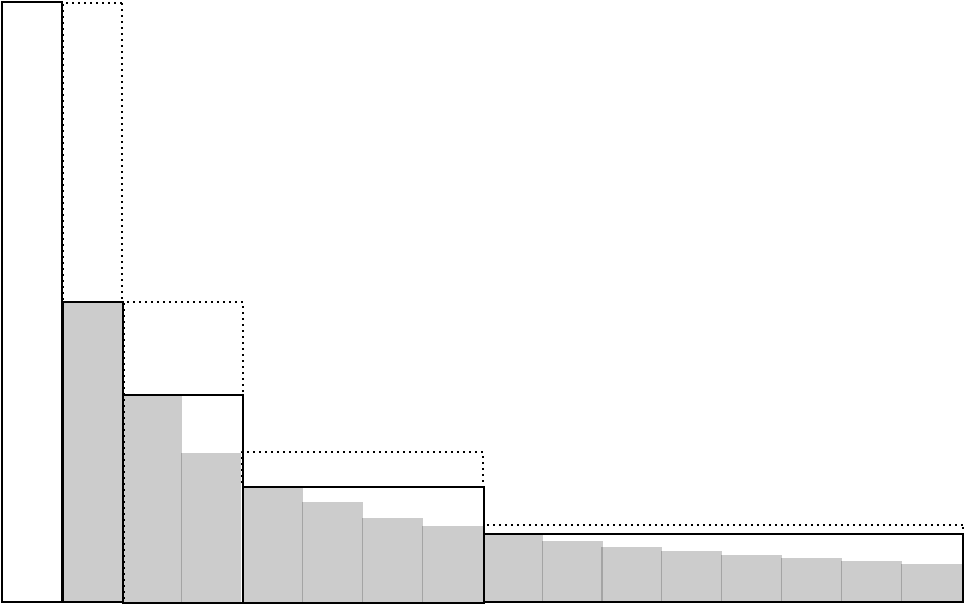
\includegraphics[scale=0.3]{FiguresMaths/HarmonicSumUpperbound}
}
\caption{Upper bound of $A_i$ by larger unit-size rectangles in the harmonic sum.}
\label{fig:HarmonicSumUpperbound}
\end{figure}

\begin{figure}[htb]
\centerline{
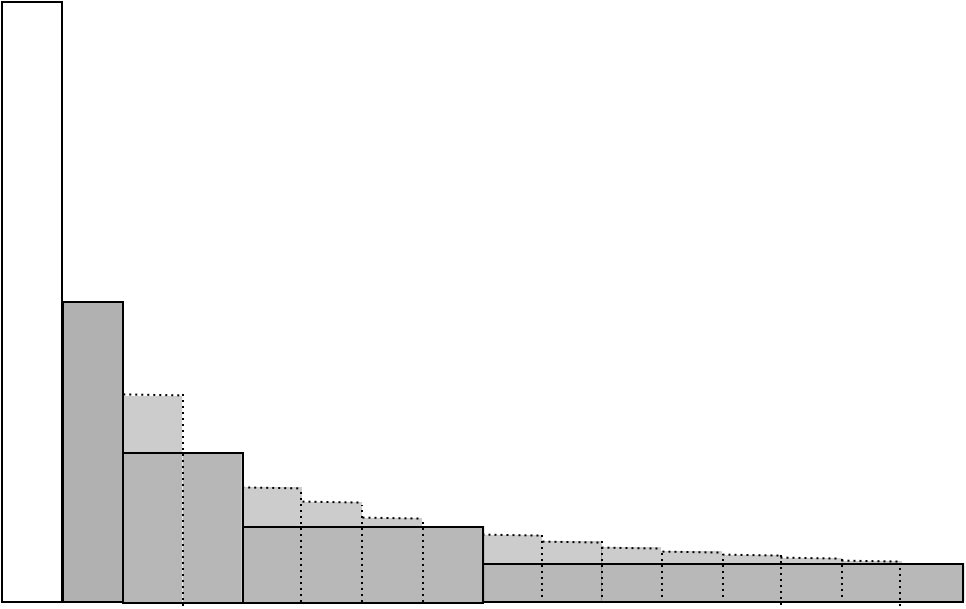
\includegraphics[scale=0.3]{FiguresMaths/HarmonicSumLowerbound}
}
\caption{A pictorial lower bound for the harmonic summation.}
\label{fig:HarmonicSumLowerbound}
\end{figure}



\ignore{**************
%and more generally, $A_i$ is the sum of the consecutive $\frac{1}{i}$
%(for $k$ such that $\frac{1}{2^i+1} \leq k \leq \frac{1}{2^{i+1}}$). 
Note that each $A_i$ is the sum of $2^i$ consecutive terms.

We claim that each partial sum satisfies $A_i \leq 1$.  Verifying this
by actually summing each $A_i$ requires a bit of calculation, but if
we want only the bound, then we achieve that quite easily from the
drawing in Fig~\ref{fig:HarmonicSumUpperbound}.
\begin{figure}[htb]
\centerline{
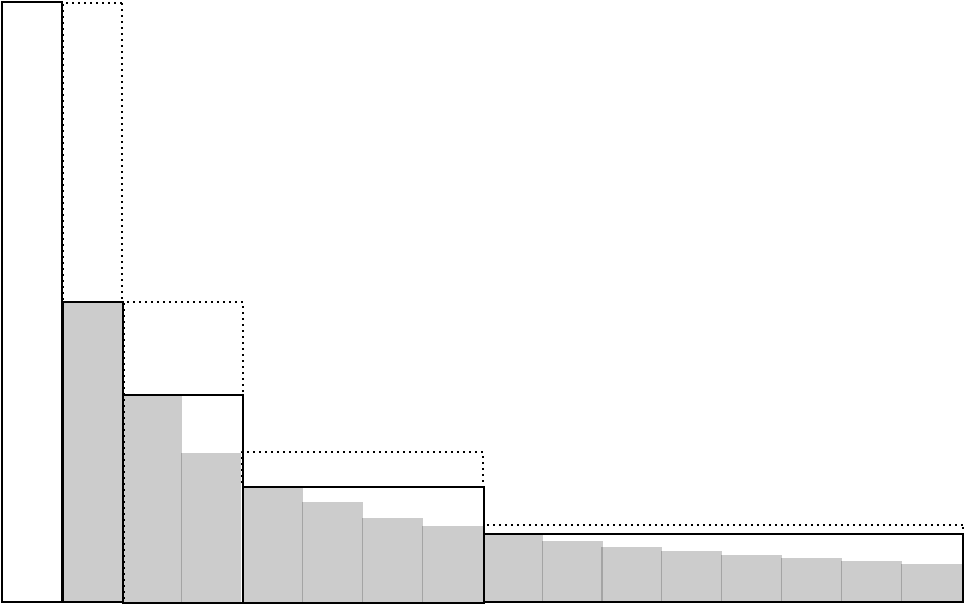
\includegraphics[scale=0.3]{FiguresMaths/HarmonicSumUpperbound}
}
\caption{Upper bound of $A_i$ by larger unit-size rectangles in the harmonic sum.}
\label{fig:HarmonicSumUpperbound}
\end{figure}

constant value $k$.  This claim is verified with the value $k=1$ by
the drawing in Fig~\ref{fig:HarmonicSumUpperbound}. shows that all the
$A_i$ are lower than $1$ but we could have considered a more accurate
value, however, it is enough and simple.  This result is obtained by
embedding each term $A_i$ by larger rectangles (of unit surfaces), the
upper bound is the bold rectangle plus the dashed rectangle at the
top.  {\Denis I hope my previous explanation is clear enough...}


Going into more detail, we claim that the partial sums $A_i$ form an
increasing sequence.  Here again, an exact verification by calculating
each $A_i$ is onerous to achieve, but the claim can be verified
graphically from the drawing in Fig~\ref{fig:HarmonicSumLowerbound}.
\begin{figure}[htb]
\centerline{
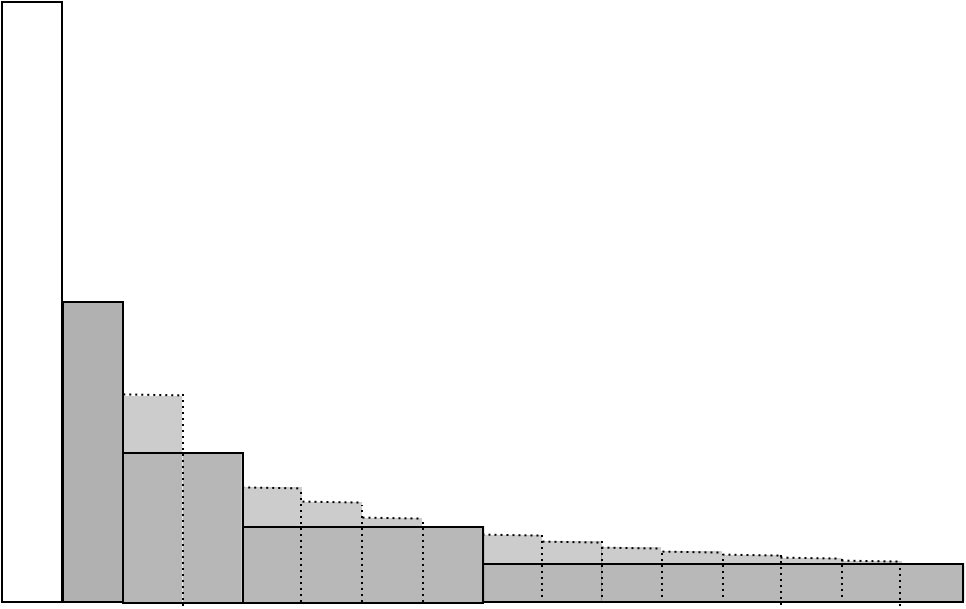
\includegraphics[scale=0.3]{FiguresMaths/HarmonicSumLowerbound}
}
\caption{A pictorial lower bound for the harmonic summation.}
\label{fig:HarmonicSumLowerbound}
\end{figure}
The drawing suggests the following exact sequence of analyses.

Let us verify first that $A_2 \geq A_1$ by showing that $A_2-A_1 \geq
0$; this inequality corresponds to the leftmost light grey rectangle
in Fig~\ref{fig:HarmonicSumLowerbound}.  We want to sum
\[ A_2-A_1 \ = \ \frac{1}{5} + \frac{1}{6} + \frac{1}{7} + \frac{1}{8}
- \frac{1}{3} - \frac{1}{4} \]
Because $\displaystyle \frac{1}{5} \geq \frac{1}{6}$ and
$\displaystyle \frac{1}{7} \geq \frac{1}{8}$, we have
\[
A_2-A_1 \ \ \geq \ \
\left(\frac{1}{6} + \frac{1}{6}\right) - \frac{1}{3} +
\left(\frac{1}{8} + \frac{1}{8}\right) - \frac{1}{4}
  \ \ =  \ \  0.
\]
Hence, $A_2 \geq A_1$. 

We continue to use such grouped calculations to prove that each
$A_{i+1} \geq A_i$.  To wit, we group $\displaystyle \frac{1}{2^{i+1}
  + 1} + \frac{1}{2^{i+1} + 2}$ with $\displaystyle -\frac{1}{2^{i} +
  1}$.  Because $\displaystyle \frac{1}{2^{i+1} + 1} \geq
\frac{1}{2^{i+1} + 2}$, we have $\displaystyle \frac{1}{2^{i+1} + 1} +
\frac{1}{2^{i+1} + 2} - \frac{1}{2^{i} + 1} \geq 0$.  We conclude that
$A_{i+1} \geq A_i$.

Finally, as the sequence $A_i$ is bounded above and increasing, it converges to a constant.


The preceding grouping of the terms of $S^{(H)}(n)$, combined with our
bounds on the generic $A_i$


coupled with the
the fact that
The explanation relies on the following observations of the harmonic series:
$S^{H}(2^{i+1}-1) = S^{H}(2^{i}-1) + A_i$

From a given value of $i$, each $A_i$ and its successive values have roughly the same value equal to the limit of $A_i$.
In other words, we go from index $2^i$ to $2^{i+1}$ in $S^{H}$ by a multiplication by $2$ that corresponds to adding a constant. 
This is exactly what the log means!
***************}


%chapter

%%*********Completed 05-29-19

%%%%%%%%%%%%%%%%%%%%%%%%%%%%%%%%%

%version of 03-27-20

\chapter{The Vertigo of Infinity:
Handling the Very Large and the Infinite}
\label{ch:infinity}

\begin{quote}
{\em One Two Three \ldots Infinity} \\
\hspace*{1in}George Gamow, 1947 book
\end{quote}

\medskip

\noindent
An immensely powerful attribute of the way mathematics allows us to deal with quantity is our ability---in principle, at least---to use identical reasoning and tools of analysis to manipulate all finite objects: We do not need---to cite just two examples---a hierarchy of arithmetics to deal with real numbers of various sizes nor a variety of logical calculi to deal with propositions having various numbers of satisfying assignments of truth values.  This situation changes, however, when we deal with objects---say, sets or numbers---whose sizes can change {\em dynamically} or that are composed of {\em infinitely many} distinguishable objects.  In order to reason rigorously about quantities that can grow---or, equivalently, can shrink---without bound, we need new conceptual machinery.  This is true whether or not the growth can continue forever!  And, we need yet other new conceptual tools to deal with objects that are actually infinite.

\smallskip

This chapter is devoted to developing the needed tools and to heightening readers' awareness of the care that they must take when reasoning in the domain of this chapter's title: the {\em large}, the {\em very large}, and the {\em Infinite}.

\section{Asymptotics}
\label{sec:asymptotics}

\index{asymptotics}
{\em Asymptotics} can be viewed as a language and a system of reasoning that allow one to talk in a {\em qualitative} voice about {\em quantitative} topics.  We thereby generalize to arbitrary growth functions terms such as ``linear'', ``quadratic'', ``exponential'', and ``logarithmic''.

Such a language and system are indispensable if one needs to reason about computational topics over a range of situations, such as a range (``all existing''?)~of computer architectures and software systems.  As two simple examples: (1) Carry-ripple adders perform additions in a number of steps that is linear in the lengths $n$ of the summands (measured in number of bits)---no matter what these lengths are.  (2) Comparison-based sorting algorithms can sort lists of $n$ keys in a number of steps proportional to $n \log n$, but no faster---where the base of the logarithm depends on the characteristics of the computing platform and the set of keys being sorted.  More precise versions of the preceding statements require specification of the number $n$ and other details, possibly down to the clock speeds of the host computer's circuitry.

\smallskip

The need for the material in this section can be discerned (almost) daily, as the news media report---and all too often {\em misreport}---about dynamic quantities: the word ``exponential'' is
very often used when ``fast'' or ``large" is what is actually meant.  It is not true (usually) that ``Country A's GDP'' or ``The X-virus epidemic'' is growing {\em exponentially}.  Country B's strategic planning, in the first example, and the government's public health department, in the second example, cannot proceed rationally without trustworthy quantitative information.

\subsection{The Language of Asymptotics}
\label{sec:language-asymptotics}

The language of asymptotics has its origins in the subfield of mathematics known as {\it Number Theory}, in the late 19th century.  The basic version of the language---which handles almost all situations one encounters when studying the discrete mathematics germane to computational phenomena---builds on the terminology we discuss here.  There is an advanced companion to the following notions, which builds on nondiscrete concepts such as limits; this advanced material will be beyond the likely needs of most students of computing---excepting, of course, specialists in specific, advanced subject areas.  The basics of the language of asymptotics build on three primitive notations and notions.  We need only the rudiments of this material within this text, so we refer the reader to standard texts on algorithm design and analysis (e.g.,\cite{CLRS}) or number theory (e.g., \cite{NivenZ80}), to go beyond the basics of the following ideas.

\smallskip

The following notation actually has several variants in both symbology and articulation.  We elaborate on this situation only for our first notation, the ``big-$O$'' (articulated ``big $O$").  The reader should be aware that analogous complications accompany our other two notations, the ``big-$\Omega$'' (articulated ``big Omega") and the ``big-$\Theta$'' (articulated ``big Theta"). 
\index{big-$O$}\index{big-$\Omega$}\index{big-$\Theta$} \index{asymptotic notation}
\begin{itemize}
\item
{\em The big-$O$ notation}.
The assertion $f(x) = O(f_1(x))$ says, intuitively, that the function $f$ {\em grows no faster than} the function $f_1$.  It is, thus, the asymptotic analogue of ``less than''.

\smallskip

Formally, the assertion

\hspace*{.2in}$f(x) = O(f_1(x))$

means

\hspace*{.2in}
$(\exists c >0)(\exists x_1)(\forall x > x_1)
[f(x) \leq c \cdot f_1(x)]$

\medskip

\noindent \fbox{
\begin{minipage}{0.96\textwidth}
{\bf Explanatory note}.

{\it The complication}.

The ``equal sign'' in the notation $f(x) = O(f_1(x))$ does {\em not} mean ``equals''.

\smallskip

In fact, the assertion ``$fx) = O(f_1(x))$'' actually means that function $f$ {\em belongs to the class of functions that {\em eventually} grow no faster than function $f_1$ does.}

\smallskip

Consequently:
\begin{enumerate}
\item
The assertion ``$f(x) = O(f_1(x))$'' is {\em articulated}

\smallskip

\hspace*{.25in}``$f(x)$ {\em is} $O(f_1(x))$''.

\smallskip

{\em Never} substitute ``equals'' for ``is''
\item
Many people acknowledge the ``belonging to a class'' facet of the definition by writing

\smallskip

\hspace*{.25in}``$f(x) \in O(f_1(x))$''

\smallskip

rather than

\smallskip

\hspace*{.25in}``$f(x) =  O(f_1(x))$''
\end{enumerate}

\medskip

{\it An esoteric aside}:  It is strange that precisely two of the three asymptotic letters, namely, $\Omega$ and $\Theta$, come from the Greek alphabet.  In fact, many scholars insist that the letter $O$ in ``big-$O$" is actually the Greek letter omicron, {\em not} the Latin letter $O$.
\end{minipage}
}
\bigskip

\item
{\em The big-$\Omega$ notation}.
The assertion $f(x) = \Omega(f_2(x))$ says, intuitively, that the function $f$ {\em grows at least as fast as} function $f_2$.  It is, thus, the asymptotic analogue of ``greater than''.

\smallskip

Formally, the assertion

\smallskip

\hspace*{.2in}
$f(x) = \Omega(f_2(x))$

means

\hspace*{.2in}
$(\exists c >0)(\exists x_2)(\forall x > x_2)
[f(x) \geq c \cdot  f_2(x)]$

\item
{\em The big-$\Theta$ notation}.
The assertion $f(n) = \Theta(f_3(n))$ says, intuitively, that the function $f$ {\em grows at the same rate as} function $f_3$.  It is, thus, the asymptotic analogue of ``equal to''.

\smallskip

Formally, the assertion

\smallskip

\hspace*{.2in}
$f(x) = \Theta(f_3(x))$

means

\hspace*{.2in}
$(\exists c >0)(\exists c' >0)(\exists x_{3})(\forall x > x_{3})
[c \cdot f_3(x) \leq f(x) \leq c' \cdot  f_3(x)]$
\end{itemize}
One renders the preceding intuitive explanations precise by pointing out that the three specified relations:
\begin{enumerate}
\item
take hold {\em eventually}, i.e., only for large arguments to the functions $f$, $f_1$, $f_2$, $f_3$;
\item
hold only up to an unspecified constant of proportionality.
\end{enumerate}
The plots in Fig.~\ref{fig:Asymptotic} illustrate the definitions of big-$O$ and big-$\Omega$ graphically.
\begin{figure}[htb]
\begin{center}
       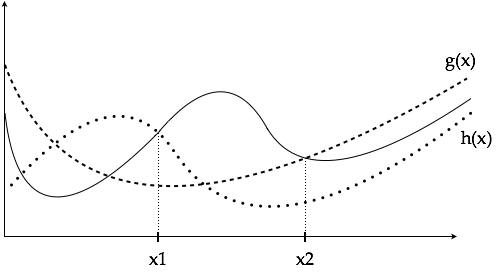
\includegraphics[scale=0.4]{FiguresArithmetic/NotationAsymptotic}
\caption{Plots of three functions: $f$ (solid curve), $f_1$ (dotted curve that originates on the left, above $f$), and $f_2$ (dotted curve that originates on the left, below $f$).  Assume that the three illustrated trajectories continue in the depicted relationships for large values of $x$---i.e., for all $x > x_1$, the plot for $f$ lies strictly below that for $f_1$ and strictly above that for $f_2$.  With this assumption, the figure illustrates the relations: $f(x) = O(f_1(x))$ and $f(x) = \Omega(f_2(x))$.}
\label{fig:Asymptotic}
\end{center}
\end{figure}

\subsection{The ``Uncertainties'' in Asymptotic Relationships}
\label{sec:uncertainties-asymptotics}

The formal definitions of all three of our asymptotic relationships are bracketed by two important quantifiers:
\[ 
(\exists c >0) \ \ \ \mbox{ and }  \ \ \  (\forall x > x^{\#}).
\]
The former, {\em uncertain-size} quantifier ($\exists c >0$), asserts that asymptotic notions describe functional behavior ``in the large''.  Thus, in common with more common qualitative descriptors of quantitative growth such as ``linear", ``quadratic", ``cubic", ``quartic", ``exponential", ``logarithmic", etc., asymptotic relationships give no information about constants of proportionality.  {\em We are not saying that constant factors do not matter!}  We are, rather, saying, {\em We sometimes want to discuss growth patterns \underline{in the large} rather than in detail.}

\smallskip

The latter, {\em uncertain-time} quantifier ($\forall x > x^{\#}$) asserts that asymptotic relationships between functions are promised to hold only ``eventually'', i.e., ``for sufficiently large values of the argument $x$''.  Therefore:  {\em Asymptotic notions cannot be employed to discuss or analyze quantities that can never grow beyond a fixed finite value}.  The fact that all instances of a quantity throughout history have been below $N$ is immaterial, as long as it is conceivable that an instance larger than $N$ could appear at some time in the future.

\smallskip

These two quantifiers in particular distinguish claims of asymptotic relationship from the more familiar definite inequalities such as
\[ [f(x) \leq g(x)] \ \ \ \ \mbox{ or } \ \ \ \ [f(x) \geq 7 \cdot g(x)] \]
In fact, it is often easier to think about our three asymptotic bounding assertions as establishing {\em envelopes} for $f(x)$---cf., Fig.~\ref{fig:Asymptotic}:
\begin{itemize}
\item
$f(x) = O(g(x))$.

If one draws the graphs of the functions $f(x)$ and $c \cdot g(x)$, then as one traces the graphs with increasing values of $x$, one eventually reaches a point $x^{\#}$ beyond which the graph of $f(x)$ never enters the territory {\em above} the graph of $c \cdot g(x)$.
\item
$f(x) = \Omega(g(x))$.

This situation is the up-down mirror image of the preceding one: just replace the highlighted ``{\em above}'' with ``{\em below}.''
\item
$f(x) = \Theta(g(x))$.

This relation provides a {\em two-sided} envelope:  Beyond $x^{\#}$, the graph of $f(x)$ never enters the territory {\em above} the graph of $c \cdot g(x)$ and never enters the territory
{\em below} the graph of $c' \cdot g(x)$.
\end{itemize}
In addition to allowing one to make familiar growth-rate comparisons such as ``$n^{14} = O(n^{15})$'' and ``$1.001^n = \Omega(n^{1000})$,'' we can now also make assertions such as ``$\sin x = \Theta(1)$,'' which are much clumsier to explain in words.

\medskip

\index{asymptotics!with little letters}
\noindent {\bf Beyond the big letters.}
There are ``little''-letter analogues of the preceding ``big''-letter asymptotic relations and notations: $o$, $\omega$, and $\theta$.  The definitions and domains of application of these notations build on the notion of {\it limit}, which is fundamental in continuous mathematics---e.g., in the differential and integral calculus---but rare in discrete mathematics.  We therefore do not include this topic in this text, instead referring the reader to any good text on the calculus.

\subsection{Inescapable Complications}
\label{sec:asymptotic-complication}

The story we have told thus far is more or less standard fare in courses on discrete mathematics and algorithms.  Two complications to the story are covered less consistently, despite the fact that, lacking them, one cannot perform cogent asymptotic reasoning about modern computing
environments.  Both complications involve the notion of {\em uniformity}. 
\index{relations!uniformity}

\medskip

\index{asymptotics!multiple functions}
\noindent
{\bf 1.}
{\em Multiple functions}.
Say that we have four functions, $f, g, h, k$, and we know that
\[ f(n) = O(g(n)) \ \ \ \  \mbox{ and } \ \ \ \ h(n) = O(k(n)) \]
It is compellingly suggestive that
\[ f(n) + h(n) = O(g(n) + k(n)) \]
--- but is it true?

\smallskip

In short, the answer is {\em YES}---but verifying the answer requires a bit of subtlety.  The challenge is that, absent hitherto undisclosed information, the proportionality constants $c_{f,g}$ and $N_{f,g}$ that witness the big-$O$ relationship between functions $f$ and $g$ have no connection with the constants, $c_{h,k}$ and $N_{h,k}$ that witness the analogous relationship between functions $h$ and $k$.  Therefore, in order to verify the posited relationship between functions $f + h$ and $g + k$, one much find witnessing constants $c_{f+h, g+k}$ and $N_{f+h,g+k}$.

\smallskip

\noindent
Of course, this task requires only elementary reasoning---{\em but it must be done}!

\medskip

\index{asymptotics!multivariate functions}
\noindent {\bf 2.}
{\em Multivariate functions}.
Finally, we discuss the scenario that almost automatically accompanies the transition from {\em sequential, single-agent} computing to {\em parallel and/or distributed and/or multi-agent}computing.  One must account for a system's many resources: computing, memory/storage, and communication., etc.  One must assess the relationships among the costs of operating the system: time, energy, memory usage, etc.  One must account for possible tradeoffs among costs and possible cost-altering emulations of one subsystem by another. Within such scenarios, every assertion of an asymptotic relationship, of the form
\[ f(\vec{m}; \vec{n}) = O(g(\vec{m}; \vec{n})) \]
must explicitly specify the following information:
\begin{itemize}
\item
which variables represent resources that can grow without bound;
\item
among such unbounded variables, which participate in the posited asymptotic relation;
\item
for each participating unbounded variable $x$, what are the constants $c_x$ and $N_x$ that witness the posited asymptotic relationship(s).
\end{itemize}

\medskip

Clearly the complexity of cogent asymptotic reasoning---hence, also, the complexity of teaching about such reasoning---gets much more complicated in the multivariate settings engendered by parallel and distributed computing.  But, the benefits of being able to reason qualitatively about the quantitative aspects of computing increase at least commensurately!

\section{Reasoning about Infinity}
\label{sec:reasoning-infinity}

\subsection{Coping with infinity}
\label{sec:coping-infinity}

A recurring challenge when one ``does'' mathematics is dealing with {\em infinity}.  Infinite objects, such as sets and summations, behave rather differently from the more familiar finite objects that we encounter in our daily lives.  Two examples will suffice.  
\begin{enumerate}
\item
There are ``equally many'' integers within the set $\N$ of {\em all} integers as there are in
  \begin{itemize}
  \item
$\N$'s proper {\em subset} that comprises just the {\em odd} integers.
  \item
$\N$'s proper {\em superset} that comprises ordered pairs of integers.
  \end{itemize}
Does this mean that ``infinite is infinite", i.e., that one can match up the elements of any two infinite sets.
  
\smallskip

\noindent
{\em Decidedly NOT!}

\smallskip

\noindent
Alas!  We have to await Section~\ref{sec:FNS-uncountable} before we make the acquaintance of infinite sets that are ``bigger" than $\N$.  We shall appreciate this introduction all the more after Section~\ref{sec:pairing}, where we shall encounter a lot of infinite sets that ``should be bigger" than $\N$---but are not! 


\item
We have seen in Chapter~\ref{ch:Summation} that there exist summations of infinitely many positive numbers whose sum is finite (in the sense that the series {\em converges}).  The series
\[ 1 \ + \ {1 \over 2} \ + \ {1 \over 2^2} \ + \cdots + \ {1 \over 2^k} \ + \cdots \ \ = \ \ 2 \]
provides an example.

\smallskip

But, there exist other infinite summations whose ``sum is infinite'' (in the sense that the series {\em diverges}).  The {\it harmonic} series
\[ 1 \ + \ {1 \over 2} \ + \ {1 \over 3} \ + \cdots + \ {1 \over k} \ + \cdots \]
provides an example.
\end{enumerate}
There are clearly nonobvious concepts within the world of the infinite, which distinguish those infinite objects that behave more or less as we would expect from those infinite objects that don't.

\medskip

\index{paradox}
The world of the infinite is even more subtle than the preceding examples suggest.  This world hosts myriad {\em paradoxes}---situations that, in the words of the {\it New Oxford Dictionary}, ``combine contradictory features or qualities".\footnote{In detail, the {\it New Oxford Dictionary} defines a ``paradox'' as \\
``a statement or proposition that, despite sound (or apparently sound) reasoning from acceptable premises, leads to a conclusion that seems senseless, logically unacceptable, or self-contradictory''.}

\medskip

The remainder of this section is devoted to discussing and explaining the sometimes-confusing but always-fascinating world of the infinite.

\subsection{The ``Point at Infinity''}
\label{sec:point-at-infinity}

\index{limit} \index{continuity} \index{Riemann sphere} \index{Riemann, Bernhard}
In many situations, the difficulties encountered when dealing with infinite objects result from the conceptual fiction that there is, in fact, a ``point at infinity''---i.e., that one can treat infinity as just
another number.  In many mathematical environments, this fiction is an aid to reasoning which can be handled with totally rigor---but often only when accompanied by rather sophisticated mathematical machinery.  Two familiar examples of such mathematical machinery are the notions
of  {\it limit} and {\it continuity} (of a function).  A more advanced example of such machinery is the {\it Riemann sphere}, an invention of the 19th-century German mathematician Bernhard Riemann, which allows one to reason about the infinite two-dimensional plane by ``conformally'' wrapping the plane into a sphere whose ``south pole'' represents the zero-point (i.e., the origin) of the plane and whose ``north pole'' represents the ``point at infinity.''  There are many other, less-familiar, examples of such mathematical machinery, including advanced topics such as {\it types} in the domain of mathematical logic.

\medskip

Of course, we have already had some success in dealing with a quite sophisticated genre of infinite object:  In Chapter~\ref{ch:Summation}, we summed and manipulated a broad variety of infinite summations.  We are close to having the tools necessary to deal with a variety of other infinite objects; to cite just two:
\begin{enumerate}
\item
In Section~\ref{sec:pairing}, we shall demonstrate how to establish one-to-one correspondences between certain infinite sets, including, notably, any two of: the set $\N$ of integers, the set $\Q$ of rationals, and the set $\N \times \N$ of ordered pairs of integers.

\item
In Section~\ref{sec:FNS-uncountable}, we shall demonstrate that one {\em cannot} establish a one-to-one correspondence between the set $\N$ of integers and the set $\R$ of real numbers.
\end{enumerate}

\smallskip

The lesson of the preceding paragraphs is that there is no need to avoid dealing with infinity and its related notions---as long as one has the mathematical machinery necessary to: ($a$) define all needed notions unambiguously; ($b$) obtain well-defined results from all required operations and manipulations; ($c$) reason cogently about all the concepts and processes one employs.  That said, the scenarios described in the coming two subsections warn us to treat all aspects of infinity with care and respect.  The subsections point out two challenges often encountered when one reasons about the infinite.  Both challenges leave us with some form of {\em paradox}.

\subsubsection{Underspecified problems}
\label{sec:underspecified}

The paradoxes we present in this section require refined groundrules for their resolution.  The underlying problems {\em seem} to be totally specified---until one tries to develop their solutions.

\paragraph{A. Summing ambiguous infinite summations}

The first question we tackle was the subject of much concern as the topic of infinite summations emerged from its infancy in the 18th century.  The overriding question is, What can one learn from an infinite series that does not have a unique sum?  Much valuable work has been done on this question, most of which is beyond the scope of this text.  But the conundrum presented by 
such summations is valuable to consider.

\medskip

For our first source of puzzlement, we invoke the following infinite summation.
\[ S \ = \ 1 \ - \ 1 \ + \ 1 \ - \ 1 \ + 1 \ - \ 1 \ + \cdots \]
There are many conflicting, but well-reasoned, answers to questions about $S$:
\begin{itemize}
\item
{\it Does summation $S$ have a finite sum?} 
\item
If so: {\it Is this sum positive or negative?}
\end{itemize}

\smallskip

\noindent
Here are four plausible answers to these questions; you may find others.  The final answer, in particular, merits strong consideration.
\begin{itemize}
\item
YES: $S \ = \ 0$

\smallskip

This response is justified by the following association of terms in summation $S$.
\begin{figure}[h]
\begin{center}
        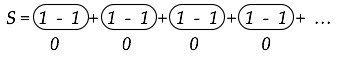
\includegraphics[scale=0.45]{FiguresArithmetic/InfiniteParadox1}
\end{center}
\end{figure}

\item
YES: $S \ = \ 1$

\smallskip

This response is justified by the following association of terms in summation $S$.
\begin{figure}[h]
\begin{center}
        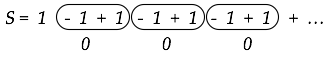
\includegraphics[scale=0.45]{FiguresArithmetic/InfiniteParadox2}
\end{center}
\end{figure}

\item
YES: $S \ = \ 1/2$

\smallskip

This response is justified by the fact that $S$ satisfies the equation $S \ = \ 1-S$.

\item
THERE IS NO VALID ANSWER.

\smallskip

This response is justified by the fact that the problem statement does not specify how to associate the terms of $S$.  As the first three answers suggest, ``mischievously" playing with the parenthesization of summation $S$ enables us to arrive at many ``plausible'' sums.
\end{itemize}

\medskip

The mysteries that arise from contemplating summation $S$ are not exhausted by playing with parentheses.  Consider, for instance, the infinite summation that consists of all integers, with alternating signs:
\[ S' \ = \ 1 \ - \ 2 \ + \ 3 \ - \ 4 \ + \ 5 \ - \cdots + \cdots \]
If we associate corresponding summands in summations $S$ and $S'$, then we find that
\[ S'  \ = \  S  \ - \ S'  \]
If, then, we accept the valuation $S \ = \ 1/2$, then we would find that
\[ S' \ = \ 1/4 \]
Another defensible analysis of $S'$ would say that $S'$ has no finite valuation because of the association of terms
\begin{eqnarray*}
S' & = & (1 \ - \ 2) \ + \ (3 \ - \ 4) \ + \ (5 \ - \ 6) \ + \cdots \\
    & = & (-1) \ + \ (-1) \ + \ (-1) \ +  \cdots
\end{eqnarray*}

\smallskip

One can add numerous examples to the preceding two to illustrate how very differently summations having infinitely many terms behave from summations having finitely many terms.

The conclusion we offer is: \ \ \ {\em Beware:  Infinity is not a number!}

\paragraph{B. The Ross-Littlewood paradox}

\index{Littlewood, John E.} \index{Ross, Sheldon M.} 
\index{paradox!Ross-Littlewood paradox}
The following story is known as the {\it Ross-Littlewood paradox}, after its creators.  A version of the story appeared first in John Littlewood's enlightening and entertaining book {\it Littlewood's Miscellany} \cite{Littlewood-misc}; the story was amplified to its present form by Sheldon M.~Ross \cite{Ross76}. 

\medskip

Let us imagine a system that contains
\begin{itemize}
\item
a {\em really big} bin (in fact, one whose capacity grows as the story progresses)
\item
an unbounded sequence of ordered balls, labelled 1, 2, \ldots
\item
a {\em very} (read: infinitely) precise clock.
\end{itemize}
The system is watched over by a {\it Keeper}.  We observe the {\it Keeper} executing the following process.

\smallskip

\noindent {\sf Step $1$}.
At time {\em midnight minus $1$ minute}, the {\it Keeper} places the first ten balls in the sequence (i.e., balls $\#1, \ldots, \#10$) into the bin, and {\em immediately} removes the first ball (ball \#$1$).

\smallskip

\noindent {\sf Step $2$}.
At time {\em midnight minus $1/2$ minute}, the {\it Keeper} places the next ten balls in the sequence
(i.e., balls $\#11, \ldots, \#20$) into the bin, and {\em immediately} removes the second ball (ball \#$2$).

\smallskip

\noindent
The {\it Keeper} repeats this process endlessly, at midnight minus $1/4$ minute (putting balls $\#21, \ldots, \#30$ into the bin and removing ball \#$3$), then at midnight minus $1/8$ minute (putting
balls $\#31, \ldots, \#40$ into the bin and removing ball \#$4$), and so on.

\smallskip

\noindent
{\bf Question}: {\it How many balls are present in the bin at midnight?}  \\
(Note that ``infinity'' now measures the number of steps executed in the process.)

\medskip

\noindent
As in paragraph {\small\sf A}, there are several plausible answers to this question.  We provide just three.
\begin{enumerate}
\item
THERE ARE INFINITELY MANY BALLS.

\smallskip

This response is justified by the following reasoning.  Each step of the process inserts $10$ balls into the bin but removes only $1$ ball.  Hence, the population of the bin grows by $9$ balls after each step of the process---and it never decreases!  It follows, therefore, that after infinitely many steps, the bin's population must be infinite.

\item
THE BIN IS EMPTY---THERE ARE $0$ BALLS!

\smallskip

This response is justified by the following reasoning.  Every ball is eventually removed from the bin at some (finite) step of the process. Specifically, ball \#$n$ is removed at step $n$, i.e., at time midnight minus $2^{-n}$ seconds.

\item
THERE IS NO VALID ANSWER.

\smallskip

This response is justified by the following reasoning.  There is no ``moment at infinity'' that is actually ever encountered during the process.  That ``moment" is just a conceptual idealization.

\smallskip

In other words, infinity is not a number!
\end{enumerate}


\paragraph{C.  Zeno's paradox: Achilles and the tortoise}

\index{Zeno of Elea} \index{Zeno!Zeno's paradox} \index{paradox!Zeno's paradox}
In his celebrated {\it Paradox of Achilles and the Tortoise}, Zeno of Elea  presented a problem whose solution had to await the 17th century.

\smallskip

In Zeno's story, the slow-footed Tortoise (T) tries to convince the speedy Achilles (A) of the futility of trying to win any race in which A gives T even the smallest head start.  As long as T is ahead of A, says T, every time A traverses half the distance between himself and T, T will respond by moving a bit further ahead.  Thereby, T will always be a positive distance ahead of A, so that A can {\em never} catch T.

\smallskip

\index{infinitesimals}
At first glance, this story seems to call into question the physical reality of all motion.  In fact, the
resolution of the apparent paradox resides in the notion of {\em infinitesimals}---quantities that dynamically grow smaller than any finite number.  While infinitesimals are familiar today to anyone who has studied subjects such as the differential calculus, the notion of infinitesimal actually dates back only a few hundred years, to the 17th century.  

\medskip

\index{Leibniz (Leibnitz), Gottfried Wilhelm}  \index{Newton, Isaac} \index{Kronecker, Leopold} 

Underlying the discovery/invention\footnote{Were infinitesimals {\em discovered} or {\em invented}?  As you ponder this choice, recall the words of Leopold Kronecker that end our {\it MANIFESTO}.}~of infinitesimals is one of the great real-life mysteries of all time.  Who invented/discovered infinitesimals?  The parties to this dispute were the German mathematician Gottfried Leibniz \cite{Leibniz} and the English polymath (Sir) Isaac Newton \cite{Newton}.   The cases favoring each of these great men contain enough merit to guarantee that the dispute will likely never be settled.  We therefore list Leibniz and Newton alphabetically and give a coarse dating of the 17th century for the discovery.  This real-life mystery is as full of intrigue and suspense as any that one encounters in fiction.


\paragraph{D. Hilbert's hotel paradox}

\index{paradox!Hilbert's paradox}
While the final story of this section does not describe an actual paradox, it is often referred to by that term.  Terminology aside, this story definitely points out a fundamental difference between the real world of finite capacities and an idealized world that is not so encumbered.

\medskip

Imagine that you are running a hotel that has an infinite number of rooms which are labeled by the (entire set of) positive integers: there is a room \#$1$, a room \#$2$, a room \#$3$, and so on.  Say
that on a particular evening, every room of the hotel is occupied by a guest---and then a new guest arrives!

In a desire to accommodate the newcomer, you initiate the following procedure, which was first proposed by the eminent German mathematician David Hilbert. \index{Hilbert, David}

\smallskip

By means of a broadcast message to all current guests, you move each guest who currently occupies room \#$k$ into room \#$k+1$.  Of course, this total shift empties room \#$1$, hence renders it available for housing the newcomer---so you assign this room to the newly arrived guest.  The world is quiet once more!

\smallskip

Of course, this humorous story has its roots in a fundamental distinction between the world of finite-capacity hotels that we live in and the idealized infinite-capacity hotel proposed in Hilbert's story.  In a word, every finite set of integers---think of the integers as the room numbers in a finite-capacity hotel---{\em has a largest number}, while an infinite set of positive integers {\em does not have a largest number}.

\medskip
  
This paradox can be extended in a way that makes it even more  perplexing:  The story's hotelier can accommodate even {\em an infinite number} of new guests!  Consider again that every room 
of the hotel is occupied, and say that infinitely many new guests arrive!  (Pity the poor desk clerk!). The hotelier can accommodate all of the new arrivals by moving each guest who currently occupies room \#$k$ into room \#$2k$.

\medskip

\index{orders of infinity}
The story of Hilbert's hotel provides yet another demonstration that $\infty$ is not a number!\footnote{The \textit{lemniscate} curve $\infty$ is the traditional symbol for (the point at) ``infinity".} Interestingly, $\infty$ behaves like a number in many ways---but it violates many of the rules of arithmetic that govern actual numbers.  For example, mathematical logicians who are concerned with {\em orders of infinity} will often employ expressions such as
\[ (2 + \infty)  \ \ \  \mbox{ or } \ \ \ (4 \times \infty) \ \ \
\mbox{ or even } \ \ \ (\infty + \infty) \]
as though $\infty$ actually were a number---but they never forget that $\infty$ behaves in nonstandard way, such as being an ``absorber" under the operations of addition and multiplication; e.g.:
\[ (2 + \infty \ = \ \infty)  \ \ \  \mbox{ and } \ \ \  (\infty + \infty \ = \ \infty) \]

%\textit{collection of numbers}.  There is an arithmetic on the infinity, but the rules are different from the classical arithmetic, in particular, the addition operations are absorbed. 


\subsubsection{Foundational paradoxes}
\label{sec:paradoxes}

The {\em foundational} paradoxes that we present now can be resolved only via the development of new, sophisticated, mathematical machinery.

\paragraph{A.  G\"{o}del's paradox: Self-reference in language}

\index{G\"{o}del, Kurt} \index{paradox!G\"{o}del's paradox}

The paradox attributed to logician/philosopher/mathematician Kurt G\"{o}del is described most perspicuously by means of a simple utterance, which we shall call ``Sentence $S$'', and an accompanying query.

\medskip

\noindent
{\bf Sentence} $S$:  {\em The sentence you are reading at this moment is false.}

\smallskip

\noindent
{\bf The query}: {\it Is Sentence $S$ true, or not?}

\bigskip

\noindent
Let us analyze the two options that the question affords us.
\begin{enumerate}
\item
{\em If Sentence $S$ is true}, then one must accept its assertion that \underline{Sentence $S$ is false}.

\item
{\em If Sentence $S$ is false}, then one must reject its assertion that Sentence $S$ is false.  In other words, one must conclude that \underline{Sentence $S$ is true}.
\end{enumerate}

\medskip

\noindent
Sentence $S$ cannot be either true or false.  This flies in the face of conventional two-valued logic's demand that every assertion is {\em precisely one of {\em true} or {\em false}}!

\bigskip

\noindent
What does this mean?  Has G\"{o}del ``fooled us" with a strange linguistic construction?

\smallskip

\noindent
---Regrettably, NO!

\medskip

\noindent
In the early 1930s, G\"{o}del turned the mathematical world on its head with his {\em rigorous }demonstration that, speaking informally:

\smallskip

\begin{tabular}{l}
{\em Any language that is {\em self-referential}---i.e., that can refer to its own sentences} \\
{\em as objects of discourse---must contain a sentence such as Sentence $S$, which} \\
{\em is neither true nor false.}  \cite{Goedel31}
\end{tabular}

\bigskip

The shocking implication of G\"{o}del's work is that in any sufficiently sophisticated language $L$, the notions {\it true} and {\it false} do {\em not} totally partition (into two pieces) the set of legitimate utterances in language $L$.  The simplicity of Sentence $S$ and encodings thereof---see, e.g., \cite{Rosenberg09}---can be used to show that the following classes of languages, and their kin, are
``sufficiently sophisticated'':
\begin{itemize}
\item
Natural languages (Swahili, German, Urdu, etc.)
\item
General-purpose programming languages (assembly language, Basic, C, Java, LISP, Python etc.)
\item
Quantified mathematical languages---i.e., languages that contain logical quantifiers such as {\sc for all} ($\forall$), {\sc there exist} ($\exists$), etc.
\end{itemize}

Of course, the world was spinning and circling the sun before G\"{o}del's earthshaking proof, and it is still spinning and circling after the proof.  However, we are just aware now that we must be more careful in our use of language!  For instance, we must take care to employ pre-validated transformations in our compilers and pre-justified ``small steps'' in our schedulers: We cannot be deceived that our ``noble intentions" as we crafted our systems are sufficient safeguards from the dangers that result from unanticipated ``encodings" within our system.


\paragraph{B.  Russell's paradox: The ``anti-universal'' set}

\index{paradox!Russell's paradox} \index{Russell, Bertrand}

As we remarked in Chapter~\ref{ch:sets-BA-logic}, the notion of set is perhaps the most basic one in mathematics.  One of the fundamental features of sets is that their elements are not governed by any {\it a priori} restrictions.  Most specifically for our discussion here, {\em a set can have sets as elements.}  Indeed, there is no inherent reason why a set cannot contain {\em itself} as an element!  At first blush, the possibility for ``self-membership" in sets seems to be a rather innocuous, albeit unexpected, freedom.  But, the 20th-century English philosopher/logician Bertrand Russell pointed out in \cite{Russell02,Russell03} that, when the population of sets that we focus on contains infinite sets, then the capacity for self-membership can be (intellectually) hazardous.

The hazard that Russell foresaw resided in the fact that, absent any restrictions on the way that one can form sets, one could employ {\em any} proposition {\bf P}($x$) to define the set
\[ \{ x \ | \ {\bf P}(x) \} \] 
One could thereby specify myriad ``benign" sets such as

\medskip

\begin{tabular}{ll}
\underline{\bf Set} & \underline{\bf P}($x$) \\
Even integers: & 
 $[ x \in \N] \mbox{ and } (\exists y \in \N)[x = 2y]$ \\
Perfect squares: & 
 $[ x \in \N]$ and $(\exists y \in \N)[x = y \cdot y] $ \\
Satisfiable POS propositions: & 
 $[x \mbox{ is an $n$-variable POS formula}]$ \\
 & \ \ \ and $(\exists \mbox{ $n$-place bit vector } y) [x(y) = \ \mbox{\sc true}] $ \\
Infinite set: &
$[x \mbox{ is a set}]$ and $[ x \mbox{ is infinite}]$
\end{tabular}

\medskip

\noindent
But one could also specify the {\em anti-universe} set $A$:

\medskip

\begin{tabular}{ll}
{\it In text}: &
$A$ is the set of sets that {\em do not} contain themselves (as elements) \\
{\it In symbols}: &
$A = \{ x \ | \ [x \mbox{ is a set}]$ and $[ x \notin x] \}$
\end{tabular}

\bigskip

The paradox posed by the existence of the set $A$ within our universe of discourse becomes clear when we ponder the following question.

\smallskip

\noindent
{\bf Question}.  {\it Is the set $A$ a member of itself?}

\bigskip

\noindent
Let us analyze the two options that the question affords us.
\begin{enumerate}
\item
{\em If set $A$ is a member of $A$}, then by definition, $A$ {\em is not} a member of $A$.

\smallskip

To wit, $A$ is the set of all sets that {\em do not} contain themselves as members.

\item
{\em If set $A$ is {\em not} a member of $A$}, then by definition, $A$ is a member of $A$.
\end{enumerate}

\medskip

We once again find ourselves in a conundrum: $A$ belongs to $A$ if, and only if, $A$ does not belong to $A$!

\bigskip

\index{typed utterances in languages}
There have been many attempts over the years to resolve the dilemma inherent in the preceding analysis.  Many have striven for logical edifices that declare the question ``{\it Is the set $A$ a member of itself?}'' somehow illegitimate.  One option that appeals to many is to assign each sentence within a language $L$ a {\it type} (say, a positive integer)---and to adjudge a sentence of $L$ to be {\em legitimate} only if it refers only to sentences of {\em lower} type-number.

\bigskip

The stratagem of typing utterances within a language $L$ {\em disables} self-reference within $L$, hence defines away both Russel's paradox and G\"{o}del's paradox.  The stratagem of typing helps also to cope with problems that arise in programming languages which allow recursion.  Typing is, thus, a powerful mechanism for imposing helpful structure in languages.  But, the advantages of typing come only at the expense of adding an obtrusive layer of formalism to language(s) and their associated systems.



%%%%%%%%%%%%%%%%%%%%%%%%%%%%%%%%%%%%

\section{Exercises: Chapter 7}

Throughout the text, we mark each exercise with 0 or 1 or 2 occurrences of the symbol $\oplus$, as a rough gauge of its level of challenge.  The 0-$\oplus$ exercises should be accessible by just
reviewing the text.  We provide {\em hints} for the 1-$\oplus$ exercises; Chapter~\ref{ch:Exercises} provides {\em solutions} for the 2-$\oplus$ exercises.  Additionally, we begin each exercise with a brief explanation of its anticipated value to the reader.

\begin{enumerate}
\item
{\bf An inequality that we used repeatedly in Section~\ref{sec:sum-of-i2c>0}}

{\sc Lesson:} Appreciating asymptotic language by having to reason without it.

\smallskip

{\em Prove the following asymptotic assertion.}

\begin{prop}
\label{thm:poly-w-asymp}
Let $c > 0$ be any fixed integer.  For all $n \in \N^+$,
\[ (n+1)^c \ = \ \Theta(n^c) \]
%\[ \frac{1}{c+1} n^{c+1} \ + \ \underline{\kappa} \ \leq \ \kappa n^c \]
\end{prop}

Of course, what the asymptotic assertion means---when we cannot use asymptotic notation---is the following.

\begin{prop}
\label{thm:poly-wo-asymp}
There exist fixed positive constants $\underline{\kappa}$ and $\overline{\kappa}$ such that, for all sufficiently large $n \in \N^+$,
\[ \underline{\kappa} n^c \ \leq \ (n+1)^c \ \leq \ \overline{\kappa} n^c \]
\end{prop}

{\em Prove that the assertions in Propositions~\ref{thm:poly-w-asymp} and~\ref{thm:poly-wo-asymp} are equivalent.}

\item
{\bf The transmission of asymptotics when functions are combined}

{\sc Lessons:} Enhance understanding of how asymptotic parameters work

\smallskip

{\em Prove the following result.}

\begin{prop}
Focus on four ``primary" real functions, $f_1$, $f_2$, $f_3$, and $f_4$, and two ``derived" functions
\[ f_5(x) \ \eqdef \ f_1(x) + f_2(x) \ \ \ \ \mbox{ and } \ \ \ \ f_6(x) \ \eqdef \ f_3(x) + f_4(x) \]  
If $f_1(x) = O(f_2(x))$ and $f_3(x) = O(f_4(x))$, then $f_5(x) = O(f_6(x))$.
\end{prop}

\item
{\bf Polynomials' degrees and their asymptotic growth rates}

{\sc Lesson:} Practice with asymptotic arguments

\smallskip

Let us be given polynomials with positive coefficients: $P(x)$ of degree $a$ and $Q(x)$ of degree $b > a$.  The numbers $a$ and $b$ need not be integers. 

\smallskip

{\em Prove that there exists a constant $X_{P,Q}$---i.e., a constant that depends on the degrees and coefficients of polynomials $P$ and $Q$---such that}
\[ (\forall \ x > X_{P,Q}) \ \left[ P(x) < Q(x) \right] \]

\smallskip

The preceding formulation can be rephrased in the following two ways:

(1) Polynomial $Q$ {\em eventually majorizes} polynomial $P$.

(2) Polynomial $Q$ {\em grows asymptotically faster than} polynomial $P$.

\item
{\bf Exponentials grow asymptotically faster than polynomials}

{\sc Lesson:} Practice with asymptotic arguments

\smallskip

Let us be given a degree-$b$ polynomial $Q$ with positive coefficients, together with an arbitrary real number $c > 1$.

\smallskip

{\em Prove that there exists a constant $Y_{c;Q}$---i.e., a constant that depends on the constant $c$ and on the degree and coefficients of polynomial $Q$---such that}
\[ (\forall \ x > Y_{c,Q}) \ \left[ c^x > Q(x) \right] \]
\end{enumerate}

%chapter
%*********Completed 05-31-19 -- one figure needs adjustment

%%%%%%%%%%%%%%%%%%%%%%%%%%%%%%%%%

%version of 11-28-18

\chapter{NUMBERS II: BEYOND THE BASICS}
\label{ch:numbers-advanced}

\section{Introduction}

Chapter~\ref{ch:numbers-numerals} was devoted to establishing the
mathematical basics of the most familiar objects of mathematical
discourse, numbers and the numerals that we use to manipulate them.
The current chapter builds on those basics with the help of the
material in the intervening chapters, which have given us advanced
tools for discussing and manipulating numbers and aggregations of
numbers.  We focus on three advanced subjects.  In
Section~\ref{sec:primes}, we develop a number of important topics
concerning the {\em prime numbers}, a set of integers that can aptly
be termed the {\it building blocks of the integers}.  In
Section~\ref{sec:pairing}, we focus on the important topic of {\it
  pairing functions}.  These functions allow us, in both theory and
practice, to mathematically and computationally treat tuples of
numbers---as well as many other aggregates---with the same ease as we
treat ordinary numbers.  One particularly important contribution of
pairing functions is their endowing tuples and other aggregates of
numbers with a natural {\em total order}.  Finally, in
Section~\ref{sec:congruences+modular}, we establish the elements of
{\em finite number systems}.  We use such systems every day, as we
tell time and measure angles: It is important to understand the ways
in which such systems mirror our ore familiar infinite number systems,
and in which ways they do not.


\section{Prime Numbers: Building Blocks of the Integers}
\label{sec:primes}
\index{number!prime numbers}
\index{integers!prime numbers}

We single out a subclass of the positive integers whose mathematical
importance has been recognized for millennia but which have found
important new applications (e.g., within the domain of computer
security) as recently as within the past several decades.  This
subclass is defined by its divisibility characteristics.

Note that every positive integer $n$ is divisible by $1$ and by $n$.
The subclass of interest consist of those $n$ that have no other
divisors.

An integer $p >1$ is {\it prime}\index{number!integer!prime
  number}\index{number!integer!prime}\index{prime
  number}\index{integer!prime number}\index{integer!prime}
if its {\em only} positive integer divisors are $1$ (which divides
every integer) and itself (which is always a divisor).

\[ \approx \approx \approx \approx \approx \approx \approx \approx \approx \approx \]
{\em We often use the shorthand assertion, ``$p$ is a prime'' (or even
  the simpler ``$p$ is prime'') instead of the longer, but equivalent,
  ``$p$ is a prime integer.''}
\[ \approx \approx \approx \approx \approx \approx \approx \approx \approx \approx \]

  
\subsection{The Fundamental Theorem of Arithmetic}
\label{sec:Fund-Thm-Arith}

\subsubsection{Statement and proof}
\label{sec:FTA-basics}

A very consequential way to classify a positive integer $n$ is to list
the primes that divide it, coupling each such prime $p$ with its {\it
  multiplicity}, i.e., the number of times that $p$ divides $n$.  Let
$p_1, p_2, \ldots, p_r$ be all of the distinct primes that divide $n$,
and let each $p_i$ divide $n$ with multiplicity $m_i$.  The {\it prime
  factorization} \index{prime factorization} \index{integer!prime
  factorization} \index{number!integer!prime factorization}
of $n$ is the product $p_1^{m_1} \cdot p_2^{m_2} \cdot \cdots \cdot
p_r^{m_r}$; note that this product satisfies the equation
\begin{equation}
\label{eq:prime-factorization}
n \ = \ p_1^{m_1} \cdot p_2^{m_2} \cdot \cdots \cdot p_r^{m_r}
\end{equation}
When writing an integer $n$'s prime factorization, it is traditional
to write the factorization in {\it canonical form},
\index{prime factorization!canonical form}
\index{integer!prime factorization!canonical form}
\index{number!integer!prime factorization!canonical form}
i.e., with the primes $p_1, p_2, \ldots, p_r$ that divide $n$ listed
in increasing order, i.e., so that $p_1 < p_2 < \cdots < p_r$.

A positive integer $n$ is totally characterized by its canonical prime
factorization, as attested to by the following classical theorem,
which has been known for millennia and has been honored with the title
{\em The Fundamental Theorem of Arithmetic}.
\index{Fundamental Theorem of Arithmetic}
We state the Theorem in two equivalent ways which suggest somewhat
different ways of thinking about the result.

\begin{theorem}[The Fundamental Theorem of Arithmetic]
\index{Fundamental Theorem of Arithmetic}
\label{thm:Fund-Thm-Arith}

\noindent
{\rm (Traditional formulation.)}
%
The canonical prime factorization of every positive integer is unique.

\noindent
{\rm (Alternative formulation.)}
%
Let $n \in \N^+$ be a positive integer, and let $\widehat{P}_n$ denote the
ordered sequence of prime numbers that are no larger than $n$:

\begin{tabular}{ll}
$\widehat{P}_n \ =$  & $\langle P_1, \ P_3, \ \ldots, \ P_{r-1}, \ P_r \rangle$ \\
where:               & $P_1 \ = \ 2$ \\
                     & each  \ \ $P_i \ < \ P_{i+1}$ \\
                     & $P_r \ \leq \ n$.
\end{tabular}

\noindent
There exists a unique sequence of {\em nonnegative} integers, 
$\langle a_1, a_2, \ldots, a_r \rangle$
such that
\[
n \ = \ \prod_{i=1}^r \ P_i^{a_i} \ = \
P_1^{a_1} \cdot P_2^{a_2} \cdot \ \cdots \ \cdot P_{r-1}^{a_{r-1}} \cdot P_r^{a_r}
\]
\end{theorem}

A simple, yet important, corollary of Theorem~\ref{thm:Fund-Thm-Arith}
is the following result, whose proof we leave to the reader.

\begin{prop}
\label{thm:prime-divisor}
Every integer $n>1$ is divisible by at least one prime number.
\end{prop}

\bigskip

\noindent {\it Proving the Fundamental Theorem of Arithmetic.}
%
The proof of Theorem~\ref{thm:Fund-Thm-Arith} is actually rather
elementary, providing that one approaches it gradually.  It employs a
lot of important techniques and concepts involved in ``doing
mathematics'', as discussed in the eponymous
Chapter~\ref{ch:doingmath}.

We begin with a purely technical result.

\begin{prop}
\label{thm:p-n-linear}
Let $p$ be a prime, and let $m$ be any positive integer that is {\em
  not} divisible by $p$.  There exist integers $a, b$, not necessarily
positive, such that
\[ ap + bm \ = \ 1. \]
\end{prop}

\begin{proof}
This result is a special case of Proposition~\ref{thm:gcd-n-linear}
because for any prime $p$ and integer $m$ that is not divisible by
$p$, {\sc gcd}$(p, m) = 1$.
\qed
\end{proof}

\begin{prop}
\label{thm:p-divides-onefactor}
If the prime $p$ divides a composite number $m \cdot n$, then either
$p$ divides $m$, or $p$ divides $n$, or both.\footnote{The closing
  phease ``or both'' signals our use of the {\em inclusive} or.}
\end{prop}

\begin{proof}
Let $p$, $m$, and $n$ be as asserted, and say that $p$ does not divide
$m$.  By Proposition~\ref{thm:p-n-linear}, then, there exist integers
$a, b$, not necessarily positive, such that
\[ ap + bm \ = \ 1. \]
Let us multiply both sides of this equation by $n$.  After some
manipulation---specfically, applying the distributive law---we find
that
\[ apn + bmn \ = \ n. \]
Now, $p$ divides the expression to the left of the equal sign: $p$
divides $p$ by definition, and $p$ divides $mn$ by assumption.  It
follows that $p$ must divide the expression to the right of the equal
sign---namely, the integer $n$.  \qed
\end{proof}

We are finally ready to develop the proof of the Fundamental Theorem.

\begin{proof}
{\small\sf The Fundamental Theorem of Arithmetic.}
%
Our dominant tool for proving Theorem~\ref{thm:Fund-Thm-Arith} will be
{\em proof by contradiction} (see Chapter~\ref{sec:Contradiction}).
We assume, for the sake of contradiction, that there is a positive
integer $n$ that has two distinct canonical prime factorizations.

Our argument will be a trifle simpler if we employ the {\em alternative} 
form of the Theorem.  To this end, let
\[ P_1 \ < \ P_2 \ < \cdots < \ P_{r-1} \ < \ P_r \]
denote, in increasing order, the set of all primes that do not exceed
$n$; i.e., every $P_i \leq n$.

The fact that $n$ has two distinct canonical prime factorizations
manifests itself, in this formulation, by the assumption that there
exist {\em two} distinct sequences of {\em nonnegative} integers, 
\[ \langle a_1, a_2, \ldots, a_r \rangle \ \ \ \mbox{ and } \ \ \
\langle b_1, b_2, \ldots, b_r \rangle 
\]
such that $n$ is expressible by---i.e., is equal to---both of the
following products of the primes $P_1$, $P_2$, \ldots, $P_{r-1}$, $P_r$.
\begin{eqnarray}
 & & 
\label{eq:product1.1}
P_1^{a_1} \cdot P_2^{a_2} \cdot \ \cdots \ \cdot P_{r-1}^{a_{r-1}}
\cdot P_r^{a_r} \\
 & &
\label{eq:product2.1}
P_1^{b_1} \cdot P_2^{b_2} \cdot \ \cdots \ \cdot P_{r-1}^{b_{r-1}}
\cdot P_r^{b_r}
\end{eqnarray}

Let us now ``cancel'' from the products (\ref{eq:product1.1}) and
(\ref{eq:product2.1}) the longest common prefix.  Because the two
products are, by hypothesis, distinct, at least one of them will not
be reduced to $1$ by this cancellation.  We are, therefore, left with
residual products of the forms
\begin{eqnarray}
 & &
\label{eq:product1.2}
P_i^{a_i} \cdot X \\
 & &
\label{eq:product2.2}
P_i^{b_i} \cdot Y
\end{eqnarray}
where:
\begin{itemize}
\item
Precisely one of $a_i$ and $b_i$ equals $0$.

Say, with no loss of generality (because we have no intrinsic way to
distinguish the products), that $b_i =0$ while $a_i \neq 0$.

\item
Products $X$ and $Y$ are composed only of primes that are strictly
bigger than $P_i$.
\end{itemize}
Note that 
\[ P_i^{a_i} \cdot X \ = \ P_i^{b_i} \cdot Y \ = \ Y, \]
because these products result from cancelling the same prefix from the
equal products (\ref{eq:product1.1}) and (\ref{eq:product2.1}), and
because $b_i =0$ so that $P_i^{b_i} = 1$.

We have finally reached the point of contradiction.

On the one hand, $P_i$ {\em must} divide the product $Y$, because it
divides the product $P_i^{a_i} \cdot X$ which equals $Y$.

On the other hand, $P_i$ {\em cannot} divide the product $Y$, because
every prime factor of $Y$ is bigger than $P_i$ (and a prime cannot
divide a bigger prime).

We conclude that one of the products (\ref{eq:product1.1}) and
(\ref{eq:product2.1}) cannot exist, so the theorem must hold.  \qed
\end{proof}


\subsubsection{A ``prime'' corollary: There are infinitely many primes}
\label{sec:infinite-primes}

The main result of this section, which is traditionally attributed to
(our friend, by now) Euclid, \index{Euclid}, invokes
Theorem~\ref{thm:Fund-Thm-Arith} in a crucial way.

\begin{prop}
\label{thm:infinite-primes}
There are infinitely many prime numbers.
\end{prop}

\begin{proof}
We know that the first several primes are
\[ (P_1 =2), \ (P_2 = 3), \ (P_3 =5), \ (P_4 = 7), \ (P_5 =11), \ldots \] 
How far does this sequence extend?  Does it ever end?

Let us assume, for the sake of contradiction, that there are only
finitely many primes (so that our sequence ends).  Say, in particular,
that the following $r$-element sequence of integers enumerates all
(and only) primes, in order of magnitude:

$ \begin{array}{ccl}
\mbox{\bf Prime-Numbers} & = & 
\langle P_1, \ P_2, \ \ldots, \ P_r \rangle \\
\mbox{ where} &  &
P_1 \ < \ P_2 \ < \cdots < \ P_{r-1} \ < \ P_r
\end{array}
$

\medskip

We verify the {\em falseness} of the alleged completeness of the sequence
{\bf Prime-Numbers} by analyzing the positive integer
\[ n^\star \ = \ 1 + \prod_{i=1}^r \ P_i \ = \ 1 \ + \ 
\left(P_1 \cdot P_2 \cdot \cdots \cdot P_r \right).
\]

In fact, we claim that $n^\star$ is a prime that is not in the
sequence {\bf Prime-Numbers}.  We begin to verify our claim by making
three crucial observations.
\begin{enumerate}
\item
{\em The number $n^\star$ is not divisible by any prime in the sequence}
{\bf Prime-Numbers}.

To see this, note that for each $P_k$ in the sequence,
\[
n^\star / P_k \ \ = \ \ \frac{1}{P_k} \ + \ \prod_{i \neq k} \ P_i .
\]
Because $P_k \geq 2$, we see that $n^\star / P_k$ obeys the inequalities
\[
\prod_{i \neq k} \ P_i \ < \ n^\star /P_k \ < \ 1 + \prod_{i \neq k} \ P_i.
\] 
The discreteness of the set $\Z$---see
Section~\ref{sec:integer-number-line}---implies that $n^\star / P_k$ is not
an integer, because it lies strictly between two adjacent integers.

\item
Because of observation 1, if the sequence {\bf Prime-Numbers} actually
did contain {\em all} of the prime numbers, then we would have to
conclude that {\em the number $n^\star$ is not divisible by any prime
  number.}

\item
Finally, we remark that the Fundamental Theorem of Arithmetic
(Theorem~\ref{thm:Fund-Thm-Arith}) implies that {\em every integer $m
  >1$ is divisible by (at least one) prime number}.
\end{enumerate}
The preceding chain of assertions leads to a mutual inconsistency.  On
the one hand, the integer $n^\star >1$ has no prime-integer divisor.
On the other hand, no such integer can fail to have a prime-integer
divisor!

Let us analyze how we arrived at this uncomfortable place.
\begin{itemize}
\item
At the front end of this string of assertions we have the assumption
that there are only finitely many prime numbers.  We have (as yet) no
substantiation for this assertion.
\item
At the back end of this string of assertions, we have the ({\em rock
  solid}) Fundamental Theorem of Arithmetic
(Theorem~\ref{thm:Fund-Thm-Arith}).
\item
In between these two assertions we have a sequence of assertions, each
of which follows from its predecessors via irrefutable rules of
inference.
\end{itemize}
It follows that the {\em only} brick in this edifice that could be
faulty---i.e., the only assertion that could be false---is the initial
assumption, which states that there are only finitely many prime
numbers.  {\em We must, therefore, conclude that this vulnerable
  assumption is false!}  In other words, we conclude from this
classical proof by contradiction that there are infinitely many prime
numbers.  \qed
\end{proof}


\subsubsection{Applying the Theorem in {\em encryption}}
\label{sec:apply-FTA}

One of the most important applications of Theorem~\ref{thm:Fund-Thm-Arith} is
as a mechanism for facilitating {\em encryption}.
\index{number!using the Fundamental Theorem of Arithmetic for encoding}
\index{number!using prime numbers for encoding}
\index{encoding sequences via the Fundamental Theorem of Arithmetic}
%
While the details of both encryption and the use of prime numbers to
that end are beyond the scope of this text, we will provide a peek
into that area by means of the following result concerning {\it
  encodings} of sequences of positive integers as single integers!

\[ \approx \approx \approx \approx \approx \approx \approx \approx \approx \approx \]
There is a crucial difference between {\em encoding} and {\em
  encryption}, despite the words' often being confused in the
vernacular.

Encodings seek representations of objects which achieve some benefit,
such as efficient computation or compactness.  An example might be the
conversion of Roman numerals to positional numerals to enhance the
arithmetic operations.

Encryption usually has some notion of secrecy attached.  An example
might be some key-based cipher which is intended to limit access to
some information.
\[ \approx \approx \approx \approx \approx \approx \approx \approx \approx \approx \]

We illustrate (and achieve) the sought encodings as follows.  Consider
the (infinite) ordered sequence of {\em all primes:}
\[ (P_1 = 2), (P_2 = 3), (P_3 = 5), \ldots  \]
Let
\begin{equation}
\label{eq:sequence-vec-s}
\bar{s} \ \ = \ \ \langle m_1, m_2, \ldots, m_k \rangle
\end{equation}
be an arbitrary sequence of positive integers.  Then
Theorem~\ref{thm:Fund-Thm-Arith} assures us that the (single) positive
integer
\[ 
\iota(\bar{s}) \ \ = \ \ P_1^{m_1} \cdot P_2^{m_2} \cdot \ \cdots \
\cdot P_k^{m_k}
\]
is a (uniquely decodable) integer-representation of sequence $\bar{s}$.

We return to this idea of encoding-via-integers in a later chapter.

\subsubsection{$\oplus$ The ``density'' of the prime numbers}
\label{sec:prime-density}

{\Arny There are two advanced topics that we may want to
  mention/discuss: (1) The prime-number theorem ($n/ \log n$ primes
  $\leq n$); (2) the polynomials that generate lots of primes.  We
  should discuss this}
  

\subsection{Fermat's Little Theorem}
\label{sec:fermat}
\index{Fermat's Little Theorem}

A measure of the greatness of the 17th-century French mathematician
Pierre de Fermat \index{Fermat, Pierre de} is that the following
fundamental result is called his ``little theorem.''  Aside from its
exposing an important and basic property of prime numbers, the theorem
provides the basis for a valuable algorithm for testing the primality
of integers.


\begin{theorem}[Fermat's Little Theorem]
\index{Fermat's Little Theorem}
\label{thm:Fermat's-Little-Thm}

Let $a$ be any integer, and let $p$ be any prime.

{\rm (Formulation 1):}
The number $a^p \ − \ a$ is divisible by $p$.

\medskip

{\rm (Formulation 2):}
$a^{p} \equiv a \bmod p$.
\end{theorem}

%Notice that there exist other formulations, the following is the most popular one:
%
%Let consider two primes $p$ and $a$.
%$a^{p-1} \equiv 1 [p]$

\noindent
We provide two proofs for this fundamental result, each providing
rather different insights on the result.


\subsubsection{A proof using ``necklaces''}
\label{sec:FTL-necklaces}

\begin{proof}
The idea underlying this proof is to design a framework in which the
result can be reduced to counting a special set of strings.

Letting $a$ and $p$ be as in the theorem, consider the set $S(\a,p)$ of
all words/strings of length $p$ over an alphabet/set $\a = \{ \alpha_1,
\alpha_2, \ldots, \alpha_a \}$ of $a$ symbols.  For instance, when $\a
= \{0,1\}$ (so that $a=2$) and $p=3$, the set $S(\a,p)$ consists of the
words:
\[ 000, \ 001, \ 010, \ 011, \ 100, \ 101, \ 110, \ 111 \]
We begin with some basic definitions and observations.
\begin{itemize}
\item
The number of words in $S(\a,p)$ is $a^p$; see
Proposition~\ref{thm:Num-strings-lgth-k}.

\item
A {\it (one-place) circular shift} $c$ of a word in $S(\a,p)$ is
accomplished by placing the last symbol of this word into the first
position and shifting all other symbols one position rightward.  For
illustration:
\[ c(\alpha_1 \alpha_2 \cdots \alpha_p) \ = \ \alpha_p \alpha_1 \cdots
\alpha_{p-1} \]
%Graph of $c$ for words of length $p=3$ on $\mathcal{A} = \{0,1\}$.

\item
By iterating the shift $c$ on a length-$p$ word $w$ at most $p-1$
times, we obtain the {\it necklace} $\n(w)$, which is the sequence
\[ \n(w) \ = \ w, \ c(w), \ c(c(w), \ldots, \ c(\cdots c(w)) \cdots )) \]
in which one further shift would replicate word $w$.

\item
The {\it period} of the necklase $\n(w)$ is the number of words in the
sequence.

Note that {\em the period of $\n(w)$ can never exceed $p-1$}---because
an earlier-seen word must recur by the time the length-$p$ word $w$
has been shifted $p$ times.
\end{itemize}

Consider now a word $w$ that is a {\it replicate}
\index{word!replicate} of another word $u$, in the sense that $w = uu
\cdots u$.  Say that $u$ is the shortest word of which $w$ is a
replicate and that $u$ has length $m$.  Then:
\begin{itemize}
\item
{\em $u$'s length $m$ divides $p$.}

This is obvious from our ability to write $w$ in the indicated form.

\item
{\em The period of $\n(w)$ is $m-1$.}

This is because, by the time one has shifted $w$ $m$ times, one has
transferred a copy of $u$ from the end of $w$ to the beginning.
Hence, one has recreated $w$.

\item
In our special situation---where $w$ has prime length---{\em The only
  candidates for the shortest replicated word $u$ have length $1$ or
  $p$.}

This is because $m$ divides the prime $p$.
\end{itemize}
Summing up, one of the following two situations must hold.

\noindent
Possibility \#1:
{\em The word $w$ has the form $w = \alpha \alpha \cdots \alpha$ for
  some symbol $\alpha \in \a$.}

This can occur in $a$ distinct ways because of $\a$'s cardinality..

\noindent
Possibility \#2:
{\em The word $w$ is not a replicate of any shorter word.}

Because $p$ is a prime, this possibility must hold for every one of
the $a^p - a$ words over $\a$ that contains at least $2$ distinct
symbols.  Because the period of any necklace $\n(w)$ for a word that
contains at least $2$ distinct symbols is exactly $p-1$, the lengths
of such necklaces must be exactly $p$.

This means that the $a^p - a$ words that each contain at least $2$
distinct symbols partition $S(\a, p)$ into disjoint sets of size $p$
each.  This, in turn, means that $p$ divides $a^p - a$.
\qed
\end{proof}

The reader's comprehension of this multi-step proof might be enhanced
by Figs.~\ref{fig:necklace3} and~\ref{fig:necklace24}.
\begin{figure}[ht]
\begin{center}
        \includegraphics[scale=0.3]{FiguresArithmetic/Necklace3.png}
        \caption{The 3 necklaces composed of the the same symbol ($a=3$)}
        \label{fig:necklace3}
\end{center}
\end{figure}
\begin{figure}[ht]
\begin{center}
        \includegraphics[scale=0.25]{FiguresArithmetic/Necklace24.png}
        \caption{Eight groups of necklaces of size $p=3$ (for $a=3$).}
        \label{fig:necklace24}
\end{center}
\end{figure}
These figures jointly depict all necklaces $\n(w)$ for $(p=3)$-letter
words over the alphabet $\a = \{ A,B,C \}$.  Fig.~\ref{fig:necklace3}
depicts the necklaces for words that use only a single letter;
Fig.~\ref{fig:necklace24} depicts the necklaces for words that use at
least two distinct letters.


\subsubsection{A proof using the Binomial Theorem}
\label{sec:FTL-via-BinomialTheorem}

\begin{proof}
Our next proof employs Formulation 2 of the Proposition.  We focus on
a fixed prime $p$ and argue by induction on the alphabet size $a$,
that $a^{p} \equiv a \bmod p$.

\noindent
{\it Base of the induction.}
The base case $a=1$ is straightforward because $1^{p} = 1$

\noindent
{\it Inductive hypothesis.}
We assume for induction that $a^{p} \equiv a \bmod p$ for all alphabet
sizes not exceeding the integer $b$.

\noindent
{\it Extending the induction.}
Invoking the restricted form of the Binomial Theorem,
we know---see (\ref{eq:restricted-binomial-thm})---that
\begin{equation}
\label{eq:FLT-0}
(b+1)^p \ = \ \left( b^p + 1 \right) \ + \
 \sum_{i=1}^{p-1} {p \choose i} b^{p-i}
%\ \ = \ \  \sum_{j=1}^{p-1} {p \choose {p-j}} b^j
\end{equation}
Pondering this equation, we make two important observations.

\noindent {\bf 1.}
We learn from the development in
Section~\ref{sec:binomial-coeff+Pascal}.C that $p$ divides all
``internal'' binomial coefficients, i.e., all coefficients
$\displaystyle {p \choose i}$ with $0 < i < p$.  This means that there
exists an integer $n_1$ such that
\begin{equation}
\label{eq:FLT-1}
 \sum_{i=1}^{p-1} {p \choose i} b^{p-i} \ = \ p \cdot n_1.
\end{equation}

\[ \approx \approx \approx \approx \approx \approx \approx \approx \approx \approx \]
As an aside, one can observe the just-exposed divisibility property of
``internal'' binomial coefficients by looking at Pascal's triangle;
see the rows corresponding to primes---i.e., rows $n=2$, $n=3$, and
$n=5$---in the triangle of Fig.~\ref{fig:TrianglePrime}.  (Remember
that rows are indexed beginning with $n=0$.)
\begin{figure}[ht]
\begin{center}
  \includegraphics[scale=0.3]{FiguresArithmetic/TrianglePascalPrimes.png}
\caption{The rows of Pascal's triangle that correspond to $n=0$,
  $n=1$, \ldots, $n=6$.  The ``internal'' entries of the rows that
  correspond to prime numbers---in this case, $n=2$, $n=3$, and $n=5$---are
  divisible by that number.}
\label{fig:TrianglePrime}
\end{center}
\end{figure}
\[ \approx \approx \approx \approx \approx \approx \approx \approx \approx \approx \]

\noindent {\bf 2.}
By the inductive hypothesis, $p$ divides $b^p -b$, which means that
there exists an integer $n_2$ such that
\begin{equation}
\label{eq:FLT-2}
 b^p \ = \ b \ + \ p \cdot n_2.
\end{equation}

\smallskip

When we combine relations (\ref{eq:FLT-1}) and (\ref{eq:FLT-2}), and
we use them to rewrite equation (\ref{eq:FLT-0}), we find that
\[
(b+1)^p \ = \ (b + 1) \ + \ p \cdot (n_1 + n_2).
\]
This means that $p$ divides $(b+1)^p \ - \ (b + 1)$, which extends the
induction and completes the proof.
\qed
\end{proof}

\ignore{********************
\paragraph{\small\sf C. A proof using Pascal's triangle}

Before presenting the proof, let us first establish a preliminary property:
\medskip

\noindent \textbf{Property.} 
\label{prop:preliminaryFermat}



Looking from another perspective (with Pascal triangles modulo primes) evidences this property. 
We detail it on two particular examples in Figures~\ref{fig:TriangleModulo5} and \ref{fig:TriangleModulo7} (namely, for $p=5$ and $p=7$). 

%Let us compute the powers of $p=7$ for the first successive integers:
%
%$1^7  \equiv 1 [7]$
%
%$2^7 = 128 = 7 \times 18 + 2  \equiv 2 [7]$
%
%$3^7 = 2187 = 7 \times 312 + 3 \equiv 3 [7]$
%
%$4^7 = 16 384 = 7 \times 2340 + 4 \equiv 4 [7]$
%
%$5^7 = 78 125 = 7 \times 11140 + 5  \equiv 5 [7]$
%
%$6^7 = 279 936  = 7 \times 39 990 + 6 \equiv 6 [7]$
%\bigskip

This result reflects the core of the little Fermat Theorem, that is:
\textbf{the reminders by a prime of a number and its power to the same
  prime remain the same}.  It can be proved formally by simply
applying the definition:

${p}\choose{k}$ $= \frac{p!}{k!(p-k)!}$ (for $0 < k < p$)

Thus,  $k!$ ${p}\choose{k}$ $= p(p-1)\cdots(p-k+1)$.

In other words, $p$ divides the product $k!$ ${p}\choose{k} $ but it
has no common divisor with $k!$ since $k < p$, thus, $p$ divides
${p}\choose{k}$.
\medskip

\begin{figure}[ht]
\begin{center}
        \includegraphics[scale=0.2]{FiguresArithmetic/TrianglePascalModulo5init.png}
         \includegraphics[scale=0.2]{FiguresArithmetic/TrianglePascalModulo5.png}
        \caption{Pascal triangle modulo a prime (here $p=5$) and its reproducible pattern.}
        \label{fig:TriangleModulo5}
\end{center}
\end{figure}

\begin{figure}[ht]
\begin{center}
        \includegraphics[scale=0.3]{FiguresArithmetic/TrianglePascalModulo7.png}
        \caption{Pascal triangle modulo a prime ($p=7$)}
        \label{fig:TriangleModulo7}
\end{center}
\end{figure}
******************}


\subsection{$\oplus$ Mersenne Primes and Perfect Numbers}
\label{sec:perfect-numbers+Mersenne-primes}
\index{perfect numbers}
\index{number!integer!perfect}

This short section is dedicated to two related topics whose intrinsic
charm has garnered attention from mathematicians who study numbers and
their properties for more than three millennia.  The section is placed
here because of the central role of a particular class of prime
numbers in the story we relate here.

\subsubsection{Perfect numbers}
\label{sec:perfect-numbers}

Hearkening back to the ancient Greeks' mystical affinity for special
classes of integers, we term a positive integer $n \in \N^+$ {\it
  perfect} 
\index{number!perfect}\index{number!integer!perfect}\index{perfect number} 
if $n$ equals the sum of its proper divisors.\footnote{Euclid refers
  to perfect numbers in his {\it Elements}, using adjectives such as
  ``perfect'' and ``ideal.''}  \index{Euclid}
It is not intuitive that perfect numbers even exist, but only a short
search is needed until one realizes that
\[ 6 \ \ = \ \ 1 \cdot 2 \cdot 3 \ \ = \ \ 1 \ +\ 2 \ + \ 3 \]
A few more minutes will lead one to the double equation
\[ 28  \ \ = \ \ 1 \cdot 2 \cdot 4 \cdot 7 \cdot 14
  \ \ = \ \ 1 \ + \ 2 \ + \ 4 \ + \ 7\ + \ 14 \]
It may take a bit longer, but the curious reader will eventually
discover the double equation
\begin{eqnarray*}
496 & = & 
1 \cdot 2 \cdot 4 \cdot 8 \cdot 16 \cdot 31 \cdot 62 \cdot 124 \cdot
248 \\
 & = &
1 \ + \ 2 \ + \ 4 \ + \ 8 \ + \ 16 \ + \ 31 \ + \ 62 \ + \ 124 \ + \ 248
\end{eqnarray*}

You may have absorbed enough of our ``How to be a mathematician'' lore
by this point to ask the following ``natural'' (to a mathematician, at
least) questions.

\smallskip

\begin{tabular}{l}
{\bf Question \#$1$.}  {\em Are there {\em infinitely many} perfect numbers?} \\
{\bf Answer.}  We imminently derive a positive response. \\
 \\
{\bf Question \#$2$.}  {\em Are there any {\em odd} infinitely many perfect numbers?} \\
{\bf Answer.}  No one knows---as of 2018.
\end{tabular}

\subsubsection{Mersenne primes}
\index{Mersenne prime}
\index{integer!prime!Mersenne prime}
\label{sec:Mersenne-primes}

A prime number $p$ is a {\it Mersenne prime}---so named for the
17th-century French monk Marin \index{Mersenne prime}
\index{integer!prime!Mersenne prime} Mersenne---if it has the form $p
= 2^q -1$ for some integer $q$.  It is obvious that Mersenne primes
exist: to wit,
\begin{equation}
\label{eq:sample-mersennes}
\begin{array}{lclc}
\mbox{The number} & p=3 & 
  \mbox{is a Mersenne prime, because} & 3 \ = \ 2^2 -1 \\
\mbox{The number} & p=7 &
  \mbox{is a Mersenne prime, because} & 7 \ = \ 2^3 -1 \\
\mbox{The number} & p=31 &
  \mbox{is a Mersenne prime, because} & 31 \ = \ 2^5 -1
\end{array}
\end{equation}
(There are obviously primes---such as $5$ and $13$---that are not
Mersenne primes.)  Despite the promising beginning to our list, we
cannot extend it too far: To wit, only about $50$ Mersenne primes are
known!  Indeed, it is not known---as of 2018---whether there exist
infinitely many Mersenne primes!  It is true, though, that {\em
  largest known prime}---as of 2018---{\em is a Mersenne prime:}
$2^{77,232,917} -1$.  \index{integer!prime!largest known} We close our
discussion of Mersenne primes as an isolated topic---i.e., unrelated
to perfect numbers---with the following result, which limits one's
search for Mersenne primes to expressions with prime powers of $2$.

%corollary of Fermat's Little Theorem (Theorem~\ref{thm:Fermat's-Little-Thm}).

\begin{prop}
\label{thm:Mersenne-needs-prime-exponent}
The integer $2^q -1$ is prime only if the integer $q$ is prime.
\end{prop}

\begin{proof}
Say, for contradiction, that there is a composite number $q = m \cdot
n$, with both $m, n > 1$, such that $2^q -1$ is a prime.  We invoke
identity (\ref{eq:geom-sum:b>1}) from
Proposition~\ref{thm:sum-finite-geometric-series} to show that $2^q
-1$ is, in fact, {\em not} prime.  We note, by direct calculation,
that
\begin{eqnarray}
\nonumber
2^{m \cdot n} -1 & = & (2^m -1) \cdot \frac{2^{m \cdot n} -1}{2^m -1} \\
\nonumber
  & = & (2^m -1) \cdot \sum_{i=0}^{n-1} \ \ (2^m)^{i} \\
\label{eq:Mersenne-factors}
  & = & (2^m -1) \cdot \left( 1 \ + \ (2^m) \ + \ (2^m)^2 \ + \cdots
            \ + \ (2^m)^{n-1} \right)
\end{eqnarray}
The number $r = 2^q - 1$ is, thus the product of two numbers, both
greater than $1$ and less than $r$, hence is not a prime.
\qed
\end{proof}

\subsubsection{Using Mersenne prime to generate perfect numbers}
\label{sec:MP+PN}

We unite the subjects of the preceding two subsections to derive the
basis of a procedure that employs Mersenne primes to generate perfect
numbers.

Let us revisit the three sample perfect numbers presented at the
beginning of Section~\ref{sec:perfect-numbers}.  As the following
table illustrates, all three numbers share the form $2^{p-1} \cdot
(2^p -1)$, where both $p$ and $2^p-1$ are primes.
\[ \begin{array}{ccrcrcccccc}
n & = & 6   & = & 2 \cdot 3  & = & 2^1 \cdot (2^2 -1) & 
\mbox{ so that } & p = 2 & 
\mbox{ and } & 2^p-1 = 3 \\
n & = & 28  & = & 4 \cdot 7  & = & 2^2 \cdot (2^3 -1) & 
\mbox{ so that } & p = 3 &
\mbox{ and } & 2^p-1 = 7 \\
n & = & 496 & = & 16 \cdot 31 & = & 2^4 \cdot (2^5 -1) & 
\mbox{ so that } & p=5 &
\mbox{ and } & 2^p-1 = 31
\end{array}
\]
It was no accident that the three perfect numbers we found have
intimate formal relationships with the first three primes.  In fact,
the result we present now establishes that every Mersenne prime has
such a formal relationship with a perfect number---thereby providing
us the promised path toward generating perfect numbers.\footnote{This
  result (of course with no mention of Mersenne) appears in Euclid's
  \textit{Principae IX-36}. \index{Euclid}}

\begin{prop}
\label{thm:MP-PN}
For every Mersenne prime $2^p-1$, the number
\begin{equation}
\label{eq:Mersenne-perfect-p}
2^{p-1} \cdot (2^p-1) \ = \ {{2^p} \choose 2}
\end{equation} 
is perfect.
\end{prop}

\begin{proof}
Focus on the instance of expression (\ref{eq:Mersenne-perfect-p})
associated with the Mersenne prime $2^p-1$.  With the aid of
Theorem~\ref{thm:Fund-Thm-Arith} (the Fundamental Theorem of
Arithmetic), let us enumerate the factors of $2^{p-1} \cdot (2^p-1)$.
Our list consists of two groups:

\begin{tabular}{cl}
{\bf 1.} &
all powers of $2$, from $2^0 =1, \ \ldots, 2^{p-1}$; \\
{\bf 2.} &
all products: $(2^p-1) \times$(a power of $2$ from $2^0 =1, \ \ldots,
2^{p-1}$).
\end{tabular}

\noindent
Summing all of these factors leads to the expression
\begin{equation}
\label{eq:MP-sum-factors}
\sum_{i=0}^{p-1} \ 2^i \ \ + \ \ (2^p-1) \cdot \sum_{i=0}^{p-1} \ 2^i
 \ \ \ = \ \ \  2^p \cdot \sum_{i=0}^{p-1} \ 2^i
 \ \ \ = \ \ \ 2^p \cdot (2^p -1).
\end{equation}
We derive the ultimate expression in (\ref{eq:MP-sum-factors}) from
the penultimate expression by invoking
Proposition~\ref{thm:sum-finite-geometric-series} for the case $b=2$.

We thus see that the factors of $n = 2^p \cdot (2^p -1)$ sum to $n$,
so that $n$ is perfect.
\qed
\end{proof}



%\noindent
%\textbf{Property 3.}
%
%\noindent 
%The last digit of any perfect number (in usual decimal notation) is $6$ or $8$.
%\bigskip

{\Arny I am not sure what to do with the binary representation.  It is
  an interesting curiosity ... but is ti more than that?}

%\noindent
%\textbf{Property (coding by the binary representation).}
%\label{prop:codingPN}

%$PN_\alpha = (11...10...0)_2$ ($\alpha$ times $1$ followed by $\alpha-1$ times $0$).

%The first $\alpha -1$ 1 comes from $2^{\alpha-1}$ and the right part
%comes from the shifts corresponding to the multiplication by
%$2^{\alpha}$ 

{\Arny I incorporated the triangular numbers into the statement of the
  proposition.  It is just an interesting aside --- no new lessons}

\ignore{******************
\noindent
\textbf{Property (link with triangular numbers $\Delta_n$).}

\noindent 
It is easy to remark that $6=\Delta_3$ and $28=\Delta_7$ are triangular numbers.
We show more generally that $PN_\alpha = \Delta_{2^\alpha-1}$.
\medskip

\noindent 
\textbf{Proof.}

The proof is straightforward by using the basic expression $\Delta_{n} = \frac{n(n+1)}{2}$ for $n=2^{\alpha-1}$. 

$\Delta_{2^\alpha-1} = \frac{(2^\alpha-1)(2^\alpha-1+1)}{2} = \frac{(2^\alpha-1)(2^\alpha)}{2} = (2^\alpha-1)2^{\alpha-1}$
*****************}

\section{Pairing Functions: Bringing Linear Order to Tuple Spaces}
\label{sec:pairing}
\index{pairing functions}

Paraphrasing an oft-used quip by the late stand-up comic Rodney
Dangerfield, integers ``don't get no respect''!  Superficially, it
appears that integers are useful for counting things but for little
else.  The Fundamental Theorem of Arithmetic
(Theorem~\ref{thm:Fund-Thm-Arith}) hints at the potential importance
of the prime numbers, but it does little to inspire respect for the
non-prime integers.  Once one augments the integers with a bit of
structure, {\em then} one can begin to represent interesting
situations.

As we shall see imminently, we can accomplish our goals by focusing on
very simple integer-based structures, namely, {\em ordered pairs of
  integers}---i.e.,
\index{integer!ordered pairs}
the sets $\Z \times \Z$, $\N \times \N$, and $\N^+ \times \N^+$.
Using $\Z \times \Z$ as the exemplar of these three sets of ordered
pairs of integers:
\begin{itemize}
\item
Each {\em element} of $\Z \times \Z$ has the form $\langle a_1, a_2
\rangle$, where $a_1$ and $a_2$ belong to $\Z$.
\item
The {\em semantics} of this set allow one to
  \begin{itemize}
  \item
{\em aggregate} any two elements of $\Z$, call them $b_1$, $\b_2$, and
create the ordered pair $\langle b_1, b_2 \rangle \in \Z \times \Z$;
  \item
given any pair $\langle a_1, a_2 \rangle \in \Z \times \Z$, {\em
  select} $a_1 \ \eqdef \ \mbox{first}(\langle a_1, a_2 \rangle)$ and
$a_2 \ \eqdef \ \mbox{second}(\langle a_1, a_2 \rangle)$.
  \end{itemize}
\end{itemize}

\subsection{Encoding Complex Structures via Ordered Pairs}
\label{sec:encodings-via-ordered-pairs}

Among the myriad other structures that ``contain'' integers that one
can represent---or, {\it encode}---via some sort of iterated formation
of ordered pairs are the following.

\noindent
(i) {\em (Ordered) tuples of integers.}\index{tuples of integers}\index{integer!tuples}\index{tuples of integers!via ordered pairs}\index{integer!tuples!via ordered pairs}
%
We focus on the set of $k$-tuples of integers, for any integer $k >
1$.  One way to accomplish this is by recursion, with {\em ordered
  pair} (the just-described case $k=2$) as the base case.  For any $k
> 1$, we represent the $k$-tuple $\langle a_1, a_2, \ldots, a_k
\rangle$ as the ordered pair whose {\em first} is the ordered
$(k-1)$-tuple $\langle a_1, a_2, \ldots, a_{k-1} \rangle$ and whose
{\em second} is the integer $a_k$:
\[ \langle a_1, a_2, \ldots, a_k \rangle \ \ = \ \
\langle \langle a_1, a_2, \ldots, a_{k-1} \rangle, a_k \rangle \]

\noindent
(ii) {\em Strings of integers.}\index{integer!string}\index{string of integers}\index{integer!string!via ordered pairs}\index{string of integers!via ordered pairs}
%
One way to represent the string of integers $a_1 a_2 \cdots a_n$ using
ordered pairs is as follows.
\[ a_1 a_2 \cdots a_n \ \ = \ \
\langle a_1, \langle a_2, \langle a_3, \ldots, \langle a_{n-2},  a_{n-1}
\rangle, a_n \rangle \cdots \rangle \rangle \rangle
\]
The following small example should make the aggregation perfectly
clear (without any possibly confusing dots):
\[ a_1 a_2 a_3 a_4 \ \ = \ \
\langle a_1, \langle a_2, \langle a_3,  a_4 \rangle \rangle \rangle
\]

\noindent
(iii) {\em Binary trees.}\index{integer!binary tree!via ordered pairs}\index{binary tree of integers!via ordered pairs}
%
For illustration, the {\em complete binary tree}\index{complete binary tree}\index{binary tree!complete}\index{complete binary tree!via ordered pairs}\index{binary tree!complete!via ordered pairs}
with leaves $a_1$, $a_2$, $a_3$, $a_4$, $a_5$, $a_6$, $a_7$, $a_8$
would be represented via the following aggregation of ordered pairs,
\[
\langle
\langle \langle a_1,  a_2 \rangle, \langle a_3,  a_4 \rangle \rangle,
\langle \langle a_5,  a_6 \rangle, \langle a_7,  a_8 \rangle \rangle
\rangle
\]
while the {\em comb-structured binary tree}\index{comb-structured binary tree}\index{comb-structured binary tree!via ordered pairs}
with the same leaves would be represented via the following
aggregation of ordered pairs,
\[
\langle a_1, \langle a_2, \langle a_3, \langle a_4, \langle a_5,
\langle a_6, \langle a_7, a_8 \rangle \rangle \rangle \rangle
\rangle \rangle \rangle
\]
\[ \approx \approx \approx \approx \approx \approx \approx \approx \approx \approx \]
{\em It should be no surprise that a single character string, such as
  $\langle a_1, \langle a_2, \langle a_3, a_4 \rangle \rangle
  \rangle$, can be used to represent many distinct, but {\em
    isomorphic} (literally, ``same-shaped''), objects---for instance a
  length-$4$ string and a $4$-leaf comb-structured binary tree.
  Indeed, one of the biggest strengths of mathematics is its ability
  to expose often-unexpected structural similarities.  }
\[ \approx \approx \approx \approx \approx \approx \approx \approx \approx \approx \]

\medskip

The rather long preamble to this section has been our attempt to
enhance the reputation of the integers---all three sets, $\Z$, $\N$,
and $\N^+$---in the eyes of the reader.  With that process hopefully
begun, we turn now to a demonstration via multiple examples that what
we have accomplished has largely been an exercise in form rather than
essence.  Specifically, we show that one can easily and efficiently
``encode'' structures exemplified by the ones we have been describing
as positive integers!

\medskip

\noindent
What does it mean to {\em encode} \index{encode} one class of
  entities, $A$ as another class $B$?  Our definition is a rather
  strict mathematical one.  We insist that there exist a {\em
    bijection} $F_{A,B}$ that maps $A$ {\em one-to-one onto} $B$ (cf.,
  Chapter~\ref{sec:function}).  In other words, when presented with an
  element $a \in A$, the function $F_{A,B}$ ``produces'' a unique
  element $b \in B$, and conversely, when presented with an element $b
  \in B$, the function $F^{-1}_{A,B}$ ``produces'' a unique element $a
  \in A$.

\subsection{Pairing Functions as Encodings of $\N^+ \times \N^+$ as $\N^+$}
\label{sec:building-pairing-functions}

The remainder of this section is devoted to developing {\em easily
  computed} bijections between the set $\N^+ \times \N^+$ and the set
$\N^+$ of positive integers.  We thereby exhibit easily computed
mechanisms for \underline{encoding} ordered pairs of integers---hence,
also, tuples, strings, and binary trees of integers---as single
integers.  Because of the special role of ordered pairs of integers in
our study of encodings of structured sets of integers---they form the
fundamental puzzle from whose solution all else will follow---a
special name has been associated with bijections between $\N^+ \times
\N^+$ and $\N^+$.  These special bijections are called {\it pairing
  functions}.  \index{pairing functions!encodings}

One of the most valuable by-products of encodings provided by pairing
functions is that such encodings provide {\em linear orderings} of the
\index{pairing functions!linear orderings}
set being encoded.  We noted in Section~\ref{sec:integers}.A that
``order within a number system is among one's biggest friends when
reasoning about the numbers within the system.''  The orderings
provided by these encodings are particularly
valuable when the structured sets being encoded as integers do not
have their own ``intrinsic'' or ``natural'' orderings.  Included in
this category are  structures such as tuples,
strings, and trees.
\[ \approx \approx \approx \approx \approx \approx \approx \approx \approx \approx \]
Of course some structured sets do have natural, native linear orders:
consider, as one such, strings under lexicographic ordering.  Even for
such sets, we often benefit from having alternative orderings as we
design and analyze algorithms on the sets.
\[ \approx \approx \approx \approx \approx \approx \approx \approx \approx \approx \]

We focus on $\N^+$ as the avatar of {\it integer}, rather than on $\Z$
or $\N$, primarily for definiteness and a bit of clerical
simplification.  We could easily rewrite this section with a focus on
bijections between $\Z \times \Z$ and $\Z$ or on bijections between
$\N \times \N$ and $\N$.

\bigskip


We now embark on a very short guided tour that will introduce the
reader to three interesting pairing functions.

\subsubsection{The Diagonal pairing function $\d$}
\label{sec:diag-pair-fn}
\index{The Diagonal pairing function $\d$}

Pairing functions first appeared in the literature early in the 19th
century.  Perhaps the simplest and ``prettiest'' such function (since
it is a {\em polynomial}) appears, pictorially, in an 1821 work by the
great French mathematician Augustin Cauchy \cite{Cauchy21}.
\index{Cauchy, Augustin}
%
This {\em diagonal} pairing function was formally specified a
half-century later by the German logician Georg Cantor,
\index{Cantor, Georg}
%
whose studies \cite{Cantor74,Cantor78} revolutionized how we think
about {\em infinite} sets.

\begin{equation}
\label{eq:diag}
\d(x, y) \ = \
{{x+y-1} \choose 2} + (1-y)
\end{equation}
($\d$ of course has a twin that exchanges $x$ and $y$).  $\d$'s
mapping of $\N^+ \times \N^+$ onto $\N^+$, as depicted in
Fig.~\ref{fig:diag}, exposes that we can view $\d$'s mapping of $\N^+
\times \N^+$ as a two-step conceptual process:
\begin{figure}[htb]
\begin{center}
      \includegraphics[scale=0.4]{FiguresArithmetic/PairingDiagonal}
%\begin{tabular}{r|r|r|r|r|r|r|r|r}
% 1 &  3 &  6 & 10 & \fbox{15} &  21 &  28 &  36 & $\cdots$ \\
% 2 &  5 &  9 & \fbox{14} & 20 &  27 &  35 &  44 & $\cdots$ \\
% 4 &  8 & \fbox{13} & 19 & 26 &  34 &  43 &  53 & $\cdots$ \\
% 7 & \fbox{12} & 18 & 25 & 33 &  42 &  52 &  63 & $\cdots$ \\
%\fbox{11} & 17 & 24 & 32 & 41 &  51 &  62 &  74 & $\cdots$ \\
%16 & 23 & 31 & 40 & 50 &  61 &  73 &  86 & $\cdots$ \\
%22 & 30 & 39 & 49 & 60 &  72 &  85 &  99 & $\cdots$ \\
%29 & 38 & 48 & 59 & 71 &  84 &  98 & 113 & $\cdots$ \\
%$\vdots$ & $\vdots$ & $\vdots$ & $\vdots$ & $\vdots$ & $\vdots$ &
%  $\vdots$ & $\vdots$ & $\ddots$
%\end{tabular}
\end{center}
\caption{{\it The diagonal pairing function $\d$.  The shell $x+y = 6$
    is highlighted.}
\label{fig:diag}}
\end{figure}
\begin{enumerate}
\item
partitioning $\N^+ \times \N^+$ into ``diagonal shells'' defined as
\[
\{ \langle x,y \rangle \ | \ x+y = 2 \}, \ \ 
\{ \langle x,y \rangle \ | \ x+y = 3 \}, \ \ 
\{ \langle x,y \rangle \ | \ x+y = 4 \}, \ \ \ldots
\]
This is accomplished by the following subexpression in (\ref{eq:diag}).
\[
{1 \over 2} (x+y) \cdot (x+y-1) \ = \ {{x+y-1} \choose 2}
\]

\item
``climbing up'' these shells in order.

This is accomplished by the additional subexpression ``$+1-y$'' in
(\ref{eq:diag}).
\end{enumerate}
\[ \approx \approx \approx \approx \approx \approx \approx \approx \approx \approx \]
{\em Keep in mind that we have just described a {\em conceptual}
  process.  $\d$ is a function, {\em not} an algorithm.  ``Running''
  this infinite process would take forever.}
\[ \approx \approx \approx \approx \approx \approx \approx \approx \approx \approx \]
Understanding $\d$'s structure leads to a broadly applicable strategy
for inductively constructing a broad range of pairing functions.  We
develop this strategy in Subsection B, along with an accompanying
rather simple inductive verification of bijectiveness.  One finds a
computationally more satisfying proof of $\d$'s bijectiveness in
\cite{Davis58}, along with an explicit recipe for computing $\d$'s
inverse.  The material in \cite{Davis58} builds specifically on $\d$'s
structure.

\medskip

\[ \approx \approx \approx \approx \approx \approx \approx \approx \approx \approx \]
{\small\sf $\oplus$ Esoterica for enrichment:}
{\em The fact that $\d$ is a {\em polynomial} in $x$ and $y$ raises
  the natural (to a mathematician!)~question of whether there exist
  any other polynomial pairing functions.  This is a quite advanced
  topic that is beyond the scope of this text.  Indeed, even as a
  research problem, the question remains largely open.  But, a few
  nontrivial pieces of an answer are known.}
\begin{enumerate}
\item
There is no {\em quadratic} polynomial pairing function other than
$\d$ (and its twin) \cite{FueterP23,LewR78a}.
\item
No {\em cubic} or {\em quartic} polynomial is a pairing function
\cite{LewR78b}.
\item
The development in \cite{LewR78b} excludes large families of
higher-degree polynomials from being pairing functions; e.g., a {\em
  super-quadratic} polynomial whose coefficients are all positive
cannot be a pairing function.
\end{enumerate}
\[ \approx \approx \approx \approx \approx \approx \approx \approx \approx \approx \]

\subsubsection{A methodology for constructing pairing functions}
\label{sec:build-pair-fn}
\index{constructing pairing functions via ``shells''}
\index{pairing functions as storage mappings for arrays/tables}

The shell-oriented strategy that underlies the diagonal pairing
function $\d$ can be adapted to incorporate shell-``shapes'' that are
inspired by a variety of computational situations---and can be applied
to great computational advantage in such situations.  We describe how
such adaptation can be effected, and we describe a few explicit shapes
and situations.  We invite the reader to craft others.

\medskip

\noindent {\underline{\bf Procedure}} {\small\sf PF-Constructor}($\a$) \\
/*Construct a shape-inspired pairing function (PF) $\a$*/
\begin{description}
\item[Step 1.]
%
Partition the set $\N^+ \times \N^+$ into finite sets called {\it
  shells}.  Order the shells linearly in some way: many natural
shell-partitions carry a natural order.
\end{description}
As noted above, Shell $c$ of the diagonal pairing function $\d$ is the
following subset of $\N^+ \times \N^+$: $\{ \langle x,y \rangle \ |
\ x+y = c \}$.  The parameter $c$ orders $\d$'s shells.

\begin{description}
\item[Step 2.]
Construct a pairing function from the shells as follows.
  \begin{description}
  \item[Step 2a.]
Enumerate $\N^+ \times \N^+$ shell by shell, honoring the ordering of
the shells; i.e., list the pairs in shell \#1, then shell \#2, then
shell \#3, etc.
  \item[Step 2b.]
Enumerate each shell in some systematic way, e.g., ``by columns'':
Enumerate the pairs $\langle x,y \rangle$ in each shell in increasing
order of $y$ and, for pairs having equal $y$ values, in decreasing
order of $x$.
  \end{description}
\end{description}

\begin{prop}
\label{thm:PF-construct}
Any function $\a: \N^+ \times \N^+ \leftrightarrow \N^+$ that is
designed via Procedure {\small\sf PF-Constructor} is a bijection.
\end{prop}

\begin{proof}(Sketch) Step 1 of Procedure {\small\sf PF-Constructor}
constructs a partial order on $\N^+ \times \N^+$, in which: ($a$) each
shell is finite; ($b$) there is a linear order on the shells.  Step 2
extends this partial order to a linear order, by honoring the inherent
ordering of shells and imposing a linear order within each shell.  The
function constructed via the Procedure is: {\em injective} because the
disjoint shells are enumerated sequentially; {\em surjective} because
the enumeration within each shell begins immediately after the
enumeration within the preceding shell, with no gap.  \qed
\end{proof}

\bigskip

We have noted how to use Procedure {\small\sf PF-Constructor} to
construct pairing function $\d$.  We now use the Procedure to design
two other useful pairing functions.

\subsubsection{The Square-shell pairing function $\s$}
\label{sec:square-pair-fn}
\index{The Square-shell pairing function $\s$}

One computational situation where pairing functions can be useful
involves storage-mappings for arrays/tables that can expand and/or
contract dynamically.  In conventional systems, when one expands an $n
\times n$ table into an $(n+1) \times (n+1)$ table, one allocates a
new region of $(n+1)^2$ storage locations and copies the current table
from its $n^2$-location region to the new region.  Of course, this is
very wasteful: one is moving $\Omega(n^2)$ items to make room for the
anticipated $2n+1$ new items.  On any given day, the practical impact
of this waste depends on current technology.  But, this is a
mathematics text, not an engineering one, so we are exploring whether
{\em in principle} we can avoid the waste.  The answer is ``YES''.  If
we employ a pairing function $\varepsilon: \N^+ \times \N^+
\leftrightarrow \N^+$ to allocate storage for tables, then to expand a
table from dimensions $n \times n$ to $(n+1) \times (n+1)$, we need
move only $O(n)$ items to accommodate the {\em new} table entries; the
current entries need not be moved.  For square tables, the following
{\it Square-shell} pairing function $\s$ manages the described
scenario perfectly.  After describing $\s$, we comment on managing
tables of other shapes.
\begin{figure}[htb]
\begin{center}
%\begin{tabular}{r|r|r|r|r|r|r|r|r}
%  1 &  4 &  9 & 16 & \fbox{25} &  36 &  49 &  64 & $\cdots$ \\
%  2 &  3 &  8 & 15 & \fbox{24} &  35 &  48 &  63 & $\cdots$ \\
%  5 &  6 &  7 & 14 & \fbox{23} &  34 &  47 &  62 & $\cdots$ \\
% 10 & 11 & 12 & 13 & \fbox{22} &  33 &  46 &  61 & $\cdots$ \\
%\fbox{17} & \fbox{18} & \fbox{19} & \fbox{20} & \fbox{21} &  32 &  45
%  &  60 & $\cdots$ \\ 
% 26 & 27 & 28 & 29 & 30 &  31 &  44 &  59 & $\cdots$ \\
% 37 & 38 & 39 & 40 & 41 &  42 &  43 &  58 & $\cdots$ \\
% 50 & 51 & 52 & 53 & 54 &  55 &  56 &  57 & $\cdots$ \\
%$\vdots$ & $\vdots$ & $\vdots$ & $\vdots$ & $\vdots$ & $\vdots$ &
%  $\vdots$ & $\vdots$ & $\ddots$
%\end{tabular}
   \includegraphics[scale=0.4]{FiguresArithmetic/PairingSquareShell}
\end{center}
\caption{{\it The square-shell pairing function $\s$.  The shell
    $\max(x,y) = 5$ is highlighted.}
\label{fig:pairingSquareShell}}
\end{figure}
\begin{equation}
\label{e.square}
\begin{array}{ccl}
\s(x, y) & = & m^2 + m + y-x+1 \\
 & & \mbox{where } \ \ \  m \ \eqdef \ \max(x-1,y-1).
\end{array}
\end{equation}
One sees in Fig.~\ref{fig:pairingSquareShell} that $\s$ follows the
prescription of Procedure PF-Constructor: (1) it maps integers into
the ``square shells'' defined by: $m = 0, \ m = 1, ...$.  (2) it
enumerates the entries in each shell in a counterclockwise direction.
(Of course, $\s$ has a twin that enumerates the shells in a clockwise
direction.)
\[ \approx \approx \approx \approx \approx \approx \approx \approx \approx \approx \]
{\em Using somewhat more complicated instantiations of Procedure
  PF-Constructor, the study in \cite{Rosenberg75} adapts the
  square-shell pairing function $\s$ to: ($a$) accommodate, with no
  wastage, arrays/tables of any fixed aspect ratio $an \times bn$
  ($a,b \in \N$); ($b$) accommodate, with only $O(n)$ wastage,
  arrays/tables whose aspect ratios come from a fixed finite set of
  candidates---i.e., $(a_1 n \times b_1 n)$ or $(a_2 n \times b_2 n)$
  or \ldots or $(a_k n \times b_k n)$.}
\[ \approx \approx \approx \approx \approx \approx \approx \approx \approx \approx \]

\subsubsection{The Hyperbolic-shell pairing function $\h$}
\label{sec:hyp-shell-pair-fn}
\index{The Hyperbolic-shell pairing function $\h$}

We have just seen, in subsections B and C, that when the growth
patterns of one's arrays/tables is very constrained, one can use
pairing functions as storage mappings with very little wastage.  In
contrast, if one employs a pairing function such as $\d$ without
consideration of its wastage, then a storage map would show some
$O(n)$-entry tables being ``spread'' over $\Omega(n^2)$ storage
locations.  In the worst-case, $\d$ spreads the $n$-position $1 \times
n$ array/table over $> {1 \over 2} n^2$ addresses: $\d(1,1) = 1$ and
$\d(1,n) = {1 \over 2} (n^2 + n)$.  This degree of wastefulness can be
avoided via careful analysis, coupled with the use of Procedure
PF-Constructor.  The target commodity to be minimized is the {\it
  spread} of a PF-based storage map, which we define as follows.
\index{the spread of a pairing function}

Note that an ordered pair of integers $\langle x,y \rangle$ appears as
a position-index within an $n$-position table if, and only if, $xy
\leq n$.  Therefore, we define the spread of a PF-based storage map
$\m$ via the function
\begin{equation}
\label{e.compact}
{\bf S}_{\cal M}(n) \ \eqdef \ \max\{ \m(x, y) \ | \ xy \leq n \}.
\end{equation}
${\bf S}_{\cal M}(n)$ is the largest ``address'' that PF $\m$ assigns
to any position of a table that has $n$ or fewer positions.

Happily, the tools we have developed enable us to design a pairing
function that (to within constant factors) has minimum worst-case
spread.  This is the {\em Hyperbolic-shell pairing function} $\h$ of
(\ref{e.hyper}) and Fig.~\ref{fig:pairingHyper}.\footnote{Details appear in
  \cite{Rosenberg74,Rosenberg75}.}
\begin{equation}
\label{e.hyper}
\begin{array}{lcll}
\multicolumn{4}{l}{\mbox{Let $\delta(k)$ be the number of divisors of
    the integer $k$.}} \\
\h(x,y) & = & {\displaystyle \sum_{k=1}^{xy-1} \delta(k) \ \ +} &
  \mbox{the position of } \ \langle x, y \rangle \ \mbox{ among 2-part} \\
        &   &  & \mbox{factorizations of the number $xy$, in} \\
        &   &  & \mbox{reverse lexicographic order}
\end{array}
\end{equation}
\begin{figure}[htb]
\begin{center}
%\begin{tabular}{r|r|r|r|r|r|r|r}
% 1 &  3 &  5 &   8 &  10 & \fbox{14} &  16  & $\cdots$ \\
% 2 &  7 & \fbox{13} &  19 &  26 &  34 &  40 & $\cdots$ \\
% 4 & \fbox{12} & 22 &  33 &  44 &  56 &  69 & $\cdots$ \\
% 6 & 18 & 32 &  48 &  64 &  81 &  99  & $\cdots$ \\
% 9 & 25 & 43 &  63 &  86 & 108 & 130  & $\cdots$ \\
%\fbox{11} & 31 & 55 &  80 & 107 & 136 & 165 & $\cdots$ \\
%15 & 39 & 68 &  98 & 129 & 164 & 200  & $\cdots$ \\
%17 & 47 & 79 & 116 & 154 & 193 & 235  & $\cdots$ \\
%$\vdots$ & $\vdots$ & $\vdots$  & $\vdots$ & $\vdots$ &
%  $\vdots$ & $\vdots$ & $\ddots$
%\end{tabular}
      \includegraphics[scale=0.4]{FiguresArithmetic/PairingHyper}
\end{center}
\caption{{\it The hyperbolic pairing function $\h$.  The shell $xy = 6$ is
highlighted.}
\label{fig:pairingHyper}}
\end{figure}


\begin{prop}[\cite{Rosenberg75}]
\label{thm:hyp-opt}
{\bf (a)}
The hyperbolic function $\h$ is a pairing function.

\noindent {\bf (b)}
The spread of $\h$ is given by
${\bf S}_{\cal H}(n) \ = \ O(n \log n)$.\footnote{A  detailed
  analysis reveals that the spread of $\cal H$ is closely related to
  the {\em natural} logarithm, whose base is Euler's constant $e$.}

\noindent {\bf (c)}
No pairing function has better compactness than $\h$ (in the worst
case) by more than a constant factor.
\end{prop}

\begin{proof}
{\bf (a)} The fact that $\h$ is a pairing function follows from
Proposition~\ref{thm:PF-construct}.

\noindent {\bf (b)}
The pairing function $\h$ maps integers along the ``hyperbolic
shells'' defined by $xy = 1, \ xy =2, \ xy=3, \ldots$.  Hence,
when an integer $n$ is ``placed'' into the table of values of
$\h$, the number of occupied slots is within $n$ of
\[ \sum_{i=1}^{n-1} \ |\{ \langle x,y \rangle \ | \ xy < i \}| 
\]
Elementary calculations show that this sum is $O(n \log n)$.

\noindent {\bf (c)} The optimality of $\h$ in compactness (up to
constant factors) is seen via the following argument.  The set of
tables that have $n$ or fewer positions are those of aspect ratios
$a_i \times b_i$, where $a_i b_i \leq n$.  As one sees from
Fig.~\ref{f.hyp} (generalized to arbitrary $n$), the union of the
positions of all these arrays is the set of integer lattice points
under the hyperbola $xy = n$.  It is
well-known---cf.~\cite{NivenZ80}---that this set of points has
cardinality $\Theta(n \log n)$.\footnote{Recall from
  Chapter~\ref{sec:set-concepts} that the {\it cardinality} of a
  finite set $S$ is the number of elements in $S$.}  Since every table
contains position $\langle 1,1 \rangle$, it follows that, for every
$n$, some table containing $n$ or fewer positions is spread over
$\Omega(n \log n)$ ``addresses.''  \qed
\end{proof}
\begin{figure}[htb]
\begin{center}
       \includegraphics[scale=0.4]{FiguresArithmetic/PairingHyp}
\caption{The aggregate set of positions of tables having $16$ or
    fewer position.  To help the reader understand the figure, we
    include the curve $f(x,y) = xy$ which provides an upper envelope
    for the set.  A careful look at this curve will reveal that it
    touches the set of positions at the points $\langle x,y \rangle
    \in \{ \langle 1,16 \rangle, \ \langle 2,8 \rangle, \ \langle 4,4
    \rangle, \ \langle 8,2 \rangle, \ \langle 16,1 \rangle \}$, but it
    does {\em not} touch the set at the points $\langle x,y \rangle
    \in \{ \langle 3,5 \rangle, \ \langle 5,3 \rangle \}$. 
\label{f.hyp}}
\end{center}
\end{figure}

\subsection{There Are {\em No More} Ordered Pairs than Integers}
\label{sec:cardinality-NxN}

\subsubsection{Comparing infinite sets via cardinalities}
\label{sec:compare-sets-via-card}
\index{cardinality!infinite set}

We have remarked earlier (and will do so again) that one must be very
careful when reasoning about infinite sets.  They can behave in ways
that seem quite contradictory to our experience with finite sets.  One
of the most dramatic instances of this is encountered when we ask
whether the set $\N^+ \times \N^+$ is ``larger'' than the set $\N^+$.
We need to put the word ``larger'' in quotes because we do not know
(yet) what the word means in the setting of infinite sets.  Supplying
a meaning for the word that is at once mathematically tractable and
intuitively plausible was among the seminal contributions of the
19th-century German mathematician and logician Georg
Cantor. \index{Cantor, Georg}


\ignore{\Arny How much do we want to do here?  We can talk about ``$|A| \leq
  |B|$ iff there is an injection from $A$ into $B$''.  We can
  cite---or even prove---the Schroeder-Bernstein Theorem, which
  asserts ``{\em There is a {\em bijection} between sets $A$ and $B$
    iff there is an {\em injection} from $A$ to $B$ and an injection
    from $B$ to $A$.}''.}
    
\ignore{\Denis Yes, develop if not too complicated.}    

Cantor began by seeking an intuitively plausible and mathematically
tractable formal notion that would allow us to verify or refute the
assertion that one infinite set is ``larger'' than another.  He
addressed this question, and related ones, in his groundbreaking study
of the relative ``sizes'' of infinite sets \cite{Cantor74,Cantor78}.
We adapt enough of his formulation to suggest how such issues can be
dealt with mathematically.

We take our lead from finite sets.  Is there a notion of ``bigger''
for finite sets that can be extended to infinite sets?

We begin with a set $A$ of apples and a set $O$ of oranges, together
with the challenge of determining which set is bigger.

\medskip

If sets $A$ and $O$ are both finite, then we can just {\em count} the
number of apples in $A$, call it $a$, and the number of oranges in
$O$, call it $o$, and then compare the sizes of the (nonnegative)
integers $a$ and $o$.  The Trichotomy Laws for integers
(Section~\ref{sec:integers}.A) guarantee that we shall be able to
settle the question.

\noindent
{\em But} we cannot count the elements in an infinite set, so this
approach fails us when we have access to infinitely much fruit!  So we
need another approach.

\medskip

Here is an approach that works for finite sets and that promises to
extend to infinite sets.  Let us assume that we can ``prove''---we
shall explain the word imminently---the following.

For every apple that we extract from set $A$ {\em for the first time},
we can extract an orange from set $O$ {\em for the first time}.  It
will then follow (at least in the finite case), that \\
\hspace*{.35in}{\em There are at least as many oranges as apples!}

\noindent
This is really promising, because there is another way to describe the
fruit-matching process that readily extends to infinite sets.  \\
\hspace*{.35in}{\em There is an injection,\footnote{Recall from
Chapter~\ref{sec:function} that ``{\em injection}'' is synonymous
    with ``{\em one-to-one function}''.}~call it $f$, from $O$ to $A$.} \\
In more formal terms: {\em Every time you pull an apple $\alpha$ from set
  $A$, I pull the orange $f^{-1}(\alpha)$ from $O$.}

\medskip

Inspired by this formulation using injections---and by the work of
Cantor---we craft the following definition.

\noindent
{\em
Given sets $A$ and $O$ (finite or infinite), we say \\
\hspace*{.35in}{\em Set $O$ is at least as big as set $A$, denoted
  $|O| \geq |A|$} \\
precisely when there is an injection from $O$ to $A$.}

\noindent
{\em
Finally, we say that \\
\hspace*{.35in}{\em Sets $O$ and $A$ have the same cardinality,
  denoted $|O| = |A|$} \\
precisely when there is an injection from $O$ to $A$ {\em and} an
injection from $A$ to $O$.}
\index{set cardinality}

\medskip

Finally, back to numbers!

There has always been special interest in comparing the cardinalities of
specific infinite sets with the cardinality of the integers.  This
interest has led to the following pair of adjectives.
\begin{itemize}
\item
A (finite or infinite) set $S$ is {\it countable} \index{countable
  set} \index{set!countable} if $|S| \leq |\N|$.
\item
An infinite set $S$ is {\it uncountable} \index{uncountable set}
\index{set!uncountable} if $|S| \not\leq |\N|$.
\end{itemize}

\subsubsection{Comparing $\N$ and $\N \times \N$ via cardinalities}
\label{sec:compare-NxN-N-via-card}

An obvious first candidate whose cardinality to compare with that of
the integers $\N$ (or $\Z$, or $\N^+$) is the corresponding set of
ordered pairs, $\N \times \N$ (or $\Z \times \Z$, or $\N^+ \times
\N^+$).  Cantor discovered in the 1870s that pairing does not increase
cardinality in infinite sets.  We now prove this for the set $\N$, but
we could easily repeat our argument for $\Z$ or $\N^+$.

\begin{prop}
\label{thm:|NxN|=|N|}
The set $\N \times \N$ is countable:
$|\N \times \N| \ = \ |\N|$.
\end{prop}

\ignore{\Arny So we digress here to address the issue of cardinality.  Should
  we ``assemble'' all such considerations---i.e., $\N \times \N$ and
  $\Q$ and $\R$ into a separate subsection?  I have mixed feelings.}


\begin{proof}
We prove the following propositions in turn.

\medskip

\noindent {\rm (a)} {\em There exists an injection from $\N$ to $\N
  \times \N$.  Therefore, $|\N| \leq |\N \times \N|$; informally, $\N
  \times \N$ is at least as big as $\N$.}

\smallskip

\noindent
Subproposition (a) follows easily from the existence of the following
injection from $\N$ into $\N \times \N$.
\[ (\forall n \in \N) \ [ f(n) \ = \ \langle n,n \rangle]. \]

\medskip

\noindent {\rm (b)} {\em There exists an injection from $\N \times \N$
  to $\N$.  Therefore, $|\N \times \N| \leq |\N|$; informally, $\N$ is
  at least as big as $\N \times \N$.}

\smallskip

\noindent
We establish subproposition (b) by defining an injection from $\N
\times \N$ into $\N$.  We employ a function that is inspired by the
Fundamental Theorem of Arithmetic (Theorem~\ref{thm:Fund-Thm-Arith}).
Specifically, the Theorem assures us that the function
\[ f_2(p,q) \ \eqdef \ 2^p 3^q \]
is an {\em injection} from $\N \times \N$ into $\N$.

Subproposition (a) and (b) prove the result.  \qed
\end{proof}

\medskip

The {\it pairing functions} of Section~\ref{sec:pairing} provide more
interesting alternatives to the preceding proof of
Proposition~\ref{thm:|NxN|=|N|}.  Being {\em bijections} between $\N$
and $\N \times \N$, pairing functions can be adapted to prove any such
proposition {\em in a single step}. 

\medskip

We now present a remarkable theorem that demonstrates that such
single-step proofs of equality of cardinality are {\em always}
available!  There is {\em always} a bijection whenever there exist
paired injections!


\subsubsection{The Schr\"{o}der-Bernstein Theorem}
\label{sec:schroeder-bernstein}

Although sets and their cardinalities are not the major focus of this
chapter, it is worth a short digression to expand on the last remark
in Section~\ref{sec:compare-NxN-N-via-card}.  It is not a coincidence
that there exists both \\
\hspace*{.35in}{\em a bijection between $\N$ and $\N \times \N$} \\
and \\
\hspace*{.35in}{\em an injection from $\N$ to $\N \times \N$ and an
  injection from $\N \times \N$ to $\N$.}

\noindent
The celebrated theorem of Schr\"{o}der and Bernstein,
\index{The Schr\"{o}der-Bernstein Theorem}
\index{Bernstein, Felix}
\index{Schr\"{o}der, Ernst}
which is, alternatively, attributed to (Georg) Cantor and Bernstein, 
\index{The Cantor-Bernstein Theorem}
\index{Cantor, Georg}
tells us that bijections and paired injections always travel together.

\begin{theorem}[The Schr\"{o}der-Bernstein Theorem]
\label{thm.S-B}
Let $S$ and $T$ be (finite or infinite) sets such that there exists an
injection $f: S \rightarrow T$ and an injection $g: T \rightarrow S$.
Then there exists a bijection $h: S \leftrightarrow T$.
\end{theorem}

The theorem has a rather complicated history.  Picking just a few high
points associated with the theorem's namesakes: The theorem was first
stated without proof by Cantor in \cite{Cantor87}.  Roughly a decade
later, Schr\"{o}der provided a flawed proof in \cite{Schroeder98a}.
As reported in \cite{Deiser2010}, Schr\"{o}der soon thereafter
provided a correct proof, as, independently, did Bernstein.

************


\section{Finite Number Systems}
\label{sec:congruences+modular}

The sets that underlie the number systems that we use in most daily
tasks---namely $\N, \Z, \Q$, and $\C$---are infinite: we can always
find a number in each set that is bigger than all the numbers we have
seen thus far.  Indeed, the last two of these sets are ``two-way''
infinite: we can also always find a number in each set that is smaller
than all the numbers we have seen thus
far.\footnote{\label{foot:Pascal}The philosophically inclined reader
might be interested in the essay ``The Two Infinities'' within the
{\it Pens\'{e}es} of the French mathematician-philosopher (or
philosopher-mathematician?) Blaise Pascal \index{Pascal, Blaise},
whose work we shall revisit in Chapter~\ref{sec:binary-operators}.C.}
There do, however, exist several very important situations in which we
use number systems that are {\em finite} and {\em cyclically
  repetitive}.  We mention only two.
\begin{itemize}
\item
The {\em clocks} that we use to indicate daily time are calibrated
into a fixed finite number of major subdivisions, {\em hours}.  We
endow our days with $24$ hours and depending on circumstances, have
our clocks measure each day's time via repeating cycles of either $12$
or $24$ hours.  Once a clock's limit of ($12$ or $24$ hours) has been
reached, it begins its numeration all over---with no memory of the
past.

\item
We typically orient all manner of location specification relative to a
fixed reference point in terms of {\em angles}.  There are two
coexisting, competing systems for such measurement.  One system
subdivides the ``circle'' around the reference point into $360$ {\em
  degrees;} the other subdivides the ``circle'' into $2 \pi$ {\em
  radians}.  For our purposes, the main interesting point is that both
of these systems are {\em cyclically repetitive}.  Once we have
circled the reference point by $360$ degrees (or, equivalently, by $2
\pi$ radians), then we measure further circumnavigation starting over
at $0$ degrees/radians.
\end{itemize}

This section is dedicated to integer-based {\em finite} number systems
that were invented to describe and measure cyclically repetitive
situations such as the two just described.


\subsection{Congruences on Nonnegative Integers}
\label{sec:congruences}

For any positive integer $q \in \N^+$, we denote by $\N_q$ the
$q$-element ``prefix'' of the set $\N$ of nonnegative integers:
\index{$\N_q$: the first $q$ nonnegative integers}
\[ \N_q \ \eqdef \ \{0, 1, \ldots, q-1\} . \]
For nonnegative integers $m, n \in \N$ and positive integer $a \in
\N^+$, we say that {\em $m$ is congruent to $n$ modulo $q$},
\index{integer congruence} \index{congruent to} denoted
\[ m \equiv n \bmod q, \]
precisely when $q \mbox{ divides } |m-n|$.  We call $q$ the {\it
  modulus} of the congruence (relation).
\index{modulus}

\begin{prop}
\label{thm:CONGisEQUIVALENCE-REL}
The relation of congruence modulo a positive integer is an equivalence
relation on the set $\N$ of nonnegative integers.
\end{prop}

\begin{proof}
We verify in turn the three defining properties of an equivalence
relation (see Chapter~\ref{sec:equiv-relation}).  Focus on nonnegative
integers $m$, $n$, and $r$ and an arbitrary positive integer modulus
$q$.

\begin{enumerate}
\item
Congruence modulo $q \in \N^+$ is a {\em symmetric} relation on $\N$.

{\it Verification:}
Because $|m-n| = |n-m|$, the assertions $[q \mbox{ divides } |n-m|]$
and $[q \mbox{ divides } |n-m|]$ must hold simultaneously, i.e.,
either both assertions are true or neither is.

\item
Congruence modulo $q \in \N^+$ is a {\em reflexive} relation on $\N$.

{\it Verification:}
We always have $m \equiv m \bmod q$ because every positive integer
divides $m-m = 0$.

\item
Congruence modulo $q \in \N^+$ is a {\em transitive} relation on $\N$.

{\it Verification:}
Say that $m \equiv n \bmod q$ and $n \equiv r \bmod q$.  The
arithmetic needed to verify that these two congruences imply that $m
\equiv r \bmod q$ breaks down into cases defined by the relative sizes
of $m$, $n$, and $r$.  We supply the details for the case $m > n > r$,
and we leave the other cases as exercises.

Note first that the two assumed conguences can be rewritten as
assertions of divisibility: $q \mbox{ divides } |m-n|$, and $q \mbox{
  divides } |n-r|$.  Therefore, in the chosen case $m > n > $, the
congruences imply that there exist integers $c_1$ and $c_2$ such that:
  \begin{enumerate}
  \item
$c_1 q = m-n$, which implies that $n = m - c_1 q$;
  \item
$c_2 q = n-q$, which implies that $n = q + c_2 q$.
  \end{enumerate}
We therefore have $r-m = (c2-c_1) q$, which means that $m \equiv r
\bmod q$.  In other words, The relation $equiv \bmod q$ is transitive.
\end{enumerate}
The preceding three properties define an equivalence relation, hence,
jointly verify the proposition.
\qed
\end{proof}

\subsection{Finite Number Systems via Modular Arithmetic}
\label{sec:modular}

Once we embellish the sets $\N_q$ with arithmetic operations---namely,
the ``big four'' of addition, subtraction, multiplication, and
division---we shall see why we are able to use the resulting
congruential systems in the same way as their infinite counterparts,
$\N$, $\Z$, and $\Q$.  In the coming subsections, we show that every
set $\N_q$ can ``mimic'' $\N$ and $\Z$ with respect to addition,
subtraction, and multipliciation, but only when $q$ is a prime number
can $\N_q$ ``mimic'' $\Q$ with respect to division.

\subsubsection{Sums, differences, and products exist within $\N_q$}
\label{sec:modular-add-sub-mult}

Our main result in this section demonstrates that every set $\N_q$,
when embellished with the operations addition, subtraction, and
multiplication, is {\em closed}\index{algebraic closure}\index{closure
  under an arithmetic operation} under these operations, in the sense
spelled out in the following result.

\begin{prop}
\label{thm:modular-add-sub-mult}
For every integer $q \in \N^+$ and all $m,n \in \N_q$, the sum $m+n
\bmod q$ and the difference $m-n \bmod q$ and the product $m \cdot n \bmod
q$ exist within $\N_q$.
\end{prop}

\begin{proof}
For the operations of addition and multiplication, the result is true
by definition of congruence modulo $q$: since the sum $m+n$ and the
product $m \cdot n$ exist within $\N^+$, their ``reductions'' modulo
$q$ exist within $\N_q$.  For the case of subtraction, we augment the
preceding sentence with the following equation.  For all $r \in \Z$
\[ q-r \ \equiv \ -r \bmod q. \]
One verifies this equation by noting the following chain of equalities
and congruences (parentheses added to enhance legibility)
\[ (q-r) - (-r) \ \ = \ \ (q-r) + r \ \ = \ \ q \ \ \equiv \ 0 \bmod q. \] 
In all cases, therefore, the result of the operation remains in the set
$\N_q$.
\qed
\end{proof}

We cannot generally add division to the set of operations listed in
Proposition~\ref{thm:modular-add-sub-mult}.  For instance, the
following table shows that the equation 
\[ 2x \ \equiv \ 1 \bmod 6 \]
is not solvable for all $x \in \N_6 \setminus \{0\}$.
\[ \begin{array}{|c|c|}
\hline
x & 2 \cdot x \bmod 6 \\
\hline
\hline
1 & 2 \\
2 & 4 \\
3 & 0 \\
4 & 2 \\
5 & 4 \\
\hline
\end{array}
\]
The next subsection implicitly identifies the modulus $6$'s
non-primality as the culprit in this example.  In fact, the reader can
easily show that {\em $\N_q$ is never closed under the operation of
  division when the modulus $q$ is composite, i.e., nonprime.}


\subsubsection{Quotients exist within $\N_p$ for every prime $p$}
\label{sec:modular-quotientss}

This section considers congruences modulo a prime number.  We begin
with our main result: {\em for every prime number $p$, every nonzero
  $n \in \N_p$ has a {\em multiplicative inverse}}, i.e., an element
$m \in \N_p$ such that $m \cdot n \equiv 1 \bmod
p$. \index{multiplicative inverse} Of course, the existence of
multiplicative inverses allows one to {\em divide} any number in
$\N_p$ by any nonzero number.

\begin{prop}
\label{thm:finite-field}
For every prime number $p$, every nonzero number $n \in \N_p$ has a
multiplicative inverse within $\N_p$.
\end{prop}

\begin{proof}
Our proof combines applications of the Fundamental Theorem of
Arithmetic (Theorem~\ref{thm:Fund-Thm-Arith}) and the Pigeonhole
Principle (Section~\ref{sec:pigeonhole}), alongside a proof by
contradiction.  It thereby exercises many of our important new proof
techniques.

Focus on the set $\N_p$ for some prime $p$.  Let $n$ be any nonzero
number in $\N_p$.  

\begin{lemma}
\label{lem:multiples-in-Zp-unique}
There do {\em not} exist nonzero numbers $m_1$ and $m_2 \neq m_1$ in
$\N_p$ such that $m_1 \cdot n \equiv m_2 \cdot n \bmod p$.
\end{lemma}

\begin{proof} ({\em of Lemma~\ref{lem:multiples-in-Zp-unique}})
Assume for contradiction that there {\em do} exist $m_1$ and $m_2 \neq
m_1$ in $\N_p$ such that $m_1 \cdot n \equiv m_2 \cdot n \bmod p$.
Say, with no loss of generality, that $m_1 > m_2$ within the set $\N$.
We must then have
\begin{equation}
\label{eq:a-forbidden-divisibility}
p \ \mbox{ divides } \ (m_1 - m_2) \cdot n.
\end{equation}
The fact that $p$ is a prime ensures---by
Proposition~\ref{thm:p-divides-onefactor}---that $p$ divides at least
one of the integers $n$ or $(m_1 - m_2)$.  Because both of these
integers belong to $\N_p$, hence lie strictly between $0$ and $p-1$
(within the infinite set $\N$), the divisibility posited in
(\ref{eq:a-forbidden-divisibility}) is impossible!  The lemma follows.
\qed
\end{proof}

Lemma~\ref{lem:multiples-in-Zp-unique} guarantees that all of the
following $p-1$ elements of $\N_p$ are nonzero and distinct:
\[ 1 \cdot n, \ \ 2 \cdot n, \ldots, \ \ (p-1) \cdot n. \]
Because $\N_p$ has precisely $p-1$ nonzero elements, these $p-1$
multiples of $n$ must exhaust these elements.  In other words, some
multiple of $n$, say $c \cdot n$, must equal $1$.  This means that the
number $c \in \N_p$ is $n$'s multiplicative inverse within $\N_p$.
\qed
\end{proof}

\medskip

Of course, once we have multiplicative inverses, we have the operation
of division and, consequently, arbitrary quotients and fractions.  Of
course, fractions within finite number systems such as $\N_p$ are
going to look strange to our eyes, as the following example indicates.

What does the number $7/4$ look like within $\N_5$?  We develop the
answer in steps.

\[ \approx \approx \approx \approx \approx \approx \approx \approx \approx \approx \]
We are able to proceed in the following manner because the relations
($\equiv \bmod q$) are {\em congruences}, \index{congruence relation}
i.e., equivalence relations whose class structures are consistent with
the algebraic structure of the arithmetic systems exemplified by $\Z$,
$\Q$, $\R$, and $\N_p$ under the classical four arithmetic operations.
A full treatment of this topic is beyond the scope of this text.
\[ \approx \approx \approx \approx \approx \approx \approx \approx \approx \approx \]
\begin{enumerate}
\item
The numbers $4, 7 \in \N$ correspond, respectively, to the numbers $4,
2 \in \N_5$.

Verification:
$4 \equiv 4 \bmod 5$, and $7 \equiv 2 \bmod 5$.

\item
The multiplicative inverse of $4$ within $\N_5$ is $4$.

Verification:
$4 \cdot 4 \ = \ 16 \ \equiv 1 \bmod 5$.

\item
THEREFORE, we have the following ``translation'' of the quotient $7/4$:

Within $\N$: \\
the product of $7 \in \N$ by the multiplicative inverse of $4 \in \N$

Within $\N_5$: \\
the product of $2 \in \N_5$ by the multiplicative inverse of $4 \in
\N_5$, which is $4$

\item
the product of $2 \in \N_5$ by $4 \in \N_5$ is $3$.

Verification:
$2 \cdot 4 \ = \ 8 \ \equiv 3 \bmod 5$.
\end{enumerate}
We thus have the unintuitive fact that the rational number $7/4$
corresponds to the number $3 \in \N_6$.

Of course, we do not often perform arbitrary arithmetic within the
finite number systems $\N_p$, so we do not often struggle with the
unfamiliar results of this subsection.  That said, we do sometimes
intermix ``ordinary'' numeration with ``modular'' numeration, as when
we coordinate talk about elapsed time (measured in the ``ordinary''
way) with wall-clock time (which is a ``modular'' system).  So, in
summation, it is worth the effort to understand this seldom-used
material.  Plus, it can be amusing to announce at a party that you can
``prove'' that $1.75 = 3$.

%chapter
%*********Completed 05-29-19

%%%%%%%%%%%%%%%%%%%%%%%%%%%%%%%%%

%version of 11-27-19

\chapter{Recurrences:
Rendering Complex Structure Manageable}
\label{ch:Recurrences}

\begin{quote}
{\em Those who do not learn from history are doomed to repeat it.} \\
\hspace*{1in}George Santayana
\end{quote}

\bigskip

\noindent
One of the intellectually most powerful strategies for all manner of human endeavor is to ``learn from the past''---i.e., to {\em re}-use knowledge that one has acquired earlier in order to acquire new knowledge.  Within the domain of computing, this strategy is exemplified by computations that derive the value of a function $f$ at an argument $n \in \N^+$ by invoking the values of $f$ at arguments $1, 2, \ldots, n-1$.

\smallskip

\index{arithmetic!basic operations!factorial (of a nonnegative integer)}
The classical first example of such a {\it recurrent} mode of computing involves the {\it factorial function}, which is referred to as ``{\sc Fact}" Section~\ref{sec:unary-ops}.C.  The ``direct'' mode of computing {\sc Fact} at an argument $n \in \N^+$ is:
\[ \mbox{\sc Fact}(n) \ = \ 1 \times 2 \times 3 \times \cdots \times n. \]
The {\em recurrent} mode of computing {\sc Fact}($n$) is more compact---and it better exposes the inherent structure of the function.
\[ \mbox{\sc Fact}(n) \ = \ \left\{
\begin{array}{cl}
 n \times \mbox{\sc Fact}(n-1) & \mbox{ if } \ n > 1 \\
 1 & \mbox{ if } \ n = 1 \\
\end{array}
\right.
\]

\smallskip

This chapter is devoted to deriving and solving a variety of types of recurrences.  In common with the rest of this text, our treatment of this subject emphasizes exploiting recurrent structure in reasoning and analysis: Increased understanding will enable improved computing.


\section{Linear Recurrences}
\label{sec:linear-recurrences}
\index{linear recurrences}

The first family of recurrences that we study are the {\em linear} recurrences, as exemplified by the following function specifications, wherein $a$, $b$, $c$, and $d$ are integers.

%{\Denis Should we change the notation of F here? since it will be used for Fibo elements in the following section of the chapter. We can keep it as it is, and add a note about the abstract letters usually $x$ for any variable and $F$ for any function...}
%{\Denis I changed the bounds in the expression to keep more generality.
%I also changed f(1) for a constant c replacing 1}
%{\Denis We should say here that $a$, $b$ and $c$ are integers}

%\newpage

\begin{eqnarray}
\nonumber
\mbox{\bf The general form} & & \\
\label{eq:Lin-Recur:general}
f(n) & = & \left\{
\begin{array}{cl}
a f(n/b) + g(n) & \hspace*{.2in} \mbox{for } n \geq b \\
                    c & \hspace*{.2in} \mbox{for } n < b
\end{array}
\right. \\
\nonumber
  & & \\
\nonumber
\mbox{\bf The simple form} & & \\
\label{eq:Lin-Recur:basic}
f(n) & = & \left\{
\begin{array}{cl}
a f(n/b) + d & \hspace*{.4in} \mbox{for } n \geq b \\
               1 & \hspace*{.4in} \mbox{for } n < b
\end{array}
\right.
\end{eqnarray}

%{\Denis constant c ws used twice, this was a bit confuseing... Thus, I changed here f(1) to 1 since it is the simplified form...}

\smallskip

Myriad basic algorithmic problems, including sorting, selection, matching, \ldots, can be solved using linear-recurrent algorithms \cite{CLRS}---and such algorithms yield to specification and analysis via linear recurrences.

\smallskip

In the next two subsections, we analyze recurrences (\ref{eq:Lin-Recur:general}) and (\ref{eq:Lin-Recur:basic}).  The techniques that we use in our analyses can be adapted to analyze other members of the important family of linear-recurrent algorithms.


\subsection{The Master Theorem for Simple Linear Recurrences} 
\label{sec:masterTheorem}
\label{sec:linear-recurrence-basic}

We focus first on the simpler of our sample recurrences, namely, (\ref{eq:Lin-Recur:basic}).  Happily, there is a single perspicuous proof that elegantly solves recurrences of this form.

\medskip

By the time the reader has reached this paragraph, she has the mathematical tools necessary to prove and apply what is called {\it The Master Theorem for Linear Recurrences} \cite{CLRS}.  The main tools we use to prove the Theorem are: summing geometric summations (Section~\ref{sec:geometric-sums}) and employing elementary asymptotic notions and notations (Section~\ref{sec:asymptotics}).

\index{The Master Theorem!for the simple linear recurrence}
\begin{theorem}[The Master Theorem for the simple linear recurrence]
\label{thm:master-thm-simple}
Let the function $f$ be specified by the simple linear recurrence (\ref{eq:Lin-Recur:basic}).  The value of $f$ on any argument $n$ is given by
\begin{equation}
\label{eq:Lin-Recur:solve}
\begin{array}{lcllll}
f(n) & = & (1 + \log_b n) \cdot c &  &  & \mbox{if } a=1 \\
      &    &                 &  &  & \\
      & = &
  {\displaystyle
  \frac{1-a^{\log_b n}}{1-a} \cdot c \ \ \approx \ \ \frac{c}{1-a}
  }
                               &  &  & \mbox{if } a<1 \\
    &   &                   &  &  & \\
    & = &
  {\displaystyle
\frac{a^{\log_b n} -1}{a-1} \cdot c
  }
                             &  &  & \mbox{if } a>1
\end{array}
\end{equation}
\end{theorem}

\begin{proof}
We expose the pattern generated by recurrence (\ref{eq:Lin-Recur:basic}), by beginning to ``expand'' the specified computation---replacing occurrences of $f(\circ)$ as mandated in
(\ref{eq:Lin-Recur:basic}).  Once we discern the pattern, we jump to the general form.
\begin{equation}
\label{eq:Lin-Recur:expand}
\begin{array}{lcccc}
f(n) & = & a f(n/b) + c & & \\
     & = & a \left( a f(n/b^2) + c \right) + c
             & = & a^2 f(n/b^2) + (a+1)c \\
     & = & a^2 \left( a f(n/b^3) + c \right) + (a+1)c
             & = & a^3 f(n/b^3) + (a^2+a+1)c \\
     &   & \vdots & & \vdots \\
     & = & 
{\displaystyle
\left(a^{\log_b n} + \cdots +a^2+a+1 \right) c
} & &
\end{array}
\end{equation}
The segment of (\ref{eq:Lin-Recur:expand}) ``hidden behind" the vertical dots betokens an induction that is left to the reader.  Eqs.~(\ref{eq:geom-sum:b>1}) and (\ref{eq:geom-sum:b<1}) now enable us to demonstrate that Eq.~(\ref{eq:Lin-Recur:solve}) is the asserted case-structured solution to (\ref{eq:Lin-Recur:basic}).  \qed
\end{proof}


\subsection{The Master Theorem for General Linear Recurrences} 
\label{sec:linear-recurrence-general}

We now progress from the simple recurrence (\ref{eq:Lin-Recur:basic}) to the more general recurrence (\ref{eq:Lin-Recur:general}).  We simplify our problem in two ways, in order to avoid calculational complications (such as floors and ceilings) that can mask the principles that govern
our analysis.
\begin{enumerate}
\item
We employ a very simple nonrecurrent function $g$: We focus on the case $g(n) = n$.

\smallskip

It requires only clerical effort to generalize to the slightly more ambitious function $g(n) = \alpha n + \beta$ (so that $g$ is a general {\em linear} function), but such an extension teaches no new lessons.
\item
We assume that the argument $n$ to functions $f$ and $g$ is a power of $b$.

\smallskip

This allows us to concentrate on the general unfolding of the recurrence without worrying about floors and ceilings.

\item
We consider only the value $c=1$.
\end{enumerate}
Removing these assumptions would significantly complicate our calculations, but it would not change our reasoning.

\index{The Master Theorem!for the general linear recurrence}
\begin{theorem}[The Master Theorem for the general linear recurrence]
\label{thm:master-thm-genl}
Let the function $f$ be specified by the general linear recurrence (\ref{eq:Lin-Recur:general}). The value of $f$ on any argument $n$ is given by
\[
f(n) \ = \ 
a^{\log_b n} f(1) \ \ + \ \ \left( \sum_{i=0}^{\log_b (n)-1} (a/b)^i \right) n
\]

\smallskip

\noindent
When $a > b$, the behavior of $f(n)$ is dominated by the first term of this solution:
\[ a^{\log_b n} \cdot  f(1) \ \ = \ \ n^{\log_b a} \]

\smallskip

\noindent
When $a < b$, the behavior of $f(n)$ is dominated by the second term of this solution:
\[
n \cdot \sum_{i=0}^{\log_b (n)-1} (a/b)^i
  \ \ = \ \
\frac{\left( 1 \ - \  (a/b)^{\log_b (n)} \right)}{1- (a/b)} \cdot n \ \
  \ \ \approx \ \
\frac{b}{b - a} \cdot n
\]
\end{theorem}

\begin{proof}
As in Section~\ref{sec:linear-recurrence-basic}, we expose the algebraic pattern created by the recurrence by ``unfolding'' (\ref{eq:Lin-Recur:general}).  As in (\ref{eq:Lin-Recur:expand}), once
we discern this pattern, we jump to the general form (which can be verified via induction).
\[
\begin{array}{ccccc}
f(n) & = & a f(n/b) + n & & \\
     & = & a \left( a f(n/b^2) + n/b \right) + n
             & = & a^2 f(n/b^2) + (an/b+n) \\
     & = & a^2 \left( a f(n/b^3) + n/b^2 \right) + (a/b+1)n
             & = & a^3 f(n/b^3) + (a^2/b^2+a/b+1)n \\
     &   & \vdots & & \vdots \\
    & = & 
{\displaystyle
a^{\log_b n} f(1) + \left( \sum_{i=0}^{\log_b (n)-1} (a/b)^i \right) n
} & &
\end{array}
\]

\smallskip

We thus see that solving the more general recurrence (\ref{eq:Lin-Recur:general}) requires only augmenting the solution to the simple recurrence (\ref{eq:Lin-Recur:basic}) by ``appending'' to
the simple solution a geometric summation whose base is the ratio $a/b$.  The reader can now invoke the techniques from Section~\ref{sec:summing-geometric-series:techniques} to arrive at the announced solution to (\ref{eq:Lin-Recur:general}).

\medskip

When one ``does'' mathematics, one is often interested in uncovering the {\em dominant behavior} of the function $f(n)$ specified via a recurrence such as (\ref{eq:Lin-Recur:general}).  Therefore, the two assertions in the statement of the proposition, about the ``dominant behavior" of function $f$ for given relative sizes of $a$ and $b$ is an integral part of the lessons that we learn from this proof.

\medskip

One can learn yet other lessons about $f(n)$, specifically about how to compute $f(n)$ (exactly or approximately), by studying Fig.~\ref{fig:masterTheorem}.
\begin{figure}[htb]
\begin{center}
       \includegraphics[scale=0.4]{FiguresMaths/MasterTheoremgeneral}
\caption{Illustrating the calculation specified by recurrence (\ref{eq:Lin-Recur:general}).  The total cost is obtained by the summation on each row: $a \times f(n/b)$ in the first row, $a^2 \times f(n/b^2)$ in the second row, and so on.  This leads to the final value $a^{log_b(n)}$.
\label{fig:masterTheorem}}
\end{center}
\end{figure}
In particular, one observes in the figure that when $a=b$, the computations in each row are perfectly balanced.  When $a=b=2$, for instance, the tree has $n$ leaves, and the computations inside the tree evaluate to exactly $n$ at each of the tree's $ \ln(n)$ levels---so that $f(n) = n \ln(n)$ in this case.  \qed
\end{proof}
%{\Arny The notation in Fig.~\ref{fig:masterTheorem} (fonts, cdots) should be made consistent with the text.}


\subsection{An Application: The Elements of Information Theory}
\label{sec:count-strings}

\index{Shannon, Claude E.} \index{information theory}
\index{data science}  \index{data encryption} \index{data security}
By the middle of the 20th century, the existence of electrical and electronic devices that enhanced our ability to compute and to intercommunicate, made it imperative that ``the experts'' understand the mathematical laws that govern these activities.  In 1948, the American
mathematician and engineer Claude E.~Shannon revolutionized our understanding of these laws by inventing the field of {\it information theory}  \cite{Shannon48}.  Shannon's intellectual innovations enabled us to quantify the quality of our handling of data: speed of transmission, efficiency of encoding, vulnerability to errors.  The evolution of data science and the ever-increasing importance of information-related topics such as {\it encryption} and {\it data security} and make it important that everyone who has contact with the world of computing and communication---which means pretty much everyone---understand at least the rudiments of information theory.  This section is devoted to taking one small step in that direction, a step that hints at the fundamental role that logarithms play in the theory. 

\medskip

One of the most basic results within information theory highlights the role of logarithms in measuring ``the amount of information'' that a string can hold.

\begin{prop}
\label{thm:bound-stringnames-lgth-k}
In any assignment of distinct string-labels to $n$ items, using strings over an alphabet of $a$ symbols, at least one string-label must have length $\geq \lceil \log_a n \rceil$.
\end{prop}

\begin{proof}
Let $A$ be an alphabet of $a$ symbols.  For each integer $k \geq 0$, let $A^{(k)}$ denote the set of all length-$k$ strings over $A$; note that $A^{(1)} = A$.  The bound stated in Proposition~\ref{thm:bound-stringnames-lgth-k} follows by counting the numbers of strings of various lengths over $A$, because each such string can label at most one item.  Let us, therefore, inductively evaluate the cardinality $|A^{(k)}|$ of each set $A^{(k)}$.
\begin{itemize}
\item
$|A^{(0)}| =1$

\smallskip

\index{null string $\varepsilon$}
\index{$\varepsilon$: the null string, of length $0$}
This is because the null-string, which is commonly denoted $\varepsilon$,  is the unique string in $A^{(0)}$; symbolically: $A^{(0)} = \{ \varepsilon \}$.

\item
$|A^{(k+1)}| = |A| \times |A^{(k)}|$.

\smallskip

This reckoning follows from the following recipe for building the set $A^{(k+1)}$ from the set $A^{(k)}$.
\[
A^{(k+1)} \ = \ \{ \sigma x \ | \ \sigma \in A \ \ \mbox{ and } \ \ x \in A^{(k)} \}
\]
In other words, every length-$(k+1)$ string over $A$ is obtained by taking a length-$k$ string $x$ over $A$ and {\em prepending} to it a symbol from $A$.
\index{prepend a symbol to a string}

\smallskip

This recipe is correct because:
  \begin{itemize}
  \item
Each string in $A^{(k+1)}$, as constructed, has length $k+1$

\smallskip

---because the recipe adds a single symbol to a length-$k$ string.
  \item
For each string $x \in A^{(k)}$, there are $|A|$ distinct strings in $A^{(k+1)}$, as constructed

\smallskip

---because each string in $A^{(k+1)}$ begins with a distinct symbol from $A$.

  \item
$A^{(k+1)}$, as constructed, contains all strings of length $k+1$ over $A$

\smallskip

---because for each $\sigma \in A$ and each $x \in A^{(k)}$, the string $\sigma x$ belongs to the just-constructed set $A^{(k+1)}$.
  \end{itemize}
\end{itemize}
We thus have the following recurrence.
\begin{eqnarray*}
|A^{(0)}|     & = & 1 \\
|A^{(k+1)}| & = & |A| \times |A^{(k)}| \ \ \ \  \mbox{ for } \ k \geq 0
\end{eqnarray*}
Theorem~\ref{thm:master-thm-simple} tells us that, for each $\ell \in \N$,
\[ |A^{(\ell)}| \ \ = \ \ \frac{|A|^{\ell+1} \ - \ |A|}{|A| -1} \ \ \leq \ \ c' \cdot |A|^{\ell}
\]
for some constant $c'$.  In order for this quantity to reach the value $n$, we must have
\[ \ell \ > \ d' \cdot \log_{|A|} n   \]
for some small constant $d'$.  \qed
\end{proof}

The following result can be considered anther way of looking at Proposition~\ref{thm:bound-stringnames-lgth-k}.

\begin{prop}
\label{thm:Num-strings-lgth-k}
The number of distinct strings of length $k$ over an alphabet of $a$ symbols is $a^k$.
\end{prop}

\begin{proof}
As in Proposition~\ref{thm:bound-stringnames-lgth-k}, we focus on an $a$-letter alphabet $A \ = \ \{\sigma_1, \sigma_2, \ldots, \sigma_a\}$ and we argue by induction on string-length $k$.

\medskip

\noindent
{\sf Bases.}
The induction we develop can start either with the unique string $\varepsilon$ of length $k=0$ or with strings of length $k=1$.  In the former case, the uniqueness of the null string validates the case $k=0$ of the proposition.  In the latter case, there are $a^1 = a$ such strings over $A$, one for each symbol $\sigma \in A$; this validates the case $k=1$ of the proposition.

\medskip

\noindent
{\sf The inductive hypothesis.}
Say that for all string-lengths $k$ up through $n$, there are $a^k$ distinct words of length $k$ over $A$.

\medskip

\index{append a symbol to a string}

\noindent
{\sf Extending the induction.}
We take each length-$n$ string $x$ over $A$, and {\em append} to it, in turn, each of $A$'s $a$
symbols.  Each appendage adds an additional rightmost symbol to $x$.  We thereby replace each string $x \in A^{(n)}$ by $a$ distinct new strings, $x \sigma_1$, $x \sigma_2$, \ldots, $x \sigma_a$.  We have thus created $a^{n+1}$ distinct length-$(n+1)$ strings over $A$ from $A$'s $a^n$ distinct length-$n$ strings.

\smallskip

The induction is thus extended, which completes the proof.  \qed
\end{proof}


\section{Bilinear Recurrences}
\label{sec:bilinear-recurrences}
\index{bilinear recurrences}

\subsection{Binomial Coefficients and Pascal's Triangle}
\label{sec:binomial-coeff+Pascal}

\index{binomial coefficients} \index{bilinear recurrence}
In Section~\ref{sec:binomial-coeff}, we introduced and briefly discussed the binomial coefficients, or, triangular numbers, 
\[ \Delta_{n,k} \ \eqdef \ {n \choose k} \]
within the context of binary operations on integers; see (\ref{eq:binom-coeff}).  And, we established in Proposition~\ref{thm:manipulate-binom-coeff} the summation rule
\[
{n \choose k} \ + \ {n \choose {k+1}} \ = \ {{n+1} \choose {k+1}}
\]
for these integers.  We now {\em define} binomial coefficients via the {\em bilinear recurrence} that underlies the summation rule.  This change in viewpoint is the topic of the current subsection.

\subsubsection{The formation rule for Pascal's Triangle}
\label{sec:Pascal-formation}

Let us define the bivariate integer function\footnote{We alter our notation for binomial coefficients in deference to our change in viewpoint: We promote the integer pair $\langle n,k \rangle$ from a subscript to an argument, and we embellish $\Delta$ with a ``hat".}~$\hat{\Delta}(n,k)$ via the bilinear recurrence
\begin{equation}
\label{eq:binom-coeff-recurrence}
\hat{\Delta}(n,k) \ = \ 
\left\{
\begin{array}{cl}
1  & \mbox{ if } \ [n=1, k=0] \\
1  & \mbox{ if } \ [n=1, k=1] \\
\hat{\Delta}(n-1, k-1) \ + \  \hat{\Delta}(n-1,k) & \mbox{ otherwise}
\end{array}
\right.
\end{equation}

\smallskip

\index{Pascal's triangle} \index{Pascal, Blaise}
We claim that the function $\hat{\Delta}(n,k)$ thus defined is, in fact, the binomial coefficient $\displaystyle {n \choose k}$.  We establish this claim with the help of a two-dimensional array of
integers known as {\it Pascal's Triangle}, so named in honor of the French polymath Blaise Pascal.  Fig.~\ref{fig:pascal-triangle} provides a ``prefix'' of this famed array, for $n,k \leq 5$.
\begin{figure}[htb]
\[
\begin{array}{c||r|r|r|r|r|r|r|r|r|r|r}
{\displaystyle {n \choose k}} & k=0 & k=1 & k=2 & k=3 & k=4 & k=5 &
k=6 & k=7 & k=8 & k=9 & \ldots \\
\hline
\hline
n=1 & 1 & 1 &    &    &     &     &    &    &   &   & \ldots \\
\hline
n=2 & 1 & 2 &  1 &    &     &     &    &    &   &   & \ldots \\
\hline
n=3 & 1 & 3 &  3 &  1 &     &     &    &    &   &   & \ldots \\
\hline
n=4 & 1 & 4 &  6 &  4 &   1 &     &    &    &   &   & \ldots \\
\hline
n=5 & 1 & 5 & 10 & 10 &   5 &   1 &    &    &   &   & \ldots \\
\hline
n=6 & 1 & 6 & 15 & 20 &  15 &   6 &  1 &    &   &   & \ldots \\
\hline
n=7 & 1 & 7 & 21 & 35 &  35 &  21 &  7 &  1 &   &   & \ldots \\
\hline
n=8 & 1 & 8 & 28 & 56 &  70 &  56 & 28 &  8 & 1 &   & \ldots \\
\hline
n=9 & 1 & 9 & 36 & 84 & 126 & 126 & 84 & 36 & 9 & 1 & \ldots \\
\hline
\vdots &\vdots &\vdots &\vdots &\vdots &\vdots &\vdots &\vdots &\vdots
&\vdots &\vdots &\ddots
\end{array}
\] 
\caption{A ``prefix'' of Pascal's Triangle, for $n,k \leq 9$.}
\label{fig:pascal-triangle}
\end{figure}
The {\em formation rule of the array} is that the array-entry at (row $n+1$, column $k+1$) is the sum of the array-entries at (row $n$, column $k$) and at (row $n$, column $k+1$).\index{Pascal's Triangle!formation rule}

\medskip

If you compare the formation rule for Pascal's Triangle with Eq.~(\ref{eq:add-binom-coeff}), then you will anticipate the following result.

\begin{prop}
\label{thm:pascal-binom}
The entries of Pascal's Triangle are precisely the binomial coefficients.

\smallskip

\noindent
Specifically, for all $n,k$, the entry at (row $n$, column $k$) of the Triangle is $\displaystyle {n \choose k}$.
\end{prop}

\begin{proof}
We note by observation and direct calculation (see Fig.~\ref{fig:pascal-triangle}) that the proposition is true for $n = 1$ and $k \in \{0, 1\}$.  A double induction which we leave to the reader verifies that every binomial coefficient appears in the Triangle and every Triangle entry is a binomial coefficient.  \qed
\end{proof}

\ignore{****************** \\
induction on $n$, then for each value of $n$ on $k \leq n$ \\
{\Arny SHOULD WE SPELL THIS OUT IN DETAIL?  GIVE AS AN EXERCISE?} \\
{\Denis Yes, I think we can detail the classical recurrence proof. I added an alternative proof based on counting the number of paths in the Pascal's triangle -- see figure}
******************}

\medskip

Figs.~\ref{fig:binomialCoeff1}--\ref{fig:binomialCoeff1} provide the skeleton of an alternative proof of the summation formula form for binomial coefficients.  This proof, which we leave for the  interested reader, is our first evidence of the intellectual importance of Pascal's Triangle.
\begin{figure}[htb]
\begin{center}
       \includegraphics[scale=0.4]{FiguresMaths/CoeffBinomiaux1}
\caption{A graph-like representation of Pascal's Triangle.  Note that each entry $\hat{\Delta}(n, k)$ equals the number of paths in the graph from entry $\hat{\Delta}(n, 0)$ to $\hat{\Delta}(n, k)$.}
\label{fig:binomialCoeff1}
\end{center}
\end{figure}

\begin{figure}[htb]
\begin{center}
       \includegraphics[scale=0.4]{FiguresMaths/CoeffBinomiaux2}
\caption{Outlining an alternative proof of the summation formula for binomial coefficients:  The number of paths from entry $\hat{\Delta}(n, 0)$ of the Triangle to entry $\hat{\Delta}(n+1, k)$  equals the sum of the number of paths to entry $\hat{\Delta}(n, k)$ and the number of paths to entry $\hat{\Delta}(n, k-1)$.}
\label{fig:binomialCoeff2}
\end{center}
\end{figure}

\begin{figure}[htb]
\begin{center}
       \includegraphics[scale=0.4]{FiguresMaths/CoeffBinomiauxCounting}
\caption{Three distinct paths lead from entry $\hat{\Delta}(3,0)$ to entry $\hat{\Delta}(3,2) = {\displaystyle {3 \choose 2}}$.}
\label{fig:binomialCoeff3}
\end{center}
\end{figure}

\bigskip

The relation between binomial coefficients and Pascal's Triangle leads us to following {\it a priori} non-obvious fact.

\begin{prop}
\label{thm:binomcoeff-integer}
Every binomial coefficient is an integer.
\end{prop}
\index{binomial coefficients!integer-hood}

\begin{proof}
By the formation rule for Pascal's Triangle, every entry in that array is obtained from integers via repeated additions---an operation that maps integers to integers. Proposition~\ref{thm:binomcoeff-integer} therefore follows from Proposition~\ref{thm:pascal-binom}'s proof that the elements of the Triangle are precisely the binomial coefficients.  \qed
\end{proof}


\subsubsection{Summing complete rows of Pascal's Triangle}
\label{sec:summaion-BinCoeff}

We conclude this section with a very consequential result about the binomial coefficients, specifically about the sum of all the coefficients that share the same bottom argument.  Of course, we know now that this summation is equivalent to summing complete rows of Pascal's Triangle.


\begin{prop}
\label{thm:sumsof-binomcoeff}
For every positive integer $n$,
\[
\sum_{i=0}^n \ {n \choose i} \ \ = \ \
{n \choose 0} \ + \ {n \choose 1} \ + \cdots + \ {n \choose {n-1}} \ + \ {n \choose n} \ \ = \ \ 2^n
\]
\end{prop}
\index{binomial coefficients!summation formula}

\begin{proof}
This result is an immediate consequence of the Binomial Theorem (Theorem~\ref{thm:Binomial-theorem}).  That seminal result tells us that, for all $n \in \N$,
\[
(x+y)^n \ \ = \ \ \sum_{i=0}^n \ \ {n \choose i} x^{n-i} y^i
\]
If we instantiate this polynomial equation with the values $x = y = 1$, then we obtain the present result.  \qed
\end{proof}

\smallskip

We shall observe numerous applications of this result as we explore a broad variety of topics, ranging from counting discrete structures and calculating probabilities to deriving basic properties of other recursively defined families.

\subsection{The Fibonacci Number Sequence}
\label{sec:Fibonacci}
\index{Fibonacci sequence}
\index{Fibonacci numbers}

This section is devoted to one of the most storied topics in the world
of mathematics---in terms of the topic's manifestation in the real
world and in terms of the multiple names used to refer to its
discoverer,\footnote{Not surprisingly, this marvelous sequence was
  discovered many times, in many places.  Our story refers ony to its
  discovery in the West.}~the 13th-century Italian mathematician
variously known as: \index{Fibonacci, Leonardo}
\index{Fibonacci, Leonardo!alternative names}

\begin{tabular}{ll}
Fibonacci               & (abbreviated Italian for: son of Bonaccio) \\
Leonardo of Pisa        & (his hometown) \\
Leonardo Pisano         & (variant of ``of Pisa'') \\
Leonardo Pisano Bigolo  & (his hometown plus family name) \\
Leonardo Fibonacci      & (for: son of Bonaccio Bigolo) \\
Leonardo Bonacci        & (for: son of Bonaccio Bigolo) \\
\end{tabular}

\medskip

\noindent
The sequence discovered by this multi-named genius is defined as follows.

\medskip

The {\it Fibonacci sequence}, or, {\it the Fibonacci numbers}, is an
infinite sequence
\[ F(0), \ F(1), \ F(2), \ \ldots \]
of elements of $\N^+$, the set of positive integers.  As just denoted,
we see that the numbers in the sequence are traditionally indexed by
elements of $\N$, the set of nonnegative integers and are often
written using functional ($F(i)$) notation rather than subscripts
($F_i$).  The classical definition of the sequence is as follows.
\index{Fibonacci sequence!definition}\index{Fibonacci numbers!definition}
\begin{eqnarray}
\nonumber
F(0) & = & 1 \\
\label{eq:Fibonacci-defn}
F(1) & = & 1 \\
\nonumber
F(n) & = & F(n-1) \ + \ F(n-2) \ \ \ \mbox{ for all } n > 1
\end{eqnarray}
The sequence is often specified just by listing its early elements:
\[ 1, \ 1, \ 2, \ 3, \ 5, \ 8, \ 13, \ 21, \ 34, \ \ldots \]


\subsubsection{The story of the Fibonacci numbers}
\label{sec:Fibonacci-story}
\index{Fibonacci sequence!story}
\index{Fibonacci numbers!story}

Leonardo Fibonnaci describes\footnote{In his {\it Liber Abaci}}
discovering his eponymous sequence in the course of contemplating the
rate of population growth of successive generations of an idealized
immortal initial pair of rabbits.  Rabbits mature quickly and, after
attaining maturity at one month, can spawn a new pair of progeny every
following month.  So, at ``time $0$'', there is one pair of rabbits.
This persists at month $1$, because there has not yet been time to
produce new rabbits.  By month $2$, though, there are $2$ pairs of
rabbits.  At month $3$, only the first pair will have spawned, so
there are $3$ pairs of rabbits.  At month $4$, these $3$ pairs are
joined by $2$ more.  The reader can continue this story and discover
that the number of pairs of rabbits observed after successive months
are given by the sequence generated by the process implicit in
recurrence (\ref{eq:Fibonacci-defn}) and illustrated by our initial list.
Fig.~\ref{fig:fibo5} below illustrates the process up to month $4$.
\begin{figure}[htb]
\begin{center}
        \includegraphics[scale=0.3]{FiguresMaths//Fibo5}
\caption{The successive generations of rabbits are growing each month
  (depicted for the first four months).}
        \label{fig:fibo5}
\end{center}
\end{figure}

The Fibonacci sequence's role in describing idealized rabbit
population statistics is no more fascinating than its appearance
elsewhere in the natural world---in structural features such as the
patterns of seeds in flower heads, the numbers of petals of flowers,
the growth patterns of pine cones and pineapples, and on and on; see
\cite{Basin63}.

The story of this fascinating sequence of numbers has a macroscopic
aspect also.  Many cultures, the ancient Greeks among them, have
attributed mystical properties to (classes of) numbers; our
discussions about the {\it prime numbers} in Section~\ref{sec:primes}
and about the {\it perfect numbers} in
Section~\ref{sec:perfect-numbers+Mersenne-primes} bear witness to this
phenomenon.  One specific number that has attracted such attention is
the {\it golden ratio}, an irrational real number which is usually
denoted $\Phi$ and which has the following (exact and approximate)
values: \index{golden ratio, $\Phi$} \index{$\Phi$, the golden ratio}
\[ \Phi \ = \ \frac{1+\sqrt{5}}{2} \ \approx \  1.618\ldots \]
It has been alleged that rectangles whose {\it aspect ratios} (Length
$\div$ Width) are (roughly) $\Phi$ are the most pleasing to the human
eye.  In fact, the aspect ratio of the Parthenon, in Athens is
(roughly) $\Phi$, although it is not known whether this is
intentional.  The relevance of $\Phi$ to this section resides in the
fact that {\em the sequence of ratios of successive Fibonacci numbers
approaches $\Phi$}.

You can perform your own test about pleasing rectangles and ratios of
successive Fibonacci numbers by perusing Fig.~\ref{fig:fibosquare}.
\begin{figure}[htb]
\begin{center}
        \includegraphics[scale=0.5]{FiguresMaths//Fiboembedded}
\caption{Successive Fibonacci numbers interpreted geometrically, via a
  spiral of squares whose respective sides form a Fibonacci
  sequence.}
        \label{fig:fibosquare}
\end{center}
\end{figure}

The mathematical properties of this truly remarkable sequence will
occupy our attention in the remainder of this section.


\subsubsection{Fibonacci numbers and binomial coefficients}
\label{sec:FibNo+BinomCoeff}
\index{Fibonacci numbers!connection with binomial coefficients}
\index{binomial coefficients!connection with Fibonacci numbers}

%\begin{figure}[h]
%\begin{center}
%        \includegraphics[scale=0.4]{FIGmaths/DefFibo}
%        \caption{Principle of the Fibonacci progression}
%        \label{doublesum}
%\end{center}
%\end{figure}
%Notice that it is a special case of $u_{n+1} =\alpha.u_{n} + \beta.u_{n-1}$ for $\alpha=\beta=1$.
%\bigskip

There is a strong, nonobvious, connection between the binomial
coefficients of Section~\ref{sec:binomial-coeff+Pascal} and the
Fibonacci numbers of the current section.  We observe this connection
by contemplating the diagonals of Pascal's Triangle.  See
Fig.~\ref{fig:FiboPascal}.
\begin{figure}[htb]
\begin{center}
        \includegraphics[scale=0.3]{FiguresMaths//FiboPascal1}
\caption{Obtaining Fibonacci numbers as the sums of diagonal elements of the left-justified Pascal Triangle.}
\label{fig:FiboPascal}
\end{center}
\end{figure}

\begin{prop}
\label{thm:FibNo+BinomCoeff}
For all $n \in \N$, the Fibonacci number $F(n)$ is the sum of the
first $\lceil (n+1)/2 \rceil$ binomial coefficients $\displaystyle {k
  \choose i}$ such that $k+i = n$.  Symbolically,
\begin{equation}
\label{eq:FibNo+BinomCoeff}
F(n) \ = \ {n \choose 0} \ + \ {{n-1} \choose 1} \ + \cdots + \ 
{{\lfloor (n+1)/2 \rfloor} \choose {\lceil (n+1)/2 \rceil -1}}.
\end{equation}
\end{prop}

\begin{figure}[htb]
\begin{center}
        \includegraphics[scale=0.3]{FiguresMaths//FiboPascal2}
\caption{Each term of the diagonal is obtained by summing the two preceding ones.}
        \label{fig:FiboPascalExplanation}
\end{center}
\end{figure}

\begin{proof}[Sketch]
Because of the heavy calculational content of a complete proof, we provide here just a short sketch.

Fig.~\ref{fig:FiboPascalExplanation} depicts a portion of Pascal's Triangle with shaded diagonal and horizontal annotations.  The shaded diagonal annotation depicts the three numbers in the Triangle that sum to the Fibonacci number $F(5)$.
\begin{enumerate}
\item
Looking at the three horizontal shaded areas {\em individually} illustrates how each of the three numbers on the shaded diagonal (1, 4, 3), being a binomial coefficient, arises as a sum of two numbers on the preceding row of the array---as instantiations of the formation rule for Pascal's Triangle.  The illustrated instance of the rule asserts that:
\[
\begin{array}{ccccccc}
{\displaystyle {5 \choose 0}}
 & = &
{\displaystyle 0 + {4 \choose 0} }
 & = &
0 + 1
 & = & 1 \\ \\
{\displaystyle {4 \choose 1}}
 & = &
{\displaystyle {3 \choose 0} + {3 \choose 1} }
 & = &
1 + 3
 & = & 4 \\ \\
{\displaystyle {3 \choose 2}}
 & = &
{\displaystyle {2 \choose 1} + {2 \choose 2} }
 & = &
2 + 1
 & = & 3
\end{array}
\]
\item
Looking at the three horizontal shaded areas {\em in tandem}
illustrates that the numbers along the shaded diagonal are sums of the
numbers along the two diagonals that are above the shaded one---as
instantiations of the formation rule for Fibonacci numbers.  The
illustrated instance of the rule asserts that
\[ F(5) \ = \ F(4) + F(3) \ = \ 5 + 3 \ = \ 8. \]
\end{enumerate}

The preceding reasoning provides the infrastructure of an induction
that will prove that the proposition holds for every Fibonacci
number.  As suggested by the statement of the proposition, the
required calculations on indices can obscure the rather elegant basis
for the result.
\qed
\end{proof}

%Another way to write this relation is by the following expression:
%$F_n = binomial (n,0,1 ...)$


\subsubsection{Alternative origins for the Fibonacci sequence}
\label{sec:Fibonacci-other-recurrences}

Although the classical recurrence (\ref{eq:Fibonacci-defn}) is the
structurally simplest generator of the Fibonacci sequence, there exist
other generators that are not much more complex.  We now present
several alternative ways to generate the sequence: (A) two other
multi-linear recurrences; (B) a family of binary generating
recurrences; (C) a combinatorial approach.

\paragraph{A. Two multi-linear generating recurrences}
\index{Fibonacci sequence!additional multi-linear generating recurrences}
\index{Fibonacci numbers!additional multi-linear generating recurrences}


\begin{prop}
\label{thm:FiboSum-1}
For all integers $n \geq 2$,
\begin{eqnarray}
\label{eq:multilinear-Fib-1}
F(n) & = &
1 \ + \ F(0) \ + \ F(1) \ + \ F(2) \ + \cdots + \ F(n-2) \\
\nonumber
     & = &
1 \ + \ \sum_{k=0}^{n-2} F(k)
\end{eqnarray}
\end{prop}

\begin{proof}
We proceed by induction.

\noindent
The {\em base case}, $n=2$, holds because $F(2) = 2 =  1 + F(0)$.

\noindent 
Assume, {\em for induction}, that 
(\ref{eq:multilinear-Fib-1}) holds for all arguments $2 \leq m < n$.

\noindent
We {\em extend} the induction as follows.  Our inductive hypothesis
assures us that for all $n \geq 3$,
\[ F(m-1) \ = \ 1 \ + \ F(0) \ + \ F(1) \ + \ F(2) \ + \cdots + \ F(n-3). \]
Combining this with the classical recurrence
(\ref{eq:Fibonacci-defn}), we therefore have
\begin{eqnarray*}
F(n) & = & F(n-2) \ + \ F(n-1) \\
     & = &
F(n-2) \ + \ 1 \ + \ F(0) \ + \ F(1) \ + \ F(2) \ + \cdots + \ F(n-3)
\end{eqnarray*}

\noindent
This extends the induction and completes the proof.
\qed
\end{proof}

\medskip

While recurrence (\ref{eq:multilinear-Fib-1}) in Proposition~\ref{eq:multilinear-Fib-1} employs all of the Fibonacci numbers up to the desired bound, recurrence (\ref{eq:multilinear-Fib-2}) in the next proposition employs only every other such number.

\begin{prop}
\label{thm:FiboSum-2}
For all integers $n \geq 2$,
\begin{equation}
\label{eq:multilinear-Fib-2}
F(n) \ \ = \ \
F(n-1) \ + \ F(n-3) \ + \ F(n-5) \ + \cdots + \ 1
\end{equation}
We thereby sum every other Fibonacci number as long as we can.
\end{prop}
%{\Denis Attention here on the values of C, verify! I think the
%constant are the same, see details in the next paragraph...}

\begin{proof}
We develop the claimed summation (\ref{eq:multilinear-Fib-2}) by iteratively expanding the righthand term (i.e., $F(n-2)$) of the classical recurrence (\ref{eq:Fibonacci-defn}).  This expansion begins
\begin{eqnarray}
\label{eq:multilinear-Fib-3}
F(n)
& = &
F(n-1) \ + \ F(n-2) \\
\nonumber
& = &
F(n-1) \ + \ F(n-3) \ + \ F(n-4) \\
\nonumber
& = &
F(n-1) \ + \ F(n-3) \ + \ F(n-5) \ + \ F(n-6)
\end{eqnarray}
Note that all term-indices in the expanded summation have the same parity: The sequence of expanded indices begins $n-2$, $n-4$, $n-6$, \ldots, so successive expanded indices always differ by $2$; therefore, the index $n-k$ that we expand always has the same parity as $n$.

We continue the expansion process of (\ref{eq:multilinear-Fib-3}) as long as we can---i.e., until we encounter either $F(0)$, in the case of even $n$, or $F(1)$, in the case of odd $n$.  In both cases, we have ``run out of Fibonacci numbers'', so the expansion terminates---coincidentally with the final term $1$.  \qed
\end{proof}

%{\Denis I found a little mistake in the original writing, redoing the calculations, t appears the constants are the same in both cases... Please, check my calculus}

\paragraph{B. A family of binary generating recurrences}
\index{Fibonacci sequence!a family of binary generating recurrences}
\index{Fibonacci numbers!a family of binary generating recurrences}

What we have earlier called ``generating recurrences'' or ``formation rules'' for binomial coefficients and Fibonacci numbers can also be viewed as (mathematical) identities on the quantities of interest.  In our usage, the line between ``generating recurrences'' and ``identities'' centers on computational issues: multilinear recurrences can feasibly be used to generate the desired numbers; nonlinear recurrences such as we expose in this subsection will likely not be used as generators.  Indeed, for several of the results we cover here, it is the methodology of proof and analysis that we wish to stress.

\begin{prop}
\label{thm:Fib-higher-indices}
For all $n \in \N$ and $0 < k < n$
\begin{equation}
\label{eq:Fib-higher-indices}
F(n) \ = \ F(k) \cdot F(n-k) \ + \ F(k-1) \cdot F(n-k-1).
\end{equation}
\end{prop}

Of course, the classical recurrence (\ref{eq:Fibonacci-defn}) is
instance $(k = 1)$ of the family of recurrent equations
(\ref{eq:Fib-higher-indices}).

\begin{proof}
We first explain how one might guess at the existence of the family of
recurrences (\ref{eq:Fib-higher-indices}), and then we validate the
recurrences in the family.

We begin with the classical recurrence (\ref{eq:Fibonacci-defn})
and iteratively use this recurrence to ``expand'' the classical
recurrence.  In detail, we begin by combining the first two instances
of (\ref{eq:Fibonacci-defn}), namely,
\[
\begin{array}{lcrrr}
F(n)   & = & F(n-1) & + & F(n-2) \\
F(n-1) & = & F(n-2) & + & F(n-3)
\end{array}
\]
and we combine them algebraically to produce the following.
\[ F(n) \ = \ 2 F(n-2) \ + \ F(n-3). \]
And then we iterate!  The following table illustrates the result of
the first four iterations of the process.
\[
\begin{array}{ccrcrcrcrcrcr}
F(n) & = & F(n) & + & F(n-1) \\
     & = &      &   & 2 F(n-1) & + & F(n-2) \\
     & = &      &   &          &   & 3 F(n-2) & + & 2 F(n-3) \\
     & = &      &   &          &   &          &   & 5 F(n-3) & + & 3 F(n-4)  \\
     & = &      &   &          &   &          &   &          & + & 8
F(n-4) & + & 5 F(n-5)  \\
 & \vdots  &  & \vdots  &  &  \vdots &  & \vdots
 &  & \vdots  &   & \vdots  & 
\end{array}
\]
Note that the coefficients of the successive occurrences of the
Fibonacci numbers $F(i)$ that occur in our table are themselves
Fibonacci numbers.  By analyzing the emerging pattern---{\em remember
  our advice in Chapter~\ref{ch:doingmath} to always look for
  patterns}---we arrive at the family (\ref{eq:Fib-higher-indices})
of recurrent equations.
\bigskip

\noindent \fbox{
\begin{minipage}{0.95\textwidth}
Keep in mind that, at this point, we are still in the realm of
  conjecture!  We must now verify the universal validity of the
  family.
\end{minipage}
}
\bigskip

We proceed by induction on the number $k$ of iterated expansions of
the classical recurrence (\ref{eq:Fibonacci-defn}).

The {\em basis for our induction} resides in the observation we shared
right after stating the proposition: Instance $(k = 1)$ of the posited
family of recurrent equations is just the classical recurrence
(\ref{eq:Fibonacci-defn}).

Let us assume that instance $k$ of family
(\ref{eq:Fib-higher-indices}), namely, the equation
\[ F(n) \ = \ F(k) \cdot F(n-k) \ + \ F(k-1) \cdot F(n-k-1) \]
is valid.  {\em Note that validity requires that $k < n-1$.}
Let us observe, under the validity assumption, the result of producing
instance $k+1$ from this instance.  We algebraically combine the
just-cited equation with the following instantiation of the classical
recurrence:
\[ F(n-k) \ = \ F(n-k-1) \ + \ F(n-k-2) \]
We find that
\begin{eqnarray*}
F(n) & = & F(k) \cdot F(n-k) \ + \ F(k-1) \cdot F(n-k-1) \\
     & = & F(k) \cdot \big[ F(n-k-1) \ + \ F(n-k-2) \big]  \ +
             \ F(k-1) \cdot F(n-k-1) \\
     & = & \big[ F(k) \ + \ F(k-1) \big] \cdot F(n-k-1) \ + \ F(k)
             \cdot F(n-k-2) \\
     & = & F(k+1) \cdot F(n-k-1) \ + \ F(k) \cdot F(n-k-2).
\end{eqnarray*}
The induction is thus extended, which establishes the proposition.
\qed 
\end{proof}


\paragraph{C. A combinatorial setting for the sequence}
\index{Fibonacci sequence!in binary strings with no consecutive $1$s}
\index{Fibonacci numbers!in binary strings with no consecutive $1$s}
\index{Fibonacci sequence!a combinatorial setting}
\index{Fibonacci numbers!a combinatorial setting}

In Section~\ref{sec:Fibonacci-story}, we described several settings in
which one can observe the Fibonacci sequence.  The settings we chose
arose in nature---rabbits, pineapples, etc.  We now describe a {\em
  mathematical} setting in which the sequence occurs.  In common with
our rabbits and pineapples, this setting does not involve the solution
of a system of recurrent equations.  In common with our equational
settings, this setting is purely mathematical.

Our setting is {\em combinatorial} in nature, in the sense that the
Fibonacci numbers emerge as we count instances of some phenomenon.
But, of course, the generating recurrence is still present; it is just
camouflaged by the counting.

For each positive integer $n$, let $S_n$ be the set of all length-$n$
binary strings in which {\em every occurrence of bit $1$ is directly
  preceded by an occurrence of bit $0$}.  Table~\ref{tab:comb-FIB}
provides the first few instances of $S_n$, with their cardinalities.
\begin{table}[hbt]
\label{tab:comb-FIB}
\caption{The first few instances of $S_n$, with their cardinalities.}
\[
\begin{array}{|c|c|c|}
\hline
n = & S_n =               & |S_n| = \\
\hline
0   & \{ \varepsilon\}    & 1 \\ 
1   & \{ 0 \}             & 1 \\
2   & \{ 00, 01 \}        & 2 \\
3   & \{ 000, 001, 010 \} & 3 \\
\hline
\end{array}
\]
\end{table}


\begin{prop}
\label{thm:FIBO-from-sparse-bitstrings}
For each positive integer $n$, the cardinality of the set $S_n$, which
consists of all length-$n$ binary strings in which each occurrence of
a $1$ is directly preceded by a $0$, is the Fibonacci number $F(n)$.
\end{prop}

\begin{proof}
By definition, every binary string $w \in S_n$ ends either with $0$ or
with $01$.
\begin{itemize}
\item
If $w$ ends with $0$, then it has the form $w = x0$, where the prefix
$x$ is a binary string of length $n-1$; moreover, $x$ must belong to
$S_{n-1}$ in order for $w$ to belong to $S_n$.  $S_n$ therefore
contains $|S_{n-1}|$ strings of this form.

\item
If $w$ ends with $01$, then it has the form $w = y01$, where the
prefix $y$ is a binary string of length $n-2$; moreover, $y$ must
belong to $S_{n-2}$ in order for $w$ to belong to $S_n$.  $S_n$
therefore contains $|S_{n-2}|$ strings of this form.
\end{itemize}

The preceding reasoning implies that the cardinalities of the sets
$S_n$ obey the following recurrence.
\[
\begin{array}{ccll}
|S_0| & = & 1 & \mbox{see Table~\ref{tab:comb-FIB}} \\
|S_1| & = & 1 & \mbox{see Table~\ref{tab:comb-FIB}} \\
|S_n| & = & |S_{n-1}| \ + \ |S_{n-2}| & \mbox{see preceding analysis}
\end{array}
\]
The preceding recurrence is just a relabeled version of the classical
recurrence (\ref{eq:Fibonacci-defn}).  The Proposition follows.  \qed
\end{proof}



\subsubsection{$\oplus$ A closed form for the $n$th Fibonacci number}
\label{sec:Fib-Golden-Ratio}


The Fibonacci series is given by the recurrence:
$F(n+1) = F(n) + F(n-1)$.
The characteristic equation is thus given by:
$x^2 = x + 1$ or $x^2 - x - 1 = 0$ whose roots are determined by solving the equation for $a=1$ and $b=c=-1$.

$\Delta = b^2 - 4.a.c = 1+4 = 5$

As both roots are centered apart $x^*=\frac{-b}{2a}= \frac{1}{2}$, corresponding to $y^*= -\frac{\Delta}{4a} = -\frac{5}{4}$, we can rewrite the equation as:

$(x-\frac{1}{2})^2 - \frac{5}{4} = 0$

This gives: $(x-\frac{1}{2})^2 = \frac{5}{4}$ and thus, $x_1-\frac{1}{2} = - \sqrt{\frac{5}{4}}$ or $x_2-\frac{1}{2} = + \sqrt{\frac{5}{4}}$.

The last value is the Golden ratio: $\Phi = \frac{1}{2} + \sqrt{\frac{5}{4}} = \frac{1+\sqrt{5}}{2}$

\begin{figure}[htb]
\begin{center}
       \includegraphics[scale=0.3]{FiguresArithmetic/SecondDegreeFibo}
\caption{Determining graphically the Golden ratio (second root, denoted by $x_2$).}
\label{fig:SecondDegreeFibo}
\end{center}
\end{figure}

We close our survey of the Fibonacci numbers by exposing a {\it
  closed-form expression}\footnote{The term ``closed-form expression''
  is defined and illustrated in Section~\ref{sec:special-arithmetic
    sums}.A.}~for the numbers in this fascinating family.  The
detailed derivation of this form is beyond the scope of this text, so
we settle for a heuristic explanation of the closed-form expression.
By ``heuristic'', we mean here the kind of intuitive explanation that
mathematicians often use to garner intuition during the exploratory
phase of studying a complex topic. 

If you write out a sufficiently long initial sequence of Fibonacci
numbers, then you observe that they grow quite fast.  Indeed, by this
point in the text, you have hopefully ``played'' with enough sequences
that you might guess that the Fibonacci numbers grow exponentially
with the index $n$.  That is, you might guess that there exists a base
$\beta > 1$ and a constant of proportionality $c > 0$ such that $F(n)
= c \beta^n$, at least approximately.  In order to (hopefully!)~garner
intuition for the actual growth behavior of the Fibonacci numbers, let
us observe an important corollary of this guess.  If the guess were
true, then it would combine with the classical recurrence
(\ref{eq:Fibonacci-defn}) in the following way.
\[ \begin{array}{cccll}
(1) & F(n) & = & c \beta^n
      & \mbox{ by our guess} \\
(2) & F(n) & = & F(n-1) \ + \ F(n-2)
      & \mbox{ by recurrence (\ref{eq:Fibonacci-defn})}
\end{array}
\]
By combining (1) and (2), we therefore find that
\[ \beta^n \ = \ \beta^{n-1} \ + \ \beta^{n-2} \]
so that $\beta^n$ is a root of the quadratic equation
\[
x^2 - x - 1 \ = \ 0
\]
By the quadratic formula (see
Proposition~\ref{thm:quadratic-formula}), this polynomial has two roots 
$\Phi \ = \ {\displaystyle \frac{1+\sqrt{5}}{2}}$ \ \ and \ \
$\Phi' \ = \ {\displaystyle \frac{1-\sqrt{5}}{2}}$

%{\Denis well done, I like the way this is presented, but where is the  section on quadratic formula?}
%{\Arny Proposition~\ref{thm:quadratic-formula}) is in Chap 5; this is in Chap 8}


\noindent
Note that $\Phi$, which is known as the \textit{golden ratio},
\index{golden ratio} exceeds $1$ while $\Phi'$ does not.  Since we
know that the Fibonacci numbers {\em grow} with $n$ rather than shrink
with $n$, our initial guess would assign $F(n)$ the value
\[
F(n) \ = \ \Phi^n \ = \ {\displaystyle \left( \frac{1+\sqrt{5}}{2} \right)^n }
\]
In fact, this guessed value of $F(n)$ is off by only a small constant factor, at least for very large values of $n$, in the sense of part (a) of the following result.  Part (b) of the result actually provides a closed-form expression for $F(n)$.
\index{Fibonacci numbers!closed-form expression}

\begin{prop}
\label{thm:FibNo-GoldenRatio}
{\bf (a)} {\rm (An approximating expression)}
For all sufficiently large $n$,
\[ F(n) \ \approx \
\frac{1}{\sqrt{5}} \left(\frac{1+\sqrt{5}}{2} \right)^n
\]
The meaning of the symbol ``$\approx$'' here means that the error incurred by approximating $F(n)$ via this expression shrinks exponentially as $n$ grows.

\medskip

\noindent{\bf (b)} {\rm (An exact expression)}
For all $n$,
\[ F(n) \ = \ 
\frac{1}{\sqrt{5}} \left( \left(\frac{1+\sqrt{5}}{2} \right)^n -
\left(\frac{1-\sqrt{5}}{2} \right)^n \right)
\]
\end{prop}


%%%%%%%%%%%%%%%%%%%%%%%%%%%%%%%%%%%%%%%


\section{$\oplus$ Recurrences ``in action'': The Token Game}
\label{sec:TokenGame}

In order to truly appreciate the power of recurrences as an analysis tool, one must witness them ``in action''.  To this end, we now describe the (single-player) combinatorial {\it Token Game}.  By
employing recurrences to analyze plays of the game, we are able to derive an optimal strategy for playing the game.

\subsection{Rules of the Game}
\label{sec:TokenGame-Rules}

\noindent {\it The equipment}.
For each $n \in \N^+$, the order-$n$ version of the Token Game is played with a {\it bank} which has $n$ slots, labeled $1$, \ldots, $n$, and with a {\it pile} of $n$ tokens.

\medskip

\noindent {\it Initial and terminal configurations}.
Each play of the game begins with the bank empty and the pile full, as depicted in Fig.~\ref{fig:jeujetonsInit}.
\begin{figure}[htb]
\begin{center}
        \includegraphics[scale=0.35]{FiguresMaths/GameTokenInit.png}
\caption{The initial configuration of the Token Game: Each of the $n$ tokens appears as a grey circle, and the empty bank has $n$ slots.  In the figure, $n=8$.}
        \label{fig:jeujetonsInit}
\end{center}
\end{figure}
The goal of each play is to transfer all $n$ tokens from the pile into the bank.

\medskip

\noindent {\it The repertoire of Game moves}.
The player transfers tokens from the pile to the bank by executing a sequence of {\it moves}.  Each successive move has one of the following types.
\begin{enumerate}
\item
Change the state of bank-slot \#$1$, which is the first (i.e., leftmost) slot in the bank:

\smallskip

If slot \#$1$ is empty, then move a token from the pile to that slot.

\smallskip

If slot \#$1$ is full (i.e., contains a token), then remove this token and return it to the pile; see Fig.~\ref{fig:rule1}.
\begin{figure}[h]
\begin{center}
        \includegraphics[scale=0.3]{FiguresMaths/GameTokenRule1.png}
\caption{(Top) Slot \#1 contains a token.  (Bottom) Therefore, remove it (i.e., move it back to the pile).}
        \label{fig:rule1}
\end{center}
\end{figure}

\item
Change the state of the bank-slot---call it slot \#$s$---that is immediately to the right of the first (i.e., leftmost) {\em empty} slot:

\smallskip

If slot \#$s$ is empty, then move a token from the pile to that slot.

\smallskip

If slot \#$s$ is full (i.e., contains a token), then remove this token and return it to the pile; see Fig.~\ref{fig:rule2}.
\begin{figure}[htb]
\begin{center}
        \includegraphics[scale=0.3]{FiguresMaths/GameTokenRule2.png}
\caption{(Top) Bank-slot \#$s$, which is immediately to the right of the first empty slot ($s=3$ in this example) is empty.  (Bottom) Therefore, move a token from the pile into slot \#$3$.}
        \label{fig:rule2}
\end{center}
\end{figure}
\end{enumerate}

\medskip

\noindent {\it Objective of a play of the Game:}
To minimize the number of moves from an initially empty bank to the finally full bank.


%Note that Rule 1 refers only to the slot whose full/empty status can
%change in this step, whereas Rule 2 depends on the status of slots
%whose full/empty status cannot change in this step.

\subsection{An Optimal Strategy for Playing the Game}
\label{sec:Token-Game-Strategies}

The question is how the player should choose successive moves, with the goal of filling the bank as quickly as possible.  One can garner some strategic observations about how to play the
Game by looking at small instances. 
\begin{itemize}
\item
When $n=1$, one should simply fill the slot using a Type-$1$ move.
\item
When $n=2$, one must first play a Type-$2$, then a Type-$1$ move. 
\item
As one plays the Game for the next small values of $n$ (say $n=3, 4$, or $5$), observation suggests that one should begin with a Type-$1$ move when $n$ is odd and a Type-$2$ move when $n$ is even. 
\item
Another easy observation is: Do not play two successive moves of the same type, because the second one just undoes the first.
\end{itemize}
A strategy is beginning to emerge:
\begin{enumerate}
\item
Choose the initial move based on the parity of $n$.
\item
Subsequently, alternate between the two types of moves.
\end{enumerate}
This strategy is simple enough, but: (a) Does it lead us to the required terminal state?  (b) What is the cost of a (successful) play using this strategy?  The answers to both questions reside in amending the strategy to a {\em recursive} form:  We can use recurrences to prove that the resulting strategy is optimal and to evaluate its cost.

\ignore{*************
While one can garner some strategic observations about how to play the
Game by playing small instances---a trivial example: 


%WhileEven is not easy to describe and its cost is not easy to
%establish.  We lay the groundwork for devising an optimal strategy
%for playing the game by making some observations.  The analysis of
%the game for some particular values of $n$ leads to some evidences
%(looking at the first ranks): First, in the even case, the process
%should start by putting the second token while in the odd case, we
%should start to fill the first position.  Then, the first token is
%flipped every double steps, the second one every four steps and so
%on.  Second observation: both rules are applied alternatively (this
%is obvious for Rule 1 since applying it twice consecutively leads to
%the initial position, and easy to check for Rule 2 on the first
%ranks).
*****}

\bigskip

We play the small instances of the Game---the cases $n=1$ and $n=2$---as mandated by our earlier observations.  For Game instances with $n > 2$, we devise the following recursive solution, motivated by the following reasoning.

A token can be placed into the last bank-slot via the Type-$2$ move

\hspace*{.35in}
{\sc move token from pile into bank-slot} $n$.

\noindent
In order for this move to be eligible for execution, the bank must be
in the following configuration, reading rightward from bank-slot $1$:
\[ \big[ \mbox{tokens in slots } \ 1, 2, \ldots, n-2 \big],
 \big[ \mbox{no token in slot } \ n-1 \big],
 \big[ \mbox{no token in slot } \ n \big]
\]
This requires that the first $n-2$ slots have been filled.  (Importantly, $n-2$ has the same parity as $n$.)  Once one has achieved this configuration and executed the mandated move,
\ignore{*********
{\sc move token from pile into bank-slot} $n$,
\end{center}
the player can execute a sequence of $n-2$ type-$2$ moves of the form
\begin{center}
{\sc move token from bank-slot} \ $k$ \ {\sc to the pile},
\end{center}
for $k = n-2, \ n-3, \ldots, \ 1$, in turn.  
*************}
the player henceforth ignores the token in bank-slot $n$.   You can see the recursion coming:
The player is now confronting the initial configuration of the order-$(n-1)$ version of the Game!

Thus, in this recursive formulation, the Game can be played by recursively executing the {\em super-steps} depicted in Figure~\ref{fig:jeujetonsPrinciple}, on successively smaller banks and piles.
\begin{figure}[htb]
\begin{center}
        \includegraphics[scale=0.3]{FiguresMaths/GameTokenPrinciple.png}
\caption{A schematic of the recursive play of the current-sized version of the Game.  The top four bank configurations indicate the iterating four super-steps in the recursions.  The bottom bank configuration is the final one: The bank is entirely filled. }
        \label{fig:jeujetonsPrinciple}
\end{center}
\end{figure}
We summarize the super-steps:
\begin{enumerate}
\item
{\it Topmost bank configuration $\longrightarrow$ Second bank configuration}

\smallskip

Move tokens into the leftmost $n-2$ slots of the bank, leaving the rightmost two slots empty.

\item
{\it Second bank configuration $\longrightarrow$ Third bank configuration}

\smallskip

Move a token into bank-slot $n$, i.e., the current rightmost slot

\item
{\it Third bank configuration $\longrightarrow$ Fourth bank configuration}

\smallskip

Empty  bank-slots $1, 2, \ldots n-1$; i.e., leave the current rightmost slot filled, but empty all slots to its left.

\item
{\it Final bank configuration}

\smallskip

The Game is complete!
\end{enumerate}

%Thus, flipping the first tokens of the same color is different if they are all blue or red.
%Notice that flipping the first reds can be obtained using the reverse process as for the blue ones (see coding at the end of this document).

\ignore{**************
\medskip

We can specify the preceding recursive algorithm in the following more
formal format:

\medskip

\begin{tabular}{|l|c|ll|}
\multicolumn{4}{l}{{\bf Recursive-Procedure} Fill-Bank($n$)} \\
\hline
\multicolumn{4}{l}{/* Fill the leftmost $n$ slots of the currently
  empty bank */} \\
\hline
\hline
\underline{\bf Case} & \underline{\bf Move-sequence} & 
\multicolumn{2}{c}{\underline{\bf Action}} \\ 
$n=1$ &   & Move-Token to slot \#$1$ & via a Type-$1$ move \\
\hline
$n=2$ & 1 & Move-Token to slot \#$2$ & via a Type-$2$ move \\
      & 2 & Move-Token to slot \#$1$ & via a Type-$1$ move \\
%PutToken(2) -- Rule 2 -- and then PutToken(1) -- Rule 1
\hline
$n>2$ & 1 & Fill-Bank($n-2$) & via recursive invocation \\
%\item fillBank(n-2)
      & 2 & via a Type-$2$ move \\
%\item PutToken(n)
      & 3 & Erase leftmost $n-2$ bank-slots & as described in text \\
%\item EmptyBank(n-2)
      & 4 & Fill-Bank($n-1$) & via recursive invocation \\
%\item FillBank(n-1)
\hline
\end{tabular}
***************}


\subsection{$\oplus \oplus$ Analyzing the Recursive Strategy}
\label{sec:analysis-of-Token-Game}

Not surprisingly, our analysis of the optimal recursive strategy for playing the Token Game resides in a {\em recurrence} for the cost of playing the Game, as a function of the bank-size $n$.  Also not surprisingly, the structure of the recurrence mirrors the recursion structure of our playing strategy.

For $i = 1, \ldots, n$, let $F(i)$ denote the cost for filling the bank-slots from slot \#$1$ through slot \#$i$, measured in terms of the number of atomic moves, each of the form {\sc place a token} or {\sc remove a token}.  Because of the dual forms of our atomic moves---each move fills one slot that is empty or empties one slot that is full---the cost of filling an empty length-$i$ prefix of the bank with tokens equals the cost of emptying a full length-$i$ prefix of the bank.  The total cost of a play of the Game is, by definition, the cost of filling the initially empty $n$-slot bank with tokens.

\begin{prop}
\label{thm:f-cost of TokenGame}
Let $F(n)$ be the cost of a play of the $n$ bank-slot version of the
Token Game.  For all $n \in \N^+$, the value of $F(n)$ is
\begin{equation}
\label{eq:f-cost:Token-Game}
F(n) \ = \ \left\{
\begin{array}{ll}
  \left( 2^{n+1} -1 \right)/3
  & \mbox{  if $n$ is odd} \\
  \left( 2^{n+1} -2 \right)/3
  & \mbox{  if $n$ is even}
\end{array}
\right.
\end{equation}
\end{prop}

\begin{proof}
Our discussion has revealed that the analysis of our recursive playing strategy resides in solving the following recurrence.
\begin{equation}
\label{eq:Token-cost-recurrence}
F(n) \ = \ \left\{
\begin{array}{ll}
1 & \mbox{ if } \ n=1 \\
2 & \mbox{ if } \ n=2 \\
% F(n-2) + 1 + F(n-2) + F(n-1) = 
F(n-1) \ + \ 2 F(n-2) + 1 & \mbox{ if } \  n > 2
\end{array}
\right.
\end{equation}

\medskip

\noindent \fbox{
\begin{minipage}{0.95\textwidth}
There is a point to clarify here because the moves of the Game are not \textit{symmetric}
(we proceed from left to right). 

\smallskip

The recursive solution involves a super-step that empties a bank of size $n-2$.  It appears that filling and emptying a bank are mirror-image operations.  (The reader should verify for small values of $n$ that the sequence of operations that empties the bank is the reverse of the sequence of operations that fills the bank---the first step becomes the last step, the second second step becomes the second-to-last, and so on.)  We verify this observation formally as follows.

\medskip

The cost of the recursive solution is:
\begin{equation}
\label{eq:game-fill}
F(n) \ = \ \left\{
\begin{array}{ll}
1 & \mbox{ if } \ n=1 \\
2 & \mbox{ if } \ n=2 \\
% F(n-2) + 1 + F(n-2) + F(n-1) = 
F(n-2) \ + 1 \ + F^{-1}(n-2) \ + F(n-1) & \mbox{ if } \  n > 2
\end{array}
\right.
\end{equation}
Let $F^{-1}$ denote the bank-emptying operation.  If one thinks in terms of mirror-image operations, then it is not difficult to derive a recursive solution for the bank-emptying operation:
\begin{equation}
\label{eq:game-empty}
F^{-1}(n) \ = \ \left\{
\begin{array}{ll}
1 & \mbox{ if } \ n=1 \\
2 & \mbox{ if } \ n=2 \\
F^{-1}(n-1) \ + F(n-2)  \ + 1 \ + F^{-1}(n-2) & \mbox{ if } \  n > 2
\end{array}
\right.
\end{equation}

Taking the difference between expressions (\ref{eq:game-fill}) and (\ref{eq:game-empty}), we have:
\begin{eqnarray*}
F(n) \ - \ F^{-1}(n)
   & = & F(n-2) \ + \ 1 \ + \ F^{-1}(n-2) \ + \  F(n-1)   \\
   &    &  - \ F^{-1}(n-1) \ - \ F(n-2)  \ - \  1 \ - F^{-1}(n-2) \\
   & = & F(n-1) \ - \ F^{-1}(n-1) \\
   & = &  \hspace*{.25in} \vdots \\
   & = &  F(1) \ - \ F^{-1}(1) \\
   & =  & 0
\end{eqnarray*}
Thus, the costs of $F(n)$ and $F^{-1}(n)$ are equal!
\end{minipage}
}
\bigskip

We can dramatically simplify recurrence (\ref{eq:Token-cost-recurrence}) by focusing on the function
\[ G(n) \ \eqdef \ F(n) \ + \ F(n-1) \ \ \mbox{ for } \ n \geq 2 \]
instead of on $F$.  Elementary calculation based on (\ref{eq:Token-cost-recurrence}) shows that $G(n)$ satisfies the recurrence
\begin{equation}
\label{eq:g-Token-cost-recurrence}
G(n) \ = \ \left\{
\begin{array}{ll}
3 & \mbox{ if } \ n=2 \\
2 G(n-1) + 1 & \mbox{ if } \  n > 2
\end{array}
\right.
\end{equation}
We have, thereby, replaced the {\em bilinear} recurrence (\ref{eq:Token-cost-recurrence}) by the {\em (singly) linear} recurrence (\ref{eq:g-Token-cost-recurrence}).  We learned in
Section~\ref{sec:geometric-sums}---specifically, see
Proposition~\ref{thm:sum-finite-geometric-series}---how to evaluate the geometric summations that solve recurrences such as (\ref{eq:g-Token-cost-recurrence}).  In our case, we find that
%If we add $F(n-1)$ in both sides of the previous expression, we obtain
%a simpler equation (call $s(n)$ the sum $F(n)+F(n-1)$ $n \geq 2$, in
%particular, $s(2) = 2+1$):
%
%$F(n) + F(n-1) = 2.F(n-1) + 2.F(n-2) +1$
%$s(n) = 2.s(n-1)+1 = 2.(2.s(n-2)+1) + 1 = 2^2 s(n-2) + 2+ 1 = 2^3
%s(n-3) + 2^2 + 2 + 1 = ... = 2^{n-2} s(2) + 2^{n-3} + ... + 2^2 + 2 +
%1$ where $s(2) = 2+1$
\begin{equation}
\label{eq:VALUE-g-Token-cost}
G(n) \ \ = \ \ 2^{n-1} \ + \ 2^{n-2} \ + \cdots + \ 2^2 \ + \ 2 \ + \ 1 \ \ = \ \ 2^{n} -1
\end{equation}

\smallskip

We can now return to evaluating $F(n)$ via recurrence (\ref{eq:Token-cost-recurrence}), in the light of our analysis of $G(n)$ in (\ref{eq:g-Token-cost-recurrence}) and
(\ref{eq:VALUE-g-Token-cost}).  We find that 
\begin{equation}
\label{eq:f-Token-cost-recurrence}
F(n) \ = \ \left\{
\begin{array}{ll}
1 & \mbox{ if } \ n=1 \\
G(n) - F(n-1) \ \ = \ \
\left(2^{n} -1\right) - F(n-1) & \mbox{ if } \ n>1
\end{array}
\right.
\end{equation}
We begin to solve the {\em singly} linear recurrence (\ref{eq:f-Token-cost-recurrence}) for $F(n)$ using the strategy we developed in Section~\ref{sec:geometric-sums}; namely, we expand the
recurrence in order to discern its pattern and then analyze the summation that the pattern leads to.  In this case, observe:
\begin{eqnarray*}
F(n) & = & 2^{n} - 2^{n-1} + F(n-2) + 1 -1 \\
     & = & 2^{n} - 2^{n-1} + 2^{n-2} - F(n-3) -1 \\
     & = & 2^{n} - 2^{n-1} + 2^{n-2} - 2^{n-3} + F(n-4) +1-1 \\
     & = & \hspace*{.25in}  \vdots
\end{eqnarray*}
What we observe emerging---an inviting induction for the reader lurks in those words---is a geometric summation of powers of $2$, with adjacent terms {\em alternating} in sign; the terminal units, $\pm 1$, cancel after each pair of steps.  We must be careful, though, because
the numbers of terms in the summations differ based on the parity of $n$: when $n$ is even, the last term is $-2$; when $n$ is odd, the last term is $-1$.

We have now reached the {\em penultimate} step in finding the value of $F(n)$; specifically, we have derived the following parity-specified summations.
\begin{eqnarray}
\label{eq:EVEN-f-sum}
\mbox{For even values of } \ n \ \ \
F(n) & = &
\sum_{k=1}^n \ (-1)^{k} \ 2^{k} \\
\label{eq:ODD-f-sum}
\mbox{For odd values of } \ n \ \ \ \
F(n) & = &
\sum_{k=0}^n \ (-1)^{k+1} \ 2^{k}
\end{eqnarray}
Solving these summations for $F(n)$ requires a moderate bit of mathematical dexterity.  For pedagogical reasons, we illustrate two quite distinct approaches for determining the value of
$F(n)$ for the case of odd $n$:   We want to expose the reader to the quite-different intuitions that each approach elicits.  We shall then derive the value of $F(n)$ for the case of even $n$ from the value for the case of odd $n$.

\medskip

\noindent {\it An algebraic approach for the case of odd $n$}.
We look in detail at summation (\ref{eq:ODD-f-sum}), which specifies $F(n)$ when $n$ is odd, and we invoke algebraic manipulation to determine the value of $F(n)$ in this case.

In the following chain of equalities, we: gather the positive and negative terms in summation (\ref{eq:ODD-f-sum}) [line 1 in the chain], perform some elementary manipulations on the result [lines 2 and 3 in the chain], and then invoke Proposition~\ref{thm:sum-finite-geometric-series} [line 4 in the chain, which evaluates the resulting geometric summation].   We
thereby find that, for odd values of $n$:
\begin{eqnarray*}
\label{eq:ODD-soln-f-sum}
F(n)
  & = &
\left(2^{n} \ + \ 2^{n-2} \ + \cdots + \ 2 \right) \ - \
  \left(2^{n-1} \ + \ 2^{n-3} \ + \cdots + \ 1 \right) \\
%    & = &
%2 \cdot \left(2^{n-1} \ + \ 2^{n-3} \ + \cdots + \ 1 \right) \ - \
%  \left(2^{n-1} \ + \ 2^{n-3} \ + \cdots + \ 1 \right) \\
    & = &
2^{n-1} \ + \ 2^{n-3} \ + \cdots + \ 1  \\
    & = &
2^{n-1} \cdot \left( 1 \ + \ \frac{1}{4} \ + \ \frac{1}{16}  \ +
\cdots + \ \frac{1}{2^{n-1}} \right) \\
    & = &
\frac{1}{3} \left(2^{n+1} - 1 \right) 
\end{eqnarray*}

\bigskip

\noindent {\it A geometric approach for the case of odd $n$}.
We begin again by looking again at summation (\ref{eq:ODD-f-sum}).  Then, noting that $2^{n-1}$ is a perfect square whenever $n$ is odd, we set out to represent $F(n)$ as the aggregated area of a shrinking sequence of squares, of successive dimensions
\[ 2^{(n-1)/2} \times 2^{(n-1)/2}, \ \ 2^{(n-3)/2} \times 2^{(n-3)/2},
\ \ 2^{(n-5)/2} \times 2^{(n-5)/2}, \
\ldots, \ \  1 \times 1
\]
Fig.~\ref{fig:alternatePowers2odd} depicts such a representation of
$F(7) = 64+16+4+1 = 85$.
\begin{figure} [htb]
\begin{center}
        \includegraphics[scale=0.35]{FiguresMaths/alternatePowers2initOdd.png}
\caption{A representation of summation (\ref{eq:ODD-f-sum}) for the case $n=7$.}
        \label{fig:alternatePowers2odd}
\end{center}
\end{figure}
To facilitate our upcoming manipulation of the configuration depicted in the figure, let us refer to the configuration as {\it the cascade of squares determined by $F(n)$}.   Note that, because each cascade is associated with an odd value of $n$, the smallest square in the cascade (at the far right in the figure) is the unit-side square, of dimensions $1 \times 1$; hence, it contributes $+1$ to the aggregate area of the cascade.

We can now use a geometric construction to evaluate $F(n)$ on an arbitrary odd argument $n$.  We take three copies of the cascade in Fig.~\ref{fig:alternatePowers2odd} and we manipulate the copies into the form is depicted in Fig.~\ref{fig:alternatePowers2finalOdd}.  
\begin{figure} [htb]
\begin{center}
        \includegraphics[scale=0.3]{FiguresMaths/alternatePowers2odd.png}
\caption{Evaluating $F(n)$ for odd $n$ by ``almost'' filling a large square.}
        \label{fig:alternatePowers2finalOdd}
\end{center}
\end{figure}
In detail:
\begin{enumerate}
\item
We choose one of the three copies as the ``anchor'' of the construction.  We position it in space so that it serves as the upper white cascade in Fig.~\ref{fig:alternatePowers2finalOdd}.
\item
We then take a second copy, flip it across the horizontal axis, and abut the top edge of its largest square with the bottom edge of the largest square in the anchor cascade.  It then becomes the lower white cascade in Fig.~\ref{fig:alternatePowers2finalOdd}.

Note that, importantly, the abutted white cascades fit into a $2^{(n+1)/2} \times 2^{(n+1)/2}$ square.

\medskip

\noindent \fbox{
\begin{minipage}{0.96\textwidth}
All of our observations about figures fitting within other figures are verified by direct calculations.  These calculations are not too hard because all squares have side-dimensions that are powers of $2$.
\end{minipage}
}

\medskip

Indeed, the top edge of the top white cascade and the bottom edge of the bottom white cascade lie, respectively, along the top and bottom edges of the $2^{(n+1)/2} \times 2^{(n+1)/2}$ square.  {\em But}, the cascades' edges are $1$ unit shorter that the edges of the big square;
i.e., they both have length
\[
2^{(n-1)/2} \ + \ 2^{(n-3)/2} \ + \ 2^{(n-5)/2} \ + \cdots + \ 1
\ = \ 2^{(n+1)/2} \ - 1
\]

\item
Finally, we take the third copy, color it grey, and nest it into the abutting white cascades in the following way.
  \begin{enumerate}
  \item
Take the biggest square in the grey cascade and nest it against the abutted biggest squares in the paired white cascades, in the manner depicted in Fig.~\ref{fig:alternatePowers2finalOdd}.  Note that the nest places one half of its biggest grey square abutting the biggest white square of the top white cascade and one half abutting the biggest white square of the bottom white cascade.  Observe (from Fig.~\ref{fig:alternatePowers2finalOdd}) that the resulting configuration fits within the $2^{(n+1)/2} \times 2^{(n+1)/2}$ square, and that the fit is {\em exact} along the left and right edges, which are shared by the abutting white cascades and the big square.

  \item
For all of the other grey square, in decreasing order of size: We bisect---i.e., cut exactly in half---each square along its its equator, and we nest the resulting two halves of that square symmetrically within the abutting white cascades, in the manner depicted in Fig.~\ref{fig:alternatePowers2finalOdd}.  Once again, we observe that the resulting configuration fits within the $2^{(n+1)/2} \times 2^{(n+1)/2}$ square, and that the fit is {\em exact} along the
left and right edges, which are shared by the abutting white cascades and the big square.

The placement of the bisected squares from the grey cascade leaves two small {\em empty} regions within the $2^{(n+1)/2} \times 2^{(n+1)/2}$ square.  The empty regions each has area $1/2$, because they are created by the ``inadequate'' placement of the bisected unit-side
square from the grey cascade; the empty regions appear at the top right and bottom right corners of the $2^{(n+1)/2} \times 2^{(n+1)/2}$ square.
  \end{enumerate}
\end{enumerate}

Once we have completed the described construction of the composite object depicted in Fig.~\ref{fig:alternatePowers2finalOdd}, we calculate that the combined areas of the three cascades is one unit less that the area of the $2^{(n+1)/2} \times 2^{(n+1)/2}$ square (which, of course, has area $2^{n+1}$).  We have thus shown geometrically that $3 F(n)+1 \ = \ 2^{n+1}$, which {\em of course!}~agrees with the value derived algebraically in
(\ref{eq:ODD-soln-f-sum}).

\bigskip

We derive immediately the expression for even $n$ using the definition of $g(n)$:
\begin{eqnarray*}
F(n) & = & 2^n \ - \ 1 \ + \ F(n-1) \ \ \ \mbox{ for } \ n \geq 2 \\
       & = & 2^n -1 + \frac{1}{3} \left(2^{n} - 1 \right) \\
       & = &  \frac{1}{3} \left(2^{n+1} - 2 \right)
\end{eqnarray*}
This completes the proof.  \qed
\end{proof}


%
%Figures~\ref{fig:alternatePowers2even} and~\ref{fig:alternatePowers2finalEven} illustrate the construction in the even case.
%The details are left to the readers. 
%We obtain $3.F(n)+2= 2^{n+1}$ by a similar analysis.
%However, we can deduce directly the even case from the odd case by remarking that $F(2k)=2.F(2k-1) +1$.
%
%This is obtained by the basic relations $F(n) = 2^{n} - F(n-1) -1$ and $F(2k-1) = \frac{1}{3} (2^{2k} -1)$.
%
%$n=2k$, $F(n) = 2^{2k} - \frac{1}{3} (2^{2k} -1) -1 = \frac{1}{3} (2^{n+1} -2)$.
%
%\begin{figure} [h]
%\begin{center}
%        \includegraphics[scale=0.4]{FIGmaths/alternatePowers2initEven.png}
%        \caption{Representation of the alternate series of powers of $2$ for $n=6$.
%        F(6)=32+8+2.}
%        \label{fig:alternatePowers2even}
%\end{center}
%\end{figure}
%
%
%\begin{figure} [h]
%\begin{center}
%        \includegraphics[scale=0.4]{FIGmaths/alternatePowers2even.png}
%        \caption{Case odd: Geometric proof in the odd case. Notice here that there are 2 small rectangles left at the extreme corners on the right,
%        whose surface is $1$ each.}
%        \label{fig:alternatePowers2finalEven}
%\end{center}
%\end{figure}

\ignore{************
{\Arny My instinct is that the following example is not ``pretty'' or
  ``dramatic'' in the way that
  Proposition~\ref{thm:FiboSumConsecutive} is ... and it does not seem
  to teach any really new lessons.}

************
\subsubsection{Another property dealing with squares}

We will show the following property by two different methods

\noindent \textbf{Property.} 
\label{prop:FiboEmbedded}
$F(n+2)^2 = 4.F(n).F(n+1) + F(n-1)^2$ for $n \geq 2$.


The geometrical proof is obtained as depicted in Fig.~\ref{fig:fibosquareembedded} for computing $F_{n+2}^2$.

\begin{figure}[htb]
\begin{center}
        \includegraphics[scale=0.5]{FiguresMaths//FiboSquares}
        \caption{Geometric interpretation for computing $F_{n+2}^2$.}
        \label{fig:fibosquareembedded}
\end{center}
\end{figure}

Let remark that this figure might be adapted to show several properties using various decompositions of the squares and rectangles.

Another proof uses directly the definition of the Fibonacci numbers:

%$F_{n+1} + F_{n}$

$F(n+2)^2 = (F(n+1) + F(n))^2 $

$= F(n+1)^2+2.F(n+1).F(n)+F_{n}^2$

$= 4.F(n+1).F(n) - 2.F(n+1).F(n) + F(n+1)^2 + F(n)^2$

$= 4.F(n+1).F(n) + (F(n+1) - F(n))^2$

Again, using the definition of $F(n+1)$ into the square, we get the expected result:

$F(n+2)^2 = 4.F(n+1).F(n) + F(n-1)^2$
***********}

\ignore{********
{\Arny This is another one we should discuss.  As with the section
  ``Another Identity'', Cassini's Identity does not strike me as
  ``pretty'' as the ``Consecutive products'', and the proof does not
  open the way to much new methodology.  I am troubled by Carroll's
  Puzzle because its resolution builds on principles that we do not
  cover anywhere.  Since this is not a true paradox, this material
  does not belong in that section.}

{\Denis Right, put this as an exercice. }

{\Arny Both of my preceding comments build on the question, Why should
  we include this material?  Obviously, when new techniques are
  involved, or when new, highly applicable, concepts are revealed,
  then the material should be included.  In other situations, I am
  just pulled by my gut feeling.  Should we discuss?}
**************}


\ignore{**************
\subsection{$\oplus$ Cassini's Identity}
\label{sec:Cassini}
\index{Fibonacci numbers!Cassini's Identity}


\noindent \textbf{Property. (Cassini's identity)} 
\label{prop:cassini}
$F(n-1).F(n+1) = F(n)^2 + (-1)^{n+1}$ for $n \geq 1$.


The proof by induction is as follows:

\begin{itemize}
\item 
The \textbf{basis case} is straightforward since $F(0).F(2) = 2$ and $F(1)^2 +1 = 2$.

\item
The \textbf{induction step} is proved assuming the Cassini's identity holds at rank $n$.

Apply the definition of $F(n+2)$:
 
$F(n).F(n+2) = F(n) (F(n+1)+F(n)) = F(n)^2 + F(n).F(n+1)$

Replace the last term using the recurrence hypothesis:

$F(n)^2 = F(n-1).F(n+1) - (-1)^{n+1} =F(n-1).F(n+1) + (-1)^{n+2} $

Thus,
$F(n).F(n+2) = F(n).F(n+1) + F(n-1).F(n+1) + (-1)^{n+2} = F(n+1) (F(n) + F(n-1)) + (-1)^{n+2}$ 

Apply again the definition of Fibonacci sequence $F(n) + F(n-1) = F(n+1)$, we obtain:

$F(n).F(n+2) = F(n+1)^2 + (-1)^{n+2}$
\end{itemize}


The previous result (Cassini's identity) can be used for a geometrical paradox (one of the favorite puzzle of Lewis Carroll).
Consider a chess board and cut it into 4 pieces as shown in figure~\ref{paradox}, then reassemble them into a rectangle.
%Interpret this paradox.
%
\begin{figure}[htb]
\begin{center}
\label{paradox}
       \includegraphics[scale=0.4]{FiguresMaths//FiboParadox.png}
              \caption{Construction of the rectangle after splitting the $8 \times 8$ square
              in two right $8$ by $3$ triangles and two polytopes.}
        \label{fig:FiboParadox}
\end{center}
\end{figure}

The surface of the square is $F(n)^2$ while the rectangle is $F(n+1).F(n-1)$.
In Fig.~\ref{fig:FiboParadox}, the Cassini identity is applied for $n=5$, $F(5)=8$. 
On one side, we obtain a surface of $8 \times 8 = 64$, but $13 \times 5 = 65$ on the other side!
What's wrong?

The paradox comes from the wrong representation of the diagonal of the rectangle which does not coincide with the hypothenuse
of the right triangles of sides $F(n+1)$ and $F(n-1)$.
In other words, it always remains (for any $n$) an empty space (corresponding to the unit size of the basic square of the chess board).
The greater $n$, the better the paradox because the deformation of the surface of this basic square becomes more tiny. 
***********************}

%\newpage

\section{Exercises Involving Recurrences}

\subsection{Karatsuba Multiplication} 

\noindent \textit{The aim.}
The purpose here is to put the Master theorem (section~\ref{sec:linear-recurrence-general}) in action on a classical problem.

\medskip

The classical elementary-school method for computing the base-$2$ product of two $n$-bit integers (using their standard numerals)
\[ A \ = \ a_{n-1} a_{n-2} \cdots a_0 \ \ \ \ \mbox{ and } \ \ \ \ B \ = \ b_{n-1} b_{n-2} \cdots b_0 \]
is to compute the $n$ partial products:
\[ (a_{n-1} a_{n-2} \cdots a_0) \times b_i 2^i \]
and to sumthese partial products.

This approach leads to $O(n^2)$ basic operations. 

\medskip

We can do better.

\medskip

Let us first recall the generic divide-and-conquer for designing algorithms.
\bigskip

\noindent \fbox{
\begin{minipage}{0.95\textwidth}
{\it Divide and conquer} is a paradigm for designing efficient algorithms for solving problems that can be decomposed into sub-problems.

Let consider a problem of size $n$ that can be decomposed into $p$ sub-problems.
(notice, all sub-problems have the same size $n/q$).

\bigskip

\noindent {\bf Principle:}
\begin{enumerate}
\item Decompose the problem into $a$ sub-problems of size $\frac{n}{q}$.
\item Solve those sub-problems.
\item Reconstruct the solution of the initial problem.
\end{enumerate}

In general, the sub-problems are solved recursively (at least until a certain threshold value of the parameter, where the base case(s) govern the computation).

The time-cost of the computation is governed by the following expression:
\[  T(n) \ = \ p \cdot T(\frac{n}{q}) + c_1(n) + c_3(n) \] 
where $c_1(n)$ and $c_3(n)$ are the costs of phases (1) and (3).
\end{minipage}
}
\bigskip

\noindent \textit{The problem.}
Say that we have the earlier-mentioned $n$-bit numbers $A$ and $B$.  Let us assume that $n$ is a very large power of $2$: $n=2^k$ for some positive integer $k$.

The goal is to compute the product $A \times B$ in fewer operations than the classic $O(n^2)$.

\medskip

\noindent \textit{A first solution.}
The divide-and-conquer version of this problem is to break each integer into two parts
of $n/2$ bits each:

$A=(a_n\ldots a_{n/2+1})_2 2^{n/2}\ + (a_{n/2}\ldots a_1)_2$

Denoting by $A_1$ and $A_2$ the two separate terms, we get:

$A.B = (A_1.B_1) 2^n + (A_1.B_2 + A_2.B_1) 2^{n/2} + A_2.B_2$
\medskip

The previous computation requires 4 multiplications of integers of $n/2$ bits 
and 3 additions of integers with at most $2n$ bits. The multiplication of integers in base 2 by powers of 2 
correspond to simple shifts to the left. 

The cost is given by the following expression: $T(n) = 4.T(\frac{n}{2}) + f(n)$ where $f$ is a linear function
and $T(1) = 1$.

We obtain $T(n) = \Theta(n^2)$, same as for the naive algorithm.
\bigskip
 
\noindent \textit{The second problem:}
The idea of Karatsuba is to decrease the number of multiplications 
(at the price of slightly increasing the additions/subtractions) by using the following identity:

$A_1.B_1 + A_2.B_2 + (A_1-A_2).(B_2-B_1)$

Show how to use this relation and develop the cost analysis of this algorithm.
\medskip

\noindent \textit{The solution.}

The relation is easy to check and it is left to the reader. 
Let us use it and replace in the original expression:

$A.B = (A_1.B_1) 2^n + (A_1.B_1 + A_2.B_2 + (A_1-A_2).(B_2-B_1)) 2^{n/2} + A_2.B_2$

The cost analysis is 3 multiplications of $n/2$ bits,
4 additions and 2 subtractions of integers at most $2n$ bits. 

Again, using the Master Theorem leads to:

$T(n) = 3.T(n/2) + \Theta (n) = n^{\log_2 3}$
\medskip

\noindent \textit{Lesson learned.}
The analysis done in this exercise showed a clear use of the Master Theorem.

It introduced also the classical technique of divide-and-conquer for designing algorithms.

The cost is obtained by the sum of two terms, and Karatsuba evidences how to obtain a better trade-off between both terms.
It leads finally to a better cost. 


\subsection{Computing Fibonacci Numbers Fast}
\label{sec:FastFibo}

\noindent \textit{The aim.} 
Show a new computational scheme for the Fibonacci numbers.

Notice that it is generic and related to the scheme of fast exponentiation.
\medskip


\noindent \textit{The problem.} Verify the following expression and develop an argument for its interest.

$F(2n) = F(n)^2 + F(n-1)^2$

$F(2n+1) = (2.F(n-1) + F(n)).F(n)$
\medskip

\noindent \textit{The solution.}

The proof is by induction.

The basis case is obtained for $n=1$.
It is true since:

$F(2) = F(1)^2+F(0)^2 = 2$

$F(3) = (2.F(0)+F(1)).(F(1)) = 3$
\medskip

Let assume for proving the induction step that the property holds at rank $n$ for both $F(2n)$ and $F(2n+1)$ and compute $F(2(n+1))$:

Apply first the definition of Fibonacci numbers: 

$F(2n+2) = F(2n+1)+F(2n)$ 

Replace both terms by the recurrence hypothesis:

$= F(n)^2 + F(n-1)^2 + (2.F(n-1) + F(n)).F(n)$

$= F(n)^2 + F(n-1)^2 + 2.(F(n).F(n-1)) + F(n)^2$

$= (F(n) + F(n-1))^2 + F(n)^2$

We obtain the result by applying again the definition of Fibonacci numbers at order $n+1$:

$F(2(n+1)) = F(n+1)^2 + F(n)^2$
\medskip

The second part of the proposition is obtained by applying the definition of Fibonacci numbers:

$F(2(n+1)+1) = F(2(n+1)) + F(2n+1)$

and replace both terms by their expressions respectively :

$= F(n+1)^2 + F(n)^2 + (2.F(n-1) + F(n)).F(n)$

$= F(n+1)^2 + 2.(F(n-1) + F(n)).F(n)$

$= F(n+1)^2 + 2.F(n+1).F(n)$
\medskip

We provide in Fig.~\ref{fig:fastFibo} a pictorial argument to show why this decomposition 
is particularly fast while computing Fibonacci numbers:
each $F(n)$ is computed in $log_2 (n)$ steps.
\begin{figure}[h]
\begin{center}
        \includegraphics[scale=0.4]{FiguresMaths/FiboFast.png}
        \caption{Dependency relations for computing the pairs $(F(2n),F(2n+1))$.}
                \label{fig:fastFibo}
\end{center}
\end{figure}
In particular, we show how to compute an element ($F(13)$) using the fast Fibonacci scheme in Fig.~\ref{fig:fastFibo13}.
The pattern is embedded into a complete binary tree of predecessors (with some redundancies)
whose depth is logarithmic.
\begin{figure}[h]
\begin{center}
        \includegraphics[scale=0.4]{FiguresMaths/FiboFast13.png}
        \caption{Ancestors involved in the computation of $F(13)$. }
        \label{fig:fastFibo13}
\end{center}
\end{figure}

The conclusion is that
any Fibonacci number $F(n)$ can be computed very fast in $log_2 (n)$ steps.
\medskip

\noindent \textit{Lesson learned.}
To be completed


\subsection{Cassini's Identity}

\noindent \textit{The aim.}
Prove a classical identity involving Fibonacci numbers, which is a nice example of proof by recurrence.
\medskip

\noindent \textit{The problem.}
Prove the following expression:

$F(n-1).F(n+1) = F(n)^2 + (-1)^{n+1}$ for $n \geq 1$
\medskip

%Let check the expression on the first ranks:
%
%$n=1$, $F(0).F(2) = F(1)^2 +1 = 2$
%
%$n=2$, $F(1).F(3) = F(2)^2 -1 = 3$
%
%$n=3$, $F(2).F(4) = F(3)^2 +1 = 10$
%
%$n=4$, $F(3).F(5) = F(4)^2 -1 = 24$
%
%...
%\medskip

\noindent \textit{The solution.}
The proof is by induction.

The basis case $n=1$ holds since $F(0).F(2) = F(1)^2 +1 = 2$.

The induction step is proved assuming the Cassini's identity holds at rank $n$.
Replace $F(n+2)$ by its definition in the expression:
 
$F(n).F(n+2) = F(n) (F(n+1)+F(n)) = F(n)^2 + F(n).F(n+1)$

Then, replace the last term using the recurrence hypothesis:

$F(n)^2 = F(n-1).F(n+1) - (-1)^{n+1} =F(n-1).F(n+1) + (-1)^{n+2} $

Thus,
$F(n).F(n+2) = F(n).F(n+1) + F(n-1).F(n+1) + (-1)^{n+2} = F(n+1) (F(n) + F(n-1)) + (-1)^{n+2}$ 

Apply again the definition of Fibonacci sequence $F(n) + F(n-1) = F(n+1)$, we obtain:

$F(n).F(n+2) = F(n+1)^2 + (-1)^{n+2}$

This concludes the proof. 
\medskip

\noindent \textit{esson learned.}
This is a classical relation that is interesting from a cultural perspective.

It shows a clear example of solving recurrence equation. 
A nice variant is to ask to establish this identity (looking at the small values of $n$).


\subsection{Lucas Numbers} 

\noindent \textit{The aim.}
Fibonacci progression is the most popular and the most simple Definition of Lucas' numbers

\textbf{Definition.}
Given the two starting numbers $L(0) = 1$ and $L(1) = 3$, 
the other Lucas numbers are obtained by the same progression as Fibonacci: 

$L(n+1) = L(n)+L(n-1)$.
\medskip

In order to gain intuition on this problem, let us compute the first ranks in regard to the classical Fibonacci numbers:
\begin{figure}[htb]
\[
\begin{array}{c||r|r|r|r|r|r|r|r|r|r|r}
{\displaystyle n } & k=0 & k=1 & k=2 & k=3 & k=4 & k=5 &
k=6 & k=7 & k=8 & k=9 & \ldots \\
\hline
F(n) & 1 & 1 &  2  &  3  &   5  &   8  &  13  &  21  & 34  & 55  & \ldots \\
\hline
L(n) & 1 & 3 &  4 &  7  &  11  &  18  &  29 & 47  & 76  & 123 & \ldots \\
\hline
\end{array}
\] 
\caption{Correspondence between Fibonacci and Lucas numbers.}
\label{fig:fiboLucas}
\end{figure}
%
%n: $~~~~0, 1, 2, 3, ~4, ~5, ~6, ~7, ~8, ~~9, ...$
%
%F(n): $1, 1, 2, 3, ~5, ~8, 13, 21, 34, ~55, ...$
%
%L(n): $1, 3, 4, 7, 11, 18, 29, 47, 76, 123, ...$
\medskip

%
%There are strong links with Fibonacci numbers.
%In particular, we established before that
%\bigskip
%
%$F(n+2) = 1+ \sum_{k=0}^{n} F(k)$. 
%\bigskip
%
%We have similarly: $L(n+2) = 1+ \sum_{k=-1}^{n} L(k)$ since the basic step of the induction is still valid: 
%
%$L(2) = L(-1 )+L(0) +1 = 2+1+1 = 4$.
%%Actually, it will be true for all the progressions where $u_1=1$.
%

\noindent \textit{The problem.}
Prove the following expression:

$F(k-1).L(n) = F(n+k)+ (-1)^{k-1}F(n-k)$ for $k \leq n$
\bigskip

\noindent \textit{The solution.} 

There are two integers involved here ($k$ and $n$).
Let us study the expression step by step for successive values of $k$.
\medskip

\begin{itemize}
\item Starting smoothly with $k=1$

We can easily show by induction on $n$ that the Lucas number of order $n$ is the sum of two Fibonacci numbers:

$L(n) = F(n-1)+F(n+1)$ for $n \geq 1$
\medskip

%Let check this property on the first ranks:
%
%$n=2$, $L(2) = F(1)+F(3) = 1 + 3 = 4$
%
%$n=3$, $L(3) = F(2)+F(4) = 2 + 5 = 7$
%
%$n=4$, $L(4) = F(3)+F(5) = 3 + 8 = 11$
%
%$n=5$, $L(5) = F(4)+F(6) = 5 + 13 = 18$
%

The basis case, corresponding to for $n=1$) is true since $L(1) = 3 = F(2) + F(0) = 2+1$.

Let assume for proving the induction step that the property holds at all ranks $k \leq n$ and compute $L(n+1)$:

Apply the definition of Lucas' numbers: $L(n+1) = L(n)+L(n-1)$

Apply the induction hypothesis on both terms of the right hand side:

 $L(n+1) = F(n+1)+F(n-1)+F(n)+F(n-2)$

Apply now the definition of Fibonacci numbers for $F(n+1) + F(n) = F(n+2)$  and $F(n-1) + F(n-2) = F(n)$

Replace them in the previous expression:

$L(n+1) = F(n+2)+F(n)$

which concludes the proof.

\item
Extension.

Using a similar approach, we obtain $L(n) = F(n+2)-F(n-2)$. 
What happens if we generalize? Easy calculations lead to the following results:
\medskip

$2.L(n) = F(n+3) + F(n-3) $

%Proposition.
%
%$2.L(n) = F(n+3)+F(n-3)$
%\bigskip
%
%Proof.
%We start from $L(n) = F(n+2)-F(n-2)$
%
%$F(n+2) = F(n+3) - F(n+1)$ and $F(n-2) = F(n-1) - F(n-3)$
%
%$L(n) = F(n+3) - (F(n+1) + F(n-1)) + F(n-3)$
%
%$2.L(n) = F(n+3) + F(n-3)$
%
%
%\item Extension 2
%
%Go to the next step using the same technique:
%\medskip
%
%
%
%$= F(n+4) - F(n+2) + F(n-2) - F(n-4)$
%\medskip

$3.L(n) = F(n+4) - F(n-4)$

$5.L(n) = F(n+5) + F(n-5)$
\medskip
 
As $2, 3, 5$ are successive Fibonacci numbers, this gives us the intuition of the general case:

$F(k-1).L(n) = F(n+k) + (-1)^{k-1}F(n-k)$ for $k \leq n$
\medskip

which is proved (again) as follows by induction assuming the expression holds at rank up to $k$.

The basis case is straightforward (see case $k=1$).

Compute $F((k+1)-1).L(n)$ and apply the definition of Fibonacci number $F((k+1)-1) = F(k-1) + F(k-2)$

$F(k).L(n) = F(k-1).L(n + F(k-2).L(n)$ and replace both last terms by using the induction hypothesis:

$= F(n+k) + (-1)^{k-1}F(n-k) + F(n+k-1) + (-1)^{k-2}F(n-(k-1))$

$= F(n+k) +  F(n+k-1) + (-1)^{k-1}(F(n-k) - F(n-k+1))$

The final result is obtained by applying twice the definition of the Fibonacci numbers.
\medskip

\noindent \textit{Lesson learned.}
This exercice is a good example of the proof of a non straightforward recurrence which involves two integers.

\end{itemize}
%chapter

%*********REVISED 04-05-18                                                                     

%%%%%%%%%%%%%%%%%%%%%%%%%%%%%%%%%

%version of 08-18-20

\chapter{Numbers III:
Operational Representations and Their Consequences}
\label{ch:numerals}
\index{numerals!operational}
\index{number representations!operational}
\index{number representations}


\hfill
\begin{tabular}{l}
{\em What's in a name?} \\
\hfill {\small William Shakespeare ({\it Romeo and Juliet})}
\end{tabular}

\index{Shakespeare, William}

\vspace*{.5in}


\section{Historical and Conceptual Introduction}

Numbers are intangible idealizations.  One must endow numbers with names before one can manipulate them and compute with them.  Historically, we have employed a broad range of mechanisms for naming numbers.

{\ignore {\Arny I really like the idea of providing some cultural
    background to get the reader involved.}}
{\ignore {\Denis I also like the idea, may be we can shorten the Latin numbers
  and let some parts (examples) as an exercise...}}
{\ignore {\Arny Please propose what to omit.  I do want to point out the
  ``three levels'' of names/numerals: names that convey information
  only by cultural agreement; names that permit identification but no
  practical manipulation; {\em operational} names}}
\ignore{I am not sure, however, how much space to
  allocate.  For instance, I like the mention of Roman numerals and of
  the system that the Phoenicians used --- which I am familiar with
  mainly because of Hebrew --- but I am reluctant to go so far as to
  really discuss the formation rules of Roman numerals or the details
  of numeral formation in Hebrew and its kindred languages.}

\bigskip

\noindent
{\it Nicknames for ``familiar'' numbers}.
We have endowed several numbers that are associated with concrete entities with names that do not even hint at any aspect of the nature of the named number.  A few examples:
\begin{itemize}
\item
$\pi$: the ratio of the circumference of a circle to its diameter
\medskip\item
$e$: the base of so-called natural logarithms
\medskip\item
$\phi$: the {\it golden ratio} (one of several word-names for $\phi$) that can be observed in nature, e.g., in the leaf patterns of plants such as pineapples and cauliflowers
\medskip\item
Avogadro's number: a fundamental quantity in chemistry and physics.  (This number-name indicates that not all numerical nicknames are single letters and that not all are ``universally" known.)
\end{itemize}
Nickname-based numerals give no information about the named number:  They do not help anyone (except the {\it cognoscenti}: the ``in-crowd'') {\em identify} the named number, and they do not help anyone manipulate---e.g., compute with---it.  These names are valuable only for {\em cultural} purposes, not mathematical ones.

\smallskip

To clarify our intended message: It is the {\em names} of these special numbers that convey no operational information.  Each of these is attached to valuable science and/or mathematics!  We have already exposed some of this mathematics for the numbers $e$, $\pi$, and $\phi$ in earlier chapters.

\bigskip

\index{alphabet-based number systems}
\index{number systems!alphabet-based} \index{numerals!Roman}

\noindent {\it Alphabet-based systems.} 
Several cultures have developed systems for naming integers by using their alphabets in some manner.  One such system that is still visible in European cultures comprises {\it Roman numerals}.  One encounters these within constrained contexts, e.g., as hour markers on ``classical'' clocks and as datestamps on the cornerstones of official buildings.  The numerals
are formed from a subset of the Latin alphabet:

\smallskip

{\small
\begin{tabular}{c|c}
{\it Letter} & {\it Numerical value} \\
\hline
I  & 1 \\
V  & 5 \\
X  & 10 \\
L  & 50
\end{tabular}
\hspace*{.5in}
\begin{tabular}{c|c}
{\it Letter} & {\it Numerical value} \\
\hline
C  & 100 \\
D  & 500 \\
M  & 1000
\end{tabular}
}

\smallskip

\noindent
The formation rules for Roman numerals of length exceeding $2$ are a bit complicated, but {\em roughly}, a letter to the right of a higher-valued letter augments the value of the numeral (e.g., DCL $=650$, XVI $=16$), while a letter to the left of a higher-valued letter lowers the value (e.g., MCM $=1900$, XLIV $=44$).

\medskip

\index{numerals!Hebrew} 
A rather different way to craft numerals from letters is observable in the Hebrew system.  Assimilating ideas of the ancient Egyptians, Phoenicians, and Greeks, this system assigns the
following values to the $22$ letters of the Hebrew alphabet.
\[ 1, 2, 3, 4, 5, 6, 7, 8, 9, 10,
20, 30, 40, 50, 60, 70, 80, 90, 100,
 200, 300, 400
\]
It then forms numerals as strings of single occurrences of letters, by accumulating letters' numerical values.  Numbers that are too large to be named via strings of single letter-instances often allow repeated letter instances or incorporate auxiliary words, in a mixed-mode manner similar to our writing $5,000$ as ``$5$ thousand''.

\medskip

Alphabet-based systems for creating numerals are more useful than nickname-based systems: they {\em do} allow anyone to {\em identify} any named number. Indeed, one can (algorithmically) convert any Roman numeral or any Hebrew numeral to a decimal numeral for the same number.  However, any reader who is familiar with alphabet-based systems will recognize a major drawback of such systems: It is {\em exceedingly difficult} to do any but the most trivial arithmetic using such systems' numerals.  Two simple examples using Roman numerals will make our case:
\begin{itemize}
\item
Square CC.  This is, of course, trivial using, e.g., decimal numerals: an elementary school student can compute $200 \times 200 \ = \ 40,000$.  But even in an early course on programming, one would not assign the general ``multiply numbers using Roman numerals'' problem as an early assignment.

\medskip\item
Subtract MCMXCVIII from MMII.  Of course, the answer is IV, but one would likely determine this by converting to decimal numerals ($2002-1998$).
\end{itemize}

\medskip

\index{positional number systems}
\index{number systems!positional number systems} \index{numerals}
\index{numerals!base-$b$ positional number system}
\index{numerals!$b$-ary positional number system}
\index{numerals!radix-$b$ positional number system}
\noindent
{\it Positional number systems.}
In our daily commerce, we deal almost exclusively with numerals that are formed within a {\it base-$b$ positional number system},  known also as a {\it $b$-ary positional number system}.
The word {\it ``radix''} is often used in place of the word ``base''; we shall use the word ``base''.  The most common exemplars of $b$-ary positional number systems are:

\smallskip

\begin{tabular}{llclll}
base-$2$:  & the & $2$-ary  & or & {\em binary}      & system \\
base-$8$:  & the & $8$-ary  & or & {\em octal}       & system \\
base-$10$: & the & $10$-ary & or & {\em decimal}     & system \\
base-$12$: & the & $12$-ary & or & {\em duodecimal}  & system \\
base-$16$: & the & $16$-ary & or & {\em hexadecimal} & system
\end{tabular}

\smallskip

\noindent
Most of this chapter---specifically, Section~\ref{sec:positional-numbers}---is devoted to studying {\em -ary} positional number systems in detail.

\medskip

\index{number systems!formed to ensure special properties}
\index{positional number systems!bijective systems}
\index{positional number systems!-adic number systems}
\index{number systems!positional number systems!bijective systems}
\index{number systems!positional number systems!-adic number systems}

\noindent
{\it Systems developed to ensure special properties.}
This chapter has a dual purpose.  Primarily, we want to study the mathematical properties of the number systems that are widely used.  However, we want also to point the interested reader to a few other systems which satisfy the following criteria:
\begin{itemize}
\item
They provide interesting and valuable mathematical lessons.
\item
They provide access to interesting and valuable applications.
\end{itemize}
We briefly discuss two families of positional systems that fit these criteria. 
\begin{enumerate}
\item
The family of numerals introduced in Section~\ref{sec:bijective-adic} enjoy a mathematical property that helps one study foundational aspects of computation.  These are the {\em bijective number systems},  which are positional number systems in which distinct numerals name distinct numbers.  This property can be significant in certain genres of numeral-based encodings.  (Of course, -ary number systems do not enjoy this property because of leading and trailing $0$s.)

\medskip\item
Finally, Appendix Chapter~\ref{ch:carry-free} introduces positional systems of 
numerals whose digits are {\em signed}, plus or minus.  Such systems enable a {\em carry-free} addition algorithm, which significantly reduces the asymptotic time-cost of performing elementary arithmetic on a computer.  

\smallskip

In contrast to {\em carry-ripple} addition algorithms, wherein adding really long numerals takes time {\em linear} in the lengths of numerals, and to {\em carry-save} addition algorithms, wherein adding really long numerals takes time {\em logarithmic} in the lengths of numerals, the {\em carry-free} addition algorithm adds all numerals in {\em fixed-constant} time.  The time-savings of such algorithms is of significance mainly in situations such as when doing very high-precision arithmetic.

\smallskip

Because their benefits are important only in specialized circumstances, signed-digit systems are usually studied only in courses on computer architecture.  Also, their underlying mathematics is usually found only in specialized studies of computer arithmetic.  We mention such systems here for completeness, and we relegate them to an appendix because of their high degree of specialization.
\end{enumerate}

\medskip

\index{number systems!based on special families of numbers}

\noindent
{\it Systems formed using special families of numbers.}
The final genre of number system that we discuss in this chapter are those based on special families of numbers, such as the binomial coefficients and the Fibonacci numbers.  Such systems are most useful when some property of the underlying family of numbers can be exploited to calculational benefit.  Because of such systems' specialized interest, we discuss only one such system, in Appendix Section~\ref{sec:Fibo-numbers}.   


\section{Positional Number Systems}
\label{sec:positional-numbers}
\index{positional number systems}
\index{number systems!positional number systems}
\index{positional number system!number base}

We turn now to the immensely successful family of {\em operational} numerals, the $b$-ary number systems.  Each such system is built upon a {\em number base} $b$, which is an integer $b> 1$.\footnote{In rather specialized contexts one may encounter number bases that are not positive integers.}.  The numerals in the system are strings of {\it digits} from the set
$\{0, 1, 2, \ldots, \overline{b-1}\}$, often embellished with other symbols, such as a {\em radix point},\footnote{In the US, the radix point is usually denoted by a period; in much of Europe, a comma is used.}~and sometimes a leading ``$+$'' or ``$-$'' to indicate, respectively, the denoted number's positivity or negativity.

\medskip

\index{digit}

\noindent \fbox{
\begin{minipage}{0.96\textwidth}
{\bf Explanatory note}.

\smallskip

We employ the overline notation, as in ``$\overline{b-1}$'', to remind ourselves that ``$b-1$'' is a digit  here, not a string; e.g., when $b = 10$ (the {\em decimal} or $10$-{\it ary} base), $\overline{b-1}$ is the digit $9$.
\end{minipage}
}

\medskip

\noindent
We begin to discuss these systems with a few examples:
\begin{itemize}
\item
Most of our daily activities employ the number system usually called {\it decimal} or {\it base-$10$}, or, unusually but also correctly, {\it $10$-ary}.  This system's digits comprise the set $\{0, 1, 2, 3, 4, 5, 6, 7, 8, 9\}$; its radix point is called a {\em decimal point}.
\index{decimal point} \index{the decimal number system} 
\index{the base-$10$ number system} \index{the $10$-ary number system}

\medskip\item
Because electrical and electronic circuitry are (for the most part) built using {\it bistable} devices---e.g., switches that are either {\em on} or {\em off}---the system most often employed when dealing with such circuitry and its end products (say, computers) is the {\it base}-$2$ system, which is also called {\it binary} or $2$-ary. The digits of this system comprise the set $\{0, 1\}$.  Each digit is called a {\it bit}---a contraction of {\it binary digit}.
\index{bit: binary digit} \index{the binary (base-2) number system}

\medskip\item
Because of its small repertoire of digits, the binary system's numerals are quite long---roughly three times longer than decimal numerals.  For instance, denoting the base-$b$ as a subscript to the numeral (a common convention):
\[ 32,768_{10} \ \ = \ \ 1,000,000,000,000,000_2 \]
In order to make base-$2$ numerals easier for humans to deal with, we often aggregate small sequences of bits to form larger number bases---but still powers of $2$.  Two aggregations have been particularly popular:
  \begin{itemize}
  \item
By aggregating length-$3$ sequences of bits, one converts base-$2$ numerals to {\it base}-$8$ numerals, known also as {\it octal} or $8$-{\it ary} numerals; the octal digits comprise the set $\{0, 1, 2, 3, 4, 5, 6, 7\}$. \index{the octal (base-$8$) number system} 
  \medskip\item
By aggregating length-$4$ sequences of bits, one converts base-$2$ numerals to base-$16$ numerals, known also as {\it hexadecimal} or {\it $16$-ary} numerals;the hexadecimal digits comprise the set 
\[ \{0, 1, 2, 3, 4, 5, 6, 7, 8, 9, \overline{10}, \overline{11}, \overline{12}, \overline{13}, \overline{14}, \overline{15}\}.
\]
{\it Note:} We have written the hexadecimal digits in decimal, to make them easy to read, but we have placed overlines above the two-decimal-digit numerals ``$10$'', ``$11$'', ``$12$'', ``$13$'',
``$14$'', and ``$15$'' as a reminder that each represents a single hexadecimal digit, not a two-digit numeral.   \index{the hexadecimal (base-$16$) number system} 
  \end{itemize}
The success of these aggregations in achieving shortened numerals is attested to by the following chain of equations:
\[ 32,768_{10} \ \ = \ \ 1,000,000,000,000,000_2 \ \ = \ \ 100,000_8 \ \ = \ \ 8,000_{16} \]
\end{itemize}

\subsection{$b$-ary Number Systems}
\label{sec:b-ary-systems}

The {\it $b$-ary} number systems are by far the most commonly used positional number systems.  The names of the different instances of the system---each formed by choosing a specific number base $b$---derive from the {\em Latin} name of the base number.  Regrettably, from a denotational point of view, the systems associated with certain bases end with the suffix {\em -ary} (as in ``binary'') while those associated with other bases end with the suffix {\em -al}
(as in ``decimal'').  The following table codifies the multiple names of the systems associated with the most commonly used bases (for mathematicians, scientists, and engineers).

\medskip

\begin{tabular}{|c|lr|}
\hline
{\bf Base} & {\bf {\em -ary} System} & {\bf Names}  \\
\hline
$2$   & binary     & $2$-ary  \\
\hline 
$4$   & quaternary & $4$-ary  \\
\hline
$8$   & octal      & $8$-ary \\
\hline
$10$  & decimal    & $10$-ary  \\
\hline
$12$  & duodecimal & $12$-ary  \\
\hline
$16$  & hexadecimal & $16$-ary \\
\hline
\end{tabular}

\bigskip

\index{positional number system!forming base-$b$ numeral}
\noindent {\bf The formation rules for $b$-ary numerals}.
As we turn to the {\it formation rules} for $b$-ary numerals, we want to emphasize that these rules build in an essential way on the ideas relating to summing {\em geometric summations}.  This is, therefore, a good time to review Section~\ref{sec:geometric-sums}.

\medskip

\index{base-$b$ numeral}
\index{positional number system!base-$b$ numeral}
\index{$b$-ary numeral}
\index{$B_b$: $b$-ary digits}
\index{positional number system!$b$-ary numeral}
\index{positional number system!base-$b$ numeral!integer part}
\index{base-$b$ numeral!integer part}
\index{$\overline{b-1}$: $b-1$ as a single digit}
\index{positional number system!radix point}
\index{positional number system!base-$b$ numeral!radix point}
\index{base-$b$ numeral!radix point}
\index{positional number system!fractional part of a numeral}
\index{positional number system!base-$b$ numeral!fractional part}
\index{base-$b$ numeral!fractional part}

\noindent
A $b$-ary numeral is a string having three segments.
\begin{enumerate}
\item
The numeral begins with its {\em integer part}, which is a {\em finite} string of base-$b$ digits, i.e., digits from the set\footnote{Recall that ``$\overline{b-1}$'' represents the integer $b-1$ as a
single digit.}
\begin{equation}
\label{eq:b-ary-digits}
B_b \ \eqdef \ \{0, 1, 2, \ldots, \overline{b-1}\}
\end{equation}
We denote the integer-part string as: $\alpha_n \alpha_{n-1} \cdots \alpha_1 \alpha_0$.

\medskip\item
The numeral continues with a single occurrence of the {\it radix point}, which is denoted ``$.$'' in the U.S.~and ``,'' in many other countries. 

\medskip\item
The numeral ends with its {\em fractional part}, which is a string---{\em finite or infinite}---of base-$b$ digits.  We denote the fractional-part string as: $\beta_0 \beta_1 \beta_2 \cdots$.
\end{enumerate}
Our completed numeral now has the form
\begin{equation}
\label{eq:real-numeral}
\alpha_n \alpha_{n-1} \cdots \alpha_1 \alpha_0
\ . \ \beta_0 \beta_1 \beta_2 \cdots
\end{equation}

\noindent
This numeral has the {\it numerical value}\footnote{The notation ``$\mbox{\sc val}_{b}(x)$'' in expression~(\ref{eq:real-numeral-number}) denotes an operator that produces the {\em numerical value} of the base-$b$ numeral $x$.}
\begin{equation}
\label{eq:real-numeral-number}
\mbox{\sc val}_{b}(\alpha_n \alpha_{n-1} \cdots \alpha_1 \alpha_0 \ . \ \beta_0 \beta_1 \beta_2 \cdots)
\ \ \eqdef \ \
\sum_{i=0}^n \alpha_i \cdot b^i \ + \ \sum_{j\geq 0} \beta_j \cdot b^{-j}
\end{equation}
\index{positional number system!numerical value of base-$b$ numeral}
\index{base-$b$ numeral!numerical value}
\index{positional number system!base-$b$ numeral!numerical value}
For emphasis, we review:
\begin{itemize}
\item
The numerical value of the integer part of the numeral in expression~(\ref{eq:real-numeral}) is:
\[
\mbox{\sc val}_{b}(\alpha_n \alpha_{n-1} \cdots \alpha_1 \alpha_0)
\ \ = \ \
\sum_{i=0}^n \alpha_i \cdot b^i
\]
\medskip\item
The numerical value of the fractional part of the numeral in expression~(\ref{eq:real-numeral}) is:
\[
\mbox{\sc val}_{b}(. \beta_0 \beta_1 \beta_2 \cdots)
\ \ = \ \
\sum_{j\geq 0} \beta_j \cdot b^{-j}
\]
\medskip\item
By prepending a ``minus sign'' or ``negative sign'' ($-$) to a numeral or a number, one renders the thus-embellished entity as negative.
\end{itemize}
\index{positional number system!numerical value of integer part}
\index{positional number system!numerical value of fractional part}

Note that {\em two types of sequences of $0$s do not affect the value of the number represented by a $b$-ary numeral:}
\begin{itemize}
\item
an {\em initial} sequence of $0$s that reside to the {\em left} of the radix point and of all non-$0$ digits;
\medskip\item
a {\em terminal} sequence of $0$s that reside to the {\em right} of the radix point and of all non-$0$ digits.
\end{itemize}
One consequence of this fact is that we lose no generality by insisting that every numeral have the following {\em normal form:}
\index{positional number system!numeral!normal form}
\index{normal form for for numeral in a positional number system}

\smallskip

\hspace*{.15in}
\begin{tabular}{l}
-- it begins with a finite sequence of digits, \\
-- it then has one occurrence of the radix point, \\
-- it ends with an infinite sequence of digits
\end{tabular}

\bigskip

We finish this section with an important consequence of the definition of real numbers in Section~\ref{sec:define-Reals}, in terms of the summations in expression~(\ref{eq:real-defn}).

\begin{prop}
\label{thm:define-Reals-via-numerals}
A number $n$ is real, i.e., belongs to the set $\R$, if, and only if, it is the numerical value of a numeral of the form in expression~(\ref{eq:real-numeral}).
\end{prop}

\subsection{A {\em Bijective} Number System}
\label{sec:bijective-adic}
\index{positional number system!bijective}

This section introduces a positional number system in which distinct numerals name distinct numbers.  Of course, $b$-ary systems do not enjoy this property because of the value neutrality of leading $0$s for integer numerals and trailing $0$s for fractional numerals.  The systems we discuss now are often termed {\it bijective} because their unique numerals for integers arise from a bijection between the integer numerals and the set $\N^+$ of positive integers.  {\em The price that these systems pay for their bijectiveness is that they cannot represent the number $0$; they can, however, represent all other integers.}  Each bijective base-$b$ system is sometimes called the {\it $b$-adic number system}.  One also finds some -adic number systems being named using Greek-inspired names for the base $b$, in imitation of the Latin-inspired names of -ary
systems.  The most commonly encountered -adic number system is the base-$2$, {\it dyadic},
system, which is the -adic analogue of the binary system.
\index{positional number system!dyadic: base-$2$}
\index{dyadic (base-$2$) number system} 
\index{positional number system!$b$-adic}

\medskip

For any number base $b > 1$, the base-$b$ bijective system's numerals are formed in exactly the same way as are the numerals of the $b$-ary number system---see expression~(\ref{eq:real-numeral-number}).  But the bijective system's numerals are formed using the digit-set $B'_b \ = \ \{1, 2, \ldots, b\}$, rather than the $b$-ary set $B_b$ of (\ref{eq:b-ary-digits}).  In order to lend the reader some intuition, we display the dyadic numerals that have one or two digits together with their numerical values.

\medskip

{\Arny I reformatted the following table.  We can reformat if you wish.}

\fbox{
\begin{tabular}{lr|ll}
\multicolumn{4}{c}{\bf Dyadic numerals \& their numerical values} \\
\hline
\multicolumn{2}{c}{\it Numeral} & \multicolumn{2}{c}{\it Value} \\
\hline
$x=$ & $1$  & {\sc dyadic-val}$(x) =$ & $1$ \\
     & $2$  &                         & $2$ \\
     & $11$ &                         & $2 + 1 = 3$ \\
     & $12$ &                         & $2 + 2 = 4$ \\
     & $21$ &                         & $4 + 1 = 5$ \\
     & $22$ &                         & $4 + 2 = 6$
\end{tabular}
}

\medskip

\noindent
The preceding table indicates how the numerical values of dyadic numerals track the lexicographic order of the numerals.

\bigskip

\index{G\"{o}del, Kurt} \index{G\"{o}del numbers} 
Formally verifying the bijectiveness of $b$-adic number systems is a valuable exercise in manipulating numerals.  The first appearance of bijective number systems was in \cite{Foster47}, where the base-$10$ system is introduced and shown to be bijective.  A proof of
bijectiveness for arbitrary $b$-adic systems appears in \cite{Smullyan61}, where the term {\em $b$-adic} is introduced.  The motivating application in \cite{Smullyan61} was to the allied fields
of Mathematical Logic and Computation Theory: Encoded versions of a program's computations play a central role in these theories.  While crafting the required encodings using strings of symbols accomplished many of the goals of the theories, the overarching reach of the theories was fully appreciated only when mathematical logician Kurt G\"{o}del, whom we have met earlier, showed, in 1931, that the encodings could be achieved using integers and simple arithmetic operations---see the discussions of {\it G\"{o}del numbers} in the primary sources
\cite{Goedel31,Turing36} or in texts such as \cite{Rosenberg12}.  Because of -adic systems' bijectiveness, they significantly simplify certain of the central proofs of logic-based theories such as Computation Theory.

\medskip

We turn now to the issue of the bijectiveness of -adic number systems.  We provide a proof only for the dyadic case, $b = 2$: this case provides all of the ideas necessary for the general result.

\begin{prop}
\label{thm:adic-bijective}
Distinct $b$-adic numerals name distinct positive numbers.
\end{prop}

\begin{proof}[For dyadic integers]
Our proof that distinct dyadic numerals denote distinct integers begins by exposing the largest and smallest integers that admit $d$-digit dyadic numerals.

\begin{lemma}
\label{lem:big-small-dyadic}
The {\em smallest} integer representable by a $d$-digit dyadic numeral is 
\[ \mbox{\sc min-integer}_d \ = \  2^{d-1} + 2^{d-2} + \cdots + 1 \ = \ 2^d - 1 \]
The {\em largest} integer representable by a $d$-digit dyadic numeral is
\[ \mbox{\sc max-integer}_d \ = \ 2 \times (2^{d-1} + 2^{d-2} + \cdots + 1) \ = \ 2^{d+1} - 2 \]
\end{lemma}

\begin{proof}[Lemma]
We derive the values of both extremal integers by invoking the summation techniques in Section~\ref{sec:geometric-sums}.  By definition,
\begin{itemize}
\item
The {\em smallest} $d$-digit dyadic numeral is $11 \cdots 1$ ($d$ digits).  Its value is:
\[ \mbox{\sc dyadic-val}_2(11 \cdots 1)
 \ = \ 2^{d-1} + 2^{d-2} + \cdots + 1 \ = \ 2^d - 1 \]
\medskip\item
The {\em largest} $d$-digit dyadic numeral is  $22 \cdots 2$ ($d$ digits).  Its value is:
\[ \mbox{\sc dyadic-val}_2(22 \cdots 2)
\ = \ 2 \times (2^{d-1} + 2^{d-2} + \cdots + 1) \ = \ 2^{d+1} - 2 \]
\end{itemize}
\qed-Lemma
\end{proof}

\bigskip

We are now ready to prove the proposition.  To this end, let us be given distinct dyadic numerals,
\[
x \ = \ \gamma_r \gamma_{r-1} \cdots \gamma_1
 \ \ \ \ \ \mbox{ and } \ \ \ \ \
y \ = \ \delta_s \delta_{s-1} \cdots \delta_1
\]
(By definition, each dyadic digit ($\gamma_i$ or $\delta_j$) belongs to the set $\{1, 2, \ldots, b\}$.)

\smallskip

{\bf (a)} Assume first that $r \neq s$.  With no loss of generality, say that $r = s +c$ for some $c \geq 1$.  In this case, we have, by Lemma~\ref{lem:big-small-dyadic}:
\[ \mbox{\sc dyadic-val}(x) \ \geq \ 2^{r} - 1 \ = \ 2^{s+c} -1 \]
while
\[ \mbox{\sc dyadic-val}(y) \ \leq \ 2^{s+1} - 2 \]
It follows, therefore, that
\[ \mbox{\sc dyadic-val}(x) \ \geq \ \mbox{\sc dyadic-val}(y) \ + \ 1 \]
In particular, numerals $x$ and $y$ thus behave in consistency with the proposition.

\smallskip

{\bf (b)} Assume next that $r = s$.  Because $x$ and $y$ are distinct numerals, there must be a largest index $m \leq r$ such that $\gamma_m \neq \delta_m$; say, with no loss of generality, that $\gamma_m = \delta_m + c$ for some base-$b$ dyadic digit $c$.  We can then rewrite numeral $y$ as
\[ y \ = \ \gamma_r \cdots \gamma_{m+1} \delta_m \delta_{m-1} \cdots \delta_1 \]
Invoking Lemma~\ref{lem:big-small-dyadic}, we can infer the following bounds on the difference between $\mbox{\sc dyadic-val}(x)$ and $\mbox{\sc dyadic-val}(y)$.

\bigskip

$\mbox{\sc dyadic-val}(x) \ - \ \mbox{\sc dyadic-val}(y)$
\begin{eqnarray*}
  & =  &
2^{m-1} \cdot (\gamma_m - \delta_m) \ + \ 2^{m-2} \cdot (\gamma_{m-1} - \delta_{m-1}) \ + \cdots + \  (\gamma_1 - \delta_1) \\
  & \geq &
2^{m-1} \cdot (\gamma_m - \delta_m) \ - \ \left( 2^{m-2} + 2^{m-3} + \cdots + 1 \right) \\
  & = &
2^{m-1} \cdot (\gamma_m - \delta_m)\ - \ \left( 2^m -1 \right) \\
  & = &
2^{m-1} \cdot (c-1) +1 \\
  & \geq & 1
\end{eqnarray*}
Once again, numerals $x$ and $y$ behave in consistency with the proposition.  \qed
\end{proof}

We have thus verified the property that makes the $b$-adic system valuable in certain computational environments.

%%%%%%%%%%%%%%%%%%%%%%%%%%%%%%%%%%%%%%%%%%

\section{Recognizing Integers and  Rationals from Their Numerals}
\label{sec:special-numerals-N-Q}

We have provided an adequate, albeit inelegant, characterization of the real numbers: a number $r$ is real if, and only if, it can be represented by an infinite-length numeral in a positional number system.  Because every rational number---hence, also, every integer---is also a real number, every rational number and every integer can also be written as a $b$-ary numeral, in the form (\ref{eq:real-numeral}).  For rational numbers and integers, we can make much stronger statements about the possible forms of their positional numerals.

\subsection{Positional Numerals for Integers}
\label{sec:special-numerals-N}

\index{numerals!for integers}

The following result slightly alters the usual way that we write numerals for integers, in order to render explicit the familial relationship between reals and integers.

\index{number!integer!as a real with a finite numeral}

\begin{prop}
\label{thm:integer-real}
A real number is an integer if, and only if, it can be represented by a {\em finite-length} numeral all of whose nonzero digits are to the left of the radix point.
\end{prop}

\begin{proof}
The result follows from definition (\ref{eq:real-numeral-number}).  In the indicated form, if any $\beta_i$ is nonzero, then the numerical value of the numeral is non-integral.  That is, digit $\beta_i$ witnesses that the numeral has a nonzero fractional part, hence is not an integer.  \qed
\end{proof}

\medskip

We can go beyond the simple statement of Proposition~\ref{thm:integer-real} and develop an efficient algorithm that computes the base-$b$ numeral for an integer $n$ via a sequence of integer divisions.

\bigskip

\index{number!integer!computing an integer's finite numeral}
\noindent {\it To compute a (finite) base-$b$ numeral for integer $n$.}
If we ignore the radix point and all of the $0$s to the right of it in the base-$b$ numerals given by expression~(\ref{eq:real-numeral}), then we see that the base-$b$ numeral $a_d a_{d-1} \cdots a_1 a_0$ for an integer $n$ is a polynomial

\smallskip

$P(x) \ \ = \ \ a_0 \ + \ a_1 x \ + \ a_2 x^2 \ + \cdots + \ a_{d-1} x^{d-1} \ + \ a_d x^d$

\smallskip

\noindent
evaluated at the point $x=b$:

\smallskip

$\mbox{\sc val}_{b}(x) \ \ = \ \ a_d b^d \ + \ a_{d-1} b^{d-1} \ + \cdots + \ a_1 b \ + \ a_0$.

\subsubsection{Horner's Rule and fast numeral evaluation}
\label{sec:Horner-fast-evaluation}

Since the problem of computing an integer $n$ from a $d$-digit positional numeral for $n$ reduces to the problem of evaluating a degree-$d$ univariate polynomial, we now digress to show how to perform such evaluations efficiently.  We shall adapt the efficient polynomial-evaluation scheme which we describe now to an efficient procedure for producing a $d$-digit base-$b$ numeral for $n$.

\medskip

\index{Horner's rule} \index{polynomial!Horner's rule}
\index{Horner's scheme} \index{polynomial!Horner's scheme}

One can clearly evaluate the degree-$d$ univariate polynomial $\mbox{\sc val}_{b}(x)$ using $\Theta(d^2)$ integer multiplications.  It appears at first glance that $\Theta(d^2)$ multiplications are also {\em necessary} for this evaluation---which would suggest that one cannot evaluate general polynomials very efficiently.  However, one can develop an $O(d)$-multiplication procedure for evaluating degree-$d$ univariate polynomials, by adapting a method of rewriting univariate polynomials which is known as {\it Horner's rule} (the name we shall use) or {\it Horner's scheme} \cite{Horner}.  We now describe Horner's rule on a generic degree-$d$ polynomial, with particular detail on the case $d=3$.

\bigskip

\noindent \fbox{ \begin{minipage}{0.96\textwidth}
{\bf Historical note}.

\smallskip

The challenge of minimizing the number of multiplications in common computations has been a subject of study since the earliest days of digital computers.  Even with modern hardware, multiplication of large integers is a rather costly operation.
\end{minipage}
}

\bigskip

\begin{itemize}
\item {\small\sf The ``standard'' way of writing the polynomial $P(x)$.}

\noindent General degree $d$:

$P(x) \ \ = \ \ a_0 \ + \ a_1 x \ + \ a_2 x^2 \ + \cdots + \ a_{d-1} x^{d-1} \ + \ a_d x^d$

\noindent Degree $3$:

$P(x) \ \ = \ \ a_0 \ + \ a_1 x \ + \ a_2 x^2 \ + \ a_3 x^3$

\medskip\item {\small\sf Rewriting $P(x)$ using Horner's rule.}

\noindent General degree $d$:

$P(x) \ \ = \ \ a_0 \ + \ x \cdot (a_1 \ + \ x \cdot (a_2  \ +  \cdots + x \cdot (a_{d-2} \ + \ x \cdot (a_{d-1} \ + \ a_d x)) \cdots ))$  

\noindent Degree $3$:

$P(x) \ \ = \ \ a_0 \ + \ x \cdot (a_1 \ + \ x \cdot (a_2  \ + \ a_3 x))$ 
\end{itemize}

\bigskip

\noindent
We now describe, by example, an efficient procedure for computing a base-$b$ numeral for a given integer $n$, which is based on Horner's rule.  The procedure iteratively divides $n$ by $b$, {\em using Euclidean division} (see Section~\ref{sec:euclidian}).  We claim that the {\em remainder} upon each consecutive division is the next lowest-order digit in the base-$b$ numeral for $n$.  (We leave this verification as an exercise.)

\bigskip

\noindent {\it Illustrating the procedure.}
We produce the base-$2$ (binary) numeral for $n = 143$, (binary) digit by (binary) digit.

\bigskip

\hspace*{.35in}
\begin{tabular}{|c|r|r|}
\hline
         & Current  & Current \\
Step & Quotient & Remainder \\
\hline
1. & $143$ & $1$ \\
2. & $71$  & $1$ \\
3. & $35$  & $1$ \\
4. & $17$  & $1$ \\
5. & $8$   & $0$ \\
6. & $4$   & $0$ \\
7. & $2$   & $0$ \\
8. & $1$   & $1$ \\
\hline
\end{tabular}

\bigskip

\noindent
We have thus derived the following base-$2$ numeral for $n = 143$.
\[ 143_{10} \ = \ 10001111_2 \]


\subsubsection{Horner's Rule and fast exponentiation} 
\index{fast exponentiation}

If the cost of {\em multiplication} of long integers can be a computational concern, the cost of {\em exponentiation}---which is {\em iterated} multiplication---can be even more troubling.  Thus motivated, we now develop a procedure for exponentiating which is ``fast'' (the popular term), in the sense that it uses unexpectedly few multiplications.  Specifically, the procedure computes the power
\[ b^n \]
where both $b$ and $n$ are positive integers ($b, n \in \N^+$) using a number of multiplications that is {\em logarithmic} in $n$, rather than using the {\em linear} number of multiplications that a direct approach would use.

\bigskip

\noindent \fbox{
\begin{minipage}{0.96\textwidth}
{\bf Explanatory note}.

\smallskip

Although the fast-exponentiation procedure falls strictly within the domain of {\em algorithmics}, we discuss it in our mathematics text because:

\smallskip

($a$) it provides a vivid example of the importance of data {\em representation};

\smallskip

($b$) it illustrates a direct, consequential application of Horner's rule, which is thereby seen to be a practically important technique.
\end{minipage}
}

\bigskip

\noindent {\it The setup}.
Our ``fast'' exponentiator proceeds as follows:
\begin{enumerate}
\item
Compute the (shortest) base-$2$ numeral for the power $n$ that we are raising the base $b$ to.

\smallskip

As a running example, if $n \leq 31$, then this numeral has the form
\[ a_4 a_3 a_2 a_1 a_0 \]
where each $a_i \in \{0,1\}$ and
\[ n \ = \ a_4 \cdot 2^4 \ + \  a_3 \cdot 2^3 \ + \  a_2 \cdot 2^2 \ + \  a_1 \cdot 2^1 \ + \ a_0 \] 

\medskip\item
Use Horner's Rule to rewrite the polynomial for $n$ in the form
\[ n \ = \ a_0 \ + \ 2 \cdot (a_1 \ + \ 2 \cdot (a_2 \ + \ 2 \cdot (a_3 \ + \ 2 \cdot a_4 ))) \]

\medskip\item
Interpret the ``ground-level'' computation of the numeral-polynomial within the ``exponent level'' of base $b$.

\smallskip

Keep in mind that this ``promotes'' the operations of the polynomial, in the following sense:
\begin{itemize}
\item
Each addition of the polynomial spawns a multiplication at the new ground level, because $b^{c + d} \ = \ b^c \cdot b^d$.
\medskip\item
Each multiplication of the polynomial spawns an exponentiation at the new ground level, because $b^{(c \cdot d)} \ = \ (b^c)^d$.
\end{itemize}

\smallskip

Using our running example, we have
\begin{eqnarray*}
b^n & = &
 b^{a_0 \ + \ 2 \cdot (a_1 \ + \ 2 \cdot (a_2 \ + \ 2 \cdot (a_3 \ + \
          2 \cdot a_4 )))} \\
    & = &
 b^{a_0} \ \times \ 
\left( b^{
(a_1 \ + \ 2 \cdot (a_2 \ + \ 2 \cdot (a_3 \ + \ 2 \cdot a_4 )))}
\right)^2 \\
    & = &
 b^{a_0} \ \times \
\left(
b^{a_1}  \ \times \
\left(
b^{(a_2 \ + \ 2 \cdot (a_3 \ + \ 2 \cdot a_4 ))}
\right)^2
\right)^2 \\
    & = &
b^{a_0} \ \times \
\left(
b^{a_1}  \ \times \
\left(
b^{a_2}  \ \times \
\left(
b^{(a_3 \ + \ 2 \cdot a_4 )}
\right)^2
\right)^2
\right)^2 \\
    & = &
b^{a_0} \ \times \
\left(
b^{a_1}  \ \times \
\left(
b^{a_2}  \ \times \
\left(
b^{a_3}  \ \times \
\left(
b^{a_4}
\right)^2
\right)^2
\right)^2
\right)^2
\end{eqnarray*}
\end{enumerate}
Note that the importance of our using base-$2$ numerals is that {\em the operation of squaring thereby requires only a single multiplication}.

\smallskip

Two simple examples should round out this section:
\begin{eqnarray*}
b^{19_{10}} & = & b^{10011_{2}} \\
        & = & b^{16 + 2 + 1} \\
        & = & b^{16} \times b^2 \times b \\
        & = & ((((b^2)^2)^2)^2) \times b^2 \times b \\
        &    & \\
b^{31_{10}} & = & b^{11111_{2}} \\
    & = & b^{16 + 8 + 4 + 2 + 1} \\
    & = & b^{16} \times b^8 \times b^4 \times b^2 \times b^1 \\
    & = & ((((b^2)^2)^2)^2) \times (((b^2)^2)^2) \times ((b^2)^2) \times b^2 \times b
\end{eqnarray*} 

\medskip

With only a few additional details, we could flesh out the preceding discussion to a formal proof of the following result.

\index{fast exponentiation}

\begin{prop}[Fast Exponentiation]
\label{thm:fast-exponentiation}
Given positive integers $b$ and $n$, one can compute the number $b^n$ with $O(\log n)$ multiplications.
\end{prop}


\subsection{Positional Numerals for Rationals}
\label{sec:special-numerals-Q}

\index{ultimately periodic sequence}

We can completely characterize the positional numerals that represent rational numbers in terms of the following auxiliary notion.  An infinite sequence $S$ of digits is {\em ultimately periodic} if there exist two {\em finite} sequences of digits, $A$ and $B$, such that $S$ can be written in the following form (we have added spaces to enhance legibility):
\begin{equation}
\label{eq:ult-per-seq}
 S \ = \ A \ B \ B \ B \cdots B \ B \cdots
\end{equation}
The intention here is that the sequence $B$ is repeated {\it ad infinitum}.

\smallskip

\begin{prop}
\label{thm:rational-real}
A positional numeral denotes a rational number if, and only if, it is ultimately periodic.
\end{prop}

\begin{proof}

\begin{enumerate}
\item 
{\small\sf Part 1: the ``if'' clause (sufficiency).}

Say first that the real number $r$ has an ultimately periodic infinite base-$b$ numeral, as in (\ref{eq:ult-per-seq}).

\smallskip

Since the exact lengths of the finite sequences $A$ and $B$ are not germane to the argument, we can simplify notation by  arbitrarily denoting $r$ via the following normal-form numeral (spaces added to enhance legibility):
\[  a_2 a_1 a_0 \ . \ b_0 b_1 \
c_0 c_1 c_2 \
c_0 c_1 c_2
\cdots
c_0 c_1 c_2
\cdots
\]
so that
\begin{eqnarray*}
A & = & a_2 a_1 a_0 \ . \ b_0 b_1 \\
B & = & c_0 c_1 c_2
\end{eqnarray*}

\bigskip

\noindent \fbox{ \begin{minipage}{0.93\textwidth}
{\bf Explanatory note}.

\smallskip

We elaborate on our comment about ``simplifying notation".

\smallskip

By choosing specific lengths for sequences $A$ and $B$, we cut down on the number of ``ellipsis dots'' we need to denote the numeral, as in ``$123 123 \cdots 123 \cdots$''.  We thereby enhance legibility.
\end{minipage}
}

\bigskip

If we now invoke the evaluation rules of (\ref{eq:real-numeral-number}), we find that
\begin{eqnarray}
\nonumber
r & = &
\mbox{\sc val}_b(a_2 a_1 a_0 \ . \ b_0 b_1 \
c_0 c_1 c_2 \ c_0 c_1 c_2 \cdots c_0 c_1 c_2 \cdots) \\
\nonumber
  & = &
\mbox{\sc val}_b(a_2 a_1 a_0)
 \ + \ \mbox{\sc val}_b(b_0 b_1) \cdot b^{-2}
 \ + \
\mbox{\sc val}_b(c_0 c_1 c_2) \cdot b^{-5} \\
\label{eq:sum-in-numeral}
  &  &
 \ + \
\mbox{\sc val}_b(c_0 c_1 c_2) \cdot b^{-8}
 \ + \
\mbox{\sc val}_b(c_0 c_1 c_2) \cdot b^{-11}
\ + \cdots \\
\nonumber
  & = &
\mbox{\sc val}_b(a_2 a_1 a_0)
 \ + \ \mbox{\sc val}_b(b_0 b_1) \cdot b^{-2}
 \ + \
\mbox{\sc val}_b(c_0 c_1 c_2) \cdot \sum_{i=1}^\infty b^{-2-3i}
\end{eqnarray}

We learned in Section~\ref{sec:geometric-sums} that infinite summations such as
$\sum_{i=1}^\infty b^{-2-3i}$ in (\ref{eq:sum-in-numeral}) {\em converge}---meaning that {\em they have finite rational sums}---and we learned how to compute these sums.  For the purposes of the current proof, we just accept this fact, and we denote the summation's finite rational sum by $p/q$.

\medskip

Collecting all of this information, we find that there exist {\em integers} $m$, $n$, $p$, and $q$ such that
\[ r \ = \ m \ + \ n/ b^{2} \ + \ p/q \ = \
\frac{mqb^2 + nq + pb^2}{qb^2}. \]
The number $r$ is, thus, the ratio of two integers; hence, by definition, it is rational.

\medskip\item 
{\small\sf Part 2: the `` only if'' clause (necessity).}

\smallskip

Say next that the real number $r$ is rational---specifically, say that
\[ r \ = \ s + \frac{t}{q} \]
for nonnegative integers $t < q$ and $s$.  It is only the fraction $t/q < 1$ that can produce an infinite numeral, so it suffices for us to verify only the special case
\[ r \ = \ \frac{t}{q} \ < \ 1 \]
of the proposition.

\smallskip

\index{synthetic division}

We prove that $r = t/q$ has an ultimately periodic infinite numeral by using {\it synthetic division}---the procedure taught in elementary school---to compute the ratio $t/q$.  As we proceed, keep in mind that we are working in base $b$.  Each of the following successive divisions produces one digit to the right of the radix point, in addition to a possible {\it remainder} $r_i$ from the set $\{0, 1, \ldots, q-1\}$.
\begin{equation}
\label{eq:build-rational-numeral}
\begin{array}{lclc|l|cc}
\multicolumn{3}{c}{\mbox{Division step}} & &  \hspace*{.15in} \mbox{Current numeral} & &
\mbox{Current remainder} \\
\hline
b \cdot t   & = & a_0 \cdot q \ + \ r_0 &
      & t/q \ = \ .a_0 \cdots &
      & r_0 < q \\
b \cdot r_0 & = & a_1 \cdot q \ + \ r_1 &
      & t/q \ = \ .a_0 a_1 \cdots &
      & r_1 < q \\
            & \vdots &  & & \hspace*{.3in} \vdots &  & \vdots \\
b \cdot r_i & = & a_{i+1} \cdot q \ + \ r_{i+1} &
      & t/q \ = \ .a_0 a_1 \cdots a_{i+1} \cdots &
      & r_{i+1} < q \\
b \cdot r_{i+1} & = & a_{i+2} \cdot q \ + \ r_{i+2} &
      & t/q \ = \ .a_0 a_1 \cdots a_{i+1} a_{i+2} \cdots &
      & r_{i+2} < q \\
            & \vdots &  & &  \hspace*{.3in}\vdots & & \vdots   \\
\end{array}
\end{equation}
Because of the possible values the remainders $r_j$ can assume, no more than $q$ of the divisions in the (infinite) system (\ref{eq:build-rational-numeral}) are distinct.  ({\em This is an application of the pigeonhole principle (Section~\ref{sec:pigeonhole}).})  Because of the way the system proceeds, once we have encountered two remainders, say, $r_i$ and $r_{i+k}$, that are equal---i.e., $r_i = r_{i+k}$---we must thenceforth observe periodic behavior:
\[
\begin{array}{cccccccc}
r_i       & = & r_{i+k}    & = & r_{i+2k}   & = & r_{i+3k}   & = \ \cdots \\
r_{i+1}   & = & r_{i+k+1}  & = & r_{i+2k+1} & = & r_{i+3k+1} & = \ \cdots \\
\vdots    &   & \vdots     &   & \vdots     &   & \vdots     & \\
r_{i+k-1} & = & r_{i+2k-1} & = & r_{i+3k-1} & = & r_{i+4k-1} & = \ \cdots \\
\end{array}
\]
{\em This periodicity will engender periodicity in the digits of $r$'s base-$b$ numeral}:
\[ [\mbox{\sc initial segment}]
 [a_i a_{i+1} \cdots a_{i+k-1}]  [a_i a_{i+1} \cdots a_{i+k-1}]
    \cdots  [a_i a_{i+1} \cdots a_{i+k-1}] \cdots 
\]
We are, thus, observing the claimed ultimately periodic behavior in $r$'s base-$b$ numeral.
\end{enumerate}
\noindent This completes the proof. \qed
\end{proof}

\medskip

We end this section by illustrating the process of generating numerals for rationals via synthetic division.  We employ the fraction $t/q = 4/7$ and base $b = 10$.
\[
\begin{array}{lclc|l|cc}
\multicolumn{3}{c}{\mbox{Division step}} & &  \hspace*{.05in} \mbox{Current numeral} & &
\mbox{Current remainder} \\
\hline
10 \cdot 4   & = & 5 \cdot 7 \ + \ 5 &
      & 4/7 \ = \ .5 \cdots &
      & 5 \\
10 \cdot 5 & = & 7 \cdot 7 \ + \ 1 &
      & 4/7 \ = \ .57 \cdots &
      & 1 \\
10 \cdot 1 & = & 1 \cdot 7 \ + \ 3 &
      & 4/7 \ = \ .571 \cdots &
      & 3 \\
10 \cdot 3 & = & 4 \cdot 7 \ + \ 2 &
      & 4/7 \ = \ .5714 \cdots &
      & 2 \\
10 \cdot 2 & = & 2 \cdot 7 \ + \ 6 &
      & 4/7 \ = \ .57142 \cdots &
      & 6 \\
10 \cdot 6 & = & 8 \cdot 7 \ + \ 4 &
      & 4/7 \ = \ .571428 \cdots &
      & 4 \\
 & \vdots & & & \vdots & & \vdots
\end{array}
\]
The remainder $4$ in the last illustrated division step cycles us back to the initial division step, where the ``$4$'' came from the numerator of the target fraction.  This repetition signals that the
entire process cycles from this point on.  In other words, we have determined that
\[ \frac{4}{7} \ = \ .[571428] \ [571428] \ [571428] \ \cdots \]

\bigskip

Propositions~\ref{thm:integer-real} and~\ref{thm:rational-real} show us that the three sets of numbers we have defined, the sets $\Z$, $\Q$, and $\R$, are a strictly nested progression:
\[ \Z \ \subset \ \Q \ \subset \ \R \]
Verbally:
\begin{itemize}
\item
{\em Every integer is a rational number; there exist rationals that are not integers.}
\medskip\item
{\em Every rational number is a real number; there exist reals that are not rational.} 
\end{itemize}

Those interested in the (philosophical) foundations of mathematics might quibble about the verbs ``is'' and ``are" in the highlighted sentences, but for the purpose of ``doing mathematics", we can accept the sentences as written.

\section{Sets that Are Uncountable, Hence, ``Bigger than'' $\Z$ and $\Q$}
\label{sec:Q-Z-F-cardinality}
\label{sec:FNS-uncountable}

This section completes the topic of the cardinalities of infinite sets, which we began in Section~\ref{sec:compare-sets-via-card}.  We discussed {\em countable} sets in that section; we turn here to the complementary topic of {\em uncountable} sets.

\subsection{The Set of Binary Functions $\F$ Is Uncountable}
\label{sec:F-uncountable}

\index{Cantor, Georg}

Let $\F$ denote the set of all functions from $\N$ to $\{0,1\}$.  The main result of this section establishes the uncountability of the set $\F$.  We thereby have an argument that the infinitude of this set is {\em of a higher order} than the infinitude of the set of integers.  In fact, Georg Cantor used variants of this result as the base of his study of orders of infinity.

\medskip

This section is dedicated to proving the following result.

\begin{prop}
\label{thm:F-uncountable}
The set $\F$ of binary-valued functions from $\N$ into $\{0,1\}$ is not countable.  In particular, there is no injection $f: \F \rightarrow \N$.
\end{prop}

In the next subsection, we prove the qualitatively similar but technically more complicated companion of Proposition~\ref{thm:F-uncountable} which establishes that the set $\R$ of real numbers is also uncountable.

\index{diagonalization} \index{diagonalization!argument} \index{diagonalization!construction}

\begin{proof}
Our multi-step proof of Proposition~\ref{thm:F-uncountable} shows that assuming the countability of $\F$ leads to a contradiction.  Being built around Georg Cantor's revolutionary {\it diagonalization construction}, the upcoming argument---and its companion argument about the set $\R$---provides the most sophisticated proof by contradiction in our text.  The reader might want to review the reasoning underlying such argumentation, in Section~\ref{sec:Contradiction}, as a ``warm-up''.

\subsubsection{Plotting a strategy to prove uncountability}
\label{sec:the-diag-strategy}

Invoking the definition of countability, our proof begins with the assumption that $|\F| \leq |\N|$ and demonstrates that this assumption leads to a contradiction.  In fact, we can simplify our goal by recasting the problem in terms of {\em bijections}.  We begin with two simplifying lemmas.

\begin{lemma}
\label{lem:N-leq-F}
There exists an injection $f: \N \rightarrow \F$; i.e., $|\N| \leq |\F|$.
\end{lemma}

\noindent {\it Verification}.
For each nonnegative integer $n \in \N$, define the function $g_n: \N \rightarrow \{0,1\}$ as follows: for each integer $k \in \N$,
\[ g_n(k) \ = \ \mbox{\bf if } \ [k=n] \ \mbox{\bf then } \ 1
\ \mbox{\bf else } \ 0
\]
Clearly, specifying the integer $n$ uniquely identifies the function $f_n$.  This means that the defined correspondence specifies an injection from $\N$ into $\F$.  \qed

\begin{lemma}
\label{lem:N-=-F}
If there exists an injection $g: \F \rightarrow \N$, then there exists a bijection $h: \N \leftrightarrow \F$.  In other words, if $|\F| \leq |\N|$, then $|\N| = |\F|$.
\end{lemma}

\noindent {\it Verification}.
This is an immediate consequence of the Schr\"{o}der-Bernstein Theorem (Theorem~\ref{thm.S-B}).  \qed

\medskip

It may surprise you that our proof is simplified if we replace our initial assumption

\smallskip

\hspace*{.35in}$|\F| \leq |\N|$

\smallskip

\noindent
by the stronger assumption

\smallskip

\hspace*{.35in}$|\F| \ = \ |\N|$,

\smallskip

\noindent
but Cantor's diagonalization argument deals quite gracefully with the latter assumption.  (There is a methodological lesson here which is as true for mathematicians as for carpenters:  {\em Know your tools!})

\paragraph{A. Seeking a bijection $g: \N \leftrightarrow \F$}

We assume, for contradiction, that there exists a bijection $g: \N \leftrightarrow \F$.  As part of this two-way mapping, there exists an {\em injection}
\[  h: \N \ \rightarrow \ \F  \]
We view $h$ as an {\em enumeration}---i.e., an ordered listing---of the elements of $\F$.  Specifically, for each integer $k \in \N$, we can think of $h(k)$ as the ``$k$th binary-valued function in the set $\F$''.  We thereby view $h$ as producing an ``infinite-by-infinite'' matrix $\Delta$ of bits, whose $k$th row is the infinite string of bits that is the characteristic vector $\xi$ of the function $h(k)$.  Recall that $\xi$ is an infinite binary vector whose $i$th element
specifies the value of $h$ at argument $i$; i.e., $h(i) = \xi_i$.  Let us visualize $\Delta$:
\[ \Delta \ \ = \ \
\begin{array}{ccccccc}
\delta_0 = &
\delta_{0,0} & \delta_{0,1} & \delta_{0,2} & \delta_{0,3} &
	\delta_{0,4} & \cdots \\
\delta_1 = &
\delta_{1,0} & \delta_{1,1} & \delta_{1,2} & \delta_{1,3} &
	\delta_{1,4} & \cdots \\
\delta_2 = &
\delta_{2,0} & \delta_{2,1} & \delta_{2,2} & \delta_{2,3} &
	\delta_{2,4} & \cdots \\
\delta_3 = &
\delta_{3,0} & \delta_{3,1} & \delta_{3,2} & \delta_{3,3} &
	\delta_{3,4} & \cdots \\ 
\delta_4 = &
\delta_{4,0} & \delta_{4,1} & \delta_{4,2} & \delta_{4,3} &
	\delta_{4,4} & \cdots \\ 
\vdots &
\vdots  & \vdots  & \vdots  & \vdots  & \vdots  & \ddots
\end{array}
\]

\noindent We summarize, to reinforce our strategy:
\begin{itemize}
\item
Each row of $\Delta$ consists of the characteristic vector of a function in the set $\F$---which can be thought of as a {\em name} for the function.

\medskip\item
Each function in the set $\F$ contributes its characteristic vector as a row of $\Delta$.
\end{itemize}
We can, thus, view the successive rows of $\Delta$, $h(0)$, $h(1)$, \ldots, as an enumeration of all of the functions in the set $\F$.  In other words, we can view $\Delta$ as ``containing'' each function in $\F$ precisely once.

\paragraph{B. Every bijection ``misses'' some function from $\F$}

We are finally poised to find the contradiction to our assumption that $|\F| \leq |\N|$.  Specifically, we define from $\Delta$ an infinite bit-string
\[ \Psi \ = \ \psi_0 \ \psi_1 \ \psi_2 \ \psi_3 \ \psi_4 \cdots, \]
that {\em does not} appear in $\Delta$.  For each index $i \in \N$, we define the $i$th (binary) digit $\psi_i$ of $\Psi$ from the $i$th {\em diagonal (binary) digit}\footnote{Our use of $\Delta$'s diagonal digits in this definition is the origin of the term ``{\em diagonalization argument}'' to describe this proof and its intellectual kin.}~$\delta_{i,i}$ of $\Delta$ in the following manner.
\[ \psi_i \ \ \eqdef \ \ \overline{\delta}_{i,i} \ \ = \ \
\Big[\mbox{\bf if } \ [\delta_{i,i} \ = \ 0] \ \mbox{\bf then } 1 \ \mbox{\bf else } \ 0 \Big]
\]
The important feature of the definition is the following.

\begin{lemma}
\label{lem:PSI-notin-DELTA}
The bit-string $\Psi$ does not occur as a row of $\Delta$.
\end{lemma}

\noindent {\it Verification}.
This is true because the bit-string $\Psi$ differs from each row $k$ of $\Delta$ in the $k$th position; i.e., $\psi_k \neq \delta_{k,k}$.  \qed

\subsubsection{The denouement: There is no bijection  $h: \N \leftrightarrow \F$}

The infinite binary string $\Psi$ differs from every row of $\Delta$, even though $\Psi$ is the characteristic vector of a binary valued function, i.e., a member of $\F$.  Therefore, $\Delta$ {\em does not} contain as a row {\em every} element of $\F$, i.e., the characteristic vector of every binary-valued function.  But this contradicts $\Delta$'s assumed defining characteristic!

\smallskip

Where could we have gone wrong?  Every step of our argument, save one, is backed up by a proof---so the one step that is not so bolstered must be the link that has broken the argument.  This one unsubstantiated step is our assumption that the set $\F$ is countable. Since this assumption has led us to a contradiction, we must conclude that the set $\F$ is {\em not} countable!  \qed
\end{proof}

\subsection{$\oplus$ $\R$ Is Uncountable}
\label{sec:R-uncountable}
\label{sec:Reals-uncountable}

\index{$\R$: the set of real numbers!uncountability}

This section, in which we establish the uncountability of the set $\R$ of real numbers, is a companion to Section~\ref{sec:FNS-uncountable}.  We thereby have an argument that the infinitude of the set of real numbers is {\em of a higher order} than the infinitude of the set of integers.  We accomplish this by developing a proof of the following result.

\begin{prop}
\label{thm:R-uncountable}
The set $\R$ of real numbers is not countable.  In particular, there is no injection $g: \R \rightarrow \N$.
\end{prop}

\smallskip

The flow of the proof of Proposition~\ref{thm:R-uncountable} follows the flow of the proof of Proposition~\ref{thm:F-uncountable} but differs in one crucial technical step.  When we specified the ``diagonal" bit-string $\Psi$ in the proof of Proposition~\ref{thm:F-uncountable}, it was totally clear that the function $f \in \F$ specified by $\Psi$ did not appear in matrix $\Delta$'s  allegedly complete enumeration of $\F$.  As we now craft an analogue of $\Psi$ that works for real numbers rather than binary-valued functions, we must exercise much more care---because we have to deal with redundancy in real numerals.  The delicate part of the present argument occurs in Lemma~\ref{lem:PSI-notin-DELTA-num}.

\smallskip

\begin{proof}
We simplify the exposition by making extensive use of the proof of Proposition~\ref{thm:F-uncountable}.  Our proof begins with the following lemmas.

\smallskip

\begin{lemma}
\label{lem:N-leq-R}
There exists an injection $f: \N \rightarrow \R$; i.e., $|\N| \leq |\R|$.
\end{lemma}

\noindent {\it Verification}.
For each nonnegative integer $n \in \N$, let $\mbox{\sc name}_b(n)$ denote the shortest base-$b$ numeral for $n$, i.e., a numeral with no leading $0$s.  The mapping that associates each $n \in \N$ with the infinite string
\[ \mbox{\sc name}_b(n) \ . \ 00 \cdots \]
is an injection from $\N$ into $\R$.  To wit, let us be given a real numeral that has only $0$s to the right of its radix point.  We produce the integer $n$ by: (1) stripping the numeral of its radix point and all $0$s to the right of the point; (2) evaluating the remaining string of digits, which is $\mbox{\sc name}_b(n)$, according to Section~\ref{sec:define-Reals}'s rules for evaluating integer numerals.  \qed

\smallskip

\begin{lemma}
\label{lem:N-=-R}
If there exists an injection $g: \R \rightarrow \N$, then there exists a bijection  $h: \N \leftrightarrow \R$.  In other words, if $|\R| \leq |\N|$, then $|\N| = |\R|$.
\end{lemma}

\noindent {\it Verification}.
This is an immediate consequence of the Schr\"{o}der-Bernstein Theorem (Theorem~\ref{thm.S-B}).  \qed

\medskip

We now make some technical assumptions that simplify our proof without weakening the result.

\smallskip

\noindent
{\em We henceforth focus on the proper subset of $\R$ that consists of the set $\R_{(0,1)}$ of real numbers between $0$ and $1$.}

\smallskip

This simplifies our argument because every real number in the set $\R_{(0,1)}$ has an infinite decimal numeral of the form
\[ 0 \ . \ \delta_0 \delta_1 \delta_2 \delta_3 \cdots \]
where each $\delta_i$ is a decimal digit: $\delta_i \in \{0, 1, 2, 3, 4, 5, 6, 7, 8, 9\}$.  We employ {\em decimal} numerals for our eventual convenience in Lemma~\ref{lem:PSI-notin-DELTA-num}.  We could equally conveniently use any other number $b >2$.  What we really want to avoid is the lengthy clerical detail that we would need if we were to employ the base $b=2$.  The reader should attempt the argument for base $b=2$ as we proceed with base $b=10$.

\smallskip

Of course, if we prove that the proper subset $\R_{(0,1)} \subset \R$ is uncountable, then it will follow that $\R$ is uncountable.  (In informal terms which can be made formal, any putative injection $f: \R \rightarrow \N$ ``contains'' an injection $f_{(0,1)}: \R_{(0,1)} \rightarrow \N$.)

\bigskip

Now we begin to seek a bijection $g: \N \leftrightarrow \R_{(0,1)}$.

\smallskip

\noindent
Assume, for contradiction, that the targeted bijection $g$ exists.  By
definition, $g$ consists of two {\em injections}:
\begin{itemize}
\item
one---call it $h$---which maps $\N$ into $\R_{(0,1)}$ in a one-to-one fashion;
\item
the inverse, $h^{-1}$, of $h$, which maps $\R_{(0,1)}$ into $\N$ in a
one-to-one fashion.
\end{itemize}
We view $h$ as an {\em enumeration} of the elements of $\R_{(0,1)}$.  Specifically, for each integer $k \in \N$, we can think of $h(k)$ as a base-$10$ numeral for the ``$k$th number in the set $\R_{(0,1)}$.''  We thereby view $h$ as producing an ``infinite-by-infinite'' matrix $\Delta^\star$ of decimal digits, whose $k$th row is the infinite string of decimal digits $\mbox{\sc name}_{10}(h(k))$.

\bigskip

\noindent \fbox{ \begin{minipage}{0.94\textwidth}
{\bf Explanatory note}.

\smallskip

Because the present proof, which focuses on the set $\R$, so closely tracks the proof of Proposition~\ref{thm:F-uncountable}, which focuses on the set $\F$, we make a notational change which we hope will keep the reader oriented.

\begin{center}
\begin{tabular}{|l||c|c|}
\hline
 & The proof of Proposition~\ref{thm:F-uncountable} & The current proof  \\
\hline
The $\infty \times \infty$ matrix & $\Delta$       & $\Delta^\star$ \\
\hline
Rows of the matrix                    & $\delta_i$     & $\delta^\star_i$ \\
\hline
Entries of the matrix                  & $\delta_{i,j}$ & $\delta^\star_{i,j}$ \\
\hline
The diagonal string                   & $\Psi$ & $\Psi^\star$ \\
\hline
Entries of the string                  & $\psi_i$ & $\psi^\star_i$ \\
\hline
\end{tabular}
\end{center}
\end{minipage}
}

\bigskip

\noindent Let us visualize $\Delta^\star$:
\[ \Delta^\star \ = \
\begin{array}{ccccccc}
\delta^\star_0 = &
\delta^\star_{0,0} & \delta^\star_{0,1} & \delta^\star_{0,2} & \delta^\star_{0,3} &
	\delta^\star_{0,4} & \cdots \\
\delta^\star_1 = &
\delta^\star_{1,0} & \delta^\star_{1,1} & \delta^\star_{1,2} & \delta^\star_{1,3} &
	\delta^\star_{1,4} & \cdots \\
\delta^\star_2 = &
\delta^\star_{2,0} & \delta^\star_{2,1} & \delta^\star_{2,2} & \delta^\star_{2,3} &
	\delta^\star_{2,4} & \cdots \\
\delta^\star_3 = &
\delta^\star_{3,0} & \delta^\star_{3,1} & \delta^\star_{3,2} & \delta^\star_{3,3} &
	\delta^\star_{3,4} & \cdots \\ 
\delta^\star_4 = &
\delta^\star_{4,0} & \delta^\star_{4,1} & \delta^\star_{4,2} & \delta^\star_{4,3} &
	\delta^\star_{4,4} & \cdots \\ 
\vdots &
\vdots  & \vdots  & \vdots  & \vdots  & \vdots  & \ddots
\end{array}
\]

\noindent We summarize, for emphasis:
\begin{itemize}
\item
Each row of $\Delta^\star$ consists of a decimal numeral for a number in the set $\R_{(0,1)}$.

\medskip\item
Each number in the set $\R_{(0,1)}$ contributes at least one numeral to the rows of $\Delta^\star$.

\medskip\item
A number may contribute more than one numeral because of an artifact of positional number systems, which is exemplified by equalities such as
\[
0.25 \ = \ 0.24999\cdots \ = \  \cdots 0.25 \ = \ 0.2500 \cdots
\]
and their kin, which exploit salient characteristics of base-$10$ numerals.
\end{itemize}
We can, thus, view the successive rows of $\Delta^\star$: 
\[ h(0) = \Delta^\star_0, \ \ \ h(1) = \Delta^\star_1,  \ \ \ h(2) = \Delta^\star_2, \ldots, \]
as an ordered listing (with repetitions) of all of the real {\em numbers} in the set $\R_{(0,1)}$.

\medskip

We show now that every bijection $h: \N \leftrightarrow \R_{(0,1)}$ ``misses'' some real $x \in \R_{(0,1)}$.

\smallskip

We are finally poised to find the contradiction to our assumption that $|\R_{(0,1)}| \leq |\N|$.  Specifically, we define from $\Delta^\star$ an infinite decimal numeral
\[ \Psi^\star \ = \ \psi^\star_0 \ \psi^\star_1 \ \psi^\star_2 \ \psi^\star_3 \ \psi^\star_4 \cdots, \]
that {\em does not} appear as a row of $\Delta^\star$, even though $\mbox{\sc val}_{10}(\Psi^\star)$ belongs to $\R_{(0,1)}$.  For each index $i \in \N$, we define the $i$th digit $\psi^\star_i$ of $\Psi^\star$ from the $i$th {\em diagonal digit} $\Delta^\star_{i,i}$ of $\Delta^\star$, in the following manner.
\[ \psi^\star_i \ \eqdef \
\left\{
\begin{array}{cc}
0 & \mbox{ if } \ \delta^\star_{i,i} \ > \ 5 \\
9 & \mbox{ if } \ \delta^\star_{i,i} \ \leq \ 5 \\
\end{array}
\right.
\]
The important feature of the definition is the following.

\begin{lemma}
\label{lem:PSI-notin-DELTA-num}
The numeral $\Psi^\star$ does not occur as a row of $\Delta^\star$.
\end{lemma}

\noindent {\it Verification}.
Focus on an arbitrary row of $\Delta^\star$, say row $k$, and on the numeral, $\delta^\star_k$, in that row.

\medskip

\begin{tabular}{lclc}
If & $\Delta^\star_{k,k} \ > \ 5$ & then & \ \
$\mbox{\sc name}_{10}(\delta^\star_k) \ - \ \mbox{\sc name}_{10}(\psi^\star) \ > \ 4 \cdot 10^{-k}$ \\
If & $\Delta^\star_{k,k} \ \leq \ 5$ & then & \ \
$\mbox{\sc name}_{10}(\psi^\star) \ - \ \mbox{\sc name}_{10}(\delta^\star_k) \ > \ 4
\cdot 10^{-k}$
\end{tabular}

\medskip

\noindent
In either case, we have $\mbox{\sc name}_{10}(\Psi^\star) \ \neq \ \mbox{\sc name}_{10}(\delta^\star_k)$ so that $\Psi^\star$ does not appear as row $k$ of $\Delta^\star$.  Since $k \in \N$ is an arbitrary row-index of $\Delta^\star$, we conclude that $\Psi^\star$ does not occur as any row of $\Delta^\star$.  \qed

\medskip

We are now ready for the denouement of our argument: There is no bijection $h: \N \leftrightarrow \R$.

\smallskip

Because the infinite decimal string $\Psi^\star$ differs from every row of $\Delta^\star$, even though $\mbox{\sc name}_{10}(\Psi^\star)$ is a numeral for some number in $\R_{(0,1)}$, we
have shown that $\Delta^\star$ {\em does not} contain as a row a numeral for {\em every} number in $\R_{(0,1)}$.  But this fact contradicts $\Delta^\star$'s assumed defining characteristic!

\medskip

Where could we have gone wrong?  Once again, we find that every step of our argument, save one, is backed up by a proof---so the one step that is not so bolstered must be the link that has broken.  This one unsubstantiated step is our assumption that the set $\R_{(0,1)}$ is countable.  

\medskip

Since this assumption has led us to a contradiction, we must conclude that the set $\R_{(0,1)}$, and hence, the set $\R$, is {\em not} countable!  \qed
\end{proof}



\section{Scientific Notation}
\label{sec:scientific-notation}
\index{scientific notation}

There is a familiar game in which one is challenged to guess how many beans there are in a jar.  The wild ranges of guesses that players make indicate eloquently what is one of the main starting points in the popular-mathematics book {\it Innumeracy} \cite{Paulos}: While we ``know''
a lot about even {\em very} large numbers and {\em very} small numbers, we often lack {\em operational} command of the numbers.  This fact can be illustrated in at least two ways.

\bigskip

\noindent {\bf 1.}
Our (lack of) ability to compare the magnitudes of numbers, especially ones that are either very large or very small.
\begin{itemize}
\item
Can you compare the probabilities of a person's being hit by lightning (say, in Mexico City) or by a car (say, crossing Fifth Avenue in Times Square at 3pm)?
\medskip\item
Do you know whether you have more hairs on your body than there are grains of sand on the beach at Ipanema, Brazil?
\medskip\item
Do you know whether there were more humans alive on December 31, 1999, than had lived from the moment of the Big Bang until December 18, 1945?
\medskip\item
Can you compare the number of rhinoviruses that can populate a square of side-length $1$mm with the number of stars visible on a clear night at the summit of Mount Everest?
\end{itemize}

\noindent {\bf 2.}
The ability to delineate ``how much information'' a number tells us:  Many of us know---or can calculate---that (in some sense) the distance between Earth and its closest star, the Sun, is, very roughly,
\[ \begin{array}{rl}
93,000,000 & \mbox{ miles} \\
148,800,000 & \mbox{ km} \\
491,040,000,000 & \mbox{ feet} \\
5,892,480,000,000 & \mbox{ inches}
\end{array}
\]

\bigskip

\noindent \fbox{
\begin{minipage}{0.96\textwidth}
{\bf An aside}.

\smallskip

One might read an argument in favor of the metric system into the preceding listing of ``miles'' and ``feet'' and ``inches'', whose interrelationships require a lexicon, in contrast to the singular ``km'' whose relationships to ``cm'' and ``meter'' are transparent.
\end{minipage}
}

\bigskip

All of these numbers are coarse approximations.  In some sense, they all convey exactly the same information, since all are obtained from the first number (the number of miles to the Sun) by simple scaling.  Yet, while the first number projects a modest two (decimal) digits of accuracy, the others project, respectively, four digits, five digits, and six digits.  Do all of these numbers convey the same (level of) truth?

\medskip

\index{Pascal, Blaise}

Scientists and pedagogues and philosophers have grappled throughout time with the problems engendered by numbers that are {\em very large} or {\em very small}.\footnote{See, e.g., Blaise Pascal's essay ``The Two Infinities'', in his {\it Pens\'{e}es}.}  One ingenious approach within the domain of astronomy has been to establish a new standard unit of distance to express the {\em very} large distances from Earth to stars beyond our solar system: A {\em light year} is the distance that light travels in an Earth-year, roughly $9.4607 \times 10^{12}$ km.  By using this measure, one can describe enormous (well, astronomical) numbers without unwarranted appearances of inflated accuracy.  The notion of light year plays an important role for astronomy, but it does not port gracefully to other domains, for two reasons: (1) The use of the speed of light as a frame of reference has no meaning when one is, for instance counting grains of sand or numbers of viruses.  (2) The scaling factor inherent in a light year is not appropriate for other
domains.  The widely accepted general alternative to a new scaling unit is {\em scientific notation}.  \index{scientific notation}

\medskip

Within scientific notation, one specifies an arbitrary number, of arbitrary magnitude via a {\em rational approximation} of the form
\[ . \beta_0 \beta_1 \beta_2 \cdots \beta_{a-1} \times b^s \]
The interpretation is that
\begin{itemize}
\item
$\beta_0 \beta_1 \beta_2 \cdots \beta_{a-1}$ represents the $a$ base-$b$ {\em digits of accuracy} that are warranted by the accuracy of one's level of knowledge about the number being specified.

\medskip\item
$b^s$ is the base-$b$ {\em scaling factor} that adjust the digits of accuracy relative to the radix point.
\end{itemize}
Within this system of specification, we thus have
\[ \begin{array}{lcll}
.93       & \times & 10^8      & \mbox{ miles from Earth to the Sun} \\
.94607 & \times & 10^{13}  & \mbox{ kilometers traveled by light in an Earth-year} \\
.31415 & \times & 10          & \mbox{ value of $\pi$ to $5$ digits of accuracy} \\
.166     & \times & 10^{-23} & \mbox{ grams of weight of a proton, to $3$ digits of accuracy}
\end{array}
\]


%%%%%%%%%%%%%%%%%%%%%%%%%%%%%%%%%%%%%%%%%%%%%%

\section{Exercises: Chapter 10}

Throughout the text, we mark each exercise with 0 or 1 or 2 occurrences of the symbol $\oplus$, as a rough gauge of its level of challenge.  The 0-$\oplus$ exercises should be accessible by just reviewing the text.  We provide {\em hints} for the 1-$\oplus$ exercises; Chapter~\ref{ch:Exercises} provides {\em solutions} for the 2-$\oplus$ exercises.  Additionally, we begin each exercise with a brief explanation of its anticipated value to the reader. 

\begin{enumerate}
\item
{\bf An application of the Fundamental Theorem of Arithmetic}

{\sc Lesson:} Enhance understanding of the implications of the Fundamental Theorem of Arithmetic (Theorem~\ref{thm:Fund-Thm-Arith})

\smallskip

{\em Prove that the following function $f$ is a bijection between $\N^+ \times \N^+$ and $\N^+$.}

\[ (\forall \ \langle x,y \rangle \in \N^+ \times \N^+) 
\ \ \ f(x,y) \ \eqdef \ 2^{x-1} \cdot (2y -1) \]

\medskip\item
{\bf The average length of a carry in a binary (or ternary, or \ldots) counter}

{\sc Lesson:} Enhance understanding of the role of summations in positional number representations

\smallskip

Say that you are adding from $1$ to $n$, in increments of $1$, using a binary counter which employs a carry-ripple adder.  Each time you increment the counter, there is a {\it carry}.  These carries have varying lengths; for instance, when $n = 32 = 100000_2$, the carry-lengths range
from $0$---whenever you increment an even integer---to $5$---when you increment $31 = 11111_2$ to achieve $32 = 100000_2$.

\smallskip

{\em Prove that the average carry as you proceed from $1$ to $n$ has length $2$.}

\medskip

\noindent {\it Hint.}
Use techniques from Chapter~\ref{ch:Summation} to quantify the lengths of carries engendered by increments to numbers whose base-$2$ representations end with a $0$,  with $01$, with $011$, and so on.  You will thereby generate an infinite series which converges, with the sum $2$. 

\medskip\item
$\oplus \oplus$
{\bf The Josephus Problem}

\index{Josephus Problem} \index{Flavius Josephus}

{\sc Lesson:} Experience with formulating a problem mathematically, and then solving the problem

\smallskip

 \index{Lucas, \'{E}douard (Fran\c{c}ois \'{E}douard Anatole Lucas)} \index{Flavius Josephus}

The {\it Josephus Problem} appears in the 1894 book \textit{R\'ecr\'eations math\'ematiques} by 
French mathematician Fran\c{c}ois \'{E}douard Anatole Lucas (usually known as \'{E}douard Lucas)~\cite{Lucas}. 
Lucas attributed the problem to a story by the 1st-century Jewish historian Flavius Josephus during the Jewish-Roman war of his era.

\smallskip

In the story, Flavius was among a band of 41 rebels trapped in a cave by the Roman army.  Preferring suicide to capture, the rebels decided to form a circle and to proceed around the circle, killing every second living person.  The last remaining person would kill himself.  According to the legend, Flavius decided to use his mathematical to avoid dying.  Specifically, he calculated where he should stand in the circle in order to become the last survivor.

\medskip

{\bf  The  mathematical Josephus Problem}.
We are given a circle with the numbers $1$, \ldots, $n$, inscribed along its perimeter.  Proceeding clockwise around the circle, beginning from $1$, we erase every second not-yet-erased number.  We end when there is only one {\it survivor}, i.e., one not-erased number.  We denote this survivor by $J(n)$, in honor of Josephus.

\index{Josephus Problem!mathematical version}
\index{Josephus Problem!survival position}

\medskip

{\em The aim of this exercise is to determine the survivor $J(n)$ as a function of $n$.}\footnote{Not surprisingly, there are generalizations of this problem that erase every third number or every fourth number, \ldots .}

\medskip

Because determining $J(n)$ is not straightforward, we provide a guided walk toward a solution.

\smallskip   

The process's early erasures, depicted in Fig~\ref{fig:josephus12step1}, should help you start your solution for $J(n)$.
\begin{figure}[ht]
\begin{center}
        \includegraphics[scale=0.35]{FiguresMaths/josephus12step1}
        \hspace*{.2in}
        \includegraphics[scale=0.35]{FiguresMaths/josephus13}
\caption{(Left) First round of the Josephus erasure procedure for $n=12$.
(Right) First two rounds of the procedure when $n=13$; the first round is depicted by solid lines, the second by dotted lines. In both figures, the encircled integers are the ones that have been removed.}
        \label{fig:josephus12step1}  \label{fig:josephus13}
\end{center}
\end{figure}

The following sequence of results provide a roadmap to the solution.

\medskip

We analyze \textit{rounds} of the process---sequences of elementary steps that return to the initial position, $1$.  If position $1$ has been erased, then its role is assumed by the then-smallest survivor.

\smallskip

Easily, the first round of the process takes $\lceil n/2 \rceil$ steps.  Each subsequent round then takes a number of steps that is ``half" the number of its preceding round.  We place ``half" in quotes to emphasize the required up-rounding of each halving.  

\medskip

Fig.~\ref{fig:josephus12step2}, which describes the final rounds of the process, lends intuition for the number of rounds before $J(n)$ stands alone.
\begin{figure}[ht]
\begin{center}
        \includegraphics[scale=0.25]{FiguresMaths/josephus12LastSteps}
        \caption{The final rounds of the Josephus erasure process when $n=12$.}
        \label{fig:josephus12step2}
\end{center}
\end{figure}

\medskip

The following quadripartite proposition now leads to the solution.

\begin{prop}
The value of $J(n)$, as determined by $n$:

\begin{tabular}{clll}
 & \underline{Condition on $n$} & \hspace*{.1in} & \underline{Value of $J(n)$} \\ 
{\bf (a)} &
For all $n$ &  & $J(n)$ is odd. \\
{\bf (b)} &
$n$ is even; i.e., $n = 2m$ & & $J(2m) \ = \ 2J(m)-1$ \\
{\bf (c)} &
$n$ is odd; i.e., $n = 2m+1$ & & $J(2m+1) = 2J(m)+1$ \\
{\bf (d)} &
$n = 2^m+k$, with $k < 2^m$ & & $J(2^m+k) = 2k+1$
\end{tabular}
\end{prop}

\ignore{************
\begin{proof}
This is a simple generalization of the previous proposition.  If $n$ is even, then the first round corresponds simply to come back to the original circle where one half of the points have been removed. 
\end{proof}

Next, grouping values of $n$ between successive powers of $2$, we find that

Let $n=2^m+k$, the rule within each group $m$ is to start at $1$ and increase by $2$ the successive numbers
($0 \leq k < 2^m$).
Let prove it by recurrence on $n$.
\medskip

\begin{prop}
For all $n = 2^m+k$, where $k < 2^m$, we have
$J(2^m+k) = 2k+1$.
\end{prop}

\begin{proof}
\begin{itemize}
\item {\bf Basis.} 
$n=1$, thus $m=0$, $k=0$ and $J(1) = 2^0+0 = 1$
\medskip\item {\bf Induction step.} 
Suppose the formula holds for any integer lower than $n=2^m+k$. 
Since there are two expressions for $J(.)$, we distinguish the cases whether $k$ is even or it is odd:
\begin{itemize}
\item If $k$ is even, then, $2^m+k$ is even, and we can write:

$J(2^m+k) = 2J(2^{m-1}+\frac{k}{2})-1$

by induction hypothesis, $J(2^{m-1} +\frac{k}{2}) = 2\frac{k}{2} +1 = k+1$

Thus, $J(2^m+k) = 2(k+1) -1 = 2k+1$.

\medskip\item If $k$ is odd, the proof is similar:

$J(2^m+k) = 2J(2^{m-1}+\lfloor \frac{k}{2} \rfloor)+1 = 2\lfloor \frac{k}{2} \rfloor +1 = 2k+1$.

\end{itemize}
\end{itemize}
\end{proof}
*****************}

\medskip

Your ultimate solution for $J(n)$ will emerge from analyzing what the preceding propositions yield as the value of $J(n)$.  

\smallskip

{\em Provide a closed-form expression for $J(n)$ in terms of $n$'s base-$2$ numeral.}
\medskip

{\em Hint.}
Consider the binary {\em numerals} for $n = 2^m +k$ and $k$.  We first note that, {\em numerically},
\begin{eqnarray*}
n & = &  2^m b_m \ + \ 2^{m-1} b_{m-1} \ + \cdots + \ 2 b_1 \ + \ b_0 \\
k & = & 2^{m-1}  b_{m-1} \ + \cdots + \ 2 b_1 \ + \ b_0
\end{eqnarray*} 
where each bit $b_i \in \{0,1\}$.  
%Therefore, in terms of {\em base-$2$ numerals}:
%\[ \begin{array}{ccrl}
%(n)_2 & = & 1 b_{m-1} \cdots b_1 b_0 & (\mbox{by definition, } \ b_m=1) \\ 
%(k)_2 & = & 0 b_{m-1} \cdots b_1 b_0 & (\mbox{because } [n = 2^m +k] \ \mbox{ and } \ k < 2^m)
%\end{array}
%\]

\ignore{*************
\[ (J(n))_2 \ = \ b_{m-1} \cdots b_0 b_m. \]
which indicates that $J(43) = 23$.  The pictorial interpretation of this coding is given in Fig.~\ref{fig:josephusCoding} for $n=43$.
\begin{figure}[h]
\begin{center}
        \includegraphics[scale=0.4]{FiguresMaths/josephusCoding}
        \caption{Obtaining the survivor number $J(43)$.}
        \label{fig:josephusCoding}
\end{center}
\end{figure}

The figure indicates that the solution for $J(n)$ is obtained by a simple shift of the binary representation of $n$.
**************}

\medskip\item
{\bf A ``trick'' for squaring integers whose decimal numeral ends in $5$}

{\sc Lesson:} Solving a fun problem by relating numbers to their numerals.

\smallskip

The uninitiated might misperceive the topic of this problem as an amusing ``trick''.  Of course, we would not present the ``trick" if there were not a serious mathematical message behind it.  Hopefully you will be inspired to design your own ``tricks". 

\medskip

Say that someone presents you with an integer $n$, by means of $2$-digit decimal numeral that ends in $5$.  You can compute $n^2$ virtually instantaneously.  

\smallskip

For instance: if someone says ``$n \ = \ 75$'',

\hspace{.25in}then you can instantly respond ``$n^2 \ = \ 5625$'';

if they say ``$m \ = \ 95$'',

\hspace{.25in}then you can instantly respond ``$m^2 \ = \ 9025$''.

\medskip

The ``trick" that leads to your responses underlies the following proposition.

\begin{prop}
\label{thm:square-(d5)}
If the integer $n$ has the decimal numeral $\delta 5$, where $\delta \in \{1, 2, \ldots, 9\}$, then 
\[ n^2 \ = \ \delta \times (\delta+1) +25 \]
\end{prop}

(Note how our two examples satisfy this rule.)

\medskip

{\em Prove Proposition~\ref{thm:square-(d5)}.}

\smallskip

\textit{Hint.}
Review how numerals represent numbers.


\medskip\item
$\oplus \oplus$
{\bf An alternative to Horner's Rule}

{\sc Lesson:} Experience with operation-counting and asymptotics

\smallskip

In Section~\ref{sec:Horner-fast-evaluation}, we described Horner's Rule, a method for calculating polynomials faster than the common way of writing polynomials would suggest.  This exercise is devoted to an alternative streamlined polynomial evaluation procedure, called {\it Estrin's method}, after its inventor, Gerald Estrin \cite{Estrin60}.

\index{Estrin, Gerald} \index{Estrin's method (for evaluating univariate polynomials)}

\smallskip

Estrin's method begins with a polynomial of degree $d$ with real coefficients:
\[
P(x) \ \ = \ \ a_0 \ + \ a_1 x \ + \ a_2 x^2 \ + \cdots + \ a_{d-1} x^{d-1} \ + \ a_d x^d
\]
To avoid complicated expressions, we apply the method to the degree-$(d=7)$ polynomial:
\[
P_7(x) \ \ = \ \ a_0 \ + \ a_1 x \ + \ a_2 x^2 \ + \ a_3 x^3 \ + \ a_4 x^4 \ + \ a_5 x^5 \ + \ a_6 x^6 \ + \ a_7 x^7
\]

\smallskip

We begin by rewriting $P$ as follows, via repeated factorizations.
\[
P(x) \ \ = \ \ a_0 \ + \ x \cdot (a_1 \ + \ x \cdot (a_2  \ +  \cdots                                          
+ x \cdot (a_{d-2} \ + \ x \cdot (a_{d-1} \ + \ a_d x)) \cdots ))
\]
Applied to $P_7(x)$, this rewriting yields:
\[
P_7(x) \ \ = \ \ a_0 \ + \ a_1 x \ + \ x^2 \ ( a_2  \ + a_3 x \ ) \ + \ x^4 \ ( \ a_4 \ + \ a_5 x \ + \ x^2 \ ( a_6  \ + a_7 x \ ) \ )
\]
We then introduce the recursively auxiliary expressions.  
\begin{eqnarray*}
C_i^{(0)} & = & a_i + x a_{i+1} \\
                &\vdots &  \\
C_i^{(n)}  & = & C_i^{(n-1)} + x^{2n} C_{i+2^n}^{(n-1)}
\end{eqnarray*}
The method completes by expressing $P(x)$ in terms of the auxiliary $C_i^{(k)}$

\smallskip

Example:
\begin{eqnarray*}
P_7(x) & = & C_{0}^{(0)} \ + \ x^2 \ C_2^{(0)} \ + \ x^4 \ ( \ C_4^{(0)} \ + \ x^2 \ C_6^{(0} \ ) \\
            & = & C_0^{(1)} \ + \ x^4 \ C_4^{(1)}
\end{eqnarray*}

\medskip

{\em To do:}
\begin{enumerate}
\item
{\em Write $P(x)$ using the auxiliary expressions $C_i$.}  {\em To simplify this task, say that the degree $d$ is such that $d+1$ is a power of $2$.}
\medskip\item
{\em Determine how many additions and multiplications are required to evaluate $P(x)$.}
\end{enumerate}

\medskip\item
{\bf A simple, good rational approximation to $e$}

{\sc Lesson:} Enhance understanding of the two main ways of representing rational numbers

\smallskip

It is well-known that the decimal expansion of Euler's constant $e$ is infinite and non-periodic and that it begins
\[ e = 2.718281828 \cdots \]  
Therefore, Proposition~\ref{thm:rational-real} assures us that the infinite ultimately periodic decimal expansion (with added spaces to highlight the periodicity)
\[ 2.7 \ 1828 \ 1828 \ 1828 \ \cdots \ 1828 \ 1828 \ \cdots   \]
represents a rational number $r$ which agrees with $e$ for ten decimal places.

\smallskip

{\em Find a representation of $r$ as a fraction.  In more detail, find positive integers $p$ and $q$ such that}
\[ {p \over q} \ = \ r \ = \ 2.7 \ 1828 \ 1828 \ 1828 \ \cdots \ 1828 \ 1828 \ \cdots   \]


\medskip\item
$\oplus \oplus$ {\bf The uniqueness of Zeckendorf numerals}

{\sc Lesson:} Experience with Fibonacci numbers and with number representations

\smallskip

This problem refers to Zeckendorf numerals, which are representations of positive integers by sums of Fibonacci numbers.  The framework appears in detail in Section~\ref{sec:Fibo-numbers}.

\smallskip

{\em Prove that every positive integer has a unique Zeckendorf numeral}.

\end{enumerate}
%chapter

%*********Completed 05-29-19 -- Denis will simplify diagonal argument

%%%%%%%%%%%%%%%%%%%%%%%%%%%%%%%%%

%version of 07-21-20

\chapter{The Art of Counting:
Combinatorics, with Applications to Probability and Statistics}
\label{ch:prob-stat}
\label{ch:combinatorics}


\hfill
\begin{tabular}{l}
{\em Let me count the ways} \\
\hfill {\small Elizabeth Barrett Browning ({\it Sonnets from the Portuguese} 43)} \\
 \\
{\em Once you eliminate the impossible, whatever remains,} \\
\hspace*{.35in}{\em no matter how improbable, must be the truth.} \\ 
\hfill {\small Arthur Conan Doyle ({\it Sherlock Holmes stories})}
\end{tabular}

\index{Conan Doyle, Arthur}

\vspace*{.5in}

\index{Leibniz (Leibnitz), Gottfried Wilhelm} \index{Newton, Isaac}

\noindent
We have named this chapter in honor of the great German mathematician Gottfried Leibniz, whose 1666 doctoral thesis\footnote{G.W.~Leibniz (Leibnitz) (1666):  {\it Dissertatio de Arte Combinatoria}.  {\it S\"{a}mtliche Schriften und Briefe}.  Akademie Verlag, Berlin.

While Leibniz is best known (at least among students of mathematics) for his never-to-be-settled dispute with Isaac Newton over prior discovery of the calculus, Leibniz's life was in fact dedicated to a broad range of topics in mathematics and philosophy.}~gave us the now-common phrase, ``the art of counting.''  The word ``counting'' in this context must be understood much more broadly than in the vernacular: In days past, the phrase encompassed much of the field known nowadays as {\it combinatorics}. \index{combinatorics}

\medskip

The chapter is devoted to the basics of three closely related subfields of mathematics: combinatorics, probability theory, and the mathematical underpinnings of statistics.  These subfields are treated within the text in an order that allows each topic to flow gracefully from its predecessors.  The four major sections in the chapter unfold as follows.

\medskip

\index{combinatorics}\index{counting}

\noindent {\it Combinatorics} (Section~\ref{sec:counting}).
Our introduction to combinatorics can be viewed in many ways as a return to Chapter~\ref{ch:sets-BA-logic}'s study of sets, especially finite sets.  Indeed, the first topics we cover involve looking at a set $S$ ``from the inside'', to determine how many elements set $S$ contains, especially elements of specific designated types.

\medskip

\index{combinatorial probability} \index{poker}
\index{poker!three-of-a-kind} \index{poker!two-pair}

\noindent {\it Combinatorial probability} (Section~\ref{sec:combinatorial-prob}).
The tools we develop for determining the cardinalities of finite sets give us access to the important (and, often, fun!)~field known as {\em combinatorial probability}. In reality, probability theory is an {\em applied} spin-off of combinatorics.  In its most elementary form, combinatorial probability uses counting to answer myriad significant questions about the relative frequencies of occurrences that range from the important---Is one more likely to die while crossing the street or while crossing the ocean?---to those some might call frivolous---Why does the game of ($5$-card) poker value three-of-a-kind more highly than two-pair?  By the end of the section, you will have the wherewithal to answer myriad questions of this ilk.

The elements of probability theory and statistics infuse many aspects of life---and every area of computing.
\begin{itemize}
\item
The practicality of many algorithms that are experientially efficient often results from the {\em distributions} of the inputs they encounter in ``real" situations.
\medskip\item
Design methodologies for complex electronic circuits must be aware of statistics such as the {\em mean times to failure} of the critical components of the circuits.
\medskip\item
Sophisticated searching algorithms---and heuristic search strategies---must take into account the relative
{\em likelihoods} of finding one's goal by following the various search directions that one has access to.
\medskip\item
Analyzing and understanding large corpora of data require methodologies that build on the (related) concepts of {\em clustering} and {\em decomposition}.
\end{itemize}
Every reader whose life will be touched by computing---which nowadays means just about every reader---needs at least an introduction to the foundations of probability theory to even understand, all the more so to master, the terms highlighted in the preceding bulleted items.

\medskip

\index{probability!distribution} 
\index{statistical moments}

\noindent {\it The structures of probability theory} (Section~\ref{sec:prob-distributions}).
Just as engineering can be viewed as the ``applied'' sibling of science, {\it statistics} can be viewed as the ``applied'' sibling of probability.  Whereas combinatorial probability gives the reader the ability to calculate the likelihoods of various events happening, statistics looks as the events ``in the large".  One mechanism used in statistics are parameters---aptly called ``statistics"---that can be viewed as {\em summarizing} large corpora of data.  Such summarizing measures include:
\begin{itemize}
\item
{\em means, medians}, and {\em modes}: different ways to embody concepts such as {\em averages} and {\em likelihood}.  These are attempts to find single values that capture the essence of many observed instances; they are often called the {\it first statistical moments}.
\index{statistical moments!means}\index{statistical moments!first moments}
\index{statistical moments!medians} \index{statistical moments!modes}
\medskip\item
{\em variances} and {\em standard deviations}: two closely related ways of measuring the error incurred if one employs only {\em first} statistical moments; they are often called the {\it second statistical moments}.
\index{statistical moments!variance}\index{statistical moments!standard deviation}
\medskip\item
{\em higher moments}: successive ways of measuring the errors incurred by employing lower statistical moments to describe observed measurements.
\end{itemize}
A second mechanism used in statistics is the {\em (probability) distribution}.  Probability distributions can be viewed as {\em families} of functions that measure probabilities of kindred events.  Most often, a distribution is viewed as a curve that describes the probabilities of the items that are produced by an event of interest, where ($a$) each item is associated with a numerical value; ($b$) all items are laid out in order of value.  The items could be, for illustration, the observed diameters of roller bearings produced by a particular manufacturing process.

Perhaps the most familiar probability distribution is the {\it normal distribution}, which is readily recognized from its {\it Bell-shaped curve}.  The shape of the Bell curve tells us: the probabilities of the items having extreme values---very small or very large---are very small; and, the probabilities of the items are distributed (roughly) symmetrically around the ``average" item.  Returning to our roller bearings: (1) Very few bearings have diameters that are very far from the target; (2) deviations from the target are as likely to produce bearings that are too large as bearings that are too small.

\medskip

\index{the deductive paradigm} \index{the inferential paradigm}

\noindent {\it The elements of empirical reasoning} (Section~\ref{sec:empirical}).
In earlier chapters, we have discussed at length the {\em deductive paradigm} for uncovering truth.  We all know, though, that only a small fraction of situations we encounter in ``real life" are amenable to the deductive paradigm.  For all other situation, we use some form of empirical reasoning---{\em we learn from experience}.  Fortunately, even ``experience" has mathematical underpinnings, at least over ``large" numbers of trials.  One simple, but illustrative, example of the principle of {\em experientia docet}--Latin for ``experience teaches"---is that if a repeatedly tossed coin does not come out {\sc head}s roughly half the time over a very long sequence of tosses, then we can infer that the coin is not unbiased.  More advanced techniques enable one to quantify the adjective ``large" in the preceding sentences.  Since much of the mathematics relevant to empirical reasoning is beyond the scope of a beginning text, most of our effort in this section is devoted to imbuing the reader with a level of literacy adequate to understand relevant concepts and their significance:  Rather than supplying proofs of truly advanced theorems, we supply only introductory discussions and pointers to more advanced treatment.

\section{The Elements of Combinatorics}
\label{sec:counting}

This section contains three quite distinct, but closely related, lessons about counting.  The first lesson is in the form of a single important example.  In Section~\ref{sec:b-ary strings}, we exploit the special structure of {\em strings} to count the number of length-$n$ strings over fixed-size alphabets; and we extend this ability to other objects whose structures can be {\em encoded} as strings---notable the power-sets of finite sets.  In Section~\ref{sec:count-by-structure}, we illustrate how to count within sets that are ``complex" in the sense of being formed from other sets by using the algebraic operations on sets that we discussed in Section~\ref{sec:operations-on-sets}.  Section~\ref{sec:set-arrangement} lays the foundations for {\em combinatorial probability}: the sub-area of probability theory that is based on {\em counting}.  The section 
introduces two operations on sets---the {\em selection} and {\em arrangement} of the objects in sets---that are at the center of probability-via-counting.

\subsection{Counting Binary Strings and Power Sets}
\label{sec:b-ary strings}
\index{strings!$b$-ary strings}
\index{strings!counting $b$-ary strings}

\begin{prop}
\label{thm:b-ary strings}
For every integer $b > 1$, the number of $b$-ary strings of length $n$ is $b^n$.
\end{prop}

\begin{proof}
The asserted numeration follows most simply by noting that there are always $b$ times as many $b$-ary strings of length $n$ as there are strings of length $n-1$.  This is because we can form the set of $b$-ary strings of length $n$ as follows.  Take the set $A_{n-1}$ of $b$-ary strings of length $n-1$, and make $b$ copies of it, call them $A^{(0)}_{n-1}, A^{(1)}_{n-1}, \ldots, A^{(b-1)}_{n-1}$.  Now, append $0$ to every string in $A^{(0)}_{n-1}$, append $1$ to every string in
$A^{(1)}_{n-1}$, \ldots, append $\bar{b} = b-1$ to every string in $A^{(b-1)}_{n-1}$.  The thus-amended sets $A^{(i)}_{n-1}$ are mutually disjoint (because of the terminal letters of their respective strings), and they collectively contain all $b$-ary strings of length $n$.  \qed
\end{proof}

\medskip

Proposition~\ref{thm:b-ary strings} has two corollaries which are much more important than the proposition's statement.

\smallskip

The first corollary follows the proposition so closely that we leave its proof to the reader.

\begin{prop}
\label{thm:identical-events}
If a particular reproducible event (think of tosses of a fair coin) has $b$ possible outcomes, then a sequence of $n$ independent repetitions of the event has $b^n$ possible outcomes.
\end{prop}

\smallskip

\index{characteristic sequence!of a set} \index{power set (of a set)}

The second corollary of Proposition~\ref{thm:b-ary strings} requires the auxiliary device of the {\em characteristic sequence} of a set, which we introduced in Section~\ref{sec:sets-strings-functions}.  Using this device, we invoke the case $b=2$ of the proposition to determine how many subsets a finite set $S$ has---i.e., to count the elements of $S$'s {\em power set}.  (All technical terms come from Chapter~\ref{ch:sets-BA-logic}.)

\begin{prop}
\label{thm:power-sets}
The power set, $\p(S)$, of a finite set $S$ contain $2^{|S|}$ elements.
\end{prop}

\begin{proof}
We begin by taking an arbitrary finite set $S$---say of $n$ elements---and laying its elements out in a line.  We thereby establish a one-to-one correspondence between $S$'s elements and the first $n$ positive integers:  There is the first element, which we associate with the integer $1$, the second element, which we associate with the integer $2$, and so on, until the last element along the line gets associated with the integer $n$.

\smallskip

Next, we note that we can specify any subset $S'$ of $S$ by specifying a length-$n$ {\em binary (i.e., base-$2$) string}, i.e., a string of $0$'s and $1$'s.  The translation is as follows.  If an element $s$ of $S$ appears in the subset $S'$, then we look at the integer we have associated with $s$ (via our linear ordering of $S$), and we set the corresponding bit-position of our binary string to $1$; otherwise, we set this bit-position to $0$.  In this way, we get a distinct subset of $S$ for each distinct binary string, and a distinct binary string for each distinct subset of $S$.  {\em We thus have a {\em bijection} between the set of length-$n$ bit-strings and the power set of $S$.}

\smallskip

Let us pause to illustrate our correspondence between sets and strings by focussing on the set $S = \{a,b,c\}$.  Just to make life (a little) more interesting, let us lay $S$'s elements out in the order $b,a,c$, so that $b$ has associated integer $1$, $a$ has associated integer $2$, and $c$ has associated integer $3$.  We depict the elements of $\p(S)$ and the corresponding binary strings in the following table.
\begin{center}
\fbox{
\begin{tabular}{c|c|c}
Binary string & Set of integers & Subset of $S$ \\
\hline
$000$ & $\emptyset$ & $\emptyset$ \\
$001$ & $\{3\}$     & $\{c\}$ \\
$010$ & $\{2\}$     & $\{a\}$ \\
$011$ & $\{2,3\}$   & $\{a,c\}$ \\
$100$ & $\{1\}$     & $\{b\}$ \\
$101$ & $\{1,3\}$   & $\{b,c\}$ \\
$110$ & $\{1,2\}$   & $\{a,b\}$ \\
$111$ & $\{1,2,3\}$ & $\{a,b,c\} =S$
\end{tabular}
}
\end{center}

Back to the Proposition: We have verified the following: {\em The number of length-$n$ binary strings is the same as the number of elements in the power set of $S$.}  The desired numeration thus follows by the ($b=2$) instance of Proposition~\ref{thm:b-ary strings}.  \qed
\end{proof}

\bigskip

\index{characteristic vector}

\noindent \fbox{
\begin{minipage}{0.96\textwidth}
{\bf Explanatory note}.

\smallskip

The binary string that we have constructed to represent each set of integers $N \subseteq \{0, 1, \ldots, n-1\}$ is the {\it (length-$n$) characteristic vector} {\it of the set} $N$.  Of course, the finite set $N$ has characteristic vectors of all finite lengths.  Generalizing this idea, {\em every} set of integers $N \subseteq \N$, whether finite or infinite, has an {\em infinite} characteristic vector, which is formed in precisely the same way as are finite characteristic vectors, but now using the set $\N$ as the base set.
\end{minipage}
}


\subsection{Counting Based on Set Algebra}
\label{sec:count-by-structure}
\index{counting sets!based on set algebra}

In this section, we assume that we know the cardinalities of certain {\em finite} sets---call
them $A$, $B$, and $C$---and we want to know the cardinality of a new set which is formed
from these sets by the basic operations of the algebra of sets, as discussed in
Section~\ref{sec:operations-on-sets}.  There are a few commonly invoked counting laws
which should be in your toolkit.
\begin{itemize}
\item
{\it The bijection rule} \index{The bijection rule for counting elements of sets}

\smallskip

If the elements of set $A$ can be put into bijective correspondence with the elements of set
$B$, then sets $A$ and $B$ have the same cardinality.  Symbolically, $|A| = |B|$.

\medskip\item
{\it The addition rule} \index{The addition rule for counting elements of sets}

The addition rule is also known as the {\it Law of inclusion and exclusion}.
\index{the law of inclusion and exclusion}\index{inclusion and exclusion law}

\smallskip

One can compute the cardinalities of unions of sets by adding and/or subtracting
the cardinalities of the individual sets.  For any sets $A$ and $B$.
\[ |A \cup B| \ \ = \ \ |A|  \ + \ |B| \ - \ |A \cap B| \]
Specifically:
  \begin{itemize}
  \item
If $A$ and $B$ are {\em disjoint}---i.e., have no common elements (symbolically, $A \cap B = \emptyset$)---then $|A \cup B| = |A| + |B|$.

 \medskip\item
if $A$ and $B$ {\em intersect}---i.e., share some elements (symbolically, $A \cap B \neq \emptyset$---then $|A \cup B|  =  |A|  + |B| - |A \cap B|$.

\smallskip

This formula {\em includes} the elements of both sets and the {\em excludes} the sets' shared elements, which are double-counted by the inclusion.  (You can see the origin of the name ``the law of inclusion and exclusion.")
 \end{itemize}
Figs.~\ref{fig:unionSetsInit} and~\ref{fig:unionSets} illustrate how to generalize the preceding equations to collections of three sets; going beyond three adds complexity that is clerical but not conceptual.
\begin{figure}[htb]
\begin{center}
        \includegraphics[scale=0.35]{FiguresMaths/3sets}
    \caption{Three sets, $A$, $B$ and $C$, in ``general" position, i.e., with all possible overlaps.}
        \label{fig:unionSetsInit}
\end{center}
\end{figure}
\begin{figure}[htb]
\begin{center}
        \includegraphics[scale=0.35]{FiguresMaths/RuleAdditive}
        \hspace{1cm}
        \includegraphics[scale=0.35]{FiguresMaths/RuleAdditive2}
        \caption{The union of sets $A$, $B$, and $C$ (left), and their intersections (right).}
        \label{fig:unionSets}
\end{center}
\end{figure}
In order to draw explicit expressions that express the content of  Fig.~\ref{fig:unionSets}, one must apply the law of {\em inclusion and exclusion} in multiple ways, as we compensate for the 
pairwise and triple intersections among  sets $A$, $B$, and $C$.  A careful reckoning using the figure indicates that
\[ |A \cup B \cup C| \ \ = \ \ 
\big(|A| + |B| + |C| \big) - \big( |A \cap B| + |A \cap C| + |B \cap C| \big) + |A \cap B \cap C|. \]
In particular, we begin by {\em including} the union; then we {\em exclude} the pairwise intersections, which were double-counted; and we finally {\em include} the triple intersection, which was first counted three times and then excluded three times while
removing the pairwise intersections.

\medskip\item
{\em The multiplication rule} \index{The multiplication rule for counting elements of sets}

\smallskip

This rule tells us how to count the cardinalities of Cartesian products of sets, as illustrated in Fig.~\ref{fig:cartesianproduct}.
\[ |A \times B| \ \ = \ \ |A| \cdot |B| \]
The multiplication rule extends immediately to multiplicities of sets; e.g., for three sets:
\[  |A \times B \times C| \ \ = \ \ |A| \cdot |B| \cdot |C| \]

\smallskip

As an important special case, we note that
\[ |A \times A \times \cdots  \times A| \ \mbox{ ($p$ occurrences of $A$)}  \ \ = \ \ |A|^p \]
The exciting feature in this last equality is that the set
 \[ A \times A \times \cdots  \times A  ~~\mbox{($p$ occurrences of $A$)} \]
is a (nonstandard) way of representing the set of length-$p$ strings of elements of $A$.  Thereby, the multiplication rule gives us an alternative way to  view---and to prove---Proposition~\ref{thm:b-ary strings}.
\end{itemize}

\bigskip

As we move forward, we shall encounter many other ways of counting the elements of sets,
most importantly by using operations involving {\it selection} and {\it rearrangement}.  As we
proceed with this new material, we will encounter old friends, often wearing new clothing.  We
will renew our acquaintance with the factorial operation and with binomial coefficients; we will
have cause to recall the pigeonhole principle in new settings.  And, we will discover new domains of application, as we move beyond ``pure" mathematics to the applications of mathematical laws in domains related to probability and statistics.

\smallskip

Let us begin our journey.

\subsection{Counting Based on Set Arrangement and Selection}
\label{sec:set-arrangement}

This section introduces the primary operations that are used for arranging finite sets as we
establish a base for studying combinatorial probability.  The importance of set-arrangement
in this context results from the common practice of defining discrete probability/likelihood as a counting problem---most specifically, of defining the ratio
\begin{equation}
\label{eq:prob-def-ratio}
\frac{\mbox{number of ways of achieving a targeted event $E$}}{\mbox{number of possible events}}
\end{equation}
as the {\it probability of event} $E$.

\index{probability!of event $E$}

\medskip

We focus on three notions of arranging, and selecting from, a set of $n$ objects:
\[ \{ x_1, x_2, \ldots , x_n\} \]
When useful for explaining some idea, we sometimes identify the $x_i$ as some specific type
of objects, such as numbers, but generally we do not exploit any specific characteristics of the $x_i$.

\medskip

\index{permutation}

\noindent {\it Permutations}.
A permutation of an $n$-element set $A$ is a {\em fixed ordering} of the elements of $A$: each element of $A$ appears precisely once in the ordering.  We denote a permutation of an $n$-element set via the notation
\[ (x_1, x_2, \ldots , x_n) \]
where each $x_i$ appears precisely once.  Note that we use parentheses for grouping, as in ``$(3,2,1,4)$", instead of braces, as in ``$\{3,2,1,4\}$", to emphasize the ordering.  In particular,
\[ \{3,2,1,4\} \ = \ \{1,2,3, 4\} \ \ \ \ \mbox{ but } \ \ \ \ (3,2,1,4) \ \neq \ (1, 2, 3,4) \]

\medskip

\index{selection problems}

In terms of problems relating to {\em selecting} $m$ elements from a set of $n \geq m$ elements, permutations give rise to the most demanding genre of selection: {\em They demand accounting for both the {\em identities} of the selected elements and the {\em orders} in which the elements were selected.}

\medskip

It is a straightforward exercise to count the number of permutations of $n$ items.

\begin{prop}
\label{thm:no-permutation}
The number of permutations, $P(n)$, of a $n$-element set equals $n!$
\end{prop}

\begin{proof}
Just for the practice, we describe two inductive proofs of this simple result, based on two quite-distinct ways of constructing permutations.  We merely sketch the inductions underlying the proofs, leaving details for the reader.

\medskip

\noindent {\bf 1.}
To construct a permutation of the $n$-element set $\{ x_1, x_2, \ldots , x_n\}$:
\begin{itemize}
\item
We can select the first element of the permutation in $n$ ways: any $x_i$ will work.
\medskip\item
Having selected the first item, we are left with the $(n-1)$-element version of the problem.
\end{itemize}
We thereby find that $P(n)$ is specified recursively as follows.
\[
P(n) \ = \ \left\{
\begin{array}{cl}
1 & \mbox{ if } \ n=1 \\
n \times P(n-1) & \mbox{ if } \ n>1
\end{array}
\right.
\]
By elementary reasoning, we find that $P(n) \ = \ n!$

\bigskip

\noindent {\bf 2.}
To construct a permutation of the $n$-element set $A = \{ x_1, x_2, \ldots , x_n\}$:
\begin{itemize}
\item
Assume, inductively, that you are given a fixed  permutation $(x_1, \ldots , x_{n-1})$ of an $(n-1)$-element subset $A'  \subset A$, chosen somehow from among the $(n-1)!$ possible orderings of set $A'$.  (Note the thinly veiled use of induction.)
\medskip\item
Take element $x_n$, which does not belong to $A'$, and place it into the ordering of $A'$ that you are given.  You can place $x_n$ in any of $n$ positions in the new permutation:
  \begin{itemize}
  \item
before (i.e., to the left of) all of the already placed elements of $A'$;
  \medskip\item
after (i.e., to the right of) all of the already placed elements of $A'$;
  \medskip\item
in between any adjacent already placed elements of $A'$.
  \end{itemize}
Each of the preceding $n$ choices creates a unique permutation of the $n$-element set $A$.
\end{itemize}
Using arithmetic virtually identical to case {\bf 1}, we verify that $P(n) \ = \ n!$.

\medskip

\noindent
Other variants on the preceding proof themes will undoubtedly occur to you.   \qed
\end{proof}

%%%%%%%%%%%%%%%%%%%%%%%

\medskip

\noindent {\it Combinations}.\index{combination}
Within the context of selection problems, combinations are the ``next step down" in strictness from permutations.  When one selects $m$ items from a set of $n \geq m$ items, combinations are concerned with the {\em identities} of the elements selected, but not with the order in which their elements are chosen.

\smallskip

\noindent (This willingness to ignore order gives a big hint about how to count the number of
combinations of $m$ items chosen from $n$.  Can you figure out how to use the hint before
we get to Proposition~\ref{thm:no-combination}?)

\medskip

Factorials play as essential a role in combinational selection as in permutational selection, but
now it plays a {\em dual} role: choosing the identities of the selected elements {\em and} factoring out the order in which the elements were selected.  The binomial coefficients that we introduced in Section~\ref{sec:binomial-coeff} and that have arisen several times since then
throughout our journey are (literally!) tailor made for this genre of selection problem.  Recall that
\[ {n \choose m} \ = \ \frac{n \times (n-1) \times \cdots \times (n-m)}{m!} \ = \  \frac{n!}{m!(n-m)!} 
\]

\begin{prop}
\label{thm:no-combination}
The number of ways of selecting $m$ elements from a set of $n \geq m$ elements, while ignoring the order in which the $m$ elements were selected is $\displaystyle {n \choose m}$.
\end{prop}

\begin{proof}
The number of {\em ordered} ways of selecting $m$ elements from a set of $n \geq m$ elements is 
\begin{equation}
\label{eq:combination}
n \times (n-1) \times \cdots \times (n-m+1) \ = \ \frac{n!}{(n-m)!}
\end{equation}
To wit: One can select the first element in any of $n$ ways.  Having selected this element, there are: $n-1$ ways to choose the second element; $n-2$ ways to choose the third element; $n-3$ ways to choose the fourth element; and so on.

\smallskip

There is a bit of complexity here, so let us say the same thing in a few ways:

\noindent
This method of numeration accounts for both the identities of the $m$ elements and the order in which they are selected.  For each position $i$, the method accounts for both the identity of the $i$th chosen element {\em and} the fact that it was the $i$th element chosen.  In more detail, if element $x_1$ is the first element chosen, and element $x_2$ is the second one chosen, then the two orders of selection
\[ x_1, \ x_2, \ \mbox{(some fixed order for the remaining $m-2$ selections)} \]
and 
\[ x_2, \ x_1, \ \mbox{(some fixed order for the remaining $m-2$ selections)} \]
are counted as separate events.  Easily, this overcounting uniformly
expands each of the events that we {\em do} want to account for by the
factor $m!$, for this is the number of orders in which we could have selected the finally chosen $m$ elements.

\smallskip

This reasoning indicates that we can compensate for our overcounting by dividing the {\em ordered} tally (\ref{eq:combination}) by $m!$.  This compensation replaces tally (\ref{eq:combination}) by the binomial coefficient $\displaystyle {n \choose m}$, whence the result.  \qed
\end{proof}

\bigskip

\noindent \fbox{
\begin{minipage}{0.96\textwidth}
{\bf Explanatory note}.

\smallskip

Binomial coefficients have thus made yet another appearance in our journey!  The many situations that are counted by this construct are only suggested by their occurrence here, in respect to probabilities, as well as in Chapter~\ref{ch:Summation} within the context of evaluating summations and in Chapter~\ref{ch:Recurrences} within the context of solving recurrences.  The multiple occurrences of binomial coefficients within these apparently unrelated contexts provide a powerful argument for the value of abstracting beyond the superficial details of phenomena in the direction of their deep essentials.  This insight will only be reinforced as we proceed with our study of combinatorial probabilities.
\end{minipage}
}

\bigskip

\index{derangement} \index{avoidance problems}

\noindent {\it Derangements}.
Derangements represent one of the simplest forms of {\em avoidance problems}.  Here is a
well-known version of such a problem, in preparation for the general definition.

\smallskip

Professor $X$ views it as a win-win strategy for the students in her class to grade each others' essays on {\it The Essential Truth in the Universe}.  The essays thereby get graded faster, because the grading process becomes a parallel rather than sequential process.  Moreover, each student gets a chance to see how another student has interpreted some basic component of the human experience.  The only complication is: How should Professor $X$  allocate essays among the students.  {\em The process must ensure that no student is assigned her own essay to critique.}

\smallskip

The challenge that Professor $X$ is facing is known as a {\em derangement problem}.

\bigskip

\noindent 
A {\em derangement} of a (finite) set $A$ is a {\em bijection} $f: A \leftrightarrow A$ that has no 
{\em fixed point}.  In other words, for every $a \in A$, we must have $f(a) \neq a$.

\medskip

Clearly, derangements always exist (for $n>1$).  One can just label the elements of set $A$ by the numbers $0, 1, \ldots, |A|-1$ and specify $f(a) = a+1 \bmod |A|$.

\medskip

But, playing around with some sets should convince you that derangements are not so common!
In fact, the set  $A = \{0, 1,2 \}$ admits $6$ self-bijections, but only two are derangements, namely:
\[
\begin{array}{lll}
f(a) = a+1 \bmod 3 &: \mbox{which maps} &(0 \rightarrow 1),  (1 \rightarrow 2), (2 \rightarrow 0) \\
\mbox{and} &  & \\
g(a) = a-1 \bmod 3 &: \mbox{which maps} & (0 \rightarrow 2),  (1 \rightarrow 0), (2 \rightarrow 1)
\end{array}
\]

\medskip

How many derangements does an arbitrary $n$-element set $A$ have?   We denote this quantity by $d(n)$.

\smallskip

While the general problem of counting derangements is beyond the scope of an introductory text, the reader will benefit from observing the process of deriving a recurrence for $d(n)$.  

\medskip

We compute $d(n)$ for arbitrary $n \in \N^+$ via the following recursion:
\begin{itemize}
\item
For $n=1$:  \ $d(1) = 0$.

\smallskip

To wit, the unique bijection in this case consists only of a fixed point. 

\medskip\item
For $n=2$:  \ $d(2) = 1$.

\smallskip

There are two bijections in this case, the identity, which has two fixed points, and the swap,
which is a derangement.

\medskip\item
For $n > 2$: \ $d(n) = (n-1) (d(n-1) + d(n-2))$:

\smallskip

To see this, note first that in any derangement, the first element of $A$, call it $a$, must map to some $b \neq a$.

\smallskip

Note next that there are $n-1$ ways to choose $b$.
  \begin{itemize}
  \item
There are $d(n-2)$ derangements under which $b$ maps to $a$.  In those cases, we know everything about $a$ and $b$, so we need worry only about the remaining elements of $A$.  These $n-2$ elements can ``derange" in all possible ways.

  \medskip\item
There are $d(n-1)$ derangements under which element $b$ does not map to $a$.  In detail,
as the process of ``choosing an image" passes through $A$, every element has two forbidden
choices: it cannot choose itself (for that would be a fixed point) and it cannot choose one other
element (for element $b$, this is element $a$).  In some sense, the notion of a forbidden element gets passed around, changing its identity at every step.
  \end{itemize}
%$d(n) = (-1)^n + n d(n-1)$
\end{itemize}
The preceding reasoning verifies the following recurrence
\[
d(n) \ = \ \left\{
\begin{array}{ccl}
0 &  & \mbox{ if } n=1 \\
1 &  & \mbox{ if } n= 2 \\
(n-1) (d(n-1) + d(n-2)) &  & \mbox{ if } n> 2
\end{array}
\right. 
\]

\medskip

Interestingly, as the number of objects in the set to be deranged grows without bound, the
proportion of bijections that are derangements tends to the limit $1/e$, where $e$ is Euler's
constant (the base of natural logarithms).

\section{Introducing Combinatorial Probability via Examples}
\label{sec:combinatorial-prob}

\index{probability!via counting} \index{poker} \index{poker!card game}

Perhaps the easiest and most engaging way to introduce ``combinatorial probability''---i.e., probability via counting"---is by calculating game-related likelihoods---deals of cards, rolls of dice, and guessing games of various sorts.  Why is one specific genre of deal in the game of poker (say, a ``straight") worth more than another (say, ``three of a kind")?  The arithmetic required for such a discussion is elementary, and the references to {\it gedanken gambling} (gambling via thought experiment) are easily understood---and, they are usually of some interest even to non-gamblers.  One can also introduce in such a setting concepts such as randomness and bias, which are so important in the design of experiments and the analysis of their outcomes.

\smallskip

This, then, will be our approach to the subject of combinatorial probability.  The reader has already seen more than enough ``dry" facts about sets and how to count their elements.  It is time to reap some rewards from the work of acquiring that knowledge. 

\ignore{***************
\subsection{A Practical Introduction to Probability}
\label{sec:prob-stat}

Elements of probability theory and statistics infuse every area of
computing.  The practicality of many algorithms that are
experientially the most efficient for their target tasks depend on the
{\em distribution} of inputs in ``real" situations.  Design
methodologies for crucial complex circuits must acknowledge the {\em
  mean times to failure} of the critical components of the circuits.
Sophisticated searching algorithms must take into account the relative
{\em likelihoods} of finding one's goal in the various optional search
directions.  Analyzing and understanding large corpora of data
requires a variety of methodologies that build on the concepts of {\em
  clustering} and/or {\em decomposition}.

A student needs at least an introduction to the foundations of
probability and statistics to even understand, all the more so to
master, the terms highlighted in the preceding paragraph.  We outline
many of the key concepts that a student must be exposed to in the
following subsections.

{\Denis Here we may be more precise about the content: the probabilities are built upon combinatoric rules, another interesting point is to distinguish between probability and statistics...}
*****************}

\bigskip

Before we begin to play, though, we need some groundwork, beginning with the combinatorics-based definition of ``probability'' that sets the tone for this section.

\medskip

\noindent
As noted earlier, the {\em (discrete) probability}, or, {\em likelihood}, of an event is given by the ratio (\ref{eq:prob-def-ratio}), which measures the number of targeted events as a fraction of the number of possible events.

\smallskip

\noindent
This approach to ({\em discrete}) probabilities has important technical consequences.\footnote{We emphasize the word ``discrete" because the asserted dichotomy does not generally hold in the world of events that assume continuous values.}
  \begin{itemize}
  \item
The probability of any targeted event $E$ is $\leq 1$.  This means:
    \begin{itemize}
    \item
If the probability of $E$ is $1$, then event $E$ is a {\em certainty}.
    \medskip\item
If the probability of $E$ is $< 1$, then event $E$ is possible but not certain.
   \end{itemize}

 \medskip\item
The probability of any targeted event is $\geq 0$.   This means:
    \begin{itemize}
    \item
If the probability of $E$ is $0$, then event $E$ is an {\em impossibility}.
    \medskip\item
If the probability of $E$ is $> 0$, then event $E$ is a possibility.
   \end{itemize}

  \medskip\item
The more likely event $E$ is, the closer its probability is to $1$.
  \medskip\item
By the addition rule for counting sets, the joint probability of two {\em disjoint} events equals the sum of the events' probabilities.
  \medskip\item
As a special case of the preceding rule: the joint probability of two {\em complementary} events
equals $1$.  This is because the complement of an event whose probability is $p$ has
probability  $(1-p)$.
  \end{itemize}

\bigskip

\noindent \fbox{
\begin{minipage}{0.96\textwidth}
{\bf Explanatory note}.

\smallskip

In our formulation, a probability as a number $p$ in the range $0 \leq p \leq 1$.  

\smallskip

It is also very common, though, to view a probability as a {\em percent}, as in

\smallskip

\hspace*{.2in}``The likelihood of rain this morning is $50$\%."

\medskip

In order to understand these alternative locutions, the reader should recall that the word ``percent" derives from the Latin ``{\it per centum}", which means ``per hundred".  Therefore, one can always interchange the following  locutions

\smallskip

\hspace*{.2in}``Event $E$ occurs with probability $p$."

\hspace*{.2in}``Event $E$ occurs with probability $(100 p)$\%."
\end{minipage}
}

\bigskip

\noindent
We are going to focus on {\em games of pure chance}---with no complicating notion of strategy---because our underlying interest is in probability, not game theory.

\bigskip

\noindent \fbox{
\begin{minipage}{0.96\textwidth}
{\bf Enrichment note}.

\smallskip

There exists an exciting mathematical field of study that is dedicated to all games: games of pure chance (which is our focus), games that combine skill and chance (e.g., {\it backgammon} or {\it bridge} or {\it poker}), and games of pure skill (e.g., {\it chess} or {\it GO}).   But, alas, the issues that one must deal with when studying the broad spectrum of games go beyond the  scope of our introductory text.

\medskip

\index{von Neumann, John} \index{Morgenstern, Oskar} \index{Nash, John}

We recommend to the reader just two classical works that may be of interest for historical and cultural reasons, as well to supply a foundation for further study.  The first reference is to the
classic \cite{vonNeumann-Morg} by American polymath John von Neumann  and German economist Oskar Morgenstern, which established the connection between the mathematical subject of game theory and the field of economics.  (Now-familiar concepts such as ``rational game" and ``zero-sum game" originated in \cite{vonNeumann-Morg}.)  The second classic is \cite{Nash50}, by the American mathematician John Nash, which introduced the now-familiar notion of ``Nash equilibrium." (The story behind \cite{Nash50} is movingly related in the movie ``{\it A Beautiful Mind}".)
\end{minipage}
}


\subsection{The Game of Poker: Counting Joint Events}

We focus on a typical deck of 52 playing cards: The cards are partitioned into

\medskip

\noindent
\begin{tabular}{cll}
$*$ &
four {\em suits}:  & {\sc clubs}, {\sc diamonds}, {\sc hearts}, {\sc spades} \ (in increasing value) \\
  \\
$*$ &
$13$ {\em face values}: &
$\displaystyle \left\{
\begin{array}{l}
\mbox{number cards}: 
2, 3, 4, 5, 6, 7, 8, 9, 10 \\
\mbox{picture cards}: 
\mbox{{\sc Jack, Queen, King, Ace}  (in increasing value)}
\end{array}
\right.$ 
\end{tabular} 

\medskip

\index{the number of random $5$-card deals in poker} 

\noindent
In a popular version of the game of poker, each player is dealt a {\it hand} consisting of five cards.  The total number of possible $5$-card hands, i.e., of (unordered sets) of $5$ cards, is just the number of ways of choosing a $5$-element set from a $52$-element set.  Invoking the counting techniques from Section~\ref{sec:set-arrangement}, we note that this ``astronomical" number is
\[
{32 \choose 5} \ \ = \ \ \frac{52!}{5! 47!} \ \ = \ \ 2,598,960 
\]
The size of this number explains much of what of makes the game of poker so interesting.

\medskip

Of course, it is the {\em patterns} of the cards in various hands that determines which hands beat other ones in the competition that is at the heart of poker.  It is a reasonable conjecture that

\smallskip

{\em
\begin{tabular}{l}
{\bf Conjecture}.
The value of a pattern in poker accurately tracks the likelihood \\
of a player's receiving the pattern in a random deal.
\end{tabular}
}

\smallskip

\noindent
(Of course, {\em random} deals are the embodiment of a {\em fair} game.)

\bigskip

We now calculate the likelihoods of a variety of patterns' arising in a fair game of poker, in order to study the validity of the preceding conjecture.  As we derive the likelihoods of the various patterns, observe the many invocations of the multiplication rule for the probabilities of independent events.

\medskip

\index{royal flush (in poker)} \index{straight flush (in poker)}
\begin{itemize}
\item
A {\it royal flush} is a poker hand of the form

\smallskip

\hspace*{.25in}$10$, \ {\sc Jack}, \ {\sc Queen}, \ {\sc King}, \ {\sc Ace} \ \ of the same suit

\smallskip

\noindent
There are only four ways to form a royal flush---one for each suit.  Therefore, the probability that
a fair deal will produce such a hand is
\[ 
Pr(\mbox{royal flush}) \ \ = \ \
\frac{4}{2,598,960} \ \ = \ \ {1 \over {649,740}} \ \ \approx \ \ 0.00000154 \ \ = \ \ 1.54 \times 10^{-6} \]

\medskip\item
A {\it straight flush} is a poker hand in which the cards share the same suit and follow one 
another in value.  Thus, a royal flush is a straight flush whose highest-rank card is an {\sc Ace}.

\medskip

Let us calculate the number of straight flushes.

\smallskip

The counting is similar to that for a royal flush:  For each suit, there are nine sequences of $5$ cards that are consecutive in rank.  From lowest rank to highest:
\[ \begin{array}{llccccc}
\mbox{Hand \#1}: & &
2 & 3 & 4 & 5 & 6 \\
\mbox{Hand \#2}: & &
3 & 4 & 5 & 6 & 7 \\
\mbox{Hand \#3}: & &
4 & 5 & 6 & 7 & 8 \\
\mbox{Hand \#4}: & &
5 & 6 & 7 & 8 & 9 \\
\mbox{Hand \#5}: & &
6 & 7 & 8 & 9 & 10 \\
\mbox{Hand \#6}: & &
7 & 8 & 9 & 10 &  \mbox{J} \\
\mbox{Hand \#7}: & &
8 & 9 & 10 &  \mbox{J} &   \mbox{Q} \\
\mbox{Hand \#8}: & &
9 & 10 &  \mbox{J} & \mbox{Q} &  \mbox{K}  \\
\mbox{Hand \#9}: & &
10 &  \mbox{J}
     & \mbox{Q}
     & \mbox{K}
     & \mbox{A}
\end{array} \]
The probability of being dealt a royal flush is, thus, precisely $1/9$ the probability of being dealt a straight flush.  The probability of getting a straight flush is, therefore,
\[  Pr(\mbox{straight flush}) \ \ = \ \
{9 \over {649,740}} \ \ \approx \ \ 0.0000139  \ \ = \ \ 1.39 \times 10^{-5} \]

\medskip\item
{\it Four-of-a-kind} is a poker hand of the form

\smallskip

\hspace*{.25in}$X, \ X, \ X, \ X, \ Y$

\smallskip

where $X, Y \in \{2, \ 3, \ 4, \ 5, \ 6, \ 7, \ 8, \ 9, \ 10, \ \mbox{J}, \ \mbox{Q}, \ \mbox{K}, \ \mbox{A}\}$, 
and $X \neq Y$.
\index{four of a kind (in poker)}

\medskip

There are $13$ possible face values; each is a candidate for being card $X$.  Having chosen card $X$, there are $48$ possible choices for card $Y$.  Each selection  of cards $X$ and $Y$ specifies a unique {\it four-of-a-kind} poker hand.  The multiplication principle thus tells us that there are precisely $13 \times 48 = 624$ {\it four-of-a-kind} poker hands, so the probability of being dealt such a hand is
\[ 
Pr(\mbox{four of a kind}) \ \ = \ \
\frac{624}{2,598,960 }  \ \ \approx \ \ 2.4 \times 10^{-4} . \]

\ignore{***********
is a remaining card left that is any one among the 48 remaining ones.
Indeed, according to the multiplicative principle, it remains ${12 \choose 1}$ in each of the $4$ colors. 
Thus, $13 \times 48 = 624$, which corresponds to the probability $0.00256$.
*************}

\medskip\item
We look at the next two poker hands together because the analyses of their respective patterns are so similar.
\begin{itemize}
\item
A {\it Full house} is a poker hand of the form

\smallskip

\hspace*{.25in}$X, \ X, \ X, \ Y ,\ Y$

\smallskip

where $X, Y \in \{2, \ 3, \ 4, \ 5, \ 6, \ 7, \ 8, \ 9, \ 10, \ \mbox{J}, \ \mbox{Q}, \ \mbox{K}, \ \mbox{A}\}$,  and $X \neq Y$.
 \index{full house (in poker)} 

\medskip\item
{\it Three of a kind} is a poker hand of the form
\index{three of a kind (in poker)}

\smallskip

\hspace*{.25in}$X, \ X, \ X, \ Y, \ Z$

\smallskip

where $X, Y,  Z \in \{2, \ 3, \ 4, \ 5, \ 6, \ 7, \ 8, \ 9, \ 10, \ \mbox{J}, \ \mbox{Q}, \ \mbox{K}, \ \mbox{A}\}$,  and $|\{X, Y, Z\}| =3$.  The final equation, about set-cardinality, is a ``cute", succinct, way of saying that $Y$ and $Z$ differ both from $X$ and from each other.
\end{itemize}
For both of these patterns, the analysis begins by noting that the face-value $X$ can be chosen
in $13$ ways.  Having chosen face-value $X$, we select three of the four cards with that face-value: this choice can be made in $\displaystyle {4 \choose 3} = 4$ ways.  The $X$ component of the hand has now been selected.

\smallskip

With the {\it full-house} pattern, we must now choose the face-value $Y$.  This can be done in $12$ ways.  The selection of the hand is completed once we select the $\displaystyle {4 \choose 2} = 6$ needed cards that have face-value $Y$.

\smallskip

Summing up, the {\it full-house} pattern can be assembled in
\[ 13 \cdot {4 \choose 3} \cdot 12 \cdot {4 \choose 2} \ \ = \ \  3,744 \]
ways, so the probability of being dealt such a hand is
\[ 
Pr(\mbox{full house}) \ \ = \ \
\frac{3744}{2,598960}  \ \ \approx \ \ 1.44 \times 10^{-3}
\]

\medskip

To finish up the {\it three-of-a-kind} poker hand, we remark that once we have selected the $X$
component of the hand, we must select the remaining cards by choosing the (distinct) face-values of $Y$ and $Z$; this can be done in $\displaystyle {12 \choose 2} = 66$ ways.  Then, for each of these choices we must select a specific card, which can be done in $4$ ways.  We thereby find that the {\it three-of-a-kind} pattern can be assembled in
\[ 13 \cdot {4 \choose 3} \cdot {12 \choose 2} \cdot 4^2 \ \ = \ \  54,912 \]
ways, so the probability of being dealt such a hand is
\[ Pr(\mbox{three of a kind}) \ \ = \ \
 \frac{54,912}{2,598,960}  \ \ \approx \ \ 2.11 \times 10^{-2}  \]

\medskip\item
The final poker hand that we consider is {\it two-pair}.  We remarked earlier in this section that three-of-a-kind beats two-pair.  Comparing the likelihood of two-pair versus the just-computed likelihood of three-of-a-kind will be a good test of our poker-valuation conjecture.
\index{two-pair (in poker)}

\smallskip

The {\it two-pair} hand in poker is a deal that is {\em a permutation of} the hand
\[ X, \ X, \ Y, \ Y, \ Z \]
where $X$, $Y$, $Z$, are distinct face values.

\smallskip

You can show ({\em in a exercise}) that the probability of receiving a two-pair hand in a fair poker deal is
\[ Pr(\mbox{two-pair}) \ = \ \frac{123,552}{2, 598, 960} \ \approx \ 4.75  \times 10^{-2} \]
This is a bit more than twice the probability of receiving a three-of-a-kind---which explains why the latter hands beats the current one in a poker game.
\end{itemize}

\medskip

One can find in many sources (including the Internet) tables that: enumerate all possible poker hands; describe all ways of assembling each hand; compute the probabilities of being dealt each hand.

\smallskip

Of course, our interest has been in exposing how to perform these calculations, not with their
results---but it s fun to see why the various poker hands have their relative values in the game.


\subsection{The Monty Hall Puzzle: {\em Conditional} Probabilities}
\label{sec:monty-hall}

The following real-life situation illustrates that reasoning probabilistically is not easy and that it can be quite unintuitive.

\bigskip

\index{Let's Make a Deal}

We recall a popular TV show from the 1970s and 1980s, \textit{Let's Make a Deal}.  In one segment of each episode of the show, a contestant was confronted by three doors: door (1), door (2), and door (3) in Fig.~\ref{fig:MonthyHal-1}.
\begin{figure}[htb]
\begin{center}
        \includegraphics[scale=0.4]{FiguresMaths/MonthyHallInitial}
        \caption{The three doors of \textit{Let's Make a Deal}.}
        \label{fig:MonthyHal-1}
\end{center}
\end{figure}
The contestant was told that a jackpot was hidden behind one of the doors and that the other two doors hid less-desirable outcomes.  The show's host, Monty Hall, invited the contestant to choose one of the doors: the contestant would receive whatever prize was behind the selected door.
\index{Hall, Monty} 

\smallskip

Since the doors' names are irrelevant to the story, let us assume that the contestant chose door (3).  Before that selection was considered final, Monty Hall would open {\em one of} doors (1) or (2), i.e., one of the two {\em unchosen} doors.  Monty made sure---unbeknownst to the contestant---to choose a door that did {\em not} hide the jackpot.  Again for illustration, let us assume that Monty opened door (1).  When the jackpot did not appear  behind door (1), Monty now gave the contestant the option of changing her initial choice, from door (3) to door (2).

\medskip

What should the contestant do?  

\medskip

Let us begin with intuition.  As the story began, the contestant had a one-in-three chance of choosing the door that hid the jackpot.  As the story progresses, is it conceivable that these odds could have changed after door (1) is shown {\em not} to hide the jackpot?  How could this be?

\smallskip

\index{vos Savant, Marilyn}
Well, the popular (well-named) newspaper columnist Marilyn vos Savant published an analysis that shows that {\em it is better to change one's choice!}  Here is her reasoning, enhanced by the illustration in Fig.~\ref{fig:MonthyHall-2}.
\begin{figure}[htb]
\begin{center}
        \includegraphics[scale=0.4]{FiguresMaths/MonthyHall}
        \caption{Suppose the jackpot is behind door (3).  If the contestant selected door (3) initially, then {\em not switching is a win}, while {\em switching is a loss}.  If the contestant selected either door (1) or door (2) initially, then {\em switching is a win}, while {\em not switching is a loss}.}
        \label{fig:MonthyHall-2}
\end{center}
\end{figure}
There are two possible cases.
\begin{itemize}
\item
If the contestant had selected the jackpot-door initially, then holding on to this choice leads to the same probability of success as she had from the beginning, namely, $1/3$.
\medskip\item
If the contestant had selected a wrong door initially---which occurs with probability $2/3$---then she will win the jackpot if she now changes her initial (erroneous) choice.
\end{itemize}
Thus, quite unintuitively, the probabilities {\em have changed}, and the contestant should change her original choice based on the information she has now.

\smallskip

You can have fun by confronting your friends with this unintuitive analysis.

\medskip

\index{conditional probability} \index{Bayes's Theorem}

Of course, the Monty Hall game and its analysis are not just a trick!  Our story is a demonstration that you can improve your chances of winning by taking advantage of all available information!  The ``science'' behind this analysis builds upon the topic of {\em conditional probability}.  Rather than looking only at the probability of an event $E$ in isolation, one focuses on the probability of event $E$, {\em given that some event $F$ has occurred}.  The {\em notation} that traditionally indicates this shift in focus is the following: If one uses the notation $Pr[E]$ to denote the probability of event $E$ in isolation, then one uses the embellishment $Pr[E \ | \ F]$ to denote, the probability of the compound event: ``$E$, given $F$''.

\medskip

In order to supply a complete development of the theory that explains the Monty Hall puzzle, we would have to employ conditional probabilities, which would require invoking Bayes's Theorem, a seminal result within the theory of conditional probabilities---which would take us beyond the limits of an introductory text.

\smallskip

We refer the interested reader to \cite{Lee12} for a general presentation of this area, and to \cite{Bayes} for the original work on the Theorem.

\smallskip

And---see the interactive sites on the Internet that interactively perform the computation of (conditional) likelihoods!


\subsection{The Birthday Puzzle: {\em Complementary} Counting}
\label{sec:birthday-puzzle}
\index{birthday puzzle}

This section presents another application of the rules of enumeration to the calculation of probabilities.  The main lesson associated with this application is the following.

\smallskip

\noindent
{\em it is sometimes easier to calculate the probability that event $E$ {\em does not} occur than the probability that it {\em does} occur.}  

\smallskip

\noindent
(Of course, this is not a formal  proposition. But, we do invite you to replicate the conclusions of this section via a direct argument.)

\bigskip

A common technique that teachers employ to establish rapport with a new class is to determine whether any students in the class share a birthday.  We now demonstrate that when the class has (at least) around 30 students, the answer is usually \textit{yes}.  The fact that we can make such a specific claim suggests that the presence of birthday-sharers is not a mere accident---there are probabilities at work here!

\medskip

\noindent
We study the following question.

\smallskip

{\it How many people must gather before the probability that some two share}

{\it a birthday reaches 50\%?}

\medskip

\noindent
We develop an answer to this question, based on the assumption that all dates are equally probable potential birthdays.

\bigskip

Let us focus on a common year, with 365 days; a simple modification of the coming calculation 
accommodates leap years.  A first, obvious, remark is that when there are 366 people in the 
class---and only then---the pigeonhole principle {\em guarantees} (with probability 100\%)  that some two people share a birthday.  When we lower our birthday-sharing target to a  {\em 50\% probability} of a shared birthday, how much does this lower the required population  of 366?  Somewhat unintuitively, the required number is lowered dramatically!

\bigskip

\index{dual problem} 
We simplify the calculational component of our solution considerably by focusing on the  {\em dual} form of our problem.  That is:

\begin{description}
\item[]
{\em Instead of} determining a {\em lower bound} on the population that would guarantee a 50\% probability of a shared birthday,

\medskip\item[]
{\em we determine} an {\em upper bound} on the population that would guarantee a 50\% probability of {\em no} shared birthday.
\end{description}

\smallskip

Since we assume that all birthdays are equally likely, the probability that any particular person has any particular birthday is $1/365$.  In other words, the space of all possible assignments of birthdays to all $n$ people has $365^n$ assignments---all of which are equally likely.

\bigskip

Let us perform the following {\em gedanken} assignment of birthdays.

\smallskip

Say that we have an assemblage of $n$ ``proto-people"---i.e., people who do not yet have  birthdays.  Our task is to assign birthdays to these folks in such a way that no two of them share a birthday.
\begin{itemize}
\item
We can select a birthday for person \#1 from any of the $365$ (indistinguishable) days of the year.
\medskip\item
We can select a birthday for person \#2 only from the $364$ (indistinguishable) days of the year that person \#1 has not ``occupied''.

\smallskip

Otherwise persons \#1 and \#2 would share a birthday!
\medskip\item
Proceeding by similar reasoning:  We can select person \#3's birthday from only the $363$ days that the first two people have not ``occupied"; we have $362$ days available for person \#4, and so on, until person \#$n$'s birthday must be selected from among $365-(n-1)$ days.
\end{itemize}
Our procedure indicates that among the $365^n$ possible assignments of birthdays to $n$ people, only
\[ 365 \times 364 \times 363 \times \cdots \times (366-n+1) \ = \ \frac{365!}{(365-n)!}  \]
assignments have no two people sharing a birthday.

\smallskip

Worded as a probability: Letting $Pr(n)$ denote the probability that there are no shared birthdays in a population of $n$ people:
\begin{eqnarray*}
Pr(n) & = &
\frac{\mbox{number of birthday assignments with no shared birthday}}
{\mbox{total number of birthday assignments}} \\
 &  = & \frac{365!}{ (365-n)!  \times 365^n} \\
 & = & \frac{n!}{365^n} {365 \choose n}
\end{eqnarray*}

\medskip

Let us return to our original problem, which focuses on assignments in which there exists at least one shared birthday.  Since the event

\smallskip

\hspace*{.25in}some two people share a birthday

\smallskip

\noindent
is the complement of the event

\smallskip

\hspace*{.25in}no two people share a birthday

\smallskip

\noindent
the probability of a shared birthday is precisely $1-Pr(n)$.  For $n=23$, the desired probability is $0.5073$:  In other words,

\begin{prop}
In any group of $23$ people, the likelihood that two people share the same birthday is slightly greater than $50\%$, assuming a year with $365$ equally likely days.
\end{prop}

When our teacher's class grows to 30 students, the probability of a shared birthday grows to $70.632\%$.


\subsection{Sum-of-Spots Dice Games: Counting with Complex Events}
\label{sec:three-dice}
\index{Dice games}

Archaeology suggests that games have fascinated our species since our origins.  The 
games that have endured span a spectrum from those that depend almost entirely on thinking and strategy to those that depend on pure chance.  A number of games that have endured involve the rolling of 6-sided dice, each die\footnote{The word ``dice'' is plural; the singular form is ``die''.}~having distinct numbers (usually denoted by {\it spots}) on its six faces.  For convenience, we refer to each die's face-numbers via the numerals $1, 2, 3, 4, 5, 6$. (Ancient Egyptians played such games, as did Roman legionaries;  and such games persist in present-day casinos.)

\smallskip

\index{Dice games!craps} \index{Dice games!sum-of-three} 
We discuss two ancient dice games: The first game, known as ``{\it craps}'' in North America, 
involves rolling two dice at a time; the second game, which we call ``{\it sum-of-three}'', involves rolling three dice at a time.  With both games, the outcome of interest is the {\em sum} of the spots on the upward-oriented faces of the rolled dice.  (For example, the sums ``$7$'' and ``$11$'' are winning outcomes in craps; ``$2$'', ``$3$'', and ``$12$'' are losing outcomes; all other sums are ``roll-again'' outcomes.)  We highlight the word ``sum'' to stress that the order in which the dice reveal their spots is not relevant.  This means that the outcomes we distinguish consist of pairs of the form $ab$ for the game craps and triples of the form $abc$ for the game sum-of-three, where:
\begin{itemize}
\item
each of $a, b, c$ is an integer from the set $\{1, 2, 3, 4, 5, 6\}$
\medskip\item
$ a \leq b \leq c$.  This is just a convenient way of saying that the order in which the numbers appear is irrelevant.
\end{itemize}
We call each such pair (in craps) or triple (in sum-of-three) a {\it configuration}.

Under the assumption of a {\em fair} game---i.e., one in which all faces of all dice are equally likely to appear---we can analyze both craps and sum-of-three by enumerating the $21$ possible outcomes of a roll in the game of craps and the $56$ possible outcomes of a roll in the game of sum-of-three; see Fig.~\ref{fig:dice-outcomes}.
\begin{figure}[htb]
\begin{center}
\begin{tabular}{ccc}
\begin{tabular}{|c|c|c|r|}
\hline
   &    &    & sum \\
\hline
11 &    &    & 2 \\
12 &    &    & 3 \\
13 & 22 &    & 4 \\
14 & 23 &    & 5 \\
15 & 24 & 33 & 6 \\
16 & 25 & 34 & 7 \\
26 & 35 & 44 & 8 \\
36 & 45 &    & 9 \\
46 & 55 &    & 10 \\
56 &    &    & 11 \\
66 &    &    & 12 \\
\hline
\end{tabular}
  &
\hspace*{.5in}
  &
\begin{tabular}{|c|c|c|c|c|c|r|}
\hline
 & & & & & & sum\\
\hline
111 & & & & & & 3\\
112 & & & & & & 4\\
113 & 122 & & & & & 5 \\
114 & 123 & 222 & & & & 6 \\
115 & 124 & 133 & 223 & & & 7\\
116 & 125 & 134 &  224 & 233 & & 8\\
126 & 135 & 144 & 225 & 234 & 333 & 9\\
136 & 226 & 145 & 244 & 235 & 334 & 10\\
146 & 236 & 155 & 245 & 335 & 344 & 11\\
156 & 246 & 336 & 255 & 345 & 444 & 12\\
166 & 256 & 346 & 445 & 355 & & 13\\
266 & 356 & 446 & 455 & & & 14\\
366 & 456 & 555 & & & & 15\\
466 & 556 & & & & & 16\\
566 & & & & & & 17\\
666 & & & & & & 18\\
\hline
\end{tabular}
\end{tabular}
\end{center}
\caption{The possible outcomes of craps (left) and of sum-of-three (right).}
\label{fig:dice-outcomes}
\end{figure}

\medskip

As one might expect, the analysis of craps is very similar to, and much simpler than, the analysis of sum-of-three.  Therefore, we provide only the latter analysis here, leaving the analysis of craps as an exercise.

\medskip

We develop the enumeration of sum-of-three in two distinct ways, in the hope of encouraging the reader to seek multiple ways to think about such enumerations.
\begin{enumerate}
\item 
Our first technique of enumeration lists the $16$ possible sums of a roll of the three  dice and, for each, lists all possible configurations that yield that sum.

\smallskip

The $16$ possible sums arise from the fact that dice are labeled with the integers $1, 2, 3, 4, 5, 6$, so the smallest possible sum is $3$ (which occurs when all three dice show the number $1$), and the largest possible sum is $18$ (which occurs when all three dice show the number $6$).  All possible sums are listed in Fig.~\ref{fig:dice-outcomes}(right).  The depicted table allows us to easily compute, e.g., that the probability of obtain the sum $6$ in a roll of three dice is $Pr(6) \ = \ 4/56 \ = \ 0.071\cdots$; in other words, we expect to observe this sum with just a bit more than $7\%$ of rolls.

\medskip\item 
A rather different way of enumerating sums is to partition configurations $abc$ based on the number of distinct numbers in the set $\{ a, b, c\}$.
\begin{itemize}
\item
At one extreme, there are six configurations in which $a = b = c$, based on the six possible values on the face of a die.
\medskip\item
In the intermediate case, either $a=b$ or $b=c$ but the third value is distinct.
  \begin{itemize}
  \item
The situation $a=b$ can occur in $5$ ways (we must leave room for $c$).  For each way, $c$ can assume $6-a$ values (because $c$ is the biggest value).  There are, therefore, $15$ such configurations.
  \medskip\item
The situation $b=c$ is the mirror image of the preceding situation, hence engenders the same number of configurations.
  \end{itemize}

\medskip\item
Finally, when $a$, $b$, and $c$ are all distinct (but appear in increasing order): $a$ can assume the values $1, 2, 3, 4$.  For each choice of $a$, $b$ can assume the values $a+1, a+2, \ldots, 5$.  And, for each choice of $b$, $c$ can assume the values $b+1, b+2, \ldots, 6$.  A simple calculation identifies $20$ configurations in which $a$, $b$, and $c$ are all distinct.
\end{itemize}
Of course, we again identify $56$ possible configurations.
\end{enumerate}
This completes our (exhaustive) analysis of the sum-of-three game.

\bigskip

To close this section, we briefly consider the variant of the sum-of-three game in which the order of observing outcomes $a$, $b$, and $c$ {\em does matter}.  To expose the difference that attention to order makes, let us look again at the table in Fig.~\ref{fig:dice-outcomes}(right).  We note, as we focus for illustration just on the sum $6$, that three different configurations produce this (unordered) sum:
\begin{enumerate}
\item one die of each value $1$, $2$, $3$
\medskip\item two dice of value $1$ and one of value $4$
\medskip\item three dice of value $2$
\end{enumerate}
However, if the order in which values occur matters, then the sum $6$ arises in {\em ten} different ways.  Specifically, we now roll the dice one at a time instead of as a group of three, and we observe the sum $6$ arising in the ten ways enumerated in
Fig.~\ref{fig:dice-ordered-outcomes}; in this figure, each column represents a roll of die \#1, then of die \#2, then of die \#3.
\begin{figure}[htb]
\begin{center}
\begin{tabular}{|l||c|c|c|c|c|c|c|c|c|c|}
\hline
First die & 1 & 1 & 4 & 1 & 1 & 2 & 2 & 3 & 3 & 2   \\

Second die & 1 & 4 & 1 & 2 & 3 & 3 & 1 & 1 & 2 & 2   \\

Third die & 4 & 1 & 1 & 3 & 2 & 1 & 3 & 2 & 1 & 2  \\
\hline
\end{tabular}
\end{center}
\caption{Achieving sum $6$ via {\em ordered} rolls of three dice}
\label{fig:dice-ordered-outcomes}
\end{figure}

\medskip

\begin{figure}[htb]
\begin{center}
\begin{tabular}{|l||c|c|c|c|c|c|c|c|}
\hline
Sum & 3, 18 & 4, 17 & 5, 16 & 6, 15 & 7, 14 & 8, 13 & 9, 12 & 10, 11  \\
\hline
number of configurations & 1 & 3 & 6 & 10 & 15 & 21 & 25 & 27  \\
\hline
\end{tabular}
\end{center}
\caption{Achieving all possible sums via {\em ordered} rolls of three dice}
\label{fig:dice-ordered-configs}
\end{figure}
We leave it to the reader to verify the table in Fig.~\ref{fig:dice-ordered-configs}, which gives the number of configurations that engender each possible sum (from $3$ to $18$) in the ordered-roll version of sum-of-three.  Note that each possible sum $k$ is engendered by the same number of configurations as is sum $21- k$.  ({\em Can you figure out why?})  The total number of configurations is $6^3 = 216$; easily, this number is equal to
\[ 2 \times (1 + 3 + 6 + 10 + 15 + 21 + 25 + 27). \]

\medskip

%{\Denis This result is amazing since the series grows like the sum of the first $n_{th}$ integers, except for the last ones which are truncated. This is probably possible to prove it!}

\noindent {\it Summing up.}
We have provided several examples which illustrate how to compute the probability of an event
(e.g., observing a ``heads" when tossing a coin), by taking the ratio of the number of favorable 
instances of the event divided by the number of all possible instances. This approach can be adapted to situations defined by repeated occurrences of an event, such as repeated rolls of a  die or repeated tosses of a coin.  More ambitious application of these concepts add conditioning to the scenario---as we did with the Monty Hall Puzzle.  Combining such concepts can lead to back-of-the-envelope strategies for playing games of chance successfully.


\section{Probability Functions: Frequencies and Moments}
\label{sec:prob-distributions}
\label{sec:prob-freq-fns+measures}

\index{probability!frequency function} 
\index{probability!sample space}
\index{probability!random variable} \index{sample space}
\index{random variable} \index{random variable!sample space}

Applications of probability theory often operate with sets whose elements represent the outcomes of individual trials in an experiment---think, for instance, of the deal of a single card or the roll of a single die.  The range of possible outcomes is termed a {\it sample space}; and, a variable that ranges over the frequencies of outcomes from the sample space is called a {\it random variable}.  The goal of a probabilistic analysis is to capture important elements of ``{\em the truth}'', as exposed via experiments that produce sequences of {\em outcomes}, each being an instantiation of a random variable with a value from its sample space.

\subsection{Probability Frequency Functions}
\label{sec:prob-freq-fns}

Let us abstract the preceding environment, by focussing on the following concepts.

\medskip

\noindent {\sf Sample spaces and outcomes}.
We focus on sequences $S = \langle s_1, s_2, \ldots, s_n \rangle$ of $n$ {\it outcomes} from an underlying {\it sample space} $\Sigma$.  Each $s_i$ represents one outcome of the $n$ produced by an $n$-trial experiment.

\smallskip

Exemplary sample spaces $\Sigma$:
  \begin{enumerate}
  \item
Rolls of a $6$-sided die:

$\Sigma = \{1, 2, 3, 4, 5, 6\}$ .
  \medskip\item
The noontime temperatures observed in Grenoble, France:

$\Sigma = \{ t \ | \ -10 \leq t \leq 45\}$
  \medskip\item
The observed diameters of $n$ roller bearings after a given run at Factory $X$:

$\Sigma =$ the range of diameters of roller bearings.
  \end{enumerate}

Another way to look at this setup is that the sample space $\Sigma$ comprises the range of values of a random variable $X$ and that the outcome-sequence $S$ announces the values that $X$ achieves during the course of the subject experiment.

\medskip

\noindent {\sf Frequency functions and probability frequency functions.}
A {\it frequency function} $f_S$ exposes the multiplicity of each outcome $s_i \in \Sigma$ within the sequence $S$.

\smallskip

For illustration, if 
\begin{equation}
\label{eq:sample-seq-10}
\Sigma \ = \  \{1, 2, 3, 4\} \ \ \ \mbox{ and } \ \ \
S \ = \ \langle 1, 2, 2, 3, 3, 3, 4, 4, 4, 4 \rangle
\end{equation}
then for each $i \in \Sigma$, $f_S(i) = i$.

\smallskip

Note that $f_S(s_1) + f_S(s_2) + \cdots + f_S(s_n) \ = \ n$.

\medskip

\index{probability!frequency function}

Now, let us focus on a random variable $X$ that ranges over a sample space $\Sigma$.  Each value $k \in \Sigma$ has an associated probability, which we denote $Pr[X=k]$.  (Note that the identity of the relevant sample space is traditionally assumed to be known from context, hence is not mentioned explicitly.)

\smallskip

The function $f$ on $\Sigma$ which is defined as follows
\[ f(x) \ = \ Pr[X=x] \]
is called a {\it probability frequency function (for sequence $S$)}.  (We have already seen probability frequency functions, but we have not yet used the term.)

\medskip

\noindent {\sf Summarization tools}.
Probability frequency functions give very local information about sequences and their associated frequency functions.  If a sequence of interest results from a very long experiment or from a massive collection of observations, then one needs some sort of mechanism for {\em summarizing and partially analyzing} the resulting data---i.e., for making the data suitable for human consumption.  We provide a short survey of summarizations that have proven useful over time.

\medskip

The simplest possible framework for summarizing a sequence $S$ is via a single summarizing number. The reader should be forewarned that any attempt to summarize a long sequence of numbers $S$ via a small set of numbers whose sizes are commensurate with those in $S$ must lead to loss of information---and/or to possible frustration.  The inevitability of losing information is clear just from the shrinkage in the number of bits used to represent the outcomes of the experiment.

\bigskip

\noindent \fbox{
\begin{minipage}{0.95\textwidth}
{\bf Explanatory note}.

\smallskip

This might be an opportune time for the reader to review the discussions of {\it encodings} (Section~\ref{sec:apply-FTA}) and {\it pairing functions} (Section~\ref{sec:pairing}).  Both of these topics involve creating small sets of numbers to encode large sets of numbers.  The fact that the small sets must retain all of the information resident in the large sets guarantees that the encoding numbers must become large.  You cannot shrink bits!
\end{minipage}
}

\bigskip

\noindent
The possible frustration results from the fact that acceptable summarizations may not
always exist.   That being said, several summarizing numbers have been introduced, and
each is valuable within certain domains of inquiry. 

\subsection{The (Arithmetic) Mean: Expectations}
\label{sec:mean}

\index{mean} \index{arithmetic mean} \index{mean!arithmetic} \index{expected value}
For any outcome-sequence $S$ over a sample space $\Sigma$, with associate frequency function $f_S$, the {\it arithmetic mean} of $S$ is the weighted average of $S$'s elements:
\[ {1 \over n} \sum_{k \in \Sigma} \ k \cdot f_S(k) \]
This quantity is often denoted $\mbox{\sc mean}(S)$.  

\smallskip

For illustration: Given the $10$-element sequence $S$ of Eq.~(\ref{eq:sample-seq-10}), we have:
\begin{eqnarray*}
\mbox{\sc mean}(S) & = &
{1 \over 10} \left(1 \cdot f_S(1) \ + \ 2 \cdot f_S(2) \ + \ 3 \cdot f_S(3) \ + \ 4 \cdot f_S(4) \right) \\
 & = &
{1 \over 10} \left(1 \cdot 1 \ + \ 2 \cdot 2 \ + \ 3 \cdot 3 \ + \ 4 \cdot 4 \right) \\
 & = &
\frac{1 + 4 + 9 + 16}{10} \\
 & = & 3
\end{eqnarray*}
In this example, $\mbox{\sc mean}(S)$ is an element of $S$.  In general, it need not be.

\smallskip

We close our introduction to means by exposing one of the most important attributes of the measure $\mbox{\sc mean}(X)$, where $X$ is a random variable---namely, the {\em linearity} of the measure.  We leave to the reader the task of proving the following formal manifestations of this attribute.

\begin{prop} 
\label{thm:mean-linear}
Let $X$ be a random variable over a given sample space $S$.

\smallskip

\noindent {\bf (a)}
For any constants $a$ and $b$,
\[ \mbox{\sc mean}(aX+b) \ = \ a \cdot \mbox{\sc mean}(X) + b  \]
Thus, the mean is a {\em linear} measure.

\medskip

\noindent {\bf (b)}
For any function $f$ of variable $X$,
\[ \mbox{\sc mean}(f(X)) \ = \ \sum_{k=0}^n \ f(k) \cdot Pr[X = k] \]

\smallskip

\noindent {\bf (c)}
Let $Y$ be another random variable over sample space $S$.
\[ \mbox{\sc mean}(X+Y) \ = \  \mbox{\sc mean}(X) + \mbox{\sc mean}(Y) \]
\end{prop}

\bigskip

In addition to their {\em a posteriori} analytical value, arithmetic means can be used as aids to prediction.  (We often do this, for example, when we consult mean temperatures before we pack for a trip to an unfamiliar location.)  When used predictively, the mean of a sequence $S$ is often called $S$'s {\it expected value} or, more succinctly, its {\it expectation}.
\index{expected value} \index{expectation}

\subsection{Additional Single-Number ``Summarizations"}
\label{sec:median-mode}

The major source of discontent with the arithmetic mean as a summarization tool is that, while the mean correctly identifies the ``center of gravity", or, ``balancing point" of a sequence $S$, it gives no information about the ``denseness" or ``skewness" of the sequence.  We illustrate these deficiencies using two simple sequences.
\index{sequence!center of gravity} \index{sequence!denseness} \index{sequence!skewness}
\begin{itemize}
\item
Regarding ``denseness":
Consider the following $2n$-element sequence $S_1$ chosen from the sample space $\Sigma_1 = \{1, 2, \ldots k\}$.
\[ S_1 = \langle 1, 1, \ldots, 1, k, \ldots, k, k \rangle \]
where there are $n$ occurrences of $1$ and $n$ occurrences of $k$.  One would imagine that any analysis of an 
experimental setting that yielded the sequence $S_1$ of outcomes would {\em prominently} mention the sequence's sparseness---the fact that all outcomes are at the extremes of their range.  The arithmetic mean
\[  \mbox{\sc mean}(S_1) \ = \ \frac{2(k+1)n}{4n} \ = \ {k+1 \over 2} \]
gives no information other than the ``center of gravity" of $S_1$.

\medskip\item
Regarding ``skewness":
Consider $n$-element sequences that share the following construction formula, which we illustrate for the case $n=31$.

{\small
\[ S_2 \ = \ \langle 
1,
3,3,
5,5,5,5,
7,7,7,7,7,7,
9,9,9,9,9,9,9,9,
11,11,11,11,11,11,11,11,11,11
\rangle \]
} 
\hspace*{-.1in} $S_2$ is constructed via the following formula.  For $i \in \{1,3,5,7,9,11\}$
\[ f_{S_2}(i) \ = \ \left\{ \begin{array}{cl}
1  & \mbox{ if } i=1 \\
 i-1& \mbox{ if } i>1
\end{array}  
\right.
\]
The following calculation verifies that $\mbox{\sc mean}(S_2) = 8.1$. 
\begin{eqnarray*}
\mbox{\sc mean}(S_2)
 & = & 
{1 \over 31}
\left(
1 \cdot 1 +
3 \cdot 2 +
5 \cdot 4 +
7 \cdot 6 +
9 \cdot 8 +
11 \cdot 10
\right)
 \\
  & = & 
{1 \over 31}
\left(
 1 + 6 + 20 + 42 + 72 + 110
\right)
 \\
  & = & 
\frac{251}{31}
\end{eqnarray*}
One would expect the analysis of an experiment that yielded the sequence $S_2$ of outcomes to focus {\em prominently} on the ``skew" of the outcomes toward the larger outcomes.  While $\mbox{\sc mean}(S_2)$ correctly identifies the sequence's ``center of gravity", it provides no information about how the outcome values are spread out within the sequence.
\end{itemize}

\bigskip

\noindent {\sf The median of a sequence.} 
To cope with the second of the preceding complaints, namely, the issue of ``skewness", many empiricists advocate reporting on a sequence's {\it median}, in addition to its mean.
\index{median}

\smallskip

\noindent
The {\em median} of an $n$-element sequence $S$, denoted {\sc median}($S$), determines 
the ``midpoint" of sequence $S = \langle s_1, s_2, \ldots, s_n \rangle$:

\smallskip

\begin{itemize}
\item
When $n$ is odd, sequence $S$ has a single midpoint:

\smallskip

\hspace*{.35in}
$\mbox{\sc median}(S)  \ = \ s_{\lfloor n/2 \rfloor}$

\medskip\item
When $n$ is even, sequence $S$ has two ``midpoints", namely, $s_{\lfloor n/2 \rfloor}$ and $s_{\lfloor n/2 \rfloor +1}$.  In this case,
  \begin{itemize}
  \item
some empiricists say that $S$ has two medians:

\smallskip

\hspace*{.35in}
$\mbox{\sc median}(S)  \ = \ \langle s_{\lfloor n/2 \rfloor}, \ s_{\lfloor n/2 \rfloor +1} \rangle$

  \medskip\item
others use interpolation to maintain the existence of a single median:

\smallskip

\hspace*{.35in}
$\mbox{\sc median}(S)  \ = \ {1 \over 2} \left(s_{\lfloor n/2 \rfloor} + \ s_{\lfloor n/2 \rfloor +1} \right)$
  \end{itemize}
\end{itemize}
Our $31$-element sequence $S_2$, having an odd population, has a single median, namely,
\[ \mbox{\sc median}(S_2) \ = \ s_{\lceil n/2 \rceil} \ = \ s_{16} \ = \ 9 \]

\bigskip

\noindent \fbox{
\begin{minipage}{0.96\textwidth}
{\bf Explanatory note}.

\smallskip

The median appears rather often in the news media, especially in regard to skewed economic distributions such as individual wealth or annual income.  In many countries, the mass of wealth is so concentrated in the possession of a small fraction of the population that arithmetic means such as {\em per capita} income or wealth give no meaningful information about the economic state of the vast majority of the population.  Economists find the median income or wealth to be a much more meaningful measure than the arithmetic mean in such environments.
\end{minipage}
}
\bigskip

\noindent {\sf Modes and geometric means.}
Two other single-number ``summarizations" have garnered support in specialized communities.  We mention them just for completeness, so that the reader can consider more options when seeking useful summarizations of sequences of empirical outcomes.

\medskip

\index{mode} \index{{\sc mode}($S$)}

\noindent
If there is a single maximum element $s \in S$, then that element is called the {\em mode} of sequence $S$ and is denoted {\sc mode}($S$).  The mode is typically said not to exist for sequences that have multiple maxima.

\medskip

\index{mean!geometric}  \index{geometric mean} \index{{\sc geometric-mean}($S$)}

\noindent
The {\it geometric mean} of an $n$-element sequence $S$ is a weighted {\em product} of $S$'s elements.  As with the arithmetic mean, the geometric mean is defined in terms of $S$'s frequency function $f_S$:
\[ \mbox{\sc geometric-mean}(S) \ \eqdef \  \left(\prod_{s \in S} \ s^{f_S(s)} \right)^{1/n} \]
A bit of arithmetic verifies that the geometric mean is defined by the following property:

\smallskip

{\em 
\begin{tabular}{l}
The logarithm of {\sc geometric-mean}($S$) is the arithmetic mean of the \\
logarithms of the elements of sequence $S$.
\end{tabular}
}

\smallskip

\noindent
(Of course, we do not have to specify the bases of the logarithms---as long as all have the same base.)
 
\subsection{Higher Statistical Moments}
\label{sec:mean-plus-moments}

\index{actual mean $\mu$ of a random variable}
\index{experimental mean $\bar{x}$ of random variable $x$}
\index{mean!actual value $\mu$}
\index{mean!experimental value $\bar{x}$ of random variable $x$}

We have thus far discussed measures of ``midpoint" in terms of the
sequence of outcomes of a fixed experiment.  The more common use of
means---and of other statistical measures---in daily life involves the
means of sequences which are unbounded (hence, often informally
thought of as infinite): the average July rainfall in Buenos Aires, the mean time to failure of transistors produced in a given silicon foundry, the average wealth of the residents of Monaco.  Within this expanded framework, we distinguish between the {\em actual mean} of a random variable $X$, which is often denoted $\mu$, and the {\em experimental mean} of the random variable, which is usually denoted $\bar{x}$.  (Here again the identity of $X$ is usually assumed to be known from context.)

\index{moments in statistics}
\index{moments in statistics!the first moment: the mean}
\index{moments in statistics!the second moment: the variance}
\index{variance} \index{standard deviation}

\smallskip

Once we distinguish between actual and experimental means, we must address the question of the quality of predictions which arise from a given experiment:  How well does the experimental mean, $\bar{x}$, match the actual mean, $\mu$?  The standard approach to this question takes the form of the {\em higher moments} of random variable $X$ and of the distribution that it ranges over.  Within this framework:
\begin{itemize}
\item
The {\em first moment} of a distribution is its mean $\mu$.  The  {\em first moment} of a sequence $S$ of experimental outcomes is $\bar{x}  =  \mbox{\sc mean}(S)$.
\medskip\item
The {\em second moment} of a sequence $S$ of experimental outcomes is termed the {\it variance} of the sequence.   It measures the {\em distance} between the actual and experimental means of the distribution that $S$ represents:\footnote{Note that the variance and standard deviation are adaptations of the $L^2$-{\it norm} of Section~\ref{sec:Ln-norms} to the setting of probability and statistics.}
\[  \mbox{\sc variance}(S) \ \eqdef \ {1 \over n} \sum_{k \in S} \ (k - \bar{x})^2 \cdot f_S(x) \]
The preceding expression for variance can be replaced with the following streamlined expression.

\begin{prop}
\label{thm:variance-formula}
For any random variable $X$,
\[ \mbox{\sc variance}(X) \ = \ \mbox{\sc mean}(X^2) \ - \ \big(\mbox{\sc mean}(X)\big)^2 \]
\end{prop}

\begin{proof}{(Sketch)}
The argument centers on the following chain of equations.
\begin{eqnarray*}
\mbox{\sc variance}(X) & = &
  \mbox{\sc mean}(X \ - \ \bar{x})^2 \\
 & = &
\mbox{\sc mean}(X^2) \ - \ 2 \mbox{\sc mean}(X) \cdot \bar{x} \ + \ \bar{x}^2 \\
 & = &
\mbox{\sc mean}(X^2) \ - \ \big(\mbox{\sc mean}(X)\big)^2
\end{eqnarray*}
\end{proof}

The fact that the variance is defined in terms of the {\em squares} of the components of the distance measure can make it awkward to reason with:  The mean is {\em linear} in the experimental outcomes, but the ``corrector" of the mean is {\em quadratic} in the outcomes.  To compensate for this, it is common to use the {\it standard deviation}
\[ \mbox{\sc standard-deviation}(S) \ \eqdef \ \sqrt{\mbox{\sc variance}(S)} \]
rather than the variance when reasoning about how well $\bar{x}$ approximates $\mu$.

\medskip\item
Any finite approximation to a measure that is based on infinitely many data points is bound to have imperfections.  The variance exposes some of the imperfections of the mean as a summarization tool, but it is just one step in exposing such imperfections.  In response, an increasingly fine infinite sequence of moments has been developed, the $k$th being defined as follows.
\[
\mbox{\sc moment}^{(k)}(S) \ \eqdef \ {1 \over n} \sum_{j \in \Sigma} \ (j - \bar{x})^k \cdot f_S(j)
\]
The third and fourth moments (the cases $k = 3,4$) report on further aspects of the ``spread" of the distribution, including ``skew".  In general, each higher moment exposes some of the weaknesses of lower moments.
\end{itemize}


\section{The Elements of Empirical/Statistical Reasoning}
\label{sec:empirical}

In the ``real world", we pragmatically employ a variety of modalities of reasoning.  When the setting is appropriate, we can employ (usually simplified and relaxed) versions of the tools for strict {\em deductive} reasoning that dominate this text.  Suitable settings for such tools must be predictably small and stable.  When such a setting is either unavailable or inconvenient, we employ reasoning tools that are {\em inferential} rather than deductive.  This is the world of {\em empirical reasoning}, which we discuss in this section.

\medskip

\index{confidence levels}
Empirical reasoning does not convey the certitude that deductive reasoning does:  Empirical truths are established only up to {\em levels of confidence}---which are established based on mathematical analyses.  The aspiring empirical researcher must learn how to:
\begin{itemize}
\item
design experiments whose outcomes will supply data appropriate for studying a desired phenomenon
\medskip\item
learn how to analyze experimental outcomes in order to draw inferences and establish levels of confidence for these inferences.
\end{itemize}

\smallskip

The problem of how to {\em design} experiments is completely outside
the scope of this text, but there are aspects of the {\em analysis} of
experiments which do build on mathematical foundations, hence can
legitimately be discussed here.  While there exist computational
statistical packages that relieve one from the burden of mastering the
mathematics that underlies much of statistics, one must acquire a {\em
  basic} understanding of how such packages work in order to derive
justifiable conclusions from their use.  Absent such understanding,
one can all too easily fall prey to the pitfalls of fallacious statistical reasoning.  Here are just two such pitfalls.
\begin{enumerate}
\item
{\em Does your experiment deal with the same population as your analysis tools presume?} 

\smallskip

An important instance: Medical researchers may pronounce that a particular substance is safe for human consumption.  An elderly patient reports symptoms that seem to follow consuming the substance.  It turns out that the safety result was biased by the predominance of {\em young} experimental subjects---and the results without these young subjects is inconclusive.

\medskip\item
{\em Do your analysis tools adequately distinguish between {\em positive correlation} and {\em causation}?}

\smallskip

Instances of positive correlations that are mistaken for causation abound.  Entire websites are devoted to weird coincidences that the unaware confuse with causations.
\end{enumerate}

This section is devoted to introducing a small number of major mathematical concepts and results that impact the related fields of statistics and computational experimentation.  We select material which underlies the powerful mathematical and computational tools that statisticians have developed for analyzing experiments and extracting the truths they reveal.  We refer readers who wish to delve more deeply into this rich field to sources such as \cite{Hoel58}, which focuses on the mathematical aspects of the field, and \cite{Bremaud17}, which provides a comprehensive introduction.

\bigskip

Empirical reasoning strives to draw reliable conclusions from the analysis of large corpora of (often numerical) data which has been generated by some type of experiment.  The experiments in question usually involve measuring either the outcomes of some process or instances of some natural or artificial phenomenon.
\begin{enumerate}
\item
An example of the former situation:  A student in an introductory Physics course derives an estimate of the value of Earth's gravitational force by having students repeatedly drop a ball of known mass and time the duration of the ball's fall before it hits the floor.

\medskip\item
An example of the latter situation:  An observational experiment records, over fixed periods of time, the percentage of human births in which the newborn has a specific gender.
\end{enumerate}

Our ability to derive reliable truths from mountains of observed data relies on two monumental theorems which the edifice of empirical reasoning stands on.  We approach these results by introducing conceptual tools that aggregate (outcome sequence)-(frequency function) pairs into well-behaved {\it probability distributions} which help us (approximately) expose analyzable structure within the data.  We begin our study by introducing a small number of distributions that are among the most useful to experimental researchers.

\subsection{Probability Distributions}
\label{sec:prob-distr}

\index{probability!distribution}
We now take an important step in the direction of abstraction, by noting that many probability frequency functions can fruitfully be viewed as belonging to the same mathematical family.  There are often sets of parameters whose values determine a particular family member's probability frequency function or its summarizing measures (means or variances or \ldots). These families are called {\em probability distributions}.  Rather than discuss this topic abstractly, we present and analyze a small set of distributions that are very useful in empirical studies.

\subsubsection{The binomial distribution}
\label{sec:binomial-distribution}

Focus on an experiment that involves a sequence of repeated identical events.  (A sample event might be: (a) a single toss of a coin or (b) a single roll of a die or (c) a single roll of a pair of dice.)  Choose one or more outcomes---say: (a) {\sc heads} for the coin toss; (b) a $3$ for the roll of a single die; (c) a $7$ or $11$ for the roll of a pair of dice---to be {\em success}, while any other outcome is {\em failure}.  Our sample space $\Sigma$ is defined to be all events that are {\em successes}, so we can discuss and analyze a random variable $X$ that ranges over this space.

\smallskip

By convention, we use the parameter $p$ to represent the probability of a {\em success} from any event, and we use the parameter $q$ to represent the probability of a {\em failure}; of course, we insist that $q = 1-p$.

\smallskip

\index{binomial distribution} \index{binomially distributed random variable} 
Consider an experiment that consists of $n$ independent trials.  If the probability of $k$ {\em successes} in this experiment is given by the probability frequency function
\begin{equation}
\label{eq:binomial-prob-freq}
f_{n,p}(k) \ = \ Pr[X=k] \ = \ {n \choose k} p^k q^{n-k} \ = \ {n \choose k} p^k (1-p)^{n-k}
\end{equation}
then we say that random variable $X$ obeys a {\em binomial distribution} or, equivalently, that $X$ is a {\em binomially distributed random variable}.  In more detail, the subscript on the probability frequency function $f_{n,p}$ identifies this as {\em the binomial distribution on $n$ items, with probability $p$ of success}.

\smallskip

We remark, as a ``sanity check", that the Binomial Theorem 
(Theorem~\ref{thm:Binomial-theorem}) ensures that the joint event
\[ [X=0] \ \vee \ [X=1] \ \vee \cdots  \vee \ [X=n] \]
has probability
\[ \sum_{k=0}^n \ {n \choose k} p^k (1-p)^{n-k} \ \ = \ \  \big(p + (1-p) \big)^n \ \ \equiv \ \ 1 \] 
hence is certainly {\sc true}.

\bigskip

One can derive simple explicit expressions for the mean and variance of binomially distributed random variables.  Let us continue with the random variable $X$.

\begin{prop}
\label{thm:bin-vble-mean+variance}
Consider the binomially distributed random variable $X$ that varies over $n$ trials with per-trial success probability $p$.

\smallskip

\noindent {\bf (a)} $\mbox{\sc mean}(X) \ = \ np$

\smallskip

\noindent {\bf (b)} $\mbox{\sc variance}(X) \ = \ np(1-p)$
\end{prop}

\begin{proof}
The proof is by direct calculation.

\smallskip

\noindent {\bf (a)} For the mean of $X$:
\begin{eqnarray*} 
\mbox{\sc mean}(X) & = &
\sum_{k=1}^n \ k {n \choose k} p^k (1-p)^{n-k} \ \ \ \ \ \ \ \mbox{(the $(k=0)$ term vanishes)} \\
  & = &
\sum_{k=1}^n \ k \cdot \frac{n!}{k! (n-k)!} p^k (1-p)^{n-k} \\
  & = &
np \cdot \sum_{k=1}^n \ \frac{(n-1)!}{(k-1)! (n-k)!} p^{k-1} (1-p)^{n-k} \\
  & = &
np \cdot \sum_{j=0}^{n-1} \ \frac{(n-1)!}{j! (n-j-1)!} p^{j} (1-p)^{(n-j-1)} \\
  & = &
np \cdot \big(p + (1-p) \big)^{n-1} \\
  & = &
np
\end{eqnarray*}

\medskip

\noindent {\bf (b)} For the variance of $X$:

\smallskip

We invoke the properties of means and variances that we have derived thus far, including Proposition~\ref{thm:mean-linear} and the mean-formula of part {\bf (a)}.  We find:
\begin{eqnarray*} 
\mbox{\sc variance}(X) & = & 
\mbox{\sc mean}(X^2) \ - \  \big(\mbox{\sc mean}(X) \big)^2 \\
  & = &
\left( \sum_{k=0}^n \ k^2 {n \choose k} p^k (1-p)^{n-k} \right)
 \ - \ (np)^2  \\
  & = &
\left( \sum_{k=0}^n \ k(k-1) {n \choose k} p^k (1-p)^{n-k} \right)
 \ + \ np
 \ - \ (np)^2  \\
  & = &
\left( \sum_{k=2}^n \ k(k-1) \frac{n!}{k! (n-k)!} p^k (1-p)^{n-k} \right)
 \ + \ np
 \ - \ (np)^2  \\
  & = &
\left( \sum_{k=2}^n \ \frac{n!}{(k-2)! (n-k)!} p^k (1-p)^{n-k} \right)
 \ + \ np
 \ - \ (np)^2 \\
  & = &
\left( \sum_{j=0}^{n-2} \ \frac{n!}{j! (n-(j+2))!} p^{(j+2)} (1-p)^{n-(j+2)} \right)
 \ + \ np
 \ - \ (np)^2 \\
   & = &
n(n-1)p^2 \left( \sum_{j=0}^{n-2} \ \frac{(n-2)!}{j! ((n-2)-j)!} p^j (1-p)^{(n-2)-j} \right)
 \ + \ np
 \ - \ (np)^2 \\
     & = &
n(n-1)p^2  \ + \ np \ - \ (np)^2 \\
     & = &
n^2 p^2 \ - \ n p^2  \ + \ np \ - \ (np)^2 \\
     & = &
n p (1-p)
\end{eqnarray*}

\smallskip

\noindent
This completes the proof. \qed
\end{proof}

\bigskip

\index{bell-shaped distribution} \index{coin tossing}

The binomial distribution is the discrete avatar of a {\em bell-shaped} distribution.  We observe this most easily by focusing on the probability frequency function associated with the {\em coin-tossing} game.  We focus on determining the probability of achieving exactly $k$ {\sc head}s via $n$ tosses of a fair coin.  This problem is clearly an instance of a binomial distribution with success probability $p = 1/2$; hence, it obeys the probability frequency function 
\[ f_{n,1/2}(k) \ = \  {n \choose k} \ 2^{-n} \] 
cf., Eq.~(\ref{eq:binomial-prob-freq}).  This simple example is a good starting point for observing the ``bell-shape" in such distributions.

\smallskip

Table~\ref{tab:select-replace} illustrates the probabilities associated with the possible numbers of {\sc head}s achieved in two instances of the coin-tossing game, namely, $n = 10$ tosses and $n= 15$ tosses.  
\begin{table}[htb]
\caption{Probabilities (to $3$ significant figures) associated with achieving $k$ {\sc head}s in the coin-tossing game, for $n = 10$ coin tosses and $n= 15$ coin tosses}
\begin{center}
\label{tab:select-replace}
\begin{tabular}{|c||r|l||r|l|}
\hline
Value of $k$ & $\displaystyle {10 \choose k}$ & \ $p_{10}(k)$ 
& $\displaystyle {15 \choose k}$ & \ $p_{15}(k)$ \\
\hline
\hline
$0$   &   $  1$ & \ $0.000977$ &     $   1$ &  \ $0.0000305$ \\
$1$   &   $10$ & \   $0.00977$ &      $15$ &  \   $0.000458$ \\
$2$   &   $45$ & \     $0.0439$ &    $105$ &  \     $0.00320$ \\
$3$   & $120$ & \       $0.117$ &    $455$ &  \       $0.0139$ \\
$4$   & $210$ & \      $0.205$ &   $1365$ &  \       $0.0417$ \\
$5$   & $252$ & \      $0.246$ &   $3003$ &  \       $0.0916$ \\
$6$   & $210$ & \      $0.205$ &   $5005$ &  \         $0.153$ \\
$7$   & $120$ & \      $0.117$ &   $6435$ &  \         $0.196$ \\
$8$   &   $45$ & \    $0.0439$ &   $6435$ &  \         $0.196$ \\
$9$   &   $10$ & \  $0.00977$ &   $5005$ & \          $0.153$ \\
$10$ &     $1$ & \ $0.000977$ &  $3003$ & \        $0.0916$ \\
$11$ & --        & \ --                  &   $1365$ & \        $0.0417$ \\
$12$ & --        & \ --                 &      $455$ & \        $0.0139$ \\
$13$ & --       & \ --                  &      $105$ & \      $0.00320$ \\
$14$ & --       & \ --                  &        $15$ & \    $0.000458$ \\
$15$ & --       & \ --                  &          $1$ & \  $0.0000305$  \\
\hline
\end{tabular}
\end{center}
\end{table}
Fig.~\ref{fig:gaussiandistribution} is a companion to Table~\ref{tab:select-replace}, which presents histograms depicting the values of $\displaystyle {n \choose k}$, i.e., the unnormalized probabilities in the table; these values are, of course, rows $n =10$ and $n=15$ of Pascal's triangle.
\begin{figure}[htb]
\begin{center}
        \includegraphics[scale=0.45]{FiguresMaths/ProbaGaussianDistribution}
        \caption{Histograms of the binomial coefficients in the $10$th row (left) and the $15$th row (right) of Pascal's triangle.  The righthand histogram has been scaled---in the proportion 1:20---in order to fit on the page.}
        \label{fig:gaussiandistribution}
\end{center}
\end{figure}

It is worth noting in Fig.~\ref{fig:gaussiandistribution} that the set of binomial coefficients
\[ \left\{ {n \choose k} \ | \ k = 0, 1, \ldots, n \right\} \]
hence, also the set of probabilities within a binomial distribution, has a single maximum when $n$ is even but {\em two} maxima when $n$ is odd.  This is important to keep in mind during analyses, so that one does not inadvertently miscount cases.


\subsubsection{Normal distributions; the {\em Central Limit Theorem}} 
\label{sec:normal-distr}

\index{normal distribution} \index{normal distribution!mean} \index{Gaussian distribution}
\index{normal distribution!variance} \index{normal distribution!standard deviation}

Although our focus is squarely on {\em discrete} mathematical phenomena, it is important to point out concepts and insights that emerge from related {\em continuous} phenomena.  This subsection and the next focus on two of the most important continuous probability distributions.

\medskip

The most familiar Bell curve probability distributions is the continuous {\em normal}, or, {\it Gaussian} distribution.  The term ``normal" here does not refer to a specific probability distribution but rather to a large family of distributions all of whose ``higher moments"---meaning all moments other than the mean and variance (or, equivalently, the standard deviation) are identically $0$.  Despite this rigorous specification, most non-statisticians identify a normal probability distribution as any one whose probability frequency function has the form
\[ f(x) \ = \ \frac{1}{\sqrt{2 \pi} \sigma} \ e^{\frac{(x - \mu)^2}{2 \sigma^2} } \]
In this formula: $\mu$ is the {\it mean} of the distribution, and
$\sigma^2$ (resp., $\sigma$) is its {\it variance} (resp., its {\it
  standard deviation}).  In this setting, the parameters $\mu$ and
$\sigma$ {\em specify} each individual normal distribution, which one
can unambiguously denote $ND(\mu, \sigma)$.  Many people focus on a
{\em standardized} normal distribution as the default, namely,
$ND(0,1)$; this distribution has the simpler form
\[ f(x) \ = \ \frac{1}{\sqrt{2 \pi}} \ e^{x^2/2} \]
To those who focus on the standardized normal distribution, $ND(0,1)$, as the
default, the more general familly of distributions $ND(\mu, \sigma)$,
in the values of $\mu$ and $\sigma^2$ can be specified, is called a {\em generalized normal distribution}.  Of course, the values $\mu$ and $\sigma^2$ shift the specified Bell curve and change the slope of its ascent and descent.

\bigskip

\noindent \fbox{
\begin{minipage}{0.96\textwidth}
{\bf Cultural aside}.

\smallskip

Note that the normal probability frequency function involves two of the fundamental constants of mathematics: $e$ and $\pi$.  The ubiquity of these constants throughout disparate areas in mathematics testifies eloquently to how fully they deserve to be labeled {\em fundamental}.
\end{minipage}
}

\bigskip

\index{Central Limit Theorem} \index{de Moivre, Abraham}

The normal distribution is of immense importance in empirical studies of phenomena whose true distribution is unknown.  For such studies, the {\em Central Limit Theorem} of probability theory and statistics guarantees the following (stated informally).  Say that we design an experiment whose outcomes comprise the sample space of interest.  Say further that the trials from the experiment are mutually independent---so that their outcomes can be viewed as independently drawings of random variables from the sample space.  Then: {\em No matter how the original random variables are distributed---in particular, {\em they need not be distributed normally!}---the averages of the outcomes become normally distributed when the number of outcomes is sufficiently large. }

\bigskip

\noindent \fbox{
\begin{minipage}{0.96\textwidth}
$\oplus$ {\bf Enrichment note}.

\smallskip

For those readers who would like to see how one can formally state a sweeping result such as the Central Limit Theorem, we provide the following annotated semi-formal statement, of course without proof.

\begin{description}
\item[{\bf The Central Limit Theorem}]

\item{}

\item[{\sf Premise:}]
{\em Let $X_1$, $X_2$, \ldots, $X_n$ be random variables (over $\R$) which are all drawn from a distribution that has mean $\mu$ and finite variance $\sigma^2$.}

\smallskip

\medskip\item[{\sf Commentary:}]
Note that we do not demand any uniformity among the $X_i$ other than that they all come from {\em the same} distribution.  When these variables represent outcomes of distinct trials from the same experiment, this demand will be satisfied automatically.

\smallskip

\medskip\item[{\sf Conclusion:}]
{\em As the number of $X_i$, call it $n$, grows without bound---i.e., for sufficiently large values of $n$---the random variable}
\[ S_n \ = \ \frac{X_1 + X_2 + \cdots + X_n}{n} \]
{\em (which is the sample mean) converges to the actual mean $\mu$ of $ND(\mu, \sigma^2)$.}
\end{description}
\end{minipage}
}

\bigskip

\index{de Moivre, Abraham}

There are many versions of the Central Limit Theorem, which instantiate certain details of its premise in various ways.  The earliest version seems to date to a 1738 edition of {\it The Doctrine of Chances} \cite{DeMoivre}, the first text on probability theory.  In this major work, the French mathematician Abraham de Moivre conceived a brilliant idea while observing the pattern of the various summands in Newton's binomial formula (Theorem~\ref{thm:Binomial-theorem}).  He observed that as the Theorem expands the polynomial $(x+y)^n$, one can view what is happening as an analogue of quite a different manner of ``expansion".  (Recall our call in Chapter~\ref{ch:doingmath} to look for nonobvious, sophisticated patterns throughout the world.)  De Moivre noted that one can think of the polynomial being expanded as a $2$-event system that one is observing.  Viewed this way, the variables $x$ and $y$ become disjunctive sub-events of the compound event $x+y$; and the power $n$ becomes a measure of the number of observations that one has made.  This bold intuition suggests that {\em maybe}, over sufficiently many observations, one might observe the regularity in the $2$-event system that the Binomial Theorem guarantees in the bivariate polynomial.

\smallskip

\noindent
This intuition turns out to be correct---as verified by the Central Limit Theorem.

\bigskip

\noindent Back to the world of probability distributions \ldots

\medskip

\index{probability!distribution function} \index{probability!cumulative distribution function}

\noindent {\it  Cumulative distribution functions.}
In addition to the point-wise information that a probability frequency function yields, we are
often interested in the {\em cumulative} information yielded by the {\it (cumulative) distribution function}\footnote{Mathematicians usually refer to function $F$ simply as a distribution function; statisticians usually add the qualifier ``cumulative".}~$F$ on $S$, which is defined in one of the following dual forms for $x \in S$:
\[ F^{(\leq)}(x) \ = \ Pr[X \leq x] \ \ \ \ \mbox{ or} \ \ \ \  F^{(\geq)}(x) \ = \ Pr[X \geq x]\]

\smallskip

In {\em discrete} settings, cumulative distributions are usually defined via summation:
\[ F^{(\leq)}(x) \ = \ \sum_{y \leq x} \ f(y)  \ \ \ \ \mbox{ or} \ \ \ \ F^{(\geq)}(x) \ = \ \sum_{y \geq x} \ f(y) \]

\bigskip

The computational relation of a probability frequency function $f$ to its associated cumulative distribution functions can be quite complicated.  For one probability distribution that is very important in empirical studies of manifold phenomena, this relation is very simple.  We refer here to the so-called {\em exponential distributions.}


\index{exponential distribution}

\subsubsection{Exponential distributions} 
\label{sec:exponential-distr}

Distributions whose probabilities of success fall off at an exponential rate are roughly as familiar to experimenters as are normal distributions, because---as we shall discuss momentarily---such distributions are {\em memoryless}.

\medskip

\index{exponential distribution!decay rate}
\index{exponential distribution!probability frequency function}
\index{exponential distribution!cumulative frequency function}
A probability frequency function describes an exponential probability distribution just when there exists a {\em rate parameter}---traditionally denoted by $\lambda$---for which
\[ f(x) \ \eqdef \ Pr[X=x] \ = \ \lambda \cdot e^{-\lambda x} \]
The parameter $\lambda$ is often termed the {\em decay rate} of the distribution because of the behavior of the distribution's {\em cumulative frequency function} $F$---specifically its exponential drop-off, or, decay, with increasing $\lambda$.
\[ F(x) \ \eqdef \ Pr[X \leq x] \ = \ 1 - e^{-\lambda x} \]

\index{exponential distribution!mean}
\index{exponential distribution!variance} \index{exponential distribution!standard deviation}
\index{memoryless probability distributions} \index{conditional probability}

\medskip

The detailed derivations of the properties of the exponential distribution employ continuous mathematical concepts that are outside the scope of this discrete text.  But the properties themselves are worth mentioning, both for their (scientific and mathematical) cultural value and as an enticement to acquire the mathematical tools that will give access to this material, which is indispensable to empirical studies in computational domains.

\begin{prop}
\label{thm:exponential-moments}
For any exponentially distributed random variable $X$ with rate parameter $\lambda$:
\begin{enumerate}
\item
$\displaystyle \mbox{\sc mean}(X) \ = \ 1 / \lambda$.

\medskip\item
$\displaystyle \mbox{\sc variance}(X) \ = \ 1 / \lambda^2$.

\medskip\item
$\displaystyle  \mbox{\sc standard-deviation}(X) \ = \  \mbox{\sc mean}(X)$.

\medskip\item
The memoryless property:  For all $x, y \geq 0$,
\[ Pr[X > x+y \ \ | \ \ X > y] \ = \ Pr[X > x] \]
\end{enumerate}
\end{prop}

Note our invocation in Part 4 of {\em conditional} probabilities; cf., Section~\ref{sec:monty-hall}: We are concerned with the probability that the random variable $X$ exceeds the quantity $x+y$ {\em given that} $X$ exceeds the quantity $y$.


\subsection{A Historically Important Observational Experiment}
\label{sec:Arbuthnot}

An observational experiment that dates to the early 18th century played a historically significant role in the development of the operational methodology of the field of statistics.  The experiment arose from the curiosity of the 18th-century British polymath John Arbuthnot.
\index{Arbuthnot, John}

\smallskip

Arbuthnot's curiosity, so the story goes, was piqued by a popular belief of the period that more boys are born than girls.  In an effort to gauge the veracity of this belief, Arbuthnot studied an archive that he had access to, which reported on births in London in the $82$-year period 1629--1710.  As reported in his 1710 paper \cite{Arbuthnot}, Arbuthnot observed results such as the following (citing figures just from the first and last years that he reported on):\footnote{London's population was growing during this period, which accounts for the roughly $50\%$ growth in the total number of births.}
\begin{itemize}
\item
In 1629, male births were $52.7\%$ of the total: 5218 males versus 4683 females;
\medskip\item
in 1710, male births were $51.8\%$ of the total: 7640 males versus 7288 females.
\end{itemize}
In fact, to Arbuthnot's surprise, the archives exposed that male births consistently outnumbered female births throughout the $82$ years covered by the archives!

\smallskip

Roughly a century after Arbuthnot, Pierre Simon Laplace---who invented much of the mathematics underlying probability and statistics---reported in \cite{Laplace} that the total number of male births outnumbered the total number of female births in the proportion of roughly $22$ ($51.2\%$) to $21$ ($48.8\%$).
 \index{Laplace, Pierre Simon}

\bigskip

\noindent
So \ldots \ \ Are male births actually more common than female births?

\bigskip

\noindent
Arbuthnot would have responded YES to this query, based on the following reasoning, which is inspired by how one would analyze a coin-tossing experiment.  If the ``coin" is unbiased---so that the genders-of-newborns observations are reporting on a random process with two equiprobable outcomes---then we would expect to see each new birth be a male or a female with probability $1/2$.  Over the course of $82$ years, with (very roughly) $10,000$ births per year, then, the probability of seeing more boys than girls should equal $p=(1/2)^{820,000}$, which should be {\em very} close to $0$.  The fact that he observed more male births than female births over the entire period of his observations therefore convinced Arbuthnot that he was observing a true deviation from randomness---i.e., there {\em is} an actual bias toward male births!

\medskip

Would we draw the same conclusion today as Arbuthnot did roughly three centuries ago?  Is the probability $22/43 \approx 0.512$ of male births that Laplace observed sufficiently larger than the random expectation $1/2 = 0.5$ for us to reject the hypothesis that this deviation could be pure chance?

\medskip

{\em This is precisely the kind of question that the field of statistics specializes in!}

\subsection{The Law of Large Numbers}
\label{sec:Large-Numbers}

\index{Law of Large Numbers} \index{{\it Loi des grands nombres}}

An operationally sound answer to the Arbuthnot-Laplace question can be derived from a second major probability-related theorem.  This result, which is known as the {\it Law of Large Numbers}, or, {\it la Loi des grands nombres}, focuses on the sequence of random variables $\langle S_1, S_2, \ldots \rangle$, where each $S_n$ is the average of the first $n$ observed outcomes from an experiment of interest.  The Law asserts that the variables $S_n$ tend progressively closer to (i.e., {\em converge to}) the actual idealized mean of all possible outcomes of the experiment---no matter how the outcomes are distributed probabilistically.  Said differently: {\em The more times one repeats a random experiment, the more closely the observed outcomes trend toward the actual mean outcome:  Repetition improves accuracy!}

\medskip

The {\it Law} and the {\it Central Limit Theorem} are really kindred results.  Both yield information about the sums of random variables, which is as significant in practice as it is interesting mathematically, and both yield to essentially the same formal reasoning.  Of course, the Law is really the weaker of the two results, in that it yields guarantees only about the {\em means} of sums of random variables, whereas the Theorem yields guarantees about the sums' {\em variances} also.

\bigskip

\noindent \fbox{
\begin{minipage}{0.96\textwidth}
$\oplus$ {\bf Enrichment note}.

\smallskip

As we did with the Theorem, we provide the following annotated semi-formal statement of the sweeping Law of Large Numbers.

\begin{description}
\item[{\bf The Law of Large Numbers}]

\item{}

\item[{\sf Premise:}]
{\em Let $X_1$, $X_2$, \ldots, $X_n$ be random variables which are all drawn from a distribution that has mean $\mu$.}

\medskip\item[{\sf Commentary:}]
The Law and the Central Limit Theorem make similar demands on their inputs.

\medskip\item[{\sf Conclusion:}]
{\em As the number $n$ of $X_i$ grows without bound---i.e., for sufficiently large values of $n$---the random variable}
\[ S_n \ = \ \frac{X_1 + X_2 + \cdots + X_n}{n} \]
{\em (which is the sample mean) converges to the actual mean $\mu$.}
\end{description}
\end{minipage}
}

\bigskip

\index{von Bielfield, Jakob} \index{Bernoulli, Jacques (Latin: Jacobi)} \index{Bernoulli, Nicholas}

Much of our knowledge about the early history of the Law is due to the 1767 book on statistics by the prolific German writer Jakob von Bielfeld.  The Law first appears as a theorem in the 1713 book \cite{Bernoulli} by the Swiss mathematician Jacques (Latin: Jacobi) Bernoulli.  Because of Bernoulli's death, this work was completed by his nephew Nicholas, and the book was published posthumously (the notation {\it ``opus posthumum"} in the citation). 

\medskip

We illustrate the Law via simple examples before returning to the Arbuthnot-Laplace question.

\begin{enumerate}
\item
We know the probabilistic behavior of experiments involving rolls of two $6$-sided dice.  Since each of the six outcomes is equiprobable for each die, we can argue that as we roll the pair many times, we expect to see the {\em average} outcome
\[ \frac{1+2+3+4+5+6}{6} \ = \ 3.5 \]
Of course, we cannot expect to see this average roll by roll---that is why we need higher moments to truly understand the behavior of experiments!  But the Law guarantees that as we roll the dice over and over, we should observe the sequence of average roll-values tending to $3.5$.

\medskip\item
Let play an illustrative (but uninteresting) ``game" using a barrel that contains both white and black balls.  We will repeatedly draw a ball from the barrel, record its color, and replace the ball.  What will our records show about the relative numbers of black and white balls we shall observe.

\smallskip

Say for illustration that the barrel contains 300 white balls and 200 black balls, for a $60\%$--$40\%$ split.

\smallskip

Clearly, there is always a greater chance of pulling a white ball from the barrel than a black ball.  But, the Law of Large Numbers tells us quite a bit more:  It tells us that as we play the ``game" for longer and longer, the probability of drawing a white ball will get closer and closer to $60\%$.

\medskip

Let us put this result in perspective.

\smallskip

Of course, if we draw only a single ball---a single trial in the ``game"---then the result is simply either $1$ white ball and $0$ black balls or vice versa.  It is only after many trials that we will encounter interesting tallies. How many trials do we have to do before we begin to see the probability of a white ball edge up toward $60\%$?  Will we observe close to $60\%$ white balls after $10$ trials? $100$ trials? $1000$ trials?  In fact the proof of the Law will answer this question, to within whatever {\it level of confidence} we want!  If, for instance, we want to be sure to draw white balls with a probability between $59.9\%$ and $60.1\%$, i.e., with a confidence level of $1\%$, then the analysis underlying the Law will tell us how many trials we have to do to achieve this.

\smallskip

As an aside, in commercial applications, a $5\%$ confidence level is often considered an acceptable compromise between the (probabilistic) guarantee of the Law and the work required to achieve that guarantee.
\end{enumerate}

\ignore{******************
{\Arny I have changed my mind about the {\sc select-and-replace} game.  I now propose that we use it as an exercise.  The following writeup also contains the solution, so it should be easy to port to the EXERCISE section, if you agree with my assessment.}

{An Illustrative Game}

The following simple game illustrates probability frequency functions and
gives us access to other important probability-related functions.

The {\sc select-and-replace} game is played by a single-player $P$, using a
set $\Sigma$ of $n$ tokens, labeled $1$, $2$, \ldots, $n$; set $\Sigma$
also serves as our sample space. (The important thing in this setting is that 
the token labels are distinct, not that they comprise the first $n$ integers.)
Each move of the game has $3$ stages.  In each move, player $P$:

(1) {\em removes a token from set $\Sigma$};

(2) {\em records the label of the removed token};

(3) {\em replaces the token into set $\Sigma$}.

\noindent
At the end of the $n$ moves, we assign player $P$ a score that is the number of 
{\em distinctly labeled} tokens that $P$ had removed (and replaced) over the
course of this $n$-move play of the game.  (Even if $P$ removes and replaces
a given token $\tau \in \Sigma$ multiple times, token $\tau$ counts only once toward $P$'s score.)

Let us denote by $X$ the random variable which assumes the value 
$k \in \{1, 2, \ldots, n\}$ on a particular play of the {\sc select-and-replace} game 
just when player $P$ achieves score $k$ during that play.  We can calculate the
probability $Pr(k)$ of achieving score $k$ by directly invoking the
definitional ratio (\ref{eq:prob-def-ratio}).  We argue using basic facts involving 
binomial coefficients.
\begin{itemize}
\item
For each integer $k$, $\displaystyle {n \choose k}$ is the number of ways to 
select $k$ items from a set of $n$ items.
Hence, it is also the number of $k$-elements subsets of the $n$-element 
set $\Sigma$.
\medskip\item
The binomial coefficients with upper argument $n$ sum to $2^n$:
\[ \sum_{k=0}^n \ {n \choose k} \ = \ 2^n \]
Hence, $2^n$ is the total number of subsets of the $n$-element set $\Sigma$,
and $2^n -1$ is the number of {\em nonempty} such sets.
(We already knew this, of course.)
\end{itemize}
Thus, $P$'s score can result from selecting any of $\Sigma$'s $(k > 0)$-element 
subsets---which are $\displaystyle {n \choose k}$ in number---from among 
$\Sigma$'s $2^n -1$ nonempty subsets.  It follows, therefore, that
\[ Pr(k) \ \eqdef \ Pr[X = k] \ = \ {n \choose k} \div (2^n -1)  \]

By definition, $Pr(x)$ is a probability frequency function for random variable $X$.
*****************}

\medskip

We return briefly to the Arbuthnot--Laplace question in the light of the Law of Large Numbers. 
Laplace's calculation of $22/43$ as the ratio of male births to total births was based on literally hundreds of thousands of births.  
It is {\em highly unlikely}, therefore, that male births did not exceed female births, at least in the London of the period 1629--1710, by the ratio $22$ to $21$.

\medskip

\noindent
Interestingly the gender imbalance in births exposed by Arbuthnot can still be observed today---we are not sure what the current ratio is---and the reason for the imbalance has not yet been clearly identified.

\subsection{Statistical Tests}
\label{sec:stat-tests}

\index{statistical tests}

We close our introductory survey of mathematical statistics by informally introducing the important topic of {\em statistical tests}.  Such tests are most laypersons' most intimate connection with the field of statistics.  The tests enable us to determine whether distinct streams of observed experimental outcomes are positively correlated.  As but two illustrations, tests enable us to recognize:
\begin{itemize}
\item
a positive correlation between negative reactions to a pharmaceutical and the strength of prescribed doses.  
\medskip\item
the fact that the observed diameters of roller bearings in a manufacturing run do not belong to the planned statistical distribution.
\end{itemize}
In its simplest form, such a test often just asks whether observed values come from similarly distributed random variables.

\medskip

The topic of statistical testing is enormous and mostly beyond the scope of any introductory text (certainly an introductory mathematics text).  The reader who wants a comprehensive introduction to statistical testing, especially from a mathematical perspective, is referred to a text such as \cite{Hoel58}.   We introduce here just a single approach to testing---via {\em distance metrics}.  This approach employs three intertwined conceptual steps.
\begin{enumerate}
\item
One computes an appropriate measure of {\em distance} between the two target sequences of observations.
\medskip\item
The ``appropriateness" of a particular distance metric presupposes our ability to associate probabilities with specific observed distances.

\smallskip

Therefore, one must analyze the distribution(s) that the sequences come from, to determine the probability that two targeted sequences will achieve a particular observed inter-sequence distance.
\medskip\item
One selects a {\em confidence level} to determine whether the observed probability that the targeted sequences are related is large enough for us to accept them as related in the sense of interest.

\medskip

Confidence levels are another way to look at probabilities.  To wit, the statement

\hspace*{.2in}{\em the probability that the assertion $A$ is true is $p\%$}

is equivalent to the statement

\hspace*{.2in}{\em assertion $A$ is true with a confidence level of $(100-p)\%$}.
\end{enumerate}

\bigskip

\noindent \fbox{
\begin{minipage}{0.96\textwidth}
{\bf Explanatory note}.

\smallskip

Traditionally:
\begin{itemize}
\item
The statement which asserts that the observed sequence and the expected sequence come from the same distribution is called the ``{\em null hypothesis}".

\medskip\item
Accepting the proposition that the targeted sequences are related is termed ``{\em accepting the null hypothesis}".
\end{itemize}
\end{minipage}
}

\subsubsection{Testing means in binomial distributions}

We can illustrate the described test-implementation steps by returning briefly to the Arbuthnot-Laplace question of Section~\ref{sec:Arbuthnot}.   In that section, we dealt with this question in a rather informal manner.  With a more formal testing regimen, we could end up with a statement such as the following.

\smallskip

\begin{tabular}{l}
{\em To within the confidence level $c$} (choose a number here) {\em the London records} \\
{\em demonstrate that there were more male births than female births in the} \\
{\em $82$-year period period 1629--1710.}
\end{tabular}

\smallskip

\noindent
We would develop this more formal statement by studying the Arbuthnot-Laplace question within the framework of statistical testing, in the following manner.
\begin{itemize}
\item
The target sequences of interest have length $82$, corresponding to the $82$ years of births that the London records report on. 
\medskip\item
For each $i \in \{1,2, \ldots, 82\}$:

\smallskip

The $i$th entry in the {\em observed} sequence $\langle o_1, o_2, \ldots, o_{82} \rangle$ reports on the {\em observed} fraction of male births for year $i$ of the $82$-year stretch.

\smallskip

Every entry in the {\em expected} sequence $\langle e_1, e_2, \ldots, e_{82} \rangle$ is ``$e_i \equiv 1/2$", for this is what the observed fraction {\em would be} if there were no disparity in the relative numbers of male and female births.

\medskip\item
If we assume---as Arbuthnot did---that the birth patterns of males and females obeys a binomial distribution, then our analysis in Section~\ref{sec:binomial-distribution} would provide the probabilities of the various possible ratios of male and female births.  Table~\ref{tab:select-replace} provides concrete values for these probabilities for the cases $n=10$ and $n=15$.

\medskip\item
Since we are interested only in means rather than more highly structured distributions, we can choose a simple metric to measure the distance between the observed and expected sequences.  We choose the metric adapted from the $L^2$-norm of Section~\ref{sec:Ln-norms}, i.e., the distance
\[ {1 \over 82} \sum_{i=1}^{82} \ (o_i -e_i)^2 \ = \ {1 \over 82} \sum_{i=1}^{82} \ (o_i - 1/2)^2 \]

\medskip\item
We can now choose a confidence level $c$, which would give one access to the desired formal statement.
\end{itemize}

\subsubsection{The $\chi^2$ test for multinomial distributions}
\index{multinomial distributions}

Probability theory and statistics do not restrict themselves to simple metrics or simple distributions.  Once one allows even moderately more sophisticated distributions, a whole range of important practical situations can be discussed and analyzed.
 \index{statistical tests!the $\chi^2$ test} 

\medskip

The {\it $\chi^2$ test} is a statistical test which allows one to test whether two sequences of values come from the same {\em multinomial distribution}---a generalization to many variables of the binomial distribution that we studied in Section~\ref{sec:binomial-distribution}.  In contrast to the $L^2$-distance measure that we used to analyze the Arbuthnot-Laplace question, we now discuss a more ambitious question, and, accordingly, invoke a stronger statistical test.

\smallskip

As before, we begin with two sequences that can be viewed as representing either $m$ trials of an experiment or $m$ sample values drawn from a given sample space:  There is the sequence 
\[ \langle e_i \rangle_{i=1}^m \ \ \eqdef \ \ \langle e_1, e_2, \ldots, e_m \rangle \]
of {\em expected} values and the  sequence
\[ \langle o_i \rangle_{i=1}^m \ \ \eqdef \ \ \langle o_1, o_2, \ldots, o_m \rangle \]
of {\em observed} values.  We seek to determine the probability that both sequences arise from sampled values from the same random variable.

\smallskip

The $\chi^2$ test measures the distance between sequences $\langle e_i \rangle_{i=1}^m$ and $\langle o_i \rangle_{i=1}^m$ via a calculation that can be viewed as the {\em relative error} incurred by trying to pass either of these sequences off as the other.  Specifically, the $\chi^2$ distance/error corresponding to these sequences is
\[ \chi^2 \ = \ \sum_{i=1}^m \ \frac{(o_i- e_i)^2}{e_i} \]
The $\chi^2$ test invokes an analysis of the relevant {\em multi}nomial distribution---analogous to our analysis of the {\em bi}nomial distribution---to calculate the probability that the observed and expected sequences come from the same multinomial distribution.

\medskip

We illustrate the domain of the test via a simple illustrative example that we excerpt from \cite{Hoel58}.

\bigskip

We roll a ($6$-sided, allegedly fair) die $60$ times.  We expect to
see $10$ occurrences each of the $6$ possible outcomes.  The $\chi^2$ test computes the distance between the following sequences:
\[ \begin{array}{|l||c|c|c|c|c|c|}
\hline
\mbox{60 Rolls of a die}  &
\mbox{Face } \#1 &
\mbox{Face } \#2 &
\mbox{Face } \#3 &
\mbox{Face } \#4 &
\mbox{Face } \#5 &
\mbox{Face } \#6 \\
\hline \hline 
\mbox{Observed frequencies:}
  & f_1 & f_2 & f_3 & f_4 & f_5 & f_6 \\
\hline
\mbox{Expected frequencies:}
  & 10 & 10 & 10 & 10 & 10 & 10 \\
\hline
\end{array}
\]
The test then calculates the probability $p$ that the observed sequence, $\langle f_1$, $f_2$, $f_3$, $f_4$, $f_5$, $f_6 \rangle$ comes from the same multinomial distribution as does the expected sequence $\langle 10, 10, 10, 10, 10, 10 \rangle$. 

\smallskip

As usual, one selects a confidence level $c$, which is equal to $1-p$, and one announces that, to within the confidence level $c$, the observed sequence $\langle o_i \rangle_{i=1}^{60}$ does come from the same distribution as the expected sequence $\langle e_i \rangle_{i=1}^{60}$.

\smallskip

If the confidence level $c$ must be chosen too high before it mandates accepting the null hypothesis, then one could decide that the rolled die is not fair!  This is the way that our setting can be used in applications such as fault analysis and quality analysis.


\ignore{**************
\subsection{Pointers to Advanced Topics}
\label{sec:advanced-stat}

This chapter has presented the tools needed to understand the ethos of the field of statistics and to plant the seeds for an operational understanding of the field.  The two probabilistic-statistical ``blockbusters" that we have discussed, the Central Limit Theorem and the Law of Large Numbers, point the way to further topics in the field of mathematical statistics, that are more specialized and/or more advanced.  We close the section with two subsections that introduce some of this material that is beyond the scope of this text.


In Section~\ref{sec:advanced-stat}, we provide thumbnail sketches of advanced topics in statistics which are essential for the mastery of computational applications whose relevance to daily life increases almost day to day.  


OTHER topics that relate to this chapter but are too advanced and/or specialized for inclusion in this text.

As students are introduced to modern topics within computing, whether at the level of a Computing Literacy course or a post-core technical course, they will have to master a variety of more specialized topics that combine pieces of the elements we have discussed in this essay.
While these topics are beyond the level of generality aimed at in this essay, some may be appropriate prerequisites to programs that have some specialized foci.
\begin{itemize}
\item
Issues relating to {\em clustering} according to various affinity measures find application in applications as diverse as: {\em linear-algebraic computations}, {\em data mining}, {\em design and layout of digital circuitry}.


\medskip\item
Many issues relating to {\em fault/failure tolerance} and {\em data analytics} benefit from study using {\em random walks} (at least in one dimension).
\end{itemize}

The preceding list is really endless.  Hopefully readers will be inspired by our few examples to compile a longer version that is appropriate for their particular environments.
*************}

%%%%%%%%%%%%%%%%%%
\section{Exercises: Chapter 11}

Throughout the text, we mark each exercise with 0 or 1 or 2 occurrences of the symbol $\oplus$, as a rough gauge of its level of challenge.  The 0-$\oplus$ exercises should be accessible by just reviewing the text.  We provide {\em hints} for the 1-$\oplus$ exercises; Chapter~\ref{ch:Exercises} provides {\em solutions} for the 2-$\oplus$ exercises.  Additionally, we begin each exercise with a brief explanation of its anticipated value to the reader.

\begin{enumerate}
\item
{\bf Counting arrangements}

{\sc Lesson:} Experience with combinatorial calculations

  \begin{enumerate}
  \item
{\bf Counting repetitions}

\smallskip

{\em Prove Proposition~\ref{thm:identical-events}:

The number of possible outcomes when a fair $6$-sided die is rolled $n$ times is $6^n$.}

  \medskip\item
{\bf Counting permutations}

\smallskip

{\em Prove Proposition~\ref{thm:no-permutation}:
The number of permutations, $P(n)$, of a $n$-element set equals $n!$}

  \medskip\item
{\bf Counting arrangements}

\smallskip

{\em Prove that the number of ways of selecting $k$ unordered items out of a set of $n$ items is $\displaystyle {n \choose k}$.  Your proof must be based on Proposition~\ref{thm:no-permutation}.}
  \end{enumerate}

\medskip\item
$\oplus$
{\bf Counting replicated triangles}

{\sc Lessons:} Experience with detecting sophisticated patterns and using recurrences.

\smallskip

Let us begin with a single isosceles triangle, call it $T_1$, as in Fig.~\ref{fig:countingTriangles}(left).
\begin{figure}[h]
\begin{center}
        \includegraphics[scale=0.35]{FiguresArithmetic/CountingTriangles}
        \caption{The first three stages of triangle-replication.}
        \label{fig:countingTriangles}
\end{center}
\end{figure}

Next, let us create the isosceles triangle $T_2$ of Fig.~\ref{fig:countingTriangles}(center) by taking four copies of $T_1$ and placing them together in the manner depicted in the figure. 
Now, $T_2$ is similar to $T_1$, in the geometric sense of the word, and its height and base are twice those of $T_1$.  
What really interests us, though, is that the {\em drawing} of $T_2$ in the figure contains {\em five} triangles---namely, the four copies of $T_1$ {\em plus} the isosceles triangle that contains these four copies.

As our next step, we iterate the replication process by append to $T_2$ an additional layer consisting of five copies of $T_1$ arranged as indicated in Fig.~\ref{fig:countingTriangles}(right).  
The resulting isosceles triangle, $T_3$, has a base and a height that are three times those of $T_1$.  
Once again, what really interests us is that the {\em drawing} of $T_3$ in the figure contains {\em thirteen} triangles---namely, the four copies of $T_1$ {\em plus} the isosceles triangle that contains these four copies.  
Specifically, we can discern {\em nine} copies of $T_1$, 
{\em three} copies of $T_2$, {\em plus} the all-encompassing big isosceles triangle.

Of course, we can now append to $T_3$ an additional layer consisting of seven copies of $T_1$, and we can then append an additional layer consisting of nine copies of $T_1$, and on and on.
\smallskip

As we make these successive augmentations, how does the progression of numbers of triangles grow?
It is clear that there is a recurrence lurking here.  
Your challenge is to discover it.  
To this end, let $N_k$ denote the number of triangles within triangle $T_k$.  
We have just seen that $N_1 =1$, $N_2 = 5$, and $N_3 = 13$.
  \begin{enumerate}
  \item
$\oplus$
{\em Compute} $N_4$.
  \medskip\item
$\oplus \oplus$
{\em Develop a recurrence for} $N_k$ (i.e., the general case).
  \end{enumerate}

%%%

\medskip\item
{\bf More about birthdays}

{\sc Lesson:} Experience with combinatorial probability

\smallskip

  \begin{enumerate}
  \item
{\em Determine the probability that a person you meet on the street was born on February 28.}
  \medskip\item
{\em Determine the probability that a person you meet on the street was born on February 29.} 
  \medskip\item
{\em Find a number $n$ that satisfies the following.  With probability at least $1/2$, any collection of $n$ people contains $\geq 3$ people who share the same birthday}.
  \end{enumerate}  
  
%%%

\medskip\item
$\oplus$
{\bf Further analysis of poker hands}

{\sc Lessons:} Experience analyzing simple combinatorial situations

\smallskip

{\em Determine the probability of being dealt a two-pair hand in a fair game of poker.}

\smallskip

{\em Hint}.  As noted in the text, a two-pair hand is any permutation of
\[ X, \ X, \ Y, \ Y, \ Z \]
where $X$, $Y$, and $Z$ are distinct face-values.  If you try to pick these three values separately, you will be subjecting yourself to a complex case analysis.  You are much better off to select the three distinct values from the $13$ possible face-values in a single conceptual step.  Then you must select which of the three face-values will play the role of $Z$ (the unpaired card). 
At that point, you should be well on your way to the answer!

%%%

\medskip\item
{\bf Further analysis of simple dice-rolling games}

{\sc Lessons:} Experience analyzing simple combinatorial situations

\smallskip

  \begin{enumerate}
  \item
{\em Analyze the game of craps in the same way as we did for the (unordered) sum-of-three game.}

  \medskip\item
One notes in Fig.~\ref{fig:dice-ordered-configs} that In the ordered version of the sum-of-three game, the sum $k$ is engendered by the same number of configurations as is the sum $21 - k$.  
{\em Explain why this is true.}
  \end{enumerate}
  
%%%

\smallskip
\medskip\item
{\bf Some statistical calculations}

{\sc Lesson:} Experience with combinatorial calculations

\smallskip
  
{\em Prove Proposition~\ref{thm:mean-linear}, which asserts the linearity of the mean.}

%%%

\medskip\item
{\bf Monge shuffles: mathematical party tricks}

{\sc Lesson:} Experience with analyzing combinatorial patterns

\smallskip

\index{Monge, Gaspard} \index{Monge shuffle}

We consider two ways of shuffling cards which are associated with the 18-19th century French mathematician Gaspard Monge.  We employ the shuffle-techniques as vehicles for honing your skills in detecting combinatorial patterns.  Others have used them as party tricks.

\smallskip

For both shuffle-techniques. we begin with a deck of $2n$ distinct cards.  We employ the running example of the following small deck, where $n=4$:
\[ (1, \ 2, \ 3, \ 4, \ 5, \ 6, \ 7, \ 8) \]
For both {\it Monge shuffles} of the cards, we cut the deck in the middle, to create two $n$-card decks:
\[ (1, \ 2, \ 3, \ 4), \ (5, \ 6, \ 7, \ 8) \]
We then merge the two $n$-card decks to again obtain a single $2n$-card deck.  The two Monge shuffles differ in their merging techniques.

  \begin{enumerate}
  \item $\oplus$ {\bf The simple Monge shuffle}

\smallskip

The first, simple, Monge shuffle alternates the ``top" cards from the righthand and lefthand $n$-card decks; see Fig~\ref{fig:suffleMonge}.  The merged deck has the form
\[ (5, \ 1, \ 6, \ 2, \ 7, \ 3, \ 8, \ 4) \]
\begin{figure}[h]
\begin{center}
        \includegraphics[scale=0.4]{FiguresArithmetic/suffleMongeBasic}
        \caption{The Monge shuffle for $8$ cards ($n=4$).}
        \label{fig:suffleMonge}
\end{center}
\end{figure}

In the party-game incarnation of the Monge shuffle, you demonstrate the cut-then-merge process of Fig~\ref{fig:suffleMonge}, and you suggest to your audience that this process is a good first step in really mixing up the cards.  If this were so, then repeating the step several times should be a good way to obtain a ``random" mixture of the cards.

\smallskip

Let's see what happens after several steps of this cut-then-merge process:
\[ \begin{array}{ccccccccccccccccc}
(1 & 2 & 3 & 4 & 5 & 6 & 7 & 8) & \rightarrow & (1 & 2 & 3 & 4) & (5 & 6 & 7 & 8) \\
 & & & & & & & & \swarrow & & & & & & & & \\
(5 & 1 & 6 & 2 & 7 & 3 & 8 & 4) & \rightarrow & (5 & 1 & 6 & 2) & (7 & 3 & 8 & 4) \\
 & & & & & & & & \swarrow & & & & & & & & \\
(7 & 5 & 3 & 1 & 8 & 6 & 4 & 2) &  \rightarrow& (7 & 5 & 3 & 1) & (8 & 6 & 4 & 2) \\
 & & & & & & & & \swarrow & & & & & & & & \\
(8 & 7 & 6 & 5 & 4 & 3 & 2 & 1) &  \rightarrow& (8 & 7 & 6 & 5) & (4 & 3 & 2 & 1) \\
 & & & & & & & & \swarrow & & & & & & & & \\
(4 & 8 & 3 & 7 & 2 & 6 & 1 & 5) &  \rightarrow& (4 & 8 & 3 & 7) & (2 & 6 & 1 & 5) \\
 & & & & & & & & \swarrow & & & & & & & & \\
(2 & 4 & 6 & 8 & 1 & 3 & 5 & 7) &  \rightarrow& (2 & 4 & 6 & 8) & (1 & 3 & 5 & 7) \\
 & & & & & & & & \swarrow & & & & & & & & \\
(1 & 2 & 3 & 4 & 5 & 6 & 7 & 8)
\end{array}
\]
So, this does not look too random!  After {\em three} (which, ``coincidentally", equals $n-1$) cut-then-merge steps, the deck has been reversed, and after $2n-1$ cut-and-merge steps, it has been replicated in its original order!

\smallskip

As mathematicians, we do not like ``coincidences"!

\medskip

{\em Prove the following assertion.}

\begin{prop}
Let $p$ be a prime ($p>2$), and let $n = {1 \over 2} (p-1)$.  Let us begin with a deck of $2n$ distinct cards and perform the simple Monge shuffle on the deck.  After some number $m$ of cut-then-merge steps, where $m$ divides $p-1$, the simple Monge shuffle replicates the initial deck.
\end{prop}

Studying our sample sequence of cut-then-merge steps should provide a valuable hint.

\medskip

  \item $\oplus \oplus$ {\bf The sophisticated Monge shuffle}

\smallskip

We now provide a more sophisticated merge procedure, which yields a sophisticated variant of the Monge shuffle.  In each stage of this variant---each corresponding to a cut-then-merge step of the simple shuffle---we rearrange the $2n$-card deck directly, from the middle outward, via the following regimen:

\smallskip

\noindent
- Card \#1 of the original deck is placed in position $n+1$ of the shuffled deck \\
- Card \#2 of the original deck is placed in position $n$ of the shuffled deck \\
- Card \#3 of the original deck is placed in position $n+2$ of the shuffled deck \\
- Card \#4 of the original deck is placed in position $n-1$ of the shuffled deck \\
\hspace*{.1in} \ldots and so on, until the original deck is empty.

\smallskip

The first few steps of a stage of the sophisticated Monge shuffle are illustrated for the case $n=4$ in Fig.~\ref{fig:suffleMonge1};
\begin{figure}[h]
\begin{center}
        \includegraphics[scale=0.33]{FiguresArithmetic/suffleMongeStep1}
        \includegraphics[scale=0.33]{FiguresArithmetic/suffleMongeStep2}
         \includegraphics[scale=0.33]{FiguresArithmetic/suffleMongeStep3}
        \caption{The Monge shuffle for $8$ cards ($n=4$): Step 1 (left), Step 2 (center), Step 3 (right).}
        \label{fig:suffleMonge1}
\end{center}
\end{figure}
\ignore{**********
\begin{figure}[h]
\begin{center}
        \includegraphics[scale=0.4]{FiguresArithmetic/suffleMongeStep2}
        \caption{Step 2. The Monge shuffle for $8$ cards ($n=4$).}
        \label{fig:suffleMonge2}
\end{center}
\end{figure}
\begin{figure}[h]
\begin{center}
        \includegraphics[scale=0.4]{FiguresArithmetic/suffleMongeStep3}
        \caption{Step 3. The Monge shuffle for $8$ cards ($n=4$).}
        \label{fig:suffleMonge3}
\end{center}
\end{figure}
***********}
One complete stage is illustrated in the table following the figure.
\[ \begin{array}{cccccccccccccccccc}
\mbox{Step } & \multicolumn{8}{c}{\mbox{Original deck}} & &
     \multicolumn{8}{c}{\mbox{Shuffled deck}} \\
\hline
1 & (1 & 2 & 3 & 4 & 5 & 6 & 7 & 8) & \rightarrow & ( - & - & - & - & 1 & - &  - & - ) \\
2 & ( - & 2 & 3 & 4 & 5 & 6 & 7 & 8) & \rightarrow & ( - & - & - & 2 & 1 & - & - & - ) \\
3 & ( - & - & 3 & 4 & 5 & 6 & 7 & 8) &  \rightarrow& ( - & - & - & 2 & 1 & 3 & - & - ) \\
4 & ( - & - & - & 4 & 5 & 6 & 7 & 8) &  \rightarrow& ( - & - & 4 & 2 & 1 & 3 & - & - ) \\
5 & ( - & - & - & - & 5 & 6 & 7 & 8) &  \rightarrow& ( - & - & 4 & 2 & 1 & 3 & 5 & - ) \\
6 & ( - & - & - & - & - & 6 & 7 & 8) &  \rightarrow& ( - & 6 & 4 & 2 & 1 & 3 & 5 & - ) \\
7 & ( - & - & - & - & - & - & 7 & 8) &  \rightarrow& ( - & 6 & 4 & 2 & 1 & 3 & 5 & 7 ) \\
8 & ( - & - & - & - & - & - & - & 8) &  \rightarrow& ( 8 & 6 & 4 & 2 & 1 & 3 & 5 & 7 ) \\
\end{array}
\]


\ignore{**********
Take the first card on top of the deck,
then, place the second one above, 
the third card below the two first ones, and so on alternatively
until the initial deck becomes empty.
Below is the decomposition of the first step:
Fig.~\ref{fig:suffleMonge1},~\ref{fig:suffleMonge2},~\ref{fig:suffleMonge3} show pictorially the three first steps of the process for $n=4$.


\medskip

{\em Prove the following properties of the sophisticated Monge shuffle.} 

\begin{enumerate}
\item Show that for $n=5$ the card at the fourth position remains fixed.
Is it still true for odd $n$?
\item Show that for any $n$ the initial order always appears once again.
In particular, how many steps are required for $n=12$?
\item Generalize the previous results:
for $n=3k+2$ prove that the card in position $k+1$ always remains unchanged.
\item For some values of $n$, show that there exist two cards that are always exchanged. Apply this to $n=11$.
\end{enumerate}
************}

\medskip

{\em Prove the following assertion.}

\begin{prop}
For any integer $n \in \N^+$: 
If $4n+1$ is prime, then performing $2n$ steps of the sophisticated Monge shuffle on a deck of $2n$ distinct cards restores the deck to its original order.
\end{prop}
  \end{enumerate}

\end{enumerate}

%chapter

%*********REVISED 05-02-19

%%%%%%%%%%%%%%%%%%%%%%%%%%%%%%%%%

%version of 04-01-20

\chapter{Graphs I:
Representing Relationships Mathematically}
\label{ch:Graphs1}
\index{graph}

\begin{quote}
``Oh what a tangled web we weave \ldots" 
\hspace*{1in}Sir Walter Scott, {\it Marmion}
\end{quote}

\bigskip

\noindent
Graphs provide one of the richest technical and conceptual frameworks in the world of computing.  They provide tangible structural representations of the manifold data interrelationships that are needed to craft sophisticated algorithms.  Indeed, they embody valuable abstractions of relationships of all sorts, hence must be well understood in order to discuss entities as varied as web-search engines and social networks with precision and rigor.  As with most of the areas we cover in this text, graph-oriented concepts must be studied ``in layers'', with each reader delving to a depth that is appropriate for their goals.   The fact that so much of modern society depends on understanding interconnections of all sorts suggests that every reader should master at least the basic concepts of graph theory, as exposed by the first two sections of this chapter.  The remainder of this chapter, and the entirety of the next, provide a buffet of more specialized and/or advanced topics, with delicacies for the aspiring mathematician, computer scientist,  computer engineer, computational scientist, data scientist, \ldots.  Please peruse, sample, and enjoy.

\smallskip

Getting more technical:  Many developments in computing technology over recent decades have made it imperative that graphs no longer be viewed as the static objects introduced in the early decades of computational studies.  For instance, while it was innovative in the 1960s to employ graphs and trees computationally as abstractions of data structures, such a view is standard today.  Similar remarks, perhaps with differing dates, can be made about graphs as vehicles for representing the flow of control and information and as vehicles for representing interconnectivity among both concepts and populations.  Applications ranging from databases to web-search engines to social networks demand an appreciation of graphs as dynamic objects.  The ways in which we manipulate graphs have broadened dramatically, as the technologies underlying computation and communication have evolved.  We must now study graphs that grow, in order to understand communication within social media.  We must understand how to decompose graphs, in order to impose structure on the way (both hardware and software) networks grow to hitherto unencountered sizes.  We must understand how to color the component vertices and edges of graphs in order to orchestrate complex parallel and distributed processes.  We must understand how to proceed beyond the (binary) point-to-point connections that the simplest genres of graph prescribe, in order to understand complex nonbinary group dynamics.

\smallskip

This chapter and the next provide the basic concepts and tools necessary to incorporate all manner of graph-theoretic reasoning into our intellectual toolkits.


\section{Generic Graphs: Directed and Undirected}
\label{sec:graphs-generic}
\label{sec:basic-graphs}

%\subsection{Connectivity-Related Concepts}
%\label{sec:connectivity-notions}

\index{graph!vertices} \index{graph!vertices} 
\index{vertex (of a graph)}  \index{vertex (of a graph)} 
\index{graph!edges}
\index{edge (of a graph)} \index{edge (of a graph)!viewed as a doubleton set of vertices}
\index{graph!vertex} \index{vertex (of a graph)}

\subsection{The Basics of the World of Graphs}

The basic components of a graph $\g$ are {\it vertices}---object which represent things one wants to interrelate---and {\it edges}---each edge connecting two of $\g$'s vertices.  Formally, we view and edge as a $2$-element set of $\g$'s vertices.  For each graph $\g$, we denote the set of $\g$'s vertices by $\n_{\fg}$ and the set of $\g$'s edges by $\e_{\fg}$.\footnote{We often omit the subscript ``$\g$" in notation such as ${\cal N}_{\cal G}$ or ${\cal E}_{\cal G}$ unless 
there is danger of ambiguity.}

\bigskip

\noindent \fbox{ \begin{minipage}{0.96\textwidth}
{\bf Explanatory notes}.

The singular form of ``vertices'' is ``{\it vertex}''.

The word ``{\it node}" is often used as a synonym of ``vertex".  We usually employ the
somewhat more common ``vertex".
\end{minipage}
}

\bigskip

\noindent
A {\it subgraph} $\g'$ of a graph $\g$ is a graph whose vertices are a subset of $\g$'s and
whose edges are a subset of $\g$'s that interconnect only vertices of $\g'$.

\medskip

\index{graph!bipartite}
\noindent {\it Bipartite graphs.}
A graph $\g$ is {\em bipartite} if its vertices can be partitioned into (by definition of ``partition", disjoint) sets $X$ and $Y$ in such a way that every edge of $\g$ has one endpoint in $X$ and the other in $Y$.

\smallskip

Among the many scenarios that benefit from modeling via bipartite graphs are those in which set $X$ represents a base set---say, the members of an organization---while set $Y$ represents a collection of aggregates of elements of $X$---say, the various committees that organization members can serve on.  In the depicted scenario, and edge that connects $x \in X$ with $y \in Y$ could expose $x$'s membership on committee $Y$.  An illustrative such situation can be found in the proof of Lemma~\ref{thm:PlanarGraph-degree5}.

\bigskip

\index{graph!undirected} \index{graph!directed}
\index{digraph} \index{graph!digraphs}
\index{$\a_{\fg}$: set of arcs of digraph $\g$}
\index{$\rightarrow$: arc in a directed graph}

\noindent {\it Directed graphs}.
Each of a graph's edges connotes some sort of sibling-like relationship among vertices of ``symmetric'' status.  Of course, there are relationships that do not enjoy such symmetry: parenthood between people and dependence between computational procedures exemplify such asymmetries.  We model such asymmetry by invoking a {\em directed}, asymmetric analogue of the graphs we have discussed to this point.

\smallskip

A {\it directed graph} ({\it digraph}, for short) $\g$ is given by a set of {\it vertices} $\n_{\fg}$ and a set of {\it arcs} (or {\it directed edges}) $\a_{\fg}$.  Each arc of $\g$ has the form $(u \rightarrow v)$, where $u, v \in \n_{\fg}$; we say that this arc goes {\em from} $u$ {\em to} $v$.  

\smallskip

\index{graph!digraph!reverse}
In many situations involving directed graphs, it is important to deal not only with a digraph $\g$
but also with the {\em reverse digraph} of $\g$, which is the digraph obtained by {\em reversing}
all of $\g$'s arcs (so that they point in the opposite direction).  There is no universally accepted 
notation for the reverse of digraph $\g$, but one often encounters notational embellishments of ``$\g$'', such as $\widehat{\g}$ or $\widetilde{\g}$, used for this purpose.  One sometimes encounters situations wherein only clerical details need be changed in order to convert an argument about, or an operation on, digraph $\g$  to the analogous argument  about, or operation on, $\g$'s reverse digraph. 

\medskip

Undirected graphs are usually the default concept, in the following sense: When $\g$ is described as a ``graph,'' with no accompanying adjective ``directed'' or ``undirected''---it is understood that $\g$ is an {\em undirected} graph.

\medskip

\index{graph!path} \index{path (in a graph)}
\index{graph!cycle} \index{cycle (in a graph)}

\noindent {\it Paths and cycles}.
A {\em path} in an undirected graph is a {\em nonrepeating} sequence of vertices within which
every adjacent pair is connected by an edge.  A path is a {\em cycle} if all vertices in the
sequence are distinct except for the first and last, which are identical.

\medskip

\index{graph!path in a digraph} \index{path in a digraph}

Paths and cycles in directed graphs are defined similarly, except that now every adjacent pair of vertices must be connected by an {\em arc}, and all arcs must ``point in the same direction.''

In detail: A {\it path} in a digraph $\g$ is a sequence of arcs that share adjacent endpoints, as in the following $(n-1)$-arc path in $\g$ from vertex $u_1$ to vertex $u_n$:
\begin{equation}
\label{eq:di-path}
(u_1 \rightarrow u_2), \ (u_2 \rightarrow u_3), \ \ldots, \ (u_{n-2} \rightarrow u_{n-1}), \ (u_{n-1} \rightarrow u_n)
\end{equation}
The path (\ref{eq:di-path}) is often written in the more succinct form
\[
u_1 \ \rightarrow \ u_2 \ \rightarrow \ u_3 \ \rightarrow \cdots \rightarrow \ u_{n-2} \ \rightarrow \ u_{n-1} \ \rightarrow \ u_n
\]
The just-described path makes sense only when every vertex $u_i$ belongs to $\n_{\fg}$ and every one of its arcs, $(u_i \rightarrow u_{i+1})$, belongs to $\a_{\fg}$.

\index{cycle (in a digraph)}

When $u_1 = u_n$, then the path (\ref{eq:di-path}) is a {\em cycle} that contains vertices $u_1, \ldots, u_{n-1}$.  Of course, a cycle has no endpoints.

\medskip

\index{distance!in a graph} \index{graph!distance} \index{graph!distance!in a graph}
\index{distance!in a digraph} \index{digraph!distance} \index{graph!distance!in a digraph}

\subsubsection{Distance-related concepts}

\noindent {\it Path-length and distance}.
The {\it length} of a path or cycle in an undirected graph is the number of edges in the path or cycle; the analogous length in a digraph is the number of arcs.

\smallskip

The  {\it distance} in graph $\g$ between vertex $u_1$ and vertex $u_n$ is the length of a shortest path that connects $u_1$ with node $u_n$.  When $\g$ is a digraph, then the {\it distance} from vertex $u_1$ to vertex $u_n$ is the length of a shortest directed path that leads from $u_1$ to $u_n$.  Note that the existence of the path (\ref{eq:di-path}) in digraph $\g$ means that the distance from $u_1$ to $u_n$ is {\em no greater than} $n-1$: there could exist shorter paths in $\g$ from $u_1$ to $u_n$.


\noindent {\it Distance and diameter in a digraph.}
\index{digraph!distance between two vertices}

Extrapolating from our discussion of path (\ref{eq:di-path}): The {\it distance} from vertex $u_1$ to vertex $u_n$ in the digraph $\g$ is the smallest number of arcs in any path from $u_1$ to $u_n$.  In detail:
\begin{equation}
\label{eq:di-distance-defn}
 \mbox{\sc distance}(u_1, u_n) \ \ \left\{
\begin{array}{cll}
= & 0 & \mbox{  if  } \ u_1 = u_n \\
\leq & n-1 & \mbox{  if there is a path } \ (\ref{eq:di-path})
\ \mbox{ from $u_1$ to $u_n$} \\
= & \infty & \mbox{  if there is no path } \ (\ref{eq:di-path})
\ \mbox{ from $u_1$ to $u_n$}
\end{array}
\right.
\end{equation}
The {\it diameter} of a directed graph $\g$ is the largest distance between two vertices of $\g$, i.e., the largest number $d$ for which there exist vertices $u_1, u_n \in \n$ such that {\sc distance}$(u_1, u_n) = d$.  Note that when discussing digraphs, we always use {\em directed} paths when defining distance.

 \index{diameter in a digraph} \index{digraph!diameter}

\medskip

\index{graph!!distance between two vertices}
\index{diameter in a graph}

\noindent {\it Distance and diameter in an undirected graph.}
Extrapolating from our discussion of path (\ref{eq:undi-path}): The {\it distance between} vertex $u_1$ and vertex $u_n$ in the graph $\g$ is the smallest number of edges in any path from $u_1$ to $u_n$.  In detail:
\begin{equation}
\label{eq:distance-defn}
 \mbox{\sc distance}(u, v) \ \ \left\{
\begin{array}{cll}
= & 0 & \mbox{  if  } \ u = v \\
\leq & n-1 & \mbox{  if there is a path } \ (\ref{eq:di-path})
\ \mbox{ between $u$ and $v$} \\
= & \infty & \mbox{  if there is no path } \ (\ref{eq:di-path})
\ \mbox{ between $u$ and $v$}
\end{array}
\right.
\end{equation}

\index{diameter in a graph} \index{graph!diameter}
The {\it diameter} of an undirected graph is the largest distance between two vertices,  i.e., the largest number $d$ for which there exists a pair of vertices $u_1, u_n$ such that {\sc distance}$(u_1, u_n) = d$.  Note that when discussing undirected graphs, we always use {\em undirected} paths when defining distance.

\ignore{********
Alternatively, this result can be proved by applying the Fubini's
principle using the adjacency matrix.  The two ways of counting the
non-zero elements are by rows (giving the sum of degrees) and globally.
\bigskip

Now, decompose this sum into even and odd degrees.

$\Sigma_{x \in V} \delta(x) = \Sigma_{x \in V_{even}} \delta(x) +
\Sigma_{x \in V_{odd}} \delta(x)$.

As $\Sigma_{x \in V_{even}} \delta(x)$ is obviously even as the sum of
even numbers, $\Sigma_{x \in V_{odd}} \delta(x)$ should also be even.

Thus, the number of odd vertices is even.% as depicted in Figure~\ref{propertyOdd}.
*************}

\bigskip
\noindent \fbox{
\begin{minipage}{0.95\textwidth}
{\bf Explanatory note}.

Our discussion of inter-vertex distances within graphs has focused on
shortest (or longest) path problems in {\em unweighted} graphs.  A
variety of important applications can be modeled via path-distance
problems in graphs $\g$ each of whose edges, $\{u,v\}$, is {\em
  weighted} with a number that measures the cost of going between
vertices $u$ and $v$ in $\g$.  Of course, when graph $\g$ is directed,
then the arcs $(u \rightarrow v)$ and $(v \rightarrow u)$ can have
different weights, to model situations wherein going from $u$ to $v$
is easier/cheaper than going from $v$ to $u$.  Happily, determining
shortest (or longest) paths in a directed or undirected graph $\g$ can
be accomplished ``efficiently''---which in the world of algorithmics means ``in a number of steps that is polynomial in the size of $\g$''.
\end{minipage}
}

\bigskip

\noindent \fbox{
\begin{minipage}{0.95\textwidth}
{\bf Explanatory note}.

In the presentation above, we have considered only ``valid", i.e., non-redundant, paths, i.e., sequences of vertices with no repetitions.  At times, say, when devising algorithms, one often wishes to employ path-related concepts without checking sequences of vertices for repetition-freeness.  One can always avoid problems via the following ploy.  When dealing with a sequence of vertices of unknown validity, simply enforce validity by proceeding along a given sequence of vertices and skipping every subsequence that appears between consecutive
occurrences of the same vertex.  Of course, each such subsequence is a cycle.
\end{minipage}
}

\bigskip

Even at this early stage of our discussion of graphs, we can state and prove an important
nontrivial fact.  Every graph $\g$ that has at least one edge contains at least one path; if $\g$ has sufficiently many edges, then it also contains at least one cycle.  We word this result in the language of undirected graphs only for simplicity; the analogous result for digraphs is much more complicated.

\begin{prop}
\label{thm:cycle-in-graph}
If every vertex of a graph $\g$ has degree $\geq 2$, then $\g$ contains a cycle.
\end{prop}

\begin{proof}
Let us assume that we have a cycle-free graph $\g$ all of whose vertices have degree $\geq 2$.  We invoke the Pigeonhole Principle to find a cycle in $\g$.

\smallskip

Let us view graph $\g$ as a park:  Every vertex of $\g$ is a statue, and every edge is a lane between two statues.  (We use the word ``lane" rather than the more common ``path"  because of the technical meaning of ``path" within the world of graphs.)   The fact that every vertex of $\g$ has degree $\geq 2$ means that if we take a stroll through Park $\g$, then every time we leave a vertex $v \in \n{\fg}$, we can use a {\em different} edge/lane than we used when we came to $v$.

\smallskip

\index{{\em gedanken} experiment}

Consider now the following {\em gedanken} experiment (``thought" experiment).  Say that we initially paint every statue in Park $\g$ {\em green} and that as we stroll through the park, we repaint every statue we encounter {\em red}.  So, we begin our stroll at some statue $v_0$, and we paint that statue {\em red}.  Then we  leave $v_0$ via some lane, and we encounter some other statue $v_1$.  Because we have not encountered $v_1$ before on our stroll, it is {\em green}.  Now that we encounter $v_1$ on our stroll, we paint it {\em red}.  Next, we leave $v_1$ via a different lane from the one we used to get to it.  (The degree property of $\g$ guarantees that we can do this.)  This new lane leads us to a statue $v$.  Now, if statue $v$ is {\em red}, then we have discovered a cycle in $\g$---we are encountering $v$ for the second time!  If statue $v$ is {\em green}, then we rename $v$ as $v_2$, and we paint $v_2$ {\em red}.  We continue out stroll in the described manner.  In detail: At stage $m$ of this process, we leave the 
newly-painted statue $v_m$ via a lane that is distinct from the lane we used to get to $v_m$, 
and we reach a statue $v$.  If statue $v$ is {\em red}, then we have discovered a cycle in $\g$!
If statue $v$ is {\em green}, then we rename $v$ as $v_{m+1}$, and we paint $v_{m+1}$ {\em red}, and we continue our stroll.

\smallskip

Because Park $\g$ is {\em finite}, having precisely $n$ statues/vertices, we can hope to encounter {\em green} statues along our stroll no more than $n$ times.  After this point, every lane will lead us to a {\em red} statue---i.e., to a cycle in $\g$.  \qed
\end{proof}

\bigskip

\index{labeled graphs and digraphs}

\noindent {\it Labeled graphs and digraphs}.
It is sometimes useful to endow the arcs of a digraph with labels from an alphabet $\Sigma$.  When so endowed, the path (\ref{eq:di-path}) would be written in a form such as

\smallskip

\hspace*{.35in}$\displaystyle
(u_1 \stackrel{\lambda_1}{\rightarrow} u_2), \ 
(u_2 \stackrel{\lambda_2}{\rightarrow} u_3), \ \ldots, \ 
(u_{n-2} \stackrel{\lambda_{n-2}}{\rightarrow} u_{n-1}), \ 
(u_{n-1} \stackrel{\lambda_{n-1}}{\rightarrow} u_n)$

\smallskip

\noindent
where the $\lambda_i$ denote symbols from $\Sigma$.  Labeled paths also are often written in a succinct manner, as:

\smallskip

\hspace*{.35in}$\displaystyle 
u_1 \ \stackrel{\lambda_1}{\rightarrow} \ u_2
    \ \stackrel{\lambda_2}{\rightarrow} \ u_3
    \ \stackrel{\lambda_3}{\rightarrow} \ \cdots \ 
    \ \stackrel{\lambda_{n-3}}{\rightarrow} \ u_{n-2}
    \ \stackrel{\lambda_{n-2}}{\rightarrow} \ u_{n-1}
    \  \stackrel{\lambda_{n-1}}{\rightarrow} \ u_n$

\bigskip

\ignore{*************
We have viewed the notion of undirected graph as primary and have introduced directed graph by adding directionality to edges.  Of course, we could have proceeded in the reverse direction, thereby obtaining from an undirected graph from a digraph by removing the directionality of the latter's arcs. 

Whereas we say: \\
\hspace*{.35in}the {\em arc} $(u,v)$ goes {\em from} vertex $u$ {\em to}
vertex $v$ \\
we say: \\
\hspace*{.35in}the undirected edge $\{u,v\}$ goes {\em between} vertices
$u$ and $v$ \\
or, more simply: \\
\hspace*{.35in}the undirected edge $\{u,v\}$ {\em connects} vertices $u$
and $v$. 


\medskip

One can view an undirected graph as asserting ``pure'' connectivity,
whereas directed graphs assert some form of priority or directionality.

\medskip

\index{graph!path in undirected graph} \index{path in an undirected graph}
A {\it path} in an undirected graph 
is a sequence of edges---i.e., of $2$-element sets of vertices---such
that adjacent edges share a vertex.  For illustration, an $(n-1)$-edge
path that connects vertices $u_1$ and $u_n$ in the undirected graph $\g$
has the form
\begin{equation}
\label{eq:undi-path}
\{u_1, u_2\}, \ \{u_2, u_3\}, \ \ldots, \ \{u_{n-2}, u_{n-1}\}, \ \{u_{n-1}, u_{n}\}
\end{equation}
The path described in (\ref{eq:undi-path}) makes sense only when every
vertex $u_i$ belongs to $\n$ and every edge $\{u_i \ u_j\}$ belongs
to $\e$.  The {\it length} of path (\ref{eq:undi-path}) is the
number of edges---which is $n-1$ here; and the existence of
the path means that the {\it distance} \index{graph!distance} 
\index{distance!in an undirected graph}
{\it between} $u_1$ and $u_n$ in $\g$ is no greater than $n-1$.  
%\textbf{(There may exist shorter paths that connect $u$ and $v$.)}
***************}

\index{graph!vertices!neighbor vertices}
\index{neighbor vertex!in a graph} \index{graph!vertices!adjacent vertices}
\index{adjacent vertex}
\index{graph!vertices!degree of a vertex in an undirected graph}
\index{graph!degree of a vertex in an undirected graph}
\index{degree of a vertex in an undirected graph}

\subsubsection{Locality-related concepts}

\begin{itemize}
\item
Let $\g$ be an undirected graph having vertex-set $\n$ and edge-set $\e$:   For each edge $\{u,v\} \in \e$, we say that vertices $u$ and $v$ are {\it neighbors} (in $\g$) or, equivalently, that they are {\it adjacent} (in $\g$).

\smallskip

The {\it degree} of vertex $u \in \n$ is the number of neighbors that $u$ has.

\smallskip

$\g$ is {\it regular} (or, is a {\it regular graph}) if all vertices have the same degree.

\item
Let $\h$ be a directed graph having vertex-set $\n_{\fh}$ and arc-set $\a_{\fh}$:   For each arc $(u \rightarrow v) \in \a$, we say that vertex $u$ is a {\it predecessor} of $v$ (in $\h$) or, equivalently, that vertex $v$ is a {\it successor} of $u$ (in $\h$).

\smallskip
 
The words ``{\it source}" and ``{\it target}" sometimes replace the words ``{\it predecessor}"  and ``{\it successor}".

\smallskip

The {\it outdegree} of vertex $u \in \n$ is the number of successors that $u$ has.  The {\it indegree} of vertex $v \in \n$ is the number of predecessors that $v$ has.

\smallskip

$\g$ is {\it in-regular} if all vertices have the same in-degree; it is {\it out-regular} if all vertices have the same out-degree.
\end{itemize}

\bigskip

We can observe a few important facts that can be useful when analyzing a broad range of
computation-related issues involving graphs (either as auxiliary notions or as subjects of discourse).

\begin{prop}
\label{thm:number-edges/arcs}
{\bf (a)}
An $n$-vertex digraph $\g$ has no more than $n^2$ arcs.

\noindent {\bf (b)}
An $n$-vertex undirected graph $\g$ has no more than $\displaystyle {n \choose 2}$ edges.
\end{prop}

\begin{proof}
{\bf (a)}
The set $\a$ of arcs of $\g$ is a subset of the set of ordered pairs of vertices of $\g$.  This latter number is clearly $n^2$, because one can choose the first vertex of a pair in $n$ ways and then
{\em independently} choose the second vertex in $n$ ways.

\medskip

\noindent {\bf (b)}
The stated quantity is the number of $2$-vertex subsets of $\n$.  To wit, start by listing the $n^2$ ordered pairs of vertices of $\g$.  First, eliminate from the list all $n$ pairs whose first and second elements are equal: a set of the form $\{ u,u\}$ has only one element, hence is not an edge of $\g$.  Then, for each distinct pair of vertices $u, v \in \n$, eliminate one of the two ordered pairs, $\langle u,v \rangle$ and $\langle v,u \rangle$: both of these ordered pairs lead to the same unordered doubleton set $\{ u,v\}$, hence to the same edge of $\g$.  After these eliminations, we are left with
\[ \frac{n^2 - n}{2} \ = \ {n \choose 2} \]
$2$-element subsets of $\n$, from which we choose the edges of $\g$. \qed
\end{proof}

\smallskip

\begin{prop}
\label{thm:even-num-odd-degrees}
In any undirected graph, the number of vertices of odd degree is even.
\end{prop}

\begin{proof}
The result follows from the following equation, which holds for any undirected graph $\g$:
\[ \sum_{v \in {\cal N}_{\cal G}} \ \mbox{\sc degree}(v) \ = \ 2 \cdot |\e_{\cal G}| \]

The equation holds because each edge $e$ of $\g$ ``touches'' two vertices of $\g$, namely, $e$'s two endpoints.  Since the sum of $\g$'s vertex-degrees is even, each odd vertex-degree must be paired (in the sum) with another odd vertex-degree.  \qed
\end{proof}

\ignore{*******
{\Denis I suggest to remove the subscrits of $\g$ and $\e$ in the formula (since there is no ambiguity...)}
{\Arny I actually ADDED the subscript in the last paragraph :).  I tried the equation without 
subscripts and it looked "naked" -- especially if a reader just refers back to it without reading the text.}
*********}

\medskip

\index{neighbor vertex!in a directed graph}
\index{digraph!successor vertex}
\index{successor vertex in a directed graph}
\index{digraph!predecessor vertex}
\index{predecessor vertex in a directed graph}

We sometimes use the term {\it neighbor} also when speaking of a {\em directed} graph, $\g$, by using an obvious analogy to the undirected version of $\g$ (in which arcs lose their directionality).  In detail, when we say that vertices $u$ and $v$ are ``neighbors'' in the digraph $\g$, we mean that $\a_{\fg}$ contains at least one of the arcs $(u \rightarrow v)$ or $(v \rightarrow u)$.  More typically, we use terminology that is more faithful to digraph $\g$'s 
directionality.  If $\a_{\fg}$ contains the arc $(u \rightarrow v)$, then we call $v$ a {\it (direct) successor} of $u$, and we call $u$ a {\it (direct) predecessor} of $v$.  The term {\it parent} often replaces ``predecessor vertex'', and the term {\it child} often replaces ``successor vertex'', especially when $\g$ is a directed {\em tree}.

\medskip

\index{graph!vertex accessibility}
\index{graph!connected}
\index{graph!connected components}
\index{digraph!vertex accessibility}
\index{digraph!connected}
\index{digraph!connected components}
\index{digraph!strongly connected}
\index{digraph!strongly connected components}

\subsubsection{Connectivity-related concepts}
\label{sec:connectivity-notions}

The reader will note that we have nowhere guaranteed that there is always a path that connects each vertex $u$ with each other vertex $v$.  Indeed, we have important adjectives that describe when such {\em inter-vertex access} is possible.  We say that a graph $\g$ is {\it connected} if every pair of vertices $u, v \in \n_{\fg}$ is connected by a path in $\g$.  If graph $\g$ is {\em not} connected, then it is the disjoint union of some number $c$ of connected subgraphs, usually called $\g$'s {\it (connected) components}.  Of course, $\g$ is connected just when $c=1$; i.e., 
there is a single connected component.

There are, of course, analogous connectivity-related adjectives for directed graphs.  Most notions involving connectivity and inter-vertex accessibility are discussed using the same adjectives for undirected graphs and directed graphs---but with the word ``directed" prominently asserted in the latter case.  {\em One must be meticulous in distinguishing the directed and undirected versions of accessibility and connectedness when discussing digraphs.}  There is one exception to the terminological looseness we have just mentioned:  We say that a digraph $\g$ is {\it strongly connected} if there is a directed path from every vertex of $\g$ to every
other vertex.

\medskip

There is an important connection between graph-connectivity and equivalence relations.  The proof of the following important result is left as an exercise.

\begin{prop}
\label{thm:Accessibility-Equivalence}
The property of inter-vertex accessibility in graphs is an equivalence relation.
\end{prop}


%%%%%%%%%%%%%%%%%%%%%%%%%%%%%%%%%%%

\subsection{Graphs as a Modeling Tool: The {\sf 2SAT} Problem}
\label{sec:graph-model-2SAT}

Now that we have the basic notions relating to connectivity in graphs, we can develop the proof of Proposition~\ref{thm:2SAT}.  For the reader's convenience, we restate the Proposition here.

\begin{prop}[Restatement of Prop.~\ref{thm:2SAT}]
\label{thm:2SAT-reprise}
The {\sf 2SAT} problem can be solved in polynomial time.

\smallskip

\noindent
That is, given any instance $\Phi$ of {\sf 2SAT}, one can determine in time polynomial in the number of literals in $\Phi$ whether there exists a satisfying assignment of truth-values to the variables of $\Phi$.
\end{prop}

We develop the proof of Proposition~\ref{thm:2SAT-reprise} by focusing on an instance of the {\sf 2SAT} problem: the following POS expression for a propositional formula $\Phi$:
\begin{eqnarray}
\label{eq:Phi-2SAT}
\Phi & = & C_1 \ \wedge \ C_2 \ \wedge \cdots \wedge \ C_m \\
\nonumber
  & \mbox{where:} & \bullet \ \ \mbox{each clause }
 \ C_i \ = \ \ell_{i,1} \vee \ell_{i,2} \\
\nonumber
  &               & \bullet \ \ \Phi \ \ \mbox{ has $n$ logical variables}
\end{eqnarray}
We transform $\Phi$ into a directed graph $\g(\Phi)$ that has $2n$ vertices and $2n$ arcs.
\begin{itemize}
\item
For each logical variable, $x$: there is one vertex that represents the {\sc true} literal form, $x$, of variable $x$, and a second vertex that represents the {\sc false} literal form, $\bar{x}$, of the
variable.
\item
Each clause $C_i = (\ell_{i,1} \vee \ell_{i,2})$ is represented by a pair of arcs.  Say that literal $\ell_{i,1}$ comes from variable $x_1$, and literal $\ell_{i,2}$ comes from variable $x_2$.  These arcs represent ``instructions'' for assigning truth-values in a way that maximizes the number of clauses that receive the value {\sc true}.
  \begin{itemize}
  \item
There is an arc $(\bar{x}_1 \rightarrow x_2)$.

\smallskip

This arc indicates that, if variable $x_1$ is assigned truth-value {\sc false}, then variable $x_2$ should be assigned truth-value {\sc true}.
  \item
Symmetrically, there is an arc $(\bar{x}_2 \rightarrow x_1)$.

\smallskip

This arc indicates that, if variable $x_2$ is assigned truth-value {\sc false}, then variable $x_1$ should be assigned truth-value {\sc true}.
  \end{itemize}
\end{itemize}
All paths in $\g(\Phi)$ represent logical implications. 

\medskip

The core of our proof is the following result.

\begin{prop}
\label{prop:2SAT}
The POS formula $\Phi \ = \ C_1 \ \wedge \ C_2 \ \wedge \cdots \wedge \ C_m$ is satisfiable if, and only if, no strongly connected component of $\g(\Phi)$ contains both the positive form ($x$) and the negated form ($\bar{x}$) of any variable $x$ of $\Phi$.
\end{prop}

The proof is a consequence of the two following elementary results.

\begin{lemma}
\label{lem:2SATlemma1}
If $\g(\Phi)$ contains a path from vertex $x$ to vertex $y$, then it contains a path from vertex $\bar{y}$ to vertex $\bar{x}$.
\end{lemma}

The proof, which is an induction on the length of the shortest path from vertex $x$ to vertex $y$, is left to the reader. 

\begin{lemma}
\label{lem:2SATlemma2}
If $\g(\Phi)$ contains a path from vertex $x$ to vertex $y$, then for every truth assignment $t$ that satisfies formula $\Phi$ (i.e., evaluates $\Phi$ to {\sc true}), if $t$ assigns variable $x$ the
truth-value {\sc true}, then $t$ also assigns variable $y$ the truth-value {\sc true}.
\end{lemma}

\begin{proof}
Assume that $\Phi$ is satisfied by a truth assignment $t$ which assigns variable $x$ the truth-value {\sc true}.  Say, for contradiction, that along the path from $x$ to $\bar{x}$ in $\g(\Phi)$, there exists an arc---call it $(u \rightarrow v)$---such that assignment $t$ assigns the value {\sc true} to $u$ and the value {\sc false} to $v$.  Because of the way we constructed $\g(\Phi)$, the existence of this arc means that $\Phi$ contains the clause $\bar{u} \vee v$.  Moreover, under truth assignment $t$, this clause of $\Phi$ evaluates to {\sc false} because both of its literals are assigned the value {\sc false}.  This contradicts the assumption that $t$ is a satisfying assignment for $\Phi$.  \qed
\end{proof}

We finally prove the main result of this section, Proposition~\ref{prop:2SAT}.

\begin{proof}[Proposition~\ref{prop:2SAT}]
The overall form of the assertion we wish to prove is that of a {\em biconditional}, i.e., an assertion of the form
\[ \mbox{\sf P} \ \Leftrightarrow \ \mbox{\sf Q} \]
This is, of course, a shorthand for the conjunction
\[  \big[ \mbox{\sf P} \ \Rightarrow \ \mbox{\sf Q} \big] \ \ 
\mbox{\bf and} \ \  
\big[ \mbox{\sf Q} \ \Rightarrow \ \mbox{\sf P} \big]
\]
We are able to derive a simplified proof here by the stratagem of replacing one of the two implications by its {\em contrapositive}; i.e., instead of proving the implication
\[ \mbox{\sf P} \ \Rightarrow \ \mbox{\sf Q} \]
for the {\em necessity} component of the biconditional, we prove the {\em logically equivalent} implication
\[  \neg \mbox{\sf Q} \ \Rightarrow \ \neg \mbox{\sf P} \]
The reader should read the {\em necessity} component of the proof with an eye toward identifying the contraposed implication.

\medskip

Focus on a POS formula $\Phi$ and its associated digraph $\g(\Phi)$.

\medskip

{\bf Necessity}.
Say first that $\g(\Phi)$ has a strongly connected component which contains vertices arising from a variable $x$ in both positive ($x$) and negated ($\bar{x}$) forms.  We claim that $\Phi$ is not satisfiable.

\smallskip

By definition of ``strongly connected'', $\g(\Phi)$ must contain paths between the vertices corresponding to $x$ and to $\bar{x}$.  By Lemma~\ref{lem:2SATlemma2}, therefore, any truth assignment that could satisfy formula $\Phi$ would have to assign literals $x$ and $\bar{x}$ the same truth-value.  Any such truth assignment to formula $\Phi$'s {\em literals} would not be a valid truth assignment to $\Phi$'s {\em variables} (specifically to variable $x$).  We conclude that no valid truth assignment could satisfy formula $\Phi$.

\medskip

{\bf Sufficiency}.
Say next that $\g(\Phi)$ has no strongly connected component which contains vertices arising from a variable $x$ in both positive ($x$) and negated ($\bar{x}$) forms.  We construct a truth assignment $t$ to $\Phi$'s variables under which $\Phi$ evaluates to {\sc true}.  Assignment $t$ witnesses $\Phi$'s satisfiability.

\smallskip

We construct a satisfying truth assignment $t$ for $\Phi$ as follows.

\index{topological order} 
\noindent {\sf 1.}
Say that graph $\g(\Phi)$ has $k$ mutually disjoint strongly connected components.  We label these components in {\it topological order}, as $S_1, S_2, \ldots, S_k$.  The phrase
{\it ``topological order''} means the following.
\begin{itemize}
\item
$\g(\Phi)$ contains no arc of the form $(u \rightarrow v)$ where vertex $u$ belongs to some component $S_i$, and vertex $v$ belongs to some component $S_j$ with $j < i$.
\end{itemize}
We know that this labeling is possible because any such arc would make all vertices of $S_j$ accessible from all vertices of $S_i$, and conversely.  This would mean that $S_i$ and $S_j$ would belong to the same strongly connected component---which would contradict the components' assumed disjointness.

\medskip

\noindent {\sf 2.}
We assign truth-values to variables of $\Phi$ by scanning the vertices/literals of $\g(\Phi)$ in decreasing order of the topological indices of $\g(\Phi)$'s strongly connected components.
\begin{itemize}
\item
The {\em first time} that we encounter a vertex/literal $\ell$, in true or negated form, we assign the truth-value to $\ell$'s associated variable that makes literal $\ell$ {\sc true}.  This strategy also makes the clause that this instance of literal $\ell$ occurs in evaluate to {\sc true}.
\item
If we encounter an instance of a vertex/literal $\ell$ whose associated variable has already been assigned a truth-value, then we assign to this instance a truth-value that is consistent with the
variable's assignment: i.e., a positive literal gets the same assignment, while a negative instance gets the negated version of the assignment.
\end{itemize}

Proceeding in this fashion, we develop a truth assignment that satisfies all of $\Phi$'s clauses.  To wit, assume for contradiction that some clause of $\Phi$, say $(\xi \vee \eta)$, is not satisfied
under our procedure.  This means, in particular, that our assignment $t$ assigns the truth-value {\sc false} to vertex/literal $\xi$.   But, this can happen only if $t$ has assigned the truth-value {\sc true} to vertex/literal $\bar{\xi}$, within a strongly connected component of $\g(\Phi)$ whose index is higher than that of the strongly connected component that $\xi$ occurs in.  The same observation applies to vertex/literal $\eta$.   But this is impossible, because within our construction of $\g(\Phi)$, the clause $(\xi \vee \eta)$ in formula $\Phi$ would add the arc $(\bar{\xi} \rightarrow \eta)$ to graph $\g(\Phi)$.  It follows that we have found a truth assignment that satisfies formula $\Phi$, as was claimed.  \qed
\end{proof}

\medskip

\noindent We close with sample illustrations of Proposition~\ref{prop:2SAT}.
\begin{enumerate}
\item
Fig.~\ref{2SATyes} illustrates $\g(\Phi_1)$ for the formula
\[ \Phi_1 \ = \ (a \vee \bar{b}) \ \wedge \ (b \vee \bar{c}) \ \wedge \ (c \vee \bar{a}) \]
\begin{figure}[htb]
\begin{center}
\includegraphics[width=0.25\textwidth]{FiguresGraph/2SATyes.png}
\caption{The digraph $\g(\Phi_1)$ and its two strongly connected components.}
  % provide a truth assignment for $\Phi_1$: $t(x_1) =  \mbox{\sc false}$; $t(x_2) = \mbox{\sc false}$; $t(x_3) = \mbox{\sc   true}$.}
\label{2SATyes}
\end{center}
\end{figure}
The graph has the two strongly connected components illustrated in the figure.  One thereby observes two satisfying truth-value assignments $t$ for formula $\Phi_1$:

\smallskip

\hspace*{.2in} $t(a) = t(b) = t(c) = \mbox{\sc true}$

\smallskip

or symmetrically

\smallskip

\hspace*{.2in} $t(a) = t(b) = t(c) = \mbox{\sc false}$.

\item
Fig.~\ref{2SATno} illustrates $\g(\Phi_2)$ for the formula
\[ \Phi_2 \ = \ (a \vee \bar{b}) \ \wedge \ (b \vee \bar{c}) \ \wedge \ (c \vee \bar{a})
 \ \wedge \ (a \vee c) \ \wedge \ (\bar{a} \vee \bar{c})
\]
\begin{figure}[htb]
\begin{center}
\includegraphics[width=0.25\textwidth]{FiguresGraph/2SATno.png}
\caption{The digraph $\g(\Phi_2)$}. 
% Because the graph  contains  a path from vertex $a$ to vertex $\bar{a}$,  formula  $\Phi_2$ does not admit any satisfying truth-assignment.}
\label{2SATno}
\end{center}
\end{figure}

Because the graph is strongly connected and contains directed paths in both directions between vertex $a$ and vertex $\bar{a}$, Proposition~\ref{prop:2SAT} assures us that formula $\Phi_2$ does not admit any satisfying truth assignment.
\end{enumerate}

\medskip

\noindent Even without invoking formal algorithmic concepts, it is clear that the processes of

\smallskip

$\bullet$ constructing digraph $\g(\Phi)$ from formula $\Phi$;

\noindent and

$\bullet$ isolating and investigating the strongly connected components of $\g(\Phi)$

\smallskip

\noindent
can be accomplished in a number of computational steps that is polynomial in the size of $\Phi$.  


%%%%%%%%%%%%%%%%%%%%%%%%%%%%%%%%%%%%

\subsection{Matchings in Graphs}
\index{graph!matching}

{\it Matching} are fundamental to many situations that can be modeled using graphs.  A {\it matching} in an undirected graph $\g$ is a set of edges of $\g$ that have no vertices in common.  In many computational settings, matchings are, thus, a convenient formal mechanism for pairing a graph's vertices.  The broad range of activities which can be modeled using graph matching
include: pairing competitors for a tennis tournament; helping a person select a potential spouse (which even in the vernacular is often termed ``matchmaking''); determining (near-)optimal layouts for a keyboard in language X (based on the relative ``affinities'' of various pairs of letters for one another in X); selecting persons to command the police stations in city Y (based on the
perceived ``match'' between a candidate's qualifications and the needs of specific stations).  Even this small sampler makes it clear that there are many significant variations on this formal theme.  This section is devoted to describing, and briefly discussing, a few of the most commonly encountered versions of matching in graphs.

\bigskip

\noindent \fbox{
\begin{minipage}{0.95\textwidth}
{\bf Explanatory note}.

Although the definitions of the various versions of matching are readily accessible to even the mathematical novice, much of the more sophisticated mathematical knowledge about matchings is beyond any beginning text.  The interested reader might consult a more advanced source, such as \cite{Berge73}, to get a feeling for what is known about this conceptually simple, yet rich, topic.
\end{minipage}
}
\bigskip

\noindent {\it Matchings in unweighted graphs}.
The most straightforward notion of matching involves an undirected graph $\g$ with unlabeled edges.  The optimization criterion most often invoked with this genre of matching is to find a matching that involves as many edges of $\g$ as possible.

\smallskip

\index{graph!maximal matching}
\index{graph!maximal matching!unweighted graph}

The target in this ``vanilla-flavored'' matching problem is often a matching that is {\em maximal},  in the sense that adding any further edge of $\g$ to the matching leaves one with a set of edges that is no longer a matching.

\smallskip

\index{graph!perfect matching}

Among maximal matchings in a graph $\g$, the ``ultimate treasure'' is a matching that is {\it perfect}, in the sense that every vertex of $\g$ belongs to some edge of the matching.

\begin{prop}
\label{thm:max-matching}
Maximal matchings exist for any graph $\g$.  One can find such a matching in a number of steps proportional to $|\n|$.
\end{prop}

\index{greedy algorithm} 

\begin{proof}
We leave to the reader the challenge of verifying that the following {\em greedy}\footnote{\label{foot:greedy}In the world of algorithmics, the term ``greedy'' describes any process that seeks local optimizations, with no consideration of how such a myopic strategy might limit future options.}~process satisfies the conditions of the Proposition.

\medskip

\noindent
{\it The Process:} \\
Begin by laying the vertices of $\g$ out, left to right, in any way.

\smallskip

\noindent
Repeat the following process until no vertices remain in the layout.

\smallskip

\noindent
Select the leftmost vertex, $u$, in the remaining layout of $\n$.
  \begin{itemize}
  \item
If we succeed in finding such a neighbor of $u$ (taken from left to right)). call it vertex $v$, then add edge $\{u,v\}$ to the matching we are building.  Then, remove both $u$ and $v$ from the layout.
  \item
If there is no neighbor $v$ of $u$, then remove vertex $u$ from the layout.
  \end{itemize}
Of course, the real challenge here is to find a data structure that allows an efficient search for a ``remaining'' neighbor-vertex $v$ at each step of the selection process.  \qed
\end{proof}

\medskip

In contrast to maximal matchings, there exist myriad simple graphs that do not admit any perfect matching.  Contemplating, for instance, matchings within any cycle with an odd number of vertices may prepare the reader for the challenge of verifying the following necessary condition for a graph to admit a perfect matching.

\begin{prop}
\label{thm:necessary-for-perfect-matching}
Let $\g$ be a graph that admits a perfect matching.  Then:
\begin{itemize}
\item
$\g$ has an even number of vertices.
\item
The cardinality of the (perfect) matching---i.e., the number of edges in the matching---is exactly
$\frac{1}{2}|\n|$.
\end{itemize}
\end{prop}

\bigskip

\index{graph!maximal matching}

\noindent {\it Matchings in weighted graphs}.
The other very popular genre of matching problem focuses on graphs each of whose edges, say, $\{u,v\}$, is weighted with a number that measure the ``affinity'' of  vertices $u$ and $v$ for each other.  The challenge is to find a matching that is {\em maximal} in the sense of having a cumulative sum of edge-weights that is not exceeded by any other matching's.

\smallskip

%\index{Kuhn, Harold W.}

We note in closing that, while edge-weightings often complicate computational processing of graphs, they need not render such computations practically infeasible.  For instance, the problem of discovering a perfect matching of minimal weight in an edge-weighted graph can be solved moderately efficiently---i.e., in a number of steps that is polynomial in the size of the graph.  (One algorithm that achieves this efficiency can be based on the colorfully named {\it Hungarian assignment method}; see the original source \cite{Kuhn55} or the encyclopedic algorithms text \cite{CLRS}.)


%%%%%%%%%%%%%%%%%%%%%%%%%%%%%%%%%

\section{Trees and Spanning Trees}
\label{sec:Trees}

\index{graph!trees} \index{trees} \index{forest (of trees)} \index{graph!cycle-free}

The special class of graphs called {\it trees} occupy a place of honor within both the mathematical field called {\it graph theory} and within the vernacular.  Trees are identified mathematically as graphs that contain no cycles (as subgraphs) or, equivalently, as graphs in which each pair of vertices is connected by a unique path: a tree is thus the embodiment of ``pure'' connectivity:  it provides the minimal interconnection structure (in number of edges) that provides paths that connect every pair of vertices; see Fig.~\ref{fig:tree}.
\begin{figure}[hbt]
\begin{center}
       \includegraphics[scale=0.6]{FiguresGraph/tree}
       \caption{(Left) An undirected tree with 10 vertices.  (Right) A rooted directed out-tree.  (The root is not where you might expect it to be.)}
  \label{fig:tree}
\end{center}
\end{figure}
As one would expect from the vernacular, a set of trees is called a {\it forest}. 

\medskip

We have asserted implicitly that our two definitions of ``tree'' define the same class of graphs.  Of course, we do not accept this on faith---we must prove it.

\begin{prop}
\label{thm:2defns-trees}
The two definitions of ``tree'' are equivalent: they define the same class of graphs.  Stated more directly:

\smallskip

\noindent
The following assertions about a connected graph $\t$ are  logically equivalent. 
\begin{enumerate}
\item
The graph $\t$ is cycle-free.
\item
Each pair of distinct vertices of $\t$ is connected by precisely one path.
\end{enumerate}
\end{prop}

We leave the proof of Proposition~\ref{thm:2defns-trees} to the reader.

\bigskip

The following property of connected trees provides a valuable insight into myriad tree-related phenomena.  The property is a subtle  corollary of Proposition~\ref{thm:2defns-trees}.

\begin{prop}
\label{thm:edges-vs-nodes-tree}
An $n$-vertex connected tree $\t$ has precisely $n-1$ edges.
\end{prop}

We precede the proof by an essential lemma.

\begin{lemma}
\label{lem:vtx-deg-connected}
{\bf (a)}
Let $\g$ be a connected graph having $n \geq 2$ vertices.  Every vertex of $\g$ has degree $\geq 1$.

\smallskip

\noindent {\bf (b)}
Let $\t$ be a connected tree having $n \geq 1$ vertices.  At least one vertex of $\t$ has degree $1$.
\end{lemma}

\begin{proof}[Lemma~\ref{lem:vtx-deg-connected}]
{\bf (a)} A vertex of $\g$ that had degree $0$ would have no neighbors; hence, $\g$, having $n \geq 2$ vertices, would not be connected if it had such a vertex.

\smallskip

\noindent {\bf (b)}
By Proposition~\ref{thm:cycle-in-graph} every graph whose vertices all have degree $\geq 2$
contains a cycle.  Since $\t$, being a tree, is cycle-free, not every vertex of $\t$ can have degree $\geq 2$.  By part {\bf (a)}, then, at least one vertex of tree $\t$ has degree $1$.  \qed
\end{proof}

\begin{proof}[Proposition~\ref{thm:edges-vs-nodes-tree}]
We proceed by induction on $n$.

\smallskip

\noindent {\sf Base case}.
The case $n=2$ is obvious, because a single edge is both necessary and sufficient to connect two vertices.

\smallskip

\noindent {\sf Inductive hypothesis}.
Assume that the indicated tally is correct for all trees having no more than $k$ vertices.

\smallskip

\noindent {\sf Inductive extension}.
Consider, to extend the induction, any tree $\t$ on $k+1$ vertices.  

\smallskip

By Lemma~\ref{lem:vtx-deg-connected}, $\t$ must contain at least one vertex $v$ of degree $1$.  If we remove $v$ and its (single) incident edge, we now have a tree $\t'$ on $k$ vertices.
By induction, $\t'$ has $k-1$ edges.  When we reattach vertex $v$ to $\t'$, we restore $\t$ to its original state.  Because this restorations adds one vertex and one edge to $\t'$, we see that $\t$ has $k+1$ vertices and $k$ edges.

\smallskip

This extends the induction, hence completes the proof.  \qed
\end{proof}

\bigskip

\index{trees!parent vertex}
\index{trees!child vertex}
\index{trees!ancestor vertex}
\index{trees!descendant vertex}
\index{trees!root (vertex)} \index{root (of a directed tree)} 
\index{trees!leaf (vertex)}\index{leaf (of a directed tree)}

Just as with graphs, there is a {\em directed} version of trees, which is formed by replacing
the (nonoriented) edges of an undirected tree by (oriented) arcs; see Fig.~\ref{fig:tree}(right).  Within a directed tree $\t$, one often says that an arc goes {\em from} a {\it parent vertex} {\em to} a {\it child vertex}.  Extending this anthropomorphic metaphor, one often talks about the {\it ancestor(s)}  and {\it descendant(s)} of a tree-vertex.  We single out two special classes of vertices: A {\it root (vertex)} of $\t$ is defined by having no entering arcs, i.e., by having indegree $0$; a {\it leaf (vertex)} of $\t$ is defined by having no exiting arcs, i.e., by having outdegree $0$.

\bigskip

\noindent \fbox{
\begin{minipage}{0.96\textwidth}
{\bf Explanatory note}.

Note that the directed tree in Fig.~\ref{fig:tree}(right) is rooted, but we have not drawn the tree in the usual way, with the root either above or below all other vertices.  This was a purposeful decision, so that the reader would note that root-hood is a property of graph structure, not of drawing.
\end{minipage}
}

\bigskip

The reader is certainly familiar with the use of rooted directed trees to represent family trees and corporate hierarchies, as described in the following examples.

\bigskip

\index{family tree}

\noindent \fbox{
\begin{minipage}{0.96\textwidth}
{\bf Explanatory note}.

Sociologically, the historical {\it atomic family tree} has two roots, representing the matriarch and patriarch of the family.  The entirety of the tree represents a single family generationally, before any children form their own families.  All child-vertices in this genre of tree are the roots of singly-rooted subtrees of the entire family tree.  The leaves of the tree are the childless descendants of the roots.  Note that, while we are using anthropomorphic language here, we could be discussing other genres of ``family'', as, e.g., many types of biological taxonomies.
\end{minipage}
}

\bigskip

\index{generation of a vertex in a singly-rooted directed tree}

Among rooted directed trees, an important subclass comprises those that have a {\em single root} which has a directed path to every other vertex.  The length of each such directed path is often used to label the {\it generation} of the vertex at the end of the path: root, child, grandchild,
great-grandchild, etc.  Every vertex of the tree is the root of a singly-rooted directed subtree of the entire tree.  All subtrees that are rooted at vertices of the same generation are mutually disjoint.

\bigskip

\index{trees!singly-rooted!hierarchy} \index{hierarchy}

\noindent \fbox{
\begin{minipage}{0.96\textwidth}
{\bf Explanatory note}.

A singly-rooted tree represents a {\it hierarchy}.  Given two directed subtrees within a hierarchy, either the root of one of the subtrees is a descendant of the root of the other, or the two subtrees
are mutually disjoint.
\end{minipage}
}

\bigskip


\ignore{****************
More formally: {\em rooted trees} are a class of {\em acyclic}
digraphs.  Paths in trees which start at the root are often called
{\em branches}.  The {\em acyclicity} of a tree $\t$ means that for
any branch of $\t$ of the form (\ref{eq:di-path}), we cannot have $u_1
= u_n$, for this would create a cycle.  Each singly-rooted tree $\t$
has a designated {\em root vertex} \index{trees!root vertex} $u_n \in
\n_{\ft}$ that resides at the end of a branch (\ref{eq:di-path}) that
starts at $r_{\ft}$ (so $u_1 = r_{\ft}$) is said to reside at {\em
  depth} $n-1$ in $\t$; by convention, $r_{\ft}$ is said to reside at
depth $0$.  \index{depth of a vertex in a singly-rooted tree} $\t$'s
root $r_{\ft}$ has some number (possibly $0$) of arcs that go from
$r_{\ft}$ to its {\em children,} each of which thus resides at depth
$1$ in $\t$; in turn, each child has some number of arcs (possibly
$0$) to its children, and so on.  For each arc $(u \rightarrow v) \in
A_{\ft}$, we call $u$ a {\it parent} \index{trees!parent vertex} of $v$,
and $v$ a {\it child} \index{trees!child vertex} of $u$, in $\t$;
clearly, the depth of each child is one greater than the depth of its
parent.  Every vertex of $\t$ except for $r_{\ft}$ has precisely one
parent; $r_{\ft}$ has no parents.  A childless vertex of a tree is a
{\em leaf}, \index{trees!leaf vertex} i.e., a vertex of degree $1$.  The
transitive extensions of the parent and child relations are,
respectively, the {\em ancestor} \index{trees!ancestor vertex} and {\em
  descendant} \index{trees!descendant vertex} relations.  The {\em
  degree} \index{degree (of a vertex in a tree)} of a vertex $v$ in a tree
is the number of children that the vertex has, call it $c_v$.  If every
non-leaf vertex in a tree has the same degree $c$, then we call $c$ the
{\em degree of the tree}.  \index{degree of a tree}

It is sometimes useful to have a symbolic notation for the ancestor
and descendant relations.  To this end, we write $(u \Rightarrow v)$
\index{$\Rightarrow$: ancestor/descendant in a rooted tree} to
indicate that vertex $u$ is an {\it ancestor} of vertex $v$, or
equivalently, that vertex $v$ is a {\it descendant} of vertex $u$.  
{\Denis Do we use the notation later? If not, we should remove it...}
If we
decide that we are not interested in {\em really distant} descendants
of the root of a tree $\t$, then we can {\em truncate} \index{truncated}
$\t$ at a desired depth $d$ by removing all vertices whose depths exceed
$d$.  We thereby obtain the {\em depth-$d$ prefix} of $\t$.

Figure \ref{fig.graph-samples} depicts an arc-labeled rooted tree $\t$
whose arc labels come from the alphabet $\{a,b\}$.  $\t$'s arc-induced
relationships are listed in Table~\ref{tab.graph-samples}.
\begin{figure}[htb]
\centerline{\epsfig{figure=graph.sample.eps,height=4truecm}}
\caption{An arc-labeled rooted tree $\t$ whose arc labels come from
  the alphabet $\{a,b\}$.  (Arc labels have no meaning; they are just
  for illustration.)
\label{fig.graph-samples}}
\end{figure}
\begin{table}[htb]
{\small
\begin{center}
\fbox{
\begin{tabular}{c||c|c|c|c}
\multicolumn{5}{c}{The arc-labeled rooted tree $\t$ of
  Figure \ref{fig.graph-samples}} \\
\hline
Vertex            & Children & Parent & Descendants & Ancestors \\
\hline
\hline
$r_{\ft} = u_0$ 
& $u_1$
& none & 
$u_1, u_2, \ldots, u_k, v_1, v_2, \ldots, v_k,
w_1, w_2, \ldots, w_k$
& none \\
\hline
$u_1$
& $u_2, v_1$
& $u_0$ & 
$u_2, \ldots, u_k, v_1, v_2, \ldots, v_k, w_1, w_2, \ldots, w_k$
& $u_0$ \\
\hline
$u_2$
& $u_3, v_2$
& $u_1$ & 
$u_3, \ldots, u_k, v_2, \ldots, v_k, w_2, \ldots, w_k$
& $u_0$ \\
\hline
 $\vdots$ & $\vdots$ & $\vdots$ &  $\vdots$ &  $\vdots$ \\
\hline
$u_k$
& $v_k$ 
& $u_{k-1}$ & 
$v_k, w_k$
& $u_0, u_1, \ldots, u_{k-1}$ \\
\hline
$v_1$
& $w_1$ 
& $u_1$ & 
$w_1$
& $u_0, u_1$ \\
\hline
$v_2$
& $w_2$
& $u_2$ & 
$w_2$
& $u_0, u_1, u_2$ \\
\hline
 $\vdots$ & $\vdots$ & $\vdots$ &  $\vdots$ &  $\vdots$ \\
\hline
$v_k$
& $w_k$
& $u_k$ & 
$w_k$
& $u_0, u_1, \ldots, u_k$ \\
\hline
$w_1$
& none
& $v_1$ & 
none
& $u_0, u_1, v_1$ \\
\hline
$w_2$
& none &
$v_2$ & 
none
& $u_0, u_1, u_2, v_2$ \\
\hline
$w_k$
& none
& $v_k$ & 
none
& $u_0, u_1, \ldots, u_k, v_k$
\end{tabular}
}
\end{center}
}
\caption{A tabular description of the rooted tree $\t$ of
  Figure \ref{fig.graph-samples}.  \label{tab.graph-samples}}
\end{table}
*********************}

\index{graph!spanning tree} \index{spanning tree} \index{tree!spanning tree}

\noindent {\it Spanning trees}.
One of the major uses of trees and forests is as a way of succinctly ``summarizing'' the connectivity structure inherent in an undirected graph.  This role is inherent in the notion of a {\it spanning tree} of a connected graph $\g$.  A spanning tree of $\g$ is a tree $\t(\g)$ whose vertex-set is identical to $\g$'s:
\[ \n_{\ft(\fg)} \ = \ \n_{\fg} \]
and all of whose edges are edges of $\g$:
\[ \e_{\ft(\fg)} \ \subseteq \ \e_{\fg}. \]
Not surprisingly, a connected graph $\g$  typically has {\em many} spanning trees.  All such trees share $\g$'s vertex-set, but they may choose quite different sets of edges.

\smallskip

\index{graph!spanning forest} \index{spanning forest}

For a graph $\g$ that is not connected, we replace the notion of spanning tree of $\g$ with the kindred notion of a {\it spanning forest}.  We discuss only spanning trees in this section, but we urge the reader to extrapolate the discussion to spanning forests of unconnected graphs.

\smallskip

\index{graph!spanning tree!edge-weighted} \index{graph!minimum-weight spanning tree}
\index{minimum-weight spanning tree} 

Within applications, as a spanning tree ``summarizes'' the connectivity structure of a graph, it does the same for any entities that the graph models, such as a map, the layout of a museum, etc.  This modeling role makes spanning trees invaluable as the basis for algorithms that involve connectivity-related notions.  To encompass an even greater range of such notions, we often {\it weight} the edges of spanning trees, in order to model a ``cost'' of incorporating that edge into the tree.  The types of computational problem modeled via edge-weighted spanning trees include: the optimal placement of firehouses, or hospitals, in a town and the optimal deployment of security mechanisms in an art museum.  Reflecting problems wherein edge-weights measure transit costs, it is a classical computational problem to seek a {\em minimum-weight spanning tree} (usually abbreviated in the vernacular to {\em minimum spanning tree}).  Happily, this classical optimization problem can be solved within a number of steps that is linear in the number of edges of $\g$ \cite{CLRS}.


%%%%%%%%%%%%%%%%%%%%%%%%%%%%%%%%%%%

\section{Computationally Significant ``Named'' Graphs}
\label{sec:graphs-important-families}

The area of mathematics called graph theory is an important source of formal aids for designing, analyzing, utilizing, modeling, and verifying systems that are used for computation and/or communication.  Of course, such systems are designed by humans.  Among the manifold consequences of this fact is the observation that the (families of) graphs that are among the most commonly used to model systems tend to be rather uniform in structure, in a variety of ways: Such graphs, when drawn, often exhibit a lot of structural regularity.  We single out one particularly popular form of structural regularity to watch for as we prepare to describe five families of graphs that have proven so significant as models of variety of computational and communicational processes that they are usually referred to just by their given names.  (We noted a similar phenomenon early in Chapter~\ref{ch:numerals}, as we discussed numbers such as $e$ and $\pi$ and Avogadro's number.)  The notion of regularity that we single out is so popular that it is familiarly known as just {\it ``regularity",} even though its complete name is
{\it ``degree regularity"}.
\begin{itemize}
\item
{\em Undirected version}.
An undirected graph $\g$ is {\it (degree-)regular} if all of its vertices have the same degree.
\item
{\em Directed version}.
A directed graph $\g$ is {\it (degree-)in-regular} if all of its vertices have the same in-degree.  $\g$ is {\it (degree-)out-regular} if all of its vertices have the same out-degree.
\end{itemize}

\index{graph!directed!in-regular} \index{graph!directed!out-regular} \index{graph!regular}

\medskip

We now describe five families of regular graphs that have proven useful for understanding and implementing both computation and communication over the entire digital era, and we expose some basic properties of each.  Each of these graphs is available in both a directed and an undirected version, although, as we note, for each, one of these versions is more commonly encountered.  We have selected these specific graphs for rather different reasons.
\begin{itemize}
\item
The first two graphs, the {\it cycle-graph} of Section~\ref{sec:cycle} and the {\it complete graph} (or, {\it clique}) of Section~\ref{sec:clique} were selected for representing, respectively, the lowest-degree and highest-degree graphs that share two properties:
\begin{enumerate}
\item
Every vertex of each graph is accessible from every other vertex.
\item
All vertices of each graph ``look alike'' to someone traversing the graph.

\smallskip

To elaborate: If someone places you on a vertex of either graph, there is no way that you can determine the identity of that vertex.

\smallskip

\index{anonymity}

This is an important feature to ponder, because it is a simple instance of the {\it anonymity} problem that plagues many modern distributed computing environments:  {\it How does one orchestrate cooperative activities when all agents are ``indistinguishable''?}
\end{enumerate}
\item
The remaining graphs, the {\it mesh and torus networks}\footnote{These two structures, though distinct, are usually discussed together because they share so many important properties.}~of~\ref{sec:mesh}, the {\it hypercube network} of Section~\ref{sec:hypercube}, and the {\it de Bruijn network} of Section~\ref{sec:deBruijn}, were selected for their importance within the world of parallel and distributed computing---as abstract platforms for developing efficient computational and communicational processes, and as abstract versions of the networks that underlie parallel architectures by interconnecting its processors.

\smallskip

The hypercube network and the de Bruijn network are known also as indispensable aids in constructing codes that are used in activities as varied as cryptology and the testing of electronic circuits.
\end{itemize}
Throughout this section, each parameter $n$ that identifies an instance from our graph families ranges over either $\N$ or $\N^+$; we shall always indicate which.

\subsection{The {\it Cycle-graph} $\cc_n$}
\label{sec:cycle}

\index{cycle graph} \index{cycle network}  \index{cycle graph!vertex-degree}
\index{cycle graph!predecessor vertex}
\index{cycle graph!successor vertex} \index{cycle graph!diameter}

For each positive integer $n \in \N^+$, both the {\it undirected order-$n$ cycle-graph} $\cc_n$ and the {\it directed order-$n$ cycle-graph} $\widehat{\cc}_n$  have {\it vertex-set}
\[ \n_{{\cal C}_n} \ = \ \n_{\widehat{{\cal C}}_n} \ = \ \{ 0, \ 1, \ \ldots, \ n-1\}. \]
\begin{itemize}
\item
$\cc_n$ has $n$ edges; its {\it edge-set} is
\[ \e_{{\cal C}_n} \ = \ \big\{ \{i, \ i+1 \bmod n\} \ \ | \ \ i \in \{0, \ 1, \ \ldots, \ n-1\} \big\}.  \]
Fig.~\ref{fig:cycle} depicts the $8$-vertex cycle $\cc_8$.
  \begin{itemize}
  \item
$\cc_n$ is degree-regular: each vertex has degree $2$.

\smallskip

Specifically, each vertex $i$ of $\cc_n$ has its {\it predecessor} $i-1 \bmod n$ and its {\it successor} $i+1 \bmod n$.

  \item 
$\cc_n$ has diameter $\lfloor n/2 \rfloor$.

\smallskip

Direct calculation shows that $\cc_n$'s diameter is no larger than $\lfloor n/2 \rfloor$.  The fact that this is, in fact, the graph's diameter is witnessed by the distance between each vertex $k \in \n_{{\cal C}_n}$ and its antipodal vertex $k + \lfloor n/2 \rfloor \bmod n$.
  \end{itemize}

\item
$\widehat{\cc}_n$ has {\it arc-set}
\[ \a_{\widehat{{\cal C}}_n} \ = \ 
\big\{ (i \rightarrow i+1 \bmod n) \ \ | \ \ i \in \{0, \ 1, \ \ldots, \ n-1\} \big\}
\]
  \begin{itemize}
  \item 
$\widehat{\cc}_n$ is a regular directed network: each vertex has in-degree and out-degree $2$.
  \item
$\widehat{\cc}_n$ has (directed) diameter $n-1$.

\smallskip

Of course, $n-1$ is an upper bound on the diameter of any $n$-vertex digraph.  The fact that this is exactly $\widehat{\cc}_n$'s diameter is witnessed by the directed distance from each vertex $k$ of $\widehat{\cc}_n$ to its predecessor vertex $k-1 \bmod n$.
  \end{itemize}
\end{itemize}
\index{cycle graph!directed vertex-degree}

\begin{figure}[hbt]
\begin{center}
       \includegraphics[scale=0.6]{FiguresGraph/cycle}
       \caption{The $8$-vertex cycle $\cc_8$.}
  \label{fig:cycle}
\end{center}
\end{figure}

\subsection{The {\it Complete graph}, or, {\it Clique} $\k_n$}
\label{sec:clique}
\index{complete graph} \index{clique} 
\index{complete graph!vertex-degrees} \index{clique!vertex-degrees}
\index{complete graph!diameter}

For each positive integer $n \in \N^+$, we denote by $\k_n$ the {\em undirected} order-$n$ {\it complete-graph} (or, {\it clique}), and by $\widehat{\k}_n$ the {\em directed} order-$n$ {\it complete-graph} (or, {\it clique}).  Both $\k_n$ and $\widehat{\k}_n$ have {\it vertex-set}
\[ \n_{{\cal K}_n} \ = \ \n_{\widehat{{\cal K}}_n} \ = \ \{ 0, \ 1, \ \ldots, \ n-1\}. \]
\begin{itemize}
\item
$\k_n$ has $\displaystyle {n \choose 2}$ edges; its {\it edge-set} is
\[ \e_{{\cal K}_n} \ = \ \big\{ \{i, \ j\} \ \ | \ \ i,j \in \{0, \ 1, \ \ldots, \ n-1\}, \ i \neq j \big\}. \]
  \begin{itemize}
  \item 
$\k_n$ is a regular network: each vertex has degree $n-1$; every vertex $i \in \n_{\fk_n}$ is a neighbor of every other vertex.

   \item \index{complete graph!diameter}
$\k_n$ has diameter $1$.

\smallskip

$\k_n$'s diameter is a direct consequence of its vertex-degrees, and vice versa.
  \end{itemize}

\item
$\widehat{\k}_n$ has $(n-1)n$ arcs; its {\it arc-set} is
\[ \a_{\widehat{{\cal K}}_n} \ = \ 
\big\{ (i \rightarrow j) \ \ | \ \ i,j \in \{0, \ 1, \ \ldots, \ n-1\} \big\}, \ i \neq j \]
  \begin{itemize}
  \item
$\widehat{\k}_n$ is a regular directed network: each vertex has in-degree and out-degree $n-1$.
  \item
$\widehat{\k}_n$ has (directed) diameter $1$.

\smallskip

$\widehat{\k}_n$'s diameter and its (in- and out-) vertex-degrees determine one another.
  \end{itemize}
\end{itemize}

\ignore{********
{\Denis good opportunity for an exercice here: a tournoiment 
is a directed version of a complete graph (any orientation of the edges).
The proof that it is hamiltonian is nice, If you agree I can add it in the exercices...}
***********}

\medskip

Hearkening back to our discussion of matchings in (unweighted) graphs: The structure of the set of perfect matchings in general graphs is decidely nontrivial.  For clique-graphs, though, the structure is much easier to discuss.

\begin{prop}
\label{thm:perfect-matchings-clique}
The number of perfect matchings admitted by the clique-graph $\k_n$ is either $0$---if $n$ is odd---or exponential in $n$---if $n$ is even.
\end{prop}

\begin{proof}
The assertion about cliques with odd numbers of vertices is immediate
(see Proposition~\ref{thm:necessary-for-perfect-matching}): one vertex can never been paired.

\smallskip

We verify the assertion about cliques of the form $\k_{2k}$ by induction on $k$.  To this end, let $M_n$ denote the number of perfect matchings that $\k_n$ admits.

\smallskip

We are going to fashion this proof to reflect the way that a mathematician would reason, rather than presenting the highly structured form of induction that we have been using until now.  After all, we are already in Chapter 12!

\medskip

\noindent 
The base case $k=1$ is immediate:  Because $\k_{2}$ consists of a single edge, it admits precisely one perfect matching; i.e., $M_1 = 1$.
%(see Figure~\ref{perfectMatching1}): 

\smallskip

To garner intuition, we also explicitly solve the case $k=2$, which is illustrated in Fig.~\ref{fig:AllPerfectMatchings}.
\begin{figure}[hbt]
\begin{center}
       \includegraphics[scale=0.55]{FiguresGraph/perfectmatchingAll}
       \caption{$\k_4$ (left) and its three different perfect matchings (right):  The matchings' edges are drawn, respectively, with bold lines, dashed lines, and dotted lines.}
  \label{fig:AllPerfectMatchings}
\end{center}
\end{figure}
As the figure illustrates, $\k_4 = \k_{2 \cdot 2}$ can be viewed as a $4$-cycle (drawn with bold and dashed lines), augmented by two ``cross-edges'' (drawn with dotted lines).  Easily, then, $\k_4$ admits $3$ different perfect matchings, which can be identified (and specified) by the edge that contains the northwesterly vertex---call it $v$---in the figure.  Vertex $v$ has the choice of three vertices to ``boldly'' match with. (In the figure, $v$ has chosen the southwesterly vertex as its ``bold'' match.)  Once $v$ has chosen its match, there is only one viable choice for the second edge in the matching.  Thus, $M_2=3$.

\medskip

We jump now to the case of any arbitrary $k > 2$.  We remark that there are precisely $2k-1$ vertices of $\k_{2k}$ that vertex $1$ can ``choose'' as its mate in a perfect matching.  Once we match vertex $1$ to its mate, we confront an independent instance of the perfect-matching-counting problem with parameter $k-1$---i.e., the problem of counting the number of perfect matchings in $\k_{n-2} = \k_{2k-2}$.  We thereby note that as $k$ grows, the quantity $M_k$ obeys the following recurrence:
\[ M_k \ = \ (2k-1) \times M_{k-1} \]
In other words:

\smallskip

\hspace*{.25in}{\em $M_k$ is the product of the first $k$ odd numbers.}
%$N_1=1$, $N_2=3$, $N_3=3 \times 5=15$, $N_4=3 \times 5 \times 7=115$, etc..

\smallskip

\noindent
To gauge the growth rate of $M_k$, we concentrate on cases $k > 2$ and ignore the $\lfloor k/2 \rfloor$ smallest odd numbers.  We then replace each of the remaining odd numbers by its smallest possible value.  We thereby find that
\[
M_k \ \ =    \ \ \prod_{i=1}^k \ (2i-1)
    \ \ \geq \ \ \prod_{\lceil k/2 \rceil}^k \ (2i-1)
    \ \ \geq \ \ \left( 2 \lceil k/2 \rceil -1 \right)^{k/2}
    \ \ >    \ \ k^{k/2}
\]
In summary, $M_k$ grows exponentially with the parameter $k$, as claimed.  \qed
\end{proof}

\bigskip

The two families of graphs we have discussed thus far---cycles and cliques---are recommended by their structural simplicity:  They epitomize, respectively, the most sparse way (the cycle) and the most dense way (the clique) to completely interconnect $n$ vertices.  The remainder of this section is devoted to three families of graphs which have been found to be very useful in computational and communicational scenarios.  These graphs' structures are simple enough to be amenable to rigorous reasoning, while being rich enough to support a broad range of procedures that have been shown to afford one access to craft algorithms that exploit the potential efficiencies---in computation and communication---that one can achieve using modern technologies.

\subsection{Sibling Networks: the {\it M}esh ($\m_{m,n}$); the {\it Torus} ($\widetilde{\m}_{m,n}$)}
\label{sec:mesh}
\index{mesh and torus networks}

For positive integers $m, n \in \N^+$, both the $m \times n$ {\it mesh (network)} $\m_{m,n}$ and the $m \times n$ {\it toroidal network} (or, {\it torus}) $\widetilde{\m}_{m,n}$ have {\it vertex-set}
\begin{eqnarray*}
\n_{\fm_{m,n}} \ = \ \n_{\widetilde{\fm}_{m,n}}
  & = & 
\{1, \ 2, \ldots, \ m\} \ \times \ \{1, \ 2, \ldots, \ n\} \\
  & = & 
\big\{ \langle i, \ j \rangle \ \ | \ \ 
\big[ i \in \{1, \ 2, \ldots, \ m\} \big], \ \ \big[ j \in \{1, \ 2, \ldots, \ n\} \big]
\big\}
\end{eqnarray*}

\begin{itemize}
\item
$\m_{m,n}$ has $(m-1)n \ + \ (n-1)m$ edges; its {\it edge-set} is
\begin{eqnarray*}
\e_{\fm_{m,n}} & = & 
\big\{
\{ \{ i, j \}, \ \{ i+1, j \} \ \ | \ \
1 \leq i < m, \ \ 1 \leq j \leq n \} \\
  &  & \hspace*{.1in} \cup \ \
\{ \{ i, j \}, \ \{ i, j+1 \} \ \ | \ \ 1 \leq i \leq m, \ \ 1 \leq j < n \}
\big\}
\end{eqnarray*}

\index{row of a mesh graph}\index{mesh graph!row}
\index{column of a mesh graph}\index{mesh graph!column}

\begin{itemize}
\item
The subgraph of $\m_{m,n}$ defined by the vertex-set
\[ \{ \langle i, \ j \rangle  \ \ | \ \ \left[i \in \{1, 2, \ldots, m\}\right], \ \ \left[1 \leq j < n\right]\} \]
and all edges both of whose endpoints belong to that set is the $i$th {\it row} of $\m_{m,n}$.  Dually, the subgraph of $\m_{m,n}$ defined by the vertex-set
\[ \{ \langle i, \ j \rangle  \ \ | \ \ \left[j \in \{1, 2, \ldots, n\}\right], \ \ \left[1 \leq i < m\right] \} \]
and all edges both of whose endpoints belong to that set is the $j$th {\it column} of $\m_{m,n}$.

\ignore{*********************
  \begin{itemize}
     \item
Vertices $\langle 1, \ 1 \rangle$, $\langle 1, \ n \rangle$, $\langle m,
\ 1 \rangle$, and $\langle m, \ n \rangle$ are the {\it corner vertices}
(or, just {\it corners}) of $\m_{m,n}$.
\index{corner (vertex) of a mesh graph}
\index{mesh graph!corner (vertex)}
     \item
The path-graph consisting of the vertex-set
\[ \{ \langle 1, \ 1 \rangle, \ \langle 1, \ 2 \rangle, \ldots, \
\langle 1, \ n \rangle \}
\]
together with all edges of $\m_{m,n}$ both of whose endpoints belong
to this set, is the {\it top edge} of $\m_{m,n}$.
\index{top edge of a mesh graph}
\index{mesh graph!top edge}

The other edges of $\m_n$ are defined analogously:

\smallskip

The {\it bottom edge} of $\m_{m,n}$ is the path-graph built upon the
vertex-set
\[ \{ \langle m, \ 1 \rangle, \ \langle m, \ 2 \rangle, \ldots, \
\langle m, \ n \rangle \}
\]
\index{bottom edge of a mesh graph}
\index{mesh graph!bottom edge}

The {\it left edge} of $\m_{m,n}$ is the path-graph built upon the
vertex-set
\[ \{ \langle 1, \ 1 \rangle, \ \langle 2, \ 1 \rangle, \ldots, \
\langle m, \ 1 \rangle \}
\]
\index{left edge of a mesh graph}
\index{mesh graph!left edge}

The {\it right edge} of $\m_{m,n}$ is the path-graph built upon the
vertex-set
\[ \{ \langle 1, \ n \rangle, \ \langle 2, \ n \rangle, \ldots, \
\langle m, \ n \rangle \}
\]
\index{left edge of a mesh graph}
\index{mesh graph!right edge}
     \end{itemize}
**********************}

  \item 
$\m_{m,n}$ is {\em not} a regular graph.  Its four corner vertices each has degree $2$; its non-corner extreme edge vertices each has degree $3$; its {\em internal vertices} each has degree $4$.

\index{mesh graph!vertex-degree} \index{internal vertex of a mesh graph}
\index{mesh graph!internal vertex}

  \item \index{mesh graph!undirected diameter}
The diameter of $\m_{m,n}$ is $m+n-2$, as witnessed by the distance between vertices $\langle 1, \ 1 \rangle$ and $\langle m, \ n \rangle$.
  \end{itemize}
 \index{mesh graph!undirected diameter}

\item
$\widetilde{\m}_{m,n}$ has $2mn$ arcs; its {\it arc-set} is
\begin{eqnarray*}
\a_{\widetilde{\m}_{m,n}} & = &
\big\{
\{ (\langle i, \ j \rangle \rightarrow \langle i+1 \bmod m, \ j \rangle) \ \ | \ \ 1 \leq i \leq m, \ \ 1 \leq j \leq n \} \\
  &  & \hspace*{.1in} \cup \ \
\{ (\langle i, \ j \rangle \rightarrow \langle i, \ j+1 \bmod n \rangle) \ \ | \ \ 1 \leq i \leq m, \ \ 1 \leq j \leq n \}
\big \}
\end{eqnarray*}

\ignore{***********
  \begin{itemize}
  \item
The subgraph of $\widetilde{\m}_{m,n}$ defined by the vertex-set
\[ \{ \langle i, \ j \rangle  \ \ | \ \ \left[i \in \{1, 2, \ldots,
  m\}\right], \ \ \left[1 \leq j \leq n\right]\}
\]
and all edges both of whose endpoints belong to that set is called the
$i$th {\it row} of $\widetilde{\m}_{m,n}$
\index{torus graph!row}
Dually, the subgraph of$\widetilde{\m}_{m,n}$ defined by the vertex-set
\[ \{ \langle i, \ j \rangle  \ \ | \ \ \left[j \in \{1, 2, \ldots,
  n\}\right], \ \ \left[1 \leq i \leq m\right] \}
\]
and all edges both of whose endpoints belong to that set is called the
$j$th {\it column} of $\widetilde{\m}_{m,n}$.
\index{torus graph!column}
**********}
\begin{itemize}
  \item
$\widetilde{\m}_{m,n}$ is a regular network; each vertex has degree $4$.  Despite the fact that $\widetilde{\m}_{m,n}$ is an {\em undirected} graph, its edges are commonly referred to via an  anthropomorphic directional labeling, as ``up, down, left, and right''  or as ``north, south, west, and east''.
  \item
$\widetilde{\m}_{m,n}$'s diameter is $\lfloor m/2 \rfloor \ + \ \lfloor n/2 \rfloor$.  This can be verified by analogy to the diameter of the cycle-graph $\cc_n$.  \index{mesh graph!directed diameter}
\end{itemize}
\end{itemize}

\begin{figure}[hbt]
\begin{center}
       \includegraphics[scale=0.6]{FiguresGraph/meshtorus}
       \caption{$\m_{4,4}$ (left) and $\widetilde{\m}_{4,4}$ (right).}
  \label{fig:torus}
\end{center}
\end{figure}

\subsection{The (Boolean) {\it Hypercube} $\q_n$}
\label{sec:hypercube}
\index{boolean hypercube}
\index{hypercube}

The graphs we focus on in this section have had a major impact on the world of coding, especially in regard to codes that are {\em error correcting} \cite{PetersonW81}, and on the world of computing, especially in regard to parallel and distributed computing
\cite{JohnssonH1989, SaadS89, Schwartz80}.  The cited sources give a range of perspectives on the importance of {\it hypercube networks.}

\index{order-$n$ boolean hypercube}
The {\it order-$n$ boolean hypercube}, traditionally denoted $\q_n$, is the $2^n$-vertex graph defined via one of the following (equivalent) definitions.
\begin{itemize}
\item
{\it The recursive definition}. 
\index{order-$n$ boolean hypercube!recursive definition}
  \begin{itemize}
  \item
The order-$0$ boolean hypercube, $\q_0$, has a single vertex, and no edges.
  \item
The order-$(k+1)$ boolean hypercube, $\q_{k+1}$, is obtained by taking two copies of $\q_k$, call them $\q_k^{(1)}$ and $\q_k^{(2)}$, and creating an edge that connects each vertex of $\q_k^{(1)}$ with the corresponding vertex of $\q_k^{(2)}$.
  \end{itemize}
For illustration:
  \begin{itemize}
  \item
$\q_1$ consists of two vertices connected by a single edge.
  \item
$\q_2$ can be viewed as a ``square'', or equivalently, a copy of the $4$-cycle $\cc_4$.
  \item
$\q_3$ can be viewed as a ``cube'', i.e., as two copies of $\cc_4$ with edges connecting corresponding vertices: Each of the following pairs of vertices are connected by an edge:

\smallskip

\hspace*{.25in}\begin{tabular}{l}
the upper right corner-vertices \\
the upper left corner-vertices \\
the lower right corner-vertices \\
the lower left corner-vertices
\end{tabular}
  \end{itemize}

\item
{\it The direct definition}.
For each $n \in \N$, the vertices of the order-$n$ boolean hypercube,
$\q_n$, are all length-$n$ binary strings.  For illustration:
\index{order-$n$ boolean hypercube!direct definition}

\smallskip

\hspace*{.25in}\begin{tabular}{l}
$\n_{{\fq}_0}
  \ = \ 
\{ \varepsilon \}$, \ \ \ the length-$0$ {\em null string} \\ 
$\n_{{\fq}_1}
  \ = \ \{ 0, \ 1 \}$ \\
$\n_{{\fq}_2}
  \ = \ \{ 00, \ 01, \ 10, \ 11 \}$ \\
$\n_{{\fq}_3}
  \ = \ \{ 000, \ 001, \ 010, \ 011, \ 100, \ 101, \ 110, \ 111 \}$
\end{tabular}

\smallskip

The iteration-based construction of big hypercubes from the next smaller ones is illustrated in Fig.~\ref{fig:hypercube}.
\begin{figure}[hbt]
\begin{center}
       \includegraphics[scale=0.6]{FiguresGraph/hypercube}
\caption{The iteration-based construction of order-$n$ hypercubes:  (1) Take two copies of the order-$(n-1)$ hypercube.  (2) Prepend a $0$ to the vertex-labels of the first copy and a $1$ to the vertex-labels of the second copy.}
  \label{fig:hypercube}
\end{center}
\end{figure}

\smallskip

Easily, each $\q_n$ has $2^n$ vertices, for this is the number of length-$n$ binary strings.

\medskip

For each value of $n$, each edge of $\q_n$ connects two vertex-strings that differ in precisely one bit-position.  This means that $\q_n$ has $n 2^{n-1}$ edges: To wit, each of its $2^n$ vertices has $n$ neighbors, so the quantity $n 2^n$ counts each of $\q_n$'s edges twice---one for each endpoint.  For illustration:
\begin{eqnarray*}
\e_{{\fq}_1}
  & = &
\big\{ \{ 0, \ 1 \} \big\} \\
\e_{{\fq}_2}
  & = & \big\{
\{ 00, \ 01 \}, \ \{ 00, \ 10\}, \
\{ 01, \ 11 \}, \ \{ 10, \ 11\} 
\big\} \\
\e_{{\fq}_3}
  & = & \big\{ 
\{000, \ 001\}, \
\{000, \ 010\}, \
\{000, \ 100\}, \
\{001, \ 011\}, \\
  &  & \hspace*{.2in}
\{001, \ 101\}, \
\{010, \ 011\}, \
\{010, \ 110\}, \
\{100, \ 101\}, \\
  &  & \hspace*{.2in}
\{100, \ 110\}, \
\{101, \ 111\}, \
\{011, \ 111\}, \
\{110, \ 111\}
\big\}
\end{eqnarray*}
\end{itemize}

\medskip

\noindent
It is easy to observe $\q_n$'s basic structural properties.
\begin{itemize}
\item 
$\q_n$ is a regular network: each of its $2^n$ vertices has degree $n$.

\index{hypercube!vertex-degree}

\smallskip

This follows from the fact that each edge of $\q_n$ rewrites a single bit-position in the length-$n$ binary string that is the edge's source vertex.

\item 
$\q_n$ has diameter $n \ = \ \ln(|\n_{\fq_n}|)$.\footnote{Recall that $\ln n = \log_2 n$; see Section~\ref{sec:exponential+logarithm}.}

\index{hypercube!diameter}

\smallskip

We verify this fact formally.
\end{itemize}

\begin{prop}
\label{thm:hypercube-diameter}
For all $n \in \N^+$, $\q_n$ has diameter $n \ = \ \ln(|\n_{\fq_n}|)$.
\end{prop}

\begin{proof}
We prove this diameter bound by construction.  Focus on two arbitrary vertices of $\q_n$:
\[ x \ = \ \alpha_1 \alpha_2 \cdots \alpha_n \ \ \ \mbox{ and } \ \ \
y \ = \ \beta_1 \beta_2 \cdots \beta_n
\]
One of the several paths in $\q_n$ from $x$ to $y$ is described schematically as the following left-to-right bit-by-bit ``rewriting" of $x$ as $y$ using edges of $\q_n$.
\[ \begin{array}{lcl}
x \ = \ \alpha_1 \alpha_2 \cdots \alpha_{n-1} \alpha_n
   & \rightarrow & \beta_1 \alpha_2   \cdots \alpha_{n-1} \alpha_n \\
   & \rightarrow & \beta_1 \beta_2     \cdots \alpha_{n-1} \alpha_n \\
   & \vdots & \hspace*{.4in}\vdots \\
   & \rightarrow & \beta_1 \beta_2 \cdots \beta_{n-1} \alpha_n \\
   & \rightarrow & \beta_1 \beta_2 \cdots \beta_{n-1} \beta_n \ = \ y
    \end{array}
\]
Since each bit of each string is rewritten at most once---bit-position $i$ is rewritten precisely when  $\alpha_i \neq \beta_i$---the bound follows.  \qed
\end{proof}

\medskip

The fact that $\q_n$'s diameter is {\em logarithmic} in its number of vertices makes $\q_n$ an efficient network for many tasks related to parallel computing and communication.

\bigskip

\index{graph isomorphism}

A powerful approach to understanding the structure of a given family of graphs is to understand how the perceived ``shapes'' of graphs in the family can apparently change just by relabeling/renaming the vertices, or the edges, of the graphs.  The formal mechanism for studying such
relabelings/renamings is the concept of {\it graph isomorphism}.  Let $\g$ and $\h$ be undirected graphs that have the same numbers of vertices and edges.  (The following definition can easily be adapted to deal with {\em directed} graphs.)  An {\it isomorphism} between $\g$ and $\h$ is a {\em bijection}\footnote{Recall, from Chapter~\ref{ch:sets-BA-logic} that a bijection is a function that is both one-to-one (i.e., injective) and onto (i.e., surjective).}
\[ f: \n_{\fg} \ \leftrightarrow \ \n_{\fh} \]
such that
\begin{itemize}
\item
For each edge $\{ u,v \}$ of $\g$ (i.e., $\{ u,v \} \in \e_{\fg}$), the doubleton set $\{ f(u), f(v) \}$ is an edge of $\h$ (i.e., $\{ f(u), f(v) \} \in \e_{\fh}$).
\item
For each edge $\{ x,y \}$ of $\h$ (i.e., $\{ x,y \} \in \e_{\fh}$), the doubleton set $\{ f^{-1}(x), f^{-1}(y) \}$ is an edge of $\g$ (i.e., $\{ f^{-1}(x), f^{-1}(y) \} \in \e_{\fg}$).
\end{itemize}
We can immediately exemplify this notion via the following example.

\begin{prop}
\label{prop.graphIsomorphism}
The hypercube $\q_4$ is \textit{isomorphic} to the torus $\widetilde{\m}_{4,4}$.
\end{prop}

\begin{figure}[hbt]
\begin{center}
       \includegraphics[scale=0.6]{FiguresGraph/Isomorphism1}
       \caption{The hypercube $\q_4$ with a partial vertex-labeling by bit-strings.}
  \label{fig:isomorphism1}
\end{center}
\end{figure}

\begin{figure}[hbt]
\begin{center}
       \includegraphics[scale=0.5]{FiguresGraph/Isomorphism2}
       \caption{Transforming $\q_4$ to $\widetilde{\m}_{4,4}$.  The bold edges correspond to horizontal cycles, while the dashed edges correspond to vertical cycles.}
  \label{fig:isomorphism2}
\end{center}
\end{figure}

The isomorphism of Proposition~\ref{prop.graphIsomorphism} is depicted in Figs.~\ref{fig:isomorphism1} and~\ref{fig:isomorphism2}.  We challenge the reader in Exercise~\ref{Exercice:isomorphism} to craft a formal proof of this result, using as a hint the coding scheme (or, bijection) depicted in Fig.~\ref{fig:toruslabel}.
\begin{figure}[hbt]
\begin{center}
       \includegraphics[scale=0.6]{FiguresGraph/toruslabel}
\caption{Hinting at the coding scheme that yields an isomorphism between $\q_4$ and $\widetilde{\m}_{4,4}$.}
  \label{fig:toruslabel}
\end{center}
\end{figure}


\subsection{The {\it de Bruijn} Network $\d_n$}
\label{sec:deBruijn}
\index{de Bruijn network}
\index{de Bruijn graph}

While the family of hypercube networks has few competitors in the world of parallel and distributed computing, in terms of performance and ease of designing algorithms, it does have one major shortcoming that relates to its realizability in hardware.  The basic problem is that each vertex of $\q_n$ has vertex-degree $n$; i.e., hypercubes' vertex-degrees are logarithmic in their numbers of vertices.  This feature makes the hypercube's actual performance much slower than its theoretical performance: each step of a vertex $v$ of $\q_n$ is slowed down by $v$'s having to get inputs from and supply outputs to its $n$ (directed) neighbors.  The phenomenon we are discussing can actually be described {\em geographically}!  The physical area that $\q_n$ occupies grows {\em exponentially} with the common degrees of the network's vertices---because $\q_n$ has $2^n$ vertices which are no more than $n$ edge-traversals from one another.  (This is the ``inverse'' way of talking about logarithmic vertex-degrees.)  In contrast, the space in which we (and our computers) live grows only {\em cubically} with linear distance.  (I.e., we live in $3$-dimensional space!)  The resulting disparity in growth rates means that the wires in large hypercube-connected
computing platforms must inevitably be {\em very} long---in contrast to the unit size of idealized network-edges.  Consequently, electrical signals within a large hypercube must travel long distances in physical space---which means that the physical computer is much slower than its idealized version.  (One finds a more technical discussion of this phenomenon in, e.g., \cite{Ullman84}.)

\smallskip

The just-described shortcoming of hypercubes led researchers for decades (beginning in the 1970s to seek a family of networks whose vertex-degrees stay constant even as one deploys successively larger instances of the network.  We now describe such a family of networks---which combines constant vertex-degrees with logarithmic diameters.  The network family we focus on in this subsection was discovered within the domain of {\it coding theory}---as, coincidentally, was the hypercube.  

\medskip

\index{de Bruijn, Nicolaas Govert} \index{de Bruijn sequence}

In the mid-20-century, Dutch mathematician Nicolaas Govert de Bruijn discovered a way to generate compact sequences that contain all possible strings of a prespecified length.  Focusing on {\em binary} strings---although de Bruijn's strategy works for any finite alphabet---de Bruijn could generate a string of length $2^n +n-1$ which contains every length-$n$ binary string as a substring.  Quite appropriately, such a string is called an order-$n$ {\it de Bruijn sequence}.

It is not obvious that order-$n$ de Bruijn sequences exist for every $n$, but we now plant the
seeds of a proof that they do.  We begin by illustrating two sample sequences in (\ref{eqn:deBruijn-seq}).
\begin{equation}
\label{eqn:deBruijn-seq}
\begin{array}{|l||c|c|}
\hline
n & \mbox{\sc Length-$n$ binary strings}
    & \mbox{\sc Order-$n$ de Bruijn sequence} \\
\hline
\hline
1 &
00, \ 01, \ 10, \ 11  & 00110 \\
\hline
2 &
\begin{array}{l}
000, \ 001, \ 010, \ 011, \\
100, \ 101, \ 110, \ 111 
\end{array}
  & 0001110100 \\
\hline
\end{array}
\end{equation}
The table in (\ref{eqn:deBruijn-seq}) spawns several interesting questions:
\begin{itemize}
\item
Do de Bruijn sequences exist for every $n$?
\item
If so, 
  \begin{itemize}
  \item
How does one compute them?
  \item
Can one always find a de Bruijn sequence of length $2^n +n-1$?
  \item
Can one find de Bruijn sequences of length $< 2^n +n-1$?
  \end{itemize}
%{\Arny (SOME GOOD EXERCISES HERE)} 
\end{itemize}
The answers to all of these questions---and the connection of de Bruijn sequences to the current chapter---reside in the family of directed graphs called {\it de Bruijn graphs} (or, {\it networks}).
(The term used varies by intended application---mainly, coding theory and [the interconnection networks of] parallel computer architectures.  We use the names interchangeably.)
\index{de Bruijn graph} \index{de Bruijn network}
\begin{figure}[hbt]
\begin{center}
       \includegraphics[scale=0.45]{FiguresGraph/dB2by2}
       \caption{The $4$-vertex, order-$2$ de Bruijn network.}
  \label{fig:dB2by2}
\end{center}
\end{figure}

\begin{figure}[hbt]
\begin{center}
       \includegraphics[scale=0.46]{FiguresGraph/dB2by3}
       \caption{The $8$-vertex, order-$3$ de Bruijn network.}
  \label{fig:dB2by3}
\end{center}
\end{figure}

For every integer $n \in \N^+$, the {\it order-$n$ de Bruijn network} is the {\em directed} graph $\d_n$ whose vertices comprise the set of length-$n$ binary strings.\footnote{While {\em binary} de Bruijn networks are the most frequently encountered ones, one can also find de Bruijn networks whose vertices comprise all length-$n$ strings over larger finite alphabets.  Such extended families also find applications in coding theory.}  The sets $\n_{\fd_2}$ and $\n_{\fd_3}$ appear in Table (\ref{eqn:deBruijn-seq}).

\smallskip

$\d_n$ is a regular directed graph; its vertices all have in-degree $2$ and out-degree-$2$.  Each vertex of $\d_n$ is a binary string of length $n \geq 1$; hence it can be written in the form $\beta x$, where $\beta \in \{0, \ 1\}$ is a {\it bit} and $x$ is a length-$(n-1)$ binary string.

\smallskip

The $2^{n+1}$ arcs of $\d_n$ come in pairs specified as follows.  For each $\beta \in \{0,1\}$ and for each length-$(n-1)$ binary string $x$, $\d_n$ has the two arcs
\[ (\beta x \rightarrow x0) \ \ \ \mbox{ and } \ \ \  (\beta x \rightarrow x1) \]
We enumerate $\a_{\fd_3}$ in Table (\ref{eqn:deBruijn-arcs}).
\begin{equation}
\label{eqn:deBruijn-arcs}
{\small
\begin{array}{|ccccc|}
\hline
\mbox{\sc Source vertex} & & \mbox{\sc Target vertex} & & \mbox{\sc Target vertex} \\
\hline \hline
{\displaystyle
\left.
\begin{array}{c}
000 \\
001 \\
010 \\
011 \\
100 \\
101 \\
110 \\
111
\end{array}
\right\}
} &
\mbox{\sc goes to} 
  &
{\displaystyle
\left\{
\begin{array}{c}
000 \\
010 \\
100 \\
110 \\
001 \\
011 \\
101 \\
111
\end{array}
\right.
}
  &
\mbox{\sc and to}
  &
{\displaystyle
\left\{
\begin{array}{c}
001 \\
011 \\
101 \\
111 \\
000 \\
010 \\
100 \\
110
\end{array} 
\right.
}
 \\
\hline
\end{array}
}
\end{equation}

\smallskip

For each $n \in \N^+$, $\d_n$ has diameter $n$.  To see why this is true, note that following any one of $\d_n$'s arcs, say from vertex $x$ to vertex $y$, consists of ``rewriting'' the length-$n$ string $x$ as the length-$n$ string $y$.  The diameter bound therefore follows by showing that, for any two string-vertices of $\d_n$, say vertex $u$ and vertex $v$, one can rewrite $u$ as $v$ by traversing a sequence of arcs---i.e., a directed path---of length at most $n$.  Observe, for instance, that the path in $\d_3$ described schematically as follows
\[ 000 \ \rightarrow \ 001 \ \rightarrow \ 011 \ \rightarrow \ 111 \]
leads vertex $000$ to vertex $111$, by rewriting string $000$ as string $111$.  The diameter bound is now an immediate consequence of the existence in de Bruijn graphs of cycles that contain every vertex precisely once!  We are not yet ready to study these cycles, although we soon will be.

\smallskip

\index{graph!Hamiltonian cycle} \index{Hamiltonian cycle}

A {\it Hamiltonian cycle} in an $n$-vertex graph $\g$ is a length-$n$ cycle that contains every vertex of $\g$ precisely once.  A {\it directed Hamiltonian cycle} in an $n$-vertex digraph $\h$ is a length-$n$ directed cycle that contains every vertex of $\h$ precisely once.  We study Hamiltonian cycles in some detail in Section~\ref{sec:Hamiltonian-cycle}.  And, we prove in Section~\ref{sec:hamiltonian-named-graphs} (see Proposition~\ref{thm:named-graph-Hamiltonian}(e)) that every de Bruijn network is directed-Hamiltonian!

\bigskip

Stepping back from the structural specifics of $\d_n$, we now see that de Bruijn networks provide us with a {\em bounded-degree}---specifically, a degree-$2$---family of networks each of whose constituent digraphs has diameter that is {\em logarithmic} in its size!  In this regard, at least, de Bruijn networks have exactly the same cost-performance as hypercubes---both graphs have $2^n$-vertices and diameter $n$---{\em but the de Bruijn networks achieve this with bounded degrees}.  Even more dramatic:  It has been shown that sophisticated algorithmic techniques can achieve roughly equivalent computational efficiency, on a broad range of significant computational problems, using de Bruijn networks as using like-sized hypercubes \cite{AnnexsteinBR90, BermondP89, Ullman84}.


%%%%%%%%%%%%%%%%%%%%%%%%%%%%%%%%%%%%%%

\section{Exercises: Chapter 12}

Throughout the text, we mark each exercise with 0 or 1 or 2 occurrences of the symbol $\oplus$, as a rough gauge of its level of challenge.  The 0-$\oplus$ exercises should be accessible by just reviewing the text.  We provide {\em hints} for the 1-$\oplus$ exercises; Chapter~\ref{ch:Exercises} provides {\em solutions} for the 2-$\oplus$ exercises.  Additionally, we begin each exercise with a brief explanation of its anticipated value to the reader.

\begin{enumerate}
\item
{\bf The graph-theoretic formulation of the {\sf 2SAT} problem}

{\sc Lesson:} Experience with graph-theoretic reasoning

\smallskip

We recall the graph $\g(\Phi)$ that we constructed in Section~\ref{sec:graph-model-2SAT} from a {\sf 2SAT}-formula $\Phi$.

\smallskip

{\em Prove Lemma~\ref{lem:2SATlemma1}:
If $\g(\Phi)$ contains a path from vertex $x$ to vertex $y$, then it contains a path from vertex $\bar{y}$ to vertex $\bar{x}$.}

\medskip
\item
{\bf Finding maximal matchings greedily}

{\sc Lesson:} Experience with graph-theoretic argumentation

\smallskip

\index{greedy algorithm}

{\em Verify the following properties of the greedy process in the proof of Proposition~\ref{thm:max-matching}.  When applied to any graph $\g$:
  \begin{enumerate}
  \item
The process will find a maximal matching for $\g$.
  \item
The process will do its job in a number of steps proportional to $|\n_{\fg}|$.
  \end{enumerate}
}

\medskip
\item
{\bf A necessary condition for perfect matchings}

{\sc Lesson:} Experience with graph-theoretic reasoning

\smallskip

{\em Prove Proposition~\ref{thm:necessary-for-perfect-matching}:
Let $\g$ be a graph that admits a perfect matching.  Then:
  \begin{enumerate}
  \item
$\g$ has an even number of vertices.
  \item
The cardinality of $\g$'s (perfect) matching---i.e., the number of edges in the matching---is exactly $\frac{1}{2}|\n_{\fg}|$.
  \end{enumerate}
}

\medskip
\item
{\bf Equivalent definitions of "tree"}

{\sc Lesson:} Experience with graph-theoretic reasoning

\smallskip

{\em Prove Proposition~\ref{thm:2defns-trees}:
The following assertions about a connected graph $\t$ are  logically equivalent.
  \begin{itemize}
  \item
The graph $\t$ is cycle-free.
  \item
Each pair of distinct vertices of $\t$ is connected by precisely one path.
  \end{itemize}
  }

\medskip
\item
{\bf Defining major components of mesh- and torus-graphs in detail}

{\sc Lesson:} Practice with formal description of graph structures

\smallskip

One notes in Section~\ref{sec:mesh} that the basics of mesh- and torus-graphs are easy to capture via drawings, once the most basic notions---vertices and edges---have been defined.  But sometimes---e.g., to craft proofs or design algorithms---one needs some higher-level constructs defined in formal detail.

\smallskip

{\em Formally define the following notions for the $\m_{m,n}$ and the torus $\widetilde{\m}_{m,n}$:
  \begin{enumerate}
  \item
a {\em row} of $\m_{m,n}$; of $\widetilde{\m}_{m,n}$
  \item
a {\em column} of $\m_{m,n}$; of $\widetilde{\m}_{m,n}$
  \item
a {\em rectangular submesh} of $\m_{m,n}$
  \item
a {\em rectangular sub-torus} of $\widetilde{\m}_{m,n}$
  \item
$\oplus$
the {\em four quadrants} of $\m_{m,n}$

\smallskip

Be careful---we have not specified the parity of $m$ and $n$!
  \end{enumerate}
}

\medskip
\item
$\oplus$
{\bf A small graph isomorphism}

{\sc Lesson:} Reasoning about graph structure

\smallskip

{\em Prove Proposition~\ref{prop.graphIsomorphism}:

\smallskip

The order-$4$ hypercube $\q_4$ is \textit{isomorphic} to the $4 \times 4$ torus $\widetilde{\m}_{4,4}$.
}

\medskip

{\it Hints.}
Start informally.  Garner intuition by asking how to view each of $\q_4$ and $\widetilde{\m}_{4,4}$ as a redrawing of the other.

\smallskip

Try to find a relation (an ``encoding") between the bit-strings that name the vertices of $\q_4$ and the ordered pairs of integers that name the vertices of $\widetilde{\m}_{4,4}$.

\smallskip 

Once you get an idea for how such an ``encoding" might work, try to incorporate the inter-vertex names of edges for both graphs.

\medskip
\item
$\oplus \oplus$
{\bf A traffic map for a mesh-structured city}

{\sc Lessons:} Achieving and analyzing a ``plausible" mathematical model

\smallskip

The special graphs of this chapter were invented---and reinvented---to model a large variety of real-life situations.  We embark here on the design and analysis of a traffic network within a city.

\smallskip

Before we analyze any costs, the complete graph $\k_N$ seems to provide an attractive traffic model for interconnecting $N$ sites: its diameter is tiny (in fact, unity); routing is no problem; nor is link-directionality.  But, of course, the density of roads and vertex-degrees makes this an untenable option.
% If you have driven in a city such as Catania, Sicily, then you appreciate the problems that accompany a graph-model that is too close to $\k_N$.

\smallskip

To step away from the chaos of $\k_N$ we could orient the edges of our abstract city map---i.e., make each street unidirectional.  If done poorly, this process could peoduce a city which has {\em sinks}---sites that lack exit roads.  It is easy to avoid single-site sinks, but some subtlety is needed to avoid multi-site sinks.
{\em We accomplish this goal by means of a map that is {\em transitive}, in that it allows travel between every pair of sites.}

\index{transitive digraph} \index{digraph!transitive}

% If you have driven in a city such as Boston, Massachusetts, then you will appreciate this potential problem.

\medskip

Here is a {\em highly structured, recursive} proposal for a traffic network.  To simplify our work, let us assume that $N$ has the form $n^2$ with $n = 2^{m}$. 
  \begin{itemize}
  \item
We logically arrange the city's $N$ sites in an $n \times n$ grid by assigning each site a distinct name of the form $\langle i,j \rangle$, where $i, j \in \{1, 2, \ldots, n\}$.

\smallskip

This stratagem automatically assigns each site $\langle i_0, j_0 \rangle$ to a unique
    \begin{itemize}
    \item
{\em row}: the set of sites that share $i_0$:
\[ \{ \langle i_0, j \rangle \ \ | \ \ j \in \{1, 2, \ldots, n\} \} \]
    \item
{\em column}: the set of sites that share $j_0$:
\[ \{ \langle i, j_0 \rangle \ \ | \ \ i \in \{1, 2, \ldots, n\} \} \]
    \item    
{\em quadrant}:
            \begin{itemize}
            \item
the {\em northwestern quadrant}, $NW$, comprises the sites
\[ \left\{ \langle i,j \rangle \ \ | \ \ i, j \in \{1, 2, \ldots, n/2 \} \right\} \]

            \item
the {\em southwestern quadrant}, $SW$, comprises the sites
\[ \left\{ \langle i,j \rangle \ \ | \ \ i \in \{ n/2 +1, n/2+2, \ldots, n \}, \ j \in \{1, 2, \ldots, n/2 \} \right\} \]

            \item
the {\em northeastern quadrant}, $NE$, comprises the sites
\[ \left\{ \langle i,j \rangle \ \ | \ \ i \in \{1, 2, \ldots, n/2 \}, \ j \in \{ n/2 +1, n/2+2, \ldots, n \}  \right\} \]

            \item
the {\em southeastern quadrant}, $SE$, comprises the sites
\[ \left\{ \langle i,j \rangle \ \ | \ \ i, j \in \{ n/2 +1, n/2+2, \ldots, n \} \right\} \]
          \end{itemize}

We call these the {\em level}-$0$, or, {\em top-level} quadrants.

\item
Recursively, each level-$\ell$ quadrant partitions into four level-$(\ell +1)$ sub-quadrants, and so on, down to sub-sub-\ldots-sub-quadrants that each contain only a single site.  
    \end{itemize}
    
  \item
We turn now to the (oriented) edges that we use to navigate our grid-like city.

\smallskip

We eliminate (from consideration) all ``diagonal" edges.  Phrased positively: we employ only edges whose endpoint-sites share a coordinate.  Each of these edges goes from a site $\langle i,j \rangle$ to a site $\langle i,k \rangle$ or a site $\langle h,j \rangle$.

\smallskip

This means that every {\em oriented} edge now goes either northward or southward or eastward or westward.

\item
We now assign (oriented) edges to levels, as a prelude to our routing regimen.

\smallskip

Focus on an edge $e$.  We say that $e$ is a level-$\ell$ edge if $\ell$ is the smallest integer such that the endpoints of $e$ are in distinct level-$\ell$ quadrants.

  \item
As the final step in creating our abstract traffic model, we impose the following routing regimen upon the travelers in our city.

\smallskip

In order to travel from site $\langle i,j \rangle$ to site $\langle h,k \rangle$, a traveler:
    \begin{itemize}
    \item
must traverse the at-most three edges that lead site $\langle i,j \rangle$ to some site $\langle i_1,j_1 \rangle$ within the same quadrant as site $\langle h,k \rangle$.

   \item
From that point on, the traveler recursively find an acceptable path from site $\langle i_i,j_1 \rangle$ to site $\langle h,k \rangle$.
    \end{itemize}
  \end{itemize}

Now we are ready to analyze our model.  In both of the sought analyses, the phrase ``worst-case" means that the sites are situated pessimally for our regimen.
  \begin{enumerate}
  \item
In the {\em metro} version of the model, we pay a fee every time we encounter a new site on the way from $\langle i,j \rangle$ to $\langle h,k \rangle$.

\smallskip

{\em What is the worst-case cost of a trip from a site $\langle i,j \rangle$ to the most-distant site,$\langle h,k \rangle$, under the \underline{metro} model?}

  \item
In the {\em driving} version of the model, we pay a per-kilometer fee of $n^{(1/2)^\ell}$ units every time we traverse a level-$\ell$ edge on the way from $\langle i,j \rangle$ to $\langle h,k \rangle$.
 
 \smallskip

{\em What is the worst-case cost of a trip from a site $\langle i,j \rangle$ to the most-distant site, $\langle h,k \rangle$, under the \underline{driving} model?}

 \end{enumerate}

\end{enumerate}



%
%The subgraph of $\m_{m,n}$ defined by the vertex-set
%\[ \{ \langle i, \ j \rangle  \ \ | \ \ \left[i \in \{1, 2, \ldots,
%  m\}\right], \ \ \left[1 \leq j < n\right]\}
%\]
%and all edges both of whose endpoints belong to that set is called the
%$i$th {\it row} of $\m_{m,n}$
%Dually, the subgraph of $\m_{m,n}$ defined by the vertex-set
%\[ \{ \langle i, \ j \rangle  \ \ | \ \ \left[j \in \{1, 2, \ldots,
%  n\}\right], \ \ \left[1 \leq i < m\right] \}
%\]
%and all edges both of whose endpoints belong to that set is called the
%$j$th {\it column} of $\m_{m,n}$.
%
%
%\begin{itemize}
%     \item
%Vertices $\langle 1, \ 1 \rangle$, $\langle 1, \ n \rangle$, $\langle m,
%\ 1 \rangle$, and $\langle m, \ n \rangle$ are the {\it corner vertices}
%(or, just {\it corners}) of $\m_{m,n}$.
%     \item
%The path-graph consisting of the vertex-set
%\[ \{ \langle 1, \ 1 \rangle, \ \langle 1, \ 2 \rangle, \ldots, \
%\langle 1, \ n \rangle \}
%\]
%together with all edges of $\m_{m,n}$ both of whose endpoints belong
%to this set, is the {\it top edge} of $\m_{m,n}$.
%
%The other edges of $\m_n$ are defined analogously:
%
%\medskip
%
%The {\it bottom edge} of $\m_{m,n}$ is the path-graph built upon the
%vertex-set
%\[ \{ \langle m, \ 1 \rangle, \ \langle m, \ 2 \rangle, \ldots, \
%\langle m, \ n \rangle \}
%\]
%
%The {\it left edge} of $\m_{m,n}$ is the path-graph built upon the
%vertex-set
%\[ \{ \langle 1, \ 1 \rangle, \ \langle 2, \ 1 \rangle, \ldots, \
%\langle m, \ 1 \rangle \}
%\]
%
%The {\it right edge} of $\m_{m,n}$ is the path-graph built upon the
%vertex-set
%\[ \{ \langle 1, \ n \rangle, \ \langle 2, \ n \rangle, \ldots, \
%\langle m, \ n \rangle \}
%\]
%\end{itemize}
%\medskip
%
%Same for the torus graphs:
%
%The subgraph of $\widetilde{\m}_{m,n}$ defined by the vertex-set
%\[ \{ \langle i, \ j \rangle  \ \ | \ \ \left[i \in \{1, 2, \ldots,
%  m\}\right], \ \ \left[1 \leq j \leq n\right]\}
%\]
%and all edges both of whose endpoints belong to that set is called the
%$i$th {\it row} of $\widetilde{\m}_{m,n}$
%Dually, the subgraph of$\widetilde{\m}_{m,n}$ defined by the vertex-set
%\[ \{ \langle i, \ j \rangle  \ \ | \ \ \left[j \in \{1, 2, \ldots,
%  n\}\right], \ \ \left[1 \leq i \leq m\right] \}
%\]
%and all edges both of whose endpoints belong to that set is called the
%$j$th {\it column} of $\widetilde{\m}_{m,n}$.
%\medskip

%chapter
%*********REVISED 01-30-18

%%%%%%%%%%%%%%%%%%%%%%%%%%%%%%%%

%version of 07-0-19

\chapter{Graphs II:
Graphs within Computation and Communication}
\label{ch:Graphs2}
\index{graph}

\ignore{
Graphs provide one of the richest technical and conceptual frameworks
in the world of computing.  They provide concrete representations of
manifold data structures that should be studied in depth
in preparation for a ``Data Structures and Algorithms'' course.  They
embody tangible abstractions of relationships of all sorts, hence must
be well understood in order to discuss entities as varied as
web-search engines and social networks with precision and rigor.  As
with most of the topics we discuss in this text, graph-oriented
concepts must be taught ``in layers''.  All students should be
conversant with the use of graphs to represent and reason about a vast
array of complicated relationships---ranging from taxonomies
(including intra-family structures) to link-based data structures to
interconnectivity within social media, and on and on---but the degree
of sophistication that an individual student requires depends both on
the abilities of the student and the range of graph-modeled concepts
that will appear in the student's program.  The most-basic concepts in
this chapter should be understood by all students in any academic
program that includes a computation-oriented component---although each
concept can be developed with more texture and nuance within the
context of specific application domains; the more advanced concepts
should be selected with care, based on the instructor's perception of
students' needs, in the light of the ever-growing importance of
concepts involving interconnectivity.

Many developments in computing technology over recent decades have
made it imperative that graphs no longer be viewed by students as the
static objects introduced early in the history of computational
studies.  For instance, while it was innovative in the 1960s to employ
graphs and trees computationally as abstractions of data structures, such a view
is standard today.  Similar remarks, perhaps with differing dates, can
be made about graphs as vehicles for representing the flow of control
and information and as vehicles for representing interconnectivity
among both concepts and populations.  Applications ranging from
databases to web-search engines to social networks demand an
appreciation of graphs as dynamic objects.  This change in perspective
affects many aspects of the mathematical prerequisites for any
academic program that includes a computation-oriented component.
}

{\Denis Introduce here this new chapter. I just checked the content...}

The previous chapter introduced the concept of graphs and their main characteristics/properties.
An emphasis was put on particular classes of structured graphs.

We are presenting in this chapter how to manipulate graphs:

first, graph coloring (we expose some of the sophisticated mathematics that has
been developed in order to study this problem).  

then, Path problems in graphs provide another entry to myriad applications. 

finally, we present briefly some new problems.


%%%%%%%%%%%%%%%%%%%%%%%%%%%%%

\section{Graph Coloring and Chromatic number}
\label{sec:graph-color}
\index{graph!node-coloring}

This section introduces the notion of {\it graph coloring}, and its
associated notion of the {\it chromatic number}
\index{graph!chromatic number} of a graph.

A {\it node-coloring} \index{graph!node-coloring} of a graph $\g$ is
an assignment of labels to $\g$'s nodes, in such a way that all of a
node $v$'s neighbors get a different label than $v$.  Traditionally,
the labels are called {\it colors}, for that term's evocative power.
The {\it chromatic number} \index{graph!chromatic number} of a graph
$\g$ is the smallest number of colors that can be used in a legal
node-coloring of $\g$.  In traditional parlance, the assertions

``$\g$ has chromatic number $c$'' \ \ \ \ \ and \ \ \ \ \
``$\g$ is {\it $c$-colorable}''
\index{graph!$c$-colorable}

\noindent
are considered to be synonymous.

\ignore{{\Denis I added the following remark, do you agree?}
This notion is an important characteristic of a graph.
It is like an intermediate concept between the degree (local)
and diameter (global), which are both easy to compute. 
Determining the chromatic number is not easy to compute for any graphs.
\bigskip
}

\noindent \fbox{
\begin{minipage}{0.95\textwidth}
The notion of graph coloring can be used to computational advantage to
model a broad variety of situations.  An extremely important, and
illustrative, use of graph coloring is to model {\it distributed}
computing.  In this setting, the nodes of a computation-graph $\g$
represent {\it agents}, such as, e.g., processing elements in a
computer; and $g$'s edges represent {\it communication links} that
enable each node $u$ to check its neighbors' states before any action
and to inform its neighbors of state-changes occasioned by an action
of $u$.  
%{\Denis actually, coloring is useful in any situation to express incompatibility between items}
The prohibition against ``monochrome'' edges---i.e., edges
both of whose incident nodes have the same color---guarantees that
node $u$ and all of its like-colored nodes can act at the same instant
with no fear of missing an important input to those actions.  Indeed,
one often encounters programs for distributed computing that look
something like

1. All {\em red} nodes perform simultaneously an action

2. All {\em green} nodes perform simultaneously an action

3. All {\em blue} nodes perform simultaneously an action

\hspace*{1in} $\vdots$
\end{minipage}
}

\bigskip

Most of the ``named'' graphs in
Section~\ref{sec:graphs-important-families} have very small chromatic
numbers.  This is no accident: These graphs were invented (or, at
least, placed in the spotlight) because of their importance to the
topic of parallel and distributed computing---and we suggested in the previous
paragraphs how to use graph node-colors to orchestrate some
such computations.  Accordingly, we devote this section to studying
graphs with small chromatic numbers.

\subsection{Graphs with chromatic number $2$}
\label{sec:2-color-graphs}

We begin to garner intuition about graph coloring by exposing a large
set of graphs with chromatic number $2$.  In fact, we can completely
characterize these graphs structurally.

A graph $\g$ is {\it leveled} \index{graph!leveled} if there exists
an assignment of {\it level numbers} $\{ 1, 2, \ldots, \lambda\}$ to the
nodes of $\g$ in such a way that every neighbor of a level-$\ell$ node
$u$ resides either on level $\ell +1$ or on level $\ell -1$.

\begin{prop}
\label{thm:leveled=2-color}
A graph $\g$ has chromatic number $2$ if, and only if, it is leveled.
\end{prop}

\begin{proof}
Say first that $\g$ is a leveled graph.  Then labeling each node of
$\g$ with the (odd-even) parity of its level provides a valid
$2$-coloring of $\g$.

Say next that $\g$ is $2$-colorable.  Pick any node $v$ of $\g$ and
assign it to be the unique node on level $1$.  Let all neighbors of
$v$ be assigned to level $2$.  Continuing iteratively, say that the
largest level-number that we have employed---i.e., assigned nodes
to---is $\ell$.  Then we now assign to level $\ell +1$ all neighbors
of level-$\ell$ nodes which have not yet been assigned to a level of
$\g$.  Because $\g$ is $2$-colorable, each of the levels we have
specified is monochromatic, so that each edge of $\g$ connects a node
of one color with a node of the other color.  \qed
\end{proof}

We can now show that the following named graphs are $2$-colorable.

\begin{corol}
\label{thm:list-2-colorables}
The following graphs are leveled, hence have chromatic number $2$.

{\bf (a)}
any tree (which includes any path-graph $\p_n$)

{\bf (b)}
any cycle-graph $\cc_n$ that has an even number $n$ of nodes

{\bf (c)}
any mesh-graph $\m_{m,n}$

{\bf (d)}
any torus-graph $\widetilde{\m}_{m,n}$ that has an even number of
diagonals, i.e., even $m+n$

{\bf (e)}
any hypercube $\q_n$
\end{corol}

\begin{proof}
We provide a detailed sketch for each of the five graph families in
turn.

\noindent {\bf (a)}
We follow the procedure from the second half of the proof of
Proposition~\ref{thm:leveled=2-color} to expose a level structure in
any tree $\t$, as follows.  Pick any node $v$ of $\t$ and make it the
unique node on level $1$.  Let all neighbors of $v$ be assigned to
level $2$.  Continuing iteratively, say that the largest level-number
that we have employed is $\ell$.  Then we now assign to level $\ell
+1$ all neighbors of level-$\ell$ nodes which have not yet been
assigned to a level of $\t$.

Of course this process can be simplified when $\t$ is a path-graph
$\p$, by choosing one of $\p$'s end-nodes as node $v$.  We thereby
have precisely one node on each level, whereas the general procedure
can have levels with $2$ nodes.  A lesson here is that {\em a graph
  may admit many distinct level structures}.

\medskip

\noindent {\bf (b)}
When we apply the procedure of part (a) to an even-length cycle
$\cc_{2q}$, we produce a level structure in which levels $1$ and $q+1$
have one node apiece, while all other levels have two nodes apiece.

\medskip

\noindent {\bf (c)}
The edge-structure of mesh-graphs ensures that the labeling of each
node $\langle i,j \rangle$ of $\m_{m,n}$ with the odd-even parity of
the number $i+j$ is a $2$-coloring of $\m_{m,n}$.

\medskip

\noindent {\bf (d)}
The labeling in part (d) provides a $2$-coloring of any torus-graph
$\widetilde{\m}_{m,n}$ with even $m+n$.

\medskip

\noindent {\bf (e)}
Each edge of a hypercube $\q_n$ connects a node $v = \beta_1 \beta_2
\cdots \beta_n$, where each $\beta_i \in \{0,1\}$, to a node $v' =
\beta'_1 \beta'_2 \cdots \beta'_n$ where precisely one $\beta_j$
differs from $\beta'_j$.  Therefore, the following aggregation of
nodes of $\q_n$ into sets $S_0, S_1, \ldots, S_n$ provides a valid
leveling of $\q_n$.

Assign node $v = \beta_1 \beta_2 \cdots \beta_n$ to set $S_k$
precisely if $k$ of the bits $\beta_i$ equal $1$.
\qed
\end{proof}

The reader can show that no odd-length cycle $\cc_{2q+1}$ with $q \geq
1$ is $2$-colorable.  In like fashion, no graph $\g$ that {\em
contains} an odd-length cycle can be $2$-colored.  This is the
problem that plagues the torus $\widetilde{\m}_{m,n}$ when $m+n$ is
odd.
\ignore{  {\Arny Put the odd cycle and torus as Exercises}}

The existence of odd-length cycles prevents {\em every} de Bruijn
network $\d_n$ from being $2$-colorable.  As small examples, one
observes the $3$-cycle
\[ 00 \ \rightarrow \ 01 \ \rightarrow \ 10  \rightarrow \ 00 \]
in $\d_2$ in Fig.~\ref{fig:dB2by2} and the $3$-cycle
\[ 001 \ \rightarrow \ 010 \ \rightarrow \ 100 \ \rightarrow \ 001 \]
in $\d_3$ in Fig.~\ref{fig:dB2by3}.  In fact, these small odd-length
cycles are only the proverbial tip of the iceberg for de Bruijn
networks.  The following result asserts that de Bruijn networks are
{\it directed-pancyclic}, \index{graph!pancyclic} 
\index{de Bruijn network!pancyclicity} \index{de Bruijn graph!pancyclicity}
meaning that they contain (even directed!)~cycles of {\em all}
possible lengths, both odd and even.  The proof of this result is
outside the scope of this text, but it should be accessible to the
motivated reader.

\begin{prop}{\cite{Yoeli62}}
For all $n$, the order-$n$ de Bruijn
network $\d_n$ is directed-pancylic, i.e., it
contains directed cycles of all possible lengths $1, 2, \ldots, 2^n$.
\end{prop}

\subsection{Planar and Outerplanar Graphs}
\label{sec:planar+outerplanar-color}
\index{planar graphs}
\index{outerplanar graphs}
\index{graph!planar}
\index{graph!outerplanar}

In this section, we focus on two graph families that are defined in
terms of the way they can be drawn (on a two-dimensional medium, such
as a piece of paper).
\bigskip

\noindent \fbox{
\begin{minipage}{0.95\textwidth}
The reader should not view this attention to how a graph can be drawn
as just an abstract game.  The process of designing and implementing
circuits within the constraints of {\it VLSI}, \index{VLSI} {\it Very
  Large Scale Integrated Circuit} technology,
\index{Very Large Scale Integrated Circuit technology}
\index{VLSI:Very Large Scale
Integrated Circuit technology} are very similar to drawing a circuit
on a two-dimensional medium.  We refer the reader to the revolutionary
1979 text \cite{Mead-Conway} for an introduction to this fascinating
technology, which requires technical literacy but little specialized
knowledge.
\end{minipage}
}
\bigskip

\noindent
A graph is {\it planar} \index{graph!planar} \index{planar graphs}
precisely if it can be drawn {\em without any crossing edges}.  A
graph $\g$ is {\it outerplanar} \index{graph!outerplanar}
\index{outerplanar graphs} precisely if it can drawn by {\em placing
  its nodes along a circle in such a way that its edges can be drawn
  as noncrossing chords of the circle}.  The latter condition is
equivalent to demanding that $\g$'s edges can be drawn within the
circle without any crossings.

We urge the reader to garner intuition about the graphs in these
families by experimenting with drawing some specific, rather complex
graphs.
\begin{itemize}
\item
The first set of graphs to draw are cliques, as defined in
Section~\ref{sec:clique}.  The cliques $\k_3$, $\k_4$, and
$\k_5$ will help expose the nature of the planar and outerplanar
graphs, because:
  \begin{itemize}
  \item
$\k_3$ is outerplanar; 
  \item
$\k_4$ is planar but not outerplanar;
  \item
$\k_5$ is not planar.
  \end{itemize}

\item
The ``bipartite'' cousins of the cliques will also yield valuable
insights.  For postive integers $m$ and $n$, the $m \times n$
bipartite clique $\k_{m,n}$ \index{bipartite clique} is the graph
whose node-set comprises the ordered pairs of integers:
\[  \n_{\fk_{m,n}} \ = \
\{ \langle i,j \rangle \ \ | \ \ 1 \leq i \leq m; \ \ 1 \leq j \leq n\}
\]
and whose edges connect each node $\langle i,j \rangle$ to every node
$\langle i,k \rangle$ with $1 \leq k \leq n$ and to every node
$\langle h,j \rangle$ with $1 \leq h \leq m$.

The second set of graphs to draw are the bipartite cliques $\k_{1,3}$,
$\k_{2,3}$, and $\k_{3,3}$.  These graphs will also help expose the
nature of the planar and outerplanar graphs, because:
  \begin{itemize}
  \item
$\k_{1,3}$ is outerplanar; 
  \item
$\k_{2,3}$ is planar but not outerplanar;
  \item
$\k_{3,3}$ is not planar.
  \end{itemize}
\end{itemize}

We selected the preceding cliques and bipartite cliques to ``play
with'' very carefully.  Using arguments that go beyond the scope of
this text, one can prove the following {\em characterization via
  exclusion} result, which characterizes each of our graph families by
identifying {\it forbidden subgraphs}.  \index{forbidden subgraphs}
\index{forbidden subgraphs!characterization of planar graphs}
\index{forbidden subgraphs!characterization of outerplanar graphs} The
notion of {\it graph homeomorphism} plays a fundamental role in
\index{graph!homeomorphism} the characterization.  This is a
dauntingly named technical term that is easily understood informally.
A {\it homeomorph} \index{graph!homeomorph} of a graph $\g$ is
obtained by adding (degree-$2$) nodes along one or more edges of $\g$.
The characterization of planar graphs by exclusion resides in a
celebrated theorem by the Polish mathematician and logician Kazimierz
Kuratowski; \index{Kuratowski, Kazimierz} the analogous result for
outerplanar graphs was derived by the French mathematician Gary
Chartrand \index{Chartrand, Gary} and the American mathematician Frank
Harary. \index{Harary, Frank}

\begin{theorem}
\label{thm:planar+outerplanar-exclusion}
{\bf (a)} {\rm \cite{ChartrandB67}}
A graph is outerplanar if, and only if, it does not have a subgraph
that is homeomorphic to either $\k_4$ or $\k_{2,3}$.

{\bf (b)} {\rm \cite{Kuratowski30}}
A graph is planar if, and only if, it does not have a subgraph
that is homeomorphic to either $\k_5$ or $\k_{3,3}$.
\end{theorem}


\subsubsection{Outerplanar graphs}

We look first at the smaller of this section's graph families, namely,
the {\it outerplanar graphs}. \index{outerplanar graphs}
\index{graph!outerplanar} (We shall remark in the following subsection B 
{\Denis Attention, reference to update...}
why these graphs are called {\em outer}planar.)

We begin our discussion of outerplanar graphs with some basic facts
about the family.

\begin{prop}
Every tree is outerplanar.
\end{prop}

We leave to the reader the challenge of proving this property. 
As an help, Fig.~\ref{fig:treeoutplanar} shows the way to distribute the nodes along a circle for the graph of Fig.~\ref{fig:tree}.

\begin{figure}[hbt]
\begin{center}
       \includegraphics[scale=0.5]{FiguresGraph/TreeOutplanar}
       \caption{Outerplanar representation of the tree of Fig.~\ref{fig:tree}.}
  \label{fig:treeoutplanar}
\end{center}
\end{figure}

\ignore{
We leave to the reader the challenge of drawing a tree in a way that
exposes its outerplanarity.  
{\Arny Another exercise}
}

\begin{prop}
\label{thm:basic-outerplanar-stuff}
Let $\g$ be an outerplanar graph.  Then:

\begin{tabular}{ll}
{\bf (a)} &
$\g$ is planar. \\
\ignore{{\bf (b)} &
$\g$ is a subgraph of a Hamiltonian graph. 
{\Denis I removed the second item since Hamiltonian has been shifted after this section.}\\}
{\bf (b)} &
Every subgraph of $\g$ is outerplanar. \\
{\bf (c)} &
At least one of $\g$'s nodes has degree $\leq 2$.
\end{tabular}
\end{prop}

\begin{proof}
{\bf (a)} $\g$'s planarity can be inferred from the ability to draw
$\g$'s edges as noncrossing chords of the circle.

\medskip
\ignore{
\noindent {\bf (b)} $\g$'s ``sub-Hamiltonianicity'' can be inferred
from the ability to draw $\g$ with its nodes along a circle.

\medskip}

\noindent {\bf (b)} We can produce an outerplanarity-witnessing
drawing of any subgraph of $\g$ by erasing some nodes and/or some
edges from our outerplanarity-witnessing drawing of $\g$.

\medskip

\noindent {\bf (c)} One verifies easily that this result holds for all
outerplanar graphs having $3$ or fewer nodes.  Focus, therefore, on an
arbitrary outerplanar graph $\g$ that has more than $3$ nodes.  Since
adding more edges to a graph cannot decrease the degree of any node,
we lose no generality by focusing on a graph $\g$ that is {\em maximal}
outerplanar, \index{maximal outerplanar graph} in the sense that
adding any new edge to $\g$ would destroy its outerplanarity.

Because $\g$ has more than $3$ nodes, and because all of its nodes lie
on a circle (in the drawing that witnesses its outerplanarity), there
must be pairs of nodes of $\g$ that are not adjacent along the circle.
Let $u$ and $v$ be nonadjacent nodes such that the distance between
$u$ and $v$ (measured in term of number of edges that must be traversed to reach one
from the other) is minimal among pairs of nodes nonadjacent nodes.  We
consider two cases.
\begin{itemize}
\item
If the distance between $u$ and $v$ were $2$, then the unique node
that lies between $u$ and $v$ along the circle would have degree $2$.
\item
If, on the other hand, the distance between $u$ and $v$ {\em exceeded}
$2$, then there would be at least {\em two} nodes that lie between $u$
and $v$ in either direction around the circle.  But in this case,
there would be two nonadjacent nodes that were closer to one another
than $u$ and $v$---which contradicts our choice of $u$ and $v$ as a
pair of closest nonadjacent nodes.
\end{itemize}
We conclude that $\g$ must have a node of degree $\leq 2$, completing
the proof.
\qed
\end{proof}

\bigskip

Our primary concern in this section is, of course, on graph coloring.
We return to this topic now.  The $3$-node cycle $\cc_3$ witnesses the
fact that not every outerplanar graph is $2$-colorable; $3$ colors is
the best that we can hope for.  We now show that this hope can be
realized.  The inductive proof of the following result can easily be
turned into an efficient node-coloring algorithm for outerplanar
graphs.

\begin{prop}[The $3$-Color Theorem for Outerplanar Graphs]
\label{thm:OP-3-colorability}
Every outerplanar graph is $3$-colorable.
\end{prop}

\begin{proof}
We proceed by induction on the number of nodes in the outerplanar
graph to be colored.

The base cases of the result are provided by small outerplanar
graphs---say those having $3$ nodes or fewer.

We assume, for induction, that every outerplanar graph having fewer
than $n$ nodes is $3$-colorable.

Let us now focus on an arbitrary $n$-node outerplanar graph $\g$.  By
Proposition~\ref{thm:basic-outerplanar-stuff}(d), $\g$ has a node $v$
of degree $\leq 2$.  Let us remove node $v$ from $\g$, along with the
edge(s) that connect $v$ to the rest of $\g$; call the resulting graph
$\g'$.  Now, $\g'$ is clearly outerplanar, once we ``stitch'' together
the circle we ``damaged'' by removing $v$, and $\g'$ has fewer than
$n$ nodes.  By induction, therefore, $\g$ is $3$-colorable.  But now
we can reattach node $v$ to $\g'$ by replacing the edges that attach
$v$ to $\g$.  Moreover, we can now color $v$ using whichever of the
$3$ colors on $\g$ that is {\em not} used for $v$'s neighbors in $\g$.
We have, thus, specified a $3$-coloring of $\g$, which extends the
induction and completes the proof.  \qed
\end{proof}

\ignore{**************
Two remarks about Proposition~\ref{thm:OP-3-colorability}:
\begin{enumerate}
\item
Our proof of the proposition can easily be transformed into an
algorithm that $3$ colors any $n$-node outerplanar graph in a
number of inductive stages that is a low-degree polynomial in $n$.
\item
The color-bound of the proposition can, of course, not be improved, as
witnessed by odd-length cycle-graphs.
\end{enumerate}
*************}


\subsubsection{Planar graphs}

The larger of this section's two graph families comprises {\it planar
  graphs} \index{planar graphs} \index{graph!planar} i.e., graphs
that can be drawn (on a two-dimensional medium, such as a piece of
paper) with no crossing edges.  The original focus on planar graphs
stemmed from viewing them as abstractions of geographical maps.

The $4$-node clique $\k_4$ witnesses the fact that not every planar
graph is $3$-colorable.  To wit, because every pair of nodes of every
clique are neighbors of each other, it follows that:

\smallskip

{\em For all $n$, the $n$-node clique $\k_n$ can be colored with $n$
  colors but no fewer.}.

\smallskip

\noindent
A century-plus attempt to prove that $4$ colors suffice for planar
graphs culminated in one of the most fascinating dramas in modern
mathematics, as American mathematicians Kenneth Appel 
\index{Appel, Kenneth}
and Wolfgang Haken, \index{Haken, Wolfgang}---with the help of their
families and of their computer!---announced their two-article-long
proof in 1974 of their renowned {\it $4$-Color Theorem for Planar
  Graphs}.  \index{The $4$-Color Theorem for Planar Graphs}
\index{coloring planar graphs!the $4$-Color Theorem}

\begin{theorem}[The $4$-Color Theorem for Planar Graphs~\cite{AppelH77a,AppelH77b}]
\label{thm:Four-ColorTheorem}
Every planar graph is $4$-colorable.
\end{theorem}

The proof of Theorem~\ref{thm:Four-ColorTheorem} is beyond the scope
of any introductory text, but the backstory of the proof is truly
fascinating---and it supplies ample motivation for the proofs of the
$6$-color and $5$-color analogues of the Theorem.  Beginning with a
failed attempt, in 1875, to prove that every planar map can be colored
with four colors with no abutting countries getting the same color,
the so-called {\it $4$-Color Problem}
\index{The $4$-Color Problem for planar graphs} 
held the world of discrete mathematics in thrall for roughly a century
before. But the drama surrounding the $4$-Color Problem persisted,
because of the Appel-Haken proof's reliance, in a fundamental way, on
a computer program that checked more than a thousand essential---but
clerical---assertions (about forbidden subgraphs).  It took the
mathematics community years before this proof, with its massive
complexity and unprecedented employment of ``collaboration'' by
computer, was generally accepted.  In addition to the primary
references \cite{AppelH77a,AppelH77b} that accompany our statement of
the Theorem, we recommend to the interested reader the articles
\cite{AppelH77c,AppelH89} that summarize and, at a rather
sophisticated level, popularize this marvelous mathematical tale.

We turn now to the $6$-color and $5$-color analogues of the $4$-color
Theorem.  The weaker, $6$-color, version of the Theorem can be proved
in much the same way as its outerplanar-graph cousin,
Proposition~\ref{thm:OP-3-colorability}.  The proof of the stronger,
$5$-color, version of the Theorem already requires us to break the
world into multiple cases---but only a single-digit number of cases,
in contrast to the four-digit case list one encounters with the proof
of Theorem~\ref{thm:Four-ColorTheorem} \cite{AppelH77a,AppelH77b}.

\bigskip

{\it The $6$-Color Theorem for Planar Graphs.}
The first step in showing that every planar graph can be colored using
$6$ colors resides in the following analogue for planar graphs of
Proposition~\ref{thm:basic-outerplanar-stuff}(d), which asserts that
every outerplanar graph has a node of degree $2$.

\begin{lemma}
\label{thm:PlanarGraph-degree5}
Every planar graph has a node of degree $\leq 5$.
\end{lemma}

\begin{proof} {\em (Lemma~\ref{thm:PlanarGraph-degree5})}
Let us focus on a planar drawing of a (perforce) planar graph $\g$,
which has $n$ nodes, $e$ edges, and $f$ {\it faces}.  A {\it face}
\index{graph!planar!face in a drawing}
\index{planar graph!face in a drawing} 
in a drawing of $\g$ is a polygon whose sides are edges of
$\g$, whose points are nodes of $\g$, and whose interiors are empty,
in that no edge of $\g$ crosses through the interior.
\bigskip

\noindent \fbox{
\begin{minipage}{0.95\textwidth}
Now that we know about faces, we can finally describe the origin of
the term {\it outerplanar}.  A graph $\g$ is outerplanar if it can be
drawn with all of its nodes around a single ``outer'' face in such a
way that all of its edges are drawn in a noncrossing manner within the
``outer'' face.  In fact, we usually draw $\g$ so that the ``outer''
face is literally outside the ``outer'' face.
\end{minipage}
}
\bigskip

The following auxiliary result derives a celebrated ``formula'' of
Euler.  \index{Euler, Leonhard} \index{Euler's Formula}

\begin{prop} [Euler's Formula for Planar Graphs]
\label{thm:Euler-Formula}
Given the indicated drawing of $\g$, we have
\begin{equation}
\label{eqn:Eulers-formula}
n \ - \ e \ + \ f \ \ = \ \ 2
\end{equation}
\end{prop}

\medskip

We defer proving Proposition~\ref{thm:Euler-Formula} so that we can
proceed with our ongoing proof of Lemma~\ref{thm:PlanarGraph-degree5}.
We devote Subsection~\ref{subsec:validationEulerFormula} to two quite different proofs of Euler's
celebrated formula.

\medskip

As we approach the next step of the proof, we simplify the setting by
assuming henceforth that $\g$ is connected and that it is {\em
  maximal}, \index{graph!planar!maximal} in the sense that one cannot
add any new edge to the drawing without crossing an existing edge.
This step only strengthen's the Lemma's conclusion by apparently
making it more difficult to find a small-degree node.
{\Denis I don't think the notion of maximality is simple, may be we should add a figure here?}

With this assumption in place, we now adapt a pedagological tool from
\cite{Berge73}, in order to make the following counting argument
easier to follow.  We construct a {\em directed bipartite} graph {\bf
  G} which exposes certain features of $\g$'s structure.  On one side
of {\bf G} are the $f$ faces of $\g$; on the other side are $\g$'s $e$
edges.  {\bf G} contains an arc from each face of $\g$ to
each edge of $\g$ that forms a ``side'' of the polygonal
drawing of the face.  Because $\g$ is a maximal planar graph, we have:
\begin{itemize}
\item
Each face of $\g$ is a $3$-cycle, hence involves three nodes.
\item
Each edge of $\g$ touches two faces.
\item
Each edge of $\g$ touches two nodes.
\end{itemize}

Let us now put these facts together, and assume, for contradiction,
that every node of $\g$ had degree $\geq 6$.  We would then find that
\[
\left[ f \ \ \leq \ \ \frac{2}{3} e \right] \ \ \ \ \mbox{ and } \ \ \ \
\Big[ e \ \ \geq \ \ 3n \Big]
\]
Incorporating these two bounds into Euler's Formula
(\ref{eqn:Eulers-formula}), we arrive at the following contradiction.
\[ 2 \ \ = \ \ n \ - \ e \  + \ f
\ \ \leq \ \ \frac{1}{3} e \ - \ e \ + \ \frac{2}{3} e \ \ = \ \ 0
\]
This contradiction proves that every planar graph must have a node of
degree $\leq 5$.
 \qed-Lemma~\ref{thm:PlanarGraph-degree5}
\end{proof}

\medskip

We finally have the tools to color planar graphs using $6$ colors.
\index{The $6$-Color Theorem for Planar Graphs}
\index{coloring planar graphs!the $6$-Color Theorem}

\begin{prop}[The $6$-Color Theorem for Planar Graphs]
\label{thm:P-6-colorability}
Every planar graph is $6$-colorable.
\end{prop}

\begin{proof}
The $2$-Color Theorem for Outerplanar Graphs
(Proposition~\ref{thm:OP-3-colorability}) and this result follows via
almost-identical inductions on the number of nodes in the graph $\g$
that is being colored.  Both arguments:
\begin{enumerate}
\item
remark that the coloring goal can be met for small graphs

For outerplanar graphs, ``small'' means ``$3$ or fewer nodes''.  For
planar graphs, it means ``$4$ or fewer nodes''.

\item
remove from $\g$ a node $v$ of smallest degree $d_v$, together with
all its incident edges

For outerplanar graphs, we guarantee that $d_v \leq 2$
(Proposition~\ref{thm:basic-outerplanar-stuff}(d)).  For planar
graphs, we guarantee that $d_v \leq 5$
(Lemma~\ref{thm:PlanarGraph-degree5}).

\item
inductively color the nodes of the graph left after the removal
of $v$ (denoted by $\g'$).

For outerplanar graphs, we color $\g'$ with $\leq 3$ colors
(Proposition~\ref{thm:OP-3-colorability}).  For planar
graphs, we use an inductive assumption that $\g'$ can be colored with
$\leq 6$ colors. 

\item
reattach $v$ via its $d_v$ edges and then color $v$.

Note that the coloring guarantee in both
results---Proposition~\ref{thm:OP-3-colorability} for outerplanar
graphs and the current result for planar graphs---allows us to use
$d_v +1$ colors to color $\g$.  Because $v$ has degree $d_v$, it is a
neighbor of no more than $d_v$ nodes of $\g'$, so our access to $d_v
+1$ colors guarantees that we can successfully color $v$.
\end{enumerate}
The proofs of the $3$-colorability of outerplanar graphs and the
$6$-colorability of planar graphs thus differ only in the value of
$d_v$.  \qed
\end{proof}

\bigskip

{\it The $5$-Color Theorem for Planar Graphs.}
\index{The $5$-Color Theorem for Planar Graphs}
\index{coloring planar graphs!the $5$-Color Theorem}
We now prove that every planar graph can be colored using $5$ colors.
\bigskip

\noindent \fbox{
\begin{minipage}{0.95\textwidth}
The case analysis in the following proof is a bit more complex than in
most of the results in the text, but a methodical reading should make
the proof quite accessible.  Moreover, {\em roadmap} of the case
analysis is a valuable lesson in how mathematics is really done!  For
instance, the motivated reader will be able to recast the totally
positive proof we present into the form of a proof by contradiction.
The positive version should be more to the taste of a computationally
oriented reader---but both proofs are equally correct.
\end{minipage}
}
\bigskip

\begin{prop}[The $5$-Color Theorem for Planar Graphs \cite{Heawood90}]
\label{thm:5colors}
Every planar graph is $5$-colorable.
\end{prop}

\ignore{************************
The proof again (I mean like for 6 colors) is by recurrence but we add
here a contradiction argument:
Similarly, we focus on a node with degree 5 (at some points, we will
have to justify this)
This node (call it x) has 5 neighbors
The problem is when they are colored by the 5 colors, otherwise it is
colored by a missing one.
Let now label these 5 nodes from 1 to 5.
Consider the nodes 1 and 3, colored by two different colors and the
sub-graph composed of nodes with colors 1 and 3
If these two nodes are in disjoint connected components, (case 1), it is
easy to color x by reverting the colors 1 and 3 in one component
(see figure)
Thus, the problem is when there exists an alternate path (in term of
colors) between node 1 and node 3
in this case (case 2), consider nodes 2 and 4, using a similar process
as in case 1, if there are two connected components
we are done (x can be colored by reverting the colors along the path
in one component), otherwise, there is an alternate path
between 2 and 4.
However, since the graph is planar, then, both alternate paths will
intersect, which is impossible
************************}


The proof is rather technical and is therefore relegated to the
Appendix, specifically as Chapter~\ref{Appendix:5colors}.


\ignore{***********
\begin{proof}
For brevity, let us henceforth discuss only {\em valid} colorings,
i.e., colorings of a graph's nodes in which neighboring nodes get
different colors.

\smallskip

\noindent {\em Base of our induction.}
Because the $5$-clique $\k_5$ is obviously $5$-colorable, so also must
be all graphs having $\leq 5$ nodes.  Therefore, we know that any
non-$5$-colorable graph would have $\geq 6$ nodes.

\smallskip

\noindent {\em Inductive hypothesis.}
Assume, for induction, that every planar graph having $\leq n$ nodes
is $5$-colorable.

\smallskip

\noindent {\em Inductive extension.}
If the proposition were false, then there would exist a planar graph
$\g$ having $n+1$ nodes which is not $5$-colorable.  By
Lemma~\ref{thm:PlanarGraph-degree5}, $\g$ would have a node $v$ of
degree $\leq 5$.  The remainder of the proof focuses on the graph
$\g$, its minimal-degree node $v$, and on $v$'s $(d_v \leq 5)$
neighbors in $\g$.

Now, if there were a coloring of $\g$'s nodes in which $\leq 4$ colors
were used to color $v$'s neighbors, then the following analogue of the
coloring strategy of Proposition~\ref{thm:P-6-colorability} would
produce a $5$-coloring of $\g$.
\begin{enumerate}
\item
Remove node $v$ and its incident edges from $\g$, thereby producing
the $n$-node planar graph $\g'$.
\item
Produce a $5$-coloring of $\g'$ that uses only $4$ colors for the
nodes that are neighbors of $v$ in $\g$.
\item
($a$) Reattach node $v$ and its edges to $\g'$, thereby reconstituting
  $\g$.  ($b$) Color $v$ with whichever of the $5$ available colors is
  not used to color $v$'s neighbors.
\end{enumerate}

In order to proceed in pursuit of a contradiction, we must understand
what structural features of $\g$ make it impossible to use only $4$
colors on $v$'s neighbors when $5$-coloring $\g$.  There are three
important situations to recognize.
\begin{description}
\item[{\sf Case 1}.]
Node $v$ has degree $\leq 4$.

\smallskip

By definition, $\leq 4$ colors are used to color $v$'s neighbors in
this case.
\end{description}
Note that, in all remaining cases, node $v$ has precisely $5$
neighbors---or else, we would have invoked Case 1 to color $\g$ with
$5$ colors.
\begin{description}
\item[{\sf Case 2}.]
For some $5$-coloring of $\g$, $\geq 2$ neighbors of $v$ get the same
color.

\smallskip

Because $v$ has exactly $5$ neighbors, in this case, only $4$ colors
are used to color these neighbors.
\end{description}
In all remaining cases, the $5$ neighbors of $v$ receive distinct
colors.
\begin{description}
\item[{\sf Case 3}.]
For some $5$-coloring of $\g$, some two neighbors of $v$, call them
$v_1$ and $v_2$, reside in distinct components of $\g$ once $v$ and
its incident edges are removed from $\g$.

\smallskip

As before, let $\g'$ be the (in this case, disconnected) graph that
results when $v$ and its incident edges are removed from $\g$.  For $i
= 1,2$ Let $\g_i$ be the component of $\g'$ that contains node $v_i$.

Say that, under the $5$-coloring of $\g$ that we are focusing on,
$v_1$ is colored {\it red} and $v_2$ is colored {\it green}.

Let us recolor the nodes of $\g_1$ so that node $v_1$ is now colored
{\it green}.  (One needs only switch the colors {\it red} and {\it
  green} in the existing coloring of $\g_1$.)  It is always possible
to do this in a way that does not affect the valid coloring of $\g_2$
because $\g_1$ and $\g_2$ are mutually disjoint.

Once we have thus-recolored $\g_1$, we have a $5$-coloring of $\g$ for
which Case 2 holds.  (In fact, we can color node $v$ {\em red} when we
reattach it to $\g'$.)
\end{description}

\noindent
We now see that Cases 1--3 cannot prevent us from $5$-coloring $\g$, so
we are left with the following minimally constrained situation.
\begin{description}
\item[{\sf Case 4}.]
\begin{itemize}
\item
Every minimum-degree node of $\g$ has $5$ neighbors.

For the minimum-degree node $v$, let us call these neighbors $v_1$,
$v_2$, $v_3$, $v_4$, $v_5$, in clockwise order within the planar
drawing.
\item
In every $5$-coloring of $\g$, the neighbors of every minimum-degree
node receive distinct colors.

For node $v$, let us say that neighbor $v_i$ receives color $c_i$.
\end{itemize}
The leftmost graph in FIGURE 1 
{Denis Put right ref here}
depicts the portion of $\g$ comprising
node $v$ and its neighbors.  In the figure, we use integer $i$ to
denote, ambiguously, node $v_i$ and its assigned color $c_i$.  The
question mark ``?'' that ``colors'' node $v$ indicates that we do not
yet know what color to assign to $v$.  The other two graphs in the
figure depict schematically how we have dealt with Case 3 above.
\begin{itemize}
\item
All neighbors of node $v$ remain in the same component of $\g$ when
$v$ and its incident edges are removed.
\end{itemize}
\end{description}
To analyze Case 4, we focus on nodes $v_1$ and $v_3$ in FIGURE 1.
{Denis Put right ref here}
Importantly, these nodes have received distinct colors ($c_1$ and $c_3
\neq c_1$, respectively), and these nodes are not adjacent to one
another as one makes a clockwise sweep around node $v$.

Now take $\g$ and focus only on the nodes that are colored $c_1$ or
$c_3$ (as are $v_1$ and $v_3$, respectively) and on the nodes that are
colored $c_2$ or $c_4$ (as are $v_2$ and $v_4$, respectively).  One
sees from Figure 2 that:
\begin{itemize}
\item
$\g$ can, {\em but need not}, contain a path whose nodes alternate
  colors $c_1$ and $c_3$---call this a ``$c_1$-$c_3$ path'' between
  nodes $v_1$ and $v_3$.
\item
$\g$ can, {\em but need not}, contain a path whose nodes alternate
  colors $c_2$ and $c_4$---call this a ``$c_2$-$c_4$ path'' between
  nodes $v_2$ and $v_4$.
\item
$\g$ {\em cannot} contain both of the paths just described, i.e., a
  $c_1$-$c_3$ path between $v_1$ and $v_3$ {\em and} a $c_2$-$c_4$ path
  between $v_2$ and $v_4$.

{\em These two paths, if they existed, would cross one another---which
  is forbidden because $\g$ is a {\em planar} graph.}  See Figure 2.
\end{itemize}
It follows that {\em either} $\g$ does not contain a $c_1$-$c_3$ path
between $v_1$ and $v_3$ {\em or} $\g$ does not contain a $c_2$-$c_4$
path between $v_2$ and $v_4$.  Say, with no loss of generality, that
the former path does not exist.  Then we can switch colors $c_1$ and
$c_3$ beginning with node $v_1$ and obtain a coloring of $\g$ in which
$v_1$ and $v_3$ both receive the color $c_3$.  We can then proceed as
in Case 2 to get a $5$-coloring of $\g$.

This four-case analysis shows that we can always produce a
$5$-coloring of $\g$, which completes the proof.  \qed
\end{proof}
}

We finish this topic with an overview of the intellectual
cost-benefit tradeoff we have observed:
\begin{itemize}
\item
A straightforward recursive coloring strategy suffices if one is
willing to settle for a six-color palette when coloring planar graphs
(Proposition~\ref{thm:P-6-colorability}).
\item
A four-case analysis, in which one case comprises multiple subcases, is
needed in order to eliminate one of the colors from the palette, to
achieve a five-color palette (Proposition~\ref{thm:5colors}).
\item
An analysis involving close to $2000$ cases is needed in order to
achieve the provable optimal, a four-color palette
(Theorem~\ref{thm:Four-ColorTheorem}).
\end{itemize}

\subsubsection{Two validations of Euler's Formula}
\label{subsec:validationEulerFormula}
\index{Euler's Formula}

We develop two quite different proofs of
Proposition~\ref{thm:Euler-Formula}.

\medskip

\index{Euler's Formula!validation by structural induction}
\noindent {\bf Validatinging Euler's Formula by structural induction}.  We
validate (\ref{eqn:Eulers-formula}) by growing a planar graph $\g$
edge by edge.  We proceed by induction.

\smallskip

\noindent {\it Base case}.
The Formula clearly holds for the smallest planar graphs, including
the smallest interesting one, $\cc_3$, which has $n = e = 3$ and $f =2$
(the inner and outer faces of the ``triangle'').

\smallskip

\noindent {\it Extension}.
We grow the current version of $\g$ by adding a new edge.  Two cases
arise.
\begin{itemize}
\item
{\em The new edge connects existing nodes.}  In this case, this
augmentation of $\g$ increases the number of edges ($e$) and the
number of faces ($f$) by $1$ each, while keeping the number of nodes
($n$) unchanged.  Euler's Formula (\ref{eqn:Eulers-formula}) thus
continues to hold.

\item
{\em The new edge adds a new node, which is appended to some
  preexisting node.}  In this case, this augmentation of $\g$
increases the number of edges ($e$) and the number of nodes ($n$) by
$1$ each, while keeping the number of faces ($f$) unchanged.  Euler's
formula (\ref{eqn:Eulers-formula}) thus continues to hold.
\end{itemize}
This augmentation extends the induction, hence validates the Formula.
\qed

\bigskip

%{\Denis Here is a nice alternative proof for the Euler proposition}

\index{Euler's Formula!validation by deconstruction}
\noindent {\bf Validating Euler's Formula by deconstruction}.  Let us be
given a planar graph $\g$ that has $n$ nodes, $e$ edges, and $f$
faces.  We validate (\ref{eqn:Eulers-formula}) by deconstructing $\g$
and showing that each step in the process preserves as {\it invariant}
the expression $\phi(n,e,f) = n-e+f$.  \index{invariants}

\bigskip

\noindent \fbox{
\begin{minipage}{0.95\textwidth}
The concept of \textit{invariance} is an extremely important
conceptual tool when crafting proofs.  The underlying idea is to find
an expression $\phi(\cdot)$ whose value is preserved as a process
proceeds, step by step.  Rather than try to explain the concept in
abstraction, we recommend that the reader follow this proof of Euler's
Formula with an eye to keeping track of the invariant expression
$\phi(n,e,f)$ whose arguments are obtained from the subject planar
graph $\g$.
\end{minipage}
}
\bigskip

\noindent
We analyze the following two-phase process performed in sequence.
\begin{description}
\item[{\bf Phase 1}.]
Iterate the following process of removing edges from $\g$ until one
edge-removal reduces $\g$ to a graph with a single face.  This
termination condition is equivalent to stopping when the remaining
graph is a tree.  One can verify that the tree one ends up with is
{\em connected}.
\bigskip

{\bf The action}.
If the graph remaining at some step contains an edge that is shared by
two distinct faces, then remove any such edge.

Fig.~\ref{fig:planarStep1} illustrates the action of Step 1 for a
(residual) graph with $n=8$ nodes, $e=11$ edges, and $f=5$ faces.
\begin{figure}[hbt]
\begin{center}
   \includegraphics[scale=0.4]{FiguresGraph/planarStep1}
\caption{Illustrating Phase 1: From top left to bottom right, each
  transformation preserves the invariant $\phi(n,e,f)$.  The first
  transformation removes the edge shared by faces (1) and (2),
  creating a new, merged, face (1)'.}
  \label{fig:planarStep1}
\end{center}
\end{figure}

\bigskip

{\bf The analysis}.
\begin{itemize}
\item
The graph remaining after an edge-removal is still planar---edges are
removed but never added---so we can continue the process.
\item
The process preserves the value of function $\phi$.  To wit, $n$ is
unchanged, while $e$ and $f$ are each reduced by $1$: $\phi(n,e,f) =
\phi(n,e-1,f-1)$.
\end{itemize}

\item[{\bf Phase 2}.]
Iterate the following process of removing nodes from the tree produced
by Step 1, until only one node remains.
\bigskip

{\bf The action}.
Remove any leaf of the current tree, together with its incident edge.

Fig.~\ref{fig:planarStep2} illustrates the action of Step 2
for a tree  with $n=8$ nodes---hence, $e=7$ edges and $f=1$ face.
\begin{figure}[hbt]
\begin{center}
   \includegraphics[scale=0.4]{FiguresGraph/planarStep2}
   \caption{Illustrating Phase 2: We remove a sequence of leaves, each
     with its incident edge, until we reach a single node.  Again,
     $\phi$ remains invariant after each leaf-removal.}
  \label{fig:planarStep2}
\end{center}
\end{figure}

\bigskip

{\bf The analysis}.
The value of function $\phi$ remains unchanged by each leaf-removal.
To wit, $f$ is unchanged (it remains at $1$), while $n$ and $e$ are
each reduced by $1$: $\phi(n,e,f) = \phi(n-1,e-1,f)$
\end{description}

\noindent {\bf The cumulative analysis}.
\begin{itemize}
\item
Our process executes a number of steps exactly equal to the number of
edges of the graph $\g$ that we began with.  To wit, the edge-removal
Step removes $e-n$ edges, while the leaf-removal Step removes $n$
nodes.
\item
At the end of the process, $e=0$ and $n=f=1$, so that the residual
value of $\phi$ is $2$.  Because each action prescribed by the process
preserved the value of $\phi$, we know that $\phi$ has the value $2$
before each edge-removal and leaf-removal.
\end{itemize}
We conclude that, at the
start of the process,  $\phi(n,e,f)$ had the value $2$.  In other
words, $n-e+f = 2$.  This concludes the proof.  \qed

\bigskip

\noindent \fbox{
\begin{minipage}{0.95\textwidth}

{\Denis This text should be rewritten...
My feeling is that it is not needed, most being already said before.
The only remark that is interesting is about the greedy solution
of this NP-complete problem,
which is very efficient in practice
}

We presented several parameters for characterizing a graph.
The degree of the vertices (which is a local characteristic) 
and the diameter (which is a global characteristic).
Both parameters are easy to determine (done in polynomial time).
The chromatic number is an intermediate concept which provide a global information from local rules.
It is hard to compute for any graph. 

\cite{GareyJ79}
\cite{Karp72}

It is an {\sf NP}-complete problem to decide, given any fixed $k \geq
3$, whether a given graph $\g$ is $k$-colorable.

A simple argument shows that it is {\sf NP}-hard to find the smallest
number of colors that provide a valid node-coloring of $\g$.

But one can exhibit ``greedy'' algorithms that give good results.
\end{minipage}
}


\section{Path and Cycle Discovery Problems in Graphs}
\label{sec:path-cycle-problems}

Just as various genres of {\it spanning trees} are used to
``summarize'' aspects of the connectivity structure of a connected
graph $\g$, various genres of {\it paths} and {\it cycles} in $\g$ are
often useful to ``summarize'' aspects of $\g$'s traversal structure.
This section is devoted to a range of problems related to determining
the existence in a graph $\g$ of a path or a cycle that {\em
  completely} ``summarizes'' $\g$'s traversal structure, either by
containing each node of $\g$ precisely once or by containing each edge
of $\g$ precisely once.  We shall generally focus in this section only
on {\em undirected} paths and cycles in {\em undirected}, {\em
  unweighted} graphs.  Extrapolating the notions we discuss to their
directed analogues in directed and/or weighted graphs, will be
accomplished via carefully crafted exercises.  In a similarly, but
simpler, vein, we shall generally discuss only problems concerning {\em
  cycles}, leaving to the reader the analogous notions that concern
paths.  We begin by delimiting the two main classes of cycle-discovery
problems that we study in this section.

\smallskip

{\it Eulerian cycles (or, tours)}.  A cycle in a graph $\g$ that
traverses each of $\g$'s edges precisely once is called an {\it
  Eulerian cycle},\index{graph!Eulerian cycle} \index{Eulerian cycle}
(or, often, an {\it Eulerian circuit}).  \index{graph!Eulerian
  circuit} \index{Eulerian circuit} The edge-exhausting
cycles/circuits/tours referred to by these several names were
introduced as a topic of study in 1736 by the Swiss mathematician
\index{Euler, Leonhard} Leonhard Euler, whose name we have already
encountered multiple times.  Euler allegedly discovered the topic
while contemplating how to determine a tour of the town of K\"{o}nigsberg
that would cross each of the town's bridges precisely once.  The quest
for Eulerian cycles in graphs is, thus, one of the oldest problems in
the fields now called {\it Operations Research} and {\it graph
  theory}.  (An edge-exhausting {\em path} in $\g$ is referred to in
the obvious analogous way.)  When one views an Eulerian cycle as a
``map'' for traversing a graph---as did Euler when contemplating this
problem---one often calls the cycle an {\it Eulerian tour}.
\index{graph!Eulerian tour} \index{Eulerian tour} Traditionally, a
graph that admits an Eulerian cycle is said to be {\it
  Eulerian}. \index{graph!Eulerian} \index{Eulerian graph}

\medskip

Dually: A cycle in a graph $\g$ that encounters each of $\g$'s nodes
precisely once is called a {\it Hamiltonian cycle},
\index{graph!Hamiltonian cycle} \index{Hamiltonian cycle} (or, often,
a {\it Hamiltonian circuit}). \index{graph!Hamiltonian circuit}
\index{Hamiltonian circuit} This cycle-discovery problem is named in
honor of the British mathematician Sir William Rowan Hamilton,
\index{Hamilton, William Rowan} who is credited with inventing the
concept in the mid-19th century.  
{\Denis even if the problem was introduced some time before in its whole genericity by 
Thomas Penyngton Kirkman, Hamilton just popularized it...} (A node-exhausting {\em path} in
$\g$ is referred to in the obvious analogous way.)  When one views a
Hamiltonian cycle as a ``map'' for traversing a graph, one often calls
the cycle a {\it Hamiltonian tour}.  \index{graph!Hamiltonian tour}
\index{Hamiltonian tour} Traditionally, a graph that admits a
Hamiltonian cycle is said to be {\it
  Hamiltonian}. \index{graph!Hamiltonian} \index{Hamiltonian graph}

\medskip

Despite the conceptual duality between the edge-encountering goal that
underlies Eulerian paths and cycles, on the one hand, and the
node-encountering goal that underlies Hamiltonian paths and cycles,
these two graph-traversing goals differ in virtually every significant
respect.  It is rather easy to characterize the family of graphs that
admit Eulerian tours and to find such a tour if it exists
(Section~\ref{sec:EulerianCycle}); in contrast, there is no known
characterization of the family of graphs that admit Hamiltonian tours,
and the computational problem of efficiently determining whether a
graph admits such a tour is one of the major classical problems in the
field of computational complexity  (Section~\ref{sec:Hamiltonian-cycle}).

%%%%%%%%%%%%%%%%%%%%%%%%%%%%%%%%%%%%%%%%%%%%%%%%%%%%

\subsection{Eulerian Cycles and Paths}
\label{sec:EulerianCycle}

The main results in this section characterize the families of directed
and undirected graphs that admit an {\it Eulerian cycle} or an {\it
  Eulerian path}.  The proofs of these characterizations are
constructive: they consist of algorithms that efficiently find such a
cycle or such a path when one exists.  We focus on graphs that are
connected: the algorithms we present can actually be adapted to find
an {\it Eulerian cycle} or an {\it Eulerian path} in each connected
component of a general graph.  As we embark on our adventure, we note
that the problem of finding an Eulerian cycle in a graph $\g$ is
equivalent to the problem of drawing $\g$ without ever lifting one's
pencil. \index{graph!drawing without lifting pencil}

%\subsubsection{Characterizing Eulerian graphs, and finding Eulerian tours}
%\label{sec:eulerian-cycle-path}

There is a simple and elegant characterization of graphs that admit
Eulerian cycles and paths, which is accompanied by a simple and
efficent algorithm for testing a given graph for finding such a tour
in a graph that admits one.  We encapsulate four versions of the
desired result in the following statement.

\begin{prop}[Eulerian Cycles]
\label{thm:eulerian-cycle}
{\bf (a)}
An undirected graph $\g$ admits an Eulerian cycle if, and only if,
$\g$ is connected and every node of $\g$ has even degree.

{\bf (b)}
A directed graph $\g$ admits a directed Eulerian cycle if, and only if,
$\g$ is connected and, for every node $v$ of $\g$,
$\mbox{\sc indegree}(v) \ = \ \mbox{\sc outdegree}(v)$.
\end{prop}

{\Denis The question of edge multiplicity should be addressed somewhere since in particular
the chinese postman is based on edge duplicates...}

\begin{proof}
The {\em necessity} of the conditions in both parts {\bf (a)} and {\bf
  (b)} is established by the two following observations.
\begin{itemize}
\item
By definition, a graph that is not connected does not admit any \textit{eulerian} cycle.
\item
Each cycle that a graph admits accounts for two edges per node,
because the cycle must ``enter'' the node by one edge and ``exit'' the
node by a different edge.
\end{itemize}

\smallskip

\noindent
We turn now to the verification of the {\em sufficiency} of the
Proposition's conditions.  Our argument resides in the following
``streamlined'' version of an induction---this is closer to the form
of an induction that one would encounter in practice, rather than in a
textbook.

The base case of the induction resides in proving the sufficiency of
the Proposition's conditions for ``small'' graphs.  
\bigskip

\noindent \fbox{
\begin{minipage}{0.95\textwidth}
While we largely
leave this step to the reader, we do want to discuss the definition of
``small''.  Until we understand how to deal with arbitrary $n$-node
graphs, we will not know how the general step of our induction reduces
the graph size $n$ at each step.  Because of this, it is a good
practice to ``play'' with several small graph sizes initially.
Hopefully, in addition to giving our inductive argument a robust base
case, such ``playing'' will give us valuable intuition for the general
case of the induction.
\end{minipage}
}


\begin{itemize}
\item
Focusing on {\em undirected} graphs: We note that $2$-node graphs
cannot have even node-degrees---and, indeed, as promised by the
Proposition, they cannot be Eulerian.  One can exhaustively enumerate
$3$-node and $4$-node graphs and verify that the Proposition correctly
separates the Eulerian ones from the non-Eulerian ones.
\item
Focusing on {\em directed} graphs: We note that $2$-node graphs can be
Eulerian---as witnessed by the $2$-node digraph each of whose nodes
hosts a single arc that points to the other node.  Once again, one can
perform an exhaustive enumeration of $3$-node and $4$-node graphs
and verify that the Proposition correctly separates the Eulerian ones
from the non-Eulerian ones.
\end{itemize}

We now develop a complete proof of the {\em sufficiency} of the
conditions in part {\bf (a)} of the Proposition, for general $n$-node
undirected graphs.  Throughout the discussion, we intersperse hints
regarding the sufficiency of the conditions in part {\bf (b)} of the
Proposition.

Let us consider a connected multi-node undirected graph $\g$ all of
whose nodes have nonzero even degree.
{\Denis  should'nt multi-node be defined? What do you mean here?}

\begin{description}
\item[{\bf Step 1}]
Initialize the {\it progress parameter} $k$ to $0$.  This parameter
will help orchestrate our discovery of the Eulerian cycle within $\g$.
{\Denis no need to step 1}

\item[{\bf Step 2}]
Choose an arbitrary node of $\g$ some of whose incident edges have not
yet been traversed.  Call this node $v_k$, and let us henceforth refer
to $v_k$ as a {\em special} node.  Follow a walk along edges of $\g$
beginning at special node $v_k$.  
{\Denis we should change $v_k$ to $v$ if we change the way to write the proof...}
The rules of this walk are:
\begin{itemize}
\item
Every step of the walk will traverse an edge of $\g$ that {\em has not
  yet been traversed} during any walk.
\item
The walk terminates when it encounters a node of $\g$ {\em all of
  whose edges have already been traversed}.
\end{itemize}
The facts that 

\hspace*{.25in}\begin{tabular}{ll}
(1) & each node of $\g$ has even degree; \\
(2) & the walk begins at node $v_k$ (which crosses one of $v_k$'s edges); \\
(3) & no edge of $\g$ is traversed more than once
\end{tabular}

\noindent
mean that the last node encountered in this walk is $v_k$.  In other
words: {\em This walk begins and ends with node $v_k$.}

Note that node $v_k$ will occur in this walk multiple
times---specifically with multiplicity $\frac{1}{2} \mbox{\sc
  degree}(v_k)$.
  
{\Denis Denis I would suggest here to simply a bit, in fact both  steps 1 and 2 aims simply at determining a non-empty cycle in the graph...}

We have completed the walk in $\g$ that begins and ends at node $v_k$.

{\Denis I suggest to skip step 3... I think it is enough -- and more easy-- to build
the whole eulerian cycle from any cycle. Do I miss something?}

\ignore{\smallskip
\item[{\bf Step 3}]
Say that we have completed the walk in $\g$ that begins at node $v_k$.

{\bf If} every edge of $\g$ has been traversed by the end of the
current walk, then we {\it go to {\bf Step 4}} and invoke procedure
{\bf Build Eulerian Cycle}, which stitches our series of walks into an
Eulerian cycle in $\g$.

\smallskip

{\bf Else}, there is a node of $\g$, call it $v_{k+1}$, one of whose
incident edges has not yet been traversed.  Note that we are here
increasing the value of our progress parameter from $k$ to $k+1$.  We
now {\it repeat {\bf Step 2}} with the updated progress parameter,
$k+1$.
}

\item[{\bf Step 4}]
\ignore{We have reached this step because our sequence of walks that begin and
end at special nodes has terminated with all of $\g$'s edges having
been traversed.}

The previous step determined a cycle in graph $\g$,.
Once it is removed, it remains several connected components,
denoted by $\mathcal{C}_1$, $\mathcal{C}_2$, $\ldots$ $\mathcal{C}_c$.
This cycle intersects the strong components at nodes $v_1$, $v_2$ until $v_c$. 
We are now ready to exhibit an Eulerian cycle in $\g$ by going piece after piece along the cycle 
starting from $v_k$.
{\Denis change it to $v$}

\end{description}

\ignore{The resulting procedure
{\bf Build Eulerian Cycle} proceeds as follows.

For each special node $v_k$, during the walk that begins and ends at
$v_k$, we encounter other special nodes, call them $v_{k,1}$,
$v_{k,2}$, \ldots, $v_{k,{m_k}}$, in the order of their being
encountered along the walk.  We then define the following recursive
procedure.
{\Denis it is not really recursive since each procedure is only called once...}

\medskip

\begin{tabular}{|ll|}
\multicolumn{2}{l}{{\bf Procedure Build Eulerian Cycle}($v_k$)} \\
\hline
{\bf Phase $1$} &
Follow the walk that begins at $v_k$ until it encounters $v_{k,1}$ \\
  &
Execute {\bf Build Eulerian Cycle}($v_{k,1}$) \\
\hline
{\bf Phase $2$} &
Continue the walk that begins at $v_k$ until it encounters $v_{k,2}$ \\
  &
Execute {\bf Build Eulerian Cycle}($v_{k,2}$) \\
\hline
  &
$\begin{array}{c}
\bullet \\
\bullet \\
\bullet
\end{array}
$ \\
\hline
{\bf Phase $m_k$} &
Continue the walk that begins at $v_k$ until it encounters $v_{k,m_k}$ \\
   &
Execute {\bf Build Eulerian Cycle}($v_{k,m_k}$) \\
\hline
{\bf Phase $m_k +1$} &
Complete the walk that begins at $v_k$. \\
\hline
\end{tabular}
\end{description}

\medskip

\noindent
The process invocation

Execute {\bf Build Eulerian Cycle}($v_0$)

\noindent
produces the Eulerian cycle in $\g$.
}

\bigskip

When dealing with a {\em directed} graph, we proceed exactly as
with undirected graphs, with one critical difference: for each node
$v$ we always enter $v$ along one of its {\em in-arcs}, and
we always exit $v$ along one of its {\em out-arcs}.  As in the
undirected case, each arc is traversed precisely once during
the described process.

{\Denis my proof of the proposition is by induction on the number of edges, not vertices...}  \qed
\end{proof}


\ignore{**************
We offer two proofs of this result: the first merely establishes the
existence of the cycle; the second actually computes the cycle.  Both
proofs invoke the following elementary facts.
\bigskip
\noindent {\bf Claim 1.}
if all the degrees are even (and not null) then there exists a cycle.\bigskip
\noindent {\bf Claim 2.}
A tour is an union of disjoint cycles.\bigskip
\noindent {\bf Claim 3.}
If we remove a cycle in a tour then the degrees remain even.\bigskip
\begin{proof}
{\bf A proof of existence.}


The necessary condition of the proposition is straightforward. 
Let us focus on the sufficient condition.
\bigskip

\noindent {\bf Proof 1 (existence).}

By contradiction, let us assume that all the vertices of a connected graph are even and there is no tour that contains all the edges.
Let consider a tour with a maximum number of edges. 
If we remove its edges, it remains some edges and from Claim~3 they are even.
Then, from Claim~1, there exists a cycle within these remaining edges (say $\Gamma$). 
The contradiction comes from Claim~2 since the union of the maximal tour plus the cycle $\Gamma$ 
is another tour which contains more edges than the initial one.
\bigskip

\noindent This proof can be adapted in a constructive way and thus, leads to an algorithm. It is as follows:

\noindent {\bf Proof 2 (constructive).}
By induction on the number of edges. 

\begin{itemize}
\item The basis case is simple to verify for $m=2$ (where two vertices linked by two edges correspond to the cycle of minimal length). 
\item
Let consider a connected graph with $m+1$ edges where all its vertices have an even degree.
Let assume that the property holds for connected graphs of even vertices with $k$ edges ($k \leq m$), which means there exist Eulerian tours in these sub-graphs. 

From Claim~1, there exists a cycle (let denote it by $\Gamma$ described by its successive vertices) and consider the sub-graph of $G$ 
without the edges of $\Gamma$: $G'=(V-{\Gamma},E')$. 
By induction hypothesis, there exists an Eulerian cycle $\mathcal{C}_i$ in each connected component of $G'$ 
(from Claim 3).
The Eulerian tour of $G$ is obtained by the concatenation of pieces of $\Gamma$ and the Eulerian cycles in the successive $\mathcal{C}_i$.

\end{itemize}
*****************}

The simplicity of the preceding characterisation degrades a trifle when
one seeks Eulerian {\em paths} rather than {\em cycles}.

\begin{prop}[Eulerian Paths]
\label{thm:eulerian-path}
{\bf (a)}
An undirected graph $\g$ admits an Eulerian path if, and only if,
$\g$ is connected and at most two nodes of $\g$ have odd degree.

{\bf (b)}
A directed graph $\g$ admits an Eulerian path if, and only if: $\g$ is
connected; either $\g$ admits an Eulerian cycle, or $\g$ contains one
node $u$ such that

\hspace*{.5in}$\mbox{\sc indegree}(u) \ = \ \mbox{\sc outdegree}(u) +1$

\noindent
and one node $v$ such that

\hspace*{.5in}$\mbox{\sc indegree}(v) \ = \ \mbox{\sc outdegree}(v) -1$.
\end{prop}

The proof of the path-oriented Proposition~\ref{thm:eulerian-path} has
the same overall structure as the cycle-oriented
Proposition~\ref{thm:eulerian-cycle}, with one major difference.
Whereas a cycle has neither beginning nor end, a path has both.
Proposition~\ref{thm:eulerian-path}(a) asserts that an undirected
graph which admits an Eulerian path but not an Eulerian cycle has
precisely two nodes of odd degree.  These odd-degree nodes play the
role of the two extreminities of the Eulerian path.  In similar fashion,
Proposition~\ref{thm:eulerian-path}(b) asserts that a directed graph
which admits an Eulerian path but not an Eulerian cycle contains one
node, $u$, whose out-degree exceeds its in-degree and one node, $v$,
whose in-degree exceeds its out-degree.  Node $u$ plays the role of
the beginning node of the Eulerian path, and node $v$ plays the role
of the end node of the path.  With these hints, we invite the reader
to adapt the proof of Proposition~\ref{thm:eulerian-cycle} to obtain a
proof of Proposition~\ref{thm:eulerian-path}.

\subsubsection{Application in ``named graphs" }

{\Denis May be we should briefly summarize what happens for these graphs 
(hypercubes with even orders, etc.)}
\medskip

The significance of the de Bruijn network in both coding and
computation (as discussed in Section~\ref{sec:deBruijn}) lends
considerable weight to the following important application of
Proposition~\ref{thm:eulerian-cycle}:  When combined with
Proposition~\ref{thm:deBruin-linegraph}, we obtain a proof of 
Proposition~\ref{thm:deBruijn-Hamiltonian}.

\begin{corol}
\label{thm:deBruijn-Eulerian}
Every de Bruijn network $\d_n$ is (directed)-Eulerian.
\end{corol}

%%%%%%%%%%%%%%%%%%%%%%%%%%%%%%%%%%%%%%%%%

\subsection{Hamiltonian Paths and Cycles/Tours}
\label{sec:Hamiltonian-cycle}

We turn now to the problem of determining when a connected graph $\g$
has a {\it Hamiltonian cycle}---and the allied problem of finding such
a cycle when one exists.  One can envision a number of benefits
rendered accessible by the presence of a Hamiltonian cycle in a graph
$\g$.  Most obviously, the cycle specifies a tour of $\g$ (or of a map
whose structure $\g$ abstracts) which visits each of $\g$'s nodes
precisely once.  This is the sense in which the cycle ``summarizes"
$\g$'s traversal structure.

\subsubsection{More inclusive notions of Hamiltonianicity}

Many graphs---even ones with ``nice'' structures---do not admit
Hamiltonian cycles.  The reader can generate {\it mesh-graphs}
(Section~\ref{sec:mesh}) that admit no Hamiltonian cycle.  The
existence of such non-Hamiltonian graphs has spawned several
independent paths of inquiry.  One path seeks ``modest'' ways to
weaken the property of {\it Hamiltonianicity}
\index{graph!Hamiltonianicity} in a way that retains many of
Hamiltonianicity's benefits while encompassing a broader range of
graph structures.  We describe two avenues toward weakened, more
inclusive, notions of Hamiltonianicity.

\noindent {\it Be satisfied with paths, rather than cycles}.
A {\it Hamiltonian path} \index{graph!Hamiltonian path}
\index{Hamiltonian path} in a graph $\g$ is a path that passes through
each of $\g$'s nodes precisely once.  Hamiltonian paths can easily be
shown to be a strictly weaker notion than Hamiltonian cycles, in the
obvious sense where every graph that admits a Hamiltonian
cycle also admits a Hamiltonian path: one just drops any single edge
of such a cycle to obtain such a path.  However, there are many graphs
that admit a Hamiltonian path that do not admit any Hamiltonian cycle.
As suggested earlier, there exist mesh-graphs that admit no
Hamiltonian cycle, even though every mesh-graph admits a Hamiltonian
path.  This latter claim is verified by a path that traverses the rows
of a mesh-graph {\it seriatim}, in alternating directions.

\noindent {\it Be satisfied with short paths, rather than edges}.
A Hamiltonian cycle in graph $\g$ is a circular enumeration of $\g$'s
nodes in which adjacent nodes are at unit distance from one
another---i.e., are connected by an edge.  We can weaken (or,
generalize) this notion to create a {\it Hamiltonian $k$-cycle}
\index{graph!Hamiltonian $k$-cycle} in $\g$, for any positive integer
$k$: This is a circular enumeration of $\g$'s nodes in which adjacent
nodes are at distance $\leq k$ from one another---so a Hamiltonian
$1$-cycle is what we have been calling a Hamiltonian cycle.  In fact,
the following result shows that one need not let $k$ be very big
before one encompasses all connected graphs.  Regrettably, the proof
of this result is beyond the current text.

\begin{prop}
\label{thm:weak-Hamiltonianicity}
{\bf (a)} {\rm \cite{ChartrandK69}}
Let $\g$ be any connected graph.  One can cyclically enumerate the
nodes of $\g$ in such a way that nodes that are adjacent in the cycle
are at distance $\leq 3$ in $\g$.


\noindent {\bf (b)} {\rm  \cite{Fleischner74}}
Let $\g$ be any graph that is {\em $2$-connected}
\index{graph!$2$-connected} \index{graph!biconnected} (or, {\it
  biconnected}) in the sense that, for every two nodes, $u$ and $v$,
of $\g$, there exist at least two node-disjoint paths in $\g$ that
connect $u$ and $v$.  One can cyclically enumerate the nodes of $\g$
in such a way that nodes that are adjacent in the cycle are at
distance $\leq 2$ in $\g$.
\end{prop}

\subsubsection{Hamiltonianicity in ``named'' graphs}

Yet another direction of inquiry is to determine whether specific
graphs of interest are Hamiltonian.  We illustrate this avenue by
reviewing the five important families of graphs we studied in
Section~\ref{sec:graphs-important-families}.

\begin{prop}
\label{thm:named-graph-Hamiltonian}
{\bf (a)}
Every cycle-graph $\cc_n$ is Hamiltonian.

\noindent {\bf (b)}
Every clique-graph $\k_n$ is Hamiltonian.

\noindent {\bf (c)}.1.
For all $m,n$: the mesh-graph $\m_{m,n}$:

(i)  is path-Hamiltonian.

(ii) contains no odd-length cycle; hence, is not Hamiltonian if $mn$
is odd.

(iii) is Hamiltonian whenever $mn$ is even 

\noindent {\bf (c)}.2.
For all $m,n$: the torus-graph $\widetilde{\m}_{m,n}$ is Hamiltonian.

\noindent {\bf (d)}
Every hypercube $\q_n$  is Hamiltonian.

\noindent {\bf (e)}
Every de Bruijn network $\d_n$ is (directed)-Hamiltonian.
\end{prop}

\begin{proof}
\noindent {\bf (a)}
This is a tautology, by definition of $\cc_n$.

\medskip

\noindent {\bf (b)}
This is immediate because, by definition, $\k_n$ contains every
$n$-node graph---including $\cc_n$---as a subgraph.

\medskip

\noindent {\bf (c)}.1.i.
As we noted earlier in the text, one can ``snake'' a path through
$\m_{m,n}$, row by row, from the top-most to the bottom-most.  By
``snake'', we mean that one should traverse adjacent rows in
alternating directions.

\noindent {\bf (c)}.1.ii.
This is a consequence of the fact that $\m_{m,n}$ is {\it bipartite}:
\index{graph!bipartite} One can color $\m_{m,n}$'s nodes red and blue
in such a way that every edge connect nodes of different colors.
Details are left to the reader.

\noindent {\bf (c)}.1.iii.
We sketch the construction of a Hamiltonian cycle in $\m_{m,n}$ when
$mn$ is even.  Say, with no loss of generality that $m$ is even, so
that $\m_{m,n}$ has an even number of rows.  Temporarily remove column
$1$ of $\m_{m,n}$, and consruct the ``snaking'' Hamiltonian path
described in part {\bf (c)}.1.i of this proof.  Because $m$ is even,
this path begins and ends in column $2$ of $\m_{m,n}$.  One can,
therefore, replace column $1$ and use it to connect the ends of the
``snaking'' Hamiltonian path.  This describes a Hamiltonian cycle in
$\m_{m,n}$.

\noindent {\bf (c)}.2.
When $mn$ is even, the Hamiltonianicity of $\widetilde{\m}_{m,n}$
follows from the fact that $\m_{m,n}$ is a spanning subgraph of
$\widetilde{\m}_{m,n}$.  (Think about it!)  When $mn$ is odd, one
needs just traverse $\widetilde{\m}_{m,n}$'s nodes row by row, going
to the cyclically next node after completing each row (see Fig.~\ref{fig:HamiltonTorus}).  
Details of the formal proof are left to the reader.
\begin{figure}[hbt]
\begin{center}
       \includegraphics[scale=0.6]{FiguresGraph/HamiltonTorus}
       \caption{Principle for building hamiltonian cycles in torus (even-even and odd-odd).}
  \label{fig:HamiltonTorus}
\end{center}
\end{figure}
\medskip

\noindent {\bf (d)}
One can craft a Hamiltonian cycle in $\q_n$ by
generating an {\it order-$n$ binary reflected Gray code}---so named
for its inventor, Bell Laboratories researcher \index{Gray, Frank}
Frank Gray; see \cite{PetersonW81}.  \index{Gray code} \index{binary
  reflected Gray code} Such a ``code'' is a cyclic enumeration of all
$2^n$ binary strings of length $n$ having the property that cyclically
adjacent \index{strings!cyclically adjacent} strings differ in only
one bit-position.  Length-$n$ strings $x_i$ and $x_j$ are {\it
  cyclically adjacent} in the Gray code $\langle x_0, \ x_1, \ldots,
x_{2^n-1} \rangle$ if $j = i+1 \bmod 2^n$.

\noindent
It is computationally easy to generate an order-$n$ Gray code from an
order-$(n-1)$ Gray code, as follows.

We note first that the order-$1$ code is the sequence $\langle 0, 1
\rangle$.

Inductively, to generate the order-$(k+1)$ Gray code from the
order-$k$ code:
\begin{itemize}
\item
Concatenate the order-$k$ code with a {\em reversed} copy of itself.
(It is the code-sequence that is reversed, not the individual strings.
For instance, as we go from the order-$2$ code $\langle x_0, \ x_1,
\ x_2, \ x_3 \rangle$ to the order-$3$ code, we concatenate that
sequence with $\langle x_3, \ x_2, \ x_1, \ x_0 \rangle$.)
\item
Augment each length-$k$ string in one copy of the order-$k$ Gray code
to length $(k+1)$ by prepending a $0$ to each string; and, augment
each length-$k$ string in the other (reversed) copy of the order-$k$
Gray code to length $(k+1)$ by prepending a $1$ to each string.
\end{itemize}
The following table illustrates the first few steps of this process.
\begin{equation}
\label{eq:gray-code}
 {\small
\begin{array}{|c|c|c|c|}
\hline
\mbox{Order } \ 1
  & \mbox{Order } \ 2
  & \mbox{Order } \ 3
  & \mbox{Order } \ 4 \\
\hline
0   & 00   & 000  &  0000 \\ 
1   & 01   & 001  &  0001 \\
    & 11   & 011  &  0011 \\
    & 10   & 010  &  0010 \\
    &      & 110  &  0110 \\
    &      & 111  &  0111 \\
    &      & 101  &  0101 \\
    &      & 100  &  0100 \\
    &      &      &  1100 \\  
    &      &      &  1101 \\  
    &      &      &  1111 \\  
    &      &      &  1110 \\  
    &      &      &  1010 \\  
    &      &      &  1011 \\  
    &      &      &  1001 \\  
    &      &      &  1000 \\  
\hline
\end{array} }
\end{equation}

We now sketch a proof that for each index $n \in \N^+$, the order-$n$
Gray code sequence specifies a Hamiltonian cycle in $\q_n$; exercises
will give the reader the opportunity to fill in details.  We verify
the following two assertions in turn:
\begin{enumerate}
\item
{\it The order-$n$ Gray code contains all $2^n$ length-$n$ binary
  strings.}
\item
{\it Every pair of cyclically adjacent strings in the order-$n$ Gray
  code differ in a single bit-position.}
\end{enumerate}

(1) We sketch the induction.  When $n=1$, the Gray code consists of
the two distinct strings $0$ and $1$.  Assume that the assertion holds
for $n=k$.  The order-$(k+1)$ code is obtained by taking two copies of
the order-$k$ code and prepending $0$ to the strings in one copy and
$1$ to the strings in the other copy.  The $2^k$ distinct binary
strings from the order-$k$ code thereby produce $2^{k+1}$ distinct
binary strings in the order-$(k+1)$ code.

(2) We distinguish three situations.  Let the adjacent strings be
string $x$, which appears in position $i$ of the code, and string $y$,
which appears in position $i+1 \bmod 2^n$ of the code.
  \begin{itemize}
  \item
Say that $i = 2^n-1$.  In this case $x$ is the last string in the
code, and $y$ is the first string.  By the ``refective'' nature of the
construction of the code, we know that $x = 1z$ and $y = 0z$ for some
length-$(n-1)$ binary string $z$.  Strings $x$ and $y$ therefore
differ in precisely one bit-position, namely, bit-position $0$.

  \item
Precisely the same argument shows that when $i = 2^{n-1} -1$, strings
$x$ and $y$ again differ precisely in bit-position $0$.

  \item
In all other cases, namely, when $i \in \{0,1, \ldots, 2^n-1\}
\setminus \{2^{n-1} -1, 2^n-1\}$, strings $x$ and $y$ share the same
first bit-position.  In fact, for some bit $\beta \in \{0,1\}$, $x =
\beta u$ and $y = \beta v$ for length-$(n-1)$ binary strings $u$ and
$v$ which are cyclically adjacent in the order-$(n-1)$ Gray code.  By
an inductive argument, $u$ and $v$ differ in precisely one
bit-position---which means that $x$ and $y$ also differ in precisely
one bit-position.
  \end{itemize}
  The previous analysis is summarized in Fig.~\ref{fig:HamiltonHypercude} for $n=4$.
  \begin{figure}[hbt]
\begin{center}
       \includegraphics[scale=0.6]{FiguresGraph/HamiltonHypercube}
       \caption{Hamiltonian cycle (bold) in Hypercube using reflected Gray codes.}
  \label{fig:HamiltonHypercude}
\end{center}
\end{figure}


\noindent {\bf (e)}
By Proposition~\ref{thm:deBruin-linegraph}, each de Bruijn network
$\d_n$ is the line-digraph of the next bigger de Bruijn network,
$\d_{n+1}$.  Therefore, by definition of ``line (di)graph'', the fact
that $\d_n$ is (directed)-Eulerian
(Corollary~\ref{thm:deBruijn-Eulerian}) means that $\d_{n+1}$ is
(directed)-Hamiltonian.  \qed
\end{proof}


\subsubsection{Testing general graphs for Hamiltonianicity}
\label{sec:Hamiltonian-unweighted}

The techniques we use in Subsection~{\small\sf B} to investigate the
Hamiltonianicity of our ``named'' graphs exploit the detailed
structures of the individual graphs.  Thus, we cannot expect the proof
of Proposition~\ref{thm:named-graph-Hamiltonian} to suggest avenues
for determining whether an arbitrary given graph is Hamiltonian.  In
fact, quite sophisticated results proved in the early 1970s make a
strong mathematical argument that no set of case studies is likely to
have a major impact on the problem of testing general graphs for
Hamiltonianicity.  This is because, in common with the Satisfibility
problem {\sf 3SAT} of Section~\ref{sec:Satisfiability}, the
Hamiltonianicity-detection problem is {\sf NP}-complete.  We repeat
from our discussion in Section~\ref{sec:Satisfiability} that the
details of the theory of {\sf NP}-completeness are beyond the scope of
this text, but we do want the reader to recognize the following.
\begin{description}
\item
{\it The problem of deciding, given a graph $\g$ that is presented via
  a list of nodes and a list of edges, whether $\g$ admits a
  Hamiltonian path or a Hamiltonian cycle is {\sf NP}-complete.}
\end{description}


%%%%%%%%%%%%%%%%%%%%%%%%%%%%%%%%%%%

\section{$\oplus$ Pointers to Advanced Topics}
\label{sec:advanced-topics}

%**PROVIDE SOME REFERENCES

We conclude this chapter by mentioning a variety of topics that are
typically not covered---at least in depth---early in the curriculum,
but that are important enough that the reader should at least be aware
of them.  The topics we mention are motivated by virtually every
computational area that benefits from graph-theoretic models.  We have
tried to present each topic we touch on at a level of discourse that
will prepare the interested reader to delve more deeply into the
material, yet at a level of informality that will make the material
accessible to the more casual reader.  We thus strive for an intuitive
presentation that will not lead any reader astray.

The problem that we discuss in Section~\ref{sec:Relate-CS-Math-Probs}
illustrates how the {\em dynamic} models in the field of
algorithmics---``dynamic'' in the sense that they {\em do}
something---and the {\em structural} models provided by graph theory
can often provide beneficial illumination of one another.

Section~\ref{sec:graph-decompose} \index{graph!graph separators}
\index{graph!graph decomposition} focuses on the myriad computations
on graph that can be accomplished efficiently via recursive algorithms
that decompose, then reassemble, the graphs that they work on.

Section~\ref{sec:graph-evolve} \index{graph!evolving graphs}
introduces the increasingly important topic of graphs whose structure
changes dynamically over time.  One timely instance of this dynamic
evolution is the connectivity graph of the Internet.

Section~\ref{sec:hypergraphs} \index{graph!hypergraphs}
\index{hypergraphs} introduces {\it hypergraphs}, a generalization of
graphs that allows multi-entity relationships, in contrast to the
binary relationships mandated by graphs' two-element edges.
Hypergraph-based models find application in areas as diverse as:
\begin{itemize}
\item
{\it social networks:} Hyperedges can describe, e.g., collaboration
and collusion.
\item
{\it electronic networks:} Hyperedges can enable the design of
equi-potential nodes in voltage-driven technologies such as {\it
  VLSI}.
\item
{\it communication networks:} Hyperedges can model bus-oriented
communication.
\end{itemize}




\subsection{Relating Computational and Mathematical Problems}
\label{sec:Relate-CS-Math-Probs}



\ignore{*******************

\subsubsection{The Route Inspection/ Chinese Postman Problem}
\label{sec:chinesePostman}

**HERE

After solving the preceding ``pure'' version of the Eulerian-tour
problem---which seeks a tour of a graph which crosses each edge
precisely once---we discuss an extension of this problem which allows
us to augment a graph $\g$ by adding multiple edges between the same
two nodes.  (Terminologically, we thereby convert $\g$ to a {\it
  multi-graph} \index{multi-graph} \index{graph!multi-graph}
consisting of nodes and {\it multi-edges}.) \index{multi-edge} Not
obviously, adding multi-edges can often convert a graph $\g$ that does
not admit an Eulerian cycle into a multi-graph that does admit an
Eulerian cycle.  The problem of finding the {\em smallest} such
augmentation of $\g$---i.e., of adding the fewest multi-edges---is
called the \index{Route Inspection Problem} {\it Route Inspection
  Problem}; it is also often called the {\it Chinese Postman Problem},
\index{Chinese Postman Problem} in honor of its inventor, the Chinese
mathematician Kwan Mei-Ko \index{Kwan Mei-Ko} \cite{Kwan60}.



This section is devoted to studying the {\it Route Inspection
  Problem}, \index{Route Inspection Problem} also known as the {\it
  Chinese Postman Problem}, \index{Chinese Postman Problem} in honor
of its inventor, the Chinese mathematician Kwan Mei-Ko \index{Kwan
  Mei-Ko} \cite{Kwan60}.  This problem seeks to add as few multi-edges
\index{graph!multi-graph!multi-edge} as possible to a graph $\g$ in
order to render $\g$ Eulerian.  (A {\it multi-graph} is ``almost'' an
undirected graph.  It differs from a true graph because of the
possible presence of multiple multi-edges that connect the same two
nodes.)


We know from Proposition~\ref{thm:eulerian-cycle} that if all of
$\g$'s nodes have even node-degrees, then---{\em and only then}---$\g$
admits an Eulerian cycle.  Therefore, in this case, {\em zero}
multi-edges need be added to $\g$ to render it Eulerian.  

Let us now present the more general problem of determining a cycle that contains all the edges in any graph, in particular when
there exist some odd vertices. From the previous section, we know that there is no Eulerian cycle in this case and thus, 
any feasible solution should duplicate some edges.
The problem is to duplicate the minimum.
This problem is known as the {\it chinese postman} and it is described below (in a french equivalent version).

A postman moved recently from Grenoble to a small village in the country side. 
He asked himself how to organize his daily tour by bike for distributing the letters in the shortest possible time. 
The director of the post office gives him the map and 
fortunately, the postman had some old souvenir of previous lectures in Graph Theory.  
The tour starts from the post office and of course, the postman has to go through every roads for distributing the letters before coming back
to his office.
The underlying graph is $G=(V,E)$ where $V$ is the (finite) set of cross points and $E$ is the set of the links between the cross roads
weighted by the distances.  

Fig.~\ref{fig:EulerianInitial} presents an example of the chinese postman problem. 
\begin{figure}[hbt]
\begin{center}
       \includegraphics[scale=0.6]{FiguresGraph/EulerienInitial}
       \caption{An instance of the Chinese postman with $10$ cross-nodes.}
              \label{fig:EulerianInitial}
\end{center}
\end{figure}

\bigskip

This problem can be formulated mathematically in term of Eulerian
cycles.  Intuitively, the basic idea is to duplicate some edges that
are carefully chosen in order to use the previous construction of an
Eulerian tour of Section~\ref{sec:EulerianCycle} that will help the
postman to determine the optimal tour (of minimal length) using some
simple mathematical properties.
\bigskip

First, we know that there is an even number of odd vertices.
Considering the previous instance of the postman problem, there are $4$ such vertices (represented in grey in Fig.~\ref{fig:EulerianVodd}).

\begin{figure}[hbt]
\begin{center}
       \includegraphics[scale=0.6]{FiguresGraph/EulerienVodd}
       \caption{The $4$ vertices with an odd degree in the previous instance.}
              \label{fig:EulerianVodd}
\end{center}
\end{figure}
\bigskip

As there exists a path between any pair of vertices of odd degree in $V_{odd}$,
we consider the complete graph whose vertices are the odd degree vertices weighting the edges with the shortest paths (denoted by $K_{odd}$).
As we mentioned in the preliminary properties, computing the shortest paths is a classical problem, which can be solved in polynomial time. 

\begin{figure}[hbt]
\begin{center}
       \includegraphics[scale=0.6]{FiguresGraph/EulerienPerfectMatching}
       \caption{The minimum weight perfect matching labelled by the shortest distances between the vertices of $V_{odd}$.}
              \label{fig:Eulerianperfectmatching}
\end{center}
\end{figure}
\bigskip

Then, it is possible to do the correspondence between the optimal solution of the postman problem and a perfect matching of minimal weight in $K_{odd}$
%Recall that a matching is a set of edges without common vertices. It is perfect if it has the maximum number of edges. 
by duplicating the edges of the minimal perfect matching.

\begin{figure}[hbt]
\begin{center}
       \includegraphics[scale=0.6]{FiguresGraph/EulerienFinal}
       \caption{Final step: adding the edges of the minimum perfect matching.}
              \label{fig:EulerianFinal}
\end{center}
\end{figure}

The main steps of the algorithm for determining the optimal tour are the following:

\begin{itemize}
\item Consider the complete graph with the odd vertices and compute its weight by the shortest paths.
Compute a perfect matching of minimal weight between these vertices. 
\item Duplicate all the edges along the paths of this matching.
\item Determine an Eulerian tour in this new graph with even degrees.
\end{itemize}

The optimality of this algorithm comes from the fact that the duplicated edges are the minimum possible ones.
% This is straightforward for two odd vertices.
Finally, all the vertices of the new graph are even since the degree of the odd vertices in $G$ is augmented by $1$
(extremities of the paths) and the other even vertices which are intermediate vertices of the paths remain even. 

\medskip

This short discussion is a good segu\'{e} to the material in the next
section, which leds valuable perspective on our brief study of
Hamiltonian paths and cycles---and, indeed, on the computational
implications of that work.
*************************}


\subsection{Graph Decomposition}
\label{sec:graph-decompose}
\index{graph!decomposition}
\index{graph!bisector}
\index{graph!separator}

The reader will certainly have noted that some ``named'' graphs are,
intuitively, more tightly interconnected than others.  From a purely
intellectual vantage point, it would be of interest to be able to
quantify the tightness of interconnection.  Among the various measures
that have been proposed, one stands out for its myriad algorithmic
implications: the notion of {\it graph separator}.  In fact, this
notion appears in the literature in several flavors.  An $n$-node,
$e$-edge graph $\g$ has:
\begin{itemize}
\item
an {\it $\alpha$-edge separator} of size $k$, 
\index{graph!$\alpha$-edge separator of size $k$} where $\alpha$ is a
real number with $\alpha \leq 1/2$ and $k$ is an integer with $k < n$,
precisely if:

\smallskip

one can partition $\g$ into two disjoint (not-necessarily connected)
subgraphs, each having $\leq \alpha n$ nodes, by removing $\leq k$
edges from $\g$.

\item
a {\it $\alpha$-node separator} of size $\ell$,
\index{graph!$\alpha$-node separator of size $\ell$}
where $\alpha$ is a real number with $\alpha \leq 1/2$ and $\ell$ is
an integer with $k < e$, precisely if:

\smallskip

one can partition $\g$ into two disjoint (not-necessarily connected)
subgraphs, each having $\leq \alpha n$ nodes, by removing $\leq \ell$
nodes from $\g$.
\end{itemize}
We replace the term ``separator'' with the term {\em ``bisector''} 
\index{graph!edge bisector} \index{graph!node bisector}
if both subgraphs after a separation operation have $\leq \lfloor
\frac{1}{2} n \rfloor$ nodes.

\medskip

Commonalities and differences in inherent separator sizes are often
not visually obvious.  For illustration, referring to the ``named''
graphs of Section~\ref{sec:graphs-important-families}:
\begin{itemize}
\item
It is certainly obvious that cycles are easier to bisect than cliques,
as measured by either edge or node bisectors.
\item
It is far less clear that de Bruijn networks and hypercubes are
roughly equal in ease to bisect, as measured by node bisectors.
\end{itemize}
But similar separation behavior has very important algorithmic
consequences.  For instance, the closeness in separation
characteristics between de Bruijn networks and hypercubes manifests
itself in a large range of algorithmic applications.  The range of
such applications is hinted at by sources that study the algorithmics
of laying out VLSI circuits (see, e.g., \cite{Leiserson85}) and
sources that study the ability of a network's interconnections to host
a range of communication patterns that enable efficient parallel
computation and communication (see, e.g.,
\cite{AnnexsteinBR90,Leiserson85,Ullman84}).


\medskip

There is a large literature that develops the algorithmics of finding
small separators for significant families of graphs.  An early star in
the firmament of such studies is the discovery in \cite{LiptonT79} of
a $1/3$-node separator of size $\sqrt{8n}$ for $n$-node planar graphs.
The dual problem of finding lower bounds on the sizes of graph
separators is a bit sparser but, of course, no less significant.  The
reader can find a comprehensive exposition on the theory of graph
separators in \cite{RosenbergH01}, including both the mathematics that
yields lower bounds on separator sizes and the algorithmics that
yields upper bounds.


\subsection{Graphs with Evolving Structure}
\label{sec:graph-evolve}
\index{graph!with evolving structure}

Classical problems in the area of graph algorithms will discuss
graphs, especially trees, whose structures evolve over time.  Such
evolution is observed, e.g., in the study of ``classical'' algorithmic
problems such as {\it Minimum Spanning Tree} and {\it Branch and
  Bound}; see, e.g., \cite{CLRS}.  What is certain to be more exciting
to the reader, though, are the ``modern'' topics where one encounters
graphs with evolving structure, such as {\it social networks} and {\it
  inter-networks} (e.g., the {\it Internet of Things}).

For ``classical'' topics, as exemplified by the two we have mentioned,
the mathematics covered in this chapter will provide the reader with
the background necessary to deal with graph evolution.  Indeed, this
evolution emerges as an inevitable concomitant of the algorithmics
that is superimposed upon the traditional structures of graph theory:
the challenge to the reader is to assimilate new algorithmic notions,
not new mathematics.

\index{graph!with evolving structure!social networks}
\index{graph!with evolving structure!inter-networks}
In contrast, the ``modern'' topics we have mentioned do require the
reader's assimilating new mathematics.  Dealing successfully with the
algorithmic issues that arise with social networks and inter-networks
requires the reader to understand the structures of the evolving
graph-oriented systems and how evolution changes these structures.
Among the interesting (and valuable) mathematical questions one can
pose is: When a new node applies to join an evolving network, which
node in the network is the best one to connect to, in order to best
facilitate one's interactions or influence within the community.  The
latter topic leads, e.g., to the study of {\em power-law} networks.
\index{graph!with evolving structure!social networks!power-law networks}
\index{graph!with power-law degreegrowth patterns}
\bigskip

\noindent \fbox{
\begin{minipage}{0.95\textwidth}
An evolving network is said to {\it obey a power law} if there exists
a real number $\gamma >0$ such that, for sufficiently large values of
the integer parameter $k$, the fraction of nodes in the network having
degree $k$ is proportional to $k^{-\gamma}$.
\end{minipage}
}
\bigskip

Little of the abstract work on power-law networks would likely be
studied in depth in any early course; indeed, the structure of these
networks is not yet well understood even in advanced settings.
Attempts to understand power laws with rigor have given rise to a
number of competing, rather sophisticated, abstract models---see,
e.g., \cite{AielloCL00,BarabasiA99,Bollobas85,ChenCGJSW}---and
numerous studies have attempted to understand the specific situations
wherein the abstract models reflect reality more or less
faithfully---see, e.g.,
\cite{BuT02,FaloutsosFF99,JaiswalRT04,TangmunarunkitGJSW02,ZeguraCD97}.


\subsection{Hypergraphs}
\label{sec:hypergraphs}
\index{graph!generalization to hypergraphs}
\index{hypergraph}

A large variety of modern computing-related topics benefit from the
structure inherent in graph-theoretic models but do not comfortably
conform to the {\em binary} relationships imposed by graphs' having
{\em two} nodes per edge.  A model that retains the structure of
graph-theoretic models without the binary constraint is the
generalization of graphs called {\em hypergraphs}.  A hypergraph has
nodes that play exactly the same role as with graphs, but in place of
a graph's binary edges, a hypergraph has {\em hyperedges}, each being
a set of nodes whose size is not restricted to $2$.  A rather general
treatment of hypergraphs can be found in the comprehensive
graph-theory text \cite{Berge73}; a specialized article that focuses
on some of the topics of this chapter, such as node-coloring, is
\cite{Lovasz73}.  Because of their inherent complexity, hypergraphs as
graph-theoretic objects are usually relegated to advanced courses.
However, the literature contains many studies of hypergraphs that are
``fine-tuned'' for specific computing-related application areas, and
many of these should be accessible without extensive mathematical
background.  Sample  computing-related application areas that benefit
from hypergraph-oriented models include the following.
\begin{itemize}
\item
Bus-connected parallel communication has been part of digital computer
\index{hypergraph!modeling bus-connected communication} design since
its earliest days.  The informal picture of such a system is that
there are communication channels that multiple agents can retrieve
message from and post messages to.  In hypergraph-oriented terms: the
nodes/communicating agents aggregate into groups/hyperedges.  Each
group's agents share ``read/write'' access to a specific channel.  A
specialized genre of hypergraph that was invented to study the
described scenario is the {\it interval hypergraph}
\index{hypergraph!interval hyergraph} model developed in
\cite{Rosenberg89a}.

\item
Modern electronic circuits are implemented using integrated circuit
\index{hypergraph!modeling integrated circuits} technology,
specifically, {\em VLSI: Very Large Scale Integrated circuitry}; see,
e.g., \cite{Mead-Conway}.  These technologies tend to be
voltage-driven, rather than current-driven.  Accordingly, much of the
attention when designing circuits centers on the coordination of
equi-potential points in a network, rather than on point-to-point
transmission of signals.  Hypercubes are tailor-made for such
technologies.  A crucially important issue that arises because of the
design strengths and weaknesses of  VLSI technology is {\it fault
  tolerance}---how to cope with the inevitable faulty transistors in
massive VLSI systems.  Even mathematically quite-accessible ideas can
provide provocative ideas about this important topics; see, e.g.,
\cite{Rosenberg85a}

\item
Social networks have become so prevalent in society that no one will
be surprised to learn that many approaches to modeling the networks'
interconnectivity have been studied.  In
Section~\ref{sec:graph-evolve}, we discussed an interconnectivity
model based on evolving graphs and clustering within such graphs.
More recently, hypergraph-based models
\index{hypergraph!modeling interconnectivity in social networks}
have also been proposed; see, e.g., \cite{Amatoetal17,LiuBV10}.
\end{itemize}





%chapter
%*********REVISED 01-30-18

%%%%%%%%%%%%%%%%%%%%%%%%%%%%%%%%%

%version of 02-27-19

\chapter{EXERCISES}
\label{ch:Exercises}


\section{Summation}


\subsection{Compute $\Delta_n$ and sum of squares}

\ignore{$\Delta_n = \sum_{i=1}^{n} i = \frac{n(n+1)}{2}$

Use the same technique of writing the same sum by extracting the first and the last element provides a nice example.

We loose since the coefficient of the $\Delta_n$ is the same after these manipulations, but we can manage if we compute the \textit{next} sum, that is sum of the squares.
\medskip

$\Delta_{n+1} = 1 + \sum_{i=1}^{n+1} i $

$\Delta_{n+1} = (\sum_{i=1}^{n} i) + \frac{(n+1)(n+2)}{2}$
}

\subsection{Tetrahedral numbers}

The sum of the $\Delta_n$ is denoted by $\Theta_n$ and it is called a tetrahedral number:

$\Theta_n =  \sum_{k=1}^{n} \Delta_k$.

%We can show that: $\Theta_n = \frac{n.(n+1).(n+2)}{6}$

We proved the expression of $\Delta_n$ by mirroring the developed expression and adding term by term.
Similarly, a way to prove the expression of $\Theta_n$ is to consider three copies and organize them 
in order to obtain the expected result.
A tetrahedral number can be arranged as a triangle (see Figure~\ref{fig:TetrahedralBasic}).
\begin{figure}[h]
\begin{center}
        \includegraphics[scale=0.5]{FiguresArithmetic/TetrahedralBasic}
        \caption{Computing $\Theta_n$: basic triangle pattern.}
        \label{fig:TetrahedralBasic}
\end{center}
\end{figure}

The proof is obtained by Fubini's principle by rotating this triangle as shows in Figure~\ref{fig:Tetrahedral}.
\begin{figure}[h]
\begin{center}
        \includegraphics[scale=0.5]{FiguresArithmetic/Tetrahedral}
        \caption{Computing $\Theta_n$ using an adequate arrangement of $3$ triangles.}
        \label{fig:Tetrahedral}
\end{center}
\end{figure}

Sum up all the numbers in each row.

\begin{itemize}
\item 
The first row is equal to $n+2$.
\item
The second one is equal to $3 + 2(n-1)+3 = 2(n+2)$. 
\item
Let us sum up the elements in row $k$: 

$\Delta_k + k(n-k+1) + \Delta_k = k(k+1) +kn-k^2+k = k(n+2)$.
\end{itemize}

Conclusion:

The global sum is equal to $n+2$ times $(1+2+...+n)$.

Finally, $3 \Theta_n = (n+2) \Delta_n$.
\bigskip

Summary: we proved the following results:
\begin{itemize}
\item $Id_n = 1+1+ ... +1 = n$
\item $\Delta_n = 1+2+3+ ... +n = \frac{1}{2}.Id_n.(n+1)$
\item $\Theta_n = \Delta_1 + \Delta_2 + ... + \Delta_n = \frac{1}{3} .\Delta_n.(n+2)$
\end{itemize}

A natural question is if we can go further following the same pattern for computing 
$ \sum_{k=1}^{n} \Theta_k$, and so on.

Are you able to consider the challenge?


\section{More exercises}

\subsection{Graphical proofs 1}

Compute sum of squares with 3 copies and fill the 2D rectangle. 

The idea here is to consider $3$ copies of the sum of squares and to reorganize them in a more simple way 
(this is Fubini's principle).
The square of $a$ is represented as $a$ copies of the unit square.
The full process is depicted in figures Fig~\ref{fig:sumSquares1} to Fig~\ref{fig:sumSquares5}.

The height of the final rectangle is $\Delta_ n$ and its width is $2+2n-1=2n+1$. 

Thus, $3 \cdot S(n) = \Delta_n \cdot (2n+1)$, $S(n) = \frac{n(2n+1)(n+1)}{3}$.
\begin{figure}[ht]
\begin{center}
       \includegraphics[scale=0.4]{FiguresMaths/SumSquares1}
\caption{Computing the sum of squares: initial configuration.}
       \label{fig:sumSquares1}
\end{center}
\end{figure}
\begin{figure}[ht]
\begin{center}
       \includegraphics[scale=0.4]{FiguresMaths/SumSquares2}
\caption{Step 1 for computing the sum of squares: fill in the surface at the bottom.}
       \label{fig:sumSquares2}
\end{center}
\end{figure}
\begin{figure}[ht]
\begin{center}
       \includegraphics[scale=0.4]{FiguresMaths/SumSquares3}
\caption{Step 2 for computing the sum of squares.}
       \label{fig:sumSquares3}
\end{center}
\end{figure}
\begin{figure}[ht]
\begin{center}
       \includegraphics[scale=0.4]{FiguresMaths/SumSquares4}
\caption{Step 3 for computing the sum of squares.}
       \label{fig:sumSquares4}
\end{center}
\end{figure}
\begin{figure}[ht]
\begin{center}
       \includegraphics[scale=0.4]{FiguresMaths/SumSquares5}
\caption{Final step for computing the sum of squares: the rectangle is filled.}
       \label{fig:sumSquares5}
\end{center}
\end{figure}

\subsection{Graphical proofs 2}

Compute the sum of $(\frac{1}{4})^k = \frac{1}{3} $ using a graphical argument.
\bigskip

The solution is depicted in Fig.~\ref{Fig:SUmgeo1sur4}. 
\begin{figure}
\begin{center}
        \includegraphics[scale=0.3]{FiguresArithmetic/SumGeometric1sur4}
        \caption{Graphical construction. Assuming the total area is 1, the area of the grey internal triangle (left) is $\frac{1}{4}$.
        As the grey area is one third at each layer (right), the whole area is $\frac{1}{3}$.
        By Fubini's principle, this area is the sum of the $\frac{1}{4^k}$ (for $k \geq 1$).}
        \label{Fig:SUmgeo1sur4}
\end{center}
\end{figure}

\subsection{Another proof for irrationality of $\sqrt{2}$}

Put the explicit question here.

The solution is depicted in Fig.~\ref{Fig:sqrtbisInit} and~\ref{Fig:sqrtbisFin} . 
\begin{figure}
\begin{center}
        \includegraphics[scale=0.3]{FiguresArithmetic/sqrtbisInit}
        \caption{First step: folding the big triangle along the side.}
        \label{Fig:sqrtbisInit}
\end{center}
\end{figure}
\begin{figure}
\begin{center}
        \includegraphics[scale=0.3]{FiguresArithmetic/sqrtbisFin}
        \caption{Second step. The sides of the small isocel triangle are integers.}
        \label{Fig:sqrtbisFin}
\end{center}
\end{figure}

\subsection{Harmonic series}

$H_{n} = \sum_{k=1}^{n} \frac{1}{k}$.

Another way to prove that the sum is infinite:
 
The analysis is as follows.
Group the terms according to powers of $2$. 
The sum within each group is between $\frac{1}{2}$ and $1$, thus,
$H_n > \frac{1}{2}.n$
\\

Another (more precise) way is to gather the terms 3 by 3 as follows:

$S_k = (\frac{1}{3k-1} + \frac{1}{3k} + \frac{1}{3k+1} )$ for $k\geq1$, 

$H = 1 + S_1 + ... + S_k + ... > 1 + 3.\frac{1}{3} + 3.\frac{1}{6} + ... + 3.\frac{1}{3k} + ... $

since $S_k > 3.\frac{1}{k} $.

The proof is by contradiction, if $H$ is finite, from the previous relation we have: $H > 1 + H$, which is obviously impossible.
\bigskip

Moreover, the first way of  bounding the sum tells us about its value (actually, we know the value at a factor of $2$):

$\frac{log(n)+1}{2} < H_n < log(n)+1$. Thus, $H_n = O(log(n))$

{\Denis Change the writing of O}



\section{Arithmetic}

\subsection{A fun result: complex
  multiplication via $3$ real multiplications}
\index{complex number!multiplication via 3 real multiplications}

\begin{prop}
%\label{thm:complex-mult-3real}
One can compute the product of two complex numbers using {\em three}
real multiplications rather than four.
\end{prop}

\begin{proof}
Although implementing (\ref{eq:complex-mult}) ``directly'' correctly
produces the product $\kappa = (a+bi) \cdot (c+di)$, there is another
implementation that is {\em more efficient}.  Specifically, the
following recipe computes $\kappa$ using only {\em three} real
multiplications instead of the four real multiplications of the
``direct'' implementation.  We begin to search for this recipe by
noting that our immediate goal is to compute both Re$(\kappa) = ac-bd$
and Im$(\kappa) = ad+bc$.  We can accomplish this by computing the
{\em three} real products
\begin{equation}
\label{eq:complex-mult-3a}
(a+b) \cdot (c+d); \ \ \ \ \
ac;  \ \ \ \ \ bd
\end{equation}
and then noting that
\begin{equation}
\label{eq:complex-mult-3b}
\begin{array}{lcl}
\mbox{Im}(\kappa) & = & (a+b) \cdot (c+d) - ac -bd, \\
\mbox{Re}(\kappa) & = & ac -bd
\end{array}
\end{equation}
We thereby achieve the result of the complex multiplication described
in (\ref{eq:complex-mult}) while using only {\em three} real
multiplications.

Of course, a full reckoning of the costs of the two implementations we
have discussed exposes the fact that the implementation that invokes
(\ref{eq:complex-mult-3a}) and (\ref{eq:complex-mult-3b}) uses {\em
  three} real additions rather than the {\em two} real additions of
the ``direct'' implementation.  But this entire exercise was
predicated on the observation that each real addition is much less
costly than a real multiplication, so trading one multiplication for
one addition is an unqualified ``win''.  \qed
\end{proof}

%%%%%%%%%%%%%%%%%%%%%%%%%%%%%%%%%%

\subsection{Karatsuba (Extension of the same method)} 


Notice that the previous technique is classical and it has been used in many other situations.
For instance while multiplying two integers in base 2.

Let us first recall the generic divide-and-conquer for designing algorithms.
\bigskip

\noindent \fbox{
\begin{minipage}{0.95\textwidth}
{\it Divide and conquer} is a paradigm for designing efficient algorithms for solving problems that can be
decomposed into sub-problems.

Let consider a problem of size $n$ that can be decomposed into $p$ sub-problems.
(notice, all sub-problems have the same size n/q).
\bigskip

\noindent {\bf Principle:}
\begin{enumerate}
\item Decompose the problem into $a$ sub-problems of size $\frac{n}{q}$.
\item Solve those sub-problems.
\item Reconstruct the solution of the initial problem.
\end{enumerate}

In general, the sub-problems are solved recursively (at least until a certain threshold).
The cost is governed by the following expression:

$T(n) = p.T(\frac{n}{q}) + c_1(n) + c_3(n)$ 

where $c_1(n)$ et $c_3(n)$ are the costs of phases (1) et (3).

Note: the resolution of this kind of equation is using the Master theorem of section~\ref{sec:linear-recurrence-general}.
\end{minipage}
}
\bigskip

Let $A=(a_na_{n-1}\ldots a_1)_2$ and $B=(b_nb_{n-1}\ldots b_1)_2$
be two long integers, and assume $n=2^k$ for some positive integer $k$.
The goal is to compute the product $A \times B$.

The standard (and naive) method is to compute the $n$ partial products 
$A=(a_na_{n-1}\ldots a_1)_2$ by each of the $b_i$, leading to $O(n^2)$ basic operations. 

The divide-and-conquer version of this problem is to break each integer into two parts
of $\frac{n}{2}$ bits each:

$A=(a_n\ldots a_{n/2+1})_2 2^{n/2}\ + (a_{n/2}\ldots a_1)_2$.

Denoting by $A_1$ and $A_2$ the two separate terms, we get:

$A.B = (A_1.B_1) 2^n + (A_1.B_2 + A_2.B_1) 2^{n/2} + A_2.B_2$
\bigskip

\textbf{Cost analysis} :
The previous computation requires 4 multiplications of integers of $n/2$ bits 
and 3 additions of integers with at most $2n$ bits. The multiplication of integers in base 2 by powers of 2 
correspond to simple shifts to the left. 

The cost is given by the following expression: $T(n) = 4.T(\frac{n}{2}) + f(n)$ where $f$ is a linear function
and $T(1) = 1$.

We obtain $T(n) = \Theta(n^2)$, same as for the naive algorithm.
\bigskip
 

The idea of Karatsuba is to decrease the number of multiplications 
(at the price of slightly increasing the additions/substractions) by using the following identity:

$A_1.B_1 + A_2.B_2 + (A_1-A_2).(B_2-B_1)$
\bigskip

We obtain:

$A.B = (A_1.B_1) 2^n + (A_1.B_1 + A_2.B_2 + (A_1-A_2).(B_2-B_1)) 2^{n/2} + A_2.B_2$


Cost analysis: 3 multiplications of $n/2$ bits

4 additions and 2 substractions of integers at most $2n$ bits. Again, using the Master Theorem leads to:

$T(n) = 3.T(\frac{n}{2}) + \theta (n) = n^{log_2 3}$


\subsection{Another fun result dealing with divisibility}

This exercice was a favorite question by Paul Erdos,
he often use this question to test the young students, apprentis mathematicians...
\bigskip

Let consider the $2n$ first integers.

Take any $n+1$ integers in this set and prove that there exists a pair $(p,q)$
such that $p$ divides $q$. 

The sketch of the proof is as follows.

\begin{enumerate}
\item
Let $\alpha_i$ be the elements of this set of cardinality $n+1$.

Write $\alpha_i = 2^k \times m$ where $m$ is odd (and $k \geq 0$).

Then, $m$ belongs to $\{1,3,5, \ldots, 2n-1 \}$
\item
From the pigeon hole principle, there are two numbers with the same value of $m$. 
\item 
Thus, $2^{k1} \times m$ and $2^{k2} \times m$.

$p$ is the smallest one, which divides $q$ (the largest one).
\end{enumerate}


\subsection{What's wrong?}

In this exercice, we investigate a proof which leads to a very surprising result...

\begin{enumerate}
\item
Let consider the infinite sum $A = 1-1+1-1+ \ldots$

and show that $A=\frac{1}{2}$ (hint: compute $1-A$)
\item
Let now consider the other infinite sum $B=2-3+4-5+6 \ldots$

and show that $B=\frac{1}{4}$ (hint: compute $A+B-1$)
\item 
Compute the sum of the integers $C=1+2+3+4+ \ldots$

and show that $C=-\frac{1}{12}$ (hint: compute $C-B=4+8+12+16+ \ldots$)
\end{enumerate}

What's wrong?

First, summing up positive number should be positive, 
and second, the sum of the integers should be infinite...




\subsection{A Fun Result: A ``Trick'' for Squaring Certain Integers}

Sometimes only basic knowledge is needed to craft amusing
``tricks''---we know that they are not really tricks at all!---that
are really rigorous applications of principles that we have learned.
Here is an ``old chestnut'' example that may inspire you to design
your own. 

If someone presents you with a number that has a numeral that ends in
$5$, then there is a simple way to square the number mentally.  For
instance, if someone says

\hspace{.25in}``$n = 25$''

\noindent
then you can instantly respond

\hspace{.25in}``$n^2 = 625$''

\noindent
If the challenge is

\hspace{.25in}``$n = 75$''

\noindent
then your response is

\hspace{.25in}``$n^2 = 5625$''

\noindent
Let's make this ``game'' mathematical.

\begin{prop}
\label{thm:75x65=4925}
Let $n$ be any number that has a $2$-digit decimal numeral of the form

\hspace{.25in}$\delta \ 5$ \ \ \ \ $(\delta \in \{ 0,1,2,3,4,5,6,7,8,9\})$.

\noindent
Then the square of $n$ is the integer

\hspace{.25in}$25 \ + \ \delta \cdot (\delta +1)$. 
\end{prop}

\begin{proof}
We can rewrite the premise of the proposition in the form
\[ n \ = \ 10 \cdot \delta + 5 \]
It is now easy to invoke Proposition~\ref{prop:(a+b)(c+d)} and the
distributive law to compute that

\[ n^2 \ = \ 100 \cdot \delta \cdot (\delta+1) + 25. \]
To wit: 
\[
\begin{array}{lclll}
n^2 & = & (10 \cdot \delta + 5)^2 & & \mbox{Given} \\
    & = & 100 \cdot \delta^2 \ + \ 100 \cdot delta \ + \ 25
              & & \mbox{the proposition} \\
    & = & 100 \cdot (\delta^2 \ + \ \delta) \ + \ 25
              & & \mbox{factoring: distributive law} \\
    & = & 100 \cdot \delta \cdot (\delta + 1) \ + \ 25
              & & \mbox{factoring: distributive law} \\
\end{array}
\]
A parlor trick has become a mathematical demonstration!
\qed
\end{proof}


\subsection{A fun result via geometric sums: When is integer  $n$
  divisible by $9$?}
\label{sec:divisible-by-9}

We now exploit our ability to evaluate geometric summations to
illustrate a somewhat surprising, nontrivial fact.  One can deduce
information about the divisibility of an integer $n$ from $n$'s
positional numerals.  We hope that this ``fun'' result will inspire
the reader to seek kindred numeral-encoded properties of numbers.

\begin{prop}
\label{thm:div-by-b-bar}
An integer $n$ is divisible by an integer $m$ if, and only if, $m$
divides the sum of the digits in the base-$(m+1)$ numeral for $n$.
\end{prop}

The most familiar instance of this result is phrased in terms of our
traditional use of base-$10$ (decimal) numerals. \\
{\it An integer $n$ is divisible by $9$ if, and only if, the sum of
  the digits of $n$'s base-$10$ numeral is divisible by $9$.}

\smallskip

\begin{proof}
({\it Argument for general number-base $b$}).
%
Of course, we lose no generality by focusing on numerals without
leading $0$'s, because leading $0$'s do not alter a numeral's sum of
digits.

Let us focus on the base-$b$ numeral for a number $n$ (so $b = m+1$ in
the statement of the proposition).  There therefore exist base-$b$
digits---i.e., integers from the set $\{0, 1, \ldots, b-1\}$---call
them $\delta_k \neq 0$, $\delta_{k-1}$, \ldots $\delta_1$, $\delta_0$,
such that
\[ n \ = \ \delta_k \cdot b^k + \delta_{k-1} \cdot b_{k-1} + \cdots +
\delta_1 \cdot b + \delta_0. \]
The sum of the digits of $n$'s base-$b$ numeral is, then
\[ s_b(n) \ \eqdef \ \delta_k + \delta_{k-1} + \cdots + \delta_1 +
\delta_0. \]
Let us calculate the difference $n - s_b(n)$ in the following manner,
digit by digit.
\begin{equation}
\label{eq:sum-of-digits}
\begin{array}{ccccccccccc}
n & = &
\delta_k \cdot b^k & + & \delta_{k-1} \cdot b^{k-1} & + & \cdots
  & + & \delta_1 \cdot b & + & \delta_0 \\
s_b(n) & = &
\delta_k & + & \delta_{k-1} & + & \cdots & + & \delta_1 & + & \delta_0 \\
\hline
n - s_b(n) & = &
\delta_k \cdot (b^k -1) & + &
\delta_{k-1} \cdot (b^{k-1} -1) & + &
\cdots & + &
\delta_1 \cdot (b-1) & & 
\end{array}
\end{equation}

\medskip

We now revisit summation (\ref{eq:geom-sum:b>1}).  Because $b$ is a
positive integer, so that $1 + b + \cdots + b^{a-2} + b^{a-1}$ is also
a positive integer, we infer that {\em the integer $b^a -1$ is
  divisible by $b-1$.}

We are almost home.  Look at the equation for $n - s_b(n)$ in the
system (\ref{eq:sum-of-digits}).  As we have just seen, every term on
the righthand side of that equation is divisible by $b-1$.  It follows
therefore, that the lefthand expression, $n - s_b(n)$, is also
divisible by $b-1$.
An easy calculation, which we leave to the reader, now shows that this
final fact means that $n$ is divisible by $b-1$ if, and only if,
$s_b(n)$ is.
\end{proof}



%%%%%%%%%%%%%%%%%%%%%%%%%%%%%%%%%%%%%

\section{Recurrences}



%%%%%%%%%%%%%%%%%%%%%%%%%%%%%%%%%%%

\section{Graphs}

\subsection{Spanning Trees}
\label{Appendix:spanningTrees}

Recall here the problem
\bigskip

There are mainly two ways for constructing such a MST, each one
emphasizes a different propriety of the MST, namely, avoid cycles and
minimize the span.  In both cases, the edges are sorted in increasing
order of weights.  More precisely, the first one constructs a subtree
which partially spans the graph by adding at each step the minimum
neighboring edge while the other add successively the edges of minimal
weights that do not create a cycle.

\subsection{Hamiltonian and Eulerian in de Bruijn}
\label{Appendix:hamiltonianDeBruijn}

\noindent {\bf (1)}
%
For any directed graph $\g$, the {\it line digraph} \index{line graph}
\index{line digraph} of $\g$, denoted $\Lambda(\g)$, is the following
directed graph.
\begin{itemize}
\item
The nodes of $\Lambda(\g)$ are the arcs of $\g$:
\[ \n_{{\Lambda}({\cal G})} \ = \ \a_{\fg} \]
\item
For each pair of arcs of $\g$ of the form
\[ \big[a_{x,y} = (x \ \rightarrow \ y) \big] \ \ \ \mbox{ and } \ \ \ 
\big[a_{y,z} = (y \ \rightarrow \ z) \big]
\]
i.e, arcs such that the endpoint of the first arc is the source of the
second arc, $\Lambda(\g)$ contains an arc $(a_{x,y} \ \rightarrow
\ a_{y,z})$.
\end{itemize}
The relevance of this topic to this section is that the line graph of
every de Bruijn network $\d_n$ is the ``next bigger'' de Bruijn
network, $\d_{n+1}$.  Let us verify this claim.

\begin{prop}
\label{thm:deBruin-linegraph}
For all $n \in \N^+$,
$\d_{n+1}$ is the line digraph of $\d_n$: $\d_{n+1} \ = \ \Lambda(\d_n)$.
\end{prop}

\begin{proof}
Each node of $\Lambda(\d_n)$ is an arc of $\d_n$, hence has the form
\[ (\beta x \ \rightarrow \ x \gamma) \]
for $x$ a length-$(n-1)$ binary string and $\beta, \gamma \in
\{0,1\}$.  Let us associate node $\beta x \gamma$ of $\d_{n+1}$ with
this node of $\Lambda(\d_n)$.

\smallskip

Note first that each arc of $\d_{n+1}$ has the form
\[ (\delta y \varepsilon \ \rightarrow \ y \varepsilon \varphi), \]
where $y$ is a length-$(n-2)$ binary string and $\delta, \varepsilon,
\varphi \in \{0,1\}$.  By our association of nodes of $\d_{n+1}$ with
arcs of $\d_n$, this arc of $\d_{n+1}$ does, indeed, correspond to two
successive arcs of $\d_n$.   The first of these successive arcs
{\em enters} node $y \varepsilon$ of $\d_n$; the second {\em leaves}
that node.

Note next that, given any two successive arcs of $\d_n$, say
\[
(\rho \sigma z \ \rightarrow \ \sigma z \tau) \ \ \ \mbox { and } \ \ \
(\sigma z \tau \ \rightarrow \  z \tau \xi)
\]
where $z$ is a length-$(n-2)$ binary string and $\rho, \sigma, \tau,
\xi \in \{0,1\}$, there is, indeed, an arc of $\d_{n+1}$ of the form
\[ (\rho \sigma z \tau \ \rightarrow \ \sigma z \tau \xi) \]
This means that the digraph $\d_{n+1}$ is identical to the digraph
$\Lambda(\d_n)$, modulo a renaming of nodes and arcs.\footnote{Technically,
  we are asserting that the digraphs ${\cal D}_{n+1}$ and ${\Lambda}({\cal D}_n)$ 
  are {\it isomorphic} to one another.  The topic of
  graph isomorphism is beyond the scope of this text, but our informal
  description provides all the details one would need to formalize the
  described isomorphism.}

The described correspondence between the nodes and arcs of $\d_{n+1}$
and $\Lambda(\d_n)$ completes the proof.  \qed
\end{proof}

\begin{figure}[hbt]
\begin{center}
       \includegraphics[scale=0.6]{FiguresGraph/dBlabelEdge}
\caption{Illustrating how to label each arc of a de Bruijn network by
  concatenating the labels of the nodes incident to the arc and
  compacting the common intermediate bits.  In the depicted example,
  the node-labels $01$ and $11$ combine to yield the arc-label $011$.}
  \label{fig:dBlabelEdge}
\end{center}
\end{figure}

\medskip

\noindent {\bf (2)}
{\it Eulerian cycles (or tours)}. \index{Eulerian cycle}
\index{Eulerian tour} A {\it directed Eulerian cycle} in a digraph
$\g$ is a directed cycle that contains each arc of $\g$ precisely
once.  We will see, later in this chapter, a truly elementary
argument, based on node-degrees, which proves that every de Bruijn
digraph has a directed Eulerian cycle.  This demonstration will
combine with Proposition~\ref{thm:deBruin-linegraph} to complete the
proof of Proposition~\ref{thm:deBruijn-Hamiltonian}.  \qed
%\end{proof}

\ignore{
\subsection{Coloring a planar graph with 5-colors}
\label{Appendix:5colors}

\begin{prop}[The $5$-Color Theorem for Planar Graphs \cite{Heawood90}]
\label{thm:P-5-colorability}
Every planar graph is $5$-colorable.
\end{prop}


\begin{proof}
The proof combines a sophisticated analysis of the structure of the
planar graph we wish to color with an induction that can be converted
into an efficient algorithm actually achieving the $5$-coloring.

\smallskip

For brevity, let us henceforth discuss only {\em valid} colorings,
i.e., colorings of a graph's nodes in which neighboring nodes get
different colors.

\smallskip

\noindent {\em Base of our induction.}
Because the $5$-clique $\k_5$ is obviously $5$-colorable, so also must
be all graphs having $\leq 5$ nodes.  Therefore, we know that any
non-$5$-colorable graph would have $\geq 6$ nodes.

\smallskip

\noindent {\em Inductive hypothesis.}
Assume, for induction, that every planar graph having $\leq n$ nodes
is $5$-colorable.

\smallskip

\noindent {\em Inductive extension.}
If the proposition were false, then there would exist a planar graph
$\g$ having $n+1$ nodes which is not $5$-colorable.  By
Lemma~\ref{thm:PlanarGraph-degree5}, $\g$ would have a node $v$ of
degree $\leq 5$.  The remainder of the proof focuses on the graph
$\g$, its minimal-degree node $v$, and on $v$'s $(d_v \leq 5)$
neighbors in $\g$.

Now, if there were a coloring of $\g$'s nodes in which $\leq 4$ colors
were used to color $v$'s neighbors, then the following analogue of the
coloring strategy of Proposition~\ref{thm:P-6-colorability} would
produce a $5$-coloring of $\g$.
\begin{enumerate}
\item
Remove node $v$ and its incident edges from $\g$, thereby producing
the $n$-node planar graph $\g'$.
\item
Produce a $5$-coloring of $\g'$ that uses only $4$ colors for the
nodes that are neighbors of $v$ in $\g$.
\item
($a$) Reattach node $v$ and its edges to $\g'$, thereby reconstituting
  $\g$.  ($b$) Color $v$ with whichever of the $5$ available colors is
  not used to color $v$'s neighbors.
\end{enumerate}

In order to proceed in pursuit of a contradiction, we must understand
what structural features of $\g$ make it impossible to use only $4$
colors on $v$'s neighbors when $5$-coloring $\g$.  There are three
important situations to recognize.
\begin{description}
\item[{\sf Case 1}.]
Node $v$ has degree $\leq 4$.

\smallskip

By definition, $\leq 4$ colors are used to color $v$'s neighbors in
this case.
\end{description}
Note that, in all remaining cases, node $v$ has precisely $5$
neighbors---or else, we would have invoked Case 1 to color $\g$ with
$5$ colors.
\begin{description}
\item[{\sf Case 2}.]
For some $5$-coloring of $\g$, $\geq 2$ neighbors of $v$ get the same
color.

\smallskip

Because $v$ has exactly $5$ neighbors, in this case, only $4$ colors
are used to color these neighbors.
\end{description}
In all remaining cases, the $5$ neighbors of $v$ receive distinct
colors.
\begin{description}
\item[{\sf Case 3}.]
For some $5$-coloring of $\g$, some two neighbors of $v$, call them
$v_1$ and $v_2$, reside in distinct components of $\g$ once $v$ and
its incident edges are removed from $\g$.

\smallskip

As before, let $\g'$ be the (in this case, disconnected) graph that
results when $v$ and its incident edges are removed from $\g$.  For $i
= 1,2$ Let $\g_i$ be the component of $\g'$ that contains node $v_i$.

Say that, under the $5$-coloring of $\g$ that we are focusing on,
$v_1$ is colored {\it red} and $v_2$ is colored {\it green}.

Let us recolor the nodes of $\g_1$ so that node $v_1$ is now colored
{\it green}.  (One needs only switch the colors {\it red} and {\it
  green} in the existing coloring of $\g_1$.)  It is always possible
to do this in a way that does not affect the valid coloring of $\g_2$
because $\g_1$ and $\g_2$ are mutually disjoint.

Once we have thus-recolored $\g_1$, we have a $5$-coloring of $\g$ for
which Case 2 holds.  (In fact, we can color node $v$ {\em red} when we
reattach it to $\g'$.)
\end{description}

\noindent
We now see that Cases 1--3 cannot prevent us from $5$-coloring $\g$, so
we are left with the following minimally constrained situation.
\begin{description}
\item[{\sf Case 4}.]
\begin{itemize}
\item
Every minimum-degree node of $\g$ has $5$ neighbors.

For the minimum-degree node $v$, let us call these neighbors $v_1$,
$v_2$, $v_3$, $v_4$, $v_5$, in clockwise order within the planar
drawing.
\item
In every $5$-coloring of $\g$, the neighbors of every minimum-degree
node receive distinct colors.

For node $v$, let us say that neighbor $v_i$ receives color $c_i$.
\end{itemize}
{\Denis Check carefully the ref to the figures...}

\begin{figure}[hbt]
\begin{center}
       \includegraphics[scale=0.4]{FiguresGraph/5colorsCase1}
\caption{to be completed}
  \label{fig:5colorsCase1}
\end{center}
\end{figure}
The leftmost graph in Fig.~\ref{fig:5colorsCase1} depicts the portion of $\g$ comprising
node $v$ and its neighbors.  In the figure, we use integer $i$ to
denote, ambiguously, node $v_i$ and its assigned color $c_i$.  The
question mark ``?'' that ``colors'' node $v$ indicates that we do not
yet know what color to assign to $v$.  The other two graphs in the
figure depict schematically how we have dealt with Case 3 above.
{\Denis Clarify which are the concerned graphs here}
\begin{itemize}
\item
All neighbors of node $v$ remain in the same component of $\g$ when
$v$ and its incident edges are removed.
\end{itemize}
\end{description}
To analyze Case 4, we focus on nodes $v_1$ and $v_3$ in Fig.~\ref{fig:5colorsCase2}.
Importantly, these nodes have received distinct colors ($c_1$ and $c_3
\neq c_1$, respectively), and these nodes are not adjacent to one
another as one makes a clockwise sweep around node $v$.
\begin{figure}[hbt]
\begin{center}
       \includegraphics[scale=0.4]{FiguresGraph/5colorsCase2}
\caption{{\Denis to be completed}}
  \label{fig:5colorsCase2}
\end{center}
\end{figure}

Now take $\g$ and focus only on the nodes that are colored $c_1$ or
$c_3$ (as are $v_1$ and $v_3$, respectively) and on the nodes that are
colored $c_2$ or $c_4$ (as are $v_2$ and $v_4$, respectively).  One
sees from Fig.~\ref{fig:5colorsCase2} that:
\begin{itemize}
\item
$\g$ can, {\em but need not}, contain a path whose nodes alternate
  colors $c_1$ and $c_3$---call this a ``$c_1$-$c_3$ path'' between
  nodes $v_1$ and $v_3$.
\item
$\g$ can, {\em but need not}, contain a path whose nodes alternate
  colors $c_2$ and $c_4$---call this a ``$c_2$-$c_4$ path'' between
  nodes $v_2$ and $v_4$.
\item
$\g$ {\em cannot} contain both of the paths just described, i.e., a
  $c_1$-$c_3$ path between $v_1$ and $v_3$ {\em and} a $c_2$-$c_4$ path
  between $v_2$ and $v_4$.

{\em These two paths, if they existed, would cross one another---which
  is forbidden because $\g$ is a {\em planar} graph.}  See Figure 2.
\end{itemize}
It follows that {\em either} $\g$ does not contain a $c_1$-$c_3$ path
between $v_1$ and $v_3$ {\em or} $\g$ does not contain a $c_2$-$c_4$
path between $v_2$ and $v_4$.  Say, with no loss of generality, that
the former path does not exist.  Then we can switch colors $c_1$ and
$c_3$ beginning with node $v_1$ and obtain a coloring of $\g$ in which
$v_1$ and $v_3$ both receive the color $c_3$.  We can then proceed as
in Case 2 to get a $5$-coloring of $\g$.

This four-case analysis shows that we can always produce a
$5$-coloring of $\g$, which completes the proof.  \qed
\end{proof}
}
%chapter
%*********REVISED 02-27-19

\appendix

%version of 08-14-19

\chapter{$\oplus \oplus$ Two More Recurrence-Defined Number Families}

\section{Lucas Numbers}
\label{sec:Lucas-numbers}
\index{Lucas numbers}
\index{Lucas sequence}

%version of 12-20-19

A continuing preoccupation of mathematicians is to understand why important mathematical structures exhibit their observed properties.  A common way to seek such understanding is to perturb the definition of a structure and study the effects of the perturbation.  While this stratagem leads to interesting, valuable results only sometimes, it is an invaluable tool in the hands of a gifted mathematician.  This section presents a brief survey of such a study by the 19th-century French mathematician Fran\c{c}ois Edouard Anatole Lucas (commonly known as Edouard Lucas).  \index{Lucas, Edouard}

\subsection{Definition}

\index{Fibonacci numbers!origin of name}
Lucas, who is credited with giving the name ``Fibonacci numbers'' to the sequence discovered by Leonardo Pisano, investigated the consequences of perturbing the initial conditions, $F(0) = F(1) = 1$, in the classical definition (\ref{eq:Fibonacci-defn}) of the Fibonacci sequence.

\medskip

Lucas's approach was simply to replace the Fibonacci sequence's initial values $\langle 1,1 \rangle$, with the values $\langle 2,1 \rangle$.  It turns out to be much more fruitful---in terms of more striking results and simpler proofs---to make a somewhat more drastic perturbation:

\smallskip

\index{Lucas sequence!definition}

The {\it Lucas sequence} is the infinite sequence of positive integers
\[ L(-1), \ L(0), \ L(1), \ L(2), \ldots \]
which is generated by the recurrence
\begin{eqnarray}
\nonumber
L(-1) & = & 2 \\
\label{eq:Lucas-defn-1}
L(0) & = & 1 \\
\nonumber
L(n) & = & L(n-1) \ + \ L(n-2) \ \ \ \mbox{ for all } n \geq 1
\end{eqnarray}
Because we conventionally index sequences by {\em nonnegative} numbers, we henceforth ignore $L(-1)$ and use the following {\em standard definition} of the Lucas sequence.
\begin{eqnarray}
\nonumber
L(0) & = & 1 \\
\label{eq:Lucas-defn-2}
L(1) & = & 3 \\
\nonumber
L(n) & = & L(n-1) \ + \ L(n-2) \ \ \ \mbox{ for all } n > 1
\end{eqnarray}

\medskip

The following finite sequences present the first few elements of both the Lucas sequence (for illustration) and the Fibonacci sequence (for comparison).
\[
\begin{array}{r|rrrrrrrrrrr}
n &
 0, & 1, & 2, & 3, &  4, &  5, &  6, &  7, &  8, &   9, & \ldots \\
\hline
L(n) &
 1, & 3, & 4, & 7, & 11, & 18, & 29, & 47, & 76, & 123, & \ldots \\
F(n) &
 1, & 1, & 2, & 3, &  5, &  8, & 13, & 21, & 34, &  55, & \ldots \\
\hline
\end{array}
\]

We begin our brief study of the Lucas sequence by noting that just a minor tweak converts the Fibonacci-related identity revealed in Proposition~\ref{thm:FiboSum-1} to an identity for Lucas numbers, as originally defined---beginning with $L(-1)$.

\begin{prop}
\label{thm:LucasSum-1}
For all integers $n \geq 0$,
\begin{equation}
\label{eq:multilinear-Lucas-1}
L(n+2) \ = \
1 \ + \ L(-1) \ + \ L(0) \ + \ L(1) \ + \ L(2) \ + \cdots + \ L(n)
\end{equation}
\end{prop}

\begin{proof}[Sketch]
We can literally repeat the proof of Proposition~\ref{thm:FiboSum-1}, with only a change in the induction's base case, which now becomes
\[ L(2) \ = \ L(-1) + L(0) + 1 \ = \ 2 + 1 + 1 \ = \ 4. \]
The body of the inductive argument holds for the Lucas sequence as well as for the Fibonacci sequence.  \qed
\end{proof}


\subsection{Relating the Lucas and Fibonacci Numbers}

\index{Ungerford, Margaret Wolfe}

There are several simple equations that relate the Lucas and Fibonacci numbers.  We present a few of the most aesthetically pleasing ones,\footnote{Aesthetically pleasing, that is, to the authors.  As noted by the author Margaret Wolfe Ungerford in {\it Molly Bawn} (1878), ``Beauty is in the eye of the beholder.''}~in terms of their exposing an intimate relationship between the two sequences.
\index{Fibonacci numbers!relations with Lucas numbers}
\index{Lucas numbers!relations with Fibonacci numbers}

\begin{prop}
\label{thm:Lucas-n:2Fibs}
For all $m, n \geq 1$
\begin{eqnarray}
\label{eq:L-F-a}
{\bf (a)} \  \hspace*{.49in}
L(n) & = & F(n+1) + F(n-1) \\
\label{eq:L-F-b}
{\bf (b)} \  \hspace*{.25in}
F(n+1) & = & \frac{1}{2} \big(F(n) \ + \ L(n) \big) \\
\label{eq:L-F-c}
{\bf (c)} \  
F(m + n-1) & = & \frac{1}{2} \big( F(m) \cdot L(n) \ + \ F(n) \cdot L(m) \big) \\
\label{eq:L-F-d}
{\bf (d)} \ \hspace*{.37in}
F(2n) & = & F(n) \cdot L(n)
\end{eqnarray}
\end{prop}

\begin{proof}
We consider the identities in turn.

\noindent {\bf (a)}
We proceed by induction.

\medskip

\noindent
{\sf Base case.}
Equation (\ref{eq:L-F-a}) holds when $n=1$ because
\[ L(1) = 3 = F(2) + F(0) = 2+1 \]

\medskip

\noindent
{\sf Inductive hypothesis}.
Assume that equation (\ref{eq:L-F-a}) holds for $L(2), L(3), \ldots, L(n)$.

\medskip

\noindent
{\sf Inductive extension}. 
Let us compute $L(n+1)$:
\begin{itemize}
\item
By definition (\ref{eq:Lucas-defn-2}),
\begin{equation}
\label{eq:L-FF-1}
L(n+1) \ = \ L(n) \ + \ L(n-1)
\end{equation}
\item
When we apply the inductive hypothesis to both addends in (\ref{eq:L-FF-1}), we obtain (after rearranging terms):
\begin{equation}
\label{eq:L-FF-2}
L(n+1) \ = \  F(n+1) \ + \ F(n) \ + \ F(n-1) \ + \ F(n-2)
\end{equation}
\item
Finally, we invoke the defining recurrence (\ref{eq:Fibonacci-defn}) of the Fibonacci numbers on the first two addends in (\ref{eq:L-FF-2}) and on the last two addends.  We thereby transform (\ref{eq:L-FF-2}) to equation (\ref{eq:L-F-a}), which validates the latter identity.
\end{itemize}

\bigskip

\noindent \fbox{
\begin{minipage}{0.95\textwidth}
{\bf Explanatory note}.

Notice that a proof similar to the preceding one yields the identity $L(n) = F(n+2) + F(n-2)$.  Similar, but more complicated, identities hold for larger arguments.  For the cases $n+3$ and $n+4$, for instance, one can establish the following pair of identities.
\begin{eqnarray}
\label{eq:LF:n+3}
L(n) & = & \frac{1}{2} (F(n+3)+F(n-3)) \\
\label{eq:LF:n+4}
L(n) & = & \frac{1}{3} (F(n+4)+F(n-4))
\end{eqnarray}
\end{minipage}
}
\bigskip

\noindent {\bf (b)}
By direct calculation, we derive the desired result:
\[ 2 F(n+1) \ = \ F(n+1) \ + \ F(n) \ + \ F(n-1) \ = \ L(n) \ + \ F(n)  \]

\bigskip

\noindent {\bf (c)}
This identity is verified via a somewhat complicated induction.  We fix parameter $n$ in the argument $F(m+n)$ and induce on parameter $m$.

\medskip

\noindent
{\sf Base case.}
Because $L(0) = F(0)= 1$, the instance $m=0$ of identity (\ref{eq:L-F-c}) reduces to identity (\ref{eq:L-F-b}), which we have just proved.  To wit,
\[ F(n+1) \ = \ \frac{1}{2} \big( L(n) \ + \ F(n) \big)
\ = \ \frac{1}{2} \big( F(0) \cdot L(n) \ + \ F(n) \cdot L(0) \big)
\]

\medskip 

\noindent
{\sf Inductive hypothesis}.
Let us assume that identity (\ref{eq:L-F-c}) holds for all $m \leq k$.

\ignore{\Denis Again, we should check for every proof the indices, the basic expressions are on $n$, fine.
The induction is on $m$ or $k$ up to $n$, and then, we derive for $n+1$...}

\medskip

\noindent
{\sf Inductive extension}.
Let us focus on instance $m = k+1$ of identity (\ref{eq:L-F-c}).  Note first that the classical Fibonacci recurrence (\ref{eq:Fibonacci-defn}) implies that
\[ F(n + k +1) \ = \ F(n + k) \ + \ F(n + k - 1). \]
When we apply the inductive hypothesis to both $F(n + k)$ and $F(n + k - 1)$, we obtain the following two identities.
\begin{eqnarray*}
F(n + k) & = & \frac{1}{2} \big( F(k-1) \cdot L(n) \ + \ F(n) \cdot L(k-1) \big) \\
F(n + k - 1) & = & \frac{1}{2} \big( F(k-2) \cdot L(n) \ + \ F(n) \cdot L(k-2) \big)
\end{eqnarray*}
Because both the Fibonacci and Lucas sequences obey the body of recurrence (\ref{eq:Fibonacci-defn}), the preceding equations combine to extend the induction.  To wit,
\begin{eqnarray*}
2 F(n + k +1) & = & 2 F(n + k) \ + \ 2 F(n + k - 1) \\
              & = & 
\big( F(k-1) \cdot L(n) \ + \ F(n) \cdot L(k-1) \big)
\ + \
\big( F(k-2) \cdot L(n) \ + \ F(n) \cdot L(k-2) \big) \\
              & = &
L(n) \cdot \big( F(k-1) \ + \ F(k-2) \big)
\ + \
F(n) \cdot \big( L(k-1) \ + \ L(k-2) \big) \\
              & = &
L(n) \cdot F(k) \ + \ F(n) \cdot L(k)
\end{eqnarray*}
The thus-extended induction verifies identity (\ref{eq:L-F-c}).

\bigskip

\noindent {\bf (d)}
Identity (\ref{eq:L-F-d}) is actually the case $m=n$ of identity (\ref{eq:L-F-c}).

\smallskip

This validates our final identity, which completes the proof.  \qed
\end{proof}




\section{Tree-Profile Numbers}
\label{sec:Tree-Profile-numbers}
\index{Tree-Profile numbers}

%version of 08-14-19


In the course of analyzing a genre of search tree called {\it
  2,3-trees},\footnote{These search trees are the lowest-index
  instances of the {\it B-trees} that have proved so useful in database
  implementations \cite{CLRS}.}~in \cite{MillerPRS79,RosenbergS78}, a
new number sequence was discovered.
\index{search trees}
\index{search trees!2,3-trees}
\index{search trees!B-trees}
Named {\it Tree-Profile numbers} \cite{Rosenberg79}, this family of
positive integers was found to be a close relative of the family of
binomial coefficients, both in its defining recurrence and in the
quite similar properties that the two families share.

\subsection{Definition}
\index{tree-profile numbers}

The {\it tree-profile numbers} are a doubly-indexed family
\[ \big\{ P(n,k) \big\}_{n \geq 1; \ k \geq 0}  \]
of positive integers specified by the following recursive definition.
\index{tree-profile numbers!definition}
\begin{equation}
\label{eq:TP-defn}
\begin{array}{ccl}
P(n,0) & \equiv & 1 \ \ \ \ \ \mbox{ for all } \ n \geq 1 \\
  & & \\
P(n,1) & = &
  {\displaystyle
\left\{
\begin{array}{cl}
 1 & \mbox{ for } \ n=1 \\
 2 & \mbox{ for all } \ n > 1
\end{array}
\right.  } \\
  & & \\
P(n+1, k+1) & = & P(n,k) + 2 P(n, k-1) \ \ \  \mbox{ for all } n > 1, k > 0
\end{array}
\end{equation}
\index{tree-profile numbers!triangle of numbers}

This somewhat complicated definition can be better understood with the
help of an analogue of Pascal's Triangle that we call the {\it
  Tree-profile Triangle}.  The reader may want to compare
Fig.~\ref{fig:pascal-triangle} with Fig.~\ref{fig:TP-triangle}.

\begin{figure}[htb]
\[
\begin{array}{c||r|r|r|r|r|r|r|r|r|r|r}
P(n, k) & k=0 & k=1 & k=2 & k=3 & k=4 & k=5 & k=6 & k=7 & k=8 & k=9 & \ldots \\
\hline
\hline
n=1 &  1 &  1 &    &    &     &     &     &     &     &     \\
\hline
n=2 &  1 &  2 &  3 &  2 &     &     &     &     &     &     \\
\hline
n=3 &  1 &  2 &  4 &  7 &   8 &   4 &     &     &     &     \\
\hline
n=4 &  1 &  2 &  4 &  8 &  15 &  22 &  20 &   8 &     &     \\
\hline
n=5 &  1 &  2 &  4 &  8 &  16 &  31 &  52 &  64 & 48  &  16 \\
\hline
n=6 &  1 &  2 &  4 &  8 &  16 &  32 &  63 & 114 & 168 & 176 \\
\hline
n=7 &  1 &  2 &  4 &  8 &  16 &  32 &  64 & 127 & 240 & 396 \\
\hline
n=8 &  1 &  2 &  4 &  8 &  16 &  32 &  64 & 128 & 255 & 494 \\
\hline
n=9 &  1 &  2 &  4 &  8 &  16 &  32 &  64 & 128 & 256 & 511 \\
\hline
\vdots &\vdots &\vdots &\vdots &\vdots &\vdots &\vdots &\vdots &\vdots
&\vdots &\vdots &\ddots
\end{array}
\] 
\caption{A ``prefix'' of the Tree-Profile Triangle, for $n,k \leq 9$.}
\label{fig:TP-triangle}
\end{figure}


\subsection{Triangle-Profile numbers and binomial coefficients}
\index{tree-profile numbers!relations with binomial coefficients}

\begin{prop}
\label{thm:TP=sum-of-bincoeff}
For all $n \geq 1$ and all $k \geq 0$,
\begin{equation}
\label{eq:TP=sum-of-bincoeff}
P(n,k) \ = \ 2^{k-n} \cdot \sum_{i=0}^{2n-k} {n \choose i}
\end{equation}
\end{prop}

\begin{proof}
We proceed by induction on $n$.

\medskip

\noindent
{\it The base case.}
The case $n=1$ of (\ref{eq:TP=sum-of-bincoeff}) follows from the
``boundary cases'' of definition (\ref{eq:TP-defn}).

\medskip

\ignore{\Denis same remark as before about the indices...}

\noindent
{\it The inductive hypothesis.}
Let us assume that (\ref{eq:TP=sum-of-bincoeff}) holds for all $n$ up
to (but not including) some integer $m$.  Focus on an arbitrary
Tree-Profile number $P(m,k)$.
\begin{itemize}
\item
If $k \in \{0,1\}$, then the ``boundary cases'' of definition
(\ref{eq:TP-defn}) assure us that
\[
P(m,k) \ \ = \ \ 2^k \ \ = \ \ 2^{k-n} \cdot 2^n \ \ = \ \ 
2^{k-n} \cdot \sum_{i=0}^{2n-k} {n \choose i}
\]

\item
If $k > 1$, then the defining recurrence in (\ref{eq:TP-defn})
combines with the inductive hypothesis to yield:
\begin{eqnarray*}
\nonumber
P(m, k) & = &
   P(m-1, k-1) \ + \ 2 P(m-1, k-2) \\
        & = &
   2^{k-m} \cdot \sum_{i=0}^{2m-k-2} {m-1 \choose i}
   \ + \
   2^{k-m} \cdot \sum_{j=0}^{2m-k-1} {m-1 \choose i} \\
        & = &
   2^{k-m} \cdot {m \choose 0}
   \ + \
   2^{k-m} \cdot \sum_{i=1}^{2m-k-1} {m-1 \choose i}
   \ + \
   {{m-1} \choose {i-1}} \\
        & = &
   2^{k-m} \cdot \sum_{i=0}^{2m-k-1} {m \choose i}.
\end{eqnarray*}
\end{itemize}
The induction is thus extended, thereby establishing the proposition.
\qed
\end{proof}

Proposition~\ref{thm:TP=sum-of-bincoeff} explains the proliferation of
powers of $2$ in the Tree-Profile Triangle.

\begin{corol}
For all $n > k$, $P(n,k) = 2^k$.
\end{corol}

\medskip

Finally, we derive the successor Tree-Profile values that allow us to
generate the Tree-Profile Triangle.

\begin{prop}
\label{thm:successor-TP-values}
\begin{eqnarray*}
\nonumber
\mathbf{(a)} \ \
P(n, k+1) & = & 
  2 P(n,k) - 2^{k-n+1} {n \choose {k-n+1}} \\
\label{eq:successor-TP-values}
          &   & \\
\nonumber
\mathbf{(b)} \ \
P(n+1, k) & = &
  P(n,k) + 2^{k-n-1} \left[ {n \choose {k-n}} + {{n+1} \choose {k-n}} \right]
\end{eqnarray*}
\end{prop}

\begin{proof}
The major recurrence in (\ref{eq:TP-defn}) can be decomposed into the
following triplet of recurrences.
\begin{eqnarray}
\label{eq:TP-recurrence-1}
P(n, k)   & = & P(n-1, k-1) \ + \ 2 P(n-1, k-2) \\
\label{eq:TP-recurrence-2}
P(n, k+1) & = & P(n-1, k) \ + \ 2 P(n-1, k-1) \\
\label{eq:TP-recurrence-3}
P(n+1, k) & = & P(n, k-1) \ + \ 2 P(n, k-2)
\end{eqnarray}
We use the recurrences in this triplet to attack the two alleged
recurrences in the proposition.
\medskip

\noindent {\bf (a)}
Combining recurrences (\ref{eq:TP-recurrence-1}) and
(\ref{eq:TP-recurrence-2}) leads, via
Proposition~\ref{thm:TP=sum-of-bincoeff}, to the following chain of
equalities\footnote{Nothing magical here! The idea to combine $P(n, k+1)$ and $-2 P(n, k)$
is for removing the common term $P(n-1, k-1)$}.
\begin{eqnarray*}
P(n, k+1) \ - \ 2 \ P(n, k)
  & = &
P(n-1, k) \ - \ 4 P(n-1, k-2) \\
  & = &
2^{k-n+1} \cdot \left[
\sum_{i=0}^{2n-k-3} {{n-1} \choose i} \ - \
\sum_{i=0}^{2n-k-1} {{n-1} \choose i}
\right] \\
  & = & 
- 2^{k-n+1} \cdot \left[
{{n-1} \choose {2n-k-2}} \ + \ {{n-1} \choose {2n-k-1}}
\right] \\
  & = &
- 2^{k-n+1} \cdot {n \choose k-n+1}.
\end{eqnarray*}
This chain thus yields part {\bf (a)} of the proposition.

\medskip

\noindent {\bf (b)}
This part of the proposition follows by direct calculation from
recurrence (\ref{eq:TP-recurrence-3}) and
Proposition~\ref{thm:TP=sum-of-bincoeff}.  To wit,
\begin{eqnarray*}
P(n+1, k) \ - \ P(n, k)
  & = &
P(n, k-1) \ + \ 2 P(n, k-2) \ - \ P(n,k) \\
  & = &
2^{k-n-1} \cdot \left[
\sum_{i=0}^{2n-k+1} {n \choose i}
 \ - \ \sum_{i=0}^{2n-k+2} {n \choose i}
 \ - \ 2 \sum_{i=0}^{2n-k} {n \choose i}
\right] \\
  & = & 
2^{k-n-1} \cdot \left[
  2 {n \choose {2n-k}} \ + \ {n \choose {2n-k+1}} \right] \\
  & = &
2^{k-n-1} \cdot \left[
   {n \choose {k-n}} \ + \ {{n+1} \choose {k-n}} \right]
\end{eqnarray*}
This chain thus yields part {\bf (b)} of the proposition, completing
the proof.
\qed
\end{proof}

\subsection{The summation formula for Triangle-Profile numbers}
\index{tree-profile numbers!summation formula}

We observed in Proposition~\ref{thm:sumsof-binomcoeff} that the
binomial coefficients in successive rows of Pascal's Triangle sum to
successive powers of $2$.  While not quite matching that level of
elegance, we show now that the Tree-Profile numbers in successive rows
of the Tree-Profile Triangle sum to $1$ less than successive powers of
$3$.

\begin{prop}
\label{thm:TP-summation}
For all $n \in \N^+$,
\begin{equation}
\label{eq:TP-summation}
S_n \ \ \eqdef \ \ \sum_{k=0}^{2n-1} P(n,k) \ \ = \ \ 3^n -1.
\end{equation}
\end{prop}
 
\begin{proof}
We begin with the following consequence of
Proposition~\ref{thm:TP=sum-of-bincoeff}:
\[
S(n) \ \ = \ \
  \sum_{k=0}^{2n-1} P(n,k)
     \ \ = \ \
  1 \ + \ \sum_{k=0}^{2n-1} P(n,k+1).
\]
If we now invoke Proposition~\ref{thm:successor-TP-values}(a), then we
find that
\[
S(n) \ \ = \ \ 1 \ + \ 2 \cdot \sum_{k=0}^{2n-1} 
  \big( P(n,k) \ - \ 2^{k-n} {n \choose {k-n+1}} \big).
\]

We can combine the preceding expressions with the ``restricted''
Binomial Theorem (Theorem~\ref{thm:restricted-binomial-thm}) to
generate the following chain of equalities.

{\Denis The first equality is not straightforward, I think an intermediate step is needed here...}
\begin{eqnarray*}
S(n) & = & 
\sum_{j=0}^{2n-1} 2^{n-j} {n \choose j} \ - \ 1  \\
     & = &
2^n \cdot \sum_{j=0}^{2n-1} 2^{-j} {n \choose j} \ - \ 1 \\
     & = & 
2^n \cdot (3/2)^n \ - \ 1 \\
     & = &
3^n -1.
\end{eqnarray*}

The summation formula (\ref{eq:TP-summation}) follows.
\qed
\end{proof}

{\Denis I draw a picture similarly as for the Pascal's triangle, let think where and how to put it in the text...}
\begin{figure}
\begin{center}
        \includegraphics[scale=0.4]{FiguresMaths/TreeProfile}
        \caption{Graphical construction of the triangle profile numbers.}
        \label{Fig:treeprofile}
\end{center}
\end{figure}




%%version of 12-20-19

A continuing preoccupation of mathematicians is to understand why important mathematical structures exhibit their observed properties.  A common way to seek such understanding is to perturb the definition of a structure and study the effects of the perturbation.  While this stratagem leads to interesting, valuable results only sometimes, it is an invaluable tool in the hands of a gifted mathematician.  This section presents a brief survey of such a study by the 19th-century French mathematician Fran\c{c}ois Edouard Anatole Lucas (commonly known as Edouard Lucas).  \index{Lucas, Edouard}

\subsection{Definition}

\index{Fibonacci numbers!origin of name}
Lucas, who is credited with giving the name ``Fibonacci numbers'' to the sequence discovered by Leonardo Pisano, investigated the consequences of perturbing the initial conditions, $F(0) = F(1) = 1$, in the classical definition (\ref{eq:Fibonacci-defn}) of the Fibonacci sequence.

\medskip

Lucas's approach was simply to replace the Fibonacci sequence's initial values $\langle 1,1 \rangle$, with the values $\langle 2,1 \rangle$.  It turns out to be much more fruitful---in terms of more striking results and simpler proofs---to make a somewhat more drastic perturbation:

\smallskip

\index{Lucas sequence!definition}

The {\it Lucas sequence} is the infinite sequence of positive integers
\[ L(-1), \ L(0), \ L(1), \ L(2), \ldots \]
which is generated by the recurrence
\begin{eqnarray}
\nonumber
L(-1) & = & 2 \\
\label{eq:Lucas-defn-1}
L(0) & = & 1 \\
\nonumber
L(n) & = & L(n-1) \ + \ L(n-2) \ \ \ \mbox{ for all } n \geq 1
\end{eqnarray}
Because we conventionally index sequences by {\em nonnegative} numbers, we henceforth ignore $L(-1)$ and use the following {\em standard definition} of the Lucas sequence.
\begin{eqnarray}
\nonumber
L(0) & = & 1 \\
\label{eq:Lucas-defn-2}
L(1) & = & 3 \\
\nonumber
L(n) & = & L(n-1) \ + \ L(n-2) \ \ \ \mbox{ for all } n > 1
\end{eqnarray}

\medskip

The following finite sequences present the first few elements of both the Lucas sequence (for illustration) and the Fibonacci sequence (for comparison).
\[
\begin{array}{r|rrrrrrrrrrr}
n &
 0, & 1, & 2, & 3, &  4, &  5, &  6, &  7, &  8, &   9, & \ldots \\
\hline
L(n) &
 1, & 3, & 4, & 7, & 11, & 18, & 29, & 47, & 76, & 123, & \ldots \\
F(n) &
 1, & 1, & 2, & 3, &  5, &  8, & 13, & 21, & 34, &  55, & \ldots \\
\hline
\end{array}
\]

We begin our brief study of the Lucas sequence by noting that just a minor tweak converts the Fibonacci-related identity revealed in Proposition~\ref{thm:FiboSum-1} to an identity for Lucas numbers, as originally defined---beginning with $L(-1)$.

\begin{prop}
\label{thm:LucasSum-1}
For all integers $n \geq 0$,
\begin{equation}
\label{eq:multilinear-Lucas-1}
L(n+2) \ = \
1 \ + \ L(-1) \ + \ L(0) \ + \ L(1) \ + \ L(2) \ + \cdots + \ L(n)
\end{equation}
\end{prop}

\begin{proof}[Sketch]
We can literally repeat the proof of Proposition~\ref{thm:FiboSum-1}, with only a change in the induction's base case, which now becomes
\[ L(2) \ = \ L(-1) + L(0) + 1 \ = \ 2 + 1 + 1 \ = \ 4. \]
The body of the inductive argument holds for the Lucas sequence as well as for the Fibonacci sequence.  \qed
\end{proof}


\subsection{Relating the Lucas and Fibonacci Numbers}

\index{Ungerford, Margaret Wolfe}

There are several simple equations that relate the Lucas and Fibonacci numbers.  We present a few of the most aesthetically pleasing ones,\footnote{Aesthetically pleasing, that is, to the authors.  As noted by the author Margaret Wolfe Ungerford in {\it Molly Bawn} (1878), ``Beauty is in the eye of the beholder.''}~in terms of their exposing an intimate relationship between the two sequences.
\index{Fibonacci numbers!relations with Lucas numbers}
\index{Lucas numbers!relations with Fibonacci numbers}

\begin{prop}
\label{thm:Lucas-n:2Fibs}
For all $m, n \geq 1$
\begin{eqnarray}
\label{eq:L-F-a}
{\bf (a)} \  \hspace*{.49in}
L(n) & = & F(n+1) + F(n-1) \\
\label{eq:L-F-b}
{\bf (b)} \  \hspace*{.25in}
F(n+1) & = & \frac{1}{2} \big(F(n) \ + \ L(n) \big) \\
\label{eq:L-F-c}
{\bf (c)} \  
F(m + n-1) & = & \frac{1}{2} \big( F(m) \cdot L(n) \ + \ F(n) \cdot L(m) \big) \\
\label{eq:L-F-d}
{\bf (d)} \ \hspace*{.37in}
F(2n) & = & F(n) \cdot L(n)
\end{eqnarray}
\end{prop}

\begin{proof}
We consider the identities in turn.

\noindent {\bf (a)}
We proceed by induction.

\medskip

\noindent
{\sf Base case.}
Equation (\ref{eq:L-F-a}) holds when $n=1$ because
\[ L(1) = 3 = F(2) + F(0) = 2+1 \]

\medskip

\noindent
{\sf Inductive hypothesis}.
Assume that equation (\ref{eq:L-F-a}) holds for $L(2), L(3), \ldots, L(n)$.

\medskip

\noindent
{\sf Inductive extension}. 
Let us compute $L(n+1)$:
\begin{itemize}
\item
By definition (\ref{eq:Lucas-defn-2}),
\begin{equation}
\label{eq:L-FF-1}
L(n+1) \ = \ L(n) \ + \ L(n-1)
\end{equation}
\item
When we apply the inductive hypothesis to both addends in (\ref{eq:L-FF-1}), we obtain (after rearranging terms):
\begin{equation}
\label{eq:L-FF-2}
L(n+1) \ = \  F(n+1) \ + \ F(n) \ + \ F(n-1) \ + \ F(n-2)
\end{equation}
\item
Finally, we invoke the defining recurrence (\ref{eq:Fibonacci-defn}) of the Fibonacci numbers on the first two addends in (\ref{eq:L-FF-2}) and on the last two addends.  We thereby transform (\ref{eq:L-FF-2}) to equation (\ref{eq:L-F-a}), which validates the latter identity.
\end{itemize}

\bigskip

\noindent \fbox{
\begin{minipage}{0.95\textwidth}
{\bf Explanatory note}.

Notice that a proof similar to the preceding one yields the identity $L(n) = F(n+2) + F(n-2)$.  Similar, but more complicated, identities hold for larger arguments.  For the cases $n+3$ and $n+4$, for instance, one can establish the following pair of identities.
\begin{eqnarray}
\label{eq:LF:n+3}
L(n) & = & \frac{1}{2} (F(n+3)+F(n-3)) \\
\label{eq:LF:n+4}
L(n) & = & \frac{1}{3} (F(n+4)+F(n-4))
\end{eqnarray}
\end{minipage}
}
\bigskip

\noindent {\bf (b)}
By direct calculation, we derive the desired result:
\[ 2 F(n+1) \ = \ F(n+1) \ + \ F(n) \ + \ F(n-1) \ = \ L(n) \ + \ F(n)  \]

\bigskip

\noindent {\bf (c)}
This identity is verified via a somewhat complicated induction.  We fix parameter $n$ in the argument $F(m+n)$ and induce on parameter $m$.

\medskip

\noindent
{\sf Base case.}
Because $L(0) = F(0)= 1$, the instance $m=0$ of identity (\ref{eq:L-F-c}) reduces to identity (\ref{eq:L-F-b}), which we have just proved.  To wit,
\[ F(n+1) \ = \ \frac{1}{2} \big( L(n) \ + \ F(n) \big)
\ = \ \frac{1}{2} \big( F(0) \cdot L(n) \ + \ F(n) \cdot L(0) \big)
\]

\medskip 

\noindent
{\sf Inductive hypothesis}.
Let us assume that identity (\ref{eq:L-F-c}) holds for all $m \leq k$.

\ignore{\Denis Again, we should check for every proof the indices, the basic expressions are on $n$, fine.
The induction is on $m$ or $k$ up to $n$, and then, we derive for $n+1$...}

\medskip

\noindent
{\sf Inductive extension}.
Let us focus on instance $m = k+1$ of identity (\ref{eq:L-F-c}).  Note first that the classical Fibonacci recurrence (\ref{eq:Fibonacci-defn}) implies that
\[ F(n + k +1) \ = \ F(n + k) \ + \ F(n + k - 1). \]
When we apply the inductive hypothesis to both $F(n + k)$ and $F(n + k - 1)$, we obtain the following two identities.
\begin{eqnarray*}
F(n + k) & = & \frac{1}{2} \big( F(k-1) \cdot L(n) \ + \ F(n) \cdot L(k-1) \big) \\
F(n + k - 1) & = & \frac{1}{2} \big( F(k-2) \cdot L(n) \ + \ F(n) \cdot L(k-2) \big)
\end{eqnarray*}
Because both the Fibonacci and Lucas sequences obey the body of recurrence (\ref{eq:Fibonacci-defn}), the preceding equations combine to extend the induction.  To wit,
\begin{eqnarray*}
2 F(n + k +1) & = & 2 F(n + k) \ + \ 2 F(n + k - 1) \\
              & = & 
\big( F(k-1) \cdot L(n) \ + \ F(n) \cdot L(k-1) \big)
\ + \
\big( F(k-2) \cdot L(n) \ + \ F(n) \cdot L(k-2) \big) \\
              & = &
L(n) \cdot \big( F(k-1) \ + \ F(k-2) \big)
\ + \
F(n) \cdot \big( L(k-1) \ + \ L(k-2) \big) \\
              & = &
L(n) \cdot F(k) \ + \ F(n) \cdot L(k)
\end{eqnarray*}
The thus-extended induction verifies identity (\ref{eq:L-F-c}).

\bigskip

\noindent {\bf (d)}
Identity (\ref{eq:L-F-d}) is actually the case $m=n$ of identity (\ref{eq:L-F-c}).

\smallskip

This validates our final identity, which completes the proof.  \qed
\end{proof}


%%version of 08-14-19


In the course of analyzing a genre of search tree called {\it
  2,3-trees},\footnote{These search trees are the lowest-index
  instances of the {\it B-trees} that have proved so useful in database
  implementations \cite{CLRS}.}~in \cite{MillerPRS79,RosenbergS78}, a
new number sequence was discovered.
\index{search trees}
\index{search trees!2,3-trees}
\index{search trees!B-trees}
Named {\it Tree-Profile numbers} \cite{Rosenberg79}, this family of
positive integers was found to be a close relative of the family of
binomial coefficients, both in its defining recurrence and in the
quite similar properties that the two families share.

\subsection{Definition}
\index{tree-profile numbers}

The {\it tree-profile numbers} are a doubly-indexed family
\[ \big\{ P(n,k) \big\}_{n \geq 1; \ k \geq 0}  \]
of positive integers specified by the following recursive definition.
\index{tree-profile numbers!definition}
\begin{equation}
\label{eq:TP-defn}
\begin{array}{ccl}
P(n,0) & \equiv & 1 \ \ \ \ \ \mbox{ for all } \ n \geq 1 \\
  & & \\
P(n,1) & = &
  {\displaystyle
\left\{
\begin{array}{cl}
 1 & \mbox{ for } \ n=1 \\
 2 & \mbox{ for all } \ n > 1
\end{array}
\right.  } \\
  & & \\
P(n+1, k+1) & = & P(n,k) + 2 P(n, k-1) \ \ \  \mbox{ for all } n > 1, k > 0
\end{array}
\end{equation}
\index{tree-profile numbers!triangle of numbers}

This somewhat complicated definition can be better understood with the
help of an analogue of Pascal's Triangle that we call the {\it
  Tree-profile Triangle}.  The reader may want to compare
Fig.~\ref{fig:pascal-triangle} with Fig.~\ref{fig:TP-triangle}.

\begin{figure}[htb]
\[
\begin{array}{c||r|r|r|r|r|r|r|r|r|r|r}
P(n, k) & k=0 & k=1 & k=2 & k=3 & k=4 & k=5 & k=6 & k=7 & k=8 & k=9 & \ldots \\
\hline
\hline
n=1 &  1 &  1 &    &    &     &     &     &     &     &     \\
\hline
n=2 &  1 &  2 &  3 &  2 &     &     &     &     &     &     \\
\hline
n=3 &  1 &  2 &  4 &  7 &   8 &   4 &     &     &     &     \\
\hline
n=4 &  1 &  2 &  4 &  8 &  15 &  22 &  20 &   8 &     &     \\
\hline
n=5 &  1 &  2 &  4 &  8 &  16 &  31 &  52 &  64 & 48  &  16 \\
\hline
n=6 &  1 &  2 &  4 &  8 &  16 &  32 &  63 & 114 & 168 & 176 \\
\hline
n=7 &  1 &  2 &  4 &  8 &  16 &  32 &  64 & 127 & 240 & 396 \\
\hline
n=8 &  1 &  2 &  4 &  8 &  16 &  32 &  64 & 128 & 255 & 494 \\
\hline
n=9 &  1 &  2 &  4 &  8 &  16 &  32 &  64 & 128 & 256 & 511 \\
\hline
\vdots &\vdots &\vdots &\vdots &\vdots &\vdots &\vdots &\vdots &\vdots
&\vdots &\vdots &\ddots
\end{array}
\] 
\caption{A ``prefix'' of the Tree-Profile Triangle, for $n,k \leq 9$.}
\label{fig:TP-triangle}
\end{figure}


\subsection{Triangle-Profile numbers and binomial coefficients}
\index{tree-profile numbers!relations with binomial coefficients}

\begin{prop}
\label{thm:TP=sum-of-bincoeff}
For all $n \geq 1$ and all $k \geq 0$,
\begin{equation}
\label{eq:TP=sum-of-bincoeff}
P(n,k) \ = \ 2^{k-n} \cdot \sum_{i=0}^{2n-k} {n \choose i}
\end{equation}
\end{prop}

\begin{proof}
We proceed by induction on $n$.

\medskip

\noindent
{\it The base case.}
The case $n=1$ of (\ref{eq:TP=sum-of-bincoeff}) follows from the
``boundary cases'' of definition (\ref{eq:TP-defn}).

\medskip

\ignore{\Denis same remark as before about the indices...}

\noindent
{\it The inductive hypothesis.}
Let us assume that (\ref{eq:TP=sum-of-bincoeff}) holds for all $n$ up
to (but not including) some integer $m$.  Focus on an arbitrary
Tree-Profile number $P(m,k)$.
\begin{itemize}
\item
If $k \in \{0,1\}$, then the ``boundary cases'' of definition
(\ref{eq:TP-defn}) assure us that
\[
P(m,k) \ \ = \ \ 2^k \ \ = \ \ 2^{k-n} \cdot 2^n \ \ = \ \ 
2^{k-n} \cdot \sum_{i=0}^{2n-k} {n \choose i}
\]

\item
If $k > 1$, then the defining recurrence in (\ref{eq:TP-defn})
combines with the inductive hypothesis to yield:
\begin{eqnarray*}
\nonumber
P(m, k) & = &
   P(m-1, k-1) \ + \ 2 P(m-1, k-2) \\
        & = &
   2^{k-m} \cdot \sum_{i=0}^{2m-k-2} {m-1 \choose i}
   \ + \
   2^{k-m} \cdot \sum_{j=0}^{2m-k-1} {m-1 \choose i} \\
        & = &
   2^{k-m} \cdot {m \choose 0}
   \ + \
   2^{k-m} \cdot \sum_{i=1}^{2m-k-1} {m-1 \choose i}
   \ + \
   {{m-1} \choose {i-1}} \\
        & = &
   2^{k-m} \cdot \sum_{i=0}^{2m-k-1} {m \choose i}.
\end{eqnarray*}
\end{itemize}
The induction is thus extended, thereby establishing the proposition.
\qed
\end{proof}

Proposition~\ref{thm:TP=sum-of-bincoeff} explains the proliferation of
powers of $2$ in the Tree-Profile Triangle.

\begin{corol}
For all $n > k$, $P(n,k) = 2^k$.
\end{corol}

\medskip

Finally, we derive the successor Tree-Profile values that allow us to
generate the Tree-Profile Triangle.

\begin{prop}
\label{thm:successor-TP-values}
\begin{eqnarray*}
\nonumber
\mathbf{(a)} \ \
P(n, k+1) & = & 
  2 P(n,k) - 2^{k-n+1} {n \choose {k-n+1}} \\
\label{eq:successor-TP-values}
          &   & \\
\nonumber
\mathbf{(b)} \ \
P(n+1, k) & = &
  P(n,k) + 2^{k-n-1} \left[ {n \choose {k-n}} + {{n+1} \choose {k-n}} \right]
\end{eqnarray*}
\end{prop}

\begin{proof}
The major recurrence in (\ref{eq:TP-defn}) can be decomposed into the
following triplet of recurrences.
\begin{eqnarray}
\label{eq:TP-recurrence-1}
P(n, k)   & = & P(n-1, k-1) \ + \ 2 P(n-1, k-2) \\
\label{eq:TP-recurrence-2}
P(n, k+1) & = & P(n-1, k) \ + \ 2 P(n-1, k-1) \\
\label{eq:TP-recurrence-3}
P(n+1, k) & = & P(n, k-1) \ + \ 2 P(n, k-2)
\end{eqnarray}
We use the recurrences in this triplet to attack the two alleged
recurrences in the proposition.
\medskip

\noindent {\bf (a)}
Combining recurrences (\ref{eq:TP-recurrence-1}) and
(\ref{eq:TP-recurrence-2}) leads, via
Proposition~\ref{thm:TP=sum-of-bincoeff}, to the following chain of
equalities\footnote{Nothing magical here! The idea to combine $P(n, k+1)$ and $-2 P(n, k)$
is for removing the common term $P(n-1, k-1)$}.
\begin{eqnarray*}
P(n, k+1) \ - \ 2 \ P(n, k)
  & = &
P(n-1, k) \ - \ 4 P(n-1, k-2) \\
  & = &
2^{k-n+1} \cdot \left[
\sum_{i=0}^{2n-k-3} {{n-1} \choose i} \ - \
\sum_{i=0}^{2n-k-1} {{n-1} \choose i}
\right] \\
  & = & 
- 2^{k-n+1} \cdot \left[
{{n-1} \choose {2n-k-2}} \ + \ {{n-1} \choose {2n-k-1}}
\right] \\
  & = &
- 2^{k-n+1} \cdot {n \choose k-n+1}.
\end{eqnarray*}
This chain thus yields part {\bf (a)} of the proposition.

\medskip

\noindent {\bf (b)}
This part of the proposition follows by direct calculation from
recurrence (\ref{eq:TP-recurrence-3}) and
Proposition~\ref{thm:TP=sum-of-bincoeff}.  To wit,
\begin{eqnarray*}
P(n+1, k) \ - \ P(n, k)
  & = &
P(n, k-1) \ + \ 2 P(n, k-2) \ - \ P(n,k) \\
  & = &
2^{k-n-1} \cdot \left[
\sum_{i=0}^{2n-k+1} {n \choose i}
 \ - \ \sum_{i=0}^{2n-k+2} {n \choose i}
 \ - \ 2 \sum_{i=0}^{2n-k} {n \choose i}
\right] \\
  & = & 
2^{k-n-1} \cdot \left[
  2 {n \choose {2n-k}} \ + \ {n \choose {2n-k+1}} \right] \\
  & = &
2^{k-n-1} \cdot \left[
   {n \choose {k-n}} \ + \ {{n+1} \choose {k-n}} \right]
\end{eqnarray*}
This chain thus yields part {\bf (b)} of the proposition, completing
the proof.
\qed
\end{proof}

\subsection{The summation formula for Triangle-Profile numbers}
\index{tree-profile numbers!summation formula}

We observed in Proposition~\ref{thm:sumsof-binomcoeff} that the
binomial coefficients in successive rows of Pascal's Triangle sum to
successive powers of $2$.  While not quite matching that level of
elegance, we show now that the Tree-Profile numbers in successive rows
of the Tree-Profile Triangle sum to $1$ less than successive powers of
$3$.

\begin{prop}
\label{thm:TP-summation}
For all $n \in \N^+$,
\begin{equation}
\label{eq:TP-summation}
S_n \ \ \eqdef \ \ \sum_{k=0}^{2n-1} P(n,k) \ \ = \ \ 3^n -1.
\end{equation}
\end{prop}
 
\begin{proof}
We begin with the following consequence of
Proposition~\ref{thm:TP=sum-of-bincoeff}:
\[
S(n) \ \ = \ \
  \sum_{k=0}^{2n-1} P(n,k)
     \ \ = \ \
  1 \ + \ \sum_{k=0}^{2n-1} P(n,k+1).
\]
If we now invoke Proposition~\ref{thm:successor-TP-values}(a), then we
find that
\[
S(n) \ \ = \ \ 1 \ + \ 2 \cdot \sum_{k=0}^{2n-1} 
  \big( P(n,k) \ - \ 2^{k-n} {n \choose {k-n+1}} \big).
\]

We can combine the preceding expressions with the ``restricted''
Binomial Theorem (Theorem~\ref{thm:restricted-binomial-thm}) to
generate the following chain of equalities.

{\Denis The first equality is not straightforward, I think an intermediate step is needed here...}
\begin{eqnarray*}
S(n) & = & 
\sum_{j=0}^{2n-1} 2^{n-j} {n \choose j} \ - \ 1  \\
     & = &
2^n \cdot \sum_{j=0}^{2n-1} 2^{-j} {n \choose j} \ - \ 1 \\
     & = & 
2^n \cdot (3/2)^n \ - \ 1 \\
     & = &
3^n -1.
\end{eqnarray*}

The summation formula (\ref{eq:TP-summation}) follows.
\qed
\end{proof}

{\Denis I draw a picture similarly as for the Pascal's triangle, let think where and how to put it in the text...}
\begin{figure}
\begin{center}
        \includegraphics[scale=0.4]{FiguresMaths/TreeProfile}
        \caption{Graphical construction of the triangle profile numbers.}
        \label{Fig:treeprofile}
\end{center}
\end{figure}




%version of 09-07-19

\chapter{A graphical proof}
\label{Appendix:graphicalProof}

We are interested here in solving the problem of computing the sum of squares graphically.
\medskip

The idea here is to consider $3$ copies of the sum of squares and to reorganize them in a more simple way 
(this is Fubini's principle).
The square of $a$ is represented as $a$ copies of the unit square ()see fig.~\ref{fig:sumSquares0}).
The full process is depicted in figures Fig~\ref{fig:sumSquares1} to Fig~\ref{fig:sumSquares5}.

The height of the final rectangle is $\Delta_ n$ and its width is $2+2n-1=2n+1$. 

Thus, $3 \cdot S(n) = \Delta_n \cdot (2n+1)$, $S(n) = \frac{n(2n+1)(n+1)}{3}$.
\begin{figure}[ht]
\begin{center}
       \includegraphics[scale=0.4]{FiguresMaths/SumSquares0}
\caption{Representation of the successive squares with basic unit squares.}
       \label{fig:sumSquares0}
\end{center}
\end{figure}
\begin{figure}[ht]
\begin{center}
       \includegraphics[scale=0.4]{FiguresMaths/SumSquares1}
\caption{Computing the sum of squares: initial configuration.}
       \label{fig:sumSquares1}
\end{center}
\end{figure}
\begin{figure}[ht]
\begin{center}
       \includegraphics[scale=0.4]{FiguresMaths/SumSquares2}
\caption{Step 1 for computing the sum of squares: fill in the surface at the bottom.}
       \label{fig:sumSquares2}
\end{center}
\end{figure}
\begin{figure}[ht]
\begin{center}
       \includegraphics[scale=0.4]{FiguresMaths/SumSquares3}
\caption{Step 2 for computing the sum of squares.}
       \label{fig:sumSquares3}
\end{center}
\end{figure}
\begin{figure}[ht]
\begin{center}
       \includegraphics[scale=0.4]{FiguresMaths/SumSquares4}
\caption{Step 3 for computing the sum of squares.}
       \label{fig:sumSquares4}
\end{center}
\end{figure}
\begin{figure}[ht]
\begin{center}
       \includegraphics[scale=0.4]{FiguresMaths/SumSquares5}
\caption{Final step for computing the sum of squares: the rectangle is filled.}
       \label{fig:sumSquares5}
\end{center}
\end{figure}



%version of 04-21-20

\chapter{$\oplus \oplus$ Pairing Functions: Encoding $\N^+ \times \N^+$ as $\N^+$}
\label{Appendix:building-pairing-functions}

\noindent \fbox{\begin{minipage}{0.96\textwidth}
{\bf Topic-specific references}.

\smallskip

A.L.~Rosenberg (1974): Allocating storage for extendible arrays.  {\it J.~ACM 21}, 652--670.

\smallskip

A.L.~Rosenberg (1975): Managing storage for extendible arrays.  {\it SIAM J.~Comput.~4},287--306.

\smallskip

A.L.~Rosenberg (2003): Accountable Web-computing.  {\it IEEE Trans.~Parallel and Distributed Systs.~14}, 97--106.

\smallskip

L.J.~Stockmeyer (1973): Extendible array realizations with additive traversal.  IBM Research Report RC-4578.
\end{minipage}
}

\bigskip

\noindent
This chapter extends in three directions the study of pairing functions which we began in Section~\ref{sec:pairing}.
\begin{enumerate}
\item 
We develop a ``generic" version of the construction paradigm of Section~\ref{sec:diag-pair-fn}, which develops the diagonal pairing function $\d$  of (\ref{eq:diag}) in two steps: First one decomposes $\N^+ \times \N^+$ into ``shells".  Second one linearizes the partial order of $\N^+ \times \N^+$ that the ``shells" specify.  This paradigm was motivated by the ``real-life"  challenge of devising {\em efficient} computer-storage mappings for arrays and tables that can be expanded and contracted dynamically.

\item
We describe additional specific pairing functions whose structures are specified via the ``shell"-based mechanism---and we describe inherent limitations on the ``compactness" that is achievable via the ``shell"-based paradigm.
 
\item
We exemplify a non-``shell"-based genre of pairing function which is motivated by another ``real-life" challenge: how to devise computer-storage mappings for arrays and tables whose rows can be {\em efficiently} traversed, even after an arbitrary number of dynamic expansions and contractions.  One finds one specific scenario that embodies this challenge in [Rosenberg, 2002].
\end{enumerate}
Our motivation here is twofold.  On the one hand, the mathematics needed to verify the bijectiveness of the functions we discuss provides valuable practice with some of the tools we have been developing to this point.  On the other hand, the manifold varied applications of pairing functions adds value to our excursion into the world of these functions.  The detailed survey article \cite{Rosenberg03} provides much more detail than we are able to provide here.

\bigskip

As we embark on our short guided tour, the reader should note that the diagonal pairing function of Section~\ref{sec:diag-pair-fn} and the square-shell pairing function of
Section~\ref{sec:square-pair-fn} build in essential ways on the $L$-norms of Section~\ref{sec:Ln-norms}; cf., Fig.~\ref{fig:Ln-discs}.


\section{A Shell-Based Methodology for Crafting Pairing Functions}
\label{sec:build-pair-fn}
\index{constructing pairing functions via ``shells''}
\index{pairing functions as storage mappings for arrays/tables}

The shell-oriented strategy that underlies the diagonal pairing function $\d$ can be adapted to incorporate shell-``shapes'' that are inspired by a variety of computational situations---and can be applied to computational advantage in such situations.  We describe how such adaptation can be effected, and we describe a few explicit shapes and situations.  We invite the reader to craft others.

\medskip

\noindent {\bf Procedure} {\sf PF-Constructor}($\a$) \\
/*Construct a shape-inspired pairing function (PF) $\a$*/  \\
{\bf begin}
\begin{description}
\item[Step 1.]
%
Partition the set $\N^+ \times \N^+$ into finite sets called {\it shells}.  Order the shells linearly in some way: many natural shell-partitions carry a natural order.
\end{description}
Shell $c$ of the diagonal pairing function $\d$ is the following subset of $\N^+ \times \N^+$: $\{ \langle x,y \rangle \ | \ x+y = c \}$.  The parameter $c$ orders $\d$'s shells.

\begin{description}
\item[Step 2.]
Construct a pairing function from the shells as follows.
  \begin{description}
  \item[Step 2a.]
Enumerate $\N^+ \times \N^+$ shell by shell, honoring the ordering of the shells; i.e., list the pairs in shell \#1, then shell \#2, then shell \#3, etc.
  \item[Step 2b.]
Enumerate each shell in some systematic way, e.g., ``by columns''.  In detail:

\smallskip

Enumerate the pairs $\langle x,y \rangle$ in each shell in increasing order of $y$ and, for pairs having equal $y$ values, in decreasing order of $x$.
  \end{description}
\end{description}
{\bf end} {\sf PF-Constructor}

\medskip

\begin{prop}
\label{thm:PF-construct}
Any function $\a: \N^+ \times \N^+ \leftrightarrow \N^+$ that is designed via Procedure {\small\sf PF-Constructor} is a bijection.
\end{prop}

\begin{proof}[Sketch]
Step 1 of Procedure {\small\sf PF-Constructor} constructs a partial order on $\N^+ \times \N^+$, in which: ($a$) each shell is finite; ($b$) there is a linear order on the shells.  Step 2 extends this partial order to a linear order, by honoring the inherent ordering of shells and imposing a linear order within each shell.  The function constructed via the Procedure is: {\em injective} because the disjoint shells are enumerated sequentially; {\em surjective} because the enumeration within each shell begins immediately after the enumeration within the preceding shell, with no gap.  \qed
\end{proof}

\bigskip

Having noted how to use Procedure {\small\sf PF-Constructor} to construct pairing function $\d$,  we now use the Procedure to design two other pairing functions which produce efficient atorage mappings for extendible arrays and tables..

\section{The Square-Shell Pairing Function $\s$}
\label{sec:square-pair-fn}
\index{The Square-shell pairing function $\s$}

One computational situation where pairing functions can be useful is as storage-mappings for arrays/tables that can expand and/or contract dynamically.

\medskip

In conventional programming systems, when one expands an $n \times n$ table into an $(n+1) \times (n+1)$ table, one allocates a new region of $(n+1)^2$ storage locations and copies the current table from its $n^2$-location region to the new region.  Of course, this is very wasteful: one is moving $\Omega(n^2)$ items to make room for the anticipated $2n+1$ new items.  On any given day, the practical impact of this waste depends on current technology.  But, this is a
mathematics text, not an engineering one, so we are exploring whether {\em in principle} we can avoid the waste.  The answer is ``YES''.  If we employ a pairing function $\varepsilon: \N^+ \times \N^+ \leftrightarrow \N^+$ to allocate storage for tables, then to expand a table from dimensions $n \times n$ to $(n+1) \times (n+1)$, we need move only $O(n)$ items to accommodate the {\em new} table entries; the current entries need not be moved.  For square tables, the following
{\it Square-shell} pairing function $\s$ manages the described scenario perfectly.  After describing $\s$, we comment on managing tables of other shapes.
\begin{figure}[htb]
\begin{center}
%\begin{tabular}{r|r|r|r|r|r|r|r|r}
%  1 &  4 &  9 & 16 & \fbox{25} &  36 &  49 &  64 & $\cdots$ \\
%  2 &  3 &  8 & 15 & \fbox{24} &  35 &  48 &  63 & $\cdots$ \\
%  5 &  6 &  7 & 14 & \fbox{23} &  34 &  47 &  62 & $\cdots$ \\
% 10 & 11 & 12 & 13 & \fbox{22} &  33 &  46 &  61 & $\cdots$ \\
%\fbox{17} & \fbox{18} & \fbox{19} & \fbox{20} & \fbox{21} &  32 &  45
%  &  60 & $\cdots$ \\ 
% 26 & 27 & 28 & 29 & 30 &  31 &  44 &  59 & $\cdots$ \\
% 37 & 38 & 39 & 40 & 41 &  42 &  43 &  58 & $\cdots$ \\
% 50 & 51 & 52 & 53 & 54 &  55 &  56 &  57 & $\cdots$ \\
%$\vdots$ & $\vdots$ & $\vdots$ & $\vdots$ & $\vdots$ & $\vdots$ &
%  $\vdots$ & $\vdots$ & $\ddots$
%\end{tabular}
   \includegraphics[scale=0.4]{FiguresArithmetic/PairingSquareShell}
\end{center}
\caption{{\it The square-shell pairing function $\s$.  The shell $\max(x,y) = 5$ is highlighted.}
\label{fig:pairingSquareShell}}
\end{figure}
\begin{equation}
\label{e.square}
\begin{array}{ccl}
\s(x, y) & = & m^2 + m + y-x+1 \\
           &     & \mbox{where } \ \ \  m \ \eqdef \ \max(x-1,y-1).
\end{array}
\end{equation}
One sees in Fig.~\ref{fig:pairingSquareShell} that $\s$ follows the prescription of Procedure PF-Constructor: (1) it maps integers into the ``square shells'' defined by: $m = 0, \ m = 1, ...$.  (2) it
enumerates the entries in each shell in a counterclockwise direction.  (Of course, $\s$ has a twin that enumerates the shells in a clockwise direction.)

\bigskip

\noindent \fbox{
\begin{minipage}{0.96\textwidth}
{\bf Enrichment note}.

\smallskip

Using somewhat more complicated instantiations of Procedure PF-Constructor, the study in [Rosenberg, 1975] adapts the square-shell pairing function $\s$ to: ($a$) accommodate, with no wastage, arrays/tables of any fixed aspect ratio $an \times bn$ ($a,b \in \N$); ($b$) accommodate, with only $O(n)$ wastage, arrays/tables whose aspect ratios come from a fixed finite set of candidates---i.e., $(a_1 n \times b_1 n)$ or $(a_2 n \times b_2 n)$ or \ldots or $(a_k n \times b_k n)$.
\end{minipage}
}

\section{$\oplus$ The Hyperbolic-Shell Pairing Function $\h$}
\label{Appendix:hyp-shell-pair-fn}
\index{The Hyperbolic-shell pairing function $\h$}

The diagonal- and square-shell pairing functions indicate that when the growth patterns of one's arrays/tables is very constrained, one can use pairing functions as storage mappings with very little wastage.  In contrast, if one employs a pairing function such as $\d$ without considering its wastage, then a storage map would show some $O(n)$-entry tables being ``spread'' over $\Omega(n^2)$ storage locations.  In the worst-case, $\d$ spreads the $n$-position $1 \times n$ array/table over $> {1 \over 2} n^2$ addresses, because: $\d(1,1) = 1$ and $\d(1,n) = {1 \over 2} (n^2 + n)$.  This degree of wastefulness can be avoided via careful analysis, coupled with the use of Procedure PF-Constructor.  The target commodity to be minimized is the {\it spread} of a PF-based storage map, which we define as follows.
\index{the spread of a pairing function}

\medskip

Note that an ordered pair of integers $\langle x,y \rangle$ appears as a position-index within an $n$-position table if, and only if, $xy \leq n$.  Therefore, we define the spread of a PF-based storage map $\m$ via the function
\begin{equation}
\label{e.compact}
{\bf S}_{\cal M}(n) \ \eqdef \ \max\{ \m(x, y) \ | \ xy \leq n \}.
\end{equation}
${\bf S}_{\cal M}(n)$ is the largest ``address'' that PF $\m$ assigns to any position of a table that has $n$ or fewer positions.

\medskip

Happily, the tools that we have developed enable us to design a pairing function that (to within constant factors) has minimum worst-case spread.  This is the {\em Hyperbolic-shell pairing function} $\h$ of (\ref{e.hyper}) and Fig.~\ref{fig:pairingHyper}.\footnote{Details appear in
[Rosenberg, 1974] and [Rosenberg, 1975].}
\begin{equation}
\label{e.hyper}
\begin{array}{lcll}
\multicolumn{4}{l}{\mbox{Let $\delta(k)$ be the number of divisors of the integer $k$.}} \\
\h(x,y) & = & {\displaystyle \sum_{k=1}^{xy-1} \delta(k) \ \ +} &
  \mbox{the position of } \ \langle x, y \rangle \ \mbox{ among 2-part} \\
        &   &  & \mbox{factorizations of the number $xy$, in} \\
        &   &  & \mbox{reverse lexicographic order}
\end{array}
\end{equation}
\begin{figure}[htb]
\begin{center}
%\begin{tabular}{r|r|r|r|r|r|r|r}
% 1 &  3 &  5 &   8 &  10 & \fbox{14} &  16  & $\cdots$ \\
% 2 &  7 & \fbox{13} &  19 &  26 &  34 &  40 & $\cdots$ \\
% 4 & \fbox{12} & 22 &  33 &  44 &  56 &  69 & $\cdots$ \\
% 6 & 18 & 32 &  48 &  64 &  81 &  99  & $\cdots$ \\
% 9 & 25 & 43 &  63 &  86 & 108 & 130  & $\cdots$ \\
%\fbox{11} & 31 & 55 &  80 & 107 & 136 & 165 & $\cdots$ \\
%15 & 39 & 68 &  98 & 129 & 164 & 200  & $\cdots$ \\
%17 & 47 & 79 & 116 & 154 & 193 & 235  & $\cdots$ \\
%$\vdots$ & $\vdots$ & $\vdots$  & $\vdots$ & $\vdots$ &
%  $\vdots$ & $\vdots$ & $\ddots$
%\end{tabular}
      \includegraphics[scale=0.4]{FiguresArithmetic/PairingHyper}
\end{center}
\caption{{\it The hyperbolic pairing function $\h$.  The shell $xy = 6$ is highlighted.}
\label{fig:pairingHyper}}
\end{figure}


\begin{prop}%[\cite{Rosenberg75}]
\label{thm:hyp-opt}
{\bf (a)}
The hyperbolic function $\h$ is a pairing function.

\smallskip

\noindent {\bf (b)}
The spread of $\h$ is given by
${\bf S}_{\cal H}(n) \ = \ O(n \log n)$.\footnote{A  detailed analysis reveals that the spread of $\cal H$ is closely related to the {\em natural} logarithm, whose base is Euler's constant $e$.}

\smallskip

\noindent {\bf (c)}
No pairing function has better compactness than $\h$ (in the worst case) by more than a constant factor.
\end{prop}

\begin{proof}
{\bf (a)} The fact that $\h$ is a pairing function follows from Proposition~\ref{thm:PF-construct}.

\smallskip

\noindent {\bf (b)}
The pairing function $\h$ maps integers along the ``hyperbolic shells'' defined by $xy = 1, \ xy =2, \ xy=3, \ldots$.  Hence, when an integer $n$ is ``placed'' into the table of values of $\h$, the number of occupied slots is within $n$ of
\[ \sum_{i=1}^{n-1} \ |\{ \langle x,y \rangle \ | \ xy < i \}|  \]
Elementary calculations show that this sum is $O(n \log n)$.

\smallskip

\noindent {\bf (c)}
The optimality of $\h$ in compactness (to within constant factors) is seen via the following argument.  The set of tables that have $n$ or fewer positions are those of aspect ratios $a_i \times b_i$, where $a_i b_i \leq n$.  As one sees from Fig.~\ref{f.hyp} (generalized to arbitrary $n$), the union of the positions of all these arrays is the set of integer lattice points under the hyperbola $xy = n$.  It is well-known---cf.~\cite{NivenZ80}---that this set of points has cardinality $\Theta(n \log n)$.  Since every table contains position $\langle 1,1 \rangle$, it follows that, for every $n$, some table containing $n$ or fewer positions is spread over $\Omega(n \log n)$ ``addresses.''  \qed
\end{proof}
\begin{figure}[htb]
\begin{center}
       \includegraphics[scale=0.35]{FiguresArithmetic/PairingHyp}
\caption{The aggregate set of positions of tables having $16$ or fewer position.  To help the reader understand the figure, we include the curve $f(x,y) = xy$ which provides an upper envelope for the set.  A careful look at this curve will reveal that it touches the set of positions at the points $\langle x,y \rangle \in \{ \langle 1,16 \rangle, \ \langle 2,8 \rangle, \ \langle 4,4 \rangle, \ \langle 8,2 \rangle, \ \langle 16,1 \rangle \}$, but it does {\em not} touch the set at the points $\langle x,y \rangle \in \{ \langle 3,5 \rangle, \ \langle 5,3 \rangle \}$. 
\label{f.hyp}}
\end{center}
\end{figure}

\section{A Bijective Pairing Using Disjoint Arithmetic Progressions}

As we noted earlier, the notion of pairing function has applications to a broad range of computational situations.  For some of these (see \cite{Rosenberg03}) it is convenient to have each ``row'' of the pairing function map onto an arithmetic progression.  This can be achieved in many ways.  We now exhibit a single such {\em additive} pairing function, which we call $\a(x,y)$.  The reader can find a comprehensive study of such pairing functions in [Stockmeyer, 1973].

\medskip

\noindent
For all $\langle x,y \rangle \in \N^+ \times \N^+$,
\ \ 
$\a(x,y) \ \eqdef \ 2^{x-1} \cdot (2y -1)$

\noindent
We leave to the reader the exercise of verifying function $\a$'s bijectiveness.  As an aid, we provide the following prefix of $\a$'s mapping of $\N^+ \times \N^+$.
\begin{center}
\begin{tabular}{r|r|r|r|r|r|r}                                                               
 1 &  3 &   5 &   7 &   9 &  11 & $\cdots$ \\                                      
 2 &  6 &  10 &  14 &  18 &  22 & $\cdots$ \\                                      
 4 & 12 &  20 &  28 &  36 &  44 & $\cdots$ \\                                      
 8 & 24 &  40 &  56 &  72 &  88 & $\cdots$ \\                                            
16 & 48 &  80 & 112 & 144 & 176 & $\cdots$ \\
32 & 96 & 110 & 224 & 288 & 352 & $\cdots$ \\                                      
$\vdots$ & $\vdots$ & $\vdots$  & $\vdots$ & $\vdots$ & $\vdots$ & $\ddots$
\end{tabular} 
\end{center}


%version of 08-14-19
\chapter{$\oplus \oplus$ Signed-Digit Numerals: Carry-Free Addition}
\label{ch:carry-free}

\noindent \fbox{
\begin{minipage}{0.96\textwidth}
{\bf Topic-specific reference}

\smallskip

K.~Hwang (1979):
{\it Computer Arithmetic: Principles, Architecture, and Design}.
John Wiley \& Sons, New York.

\smallskip

D.E.~Knuth (1969):
{\it The Art of Computer Programming, Vol.~2: Seminumerical
  Algorithms.}  Addison-Wesley, Reading, Mass.
\end{minipage}
}


\bigskip

\index{carry-ripple adder}

\noindent
Say that you have a box that contains a {\it counter}.  There are two buttons on top of the box: one {\em red} and one {\em green}.  Each time the green button is pushed, the counter increments---i.e., adds $+1$ to---its tally; each time the red button is pushed, the counter
decrements---i.e., adds $-1$ to---its tally.  Now, in order for the tally on the counter to {\em always be correct}, you must insert delays between button-pushes: you must always wait until the
electronic circuitry inside the box settles into a stable configuration with all necessary carries and borrows up to date.  Now, if the electronic circuitry that implements the counter was designed to mimic the binary representation of the number---in technical jargon,  the counter implements a {\it carry-ripple adder}; see [Hwang, 1979] for details---then, you observe the following.  While you keep pushing only the green (increment) button, you do not feel that the delays between
button-pushes are onerous, for the reason exposed in the following analysis.
\begin{itemize}
\item
Roughly half the time, you have no enforced delays between successive button-pushes: the update of the tally engenders no carry.
\item
Roughly one-quarter of the time, you have a minuscule delay: the update engenders a carry of only one place.
\item
Roughly one-eighth of the time, you have a slightly longer delay: the update engenders a carry of two places.
\item
\ldots Continuing this progression: For each integer $k$ roughly the fraction $2^{-k}$ of the button-pushes engender a delay commensurate with a carry of $k-1$ places.
\end{itemize}
Stated differently, the {\em average} delay you must suffer is bounded by the time required for a $2$-place carry.  In fact, you can even improve on the described pattern of delays, by using more
sophisticated circuitry for your counter's adder.  If you replace the carry-ripple adder by a {\it carry-lookahead adder}---see [Hwang, 1979] for details---you can thereby reduce the aggregate
number of carries engendered by the first $n$ button-pushes from the $\Theta(n^2)$ carries of the carry-ripple adder to $O(n \log n)$ carries for a carry-lookahead adder.

\smallskip

But, the picture changes markedly as soon as you (or an opponent) starts using the red button as well as the green one.  If you wait until the counter has tallied some number of green-button pushes of the form $2^k$, hence contains the binary numeral $100 \cdots 00$ with $k$ $0$s, then a push of the red button engenders a delay of $k$ carry-units---and a subsequent push of the green button incurs the same delay!  In fact, if you (and your opponent) begin to toggle the
two buttons---one red push, then one green push, then one red push, then one green push, \ldots---then you incur a delay of $k$ carry-units with each successive button-push.  If you do this for long enough, then your {\em average} delay starts growing toward $k$ carry-units.

\medskip

\index{signed-digit number representation} \index{carry-free addition}
\index{positional number representation!signed-digit representation}

If (the risk of) long delays such as those just described is more than you want to deal with, then you can employ mathematical and electronic technology to replace your counter's adder with one that (almost) {\em eliminates these delays completely}.  The ``silver bullet'' resides in using a {\em signed-digit} (positional) number representation to design a counter that implements {\it carry-free addition}.  By changing the form of the numerals your counter uses, you can design adders whose constituent digit-adders can operate {\em in parallel}.  While these digit-adders are roughly twice as complex as those of the more familiar carry-ripple adders, they do guarantee bounded---i.e., $O(1)$---delay between button-pushes, no matter how long you keep
pushing a button or which one you choose to push.

\medskip

\index{base-$b$ signed-digit number system}
\index{radix-$b$ signed-digit number system}

The signed-digit number systems which we describe now\footnote{There are many such systems and many places to learn about them; see, e.g., the encyclopedic work [Knuth, 1969] on ``seminumerical algorithms'' and the comprehensive text [Hwang, 1979] on computer arithmetic.}~are positional systems of the same genre as -ary systems: Their numerals are also evaluated by the {\sc val} function of (\ref{eq:real-numeral-number}).  These systems achieve their buffered carries via augmented digit-sets that include {\em negative} digits as well as positive ones.  The base-$b$ (or, {\it radix}-$b$) redundant number system  has the following set of digits.\footnote{($a$) Recall that the overline notation, as in ``$\overline{b-2}$'' is to indicate that we are referring to a single digit.  ($b$) We add parentheses when we describe $\widehat{B}_b$ to enhance legibility.}
\[ \widehat{B}_b \ = \ \{(-\overline{b-1}), (-\overline{b-2}), \ldots,
(-1), 0 , 1, \ldots, \overline{b-2}, \overline{b-1}\}
\]
For reasons that are purely technical, the simple carry-free adder that we describe requires that the number base $b$ be no smaller than $3$.  For the smallest relevant base, $b=3$, one can use the digit-set $\widehat{B}_3 \ = \ \{ (-2), (-1), 0, 1, 2\}$ (parentheses added to enhance legibility).  The ``redundancy'' in this system is witnessed by facts such as the following:  The number $1$ is the numerical value of {\em every} numeral of the form
\[ 1 \ (-2) \ (-2) \ \cdots \ (-2) \ (-2), \]
because the $d$-digit instance of these numerals has numerical value

\smallskip

$\displaystyle \mbox{\sc val}_3 \big( 1 \ (-2) \ (-2) \ \cdots \ (-2) \ (-2) \big)$

\smallskip

\hspace*{.25in}$= \ 3^{d-1} \ - \ 2 \cdot \big(3^{d-2} \ + \ 3^{d-3} \ + \cdots + \ 3 \ + \ 1 \big)$

\hspace*{.25in}$= \ 1$

\bigskip

We now provide a schematic description\footnote{Detailed descriptions of both genres of adders---including both operational and implementational matters---can be found in sources such as [Hwang79].}~of ($a$) a carry-ripple adder and ($b$) a carry-free adder adding the $b$-ary integer-specifying numerals
\[ x_n x_{n-1} \cdots x_1 x_0 \ \ \ \mbox{ and } \ \ \ 
y_n y_{n-1} \cdots y_1 y_0
\]
In both descriptions, we describe the function of the $i$th digit-adder, emphasizing the information that it receives from the $(i-1)$th digit-adder and the information that it transmits to the $(i+1)$th digit-adder.  Of course, this information is at the heart of the issue of carries or no-carries.

\begin{figure}[hbt]
\[
\begin{array}{|lcccr|}
\hline
 & & x_i \ \ \ y_i & & \\
 & & \downarrow \ \ \ \downarrow & & \\
c_{i+1} \ = \ \big( (x_i + y_i + c_i) \ominus \bar{b} \big)
 & & \longleftarrow \ \fbox{$x_i + y_i + c_i$} \ \longleftarrow & &  c_i 
  \\
 & & \downarrow & &
  \\
 & & z_i \ = \ \min \big( \bar{b}, \ x_i + y_i + c_i \big)  & & 
  \\
\hline
\end{array}
\]
\caption{Digit $i$ of a $b$-ary carry-ripple adder.  The input digits $x_i$ and $y_i$ are summed with the in-carry $c_i$.  If the sum can be represented by a single $b$-ary digit, then it is the output from this digit-adder, and the out-carry $c_{i+1}$ is set to $0$.  If the sum is too large, then the maximum $b$-ary digit $\bar{b}$ is the output from this digit-adder, and the out-carry $c_{i+1}$ is set to the portion of the sum that exceeds $\bar{b}$.}
\label{fig:carry-ripple-digit}
\end{figure}

\bigskip

\index{carry-ripple adder}

\noindent {\it A Carry-ripple adder}.  See Fig.~\ref{fig:carry-ripple-digit}.
\begin{itemize}
\item
All digits---input digits $x_i$ and $y_i$, and carry digit $c_i$ (for $i>0$) come from $B_b = \{ 0, 1, \ldots, \bar{b}\}$; $c_0 = 0$.
\item
Addition is a {\em single-pass} process.  For each digit-index $i$:
  \begin{itemize}
  \item
Digit-adder $i$ admits inputs $x_i$ and $y_i$ (from the ``outside'') and carry-in $c_i$: When $i=0$, $c_0 = 0$ by convention; for all other indices $i$, $c_i$ is the carry-in from digit-adder $i-1$.
  \item
The $i$th sum-digit, $z_i$, and the carry-out, $c_{i+1}$, are evaluated as follows.
\[
\begin{array}{ccccccc}
 z_i    & = &  \min \big( \bar{b}, \ x_i + y_i + c_i \big) & & & & \\
c_{i+1} & = &  (x_i + y_i + c_i) \ominus \bar{b} &
\mbox{ where } &
m \ \ominus \ n &  \eqdef & \left\{
{\displaystyle
\begin{array}{cl}
m-n & \mbox{ if } \ \ m \geq n \\
0   & \mbox{ if } \ \ m \leq n
\end{array}
} \right.
\end{array}
\]
  \end{itemize}
\end{itemize}

\bigskip


\begin{figure}[hbt]
\[
\begin{array}{|llcccr|}
\hline
 & & & x_i \ \ \ y_i & & \\
 & & & \downarrow \ \ \ \downarrow  & & \\
\mbox{\bf stage $1$:   } & t_{i+1} & \longleftarrow &
\fbox{
\begin{tabular}{c}
Compute \\
$\tau_i$ \ \ and \ \ $t_{i+1}$ \\
via the relation \\
$b \cdot t_{i+1} + \tau_i \ = \ x_i + y_i$
\end{tabular}
} & & \\
  & & & \downarrow & & \\  
  & & & \tau_i & & \\
  & & & \downarrow & & \\ 
\mbox{\bf stage $2$:   } & & &  \fbox{Compute $\tau_i + t_i$} & \longleftarrow & t_i 
  \\
  & & & \downarrow & &
  \\
  & & & z_i & &
  \\
\hline
\end{array}
\]
\caption{Digit-adder $i$ of a $(b > 2)$-ary carry-free adder.  The outgoing {\it transfer digit} $t_{i+1}$ and the {\it tentative sum} $\tau_i$ are computed from the input digits $x_i$ and $y_i$, using the relation specified in the upper box.  These results are transmitted, respectively, to stage $1$ of digit-adder $i+1$ and stage $2$ of the current digit-adder $i$.}
\label{fig:carry-free-digit}
\end{figure}

\index{carry-free adder} \index{carry-free adder!tentative-sum digits} 
\index{carry-free adder!transfer digit} 

\noindent {\it A Carry-free adder}. 
See Fig.~\ref{fig:carry-free-digit}.
\begin{itemize}
\item
This simple carry-free adder operates in {\em two-stages}.  It operates on base-$b$ numerals but requires $b > 2$ (for technical reasons).
\item
There is no ``carry digit''.  In its place, there is a {\it transfer digit} $t_i \in \{-1, 0, 1\}$ which is generated in stage 1 of the adder and consumed in stage 2.
\item
In addition to transfer digits, there are {\it tentative sum} digits $\tau_i$, which are also generated in stage $1$ and consumed in stage $2$.
\end{itemize}
\begin{enumerate}
\item
Stage $1$ of the adder
\begin{enumerate}
\item
computes {\it transfer digit} $t_{i+1} \in \{-1, 0 , 1\}$ and {\it tentative-sum digit} $\tau_i$ via the equation
\[ b \cdot t_{i+1} + \tau_i \ = \ x_i + y_i \]
\item
transmits $t_{i+1}$ to digit-adder $i+1$
\item
transmits $\tau_i$ to stage $2$.
\end{enumerate}
\item
Stage 2 of the adder computes the $i$th output digit $z_i$ via by adding $\tau_i$ to $t_i$ (which came from digit-adder $i-1$).
\end{enumerate}
The important fact to note is that this adder does not have a chain of propagated carries!  Digit-adder $i$ computes transfer digit $t_{i+1}$---which is the only information that it transmits to
digit-adder $i+1$---based only on the $i$th input digits $x_i$ and $y_i$.  Consequently: {\em All of the adder's digit-adders can operate in parallel!}


%version of 08-14-19

\chapter{$\oplus$ $\R$ is Uncountable, hence ``bigger than" $\Z$, $\Q$}
\label{ch:Q-Z-R-cardinality}
\label{ch:Reals-uncountable}

This chapter is a companion to Section~\ref{sec:FNS-uncountable}.  The
main result of this section establishes the uncountability of the set
$\R$.  We thereby have an argument that the infinitude of the set of
real numbers is {\em of a higher order} than the infinitude of the set
of integers.

We achieve our goal by providing a proof of
Proposition~\ref{thm:R-uncountable}:

\noindent
{\em The set $\R$ of real numbers is not countable.
In particular, there is no injection $g: \R \rightarrow \N$.}

We simplify our exposition by making extensive use of the proof in
Section~\ref{sec:FNS-uncountable} that the set $\F$ of functions from
$\N$ into $\{0,1\}$ is not countable (Proposition~\ref{thm:F-uncountable}).

Our proof of Proposition~\ref{thm:R-uncountable} begins with the following lemmas.

\begin{lemma}
\label{lem:N-leq-R}
There exists an injection $f: \N \rightarrow \R$; i.e., $|\N| \leq |\R|$.
\end{lemma}

\noindent {\it Verification}.
For each nonnegative integer $n \in \N$, let $\mbox{\sc name}_b(n)$
denote the shortest base-$b$ numeral for $n$, i.e., a numeral with no
leading $0$s.  The mapping that associates each $n \in \N$ with the
infinite string
\[ \mbox{\sc name}_b(n) \ . \ 00 \cdots \]
is an injection from $\N$ into $\R$.  To wit, when given a real
numeral that has only $0$s to the right of its radix point, one
produces the integer $n$ by stripping the numeral of its radix point
and all $0$s to the right of the point, and then evaluating the
remaining string of digits, which is $\mbox{\sc name}_b(n)$, according
to Section~\ref{sec:define-Reals}'s rules for evaluating integer numerals.  \qed

\begin{lemma}
\label{lem:N-=-R}
If there exists an injection $g: \R \rightarrow \N$, then there exists a bijection 
$h: \N \leftrightarrow \R$.  In other words, if $|\R| \leq |\N|$, then $|\N| = |\R|$.
\end{lemma}

\noindent {\it Verification}.
This is an immediate consequence of the Schr\"{o}der-Bernstein Theorem
(Theorem~\ref{thm.S-B}).  \qed

\medskip

We make a few technical assumptions that simplify our proof without weakening the result.

\noindent
{\em We henceforth focus on the proper subset of $\R$ that consists of
  the set $\R_{(0,1)}$ of real numbers between $0$ and $1$.}

This simplifies our argument because every real number in the set
$\R_{(0,1)}$ has an infinite decimal numeral of the form
\[ 0 \ . \ \delta_0 \delta_1 \delta_2 \delta_3 \cdots \]
where each $\delta_i$ is a decimal digit: $\delta_i \in \{0, 1, 2, 3,
4, 5, 6, 7, 8, 9\}$.\footnote{We choose {\em decimal} numerals for
  convenience: converting the argument to other number
  bases---especially to the base $b=2$---slightly complicates clerical
  details.}

\smallskip

Of course, if we prove that the proper subset $\R_{(0,1)} \subset \R$
is uncountable, then it will follow that $\R$ is uncountable.  (In
informal terms which can be made formal, any putative injection $f: \R
\rightarrow \N$ ``contains'' an injection $f_{(0,1)}: \R_{(0,1)} \rightarrow \N$.)

\bigskip

Now we begin to seek a bijection $h: \N \leftrightarrow \R_{(0,1)}$.

We assume, for contradiction, that the targeted bijection $g$ exists.
As part of this two-way mapping, there exists an {\em injection}
\[ 
h: \N \ \rightarrow \ \R_{(0,1)},
\]
which we view as an {\em enumeration} of the elements of $\R_{(0,1)}$.
Specifically, for each integer $k \in \N$, we can think of $h(k)$ as
the ``$k$th number in the set $\R_{(0,1)}$.''  We thereby view $h$ as
producing an ``infinite-by-infinite'' matrix $\Delta$ of decimal
digits, whose $k$th row is the infinite string of decimal digits
$\mbox{\sc name}_{10}(h(k))$.  Let us visualize $\Delta$:
\[ \Delta \ = \
\begin{array}{ccccccc}
\delta_0 = &
\delta_{0,0} & \delta_{0,1} & \delta_{0,2} & \delta_{0,3} &
	\delta_{0,4} & \cdots \\
\delta_1 = &
\delta_{1,0} & \delta_{1,1} & \delta_{1,2} & \delta_{1,3} &
	\delta_{1,4} & \cdots \\
\delta_2 = &
\delta_{2,0} & \delta_{2,1} & \delta_{2,2} & \delta_{2,3} &
	\delta_{2,4} & \cdots \\
\delta_3 = &
\delta_{3,0} & \delta_{3,1} & \delta_{3,2} & \delta_{3,3} &
	\delta_{3,4} & \cdots \\ 
\delta_4 = &
\delta_{4,0} & \delta_{4,1} & \delta_{4,2} & \delta_{4,3} &
	\delta_{4,4} & \cdots \\ 
\vdots &
\vdots  & \vdots  & \vdots  & \vdots  & \vdots  & \ddots
\end{array}
\]

\noindent We summarize, for emphasis:
\begin{itemize}
\item
Each row of $\Delta$ consists of the decimal numeral for a number in
the set $\R_{(0,1)}$.

\item
Each number in the set $\R_{(0,1)}$ contributes at least one numeral
to the rows of $\Delta$.

A number may contribute more than one numeral because of an artifact
of positional number systems, which is exemplified by equations such
as
\[ 0.25 \ = \ 0.24999\cdots \]
\end{itemize}
We can, thus, view the successive rows of $\Delta$: $h(0)$, $h(1)$,
\ldots, as an ordered listing (with possible repetitions) of all of
the real numbers in the set $\R_{(0,1)}$.

\medskip

We show now that every bijection $h: \N \leftrightarrow \R$ ``misses''
some real $x \in \R_{(0,1)}$.

We are finally poised to find the contradiction to our assumption that
$|\R_{(0,1)}| \leq |\N|$.  Specifically, we define from $\Delta$ an
infinite decimal numeral
\[ \Psi \ = \ \psi_0 \ \psi_1 \ \psi_2 \ \psi_3 \ \psi_4 \cdots, \]
that {\em does not} appear in $\Delta$, even though $\mbox{\sc
  val}_{10}(\Psi) \in \R_{(0,1)}$.  For each index $i \in \N$, we
define the $i$th digit $\psi_i$ of $\Psi$ from the $i$th {\em diagonal
  digit}\footnote{Our use of $\Delta$'s ``diagonal digits'' in this
  definition is the origin of the term ``{\em diagonal argument}'' to
  describe this proof and its intellectual kin.}~$\delta_{i,i}$ of
$\Delta$ in the following manner.
\[ \psi_i \ \eqdef \
\left\{
\begin{array}{cc}
0 & \mbox{ if } \ \delta_{i,i} \ > \ 5 \\
9 & \mbox{ if } \ \delta_{i,i} \ \leq \ 5 \\
\end{array}
\right.
\]
The important feature of the definition is the following.

\begin{lemma}
\label{lem:PSI-notin-DELTA-num}
The numeral $\Psi$ does not occur as a row of $\Delta$.
\end{lemma}

\noindent {\it Verification}.
Focus on an arbitrary row of $\Delta$, say row $k$, and on the numeral,
$\delta_k$, in that row.

\begin{tabular}{lclc}
If & $\delta_{k,k} \ > \ 5$ & then & \ \
$\mbox{\sc name}_{10}(\delta_k) \ - \ \mbox{\sc name}_{10}(\Psi) \ > \ 4
\cdot 10^{-k}$ \\
If & $\delta_{k,k} \ \leq \ 5$ & then & \ \
$\mbox{\sc name}_{10}(\Psi) \ - \ \mbox{\sc name}_{10}(\delta_k) \ > \ 4
\cdot 10^{-k}$
\end{tabular}

\noindent
In either case, we have $\mbox{\sc name}_{10}(\Psi) \ \neq \ \mbox{\sc
  name}_{10}(\delta_k)$ so that $\Psi$ does not appear as row $k$ of
$\Delta$.  Since $k \in \N$ is an arbitrary row-index of $\Delta$, we
conclude that $\Psi$ does not occur as any row of $\Delta$.  \qed

\medskip

We are now ready for the denouement of our argument: There is no
bijection $h: \N \leftrightarrow \R$

Because the infinite decimal string $\Psi$ differs from every row of
$\Delta$, even though $\mbox{\sc name}_{10}(\Psi) \in \R_{(0,1)}$, we
have shown that $\Delta$ {\em does not} contain as a row {\em every}
infinite decimal numeral of a number in $\R_{(0,1)}$.  But this
contradicts $\Delta$'s assumed defining characteristic!

Where could we have gone wrong?  Every step of our argument, save one,
is backed up by a proof---so the one step that is not so bolstered
must be the link that has broken.  This one unsubstantiated step is
our assumption that the set $\R_{(0,1)}$ is countable.  Since this
assumption has led us to a contradiction, we must conclude that the
set $\R_{(0,1)}$, and hence, the set $\R$, is {\em not} countable!
\qed



\chapter{A nice property on GCD}
\label{Appendix:FiboGCD}

This is a draft, in particular, the notation should be put in coherency with the other chapters
(F(n) instead of $F_n$)
\bigskip

Let $F_1=F_2=1$ and $F_{n+1}=F_n+F_{n-1}$.
\medskip

\noindent We want to prove that $GCD(F_n,F_m) = F_{GCD(n,m)}$.
{\Denis put it like a proposition?}

Without loss of generality, consider that $n \geq m$.

Check the property on particular cases (gain intuition)...

Let us denote $g=GCD(n,m)$ and $G=GCD(F_n,F_m)$.

As an example, let us check 

$GCD(F_{12},F_{18}) = GCD(144,2584) = 8 = F_6$ (where $6=GCD(12,18)$).
\medskip

This result is obtained by showing first that $F_g$ divides $G$ and then, $G$ divides $F_g$.

Let us first prove three technical lemmas.
\\

\noindent {\bf Lemma 1.}
The following relation holds for any integers $n$ and $k$:

$F_{n+k} = F_k.F_{n+1} + F_{k-1}.F_n$ \footnote{this relation assumes that we are able to define negative Fibonacci numbers. 
Well, there is a "natural" way of extending
the definition to negative numbers...}

The proof is straightforward  by induction on $k$ assuming that $n$ is fixed.
\\

\noindent {\bf Lemma 2.}
For any integer $k$ $F_{k.n}$ is a multiple of $F_n$.

The proof can be obtained as a consequence of the previous lemma.
\\

\noindent {\bf Lemma 3.}
If $a$ divides $b$ then $F_a$ divides $F_b$.
\\

We are able now to prove the final result:
\begin{enumerate}
\item $F_g$ divides $G$.

By definition of the GCD, $g$ divides $n$ and $m$. 
Using Lemma 3, that means that $F_g$ divides both $F_n$ and $F_m$.
thus, it divides their GCD.
\item $G$ divides $F_g$.

As $g$ is the GCD of $n$ and $m$, it can be written as a linear combination of them (in fact it is the smallest one):
$g = a.n + b.m$.

$F_g = F_{a.n + b.m}$ for some integers $a$ and $b$,
thus, according to lemma 1, it is a multiple of $n$ (and symmetrically of $m$).
Thus, it is a multiple of their GCD. 
\end{enumerate}




%version of 08-22-20
\chapter{$\oplus \oplus$ The Diverse Delights of de Bruijn Networks}
\label{ch:de-Bruijn-delights}

\section{Cycles in de Bruijn Networks}
\label{Appendix:deBruijn-Pancyclic}

This section is devoted to the following marvelous extension of Proposition~\ref{thm:deBruijn-Hamiltonian}.

\index{self-loop}

\begin{prop}
\label{thm:deBruijn-pancyclic}
Every de Bruijn network $\d_n$ is directed-pancyclic.

\smallskip

\noindent
In detail:  $\d_n$ has directed cycles of every length from\footnote{The cycles of length $1$ arise from the {\it self-loops} on vertices $0 \cdots 0$ and $1 \cdots 1$ in every de Bruijn network.}~$1$ to $2^n$.
\end{prop}

\begin{proof}
We argue by induction on the index $n$ of de Bruijn network $\d_n$.

\medskip

\noindent {\sf Base case}.  
 A brief perusal of Figs.~\ref{fig:dB2by2} and~\ref{fig:dB2by3} will verify that both $\d_2$ and $\d_3$ are directed-pancyclic.

\medskip

\noindent {\sf Inductive assumption}.
Say, for induction, that every de Bruijn network $\d_m$ with $m \leq n$ is directed-pancyclic.

\smallskip

\noindent {\sf Inductive extension}.
Our progress from the inductive assumption to a proof that $\d_{n+1}$ is directed-pancyclic relies heavily on two results from Section~\ref{sec:path-cycle-problems}, namely:
\begin{itemize}
\item
Corollary~\ref{corol:eulerian-named-graphs}: {\em Each $\d_n$ admits a directed Eulerian cycle.}
\medskip\item
Lemma~\ref{thm:deBruin-linegraph}: {\em The line graph of $\d_n$ is (isomorphic to) $\d_{n+1}$.}
\end{itemize}

\smallskip

Our extension of the inductive hypothesis focuses separately on ``small"  and ``large" cycles.

\medskip

\noindent {\bf Case 1.}  {\em ``Small" cycles in $\d_{n+1}$: lengths $\ell \in \{1, \ldots, 2^n\}$.}

\smallskip

\noindent
We know by our inductive hypothesis that $\d_n$ contains directed cycles of every length
$\ell \in \{1, \ldots, 2^n\}$.  Focus on any such cycle, say the one of length $k$, call it $\cc$.  Clearly, the line digraph of $\cc$ is another length-$k$ cycle, which is isomorphic to $\cc$.  The proof of Lemma~\ref{thm:deBruin-linegraph} therefore tells us that the line digraph of $\cc$ is
isomorphic to a length-$k$ cycle in $\d_{n+1}$.

\smallskip

This additional cycle in $\d_{n+1}$ proves that $\d_{n+1}$ contains directed cycles of all lengths $\ell \in \{1, \ldots, 2^n\}$.

\medskip

\noindent {\bf Case 2.} {\em ``Large" cycles in $\d_{n+1}$: lengths $\ell \in \{2^n+ 1, \ldots, 2^{n+1}\}$.}

\smallskip

\noindent
Focus on an arbitrary integer $m = 2^n +k$, where $k \in \{1, \ldots, 2^n\}$.  We verify that $\d_{n+1}$ contains a directed cycle of length $m$.

\medskip

By Case 1 and our inductive hypothesis, we know that $\d_{n+1}$ contains a directed cycle, call
it $\cc$, of length $M = 2^{n+1} - m \ = \ 2^n -k$.  By Lemma~\ref{thm:deBruin-linegraph}, the
existence  of cycle $\cc$ implies that $\d_n$ has a connected Eulerian sub-digraph which contains $M$ arcs.  We claim that $\d_n$ {\em also} has a connected Eulerian sub-digraph which contains $m$ arcs.  Once we verify this claim, an invocation of 
Lemma~\ref{thm:deBruin-linegraph} will establish the existence in $\d_{n+1}$ of a cycle that contains $m = 2^n +k$ vertices.  Therefore, Case 2 will follow from a proof of the following lemma.

\begin{lemma}
\label{lem:compl-cycle}
For any $p \in \{0, \ldots, 2^{n+1}\}$, if $\d_n$ has a connected Eulerian sub-digraph $\g$ which
contains $p$ arcs, then it also has such a sub-digraph which contains $2^{n+1} - p$ arcs.
\end{lemma}

\begin{proof}[Lemma~\ref{lem:compl-cycle}]
Fix an arbitrary $p$ for which $\d_n$ has a connected $p$-arc Eulerian sub-digraph $\g$.  Because both $\g$ and $\d_n$ are Eulerian, each vertex $v$ of each of these digraphs has equal in-degree and out-degree:
\[ \mbox{\sc in-degree}(v) \ = \ \mbox{\sc out-degree}(v) \]
Therefore, if we remove from $\d_n$ the $p$ arcs of $\g$, then we are left with a (not-necessarily connected) Eulerian sub-digraph $\h$ of $\d_n$ which contains $2^{n+1} - p$ arcs.

\smallskip

Let $\f_1, \ldots, \f_r$ be all of the maximal connected components of $\h$ which are {\em nontrivial} in the sense of containing at least one arc apiece.  Of course, each $\f_i$ is connected and Eulerian.

\smallskip

If $r=1$, then $\h$ is the sub-digraph $\g$ of $\d_n$ guaranteed by the Lemma.

If $r>1$, then we need to do some work to create $\g$ from the components $\f_i$.

\smallskip

\noindent
Because $\d_n$ is connected and all of its arcs reside in either $\g$ or $\h$, we know that $\g$ must contain some arc $(u \rightarrow v)$ where $u$ is a vertex of some $\f_i$ and $v$ is a vertex of some different $\f_j$ (i.e., $i \neq j$).  The existence of this arc implies that vertex $u$ has out-degree $\leq 1$ in $\h$, even though $u$ has out-degree $2$ in $\d_n$.  Because $\h$ is Eulerian, it follows that $u$ has equal in-degree and out-degree in $\h$.  Moreover, because $\h$ contains at least one arc, we know that $u$ cannot be an isolated vertex in $\h$.  Therefore:

\smallskip

{\em vertex $u$ has out-degree {\em exactly} $1$ in $\h$}.

\smallskip

\noindent It follows that there must be an arc $(u \rightarrow w)$ in $\f_i$ for some vertex $w$ of $\f_i$.  By symmetric reasoning---using in-degrees instead of out-degrees)---there must be an arc  $(t \rightarrow v)$ in $\f_j$ for some vertex $t$ of $\f_j$.  Because $(u \rightarrow v)$, $(u \rightarrow w)$, and $(t \rightarrow v)$ are all arcs of $\d_n$, there must exist a length-$(n-1)$ bit-string $x$ and bits $\beta, \gamma, \delta, \varepsilon \in \{0,1\}$ such that
\begin{eqnarray*}
t & = & \beta x    \\
u & = & \gamma x   \\
v & = & x \delta   \\
w & = & x \varepsilon
\end{eqnarray*}
It follows that $\g$ contains an arc $(t \rightarrow w)$.  This arc resides in $\d_n$ by definition; it cannot reside in either $\f_i$ or $\f_j$ because it would connect these two components which are disconnected in $\h$.

\medskip

We now transform sub-digraph $\h$ in the following way. We remove from $\h$ two arcs: 
$(u \rightarrow w)$, which belongs to $\f_i$, and $(t \rightarrow v)$, which belongs to $\f_j$.  We
add in place of these arcs the arcs $(t \rightarrow w)$ and $(u \rightarrow v)$.  The resulting
new version of $\h$, call it $\h'$:
\begin{itemize}
\item
{\em contains the same number of arcs as $\h$ does};
\medskip\item
{\em is Eulerian}, because we just exchanged one arc that enters each of vertices $u$ and $w$
for another, and we made a similar exchange for arcs that leave vertices $t$ and $u$;
\medskip\item
{\em is connected}, because each of $\f_i$ and $\f_j$, being directed-Eulerian, admits a directed walk that crosses each arc precisely once---and our exchanged arcs connect these directed walks into a composite directed walk through the new component;
\medskip\item
{\em has one fewer nontrivial maximal connected component than $\h$ does.}
\end{itemize}

When we iterate the just-described transformation, each iteration yields an Eulerian sub-digraph of $\d_n$ which has $p$ arcs (as desired) and has one fewer nontrivial maximal connected component than its predecessor.  After $r-1$ iterations, we therefore achieve the desired connected Eulerian sub-digraph of $\d_n$.  \qed-Lemma~\ref{lem:compl-cycle}
\end{proof}

\smallskip

The $m$-arc connected Eulerian sub-digraph of $\d_n$ guaranteed by
Lemma~\ref{lem:compl-cycle} implies the existence of an $m$-vertex cycle in $\d_{n+1}$.  Since
the number $k$, hence the number $m$, was arbitrary, this completes the proof.  \qed
\end{proof}


\section{de Bruijn Networks as ``Escherian" Trees} 
\label{Appendix:tree-DB}

\index{de Bruijn graph/network!and binary trees}
\index{Escher, Maurits Cornelis (M. C.)}

This section is devoted to exposing a mathematically charming connection between a genre of
directed rooted tree and the family of de Bruijn networks.  The section title acknowledges the 
``spiritual" relationship between our mathematical connection and the well-known piece 
``Drawing Hands" (1948) of the Dutch artist Maurits Cornelis (M. C.)~Escher.\footnote{The shared nationality of the artist Escher and the mathematician de Bruijn is an amusing coincidence.}

\medskip

\index{digraph!algebraically generated arc-labeled digraphs}

The root of the connection we wish to expose lies in the following algebraic way of representing certain arc-labeled directed graphs.  Let us be given a set $V$ (which may be finite or infinite),  
together with functions $F_1$,  $F_2$, \ldots, $F_k$, each $F_i$ being a function from $V$ to $V$.  In our examples, the $F_i$ will be total injections from $V$ to $V$, but neither of these qualifiers (``total" or ``injection") is necessary for the concept we describe.  One can generate an arc-labeled digraph $\g = \g(V; F_1, \ldots, F_k)$ as follows.
\begin{itemize}
\item
The set $V$ comprises the vertices of $\g$.
\item
For each vertex $v \in V$ and each function $F_i$, $\g$ will have an arc with label $F_i$:
\[ (v \ \rightarrow F_i(v)) \]
\end{itemize}
We provide three examples, the second two providing the correspondence that motivates this section.

\bigskip

\index{directed infinite binary tree represented algebraically}
\noindent {\it 1. The directed infinite binary tree.}
Let the set $V$ be the set $\N^+$ of positive integers.  Define the arc-generating functions as follows:
\[ F_0(v) \ = \ 2v \ \ \ \ \mbox{ and } \ \ \ \ F_1(v) \ = \ 2v+1 \]
The rationale for the subscripts of $F_0$ and $F_1$ becomes clearer when we point out the effect of each of these functions on the binary representations of the integer vertices of
$\g(\N^+; F_0, F_1)$: if $x$ is the binary-string label of vertex $v$, then $x0$ is the binary-string label of $F_0(v)$, and $x1$ is the binary-string label of $F_1(v)$.  We indicate in Fig.~\ref{fig:one-node-tree} how the described system can be viewed as specifying a graph-theoretic structure.
\begin{figure}[hbt]
\begin{center}
       \includegraphics[scale=0.5]{FiguresGraph/codingTree1}
\caption{The graph-theoretic action of one application of the functions $F_0$ and $F_1$:
(left) when the vertices of $\g(\N^+; F_0, F_1)$ are viewed as integers; (right) when the vertices
are viewed as bit-strings}  
\label{fig:one-node-tree}
\end{center}
\end{figure}
The figure depicts just one tree-vertex and its children.  In the system as described, every vertex is a positive integer, and the arcs are generated by the functions $F_0$ and $F_1$; when recast into ``string-label mode", every vertex is a binary string, and the arcs are generated by the functions ``append $0$" and ``append $1$".

\bigskip

\noindent {\it 2. The root-looped directed infinite binary tree.}
For reasons that will become clear in the upcoming paragraph 3, we amend the just-described
system so that it generates a ``cousin" of the directed infinite binary tree.  A ``prefix" of this tree appears in Fig.~\ref{fig:TreeLabelling}.
\begin{figure}[hbt]
\begin{center}
       \includegraphics[scale=0.5]{FiguresGraph/TreeLabelling}
\caption{The root-looped seven-vertex complete binary tree with special vertex $0$}
\label{fig:TreeLabelling}
\end{center}
\end{figure}
This cousin is the tree with a special vertex, call it $r$; vertex $r$ has two emerging arcs (as do all vertices): One of the new arcs is a {\em self-loop} on $r$; the other points to the root of the directed infinite binary tree of paragraph 1.  One generates the cousin by:
\begin{itemize}
\item
using the set $\N$ of {\em nonnegative} integers as vertices, instead of the earlier-used set $\N^+$ of {\em positive} integers;
\medskip\item
using the same functions $F_0$ and $F_1$ to generate the arcs of the new graph.

\smallskip

Of course, $F_0$ and $F_1$ now have an extended domain, but their ``action" is unchanged: $F_0(x) = 2x$ and $F_1(x) = 2x+1$.
\end{itemize}
In the new digraph, vertex $0$ is the special vertex $r$.  The {\em self-loop} on vertex $r=0$ occurs because $F_0(0) = 2 \times 0 = 0$.  The remainder of this new digraph is the directed infinite binary tree of paragraph 1.

\bigskip

\index{de Bruijn graph/network!algebraic representation}
\noindent {\it 3. The de Bruijn network as the Escherian root-looped directed infinite binary tree.}
We derive the desired connection between the tree-like digraph of paragraph 2 and the order-$n$
de Bruijn network by presenting the latter digraph algebraically, specifically, as the system 
\[ \g(\{0, 1, \ldots, 2^n-1\}; F^{(n)}_0, F^{(n)}_1) \]
where
\[ F^{(n)}_0(v) \ = \ 2v \bmod 2^n \ \ \ \ \mbox{ and } \ \ \ \ F^{(n)}_1(v) \ = \ 2v +1 \bmod 2^n \]
The system $\g(\{0, 1, \ldots, 2^n-1\}; F^{(n)}_0, F^{(n)}_1)$ thus differs from the infinite system 
$\g(\N; F_0, F_1)$---which generates the root-looped directed infinite binary tree---by truncating
both the set of vertices (by keeping only the first $2^n$ nonnegative integers) and the arc-generators.  The truncation is achieved by reducing all integers modulo $2^n$.  See Fig.~\ref{fig:deBruijn}.
\begin{figure}[hbt]
\begin{center}
       \includegraphics[scale=0.5]{FiguresGraph/dB2by3numbers}
       \caption{A standard depiction of $\d_3$, with vertex-names being the integers corresponding to the usual binary string-labels}
  \label{fig:deBruijn}
\end{center}
\end{figure}

\smallskip

To see that the system $\g(\{0, 1, \ldots, 2^n-1\}; F^{(n)}_0, F^{(n)}_1)$ is, in fact, the order-$n$
de Bruijn network, let us observe what the functions $F^{(n)}_0$ and $F^{(n)}_1$ do to an
argument integer/vertex $v$.
\begin{itemize}
\item
The {\em number-related} specification
\[ v \ \longrightarrow \ 2v \bmod 2^n \]
corresponds to the {\em numeral-related} specification
\[ \beta x \ \longrightarrow \ x0 \]
where $\beta \in \{0,1\}$ and $x$ is a length-$(n-1)$ bit-string.

\item
The {\em number-related} specification
\[ v \ \longrightarrow \ 2v+1  \bmod 2^n \]
corresponds to the {\em numeral-related} specification
\[ \beta x \ \longrightarrow \ x1 \]
where $\beta \in \{0,1\}$ and $x$ is a length-$(n-1)$ bit-string.
\end{itemize}
The system $\g(\{0, 1, \ldots, 2^n-1\}; F^{(n)}_0, F^{(n)}_1)$ thus specifies the local
graph-theoretic structure depicted in Fig.~\ref{fig:one-DB-node}.
\begin{figure}[hbt]
\begin{center}
       \includegraphics[scale=0.5]{FiguresGraph/codingTree2}
\caption{The graph-theoretic action of one application of the arc-generating functions 
$F^{(n)}_0$ and  $F^{(n)}_1$ to vertices of the forms $0x$ (left) and $1x$ (right)}
\label{fig:one-DB-node}
\end{center}
\end{figure}
A look back at Section~\ref{sec:deBruijn} will verify that the system
$\g(\{0, 1, \ldots, 2^n-1\}; F^{(n)}_0, F^{(n)}_1)$ is, in fact, (isomorphic to) $\d_n$.

\vspace*{.35in}

One often reads about connections between mathematics and art.  It is probably fair to predict that the connection we have just revealed is not what most references to a mathematics-art nexus are referring to.  But there it is!


\ignore{***********
\[
\begin{array}{|ccccccc|}
\hline
\multicolumn{3}{c}{\mbox{Arc-labels: Tree}} & \hspace*{.2in}& \multicolumn{3}{c}{\mbox{Arc-labels: De Bruijn network}} \\
\hline 
F_0(x) & = & 2x      &  &  F^{(n)}_0(x) & = & 2x \bmod 2^n \\
F_1(x) & = & 2x+1  &  &  F^{(n)}_1(x) & = & 2x +1 \bmod 2^n \\ 
\hline
\end{array}
\]

\[
\begin{array}{|c|ccccc|}
\hline
\mbox{vertex} & \multicolumn{2}{c}{\mbox{Tree-successor}} & \hspace*{.2in} & \multicolumn{2}{c}{\mbox{de Bruijn-successor}} \\
\hline
v & F_0(v) & F_1(v) & & F^{(n)}_0(v))& F^{(n)}_1(v) \\
\hline
0 & 0 & 1 & & 0 & 1 \\ 
1 & 2 & 3 & & 2 & 3 \\
2 & 4 & 5 & & 4 & 5 \\
3 & 6 & 7 & & 6 & 7 \\
4 & \cdots & \cdots  & & 0 & 1 \\
5 & \cdots & \cdots  & & 2 & 3 \\
6 & \cdots & \cdots  & & 4 & 5 \\
7 & \cdots & \cdots  & & 6 & 7 \\
\hline
\end{array}
\]
***************}


%version of 08-14-19

\section{$\oplus \oplus$ A Number System Based on the Fibonacci Sequence}
\label{sec:numerals-special-families}
\label{sec:Fibo-numbers}


\subsection{Preliminaries}
{\Denis write a short introduction here}

In a variety of application areas, the special properties of certain
families of numbers can be exploited if one uses the numbers in the
family to devise representations of all integers.  We illustrate this
fact while using the Fibonacci numbers---see
Section~\ref{sec:Fibonacci}---as our basis family.

We shall repeatedly find the following nonstandard notation useful:

For integers $m$ and $n$, we write $[m \gg n]$ to mean that $m \geq
n+2$.

\medskip


We will first prove the \textit{Zeckendorf's theorem} which informally states
that every positive integer $n$ has a unique representation of the
form:  **CITATION**

$n = F(k_1) + F(k_2) + ... + F(k_r)$ where $k_1 \gg k_2 \gg ... \gg k_r$ and $k_r \geq 2$.

Here, we assume that the Fibonacci sequence starts at index $1$ and not $0$,
moreover, the decompositions will never consider $F(1)$ (since $F(1)=F(2$)). 
For instance, the representation of $12345$ turns out to be:

$12345 = 10946 + 987 + 377 + 34 + 1 = F(21) + F(16) + F(14) + F(9) + F(2)$
\bigskip

Figure~\ref{zeckendorf} shows the decomposition of the first 26 integers written in this system. 
\begin{figure}[h]
\begin{center}
%\includegraphics[width=0.4\textwidth]{../FIGmaths/zeckendorf_representations.png}
        \includegraphics[scale=0.6]{FiguresArithmetic/Zeckendorf}
        \caption{The first integers (on the Y-axis) broken down into the Zeckendorf representation.
        The shaded rows corresponds to pure Fibonacci numbers.}
\label{zeckendorf}
\end{center}
\end{figure}

\subsection{Proof of Zeckendorf's Theorem}

The proof is done by induction on $n$ for proving simultaneously both construction and uniqueness.

\begin{itemize}
\item
The basis is true since the decomposition is obviously unique for $n=2$ (and also for $n=3$). 
Notice that for $n=4$, we have $4 = 3 + 1 = F(4) + F(2)$. 

\item
Assume for the induction step that any integer strictly lower than $F(k)$ can be decomposed uniquely as the sum of non-consecutive Fibonacci numbers.
We will prove as a consequence that an integer $n$ in the next interval between two consecutive Fibonacci numbers $F(k) \leq n < F(k+1)$ may be decomposed. 

If $n=F(k)$ is a Fibonacci number, the decomposition is reduced to $F(k)$.

Moreover, it is not difficult to check that it is unique.

%by using Property~\ref{prop:FiboSum}:
%$F(k) = 2+ \sum_{i=1}^{k-2} F(i)$ (the 2 comes from the shift of the starting element of the sequence...).

\medskip

If $n \neq F(k)$ write $n = F(k) + N$.

As $N$ is strictly lower than $F(k)$, we apply the recurrence hypothesis to decompose it into non-consecutive Fibonacci numbers:

$n = F(k) + F(k_1) + F(k_2) + \cdots + F(r)$ where $k_2 \gg ... \gg k_r \geq 2$. 

The last point to verify is that $F(k)$ and $F(k_1)$ are not consecutive ($F(k) \gg F(k_1)$), which is done by contradiction:

Assuming $k$ and $k_1$ are consecutive ($k_1=k-1$) leads to $n = F(k+1) + F(k_2) + \cdots + F(r)$
which contradicts $n < F(k+1)$.
\end{itemize}


\subsection{Applications}

Any unique system of representation is a numbering system.

The previous theorem ensures that any non-negative integer can be written
as a sequence of bits $b_i$, in other words,

$n = (b_mb_{m-1}...b_2)_F$ iff $n = \Sigma_{k=2}^m b_k F(k)$.

Note: we wrote here the representation of $n$ in the Fibonacci numbering system using parenthesis in order to avoid confusions 
on the indices.

Let us compare this system to the binary representation.
For instance, the Fibonacci representation of $12345$ is $100001010000100000010_F$
while  $12345 = 2^{13} + 2^{12} + 2^{5} + 2^{4} + 2^{3} + 2^{0} = 1100000111001_2$.
The binary representation is more compact. 
\bigskip

The decomposition in the Fibonacci basis of the first integers (starting from $1 = 00001_F$) is as follows:

 $2 = 0010_2 = F(3) = 00010_F$
 
 $3 = 0011_2 = F(4) = 00100_F$
  
 $4 = 100_2 = 3+1 = 00101_F$
 
 $5 = 101_2 = F(5) = 01000_F$
 
 $6 = 110_2 = 5+1 = 01001_F$
 
 $7 = 111_2 = 5+2 = 01010_F$
 
 $8 = 1000_2 = F(6) = 10000_F$
 
 $9 = 1001_2 = 10001_F$
 
 $10 = 1010_2 = 10010_F$
 
 $11 = 1011_2 = 10100_F$
 
 $12 = 1100_2 = 10101_F$
 
 $13 = 1101_2 = F(7) = 100000_F$
 
 ...
 
There is no consecutive digits equal to $1$ in such representations.
\medskip

{\Denis I can write briefly how to perform an addition within this system, what do you think?}



%version of 07-02-19
\chapter{Coloring a Planar Graph with Five Colors}
\label{Appendix:5colors}

\begin{prop}[The $5$-Color Theorem for Planar Graphs \cite{Heawood90}]
\label{thm:P-5-colorability}
Every planar graph is $5$-colorable.
\end{prop}

The proof of Proposition~\ref{thm:P-5-colorability} combines a
sophisticated analysis of the structure of the planar graph we wish to
color with an induction that can be converted into an efficient
algorithm actually achieving the $5$-coloring.

\begin{proof}
The proof combines a sophisticated analysis of the structure of the
planar graph we wish to color with an induction that can be converted
into an efficient algorithm actually achieving the $5$-coloring.

\smallskip

For brevity, let us henceforth discuss only {\em valid} colorings,
i.e., colorings of a graph's nodes in which neighboring nodes get
different colors.

\smallskip

\noindent {\em Base of our induction.}
Because the $5$-clique $\k_5$ is obviously $5$-colorable, so also must
be all graphs having $\leq 5$ nodes.  Therefore, we know that any
non-$5$-colorable graph would have $\geq 6$ nodes.

\smallskip

\noindent {\em Inductive hypothesis.}
Assume, for induction, that every planar graph having $\leq n$ nodes
is $5$-colorable.

\smallskip

\noindent {\em Inductive extension.}
If the proposition were false, then there would exist a planar graph
$\g$ having $n+1$ nodes which is not $5$-colorable.  By
Lemma~\ref{thm:PlanarGraph-degree5}, $\g$ would have a node $v$ of
degree $\leq 5$.  The remainder of the proof focuses on the graph
$\g$, its minimal-degree node $v$, and on $v$'s $(d_v \leq 5)$
neighbors in $\g$.

Now, if there were a coloring of $\g$'s nodes in which $\leq 4$ colors
were used to color $v$'s neighbors, then the following analogue of the
coloring strategy of Proposition~\ref{thm:P-6-colorability} would
produce a $5$-coloring of $\g$.
\begin{enumerate}
\item
Remove node $v$ and its incident edges from $\g$, thereby producing
the $n$-node planar graph $\g'$.
\item
Produce a $5$-coloring of $\g'$ that uses only $4$ colors for the
nodes that are neighbors of $v$ in $\g$.
\item
($a$) Reattach node $v$ and its edges to $\g'$, thereby reconstituting
  $\g$.  ($b$) Color $v$ with whichever of the $5$ available colors is
  not used to color $v$'s neighbors.
\end{enumerate}

In order to proceed in pursuit of a contradiction, we must understand
what structural features of $\g$ make it impossible to use only $4$
colors on $v$'s neighbors when $5$-coloring $\g$.  There are three
important situations to recognize.
\begin{description}
\item[{\sf Case 1}.]
Node $v$ has degree $\leq 4$.

\smallskip

By definition, $\leq 4$ colors are used to color $v$'s neighbors in
this case.
\end{description}
Note that, in all remaining cases, node $v$ has precisely $5$
neighbors---or else, we would have invoked Case 1 to color $\g$ with
$5$ colors.
\begin{description}
\item[{\sf Case 2}.]
For some $5$-coloring of $\g$, $\geq 2$ neighbors of $v$ get the same
color.

\smallskip

Because $v$ has exactly $5$ neighbors, in this case, only $4$ colors
are used to color these neighbors.
\end{description}
In all remaining cases, the $5$ neighbors of $v$ receive distinct
colors.
\begin{description}
\item[{\sf Case 3}.]
For some $5$-coloring of $\g$, some two neighbors of $v$, call them
$v_1$ and $v_2$, reside in distinct components of $\g$ once $v$ and
its incident edges are removed from $\g$.

\smallskip

As before, let $\g'$ be the (in this case, disconnected) graph that
results when $v$ and its incident edges are removed from $\g$.  For $i
= 1,2$ Let $\g_i$ be the component of $\g'$ that contains node $v_i$.

Say that, under the $5$-coloring of $\g$ that we are focusing on,
$v_1$ is colored {\it red} and $v_2$ is colored {\it green}.

Let us recolor the nodes of $\g_1$ so that node $v_1$ is now colored
{\it green}.  (One needs only switch the colors {\it red} and {\it
  green} in the existing coloring of $\g_1$.)  It is always possible
to do this in a way that does not affect the valid coloring of $\g_2$
because $\g_1$ and $\g_2$ are mutually disjoint.

Once we have thus-recolored $\g_1$, we have a $5$-coloring of $\g$ for
which Case 2 holds.  (In fact, we can color node $v$ {\em red} when we
reattach it to $\g'$.)
\end{description}

\noindent
We now see that Cases 1--3 cannot prevent us from $5$-coloring $\g$, so
we are left with the following minimally constrained situation.
\begin{description}
\item[{\sf Case 4}.]
\begin{itemize}
\item
Every minimum-degree node of $\g$ has $5$ neighbors.

For the minimum-degree node $v$, let us call these neighbors $v_1$,
$v_2$, $v_3$, $v_4$, $v_5$, in clockwise order within the planar
drawing.
\item
In every $5$-coloring of $\g$, the neighbors of every minimum-degree
node receive distinct colors.

For node $v$, let us say that neighbor $v_i$ receives color $c_i$.
\end{itemize}
{\Denis Check carefully the ref to the figures...}

\begin{figure}[hbt]
\begin{center}
       \includegraphics[scale=0.4]{FiguresGraph/5colorsCase1}
\caption{to be completed}
  \label{fig:5colorsCase1}
\end{center}
\end{figure}
The leftmost graph in Fig.~\ref{fig:5colorsCase1} depicts the portion of $\g$ comprising
node $v$ and its neighbors.  In the figure, we use integer $i$ to
denote, ambiguously, node $v_i$ and its assigned color $c_i$.  The
question mark ``?'' that ``colors'' node $v$ indicates that we do not
yet know what color to assign to $v$.  The other two graphs in the
figure depict schematically how we have dealt with Case 3 above.
{\Denis Clarify which are the concerned graphs here}
\begin{itemize}
\item
All neighbors of node $v$ remain in the same component of $\g$ when
$v$ and its incident edges are removed.
\end{itemize}
\end{description}
To analyze Case 4, we focus on nodes $v_1$ and $v_3$ in Fig.~\ref{fig:5colorsCase2}.
Importantly, these nodes have received distinct colors ($c_1$ and $c_3
\neq c_1$, respectively), and these nodes are not adjacent to one
another as one makes a clockwise sweep around node $v$.
\begin{figure}[hbt]
\begin{center}
       \includegraphics[scale=0.4]{FiguresGraph/5colorsCase2}
\caption{{\Denis to be completed}}
  \label{fig:5colorsCase2}
\end{center}
\end{figure}

Now take $\g$ and focus only on the nodes that are colored $c_1$ or
$c_3$ (as are $v_1$ and $v_3$, respectively) and on the nodes that are
colored $c_2$ or $c_4$ (as are $v_2$ and $v_4$, respectively).  One
sees from Fig.~\ref{fig:5colorsCase2} that:
\begin{itemize}
\item
$\g$ can, {\em but need not}, contain a path whose nodes alternate
  colors $c_1$ and $c_3$---call this a ``$c_1$-$c_3$ path'' between
  nodes $v_1$ and $v_3$.
\item
$\g$ can, {\em but need not}, contain a path whose nodes alternate
  colors $c_2$ and $c_4$---call this a ``$c_2$-$c_4$ path'' between
  nodes $v_2$ and $v_4$.
\item
$\g$ {\em cannot} contain both of the paths just described, i.e., a
  $c_1$-$c_3$ path between $v_1$ and $v_3$ {\em and} a $c_2$-$c_4$ path
  between $v_2$ and $v_4$.

{\em These two paths, if they existed, would cross one another---which
  is forbidden because $\g$ is a {\em planar} graph.}  See Figure 2.
\end{itemize}
It follows that {\em either} $\g$ does not contain a $c_1$-$c_3$ path
between $v_1$ and $v_3$ {\em or} $\g$ does not contain a $c_2$-$c_4$
path between $v_2$ and $v_4$.  Say, with no loss of generality, that
the former path does not exist.  Then we can switch colors $c_1$ and
$c_3$ beginning with node $v_1$ and obtain a coloring of $\g$ in which
$v_1$ and $v_3$ both receive the color $c_3$.  We can then proceed as
in Case 2 to get a $5$-coloring of $\g$.

This four-case analysis shows that we can always produce a
$5$-coloring of $\g$, which completes the proof.  \qed
\end{proof}


%version of 07-22-20
\chapter{$\oplus$ Hamiltonicity in Weighted Graphs: the TSP}
\label{sec:TSP}
\index{Traveling Salesman Problem}
\index{TSP: the Traveling Salesman Problem}

This chapter deals with an algorithmic problem which exercises several important graph-theoretic concepts and constructs.  It affords the reader the chance to observe material from Chapters~\ref{ch:Graphs1} and~\ref{ch:Graphs2} ``in action".

\medskip

In Section~\ref{sec:Hamiltonian-unweighted}, we suggested how daunting it is computationally to determine whether an unweighted graph admits a Hamiltonian cycle.  There is an important, practically significant, analogue of this problem for edge-weighted graphs, which has traditionally been known as the {\it Traveling Salesman Problem}; we shall use instead the modern abbreviation {\it TSP}.  The TSP is a classical problem in the field of Operations Research, whose familiar name arises from the following story.

\index{Traveling Salesman Problem!origin of the name}

\smallskip

We consider a saleswoman who wants to make a call on all of her $n$ clients, who live in the $n$ cities, $C_1, C_2, \ldots, C_n$.  In order to minimize the cost of her tour, she studies the
$\displaystyle {n \choose 2}$ real numbers $\{c_{i,j} \ | \ 1 \leq i,j \leq n\}$, where each $c_{i,j}$ is the {\it cost} of traveling from city $C_i$ to city $C_j$.  Since our prime concern is in the underlying mathematics rather than in the governing algorithmics, we shall simplify the setting of the TSP to situations wherein intercity costs are {\em commutative}, so that each  $c_{i,j}$ is the {\it cost} of traveling {\em between} city $C_i$ and city $C_j$ {\em in either direction}.

\bigskip

\noindent \fbox{
\begin{minipage}{0.95\textwidth}
{\bf Explanatory note}.

We are purposely vague about the meaning of the word ``cost'' in this problem.  The costs represented by the unknowns $c_{i,j}$ could be intercity driving distances or inter-region travel times or international airfares.  Instances of the TSP can be formulated with {\em any} notion of cost that can be represented by positive real numbers.

\smallskip

\index{triangle inequality} \index{Euclidean distance measure} \index{Euclid}
The importance of being vague is that {\em costs are not assumed to obey any of the laws that one commonly associates with the distances we encounter in our daily lives}.  The
{\it triangle inequality} is a prime example of such a law.  Essentially, this law insists that the
distance between two cities is never decreased by placing an intermediate stopover city between them: It is a discretization of the geometric postulate, {\em A straight line is the shortest distance between two points.}  Cost measures that obey the triangle inequality are termed {\it Euclidean} because the distances studied in Euclidean plane geometry are assumed to obey this law.

\smallskip

Some people like to think of general intercity costs as airfares---which clearly obey no immutable laws.
\end{minipage}
}
\bigskip

The saleswoman's objective is to schedule the order of visiting her clients' $n$ cities in the most economical way.  Formally, the challenge of the TSP is to discover a {\em minimum-cost tour} of all $n$ cities.  Such a tour would be a cycle of the form

\hspace*{.35in} $C_{i_1}$--$C_{i_2}$-- $\cdots$ --$C_{i_n}$--$C_{i_1}$

\noindent such that:
\begin{itemize}
\item
all $n$ cities appear in the tour precisely once;
\item
no tour has cost smaller than the cost
\[ c_{i_1,i_2} \ + \ c_{i_2, i_3} \ + \cdots + \ c_{i_{n-1}, i_n} \ + \ c_{i_n, i_1}
\]
of the indicated tour.
\end{itemize}
The main connection of the TSP to our study of paths and cycles in graphs is twofold.
\begin{enumerate}
\item
The TSP can be represented as a weighted analogue of the problem of detecting Hamiltonian cycles (as studied in Section~\ref{sec:Hamiltonian-cycle}).  Within this representation: the TSP's $n$ cities are depicted as an instance of the complete graph $\k_n$; its intercity costs are real-number weights on the edges of $\k_n$.\footnote{When intercity distances are not commutative, we must deal with the {\em directed} version of $\k_n$.}  We describe this representation via the following informal, but precise, encoding of an arbitrary $n$-vertex graph $\g$ as an instance of the TSP.
  \begin{itemize}
  \item
Each vertex of $\g$ becomes a city that must be visited.  To emphasize this representation, we denote $\g$'s vertex-set as $\{C_1, C_2, \ldots, C_n\}$.
  \item
We posit the following intercity costs.  For each pair of cities $C_i$ and $C_j$:
\[ c_{i,j} \ = \ \left\{
\begin{array}{ccl}
1 & & \mbox{if there is an edge between $C_i$ and $C_j$ in $\g$} \\
\infty & & \mbox{if there is no edge between $C_i$ and $C_j$ in $\g$} \\
       & & \mbox{\small\sf (if the idea of ``infinite'' costs bothers you, then} \\
       & & \mbox{\small\sf make this some ``ridiculously large" number)}
\end{array}
\right.
\]
\end{itemize}

\item
The TSP is computationally ``no easier'' than the Hamiltonicity-detection problem, in a very strong sense.  By definition, the target of the TSP is a tour of minimum {\em cumulative cost}, as measured by the sum of the costs of the edges traversed in the tour.  But, of course, {\em every} tour has some cost, according to this measure.  The computational difficulty of the TSP is suggested by the following result, which we state without proof.
\end{enumerate}

\begin{prop}[\cite{GareyJ79}]
\label{thm:Approx-TSP-NPC}
For any fixed positive constant $\kappa$, the problem of finding a tour for an instance of the TSP that is within a factor of $\kappa$ of minimal is an {\sf NP}-complete problem.
\end{prop}

\index{Euclidean TSP problem} 
\index{Traveling Salesman Problem!approximately optimal solution}
\index{TSP: the Traveling Salesman Problem!approximately optimal solution} 

It should be no surprise to the reader that the TSP is a computationally complex problem, in the light of our just-described encoding of the TSP as a form of the Hamiltonicity-detection problem.  What is surprising, though, is that if we restrict attention to {\em Euclidean} instances of the TSP---i.e., instances whose ``costs'' measure Euclidean distances (say, e.g., driving distances), then there exists a rather efficient algorithm which solves such instances of the TSP {\em approximately} optimally, in the sense of Proposition~\ref{thm:Approx-TSP-NPC}.  %Specifically, for each {\em Euclidean} instance $\i$ of the TSP that has an {\em optimal/cost-minimal} of cost $c[\i]$, algorithm $\a$ discovers a tour whose cost is no larger than $\kappa \cdot c[\i]$.
This algorithm is typically known by the name of its inventor, Nicos Christofides.
\index{Christofides, Nicos}

\begin{prop}[\cite{Christofides76}]
\label{thm:Christofides}
There exists an algorithm for the Euclidean TSP that produces tours whose costs are no greater than $1.5$ times the cost of an optimal tour.
\end{prop}

The proof of Proposition~\ref{thm:Christofides} develops the rather sophisticated claimed approximation algorithm.  We refer the reader to an algorithms text such as \cite{CLRS} for the details.  We choose instead to sketch a much simpler algorithm, which achieves an approximation factor of $2$, while exposing most of the graph-theoretic ideas in the full proof.   

The factor-of-$2$ approximation algorithm begins with the cost matrix

\ignore{***************. **HERE**
The following table, and Fig.~\ref{fig:perfectMatchingInitial}, depict
an instance of the Euclidian TSP with $n=7$ cities.
\[
\begin{array}{|c||c|c|c|c|c|c|c|}
\mbox{\bf City} & \multicolumn{6}{c}{\mbox{\bf Inter-City Costs}} \\
\hline
C_1 & 0 & c_{1,2} & c_{1,3} & c_{1,4} & c_{1,5} & c_{1,6} & c_{1,7} \\
\hline
C_2 & c_{2,1} & 0 & c_{2,3} & c_{2,4} & c_{2,5} & c_{2,6} & c_{2,7} \\
\hline
C_3 & c_{3,1} & c_{3,2} & 0 & c_{3,4} & c_{3,5} & c_{3,6} & c_{3,7} \\
\hline
C_4 & c_{4,1} & c_{4,2} & c_{4,3} & 0 & c_{4,5} & c_{4,6} & c_{4,7} \\
\hline
C_5 & c_{5,1} & c_{5,2} & c_{5,3} & c_{5,4} & 0 & c_{5,6} & c_{5,7} \\
\hline
C_6 & c_{6,1} & c_{6,2} & c_{6,3} & c_{6,4} & c_{6,5} & 0 & c_{6,7} \\
\hline
C_7 & c_{7,1} & c_{7,2} & c_{7,3} & c_{7,4} & c_{7,5} & c_{7,6} & 0 \\
\hline
\end{array}
\]
\begin{figure}[hbt]
\begin{center}
       \includegraphics[scale=0.7]{FiguresGraph/perfectmatching1}
       \caption{An optimal Hamiltonian cycle $H^*$.}
              \label{fig:perfectMatchingInitial}
\end{center}
\end{figure}
******************}

\ignore{*********
It corresponds to determine a minimal Hamiltonian cycle in a weighted
complete graphs $K_n$.  Obviously, $K_n$ is Hamiltonian (it exists
$n!$ such Hamiltonian paths), thus, the question here is to determine
the minimum one.

  Of course, she must go in every city and her objective is to
minimize the total distance done in the tour.  The only information
she has is the list of the cities and a map with all inter-cities
distances.  We assume a \textit{Euclidian distance} (for instance the
weights correspond to number of kilometers between two cities).  This
property means that the straight line is always the minimum distance,
or in other words that the distance between two vertices/cities is
larger if the path is going through any other vertex.
%More formally, the input of the problem is a weighted matrix with an infinite weight on the diagonal.
\bigskip
*****************}



Proving this result is the domain of an algorithms text---see, e.g., \cite{CLRS}.  We remark here only that the algorithm of Christofides combines a number of classical computational problems that admit efficient solutions: minimum-weight spanning trees, preorder walks within trees, and
minimum-weight perfect matchings.

\bigskip

We construct an efficient solution for the Euclidean TSP, which is
known as {\it the Christofides algorithm}, \index{Christofides algorithm} 
after its inventor, Nicos Christofides.
\index{Christofides, Nicos}
\cite{Christofides76}

The following table, and Fig.~\ref{fig:perfectMatchingInitial}, depict
an instance of the Euclidian TSP with $n=7$ cities.
\[
\begin{array}{|c||c|c|c|c|c|c|c|}
\mbox{\bf City} & \multicolumn{6}{c}{\mbox{\bf Inter-City Costs}} \\
\hline
C_1 & 0 & c_{1,2} & c_{1,3} & c_{1,4} & c_{1,5} & c_{1,6} & c_{1,7} \\
\hline
C_2 & c_{2,1} & 0 & c_{2,3} & c_{2,4} & c_{2,5} & c_{2,6} & c_{2,7} \\
\hline
C_3 & c_{3,1} & c_{3,2} & 0 & c_{3,4} & c_{3,5} & c_{3,6} & c_{3,7} \\
\hline
C_4 & c_{4,1} & c_{4,2} & c_{4,3} & 0 & c_{4,5} & c_{4,6} & c_{4,7} \\
\hline
C_5 & c_{5,1} & c_{5,2} & c_{5,3} & c_{5,4} & 0 & c_{5,6} & c_{5,7} \\
\hline
C_6 & c_{6,1} & c_{6,2} & c_{6,3} & c_{6,4} & c_{6,5} & 0 & c_{6,7} \\
\hline
C_7 & c_{7,1} & c_{7,2} & c_{7,3} & c_{7,4} & c_{7,5} & c_{7,6} & 0 \\
\hline
\end{array}
\]


\begin{figure}[hbt]
\begin{center}
       \includegraphics[scale=0.8]{FiguresGraph/christofides1}
\caption{An instance of the Euclidean TSP with $7$ cities, $C_1$,
  $C_2$, $C_3$, $C_4$, $C_5$, $C_6$, $C_7$, and intercity costs
  $\{c_{i,j} \ | \ 1 \leq i,j \leq 7\}$.}
              \label{fig:christofidesInitial}
\end{center}
\end{figure}


Let us construct a good solution (not \textit{too far} from the optimal) in polynomial time. 
Let us denote by $\omega_G$ the weight of graph G (i.e. the sum of the weights on its edges). 
The Christofides algorithm proceeds in three steps. 
\bigskip

\textbf{Step 1.} Determine a minimal weight spanning tree $T^*$. 
%A spanning tree of G is a tree (connected graph with no cycle) with the same set of vertices as G. 
As we recalled in the preliminaries, a minimal weight spanning tree can be determined in polynomial time. 
\bigskip

$\omega_{T^*}$ is a lower bound of the value of the optimal tour $\omega_{H^*}$. 
Indeed, $H^*$ is a cycle, then, removing any edge in $H^*$ leads to a chain, which is a particular spanning tree.
As $T^*$ is the minimal spanning tree, we have:
$\omega_{T^*} \leq \omega_{H^*}$.

\begin{figure}[hbt]
\begin{center}
       \includegraphics[scale=0.6]{FiguresGraph/christofides2}
       \caption{Construction of an optimal spanning Tree $T^*$.}
              \label{fig:christofidesSpanningTree}
\end{center}
\end{figure}


\textbf{Step 2.} Consider now the set $V_{odd}$ of the vertices of $T^*$ whose degrees are odd. 

We proved in the preliminary properties that the cardinality of $V_{odd}$ is even. 

Let us construct the perfect matching $C^*$ of minimum weight between the vertices in $V_{odd}$. 
Fig.~\ref{fig:AllPerfectMatchings} shows all possible perfect matchings on the previous example, the optimal one (with minimal weight) is represented in bold. 

Fig.~\ref{fig:christofidesPerfectMatching} illustrates the graph obtained by considering the edges of both $T^*$ and $C^*$. 
\begin{figure}[hbt]
\begin{center}
       \includegraphics[scale=0.6]{FiguresGraph/christofides3}
       \caption{Adding the optimal perfect matching $C^*$ to the minimal spanning tree $T^*$.}
              \label{fig:christofidesPerfectMatching}
\end{center}
\end{figure}

Let us now determine a lower bound of the optimal tour $H^*$ (represented in Fig.~\ref{fig:perfectMatchingInitial}).

$2 \omega_{C^*}$ is a lower bound of the value of the optimal tour ($\omega_{C^*} \leq \frac{1}{2} \omega_{H^*}$). 
Indeed, consider first the perfect matching $C^*$.
As its vertices belong to $H^*$, $\omega_{C*}$ is lower than the piece of Hamiltonian tour contained between these vertices
because of the euclidian property (see Fig.~\ref{fig:perfectMatchingC*}).
Similarly for the \textit{complementary} perfect matching $C$ (Fig.~\ref{fig:perfectMatchingC}).  
Thus, the weight of the cycle formed by the concatenation of both perfect matchings 
is lower than the Hamiltonian tour $\omega_{C^* \bigcup C} \leq \omega_{H^*}$.
Moreover, as $C^*$ is the minimum perfect matching, we have $\omega_{C^*} \leq \omega_{C}$, 
this concludes the proof.


\begin{figure}[hbt]
\begin{center}
       \includegraphics[scale=0.7]{FiguresGraph/perfectmatching1}
       \caption{An optimal Hamiltonian cycle $H^*$.}
              \label{fig:perfectMatchingInitial}
\end{center}
\end{figure}

\begin{figure}[hbt]
\begin{center}
       \includegraphics[scale=0.7]{FiguresGraph/perfectmatching2}
       \caption{Perfect matching $C^*$ between the vertices of odd degrees.}
              \label{fig:perfectMatchingC*}
\end{center}
\end{figure}

\begin{figure}[hbt]
\begin{center}
       \includegraphics[scale=0.7]{FiguresGraph/perfectmatching3}
       \caption{Cycle $C^* \bigcup C$ (in dashed and bold).}
              \label{fig:perfectMatchingC}
\end{center}
\end{figure}

\bigskip

\textbf{Step 3.} 
All the vertices of $T^* \cup C^*$ have an even degree since we added an edge of $C^*$ to every odd degree vertices of $T^*$. 
We are now going to transform this graph by replacing iteratively the high degree vertices by shortcuts, 
which decreases the degree until reaching $2$. 

While it exists a vertex of degree greater than 4, we remove two of these consecutive edges and replace them 
by the opposite edge of this triangle 
without disconnecting the graph. 
There are $2k$ ways to remove $2$ edges and replace them by the triangle edge. 
Some of them disconnect the graph and thus, must be avoided. 
Fig.~\ref{fig:christofidesFinalStep1} shows such a transformation on the previous example, 
Fig.~\ref{fig:christofidesFinalStep2} shows a valid transformation.

\begin{figure}[hbt]
\begin{center}
       \includegraphics[scale=0.6]{FiguresGraph/christofides4}
       \caption{Reduction of the degree in $T^* \bigcup C^*$, disconnected solution.}
              \label{fig:christofidesFinalStep1}
\end{center}
\end{figure}

\begin{figure}[hbt]
\begin{center}
       \includegraphics[scale=0.6]{FiguresGraph/christofides5}
       \caption{Reduction of the degree in $T^* \bigcup C^*$, connected solution.}
       \label{fig:christofidesFinalStep2}
\end{center}
\end{figure}

This process leads to a feasible tour. 
Such transformations do not increase the total weight.

Finally, 
as $\omega_{T^*} \leq \omega_{H^*}$ and $\omega_{C^*} \leq 1/2 \omega_{H^*}$,
we deduce that the value of such a tour is lower than $3/2 \omega_{H^*}$.


%%%%%%%%%%%%%%%%%%%%%%%%%%%%%%%%%% version of 08-29-19
\documentclass[envcountchap]{svmono}
%\usepackage{amsfonts,amsmath,amsthm,amssymb,fullpage,makeidx,epsfig}

\usepackage{xcolor}
\usepackage{mathptmx}
\usepackage{amssymb}
\usepackage{helvet}
\usepackage{courier}
\usepackage{makeidx}
\usepackage{graphicx}
\usepackage{multicol}
\usepackage{epsfig}
\usepackage[bottom]{footmisc}% places footnotes at page bottom

\setcounter{tocdepth}{5}

%\newtheorem{note}{Note}
\newtheorem{corol}{Corollary}[chapter]
\newtheorem{prop}{Proposition}[chapter]
%\newtheorem{lem}{Lemma}[chapter]
%\newtheorem{thm}{Theorem}[chapter]

\makeindex

\begin{document}



\input preamble


\author{Arnold L.~Rosenberg \and Denis Trystram}
\title{Understand Mathematics, Understand Computing}
\subtitle{Discrete Mathematics that All Computing Students Should Know}

\maketitle

\begin{center}
{\Large\bf Understand Mathematics, Understand Computing} \\
{\large\it Discrete Mathematics that All Computing Students Should Know}
\end{center}


\begin{center}
\begin{tabular}{ccc}
{\large Arnold L.~Rosenberg} & & {\large Denis Trystram} \\
Distinguished University Professor Emeritus
  & & Distinguished Professor \\
University of Massachusetts  & & Univ. Grenoble Alpes \\
Amherst, MA 01003, USA       & & Grenoble, FRANCE \\
{\small\tt rsnbrg@cs.umass.edu} & & {\small\tt denis.trystram@imag.fr}
\end{tabular}
\end{center}

\vspace*{.25in}

{\it Mathematics is the foundation on which the edifice of Computing
  stands}

\begin{figure}[h]
\centerline{\epsfig{figure=MATH.eps,height=5truein}}
\end{figure}


%{\small
%\copyright 2006,2007,2008,2009 Arnold L.~Rosenberg} \\
%{\small All rights reserved}
%\end{center}


\frontmatter

%%version of 05-01-20
%%%%%%%%%%%%%%%%%%%%%%% dedic.tex %%%%%%%%%%%%%%%%%%%%%%%%%%%%%%%%%
%
% sample dedication
%
% Use this file as a template for your own input.
%
%%%%%%%%%%%%%%%%%%%%%%%% Springer %%%%%%%%%%%%%%%%%%%%%%%%%%

\begin{dedication}
To my beloved wife, Susan, for her infinite patience during my extended episodes of ``cerebral absence.''

\smallskip

\noindent
To Professor Oscar Zariski, who changed my life by introducing me to ``real" mathematics.
\smallskip

\noindent
With love to my wife C\'ecile and my children Alice and No\'e who help me to stay connected to the ``real'' world. 
\bigskip

\noindent To all past students who inspired this book.

\noindent To all future students who will read this book.
\end{dedication}

\vspace*{.25in}

\centerline{\includegraphics[scale=0.75]{AdditionForSpringer.png}}

\medskip

\centerline{{\large\em  Addition} \hspace*{4.5in} {\small Roger Trystram, 1973}}



%*********REVISED 01-31-08

%\addcontentsline{toc}{chapter}{Capsule Biography of the Author}
%\input{capsulebio}
%*********REVISED 07-02-08

\tableofcontents

\addcontentsline{toc}{chapter}{MANIFESTO}
%version of 02-10-20

\chapter*{Manifesto}

The technologies that enable both the hardware and software systems of modern computers have grown in complexity at least as fast as they have in performance.  For decades, it has been impossible to design computing systems without using tools whose underpinnings are rooted
in {\it discrete mathematics}.  For too long, though, these tools have been used to create widgets which are then assembled into coherent systems using only cleverness and untutored ingenuity.  The net result is that many of the computing systems that impact our daily lives are neither well-understood nor well-controlled.  We read daily about breaches of security and/or privacy that can neither be controlled nor repaired because the victimized system is too complex to be understood.  The lesson is clear: {\bf We must stop being satisfied with mere {\em knowledge} of how to make a system take in inputs and emit outputs.  We must strive for {\em understanding} of every system's structure and behavior.}  There are several examples of successful such programming systems within the world of computing: compilers and databases and electronic circuits begin a long list.  Notably, the success stories can be traced back to the development of relevant new discrete mathematics.

This book has a simple, yet fundamental, goal.  We want to endow each reader with an {\em operational} conceptual and methodological understanding of the discrete mathematics that can be used to study, and understand, and perform computing.  We want each reader to {\em understand} the elements of computing, rather than just {\em know} them.  Thereby, the interested reader will be able to {\em develop new concepts} and {\em invent new techniques and technologies} that will expand the capabilities of the hardware that performs computations and the software that controls the hardware.  We stress the word {\it operational:}  {\bf We want the readers' level of understanding to allow them to {\em ``do''} mathematics.}

\bigskip

Lest the reader feel unworthy for the daunting task of ``doing'' mathematics, we invoke no less an authority than the great mathematician Leopold Kronecker\index{Kronecker, Leopold} to brace
the spine and embolden the spirit.  We read in \cite{Bell86} Kronecker's assurance that ``God made the integers; all else is the work of man.''  Therefore, although we may be standing on the
shoulders of giants when we ``do'' mathematics, we are not insolently attempting to wrest fire from Olympus!

\ignore{***************
\bigskip

\noindent \fbox{
\begin{minipage}{0.95\textwidth}
The phrase ``standing on the shoulders of giants'' has been cited by
many, over many centuries, ranging from Sir Isaac Newton to Bernard of
Chartres, and beyond.  The treatise by Merton \cite{Merton}
\index{Merton, Robert K.} provides an entertaining, educational
history of the phrase.
\end{minipage}
}

****************}


%chapter
%*********Complete 05-29-19

\addcontentsline{toc}{chapter}{PREFACE}
%version of 04-11-19 

\chapter*{PREFACE}

The goal of this book is to endow the reader with an operational
understanding of the activity we, hopefully evocatively, call
``doing'' mathematics.  We want the reader to be able to recognize
situations---especially within the world of computing---wherein
mathematical reasoning and analysis can make a positive difference.
Of course, part of enabling this activity resides in the imparting of
mathematical knowledge: what are the basic concepts and intellectual
artifacts that our mathematical forebears have given us access to.
Another part, though, requires transmitting the understanding of how
to use the knowledge effectively and ceatively.

**HERE

  A vast array of formal aids for the activities of
designing, analyzing, utilizing, and verifying computer systems has
been developed.  And, mathematical tools have always been at or near
the forefront of such aids.

Our goal for each chapter and section of this book is to endow every
reader with at least one new tool for achieving an {\em operational} level
of conceptual and methodological understanding of the discrete
mathematics that is used to study and understand both the activity of
computing and the design of the systems that enable that activity.  We
construe an ``operational'' level of understanding to be one that
enables the reader to ``do'' the relevant mathematics.







**ADD SHORT PARAGRAPH FOR EACH POINT

\begin{itemize}
\item
We aim for UNDERSTANDING rather than just knowledge
\item
We want to help students/readers THINK rather than just learn —
which explains multiple proofs
\item
We want to expose the reader to some culture (as an aid to thinking
and understanding) — which explains some digressions and stories
\item
Part of the culture comes via the $\oplus$ sections … even if they are
rather short and informal.
\end{itemize}




%chapter
%*********Complete 05-29-19


%\addcontentsline{toc}{chapter}{List of Acronyms and Symbols}
%\input{acronym}


\mainmatter

%%%%%%%%%%%%%%%%%%%%%%%%%%%%%

%version of 06-18-19

\chapter{INTRODUCTION}
\label{ch:intro}

\begin{quote}
{\em I have only made this letter longer because I have not had the
  time to make it shorter.}  \\
\hspace*{1.5in}Blaise Pascal, {\it The Provincial Letters}
(Letter 16, 1657)
\end{quote}


\section{Why Is This Book {\em Needed?}}
\label{sec:bookneeded}

How much mathematics does an aspiring computing professional
need---and at what level of expertise?  We believe that the answer to
this pedagogically fundamental question is time dependent.

\medskip

\noindent {\it The early generation}.
In the early days of computing, all aspects of the field were
considered the domain of the ``techies''---the engineers and
scientists and mathematicians who designed the early computers and
figured out how to use them to solve a range of (mostly
compute-intensive) problems.  Back then, one expected every computing
professional to have a mastery of many mathematical topics.

\medskip

\noindent {\it Children of the early generation}.
Times---and the field of computing---changed.  The ``techies'' were
able to craft a variety of sophisticated tools that opened up the
world of computing to the general population.  Even people at the
lower levels of the educational edifice were able to use imagination
and ingenuity, rather than theorems and formulas, to produce
impressive software artifacts of considerable utility.

\medskip

\noindent {\it The modern generation}.
Pendulums were made to swing.  As we note in our {\it Manifesto}, we
now encounter almost daily problems that arise from unanticipated
concomitants of the often unstructured ingenuity that produced various
software artifacts.  Many would say that we need a renewed commitment
to technical discipline that will endow artifacts with
\begin{itemize}
\item
{\em understandable structure}, so that we can determine {\em what} went
wrong when something {\em does} go wrong.
\item
{\em sustainability}, so that changes, which are inevitable in complex
artifacts, will not create new problems
\item
{\em controllability}, so that ``smart'' artifacts do not become
modern instances of Dr.~Frankenstein's monster.\footnote{See Mary
  Shelley (English author), {\it Frankenstein}, or, {\it The Modern
    Prometheus}.}
\end{itemize}
While we certainly need not return to the era of the ``techies'', it
is unquestionable that we do need a larger contingent of computing
professionals who have bona fide expertise that enables the needed
technical discipline.  This text is devoted to the mathematics that
underlies the needed science and engineering.


\section{Why Is {\em This} Book Needed?}
\label{sec:thisbookneed}

There are many introductory texts on discrete mathematics.  What
separates this text from its siblings is the stratagem we have
implemented to accommodate our intended audience of aspiring computing
professionals.

We begin by recognizing that we live in a world of ever-increasing
professional and social diversity.

\medskip

Historically, computing curricula began as predominantly
technically-oriented studies within a school of science or
engineering.  The evolution of the computing field has led us to move
beyond that historical curricular worldview.  Modern
computing-oriented curricula offer a variety of educational
trajectories, including:
\begin{itemize}
\item
the traditional path, which emphasizes science and engineering and
mathematics,
\item
paths which emphasize subfields of the humanities or social studies,
\item
paths which emphasize the {\em practice} of computing, either in a
general setting or within a focused applied field such as business or
finance or law or \ldots.
\end{itemize}
The preceding reality has led to a phenomenal broadening of the
audience for computing-related curricula, hence for some level of
mathematics education.  It has also engendered two far-reaching
changes in the way we think about the mathematical component of
computing-related education.

\noindent {\bf 1}.
Many of today's aspiring computer professionals---particularly those
targeting the newer subareas of computing---arguably need only
specialized knowledge of mathematics.  Educators in computing-related
fields must, consequently, serve a large population of students, in a
manner that accommodates the students' quite diverse needs and
aspirations.

\noindent {\bf 2}.
The fields of {\it information} \index{information in computing} and
{\em computing} have developed an unprecedented level of overlap.  As
recently as the mid-1900s, these fields were viewed as largely being
separate concerns: computing was concerned with manipulating discrete
objects; information was concerned with transmitting sequences of
bits.  As parallel computing machines were developed, beginning in the
1960s, computing practitioners had to start paying more attention to
the specific ways that information flowed among the processors of a
parallel machine, and between these processors and the devices in
which data was stored.  The development of the Internet, around the
1990s, focused yet more attention on information flow.  The marriage
between the fields of computing and information dissemination was
completed by the end of the 20th century.  Orchestrating the way that
information flowed and spread became a {\it bona fide} specialty
within the areas of mathematics that hitherto had focused only on
computing.  The introduction of information into computing had
revolutionary aspects.  Information could be replicated at a speed and
to a volume that was unmatched by the objects studied in any physical
science.  Flowing information enabled the construction and operation
of the kind of virtual universe hinted at by the computation-theoretic
notion of {\it nondeterminism} \index{nondeterminism} (see, e.g.,
\cite{Rosenberg09}), whch had hitherto been viewed as a ``pure''
mathematical idea.  The mathematics that students learn had to adapt
so that students learned how to think about information, most
especially within the context of computing.


\bigskip

We have striven to keep the increasing diversity of students and of
approaches to computing in mind as we have written this text.  We have
included a broad range of material, in both subject and level.  As
noted in the {\it Preface}, we have tried to accommodate the different
backgrounds of our readership, while leading them all to a level of
mathematical sophistication that will enable them to {\em
  understand}---and {\em do}---mathematics.

\medskip

In the remainder of this chapter we describe our approach to the text:
both our strategy for selecting and developing mathematical topics and
our tactical organization of topics into chapters, sections, etc.  We
describe also the various types of problems that we have included in
the chapter devoted to Exercises
(Chapter~\ref{ch:Exercises})---ranging from problems that allow every
student to practice with ideas from the text to problems that challege
the dedicated student to develop material that we had no space to
develop the text.  Finally, we describe the advanced material that we
have included in appendices as enrichment material for the ambitious
reader.  These discussions will allow the reader to evaluate which
topics are most appropriate for their particular educational needs.



\section{The Structure of This Book}
\label{sec:thisbook}

In our quest to endow each reader with an operational understanding of
how to ``{\em do}'' mathematics, we want the reader
\begin{itemize}
\item
to recognize situations---especially relating to computing---wherein
mathematical reasoning and analysis can make a positive difference
\item
to identify the mathematical tools that are approprite for these
situations.
\end{itemize}


\subsection{Our Main Intellectual Targets}
\label{sec:book-overwiew}

This book is devoted to covering the discrete-mathematics
underpinnings of the endeavor of computing: from the design and
implementation of devices that perform the actions necessary to
compute to the design of the processes that control the
devices---including whatever communications are needed among processes
and among (sub)devices.  We have identified several intellectual
targets that guide our exposition.
\begin{enumerate}
\item
{\it Fundamental concepts}

\medskip

{\small\sf Examples:}
\begin{itemize}
\item%
sets---and their embellishments: tuples, arrays, tables, etc.---as
embodiments of {\it object}
\item
numbers---and their operational manifestations, numerals---as
embodiments of {\it quantity}
\item
graphs---in their many, varied, forms---as embodiments of {\it
  connectivity} and {\it relationship}
\item
algebras and functions---adding operations to sets, numbers, and
graphs---as embodiments of {\it structured dynamism} and {\it
  computing} and {\it process}
\end{itemize}
We thereby expand the scope of what can be thought about
``mathematically''.

\medskip

\item
{\it Fundamental representations}

\medskip

{\small\sf Examples:}
\begin{itemize}
\item
representing and thinking about numbers via many metaphors: slices of
pie, tokens arranged in stylized ways, characteristics of geometrical
figures (e.g., rectangles or circles), textual objects
\item
understanding the strengths and weaknesses of various positional
number representations (e.g., what can you tell about a number from
its representation?)
\item
using grouping and/or replication to represent relationships among
objects
\item
viewing interrelated objects via many structures: tables, tuples,
graphs, geometric drawings
\end{itemize}
We thereby expand the universe of conceptual paradigms that one can
use while thinking ``mathematically''.

\medskip

\item
{\it Fundamental tools/techniques}

\medskip

{\small\sf Examples:}
\begin{itemize}
\item
using induction to extrapolate from simple examples to complex ones
\item
``hopping'' between the discrete and continuous mathematical worlds,
e.g., using integration to approximate summation
\item
using the conceptual tools of asymptotics to argue qualitatively about
quantitative phenomena
\item
``hopping'' between the mathematical reasoning used in the ``real''
  world, vs.~the formal logics that enable such reasoning
\end{itemize}
We thereby expand the conceptual tools that one has access to when
{\em doing} mathematics.

\medskip

\item
{\it Beyond the fundamentals}

Our goal in writing this text is not just to expound on the basic
notions that enable one to study the phenomenon of computation and its
accompanying artifacts.  We strive additionally to inspire each reader
to dig deeper into the lore of at least one of these notions. To this
end, we have presented many basic notions via multiple explanations
and numerous exemplars.

\medskip

{\small\sf Examples:}
\begin{itemize}
\item
The ability to ``encode'' tuples of objects via the underlying objects
themselves lie at the base of some of the pillars of computing.  We
expound on two approaches to such encodings, one based on {\em prime
  numbers} and one on {\em pairing functions}.  We provide pointers to
the literature which show how this basic ability can be applied to
``real'' computing problems such as {\em efficiently storing arrays
  whose dimensions can change dynamically} and {\em tracking the
  computing output of each agent in a collaborating team}.

\item
The use of recursion as a control structure in computing has a purely
mathematical analogue, recurrences, which are extremely useful in
analyzing the correctness and efficiency of these computations.  Every
student gains at least some familiarity with the most basic versions
of recurrences.  We introduce variations on the theme of these
familiar recurrences, which offer approaches to more complicated
computational situations.  We illustrate the use of recurrences in
crafting a quite approachable analysis of an apparently complex {\em
  token game}.
\item
Many phenomena that appear to arise from arcane inherently
computational sources are actually rather easily understood
applications of purely mathematical phenomena.  We spend considerable
time expounding on such phenomena and their applications.  {\em
  Satisfiability problems} are one phenomenon of this sort; certain
{\em specialized number systems} are another.
\end{itemize}
\end{enumerate}


\subsection{Allocating our Targets to Chapters}
\label{sec:the chapters}

\subsubsection{Chapter~\ref{ch:doingmath}: ``Doing'' Mathematics}

A toolkit for mathematics reasoning.
In order to acclimate the reader to mathematics as a living discipline
and an integral part of the world of computing, we begin the book with
a chapter entitled {\it Doing Mathematics}.  This chapter focuses
mainly on the practicalities of mathematical reasoning, most
importantly by expounding on the idea of a mathematical proof.  We
survey the most commonly encountered techniques for crafting such
proofs and illustrate each with several examples.

Part of understanding proofs is being aware of what makes the endeavor
of proving things difficult.  We provide both mathematical and
historical background relating to important intellectually challenging
topics such as how to reason about objects that are infinite and
objects that are finite but very large (and growing).


%{\Denis I moved the asymptotic and infinity in the appropriate place later on}

\ignore{************
\medskip

\noindent {\em Reasoning qualitatively about quantitative phenomena.}
%
An often-underappreciated aspect of human reasoning is our ability to
abstract by blurring descriptions.  We notice, for instance, the ways
in which all phenomena that experience {\em linear} growth differ from
phenomena that experience {\em quadratic} growth, and both classes
differ from phenomena that experience {\em cubic} growth---and so on,
\ldots, {\em exponential}, and beyond.  
The extremely important topic of {\it asymptotics} abstracts from these
enumerated abstractions and allows us to reason qualitatively about
arbitrary inherently quantitative phenomena.

\medskip

\noindent {\em Coping with infinity}.
One recurring challenge when ``doing'' mathematics is dealing with
{\em infinity}.  Infinite objects, such as sets, behave rather
differently from the more familiar finite objects that we encounter in
our daily lives.  As but one example, there are ``equally many'' odd
integers as all integers, as measured by the ability to match the two
sets element by element---even though the first of these sets is
obtained from the second by discarding half of its elements.

A more subtle challenge manifests itself in the world of the infinite
resides in the myriad {\em paradoxes} that one encounters in this
world.  Does an arrow ever reach its target---given that it begins its
journey by traversing half then distance, then traverses half of the
remaining half, then half of the remaining quarter, \ldots?
**********}

\subsubsection{Chapter~\ref{ch:sets-BA-logic}: Sets and Their Algebras}

{\em Sets} are the stem cells of mathematics.  They begin as the most
primitive mathematical objects, but as soon as one endows them with
operations---for creating more inclusive (``bigger'') sets, for
selecting more exclusive (``smaller'') subsets, for enabling the
structure of tupling---they quickly afford one a powerful substrate
for doing almost all of mathematics.

\medskip

\noindent {\em The power of tupling}.
%
One can exploit tupling to isolate entities such as {\em relations},
which are the foundations of imposing and identifying {\em order} in,
and among, sets.  One can isolate {\em functions}, which enable one to
{\em encode} various sets as other, seemingly unrelated,
ones---example: encoding computer programs as positive integers.

\medskip

\noindent {\em Algebras: Operations and the laws that govern them}.
%
The operations within any collection of operations on sets inevitably
obey certain ``laws'' as they interact; for instance, operation
$\circ$ may (or may not) be {\em commutative}, i.e., obey the relation
\[ x \circ y \ = \ y \circ x \]
or it may (or may not) be {\em associative}, i.e., obey the relation
\[ x \circ (y \circ z) \ = \ (x \circ y) \circ z \]
The combination of a set $S$ (of ``objects'') and a set of operations
on set $S$, together with the laws that govern the operations, is an
{\em algebra}---and there are myriad algebras that play important
roles in our lives.
\begin{itemize}
\item
{\em Boolean algebras} focus on sets and operations on sets.
\item
A special class of Boolean algebras is the class of {\em Propositional
  logics}.  These algebras underlie computing-related topics that
range from {\em digital logic}, the basis of all computer design, to the
{\em satisfaction problems} that play a major role in aspects of 
{\em complexity theory} and {\em artificial intelligence} ({\em AI}).
\item
{\em Numerical algebras} govern our daily lives, by enabling us to
perform crucial basic functions such as
counting and performing arithmetic.
\end{itemize}


%{\Denis I add below th 3 subtitles, keep free to remove or change...}
\subsubsection{Chapters~\ref{ch:numbers-numerals},
~\ref{ch:numbers-advanced}, ~\ref{ch:numerals}: Numbers and Numerals}


The first mathematical concepts that children learn about usually
involve numbers.  We spend much of our early lives expanding our
number-based knowledge base.  We proceed from counting to manipulating
numbers by adding and subtracting and multiplying and dividing them.
We progress from using fingers and toes as ``names'' of numbers to
using a variety of numeral-forming schemes.  For many of us,
``mathematics'' {\em means} ``numbers and arithmetic'': We never get
to explore the powerful mathematical concepts and tools that have
enabled many of the great advances of science and engineering.  Even
fewer of us get to explore the conceptual extremities of mathematics
which led to the field's being dubbed ``{\em the queen of the
  sciences}'' by the great $19$th-century German mathematician Karl
Friedrich Gauss. \index{Gauss, Karl Friedrich}

While mathematics is assuredly much more than ``just'' numbers and
arithmetic, one could spend one's life fruitfully while exploring
nothing beyond these topics.  The three chapters described in this
section strive to introduce the reader to numbers and
arithmetic ``in layers''
\begin{itemize}
\item
{\em The basic objects and properties of our number system.}

Chapter~\ref{ch:numbers-numerals} introduces the subject by means of a
``biography'' of our number system as it has evolved over the
millennia---in response to the need for greater explanatory and
manipulatory power over the phenomenally expanding knowledge base
exposed by science and technology.
\item
{\em Building the integers and building with the integers.}

Chapter~\ref{ch:numbers-advanced} is devoted to looking both inward
and outward at the most easily intuited component of our number
system, the {\em integers} (or, ``counting numbers'').  Looking
inward, we discover the {\em prime numbers} (familiarly, ``the
primes'').  A theorem from antiquity exposes the primes as the
``building blocks'' of the entire set of integers.  Looking outward,
we expound on the use of the primes as the basis of a variety of {\em
  coding schemes} for a broad range of structures.  Both the strengths
and the weaknesses of prime-based encoding schemes have inspired the
development of many other important encoding schemes.  These encoding
schemes lead to numerous nonobvious applications, ranging from storage
schemes for dynamic data structures to provably secure encodings of
various structures.

\item
{\em Operational number representation and their consequences.}

In Chapter~\ref{ch:numerals} we shift our focus from {\em numbers},
the objects that we count with, to {\em numerals}, the {\em names}
that we use to represent and manipulate numbers.  The importance of
using an appropriate numeral system for a particular application can
be illustrated by the design of digital adders.  The digital adder
that mimics the ``carry-ripple'' scheme that we all learned in
elementary school takes roughly $n$ steps to add a pair of $n$-digit
numbers.  By using a nonstandard {\em signed-digit} representation
scheme, we can reduce the addition time to a fixed constant,
independent of the lengths of the numbers beng added.  (Of course,
signed-digit schemes entail costs that standard schemes do not, which
is why they are not in common use.)
\end{itemize}
We spread our coverage of numbers and numerals over a {\em
  noncontiguous} sequence of three chapters because we need additional
material to progress from one number-oriented chapter to the next.
Specifically, we employ concepts and tools from
Chapters~\ref{ch:arithmetic} and~\ref{ch:Summation} (which cover
arithmetic and summations, respectively) in essential ways within
Chapter~\ref{ch:numbers-numerals}, and we add to this corpus material
from Chapter~\ref{ch:Recurrences} (which covers recurrences) as we
develop Chapter~\ref{ch:numerals}.


\subsubsection{Chapters~\ref{ch:arithmetic} and~\ref{ch:Summation}:
Arithmetic and Summation}

Numbers are important in our daily lives only when we {\em use} and
{\em manipulate} them.

Chapter~\ref{ch:arithmetic} discusses {\it arithmetic}, the basic
operations---addition, multiplication, etc.---that we use to
manipulate numbers and the laws that these operations obey.  The
chapter then moves on to complex operations on numbers---polynomials,
exponentials, and logarithms.  It closes with pointers to topics for
advanced study---including topics that are central to modern computer
applications such as big data.  The chapter's treatment of polynomials
is far reaching:
\begin{itemize}
\item
The chapter begins with basic facts about these special functions.
\item
The chapter then introduces the centuries-old study of solving---or
being unable to solve---single-variable polynomials using radicals
(the latter topic being discussed only informally because of its
advanced nature).  The well-known {\it quadratic formula} is the
simplest instance of solving polynomials by radicals: The two
solutions to the polynomial equation
\[ ax^2 \ + \ bx \ + \ c \ = \ 0 \]
are
\[ x \ = \ \frac{-b + \sqrt{b^2 - 4ac}}{2a}
 \ \ \ \mbox{ and } \ \ \
   x \ = \ \frac{-b - \sqrt{b^2 - 4ac}}{2a}
\]
\item
The chapter's treatment of polynomials then digresses to present an
extremely important result about two-variable polynomials, Newton's
famous {\it Binomial Theorem}.  This result enables one to go easily
between polynomials in a certain family and their roots.  The
Theorem's ``smallest'' instances provide the following equations.
\begin{eqnarray*}
(x + y)^2 & = & x^2 \ + \ 2xy \ + \ y^2 \\
(x + y)^3 & = & x^3 \ + \ 3x^2y \ + \ 3 xy^2 \ + \ y^3
\end{eqnarray*}
\item
The chapter's treatment of polynomials closes with a short, informal,
discussion of {\it Hibert's Tenth Problem}, an advanced topic of
immense mathematical import.  In one line: The work on this Problem
demonstrates that the single topic of discovering integer roots of
arbitrary polynomials with integer coefficients---or proving that no
such roots exist---captures (read: {\em encodes}) the full complexity
of performing arbitrary computations!
\end{itemize}
The chapter finally introduces the mutually inverse operations of
taking exponentials and logarithms, in the sense of the equations
\[  x \ = \ \log_b(b^x) \ = \ b^{\log_b(x)} \]
A fundamental insight here is that the arithmetical system based on
these functions is {\em almost} identical to our conventional
arithmetic---but with multiplication replacing addition and division
replacing subtraction.  ({\em This is the basic insight underlying the
  {\em slide rules} that were techies' pocket calculators for many
  decades.})  The qualifier ``almost'' hints at the adjustments needed
to accommodate the impossibility of dividing by $0$.  This pair of
operations play a fundamental role in the field of information theory,
whose importance to computing cannot be overstated.

\bigskip

Chapter~\ref{ch:Summation} is basically a {\em tools} chapter. 
It studies how to break a complex operation into simple constituents.
It is devoted to analyzing a broad variety of families of summations,
providing exact solution-sums for many and approximate sums for
others.  All of the finite summations we study have the general form
\[ S \ = \ s_1 \ + \ s_2 \ + \cdots + \ s_n \]
In situations where we allow summations to have infinitely many
terms---for instance, with the famous summation
\[ 1 \ + \ {1 \over 2} \ + \ {1 \over 4} \ + \ {1 \over 8} \ + \cdots
+ \ {1 \over {2^k}} \ + \cdots
\]
(whose sum is $2$), we allow this pattern to continue without end.  We
include here {\it arithmetic summations}, in which all adjacent
summands, $s_{i+1}$ and $s_i$, have a common difference, and {\it
  geometric summations}, in which all adjacent summands, $s_{i+1}$ and
$s_i$, have a common ratio.  We discuss also powerful techniques for
estimating the solution-sums of summations of consecutive terms of a
``smooth'' function.

The mathematics we exploit to derive exact and/or approximate sums for
many of the classes of summations we study provides us with the
opportunity of looking at numbers and their summations in many quite
distinct ways---from textual to pictorial to geometric, and beyond.
For this reason, this chapter is one of the most important as the
reader gains traction in the endeavor of ``doing mathematics''.

\subsubsection{Chapter~\ref{ch:infinity}: The Vertigo of Infinity}

This chapter deals with mathematical objects whose very size---ranging
from the finite but very large to the infinite---is difficult to
reason about, for one of two reasons.
\begin{enumerate}
\item
We have developed the important ability to reason abstractly by
blurring descriptions.  We notice, e.g., the ways in which all
phenomena that experience {\em linear} growth differ from phenomena
that experience {\em quadratic} growth, and both classes differ from
phenomena that experience {\em cubic} growth---and so on.

Additionally, we often encounter finite objects whose sizes can change
dynamically or can be known only approximately.  Consider, e.g.,
social networks: they expand and contract in unpredictable manners, so
their population statistics cannot be known exactly.

We require a language for talking---and rigorously reasoning---about
blurry distinctions and approximately-known objects.  And, we need a
formal analogue of arithmetic for ``calculating'' the statistics of
such objects.

The topic of {\it asymptotics} (Section~\ref{sec:asymptotics}) fills
both needs, for a large variety of dynamic mathematical phenomena.
Asymptotics thereby enables {\em reasoning qualitatively about
  inherently quantitative phenomena}.

\item
We often have to reason about objects that are actually infinite.  We
encounter such situations, e.g., in areas that combine, in some way,
  \begin{itemize}
  \item
mathematics---e.g., classes of numbers or of functions
  \item
logic---e.g., expressions with special properties, such as theorems or
proofs
  \item
linguistics---e.g., sentences that share (syntactic or semantic)
characteristics
  \end{itemize}
Since antiquity, we have been confronted by infinite objects that
behave very differently than the finite objects of daily discourse.
As just two examples:
  \begin{itemize}
  \item
Why does a shot arrow reaches its target.  The following seemingly
cogent argument shows that it does not.

The argument states---correctly---that after the arrow traverses
one-half the distance to the target, it still has one-half the
distance to go; after traversing half of the remaining distance, it
still has one-quarter of the original distance to go.  Continuing, the
arrow will have a never-ending shrinking distance that it has yet to
traverse: one-eighth, then one-sixteenth, then one-thirty-second, and
so on.  How can the arrow ever reach the target?

  \item
We have had to adapt to the fact that ``provable'' and ``true'' are
distinct concepts within most realistic systems of logic, despite
their intuitive coincidence.
  \end{itemize}

In a slightly more sophisticated vein, we all know that there are
``equally many'' odd integers as all integers---even though the former
set is obtained by discarding half of the latter set's elements.

\ignore{******
Even more puzzling: we know that there are infinitely many fractions
between any two integers.  Yet, it is easy to show (see
Section~\ref{sec:Q-Z-cardinality}) that the set of all these
fractions---this infinite collection of infinite sets---is ``no
larger'' than the set comprising just the integers!
***********}

Section~\ref{sec:coping-infinity} provides the background necessary to
cope with these puzzles and navigate the unfamiliar world of the
infinite.
\end{enumerate}

\ignore{*********
\noindent {\em Coping with infinity}.
One recurring challenge when ``doing'' mathematics is dealing with
{\em infinity}.  Infinite objects, such as sets, behave rather
differently from the more familiar finite objects that we encounter in
our daily lives.  As but one example, there are ``equally many'' odd
integers as all integers, as measured by the ability to match the two
sets element by element---even though the first of these sets is
obtained from the second by discarding half of its elements.

A more subtle challenge manifests itself in the world of the infinite
resides in the myriad {\em paradoxes} that one encounters in this
world.  Does an arrow ever reach its target---
************}

\subsubsection{Chapter~\ref{ch:Recurrences}: Recurrences}

%Imposing manageable structures on constructs and computations.

The functions discussed in Chapter~\ref{ch:arithmetic} are described
by static ``closed-form'' expressions.  In contrast,
Chapter~\ref{ch:Recurrences} is devoted to a family of {\em
  computational procedures}, {\it recurrences}---which calculate the
value of a function $f$ on an argument $n$ in terms of the values of
$f$ on smaller arguments.  The patterns that underlie recurrent
computations have been known for millennia to occur throughout
nature---in the growth patterns of many plants and in the demographics
of many animals, among other places.  The mathematics that describes
such computations is as elegant and aesthetic as it is useful.  Among
the myriad recurrent patterns that one could identify, we select three
main ones for their computational importance.
\begin{enumerate}
\item
{\it Linear recurrences}.  Recurrences of the form
\begin{equation}
\label{eq:general-linear-recurrence}
f(n) \ = \ a f(bn+c) \ + \ dn \ + e
\end{equation}
(where $a, b, c, d, e$ are constants) are a welcome friend when one
analyzes the costs of a broad range of algorithms, using a broad range
of cost measures (e.g., time, memory usage, power requirements, amount
of communication).

We introduce two simple, yet nontrivial uses of recurrence
(\ref{eq:general-linear-recurrence}) in the analysis of algorithms.
We refer the reader to an algorithms text such as \cite{CLRS} for
details.
%{\Denis remark: both next examples are dealing with algorithms, may be too much?}
  \begin{itemize}
  \item
The {\em binary search algorithm}, which determines whether an item
$x$ occurs within a given ordered list of $n$ items, begins by
partitioning the list in two (so $b = 1/2$ and $c = 0$ in
(\ref{eq:general-linear-recurrence})).  It then compares $x$ with the
list's middle item(s)---there is one middle item when $n$ is odd, two
when $n$ is even---(so $d = 0$, and $e$ is the fixed constant cost of
the comparison(s)).  Based on the outcome of the comparison, the
algorithm recurses with a binary search on the half of the list that
could contain $x$ (so $a = 1$).

  \item
The {\em merge-sort algorithm} builds on a natural $n$-step algorithm
for merging two $n$-item lists of ``order-comparable'' items (i.e.,
for every pair, $x,y$, of list items, either $x < y$ or $y < x$).  The
algorithm first merges adjacent odd-even pairs of items, to end up
with sorted $2$-item lists.  It then merges adjacent $2$-item lists,
to end up with sorted $4$-item lists.  It continues thus with $8$-item
lists, then $16$-item lists, \ldots, until it finally merges the
``top-level'' two $n/2$-item lists to achieve the goal of a sorted
$n$-item list.  The performance of this algorithm is given by
recurrence (\ref{eq:general-linear-recurrence}), with $a=2$, $b =
1/2$, $c = 0$, $d=1$, and $e =$ (the fixed cost of a
 $2$-item
comparison).
  \end{itemize}


\smallskip

The centerpiece of our discussion of linear recurrences is the
so-called {\em Master Theorem}, which uses geometric summations to
generate explicit---rather than recurrent---expressions for the values
of a function $f$ on an arbitrary argument $n$.

\item
We highlight two {\it bilinear} recurrences of especial computational
importance.
  \begin{itemize}
  \item
The {\it binomial coefficient} articulated as ``$n$ choose $k$'', and
commonly denoted $\displaystyle {n \choose k}$ or $\Delta_{n,k}$ or
$C(n,k)$, plays a central role in a broad range of mathematical
domains.  Two rather distinct examples:

%{\Denis I found both examples too much detailed. I suggest to shorten}
       \begin{itemize}
       \item
$C(n,k)$ is the number of ways to select $k$ items out of a set of $n$
items.  For instance, $C(4,2) =6$, because the $2$-element subsets of
$\{a, b, c, d\}$ are: $\{a, b\}$, $\{a, c\}$, $\{a, d\}$,  $\{b, c\}$,
$\{b, d\}$,  and $\{c,d\}$.  Analyzing $C(n, 5)$ will reveal, for
example, why ``three of a kind'' beats ``two pair'' in poker.
       \item
These numbers play a prominent role in evaluating arithmetic
summations; e.g., we derive the following equation (in several ways)
in later chapters:
\[ 1 \ + \ 2 \ + \ 3 \ + \cdots + \ n \ \ = \ \ C(n+1, 2) \]
       \end{itemize}
The {\em family} of binomial coefficients is defined by the bilinear
recurrence
\begin{eqnarray*}
C(n+1, k+1) & = & C(n, k) \ + \ C(n, k+1) \ \ \mbox{for any } \ \ k \geq 0 \\
C(n, 0) & = & 1 \\
C(n, 1) & = & n 
\end{eqnarray*}

  \item
The sequence of {\it Fibonacci numbers}, named for the Pisano
mathematician known by the nickname ``Fibonnaci'', are defined by the
recurrence
\begin{eqnarray*}
F(n+1) & = & F(n) \ + \ F(n-1) \\
F(0) & = & F(1) = 1
\end{eqnarray*}
Fibonacci invented his eponymous sequence as he observed the
populations of consecutive generations of progeny produced by a pair
of rabbits; the sequence also arises in the structure of many plants;
it further is said to have a semi-religious aspect in the architecture
of ancient Greek temples.
%  The story of the sequence is told in a bit more detail in Section~\ref{sec:Fibonacci-story}.
Aside from its important descriptive role, the sequence plays a
significant role in the analysis of algorithms and as the basis for a
nonstandard system of numerals.
  \end{itemize}
\end{enumerate}
Variations on the preceding three families of recurrences provide
supplemental material in this chapter.


\subsubsection{Chapter~\ref{ch:combinatorics}: 
Combinatorics, Probability, Statistics}

Certain subfields of mathematics have been known for centuries as
``the art of counting''.\footnote{Gottfried Leibniz used the phrase as
  the title of his 1666 doctoral thesis. 
\index{Leibniz (Leibnitz), Gottfried Wilhelm}} This chapter introduces
three related areas of discrete mathematics that are based on that
art.  Indeed, one can argue that the following chain of applications,
while grossly oversimplified, is not misleading.

\smallskip

\begin{tabular}{lcl}
{\it Statistics} & can be viewed as applied & {\it Probability} \\
{\it Probability} & can be viewed as applied & {\it Combinatorics} \\
{\it Combinatorics} & can be viewed as applied & {\it Counting}
\end{tabular}

\smallskip

\noindent
These are important connections.  Elements of probability and
statistics infuse every area of endeavor---from science to finances to
informatics, and beyond---where computing is involved.  In order to
function successfully in today's world, one needs statistical and
probabilistic literacy---a command of the foundations and the
operational rules of ``the art of counting''.

\begin{itemize}
\item
This chapter begins by developing the basic {\em rules of counting:}
How many strings of length $n$ can one form using $c$ characters?  How
many subsets does a set of $k$ elements have?  We discover that many
seemingly distinct problems of this type are actually {\em encodings}
of one another!

\item
The chapter moves on to concepts related to {\em grouping and
  arrangement} using mechanisms such as permutations, combinations,
and derangements.  Variations of these themes allow us to develop {\em
  selection}-based concepts, such as: In how many deals of five playing
cards do all cards have the same suit?

\item
We develop the elements of {\em discrete} (or, {\em combinatorial})
{\em probability}.  The probability (or, {\it likelihood}) of an event
is defined as the ratio of the number of ways that the event occurs,
divided by the total possible number of outcomes.  For instance, the
probability of achieving the result ``$7$'' when rolling two dice is
the ratio of the number of rolls that produce ``$7$'', divided by the
total number of rolls.

We illustrate the elements of probability by simple, fun, examples
such as assessing the relative values of various deals in the card
game {\it poker} and of various rolls of a pair of dice in the game
{\it craps}.

We also discuss the use of the concepts we develop in situations
wherein it is less common to think in terms of probabilities but in
which probabilistic thinking can be valuable.  We describe in some
detail a rather unintuitive such situation that arose in connection
with a television game show from a few decades ago.  And, we discuss
the {\it anniversary paradox} which, while whimsical, is a good
illustration of the elements of probabilistic thinking.

\item
Finally, we illustrate the {\em statistical} way of thinking by
carefully analyzing two ways for deriving the likelihood of achieving
a specific sum---such as $6$---when rolling {\em three} dice.  This
example will enable us to generalize from the probabilities of
specific events to (statistical) {\it distributions} of these
probabilities.

Even if one intends to ``do'' statistics mainly with the aid of
preprogrammed packages (or apps), it is valuable to understand what
the numbers produced by an app mean---and what the numbers {\em do
  not} mean!  Anyone who aspires to designing and/or executing and/or
analyzing experiments {\em must} understand crucial notions such as
{\em randomness} and should be conversant with the most common
statistical distributions.  {\em Lives can depend on such knowledge!}
\end{itemize}

\subsubsection{Chapter~\ref{ch:Graphs-Trees}: Introducing Graphs and Their Relatives}

Graphs are perhaps the most important representational concept in all
of mathematics.  In their most basic form, graphs represent any binary
relation; a brief sampler:
\begin{itemize}
\item
the structure of a family, as exposed by the parent-child relation;
\item
the structure of an electronic or a communication circuit, where
certain pairs of entities have the right to intercommunicate---perhaps
only directionally).
\end{itemize}
The structure represented by a graph can expose not only the fact that
certain pairs of entities can intercommunicate, but also the number of
inter-entity ``links'' that must be traversed to achieve
communication.

Even with this rudimentary discussion, one can intuit how myriad
real-life problems can be modeled using graphs.  Many such problems
use a graph to represent entities that can ``talk'' to one another, in
some sense.  A variety of associated questions could be of the form,
``Who know what when?''

Graphs are immensely important in countless scheduling applications,
for the underlying relation can be {\em directional}---exposing
dependencies.  A common relation studied in computer applications
exposes that task $A$ in a program depends on input from task $B$, so
that $B$ must be performed {\em before $A$}.  The notion of {\it graph
  coloring} is exceedingly important in scheduling and related
applications: In its conceptually simplest form, one colors the task
of a dependency graph in such a way that like-colored tasks can be
executed concurrently---they are computationally independent.  The
challenge in this scenario is to color a give task-graph with as few
colors as possible.  This is a computationally difficult task in
general, but we expose some of the sophisticated mathematics that has
been developed in order to study the graph-coloring problem.  {\em
  Path problems} in graphs provide another entry to myriad scheduling
applications.  Of particular interest are problems that require some
object (e.g., a datum) to be passed around within a graph in a manner
that achieves a ``coverage'' goal, e.g., so that the object encounters
all of the graph's entities or traverses all of the graph's
inter-entity links.

%{\Denis add a sentence on paths, hamiltonian and eulerian, which are
%the way to establish connections between the entities.}

\medskip

If {\em binary} relations are not adequate for a person's modeling
needs, the expanded notion of {\em hypergraphs} can be used to model
relations beyond binary, even those in which the ``arity'' of the
relation varies from one related group of items to the next; a brief
sampler:
\begin{itemize}
\item
the structure of a family, as exposed by two relations: the
parent-child relation and the sibling relation;
\item
the structure of a bus-connected communication setup: entities on a
single bus can all ``hear'' one another;
\item
social networks in which aggregations of ``friends'' have special
intercommunicating privileges
\end{itemize}


\section{How to Use This Text}
\label{sec:how-to-use}

{\Arny This section is being deferred until the end, so we have a
more complete picture of the various topics covered---which ones and
to what level.}

\begin{description}
\item[{\bf Digital logic and Computer architecture}.]
\index{digital logic} \index{computer architecture}
This topic would arise in computer engineering programs and in the
early portions of a course on computer architecture.
\begin{itemize}
\item
{\bf Digital logic}. \index{digital logic}
\item
{\bf Computer arithmetic}.  \index{computer arithmetic}
\end{itemize}

\item[{\bf Cryptography and Computer security}.]


\item[{\bf Big data}.]


\item[{\bf Artificial intelligence}.]


\item[{\bf Social networks}.]

\end{description}



%\subsection{Sample Curricula Based on This Text}
%\label{sec:sample-curricula}


%chapter
%*********Completed except for ``How to Use'' 05-29-19

%%%%%%%%%%%%%%%%%%%%%%%%%%%%%

%version of 06-21-18

\chapter{TECHNIQUES FOR ``DOING'' MATHEMATICS}
\label{ch:doingmath}

\section{Manifesto}
\label{sec:manifesto}

The fundamental goal of the authors is to endow the reader with an
{\em operational} conceptual and methodological understanding of the
discrete mathematics that is used to study and understand and perform
computing.  We construe an {\it operational} level of understanding to
be one that enables the reader to ``do'' mathematics.

Somewhat surprising to the non-mathematician, a large portion of
``doing'' mathematics, the widely touted ``queen of the
sciences''\footnote{See, e.g., Wolfgang Sartorius von Waltershausen,
  {\it Gauss zum Ged\"{a}chtniss} (1856).}, is {\em
  pattern-matching}---albeit of a monumentally sophisticated variety.
Mathematicians are trained to understand pieces of reality to a depth
that allows them to understand how apparently unrelated concepts $A$
and $B$ can be conceptualized via the same abstract representation,
and to analyze (computational, in our bailiwick) advantages to
exploiting such representations.

This chapter is devoted to the practice of mathematics within the
world of computing.  By means of plentiful examples, we hope to
convince the reader of the importance of mathematics in this context.
By means of extensive explanations---often proving the same fact from
multiple, orthogonal vantage points, wed hope to provide the reader
with tools for seeing the mathematical aspects of computational
settings and phenomena and guidelines for using those tools
effectively.

\section{Reasoning via Rigorous Proof}
\label{sec:reasoning-via-proofs}

Mathematics helps one thrive within the world of computing in two
ways: by enabling rigorous argumentation about properties of
computational structures and processes and by enabling cogent analyses
of such properties.  This section is devoted to the first of these
topics.  We survey, explain, and exemplify a range of proof techniques
tha are among most commonly useful within computational settings.

\subsection{Classical vs.~modern proofs and methodologies}
\label{sec:classical-v-modern-proofs}

Contrary to the all-too-common view of mathematics as arcane strings
of symbols that must be manipulated in rigid way, mathematics is a
vibrant, evolving system of thinking whose evolution is influenced by
the ever-changing objects that are being thought about and by the
ever-changing population that are doing the thinking.

Gone forever from the world of the practicing mathematician is the
rigidity that chacterized the proofs and analyses of the 19th and
early-to-mid-20th century.
\begin{quote}
{\em We do not go back earlier than the 19th century because
formal notions of rigorous proof are, historically, a relatively
recent phenomenon, stemming largely from seminal philosophical
developments in the 19th century.}
\end{quote}
What has replaced the rigid logical systems and rigid prescribed forms
of ``antiquity'' is a vibrant system of thought that, when convenient,
\begin{itemize}
\item
represents the  number $n$, as convenient, by, e.g.,
  \begin{itemize}
  \item
a numeral in some positional number system, such as we use in daily
discourse,
  \item
a set (usually imagined) of $n$ balls or \ldots or widgets,
  \item
a unit-width rectangle that is $n$ units high.
  \end{itemize}

\item
freely uses different modes of argumentation (e.g., numerical and
structural induction, contradiction, counting, \ldots), even mixed and
matched throughout a single analysis;

\item
freely invokes a highly tested computer program to check mind-numbing
proliferations of clerically verifiable details.
\end{itemize}

Regrettably, mathematics education has lagged behind practice, despite
the emergence of technical/technological fields such as computer
science that cannot advance very far without at least informal
extensions and adaptations of the now-archaic formal proof systems.

The current volume is dedicated to trying to overcome people's
resistance to mathematical analysis and argumentation via a modernized
and humanized---but no less rigorous---methodology for ``thinking
mathematically'', especially within computational frameworks.  We
attempt to develop proof systems and methods that the reader can
comfortably develop facility with.

Our avenue for promoting mathematical {\em understanding} rather than
just rote knowledge abjures any specific formalism.  Instead, we
develop multiple proofs for the topics of discourse, involving
multiple representations of the objects being discussed and multiple
modes of argumentation.  The reader will be able to see a variety of
arguments for the same topic, which will hopefully enhance the
likelihood of discovering an approach that is congenial to each
reader's individual way of thinking.  By practicing proofs and
analyses regarding more and more topics, the reader will begin to find
it increasingly easy to state informally what ultimately needs to be
analyzed rigorously and to intuit how to embark on the path toward
such rigor.


\subsection{What is a ``modern'' proof?}

We are interested in helping the reader learn intuitively compelling,
perspicacious techniques for proving interesting mathematical results.
But what exactly is a ``mathematical proof"---especially within the
context of computational systems and artifacts?  To answer this
question operationally, we follow the lead of the French mathematician
Ren\'e Thom,
 \index{Thom, Rene\'{e}}
the Fields medal winning inventor of catastrophe theory.  Thom famously
defined a proof as an argument that satisfies the following
criterion. \\
\hspace*{.2in}
\begin{tabular}{l}
Est rigoureuse toute d\'{e}monstration, qui, chez tout lecteur
suffisamment \\
instruit et pr\'{e}par\'{e}, suscite un \'{e}tat d'\'{e}vidence qui
entraine l'adh\'{e}sion.
\end{tabular}

% \textit{a rigorous process that creates a state of
%  evidence for educated readers who leads their adherence}.

%{\Denis Develop a simple example here? consider a graph and show that the sum of the degrees is equal to twice the number of edges.}

\medskip

\paragraph{A. The average length of a carry in a binary counter}

\noindent {\it The problem.}
%
You add from $1$ to $n$, in increments of $1$ using a counter of
binary (or, base-$2$) numerals.  Each time you increment the counter,
there is a {\it carry}.  These carries have varying lengths; for
instance, when $n = 32$, the carry-lengths range
from $0$---whenever you increment an even integer---to $5$---when you
increment $31 = 11111$ to achieve $32 = 100000$. \\
{\em Prove that the average carry as you go from $1$ to $n$ hs length $2$.}

\medskip

\noindent {\it The solution.}

\noindent
Half of the increments add $1$ to an even number, i.e., a number whose
binary numeral ends in ``$ \ldots 0$''.  These increments generate no
carry---or, equivalently, a carry of length $0$.

\noindent
One-quarter of the increments, which form Half of the remaining
increments, execute a carry of length $1$, because they add $1$ to a
numeral that ends in ``$ \ldots 01$''.

\noindent
One-eighth of the increments, which form Half of the remaining
increments, execute a carry of length $2$, because they add $1$ to a
numeral that ends in ``$ \ldots 011$''.

Continuing in this way, one can show that the average length of a
carry can be expressed in the form
\[ 
\frac{1}{2} \cdot 0 \ + \ \frac{1}{4} \cdot 1 \ + \ \frac{1}{8} \cdot
3 \ + \ \frac{1}{16} \cdot 4 \ + \ \cdots
\]
Using techniques that we cover in Chapter~\ref{ch:Summation}, one
verifies that this infinite series converges with the sum $2$.  \qed


\medskip

\paragraph{B. On meeting new people}

\noindent {\it The problem.}
%
You are attending a cocktail party that is populated by $n$ couples.
In order to create a warm atmosphere, the host requests that each
attendee shake the hand of every attendee that he or she does not
know.  \\
{\em Prove that some two attendees shake the same number of hands.}

\medskip

\noindent {\it The solution.}
%
This observation follows from the {\it pigeonhole principle}, which
states the following.

{\it If $n+1$ pigeons occupy $n$ pigeonholes, then some hole contains
  $2$ pigeons.}

\noindent
This principle guarantees that some two attendees shake the same
number of hands.  To wit, the number of people that each attendee {\em
  does not know} belongs to the set $\{ 0, 1, \ldots, 2n-2 \}$,
because each person knows him/herself and his/her partner.  Because
there are $2n$ handshakers (the pigeons) and $2n-1$ numbers of hands
to shake (the boxes), some two shakers must shake the same numbers of
hands.  \qed


{\Denis Should we add here the concept of Proof by computer?
Used for instance in the 4-color theorem...}





\subsection{Proof by (Finite) Induction}
\label{sec:Induction}

It is crucial that the reader appreciate the fact that proofs by
induction, such as we dicuss in this section---cf.,
Propositions~\ref{thm:sum-1-to-n-induction1}
and~\ref{thm:squares-odd-integers-induction1}---are important tools for
{\em verifying} the correctness of alleged results, but induction by
itself is not a tool for {\em discovering} new results.


\subsubsection{The proof technique}


\subsubsection{Sample proofs: verifying summation formulas}
\label{sec:Proof-Induction}


We illustrate the proof technique of (Finite) Induction by proving the
correctness of two familiar summation formulas: (1) the sum of the
first $n$ positive integers and (2) the sum of the first $n$ odd
positive integers.

\begin{prop}
\label{thm:sum-1-to-n-induction1}
For all $n \in \N$,
\begin{eqnarray}
\nonumber
S_n \ \eqdef \ \sum_{i=1}^n \ i
 & \eqdef &
 1 + 2 + \cdots + (n-1) + n \\
\label{eq:sum-first-n1}
 & = & {1 \over 2} n (n+1) \\
\nonumber
 & = & {{n+1}  \choose 2}.
\end{eqnarray}
\end{prop}

\begin{proof}
For every positive integer $m$, let {\bf P}$(m)$ be the proposition
\[  1 + 2 + \cdot + m \ = \ {{m+1} \choose 2}. \]
Let us proceed according to the standard format of an inductive
argument.

{\bf 1.} Because ${\displaystyle {2 \choose 2}} = 1$, proposition {\bf
  P}$(1)$ is true.

{\bf 2.} Let us assume, for the sake of induction, that proposition
{\bf P}$(m)$ is true for all positive integers strictly smaller than
$n$.  In particular, then, {\bf P}$(n-1)$ is true.

{\bf 3.} Consider now the summation
\[ 1 + 2 + \cdots + (n-1) + n. \]
Because {\bf P}$(n-1)$ is true, we know that
\[ 1 + 2 + \cdots + (n-1) \ = \ {n \choose 2}.  \]
By direct calculation, we see that
\begin{eqnarray*}
{n \choose 2} + n
  & = & \frac{n(n-1)}{2}  \ + \ n \\ 
  & = & \frac{n^2 - n + 2n}{2} \\
  & = & \frac{n^2 + n}{2} \\
  & = & {{n+1} \choose 2}
\end{eqnarray*}

Because $n$ is an arbitrary positive integer, we conclude that
{\bf P}$(n)$ is true whenever
\begin{itemize}
\item
{\bf P}$(1)$ is true
\item
{\em and}
{\bf P}$(m)$ is true for all $m < n$.
\end{itemize}
By the Principle of (Finite) Induction, then, we conclude that {\bf
  P}$(n)$ is true for all $n \in \N^+$.
\qed
\end{proof}

\bigskip

We turn now to our second summation, which asserts that each perfect
square of a positive integer, say, $n^2$, is the sum of the first $n$
odd integers, $1, 3, 5, \ldots, 2n-1$.  This proof complements the
constructive proofs of the same result in
Proposition~\ref{thm:squares-odd-integers-Gauss}.

\begin{prop}
\label{thm:squares-odd-integers-induction1}
For all $n \in \N^+$,
\[
\sum_{k=1}^n \ (2k-1)
 \ = \ 1 + 3 + 5 + \cdots + (2n-1) \ = \ n^2.
\]
That, is, the $n$th perfect square is the sum of the first $n$ odd
integers.
\end{prop}

\noindent {\em Verification.}
%
For every positive integer $m$, let {\bf P}$(m)$ be the proposition
\[ m^2 \ = \ 1 + 3 + 5 + \cdots + 2m-1. \]
Let us proceed according to the standard format of an inductive
argument.

{\bf 1.} Because $1 \cdot 1 = 1$, proposition {\bf P}$(1)$ is true.

{\bf 2.} Let us assume, for the sake of induction, that proposition
{\bf P}$(m)$ is true for all positive integers strictly smaller than
$n$.  In particular, then, {\bf P}$(n-1)$ is true.

{\bf 3.} Consider now the summation
\[ 1 + 3 + 5 + \cdots + 2n-3 + 2n-1 \]
Because {\bf P}$(n-1)$ is true, we know that
\[ 1 + 3 + 5 + \cdots + 2n-3 + 2n-1 \ = \ (n-1)^2 + 2n-1.  \]
By direct calculation, we see that
\[ (n-1)^2 + 2n-1 \ = \ (n^2 -2n +1) + (2n-1) \ = \ n^2. \]
Because $n$ is an arbitrary positive integer, we conclude that
{\bf P}$(n)$ is true whenever
\begin{itemize}
\item
{\bf P}$(1)$ is true
\item
{\em and}
{\bf P}$(m)$ is true for all $m < n$.
\end{itemize}
By the Principle of (Finite) Induction, then, we conclude that {\bf
  P}$(n)$ is true for all $n \in \N^+$.
\qed



\subsubsection{Making guesses: the method of undetermined coefficients}
\label{sec:undetermined-coefficients1}
\index{method of undetermined coefficients}

Proofs by induction, as encountered in
Propositions~\ref{thm:sum-1-to-n-induction}
and~\ref{thm:squares-odd-integers-induction}, are important tools for
{\em verifying} the correctness of alleged results, but induction by
itself is not a tool for {\em discovering} new results.  This section
is devoted to the {\em Method of Undetermined Coefficients}, a tool
that sometimes yields the ``guesses'' that can then be verified via
induction.  We illustrate the method by deriving a formula for the sum
of the first $n$ perfect squares.  Our derivation builds on prior
knowledge of two facts:
\begin{enumerate}
\item
A trivial proof by counting verifies that
\[ \sum_{k=0}^n \ k^0 \ = \ \sum_{k=1}^n \ 1 \ = \ n.  \]
\item
We know from Proposition~\ref{thm:sum-1-to-n-induction} that
\[
\sum_{k=0}^n \ k^1 \ = \ \sum_{k=1}^n \ k \ = \ {1 \over 2}(n^2 + n)
\]
\end{enumerate}
\begin{quote}
It seems to be silly to include the case $n=0$ in our summations,
since that term does not affect the sum, but that case tells us that
the ``constant term'' in all of these polynomials---i.e., the
coefficient of $k^0$---is always $c_0 =0$.
\end{quote}

\begin{prop}
\label{thm:sum-of-squares}
For all $n \in \N$,
\begin{eqnarray}
\nonumber
S^{(2)}_n \ \eqdef \ \sum_{i=1}^n \ i^2 
 & \eqdef &
 1 + 4 + \cdots + (n-1)^2 + n^2 \\
\label{eq:sum-1-to-nsq1}
 & = & {1 \over 3} n^3 \ + \ {1 \over 2} n^2 \ + \ {1 \over 6} n
\end{eqnarray}
\end{prop}
\index{formula for the sum of the first $n$ squares}

The target quantity $S^{(2)}_n$ in the proposition is often expressed
in a more aesthetic form:
\[ S^{(2)}_n \ = \
{1 \over 6} n (n+1)(2n+1) \ = \
\frac{2n+1}{3} \cdot {n \choose 2}.
\]

\begin{proof}
Since summing $0$th powers thus gives us a degree-$1$ polynomial, and
summing $1$st powers gives us a degree-$2$ polynomial, it is not
unreasonable to guess that summing $2$nd powers would give us a
degree-$3$ polynomial.  This turns out to be a good guess!  To prove
this assertion, we must determine values for constants $c_1, c_2, c_3$
such that
\begin{equation}
\label{eq:symbolic-cubic1}
\sum_{i=0}^n \ k^2 \ = \ c_3 n^3 + c_2 n^2 + c_1 n.
\end{equation}
(Including the case $n=0$ leaves us with {\em three} constants to
determine rather than four: we know that the coefficient of $k^0$ is
$c_0 =0$.)

We begin our determination of the constants $c_1, c_2, c_3$ by
instantiating the symbolic polynomial in (\ref{eq:symbolic-cubic1}) at
the smallest three values of $n$.  Any three values will work; using
the {\em smallest} ones simplifies our calculations.  These
instantiations leaves us with the following system of linear
equations.  (The summations in (\ref{eq:undetermined}) indicate where
each linear equation in the system comes from.)
\begin{equation}
\label{eq:undetermined}
\begin{array}{lccccccccc}
1. &
{\displaystyle \sum_{i=0}^1 \ k^2}
   & = & c_3    & + & c_2   & + & c_1   & = & 1 \\
2. &
{\displaystyle \sum_{i=0}^2 \ k^2}
   & = & 8 c_3  & + & 4 c_2 & + & 2 c_1 & = & 5 \\
3. &
{\displaystyle \sum_{i=0}^3 \ k^2}
   & = & 27 c_3 & + & 9 c_2 & + & 3 c_1 & = & 14
\end{array}
\end{equation}

We use a form of the {\it Gaussian elimination}
algorithm\footnote{This algorithm is defined and validated in sources
  such as \cite{CLRS}.}~to solve the system by ``eliminating
variables.''  First, we rewrite equation 1 as
\[ 8 c_3 + 8 c_2 + 8 c_1 \ = \ 8 \]
and substract equation 2 from it, thereby obtaining the $2$-variable
equation
\begin{equation}
\label{eq:step1}
4c_2 + 6 c_1 \ = \ 3.
\end{equation}
We perform a similar calculation based on equations 1 and 3 in
system (\ref{eq:undetermined}):  We rewrite equation 1 as
\[ 27 c_3 + 27 c_2 + 27 c_1 \ = \ 27 \]
and substract equation 3 from it, thereby obtaining the $2$-variable
equation
\begin{equation}
\label{eq:step2}
18 c_2 + 24 c_1 \ = \ 13.
\end{equation}
We now rewrite equations (\ref{eq:step1}) and (\ref{eq:step2}) to
obtain the simplified system
\[
\begin{array}{ccccc}
72 c_2 & + & 108 c_1 & = & 54 \\
72 c_2 & + &  96 c_1 & = & 52
\end{array}
\]
We now see, via subtraction, that
\[ 12 c_1 \ = \ 2 \]
or, equivalently,
\begin{equation}
\label{eq:valueof-c1}
c_1 \ = \ 1/6.
\end{equation}

Now that we know the value of $c_1$, we can make the indicated
substitution and further simplify system (\ref{eq:undetermined}).
Since we now have only two variables, we can also eliminate any one
of the three equations in (\ref{eq:undetermined}).  We eliminate
equation 3 in the system in order to simplify our calculations from
this point on.  We now have the system
\begin{equation}
\label{eq:undetermined-step2}
\begin{array}{lccccc}
1. &
c_3  & + & c_2   & = & 5/6 \\
2. &
8c_3 & + & 4 c_2 & = & 14/3 
\end{array}
\end{equation}
We rewrite equation 1 in (\ref{eq:undetermined-step2}) as
\[ 8 c_3 + 8 c_2 \ = \ 20/3 \]
and subtract equation 2 from this version of equation 1.  We thereby
discover that
\[ 4 c_2 \ = \ 2, \]
or, equivalently,
\begin{equation}
\label{eq:valueof-c2}
c_2 \ = \ 1/2.
\end{equation}

Using the values we have discovered for $c_1$ and $c_2$, in equations
(\ref{eq:valueof-c1}) and (\ref{eq:valueof-c2}), respectively, we
finally use equation 1 of system (\ref{eq:undetermined}) to determine
the value of $c_3$:
\begin{equation}
\label{eq:valueof-c3}
c_3 \ = \ 1 - \ 1/2 \ - \ 1/6 \ = \ 1/3.
\end{equation}
We have, thus, derived equation~(\ref{eq:sum-1-to-nsq1}).

\medskip

The careful reader will note that we are not really done yet.  We
have derived our expression for $S^{(2)}_n$ under the as-yet
unjustified assumption that $S^{(2)}_n$ really is a cubic (i.e.,
degree-$3$) polynomial.  What we need now is an induction that will
verify our result.  With our previous illustrations as models, we
shall leave this final task to the reader.

\noindent
***************** \\
IS THIS OK? \\
***************** 
\qed
\end{proof}

With more (calculational) work, but no new (mathematical) ideas, one
can derive explicit expressions for the sum of the first $n$ $k$th
powers, i.e., the quantity $S^{(k)}_n$, for any positive integer $k$.


\subsection{Proof by Contradiction}
\label{sec:Contradiction}
\index{proof by contradiction}

\begin{quote}
{\em The importance of this proof technique has been recognized since
  antiquity, under the Latin names {\em contradictio in contrarium}
  and, perhaps less accurately, {\em reductio ad absurdum}.}
\end{quote}



\subsubsection{The Proof Technique}
\label{sec:contradiction-technique}
\index{proof by contradiction!technique}



The basic principle that underlies proof by contradiction is that the
following {\em metamathematical} assertions are logically equivalent.
\begin{itemize}
\item
Proposition $P$ {\sc implies} Proposition $Q$
\item
Proposition $\sim Q$ {\sc implies} Proposition $\sim P$
\end{itemize}

As with many of these {\em metamathematical} principles, there is a
corresponding {\em mathematical} equivalence, in this case,
Proposition~\ref{thm:contraposition}.
\[ [P \Rightarrow Q] \ \equiv \ [(\sim Q) \Rightarrow (\sim P)] \]


\subsubsection{Sample Proofs}
\label{sec:sample-contradictions}
\index{proof by contradiction!sample proofs}

\addcontentsline{toc}{paragraph}{A. There are infinitely many primes}
\noindent{\small\sf A. There are infinitely many primes.}
%
The following result is traditionally attributed to the Greek
mathematician Euclid,
\index{Euclid}
one of the patriarchs of mathematics.

\begin{prop}
\label{thm:Primes-infinite}
There are infinitely many prime numbers.
\end{prop}

\begin{proof}
Let us assume, contrarily, that there are only finitely many primes.
Say, in particular, that the following $r$-element sequence enumerates
all (and only) primes, in order of magnitude:

$\mbox{\bf Prime-Numbers} \ = \ 
\langle P_1, \ P_2, \ \ldots, \ P_r \rangle$

\noindent where
\begin{itemize}
\item
$P_1 = 2$
\item
$P_2 = 3$
\item
$P_i < P_{i+1}$ for all $i \in \{1, 2, \ldots, r-1\}$.
\end{itemize}

We verify the {\em falseness} of the alleged completeness of the sequence
{\bf Prime-Numbers} by analyzing the positive integer
\[ n \ = \ 1 + \prod_{i=1}^r \ P_i \ = \ 1 \ + \ 
\left(P_1 \cdot P_2 \cdot \cdots \cdot P_r \right).
\]

We make three crucial observations.

\begin{enumerate}
\item
We note first that {\em the number $n$ is not divisible by any prime
number  in the sequence {\bf Prime-Numbers}.}

To see this, note that for each $P_k$ in the sequence,
\[
n / P_k \ = \ \frac{1}{P_k} \ + \ \prod_{i \neq k} \ P_i .
\]
Because $P_k \geq 2$, we see that $n / P_k$ obeys the inequalities
\[
\prod_{i \neq k} \ P_i \ < \ n/P_k \ < \ 1 + \prod_{i \neq k} \ P_i.
\] 
The discreteness of the set $\Z$---see
Section~\ref{sec:integers}.A---implies that $n / P_k$ is not an
integer, because it lies strictly between two adjacent integers.

\item
We note next that, because of assertion 1, if the sequence {\bf
  Prime-Numbers} actually contained {\em all} of the prime numbers,
then we would have to conclude that {\em the number $n$ is not
  divisible by any prime number.}

\item
Finally, we remark that the Fundamental Theorem of Arithmetic
(Theorem~\ref{thm:Fund-Thm-Arith}) implies that {\em every integer is
  divisible by (at least one) prime number}.
\end{enumerate}

We have a chain of assertions that lead to a mutual inconsistency: on
the one hand, the integer $n$ has no prime-integer divisor; on the
other hand, no integer can fail to have a prime-integer divisor!  Let
us analyze how we arrived at this uncomfortable place.
\begin{itemize}
\item
At the front end of this uncomfortable string of assertions we have
the assumption that there are only finitely many prime numbers.  We
have (as yet) no substantiation for this assertion.
\item
At the back end of this uncomfortable string of assertions we have
the ({\em rock solid}) Fundamental Theorem of Arithmetic
(Theorem~\ref{thm:Fund-Thm-Arith}).
\item
In between these two assertions we have a sequence of assertions, each
of which follows from its predecessors via irrefutable rules of
inference.
\end{itemize}
It follows that the {\em only} brick in this edifice that could be
faulty---i.e., the only assertion that could be false---is the
assumption that there are only finitely many prime numbers.  Since
this assumption leads to an inconsistent set of assertions, we must
conclude that the assumption is false!  We conclude from this
classical proof by contradiction that there are infinitely many prime
numbers.  \qed
\end{proof}



\subsection{Geometrical and graphical proofs}
\label{sec:unconventionalproofs}

\subsubsection{An old and simple example}

\subsubsection{Fubini's principle}
\label{sec:Fubini}

\cite{Fubini}
\index{Fubini, Guido}


\subsection{Proofs via the Pigeonhole Principle}
\label{sec:pigeonhole}

{\Denis Is it a technique by itself like the other ones or should it be integrated into another one -- on thus, which one?}

The proof technique we discuss now builds on an observation that is
almost embarrassingly obvious---yet its simplicity is exceeded by its
importance as a source of strikingly surprising results.

\subsubsection{The Proof Technique}

The technique, known variously as {\it the pigeonhole principle}
\index{pigeonhole principle}
or {\it Dirichlet's Box Principle}
\index{Dirichlet's Box Principle}
(after the French mathematician Peter Gustav Lejeune Dirichlet),
\index{Dirichlet, Peter Gustav Lejeune}
exploits the fact that if one has $n$ objects (say, pigeons) and $m <
n$ boxes (they're the pigeonholes), then any way of putting pigeons
into boxes must place at least two pigeons into the same box.


\subsubsection{Sample (Fun) Applications/Proofs}
\label{sec:pigeon-apps}

\addcontentsline{toc}{paragraph}{A. Choosing a pair of matching socks}
\noindent{\small\sf A. Choosing a pair of matching socks.} 
%
You have $n$ pairs of socks, the socks in each pair having a distinct
color (one pair of red socks, one pair of blue socks, \ldots).  Since
you wake up ``very slowly'', you want to grab some number of unpaired
socks that is certain to yield at least one pair of same-color socks.
Clearly, if you grab any $n+1$ socks (the pigeons), the pigeonhole
principle guarantees that you have at least one monochromatic pair,
because there are only $n$ distinct sock-colors (the boxes).

\medskip

\addcontentsline{toc}{paragraph}{B. Finding birthday-mates}
\noindent{\small\sf B. Finding birthday-mates.}
%
You are attending a conference and wander into a lecture that has 367
attendees (including you).  It is certain that at least two attendees
share the same birthday: there are 366 possible birthdays (the boxes
for a leap year) and 367 birthday-possessors (the pigeons).

{\Denis May be we can put this in exercice and add the anniversary paradox which state a similar question with probabilities?}

\medskip

\addcontentsline{toc}{paragraph}{C. Friends and strangers at a party}
\noindent{\small\sf D. Friends and strangers at a party.}
%
We turn now to a somewhat more surprising result that can be proved
using the pigeonhole principle.  While we phrase the result in
anthropomorphic, ``homely'', terms, its formal statement identifies it
as a genre of ``unavoidable subgraph''
\index{unavoidable subgraph phenomena}
%
phenomenon within the theory of {\it graphs}.
\begin{quote}
Graphs are an immensely important mathematical construct that models
myriad situations that involve objects (possibly people) and
interrelationships between pairs of objects.
Chapter~\ref{Ch:Graphs-Trees} is devoted to studying graphs and the
situations they can be used to model---including the problem discussed
here.
\end{quote}
Here is the ``homely'' version of the {\it Friends and Strangers} problem.
\index{friends and strangers problem}

\begin{prop}
\label{thm:triangle-cotriangles}
In any gathering of six people, at least one of the following
assertions is true.

\noindent {\rm A.}
There is a group of three people who know each other.

\noindent {\rm B.}
There is a group of three people none of whom knows either of the
others.
\end{prop}

\begin{proof}
Let the gathering consist of six indistinguishable people, named
$P_1$, $P_2$, $P_3$, $P_4$, $P_5$, $P_6$.  Focus on an arbitrary
person, say $P_5$.  (This choice ``sounds'' more arbitrary than
$P_1$---but, of course, is not.)  Now, there are $5$ people, namely,
$P_1$, $P_2$, $P_3$, $P_4$, $P_6$, each of whom $P_5$ either {\em
  knows} or {\em doesn't know}.

Clearly, some $3$ of these $5$ people ``lie on the same side of the
{\em know/don't-know} fence.''  This follows from the pigeonhole
principle: we have {\em two} boxes ({\em know} and {\em doesn't know})
and {\em five} pigeons (the people $P_1$, $P_2$, $P_3$, $P_4$, $P_6$).
Any way of putting the pigeons into the boxes will place three people
into one of the boxes.

Say, with no loss of generality, that $P_5$ {\em knows} $P_1$, $P_2$,
$P_3$.
\begin{quote}\index{``with no loss of generality'': meaning}
Why can we claim that the selected situation--- ``$P_5$ {\em knows}
$P_1$, $P_2$, $P_3$''---can be assumed ``with no loss of generality''?
One should {\em always} ask this question about such a claim!  In the
current case, the claim follows from the following facts.

(a) The names that we use to refer to the six assembled people are
just for our expository benefit.  The names carry no inherent meaning
related to the {\it Friends and Strangers} problem.  You can repeat
our argument while choosing arbitrary replacements for $P_1$, $P_2$,
$P_3$, $P_5$, with no change to the logical outcome.

You can also interchange the {\em know} and {\em don't-know} labels.
The underlying logic will not change, although the conclusions
regarding options A and B in the statement of the proposition will
clearly ``flip''.
\end{quote}

Having decided that $P_5$ {\em knows} $P_1$, $P_2$, and $P_3$, we now
consider the implications of the possible relations between each of
the three pairs of people chosen from $\{P_1, P_2, P_3\}$.  There
are two logical possibilities.
\begin{itemize}
\item
Some two of $P_1$, $P_2$, $P_3$ know each other---say, with no loss of
generality, $P_1$ and $P_2$.  In this case, $P_1$, $P_2$, and $P_5$
form a trio of people who know one another (option A in the statement
of the proposition).
\item
No two of $P_1$, $P_2$, $P_3$ know each other.  In this case, $P_1$,
$P_2$, and $P_3$ form a trio of people none of whom knows either of
the others (option B in the statement of the proposition).
\end{itemize}
This disjunction completes the proof.

We close the proof by noting that nothing we have stated precludes the
possibility that {\em both} option A {\em and} option B are true!  \qed
\end{proof}


\section{Bijection between sets and combinatorial proofs}

{\Denis A nice example but rather complicated here may be the proof of the little Fermat theorem}


\section{Reasoning via Mathematical Analysis}
\label{sec:analysis}

{\Denis I am not clear about this section.
What should it contain?}

%\subsection{Analyses via Linear Recurrences}
%\label{sec:linear-recurrences-1}
%
%\begin{theorem}[The Master Theorem for Linear Recurrences]
%\label{thm:master-thm-1}
%\index{The Master Theorem for Linear Recurrences}
%Let the function $F$ be specified by the following linear recurrence.
%\begin{equation}
%\label{eq:Lin-Recur:start-1}
%F(n) \ = \ \left\{
%\begin{array}{cl}
%a F(n/b) + c & \mbox{for } n \geq b \\
%c & \mbox{for } n < b
%\end{array}
%\right.
%\end{equation}
%Then the value of $F$ on any argument $n$ is given by
%\begin{equation}
%\label{eq:Lin-Recur:solve-1}
%\begin{array}{lclll}
%F(n) & = & (1 + \log_b n)c &  & \mbox{if } a=1 \\
%     &   &                 &  & \\
%     & = &
%  {\displaystyle
%  \frac{1-a^{\log_b n}}{1-a} \ \approx \ \frac{1}{1-a}
%  }
% &  & \mbox{if } a<1 \\
%    &   &                  & & \\
%    & = &
%  {\displaystyle
%\frac{a^{\log_b n} -1}{a-1}
%  }
% & & \mbox{if } a>1
%\end{array}
%\end{equation}
%\end{theorem}
%
%


\subsection{Asymptotics}
\label{sec:asymptotics}

{\em Asymptotics} can be viewed as a language and a system of
reasoning that allow one to talk in a {\em qualitative} voice about
{\em quantitative} topics.  We thereby generalize to arbitrary growth
functions terms such as ``linear'', ``quadratic'', ``exponential'',
and ``logarithmic''.

Such a language and system are indispensable if one needs to reason
about computational topics over a range of situations, such as a range
(``all existing''?)  computer architectures and software systems.  As
two simple examples: (1) Carry-ripple adders perform additions in time
linear in the lengths $n$ of the summands (measured in number of bits)
no matter what these lengths are. (2) Comparison-based sorting
algorithms can sort lists of $n$ keys in time proportional to $n \log
n$, but no faster---where the base of the logarithm depends on the
characteristics of the computing platform.  More precise versions of
the preceding statements require specication of the number $n$ and
other details, possibly down to the clock speeds of the host
computer's circuitry.

\subsubsection{The language of asymptotics}

The language of asymptotics, which has its origins in the field of
Number Theory in the late 19th century, builds on the following
terminology, which is likely what one would cover in an early
undergraduate course.  More advanced aspects of the language would
likely by beyond the needs of most students of computing, aside from
specialists in advanced courses.  The basics of the language build on
three primitive notations and notions.  Standard sources, such as any
text on algorithm design and analysis, flesh out the following ideas.
\begin{itemize}
\item
{\em The big-O notation}.
%
The assertion $f(x) = O(g(x))$ says, intuitively, that the function
$f$ grows no faster than function $g$.  It is, thus, the asymptotic
analogue of ``less than''.

Formally:
$f(x) = O(g(x))$

means

$(\exists c >0)(\exists x^{\#})(\forall x > x^{\#})
[f(x) \leq c \cdot g(x)]$

\item
{\em The big-$\Omega$ notation}.
%
The assertion $f(x) = \Omega(g(x))$ says, intuitively, that the
function $f$ grows at least as fast as function $g$.  It is, thus, the
asymptotic analogue of ``greater than''.

Formally:
$f(x) = \Omega(g(x))$

means

$(\exists c >0)(\exists x^{\#})(\forall x > x^{\#})
[f(x) \geq c \cdot  g(x)]$ \\

\item
{\em The big-$\Theta$ notation}.
%
The assertion $f(n) = \Theta(g(n))$ says, intuitively, that the
function $f$ grows at the same rate as does function $g$.  It is,
thus, the asymptotic analogue of ``equal to''.

Formally:
$f(x) = \Theta(g(x))$

means

$(\exists c_1 >0)(\exists c_2 >0)(\exists x^{\#})(\forall x > x^{\#})
[c_1 \cdot g(x) \leq f(x) \leq c_2 \cdot  g(x)]$
\end{itemize}
One renders the preceding intuitive explanations precise by pointing
out that the three specifies relations ($a$) take hold {\em
  eventually}, i.e., only for large arguments to the functions $f$ and
$g$, and ($b$) hold up to an unspecified constant of proportionality.

\ignore{*********
\subsubsection{Getting formal}

{\small\sf Big-$O$, Big-$\Omega$, and Big-$\Theta$ notation}.%
It is convenient to have terminology and a notation that allows us to
talk about the rate of growth of one function as measured by the rate
of growth of another.  We are interested in the exact growth rate, as
well as upper and lower bounds on the growth rate.  We do have
appropriate such language for certain rates of growth.  We can talk,
for instance, about a linear growth rate or a quadratic rate or an
exponential rate, to name just a few---and we get the desired bounds
using the prefixes ``sub'' or ``super,'' as in ``subexponential'' and
``superlinear''---but our repertoire of such terms is quite limited.
Mathematicians working in the theory of numbers in the late nineteenth
century established a notation that gives us an unlimited repertoire
of descriptors for growth rates, via what has come to be called the
big-$O$, big-$\Omega$, and big-$\Theta$ notations, which are
collectively sometimes called {\em asymptotic notation}.\index{asymptotic notation}
*******}

\subsubsection{The ``uncertainties'' in asymptotic relationships}

The formal definitions of all three of our asymptotic relationships
are bracketed by two important quantifiers:
\[ ``(\exists c >0)'' \ \ \ \mbox{ and } 
 ``(\forall x > x^{\#})''.
\]
The former, {\em uncertain-size} quantifier, asserts that asymptotic
notions describe functional behavior ``in the large''.  Thus, in
common with more common qualitative descriptors of quantitative growth
such as linear, quadratic, cubic, quartic, exponential, logarithmic,
etc., asymptotic relationships give no infomation about constants of
proportionality.  {\em We are not saying that constant factors do not
  matter!  We are, rather, saying that we want to discuss growth
  patterns \underline{in the large}.}

The latter, {\em uncertain-time} quantifier asserts that asymptotic
relationships between functions are promised to hold only
``eventually'', i.e., ``for sufficiently large values of the argument
$x$''.  Therefore, in particular, asymptotic notions cannot be
employed to discuss or analyze quantities that can never grow beyond a
fixed finite value.  The fact that all instances of a quantity
throughout history have been below $N$ is immaterial, as long as it is
conceivable that an instance larger than $N$ could appear at some time
in the future.

These quantifiers in particular distinguishes claims of asymptotic
relationship from the more familiar definite inequalities such as
``$f(x) \leq g(x)$'' or $f(x) \geq 7 \cdot g(x)$.  In fact, it is
often easier to think about our three asymptotic bounding assertions
as establishing {\em envelopes} for $f(x)$:
\begin{itemize}
\item
Say that $f(x) = O(g(x))$.  If one draws the graphs of the functions
$f(x)$ and $c \cdot g(x)$, then as one traces the graphs with
increasing values of $x$, one eventually reaches a point $x^{\#}$
beyond which the graph of $f(x)$ never enters the territory {\em
  above} the graph of $c \cdot g(x)$.
\item
Say that $f(x) = \Omega(g(x))$.  This situation is the up-down mirror
image of the preceding one: just replace the highlighted ``{\em
above}'' with ``{\em below}.''
\item
Say that $f(x) = \Theta(g(x))$.  We now have a two-sided envelope:
beyond $x^{\#}$, the graph of $f(x)$ never enters the territory {\em
  above} the graph of $c_1 \cdot g(x)$ and never enters the territory
{\em below} the graph of $c_2 \cdot g(x)$.
\end{itemize}
In addition to allowing one to make familiar growth-rate comparisons
such as ``$n^{14} = O(n^{15})$'' and ``$1.001^n = \Omega(n^{1000})$,''
we can now also make assertions such as ``$\sin x = \Theta(1)$,''
which are much clumsier to explain in words.

\medskip

\noindent {\bf Beyond the big letters.}
%
There are ``small''-letter analogues of the preceding ``big''-letter
asymptotic notations, but they are only rarely encountered in
discourse about real computations (although they do arise in the
analysis of algorithms).

\subsubsection{Inescapable complications}

The story we have told thus far is covered in many sources and
courses.  Two complications to the story are covered less faithfully,
although lacking them, one cannot perform cogent asymptotic
reasoning.  Both complications involve the notion of {\em uniformity}.

\noindent
{\bf 1.}
{\em Multiple functions}.
%
Say that we have four functions, $f, g, h, k$, and we know that both
\[ f(n) = O(g(n)) \ \ \mbox{ and } \ \ h(n) = O(k(n)) \]
It is intuitive that
\[ f(n) + h(n) = O(g(n) + k(n)) \]
--- but is it true?

In short, the answer is YES, but verifying that requires a bit of
subtlety, because, absent hitherto undisclosed information, the
proportionality constants $c_{f,g}$ and $N_{f,g}$ that witness the
big-$O$ relationship between functions $f$ and $g$ have no connection
with the constants, $c_{h,k}, N_{h,k}$ that witness the analogous
relationship between functions $h$ and $k$.  Therefore, in order to
verify the posited relationship between functions $f + h$ and $g + k$,
one much find witnessing constants $c_{f+h, g+k}$ and $N_{f+h,g+k}$.
Of course, this task requires only elementary reasoning and
manipulation --- but it must be done!

{\bf 2.}
{\em Multivariate functions}.
%
Finally, we discuss the scenario that almost automatically accompanies
the transition from a focus on sequential, single-agent computing to a
focus on PDC.  Within this broadened context, most functions that
describe a system have one or more variables that describe the
computing system --- its number of processors or of agents or the
sizes of its memory modules or the communication-radii of its
transponders or \ldots, in addition to the one or more variables that
describe the data that the system is processing.  Within such
scenarios, every assertion of an asymptotic relationship, of the form
\[ f(\vec{m}; \vec{n}) = O(g(\vec{m}; \vec{n})) \]
must explicitly specify the following information:
\begin{itemize}
\item
which variables can grow without bound;
\item
among such unbounded variables, which participate in the posited
asymptotic relation;
\item
for each participating unbounded variable $x$, what are the constants
$c_x$ and $N_x$ that witness the posited asymptotic relationship(s).
\end{itemize}

Clearly the complexity of cogent asymptotic reasoning --- hence also
the complexity of teaching about such reasoning --- gets much more
complicated in the multivariate settings engendered by PDC.  But, the
benefits of being able to reason qualitatively about the quantitative
aspects of computing increase at least commensurately!

\subsection{Dealing with infinity}
\label{subsec:infinity}

{\Denis is it the right place here?}

\subsubsection{Operations on $\infty$}

{\Denis This part should be carefully read}

We presented in the chapter Summations several ways to compute the sum of numbers in a given sequence ($a_n$).
If the number of numbers is $\infty$, the sum may be finite or not. 
Some of the classical techniques used while calculating finite sums are no more valid for infinite sums. 


A natural definition is $\sum_{k \geq 1} a_k = lim_{n \rightarrow \infty} \sum_{k=1}^{n} a_k$.
But we have to be careful with this definition. 
For instance, let us consider the following paradoxal situation:
we aim to determine the value of $S = \sum_{k \geq 0} \frac{1}{2^k}$.
Defining the infinite sum as the limit leads to the value $2$. 
This is obtained $2S = S+2$...
But what happens if we apply the same reasoning to to the sum: $\sum _{k \geq 0} 2^k$?
Te obtain the value $-1$!
This is obviously not correct since the sum of increasing positive numbers should be positive.
The reason is that the terms of the series grows to $+\infty$.

\subsubsection{Preliminary: Achille and the tortoise}

Let us first start by a well-known dilemma stated by Zenon {\Denis put the date here and recall the story:}

Achille is 100 meters behind the tortoise and he runs 10 times faster than it, thus, when Achille reaches the original point where the tortoise was, it moves 10 meters away, and so on.
who imagined a race between the famous greek heros Achille and a tortoise. 

This paradox was explained only in the XVIIth century by means of the infinitesimal calculus of Leibniz (Newton ?). 


\subsubsection{The Littlehood paradox}

This is a story of balls and hats.

Let consider a big hat (as large as that is needed) and a unbounded series of ordered ball,
which are labelled from 1, 2, ... and a very precise clock. 
The process is the following:

At midnight minus 1 minute, let put the first 10 balls into the hat and remove immediately the first ball.
Iterate the same process at midnight minus 30 seconds (put the 10 next balls and remove the second one),
and so on.

the question is to \textit{How many balls are present in the hat at midnight?}

This a a paradox since the number of balls in the hat is increasing (actually, it grows as a linear function of the step $k$). 

The right answer is \textit{The hat is empty.}
The argument is that any ball (say the n-th one) is removed at step $\frac{1}{n}$.


It is easy to compute the number of balls in the hat at any finite step $k$: $N = 9k$.


{\Denis Detail here the link with Achille.}


\subsubsection{Hilbert's Hotel}

Consider a hotel with an infinite number of rooms where each room is full.
There is a new client who is coming. 
Hilbert proposed the following solution: assuming each room is labelled by the consecutive integers starting at $1$,
shift the clients of room $k$ into room $k+1$ (for all $k$). 
As room $1$ becomes available, give it to the new client. 

This is a paradox since the hotel was assumed to be full and we described a simple process to host a new client.
This paradox can even be extended to welcome an infinite number of new clients:
Shift the client of room $1$ to room $2$, the one of room $2$ to room $4$ and in general, room $k$ to room $2k$. 
This way, all the room with an odd index become free, and thus, they can be assigned to the infinite number of incoming clients.

In term of set theory, this reflects the \textit{bijection} between infinite integer sets. 

%chapter
%*********REVISED 04-25-19


%%%%%%%%%%%%%%%%%%%%%%%%%%%%%%%%

%version of 04-01-19

\chapter{SETS AND THEIR ALGEBRAS}
\label{ch:sets-BA-logic}

This chapter studies three of the most basic concepts that underlie
mathematics.

{\it Sets} \index{set} are probably the most basic object of
mathematical discourse---sets exist to have {\it elements},
\index{set!element} or {\it members}, \index{set!member} the entities
that {\em belong to} \index{set!the belong-to relation} the set.
Despite the conceptual simplicity of the notion {\it set}, that notion
is surprisingly difficult to specify formally; philosophers have been
debating the nature of the notion for millennia.  Yet, the intuitive
grasp of the concept that {\em everyone} develops just in the course
of living is surprisingly adequate for almost all intellectual
endeavors---so we join the ranks of the multitude of instructors who
say that the concept set is so woven into our lives as humans that,
for all relevant purposes, we all know, and understand, what sets are.
As soon as we begin to build upon the notion {\it set} in order to
develop the rudiments of science and/or mathematics, we must impose
some structure upon the sets of interest and assemble a repertoire of
operations to manipulate them.  At this point, we can no longer
proceed based just on life experience: we must proceed based on
understanding, not just instinct.  This is the point at which our
joint journey into the wondrous world of mathematics begins.

Once we begin to develop a repertoire of operations on sets, we begin
to observe the emergence of patterns, which soon become the {\em
  ``laws''} that govern how operations interact with each other:
\bigskip

\noindent \fbox{
\begin{minipage}{0.95\textwidth}
\underline{\it Laws: in society, in science, in mathematics}

Unfortunately, the word ``law'' plays at least three mutually
inconsistent roles in our lives.
\index{laws: in society, in science, in mathematics}
\begin{enumerate}
\item
We read one day in a newspaper about a new ``law'' that has been
enacted by governmental entities.  The next day, we read about a
``law''---perhaps the one that was just enacted---that has been
amended or even abrogated.  These ``laws'' have finite lifetimes which
are at the whim of governmental entities.

\item
We learn in school about certain ``laws'' of physics---the ``law'' of
gravity, the ``law'' of relativity, the ``law'' of conservation of
mass, to name just a few.  As time goes by and new science is
discovered, some of these ``laws'' get amended---we learn, for
instance, that mass and energy are interchangeable.  Indeed, some
``laws'' are discovered to have been {\em false}---the tale of {\it
  phlogiston} comes to mind.  These ``laws'' are approximations to
reality that will survive until ``laws'' are discovered that are
better approximations to reality.

\item
We either learn about or discover certain mathematical facts that
become known as {\em ``laws''}.  We discover, for instance, that one
can add a list of numbers in any order without changing the sum.
These ``laws'' are immutable.  They are not based on human experience
to any point in time but rather on logical reasoning about specific
constants of life: numbers, geometrical shapes, etc.  These are the
``laws'' that we will begin to uncover in this chapter and the ones
that follow.
\end{enumerate}
\end{minipage}
}
\bigskip

\noindent
We illustrate two examples of the forms of mathematical ``laws''.
Because of the context of this chapter, we focus on two operations,
call them $\circ_1$ and $\circ_2$, that combine two sets to produce a
third.  In other chapters, we encounter formally similar mathematical
``laws'' that relate to operations that combine numbers or strings
other mathematical objects.
\begin{itemize}
\item
For certain pairs of operations $\circ_1$ and $\circ_2$, the result of
applying the operations does not depend on the {\em order} of their
application; i.e.,
\[ \big(S_1 \circ_1 (S_2 \circ_2 S_3)\big) \ \
= \ \ \big((S_1 \circ_1 S_2) \circ_2 S_3\big)
\]

\item
The operation $\circ$ is said to be {\it associative} if
\[ \big(S_1 \circ (S_2 \circ S_3)\big) \ \
= \ \ \big((S_1 \circ S_2) \circ S_3\big)
\]
\end{itemize}



**HERE
  .  and two of its
closest kindred


\section{Sets}
\label{sec:sets}


\subsection{Fundamental Set-Related Concepts}
\label{sec:set-concepts}

{\em The reader knows what a set is and recognizes that some sets are
  finite, while others are infinite}.  Speaking informally---a formal
treatment will follow in later chapters---here are a few illustrative
finite sets:
\begin{itemize}
\item
the set of words in this book

I do not know how big this set is, but I imagine that you as a reader
have a better idea than I as an author.
\item
the set of characters in any JAVA program

Note that while we are sure that this set is finite, we are not so
confident about the number of seconds the program will run!
\item
the set consisting of {\em you}

Paraphrasing the iconic television figure Mister Rogers, ``You are
unique.''  This set has just one element.

\item
the set of unicorns in New York City

I will not argue with you about this, but I believe that this is the
{\em empty set} $\emptyset$, which has zero members. 
\end{itemize}
Some familiar infinite sets are:
\begin{itemize}
\item
the set of {\em nonnegative integers}
\item
the set of {\em positive integers}
\item
the set of {\em all integers}
\item
the set of nonnegative {\em rational numbers}---which are quotients of
integers
\item
the set of nonnegative {\em real numbers}---which can be viewed
computationally as the set of numbers that admit infinite decimal
expansions,
\item
the set of nonnegative {\em complex numbers}---which can be viewed as
ordered pairs of real numbers,
\item
the set of {\em all} finite-length binary strings.

A {\it binary string}\index{Binary string} is a sequence of $0$s and
$1$s.  When discussing computer-related matters, one often calls each
$0$ and $1$ that occurs in a binary string a {\it bit}\index{Bit:
  binary digit} (for {\it binary digit}).  The term ``bit'' leads to
the term {\it bit string} as a synonym of {\it binary string}.
\end{itemize}
Despite this assumption, we begin the chapter by reviewing some basic
concepts concerning sets and operations thereon.

As noted early, sets were created to contain members/elements.  We
denote the fact that element $t$ {\it belongs to},\index{set!the
  belongs to relation} or, {\it is an element of} set $T$ by the
notation $t \in T$\index{set!membership: $\in$}.  A {\em
  subset}\index{set!subset} of a set $T$ is a set $S$ each of whose
members belongs to $T$.  The subset relation occurs in two forms, The
{\em strong} form of the relation, denoted $S \subset
T$,\index{set!strong subset relation} says that every element of $S$
is an element of $T$, but {\em not} conversely; i.e., $T$ contains
(one or more) elements that $S$ does not.  The {\em weak} form of the
relation, denoted $S \subseteq T$,\index{set!weak subset relation}
is defined as follows:
\[
[S \subseteq T] \ \ \mbox{ means: } \ \
\Big[ \mbox{\em either } \ \ [S = T]
\ \ \mbox{\em or } \ \ [S \subset T] \Big].
\]

For any finite set $S$, we denote by $|S|$ the {\it cardinality}
\index{set!cardinality}\index{cardinality!finite set} of $S$, which is
the number of elements in $S$.  Finite sets having three special
cardinalities are singled out with special names.  The limiting case
of finite sets is the unique {\em empty set}, which we denote by
$\emptyset$; thus, $\emptyset$ is characterized by the equation
$|\emptyset| = 0$.  (The empty set is often a limiting case of
set-defined entities.)  If $|S| = 1$, then we call $S$ a {\em
  singleton};\index{set!singleton set} and if $|S| = 2$, then we call
$S$ a {\em doubleton}.\index{set!doubleton}

It is often useful to have a convenient term and notation for {\em the
  set of all subsets of a set $S$}.  This bigger set---it contains
$2^{|S|}$ elements when $S$ is finite---is denoted by $\p(S)$ and is
called the {\em power set}\index{power set:set of all subsets} of
$S$.\footnote{The name ``power set'' arises from the relative
  cardinalities of $S$ and ${\cal P}(S)$ for finite $S$.}  Note
carefully the two set-relations that we are talking about here:

{\em A set $T$ that is a {\em subset} of set $S$ is an {\em element}
  of the set $\p(S)$.}

\noindent
You should satisfy yourself that the biggest and smallest elements of
${\cal P}(S)$ are, respectively, the set $S$ itself and the empty set
$\emptyset$.

\subsection{Operations on Sets}
\label{sec:set-operations}

Given two sets $S$ and $T$, we denote by:
\begin{itemize}
\item
$S \cap T$\index{$S \cap T$: set intersection} the {\it
  intersection}\index{set!operations!intersection}
of $S$ and $T$: the set of elements that belong to {\em both} $S$ and
$T$.
\[ [s \in S \cap T] \ \ \mbox{ means } \ \ 
\Big[ [s \in S] \ \mbox{\bf and } \ [s \in T] \Big]
\]

\item
$S \cup T$\index{$S \cup T$: set union} the {\it
  union}\index{set!operations!union}
of $S$ and $T$: the set of elements that belong to $S$, or to $T$, {\em
  or to both}.  (Because of the ``or both'' qualifier, this operation
is sometimes called {\em inclusive
  union}.)\index{set!operations!inclusive union}
\[ [s \in S \cup T] \ \ \mbox{ means } \ \
\Big[ [s \in S] \ \mbox{\bf or } \ [s \in T]  \ \mbox{\bf or } \ [s
    \in S \cap T] \Big]
\]


\item
$S \setminus T$\index{$S \setminus T$: set difference} is the {\em
  (set) difference}\index{set!operations!set difference} of $S$ and
  $T$: the set of elements that belong to $S$ but not to $T$.
\[ [s \in S \setminus T] \ \ \mbox{ means } \ \
\Big[ [s \in S] \ \mbox{\bf and } \ [s \not\in T] \Big]
\]
(Particularly in the United States, one often encounters the notation
 ``$S-T$''\index{$S - T$: set difference} instead of ``$S \setminus
 T$.'')
\end{itemize}

We illustrate the preceding operations with the sets $S = \{a,b,c\}$
and $T = \{c,d\}$.  For these sets:
\begin{eqnarray*}
S \cap T & = &  \{c\}, \\
S \cup T & = & \{a,b,c,d\}, \\
S \setminus T & = & \{a,b\}.
\end{eqnarray*}

In many set-related situations, the sets of interest will be subsets
of some fixed ``universal'' set $U$.\index{set!universal set}
\begin{quote}
We use the term ``universal'' as in ``universe of discourse,'' not in
the self-referencing sense of a set that contains all other sets as
members, a construct (discussed by philosopher-logician Bertrand
Russell) \index{Russell, Bertrand} which leads to mind-bending paradoxes.
\end{quote}
Given a universal set $U$ and a {\em subset} $S \subseteq U$,
% (the notation meaning that every element of $S$---if there are any---is
%also an element of $U$)
we observe the set-inequalities
\[ \emptyset \ \subseteq \ S \ \subseteq \ U. \]
When studying a context within which there exists a universal set $U$
that contains all other sets of interest, we include within our
repertoire of set-related operations also the operation of {\it
  complementation}\index{set!operations!complementation}
\begin{itemize}
\item
$\overline{S} \ \eqdef \ U \setminus S$,\index{$\overline{S}$: the
  complement of set $S$ relative to a universal set}
the {\em complement} of $S$ (relative to the universal set $U$).

For instance, the set of odd positive integers is the complement of
the set of even positive integers, relative to the set of all positive
integers.
\end{itemize}
We note a number of basic identities involving sets and operations on
them.
\begin{itemize}
\item
$S \setminus T \ = \ S \cap \overline{T}$,
\item
If $S \subseteq T$, then
  \begin{enumerate}
  \item
$S \setminus T \ = \ \emptyset$,
  \item
$S \cap T \ = \ S$,
  \item
$S \cup T \ = \ T$.
  \end{enumerate}
\end{itemize}
Note, in particular, that\footnote{``iff'' abbreviates the common
mathematical phrase, ``if and only if.''}
\[ [S = T] \ \mbox{  iff  } \ \ \Bigl[[S \subseteq T] \mbox{
    {\small\sf and} } [T \subseteq S]\Bigr] \ \mbox{  iff  }
\ \ \Bigl[ (S \setminus T) \cup (T \setminus S) = \emptyset\Bigr].
\]

The operations union, intersection, and complementation---and
operations formed from them, such as set difference---are usually
called the {\em Boolean (set) operations},
\index{Boolean set operations}\index{set!operations!Boolean set operations}
named for the $19$th-century English mathematician George
Boole. \index{Boole, George} There are several important identities
involving the Boolean set operations.  Among the most frequently
invoked are the two ``laws'' attributed to the $19$th-century French
mathematician Auguste De Morgan:
\index{set!operations!De Morgan's Laws}\index{De Morgan's Laws}
\begin{equation}
\label{e.de-morgan}
\mbox{For all sets $S$ and $T$: } \ \left\{
\begin{array}{lcl}
\overline{S \cup T} & = & \overline{S} \cap \overline{T}, \\
 \\
\overline{S \cap T} & = & \overline{S} \cup \overline{T}.
\end{array}
\right.
\end{equation}

\noindent {\em (Algebraic) Closure}.\index{(Algebraic) Closure}
%
We end this section with a set-theoretic definition that occurs in
many contexts.  Let $\cal C$ be any (finite or infinite) collection of
sets, and let $S$ and $T$ be two elements of $\cal C$.  (Note that
$\cal C$ is a set whose elements are sets.)  Think, e.g., of the
concrete example of set intersection.

We say that $\cal C$ is {\em closed} under intersection if whenever
sets $S$ and $T$ (which could be the same set) both belong to $\cal
C$, the set $S \cap T$ also belongs to $\cal C$.  By De Morgan's laws,
$\cal C$'s closure under union implies also its closure under
intersection.

\section{Binary Relations}
\label{s.relation}

\subsection{The Formal Notion of Binary Relation}
\label{s.relation-basic}

We begin our discussion of relations by adding a new (binary) set
operation to our earlier repertoire.  Given (finite or infinite) sets
$S$ and $T$ we denote by $S \times T$\index{$S \times T$} the {\it
  direct product} of $S$ and $T$,\index{direct product of sets} which
is the set of all {\it ordered pairs}\index{ordered pair of set
  elements} whose first coordinate contains an element of $S$ and
whose second coordinate contains an element of $T$.  For example, if
$S = \{a,b,c\}$ and $T = \{c,d\}$, then
\[ S \times T \ =  \{
\langle a,c \rangle,
\langle b,c \rangle,
\langle c,c \rangle,
\langle a,d \rangle,
\langle b,d \rangle,
\langle c,d \rangle\}
\]
The direct-product operation on sets affords us a simple, yet
powerful, formal notion of binary relation.

Given (finite or infinite) sets $S$ and $T$, a {\it relation $\rho$ on
  $S$ and $T$}\index{relation on sets} (in that order) is any subset
\[ \rho \ \subseteq \ S \times T. \]
When $S = T$, we often call $\rho$ a {\em binary relation on (the set)
  $S$}\index{binary relation on a set} (``{\em binary}'' because there
are {\em two} copies of set $S$ being related by $\rho$).

Relations are so common that we use them in every aspect of our lives
without even noticing them.  The relations ``equal to,'' ``less than,''
and ``greater than or equal to'' are simple examples of binary
relations on the integers.  These same three relations apply also to
other familiar number systems such as the rational and real numbers;
only ``equal,'' though, holds (in the natural way) for the complex
numbers.  Some subset of the three relations ``is a parent of,'' ``is
a child of,'' and ``is a sibling of'' probably are binary relations on
(the set of people constituting) your family.  To mention just one
relation with distinct sets $S$ and $T$, the relation ``$A$ is taking
course $X$'' is a relation on
\[ \left( \mbox{the set of all students} \right) \times
   \left( \mbox{the set of all courses} \right).
\]

\ignore{************
We shall see later (Section~\ref{s.pairing}) that there is a formal
sense in which binary relations are all we ever need consider: $3$-set
({\em ternary}) 
relations\index{ternary relation}\index{relation!ternary}---which are
subsets of $S_1 \times S_2 \times S_3$---and $4$-set ({\em
  quaternary}) 
relations\index{quaternary relation}\index{relation!quaternary}---which
are subsets of $S_1 \times S_2 \times S_3 \times S_4$---and so on (for
any finite ``arity''), can all be expressed as binary relations of
binary relations \ldots of binary relations.  As examples: For ternary
relations, we can replace any subset $R$ of $S_1 \times S_2 \times
S_3$ by the obvious corresponding subset $R'$ of $S_1 \times (S_2
\times S_3)$: for each element $\langle s_1, s_2, s_3 \rangle$ of $R$,
the corresponding element of $R'$ is $\langle s_1, \langle s_2, s_3
\rangle \rangle$.  Similarly, for quaternary relations, we can replace
any subset $R''$ of $S_1 \times S_2 \times S_3 \times S_4$ by the
obvious corresponding subset $R'''$ of $S_1 \times (S_2 \times (S_3
\times S_4))$: for each element $\langle s_1, s_2, s_3, s_4 \rangle$
of $R''$, the corresponding element of $R'''$ is $\langle s_1, \langle
s_2, \langle s_3, s_4 \rangle \rangle \rangle$.
\begin{quote}
You should convince yourself that we could achieve the desired
correspondence also by replacing $S_1 \times (S_2 \times S_3)$ with
$(S_1 \times S_2) \times S_3$ and by replacing $S_1 \times S_2 \times
S_3 \times S_4$ by either $((S_1 \times S_2) \times S_3) \times S_4$
or $(S_1 \times S_2) \times (S_3 \times S_4)$.
\end{quote}
************}

By convention, when dealing with a binary relation $\rho \ \subseteq
\ S \times T$, we often write ``$s \rho t$''\index{infix notation for
  a binary relation: $s \rho t$} in place of the more stilted notation
``$\langle s, t \rangle \in \rho$.''  For instance we (almost always)
write ``$5 < 7$'' in place of the strange-looking (but formally
correct) ``$\langle 5,7 \rangle \in \ <$.''

The following operation on relations occurs in many guises, in almost
all mathematical theories.  Let $\rho$ and $\rho'$ be binary relations
on a set $S$.  The {\it composition}
\index{composition! binary relations}
\index{composition of binary relations}
of $\rho$ and $\rho'$ (in that order) is the relation
\[ 
\rho'' \ \eqdef \ \Bigl\{ \langle s, t \rangle \in S \times S \ | \
(\exists t \in S) \Bigl[ [s \rho t] \mbox{ and } [t \rho' u] \Bigr] \Bigr\}.
\]
Note that we have used both of our notational conventions for
relations here.  We also encounter here, for the first time in the
text, but certainly not the last, a new notational convention: the
common ``shorthand'' compound symbol ``$\eqdef$'':
\index{$\eqdef$: ``equals, by definition''}
The sentence ``$X \eqdef Y$'' should be read ``$X$ {\em is (or, equals),
  by definition}, $Y$.''
\begin{quote}
The operation of composition of relations is quite important in the
study of ``relational'' databases.
\end{quote}

\noindent
It is important to be able to assert that elements $s, t \in S$ are
{\em not} $\rho$-related,\index{relation negation} i.e., $\langle s, t
\rangle \not\in S \times S$.  Several notations have been developed
for this purpose.\index{$\widetilde{\rho}$: the negation of relation $\rho$}
\begin{equation}
\label{eq:NOT-rho-notation}
\begin{array}{|c|c|c|c|}
\hline
\mbox{\bf Relation} & \mbox{\bf Notation} & \mbox{\bf Negation} &
\mbox{\bf Standard?} \\
\hline
\hline
\mbox{set membership} & \in & \not\in & \mbox{yes} \\
\hline
\mbox{equality}       & =   & \neq    & \mbox{yes} \\
\hline
\mbox{less than (strong)} & < & \not < \mbox{ or } \geq & \mbox{yes} \\
\hline
\mbox{less than (weak)} & \leq & \not\leq \mbox{ or } > & \mbox{yes} \\
\hline
\mbox{greater than (strong)} & > & \not > \mbox{ or } \leq & \mbox{yes} \\
\hline
\mbox{greater than (weak)} & \geq & \not\geq \mbox{ or } < & \mbox{yes} \\
\hline
\mbox{generic}  & \rho  & \sim\rho \mbox{ or } \widetilde{\rho} &
\mbox{no} \\
\hline
\end{array}
\end{equation}

There are several special classes of binary relations that are so
important that we must single them out immediately, in the following
subsections.


\subsection{Order Relations}
\label{sec:order-relation}

A binary relation $\rho$ on a set $S$ is a {\it partial order
  relation},\index{order relation}\index{order relation!
  partial}\index{partial order}\index{order} or, more briefly, is a
{\it partial order} if $\rho$ is transitive.\index{transitive
  relation} This means that, for all elements $s, t, u \in S$,
\begin{equation}
\label{eq:def-transitive}
\mbox{if } \ \ sRt \ \ \ \mbox{ and } \ \ tRu \ \ \ \mbox{ then }
\  \ sRu.
\end{equation}
The qualifier ``partial'' warns us that some pairs of elements of $S$
do not occur in relation $\rho$.  Number-related orders supply an easy
illustrative example.  Given any two distinct integers, $m$ and $n$,
one of them must be less than the other: either $m < n$, or $n < m$.
In contrast, if we consider {\it ordered pairs} of integers, then
there are pairs of pairs that are not related by the ``less than''
relation in any natural way.  For instance, even though we may agree
that, by a natural extension of the number-ordering relation ``less
than'', $\langle 4, 17 \rangle$ is ``less than'' $\langle 22, 19
\rangle$, we might well not agree on which of $\langle 4, 22 \rangle$
and $\langle 19, 17 \rangle$ is less than the other---or, indeed,
whether either is ``less than'' the other.

In many domains, order relations occur in two ``flavors'', {\em
  strong} and {\em weak}.\index{order!strong}\index{order!weak} For
many such relations $\rho$---consider, e.g., ``less than'' on the
integers---the weak version is denoted by underscoring the strong
one's symbol.  This will be our convention.  Just as $\leq$ denotes
the weak version of $<$, and $\geq$ denotes the weak version of $>$,
we shall denote the weak version of a generic order $\rho$ by
$\underline{\rho}$.\index{$\underline{\rho}$:the weak version of order
  relation $\rho$}.  Strong and weak versions of an order relation
$\rho$ (denoted, respectively, $\rho$ and $\underline{\rho}$) are
distinguished by their behavior under simultaneous membership.  For
illustration, instantiate the following template with $\rho$ being
``$<$'' and with $\rho$ being ``$>$'':

\smallskip

\begin{tabular}{lll}
For a strong order $\rho$: & &
{\bf if} $[s \ \rho \ t]$, {\bf then} $[t \ \widetilde{\rho} \ s]$ \\
For the weak version $\underline{\rho}$ of $\rho$: & &
{\bf if} $[s \ \underline{\rho} \ t]$ {\bf and} $[t \ \underline{\rho}
  \ s]$, {\bf then} $[s = t]$.
\end{tabular}

\subsection{Equivalence Relations}
\label{sec:equiv-relation}

A binary relation $R$ on a set $S$ is an {\it equivalence
  relation}\index{equivalence relation} if it enjoys the following
three properties:
\begin{enumerate}
\item
$R$ is {\em reflexive:} for all $s \in S$, we have $sRs$.
\item
$R$ is {\em symmetric:} for all $s, s' \in S$, we have $sRs'$ whenever
  $s'Rs$.
\item
$R$ is {\em transitive:} for all $s, s', s'' \in S$, whenever we have
  $sRs'$ and $s'Rs''$, we also have $sRs''$.
\end{enumerate}
Sample familiar  equivalence relations are:
\begin{itemize}
\item
The equality relation, $=$, on a set $S$ which relates each $s \in S$
with itself but with no other element of $S$.
\item
The relations $\equiv_{12}$ and $\equiv_{24}$ on integers,
where\footnote{As usual, $|x|$ is the {\em absolute value}, or, {\em
    magnitude} of the number $x$.  That is, if $x \geq 0$, then $|x| =
  x$; if $x < 0$, then $|x| = -x$.}
  \begin{enumerate}
  \item
$n_1 \equiv_{12} n_2$ if and only if $|n_1 - n_2|$ is divisible by
$12$.
  \item
$n_1 \equiv_{24} n_2$ if and only if $|n_1 - n_2|$ is divisible by
$24$.
  \end{enumerate}
We use relation $\equiv_{12}$ (without formally knowing it) whenever
we tell time using a $12$-hour clock and relation $\equiv_{24}$
whenever we tell time using a $24$-hour clock.
\end{itemize}

Closely related to the notion of an equivalence relation on a set $S$
is the notion of a {\it partition} of $S$.  A partition of $S$ is a
nonempty collection of subsets $S_1, S_2, \ldots$ of $S$ that are
\begin{enumerate}
\item
{\em mutually exclusive:}
for distinct indices $i$ and $j$, $S_i \cap S_j = \emptyset$;
\item
{\em collectively exhaustive:}
$S_1 \cup S_2 \cup \cdots = S$.
\end{enumerate}
We call each set $S_i$ a {\it block} of the partition.

One verifies the following Proposition easily.\index{partitions and
  equivalence relations} 

\begin{prop}
A partition of a set $S$ and an equivalence relation on $S$ are just
two ways of looking at the same concept.
\end{prop}

To verify this, we note the following.

\noindent {\small\sf Getting an equivalence relation from a partition}.
%
Given any partition $S_1, S_2, \ldots$ of a set $S$, define the
following relation $R$ on $S$:

\noindent
$sRs'$ if and only if $s$ and $s'$ belong to the same block of the
partition.

\noindent
{\em Relation $R$ is an equivalence relation on $S$.}
To wit, $R$ is reflexive, symmetric, and transitive because collective
exhaustiveness ensures that each $s \in S$ belongs to some block of
the partition, while mutual exclusivity ensures that it belongs to
only one block.

\noindent {\small\sf Getting a partition from an equivalence relation}.
%
To obtain the converse, focus on any equivalence relation $R$ on a set
$S$.  For each $s \in S$, denote by $[s]_R$ the set
\[ [s]_R \ \eqdef \ \{ s' \in S \ | \ sRs' \}; \]
we call $[s]_R$ {\it the equivalence class of $s$ under relation
$R$}.\index{equivalence class}\index{equivalence relation!class}

\noindent
{\em The equivalence classes under $R$ form a partition of $S$}.
To wit: $R$'s reflexivity ensures that the equivalence classes
collectively exhaust $S$; $R$'s symmetry and transitivity ensure that
equivalence classes are mutually disjoint.

The {\it index}\index{index (of an equivalence relation)} of the
equivalence relation $R$ is its number of classes---which can be
finite or infinite.

Let\footnote{Conforming to common usage, we typically use the symbol
  $\equiv$, possibly embellished by a subscript or superscript, to
  denote an equivalence relation.}~$\equiv_1$ and $\equiv_2$ be two
equivalence relations on a set $S$.  We say that the relation
$\equiv_1$ {\em is a refinement of} (or, {\em
  refines})\index{refinement of an equivalence relation} the relation
$\equiv_2$ just when each block of $\equiv_1$ is a subset of some
block of $\equiv_2$.  We leave to the reader the simple verification
of the following basic result.

\begin{theorem}
\label{thm:equality=finest-equiv}
The equality relation, $=$, on a set $S$ refines every equivalence
relation on $S$.  In this sense, it is the finest equivalence relation
on $S$.
\end{theorem}

\subsection{Functions}
\label{sec:function}

One learns early in school that a function from a set $A$ to a set $B$
is a rule that assigns a unique value from $B$ to every value from
$A$.  Simple examples illustrate that this notion of function is more
restrictive than necessary.  Think, e.g., of the operation {\em
  division} on integers.  We learn that division, like multiplication,
is a function that assigns a number to a given pair of numbers.  Yet
we are warned almost immediately not to ``divide by $0$'': The
quotient upon division by $0$ is ``undefined.''  So, division is not
quite a function as envisioned our initial definition of the notion.
Indeed, in contrast to an expression such as ``$4 \div 2$,'' which
should lead to the result $2$ in any programming
environment,\footnote{We are, of course, ignoring demons such as
  round-off error.}~expressions such as ``$4 \div 0$'' will lead to
wildly different results in different programming environments.  Since
``wildly different'' is anathema in any mathematical setting, we deal
with situations such as just described by broadening the definition of
``function'' in a way that behaves like our initial simple definition
under ``well-behaved'' circumstances and that extends the notion in an
intellectually consistent way under ``ill-behaved'' circumstances.
Let us begin to get formal.

A {\it (partial) function from set $S$ to set $T$} is a relation $F
\subseteq S \times T$ that is {\it single-valued;} i.e., for each $s
\in S$, there is {\em at most} one $t \in T$ such that $sFt$.  We
traditionally write ``$F: S \rightarrow T$'' as shorthand for the
assertion, ``$F$ is a function from the set $S$ to the set $T$''; we
also traditionally write ``$F(s) = t$'' for the more conservative
``$sFt$.''  (The single-valuedness of $F$ makes the nonconservative
notation safe.)  We often call the set $S$ the {\em source (set)},
\index{function!source set}
or, the {\it domain}
\index{function!domain}
%
of function $F$, and we call set $T$ the {\em target (set)}
\index{function!target set}
or, the {\it range}
\index{function!range}
%
of function $F$.  When there is always a (perforce, unique) $t \in T$
for each $s \in S$, then we call $F$ a {\em total} function.

\ignore{******* 
Note that our terminology is a bit unexpected: {\em Every total
  function is a partial function;} that is,
``partial''\index{function!partial} is the generic term, and ``total''
is a special case.
*********}

You may be surprised to encounter functions that are not total,
because most of the functions you deal with daily are {\em total}.
Our mathematical ancestors had to do some fancy footwork in order to
make your world so neat.  Their choreography took two complementary
forms.
\begin{enumerate}
\item
They expanded the target set $T$ on numerous occasions.  As just two
instances:
  \begin{itemize}
  \item
They appended both $0$ and the negative integers to the preexisting
positive integers\footnote{The great mathematician Leopold Kronecker
  said, ``God made the integers, all else is the work of man'';
  Kronecker was referring, of course, to the {\em positive}
  integers.}~in order to make subtraction a total function.

  \item
They appended the rationals to the preexisting integers in order to
make division (by nonzero numbers!)~a total function.
  \end{itemize}
The irrational algebraic numbers, the nonalgebraic real numbers, and
the nonreal complex numbers were similarly appended, in turn, to our
number system in order to make certain (more complicated) functions
total.

\item
They adapted the function.  In programming languages, in particular,
true undefinedness is anathema, so such languages typically have ways
of making functions total, via devices such as ``integer division''
(so that odd integers can be ``divided by $2$'') as well as various
ploys for accommodating ``division by $0$.''
\end{enumerate}
The ($20$th-century) inventors of {\em Computation Theory} insisted on
a theory of functions on nonnegative integers (or some transparent
encoding thereof).  The price for such ``pureness'' is that we must
allow functions to be undefined on some arguments.  Thus the theory
renders such functions as ``division by $2$'' and ``taking square
roots'' as being {\em nontotal}: both are defined only on subsets of
the positive integers (the even integers and the perfect squares,
respectively).

Three special classes of functions merit explicit mention.  For each,
we give both a down-to-earth name and a more scholarly Latinate one.

A function $F: S \rightarrow T$ is:
\begin{enumerate}
\item
{\it one-to-one} (or {\it injective}) if for each $t \in T$, there is
at most one $s \in S$ such that $F(s) = t$;

\medskip

{\em Example:}
\begin{itemize}
\item
 ``multiplication by $2$'' is injective:  If I give you an even
  integer $2n$, you can always respond by giving me $n$.
\item
``integer division by $2$'' is not injective---because performing the
  operation on arguments $2n$ and $2n+1$ yields the same answer
  (namely, $n$).
\end{itemize}

An injective function $F$ is called an {\it injection}.

\smallskip

Importantly, each injection $F$ has a {\it functional inverse},
\index{inverse of an injection}
%
which is commonly denoted $F^{-1}$.
\index{$F^{-1}$: functional inverse of injection $F$}
%
and which is defined as follows.  For each $t \in T$:
  \begin{itemize}
  \item
If there is an $s \in S$ such that $F(s) = t$, then
\[ F^{-1}(t) \ = \ s \]

  \item
If there is no $s \in S$ such that $F(s) = t$, then $F^{-1}(t)$ is not defined.
  \end{itemize}
Because $F$ is an {\em injection}, there is at most $s \in S$ such
that $F(s)= t$.  In other words, an element $t \in T$ can occur in the
range of $F$ only because of a single element $s \in S$ in the domain
of $F$.  This means that the preceding definition of $F^{-1}$ is a
valid definition (it is ``well-defined'') and that $F^{-1}$ is a
(partial) function $F^{-1}: T \rightarrow S$ whose domain is the range
of $F$.

\item
{\it onto} (or {\it surjective}) if for each $t \in T$, there is at
least one $s \in S$ such that $F(s) = t$;

\medskip

{\em Example:}
\begin{itemize}
\item
Two surjective functions on the nonnegative integers:
  \begin{itemize}
  \item
``subtraction of $1$'' is surjective, because ``addition of $1$'' is a
total function.
  \item
``taking the square root'' is surjective because the operation of
squaring is a total function.
  \end{itemize}
\item
Two functions on the nonnegative integers that are {\em not} surjective:
  \begin{itemize}
  \item
``addition of $1$'' is not surjective, because, e.g., $0$ is not ``$1$
greater'' than any nonnegative integer.
  \item
``squaring'' is not surjective, because, e.g., $2$ is not the
square of any integer.  (We prove this as
Proposition~\ref{thm:sqrt(2)}.) 
  \end{itemize}
\end{itemize}
A surjective function $F$ is called a {\it surjection}.

\item
{\it one-to-one, onto} (or {\it bijective}) if for each $t \in T$,
there is precisely one $s \in S$ such that $F(s) = t$.

\ignore{**********
{\em Example:} The (total) function $F: \{0,1\}^\star \rightarrow
\{0,1\}^\star$ defined by:
\[
(\forall w \in \{0,1\}^\star) \ F(w) \ = \
\mbox{(the reversal of $w$)}
\]
is a bijection.  The (total) function $F': \{0,1\}^\star \rightarrow
\N$ defined by
\[
(\forall w \in \{0,1\}^\star) \ F(w) \ = \
\mbox{(the integer that is represented by $w$ viewed as a numeral)}
\]
is {\em not} a bijection, due to the possibility of leading $0$'s.
\begin{quote}
A {\it numeral}\index{representation of integers!numeral}
is a sequence of digits that is the ``name'' of a number.  The
numerical value of a numeral $x$ depends on the {\it number 
base},\index{representation of integers!number base}
which is a positive integer $b >1$ that is used to create $x$.  Much
of our focus will be on {\em binary} numerals---which are binary
strings---for which the base is 
$b=2$.\index{representation of integers!base-$2$ representation}\index{representation of integers!binary representation}
For a general number base $b$, the integer denoted by the numeral
$\beta_n \beta_{n-1} \ldots \beta_1 \beta_0$, where each $\beta_i \in
\{0,1, \ldots, b-1\}$, is\index{representation of integers!base-$b$ representation}
\[ \sum_{i=0}^n \ \beta_i b^i. \]
We say that bit $\beta_i$ has {\em lower order}\index{representation of integers!low-order bit}
in the numeral than does $\beta_{i+1}$, because $\beta_i$ is
multiplied by $b^i$ in evaluating the numeral, whereas $\beta_{i+1}$
is multiplied by $b^{i+1}$.
\end{quote}
*********}

A bijective function $F$ is called a {\it bijection}.  When $F$ is a
bijection from $S$ onto $T$, we often write $F: S \leftrightarrow T$.
\end{enumerate}
There is a marvelous theorem that must be mentioned here, even though
it is beyond the scope of the book.\footnote{The theorem can be found
  in texts such as \cite{Birkhoff-MacLane53}.}
\index{The Schr\"{o}der-Bernstein Theorem}
%
The theorem says that, given sets $S$ and $T$: {\em if} there is an
injection $F_1$ that maps elements of $S$ one-to-one to elements of
$T$ {\em and} there is an injection $F_2$ that maps elements of $T$
one-to-one to elements of $S$, {\em then} there is a single bijection
$F$ such that
\begin{itemize}
\item
$F$ maps elements of $S$ one-to-one to elements of $T$;
\item
$F^{-1}$, the {\it functional inverse} of $F$,
\index{inverse of an injection}
maps elements of $T$ one-to-one to elements of $S$.
\end{itemize}

\begin{theorem}[The Schr\"{o}der-Bernstein Theorem]
For any sets $S$ and $T$, if there is an {\em injection} $F^{(S
  \rightarrow T)}: S \rightarrow T$ and an {\em injection} $F^{(T
  \rightarrow S)}: T \rightarrow S$, then there is a {\em bijection}
$F^{(S \leftrightarrow T)}: S \rightarrow T$.
\end{theorem}

\medskip

While the operation of {\it composition},
\index{composition!functions}
as introduced in Section~\ref{s.relation-basic}, is important for
general binary relations, it is a daily staple with relations that are
functions!  Let us be given two functions on a set $S$
\[
F: S \rightarrow S \ \ \ \ \mbox{ and } \ \ \ \ G: S \rightarrow S
\]
The composition of $F$ and $G$, {\em in that order}, is the function
\[ F \circ G: S \rightarrow S \]
defined as follows.
\begin{equation}
\label{eq:functions-composed}
\mbox{For each } \ s \in S \ \ \
F \circ G(s) \ = \ G(F(s)).
\end{equation}
The unexpected change in the orders of writing $F$ and $G$ on the two
sides of equation (\ref{eq:functions-composed}) results from the
existence of two historical schools that both contributed to the
formulation of this material.
\index{composition!functions!notation}
One school cleaved to the tradition of {\it abstract algebra}; they
wanted all expressions to be written with all operators---including
the composition operator $\circ$---in infix notation.  Another school,
which could be called {\it applicative algebraic}, wanted to view
functions as ``applying'' to their arguments.  Both notations have
significant advantages in certain contexts, so both have survived.  It
is a good idea for neophyte readers to be prepared to encounter both
notations---but they have to keep their eyes open regarding the
relative orders of $F$ and $G$.

\medskip

Before progressing with new material, it is worth taking a moment to
verify that the important operation of composition behaves the way one
would want and expect it to---by preserving the type of function being
composed.

\begin{prop}
\label{thm:fn-composition}
Let us be given functions $F: S \rightarrow S$ and $G: S \rightarrow
S$ on the set $S$, together with their composition $F \circ G$, as
defined in (\ref{eq:functions-composed}).

\noindent {\rm (a)}
$F \circ G$ is a function on $S$.

\noindent {\rm (b)}
If $F$ and $G$ are injections, then so also is $F \circ G$.

\noindent {\rm (c)}
If $F$ and $G$ are surjections, then so also is $F \circ G$.

\noindent {\rm (d)}
If $F$ and $G$ are bijections, then so also is $F \circ G$.
\end{prop}

\begin{proof}
We prove each of the four assertions by invoking the underlying
definitions.

\noindent (a)
%
Because $F$ and $G$ are functions on $S$: For each $s \in S$, there is
at most one $t_1 \in S$ such that $F(s) = t_1$ and at most one $t_2
\in S$ such that $G(s) = t_2$.  Hence, we identify three
possibilities.

\smallskip

\begin{tabular}{llll}
\hline
%1. &
{\bf if}
$F$ is defined at $s \in S$  & & & {\bf then} $F(s) \in S$ is unique \\
%  &
{\bf and if} $G$ is defined at $F(s) \in S$ & & & {\bf then} $G(F(s))
= F \circ G(s) \in S$ is unique \\
\hline
%2. &
{\bf if}
$F$ is not defined at $s \in S$ & & & {\bf then} $F \circ G$ is not
defined at $s \in S$ \\
\hline 
%3. & 
{\bf if}
$F$ is defined at $s \in S$ & & & {\bf then} $F(s) \in S$ is unique \\
%  &
{\bf and if} $G$ is not defined at $F(s) \in S$ & & & {\bf then}
$F \circ G$ not defined at $s \in S$ \\
\hline
\end{tabular}

\smallskip

\noindent
Hence, for each $s \in S$, there is at most one $t \in S$ such that $F
\circ G(s) = t$; in other words, $F \circ G$ is a function on $S$.

\medskip

\noindent (b)
%
Focus on any $s \in S$.  Because $F$ is an injection on $S$, there
exists at most one $t \in S$ such that $F(t) = s$.  Because $G$ is an
injection on $S$, there exists at most one $u \in S$ such that $G(u) =
t$.  Thus, there exists at most one $u \in S$ such that $F \circ G(u)
= s$.  Hence, $F \circ G(u)$ is an injection on $S$.

\medskip

\noindent (c)
%
Focus on any $s \in S$.  Because $F$ is a surjection on $S$, there
exists $t \in S$ such that $F(t) = s$.  Because $G$ is a surjection on
$S$, there exists $u \in S$ such that $G(u) = t$.  This means,
however, that $F \circ G(u) = s$.  Because $s \in S$ was arbitrary, it
follows that $F \circ G(u)$ is a surjection on $S$.

\medskip

\noindent (d)
%
If each of $F$ and $G$ is a bijection on $S$, then each is an
injection on $S$, and each is a surjection on $S$.  Then Part (b)
tells us that $F \circ G$ is an injection on $S$, and Part (c) tells
us that $F \circ G$ is a surjection on $S$.  Hence, $F \circ G$ is a
bijection on $S$.  \qed
\end{proof}


\section{Boolean Algebras}
\label{sec:Boolean-Algebra}
\index{Boolean Algebra}

A {\it Boolean algebra} is a mathematical system **HERE

\subsection{The Basics of Boolean Algebras}

\noindent {\it The Booean Operations}.
\index{Boolean Algebra!Operations}


\noindent{\it The Axioms of Boolean Algebra}.
\index{Boolean Algebra!axioms}

\noindent{The algebra of sets}.
\index{Boolean Algebra!the algebra of sets}

\subsection{The Algebra of Propositional Logic}
\label{sec:Propositional-logic}
\index{Propositional logic}\index{The Propositional Calculus}


\subsubsection{Logic via algebraic manipulation}


\noindent{The basic logical connectives}.
\index{Propositional logic!basic connectives}
%
The Boolean set-related operations we discussed in
Section~\ref{sec:set-operations} have important
analogues within the context of Propositional logic.
 {\em logical} analogues of these operations for logical
sentences and their logical {\em truth values},
\index{truth values}
%
{\sc true} and {\sc false}, often denoted $1$ and $0$, respectively:
\index{truth values!notations}
\begin{itemize}
\item
\underline{logical {\small\sf not} ($\sim$)}
\index{logical operation!{\sc not} ($\sim$)}
The operation {\small\sf not} is the logical analogue of the
set-theoretic operation of complementation.  Because always writing
``{\small\sf not}'' makes logical expressions long and cumbersome, we
usually use the prefix-operator $\sim$ to denote {\small\sf not};
i.e., we write \\
\hspace*{.35in}$\sim P$ \ \ rather than the more cumbersome
\ \ {\small\sf not} $P$ \\
to denote the logical complementation of proposition $P$.  Whichever
notation we use, the defining properties of logical complementation
are encapsulated in the following pair of equations
\[
[\sim \mbox{\sc true} = \mbox{\sc false}] \ \ \mbox{ and } \ \ [\sim
  \mbox{\sc false} = \mbox{\sc true}].
\]

\item
\underline{logical {\small\sf or} ($\vee$)}
\index{logical operation!{\small\sf or} ($\vee$)}
\index{logical operation!disjunction ($\vee$)}
\index{logical operation!logical sum ($\vee$)}
%
The operation {\small\sf or}---which is also called {\em disjunction}
or {\em logical sum}---is the logical analogue of the set-theoretic
operation of union.  For convenience and brevity, we usually use the
infix-operator $\vee$ to denote {\small\sf or} in expressions.
Whichever notation we use, the defining properties of logical
disjunction are encapsulated as follows.
\[
[[P \ \vee \ Q] =  \mbox{\sc true}] \ \ \mbox{ if, and only if, } \ \ 
[P = \mbox{\sc true}] \mbox{ or }
[Q = \mbox{\sc true}] \mbox{ or both}.
\]
Note that, as with union, logical {\small\sf or} is {\em inclusive:}
The assertion \\
\hspace*{.35in}$[P \vee Q]$ is \mbox{\sc true} \\
%
is true when {\em both} $P$ and $Q$ are true, as well as when only one
of them is.  Because such inclusivity does not always capture one's
intended meaning, another, {\em exclusive} version of disjunction also
exists, as we see next.

\item
\underline{logical {\small\sf xor} ($\oplus$)}
\index{logical operation!{\small\sf xor} ($\oplus$)}
\index{logical operation!exclusive or ($\oplus$)}
%
The operation {\em exclusive or}---which is also called {\small\sf
  xor}---is a version of disjunction that does not allow both
disjuncts to be true simultaneously.  For convenience and brevity, we
usually use the infix-operator $\oplus$ to denote {\small\sf xor} in
expressions.  Whichever notation we use, the defining properties of
exclusive or are encapsulated as follows. 
\[
[[P \ \oplus \ Q] =  \mbox{\sc true}] \ \ \mbox{ if, and only if, } \ \ 
[P = \mbox{\sc true}] \mbox{ or }
[Q = \mbox{\sc true}] \mbox{ {\em but not} both}.
\]
To emphasize the distinction between $\vee$ and $\oplus$: The
assertion \\
\hspace*{.35in}$[P \oplus Q]$ is \mbox{\sc true} \\
%
is {\em false} when {\em both} $P$ and $Q$ are true.

\item
\underline{logical {\small\sf and} ($\wedge$)}
\index{logical operation!{\small\sf and} ($\wedge$)}
\index{logical operation!conjunction ($\wedge$)}
\index{logical operation!logical product ($\wedge$)}
%
The operation {\small\sf and}---which is also called {\em conjunction}
or {\em logical product}---is the logical analogue of the
set-theoretic operation of intersection.  For convenience and brevity,
we usually use the infix-operator $\wedge$ to denote {\small\sf and}
in expressions.  Whichever notation we use, the defining properties of
logical conjunction are encapsulated as follows.
\[ [[P \ \wedge \ Q] = \mbox{\sc true}]  \ \ \mbox{ if, and only if,
  {\em both} } \ \ 
 [P = \mbox{\sc true}] \mbox{ and } [Q = \mbox{\sc true}]
\]

\item
\underline{logical implication ($\Rightarrow$)}
\index{logical operation!implies ($\Rightarrow$)}
\index{logical operation!implication ($\Rightarrow$)}
\index{logical operation!conditional ($\Rightarrow$)}
\index{logical operation!material implication ($\Rightarrow$)}
%
The logical operation of implication, which is often called {\it
  conditional} and which we usually denote in expressions via the
infix-operator $\Rightarrow$ differs from the other logical operations
we have discussed in a way that the reader must always keep in mind.
In contrast to {\small\sf not}, {\small\sf or}, and {\small\sf and},
whose formal versions pretty much coincide with their informal
versions, the formal version of implication, being formal, fixed, and
precise, carries connotations that we do not always associate with the
informal word ``implies.''  The formal version of implication is
defined as follows.
\[ [[P \ \Rightarrow \ Q] = \mbox{\sc true}]  \ \ \mbox{ if, and only
  if, } \ \
  [ [\sim P] = \mbox{\sc true}] \mbox{ (inclusive) or } [Q = \mbox{\sc true}]
\]
This definition means, in particular, that
  \begin{itemize}
  \item
If proposition $P$  is false, then it implies {\em every} proposition.
  \item
If proposition $Q$ is true, then it is implied by {\em every} proposition.
  \end{itemize}

\item
\underline{logical equivalence ($\equiv$)}
\index{logical operation!is equivalent to ($\equiv$)}
\index{logical operation!biconditional ($\equiv$)}
%
The final logical operation in our toolbox is variously called {\it
  equivalence,} as in: \\
\hspace*{.35in}Proposition $P$ is (logically) equivalent to
Proposition $Q$ \\
and {\it biconditional}.  We usually denote the operation in
expressions via the infix-operator $\equiv$.  The operation is defined
as follows.
\[ 
[[P \ \equiv \ Q] = \mbox{\sc true}]  \ \ \mbox{ if, and only if }
[[P \ \Rightarrow \ Q] = \mbox{\sc true}]  \ \ \mbox{ and } \ \
[[Q \ \Rightarrow \ P] = \mbox{\sc true}]
\]
\end{itemize}

We often use the term ``connective'' rather than ``operation'' to
refer to what we have here called the logical operations of the
Propositional Calclulus.  This is because one often feels that logical
propositions are static statements rather than active prescriptions
for computations.

\medskip

\noindent {\it The (Boolean) algebra of logical operations}
\index{Propositional logic!logic as a Boolean algebra}
\index{the Boolean algebra of logical operations}
\index{Boolean algebra!the Propositional Calculus}

**HERE

The operations of the Propositional Calclulus give rise to a Boolean
algebra that manipulates (logical) propositions in much the way that
the set-oriented Boolean algebra of Section~\ref{sec:Boolean-Algebra}
manipulates sets.


\subsubsection{Logic via Truth Tables}

\noindent{\it The logical connectives via truth tables}.
\index{logical operations!a functional view}
%
If one is willing to view statements in the Propositional Calclulus as
prescriptions for computations, then one can encapsulate the
definitions of the basic logical connectives via functions that map
logical expressions int the truth values {\small\sf true}, or $1$, and
{\small\sf false}, or $0$.  The following tables reproduce the
definitions of Subsection~A within this computational framework.
\begin{equation}
\label{eq:defns-via-tables}
\begin{array}{|c||c|}
\hline
P & \sim P \\
\hline
\hline
0 & 1 \\
\hline
1 & 0 \\
\hline
\end{array}
\hspace*{.5in}
\begin{array}{|c|c||c||c||c||c||c|}
\hline
P & Q & P \vee Q  & P \oplus Q & P \wedge Q & P \Rightarrow Q & P \equiv Q  \\
\hline
\hline
0 & 0 & 0 & 0 & 0 & 1 & 1 \\
\hline
0 & 1 & 1 & 1 & 0 & 1 & 0 \\
\hline
1 & 0 & 1 & 1 & 0 & 0 & 0 \\
\hline
1 & 1 & 1 & 0 & 1 & 1 & 1 \\
\hline
\end{array}
\end{equation}

Note how the truth-value entries in the righthand truth table of
(\ref{eq:defns-via-tables}) reinforce the lessons of Subsection~A.
This awareness is especially essential with the implication-related
operations ($\Rightarrow$ and $\equiv$) that have informal
counterparts in ``real-life'' reasoning.  Think about whether your
intuition agrees with the formal specifications of these operations.

\medskip

\noindent{Logic via truth values}.
\index{Propositional logic!logic via truth values}
%
As demonstrated in Subsection~C, the Propositional Calculus is a
Boolean Algebra when one interprets the logical connectives of
Subsection~A as operations on logical expressions that evaluate to
either {\sc true} (or, $1$) or {\sc false} (or, $0$).  But, the
calculus forms a very special genre of Boolean Algebra, namely, a {\em
  free Boolean Algebra}.\index{Boolean algebra!{\em free} algebra}

\bigskip

\noindent \fbox{
\begin{minipage}{0.95\textwidth}
The meaning of the qualifier {\it free} is easy to state but not so
easy to understand.  Here is a very informal try.

Any sort of algebra is defined as a set of objects accompanied by a
set of basic operations, wherein the operations obey certain
``self-evident'' \index{axioms as ``self-evident truths''}
axioms.\footnote{Indeed, that is what the word ``axiom'' means.}  In
rough, but evocative, terms, the algebra is {\em free} if its
operations do not relate to one another in any way that is not
mandated by the axioms.

An easy illustration of this decidedly {\em not easy} concept is the
following.  There is a (quite important) genre of algebra called a
{\it semi-group}.\index{semi-group} A semi-group $\s$ is specified via
a set (of objects) $S$, together with a binary operation on $S$, which
we denote $\oplus$.  For the (algebraic) structure $\s = \langle S,
\oplus \rangle$ to be a semi-group, it must obey the following two
axioms.
\begin{enumerate}
\item
$\s$ must be {\it closed} under operation $\oplus$; i.e., for all
  $s_1, s_2 \in S$, we must have
\[ (s_1 \oplus s_2) \in S. \]
\item
The operation $\oplus$ must obey the {\em associative law;}
\index{associative law}
i.e., for all $s_1, s_2, s_3 \in S$, we must have
\[ (s_1 \oplus s_2) \oplus s_3 \ = \ s_1 \oplus (s_2 \oplus s_3)
\]
\end{enumerate}

Now, it is easy to verify---we shall discuss this in
Chapter~\ref{ch:arithmetic}---that the (algebraic) structure formed by
the integers coupled with the operation of addition forms a semi-group
(which the notation of Chapter~\ref{ch:arithmetic} would denote
$\langle \Z, + \rangle$).  But this semi-group is {\em not}
free, because integer addition obeys laws beyond just closure and
associativity, namely:
\begin{enumerate}
\item
Addition of integers is {\em commutative}.
\item
Integer addition has an {\em identity}, namely $0$.
\item
Every integer $z \in \Z$ has an {\it additive inverse} (namely, $-z$).
\end{enumerate}

So, it really is meaningful that the Boolean Algebra built upon the
Propositional calculus {\em is} free.
\end{minipage}
}
\bigskip

\noindent
For us, the impact of the ``freeness'' of the Propositional algebra,
{\it qua} Boolean Algebra, is manifest in the following
\index{meta-theorem}
{\em meta-theorem}\footnote{A {\it theorem} exposes some truth within
  the mathematical structure being discussed.  A {\it meta-theorem}
  exposes some truth about the way the discussion can proceed.}~which
is discussed and proved in \cite{Rosser53}.

\begin{theorem}
\label{thm:Prop-calc-isfree}
A propositional expression $E(P, Q, \ldots, R)$ is a theorem of
Propositional logic if, and only if, it to {\sc true} under all truth
assignments to the propositions $P, Q, \ldots, R$.
\end{theorem}

Proving Theorem~\ref{thm:Prop-calc-isfree} is beyond the scope of this
book, but we now present a few illustrative instantiations, annotated
to suggest their ``real-world'' messages.  Each example is accompanied
by a ``real-life'' interpretation and a verifying truth table.

\bigskip

\noindent
\underline{\small\sf The law of double negation} \\
\index{Propositional logic!Truth tables!the law of double negation}
\index{Truth tables!the law of double negation}
This is a formal analogue of the homely adage that ``a double negative
is a positive.''

\begin{prop}
\label{thm:double negation}
For any proposition $P$,
\[ P \ \ \equiv \ \ \sim [\sim P] \]
\end{prop}

\noindent {\it Proof via truth table.}
\begin{equation}
\label{eq:double-neg}
\begin{array}{|c|c||c|}
\hline
P & \sim P & \sim[\sim P] \\
\hline
\hline
0 & 1 & 0 \\
\hline
1 & 0 & 1 \\
\hline
\end{array}
\end{equation}
Note that columns 1 and 3 of truth table (\ref{eq:double-neg}) are
identical.  By Theorem~\ref{thm:Prop-calc-isfree}, this fact verifies
Proposition~\ref{thm:double negation}, the law of double negation.
\qed

\bigskip

\noindent 
\underline{\small\sf The law of contraposition} \\
\index{Propositional logic!Truth tables!the law of contraposition}
\index{Truth tables!the law of contraposition}
This is a very exciting example!  Let us immediately convert this to a
mathematical statement about the Boolean Algebra of Propositional
logic and then prove the statement.  We shall then contemplate the
implications of this law for {\em logic} rather than {\em
  mathematics}.\index{contraposition!inthe Boolean Algenra of propositions}

\begin{prop}
\label{thm:contraposition}
For any propositions $P$ and $Q$,
\[  \left[ [ P \Rightarrow Q ] \ \ \equiv \ \ [ \sim Q
    \Rightarrow \sim P ] \right]
\]
\end{prop}

\noindent {\it Proof via truth table.}
\begin{equation}
\label{eq:contraposition}
\begin{array}{|c|c|c|c||c||c|}
\hline
P & \sim P & Q & \sim Q & \underline{P \Rightarrow Q}
 & \underline{\sim Q \Rightarrow \sim P} \\
\hline
\hline
0 & 1 & 0 & 1 & 1 & 1 \\
\hline
0 & 1 & 1 & 0 & 1 & 1 \\
\hline
1 & 0 & 0 & 1 & 0 & 0 \\
\hline
1 & 0 & 1 & 0 & 1 & 1 \\
\hline
\end{array}
\end{equation}
Note that columns 5 and 6 of truth table (\ref{eq:contraposition}) are
identical.  By Theorem~\ref{thm:Prop-calc-isfree}, this fact verifies
Proposition~\ref{thm:contraposition}, the law of contraposition.
\qed

\smallskip

Now let us reconsider the whole concept of contraposition, including
this law, in the light of {\em logic and reasoning}.
\index{contraposition!in logic, reasoning}

 asserts that the assertion \\
\hspace*{.35in}
``Proposition $Q$ implies Proposition $Q$'' \\
is {\em logically equivalent} to the assertion \\
\hspace*{.35in}
``the negation of Proposition $Q$ implies the negation of Proposition
$P$''.  \\
Think about this!  In any system of reasoning in which a given
proposition is either {\small\sf true} or {\small\sf false} 





\bigskip

\noindent 
\underline{\it De Morgan's Laws}:\index{Propositional logic!Truth
  tables!verify De Morgan's Laws}\index{Truth tables!verify De Morgan's Laws}

\begin{prop}
\label{thm:De-Morgan}
For any propositions $P$ and $Q$:
\begin{itemize}
\item
$[ P \wedge Q ] \ \ \equiv \ \ \sim [ [\sim P] \vee [\sim Q]]$
\item
$[ P \vee Q ] \ \ \equiv \ \ \sim [ [\sim P] \wedge [\sim Q]]$
\end{itemize}
\end{prop}

\noindent {\it Proof via truth table.}
\begin{equation}
\label{eq:DeMorgan}
\begin{array}{|c|c|c|c||c|c|||c|c|}
\hline
P & \sim P & Q & \sim Q 
  & [ P \wedge Q ]
  & [\sim P] \vee [\sim Q]
  & [ P \vee Q ]
  & [\sim P] \wedge [\sim Q] \\
\hline
\hline
0 & 1 & 0 & 1
  & 0
  & 1
  & 0
  & 1 \\
\hline
0 & 1 & 1 & 0
  & 0
  & 1
  & 1
  & 1 \\
\hline
1 & 0 & 0 & 1
  & 0
  & 1
  & 1
  & 1 \\
\hline
1 & 0 & 1 & 0
  & 1
  & 0
  & 1
  & 0 \\
\hline
\end{array}
\end{equation}

Note that columns 5 and 6 of truth table (\ref{eq:DeMorgan}) are
mutually complementary, as are columns 7 and 8.  If we negate (or,
complement) the entries of columns 6 and 8, then we can invoke
Theorem~\ref{thm:Prop-calc-isfree} to verify
proposition~\ref{thm:De-Morgan}, which encapsulates De Morgan's laws
for Propositional logic.  \qed

\medskip

\noindent 
\underline{\small\sf The distributive laws for Propositional
  logic}\index{Propositional logic!Truth tables!the distributive
  laws}\index{Truth tables!the distributive laws for Propositional logic}


\noindent
In numerical arithmetic, multiplication distributes over addition, but
not conversely, so we have a single distributive law for arithmetic
(see Section~\ref{sec:Arithmetic-Laws}).  In contrast, each of logical
multiplication and logical addition distributes over the other, so we
have two distributive laws for Propositional logic.
\begin{itemize}
\item
$ P \vee [ Q \wedge R] \ \ \equiv \ \ [P \vee Q] \wedge R$
\item
$P \wedge [ Q \vee R] \ \ \equiv \ \ [P \wedge Q] \vee R$
\end{itemize}
{\small
\begin{equation}
\label{eq:distrib-law}
\begin{array}{|c|c|c||c|c|c|c|||c|c||c|c|}
\hline
P & Q & R
  & [P \vee Q]
  & [P \wedge Q]
  & [Q \wedge R] 
  & [Q \vee R] 
  & P \vee [ Q \wedge R]
  & [P \vee Q] \wedge [P \vee R]
  & P \wedge [ Q \vee R]
  & [P \wedge Q] \vee [P \wedge R] \\
\hline
\hline
0 & 0 & 0
  & 0
  & 0
  & 0
  & 0
  & 0
  & 0
  & 0
  & 0 \\ 
\hline
0 & 0 & 1
  & 0
  & 0
  & 0
  & 1
  & 0
  & 0
  & 0 
  & 0 \\
\hline
0 & 1 & 0
  & 1
  & 0
  & 0
  & 1
  & 0
  & 0
  & 0
  & 0 \\
\hline
0 & 1 & 1
  & 1
  & 0
  & 1
  & 1
  & 1
  & 1
  & 0
  & 0 \\
\hline
1 & 0 & 0
  & 1
  & 0
  & 0
  & 0
  & 1
  & 1
  & 0
  & 0 \\
\hline
1 & 0 & 1
  & 1
  & 0
  & 1
  & 0
  & 1
  & 1
  & 1
  & 1 \\
\hline
1 & 1 & 0
  & 1
  & 1
  & 0
  & 1
  & 1
  & 1
  & 1
  & 1 \\
\hline
1 & 1 & 1
  & 1
  & 1
  & 1
  & 1
  & 1
  & 1
  & 1
  & 1 \\
\hline
\end{array}
\end{equation}
}

Note that columns 8 and 9 of truth table (\ref{eq:distrib-law}) are
identical, as are columns 10 and 11.  By
Theorem~\ref{thm:Prop-calc-isfree} this fact verifies the distributive
laws for Propositional logic.

\subsubsection{Satisfiability problems}
\label{sec:Satisfiability}

Satisfiability problems deal with propositional formulae that are
populated by entities that can assume the truth values {\small\sf
  true} and {\small\sf false}. \index{logical expressions!truth values}
The {\em underlying} entities are {\it logical variables},
\index{logical expressions!logical variables}
i.e., variables that range over the truth values.  The {\em actual}
entities that appear in each formula are {\it logical literals}, 
\index{logical expressions!logical literals}
i.e., instances of logical variables in either their {\em true} or
{\em complemented} forms.
\index{logical expressions!logical literals!true or complemented}
In detail:
\begin{itemize}
\item
In its {\em true} form, a literal evaluates to {\small\sf true}
precisely when its associated variable does.
\item
In its {\em complemented} form, a literal evaluates to {\small\sf
  true} precisely when its associated variable evaluates to {\small\sf
  false}.
\end{itemize}
The following simple example should clarify these terms.

\begin{tabular}{ll}
{\bf The formula}:  & $(\bar{x} \vee y) \wedge (x \vee \bar{y})$ \\
{\bf The variables}: & $x$ and $y$ \\
{\bf The literals}:  & $x$ and $y$ (true form); \ $\bar{x}$ and $\bar{y}$
(complemented form)
\end{tabular}
\[
\begin{array}{ccccccccccc}
( & \bar{x} & \vee & y & ) & \wedge & ( & x & \vee & \bar{y} & ) \\
  & \uparrow &     & \uparrow & & & & \uparrow & & \uparrow & \\
  & \mbox{complemented} &  & \mbox{true}  & & & & \mbox{true} &
        & \mbox{complemented} &  \\
  & \mbox{literal} & & \mbox{literal} & & & & \mbox{literal} & &
  \mbox{literal} & 
\end{array}
\]

\paragraph{\small\sf A. {\sf SAT}: the original {\sf NP}-complete problem}

The general form of {\it The Satisfiability Problem for the
  Propositional Calculus} 
\index{The Satisfiability Problem (for the Propositional Calculus)}
is denoted {\sf SAT}. \index{{\sf SAT}: The Satisfiability Problem} 
\index{{\sf SAT}}\index{{\sf SAT}!definition}
The problem can be viewed in two formally distinct but algorithmically
equivalent ways.
\begin{itemize}
\item
In the {\it combinatorial formulation}:
\index{Satisfiability problem!combinatorial formulation}
\index{{\sf SAT}!combinatorial formulation}
  \begin{itemize}
  \item
The Satisfiability Problem is specified by a set of {\it logical
  clauses}, each clause being a {\it set of {\em logical} variables},
i.e., variables that range over the truth values {\small\sf true} and
{\small\sf false}.
  \item
The Satisfiability question is: Can one assign truth values to all of
the logical variables of the formula in such a way that every clause
ends up with at least one {\small\sf true} literal?
  \end{itemize}
\item
In the {\it formal logical formulation}:
\index{Satisfiability problem!formal logical formulation}
\index{{\sf SAT}!formal logical formulation}
  \begin{itemize}
  \item
The Satisfiability Problem is specified by a propositional formula
$\Phi$ that is  a {\it conjunction of disjuncts of logical literals}.

In the lingo of the ``in-crowd'', these expressions are said to be in
{\it POS} form, \index{POS-form expression} shorthand for a {\it
  (logical) product of (logical) sums}.
  \item
The Satisfiability question is: Can one assign truth values to all of
the logical variables of formula $\Phi$ in a way that has every disjunct
evaluate to {\small\sf true}?
  \end{itemize}
\end{itemize}
The reader should be able to prove that these are just two views of
the same logical problem.  {\Arny This is a good exercise to verify
  command of the underlying concepts.}

Until 1971, POS expressions were largely viewed simply as the duals of
the somewhat more common {\it SOP}-form expressions, 
\index{SOP-form expression}, shorthand for {\it sums of products}.  A
discovery in 1971 by Stephen A.~Cook \index{Cook, Stephen A.}  changed
this view, by exposing, in \cite{Cook71}, how POS-form expressions can
be used to model a number of computational phenomena whose importance
was only beginning to be appreciated at that time.  These phenomena
were {\it nondeterminism in computation}
\index{nondeterminism in computation} and {\it computational complexity}.
\index{computational complexity}

\medskip

{\it Nondeterminism} can best be thought of in one of two ways.  The
first, more concrete, way to think about a nondeterministic computing
device is as a device that can ``make guesses'' at various junctures
of a computation, rather than performing some prolonged search through
plausible alternative fixed paths.  The second, more idealisitic, way
to think about a nondeterminism is by imagining that a computing
device has the capability of spawning alternative universes that it
can proceed through ``in parallel.''

\bigskip

\noindent \fbox{
\begin{minipage}{0.95\textwidth}
We place the phrase ``in parallel'' within quotes because parallel
computation is a concrete computational paradigm, while
nondeterministic computation is a conceptual framework for thinking
about the computational process.
\end{minipage}
}
\bigskip

\noindent 
Nondeterminism was invented during the 1950s, under a variety of
names, as a conceptual framework for understand the computing power of
{\it finite automata}.  \index{finite automata} The concept's
appearance in the seminal work \cite{RabinS59} by Michael O.~Rabin
\index{Rabin, Michael O.} and Dana Scott \index{Scott, Dana}
established the standard way of formulating and discussing the topic.

\medskip

By the early 1960s, computation theorists recognized the importance of
developing conceptual, mathematical, tools for discussing, analyzing,
and quantifying the {\it complexity} of computations.  Sample
motivating questions were:
\begin{itemize}
\item
Is it really harder to multiply two numbers than to add them?
\item
Does multiplying two $n \times n$ matrices really require
$\Omega(n^3)$ operations?
\item
Does computational time correlate with program size?
\end{itemize}
For close to a decade, models for studying such questions were
proposed, discarded, improved, and embellished, but no consensus
developed about an intellectually uniform approach to the topic.  This
situation largely changed because of Cook's work---and nondeterminism
played a significant role in the change.

\medskip

In 1971, Cook published, in \cite{Cook71}, a revolutionary new
foundation for the field of {\it computational complexity}.
\index{computational complexity} Cook achieved this goal by adapting
conceptual frameworks\footnote{These frameworks were the legacy of
  intellectual giants such as Kurt G\"{o}del \index{G\"{o}del, Kurt}
  (in \cite{Goedel31}) and Alan M.~Turing \index{Turing, Alan M.} (in
  \cite{Turing36}).}~from the decades-old field known variously as
{\it computability theory} \index{computability theory} and {\it
  computation theory}. \index{computation theory}
Whereas computability theory enabled one to study questions about the
{\em feasibility} of computing a function $f$:
\begin{itemize}
\item
Can one write a program to compute function $f$?
\end{itemize}
Cook's adaptation enabled one to rigorously study questions of the
following types about the {\em complexity} of computing functions $f$
and $g$.
\begin{itemize}
\item
Why is it easy (computationally) to prove that $f(x) = y$, but hard to
compute $f(x)$?
\item
Why can you adapt any program that computes function $f$ to a
``similar'' program that computes function $g$, even though these
functions do not apparently have any relationship to one another?
\item
Is function $f$ inherently harder to compute than function $g$?
\end{itemize}
Cook's ingenious adaptation created a new theory that was named {\it
  (the theory of) {\sf NP}-completeness}, \index{{\sf NP}-completeness}
\index{{\sf NP}-complete computational problems} for reasons that are
explained in sources such as \index{GareyJ79}.  In very informal, but
hopefully evocative terms, {\sf NP}-complete computational problems
are problems whose solutions are {\em easy to check} but {\em hard to
  find}.  (Of course, the adjectives ``hard'' and ``easy'' have
technical meanings, but developing these meanings is beyond the scope
of this text.  These concepts are developed ``gently'' but
systematically in texts such as \index{Rosenberg09}.)

Tying up loose ends: The notion {\em easy to check} is formalized
using the concept of computational nondeterminism that we just
discussed.  And, the technical apparatus used to represent
nondeterminism in Cook's formulation is manifest in the disjunctions
that abound in POS-form expressions---and in the associated
Satisfiability problem {\sf SAT}!

The reason we relate this story at this point is that the problem {\sf
  SAT} was the first ``natural'' problem that was shown by Cook to be
{\sf NP}-complete!  (The term ``{\sf NP}-complete'' does not occur in
\cite{Cook71}; there was not yet a name for this concept.)  To round
out the story, within a year, Richard M.~Karp \index{Karp, Richard M.}
and colleagues had greatly lengthened the list of computational
problems that Cook's nascent theory encompassed.  The details of the
theory of {\sf NP}-completeness are beyond the scope of this text, but
we do want the reader to recognize the following.

It remains mathematically {\em possible} that {\sf NP}-complete
problems can be solved ``efficiently''---meaning, technically, ``in
time polynomial in the size of the description of the problem''.  (For
the {\sf SAT} problem, this size is measured in terms of the number of
literals in the POS popositoinal formula.)  However it is
mathematically {\em certain} that if any one problem in this class has
a polynomial-time solution, then every problem in this class does.
This is because of the following intellectually exciting fact, which
is known as {\it Cook's Theorem} \index{Cook's Theorem}.  Even without
the technical details---which are available in sources such as
\cite{GareyJ79,Rosenberg09}---the excitement of this result should be
clear.

\begin{theorem}[Cook's Theorem \cite{Cook71}]
\label{thm:Cook}
{\bf (a)}
The Satisfiability Problem for the Propositional Calculus, {\sf SAT},
is {\sf NP}-complete.

\noindent{\bf (b)}
All {\sf NP}-complete problems can be efficiently ``translated'' as
one another.
\end{theorem}

The detailed meaning of part (b) of Theorem~\ref{thm:Cook} is the
following.  {\em Let {\sf A} and {\sf B} be {\sf NP}-complete
  problems.  There exists a polynomial-time computable function
  $f_{{\sf A} \rightarrow {\sf B}}$ that produces an instance of
  problem {\sf B} when given an instance of problem {\sf A}.}

\medskip

Given the half-century that has passed since the work of Cook and
Karp, and given the {\em practical} importance of many of the problems
that are known to be {\sf NP}-complete, it is widely {\em suspected}
that no {\sf NP}-complete problem can be solved via a polynomial-time
algorithm.

\medskip

There is a large, vibrant literature concerning approaches for
lessening the negative computational impacts of {\sf
  NP}-completeness---by considering significant special cases of {\sf
  NP}-complete problems, by developing approximate solutions to such
problems, and by developing heuristics for such problems, whose
behavior cannot be guaranteed but which seem to work well ``in
practice''.


\paragraph{\small\sf B. 2SAT: SAT with $2$ literals per clause}

Once a framework for discussing the complexity of computations
received general acceptance, researchers began to investigate the
boundaries within the framework: How, and how much, could one
``weaken'' an {\sf NP}-complete problem before one lost the problem's
{\sf NP}-complete?  One of the earliest examples of this activity
occurred within the paper that actually invented the framework,
namely, \cite{Cook71}!  A careful analysis revealed the following
strengthening of Theorem~\ref{thm:Cook}(a).

\begin{theorem}[Cook's Theorem: stronger version]
\label{thm:Cook-3SAT}
{\sf 3SAT}, the {\sf SAT} problem with $3$ literals per clause is {\sf
  NP}-complete.
\end{theorem}
\index{{\sf 3SAT}: the {\sf SAT} problem with $3$ literals per clause}
\index{{\sf SAT}!{\sf 3SAT}: {\sf SAT} with $3$ literals per clause}

Of course, the natural question raised by Theorem~\ref{thm:Cook-3SAT}
is: What is the complexity of {\sf 2SAT}: the variant {\sf SAT}
problem in which each clause has only $2$ literals?
\index{{\sf 2SAT}: the {\sf SAT} problem with $2$ literals per clause}
\index{{\sf SAT}!{\sf 2SAT}: {\sf SAT} with $2$ literals per clause}
This section is dedicated to answering this question.  We include this
computation-theoretic material in our ``pure'' mathematics text
because it turns out that the answer reveals, in an elegant manner, an
interesting, nonobvious intersection region for the fields of
mathematical logic, computational complexity, algorithms, and graph
theory; indeed, we shall defer developing this answer until we 
introduce the basic notions concerning graphs, in
Section~\ref{sec:graph-model-2SAT}.

\begin{prop}
\label{thm:2SAT}
The {\sf 2SAT} problem can be solved in polynomial time.

\noindent
That is, given any instance $\Phi$ of {\sf 2SAT}, one can determine in
time polynomial in the number of literals in $\Phi$ whether there
exists a satisfying assignment of truth-values to the variables of
$\Phi$.
\end{prop}

The proof of Proposition~\ref{thm:2SAT} requires the basic
connectivity-related notions underlying graphs.  These are available
in Section~\ref{sec:connectivity-notions}, and the proof follows
immediately, in Section~\ref{sec:graph-model-2SAT}.



\subsection{Connecting Mathematical Logic with Logical
  Reasoning}\index{Propositonal logic!connection with logical reasoning}
\label{sec:practical-logic}

\subsubsection{A formal notion of {\em implication}, and its
  implications}
\label{sec:implication}

In everyday discourse, we all employ an intuitive notion of {\it implication}.
\index{implication}
When we make the assertion \\
\hspace*{.35in}Proposition $A$ {\it implies} Proposition $B$ \\
what we usually have in mind is \\
\hspace*{.35in}If Proposition $A$ is true, then Proposition $B$ istrue. \\
But this, or any, homespun meaning of the word/concept ``implies''
raises many questions.
\begin{itemize}
\item
What if Proposition $A$ is {\em not} true?  Are there any inferences
we can draw?

\item
Is there any relation between the assertion \\
\hspace*{.35in}Proposition $A$ {\it implies} Proposition $B$ \\
and its {\it converse}\index{implication!converse}
assertion \\
\hspace*{.35in}Proposition $B$ {\it implies} Proposition $A$?

\item
If we know that Proposition $B$ is true, shouldn't it be ``implied by
every other proposition---perhaps even a {\em false} one?
\end{itemize}
This section is devoted to discussing the {\em formal} notion of
implication
\index{implication!formal notion}
\index{implication!formal notion!''pro and con''}
%
that was adopted by mathematical philosophers in the 19th century.
The {\em advantage} of having such a formal notion is that it will
answer all questions of the sort we have just posed.  The {\em
  disadvantage} of having such a formal notion is that the way in
which the notion answers some of our questions may be rather counter
to one's untutored intuition.
%chapter
%*********Completed 05-29-19

%%%%%%%%%%%%%%%%%%%%%%%%%%%%%

%version of 08-06-20

\chapter{Numbers I:
The Basics of Our Number System}
\label{ch:numbers-numerals}


\hfill
\begin{tabular}{l}
{\em Die Mathematik ist die K\"{o}nigin der Wissenschaften und die} \\
\hspace*{.25in}{\em Zahlentheorie ist die K\"{o}nigin der Mathematik.} \\
({\em Mathematics is the queen of the sciences and number theory} \\
\hspace*{.25in}{\em $\langle$often, ``arithmetic''$\rangle$ is the queen of mathematics.}) \\
%[La Math\'ematique est la reine des Sciences et la Th\'eorie des Nombres est la reine des Math\'ematiques.]
\hfill{\small
\begin{tabular}{l}
Karl Friedrich Gauss \\
Quoted in {\it Gauss zum Ged\"{a}chtnis} (1856) by \\
\hfill Wolfgang Sartorius von Waltershausen 
\end{tabular} }
\end{tabular}

\index{von Waltershausen, Wolfgang Sartorius}
\index{Gauss, Karl Friedrich!Re: queen of science, queen of mathematics}


\section{Introducing the Three Chapters on Numbers}

\index{numbers}
Many, perhaps most, of us take for granted the brilliant notations that have been developed for the many arithmetic constructs which we use daily.  Our mathematical ancestors have bequeathed us notations that are not only perspicuous but also convenient for computing and for discovering and verifying new mathematical truths.  Several chapters in this text are devoted to sharing the elements of this legacy with the reader.  Three of these chapters focus on numbers themselves: the objects and how we represent them.
\begin{enumerate}
\item
The current chapter focuses on elementary concepts and techniques of reasoning relating to the most familiar objects of mathematical discourse, namely, the four families of numbers that underlie all of quantitative mathematics.
\medskip\item
Chapter~\ref{ch:numbers-advanced} extends this introductory material, by introducing some more advanced topics concerning numbers.  We look ``inward'' as we discuss important special classes of numbers which expose deep insights into the intrinsic nature of all numbers.  And, we
look ``outward'' as we reveal how numbers can ``encode'' structured data.  In this latter regard, we suggest some nonobvious implications of being able to perform such encodings.
\medskip\item
Chapter~\ref{ch:numerals} looks at {\it numerals}, the strings that we use to manipulate and analyze numbers.  Among a variety of representation-related topics, we discuss how much one can learn about the intrinsics of various classes of numbers based only on the types of strings that we can use to name the numbers in the class.
\end{enumerate}
 \index{numerals} \index{numbers vs.~numerals}

\medskip

\index{distinguishing name from object}

\noindent \fbox{
\begin{minipage}{0.96\textwidth}
{\bf Explanatory note}.

\smallskip

Numbers and numerals embody what is certainly the most familiar instance of a very important dichotomy that pervades our intellectual lives: the distinction between objects and their names:

\smallskip

\hspace*{.2in}{\em Numbers are intangible, abstract objects.} \index{numbers!as objects}

\hspace*{.2in}{\em Numerals are the names we use to refer to and manipulate numbers.} 
\index{numerals!as names of numbers}

\smallskip

\index{numerals!operational}

\noindent
This is a critically important distinction!  You can ``touch'' a numeral: break it into pieces, combine two (or more) numerals via a large range of operations.  When the representations we use as numerals are {\em operational}, then you can {\em compute} using them.  Numbers are intangible abstractions or conceptualizations: you {\em reason} using numbers.
\end{minipage}
}

\section{A Brief Biography of Our Number System}
\label{sec:number-taxonomy}
\index{number system!biography}
\label{sec:numbers}

We begin our study of numbers and numerals with a short taxonomy of our number system.  Although we assume that the reader is familiar with the most common classes of numbers, we do spend some time highlighting important features of each class, partly, at least, in the hope of heightening the reader's interest in this most basic object of mathematical discourse.

We present the four most common classes of numbers in what is almost certainly the chronological order of their discovery/invention.
%{\Denis the quotation of Kronecker is done 3 times...}

\medskip

\noindent \fbox{
\begin{minipage}{0.96\textwidth}
{\bf Enrichment note}.

\smallskip

Did humans {\em invent} these classes of numbers to fill specific needs, or did we just {\em discover} their preexisting selves as needs prompted us to search for them?  The great German mathematician Leopold Kronecker, as cited in \cite{Weber91} (page 19), has asserted

\index{Kronecker, Leopold}

\smallskip

\noindent
{\em Die ganzen Zahlen hat der liebe Gott gemacht, alles andere ist Menschenwerk.}

\smallskip

\noindent
[God made the integers, all else is the work of man].

\smallskip

\noindent
[Dieu a cr\'e\'e les nombres entiers, tout le reste est invention humaine].
\end{minipage}
}

\bigskip

\index{number!integer} \index{number!zero ($0$)}
\index{number!negative} \index{$0$: zero} \index{zero ($0$)}

\noindent
A pleasing narrative can be fabricated to account for our multi-class system of numbers.  In the beginning, the story goes, we needed to count things (sheep, bottles of oil, weapons, \ldots), and the positive {\it integers} were discovered to serve this need.  As accounting practices matured, we needed to augment this class with the number zero ($0$) and with the negative integers.  The former augmentation (of zero) allowed Merchant $A$ to keep track of the inventory remaining after the last flask of wine is sold; the latter augmentation (of the negative numbers) allowed Merchant $A$'s banker to record $A$'s credit balance after taking a loan.  The class of integers was now complete---although a variety of special classes of integers remained to be discovered, motivated by reasons ranging from the religious to the intellectual.

\index{number!rational}

Moving on: As society matured, humans began to share materials that had to be subdivided---cloth, grain, etc.---rather than partitioned into discrete units.  We needed to invent the {\it rational numbers} to deal with such materials.  Happily for the mathematically inclined, the rational numbers could be developed in a manner that allowed one to view an integer as a special type of rational.  This meant that our ancestors could build upon the systems they had developed to deal with integers, rather than having to scrap those systems and start a new.

\bigskip

\noindent \fbox{
\begin{minipage}{0.96\textwidth}
{\bf Enrichment note}.

\smallskip

{\em The quest for {\em extendible} frameworks rather than isolated unrelated frameworks is a hallmark of mathematical thinking.}

\smallskip

One cannot overemphasize the centrality of this maxim to the success of mathematics over the millennia.
\end{minipage}
}

\bigskip

\index{Euclid} \index{Pythagoras}

\noindent
We now enter the realm of ``semi-recorded'' history in the West: our legacy from the Babylonians, the Egyptians, the Greeks, and others.  ``Practical'' mathematics was invented---and reinvented---to accommodate pursuits as varied as astronomy, commerce, navigation, and architecture.  Our mathematical stalwarts, the integers and the rationals, were not adequate to deal with all of the measurements that we wanted to make, calculations that we wanted to do, structures that we wanted to design.  So, we approximated and ``fudged'' and got pretty much where we wanted to get.  The standard story at this point (at least in the West) is that the ancient Greeks began to try to systematize mathematical knowledge and practice.  The Greek mathematician and geometer Euclid,  and members of his school, verified---via one of the first {\em proofs} in recorded history---the uncomfortable fact that the lengths of portions of eminently buildable structures were not ``measurable''---in modern lingo, the lengths {\em were not rational}.  The poster child for this phenomenon was the {\em hypotenuse of the isosceles right triangle $T$ with unit-length legs}.  Thanks to the well-known theorem of the Greek mathematician Pythagoras, even schoolchildren nowadays know that the length of this eminently ``buildable'' (with straightedge and compass) line is $\sqrt{2}$.  What Euclid discovered is: {\em There is---provably!---no way to find integers $p$ and $q$ whose ratio is $\sqrt{2}$, the length of $T$'s hypotenuse.}\footnote{We present a version of Euclid's proof in Proposition~\ref{thm:sqrt(2)}.}

\bigskip

\index{The Pythagorean Theorem}

\noindent{\bf $\oplus$ Digression: {\em The Pythagorean Theorem}}.
The famed theorem of Pythagoras is widely known, at least informally.  We pause now to provide a {\em formal} statement of this seminal result and to provide a proof of the special case that relates to our current discussion of the square root of $2$.  Quite aside from reviewing the Theorem's important content, this statement will provide the reader one more opportunity to ponder the ``music'' of mathematical discourse.

\medskip

\index{triangle} 
\index{triangle!right triangle}
\index{right angle} 
\index{right angle!$90^\circ$} 
\index{right angle!$90$ degrees}
\index{right angle!$\pi/2$ radians} 
\index{triangle!right triangle!side}
\index{triangle!right triangle!leg}
\index{triangle!right triangle!hypotenuse}
\index{triangle!isosceles triangle}
\index{triangle!isosceles triangle}

Let us be given a triangle $T$ with vertices $A$, $B$, and $C$.  Use the left-hand grey triangle in
Fig.~\ref{fig:unitsquare} as a model.
\begin{figure}[htb]
\begin{center}
       \includegraphics[scale=0.3]{FiguresArithmetic/UnitSquareSQRT2}
\caption{A pictorial schematic proof of The Pythagorean Theorem for the special case of an isosceles right triangle
\label{fig:unitsquare}}
\end{center}
\end{figure}
Say that $T$ is a {\it right triangle}, meaning that one of its angles is a {\em right angle}, i.e., that its measure is $90^\circ$ (read: ``$90$ degrees'') or, equivalently, $\pi/2$ radians.  In our example, $T$'s right angle occurs at vertex $A$.  Because $T$ is a right triangle, the line from vertex $A$ to vertex $B$ and the line from vertex $A$ to vertex $C$ are called the {\em sides} (or the {\it legs}) of $T$, while the line from vertex $B$ to vertex $C$ is called the {\em hypotenuse} of $T$.  Triangle $T$ has a very special ``shape": it is {\em isosceles}, meaning that its two sides /legs have the same length.  The grey triangle in Fig.~\ref{fig:unitsquare} is an isosceles right triangle.

\begin{theorem}[{\bf The Pythagorean Theorem}]
\label{thm:Pythagorean-thm}
Let $T$ be a right triangle whose two sides have respective lengths $s_1$ and $s_2$, and whose hypotenuse has length $h$.  Then
\[ h^2 \ = \ s_1^2 + s_2^2. \]
Consequently, when $T$ is an {\em isosceles} right triangle, then $h^2 = 2 s_1^2$.
\end{theorem}

The special case of the Pythagorean Theorem that deals with isosceles right triangles admits the very perspicuous proof presented pictorially in Fig.~\ref{fig:unitsquare}.  Follow along in the figure as we review this proof.

\smallskip

We focus first on the unit-side square $S$ on the left of the figure.  We partition $S$ by its diagonal into two unit-side isosceles right triangles, one grey and one white.  In this construction the diagonal of $S$ is the (shared) hypotenuse of the two triangles.  On the right-hand side of Fig.~\ref{fig:unitsquare}, we use our partitioned version of $S$ to construct a new, bigger square, call it $\widehat{S}$, whose side-length is the hypotenuse-length of the grey triangle.  The dotted lines in the figure tell us how big $\widehat{S}$ is (measured by its area).
\begin{itemize}
\item
Square $S$ is unit-sided, hence has {\em unit area}, i.e., area $=1$.
\medskip\item
The grey triangle is (geometrically) half of $S$, hence has area $1/2$.
\medskip\item
Square $\widehat{S}$ is built from four copies of the grey triangle, hence has area $4 \cdot (1/2) \ = \ 2$.
\end{itemize}
Because the hypotenuse of the grey triangle is a side of an area-$2$ square, we have just proved the following special case of the Pythagorean Theorem.\footnote{We generally signal the end of a proof via the symbol ``\fbox{\hspace*{.025in}}", which is usually articulated ``Q.E.D.", for ``{\em Quod Erat Demonstrandum}" [Latin for ``which was to be proved"].}  \qed

\begin{prop}
\label{thm:unit-isosceles-PythThm}
The hypotenuse of the unit-side isosceles right triangle has length $\sqrt{2}$.
\end{prop}
  
\noindent \textbf{End of digression}

\bigskip

\index{Archimedes}

%{\Arny Wikipedia describes Archimedes as a Greek from Syracuse.  His city of residence is part of his identity}

As part of the movement toward formalizing mathematics, the Greek mathematician and polymath Archimedes, from Syracuse, was systematically observing that squares are better approximations to circles than triangles are; regular pentagons are better approximations than squares; regular hexagons are better than pentagons; and so on.  Figure~\ref{fig:approxcircle} illustrates this evidence.
\begin{figure}[htb]
\begin{center}
       \includegraphics[scale=0.25]{FiguresArithmetic/ApproxCircle}
\caption{{\it Octagons approximate circles much better than squares do}
\label{fig:approxcircle}}
\end{center}
\end{figure}
In fact, observed Archimedes, as the number of sides, $n$, in a regular polygon grows without bound (or, as we might say today, tends to infinity), each increase in $n$ brings a regular polygon closer to being a circle.

\medskip

\index{number!real}
\index{Descartes, Ren\'{e}}
\index{Cauchy, Augustin-Louis}
\index{Dedekind, Richard}
\index{numbers!real numbers}
\index{real numbers!non-rational}
\index{real numbers!irrational}

In order to pursue their respective observations to their completions, both Euclid and Archimedes would have had to leave the world of the rationals and enter the world of the {\it real numbers} (so named by the French mathematician-philosopher Ren\'{e} Descartes)---but this world did not yet exist!  It would take roughly two thousand years from the days of Euclid and Archimedes before the real numbers were {\em formally} introduced to the world, by mathematical luminaries such as the early-nineteenth-century French mathematician-scientist Augustin-Louis Cauchy and the late-nineteenth-century German mathematician Richard Dedekind.  It turned out to be much easier to recognize instances of non-rational real numbers---better known as {\it irrational} real numbers---than to formally delimit the entire family of such numbers.  Once again, happily, one could develop the real numbers in a way that allowed one to view a rational number as a special type of real number.  

\medskip

\index{polynomial} \index{polynomial!root}

During the millennia between the discoveries of Euclid, Archimedes, and their friends, and the full development of the real numbers, mathematics was enriched repeatedly by the discovery of new conceptual structures.  One of these---polynomials and their roots---ultimately led to the final major subsystem of our number system.  In Chapter~\ref{sec:function}, we discussed the important notion of {\em function}.  Polynomials are a practically important class of functions that are delimited by the operations needed to compute them.  Specifically, an $n$-argument polynomial function---typically just called a {\it polynomial}---is a function $P(x_1, x_2, \ldots, x_n)$ whose values can be calculated using just the basic operations of arithmetic: addition/subtraction and multiplication/division.

\bigskip

\index{mutually inverse operations}

\noindent \fbox{
\begin{minipage}{0.96\textwidth}
{\bf Explanatory note}.

\smallskip

We pair the operations in this way because addition and subtraction are {\em mutually inverse
operations}, as are multiplication and division.  This means that one can undo an operation (say, an addition) by performing its inverse operation (in this case, a subtraction).  But {\em be careful:} one cannot undo multiplication by $0$.  
\end{minipage}
}

\bigskip

\index{polynomial!root}

A {\it root}  of a polynomial (function) $P(x_1, x_2, \ldots, x_n)$ is an argument $\langle r_1, r_2, \ldots, r_n \rangle$ that causes $P$ to {\it vanish}, meaning that $P(r_1, r_2, \ldots, r_n) = 0$.  In Fig.~\ref{fig:sample-polys},
 \begin{figure}[htb]
\begin{center}
\begin{tabular}{|c|c|c|}
\hline
 & Polynomial $P(x)$ & Root(s) \\
\hline
1 &
$x+1$  &  $x= -1$ \\
2 &
$x-1$  &  $x= 1$ \\
3 &
$x^2 + 2x +1 = (x+1)^2$ & $x = -1$ \\ 
4 &
$x^2 - 2x +1 = (x-1)^2$ & $x = 1$ \\ 
5 &
$x^2 - 1$ & $x = 1$ and $x= -1$ \\
6 &
$x^2 + 1$ & {\em no real root} \\
7 &
$x^2 -2$  & $x = \sqrt{2}$ and $x = - \sqrt{2}$ \\
8 &
$x^2 + 2$ & {\em no real root} \\
\hline
\end{tabular}
\end{center} 
 \caption{A sampler of univariate polynomials and their roots}
 \label{fig:sample-polys}
 \end{figure}
we illustrate a few sample {\em univariate}---i.e., {\em single-variable}---polynomials. \index{polynomial!univariate} \index{polynomial!single-variable}

\medskip

\noindent
There are lessons, both major and minor, to be gleaned from the examples in Fig.~\ref{fig:sample-polys}.
\begin{itemize}
\item
Entries 3 and 4 in the table illustrate that even simple polynomials can often be written in several different ways.  These entries illustrate also that roots can occur with multiplicity: one can view the value $x = -1$ as causing the polynomial $x^2 + 2x +1 = (x+1)\cdot (x+1)$ to vanish
in two ways---(1) by setting the left-hand factor $x+1$ to $0$ and (2) by setting the right-hand factor $x+1$ to $0$.

\index{polynomial!root!multiplicity}

\medskip\item
Entries 5 and 7 illustrate that polynomials can have multiple distinct roots.

\medskip\item
Perhaps most importantly, entries 6 and 8 provide explicit, simple polynomials---whose expressions involve only positive integers---that fail to have any real roots!

\smallskip

The fact that the indicated polynomials have no real roots is immediate, because the square of a real number can never be negative. Hence, for instance, there is no real number $c$ such that $c^2 = -1$, or, equivalently, $c^2 + 1 = 0$.
\end{itemize}

\medskip

\index{al-Khw$\bar{\mbox{a}}$rizm$\bar{\mbox{i}}$, Muhammad ibn M$\bar{\mbox{u}}$s$\bar{\mbox{a}}$}

For both applied and purely intellectual reasons, there has always been considerable interest in developing techniques for finding the roots of polynomials.  Indeed, much seminal mathematics was developed in the quest for such techniques;\footnote{A giant in the development and transmission of this work was the ninth-century mathematician and astronomer Muhammad ibn M$\bar{\mbox{u}}$s$\bar{\mbox{a}}$ al-Khw$\bar{\mbox{a}}$rizm$\bar{\mbox{i}}$.  We discuss his seminal contributions at greater length in Chapter~\ref{ch:arithmetic}.}~we study the topic at length in Section~\ref{sec:polynomials}.

\smallskip

\index{number!imaginary} \index{Descartes, Ren\'{e}} 
\index{imaginary number $i = \sqrt{-1}$}
\index{$i$: the imaginary unit}
\index{number!complex}

Closely related to this interest in a polynomial's roots was the considerable discomfort within the mathematical and technical world at the fact that the then-current number system---built upon the integers, the rationals, and the reals---was inadequate to the important task of providing roots for every polynomial.  The reaction to this deficiency was similar in kind to all earlier recognized deficiencies: a way was found to expand the number system!  Centuries would pass before mathematics developed adequately to find the needed expansion.  Once discovered, the expansion was based on the conception, in the sixteenth century, of a new {\it imaginary} number, so designated by Descartes.\footnote{The term ``imaginary'' is reputed to be a derogation of these numbers that flouted tradition.}  This new number was named $i$ (for ``imaginary'') and was defined to be a root of the polynomial $P_{-1}(x) = x^2 +1$.  The number $i$ was evocatively often defined via the equation, $i = \sqrt{-1}$.  By keeping our extended arithmetic consistent with our former arithmetic, $-i$ also became a root of $P_{-1}(x)$.  When the imaginary number $i$ was added to the real number system, and the combination was blended via the rules of arithmetic, the {\it complex number system} was born.

\smallskip

 \index{complex numbers!algebraically complete}
 
Thankfully, the imaginary number $i$ was the only totally new concept that was needed to mend the observed deficiency in the real numbers.  In formal terms, the complex numbers were shown to be {\it algebraically complete} in the sense expressed in the landmark {\it Fundamental Theorem of Algebra}.

 \index{Fundamental Theorem of Algebra}

\begin{theorem}[The Fundamental Theorem of Algebra]
Every polynomial of degree $n$ with complex coefficients has $n$ roots over the complex numbers.
\end{theorem}

The proof of the Theorem is beyond the scope of our introductory text, but the result is a notable milestone in our mathematical/technical culture which everyone should know of.

\bigskip

Our historical tour is now complete, so we can---finally---begin to get acquainted with the several components of our number system and the operations that bring each component to life in applications.

\section{Integers: The ``Whole'' Numbers}
\label{sec:integers}

\index{number!integer}
\index{number!integer!whole number}
\index{number!integer!counting number} \index{number!prime}
\index{pairing function}

%{\Arny I changed the first few sentences, hopefully for the better}

The first class of numbers that most of us encounter comprises the {\it integers}, which are also referred to as the {\it whole numbers} or the {\em counting numbers}.  Being used for elementary operations such as counting, the integers are almost certainly the first numbers that our prehistoric ancestors would have used.  This section is devoted to exploring some of the basic properties of the class of integers.  We shall come to appreciate the sophistication lurking behind even this most primitive class in our number system.  The details we provide in Section~\ref{sec:primes} regarding the building blocks of the integers, the {\it prime numbers}, will prepare the reader for a broad range of applications of the integers, including important {\em (computer-)security-related} applications.  Our introduction to {\it pairing functions}, in Section~\ref{sec:pairing}, will open the door to many applications of the integers which build on the ordering properties of these numbers, coupled with tools for encoding highly structured data as integers.

\subsection{The Basics of the Integers: The Number Line}
\label{sec:integer-number-line}
\index{number!the number line}
\index{number!integer!the number line}
\index{$\Z$: the set of all integers}
\index{$\N$: the set of nonnegative integers}
\index{$\N^+$: the set of positive integers}

We survey a number of the most important properties of the following three sets, which collectively comprise ``the integers".
\begin{itemize}
\item
The set $\Z$ comprises {\em all integers}---the positive and negative integers plus the special number zero ($0$).
\medskip\item
The set $\N$ comprises the {\em nonnegative integers}---the positive integers plus zero ($0$).
\medskip\item
The set $\N^+$ comprises the {\em positive integers}.
\end{itemize}
There is no universally accepted default when one refers to ``the integers'' without a qualifying adjective; therefore, we shall always be careful to indicate which set we are discussing at any moment---often by supplying the set-name: $\Z$ or $\N$ or $\N^+$.

\subsubsection{Natural orderings of the integers}
\label{sec:natural-orderings}
\index{less-than relation on numbers}
\index{less-than relation on numbers!the strict version: $<$}
\index{less-than relation on numbers!the weak version: $\leq$}
\index{greater-than relation on numbers}
\index{greater-than relation on numbers!the strict version: $>$}
\index{greater-than relation on numbers!the weak version: $\geq$}

Several essential properties of the sets $\Z$, $\N$, and $\N^+$ are consequences of the integers' behaviors under their natural {\em order} relations:
\begin{itemize}
\item
the two {\em less-than} relations:
  \begin{itemize}
  \item
the {\em strict} relation ($<$).  We articulate ``$a < b$'' as ``$a$ is (strictly) less than $b$'' or as ``$a$ is (strictly) smaller than $b$''.
  \medskip\item
the {\em nonstrict} or {\em weak} relation ($\leq$).  We articulate ``$a \leq b$'' as ``$a$ is less than or equal to $b$'' or as ``$a$ is no larger than $b$''.
  \end{itemize}
\index{$<$: the strict less-than relation} \index{$\leq$: the nonstrict/weak less-than relation}

\medskip\item
their {\em converses,} the {\em greater-than} relations:
  \begin{itemize}
  \item
the {\em strict} relation ($>$).  We articulate ``$a > b$'' as ``$a$ is (strictly) larger than $b$''.
  \medskip\item
the {\em nonstrict} or {\em weak} relation ($\geq$).  We articulate ``$a \geq b$'' as ``$a$ is greater than or equal to $b$'' or ``$a$ is no smaller than $b$''.
  \end{itemize}
\index{$>$: the strict greater-than relation}
\index{$\geq$: the nonstrict/weak greater-than relation}
\end{itemize}
One sometimes encounters {\em emphatic} versions of the strict relations: the notations $a \ll b$ and $a \gg b$ indicate that $a$ is, respectively, {\em much smaller than} or {\em much larger than} $b$.  Usually, the qualifier ``much" is not quantified, but sometimes it is.
\index{$\ll$: the emphatic strict less-than relation}
\index{$\gg$: the emphatic strict greater-than relation}

\smallskip

The reader will note throughout the text that order relations within a number system are among one's biggest friends when reasoning about numbers.  \index{number!ordering of numbers}

\subsubsection{The order-related laws of the integers}
\label{sec:order-laws}

\index{number!integer!total order} \index{integer!total order}
\index{number!integer!linear ordering} \index{integer!linear ordering}

\noindent{\small\sf A. Total order and the Trichotomy Laws}

The sets $\Z$, $\N$, and $\N^+$ are {\em totally ordered}, also termed {\em linearly ordered}.

\smallskip

\index{number!integer!Trichotomy Laws} 
\index{integer!Trichotomy Laws} \index{Trichotomy Laws!integers}

These facts are embodied in the {\em Trichotomy Laws for integers}.

\medskip

{\it The Trichotomy Laws for integers}.

\smallskip

(i)
{\it For each integer $a \in \Z$, precisely one of the following is true.}

\hspace*{.2in} $a$ equals $0$: $(a=0)$ \ \ \ \ \ \
 $a$ is {\em positive}: $(a>0)$ \ \ \ \ \ \
 $a$ is {\em negative}: $(a<0)$

\smallskip

(ii)
{\it For each integer $a \in \N$, precisely one of the following is true.}

\hspace*{.2in} $a$ equals $0$: $(a=0)$ \ \ \ \ \ \ $a$ is {\em positive}: $(a>0)$

\smallskip

(iii)
{\it For each integer $a \in \N^+$:}

\hspace*{.2in} $a$ is {\em positive}: $(a>0)$

\bigskip

Consequently:
\smallskip

\index{number!the number line}

(i')
$\Z$ can be visualized via the (two-way infinite) number line:
\[ \ldots, -3, \  -2, \ -1, \ 0, \ 1,\  2, \ldots \]

\smallskip

(ii')
$\N$ can be visualized via the (one-way infinite) number line:
\[  0, \ 1, \ 2, \ 3, \ldots \]

\smallskip

(iii')
$\N^+$ can be visualized via the (one-way infinite) number line:
\[  1, \ 2, \ 3, \ldots \]

\medskip

The Trichotomy Laws can be expressed using arbitrary pairs of integers, rather than insisting that one of the integers be zero.  For the set $\Z$, for instance, this version of the Laws takes the following form:

\smallskip

{\it For any integers $a, b \in \Z$, precisely one of the following is true.}

\hspace*{.2in} $a$ equals $b$: $(a=b)$ \ \ \ \ \ \
 $a$ is less than $b$: $(a<b)$ \ \ \ \ \ \
 $a$ is greater than $b$: $(a>b)$

\medskip

\noindent{\small\sf B. Well-ordering}

\smallskip

The sets $\N$ and $\N^+$ are {\it well-ordered}.
\index{number!nonnegative integers!well-ordering} \index{nonnegative integers!well-ordering}
\index{number!positive integers!well-ordering} \index{positive integers!well-ordering}
\index{positive integers!Well-OrderingPrinciple}
\index{Well-OrderingPrinciple for positive integers}

\medskip

\noindent
{\it The Well-Ordering Principle for nonnegative and positive integers}.

{\it Every subset of $\N$ or of $\N^+$ has a smallest element (under the ordering $<$).}

\bigskip

We digress momentarily to point out a nontrivial consequence of the well-ordering of the positive integers.  We have already seen this consequence stated as Proposition~\ref{thm:build-a-set}, which we now have the tools to prove.

\medskip

\noindent
{\bf Proposition}~\ref{thm:build-a-set} [{\sc compact form}].
{\em The set $S$ of Proposition~\ref{thm:build-a-set} contains $\N^+$.}

\begin{proof}[Proposition~\ref{thm:build-a-set}]
Say, for the sake of contradiction, that the set $S$ specified in the statement of the proposition does not contain every positive integer.  By the Well-Ordering Principle, there must then be a {\em smallest} positive integer, call it $k$, that does not belong to $S$.  Clearly, $k>1$, because the proposition asserts that $1 \in S$.  Therefore, the number $k-1$ is a positive integer. Moreover, $k-1$, being smaller than $k$, belongs to $S$.

But now, by definition of $S$, we see that $(k-1)+1 = k$ {\em does belong to} $S$.

Thus, the assumption that $S$ does not contain every positive integer leads to a contradiction.  We infer that Proposition~\ref{thm:build-a-set} is true.  \qed
\end{proof}

\smallskip

\noindent{\small\sf C. Discreteness}

\smallskip

The set $\Z$ is {\it discrete}.
\index{number!integer!discreteness} \index{integer!discreteness}

\medskip

\noindent
{\it The discreteness of the integers.}

{\it For every integer $a \in \Z$, there is no integer between $a$ and $a+1$; i.e., there is no $b \in \Z$ such that $a < b < a+1$.}

\medskip

\noindent{\small\sf D. The law of ``between-ness''}

\smallskip

{\it The ``between-ness'' law} for the set $\Z$:
\index{number!integer!''between-ness'' law} \index{integer!''between-ness'' law}

\smallskip

\noindent
{\it For any integers $a, b \in \Z$, there are finitely many $c \in \Z$ such that $a < c < b$.}

\smallskip

\noindent
Any such $c$ lies {\em between} $a$ and $b$ along the number line, whence the name of the law.

\medskip

\noindent{\small\sf E. The cancellation laws}

\index{number!integer!cancellation laws} \index{integer!cancellation laws}

There are two {\it cancellation laws} for the set $\Z$, one for the operation of addition and one for the operation of multiplication.

\medskip

\noindent
{\it The cancellation law for addition}.

{\it For any integers $a, b, c \in \Z$, if $a+c = b+c$, then $a = b$.}
\index{number!integer!cancellation laws!addition} \index{integer!cancellation laws!addition}

\smallskip

\noindent
{\it The cancellation law for multiplication}.

{\it For any integers $a, b \in \Z$ and $c \in \Z \setminus \{0\}$, if $a \cdot c = b \cdot c$, then $a = b$.}
\index{number!integer!cancellation laws!multiplication} 
\index{integer!cancellation laws!multiplication}

\smallskip

\noindent
The cancellation laws provide limited versions of the algebraic notion of mutually inverse arithmetic operations (Section~\ref{sec:binary-operators}).
\index{arithmetic operations!mutually inverse operations}


\subsection{Divisibility: Quotients, Remainders, Divisors}
\label{sec:divisibility}
\index{divisibility} \index{integers!divisibility}

This section is devoted to studying the fundamental relation of {\em divisibility} between two integers.  Let $m, n \in \N$ be nonnegative integers.  We use any of the following notations to assert the existence of a positive integer $q$ such that $n = q \cdot m$.
\index{number!integer!divisor}
\index{number!integer!divisibility} \index{$m \mid n$: $m$ divides $n$}
\begin{itemize}
\item
$m$ {\it divides} $n$
\medskip\item
$m$ {\it is a divisor of} $n$
\medskip\item
$n$ {\it is divisible by} $m$
\medskip\item
$m \mid n$.
\end{itemize}
We consider the possible {\it divisibility} relations between integers $m$ and $n$.  We begin by noting some general facts.
\begin{itemize}
\item
{\em Every nonzero integer $m$ divides $0$.}

\smallskip

This is because of the universal equations $m \cdot 0 = 0 \cdot m = 0$.   The same equations verify that $0$ {\em does not divide any integer.}

\medskip\item
{\em $1$ divides every integer.}

\smallskip

This is because of the universal equation $1 \cdot m = m$.
\medskip\item
{\em Every nonzero integer divides itself.}

\smallskip

This is because of the universal equation $m \cdot 1 = m$.
\end{itemize}

Some nonzero integers have many distinct divisors, while some have very few.  Consider, for illustration, the first twelve positive integers.
\[ \begin{array}{|c|c|}
\hline
\mbox{Number} & \mbox{Divisors} \\
\hline
\hline
1  &  \{ 1 \} \\
2  &  \{ 1, 2 \} \\
3  &  \{ 1, 3 \} \\
4  &  \{ 1, 2, 4 \} \\
5  &  \{ 1, 5 \} \\
6  &  \{ 1, 2, 3, 6 \} \\
7  &  \{ 1, 7 \} \\
8  &  \{ 1, 2, 4, 8 \} \\
9  &  \{ 1, 3, 9 \} \\
10  & \{ 1, 2, 5, 10 \} \\
11  & \{ 1, 11 \} \\
12  & \{ 1, 2, 3, 4, 6, 12 \} \\
\hline
\end{array}
\]
All nonzero integers (except for $1$) have at least two divisors, $1$ and themselves.  The ``sparsely divisible'' integers that have only these two divisors are called {\it primes} or {\it prime  integers} or {\it prime numbers}.  We study these ``building blocks of the positive integers'' in more detail in Section~\ref{sec:primes}.  While there is, indeed, much of interest to discuss about prime numbers, the {\it composite} or {\em nonprime} integers are also quite interesting, particularly, when we focus of {\em pairs} of integers.  The next section looks at the defining property of composite integers, namely, {\em divisibility}.

\index{numbers!integers!prime} \index{numbers!integers!composite} 

\medskip

\index{Euclid!Euclidean division: integer division with remainders}

In order to better understand the fundamental concept of divisibility, we must broaden our perspective somewhat and consider the notion of {\em Euclidean division}, i.e., {\it division with remainders}.  The notion of ``perfect'' divisibility that we have been discussing is the special case in which the remainder is $0$.  The next subsection studies Euclidean division; the remainder of this section investigates the ramifications of ``perfect'' divisibility.

\subsubsection{Euclidian division}
\label{sec:euclidian}
\index{Euclid!Euclidean division} \index{Euclid} \index{quotient} \index{remainder}

Divisibility is not always perfect: Given a pair of integers, neither needs be an integer multiple of the other.  As we learned in elementary school, if an integer $m > 0$ does not ``evenly'' divide an integer $n$, then we are left with a ``remainder'' when we attempt to divide $n$ by $m$.  {\it Euclidean} {\it division}---so named for the Greek mathematician Euclid whose writings introduced the process in the West---is the process of producing, given integers $m >0$ and $n$, an integer {\it quotient} $q$ and an integer {\it remainder} $r$ (where $0 \leq r < m$) such that $n = q \cdot m + r$.  The process of Euclidean division always succeeds, in the following strong sense.

\begin{theorem}[The Division Theorem]
\label{thm:division-thm}
Given any integers $n$ and $m > 0$, there exists a unique pair of integers $q$ and $r$, with $0 \leq r < m$, such that
\begin{equation}
\label{eq:euclid-division}
n \ = \ q \cdot m + r
\end{equation}
\end{theorem}

\begin{proof}
We first prove that a result-pair $\langle q, r \rangle$, as described in the Proposition, exists for each argument-pair $\langle m, n \rangle$.  Then we prove that the result-pair is unique.

\medskip

\noindent {\em There exists at least one result-pair}.
Given any argument-pair $\langle m, n \rangle$, let $N_{m,n}$ be the set of all integers of the form $(n - a \cdot m)$ for some integer $a$.  Symbolically,
\[ N_{m,n} \ \eqdef \ \{ (n - a \cdot m) \ \ \ | \ \ \   [ a  \in \N] \  \mbox{ and } \ 
[(n - a \cdot m) \in \N]  \}
\]
Each such set $N_{m,n}$ is a nonempty set of nonnegative integers: the nonemptiness follows because $n \in N_{m,n}$ (via the case $a=0$).  By the Well-Ordering Principle, $N_{m,n}$ contains a (perforce, unique) {\em smallest} element.  Let us denote this smallest element by $r$, and let us denote by $a_r$ the value of $a$ that yields $r$; i.e.,
\[ n - a_r \cdot m \ = \ r  \]
To complete this section of the proof, we need to show that $r < m$.  Say, for contradiction, that $r = m+r'$ for some $r' \in \N$.  We then find that
\[ n - (a_r +1)  \cdot m \ = \ r -m \ = r' \]
is an element of $N_{m,n}$ that is strictly smaller than $r$.  This contradiction completes the first part of the proof.

\medskip

\noindent {\em 2. There exists at most one argument-pair}.
We turn now to the issue of uniqueness.  Say, for the sake of contradiction, that there exists an argument-pair $\langle m, n \rangle$ for which there exist distinct result-pairs $\langle q_1, r_1 \rangle$ and $\langle q_2, r_2 \rangle$.  We therefore have
\begin{equation}
\label{eq:euclid-unique}
n \ = \ q_1 \cdot m + r_1 \ = \ q_2 \cdot m + r_2
\end{equation}
where both $r_1$ and $r_2$ satisfy the inequalities $0 \leq r_1, r_2 <m$.  We consider two cases.
\begin{itemize}
\item \textbf{Case 1.}
Assume first that $r_2 = r_1$.  In this case, the equations of (\ref{eq:euclid-unique}) tell us that
\[ q_1 \cdot m \ = \ q_2 \cdot m \]
The cancellation law for multiplication then tells us that $q_1 = q_2$.  Therefore, the allegedly distinct result-pairs are, in fact, identical.

\medskip\item \textbf{Case 2.}
If $r_2 \neq r_1$, then say, with no loss of generality, that $r_2 > r_1$.  In this case, the equations of (\ref{eq:euclid-unique}) tell us that
\[ (q_1 - q_2) m \ = \ r_2 - r_1  \]
Because the right-hand quantity is positive, so also must be the left-hand quantity; i.e., $q_1 > q_2$ because $r_2 > r_1$.

\smallskip

On the one hand, the left-hand quantity, $(q_1 - q_2) m$, is no smaller than $m$.  This is because $q_1$ and $q_2$ are integers and $q_1 > q_2$.  On the other hand, the right-hand quantity, $r_2 - r_1$, is strictly smaller than $m$.  This is because $r_1 \geq 0$ so that $r_2 - r_1$ is no larger than $r_2$.
\end{itemize}
Both of the relevant cases thus lead to contradictions, so we must conclude that no argument-pair gives rise to more than one result-pair.  \qed
\end{proof}


\subsubsection{Divisibility, divisors, {\sc gcd}s}
\label{sec:divisibility+GCD}

We begin to study the several important aspects of integer divisibility by considering a variety of simple, yet significant, consequences of an integer $n$'s being divisible by an integer $m$.  We leave the following applications of the basic definitions as exercises for the reader.

\begin{prop}.
\label{thm:basic-divisibility}
\begin{enumerate}
\item
If $m$ divides $n$, then $m$ divides all integer multiples of $n$. That is: If $m$ divides $n$, then $m$ divides $cn$ for all integers $c$.

\medskip\item
The relation ``divides'' is {\em transitive}.\footnote{See Chapter~\ref{sec:order-relation}.}  Specifically, if $m$ divides $n$ and $n$ divides $q$ for some integer $q$, then $m$ divides $q$.

\medskip\item
The relation ``divides'' {\em distributes} over addition.\footnote{We use the term ``distributes'' in the sense of the Distributive Law; see Section~\ref{sec:Arithmetic-Laws}.}  That is, if $m$ divides $n$ and $m$ divides $(n+q)$ for some integer $q$, then $m$ divides $q$.
%\footnote{Hint: $\displaystyle \frac{n+q}{m} \ =  \ \frac{n}{m} + \frac{q}{m}$.}

\medskip\item 
For any integer $c \neq 0$,
\[ \left[m \mbox{ divides } n \ \ \mbox{ if, and only if, } \ \ cm \mbox{ divides } cn \right] \]
\end{enumerate}
\end{prop}

The following result follows from the preceding facts.

\begin{prop}
\label{thm:m-commondivisor-n-q}
Given integers $m$, $n$, and $q$, if $m$ divides both $n$ and $q$, then $m$ divides all linear combinations of $n$ and $q$; i.e., $m \mbox{ divides } (sn + tq)$ for all integers $s$ and $t$.
\end{prop}

\begin{proof}
Because $m$ divides both $n$ and $q$, 
there exist integers $k_1$ and $k_2$ such that $k_1 \cdot m = n$ and $k_2 \cdot m = q$.  By the distributive law, we therefore have:
\[ (k_1 \cdot s \ + \ k_2 \cdot t)m \ = \ sn+tq \]
for any $s$ and $t$.  \qed
\end{proof}

\index{greatest common divisor} \index{{\sc gcd}: greatest common divisor}
Among the common divisors of integers $n$ and $q$, a particularly significant one is their {\em greatest common divisor}, which is the {\em largest} integer that divides both $n$ and $q$.  We abbreviate ``greatest common divisor'' by {\sc gcd}, and we write
\[ m \ = \ \mbox{\sc gcd}(n, q) \]
to identify an integer $m$ as the {\sc gcd} of $n$ and $q$.

\smallskip

We are finally ready for our first major result about integer division and divisors.

\index{B\'{e}zout, Etienne}

\begin{prop}[B\'{e}zout's identity]
\label{thm:gcd-n-linear}
For positive integers $n$ and $q$, {\sc gcd}$(n, q)$ is the smallest positive linear combination of $n$ and $q$.

\medskip

\noindent
Stated alternatively, the following two statements both hold.
\begin{itemize}
\item
For any positive integers $n$ and $q$, there exist integers $s_0$ and $t_0$, not necessarily positive, such that $s_0 n + t_0 q \ = \ \mbox{\sc gcd}(n, q)$.
\item
For all integers $s$ and $t$, not necessarily positive, $s n + t q \ \geq \ s_0 n + t_0 q$.
\end{itemize}
\end{prop}

\begin{proof}
Let $m$ denote the smallest positive linear combination of $n$ and $q$.  We prove in turn that $m \geq$ {\sc gcd}$(n, q)$ and $m \leq$ {\sc gcd}$(n, q)$. 
\begin{enumerate}
\item 
By definition, {\sc gcd}$(n, q)$ divides both $n$ and $q$.  By 
Proposition~\ref{thm:m-commondivisor-n-q}, then, for all integers $s$ and $t$, {\sc gcd}$(n, q)$ divides the linear combination, $s n +t q$, of $n$ and $q$.  In particular, {\sc gcd}$(n, q)$ divides the {\em smallest} such combination, $m$. 

\smallskip

It follows, therefore, that $m \geq$ {\sc gcd}$(n, q)$.
\item
First, notice that $m \leq n$.  The expression $n = 1 \cdot n + 0 \cdot q$ is a particular linear combination of $n$ and $q$, and $m$ is the {\em smallest} positive such combination.   

\smallskip

Because $m \leq n$, Theorem~\ref{thm:division-thm} (the Division Theorem) assures us that there exists an integer $r$ with $0 \leq r < m$ such that $n \ = \ k m + r$.  Further, because $m$ can be written in the form $m = s n+t q$ for integers $s$ and $t$, simple arithmetic manipulation expresses $r$ in the form $r \ = \ (1 - k s)n + (-k t)q$,  {\em which is a linear combination of $n$ and $q$}.  Because $m$ is the {\em smallest positive} such combination and $0 \leq r < m$, it follows that $r=0$.  We conclude that $m$ divides $n$.

\smallskip

A symmetric argument, using exactly the same analysis, allows us to conclude that $m$ divides $q$.

\smallskip

We thus have $m \leq$ {\sc gcd}$(n, q)$, which completes the proof.  \qed
\end{enumerate}


\ignore{**************************************
Consider the set of all integer linear combinations of $n$ and $q$:
\[  L_{n,q} \ \eqdef \   \{ sn +tq \ | \ s, t \in \Z \} \ \subseteq \ \Z. \]
Note that both $n$ and $q$ belong to $L_{n,q}$, because of the respective cases $(s=1, t=0)$ and $(s=0, t=1)$.  One consequence of this is that $L_{n,q}$ has a nonempty subset, call it
$L^{(>0)}_{n,q}$, all of whose elements are {\em positive} integers.

By the {\it Well-Ordering law of the positive integers}, the set $L^{(>0)}_{n,q}$ has a smallest element, call it $m_0$.  By definition of $L^{(>0)}_{n,q}$, $m_0$ is a positive integer, and there exist integers $s_0$ and $t_0$ such that
\[  m_0 \ = \ s_0 n + t_0 q. \]

We claim that $L^{(>0)}_{n,q}$ in fact {\em consists precisely of all positive-integer multiples of $m_0$.}  Were this not the case, there would be an element $m$ of $L^{(>0)}_{n,q}$ that is not a (positive-integer) multiple of $m_0$.  Let $m_1$ be the {\em smallest} such element $m$.  We then have
\begin{enumerate}
\item
Because $m_1 \in L^{(>0)}_{n,q}$, there exist integers $s_1$ and $t_1$ such that
\[  m_1 \ = \ s_1 n + t_1 q. \]
\item
Because $m_0$ is the {\em smallest} element of $L^{(>0)}_{n,q}$, the difference have $m_2 \ \eqdef \ m_1 - m_0$ must be positive, so that $m_2 \ = \ (s_1 - s_0) n + (t_1 -t_0) q$ must belong to $L^{(>0)}_{n,q}$.
\end{enumerate}
Now, we are in trouble because of the following incompatible facts.
\begin{itemize}
\item
On the one hand, $m_2$ {\em is not} a multiple of $m_0$

\smallskip

If it were a multiple, then we would have $m_0$ dividing both $m_0$ (trivially) and $m_2 = m_1 - m_0$.  But this would imply that $m_0$ divides $m_1$, contrary to assumption.

\medskip\item
On the other hand, $m_2$ {\em is} a multiple of $m_0$

\smallskip

This is because $m_2 < m_1$, while $m_1$ is the {\em smallest} element of $L^{(>0)}_{n,q}$ that is not a multiple of $m_0$.
\end{itemize}
This contradiction forces us to conclude that integer $m_1$ does not exist; in other words: all elements of $L^{(>0)}_{n,q}$ are multiples of $m_0$.

Let us summarize.  The set of positive integer linear combinations of $n$ and $q$ consists entirely of integer multiples of a single integer $m_0$.  This means, in particular, that $m_0$ is a common divisor of $n$ and $q$.  The only way this situation could hold is if $m_0 = \mbox{\sc gcd}(n,q)$, as claimed in the proposition.  
*******************************}

\end{proof}

\noindent
B\'{e}zout's identity has the following significant corollary.

\begin{corol}
Every linear combination of $n$ and $q$ is a multiple of $\mbox{\sc gcd}(n,q)$, and vice versa.
\end{corol}

\index{Euclid}

Greatest common divisors are fundamental companions of pairs of integers, with manifold computational applications.  How does one compute them?  This question was addressed millennia ago by Euclid, who authored the following result which led to the {\sc gcd}-computing algorithm that bears his name.
\index{Euclid!Euclidean Algorithm}

For positive integers $m$ and $n$, let $\mbox{\sc rem}(m,n)$ denote the (integer!)~remainder $r$ in the Euclidean-division expression (\ref{eq:euclid-division}).  

%Notice here that we use an integer function to express the remainder
%since it will be used as the result of an operation on two integers
%(similarly to what we did for the GCD).

\begin{prop}
\label{thm:gcd-basis}
For any integers $n$ and $m > 0$,
\[ \mbox{\sc gcd}(m,n) \ = \  \mbox{\sc gcd}(m, \ \mbox{\sc rem}(m,n))  \]
\end{prop}

\begin{proof}
For integers $x > 0$ and $y \geq 0$, we denote by $D(x,y)$ the set of common divisors of $x$ and $y$, i.e., the set of integers that divide both $x$ and $y$.  We prove the proposition by showing, as follows, that the sets $D(m, n)$ and $D(m, \mbox{\sc rem}(m,n))$ actually contain precisely the same elements.
\begin{itemize}
\item 
$D(m, n) \ \subseteq \ D(m, \mbox{\sc rem}(m,n))$.

\smallskip

Say that the integer $d$ divides both $m$ and $n$, i.e., that $d \in D(m,n)$.  By Theorem~\ref{thm:division-thm}, we know that $n \ = \ q \cdot m \ + \ \mbox{\sc rem}(m,n)$.  By property 3 in Proposition~\ref{thm:basic-divisibility}, we must then have $d \mid
\mbox{\sc rem}(m,n)$.  This means that $d \in D(m, \mbox{\sc rem}(m,n))$.

\medskip\item 
$D(m, \mbox{\sc rem}(m,n)) \ \subseteq \ D(m,n)$.

\smallskip

Say that the integer $d$ divides both $m$ and $\mbox{\sc rem}(m,n)$, i.e., that $d \in D(m, \mbox{\sc rem}(m,n))$.  By Proposition~\ref{thm:m-commondivisor-n-q}, $d$ divides every linear
combination of $m$ and $\mbox{\sc rem}(m,n)$.  In particular, $d$ divides the specific combination $q \cdot m \ + \ 1 \cdot \mbox{\sc rem}(m,n) \ = \ n$.  Thus, $d$ divides $n$, so that $d \in D(m,n)$.
\end{itemize}
Since we thus have $D(m, n) \ = \ D(m, \mbox{\sc rem}(m,n))$, we know that the sets contain the same largest element:
\[ \max\left( D(m, n) \right) \ = \ \max\left( D(m, \mbox{\sc rem}(m,n)) \right) \]
The proposition follows.  \qed
\end{proof}


\section{The Rational Numbers}
\label{sec:rationals}

Each enrichment of our number system throughout history has been a response to a deficiency with the then-current system.  The deficiency that instigated the introduction of the rational numbers was the fact that many integers do not divide certain other integers.

This situation led to practical problems when people began to share commodities that were physically divisible.  With a bit of care, you can always cut a pizza into any desired number of slices---but mandating such an action is awkward if you lack the terminology to describe what you want to achieve.

\index{commutativity of addition}\index{commutativity of multiplication}
\index{$0$: zero!the multiplicative annihilator}
\index{inverse operations} \index{difference} 
The situation also led to an intellectual problem, when viewed from a modern perspective.  The arithmetic operation {\it multiplication} was surely recognized not long after its slightly simpler sibling operation {\it addition}.  In many ways, these two operations mimic one another.  Both are {\em total bivariate functions} which take a pair of numbers and produce a number; both are {\em commutative}, in that the argument numbers can be presented in either order without changing the result:
\[ (\forall a,b) \ \ \big[ [a+b \ = \ b+a]
 \ \ \ \mbox{ and } \ \ \
[a \cdot b \ = \ b \cdot a] \big]
\]
and both are {\em associative}, in the sense asserted by the equations
\[
(\forall a,b) \ \ \big[ [a+(b+c) \ = \ (a+b)+c]
 \ \ \ \mbox{ and } \ \ \ 
[a \cdot (b \cdot c) \ = \ (a \cdot b) \cdot c] \big]
\]
If we restrict our focus to the {\em integers}, however, there is a glaring difference between addition and multiplication.  That is, addition has a ``partner operation'', {\it subtraction}, which operates as an {\it inverse operation}:
\[ (\forall a, b, c) \big[ \mbox{if } \ \ [c = a + b] \ \ \mbox{ then }  \ \ [a = c-b] \big]
\]
(We call $c-b$ the {\em difference} between $c$ and $b$.)  Within the context of the integers, multiplication has no such ``partner''.  We respond to this imbalance by inventing a ``partner'' for
multiplication, and we call it {\it division}, denoted $\div$.  Now, division cannot completely mimic subtraction because of the technical problems that arise from the {\em multiplicative annihilation} properties of the integer $0$:
\[ (\forall a) \left[ a \cdot 0 \ = \ 0 \cdot a \ = \ 0 \right] \] 
There is no way to ``undo'' or ``invert'' the operation {\em multiply-by-$0$}, because that operation is not one-to-one.  However, if we frame the operation of division carefully---specifically, by avoiding division by $0$---then we can endow multiplication with the desired ``partner'':
\[ (\forall a, b, c) \big[ \mbox{if } \ \ [c = a \cdot b] \ \
\mbox{ and if } \ \ [b \neq 0] \ \
 \mbox{ then }  \ \ [a = c \div b] \big]
\]
(We call $c \div b$ the {\em quotient of $c$ by $b$}.)  We are almost at the end of our journey.  All we need is a way to speak about specific quotients.  When integer $b$ divides integer $c$, as when $c = 12$ and $b = 4$, it is natural to write $12 \div 4 \ = \ 3$, but how should we denote the quotient $12 \div 5$, which is not an integer?  Enter the rational numbers!
\index{quotient}

\subsection{The Rationals: Special Ordered Pairs of Integers}
\label{sec:define-rationals}

\index{number!rational} \index{$\Q$: the set of rational numbers}
\index{number!rational} \index{number!fraction}
The set $\Q$ of {\it rational} numbers---often abbreviated as just ``the rationals''---was invented to name the quotients referred to in the preceding paragraph.  Formally:
\[ \Q \ \eqdef \ \{0\} \ \cup \ \left\{ p/q \ | \ p, q \in \Z
\setminus \{0\} \right\}
\]
Each element of $\Q$ is called a {\it rational} number; each {\em nonzero} rational number $p/q$ is often called a {\em fraction}; some people reserve the word ``fraction'' for the case $q > p$, because the word seems to connote ``less than the whole'', but this does not seem to be a valuable distinction.

\smallskip

In analogy with our treatment of integers, we reserve the notation $\Q^+$ for the {\em positive} rationals.

\smallskip

\index{algebraic closure} 

An alternative, mathematically more advanced, way of defining the set $\Q$ is as {\em the smallest set of numbers that contains the integers and is closed under the operation of dividing any number by any nonzero number.}  The word ``{\it closed}'' here means that, for every two numbers $p \in \Q$ and $q \in \Q \setminus \{0\}$, the quotient $p/q$ belongs to $\Q$.

\smallskip

Numerous notations have been proposed for denoting rational numbers in terms of the integers they are ``built from''.  Most of these notations continue our custom of employing the single symbol ``$0$'' for the number $0$, but notations such as $0/q$ (where $q \neq 0$) are permissible when they arise as part of a calculation or an analysis.  For the nonzero elements of $\Q$, we traditionally employ some notation for the operation of division and denote the quotient of $p$ by $q$ using one of the following:
\begin{equation}
\label{eq:fraction}
 p/q \ \ \ \mbox{ or } \ \ \ {p \over q} \ \ \ \mbox{ or } \ \ \ p
 \div q
\end{equation}
The integer $p$ in any of the expressions of (\ref{eq:fraction}) is the {\it numerator} of the fraction; the integer $q$ is the {\it denominator}.
\index{number!rational!numerator} \index{number!fraction!numerator}
\index{number!rational!denominator} \index{number!fractions!denominator}

\subsection{Comparing the Rational and Integer Number Lines}
\label{sec:Compare-Q-Z}

There are many ways to compare the sets $\Z$ and $\Q$ that enhance our understanding of both sets.  We craft a comparison that focuses on the similarities and differences in the two sets' number lines, using Section~\ref{sec:integer-number-line} as the reference for the integer number line.

\smallskip

\index{integers as rationals}
As the first point in our comparison, we remark that every integer $n \in \Z$ can be encoded as a rational number.  Specifically, we represent/encode the integer $n \in \Z$ by the rational $p/q$ whose numerator is $p = n$ and whose denominator is $q = 1$.  This encoding is so intuitive that most people would write ``$n = n/1$'' and ignore the fact that this is expressing an encoding
rather than an equality.  We know with hindsight that this intellectual shortcut can cause no problems, but it is important to be aware that we are using a shortcut, for (at least) two reasons.
\begin{enumerate}
\item
We should contemplate {\em why} the encoding ``can cause no problems.''  Answering this question will enhance our understanding of both $\Z$ and $\Q$.  {\em What essential properties of rationals and integers does the proposed encoding preserve?}  To get started, note that the encoding preserves the special characters of the numbers $0$ and $1$---because the following equations hold: $0/1 = 0$ and $1/1 = 1$.

\medskip\item
There are intuitively similar situations wherein one's intuition turns out to be wrong!  One such situation occupies Section~\ref{sec:Q-Z-cardinality}, wherein we demonstrate that the
sets $\Z$ and $\Q$ ``have the same size'', and the more advanced Section~\ref{sec:Reals-uncountable}, wherein we show that the set of real numbers is (in a formal sense) ``larger'' than sets $\Z$ and $\Q$.  ({\em Even the fact that we can discuss the relative ``sizes'' of infinite sets is interesting---and not obvious!})
\end{enumerate}

\subsubsection{Comparing $\Z$ and $\Q$ via their number-line laws}
\label{sec:Q-Z-laws}
\index{number!rational!number line}

The rational numbers share some, but not all, of the number-line laws of the integers, as enumerated in Section~\ref{sec:integer-number-line}.  We now adapt for $\Q$ that section's discussion of $\Z$'s number line.

\smallskip

The sets $\Q$ and $\Q^+$ are both {\em totally ordered}, in the manner expressed by the Trichotomy laws for rational numbers.
\index{number!rational!total order}

\medskip

\noindent
{\it The Trichotomy Laws for the rational numbers}
\index{Trichotomy Laws!rationals} \index{number!rational!Trichotomy Laws}

\noindent (i)
{\it For each rational $a \in \Q$, precisely one of the following is true.}
\[
\mbox{ $a$ equals $0$:} \ (a=0) \ \ \ \
\ \mbox{ $a$ is {\em positive}:} \ (a>0) \ \ \ \
 \ \mbox{ $a$ is {\em negative}:} \ (a<0)
\]

\noindent (ii)
{\it Every rational $a \in \Q^+$ is positive} $(a>0)$.

\medskip

\noindent
The total ordering of $\Q$ is expressed as follows 
\index{number!rational!total order}

\noindent (iii)
{\it For any rationals $a, b \in \Q$, precisely one of the following is true.}
\[  a=b \ \ \ \mbox{or} \ \ \  a<b \ \ \ \mbox{or} \ \ \ a>b \]

\smallskip

As with the integers, the rationals can be visualized via a (two-way infinite) number line.  But the rational line is much harder to visualize, mainly because the rationals do {\em not} enjoy the
well-ordering or discreteness or ``between-ness'' laws of the integers.

\medskip

\noindent
{\em The set $\Q$ is {\em not} well-ordered.}

\smallskip

For illustration:  The set
\[ S \ = \ \{ a \in \Q  \ |\ 0 < a \leq 1 \} \]
has no smallest element.  If you give me a rational $p \in S$ that you claim is the smallest element of the set, then I shall give you $p/2$ as a smaller one.

\medskip

\noindent
{\em The set $\Q$ does {\em not} obey the ``Between'' laws.}

\smallskip

In fact, $\Q$ violates the ``Between'' laws in a very strong way: {\it For any two unequal rationals, $a$ and $b>a$, there are infinitely many rationals between $a$ and $b$.}

\smallskip

One can specify such an infinite set for the pair $a,b$ in a many different ways.  Here is a simple such set for the case $b > 0$, call it $S_{a,b}$.
\begin{equation}
\label{eq:between-rationals}
S_{a,b} \ = \ \left\{ \frac{ka+b}{k} \ \ | \ \ k \in \N^+ \right\}
\end{equation}

\subsubsection{Comparing $\Z$ and $\Q$ via their cardinalities}
\label{sec:Q-Z-cardinality}

Our final comparison between the rationals and the integers compares the relative ``sizes'' or {\em cardinalities} of $\Z$ and $\Q$.  Informally, 

\smallskip

\hspace*{.35in}{\it Are there ``more'' rationals than integers?}

\medskip

\noindent Consider the following facts.
\begin{itemize}
\item
Every integer is a rational number, as attested to by the ``encoding''
\begin{equation}
\label{eq:ZintoQ}
\mbox{Encode } \ \ \ n \in \Z \ \ \ \mbox{ by the quotient } \ \ \ {n \over 1} \in \Q .
\end{equation}

\medskip\item
There are infinitely many non-integer rational numbers between every pair of adjacent integers, as attested to by every set $S_{n,n+1}$ as defined in Eq.~(\ref{eq:between-rationals}).
\end{itemize}
Thus, the set $\Z$ of integers is a {\em proper} subset of the set $\Q$ of rationals: symbolically, $\Z \subset \Q$.  To many, this subset relation provides an intuitively compelling argument that there are more rational numbers than integers.

For us---and for the general mathematical community---the preceding intuition provides a compelling argument only for the fact that reasoning about infinite sets demands subtlety and care.  For us, only the formal setting of Section~\ref{sec:cardinality-NxN} allows us to reason cogently about the relative ``sizes'' of infinite sets.  Within this rigorous setting, we now show that

\smallskip

\hspace*{.35in}{\em the set $\N$ has the same cardinality as the set $\Q$.}

\smallskip

\noindent
Hoping to whet the reader's appetite for further study, we note that the following result exposes some of the main intuitions from the proof of Proposition~\ref{thm:|NxN|=|N|}.

\begin{prop}
\label{thm:|Q|=|N|}
$|\Q| \ = \ |\N|$.
\end{prop}

\begin{proof}[Sketch]
We leave the details of this proof as an exercise.

\smallskip

First, we note that the encoding $f$ defined by
\[ (\forall n \in \N) \left[ f(n) \ = \ \frac{n}{1} \right] \]
provides an injection from $\N$ into $\Q$.  This injection verifies that $|\Q| \ \geq \ |\N|$.

\smallskip

For the converse relation, we proceed in two steps.
\begin{enumerate}
\item
Let the function $g$ associate each rational $p/q \in \Q$ with the ordered pair $\langle a, b \rangle \in \N \times \N$ that is obtained by expressing $p/q$ in {\em lowest terms}; that is,
  \begin{itemize}
  \item
$\displaystyle \frac{p}{q} \ = \ \frac{a}{b}$.
  \medskip\item
The rational $\displaystyle \frac{a}{b}$ is in {\em lowest terms}, in the sense that $a$ and $b$ share no non-unit common divisor.
  \end{itemize}
Clearly, $g$ is an injection from $\Q$ into $\N \times \N$.

\medskip\item
Let the function $h$ be an injection from $\N \times \N$ into $\N$.  Sample such injections can be found in the proof of Proposition~\ref{thm:|NxN|=|N|}.
\end{enumerate}
Since the composition of injections is again an injection, the composite injection $g \circ h$ verifies that $|\N| \ \geq \ |\Q|$.

\smallskip

Combining the preceding derived inequalities completes the proof.
\qed
\end{proof}


\section{The Real Numbers}
\label{sec:reals}
\index{real number}
\index{number!real}

\subsection{Inventing the Real Numbers}
\label{sec:real-history}

Each subsequent augmentation of our system of numbers is more complicated than the last one: Many relatively sophisticated deficiencies in the system are not even visible until other, relatively simple deficiencies have been eliminated.  The deficiency in the system of rational numbers which led to the system of real numbers actually dates to historical time, roughly two-and-a-half millennia ago.  The ancient Egyptians were prodigious builders who mastered truly sophisticated mathematics in order to engineer their temples and pyramids.  The ancient Greeks continued this engineering tradition, but they added to it a philosophical ``soul''.  Both the earthly and ethereal sides of mathematics will be observed in this chapter.

\smallskip

\index{number!integer!commensurable pairs of integers}
Numbers were (literally) sacred objects to many (philosophically oriented) Greeks.  This at least partially explains their concern with understanding {\em why} certain mathematical facts were true, in addition to knowing {\em that} they were true.  Indeed, the Greek mathematicians of antiquity invented ways of thinking about mathematical phenomena that were quite ``modern'' from our perspective.  One intellectual project in this spirit had to do with the way they designed constructions such as temples.  They were attracted to geometric constructions that could be
accomplished using only {\em straight-edges} (what we often call ``rulers") {\em and compasses}.  And---most relevant to our story---they preferred that the relative lengths of linear sections of their structures be {\em commensurable} in the following sense.  {\em Integers $x,y \in \N$ are {\em commensurable} if there exist $a, b \in \N$ such that}
\[ 
ax \ = \ by \ \ \ \ \mbox{ or, equivalently, } \ \ \ \ x \ = \ \frac{b}{a} y.
\]
As Greek philosophers contemplated their desire to employ commensurable pairs of integers in constructions, they discovered that this goal was not always possible---even in moderately simple constructions.  The poster child of this assertion is perceptible in {\it the diagonal of the square with unit-length sides} or, equivalently, in {\it the hypotenuse of the isosceles right triangle with unit-length legs}.  For both of these constructs, the unit lengths of the structure's sides or legs were accompanied by the inevitable {\em non-commensurability} of the length of the square's diagonal or the triangle's hypotenuse: In current terminology, the (shared) length of the diagonal and the hypotenuse is $\sqrt{2}$.  The Greek mathematicians, as reported by Euclid,\footnote{Euclid wrote extensively on this and related subjects, especially regarding geometry and what is currently known as number theory.}~proved, using current terminology, that $\sqrt{2}$ {\em is not rational}.  (We rephrase Euclid's proof imminently, in Proposition~\ref{thm:sqrt(2)}.)  The conclusion from this proof is that a number system based solely on the integers and rationals was inadequate for even elementary constructions.  In response to this discovery, the philosophers/mathematicians augmented our number system by introducing {\it surds} or, as we more commonly term them, {\it radicals}.  The augmentation thus begun culminated in what we know as the {\it real number system}.  Since our intention in this introduction has been to justify the journey along that trajectory, we leave our historical digression and turn to our real focus, the set of {\it real numbers}.
\index{number!real} \index{Euclid} \index{number!surd} \index{number!radical}

\subsection{Defining the Real Numbers via Their Representations}
\label{sec:define-Reals}
\index{real number} \index{number!real}  \index{$\R$: the set of real numbers}

There are numerous ways to define the class $\R$ of {\it real numbers}.  The definition which we have chosen has two advantages, given the goals for this text.  Our definition: (1) has clear connections to the {\em computational aspects} of real numbers; (2) relies on {\em basic} mathematical concepts, hence can confidently appear at this early stage of the text.  We define the class of real numbers in terms of their {\em operational} numerals, thereby laying the groundwork for Chapter~\ref{ch:numerals}'s study of numerals.  The definition we provide is completely correct and adequate, but its nuances will be appreciated by readers only incrementally, as they progress through Chapter~\ref{ch:Summation} (especially Section~\ref{sec:geometric-sums}) and Chapter~\ref{ch:numerals}.

\index{number base} \index{number!real}
Our definition is parameterized by an integer {\it base} $b > 1$: any such integer will work.  Having fixed on a base $b$, a {\it real number} is any number that is specified by an {\em infinite} summation of the form
\begin{equation}
\label{eq:real-defn}
\begin{array}{l}
{\displaystyle
\sum_{i=0}^n \alpha_i \cdot b^i \ \ \ + \ \ \ \sum_{j=0}^\infty \beta_j \cdot b^{-j} }  \\
  \\
\begin{array}{ll}
\mbox{where: } & \bullet \ n \in \N \\
               & \bullet  \ \mbox{each } \ \ \alpha_i, \beta_j \ \in \ \{0, 1, \ldots, b-1\}
\end{array}
\end{array}
\end{equation}
By prepending a {\em negative sign} or {\em minus sign} to a numeral or a number, one renders the thus-embellished entity as negative.
\index{number!real!specified via infinite summation} \index{negative sign}
\index{real number!specified via infinite summation} \index{minus sign}

\smallskip

The perceptive reader will note that a proof is required to establish that every expression of the form (\ref{eq:real-defn}) actually defines a specific number.  Such a proof can be developed, but it would require mathematical tools that are beyond the scope of this text.  For the practicalities of our study, we establish the following rule, which allows one to posit the membership in $\R$ of a particular subset of the real numbers, which we shall term {\it constructible}.
\index{constructible real numbers} \index{number!real!constructible}
\index{real number!constructible}

\medskip

\index{Constructibility Principle for real numbers}
\noindent {\bf Constructibility Principle for real numbers}.  {\em Any length (of a line segment) that can be specified via a drawing made using only straightedge and compass is a real number.}


\subsection{Not All Real Numbers Are Rational}
\label{sec:Real-vs-Rational}

We close this section by verifying that the real number $\sqrt{2}$ is not rational.  We thereby conclude---via a specific example---that there exist real numbers that are not rational: In
Section~\ref{sec:Reals-uncountable}, we shall observe infinitely many such numbers.  The current proof also provides the basis of a proof of the non-commensurability of the length of the hypotenuse of an isosceles right triangle---or, equivalently, of the (common) length of the diagonals of a square with the (common) length of its sides.
\index{non-commensurability of $\sqrt{2}$} \index{irrationality of $\sqrt{2}$}

\begin{prop}
\label{thm:sqrt(2)}
{\bf (a)}
The number $\sqrt{2} = 2^{1/2}$ is real; i.e., it belongs to $\R$.

{\bf (b)}
The number $\sqrt{2}$ is not rational; i.e., it does not belong to $\Q$.
\end{prop}

\begin{proof}[Part (a)]
The fact that $\sqrt{2}$ is a real number follows from the Constructibility Principle for real numbers, in the light of Proposition~\ref{thm:unit-isosceles-PythThm}.  \qed-Part (a)
\end{proof}

\medskip

\noindent \fbox{
\begin{minipage}{0.96\textwidth}
{\bf Enrichment note}.

{\it $\oplus$ Digression: An infinite summation for $\sqrt{2}$}.

\smallskip

We have presented the Constructibility Principle for real numbers precisely because deriving, and reasoning about, infinite summations often requires mathematical tools that go beyond those that populate an introductory text.  That said, one of our goals is to introduce the reader to the beauty in mathematics.  To that end, we present, with no proofs, an infinite summation for $\sqrt{2}$.  While this summation is not of the form (\ref{eq:real-defn}), it is close enough to render plausible the fact that $\sqrt{2}$ can be represented by a summation that is of the form (\ref{eq:real-defn}).
{\small
\begin{eqnarray*}
\sqrt{2} & = &
1 \ + \ \frac{3}{4} \cdot \left(\frac{1}{2}\right)
  \ + \ \frac{3}{8} \cdot
\left(\frac{1 \cdot 3}{2 \cdot 4 \cdot 6}\right)
  \ + \ \frac{3}{12} \cdot
\left(\frac{1 \cdot 3 \cdot 5 \cdot 7}{2 \cdot 4 \cdot 6 \cdot 8 \cdot
  10}\right) \\
 & &
  \ + \ \frac{3}{16} \cdot
\left(\frac{1 \cdot 3 \cdot 5 \cdot 7 \cdot 9 \cdot 11}
{2 \cdot 4 \cdot 6 \cdot 8 \cdot 10 \cdot 12 \cdot 14}\right)
  \ + \ \frac{3}{20} \cdot
\left(\frac{1 \cdot 3 \cdot 5 \cdot 7 \cdot 9 \cdot 11 \cdot 13 \cdot 15}
{2 \cdot 4 \cdot 6 \cdot 8 \cdot 10 \cdot 12 \cdot 14 \cdot 16 \cdot 18}\right)
  \\
 & &
 \ + \cdots + \ \frac{3}{4k} \cdot
\left(\frac{1 \cdot 3 \cdot 5 \cdot 7 \cdots (4k-5)}
{2 \cdot 4 \cdot 6 \cdot 8 \cdot 10 \cdots (4k-2)}\right) \ + \ \cdots
\end{eqnarray*}
}
\end{minipage}
}

\bigskip

\index{Euclid}
As we do for many results that we encounter in our mathematical journey, we provide multiple proofs, which build upon quite different mathematical insights.  In this spirit, we now present two proofs for Proposition~\ref{thm:sqrt(2)}(b).  In Section~\ref{sec:classical-proof-sqrt(2)} we provide the classical proof of the result.\footnote{This proof is quite literally {\em classical}: it is based on the proof provided by Euclid in his {\it Elements}.}  This proof invokes a simple provision of the Fundamental Theorem of Arithmetic (Theorem~\ref{thm:Fund-Thm-Arith}) to exploit the divisibility properties of integers.  In Section~\ref{sec:geom-proof-sqrt(2)}, we provide a proof that builds on the Pythagorean Theorem (Theorem~\ref{thm:Pythagorean-thm}) to develop geometric insights.  The reader may enjoy the more extensive exposition on $\sqrt{2}$ in \cite{ConwayS13}.

\subsubsection{A number-based proof that $\sqrt{2}$ is not rational: $\sqrt{2} \not\in \Q$}
\label{sec:classical-proof-sqrt(2)}

\begin{proof}
Let us assume, for contradiction, that $\sqrt{2}$ is rational.  By definition, then, $\sqrt{2}$ can be written as a quotient
\[ \sqrt{2} \ = \ {a \over b} \]
for positive integers $a$ and $b$.  In fact, we can also insist that $a$ and $b$ {\em share no common prime factor}---because if $a$ and $b$ did share the prime factor $p$, then we would have $a = p \cdot c$ and $b = p \cdot d$.  In this case, we would also have
\[ \sqrt{2} \ = \ {a \over b} \ = \ \frac{p \cdot c}{p \cdot d} \ = \ {c \over d} \]
by canceling the common factor $p$.  We can eliminate all further common prime factors if necessary until, finally, we find a quotient for $\sqrt{2}$ whose numerator and denominator share no common prime factor.  This must occur eventually because each elimination of a common factor leaves us with smaller integers, so the iterative elimination of common factors must terminate.  Therefore, let us say, finally, that
\begin{equation}
\label{eq:sqrt2-1}
\sqrt{2} \ = \ {k \over \ell}
\end{equation}
where $k$ and $\ell$ share no common prime factor.

\smallskip

Let us square both expressions in Eq.~(\ref{eq:sqrt2-1}) and multiply both sides of the resulting equation by $\ell^2$.  We thereby discover that
\begin{equation}
\label{eq:sqrt2-2}
2 \ell^2 \ = \ k^2
\end{equation}
This rewriting exposes the fact that $k^2$ is {\em even}, i.e., {\em divisible by $2$}.  We claim that the divisibility of $k^2$ by $2$ betokens the same divisibility for $k$.
\begin{description}
\item[]
We could ``bring in the howitzers" to verify this claim, via a forward reference to the {\em Fundamental Theorem of Arithmetic} (Theorem~\ref{thm:Fund-Thm-Arith}), but a simple calculation will suffice.

\smallskip

Say, for contradiction, that $k^2$ is even, but $k$ is odd.  Since every odd integer $k$ can be written in the form $k = 2h+1$, we observe that $k^2$ can be written in the form
\[ k^2 \ = \ (2h+1)^2 \ = \ 4h^2 \ + \ 4h \ + \ 1 \ = \ 4(h+1) \ + \ 1 \]
This way of writing $k^2$ makes it clear that $k^2$ is {\em odd}, i.e., is {\em not} divisible by $2$.

\smallskip

This contradiction establishes the claim.
\end{description}
So we now know that $k = 2m$ for some positive integer $m$, which allows us to rewrite Eq.~(\ref{eq:sqrt2-2}) in the form
\begin{equation}
\label{eq:sqrt2-3}
2 \ell^2 \ = \ k^2 \ = \ (2m)^2 \ = \ 4m^2.
\end{equation}
Hence, we can divide the first and last quantities in Eq.~(\ref{eq:sqrt2-3}) by $2$, to discover that
\[ \ell^2 \ = \ 2m^2. \]
If we now repeat the preceding indented argument, we discover that the integer $\ell$ must be even.  This means that {\em both $k$ and $\ell$ are even}.  This fact contradicts our assumption that $k$ and $\ell$ share no common prime divisor!
\index{integer!even}

\smallskip

Since every step of our argument is ironclad, except for our assumption that $\sqrt{2}$ is rational, we conclude that that assumption is false!  Part (b) of the Proposition is verified. \qed
\end{proof}

\subsubsection{A geometric proof that $\sqrt{2}$ is not rational: $\sqrt{2} \not\in \Q$}
\label{sec:geom-proof-sqrt(2)}

\begin{proof}
Our geometric proof is built around Fig.~\ref{fig:irrationality1}, which
\begin{figure}[htb]
\begin{center}
       \includegraphics[scale=0.4]{FiguresArithmetic/sqrt2initial}
\caption{{\it A geometric depiction of the Pythagorean Theorem and its
    underlying equation: $a^2 = b^2 + b^2$}
\label{fig:irrationality1}}
\end{center}
\end{figure}
suggestively invokes the Pythagorean Theorem.  The figure displays three squares: The two small grey squares are identical, with common area $A$, while the large white square has double this area.  By the Pythagorean Theorem, if the small squares have (common) side-lengths $b \in \N^+$, hence share area $A = b^2$ each, then the large square has side-lengths $a \eqdef \sqrt{2}b$, hence has area $a^2 = 2 b^2$.

As in the classical proof of Section~\ref{sec:classical-proof-sqrt(2)}, we now assume that $\sqrt{2}$ is rational.  Within the context of Fig.~\ref{fig:irrationality1}, this means that
\[ \sqrt{2} \ = \ {a \over b} \]
for $a, b \in \N^+$.  Since all that we have said thus far holds for arbitrary $a$ and $b$, we are free to insist, as before, that $a$ and $b$ do not share any common prime factor.  Note additionally that because\footnote{If this inequality is new to you, then just note that $(1.4)^2 = 1.96$, which is less than $2$.}
\[ \sqrt{2} \ > \ 1.4 \]
we know that $a > b$.

\bigskip

\noindent \fbox{
\begin{minipage}{0.96\textwidth}
{\bf Explanatory note}.

\smallskip

Of course, our demand that the numerator $a$ and the denominator $b$ do not share a common factor does not diminish the generality of our argument.  This is because ``$a/b$'' is just one name for the depicted rational number, and choosing any specific name has no impact on the number itself.
\end{minipage}
}
\bigskip

Now that we have the suggestive ``equation'' presented in Fig.~\ref{fig:irrationality1}, we can manipulate the depicted squares.  We embed both of the grey $b \times b$ squares of
Fig.~\ref{fig:irrationality1} into the white $a \times a$ square, in the overlapped manner depicted in Fig.~\ref{fig:irrationality2}:
\begin{figure}[htb]
\begin{center}
       \includegraphics[scale=0.4]{FiguresArithmetic/sqrt2final}
\caption{{\it Constructing a smaller instance of the Pythagorean equation}
\label{fig:irrationality2}}
\end{center}
\end{figure}
one grey square is nestled into the northwestern corner of the white square, while the other is nestled into the southeastern corner.  The overlapping of the grey squares under this embedding creates a new square---depicted in dark grey---in the center of the white square, while it leaves unoccupied two small squares, which remain white in the figure.

\smallskip

Now, let us get quantitative.
\begin{itemize}
\item
On the one hand, the fact that the combined areas of the two grey squares equal the area of the white square guarantees that the area of the dark grey overlap-square is equal to the combined areas of the small unoccupied white squares.

\medskip\item
On the other hand, because the side-length of the large white square is $a$, while the (common) side-length of the grey squares is $b$, it follows that the side-lengths of the small white square is $a-b$, and the side-length of the dark grey overlap-square is $2b-a$.  All of these side-lengths are positive because of the value of $\sqrt{2}$.  That is: ($i$) $a > b$ because $\sqrt{2} >1$; ($ii$) $2b >a$ because $\sqrt{2} < 2$.
\end{itemize}
The preceding facts allow us to label the squares of Fig.~\ref{fig:irrationality1} differently than we did earlier---and thereby derive a different valid ``equation''.  As we did at the beginning of this discussion, we again invoke the Pythagorean Theorem, but now we do so while focusing---see Fig.~\ref{fig:irrationality2}---on the dark grey overlap-square (which plays the role of the large square in Fig.~\ref{fig:irrationality1}) and the two small white squares (which play the role of the two small squares in Fig.~\ref{fig:irrationality1}).  Whereas our original focus led to the putative rational value $\displaystyle {a \over b}$ for $\sqrt{2}$, the new focus yields the putative rational value $\displaystyle {2b-a \over a-b}$.  We thus have
\[ \sqrt{2} \ = \ {a \over b} \ = \ {2b-a \over a-b}  \]
where $2b-a \ < \ a$ and $a-b \ < \ b$.  In the light of the Fundamental Theorem of Arithmetic (Theorem~\ref{thm:Fund-Thm-Arith}), this new rational name for $\sqrt{2}$ contradicts our initial assumption that $a/b$ was a fraction {\em in lowest  terms}, i.e., in which $a$ and $b$ share no common factor.  \qed
\end{proof}

\index{fraction in {\em lowest terms}}

\section{The Basics of the Complex Numbers}
\label{sec:complexes}

\index{number!complex!real part} \index{$i$: the imaginary unit}
\index{number!complex!imaginary part} \index{imaginary unit $i$}
Let us denote by $\C$ the set of complex numbers.  Each number $\kappa = a+bi$ in $\C$ has a {\it real}  {\em part}---the part that {\em does not} involve the imaginary unit $i$---and an {\it imaginary} {\em part}---the part that {\em does} involve $i$.  To be explicit: the real part of our number $\kappa$, is Re$(\kappa) = a$; the {\it imaginary part} of our number $\kappa$ is Im$(\kappa) = b$.  The notations Re$(\kappa)$ and Im$(\kappa)$ are common but not universal.
\index{complex number!imaginary part Im($\cdot$)} 
\index{complex number!imaginary part Im($\cdot$)} 
\index{complex number!real part Re($\cdot$)}

\medskip

\index{complex number!multiplication!three real multiplications}
Based on the arithmetic laws that we have discussed thus far, plus the defining equation ($i^2 = -1$) of the imaginary unit $i$, we find that the {\em product} of two complex numbers, $a+bi \in \C$ and $c+di \in \C$ is the complex number
\begin{equation}
\label{eq:complex-mult}
(a+bi) \cdot (c+di) \ = \ (ac - bd) + (ad + bc)i
\end{equation}
We note that a ``direct'' implementation of complex multiplication, i.e., one that implements Eq.~(\ref{eq:complex-mult}) literally, requires {\em four} real multiplications---namely, $a \times c, \ b \times d, \ a \times d, \ b \times c$.

During the 1960s, people began to pay close attention to the differing costs associated with alternative ways of achieving computational results.  They sought---and found---a number of procedures that replaced computations involving $k$ real multiplications (a relatively expensive operation) and $\ell$ real additions (a relatively inexpensive operation) by computations that achieved the same result but used fewer multiplications and not too many more additions. Complex multiplication was one of the operations they studied.  Here is the result.

\begin{prop}
\label{thm:complex-mult-3real}
One can compute the product of two complex numbers using {\em three} real multiplications rather than four.
\end{prop}

The proof of this result involves arithmetic manipulation that requires ``thinking outside the box".  
We leave the proof as an exercise.  The main message of the result is that we should never be lulled into assuming that the way an arithmetic expression {\em is} written is the way that it {\em has to be} written.


%%%%%%%%%%%%%%%%%%%%%%%%%%%%%%%%%%%%%%%%%%%%%%%%%%%

\section{Exercises: Chapter 4}

Throughout the text, we mark each exercise with 0 or 1 or 2 occurrences of the symbol $\oplus$, as a rough gauge of its level of challenge.  The 0-$\oplus$ exercises should be accessible by just reviewing the text.  We provide {\em hints} for the 1-$\oplus$ exercises; Chapter~\ref{ch:Exercises} provides {\em solutions} for the 2-$\oplus$ exercises.  Additionally, we begin each exercise with a brief explanation of its anticipated value to the reader. 


\begin{enumerate}
\item
{\bf Irrationality abounds!}

{\sc Lesson:} Extending an argument by understanding its basis.

\smallskip

{\em Extend Euclid's reasoning about $\sqrt{2}$ to prove the following assertion.}

\index{$\sqrt{p}$ is irrational for any prime $p$}

\begin{prop}
For any prime $p >1$, the number $\sqrt{p}$ is not rational, i.e., does not belong to $\Q$.
\end{prop}

\medskip\item
{\bf Appreciating the totality of algebra}

{\em Lesson:} Even if a problem does not mention the inverses to addition and multiplication, you may benefit from paying attention to these operations.

\smallskip

\index{complex number!multiplication via 3 real multiplications}

{\em Show how to compute the product of two complex numbers using only {\em three}
real multiplications rather than the method that directly follows the definition (which uses four multiplications).}\footnote{Make a note of your solution technique.  We shall encounter it again in Chapter~\ref{ch:Recurrences}.}

\bigskip

\noindent \fbox{
\begin{minipage}{0.96\textwidth}
Of course, a full reckoning of the comparative costs of multiplying complex numbers using three real multiplications vs.~four must consider that the three-multiplication procedure uses {\em three} real additions, whereas the four-multiplication procedure uses only {\em two} real additions.  A complete comparison between the two procedures would require knowing the relative costs of multiplication and addition on the target computing platform.
\end{minipage}
}
\medskip

\medskip\item
{\bf Basic properties of divisibility}

{\sc Lessons:} Practice with basic proofs; enhance understanding of integers

\smallskip

{\em Prove the four assertions in Proposition~\ref{thm:basic-divisibility}}.
\smallskip

\medskip\item
{\bf Observing an influence of parity}

{\em Lesson:} Learn to recognize the influence of numerical properties such as parity whenever one deals with sequences of numbers.

\smallskip

The notion of even-odd parity is so simple that one often overlooks the way it can influence the ``shape" of computations.  You will now observe such influence on the important area of {\em recurrences}.  We shall study recurrent summations in depth in Chapter~\ref{ch:Recurrences} and in Appendix~\ref{ch:recurrent-numbers-appendix}, but we begin this study with the simple topic of this exercise.

\medskip

It is not uncommon, in mathematics, computing, and allied disciplines, to encounter sequences of integers that have recursive structures that are kindred to the following sequences:
\begin{itemize}
\item
{\em A bilinear recurrence}
\begin{equation}
\label{eq:bilinear-seqspec}
\begin{array}{ll}
\mbox{Two base integers:} & a_0, \ a_1 \\
\mbox{The recurrent remainder:} &
(\forall n \geq 1) \ \big[ a_{n+1} \ = \ a_n + a_{n-1} \big]
\end{array}
\end{equation}

\medskip\item
{\em A trilinear recurrence}
\begin{equation}
\label{eq:trilinear-seqspec}
 \begin{array}{ll}
\mbox{Three base integers:} & b_0, \ b_1, \ b_2 \\
\mbox{The recurrent remainder:} &
(\forall n \geq 1) \ \big[ b_{n+1} \ = \ b_n + b_{n-1} + b_{n-2} \big]
\end{array}
\end{equation}
\end{itemize}
Viewing these specifications inductively, formulas (\ref{eq:bilinear-seqspec}) and (\ref{eq:trilinear-seqspec}) generate two infinite sequence of positive integers:
\[ a_0, a_1, a_2, a_3, a_4, \ldots \ \ \ \mbox{ and } \ \ \ b_0, b_1, b_2, b_3, b_4, \ldots \]
We are interested in exposing some properties of these sequences that are consequences of the parities of their respective base integers.

\smallskip
On to the exercise:

\medskip

Of course, if one chooses only even positive base integers, then the entire sequence $A$ generated by formula (\ref{eq:bilinear-seqspec}) and the entire sequence $B$ generated by formula (\ref{eq:trilinear-seqspec}) consist of even integers.

{\it Answer the following questions for each of these sequences.}
  \begin{enumerate}
  \item
{\em Is there a choice of positive base integers $a_0, \ a_1$ for which the entire sequence $A$ consists of only odd integers?}
  \medskip\item
{\em Is there a choice of positive base integers $b_0, \ b_1, \ b_2$ for which the entire sequence $B$ consists of only odd integers?}
  \medskip\item
{\em Is there a choice of positive base integers $a_0, \ a_1$ for which the entire sequence $A$ alternates between even and odd integers?}
  \medskip\item
{\em Is there a choice of positive base integers $b_0, \ b_1, \ b_2$ for which the entire sequence $B$  alternates between even and odd integers?}
\end{enumerate}

\medskip\item
$\oplus$ {\bf The rationals ($\Q$) and the integers ($\N$) are equinumerous}

{\sc Lesson:} Experience with a ``multilayer" proof, which combines several elementary threads

\smallskip

{\em Provide a {\em detailed} proof of Proposition~\ref{thm:|Q|=|N|}.}  Informally, there are equally many integers as there are rationals.
\end{enumerate}

\ignore{*********************
\subsection{Another proof for irrationality of $\sqrt{2}$}

\noindent \textit{The aim.}
Reenforcing the ability of using geometrical proofs.
\medskip

\noindent \textit{The problem.}
Prove the irrationality of $\sqrt{2}$ using a geometrical argument.
\medskip

\noindent \textit{Hint.}
The proof is by contradiction. 

Consider $\sqrt{2}$ is rational, which means there exists a pair of integers $(a,b)$
such that $\sqrt{2} = \frac{a}{b}$ (where $a$ is larger than $b$).
Represent this expression geometrically by the corresponding isosceles right triangle
which is the one of minimal surface. 
%The contradiction comes by constructing another isosceles triangle with a smaller surface.
%Squaring this expression leads to $2.b^2 = a^2$.
\medskip

\noindent \textit{Lesson learned.}
Experiencing a proof which uses two types of arguments (contradiction and geometrical figure).


\begin{proof}
Although implementing Eq.~(\ref{eq:complex-mult}) ``directly'' correctly
produces the product $\kappa = (a+bi) \cdot (c+di)$, there is another
implementation that is {\em more efficient}.  Specifically, the
following recipe computes $\kappa$ using only {\em three} real
multiplications instead of the four real multiplications of the
``direct'' implementation.  We begin to search for this recipe by
noting that our immediate goal is to compute both Re$(\kappa) = ac-bd$
and Im$(\kappa) = ad+bc$.  We can accomplish this by computing the
{\em three} real products
\begin{equation}
\label{eq:complex-mult-3a}
(a+b) \cdot (c+d); \ \ \ \ \
ac;  \ \ \ \ \ bd
\end{equation}
and then noting that
\begin{equation}
\label{eq:complex-mult-3b}
\begin{array}{lcl}
\mbox{Im}(\kappa) & = & (a+b) \cdot (c+d) - ac -bd, \\
\mbox{Re}(\kappa) & = & ac -bd
\end{array}
\end{equation}
We thereby achieve the result of the complex multiplication described
in Eq.~(\ref{eq:complex-mult}) while using only {\em three} real
multiplications.

Of course, a full reckoning of the costs of the two implementations we
have discussed exposes the fact that the implementation that invokes
Eqs.~(\ref{eq:complex-mult-3a}) and (\ref{eq:complex-mult-3b}) uses {\em
  three} real additions rather than the {\em two} real additions of
the ``direct'' implementation.  But this entire exercise was
predicated on the observation that each real addition is much less
costly than a real multiplication, so trading one multiplication for
one addition is an unqualified ``win''.  \qed
\end{proof}

{\Denis I added a sentence to refer to an exercice dealing with karatsuba which uses the same idea...}
Notice that this technique is classical and it has been used in many other situations.
For instance while multiplying two integers in base 2 (see exercice~\ref{Karatsuba}).

*******************}
%chapter
%*********Completed 05-29-19

%%%%%%%%%%%%%%%%%%%%%%%%%%%%%%%%%

%version of 07-19-18

\chapter{ARITHMETIC}
\label{ch:arithmetic}

Many, perhaps most, of us take for granted the brilliant notations
that have been developed for the myriad arithmetic constructs that we
use daily.  Our mathematical ancestors have bequeathed us notations
that are not only perspicuous but also convenient for computing and
for discovering and verifying new mathematical truths.  This chapter
is dedicated to sharing this legacy with the reader.

\section{Numbers and Numerals}
\label{sec:numbers-numerals}

Every reader will be familiar with the notion of {\it number} and with
the familiar strings, called {\it numerals}, that name numbers within
positional number systems.\index{numbers vs.~numerals}
\begin{quote}
Numbers and numerals embody what is certainly the most familiar
instance of a very important dichotomy that pervades our intellectual
lives: the distinction between objects and their names:

{\em Numbers are objects.  Numerals are the names we use to refer to
  and manipulate numbers.}

This is a crucially important distinction!  You can ``touch'' a
numeral: break it into pieces, combine two (or more) numerals via a
large range of operations.  Numbers are intangible abstractions: you
cannot compute with them.
\end{quote}
In our daily commerce, we typically deal with numerals formed within a
{\it base-$b$ positional number system,}\index{numerals in a base-$b$
  positional number system}
%
i.e., by strings of {\it digits}, often embellished with other
symbols, such as a {\em radix point}.  We describe such systems in
detail in Section~\ref{sec:Numerals}.A.  For now, we settle for a few
examples: $123456789$ (base $10$, or, {\it decimal}), $10111.001$
(base $2$, or, {\it binary}), or $0.1267 \times 8^{24}$ (base $8$, or,
{\it octal}).\footnote{The use of a period as the radix point is a US
  convention; in much of Europe, a comma denotes the radix point.}

\subsection{A Taxonomy of our number system}




\section{Integers}


\subsection{Prime numbers}

We single out a subclass of the positive integers whose mathematical
importance has been recognized for millennia but which have found
important applications (e.g., within the domain of computer security)
mainly within the past several decades.

We say that a positive integer $p$ {\it divides} a positive integer
$n$ (or, {\it is a divisor of $n$})\index{number!integer!divisor} if
there is a positive integer $q$ such that $n = p \cdot q$.
Equivalently, we say that $n$ {\it is divisible
  by}\index{number!integer!divisibility} $p$.  Thus, every positive
integer $n$ is divisible by $p=1$ (witnessed by $q=n$) and by $p=n$
(witnessed by $q=1$).

The class of integers we single out is defined by its divisibility
characteristics.

An integer $p >1$ is {\it prime}\index{number!integer!prime
  number}\index{number!integer!prime}\index{prime
  number}\index{integer!prime number}\index{integer!prime}
if its {\em only} positive integer divisors are $1$ (which divides
every integer) and itself (which is always a divisor).
\begin{quote}
We usually use the shorthand assertion, ``$p$ is a prime,'' instead of
the longer, but equivalent, ``$p$ is a prime integer.''
\end{quote}

A very important way to classify a positive integer $n$ is to list the
primes that divide it, coupling each such prime $p$ with its {\it
  multiplicity}, i.e., the number of times that $p$ divides $n$.  Let
$p_1, p_2, \ldots, p_r$ be the distinct primes that divide $n$, and
let each $p_i$ divide $n$ with multiplicity $m_i$.  The {\it prime
  factorization}\index{prime factorization}\index{integer!prime
  factorization}\index{number!integer!prime factorization}
%
of $n$ is the product $p_1^{m_1} \times p_2^{m_2} \times \cdots \times
p_r^{m_r}$; note that this product satisfies the equation
\begin{equation}
\label{eq:prime-factorization}
n \ = \ p_1^{m_1} \times p_2^{m_2} \times \cdots \times p_r^{m_r}
\end{equation}

When writing an integer $n$'s prime factorization, it is traditional
to list the primes $p_1, p_2, \ldots, p_r$ in increasing order, i.e.,
so that $p_1 < p_2 < \cdots < p_r$.

\paragraph{\sf A. The Fundamental Theorem of Arithmetic}

\noindent
A positive integer $n$ is totally characterized by its canonical prime
factorization, as attested to by the following classical theorem,
which has been known for millennia and has been honored with the title
{\em The Fundamental Theorem of Arithmetic}.
\index{Fundamental Theorem of Arithmetic}
We state the Theorem in two equivalent ways which suggest different
ways of thinking about the result.

\begin{theorem}[The Fundamental Theorem of Arithmetic]
\index{Fundamental Theorem of Arithmetic}
\label{thm:Fund-Thm-Arith}

\noindent
{\rm (Traditional formulation.)}
%
The canonical prime factorization of every positive integer is unique.

\noindent
{\rm (Alternative formulation.)}
%
Let $n \in \N^+$ be a positive integer, and let $\widehat{P}_n$ denote the
ordered sequence of prime numbers that are no larger than $n$:
\[
\begin{array}{cl}
\widehat{P}_n \ = \ & \langle P_1, \ P_3, \ \ldots, \ P_{r-1}, \ P_r \rangle \\
\mbox{where:}   & P_1 \ = \ 2 \\
                & \mbox{each } \ \ P_i \ < \ P_{i+1} \\
                & P_r \ \leq \ n.
\end{array}
\]
There exists a unique sequence of {\em nonnegative} integers, 
$\langle a_1, a_2, \ldots, a_r \rangle$
such that
\[
n \ = \ \prod_{i=1}^r \ P^{a_i} \ = \
P^{a_1} \cdot P^{a_2} \cdot \ \cdots \ \cdot P^{a_{r-1}} \cdot P^{a_r}
\]
\end{theorem}

A simple, yet important, corollary of Theorem~\ref{thm:Fund-Thm-Arith}
is the following result, whose proof we leave to the reader.

\begin{prop}
\label{thm:prime-divisor}
Every positive integer is divisible by at least one prime number.
\end{prop}


\paragraph{\sf B. Proving the Fundamental Theorem}

The  proof of Theorem~\ref{thm:Fund-Thm-Arith} is actually rather
elementary, providing that one approaches it gradually.  It
employs a lot of important techniques and concepts involved in ``doing
mathematics'', as discussed in the eponymous Chapter~\ref{ch:doingmath}.

We begin with a purely technical result.

\begin{prop}
\label{thm:p-n-linear}
Let $p$ be a prime, and let $m$ be any positive integer that is {\em
  not} divisible by $p$.  There exist integers $a, b$, not necessarily
positive, such that
\[ ap + bm \ = \ 1. \]
\end{prop}

\begin{proof}
Consider the set of all integer linear combinations of $p$ and $m$:
\[  L_{p,m} \ \eqdef \   \{ ap +bm \ | \ a, b \in \Z \} \ \subseteq \ \Z. \]
Note that both $p$ and $m$ belong to $L_{p,m}$, because of the
respective cases $(a=1, b=0)$ and $(a=0, b=1)$.  One consequence of
this is that $L_{p,m}$ has a nonempty subset, call it
$L^{(>0)}_{p,m}$, all of whose elements are {\em positive} integers.

By the {\it Well-Ordering Principle of the positive integers}, the set
$L^{(>0)}_{p,m}$ has a smallest element, call it $r_0$.  By definition
of $L^{(>0)}_{p,m}$, $r_0$ is a positive integer, and there exist
integers $a_0$ and $b_0$ such that
\[  r_0 \ = \ a_0 p + b_0 m. \]

We claim that $L^{(>0)}_{p,m}$ in fact {\em consists precisely of all
  positive-integer multiples of $r_0$.}  Were this not the case, there
would be an element $r$ of $L^{(>0)}_{p,m}$ that is not a
(positive-integer) multiple of $r_0$.  Let $r_1$ be the {\em smallest}
such element $r$.  We then have
\begin{enumerate}
\item
Because $r_1 \in L^{(>0)}_{p,m}$, there exist integers $a_1$ and $b_1$
such that
\[  r_1 \ = \ a_1 p + b_1 m. \]
\item
Because $r_0$ is the {\em smallest} element of $L^{(>0)}_{p,m}$, we
have $r_2 \ \eqdef \ r_1 - r_0 \ > 0$, so that
\[ r_2 \ = \ (a_1 - a_0) p + (b_1 -b_0) m \ \in \ L^{(>0)}_{p,m}. \]
\end{enumerate}
Now, we are in trouble because of the following incompatible facts.
\begin{itemize}
\item
$r_2$ {\em is not} a multiple of $r_0$!

If it were, then we would have $r_0$ dividing both $r_0$ (trivially)
and $r_2 = r_1 - r_0$.  But this would imply that $r_0$ divides $r_1$,
contrary to assumption.

\item
$r_2$ {\em is} a multiple of $r_0$!

This is because $r_2 < r_1$, and $r_1$ is the {\em smallest} element
of $L^{(>0)}_{p,m}$ that is not a multiple of $r_0$.
\end{itemize}
We conclude that integer $r_1$ does not exist, so that all elements of
$L^{(>0)}_{p,m}$ are multiples of $r_0$.

Let us summarize.  The set of positive integer linear combinations of
$p$ and $m$ consists of the multiples of a single integer $r_0$.  This
means, in particular, that both $p$ and $m$ are multiples of a single
positive integer, $r_0$---even though $p$ is a prime which does not
divide $m$.  The only way this situation could hold is if $r_0 = 1$,
as claimed in the proposition.
\end{proof}

\begin{prop}
\label{thm:p-divides-onefactor}
If the prime $p$ divides a composite number $m \cdot n$, then either
$p$ divides $m$ or $p$ divides $n$, or both.\footnote{The closing
  phease ``or both'' signals our use of the {\em inclusive} or.}
\end{prop}

\begin{proof}
Let $p$, $m$, and $n$ be as asserted, and say that $p$ does not divide
$m$.  By Proposition~\ref{thm:p-n-linear}, then, there exist integers
$a, b$, not necessarily positive, such that
\[ ap + bm \ = \ 1. \]
Let us multiply both sides of this equation by $n$.  After some
manipulation---specfically, applying the distributive law---we find
that
\[ apn + bmn \ = \ n. \]
Now $p$ divides the expression to the left of the equal sign: $p$
divides $p$ by definition, and $p$ divides $mn$ by assumption.  It
follows that $p$ must divide the expression to the right of the equal
sign---namely, the integer $n$.
\end{proof}

We are finally ready to attack the proof of the Fundamental Theorem.

**HERE


\paragraph{\small\sf C. Application of the Fundamental Theorem}

We discuss a number of applications of this fundamental result.  We
have already seen one application in
Proposition~\ref{thm:Primes-infinite}.

One very important application of Theorem~\ref{thm:Fund-Thm-Arith} is
as a mechanism for {\em encoding}\index{number!using the Fundamental
  Theorem of Arithmetic for encoding}\index{encoding sequences via the
  Fundamental Theorem of Arithmetic}
%
sequences of positive integers as single integers!  This works as
follows.  Consider the (infinite) ordered sequence of {\em all primes:}
\[ (P_1 = 2), (P_2 = 3), (P_3 = 5), \ldots  \]
Let
\begin{equation}
\label{eq:sequence-vec-s}
\bar{s} \ = \ \langle m_1, m_2, \ldots, m_k \rangle
\end{equation}
be an arbitrary sequence of positive integers.  Then
Theorem~\ref{thm:Fund-Thm-Arith} assures us that the (single) positive
integer
\[ 
\iota(\bar{s}) \ \eqdef \ P_1^{m_1} \cdot P_2^{m_2} \cdot \ \cdots \
\cdot P_k^{m_k}
\]
is a (uniquely decodable) integer-representation of sequence $\bar{s}$.

We return to this idea of encoding-via-integers in a later chapter.


**HERE


\subsection{Numbers}\index{numbers}
\label{sec:numbers}

We begin our study of arithmetic notions with a short taxonomy of
numbers, the objects that arithmetic was invented to explicate and
exploit.  Although we assume that the reader is familiar with the most
common classes of numbers, we do spend some time highlighting
important features of each class, partly, at least, in the hope of
heightening the reader's interest in this most basic object of
mathematical discourse.

We present the four most common classes of numbers in what is almost
certainly the chronological order of their discovery/invention.
\begin{quote}
{\em
Did humans invent these classes of numbers to fill specific needs, or
did we just discover their pre-existing selves as needs prompted us to
search for them?  The great German mathematician Leopold Kronecker,
\index{Kronecker, Leopold}
as cited in \cite{Bell86} (page 477), shared his viewpoint on this
question: ``God made the integers; all else is the work of man.''}
\end{quote}
A pleasing narrative can be fabricated to account for our multi-class
system of numbers.  In the beginning, the story goes, we needed to
count things (sheep, bottles of oil, weapons, \ldots), and the
positive {\it integers}\index{number!integer} were discovered.  As
accounting practices matured, we needed to augment this class with
both zero\index{number!zero ($0$)} ($0$) and the negative
integers\index{number!negative}---and the full class of integers was
born.  As society developed, we had to start sharing subdivisible
materials, so we needed to invent the {\it rational
  numbers}.\index{number!rational} Happily for the mathematically
inclined, the rational numbers could be developed in a way that
allowed one to view an integer as a special type of rational.
\begin{quote}
This quest for a single encompassing framework rather than a set of
isolated concepts is a hallmark of mathematical thinking.
\end{quote}
As the ancient Greeks (so the story goes) were inventing geometry and
its place within architecture, they encountered the uncomfortable fact
that the lengths of portions of eminently buildable structures were
not ``measurable,'' by which they meant ``not rational.''  The poster
child for this phenomenon was the hypotenuse of the isosceles right
triangle with unit-length legs.  As a response to this discomfort, the
{\it real numbers}\index{number!real} were invented.  Once again,
happily, one could develop the real numbers in a way that allowed one
to view a rational number as a special type of real number.  Time went
on, and mathematics matured.  Polynomials\index{polynomial} and their
roots\index{polynomial!root}\footnote{A number $r$ is a {\it root} of
  a polynomial $P(x)$ if $P(r) =0$.}~were discovered, together with
the next source of discomfort.  To understand this discomfort, one
must note that, since the invention of the real numbers, every
polynomial $P_m(x)\ \eqdef \ x^2 - m$, where $m$ is a nonnegative real
number, had two roots, denoted, respectively, $+\sqrt{m}$ and
$-\sqrt{m}$.  But---here is the source of discomfort---{\em the
  polynomial $P_m(x)$ had no roots when $m$ was negative, even a
  negative \underline{integer}}.  The response this time resided in
the invention of a new {\it imaginary} number,\index{number!imaginary}
called $i$,\index{imaginary number $i = \sqrt{-1}$} that was a root of
the polynomial $P_{-1}(x) = x^2 +1$; $i$ was often defined via the
equation, $i = \sqrt{-1}$; easily, $-i$ is also a root of
$P_{-1}(x)$.  By combining the imaginary number $i$ with the real
number system, the {\it complex numbers}\index{number!complex} were
born.

The reader is possibly anticipating a new ``discomfort'' leading to an
new augmentation of our number system, but, no, the story is now
complete, in the sense expressed in the {\it Fundamental Theorem of
  Algebra}\index{Fundamental Theorem of Algebra}, which asserts:

\begin{theorem}[{\bf The Fundamental Theorem of Algebra}]
\label{thm:fund-thm-algebra}
Every polynomial of degree $n$ with complex coefficients has $n$ roots
over the complex numbers.
\end{theorem}

We return to the later to the Theorem and its applications and
implications.  For now, though, it completes our historical tour, so
we can finally begin to get acquainted with our four classes of
numbers.

\subsubsection{The integers}
\label{sec:integers}

The most basic class of numbers are the {\it integers}
\index{number!integer}
(or, {\it whole numbers},
\index{number!integer!whole number}
or, {\em counting numbers}).
\index{number!integer!counting number}
%
Integers are certainly the numbers that our prehistoric ancestors
employed in the earliest days of our species.

\medskip

%\addcontentsline{toc}{paragraph}{A. Integers and their number line}
\paragraph{\small\sf A. Integers and their number line}
\index{number!the number line}
\index{number!integer!the number line}
%
We survey a number of the most important properties of the set
$\Z$\index{$\Z$: the set of all integers} that comprises {\em all
  integers} (the positive and negative integers and zero ($0$)) and
the set $\N$\index{$\N$: the set of nonnegative integers} that
comprises the {\em nonnegative integers} (the positive integers and
$0$).  We estimate a property's importance from the vantage points of
both mathematics and its manifold applications.

Several essential properties of $\N$ and $\Z$ are consequences of the
sets' behavior under their natural order relations: strong ($<$) and
weak ($\leq$) and their converses.  Indeed, order within a number
system is one of one's biggest friends when reasoning about the
numbers within the system.
\index{number!ordering of numbers}
\begin{itemize}
\item
The set $\Z$ is {\em totally ordered}\index{number!integer!total
  order}\index{integer!total order}, also termed {\em linearly
  ordered}\index{number!integer!linear ordering}\index{integer!linear
  ordering}.

\smallskip

This fact is embodied in the {\em Trichotomy Laws for
  integers}.\index{number!integer!Trichotomy Laws}
\index{integer!Trichotomy Laws}\index{Trichotomy Laws}

\medskip

{\it The Trichotomy laws for integers}. \\
%
(a)
%
{\it For each integer $a \in \Z$, precisely one of the following is true.}
\[
(1) \ \mbox{ $a$ equals $0$:} \ a=0 \ \ \ \
(2) \ \mbox{ $a$ is {\em positive}:} \ a>0 \ \ \ \
(3) \ \mbox{ $a$ is {\em negative}:} \ a<0
\]

Consequently, $\Z$ can be visualized via the ($2$-way infinite) number
line: $\ldots, -2, -1, 0, 1, 2, \ldots$.\index{number!the number line}

Analogously, $\N$ can be visualized via the ($1$-way infinite) number
line: $0, 1, 2, \ldots$.

\medskip

(b)
%
{\it For any integers $a, b \in \Z$, precisely one of the following is
  true.}
\[ (1) \ a=b \ \ \ \ \ \ \ (2) \ a<b \ \ \ \ \ \ \ (3) \ a>b \]

\item
The set $\N$ is {\it well-ordered}.
\index{number!nonnegative integers!well-ordering}
\index{nonnegative!integers!well-ordering}

\medskip

{\it The Well-ordering law for nonnegative integers}. \\
%
{\it Every subset of $\N$ has a smallest element (under the ordering
  $<$).}

\medskip

\item
The set $\Z$ is {\it discrete}.
\index{number!integer!discreteness}\index{integer!discreteness}

\medskip

{\it The discreteness of the integers.} \\
%
{\it For every integer $a \in \Z$, there is no integer between $a$ and
  $a+1$; i.e., there is no $b \in \Z$ such that $a < b < a+1$.}

\medskip

\item
The set $\Z$ obeys the {\it ``Between'' Laws}
\index{number!integer!''Between'' laws}\index{integer!''Between'' laws}

\medskip

{\it The ``Between'' laws for integers}. \\
%
{\it For any integers $a, b \in \Z$, there are finitely many $c \in
  \Z$ such that $a < c < b$.}

\smallskip

Any such $c \in \Z$ is {\em between} $a$ and $b$, whence the name of
the law.
\end{itemize}

\medskip

%\addcontentsline{toc}{paragraph}{B. Prime numbers}
\paragraph{\small\sf B. Prime numbers}\index{number!prime numbers}



\subsubsection{The rational numbers}
\label{sec:rationals}

%\addcontentsline{toc}{paragraph}{A. Inventing the rational numbers}
\paragraph{\small\sf A. Inventing the rational numbers}

Each augmentation of our number system throughout history has been a
response to a deficiency with the then-current system.  The deficiency
that instigated the introduction of the rational numbers was the
frequency with which a given integer $q$ does not divide another given
integer $p$.  This fact meant that the operation of multiplication
could often not be ``undone'', or ``inverted'', because division, the
operation that would accomplish the undoing/inverting, would be a {\em
  partial operation:} There are pairs of integers neither of which
divides the other.  The defining characteristic of the expanded system
is that, within it, every nonzero number divides every number.

\medskip

%\addcontentsline{toc}{paragraph}{B. The rationals as ordered pairs of integers}
\paragraph{\small\sf B. The rationals as ordered pairs of integers}

The set $\Q$ of {\it rational} numbers\index{number!rational}
\index{$\Q$: the set of rational numbers}
consists of the number $0$, plus the ratios $p/q$ of all nonzero
integers:
\[ \Q \ \eqdef \ \{0\} \ \cup \ \left\{ p/q \ | \ p, q \in \Z
\setminus \{0\} \right\}
\]
Each element of $\Q$ is called a {\it rational} number;
\index{number!rational} 
each {\em nonzero} rational number $p/q$ is often called a {\em
  fraction},
\index{number!fraction}
especially when $q > p$.

An alternative, mathematically more advanced, way of defining the set
$\Q$ is to view it as the smallest set of numbers that contains the
integers, i.e., the set $\Z$, and is {\it closed under the operation
  of dividing any number by any nonzero number.}
\index{algebraic closure}
The word ``closed'' here means that, given any two numbers in $\Q$,
call them $r$ and $s \neq 0$, their quotient $r/s$ belongs to $\Q$.

Numerous notations have been developed for ``naming'' rational numbers
in terms of the integers they are ``built from.''  Most of these
notations continue our custom of employing the symbol ``$0$'' for the
number $0$.  For the nonzero elements of $\Q$, we traditionally employ
some notation for the operation of division and denote the
\begin{equation}
\label{eq:fraction}
 p/q \ \ \ \mbox{ or } \ \ \ {p \over q} \ \ \ \mbox{ or } \ \ \ p
 \div q
\end{equation}
The integer $p$ in any of the expressions in (\ref{eq:fraction}) is
the {\it numerator}
\index{number!rational!numerator}
\index{number!fraction!numerator}
of the fraction; the integer $q$ is the {\it denominator}.
\index{number!rational!denominator}
\index{number!fractions!denominator}

\medskip

%\addcontentsline{toc}{paragraph}{C. Comparing the rationals with the integers}
\paragraph{\small\sf C. Comparing the rationals with the integers}

There are many ways to compare the sets $\Z$ and $\Q$ via properties
that enhance our understanding of the two sets.

\medskip

{\it i. Every integer is a rational.}
%
Obviously, every integer $n \in \Z$ can be viewed as a rational
\index{integers as rationals}
number, namely, the rational $p/q$ whose numerator is $p = n$ and
whose denominator is $q = 1$; i.e., $n = n/1$.  Easily, this encoding
preserves the special character of the numbers $0$ and $1$, because
$0/1 = 0$ and $1/1 = 1$.

\medskip

{\it ii. The rational and integer number lines.}
\index{the rational number line}
%
The rational numbers share some, but not all, of the number-line laws
enumerated in Section~\ref{sec:integers}.A.  We mirror for $\Q$ that
section's discussion of $\Z$.
\begin{itemize}
\item
{\it The Trichotomy laws for rational numbers.} \\
\index{Trichotomy laws for rationals}
(a)
%
{\it For each rational $a \in \Q$, precisely one of the following is true.}
\[
(1) \ \mbox{ $a$ equals $0$:} \ a=0 \ \ \ \
(2) \ \mbox{ $a$ is {\em positive}:} \ a>0 \ \ \ \
(3) \ \mbox{ $a$ is {\em negative}:} \ a<0
\]

Consequently, $\Q$ can be visualized via the ($2$-way infinite) number
line.

\medskip

(b)
%
{\it For any rationals $a, b \in \Q$, precisely one of the following is
  true.}
\[ (1) \ a=b \ \ \ \ \ \ \ (2) \ a<b \ \ \ \ \ \ \ (3) \ a>b \]

\item
{\em The set $\Q$ is {\em not} well-ordered.}

For illustration:  The set
\[ S \ = \ \{ a \in \Q  \ |\ 0 < a \leq 1 \} \]
has no smallest element.  If you give me a rational $p \in S$ that you
claim is the smallest element of the set, then I shall give you $p/2$
as a smaller one.

\medskip

\item
{\em The set $\Q$ does {\em not} obey the ``Between'' laws.}

In fact, $\Q$ violates the ``Between'' laws in a very strong way:
{\it For any two unequal rationals, $a$ and $b>a$, there are
  infinitely many rationals between $a$ and $b$.}

One can specify such an infinite set for the pair $a,b$ in myriad
ways.  Here is a simple such set, call it $S_{a,b}$.
\begin{equation}
\label{eq:between-rationals}
S_{a,b} \ = \ \left\{ \frac{a+b}{k} \ \ | \ \ k \in \Z \right\}.
\end{equation}
\end{itemize}

\medskip

{\it iii. The relative ``sizes'' of $\Z$ and $\Q$: Are there more
  rationals than integers?}

\noindent Consider the following facts.
\begin{itemize}
\item
Every integer is a rational number, as attested to by the ``encoding''
\begin{equation}
\label{eq:ZintoQ}
\mbox{Encode } \ \ \ n \in \Z \ \ \ \mbox{ by } \ \ \ {n \over 1} \in \Q .
\end{equation}

\item
There are infinitely many non-integer rational numbers between every
pair of adjacent integers, as attested to by every set $S_{n,n+1}$ as
defined in (\ref{eq:between-rationals}).
\end{itemize}
Represented symbolically, we thus have $\Z \subset \Q$.

\medskip

\noindent
The preceding ``argument'' makes an intuitive case that \\
\hspace*{.35in}``there are more rational numbers than integers.'' \\ 
We put this assertion in quotes because, absent a formal notion of
``{\em more}'' for infinite sets, the assertion is meaningless!  Is
there an acceptable formal notion that would allow us to verify or
refute the assertion?  The 19th-century mathematician/logician Georg
Cantor addressed this question, and related ones, in his
groundbreaking study of the relative ``sizes'' of infinte sets
\cite{Cantor74,Cantor78}.  We adapt enough of his formulation to
suggest how such issues can be dealt with mathematically.  We shall
take a longer look at Cantor's work in Section~\ref{sec:complexes}

Let us take our lead from finite sets.  Is there a notion of
``bigger'' for finite sets that can be extended to infinite sets?

We begin with a set $A$ of apples and a set $O$ of oranges, together
with challenge of determining which set is bigger.

\medskip

If sets $A$ and $O$ are both finite, then we can just {\em count} the
number of apples in $A$, call it $a$, and the number of oranges in
$O$, call it $o$, and then compare the sizes of the (nonnegative)
integers $a$ and $o$.  The Trichotomy Laws for integers
(Section~\ref{sec:integers}.A) guarantee that we shall be able to
settle the question.  {\em But} we cannot count the elements in an
infinite set, so this approach fails us when we can infinitely much
fruit!

\medskip

Here is another approach that works for finite sets and that promises
to extend to infinite sets.  Let us assume that we can ``prove''---we
shall explain the word imminently---the following.

For every apple that we extract from set $A$ {\em for the first time},
we can extract an orange from set $O$ {\em for the first time}.  It
will then follow (at least in the finite case), that \\
\hspace*{.35in}{\em There are at least as many oranges as apples!}

\noindent
This is really promising, because there is another way to describe the
fruit-matching process that readily extends to infinite sets.  \\
\hspace*{.35in}{\em There is an injection,\footnote{Recall from
    Section~\ref{s.function} that ``{\em injection}'' is synonymous
    with ``{\em one-to-one function}''.}~call it $f$, from $O$ to $A$.} \\
In more formal terms: {\em Every time you pull an apple $\alpha$ from set
  $A$, I pull the orange $f^{-1}(\alpha)$ from $O$.}

\medskip

Inspired by this formulation using injections---and by the work of
Cantor---we craft the following definition.

\noindent
{\em
Given sets $A$ and $O$ (finite or infinite), we say \\
\hspace*{.35in}{\em Set $O$ is at least as big as set $A$} \\
precisely when there is an injection from $O$ to $A$.}

\medskip

Finally, back to numbers!

\addcontentsline{toc}{paragraph}{-- A fun result: There are as many
  integers as rationals}

\begin{prop}
\label{thm:|Q|=|Z|}
{\rm (a)} There exists an injection from $\Z$ to $\Q$.  Therefore,
$\Q$ is at least as big as $\Z$.

\noindent {\rm (b)} There exists an injection from $\Q$ to $\Z$.
Therefore, $\Z$ is at least as big as $\Q$.
\end{prop}

\begin{proof}
(a) We have already established part (a), via the injection from $\Z$
into $\Q$ implicit in (\ref{eq:ZintoQ}).

\medskip

\noindent (b)
We proceed in two steps.
\begin{enumerate}
\item
We define an injection $f_1$ that maps $\Q$ one-to-one into the set
$\Q^+$ of {\em nonegative} rationals.  We specify $f_1$ as follows.
\[ f_1(p/q) \ = \ \left\{
\begin{array}{cl}
2p/q & \mbox{ if } \ p/q \geq 0 \\
(2p+1)/q & \mbox{ if } \ p/q < 0. \\
\end{array}
\right.
\]
We leave to the reader the easy proof that $f_1$ is an injection from
$\Q$ into $\Q^+$.

\item
We define an injection from $\Q^+$ into $\Z$.

Toward this end, we represent each rational number $r \in \Q^+$ by a
pair of integers $p > 0$ and $q >0$ such that
\begin{itemize}
\item
$r = p/q$

\item
$p$ and $q$ are {\em relatively prime} \index{relatively prime
  integers} in the sense that no integer $n > 1$ divides both $p$ and
  $q$.  If such an $n$ existed, then we could divide both $p$ and $q$
  by it, with the assurance that
\[ \frac{p/n}{q/n} \ = \ \frac{p}{q}. \]
\end{itemize}
Inspired by Theorem~\ref{thm:Fund-Thm-Arith}, we now consider the
function
\[ f_2(p/q) \ \eqdef \ 2^p 3^q. \]
Thus defined, $f_2$ is a function from $\Q^+$ into $\Z$.  Moreover,
Theorem~\ref{thm:Fund-Thm-Arith} guarantees that $f_2$ maps $\Q^+$
{\em one-to-one} into $\Z$.
\end{enumerate}
Since the composition of two injections is also an injection (see
Proposition~\ref{thm:fn-composition}), the result is proved.  \qed
\end{proof}

\subsubsection{The real numbers}
\label{sec:reals}

%\addcontentsline{toc}{paragraph}{A. Inventing the real numbers}
\paragraph{\small\sf A. Inventing the real numbers}

Each subsequent augmentation of our system of numbers inevitably gets
more complicated than the last: one solves the easy problems first.
The deficiency in the system of real numbers harkens back to
historical time, roughly $2 {1 \over 2}$ millennia ago.  The ancient
Egyptians were prodigious builders who mastered truly sophisticated
mathematics in order to engineer their temples and pyramids.  The
ancient Greeks perpetuated this engineering tradition, but they added
to it the ``soul'' of mathematics.

Numbers were (literally) sacred objects to the Greeks, and they
invented quite ``modern'' (to our perspective) ways of thinking about
mathematical phenomena in order to understand {\em why} certain facts
were true, in addition to knowing {\em that} they were true.  One
intellectual project in this spirit had to do with the way they
designed contructions.  They were attracted to geometric contructions
that could be accomplished using only {\em straight-edges and
  compasses}.  And---most relevant to our story---they preferred that
the relative lengths of linear sections of their structures be {\em
  commensurable},
\index{number!integer!commensurable pairs of integers}
in the following sense.  {\em Integers $x,y \in \N$ are {\em
    commensurable} if there exist $a, b \in \N$ such that}
\[ ax \ = \ by \ \ \ \ \mbox{ or, equivalently, } \ \ \ \ x \ = \ {a
  \over b} y.
\]
The desire to employ only commensurable pairs of integers, at least in
moderately simple constructions, was shown to be impossible when one
considered {\it the diagonal of the square with unit-length sides} or,
equivalently, {\it the hypotenuse of the isosceles right triangle with
  unit-length legs}.  In both situations, one encountered the unit
lengths of the sides or legs of the structures, together with the {\em
  noncommensurable} length of the diagonal or hypotenuse, which, in
current terminology, is $\sqrt{2}$.  The Greek mathematicians, as
reported by the renowned mathematician Euclid,\footnote{who wrote
  extensively on this and related subjects.}~proved, using current
terminology, that $\sqrt{2}$ is not rational.  (We rephrase the proof
imminently, in Proposition~\ref{thm:sqrt(2)}.)  The conclusion from
this proof is that the number system based on the rational numbers was
inadequate.  In response, they augmented this system by introducing
{\it surds} \index{number!surd} or, as we more commonly term them,
{\it radicals}, \index{number!radical} beginning a trajectory that
culminated in the real number system.  Since our intention has been to
justify the journey along that trajectory, we leave our historical
digression and turn to our real focus, the set $\R$ of {\it real
  numbers}.\index{number!real}

\medskip

%\addcontentsline{toc}{paragraph}{B. The real numbers via their numerals}
\paragraph{\small\sf B. The real numbers via their numerals}

For any integer $b > 1$, the real numbers are the numbers that can be
named by {em infinite} strings built out of the digits $\{0, 1,
\ldots, b-1\}$;\footnote{This is not the traditional way that a
  mathematician would define the class of real numbers, but it is
  correct and adequate for thinking about the class.}~the resulting
strings are called {\em $b$-ary numerals}.  There are a couple of ways
to form $b$-ary numerals; we shall discuss some of the most common
ones in Section~\ref{sec:Numerals}.  For now, we define real numbers
as those that can be represented by a base-$b$ numeral, for some
integer $b >1$.  Such a numeral has the form
\begin{equation}
\label{eq:real-numeral}
\alpha_n \alpha_{n-1} \cdots \alpha_1 \alpha_0                  
. \beta_0 \beta_1 \beta_2 \cdots
\end{equation}
\index{positional number system!numerical value of numeral}
and represents the (real) number
\[
\underline{\alpha_n \alpha_{n-1} \cdots \alpha_1 \alpha_0                  
. \beta_0 \beta_1 \beta_2 \cdots}
\ \ \eqdef \ \
\sum_{i=0}^n \alpha_i \cdot b^i
\ + \ \sum_{j\geq 0} \beta_j \cdot b^{-j}.
\]
By prepending a ``negative sign'' (or, ``minus sign'') $-$ to a
numeral or a number, one renders the thus-embellished entity as
negative.

The fact that every rational number (hence, also, every integer) is
also a real number is manifest in the fact that integers and rationals
can also be written as $b$-ary numerals as in (\ref{eq:real-numeral}).
But with rational and integers, we are able to insist that their
numerals have special forms.  We cite without proof the following
classical results from the theory of arithmetic.  The result for
integers is easily phrased.

\begin{theorem}{Integers as real numbers}
\label{thm:integer-real}
A real number is an integer if, and only if, it can be represented by
a {\em finite-length} numeral.\index{number!integer: real with a finite numeral}
\end{theorem}

The result for rationals needs an introductory definition.  An {\em
  infinite} sequence of numbers $\Sigma$ is {\em ultimately
  periodic}\index{ultimately periodic sequence} if there exist two
{\em finite} sequences of numbers, $\Gamma$ and $\Delta$, such that
$\Sigma$ can be written in the following form (spaces added to enhance
legibility):
\[ \Sigma \ = \ \Gamma \ \Delta \ \Delta \ \Delta \ \ldots 
\ \Delta \ \ldots
\]
The intention here is that the finite sequence $\Delta$ is repeated
{\it ad infinitum}.


\begin{theorem}{Rationals as real numbers}
\label{thm:rational-real}
\noindent
A real number is rational if, and only if, it can be represented by a
numeral that is {\em ultimately periodic}.\index{number!rational:
  real with an ultimately periodic numeral}
\end{theorem}

\noindent {\em A clarification.}
%
Note that two types of sequences of $0$s do not affect the value of
the number represented by a numeral: (1) an {\em initial} sequence
of $0$s to the {\em left} of the radix point and of all non-$0$
digits; (2) a {\em terminal} sequence of $0$s to the {\em right} of
the radix point and of all non-$0$ digits.

One consequence of this fact is that we lose no generality by
insisting that every numeral have the following form:

\smallskip

\hspace*{.15in}
\begin{tabular}{l}
a finite sequence of digits, followed by a radix point, followed by an
infinite \\
sequence of digits
\end{tabular}

Integers can then be singled out via numerals that have only $0$s to
the right of the radix point.

Theorems~\ref{thm:integer-real} and~\ref{thm:rational-real} show us
that the three sets of numbers we have defined are a nested
progression of successively more inclusive sets, in the sense that
{\em every integer is a rational number} and {\em every rational
  number is a real number}.  Those interested in the (philosophical)
foundations of mathematics might quibble about the verb ``is'' in the
highlighted sentences, but for all practical purposes, we can accept
the sentences as written.

\medskip

%\addcontentsline{toc}{paragraph}{C. Not all real numbers are rational}
\paragraph{\small\sf C. Not all real numbers are rational}

We close this section by verifying the earlier-mentioned assertion
about the non-commensurability of the length of the diagonal of a
square with the (common) length of its sides---or, equivalently, the
leg-length of an isosceles right triangle with the length of its
hypotenuse.
\index{The non-commensurabiliy of $\sqrt{2}$}
%
The following result is a simple application of
Theorem~\ref{thm:Fund-Thm-Arith}.  Its proof only suggests the range
of the theorem's myriad applications.

\addcontentsline{toc}{paragraph}{-- A fun result: $\sqrt{2}$ is not rational}

\begin{prop}
\label{thm:sqrt(2)}
The real number $\sqrt{2} = 2^{1/2}$ is not rational.
\end{prop}

\begin{proof}
We prove the result by contradiction,\index{proof by contradition}
a proof technique described in Chapter~\ref{sec:practical-logic}.

Let us assume, for contradiction, that $\sqrt{2}$ is rational.  By
definition, then $\sqrt{2}$ can be written as a fraction
\[ \sqrt{2} \ = \ {a \over b} \]
for positive integers $a$ and $b$.  In fact, we can also insist that
$a$ and $b$ {\em share no common prime factor}.  For, if $a$ and $b$
shared the prime factor $p$, then we would have $a = p \times c$ and
$b = p \times d$.  In this case, though, we would have
\[ \sqrt{2} \ = \ {a \over b} \ = \ \frac{p \times c}{p \times d}
\ = \ {c \over d}.
\]
by cancellation of the common factor $p$.  We can eliminate further
common prime factors if necessary until, finally, we find a fraction
for $\sqrt{2}$ whose numerator and denominator share no common prime
factor.  This must occur eventually because each elimination of a
common factor leaves us with smaller integers, so the iterative
elimination of common factors must terminate.

Let us say that, finally,
\begin{equation}
\label{eq:sqrt2-1}
\sqrt{2} \ = \ {k \over \ell}
\end{equation}
where $k$ and $\ell$ share no common prime factor.  Let us square both
expressions in (\ref{eq:sqrt2-1}) and multiply both sides of the
resulting equation by $\ell^2$.  We thereby discover that
\begin{equation}
\label{eq:sqrt2-2}
2 \ell^2 \ = \ k^2.
\end{equation}
This rewriting exposes the fact that $k^2$ is {\em even},\index{integer!even}
i.e., {\em divisible by $2$}.  But, Theorem~\ref{thm:Fund-Thm-Arith}
tells us that {\em if $k^2$ is divisible by $2$, then so also is $k$}!
This means that $k = 2m$ for some positive integer $m$, whoch allows
us to rewrite (\ref{eq:sqrt2-2}) in the form
\begin{equation}
\label{eq:sqrt2-3}
2 \ell^2 \ = \ k^2 \ = \ (2m)^2 \ = \ 4m^2.
\end{equation}
Hence, we can divide the first and last quantities in
(\ref{eq:sqrt2-3}) by $2$, to discover that
\[ \ell^2 \ = \ 2m^2. \]
Repeating the invocation of Theorem~\ref{thm:Fund-Thm-Arith} now tells
us that the integer $\ell$ must be even.

We now see that {\em both $k$ and $\ell$ are even, i.e., divisible by
  $2$}.  This contradicts our assumption that $k$ and $\ell$ share no
common prime divisor!

Since every step of our argument is ironclad---except for our
assumption that $\sqrt{2}$ is rational, we conclude that that
assumption is false!  The Proposition is verified!  \qed
\end{proof}

\begin{quote}\index{Proof by contradiction}
The proof of Proposition~\ref{thm:sqrt(2)} is a classical (and early)
example of {\em proof by contradiction}, as discussed in
Section~\ref{sec:practical-logic}.
\end{quote}



\subsubsection{The complex numbers}
\label{sec:complexes}

%\addcontentsline{toc}{paragraph}{A. The basics of the complex numbers}
\paragraph{\small\sf A. The basics of the complex numbers}

$\C$ denotes the complex numbers

Each complex number $\kappa = a+bi \in \C$ has a {\it real part}---the
part that {\em does not} involve the imaginary unit $i$---and an {\it
  imaginary part}---the part that {\em does} involve $i$.  To be
explicit: the real part of our number $\kappa$, is Re$(\kappa) = a$;
\index{complex number!real part Re($\cdot$)}
the {\it imaginary part} of our number $\kappa$,is Im$(\kappa) = b$.
\index{complex number!imaginary part Im($\cdot$)}
The notation Re$(\kappa)$ and Im$(\kappa)$ is common but not
universal.

\index{complex number!multiplication!three real multiplications}
Using the basic arithmetic laws that we have discussed thus far, plus
the defining equation, $i^2 = -1$, of the imaginary unit $i$, we find
that the {\em product} of two complex numbers, $a+bi \in \C$ and $c+di
\in \C$ is the complex number, call it $\kappa$,
\begin{equation}
\label{eq:complex-mult}
\kappa \ = \ (a+bi) \cdot (c+di) \ = \ (ac - bd) + (ad + bc)i.
\end{equation}
We note that a ``direct'' implementation of complex multiplication,
i.e., one that implements (\ref{eq:complex-mult}) literally, requires
four real multiplications---namely, $ac, bd, ad, bc$.

During the 1960s, people first began to pay close attention to the
costs associated with various ways of achieving computational results.
They sought---and found---a number of procedures that replaced
computations involving $k$ real multiplications (a relatively
expensive operation) and $\ell$ real additions (a relatively
inexpensive operation) by computations that achieved the same result
but used fewer multiplications and not too many more additions.
Complex multiplication was one of the operations they studied.  Here
is the result.

\addcontentsline{toc}{paragraph}{-- A fun result: complex
  multiplication via $3$ real multiplications}
\index{complex number!multiplication via 3 real multiplications}

\begin{prop}
\label{thm:complex-mult-3real}
One can compute the product of two complex numbers using {\em three}
real multiplications rather than four.
\end{prop}

\begin{proof}
Although implementing (\ref{eq:complex-mult}) ``directly'' correctly
produces the product $\kappa = (a+bi) \cdot (c+di)$, there is another
implementation that is {\em more efficient}.  Specifically, the
following recipe computes $\kappa$ using only {\em three} real
multiplications instead of the four real multiplications of the
``direct'' implementation.  We begin to search for this recipe by
noting that our immediate goal is to compute both Re$(\kappa) = ac-bd$
and Im$(\kappa) = ad+bc$.  We can accomplish this by computing the
{\em three} real products
\begin{equation}
\label{eq:complex-mult-3a}
(a+b) \cdot (c+d); \ \ \ \ \
ac;  \ \ \ \ \ bd
\end{equation}
and then noting that
\begin{equation}
\label{eq:complex-mult-3b}
\begin{array}{lcl}
\mbox{Re}(\kappa) & = & (a+b) \cdot (c+d) - ac -bd, \\
\mbox{Im}(\kappa) & = & ac -bd
\end{array}
\end{equation}
We thereby achieve the result of the complex multiplication described
in (\ref{eq:complex-mult}) while using only {\em three} real
multiplications.

Of course, a full reckoning of the costs of the two implementations we
have discussed exposes the fact that the implementation that invokes
(\ref{eq:complex-mult-3a}) and (\ref{eq:complex-mult-3b}) uses {\em
  three} real additions rather than the {\em two} real additions of
the ``direct'' implementation.  But this entire exercise was
predicated on the observation that each real addition is much less
costly than a real multiplication, so trading one multiplication for
one addition is an unqualified ``win''.  \qed
\end{proof}

\medskip

%\addcontentsline{toc}{paragraph}{B. Pairing functions: ordering $\C$ and $\N \times \N$}
\paragraph{\small\sf B. Pairing functions: ordering $\C$ and $\N \times \N$}

As noted in Section~\ref{sec:integers}.A, ``order within a number
system is one of one's biggest friends when reasoning about the
numbers within the system.''  This section is devoted to showing that,
even when a number system lacks intrinsic desirable ordering
properties, we can sometimes endow the system with ``inherited
access'' to such properties by devising a {\em bijection} that {\it
  encodes}
\index{pairing functions as encodings}
%
the system's numbers as nonnegative integers.  We focus here on two
important number systems, the rational and complex numbers, $\Q$ and
$\C$, whose ordering properties are much weaker than those of the
nonnegative integers $\N$: Neither $\Q$ nor $\C$ is {\em
  well-ordered}; $\C$ is not even {\em totally} ordered.
\begin{quote}
{\em Well-ordering} is an especially welcome property because it
enables algorithms that are structured as a linear recursion that
``counts down'' from an argument $n$.  Well-ordering guarantees that
there is a ``bottom'' that will terminate the downward recursion.
\end{quote}

\noindent
Two simplifications facilitate our quest for bijective encodings
\[ \varepsilon_1: \Q \leftrightarrow \N \ \ \ \ \ \mbox{ and }
\ \ \ \ \ \varepsilon_2: \C \leftrightarrow \N
\]
\begin{itemize}
\item
We abstract both $\Q$ and $\C$ as the set $\N \times \N$.  Since both
$\Q$ and the 
\index{numbers!complex integers}
%
{\it complex integers}---complex numbers $a+bi$ where $a,b \in
\N$---can be encoded as ordered pairs of nonnegative integers, this is
a natural abstraction.

Of course, using this abstraction to encode $\Q$ into $\N$ ignores
common (integer) divisors of a fraction's numerator and denominator,
whose elimination preserve the fraction's value.  A very simple
algorithm would compensate for this.

\item
We slightly change our agenda and focus on bijections between $\N^+
\times \N^+$ and $\N^+$, where $\N^+$ is the set of {\em positive}
integers.
\index{number!integer!positive integer}
\index{$\N^+$:number!integer!positive integer}

Focusing on {\em positive} integers rather than {\em nonnegative}
integers somewhat simplifies certain mathematical expessions.
\end{itemize}
The structures of the domain $\N \times \N$ and the range $\N$ of the
bijective encodings of interest have led to the name {\it pairing
  functions}
\index{pairing function}\index{pairing function as encoding}
for these bijections.

\smallskip

We now embark on a short guided tour of the world of pairing
functions.

\medskip

\noindent {\it i. The Diagonal pairing function $\d$.}
\index{The Diagonal pairing function $\d$}
%
Pairing functions first appeared in the literature early in the 19th
century.  Perhaps the simplest and ``prettiest'' such function (since
it is a {\em polynomial}) appears, pictorially, in an 1821 work by the
great French mathematician Augustin Cauchy \cite{Cauchy21}.
\index{Cauchy, Augustin}
%
This {\em diagonal} pairing function was formally specified a
half-century later by the German logician Georg Cantor,
\index{Cantor, Georg}
%
whose studies \cite{Cantor74,Cantor78} revolutionized how we think
about infinite sets.
\begin{equation}
\label{eq:diag}
\d(x, y) \ = \
{{x+y-1} \choose 2} + y \ = \ \frac{(x+y) \cdot (x+y-1)}{2} + y
\end{equation}
($\d$ of course has a twin that exchanges $x$ and $y$).  $\d$'s
mapping of $\N^+ \times \N^+$ onto $\N^+$, as depicted in
Fig.~\ref{fig:diag}, exposes that we can view $\d$ as:
\begin{figure}[htb]
\begin{center}
\begin{tabular}{r|r|r|r|r|r|r|r|r}
 1 &  3 &  6 & 10 & \fbox{15} &  21 &  28 &  36 & $\cdots$ \\
 2 &  5 &  9 & \fbox{14} & 20 &  27 &  35 &  44 & $\cdots$ \\
 4 &  8 & \fbox{13} & 19 & 26 &  34 &  43 &  53 & $\cdots$ \\
 7 & \fbox{12} & 18 & 25 & 33 &  42 &  52 &  63 & $\cdots$ \\
\fbox{11} & 17 & 24 & 32 & 41 &  51 &  62 &  74 & $\cdots$ \\
16 & 23 & 31 & 40 & 50 &  61 &  73 &  86 & $\cdots$ \\
22 & 30 & 39 & 49 & 60 &  72 &  85 &  99 & $\cdots$ \\
29 & 38 & 48 & 59 & 71 &  84 &  98 & 113 & $\cdots$ \\
$\vdots$ & $\vdots$ & $\vdots$ & $\vdots$ & $\vdots$ & $\vdots$ &
  $\vdots$ & $\vdots$ & $\ddots$
\end{tabular}
\end{center}
\caption{{\it The diagonal pairing function $\d$.  The shell $x+y = 6$ is
highlighted.}
\label{fig:diag}}
\end{figure}
\begin{enumerate}
\item
partitioning $\N^+ \times \N^+$ into ``diagonal shells'' defined as
\[
\{ \langle x,y \rangle \ | \ x+y = 2 \}, \ \ 
\{ \langle x,y \rangle \ | \ x+y = 3 \}, \ \ 
\{ \langle x,y \rangle \ | \ x+y = 4 \}, \ \ \ldots
\]
This is accomplished by the following subexpression in (\ref{eq:diag}).
\[
{1 \over 2} (x+y) \cdot (x+y-1) \ = \ {{x+y-1} \choose 2}
\]

\item
``climbing up'' these shells in order.

This is accomplished by the additional subexpression ``$+y$'' in
(\ref{eq:diag}).
\end{enumerate}
Understanding $\d$'s structure leads to an inductive verification of
$\d$'s bijectiveness.\footnote{A computationally more satisfying proof
  of $\d$'s bijectiveness appears in \cite{Davis58}, along with an
  explicit recipe for computing its inverse.}

\noindent
************** \\
DO THE INDUCTION \\
**************

\begin{quote}
The fact that $\d$ is a {\em polynomial} in $x$ and $y$ raises the
natural (to a mathematician!)~question of whether there are other
polynomial pairing functions.  This question remains largely open, but
there are a few nontrivial pieces of an answer.
\begin{enumerate}
\item
There is no {\em quadratic} polynomial pairing function other than
$\d$ (and its twin) \cite{FueterP23,LewR78a}.
\item
No {\em cubic} or {\em quartic} polynomial is a pairing function
\cite{LewR78b}.
\item
The development in \cite{LewR78b} excludes large families of
higher-degree polynomials from being pairing functions; e.g., a {\em
  super-quadratic} polynomial whose coefficients are all positive
cannot be a pairing function.
\end{enumerate}
\end{quote}

\ignore{****************
As we now look at a variety of other pairing functions, we continue
the convention in Fig.~\ref{fig:diag} and illustrate a pairing
function $\f: \N^+ \times \N^+ \leftrightarrow \N^+$ via a table whose
entries are the values of $\f$ as depicted in Fig.~\ref{fig:generic}.
\begin{figure}[htb]
\[ \begin{array}{c|c|c|c|c|c}
\f(1,1) & \f(1,2) & \f(1,3) & \f(1,4) & \f(1,5) & \cdots \\
\f(2,1) & \f(2,2) & \f(2,3) & \f(2,4) & \f(2,5) & \cdots \\
\f(3,1) & \f(3,2) & \f(3,3) & \f(3,4) & \f(3,5) & \cdots \\
\f(4,1) & \f(4,2) & \f(4,3) & \f(4,4) & \f(4,5) & \cdots \\
\f(5,1) & \f(5,2) & \f(5,3) & \f(5,4) & \f(5,5) & \cdots \\
\vdots  & \vdots  & \vdots  & \vdots  & \vdots  & \ddots
\end{array} \]
\caption{{\it A generic template for sampling from a pairing function.}
\label{fig:generic}}
\end{figure}

One possible application of pairing functions is to store
arrays/tables in an {\em extendible} manner.  It has been recognized
since the 1950s that many classes of computations, ranging from
linear-algebraic scientific applications to (relational) databases,
benefit from the ability to reshape multidimensional arrays and tables
dynamically.  While several programming languages allow a user to
specify at least some types of reshapings---say, the addition and/or
deletion of rows and/or columns in two dimensions---most of their
processors implement the capability quite naively, by completely
remapping an array/table with each reshaping.  This is, of course,
very wasteful of time, since one does $\Omega(n^2)$ work to
accommodate $O(n)$ changes.  Adapting pairing functions for
array/table storage obviates this reshaping and its attendant wasted
effort.
************}

\medskip

\noindent {\it ii. A methodology for constructing pairing functions.}
\index{constructing pairing functions via ``shells''}
\index{pairing functions as storage mappings for arrays/tables}
%
The shell-oriented strategy that underlies the diagonal pairing
function $\d$ can be adapted to incorporate shell-``shapes'' that are
inspired by a variety of computational situations---and can be applied
to great computational advantage in such situations.  We describe how
such adaptation can be effected, and we describe a few explicit shapes
and situations.  We invite the reader to craft others.

\medskip

\noindent {\underline{\bf Procedure}} {\small\sf PF-Constructor}($\a$) \\
/*Construct a shape-inspired pairing function (PF) $\a$*/
\begin{description}
\item[Step 1.]
%
Partition the set $\N^+ \times \N^+$ into finite sets called {\it
  shells}.  Order the shells linearly in some way: many natural
shell-partitions carry a natural order.
\end{description}
As noted above, Shell $c$ of the diagonal pairing function $\d$ is the
following subset of $\N^+ \times \N^+$: $\{ \langle x,y \rangle \ |
\ x+y = c \}$.  The parameter $c$ orders $\d$'s shells.

\begin{description}
\item[Step 2.]
Construct a pairing function from the shells as follows.
  \begin{description}
  \item[Step 2a.]
Enumerate $\N^+ \times \N^+$ shell by shell, honoring the ordering of
the shells; i.e., list the pairs in shell \#1, then shell \#2, then
shell \#3, etc.
  \item[Step 2b.]
Enumerate each shell in some systematic way, e.g., ``by columns'':
Enumerate the pairs $\langle x,y \rangle$ in each shell in increasing
order of $y$ and, for pairs having equal $y$ values, in decreasing
order of $x$.
  \end{description}
\end{description}

\begin{prop}
\label{thm:PF-construct}
Any function $\a: \N^+ \times \N^+ \leftrightarrow \N^+$ that is
designed via Procedure {\small\sf PF-Constructor} is a bijection.
\end{prop}

\proof{(Sketch) Step 1 of Procedure {\small\sf PF-Constructor}
constructs a partial order on $\N^+ \times \N^+$, in which: ($a$) each
shell is finite; ($b$) there is a linear order on the shells.  Step 2
extends this partial order to a linear order, by honoring the inherent
ordering of shells and imposing a linear order within each shell.  The
function constructed via the Procedure is: {\em injective} because the
disjoint shells are enumerated sequentially; {\em surjective} because
the enumeration within each shell begins immediately after the
enumeration within the preceding shell, with no gap.}  \qed

We have noted how to use Procedure {\small\sf PF-Constructor} to
construct pairing function $\d$.  We now use the Procedure to design
two other useful pairing functions.

\medskip

\noindent {\it iii. The Square-shell pairing function $\s$.}
\index{The Square-shell pairing function $\s$}
%
One computational situation where pairing functions can be useful
involves storage-mappings for arrays/tables that can expand and/or
contract dynamically.  In conventional systems, when one expands an $n
\times n$ table into an $(n+1) \times (n+1)$ table, one allocates a
new region of $(n+1)^2$ storage locations and copies the current table
from its $n^2$-location region to the new region.  Of course, this is
very wasteful: one is moving $\Omega(n^2)$ items to make room for the
anticipated $2n+1$ new items.  On any given day, the practical impact
of this waste depends on current technology.  But, this is a
mathematics text, not an engineering one, so we are exploring whether
{\em in principle} we can avoid the waste.  The answer is ``YES''.  If
we employ a pairing function $\varepsilon: \N^+ \times \N^+
\leftrightarrow \N^+$ to allocate storage for tables, then to expand a
table from dimensions $n \times n$ to $(n+1) \times (n+1)$, we need
move only $O(n)$ items to accommodate the {\em new} table entries; the
current entries need not be moved.  For square tables, the following
{\it Square-shell} pairing function $\s$ manages the described
scenario perfectly.  After describing $\s$, we comment on managing
tables of other shapes.
\begin{figure}[htb]
\begin{center}
\begin{tabular}{r|r|r|r|r|r|r|r|r}
  1 &  4 &  9 & 16 & \fbox{25} &  36 &  49 &  64 & $\cdots$ \\
  2 &  3 &  8 & 15 & \fbox{24} &  35 &  48 &  63 & $\cdots$ \\
  5 &  6 &  7 & 14 & \fbox{23} &  34 &  47 &  62 & $\cdots$ \\
 10 & 11 & 12 & 13 & \fbox{22} &  33 &  46 &  61 & $\cdots$ \\
\fbox{17} & \fbox{18} & \fbox{19} & \fbox{20} & \fbox{21} &  32 &  45
  &  60 & $\cdots$ \\ 
 26 & 27 & 28 & 29 & 30 &  31 &  44 &  59 & $\cdots$ \\
 37 & 38 & 39 & 40 & 41 &  42 &  43 &  58 & $\cdots$ \\
 50 & 51 & 52 & 53 & 54 &  55 &  56 &  57 & $\cdots$ \\
$\vdots$ & $\vdots$ & $\vdots$ & $\vdots$ & $\vdots$ & $\vdots$ &
  $\vdots$ & $\vdots$ & $\ddots$
\end{tabular}
\end{center}
\caption{{\it The square-shell pairing function $\s$.  The shell
    $\max(x,y) = 5$ is highlighted.}
\label{f.square}}
\end{figure}
\begin{equation}
\label{e.square}
\begin{array}{ccl}
\s(x, y) & = & m^2 + m + y-x+1 \\
 & & \mbox{where } \ \ \  m \ \eqdef \ \max(x-1,y-1).
\end{array}
\end{equation}
One sees in Fig.~\ref{f.square} that $\s$ follows the prescription of
Procedure PF-Constructor: (1) it maps integers into the ``square
shells'' defined by: $m = 0, \ m = 1, ...$.  (2) it enumerates the
entries in each shell in a counterclockwise direction.  (Of course,
$\s$ has a twin that enumerates the shells in a clockwise direction.)
\begin{quote}
Using somewhat more complicated instantiations of Procedure
PF-Constructor, the study in \cite{Rosenberg75} adapts the
square-shell pairing function $\s$ to: ($a$) accommodate, with no
wastage, arrays/tables of any fixed aspect ratio $an \times bn$ ($a,b
\in \N$); ($b$) accommodate, with only $O(n)$ wastage, arrays/tables
whose aspect ratios come from a fixed finite set of candidates---i.e.,
$(a_1 n \times b_1 n)$ or $(a_2 n \times b_2 n)$ or \ldots or $(a_k n
\times b_k n)$.
\end{quote}

\medskip

\noindent {\it iv. The Hyperbolic-shell pairing function $\h$.}
\index{The Hyperbolic-shell pairing function $\h$}
%
We have just seen, in paragraphs (ii) and (iii), that when the growth
patterns of one's arrays/tables is very constrained, one can use
pairing functions as storage mappings with very little wastage.  In
contrast, if one employs a pairing function such as $\d$ without
consideration of its wastage, then a storage map would show some
$O(n)$-entry tables being ``spread'' over $\Omega(n^2)$ storage
locations.  In the worst-case, $\d$ spreads the $n$-position $1 \times
n$ array/table over $> {1 \over 2} n^2$ addresses: $\d(1,1) = 1$ and
$\d(1,n) = {1 \over 2} (n^2 + n)$.  This degree of wastefulness can be
avoided via careful analysis, coupled with the use of Procedure
PF-Constructor.  The target commodity to be minimized is the {\it
  spread} of a PF-based storage map, which we define as follows.
\index{the spread of a pairing function}

Note that an ordered pair of integers $\langle x,y \rangle$ appears as
a position-index within an $n$-position table if, and only if, $xy
\leq n$.  Therefore, we define the spread of a PF-based storage map
$\m$ via the function
\begin{equation}
\label{e.compact}
{\bf S}_{\cal M}(n) \ \eqdef \ \max\{ \m(x, y) \ | \ xy \leq n \}.
\end{equation}
${\bf S}_{\cal M}(n)$ is the largest ``address'' that PF $\m$ assigns
to any position of a table that has $n$ or fewer positions.

Happily, the tools we have developed enable us to design a pairing
function that (to within constant factors) has minimum worst-case
spread.  This is the {\em Hyperbolic-shell pairing function} $\h$ of
(\ref{e.hyper}) and Fig.~\ref{f.hyper}.\footnote{Details appear in
  \cite{Rosenberg74,Rosenberg75}.}
\begin{equation}
\label{e.hyper}
\begin{array}{lcll}
\multicolumn{4}{l}{\mbox{Let $\delta(k)$ be the number of divisors of
    the integer $k$.}} \\
\h(x,y) & = & {\displaystyle \sum_{k=1}^{xy-1} \delta(k) \ \ +} &
  \mbox{the position of } \ \langle x, y \rangle \ \mbox{ among 2-part} \\
        &   &  & \mbox{factorizations of the number $xy$, in} \\
        &   &  & \mbox{reverse lexicographic order}
\end{array}
\end{equation}
\begin{figure}[htb]
\begin{center}
\begin{tabular}{r|r|r|r|r|r|r|r}
 1 &  3 &  5 &   8 &  10 & \fbox{14} &  16  & $\cdots$ \\
 2 &  7 & \fbox{13} &  19 &  26 &  34 &  40 & $\cdots$ \\
 4 & \fbox{12} & 22 &  33 &  44 &  56 &  69 & $\cdots$ \\
 6 & 18 & 32 &  48 &  64 &  81 &  99  & $\cdots$ \\
 9 & 25 & 43 &  63 &  86 & 108 & 130  & $\cdots$ \\
\fbox{11} & 31 & 55 &  80 & 107 & 136 & 165 & $\cdots$ \\
15 & 39 & 68 &  98 & 129 & 164 & 200  & $\cdots$ \\
17 & 47 & 79 & 116 & 154 & 193 & 235  & $\cdots$ \\
$\vdots$ & $\vdots$ & $\vdots$  & $\vdots$ & $\vdots$ &
  $\vdots$ & $\vdots$ & $\ddots$
\end{tabular}
\end{center}
\caption{{\it The hyperbolic pairing function $\h$.  The shell $xy = 6$ is
highlighted.}
\label{f.hyper}}
\end{figure}

\begin{prop}[\cite{Rosenberg75}]
\label{thm:hyp-opt}
{\bf (a)}
%
The hyperbolic function $\h$ is a pairing function.

{\bf (b)}
%
The spread of $\h$ is given by
\[ {\bf S}_{\cal H}(n) \ = \ O(n \log n), \]

{\bf (c)}
%
No pairing function has better compactness (in the worst case) by more
than a constant factor.
\end{prop}

\begin{proof}
{\bf (a)} The fact that $\h$ is a pairing function follows from
Proposition~\ref{thm:PF-construct}.

{\bf (b)}
%
The pairing function $\h$ maps integers along the ``hyperbolic
shells'' defined by $xy = 1, \ xy =2, \ xy=3, \ldots$.  Hence,
when an integer $n$ is ``placed'' into the table of values of
$\h$, the number of occupied slots is within $n$ of
\[ \sum_{i=1}^{n-1} \ |\{ \langle x,y \rangle \ | \ xy < i \}| 
\]
Elementary calculations show that this sum is $O(n \log n)$.

{\bf (c)}
%
The optimality of $\h$ in compactness (up to constant factors) is seen
via the following argument.  The set of tables that have $n$ or fewer
positions are those of aspect ratios $a_i \times b_i$, where $a_i b_i
\leq n$.  As one sees from Fig.~\ref{f.hyp} (generalized to arbitrary
$n$), the union of the positions of all these arrays is the set of
integer lattice points under the hyperbola $xy = n$.  It is
well-known---cf.~\cite{NivenZ80}---that this set of points has
cardinality $\Theta(n \log n)$.  Since every table contains position
$\langle 1,1 \rangle$, it follows that, for every $n$, some table
containing $n$ or fewer positions is spread over $\Omega(n \log n)$
``addresses.''   \qed
\end{proof}
\begin{figure}[htb]
%\centerline{\psfig{figure=pairing.hyp.eps,height=7truecm}}
\includegraphics[scale=0.4]{pairing-hyp.pdf}
\caption{{\it The aggregate set of positions of tables having $16$ or
fewer position.}
\label{f.hyp}}
\end{figure}

   

\ignore{*****************
\noindent {\em Additive pairing functions}
%
The study in \cite{Rosenberg02} focuses on pairing functions that are
{\it additive}: Assign each row $v$ a {\it base task-index} $B_v$ and
a {\it stride} $S_v$.  Then use the formula
\[ \t(v, t) \ = \ B_v + (t-1) S_v \]
to map $\N^+ \times \N^+$ bijectively onto $\N^+$.

{\em A methodology for designing {\em additive} pairing functions.}
%
Easily, any additive pairing function must have infinitely many
distinct strides; i.e., $S_x$, viewed as a function of $x$, must have
infinite range.  Despite this, that there do exist easily computed
additive pairing functions.  One strategy for designing such pairing
functions builds on the following well-known property of the set \O\/
of positive odd integers.

\begin{lemma}[\cite{NivenZ80}]
\label{l.odds}
For any positive integer $c$, every odd integer can be written
in precisely one of the $2^{c-1}$ forms:
\[ 2^c n +1, \ 2^c n +3, \ 2^c n +5, \ldots, \ 2^c n + (2^c -1), \]
for some nonnegative integer $n$.
\end{lemma}

\noindent
One builds on Lemma~\ref{l.odds} to construct additive pairing
functions (APFs) in the following manner.

\paragraph{\underline{Procedure}} {
\sf APF-Constructor}($\t$) \\
/*Construct an APF $\t$*/
\begin{description}
\item[Step 1.]
Partition the set of row-indices into {\it groups} whose sizes are
powers of 2 (with any desired mix of equal-size and distinct-size
groups).  Order the groups linearly in some (arbitrary) way.
\end{description}
/*One can now talk unambiguously about group 0 (whose members share
{\it group-index} $g=0$), group 1 (whose members share group-index
$g=1$), and so on.*/
\begin{description}
\item[Step 2.]
Assign each group a distinct copy of the set \O, as well as a {\it
copy-index} $\kappa(g)$ expressed as a function of the group-index
$g$.

\item[Step 3.]
Allocate group $g$'s copy of \O\/ to its members via the $(c =
\kappa(g))$ instance of Lemma~\ref{l.odds}, using the multiplier $2^g$
as a {\it signature} to distinguish group $g$'s copy of the set \O\/
from all other groups' copies.
\end{description}
One can specify the procedure's APFs in a computationally friendly
way.

{\em An explicit expression for $\t$.}
If we denote the $2^{\kappa(g)}$ rows of group $g$ as $x_{g,1}$,
$x_{g,2}$, \ldots, $x_{g,2^{\kappa(g)}}$, then for all $i \in \{ 1, 2,
\ldots, 2^{\kappa(g)} \}$,
\begin{equation}
\label{e.define.t}
\t(x_{g,i}, y) \ \eqdef \
2^g \left[ 2^{1 + \kappa(g)}(y-1) +
	(2x_{g,i} +1 \bmod 2^{1 + \kappa(g)}) \right]
\end{equation}

\begin{theorem}
\label{t.define.ataf}
Any function $\t: \N^+ \times \N^+ \leftrightarrow \N^+$ that is
designed via Procedure {\small\sf APF-Constructor}, hence is of the
form (\ref{e.define.t}), is a valid additive pairing function whose
base row-entries and strides satisfy
\begin{equation}
\label{e.genl.b.s}
B_x \ \leq \
S_x \ =    \ \t(x, y+1) - \t(x,y) \ = \ 2^{1 + g + \kappa(g)}.
\end{equation}
\end{theorem}
*********************}



\subsection{Numerals}\index{numerals}
\label{sec:Numerals}

We can identify distinct families of {\em operational}
numerals,\index{numerals!operational} i.e., numerals that allow one to
do things such as perform arithmetic (add, multiply, etc.).

**THOUGHTS*******
series expansions, strings created by a positional number system, and
hybrids built on positional systems such as ``scientific notation''.
*************


Of course, we are all familar with certain numbers that have {\em
  non-operational} names that we use all the time.  Notable among
these are (using terminology that anticipates future sections and
chapters):
\begin{itemize}
\item
$\pi$: the ratio of the circumference of a circle to its diameter;
  $\pi \approx 3.141592653 \ldots$
\item
$e$: Euler's constant; the base of ``natural'' logarithms: $e \approx
  2.718281828 \ldots$
\item
$i$: the name of the number whose square is $-1$; $i$ is appended to
  the real numbers in order to ``complete'' them to the complex
  numbers, within which system every polynomial of degree $n$ has $n$
  roots.
\end{itemize}

\medskip

%\addcontentsline{toc}{paragraph}{A. Positional number systems}
\paragraph{\small\sf A. Positional number systems}
\index{positional number system}

The most common way of forming numerals is via strings over a {\it
  number base}.\index{positional number system!base of the system}  
%
We begin with an integer $b>1$ that will serve as our base, and we
define the set $B_b = \{ 0, 1, \ldots, b-1\}$ of {\it digits in base
  $b$}.\index{positional number system!digits in base $b$}
%
To aid legibility, {\em within the context of base-$b$ positional
  numerals}, we denote the digit $b-1$ as a single character,
$\bar{b}$.\index{$\bar{b}$: the digit $b-1$ in base $b$}
%
We then form base-$b$ numerals in the following way.\index{positional
  number system!base-$b$ numerals}
%
This formation builds on {\em geometric sums}, a mathematical
structure that we shall learn to manipulate, evaluate, and compute
with in Section~\ref{sec:geometric-sums}.

A base-$b$ numeral is a string having three sections.
\begin{enumerate}
\item
The numeral begins with its {\em integral part},\index{positional
  number system!integral part of a numeral}
%
which is a finite string of digits from $B_b$: $\alpha_n \alpha_{n-1}
\cdots \alpha_1 \alpha_0$.

The base-$b$ number represented by the numeral's integral
part\index{positional number system!numerical value of integral part}
is\footnote{Our underlined notation for the numerical value of a
  numeral is not common, but we find it convenient.}
\[
\underline{\alpha_n \alpha_{n-1}\cdots \alpha_1 \alpha_0}
\ \ \eqdef \ \
\sum_{i=0}^n \alpha_i \cdot b^i
\]

\item
The numeral continues with a single occurrence of the {\it
  radix point}\index{positional number system!radix point ``$.$''}
``$.$''
\item
The numeral ends with its {\em fractional part},\index{positional
  number system!fractional part of a numeral}
%
which is a string---{\em finite or infinite}--- of digits from $B_b$:
$\beta_0 \beta_1 \beta_2 \cdots$.

The base-$b$ number represented by the numeral's fractional part
is\index{positional number system!numerical value of fractional part}
\[
\underline{. \beta_0 \beta_1 \beta_2 \cdots}
\ \ \eqdef \ \
\sum_{j\geq 0} \beta_j \cdot b^{-j}
\]
\end{enumerate}
In summary, then, the base-$b$ number represented by the numeral
$\alpha_n \alpha_{n-1} \cdots \alpha_1 \alpha_0                  
. \beta_0 \beta_1 \beta_2 \cdots$ 
is\index{positional number system!numerical value of numeral}
\[
\underline{\alpha_n \alpha_{n-1} \cdots \alpha_1 \alpha_0                  
. \beta_0 \beta_1 \beta_2 \cdots}
\ \ \eqdef \ \
\sum_{i=0}^n \alpha_i \cdot b^i
\ + \ \sum_{j\geq 0} \beta_j \cdot b^{-j}.
\]
By prepending a ``negative sign'' (or, ``minus sign'') $-$ to a
numeral or a number, one renders the thus-embellished entity as
negative.

\bigskip

%\addcontentsline{toc}{paragraph}{B. Scientific notation}
\paragraph{\small\sf B. Scientific notation}
\index{Scientific notation}

The finite numerals in subsection A are all ``exact'' in the sense
that changing any digit changes the value of the named number.  We
turn now to a class of numerals that abjure this ``exactness'' for the
sake of expedience.  There are a few reasons that one might be willing
to do this.

\begin{itemize}
\item
WHY SCIENTIFIC NOTATION
\end{itemize}

\addcontentsline{toc}{paragraph}{C. Exact arithmetic}





\section{Arithmetic and Its Laws}\index{laws of arithmetic}
\label{sec:Arithmetic-Tools+Laws}

Numbers are {\it adjectives}\index{number!as adjective}---you have
five apples and three oranges---but in contrast to adjectives that are
purely descriptive---the red ball, the big dog---numbers can be {\em
  manipulated},\index{number!as {\em manipulable} adjective} using the
tools of {\it arithmetic}.

\subsection{The Tools of Arithmetic}
\label{sec:arithmetic-tools}

The basic tools of arithmetic reside in a small set of operations,
together with two special integers that play important roles with
respect to the operations.  Since these entities are so tightly
intertwined, we discuss them simultaneously.

\smallskip

\noindent {\small\sf Two special integers}
%
The integers zero ($0$)\index{number!zero ($0$)} and one
($1$),\index{number!one ($1$)} play special roles within all four of
the classes of numbers we have described.

\smallskip

\noindent {\small\sf  The operations of arithmetic}\index{arithmetic!basic operations}
%
Arithmetic on the four classes of numbers that we have described is
built upon a rather small repertoire of operations.  When we say that
an operation produces a number ``of the same sort'', we mean that it
produces
\begin{itemize}
\item
an integer result from integer arguments;
\item
a rational (number) result from rational (number) arguments;
\item
a real (number) result from real (number) arguments;
\item
a complex (number) result from complex (number) arguments;
\end{itemize}
The fundamental operations on numbers are, of course, familiar to the
reader.  Our goal in discussing them is to stress the laws that govern
the operations.  Along the way, we also introduce a few operations
that are less familiar but no less important.

\subsubsection{Unary (single-argument) operations}

\addcontentsline{toc}{paragraph}{A. Negating and reciprocating numbers}
\noindent {\small\sf A. Negating and reciprocating numbers.}
\index{arithmetic!basic operations!negation}
%
\noindent {\it i. The operation of {\em negation}}:
\index{arithmetic!basic operations!negating}
\begin{itemize}
\item
is a {\em total function} on the sets $\Z, \Q, \R, \C$.  It replaces
a number $a$ by its {\em negative},
\index{number!negative}
a number of the same sort, denoted $-a$.
\item
is a {\em partial function} on the nonnegative subsets
of $\Z, \Q, \R, \C$.  It replaces a number $a$ by its negative, $-a$,
whenever both $a$ and $-a$ belong to the nonnegative subset being
operated on.
\end{itemize}
Zero ($0$) is the unique {\it fixed point}\index{function!fixed
  point}\index{arithmetic!negation!fixed point} of the operation,
meaning that $0$ is the unique number $a$ such that $a = -a$.

\medskip

\noindent {\it ii. The operation of {\em reciprocation}}:
\index{arithmetic!basic operations!reciprocal}
\begin{itemize}
\item
\index{arithmetic!basic operations!reciprocating}
is a {\em total function} on the sets $\Q, \R, \C$, which replaces each
number $a$ by its {\em reciprocal}, 
\index{number!reciprocal}
a number of the same sort, denoted $1/a$ or $\displaystyle {1 \over
  a}$.  We shall employ whichever notation enhances legibility.

\item
is {\em undefined} on every integer $a$ except for $1$.
\end{itemize}

\medskip

\addcontentsline{toc}{paragraph}{B. Floors, ceilings, magnitudes}
\noindent {\small\sf B. Floors, ceilings, magnitudes.}
\index{arithmetic!basic operations!floor}
\index{arithmetic!basic operations!ceiling}
\index{arithmetic!basic operations!absolute value}
\index{arithmetic!basic operations!magnitude}

\noindent {\it i. The operations of {\em taking floors and ceilings}}
are total operations on the sets $\N, \Z, \Q, \R$.
\begin{itemize}
\item
The {\it floor} of a number $a$, also called {\it the integer part}
\index{arithmetic!basic operations!integer part of a number}
\index{arithmetic!basic operations!floor of a number}
of $a$, denoted $\lfloor a \rfloor$, is the largest integer that does
not exceed $a$; i.e.,:
\[
\lfloor a \rfloor \ \eqdef \ \max_{b \in {\mathbb{N}}} \Big[ b \ \leq a \Big]
\]
\item
The {\it ceiling} of a number $a$
\index{arithmetic!basic operations!ceiling of a number}
of $a$, denoted $\lceil a \rceil$, is the smallest integer that is 
not smaller than $a$:
\[
\lceil a \rceil \ \eqdef \ \min_{b \in {\mathbb{N}}} \Big[ b \ \geq a \Big]
\]
\end{itemize}
Thus, the operations of taking floors and ceilings are two ways to
{\em round} rationals and reals to their ``closest''
integers.\index{arithmetic!basic operations!rounding to ``closest'' integer}

\medskip

\noindent {\it ii. The operations of taking {\em absolute values/magnitudes}}:
\index{arithmetic!basic operations!absolute value, magnitude}
%
Let $a$ be a real number.  The {\it absolute value}, or, {\it
  magnitude}, of $a$, denoted $|a|$ equals either $a$ or $-a$,
whichever is positive.  For a complex number $a$, the definition of
$|a|$ is more complicated: it is a measure of $a$'s ``distance'' from
the ``origin'' complex number $0 + 0 \cdot i$.  In detail:
\[
|a| \ = \ \left\{
\begin{array}{cl}
a & \mbox{ if } \ [a \in \R] \ \ \mbox{ and } [a \geq 0] \\
-a & \mbox{ if } \ [a \in \R] \ \ \mbox{ and } [a < 0] \\
\sqrt{b^2 + c^2} &  \mbox{ if } \ [a \in \C]  \ \ \mbox{ and } [a = (b+ci)]
\end{array}
\right.
\]

\medskip

\addcontentsline{toc}{paragraph}{C. Factorials (of nonnegative integers)}
\noindent {\small\sf C. Factorials (of nonnegative integers).}
\index{arithmetic!basic operations!factorial (of a nonnegative integer)}
%
The {\it factorial} of a nonnegative integer $n \in \N$, which is
commonly denoted $n!$,
\index{arithmetic!basic operations!$n!$: factorial of $n \in \N$}
\index{arithmetic!basic operations!factorial of nonnegative integer}
is the function defined via the following recursion.
\begin{equation}
\label{eq:n-factorial-recursion}
\mbox{\sc fact}(n) \ = \ \left\{
\begin{array}{cl}
1 & \mbox{  if } \ n=0 \\
n \cdot \mbox{\sc fact}(n-1) & \mbox{  if } \ n>0
\end{array}
\right.
\end{equation}
By ``unwinding'' the recursion in (\ref{eq:n-factorial-recursion}),
one finds that, for all $n \in \N$,
\begin{equation}
\label{eq:n-factorial-direct}
n! \ = \ \mbox{\sc fact}(n) \ = \ 
n \cdot (n-1) \cdot (n-2) \cdot \cdots \cdot 2 \cdot 1
\end{equation} 
A $3$-step inductive argument validates this ``unwinding'':
\begin{enumerate}
\item
If $n =0$, then {\sc fact}$(n) = 1$, by definition
(\ref{eq:n-factorial-recursion}).
\item
Assume, for induction, that the expansion in
(\ref{eq:n-factorial-direct}) is valid for a given $k \in N$:
\[ \mbox{\sc fact}(k) \ = \ k \cdot (k-1) \cdot (k-2) \cdot \cdots
\cdot 2 \cdot 1 \] 
\item
Then:
\[
\begin{array}{lclll}
\mbox{\sc fact}(k+1) & = & (k+1) \cdot \mbox{\sc fact}(k)
  & & \mbox{by (\ref{eq:n-factorial-recursion})} \\
  & = &
(k+1) \cdot k \cdot (k-1) \cdot (k-2) \cdot \cdots \cdot 2 \cdot 1
  & & \mbox{by induction}
\end{array}
\]
\end{enumerate}


\subsubsection{Binary (two-argument) operations}
\label{sec:binary-operators}

%\addcontentsline{toc}{paragraph}{A. Addition and Subtraction}
\paragraph{\small\sf A. Addition and Subtraction.}
\index{arithmetic!basic operations!addition}
\index{arithmetic!basic operations!subtraction}
%
The operation of {\it addition}\index{arithmetic!addition} is a {\em
  total function} that replaces any two numbers $a$ and $b$ by a
number of the same sort.  The resulting number is the {\em sum of $a$
  and $b$}\index{arithmetic!addition!sum} and is denoted $a+b$.

\noindent
The operation of {\it subtraction}\index{arithmetic!subtraction} is a
{\em total function} on the sets $\Z, \Q, \R, \C$, which replaces any
two numbers $a$ and $b$ by a number of the same sort.  The resulting
number is the {\em difference of $a$ and $b$}
\index{arithmetic!subtraction!difference} and is denoted $a-b$.  On
the nonnegative subsets of the sets $\Z, \Q, \R, \C$---such as $\N$,
which is the largest nonnegative subset of $\Z$---subtraction is a
{\em partial function}, which is defined only when $a \geq b$.

Subtraction can also be defined as follows.  For any two numbers $a$
and $b$, {\em the difference of $a$ and $b$ is the sum of $a$ and the
  negation of $b$}; i.e.,
\[ a-b \ = \ a + (-b) \]

{\em The special role of $0$ under addition and subtraction.}
%
The number $0$ is the {\it identity} under addition and
  subtraction.\index{number!additive identity}\index{number!identity
  under addition}\index{identity!additive}
%
This means that, for all numbers $a$,
\[ a+0 \ = \ a-0 \ = \ a. \]

{\em The special role of $1$ under addition and subtraction.}
%
For any integer $a$, there is no integer between $a$ and $a+1$ or
between $a-1$ and $a$.  For this reason, on the sets $\Z$ and $\N$,
one often singles out the following special cases of addition and
subtraction, especially in reasoning about situations that are indexed
by integers.  Strangely, these operations have no universally accepted
notations.
\begin{itemize}
\item
The {\it successor} operation\index{arithmetic!integers!successor} is
a {\em total function} on both $\N$ and $\Z$, which replaces an
integer $a$ by the integer $a+1$.
\item
The {\it predecessor} operation\index{arithmetic!integers!predecessor}
is a {\em total function} on $\Z$, which replaces an integer $a$ by
the integer $a-1$.  It is a {\em partial function} on $\N$, which is
defined only when the argument $a$ is positive (so that $a-1 \in \N$).
\end{itemize}

The operations of addition and subtraction are said to be {\em
  inverse operations}\index{arithmetic!integers!additive inverse}
\index{arithmetic!integers!addition and subtraction are mutually
  inverse} of each other because each can be used to ``undo'' the
other:
\[
a \ = \ (a+b) -b \ = \ (a-b) +b
\]

\medskip

\addcontentsline{toc}{paragraph}{B. Multiplication and Division}
\noindent {\small\sf B. Multiplication and Division}.
\index{arithmetic!basic operations!multiplication}
\index{arithmetic!basic operations!division}
%
The operation of {\it multiplication}\index{arithmetic!multiplication}
is a {\em total function} that replaces any two numbers $a$ and $b$ by
a number of the same sort.  The resulting number is the {\em product
  of $a$ and $b$}\index{arithmetic!multiplication!product} and is
denoted either $a \cdot b$ \index{arithmetic!multiplication!$a \cdot  b$}
or $a \times b$.\index{arithmetic!multiplication!$a \times b$}
We shall usually favor the former notation, except when the latter
enhances legibility.

The operation of {\it division}\index{arithmetic!division} is a {\em
  partial function} on all of our sets of numbers.  Given two numbers
$a$ and $b$, the result of dividing $a$ by $b$---{\em when that result
  is defined}---is the {\it quotient of $a$ by $b$}
\index{arithmetic!division!When is $a/b$ defined?}
\index{arithmetic!division!quotient}
\index{arithmetic!division!quotient!$a/b$}
\index{arithmetic!division!quotient!$a \div b$}
\index{arithmetic!division!quotient!${a \over b}$}
and is denoted by one of the following three notations: $a/b$, $a \div
b$, $\displaystyle{a \over b}$.  The {\it quotient of $a$ by $b$} is
defined precisely when {\em both}

\noindent
\hspace*{.35in}(1) $b \neq 0$: one can never divide by $0$ \\
\hspace*{.35in}{\em and} \\
\hspace*{.35in}(2) there exists a number $c$ such that $a = b \cdot c$.

\noindent
Assuming that condition (1) holds, {\em condition (2) always holds
  when $a$ and $b$ belong to $\Q$ or $\R$ or $\C$}.

Division can also be defined as follows.  For any two numbers $a$
and $b$, {\em the quotient of $a$ and $b$ is the product of $a$ and the
reciprocal of $b$} (assuming that the latter exists); i.e.,
\[ a/b \ = \ a \cdot (1/b). \]
Computing reciprocals of nonzero numbers in $\Q$ and $\R$ is standard
high-school level fare; computing reciprocals of nonzero numbers in
$\C$ requires a bit of calculational algebra which we do not cover.
For completeness, we note that the reciprocal of the {\em nonzero}
complex number $a + bi \in \C$ is the complex number $c+di$ where
\[ c \ = \ \frac{a}{a^2 + b^2} \ \ \ \ \
\mbox{ and } \ \ \ \ \
d \ = \ \frac{-b}{a^2 + b^2}.
\]

{\em The special role of $1$ under multiplication and division.}
%
The number $1$ is the {\it identity} under the operations of
multiplication and division.\index{number!multiplicative
  identity}\index{number!identity under
  multiplication}\index{identity!multiplicative}
%
This means that, for all numbers $a$,
\[ a \cdot 1 \ = \ a \cdot (1/1) \ = \ a. \]

{\em The special role of $0$ under multiplication and division.}
%
The number $0$ is the {\it annihilator} under
multiplication.\index{multiplicative annihilator} This means that, for
all numbers $a$
\[ a \cdot 0 \ = \ 0. \]

The operations of multiplication and division are said to be {\em
  inverse operations}\index{arithmetic!integers!multiplicative
  inverse} \index{arithmetic!integers!multiplication and division are
  mutually inverse} because, when both operations can be applied, each
can be used to ``undo'' the other:
\[ a = (a \cdot b) \div b \ = \ (a \div b) \cdot b.  \]

\medskip

%\addcontentsline{toc}{paragraph}{C. Binomial coefficients and Pascal's triangle}
\paragraph{\small\sf C. Binomial coefficients and Pascal's triangle}
\index{arithmetic!basic operations!binomial coefficient}

We close our catalogue of arithmetic operations with a binary
operation on\footnote{In advanced contexts, one encounters binomial
  coefficients with non-integer arguments.}~$\N \times \N$.

Let $n$ and $k \leq n$ be nonnegative integers (i.e., elements of
$\N$).  The {\it binomial coefficient} denoted either as
$\displaystyle {n \choose k}$ or as $\Delta_{n,k}$, is the number
\index{binomial coefficients}
\begin{equation}
\label{eq:binom-coeff}
\Delta_{n,k} \ = \
{n \choose k} \ \eqdef \ \frac{n!}{k!(n-k)!} \ = \
\frac{n(n-1)(n-2) \cdots (n-k+1)}{k (k-1)(k-2) \cdots 1}
\end{equation}
Many of the secrets of these wonderful numbers---including the fact
that they are {\em integers}---can be deduced from the following
results.

\begin{prop}
\label{thm:manipulate-binom-coeff}
For all $n, k \in \N$ with $k \leq n$:

{\rm (a)} The symmetry rule:
\index{binomial coefficients!symmetry rule}
\begin{equation}
\label{eq:symmetry-binom-coeff}
{n \choose k} \ = \ {n \choose {n-k}}
\end{equation}

{\rm (b)} The addition rule:
\index{binomial coefficients!addition rule}
\begin{equation}
\label{eq:add-binom-coeff}
{n \choose k} \ + \ {n \choose {k+1}} \ = \ {{n+1} \choose {k+1}}
\end{equation}
\end{prop}

\begin{proof}
($a$)
We verify equation (\ref{eq:symmetry-binom-coeff}) by
(\ref{eq:binom-coeff}) plus the commutativity of multiplication (see
Section~\ref{sec:Arithmetic-Laws}),
\begin{eqnarray*}
{n \choose k} & = & \frac{n!}{k!(n-k)!} \\
              & = & \frac{n!}{(n-k)!k!} \\
              & = & {n \choose {n-k}}
\end{eqnarray*}

\noindent ($b$)
We verify equation (\ref{eq:add-binom-coeff}) by explicitly adding the
fractions exposed by (\ref{eq:binom-coeff}):
\begin{eqnarray*}
{n \choose k} \ + \ {n \choose {k+1}}
  & = &
\frac{n!}{k!(n-k)!} \ + \ \frac{n!}{(k+1)!(n-k-1)!} \\
  & = &
n! \cdot \frac{(k+1) + (n-k)} {(k+1)!(n-k)!} \\
  & = & 
\frac{(n+1)!}{(k+1)!(n-k)!} \\
  & = &
{{n+1} \choose {k+1}} \hspace*{2in} \qed
\end{eqnarray*}

Extrapolating from Proposition~\ref{thm:manipulate-binom-coeff}, we now
present {\it Pascal's triangle}, named in honor of
\index{Pascal's triangle}
\index{Pascal, Blaise}
the French polymath Blaise Pascal.  Fig.~\ref{fig:pascal-triangle}
provides a ``prefix'' of this famed array of integers, for $n,k \leq
5$.
\begin{figure}[htb]
\[
\begin{array}{c||r|r|r|r|r|r|r}
{\displaystyle {n \choose k}} & k=0 & k=1 & k=2 & k=3 & k=4 & k=5 &\ldots \\
\hline
\hline
n=1 & 1 & 1 &    &    &    &   & \ldots \\
\hline
n=2 & 1 & 2 & 1  &    &    &   & \ldots \\
\hline
n=3 & 1 & 3 & 3  & 1  &    &   & \ldots \\
\hline
n=4 & 1 & 4 & 6  & 4  & 1  &   & \ldots \\
\hline
n=5 & 1 & 5 & 10 & 10 & 5  & 1 & \ldots \\
\hline
\vdots &\vdots &\vdots &\vdots &\vdots &\vdots &\vdots &\ddots
\end{array}
\]
\caption{A ``prefix'' of Pascal's Triangle, for $n,k \leq 5$.}
\label{fig:pascal-triangle}
\end{figure}
The formation rule of the array is:
\begin{description}
\item[\sf Formation rule for Pascal's triangle:]
% 
{\it The entry at (row $n+1$, column $k+1$) is the sum of the entries
  at (row $n$, column $k$) and (row $n$, column $k+1$).}
\end{description}
\qed
\end{proof}


If you compare the formation rule for Pascal's triangle with equation
(\ref{eq:add-binom-coeff}), then you may anticipate the following
result.

\addcontentsline{toc}{paragraph}{-- A fun result: Pascal's triangle
  and the binomial coefficients}

\begin{prop}
\label{thm:pascal-binom}
The entries of Pascal's triangle are the binomial coefficients.
Specifically, for all $n,k$, the entry at (row $n$, column $k$) of the
Triangle is $\displaystyle {n \choose k}$.
\end{prop}

\begin{proof}
We note by observation and direct calcullation (see
Fig.~\ref{fig:pascal-triangle}) that the proposition is true for $n =
1$ and $k \in \{0, 1\}$.  A simple double induction

\noindent
****************** \\
induction on $n$, then for each value of $n$ on $k \leq n$ \\
SHOULD WE SPELL THIS OUT IN DETAIL?  GIVE AS AN EXERCISE? \\
******************

\noindent
verifies that every binomial coefficient appears in the Triangle and
every Triangle entry is a binomial coefficient.  \qed
\end{proof}

\medskip

\addcontentsline{toc}{paragraph}{-- A fun result: Binomial
  coefficients are integers}

\begin{prop}
\label{thm:binomcoeff-integer}
Every binomial coefficient is an integer.
\end{prop}

\begin{proof}
Since every entry in Pascal's triangle is obtained from integers via
repeated additions, this result follows from
Proposition~\ref{thm:pascal-binom}.  \qed
\end{proof}

\bigskip

Binomial coefficients are indispensable when studying myriad topics
related to {\em counting}, such as:
\begin{itemize}
\item
what are the relative likelihoods of various $5$-card deals from a
fair $52$-card deck?
\item
What is the likelihood of observing $15$ {\sc head}s and $25$ {\sc
  tail}s in $40$ flips of a fair coin?
\item
What are the comparative operation-count costs of Merge-Sort and
Quick-Sort when sorting $n$ keys; cf.~\cite{CLRS}?

\end{itemize}
We shall, therefore, see a lot more about binomial coefficients in
Section~\ref{sec:powers+polynolmials} and Chapter~\ref{ch:prob-stat}.
With each subsequent encounter, our respect for these numbers will
grow.


\subsection{The Laws of Arithmetic, and applications}
\index{arithmetic!basic laws}
\label{sec:Arithmetic-Laws}

The student should understand the following laws of arithmetic on the
reals, rationals, and reals---and be able to employ them cogently in
rigorous argumentation.

\medskip

\addcontentsline{toc}{paragraph}{A. The commutative law}
\noindent {\small\sf A. The commutative law.}
\index{commutative law!arithmetic}
\index{commutative law!addition}
\index{commutative law!multiplication}
\index{arithmetic!commutative law}
%
For all numbers $x$ and $y$:
\[
\begin{array}{llc}
\mbox{\it for addition:}
  & & x+y \ = \ y+x \\
\mbox{\it for multiplication:}
  & & x \cdot y \ = \ y \cdot x
\end{array}
\]

\medskip

\addcontentsline{toc}{paragraph}{B. The associative law}
\noindent {\small\sf B. The associative law}
\index{associative law for arithmetic}
\index{arithmetic!associative law}
%
For all numbers $x$, $y$, and $z$,
\[ (x+y)+z \ = \ x+(y+z) \ \ \ \mbox{\bf and } \ \ 
x\cdot (y\cdot z) 
(x \cdot y) \cdot z \ = \ x\cdot (y\cdot z). \] 
This allows one, for instance, to write strings of additions or of
multiplications without using parentheses for grouping.

\medskip

\addcontentsline{toc}{paragraph}{C. The distributive law}
\noindent  {\small\sf C. The distributive law.}
\index{distributive law for arithmetic}
\index{arithmetic!distributive law}
%
For all numbers $x$, $y$, and $z$,
\begin{equation}
\label{eq:distr-law}
x \cdot (y + z) \ = \ (x \cdot y) + (x \cdot z).
\end{equation}
One commonly articulates this law as, ``{\em Multiplication
  distributes over addition.}''


One of the most common uses of the distributive law reads equation
(\ref{eq:distr-law}) ``backwards,'' thereby deriving a formula for
{\em factoring} \index{arithmetic!factoring} complex expressions that
use both addition and multiplication.

Easily, addition does {\em not} distribute over multiplication; i.e.,
in general, $x + y \cdot z \ \neq \ (x+y) \cdot (x+z)$.  Hence, when
we see ``$x + y \cdot z$'', we know that the multiplication is
performed before the addition.  In other words, {\em Multiplication
  takes priority over addition.}  \index{arithmetic!priority of
  multiplication over addition} This priority permits us to write the
righthand side of (\ref{eq:distr-law}) without parentheses, as in
\[ x \cdot (y + z) \ = \ x \cdot y + x \cdot z. \]

Via multiple invocations of the preceding laws, we can derive a recipe
for multiplying complicated expressions.  We illustrate this via the
``simplest'' complicated expression, $(a+b) \cdot (c+d)$.

\begin{prop}
\label{prop:(a+b)(c+d)}
For all numbers $a, b, c, d$:
\begin{equation}
\label{eq:(a+b)(c+d)}
(a+b) \cdot (c+d) \ = \ a \cdot c + a \cdot d + b \cdot c + b \cdot d
\end{equation}
\end{prop}

\begin{proof}
Note first that because multiplication takes priority over addition,
the absence of parentheses in expressions such as
(\ref{prop:(a+b)(c+d)}) does not jeopardize unambiguity.  Our proof of
the proposition invokes the laws we have just enunciated multiple
times.
\[
\begin{array}{lclll}
(a+b) \cdot (c+d) & = & (a+b) \cdot c \ + \ (a+b) \cdot d
& & \mbox{distributive law} \\ 
  & = & c \cdot (a+b) \ + \ d \cdot (a+b)
& & \mbox{commutativity of multiplication} \ (2 \times) \\
  & = & c \cdot a + c \cdot b + d \cdot a + d \cdot b 
& & \mbox{distributive law} \ (2 \times) \\
  & = & a \cdot c + b \cdot c + a \cdot d + b \cdot d
& & \mbox{commutativity of multiplication} \ (4 \times) \\
  & = &  a \cdot c + a \cdot d + b \cdot c + b \cdot d
& & \mbox{commutativity of addition}
\end{array}
\]
\qed
\end{proof}


We close our short survey of the laws of arithmetic with the following
important two-part law.
\begin{itemize}
\item
{\it The law of inverses}.\index{inverse laws for
  arithmetic}\index{laws of arithmetic!inverse laws}
%
  \begin{itemize}
  \item
Every number $x$ has an {\em additive inverse},\index{additive inverse}
i.e., a number $y$ such that $x+y =0$.  This inverse is $x$'s {\it
  negative} $-x$.\index{additive inverse!negative as additive inverse}
  \item
Every {\em nonzero} number $x \neq 0$ has a {\em multiplicative
  inverse},\index{multiplicative inverse} i.e., a number $y$ such that
$x \cdot y = 1$.  This inverse is $x$'s {\it reciprocal},
$1/x$.\index{multiplicative inverse!reciprocal as multiplicative inverse}
  \end{itemize}
\end{itemize}

We close this section with another of our ``fun'' propositions.

\addcontentsline{toc}{paragraph}{-- A fun result: A ``trick'' for
  squaring some integers}

\begin{prop}
\label{thm:75x65=4925}
Let $n$ be any number that has a $2$-digit decimal of the form $\delta
5$, where $\delta \in \{ 0,1,2,3,4,5,6,7,8,9 \}$,
so that
\[ n \ = \ 10 \cdot \delta + 5
\]
Then 
\[ n^2 \ = \ 100 \cdot \delta \cdot (\delta+1) + 25. \]
In other words, one obtains a base-$10$ numeral for $n^2$ by
multiplying $\delta$ by $\delta +1$ and appending $25$ to the product.
\end{prop}

\noindent
Examples of Proposition ~\ref{thm:75x65=4925} include
$25^2 = 625$ (because $2 \cdot 3 = 6$) and $75^2 = 5625$ (because $7
\cdot 8 = 56$).

\begin{proof} (for general $\delta$).
%
We invoke Proposition~\ref{prop:(a+b)(c+d)} and the distributive law.
\[
\begin{array}{lclll}
n^2 & = & (10 \cdot \delta + 5)^2 & & \mbox{Given} \\
    & = & 100 \cdot \delta^2 \ + \ 100 \cdot delta \ + \ 25
              & & \mbox{the proposition} \\
    & = & 100 \cdot (\delta^2 \ + \ \delta) \ + \ 25
              & & \mbox{factoring: distributive law} \\
    & = & 100 \cdot \delta \cdot (\delta + 1) \ + \ 25
              & & \mbox{factoring: distributive law} \\
\end{array}
\]
\qed
\end{proof}


\subsection{Rational Arithmetic: A Worthwhile Exercise}
\label{sec:Rational-arithmetic}
\index{number!rational!arithmetic}

In Section~\ref{sec:rationals} we defined the rational numbers and
reviewed why they were needed to compensate for the general lack of
multiplicative inverses in the integers.  But we did not review how to
perform arithmetic on the elements of the set $\Q$.  We correct this
shortcoming now.  Of course, the reader will have encountered rational
arithmetic long ago---but we are now reviewing the topic in order to
provide the reader with a set of worthwhile exercise to reinforce the
mathematical thinking whose presentation is our main goal.

\medskip

The rational numbers build their rules for arithmetic upon the
corresponding rules for integers.  For all $p/q$ and $r/s$ in $\Q$:
\[
\begin{array}{|llcl|}
\hline
\mbox{\small\sf Addition:} & 
{\displaystyle
{p \over q} + {r \over s} }
  & = &
{\displaystyle
 \frac{p \cdot s + r \cdot q}{q \cdot s} }  \\
 & & & \\
\mbox{\small\sf Subtraction:} &
{\displaystyle
{p \over q} + {r \over s} }
  & = & 
{\displaystyle
{p \over q} + {(-r) \over s} } \\
 & & & \\
\mbox{\small\sf Multiplication:} &
{\displaystyle
{p \over q} \cdot {r \over s} }
  & = & 
{\displaystyle
\frac{p \cdot r}{r \cdot s} } \\
  & & & \\
\mbox{\small\sf Division:} &
{\displaystyle
{p \over q} \div {r \over s} }
  & = &
{\displaystyle
{p \over q} \cdot {s \over r} } \\
\hline
\end{array}
\]

It is worth verifying that rational arithmetic as thus defined behaves
in the required manner; in particular that rational arithmetic:
\begin{itemize}
\item
works correctly when the argument rational numbers are, in fact,
integers, i.e., when $q = s = 1$ in the preceding table.
\item
treats the number $0$ appropriately, i.e., as an additive identity and
a multiplicative annihilator; cf., Sections~\ref{sec:arithmetic-tools}
and~\ref{sec:Arithmetic-Laws}.
\item
obeys the required laws; cf., Section~\ref{sec:Arithmetic-Laws}.

Verifying the distributivity of rational multiplication over rational
addition will be a particularly valuable exercise because of the
required amount of manipulation.
\end{itemize}

\section{Basic Algebraic Concepts and Their Manipulations}

\subsection{Powers and polynomials}
\label{sec:powers+polynolmials}

\subsubsection{Raising a number to a power.}
\label{sec:x-toa-power}
A conceptually powerful notational construct is the operation of {\it
  raising a number to a power:}\index{raising a number to a power}
%
For real numbers $a$ and $b$, the {\it $b$th power} of $a$, denoted
$a^b$ is defined by the system of equations
\begin{equation}
\label{eq:power-def}
\begin{array}{llll}
\mbox{for all numbers $a>0$} & & & a^0 = 1 \\
 & & & \\
\mbox{for all numbers $a, b, c$} & & & a^b \cdot a^c = a^{b+c}.
\end{array}
\end{equation}
This deceptively simple definition has myriad consequences which we
often take for granted.
\begin{itemize}
\item
For all numbers $a>0$, the number $a^0 = 1$.

This follows (via cancellation) from (\ref{eq:power-def}) via the fact
that
\[ a^b \cdot a^0 \ = \ a^{b+0} \ = \ a^b \ = \ a^b \cdot 1.  \]

\item
For all numbers $a >0$, the number $a^{1/2}$\index{$a^{1/2}$: the
  square root of number $a$}
is the {\it square root} of $a$,\index{square root}
i.e., $a^{1/2}$ is the (unique, via cancellation) number $b$ such that
$b^2 = a$.  Another common notation for The number $a^{1/2}$ is
$\sqrt{a}$.\index{$\sqrt{a}$: the square root of number $a$}

This follows from (\ref{eq:power-def}) via the fact that
\[ a \ = \ a^1 \ = \ a^{(1/2) + (1/2)} \ = \ a^{1/2} \cdot a^{1/2} \ = \
\left(a^{1/2}\right)^2. \]

\item
For all numbers $a>0$ and $b$, the number $a^{-b}$ is the {\it
  multiplicative inverse}\index{multiplicative inverse}
of $a^b$, meaning that $a^b \cdot a^{-b} = 1$

This follows from (\ref{eq:power-def}) via the fact that
\[ a^b \cdot a^{-b} \ = \ a^{(b + (-b))} \ = \ a^0 \ = \  1 \]
\end{itemize}
When the power $b$ is a positive integer, then definition
(\ref{eq:power-def}) can be cast in the following attractive inductive
form:
\begin{equation}
\label{eq:power-def-integer}
\begin{array}{llll}
\mbox{for all numbers $a>0$} & & & a^0 = 1 \\
 & & & \\
\mbox{for all numbers $a$ and integers $b$} & & & a^{b+1} = a \cdot
a^b.
\end{array}
\end{equation}
Summing up, we now know about powers that are integral or fractional,
positive, zero, or negative

\subsubsection{Polynomials and their roots.}
\label{sec:poly-roots}
We want students to master the notions of polynomials and their
associated notions, such as degrees and coefficients, and computations
therewith, including polynomial summation and multiplication.  While
polynomial multiplication is often considered ``non-elementary'', it
must be mastered in order to fully understand positional number
systems; it is also essential, e.g., when discussing a range of topics
relating to, say, fault tolerance and encryption).

\index{The Fundamental Theorem of Algebra}
\begin{theorem}[The Fundamental Theorem of Algebra]
Every degree-$n$ univariate polynolmial with complex coefficients has
$n$ complex roots 
\end{theorem}

\index{The Binomial Theorem}
\subsubsection{The Binomial Theorem.}
\label{sec:Binomial-thm}

Perhaps the simplest bivariate polynomials are the ones in the
following family.
\begin{equation}
\label{eq:binomial-polys}
\mbox{For } \ n \in \N^+, \hspace*{.5in}
P_n(x,y) \ \eqdef \ (x+y)^n.
\end{equation}
There are lessons to be learned from the structure of these
polynomials, so let us begin to expand them using the arithmetic
techniques we have learned earlier.
\begin{eqnarray*}
P_1(x,y) \ = \
(x+y)^1 & = & x+y  \\
P_2(x,y) \ = \
(x+y)^2 & = & (x+y) \cdot (x+y) \\
        & = & x^2 + 2xy + y^2 \\
P_3(x,y) \ = \
(x+y)^3 & = & (x+y) \cdot (x^2 + 2xy + y^2) \\
   & = & (x^3 + 2x^2y +  xy^2) + (x^2y + 2xy^2 + y^3) \\
   & = & x^3 + 3x^2y + 3xy^2 + y^3  
\end{eqnarray*}

Let us stop to review what we are seeing.  We have remarked before
that doing mathematics can sometimes involve a wonderfully exciting
(quite sophisticated) pattern-matching game.  So, let us pattern-match!
\begin{enumerate}
\item
The coefficients of the expanded $P_1(x,y)$ are $\langle 1,1 \rangle$.
\item
The coefficients of the expanded $P_2(x,y)$ are $\langle 1,2,1 \rangle$.
\item
The coefficients of the expanded $P_3(x,y)$ are $\langle 1,3,3,1 \rangle$.
\end{enumerate}
There is a pattern emerging here.  Can you spot it?  Where have we
seen a pattern of tuples that begins in the same manner?  As a rather
broad hint, look at Fig.~\ref{fig:pascal-triangle}!  Could the
coefficients of each $P_n$ possibly be the successive binomial
coefficients
\[ {n \choose 0}, \ {n \choose 1}, \ \ldots, \ {n \choose {n-1}}, \ {n
  \choose n}
\]
Let us use induction to explore this possibility by expanding a
generic $P_n$ with symbolic ``dummy'' coefficients and see what this
says about $P_{n+1}$.  To this end, let $a_{n,n-r}$ denote the
coefficient of $x^{n-r} y^r$ in the expansion of $P_n(x,y)$.  Using
our ``dummy'' coefficients, we have
\[ 
\begin{array}{l}
P_n(x,y) \ = \
 x^n \ + \ \cdots \ + \ a_{n,n-r} x^{n-r} y^r
    \ + \ a_{n,n-r-1} x^{n-r-1} y^{r+1} \\
\hspace*{1in} + \ a_{n,n-r-2} x^{n-r-2} y^{r+2}
 \ + \ \cdots \ + \ y^n
\end{array}
\]
Continuing with this symbolic evaluation, we have:
\begin{equation}
\label{eq:xPk}
\begin{array}{l}
x \cdot P_n(x,y) \ = \
 x^{n+1} \ + \ \cdots \ + \ a_{n,n-r} x^{n-r+1} y^r
    \ + \ a_{n,n-r-1} x^{n-r} y^{r+1} \\
\hspace*{1in} + \ a_{n,n-r-2} x^{n-r-1} y^{r+2}
 \ + \ \cdots \ + \ xy^n
\end{array}
\end{equation}
and
\begin{equation}
\label{eq:yPk}
\begin{array}{l}
y \cdot P_n(x,y) \ = \
 x^n y \ + \ \cdots \ + \ a_{n,n-r} x^{n-r} y^{r+1}
    \ + \ a_{n,n-r-1} x^{n-r-1} y^{r+2} \\
\hspace*{1in} + \ a_{n,n-r-2} x^{n-r-2} y^{r+3}
 \ + \ \cdots \ + \ y^{n+1}
\end{array}
\end{equation}
Because
\[ P_{n+1}(x+y) \ = \ (x+y) \cdot P_n(x,y)
                \ = \ x \cdot P_n(x,y) \ + \ y \cdot P_n(x,y),
\]
the ``dummy'' coefficient $a_{n-r+1,r}$ of $x^{n-r+1} y^r$ in
$P_{n+1}(x+y)$ is the sum of the following coefficients in $P_n(x,y)$:
\begin{center}
$\bullet$
the coefficient $a_{n,n-r}$ of $x^{n-r}y^r$ \ \ \ \ \
and \ \ \ \ \
$\bullet$
the coefficient $a_{n,n-r+1}$ of $x^{n-r+1}y^{r-1}$
\end{center}
By induction, then, for all $n,r \in \N$ with $r \leq n$,
\[ a_{n,r} + a_{n,r+1} \ = \ a_{n+1,r+1} \]
Combining this equation with the observed initial conditions
\[ a_{1,0} \ = \ a_{1,1} \ = \ 1 \]
we see that each coefficient $a_{n,r}$ is actually the binomial
coefficient $\displaystyle {n \choose r}$.  This observation is
attributed to the renowned English mathematician/physicist Isaac
Newton and is enshrined in Newton's famous {\it Binomial Theorem}.

\ignore{**********
so that, finally,
\begin{eqnarray*}
             & = &
 x^{k+1} \ + \ (k+1) x^k y \ + \ \cdots \ + \
   (a_{k,k-r-1} + a_{k,k-r}) x^{k-r} y^{r+1} \\
             &   & \ \ \ + \
   (a_{k,k-r-2} + a_{k,k-r-1}) x^{k-r-1} y^{r+2}
 \ + \ \cdots \ + \ (k+1) xy^k \ + \ y^{k+1} \\
      & = &
 x^{k+1} \ + \ (k+1) x^k y \ + \ \cdots \ + \
 a_{k+1,k-r} x^{k-r} y^{r+1} \\
            &    & \ \ \ + \  a_{k+1,k-r-1} x^{k-r-1} y^{r+2}
 \ + \ \cdots \ + \ (k+1) xy^k \ + \ y^{k+1}
\end{eqnarray*}
*******}

\begin{theorem}[The Binomial Theorem]
\label{thm:Binomial-theorem}
For all $n \in \N$,
\[
(x+y)^n \ = \
\sum_{i=0}^n \ \ {n \choose i} x^{n-i} y^i.
\]
\end{theorem}
\index{The Binomial Theorem!binomial coefficients}
\index{binomial coefficients!The Binomial Theorem}



\subsection{Exponentials and Logarithms}
\label{sec:exponential+logarithm}

This section introduces the fundamentals of two extremely important
classes of functions which are functional inverses of each other, in
the following sense.  Functions $f$ and $g$ are {\it functional
  inverses}\index{functional inverse} of each other if for all
arguments $x$
\begin{equation}
\label{eq:functional-inverse}
f(g(x)) \ = \ x.
\end{equation}

\subsubsection{Basic definitions}

\paragraph{\small\sf A. Exponential functions}.\index{Exponential functions}
%
A function $f$ is {\it exponential} if there is a positive number $b$
such that, for all $x$,
\begin{equation}
\label{eq:exponential-defn}
f(x) \ = \ b^x.
\end{equation}
The number $b$ is the {\it base}\index{base of exponential}
%
of $f(x)$.  The basic arithmetic properties of exponential functions
are derivable from (\ref{eq:power-def}), so we leave these details to
the reader and turn immediately to the functional inverses of
exponential functions..

\paragraph{\small\sf B. Logarithmic functions}.\index{Logarithmic
  functions}
%
Given an integer $b >1$ (mnemonic for ``base''), the {\em base-$b$
  logarithm}\index{base-$b$ logarithm}
%
of a real number $a > 0$ is denoted $\log_b a$ and defined by the
equation\index{$\log_b a$: the base-$b$ logarithm of number $a$}
\begin{equation}
\label{eq:logarithm-defn}
a \ = \ b^{\log_b a}.
\end{equation}
Logarithms are partial functions: $\log_b a$ is not defined for
non-positive arguments.

The base $b = 2$ is so prominent in the contexts of computation theory
and information theory that we commonly invoke one of two special
notations for $\log_2 a$: (1) we often elide the base-$2$ subscript
and write $\log a$;\index{$\log(a)$: base-$2$ logarithm of number $a$}
(2) we employ the specialized notation $\ln a$\index{$\ln(a)$:
  base-$2$ logarithm of number $a$}.  Notationally:
\[ \log_2 a \ \eqdef \ \log a \ \eqdef \ \ln a \]

We leave to the reader the easy verification, from
(\ref{eq:logarithm-defn}), that the {\it base-$b$ logarithmic
  function}, defined by
\begin{equation}
\label{eq:log-function-defn}
f(x) \ = \ \log_b x
\end{equation}
is the functional inverse of the base-$b$ exponential function.

\subsubsection{Fun facts about exponentials and logarithms}

Definition (\ref{eq:logarithm-defn}) exposes and---even more
importantly---explains myriad facts about logarithms that we often
take for granted.

\begin{prop}
For any base $b >1$, for all numbers $x >0$, $y>0$,
\[ \log_b (x \cdot y) \ = \ \log_b x \ + \ \log_b y \]
\end{prop}

\begin{proof}
Definition (\ref{eq:logarithm-defn}) tells us that $x = b^{\log_b x}$
and $y = b^{\log_b y}$.  Therefore,
\[ x \cdot y \ = \ b^{\log_b x} \cdot b^{\log_b y} \ = \
b^{\log_b x \ + \ \log_b y}, \]
by the laws of powers.  Taking base-$b$ logarithms of the first and
last terms in the chain yields the claimed equation.
\qed
\end{proof}



Many students believe that the following result is a {\em convention}
rather than a consequence of the basic definitions.  {\em The logarithm
  of $1$ to any base is $0$.}

\begin{prop}
For any base $b >1$,
\[ \log_b 1 \ = \ 0 \]
\end{prop}

\begin{proof}
We note the following chain of equalities.
\[  b^{\log_b x} \ = \ b^{\log_b (x \cdot 1)} 
\ = \ b^{(\log_b x) + (\log_b 1)} 
\ = \ b^{\log_b x} \cdot b^{\log_b 1}
\]
Hence, $b^{\log_b 1} \ = \ 1$.  If $\log_b 1$ did not equal $0$, then
$b^{\log_b 1}$ would exceed $1$.  \qed
\end{proof}

\begin{prop}
For all bases $b > 1$ and all numbers $x, y$,
\[ x^{\log_b y} \ = \ y^{\log_b x} \]
\end{prop}

\begin{proof}
We invoke (\ref{eq:logarithm-defn}) twice to remark that
\[ \left[x^{\log_b y} \ = \ b^{(\log_b x) \cdot (\log_b y)}\right]
\ \ \mbox{ and } \ \ 
\left[y^{\log_b x}\ = \ b^{(\log_b y) \cdot (\log_b x)}\right] \]
The commutativity of addition completes the verification.  \qed
\end{proof}

\begin{prop}
For any base $b >1$,
\[ \log_b (1/x) \ = \ - \log_b x \]
\end{prop}

\begin{proof}
This follows from the fact that $\log_b 1 =0$, coupled with the
product law for logarithms.
\[ \log_b x + \log_b (1/x) \ = \ \log_b (x \cdot (1/x))
\  = \ \log_b 1 \ = \ 0 
\]
\qed
\end{proof}

\begin{prop}
For any bases $a, b >1$,
\begin{equation}
\label{eq:log-exp-0}
\log_b x \ = \ \left(\log_b a \right) \cdot \left( \log_a x \right).
\end{equation}
\end{prop}

\begin{proof}
We begin by noting that, by definition,
Note that
\begin{equation}
\label{eq:log-exp-1}
 x \ = \ b^{\log_b x} \ = \ a^{\log_a x} .
\end{equation}
Let us take the base-$b$ logarithm of the second and third expressions
in (\ref{eq:log-exp-1}) and then invoke the product law for logarithms.
From the second expression in (\ref{eq:log-exp-1}), we find that
\begin{equation}
\label{eq:log-exp-2}
 \log_b \left(b^{\log_b x} \right) \ = \ \log_b x .
\end{equation}
From the third expression in (\ref{eq:log-exp-1}), we find that
\begin{equation}
\label{eq:log-exp-3}
 \log_b \left( a^{\log_a x} \right) \ = \
\left(\log_b a \right) \cdot \left( \log_a x \right).
\end{equation}
We know from (\ref{eq:log-exp-1}) that the righthand expressions in
(\ref{eq:log-exp-2}) and (\ref{eq:log-exp-3}) are equal, whence
(\ref{eq:log-exp-0}).   \qed
\end{proof}

If we set $x = b$ in (\ref{eq:log-exp-0}), then we find the following
marvelous equation.

\begin{prop}
For any integers $a, b >1$,
\begin{equation}
\left(\log_b a \right) \cdot \left( \log_a b \right) \ = \ 1 \ \ \ \ \
\mbox{ or, equivalently, } \ \ \ \ \
\log_b a \ = \ \frac{1}{\log_a b} .
\end{equation}
\end{prop}


\subsubsection{Exponentials and logarithms within information theory}
\label{sec:count-strings}

The student should recognize and be able to reason about the following
facts.  If one has an alphabet of $a$ letters/symbols and must provide
distinct string-label ``names'' for $n$ items, then at least one
string-name must have length no shorter than $\lceil \log_a n \rceil$.

\begin{prop}
\label{thm:bound-stringnames-lgth-k}
Say that one must assign distinct labels to $n$ items, via strings
over an alphabet of $a$ letters.  Then at least one string-label must
have length no shorter than $\lceil \log_a n \rceil$.
\end{prop}

\begin{proof}
Let $Sigma$ be an alphabet of $a$ letters/symbols.  For each integer
$k \geq 0$ (i.e., for each $k \in \N$), let $\Sigma^{(k)}$ denote the
set of all length-$k$ strings over $\Sigma$.  The bound of
Proposition~\ref{thm:bound-stringnames-lgth-k} follows by counting the
number of strings of various lengths over $\Sigma$, because each such
string can label at most one item.  Let us, therefore, inductively
evaluate the cardinality $|\Sigma^{(k)}|$ of each set $\Sigma^{(k)}$.
\begin{itemize}
\item
$|\Sigma^{(0)}| =1$

This is because the null-string $\varepsilon$ \index{$\varepsilon$:
  the null string, of length $0$}
\index{null string $\varepsilon$}
is the unique string in $\Sigma^{(0)}$, i.e., $\Sigma^{(0)} = \{
\varepsilon \}$.

\item
$|\Sigma^{(k+1)}| = |Sigma| \cdot |\Sigma^{(k)}|$.

This reckoning follows from the following recipe for creating all
strings over $\Sigma$ of length $k+1$ from all strings of length $k$.
\[
\Sigma^{(k+1)} \ = \ \{ \sigma x \ | \ \sigma \in \Sigma, x \in
\Sigma^{(k)} \}
\]
This recipe is correct because
  \begin{itemize}
  \item
Each string in $\Sigma^{(k+1)}$, as constructed, has length $k+1$.

This is because the recipe adds a single symbol to a length-$k$
string.
  \item
For each string $x \in \Sigma^{(k)}$, there are $|\Sigma|$ distinct
strings in $\Sigma^{(k+1)}$, as constructed.

This is because each string in $\Sigma^{(k+1)}$ begins with a distinct
symbol from $\Sigma$.

  \item
$\Sigma^{(k+1)}$, as constructed, contains all strings of length $k+1$
over $\Sigma$.

This is because for each $\sigma \in \Sigma$ and each $x \in
\Sigma^{(k)}$, the string $\sigma x$ is in $\Sigma^{(k+1)}$, as
constructed.
  \end{itemize}
\end{itemize}
We thus have the following recurrence.
\begin{eqnarray*}
|\Sigma^{(0)}| & = & 1 \\
|\Sigma^{(k+1)}| & = & |\Sigma| \cdot |\Sigma^{(k)}| \ \ \ \ 
\mbox{ for } \ k \geq 0
\end{eqnarray*}
Using the Master Theorem, we thus find explicitly that

\noindent
For each $\ell \in \N$,
\[ |\Sigma^{(\ell)}| \ = \ \frac{|\Sigma|^{\ell+1} \ - \ |\Sigma|}
{|\Sigma| -1} \ \leq \ c \cdot |\Sigma|^{\ell}
\]
for some constant $c$.  In order for this quantity to reach $n \in
\N$, we must have
\[ \ell \ > \ d \cdot \log_{|\Sigma|} n   \]
for some small constant $d$.  \qed
\end{proof}

**HERE

Focus on 
Say, inductively, that there are $\ell_k$


\begin{prop}
\label{thm:Num-strings-lgth-k}
The number of distinct strings of length $k$ over an alphabet of $a$
letters is $a^k$.
\end{prop}


\ignore{*********************

\subsection{Arithmetic and geometric sequences and series}
\label{sec:sums-series}

The ability to sum -- and perhaps approximate -- simple series,
including, {\em at least}, finite arithmetic series and both finite
and infinite geometric series.

\subsubsection{Arithmetic sequences and series.}
\label{sec:arithmetic-series}
%
We define arithmetic sequences and learn how to calculate their sums.

\begin{equation}
\label{eq:arith-seq}
\begin{array}{l}
\mbox{An $n$-term arithmetic sequence:} \\
\hspace*{.25in}a, \ a+b, \ a+2b, \ a+3b, \ \ldots, a+(n-1)b \\
\\
\mbox{The corresponding arithmetic series:} \\
\hspace*{.25in}a + (a+b) + (a+2b) + (a+3b) + \cdots + (a+(n-1)b) \\
\hspace*{.5in} = \
an + b \cdot (1 + 2 + \cdots + n-1)
\end{array}
\end{equation}
We can, thus, sum the arithmetic series in (\ref{eq:arith-seq}) by
determining the sum of the first $m$ positive integers; $m = n-1$ in
(\ref{eq:arith-seq}).  We use this result as an opportubnity to
introduce important notation.

\addcontentsline{toc}{paragraph}{-- A fun result: Summing the first
  $n$ integers}

\begin{prop}
\label{thm:sum-first-integers-Gauss}
For all $n \in \N$,
\begin{eqnarray}
\nonumber
S_n \ \eqdef \ \sum_{i=1}^n \ i
 & \eqdef &
 1 + 2 + \cdots + (n-1) + n \\
\label{eq:sum-1-to-n}
 & = & {1 \over 2} n (n+1) \\
\nonumber
 & = & {{n+1}  \choose 2}.
\end{eqnarray}
\end{prop}

\begin{proof}
The {\em constructive} proof\footnote{The proof is {\em constructive}
  in that it actually derives an answer.  This is in contrast to the
  inductive proof of Proposition~\ref{thm:sum-1-to-n-induction}, which
  just verifies a ``guessed'' answer.}~of summation
(\ref{eq:sum-1-to-n}) that we present now employs a device known to
the eminent German mathematician Karl Friedrich Gauss \index{Gauss,
  Karl Friedrich} as a pre-teenager.
\begin{equation}
\label{eq:arith-series}
\begin{array}{llccccccccc}
\mbox{Write $S_n$ ``forwards'':} &
\hspace*{.25in}\sum_{i=1}^n \ = & 1 & + & 2   & + & \cdots & + & (n-1) & + & n \\
 & & & & & & & & & &  \\
\mbox{Write $S_n$ ``in reverse'':} &
\hspace*{.25in}\sum_{i=1}^n \ = & n & + & (n-1) & + & \cdots & + & 2     & + & 1
\end{array}
\end{equation}
Now add the two versions of $S_n$ in (\ref{eq:arith-series}) {\em
  columnwise}.  Because each of the $n$ column-sums equals $n+1$, we
find that $2 S_n = n(n+1)$, which we easily rewrite as in
(\ref{eq:sum-1-to-n}) (after multiplying both sides of the equation by
$2$).   \qed
\end{proof}

It follows that our original series in (\ref{eq:arith-seq}) sums as
follows.
\[
a + (a+b) + (a+2b) + (a+3b) + \cdots + (a+(n-1)b) \ = \
an + b \cdot {n \choose 2}. 
\]

\medskip

We can use Proposition~\ref{thm:sum-first-integers-Gauss} to craft
{\em two} ``constructive'' proofs---i.e., proof that explicitly
calculate the summation---that each perfect square, say, $m^2$, is the
sum of the first $m$ odd integers, $1, 3, 5, \ldots, 2m-1$.  These
proofs complement the ``guess-and-verify'' inductive proof of the same
result in Proposition~\ref{thm:squares-odd-integers-induction}.

\addcontentsline{toc}{paragraph}{-- A fun result: The $n$th perfect
  square is the sum of the first $n$ odd integers (two proofs)}

\begin{prop}
\label{thm:squares-odd-integers-Gauss}
For all $n \in \N^+$,
\begin{equation}
\label{eq:sum-of-odds}
\sum_{k=1}^n \ (2k-1)
 \ = \ 1 + 3 + 5 + \cdots + (2n-1) \ = \ n^2.
\end{equation}
That, is, the $n$th perfect square is the sum of the first $n$ odd
integers.
\end{prop}

Before presenting our two proofs of this result, we note that the
notation in (\ref{eq:sum-of-odds}) is perfectly general: every positive
odd integer $m$ can be written in the form $2n-1$ for some positive
integer $n$.

\smallskip

\begin{proof}
({\it Argument \#1}.)
%
By direct calculation, we have
\begin{eqnarray*}
\sum_{k=1}^n \ \left( 2k-1 \right)
   & = & 2 \sum_{k=1}^n \ k \ \ - \ n \\
   & = & 2 \frac{n (n+1)}{2} \ \ - \ n \ \ \ \ \mbox{ by
  Proposition~\ref{thm:sum-first-integers-Gauss}} \\
   & = & (n^2 + n) - n \\
   & = & n^2. \hfill \qed
\end{eqnarray*}
\end{proof}

\medskip

\begin{proof}
({\it Argument \#2}.)
%
Let us adapt Gauss's ``trick'' to this problem.  Let us denote the
target sum $\sum_{k=1}^n \ (2k-1)$ by $S_n$. 
\begin{equation}
\label{eq:add-odds}
\begin{array}{llccccccccc}
\mbox{$S_n$ ``forwards'':} &
S_n \ = 
& 1 & + & 3 & + & \cdots & + & (2n-3) & + & (2n-1) \\
 & & & & & & & & & &  \\
\mbox{$S_n$ ``in reverse'':} &
S_n \ =
& (2n-1) & + & (2n-3) & + & \cdots & + & 3 & + & 1
\end{array}
\end{equation}
Now add the two versions of $\sum_{k=1}^n \ (2k-1)$ in (\ref{eq:add-odds})
{\em columnwise}.  Because each of the $n$ column-sums equals $2n$, we
find that
\begin{equation}
\label{eq:sum-of-odds-sum}
2 \sum_{k=1}^n \ (2k-1) \ = \ 2n^2.
\end{equation}
We thus derive the desired summation (\ref{eq:sum-of-odds}) when we
divide both sides of equation (\ref{eq:sum-of-odds-sum}) by $2$.  \qed
\end{proof}

\subsubsection{Geometric sequences and series.}
\label{sec:geometric-sums}
%
We define geometric sequences and learn how to calculate their sums.

\begin{equation}
\label{eq:geom-seq}
\begin{array}{l}
\mbox{An $n$-term geometric sequence:} \\
\hspace*{.25in}a, \ ab, \ ab^2, \ \ldots, ab^{n-1} \\
\\
\mbox{The corresponding geometric series:} \\
\hspace*{.25in}a + ab + ab^2 + \cdots + ab^{n-1} \ = \
 a (1+ b + b^2 + \cdots + b^{n-1})
\end{array}
\end{equation}
Easily, we can sum the series in (\ref{eq:geom-seq}) by summing just
the sub-series
\begin{equation}
\label{eq:geom-series}
S_{b}(n) \ \eqdef \
1+ b + b^2 + \cdots + b^{n-1}.
\end{equation}
We proceed as follows.  Write $S_{b}(n)$ so that its terms are in {\em
  decreasing} order.  We thereby isolate two cases.
\begin{enumerate}
\item
Say first that $b > 1$.  In this case, we write the series in the form
\[ S^{b>1}_{b}(n) \ = \ b^{n-1} + b^{n-2} + \cdots + b^2 + b + 1, \]
and we note that
\[ S^{b>1}_{b}(n) \ = \
b^{n-1} \ + \ {1 \over b} \cdot S^{b>1}_{b}(n) \ - \ {1 \over b}. \]
In other words, we have
\[ \left( 1 - {1 \over b} \right)  S^{b>1}_{b}(n) \ = \ b^{n-1} - {1
  \over b}, \]
or equivalently,
\begin{equation}
\label{eq:geom-sum:b>1}
S^{b>1}_{b}(n) \ = \ \frac{b^{n}- 1}{b - 1}.
\end{equation}

\item
Alternatively, if $b < 1$, then we write the series in the form
\[ S^{b<1}_{b}(n) \ = \ 1+ b + b^2 + b^3 + \cdots + b^{n-1}. \]
and we note that
\[ S^{b<1}_{b}(n) \ = \
1 \ + \ b \cdot S^{b<1}_{b}(n) \ - \ b^n. \] 
In other words,
\[ (1-b) S^{b<1}_{b}(n) \ = \ 1 \ - \ b^n \]
or equivalently,
\begin{equation}
\label{eq:geom-sum:b<1}
S^{b<1}_{b}(n) \ = \ \frac{1 - b^n}{1-b}.
\end{equation}
\end{enumerate}

Note that $S^{b>1}_{b}(n)$ and $S^{b<1}_{b}(n)$ actually have the same
form.  We have chosen to write them differently to stress their {\em
  approximate} values, which are useful in ``back-of-the-envelope''
calculations:  For very large values of $n$, we have
\begin{equation}
\label{eq:geom-sum:approx}
S^{b>1}_{b}(n) \ \approx \ \frac{b^n}{b-1} \ \ \
\mbox{while} \ \ \
S^{b<1}_{b}(n) \ \approx \ \frac{1}{1-b} .
\end{equation}

\medskip

\addcontentsline{toc}{paragraph}{-- A fun result: When is an integer
  divisible by $9$?}

We now exploit our ability to sum geometric sums to illustrate a
somewhat surprising, nontrivial fact about integers that are
``encoded'' in their positional numerals.  We hope that this ``fun''
result will inspire the reader to seek kindred numeral-encoded
properties of numbers.

\begin{prop}
\label{thm:div-by-b-bar}
An integer $n$ is divisible by an integer $m$ if, and only if, $m$
divides the sum of the digits in the base-$(m+1)$ numeral for $n$.
\end{prop}

The most familiar instance of this result is phrased in terms of our
traditional use of base-$10$ (decimal) numerals. \\
{\it An integer $n$ is divisible by $9$ if, and only if, the sum of
  the digits of $n$'s base-$10$ numeral is divisible by $9$.}

\smallskip

\begin{proof}
({\it Argument for general base $b$}).
%
Of course, we lose no generality by focusing on numerals without
leading $0$'s, for adding leading $0$'s does not alter a numeral's sum
of digits.

To enhance legibility, let $b = m+1$, so that we are looking at the
base-$b$ numeral for $n$.  Say that
\[ n \ = \ \delta_k \cdot b^k + \delta_{k-1} \cdot b_{k-1} + \cdots +
\delta_1 \cdot b + \delta_0, \]
so that the sum of the digits of $n$'s base-$b$ numeral is
\[ s_b(n) \ \eqdef \ \delta_k + \delta_{k-1} + \cdots + \delta_1 + \delta_0. \]
We next calculate the difference $n - s_b(n)$.  We proceed as
follows, digit by digit.
\begin{equation}
\label{eq:sum-of-digits}
\begin{array}{ccccccccccc}
n & = &
\delta_k \cdot b^k & + & \delta_{k-1} \cdot b^{k-1} & + & \cdots
  & + & \delta_1 \cdot b & + & \delta_0 \\
s_b(n) & = &
\delta_k & + & \delta_{k-1} & + & \cdots & + & \delta_1 & + & \delta_0 \\
\hline
n - s_b(n) & = &
\delta_k \cdot (b^k -1) & + &
\delta_{k-1} \cdot (b^{k-1} -1) & + &
\cdots & + &
\delta_1 \cdot (b-1) & & 
\end{array}
\end{equation}

We now revisit summation (\ref{eq:geom-sum:b>1}).  Because $b$ is a
positive integer, so that $1 + b + \cdots + b^{a-2} + b^{a-1}$ is also
a positive integer, we adduce from the summation that {\em the integer
  $b^a -1$ is divisible by $b-1$.}

We are almost home.  Look at the equation for $n - s_b(n)$ in the
system (\ref{eq:sum-of-digits}).  As we have just seen, every term on
the righthand side of that equation is divisible by $b-1$.  It follows
therefore, that the lefthand expression, $n - s_b(n)$, is also
divisible by $b-1$.  An easy calculation, which we leave to the
reader, now shows that this final fact means that $n$ is divisible by
$b-1$ if, and only if, $s_b(n)$ is.  \qed
\end{proof}
********************}




\section{Congruences and Modular Arithmetic}



\section{Numbers and Numerals}

\subsection{Number vs.~Numeral: Object vs.~Name}


\subsection{Geometric series and positional number systems}

The relation between simple geometric series and numeration within
positional number systems -- including changing bases in such systems.


\section{Useful Nonalgebraic Notions}
\label{sec:extra-functions}

\subsection{Nonalgebraic Notions Involving Numbers}

\ignore{****************
\addcontentsline{toc}{paragraph}{Floors and Ceilings}
{\small\sf Floors and ceilings}.
%
Given any real number $x$, we denote by $\lfloor x \rfloor$ the {\em
  floor}\index{$\lfloor x \rfloor$: the floor of real number $x$}
(or {\em integer part})\index{$\lfloor x \rfloor$: the integer part
  of real number $x$}
%
of $x$, which is the largest integer that that does not exceed $x$.
Symmetrically, we denote by $\lceil x \rceil$ the 
{\em ceiling}\index{$\lceil x \rceil$: the ceiling of real number $x$}
of $x$, which is the smallest integer that is at least as large as
$x$.  For any nonnegative integer $n$,
\[ \lfloor n \rfloor  \ = \ \lceil n \rceil \ = \ n;  \]
for any positive rational number $n + p/q$, where $n$, $p$, and $q$
are positive integers and $p < q$,
\[ \lfloor n + p/q \rfloor  \ = \ n, \ \mbox{ and } \
\lceil n+ p/q \rceil \ = \ n+1.  \]

\addcontentsline{toc}{paragraph}{Absolute values/Magnitudes}
{\small\sf Absolute values, or, magnitudes}
%
Given any real number $x$, positive or negative, we denote by $|x|$
the {\it absolute value}\index{$|x|$: the absolute value of real number $x$}
or {\it magnitude}\index{$|x|$: the magnitude of real number $x$}
of $x$.  If $x \geq 0$, then $|x| = x$; if $x < 0$, then $|x| = -x$.

**********}


If the intended curriculum will approach more sophisticated
application areas such as robotics or data science or information
retrieval or data mining (of course, at levels consistent with the
students' preparation), then one would do well to insist on
familiarity with notions such as:


\ignore{*********

\section{Advanced Topics}

\subsection{Measures of distance in tuple-spaces}

including the following
norms/metrics: $L_1$ (Manhattan, or, rook's-move distance), $L_2$
(Euclidean distance); $L_\infty$ (King's-move distance).


\subsection{Edit-distance: a measure of closeness in {\em string spaces}}

***************}
%chapter
%*********Completed 05-29-19

%%%%%%%%%%%%%%%%%%%%%%%%%%%%%%%%%

%version of 07-10-19

\chapter{Summations:
Complex Operations from Simple Components}
\label{ch:Summation}


\section{Introducing the Many Facets of Summation}
\label{sec:intro}

The operation of {\it summation}---adding up aggregates of
numbers---is of fundamental importance in the world of digital
computing.  While we humans are able to deal handily with abstractions
such as ``smoothness'' and ``continuity'', we must employ
sophisticated {\em discretizations} of these concepts in order to
enlist the aid of digital computers in dealing with such abstractions.
Summations provide a very useful discretization of ``continuous'' or
``smooth'' phenomena that are typically dealt with by humans with the
aid of the (differential and integral) calculus, which was invented by
Newton and Leibniz for such dealings.

This chapter is dedicated to exploring how to employ summations as a
computational tool.  We deal throughout with {\it series}, {\it i.e.},
(possibly infinite) sequences of numbers
\[ a_1, a_2, \ldots \]
whose sum
\begin{equation}
\label{eq:abstract-sum}
a_1 + a_2 + \cdots
\end{equation}
is of interest.
\medskip

\noindent \fbox{
\begin{minipage}{0.96\textwidth}
Of course, when we deal with {\em infinite} series, wherein there are
infinitely many numbers $a_i$, we must address the question of whether
the sum (\ref{eq:abstract-sum}) exists as a finite number.  For some
infinite series the sum {\em does} exist as a finite number, as with
the well-known sum
\begin{equation}
\label{eq:sample-sum-2^(-k)}
 1 \ + \ \frac{1}{2} \ + \ \frac{1}{4} \ + \ \frac{1}{8} \ +
\ \frac{1}{16} \ + \ \cdots \ + \ \frac{1}{2^k}  \ +
\ \frac{1}{2^{k+1}} \ + \ \cdots \ = \ 2 
\end{equation}
Such an infinite series is said to {\em converge}.
\index{infinite series!convergent}
\end{minipage}
}

\noindent \fbox{
\begin{minipage}{0.96\textwidth}
But sometimes an infinite series {\em does not} have a finite sum.  
This is true, for instance, with the well-known {\it harmonic} series \index{harmonic series}
\begin{equation}
\label{eq:sample-sum-harmonic}
1 \ + \ \frac{1}{2} \ + \ \frac{1}{3} \ + \ \frac{1}{4} \ +
\ \frac{1}{5} \ + \ \cdots \ + \ \frac{1}{k} \ + \ \frac{1}{k+1} \ +
\ \cdots
\end{equation}
As more and more terms are added, the accumulated sum eventually
exceeds every number.  Such an infinite series is said to {\em diverge}.
\index{infinite series!divergent}

%{\Denis There is a link between harmonic series and the frequencies
%of the notes in music (each note corresponds to the fundamental
%divided by 2, 3, 4, ... May be it would be nice here to develop?}
%{\Arny I do not know enough to say anything intelligent about this.}
\end{minipage}
}
\medskip

Sums such as (\ref{eq:sample-sum-2^(-k)}) and
(\ref{eq:sample-sum-harmonic}) illustrate some of the complexity of
dealing with infinite entities.  Most obviously, as we have just
remarked, when the summations are infinite, some of them have finite sums
while others do not.  Even more subtle, the series that {\em do} have
(finite) sums illustrate the unintuitive fact that, sometimes finite
objects or entities---such as the integer $2$ in equation
(\ref{eq:sample-sum-2^(-k)})---have infinite ``names''; in this example, the infinite
series is an infinite "name" of integer $2$.  Lots to think about!
\medskip

\noindent \fbox{
\begin{minipage}{0.96\textwidth}
The complexity of the concept of convergent infinite objects such as series has been recognized in
various forms for more than $25$ centuries.  Several charming and
familiar examples appear in the paradoxes attributed to Zeno of
Elea. \index{Zeno of Elea} \index{Zeno!Zeno's paradox} In his {\it
  Paradox of Achilles and the Tortoise}, for instance, Zeno appears at
first glance to prove that all motion is illusory.  In this story, the
slow-footed Tortoise (T) tries to convince the speedy Achilles (A) of
the futility of trying to win any race in which A gives T even the
smallest head start.  As long as T is ahead of A, says T, every time A
traverses half the distance between the competitors, T will respond by
moving a bit further ahead.  Thereby, T will always be a positive
distance ahead of A, so that A can {\em never} catch T.  A similar
``argument'' demonstrates that an arrow shot at you by an adversary
can never reach you, as long as you continually move away from the
archer.  {\em DO NOT TRY THIS AT HOME!}

\medskip

The notion of {\em infinitesimals}, \index{infinitesimals} which
explains the fallacy of assertions such as the Tortoise's, were not
well understood until just a few hundred years ago.  This notion plays a
huge role in modern mathematics, underlying such foundational concepts
as {\em limits} \index{limits} and {\em continuity} \index{continuity
  (of functions)}(of functions).

\medskip

The general topic of the convergence or divergence of infinite series
is beyond the scope of this text.  It is a fascinating subject for
advanced study.
\end{minipage}
}
\medskip

Toward the end of guiding the reader through the forest of
abstractions and operations and techniques associated with summations,
we categorize the targets of our discussions in three ways.
\begin{enumerate}
\item
We study a number of {\it fundamental summations} that have intrinsic
interest.

Examples of this topic category include {\it arithmetic summations},
{\it geometric summations}, and {\it mathematically ``smooth''
  summations}, including sums of positive and negative powers of
integers.  Here is a sampler of six summations that appear in this
chapter.
\[
\begin{array}{lclcl}
1.  & &
1 \ + \ 2 \ + \ 3 \ + \ 4 \ + \ 5 \ + & \cdots & + \ k  \ + \ (k+1) \ +
\ \cdots \ + \ n \\
2. & &
1 \ + \ 2 \ + \ 4 \ + \ 8 \ + \ 16 \ + & \cdots & + \ 2^k  \ +
\ 2^{k+1} \ + \ \cdots \ + \ 2^n \\
3. & &
1 \ + \ 4 \ + \ 9 \ + \ 16 \ + \ 25 \ + & \cdots & + \ k^2  \ + \ (k+1)^2 \ +
\ \cdots \ + \ n^2 \\
4. & &
1 \ + \ \frac{1}{2} \ + \ \frac{1}{4} \ + \ \frac{1}{16} \ +
\ \frac{1}{32} \ + & \cdots & + \ \frac{1}{2^k}  \ + \ \frac{1}{2^{k+1}} \ +
\ \cdots \\
5. & &
1 \ + \ \frac{1}{2} \ + \ \frac{1}{3} \ + \ \frac{1}{4} \ +
\ \frac{1}{5} \ + & \cdots & + \ \frac{1}{k}  \ + \ \frac{1}{k+1} \ +
\ \cdots \\
6. & &
1 \ + \ \frac{1}{4} \ + \ \frac{1}{9} \ + \ \frac{1}{16} \ +
\ \frac{1}{25} \ + & \cdots & + \ \frac{1}{k^2}  \ + \ \frac{1}{(k+1)^2} \ +
\ \cdots
\end{array}
\]

\item
We study a variety of {\it fundamental techniques} for evaluating
summations.

We include specialized techniques that work for specific classes of
summations, as well as more general techniques that work in a broad
range of situations.

Examples of such techniques include, e.g.: estimating summations by
integrating functions related to the summation; grouping/replication
of terms within a summation; verifying ``guessed'' sums via induction.

\item
We study a variety of {\it fundamental representations} of the
elements being summed.  We observe that being able to study the same
phenomenon in a variety of seemingly unrelated ways often gives one
unexpected mathematical understanding of and operational control over
the phenomenon.

Examples of such representations include, among others,
representations of numbers by: numerals in a positional number system;
slices of pie; tokens arranged in stylized ways; basic geometrical
structures, including the unit-width rectangles of so-called Riemann sums.
\end{enumerate}

\medskip

\noindent
{\em In conclusion, we treat each topic in multiple ways, as long as
  each new way supplies new intuition and teaches a new lesson.}

\bigskip

%%%%%%%%%%%%%%%%%%%%%%%%%%%%%%%%%%%%%%%%%%%%%%%%


\ignore{\Denis Again, as I said before, I am not really convinced by this example.
Keeping the same sum, I prefer the story of Sissa, telling an old legende:
where wheat or rice is placed upon each square of the chess board in the following way:
put one grain on the first square, and then, double this number on each of the subsequent squares,
$2$ in the second case, $4$ in the third and so on.}

\ignore{\Denis add cross reference for computing the sum of powers of 2 in DOINGMATHS}

To illustrate the power of summation methodology, consider the
following modernized version of the {\it legend of Sissa ibn Dahir}.
\index{Sissa ibn Dahir, legend of}  Sissa, goes the legend, has invented a marvelous game that is played on a chessboard,
i.e., an $8 \times 8$ array of
unit-size squares.  An entrepreneur proposes to buy the rights of this marvelous game from Sissa.
The entrepreneur offers Sissa a one-time payment of {\em one million million (i.e., $10^{12} =
  1,000,000,000,000$) euros} in return for all rights to the new game.  As
a counter-offer, Sissa asked the entrepreneur instead for all of the money
amassed in the following way.  Sissa requested that the entrepreneur proceed row
by row along a chessboard, placing money in the board's squares,
according to the following regimen.  The entrepreneur should place $1$
euro in the first square, $2$ euros in the second square, $4 \ (= 2
\times 2)$ euros in the third square, $8 \ (= 4 \times 2)$ euros in the
fourth square, and so on, doubling the number of euros at each step of the
procedure---so the last square would contain $2^{63}$ euros.
Fig.~\ref{fig:Sissa} illustrates the growth of the pile of euros during first few steps of the procedure.
\begin{figure}[ht]
\begin{center}
       \includegraphics[scale=0.3]{FiguresMaths/chess}
\caption{The money in the first seven squares of the chessboard based on Sissa's counteroffer.}
       \label{fig:Sissa}
\end{center}
\end{figure}

\smallskip

\noindent
{\em Has Sissa made a good bargain?}

\smallskip

\noindent
By the end of this chapter, you will be able to determine in minutes
that under the procedure that amasses money on the chessboard, Sissa  
would receive $2^{64} -1$ euros---which is more than $10^{20}$ euros!  Sissa would, therefore, amass
{\em much} more money via his counteroffer than the mere $10^{12}$ euros that the entrepreneur
offered!
%{\Denis I think the previous value is -1 and not -2}

\noindent
{\em A good bargain, indeed!}

%%%%%%%%%%%%%%%%%%%%%%%%%%%%%%%%%%%%%%%%%%%%%%%%%%%%


\section{Summing Structured Series}
\label{sec:structured-series}

\subsection{Arithmetic Summations and Series}
\label{sec:arithmetic-series}

\subsubsection{General development}

We define arithmetic sequences and learn how to calculate their sums.

\begin{equation}
\label{eq:arith-seq}
\begin{array}{l}
\mbox{An $n$-term arithmetic sequence:} \\
\hspace*{.25in}a, \ a+b, \ a+2b, \ a+3b, \ \ldots, a+(n-1)b \\
\\
\mbox{The corresponding arithmetic series:} \\
\hspace*{.25in}a + (a+b) + (a+2b) + (a+3b) + \cdots + (a+(n-1)b) \\
\hspace*{.5in} = \
an + b \cdot (1 + 2 + \cdots + n-1)
\end{array}
\end{equation}
We can, thus, sum the arithmetic series in (\ref{eq:arith-seq}) by
determining the sum of the first $n-1$ positive integers.  We use this
result as an opportunity to introduce important notation.

\subsubsection{A first special case: Summing the first $n$ integers}
\label{sec:special-arithmetic sums}

Our first goal is to sum the first $n$ positive integers:
\[ 1 \ + \ 2 \ + \cdots + \ n \]
that is, to find a {\it closed-form expression} 
\index{closed-form expression}
for the sum.  In somewhat informal terms, we say that an expression of
the form
\begin{equation}
\label{eq:sigma-summation}
f(n) \ \eqdef \ \sum_{i=1}^n \ i
\end{equation}
is in {\it closed form} if it exposes a prescription for evaluating
the sum using a {\em fixed-length} sequence of arithmetic operations
(e.g., addition/subtraction, multiplication/division,
exponentiation/taking logarithms).  The notion "closed form" contrast with the recipe implicit in the notation (\ref{eq:sigma-summation}), which takes $n-1$ additions to evaluate. 

The sum $f(n)$ of the special summation  (\ref{eq:sigma-summation}) is commonly denoted $\Delta_n$.
\index{$\Delta_n$: sum of the first $n$ integers}
Within this chapter, we usually prefer the notation $S_1(n)$ for this sum because it
exposes this summation as an instance of a related family of such
summations that will occupy us through this chapter.

The remainder of this section is devoted to developing multiple ways
to derive the following {\em closed-form} expression for $\Delta_n = S_1(n)$.

\begin{prop}
\label{thm:sum-first-integers-Gauss}
\index{sum of first $n$ integers}
For all $n \in \N$,
\begin{equation}
\label{eq:sum-1-to-n}
S_1(n) \ = \ \sum_{i=1}^n \ i \
  \ = \  \frac{1}{2} n (n+1) 
\end{equation}
\end{prop}
\index{Sum of the first $n$ integers: $\Delta_n = S_1(n)$}

%{\Denis I removed the last equality with n+1 choose 2 since this
%combinatorial proof is presented later...}

\index{Sum of the first $n$ integers: $\Delta_n = S_1(n)$!a {\bf textual} derivation}
\begin{proof}
{\bf A textual proof.}
\index{sum of first $n$ integers!a textual reckoning}
%
We begin with a {\em constructive} proof\footnote{The proof is {\em
    constructive} in that it actually derives an answer.  This is in
  contrast to, say, the inductive validation of the sum in
  Section~\ref{sec:positive-integer-power}.C, which just verifies a
  ``guessed'' answer.}~of summation (\ref{eq:sum-1-to-n}) that employs
an approach known to the eminent German mathematician Karl Friedrich
Gauss \index{Gauss, Karl Friedrich} as a pre-teenager.  
\index{Gauss, Karl Friedrich!summation ``trick''} This approach
proceeds in two steps.
\begin{equation}
\label{eq:arith-series}
\begin{array}{llccccccccc}
\mbox{Write $S_1(n)$ ``forwards'':} &
\hspace*{.2in}\sum_{i=1}^n \ i \ = & 1 & + & 2   & + & \cdots & + & (n-1) & + & n \\
 & & & & & & & & & &  \\
\mbox{Write $S_1(n)$ ``in reverse'':} &
\hspace*{.2in}\sum_{i=n}^1 \ i \ = & n & + & (n-1) & + & \cdots & + & 2   & + & 1
\end{array}
\end{equation}
Now add the two representations of $S_1(n)$ in (\ref{eq:arith-series})
{\em columnwise}.  Because each of the $n$ column-sums equals $n+1$,
we find that $2 S_1(n) = n(n+1)$, which we easily rewrite in the form
(\ref{eq:sum-1-to-n}) (after multiplying both sides of the equation by
$2$).
\end{proof}

\medskip
\noindent \fbox{
\begin{minipage}{0.96\textwidth}
\noindent {\bf Remark.}
%
Now is an opportune moment to step back from the specific result
  in Proposition~\ref{thm:sum-first-integers-Gauss} and concentrate on
  the textual proof.  What Gauss noticed about the sum of the first
  $n$ integers is that when the sum is doubly written as in
  (\ref{eq:arith-series}), the column-sums are all the same.  This
  phenomenon of {\em finding invariants} is a ``pattern'' of the form
  referred to in Chapter~\ref{ch:doingmath} as we discussed how
  mathematicians ``do mathematics''.  We see in the proof how the
  pattern can be exploited to determine the sum of any arithmetic series.
  {\em What seemed to be a ``trick'' turns out to be an insightful
    instance of pattern-matching.}  We shall soon see that the pattern
  can be exploited to other, related, ends.
  \end{minipage}
}
\bigskip


Not everyone thinks the same way---even within the context of
mathematics.  It is, therefore, very important for the reader to
recognize that even the simplest mathematical facts can be proved and
analyzed in a broad variety of ways.  We illustrate this assertion by
developing more proofs of Proposition~\ref{thm:sum-first-integers-Gauss}.

\index{Sum of the first $n$ integers: $\Delta_n = S_1(n)$!a {\bf ``pictorial'', graphic} derivation}
\begin{proof}
{\bf A ``pictorial'', graphic proof.}
%
The idea now is to look at the problem of summing the first $n$
integers as a problem of estimating the area of a simple (in the
\textit{good sense} of the word) surface.  In this worldview, integers
are represented by concatenating basic {\it unit-side} (i.e., $1
\times 1$ \index{unit-side square} {\it squares}), as in
Fig.~\ref{fig:sumIntegersGeo1}.

Our summation process can be obtained in three steps, in the manner
illustrated by the three figures
Figs.~\ref{fig:sumIntegersGeo1},~\ref{fig:sumIntegersGeo2},
and~\ref{fig:sumIntegersGeo3}.
\begin{figure}[ht]
\begin{center}
       \includegraphics[scale=0.35]{FiguresMaths/SumIntegersGeometricBasis}
\caption{Representing the first $n$ integers using basic unit squares; $n=6$ in this example.}
       \label{fig:sumIntegersGeo1}
\end{center}
\end{figure}
\begin{figure}[ht]
\begin{center}
       \includegraphics[scale=0.35]{FiguresMaths/SumIntegersGeometricIntermediate}
\caption{The area of the lower-right triangle (light grey) is one-half that of
  the entire $n \times n$ square.}
       \label{fig:sumIntegersGeo2}
\end{center}
\end{figure}
\begin{figure}[ht]
\begin{center}
       \includegraphics[scale=0.35]{FiguresMaths/SumIntegersGeometricFinal}
\caption{The area of the (dark) triangles sitting on the upper
  diagonal of the $n \times n$ square is $\frac{1}{2} n$.}
       \label{fig:sumIntegersGeo3}
\end{center}
\end{figure}
\begin{enumerate}
\item
We begin, in Fig.~\ref{fig:sumIntegersGeo1}, by depicting the problem
calculating $S_1(n)$ as the problem of determining the area of a
surface constructed from unit-side squares.

\item
Next, we illustrate in Fig.~\ref{fig:sumIntegersGeo2} that the area of
the lower-right triangle of the $n \times n$ square---depicted in
light grey in the figure---is one-half that of the entire $n \times n$
square.

\item
Finally, we indicate in Fig.~\ref{fig:sumIntegersGeo3} that the area
of the small (dark grey in the figure) triangles that cover the upper
diagonal of the $n \times n$ square is $\frac{1}{2} n$.  This
reckoning notes that there are $n$ triangles, and each has an area
that is one-half that of a unit-side square.
\end{enumerate}
We thereby reckon the area of the surface depicting $S_1(n)$ as

\begin{tabular}{l}
{\it One-half the area of the $n \times n$ square,
i.e., $\frac{1}{2} n^2$} \\
\hspace*{.15in} plus   \\
{\it $n$ times the area of one-half a unit-side square,
i.e., $\frac{1}{2} n$}
\end{tabular}

\noindent
We have, thus, derived the value of $S_1(n)$.
\end{proof}

\medskip

We present one final proof of
Proposition~\ref{thm:sum-first-integers-Gauss}.

\index{Sum of the first $n$ integers: $\Delta_n = S_1(n)$!a {\bf combinatorial} derivation}
\begin{proof}
{\bf A combinatorial proof.}
%
The following argument is {\it combinatorial} in that it achieves its
goal by {\em counting} instances of the first $n$ integers, laid out
in a line.

Place (tokens that represent) the integers $0$ to $n$ along a line.
For each integer $i$, count how many integers $j > i$ lie to its
right.  We see that in general, there is a {\it block} of $n-i$
integers that lie to the right of integer $i$.  In detail: the block
of integers lying to the right of $i=0$ contains $n$ values of $j$;
the block to the right of $i=1$ contains $n-1$ values of $j$, and so
on, as suggested in Fig.~\ref{fig:rightward-instances}.

\begin{figure}[htb]
\[
\begin{array}{lcccccc}
\mbox{All integers $\leq 4$:} &
 & 0 & 1 & 2 & 3 & 4 \\
\mbox{integers to the right of $0$:} &
 &   & 1 & 2 & 3 & 4 \\
\mbox{integers to the right of $1$:} &
 &   &   & 2 & 3 & 4 \\
\mbox{integers to the right of $2$:} &
 &   &   &   & 3 & 4 \\
\mbox{integers to the right of $3$:} &
 &   &   &   &   & 4
\end{array}
\]
\caption{A two-dimensional (triangular) depiction of the right-lying
  integer-instances.}
\label{fig:rightward-instances}
\end{figure}

On the one hand, we see that the total number of right-lying integers
$j$ equals $n+(n-1)+ ... + 1 \ = \ S_1(n)$.

On the other hand, every instance of a right-lying integer can be
identified uniquely by the pair of nonnegative integers, $i$ (the
instance's block) and $j>i$ (the instance's position-within-block).
The total number of right-lying integer-instances corresponds to the
number of ways to select two integers from among $n+1$.\footnote{We
  study such counting techniques in depth in
  Section~\ref{sec:counting}.}  This number is the binomial
coefficient whose definition we specialize from equation
(\ref{eq:binom-coeff}) in
Section~\ref{sec:binary-operators}.C:\footnote{The sums $\Delta_n$
  are, thus, special binomial coefficients, namely, coefficients of the form $\displaystyle
  {{n+1} \choose 2}$, in which the 'bottom" parameter is $2$.  The many ways of viewing the underlying
  summation in terms of triangles---as in
  Figs.~\ref{fig:sumIntegersGeo1}--\ref{fig:rightward-instances}---have
  therefore led to the naming of these special binomial coefficients
  as {\it triangular numbers}.  \index{triangular numbers}
  \index{binomial coefficients!triangular numbers} }
\[ 
\Delta_n \ = \ {{n+1} \choose 2} \ \eqdef \ \frac{1}{2} n(n+1)
\]
We have thus derived two distinct---but, of course,
equal---expressions for $S_1(n)$.
\end{proof}
\medskip

\noindent \fbox{
\begin{minipage}{0.96\textwidth}
Our combinatorial derivation of the summation (\ref{eq:sum-1-to-n})
illustrates one of the most important roles of mathematical
abstraction.  There is no obvious intuition to explain the
relationship between the activity of summing $n$ consecutive integers
and the activity of extracting two items out of a set of $n$ items.
Yet, our combinatorial derivation exposes an intimate connection
between the two.
\end{minipage}
}
\medskip

Now that we know---{\em and understand}---how to derive the value of
$S_1(n)$, we can finally evaluate our original series in
(\ref{eq:arith-seq}).  \index{arithmetic series:explicit sum}

\begin{prop}
\label{thm:sum-of-arithmetic-series}
The arithmetic series in (\ref{eq:arith-seq}) has the sum
\begin{equation}
\label{eq:sum-arithmetic-series}
a + (a+b) + (a+2b) + (a+3b) + \cdots + (a+(n-1)b) \ \ = \ \
%an + b \cdot {n \choose 2}. 
an + b \cdot \Delta_n
\end{equation}
\end{prop}


\subsubsection{A second special case: Perfect squares are sums of odd integers}

In this section, we build on
Proposition~\ref{thm:sum-first-integers-Gauss} to craft multiple
constructive proofs of the fact that each perfect square $n^2$
is the sum of the first $n$ odd integers, $1, 3, 5, \ldots, 2n-1$.
All of these proofs complement the ``guess-and-verify'' inductive
proof of this result in Section~\ref{sec:positive-integer-power}.C.

\begin{prop}
\label{thm:squares-odd-integers-Gauss}
\index{$n^2$ as sum of first $n$ odd integers}
For all $n \in \N^+$,
\begin{equation}
\label{eq:sum-of-odds}
\sum_{i=1}^n \ (2i-1)
 \ = \ 1 + 3 + 5 + \cdots + (2n-1) \ = \ n^2
\end{equation}
That, is, the $n$th perfect square is the sum of the first $n$ odd
integers.
\end{prop}

Before we present our proofs of this result, we want to stress that the
notation for odd integers in the summation within (\ref{eq:sum-of-odds}) is perfectly
general: every positive odd integer $n$ can be written in the form
$2i-1$ for some positive integer $i$. 

\medskip

Our first two proofs of
Proposition~\ref{thm:squares-odd-integers-Gauss} note that the result
is a corollary of both Proposition~\ref{thm:sum-first-integers-Gauss}
and Proposition~\ref{thm:sum-of-arithmetic-series}.

The first of these proofs builds on the stratagem of {\em finding
  invariants} that we exploited in the textual proof of
Proposition~\ref{thm:sum-first-integers-Gauss}.

\medskip

\index{$n^2$ as sum of first $n$ odd integers!a proof using algebra}
\begin{proof}
{\bf A proof using algebra.}
%
By direct calculation, we find that
\begin{eqnarray*}
\sum_{i=1}^n \ \left( 2i-1 \right)
   & = & 2 \sum_{i=1}^n \ i \ \ - \ n \\
   & = & 2 \Delta_n \ \ - \ n \ \ \ \ \ \ \ \ \ \ \mbox{ (by
  Proposition~\ref{thm:sum-first-integers-Gauss})} \\
   & = & (n^2 + n) - n \\
   & = & n^2
\end{eqnarray*}
\end{proof}

\medskip

\index{$n^2$ as sum of first $n$ odd integers!a proof by calculation}
\begin{proof}
{\bf A proof by calculation.}
%
Because summation (\ref{eq:sum-of-odds}) is an arithmetic series with
$a=1$ and $b=2$, we know from
Proposition~\ref{thm:sum-of-arithmetic-series} that the summation
evaluates to
\[ (1 \cdot n) + 2 \Delta_{n-1} \ = \ n + n^2 -n \ = \ n^2 \]
\end{proof}

\ignore{***\Denis According to the
  expression of Proposition~\ref{thm:sum-of-arithmetic-series}, the
  sum is equal to $1.n + 2 \Delta_{n-1} = n + n^2 -n = n^2$.  Let us
  detail several alternative proofs.***}

\medskip

\index{$n^2$ as sum of first $n$ odd integers!a textual proof}
\begin{proof}
{\bf A textual proof.}
%
We adapt to this summation Gauss's ``trick'', wherein one adds the series written
forwards to the series written backwards.  Let us
denote the target summation $\sum_{k=1}^n \ (2k-1)$ by $S(n)$.  We record
$S(n)$ in two ways:
\begin{equation}
\label{eq:add-odds}
\begin{array}{llccccccccc}
\mbox{``Forwards'':} &
S(n) \ = 
& 1 & + & 3 & + & \cdots & + & (2n-3) & + & (2n-1) \\
 & & & & & & & & & &  \\
\mbox{``Backwards'':} &
S(n) \ =
& (2n-1) & + & (2n-3) & + & \cdots & + & 3 & + & 1
\end{array}
\end{equation}
Now add these two representations of $S(n)$ {\em columnwise}.  Because
each of the $n$ column-sums equals $2n$, we find that
\begin{equation}
\label{eq:sum-of-odds-sum}
2 S(n) \ = \ 2 \sum_{i=1}^n \ (2i-1) \ = \ 2n^2
\end{equation}
We thus derive the sum (\ref{eq:sum-of-odds}) when we halve (i.e., divide by $2$) the three
equated quantities in equation (\ref{eq:sum-of-odds-sum}).
\end{proof}

\medskip

\index{$n^2$ as sum of first $n$ odd integers!a proof ``by pictures''}
\begin{proof}
{\bf A proof ``by pictures''.}
%
We now build up to a proof that is almost purely pictorial, with just
a bit of reasoning mixed in.  The only ``sophisticated'' knowledge
required is that
\begin{equation}
\label{eq:(n+1)^2}
(n+1)^2 \ = \ n^2 \ + \ 2n \ + \ 1
\end{equation}
\medskip

\noindent \fbox{
\begin{minipage}{0.96\textwidth}
We remark that equation (\ref{eq:(n+1)^2}) is the simplest
  instance of the {\em restricted Binomial Theorem}, which appears
  later in this chapter as Theorem~\ref{thm:restricted-binomial-thm}.
\end{minipage}
}
\medskip

The well-known equation (\ref{eq:(n+1)^2}) can be verified by
explicitly symbolically squaring $n+1$:
\[ (n+1) \cdot (n+1) \ \ = \ \ n \cdot (n+1) \ + \ (n+1) 
     \ \ = \ \ n^2 \ + \ n \ + \ n \ + \ 1
\]


\noindent
%Back to our proof of Proposition~\ref{thm:squares-odd-integers-Gauss}.
%
Our pictorial proof begins by representing each integer $n$ as a
horizontal sequence of $n$ tokens, i.e., darkened circles.  The
problem of summing the first $n$ odd integers then begins with a
picture such as appears in Fig.~\ref{fig:sumOdds1}, for the
illustrative case $n=5$.
\begin{figure}[ht]
\begin{center}
       \includegraphics[scale=0.4]{FiguresMaths/SumOddsBasis}
\caption{Representing the first $n$ odd integers using tokens.  In
  this illustration, $n=5$.}
       \label{fig:sumOdds1}
\end{center}
\end{figure}

Starting with such a picture, we take each row of $2i-1$ tokens and
fold it at its midpoint so that it becomes a reversed letter ``$L$''.
The row of $2i-1$ tokens becomes an ``$L$'' whose horizontal portion
(at the bottom of the reversed ``$L$'') is a row of $i$ tokens and
whose vertical portion (at the right of the reversed ``$L$'') is a
column of $i$ tokens (one token is in common).  See
Fig.~\ref{fig:sumOdds2} wherein the depicted values of $i$ are $i = 1,
2, 3, 4, 5$.
\begin{figure}[ht]
\begin{center}
       \includegraphics[scale=0.4]{FiguresMaths/SumOddsIntermediate}
              \caption{Folding a single row into a reversed letter ``$L$''.}
       \label{fig:sumOdds2}
\end{center}
\end{figure}

Once we have folded every row of tokens into a reversed ``$L$'', we
nest the occurrences of ``$L$'' in the manner depicted in
Fig~\ref{fig:sumOdds3}.
\begin{figure}[ht]
\begin{center}
       \includegraphics[scale=0.4]{FiguresMaths/SumOddsFinal}
\caption{The final picture organized as an $n \times n$ square
  array of tokens.}
       \label{fig:sumOdds3}
\end{center}
\end{figure}
Clearly, this nesting produces an $n \times n$ square array of
(perforce, $n^2$) tokens.
\end{proof}

\medskip

\index{$n^2$ as sum of first $n$ odd integers!another proof ``by pictures''}
\begin{proof}
{\bf Another proof ``by pictures''.}
%
The reader who enjoyed our ``proof 'by pictures''' may be amused by
the challenge of completing the kindred proof that is illustrated by
Fig.~\ref{fig:anotherSumOdds}.
\begin{figure}[ht]
\begin{center}
       \includegraphics[scale=0.4]{FiguresMaths/Deltaodd}
\caption{Four copies of $S(n)$ represented as a triangle of tokens.
  The triangles are arranged to yield a $2n \times 2n$ square of
  tokens.}
       \label{fig:anotherSumOdds}
\end{center}
\end{figure}
The figure arranges four copies of the triangle of tokens which
illustrates summation $S(n)$, in such a way that the triangles combine
to produce the $2n \times 2n$ square of tokens.  The underlying
arithmetic exposes the fact that the side of the square consists of
$1+2n-1 \ = \ 2n$ tokens.  The conclusion is that $4 S(n) \ =
\ (2n)^2n \ = \ 4n^2$.
\end{proof}
\medskip

\noindent \fbox{
\begin{minipage}{0.96\textwidth}
Full disclosure: This proof of is not {\em purely}
pictorial, because we must somehow verify that the construction is
completely general, i.e., that the depicted emergence of the
$2n$ by $2n$ square of tokens from four copies of the
$\Delta_n$-triangle is not an artifact of the depicted case $n =5$.

Even with this caveat, one must admit that the {\em discovery} of the
proposition is really pictorial, even if the formal verification requires
additional modalities of reasoning. 
\end{minipage}
}


\ignore{********
{\Denis I added the following construction in the 2 figures, please, select the one you prefer.
If you think this result is too marginal here, we can put it as an exercice...}
This result can be obtained similarly by a slightly different arrangement by counting the tokens
of $4$ triangles representing the sum of the first $n$ integers $S(n)$ as shown in Fig~\ref{fig:alternateSumOdds}.
The side of the square is equal to $1+2n-1=2n$, thus $4 \cdot S(n)=(2n)^2= 4n^2$.

%\begin{figure}[ht]
%\begin{center}
%       \includegraphics[scale=0.4]{FiguresMaths/DeltaoddSynthetic}
%\caption{Schematic view of how to obtain the $2n \times 2n$ square.}
%       \label{fig:alternateSumOdds2}
%\end{center}
%\end{figure}
***************}
\medskip

\index{$n^2$ as sum of first $n$ odd integers!a proof by rearranging terms}
\begin{proof}
{\bf A proof by rearranging terms.}
%
We described in Section~\ref{sec:summation-via-Fubini} how the Italian mathematician
Guido Fubini \index{Fubini, Guido}
was able to make notable mathematical progress by rearranging
representations of a variety of structured mathematical objects \cite{Fubini}.  Within the context of the current
chapter, such rearrangements work on the terms of a summation of
interest.  Indeed, using this strategy, we obtain a charming nonobvious proof of Proposition~\ref{thm:squares-odd-integers-Gauss}.
{\Denis This subterfuge will also evidence another amazing property of integers}
\medskip

Let us take the odd integers in order and arrange them into groups of successive sizes
as follows.
\[
\begin{array}{llrrrrclcc}
 &
1,  &    &     &      \\
 &
3,  &  5, &     &      \\
 &
7,  &  9, & 11, &     \\
 &
13, & 15, & 17, & 19   \\
\end{array}
\]
the first group, of size $1$, 
comprises just the smallest odd number, $1$;  the next group, of
size $2$, comprises the next two odd numbers, $3$ and $5$; and so on, with groups of successively
bigger sizes, each new line containing an extra odd number.  
%We view the groups as arranged in a triangular array, as depicted in the following table.
%Table~\ref{tab:SumOddsTriangle}.

What we observe is that---at least with the illustrated portion of the
following table---the $i$ elements of the $i$th group adds up to $i^3$.

\[
\begin{array}{llrrrrclcc}
\mbox{group of size 1:} & &
1,  &    &     &     &  \rightarrow &  1^3 \\
\mbox{group of size 2:} & &
3,  &  5, &     &    &  \rightarrow &  2^3 \\
\mbox{group of size 3:} & &
7,  &  9, & 11, &    &  \rightarrow &  3^3 \\
\mbox{group of size 4:} & &
13, & 15, & 17, & 19 &  \rightarrow &  4^3 \\
\end{array}
\]

%\begin{table}[ht]
%\label{tab:SumOddsTriangle}
%\caption{The sums of successive odd numbers and the sum of
%  successive cubes}
%\end{table}

Let us verify by induction that this pattern persists indefinitely.
{\Denis not really, what we want to show is that the sum of cubes ranging up to $\Delta_n$
is the square of $\Delta_n$, which is really beautiful!
This way, using Fubini, the whole sum of odds is also equal to the sum over the rows of the previous representation, 
which is done graphically...}
\begin{description}
\item[{\bf Base.}]
The singleton in row $1$ provides the base for our induction.

\medskip

\item[{\bf Inductive hypothesis}.]
We know from the previous analysis on triangular numbers
%Proposition~\ref{thm:sum-first-integers-Gauss} 
that the
$i$th group consists of the $i$ consecutive odd numbers beginning with 
the $\left( \Delta_{i-1} +1 \right)$th odd number---that is
$2 \Delta_{i-1} +1$---and ending with the $\Delta_i$th one ---that is
$2\Delta_i -1$.

\medskip

The proof to this point can be represented graphically as follows.  We begin with
the unit square as the base of our induction.
\begin{figure}[ht]
\begin{center}
       \includegraphics[scale=0.4]{FiguresMaths/SumCubes1}
\caption{The two first pictorial representation of the odd numbers: $1$ and $3$--$5$.}
       \label{fig:sumCubes1}
\end{center}
\end{figure}
The average of the two odd numbers in the second row is equal to $4$,
 next represent the number $8 = 2^3$ (which is the {\em cube} of $2$)
\ignore{{\Arny How do we know to do this?  What do these two squares have to do with $2^3$?}}
\begin{figure}[ht]
\begin{center}
       \includegraphics[scale=0.5]{FiguresMaths/SumCubes1bis}
\caption{The first step of the pictorial proof: the two first rows form a perfect square.}
       \label{fig:sumCubes1bis}
\end{center}
\end{figure}

 by two $2 \times 2$ squares: the figures following the unit square in
Fig.~\ref{fig:sumCubes1}.
Fig.~\ref{fig:sumCubes1bis} illustrates graphically that $1+ 2^3$
is a perfect square.
\begin{figure}[ht]
\begin{center}
       \includegraphics[scale=0.4]{FiguresMaths/SumCubes3}
\caption{The next step in the construction also produces a perfect square. Here $i=3$}
       \label{fig:sumCubes3}
\end{center}
\end{figure}
Fig.~\ref{fig:sumCubes3} illustrates that iterating the process one more time also
produces a perfect square. 
The case of odd indices is easy since we don't need to rearrange the unit squares 
(the surfaces perfectly fit).
However, the case of even $i$ needs a little more effort as shown in Fig.~\ref{fig:sumCubesEven}
and \ref{fig:sumCubesEvenFinal}.

{\Arny How do we know about the geometric arrangement of $1^3 + 2^3 + 3^3$?}
{\Denis We simply add $3^3$ to the square: I added two figures to explain in the most diffifult case of even $i$...}

 Comparing Figs.~\ref{fig:sumCubes2}
and~\ref{fig:sumCubes3} indicates a parity constraint on the process:
at even-numbered steps, the subsquares that get ``merged'' are
overlapping; at odd-numbered steps, they are not.
\begin{figure}[ht]
\begin{center}
       \includegraphics[scale=0.4]{FiguresMaths/SumCubesEven}
\caption{****The next step in the construction also produces a perfect square (here $i=4$).}
       \label{fig:sumCubesEven}
\end{center}
\end{figure}
\begin{figure}[ht]
\begin{center}
       \includegraphics[scale=0.4]{FiguresMaths/SumCubesEvenFinal}
\caption{****How to move one of the overlapped area in order to obtain a perfect square.}
       \label{fig:sumCubesEvenFinal}
\end{center}
\end{figure}

\medskip

\item[{\bf Inductive extension}.]
%
Since consecutive odd numbers differ by $2$, we know that the $i$th
group consists of the following odd integers ($i>1$):
\[
2 \Delta_{i-1} +1, \ 2 \Delta_{i-1}  +3, \ 2 \Delta_{i-1}  +5 ,
\ldots, \
2 \Delta_{i-1} + (2i-1)
\]
Once one verifies (say, by induction) that $2 \Delta_{i-1} +2i-1 \ = \ 2
\Delta_{i} +1$, one discovers that this group has the sum
\[
2k \Delta_{i-1} \ - \ 2 \Delta_{i-1} +i \ = \
(2i -1) \Delta_i + i \ = \ i^3.
\]
\end{description}
This concludes the subproof about groups summing to perfect cubes.

Because each row contains one more integer than its predecessor, row
$i$ contains the sum of the odd integers from $\Delta_{i-1}+1$ to
$\Delta_i$.  By direct calculation, we can therefore compute the row's
sum as

{\Arny This is the denouement of the argument, and I do not sense the flow of the reasoning.}

\[
\Delta_i^2 \ - \ \Delta_{i-1}^2 
%\left( \frac{i(i+1)}{2} \right)^2 \ - \ \left( \frac{i(i-1)}{2} \right)^2
 \ \ =  \ \ \frac{i^2}{4} \left( (i+1)^2 - (i-1)^2 \right)
% & = & \frac{i^2}{4} (4i) \\
 \ \ = \ \ i^3
\]
\end{proof}

\bigskip

We close our treatment of
Proposition~\ref{thm:squares-odd-integers-Gauss} with another, really
basic proof.  As stated earlier, our goal is really to encourage
readers to utilize every possible mathematical concept as they hone
their mathematical and computational skills: {\em Simple proofs often
lend as much insight as sophisticated ones.}

\medskip

\index{$n^2$ as sum of first $n$ odd integers!a proof from elementary school}
\begin{proof}
{\bf A final proof, from elementary school.}
%
Consider the following reasoning which emerges from the way
multiplication tables are developed in elementary school.  We
illustrate the idea using the case $n=5$.
\begin{equation}
\label{eq:Fubini-table}
\begin{array}{rrrrr}
1  &  2 &  3 &  4 &  5 \\
2  &  4 &  6 &  8 & 10 \\
3  &  6 &  9 & 12 & 15 \\
4  &  8 & 12 & 16 & 20 \\
5  & 10 & 15 & 20 & 25 \\
\end{array}
\end{equation}
Write the integers $1, 2, \ldots, n$ in a row.  Below this row, write
the doubles of these integers.  Below the ``double'' row, write the
triples of the integers.  Below the ``triple'' row, write the
quadruples of the integers, then the quintuples, and so on.  Note that
the resulting table is {\em symmetric:} its rows are identical to its
columns.

\smallskip

Using again Fubini's rearrangement stratagem, we now count all the integers in
the table in two different ways.
{\Denis this is a variant of the previous development...}
\begin{enumerate}
\item
We sum the entries of our table by peeling away successively larger
reversed instances of the letter ``$L$'' (as in our earlier
``pictorial'' proof of
Proposition~\ref{thm:squares-odd-integers-Gauss}).  We find that the
integers in each ``$L$'' sum to a perfect cube:
\[
\begin{array}{rrrrrrrrr|rrc}
1  &    &    &    &    &   &     &    &   & 1   & = 1^3 \\
2  &  4 &  2 &    &    &   &     &    &   & 8   & = 2^3 \\
3  &  6 &  9 &  6 &  3 &   &     &    &   & 27  & = 3^3 \\
4  &  8 & 12 & 16 & 12 &  8 &  4 &    &   & 64  & = 4^3 \\
5  & 10 & 15 & 20 & 25 & 20 & 15 & 10 & 5 & 125 & = 5^3
\end{array}
\]

\item
We sum the successive rows of the $n \times n$ table (\ref{eq:Fubini-table}).  The
first row of the table sums to $\Delta_n$; the second row sums to $2
\Delta_n$; the third row sums to $3 \Delta_n$; \ldots; the last row sums
to $n \Delta_n$.  Thus, the aggregate sum of the table's rows is 
\[ (1 + 2 + \cdots + n) \cdot \Delta_n \ = \ \left(\Delta_n \right)^2 \]
\end{enumerate}
We conclude that
\[
\sum_{i=1}^n i^3 \ = \  \left(\Delta_n \right)^2
\]
\end{proof}

{\Arny Have I lost track?  Why does this prove that the cubes sum to the squares?}

{\Denis since the sum of cubes up to $\Delta_n$ equal the sum of odds!}

\ignore{\Arny More calculation!  BOO!  Please complete this.  I seem to be off by 1}
%We give another proof that tells us something more on numbers of their interactions.
%We consider numbers instead of tokens, and we use a similar principle as Fubini, that is to determine a
%suitable organization of the numbers and count them in a simple way.
%For the concern of computing the sum of the first odd numbers, we organize them as shown in Table~\ref{tab:SumOddsTriangle}.
%One number in the first row, two in the second, $k$ on the $k$th row.
%There are $\Delta_p$ (complete) rows. 
%The result is obtained by summing up the elements of each row.
%The sum in a row is equal to the perfect cube of this row.
%This result can be easily proven. 
%{\Denis Should I develop here? or we can let it as an exercice?}
%

\bigskip

\noindent {\em A preview of coming attractions}.
In Section~\ref{sec:sum-of-i2c>0}, we develop the underpinnings of
techniques that incrementally compute:

$\bullet$ the sums of the first $n$ consecutive integers (the summations $S_1(n)$), 

$\bullet$ the sums of the first $n$ squares of the integers (the summations $S_2(n)$), 

$\bullet$ the sums of the first $n$ cubes of the integers (the summations $S_3(n)$),

\noindent
and so on.  We have, thus begun to establish a base for a summation technique that is inductive, i.e., that computes each summation
$S_c(n)$ from the lower-index summations: $S_1(n)$, $S_2(n)$, \ldots, $S_{c-1}(n)$.  Our inductive technique awaits a bit more background.

%%%%%%%%%%%%%%%%%%%%%%%%%%%%%%%%%%%%%%%%%%%%%%%%%%%%

\subsection{Geometric Sums and Series}
\label{sec:general-geometric-series}
\label{sec:geometric-sums}
\label{sec:general-geometric-sums}

\subsubsection{Overview and main results}

We define geometric sequences and learn how to calculate their sums
via the following generic examples.
\index{geometric sequence}
\index{geometric summations}
\index{geometric series}

An $n$-term geometric sequence:
\begin{equation}
\label{eq:genl-geom-seq}
a, \ ab, \ ab^2, \ \ldots, ab^{n-1}
\end{equation}

The corresponding geometric summation:
\begin{eqnarray}
\label{eq:genl-geom-summation}
S_{a,b}(n)
 & \eqdef &  \sum_{i=0}^{n-1} a b^i \\
\nonumber
 & = &  a + ab + ab^2 + \cdots + ab^{n-1} \\
\nonumber
 & = & 
 a \cdot (1+ b + b^2 + \cdots + b^{n-1})
\end{eqnarray}

The associated geometric {\em (infinite) series} (used only when $b < 1$):
\begin{equation}
\label{eq:genl-geom-series}
S_{a,b}^{(\infty)} \ \ \eqdef \ \  \sum_{i=0}^\infty a b^i
 \ \  = \ \   a + ab + ab^2 + \cdots 
\end{equation}

It is clear from these definitions that we can evaluate the summation
(\ref{eq:genl-geom-summation}) by evaluating just the sub-summation
\begin{equation}
\label{eq:geom-summation}
S_{b}(n) \ \eqdef \ \sum_{i=0}^{n-1} b^i \ = \
1+ b + b^2 + \cdots + b^{n-1},
\end{equation}
and we can evaluate the series (\ref{eq:genl-geom-series}) by
evaluating just the sub-series
\begin{equation}
\label{eq:geom-series}
S_{b}^{(\infty)} \ \ \eqdef \ \ \sum_{i=0}^\infty b_i \ \ = \ \
1+ b + b^2 + \cdots 
\end{equation}

\medskip

The major results that we develop in this section are:

\index{evaluating geometric sums and series}
\begin{prop}
\label{thm:sum-finite-geometric-series}
Let $S_{b}(n)$ be a geometric summation, as defined in
(\ref{eq:geom-summation}).

\noindent {\bf (a)}
When $b > 1$, $S_{b}(n)$ evaluates to the following sum.
\begin{equation}
\label{eq:geom-sum:b>1}
S^{(b>1)}_{b}(n) \ = \ \frac{b^{n}- 1}{b - 1}.
\end{equation}

\noindent {\bf (b)}
When $b < 1$, $S_{b}(n)$ evaluates to the following sum.
\begin{equation}
\label{eq:geom-sum:b<1}
S^{(b<1)}_{b}(n) \ = \ \frac{1 - b^n}{1-b}.
\end{equation}
\end{prop}

Of course, in the uninteresting degenerate case $b=1$
\[ S^{(b=1)}_{b}(n) \ = \ 1 + 1 + \cdots + 1 \ \ \ \mbox{($n$ times)}
  \ \ \ \ = \ n.  \]

\medskip

The infinite case (\ref{eq:geom-series}) can be dealt with as a
corollary to Proposition~\ref{thm:sum-finite-geometric-series}(b), by
letting $n$ grow without bound and observing that the resulting
sequence of values converges.

\begin{prop}
\label{thm:sum-infinite-geometric-series}
When $b < 1$,  the {\em infinite} series $S^{(\infty)}_{b}$ {\em
  converges} to the following sum.
\[ S^{(\infty)}_{b} \ \ = \ \
\sum_{i=0}^\infty \ b^i \ \ = \ \ 1 + b + b^2 + \cdots
 \ \ = \ \ \frac{1}{1-b}.
\]
\end{prop}

\subsubsection{Techniques for summing geometric series}
\label{sec:summing-geometric-series:techniques}

We turn now to a sequence of proofs of
Propositions~\ref{thm:sum-finite-geometric-series}
and~\ref{thm:sum-infinite-geometric-series}.

\medskip

\index{evaluating geometric sums and series!by textual replication}
\begin{proof}
{\bf A proof by textual replication.}
%
Toward the end of developing our first method for summing $S_{b}(n)$,
we note that we can rewrite the sum in two ways that are {\em
  (textually) recurrent}.

\bigskip

\noindent
{\em This phenomenon of {\em finding recurrent subexpressions} is a
  ``pattern'' of the form described in Chapter~\ref{ch:doingmath} as
  we discussed how mathematicians ``do mathematics''.  We now
  exemplify how this pattern can be exploited to find explicit sums
  for geometric summations and series.}

\bigskip

\noindent
Both of the recurrent expressions for $S_{b}(n)$ have the following form.
\begin{equation}
\label{eq:geom-series-recurrent}
S_b(n) \ = \ \alpha \cdot S_b(n) \ + \ \beta(n)
\end{equation}
where $\alpha$ is a constant and $\beta(n)$ is a function of $n$; both
$\alpha$ and $\beta(n)$ may depend on the parameter $b$.  We provide
two recurrent expressions for $S_b(n)$, one of which is more
interesting when $b>1$, the other when $b<1$.
\begin{eqnarray}
\label{eq:geom-series-replicate}
\nonumber
S_{b}(n) 
  & \eqdef &
1+ b + b^2 + \cdots + b^{n-1}  \\
\nonumber
  &   &  \\
\label{eq:geom-series-replicate-1}
%  & = & 1 + b \cdot S_{b}(n) - b^n
   & = & b \cdot S_{b}(n) \ + \ (1 - b^n) \\
\nonumber
   &  & \\
%  & = & {\displaystyle
%b^{n-1} + \frac{1}{b} \cdot S_{b}(n) - \frac{1}{b}}
\label{eq:geom-series-replicate-2}
  & = &
\frac{1}{b} \cdot S_{b}(n) \ + \ \frac{b^n -1}{b} 
\end{eqnarray}
The significance of a recurrent expression of the form
(\ref{eq:geom-series-recurrent}) is that it exposes an explicit value
for $S_b(n)$:
\begin{equation}
\label{eq:geom-series-generic}
S_b(n) \ = \ \frac{\beta(n)}{1 - \alpha}
\end{equation}

We now combine the generic value (\ref{eq:geom-series-generic}) of
$S_b(n)$ with the specialized recurrent expressions in
(\ref{eq:geom-series-replicate-1}) and
(\ref{eq:geom-series-replicate-2}) to derive two explicit solutions
for $S_b(n)$.
\begin{enumerate}
\item
The first solution is most useful and perspicuous when $b>1$.  In this
case, we find that
\[ \left( 1 - \frac{1}{b} \right)  S^{(b>1)}_{b}(n) \ = \ b^{n-1} -
\frac{1}{b}, \]
which can easily be rearranged to the equivalent and more
perspicuous form (\ref{eq:geom-sum:b>1}).

\item
The second solution is most useful and perspicuous when $b < 1$.  In this
case, we find that
\[ (1-b) S^{(b<1)}_{b}(n) \ = \ 1 \ - \ b^n \]
which can easily be rearranged to the equivalent and more
perspicuous form (\ref{eq:geom-sum:b<1}).
\end{enumerate}
\end{proof}

Note that both $S^{(b>1)}_{b}(n)$ and $S^{(b<1)}_{b}(n)$ have simple
{\em approximate} values which are useful in ``back-of-the-envelope''
calculations: For very large values of $n$, we have
\begin{equation}
\label{eq:geom-sum:approx}
S^{(b>1)}_{b}(n) \ \approx \ \frac{b^n}{b-1} \ \ \
\mbox{and} \ \ \
S^{(b<1)}_{b}(n) \ \approx \ \frac{1}{1-b} .
\end{equation}
The expression for $S^{(b<1)}_{b}(n)$ in (\ref{eq:geom-sum:approx}) is
actually a rewording of
Proposition~\ref{thm:sum-infinite-geometric-series}.

\medskip

\index{evaluating geometric sums and series!a pictorial way to sum
  $S^{(\infty)}_{1/2}$ using cascading shrinking squares}
\begin{proof}
{\bf A pictorial representation for summing $S^{(\infty)}_{1/2}$.}
%
Fig.~\ref{fig:sumGeoBasis} depicts a pictorial process whose analysis
provides a rigorous proof of
Proposition~\ref{thm:sum-infinite-geometric-series} for the case $b =
1/2$, \textit{i.e.}, a rigorous argument that the series $S^{(\infty)}_{1/2} =
\sum_{i=0}^\infty \ 2^{-i}$ sums to $2$.
\begin{figure}[ht]
\begin{center}
       \includegraphics[scale=0.4]{FiguresMaths/SumGeometric1sur2Bis}
 \caption{Arranging successive rectangles to evaluate $S^{(\infty)}_{1/2}$.}
       \label{fig:sumGeoBasis}
\end{center}
\end{figure}
In this evaluation of $S^{(\infty)}_{1/2}$, we measure fractional
quantities by the portion of a unit-side rectangle that they fill.
Thus (follow in the figure): the initial term of $S^{(\infty)}_{1/2}$,
namely $1$, is represented by the unit square that is labeled ``$1$''
in the figure.  The next term of the series, namely $1/2$, is
represented by the rectangle labeled ``$1/2$'' in the figure, and so
on, with successively smaller rectangles.  By designing each rectangle
to have half the area of its predecessor, the sequence of rectangles
thus represents successively smaller inverse powers of $2$.  As the
process proceeds, we observe increasingly more of the righthand
unit-side square being filled.  In fact, one can argue that {\em
  every} point in the righthand unit-side square eventually gets
covered by some small rectangle (as $n$ tends to $\infty$), thereby
establishing that the infinite series $S^{(\infty)}_{1/2}$
does, indeed, sum to $2$.

\ignore{*******
The result is immediate while considering a basic unit square and its
successive decompositions while divided by $2$.
Thus, the whole surface corresponds to the sum of $(\frac{1}{2})^k$. 
It is equal to $2$ (surface of the two big squares) and it is completely filled. 
***********}

This procedure is difficult, but not impossible, to adapt to values of
$b <1$ other than $1/2$.  The sequence Fig.~\ref{fig:sumGeoGeneral1},
\begin{figure}[ht]
\begin{center}
       \includegraphics[scale=0.4]{FiguresMaths/SumGeometricGeneral1}
\caption{Initial state: the unit square and the base $b$.}
       \label{fig:sumGeoGeneral1}
\end{center}
\end{figure}
Fig.~\ref{fig:sumGeoGeneral2},
\begin{figure}[ht]
\begin{center}
       \includegraphics[scale=0.4]{FiguresMaths/SumGeometricGeneral2}
\caption{Beginning to craft the geometric series by cascading
  shrinking squares.}
       \label{fig:sumGeoGeneral2}
\end{center}
\end{figure}
Fig.~\ref{fig:sumGeoGeneral3} suggests how to achieve such an
adaptation for any value of $b$ with $0 \leq b <1$, by an
appropriate cascade of shrinking squares.
\begin{figure}[ht]
\begin{center}
       \includegraphics[scale=0.4]{FiguresMaths/SumGeometricGeneral3}
\caption{The complete process for computing a geometric series using a
  cascade of shrinking squares.}
       \label{fig:sumGeoGeneral3}
\end{center}
\end{figure}
The unit-side square in Fig.~\ref{fig:sumGeoGeneral1} begins the
construction of the cascade.  The two squares in
Fig.~\ref{fig:sumGeoGeneral2} illustrate the second step in
constructing the cascade; the suggestive cascade depicted in
Fig.~\ref{fig:sumGeoGeneral3} illustrates what the final cascade looks
like: The cumulative length of the bases of its abutting rectangles is
the value of the infinite series $S_b^{(\infty)}$;
cf.~(\ref{eq:genl-geom-series}).  The proof that the base of the
  cascade in the figure yields the desired sum is completed by a
  version of the geometry theorem associated with Thales of Miletus,
  \index{Thales of Miletus} and mentioned in Euclid's {\it
    Elements}.\index{Euclid} \qed
\end{proof}

\ignore{***********
{\Denis We should add a final remark here}.
The final touch is that the infinite sum is given by the base of the big right rectangle.
It is similar ({\Denis we call this property semblable in french}) to the little right rectangle top left in the figure.
By Thales theorem in geometry, the ratio of the sides are proportional:
$\frac{S^{(\infty)}_{b} }{1} = \frac{1}{1-b}$. 
***********}

\medskip

%{\Denis We can add here two exercices.}
\ignore{************
{\Denis(1) I really like including the pie-cutting in the text,
  because it is another representation for exactly the same problem.
  Do you like this way of handling it?  
  YES
  (2) I am less enthusiastic
  about including the nexted triangles: it changes the problem (i.e.,
  the base b) as well as the representation.  
  OK, base b is somehow a generalization...
  I like it very much as
  an exercise ... but we have not yet tackled that issue.
  How the exercices will be included?}
**********}

\index{evaluating geometric sums and series!a pictorial way to sum
  $S^{(\infty)}_{1/2}$ using a vigorously sliced pie}
\begin{proof}
{\bf Another pictorial representation for summing $S^{(\infty)}_{1/2}$.}
%
The pictorial derivation of the sum $S^{(\infty)}_{1/2}$ can be
accomplished using geometric shapes other than squares.  We now
present a natural derives the sum $S^{(\infty)}_{1/2}$ by vigorously
slicing a pie.

The process of pie-slicing works most naturally with the modified
series
\[ \overline{S}^{(\infty)}_{1/2} \ \ = \ \ \sum_{i=1}^\infty 2^{-i}
 \ \ = \ \ S^{(\infty)}_{1/2} \ - \ 1. \]
which omits the initial summand $1$ from $S^{(\infty)}_{1/2}$.  Of
course, $\overline{S}^{(\infty)}_{1/2}$ sums to $1$, because
$S^{(\infty)}_{1/2}$ sums to $2$.

The pie-slicing evaluation of $\overline{S}^{(\infty)}_{1/2}$ is depicted
in Fig~\ref{fig:sumGeo1sur2circle}.  In the figure, the inverse powers
of $2$ are represented by appropriate fractions of a unit-diameter
disk (the pie).  The evaluation begins with this disk before it is
sliced: this represents the number $1$, which we eventually show to be
the sum of $\overline{S}^{(\infty)}_{1/2}$.
\begin{figure}[ht]
\begin{center}
       \includegraphics[scale=0.4]{FiguresMaths/SumGeometric1sur2circle}
\caption{Computing the sum of $1/2^i$ using a unit disk.}
       \label{fig:sumGeo1sur2circle}
\end{center}
\end{figure}
We slice the disk in half by means of the depicted diameter; we label
one of the resulting half-disks ``$1/2$''.  Next, we slice one of the
half-disks in half by means of a radius of the unit disk; we label one
of the quarter-disks ``$1/4$''.  We continue in this manner {\em ad
  infinitum}.  The analysis that yields the sum of
$\overline{S}^{(\infty)}_{1/2}$ amounts to a proof that every point in the
unit-diameter disk eventually resides in a slice that is not further
sliced.  Details are left to the interested reader.
\end{proof}

\ignore{***************
Another variation refers to the surface of an unit equilateral triangle. 
We are looking for the sum of the $1/4^i$ is equal to $1/3$ by two ways
refering to Fig~\ref{fig:sumGeo1sur4}: The area of the infinite sum represented in dark grey is obviously one third of the total area
(easy to see if we remark that the dark triangles are one third in each layer...). 
\begin{figure}[ht]
\begin{center}
       \includegraphics[scale=0.4]{FiguresMaths/SumGeometric1sur4}
\caption{Computing the sum of $1/4^i$.}
       \label{fig:sumGeo1sur4}
\end{center}
\end{figure}

\subsubsection{A fun result via geometric sums: When is integer  $n$
  divisible by $9$?}
\label{sec:divisible-by-9}

We now exploit our ability to evaluate geometric summations to
illustrate a somewhat surprising, nontrivial fact.  One can deduce
information about the divisibility of an integer $n$ from $n$'s
positional numerals.  We hope that this ``fun'' result will inspire
the reader to seek kindred numeral-encoded properties of numbers.

\begin{prop}
\label{thm:div-by-b-bar}
An integer $n$ is divisible by an integer $m$ if, and only if, $m$
divides the sum of the digits in the base-$(m+1)$ numeral for $n$.
\end{prop}

The most familiar instance of this result is phrased in terms of our
traditional use of base-$10$ (decimal) numerals. \\
{\it An integer $n$ is divisible by $9$ if, and only if, the sum of
  the digits of $n$'s base-$10$ numeral is divisible by $9$.}

\smallskip

\begin{proof}
({\it Argument for general number-base $b$}).
%
Of course, we lose no generality by focusing on numerals without
leading $0$'s, because leading $0$'s do not alter a numeral's sum of
digits.

Let us focus on the base-$b$ numeral for a number $n$ (so $b = m+1$ in
the statement of the proposition).  There therefore exist base-$b$
digits---i.e., integers from the set $\{0, 1, \ldots, b-1\}$---call
them $\delta_k \neq 0$, $\delta_{k-1}$, \ldots $\delta_1$, $\delta_0$,
such that
\[ n \ = \ \delta_k \cdot b^k + \delta_{k-1} \cdot b_{k-1} + \cdots +
\delta_1 \cdot b + \delta_0. \]
The sum of the digits of $n$'s base-$b$ numeral is, then
\[ s_b(n) \ \eqdef \ \delta_k + \delta_{k-1} + \cdots + \delta_1 +
\delta_0. \]
Let us calculate the difference $n - s_b(n)$ in the following manner,
digit by digit.
\begin{equation}
\label{eq:sum-of-digits}
\begin{array}{ccccccccccc}
n & = &
\delta_k \cdot b^k & + & \delta_{k-1} \cdot b^{k-1} & + & \cdots
  & + & \delta_1 \cdot b & + & \delta_0 \\
s_b(n) & = &
\delta_k & + & \delta_{k-1} & + & \cdots & + & \delta_1 & + & \delta_0 \\
\hline
n - s_b(n) & = &
\delta_k \cdot (b^k -1) & + &
\delta_{k-1} \cdot (b^{k-1} -1) & + &
\cdots & + &
\delta_1 \cdot (b-1) & & 
\end{array}
\end{equation}

\medskip

We now revisit summation (\ref{eq:geom-sum:b>1}).  Because $b$ is a
positive integer, so that $1 + b + \cdots + b^{a-2} + b^{a-1}$ is also
a positive integer, we infer that {\em the integer $b^a -1$ is
  divisible by $b-1$.}

We are almost home.  Look at the equation for $n - s_b(n)$ in the
system (\ref{eq:sum-of-digits}).  As we have just seen, every term on
the righthand side of that equation is divisible by $b-1$.  It follows
therefore, that the lefthand expression, $n - s_b(n)$, is also
divisible by $b-1$.
An easy calculation, which we leave to the reader, now shows that this
final fact means that $n$ is divisible by $b-1$ if, and only if,
$s_b(n)$ is.
\end{proof}


******************}



\subsubsection{Extended geometric series and their sums}
\label{sec:extended-geom-series}
\index{extended geometric sums: $\sum_{i=1}^n \ i^c b^i$}

We now build on our ability to evaluate geometric summations of the
forms (\ref{eq:geom-sum:b>1}, \ref{eq:geom-sum:b<1}) to evaluate
summations that we shall term {\em extended} geometric summations (not
a standard term), \textit{i.e.}, summations of the form
\[ S_b^{(c)}(n) \ \eqdef \ \sum_{i=1}^n \ i^c b^i, \]
where $c$ is an arbitrary fixed positive integer, and $b$ is an
arbitrary fixed real number.

We restrict attention here to the situation defined by the joint
non-equalities $c \neq 0$ and $b \neq 1$.
\begin{itemize}
\item
We have already adequately studied the case $c=0$, which characterizes
``ordinary'' geometric summations.
\item
The case $b = 1$ removes the ``geometric growth'' of the sequence
underlying the summation.  We study various aspects of this {\it
  summation-of-fixed-powers} case in Section~\ref{sec:smooth-series},
with special treatment of summations of fixed powers of consecutive
integers in Section~\ref{sec:sum-of-i2c}.
\end{itemize}

The method we now develop for evaluating all other summations
$S_b^{(c)}(n)$, \textit{i.e.}, those with $b \neq 1$ and $c \neq 0$, has two
major characteristics.
\begin{enumerate}
\item
The method is {\em inductive in parameter} $c$, in the sense that we
will be able to express our sum for $S_b^{(c)}(n)$ in terms of sums
for summations $S_b^{(c-1)}(n)$, $S_b^{(c-2)}(n)$, \ldots,
$S_b^{(1)}(n)$, $S_b^{(0)}(n) = S_b(n)$.  And, for each fixed value of
$c$, the method is {\em inductive in the argument} $n$.

%{\Denis I am not  so clear here, is it an induction on c or on n? We develop for n  later on...}

\item
The method will rely on the recurrent-subexpression strategy which was so
effective in Section~\ref{sec:general-geometric-sums}.
\end{enumerate}

\medskip

\index{extended geometric sums: $\sum_{i=1}^n \ i^c b^i$!the case $c=1$}
\paragraph{A. The summation $S^{(1)}_b(n) = \sum_{i=1}^n i b^i$}

We illustrate our strategy in detail for the case $c=1$ and sketch
only briefly how it deals with larger values of $c$.  Elementary
algebraic manipulations which are suggested by the analysis in the
case $c=1$ should thereby allow the reader to deal with any value $c > 1$.

\begin{prop}
\label{thm:sum-i2i}
For all bases $b > 1$,
\begin{equation}
\label{eq:sum-i2i}
S_b^{(1)}(n) \ \ = \ \
\sum_{i=1}^n \ i b^i
\ \ = \ \ 
\frac{(b-1)n -1}{(b-1)^2} \cdot  b^{n+1} \ + \ \frac{b}{(b-1)^2}
\end{equation}
\end{prop}

\index{extended geometric sums: $\sum_{i=1}^n \ i^c b^i$!the case $c=1$!summing via algebraic manipulation}
\begin{proof}
{\bf Deriving a sum via algebraic manipulation.}
%
We begin to develop our strategy by writing the natural expression for
\[ S_b^{(1)}(n) \ \ = \ \ b \ + \ 2b^2 \ + \ 3 b^3 \ + \cdots + \ n b^n  \]
in two different ways.  First, we isolate the summation's last term:
\begin{equation}
\label{eq:ext-geom-c=1.1}
S_b^{(1)}(n+1) \ = \ S_b^{(1)}(n) \ + \ (n+1) b^{n+1}.
\end{equation}
Then we isolate the summation's first term:
\begin{eqnarray}
\nonumber
S_b^{(1)}(n+1)
     & = &
b + \sum_{i=2}^{n+1} \ i b^{i}  \\
\nonumber
& = &
b + \sum_{i=1}^n \ (i+1) b^{i+1}  \\
\nonumber
     & = &
b +  b \cdot \sum_{i=1}^n \ (i+1) b^i \\
\nonumber
     & = &
b + 
b \cdot \left(
\sum_{i=1}^n \ i b^i 
 \ + \
\sum_{i=1}^n \  b^i 
\right) \\
\nonumber
     & = &
b \cdot \left( S_b^{(1)}(n) \ + \ S_b^{(0)}(n) \right) \ + \ b \\
\nonumber
& = &
b \cdot \left( S_b^{(1)}(n) \ +  \frac{b^{n+1} -1}{b-1} -1 \right) \ + \ b \\
\label{eq:ext-geom-c=1.2}
    & = &
b \cdot S_b^{(1)}(n) \ + \ b \cdot \frac{b^{n+1} - 1}{b-1}
\end{eqnarray}
Combining expressions (\ref{eq:ext-geom-c=1.1}) and
(\ref{eq:ext-geom-c=1.2}) for $S_b^{(1)}(n+1)$, we
finally find that
\begin{eqnarray}
\nonumber
(b-1) \cdot S_b^{(1)}(n) & = &
(n+1) \cdot b^{n+1} \ - \ b \cdot \frac{b^{n+1} -1}{b-1} \\
\label{eq:sum-i2i-source}
 & = &
\left( n - \frac{1}{b-1} \right) \cdot b^{n+1} \ + \ \frac{b}{b-1}
\end{eqnarray}
One now uses standard algebraic manipulations to derive expression
(\ref{eq:sum-i2i}) from equation (\ref{eq:sum-i2i-source}).
%so that, finally,
%\[ S_b^{(1)}(n) \ = \
%\frac{bn -n -1}{(b-1)^2} \cdot  b^{n+1} \ - \ \frac{b}{(b-1)^2}
%\]
\end{proof}

%{\Denis I add below a particular case,
%I think this is really interesting since it illustrates another technique of switching the indices in double sums}

\index{extended geometric sums: $\sum_{i=1}^n \ i^c b^i$!the case $c=1$!solving the case $b=2$ using subsum rearrangement}
\begin{proof}
{\bf Solving the case $b=2$ using subsum rearrangement.}
%
We can evaluate the sum
\[
S_2^{(1)}(n) \ = \ \sum_{i=1}^n \ i 2^i
\]
in an especially interesting way, by rearranging the sub-summations of
the target summation.
\medskip

\noindent \fbox{
\begin{minipage}{0.96\textwidth}
%\[ \approx \approx \approx \approx \approx \approx \approx \approx \approx \approx \]
The reader should pay careful attention to this technique.  It can
sometimes decompose a cumbersome expression for a summation into a
readily manipulated one.
%\[ \approx \approx \approx \approx \approx \approx \approx \approx \approx \approx \]
\end{minipage}
}
\medskip

Note that we can rewrite summation $S_2^{(1)}(n)$ as a {\em double
  summation:}
\begin{equation}
\label{eq:geom-double-sum}
S_2^{(1)}(n) \ = \ \sum_{i=1}^n \ \sum_{k=1}^{i} 2^i
\end{equation}

By suitable applications of the laws of arithmetic
Section~\ref{sec:Arithmetic-Laws}---specifically, the distributive,
associative, and commutative laws---we can perform the required double
summation in a different order than that specified in
(\ref{eq:geom-double-sum}).  In fact, we can exchange the indices of
summation, to compute $S_2^{(1)}(n)$ as specified via the following expression:
\[
S_2^{(1)}(n) \ = \ \sum_{k=1}^{n} \ \sum_{i=k}^{n} 2^i.
\]
This process is illustrated in Fig.~\ref{fig:Sumi2i}.
\begin{figure}[htb]
\centerline{
\includegraphics[scale=0.4]{FiguresMaths/Sumi2i}
}
\caption{Illustrating the case $n=4$ of the exchange of indices in the
  summation.  The original summation is drawn on the left.  In the
  righthand drawing, we reproduce each term $i \cdot 2^i$ $i$ times
  within column $i$.  We then express the summation on the right by
  introducing a new index $k$ and scanning the terms of the summation
  row by row (on the right).  The arrows represent the flow of the
  scan.}
\label{fig:Sumi2i}
\end{figure}
The indicated summation is much easier to perform in this order,
because its core consists of instances of the ``ordinary'' geometric
summation $\sum_{i=k}^{n} 2^i$
(Proposition~\ref{thm:sum-finite-geometric-series}).  Expanding these
instances, we find finally that
\begin{eqnarray*}
S_2^{(1)}(n)
  & = &
\sum_{k=1}^{n} \ \big( 2^{n+1} -1 - \sum_{i=0}^{k-1} \ 2^i \big) \\
  & = &
\sum_{k=1}^{n} \ \big( 2^{n+1} - 2^k \big) \\
  & = &
n \cdot 2^{n+1}\ - ( 2^{n+1} -1) +1 \\
  & = &
(n-1) \cdot 2^{n+1} +2.
\end{eqnarray*}
This completes the proof.  \qed
\end{proof}

\ignore{\Denis I added an interesting comment to finish this section:}

We remark that the process of obtaining the original summation can
also be seen in the figure, by scanning the elements of the summation
along the diagonals, as we portray in Fig.~\ref{fig:Sumi2iDiag}.  Each
of the $n$ diagonals contains exactly the difference between the
complete geometric summation and the partial summation that is
truncated at the $k$th term.
\begin{figure}[htb]
\centerline{
\includegraphics[scale=0.4]{FiguresMaths/Sumi2iDiag}
}
\caption{The successive diagonal patterns correspond to the single summation obtained after exchanging the two initial sums.}
\label{fig:Sumi2iDiag}
\end{figure}

\smallskip

\paragraph{B. The summations $S^{(c)}_b(n) =  \sum_{i=1}^n i^c b^i$}

We now develop a strategy that adapts the evaluation of summation
$S_b^{(1)}(n)$ in the proof of Proposition~\ref{thm:sum-i2i} to an
evaluation of the general extended geometric summation
\[
S_b^{(c)}(n) \ \ = \ \ \sum_{i=1}^n \ i^c b^i
 \ \ = \ \
b \ + \ 2^{c} b^2\ + \ 3^{c} b^3 \ + \ \cdots \ + \ n^{c} b^{n}
\]
The strategy is {\em recursive}, in that it computes a value for
$S^{(c)}_b(n)$ from values for $S^{(c-1)}_b(n)$, $S^{(c-2)}_b(n)$,
\ldots, $S^{(0)}_b(n)$.  It proceeds in three steps.

\noindent {\bf Step 1.}
%
As in the case $c=1$, we write summation $S_b^{(c)}(n)$ in two ways.
The expression that embodies the first way isolates the summation's
first term:
\[ S_b^{(c)}(n+1) \ = \ b + \sum_{i=1}^n \ (i+1)^c b^{i+1} \]
The expression that embodies the second way isolates the summation's
last term:
\[ S_b^{(c)}(n+1) \ = \ S_b^{(c)}(n) \ + \ (n+1)^{c} b^{n+1}. \]
By combining these expressions, we find that
\begin{equation}
\label{eq:Sbcn-1}
S_b^{(c)}(n) 
 \ = \
b \cdot \left(
1 \ - \
(n+1)^{c} b^{n} \ + \
 \sum_{i=1}^n \ (i+1)^c b^{i} 
\right)
\end{equation}


\noindent {\bf Step 2.}
%
We next invoke the Restricted Binomial Theorem
(Theorem~\ref{thm:restricted-binomial-thm}) to see that
\[ (i+1)^c \ = \ i^c \ + \ c \cdot i^{c-1} \ + \ {c \choose 2} \cdot
i^{c-2} \ + \cdots + \ {c \choose k} \cdot i^{c-k}  \ + \cdots + \ 1
\]

We use this expansion of $(i+1)^c$, together with multiple
applications of the laws of arithmetic from
Section~\ref{sec:Arithmetic-Laws} to verify that
\begin{eqnarray}
\nonumber
\sum_{i=1}^n \ (i+1)^c b^{i} & = &
S_b^{(c)}(n)
 \ + \ c \cdot S_b^{(c-1)}(n)
 \ + \ {c \choose 2} \cdot S_b^{(c-2)}(n)  \ + \cdots \\
\label{eq:Sbcn-2}
  &  & \cdots + \
{c \choose k} \cdot S_b^{(c-k)}(n)
 \ + \cdots + \
S_b^{(0)}(n)
\end{eqnarray}

\noindent {\bf Step 3.}
%
We finally combine equations (\ref{eq:Sbcn-1}) and (\ref{eq:Sbcn-2})
to discover that
\begin{eqnarray}
\nonumber
(b-1) \cdot S_b^{(c)}(n)
 & = &
(n+1)^{c} b^{n} \ - \
c \cdot S_b^{(c-1)}(n)
 \ - \ {c \choose 2} \cdot S_b^{(c-2)}(n)  \ - \cdots \\
\label{eq:Sbcn-3}
  &  & 
\cdots - \
{c \choose k} \cdot S_b^{(c-k)}(n)
 \ - \cdots - \
S_b^{(0)}(n)
\ - \ 1
\end{eqnarray}

We thus have the promised method of evaluating the extended geometric
summation $S_b^{(c)}(n)$ associated with the fixed power $c$ in terms
of the sums of extended geometric summations associated with smaller
fixed powers.

%%%%%%%%%%%%%%%%%%%%%%%%%%%%%%%%%%%%%%%%%

\section{On Summing ``Smooth'' Series}
\label{sec:smooth-series}

\subsection{Approximate Sums via Integration}
\label{sec:riemann-bounds}

This section illustrates a powerful strategy for obtaining nontrivial
upper and lower bounds on the values of sum, by finding continuous {\em
  envelopes} that bound the discrete summations both above and below.
The areas under the enveloping continuous functions---which we can
calculate via integration---provide the desired bounds on the
summations.

The strategem operates via the following three steps.  Say that we
have a sum
\[ a_1 \ + \ a_2 \ + \ \cdots \ + \ a_n \]
For convenience we use a finite sum for illustration; the stratagem
often works with infinite sums also, as our specific examples
illustrate.

\noindent {\bf Step 1.}
Represent the summands seriatim as abutting unit-width rectangles.  

\noindent
Our generic example has $n$ unit-width rectangles, of respective
heights $a_1$, $a_2$, \ldots, $a_n$.  We describe two special cases,
to help the reader understand how the strategem is applied.
\begin{enumerate}
\item
Figs.~\ref{fig:riemann-n2-1} and~\ref{fig:riemann-n2-2} illustrate our
strategem applied to the summation $S_2(n) = \sum_{i=1}^n i^2$.  In
both figures, we represent $S_2(n)$ by the aggregate area of a
sequence of unit-width rectangles.  The rectangles that represent the
respective addends in this example have respective heights $1$, $4$,
$9$, $16$, $25$, $36$ and $49$.  If we were to extend the figures
rightward (to extend the summation by encompassing more addends
thereby increasing $n$), then the next rectangle would have height
$64$.

The rectangles in Fig.~\ref{fig:riemann-n2-1} are accompanied by a
continuous curve (labeled (a) in the figure) which connects their
upper lefthand corners.
\begin{figure}[htb]
\centerline{
\includegraphics[scale=0.3]{FiguresMaths/SumSquaresContinuous1}
}
\caption{The summation $S_2(n) = \sum_{i=1}^n i^2$ represented by the
  aggregate area of a sequence of unit-width shaded rectangles.  The
  summation is bounded above by the area under the continuous curve (a)
  that connects the upper lefthand corners of the rectangles.  The
  area under curve (a) is $\int_0^n \ (x+1)^2 dx$.  }
\label{fig:riemann-n2-1}
\label{fig:SumIntegral1}
\end{figure}
Because this curve completely ``covers'' the rectangles (which we
emphasize by shading the rectangles), the area under the curve is an
{\em upper bound} on the aggregate area of the rectangles; this area
is
\[ \int_1^n \ x^2 dx \]

The rectangles in Fig.~\ref{fig:riemann-n2-2} are accompanied by a
continuous curve (labeled (b) in the figure) which connects the upper
righthand corners of the rectangles.
\begin{figure}[htb]
\centerline{
\includegraphics[scale=0.3]{FiguresMaths/SumSquaresContinuous2}
}
\caption{ The summation $S_2(n)$ represented by the aggregate area of
  a sequence of unit-width unshaded rectangles.  The summation is
  bounded from below by the area under the continous curve (b) that
  connects the upper righthand corners of the rectangles.  The area
  under curve (b) is $\int_1^n \ x^2 dx$.}
\label{fig:riemann-n2-2}
%\label{fig:SumIntegral2}
\end{figure}
Because this curve lies completely within the area formed by the
rectangles, the area under the curve is a {\em lower bound} on the
aggregate area of the rectangles; this area is
\[ \int_0^{n-1}  \ x^2 dx \]

%{\Denis I did with the powers of 2, will change to the squares...}

\item
In Figs.~\ref{fig:riemann-harmonic1} and~\ref{fig:riemann-harmonic2},
we represent the {\em harmonic} sum
\[ S^{(H)}(n) \ = \ \sum_{i=1}^n \ i^{-1} \ = \ \sum_{i=1}^n \ 1/i.
\]
In both figures, $S^{(H)}(n)$ is represented by the aggregate area of
a sequence of abutting unit-width rectangles, of respective heights
$1$, $1/2$, $1/3$, \ldots, $1/10$ (so the figures represent the case
$n=10$).  It would be only a clerical task to add more rectangles, of
heights $1/11$, $1/12$, etc., to represent larger values of $n$.

In Fig.~\ref{fig:riemann-harmonic1}, the rectangles are accompanied by
a continuous curve (marked (a) in the figure) that passes through
their upper righthand corners.
\begin{figure}[htb]
\centerline{
\includegraphics[scale=0.3]{FiguresMaths/RiemannSum1}
}
\caption{The summation $S^{(H)}(n) \ = \ \sum_{i=1}^n \ 1/i$
  represented by the aggregate area of a sequence of unit-width
  rectangles, $S^{(H)}(n)$ is bounded from above by the area under a
  continuous curve (a) that passes through the upper righthand corners
  of the rectangles.  This area is $ \int_1^n \ \frac{1}{x} dx$. }
\label{fig:riemann-harmonic1}
\end{figure}
Because this curve completely ``covers'' the rectangles (which we
emphasize by shading the rectangles), the area under the curve is an
{\em upper bound} on the aggregate area of the rectangles; the area
under curve (a) is
\[ \int_1^n \ \frac{1}{x} dx \]

In Fig.~\ref{fig:riemann-harmonic2}, the rectangles are accompanied by
a continuous curve (marked (b) in the figure) that passes through
their upper lefthand corners.
\begin{figure}[htb]
\centerline{
\includegraphics[scale=0.3]{FiguresMaths/RiemannSum2}
}
\caption{Representing the summation $S^{(H)}(n)$ as in
  Fig.~\ref{fig:riemann-harmonic1}, the summation is bounded from
  below by the area under a continuous curve (b) that passes through
  the upper lefthand corners of the rectangles.  The area under curve
  (b) is $\int_0^{n-1} \ \frac{1}{x+1} dx$.}
\label{fig:riemann-harmonic2}
\end{figure}
Because curve (b) lies completely within the aggregate area of the
rectangles, the area under the curve is a {\em lower bound} on the
aggregate area of the rectangles; the area under curve (b) is
\[ \int_0^{n-1}  \ \frac{1}{x+1} dx \]
  \end{enumerate}
%
%{\Denis We should add in the caption the explanation of curves (a) and (b)}
%The rectangles that represent the respective addends have respective
%heights $12$, $6$, $4$, $3$, $16/3$, and $2$.  If we were to extend
%the figure rightward (to extend the summation and encompass more
%addends), then the next rectangle would have height $16/7$.

\medskip

\noindent {\bf Step 2.}
%
Construct a continuous curve $\overline{C}(x)$ that passes through the
corners of the unit-width rectangles specified by the summation, in
such a way that the aggregate areas of the rectangles lies completely
within the area under $\overline{C}(x)$.
\medskip

\noindent \fbox{
\begin{minipage}{0.96\textwidth}
The curves labeled (a) in Figs.~\ref{fig:riemann-n2-1}
and~\ref{fig:riemann-harmonic1} are instances of the mandated
continuous curve $\overline{C}(x)$.
\end{minipage}
}
\medskip

Because the aggregate areas of the abutting rectangles lies completely
under curve $\overline{C}(x)$, the area under the curve---which we
obtain by integrating $\overline{C}$ between limits appropriate for
the summation---affords {\em an upper bound} on the value of the
summation of interest.

\medskip

\noindent {\bf Step 3.}
%
Construct a continuous curve $\underline{C}(x)$ that passes through
the corners of the unit-width rectangles
specified by the summation, in such a way that the area under
$\underline{C}(x)$ lies completely within the aggregate areas of the 
rectangles.
\medskip

\noindent \fbox{
\begin{minipage}{0.96\textwidth}
The curves labeled (b) in Figs.~\ref{fig:riemann-n2-2}
  and~\ref{fig:riemann-harmonic2} are instances of the mandated
  continuous curve $\underline{C}(x)$. 
\end{minipage}
}
\bigskip

Because the area under the curve $\underline{C}(x)$ lies completely
within the aggregate area of the abutting rectangles, the area under
the curve---which we obtain by integrating $\underline{C}$---affords
{\em a lower bound} on the summation of interest.

\medskip

In the next subsection, we apply this stratagem to summations of fixed
powers of successive integers---i.e., summations of the form
$\displaystyle S_c(n) \eqdef \sum_{i=1}^n i^c$---for various (classes
of) values of the fixed power $c$.


\subsection{Sums of Fixed Powers of Consecutive Integers: $\sum i^c$}
\label{sec:sum-of-i2c}

We obtain bounds on the summations $S_c(n)$ that are rather good for
large values of $n$.  In special cases, our bounds are good, sometimes
even exact, for all values of $n$.

\subsubsection{$S_c(n)$ for general {\em nonnegative} real $c$th powers}
\label{sec:sum-of-i2c>0}

\ignore{***************
\medskip
{\Denis I detailed below a nice way for proving the sum of squares, may be this is not the right place.
Feel free to move it elsewhere...}

The idea here is to consider $3$ copies of the sum of squares and to reorganize them in a more simple way (this is Fubini's principle).
The square of $a$ is represented as $a$ copies of the unit square.
The full process is depicted in figures Fig~\ref{fig:sumSquares1} to Fig~\ref{fig:sumSquares5}.

The height of the final rectangle is $\Delta_ n$ and its width is $2+2n-1=2n+1$. 

Thus, $3 \cdot S(n) = \Delta_n \cdot (2n+1)$, $S(n) = \frac{n(2n+1)(n+1)}{3}$.
{\Denis I have another proof which does not consider such a graphical way, by considering three triangles --I mean well-arranged integers in a triangle-- , 
at least we have to put it as an exercice,
but may be even as an alternative proof?}
\begin{figure}[ht]
\begin{center}
       \includegraphics[scale=0.4]{FiguresMaths/SumSquares1}
\caption{Computing the sum of squares: initial configuration.}
       \label{fig:sumSquares1}
\end{center}
\end{figure}
\begin{figure}[ht]
\begin{center}
       \includegraphics[scale=0.4]{FiguresMaths/SumSquares2}
\caption{Step 1 for computing the sum of squares: fill in the surface at the bottom.}
       \label{fig:sumSquares2}
\end{center}
\end{figure}
\begin{figure}[ht]
\begin{center}
       \includegraphics[scale=0.4]{FiguresMaths/SumSquares3}
\caption{Step 2 for computing the sum of squares.}
       \label{fig:sumSquares3}
\end{center}
\end{figure}
\begin{figure}[ht]
\begin{center}
       \includegraphics[scale=0.4]{FiguresMaths/SumSquares4}
\caption{Step 3 for computing the sum of squares.}
       \label{fig:sumSquares4}
\end{center}
\end{figure}
\begin{figure}[ht]
\begin{center}
       \includegraphics[scale=0.4]{FiguresMaths/SumSquares5}
\caption{Final step for computing the sum of squares: the rectangle is filled.}
       \label{fig:sumSquares5}
\end{center}
\end{figure}
**********************}

We begin to illustrate the technique of bounding summations via
integrals by focusing on summations of the form
\[ S_c(n) \ \eqdef \ \sum_{i=1}^n \ i^c, \]
for arbitrary positive numbers $c$.  The reader can garner intuition
for the upcoming bounds from the general shape of the rectangles and
continuous curves in Figs.~\ref{fig:riemann-n2-1}
and~\ref{fig:riemann-n2-2} We obtain our upper bound on $S_c(n)$ by
evaluating the integral that yields the area $\overline{C}_c(n)$ under
the lefthand continuous curve ($a$) in Fig.~\ref{fig:riemann-n2-1},
namely,
\begin{eqnarray}
\label{eq:upper-integral-xc}
\overline{C}_c(n) \ = \
\int_0^n \ (x+1)^c dx & = &
%  \int_0^n \ x^2 dx \ + \ 2 \int_0^n \ x dx \ + \ \int_0^n \ dx \\
% & = & \frac{1}{3} n^3 \ + n^2 \ + \ n \ + \ O(1).
 \frac{1}{c+1} (n+1)^{c+1} \ + \ O(1) \\
\nonumber
 & = & \frac{1}{c+1} n^{c+1} \ + \ O(n^c).
\end{eqnarray}
We obtain our lower bound on $S_c(n)$ by evaluating the integral that
yields the area $\underline{C}_c(n)$ under the righthand continuous
curve ($b$) in Fig.~\ref{fig:riemann-n2-2}, namely,
\begin{equation}
\label{eq:lower-integral-xc}
\underline{C}_c(n) \ = \
\int_1^n \ x^c dx \ = \ \frac{1}{c+1} n^{c+1} \ + \ O(1).
\end{equation}
Combining these bounds, we finally have the following two-sided bound
on $S_c(n)$.
\begin{equation}
\label{eq:bounds-sum-xc}
\frac{1}{c+1} n^{c+1} \ + \ O(1)
  \ \ \leq \ \ S_c(n)
  \ \ \leq \ \ \frac{1}{c+1} n^{c+1} \ + \ O(n^c).
\end{equation}
The main message here is:

{\em The behavior of $S_c(n)$ as a function of $n$ is dominated by
  $\displaystyle \frac{1}{c+1} n^{c+1}$} \\
\hspace*{.2in}{\em as $n$ grows without bound.  }



\subsubsection{Nonnegative integer $c$th powers}
\label{sec:positive-integer-power}

\paragraph{A. A better bound via the Binomial Theorem}

When $c$ is a positive integer, the following special case of Newton's
{\it Binomial Theorem}.\footnote{The general form of the Binomial
  Theorem expands the polynomial $(x+y)^k$ rather than $(x+1)^k$.  See
Section~\ref{sec:Binomial-thm}.}
\index{The Binomial Theorem!restricted form}
affords us a much more detailed version of the upper bound
(\ref{eq:upper-integral-xc})
%(\ref{eq:bounds-sum-xc})
on the sum $S_c(n)$.

\begin{theorem}[The Restricted Binomial Theorem]
\label{thm:restricted-binomial-thm}
For all positive integers $k$,\footnote{See (\ref{eq:binom-coeff}) for
  the definition of, and notation for, the binomial coefficient
  $\displaystyle {k \choose i}$.}
\begin{equation}
\label{eq:restricted-binomial-thm}
(x+1)^k \ = \ \sum_{i=0}^k \ \ {k \choose i} x^{k-i}.
\end{equation}
\end{theorem}

We obtain our improved upper bound on $S_c(n)$ by parallelling the
reasoning that led us to the relation (\ref{eq:upper-integral-xc}).
Our improved upper bound emerges also by evaluating the integral that
yields the area $\overline{C}_c(n)$ under the continuous curve that
passes through the upper lefthand corners of the unit-width rectangles
specified by summation $S_c(n)$.
\begin{eqnarray}
\label{eq:upper-integral-xk}
\overline{C}_c(n) \ = \
\int_0^n \ (x+1)^c dx & = &
\int_0^n \ \left(\sum_{i=0}^c \ \ {c \choose i} x^{c-i} \right) dx \\
\nonumber
& = &
\sum_{i=0}^c \left( \int_0^n \  {c \choose i} x^{c-i} \right) dx \\
\nonumber
  & = &
\sum_{i=0}^c \ \ \frac{1}{c-i+1} {c \choose i} n^{c-i+1} \ + \ O(1)
\end{eqnarray}
This is a proper upper bound because the region defined by this curve
totally contains the region subtended by the rectangles.

\noindent
Using this strategy, we find that for any positive integer $c$,
summation $S_c(n)$ enjoys the following two-sided bound:
\begin{equation}
\label{eq:bounds-sum-xk}
\frac{1}{c+1} n^{c+1} \ + \ O(1)
  \ \ \leq \ \ \sum_{i=1}^n \ i^c
  \ \ \leq \ \ 
\sum_{i=0}^c \ \ \frac{1}{c-i+1} {c \choose i} n^{c-i+1} \ + \ O(1)
\end{equation}

We have, of course, not changed the dominant behavior of $S_c(n)$ as
$n$ grows without bound, but we have taken a substantial step toward
developing explicit expressions for the summations $S_c(n)$ when $c$
is a positive integer.

\paragraph{B. Using {\em undetermined coefficients} to refine sums}

We now introduce the {\em Method of Undetermined Coefficients}
\index{Method of Undetermined Coefficients}
and illustrate how to use it to derive explicit expressions for the
sums $S_c(n)$ when $c$ is a positive integer.  Our development builds
on the intuition garnered from the bounds (\ref{eq:bounds-sum-xk})
that
\[ S_c(n) \ = \ \frac{1}{c+1} n^{c+1} \ + \ a^{(c)}_c n^c \ + \
a^{(c)}_{c-1} n^{c-1} \ + \ \cdots \ + \ a^{(c)}_2 n^2 \ + \ a^{(c)}_1 n
 + \ a^{(c)}_0
\]
for some nonnegative numbers  
%$a^{(c)}_{c+1}$, 
$a^{(c)}_c$, \ldots,
$a^{(c)}_0$.  To begin, we know that $a^{(c)}_0 = 0$, because $S_c(0)
= 0$.
\medskip

\noindent \fbox{
\begin{minipage}{0.96\textwidth}
Because we are beginning with a conjecture based on intuition, we
  will have to verify the explicit expressions that we derive.  We do
  this after deriving our expressions.
\end{minipage}
}
\medskip

Because the Method becomes computationally cumbersome for large values
of $c$, we introduce the reader to it via the first few integer values
of $c$.

{\it The case $c=1$.}
%
We begin with the sum $S_1(n)$, whose value we already know.
Reasoning from the case $c=1$ of (\ref{eq:bounds-sum-xk}), we intuit
that
\[ S_1(n) \ = \ \frac{1}{2} n^2 \ + \ a^{(1)}_1 n \]
for some positive {\it undetermined coefficient} $a^{(1)}_1$.  We can
discover the value of the single unknown, $a^{(1)}_1$ by evaluating
$S_1(n)$ at any single value for the variable $n$.  Any value of $n$
will work; using the {\em smallest} one, $n=1$, simplifies our
calculation.

Because $S_1(1) = 1$, we have
\[ S_1(1) \ = \ 1 \ = \ \frac{1}{2} \ + \ a^{(1)}_1. \]
Therefore, $a^{(1)}_1 = 1/2$, which gives us yet one more derivation
of the value
\[ S_1(n) \ = \ \frac{1}{2} \left( n^2 + n \right) \ = \ 
\frac{n(n+1)}{2}.
\]

\medskip

{\it The case $c=2$.}
%
We derive an explicit expression for $S_2(n) \ \eqdef \  1 + 4 +
\cdots + n^2$.

\begin{prop}
{\em For all} $n \in \N$,
\begin{equation}
\label{eq:sum-1-to-nsq}
S_2(n) \ \eqdef \ \sum_{i=1}^n \ i^2 
 \ = \ \frac{1}{3} n^3 \ + \ \frac{1}{2} n^2 \ + \ \frac{1}{6} n
\end{equation}
\end{prop}

\noindent
$S_2(n)$ is often expressed in a more aesthetic form:
\[ S_2(n) \ = \
\frac{1}{6} n (n+1)(2n+1) \ = \
\frac{2n+1}{3} \cdot {n \choose 2}.
\]

\begin{proof}
Reasoning from the case $c=2$ of (\ref{eq:bounds-sum-xk}), we
propose the conjecture that
\begin{equation}
\label{eq:symbolic-cubic}
S_2(n) \ \ = \ \
\sum_{i=0}^n \ i^2 \ \ = \ \ \frac{1}{3} n^3 + a^{(2)}_2 n^2 + a^{(2)}_1 n.
\end{equation}
for some positive {\it undetermined coefficients} $a^{(2)}_2$ and
$a^{(2)}_1$.  We thereby express $S_2(n)$ as a polynomial in two
unknowns, $a^{(2)}_2$ and $a^{(2)}_1$.  We can determine values for
the unknowns by instantiating the polynomial with (any) two values of
$n$; to simplify calculations, we select the smallest two values of
$n$, namely, $n = 1,2$.  These instantiations of the polynomial leave
us with the following pair of linear equations.
\[
\begin{array}{cccccl}
n=1: & \sum_{i=0}^1 \ i^2
   & = & 1 & = &
1/3 \ + \ a^{(2)}_2 \ + \ a^{(2)}_1 \\
 & & & & & \\
n=2: & \sum_{i=0}^2 \ i^2
   & = & 5 & = &
8/3 \ + \ 4 a^{(2)}_2 \ + \ 2 a^{(2)}_1
\end{array}
\]
By elementary arithmetic, these equations simplify to yield the pair
\[
\begin{array}{ccc}
a^{(2)}_2 \ + \ a^{(2)}_1   & = & 2/3 \\
 & & \\
2 a^{(2)}_2 \ + \ a^{(2)}_1 & = & 7/6
\end{array}
\]
These equations reveal that
\[ 2/3 \ - \ a^{(2)}_2 \ = \ 7/6 \ - \ 2 a^{(2)}_2 \]
so that 
\[ a^{(2)}_2 \ = \ 1/2 \]
which means that
\[ a^{(2)}_1 \ = \ 1/6. \]
We have, thus, derived equation~(\ref{eq:sum-1-to-nsq}).  
\end{proof}

\medskip

We verify our expressions for $S_1(n)$ and $S_2(n)$ by induction in
subsection C.

\medskip

With more (calculational) work, but no new (mathematical) ideas, one
can derive explicit expressions for the sum of the first $n$ $c$th
powers, i.e., the sum $S_c(n)$, for any positive integer $c$.

\paragraph{C. On validating approximate summations} 
{\Denis I believe this paragraph is not needed since it is done in DOINGMATHS...}

We employ the proof technique of (Finite) Induction by proving the
correctness of three summation formulas that have occupied our
attention in this chapter:
\begin{enumerate}
\item
the sum $S_1(n)$ of the first $n$ positive integers; cf., equation
(\ref{eq:sum-1-to-n})

\item
the sum $S_2(n)$ of the squares of the first $n$ positive integers;
cf., equation (\ref{eq:sum-1-to-nsq})

\item
the sum of the first $n$ odd positive integers; cf.,
Proposition~\ref{thm:squares-odd-integers-Gauss}.
\end{enumerate}
We deal with these formulas in turn.

\noindent {\it 1. Verifying equation (\ref{eq:sum-1-to-n}) for $S_1(n)$.}
%
For every positive integer $m$, let {\bf P}$_1(m)$ be the proposition
\[  1 \ + \ 2 \ +  \cdots  + \ m \ = \ {{m+1} \choose 2}. \]
We proceed according to the standard format of an inductive argument.

\begin{description}
\item[{\bf The base case P$_1(1)$}.]
%
Because ${\displaystyle {2 \choose 2}} = 1$, proposition {\bf P}$_1(1)$
is true.

\item[{\sf The inductive hypothesis}.]
%
Assume, for the sake of induction, that proposition {\bf P}$_1(m)$ is
true for every positive integer $m < n$.  In particular, then,
proposition {\bf P}$_1(n-1)$ is true.

\item[{\bf Extending the induction}.]
%
Because proposition {\bf P}$_1(n-1)$ is true, we know that
\[ S_1(n-1) \ = \ 1 + 2 + \cdots + (n-1) \ = \ {n \choose 2}.  \]
By direct calculation, then,
\begin{eqnarray*}
S_1(n) & = & {n \choose 2} + n \\
  & = & \frac{n(n-1)}{2}  \ + \ n \\ 
%  & = & \frac{n^2 - n + 2n}{2} \\
  & = & \frac{n^2 + n}{2} \\
  & = & {{n+1} \choose 2},
\end{eqnarray*}
as was verified in equation (\ref{eq:sum-1-to-n}).
\end{description}
Because $n$ is an arbitrary positive integer, we conclude that
{\bf P}$_1(n)$ is true whenever
\begin{itemize}
\item
{\bf P}$_1(1)$ is true
\item
{\em and}
{\bf P}$_1(m)$ is true for all $m < n$.
\end{itemize}
By the Principle of (Finite) Induction, then, we conclude that
proposition {\bf P}$_1(n)$ is true for all positive integers $n$.
\qed

\bigskip


\noindent {\it 2. Verifying equation (\ref{eq:sum-1-to-nsq}) for $S_2(n)$.}
%
For every positive integer $m$, let {\bf P}$_2(m)$ be the proposition
\[  1 \ + \ 2^2 \ + \ 3^2 \ + \cdots + \ m^2 \ = \ 
\frac{1}{6} m (m+1)(2m+1).
\]
We proceed according to the standard format of an inductive argument.

\begin{description}
\item[{\sf The base case P$_2(1)$}.]
%
Because ${\displaystyle \frac{1}{6} (2 \cdot 3)} = 1$, proposition {\bf
    P}$_2(1)$ is true.

\item[{\sf The inductive hypothesis}.]
%
Assume, for the sake of induction, that proposition {\bf P}$_2(m)$ is
true for every positive integer $m < n$.  In particular, then,
proposition {\bf P}$_2(n-1)$ is true.

\item[{\sf Extending the induction}.]
%
Because proposition {\bf P}$_2(n-1)$ is true, we know that
\[ S_2(n-1) \ = \
\frac{1}{6} (n-1) \cdot n \cdot (2n-1).
\]
By direct calculation, then,
\begin{eqnarray*}
S_2(n) & = &
\frac{1}{6} (n-1) \cdot n \cdot (2n-1) \ + \ n^2 \\
  & = &
\frac{n}{6} \left( (n-1) \cdot (2n-1) + 6n \right) \\
  & = & \frac{n}{6} \left( 2n^2 +3n + 1 \right) \\ 
  & = & \frac{n}{6} (n+1)(2n+1),
\end{eqnarray*}
as was verified in equation (\ref{eq:sum-1-to-nsq}).
\end{description}
Because $n$ is an arbitrary positive integer, we conclude that
{\bf P}$_2(n)$ is true whenever
\begin{itemize}
\item
{\bf P}$_2(1)$ is true
\item
{\em and}
{\bf P}$_2(m)$ is true for all $m < n$.
\end{itemize}
By the Principle of (Finite) Induction, then, we conclude that
proposition {\bf P}$_2(n)$ is true for all positive integers $n$.
\qed


\bigskip

\noindent {\it 3. Verifying that each perfect square $n^2$ is
  the sum of the first $n$ odd integers.}
%
We turn finally to the assertion that, for every positive integer $n$,
\[ n^2 \ = \ 1 \ + \  3 \ + \ 5 \ + \cdots + \ 2n-1. \]
For each positive integer $n$, let {\bf P}$(n)$ denote the proposition
that the preceding equation holds.

The following inductive proof complements the constructive proofs of
the same result in Proposition~\ref{thm:squares-odd-integers-Gauss}.
We proceed according to the standard format of an inductive argument.

\begin{description}
\item[{\bf The base case P$(1)$}.]
%
Because $1$ is a perfect square, proposition {\bf P}$(1)$ is true.

\item[{\bf The inductive hypothesis}.]
%
Assume, for the sake of induction, that proposition {\bf P}$(m)$ is
true for every positive integer $m < n$.  In particular, then,
proposition {\bf P}$(n-1)$ is true.

\item[{\bf Extending the induction}.]
%
Because proposition {\bf P}$(n-1)$ is true, we know that
\[ 
 1 + 3 + 5 + \cdots + 2n-3 + 2n-1 \ = \ (n-1)^2 + 2n-1.  \]
By direct calculation, we see that
\[ (n-1)^2 + 2n-1 \ = \ (n^2 -2n +1) + (2n-1) \ = \ n^2. \]
\end{description}
Because $n$ is an arbitrary positive integer, we conclude that
{\bf P}$(n)$ is true whenever
\begin{itemize}
\item
{\bf P}$(1)$ is true
\item
{\em and}
{\bf P}$(m)$ is true for all $m < n$.
\end{itemize}
By the Principle of (Finite) Induction, then, we conclude that {\bf
  P}$(n)$ is true for all $n \in \N^+$.
\qed


\subsubsection{$S_c(n)$ for general {\em negative} $c$th powers}
\label{sec:sum-of-i2c<0}

We focus finally on summations of the form
\[ S_c(n) \ \eqdef \ \sum_{i=1}^n \ i^c, \]
for arbitrary {\em negative} numbers $c$.  The reader can garner
intuition for the upcoming bounds from the general shape of the
rectangles and continuous curves in Figs.~\ref{fig:riemann-harmonic1}
and~\ref{fig:riemann-harmonic2}.

\begin{prop}
\label{thm:general-bounds-negative-xc}
For summations $S_c(n)$ with fixed negative powers $c<0$,
\begin{equation} 
\label{eq:general-bounds-negative-xc}
\left[
\underline{C}_c(n) \ = \
\int_0^{n-1} \ (x+1)^c dx
\right]
\ \leq \ S_c(n) \ \leq \
\left[
\overline{C}_c(n) \ = \
\int_1^n \ x^c dx
\right].
\end{equation}
\end{prop}

\begin{proof}
We obtain our upper bound on the sum of $S_c(n)$ by evaluating the
integral that yields the area $\overline{C}_c(n)$ under the righthand
continuous curve ($a$) in the analogue of
Fig.~\ref{fig:riemann-harmonic1} for $S_c(n)$.  We obtain our lower
bound on $S_c(n)$ by evaluating the integral that yields the area
$\underline{C}_c(n)$ under the lefthand continuous curve ($b$) in the
analogue of Fig.~\ref{fig:riemann-harmonic2} for $S_c(n)$.
\end{proof}

When $c \neq -1$,\footnote{We need to avoid the case $c = -1$ so that
  we do not attempt to divide by $0$.}~we can provide more detail,
using reasoning similar to that underlying the bounds
(\ref{eq:bounds-sum-xc}) that hold for positive values of $c$.

\paragraph{A. Negative powers $-1 < c < 0$}

In this case, we obtain essentially the same bounds as in the case of
nonnegative $c$.  To wit,

\begin{prop}
\label{thm:bounds-(-1)<c<0}
For sums $S_c(n)$ with fixed negative powers in the range $-1 < c<0$,
\begin{equation}
\label{eq:bounds-(-1)<c<0}
\begin{array}{l}
\mbox{For $-1 < c< 0$:} \\
 \\
\hspace*{.35in}
{\displaystyle \frac{1}{c+1} n^{c+1} \ - \ O(n^c)}
  \ \ \leq \ \ S_c(n)
  \ \ \leq \ \
{\displaystyle \frac{1}{c+1} n^{c+1} \ + \ O(1)}.
\end{array}
\end{equation}
The infinite version of summation $S_c(n)$, namely, the series
\[ S_c^{(\infty)} \ \eqdef \ \sum_{i=0}^\infty i^c \]
diverges.
\end{prop}

We thus observe that $S_c(n)$ has the same growth {\em pattern} as $n$
grows as it does when $c$ is positive, but that $S_c(n)$'s growth {\em
  rate} is slower because of the damping effect the negative $c$ in
the exponent.  This damped growth notwithstanding, the infinite series
$S_c^{(\infty)}$ diverges because $n^{c+1}$, which is the variable
portion of the lower bound on $S_c(n)$, grows without bound as $n$
grows without bound.

\paragraph{B. Negative powers $c < -1$}

When $c$ is ``very negative'', specifically, when $c < -1$, then the
infinite version of $S_c(n)$, call it $S_c^{(\infty)}$, is a {\em
  convergent} infinite series.  Because $n^c$ {\em shrinks} in this
case as $n$ grows, an analysis mirroring the one that leads to
(\ref{eq:bounds-(-1)<c<0}) provides the following sum for $S_c^{(\infty)}$.

\begin{prop}
\label{thm:bounds-negative-(not-1)-sum-xc}
When the fixed negative power $c$ is smaller than $-1$, then the
infinite version, $S_c^{(\infty)}$, of $S_c(n)$, converges, with the
following sum.
\begin{equation}
\label{eq:bounds-negative-(not-1)-sum-xc}
S_c^{(\infty)} \ = \ \frac{1}{c+1}
\end{equation}
\end{prop}

\begin{proof}
We see as in (\ref{eq:bounds-(-1)<c<0}) that, for $c<-1$, as $n$ grows
without bound, $S_c(n)$ tends to the value ${\displaystyle
  \frac{1}{c+1}}$.
\end{proof}

\paragraph{C. Negative powers $c = -1$: the {\em harmonic} series}

The singular case defined by the value $c = -1$ defines the important
{\it harmonic series},
\index{harmonic series $S^{(H)}$}
\[ S^{(H)} \ = \ \sum_{i=1}^\infty \ \frac{1}{i} \]
and its finite prefixes that comprise the {\it harmonic summation}
\[ S^{(H)}(n) \ = \ \sum_{i=1}^n \ \frac{1}{i} \]
\index{harmonic summation $S^{(H)}(n)$}


{\it (i) The asymptotic behavior of $S^{(H)}(n)$.}
\index{harmonic summation $S^{(H)}(n)$!asymptotic behavior}
%
It has been known since the time of the well-traveled Swiss
mathematician Leonhard Euler \index{Euler, Leonhard} that $S^{(H)}$
and $S^{(H)}(n)$ are closely related to the {\em natural}, or,
\index{Napier, John}
{\it Napierian},\footnote{The natural logarithm, i.e., the logarithm
  to the base $e$, is commonly referred to as the {\it Napierian
    logarithm}, in honor of the Scottish polymath John
  Napier.}~logarithm $\ln n$, \textit{i.e.}, the logarithm whose base is
Euler's constant \index{Euler's constant} $e = 2.718281828 \ldots$.

\begin{prop}
\label{thm:harmonic}
The behavior of the harmonic summation $S^{(H)}(n)$ as a function of
$n$ is given by
\[ S^{(H)}(n) \ \approx \ \ln n. \]
It follows, in particular, that the harmonic series $S^{(H)}$ diverges.
\end{prop}
\medskip

\noindent \fbox{
\begin{minipage}{0.96\textwidth}
\index{harmonic series  $S^{(H)}$!relation to music}
The adjective ``harmonic'' calls to mind a number of concepts
  associated with {\em music}, such as ``harmonics'' and ``harmony''.
  The association between our series and these musical concepts is not
  a coincidence.  The name of the harmonic series derives from the
  concept of {\em overtones}, or {\em harmonics}, in music.  When one
  observes a vibrating string, one finds that the wavelengths of its
  overtones, as fractions of the string's fundamental wavelength, are
  the terms of the {\em harmonic sequence}, namely, $\frac{1}{2}$,
  $\frac{1}{3}$, $\frac{1}{4}$, \ldots.  
\end{minipage}
}

%{\Denis I developed a graphical way to interpret the harmonic sum and its link with the neperian log (this is I believe very interesting and original.
%May be this is the wrong place, tell me (we can also split the
%following into smaller pieces...)}

{\it (ii) Bounds on the asymptotic behavior of $S^{(H)}(n)$.}
\index{harmonic summation $S^{(H)}(n)$!understanding logarithmic behavior}
%
Fig~\ref{fig:HarmonicSumInitial} depicts the harmonic summation
$S^{(H)}(n)$ as the area of abutting unit-width rectangles of
respective heights (from left to right) of $1$, $1/2$, $1/3$, \ldots,
$1/n$.
\begin{figure}[htb]
\centerline{
\includegraphics[scale=0.3]{FiguresMaths/HarmonicSumInitial}
}
\caption{The harmonic summation $S^{(H)}(n)$ represented by the area
  of abutting unit-width rectangles of decreasing heights.}
\label{fig:HarmonicSumInitial}
\end{figure}

In order to better understand the behavior of $S^{(H)}(n)$ as a
function of $n$, let us group the summation's consecutive terms into
subsums composed from groups of summands whose sizes are consecutive
powers of $2$:
\begin{eqnarray*}
\left( 1 \right) \ + \ \left( \frac{1}{2} + \frac{1}{3} \right)\\
+ \left( \frac{1}{4} + \frac{1}{5} + \frac{1}{6} + \frac{1}{7} \right) \\
+ \left( \frac{1}{8} +\frac{1}{9} + \frac{1}{10} + \frac{1}{11}
       + \frac{1}{12} + \frac{1}{13} + \frac{1}{14} + \frac{1}{15} \right) \ + \cdots
\end{eqnarray*}
Next, we isolate each grouped subsum and list the subsums in order of
size, measured as number of inverse-integer summands.
\[ \begin{array}{llcl}
\mbox{Sum of $(2^0 =1)$ consecutive inverses:} &
A_0 & = &  {\displaystyle 1 } \\
\mbox{Sum of $(2^1 =2)$ consecutive inverses:} &
A_1 & = &  {\displaystyle \frac{1}{2} + \frac{1}{3} }  \\
\mbox{Sum of $(2^2 =4)$ consecutive inverses:} &
A_2 & = &  {\displaystyle \frac{1}{4} + \frac{1}{5} + \frac{1}{6} + \frac{1}{7} } \\
 & \vdots & & \vdots \\
\mbox{Sum of $2^i$ consecutive inverses:} &
A_i & = &  {\displaystyle \frac{1}{2^i} + \frac{1}{2^i+1} + \cdots +
     \frac{1}{2^{i+1}-1}  } \\
 & \vdots & & \vdots \\
\end{array}
\]

Finally, we derive absolute-constant upper and lower bounds that hold
for all of the subsums.  To derive these bounds, we focus on the
generic subsum $A_i$, which consists of $2^i$ summands.  When we focus
on the largest and smallest inverse-integers in $A_i$---which are,
respectively, $1/2^i$ and $1/(2^{i+1}-1)$---we note the following
absolute bounds.
\[
\frac{1}{2}
 \ < \
\frac{2^i}{2^{i+1}-1}
 \ < \
2^i \cdot A_i
  \ < \
\frac{2^i}{2^i}
  \ = \ 1
\]
We thereby have absolute constant upper and lower bounds on every 
subsum $A_i$.

Referring back to Fig.~\ref{fig:HarmonicSumInitial}, what the
just-derived bounds mean is the following.  Let us proceed left to
right along the abutting rectangles in the figure, and let us recall,
from Section~\ref{sec:exponential+logarithm}.B, the definition of
``logarithm to the base $b$''.  As we double the number of rectangles
we have traversed:
\begin{enumerate}
\item
We increase the aggregate area of the thus-far traversed rectangles by
at most $1$.

{\em This means that $S^{(H)}(n)$ grows no faster than $\log_2 n$.}

\item
We increase the aggregate area of the thus-far traversed rectangles by
more than $1/2$.

{\em This means that $S^{(H)}(n)$ grows faster than $\log_4 n$.}
\end{enumerate}
Of course, these observations are consistent with the verified actual
natural-logarithmic growth rate of $S^{(H)}(n)$, because $2 < e < 4$.

\begin{figure}[htb]
\centerline{
\includegraphics[scale=0.3]{FiguresMaths/HarmonicSumUpperbound}
}
\caption{Upper bound of $A_i$ by larger unit-size rectangles in the harmonic sum.}
\label{fig:HarmonicSumUpperbound}
\end{figure}

\begin{figure}[htb]
\centerline{
\includegraphics[scale=0.3]{FiguresMaths/HarmonicSumLowerbound}
}
\caption{A pictorial lower bound for the harmonic summation.}
\label{fig:HarmonicSumLowerbound}
\end{figure}



\ignore{**************
%and more generally, $A_i$ is the sum of the consecutive $\frac{1}{i}$
%(for $k$ such that $\frac{1}{2^i+1} \leq k \leq \frac{1}{2^{i+1}}$). 
Note that each $A_i$ is the sum of $2^i$ consecutive terms.

We claim that each partial sum satisfies $A_i \leq 1$.  Verifying this
by actually summing each $A_i$ requires a bit of calculation, but if
we want only the bound, then we achieve that quite easily from the
drawing in Fig~\ref{fig:HarmonicSumUpperbound}.
\begin{figure}[htb]
\centerline{
\includegraphics[scale=0.3]{FiguresMaths/HarmonicSumUpperbound}
}
\caption{Upper bound of $A_i$ by larger unit-size rectangles in the harmonic sum.}
\label{fig:HarmonicSumUpperbound}
\end{figure}

constant value $k$.  This claim is verified with the value $k=1$ by
the drawing in Fig~\ref{fig:HarmonicSumUpperbound}. shows that all the
$A_i$ are lower than $1$ but we could have considered a more accurate
value, however, it is enough and simple.  This result is obtained by
embedding each term $A_i$ by larger rectangles (of unit surfaces), the
upper bound is the bold rectangle plus the dashed rectangle at the
top.  {\Denis I hope my previous explanation is clear enough...}


Going into more detail, we claim that the partial sums $A_i$ form an
increasing sequence.  Here again, an exact verification by calculating
each $A_i$ is onerous to achieve, but the claim can be verified
graphically from the drawing in Fig~\ref{fig:HarmonicSumLowerbound}.
\begin{figure}[htb]
\centerline{
\includegraphics[scale=0.3]{FiguresMaths/HarmonicSumLowerbound}
}
\caption{A pictorial lower bound for the harmonic summation.}
\label{fig:HarmonicSumLowerbound}
\end{figure}
The drawing suggests the following exact sequence of analyses.

Let us verify first that $A_2 \geq A_1$ by showing that $A_2-A_1 \geq
0$; this inequality corresponds to the leftmost light grey rectangle
in Fig~\ref{fig:HarmonicSumLowerbound}.  We want to sum
\[ A_2-A_1 \ = \ \frac{1}{5} + \frac{1}{6} + \frac{1}{7} + \frac{1}{8}
- \frac{1}{3} - \frac{1}{4} \]
Because $\displaystyle \frac{1}{5} \geq \frac{1}{6}$ and
$\displaystyle \frac{1}{7} \geq \frac{1}{8}$, we have
\[
A_2-A_1 \ \ \geq \ \
\left(\frac{1}{6} + \frac{1}{6}\right) - \frac{1}{3} +
\left(\frac{1}{8} + \frac{1}{8}\right) - \frac{1}{4}
  \ \ =  \ \  0.
\]
Hence, $A_2 \geq A_1$. 

We continue to use such grouped calculations to prove that each
$A_{i+1} \geq A_i$.  To wit, we group $\displaystyle \frac{1}{2^{i+1}
  + 1} + \frac{1}{2^{i+1} + 2}$ with $\displaystyle -\frac{1}{2^{i} +
  1}$.  Because $\displaystyle \frac{1}{2^{i+1} + 1} \geq
\frac{1}{2^{i+1} + 2}$, we have $\displaystyle \frac{1}{2^{i+1} + 1} +
\frac{1}{2^{i+1} + 2} - \frac{1}{2^{i} + 1} \geq 0$.  We conclude that
$A_{i+1} \geq A_i$.

Finally, as the sequence $A_i$ is bounded above and increasing, it converges to a constant.


The preceding grouping of the terms of $S^{(H)}(n)$, combined with our
bounds on the generic $A_i$


coupled with the
the fact that
The explanation relies on the following observations of the harmonic series:
$S^{H}(2^{i+1}-1) = S^{H}(2^{i}-1) + A_i$

From a given value of $i$, each $A_i$ and its successive values have roughly the same value equal to the limit of $A_i$.
In other words, we go from index $2^i$ to $2^{i+1}$ in $S^{H}$ by a multiplication by $2$ that corresponds to adding a constant. 
This is exactly what the log means!
***************}


%chapter

%%*********Completed 05-29-19

%%%%%%%%%%%%%%%%%%%%%%%%%%%%%%%%%

%version of 03-27-20

\chapter{The Vertigo of Infinity:
Handling the Very Large and the Infinite}
\label{ch:infinity}

\begin{quote}
{\em One Two Three \ldots Infinity} \\
\hspace*{1in}George Gamow, 1947 book
\end{quote}

\medskip

\noindent
An immensely powerful attribute of the way mathematics allows us to deal with quantity is our ability---in principle, at least---to use identical reasoning and tools of analysis to manipulate all finite objects: We do not need---to cite just two examples---a hierarchy of arithmetics to deal with real numbers of various sizes nor a variety of logical calculi to deal with propositions having various numbers of satisfying assignments of truth values.  This situation changes, however, when we deal with objects---say, sets or numbers---whose sizes can change {\em dynamically} or that are composed of {\em infinitely many} distinguishable objects.  In order to reason rigorously about quantities that can grow---or, equivalently, can shrink---without bound, we need new conceptual machinery.  This is true whether or not the growth can continue forever!  And, we need yet other new conceptual tools to deal with objects that are actually infinite.

\smallskip

This chapter is devoted to developing the needed tools and to heightening readers' awareness of the care that they must take when reasoning in the domain of this chapter's title: the {\em large}, the {\em very large}, and the {\em Infinite}.

\section{Asymptotics}
\label{sec:asymptotics}

\index{asymptotics}
{\em Asymptotics} can be viewed as a language and a system of reasoning that allow one to talk in a {\em qualitative} voice about {\em quantitative} topics.  We thereby generalize to arbitrary growth functions terms such as ``linear'', ``quadratic'', ``exponential'', and ``logarithmic''.

Such a language and system are indispensable if one needs to reason about computational topics over a range of situations, such as a range (``all existing''?)~of computer architectures and software systems.  As two simple examples: (1) Carry-ripple adders perform additions in a number of steps that is linear in the lengths $n$ of the summands (measured in number of bits)---no matter what these lengths are.  (2) Comparison-based sorting algorithms can sort lists of $n$ keys in a number of steps proportional to $n \log n$, but no faster---where the base of the logarithm depends on the characteristics of the computing platform and the set of keys being sorted.  More precise versions of the preceding statements require specification of the number $n$ and other details, possibly down to the clock speeds of the host computer's circuitry.

\smallskip

The need for the material in this section can be discerned (almost) daily, as the news media report---and all too often {\em misreport}---about dynamic quantities: the word ``exponential'' is
very often used when ``fast'' or ``large" is what is actually meant.  It is not true (usually) that ``Country A's GDP'' or ``The X-virus epidemic'' is growing {\em exponentially}.  Country B's strategic planning, in the first example, and the government's public health department, in the second example, cannot proceed rationally without trustworthy quantitative information.

\subsection{The Language of Asymptotics}
\label{sec:language-asymptotics}

The language of asymptotics has its origins in the subfield of mathematics known as {\it Number Theory}, in the late 19th century.  The basic version of the language---which handles almost all situations one encounters when studying the discrete mathematics germane to computational phenomena---builds on the terminology we discuss here.  There is an advanced companion to the following notions, which builds on nondiscrete concepts such as limits; this advanced material will be beyond the likely needs of most students of computing---excepting, of course, specialists in specific, advanced subject areas.  The basics of the language of asymptotics build on three primitive notations and notions.  We need only the rudiments of this material within this text, so we refer the reader to standard texts on algorithm design and analysis (e.g.,\cite{CLRS}) or number theory (e.g., \cite{NivenZ80}), to go beyond the basics of the following ideas.

\smallskip

The following notation actually has several variants in both symbology and articulation.  We elaborate on this situation only for our first notation, the ``big-$O$'' (articulated ``big $O$").  The reader should be aware that analogous complications accompany our other two notations, the ``big-$\Omega$'' (articulated ``big Omega") and the ``big-$\Theta$'' (articulated ``big Theta"). 
\index{big-$O$}\index{big-$\Omega$}\index{big-$\Theta$} \index{asymptotic notation}
\begin{itemize}
\item
{\em The big-$O$ notation}.
The assertion $f(x) = O(f_1(x))$ says, intuitively, that the function $f$ {\em grows no faster than} the function $f_1$.  It is, thus, the asymptotic analogue of ``less than''.

\smallskip

Formally, the assertion

\hspace*{.2in}$f(x) = O(f_1(x))$

means

\hspace*{.2in}
$(\exists c >0)(\exists x_1)(\forall x > x_1)
[f(x) \leq c \cdot f_1(x)]$

\medskip

\noindent \fbox{
\begin{minipage}{0.96\textwidth}
{\bf Explanatory note}.

{\it The complication}.

The ``equal sign'' in the notation $f(x) = O(f_1(x))$ does {\em not} mean ``equals''.

\smallskip

In fact, the assertion ``$fx) = O(f_1(x))$'' actually means that function $f$ {\em belongs to the class of functions that {\em eventually} grow no faster than function $f_1$ does.}

\smallskip

Consequently:
\begin{enumerate}
\item
The assertion ``$f(x) = O(f_1(x))$'' is {\em articulated}

\smallskip

\hspace*{.25in}``$f(x)$ {\em is} $O(f_1(x))$''.

\smallskip

{\em Never} substitute ``equals'' for ``is''
\item
Many people acknowledge the ``belonging to a class'' facet of the definition by writing

\smallskip

\hspace*{.25in}``$f(x) \in O(f_1(x))$''

\smallskip

rather than

\smallskip

\hspace*{.25in}``$f(x) =  O(f_1(x))$''
\end{enumerate}

\medskip

{\it An esoteric aside}:  It is strange that precisely two of the three asymptotic letters, namely, $\Omega$ and $\Theta$, come from the Greek alphabet.  In fact, many scholars insist that the letter $O$ in ``big-$O$" is actually the Greek letter omicron, {\em not} the Latin letter $O$.
\end{minipage}
}
\bigskip

\item
{\em The big-$\Omega$ notation}.
The assertion $f(x) = \Omega(f_2(x))$ says, intuitively, that the function $f$ {\em grows at least as fast as} function $f_2$.  It is, thus, the asymptotic analogue of ``greater than''.

\smallskip

Formally, the assertion

\smallskip

\hspace*{.2in}
$f(x) = \Omega(f_2(x))$

means

\hspace*{.2in}
$(\exists c >0)(\exists x_2)(\forall x > x_2)
[f(x) \geq c \cdot  f_2(x)]$

\item
{\em The big-$\Theta$ notation}.
The assertion $f(n) = \Theta(f_3(n))$ says, intuitively, that the function $f$ {\em grows at the same rate as} function $f_3$.  It is, thus, the asymptotic analogue of ``equal to''.

\smallskip

Formally, the assertion

\smallskip

\hspace*{.2in}
$f(x) = \Theta(f_3(x))$

means

\hspace*{.2in}
$(\exists c >0)(\exists c' >0)(\exists x_{3})(\forall x > x_{3})
[c \cdot f_3(x) \leq f(x) \leq c' \cdot  f_3(x)]$
\end{itemize}
One renders the preceding intuitive explanations precise by pointing out that the three specified relations:
\begin{enumerate}
\item
take hold {\em eventually}, i.e., only for large arguments to the functions $f$, $f_1$, $f_2$, $f_3$;
\item
hold only up to an unspecified constant of proportionality.
\end{enumerate}
The plots in Fig.~\ref{fig:Asymptotic} illustrate the definitions of big-$O$ and big-$\Omega$ graphically.
\begin{figure}[htb]
\begin{center}
       \includegraphics[scale=0.4]{FiguresArithmetic/NotationAsymptotic}
\caption{Plots of three functions: $f$ (solid curve), $f_1$ (dotted curve that originates on the left, above $f$), and $f_2$ (dotted curve that originates on the left, below $f$).  Assume that the three illustrated trajectories continue in the depicted relationships for large values of $x$---i.e., for all $x > x_1$, the plot for $f$ lies strictly below that for $f_1$ and strictly above that for $f_2$.  With this assumption, the figure illustrates the relations: $f(x) = O(f_1(x))$ and $f(x) = \Omega(f_2(x))$.}
\label{fig:Asymptotic}
\end{center}
\end{figure}

\subsection{The ``Uncertainties'' in Asymptotic Relationships}
\label{sec:uncertainties-asymptotics}

The formal definitions of all three of our asymptotic relationships are bracketed by two important quantifiers:
\[ 
(\exists c >0) \ \ \ \mbox{ and }  \ \ \  (\forall x > x^{\#}).
\]
The former, {\em uncertain-size} quantifier ($\exists c >0$), asserts that asymptotic notions describe functional behavior ``in the large''.  Thus, in common with more common qualitative descriptors of quantitative growth such as ``linear", ``quadratic", ``cubic", ``quartic", ``exponential", ``logarithmic", etc., asymptotic relationships give no information about constants of proportionality.  {\em We are not saying that constant factors do not matter!}  We are, rather, saying, {\em We sometimes want to discuss growth patterns \underline{in the large} rather than in detail.}

\smallskip

The latter, {\em uncertain-time} quantifier ($\forall x > x^{\#}$) asserts that asymptotic relationships between functions are promised to hold only ``eventually'', i.e., ``for sufficiently large values of the argument $x$''.  Therefore:  {\em Asymptotic notions cannot be employed to discuss or analyze quantities that can never grow beyond a fixed finite value}.  The fact that all instances of a quantity throughout history have been below $N$ is immaterial, as long as it is conceivable that an instance larger than $N$ could appear at some time in the future.

\smallskip

These two quantifiers in particular distinguish claims of asymptotic relationship from the more familiar definite inequalities such as
\[ [f(x) \leq g(x)] \ \ \ \ \mbox{ or } \ \ \ \ [f(x) \geq 7 \cdot g(x)] \]
In fact, it is often easier to think about our three asymptotic bounding assertions as establishing {\em envelopes} for $f(x)$---cf., Fig.~\ref{fig:Asymptotic}:
\begin{itemize}
\item
$f(x) = O(g(x))$.

If one draws the graphs of the functions $f(x)$ and $c \cdot g(x)$, then as one traces the graphs with increasing values of $x$, one eventually reaches a point $x^{\#}$ beyond which the graph of $f(x)$ never enters the territory {\em above} the graph of $c \cdot g(x)$.
\item
$f(x) = \Omega(g(x))$.

This situation is the up-down mirror image of the preceding one: just replace the highlighted ``{\em above}'' with ``{\em below}.''
\item
$f(x) = \Theta(g(x))$.

This relation provides a {\em two-sided} envelope:  Beyond $x^{\#}$, the graph of $f(x)$ never enters the territory {\em above} the graph of $c \cdot g(x)$ and never enters the territory
{\em below} the graph of $c' \cdot g(x)$.
\end{itemize}
In addition to allowing one to make familiar growth-rate comparisons such as ``$n^{14} = O(n^{15})$'' and ``$1.001^n = \Omega(n^{1000})$,'' we can now also make assertions such as ``$\sin x = \Theta(1)$,'' which are much clumsier to explain in words.

\medskip

\index{asymptotics!with little letters}
\noindent {\bf Beyond the big letters.}
There are ``little''-letter analogues of the preceding ``big''-letter asymptotic relations and notations: $o$, $\omega$, and $\theta$.  The definitions and domains of application of these notations build on the notion of {\it limit}, which is fundamental in continuous mathematics---e.g., in the differential and integral calculus---but rare in discrete mathematics.  We therefore do not include this topic in this text, instead referring the reader to any good text on the calculus.

\subsection{Inescapable Complications}
\label{sec:asymptotic-complication}

The story we have told thus far is more or less standard fare in courses on discrete mathematics and algorithms.  Two complications to the story are covered less consistently, despite the fact that, lacking them, one cannot perform cogent asymptotic reasoning about modern computing
environments.  Both complications involve the notion of {\em uniformity}. 
\index{relations!uniformity}

\medskip

\index{asymptotics!multiple functions}
\noindent
{\bf 1.}
{\em Multiple functions}.
Say that we have four functions, $f, g, h, k$, and we know that
\[ f(n) = O(g(n)) \ \ \ \  \mbox{ and } \ \ \ \ h(n) = O(k(n)) \]
It is compellingly suggestive that
\[ f(n) + h(n) = O(g(n) + k(n)) \]
--- but is it true?

\smallskip

In short, the answer is {\em YES}---but verifying the answer requires a bit of subtlety.  The challenge is that, absent hitherto undisclosed information, the proportionality constants $c_{f,g}$ and $N_{f,g}$ that witness the big-$O$ relationship between functions $f$ and $g$ have no connection with the constants, $c_{h,k}$ and $N_{h,k}$ that witness the analogous relationship between functions $h$ and $k$.  Therefore, in order to verify the posited relationship between functions $f + h$ and $g + k$, one much find witnessing constants $c_{f+h, g+k}$ and $N_{f+h,g+k}$.

\smallskip

\noindent
Of course, this task requires only elementary reasoning---{\em but it must be done}!

\medskip

\index{asymptotics!multivariate functions}
\noindent {\bf 2.}
{\em Multivariate functions}.
Finally, we discuss the scenario that almost automatically accompanies the transition from {\em sequential, single-agent} computing to {\em parallel and/or distributed and/or multi-agent}computing.  One must account for a system's many resources: computing, memory/storage, and communication., etc.  One must assess the relationships among the costs of operating the system: time, energy, memory usage, etc.  One must account for possible tradeoffs among costs and possible cost-altering emulations of one subsystem by another. Within such scenarios, every assertion of an asymptotic relationship, of the form
\[ f(\vec{m}; \vec{n}) = O(g(\vec{m}; \vec{n})) \]
must explicitly specify the following information:
\begin{itemize}
\item
which variables represent resources that can grow without bound;
\item
among such unbounded variables, which participate in the posited asymptotic relation;
\item
for each participating unbounded variable $x$, what are the constants $c_x$ and $N_x$ that witness the posited asymptotic relationship(s).
\end{itemize}

\medskip

Clearly the complexity of cogent asymptotic reasoning---hence, also, the complexity of teaching about such reasoning---gets much more complicated in the multivariate settings engendered by parallel and distributed computing.  But, the benefits of being able to reason qualitatively about the quantitative aspects of computing increase at least commensurately!

\section{Reasoning about Infinity}
\label{sec:reasoning-infinity}

\subsection{Coping with infinity}
\label{sec:coping-infinity}

A recurring challenge when one ``does'' mathematics is dealing with {\em infinity}.  Infinite objects, such as sets and summations, behave rather differently from the more familiar finite objects that we encounter in our daily lives.  Two examples will suffice.  
\begin{enumerate}
\item
There are ``equally many'' integers within the set $\N$ of {\em all} integers as there are in
  \begin{itemize}
  \item
$\N$'s proper {\em subset} that comprises just the {\em odd} integers.
  \item
$\N$'s proper {\em superset} that comprises ordered pairs of integers.
  \end{itemize}
Does this mean that ``infinite is infinite", i.e., that one can match up the elements of any two infinite sets.
  
\smallskip

\noindent
{\em Decidedly NOT!}

\smallskip

\noindent
Alas!  We have to await Section~\ref{sec:FNS-uncountable} before we make the acquaintance of infinite sets that are ``bigger" than $\N$.  We shall appreciate this introduction all the more after Section~\ref{sec:pairing}, where we shall encounter a lot of infinite sets that ``should be bigger" than $\N$---but are not! 


\item
We have seen in Chapter~\ref{ch:Summation} that there exist summations of infinitely many positive numbers whose sum is finite (in the sense that the series {\em converges}).  The series
\[ 1 \ + \ {1 \over 2} \ + \ {1 \over 2^2} \ + \cdots + \ {1 \over 2^k} \ + \cdots \ \ = \ \ 2 \]
provides an example.

\smallskip

But, there exist other infinite summations whose ``sum is infinite'' (in the sense that the series {\em diverges}).  The {\it harmonic} series
\[ 1 \ + \ {1 \over 2} \ + \ {1 \over 3} \ + \cdots + \ {1 \over k} \ + \cdots \]
provides an example.
\end{enumerate}
There are clearly nonobvious concepts within the world of the infinite, which distinguish those infinite objects that behave more or less as we would expect from those infinite objects that don't.

\medskip

\index{paradox}
The world of the infinite is even more subtle than the preceding examples suggest.  This world hosts myriad {\em paradoxes}---situations that, in the words of the {\it New Oxford Dictionary}, ``combine contradictory features or qualities".\footnote{In detail, the {\it New Oxford Dictionary} defines a ``paradox'' as \\
``a statement or proposition that, despite sound (or apparently sound) reasoning from acceptable premises, leads to a conclusion that seems senseless, logically unacceptable, or self-contradictory''.}

\medskip

The remainder of this section is devoted to discussing and explaining the sometimes-confusing but always-fascinating world of the infinite.

\subsection{The ``Point at Infinity''}
\label{sec:point-at-infinity}

\index{limit} \index{continuity} \index{Riemann sphere} \index{Riemann, Bernhard}
In many situations, the difficulties encountered when dealing with infinite objects result from the conceptual fiction that there is, in fact, a ``point at infinity''---i.e., that one can treat infinity as just
another number.  In many mathematical environments, this fiction is an aid to reasoning which can be handled with totally rigor---but often only when accompanied by rather sophisticated mathematical machinery.  Two familiar examples of such mathematical machinery are the notions
of  {\it limit} and {\it continuity} (of a function).  A more advanced example of such machinery is the {\it Riemann sphere}, an invention of the 19th-century German mathematician Bernhard Riemann, which allows one to reason about the infinite two-dimensional plane by ``conformally'' wrapping the plane into a sphere whose ``south pole'' represents the zero-point (i.e., the origin) of the plane and whose ``north pole'' represents the ``point at infinity.''  There are many other, less-familiar, examples of such mathematical machinery, including advanced topics such as {\it types} in the domain of mathematical logic.

\medskip

Of course, we have already had some success in dealing with a quite sophisticated genre of infinite object:  In Chapter~\ref{ch:Summation}, we summed and manipulated a broad variety of infinite summations.  We are close to having the tools necessary to deal with a variety of other infinite objects; to cite just two:
\begin{enumerate}
\item
In Section~\ref{sec:pairing}, we shall demonstrate how to establish one-to-one correspondences between certain infinite sets, including, notably, any two of: the set $\N$ of integers, the set $\Q$ of rationals, and the set $\N \times \N$ of ordered pairs of integers.

\item
In Section~\ref{sec:FNS-uncountable}, we shall demonstrate that one {\em cannot} establish a one-to-one correspondence between the set $\N$ of integers and the set $\R$ of real numbers.
\end{enumerate}

\smallskip

The lesson of the preceding paragraphs is that there is no need to avoid dealing with infinity and its related notions---as long as one has the mathematical machinery necessary to: ($a$) define all needed notions unambiguously; ($b$) obtain well-defined results from all required operations and manipulations; ($c$) reason cogently about all the concepts and processes one employs.  That said, the scenarios described in the coming two subsections warn us to treat all aspects of infinity with care and respect.  The subsections point out two challenges often encountered when one reasons about the infinite.  Both challenges leave us with some form of {\em paradox}.

\subsubsection{Underspecified problems}
\label{sec:underspecified}

The paradoxes we present in this section require refined groundrules for their resolution.  The underlying problems {\em seem} to be totally specified---until one tries to develop their solutions.

\paragraph{A. Summing ambiguous infinite summations}

The first question we tackle was the subject of much concern as the topic of infinite summations emerged from its infancy in the 18th century.  The overriding question is, What can one learn from an infinite series that does not have a unique sum?  Much valuable work has been done on this question, most of which is beyond the scope of this text.  But the conundrum presented by 
such summations is valuable to consider.

\medskip

For our first source of puzzlement, we invoke the following infinite summation.
\[ S \ = \ 1 \ - \ 1 \ + \ 1 \ - \ 1 \ + 1 \ - \ 1 \ + \cdots \]
There are many conflicting, but well-reasoned, answers to questions about $S$:
\begin{itemize}
\item
{\it Does summation $S$ have a finite sum?} 
\item
If so: {\it Is this sum positive or negative?}
\end{itemize}

\smallskip

\noindent
Here are four plausible answers to these questions; you may find others.  The final answer, in particular, merits strong consideration.
\begin{itemize}
\item
YES: $S \ = \ 0$

\smallskip

This response is justified by the following association of terms in summation $S$.
\begin{figure}[h]
\begin{center}
        \includegraphics[scale=0.45]{FiguresArithmetic/InfiniteParadox1}
\end{center}
\end{figure}

\item
YES: $S \ = \ 1$

\smallskip

This response is justified by the following association of terms in summation $S$.
\begin{figure}[h]
\begin{center}
        \includegraphics[scale=0.45]{FiguresArithmetic/InfiniteParadox2}
\end{center}
\end{figure}

\item
YES: $S \ = \ 1/2$

\smallskip

This response is justified by the fact that $S$ satisfies the equation $S \ = \ 1-S$.

\item
THERE IS NO VALID ANSWER.

\smallskip

This response is justified by the fact that the problem statement does not specify how to associate the terms of $S$.  As the first three answers suggest, ``mischievously" playing with the parenthesization of summation $S$ enables us to arrive at many ``plausible'' sums.
\end{itemize}

\medskip

The mysteries that arise from contemplating summation $S$ are not exhausted by playing with parentheses.  Consider, for instance, the infinite summation that consists of all integers, with alternating signs:
\[ S' \ = \ 1 \ - \ 2 \ + \ 3 \ - \ 4 \ + \ 5 \ - \cdots + \cdots \]
If we associate corresponding summands in summations $S$ and $S'$, then we find that
\[ S'  \ = \  S  \ - \ S'  \]
If, then, we accept the valuation $S \ = \ 1/2$, then we would find that
\[ S' \ = \ 1/4 \]
Another defensible analysis of $S'$ would say that $S'$ has no finite valuation because of the association of terms
\begin{eqnarray*}
S' & = & (1 \ - \ 2) \ + \ (3 \ - \ 4) \ + \ (5 \ - \ 6) \ + \cdots \\
    & = & (-1) \ + \ (-1) \ + \ (-1) \ +  \cdots
\end{eqnarray*}

\smallskip

One can add numerous examples to the preceding two to illustrate how very differently summations having infinitely many terms behave from summations having finitely many terms.

The conclusion we offer is: \ \ \ {\em Beware:  Infinity is not a number!}

\paragraph{B. The Ross-Littlewood paradox}

\index{Littlewood, John E.} \index{Ross, Sheldon M.} 
\index{paradox!Ross-Littlewood paradox}
The following story is known as the {\it Ross-Littlewood paradox}, after its creators.  A version of the story appeared first in John Littlewood's enlightening and entertaining book {\it Littlewood's Miscellany} \cite{Littlewood-misc}; the story was amplified to its present form by Sheldon M.~Ross \cite{Ross76}. 

\medskip

Let us imagine a system that contains
\begin{itemize}
\item
a {\em really big} bin (in fact, one whose capacity grows as the story progresses)
\item
an unbounded sequence of ordered balls, labelled 1, 2, \ldots
\item
a {\em very} (read: infinitely) precise clock.
\end{itemize}
The system is watched over by a {\it Keeper}.  We observe the {\it Keeper} executing the following process.

\smallskip

\noindent {\sf Step $1$}.
At time {\em midnight minus $1$ minute}, the {\it Keeper} places the first ten balls in the sequence (i.e., balls $\#1, \ldots, \#10$) into the bin, and {\em immediately} removes the first ball (ball \#$1$).

\smallskip

\noindent {\sf Step $2$}.
At time {\em midnight minus $1/2$ minute}, the {\it Keeper} places the next ten balls in the sequence
(i.e., balls $\#11, \ldots, \#20$) into the bin, and {\em immediately} removes the second ball (ball \#$2$).

\smallskip

\noindent
The {\it Keeper} repeats this process endlessly, at midnight minus $1/4$ minute (putting balls $\#21, \ldots, \#30$ into the bin and removing ball \#$3$), then at midnight minus $1/8$ minute (putting
balls $\#31, \ldots, \#40$ into the bin and removing ball \#$4$), and so on.

\smallskip

\noindent
{\bf Question}: {\it How many balls are present in the bin at midnight?}  \\
(Note that ``infinity'' now measures the number of steps executed in the process.)

\medskip

\noindent
As in paragraph {\small\sf A}, there are several plausible answers to this question.  We provide just three.
\begin{enumerate}
\item
THERE ARE INFINITELY MANY BALLS.

\smallskip

This response is justified by the following reasoning.  Each step of the process inserts $10$ balls into the bin but removes only $1$ ball.  Hence, the population of the bin grows by $9$ balls after each step of the process---and it never decreases!  It follows, therefore, that after infinitely many steps, the bin's population must be infinite.

\item
THE BIN IS EMPTY---THERE ARE $0$ BALLS!

\smallskip

This response is justified by the following reasoning.  Every ball is eventually removed from the bin at some (finite) step of the process. Specifically, ball \#$n$ is removed at step $n$, i.e., at time midnight minus $2^{-n}$ seconds.

\item
THERE IS NO VALID ANSWER.

\smallskip

This response is justified by the following reasoning.  There is no ``moment at infinity'' that is actually ever encountered during the process.  That ``moment" is just a conceptual idealization.

\smallskip

In other words, infinity is not a number!
\end{enumerate}


\paragraph{C.  Zeno's paradox: Achilles and the tortoise}

\index{Zeno of Elea} \index{Zeno!Zeno's paradox} \index{paradox!Zeno's paradox}
In his celebrated {\it Paradox of Achilles and the Tortoise}, Zeno of Elea  presented a problem whose solution had to await the 17th century.

\smallskip

In Zeno's story, the slow-footed Tortoise (T) tries to convince the speedy Achilles (A) of the futility of trying to win any race in which A gives T even the smallest head start.  As long as T is ahead of A, says T, every time A traverses half the distance between himself and T, T will respond by moving a bit further ahead.  Thereby, T will always be a positive distance ahead of A, so that A can {\em never} catch T.

\smallskip

\index{infinitesimals}
At first glance, this story seems to call into question the physical reality of all motion.  In fact, the
resolution of the apparent paradox resides in the notion of {\em infinitesimals}---quantities that dynamically grow smaller than any finite number.  While infinitesimals are familiar today to anyone who has studied subjects such as the differential calculus, the notion of infinitesimal actually dates back only a few hundred years, to the 17th century.  

\medskip

\index{Leibniz (Leibnitz), Gottfried Wilhelm}  \index{Newton, Isaac} \index{Kronecker, Leopold} 

Underlying the discovery/invention\footnote{Were infinitesimals {\em discovered} or {\em invented}?  As you ponder this choice, recall the words of Leopold Kronecker that end our {\it MANIFESTO}.}~of infinitesimals is one of the great real-life mysteries of all time.  Who invented/discovered infinitesimals?  The parties to this dispute were the German mathematician Gottfried Leibniz \cite{Leibniz} and the English polymath (Sir) Isaac Newton \cite{Newton}.   The cases favoring each of these great men contain enough merit to guarantee that the dispute will likely never be settled.  We therefore list Leibniz and Newton alphabetically and give a coarse dating of the 17th century for the discovery.  This real-life mystery is as full of intrigue and suspense as any that one encounters in fiction.


\paragraph{D. Hilbert's hotel paradox}

\index{paradox!Hilbert's paradox}
While the final story of this section does not describe an actual paradox, it is often referred to by that term.  Terminology aside, this story definitely points out a fundamental difference between the real world of finite capacities and an idealized world that is not so encumbered.

\medskip

Imagine that you are running a hotel that has an infinite number of rooms which are labeled by the (entire set of) positive integers: there is a room \#$1$, a room \#$2$, a room \#$3$, and so on.  Say
that on a particular evening, every room of the hotel is occupied by a guest---and then a new guest arrives!

In a desire to accommodate the newcomer, you initiate the following procedure, which was first proposed by the eminent German mathematician David Hilbert. \index{Hilbert, David}

\smallskip

By means of a broadcast message to all current guests, you move each guest who currently occupies room \#$k$ into room \#$k+1$.  Of course, this total shift empties room \#$1$, hence renders it available for housing the newcomer---so you assign this room to the newly arrived guest.  The world is quiet once more!

\smallskip

Of course, this humorous story has its roots in a fundamental distinction between the world of finite-capacity hotels that we live in and the idealized infinite-capacity hotel proposed in Hilbert's story.  In a word, every finite set of integers---think of the integers as the room numbers in a finite-capacity hotel---{\em has a largest number}, while an infinite set of positive integers {\em does not have a largest number}.

\medskip
  
This paradox can be extended in a way that makes it even more  perplexing:  The story's hotelier can accommodate even {\em an infinite number} of new guests!  Consider again that every room 
of the hotel is occupied, and say that infinitely many new guests arrive!  (Pity the poor desk clerk!). The hotelier can accommodate all of the new arrivals by moving each guest who currently occupies room \#$k$ into room \#$2k$.

\medskip

\index{orders of infinity}
The story of Hilbert's hotel provides yet another demonstration that $\infty$ is not a number!\footnote{The \textit{lemniscate} curve $\infty$ is the traditional symbol for (the point at) ``infinity".} Interestingly, $\infty$ behaves like a number in many ways---but it violates many of the rules of arithmetic that govern actual numbers.  For example, mathematical logicians who are concerned with {\em orders of infinity} will often employ expressions such as
\[ (2 + \infty)  \ \ \  \mbox{ or } \ \ \ (4 \times \infty) \ \ \
\mbox{ or even } \ \ \ (\infty + \infty) \]
as though $\infty$ actually were a number---but they never forget that $\infty$ behaves in nonstandard way, such as being an ``absorber" under the operations of addition and multiplication; e.g.:
\[ (2 + \infty \ = \ \infty)  \ \ \  \mbox{ and } \ \ \  (\infty + \infty \ = \ \infty) \]

%\textit{collection of numbers}.  There is an arithmetic on the infinity, but the rules are different from the classical arithmetic, in particular, the addition operations are absorbed. 


\subsubsection{Foundational paradoxes}
\label{sec:paradoxes}

The {\em foundational} paradoxes that we present now can be resolved only via the development of new, sophisticated, mathematical machinery.

\paragraph{A.  G\"{o}del's paradox: Self-reference in language}

\index{G\"{o}del, Kurt} \index{paradox!G\"{o}del's paradox}

The paradox attributed to logician/philosopher/mathematician Kurt G\"{o}del is described most perspicuously by means of a simple utterance, which we shall call ``Sentence $S$'', and an accompanying query.

\medskip

\noindent
{\bf Sentence} $S$:  {\em The sentence you are reading at this moment is false.}

\smallskip

\noindent
{\bf The query}: {\it Is Sentence $S$ true, or not?}

\bigskip

\noindent
Let us analyze the two options that the question affords us.
\begin{enumerate}
\item
{\em If Sentence $S$ is true}, then one must accept its assertion that \underline{Sentence $S$ is false}.

\item
{\em If Sentence $S$ is false}, then one must reject its assertion that Sentence $S$ is false.  In other words, one must conclude that \underline{Sentence $S$ is true}.
\end{enumerate}

\medskip

\noindent
Sentence $S$ cannot be either true or false.  This flies in the face of conventional two-valued logic's demand that every assertion is {\em precisely one of {\em true} or {\em false}}!

\bigskip

\noindent
What does this mean?  Has G\"{o}del ``fooled us" with a strange linguistic construction?

\smallskip

\noindent
---Regrettably, NO!

\medskip

\noindent
In the early 1930s, G\"{o}del turned the mathematical world on its head with his {\em rigorous }demonstration that, speaking informally:

\smallskip

\begin{tabular}{l}
{\em Any language that is {\em self-referential}---i.e., that can refer to its own sentences} \\
{\em as objects of discourse---must contain a sentence such as Sentence $S$, which} \\
{\em is neither true nor false.}  \cite{Goedel31}
\end{tabular}

\bigskip

The shocking implication of G\"{o}del's work is that in any sufficiently sophisticated language $L$, the notions {\it true} and {\it false} do {\em not} totally partition (into two pieces) the set of legitimate utterances in language $L$.  The simplicity of Sentence $S$ and encodings thereof---see, e.g., \cite{Rosenberg09}---can be used to show that the following classes of languages, and their kin, are
``sufficiently sophisticated'':
\begin{itemize}
\item
Natural languages (Swahili, German, Urdu, etc.)
\item
General-purpose programming languages (assembly language, Basic, C, Java, LISP, Python etc.)
\item
Quantified mathematical languages---i.e., languages that contain logical quantifiers such as {\sc for all} ($\forall$), {\sc there exist} ($\exists$), etc.
\end{itemize}

Of course, the world was spinning and circling the sun before G\"{o}del's earthshaking proof, and it is still spinning and circling after the proof.  However, we are just aware now that we must be more careful in our use of language!  For instance, we must take care to employ pre-validated transformations in our compilers and pre-justified ``small steps'' in our schedulers: We cannot be deceived that our ``noble intentions" as we crafted our systems are sufficient safeguards from the dangers that result from unanticipated ``encodings" within our system.


\paragraph{B.  Russell's paradox: The ``anti-universal'' set}

\index{paradox!Russell's paradox} \index{Russell, Bertrand}

As we remarked in Chapter~\ref{ch:sets-BA-logic}, the notion of set is perhaps the most basic one in mathematics.  One of the fundamental features of sets is that their elements are not governed by any {\it a priori} restrictions.  Most specifically for our discussion here, {\em a set can have sets as elements.}  Indeed, there is no inherent reason why a set cannot contain {\em itself} as an element!  At first blush, the possibility for ``self-membership" in sets seems to be a rather innocuous, albeit unexpected, freedom.  But, the 20th-century English philosopher/logician Bertrand Russell pointed out in \cite{Russell02,Russell03} that, when the population of sets that we focus on contains infinite sets, then the capacity for self-membership can be (intellectually) hazardous.

The hazard that Russell foresaw resided in the fact that, absent any restrictions on the way that one can form sets, one could employ {\em any} proposition {\bf P}($x$) to define the set
\[ \{ x \ | \ {\bf P}(x) \} \] 
One could thereby specify myriad ``benign" sets such as

\medskip

\begin{tabular}{ll}
\underline{\bf Set} & \underline{\bf P}($x$) \\
Even integers: & 
 $[ x \in \N] \mbox{ and } (\exists y \in \N)[x = 2y]$ \\
Perfect squares: & 
 $[ x \in \N]$ and $(\exists y \in \N)[x = y \cdot y] $ \\
Satisfiable POS propositions: & 
 $[x \mbox{ is an $n$-variable POS formula}]$ \\
 & \ \ \ and $(\exists \mbox{ $n$-place bit vector } y) [x(y) = \ \mbox{\sc true}] $ \\
Infinite set: &
$[x \mbox{ is a set}]$ and $[ x \mbox{ is infinite}]$
\end{tabular}

\medskip

\noindent
But one could also specify the {\em anti-universe} set $A$:

\medskip

\begin{tabular}{ll}
{\it In text}: &
$A$ is the set of sets that {\em do not} contain themselves (as elements) \\
{\it In symbols}: &
$A = \{ x \ | \ [x \mbox{ is a set}]$ and $[ x \notin x] \}$
\end{tabular}

\bigskip

The paradox posed by the existence of the set $A$ within our universe of discourse becomes clear when we ponder the following question.

\smallskip

\noindent
{\bf Question}.  {\it Is the set $A$ a member of itself?}

\bigskip

\noindent
Let us analyze the two options that the question affords us.
\begin{enumerate}
\item
{\em If set $A$ is a member of $A$}, then by definition, $A$ {\em is not} a member of $A$.

\smallskip

To wit, $A$ is the set of all sets that {\em do not} contain themselves as members.

\item
{\em If set $A$ is {\em not} a member of $A$}, then by definition, $A$ is a member of $A$.
\end{enumerate}

\medskip

We once again find ourselves in a conundrum: $A$ belongs to $A$ if, and only if, $A$ does not belong to $A$!

\bigskip

\index{typed utterances in languages}
There have been many attempts over the years to resolve the dilemma inherent in the preceding analysis.  Many have striven for logical edifices that declare the question ``{\it Is the set $A$ a member of itself?}'' somehow illegitimate.  One option that appeals to many is to assign each sentence within a language $L$ a {\it type} (say, a positive integer)---and to adjudge a sentence of $L$ to be {\em legitimate} only if it refers only to sentences of {\em lower} type-number.

\bigskip

The stratagem of typing utterances within a language $L$ {\em disables} self-reference within $L$, hence defines away both Russel's paradox and G\"{o}del's paradox.  The stratagem of typing helps also to cope with problems that arise in programming languages which allow recursion.  Typing is, thus, a powerful mechanism for imposing helpful structure in languages.  But, the advantages of typing come only at the expense of adding an obtrusive layer of formalism to language(s) and their associated systems.



%%%%%%%%%%%%%%%%%%%%%%%%%%%%%%%%%%%%

\section{Exercises: Chapter 7}

Throughout the text, we mark each exercise with 0 or 1 or 2 occurrences of the symbol $\oplus$, as a rough gauge of its level of challenge.  The 0-$\oplus$ exercises should be accessible by just
reviewing the text.  We provide {\em hints} for the 1-$\oplus$ exercises; Chapter~\ref{ch:Exercises} provides {\em solutions} for the 2-$\oplus$ exercises.  Additionally, we begin each exercise with a brief explanation of its anticipated value to the reader.

\begin{enumerate}
\item
{\bf An inequality that we used repeatedly in Section~\ref{sec:sum-of-i2c>0}}

{\sc Lesson:} Appreciating asymptotic language by having to reason without it.

\smallskip

{\em Prove the following asymptotic assertion.}

\begin{prop}
\label{thm:poly-w-asymp}
Let $c > 0$ be any fixed integer.  For all $n \in \N^+$,
\[ (n+1)^c \ = \ \Theta(n^c) \]
%\[ \frac{1}{c+1} n^{c+1} \ + \ \underline{\kappa} \ \leq \ \kappa n^c \]
\end{prop}

Of course, what the asymptotic assertion means---when we cannot use asymptotic notation---is the following.

\begin{prop}
\label{thm:poly-wo-asymp}
There exist fixed positive constants $\underline{\kappa}$ and $\overline{\kappa}$ such that, for all sufficiently large $n \in \N^+$,
\[ \underline{\kappa} n^c \ \leq \ (n+1)^c \ \leq \ \overline{\kappa} n^c \]
\end{prop}

{\em Prove that the assertions in Propositions~\ref{thm:poly-w-asymp} and~\ref{thm:poly-wo-asymp} are equivalent.}

\item
{\bf The transmission of asymptotics when functions are combined}

{\sc Lessons:} Enhance understanding of how asymptotic parameters work

\smallskip

{\em Prove the following result.}

\begin{prop}
Focus on four ``primary" real functions, $f_1$, $f_2$, $f_3$, and $f_4$, and two ``derived" functions
\[ f_5(x) \ \eqdef \ f_1(x) + f_2(x) \ \ \ \ \mbox{ and } \ \ \ \ f_6(x) \ \eqdef \ f_3(x) + f_4(x) \]  
If $f_1(x) = O(f_2(x))$ and $f_3(x) = O(f_4(x))$, then $f_5(x) = O(f_6(x))$.
\end{prop}

\item
{\bf Polynomials' degrees and their asymptotic growth rates}

{\sc Lesson:} Practice with asymptotic arguments

\smallskip

Let us be given polynomials with positive coefficients: $P(x)$ of degree $a$ and $Q(x)$ of degree $b > a$.  The numbers $a$ and $b$ need not be integers. 

\smallskip

{\em Prove that there exists a constant $X_{P,Q}$---i.e., a constant that depends on the degrees and coefficients of polynomials $P$ and $Q$---such that}
\[ (\forall \ x > X_{P,Q}) \ \left[ P(x) < Q(x) \right] \]

\smallskip

The preceding formulation can be rephrased in the following two ways:

(1) Polynomial $Q$ {\em eventually majorizes} polynomial $P$.

(2) Polynomial $Q$ {\em grows asymptotically faster than} polynomial $P$.

\item
{\bf Exponentials grow asymptotically faster than polynomials}

{\sc Lesson:} Practice with asymptotic arguments

\smallskip

Let us be given a degree-$b$ polynomial $Q$ with positive coefficients, together with an arbitrary real number $c > 1$.

\smallskip

{\em Prove that there exists a constant $Y_{c;Q}$---i.e., a constant that depends on the constant $c$ and on the degree and coefficients of polynomial $Q$---such that}
\[ (\forall \ x > Y_{c,Q}) \ \left[ c^x > Q(x) \right] \]
\end{enumerate}

%chapter
%*********Completed 05-31-19 -- one figure needs adjustment

%%%%%%%%%%%%%%%%%%%%%%%%%%%%%%%%%

%version of 11-28-18

\chapter{NUMBERS II: BEYOND THE BASICS}
\label{ch:numbers-advanced}

\section{Introduction}

Chapter~\ref{ch:numbers-numerals} was devoted to establishing the
mathematical basics of the most familiar objects of mathematical
discourse, numbers and the numerals that we use to manipulate them.
The current chapter builds on those basics with the help of the
material in the intervening chapters, which have given us advanced
tools for discussing and manipulating numbers and aggregations of
numbers.  We focus on three advanced subjects.  In
Section~\ref{sec:primes}, we develop a number of important topics
concerning the {\em prime numbers}, a set of integers that can aptly
be termed the {\it building blocks of the integers}.  In
Section~\ref{sec:pairing}, we focus on the important topic of {\it
  pairing functions}.  These functions allow us, in both theory and
practice, to mathematically and computationally treat tuples of
numbers---as well as many other aggregates---with the same ease as we
treat ordinary numbers.  One particularly important contribution of
pairing functions is their endowing tuples and other aggregates of
numbers with a natural {\em total order}.  Finally, in
Section~\ref{sec:congruences+modular}, we establish the elements of
{\em finite number systems}.  We use such systems every day, as we
tell time and measure angles: It is important to understand the ways
in which such systems mirror our ore familiar infinite number systems,
and in which ways they do not.


\section{Prime Numbers: Building Blocks of the Integers}
\label{sec:primes}
\index{number!prime numbers}
\index{integers!prime numbers}

We single out a subclass of the positive integers whose mathematical
importance has been recognized for millennia but which have found
important new applications (e.g., within the domain of computer
security) as recently as within the past several decades.  This
subclass is defined by its divisibility characteristics.

Note that every positive integer $n$ is divisible by $1$ and by $n$.
The subclass of interest consist of those $n$ that have no other
divisors.

An integer $p >1$ is {\it prime}\index{number!integer!prime
  number}\index{number!integer!prime}\index{prime
  number}\index{integer!prime number}\index{integer!prime}
if its {\em only} positive integer divisors are $1$ (which divides
every integer) and itself (which is always a divisor).

\[ \approx \approx \approx \approx \approx \approx \approx \approx \approx \approx \]
{\em We often use the shorthand assertion, ``$p$ is a prime'' (or even
  the simpler ``$p$ is prime'') instead of the longer, but equivalent,
  ``$p$ is a prime integer.''}
\[ \approx \approx \approx \approx \approx \approx \approx \approx \approx \approx \]

  
\subsection{The Fundamental Theorem of Arithmetic}
\label{sec:Fund-Thm-Arith}

\subsubsection{Statement and proof}
\label{sec:FTA-basics}

A very consequential way to classify a positive integer $n$ is to list
the primes that divide it, coupling each such prime $p$ with its {\it
  multiplicity}, i.e., the number of times that $p$ divides $n$.  Let
$p_1, p_2, \ldots, p_r$ be all of the distinct primes that divide $n$,
and let each $p_i$ divide $n$ with multiplicity $m_i$.  The {\it prime
  factorization} \index{prime factorization} \index{integer!prime
  factorization} \index{number!integer!prime factorization}
of $n$ is the product $p_1^{m_1} \cdot p_2^{m_2} \cdot \cdots \cdot
p_r^{m_r}$; note that this product satisfies the equation
\begin{equation}
\label{eq:prime-factorization}
n \ = \ p_1^{m_1} \cdot p_2^{m_2} \cdot \cdots \cdot p_r^{m_r}
\end{equation}
When writing an integer $n$'s prime factorization, it is traditional
to write the factorization in {\it canonical form},
\index{prime factorization!canonical form}
\index{integer!prime factorization!canonical form}
\index{number!integer!prime factorization!canonical form}
i.e., with the primes $p_1, p_2, \ldots, p_r$ that divide $n$ listed
in increasing order, i.e., so that $p_1 < p_2 < \cdots < p_r$.

A positive integer $n$ is totally characterized by its canonical prime
factorization, as attested to by the following classical theorem,
which has been known for millennia and has been honored with the title
{\em The Fundamental Theorem of Arithmetic}.
\index{Fundamental Theorem of Arithmetic}
We state the Theorem in two equivalent ways which suggest somewhat
different ways of thinking about the result.

\begin{theorem}[The Fundamental Theorem of Arithmetic]
\index{Fundamental Theorem of Arithmetic}
\label{thm:Fund-Thm-Arith}

\noindent
{\rm (Traditional formulation.)}
%
The canonical prime factorization of every positive integer is unique.

\noindent
{\rm (Alternative formulation.)}
%
Let $n \in \N^+$ be a positive integer, and let $\widehat{P}_n$ denote the
ordered sequence of prime numbers that are no larger than $n$:

\begin{tabular}{ll}
$\widehat{P}_n \ =$  & $\langle P_1, \ P_3, \ \ldots, \ P_{r-1}, \ P_r \rangle$ \\
where:               & $P_1 \ = \ 2$ \\
                     & each  \ \ $P_i \ < \ P_{i+1}$ \\
                     & $P_r \ \leq \ n$.
\end{tabular}

\noindent
There exists a unique sequence of {\em nonnegative} integers, 
$\langle a_1, a_2, \ldots, a_r \rangle$
such that
\[
n \ = \ \prod_{i=1}^r \ P_i^{a_i} \ = \
P_1^{a_1} \cdot P_2^{a_2} \cdot \ \cdots \ \cdot P_{r-1}^{a_{r-1}} \cdot P_r^{a_r}
\]
\end{theorem}

A simple, yet important, corollary of Theorem~\ref{thm:Fund-Thm-Arith}
is the following result, whose proof we leave to the reader.

\begin{prop}
\label{thm:prime-divisor}
Every integer $n>1$ is divisible by at least one prime number.
\end{prop}

\bigskip

\noindent {\it Proving the Fundamental Theorem of Arithmetic.}
%
The proof of Theorem~\ref{thm:Fund-Thm-Arith} is actually rather
elementary, providing that one approaches it gradually.  It employs a
lot of important techniques and concepts involved in ``doing
mathematics'', as discussed in the eponymous
Chapter~\ref{ch:doingmath}.

We begin with a purely technical result.

\begin{prop}
\label{thm:p-n-linear}
Let $p$ be a prime, and let $m$ be any positive integer that is {\em
  not} divisible by $p$.  There exist integers $a, b$, not necessarily
positive, such that
\[ ap + bm \ = \ 1. \]
\end{prop}

\begin{proof}
This result is a special case of Proposition~\ref{thm:gcd-n-linear}
because for any prime $p$ and integer $m$ that is not divisible by
$p$, {\sc gcd}$(p, m) = 1$.
\qed
\end{proof}

\begin{prop}
\label{thm:p-divides-onefactor}
If the prime $p$ divides a composite number $m \cdot n$, then either
$p$ divides $m$, or $p$ divides $n$, or both.\footnote{The closing
  phease ``or both'' signals our use of the {\em inclusive} or.}
\end{prop}

\begin{proof}
Let $p$, $m$, and $n$ be as asserted, and say that $p$ does not divide
$m$.  By Proposition~\ref{thm:p-n-linear}, then, there exist integers
$a, b$, not necessarily positive, such that
\[ ap + bm \ = \ 1. \]
Let us multiply both sides of this equation by $n$.  After some
manipulation---specfically, applying the distributive law---we find
that
\[ apn + bmn \ = \ n. \]
Now, $p$ divides the expression to the left of the equal sign: $p$
divides $p$ by definition, and $p$ divides $mn$ by assumption.  It
follows that $p$ must divide the expression to the right of the equal
sign---namely, the integer $n$.  \qed
\end{proof}

We are finally ready to develop the proof of the Fundamental Theorem.

\begin{proof}
{\small\sf The Fundamental Theorem of Arithmetic.}
%
Our dominant tool for proving Theorem~\ref{thm:Fund-Thm-Arith} will be
{\em proof by contradiction} (see Chapter~\ref{sec:Contradiction}).
We assume, for the sake of contradiction, that there is a positive
integer $n$ that has two distinct canonical prime factorizations.

Our argument will be a trifle simpler if we employ the {\em alternative} 
form of the Theorem.  To this end, let
\[ P_1 \ < \ P_2 \ < \cdots < \ P_{r-1} \ < \ P_r \]
denote, in increasing order, the set of all primes that do not exceed
$n$; i.e., every $P_i \leq n$.

The fact that $n$ has two distinct canonical prime factorizations
manifests itself, in this formulation, by the assumption that there
exist {\em two} distinct sequences of {\em nonnegative} integers, 
\[ \langle a_1, a_2, \ldots, a_r \rangle \ \ \ \mbox{ and } \ \ \
\langle b_1, b_2, \ldots, b_r \rangle 
\]
such that $n$ is expressible by---i.e., is equal to---both of the
following products of the primes $P_1$, $P_2$, \ldots, $P_{r-1}$, $P_r$.
\begin{eqnarray}
 & & 
\label{eq:product1.1}
P_1^{a_1} \cdot P_2^{a_2} \cdot \ \cdots \ \cdot P_{r-1}^{a_{r-1}}
\cdot P_r^{a_r} \\
 & &
\label{eq:product2.1}
P_1^{b_1} \cdot P_2^{b_2} \cdot \ \cdots \ \cdot P_{r-1}^{b_{r-1}}
\cdot P_r^{b_r}
\end{eqnarray}

Let us now ``cancel'' from the products (\ref{eq:product1.1}) and
(\ref{eq:product2.1}) the longest common prefix.  Because the two
products are, by hypothesis, distinct, at least one of them will not
be reduced to $1$ by this cancellation.  We are, therefore, left with
residual products of the forms
\begin{eqnarray}
 & &
\label{eq:product1.2}
P_i^{a_i} \cdot X \\
 & &
\label{eq:product2.2}
P_i^{b_i} \cdot Y
\end{eqnarray}
where:
\begin{itemize}
\item
Precisely one of $a_i$ and $b_i$ equals $0$.

Say, with no loss of generality (because we have no intrinsic way to
distinguish the products), that $b_i =0$ while $a_i \neq 0$.

\item
Products $X$ and $Y$ are composed only of primes that are strictly
bigger than $P_i$.
\end{itemize}
Note that 
\[ P_i^{a_i} \cdot X \ = \ P_i^{b_i} \cdot Y \ = \ Y, \]
because these products result from cancelling the same prefix from the
equal products (\ref{eq:product1.1}) and (\ref{eq:product2.1}), and
because $b_i =0$ so that $P_i^{b_i} = 1$.

We have finally reached the point of contradiction.

On the one hand, $P_i$ {\em must} divide the product $Y$, because it
divides the product $P_i^{a_i} \cdot X$ which equals $Y$.

On the other hand, $P_i$ {\em cannot} divide the product $Y$, because
every prime factor of $Y$ is bigger than $P_i$ (and a prime cannot
divide a bigger prime).

We conclude that one of the products (\ref{eq:product1.1}) and
(\ref{eq:product2.1}) cannot exist, so the theorem must hold.  \qed
\end{proof}


\subsubsection{A ``prime'' corollary: There are infinitely many primes}
\label{sec:infinite-primes}

The main result of this section, which is traditionally attributed to
(our friend, by now) Euclid, \index{Euclid}, invokes
Theorem~\ref{thm:Fund-Thm-Arith} in a crucial way.

\begin{prop}
\label{thm:infinite-primes}
There are infinitely many prime numbers.
\end{prop}

\begin{proof}
We know that the first several primes are
\[ (P_1 =2), \ (P_2 = 3), \ (P_3 =5), \ (P_4 = 7), \ (P_5 =11), \ldots \] 
How far does this sequence extend?  Does it ever end?

Let us assume, for the sake of contradiction, that there are only
finitely many primes (so that our sequence ends).  Say, in particular,
that the following $r$-element sequence of integers enumerates all
(and only) primes, in order of magnitude:

$ \begin{array}{ccl}
\mbox{\bf Prime-Numbers} & = & 
\langle P_1, \ P_2, \ \ldots, \ P_r \rangle \\
\mbox{ where} &  &
P_1 \ < \ P_2 \ < \cdots < \ P_{r-1} \ < \ P_r
\end{array}
$

\medskip

We verify the {\em falseness} of the alleged completeness of the sequence
{\bf Prime-Numbers} by analyzing the positive integer
\[ n^\star \ = \ 1 + \prod_{i=1}^r \ P_i \ = \ 1 \ + \ 
\left(P_1 \cdot P_2 \cdot \cdots \cdot P_r \right).
\]

In fact, we claim that $n^\star$ is a prime that is not in the
sequence {\bf Prime-Numbers}.  We begin to verify our claim by making
three crucial observations.
\begin{enumerate}
\item
{\em The number $n^\star$ is not divisible by any prime in the sequence}
{\bf Prime-Numbers}.

To see this, note that for each $P_k$ in the sequence,
\[
n^\star / P_k \ \ = \ \ \frac{1}{P_k} \ + \ \prod_{i \neq k} \ P_i .
\]
Because $P_k \geq 2$, we see that $n^\star / P_k$ obeys the inequalities
\[
\prod_{i \neq k} \ P_i \ < \ n^\star /P_k \ < \ 1 + \prod_{i \neq k} \ P_i.
\] 
The discreteness of the set $\Z$---see
Section~\ref{sec:integer-number-line}---implies that $n^\star / P_k$ is not
an integer, because it lies strictly between two adjacent integers.

\item
Because of observation 1, if the sequence {\bf Prime-Numbers} actually
did contain {\em all} of the prime numbers, then we would have to
conclude that {\em the number $n^\star$ is not divisible by any prime
  number.}

\item
Finally, we remark that the Fundamental Theorem of Arithmetic
(Theorem~\ref{thm:Fund-Thm-Arith}) implies that {\em every integer $m
  >1$ is divisible by (at least one) prime number}.
\end{enumerate}
The preceding chain of assertions leads to a mutual inconsistency.  On
the one hand, the integer $n^\star >1$ has no prime-integer divisor.
On the other hand, no such integer can fail to have a prime-integer
divisor!

Let us analyze how we arrived at this uncomfortable place.
\begin{itemize}
\item
At the front end of this string of assertions we have the assumption
that there are only finitely many prime numbers.  We have (as yet) no
substantiation for this assertion.
\item
At the back end of this string of assertions, we have the ({\em rock
  solid}) Fundamental Theorem of Arithmetic
(Theorem~\ref{thm:Fund-Thm-Arith}).
\item
In between these two assertions we have a sequence of assertions, each
of which follows from its predecessors via irrefutable rules of
inference.
\end{itemize}
It follows that the {\em only} brick in this edifice that could be
faulty---i.e., the only assertion that could be false---is the initial
assumption, which states that there are only finitely many prime
numbers.  {\em We must, therefore, conclude that this vulnerable
  assumption is false!}  In other words, we conclude from this
classical proof by contradiction that there are infinitely many prime
numbers.  \qed
\end{proof}


\subsubsection{Applying the Theorem in {\em encryption}}
\label{sec:apply-FTA}

One of the most important applications of Theorem~\ref{thm:Fund-Thm-Arith} is
as a mechanism for facilitating {\em encryption}.
\index{number!using the Fundamental Theorem of Arithmetic for encoding}
\index{number!using prime numbers for encoding}
\index{encoding sequences via the Fundamental Theorem of Arithmetic}
%
While the details of both encryption and the use of prime numbers to
that end are beyond the scope of this text, we will provide a peek
into that area by means of the following result concerning {\it
  encodings} of sequences of positive integers as single integers!

\[ \approx \approx \approx \approx \approx \approx \approx \approx \approx \approx \]
There is a crucial difference between {\em encoding} and {\em
  encryption}, despite the words' often being confused in the
vernacular.

Encodings seek representations of objects which achieve some benefit,
such as efficient computation or compactness.  An example might be the
conversion of Roman numerals to positional numerals to enhance the
arithmetic operations.

Encryption usually has some notion of secrecy attached.  An example
might be some key-based cipher which is intended to limit access to
some information.
\[ \approx \approx \approx \approx \approx \approx \approx \approx \approx \approx \]

We illustrate (and achieve) the sought encodings as follows.  Consider
the (infinite) ordered sequence of {\em all primes:}
\[ (P_1 = 2), (P_2 = 3), (P_3 = 5), \ldots  \]
Let
\begin{equation}
\label{eq:sequence-vec-s}
\bar{s} \ \ = \ \ \langle m_1, m_2, \ldots, m_k \rangle
\end{equation}
be an arbitrary sequence of positive integers.  Then
Theorem~\ref{thm:Fund-Thm-Arith} assures us that the (single) positive
integer
\[ 
\iota(\bar{s}) \ \ = \ \ P_1^{m_1} \cdot P_2^{m_2} \cdot \ \cdots \
\cdot P_k^{m_k}
\]
is a (uniquely decodable) integer-representation of sequence $\bar{s}$.

We return to this idea of encoding-via-integers in a later chapter.

\subsubsection{$\oplus$ The ``density'' of the prime numbers}
\label{sec:prime-density}

{\Arny There are two advanced topics that we may want to
  mention/discuss: (1) The prime-number theorem ($n/ \log n$ primes
  $\leq n$); (2) the polynomials that generate lots of primes.  We
  should discuss this}
  

\subsection{Fermat's Little Theorem}
\label{sec:fermat}
\index{Fermat's Little Theorem}

A measure of the greatness of the 17th-century French mathematician
Pierre de Fermat \index{Fermat, Pierre de} is that the following
fundamental result is called his ``little theorem.''  Aside from its
exposing an important and basic property of prime numbers, the theorem
provides the basis for a valuable algorithm for testing the primality
of integers.


\begin{theorem}[Fermat's Little Theorem]
\index{Fermat's Little Theorem}
\label{thm:Fermat's-Little-Thm}

Let $a$ be any integer, and let $p$ be any prime.

{\rm (Formulation 1):}
The number $a^p \ − \ a$ is divisible by $p$.

\medskip

{\rm (Formulation 2):}
$a^{p} \equiv a \bmod p$.
\end{theorem}

%Notice that there exist other formulations, the following is the most popular one:
%
%Let consider two primes $p$ and $a$.
%$a^{p-1} \equiv 1 [p]$

\noindent
We provide two proofs for this fundamental result, each providing
rather different insights on the result.


\subsubsection{A proof using ``necklaces''}
\label{sec:FTL-necklaces}

\begin{proof}
The idea underlying this proof is to design a framework in which the
result can be reduced to counting a special set of strings.

Letting $a$ and $p$ be as in the theorem, consider the set $S(\a,p)$ of
all words/strings of length $p$ over an alphabet/set $\a = \{ \alpha_1,
\alpha_2, \ldots, \alpha_a \}$ of $a$ symbols.  For instance, when $\a
= \{0,1\}$ (so that $a=2$) and $p=3$, the set $S(\a,p)$ consists of the
words:
\[ 000, \ 001, \ 010, \ 011, \ 100, \ 101, \ 110, \ 111 \]
We begin with some basic definitions and observations.
\begin{itemize}
\item
The number of words in $S(\a,p)$ is $a^p$; see
Proposition~\ref{thm:Num-strings-lgth-k}.

\item
A {\it (one-place) circular shift} $c$ of a word in $S(\a,p)$ is
accomplished by placing the last symbol of this word into the first
position and shifting all other symbols one position rightward.  For
illustration:
\[ c(\alpha_1 \alpha_2 \cdots \alpha_p) \ = \ \alpha_p \alpha_1 \cdots
\alpha_{p-1} \]
%Graph of $c$ for words of length $p=3$ on $\mathcal{A} = \{0,1\}$.

\item
By iterating the shift $c$ on a length-$p$ word $w$ at most $p-1$
times, we obtain the {\it necklace} $\n(w)$, which is the sequence
\[ \n(w) \ = \ w, \ c(w), \ c(c(w), \ldots, \ c(\cdots c(w)) \cdots )) \]
in which one further shift would replicate word $w$.

\item
The {\it period} of the necklase $\n(w)$ is the number of words in the
sequence.

Note that {\em the period of $\n(w)$ can never exceed $p-1$}---because
an earlier-seen word must recur by the time the length-$p$ word $w$
has been shifted $p$ times.
\end{itemize}

Consider now a word $w$ that is a {\it replicate}
\index{word!replicate} of another word $u$, in the sense that $w = uu
\cdots u$.  Say that $u$ is the shortest word of which $w$ is a
replicate and that $u$ has length $m$.  Then:
\begin{itemize}
\item
{\em $u$'s length $m$ divides $p$.}

This is obvious from our ability to write $w$ in the indicated form.

\item
{\em The period of $\n(w)$ is $m-1$.}

This is because, by the time one has shifted $w$ $m$ times, one has
transferred a copy of $u$ from the end of $w$ to the beginning.
Hence, one has recreated $w$.

\item
In our special situation---where $w$ has prime length---{\em The only
  candidates for the shortest replicated word $u$ have length $1$ or
  $p$.}

This is because $m$ divides the prime $p$.
\end{itemize}
Summing up, one of the following two situations must hold.

\noindent
Possibility \#1:
{\em The word $w$ has the form $w = \alpha \alpha \cdots \alpha$ for
  some symbol $\alpha \in \a$.}

This can occur in $a$ distinct ways because of $\a$'s cardinality..

\noindent
Possibility \#2:
{\em The word $w$ is not a replicate of any shorter word.}

Because $p$ is a prime, this possibility must hold for every one of
the $a^p - a$ words over $\a$ that contains at least $2$ distinct
symbols.  Because the period of any necklace $\n(w)$ for a word that
contains at least $2$ distinct symbols is exactly $p-1$, the lengths
of such necklaces must be exactly $p$.

This means that the $a^p - a$ words that each contain at least $2$
distinct symbols partition $S(\a, p)$ into disjoint sets of size $p$
each.  This, in turn, means that $p$ divides $a^p - a$.
\qed
\end{proof}

The reader's comprehension of this multi-step proof might be enhanced
by Figs.~\ref{fig:necklace3} and~\ref{fig:necklace24}.
\begin{figure}[ht]
\begin{center}
        \includegraphics[scale=0.3]{FiguresArithmetic/Necklace3.png}
        \caption{The 3 necklaces composed of the the same symbol ($a=3$)}
        \label{fig:necklace3}
\end{center}
\end{figure}
\begin{figure}[ht]
\begin{center}
        \includegraphics[scale=0.25]{FiguresArithmetic/Necklace24.png}
        \caption{Eight groups of necklaces of size $p=3$ (for $a=3$).}
        \label{fig:necklace24}
\end{center}
\end{figure}
These figures jointly depict all necklaces $\n(w)$ for $(p=3)$-letter
words over the alphabet $\a = \{ A,B,C \}$.  Fig.~\ref{fig:necklace3}
depicts the necklaces for words that use only a single letter;
Fig.~\ref{fig:necklace24} depicts the necklaces for words that use at
least two distinct letters.


\subsubsection{A proof using the Binomial Theorem}
\label{sec:FTL-via-BinomialTheorem}

\begin{proof}
Our next proof employs Formulation 2 of the Proposition.  We focus on
a fixed prime $p$ and argue by induction on the alphabet size $a$,
that $a^{p} \equiv a \bmod p$.

\noindent
{\it Base of the induction.}
The base case $a=1$ is straightforward because $1^{p} = 1$

\noindent
{\it Inductive hypothesis.}
We assume for induction that $a^{p} \equiv a \bmod p$ for all alphabet
sizes not exceeding the integer $b$.

\noindent
{\it Extending the induction.}
Invoking the restricted form of the Binomial Theorem,
we know---see (\ref{eq:restricted-binomial-thm})---that
\begin{equation}
\label{eq:FLT-0}
(b+1)^p \ = \ \left( b^p + 1 \right) \ + \
 \sum_{i=1}^{p-1} {p \choose i} b^{p-i}
%\ \ = \ \  \sum_{j=1}^{p-1} {p \choose {p-j}} b^j
\end{equation}
Pondering this equation, we make two important observations.

\noindent {\bf 1.}
We learn from the development in
Section~\ref{sec:binomial-coeff+Pascal}.C that $p$ divides all
``internal'' binomial coefficients, i.e., all coefficients
$\displaystyle {p \choose i}$ with $0 < i < p$.  This means that there
exists an integer $n_1$ such that
\begin{equation}
\label{eq:FLT-1}
 \sum_{i=1}^{p-1} {p \choose i} b^{p-i} \ = \ p \cdot n_1.
\end{equation}

\[ \approx \approx \approx \approx \approx \approx \approx \approx \approx \approx \]
As an aside, one can observe the just-exposed divisibility property of
``internal'' binomial coefficients by looking at Pascal's triangle;
see the rows corresponding to primes---i.e., rows $n=2$, $n=3$, and
$n=5$---in the triangle of Fig.~\ref{fig:TrianglePrime}.  (Remember
that rows are indexed beginning with $n=0$.)
\begin{figure}[ht]
\begin{center}
  \includegraphics[scale=0.3]{FiguresArithmetic/TrianglePascalPrimes.png}
\caption{The rows of Pascal's triangle that correspond to $n=0$,
  $n=1$, \ldots, $n=6$.  The ``internal'' entries of the rows that
  correspond to prime numbers---in this case, $n=2$, $n=3$, and $n=5$---are
  divisible by that number.}
\label{fig:TrianglePrime}
\end{center}
\end{figure}
\[ \approx \approx \approx \approx \approx \approx \approx \approx \approx \approx \]

\noindent {\bf 2.}
By the inductive hypothesis, $p$ divides $b^p -b$, which means that
there exists an integer $n_2$ such that
\begin{equation}
\label{eq:FLT-2}
 b^p \ = \ b \ + \ p \cdot n_2.
\end{equation}

\smallskip

When we combine relations (\ref{eq:FLT-1}) and (\ref{eq:FLT-2}), and
we use them to rewrite equation (\ref{eq:FLT-0}), we find that
\[
(b+1)^p \ = \ (b + 1) \ + \ p \cdot (n_1 + n_2).
\]
This means that $p$ divides $(b+1)^p \ - \ (b + 1)$, which extends the
induction and completes the proof.
\qed
\end{proof}

\ignore{********************
\paragraph{\small\sf C. A proof using Pascal's triangle}

Before presenting the proof, let us first establish a preliminary property:
\medskip

\noindent \textbf{Property.} 
\label{prop:preliminaryFermat}



Looking from another perspective (with Pascal triangles modulo primes) evidences this property. 
We detail it on two particular examples in Figures~\ref{fig:TriangleModulo5} and \ref{fig:TriangleModulo7} (namely, for $p=5$ and $p=7$). 

%Let us compute the powers of $p=7$ for the first successive integers:
%
%$1^7  \equiv 1 [7]$
%
%$2^7 = 128 = 7 \times 18 + 2  \equiv 2 [7]$
%
%$3^7 = 2187 = 7 \times 312 + 3 \equiv 3 [7]$
%
%$4^7 = 16 384 = 7 \times 2340 + 4 \equiv 4 [7]$
%
%$5^7 = 78 125 = 7 \times 11140 + 5  \equiv 5 [7]$
%
%$6^7 = 279 936  = 7 \times 39 990 + 6 \equiv 6 [7]$
%\bigskip

This result reflects the core of the little Fermat Theorem, that is:
\textbf{the reminders by a prime of a number and its power to the same
  prime remain the same}.  It can be proved formally by simply
applying the definition:

${p}\choose{k}$ $= \frac{p!}{k!(p-k)!}$ (for $0 < k < p$)

Thus,  $k!$ ${p}\choose{k}$ $= p(p-1)\cdots(p-k+1)$.

In other words, $p$ divides the product $k!$ ${p}\choose{k} $ but it
has no common divisor with $k!$ since $k < p$, thus, $p$ divides
${p}\choose{k}$.
\medskip

\begin{figure}[ht]
\begin{center}
        \includegraphics[scale=0.2]{FiguresArithmetic/TrianglePascalModulo5init.png}
         \includegraphics[scale=0.2]{FiguresArithmetic/TrianglePascalModulo5.png}
        \caption{Pascal triangle modulo a prime (here $p=5$) and its reproducible pattern.}
        \label{fig:TriangleModulo5}
\end{center}
\end{figure}

\begin{figure}[ht]
\begin{center}
        \includegraphics[scale=0.3]{FiguresArithmetic/TrianglePascalModulo7.png}
        \caption{Pascal triangle modulo a prime ($p=7$)}
        \label{fig:TriangleModulo7}
\end{center}
\end{figure}
******************}


\subsection{$\oplus$ Mersenne Primes and Perfect Numbers}
\label{sec:perfect-numbers+Mersenne-primes}
\index{perfect numbers}
\index{number!integer!perfect}

This short section is dedicated to two related topics whose intrinsic
charm has garnered attention from mathematicians who study numbers and
their properties for more than three millennia.  The section is placed
here because of the central role of a particular class of prime
numbers in the story we relate here.

\subsubsection{Perfect numbers}
\label{sec:perfect-numbers}

Hearkening back to the ancient Greeks' mystical affinity for special
classes of integers, we term a positive integer $n \in \N^+$ {\it
  perfect} 
\index{number!perfect}\index{number!integer!perfect}\index{perfect number} 
if $n$ equals the sum of its proper divisors.\footnote{Euclid refers
  to perfect numbers in his {\it Elements}, using adjectives such as
  ``perfect'' and ``ideal.''}  \index{Euclid}
It is not intuitive that perfect numbers even exist, but only a short
search is needed until one realizes that
\[ 6 \ \ = \ \ 1 \cdot 2 \cdot 3 \ \ = \ \ 1 \ +\ 2 \ + \ 3 \]
A few more minutes will lead one to the double equation
\[ 28  \ \ = \ \ 1 \cdot 2 \cdot 4 \cdot 7 \cdot 14
  \ \ = \ \ 1 \ + \ 2 \ + \ 4 \ + \ 7\ + \ 14 \]
It may take a bit longer, but the curious reader will eventually
discover the double equation
\begin{eqnarray*}
496 & = & 
1 \cdot 2 \cdot 4 \cdot 8 \cdot 16 \cdot 31 \cdot 62 \cdot 124 \cdot
248 \\
 & = &
1 \ + \ 2 \ + \ 4 \ + \ 8 \ + \ 16 \ + \ 31 \ + \ 62 \ + \ 124 \ + \ 248
\end{eqnarray*}

You may have absorbed enough of our ``How to be a mathematician'' lore
by this point to ask the following ``natural'' (to a mathematician, at
least) questions.

\smallskip

\begin{tabular}{l}
{\bf Question \#$1$.}  {\em Are there {\em infinitely many} perfect numbers?} \\
{\bf Answer.}  We imminently derive a positive response. \\
 \\
{\bf Question \#$2$.}  {\em Are there any {\em odd} infinitely many perfect numbers?} \\
{\bf Answer.}  No one knows---as of 2018.
\end{tabular}

\subsubsection{Mersenne primes}
\index{Mersenne prime}
\index{integer!prime!Mersenne prime}
\label{sec:Mersenne-primes}

A prime number $p$ is a {\it Mersenne prime}---so named for the
17th-century French monk Marin \index{Mersenne prime}
\index{integer!prime!Mersenne prime} Mersenne---if it has the form $p
= 2^q -1$ for some integer $q$.  It is obvious that Mersenne primes
exist: to wit,
\begin{equation}
\label{eq:sample-mersennes}
\begin{array}{lclc}
\mbox{The number} & p=3 & 
  \mbox{is a Mersenne prime, because} & 3 \ = \ 2^2 -1 \\
\mbox{The number} & p=7 &
  \mbox{is a Mersenne prime, because} & 7 \ = \ 2^3 -1 \\
\mbox{The number} & p=31 &
  \mbox{is a Mersenne prime, because} & 31 \ = \ 2^5 -1
\end{array}
\end{equation}
(There are obviously primes---such as $5$ and $13$---that are not
Mersenne primes.)  Despite the promising beginning to our list, we
cannot extend it too far: To wit, only about $50$ Mersenne primes are
known!  Indeed, it is not known---as of 2018---whether there exist
infinitely many Mersenne primes!  It is true, though, that {\em
  largest known prime}---as of 2018---{\em is a Mersenne prime:}
$2^{77,232,917} -1$.  \index{integer!prime!largest known} We close our
discussion of Mersenne primes as an isolated topic---i.e., unrelated
to perfect numbers---with the following result, which limits one's
search for Mersenne primes to expressions with prime powers of $2$.

%corollary of Fermat's Little Theorem (Theorem~\ref{thm:Fermat's-Little-Thm}).

\begin{prop}
\label{thm:Mersenne-needs-prime-exponent}
The integer $2^q -1$ is prime only if the integer $q$ is prime.
\end{prop}

\begin{proof}
Say, for contradiction, that there is a composite number $q = m \cdot
n$, with both $m, n > 1$, such that $2^q -1$ is a prime.  We invoke
identity (\ref{eq:geom-sum:b>1}) from
Proposition~\ref{thm:sum-finite-geometric-series} to show that $2^q
-1$ is, in fact, {\em not} prime.  We note, by direct calculation,
that
\begin{eqnarray}
\nonumber
2^{m \cdot n} -1 & = & (2^m -1) \cdot \frac{2^{m \cdot n} -1}{2^m -1} \\
\nonumber
  & = & (2^m -1) \cdot \sum_{i=0}^{n-1} \ \ (2^m)^{i} \\
\label{eq:Mersenne-factors}
  & = & (2^m -1) \cdot \left( 1 \ + \ (2^m) \ + \ (2^m)^2 \ + \cdots
            \ + \ (2^m)^{n-1} \right)
\end{eqnarray}
The number $r = 2^q - 1$ is, thus the product of two numbers, both
greater than $1$ and less than $r$, hence is not a prime.
\qed
\end{proof}

\subsubsection{Using Mersenne prime to generate perfect numbers}
\label{sec:MP+PN}

We unite the subjects of the preceding two subsections to derive the
basis of a procedure that employs Mersenne primes to generate perfect
numbers.

Let us revisit the three sample perfect numbers presented at the
beginning of Section~\ref{sec:perfect-numbers}.  As the following
table illustrates, all three numbers share the form $2^{p-1} \cdot
(2^p -1)$, where both $p$ and $2^p-1$ are primes.
\[ \begin{array}{ccrcrcccccc}
n & = & 6   & = & 2 \cdot 3  & = & 2^1 \cdot (2^2 -1) & 
\mbox{ so that } & p = 2 & 
\mbox{ and } & 2^p-1 = 3 \\
n & = & 28  & = & 4 \cdot 7  & = & 2^2 \cdot (2^3 -1) & 
\mbox{ so that } & p = 3 &
\mbox{ and } & 2^p-1 = 7 \\
n & = & 496 & = & 16 \cdot 31 & = & 2^4 \cdot (2^5 -1) & 
\mbox{ so that } & p=5 &
\mbox{ and } & 2^p-1 = 31
\end{array}
\]
It was no accident that the three perfect numbers we found have
intimate formal relationships with the first three primes.  In fact,
the result we present now establishes that every Mersenne prime has
such a formal relationship with a perfect number---thereby providing
us the promised path toward generating perfect numbers.\footnote{This
  result (of course with no mention of Mersenne) appears in Euclid's
  \textit{Principae IX-36}. \index{Euclid}}

\begin{prop}
\label{thm:MP-PN}
For every Mersenne prime $2^p-1$, the number
\begin{equation}
\label{eq:Mersenne-perfect-p}
2^{p-1} \cdot (2^p-1) \ = \ {{2^p} \choose 2}
\end{equation} 
is perfect.
\end{prop}

\begin{proof}
Focus on the instance of expression (\ref{eq:Mersenne-perfect-p})
associated with the Mersenne prime $2^p-1$.  With the aid of
Theorem~\ref{thm:Fund-Thm-Arith} (the Fundamental Theorem of
Arithmetic), let us enumerate the factors of $2^{p-1} \cdot (2^p-1)$.
Our list consists of two groups:

\begin{tabular}{cl}
{\bf 1.} &
all powers of $2$, from $2^0 =1, \ \ldots, 2^{p-1}$; \\
{\bf 2.} &
all products: $(2^p-1) \times$(a power of $2$ from $2^0 =1, \ \ldots,
2^{p-1}$).
\end{tabular}

\noindent
Summing all of these factors leads to the expression
\begin{equation}
\label{eq:MP-sum-factors}
\sum_{i=0}^{p-1} \ 2^i \ \ + \ \ (2^p-1) \cdot \sum_{i=0}^{p-1} \ 2^i
 \ \ \ = \ \ \  2^p \cdot \sum_{i=0}^{p-1} \ 2^i
 \ \ \ = \ \ \ 2^p \cdot (2^p -1).
\end{equation}
We derive the ultimate expression in (\ref{eq:MP-sum-factors}) from
the penultimate expression by invoking
Proposition~\ref{thm:sum-finite-geometric-series} for the case $b=2$.

We thus see that the factors of $n = 2^p \cdot (2^p -1)$ sum to $n$,
so that $n$ is perfect.
\qed
\end{proof}



%\noindent
%\textbf{Property 3.}
%
%\noindent 
%The last digit of any perfect number (in usual decimal notation) is $6$ or $8$.
%\bigskip

{\Arny I am not sure what to do with the binary representation.  It is
  an interesting curiosity ... but is ti more than that?}

%\noindent
%\textbf{Property (coding by the binary representation).}
%\label{prop:codingPN}

%$PN_\alpha = (11...10...0)_2$ ($\alpha$ times $1$ followed by $\alpha-1$ times $0$).

%The first $\alpha -1$ 1 comes from $2^{\alpha-1}$ and the right part
%comes from the shifts corresponding to the multiplication by
%$2^{\alpha}$ 

{\Arny I incorporated the triangular numbers into the statement of the
  proposition.  It is just an interesting aside --- no new lessons}

\ignore{******************
\noindent
\textbf{Property (link with triangular numbers $\Delta_n$).}

\noindent 
It is easy to remark that $6=\Delta_3$ and $28=\Delta_7$ are triangular numbers.
We show more generally that $PN_\alpha = \Delta_{2^\alpha-1}$.
\medskip

\noindent 
\textbf{Proof.}

The proof is straightforward by using the basic expression $\Delta_{n} = \frac{n(n+1)}{2}$ for $n=2^{\alpha-1}$. 

$\Delta_{2^\alpha-1} = \frac{(2^\alpha-1)(2^\alpha-1+1)}{2} = \frac{(2^\alpha-1)(2^\alpha)}{2} = (2^\alpha-1)2^{\alpha-1}$
*****************}

\section{Pairing Functions: Bringing Linear Order to Tuple Spaces}
\label{sec:pairing}
\index{pairing functions}

Paraphrasing an oft-used quip by the late stand-up comic Rodney
Dangerfield, integers ``don't get no respect''!  Superficially, it
appears that integers are useful for counting things but for little
else.  The Fundamental Theorem of Arithmetic
(Theorem~\ref{thm:Fund-Thm-Arith}) hints at the potential importance
of the prime numbers, but it does little to inspire respect for the
non-prime integers.  Once one augments the integers with a bit of
structure, {\em then} one can begin to represent interesting
situations.

As we shall see imminently, we can accomplish our goals by focusing on
very simple integer-based structures, namely, {\em ordered pairs of
  integers}---i.e.,
\index{integer!ordered pairs}
the sets $\Z \times \Z$, $\N \times \N$, and $\N^+ \times \N^+$.
Using $\Z \times \Z$ as the exemplar of these three sets of ordered
pairs of integers:
\begin{itemize}
\item
Each {\em element} of $\Z \times \Z$ has the form $\langle a_1, a_2
\rangle$, where $a_1$ and $a_2$ belong to $\Z$.
\item
The {\em semantics} of this set allow one to
  \begin{itemize}
  \item
{\em aggregate} any two elements of $\Z$, call them $b_1$, $\b_2$, and
create the ordered pair $\langle b_1, b_2 \rangle \in \Z \times \Z$;
  \item
given any pair $\langle a_1, a_2 \rangle \in \Z \times \Z$, {\em
  select} $a_1 \ \eqdef \ \mbox{first}(\langle a_1, a_2 \rangle)$ and
$a_2 \ \eqdef \ \mbox{second}(\langle a_1, a_2 \rangle)$.
  \end{itemize}
\end{itemize}

\subsection{Encoding Complex Structures via Ordered Pairs}
\label{sec:encodings-via-ordered-pairs}

Among the myriad other structures that ``contain'' integers that one
can represent---or, {\it encode}---via some sort of iterated formation
of ordered pairs are the following.

\noindent
(i) {\em (Ordered) tuples of integers.}\index{tuples of integers}\index{integer!tuples}\index{tuples of integers!via ordered pairs}\index{integer!tuples!via ordered pairs}
%
We focus on the set of $k$-tuples of integers, for any integer $k >
1$.  One way to accomplish this is by recursion, with {\em ordered
  pair} (the just-described case $k=2$) as the base case.  For any $k
> 1$, we represent the $k$-tuple $\langle a_1, a_2, \ldots, a_k
\rangle$ as the ordered pair whose {\em first} is the ordered
$(k-1)$-tuple $\langle a_1, a_2, \ldots, a_{k-1} \rangle$ and whose
{\em second} is the integer $a_k$:
\[ \langle a_1, a_2, \ldots, a_k \rangle \ \ = \ \
\langle \langle a_1, a_2, \ldots, a_{k-1} \rangle, a_k \rangle \]

\noindent
(ii) {\em Strings of integers.}\index{integer!string}\index{string of integers}\index{integer!string!via ordered pairs}\index{string of integers!via ordered pairs}
%
One way to represent the string of integers $a_1 a_2 \cdots a_n$ using
ordered pairs is as follows.
\[ a_1 a_2 \cdots a_n \ \ = \ \
\langle a_1, \langle a_2, \langle a_3, \ldots, \langle a_{n-2},  a_{n-1}
\rangle, a_n \rangle \cdots \rangle \rangle \rangle
\]
The following small example should make the aggregation perfectly
clear (without any possibly confusing dots):
\[ a_1 a_2 a_3 a_4 \ \ = \ \
\langle a_1, \langle a_2, \langle a_3,  a_4 \rangle \rangle \rangle
\]

\noindent
(iii) {\em Binary trees.}\index{integer!binary tree!via ordered pairs}\index{binary tree of integers!via ordered pairs}
%
For illustration, the {\em complete binary tree}\index{complete binary tree}\index{binary tree!complete}\index{complete binary tree!via ordered pairs}\index{binary tree!complete!via ordered pairs}
with leaves $a_1$, $a_2$, $a_3$, $a_4$, $a_5$, $a_6$, $a_7$, $a_8$
would be represented via the following aggregation of ordered pairs,
\[
\langle
\langle \langle a_1,  a_2 \rangle, \langle a_3,  a_4 \rangle \rangle,
\langle \langle a_5,  a_6 \rangle, \langle a_7,  a_8 \rangle \rangle
\rangle
\]
while the {\em comb-structured binary tree}\index{comb-structured binary tree}\index{comb-structured binary tree!via ordered pairs}
with the same leaves would be represented via the following
aggregation of ordered pairs,
\[
\langle a_1, \langle a_2, \langle a_3, \langle a_4, \langle a_5,
\langle a_6, \langle a_7, a_8 \rangle \rangle \rangle \rangle
\rangle \rangle \rangle
\]
\[ \approx \approx \approx \approx \approx \approx \approx \approx \approx \approx \]
{\em It should be no surprise that a single character string, such as
  $\langle a_1, \langle a_2, \langle a_3, a_4 \rangle \rangle
  \rangle$, can be used to represent many distinct, but {\em
    isomorphic} (literally, ``same-shaped''), objects---for instance a
  length-$4$ string and a $4$-leaf comb-structured binary tree.
  Indeed, one of the biggest strengths of mathematics is its ability
  to expose often-unexpected structural similarities.  }
\[ \approx \approx \approx \approx \approx \approx \approx \approx \approx \approx \]

\medskip

The rather long preamble to this section has been our attempt to
enhance the reputation of the integers---all three sets, $\Z$, $\N$,
and $\N^+$---in the eyes of the reader.  With that process hopefully
begun, we turn now to a demonstration via multiple examples that what
we have accomplished has largely been an exercise in form rather than
essence.  Specifically, we show that one can easily and efficiently
``encode'' structures exemplified by the ones we have been describing
as positive integers!

\medskip

\noindent
What does it mean to {\em encode} \index{encode} one class of
  entities, $A$ as another class $B$?  Our definition is a rather
  strict mathematical one.  We insist that there exist a {\em
    bijection} $F_{A,B}$ that maps $A$ {\em one-to-one onto} $B$ (cf.,
  Chapter~\ref{sec:function}).  In other words, when presented with an
  element $a \in A$, the function $F_{A,B}$ ``produces'' a unique
  element $b \in B$, and conversely, when presented with an element $b
  \in B$, the function $F^{-1}_{A,B}$ ``produces'' a unique element $a
  \in A$.

\subsection{Pairing Functions as Encodings of $\N^+ \times \N^+$ as $\N^+$}
\label{sec:building-pairing-functions}

The remainder of this section is devoted to developing {\em easily
  computed} bijections between the set $\N^+ \times \N^+$ and the set
$\N^+$ of positive integers.  We thereby exhibit easily computed
mechanisms for \underline{encoding} ordered pairs of integers---hence,
also, tuples, strings, and binary trees of integers---as single
integers.  Because of the special role of ordered pairs of integers in
our study of encodings of structured sets of integers---they form the
fundamental puzzle from whose solution all else will follow---a
special name has been associated with bijections between $\N^+ \times
\N^+$ and $\N^+$.  These special bijections are called {\it pairing
  functions}.  \index{pairing functions!encodings}

One of the most valuable by-products of encodings provided by pairing
functions is that such encodings provide {\em linear orderings} of the
\index{pairing functions!linear orderings}
set being encoded.  We noted in Section~\ref{sec:integers}.A that
``order within a number system is among one's biggest friends when
reasoning about the numbers within the system.''  The orderings
provided by these encodings are particularly
valuable when the structured sets being encoded as integers do not
have their own ``intrinsic'' or ``natural'' orderings.  Included in
this category are  structures such as tuples,
strings, and trees.
\[ \approx \approx \approx \approx \approx \approx \approx \approx \approx \approx \]
Of course some structured sets do have natural, native linear orders:
consider, as one such, strings under lexicographic ordering.  Even for
such sets, we often benefit from having alternative orderings as we
design and analyze algorithms on the sets.
\[ \approx \approx \approx \approx \approx \approx \approx \approx \approx \approx \]

We focus on $\N^+$ as the avatar of {\it integer}, rather than on $\Z$
or $\N$, primarily for definiteness and a bit of clerical
simplification.  We could easily rewrite this section with a focus on
bijections between $\Z \times \Z$ and $\Z$ or on bijections between
$\N \times \N$ and $\N$.

\bigskip


We now embark on a very short guided tour that will introduce the
reader to three interesting pairing functions.

\subsubsection{The Diagonal pairing function $\d$}
\label{sec:diag-pair-fn}
\index{The Diagonal pairing function $\d$}

Pairing functions first appeared in the literature early in the 19th
century.  Perhaps the simplest and ``prettiest'' such function (since
it is a {\em polynomial}) appears, pictorially, in an 1821 work by the
great French mathematician Augustin Cauchy \cite{Cauchy21}.
\index{Cauchy, Augustin}
%
This {\em diagonal} pairing function was formally specified a
half-century later by the German logician Georg Cantor,
\index{Cantor, Georg}
%
whose studies \cite{Cantor74,Cantor78} revolutionized how we think
about {\em infinite} sets.

\begin{equation}
\label{eq:diag}
\d(x, y) \ = \
{{x+y-1} \choose 2} + (1-y)
\end{equation}
($\d$ of course has a twin that exchanges $x$ and $y$).  $\d$'s
mapping of $\N^+ \times \N^+$ onto $\N^+$, as depicted in
Fig.~\ref{fig:diag}, exposes that we can view $\d$'s mapping of $\N^+
\times \N^+$ as a two-step conceptual process:
\begin{figure}[htb]
\begin{center}
      \includegraphics[scale=0.4]{FiguresArithmetic/PairingDiagonal}
%\begin{tabular}{r|r|r|r|r|r|r|r|r}
% 1 &  3 &  6 & 10 & \fbox{15} &  21 &  28 &  36 & $\cdots$ \\
% 2 &  5 &  9 & \fbox{14} & 20 &  27 &  35 &  44 & $\cdots$ \\
% 4 &  8 & \fbox{13} & 19 & 26 &  34 &  43 &  53 & $\cdots$ \\
% 7 & \fbox{12} & 18 & 25 & 33 &  42 &  52 &  63 & $\cdots$ \\
%\fbox{11} & 17 & 24 & 32 & 41 &  51 &  62 &  74 & $\cdots$ \\
%16 & 23 & 31 & 40 & 50 &  61 &  73 &  86 & $\cdots$ \\
%22 & 30 & 39 & 49 & 60 &  72 &  85 &  99 & $\cdots$ \\
%29 & 38 & 48 & 59 & 71 &  84 &  98 & 113 & $\cdots$ \\
%$\vdots$ & $\vdots$ & $\vdots$ & $\vdots$ & $\vdots$ & $\vdots$ &
%  $\vdots$ & $\vdots$ & $\ddots$
%\end{tabular}
\end{center}
\caption{{\it The diagonal pairing function $\d$.  The shell $x+y = 6$
    is highlighted.}
\label{fig:diag}}
\end{figure}
\begin{enumerate}
\item
partitioning $\N^+ \times \N^+$ into ``diagonal shells'' defined as
\[
\{ \langle x,y \rangle \ | \ x+y = 2 \}, \ \ 
\{ \langle x,y \rangle \ | \ x+y = 3 \}, \ \ 
\{ \langle x,y \rangle \ | \ x+y = 4 \}, \ \ \ldots
\]
This is accomplished by the following subexpression in (\ref{eq:diag}).
\[
{1 \over 2} (x+y) \cdot (x+y-1) \ = \ {{x+y-1} \choose 2}
\]

\item
``climbing up'' these shells in order.

This is accomplished by the additional subexpression ``$+1-y$'' in
(\ref{eq:diag}).
\end{enumerate}
\[ \approx \approx \approx \approx \approx \approx \approx \approx \approx \approx \]
{\em Keep in mind that we have just described a {\em conceptual}
  process.  $\d$ is a function, {\em not} an algorithm.  ``Running''
  this infinite process would take forever.}
\[ \approx \approx \approx \approx \approx \approx \approx \approx \approx \approx \]
Understanding $\d$'s structure leads to a broadly applicable strategy
for inductively constructing a broad range of pairing functions.  We
develop this strategy in Subsection B, along with an accompanying
rather simple inductive verification of bijectiveness.  One finds a
computationally more satisfying proof of $\d$'s bijectiveness in
\cite{Davis58}, along with an explicit recipe for computing $\d$'s
inverse.  The material in \cite{Davis58} builds specifically on $\d$'s
structure.

\medskip

\[ \approx \approx \approx \approx \approx \approx \approx \approx \approx \approx \]
{\small\sf $\oplus$ Esoterica for enrichment:}
{\em The fact that $\d$ is a {\em polynomial} in $x$ and $y$ raises
  the natural (to a mathematician!)~question of whether there exist
  any other polynomial pairing functions.  This is a quite advanced
  topic that is beyond the scope of this text.  Indeed, even as a
  research problem, the question remains largely open.  But, a few
  nontrivial pieces of an answer are known.}
\begin{enumerate}
\item
There is no {\em quadratic} polynomial pairing function other than
$\d$ (and its twin) \cite{FueterP23,LewR78a}.
\item
No {\em cubic} or {\em quartic} polynomial is a pairing function
\cite{LewR78b}.
\item
The development in \cite{LewR78b} excludes large families of
higher-degree polynomials from being pairing functions; e.g., a {\em
  super-quadratic} polynomial whose coefficients are all positive
cannot be a pairing function.
\end{enumerate}
\[ \approx \approx \approx \approx \approx \approx \approx \approx \approx \approx \]

\subsubsection{A methodology for constructing pairing functions}
\label{sec:build-pair-fn}
\index{constructing pairing functions via ``shells''}
\index{pairing functions as storage mappings for arrays/tables}

The shell-oriented strategy that underlies the diagonal pairing
function $\d$ can be adapted to incorporate shell-``shapes'' that are
inspired by a variety of computational situations---and can be applied
to great computational advantage in such situations.  We describe how
such adaptation can be effected, and we describe a few explicit shapes
and situations.  We invite the reader to craft others.

\medskip

\noindent {\underline{\bf Procedure}} {\small\sf PF-Constructor}($\a$) \\
/*Construct a shape-inspired pairing function (PF) $\a$*/
\begin{description}
\item[Step 1.]
%
Partition the set $\N^+ \times \N^+$ into finite sets called {\it
  shells}.  Order the shells linearly in some way: many natural
shell-partitions carry a natural order.
\end{description}
As noted above, Shell $c$ of the diagonal pairing function $\d$ is the
following subset of $\N^+ \times \N^+$: $\{ \langle x,y \rangle \ |
\ x+y = c \}$.  The parameter $c$ orders $\d$'s shells.

\begin{description}
\item[Step 2.]
Construct a pairing function from the shells as follows.
  \begin{description}
  \item[Step 2a.]
Enumerate $\N^+ \times \N^+$ shell by shell, honoring the ordering of
the shells; i.e., list the pairs in shell \#1, then shell \#2, then
shell \#3, etc.
  \item[Step 2b.]
Enumerate each shell in some systematic way, e.g., ``by columns'':
Enumerate the pairs $\langle x,y \rangle$ in each shell in increasing
order of $y$ and, for pairs having equal $y$ values, in decreasing
order of $x$.
  \end{description}
\end{description}

\begin{prop}
\label{thm:PF-construct}
Any function $\a: \N^+ \times \N^+ \leftrightarrow \N^+$ that is
designed via Procedure {\small\sf PF-Constructor} is a bijection.
\end{prop}

\begin{proof}(Sketch) Step 1 of Procedure {\small\sf PF-Constructor}
constructs a partial order on $\N^+ \times \N^+$, in which: ($a$) each
shell is finite; ($b$) there is a linear order on the shells.  Step 2
extends this partial order to a linear order, by honoring the inherent
ordering of shells and imposing a linear order within each shell.  The
function constructed via the Procedure is: {\em injective} because the
disjoint shells are enumerated sequentially; {\em surjective} because
the enumeration within each shell begins immediately after the
enumeration within the preceding shell, with no gap.  \qed
\end{proof}

\bigskip

We have noted how to use Procedure {\small\sf PF-Constructor} to
construct pairing function $\d$.  We now use the Procedure to design
two other useful pairing functions.

\subsubsection{The Square-shell pairing function $\s$}
\label{sec:square-pair-fn}
\index{The Square-shell pairing function $\s$}

One computational situation where pairing functions can be useful
involves storage-mappings for arrays/tables that can expand and/or
contract dynamically.  In conventional systems, when one expands an $n
\times n$ table into an $(n+1) \times (n+1)$ table, one allocates a
new region of $(n+1)^2$ storage locations and copies the current table
from its $n^2$-location region to the new region.  Of course, this is
very wasteful: one is moving $\Omega(n^2)$ items to make room for the
anticipated $2n+1$ new items.  On any given day, the practical impact
of this waste depends on current technology.  But, this is a
mathematics text, not an engineering one, so we are exploring whether
{\em in principle} we can avoid the waste.  The answer is ``YES''.  If
we employ a pairing function $\varepsilon: \N^+ \times \N^+
\leftrightarrow \N^+$ to allocate storage for tables, then to expand a
table from dimensions $n \times n$ to $(n+1) \times (n+1)$, we need
move only $O(n)$ items to accommodate the {\em new} table entries; the
current entries need not be moved.  For square tables, the following
{\it Square-shell} pairing function $\s$ manages the described
scenario perfectly.  After describing $\s$, we comment on managing
tables of other shapes.
\begin{figure}[htb]
\begin{center}
%\begin{tabular}{r|r|r|r|r|r|r|r|r}
%  1 &  4 &  9 & 16 & \fbox{25} &  36 &  49 &  64 & $\cdots$ \\
%  2 &  3 &  8 & 15 & \fbox{24} &  35 &  48 &  63 & $\cdots$ \\
%  5 &  6 &  7 & 14 & \fbox{23} &  34 &  47 &  62 & $\cdots$ \\
% 10 & 11 & 12 & 13 & \fbox{22} &  33 &  46 &  61 & $\cdots$ \\
%\fbox{17} & \fbox{18} & \fbox{19} & \fbox{20} & \fbox{21} &  32 &  45
%  &  60 & $\cdots$ \\ 
% 26 & 27 & 28 & 29 & 30 &  31 &  44 &  59 & $\cdots$ \\
% 37 & 38 & 39 & 40 & 41 &  42 &  43 &  58 & $\cdots$ \\
% 50 & 51 & 52 & 53 & 54 &  55 &  56 &  57 & $\cdots$ \\
%$\vdots$ & $\vdots$ & $\vdots$ & $\vdots$ & $\vdots$ & $\vdots$ &
%  $\vdots$ & $\vdots$ & $\ddots$
%\end{tabular}
   \includegraphics[scale=0.4]{FiguresArithmetic/PairingSquareShell}
\end{center}
\caption{{\it The square-shell pairing function $\s$.  The shell
    $\max(x,y) = 5$ is highlighted.}
\label{fig:pairingSquareShell}}
\end{figure}
\begin{equation}
\label{e.square}
\begin{array}{ccl}
\s(x, y) & = & m^2 + m + y-x+1 \\
 & & \mbox{where } \ \ \  m \ \eqdef \ \max(x-1,y-1).
\end{array}
\end{equation}
One sees in Fig.~\ref{fig:pairingSquareShell} that $\s$ follows the
prescription of Procedure PF-Constructor: (1) it maps integers into
the ``square shells'' defined by: $m = 0, \ m = 1, ...$.  (2) it
enumerates the entries in each shell in a counterclockwise direction.
(Of course, $\s$ has a twin that enumerates the shells in a clockwise
direction.)
\[ \approx \approx \approx \approx \approx \approx \approx \approx \approx \approx \]
{\em Using somewhat more complicated instantiations of Procedure
  PF-Constructor, the study in \cite{Rosenberg75} adapts the
  square-shell pairing function $\s$ to: ($a$) accommodate, with no
  wastage, arrays/tables of any fixed aspect ratio $an \times bn$
  ($a,b \in \N$); ($b$) accommodate, with only $O(n)$ wastage,
  arrays/tables whose aspect ratios come from a fixed finite set of
  candidates---i.e., $(a_1 n \times b_1 n)$ or $(a_2 n \times b_2 n)$
  or \ldots or $(a_k n \times b_k n)$.}
\[ \approx \approx \approx \approx \approx \approx \approx \approx \approx \approx \]

\subsubsection{The Hyperbolic-shell pairing function $\h$}
\label{sec:hyp-shell-pair-fn}
\index{The Hyperbolic-shell pairing function $\h$}

We have just seen, in subsections B and C, that when the growth
patterns of one's arrays/tables is very constrained, one can use
pairing functions as storage mappings with very little wastage.  In
contrast, if one employs a pairing function such as $\d$ without
consideration of its wastage, then a storage map would show some
$O(n)$-entry tables being ``spread'' over $\Omega(n^2)$ storage
locations.  In the worst-case, $\d$ spreads the $n$-position $1 \times
n$ array/table over $> {1 \over 2} n^2$ addresses: $\d(1,1) = 1$ and
$\d(1,n) = {1 \over 2} (n^2 + n)$.  This degree of wastefulness can be
avoided via careful analysis, coupled with the use of Procedure
PF-Constructor.  The target commodity to be minimized is the {\it
  spread} of a PF-based storage map, which we define as follows.
\index{the spread of a pairing function}

Note that an ordered pair of integers $\langle x,y \rangle$ appears as
a position-index within an $n$-position table if, and only if, $xy
\leq n$.  Therefore, we define the spread of a PF-based storage map
$\m$ via the function
\begin{equation}
\label{e.compact}
{\bf S}_{\cal M}(n) \ \eqdef \ \max\{ \m(x, y) \ | \ xy \leq n \}.
\end{equation}
${\bf S}_{\cal M}(n)$ is the largest ``address'' that PF $\m$ assigns
to any position of a table that has $n$ or fewer positions.

Happily, the tools we have developed enable us to design a pairing
function that (to within constant factors) has minimum worst-case
spread.  This is the {\em Hyperbolic-shell pairing function} $\h$ of
(\ref{e.hyper}) and Fig.~\ref{fig:pairingHyper}.\footnote{Details appear in
  \cite{Rosenberg74,Rosenberg75}.}
\begin{equation}
\label{e.hyper}
\begin{array}{lcll}
\multicolumn{4}{l}{\mbox{Let $\delta(k)$ be the number of divisors of
    the integer $k$.}} \\
\h(x,y) & = & {\displaystyle \sum_{k=1}^{xy-1} \delta(k) \ \ +} &
  \mbox{the position of } \ \langle x, y \rangle \ \mbox{ among 2-part} \\
        &   &  & \mbox{factorizations of the number $xy$, in} \\
        &   &  & \mbox{reverse lexicographic order}
\end{array}
\end{equation}
\begin{figure}[htb]
\begin{center}
%\begin{tabular}{r|r|r|r|r|r|r|r}
% 1 &  3 &  5 &   8 &  10 & \fbox{14} &  16  & $\cdots$ \\
% 2 &  7 & \fbox{13} &  19 &  26 &  34 &  40 & $\cdots$ \\
% 4 & \fbox{12} & 22 &  33 &  44 &  56 &  69 & $\cdots$ \\
% 6 & 18 & 32 &  48 &  64 &  81 &  99  & $\cdots$ \\
% 9 & 25 & 43 &  63 &  86 & 108 & 130  & $\cdots$ \\
%\fbox{11} & 31 & 55 &  80 & 107 & 136 & 165 & $\cdots$ \\
%15 & 39 & 68 &  98 & 129 & 164 & 200  & $\cdots$ \\
%17 & 47 & 79 & 116 & 154 & 193 & 235  & $\cdots$ \\
%$\vdots$ & $\vdots$ & $\vdots$  & $\vdots$ & $\vdots$ &
%  $\vdots$ & $\vdots$ & $\ddots$
%\end{tabular}
      \includegraphics[scale=0.4]{FiguresArithmetic/PairingHyper}
\end{center}
\caption{{\it The hyperbolic pairing function $\h$.  The shell $xy = 6$ is
highlighted.}
\label{fig:pairingHyper}}
\end{figure}


\begin{prop}[\cite{Rosenberg75}]
\label{thm:hyp-opt}
{\bf (a)}
The hyperbolic function $\h$ is a pairing function.

\noindent {\bf (b)}
The spread of $\h$ is given by
${\bf S}_{\cal H}(n) \ = \ O(n \log n)$.\footnote{A  detailed
  analysis reveals that the spread of $\cal H$ is closely related to
  the {\em natural} logarithm, whose base is Euler's constant $e$.}

\noindent {\bf (c)}
No pairing function has better compactness than $\h$ (in the worst
case) by more than a constant factor.
\end{prop}

\begin{proof}
{\bf (a)} The fact that $\h$ is a pairing function follows from
Proposition~\ref{thm:PF-construct}.

\noindent {\bf (b)}
The pairing function $\h$ maps integers along the ``hyperbolic
shells'' defined by $xy = 1, \ xy =2, \ xy=3, \ldots$.  Hence,
when an integer $n$ is ``placed'' into the table of values of
$\h$, the number of occupied slots is within $n$ of
\[ \sum_{i=1}^{n-1} \ |\{ \langle x,y \rangle \ | \ xy < i \}| 
\]
Elementary calculations show that this sum is $O(n \log n)$.

\noindent {\bf (c)} The optimality of $\h$ in compactness (up to
constant factors) is seen via the following argument.  The set of
tables that have $n$ or fewer positions are those of aspect ratios
$a_i \times b_i$, where $a_i b_i \leq n$.  As one sees from
Fig.~\ref{f.hyp} (generalized to arbitrary $n$), the union of the
positions of all these arrays is the set of integer lattice points
under the hyperbola $xy = n$.  It is
well-known---cf.~\cite{NivenZ80}---that this set of points has
cardinality $\Theta(n \log n)$.\footnote{Recall from
  Chapter~\ref{sec:set-concepts} that the {\it cardinality} of a
  finite set $S$ is the number of elements in $S$.}  Since every table
contains position $\langle 1,1 \rangle$, it follows that, for every
$n$, some table containing $n$ or fewer positions is spread over
$\Omega(n \log n)$ ``addresses.''  \qed
\end{proof}
\begin{figure}[htb]
\begin{center}
       \includegraphics[scale=0.4]{FiguresArithmetic/PairingHyp}
\caption{The aggregate set of positions of tables having $16$ or
    fewer position.  To help the reader understand the figure, we
    include the curve $f(x,y) = xy$ which provides an upper envelope
    for the set.  A careful look at this curve will reveal that it
    touches the set of positions at the points $\langle x,y \rangle
    \in \{ \langle 1,16 \rangle, \ \langle 2,8 \rangle, \ \langle 4,4
    \rangle, \ \langle 8,2 \rangle, \ \langle 16,1 \rangle \}$, but it
    does {\em not} touch the set at the points $\langle x,y \rangle
    \in \{ \langle 3,5 \rangle, \ \langle 5,3 \rangle \}$. 
\label{f.hyp}}
\end{center}
\end{figure}

\subsection{There Are {\em No More} Ordered Pairs than Integers}
\label{sec:cardinality-NxN}

\subsubsection{Comparing infinite sets via cardinalities}
\label{sec:compare-sets-via-card}
\index{cardinality!infinite set}

We have remarked earlier (and will do so again) that one must be very
careful when reasoning about infinite sets.  They can behave in ways
that seem quite contradictory to our experience with finite sets.  One
of the most dramatic instances of this is encountered when we ask
whether the set $\N^+ \times \N^+$ is ``larger'' than the set $\N^+$.
We need to put the word ``larger'' in quotes because we do not know
(yet) what the word means in the setting of infinite sets.  Supplying
a meaning for the word that is at once mathematically tractable and
intuitively plausible was among the seminal contributions of the
19th-century German mathematician and logician Georg
Cantor. \index{Cantor, Georg}


\ignore{\Arny How much do we want to do here?  We can talk about ``$|A| \leq
  |B|$ iff there is an injection from $A$ into $B$''.  We can
  cite---or even prove---the Schroeder-Bernstein Theorem, which
  asserts ``{\em There is a {\em bijection} between sets $A$ and $B$
    iff there is an {\em injection} from $A$ to $B$ and an injection
    from $B$ to $A$.}''.}
    
\ignore{\Denis Yes, develop if not too complicated.}    

Cantor began by seeking an intuitively plausible and mathematically
tractable formal notion that would allow us to verify or refute the
assertion that one infinite set is ``larger'' than another.  He
addressed this question, and related ones, in his groundbreaking study
of the relative ``sizes'' of infinite sets \cite{Cantor74,Cantor78}.
We adapt enough of his formulation to suggest how such issues can be
dealt with mathematically.

We take our lead from finite sets.  Is there a notion of ``bigger''
for finite sets that can be extended to infinite sets?

We begin with a set $A$ of apples and a set $O$ of oranges, together
with the challenge of determining which set is bigger.

\medskip

If sets $A$ and $O$ are both finite, then we can just {\em count} the
number of apples in $A$, call it $a$, and the number of oranges in
$O$, call it $o$, and then compare the sizes of the (nonnegative)
integers $a$ and $o$.  The Trichotomy Laws for integers
(Section~\ref{sec:integers}.A) guarantee that we shall be able to
settle the question.

\noindent
{\em But} we cannot count the elements in an infinite set, so this
approach fails us when we have access to infinitely much fruit!  So we
need another approach.

\medskip

Here is an approach that works for finite sets and that promises to
extend to infinite sets.  Let us assume that we can ``prove''---we
shall explain the word imminently---the following.

For every apple that we extract from set $A$ {\em for the first time},
we can extract an orange from set $O$ {\em for the first time}.  It
will then follow (at least in the finite case), that \\
\hspace*{.35in}{\em There are at least as many oranges as apples!}

\noindent
This is really promising, because there is another way to describe the
fruit-matching process that readily extends to infinite sets.  \\
\hspace*{.35in}{\em There is an injection,\footnote{Recall from
Chapter~\ref{sec:function} that ``{\em injection}'' is synonymous
    with ``{\em one-to-one function}''.}~call it $f$, from $O$ to $A$.} \\
In more formal terms: {\em Every time you pull an apple $\alpha$ from set
  $A$, I pull the orange $f^{-1}(\alpha)$ from $O$.}

\medskip

Inspired by this formulation using injections---and by the work of
Cantor---we craft the following definition.

\noindent
{\em
Given sets $A$ and $O$ (finite or infinite), we say \\
\hspace*{.35in}{\em Set $O$ is at least as big as set $A$, denoted
  $|O| \geq |A|$} \\
precisely when there is an injection from $O$ to $A$.}

\noindent
{\em
Finally, we say that \\
\hspace*{.35in}{\em Sets $O$ and $A$ have the same cardinality,
  denoted $|O| = |A|$} \\
precisely when there is an injection from $O$ to $A$ {\em and} an
injection from $A$ to $O$.}
\index{set cardinality}

\medskip

Finally, back to numbers!

There has always been special interest in comparing the cardinalities of
specific infinite sets with the cardinality of the integers.  This
interest has led to the following pair of adjectives.
\begin{itemize}
\item
A (finite or infinite) set $S$ is {\it countable} \index{countable
  set} \index{set!countable} if $|S| \leq |\N|$.
\item
An infinite set $S$ is {\it uncountable} \index{uncountable set}
\index{set!uncountable} if $|S| \not\leq |\N|$.
\end{itemize}

\subsubsection{Comparing $\N$ and $\N \times \N$ via cardinalities}
\label{sec:compare-NxN-N-via-card}

An obvious first candidate whose cardinality to compare with that of
the integers $\N$ (or $\Z$, or $\N^+$) is the corresponding set of
ordered pairs, $\N \times \N$ (or $\Z \times \Z$, or $\N^+ \times
\N^+$).  Cantor discovered in the 1870s that pairing does not increase
cardinality in infinite sets.  We now prove this for the set $\N$, but
we could easily repeat our argument for $\Z$ or $\N^+$.

\begin{prop}
\label{thm:|NxN|=|N|}
The set $\N \times \N$ is countable:
$|\N \times \N| \ = \ |\N|$.
\end{prop}

\ignore{\Arny So we digress here to address the issue of cardinality.  Should
  we ``assemble'' all such considerations---i.e., $\N \times \N$ and
  $\Q$ and $\R$ into a separate subsection?  I have mixed feelings.}


\begin{proof}
We prove the following propositions in turn.

\medskip

\noindent {\rm (a)} {\em There exists an injection from $\N$ to $\N
  \times \N$.  Therefore, $|\N| \leq |\N \times \N|$; informally, $\N
  \times \N$ is at least as big as $\N$.}

\smallskip

\noindent
Subproposition (a) follows easily from the existence of the following
injection from $\N$ into $\N \times \N$.
\[ (\forall n \in \N) \ [ f(n) \ = \ \langle n,n \rangle]. \]

\medskip

\noindent {\rm (b)} {\em There exists an injection from $\N \times \N$
  to $\N$.  Therefore, $|\N \times \N| \leq |\N|$; informally, $\N$ is
  at least as big as $\N \times \N$.}

\smallskip

\noindent
We establish subproposition (b) by defining an injection from $\N
\times \N$ into $\N$.  We employ a function that is inspired by the
Fundamental Theorem of Arithmetic (Theorem~\ref{thm:Fund-Thm-Arith}).
Specifically, the Theorem assures us that the function
\[ f_2(p,q) \ \eqdef \ 2^p 3^q \]
is an {\em injection} from $\N \times \N$ into $\N$.

Subproposition (a) and (b) prove the result.  \qed
\end{proof}

\medskip

The {\it pairing functions} of Section~\ref{sec:pairing} provide more
interesting alternatives to the preceding proof of
Proposition~\ref{thm:|NxN|=|N|}.  Being {\em bijections} between $\N$
and $\N \times \N$, pairing functions can be adapted to prove any such
proposition {\em in a single step}. 

\medskip

We now present a remarkable theorem that demonstrates that such
single-step proofs of equality of cardinality are {\em always}
available!  There is {\em always} a bijection whenever there exist
paired injections!


\subsubsection{The Schr\"{o}der-Bernstein Theorem}
\label{sec:schroeder-bernstein}

Although sets and their cardinalities are not the major focus of this
chapter, it is worth a short digression to expand on the last remark
in Section~\ref{sec:compare-NxN-N-via-card}.  It is not a coincidence
that there exists both \\
\hspace*{.35in}{\em a bijection between $\N$ and $\N \times \N$} \\
and \\
\hspace*{.35in}{\em an injection from $\N$ to $\N \times \N$ and an
  injection from $\N \times \N$ to $\N$.}

\noindent
The celebrated theorem of Schr\"{o}der and Bernstein,
\index{The Schr\"{o}der-Bernstein Theorem}
\index{Bernstein, Felix}
\index{Schr\"{o}der, Ernst}
which is, alternatively, attributed to (Georg) Cantor and Bernstein, 
\index{The Cantor-Bernstein Theorem}
\index{Cantor, Georg}
tells us that bijections and paired injections always travel together.

\begin{theorem}[The Schr\"{o}der-Bernstein Theorem]
\label{thm.S-B}
Let $S$ and $T$ be (finite or infinite) sets such that there exists an
injection $f: S \rightarrow T$ and an injection $g: T \rightarrow S$.
Then there exists a bijection $h: S \leftrightarrow T$.
\end{theorem}

The theorem has a rather complicated history.  Picking just a few high
points associated with the theorem's namesakes: The theorem was first
stated without proof by Cantor in \cite{Cantor87}.  Roughly a decade
later, Schr\"{o}der provided a flawed proof in \cite{Schroeder98a}.
As reported in \cite{Deiser2010}, Schr\"{o}der soon thereafter
provided a correct proof, as, independently, did Bernstein.

************


\section{Finite Number Systems}
\label{sec:congruences+modular}

The sets that underlie the number systems that we use in most daily
tasks---namely $\N, \Z, \Q$, and $\C$---are infinite: we can always
find a number in each set that is bigger than all the numbers we have
seen thus far.  Indeed, the last two of these sets are ``two-way''
infinite: we can also always find a number in each set that is smaller
than all the numbers we have seen thus
far.\footnote{\label{foot:Pascal}The philosophically inclined reader
might be interested in the essay ``The Two Infinities'' within the
{\it Pens\'{e}es} of the French mathematician-philosopher (or
philosopher-mathematician?) Blaise Pascal \index{Pascal, Blaise},
whose work we shall revisit in Chapter~\ref{sec:binary-operators}.C.}
There do, however, exist several very important situations in which we
use number systems that are {\em finite} and {\em cyclically
  repetitive}.  We mention only two.
\begin{itemize}
\item
The {\em clocks} that we use to indicate daily time are calibrated
into a fixed finite number of major subdivisions, {\em hours}.  We
endow our days with $24$ hours and depending on circumstances, have
our clocks measure each day's time via repeating cycles of either $12$
or $24$ hours.  Once a clock's limit of ($12$ or $24$ hours) has been
reached, it begins its numeration all over---with no memory of the
past.

\item
We typically orient all manner of location specification relative to a
fixed reference point in terms of {\em angles}.  There are two
coexisting, competing systems for such measurement.  One system
subdivides the ``circle'' around the reference point into $360$ {\em
  degrees;} the other subdivides the ``circle'' into $2 \pi$ {\em
  radians}.  For our purposes, the main interesting point is that both
of these systems are {\em cyclically repetitive}.  Once we have
circled the reference point by $360$ degrees (or, equivalently, by $2
\pi$ radians), then we measure further circumnavigation starting over
at $0$ degrees/radians.
\end{itemize}

This section is dedicated to integer-based {\em finite} number systems
that were invented to describe and measure cyclically repetitive
situations such as the two just described.


\subsection{Congruences on Nonnegative Integers}
\label{sec:congruences}

For any positive integer $q \in \N^+$, we denote by $\N_q$ the
$q$-element ``prefix'' of the set $\N$ of nonnegative integers:
\index{$\N_q$: the first $q$ nonnegative integers}
\[ \N_q \ \eqdef \ \{0, 1, \ldots, q-1\} . \]
For nonnegative integers $m, n \in \N$ and positive integer $a \in
\N^+$, we say that {\em $m$ is congruent to $n$ modulo $q$},
\index{integer congruence} \index{congruent to} denoted
\[ m \equiv n \bmod q, \]
precisely when $q \mbox{ divides } |m-n|$.  We call $q$ the {\it
  modulus} of the congruence (relation).
\index{modulus}

\begin{prop}
\label{thm:CONGisEQUIVALENCE-REL}
The relation of congruence modulo a positive integer is an equivalence
relation on the set $\N$ of nonnegative integers.
\end{prop}

\begin{proof}
We verify in turn the three defining properties of an equivalence
relation (see Chapter~\ref{sec:equiv-relation}).  Focus on nonnegative
integers $m$, $n$, and $r$ and an arbitrary positive integer modulus
$q$.

\begin{enumerate}
\item
Congruence modulo $q \in \N^+$ is a {\em symmetric} relation on $\N$.

{\it Verification:}
Because $|m-n| = |n-m|$, the assertions $[q \mbox{ divides } |n-m|]$
and $[q \mbox{ divides } |n-m|]$ must hold simultaneously, i.e.,
either both assertions are true or neither is.

\item
Congruence modulo $q \in \N^+$ is a {\em reflexive} relation on $\N$.

{\it Verification:}
We always have $m \equiv m \bmod q$ because every positive integer
divides $m-m = 0$.

\item
Congruence modulo $q \in \N^+$ is a {\em transitive} relation on $\N$.

{\it Verification:}
Say that $m \equiv n \bmod q$ and $n \equiv r \bmod q$.  The
arithmetic needed to verify that these two congruences imply that $m
\equiv r \bmod q$ breaks down into cases defined by the relative sizes
of $m$, $n$, and $r$.  We supply the details for the case $m > n > r$,
and we leave the other cases as exercises.

Note first that the two assumed conguences can be rewritten as
assertions of divisibility: $q \mbox{ divides } |m-n|$, and $q \mbox{
  divides } |n-r|$.  Therefore, in the chosen case $m > n > $, the
congruences imply that there exist integers $c_1$ and $c_2$ such that:
  \begin{enumerate}
  \item
$c_1 q = m-n$, which implies that $n = m - c_1 q$;
  \item
$c_2 q = n-q$, which implies that $n = q + c_2 q$.
  \end{enumerate}
We therefore have $r-m = (c2-c_1) q$, which means that $m \equiv r
\bmod q$.  In other words, The relation $equiv \bmod q$ is transitive.
\end{enumerate}
The preceding three properties define an equivalence relation, hence,
jointly verify the proposition.
\qed
\end{proof}

\subsection{Finite Number Systems via Modular Arithmetic}
\label{sec:modular}

Once we embellish the sets $\N_q$ with arithmetic operations---namely,
the ``big four'' of addition, subtraction, multiplication, and
division---we shall see why we are able to use the resulting
congruential systems in the same way as their infinite counterparts,
$\N$, $\Z$, and $\Q$.  In the coming subsections, we show that every
set $\N_q$ can ``mimic'' $\N$ and $\Z$ with respect to addition,
subtraction, and multipliciation, but only when $q$ is a prime number
can $\N_q$ ``mimic'' $\Q$ with respect to division.

\subsubsection{Sums, differences, and products exist within $\N_q$}
\label{sec:modular-add-sub-mult}

Our main result in this section demonstrates that every set $\N_q$,
when embellished with the operations addition, subtraction, and
multiplication, is {\em closed}\index{algebraic closure}\index{closure
  under an arithmetic operation} under these operations, in the sense
spelled out in the following result.

\begin{prop}
\label{thm:modular-add-sub-mult}
For every integer $q \in \N^+$ and all $m,n \in \N_q$, the sum $m+n
\bmod q$ and the difference $m-n \bmod q$ and the product $m \cdot n \bmod
q$ exist within $\N_q$.
\end{prop}

\begin{proof}
For the operations of addition and multiplication, the result is true
by definition of congruence modulo $q$: since the sum $m+n$ and the
product $m \cdot n$ exist within $\N^+$, their ``reductions'' modulo
$q$ exist within $\N_q$.  For the case of subtraction, we augment the
preceding sentence with the following equation.  For all $r \in \Z$
\[ q-r \ \equiv \ -r \bmod q. \]
One verifies this equation by noting the following chain of equalities
and congruences (parentheses added to enhance legibility)
\[ (q-r) - (-r) \ \ = \ \ (q-r) + r \ \ = \ \ q \ \ \equiv \ 0 \bmod q. \] 
In all cases, therefore, the result of the operation remains in the set
$\N_q$.
\qed
\end{proof}

We cannot generally add division to the set of operations listed in
Proposition~\ref{thm:modular-add-sub-mult}.  For instance, the
following table shows that the equation 
\[ 2x \ \equiv \ 1 \bmod 6 \]
is not solvable for all $x \in \N_6 \setminus \{0\}$.
\[ \begin{array}{|c|c|}
\hline
x & 2 \cdot x \bmod 6 \\
\hline
\hline
1 & 2 \\
2 & 4 \\
3 & 0 \\
4 & 2 \\
5 & 4 \\
\hline
\end{array}
\]
The next subsection implicitly identifies the modulus $6$'s
non-primality as the culprit in this example.  In fact, the reader can
easily show that {\em $\N_q$ is never closed under the operation of
  division when the modulus $q$ is composite, i.e., nonprime.}


\subsubsection{Quotients exist within $\N_p$ for every prime $p$}
\label{sec:modular-quotientss}

This section considers congruences modulo a prime number.  We begin
with our main result: {\em for every prime number $p$, every nonzero
  $n \in \N_p$ has a {\em multiplicative inverse}}, i.e., an element
$m \in \N_p$ such that $m \cdot n \equiv 1 \bmod
p$. \index{multiplicative inverse} Of course, the existence of
multiplicative inverses allows one to {\em divide} any number in
$\N_p$ by any nonzero number.

\begin{prop}
\label{thm:finite-field}
For every prime number $p$, every nonzero number $n \in \N_p$ has a
multiplicative inverse within $\N_p$.
\end{prop}

\begin{proof}
Our proof combines applications of the Fundamental Theorem of
Arithmetic (Theorem~\ref{thm:Fund-Thm-Arith}) and the Pigeonhole
Principle (Section~\ref{sec:pigeonhole}), alongside a proof by
contradiction.  It thereby exercises many of our important new proof
techniques.

Focus on the set $\N_p$ for some prime $p$.  Let $n$ be any nonzero
number in $\N_p$.  

\begin{lemma}
\label{lem:multiples-in-Zp-unique}
There do {\em not} exist nonzero numbers $m_1$ and $m_2 \neq m_1$ in
$\N_p$ such that $m_1 \cdot n \equiv m_2 \cdot n \bmod p$.
\end{lemma}

\begin{proof} ({\em of Lemma~\ref{lem:multiples-in-Zp-unique}})
Assume for contradiction that there {\em do} exist $m_1$ and $m_2 \neq
m_1$ in $\N_p$ such that $m_1 \cdot n \equiv m_2 \cdot n \bmod p$.
Say, with no loss of generality, that $m_1 > m_2$ within the set $\N$.
We must then have
\begin{equation}
\label{eq:a-forbidden-divisibility}
p \ \mbox{ divides } \ (m_1 - m_2) \cdot n.
\end{equation}
The fact that $p$ is a prime ensures---by
Proposition~\ref{thm:p-divides-onefactor}---that $p$ divides at least
one of the integers $n$ or $(m_1 - m_2)$.  Because both of these
integers belong to $\N_p$, hence lie strictly between $0$ and $p-1$
(within the infinite set $\N$), the divisibility posited in
(\ref{eq:a-forbidden-divisibility}) is impossible!  The lemma follows.
\qed
\end{proof}

Lemma~\ref{lem:multiples-in-Zp-unique} guarantees that all of the
following $p-1$ elements of $\N_p$ are nonzero and distinct:
\[ 1 \cdot n, \ \ 2 \cdot n, \ldots, \ \ (p-1) \cdot n. \]
Because $\N_p$ has precisely $p-1$ nonzero elements, these $p-1$
multiples of $n$ must exhaust these elements.  In other words, some
multiple of $n$, say $c \cdot n$, must equal $1$.  This means that the
number $c \in \N_p$ is $n$'s multiplicative inverse within $\N_p$.
\qed
\end{proof}

\medskip

Of course, once we have multiplicative inverses, we have the operation
of division and, consequently, arbitrary quotients and fractions.  Of
course, fractions within finite number systems such as $\N_p$ are
going to look strange to our eyes, as the following example indicates.

What does the number $7/4$ look like within $\N_5$?  We develop the
answer in steps.

\[ \approx \approx \approx \approx \approx \approx \approx \approx \approx \approx \]
We are able to proceed in the following manner because the relations
($\equiv \bmod q$) are {\em congruences}, \index{congruence relation}
i.e., equivalence relations whose class structures are consistent with
the algebraic structure of the arithmetic systems exemplified by $\Z$,
$\Q$, $\R$, and $\N_p$ under the classical four arithmetic operations.
A full treatment of this topic is beyond the scope of this text.
\[ \approx \approx \approx \approx \approx \approx \approx \approx \approx \approx \]
\begin{enumerate}
\item
The numbers $4, 7 \in \N$ correspond, respectively, to the numbers $4,
2 \in \N_5$.

Verification:
$4 \equiv 4 \bmod 5$, and $7 \equiv 2 \bmod 5$.

\item
The multiplicative inverse of $4$ within $\N_5$ is $4$.

Verification:
$4 \cdot 4 \ = \ 16 \ \equiv 1 \bmod 5$.

\item
THEREFORE, we have the following ``translation'' of the quotient $7/4$:

Within $\N$: \\
the product of $7 \in \N$ by the multiplicative inverse of $4 \in \N$

Within $\N_5$: \\
the product of $2 \in \N_5$ by the multiplicative inverse of $4 \in
\N_5$, which is $4$

\item
the product of $2 \in \N_5$ by $4 \in \N_5$ is $3$.

Verification:
$2 \cdot 4 \ = \ 8 \ \equiv 3 \bmod 5$.
\end{enumerate}
We thus have the unintuitive fact that the rational number $7/4$
corresponds to the number $3 \in \N_6$.

Of course, we do not often perform arbitrary arithmetic within the
finite number systems $\N_p$, so we do not often struggle with the
unfamiliar results of this subsection.  That said, we do sometimes
intermix ``ordinary'' numeration with ``modular'' numeration, as when
we coordinate talk about elapsed time (measured in the ``ordinary''
way) with wall-clock time (which is a ``modular'' system).  So, in
summation, it is worth the effort to understand this seldom-used
material.  Plus, it can be amusing to announce at a party that you can
``prove'' that $1.75 = 3$.

%chapter
%*********Completed 05-29-19

%%%%%%%%%%%%%%%%%%%%%%%%%%%%%%%%%

%version of 11-27-19

\chapter{Recurrences:
Rendering Complex Structure Manageable}
\label{ch:Recurrences}

\begin{quote}
{\em Those who do not learn from history are doomed to repeat it.} \\
\hspace*{1in}George Santayana
\end{quote}

\bigskip

\noindent
One of the intellectually most powerful strategies for all manner of human endeavor is to ``learn from the past''---i.e., to {\em re}-use knowledge that one has acquired earlier in order to acquire new knowledge.  Within the domain of computing, this strategy is exemplified by computations that derive the value of a function $f$ at an argument $n \in \N^+$ by invoking the values of $f$ at arguments $1, 2, \ldots, n-1$.

\smallskip

\index{arithmetic!basic operations!factorial (of a nonnegative integer)}
The classical first example of such a {\it recurrent} mode of computing involves the {\it factorial function}, which is referred to as ``{\sc Fact}" Section~\ref{sec:unary-ops}.C.  The ``direct'' mode of computing {\sc Fact} at an argument $n \in \N^+$ is:
\[ \mbox{\sc Fact}(n) \ = \ 1 \times 2 \times 3 \times \cdots \times n. \]
The {\em recurrent} mode of computing {\sc Fact}($n$) is more compact---and it better exposes the inherent structure of the function.
\[ \mbox{\sc Fact}(n) \ = \ \left\{
\begin{array}{cl}
 n \times \mbox{\sc Fact}(n-1) & \mbox{ if } \ n > 1 \\
 1 & \mbox{ if } \ n = 1 \\
\end{array}
\right.
\]

\smallskip

This chapter is devoted to deriving and solving a variety of types of recurrences.  In common with the rest of this text, our treatment of this subject emphasizes exploiting recurrent structure in reasoning and analysis: Increased understanding will enable improved computing.


\section{Linear Recurrences}
\label{sec:linear-recurrences}
\index{linear recurrences}

The first family of recurrences that we study are the {\em linear} recurrences, as exemplified by the following function specifications, wherein $a$, $b$, $c$, and $d$ are integers.

%{\Denis Should we change the notation of F here? since it will be used for Fibo elements in the following section of the chapter. We can keep it as it is, and add a note about the abstract letters usually $x$ for any variable and $F$ for any function...}
%{\Denis I changed the bounds in the expression to keep more generality.
%I also changed f(1) for a constant c replacing 1}
%{\Denis We should say here that $a$, $b$ and $c$ are integers}

%\newpage

\begin{eqnarray}
\nonumber
\mbox{\bf The general form} & & \\
\label{eq:Lin-Recur:general}
f(n) & = & \left\{
\begin{array}{cl}
a f(n/b) + g(n) & \hspace*{.2in} \mbox{for } n \geq b \\
                    c & \hspace*{.2in} \mbox{for } n < b
\end{array}
\right. \\
\nonumber
  & & \\
\nonumber
\mbox{\bf The simple form} & & \\
\label{eq:Lin-Recur:basic}
f(n) & = & \left\{
\begin{array}{cl}
a f(n/b) + d & \hspace*{.4in} \mbox{for } n \geq b \\
               1 & \hspace*{.4in} \mbox{for } n < b
\end{array}
\right.
\end{eqnarray}

%{\Denis constant c ws used twice, this was a bit confuseing... Thus, I changed here f(1) to 1 since it is the simplified form...}

\smallskip

Myriad basic algorithmic problems, including sorting, selection, matching, \ldots, can be solved using linear-recurrent algorithms \cite{CLRS}---and such algorithms yield to specification and analysis via linear recurrences.

\smallskip

In the next two subsections, we analyze recurrences (\ref{eq:Lin-Recur:general}) and (\ref{eq:Lin-Recur:basic}).  The techniques that we use in our analyses can be adapted to analyze other members of the important family of linear-recurrent algorithms.


\subsection{The Master Theorem for Simple Linear Recurrences} 
\label{sec:masterTheorem}
\label{sec:linear-recurrence-basic}

We focus first on the simpler of our sample recurrences, namely, (\ref{eq:Lin-Recur:basic}).  Happily, there is a single perspicuous proof that elegantly solves recurrences of this form.

\medskip

By the time the reader has reached this paragraph, she has the mathematical tools necessary to prove and apply what is called {\it The Master Theorem for Linear Recurrences} \cite{CLRS}.  The main tools we use to prove the Theorem are: summing geometric summations (Section~\ref{sec:geometric-sums}) and employing elementary asymptotic notions and notations (Section~\ref{sec:asymptotics}).

\index{The Master Theorem!for the simple linear recurrence}
\begin{theorem}[The Master Theorem for the simple linear recurrence]
\label{thm:master-thm-simple}
Let the function $f$ be specified by the simple linear recurrence (\ref{eq:Lin-Recur:basic}).  The value of $f$ on any argument $n$ is given by
\begin{equation}
\label{eq:Lin-Recur:solve}
\begin{array}{lcllll}
f(n) & = & (1 + \log_b n) \cdot c &  &  & \mbox{if } a=1 \\
      &    &                 &  &  & \\
      & = &
  {\displaystyle
  \frac{1-a^{\log_b n}}{1-a} \cdot c \ \ \approx \ \ \frac{c}{1-a}
  }
                               &  &  & \mbox{if } a<1 \\
    &   &                   &  &  & \\
    & = &
  {\displaystyle
\frac{a^{\log_b n} -1}{a-1} \cdot c
  }
                             &  &  & \mbox{if } a>1
\end{array}
\end{equation}
\end{theorem}

\begin{proof}
We expose the pattern generated by recurrence (\ref{eq:Lin-Recur:basic}), by beginning to ``expand'' the specified computation---replacing occurrences of $f(\circ)$ as mandated in
(\ref{eq:Lin-Recur:basic}).  Once we discern the pattern, we jump to the general form.
\begin{equation}
\label{eq:Lin-Recur:expand}
\begin{array}{lcccc}
f(n) & = & a f(n/b) + c & & \\
     & = & a \left( a f(n/b^2) + c \right) + c
             & = & a^2 f(n/b^2) + (a+1)c \\
     & = & a^2 \left( a f(n/b^3) + c \right) + (a+1)c
             & = & a^3 f(n/b^3) + (a^2+a+1)c \\
     &   & \vdots & & \vdots \\
     & = & 
{\displaystyle
\left(a^{\log_b n} + \cdots +a^2+a+1 \right) c
} & &
\end{array}
\end{equation}
The segment of (\ref{eq:Lin-Recur:expand}) ``hidden behind" the vertical dots betokens an induction that is left to the reader.  Eqs.~(\ref{eq:geom-sum:b>1}) and (\ref{eq:geom-sum:b<1}) now enable us to demonstrate that Eq.~(\ref{eq:Lin-Recur:solve}) is the asserted case-structured solution to (\ref{eq:Lin-Recur:basic}).  \qed
\end{proof}


\subsection{The Master Theorem for General Linear Recurrences} 
\label{sec:linear-recurrence-general}

We now progress from the simple recurrence (\ref{eq:Lin-Recur:basic}) to the more general recurrence (\ref{eq:Lin-Recur:general}).  We simplify our problem in two ways, in order to avoid calculational complications (such as floors and ceilings) that can mask the principles that govern
our analysis.
\begin{enumerate}
\item
We employ a very simple nonrecurrent function $g$: We focus on the case $g(n) = n$.

\smallskip

It requires only clerical effort to generalize to the slightly more ambitious function $g(n) = \alpha n + \beta$ (so that $g$ is a general {\em linear} function), but such an extension teaches no new lessons.
\item
We assume that the argument $n$ to functions $f$ and $g$ is a power of $b$.

\smallskip

This allows us to concentrate on the general unfolding of the recurrence without worrying about floors and ceilings.

\item
We consider only the value $c=1$.
\end{enumerate}
Removing these assumptions would significantly complicate our calculations, but it would not change our reasoning.

\index{The Master Theorem!for the general linear recurrence}
\begin{theorem}[The Master Theorem for the general linear recurrence]
\label{thm:master-thm-genl}
Let the function $f$ be specified by the general linear recurrence (\ref{eq:Lin-Recur:general}). The value of $f$ on any argument $n$ is given by
\[
f(n) \ = \ 
a^{\log_b n} f(1) \ \ + \ \ \left( \sum_{i=0}^{\log_b (n)-1} (a/b)^i \right) n
\]

\smallskip

\noindent
When $a > b$, the behavior of $f(n)$ is dominated by the first term of this solution:
\[ a^{\log_b n} \cdot  f(1) \ \ = \ \ n^{\log_b a} \]

\smallskip

\noindent
When $a < b$, the behavior of $f(n)$ is dominated by the second term of this solution:
\[
n \cdot \sum_{i=0}^{\log_b (n)-1} (a/b)^i
  \ \ = \ \
\frac{\left( 1 \ - \  (a/b)^{\log_b (n)} \right)}{1- (a/b)} \cdot n \ \
  \ \ \approx \ \
\frac{b}{b - a} \cdot n
\]
\end{theorem}

\begin{proof}
As in Section~\ref{sec:linear-recurrence-basic}, we expose the algebraic pattern created by the recurrence by ``unfolding'' (\ref{eq:Lin-Recur:general}).  As in (\ref{eq:Lin-Recur:expand}), once
we discern this pattern, we jump to the general form (which can be verified via induction).
\[
\begin{array}{ccccc}
f(n) & = & a f(n/b) + n & & \\
     & = & a \left( a f(n/b^2) + n/b \right) + n
             & = & a^2 f(n/b^2) + (an/b+n) \\
     & = & a^2 \left( a f(n/b^3) + n/b^2 \right) + (a/b+1)n
             & = & a^3 f(n/b^3) + (a^2/b^2+a/b+1)n \\
     &   & \vdots & & \vdots \\
    & = & 
{\displaystyle
a^{\log_b n} f(1) + \left( \sum_{i=0}^{\log_b (n)-1} (a/b)^i \right) n
} & &
\end{array}
\]

\smallskip

We thus see that solving the more general recurrence (\ref{eq:Lin-Recur:general}) requires only augmenting the solution to the simple recurrence (\ref{eq:Lin-Recur:basic}) by ``appending'' to
the simple solution a geometric summation whose base is the ratio $a/b$.  The reader can now invoke the techniques from Section~\ref{sec:summing-geometric-series:techniques} to arrive at the announced solution to (\ref{eq:Lin-Recur:general}).

\medskip

When one ``does'' mathematics, one is often interested in uncovering the {\em dominant behavior} of the function $f(n)$ specified via a recurrence such as (\ref{eq:Lin-Recur:general}).  Therefore, the two assertions in the statement of the proposition, about the ``dominant behavior" of function $f$ for given relative sizes of $a$ and $b$ is an integral part of the lessons that we learn from this proof.

\medskip

One can learn yet other lessons about $f(n)$, specifically about how to compute $f(n)$ (exactly or approximately), by studying Fig.~\ref{fig:masterTheorem}.
\begin{figure}[htb]
\begin{center}
       \includegraphics[scale=0.4]{FiguresMaths/MasterTheoremgeneral}
\caption{Illustrating the calculation specified by recurrence (\ref{eq:Lin-Recur:general}).  The total cost is obtained by the summation on each row: $a \times f(n/b)$ in the first row, $a^2 \times f(n/b^2)$ in the second row, and so on.  This leads to the final value $a^{log_b(n)}$.
\label{fig:masterTheorem}}
\end{center}
\end{figure}
In particular, one observes in the figure that when $a=b$, the computations in each row are perfectly balanced.  When $a=b=2$, for instance, the tree has $n$ leaves, and the computations inside the tree evaluate to exactly $n$ at each of the tree's $ \ln(n)$ levels---so that $f(n) = n \ln(n)$ in this case.  \qed
\end{proof}
%{\Arny The notation in Fig.~\ref{fig:masterTheorem} (fonts, cdots) should be made consistent with the text.}


\subsection{An Application: The Elements of Information Theory}
\label{sec:count-strings}

\index{Shannon, Claude E.} \index{information theory}
\index{data science}  \index{data encryption} \index{data security}
By the middle of the 20th century, the existence of electrical and electronic devices that enhanced our ability to compute and to intercommunicate, made it imperative that ``the experts'' understand the mathematical laws that govern these activities.  In 1948, the American
mathematician and engineer Claude E.~Shannon revolutionized our understanding of these laws by inventing the field of {\it information theory}  \cite{Shannon48}.  Shannon's intellectual innovations enabled us to quantify the quality of our handling of data: speed of transmission, efficiency of encoding, vulnerability to errors.  The evolution of data science and the ever-increasing importance of information-related topics such as {\it encryption} and {\it data security} and make it important that everyone who has contact with the world of computing and communication---which means pretty much everyone---understand at least the rudiments of information theory.  This section is devoted to taking one small step in that direction, a step that hints at the fundamental role that logarithms play in the theory. 

\medskip

One of the most basic results within information theory highlights the role of logarithms in measuring ``the amount of information'' that a string can hold.

\begin{prop}
\label{thm:bound-stringnames-lgth-k}
In any assignment of distinct string-labels to $n$ items, using strings over an alphabet of $a$ symbols, at least one string-label must have length $\geq \lceil \log_a n \rceil$.
\end{prop}

\begin{proof}
Let $A$ be an alphabet of $a$ symbols.  For each integer $k \geq 0$, let $A^{(k)}$ denote the set of all length-$k$ strings over $A$; note that $A^{(1)} = A$.  The bound stated in Proposition~\ref{thm:bound-stringnames-lgth-k} follows by counting the numbers of strings of various lengths over $A$, because each such string can label at most one item.  Let us, therefore, inductively evaluate the cardinality $|A^{(k)}|$ of each set $A^{(k)}$.
\begin{itemize}
\item
$|A^{(0)}| =1$

\smallskip

\index{null string $\varepsilon$}
\index{$\varepsilon$: the null string, of length $0$}
This is because the null-string, which is commonly denoted $\varepsilon$,  is the unique string in $A^{(0)}$; symbolically: $A^{(0)} = \{ \varepsilon \}$.

\item
$|A^{(k+1)}| = |A| \times |A^{(k)}|$.

\smallskip

This reckoning follows from the following recipe for building the set $A^{(k+1)}$ from the set $A^{(k)}$.
\[
A^{(k+1)} \ = \ \{ \sigma x \ | \ \sigma \in A \ \ \mbox{ and } \ \ x \in A^{(k)} \}
\]
In other words, every length-$(k+1)$ string over $A$ is obtained by taking a length-$k$ string $x$ over $A$ and {\em prepending} to it a symbol from $A$.
\index{prepend a symbol to a string}

\smallskip

This recipe is correct because:
  \begin{itemize}
  \item
Each string in $A^{(k+1)}$, as constructed, has length $k+1$

\smallskip

---because the recipe adds a single symbol to a length-$k$ string.
  \item
For each string $x \in A^{(k)}$, there are $|A|$ distinct strings in $A^{(k+1)}$, as constructed

\smallskip

---because each string in $A^{(k+1)}$ begins with a distinct symbol from $A$.

  \item
$A^{(k+1)}$, as constructed, contains all strings of length $k+1$ over $A$

\smallskip

---because for each $\sigma \in A$ and each $x \in A^{(k)}$, the string $\sigma x$ belongs to the just-constructed set $A^{(k+1)}$.
  \end{itemize}
\end{itemize}
We thus have the following recurrence.
\begin{eqnarray*}
|A^{(0)}|     & = & 1 \\
|A^{(k+1)}| & = & |A| \times |A^{(k)}| \ \ \ \  \mbox{ for } \ k \geq 0
\end{eqnarray*}
Theorem~\ref{thm:master-thm-simple} tells us that, for each $\ell \in \N$,
\[ |A^{(\ell)}| \ \ = \ \ \frac{|A|^{\ell+1} \ - \ |A|}{|A| -1} \ \ \leq \ \ c' \cdot |A|^{\ell}
\]
for some constant $c'$.  In order for this quantity to reach the value $n$, we must have
\[ \ell \ > \ d' \cdot \log_{|A|} n   \]
for some small constant $d'$.  \qed
\end{proof}

The following result can be considered anther way of looking at Proposition~\ref{thm:bound-stringnames-lgth-k}.

\begin{prop}
\label{thm:Num-strings-lgth-k}
The number of distinct strings of length $k$ over an alphabet of $a$ symbols is $a^k$.
\end{prop}

\begin{proof}
As in Proposition~\ref{thm:bound-stringnames-lgth-k}, we focus on an $a$-letter alphabet $A \ = \ \{\sigma_1, \sigma_2, \ldots, \sigma_a\}$ and we argue by induction on string-length $k$.

\medskip

\noindent
{\sf Bases.}
The induction we develop can start either with the unique string $\varepsilon$ of length $k=0$ or with strings of length $k=1$.  In the former case, the uniqueness of the null string validates the case $k=0$ of the proposition.  In the latter case, there are $a^1 = a$ such strings over $A$, one for each symbol $\sigma \in A$; this validates the case $k=1$ of the proposition.

\medskip

\noindent
{\sf The inductive hypothesis.}
Say that for all string-lengths $k$ up through $n$, there are $a^k$ distinct words of length $k$ over $A$.

\medskip

\index{append a symbol to a string}

\noindent
{\sf Extending the induction.}
We take each length-$n$ string $x$ over $A$, and {\em append} to it, in turn, each of $A$'s $a$
symbols.  Each appendage adds an additional rightmost symbol to $x$.  We thereby replace each string $x \in A^{(n)}$ by $a$ distinct new strings, $x \sigma_1$, $x \sigma_2$, \ldots, $x \sigma_a$.  We have thus created $a^{n+1}$ distinct length-$(n+1)$ strings over $A$ from $A$'s $a^n$ distinct length-$n$ strings.

\smallskip

The induction is thus extended, which completes the proof.  \qed
\end{proof}


\section{Bilinear Recurrences}
\label{sec:bilinear-recurrences}
\index{bilinear recurrences}

\subsection{Binomial Coefficients and Pascal's Triangle}
\label{sec:binomial-coeff+Pascal}

\index{binomial coefficients} \index{bilinear recurrence}
In Section~\ref{sec:binomial-coeff}, we introduced and briefly discussed the binomial coefficients, or, triangular numbers, 
\[ \Delta_{n,k} \ \eqdef \ {n \choose k} \]
within the context of binary operations on integers; see (\ref{eq:binom-coeff}).  And, we established in Proposition~\ref{thm:manipulate-binom-coeff} the summation rule
\[
{n \choose k} \ + \ {n \choose {k+1}} \ = \ {{n+1} \choose {k+1}}
\]
for these integers.  We now {\em define} binomial coefficients via the {\em bilinear recurrence} that underlies the summation rule.  This change in viewpoint is the topic of the current subsection.

\subsubsection{The formation rule for Pascal's Triangle}
\label{sec:Pascal-formation}

Let us define the bivariate integer function\footnote{We alter our notation for binomial coefficients in deference to our change in viewpoint: We promote the integer pair $\langle n,k \rangle$ from a subscript to an argument, and we embellish $\Delta$ with a ``hat".}~$\hat{\Delta}(n,k)$ via the bilinear recurrence
\begin{equation}
\label{eq:binom-coeff-recurrence}
\hat{\Delta}(n,k) \ = \ 
\left\{
\begin{array}{cl}
1  & \mbox{ if } \ [n=1, k=0] \\
1  & \mbox{ if } \ [n=1, k=1] \\
\hat{\Delta}(n-1, k-1) \ + \  \hat{\Delta}(n-1,k) & \mbox{ otherwise}
\end{array}
\right.
\end{equation}

\smallskip

\index{Pascal's triangle} \index{Pascal, Blaise}
We claim that the function $\hat{\Delta}(n,k)$ thus defined is, in fact, the binomial coefficient $\displaystyle {n \choose k}$.  We establish this claim with the help of a two-dimensional array of
integers known as {\it Pascal's Triangle}, so named in honor of the French polymath Blaise Pascal.  Fig.~\ref{fig:pascal-triangle} provides a ``prefix'' of this famed array, for $n,k \leq 5$.
\begin{figure}[htb]
\[
\begin{array}{c||r|r|r|r|r|r|r|r|r|r|r}
{\displaystyle {n \choose k}} & k=0 & k=1 & k=2 & k=3 & k=4 & k=5 &
k=6 & k=7 & k=8 & k=9 & \ldots \\
\hline
\hline
n=1 & 1 & 1 &    &    &     &     &    &    &   &   & \ldots \\
\hline
n=2 & 1 & 2 &  1 &    &     &     &    &    &   &   & \ldots \\
\hline
n=3 & 1 & 3 &  3 &  1 &     &     &    &    &   &   & \ldots \\
\hline
n=4 & 1 & 4 &  6 &  4 &   1 &     &    &    &   &   & \ldots \\
\hline
n=5 & 1 & 5 & 10 & 10 &   5 &   1 &    &    &   &   & \ldots \\
\hline
n=6 & 1 & 6 & 15 & 20 &  15 &   6 &  1 &    &   &   & \ldots \\
\hline
n=7 & 1 & 7 & 21 & 35 &  35 &  21 &  7 &  1 &   &   & \ldots \\
\hline
n=8 & 1 & 8 & 28 & 56 &  70 &  56 & 28 &  8 & 1 &   & \ldots \\
\hline
n=9 & 1 & 9 & 36 & 84 & 126 & 126 & 84 & 36 & 9 & 1 & \ldots \\
\hline
\vdots &\vdots &\vdots &\vdots &\vdots &\vdots &\vdots &\vdots &\vdots
&\vdots &\vdots &\ddots
\end{array}
\] 
\caption{A ``prefix'' of Pascal's Triangle, for $n,k \leq 9$.}
\label{fig:pascal-triangle}
\end{figure}
The {\em formation rule of the array} is that the array-entry at (row $n+1$, column $k+1$) is the sum of the array-entries at (row $n$, column $k$) and at (row $n$, column $k+1$).\index{Pascal's Triangle!formation rule}

\medskip

If you compare the formation rule for Pascal's Triangle with Eq.~(\ref{eq:add-binom-coeff}), then you will anticipate the following result.

\begin{prop}
\label{thm:pascal-binom}
The entries of Pascal's Triangle are precisely the binomial coefficients.

\smallskip

\noindent
Specifically, for all $n,k$, the entry at (row $n$, column $k$) of the Triangle is $\displaystyle {n \choose k}$.
\end{prop}

\begin{proof}
We note by observation and direct calculation (see Fig.~\ref{fig:pascal-triangle}) that the proposition is true for $n = 1$ and $k \in \{0, 1\}$.  A double induction which we leave to the reader verifies that every binomial coefficient appears in the Triangle and every Triangle entry is a binomial coefficient.  \qed
\end{proof}

\ignore{****************** \\
induction on $n$, then for each value of $n$ on $k \leq n$ \\
{\Arny SHOULD WE SPELL THIS OUT IN DETAIL?  GIVE AS AN EXERCISE?} \\
{\Denis Yes, I think we can detail the classical recurrence proof. I added an alternative proof based on counting the number of paths in the Pascal's triangle -- see figure}
******************}

\medskip

Figs.~\ref{fig:binomialCoeff1}--\ref{fig:binomialCoeff1} provide the skeleton of an alternative proof of the summation formula form for binomial coefficients.  This proof, which we leave for the  interested reader, is our first evidence of the intellectual importance of Pascal's Triangle.
\begin{figure}[htb]
\begin{center}
       \includegraphics[scale=0.4]{FiguresMaths/CoeffBinomiaux1}
\caption{A graph-like representation of Pascal's Triangle.  Note that each entry $\hat{\Delta}(n, k)$ equals the number of paths in the graph from entry $\hat{\Delta}(n, 0)$ to $\hat{\Delta}(n, k)$.}
\label{fig:binomialCoeff1}
\end{center}
\end{figure}

\begin{figure}[htb]
\begin{center}
       \includegraphics[scale=0.4]{FiguresMaths/CoeffBinomiaux2}
\caption{Outlining an alternative proof of the summation formula for binomial coefficients:  The number of paths from entry $\hat{\Delta}(n, 0)$ of the Triangle to entry $\hat{\Delta}(n+1, k)$  equals the sum of the number of paths to entry $\hat{\Delta}(n, k)$ and the number of paths to entry $\hat{\Delta}(n, k-1)$.}
\label{fig:binomialCoeff2}
\end{center}
\end{figure}

\begin{figure}[htb]
\begin{center}
       \includegraphics[scale=0.4]{FiguresMaths/CoeffBinomiauxCounting}
\caption{Three distinct paths lead from entry $\hat{\Delta}(3,0)$ to entry $\hat{\Delta}(3,2) = {\displaystyle {3 \choose 2}}$.}
\label{fig:binomialCoeff3}
\end{center}
\end{figure}

\bigskip

The relation between binomial coefficients and Pascal's Triangle leads us to following {\it a priori} non-obvious fact.

\begin{prop}
\label{thm:binomcoeff-integer}
Every binomial coefficient is an integer.
\end{prop}
\index{binomial coefficients!integer-hood}

\begin{proof}
By the formation rule for Pascal's Triangle, every entry in that array is obtained from integers via repeated additions---an operation that maps integers to integers. Proposition~\ref{thm:binomcoeff-integer} therefore follows from Proposition~\ref{thm:pascal-binom}'s proof that the elements of the Triangle are precisely the binomial coefficients.  \qed
\end{proof}


\subsubsection{Summing complete rows of Pascal's Triangle}
\label{sec:summaion-BinCoeff}

We conclude this section with a very consequential result about the binomial coefficients, specifically about the sum of all the coefficients that share the same bottom argument.  Of course, we know now that this summation is equivalent to summing complete rows of Pascal's Triangle.


\begin{prop}
\label{thm:sumsof-binomcoeff}
For every positive integer $n$,
\[
\sum_{i=0}^n \ {n \choose i} \ \ = \ \
{n \choose 0} \ + \ {n \choose 1} \ + \cdots + \ {n \choose {n-1}} \ + \ {n \choose n} \ \ = \ \ 2^n
\]
\end{prop}
\index{binomial coefficients!summation formula}

\begin{proof}
This result is an immediate consequence of the Binomial Theorem (Theorem~\ref{thm:Binomial-theorem}).  That seminal result tells us that, for all $n \in \N$,
\[
(x+y)^n \ \ = \ \ \sum_{i=0}^n \ \ {n \choose i} x^{n-i} y^i
\]
If we instantiate this polynomial equation with the values $x = y = 1$, then we obtain the present result.  \qed
\end{proof}

\smallskip

We shall observe numerous applications of this result as we explore a broad variety of topics, ranging from counting discrete structures and calculating probabilities to deriving basic properties of other recursively defined families.

\subsection{The Fibonacci Number Sequence}
\label{sec:Fibonacci}
\index{Fibonacci sequence}
\index{Fibonacci numbers}

This section is devoted to one of the most storied topics in the world
of mathematics---in terms of the topic's manifestation in the real
world and in terms of the multiple names used to refer to its
discoverer,\footnote{Not surprisingly, this marvelous sequence was
  discovered many times, in many places.  Our story refers ony to its
  discovery in the West.}~the 13th-century Italian mathematician
variously known as: \index{Fibonacci, Leonardo}
\index{Fibonacci, Leonardo!alternative names}

\begin{tabular}{ll}
Fibonacci               & (abbreviated Italian for: son of Bonaccio) \\
Leonardo of Pisa        & (his hometown) \\
Leonardo Pisano         & (variant of ``of Pisa'') \\
Leonardo Pisano Bigolo  & (his hometown plus family name) \\
Leonardo Fibonacci      & (for: son of Bonaccio Bigolo) \\
Leonardo Bonacci        & (for: son of Bonaccio Bigolo) \\
\end{tabular}

\medskip

\noindent
The sequence discovered by this multi-named genius is defined as follows.

\medskip

The {\it Fibonacci sequence}, or, {\it the Fibonacci numbers}, is an
infinite sequence
\[ F(0), \ F(1), \ F(2), \ \ldots \]
of elements of $\N^+$, the set of positive integers.  As just denoted,
we see that the numbers in the sequence are traditionally indexed by
elements of $\N$, the set of nonnegative integers and are often
written using functional ($F(i)$) notation rather than subscripts
($F_i$).  The classical definition of the sequence is as follows.
\index{Fibonacci sequence!definition}\index{Fibonacci numbers!definition}
\begin{eqnarray}
\nonumber
F(0) & = & 1 \\
\label{eq:Fibonacci-defn}
F(1) & = & 1 \\
\nonumber
F(n) & = & F(n-1) \ + \ F(n-2) \ \ \ \mbox{ for all } n > 1
\end{eqnarray}
The sequence is often specified just by listing its early elements:
\[ 1, \ 1, \ 2, \ 3, \ 5, \ 8, \ 13, \ 21, \ 34, \ \ldots \]


\subsubsection{The story of the Fibonacci numbers}
\label{sec:Fibonacci-story}
\index{Fibonacci sequence!story}
\index{Fibonacci numbers!story}

Leonardo Fibonnaci describes\footnote{In his {\it Liber Abaci}}
discovering his eponymous sequence in the course of contemplating the
rate of population growth of successive generations of an idealized
immortal initial pair of rabbits.  Rabbits mature quickly and, after
attaining maturity at one month, can spawn a new pair of progeny every
following month.  So, at ``time $0$'', there is one pair of rabbits.
This persists at month $1$, because there has not yet been time to
produce new rabbits.  By month $2$, though, there are $2$ pairs of
rabbits.  At month $3$, only the first pair will have spawned, so
there are $3$ pairs of rabbits.  At month $4$, these $3$ pairs are
joined by $2$ more.  The reader can continue this story and discover
that the number of pairs of rabbits observed after successive months
are given by the sequence generated by the process implicit in
recurrence (\ref{eq:Fibonacci-defn}) and illustrated by our initial list.
Fig.~\ref{fig:fibo5} below illustrates the process up to month $4$.
\begin{figure}[htb]
\begin{center}
        \includegraphics[scale=0.3]{FiguresMaths//Fibo5}
\caption{The successive generations of rabbits are growing each month
  (depicted for the first four months).}
        \label{fig:fibo5}
\end{center}
\end{figure}

The Fibonacci sequence's role in describing idealized rabbit
population statistics is no more fascinating than its appearance
elsewhere in the natural world---in structural features such as the
patterns of seeds in flower heads, the numbers of petals of flowers,
the growth patterns of pine cones and pineapples, and on and on; see
\cite{Basin63}.

The story of this fascinating sequence of numbers has a macroscopic
aspect also.  Many cultures, the ancient Greeks among them, have
attributed mystical properties to (classes of) numbers; our
discussions about the {\it prime numbers} in Section~\ref{sec:primes}
and about the {\it perfect numbers} in
Section~\ref{sec:perfect-numbers+Mersenne-primes} bear witness to this
phenomenon.  One specific number that has attracted such attention is
the {\it golden ratio}, an irrational real number which is usually
denoted $\Phi$ and which has the following (exact and approximate)
values: \index{golden ratio, $\Phi$} \index{$\Phi$, the golden ratio}
\[ \Phi \ = \ \frac{1+\sqrt{5}}{2} \ \approx \  1.618\ldots \]
It has been alleged that rectangles whose {\it aspect ratios} (Length
$\div$ Width) are (roughly) $\Phi$ are the most pleasing to the human
eye.  In fact, the aspect ratio of the Parthenon, in Athens is
(roughly) $\Phi$, although it is not known whether this is
intentional.  The relevance of $\Phi$ to this section resides in the
fact that {\em the sequence of ratios of successive Fibonacci numbers
approaches $\Phi$}.

You can perform your own test about pleasing rectangles and ratios of
successive Fibonacci numbers by perusing Fig.~\ref{fig:fibosquare}.
\begin{figure}[htb]
\begin{center}
        \includegraphics[scale=0.5]{FiguresMaths//Fiboembedded}
\caption{Successive Fibonacci numbers interpreted geometrically, via a
  spiral of squares whose respective sides form a Fibonacci
  sequence.}
        \label{fig:fibosquare}
\end{center}
\end{figure}

The mathematical properties of this truly remarkable sequence will
occupy our attention in the remainder of this section.


\subsubsection{Fibonacci numbers and binomial coefficients}
\label{sec:FibNo+BinomCoeff}
\index{Fibonacci numbers!connection with binomial coefficients}
\index{binomial coefficients!connection with Fibonacci numbers}

%\begin{figure}[h]
%\begin{center}
%        \includegraphics[scale=0.4]{FIGmaths/DefFibo}
%        \caption{Principle of the Fibonacci progression}
%        \label{doublesum}
%\end{center}
%\end{figure}
%Notice that it is a special case of $u_{n+1} =\alpha.u_{n} + \beta.u_{n-1}$ for $\alpha=\beta=1$.
%\bigskip

There is a strong, nonobvious, connection between the binomial
coefficients of Section~\ref{sec:binomial-coeff+Pascal} and the
Fibonacci numbers of the current section.  We observe this connection
by contemplating the diagonals of Pascal's Triangle.  See
Fig.~\ref{fig:FiboPascal}.
\begin{figure}[htb]
\begin{center}
        \includegraphics[scale=0.3]{FiguresMaths//FiboPascal1}
\caption{Obtaining Fibonacci numbers as the sums of diagonal elements of the left-justified Pascal Triangle.}
\label{fig:FiboPascal}
\end{center}
\end{figure}

\begin{prop}
\label{thm:FibNo+BinomCoeff}
For all $n \in \N$, the Fibonacci number $F(n)$ is the sum of the
first $\lceil (n+1)/2 \rceil$ binomial coefficients $\displaystyle {k
  \choose i}$ such that $k+i = n$.  Symbolically,
\begin{equation}
\label{eq:FibNo+BinomCoeff}
F(n) \ = \ {n \choose 0} \ + \ {{n-1} \choose 1} \ + \cdots + \ 
{{\lfloor (n+1)/2 \rfloor} \choose {\lceil (n+1)/2 \rceil -1}}.
\end{equation}
\end{prop}

\begin{figure}[htb]
\begin{center}
        \includegraphics[scale=0.3]{FiguresMaths//FiboPascal2}
\caption{Each term of the diagonal is obtained by summing the two preceding ones.}
        \label{fig:FiboPascalExplanation}
\end{center}
\end{figure}

\begin{proof}[Sketch]
Because of the heavy calculational content of a complete proof, we provide here just a short sketch.

Fig.~\ref{fig:FiboPascalExplanation} depicts a portion of Pascal's Triangle with shaded diagonal and horizontal annotations.  The shaded diagonal annotation depicts the three numbers in the Triangle that sum to the Fibonacci number $F(5)$.
\begin{enumerate}
\item
Looking at the three horizontal shaded areas {\em individually} illustrates how each of the three numbers on the shaded diagonal (1, 4, 3), being a binomial coefficient, arises as a sum of two numbers on the preceding row of the array---as instantiations of the formation rule for Pascal's Triangle.  The illustrated instance of the rule asserts that:
\[
\begin{array}{ccccccc}
{\displaystyle {5 \choose 0}}
 & = &
{\displaystyle 0 + {4 \choose 0} }
 & = &
0 + 1
 & = & 1 \\ \\
{\displaystyle {4 \choose 1}}
 & = &
{\displaystyle {3 \choose 0} + {3 \choose 1} }
 & = &
1 + 3
 & = & 4 \\ \\
{\displaystyle {3 \choose 2}}
 & = &
{\displaystyle {2 \choose 1} + {2 \choose 2} }
 & = &
2 + 1
 & = & 3
\end{array}
\]
\item
Looking at the three horizontal shaded areas {\em in tandem}
illustrates that the numbers along the shaded diagonal are sums of the
numbers along the two diagonals that are above the shaded one---as
instantiations of the formation rule for Fibonacci numbers.  The
illustrated instance of the rule asserts that
\[ F(5) \ = \ F(4) + F(3) \ = \ 5 + 3 \ = \ 8. \]
\end{enumerate}

The preceding reasoning provides the infrastructure of an induction
that will prove that the proposition holds for every Fibonacci
number.  As suggested by the statement of the proposition, the
required calculations on indices can obscure the rather elegant basis
for the result.
\qed
\end{proof}

%Another way to write this relation is by the following expression:
%$F_n = binomial (n,0,1 ...)$


\subsubsection{Alternative origins for the Fibonacci sequence}
\label{sec:Fibonacci-other-recurrences}

Although the classical recurrence (\ref{eq:Fibonacci-defn}) is the
structurally simplest generator of the Fibonacci sequence, there exist
other generators that are not much more complex.  We now present
several alternative ways to generate the sequence: (A) two other
multi-linear recurrences; (B) a family of binary generating
recurrences; (C) a combinatorial approach.

\paragraph{A. Two multi-linear generating recurrences}
\index{Fibonacci sequence!additional multi-linear generating recurrences}
\index{Fibonacci numbers!additional multi-linear generating recurrences}


\begin{prop}
\label{thm:FiboSum-1}
For all integers $n \geq 2$,
\begin{eqnarray}
\label{eq:multilinear-Fib-1}
F(n) & = &
1 \ + \ F(0) \ + \ F(1) \ + \ F(2) \ + \cdots + \ F(n-2) \\
\nonumber
     & = &
1 \ + \ \sum_{k=0}^{n-2} F(k)
\end{eqnarray}
\end{prop}

\begin{proof}
We proceed by induction.

\noindent
The {\em base case}, $n=2$, holds because $F(2) = 2 =  1 + F(0)$.

\noindent 
Assume, {\em for induction}, that 
(\ref{eq:multilinear-Fib-1}) holds for all arguments $2 \leq m < n$.

\noindent
We {\em extend} the induction as follows.  Our inductive hypothesis
assures us that for all $n \geq 3$,
\[ F(m-1) \ = \ 1 \ + \ F(0) \ + \ F(1) \ + \ F(2) \ + \cdots + \ F(n-3). \]
Combining this with the classical recurrence
(\ref{eq:Fibonacci-defn}), we therefore have
\begin{eqnarray*}
F(n) & = & F(n-2) \ + \ F(n-1) \\
     & = &
F(n-2) \ + \ 1 \ + \ F(0) \ + \ F(1) \ + \ F(2) \ + \cdots + \ F(n-3)
\end{eqnarray*}

\noindent
This extends the induction and completes the proof.
\qed
\end{proof}

\medskip

While recurrence (\ref{eq:multilinear-Fib-1}) in Proposition~\ref{eq:multilinear-Fib-1} employs all of the Fibonacci numbers up to the desired bound, recurrence (\ref{eq:multilinear-Fib-2}) in the next proposition employs only every other such number.

\begin{prop}
\label{thm:FiboSum-2}
For all integers $n \geq 2$,
\begin{equation}
\label{eq:multilinear-Fib-2}
F(n) \ \ = \ \
F(n-1) \ + \ F(n-3) \ + \ F(n-5) \ + \cdots + \ 1
\end{equation}
We thereby sum every other Fibonacci number as long as we can.
\end{prop}
%{\Denis Attention here on the values of C, verify! I think the
%constant are the same, see details in the next paragraph...}

\begin{proof}
We develop the claimed summation (\ref{eq:multilinear-Fib-2}) by iteratively expanding the righthand term (i.e., $F(n-2)$) of the classical recurrence (\ref{eq:Fibonacci-defn}).  This expansion begins
\begin{eqnarray}
\label{eq:multilinear-Fib-3}
F(n)
& = &
F(n-1) \ + \ F(n-2) \\
\nonumber
& = &
F(n-1) \ + \ F(n-3) \ + \ F(n-4) \\
\nonumber
& = &
F(n-1) \ + \ F(n-3) \ + \ F(n-5) \ + \ F(n-6)
\end{eqnarray}
Note that all term-indices in the expanded summation have the same parity: The sequence of expanded indices begins $n-2$, $n-4$, $n-6$, \ldots, so successive expanded indices always differ by $2$; therefore, the index $n-k$ that we expand always has the same parity as $n$.

We continue the expansion process of (\ref{eq:multilinear-Fib-3}) as long as we can---i.e., until we encounter either $F(0)$, in the case of even $n$, or $F(1)$, in the case of odd $n$.  In both cases, we have ``run out of Fibonacci numbers'', so the expansion terminates---coincidentally with the final term $1$.  \qed
\end{proof}

%{\Denis I found a little mistake in the original writing, redoing the calculations, t appears the constants are the same in both cases... Please, check my calculus}

\paragraph{B. A family of binary generating recurrences}
\index{Fibonacci sequence!a family of binary generating recurrences}
\index{Fibonacci numbers!a family of binary generating recurrences}

What we have earlier called ``generating recurrences'' or ``formation rules'' for binomial coefficients and Fibonacci numbers can also be viewed as (mathematical) identities on the quantities of interest.  In our usage, the line between ``generating recurrences'' and ``identities'' centers on computational issues: multilinear recurrences can feasibly be used to generate the desired numbers; nonlinear recurrences such as we expose in this subsection will likely not be used as generators.  Indeed, for several of the results we cover here, it is the methodology of proof and analysis that we wish to stress.

\begin{prop}
\label{thm:Fib-higher-indices}
For all $n \in \N$ and $0 < k < n$
\begin{equation}
\label{eq:Fib-higher-indices}
F(n) \ = \ F(k) \cdot F(n-k) \ + \ F(k-1) \cdot F(n-k-1).
\end{equation}
\end{prop}

Of course, the classical recurrence (\ref{eq:Fibonacci-defn}) is
instance $(k = 1)$ of the family of recurrent equations
(\ref{eq:Fib-higher-indices}).

\begin{proof}
We first explain how one might guess at the existence of the family of
recurrences (\ref{eq:Fib-higher-indices}), and then we validate the
recurrences in the family.

We begin with the classical recurrence (\ref{eq:Fibonacci-defn})
and iteratively use this recurrence to ``expand'' the classical
recurrence.  In detail, we begin by combining the first two instances
of (\ref{eq:Fibonacci-defn}), namely,
\[
\begin{array}{lcrrr}
F(n)   & = & F(n-1) & + & F(n-2) \\
F(n-1) & = & F(n-2) & + & F(n-3)
\end{array}
\]
and we combine them algebraically to produce the following.
\[ F(n) \ = \ 2 F(n-2) \ + \ F(n-3). \]
And then we iterate!  The following table illustrates the result of
the first four iterations of the process.
\[
\begin{array}{ccrcrcrcrcrcr}
F(n) & = & F(n) & + & F(n-1) \\
     & = &      &   & 2 F(n-1) & + & F(n-2) \\
     & = &      &   &          &   & 3 F(n-2) & + & 2 F(n-3) \\
     & = &      &   &          &   &          &   & 5 F(n-3) & + & 3 F(n-4)  \\
     & = &      &   &          &   &          &   &          & + & 8
F(n-4) & + & 5 F(n-5)  \\
 & \vdots  &  & \vdots  &  &  \vdots &  & \vdots
 &  & \vdots  &   & \vdots  & 
\end{array}
\]
Note that the coefficients of the successive occurrences of the
Fibonacci numbers $F(i)$ that occur in our table are themselves
Fibonacci numbers.  By analyzing the emerging pattern---{\em remember
  our advice in Chapter~\ref{ch:doingmath} to always look for
  patterns}---we arrive at the family (\ref{eq:Fib-higher-indices})
of recurrent equations.
\bigskip

\noindent \fbox{
\begin{minipage}{0.95\textwidth}
Keep in mind that, at this point, we are still in the realm of
  conjecture!  We must now verify the universal validity of the
  family.
\end{minipage}
}
\bigskip

We proceed by induction on the number $k$ of iterated expansions of
the classical recurrence (\ref{eq:Fibonacci-defn}).

The {\em basis for our induction} resides in the observation we shared
right after stating the proposition: Instance $(k = 1)$ of the posited
family of recurrent equations is just the classical recurrence
(\ref{eq:Fibonacci-defn}).

Let us assume that instance $k$ of family
(\ref{eq:Fib-higher-indices}), namely, the equation
\[ F(n) \ = \ F(k) \cdot F(n-k) \ + \ F(k-1) \cdot F(n-k-1) \]
is valid.  {\em Note that validity requires that $k < n-1$.}
Let us observe, under the validity assumption, the result of producing
instance $k+1$ from this instance.  We algebraically combine the
just-cited equation with the following instantiation of the classical
recurrence:
\[ F(n-k) \ = \ F(n-k-1) \ + \ F(n-k-2) \]
We find that
\begin{eqnarray*}
F(n) & = & F(k) \cdot F(n-k) \ + \ F(k-1) \cdot F(n-k-1) \\
     & = & F(k) \cdot \big[ F(n-k-1) \ + \ F(n-k-2) \big]  \ +
             \ F(k-1) \cdot F(n-k-1) \\
     & = & \big[ F(k) \ + \ F(k-1) \big] \cdot F(n-k-1) \ + \ F(k)
             \cdot F(n-k-2) \\
     & = & F(k+1) \cdot F(n-k-1) \ + \ F(k) \cdot F(n-k-2).
\end{eqnarray*}
The induction is thus extended, which establishes the proposition.
\qed 
\end{proof}


\paragraph{C. A combinatorial setting for the sequence}
\index{Fibonacci sequence!in binary strings with no consecutive $1$s}
\index{Fibonacci numbers!in binary strings with no consecutive $1$s}
\index{Fibonacci sequence!a combinatorial setting}
\index{Fibonacci numbers!a combinatorial setting}

In Section~\ref{sec:Fibonacci-story}, we described several settings in
which one can observe the Fibonacci sequence.  The settings we chose
arose in nature---rabbits, pineapples, etc.  We now describe a {\em
  mathematical} setting in which the sequence occurs.  In common with
our rabbits and pineapples, this setting does not involve the solution
of a system of recurrent equations.  In common with our equational
settings, this setting is purely mathematical.

Our setting is {\em combinatorial} in nature, in the sense that the
Fibonacci numbers emerge as we count instances of some phenomenon.
But, of course, the generating recurrence is still present; it is just
camouflaged by the counting.

For each positive integer $n$, let $S_n$ be the set of all length-$n$
binary strings in which {\em every occurrence of bit $1$ is directly
  preceded by an occurrence of bit $0$}.  Table~\ref{tab:comb-FIB}
provides the first few instances of $S_n$, with their cardinalities.
\begin{table}[hbt]
\label{tab:comb-FIB}
\caption{The first few instances of $S_n$, with their cardinalities.}
\[
\begin{array}{|c|c|c|}
\hline
n = & S_n =               & |S_n| = \\
\hline
0   & \{ \varepsilon\}    & 1 \\ 
1   & \{ 0 \}             & 1 \\
2   & \{ 00, 01 \}        & 2 \\
3   & \{ 000, 001, 010 \} & 3 \\
\hline
\end{array}
\]
\end{table}


\begin{prop}
\label{thm:FIBO-from-sparse-bitstrings}
For each positive integer $n$, the cardinality of the set $S_n$, which
consists of all length-$n$ binary strings in which each occurrence of
a $1$ is directly preceded by a $0$, is the Fibonacci number $F(n)$.
\end{prop}

\begin{proof}
By definition, every binary string $w \in S_n$ ends either with $0$ or
with $01$.
\begin{itemize}
\item
If $w$ ends with $0$, then it has the form $w = x0$, where the prefix
$x$ is a binary string of length $n-1$; moreover, $x$ must belong to
$S_{n-1}$ in order for $w$ to belong to $S_n$.  $S_n$ therefore
contains $|S_{n-1}|$ strings of this form.

\item
If $w$ ends with $01$, then it has the form $w = y01$, where the
prefix $y$ is a binary string of length $n-2$; moreover, $y$ must
belong to $S_{n-2}$ in order for $w$ to belong to $S_n$.  $S_n$
therefore contains $|S_{n-2}|$ strings of this form.
\end{itemize}

The preceding reasoning implies that the cardinalities of the sets
$S_n$ obey the following recurrence.
\[
\begin{array}{ccll}
|S_0| & = & 1 & \mbox{see Table~\ref{tab:comb-FIB}} \\
|S_1| & = & 1 & \mbox{see Table~\ref{tab:comb-FIB}} \\
|S_n| & = & |S_{n-1}| \ + \ |S_{n-2}| & \mbox{see preceding analysis}
\end{array}
\]
The preceding recurrence is just a relabeled version of the classical
recurrence (\ref{eq:Fibonacci-defn}).  The Proposition follows.  \qed
\end{proof}



\subsubsection{$\oplus$ A closed form for the $n$th Fibonacci number}
\label{sec:Fib-Golden-Ratio}


The Fibonacci series is given by the recurrence:
$F(n+1) = F(n) + F(n-1)$.
The characteristic equation is thus given by:
$x^2 = x + 1$ or $x^2 - x - 1 = 0$ whose roots are determined by solving the equation for $a=1$ and $b=c=-1$.

$\Delta = b^2 - 4.a.c = 1+4 = 5$

As both roots are centered apart $x^*=\frac{-b}{2a}= \frac{1}{2}$, corresponding to $y^*= -\frac{\Delta}{4a} = -\frac{5}{4}$, we can rewrite the equation as:

$(x-\frac{1}{2})^2 - \frac{5}{4} = 0$

This gives: $(x-\frac{1}{2})^2 = \frac{5}{4}$ and thus, $x_1-\frac{1}{2} = - \sqrt{\frac{5}{4}}$ or $x_2-\frac{1}{2} = + \sqrt{\frac{5}{4}}$.

The last value is the Golden ratio: $\Phi = \frac{1}{2} + \sqrt{\frac{5}{4}} = \frac{1+\sqrt{5}}{2}$

\begin{figure}[htb]
\begin{center}
       \includegraphics[scale=0.3]{FiguresArithmetic/SecondDegreeFibo}
\caption{Determining graphically the Golden ratio (second root, denoted by $x_2$).}
\label{fig:SecondDegreeFibo}
\end{center}
\end{figure}

We close our survey of the Fibonacci numbers by exposing a {\it
  closed-form expression}\footnote{The term ``closed-form expression''
  is defined and illustrated in Section~\ref{sec:special-arithmetic
    sums}.A.}~for the numbers in this fascinating family.  The
detailed derivation of this form is beyond the scope of this text, so
we settle for a heuristic explanation of the closed-form expression.
By ``heuristic'', we mean here the kind of intuitive explanation that
mathematicians often use to garner intuition during the exploratory
phase of studying a complex topic. 

If you write out a sufficiently long initial sequence of Fibonacci
numbers, then you observe that they grow quite fast.  Indeed, by this
point in the text, you have hopefully ``played'' with enough sequences
that you might guess that the Fibonacci numbers grow exponentially
with the index $n$.  That is, you might guess that there exists a base
$\beta > 1$ and a constant of proportionality $c > 0$ such that $F(n)
= c \beta^n$, at least approximately.  In order to (hopefully!)~garner
intuition for the actual growth behavior of the Fibonacci numbers, let
us observe an important corollary of this guess.  If the guess were
true, then it would combine with the classical recurrence
(\ref{eq:Fibonacci-defn}) in the following way.
\[ \begin{array}{cccll}
(1) & F(n) & = & c \beta^n
      & \mbox{ by our guess} \\
(2) & F(n) & = & F(n-1) \ + \ F(n-2)
      & \mbox{ by recurrence (\ref{eq:Fibonacci-defn})}
\end{array}
\]
By combining (1) and (2), we therefore find that
\[ \beta^n \ = \ \beta^{n-1} \ + \ \beta^{n-2} \]
so that $\beta^n$ is a root of the quadratic equation
\[
x^2 - x - 1 \ = \ 0
\]
By the quadratic formula (see
Proposition~\ref{thm:quadratic-formula}), this polynomial has two roots 
$\Phi \ = \ {\displaystyle \frac{1+\sqrt{5}}{2}}$ \ \ and \ \
$\Phi' \ = \ {\displaystyle \frac{1-\sqrt{5}}{2}}$

%{\Denis well done, I like the way this is presented, but where is the  section on quadratic formula?}
%{\Arny Proposition~\ref{thm:quadratic-formula}) is in Chap 5; this is in Chap 8}


\noindent
Note that $\Phi$, which is known as the \textit{golden ratio},
\index{golden ratio} exceeds $1$ while $\Phi'$ does not.  Since we
know that the Fibonacci numbers {\em grow} with $n$ rather than shrink
with $n$, our initial guess would assign $F(n)$ the value
\[
F(n) \ = \ \Phi^n \ = \ {\displaystyle \left( \frac{1+\sqrt{5}}{2} \right)^n }
\]
In fact, this guessed value of $F(n)$ is off by only a small constant factor, at least for very large values of $n$, in the sense of part (a) of the following result.  Part (b) of the result actually provides a closed-form expression for $F(n)$.
\index{Fibonacci numbers!closed-form expression}

\begin{prop}
\label{thm:FibNo-GoldenRatio}
{\bf (a)} {\rm (An approximating expression)}
For all sufficiently large $n$,
\[ F(n) \ \approx \
\frac{1}{\sqrt{5}} \left(\frac{1+\sqrt{5}}{2} \right)^n
\]
The meaning of the symbol ``$\approx$'' here means that the error incurred by approximating $F(n)$ via this expression shrinks exponentially as $n$ grows.

\medskip

\noindent{\bf (b)} {\rm (An exact expression)}
For all $n$,
\[ F(n) \ = \ 
\frac{1}{\sqrt{5}} \left( \left(\frac{1+\sqrt{5}}{2} \right)^n -
\left(\frac{1-\sqrt{5}}{2} \right)^n \right)
\]
\end{prop}


%%%%%%%%%%%%%%%%%%%%%%%%%%%%%%%%%%%%%%%


\section{$\oplus$ Recurrences ``in action'': The Token Game}
\label{sec:TokenGame}

In order to truly appreciate the power of recurrences as an analysis tool, one must witness them ``in action''.  To this end, we now describe the (single-player) combinatorial {\it Token Game}.  By
employing recurrences to analyze plays of the game, we are able to derive an optimal strategy for playing the game.

\subsection{Rules of the Game}
\label{sec:TokenGame-Rules}

\noindent {\it The equipment}.
For each $n \in \N^+$, the order-$n$ version of the Token Game is played with a {\it bank} which has $n$ slots, labeled $1$, \ldots, $n$, and with a {\it pile} of $n$ tokens.

\medskip

\noindent {\it Initial and terminal configurations}.
Each play of the game begins with the bank empty and the pile full, as depicted in Fig.~\ref{fig:jeujetonsInit}.
\begin{figure}[htb]
\begin{center}
        \includegraphics[scale=0.35]{FiguresMaths/GameTokenInit.png}
\caption{The initial configuration of the Token Game: Each of the $n$ tokens appears as a grey circle, and the empty bank has $n$ slots.  In the figure, $n=8$.}
        \label{fig:jeujetonsInit}
\end{center}
\end{figure}
The goal of each play is to transfer all $n$ tokens from the pile into the bank.

\medskip

\noindent {\it The repertoire of Game moves}.
The player transfers tokens from the pile to the bank by executing a sequence of {\it moves}.  Each successive move has one of the following types.
\begin{enumerate}
\item
Change the state of bank-slot \#$1$, which is the first (i.e., leftmost) slot in the bank:

\smallskip

If slot \#$1$ is empty, then move a token from the pile to that slot.

\smallskip

If slot \#$1$ is full (i.e., contains a token), then remove this token and return it to the pile; see Fig.~\ref{fig:rule1}.
\begin{figure}[h]
\begin{center}
        \includegraphics[scale=0.3]{FiguresMaths/GameTokenRule1.png}
\caption{(Top) Slot \#1 contains a token.  (Bottom) Therefore, remove it (i.e., move it back to the pile).}
        \label{fig:rule1}
\end{center}
\end{figure}

\item
Change the state of the bank-slot---call it slot \#$s$---that is immediately to the right of the first (i.e., leftmost) {\em empty} slot:

\smallskip

If slot \#$s$ is empty, then move a token from the pile to that slot.

\smallskip

If slot \#$s$ is full (i.e., contains a token), then remove this token and return it to the pile; see Fig.~\ref{fig:rule2}.
\begin{figure}[htb]
\begin{center}
        \includegraphics[scale=0.3]{FiguresMaths/GameTokenRule2.png}
\caption{(Top) Bank-slot \#$s$, which is immediately to the right of the first empty slot ($s=3$ in this example) is empty.  (Bottom) Therefore, move a token from the pile into slot \#$3$.}
        \label{fig:rule2}
\end{center}
\end{figure}
\end{enumerate}

\medskip

\noindent {\it Objective of a play of the Game:}
To minimize the number of moves from an initially empty bank to the finally full bank.


%Note that Rule 1 refers only to the slot whose full/empty status can
%change in this step, whereas Rule 2 depends on the status of slots
%whose full/empty status cannot change in this step.

\subsection{An Optimal Strategy for Playing the Game}
\label{sec:Token-Game-Strategies}

The question is how the player should choose successive moves, with the goal of filling the bank as quickly as possible.  One can garner some strategic observations about how to play the
Game by looking at small instances. 
\begin{itemize}
\item
When $n=1$, one should simply fill the slot using a Type-$1$ move.
\item
When $n=2$, one must first play a Type-$2$, then a Type-$1$ move. 
\item
As one plays the Game for the next small values of $n$ (say $n=3, 4$, or $5$), observation suggests that one should begin with a Type-$1$ move when $n$ is odd and a Type-$2$ move when $n$ is even. 
\item
Another easy observation is: Do not play two successive moves of the same type, because the second one just undoes the first.
\end{itemize}
A strategy is beginning to emerge:
\begin{enumerate}
\item
Choose the initial move based on the parity of $n$.
\item
Subsequently, alternate between the two types of moves.
\end{enumerate}
This strategy is simple enough, but: (a) Does it lead us to the required terminal state?  (b) What is the cost of a (successful) play using this strategy?  The answers to both questions reside in amending the strategy to a {\em recursive} form:  We can use recurrences to prove that the resulting strategy is optimal and to evaluate its cost.

\ignore{*************
While one can garner some strategic observations about how to play the
Game by playing small instances---a trivial example: 


%WhileEven is not easy to describe and its cost is not easy to
%establish.  We lay the groundwork for devising an optimal strategy
%for playing the game by making some observations.  The analysis of
%the game for some particular values of $n$ leads to some evidences
%(looking at the first ranks): First, in the even case, the process
%should start by putting the second token while in the odd case, we
%should start to fill the first position.  Then, the first token is
%flipped every double steps, the second one every four steps and so
%on.  Second observation: both rules are applied alternatively (this
%is obvious for Rule 1 since applying it twice consecutively leads to
%the initial position, and easy to check for Rule 2 on the first
%ranks).
*****}

\bigskip

We play the small instances of the Game---the cases $n=1$ and $n=2$---as mandated by our earlier observations.  For Game instances with $n > 2$, we devise the following recursive solution, motivated by the following reasoning.

A token can be placed into the last bank-slot via the Type-$2$ move

\hspace*{.35in}
{\sc move token from pile into bank-slot} $n$.

\noindent
In order for this move to be eligible for execution, the bank must be
in the following configuration, reading rightward from bank-slot $1$:
\[ \big[ \mbox{tokens in slots } \ 1, 2, \ldots, n-2 \big],
 \big[ \mbox{no token in slot } \ n-1 \big],
 \big[ \mbox{no token in slot } \ n \big]
\]
This requires that the first $n-2$ slots have been filled.  (Importantly, $n-2$ has the same parity as $n$.)  Once one has achieved this configuration and executed the mandated move,
\ignore{*********
{\sc move token from pile into bank-slot} $n$,
\end{center}
the player can execute a sequence of $n-2$ type-$2$ moves of the form
\begin{center}
{\sc move token from bank-slot} \ $k$ \ {\sc to the pile},
\end{center}
for $k = n-2, \ n-3, \ldots, \ 1$, in turn.  
*************}
the player henceforth ignores the token in bank-slot $n$.   You can see the recursion coming:
The player is now confronting the initial configuration of the order-$(n-1)$ version of the Game!

Thus, in this recursive formulation, the Game can be played by recursively executing the {\em super-steps} depicted in Figure~\ref{fig:jeujetonsPrinciple}, on successively smaller banks and piles.
\begin{figure}[htb]
\begin{center}
        \includegraphics[scale=0.3]{FiguresMaths/GameTokenPrinciple.png}
\caption{A schematic of the recursive play of the current-sized version of the Game.  The top four bank configurations indicate the iterating four super-steps in the recursions.  The bottom bank configuration is the final one: The bank is entirely filled. }
        \label{fig:jeujetonsPrinciple}
\end{center}
\end{figure}
We summarize the super-steps:
\begin{enumerate}
\item
{\it Topmost bank configuration $\longrightarrow$ Second bank configuration}

\smallskip

Move tokens into the leftmost $n-2$ slots of the bank, leaving the rightmost two slots empty.

\item
{\it Second bank configuration $\longrightarrow$ Third bank configuration}

\smallskip

Move a token into bank-slot $n$, i.e., the current rightmost slot

\item
{\it Third bank configuration $\longrightarrow$ Fourth bank configuration}

\smallskip

Empty  bank-slots $1, 2, \ldots n-1$; i.e., leave the current rightmost slot filled, but empty all slots to its left.

\item
{\it Final bank configuration}

\smallskip

The Game is complete!
\end{enumerate}

%Thus, flipping the first tokens of the same color is different if they are all blue or red.
%Notice that flipping the first reds can be obtained using the reverse process as for the blue ones (see coding at the end of this document).

\ignore{**************
\medskip

We can specify the preceding recursive algorithm in the following more
formal format:

\medskip

\begin{tabular}{|l|c|ll|}
\multicolumn{4}{l}{{\bf Recursive-Procedure} Fill-Bank($n$)} \\
\hline
\multicolumn{4}{l}{/* Fill the leftmost $n$ slots of the currently
  empty bank */} \\
\hline
\hline
\underline{\bf Case} & \underline{\bf Move-sequence} & 
\multicolumn{2}{c}{\underline{\bf Action}} \\ 
$n=1$ &   & Move-Token to slot \#$1$ & via a Type-$1$ move \\
\hline
$n=2$ & 1 & Move-Token to slot \#$2$ & via a Type-$2$ move \\
      & 2 & Move-Token to slot \#$1$ & via a Type-$1$ move \\
%PutToken(2) -- Rule 2 -- and then PutToken(1) -- Rule 1
\hline
$n>2$ & 1 & Fill-Bank($n-2$) & via recursive invocation \\
%\item fillBank(n-2)
      & 2 & via a Type-$2$ move \\
%\item PutToken(n)
      & 3 & Erase leftmost $n-2$ bank-slots & as described in text \\
%\item EmptyBank(n-2)
      & 4 & Fill-Bank($n-1$) & via recursive invocation \\
%\item FillBank(n-1)
\hline
\end{tabular}
***************}


\subsection{$\oplus \oplus$ Analyzing the Recursive Strategy}
\label{sec:analysis-of-Token-Game}

Not surprisingly, our analysis of the optimal recursive strategy for playing the Token Game resides in a {\em recurrence} for the cost of playing the Game, as a function of the bank-size $n$.  Also not surprisingly, the structure of the recurrence mirrors the recursion structure of our playing strategy.

For $i = 1, \ldots, n$, let $F(i)$ denote the cost for filling the bank-slots from slot \#$1$ through slot \#$i$, measured in terms of the number of atomic moves, each of the form {\sc place a token} or {\sc remove a token}.  Because of the dual forms of our atomic moves---each move fills one slot that is empty or empties one slot that is full---the cost of filling an empty length-$i$ prefix of the bank with tokens equals the cost of emptying a full length-$i$ prefix of the bank.  The total cost of a play of the Game is, by definition, the cost of filling the initially empty $n$-slot bank with tokens.

\begin{prop}
\label{thm:f-cost of TokenGame}
Let $F(n)$ be the cost of a play of the $n$ bank-slot version of the
Token Game.  For all $n \in \N^+$, the value of $F(n)$ is
\begin{equation}
\label{eq:f-cost:Token-Game}
F(n) \ = \ \left\{
\begin{array}{ll}
  \left( 2^{n+1} -1 \right)/3
  & \mbox{  if $n$ is odd} \\
  \left( 2^{n+1} -2 \right)/3
  & \mbox{  if $n$ is even}
\end{array}
\right.
\end{equation}
\end{prop}

\begin{proof}
Our discussion has revealed that the analysis of our recursive playing strategy resides in solving the following recurrence.
\begin{equation}
\label{eq:Token-cost-recurrence}
F(n) \ = \ \left\{
\begin{array}{ll}
1 & \mbox{ if } \ n=1 \\
2 & \mbox{ if } \ n=2 \\
% F(n-2) + 1 + F(n-2) + F(n-1) = 
F(n-1) \ + \ 2 F(n-2) + 1 & \mbox{ if } \  n > 2
\end{array}
\right.
\end{equation}

\medskip

\noindent \fbox{
\begin{minipage}{0.95\textwidth}
There is a point to clarify here because the moves of the Game are not \textit{symmetric}
(we proceed from left to right). 

\smallskip

The recursive solution involves a super-step that empties a bank of size $n-2$.  It appears that filling and emptying a bank are mirror-image operations.  (The reader should verify for small values of $n$ that the sequence of operations that empties the bank is the reverse of the sequence of operations that fills the bank---the first step becomes the last step, the second second step becomes the second-to-last, and so on.)  We verify this observation formally as follows.

\medskip

The cost of the recursive solution is:
\begin{equation}
\label{eq:game-fill}
F(n) \ = \ \left\{
\begin{array}{ll}
1 & \mbox{ if } \ n=1 \\
2 & \mbox{ if } \ n=2 \\
% F(n-2) + 1 + F(n-2) + F(n-1) = 
F(n-2) \ + 1 \ + F^{-1}(n-2) \ + F(n-1) & \mbox{ if } \  n > 2
\end{array}
\right.
\end{equation}
Let $F^{-1}$ denote the bank-emptying operation.  If one thinks in terms of mirror-image operations, then it is not difficult to derive a recursive solution for the bank-emptying operation:
\begin{equation}
\label{eq:game-empty}
F^{-1}(n) \ = \ \left\{
\begin{array}{ll}
1 & \mbox{ if } \ n=1 \\
2 & \mbox{ if } \ n=2 \\
F^{-1}(n-1) \ + F(n-2)  \ + 1 \ + F^{-1}(n-2) & \mbox{ if } \  n > 2
\end{array}
\right.
\end{equation}

Taking the difference between expressions (\ref{eq:game-fill}) and (\ref{eq:game-empty}), we have:
\begin{eqnarray*}
F(n) \ - \ F^{-1}(n)
   & = & F(n-2) \ + \ 1 \ + \ F^{-1}(n-2) \ + \  F(n-1)   \\
   &    &  - \ F^{-1}(n-1) \ - \ F(n-2)  \ - \  1 \ - F^{-1}(n-2) \\
   & = & F(n-1) \ - \ F^{-1}(n-1) \\
   & = &  \hspace*{.25in} \vdots \\
   & = &  F(1) \ - \ F^{-1}(1) \\
   & =  & 0
\end{eqnarray*}
Thus, the costs of $F(n)$ and $F^{-1}(n)$ are equal!
\end{minipage}
}
\bigskip

We can dramatically simplify recurrence (\ref{eq:Token-cost-recurrence}) by focusing on the function
\[ G(n) \ \eqdef \ F(n) \ + \ F(n-1) \ \ \mbox{ for } \ n \geq 2 \]
instead of on $F$.  Elementary calculation based on (\ref{eq:Token-cost-recurrence}) shows that $G(n)$ satisfies the recurrence
\begin{equation}
\label{eq:g-Token-cost-recurrence}
G(n) \ = \ \left\{
\begin{array}{ll}
3 & \mbox{ if } \ n=2 \\
2 G(n-1) + 1 & \mbox{ if } \  n > 2
\end{array}
\right.
\end{equation}
We have, thereby, replaced the {\em bilinear} recurrence (\ref{eq:Token-cost-recurrence}) by the {\em (singly) linear} recurrence (\ref{eq:g-Token-cost-recurrence}).  We learned in
Section~\ref{sec:geometric-sums}---specifically, see
Proposition~\ref{thm:sum-finite-geometric-series}---how to evaluate the geometric summations that solve recurrences such as (\ref{eq:g-Token-cost-recurrence}).  In our case, we find that
%If we add $F(n-1)$ in both sides of the previous expression, we obtain
%a simpler equation (call $s(n)$ the sum $F(n)+F(n-1)$ $n \geq 2$, in
%particular, $s(2) = 2+1$):
%
%$F(n) + F(n-1) = 2.F(n-1) + 2.F(n-2) +1$
%$s(n) = 2.s(n-1)+1 = 2.(2.s(n-2)+1) + 1 = 2^2 s(n-2) + 2+ 1 = 2^3
%s(n-3) + 2^2 + 2 + 1 = ... = 2^{n-2} s(2) + 2^{n-3} + ... + 2^2 + 2 +
%1$ where $s(2) = 2+1$
\begin{equation}
\label{eq:VALUE-g-Token-cost}
G(n) \ \ = \ \ 2^{n-1} \ + \ 2^{n-2} \ + \cdots + \ 2^2 \ + \ 2 \ + \ 1 \ \ = \ \ 2^{n} -1
\end{equation}

\smallskip

We can now return to evaluating $F(n)$ via recurrence (\ref{eq:Token-cost-recurrence}), in the light of our analysis of $G(n)$ in (\ref{eq:g-Token-cost-recurrence}) and
(\ref{eq:VALUE-g-Token-cost}).  We find that 
\begin{equation}
\label{eq:f-Token-cost-recurrence}
F(n) \ = \ \left\{
\begin{array}{ll}
1 & \mbox{ if } \ n=1 \\
G(n) - F(n-1) \ \ = \ \
\left(2^{n} -1\right) - F(n-1) & \mbox{ if } \ n>1
\end{array}
\right.
\end{equation}
We begin to solve the {\em singly} linear recurrence (\ref{eq:f-Token-cost-recurrence}) for $F(n)$ using the strategy we developed in Section~\ref{sec:geometric-sums}; namely, we expand the
recurrence in order to discern its pattern and then analyze the summation that the pattern leads to.  In this case, observe:
\begin{eqnarray*}
F(n) & = & 2^{n} - 2^{n-1} + F(n-2) + 1 -1 \\
     & = & 2^{n} - 2^{n-1} + 2^{n-2} - F(n-3) -1 \\
     & = & 2^{n} - 2^{n-1} + 2^{n-2} - 2^{n-3} + F(n-4) +1-1 \\
     & = & \hspace*{.25in}  \vdots
\end{eqnarray*}
What we observe emerging---an inviting induction for the reader lurks in those words---is a geometric summation of powers of $2$, with adjacent terms {\em alternating} in sign; the terminal units, $\pm 1$, cancel after each pair of steps.  We must be careful, though, because
the numbers of terms in the summations differ based on the parity of $n$: when $n$ is even, the last term is $-2$; when $n$ is odd, the last term is $-1$.

We have now reached the {\em penultimate} step in finding the value of $F(n)$; specifically, we have derived the following parity-specified summations.
\begin{eqnarray}
\label{eq:EVEN-f-sum}
\mbox{For even values of } \ n \ \ \
F(n) & = &
\sum_{k=1}^n \ (-1)^{k} \ 2^{k} \\
\label{eq:ODD-f-sum}
\mbox{For odd values of } \ n \ \ \ \
F(n) & = &
\sum_{k=0}^n \ (-1)^{k+1} \ 2^{k}
\end{eqnarray}
Solving these summations for $F(n)$ requires a moderate bit of mathematical dexterity.  For pedagogical reasons, we illustrate two quite distinct approaches for determining the value of
$F(n)$ for the case of odd $n$:   We want to expose the reader to the quite-different intuitions that each approach elicits.  We shall then derive the value of $F(n)$ for the case of even $n$ from the value for the case of odd $n$.

\medskip

\noindent {\it An algebraic approach for the case of odd $n$}.
We look in detail at summation (\ref{eq:ODD-f-sum}), which specifies $F(n)$ when $n$ is odd, and we invoke algebraic manipulation to determine the value of $F(n)$ in this case.

In the following chain of equalities, we: gather the positive and negative terms in summation (\ref{eq:ODD-f-sum}) [line 1 in the chain], perform some elementary manipulations on the result [lines 2 and 3 in the chain], and then invoke Proposition~\ref{thm:sum-finite-geometric-series} [line 4 in the chain, which evaluates the resulting geometric summation].   We
thereby find that, for odd values of $n$:
\begin{eqnarray*}
\label{eq:ODD-soln-f-sum}
F(n)
  & = &
\left(2^{n} \ + \ 2^{n-2} \ + \cdots + \ 2 \right) \ - \
  \left(2^{n-1} \ + \ 2^{n-3} \ + \cdots + \ 1 \right) \\
%    & = &
%2 \cdot \left(2^{n-1} \ + \ 2^{n-3} \ + \cdots + \ 1 \right) \ - \
%  \left(2^{n-1} \ + \ 2^{n-3} \ + \cdots + \ 1 \right) \\
    & = &
2^{n-1} \ + \ 2^{n-3} \ + \cdots + \ 1  \\
    & = &
2^{n-1} \cdot \left( 1 \ + \ \frac{1}{4} \ + \ \frac{1}{16}  \ +
\cdots + \ \frac{1}{2^{n-1}} \right) \\
    & = &
\frac{1}{3} \left(2^{n+1} - 1 \right) 
\end{eqnarray*}

\bigskip

\noindent {\it A geometric approach for the case of odd $n$}.
We begin again by looking again at summation (\ref{eq:ODD-f-sum}).  Then, noting that $2^{n-1}$ is a perfect square whenever $n$ is odd, we set out to represent $F(n)$ as the aggregated area of a shrinking sequence of squares, of successive dimensions
\[ 2^{(n-1)/2} \times 2^{(n-1)/2}, \ \ 2^{(n-3)/2} \times 2^{(n-3)/2},
\ \ 2^{(n-5)/2} \times 2^{(n-5)/2}, \
\ldots, \ \  1 \times 1
\]
Fig.~\ref{fig:alternatePowers2odd} depicts such a representation of
$F(7) = 64+16+4+1 = 85$.
\begin{figure} [htb]
\begin{center}
        \includegraphics[scale=0.35]{FiguresMaths/alternatePowers2initOdd.png}
\caption{A representation of summation (\ref{eq:ODD-f-sum}) for the case $n=7$.}
        \label{fig:alternatePowers2odd}
\end{center}
\end{figure}
To facilitate our upcoming manipulation of the configuration depicted in the figure, let us refer to the configuration as {\it the cascade of squares determined by $F(n)$}.   Note that, because each cascade is associated with an odd value of $n$, the smallest square in the cascade (at the far right in the figure) is the unit-side square, of dimensions $1 \times 1$; hence, it contributes $+1$ to the aggregate area of the cascade.

We can now use a geometric construction to evaluate $F(n)$ on an arbitrary odd argument $n$.  We take three copies of the cascade in Fig.~\ref{fig:alternatePowers2odd} and we manipulate the copies into the form is depicted in Fig.~\ref{fig:alternatePowers2finalOdd}.  
\begin{figure} [htb]
\begin{center}
        \includegraphics[scale=0.3]{FiguresMaths/alternatePowers2odd.png}
\caption{Evaluating $F(n)$ for odd $n$ by ``almost'' filling a large square.}
        \label{fig:alternatePowers2finalOdd}
\end{center}
\end{figure}
In detail:
\begin{enumerate}
\item
We choose one of the three copies as the ``anchor'' of the construction.  We position it in space so that it serves as the upper white cascade in Fig.~\ref{fig:alternatePowers2finalOdd}.
\item
We then take a second copy, flip it across the horizontal axis, and abut the top edge of its largest square with the bottom edge of the largest square in the anchor cascade.  It then becomes the lower white cascade in Fig.~\ref{fig:alternatePowers2finalOdd}.

Note that, importantly, the abutted white cascades fit into a $2^{(n+1)/2} \times 2^{(n+1)/2}$ square.

\medskip

\noindent \fbox{
\begin{minipage}{0.96\textwidth}
All of our observations about figures fitting within other figures are verified by direct calculations.  These calculations are not too hard because all squares have side-dimensions that are powers of $2$.
\end{minipage}
}

\medskip

Indeed, the top edge of the top white cascade and the bottom edge of the bottom white cascade lie, respectively, along the top and bottom edges of the $2^{(n+1)/2} \times 2^{(n+1)/2}$ square.  {\em But}, the cascades' edges are $1$ unit shorter that the edges of the big square;
i.e., they both have length
\[
2^{(n-1)/2} \ + \ 2^{(n-3)/2} \ + \ 2^{(n-5)/2} \ + \cdots + \ 1
\ = \ 2^{(n+1)/2} \ - 1
\]

\item
Finally, we take the third copy, color it grey, and nest it into the abutting white cascades in the following way.
  \begin{enumerate}
  \item
Take the biggest square in the grey cascade and nest it against the abutted biggest squares in the paired white cascades, in the manner depicted in Fig.~\ref{fig:alternatePowers2finalOdd}.  Note that the nest places one half of its biggest grey square abutting the biggest white square of the top white cascade and one half abutting the biggest white square of the bottom white cascade.  Observe (from Fig.~\ref{fig:alternatePowers2finalOdd}) that the resulting configuration fits within the $2^{(n+1)/2} \times 2^{(n+1)/2}$ square, and that the fit is {\em exact} along the left and right edges, which are shared by the abutting white cascades and the big square.

  \item
For all of the other grey square, in decreasing order of size: We bisect---i.e., cut exactly in half---each square along its its equator, and we nest the resulting two halves of that square symmetrically within the abutting white cascades, in the manner depicted in Fig.~\ref{fig:alternatePowers2finalOdd}.  Once again, we observe that the resulting configuration fits within the $2^{(n+1)/2} \times 2^{(n+1)/2}$ square, and that the fit is {\em exact} along the
left and right edges, which are shared by the abutting white cascades and the big square.

The placement of the bisected squares from the grey cascade leaves two small {\em empty} regions within the $2^{(n+1)/2} \times 2^{(n+1)/2}$ square.  The empty regions each has area $1/2$, because they are created by the ``inadequate'' placement of the bisected unit-side
square from the grey cascade; the empty regions appear at the top right and bottom right corners of the $2^{(n+1)/2} \times 2^{(n+1)/2}$ square.
  \end{enumerate}
\end{enumerate}

Once we have completed the described construction of the composite object depicted in Fig.~\ref{fig:alternatePowers2finalOdd}, we calculate that the combined areas of the three cascades is one unit less that the area of the $2^{(n+1)/2} \times 2^{(n+1)/2}$ square (which, of course, has area $2^{n+1}$).  We have thus shown geometrically that $3 F(n)+1 \ = \ 2^{n+1}$, which {\em of course!}~agrees with the value derived algebraically in
(\ref{eq:ODD-soln-f-sum}).

\bigskip

We derive immediately the expression for even $n$ using the definition of $g(n)$:
\begin{eqnarray*}
F(n) & = & 2^n \ - \ 1 \ + \ F(n-1) \ \ \ \mbox{ for } \ n \geq 2 \\
       & = & 2^n -1 + \frac{1}{3} \left(2^{n} - 1 \right) \\
       & = &  \frac{1}{3} \left(2^{n+1} - 2 \right)
\end{eqnarray*}
This completes the proof.  \qed
\end{proof}


%
%Figures~\ref{fig:alternatePowers2even} and~\ref{fig:alternatePowers2finalEven} illustrate the construction in the even case.
%The details are left to the readers. 
%We obtain $3.F(n)+2= 2^{n+1}$ by a similar analysis.
%However, we can deduce directly the even case from the odd case by remarking that $F(2k)=2.F(2k-1) +1$.
%
%This is obtained by the basic relations $F(n) = 2^{n} - F(n-1) -1$ and $F(2k-1) = \frac{1}{3} (2^{2k} -1)$.
%
%$n=2k$, $F(n) = 2^{2k} - \frac{1}{3} (2^{2k} -1) -1 = \frac{1}{3} (2^{n+1} -2)$.
%
%\begin{figure} [h]
%\begin{center}
%        \includegraphics[scale=0.4]{FIGmaths/alternatePowers2initEven.png}
%        \caption{Representation of the alternate series of powers of $2$ for $n=6$.
%        F(6)=32+8+2.}
%        \label{fig:alternatePowers2even}
%\end{center}
%\end{figure}
%
%
%\begin{figure} [h]
%\begin{center}
%        \includegraphics[scale=0.4]{FIGmaths/alternatePowers2even.png}
%        \caption{Case odd: Geometric proof in the odd case. Notice here that there are 2 small rectangles left at the extreme corners on the right,
%        whose surface is $1$ each.}
%        \label{fig:alternatePowers2finalEven}
%\end{center}
%\end{figure}

\ignore{************
{\Arny My instinct is that the following example is not ``pretty'' or
  ``dramatic'' in the way that
  Proposition~\ref{thm:FiboSumConsecutive} is ... and it does not seem
  to teach any really new lessons.}

************
\subsubsection{Another property dealing with squares}

We will show the following property by two different methods

\noindent \textbf{Property.} 
\label{prop:FiboEmbedded}
$F(n+2)^2 = 4.F(n).F(n+1) + F(n-1)^2$ for $n \geq 2$.


The geometrical proof is obtained as depicted in Fig.~\ref{fig:fibosquareembedded} for computing $F_{n+2}^2$.

\begin{figure}[htb]
\begin{center}
        \includegraphics[scale=0.5]{FiguresMaths//FiboSquares}
        \caption{Geometric interpretation for computing $F_{n+2}^2$.}
        \label{fig:fibosquareembedded}
\end{center}
\end{figure}

Let remark that this figure might be adapted to show several properties using various decompositions of the squares and rectangles.

Another proof uses directly the definition of the Fibonacci numbers:

%$F_{n+1} + F_{n}$

$F(n+2)^2 = (F(n+1) + F(n))^2 $

$= F(n+1)^2+2.F(n+1).F(n)+F_{n}^2$

$= 4.F(n+1).F(n) - 2.F(n+1).F(n) + F(n+1)^2 + F(n)^2$

$= 4.F(n+1).F(n) + (F(n+1) - F(n))^2$

Again, using the definition of $F(n+1)$ into the square, we get the expected result:

$F(n+2)^2 = 4.F(n+1).F(n) + F(n-1)^2$
***********}

\ignore{********
{\Arny This is another one we should discuss.  As with the section
  ``Another Identity'', Cassini's Identity does not strike me as
  ``pretty'' as the ``Consecutive products'', and the proof does not
  open the way to much new methodology.  I am troubled by Carroll's
  Puzzle because its resolution builds on principles that we do not
  cover anywhere.  Since this is not a true paradox, this material
  does not belong in that section.}

{\Denis Right, put this as an exercice. }

{\Arny Both of my preceding comments build on the question, Why should
  we include this material?  Obviously, when new techniques are
  involved, or when new, highly applicable, concepts are revealed,
  then the material should be included.  In other situations, I am
  just pulled by my gut feeling.  Should we discuss?}
**************}


\ignore{**************
\subsection{$\oplus$ Cassini's Identity}
\label{sec:Cassini}
\index{Fibonacci numbers!Cassini's Identity}


\noindent \textbf{Property. (Cassini's identity)} 
\label{prop:cassini}
$F(n-1).F(n+1) = F(n)^2 + (-1)^{n+1}$ for $n \geq 1$.


The proof by induction is as follows:

\begin{itemize}
\item 
The \textbf{basis case} is straightforward since $F(0).F(2) = 2$ and $F(1)^2 +1 = 2$.

\item
The \textbf{induction step} is proved assuming the Cassini's identity holds at rank $n$.

Apply the definition of $F(n+2)$:
 
$F(n).F(n+2) = F(n) (F(n+1)+F(n)) = F(n)^2 + F(n).F(n+1)$

Replace the last term using the recurrence hypothesis:

$F(n)^2 = F(n-1).F(n+1) - (-1)^{n+1} =F(n-1).F(n+1) + (-1)^{n+2} $

Thus,
$F(n).F(n+2) = F(n).F(n+1) + F(n-1).F(n+1) + (-1)^{n+2} = F(n+1) (F(n) + F(n-1)) + (-1)^{n+2}$ 

Apply again the definition of Fibonacci sequence $F(n) + F(n-1) = F(n+1)$, we obtain:

$F(n).F(n+2) = F(n+1)^2 + (-1)^{n+2}$
\end{itemize}


The previous result (Cassini's identity) can be used for a geometrical paradox (one of the favorite puzzle of Lewis Carroll).
Consider a chess board and cut it into 4 pieces as shown in figure~\ref{paradox}, then reassemble them into a rectangle.
%Interpret this paradox.
%
\begin{figure}[htb]
\begin{center}
\label{paradox}
       \includegraphics[scale=0.4]{FiguresMaths//FiboParadox.png}
              \caption{Construction of the rectangle after splitting the $8 \times 8$ square
              in two right $8$ by $3$ triangles and two polytopes.}
        \label{fig:FiboParadox}
\end{center}
\end{figure}

The surface of the square is $F(n)^2$ while the rectangle is $F(n+1).F(n-1)$.
In Fig.~\ref{fig:FiboParadox}, the Cassini identity is applied for $n=5$, $F(5)=8$. 
On one side, we obtain a surface of $8 \times 8 = 64$, but $13 \times 5 = 65$ on the other side!
What's wrong?

The paradox comes from the wrong representation of the diagonal of the rectangle which does not coincide with the hypothenuse
of the right triangles of sides $F(n+1)$ and $F(n-1)$.
In other words, it always remains (for any $n$) an empty space (corresponding to the unit size of the basic square of the chess board).
The greater $n$, the better the paradox because the deformation of the surface of this basic square becomes more tiny. 
***********************}

%\newpage

\section{Exercises Involving Recurrences}

\subsection{Karatsuba Multiplication} 

\noindent \textit{The aim.}
The purpose here is to put the Master theorem (section~\ref{sec:linear-recurrence-general}) in action on a classical problem.

\medskip

The classical elementary-school method for computing the base-$2$ product of two $n$-bit integers (using their standard numerals)
\[ A \ = \ a_{n-1} a_{n-2} \cdots a_0 \ \ \ \ \mbox{ and } \ \ \ \ B \ = \ b_{n-1} b_{n-2} \cdots b_0 \]
is to compute the $n$ partial products:
\[ (a_{n-1} a_{n-2} \cdots a_0) \times b_i 2^i \]
and to sumthese partial products.

This approach leads to $O(n^2)$ basic operations. 

\medskip

We can do better.

\medskip

Let us first recall the generic divide-and-conquer for designing algorithms.
\bigskip

\noindent \fbox{
\begin{minipage}{0.95\textwidth}
{\it Divide and conquer} is a paradigm for designing efficient algorithms for solving problems that can be decomposed into sub-problems.

Let consider a problem of size $n$ that can be decomposed into $p$ sub-problems.
(notice, all sub-problems have the same size $n/q$).

\bigskip

\noindent {\bf Principle:}
\begin{enumerate}
\item Decompose the problem into $a$ sub-problems of size $\frac{n}{q}$.
\item Solve those sub-problems.
\item Reconstruct the solution of the initial problem.
\end{enumerate}

In general, the sub-problems are solved recursively (at least until a certain threshold value of the parameter, where the base case(s) govern the computation).

The time-cost of the computation is governed by the following expression:
\[  T(n) \ = \ p \cdot T(\frac{n}{q}) + c_1(n) + c_3(n) \] 
where $c_1(n)$ and $c_3(n)$ are the costs of phases (1) and (3).
\end{minipage}
}
\bigskip

\noindent \textit{The problem.}
Say that we have the earlier-mentioned $n$-bit numbers $A$ and $B$.  Let us assume that $n$ is a very large power of $2$: $n=2^k$ for some positive integer $k$.

The goal is to compute the product $A \times B$ in fewer operations than the classic $O(n^2)$.

\medskip

\noindent \textit{A first solution.}
The divide-and-conquer version of this problem is to break each integer into two parts
of $n/2$ bits each:

$A=(a_n\ldots a_{n/2+1})_2 2^{n/2}\ + (a_{n/2}\ldots a_1)_2$

Denoting by $A_1$ and $A_2$ the two separate terms, we get:

$A.B = (A_1.B_1) 2^n + (A_1.B_2 + A_2.B_1) 2^{n/2} + A_2.B_2$
\medskip

The previous computation requires 4 multiplications of integers of $n/2$ bits 
and 3 additions of integers with at most $2n$ bits. The multiplication of integers in base 2 by powers of 2 
correspond to simple shifts to the left. 

The cost is given by the following expression: $T(n) = 4.T(\frac{n}{2}) + f(n)$ where $f$ is a linear function
and $T(1) = 1$.

We obtain $T(n) = \Theta(n^2)$, same as for the naive algorithm.
\bigskip
 
\noindent \textit{The second problem:}
The idea of Karatsuba is to decrease the number of multiplications 
(at the price of slightly increasing the additions/subtractions) by using the following identity:

$A_1.B_1 + A_2.B_2 + (A_1-A_2).(B_2-B_1)$

Show how to use this relation and develop the cost analysis of this algorithm.
\medskip

\noindent \textit{The solution.}

The relation is easy to check and it is left to the reader. 
Let us use it and replace in the original expression:

$A.B = (A_1.B_1) 2^n + (A_1.B_1 + A_2.B_2 + (A_1-A_2).(B_2-B_1)) 2^{n/2} + A_2.B_2$

The cost analysis is 3 multiplications of $n/2$ bits,
4 additions and 2 subtractions of integers at most $2n$ bits. 

Again, using the Master Theorem leads to:

$T(n) = 3.T(n/2) + \Theta (n) = n^{\log_2 3}$
\medskip

\noindent \textit{Lesson learned.}
The analysis done in this exercise showed a clear use of the Master Theorem.

It introduced also the classical technique of divide-and-conquer for designing algorithms.

The cost is obtained by the sum of two terms, and Karatsuba evidences how to obtain a better trade-off between both terms.
It leads finally to a better cost. 


\subsection{Computing Fibonacci Numbers Fast}
\label{sec:FastFibo}

\noindent \textit{The aim.} 
Show a new computational scheme for the Fibonacci numbers.

Notice that it is generic and related to the scheme of fast exponentiation.
\medskip


\noindent \textit{The problem.} Verify the following expression and develop an argument for its interest.

$F(2n) = F(n)^2 + F(n-1)^2$

$F(2n+1) = (2.F(n-1) + F(n)).F(n)$
\medskip

\noindent \textit{The solution.}

The proof is by induction.

The basis case is obtained for $n=1$.
It is true since:

$F(2) = F(1)^2+F(0)^2 = 2$

$F(3) = (2.F(0)+F(1)).(F(1)) = 3$
\medskip

Let assume for proving the induction step that the property holds at rank $n$ for both $F(2n)$ and $F(2n+1)$ and compute $F(2(n+1))$:

Apply first the definition of Fibonacci numbers: 

$F(2n+2) = F(2n+1)+F(2n)$ 

Replace both terms by the recurrence hypothesis:

$= F(n)^2 + F(n-1)^2 + (2.F(n-1) + F(n)).F(n)$

$= F(n)^2 + F(n-1)^2 + 2.(F(n).F(n-1)) + F(n)^2$

$= (F(n) + F(n-1))^2 + F(n)^2$

We obtain the result by applying again the definition of Fibonacci numbers at order $n+1$:

$F(2(n+1)) = F(n+1)^2 + F(n)^2$
\medskip

The second part of the proposition is obtained by applying the definition of Fibonacci numbers:

$F(2(n+1)+1) = F(2(n+1)) + F(2n+1)$

and replace both terms by their expressions respectively :

$= F(n+1)^2 + F(n)^2 + (2.F(n-1) + F(n)).F(n)$

$= F(n+1)^2 + 2.(F(n-1) + F(n)).F(n)$

$= F(n+1)^2 + 2.F(n+1).F(n)$
\medskip

We provide in Fig.~\ref{fig:fastFibo} a pictorial argument to show why this decomposition 
is particularly fast while computing Fibonacci numbers:
each $F(n)$ is computed in $log_2 (n)$ steps.
\begin{figure}[h]
\begin{center}
        \includegraphics[scale=0.4]{FiguresMaths/FiboFast.png}
        \caption{Dependency relations for computing the pairs $(F(2n),F(2n+1))$.}
                \label{fig:fastFibo}
\end{center}
\end{figure}
In particular, we show how to compute an element ($F(13)$) using the fast Fibonacci scheme in Fig.~\ref{fig:fastFibo13}.
The pattern is embedded into a complete binary tree of predecessors (with some redundancies)
whose depth is logarithmic.
\begin{figure}[h]
\begin{center}
        \includegraphics[scale=0.4]{FiguresMaths/FiboFast13.png}
        \caption{Ancestors involved in the computation of $F(13)$. }
        \label{fig:fastFibo13}
\end{center}
\end{figure}

The conclusion is that
any Fibonacci number $F(n)$ can be computed very fast in $log_2 (n)$ steps.
\medskip

\noindent \textit{Lesson learned.}
To be completed


\subsection{Cassini's Identity}

\noindent \textit{The aim.}
Prove a classical identity involving Fibonacci numbers, which is a nice example of proof by recurrence.
\medskip

\noindent \textit{The problem.}
Prove the following expression:

$F(n-1).F(n+1) = F(n)^2 + (-1)^{n+1}$ for $n \geq 1$
\medskip

%Let check the expression on the first ranks:
%
%$n=1$, $F(0).F(2) = F(1)^2 +1 = 2$
%
%$n=2$, $F(1).F(3) = F(2)^2 -1 = 3$
%
%$n=3$, $F(2).F(4) = F(3)^2 +1 = 10$
%
%$n=4$, $F(3).F(5) = F(4)^2 -1 = 24$
%
%...
%\medskip

\noindent \textit{The solution.}
The proof is by induction.

The basis case $n=1$ holds since $F(0).F(2) = F(1)^2 +1 = 2$.

The induction step is proved assuming the Cassini's identity holds at rank $n$.
Replace $F(n+2)$ by its definition in the expression:
 
$F(n).F(n+2) = F(n) (F(n+1)+F(n)) = F(n)^2 + F(n).F(n+1)$

Then, replace the last term using the recurrence hypothesis:

$F(n)^2 = F(n-1).F(n+1) - (-1)^{n+1} =F(n-1).F(n+1) + (-1)^{n+2} $

Thus,
$F(n).F(n+2) = F(n).F(n+1) + F(n-1).F(n+1) + (-1)^{n+2} = F(n+1) (F(n) + F(n-1)) + (-1)^{n+2}$ 

Apply again the definition of Fibonacci sequence $F(n) + F(n-1) = F(n+1)$, we obtain:

$F(n).F(n+2) = F(n+1)^2 + (-1)^{n+2}$

This concludes the proof. 
\medskip

\noindent \textit{esson learned.}
This is a classical relation that is interesting from a cultural perspective.

It shows a clear example of solving recurrence equation. 
A nice variant is to ask to establish this identity (looking at the small values of $n$).


\subsection{Lucas Numbers} 

\noindent \textit{The aim.}
Fibonacci progression is the most popular and the most simple Definition of Lucas' numbers

\textbf{Definition.}
Given the two starting numbers $L(0) = 1$ and $L(1) = 3$, 
the other Lucas numbers are obtained by the same progression as Fibonacci: 

$L(n+1) = L(n)+L(n-1)$.
\medskip

In order to gain intuition on this problem, let us compute the first ranks in regard to the classical Fibonacci numbers:
\begin{figure}[htb]
\[
\begin{array}{c||r|r|r|r|r|r|r|r|r|r|r}
{\displaystyle n } & k=0 & k=1 & k=2 & k=3 & k=4 & k=5 &
k=6 & k=7 & k=8 & k=9 & \ldots \\
\hline
F(n) & 1 & 1 &  2  &  3  &   5  &   8  &  13  &  21  & 34  & 55  & \ldots \\
\hline
L(n) & 1 & 3 &  4 &  7  &  11  &  18  &  29 & 47  & 76  & 123 & \ldots \\
\hline
\end{array}
\] 
\caption{Correspondence between Fibonacci and Lucas numbers.}
\label{fig:fiboLucas}
\end{figure}
%
%n: $~~~~0, 1, 2, 3, ~4, ~5, ~6, ~7, ~8, ~~9, ...$
%
%F(n): $1, 1, 2, 3, ~5, ~8, 13, 21, 34, ~55, ...$
%
%L(n): $1, 3, 4, 7, 11, 18, 29, 47, 76, 123, ...$
\medskip

%
%There are strong links with Fibonacci numbers.
%In particular, we established before that
%\bigskip
%
%$F(n+2) = 1+ \sum_{k=0}^{n} F(k)$. 
%\bigskip
%
%We have similarly: $L(n+2) = 1+ \sum_{k=-1}^{n} L(k)$ since the basic step of the induction is still valid: 
%
%$L(2) = L(-1 )+L(0) +1 = 2+1+1 = 4$.
%%Actually, it will be true for all the progressions where $u_1=1$.
%

\noindent \textit{The problem.}
Prove the following expression:

$F(k-1).L(n) = F(n+k)+ (-1)^{k-1}F(n-k)$ for $k \leq n$
\bigskip

\noindent \textit{The solution.} 

There are two integers involved here ($k$ and $n$).
Let us study the expression step by step for successive values of $k$.
\medskip

\begin{itemize}
\item Starting smoothly with $k=1$

We can easily show by induction on $n$ that the Lucas number of order $n$ is the sum of two Fibonacci numbers:

$L(n) = F(n-1)+F(n+1)$ for $n \geq 1$
\medskip

%Let check this property on the first ranks:
%
%$n=2$, $L(2) = F(1)+F(3) = 1 + 3 = 4$
%
%$n=3$, $L(3) = F(2)+F(4) = 2 + 5 = 7$
%
%$n=4$, $L(4) = F(3)+F(5) = 3 + 8 = 11$
%
%$n=5$, $L(5) = F(4)+F(6) = 5 + 13 = 18$
%

The basis case, corresponding to for $n=1$) is true since $L(1) = 3 = F(2) + F(0) = 2+1$.

Let assume for proving the induction step that the property holds at all ranks $k \leq n$ and compute $L(n+1)$:

Apply the definition of Lucas' numbers: $L(n+1) = L(n)+L(n-1)$

Apply the induction hypothesis on both terms of the right hand side:

 $L(n+1) = F(n+1)+F(n-1)+F(n)+F(n-2)$

Apply now the definition of Fibonacci numbers for $F(n+1) + F(n) = F(n+2)$  and $F(n-1) + F(n-2) = F(n)$

Replace them in the previous expression:

$L(n+1) = F(n+2)+F(n)$

which concludes the proof.

\item
Extension.

Using a similar approach, we obtain $L(n) = F(n+2)-F(n-2)$. 
What happens if we generalize? Easy calculations lead to the following results:
\medskip

$2.L(n) = F(n+3) + F(n-3) $

%Proposition.
%
%$2.L(n) = F(n+3)+F(n-3)$
%\bigskip
%
%Proof.
%We start from $L(n) = F(n+2)-F(n-2)$
%
%$F(n+2) = F(n+3) - F(n+1)$ and $F(n-2) = F(n-1) - F(n-3)$
%
%$L(n) = F(n+3) - (F(n+1) + F(n-1)) + F(n-3)$
%
%$2.L(n) = F(n+3) + F(n-3)$
%
%
%\item Extension 2
%
%Go to the next step using the same technique:
%\medskip
%
%
%
%$= F(n+4) - F(n+2) + F(n-2) - F(n-4)$
%\medskip

$3.L(n) = F(n+4) - F(n-4)$

$5.L(n) = F(n+5) + F(n-5)$
\medskip
 
As $2, 3, 5$ are successive Fibonacci numbers, this gives us the intuition of the general case:

$F(k-1).L(n) = F(n+k) + (-1)^{k-1}F(n-k)$ for $k \leq n$
\medskip

which is proved (again) as follows by induction assuming the expression holds at rank up to $k$.

The basis case is straightforward (see case $k=1$).

Compute $F((k+1)-1).L(n)$ and apply the definition of Fibonacci number $F((k+1)-1) = F(k-1) + F(k-2)$

$F(k).L(n) = F(k-1).L(n + F(k-2).L(n)$ and replace both last terms by using the induction hypothesis:

$= F(n+k) + (-1)^{k-1}F(n-k) + F(n+k-1) + (-1)^{k-2}F(n-(k-1))$

$= F(n+k) +  F(n+k-1) + (-1)^{k-1}(F(n-k) - F(n-k+1))$

The final result is obtained by applying twice the definition of the Fibonacci numbers.
\medskip

\noindent \textit{Lesson learned.}
This exercice is a good example of the proof of a non straightforward recurrence which involves two integers.

\end{itemize}
%chapter

%*********REVISED 04-05-18                                                                     

%%%%%%%%%%%%%%%%%%%%%%%%%%%%%%%%%

%version of 08-18-20

\chapter{Numbers III:
Operational Representations and Their Consequences}
\label{ch:numerals}
\index{numerals!operational}
\index{number representations!operational}
\index{number representations}


\hfill
\begin{tabular}{l}
{\em What's in a name?} \\
\hfill {\small William Shakespeare ({\it Romeo and Juliet})}
\end{tabular}

\index{Shakespeare, William}

\vspace*{.5in}


\section{Historical and Conceptual Introduction}

Numbers are intangible idealizations.  One must endow numbers with names before one can manipulate them and compute with them.  Historically, we have employed a broad range of mechanisms for naming numbers.

{\ignore {\Arny I really like the idea of providing some cultural
    background to get the reader involved.}}
{\ignore {\Denis I also like the idea, may be we can shorten the Latin numbers
  and let some parts (examples) as an exercise...}}
{\ignore {\Arny Please propose what to omit.  I do want to point out the
  ``three levels'' of names/numerals: names that convey information
  only by cultural agreement; names that permit identification but no
  practical manipulation; {\em operational} names}}
\ignore{I am not sure, however, how much space to
  allocate.  For instance, I like the mention of Roman numerals and of
  the system that the Phoenicians used --- which I am familiar with
  mainly because of Hebrew --- but I am reluctant to go so far as to
  really discuss the formation rules of Roman numerals or the details
  of numeral formation in Hebrew and its kindred languages.}

\bigskip

\noindent
{\it Nicknames for ``familiar'' numbers}.
We have endowed several numbers that are associated with concrete entities with names that do not even hint at any aspect of the nature of the named number.  A few examples:
\begin{itemize}
\item
$\pi$: the ratio of the circumference of a circle to its diameter
\medskip\item
$e$: the base of so-called natural logarithms
\medskip\item
$\phi$: the {\it golden ratio} (one of several word-names for $\phi$) that can be observed in nature, e.g., in the leaf patterns of plants such as pineapples and cauliflowers
\medskip\item
Avogadro's number: a fundamental quantity in chemistry and physics.  (This number-name indicates that not all numerical nicknames are single letters and that not all are ``universally" known.)
\end{itemize}
Nickname-based numerals give no information about the named number:  They do not help anyone (except the {\it cognoscenti}: the ``in-crowd'') {\em identify} the named number, and they do not help anyone manipulate---e.g., compute with---it.  These names are valuable only for {\em cultural} purposes, not mathematical ones.

\smallskip

To clarify our intended message: It is the {\em names} of these special numbers that convey no operational information.  Each of these is attached to valuable science and/or mathematics!  We have already exposed some of this mathematics for the numbers $e$, $\pi$, and $\phi$ in earlier chapters.

\bigskip

\index{alphabet-based number systems}
\index{number systems!alphabet-based} \index{numerals!Roman}

\noindent {\it Alphabet-based systems.} 
Several cultures have developed systems for naming integers by using their alphabets in some manner.  One such system that is still visible in European cultures comprises {\it Roman numerals}.  One encounters these within constrained contexts, e.g., as hour markers on ``classical'' clocks and as datestamps on the cornerstones of official buildings.  The numerals
are formed from a subset of the Latin alphabet:

\smallskip

{\small
\begin{tabular}{c|c}
{\it Letter} & {\it Numerical value} \\
\hline
I  & 1 \\
V  & 5 \\
X  & 10 \\
L  & 50
\end{tabular}
\hspace*{.5in}
\begin{tabular}{c|c}
{\it Letter} & {\it Numerical value} \\
\hline
C  & 100 \\
D  & 500 \\
M  & 1000
\end{tabular}
}

\smallskip

\noindent
The formation rules for Roman numerals of length exceeding $2$ are a bit complicated, but {\em roughly}, a letter to the right of a higher-valued letter augments the value of the numeral (e.g., DCL $=650$, XVI $=16$), while a letter to the left of a higher-valued letter lowers the value (e.g., MCM $=1900$, XLIV $=44$).

\medskip

\index{numerals!Hebrew} 
A rather different way to craft numerals from letters is observable in the Hebrew system.  Assimilating ideas of the ancient Egyptians, Phoenicians, and Greeks, this system assigns the
following values to the $22$ letters of the Hebrew alphabet.
\[ 1, 2, 3, 4, 5, 6, 7, 8, 9, 10,
20, 30, 40, 50, 60, 70, 80, 90, 100,
 200, 300, 400
\]
It then forms numerals as strings of single occurrences of letters, by accumulating letters' numerical values.  Numbers that are too large to be named via strings of single letter-instances often allow repeated letter instances or incorporate auxiliary words, in a mixed-mode manner similar to our writing $5,000$ as ``$5$ thousand''.

\medskip

Alphabet-based systems for creating numerals are more useful than nickname-based systems: they {\em do} allow anyone to {\em identify} any named number. Indeed, one can (algorithmically) convert any Roman numeral or any Hebrew numeral to a decimal numeral for the same number.  However, any reader who is familiar with alphabet-based systems will recognize a major drawback of such systems: It is {\em exceedingly difficult} to do any but the most trivial arithmetic using such systems' numerals.  Two simple examples using Roman numerals will make our case:
\begin{itemize}
\item
Square CC.  This is, of course, trivial using, e.g., decimal numerals: an elementary school student can compute $200 \times 200 \ = \ 40,000$.  But even in an early course on programming, one would not assign the general ``multiply numbers using Roman numerals'' problem as an early assignment.

\medskip\item
Subtract MCMXCVIII from MMII.  Of course, the answer is IV, but one would likely determine this by converting to decimal numerals ($2002-1998$).
\end{itemize}

\medskip

\index{positional number systems}
\index{number systems!positional number systems} \index{numerals}
\index{numerals!base-$b$ positional number system}
\index{numerals!$b$-ary positional number system}
\index{numerals!radix-$b$ positional number system}
\noindent
{\it Positional number systems.}
In our daily commerce, we deal almost exclusively with numerals that are formed within a {\it base-$b$ positional number system},  known also as a {\it $b$-ary positional number system}.
The word {\it ``radix''} is often used in place of the word ``base''; we shall use the word ``base''.  The most common exemplars of $b$-ary positional number systems are:

\smallskip

\begin{tabular}{llclll}
base-$2$:  & the & $2$-ary  & or & {\em binary}      & system \\
base-$8$:  & the & $8$-ary  & or & {\em octal}       & system \\
base-$10$: & the & $10$-ary & or & {\em decimal}     & system \\
base-$12$: & the & $12$-ary & or & {\em duodecimal}  & system \\
base-$16$: & the & $16$-ary & or & {\em hexadecimal} & system
\end{tabular}

\smallskip

\noindent
Most of this chapter---specifically, Section~\ref{sec:positional-numbers}---is devoted to studying {\em -ary} positional number systems in detail.

\medskip

\index{number systems!formed to ensure special properties}
\index{positional number systems!bijective systems}
\index{positional number systems!-adic number systems}
\index{number systems!positional number systems!bijective systems}
\index{number systems!positional number systems!-adic number systems}

\noindent
{\it Systems developed to ensure special properties.}
This chapter has a dual purpose.  Primarily, we want to study the mathematical properties of the number systems that are widely used.  However, we want also to point the interested reader to a few other systems which satisfy the following criteria:
\begin{itemize}
\item
They provide interesting and valuable mathematical lessons.
\item
They provide access to interesting and valuable applications.
\end{itemize}
We briefly discuss two families of positional systems that fit these criteria. 
\begin{enumerate}
\item
The family of numerals introduced in Section~\ref{sec:bijective-adic} enjoy a mathematical property that helps one study foundational aspects of computation.  These are the {\em bijective number systems},  which are positional number systems in which distinct numerals name distinct numbers.  This property can be significant in certain genres of numeral-based encodings.  (Of course, -ary number systems do not enjoy this property because of leading and trailing $0$s.)

\medskip\item
Finally, Appendix Chapter~\ref{ch:carry-free} introduces positional systems of 
numerals whose digits are {\em signed}, plus or minus.  Such systems enable a {\em carry-free} addition algorithm, which significantly reduces the asymptotic time-cost of performing elementary arithmetic on a computer.  

\smallskip

In contrast to {\em carry-ripple} addition algorithms, wherein adding really long numerals takes time {\em linear} in the lengths of numerals, and to {\em carry-save} addition algorithms, wherein adding really long numerals takes time {\em logarithmic} in the lengths of numerals, the {\em carry-free} addition algorithm adds all numerals in {\em fixed-constant} time.  The time-savings of such algorithms is of significance mainly in situations such as when doing very high-precision arithmetic.

\smallskip

Because their benefits are important only in specialized circumstances, signed-digit systems are usually studied only in courses on computer architecture.  Also, their underlying mathematics is usually found only in specialized studies of computer arithmetic.  We mention such systems here for completeness, and we relegate them to an appendix because of their high degree of specialization.
\end{enumerate}

\medskip

\index{number systems!based on special families of numbers}

\noindent
{\it Systems formed using special families of numbers.}
The final genre of number system that we discuss in this chapter are those based on special families of numbers, such as the binomial coefficients and the Fibonacci numbers.  Such systems are most useful when some property of the underlying family of numbers can be exploited to calculational benefit.  Because of such systems' specialized interest, we discuss only one such system, in Appendix Section~\ref{sec:Fibo-numbers}.   


\section{Positional Number Systems}
\label{sec:positional-numbers}
\index{positional number systems}
\index{number systems!positional number systems}
\index{positional number system!number base}

We turn now to the immensely successful family of {\em operational} numerals, the $b$-ary number systems.  Each such system is built upon a {\em number base} $b$, which is an integer $b> 1$.\footnote{In rather specialized contexts one may encounter number bases that are not positive integers.}.  The numerals in the system are strings of {\it digits} from the set
$\{0, 1, 2, \ldots, \overline{b-1}\}$, often embellished with other symbols, such as a {\em radix point},\footnote{In the US, the radix point is usually denoted by a period; in much of Europe, a comma is used.}~and sometimes a leading ``$+$'' or ``$-$'' to indicate, respectively, the denoted number's positivity or negativity.

\medskip

\index{digit}

\noindent \fbox{
\begin{minipage}{0.96\textwidth}
{\bf Explanatory note}.

\smallskip

We employ the overline notation, as in ``$\overline{b-1}$'', to remind ourselves that ``$b-1$'' is a digit  here, not a string; e.g., when $b = 10$ (the {\em decimal} or $10$-{\it ary} base), $\overline{b-1}$ is the digit $9$.
\end{minipage}
}

\medskip

\noindent
We begin to discuss these systems with a few examples:
\begin{itemize}
\item
Most of our daily activities employ the number system usually called {\it decimal} or {\it base-$10$}, or, unusually but also correctly, {\it $10$-ary}.  This system's digits comprise the set $\{0, 1, 2, 3, 4, 5, 6, 7, 8, 9\}$; its radix point is called a {\em decimal point}.
\index{decimal point} \index{the decimal number system} 
\index{the base-$10$ number system} \index{the $10$-ary number system}

\medskip\item
Because electrical and electronic circuitry are (for the most part) built using {\it bistable} devices---e.g., switches that are either {\em on} or {\em off}---the system most often employed when dealing with such circuitry and its end products (say, computers) is the {\it base}-$2$ system, which is also called {\it binary} or $2$-ary. The digits of this system comprise the set $\{0, 1\}$.  Each digit is called a {\it bit}---a contraction of {\it binary digit}.
\index{bit: binary digit} \index{the binary (base-2) number system}

\medskip\item
Because of its small repertoire of digits, the binary system's numerals are quite long---roughly three times longer than decimal numerals.  For instance, denoting the base-$b$ as a subscript to the numeral (a common convention):
\[ 32,768_{10} \ \ = \ \ 1,000,000,000,000,000_2 \]
In order to make base-$2$ numerals easier for humans to deal with, we often aggregate small sequences of bits to form larger number bases---but still powers of $2$.  Two aggregations have been particularly popular:
  \begin{itemize}
  \item
By aggregating length-$3$ sequences of bits, one converts base-$2$ numerals to {\it base}-$8$ numerals, known also as {\it octal} or $8$-{\it ary} numerals; the octal digits comprise the set $\{0, 1, 2, 3, 4, 5, 6, 7\}$. \index{the octal (base-$8$) number system} 
  \medskip\item
By aggregating length-$4$ sequences of bits, one converts base-$2$ numerals to base-$16$ numerals, known also as {\it hexadecimal} or {\it $16$-ary} numerals;the hexadecimal digits comprise the set 
\[ \{0, 1, 2, 3, 4, 5, 6, 7, 8, 9, \overline{10}, \overline{11}, \overline{12}, \overline{13}, \overline{14}, \overline{15}\}.
\]
{\it Note:} We have written the hexadecimal digits in decimal, to make them easy to read, but we have placed overlines above the two-decimal-digit numerals ``$10$'', ``$11$'', ``$12$'', ``$13$'',
``$14$'', and ``$15$'' as a reminder that each represents a single hexadecimal digit, not a two-digit numeral.   \index{the hexadecimal (base-$16$) number system} 
  \end{itemize}
The success of these aggregations in achieving shortened numerals is attested to by the following chain of equations:
\[ 32,768_{10} \ \ = \ \ 1,000,000,000,000,000_2 \ \ = \ \ 100,000_8 \ \ = \ \ 8,000_{16} \]
\end{itemize}

\subsection{$b$-ary Number Systems}
\label{sec:b-ary-systems}

The {\it $b$-ary} number systems are by far the most commonly used positional number systems.  The names of the different instances of the system---each formed by choosing a specific number base $b$---derive from the {\em Latin} name of the base number.  Regrettably, from a denotational point of view, the systems associated with certain bases end with the suffix {\em -ary} (as in ``binary'') while those associated with other bases end with the suffix {\em -al}
(as in ``decimal'').  The following table codifies the multiple names of the systems associated with the most commonly used bases (for mathematicians, scientists, and engineers).

\medskip

\begin{tabular}{|c|lr|}
\hline
{\bf Base} & {\bf {\em -ary} System} & {\bf Names}  \\
\hline
$2$   & binary     & $2$-ary  \\
\hline 
$4$   & quaternary & $4$-ary  \\
\hline
$8$   & octal      & $8$-ary \\
\hline
$10$  & decimal    & $10$-ary  \\
\hline
$12$  & duodecimal & $12$-ary  \\
\hline
$16$  & hexadecimal & $16$-ary \\
\hline
\end{tabular}

\bigskip

\index{positional number system!forming base-$b$ numeral}
\noindent {\bf The formation rules for $b$-ary numerals}.
As we turn to the {\it formation rules} for $b$-ary numerals, we want to emphasize that these rules build in an essential way on the ideas relating to summing {\em geometric summations}.  This is, therefore, a good time to review Section~\ref{sec:geometric-sums}.

\medskip

\index{base-$b$ numeral}
\index{positional number system!base-$b$ numeral}
\index{$b$-ary numeral}
\index{$B_b$: $b$-ary digits}
\index{positional number system!$b$-ary numeral}
\index{positional number system!base-$b$ numeral!integer part}
\index{base-$b$ numeral!integer part}
\index{$\overline{b-1}$: $b-1$ as a single digit}
\index{positional number system!radix point}
\index{positional number system!base-$b$ numeral!radix point}
\index{base-$b$ numeral!radix point}
\index{positional number system!fractional part of a numeral}
\index{positional number system!base-$b$ numeral!fractional part}
\index{base-$b$ numeral!fractional part}

\noindent
A $b$-ary numeral is a string having three segments.
\begin{enumerate}
\item
The numeral begins with its {\em integer part}, which is a {\em finite} string of base-$b$ digits, i.e., digits from the set\footnote{Recall that ``$\overline{b-1}$'' represents the integer $b-1$ as a
single digit.}
\begin{equation}
\label{eq:b-ary-digits}
B_b \ \eqdef \ \{0, 1, 2, \ldots, \overline{b-1}\}
\end{equation}
We denote the integer-part string as: $\alpha_n \alpha_{n-1} \cdots \alpha_1 \alpha_0$.

\medskip\item
The numeral continues with a single occurrence of the {\it radix point}, which is denoted ``$.$'' in the U.S.~and ``,'' in many other countries. 

\medskip\item
The numeral ends with its {\em fractional part}, which is a string---{\em finite or infinite}---of base-$b$ digits.  We denote the fractional-part string as: $\beta_0 \beta_1 \beta_2 \cdots$.
\end{enumerate}
Our completed numeral now has the form
\begin{equation}
\label{eq:real-numeral}
\alpha_n \alpha_{n-1} \cdots \alpha_1 \alpha_0
\ . \ \beta_0 \beta_1 \beta_2 \cdots
\end{equation}

\noindent
This numeral has the {\it numerical value}\footnote{The notation ``$\mbox{\sc val}_{b}(x)$'' in expression~(\ref{eq:real-numeral-number}) denotes an operator that produces the {\em numerical value} of the base-$b$ numeral $x$.}
\begin{equation}
\label{eq:real-numeral-number}
\mbox{\sc val}_{b}(\alpha_n \alpha_{n-1} \cdots \alpha_1 \alpha_0 \ . \ \beta_0 \beta_1 \beta_2 \cdots)
\ \ \eqdef \ \
\sum_{i=0}^n \alpha_i \cdot b^i \ + \ \sum_{j\geq 0} \beta_j \cdot b^{-j}
\end{equation}
\index{positional number system!numerical value of base-$b$ numeral}
\index{base-$b$ numeral!numerical value}
\index{positional number system!base-$b$ numeral!numerical value}
For emphasis, we review:
\begin{itemize}
\item
The numerical value of the integer part of the numeral in expression~(\ref{eq:real-numeral}) is:
\[
\mbox{\sc val}_{b}(\alpha_n \alpha_{n-1} \cdots \alpha_1 \alpha_0)
\ \ = \ \
\sum_{i=0}^n \alpha_i \cdot b^i
\]
\medskip\item
The numerical value of the fractional part of the numeral in expression~(\ref{eq:real-numeral}) is:
\[
\mbox{\sc val}_{b}(. \beta_0 \beta_1 \beta_2 \cdots)
\ \ = \ \
\sum_{j\geq 0} \beta_j \cdot b^{-j}
\]
\medskip\item
By prepending a ``minus sign'' or ``negative sign'' ($-$) to a numeral or a number, one renders the thus-embellished entity as negative.
\end{itemize}
\index{positional number system!numerical value of integer part}
\index{positional number system!numerical value of fractional part}

Note that {\em two types of sequences of $0$s do not affect the value of the number represented by a $b$-ary numeral:}
\begin{itemize}
\item
an {\em initial} sequence of $0$s that reside to the {\em left} of the radix point and of all non-$0$ digits;
\medskip\item
a {\em terminal} sequence of $0$s that reside to the {\em right} of the radix point and of all non-$0$ digits.
\end{itemize}
One consequence of this fact is that we lose no generality by insisting that every numeral have the following {\em normal form:}
\index{positional number system!numeral!normal form}
\index{normal form for for numeral in a positional number system}

\smallskip

\hspace*{.15in}
\begin{tabular}{l}
-- it begins with a finite sequence of digits, \\
-- it then has one occurrence of the radix point, \\
-- it ends with an infinite sequence of digits
\end{tabular}

\bigskip

We finish this section with an important consequence of the definition of real numbers in Section~\ref{sec:define-Reals}, in terms of the summations in expression~(\ref{eq:real-defn}).

\begin{prop}
\label{thm:define-Reals-via-numerals}
A number $n$ is real, i.e., belongs to the set $\R$, if, and only if, it is the numerical value of a numeral of the form in expression~(\ref{eq:real-numeral}).
\end{prop}

\subsection{A {\em Bijective} Number System}
\label{sec:bijective-adic}
\index{positional number system!bijective}

This section introduces a positional number system in which distinct numerals name distinct numbers.  Of course, $b$-ary systems do not enjoy this property because of the value neutrality of leading $0$s for integer numerals and trailing $0$s for fractional numerals.  The systems we discuss now are often termed {\it bijective} because their unique numerals for integers arise from a bijection between the integer numerals and the set $\N^+$ of positive integers.  {\em The price that these systems pay for their bijectiveness is that they cannot represent the number $0$; they can, however, represent all other integers.}  Each bijective base-$b$ system is sometimes called the {\it $b$-adic number system}.  One also finds some -adic number systems being named using Greek-inspired names for the base $b$, in imitation of the Latin-inspired names of -ary
systems.  The most commonly encountered -adic number system is the base-$2$, {\it dyadic},
system, which is the -adic analogue of the binary system.
\index{positional number system!dyadic: base-$2$}
\index{dyadic (base-$2$) number system} 
\index{positional number system!$b$-adic}

\medskip

For any number base $b > 1$, the base-$b$ bijective system's numerals are formed in exactly the same way as are the numerals of the $b$-ary number system---see expression~(\ref{eq:real-numeral-number}).  But the bijective system's numerals are formed using the digit-set $B'_b \ = \ \{1, 2, \ldots, b\}$, rather than the $b$-ary set $B_b$ of (\ref{eq:b-ary-digits}).  In order to lend the reader some intuition, we display the dyadic numerals that have one or two digits together with their numerical values.

\medskip

{\Arny I reformatted the following table.  We can reformat if you wish.}

\fbox{
\begin{tabular}{lr|ll}
\multicolumn{4}{c}{\bf Dyadic numerals \& their numerical values} \\
\hline
\multicolumn{2}{c}{\it Numeral} & \multicolumn{2}{c}{\it Value} \\
\hline
$x=$ & $1$  & {\sc dyadic-val}$(x) =$ & $1$ \\
     & $2$  &                         & $2$ \\
     & $11$ &                         & $2 + 1 = 3$ \\
     & $12$ &                         & $2 + 2 = 4$ \\
     & $21$ &                         & $4 + 1 = 5$ \\
     & $22$ &                         & $4 + 2 = 6$
\end{tabular}
}

\medskip

\noindent
The preceding table indicates how the numerical values of dyadic numerals track the lexicographic order of the numerals.

\bigskip

\index{G\"{o}del, Kurt} \index{G\"{o}del numbers} 
Formally verifying the bijectiveness of $b$-adic number systems is a valuable exercise in manipulating numerals.  The first appearance of bijective number systems was in \cite{Foster47}, where the base-$10$ system is introduced and shown to be bijective.  A proof of
bijectiveness for arbitrary $b$-adic systems appears in \cite{Smullyan61}, where the term {\em $b$-adic} is introduced.  The motivating application in \cite{Smullyan61} was to the allied fields
of Mathematical Logic and Computation Theory: Encoded versions of a program's computations play a central role in these theories.  While crafting the required encodings using strings of symbols accomplished many of the goals of the theories, the overarching reach of the theories was fully appreciated only when mathematical logician Kurt G\"{o}del, whom we have met earlier, showed, in 1931, that the encodings could be achieved using integers and simple arithmetic operations---see the discussions of {\it G\"{o}del numbers} in the primary sources
\cite{Goedel31,Turing36} or in texts such as \cite{Rosenberg12}.  Because of -adic systems' bijectiveness, they significantly simplify certain of the central proofs of logic-based theories such as Computation Theory.

\medskip

We turn now to the issue of the bijectiveness of -adic number systems.  We provide a proof only for the dyadic case, $b = 2$: this case provides all of the ideas necessary for the general result.

\begin{prop}
\label{thm:adic-bijective}
Distinct $b$-adic numerals name distinct positive numbers.
\end{prop}

\begin{proof}[For dyadic integers]
Our proof that distinct dyadic numerals denote distinct integers begins by exposing the largest and smallest integers that admit $d$-digit dyadic numerals.

\begin{lemma}
\label{lem:big-small-dyadic}
The {\em smallest} integer representable by a $d$-digit dyadic numeral is 
\[ \mbox{\sc min-integer}_d \ = \  2^{d-1} + 2^{d-2} + \cdots + 1 \ = \ 2^d - 1 \]
The {\em largest} integer representable by a $d$-digit dyadic numeral is
\[ \mbox{\sc max-integer}_d \ = \ 2 \times (2^{d-1} + 2^{d-2} + \cdots + 1) \ = \ 2^{d+1} - 2 \]
\end{lemma}

\begin{proof}[Lemma]
We derive the values of both extremal integers by invoking the summation techniques in Section~\ref{sec:geometric-sums}.  By definition,
\begin{itemize}
\item
The {\em smallest} $d$-digit dyadic numeral is $11 \cdots 1$ ($d$ digits).  Its value is:
\[ \mbox{\sc dyadic-val}_2(11 \cdots 1)
 \ = \ 2^{d-1} + 2^{d-2} + \cdots + 1 \ = \ 2^d - 1 \]
\medskip\item
The {\em largest} $d$-digit dyadic numeral is  $22 \cdots 2$ ($d$ digits).  Its value is:
\[ \mbox{\sc dyadic-val}_2(22 \cdots 2)
\ = \ 2 \times (2^{d-1} + 2^{d-2} + \cdots + 1) \ = \ 2^{d+1} - 2 \]
\end{itemize}
\qed-Lemma
\end{proof}

\bigskip

We are now ready to prove the proposition.  To this end, let us be given distinct dyadic numerals,
\[
x \ = \ \gamma_r \gamma_{r-1} \cdots \gamma_1
 \ \ \ \ \ \mbox{ and } \ \ \ \ \
y \ = \ \delta_s \delta_{s-1} \cdots \delta_1
\]
(By definition, each dyadic digit ($\gamma_i$ or $\delta_j$) belongs to the set $\{1, 2, \ldots, b\}$.)

\smallskip

{\bf (a)} Assume first that $r \neq s$.  With no loss of generality, say that $r = s +c$ for some $c \geq 1$.  In this case, we have, by Lemma~\ref{lem:big-small-dyadic}:
\[ \mbox{\sc dyadic-val}(x) \ \geq \ 2^{r} - 1 \ = \ 2^{s+c} -1 \]
while
\[ \mbox{\sc dyadic-val}(y) \ \leq \ 2^{s+1} - 2 \]
It follows, therefore, that
\[ \mbox{\sc dyadic-val}(x) \ \geq \ \mbox{\sc dyadic-val}(y) \ + \ 1 \]
In particular, numerals $x$ and $y$ thus behave in consistency with the proposition.

\smallskip

{\bf (b)} Assume next that $r = s$.  Because $x$ and $y$ are distinct numerals, there must be a largest index $m \leq r$ such that $\gamma_m \neq \delta_m$; say, with no loss of generality, that $\gamma_m = \delta_m + c$ for some base-$b$ dyadic digit $c$.  We can then rewrite numeral $y$ as
\[ y \ = \ \gamma_r \cdots \gamma_{m+1} \delta_m \delta_{m-1} \cdots \delta_1 \]
Invoking Lemma~\ref{lem:big-small-dyadic}, we can infer the following bounds on the difference between $\mbox{\sc dyadic-val}(x)$ and $\mbox{\sc dyadic-val}(y)$.

\bigskip

$\mbox{\sc dyadic-val}(x) \ - \ \mbox{\sc dyadic-val}(y)$
\begin{eqnarray*}
  & =  &
2^{m-1} \cdot (\gamma_m - \delta_m) \ + \ 2^{m-2} \cdot (\gamma_{m-1} - \delta_{m-1}) \ + \cdots + \  (\gamma_1 - \delta_1) \\
  & \geq &
2^{m-1} \cdot (\gamma_m - \delta_m) \ - \ \left( 2^{m-2} + 2^{m-3} + \cdots + 1 \right) \\
  & = &
2^{m-1} \cdot (\gamma_m - \delta_m)\ - \ \left( 2^m -1 \right) \\
  & = &
2^{m-1} \cdot (c-1) +1 \\
  & \geq & 1
\end{eqnarray*}
Once again, numerals $x$ and $y$ behave in consistency with the proposition.  \qed
\end{proof}

We have thus verified the property that makes the $b$-adic system valuable in certain computational environments.

%%%%%%%%%%%%%%%%%%%%%%%%%%%%%%%%%%%%%%%%%%

\section{Recognizing Integers and  Rationals from Their Numerals}
\label{sec:special-numerals-N-Q}

We have provided an adequate, albeit inelegant, characterization of the real numbers: a number $r$ is real if, and only if, it can be represented by an infinite-length numeral in a positional number system.  Because every rational number---hence, also, every integer---is also a real number, every rational number and every integer can also be written as a $b$-ary numeral, in the form (\ref{eq:real-numeral}).  For rational numbers and integers, we can make much stronger statements about the possible forms of their positional numerals.

\subsection{Positional Numerals for Integers}
\label{sec:special-numerals-N}

\index{numerals!for integers}

The following result slightly alters the usual way that we write numerals for integers, in order to render explicit the familial relationship between reals and integers.

\index{number!integer!as a real with a finite numeral}

\begin{prop}
\label{thm:integer-real}
A real number is an integer if, and only if, it can be represented by a {\em finite-length} numeral all of whose nonzero digits are to the left of the radix point.
\end{prop}

\begin{proof}
The result follows from definition (\ref{eq:real-numeral-number}).  In the indicated form, if any $\beta_i$ is nonzero, then the numerical value of the numeral is non-integral.  That is, digit $\beta_i$ witnesses that the numeral has a nonzero fractional part, hence is not an integer.  \qed
\end{proof}

\medskip

We can go beyond the simple statement of Proposition~\ref{thm:integer-real} and develop an efficient algorithm that computes the base-$b$ numeral for an integer $n$ via a sequence of integer divisions.

\bigskip

\index{number!integer!computing an integer's finite numeral}
\noindent {\it To compute a (finite) base-$b$ numeral for integer $n$.}
If we ignore the radix point and all of the $0$s to the right of it in the base-$b$ numerals given by expression~(\ref{eq:real-numeral}), then we see that the base-$b$ numeral $a_d a_{d-1} \cdots a_1 a_0$ for an integer $n$ is a polynomial

\smallskip

$P(x) \ \ = \ \ a_0 \ + \ a_1 x \ + \ a_2 x^2 \ + \cdots + \ a_{d-1} x^{d-1} \ + \ a_d x^d$

\smallskip

\noindent
evaluated at the point $x=b$:

\smallskip

$\mbox{\sc val}_{b}(x) \ \ = \ \ a_d b^d \ + \ a_{d-1} b^{d-1} \ + \cdots + \ a_1 b \ + \ a_0$.

\subsubsection{Horner's Rule and fast numeral evaluation}
\label{sec:Horner-fast-evaluation}

Since the problem of computing an integer $n$ from a $d$-digit positional numeral for $n$ reduces to the problem of evaluating a degree-$d$ univariate polynomial, we now digress to show how to perform such evaluations efficiently.  We shall adapt the efficient polynomial-evaluation scheme which we describe now to an efficient procedure for producing a $d$-digit base-$b$ numeral for $n$.

\medskip

\index{Horner's rule} \index{polynomial!Horner's rule}
\index{Horner's scheme} \index{polynomial!Horner's scheme}

One can clearly evaluate the degree-$d$ univariate polynomial $\mbox{\sc val}_{b}(x)$ using $\Theta(d^2)$ integer multiplications.  It appears at first glance that $\Theta(d^2)$ multiplications are also {\em necessary} for this evaluation---which would suggest that one cannot evaluate general polynomials very efficiently.  However, one can develop an $O(d)$-multiplication procedure for evaluating degree-$d$ univariate polynomials, by adapting a method of rewriting univariate polynomials which is known as {\it Horner's rule} (the name we shall use) or {\it Horner's scheme} \cite{Horner}.  We now describe Horner's rule on a generic degree-$d$ polynomial, with particular detail on the case $d=3$.

\bigskip

\noindent \fbox{ \begin{minipage}{0.96\textwidth}
{\bf Historical note}.

\smallskip

The challenge of minimizing the number of multiplications in common computations has been a subject of study since the earliest days of digital computers.  Even with modern hardware, multiplication of large integers is a rather costly operation.
\end{minipage}
}

\bigskip

\begin{itemize}
\item {\small\sf The ``standard'' way of writing the polynomial $P(x)$.}

\noindent General degree $d$:

$P(x) \ \ = \ \ a_0 \ + \ a_1 x \ + \ a_2 x^2 \ + \cdots + \ a_{d-1} x^{d-1} \ + \ a_d x^d$

\noindent Degree $3$:

$P(x) \ \ = \ \ a_0 \ + \ a_1 x \ + \ a_2 x^2 \ + \ a_3 x^3$

\medskip\item {\small\sf Rewriting $P(x)$ using Horner's rule.}

\noindent General degree $d$:

$P(x) \ \ = \ \ a_0 \ + \ x \cdot (a_1 \ + \ x \cdot (a_2  \ +  \cdots + x \cdot (a_{d-2} \ + \ x \cdot (a_{d-1} \ + \ a_d x)) \cdots ))$  

\noindent Degree $3$:

$P(x) \ \ = \ \ a_0 \ + \ x \cdot (a_1 \ + \ x \cdot (a_2  \ + \ a_3 x))$ 
\end{itemize}

\bigskip

\noindent
We now describe, by example, an efficient procedure for computing a base-$b$ numeral for a given integer $n$, which is based on Horner's rule.  The procedure iteratively divides $n$ by $b$, {\em using Euclidean division} (see Section~\ref{sec:euclidian}).  We claim that the {\em remainder} upon each consecutive division is the next lowest-order digit in the base-$b$ numeral for $n$.  (We leave this verification as an exercise.)

\bigskip

\noindent {\it Illustrating the procedure.}
We produce the base-$2$ (binary) numeral for $n = 143$, (binary) digit by (binary) digit.

\bigskip

\hspace*{.35in}
\begin{tabular}{|c|r|r|}
\hline
         & Current  & Current \\
Step & Quotient & Remainder \\
\hline
1. & $143$ & $1$ \\
2. & $71$  & $1$ \\
3. & $35$  & $1$ \\
4. & $17$  & $1$ \\
5. & $8$   & $0$ \\
6. & $4$   & $0$ \\
7. & $2$   & $0$ \\
8. & $1$   & $1$ \\
\hline
\end{tabular}

\bigskip

\noindent
We have thus derived the following base-$2$ numeral for $n = 143$.
\[ 143_{10} \ = \ 10001111_2 \]


\subsubsection{Horner's Rule and fast exponentiation} 
\index{fast exponentiation}

If the cost of {\em multiplication} of long integers can be a computational concern, the cost of {\em exponentiation}---which is {\em iterated} multiplication---can be even more troubling.  Thus motivated, we now develop a procedure for exponentiating which is ``fast'' (the popular term), in the sense that it uses unexpectedly few multiplications.  Specifically, the procedure computes the power
\[ b^n \]
where both $b$ and $n$ are positive integers ($b, n \in \N^+$) using a number of multiplications that is {\em logarithmic} in $n$, rather than using the {\em linear} number of multiplications that a direct approach would use.

\bigskip

\noindent \fbox{
\begin{minipage}{0.96\textwidth}
{\bf Explanatory note}.

\smallskip

Although the fast-exponentiation procedure falls strictly within the domain of {\em algorithmics}, we discuss it in our mathematics text because:

\smallskip

($a$) it provides a vivid example of the importance of data {\em representation};

\smallskip

($b$) it illustrates a direct, consequential application of Horner's rule, which is thereby seen to be a practically important technique.
\end{minipage}
}

\bigskip

\noindent {\it The setup}.
Our ``fast'' exponentiator proceeds as follows:
\begin{enumerate}
\item
Compute the (shortest) base-$2$ numeral for the power $n$ that we are raising the base $b$ to.

\smallskip

As a running example, if $n \leq 31$, then this numeral has the form
\[ a_4 a_3 a_2 a_1 a_0 \]
where each $a_i \in \{0,1\}$ and
\[ n \ = \ a_4 \cdot 2^4 \ + \  a_3 \cdot 2^3 \ + \  a_2 \cdot 2^2 \ + \  a_1 \cdot 2^1 \ + \ a_0 \] 

\medskip\item
Use Horner's Rule to rewrite the polynomial for $n$ in the form
\[ n \ = \ a_0 \ + \ 2 \cdot (a_1 \ + \ 2 \cdot (a_2 \ + \ 2 \cdot (a_3 \ + \ 2 \cdot a_4 ))) \]

\medskip\item
Interpret the ``ground-level'' computation of the numeral-polynomial within the ``exponent level'' of base $b$.

\smallskip

Keep in mind that this ``promotes'' the operations of the polynomial, in the following sense:
\begin{itemize}
\item
Each addition of the polynomial spawns a multiplication at the new ground level, because $b^{c + d} \ = \ b^c \cdot b^d$.
\medskip\item
Each multiplication of the polynomial spawns an exponentiation at the new ground level, because $b^{(c \cdot d)} \ = \ (b^c)^d$.
\end{itemize}

\smallskip

Using our running example, we have
\begin{eqnarray*}
b^n & = &
 b^{a_0 \ + \ 2 \cdot (a_1 \ + \ 2 \cdot (a_2 \ + \ 2 \cdot (a_3 \ + \
          2 \cdot a_4 )))} \\
    & = &
 b^{a_0} \ \times \ 
\left( b^{
(a_1 \ + \ 2 \cdot (a_2 \ + \ 2 \cdot (a_3 \ + \ 2 \cdot a_4 )))}
\right)^2 \\
    & = &
 b^{a_0} \ \times \
\left(
b^{a_1}  \ \times \
\left(
b^{(a_2 \ + \ 2 \cdot (a_3 \ + \ 2 \cdot a_4 ))}
\right)^2
\right)^2 \\
    & = &
b^{a_0} \ \times \
\left(
b^{a_1}  \ \times \
\left(
b^{a_2}  \ \times \
\left(
b^{(a_3 \ + \ 2 \cdot a_4 )}
\right)^2
\right)^2
\right)^2 \\
    & = &
b^{a_0} \ \times \
\left(
b^{a_1}  \ \times \
\left(
b^{a_2}  \ \times \
\left(
b^{a_3}  \ \times \
\left(
b^{a_4}
\right)^2
\right)^2
\right)^2
\right)^2
\end{eqnarray*}
\end{enumerate}
Note that the importance of our using base-$2$ numerals is that {\em the operation of squaring thereby requires only a single multiplication}.

\smallskip

Two simple examples should round out this section:
\begin{eqnarray*}
b^{19_{10}} & = & b^{10011_{2}} \\
        & = & b^{16 + 2 + 1} \\
        & = & b^{16} \times b^2 \times b \\
        & = & ((((b^2)^2)^2)^2) \times b^2 \times b \\
        &    & \\
b^{31_{10}} & = & b^{11111_{2}} \\
    & = & b^{16 + 8 + 4 + 2 + 1} \\
    & = & b^{16} \times b^8 \times b^4 \times b^2 \times b^1 \\
    & = & ((((b^2)^2)^2)^2) \times (((b^2)^2)^2) \times ((b^2)^2) \times b^2 \times b
\end{eqnarray*} 

\medskip

With only a few additional details, we could flesh out the preceding discussion to a formal proof of the following result.

\index{fast exponentiation}

\begin{prop}[Fast Exponentiation]
\label{thm:fast-exponentiation}
Given positive integers $b$ and $n$, one can compute the number $b^n$ with $O(\log n)$ multiplications.
\end{prop}


\subsection{Positional Numerals for Rationals}
\label{sec:special-numerals-Q}

\index{ultimately periodic sequence}

We can completely characterize the positional numerals that represent rational numbers in terms of the following auxiliary notion.  An infinite sequence $S$ of digits is {\em ultimately periodic} if there exist two {\em finite} sequences of digits, $A$ and $B$, such that $S$ can be written in the following form (we have added spaces to enhance legibility):
\begin{equation}
\label{eq:ult-per-seq}
 S \ = \ A \ B \ B \ B \cdots B \ B \cdots
\end{equation}
The intention here is that the sequence $B$ is repeated {\it ad infinitum}.

\smallskip

\begin{prop}
\label{thm:rational-real}
A positional numeral denotes a rational number if, and only if, it is ultimately periodic.
\end{prop}

\begin{proof}

\begin{enumerate}
\item 
{\small\sf Part 1: the ``if'' clause (sufficiency).}

Say first that the real number $r$ has an ultimately periodic infinite base-$b$ numeral, as in (\ref{eq:ult-per-seq}).

\smallskip

Since the exact lengths of the finite sequences $A$ and $B$ are not germane to the argument, we can simplify notation by  arbitrarily denoting $r$ via the following normal-form numeral (spaces added to enhance legibility):
\[  a_2 a_1 a_0 \ . \ b_0 b_1 \
c_0 c_1 c_2 \
c_0 c_1 c_2
\cdots
c_0 c_1 c_2
\cdots
\]
so that
\begin{eqnarray*}
A & = & a_2 a_1 a_0 \ . \ b_0 b_1 \\
B & = & c_0 c_1 c_2
\end{eqnarray*}

\bigskip

\noindent \fbox{ \begin{minipage}{0.93\textwidth}
{\bf Explanatory note}.

\smallskip

We elaborate on our comment about ``simplifying notation".

\smallskip

By choosing specific lengths for sequences $A$ and $B$, we cut down on the number of ``ellipsis dots'' we need to denote the numeral, as in ``$123 123 \cdots 123 \cdots$''.  We thereby enhance legibility.
\end{minipage}
}

\bigskip

If we now invoke the evaluation rules of (\ref{eq:real-numeral-number}), we find that
\begin{eqnarray}
\nonumber
r & = &
\mbox{\sc val}_b(a_2 a_1 a_0 \ . \ b_0 b_1 \
c_0 c_1 c_2 \ c_0 c_1 c_2 \cdots c_0 c_1 c_2 \cdots) \\
\nonumber
  & = &
\mbox{\sc val}_b(a_2 a_1 a_0)
 \ + \ \mbox{\sc val}_b(b_0 b_1) \cdot b^{-2}
 \ + \
\mbox{\sc val}_b(c_0 c_1 c_2) \cdot b^{-5} \\
\label{eq:sum-in-numeral}
  &  &
 \ + \
\mbox{\sc val}_b(c_0 c_1 c_2) \cdot b^{-8}
 \ + \
\mbox{\sc val}_b(c_0 c_1 c_2) \cdot b^{-11}
\ + \cdots \\
\nonumber
  & = &
\mbox{\sc val}_b(a_2 a_1 a_0)
 \ + \ \mbox{\sc val}_b(b_0 b_1) \cdot b^{-2}
 \ + \
\mbox{\sc val}_b(c_0 c_1 c_2) \cdot \sum_{i=1}^\infty b^{-2-3i}
\end{eqnarray}

We learned in Section~\ref{sec:geometric-sums} that infinite summations such as
$\sum_{i=1}^\infty b^{-2-3i}$ in (\ref{eq:sum-in-numeral}) {\em converge}---meaning that {\em they have finite rational sums}---and we learned how to compute these sums.  For the purposes of the current proof, we just accept this fact, and we denote the summation's finite rational sum by $p/q$.

\medskip

Collecting all of this information, we find that there exist {\em integers} $m$, $n$, $p$, and $q$ such that
\[ r \ = \ m \ + \ n/ b^{2} \ + \ p/q \ = \
\frac{mqb^2 + nq + pb^2}{qb^2}. \]
The number $r$ is, thus, the ratio of two integers; hence, by definition, it is rational.

\medskip\item 
{\small\sf Part 2: the `` only if'' clause (necessity).}

\smallskip

Say next that the real number $r$ is rational---specifically, say that
\[ r \ = \ s + \frac{t}{q} \]
for nonnegative integers $t < q$ and $s$.  It is only the fraction $t/q < 1$ that can produce an infinite numeral, so it suffices for us to verify only the special case
\[ r \ = \ \frac{t}{q} \ < \ 1 \]
of the proposition.

\smallskip

\index{synthetic division}

We prove that $r = t/q$ has an ultimately periodic infinite numeral by using {\it synthetic division}---the procedure taught in elementary school---to compute the ratio $t/q$.  As we proceed, keep in mind that we are working in base $b$.  Each of the following successive divisions produces one digit to the right of the radix point, in addition to a possible {\it remainder} $r_i$ from the set $\{0, 1, \ldots, q-1\}$.
\begin{equation}
\label{eq:build-rational-numeral}
\begin{array}{lclc|l|cc}
\multicolumn{3}{c}{\mbox{Division step}} & &  \hspace*{.15in} \mbox{Current numeral} & &
\mbox{Current remainder} \\
\hline
b \cdot t   & = & a_0 \cdot q \ + \ r_0 &
      & t/q \ = \ .a_0 \cdots &
      & r_0 < q \\
b \cdot r_0 & = & a_1 \cdot q \ + \ r_1 &
      & t/q \ = \ .a_0 a_1 \cdots &
      & r_1 < q \\
            & \vdots &  & & \hspace*{.3in} \vdots &  & \vdots \\
b \cdot r_i & = & a_{i+1} \cdot q \ + \ r_{i+1} &
      & t/q \ = \ .a_0 a_1 \cdots a_{i+1} \cdots &
      & r_{i+1} < q \\
b \cdot r_{i+1} & = & a_{i+2} \cdot q \ + \ r_{i+2} &
      & t/q \ = \ .a_0 a_1 \cdots a_{i+1} a_{i+2} \cdots &
      & r_{i+2} < q \\
            & \vdots &  & &  \hspace*{.3in}\vdots & & \vdots   \\
\end{array}
\end{equation}
Because of the possible values the remainders $r_j$ can assume, no more than $q$ of the divisions in the (infinite) system (\ref{eq:build-rational-numeral}) are distinct.  ({\em This is an application of the pigeonhole principle (Section~\ref{sec:pigeonhole}).})  Because of the way the system proceeds, once we have encountered two remainders, say, $r_i$ and $r_{i+k}$, that are equal---i.e., $r_i = r_{i+k}$---we must thenceforth observe periodic behavior:
\[
\begin{array}{cccccccc}
r_i       & = & r_{i+k}    & = & r_{i+2k}   & = & r_{i+3k}   & = \ \cdots \\
r_{i+1}   & = & r_{i+k+1}  & = & r_{i+2k+1} & = & r_{i+3k+1} & = \ \cdots \\
\vdots    &   & \vdots     &   & \vdots     &   & \vdots     & \\
r_{i+k-1} & = & r_{i+2k-1} & = & r_{i+3k-1} & = & r_{i+4k-1} & = \ \cdots \\
\end{array}
\]
{\em This periodicity will engender periodicity in the digits of $r$'s base-$b$ numeral}:
\[ [\mbox{\sc initial segment}]
 [a_i a_{i+1} \cdots a_{i+k-1}]  [a_i a_{i+1} \cdots a_{i+k-1}]
    \cdots  [a_i a_{i+1} \cdots a_{i+k-1}] \cdots 
\]
We are, thus, observing the claimed ultimately periodic behavior in $r$'s base-$b$ numeral.
\end{enumerate}
\noindent This completes the proof. \qed
\end{proof}

\medskip

We end this section by illustrating the process of generating numerals for rationals via synthetic division.  We employ the fraction $t/q = 4/7$ and base $b = 10$.
\[
\begin{array}{lclc|l|cc}
\multicolumn{3}{c}{\mbox{Division step}} & &  \hspace*{.05in} \mbox{Current numeral} & &
\mbox{Current remainder} \\
\hline
10 \cdot 4   & = & 5 \cdot 7 \ + \ 5 &
      & 4/7 \ = \ .5 \cdots &
      & 5 \\
10 \cdot 5 & = & 7 \cdot 7 \ + \ 1 &
      & 4/7 \ = \ .57 \cdots &
      & 1 \\
10 \cdot 1 & = & 1 \cdot 7 \ + \ 3 &
      & 4/7 \ = \ .571 \cdots &
      & 3 \\
10 \cdot 3 & = & 4 \cdot 7 \ + \ 2 &
      & 4/7 \ = \ .5714 \cdots &
      & 2 \\
10 \cdot 2 & = & 2 \cdot 7 \ + \ 6 &
      & 4/7 \ = \ .57142 \cdots &
      & 6 \\
10 \cdot 6 & = & 8 \cdot 7 \ + \ 4 &
      & 4/7 \ = \ .571428 \cdots &
      & 4 \\
 & \vdots & & & \vdots & & \vdots
\end{array}
\]
The remainder $4$ in the last illustrated division step cycles us back to the initial division step, where the ``$4$'' came from the numerator of the target fraction.  This repetition signals that the
entire process cycles from this point on.  In other words, we have determined that
\[ \frac{4}{7} \ = \ .[571428] \ [571428] \ [571428] \ \cdots \]

\bigskip

Propositions~\ref{thm:integer-real} and~\ref{thm:rational-real} show us that the three sets of numbers we have defined, the sets $\Z$, $\Q$, and $\R$, are a strictly nested progression:
\[ \Z \ \subset \ \Q \ \subset \ \R \]
Verbally:
\begin{itemize}
\item
{\em Every integer is a rational number; there exist rationals that are not integers.}
\medskip\item
{\em Every rational number is a real number; there exist reals that are not rational.} 
\end{itemize}

Those interested in the (philosophical) foundations of mathematics might quibble about the verbs ``is'' and ``are" in the highlighted sentences, but for the purpose of ``doing mathematics", we can accept the sentences as written.

\section{Sets that Are Uncountable, Hence, ``Bigger than'' $\Z$ and $\Q$}
\label{sec:Q-Z-F-cardinality}
\label{sec:FNS-uncountable}

This section completes the topic of the cardinalities of infinite sets, which we began in Section~\ref{sec:compare-sets-via-card}.  We discussed {\em countable} sets in that section; we turn here to the complementary topic of {\em uncountable} sets.

\subsection{The Set of Binary Functions $\F$ Is Uncountable}
\label{sec:F-uncountable}

\index{Cantor, Georg}

Let $\F$ denote the set of all functions from $\N$ to $\{0,1\}$.  The main result of this section establishes the uncountability of the set $\F$.  We thereby have an argument that the infinitude of this set is {\em of a higher order} than the infinitude of the set of integers.  In fact, Georg Cantor used variants of this result as the base of his study of orders of infinity.

\medskip

This section is dedicated to proving the following result.

\begin{prop}
\label{thm:F-uncountable}
The set $\F$ of binary-valued functions from $\N$ into $\{0,1\}$ is not countable.  In particular, there is no injection $f: \F \rightarrow \N$.
\end{prop}

In the next subsection, we prove the qualitatively similar but technically more complicated companion of Proposition~\ref{thm:F-uncountable} which establishes that the set $\R$ of real numbers is also uncountable.

\index{diagonalization} \index{diagonalization!argument} \index{diagonalization!construction}

\begin{proof}
Our multi-step proof of Proposition~\ref{thm:F-uncountable} shows that assuming the countability of $\F$ leads to a contradiction.  Being built around Georg Cantor's revolutionary {\it diagonalization construction}, the upcoming argument---and its companion argument about the set $\R$---provides the most sophisticated proof by contradiction in our text.  The reader might want to review the reasoning underlying such argumentation, in Section~\ref{sec:Contradiction}, as a ``warm-up''.

\subsubsection{Plotting a strategy to prove uncountability}
\label{sec:the-diag-strategy}

Invoking the definition of countability, our proof begins with the assumption that $|\F| \leq |\N|$ and demonstrates that this assumption leads to a contradiction.  In fact, we can simplify our goal by recasting the problem in terms of {\em bijections}.  We begin with two simplifying lemmas.

\begin{lemma}
\label{lem:N-leq-F}
There exists an injection $f: \N \rightarrow \F$; i.e., $|\N| \leq |\F|$.
\end{lemma}

\noindent {\it Verification}.
For each nonnegative integer $n \in \N$, define the function $g_n: \N \rightarrow \{0,1\}$ as follows: for each integer $k \in \N$,
\[ g_n(k) \ = \ \mbox{\bf if } \ [k=n] \ \mbox{\bf then } \ 1
\ \mbox{\bf else } \ 0
\]
Clearly, specifying the integer $n$ uniquely identifies the function $f_n$.  This means that the defined correspondence specifies an injection from $\N$ into $\F$.  \qed

\begin{lemma}
\label{lem:N-=-F}
If there exists an injection $g: \F \rightarrow \N$, then there exists a bijection $h: \N \leftrightarrow \F$.  In other words, if $|\F| \leq |\N|$, then $|\N| = |\F|$.
\end{lemma}

\noindent {\it Verification}.
This is an immediate consequence of the Schr\"{o}der-Bernstein Theorem (Theorem~\ref{thm.S-B}).  \qed

\medskip

It may surprise you that our proof is simplified if we replace our initial assumption

\smallskip

\hspace*{.35in}$|\F| \leq |\N|$

\smallskip

\noindent
by the stronger assumption

\smallskip

\hspace*{.35in}$|\F| \ = \ |\N|$,

\smallskip

\noindent
but Cantor's diagonalization argument deals quite gracefully with the latter assumption.  (There is a methodological lesson here which is as true for mathematicians as for carpenters:  {\em Know your tools!})

\paragraph{A. Seeking a bijection $g: \N \leftrightarrow \F$}

We assume, for contradiction, that there exists a bijection $g: \N \leftrightarrow \F$.  As part of this two-way mapping, there exists an {\em injection}
\[  h: \N \ \rightarrow \ \F  \]
We view $h$ as an {\em enumeration}---i.e., an ordered listing---of the elements of $\F$.  Specifically, for each integer $k \in \N$, we can think of $h(k)$ as the ``$k$th binary-valued function in the set $\F$''.  We thereby view $h$ as producing an ``infinite-by-infinite'' matrix $\Delta$ of bits, whose $k$th row is the infinite string of bits that is the characteristic vector $\xi$ of the function $h(k)$.  Recall that $\xi$ is an infinite binary vector whose $i$th element
specifies the value of $h$ at argument $i$; i.e., $h(i) = \xi_i$.  Let us visualize $\Delta$:
\[ \Delta \ \ = \ \
\begin{array}{ccccccc}
\delta_0 = &
\delta_{0,0} & \delta_{0,1} & \delta_{0,2} & \delta_{0,3} &
	\delta_{0,4} & \cdots \\
\delta_1 = &
\delta_{1,0} & \delta_{1,1} & \delta_{1,2} & \delta_{1,3} &
	\delta_{1,4} & \cdots \\
\delta_2 = &
\delta_{2,0} & \delta_{2,1} & \delta_{2,2} & \delta_{2,3} &
	\delta_{2,4} & \cdots \\
\delta_3 = &
\delta_{3,0} & \delta_{3,1} & \delta_{3,2} & \delta_{3,3} &
	\delta_{3,4} & \cdots \\ 
\delta_4 = &
\delta_{4,0} & \delta_{4,1} & \delta_{4,2} & \delta_{4,3} &
	\delta_{4,4} & \cdots \\ 
\vdots &
\vdots  & \vdots  & \vdots  & \vdots  & \vdots  & \ddots
\end{array}
\]

\noindent We summarize, to reinforce our strategy:
\begin{itemize}
\item
Each row of $\Delta$ consists of the characteristic vector of a function in the set $\F$---which can be thought of as a {\em name} for the function.

\medskip\item
Each function in the set $\F$ contributes its characteristic vector as a row of $\Delta$.
\end{itemize}
We can, thus, view the successive rows of $\Delta$, $h(0)$, $h(1)$, \ldots, as an enumeration of all of the functions in the set $\F$.  In other words, we can view $\Delta$ as ``containing'' each function in $\F$ precisely once.

\paragraph{B. Every bijection ``misses'' some function from $\F$}

We are finally poised to find the contradiction to our assumption that $|\F| \leq |\N|$.  Specifically, we define from $\Delta$ an infinite bit-string
\[ \Psi \ = \ \psi_0 \ \psi_1 \ \psi_2 \ \psi_3 \ \psi_4 \cdots, \]
that {\em does not} appear in $\Delta$.  For each index $i \in \N$, we define the $i$th (binary) digit $\psi_i$ of $\Psi$ from the $i$th {\em diagonal (binary) digit}\footnote{Our use of $\Delta$'s diagonal digits in this definition is the origin of the term ``{\em diagonalization argument}'' to describe this proof and its intellectual kin.}~$\delta_{i,i}$ of $\Delta$ in the following manner.
\[ \psi_i \ \ \eqdef \ \ \overline{\delta}_{i,i} \ \ = \ \
\Big[\mbox{\bf if } \ [\delta_{i,i} \ = \ 0] \ \mbox{\bf then } 1 \ \mbox{\bf else } \ 0 \Big]
\]
The important feature of the definition is the following.

\begin{lemma}
\label{lem:PSI-notin-DELTA}
The bit-string $\Psi$ does not occur as a row of $\Delta$.
\end{lemma}

\noindent {\it Verification}.
This is true because the bit-string $\Psi$ differs from each row $k$ of $\Delta$ in the $k$th position; i.e., $\psi_k \neq \delta_{k,k}$.  \qed

\subsubsection{The denouement: There is no bijection  $h: \N \leftrightarrow \F$}

The infinite binary string $\Psi$ differs from every row of $\Delta$, even though $\Psi$ is the characteristic vector of a binary valued function, i.e., a member of $\F$.  Therefore, $\Delta$ {\em does not} contain as a row {\em every} element of $\F$, i.e., the characteristic vector of every binary-valued function.  But this contradicts $\Delta$'s assumed defining characteristic!

\smallskip

Where could we have gone wrong?  Every step of our argument, save one, is backed up by a proof---so the one step that is not so bolstered must be the link that has broken the argument.  This one unsubstantiated step is our assumption that the set $\F$ is countable. Since this assumption has led us to a contradiction, we must conclude that the set $\F$ is {\em not} countable!  \qed
\end{proof}

\subsection{$\oplus$ $\R$ Is Uncountable}
\label{sec:R-uncountable}
\label{sec:Reals-uncountable}

\index{$\R$: the set of real numbers!uncountability}

This section, in which we establish the uncountability of the set $\R$ of real numbers, is a companion to Section~\ref{sec:FNS-uncountable}.  We thereby have an argument that the infinitude of the set of real numbers is {\em of a higher order} than the infinitude of the set of integers.  We accomplish this by developing a proof of the following result.

\begin{prop}
\label{thm:R-uncountable}
The set $\R$ of real numbers is not countable.  In particular, there is no injection $g: \R \rightarrow \N$.
\end{prop}

\smallskip

The flow of the proof of Proposition~\ref{thm:R-uncountable} follows the flow of the proof of Proposition~\ref{thm:F-uncountable} but differs in one crucial technical step.  When we specified the ``diagonal" bit-string $\Psi$ in the proof of Proposition~\ref{thm:F-uncountable}, it was totally clear that the function $f \in \F$ specified by $\Psi$ did not appear in matrix $\Delta$'s  allegedly complete enumeration of $\F$.  As we now craft an analogue of $\Psi$ that works for real numbers rather than binary-valued functions, we must exercise much more care---because we have to deal with redundancy in real numerals.  The delicate part of the present argument occurs in Lemma~\ref{lem:PSI-notin-DELTA-num}.

\smallskip

\begin{proof}
We simplify the exposition by making extensive use of the proof of Proposition~\ref{thm:F-uncountable}.  Our proof begins with the following lemmas.

\smallskip

\begin{lemma}
\label{lem:N-leq-R}
There exists an injection $f: \N \rightarrow \R$; i.e., $|\N| \leq |\R|$.
\end{lemma}

\noindent {\it Verification}.
For each nonnegative integer $n \in \N$, let $\mbox{\sc name}_b(n)$ denote the shortest base-$b$ numeral for $n$, i.e., a numeral with no leading $0$s.  The mapping that associates each $n \in \N$ with the infinite string
\[ \mbox{\sc name}_b(n) \ . \ 00 \cdots \]
is an injection from $\N$ into $\R$.  To wit, let us be given a real numeral that has only $0$s to the right of its radix point.  We produce the integer $n$ by: (1) stripping the numeral of its radix point and all $0$s to the right of the point; (2) evaluating the remaining string of digits, which is $\mbox{\sc name}_b(n)$, according to Section~\ref{sec:define-Reals}'s rules for evaluating integer numerals.  \qed

\smallskip

\begin{lemma}
\label{lem:N-=-R}
If there exists an injection $g: \R \rightarrow \N$, then there exists a bijection  $h: \N \leftrightarrow \R$.  In other words, if $|\R| \leq |\N|$, then $|\N| = |\R|$.
\end{lemma}

\noindent {\it Verification}.
This is an immediate consequence of the Schr\"{o}der-Bernstein Theorem (Theorem~\ref{thm.S-B}).  \qed

\medskip

We now make some technical assumptions that simplify our proof without weakening the result.

\smallskip

\noindent
{\em We henceforth focus on the proper subset of $\R$ that consists of the set $\R_{(0,1)}$ of real numbers between $0$ and $1$.}

\smallskip

This simplifies our argument because every real number in the set $\R_{(0,1)}$ has an infinite decimal numeral of the form
\[ 0 \ . \ \delta_0 \delta_1 \delta_2 \delta_3 \cdots \]
where each $\delta_i$ is a decimal digit: $\delta_i \in \{0, 1, 2, 3, 4, 5, 6, 7, 8, 9\}$.  We employ {\em decimal} numerals for our eventual convenience in Lemma~\ref{lem:PSI-notin-DELTA-num}.  We could equally conveniently use any other number $b >2$.  What we really want to avoid is the lengthy clerical detail that we would need if we were to employ the base $b=2$.  The reader should attempt the argument for base $b=2$ as we proceed with base $b=10$.

\smallskip

Of course, if we prove that the proper subset $\R_{(0,1)} \subset \R$ is uncountable, then it will follow that $\R$ is uncountable.  (In informal terms which can be made formal, any putative injection $f: \R \rightarrow \N$ ``contains'' an injection $f_{(0,1)}: \R_{(0,1)} \rightarrow \N$.)

\bigskip

Now we begin to seek a bijection $g: \N \leftrightarrow \R_{(0,1)}$.

\smallskip

\noindent
Assume, for contradiction, that the targeted bijection $g$ exists.  By
definition, $g$ consists of two {\em injections}:
\begin{itemize}
\item
one---call it $h$---which maps $\N$ into $\R_{(0,1)}$ in a one-to-one fashion;
\item
the inverse, $h^{-1}$, of $h$, which maps $\R_{(0,1)}$ into $\N$ in a
one-to-one fashion.
\end{itemize}
We view $h$ as an {\em enumeration} of the elements of $\R_{(0,1)}$.  Specifically, for each integer $k \in \N$, we can think of $h(k)$ as a base-$10$ numeral for the ``$k$th number in the set $\R_{(0,1)}$.''  We thereby view $h$ as producing an ``infinite-by-infinite'' matrix $\Delta^\star$ of decimal digits, whose $k$th row is the infinite string of decimal digits $\mbox{\sc name}_{10}(h(k))$.

\bigskip

\noindent \fbox{ \begin{minipage}{0.94\textwidth}
{\bf Explanatory note}.

\smallskip

Because the present proof, which focuses on the set $\R$, so closely tracks the proof of Proposition~\ref{thm:F-uncountable}, which focuses on the set $\F$, we make a notational change which we hope will keep the reader oriented.

\begin{center}
\begin{tabular}{|l||c|c|}
\hline
 & The proof of Proposition~\ref{thm:F-uncountable} & The current proof  \\
\hline
The $\infty \times \infty$ matrix & $\Delta$       & $\Delta^\star$ \\
\hline
Rows of the matrix                    & $\delta_i$     & $\delta^\star_i$ \\
\hline
Entries of the matrix                  & $\delta_{i,j}$ & $\delta^\star_{i,j}$ \\
\hline
The diagonal string                   & $\Psi$ & $\Psi^\star$ \\
\hline
Entries of the string                  & $\psi_i$ & $\psi^\star_i$ \\
\hline
\end{tabular}
\end{center}
\end{minipage}
}

\bigskip

\noindent Let us visualize $\Delta^\star$:
\[ \Delta^\star \ = \
\begin{array}{ccccccc}
\delta^\star_0 = &
\delta^\star_{0,0} & \delta^\star_{0,1} & \delta^\star_{0,2} & \delta^\star_{0,3} &
	\delta^\star_{0,4} & \cdots \\
\delta^\star_1 = &
\delta^\star_{1,0} & \delta^\star_{1,1} & \delta^\star_{1,2} & \delta^\star_{1,3} &
	\delta^\star_{1,4} & \cdots \\
\delta^\star_2 = &
\delta^\star_{2,0} & \delta^\star_{2,1} & \delta^\star_{2,2} & \delta^\star_{2,3} &
	\delta^\star_{2,4} & \cdots \\
\delta^\star_3 = &
\delta^\star_{3,0} & \delta^\star_{3,1} & \delta^\star_{3,2} & \delta^\star_{3,3} &
	\delta^\star_{3,4} & \cdots \\ 
\delta^\star_4 = &
\delta^\star_{4,0} & \delta^\star_{4,1} & \delta^\star_{4,2} & \delta^\star_{4,3} &
	\delta^\star_{4,4} & \cdots \\ 
\vdots &
\vdots  & \vdots  & \vdots  & \vdots  & \vdots  & \ddots
\end{array}
\]

\noindent We summarize, for emphasis:
\begin{itemize}
\item
Each row of $\Delta^\star$ consists of a decimal numeral for a number in the set $\R_{(0,1)}$.

\medskip\item
Each number in the set $\R_{(0,1)}$ contributes at least one numeral to the rows of $\Delta^\star$.

\medskip\item
A number may contribute more than one numeral because of an artifact of positional number systems, which is exemplified by equalities such as
\[
0.25 \ = \ 0.24999\cdots \ = \  \cdots 0.25 \ = \ 0.2500 \cdots
\]
and their kin, which exploit salient characteristics of base-$10$ numerals.
\end{itemize}
We can, thus, view the successive rows of $\Delta^\star$: 
\[ h(0) = \Delta^\star_0, \ \ \ h(1) = \Delta^\star_1,  \ \ \ h(2) = \Delta^\star_2, \ldots, \]
as an ordered listing (with repetitions) of all of the real {\em numbers} in the set $\R_{(0,1)}$.

\medskip

We show now that every bijection $h: \N \leftrightarrow \R_{(0,1)}$ ``misses'' some real $x \in \R_{(0,1)}$.

\smallskip

We are finally poised to find the contradiction to our assumption that $|\R_{(0,1)}| \leq |\N|$.  Specifically, we define from $\Delta^\star$ an infinite decimal numeral
\[ \Psi^\star \ = \ \psi^\star_0 \ \psi^\star_1 \ \psi^\star_2 \ \psi^\star_3 \ \psi^\star_4 \cdots, \]
that {\em does not} appear as a row of $\Delta^\star$, even though $\mbox{\sc val}_{10}(\Psi^\star)$ belongs to $\R_{(0,1)}$.  For each index $i \in \N$, we define the $i$th digit $\psi^\star_i$ of $\Psi^\star$ from the $i$th {\em diagonal digit} $\Delta^\star_{i,i}$ of $\Delta^\star$, in the following manner.
\[ \psi^\star_i \ \eqdef \
\left\{
\begin{array}{cc}
0 & \mbox{ if } \ \delta^\star_{i,i} \ > \ 5 \\
9 & \mbox{ if } \ \delta^\star_{i,i} \ \leq \ 5 \\
\end{array}
\right.
\]
The important feature of the definition is the following.

\begin{lemma}
\label{lem:PSI-notin-DELTA-num}
The numeral $\Psi^\star$ does not occur as a row of $\Delta^\star$.
\end{lemma}

\noindent {\it Verification}.
Focus on an arbitrary row of $\Delta^\star$, say row $k$, and on the numeral, $\delta^\star_k$, in that row.

\medskip

\begin{tabular}{lclc}
If & $\Delta^\star_{k,k} \ > \ 5$ & then & \ \
$\mbox{\sc name}_{10}(\delta^\star_k) \ - \ \mbox{\sc name}_{10}(\psi^\star) \ > \ 4 \cdot 10^{-k}$ \\
If & $\Delta^\star_{k,k} \ \leq \ 5$ & then & \ \
$\mbox{\sc name}_{10}(\psi^\star) \ - \ \mbox{\sc name}_{10}(\delta^\star_k) \ > \ 4
\cdot 10^{-k}$
\end{tabular}

\medskip

\noindent
In either case, we have $\mbox{\sc name}_{10}(\Psi^\star) \ \neq \ \mbox{\sc name}_{10}(\delta^\star_k)$ so that $\Psi^\star$ does not appear as row $k$ of $\Delta^\star$.  Since $k \in \N$ is an arbitrary row-index of $\Delta^\star$, we conclude that $\Psi^\star$ does not occur as any row of $\Delta^\star$.  \qed

\medskip

We are now ready for the denouement of our argument: There is no bijection $h: \N \leftrightarrow \R$.

\smallskip

Because the infinite decimal string $\Psi^\star$ differs from every row of $\Delta^\star$, even though $\mbox{\sc name}_{10}(\Psi^\star)$ is a numeral for some number in $\R_{(0,1)}$, we
have shown that $\Delta^\star$ {\em does not} contain as a row a numeral for {\em every} number in $\R_{(0,1)}$.  But this fact contradicts $\Delta^\star$'s assumed defining characteristic!

\medskip

Where could we have gone wrong?  Once again, we find that every step of our argument, save one, is backed up by a proof---so the one step that is not so bolstered must be the link that has broken.  This one unsubstantiated step is our assumption that the set $\R_{(0,1)}$ is countable.  

\medskip

Since this assumption has led us to a contradiction, we must conclude that the set $\R_{(0,1)}$, and hence, the set $\R$, is {\em not} countable!  \qed
\end{proof}



\section{Scientific Notation}
\label{sec:scientific-notation}
\index{scientific notation}

There is a familiar game in which one is challenged to guess how many beans there are in a jar.  The wild ranges of guesses that players make indicate eloquently what is one of the main starting points in the popular-mathematics book {\it Innumeracy} \cite{Paulos}: While we ``know''
a lot about even {\em very} large numbers and {\em very} small numbers, we often lack {\em operational} command of the numbers.  This fact can be illustrated in at least two ways.

\bigskip

\noindent {\bf 1.}
Our (lack of) ability to compare the magnitudes of numbers, especially ones that are either very large or very small.
\begin{itemize}
\item
Can you compare the probabilities of a person's being hit by lightning (say, in Mexico City) or by a car (say, crossing Fifth Avenue in Times Square at 3pm)?
\medskip\item
Do you know whether you have more hairs on your body than there are grains of sand on the beach at Ipanema, Brazil?
\medskip\item
Do you know whether there were more humans alive on December 31, 1999, than had lived from the moment of the Big Bang until December 18, 1945?
\medskip\item
Can you compare the number of rhinoviruses that can populate a square of side-length $1$mm with the number of stars visible on a clear night at the summit of Mount Everest?
\end{itemize}

\noindent {\bf 2.}
The ability to delineate ``how much information'' a number tells us:  Many of us know---or can calculate---that (in some sense) the distance between Earth and its closest star, the Sun, is, very roughly,
\[ \begin{array}{rl}
93,000,000 & \mbox{ miles} \\
148,800,000 & \mbox{ km} \\
491,040,000,000 & \mbox{ feet} \\
5,892,480,000,000 & \mbox{ inches}
\end{array}
\]

\bigskip

\noindent \fbox{
\begin{minipage}{0.96\textwidth}
{\bf An aside}.

\smallskip

One might read an argument in favor of the metric system into the preceding listing of ``miles'' and ``feet'' and ``inches'', whose interrelationships require a lexicon, in contrast to the singular ``km'' whose relationships to ``cm'' and ``meter'' are transparent.
\end{minipage}
}

\bigskip

All of these numbers are coarse approximations.  In some sense, they all convey exactly the same information, since all are obtained from the first number (the number of miles to the Sun) by simple scaling.  Yet, while the first number projects a modest two (decimal) digits of accuracy, the others project, respectively, four digits, five digits, and six digits.  Do all of these numbers convey the same (level of) truth?

\medskip

\index{Pascal, Blaise}

Scientists and pedagogues and philosophers have grappled throughout time with the problems engendered by numbers that are {\em very large} or {\em very small}.\footnote{See, e.g., Blaise Pascal's essay ``The Two Infinities'', in his {\it Pens\'{e}es}.}  One ingenious approach within the domain of astronomy has been to establish a new standard unit of distance to express the {\em very} large distances from Earth to stars beyond our solar system: A {\em light year} is the distance that light travels in an Earth-year, roughly $9.4607 \times 10^{12}$ km.  By using this measure, one can describe enormous (well, astronomical) numbers without unwarranted appearances of inflated accuracy.  The notion of light year plays an important role for astronomy, but it does not port gracefully to other domains, for two reasons: (1) The use of the speed of light as a frame of reference has no meaning when one is, for instance counting grains of sand or numbers of viruses.  (2) The scaling factor inherent in a light year is not appropriate for other
domains.  The widely accepted general alternative to a new scaling unit is {\em scientific notation}.  \index{scientific notation}

\medskip

Within scientific notation, one specifies an arbitrary number, of arbitrary magnitude via a {\em rational approximation} of the form
\[ . \beta_0 \beta_1 \beta_2 \cdots \beta_{a-1} \times b^s \]
The interpretation is that
\begin{itemize}
\item
$\beta_0 \beta_1 \beta_2 \cdots \beta_{a-1}$ represents the $a$ base-$b$ {\em digits of accuracy} that are warranted by the accuracy of one's level of knowledge about the number being specified.

\medskip\item
$b^s$ is the base-$b$ {\em scaling factor} that adjust the digits of accuracy relative to the radix point.
\end{itemize}
Within this system of specification, we thus have
\[ \begin{array}{lcll}
.93       & \times & 10^8      & \mbox{ miles from Earth to the Sun} \\
.94607 & \times & 10^{13}  & \mbox{ kilometers traveled by light in an Earth-year} \\
.31415 & \times & 10          & \mbox{ value of $\pi$ to $5$ digits of accuracy} \\
.166     & \times & 10^{-23} & \mbox{ grams of weight of a proton, to $3$ digits of accuracy}
\end{array}
\]


%%%%%%%%%%%%%%%%%%%%%%%%%%%%%%%%%%%%%%%%%%%%%%

\section{Exercises: Chapter 10}

Throughout the text, we mark each exercise with 0 or 1 or 2 occurrences of the symbol $\oplus$, as a rough gauge of its level of challenge.  The 0-$\oplus$ exercises should be accessible by just reviewing the text.  We provide {\em hints} for the 1-$\oplus$ exercises; Chapter~\ref{ch:Exercises} provides {\em solutions} for the 2-$\oplus$ exercises.  Additionally, we begin each exercise with a brief explanation of its anticipated value to the reader. 

\begin{enumerate}
\item
{\bf An application of the Fundamental Theorem of Arithmetic}

{\sc Lesson:} Enhance understanding of the implications of the Fundamental Theorem of Arithmetic (Theorem~\ref{thm:Fund-Thm-Arith})

\smallskip

{\em Prove that the following function $f$ is a bijection between $\N^+ \times \N^+$ and $\N^+$.}

\[ (\forall \ \langle x,y \rangle \in \N^+ \times \N^+) 
\ \ \ f(x,y) \ \eqdef \ 2^{x-1} \cdot (2y -1) \]

\medskip\item
{\bf The average length of a carry in a binary (or ternary, or \ldots) counter}

{\sc Lesson:} Enhance understanding of the role of summations in positional number representations

\smallskip

Say that you are adding from $1$ to $n$, in increments of $1$, using a binary counter which employs a carry-ripple adder.  Each time you increment the counter, there is a {\it carry}.  These carries have varying lengths; for instance, when $n = 32 = 100000_2$, the carry-lengths range
from $0$---whenever you increment an even integer---to $5$---when you increment $31 = 11111_2$ to achieve $32 = 100000_2$.

\smallskip

{\em Prove that the average carry as you proceed from $1$ to $n$ has length $2$.}

\medskip

\noindent {\it Hint.}
Use techniques from Chapter~\ref{ch:Summation} to quantify the lengths of carries engendered by increments to numbers whose base-$2$ representations end with a $0$,  with $01$, with $011$, and so on.  You will thereby generate an infinite series which converges, with the sum $2$. 

\medskip\item
$\oplus \oplus$
{\bf The Josephus Problem}

\index{Josephus Problem} \index{Flavius Josephus}

{\sc Lesson:} Experience with formulating a problem mathematically, and then solving the problem

\smallskip

 \index{Lucas, \'{E}douard (Fran\c{c}ois \'{E}douard Anatole Lucas)} \index{Flavius Josephus}

The {\it Josephus Problem} appears in the 1894 book \textit{R\'ecr\'eations math\'ematiques} by 
French mathematician Fran\c{c}ois \'{E}douard Anatole Lucas (usually known as \'{E}douard Lucas)~\cite{Lucas}. 
Lucas attributed the problem to a story by the 1st-century Jewish historian Flavius Josephus during the Jewish-Roman war of his era.

\smallskip

In the story, Flavius was among a band of 41 rebels trapped in a cave by the Roman army.  Preferring suicide to capture, the rebels decided to form a circle and to proceed around the circle, killing every second living person.  The last remaining person would kill himself.  According to the legend, Flavius decided to use his mathematical to avoid dying.  Specifically, he calculated where he should stand in the circle in order to become the last survivor.

\medskip

{\bf  The  mathematical Josephus Problem}.
We are given a circle with the numbers $1$, \ldots, $n$, inscribed along its perimeter.  Proceeding clockwise around the circle, beginning from $1$, we erase every second not-yet-erased number.  We end when there is only one {\it survivor}, i.e., one not-erased number.  We denote this survivor by $J(n)$, in honor of Josephus.

\index{Josephus Problem!mathematical version}
\index{Josephus Problem!survival position}

\medskip

{\em The aim of this exercise is to determine the survivor $J(n)$ as a function of $n$.}\footnote{Not surprisingly, there are generalizations of this problem that erase every third number or every fourth number, \ldots .}

\medskip

Because determining $J(n)$ is not straightforward, we provide a guided walk toward a solution.

\smallskip   

The process's early erasures, depicted in Fig~\ref{fig:josephus12step1}, should help you start your solution for $J(n)$.
\begin{figure}[ht]
\begin{center}
        \includegraphics[scale=0.35]{FiguresMaths/josephus12step1}
        \hspace*{.2in}
        \includegraphics[scale=0.35]{FiguresMaths/josephus13}
\caption{(Left) First round of the Josephus erasure procedure for $n=12$.
(Right) First two rounds of the procedure when $n=13$; the first round is depicted by solid lines, the second by dotted lines. In both figures, the encircled integers are the ones that have been removed.}
        \label{fig:josephus12step1}  \label{fig:josephus13}
\end{center}
\end{figure}

The following sequence of results provide a roadmap to the solution.

\medskip

We analyze \textit{rounds} of the process---sequences of elementary steps that return to the initial position, $1$.  If position $1$ has been erased, then its role is assumed by the then-smallest survivor.

\smallskip

Easily, the first round of the process takes $\lceil n/2 \rceil$ steps.  Each subsequent round then takes a number of steps that is ``half" the number of its preceding round.  We place ``half" in quotes to emphasize the required up-rounding of each halving.  

\medskip

Fig.~\ref{fig:josephus12step2}, which describes the final rounds of the process, lends intuition for the number of rounds before $J(n)$ stands alone.
\begin{figure}[ht]
\begin{center}
        \includegraphics[scale=0.25]{FiguresMaths/josephus12LastSteps}
        \caption{The final rounds of the Josephus erasure process when $n=12$.}
        \label{fig:josephus12step2}
\end{center}
\end{figure}

\medskip

The following quadripartite proposition now leads to the solution.

\begin{prop}
The value of $J(n)$, as determined by $n$:

\begin{tabular}{clll}
 & \underline{Condition on $n$} & \hspace*{.1in} & \underline{Value of $J(n)$} \\ 
{\bf (a)} &
For all $n$ &  & $J(n)$ is odd. \\
{\bf (b)} &
$n$ is even; i.e., $n = 2m$ & & $J(2m) \ = \ 2J(m)-1$ \\
{\bf (c)} &
$n$ is odd; i.e., $n = 2m+1$ & & $J(2m+1) = 2J(m)+1$ \\
{\bf (d)} &
$n = 2^m+k$, with $k < 2^m$ & & $J(2^m+k) = 2k+1$
\end{tabular}
\end{prop}

\ignore{************
\begin{proof}
This is a simple generalization of the previous proposition.  If $n$ is even, then the first round corresponds simply to come back to the original circle where one half of the points have been removed. 
\end{proof}

Next, grouping values of $n$ between successive powers of $2$, we find that

Let $n=2^m+k$, the rule within each group $m$ is to start at $1$ and increase by $2$ the successive numbers
($0 \leq k < 2^m$).
Let prove it by recurrence on $n$.
\medskip

\begin{prop}
For all $n = 2^m+k$, where $k < 2^m$, we have
$J(2^m+k) = 2k+1$.
\end{prop}

\begin{proof}
\begin{itemize}
\item {\bf Basis.} 
$n=1$, thus $m=0$, $k=0$ and $J(1) = 2^0+0 = 1$
\medskip\item {\bf Induction step.} 
Suppose the formula holds for any integer lower than $n=2^m+k$. 
Since there are two expressions for $J(.)$, we distinguish the cases whether $k$ is even or it is odd:
\begin{itemize}
\item If $k$ is even, then, $2^m+k$ is even, and we can write:

$J(2^m+k) = 2J(2^{m-1}+\frac{k}{2})-1$

by induction hypothesis, $J(2^{m-1} +\frac{k}{2}) = 2\frac{k}{2} +1 = k+1$

Thus, $J(2^m+k) = 2(k+1) -1 = 2k+1$.

\medskip\item If $k$ is odd, the proof is similar:

$J(2^m+k) = 2J(2^{m-1}+\lfloor \frac{k}{2} \rfloor)+1 = 2\lfloor \frac{k}{2} \rfloor +1 = 2k+1$.

\end{itemize}
\end{itemize}
\end{proof}
*****************}

\medskip

Your ultimate solution for $J(n)$ will emerge from analyzing what the preceding propositions yield as the value of $J(n)$.  

\smallskip

{\em Provide a closed-form expression for $J(n)$ in terms of $n$'s base-$2$ numeral.}
\medskip

{\em Hint.}
Consider the binary {\em numerals} for $n = 2^m +k$ and $k$.  We first note that, {\em numerically},
\begin{eqnarray*}
n & = &  2^m b_m \ + \ 2^{m-1} b_{m-1} \ + \cdots + \ 2 b_1 \ + \ b_0 \\
k & = & 2^{m-1}  b_{m-1} \ + \cdots + \ 2 b_1 \ + \ b_0
\end{eqnarray*} 
where each bit $b_i \in \{0,1\}$.  
%Therefore, in terms of {\em base-$2$ numerals}:
%\[ \begin{array}{ccrl}
%(n)_2 & = & 1 b_{m-1} \cdots b_1 b_0 & (\mbox{by definition, } \ b_m=1) \\ 
%(k)_2 & = & 0 b_{m-1} \cdots b_1 b_0 & (\mbox{because } [n = 2^m +k] \ \mbox{ and } \ k < 2^m)
%\end{array}
%\]

\ignore{*************
\[ (J(n))_2 \ = \ b_{m-1} \cdots b_0 b_m. \]
which indicates that $J(43) = 23$.  The pictorial interpretation of this coding is given in Fig.~\ref{fig:josephusCoding} for $n=43$.
\begin{figure}[h]
\begin{center}
        \includegraphics[scale=0.4]{FiguresMaths/josephusCoding}
        \caption{Obtaining the survivor number $J(43)$.}
        \label{fig:josephusCoding}
\end{center}
\end{figure}

The figure indicates that the solution for $J(n)$ is obtained by a simple shift of the binary representation of $n$.
**************}

\medskip\item
{\bf A ``trick'' for squaring integers whose decimal numeral ends in $5$}

{\sc Lesson:} Solving a fun problem by relating numbers to their numerals.

\smallskip

The uninitiated might misperceive the topic of this problem as an amusing ``trick''.  Of course, we would not present the ``trick" if there were not a serious mathematical message behind it.  Hopefully you will be inspired to design your own ``tricks". 

\medskip

Say that someone presents you with an integer $n$, by means of $2$-digit decimal numeral that ends in $5$.  You can compute $n^2$ virtually instantaneously.  

\smallskip

For instance: if someone says ``$n \ = \ 75$'',

\hspace{.25in}then you can instantly respond ``$n^2 \ = \ 5625$'';

if they say ``$m \ = \ 95$'',

\hspace{.25in}then you can instantly respond ``$m^2 \ = \ 9025$''.

\medskip

The ``trick" that leads to your responses underlies the following proposition.

\begin{prop}
\label{thm:square-(d5)}
If the integer $n$ has the decimal numeral $\delta 5$, where $\delta \in \{1, 2, \ldots, 9\}$, then 
\[ n^2 \ = \ \delta \times (\delta+1) +25 \]
\end{prop}

(Note how our two examples satisfy this rule.)

\medskip

{\em Prove Proposition~\ref{thm:square-(d5)}.}

\smallskip

\textit{Hint.}
Review how numerals represent numbers.


\medskip\item
$\oplus \oplus$
{\bf An alternative to Horner's Rule}

{\sc Lesson:} Experience with operation-counting and asymptotics

\smallskip

In Section~\ref{sec:Horner-fast-evaluation}, we described Horner's Rule, a method for calculating polynomials faster than the common way of writing polynomials would suggest.  This exercise is devoted to an alternative streamlined polynomial evaluation procedure, called {\it Estrin's method}, after its inventor, Gerald Estrin \cite{Estrin60}.

\index{Estrin, Gerald} \index{Estrin's method (for evaluating univariate polynomials)}

\smallskip

Estrin's method begins with a polynomial of degree $d$ with real coefficients:
\[
P(x) \ \ = \ \ a_0 \ + \ a_1 x \ + \ a_2 x^2 \ + \cdots + \ a_{d-1} x^{d-1} \ + \ a_d x^d
\]
To avoid complicated expressions, we apply the method to the degree-$(d=7)$ polynomial:
\[
P_7(x) \ \ = \ \ a_0 \ + \ a_1 x \ + \ a_2 x^2 \ + \ a_3 x^3 \ + \ a_4 x^4 \ + \ a_5 x^5 \ + \ a_6 x^6 \ + \ a_7 x^7
\]

\smallskip

We begin by rewriting $P$ as follows, via repeated factorizations.
\[
P(x) \ \ = \ \ a_0 \ + \ x \cdot (a_1 \ + \ x \cdot (a_2  \ +  \cdots                                          
+ x \cdot (a_{d-2} \ + \ x \cdot (a_{d-1} \ + \ a_d x)) \cdots ))
\]
Applied to $P_7(x)$, this rewriting yields:
\[
P_7(x) \ \ = \ \ a_0 \ + \ a_1 x \ + \ x^2 \ ( a_2  \ + a_3 x \ ) \ + \ x^4 \ ( \ a_4 \ + \ a_5 x \ + \ x^2 \ ( a_6  \ + a_7 x \ ) \ )
\]
We then introduce the recursively auxiliary expressions.  
\begin{eqnarray*}
C_i^{(0)} & = & a_i + x a_{i+1} \\
                &\vdots &  \\
C_i^{(n)}  & = & C_i^{(n-1)} + x^{2n} C_{i+2^n}^{(n-1)}
\end{eqnarray*}
The method completes by expressing $P(x)$ in terms of the auxiliary $C_i^{(k)}$

\smallskip

Example:
\begin{eqnarray*}
P_7(x) & = & C_{0}^{(0)} \ + \ x^2 \ C_2^{(0)} \ + \ x^4 \ ( \ C_4^{(0)} \ + \ x^2 \ C_6^{(0} \ ) \\
            & = & C_0^{(1)} \ + \ x^4 \ C_4^{(1)}
\end{eqnarray*}

\medskip

{\em To do:}
\begin{enumerate}
\item
{\em Write $P(x)$ using the auxiliary expressions $C_i$.}  {\em To simplify this task, say that the degree $d$ is such that $d+1$ is a power of $2$.}
\medskip\item
{\em Determine how many additions and multiplications are required to evaluate $P(x)$.}
\end{enumerate}

\medskip\item
{\bf A simple, good rational approximation to $e$}

{\sc Lesson:} Enhance understanding of the two main ways of representing rational numbers

\smallskip

It is well-known that the decimal expansion of Euler's constant $e$ is infinite and non-periodic and that it begins
\[ e = 2.718281828 \cdots \]  
Therefore, Proposition~\ref{thm:rational-real} assures us that the infinite ultimately periodic decimal expansion (with added spaces to highlight the periodicity)
\[ 2.7 \ 1828 \ 1828 \ 1828 \ \cdots \ 1828 \ 1828 \ \cdots   \]
represents a rational number $r$ which agrees with $e$ for ten decimal places.

\smallskip

{\em Find a representation of $r$ as a fraction.  In more detail, find positive integers $p$ and $q$ such that}
\[ {p \over q} \ = \ r \ = \ 2.7 \ 1828 \ 1828 \ 1828 \ \cdots \ 1828 \ 1828 \ \cdots   \]


\medskip\item
$\oplus \oplus$ {\bf The uniqueness of Zeckendorf numerals}

{\sc Lesson:} Experience with Fibonacci numbers and with number representations

\smallskip

This problem refers to Zeckendorf numerals, which are representations of positive integers by sums of Fibonacci numbers.  The framework appears in detail in Section~\ref{sec:Fibo-numbers}.

\smallskip

{\em Prove that every positive integer has a unique Zeckendorf numeral}.

\end{enumerate}
%chapter

%*********Completed 05-29-19 -- Denis will simplify diagonal argument

%%%%%%%%%%%%%%%%%%%%%%%%%%%%%%%%%

%version of 07-21-20

\chapter{The Art of Counting:
Combinatorics, with Applications to Probability and Statistics}
\label{ch:prob-stat}
\label{ch:combinatorics}


\hfill
\begin{tabular}{l}
{\em Let me count the ways} \\
\hfill {\small Elizabeth Barrett Browning ({\it Sonnets from the Portuguese} 43)} \\
 \\
{\em Once you eliminate the impossible, whatever remains,} \\
\hspace*{.35in}{\em no matter how improbable, must be the truth.} \\ 
\hfill {\small Arthur Conan Doyle ({\it Sherlock Holmes stories})}
\end{tabular}

\index{Conan Doyle, Arthur}

\vspace*{.5in}

\index{Leibniz (Leibnitz), Gottfried Wilhelm} \index{Newton, Isaac}

\noindent
We have named this chapter in honor of the great German mathematician Gottfried Leibniz, whose 1666 doctoral thesis\footnote{G.W.~Leibniz (Leibnitz) (1666):  {\it Dissertatio de Arte Combinatoria}.  {\it S\"{a}mtliche Schriften und Briefe}.  Akademie Verlag, Berlin.

While Leibniz is best known (at least among students of mathematics) for his never-to-be-settled dispute with Isaac Newton over prior discovery of the calculus, Leibniz's life was in fact dedicated to a broad range of topics in mathematics and philosophy.}~gave us the now-common phrase, ``the art of counting.''  The word ``counting'' in this context must be understood much more broadly than in the vernacular: In days past, the phrase encompassed much of the field known nowadays as {\it combinatorics}. \index{combinatorics}

\medskip

The chapter is devoted to the basics of three closely related subfields of mathematics: combinatorics, probability theory, and the mathematical underpinnings of statistics.  These subfields are treated within the text in an order that allows each topic to flow gracefully from its predecessors.  The four major sections in the chapter unfold as follows.

\medskip

\index{combinatorics}\index{counting}

\noindent {\it Combinatorics} (Section~\ref{sec:counting}).
Our introduction to combinatorics can be viewed in many ways as a return to Chapter~\ref{ch:sets-BA-logic}'s study of sets, especially finite sets.  Indeed, the first topics we cover involve looking at a set $S$ ``from the inside'', to determine how many elements set $S$ contains, especially elements of specific designated types.

\medskip

\index{combinatorial probability} \index{poker}
\index{poker!three-of-a-kind} \index{poker!two-pair}

\noindent {\it Combinatorial probability} (Section~\ref{sec:combinatorial-prob}).
The tools we develop for determining the cardinalities of finite sets give us access to the important (and, often, fun!)~field known as {\em combinatorial probability}. In reality, probability theory is an {\em applied} spin-off of combinatorics.  In its most elementary form, combinatorial probability uses counting to answer myriad significant questions about the relative frequencies of occurrences that range from the important---Is one more likely to die while crossing the street or while crossing the ocean?---to those some might call frivolous---Why does the game of ($5$-card) poker value three-of-a-kind more highly than two-pair?  By the end of the section, you will have the wherewithal to answer myriad questions of this ilk.

The elements of probability theory and statistics infuse many aspects of life---and every area of computing.
\begin{itemize}
\item
The practicality of many algorithms that are experientially efficient often results from the {\em distributions} of the inputs they encounter in ``real" situations.
\medskip\item
Design methodologies for complex electronic circuits must be aware of statistics such as the {\em mean times to failure} of the critical components of the circuits.
\medskip\item
Sophisticated searching algorithms---and heuristic search strategies---must take into account the relative
{\em likelihoods} of finding one's goal by following the various search directions that one has access to.
\medskip\item
Analyzing and understanding large corpora of data require methodologies that build on the (related) concepts of {\em clustering} and {\em decomposition}.
\end{itemize}
Every reader whose life will be touched by computing---which nowadays means just about every reader---needs at least an introduction to the foundations of probability theory to even understand, all the more so to master, the terms highlighted in the preceding bulleted items.

\medskip

\index{probability!distribution} 
\index{statistical moments}

\noindent {\it The structures of probability theory} (Section~\ref{sec:prob-distributions}).
Just as engineering can be viewed as the ``applied'' sibling of science, {\it statistics} can be viewed as the ``applied'' sibling of probability.  Whereas combinatorial probability gives the reader the ability to calculate the likelihoods of various events happening, statistics looks as the events ``in the large".  One mechanism used in statistics are parameters---aptly called ``statistics"---that can be viewed as {\em summarizing} large corpora of data.  Such summarizing measures include:
\begin{itemize}
\item
{\em means, medians}, and {\em modes}: different ways to embody concepts such as {\em averages} and {\em likelihood}.  These are attempts to find single values that capture the essence of many observed instances; they are often called the {\it first statistical moments}.
\index{statistical moments!means}\index{statistical moments!first moments}
\index{statistical moments!medians} \index{statistical moments!modes}
\medskip\item
{\em variances} and {\em standard deviations}: two closely related ways of measuring the error incurred if one employs only {\em first} statistical moments; they are often called the {\it second statistical moments}.
\index{statistical moments!variance}\index{statistical moments!standard deviation}
\medskip\item
{\em higher moments}: successive ways of measuring the errors incurred by employing lower statistical moments to describe observed measurements.
\end{itemize}
A second mechanism used in statistics is the {\em (probability) distribution}.  Probability distributions can be viewed as {\em families} of functions that measure probabilities of kindred events.  Most often, a distribution is viewed as a curve that describes the probabilities of the items that are produced by an event of interest, where ($a$) each item is associated with a numerical value; ($b$) all items are laid out in order of value.  The items could be, for illustration, the observed diameters of roller bearings produced by a particular manufacturing process.

Perhaps the most familiar probability distribution is the {\it normal distribution}, which is readily recognized from its {\it Bell-shaped curve}.  The shape of the Bell curve tells us: the probabilities of the items having extreme values---very small or very large---are very small; and, the probabilities of the items are distributed (roughly) symmetrically around the ``average" item.  Returning to our roller bearings: (1) Very few bearings have diameters that are very far from the target; (2) deviations from the target are as likely to produce bearings that are too large as bearings that are too small.

\medskip

\index{the deductive paradigm} \index{the inferential paradigm}

\noindent {\it The elements of empirical reasoning} (Section~\ref{sec:empirical}).
In earlier chapters, we have discussed at length the {\em deductive paradigm} for uncovering truth.  We all know, though, that only a small fraction of situations we encounter in ``real life" are amenable to the deductive paradigm.  For all other situation, we use some form of empirical reasoning---{\em we learn from experience}.  Fortunately, even ``experience" has mathematical underpinnings, at least over ``large" numbers of trials.  One simple, but illustrative, example of the principle of {\em experientia docet}--Latin for ``experience teaches"---is that if a repeatedly tossed coin does not come out {\sc head}s roughly half the time over a very long sequence of tosses, then we can infer that the coin is not unbiased.  More advanced techniques enable one to quantify the adjective ``large" in the preceding sentences.  Since much of the mathematics relevant to empirical reasoning is beyond the scope of a beginning text, most of our effort in this section is devoted to imbuing the reader with a level of literacy adequate to understand relevant concepts and their significance:  Rather than supplying proofs of truly advanced theorems, we supply only introductory discussions and pointers to more advanced treatment.

\section{The Elements of Combinatorics}
\label{sec:counting}

This section contains three quite distinct, but closely related, lessons about counting.  The first lesson is in the form of a single important example.  In Section~\ref{sec:b-ary strings}, we exploit the special structure of {\em strings} to count the number of length-$n$ strings over fixed-size alphabets; and we extend this ability to other objects whose structures can be {\em encoded} as strings---notable the power-sets of finite sets.  In Section~\ref{sec:count-by-structure}, we illustrate how to count within sets that are ``complex" in the sense of being formed from other sets by using the algebraic operations on sets that we discussed in Section~\ref{sec:operations-on-sets}.  Section~\ref{sec:set-arrangement} lays the foundations for {\em combinatorial probability}: the sub-area of probability theory that is based on {\em counting}.  The section 
introduces two operations on sets---the {\em selection} and {\em arrangement} of the objects in sets---that are at the center of probability-via-counting.

\subsection{Counting Binary Strings and Power Sets}
\label{sec:b-ary strings}
\index{strings!$b$-ary strings}
\index{strings!counting $b$-ary strings}

\begin{prop}
\label{thm:b-ary strings}
For every integer $b > 1$, the number of $b$-ary strings of length $n$ is $b^n$.
\end{prop}

\begin{proof}
The asserted numeration follows most simply by noting that there are always $b$ times as many $b$-ary strings of length $n$ as there are strings of length $n-1$.  This is because we can form the set of $b$-ary strings of length $n$ as follows.  Take the set $A_{n-1}$ of $b$-ary strings of length $n-1$, and make $b$ copies of it, call them $A^{(0)}_{n-1}, A^{(1)}_{n-1}, \ldots, A^{(b-1)}_{n-1}$.  Now, append $0$ to every string in $A^{(0)}_{n-1}$, append $1$ to every string in
$A^{(1)}_{n-1}$, \ldots, append $\bar{b} = b-1$ to every string in $A^{(b-1)}_{n-1}$.  The thus-amended sets $A^{(i)}_{n-1}$ are mutually disjoint (because of the terminal letters of their respective strings), and they collectively contain all $b$-ary strings of length $n$.  \qed
\end{proof}

\medskip

Proposition~\ref{thm:b-ary strings} has two corollaries which are much more important than the proposition's statement.

\smallskip

The first corollary follows the proposition so closely that we leave its proof to the reader.

\begin{prop}
\label{thm:identical-events}
If a particular reproducible event (think of tosses of a fair coin) has $b$ possible outcomes, then a sequence of $n$ independent repetitions of the event has $b^n$ possible outcomes.
\end{prop}

\smallskip

\index{characteristic sequence!of a set} \index{power set (of a set)}

The second corollary of Proposition~\ref{thm:b-ary strings} requires the auxiliary device of the {\em characteristic sequence} of a set, which we introduced in Section~\ref{sec:sets-strings-functions}.  Using this device, we invoke the case $b=2$ of the proposition to determine how many subsets a finite set $S$ has---i.e., to count the elements of $S$'s {\em power set}.  (All technical terms come from Chapter~\ref{ch:sets-BA-logic}.)

\begin{prop}
\label{thm:power-sets}
The power set, $\p(S)$, of a finite set $S$ contain $2^{|S|}$ elements.
\end{prop}

\begin{proof}
We begin by taking an arbitrary finite set $S$---say of $n$ elements---and laying its elements out in a line.  We thereby establish a one-to-one correspondence between $S$'s elements and the first $n$ positive integers:  There is the first element, which we associate with the integer $1$, the second element, which we associate with the integer $2$, and so on, until the last element along the line gets associated with the integer $n$.

\smallskip

Next, we note that we can specify any subset $S'$ of $S$ by specifying a length-$n$ {\em binary (i.e., base-$2$) string}, i.e., a string of $0$'s and $1$'s.  The translation is as follows.  If an element $s$ of $S$ appears in the subset $S'$, then we look at the integer we have associated with $s$ (via our linear ordering of $S$), and we set the corresponding bit-position of our binary string to $1$; otherwise, we set this bit-position to $0$.  In this way, we get a distinct subset of $S$ for each distinct binary string, and a distinct binary string for each distinct subset of $S$.  {\em We thus have a {\em bijection} between the set of length-$n$ bit-strings and the power set of $S$.}

\smallskip

Let us pause to illustrate our correspondence between sets and strings by focussing on the set $S = \{a,b,c\}$.  Just to make life (a little) more interesting, let us lay $S$'s elements out in the order $b,a,c$, so that $b$ has associated integer $1$, $a$ has associated integer $2$, and $c$ has associated integer $3$.  We depict the elements of $\p(S)$ and the corresponding binary strings in the following table.
\begin{center}
\fbox{
\begin{tabular}{c|c|c}
Binary string & Set of integers & Subset of $S$ \\
\hline
$000$ & $\emptyset$ & $\emptyset$ \\
$001$ & $\{3\}$     & $\{c\}$ \\
$010$ & $\{2\}$     & $\{a\}$ \\
$011$ & $\{2,3\}$   & $\{a,c\}$ \\
$100$ & $\{1\}$     & $\{b\}$ \\
$101$ & $\{1,3\}$   & $\{b,c\}$ \\
$110$ & $\{1,2\}$   & $\{a,b\}$ \\
$111$ & $\{1,2,3\}$ & $\{a,b,c\} =S$
\end{tabular}
}
\end{center}

Back to the Proposition: We have verified the following: {\em The number of length-$n$ binary strings is the same as the number of elements in the power set of $S$.}  The desired numeration thus follows by the ($b=2$) instance of Proposition~\ref{thm:b-ary strings}.  \qed
\end{proof}

\bigskip

\index{characteristic vector}

\noindent \fbox{
\begin{minipage}{0.96\textwidth}
{\bf Explanatory note}.

\smallskip

The binary string that we have constructed to represent each set of integers $N \subseteq \{0, 1, \ldots, n-1\}$ is the {\it (length-$n$) characteristic vector} {\it of the set} $N$.  Of course, the finite set $N$ has characteristic vectors of all finite lengths.  Generalizing this idea, {\em every} set of integers $N \subseteq \N$, whether finite or infinite, has an {\em infinite} characteristic vector, which is formed in precisely the same way as are finite characteristic vectors, but now using the set $\N$ as the base set.
\end{minipage}
}


\subsection{Counting Based on Set Algebra}
\label{sec:count-by-structure}
\index{counting sets!based on set algebra}

In this section, we assume that we know the cardinalities of certain {\em finite} sets---call
them $A$, $B$, and $C$---and we want to know the cardinality of a new set which is formed
from these sets by the basic operations of the algebra of sets, as discussed in
Section~\ref{sec:operations-on-sets}.  There are a few commonly invoked counting laws
which should be in your toolkit.
\begin{itemize}
\item
{\it The bijection rule} \index{The bijection rule for counting elements of sets}

\smallskip

If the elements of set $A$ can be put into bijective correspondence with the elements of set
$B$, then sets $A$ and $B$ have the same cardinality.  Symbolically, $|A| = |B|$.

\medskip\item
{\it The addition rule} \index{The addition rule for counting elements of sets}

The addition rule is also known as the {\it Law of inclusion and exclusion}.
\index{the law of inclusion and exclusion}\index{inclusion and exclusion law}

\smallskip

One can compute the cardinalities of unions of sets by adding and/or subtracting
the cardinalities of the individual sets.  For any sets $A$ and $B$.
\[ |A \cup B| \ \ = \ \ |A|  \ + \ |B| \ - \ |A \cap B| \]
Specifically:
  \begin{itemize}
  \item
If $A$ and $B$ are {\em disjoint}---i.e., have no common elements (symbolically, $A \cap B = \emptyset$)---then $|A \cup B| = |A| + |B|$.

 \medskip\item
if $A$ and $B$ {\em intersect}---i.e., share some elements (symbolically, $A \cap B \neq \emptyset$---then $|A \cup B|  =  |A|  + |B| - |A \cap B|$.

\smallskip

This formula {\em includes} the elements of both sets and the {\em excludes} the sets' shared elements, which are double-counted by the inclusion.  (You can see the origin of the name ``the law of inclusion and exclusion.")
 \end{itemize}
Figs.~\ref{fig:unionSetsInit} and~\ref{fig:unionSets} illustrate how to generalize the preceding equations to collections of three sets; going beyond three adds complexity that is clerical but not conceptual.
\begin{figure}[htb]
\begin{center}
        \includegraphics[scale=0.35]{FiguresMaths/3sets}
    \caption{Three sets, $A$, $B$ and $C$, in ``general" position, i.e., with all possible overlaps.}
        \label{fig:unionSetsInit}
\end{center}
\end{figure}
\begin{figure}[htb]
\begin{center}
        \includegraphics[scale=0.35]{FiguresMaths/RuleAdditive}
        \hspace{1cm}
        \includegraphics[scale=0.35]{FiguresMaths/RuleAdditive2}
        \caption{The union of sets $A$, $B$, and $C$ (left), and their intersections (right).}
        \label{fig:unionSets}
\end{center}
\end{figure}
In order to draw explicit expressions that express the content of  Fig.~\ref{fig:unionSets}, one must apply the law of {\em inclusion and exclusion} in multiple ways, as we compensate for the 
pairwise and triple intersections among  sets $A$, $B$, and $C$.  A careful reckoning using the figure indicates that
\[ |A \cup B \cup C| \ \ = \ \ 
\big(|A| + |B| + |C| \big) - \big( |A \cap B| + |A \cap C| + |B \cap C| \big) + |A \cap B \cap C|. \]
In particular, we begin by {\em including} the union; then we {\em exclude} the pairwise intersections, which were double-counted; and we finally {\em include} the triple intersection, which was first counted three times and then excluded three times while
removing the pairwise intersections.

\medskip\item
{\em The multiplication rule} \index{The multiplication rule for counting elements of sets}

\smallskip

This rule tells us how to count the cardinalities of Cartesian products of sets, as illustrated in Fig.~\ref{fig:cartesianproduct}.
\[ |A \times B| \ \ = \ \ |A| \cdot |B| \]
The multiplication rule extends immediately to multiplicities of sets; e.g., for three sets:
\[  |A \times B \times C| \ \ = \ \ |A| \cdot |B| \cdot |C| \]

\smallskip

As an important special case, we note that
\[ |A \times A \times \cdots  \times A| \ \mbox{ ($p$ occurrences of $A$)}  \ \ = \ \ |A|^p \]
The exciting feature in this last equality is that the set
 \[ A \times A \times \cdots  \times A  ~~\mbox{($p$ occurrences of $A$)} \]
is a (nonstandard) way of representing the set of length-$p$ strings of elements of $A$.  Thereby, the multiplication rule gives us an alternative way to  view---and to prove---Proposition~\ref{thm:b-ary strings}.
\end{itemize}

\bigskip

As we move forward, we shall encounter many other ways of counting the elements of sets,
most importantly by using operations involving {\it selection} and {\it rearrangement}.  As we
proceed with this new material, we will encounter old friends, often wearing new clothing.  We
will renew our acquaintance with the factorial operation and with binomial coefficients; we will
have cause to recall the pigeonhole principle in new settings.  And, we will discover new domains of application, as we move beyond ``pure" mathematics to the applications of mathematical laws in domains related to probability and statistics.

\smallskip

Let us begin our journey.

\subsection{Counting Based on Set Arrangement and Selection}
\label{sec:set-arrangement}

This section introduces the primary operations that are used for arranging finite sets as we
establish a base for studying combinatorial probability.  The importance of set-arrangement
in this context results from the common practice of defining discrete probability/likelihood as a counting problem---most specifically, of defining the ratio
\begin{equation}
\label{eq:prob-def-ratio}
\frac{\mbox{number of ways of achieving a targeted event $E$}}{\mbox{number of possible events}}
\end{equation}
as the {\it probability of event} $E$.

\index{probability!of event $E$}

\medskip

We focus on three notions of arranging, and selecting from, a set of $n$ objects:
\[ \{ x_1, x_2, \ldots , x_n\} \]
When useful for explaining some idea, we sometimes identify the $x_i$ as some specific type
of objects, such as numbers, but generally we do not exploit any specific characteristics of the $x_i$.

\medskip

\index{permutation}

\noindent {\it Permutations}.
A permutation of an $n$-element set $A$ is a {\em fixed ordering} of the elements of $A$: each element of $A$ appears precisely once in the ordering.  We denote a permutation of an $n$-element set via the notation
\[ (x_1, x_2, \ldots , x_n) \]
where each $x_i$ appears precisely once.  Note that we use parentheses for grouping, as in ``$(3,2,1,4)$", instead of braces, as in ``$\{3,2,1,4\}$", to emphasize the ordering.  In particular,
\[ \{3,2,1,4\} \ = \ \{1,2,3, 4\} \ \ \ \ \mbox{ but } \ \ \ \ (3,2,1,4) \ \neq \ (1, 2, 3,4) \]

\medskip

\index{selection problems}

In terms of problems relating to {\em selecting} $m$ elements from a set of $n \geq m$ elements, permutations give rise to the most demanding genre of selection: {\em They demand accounting for both the {\em identities} of the selected elements and the {\em orders} in which the elements were selected.}

\medskip

It is a straightforward exercise to count the number of permutations of $n$ items.

\begin{prop}
\label{thm:no-permutation}
The number of permutations, $P(n)$, of a $n$-element set equals $n!$
\end{prop}

\begin{proof}
Just for the practice, we describe two inductive proofs of this simple result, based on two quite-distinct ways of constructing permutations.  We merely sketch the inductions underlying the proofs, leaving details for the reader.

\medskip

\noindent {\bf 1.}
To construct a permutation of the $n$-element set $\{ x_1, x_2, \ldots , x_n\}$:
\begin{itemize}
\item
We can select the first element of the permutation in $n$ ways: any $x_i$ will work.
\medskip\item
Having selected the first item, we are left with the $(n-1)$-element version of the problem.
\end{itemize}
We thereby find that $P(n)$ is specified recursively as follows.
\[
P(n) \ = \ \left\{
\begin{array}{cl}
1 & \mbox{ if } \ n=1 \\
n \times P(n-1) & \mbox{ if } \ n>1
\end{array}
\right.
\]
By elementary reasoning, we find that $P(n) \ = \ n!$

\bigskip

\noindent {\bf 2.}
To construct a permutation of the $n$-element set $A = \{ x_1, x_2, \ldots , x_n\}$:
\begin{itemize}
\item
Assume, inductively, that you are given a fixed  permutation $(x_1, \ldots , x_{n-1})$ of an $(n-1)$-element subset $A'  \subset A$, chosen somehow from among the $(n-1)!$ possible orderings of set $A'$.  (Note the thinly veiled use of induction.)
\medskip\item
Take element $x_n$, which does not belong to $A'$, and place it into the ordering of $A'$ that you are given.  You can place $x_n$ in any of $n$ positions in the new permutation:
  \begin{itemize}
  \item
before (i.e., to the left of) all of the already placed elements of $A'$;
  \medskip\item
after (i.e., to the right of) all of the already placed elements of $A'$;
  \medskip\item
in between any adjacent already placed elements of $A'$.
  \end{itemize}
Each of the preceding $n$ choices creates a unique permutation of the $n$-element set $A$.
\end{itemize}
Using arithmetic virtually identical to case {\bf 1}, we verify that $P(n) \ = \ n!$.

\medskip

\noindent
Other variants on the preceding proof themes will undoubtedly occur to you.   \qed
\end{proof}

%%%%%%%%%%%%%%%%%%%%%%%

\medskip

\noindent {\it Combinations}.\index{combination}
Within the context of selection problems, combinations are the ``next step down" in strictness from permutations.  When one selects $m$ items from a set of $n \geq m$ items, combinations are concerned with the {\em identities} of the elements selected, but not with the order in which their elements are chosen.

\smallskip

\noindent (This willingness to ignore order gives a big hint about how to count the number of
combinations of $m$ items chosen from $n$.  Can you figure out how to use the hint before
we get to Proposition~\ref{thm:no-combination}?)

\medskip

Factorials play as essential a role in combinational selection as in permutational selection, but
now it plays a {\em dual} role: choosing the identities of the selected elements {\em and} factoring out the order in which the elements were selected.  The binomial coefficients that we introduced in Section~\ref{sec:binomial-coeff} and that have arisen several times since then
throughout our journey are (literally!) tailor made for this genre of selection problem.  Recall that
\[ {n \choose m} \ = \ \frac{n \times (n-1) \times \cdots \times (n-m)}{m!} \ = \  \frac{n!}{m!(n-m)!} 
\]

\begin{prop}
\label{thm:no-combination}
The number of ways of selecting $m$ elements from a set of $n \geq m$ elements, while ignoring the order in which the $m$ elements were selected is $\displaystyle {n \choose m}$.
\end{prop}

\begin{proof}
The number of {\em ordered} ways of selecting $m$ elements from a set of $n \geq m$ elements is 
\begin{equation}
\label{eq:combination}
n \times (n-1) \times \cdots \times (n-m+1) \ = \ \frac{n!}{(n-m)!}
\end{equation}
To wit: One can select the first element in any of $n$ ways.  Having selected this element, there are: $n-1$ ways to choose the second element; $n-2$ ways to choose the third element; $n-3$ ways to choose the fourth element; and so on.

\smallskip

There is a bit of complexity here, so let us say the same thing in a few ways:

\noindent
This method of numeration accounts for both the identities of the $m$ elements and the order in which they are selected.  For each position $i$, the method accounts for both the identity of the $i$th chosen element {\em and} the fact that it was the $i$th element chosen.  In more detail, if element $x_1$ is the first element chosen, and element $x_2$ is the second one chosen, then the two orders of selection
\[ x_1, \ x_2, \ \mbox{(some fixed order for the remaining $m-2$ selections)} \]
and 
\[ x_2, \ x_1, \ \mbox{(some fixed order for the remaining $m-2$ selections)} \]
are counted as separate events.  Easily, this overcounting uniformly
expands each of the events that we {\em do} want to account for by the
factor $m!$, for this is the number of orders in which we could have selected the finally chosen $m$ elements.

\smallskip

This reasoning indicates that we can compensate for our overcounting by dividing the {\em ordered} tally (\ref{eq:combination}) by $m!$.  This compensation replaces tally (\ref{eq:combination}) by the binomial coefficient $\displaystyle {n \choose m}$, whence the result.  \qed
\end{proof}

\bigskip

\noindent \fbox{
\begin{minipage}{0.96\textwidth}
{\bf Explanatory note}.

\smallskip

Binomial coefficients have thus made yet another appearance in our journey!  The many situations that are counted by this construct are only suggested by their occurrence here, in respect to probabilities, as well as in Chapter~\ref{ch:Summation} within the context of evaluating summations and in Chapter~\ref{ch:Recurrences} within the context of solving recurrences.  The multiple occurrences of binomial coefficients within these apparently unrelated contexts provide a powerful argument for the value of abstracting beyond the superficial details of phenomena in the direction of their deep essentials.  This insight will only be reinforced as we proceed with our study of combinatorial probabilities.
\end{minipage}
}

\bigskip

\index{derangement} \index{avoidance problems}

\noindent {\it Derangements}.
Derangements represent one of the simplest forms of {\em avoidance problems}.  Here is a
well-known version of such a problem, in preparation for the general definition.

\smallskip

Professor $X$ views it as a win-win strategy for the students in her class to grade each others' essays on {\it The Essential Truth in the Universe}.  The essays thereby get graded faster, because the grading process becomes a parallel rather than sequential process.  Moreover, each student gets a chance to see how another student has interpreted some basic component of the human experience.  The only complication is: How should Professor $X$  allocate essays among the students.  {\em The process must ensure that no student is assigned her own essay to critique.}

\smallskip

The challenge that Professor $X$ is facing is known as a {\em derangement problem}.

\bigskip

\noindent 
A {\em derangement} of a (finite) set $A$ is a {\em bijection} $f: A \leftrightarrow A$ that has no 
{\em fixed point}.  In other words, for every $a \in A$, we must have $f(a) \neq a$.

\medskip

Clearly, derangements always exist (for $n>1$).  One can just label the elements of set $A$ by the numbers $0, 1, \ldots, |A|-1$ and specify $f(a) = a+1 \bmod |A|$.

\medskip

But, playing around with some sets should convince you that derangements are not so common!
In fact, the set  $A = \{0, 1,2 \}$ admits $6$ self-bijections, but only two are derangements, namely:
\[
\begin{array}{lll}
f(a) = a+1 \bmod 3 &: \mbox{which maps} &(0 \rightarrow 1),  (1 \rightarrow 2), (2 \rightarrow 0) \\
\mbox{and} &  & \\
g(a) = a-1 \bmod 3 &: \mbox{which maps} & (0 \rightarrow 2),  (1 \rightarrow 0), (2 \rightarrow 1)
\end{array}
\]

\medskip

How many derangements does an arbitrary $n$-element set $A$ have?   We denote this quantity by $d(n)$.

\smallskip

While the general problem of counting derangements is beyond the scope of an introductory text, the reader will benefit from observing the process of deriving a recurrence for $d(n)$.  

\medskip

We compute $d(n)$ for arbitrary $n \in \N^+$ via the following recursion:
\begin{itemize}
\item
For $n=1$:  \ $d(1) = 0$.

\smallskip

To wit, the unique bijection in this case consists only of a fixed point. 

\medskip\item
For $n=2$:  \ $d(2) = 1$.

\smallskip

There are two bijections in this case, the identity, which has two fixed points, and the swap,
which is a derangement.

\medskip\item
For $n > 2$: \ $d(n) = (n-1) (d(n-1) + d(n-2))$:

\smallskip

To see this, note first that in any derangement, the first element of $A$, call it $a$, must map to some $b \neq a$.

\smallskip

Note next that there are $n-1$ ways to choose $b$.
  \begin{itemize}
  \item
There are $d(n-2)$ derangements under which $b$ maps to $a$.  In those cases, we know everything about $a$ and $b$, so we need worry only about the remaining elements of $A$.  These $n-2$ elements can ``derange" in all possible ways.

  \medskip\item
There are $d(n-1)$ derangements under which element $b$ does not map to $a$.  In detail,
as the process of ``choosing an image" passes through $A$, every element has two forbidden
choices: it cannot choose itself (for that would be a fixed point) and it cannot choose one other
element (for element $b$, this is element $a$).  In some sense, the notion of a forbidden element gets passed around, changing its identity at every step.
  \end{itemize}
%$d(n) = (-1)^n + n d(n-1)$
\end{itemize}
The preceding reasoning verifies the following recurrence
\[
d(n) \ = \ \left\{
\begin{array}{ccl}
0 &  & \mbox{ if } n=1 \\
1 &  & \mbox{ if } n= 2 \\
(n-1) (d(n-1) + d(n-2)) &  & \mbox{ if } n> 2
\end{array}
\right. 
\]

\medskip

Interestingly, as the number of objects in the set to be deranged grows without bound, the
proportion of bijections that are derangements tends to the limit $1/e$, where $e$ is Euler's
constant (the base of natural logarithms).

\section{Introducing Combinatorial Probability via Examples}
\label{sec:combinatorial-prob}

\index{probability!via counting} \index{poker} \index{poker!card game}

Perhaps the easiest and most engaging way to introduce ``combinatorial probability''---i.e., probability via counting"---is by calculating game-related likelihoods---deals of cards, rolls of dice, and guessing games of various sorts.  Why is one specific genre of deal in the game of poker (say, a ``straight") worth more than another (say, ``three of a kind")?  The arithmetic required for such a discussion is elementary, and the references to {\it gedanken gambling} (gambling via thought experiment) are easily understood---and, they are usually of some interest even to non-gamblers.  One can also introduce in such a setting concepts such as randomness and bias, which are so important in the design of experiments and the analysis of their outcomes.

\smallskip

This, then, will be our approach to the subject of combinatorial probability.  The reader has already seen more than enough ``dry" facts about sets and how to count their elements.  It is time to reap some rewards from the work of acquiring that knowledge. 

\ignore{***************
\subsection{A Practical Introduction to Probability}
\label{sec:prob-stat}

Elements of probability theory and statistics infuse every area of
computing.  The practicality of many algorithms that are
experientially the most efficient for their target tasks depend on the
{\em distribution} of inputs in ``real" situations.  Design
methodologies for crucial complex circuits must acknowledge the {\em
  mean times to failure} of the critical components of the circuits.
Sophisticated searching algorithms must take into account the relative
{\em likelihoods} of finding one's goal in the various optional search
directions.  Analyzing and understanding large corpora of data
requires a variety of methodologies that build on the concepts of {\em
  clustering} and/or {\em decomposition}.

A student needs at least an introduction to the foundations of
probability and statistics to even understand, all the more so to
master, the terms highlighted in the preceding paragraph.  We outline
many of the key concepts that a student must be exposed to in the
following subsections.

{\Denis Here we may be more precise about the content: the probabilities are built upon combinatoric rules, another interesting point is to distinguish between probability and statistics...}
*****************}

\bigskip

Before we begin to play, though, we need some groundwork, beginning with the combinatorics-based definition of ``probability'' that sets the tone for this section.

\medskip

\noindent
As noted earlier, the {\em (discrete) probability}, or, {\em likelihood}, of an event is given by the ratio (\ref{eq:prob-def-ratio}), which measures the number of targeted events as a fraction of the number of possible events.

\smallskip

\noindent
This approach to ({\em discrete}) probabilities has important technical consequences.\footnote{We emphasize the word ``discrete" because the asserted dichotomy does not generally hold in the world of events that assume continuous values.}
  \begin{itemize}
  \item
The probability of any targeted event $E$ is $\leq 1$.  This means:
    \begin{itemize}
    \item
If the probability of $E$ is $1$, then event $E$ is a {\em certainty}.
    \medskip\item
If the probability of $E$ is $< 1$, then event $E$ is possible but not certain.
   \end{itemize}

 \medskip\item
The probability of any targeted event is $\geq 0$.   This means:
    \begin{itemize}
    \item
If the probability of $E$ is $0$, then event $E$ is an {\em impossibility}.
    \medskip\item
If the probability of $E$ is $> 0$, then event $E$ is a possibility.
   \end{itemize}

  \medskip\item
The more likely event $E$ is, the closer its probability is to $1$.
  \medskip\item
By the addition rule for counting sets, the joint probability of two {\em disjoint} events equals the sum of the events' probabilities.
  \medskip\item
As a special case of the preceding rule: the joint probability of two {\em complementary} events
equals $1$.  This is because the complement of an event whose probability is $p$ has
probability  $(1-p)$.
  \end{itemize}

\bigskip

\noindent \fbox{
\begin{minipage}{0.96\textwidth}
{\bf Explanatory note}.

\smallskip

In our formulation, a probability as a number $p$ in the range $0 \leq p \leq 1$.  

\smallskip

It is also very common, though, to view a probability as a {\em percent}, as in

\smallskip

\hspace*{.2in}``The likelihood of rain this morning is $50$\%."

\medskip

In order to understand these alternative locutions, the reader should recall that the word ``percent" derives from the Latin ``{\it per centum}", which means ``per hundred".  Therefore, one can always interchange the following  locutions

\smallskip

\hspace*{.2in}``Event $E$ occurs with probability $p$."

\hspace*{.2in}``Event $E$ occurs with probability $(100 p)$\%."
\end{minipage}
}

\bigskip

\noindent
We are going to focus on {\em games of pure chance}---with no complicating notion of strategy---because our underlying interest is in probability, not game theory.

\bigskip

\noindent \fbox{
\begin{minipage}{0.96\textwidth}
{\bf Enrichment note}.

\smallskip

There exists an exciting mathematical field of study that is dedicated to all games: games of pure chance (which is our focus), games that combine skill and chance (e.g., {\it backgammon} or {\it bridge} or {\it poker}), and games of pure skill (e.g., {\it chess} or {\it GO}).   But, alas, the issues that one must deal with when studying the broad spectrum of games go beyond the  scope of our introductory text.

\medskip

\index{von Neumann, John} \index{Morgenstern, Oskar} \index{Nash, John}

We recommend to the reader just two classical works that may be of interest for historical and cultural reasons, as well to supply a foundation for further study.  The first reference is to the
classic \cite{vonNeumann-Morg} by American polymath John von Neumann  and German economist Oskar Morgenstern, which established the connection between the mathematical subject of game theory and the field of economics.  (Now-familiar concepts such as ``rational game" and ``zero-sum game" originated in \cite{vonNeumann-Morg}.)  The second classic is \cite{Nash50}, by the American mathematician John Nash, which introduced the now-familiar notion of ``Nash equilibrium." (The story behind \cite{Nash50} is movingly related in the movie ``{\it A Beautiful Mind}".)
\end{minipage}
}


\subsection{The Game of Poker: Counting Joint Events}

We focus on a typical deck of 52 playing cards: The cards are partitioned into

\medskip

\noindent
\begin{tabular}{cll}
$*$ &
four {\em suits}:  & {\sc clubs}, {\sc diamonds}, {\sc hearts}, {\sc spades} \ (in increasing value) \\
  \\
$*$ &
$13$ {\em face values}: &
$\displaystyle \left\{
\begin{array}{l}
\mbox{number cards}: 
2, 3, 4, 5, 6, 7, 8, 9, 10 \\
\mbox{picture cards}: 
\mbox{{\sc Jack, Queen, King, Ace}  (in increasing value)}
\end{array}
\right.$ 
\end{tabular} 

\medskip

\index{the number of random $5$-card deals in poker} 

\noindent
In a popular version of the game of poker, each player is dealt a {\it hand} consisting of five cards.  The total number of possible $5$-card hands, i.e., of (unordered sets) of $5$ cards, is just the number of ways of choosing a $5$-element set from a $52$-element set.  Invoking the counting techniques from Section~\ref{sec:set-arrangement}, we note that this ``astronomical" number is
\[
{32 \choose 5} \ \ = \ \ \frac{52!}{5! 47!} \ \ = \ \ 2,598,960 
\]
The size of this number explains much of what of makes the game of poker so interesting.

\medskip

Of course, it is the {\em patterns} of the cards in various hands that determines which hands beat other ones in the competition that is at the heart of poker.  It is a reasonable conjecture that

\smallskip

{\em
\begin{tabular}{l}
{\bf Conjecture}.
The value of a pattern in poker accurately tracks the likelihood \\
of a player's receiving the pattern in a random deal.
\end{tabular}
}

\smallskip

\noindent
(Of course, {\em random} deals are the embodiment of a {\em fair} game.)

\bigskip

We now calculate the likelihoods of a variety of patterns' arising in a fair game of poker, in order to study the validity of the preceding conjecture.  As we derive the likelihoods of the various patterns, observe the many invocations of the multiplication rule for the probabilities of independent events.

\medskip

\index{royal flush (in poker)} \index{straight flush (in poker)}
\begin{itemize}
\item
A {\it royal flush} is a poker hand of the form

\smallskip

\hspace*{.25in}$10$, \ {\sc Jack}, \ {\sc Queen}, \ {\sc King}, \ {\sc Ace} \ \ of the same suit

\smallskip

\noindent
There are only four ways to form a royal flush---one for each suit.  Therefore, the probability that
a fair deal will produce such a hand is
\[ 
Pr(\mbox{royal flush}) \ \ = \ \
\frac{4}{2,598,960} \ \ = \ \ {1 \over {649,740}} \ \ \approx \ \ 0.00000154 \ \ = \ \ 1.54 \times 10^{-6} \]

\medskip\item
A {\it straight flush} is a poker hand in which the cards share the same suit and follow one 
another in value.  Thus, a royal flush is a straight flush whose highest-rank card is an {\sc Ace}.

\medskip

Let us calculate the number of straight flushes.

\smallskip

The counting is similar to that for a royal flush:  For each suit, there are nine sequences of $5$ cards that are consecutive in rank.  From lowest rank to highest:
\[ \begin{array}{llccccc}
\mbox{Hand \#1}: & &
2 & 3 & 4 & 5 & 6 \\
\mbox{Hand \#2}: & &
3 & 4 & 5 & 6 & 7 \\
\mbox{Hand \#3}: & &
4 & 5 & 6 & 7 & 8 \\
\mbox{Hand \#4}: & &
5 & 6 & 7 & 8 & 9 \\
\mbox{Hand \#5}: & &
6 & 7 & 8 & 9 & 10 \\
\mbox{Hand \#6}: & &
7 & 8 & 9 & 10 &  \mbox{J} \\
\mbox{Hand \#7}: & &
8 & 9 & 10 &  \mbox{J} &   \mbox{Q} \\
\mbox{Hand \#8}: & &
9 & 10 &  \mbox{J} & \mbox{Q} &  \mbox{K}  \\
\mbox{Hand \#9}: & &
10 &  \mbox{J}
     & \mbox{Q}
     & \mbox{K}
     & \mbox{A}
\end{array} \]
The probability of being dealt a royal flush is, thus, precisely $1/9$ the probability of being dealt a straight flush.  The probability of getting a straight flush is, therefore,
\[  Pr(\mbox{straight flush}) \ \ = \ \
{9 \over {649,740}} \ \ \approx \ \ 0.0000139  \ \ = \ \ 1.39 \times 10^{-5} \]

\medskip\item
{\it Four-of-a-kind} is a poker hand of the form

\smallskip

\hspace*{.25in}$X, \ X, \ X, \ X, \ Y$

\smallskip

where $X, Y \in \{2, \ 3, \ 4, \ 5, \ 6, \ 7, \ 8, \ 9, \ 10, \ \mbox{J}, \ \mbox{Q}, \ \mbox{K}, \ \mbox{A}\}$, 
and $X \neq Y$.
\index{four of a kind (in poker)}

\medskip

There are $13$ possible face values; each is a candidate for being card $X$.  Having chosen card $X$, there are $48$ possible choices for card $Y$.  Each selection  of cards $X$ and $Y$ specifies a unique {\it four-of-a-kind} poker hand.  The multiplication principle thus tells us that there are precisely $13 \times 48 = 624$ {\it four-of-a-kind} poker hands, so the probability of being dealt such a hand is
\[ 
Pr(\mbox{four of a kind}) \ \ = \ \
\frac{624}{2,598,960 }  \ \ \approx \ \ 2.4 \times 10^{-4} . \]

\ignore{***********
is a remaining card left that is any one among the 48 remaining ones.
Indeed, according to the multiplicative principle, it remains ${12 \choose 1}$ in each of the $4$ colors. 
Thus, $13 \times 48 = 624$, which corresponds to the probability $0.00256$.
*************}

\medskip\item
We look at the next two poker hands together because the analyses of their respective patterns are so similar.
\begin{itemize}
\item
A {\it Full house} is a poker hand of the form

\smallskip

\hspace*{.25in}$X, \ X, \ X, \ Y ,\ Y$

\smallskip

where $X, Y \in \{2, \ 3, \ 4, \ 5, \ 6, \ 7, \ 8, \ 9, \ 10, \ \mbox{J}, \ \mbox{Q}, \ \mbox{K}, \ \mbox{A}\}$,  and $X \neq Y$.
 \index{full house (in poker)} 

\medskip\item
{\it Three of a kind} is a poker hand of the form
\index{three of a kind (in poker)}

\smallskip

\hspace*{.25in}$X, \ X, \ X, \ Y, \ Z$

\smallskip

where $X, Y,  Z \in \{2, \ 3, \ 4, \ 5, \ 6, \ 7, \ 8, \ 9, \ 10, \ \mbox{J}, \ \mbox{Q}, \ \mbox{K}, \ \mbox{A}\}$,  and $|\{X, Y, Z\}| =3$.  The final equation, about set-cardinality, is a ``cute", succinct, way of saying that $Y$ and $Z$ differ both from $X$ and from each other.
\end{itemize}
For both of these patterns, the analysis begins by noting that the face-value $X$ can be chosen
in $13$ ways.  Having chosen face-value $X$, we select three of the four cards with that face-value: this choice can be made in $\displaystyle {4 \choose 3} = 4$ ways.  The $X$ component of the hand has now been selected.

\smallskip

With the {\it full-house} pattern, we must now choose the face-value $Y$.  This can be done in $12$ ways.  The selection of the hand is completed once we select the $\displaystyle {4 \choose 2} = 6$ needed cards that have face-value $Y$.

\smallskip

Summing up, the {\it full-house} pattern can be assembled in
\[ 13 \cdot {4 \choose 3} \cdot 12 \cdot {4 \choose 2} \ \ = \ \  3,744 \]
ways, so the probability of being dealt such a hand is
\[ 
Pr(\mbox{full house}) \ \ = \ \
\frac{3744}{2,598960}  \ \ \approx \ \ 1.44 \times 10^{-3}
\]

\medskip

To finish up the {\it three-of-a-kind} poker hand, we remark that once we have selected the $X$
component of the hand, we must select the remaining cards by choosing the (distinct) face-values of $Y$ and $Z$; this can be done in $\displaystyle {12 \choose 2} = 66$ ways.  Then, for each of these choices we must select a specific card, which can be done in $4$ ways.  We thereby find that the {\it three-of-a-kind} pattern can be assembled in
\[ 13 \cdot {4 \choose 3} \cdot {12 \choose 2} \cdot 4^2 \ \ = \ \  54,912 \]
ways, so the probability of being dealt such a hand is
\[ Pr(\mbox{three of a kind}) \ \ = \ \
 \frac{54,912}{2,598,960}  \ \ \approx \ \ 2.11 \times 10^{-2}  \]

\medskip\item
The final poker hand that we consider is {\it two-pair}.  We remarked earlier in this section that three-of-a-kind beats two-pair.  Comparing the likelihood of two-pair versus the just-computed likelihood of three-of-a-kind will be a good test of our poker-valuation conjecture.
\index{two-pair (in poker)}

\smallskip

The {\it two-pair} hand in poker is a deal that is {\em a permutation of} the hand
\[ X, \ X, \ Y, \ Y, \ Z \]
where $X$, $Y$, $Z$, are distinct face values.

\smallskip

You can show ({\em in a exercise}) that the probability of receiving a two-pair hand in a fair poker deal is
\[ Pr(\mbox{two-pair}) \ = \ \frac{123,552}{2, 598, 960} \ \approx \ 4.75  \times 10^{-2} \]
This is a bit more than twice the probability of receiving a three-of-a-kind---which explains why the latter hands beats the current one in a poker game.
\end{itemize}

\medskip

One can find in many sources (including the Internet) tables that: enumerate all possible poker hands; describe all ways of assembling each hand; compute the probabilities of being dealt each hand.

\smallskip

Of course, our interest has been in exposing how to perform these calculations, not with their
results---but it s fun to see why the various poker hands have their relative values in the game.


\subsection{The Monty Hall Puzzle: {\em Conditional} Probabilities}
\label{sec:monty-hall}

The following real-life situation illustrates that reasoning probabilistically is not easy and that it can be quite unintuitive.

\bigskip

\index{Let's Make a Deal}

We recall a popular TV show from the 1970s and 1980s, \textit{Let's Make a Deal}.  In one segment of each episode of the show, a contestant was confronted by three doors: door (1), door (2), and door (3) in Fig.~\ref{fig:MonthyHal-1}.
\begin{figure}[htb]
\begin{center}
        \includegraphics[scale=0.4]{FiguresMaths/MonthyHallInitial}
        \caption{The three doors of \textit{Let's Make a Deal}.}
        \label{fig:MonthyHal-1}
\end{center}
\end{figure}
The contestant was told that a jackpot was hidden behind one of the doors and that the other two doors hid less-desirable outcomes.  The show's host, Monty Hall, invited the contestant to choose one of the doors: the contestant would receive whatever prize was behind the selected door.
\index{Hall, Monty} 

\smallskip

Since the doors' names are irrelevant to the story, let us assume that the contestant chose door (3).  Before that selection was considered final, Monty Hall would open {\em one of} doors (1) or (2), i.e., one of the two {\em unchosen} doors.  Monty made sure---unbeknownst to the contestant---to choose a door that did {\em not} hide the jackpot.  Again for illustration, let us assume that Monty opened door (1).  When the jackpot did not appear  behind door (1), Monty now gave the contestant the option of changing her initial choice, from door (3) to door (2).

\medskip

What should the contestant do?  

\medskip

Let us begin with intuition.  As the story began, the contestant had a one-in-three chance of choosing the door that hid the jackpot.  As the story progresses, is it conceivable that these odds could have changed after door (1) is shown {\em not} to hide the jackpot?  How could this be?

\smallskip

\index{vos Savant, Marilyn}
Well, the popular (well-named) newspaper columnist Marilyn vos Savant published an analysis that shows that {\em it is better to change one's choice!}  Here is her reasoning, enhanced by the illustration in Fig.~\ref{fig:MonthyHall-2}.
\begin{figure}[htb]
\begin{center}
        \includegraphics[scale=0.4]{FiguresMaths/MonthyHall}
        \caption{Suppose the jackpot is behind door (3).  If the contestant selected door (3) initially, then {\em not switching is a win}, while {\em switching is a loss}.  If the contestant selected either door (1) or door (2) initially, then {\em switching is a win}, while {\em not switching is a loss}.}
        \label{fig:MonthyHall-2}
\end{center}
\end{figure}
There are two possible cases.
\begin{itemize}
\item
If the contestant had selected the jackpot-door initially, then holding on to this choice leads to the same probability of success as she had from the beginning, namely, $1/3$.
\medskip\item
If the contestant had selected a wrong door initially---which occurs with probability $2/3$---then she will win the jackpot if she now changes her initial (erroneous) choice.
\end{itemize}
Thus, quite unintuitively, the probabilities {\em have changed}, and the contestant should change her original choice based on the information she has now.

\smallskip

You can have fun by confronting your friends with this unintuitive analysis.

\medskip

\index{conditional probability} \index{Bayes's Theorem}

Of course, the Monty Hall game and its analysis are not just a trick!  Our story is a demonstration that you can improve your chances of winning by taking advantage of all available information!  The ``science'' behind this analysis builds upon the topic of {\em conditional probability}.  Rather than looking only at the probability of an event $E$ in isolation, one focuses on the probability of event $E$, {\em given that some event $F$ has occurred}.  The {\em notation} that traditionally indicates this shift in focus is the following: If one uses the notation $Pr[E]$ to denote the probability of event $E$ in isolation, then one uses the embellishment $Pr[E \ | \ F]$ to denote, the probability of the compound event: ``$E$, given $F$''.

\medskip

In order to supply a complete development of the theory that explains the Monty Hall puzzle, we would have to employ conditional probabilities, which would require invoking Bayes's Theorem, a seminal result within the theory of conditional probabilities---which would take us beyond the limits of an introductory text.

\smallskip

We refer the interested reader to \cite{Lee12} for a general presentation of this area, and to \cite{Bayes} for the original work on the Theorem.

\smallskip

And---see the interactive sites on the Internet that interactively perform the computation of (conditional) likelihoods!


\subsection{The Birthday Puzzle: {\em Complementary} Counting}
\label{sec:birthday-puzzle}
\index{birthday puzzle}

This section presents another application of the rules of enumeration to the calculation of probabilities.  The main lesson associated with this application is the following.

\smallskip

\noindent
{\em it is sometimes easier to calculate the probability that event $E$ {\em does not} occur than the probability that it {\em does} occur.}  

\smallskip

\noindent
(Of course, this is not a formal  proposition. But, we do invite you to replicate the conclusions of this section via a direct argument.)

\bigskip

A common technique that teachers employ to establish rapport with a new class is to determine whether any students in the class share a birthday.  We now demonstrate that when the class has (at least) around 30 students, the answer is usually \textit{yes}.  The fact that we can make such a specific claim suggests that the presence of birthday-sharers is not a mere accident---there are probabilities at work here!

\medskip

\noindent
We study the following question.

\smallskip

{\it How many people must gather before the probability that some two share}

{\it a birthday reaches 50\%?}

\medskip

\noindent
We develop an answer to this question, based on the assumption that all dates are equally probable potential birthdays.

\bigskip

Let us focus on a common year, with 365 days; a simple modification of the coming calculation 
accommodates leap years.  A first, obvious, remark is that when there are 366 people in the 
class---and only then---the pigeonhole principle {\em guarantees} (with probability 100\%)  that some two people share a birthday.  When we lower our birthday-sharing target to a  {\em 50\% probability} of a shared birthday, how much does this lower the required population  of 366?  Somewhat unintuitively, the required number is lowered dramatically!

\bigskip

\index{dual problem} 
We simplify the calculational component of our solution considerably by focusing on the  {\em dual} form of our problem.  That is:

\begin{description}
\item[]
{\em Instead of} determining a {\em lower bound} on the population that would guarantee a 50\% probability of a shared birthday,

\medskip\item[]
{\em we determine} an {\em upper bound} on the population that would guarantee a 50\% probability of {\em no} shared birthday.
\end{description}

\smallskip

Since we assume that all birthdays are equally likely, the probability that any particular person has any particular birthday is $1/365$.  In other words, the space of all possible assignments of birthdays to all $n$ people has $365^n$ assignments---all of which are equally likely.

\bigskip

Let us perform the following {\em gedanken} assignment of birthdays.

\smallskip

Say that we have an assemblage of $n$ ``proto-people"---i.e., people who do not yet have  birthdays.  Our task is to assign birthdays to these folks in such a way that no two of them share a birthday.
\begin{itemize}
\item
We can select a birthday for person \#1 from any of the $365$ (indistinguishable) days of the year.
\medskip\item
We can select a birthday for person \#2 only from the $364$ (indistinguishable) days of the year that person \#1 has not ``occupied''.

\smallskip

Otherwise persons \#1 and \#2 would share a birthday!
\medskip\item
Proceeding by similar reasoning:  We can select person \#3's birthday from only the $363$ days that the first two people have not ``occupied"; we have $362$ days available for person \#4, and so on, until person \#$n$'s birthday must be selected from among $365-(n-1)$ days.
\end{itemize}
Our procedure indicates that among the $365^n$ possible assignments of birthdays to $n$ people, only
\[ 365 \times 364 \times 363 \times \cdots \times (366-n+1) \ = \ \frac{365!}{(365-n)!}  \]
assignments have no two people sharing a birthday.

\smallskip

Worded as a probability: Letting $Pr(n)$ denote the probability that there are no shared birthdays in a population of $n$ people:
\begin{eqnarray*}
Pr(n) & = &
\frac{\mbox{number of birthday assignments with no shared birthday}}
{\mbox{total number of birthday assignments}} \\
 &  = & \frac{365!}{ (365-n)!  \times 365^n} \\
 & = & \frac{n!}{365^n} {365 \choose n}
\end{eqnarray*}

\medskip

Let us return to our original problem, which focuses on assignments in which there exists at least one shared birthday.  Since the event

\smallskip

\hspace*{.25in}some two people share a birthday

\smallskip

\noindent
is the complement of the event

\smallskip

\hspace*{.25in}no two people share a birthday

\smallskip

\noindent
the probability of a shared birthday is precisely $1-Pr(n)$.  For $n=23$, the desired probability is $0.5073$:  In other words,

\begin{prop}
In any group of $23$ people, the likelihood that two people share the same birthday is slightly greater than $50\%$, assuming a year with $365$ equally likely days.
\end{prop}

When our teacher's class grows to 30 students, the probability of a shared birthday grows to $70.632\%$.


\subsection{Sum-of-Spots Dice Games: Counting with Complex Events}
\label{sec:three-dice}
\index{Dice games}

Archaeology suggests that games have fascinated our species since our origins.  The 
games that have endured span a spectrum from those that depend almost entirely on thinking and strategy to those that depend on pure chance.  A number of games that have endured involve the rolling of 6-sided dice, each die\footnote{The word ``dice'' is plural; the singular form is ``die''.}~having distinct numbers (usually denoted by {\it spots}) on its six faces.  For convenience, we refer to each die's face-numbers via the numerals $1, 2, 3, 4, 5, 6$. (Ancient Egyptians played such games, as did Roman legionaries;  and such games persist in present-day casinos.)

\smallskip

\index{Dice games!craps} \index{Dice games!sum-of-three} 
We discuss two ancient dice games: The first game, known as ``{\it craps}'' in North America, 
involves rolling two dice at a time; the second game, which we call ``{\it sum-of-three}'', involves rolling three dice at a time.  With both games, the outcome of interest is the {\em sum} of the spots on the upward-oriented faces of the rolled dice.  (For example, the sums ``$7$'' and ``$11$'' are winning outcomes in craps; ``$2$'', ``$3$'', and ``$12$'' are losing outcomes; all other sums are ``roll-again'' outcomes.)  We highlight the word ``sum'' to stress that the order in which the dice reveal their spots is not relevant.  This means that the outcomes we distinguish consist of pairs of the form $ab$ for the game craps and triples of the form $abc$ for the game sum-of-three, where:
\begin{itemize}
\item
each of $a, b, c$ is an integer from the set $\{1, 2, 3, 4, 5, 6\}$
\medskip\item
$ a \leq b \leq c$.  This is just a convenient way of saying that the order in which the numbers appear is irrelevant.
\end{itemize}
We call each such pair (in craps) or triple (in sum-of-three) a {\it configuration}.

Under the assumption of a {\em fair} game---i.e., one in which all faces of all dice are equally likely to appear---we can analyze both craps and sum-of-three by enumerating the $21$ possible outcomes of a roll in the game of craps and the $56$ possible outcomes of a roll in the game of sum-of-three; see Fig.~\ref{fig:dice-outcomes}.
\begin{figure}[htb]
\begin{center}
\begin{tabular}{ccc}
\begin{tabular}{|c|c|c|r|}
\hline
   &    &    & sum \\
\hline
11 &    &    & 2 \\
12 &    &    & 3 \\
13 & 22 &    & 4 \\
14 & 23 &    & 5 \\
15 & 24 & 33 & 6 \\
16 & 25 & 34 & 7 \\
26 & 35 & 44 & 8 \\
36 & 45 &    & 9 \\
46 & 55 &    & 10 \\
56 &    &    & 11 \\
66 &    &    & 12 \\
\hline
\end{tabular}
  &
\hspace*{.5in}
  &
\begin{tabular}{|c|c|c|c|c|c|r|}
\hline
 & & & & & & sum\\
\hline
111 & & & & & & 3\\
112 & & & & & & 4\\
113 & 122 & & & & & 5 \\
114 & 123 & 222 & & & & 6 \\
115 & 124 & 133 & 223 & & & 7\\
116 & 125 & 134 &  224 & 233 & & 8\\
126 & 135 & 144 & 225 & 234 & 333 & 9\\
136 & 226 & 145 & 244 & 235 & 334 & 10\\
146 & 236 & 155 & 245 & 335 & 344 & 11\\
156 & 246 & 336 & 255 & 345 & 444 & 12\\
166 & 256 & 346 & 445 & 355 & & 13\\
266 & 356 & 446 & 455 & & & 14\\
366 & 456 & 555 & & & & 15\\
466 & 556 & & & & & 16\\
566 & & & & & & 17\\
666 & & & & & & 18\\
\hline
\end{tabular}
\end{tabular}
\end{center}
\caption{The possible outcomes of craps (left) and of sum-of-three (right).}
\label{fig:dice-outcomes}
\end{figure}

\medskip

As one might expect, the analysis of craps is very similar to, and much simpler than, the analysis of sum-of-three.  Therefore, we provide only the latter analysis here, leaving the analysis of craps as an exercise.

\medskip

We develop the enumeration of sum-of-three in two distinct ways, in the hope of encouraging the reader to seek multiple ways to think about such enumerations.
\begin{enumerate}
\item 
Our first technique of enumeration lists the $16$ possible sums of a roll of the three  dice and, for each, lists all possible configurations that yield that sum.

\smallskip

The $16$ possible sums arise from the fact that dice are labeled with the integers $1, 2, 3, 4, 5, 6$, so the smallest possible sum is $3$ (which occurs when all three dice show the number $1$), and the largest possible sum is $18$ (which occurs when all three dice show the number $6$).  All possible sums are listed in Fig.~\ref{fig:dice-outcomes}(right).  The depicted table allows us to easily compute, e.g., that the probability of obtain the sum $6$ in a roll of three dice is $Pr(6) \ = \ 4/56 \ = \ 0.071\cdots$; in other words, we expect to observe this sum with just a bit more than $7\%$ of rolls.

\medskip\item 
A rather different way of enumerating sums is to partition configurations $abc$ based on the number of distinct numbers in the set $\{ a, b, c\}$.
\begin{itemize}
\item
At one extreme, there are six configurations in which $a = b = c$, based on the six possible values on the face of a die.
\medskip\item
In the intermediate case, either $a=b$ or $b=c$ but the third value is distinct.
  \begin{itemize}
  \item
The situation $a=b$ can occur in $5$ ways (we must leave room for $c$).  For each way, $c$ can assume $6-a$ values (because $c$ is the biggest value).  There are, therefore, $15$ such configurations.
  \medskip\item
The situation $b=c$ is the mirror image of the preceding situation, hence engenders the same number of configurations.
  \end{itemize}

\medskip\item
Finally, when $a$, $b$, and $c$ are all distinct (but appear in increasing order): $a$ can assume the values $1, 2, 3, 4$.  For each choice of $a$, $b$ can assume the values $a+1, a+2, \ldots, 5$.  And, for each choice of $b$, $c$ can assume the values $b+1, b+2, \ldots, 6$.  A simple calculation identifies $20$ configurations in which $a$, $b$, and $c$ are all distinct.
\end{itemize}
Of course, we again identify $56$ possible configurations.
\end{enumerate}
This completes our (exhaustive) analysis of the sum-of-three game.

\bigskip

To close this section, we briefly consider the variant of the sum-of-three game in which the order of observing outcomes $a$, $b$, and $c$ {\em does matter}.  To expose the difference that attention to order makes, let us look again at the table in Fig.~\ref{fig:dice-outcomes}(right).  We note, as we focus for illustration just on the sum $6$, that three different configurations produce this (unordered) sum:
\begin{enumerate}
\item one die of each value $1$, $2$, $3$
\medskip\item two dice of value $1$ and one of value $4$
\medskip\item three dice of value $2$
\end{enumerate}
However, if the order in which values occur matters, then the sum $6$ arises in {\em ten} different ways.  Specifically, we now roll the dice one at a time instead of as a group of three, and we observe the sum $6$ arising in the ten ways enumerated in
Fig.~\ref{fig:dice-ordered-outcomes}; in this figure, each column represents a roll of die \#1, then of die \#2, then of die \#3.
\begin{figure}[htb]
\begin{center}
\begin{tabular}{|l||c|c|c|c|c|c|c|c|c|c|}
\hline
First die & 1 & 1 & 4 & 1 & 1 & 2 & 2 & 3 & 3 & 2   \\

Second die & 1 & 4 & 1 & 2 & 3 & 3 & 1 & 1 & 2 & 2   \\

Third die & 4 & 1 & 1 & 3 & 2 & 1 & 3 & 2 & 1 & 2  \\
\hline
\end{tabular}
\end{center}
\caption{Achieving sum $6$ via {\em ordered} rolls of three dice}
\label{fig:dice-ordered-outcomes}
\end{figure}

\medskip

\begin{figure}[htb]
\begin{center}
\begin{tabular}{|l||c|c|c|c|c|c|c|c|}
\hline
Sum & 3, 18 & 4, 17 & 5, 16 & 6, 15 & 7, 14 & 8, 13 & 9, 12 & 10, 11  \\
\hline
number of configurations & 1 & 3 & 6 & 10 & 15 & 21 & 25 & 27  \\
\hline
\end{tabular}
\end{center}
\caption{Achieving all possible sums via {\em ordered} rolls of three dice}
\label{fig:dice-ordered-configs}
\end{figure}
We leave it to the reader to verify the table in Fig.~\ref{fig:dice-ordered-configs}, which gives the number of configurations that engender each possible sum (from $3$ to $18$) in the ordered-roll version of sum-of-three.  Note that each possible sum $k$ is engendered by the same number of configurations as is sum $21- k$.  ({\em Can you figure out why?})  The total number of configurations is $6^3 = 216$; easily, this number is equal to
\[ 2 \times (1 + 3 + 6 + 10 + 15 + 21 + 25 + 27). \]

\medskip

%{\Denis This result is amazing since the series grows like the sum of the first $n_{th}$ integers, except for the last ones which are truncated. This is probably possible to prove it!}

\noindent {\it Summing up.}
We have provided several examples which illustrate how to compute the probability of an event
(e.g., observing a ``heads" when tossing a coin), by taking the ratio of the number of favorable 
instances of the event divided by the number of all possible instances. This approach can be adapted to situations defined by repeated occurrences of an event, such as repeated rolls of a  die or repeated tosses of a coin.  More ambitious application of these concepts add conditioning to the scenario---as we did with the Monty Hall Puzzle.  Combining such concepts can lead to back-of-the-envelope strategies for playing games of chance successfully.


\section{Probability Functions: Frequencies and Moments}
\label{sec:prob-distributions}
\label{sec:prob-freq-fns+measures}

\index{probability!frequency function} 
\index{probability!sample space}
\index{probability!random variable} \index{sample space}
\index{random variable} \index{random variable!sample space}

Applications of probability theory often operate with sets whose elements represent the outcomes of individual trials in an experiment---think, for instance, of the deal of a single card or the roll of a single die.  The range of possible outcomes is termed a {\it sample space}; and, a variable that ranges over the frequencies of outcomes from the sample space is called a {\it random variable}.  The goal of a probabilistic analysis is to capture important elements of ``{\em the truth}'', as exposed via experiments that produce sequences of {\em outcomes}, each being an instantiation of a random variable with a value from its sample space.

\subsection{Probability Frequency Functions}
\label{sec:prob-freq-fns}

Let us abstract the preceding environment, by focussing on the following concepts.

\medskip

\noindent {\sf Sample spaces and outcomes}.
We focus on sequences $S = \langle s_1, s_2, \ldots, s_n \rangle$ of $n$ {\it outcomes} from an underlying {\it sample space} $\Sigma$.  Each $s_i$ represents one outcome of the $n$ produced by an $n$-trial experiment.

\smallskip

Exemplary sample spaces $\Sigma$:
  \begin{enumerate}
  \item
Rolls of a $6$-sided die:

$\Sigma = \{1, 2, 3, 4, 5, 6\}$ .
  \medskip\item
The noontime temperatures observed in Grenoble, France:

$\Sigma = \{ t \ | \ -10 \leq t \leq 45\}$
  \medskip\item
The observed diameters of $n$ roller bearings after a given run at Factory $X$:

$\Sigma =$ the range of diameters of roller bearings.
  \end{enumerate}

Another way to look at this setup is that the sample space $\Sigma$ comprises the range of values of a random variable $X$ and that the outcome-sequence $S$ announces the values that $X$ achieves during the course of the subject experiment.

\medskip

\noindent {\sf Frequency functions and probability frequency functions.}
A {\it frequency function} $f_S$ exposes the multiplicity of each outcome $s_i \in \Sigma$ within the sequence $S$.

\smallskip

For illustration, if 
\begin{equation}
\label{eq:sample-seq-10}
\Sigma \ = \  \{1, 2, 3, 4\} \ \ \ \mbox{ and } \ \ \
S \ = \ \langle 1, 2, 2, 3, 3, 3, 4, 4, 4, 4 \rangle
\end{equation}
then for each $i \in \Sigma$, $f_S(i) = i$.

\smallskip

Note that $f_S(s_1) + f_S(s_2) + \cdots + f_S(s_n) \ = \ n$.

\medskip

\index{probability!frequency function}

Now, let us focus on a random variable $X$ that ranges over a sample space $\Sigma$.  Each value $k \in \Sigma$ has an associated probability, which we denote $Pr[X=k]$.  (Note that the identity of the relevant sample space is traditionally assumed to be known from context, hence is not mentioned explicitly.)

\smallskip

The function $f$ on $\Sigma$ which is defined as follows
\[ f(x) \ = \ Pr[X=x] \]
is called a {\it probability frequency function (for sequence $S$)}.  (We have already seen probability frequency functions, but we have not yet used the term.)

\medskip

\noindent {\sf Summarization tools}.
Probability frequency functions give very local information about sequences and their associated frequency functions.  If a sequence of interest results from a very long experiment or from a massive collection of observations, then one needs some sort of mechanism for {\em summarizing and partially analyzing} the resulting data---i.e., for making the data suitable for human consumption.  We provide a short survey of summarizations that have proven useful over time.

\medskip

The simplest possible framework for summarizing a sequence $S$ is via a single summarizing number. The reader should be forewarned that any attempt to summarize a long sequence of numbers $S$ via a small set of numbers whose sizes are commensurate with those in $S$ must lead to loss of information---and/or to possible frustration.  The inevitability of losing information is clear just from the shrinkage in the number of bits used to represent the outcomes of the experiment.

\bigskip

\noindent \fbox{
\begin{minipage}{0.95\textwidth}
{\bf Explanatory note}.

\smallskip

This might be an opportune time for the reader to review the discussions of {\it encodings} (Section~\ref{sec:apply-FTA}) and {\it pairing functions} (Section~\ref{sec:pairing}).  Both of these topics involve creating small sets of numbers to encode large sets of numbers.  The fact that the small sets must retain all of the information resident in the large sets guarantees that the encoding numbers must become large.  You cannot shrink bits!
\end{minipage}
}

\bigskip

\noindent
The possible frustration results from the fact that acceptable summarizations may not
always exist.   That being said, several summarizing numbers have been introduced, and
each is valuable within certain domains of inquiry. 

\subsection{The (Arithmetic) Mean: Expectations}
\label{sec:mean}

\index{mean} \index{arithmetic mean} \index{mean!arithmetic} \index{expected value}
For any outcome-sequence $S$ over a sample space $\Sigma$, with associate frequency function $f_S$, the {\it arithmetic mean} of $S$ is the weighted average of $S$'s elements:
\[ {1 \over n} \sum_{k \in \Sigma} \ k \cdot f_S(k) \]
This quantity is often denoted $\mbox{\sc mean}(S)$.  

\smallskip

For illustration: Given the $10$-element sequence $S$ of Eq.~(\ref{eq:sample-seq-10}), we have:
\begin{eqnarray*}
\mbox{\sc mean}(S) & = &
{1 \over 10} \left(1 \cdot f_S(1) \ + \ 2 \cdot f_S(2) \ + \ 3 \cdot f_S(3) \ + \ 4 \cdot f_S(4) \right) \\
 & = &
{1 \over 10} \left(1 \cdot 1 \ + \ 2 \cdot 2 \ + \ 3 \cdot 3 \ + \ 4 \cdot 4 \right) \\
 & = &
\frac{1 + 4 + 9 + 16}{10} \\
 & = & 3
\end{eqnarray*}
In this example, $\mbox{\sc mean}(S)$ is an element of $S$.  In general, it need not be.

\smallskip

We close our introduction to means by exposing one of the most important attributes of the measure $\mbox{\sc mean}(X)$, where $X$ is a random variable---namely, the {\em linearity} of the measure.  We leave to the reader the task of proving the following formal manifestations of this attribute.

\begin{prop} 
\label{thm:mean-linear}
Let $X$ be a random variable over a given sample space $S$.

\smallskip

\noindent {\bf (a)}
For any constants $a$ and $b$,
\[ \mbox{\sc mean}(aX+b) \ = \ a \cdot \mbox{\sc mean}(X) + b  \]
Thus, the mean is a {\em linear} measure.

\medskip

\noindent {\bf (b)}
For any function $f$ of variable $X$,
\[ \mbox{\sc mean}(f(X)) \ = \ \sum_{k=0}^n \ f(k) \cdot Pr[X = k] \]

\smallskip

\noindent {\bf (c)}
Let $Y$ be another random variable over sample space $S$.
\[ \mbox{\sc mean}(X+Y) \ = \  \mbox{\sc mean}(X) + \mbox{\sc mean}(Y) \]
\end{prop}

\bigskip

In addition to their {\em a posteriori} analytical value, arithmetic means can be used as aids to prediction.  (We often do this, for example, when we consult mean temperatures before we pack for a trip to an unfamiliar location.)  When used predictively, the mean of a sequence $S$ is often called $S$'s {\it expected value} or, more succinctly, its {\it expectation}.
\index{expected value} \index{expectation}

\subsection{Additional Single-Number ``Summarizations"}
\label{sec:median-mode}

The major source of discontent with the arithmetic mean as a summarization tool is that, while the mean correctly identifies the ``center of gravity", or, ``balancing point" of a sequence $S$, it gives no information about the ``denseness" or ``skewness" of the sequence.  We illustrate these deficiencies using two simple sequences.
\index{sequence!center of gravity} \index{sequence!denseness} \index{sequence!skewness}
\begin{itemize}
\item
Regarding ``denseness":
Consider the following $2n$-element sequence $S_1$ chosen from the sample space $\Sigma_1 = \{1, 2, \ldots k\}$.
\[ S_1 = \langle 1, 1, \ldots, 1, k, \ldots, k, k \rangle \]
where there are $n$ occurrences of $1$ and $n$ occurrences of $k$.  One would imagine that any analysis of an 
experimental setting that yielded the sequence $S_1$ of outcomes would {\em prominently} mention the sequence's sparseness---the fact that all outcomes are at the extremes of their range.  The arithmetic mean
\[  \mbox{\sc mean}(S_1) \ = \ \frac{2(k+1)n}{4n} \ = \ {k+1 \over 2} \]
gives no information other than the ``center of gravity" of $S_1$.

\medskip\item
Regarding ``skewness":
Consider $n$-element sequences that share the following construction formula, which we illustrate for the case $n=31$.

{\small
\[ S_2 \ = \ \langle 
1,
3,3,
5,5,5,5,
7,7,7,7,7,7,
9,9,9,9,9,9,9,9,
11,11,11,11,11,11,11,11,11,11
\rangle \]
} 
\hspace*{-.1in} $S_2$ is constructed via the following formula.  For $i \in \{1,3,5,7,9,11\}$
\[ f_{S_2}(i) \ = \ \left\{ \begin{array}{cl}
1  & \mbox{ if } i=1 \\
 i-1& \mbox{ if } i>1
\end{array}  
\right.
\]
The following calculation verifies that $\mbox{\sc mean}(S_2) = 8.1$. 
\begin{eqnarray*}
\mbox{\sc mean}(S_2)
 & = & 
{1 \over 31}
\left(
1 \cdot 1 +
3 \cdot 2 +
5 \cdot 4 +
7 \cdot 6 +
9 \cdot 8 +
11 \cdot 10
\right)
 \\
  & = & 
{1 \over 31}
\left(
 1 + 6 + 20 + 42 + 72 + 110
\right)
 \\
  & = & 
\frac{251}{31}
\end{eqnarray*}
One would expect the analysis of an experiment that yielded the sequence $S_2$ of outcomes to focus {\em prominently} on the ``skew" of the outcomes toward the larger outcomes.  While $\mbox{\sc mean}(S_2)$ correctly identifies the sequence's ``center of gravity", it provides no information about how the outcome values are spread out within the sequence.
\end{itemize}

\bigskip

\noindent {\sf The median of a sequence.} 
To cope with the second of the preceding complaints, namely, the issue of ``skewness", many empiricists advocate reporting on a sequence's {\it median}, in addition to its mean.
\index{median}

\smallskip

\noindent
The {\em median} of an $n$-element sequence $S$, denoted {\sc median}($S$), determines 
the ``midpoint" of sequence $S = \langle s_1, s_2, \ldots, s_n \rangle$:

\smallskip

\begin{itemize}
\item
When $n$ is odd, sequence $S$ has a single midpoint:

\smallskip

\hspace*{.35in}
$\mbox{\sc median}(S)  \ = \ s_{\lfloor n/2 \rfloor}$

\medskip\item
When $n$ is even, sequence $S$ has two ``midpoints", namely, $s_{\lfloor n/2 \rfloor}$ and $s_{\lfloor n/2 \rfloor +1}$.  In this case,
  \begin{itemize}
  \item
some empiricists say that $S$ has two medians:

\smallskip

\hspace*{.35in}
$\mbox{\sc median}(S)  \ = \ \langle s_{\lfloor n/2 \rfloor}, \ s_{\lfloor n/2 \rfloor +1} \rangle$

  \medskip\item
others use interpolation to maintain the existence of a single median:

\smallskip

\hspace*{.35in}
$\mbox{\sc median}(S)  \ = \ {1 \over 2} \left(s_{\lfloor n/2 \rfloor} + \ s_{\lfloor n/2 \rfloor +1} \right)$
  \end{itemize}
\end{itemize}
Our $31$-element sequence $S_2$, having an odd population, has a single median, namely,
\[ \mbox{\sc median}(S_2) \ = \ s_{\lceil n/2 \rceil} \ = \ s_{16} \ = \ 9 \]

\bigskip

\noindent \fbox{
\begin{minipage}{0.96\textwidth}
{\bf Explanatory note}.

\smallskip

The median appears rather often in the news media, especially in regard to skewed economic distributions such as individual wealth or annual income.  In many countries, the mass of wealth is so concentrated in the possession of a small fraction of the population that arithmetic means such as {\em per capita} income or wealth give no meaningful information about the economic state of the vast majority of the population.  Economists find the median income or wealth to be a much more meaningful measure than the arithmetic mean in such environments.
\end{minipage}
}
\bigskip

\noindent {\sf Modes and geometric means.}
Two other single-number ``summarizations" have garnered support in specialized communities.  We mention them just for completeness, so that the reader can consider more options when seeking useful summarizations of sequences of empirical outcomes.

\medskip

\index{mode} \index{{\sc mode}($S$)}

\noindent
If there is a single maximum element $s \in S$, then that element is called the {\em mode} of sequence $S$ and is denoted {\sc mode}($S$).  The mode is typically said not to exist for sequences that have multiple maxima.

\medskip

\index{mean!geometric}  \index{geometric mean} \index{{\sc geometric-mean}($S$)}

\noindent
The {\it geometric mean} of an $n$-element sequence $S$ is a weighted {\em product} of $S$'s elements.  As with the arithmetic mean, the geometric mean is defined in terms of $S$'s frequency function $f_S$:
\[ \mbox{\sc geometric-mean}(S) \ \eqdef \  \left(\prod_{s \in S} \ s^{f_S(s)} \right)^{1/n} \]
A bit of arithmetic verifies that the geometric mean is defined by the following property:

\smallskip

{\em 
\begin{tabular}{l}
The logarithm of {\sc geometric-mean}($S$) is the arithmetic mean of the \\
logarithms of the elements of sequence $S$.
\end{tabular}
}

\smallskip

\noindent
(Of course, we do not have to specify the bases of the logarithms---as long as all have the same base.)
 
\subsection{Higher Statistical Moments}
\label{sec:mean-plus-moments}

\index{actual mean $\mu$ of a random variable}
\index{experimental mean $\bar{x}$ of random variable $x$}
\index{mean!actual value $\mu$}
\index{mean!experimental value $\bar{x}$ of random variable $x$}

We have thus far discussed measures of ``midpoint" in terms of the
sequence of outcomes of a fixed experiment.  The more common use of
means---and of other statistical measures---in daily life involves the
means of sequences which are unbounded (hence, often informally
thought of as infinite): the average July rainfall in Buenos Aires, the mean time to failure of transistors produced in a given silicon foundry, the average wealth of the residents of Monaco.  Within this expanded framework, we distinguish between the {\em actual mean} of a random variable $X$, which is often denoted $\mu$, and the {\em experimental mean} of the random variable, which is usually denoted $\bar{x}$.  (Here again the identity of $X$ is usually assumed to be known from context.)

\index{moments in statistics}
\index{moments in statistics!the first moment: the mean}
\index{moments in statistics!the second moment: the variance}
\index{variance} \index{standard deviation}

\smallskip

Once we distinguish between actual and experimental means, we must address the question of the quality of predictions which arise from a given experiment:  How well does the experimental mean, $\bar{x}$, match the actual mean, $\mu$?  The standard approach to this question takes the form of the {\em higher moments} of random variable $X$ and of the distribution that it ranges over.  Within this framework:
\begin{itemize}
\item
The {\em first moment} of a distribution is its mean $\mu$.  The  {\em first moment} of a sequence $S$ of experimental outcomes is $\bar{x}  =  \mbox{\sc mean}(S)$.
\medskip\item
The {\em second moment} of a sequence $S$ of experimental outcomes is termed the {\it variance} of the sequence.   It measures the {\em distance} between the actual and experimental means of the distribution that $S$ represents:\footnote{Note that the variance and standard deviation are adaptations of the $L^2$-{\it norm} of Section~\ref{sec:Ln-norms} to the setting of probability and statistics.}
\[  \mbox{\sc variance}(S) \ \eqdef \ {1 \over n} \sum_{k \in S} \ (k - \bar{x})^2 \cdot f_S(x) \]
The preceding expression for variance can be replaced with the following streamlined expression.

\begin{prop}
\label{thm:variance-formula}
For any random variable $X$,
\[ \mbox{\sc variance}(X) \ = \ \mbox{\sc mean}(X^2) \ - \ \big(\mbox{\sc mean}(X)\big)^2 \]
\end{prop}

\begin{proof}{(Sketch)}
The argument centers on the following chain of equations.
\begin{eqnarray*}
\mbox{\sc variance}(X) & = &
  \mbox{\sc mean}(X \ - \ \bar{x})^2 \\
 & = &
\mbox{\sc mean}(X^2) \ - \ 2 \mbox{\sc mean}(X) \cdot \bar{x} \ + \ \bar{x}^2 \\
 & = &
\mbox{\sc mean}(X^2) \ - \ \big(\mbox{\sc mean}(X)\big)^2
\end{eqnarray*}
\end{proof}

The fact that the variance is defined in terms of the {\em squares} of the components of the distance measure can make it awkward to reason with:  The mean is {\em linear} in the experimental outcomes, but the ``corrector" of the mean is {\em quadratic} in the outcomes.  To compensate for this, it is common to use the {\it standard deviation}
\[ \mbox{\sc standard-deviation}(S) \ \eqdef \ \sqrt{\mbox{\sc variance}(S)} \]
rather than the variance when reasoning about how well $\bar{x}$ approximates $\mu$.

\medskip\item
Any finite approximation to a measure that is based on infinitely many data points is bound to have imperfections.  The variance exposes some of the imperfections of the mean as a summarization tool, but it is just one step in exposing such imperfections.  In response, an increasingly fine infinite sequence of moments has been developed, the $k$th being defined as follows.
\[
\mbox{\sc moment}^{(k)}(S) \ \eqdef \ {1 \over n} \sum_{j \in \Sigma} \ (j - \bar{x})^k \cdot f_S(j)
\]
The third and fourth moments (the cases $k = 3,4$) report on further aspects of the ``spread" of the distribution, including ``skew".  In general, each higher moment exposes some of the weaknesses of lower moments.
\end{itemize}


\section{The Elements of Empirical/Statistical Reasoning}
\label{sec:empirical}

In the ``real world", we pragmatically employ a variety of modalities of reasoning.  When the setting is appropriate, we can employ (usually simplified and relaxed) versions of the tools for strict {\em deductive} reasoning that dominate this text.  Suitable settings for such tools must be predictably small and stable.  When such a setting is either unavailable or inconvenient, we employ reasoning tools that are {\em inferential} rather than deductive.  This is the world of {\em empirical reasoning}, which we discuss in this section.

\medskip

\index{confidence levels}
Empirical reasoning does not convey the certitude that deductive reasoning does:  Empirical truths are established only up to {\em levels of confidence}---which are established based on mathematical analyses.  The aspiring empirical researcher must learn how to:
\begin{itemize}
\item
design experiments whose outcomes will supply data appropriate for studying a desired phenomenon
\medskip\item
learn how to analyze experimental outcomes in order to draw inferences and establish levels of confidence for these inferences.
\end{itemize}

\smallskip

The problem of how to {\em design} experiments is completely outside
the scope of this text, but there are aspects of the {\em analysis} of
experiments which do build on mathematical foundations, hence can
legitimately be discussed here.  While there exist computational
statistical packages that relieve one from the burden of mastering the
mathematics that underlies much of statistics, one must acquire a {\em
  basic} understanding of how such packages work in order to derive
justifiable conclusions from their use.  Absent such understanding,
one can all too easily fall prey to the pitfalls of fallacious statistical reasoning.  Here are just two such pitfalls.
\begin{enumerate}
\item
{\em Does your experiment deal with the same population as your analysis tools presume?} 

\smallskip

An important instance: Medical researchers may pronounce that a particular substance is safe for human consumption.  An elderly patient reports symptoms that seem to follow consuming the substance.  It turns out that the safety result was biased by the predominance of {\em young} experimental subjects---and the results without these young subjects is inconclusive.

\medskip\item
{\em Do your analysis tools adequately distinguish between {\em positive correlation} and {\em causation}?}

\smallskip

Instances of positive correlations that are mistaken for causation abound.  Entire websites are devoted to weird coincidences that the unaware confuse with causations.
\end{enumerate}

This section is devoted to introducing a small number of major mathematical concepts and results that impact the related fields of statistics and computational experimentation.  We select material which underlies the powerful mathematical and computational tools that statisticians have developed for analyzing experiments and extracting the truths they reveal.  We refer readers who wish to delve more deeply into this rich field to sources such as \cite{Hoel58}, which focuses on the mathematical aspects of the field, and \cite{Bremaud17}, which provides a comprehensive introduction.

\bigskip

Empirical reasoning strives to draw reliable conclusions from the analysis of large corpora of (often numerical) data which has been generated by some type of experiment.  The experiments in question usually involve measuring either the outcomes of some process or instances of some natural or artificial phenomenon.
\begin{enumerate}
\item
An example of the former situation:  A student in an introductory Physics course derives an estimate of the value of Earth's gravitational force by having students repeatedly drop a ball of known mass and time the duration of the ball's fall before it hits the floor.

\medskip\item
An example of the latter situation:  An observational experiment records, over fixed periods of time, the percentage of human births in which the newborn has a specific gender.
\end{enumerate}

Our ability to derive reliable truths from mountains of observed data relies on two monumental theorems which the edifice of empirical reasoning stands on.  We approach these results by introducing conceptual tools that aggregate (outcome sequence)-(frequency function) pairs into well-behaved {\it probability distributions} which help us (approximately) expose analyzable structure within the data.  We begin our study by introducing a small number of distributions that are among the most useful to experimental researchers.

\subsection{Probability Distributions}
\label{sec:prob-distr}

\index{probability!distribution}
We now take an important step in the direction of abstraction, by noting that many probability frequency functions can fruitfully be viewed as belonging to the same mathematical family.  There are often sets of parameters whose values determine a particular family member's probability frequency function or its summarizing measures (means or variances or \ldots). These families are called {\em probability distributions}.  Rather than discuss this topic abstractly, we present and analyze a small set of distributions that are very useful in empirical studies.

\subsubsection{The binomial distribution}
\label{sec:binomial-distribution}

Focus on an experiment that involves a sequence of repeated identical events.  (A sample event might be: (a) a single toss of a coin or (b) a single roll of a die or (c) a single roll of a pair of dice.)  Choose one or more outcomes---say: (a) {\sc heads} for the coin toss; (b) a $3$ for the roll of a single die; (c) a $7$ or $11$ for the roll of a pair of dice---to be {\em success}, while any other outcome is {\em failure}.  Our sample space $\Sigma$ is defined to be all events that are {\em successes}, so we can discuss and analyze a random variable $X$ that ranges over this space.

\smallskip

By convention, we use the parameter $p$ to represent the probability of a {\em success} from any event, and we use the parameter $q$ to represent the probability of a {\em failure}; of course, we insist that $q = 1-p$.

\smallskip

\index{binomial distribution} \index{binomially distributed random variable} 
Consider an experiment that consists of $n$ independent trials.  If the probability of $k$ {\em successes} in this experiment is given by the probability frequency function
\begin{equation}
\label{eq:binomial-prob-freq}
f_{n,p}(k) \ = \ Pr[X=k] \ = \ {n \choose k} p^k q^{n-k} \ = \ {n \choose k} p^k (1-p)^{n-k}
\end{equation}
then we say that random variable $X$ obeys a {\em binomial distribution} or, equivalently, that $X$ is a {\em binomially distributed random variable}.  In more detail, the subscript on the probability frequency function $f_{n,p}$ identifies this as {\em the binomial distribution on $n$ items, with probability $p$ of success}.

\smallskip

We remark, as a ``sanity check", that the Binomial Theorem 
(Theorem~\ref{thm:Binomial-theorem}) ensures that the joint event
\[ [X=0] \ \vee \ [X=1] \ \vee \cdots  \vee \ [X=n] \]
has probability
\[ \sum_{k=0}^n \ {n \choose k} p^k (1-p)^{n-k} \ \ = \ \  \big(p + (1-p) \big)^n \ \ \equiv \ \ 1 \] 
hence is certainly {\sc true}.

\bigskip

One can derive simple explicit expressions for the mean and variance of binomially distributed random variables.  Let us continue with the random variable $X$.

\begin{prop}
\label{thm:bin-vble-mean+variance}
Consider the binomially distributed random variable $X$ that varies over $n$ trials with per-trial success probability $p$.

\smallskip

\noindent {\bf (a)} $\mbox{\sc mean}(X) \ = \ np$

\smallskip

\noindent {\bf (b)} $\mbox{\sc variance}(X) \ = \ np(1-p)$
\end{prop}

\begin{proof}
The proof is by direct calculation.

\smallskip

\noindent {\bf (a)} For the mean of $X$:
\begin{eqnarray*} 
\mbox{\sc mean}(X) & = &
\sum_{k=1}^n \ k {n \choose k} p^k (1-p)^{n-k} \ \ \ \ \ \ \ \mbox{(the $(k=0)$ term vanishes)} \\
  & = &
\sum_{k=1}^n \ k \cdot \frac{n!}{k! (n-k)!} p^k (1-p)^{n-k} \\
  & = &
np \cdot \sum_{k=1}^n \ \frac{(n-1)!}{(k-1)! (n-k)!} p^{k-1} (1-p)^{n-k} \\
  & = &
np \cdot \sum_{j=0}^{n-1} \ \frac{(n-1)!}{j! (n-j-1)!} p^{j} (1-p)^{(n-j-1)} \\
  & = &
np \cdot \big(p + (1-p) \big)^{n-1} \\
  & = &
np
\end{eqnarray*}

\medskip

\noindent {\bf (b)} For the variance of $X$:

\smallskip

We invoke the properties of means and variances that we have derived thus far, including Proposition~\ref{thm:mean-linear} and the mean-formula of part {\bf (a)}.  We find:
\begin{eqnarray*} 
\mbox{\sc variance}(X) & = & 
\mbox{\sc mean}(X^2) \ - \  \big(\mbox{\sc mean}(X) \big)^2 \\
  & = &
\left( \sum_{k=0}^n \ k^2 {n \choose k} p^k (1-p)^{n-k} \right)
 \ - \ (np)^2  \\
  & = &
\left( \sum_{k=0}^n \ k(k-1) {n \choose k} p^k (1-p)^{n-k} \right)
 \ + \ np
 \ - \ (np)^2  \\
  & = &
\left( \sum_{k=2}^n \ k(k-1) \frac{n!}{k! (n-k)!} p^k (1-p)^{n-k} \right)
 \ + \ np
 \ - \ (np)^2  \\
  & = &
\left( \sum_{k=2}^n \ \frac{n!}{(k-2)! (n-k)!} p^k (1-p)^{n-k} \right)
 \ + \ np
 \ - \ (np)^2 \\
  & = &
\left( \sum_{j=0}^{n-2} \ \frac{n!}{j! (n-(j+2))!} p^{(j+2)} (1-p)^{n-(j+2)} \right)
 \ + \ np
 \ - \ (np)^2 \\
   & = &
n(n-1)p^2 \left( \sum_{j=0}^{n-2} \ \frac{(n-2)!}{j! ((n-2)-j)!} p^j (1-p)^{(n-2)-j} \right)
 \ + \ np
 \ - \ (np)^2 \\
     & = &
n(n-1)p^2  \ + \ np \ - \ (np)^2 \\
     & = &
n^2 p^2 \ - \ n p^2  \ + \ np \ - \ (np)^2 \\
     & = &
n p (1-p)
\end{eqnarray*}

\smallskip

\noindent
This completes the proof. \qed
\end{proof}

\bigskip

\index{bell-shaped distribution} \index{coin tossing}

The binomial distribution is the discrete avatar of a {\em bell-shaped} distribution.  We observe this most easily by focusing on the probability frequency function associated with the {\em coin-tossing} game.  We focus on determining the probability of achieving exactly $k$ {\sc head}s via $n$ tosses of a fair coin.  This problem is clearly an instance of a binomial distribution with success probability $p = 1/2$; hence, it obeys the probability frequency function 
\[ f_{n,1/2}(k) \ = \  {n \choose k} \ 2^{-n} \] 
cf., Eq.~(\ref{eq:binomial-prob-freq}).  This simple example is a good starting point for observing the ``bell-shape" in such distributions.

\smallskip

Table~\ref{tab:select-replace} illustrates the probabilities associated with the possible numbers of {\sc head}s achieved in two instances of the coin-tossing game, namely, $n = 10$ tosses and $n= 15$ tosses.  
\begin{table}[htb]
\caption{Probabilities (to $3$ significant figures) associated with achieving $k$ {\sc head}s in the coin-tossing game, for $n = 10$ coin tosses and $n= 15$ coin tosses}
\begin{center}
\label{tab:select-replace}
\begin{tabular}{|c||r|l||r|l|}
\hline
Value of $k$ & $\displaystyle {10 \choose k}$ & \ $p_{10}(k)$ 
& $\displaystyle {15 \choose k}$ & \ $p_{15}(k)$ \\
\hline
\hline
$0$   &   $  1$ & \ $0.000977$ &     $   1$ &  \ $0.0000305$ \\
$1$   &   $10$ & \   $0.00977$ &      $15$ &  \   $0.000458$ \\
$2$   &   $45$ & \     $0.0439$ &    $105$ &  \     $0.00320$ \\
$3$   & $120$ & \       $0.117$ &    $455$ &  \       $0.0139$ \\
$4$   & $210$ & \      $0.205$ &   $1365$ &  \       $0.0417$ \\
$5$   & $252$ & \      $0.246$ &   $3003$ &  \       $0.0916$ \\
$6$   & $210$ & \      $0.205$ &   $5005$ &  \         $0.153$ \\
$7$   & $120$ & \      $0.117$ &   $6435$ &  \         $0.196$ \\
$8$   &   $45$ & \    $0.0439$ &   $6435$ &  \         $0.196$ \\
$9$   &   $10$ & \  $0.00977$ &   $5005$ & \          $0.153$ \\
$10$ &     $1$ & \ $0.000977$ &  $3003$ & \        $0.0916$ \\
$11$ & --        & \ --                  &   $1365$ & \        $0.0417$ \\
$12$ & --        & \ --                 &      $455$ & \        $0.0139$ \\
$13$ & --       & \ --                  &      $105$ & \      $0.00320$ \\
$14$ & --       & \ --                  &        $15$ & \    $0.000458$ \\
$15$ & --       & \ --                  &          $1$ & \  $0.0000305$  \\
\hline
\end{tabular}
\end{center}
\end{table}
Fig.~\ref{fig:gaussiandistribution} is a companion to Table~\ref{tab:select-replace}, which presents histograms depicting the values of $\displaystyle {n \choose k}$, i.e., the unnormalized probabilities in the table; these values are, of course, rows $n =10$ and $n=15$ of Pascal's triangle.
\begin{figure}[htb]
\begin{center}
        \includegraphics[scale=0.45]{FiguresMaths/ProbaGaussianDistribution}
        \caption{Histograms of the binomial coefficients in the $10$th row (left) and the $15$th row (right) of Pascal's triangle.  The righthand histogram has been scaled---in the proportion 1:20---in order to fit on the page.}
        \label{fig:gaussiandistribution}
\end{center}
\end{figure}

It is worth noting in Fig.~\ref{fig:gaussiandistribution} that the set of binomial coefficients
\[ \left\{ {n \choose k} \ | \ k = 0, 1, \ldots, n \right\} \]
hence, also the set of probabilities within a binomial distribution, has a single maximum when $n$ is even but {\em two} maxima when $n$ is odd.  This is important to keep in mind during analyses, so that one does not inadvertently miscount cases.


\subsubsection{Normal distributions; the {\em Central Limit Theorem}} 
\label{sec:normal-distr}

\index{normal distribution} \index{normal distribution!mean} \index{Gaussian distribution}
\index{normal distribution!variance} \index{normal distribution!standard deviation}

Although our focus is squarely on {\em discrete} mathematical phenomena, it is important to point out concepts and insights that emerge from related {\em continuous} phenomena.  This subsection and the next focus on two of the most important continuous probability distributions.

\medskip

The most familiar Bell curve probability distributions is the continuous {\em normal}, or, {\it Gaussian} distribution.  The term ``normal" here does not refer to a specific probability distribution but rather to a large family of distributions all of whose ``higher moments"---meaning all moments other than the mean and variance (or, equivalently, the standard deviation) are identically $0$.  Despite this rigorous specification, most non-statisticians identify a normal probability distribution as any one whose probability frequency function has the form
\[ f(x) \ = \ \frac{1}{\sqrt{2 \pi} \sigma} \ e^{\frac{(x - \mu)^2}{2 \sigma^2} } \]
In this formula: $\mu$ is the {\it mean} of the distribution, and
$\sigma^2$ (resp., $\sigma$) is its {\it variance} (resp., its {\it
  standard deviation}).  In this setting, the parameters $\mu$ and
$\sigma$ {\em specify} each individual normal distribution, which one
can unambiguously denote $ND(\mu, \sigma)$.  Many people focus on a
{\em standardized} normal distribution as the default, namely,
$ND(0,1)$; this distribution has the simpler form
\[ f(x) \ = \ \frac{1}{\sqrt{2 \pi}} \ e^{x^2/2} \]
To those who focus on the standardized normal distribution, $ND(0,1)$, as the
default, the more general familly of distributions $ND(\mu, \sigma)$,
in the values of $\mu$ and $\sigma^2$ can be specified, is called a {\em generalized normal distribution}.  Of course, the values $\mu$ and $\sigma^2$ shift the specified Bell curve and change the slope of its ascent and descent.

\bigskip

\noindent \fbox{
\begin{minipage}{0.96\textwidth}
{\bf Cultural aside}.

\smallskip

Note that the normal probability frequency function involves two of the fundamental constants of mathematics: $e$ and $\pi$.  The ubiquity of these constants throughout disparate areas in mathematics testifies eloquently to how fully they deserve to be labeled {\em fundamental}.
\end{minipage}
}

\bigskip

\index{Central Limit Theorem} \index{de Moivre, Abraham}

The normal distribution is of immense importance in empirical studies of phenomena whose true distribution is unknown.  For such studies, the {\em Central Limit Theorem} of probability theory and statistics guarantees the following (stated informally).  Say that we design an experiment whose outcomes comprise the sample space of interest.  Say further that the trials from the experiment are mutually independent---so that their outcomes can be viewed as independently drawings of random variables from the sample space.  Then: {\em No matter how the original random variables are distributed---in particular, {\em they need not be distributed normally!}---the averages of the outcomes become normally distributed when the number of outcomes is sufficiently large. }

\bigskip

\noindent \fbox{
\begin{minipage}{0.96\textwidth}
$\oplus$ {\bf Enrichment note}.

\smallskip

For those readers who would like to see how one can formally state a sweeping result such as the Central Limit Theorem, we provide the following annotated semi-formal statement, of course without proof.

\begin{description}
\item[{\bf The Central Limit Theorem}]

\item{}

\item[{\sf Premise:}]
{\em Let $X_1$, $X_2$, \ldots, $X_n$ be random variables (over $\R$) which are all drawn from a distribution that has mean $\mu$ and finite variance $\sigma^2$.}

\smallskip

\medskip\item[{\sf Commentary:}]
Note that we do not demand any uniformity among the $X_i$ other than that they all come from {\em the same} distribution.  When these variables represent outcomes of distinct trials from the same experiment, this demand will be satisfied automatically.

\smallskip

\medskip\item[{\sf Conclusion:}]
{\em As the number of $X_i$, call it $n$, grows without bound---i.e., for sufficiently large values of $n$---the random variable}
\[ S_n \ = \ \frac{X_1 + X_2 + \cdots + X_n}{n} \]
{\em (which is the sample mean) converges to the actual mean $\mu$ of $ND(\mu, \sigma^2)$.}
\end{description}
\end{minipage}
}

\bigskip

\index{de Moivre, Abraham}

There are many versions of the Central Limit Theorem, which instantiate certain details of its premise in various ways.  The earliest version seems to date to a 1738 edition of {\it The Doctrine of Chances} \cite{DeMoivre}, the first text on probability theory.  In this major work, the French mathematician Abraham de Moivre conceived a brilliant idea while observing the pattern of the various summands in Newton's binomial formula (Theorem~\ref{thm:Binomial-theorem}).  He observed that as the Theorem expands the polynomial $(x+y)^n$, one can view what is happening as an analogue of quite a different manner of ``expansion".  (Recall our call in Chapter~\ref{ch:doingmath} to look for nonobvious, sophisticated patterns throughout the world.)  De Moivre noted that one can think of the polynomial being expanded as a $2$-event system that one is observing.  Viewed this way, the variables $x$ and $y$ become disjunctive sub-events of the compound event $x+y$; and the power $n$ becomes a measure of the number of observations that one has made.  This bold intuition suggests that {\em maybe}, over sufficiently many observations, one might observe the regularity in the $2$-event system that the Binomial Theorem guarantees in the bivariate polynomial.

\smallskip

\noindent
This intuition turns out to be correct---as verified by the Central Limit Theorem.

\bigskip

\noindent Back to the world of probability distributions \ldots

\medskip

\index{probability!distribution function} \index{probability!cumulative distribution function}

\noindent {\it  Cumulative distribution functions.}
In addition to the point-wise information that a probability frequency function yields, we are
often interested in the {\em cumulative} information yielded by the {\it (cumulative) distribution function}\footnote{Mathematicians usually refer to function $F$ simply as a distribution function; statisticians usually add the qualifier ``cumulative".}~$F$ on $S$, which is defined in one of the following dual forms for $x \in S$:
\[ F^{(\leq)}(x) \ = \ Pr[X \leq x] \ \ \ \ \mbox{ or} \ \ \ \  F^{(\geq)}(x) \ = \ Pr[X \geq x]\]

\smallskip

In {\em discrete} settings, cumulative distributions are usually defined via summation:
\[ F^{(\leq)}(x) \ = \ \sum_{y \leq x} \ f(y)  \ \ \ \ \mbox{ or} \ \ \ \ F^{(\geq)}(x) \ = \ \sum_{y \geq x} \ f(y) \]

\bigskip

The computational relation of a probability frequency function $f$ to its associated cumulative distribution functions can be quite complicated.  For one probability distribution that is very important in empirical studies of manifold phenomena, this relation is very simple.  We refer here to the so-called {\em exponential distributions.}


\index{exponential distribution}

\subsubsection{Exponential distributions} 
\label{sec:exponential-distr}

Distributions whose probabilities of success fall off at an exponential rate are roughly as familiar to experimenters as are normal distributions, because---as we shall discuss momentarily---such distributions are {\em memoryless}.

\medskip

\index{exponential distribution!decay rate}
\index{exponential distribution!probability frequency function}
\index{exponential distribution!cumulative frequency function}
A probability frequency function describes an exponential probability distribution just when there exists a {\em rate parameter}---traditionally denoted by $\lambda$---for which
\[ f(x) \ \eqdef \ Pr[X=x] \ = \ \lambda \cdot e^{-\lambda x} \]
The parameter $\lambda$ is often termed the {\em decay rate} of the distribution because of the behavior of the distribution's {\em cumulative frequency function} $F$---specifically its exponential drop-off, or, decay, with increasing $\lambda$.
\[ F(x) \ \eqdef \ Pr[X \leq x] \ = \ 1 - e^{-\lambda x} \]

\index{exponential distribution!mean}
\index{exponential distribution!variance} \index{exponential distribution!standard deviation}
\index{memoryless probability distributions} \index{conditional probability}

\medskip

The detailed derivations of the properties of the exponential distribution employ continuous mathematical concepts that are outside the scope of this discrete text.  But the properties themselves are worth mentioning, both for their (scientific and mathematical) cultural value and as an enticement to acquire the mathematical tools that will give access to this material, which is indispensable to empirical studies in computational domains.

\begin{prop}
\label{thm:exponential-moments}
For any exponentially distributed random variable $X$ with rate parameter $\lambda$:
\begin{enumerate}
\item
$\displaystyle \mbox{\sc mean}(X) \ = \ 1 / \lambda$.

\medskip\item
$\displaystyle \mbox{\sc variance}(X) \ = \ 1 / \lambda^2$.

\medskip\item
$\displaystyle  \mbox{\sc standard-deviation}(X) \ = \  \mbox{\sc mean}(X)$.

\medskip\item
The memoryless property:  For all $x, y \geq 0$,
\[ Pr[X > x+y \ \ | \ \ X > y] \ = \ Pr[X > x] \]
\end{enumerate}
\end{prop}

Note our invocation in Part 4 of {\em conditional} probabilities; cf., Section~\ref{sec:monty-hall}: We are concerned with the probability that the random variable $X$ exceeds the quantity $x+y$ {\em given that} $X$ exceeds the quantity $y$.


\subsection{A Historically Important Observational Experiment}
\label{sec:Arbuthnot}

An observational experiment that dates to the early 18th century played a historically significant role in the development of the operational methodology of the field of statistics.  The experiment arose from the curiosity of the 18th-century British polymath John Arbuthnot.
\index{Arbuthnot, John}

\smallskip

Arbuthnot's curiosity, so the story goes, was piqued by a popular belief of the period that more boys are born than girls.  In an effort to gauge the veracity of this belief, Arbuthnot studied an archive that he had access to, which reported on births in London in the $82$-year period 1629--1710.  As reported in his 1710 paper \cite{Arbuthnot}, Arbuthnot observed results such as the following (citing figures just from the first and last years that he reported on):\footnote{London's population was growing during this period, which accounts for the roughly $50\%$ growth in the total number of births.}
\begin{itemize}
\item
In 1629, male births were $52.7\%$ of the total: 5218 males versus 4683 females;
\medskip\item
in 1710, male births were $51.8\%$ of the total: 7640 males versus 7288 females.
\end{itemize}
In fact, to Arbuthnot's surprise, the archives exposed that male births consistently outnumbered female births throughout the $82$ years covered by the archives!

\smallskip

Roughly a century after Arbuthnot, Pierre Simon Laplace---who invented much of the mathematics underlying probability and statistics---reported in \cite{Laplace} that the total number of male births outnumbered the total number of female births in the proportion of roughly $22$ ($51.2\%$) to $21$ ($48.8\%$).
 \index{Laplace, Pierre Simon}

\bigskip

\noindent
So \ldots \ \ Are male births actually more common than female births?

\bigskip

\noindent
Arbuthnot would have responded YES to this query, based on the following reasoning, which is inspired by how one would analyze a coin-tossing experiment.  If the ``coin" is unbiased---so that the genders-of-newborns observations are reporting on a random process with two equiprobable outcomes---then we would expect to see each new birth be a male or a female with probability $1/2$.  Over the course of $82$ years, with (very roughly) $10,000$ births per year, then, the probability of seeing more boys than girls should equal $p=(1/2)^{820,000}$, which should be {\em very} close to $0$.  The fact that he observed more male births than female births over the entire period of his observations therefore convinced Arbuthnot that he was observing a true deviation from randomness---i.e., there {\em is} an actual bias toward male births!

\medskip

Would we draw the same conclusion today as Arbuthnot did roughly three centuries ago?  Is the probability $22/43 \approx 0.512$ of male births that Laplace observed sufficiently larger than the random expectation $1/2 = 0.5$ for us to reject the hypothesis that this deviation could be pure chance?

\medskip

{\em This is precisely the kind of question that the field of statistics specializes in!}

\subsection{The Law of Large Numbers}
\label{sec:Large-Numbers}

\index{Law of Large Numbers} \index{{\it Loi des grands nombres}}

An operationally sound answer to the Arbuthnot-Laplace question can be derived from a second major probability-related theorem.  This result, which is known as the {\it Law of Large Numbers}, or, {\it la Loi des grands nombres}, focuses on the sequence of random variables $\langle S_1, S_2, \ldots \rangle$, where each $S_n$ is the average of the first $n$ observed outcomes from an experiment of interest.  The Law asserts that the variables $S_n$ tend progressively closer to (i.e., {\em converge to}) the actual idealized mean of all possible outcomes of the experiment---no matter how the outcomes are distributed probabilistically.  Said differently: {\em The more times one repeats a random experiment, the more closely the observed outcomes trend toward the actual mean outcome:  Repetition improves accuracy!}

\medskip

The {\it Law} and the {\it Central Limit Theorem} are really kindred results.  Both yield information about the sums of random variables, which is as significant in practice as it is interesting mathematically, and both yield to essentially the same formal reasoning.  Of course, the Law is really the weaker of the two results, in that it yields guarantees only about the {\em means} of sums of random variables, whereas the Theorem yields guarantees about the sums' {\em variances} also.

\bigskip

\noindent \fbox{
\begin{minipage}{0.96\textwidth}
$\oplus$ {\bf Enrichment note}.

\smallskip

As we did with the Theorem, we provide the following annotated semi-formal statement of the sweeping Law of Large Numbers.

\begin{description}
\item[{\bf The Law of Large Numbers}]

\item{}

\item[{\sf Premise:}]
{\em Let $X_1$, $X_2$, \ldots, $X_n$ be random variables which are all drawn from a distribution that has mean $\mu$.}

\medskip\item[{\sf Commentary:}]
The Law and the Central Limit Theorem make similar demands on their inputs.

\medskip\item[{\sf Conclusion:}]
{\em As the number $n$ of $X_i$ grows without bound---i.e., for sufficiently large values of $n$---the random variable}
\[ S_n \ = \ \frac{X_1 + X_2 + \cdots + X_n}{n} \]
{\em (which is the sample mean) converges to the actual mean $\mu$.}
\end{description}
\end{minipage}
}

\bigskip

\index{von Bielfield, Jakob} \index{Bernoulli, Jacques (Latin: Jacobi)} \index{Bernoulli, Nicholas}

Much of our knowledge about the early history of the Law is due to the 1767 book on statistics by the prolific German writer Jakob von Bielfeld.  The Law first appears as a theorem in the 1713 book \cite{Bernoulli} by the Swiss mathematician Jacques (Latin: Jacobi) Bernoulli.  Because of Bernoulli's death, this work was completed by his nephew Nicholas, and the book was published posthumously (the notation {\it ``opus posthumum"} in the citation). 

\medskip

We illustrate the Law via simple examples before returning to the Arbuthnot-Laplace question.

\begin{enumerate}
\item
We know the probabilistic behavior of experiments involving rolls of two $6$-sided dice.  Since each of the six outcomes is equiprobable for each die, we can argue that as we roll the pair many times, we expect to see the {\em average} outcome
\[ \frac{1+2+3+4+5+6}{6} \ = \ 3.5 \]
Of course, we cannot expect to see this average roll by roll---that is why we need higher moments to truly understand the behavior of experiments!  But the Law guarantees that as we roll the dice over and over, we should observe the sequence of average roll-values tending to $3.5$.

\medskip\item
Let play an illustrative (but uninteresting) ``game" using a barrel that contains both white and black balls.  We will repeatedly draw a ball from the barrel, record its color, and replace the ball.  What will our records show about the relative numbers of black and white balls we shall observe.

\smallskip

Say for illustration that the barrel contains 300 white balls and 200 black balls, for a $60\%$--$40\%$ split.

\smallskip

Clearly, there is always a greater chance of pulling a white ball from the barrel than a black ball.  But, the Law of Large Numbers tells us quite a bit more:  It tells us that as we play the ``game" for longer and longer, the probability of drawing a white ball will get closer and closer to $60\%$.

\medskip

Let us put this result in perspective.

\smallskip

Of course, if we draw only a single ball---a single trial in the ``game"---then the result is simply either $1$ white ball and $0$ black balls or vice versa.  It is only after many trials that we will encounter interesting tallies. How many trials do we have to do before we begin to see the probability of a white ball edge up toward $60\%$?  Will we observe close to $60\%$ white balls after $10$ trials? $100$ trials? $1000$ trials?  In fact the proof of the Law will answer this question, to within whatever {\it level of confidence} we want!  If, for instance, we want to be sure to draw white balls with a probability between $59.9\%$ and $60.1\%$, i.e., with a confidence level of $1\%$, then the analysis underlying the Law will tell us how many trials we have to do to achieve this.

\smallskip

As an aside, in commercial applications, a $5\%$ confidence level is often considered an acceptable compromise between the (probabilistic) guarantee of the Law and the work required to achieve that guarantee.
\end{enumerate}

\ignore{******************
{\Arny I have changed my mind about the {\sc select-and-replace} game.  I now propose that we use it as an exercise.  The following writeup also contains the solution, so it should be easy to port to the EXERCISE section, if you agree with my assessment.}

{An Illustrative Game}

The following simple game illustrates probability frequency functions and
gives us access to other important probability-related functions.

The {\sc select-and-replace} game is played by a single-player $P$, using a
set $\Sigma$ of $n$ tokens, labeled $1$, $2$, \ldots, $n$; set $\Sigma$
also serves as our sample space. (The important thing in this setting is that 
the token labels are distinct, not that they comprise the first $n$ integers.)
Each move of the game has $3$ stages.  In each move, player $P$:

(1) {\em removes a token from set $\Sigma$};

(2) {\em records the label of the removed token};

(3) {\em replaces the token into set $\Sigma$}.

\noindent
At the end of the $n$ moves, we assign player $P$ a score that is the number of 
{\em distinctly labeled} tokens that $P$ had removed (and replaced) over the
course of this $n$-move play of the game.  (Even if $P$ removes and replaces
a given token $\tau \in \Sigma$ multiple times, token $\tau$ counts only once toward $P$'s score.)

Let us denote by $X$ the random variable which assumes the value 
$k \in \{1, 2, \ldots, n\}$ on a particular play of the {\sc select-and-replace} game 
just when player $P$ achieves score $k$ during that play.  We can calculate the
probability $Pr(k)$ of achieving score $k$ by directly invoking the
definitional ratio (\ref{eq:prob-def-ratio}).  We argue using basic facts involving 
binomial coefficients.
\begin{itemize}
\item
For each integer $k$, $\displaystyle {n \choose k}$ is the number of ways to 
select $k$ items from a set of $n$ items.
Hence, it is also the number of $k$-elements subsets of the $n$-element 
set $\Sigma$.
\medskip\item
The binomial coefficients with upper argument $n$ sum to $2^n$:
\[ \sum_{k=0}^n \ {n \choose k} \ = \ 2^n \]
Hence, $2^n$ is the total number of subsets of the $n$-element set $\Sigma$,
and $2^n -1$ is the number of {\em nonempty} such sets.
(We already knew this, of course.)
\end{itemize}
Thus, $P$'s score can result from selecting any of $\Sigma$'s $(k > 0)$-element 
subsets---which are $\displaystyle {n \choose k}$ in number---from among 
$\Sigma$'s $2^n -1$ nonempty subsets.  It follows, therefore, that
\[ Pr(k) \ \eqdef \ Pr[X = k] \ = \ {n \choose k} \div (2^n -1)  \]

By definition, $Pr(x)$ is a probability frequency function for random variable $X$.
*****************}

\medskip

We return briefly to the Arbuthnot--Laplace question in the light of the Law of Large Numbers. 
Laplace's calculation of $22/43$ as the ratio of male births to total births was based on literally hundreds of thousands of births.  
It is {\em highly unlikely}, therefore, that male births did not exceed female births, at least in the London of the period 1629--1710, by the ratio $22$ to $21$.

\medskip

\noindent
Interestingly the gender imbalance in births exposed by Arbuthnot can still be observed today---we are not sure what the current ratio is---and the reason for the imbalance has not yet been clearly identified.

\subsection{Statistical Tests}
\label{sec:stat-tests}

\index{statistical tests}

We close our introductory survey of mathematical statistics by informally introducing the important topic of {\em statistical tests}.  Such tests are most laypersons' most intimate connection with the field of statistics.  The tests enable us to determine whether distinct streams of observed experimental outcomes are positively correlated.  As but two illustrations, tests enable us to recognize:
\begin{itemize}
\item
a positive correlation between negative reactions to a pharmaceutical and the strength of prescribed doses.  
\medskip\item
the fact that the observed diameters of roller bearings in a manufacturing run do not belong to the planned statistical distribution.
\end{itemize}
In its simplest form, such a test often just asks whether observed values come from similarly distributed random variables.

\medskip

The topic of statistical testing is enormous and mostly beyond the scope of any introductory text (certainly an introductory mathematics text).  The reader who wants a comprehensive introduction to statistical testing, especially from a mathematical perspective, is referred to a text such as \cite{Hoel58}.   We introduce here just a single approach to testing---via {\em distance metrics}.  This approach employs three intertwined conceptual steps.
\begin{enumerate}
\item
One computes an appropriate measure of {\em distance} between the two target sequences of observations.
\medskip\item
The ``appropriateness" of a particular distance metric presupposes our ability to associate probabilities with specific observed distances.

\smallskip

Therefore, one must analyze the distribution(s) that the sequences come from, to determine the probability that two targeted sequences will achieve a particular observed inter-sequence distance.
\medskip\item
One selects a {\em confidence level} to determine whether the observed probability that the targeted sequences are related is large enough for us to accept them as related in the sense of interest.

\medskip

Confidence levels are another way to look at probabilities.  To wit, the statement

\hspace*{.2in}{\em the probability that the assertion $A$ is true is $p\%$}

is equivalent to the statement

\hspace*{.2in}{\em assertion $A$ is true with a confidence level of $(100-p)\%$}.
\end{enumerate}

\bigskip

\noindent \fbox{
\begin{minipage}{0.96\textwidth}
{\bf Explanatory note}.

\smallskip

Traditionally:
\begin{itemize}
\item
The statement which asserts that the observed sequence and the expected sequence come from the same distribution is called the ``{\em null hypothesis}".

\medskip\item
Accepting the proposition that the targeted sequences are related is termed ``{\em accepting the null hypothesis}".
\end{itemize}
\end{minipage}
}

\subsubsection{Testing means in binomial distributions}

We can illustrate the described test-implementation steps by returning briefly to the Arbuthnot-Laplace question of Section~\ref{sec:Arbuthnot}.   In that section, we dealt with this question in a rather informal manner.  With a more formal testing regimen, we could end up with a statement such as the following.

\smallskip

\begin{tabular}{l}
{\em To within the confidence level $c$} (choose a number here) {\em the London records} \\
{\em demonstrate that there were more male births than female births in the} \\
{\em $82$-year period period 1629--1710.}
\end{tabular}

\smallskip

\noindent
We would develop this more formal statement by studying the Arbuthnot-Laplace question within the framework of statistical testing, in the following manner.
\begin{itemize}
\item
The target sequences of interest have length $82$, corresponding to the $82$ years of births that the London records report on. 
\medskip\item
For each $i \in \{1,2, \ldots, 82\}$:

\smallskip

The $i$th entry in the {\em observed} sequence $\langle o_1, o_2, \ldots, o_{82} \rangle$ reports on the {\em observed} fraction of male births for year $i$ of the $82$-year stretch.

\smallskip

Every entry in the {\em expected} sequence $\langle e_1, e_2, \ldots, e_{82} \rangle$ is ``$e_i \equiv 1/2$", for this is what the observed fraction {\em would be} if there were no disparity in the relative numbers of male and female births.

\medskip\item
If we assume---as Arbuthnot did---that the birth patterns of males and females obeys a binomial distribution, then our analysis in Section~\ref{sec:binomial-distribution} would provide the probabilities of the various possible ratios of male and female births.  Table~\ref{tab:select-replace} provides concrete values for these probabilities for the cases $n=10$ and $n=15$.

\medskip\item
Since we are interested only in means rather than more highly structured distributions, we can choose a simple metric to measure the distance between the observed and expected sequences.  We choose the metric adapted from the $L^2$-norm of Section~\ref{sec:Ln-norms}, i.e., the distance
\[ {1 \over 82} \sum_{i=1}^{82} \ (o_i -e_i)^2 \ = \ {1 \over 82} \sum_{i=1}^{82} \ (o_i - 1/2)^2 \]

\medskip\item
We can now choose a confidence level $c$, which would give one access to the desired formal statement.
\end{itemize}

\subsubsection{The $\chi^2$ test for multinomial distributions}
\index{multinomial distributions}

Probability theory and statistics do not restrict themselves to simple metrics or simple distributions.  Once one allows even moderately more sophisticated distributions, a whole range of important practical situations can be discussed and analyzed.
 \index{statistical tests!the $\chi^2$ test} 

\medskip

The {\it $\chi^2$ test} is a statistical test which allows one to test whether two sequences of values come from the same {\em multinomial distribution}---a generalization to many variables of the binomial distribution that we studied in Section~\ref{sec:binomial-distribution}.  In contrast to the $L^2$-distance measure that we used to analyze the Arbuthnot-Laplace question, we now discuss a more ambitious question, and, accordingly, invoke a stronger statistical test.

\smallskip

As before, we begin with two sequences that can be viewed as representing either $m$ trials of an experiment or $m$ sample values drawn from a given sample space:  There is the sequence 
\[ \langle e_i \rangle_{i=1}^m \ \ \eqdef \ \ \langle e_1, e_2, \ldots, e_m \rangle \]
of {\em expected} values and the  sequence
\[ \langle o_i \rangle_{i=1}^m \ \ \eqdef \ \ \langle o_1, o_2, \ldots, o_m \rangle \]
of {\em observed} values.  We seek to determine the probability that both sequences arise from sampled values from the same random variable.

\smallskip

The $\chi^2$ test measures the distance between sequences $\langle e_i \rangle_{i=1}^m$ and $\langle o_i \rangle_{i=1}^m$ via a calculation that can be viewed as the {\em relative error} incurred by trying to pass either of these sequences off as the other.  Specifically, the $\chi^2$ distance/error corresponding to these sequences is
\[ \chi^2 \ = \ \sum_{i=1}^m \ \frac{(o_i- e_i)^2}{e_i} \]
The $\chi^2$ test invokes an analysis of the relevant {\em multi}nomial distribution---analogous to our analysis of the {\em bi}nomial distribution---to calculate the probability that the observed and expected sequences come from the same multinomial distribution.

\medskip

We illustrate the domain of the test via a simple illustrative example that we excerpt from \cite{Hoel58}.

\bigskip

We roll a ($6$-sided, allegedly fair) die $60$ times.  We expect to
see $10$ occurrences each of the $6$ possible outcomes.  The $\chi^2$ test computes the distance between the following sequences:
\[ \begin{array}{|l||c|c|c|c|c|c|}
\hline
\mbox{60 Rolls of a die}  &
\mbox{Face } \#1 &
\mbox{Face } \#2 &
\mbox{Face } \#3 &
\mbox{Face } \#4 &
\mbox{Face } \#5 &
\mbox{Face } \#6 \\
\hline \hline 
\mbox{Observed frequencies:}
  & f_1 & f_2 & f_3 & f_4 & f_5 & f_6 \\
\hline
\mbox{Expected frequencies:}
  & 10 & 10 & 10 & 10 & 10 & 10 \\
\hline
\end{array}
\]
The test then calculates the probability $p$ that the observed sequence, $\langle f_1$, $f_2$, $f_3$, $f_4$, $f_5$, $f_6 \rangle$ comes from the same multinomial distribution as does the expected sequence $\langle 10, 10, 10, 10, 10, 10 \rangle$. 

\smallskip

As usual, one selects a confidence level $c$, which is equal to $1-p$, and one announces that, to within the confidence level $c$, the observed sequence $\langle o_i \rangle_{i=1}^{60}$ does come from the same distribution as the expected sequence $\langle e_i \rangle_{i=1}^{60}$.

\smallskip

If the confidence level $c$ must be chosen too high before it mandates accepting the null hypothesis, then one could decide that the rolled die is not fair!  This is the way that our setting can be used in applications such as fault analysis and quality analysis.


\ignore{**************
\subsection{Pointers to Advanced Topics}
\label{sec:advanced-stat}

This chapter has presented the tools needed to understand the ethos of the field of statistics and to plant the seeds for an operational understanding of the field.  The two probabilistic-statistical ``blockbusters" that we have discussed, the Central Limit Theorem and the Law of Large Numbers, point the way to further topics in the field of mathematical statistics, that are more specialized and/or more advanced.  We close the section with two subsections that introduce some of this material that is beyond the scope of this text.


In Section~\ref{sec:advanced-stat}, we provide thumbnail sketches of advanced topics in statistics which are essential for the mastery of computational applications whose relevance to daily life increases almost day to day.  


OTHER topics that relate to this chapter but are too advanced and/or specialized for inclusion in this text.

As students are introduced to modern topics within computing, whether at the level of a Computing Literacy course or a post-core technical course, they will have to master a variety of more specialized topics that combine pieces of the elements we have discussed in this essay.
While these topics are beyond the level of generality aimed at in this essay, some may be appropriate prerequisites to programs that have some specialized foci.
\begin{itemize}
\item
Issues relating to {\em clustering} according to various affinity measures find application in applications as diverse as: {\em linear-algebraic computations}, {\em data mining}, {\em design and layout of digital circuitry}.


\medskip\item
Many issues relating to {\em fault/failure tolerance} and {\em data analytics} benefit from study using {\em random walks} (at least in one dimension).
\end{itemize}

The preceding list is really endless.  Hopefully readers will be inspired by our few examples to compile a longer version that is appropriate for their particular environments.
*************}

%%%%%%%%%%%%%%%%%%
\section{Exercises: Chapter 11}

Throughout the text, we mark each exercise with 0 or 1 or 2 occurrences of the symbol $\oplus$, as a rough gauge of its level of challenge.  The 0-$\oplus$ exercises should be accessible by just reviewing the text.  We provide {\em hints} for the 1-$\oplus$ exercises; Chapter~\ref{ch:Exercises} provides {\em solutions} for the 2-$\oplus$ exercises.  Additionally, we begin each exercise with a brief explanation of its anticipated value to the reader.

\begin{enumerate}
\item
{\bf Counting arrangements}

{\sc Lesson:} Experience with combinatorial calculations

  \begin{enumerate}
  \item
{\bf Counting repetitions}

\smallskip

{\em Prove Proposition~\ref{thm:identical-events}:

The number of possible outcomes when a fair $6$-sided die is rolled $n$ times is $6^n$.}

  \medskip\item
{\bf Counting permutations}

\smallskip

{\em Prove Proposition~\ref{thm:no-permutation}:
The number of permutations, $P(n)$, of a $n$-element set equals $n!$}

  \medskip\item
{\bf Counting arrangements}

\smallskip

{\em Prove that the number of ways of selecting $k$ unordered items out of a set of $n$ items is $\displaystyle {n \choose k}$.  Your proof must be based on Proposition~\ref{thm:no-permutation}.}
  \end{enumerate}

\medskip\item
$\oplus$
{\bf Counting replicated triangles}

{\sc Lessons:} Experience with detecting sophisticated patterns and using recurrences.

\smallskip

Let us begin with a single isosceles triangle, call it $T_1$, as in Fig.~\ref{fig:countingTriangles}(left).
\begin{figure}[h]
\begin{center}
        \includegraphics[scale=0.35]{FiguresArithmetic/CountingTriangles}
        \caption{The first three stages of triangle-replication.}
        \label{fig:countingTriangles}
\end{center}
\end{figure}

Next, let us create the isosceles triangle $T_2$ of Fig.~\ref{fig:countingTriangles}(center) by taking four copies of $T_1$ and placing them together in the manner depicted in the figure. 
Now, $T_2$ is similar to $T_1$, in the geometric sense of the word, and its height and base are twice those of $T_1$.  
What really interests us, though, is that the {\em drawing} of $T_2$ in the figure contains {\em five} triangles---namely, the four copies of $T_1$ {\em plus} the isosceles triangle that contains these four copies.

As our next step, we iterate the replication process by append to $T_2$ an additional layer consisting of five copies of $T_1$ arranged as indicated in Fig.~\ref{fig:countingTriangles}(right).  
The resulting isosceles triangle, $T_3$, has a base and a height that are three times those of $T_1$.  
Once again, what really interests us is that the {\em drawing} of $T_3$ in the figure contains {\em thirteen} triangles---namely, the four copies of $T_1$ {\em plus} the isosceles triangle that contains these four copies.  
Specifically, we can discern {\em nine} copies of $T_1$, 
{\em three} copies of $T_2$, {\em plus} the all-encompassing big isosceles triangle.

Of course, we can now append to $T_3$ an additional layer consisting of seven copies of $T_1$, and we can then append an additional layer consisting of nine copies of $T_1$, and on and on.
\smallskip

As we make these successive augmentations, how does the progression of numbers of triangles grow?
It is clear that there is a recurrence lurking here.  
Your challenge is to discover it.  
To this end, let $N_k$ denote the number of triangles within triangle $T_k$.  
We have just seen that $N_1 =1$, $N_2 = 5$, and $N_3 = 13$.
  \begin{enumerate}
  \item
$\oplus$
{\em Compute} $N_4$.
  \medskip\item
$\oplus \oplus$
{\em Develop a recurrence for} $N_k$ (i.e., the general case).
  \end{enumerate}

%%%

\medskip\item
{\bf More about birthdays}

{\sc Lesson:} Experience with combinatorial probability

\smallskip

  \begin{enumerate}
  \item
{\em Determine the probability that a person you meet on the street was born on February 28.}
  \medskip\item
{\em Determine the probability that a person you meet on the street was born on February 29.} 
  \medskip\item
{\em Find a number $n$ that satisfies the following.  With probability at least $1/2$, any collection of $n$ people contains $\geq 3$ people who share the same birthday}.
  \end{enumerate}  
  
%%%

\medskip\item
$\oplus$
{\bf Further analysis of poker hands}

{\sc Lessons:} Experience analyzing simple combinatorial situations

\smallskip

{\em Determine the probability of being dealt a two-pair hand in a fair game of poker.}

\smallskip

{\em Hint}.  As noted in the text, a two-pair hand is any permutation of
\[ X, \ X, \ Y, \ Y, \ Z \]
where $X$, $Y$, and $Z$ are distinct face-values.  If you try to pick these three values separately, you will be subjecting yourself to a complex case analysis.  You are much better off to select the three distinct values from the $13$ possible face-values in a single conceptual step.  Then you must select which of the three face-values will play the role of $Z$ (the unpaired card). 
At that point, you should be well on your way to the answer!

%%%

\medskip\item
{\bf Further analysis of simple dice-rolling games}

{\sc Lessons:} Experience analyzing simple combinatorial situations

\smallskip

  \begin{enumerate}
  \item
{\em Analyze the game of craps in the same way as we did for the (unordered) sum-of-three game.}

  \medskip\item
One notes in Fig.~\ref{fig:dice-ordered-configs} that In the ordered version of the sum-of-three game, the sum $k$ is engendered by the same number of configurations as is the sum $21 - k$.  
{\em Explain why this is true.}
  \end{enumerate}
  
%%%

\smallskip
\medskip\item
{\bf Some statistical calculations}

{\sc Lesson:} Experience with combinatorial calculations

\smallskip
  
{\em Prove Proposition~\ref{thm:mean-linear}, which asserts the linearity of the mean.}

%%%

\medskip\item
{\bf Monge shuffles: mathematical party tricks}

{\sc Lesson:} Experience with analyzing combinatorial patterns

\smallskip

\index{Monge, Gaspard} \index{Monge shuffle}

We consider two ways of shuffling cards which are associated with the 18-19th century French mathematician Gaspard Monge.  We employ the shuffle-techniques as vehicles for honing your skills in detecting combinatorial patterns.  Others have used them as party tricks.

\smallskip

For both shuffle-techniques. we begin with a deck of $2n$ distinct cards.  We employ the running example of the following small deck, where $n=4$:
\[ (1, \ 2, \ 3, \ 4, \ 5, \ 6, \ 7, \ 8) \]
For both {\it Monge shuffles} of the cards, we cut the deck in the middle, to create two $n$-card decks:
\[ (1, \ 2, \ 3, \ 4), \ (5, \ 6, \ 7, \ 8) \]
We then merge the two $n$-card decks to again obtain a single $2n$-card deck.  The two Monge shuffles differ in their merging techniques.

  \begin{enumerate}
  \item $\oplus$ {\bf The simple Monge shuffle}

\smallskip

The first, simple, Monge shuffle alternates the ``top" cards from the righthand and lefthand $n$-card decks; see Fig~\ref{fig:suffleMonge}.  The merged deck has the form
\[ (5, \ 1, \ 6, \ 2, \ 7, \ 3, \ 8, \ 4) \]
\begin{figure}[h]
\begin{center}
        \includegraphics[scale=0.4]{FiguresArithmetic/suffleMongeBasic}
        \caption{The Monge shuffle for $8$ cards ($n=4$).}
        \label{fig:suffleMonge}
\end{center}
\end{figure}

In the party-game incarnation of the Monge shuffle, you demonstrate the cut-then-merge process of Fig~\ref{fig:suffleMonge}, and you suggest to your audience that this process is a good first step in really mixing up the cards.  If this were so, then repeating the step several times should be a good way to obtain a ``random" mixture of the cards.

\smallskip

Let's see what happens after several steps of this cut-then-merge process:
\[ \begin{array}{ccccccccccccccccc}
(1 & 2 & 3 & 4 & 5 & 6 & 7 & 8) & \rightarrow & (1 & 2 & 3 & 4) & (5 & 6 & 7 & 8) \\
 & & & & & & & & \swarrow & & & & & & & & \\
(5 & 1 & 6 & 2 & 7 & 3 & 8 & 4) & \rightarrow & (5 & 1 & 6 & 2) & (7 & 3 & 8 & 4) \\
 & & & & & & & & \swarrow & & & & & & & & \\
(7 & 5 & 3 & 1 & 8 & 6 & 4 & 2) &  \rightarrow& (7 & 5 & 3 & 1) & (8 & 6 & 4 & 2) \\
 & & & & & & & & \swarrow & & & & & & & & \\
(8 & 7 & 6 & 5 & 4 & 3 & 2 & 1) &  \rightarrow& (8 & 7 & 6 & 5) & (4 & 3 & 2 & 1) \\
 & & & & & & & & \swarrow & & & & & & & & \\
(4 & 8 & 3 & 7 & 2 & 6 & 1 & 5) &  \rightarrow& (4 & 8 & 3 & 7) & (2 & 6 & 1 & 5) \\
 & & & & & & & & \swarrow & & & & & & & & \\
(2 & 4 & 6 & 8 & 1 & 3 & 5 & 7) &  \rightarrow& (2 & 4 & 6 & 8) & (1 & 3 & 5 & 7) \\
 & & & & & & & & \swarrow & & & & & & & & \\
(1 & 2 & 3 & 4 & 5 & 6 & 7 & 8)
\end{array}
\]
So, this does not look too random!  After {\em three} (which, ``coincidentally", equals $n-1$) cut-then-merge steps, the deck has been reversed, and after $2n-1$ cut-and-merge steps, it has been replicated in its original order!

\smallskip

As mathematicians, we do not like ``coincidences"!

\medskip

{\em Prove the following assertion.}

\begin{prop}
Let $p$ be a prime ($p>2$), and let $n = {1 \over 2} (p-1)$.  Let us begin with a deck of $2n$ distinct cards and perform the simple Monge shuffle on the deck.  After some number $m$ of cut-then-merge steps, where $m$ divides $p-1$, the simple Monge shuffle replicates the initial deck.
\end{prop}

Studying our sample sequence of cut-then-merge steps should provide a valuable hint.

\medskip

  \item $\oplus \oplus$ {\bf The sophisticated Monge shuffle}

\smallskip

We now provide a more sophisticated merge procedure, which yields a sophisticated variant of the Monge shuffle.  In each stage of this variant---each corresponding to a cut-then-merge step of the simple shuffle---we rearrange the $2n$-card deck directly, from the middle outward, via the following regimen:

\smallskip

\noindent
- Card \#1 of the original deck is placed in position $n+1$ of the shuffled deck \\
- Card \#2 of the original deck is placed in position $n$ of the shuffled deck \\
- Card \#3 of the original deck is placed in position $n+2$ of the shuffled deck \\
- Card \#4 of the original deck is placed in position $n-1$ of the shuffled deck \\
\hspace*{.1in} \ldots and so on, until the original deck is empty.

\smallskip

The first few steps of a stage of the sophisticated Monge shuffle are illustrated for the case $n=4$ in Fig.~\ref{fig:suffleMonge1};
\begin{figure}[h]
\begin{center}
        \includegraphics[scale=0.33]{FiguresArithmetic/suffleMongeStep1}
        \includegraphics[scale=0.33]{FiguresArithmetic/suffleMongeStep2}
         \includegraphics[scale=0.33]{FiguresArithmetic/suffleMongeStep3}
        \caption{The Monge shuffle for $8$ cards ($n=4$): Step 1 (left), Step 2 (center), Step 3 (right).}
        \label{fig:suffleMonge1}
\end{center}
\end{figure}
\ignore{**********
\begin{figure}[h]
\begin{center}
        \includegraphics[scale=0.4]{FiguresArithmetic/suffleMongeStep2}
        \caption{Step 2. The Monge shuffle for $8$ cards ($n=4$).}
        \label{fig:suffleMonge2}
\end{center}
\end{figure}
\begin{figure}[h]
\begin{center}
        \includegraphics[scale=0.4]{FiguresArithmetic/suffleMongeStep3}
        \caption{Step 3. The Monge shuffle for $8$ cards ($n=4$).}
        \label{fig:suffleMonge3}
\end{center}
\end{figure}
***********}
One complete stage is illustrated in the table following the figure.
\[ \begin{array}{cccccccccccccccccc}
\mbox{Step } & \multicolumn{8}{c}{\mbox{Original deck}} & &
     \multicolumn{8}{c}{\mbox{Shuffled deck}} \\
\hline
1 & (1 & 2 & 3 & 4 & 5 & 6 & 7 & 8) & \rightarrow & ( - & - & - & - & 1 & - &  - & - ) \\
2 & ( - & 2 & 3 & 4 & 5 & 6 & 7 & 8) & \rightarrow & ( - & - & - & 2 & 1 & - & - & - ) \\
3 & ( - & - & 3 & 4 & 5 & 6 & 7 & 8) &  \rightarrow& ( - & - & - & 2 & 1 & 3 & - & - ) \\
4 & ( - & - & - & 4 & 5 & 6 & 7 & 8) &  \rightarrow& ( - & - & 4 & 2 & 1 & 3 & - & - ) \\
5 & ( - & - & - & - & 5 & 6 & 7 & 8) &  \rightarrow& ( - & - & 4 & 2 & 1 & 3 & 5 & - ) \\
6 & ( - & - & - & - & - & 6 & 7 & 8) &  \rightarrow& ( - & 6 & 4 & 2 & 1 & 3 & 5 & - ) \\
7 & ( - & - & - & - & - & - & 7 & 8) &  \rightarrow& ( - & 6 & 4 & 2 & 1 & 3 & 5 & 7 ) \\
8 & ( - & - & - & - & - & - & - & 8) &  \rightarrow& ( 8 & 6 & 4 & 2 & 1 & 3 & 5 & 7 ) \\
\end{array}
\]


\ignore{**********
Take the first card on top of the deck,
then, place the second one above, 
the third card below the two first ones, and so on alternatively
until the initial deck becomes empty.
Below is the decomposition of the first step:
Fig.~\ref{fig:suffleMonge1},~\ref{fig:suffleMonge2},~\ref{fig:suffleMonge3} show pictorially the three first steps of the process for $n=4$.


\medskip

{\em Prove the following properties of the sophisticated Monge shuffle.} 

\begin{enumerate}
\item Show that for $n=5$ the card at the fourth position remains fixed.
Is it still true for odd $n$?
\item Show that for any $n$ the initial order always appears once again.
In particular, how many steps are required for $n=12$?
\item Generalize the previous results:
for $n=3k+2$ prove that the card in position $k+1$ always remains unchanged.
\item For some values of $n$, show that there exist two cards that are always exchanged. Apply this to $n=11$.
\end{enumerate}
************}

\medskip

{\em Prove the following assertion.}

\begin{prop}
For any integer $n \in \N^+$: 
If $4n+1$ is prime, then performing $2n$ steps of the sophisticated Monge shuffle on a deck of $2n$ distinct cards restores the deck to its original order.
\end{prop}
  \end{enumerate}

\end{enumerate}

%chapter

%*********REVISED 05-02-19

%%%%%%%%%%%%%%%%%%%%%%%%%%%%%%%%%

%version of 04-01-20

\chapter{Graphs I:
Representing Relationships Mathematically}
\label{ch:Graphs1}
\index{graph}

\begin{quote}
``Oh what a tangled web we weave \ldots" 
\hspace*{1in}Sir Walter Scott, {\it Marmion}
\end{quote}

\bigskip

\noindent
Graphs provide one of the richest technical and conceptual frameworks in the world of computing.  They provide tangible structural representations of the manifold data interrelationships that are needed to craft sophisticated algorithms.  Indeed, they embody valuable abstractions of relationships of all sorts, hence must be well understood in order to discuss entities as varied as web-search engines and social networks with precision and rigor.  As with most of the areas we cover in this text, graph-oriented concepts must be studied ``in layers'', with each reader delving to a depth that is appropriate for their goals.   The fact that so much of modern society depends on understanding interconnections of all sorts suggests that every reader should master at least the basic concepts of graph theory, as exposed by the first two sections of this chapter.  The remainder of this chapter, and the entirety of the next, provide a buffet of more specialized and/or advanced topics, with delicacies for the aspiring mathematician, computer scientist,  computer engineer, computational scientist, data scientist, \ldots.  Please peruse, sample, and enjoy.

\smallskip

Getting more technical:  Many developments in computing technology over recent decades have made it imperative that graphs no longer be viewed as the static objects introduced in the early decades of computational studies.  For instance, while it was innovative in the 1960s to employ graphs and trees computationally as abstractions of data structures, such a view is standard today.  Similar remarks, perhaps with differing dates, can be made about graphs as vehicles for representing the flow of control and information and as vehicles for representing interconnectivity among both concepts and populations.  Applications ranging from databases to web-search engines to social networks demand an appreciation of graphs as dynamic objects.  The ways in which we manipulate graphs have broadened dramatically, as the technologies underlying computation and communication have evolved.  We must now study graphs that grow, in order to understand communication within social media.  We must understand how to decompose graphs, in order to impose structure on the way (both hardware and software) networks grow to hitherto unencountered sizes.  We must understand how to color the component vertices and edges of graphs in order to orchestrate complex parallel and distributed processes.  We must understand how to proceed beyond the (binary) point-to-point connections that the simplest genres of graph prescribe, in order to understand complex nonbinary group dynamics.

\smallskip

This chapter and the next provide the basic concepts and tools necessary to incorporate all manner of graph-theoretic reasoning into our intellectual toolkits.


\section{Generic Graphs: Directed and Undirected}
\label{sec:graphs-generic}
\label{sec:basic-graphs}

%\subsection{Connectivity-Related Concepts}
%\label{sec:connectivity-notions}

\index{graph!vertices} \index{graph!vertices} 
\index{vertex (of a graph)}  \index{vertex (of a graph)} 
\index{graph!edges}
\index{edge (of a graph)} \index{edge (of a graph)!viewed as a doubleton set of vertices}
\index{graph!vertex} \index{vertex (of a graph)}

\subsection{The Basics of the World of Graphs}

The basic components of a graph $\g$ are {\it vertices}---object which represent things one wants to interrelate---and {\it edges}---each edge connecting two of $\g$'s vertices.  Formally, we view and edge as a $2$-element set of $\g$'s vertices.  For each graph $\g$, we denote the set of $\g$'s vertices by $\n_{\fg}$ and the set of $\g$'s edges by $\e_{\fg}$.\footnote{We often omit the subscript ``$\g$" in notation such as ${\cal N}_{\cal G}$ or ${\cal E}_{\cal G}$ unless 
there is danger of ambiguity.}

\bigskip

\noindent \fbox{ \begin{minipage}{0.96\textwidth}
{\bf Explanatory notes}.

The singular form of ``vertices'' is ``{\it vertex}''.

The word ``{\it node}" is often used as a synonym of ``vertex".  We usually employ the
somewhat more common ``vertex".
\end{minipage}
}

\bigskip

\noindent
A {\it subgraph} $\g'$ of a graph $\g$ is a graph whose vertices are a subset of $\g$'s and
whose edges are a subset of $\g$'s that interconnect only vertices of $\g'$.

\medskip

\index{graph!bipartite}
\noindent {\it Bipartite graphs.}
A graph $\g$ is {\em bipartite} if its vertices can be partitioned into (by definition of ``partition", disjoint) sets $X$ and $Y$ in such a way that every edge of $\g$ has one endpoint in $X$ and the other in $Y$.

\smallskip

Among the many scenarios that benefit from modeling via bipartite graphs are those in which set $X$ represents a base set---say, the members of an organization---while set $Y$ represents a collection of aggregates of elements of $X$---say, the various committees that organization members can serve on.  In the depicted scenario, and edge that connects $x \in X$ with $y \in Y$ could expose $x$'s membership on committee $Y$.  An illustrative such situation can be found in the proof of Lemma~\ref{thm:PlanarGraph-degree5}.

\bigskip

\index{graph!undirected} \index{graph!directed}
\index{digraph} \index{graph!digraphs}
\index{$\a_{\fg}$: set of arcs of digraph $\g$}
\index{$\rightarrow$: arc in a directed graph}

\noindent {\it Directed graphs}.
Each of a graph's edges connotes some sort of sibling-like relationship among vertices of ``symmetric'' status.  Of course, there are relationships that do not enjoy such symmetry: parenthood between people and dependence between computational procedures exemplify such asymmetries.  We model such asymmetry by invoking a {\em directed}, asymmetric analogue of the graphs we have discussed to this point.

\smallskip

A {\it directed graph} ({\it digraph}, for short) $\g$ is given by a set of {\it vertices} $\n_{\fg}$ and a set of {\it arcs} (or {\it directed edges}) $\a_{\fg}$.  Each arc of $\g$ has the form $(u \rightarrow v)$, where $u, v \in \n_{\fg}$; we say that this arc goes {\em from} $u$ {\em to} $v$.  

\smallskip

\index{graph!digraph!reverse}
In many situations involving directed graphs, it is important to deal not only with a digraph $\g$
but also with the {\em reverse digraph} of $\g$, which is the digraph obtained by {\em reversing}
all of $\g$'s arcs (so that they point in the opposite direction).  There is no universally accepted 
notation for the reverse of digraph $\g$, but one often encounters notational embellishments of ``$\g$'', such as $\widehat{\g}$ or $\widetilde{\g}$, used for this purpose.  One sometimes encounters situations wherein only clerical details need be changed in order to convert an argument about, or an operation on, digraph $\g$  to the analogous argument  about, or operation on, $\g$'s reverse digraph. 

\medskip

Undirected graphs are usually the default concept, in the following sense: When $\g$ is described as a ``graph,'' with no accompanying adjective ``directed'' or ``undirected''---it is understood that $\g$ is an {\em undirected} graph.

\medskip

\index{graph!path} \index{path (in a graph)}
\index{graph!cycle} \index{cycle (in a graph)}

\noindent {\it Paths and cycles}.
A {\em path} in an undirected graph is a {\em nonrepeating} sequence of vertices within which
every adjacent pair is connected by an edge.  A path is a {\em cycle} if all vertices in the
sequence are distinct except for the first and last, which are identical.

\medskip

\index{graph!path in a digraph} \index{path in a digraph}

Paths and cycles in directed graphs are defined similarly, except that now every adjacent pair of vertices must be connected by an {\em arc}, and all arcs must ``point in the same direction.''

In detail: A {\it path} in a digraph $\g$ is a sequence of arcs that share adjacent endpoints, as in the following $(n-1)$-arc path in $\g$ from vertex $u_1$ to vertex $u_n$:
\begin{equation}
\label{eq:di-path}
(u_1 \rightarrow u_2), \ (u_2 \rightarrow u_3), \ \ldots, \ (u_{n-2} \rightarrow u_{n-1}), \ (u_{n-1} \rightarrow u_n)
\end{equation}
The path (\ref{eq:di-path}) is often written in the more succinct form
\[
u_1 \ \rightarrow \ u_2 \ \rightarrow \ u_3 \ \rightarrow \cdots \rightarrow \ u_{n-2} \ \rightarrow \ u_{n-1} \ \rightarrow \ u_n
\]
The just-described path makes sense only when every vertex $u_i$ belongs to $\n_{\fg}$ and every one of its arcs, $(u_i \rightarrow u_{i+1})$, belongs to $\a_{\fg}$.

\index{cycle (in a digraph)}

When $u_1 = u_n$, then the path (\ref{eq:di-path}) is a {\em cycle} that contains vertices $u_1, \ldots, u_{n-1}$.  Of course, a cycle has no endpoints.

\medskip

\index{distance!in a graph} \index{graph!distance} \index{graph!distance!in a graph}
\index{distance!in a digraph} \index{digraph!distance} \index{graph!distance!in a digraph}

\subsubsection{Distance-related concepts}

\noindent {\it Path-length and distance}.
The {\it length} of a path or cycle in an undirected graph is the number of edges in the path or cycle; the analogous length in a digraph is the number of arcs.

\smallskip

The  {\it distance} in graph $\g$ between vertex $u_1$ and vertex $u_n$ is the length of a shortest path that connects $u_1$ with node $u_n$.  When $\g$ is a digraph, then the {\it distance} from vertex $u_1$ to vertex $u_n$ is the length of a shortest directed path that leads from $u_1$ to $u_n$.  Note that the existence of the path (\ref{eq:di-path}) in digraph $\g$ means that the distance from $u_1$ to $u_n$ is {\em no greater than} $n-1$: there could exist shorter paths in $\g$ from $u_1$ to $u_n$.


\noindent {\it Distance and diameter in a digraph.}
\index{digraph!distance between two vertices}

Extrapolating from our discussion of path (\ref{eq:di-path}): The {\it distance} from vertex $u_1$ to vertex $u_n$ in the digraph $\g$ is the smallest number of arcs in any path from $u_1$ to $u_n$.  In detail:
\begin{equation}
\label{eq:di-distance-defn}
 \mbox{\sc distance}(u_1, u_n) \ \ \left\{
\begin{array}{cll}
= & 0 & \mbox{  if  } \ u_1 = u_n \\
\leq & n-1 & \mbox{  if there is a path } \ (\ref{eq:di-path})
\ \mbox{ from $u_1$ to $u_n$} \\
= & \infty & \mbox{  if there is no path } \ (\ref{eq:di-path})
\ \mbox{ from $u_1$ to $u_n$}
\end{array}
\right.
\end{equation}
The {\it diameter} of a directed graph $\g$ is the largest distance between two vertices of $\g$, i.e., the largest number $d$ for which there exist vertices $u_1, u_n \in \n$ such that {\sc distance}$(u_1, u_n) = d$.  Note that when discussing digraphs, we always use {\em directed} paths when defining distance.

 \index{diameter in a digraph} \index{digraph!diameter}

\medskip

\index{graph!!distance between two vertices}
\index{diameter in a graph}

\noindent {\it Distance and diameter in an undirected graph.}
Extrapolating from our discussion of path (\ref{eq:undi-path}): The {\it distance between} vertex $u_1$ and vertex $u_n$ in the graph $\g$ is the smallest number of edges in any path from $u_1$ to $u_n$.  In detail:
\begin{equation}
\label{eq:distance-defn}
 \mbox{\sc distance}(u, v) \ \ \left\{
\begin{array}{cll}
= & 0 & \mbox{  if  } \ u = v \\
\leq & n-1 & \mbox{  if there is a path } \ (\ref{eq:di-path})
\ \mbox{ between $u$ and $v$} \\
= & \infty & \mbox{  if there is no path } \ (\ref{eq:di-path})
\ \mbox{ between $u$ and $v$}
\end{array}
\right.
\end{equation}

\index{diameter in a graph} \index{graph!diameter}
The {\it diameter} of an undirected graph is the largest distance between two vertices,  i.e., the largest number $d$ for which there exists a pair of vertices $u_1, u_n$ such that {\sc distance}$(u_1, u_n) = d$.  Note that when discussing undirected graphs, we always use {\em undirected} paths when defining distance.

\ignore{********
Alternatively, this result can be proved by applying the Fubini's
principle using the adjacency matrix.  The two ways of counting the
non-zero elements are by rows (giving the sum of degrees) and globally.
\bigskip

Now, decompose this sum into even and odd degrees.

$\Sigma_{x \in V} \delta(x) = \Sigma_{x \in V_{even}} \delta(x) +
\Sigma_{x \in V_{odd}} \delta(x)$.

As $\Sigma_{x \in V_{even}} \delta(x)$ is obviously even as the sum of
even numbers, $\Sigma_{x \in V_{odd}} \delta(x)$ should also be even.

Thus, the number of odd vertices is even.% as depicted in Figure~\ref{propertyOdd}.
*************}

\bigskip
\noindent \fbox{
\begin{minipage}{0.95\textwidth}
{\bf Explanatory note}.

Our discussion of inter-vertex distances within graphs has focused on
shortest (or longest) path problems in {\em unweighted} graphs.  A
variety of important applications can be modeled via path-distance
problems in graphs $\g$ each of whose edges, $\{u,v\}$, is {\em
  weighted} with a number that measures the cost of going between
vertices $u$ and $v$ in $\g$.  Of course, when graph $\g$ is directed,
then the arcs $(u \rightarrow v)$ and $(v \rightarrow u)$ can have
different weights, to model situations wherein going from $u$ to $v$
is easier/cheaper than going from $v$ to $u$.  Happily, determining
shortest (or longest) paths in a directed or undirected graph $\g$ can
be accomplished ``efficiently''---which in the world of algorithmics means ``in a number of steps that is polynomial in the size of $\g$''.
\end{minipage}
}

\bigskip

\noindent \fbox{
\begin{minipage}{0.95\textwidth}
{\bf Explanatory note}.

In the presentation above, we have considered only ``valid", i.e., non-redundant, paths, i.e., sequences of vertices with no repetitions.  At times, say, when devising algorithms, one often wishes to employ path-related concepts without checking sequences of vertices for repetition-freeness.  One can always avoid problems via the following ploy.  When dealing with a sequence of vertices of unknown validity, simply enforce validity by proceeding along a given sequence of vertices and skipping every subsequence that appears between consecutive
occurrences of the same vertex.  Of course, each such subsequence is a cycle.
\end{minipage}
}

\bigskip

Even at this early stage of our discussion of graphs, we can state and prove an important
nontrivial fact.  Every graph $\g$ that has at least one edge contains at least one path; if $\g$ has sufficiently many edges, then it also contains at least one cycle.  We word this result in the language of undirected graphs only for simplicity; the analogous result for digraphs is much more complicated.

\begin{prop}
\label{thm:cycle-in-graph}
If every vertex of a graph $\g$ has degree $\geq 2$, then $\g$ contains a cycle.
\end{prop}

\begin{proof}
Let us assume that we have a cycle-free graph $\g$ all of whose vertices have degree $\geq 2$.  We invoke the Pigeonhole Principle to find a cycle in $\g$.

\smallskip

Let us view graph $\g$ as a park:  Every vertex of $\g$ is a statue, and every edge is a lane between two statues.  (We use the word ``lane" rather than the more common ``path"  because of the technical meaning of ``path" within the world of graphs.)   The fact that every vertex of $\g$ has degree $\geq 2$ means that if we take a stroll through Park $\g$, then every time we leave a vertex $v \in \n{\fg}$, we can use a {\em different} edge/lane than we used when we came to $v$.

\smallskip

\index{{\em gedanken} experiment}

Consider now the following {\em gedanken} experiment (``thought" experiment).  Say that we initially paint every statue in Park $\g$ {\em green} and that as we stroll through the park, we repaint every statue we encounter {\em red}.  So, we begin our stroll at some statue $v_0$, and we paint that statue {\em red}.  Then we  leave $v_0$ via some lane, and we encounter some other statue $v_1$.  Because we have not encountered $v_1$ before on our stroll, it is {\em green}.  Now that we encounter $v_1$ on our stroll, we paint it {\em red}.  Next, we leave $v_1$ via a different lane from the one we used to get to it.  (The degree property of $\g$ guarantees that we can do this.)  This new lane leads us to a statue $v$.  Now, if statue $v$ is {\em red}, then we have discovered a cycle in $\g$---we are encountering $v$ for the second time!  If statue $v$ is {\em green}, then we rename $v$ as $v_2$, and we paint $v_2$ {\em red}.  We continue out stroll in the described manner.  In detail: At stage $m$ of this process, we leave the 
newly-painted statue $v_m$ via a lane that is distinct from the lane we used to get to $v_m$, 
and we reach a statue $v$.  If statue $v$ is {\em red}, then we have discovered a cycle in $\g$!
If statue $v$ is {\em green}, then we rename $v$ as $v_{m+1}$, and we paint $v_{m+1}$ {\em red}, and we continue our stroll.

\smallskip

Because Park $\g$ is {\em finite}, having precisely $n$ statues/vertices, we can hope to encounter {\em green} statues along our stroll no more than $n$ times.  After this point, every lane will lead us to a {\em red} statue---i.e., to a cycle in $\g$.  \qed
\end{proof}

\bigskip

\index{labeled graphs and digraphs}

\noindent {\it Labeled graphs and digraphs}.
It is sometimes useful to endow the arcs of a digraph with labels from an alphabet $\Sigma$.  When so endowed, the path (\ref{eq:di-path}) would be written in a form such as

\smallskip

\hspace*{.35in}$\displaystyle
(u_1 \stackrel{\lambda_1}{\rightarrow} u_2), \ 
(u_2 \stackrel{\lambda_2}{\rightarrow} u_3), \ \ldots, \ 
(u_{n-2} \stackrel{\lambda_{n-2}}{\rightarrow} u_{n-1}), \ 
(u_{n-1} \stackrel{\lambda_{n-1}}{\rightarrow} u_n)$

\smallskip

\noindent
where the $\lambda_i$ denote symbols from $\Sigma$.  Labeled paths also are often written in a succinct manner, as:

\smallskip

\hspace*{.35in}$\displaystyle 
u_1 \ \stackrel{\lambda_1}{\rightarrow} \ u_2
    \ \stackrel{\lambda_2}{\rightarrow} \ u_3
    \ \stackrel{\lambda_3}{\rightarrow} \ \cdots \ 
    \ \stackrel{\lambda_{n-3}}{\rightarrow} \ u_{n-2}
    \ \stackrel{\lambda_{n-2}}{\rightarrow} \ u_{n-1}
    \  \stackrel{\lambda_{n-1}}{\rightarrow} \ u_n$

\bigskip

\ignore{*************
We have viewed the notion of undirected graph as primary and have introduced directed graph by adding directionality to edges.  Of course, we could have proceeded in the reverse direction, thereby obtaining from an undirected graph from a digraph by removing the directionality of the latter's arcs. 

Whereas we say: \\
\hspace*{.35in}the {\em arc} $(u,v)$ goes {\em from} vertex $u$ {\em to}
vertex $v$ \\
we say: \\
\hspace*{.35in}the undirected edge $\{u,v\}$ goes {\em between} vertices
$u$ and $v$ \\
or, more simply: \\
\hspace*{.35in}the undirected edge $\{u,v\}$ {\em connects} vertices $u$
and $v$. 


\medskip

One can view an undirected graph as asserting ``pure'' connectivity,
whereas directed graphs assert some form of priority or directionality.

\medskip

\index{graph!path in undirected graph} \index{path in an undirected graph}
A {\it path} in an undirected graph 
is a sequence of edges---i.e., of $2$-element sets of vertices---such
that adjacent edges share a vertex.  For illustration, an $(n-1)$-edge
path that connects vertices $u_1$ and $u_n$ in the undirected graph $\g$
has the form
\begin{equation}
\label{eq:undi-path}
\{u_1, u_2\}, \ \{u_2, u_3\}, \ \ldots, \ \{u_{n-2}, u_{n-1}\}, \ \{u_{n-1}, u_{n}\}
\end{equation}
The path described in (\ref{eq:undi-path}) makes sense only when every
vertex $u_i$ belongs to $\n$ and every edge $\{u_i \ u_j\}$ belongs
to $\e$.  The {\it length} of path (\ref{eq:undi-path}) is the
number of edges---which is $n-1$ here; and the existence of
the path means that the {\it distance} \index{graph!distance} 
\index{distance!in an undirected graph}
{\it between} $u_1$ and $u_n$ in $\g$ is no greater than $n-1$.  
%\textbf{(There may exist shorter paths that connect $u$ and $v$.)}
***************}

\index{graph!vertices!neighbor vertices}
\index{neighbor vertex!in a graph} \index{graph!vertices!adjacent vertices}
\index{adjacent vertex}
\index{graph!vertices!degree of a vertex in an undirected graph}
\index{graph!degree of a vertex in an undirected graph}
\index{degree of a vertex in an undirected graph}

\subsubsection{Locality-related concepts}

\begin{itemize}
\item
Let $\g$ be an undirected graph having vertex-set $\n$ and edge-set $\e$:   For each edge $\{u,v\} \in \e$, we say that vertices $u$ and $v$ are {\it neighbors} (in $\g$) or, equivalently, that they are {\it adjacent} (in $\g$).

\smallskip

The {\it degree} of vertex $u \in \n$ is the number of neighbors that $u$ has.

\smallskip

$\g$ is {\it regular} (or, is a {\it regular graph}) if all vertices have the same degree.

\item
Let $\h$ be a directed graph having vertex-set $\n_{\fh}$ and arc-set $\a_{\fh}$:   For each arc $(u \rightarrow v) \in \a$, we say that vertex $u$ is a {\it predecessor} of $v$ (in $\h$) or, equivalently, that vertex $v$ is a {\it successor} of $u$ (in $\h$).

\smallskip
 
The words ``{\it source}" and ``{\it target}" sometimes replace the words ``{\it predecessor}"  and ``{\it successor}".

\smallskip

The {\it outdegree} of vertex $u \in \n$ is the number of successors that $u$ has.  The {\it indegree} of vertex $v \in \n$ is the number of predecessors that $v$ has.

\smallskip

$\g$ is {\it in-regular} if all vertices have the same in-degree; it is {\it out-regular} if all vertices have the same out-degree.
\end{itemize}

\bigskip

We can observe a few important facts that can be useful when analyzing a broad range of
computation-related issues involving graphs (either as auxiliary notions or as subjects of discourse).

\begin{prop}
\label{thm:number-edges/arcs}
{\bf (a)}
An $n$-vertex digraph $\g$ has no more than $n^2$ arcs.

\noindent {\bf (b)}
An $n$-vertex undirected graph $\g$ has no more than $\displaystyle {n \choose 2}$ edges.
\end{prop}

\begin{proof}
{\bf (a)}
The set $\a$ of arcs of $\g$ is a subset of the set of ordered pairs of vertices of $\g$.  This latter number is clearly $n^2$, because one can choose the first vertex of a pair in $n$ ways and then
{\em independently} choose the second vertex in $n$ ways.

\medskip

\noindent {\bf (b)}
The stated quantity is the number of $2$-vertex subsets of $\n$.  To wit, start by listing the $n^2$ ordered pairs of vertices of $\g$.  First, eliminate from the list all $n$ pairs whose first and second elements are equal: a set of the form $\{ u,u\}$ has only one element, hence is not an edge of $\g$.  Then, for each distinct pair of vertices $u, v \in \n$, eliminate one of the two ordered pairs, $\langle u,v \rangle$ and $\langle v,u \rangle$: both of these ordered pairs lead to the same unordered doubleton set $\{ u,v\}$, hence to the same edge of $\g$.  After these eliminations, we are left with
\[ \frac{n^2 - n}{2} \ = \ {n \choose 2} \]
$2$-element subsets of $\n$, from which we choose the edges of $\g$. \qed
\end{proof}

\smallskip

\begin{prop}
\label{thm:even-num-odd-degrees}
In any undirected graph, the number of vertices of odd degree is even.
\end{prop}

\begin{proof}
The result follows from the following equation, which holds for any undirected graph $\g$:
\[ \sum_{v \in {\cal N}_{\cal G}} \ \mbox{\sc degree}(v) \ = \ 2 \cdot |\e_{\cal G}| \]

The equation holds because each edge $e$ of $\g$ ``touches'' two vertices of $\g$, namely, $e$'s two endpoints.  Since the sum of $\g$'s vertex-degrees is even, each odd vertex-degree must be paired (in the sum) with another odd vertex-degree.  \qed
\end{proof}

\ignore{*******
{\Denis I suggest to remove the subscrits of $\g$ and $\e$ in the formula (since there is no ambiguity...)}
{\Arny I actually ADDED the subscript in the last paragraph :).  I tried the equation without 
subscripts and it looked "naked" -- especially if a reader just refers back to it without reading the text.}
*********}

\medskip

\index{neighbor vertex!in a directed graph}
\index{digraph!successor vertex}
\index{successor vertex in a directed graph}
\index{digraph!predecessor vertex}
\index{predecessor vertex in a directed graph}

We sometimes use the term {\it neighbor} also when speaking of a {\em directed} graph, $\g$, by using an obvious analogy to the undirected version of $\g$ (in which arcs lose their directionality).  In detail, when we say that vertices $u$ and $v$ are ``neighbors'' in the digraph $\g$, we mean that $\a_{\fg}$ contains at least one of the arcs $(u \rightarrow v)$ or $(v \rightarrow u)$.  More typically, we use terminology that is more faithful to digraph $\g$'s 
directionality.  If $\a_{\fg}$ contains the arc $(u \rightarrow v)$, then we call $v$ a {\it (direct) successor} of $u$, and we call $u$ a {\it (direct) predecessor} of $v$.  The term {\it parent} often replaces ``predecessor vertex'', and the term {\it child} often replaces ``successor vertex'', especially when $\g$ is a directed {\em tree}.

\medskip

\index{graph!vertex accessibility}
\index{graph!connected}
\index{graph!connected components}
\index{digraph!vertex accessibility}
\index{digraph!connected}
\index{digraph!connected components}
\index{digraph!strongly connected}
\index{digraph!strongly connected components}

\subsubsection{Connectivity-related concepts}
\label{sec:connectivity-notions}

The reader will note that we have nowhere guaranteed that there is always a path that connects each vertex $u$ with each other vertex $v$.  Indeed, we have important adjectives that describe when such {\em inter-vertex access} is possible.  We say that a graph $\g$ is {\it connected} if every pair of vertices $u, v \in \n_{\fg}$ is connected by a path in $\g$.  If graph $\g$ is {\em not} connected, then it is the disjoint union of some number $c$ of connected subgraphs, usually called $\g$'s {\it (connected) components}.  Of course, $\g$ is connected just when $c=1$; i.e., 
there is a single connected component.

There are, of course, analogous connectivity-related adjectives for directed graphs.  Most notions involving connectivity and inter-vertex accessibility are discussed using the same adjectives for undirected graphs and directed graphs---but with the word ``directed" prominently asserted in the latter case.  {\em One must be meticulous in distinguishing the directed and undirected versions of accessibility and connectedness when discussing digraphs.}  There is one exception to the terminological looseness we have just mentioned:  We say that a digraph $\g$ is {\it strongly connected} if there is a directed path from every vertex of $\g$ to every
other vertex.

\medskip

There is an important connection between graph-connectivity and equivalence relations.  The proof of the following important result is left as an exercise.

\begin{prop}
\label{thm:Accessibility-Equivalence}
The property of inter-vertex accessibility in graphs is an equivalence relation.
\end{prop}


%%%%%%%%%%%%%%%%%%%%%%%%%%%%%%%%%%%

\subsection{Graphs as a Modeling Tool: The {\sf 2SAT} Problem}
\label{sec:graph-model-2SAT}

Now that we have the basic notions relating to connectivity in graphs, we can develop the proof of Proposition~\ref{thm:2SAT}.  For the reader's convenience, we restate the Proposition here.

\begin{prop}[Restatement of Prop.~\ref{thm:2SAT}]
\label{thm:2SAT-reprise}
The {\sf 2SAT} problem can be solved in polynomial time.

\smallskip

\noindent
That is, given any instance $\Phi$ of {\sf 2SAT}, one can determine in time polynomial in the number of literals in $\Phi$ whether there exists a satisfying assignment of truth-values to the variables of $\Phi$.
\end{prop}

We develop the proof of Proposition~\ref{thm:2SAT-reprise} by focusing on an instance of the {\sf 2SAT} problem: the following POS expression for a propositional formula $\Phi$:
\begin{eqnarray}
\label{eq:Phi-2SAT}
\Phi & = & C_1 \ \wedge \ C_2 \ \wedge \cdots \wedge \ C_m \\
\nonumber
  & \mbox{where:} & \bullet \ \ \mbox{each clause }
 \ C_i \ = \ \ell_{i,1} \vee \ell_{i,2} \\
\nonumber
  &               & \bullet \ \ \Phi \ \ \mbox{ has $n$ logical variables}
\end{eqnarray}
We transform $\Phi$ into a directed graph $\g(\Phi)$ that has $2n$ vertices and $2n$ arcs.
\begin{itemize}
\item
For each logical variable, $x$: there is one vertex that represents the {\sc true} literal form, $x$, of variable $x$, and a second vertex that represents the {\sc false} literal form, $\bar{x}$, of the
variable.
\item
Each clause $C_i = (\ell_{i,1} \vee \ell_{i,2})$ is represented by a pair of arcs.  Say that literal $\ell_{i,1}$ comes from variable $x_1$, and literal $\ell_{i,2}$ comes from variable $x_2$.  These arcs represent ``instructions'' for assigning truth-values in a way that maximizes the number of clauses that receive the value {\sc true}.
  \begin{itemize}
  \item
There is an arc $(\bar{x}_1 \rightarrow x_2)$.

\smallskip

This arc indicates that, if variable $x_1$ is assigned truth-value {\sc false}, then variable $x_2$ should be assigned truth-value {\sc true}.
  \item
Symmetrically, there is an arc $(\bar{x}_2 \rightarrow x_1)$.

\smallskip

This arc indicates that, if variable $x_2$ is assigned truth-value {\sc false}, then variable $x_1$ should be assigned truth-value {\sc true}.
  \end{itemize}
\end{itemize}
All paths in $\g(\Phi)$ represent logical implications. 

\medskip

The core of our proof is the following result.

\begin{prop}
\label{prop:2SAT}
The POS formula $\Phi \ = \ C_1 \ \wedge \ C_2 \ \wedge \cdots \wedge \ C_m$ is satisfiable if, and only if, no strongly connected component of $\g(\Phi)$ contains both the positive form ($x$) and the negated form ($\bar{x}$) of any variable $x$ of $\Phi$.
\end{prop}

The proof is a consequence of the two following elementary results.

\begin{lemma}
\label{lem:2SATlemma1}
If $\g(\Phi)$ contains a path from vertex $x$ to vertex $y$, then it contains a path from vertex $\bar{y}$ to vertex $\bar{x}$.
\end{lemma}

The proof, which is an induction on the length of the shortest path from vertex $x$ to vertex $y$, is left to the reader. 

\begin{lemma}
\label{lem:2SATlemma2}
If $\g(\Phi)$ contains a path from vertex $x$ to vertex $y$, then for every truth assignment $t$ that satisfies formula $\Phi$ (i.e., evaluates $\Phi$ to {\sc true}), if $t$ assigns variable $x$ the
truth-value {\sc true}, then $t$ also assigns variable $y$ the truth-value {\sc true}.
\end{lemma}

\begin{proof}
Assume that $\Phi$ is satisfied by a truth assignment $t$ which assigns variable $x$ the truth-value {\sc true}.  Say, for contradiction, that along the path from $x$ to $\bar{x}$ in $\g(\Phi)$, there exists an arc---call it $(u \rightarrow v)$---such that assignment $t$ assigns the value {\sc true} to $u$ and the value {\sc false} to $v$.  Because of the way we constructed $\g(\Phi)$, the existence of this arc means that $\Phi$ contains the clause $\bar{u} \vee v$.  Moreover, under truth assignment $t$, this clause of $\Phi$ evaluates to {\sc false} because both of its literals are assigned the value {\sc false}.  This contradicts the assumption that $t$ is a satisfying assignment for $\Phi$.  \qed
\end{proof}

We finally prove the main result of this section, Proposition~\ref{prop:2SAT}.

\begin{proof}[Proposition~\ref{prop:2SAT}]
The overall form of the assertion we wish to prove is that of a {\em biconditional}, i.e., an assertion of the form
\[ \mbox{\sf P} \ \Leftrightarrow \ \mbox{\sf Q} \]
This is, of course, a shorthand for the conjunction
\[  \big[ \mbox{\sf P} \ \Rightarrow \ \mbox{\sf Q} \big] \ \ 
\mbox{\bf and} \ \  
\big[ \mbox{\sf Q} \ \Rightarrow \ \mbox{\sf P} \big]
\]
We are able to derive a simplified proof here by the stratagem of replacing one of the two implications by its {\em contrapositive}; i.e., instead of proving the implication
\[ \mbox{\sf P} \ \Rightarrow \ \mbox{\sf Q} \]
for the {\em necessity} component of the biconditional, we prove the {\em logically equivalent} implication
\[  \neg \mbox{\sf Q} \ \Rightarrow \ \neg \mbox{\sf P} \]
The reader should read the {\em necessity} component of the proof with an eye toward identifying the contraposed implication.

\medskip

Focus on a POS formula $\Phi$ and its associated digraph $\g(\Phi)$.

\medskip

{\bf Necessity}.
Say first that $\g(\Phi)$ has a strongly connected component which contains vertices arising from a variable $x$ in both positive ($x$) and negated ($\bar{x}$) forms.  We claim that $\Phi$ is not satisfiable.

\smallskip

By definition of ``strongly connected'', $\g(\Phi)$ must contain paths between the vertices corresponding to $x$ and to $\bar{x}$.  By Lemma~\ref{lem:2SATlemma2}, therefore, any truth assignment that could satisfy formula $\Phi$ would have to assign literals $x$ and $\bar{x}$ the same truth-value.  Any such truth assignment to formula $\Phi$'s {\em literals} would not be a valid truth assignment to $\Phi$'s {\em variables} (specifically to variable $x$).  We conclude that no valid truth assignment could satisfy formula $\Phi$.

\medskip

{\bf Sufficiency}.
Say next that $\g(\Phi)$ has no strongly connected component which contains vertices arising from a variable $x$ in both positive ($x$) and negated ($\bar{x}$) forms.  We construct a truth assignment $t$ to $\Phi$'s variables under which $\Phi$ evaluates to {\sc true}.  Assignment $t$ witnesses $\Phi$'s satisfiability.

\smallskip

We construct a satisfying truth assignment $t$ for $\Phi$ as follows.

\index{topological order} 
\noindent {\sf 1.}
Say that graph $\g(\Phi)$ has $k$ mutually disjoint strongly connected components.  We label these components in {\it topological order}, as $S_1, S_2, \ldots, S_k$.  The phrase
{\it ``topological order''} means the following.
\begin{itemize}
\item
$\g(\Phi)$ contains no arc of the form $(u \rightarrow v)$ where vertex $u$ belongs to some component $S_i$, and vertex $v$ belongs to some component $S_j$ with $j < i$.
\end{itemize}
We know that this labeling is possible because any such arc would make all vertices of $S_j$ accessible from all vertices of $S_i$, and conversely.  This would mean that $S_i$ and $S_j$ would belong to the same strongly connected component---which would contradict the components' assumed disjointness.

\medskip

\noindent {\sf 2.}
We assign truth-values to variables of $\Phi$ by scanning the vertices/literals of $\g(\Phi)$ in decreasing order of the topological indices of $\g(\Phi)$'s strongly connected components.
\begin{itemize}
\item
The {\em first time} that we encounter a vertex/literal $\ell$, in true or negated form, we assign the truth-value to $\ell$'s associated variable that makes literal $\ell$ {\sc true}.  This strategy also makes the clause that this instance of literal $\ell$ occurs in evaluate to {\sc true}.
\item
If we encounter an instance of a vertex/literal $\ell$ whose associated variable has already been assigned a truth-value, then we assign to this instance a truth-value that is consistent with the
variable's assignment: i.e., a positive literal gets the same assignment, while a negative instance gets the negated version of the assignment.
\end{itemize}

Proceeding in this fashion, we develop a truth assignment that satisfies all of $\Phi$'s clauses.  To wit, assume for contradiction that some clause of $\Phi$, say $(\xi \vee \eta)$, is not satisfied
under our procedure.  This means, in particular, that our assignment $t$ assigns the truth-value {\sc false} to vertex/literal $\xi$.   But, this can happen only if $t$ has assigned the truth-value {\sc true} to vertex/literal $\bar{\xi}$, within a strongly connected component of $\g(\Phi)$ whose index is higher than that of the strongly connected component that $\xi$ occurs in.  The same observation applies to vertex/literal $\eta$.   But this is impossible, because within our construction of $\g(\Phi)$, the clause $(\xi \vee \eta)$ in formula $\Phi$ would add the arc $(\bar{\xi} \rightarrow \eta)$ to graph $\g(\Phi)$.  It follows that we have found a truth assignment that satisfies formula $\Phi$, as was claimed.  \qed
\end{proof}

\medskip

\noindent We close with sample illustrations of Proposition~\ref{prop:2SAT}.
\begin{enumerate}
\item
Fig.~\ref{2SATyes} illustrates $\g(\Phi_1)$ for the formula
\[ \Phi_1 \ = \ (a \vee \bar{b}) \ \wedge \ (b \vee \bar{c}) \ \wedge \ (c \vee \bar{a}) \]
\begin{figure}[htb]
\begin{center}
\includegraphics[width=0.25\textwidth]{FiguresGraph/2SATyes.png}
\caption{The digraph $\g(\Phi_1)$ and its two strongly connected components.}
  % provide a truth assignment for $\Phi_1$: $t(x_1) =  \mbox{\sc false}$; $t(x_2) = \mbox{\sc false}$; $t(x_3) = \mbox{\sc   true}$.}
\label{2SATyes}
\end{center}
\end{figure}
The graph has the two strongly connected components illustrated in the figure.  One thereby observes two satisfying truth-value assignments $t$ for formula $\Phi_1$:

\smallskip

\hspace*{.2in} $t(a) = t(b) = t(c) = \mbox{\sc true}$

\smallskip

or symmetrically

\smallskip

\hspace*{.2in} $t(a) = t(b) = t(c) = \mbox{\sc false}$.

\item
Fig.~\ref{2SATno} illustrates $\g(\Phi_2)$ for the formula
\[ \Phi_2 \ = \ (a \vee \bar{b}) \ \wedge \ (b \vee \bar{c}) \ \wedge \ (c \vee \bar{a})
 \ \wedge \ (a \vee c) \ \wedge \ (\bar{a} \vee \bar{c})
\]
\begin{figure}[htb]
\begin{center}
\includegraphics[width=0.25\textwidth]{FiguresGraph/2SATno.png}
\caption{The digraph $\g(\Phi_2)$}. 
% Because the graph  contains  a path from vertex $a$ to vertex $\bar{a}$,  formula  $\Phi_2$ does not admit any satisfying truth-assignment.}
\label{2SATno}
\end{center}
\end{figure}

Because the graph is strongly connected and contains directed paths in both directions between vertex $a$ and vertex $\bar{a}$, Proposition~\ref{prop:2SAT} assures us that formula $\Phi_2$ does not admit any satisfying truth assignment.
\end{enumerate}

\medskip

\noindent Even without invoking formal algorithmic concepts, it is clear that the processes of

\smallskip

$\bullet$ constructing digraph $\g(\Phi)$ from formula $\Phi$;

\noindent and

$\bullet$ isolating and investigating the strongly connected components of $\g(\Phi)$

\smallskip

\noindent
can be accomplished in a number of computational steps that is polynomial in the size of $\Phi$.  


%%%%%%%%%%%%%%%%%%%%%%%%%%%%%%%%%%%%

\subsection{Matchings in Graphs}
\index{graph!matching}

{\it Matching} are fundamental to many situations that can be modeled using graphs.  A {\it matching} in an undirected graph $\g$ is a set of edges of $\g$ that have no vertices in common.  In many computational settings, matchings are, thus, a convenient formal mechanism for pairing a graph's vertices.  The broad range of activities which can be modeled using graph matching
include: pairing competitors for a tennis tournament; helping a person select a potential spouse (which even in the vernacular is often termed ``matchmaking''); determining (near-)optimal layouts for a keyboard in language X (based on the relative ``affinities'' of various pairs of letters for one another in X); selecting persons to command the police stations in city Y (based on the
perceived ``match'' between a candidate's qualifications and the needs of specific stations).  Even this small sampler makes it clear that there are many significant variations on this formal theme.  This section is devoted to describing, and briefly discussing, a few of the most commonly encountered versions of matching in graphs.

\bigskip

\noindent \fbox{
\begin{minipage}{0.95\textwidth}
{\bf Explanatory note}.

Although the definitions of the various versions of matching are readily accessible to even the mathematical novice, much of the more sophisticated mathematical knowledge about matchings is beyond any beginning text.  The interested reader might consult a more advanced source, such as \cite{Berge73}, to get a feeling for what is known about this conceptually simple, yet rich, topic.
\end{minipage}
}
\bigskip

\noindent {\it Matchings in unweighted graphs}.
The most straightforward notion of matching involves an undirected graph $\g$ with unlabeled edges.  The optimization criterion most often invoked with this genre of matching is to find a matching that involves as many edges of $\g$ as possible.

\smallskip

\index{graph!maximal matching}
\index{graph!maximal matching!unweighted graph}

The target in this ``vanilla-flavored'' matching problem is often a matching that is {\em maximal},  in the sense that adding any further edge of $\g$ to the matching leaves one with a set of edges that is no longer a matching.

\smallskip

\index{graph!perfect matching}

Among maximal matchings in a graph $\g$, the ``ultimate treasure'' is a matching that is {\it perfect}, in the sense that every vertex of $\g$ belongs to some edge of the matching.

\begin{prop}
\label{thm:max-matching}
Maximal matchings exist for any graph $\g$.  One can find such a matching in a number of steps proportional to $|\n|$.
\end{prop}

\index{greedy algorithm} 

\begin{proof}
We leave to the reader the challenge of verifying that the following {\em greedy}\footnote{\label{foot:greedy}In the world of algorithmics, the term ``greedy'' describes any process that seeks local optimizations, with no consideration of how such a myopic strategy might limit future options.}~process satisfies the conditions of the Proposition.

\medskip

\noindent
{\it The Process:} \\
Begin by laying the vertices of $\g$ out, left to right, in any way.

\smallskip

\noindent
Repeat the following process until no vertices remain in the layout.

\smallskip

\noindent
Select the leftmost vertex, $u$, in the remaining layout of $\n$.
  \begin{itemize}
  \item
If we succeed in finding such a neighbor of $u$ (taken from left to right)). call it vertex $v$, then add edge $\{u,v\}$ to the matching we are building.  Then, remove both $u$ and $v$ from the layout.
  \item
If there is no neighbor $v$ of $u$, then remove vertex $u$ from the layout.
  \end{itemize}
Of course, the real challenge here is to find a data structure that allows an efficient search for a ``remaining'' neighbor-vertex $v$ at each step of the selection process.  \qed
\end{proof}

\medskip

In contrast to maximal matchings, there exist myriad simple graphs that do not admit any perfect matching.  Contemplating, for instance, matchings within any cycle with an odd number of vertices may prepare the reader for the challenge of verifying the following necessary condition for a graph to admit a perfect matching.

\begin{prop}
\label{thm:necessary-for-perfect-matching}
Let $\g$ be a graph that admits a perfect matching.  Then:
\begin{itemize}
\item
$\g$ has an even number of vertices.
\item
The cardinality of the (perfect) matching---i.e., the number of edges in the matching---is exactly
$\frac{1}{2}|\n|$.
\end{itemize}
\end{prop}

\bigskip

\index{graph!maximal matching}

\noindent {\it Matchings in weighted graphs}.
The other very popular genre of matching problem focuses on graphs each of whose edges, say, $\{u,v\}$, is weighted with a number that measure the ``affinity'' of  vertices $u$ and $v$ for each other.  The challenge is to find a matching that is {\em maximal} in the sense of having a cumulative sum of edge-weights that is not exceeded by any other matching's.

\smallskip

%\index{Kuhn, Harold W.}

We note in closing that, while edge-weightings often complicate computational processing of graphs, they need not render such computations practically infeasible.  For instance, the problem of discovering a perfect matching of minimal weight in an edge-weighted graph can be solved moderately efficiently---i.e., in a number of steps that is polynomial in the size of the graph.  (One algorithm that achieves this efficiency can be based on the colorfully named {\it Hungarian assignment method}; see the original source \cite{Kuhn55} or the encyclopedic algorithms text \cite{CLRS}.)


%%%%%%%%%%%%%%%%%%%%%%%%%%%%%%%%%

\section{Trees and Spanning Trees}
\label{sec:Trees}

\index{graph!trees} \index{trees} \index{forest (of trees)} \index{graph!cycle-free}

The special class of graphs called {\it trees} occupy a place of honor within both the mathematical field called {\it graph theory} and within the vernacular.  Trees are identified mathematically as graphs that contain no cycles (as subgraphs) or, equivalently, as graphs in which each pair of vertices is connected by a unique path: a tree is thus the embodiment of ``pure'' connectivity:  it provides the minimal interconnection structure (in number of edges) that provides paths that connect every pair of vertices; see Fig.~\ref{fig:tree}.
\begin{figure}[hbt]
\begin{center}
       \includegraphics[scale=0.6]{FiguresGraph/tree}
       \caption{(Left) An undirected tree with 10 vertices.  (Right) A rooted directed out-tree.  (The root is not where you might expect it to be.)}
  \label{fig:tree}
\end{center}
\end{figure}
As one would expect from the vernacular, a set of trees is called a {\it forest}. 

\medskip

We have asserted implicitly that our two definitions of ``tree'' define the same class of graphs.  Of course, we do not accept this on faith---we must prove it.

\begin{prop}
\label{thm:2defns-trees}
The two definitions of ``tree'' are equivalent: they define the same class of graphs.  Stated more directly:

\smallskip

\noindent
The following assertions about a connected graph $\t$ are  logically equivalent. 
\begin{enumerate}
\item
The graph $\t$ is cycle-free.
\item
Each pair of distinct vertices of $\t$ is connected by precisely one path.
\end{enumerate}
\end{prop}

We leave the proof of Proposition~\ref{thm:2defns-trees} to the reader.

\bigskip

The following property of connected trees provides a valuable insight into myriad tree-related phenomena.  The property is a subtle  corollary of Proposition~\ref{thm:2defns-trees}.

\begin{prop}
\label{thm:edges-vs-nodes-tree}
An $n$-vertex connected tree $\t$ has precisely $n-1$ edges.
\end{prop}

We precede the proof by an essential lemma.

\begin{lemma}
\label{lem:vtx-deg-connected}
{\bf (a)}
Let $\g$ be a connected graph having $n \geq 2$ vertices.  Every vertex of $\g$ has degree $\geq 1$.

\smallskip

\noindent {\bf (b)}
Let $\t$ be a connected tree having $n \geq 1$ vertices.  At least one vertex of $\t$ has degree $1$.
\end{lemma}

\begin{proof}[Lemma~\ref{lem:vtx-deg-connected}]
{\bf (a)} A vertex of $\g$ that had degree $0$ would have no neighbors; hence, $\g$, having $n \geq 2$ vertices, would not be connected if it had such a vertex.

\smallskip

\noindent {\bf (b)}
By Proposition~\ref{thm:cycle-in-graph} every graph whose vertices all have degree $\geq 2$
contains a cycle.  Since $\t$, being a tree, is cycle-free, not every vertex of $\t$ can have degree $\geq 2$.  By part {\bf (a)}, then, at least one vertex of tree $\t$ has degree $1$.  \qed
\end{proof}

\begin{proof}[Proposition~\ref{thm:edges-vs-nodes-tree}]
We proceed by induction on $n$.

\smallskip

\noindent {\sf Base case}.
The case $n=2$ is obvious, because a single edge is both necessary and sufficient to connect two vertices.

\smallskip

\noindent {\sf Inductive hypothesis}.
Assume that the indicated tally is correct for all trees having no more than $k$ vertices.

\smallskip

\noindent {\sf Inductive extension}.
Consider, to extend the induction, any tree $\t$ on $k+1$ vertices.  

\smallskip

By Lemma~\ref{lem:vtx-deg-connected}, $\t$ must contain at least one vertex $v$ of degree $1$.  If we remove $v$ and its (single) incident edge, we now have a tree $\t'$ on $k$ vertices.
By induction, $\t'$ has $k-1$ edges.  When we reattach vertex $v$ to $\t'$, we restore $\t$ to its original state.  Because this restorations adds one vertex and one edge to $\t'$, we see that $\t$ has $k+1$ vertices and $k$ edges.

\smallskip

This extends the induction, hence completes the proof.  \qed
\end{proof}

\bigskip

\index{trees!parent vertex}
\index{trees!child vertex}
\index{trees!ancestor vertex}
\index{trees!descendant vertex}
\index{trees!root (vertex)} \index{root (of a directed tree)} 
\index{trees!leaf (vertex)}\index{leaf (of a directed tree)}

Just as with graphs, there is a {\em directed} version of trees, which is formed by replacing
the (nonoriented) edges of an undirected tree by (oriented) arcs; see Fig.~\ref{fig:tree}(right).  Within a directed tree $\t$, one often says that an arc goes {\em from} a {\it parent vertex} {\em to} a {\it child vertex}.  Extending this anthropomorphic metaphor, one often talks about the {\it ancestor(s)}  and {\it descendant(s)} of a tree-vertex.  We single out two special classes of vertices: A {\it root (vertex)} of $\t$ is defined by having no entering arcs, i.e., by having indegree $0$; a {\it leaf (vertex)} of $\t$ is defined by having no exiting arcs, i.e., by having outdegree $0$.

\bigskip

\noindent \fbox{
\begin{minipage}{0.96\textwidth}
{\bf Explanatory note}.

Note that the directed tree in Fig.~\ref{fig:tree}(right) is rooted, but we have not drawn the tree in the usual way, with the root either above or below all other vertices.  This was a purposeful decision, so that the reader would note that root-hood is a property of graph structure, not of drawing.
\end{minipage}
}

\bigskip

The reader is certainly familiar with the use of rooted directed trees to represent family trees and corporate hierarchies, as described in the following examples.

\bigskip

\index{family tree}

\noindent \fbox{
\begin{minipage}{0.96\textwidth}
{\bf Explanatory note}.

Sociologically, the historical {\it atomic family tree} has two roots, representing the matriarch and patriarch of the family.  The entirety of the tree represents a single family generationally, before any children form their own families.  All child-vertices in this genre of tree are the roots of singly-rooted subtrees of the entire family tree.  The leaves of the tree are the childless descendants of the roots.  Note that, while we are using anthropomorphic language here, we could be discussing other genres of ``family'', as, e.g., many types of biological taxonomies.
\end{minipage}
}

\bigskip

\index{generation of a vertex in a singly-rooted directed tree}

Among rooted directed trees, an important subclass comprises those that have a {\em single root} which has a directed path to every other vertex.  The length of each such directed path is often used to label the {\it generation} of the vertex at the end of the path: root, child, grandchild,
great-grandchild, etc.  Every vertex of the tree is the root of a singly-rooted directed subtree of the entire tree.  All subtrees that are rooted at vertices of the same generation are mutually disjoint.

\bigskip

\index{trees!singly-rooted!hierarchy} \index{hierarchy}

\noindent \fbox{
\begin{minipage}{0.96\textwidth}
{\bf Explanatory note}.

A singly-rooted tree represents a {\it hierarchy}.  Given two directed subtrees within a hierarchy, either the root of one of the subtrees is a descendant of the root of the other, or the two subtrees
are mutually disjoint.
\end{minipage}
}

\bigskip


\ignore{****************
More formally: {\em rooted trees} are a class of {\em acyclic}
digraphs.  Paths in trees which start at the root are often called
{\em branches}.  The {\em acyclicity} of a tree $\t$ means that for
any branch of $\t$ of the form (\ref{eq:di-path}), we cannot have $u_1
= u_n$, for this would create a cycle.  Each singly-rooted tree $\t$
has a designated {\em root vertex} \index{trees!root vertex} $u_n \in
\n_{\ft}$ that resides at the end of a branch (\ref{eq:di-path}) that
starts at $r_{\ft}$ (so $u_1 = r_{\ft}$) is said to reside at {\em
  depth} $n-1$ in $\t$; by convention, $r_{\ft}$ is said to reside at
depth $0$.  \index{depth of a vertex in a singly-rooted tree} $\t$'s
root $r_{\ft}$ has some number (possibly $0$) of arcs that go from
$r_{\ft}$ to its {\em children,} each of which thus resides at depth
$1$ in $\t$; in turn, each child has some number of arcs (possibly
$0$) to its children, and so on.  For each arc $(u \rightarrow v) \in
A_{\ft}$, we call $u$ a {\it parent} \index{trees!parent vertex} of $v$,
and $v$ a {\it child} \index{trees!child vertex} of $u$, in $\t$;
clearly, the depth of each child is one greater than the depth of its
parent.  Every vertex of $\t$ except for $r_{\ft}$ has precisely one
parent; $r_{\ft}$ has no parents.  A childless vertex of a tree is a
{\em leaf}, \index{trees!leaf vertex} i.e., a vertex of degree $1$.  The
transitive extensions of the parent and child relations are,
respectively, the {\em ancestor} \index{trees!ancestor vertex} and {\em
  descendant} \index{trees!descendant vertex} relations.  The {\em
  degree} \index{degree (of a vertex in a tree)} of a vertex $v$ in a tree
is the number of children that the vertex has, call it $c_v$.  If every
non-leaf vertex in a tree has the same degree $c$, then we call $c$ the
{\em degree of the tree}.  \index{degree of a tree}

It is sometimes useful to have a symbolic notation for the ancestor
and descendant relations.  To this end, we write $(u \Rightarrow v)$
\index{$\Rightarrow$: ancestor/descendant in a rooted tree} to
indicate that vertex $u$ is an {\it ancestor} of vertex $v$, or
equivalently, that vertex $v$ is a {\it descendant} of vertex $u$.  
{\Denis Do we use the notation later? If not, we should remove it...}
If we
decide that we are not interested in {\em really distant} descendants
of the root of a tree $\t$, then we can {\em truncate} \index{truncated}
$\t$ at a desired depth $d$ by removing all vertices whose depths exceed
$d$.  We thereby obtain the {\em depth-$d$ prefix} of $\t$.

Figure \ref{fig.graph-samples} depicts an arc-labeled rooted tree $\t$
whose arc labels come from the alphabet $\{a,b\}$.  $\t$'s arc-induced
relationships are listed in Table~\ref{tab.graph-samples}.
\begin{figure}[htb]
\centerline{\epsfig{figure=graph.sample.eps,height=4truecm}}
\caption{An arc-labeled rooted tree $\t$ whose arc labels come from
  the alphabet $\{a,b\}$.  (Arc labels have no meaning; they are just
  for illustration.)
\label{fig.graph-samples}}
\end{figure}
\begin{table}[htb]
{\small
\begin{center}
\fbox{
\begin{tabular}{c||c|c|c|c}
\multicolumn{5}{c}{The arc-labeled rooted tree $\t$ of
  Figure \ref{fig.graph-samples}} \\
\hline
Vertex            & Children & Parent & Descendants & Ancestors \\
\hline
\hline
$r_{\ft} = u_0$ 
& $u_1$
& none & 
$u_1, u_2, \ldots, u_k, v_1, v_2, \ldots, v_k,
w_1, w_2, \ldots, w_k$
& none \\
\hline
$u_1$
& $u_2, v_1$
& $u_0$ & 
$u_2, \ldots, u_k, v_1, v_2, \ldots, v_k, w_1, w_2, \ldots, w_k$
& $u_0$ \\
\hline
$u_2$
& $u_3, v_2$
& $u_1$ & 
$u_3, \ldots, u_k, v_2, \ldots, v_k, w_2, \ldots, w_k$
& $u_0$ \\
\hline
 $\vdots$ & $\vdots$ & $\vdots$ &  $\vdots$ &  $\vdots$ \\
\hline
$u_k$
& $v_k$ 
& $u_{k-1}$ & 
$v_k, w_k$
& $u_0, u_1, \ldots, u_{k-1}$ \\
\hline
$v_1$
& $w_1$ 
& $u_1$ & 
$w_1$
& $u_0, u_1$ \\
\hline
$v_2$
& $w_2$
& $u_2$ & 
$w_2$
& $u_0, u_1, u_2$ \\
\hline
 $\vdots$ & $\vdots$ & $\vdots$ &  $\vdots$ &  $\vdots$ \\
\hline
$v_k$
& $w_k$
& $u_k$ & 
$w_k$
& $u_0, u_1, \ldots, u_k$ \\
\hline
$w_1$
& none
& $v_1$ & 
none
& $u_0, u_1, v_1$ \\
\hline
$w_2$
& none &
$v_2$ & 
none
& $u_0, u_1, u_2, v_2$ \\
\hline
$w_k$
& none
& $v_k$ & 
none
& $u_0, u_1, \ldots, u_k, v_k$
\end{tabular}
}
\end{center}
}
\caption{A tabular description of the rooted tree $\t$ of
  Figure \ref{fig.graph-samples}.  \label{tab.graph-samples}}
\end{table}
*********************}

\index{graph!spanning tree} \index{spanning tree} \index{tree!spanning tree}

\noindent {\it Spanning trees}.
One of the major uses of trees and forests is as a way of succinctly ``summarizing'' the connectivity structure inherent in an undirected graph.  This role is inherent in the notion of a {\it spanning tree} of a connected graph $\g$.  A spanning tree of $\g$ is a tree $\t(\g)$ whose vertex-set is identical to $\g$'s:
\[ \n_{\ft(\fg)} \ = \ \n_{\fg} \]
and all of whose edges are edges of $\g$:
\[ \e_{\ft(\fg)} \ \subseteq \ \e_{\fg}. \]
Not surprisingly, a connected graph $\g$  typically has {\em many} spanning trees.  All such trees share $\g$'s vertex-set, but they may choose quite different sets of edges.

\smallskip

\index{graph!spanning forest} \index{spanning forest}

For a graph $\g$ that is not connected, we replace the notion of spanning tree of $\g$ with the kindred notion of a {\it spanning forest}.  We discuss only spanning trees in this section, but we urge the reader to extrapolate the discussion to spanning forests of unconnected graphs.

\smallskip

\index{graph!spanning tree!edge-weighted} \index{graph!minimum-weight spanning tree}
\index{minimum-weight spanning tree} 

Within applications, as a spanning tree ``summarizes'' the connectivity structure of a graph, it does the same for any entities that the graph models, such as a map, the layout of a museum, etc.  This modeling role makes spanning trees invaluable as the basis for algorithms that involve connectivity-related notions.  To encompass an even greater range of such notions, we often {\it weight} the edges of spanning trees, in order to model a ``cost'' of incorporating that edge into the tree.  The types of computational problem modeled via edge-weighted spanning trees include: the optimal placement of firehouses, or hospitals, in a town and the optimal deployment of security mechanisms in an art museum.  Reflecting problems wherein edge-weights measure transit costs, it is a classical computational problem to seek a {\em minimum-weight spanning tree} (usually abbreviated in the vernacular to {\em minimum spanning tree}).  Happily, this classical optimization problem can be solved within a number of steps that is linear in the number of edges of $\g$ \cite{CLRS}.


%%%%%%%%%%%%%%%%%%%%%%%%%%%%%%%%%%%

\section{Computationally Significant ``Named'' Graphs}
\label{sec:graphs-important-families}

The area of mathematics called graph theory is an important source of formal aids for designing, analyzing, utilizing, modeling, and verifying systems that are used for computation and/or communication.  Of course, such systems are designed by humans.  Among the manifold consequences of this fact is the observation that the (families of) graphs that are among the most commonly used to model systems tend to be rather uniform in structure, in a variety of ways: Such graphs, when drawn, often exhibit a lot of structural regularity.  We single out one particularly popular form of structural regularity to watch for as we prepare to describe five families of graphs that have proven so significant as models of variety of computational and communicational processes that they are usually referred to just by their given names.  (We noted a similar phenomenon early in Chapter~\ref{ch:numerals}, as we discussed numbers such as $e$ and $\pi$ and Avogadro's number.)  The notion of regularity that we single out is so popular that it is familiarly known as just {\it ``regularity",} even though its complete name is
{\it ``degree regularity"}.
\begin{itemize}
\item
{\em Undirected version}.
An undirected graph $\g$ is {\it (degree-)regular} if all of its vertices have the same degree.
\item
{\em Directed version}.
A directed graph $\g$ is {\it (degree-)in-regular} if all of its vertices have the same in-degree.  $\g$ is {\it (degree-)out-regular} if all of its vertices have the same out-degree.
\end{itemize}

\index{graph!directed!in-regular} \index{graph!directed!out-regular} \index{graph!regular}

\medskip

We now describe five families of regular graphs that have proven useful for understanding and implementing both computation and communication over the entire digital era, and we expose some basic properties of each.  Each of these graphs is available in both a directed and an undirected version, although, as we note, for each, one of these versions is more commonly encountered.  We have selected these specific graphs for rather different reasons.
\begin{itemize}
\item
The first two graphs, the {\it cycle-graph} of Section~\ref{sec:cycle} and the {\it complete graph} (or, {\it clique}) of Section~\ref{sec:clique} were selected for representing, respectively, the lowest-degree and highest-degree graphs that share two properties:
\begin{enumerate}
\item
Every vertex of each graph is accessible from every other vertex.
\item
All vertices of each graph ``look alike'' to someone traversing the graph.

\smallskip

To elaborate: If someone places you on a vertex of either graph, there is no way that you can determine the identity of that vertex.

\smallskip

\index{anonymity}

This is an important feature to ponder, because it is a simple instance of the {\it anonymity} problem that plagues many modern distributed computing environments:  {\it How does one orchestrate cooperative activities when all agents are ``indistinguishable''?}
\end{enumerate}
\item
The remaining graphs, the {\it mesh and torus networks}\footnote{These two structures, though distinct, are usually discussed together because they share so many important properties.}~of~\ref{sec:mesh}, the {\it hypercube network} of Section~\ref{sec:hypercube}, and the {\it de Bruijn network} of Section~\ref{sec:deBruijn}, were selected for their importance within the world of parallel and distributed computing---as abstract platforms for developing efficient computational and communicational processes, and as abstract versions of the networks that underlie parallel architectures by interconnecting its processors.

\smallskip

The hypercube network and the de Bruijn network are known also as indispensable aids in constructing codes that are used in activities as varied as cryptology and the testing of electronic circuits.
\end{itemize}
Throughout this section, each parameter $n$ that identifies an instance from our graph families ranges over either $\N$ or $\N^+$; we shall always indicate which.

\subsection{The {\it Cycle-graph} $\cc_n$}
\label{sec:cycle}

\index{cycle graph} \index{cycle network}  \index{cycle graph!vertex-degree}
\index{cycle graph!predecessor vertex}
\index{cycle graph!successor vertex} \index{cycle graph!diameter}

For each positive integer $n \in \N^+$, both the {\it undirected order-$n$ cycle-graph} $\cc_n$ and the {\it directed order-$n$ cycle-graph} $\widehat{\cc}_n$  have {\it vertex-set}
\[ \n_{{\cal C}_n} \ = \ \n_{\widehat{{\cal C}}_n} \ = \ \{ 0, \ 1, \ \ldots, \ n-1\}. \]
\begin{itemize}
\item
$\cc_n$ has $n$ edges; its {\it edge-set} is
\[ \e_{{\cal C}_n} \ = \ \big\{ \{i, \ i+1 \bmod n\} \ \ | \ \ i \in \{0, \ 1, \ \ldots, \ n-1\} \big\}.  \]
Fig.~\ref{fig:cycle} depicts the $8$-vertex cycle $\cc_8$.
  \begin{itemize}
  \item
$\cc_n$ is degree-regular: each vertex has degree $2$.

\smallskip

Specifically, each vertex $i$ of $\cc_n$ has its {\it predecessor} $i-1 \bmod n$ and its {\it successor} $i+1 \bmod n$.

  \item 
$\cc_n$ has diameter $\lfloor n/2 \rfloor$.

\smallskip

Direct calculation shows that $\cc_n$'s diameter is no larger than $\lfloor n/2 \rfloor$.  The fact that this is, in fact, the graph's diameter is witnessed by the distance between each vertex $k \in \n_{{\cal C}_n}$ and its antipodal vertex $k + \lfloor n/2 \rfloor \bmod n$.
  \end{itemize}

\item
$\widehat{\cc}_n$ has {\it arc-set}
\[ \a_{\widehat{{\cal C}}_n} \ = \ 
\big\{ (i \rightarrow i+1 \bmod n) \ \ | \ \ i \in \{0, \ 1, \ \ldots, \ n-1\} \big\}
\]
  \begin{itemize}
  \item 
$\widehat{\cc}_n$ is a regular directed network: each vertex has in-degree and out-degree $2$.
  \item
$\widehat{\cc}_n$ has (directed) diameter $n-1$.

\smallskip

Of course, $n-1$ is an upper bound on the diameter of any $n$-vertex digraph.  The fact that this is exactly $\widehat{\cc}_n$'s diameter is witnessed by the directed distance from each vertex $k$ of $\widehat{\cc}_n$ to its predecessor vertex $k-1 \bmod n$.
  \end{itemize}
\end{itemize}
\index{cycle graph!directed vertex-degree}

\begin{figure}[hbt]
\begin{center}
       \includegraphics[scale=0.6]{FiguresGraph/cycle}
       \caption{The $8$-vertex cycle $\cc_8$.}
  \label{fig:cycle}
\end{center}
\end{figure}

\subsection{The {\it Complete graph}, or, {\it Clique} $\k_n$}
\label{sec:clique}
\index{complete graph} \index{clique} 
\index{complete graph!vertex-degrees} \index{clique!vertex-degrees}
\index{complete graph!diameter}

For each positive integer $n \in \N^+$, we denote by $\k_n$ the {\em undirected} order-$n$ {\it complete-graph} (or, {\it clique}), and by $\widehat{\k}_n$ the {\em directed} order-$n$ {\it complete-graph} (or, {\it clique}).  Both $\k_n$ and $\widehat{\k}_n$ have {\it vertex-set}
\[ \n_{{\cal K}_n} \ = \ \n_{\widehat{{\cal K}}_n} \ = \ \{ 0, \ 1, \ \ldots, \ n-1\}. \]
\begin{itemize}
\item
$\k_n$ has $\displaystyle {n \choose 2}$ edges; its {\it edge-set} is
\[ \e_{{\cal K}_n} \ = \ \big\{ \{i, \ j\} \ \ | \ \ i,j \in \{0, \ 1, \ \ldots, \ n-1\}, \ i \neq j \big\}. \]
  \begin{itemize}
  \item 
$\k_n$ is a regular network: each vertex has degree $n-1$; every vertex $i \in \n_{\fk_n}$ is a neighbor of every other vertex.

   \item \index{complete graph!diameter}
$\k_n$ has diameter $1$.

\smallskip

$\k_n$'s diameter is a direct consequence of its vertex-degrees, and vice versa.
  \end{itemize}

\item
$\widehat{\k}_n$ has $(n-1)n$ arcs; its {\it arc-set} is
\[ \a_{\widehat{{\cal K}}_n} \ = \ 
\big\{ (i \rightarrow j) \ \ | \ \ i,j \in \{0, \ 1, \ \ldots, \ n-1\} \big\}, \ i \neq j \]
  \begin{itemize}
  \item
$\widehat{\k}_n$ is a regular directed network: each vertex has in-degree and out-degree $n-1$.
  \item
$\widehat{\k}_n$ has (directed) diameter $1$.

\smallskip

$\widehat{\k}_n$'s diameter and its (in- and out-) vertex-degrees determine one another.
  \end{itemize}
\end{itemize}

\ignore{********
{\Denis good opportunity for an exercice here: a tournoiment 
is a directed version of a complete graph (any orientation of the edges).
The proof that it is hamiltonian is nice, If you agree I can add it in the exercices...}
***********}

\medskip

Hearkening back to our discussion of matchings in (unweighted) graphs: The structure of the set of perfect matchings in general graphs is decidely nontrivial.  For clique-graphs, though, the structure is much easier to discuss.

\begin{prop}
\label{thm:perfect-matchings-clique}
The number of perfect matchings admitted by the clique-graph $\k_n$ is either $0$---if $n$ is odd---or exponential in $n$---if $n$ is even.
\end{prop}

\begin{proof}
The assertion about cliques with odd numbers of vertices is immediate
(see Proposition~\ref{thm:necessary-for-perfect-matching}): one vertex can never been paired.

\smallskip

We verify the assertion about cliques of the form $\k_{2k}$ by induction on $k$.  To this end, let $M_n$ denote the number of perfect matchings that $\k_n$ admits.

\smallskip

We are going to fashion this proof to reflect the way that a mathematician would reason, rather than presenting the highly structured form of induction that we have been using until now.  After all, we are already in Chapter 12!

\medskip

\noindent 
The base case $k=1$ is immediate:  Because $\k_{2}$ consists of a single edge, it admits precisely one perfect matching; i.e., $M_1 = 1$.
%(see Figure~\ref{perfectMatching1}): 

\smallskip

To garner intuition, we also explicitly solve the case $k=2$, which is illustrated in Fig.~\ref{fig:AllPerfectMatchings}.
\begin{figure}[hbt]
\begin{center}
       \includegraphics[scale=0.55]{FiguresGraph/perfectmatchingAll}
       \caption{$\k_4$ (left) and its three different perfect matchings (right):  The matchings' edges are drawn, respectively, with bold lines, dashed lines, and dotted lines.}
  \label{fig:AllPerfectMatchings}
\end{center}
\end{figure}
As the figure illustrates, $\k_4 = \k_{2 \cdot 2}$ can be viewed as a $4$-cycle (drawn with bold and dashed lines), augmented by two ``cross-edges'' (drawn with dotted lines).  Easily, then, $\k_4$ admits $3$ different perfect matchings, which can be identified (and specified) by the edge that contains the northwesterly vertex---call it $v$---in the figure.  Vertex $v$ has the choice of three vertices to ``boldly'' match with. (In the figure, $v$ has chosen the southwesterly vertex as its ``bold'' match.)  Once $v$ has chosen its match, there is only one viable choice for the second edge in the matching.  Thus, $M_2=3$.

\medskip

We jump now to the case of any arbitrary $k > 2$.  We remark that there are precisely $2k-1$ vertices of $\k_{2k}$ that vertex $1$ can ``choose'' as its mate in a perfect matching.  Once we match vertex $1$ to its mate, we confront an independent instance of the perfect-matching-counting problem with parameter $k-1$---i.e., the problem of counting the number of perfect matchings in $\k_{n-2} = \k_{2k-2}$.  We thereby note that as $k$ grows, the quantity $M_k$ obeys the following recurrence:
\[ M_k \ = \ (2k-1) \times M_{k-1} \]
In other words:

\smallskip

\hspace*{.25in}{\em $M_k$ is the product of the first $k$ odd numbers.}
%$N_1=1$, $N_2=3$, $N_3=3 \times 5=15$, $N_4=3 \times 5 \times 7=115$, etc..

\smallskip

\noindent
To gauge the growth rate of $M_k$, we concentrate on cases $k > 2$ and ignore the $\lfloor k/2 \rfloor$ smallest odd numbers.  We then replace each of the remaining odd numbers by its smallest possible value.  We thereby find that
\[
M_k \ \ =    \ \ \prod_{i=1}^k \ (2i-1)
    \ \ \geq \ \ \prod_{\lceil k/2 \rceil}^k \ (2i-1)
    \ \ \geq \ \ \left( 2 \lceil k/2 \rceil -1 \right)^{k/2}
    \ \ >    \ \ k^{k/2}
\]
In summary, $M_k$ grows exponentially with the parameter $k$, as claimed.  \qed
\end{proof}

\bigskip

The two families of graphs we have discussed thus far---cycles and cliques---are recommended by their structural simplicity:  They epitomize, respectively, the most sparse way (the cycle) and the most dense way (the clique) to completely interconnect $n$ vertices.  The remainder of this section is devoted to three families of graphs which have been found to be very useful in computational and communicational scenarios.  These graphs' structures are simple enough to be amenable to rigorous reasoning, while being rich enough to support a broad range of procedures that have been shown to afford one access to craft algorithms that exploit the potential efficiencies---in computation and communication---that one can achieve using modern technologies.

\subsection{Sibling Networks: the {\it M}esh ($\m_{m,n}$); the {\it Torus} ($\widetilde{\m}_{m,n}$)}
\label{sec:mesh}
\index{mesh and torus networks}

For positive integers $m, n \in \N^+$, both the $m \times n$ {\it mesh (network)} $\m_{m,n}$ and the $m \times n$ {\it toroidal network} (or, {\it torus}) $\widetilde{\m}_{m,n}$ have {\it vertex-set}
\begin{eqnarray*}
\n_{\fm_{m,n}} \ = \ \n_{\widetilde{\fm}_{m,n}}
  & = & 
\{1, \ 2, \ldots, \ m\} \ \times \ \{1, \ 2, \ldots, \ n\} \\
  & = & 
\big\{ \langle i, \ j \rangle \ \ | \ \ 
\big[ i \in \{1, \ 2, \ldots, \ m\} \big], \ \ \big[ j \in \{1, \ 2, \ldots, \ n\} \big]
\big\}
\end{eqnarray*}

\begin{itemize}
\item
$\m_{m,n}$ has $(m-1)n \ + \ (n-1)m$ edges; its {\it edge-set} is
\begin{eqnarray*}
\e_{\fm_{m,n}} & = & 
\big\{
\{ \{ i, j \}, \ \{ i+1, j \} \ \ | \ \
1 \leq i < m, \ \ 1 \leq j \leq n \} \\
  &  & \hspace*{.1in} \cup \ \
\{ \{ i, j \}, \ \{ i, j+1 \} \ \ | \ \ 1 \leq i \leq m, \ \ 1 \leq j < n \}
\big\}
\end{eqnarray*}

\index{row of a mesh graph}\index{mesh graph!row}
\index{column of a mesh graph}\index{mesh graph!column}

\begin{itemize}
\item
The subgraph of $\m_{m,n}$ defined by the vertex-set
\[ \{ \langle i, \ j \rangle  \ \ | \ \ \left[i \in \{1, 2, \ldots, m\}\right], \ \ \left[1 \leq j < n\right]\} \]
and all edges both of whose endpoints belong to that set is the $i$th {\it row} of $\m_{m,n}$.  Dually, the subgraph of $\m_{m,n}$ defined by the vertex-set
\[ \{ \langle i, \ j \rangle  \ \ | \ \ \left[j \in \{1, 2, \ldots, n\}\right], \ \ \left[1 \leq i < m\right] \} \]
and all edges both of whose endpoints belong to that set is the $j$th {\it column} of $\m_{m,n}$.

\ignore{*********************
  \begin{itemize}
     \item
Vertices $\langle 1, \ 1 \rangle$, $\langle 1, \ n \rangle$, $\langle m,
\ 1 \rangle$, and $\langle m, \ n \rangle$ are the {\it corner vertices}
(or, just {\it corners}) of $\m_{m,n}$.
\index{corner (vertex) of a mesh graph}
\index{mesh graph!corner (vertex)}
     \item
The path-graph consisting of the vertex-set
\[ \{ \langle 1, \ 1 \rangle, \ \langle 1, \ 2 \rangle, \ldots, \
\langle 1, \ n \rangle \}
\]
together with all edges of $\m_{m,n}$ both of whose endpoints belong
to this set, is the {\it top edge} of $\m_{m,n}$.
\index{top edge of a mesh graph}
\index{mesh graph!top edge}

The other edges of $\m_n$ are defined analogously:

\smallskip

The {\it bottom edge} of $\m_{m,n}$ is the path-graph built upon the
vertex-set
\[ \{ \langle m, \ 1 \rangle, \ \langle m, \ 2 \rangle, \ldots, \
\langle m, \ n \rangle \}
\]
\index{bottom edge of a mesh graph}
\index{mesh graph!bottom edge}

The {\it left edge} of $\m_{m,n}$ is the path-graph built upon the
vertex-set
\[ \{ \langle 1, \ 1 \rangle, \ \langle 2, \ 1 \rangle, \ldots, \
\langle m, \ 1 \rangle \}
\]
\index{left edge of a mesh graph}
\index{mesh graph!left edge}

The {\it right edge} of $\m_{m,n}$ is the path-graph built upon the
vertex-set
\[ \{ \langle 1, \ n \rangle, \ \langle 2, \ n \rangle, \ldots, \
\langle m, \ n \rangle \}
\]
\index{left edge of a mesh graph}
\index{mesh graph!right edge}
     \end{itemize}
**********************}

  \item 
$\m_{m,n}$ is {\em not} a regular graph.  Its four corner vertices each has degree $2$; its non-corner extreme edge vertices each has degree $3$; its {\em internal vertices} each has degree $4$.

\index{mesh graph!vertex-degree} \index{internal vertex of a mesh graph}
\index{mesh graph!internal vertex}

  \item \index{mesh graph!undirected diameter}
The diameter of $\m_{m,n}$ is $m+n-2$, as witnessed by the distance between vertices $\langle 1, \ 1 \rangle$ and $\langle m, \ n \rangle$.
  \end{itemize}
 \index{mesh graph!undirected diameter}

\item
$\widetilde{\m}_{m,n}$ has $2mn$ arcs; its {\it arc-set} is
\begin{eqnarray*}
\a_{\widetilde{\m}_{m,n}} & = &
\big\{
\{ (\langle i, \ j \rangle \rightarrow \langle i+1 \bmod m, \ j \rangle) \ \ | \ \ 1 \leq i \leq m, \ \ 1 \leq j \leq n \} \\
  &  & \hspace*{.1in} \cup \ \
\{ (\langle i, \ j \rangle \rightarrow \langle i, \ j+1 \bmod n \rangle) \ \ | \ \ 1 \leq i \leq m, \ \ 1 \leq j \leq n \}
\big \}
\end{eqnarray*}

\ignore{***********
  \begin{itemize}
  \item
The subgraph of $\widetilde{\m}_{m,n}$ defined by the vertex-set
\[ \{ \langle i, \ j \rangle  \ \ | \ \ \left[i \in \{1, 2, \ldots,
  m\}\right], \ \ \left[1 \leq j \leq n\right]\}
\]
and all edges both of whose endpoints belong to that set is called the
$i$th {\it row} of $\widetilde{\m}_{m,n}$
\index{torus graph!row}
Dually, the subgraph of$\widetilde{\m}_{m,n}$ defined by the vertex-set
\[ \{ \langle i, \ j \rangle  \ \ | \ \ \left[j \in \{1, 2, \ldots,
  n\}\right], \ \ \left[1 \leq i \leq m\right] \}
\]
and all edges both of whose endpoints belong to that set is called the
$j$th {\it column} of $\widetilde{\m}_{m,n}$.
\index{torus graph!column}
**********}
\begin{itemize}
  \item
$\widetilde{\m}_{m,n}$ is a regular network; each vertex has degree $4$.  Despite the fact that $\widetilde{\m}_{m,n}$ is an {\em undirected} graph, its edges are commonly referred to via an  anthropomorphic directional labeling, as ``up, down, left, and right''  or as ``north, south, west, and east''.
  \item
$\widetilde{\m}_{m,n}$'s diameter is $\lfloor m/2 \rfloor \ + \ \lfloor n/2 \rfloor$.  This can be verified by analogy to the diameter of the cycle-graph $\cc_n$.  \index{mesh graph!directed diameter}
\end{itemize}
\end{itemize}

\begin{figure}[hbt]
\begin{center}
       \includegraphics[scale=0.6]{FiguresGraph/meshtorus}
       \caption{$\m_{4,4}$ (left) and $\widetilde{\m}_{4,4}$ (right).}
  \label{fig:torus}
\end{center}
\end{figure}

\subsection{The (Boolean) {\it Hypercube} $\q_n$}
\label{sec:hypercube}
\index{boolean hypercube}
\index{hypercube}

The graphs we focus on in this section have had a major impact on the world of coding, especially in regard to codes that are {\em error correcting} \cite{PetersonW81}, and on the world of computing, especially in regard to parallel and distributed computing
\cite{JohnssonH1989, SaadS89, Schwartz80}.  The cited sources give a range of perspectives on the importance of {\it hypercube networks.}

\index{order-$n$ boolean hypercube}
The {\it order-$n$ boolean hypercube}, traditionally denoted $\q_n$, is the $2^n$-vertex graph defined via one of the following (equivalent) definitions.
\begin{itemize}
\item
{\it The recursive definition}. 
\index{order-$n$ boolean hypercube!recursive definition}
  \begin{itemize}
  \item
The order-$0$ boolean hypercube, $\q_0$, has a single vertex, and no edges.
  \item
The order-$(k+1)$ boolean hypercube, $\q_{k+1}$, is obtained by taking two copies of $\q_k$, call them $\q_k^{(1)}$ and $\q_k^{(2)}$, and creating an edge that connects each vertex of $\q_k^{(1)}$ with the corresponding vertex of $\q_k^{(2)}$.
  \end{itemize}
For illustration:
  \begin{itemize}
  \item
$\q_1$ consists of two vertices connected by a single edge.
  \item
$\q_2$ can be viewed as a ``square'', or equivalently, a copy of the $4$-cycle $\cc_4$.
  \item
$\q_3$ can be viewed as a ``cube'', i.e., as two copies of $\cc_4$ with edges connecting corresponding vertices: Each of the following pairs of vertices are connected by an edge:

\smallskip

\hspace*{.25in}\begin{tabular}{l}
the upper right corner-vertices \\
the upper left corner-vertices \\
the lower right corner-vertices \\
the lower left corner-vertices
\end{tabular}
  \end{itemize}

\item
{\it The direct definition}.
For each $n \in \N$, the vertices of the order-$n$ boolean hypercube,
$\q_n$, are all length-$n$ binary strings.  For illustration:
\index{order-$n$ boolean hypercube!direct definition}

\smallskip

\hspace*{.25in}\begin{tabular}{l}
$\n_{{\fq}_0}
  \ = \ 
\{ \varepsilon \}$, \ \ \ the length-$0$ {\em null string} \\ 
$\n_{{\fq}_1}
  \ = \ \{ 0, \ 1 \}$ \\
$\n_{{\fq}_2}
  \ = \ \{ 00, \ 01, \ 10, \ 11 \}$ \\
$\n_{{\fq}_3}
  \ = \ \{ 000, \ 001, \ 010, \ 011, \ 100, \ 101, \ 110, \ 111 \}$
\end{tabular}

\smallskip

The iteration-based construction of big hypercubes from the next smaller ones is illustrated in Fig.~\ref{fig:hypercube}.
\begin{figure}[hbt]
\begin{center}
       \includegraphics[scale=0.6]{FiguresGraph/hypercube}
\caption{The iteration-based construction of order-$n$ hypercubes:  (1) Take two copies of the order-$(n-1)$ hypercube.  (2) Prepend a $0$ to the vertex-labels of the first copy and a $1$ to the vertex-labels of the second copy.}
  \label{fig:hypercube}
\end{center}
\end{figure}

\smallskip

Easily, each $\q_n$ has $2^n$ vertices, for this is the number of length-$n$ binary strings.

\medskip

For each value of $n$, each edge of $\q_n$ connects two vertex-strings that differ in precisely one bit-position.  This means that $\q_n$ has $n 2^{n-1}$ edges: To wit, each of its $2^n$ vertices has $n$ neighbors, so the quantity $n 2^n$ counts each of $\q_n$'s edges twice---one for each endpoint.  For illustration:
\begin{eqnarray*}
\e_{{\fq}_1}
  & = &
\big\{ \{ 0, \ 1 \} \big\} \\
\e_{{\fq}_2}
  & = & \big\{
\{ 00, \ 01 \}, \ \{ 00, \ 10\}, \
\{ 01, \ 11 \}, \ \{ 10, \ 11\} 
\big\} \\
\e_{{\fq}_3}
  & = & \big\{ 
\{000, \ 001\}, \
\{000, \ 010\}, \
\{000, \ 100\}, \
\{001, \ 011\}, \\
  &  & \hspace*{.2in}
\{001, \ 101\}, \
\{010, \ 011\}, \
\{010, \ 110\}, \
\{100, \ 101\}, \\
  &  & \hspace*{.2in}
\{100, \ 110\}, \
\{101, \ 111\}, \
\{011, \ 111\}, \
\{110, \ 111\}
\big\}
\end{eqnarray*}
\end{itemize}

\medskip

\noindent
It is easy to observe $\q_n$'s basic structural properties.
\begin{itemize}
\item 
$\q_n$ is a regular network: each of its $2^n$ vertices has degree $n$.

\index{hypercube!vertex-degree}

\smallskip

This follows from the fact that each edge of $\q_n$ rewrites a single bit-position in the length-$n$ binary string that is the edge's source vertex.

\item 
$\q_n$ has diameter $n \ = \ \ln(|\n_{\fq_n}|)$.\footnote{Recall that $\ln n = \log_2 n$; see Section~\ref{sec:exponential+logarithm}.}

\index{hypercube!diameter}

\smallskip

We verify this fact formally.
\end{itemize}

\begin{prop}
\label{thm:hypercube-diameter}
For all $n \in \N^+$, $\q_n$ has diameter $n \ = \ \ln(|\n_{\fq_n}|)$.
\end{prop}

\begin{proof}
We prove this diameter bound by construction.  Focus on two arbitrary vertices of $\q_n$:
\[ x \ = \ \alpha_1 \alpha_2 \cdots \alpha_n \ \ \ \mbox{ and } \ \ \
y \ = \ \beta_1 \beta_2 \cdots \beta_n
\]
One of the several paths in $\q_n$ from $x$ to $y$ is described schematically as the following left-to-right bit-by-bit ``rewriting" of $x$ as $y$ using edges of $\q_n$.
\[ \begin{array}{lcl}
x \ = \ \alpha_1 \alpha_2 \cdots \alpha_{n-1} \alpha_n
   & \rightarrow & \beta_1 \alpha_2   \cdots \alpha_{n-1} \alpha_n \\
   & \rightarrow & \beta_1 \beta_2     \cdots \alpha_{n-1} \alpha_n \\
   & \vdots & \hspace*{.4in}\vdots \\
   & \rightarrow & \beta_1 \beta_2 \cdots \beta_{n-1} \alpha_n \\
   & \rightarrow & \beta_1 \beta_2 \cdots \beta_{n-1} \beta_n \ = \ y
    \end{array}
\]
Since each bit of each string is rewritten at most once---bit-position $i$ is rewritten precisely when  $\alpha_i \neq \beta_i$---the bound follows.  \qed
\end{proof}

\medskip

The fact that $\q_n$'s diameter is {\em logarithmic} in its number of vertices makes $\q_n$ an efficient network for many tasks related to parallel computing and communication.

\bigskip

\index{graph isomorphism}

A powerful approach to understanding the structure of a given family of graphs is to understand how the perceived ``shapes'' of graphs in the family can apparently change just by relabeling/renaming the vertices, or the edges, of the graphs.  The formal mechanism for studying such
relabelings/renamings is the concept of {\it graph isomorphism}.  Let $\g$ and $\h$ be undirected graphs that have the same numbers of vertices and edges.  (The following definition can easily be adapted to deal with {\em directed} graphs.)  An {\it isomorphism} between $\g$ and $\h$ is a {\em bijection}\footnote{Recall, from Chapter~\ref{ch:sets-BA-logic} that a bijection is a function that is both one-to-one (i.e., injective) and onto (i.e., surjective).}
\[ f: \n_{\fg} \ \leftrightarrow \ \n_{\fh} \]
such that
\begin{itemize}
\item
For each edge $\{ u,v \}$ of $\g$ (i.e., $\{ u,v \} \in \e_{\fg}$), the doubleton set $\{ f(u), f(v) \}$ is an edge of $\h$ (i.e., $\{ f(u), f(v) \} \in \e_{\fh}$).
\item
For each edge $\{ x,y \}$ of $\h$ (i.e., $\{ x,y \} \in \e_{\fh}$), the doubleton set $\{ f^{-1}(x), f^{-1}(y) \}$ is an edge of $\g$ (i.e., $\{ f^{-1}(x), f^{-1}(y) \} \in \e_{\fg}$).
\end{itemize}
We can immediately exemplify this notion via the following example.

\begin{prop}
\label{prop.graphIsomorphism}
The hypercube $\q_4$ is \textit{isomorphic} to the torus $\widetilde{\m}_{4,4}$.
\end{prop}

\begin{figure}[hbt]
\begin{center}
       \includegraphics[scale=0.6]{FiguresGraph/Isomorphism1}
       \caption{The hypercube $\q_4$ with a partial vertex-labeling by bit-strings.}
  \label{fig:isomorphism1}
\end{center}
\end{figure}

\begin{figure}[hbt]
\begin{center}
       \includegraphics[scale=0.5]{FiguresGraph/Isomorphism2}
       \caption{Transforming $\q_4$ to $\widetilde{\m}_{4,4}$.  The bold edges correspond to horizontal cycles, while the dashed edges correspond to vertical cycles.}
  \label{fig:isomorphism2}
\end{center}
\end{figure}

The isomorphism of Proposition~\ref{prop.graphIsomorphism} is depicted in Figs.~\ref{fig:isomorphism1} and~\ref{fig:isomorphism2}.  We challenge the reader in Exercise~\ref{Exercice:isomorphism} to craft a formal proof of this result, using as a hint the coding scheme (or, bijection) depicted in Fig.~\ref{fig:toruslabel}.
\begin{figure}[hbt]
\begin{center}
       \includegraphics[scale=0.6]{FiguresGraph/toruslabel}
\caption{Hinting at the coding scheme that yields an isomorphism between $\q_4$ and $\widetilde{\m}_{4,4}$.}
  \label{fig:toruslabel}
\end{center}
\end{figure}


\subsection{The {\it de Bruijn} Network $\d_n$}
\label{sec:deBruijn}
\index{de Bruijn network}
\index{de Bruijn graph}

While the family of hypercube networks has few competitors in the world of parallel and distributed computing, in terms of performance and ease of designing algorithms, it does have one major shortcoming that relates to its realizability in hardware.  The basic problem is that each vertex of $\q_n$ has vertex-degree $n$; i.e., hypercubes' vertex-degrees are logarithmic in their numbers of vertices.  This feature makes the hypercube's actual performance much slower than its theoretical performance: each step of a vertex $v$ of $\q_n$ is slowed down by $v$'s having to get inputs from and supply outputs to its $n$ (directed) neighbors.  The phenomenon we are discussing can actually be described {\em geographically}!  The physical area that $\q_n$ occupies grows {\em exponentially} with the common degrees of the network's vertices---because $\q_n$ has $2^n$ vertices which are no more than $n$ edge-traversals from one another.  (This is the ``inverse'' way of talking about logarithmic vertex-degrees.)  In contrast, the space in which we (and our computers) live grows only {\em cubically} with linear distance.  (I.e., we live in $3$-dimensional space!)  The resulting disparity in growth rates means that the wires in large hypercube-connected
computing platforms must inevitably be {\em very} long---in contrast to the unit size of idealized network-edges.  Consequently, electrical signals within a large hypercube must travel long distances in physical space---which means that the physical computer is much slower than its idealized version.  (One finds a more technical discussion of this phenomenon in, e.g., \cite{Ullman84}.)

\smallskip

The just-described shortcoming of hypercubes led researchers for decades (beginning in the 1970s to seek a family of networks whose vertex-degrees stay constant even as one deploys successively larger instances of the network.  We now describe such a family of networks---which combines constant vertex-degrees with logarithmic diameters.  The network family we focus on in this subsection was discovered within the domain of {\it coding theory}---as, coincidentally, was the hypercube.  

\medskip

\index{de Bruijn, Nicolaas Govert} \index{de Bruijn sequence}

In the mid-20-century, Dutch mathematician Nicolaas Govert de Bruijn discovered a way to generate compact sequences that contain all possible strings of a prespecified length.  Focusing on {\em binary} strings---although de Bruijn's strategy works for any finite alphabet---de Bruijn could generate a string of length $2^n +n-1$ which contains every length-$n$ binary string as a substring.  Quite appropriately, such a string is called an order-$n$ {\it de Bruijn sequence}.

It is not obvious that order-$n$ de Bruijn sequences exist for every $n$, but we now plant the
seeds of a proof that they do.  We begin by illustrating two sample sequences in (\ref{eqn:deBruijn-seq}).
\begin{equation}
\label{eqn:deBruijn-seq}
\begin{array}{|l||c|c|}
\hline
n & \mbox{\sc Length-$n$ binary strings}
    & \mbox{\sc Order-$n$ de Bruijn sequence} \\
\hline
\hline
1 &
00, \ 01, \ 10, \ 11  & 00110 \\
\hline
2 &
\begin{array}{l}
000, \ 001, \ 010, \ 011, \\
100, \ 101, \ 110, \ 111 
\end{array}
  & 0001110100 \\
\hline
\end{array}
\end{equation}
The table in (\ref{eqn:deBruijn-seq}) spawns several interesting questions:
\begin{itemize}
\item
Do de Bruijn sequences exist for every $n$?
\item
If so, 
  \begin{itemize}
  \item
How does one compute them?
  \item
Can one always find a de Bruijn sequence of length $2^n +n-1$?
  \item
Can one find de Bruijn sequences of length $< 2^n +n-1$?
  \end{itemize}
%{\Arny (SOME GOOD EXERCISES HERE)} 
\end{itemize}
The answers to all of these questions---and the connection of de Bruijn sequences to the current chapter---reside in the family of directed graphs called {\it de Bruijn graphs} (or, {\it networks}).
(The term used varies by intended application---mainly, coding theory and [the interconnection networks of] parallel computer architectures.  We use the names interchangeably.)
\index{de Bruijn graph} \index{de Bruijn network}
\begin{figure}[hbt]
\begin{center}
       \includegraphics[scale=0.45]{FiguresGraph/dB2by2}
       \caption{The $4$-vertex, order-$2$ de Bruijn network.}
  \label{fig:dB2by2}
\end{center}
\end{figure}

\begin{figure}[hbt]
\begin{center}
       \includegraphics[scale=0.46]{FiguresGraph/dB2by3}
       \caption{The $8$-vertex, order-$3$ de Bruijn network.}
  \label{fig:dB2by3}
\end{center}
\end{figure}

For every integer $n \in \N^+$, the {\it order-$n$ de Bruijn network} is the {\em directed} graph $\d_n$ whose vertices comprise the set of length-$n$ binary strings.\footnote{While {\em binary} de Bruijn networks are the most frequently encountered ones, one can also find de Bruijn networks whose vertices comprise all length-$n$ strings over larger finite alphabets.  Such extended families also find applications in coding theory.}  The sets $\n_{\fd_2}$ and $\n_{\fd_3}$ appear in Table (\ref{eqn:deBruijn-seq}).

\smallskip

$\d_n$ is a regular directed graph; its vertices all have in-degree $2$ and out-degree-$2$.  Each vertex of $\d_n$ is a binary string of length $n \geq 1$; hence it can be written in the form $\beta x$, where $\beta \in \{0, \ 1\}$ is a {\it bit} and $x$ is a length-$(n-1)$ binary string.

\smallskip

The $2^{n+1}$ arcs of $\d_n$ come in pairs specified as follows.  For each $\beta \in \{0,1\}$ and for each length-$(n-1)$ binary string $x$, $\d_n$ has the two arcs
\[ (\beta x \rightarrow x0) \ \ \ \mbox{ and } \ \ \  (\beta x \rightarrow x1) \]
We enumerate $\a_{\fd_3}$ in Table (\ref{eqn:deBruijn-arcs}).
\begin{equation}
\label{eqn:deBruijn-arcs}
{\small
\begin{array}{|ccccc|}
\hline
\mbox{\sc Source vertex} & & \mbox{\sc Target vertex} & & \mbox{\sc Target vertex} \\
\hline \hline
{\displaystyle
\left.
\begin{array}{c}
000 \\
001 \\
010 \\
011 \\
100 \\
101 \\
110 \\
111
\end{array}
\right\}
} &
\mbox{\sc goes to} 
  &
{\displaystyle
\left\{
\begin{array}{c}
000 \\
010 \\
100 \\
110 \\
001 \\
011 \\
101 \\
111
\end{array}
\right.
}
  &
\mbox{\sc and to}
  &
{\displaystyle
\left\{
\begin{array}{c}
001 \\
011 \\
101 \\
111 \\
000 \\
010 \\
100 \\
110
\end{array} 
\right.
}
 \\
\hline
\end{array}
}
\end{equation}

\smallskip

For each $n \in \N^+$, $\d_n$ has diameter $n$.  To see why this is true, note that following any one of $\d_n$'s arcs, say from vertex $x$ to vertex $y$, consists of ``rewriting'' the length-$n$ string $x$ as the length-$n$ string $y$.  The diameter bound therefore follows by showing that, for any two string-vertices of $\d_n$, say vertex $u$ and vertex $v$, one can rewrite $u$ as $v$ by traversing a sequence of arcs---i.e., a directed path---of length at most $n$.  Observe, for instance, that the path in $\d_3$ described schematically as follows
\[ 000 \ \rightarrow \ 001 \ \rightarrow \ 011 \ \rightarrow \ 111 \]
leads vertex $000$ to vertex $111$, by rewriting string $000$ as string $111$.  The diameter bound is now an immediate consequence of the existence in de Bruijn graphs of cycles that contain every vertex precisely once!  We are not yet ready to study these cycles, although we soon will be.

\smallskip

\index{graph!Hamiltonian cycle} \index{Hamiltonian cycle}

A {\it Hamiltonian cycle} in an $n$-vertex graph $\g$ is a length-$n$ cycle that contains every vertex of $\g$ precisely once.  A {\it directed Hamiltonian cycle} in an $n$-vertex digraph $\h$ is a length-$n$ directed cycle that contains every vertex of $\h$ precisely once.  We study Hamiltonian cycles in some detail in Section~\ref{sec:Hamiltonian-cycle}.  And, we prove in Section~\ref{sec:hamiltonian-named-graphs} (see Proposition~\ref{thm:named-graph-Hamiltonian}(e)) that every de Bruijn network is directed-Hamiltonian!

\bigskip

Stepping back from the structural specifics of $\d_n$, we now see that de Bruijn networks provide us with a {\em bounded-degree}---specifically, a degree-$2$---family of networks each of whose constituent digraphs has diameter that is {\em logarithmic} in its size!  In this regard, at least, de Bruijn networks have exactly the same cost-performance as hypercubes---both graphs have $2^n$-vertices and diameter $n$---{\em but the de Bruijn networks achieve this with bounded degrees}.  Even more dramatic:  It has been shown that sophisticated algorithmic techniques can achieve roughly equivalent computational efficiency, on a broad range of significant computational problems, using de Bruijn networks as using like-sized hypercubes \cite{AnnexsteinBR90, BermondP89, Ullman84}.


%%%%%%%%%%%%%%%%%%%%%%%%%%%%%%%%%%%%%%

\section{Exercises: Chapter 12}

Throughout the text, we mark each exercise with 0 or 1 or 2 occurrences of the symbol $\oplus$, as a rough gauge of its level of challenge.  The 0-$\oplus$ exercises should be accessible by just reviewing the text.  We provide {\em hints} for the 1-$\oplus$ exercises; Chapter~\ref{ch:Exercises} provides {\em solutions} for the 2-$\oplus$ exercises.  Additionally, we begin each exercise with a brief explanation of its anticipated value to the reader.

\begin{enumerate}
\item
{\bf The graph-theoretic formulation of the {\sf 2SAT} problem}

{\sc Lesson:} Experience with graph-theoretic reasoning

\smallskip

We recall the graph $\g(\Phi)$ that we constructed in Section~\ref{sec:graph-model-2SAT} from a {\sf 2SAT}-formula $\Phi$.

\smallskip

{\em Prove Lemma~\ref{lem:2SATlemma1}:
If $\g(\Phi)$ contains a path from vertex $x$ to vertex $y$, then it contains a path from vertex $\bar{y}$ to vertex $\bar{x}$.}

\medskip
\item
{\bf Finding maximal matchings greedily}

{\sc Lesson:} Experience with graph-theoretic argumentation

\smallskip

\index{greedy algorithm}

{\em Verify the following properties of the greedy process in the proof of Proposition~\ref{thm:max-matching}.  When applied to any graph $\g$:
  \begin{enumerate}
  \item
The process will find a maximal matching for $\g$.
  \item
The process will do its job in a number of steps proportional to $|\n_{\fg}|$.
  \end{enumerate}
}

\medskip
\item
{\bf A necessary condition for perfect matchings}

{\sc Lesson:} Experience with graph-theoretic reasoning

\smallskip

{\em Prove Proposition~\ref{thm:necessary-for-perfect-matching}:
Let $\g$ be a graph that admits a perfect matching.  Then:
  \begin{enumerate}
  \item
$\g$ has an even number of vertices.
  \item
The cardinality of $\g$'s (perfect) matching---i.e., the number of edges in the matching---is exactly $\frac{1}{2}|\n_{\fg}|$.
  \end{enumerate}
}

\medskip
\item
{\bf Equivalent definitions of "tree"}

{\sc Lesson:} Experience with graph-theoretic reasoning

\smallskip

{\em Prove Proposition~\ref{thm:2defns-trees}:
The following assertions about a connected graph $\t$ are  logically equivalent.
  \begin{itemize}
  \item
The graph $\t$ is cycle-free.
  \item
Each pair of distinct vertices of $\t$ is connected by precisely one path.
  \end{itemize}
  }

\medskip
\item
{\bf Defining major components of mesh- and torus-graphs in detail}

{\sc Lesson:} Practice with formal description of graph structures

\smallskip

One notes in Section~\ref{sec:mesh} that the basics of mesh- and torus-graphs are easy to capture via drawings, once the most basic notions---vertices and edges---have been defined.  But sometimes---e.g., to craft proofs or design algorithms---one needs some higher-level constructs defined in formal detail.

\smallskip

{\em Formally define the following notions for the $\m_{m,n}$ and the torus $\widetilde{\m}_{m,n}$:
  \begin{enumerate}
  \item
a {\em row} of $\m_{m,n}$; of $\widetilde{\m}_{m,n}$
  \item
a {\em column} of $\m_{m,n}$; of $\widetilde{\m}_{m,n}$
  \item
a {\em rectangular submesh} of $\m_{m,n}$
  \item
a {\em rectangular sub-torus} of $\widetilde{\m}_{m,n}$
  \item
$\oplus$
the {\em four quadrants} of $\m_{m,n}$

\smallskip

Be careful---we have not specified the parity of $m$ and $n$!
  \end{enumerate}
}

\medskip
\item
$\oplus$
{\bf A small graph isomorphism}

{\sc Lesson:} Reasoning about graph structure

\smallskip

{\em Prove Proposition~\ref{prop.graphIsomorphism}:

\smallskip

The order-$4$ hypercube $\q_4$ is \textit{isomorphic} to the $4 \times 4$ torus $\widetilde{\m}_{4,4}$.
}

\medskip

{\it Hints.}
Start informally.  Garner intuition by asking how to view each of $\q_4$ and $\widetilde{\m}_{4,4}$ as a redrawing of the other.

\smallskip

Try to find a relation (an ``encoding") between the bit-strings that name the vertices of $\q_4$ and the ordered pairs of integers that name the vertices of $\widetilde{\m}_{4,4}$.

\smallskip 

Once you get an idea for how such an ``encoding" might work, try to incorporate the inter-vertex names of edges for both graphs.

\medskip
\item
$\oplus \oplus$
{\bf A traffic map for a mesh-structured city}

{\sc Lessons:} Achieving and analyzing a ``plausible" mathematical model

\smallskip

The special graphs of this chapter were invented---and reinvented---to model a large variety of real-life situations.  We embark here on the design and analysis of a traffic network within a city.

\smallskip

Before we analyze any costs, the complete graph $\k_N$ seems to provide an attractive traffic model for interconnecting $N$ sites: its diameter is tiny (in fact, unity); routing is no problem; nor is link-directionality.  But, of course, the density of roads and vertex-degrees makes this an untenable option.
% If you have driven in a city such as Catania, Sicily, then you appreciate the problems that accompany a graph-model that is too close to $\k_N$.

\smallskip

To step away from the chaos of $\k_N$ we could orient the edges of our abstract city map---i.e., make each street unidirectional.  If done poorly, this process could peoduce a city which has {\em sinks}---sites that lack exit roads.  It is easy to avoid single-site sinks, but some subtlety is needed to avoid multi-site sinks.
{\em We accomplish this goal by means of a map that is {\em transitive}, in that it allows travel between every pair of sites.}

\index{transitive digraph} \index{digraph!transitive}

% If you have driven in a city such as Boston, Massachusetts, then you will appreciate this potential problem.

\medskip

Here is a {\em highly structured, recursive} proposal for a traffic network.  To simplify our work, let us assume that $N$ has the form $n^2$ with $n = 2^{m}$. 
  \begin{itemize}
  \item
We logically arrange the city's $N$ sites in an $n \times n$ grid by assigning each site a distinct name of the form $\langle i,j \rangle$, where $i, j \in \{1, 2, \ldots, n\}$.

\smallskip

This stratagem automatically assigns each site $\langle i_0, j_0 \rangle$ to a unique
    \begin{itemize}
    \item
{\em row}: the set of sites that share $i_0$:
\[ \{ \langle i_0, j \rangle \ \ | \ \ j \in \{1, 2, \ldots, n\} \} \]
    \item
{\em column}: the set of sites that share $j_0$:
\[ \{ \langle i, j_0 \rangle \ \ | \ \ i \in \{1, 2, \ldots, n\} \} \]
    \item    
{\em quadrant}:
            \begin{itemize}
            \item
the {\em northwestern quadrant}, $NW$, comprises the sites
\[ \left\{ \langle i,j \rangle \ \ | \ \ i, j \in \{1, 2, \ldots, n/2 \} \right\} \]

            \item
the {\em southwestern quadrant}, $SW$, comprises the sites
\[ \left\{ \langle i,j \rangle \ \ | \ \ i \in \{ n/2 +1, n/2+2, \ldots, n \}, \ j \in \{1, 2, \ldots, n/2 \} \right\} \]

            \item
the {\em northeastern quadrant}, $NE$, comprises the sites
\[ \left\{ \langle i,j \rangle \ \ | \ \ i \in \{1, 2, \ldots, n/2 \}, \ j \in \{ n/2 +1, n/2+2, \ldots, n \}  \right\} \]

            \item
the {\em southeastern quadrant}, $SE$, comprises the sites
\[ \left\{ \langle i,j \rangle \ \ | \ \ i, j \in \{ n/2 +1, n/2+2, \ldots, n \} \right\} \]
          \end{itemize}

We call these the {\em level}-$0$, or, {\em top-level} quadrants.

\item
Recursively, each level-$\ell$ quadrant partitions into four level-$(\ell +1)$ sub-quadrants, and so on, down to sub-sub-\ldots-sub-quadrants that each contain only a single site.  
    \end{itemize}
    
  \item
We turn now to the (oriented) edges that we use to navigate our grid-like city.

\smallskip

We eliminate (from consideration) all ``diagonal" edges.  Phrased positively: we employ only edges whose endpoint-sites share a coordinate.  Each of these edges goes from a site $\langle i,j \rangle$ to a site $\langle i,k \rangle$ or a site $\langle h,j \rangle$.

\smallskip

This means that every {\em oriented} edge now goes either northward or southward or eastward or westward.

\item
We now assign (oriented) edges to levels, as a prelude to our routing regimen.

\smallskip

Focus on an edge $e$.  We say that $e$ is a level-$\ell$ edge if $\ell$ is the smallest integer such that the endpoints of $e$ are in distinct level-$\ell$ quadrants.

  \item
As the final step in creating our abstract traffic model, we impose the following routing regimen upon the travelers in our city.

\smallskip

In order to travel from site $\langle i,j \rangle$ to site $\langle h,k \rangle$, a traveler:
    \begin{itemize}
    \item
must traverse the at-most three edges that lead site $\langle i,j \rangle$ to some site $\langle i_1,j_1 \rangle$ within the same quadrant as site $\langle h,k \rangle$.

   \item
From that point on, the traveler recursively find an acceptable path from site $\langle i_i,j_1 \rangle$ to site $\langle h,k \rangle$.
    \end{itemize}
  \end{itemize}

Now we are ready to analyze our model.  In both of the sought analyses, the phrase ``worst-case" means that the sites are situated pessimally for our regimen.
  \begin{enumerate}
  \item
In the {\em metro} version of the model, we pay a fee every time we encounter a new site on the way from $\langle i,j \rangle$ to $\langle h,k \rangle$.

\smallskip

{\em What is the worst-case cost of a trip from a site $\langle i,j \rangle$ to the most-distant site,$\langle h,k \rangle$, under the \underline{metro} model?}

  \item
In the {\em driving} version of the model, we pay a per-kilometer fee of $n^{(1/2)^\ell}$ units every time we traverse a level-$\ell$ edge on the way from $\langle i,j \rangle$ to $\langle h,k \rangle$.
 
 \smallskip

{\em What is the worst-case cost of a trip from a site $\langle i,j \rangle$ to the most-distant site, $\langle h,k \rangle$, under the \underline{driving} model?}

 \end{enumerate}

\end{enumerate}



%
%The subgraph of $\m_{m,n}$ defined by the vertex-set
%\[ \{ \langle i, \ j \rangle  \ \ | \ \ \left[i \in \{1, 2, \ldots,
%  m\}\right], \ \ \left[1 \leq j < n\right]\}
%\]
%and all edges both of whose endpoints belong to that set is called the
%$i$th {\it row} of $\m_{m,n}$
%Dually, the subgraph of $\m_{m,n}$ defined by the vertex-set
%\[ \{ \langle i, \ j \rangle  \ \ | \ \ \left[j \in \{1, 2, \ldots,
%  n\}\right], \ \ \left[1 \leq i < m\right] \}
%\]
%and all edges both of whose endpoints belong to that set is called the
%$j$th {\it column} of $\m_{m,n}$.
%
%
%\begin{itemize}
%     \item
%Vertices $\langle 1, \ 1 \rangle$, $\langle 1, \ n \rangle$, $\langle m,
%\ 1 \rangle$, and $\langle m, \ n \rangle$ are the {\it corner vertices}
%(or, just {\it corners}) of $\m_{m,n}$.
%     \item
%The path-graph consisting of the vertex-set
%\[ \{ \langle 1, \ 1 \rangle, \ \langle 1, \ 2 \rangle, \ldots, \
%\langle 1, \ n \rangle \}
%\]
%together with all edges of $\m_{m,n}$ both of whose endpoints belong
%to this set, is the {\it top edge} of $\m_{m,n}$.
%
%The other edges of $\m_n$ are defined analogously:
%
%\medskip
%
%The {\it bottom edge} of $\m_{m,n}$ is the path-graph built upon the
%vertex-set
%\[ \{ \langle m, \ 1 \rangle, \ \langle m, \ 2 \rangle, \ldots, \
%\langle m, \ n \rangle \}
%\]
%
%The {\it left edge} of $\m_{m,n}$ is the path-graph built upon the
%vertex-set
%\[ \{ \langle 1, \ 1 \rangle, \ \langle 2, \ 1 \rangle, \ldots, \
%\langle m, \ 1 \rangle \}
%\]
%
%The {\it right edge} of $\m_{m,n}$ is the path-graph built upon the
%vertex-set
%\[ \{ \langle 1, \ n \rangle, \ \langle 2, \ n \rangle, \ldots, \
%\langle m, \ n \rangle \}
%\]
%\end{itemize}
%\medskip
%
%Same for the torus graphs:
%
%The subgraph of $\widetilde{\m}_{m,n}$ defined by the vertex-set
%\[ \{ \langle i, \ j \rangle  \ \ | \ \ \left[i \in \{1, 2, \ldots,
%  m\}\right], \ \ \left[1 \leq j \leq n\right]\}
%\]
%and all edges both of whose endpoints belong to that set is called the
%$i$th {\it row} of $\widetilde{\m}_{m,n}$
%Dually, the subgraph of$\widetilde{\m}_{m,n}$ defined by the vertex-set
%\[ \{ \langle i, \ j \rangle  \ \ | \ \ \left[j \in \{1, 2, \ldots,
%  n\}\right], \ \ \left[1 \leq i \leq m\right] \}
%\]
%and all edges both of whose endpoints belong to that set is called the
%$j$th {\it column} of $\widetilde{\m}_{m,n}$.
%\medskip

%chapter
%*********REVISED 01-30-18

%%%%%%%%%%%%%%%%%%%%%%%%%%%%%%%%

%version of 07-0-19

\chapter{Graphs II:
Graphs within Computation and Communication}
\label{ch:Graphs2}
\index{graph}

\ignore{
Graphs provide one of the richest technical and conceptual frameworks
in the world of computing.  They provide concrete representations of
manifold data structures that should be studied in depth
in preparation for a ``Data Structures and Algorithms'' course.  They
embody tangible abstractions of relationships of all sorts, hence must
be well understood in order to discuss entities as varied as
web-search engines and social networks with precision and rigor.  As
with most of the topics we discuss in this text, graph-oriented
concepts must be taught ``in layers''.  All students should be
conversant with the use of graphs to represent and reason about a vast
array of complicated relationships---ranging from taxonomies
(including intra-family structures) to link-based data structures to
interconnectivity within social media, and on and on---but the degree
of sophistication that an individual student requires depends both on
the abilities of the student and the range of graph-modeled concepts
that will appear in the student's program.  The most-basic concepts in
this chapter should be understood by all students in any academic
program that includes a computation-oriented component---although each
concept can be developed with more texture and nuance within the
context of specific application domains; the more advanced concepts
should be selected with care, based on the instructor's perception of
students' needs, in the light of the ever-growing importance of
concepts involving interconnectivity.

Many developments in computing technology over recent decades have
made it imperative that graphs no longer be viewed by students as the
static objects introduced early in the history of computational
studies.  For instance, while it was innovative in the 1960s to employ
graphs and trees computationally as abstractions of data structures, such a view
is standard today.  Similar remarks, perhaps with differing dates, can
be made about graphs as vehicles for representing the flow of control
and information and as vehicles for representing interconnectivity
among both concepts and populations.  Applications ranging from
databases to web-search engines to social networks demand an
appreciation of graphs as dynamic objects.  This change in perspective
affects many aspects of the mathematical prerequisites for any
academic program that includes a computation-oriented component.
}

{\Denis Introduce here this new chapter. I just checked the content...}

The previous chapter introduced the concept of graphs and their main characteristics/properties.
An emphasis was put on particular classes of structured graphs.

We are presenting in this chapter how to manipulate graphs:

first, graph coloring (we expose some of the sophisticated mathematics that has
been developed in order to study this problem).  

then, Path problems in graphs provide another entry to myriad applications. 

finally, we present briefly some new problems.


%%%%%%%%%%%%%%%%%%%%%%%%%%%%%

\section{Graph Coloring and Chromatic number}
\label{sec:graph-color}
\index{graph!node-coloring}

This section introduces the notion of {\it graph coloring}, and its
associated notion of the {\it chromatic number}
\index{graph!chromatic number} of a graph.

A {\it node-coloring} \index{graph!node-coloring} of a graph $\g$ is
an assignment of labels to $\g$'s nodes, in such a way that all of a
node $v$'s neighbors get a different label than $v$.  Traditionally,
the labels are called {\it colors}, for that term's evocative power.
The {\it chromatic number} \index{graph!chromatic number} of a graph
$\g$ is the smallest number of colors that can be used in a legal
node-coloring of $\g$.  In traditional parlance, the assertions

``$\g$ has chromatic number $c$'' \ \ \ \ \ and \ \ \ \ \
``$\g$ is {\it $c$-colorable}''
\index{graph!$c$-colorable}

\noindent
are considered to be synonymous.

\ignore{{\Denis I added the following remark, do you agree?}
This notion is an important characteristic of a graph.
It is like an intermediate concept between the degree (local)
and diameter (global), which are both easy to compute. 
Determining the chromatic number is not easy to compute for any graphs.
\bigskip
}

\noindent \fbox{
\begin{minipage}{0.95\textwidth}
The notion of graph coloring can be used to computational advantage to
model a broad variety of situations.  An extremely important, and
illustrative, use of graph coloring is to model {\it distributed}
computing.  In this setting, the nodes of a computation-graph $\g$
represent {\it agents}, such as, e.g., processing elements in a
computer; and $g$'s edges represent {\it communication links} that
enable each node $u$ to check its neighbors' states before any action
and to inform its neighbors of state-changes occasioned by an action
of $u$.  
%{\Denis actually, coloring is useful in any situation to express incompatibility between items}
The prohibition against ``monochrome'' edges---i.e., edges
both of whose incident nodes have the same color---guarantees that
node $u$ and all of its like-colored nodes can act at the same instant
with no fear of missing an important input to those actions.  Indeed,
one often encounters programs for distributed computing that look
something like

1. All {\em red} nodes perform simultaneously an action

2. All {\em green} nodes perform simultaneously an action

3. All {\em blue} nodes perform simultaneously an action

\hspace*{1in} $\vdots$
\end{minipage}
}

\bigskip

Most of the ``named'' graphs in
Section~\ref{sec:graphs-important-families} have very small chromatic
numbers.  This is no accident: These graphs were invented (or, at
least, placed in the spotlight) because of their importance to the
topic of parallel and distributed computing---and we suggested in the previous
paragraphs how to use graph node-colors to orchestrate some
such computations.  Accordingly, we devote this section to studying
graphs with small chromatic numbers.

\subsection{Graphs with chromatic number $2$}
\label{sec:2-color-graphs}

We begin to garner intuition about graph coloring by exposing a large
set of graphs with chromatic number $2$.  In fact, we can completely
characterize these graphs structurally.

A graph $\g$ is {\it leveled} \index{graph!leveled} if there exists
an assignment of {\it level numbers} $\{ 1, 2, \ldots, \lambda\}$ to the
nodes of $\g$ in such a way that every neighbor of a level-$\ell$ node
$u$ resides either on level $\ell +1$ or on level $\ell -1$.

\begin{prop}
\label{thm:leveled=2-color}
A graph $\g$ has chromatic number $2$ if, and only if, it is leveled.
\end{prop}

\begin{proof}
Say first that $\g$ is a leveled graph.  Then labeling each node of
$\g$ with the (odd-even) parity of its level provides a valid
$2$-coloring of $\g$.

Say next that $\g$ is $2$-colorable.  Pick any node $v$ of $\g$ and
assign it to be the unique node on level $1$.  Let all neighbors of
$v$ be assigned to level $2$.  Continuing iteratively, say that the
largest level-number that we have employed---i.e., assigned nodes
to---is $\ell$.  Then we now assign to level $\ell +1$ all neighbors
of level-$\ell$ nodes which have not yet been assigned to a level of
$\g$.  Because $\g$ is $2$-colorable, each of the levels we have
specified is monochromatic, so that each edge of $\g$ connects a node
of one color with a node of the other color.  \qed
\end{proof}

We can now show that the following named graphs are $2$-colorable.

\begin{corol}
\label{thm:list-2-colorables}
The following graphs are leveled, hence have chromatic number $2$.

{\bf (a)}
any tree (which includes any path-graph $\p_n$)

{\bf (b)}
any cycle-graph $\cc_n$ that has an even number $n$ of nodes

{\bf (c)}
any mesh-graph $\m_{m,n}$

{\bf (d)}
any torus-graph $\widetilde{\m}_{m,n}$ that has an even number of
diagonals, i.e., even $m+n$

{\bf (e)}
any hypercube $\q_n$
\end{corol}

\begin{proof}
We provide a detailed sketch for each of the five graph families in
turn.

\noindent {\bf (a)}
We follow the procedure from the second half of the proof of
Proposition~\ref{thm:leveled=2-color} to expose a level structure in
any tree $\t$, as follows.  Pick any node $v$ of $\t$ and make it the
unique node on level $1$.  Let all neighbors of $v$ be assigned to
level $2$.  Continuing iteratively, say that the largest level-number
that we have employed is $\ell$.  Then we now assign to level $\ell
+1$ all neighbors of level-$\ell$ nodes which have not yet been
assigned to a level of $\t$.

Of course this process can be simplified when $\t$ is a path-graph
$\p$, by choosing one of $\p$'s end-nodes as node $v$.  We thereby
have precisely one node on each level, whereas the general procedure
can have levels with $2$ nodes.  A lesson here is that {\em a graph
  may admit many distinct level structures}.

\medskip

\noindent {\bf (b)}
When we apply the procedure of part (a) to an even-length cycle
$\cc_{2q}$, we produce a level structure in which levels $1$ and $q+1$
have one node apiece, while all other levels have two nodes apiece.

\medskip

\noindent {\bf (c)}
The edge-structure of mesh-graphs ensures that the labeling of each
node $\langle i,j \rangle$ of $\m_{m,n}$ with the odd-even parity of
the number $i+j$ is a $2$-coloring of $\m_{m,n}$.

\medskip

\noindent {\bf (d)}
The labeling in part (d) provides a $2$-coloring of any torus-graph
$\widetilde{\m}_{m,n}$ with even $m+n$.

\medskip

\noindent {\bf (e)}
Each edge of a hypercube $\q_n$ connects a node $v = \beta_1 \beta_2
\cdots \beta_n$, where each $\beta_i \in \{0,1\}$, to a node $v' =
\beta'_1 \beta'_2 \cdots \beta'_n$ where precisely one $\beta_j$
differs from $\beta'_j$.  Therefore, the following aggregation of
nodes of $\q_n$ into sets $S_0, S_1, \ldots, S_n$ provides a valid
leveling of $\q_n$.

Assign node $v = \beta_1 \beta_2 \cdots \beta_n$ to set $S_k$
precisely if $k$ of the bits $\beta_i$ equal $1$.
\qed
\end{proof}

The reader can show that no odd-length cycle $\cc_{2q+1}$ with $q \geq
1$ is $2$-colorable.  In like fashion, no graph $\g$ that {\em
contains} an odd-length cycle can be $2$-colored.  This is the
problem that plagues the torus $\widetilde{\m}_{m,n}$ when $m+n$ is
odd.
\ignore{  {\Arny Put the odd cycle and torus as Exercises}}

The existence of odd-length cycles prevents {\em every} de Bruijn
network $\d_n$ from being $2$-colorable.  As small examples, one
observes the $3$-cycle
\[ 00 \ \rightarrow \ 01 \ \rightarrow \ 10  \rightarrow \ 00 \]
in $\d_2$ in Fig.~\ref{fig:dB2by2} and the $3$-cycle
\[ 001 \ \rightarrow \ 010 \ \rightarrow \ 100 \ \rightarrow \ 001 \]
in $\d_3$ in Fig.~\ref{fig:dB2by3}.  In fact, these small odd-length
cycles are only the proverbial tip of the iceberg for de Bruijn
networks.  The following result asserts that de Bruijn networks are
{\it directed-pancyclic}, \index{graph!pancyclic} 
\index{de Bruijn network!pancyclicity} \index{de Bruijn graph!pancyclicity}
meaning that they contain (even directed!)~cycles of {\em all}
possible lengths, both odd and even.  The proof of this result is
outside the scope of this text, but it should be accessible to the
motivated reader.

\begin{prop}{\cite{Yoeli62}}
For all $n$, the order-$n$ de Bruijn
network $\d_n$ is directed-pancylic, i.e., it
contains directed cycles of all possible lengths $1, 2, \ldots, 2^n$.
\end{prop}

\subsection{Planar and Outerplanar Graphs}
\label{sec:planar+outerplanar-color}
\index{planar graphs}
\index{outerplanar graphs}
\index{graph!planar}
\index{graph!outerplanar}

In this section, we focus on two graph families that are defined in
terms of the way they can be drawn (on a two-dimensional medium, such
as a piece of paper).
\bigskip

\noindent \fbox{
\begin{minipage}{0.95\textwidth}
The reader should not view this attention to how a graph can be drawn
as just an abstract game.  The process of designing and implementing
circuits within the constraints of {\it VLSI}, \index{VLSI} {\it Very
  Large Scale Integrated Circuit} technology,
\index{Very Large Scale Integrated Circuit technology}
\index{VLSI:Very Large Scale
Integrated Circuit technology} are very similar to drawing a circuit
on a two-dimensional medium.  We refer the reader to the revolutionary
1979 text \cite{Mead-Conway} for an introduction to this fascinating
technology, which requires technical literacy but little specialized
knowledge.
\end{minipage}
}
\bigskip

\noindent
A graph is {\it planar} \index{graph!planar} \index{planar graphs}
precisely if it can be drawn {\em without any crossing edges}.  A
graph $\g$ is {\it outerplanar} \index{graph!outerplanar}
\index{outerplanar graphs} precisely if it can drawn by {\em placing
  its nodes along a circle in such a way that its edges can be drawn
  as noncrossing chords of the circle}.  The latter condition is
equivalent to demanding that $\g$'s edges can be drawn within the
circle without any crossings.

We urge the reader to garner intuition about the graphs in these
families by experimenting with drawing some specific, rather complex
graphs.
\begin{itemize}
\item
The first set of graphs to draw are cliques, as defined in
Section~\ref{sec:clique}.  The cliques $\k_3$, $\k_4$, and
$\k_5$ will help expose the nature of the planar and outerplanar
graphs, because:
  \begin{itemize}
  \item
$\k_3$ is outerplanar; 
  \item
$\k_4$ is planar but not outerplanar;
  \item
$\k_5$ is not planar.
  \end{itemize}

\item
The ``bipartite'' cousins of the cliques will also yield valuable
insights.  For postive integers $m$ and $n$, the $m \times n$
bipartite clique $\k_{m,n}$ \index{bipartite clique} is the graph
whose node-set comprises the ordered pairs of integers:
\[  \n_{\fk_{m,n}} \ = \
\{ \langle i,j \rangle \ \ | \ \ 1 \leq i \leq m; \ \ 1 \leq j \leq n\}
\]
and whose edges connect each node $\langle i,j \rangle$ to every node
$\langle i,k \rangle$ with $1 \leq k \leq n$ and to every node
$\langle h,j \rangle$ with $1 \leq h \leq m$.

The second set of graphs to draw are the bipartite cliques $\k_{1,3}$,
$\k_{2,3}$, and $\k_{3,3}$.  These graphs will also help expose the
nature of the planar and outerplanar graphs, because:
  \begin{itemize}
  \item
$\k_{1,3}$ is outerplanar; 
  \item
$\k_{2,3}$ is planar but not outerplanar;
  \item
$\k_{3,3}$ is not planar.
  \end{itemize}
\end{itemize}

We selected the preceding cliques and bipartite cliques to ``play
with'' very carefully.  Using arguments that go beyond the scope of
this text, one can prove the following {\em characterization via
  exclusion} result, which characterizes each of our graph families by
identifying {\it forbidden subgraphs}.  \index{forbidden subgraphs}
\index{forbidden subgraphs!characterization of planar graphs}
\index{forbidden subgraphs!characterization of outerplanar graphs} The
notion of {\it graph homeomorphism} plays a fundamental role in
\index{graph!homeomorphism} the characterization.  This is a
dauntingly named technical term that is easily understood informally.
A {\it homeomorph} \index{graph!homeomorph} of a graph $\g$ is
obtained by adding (degree-$2$) nodes along one or more edges of $\g$.
The characterization of planar graphs by exclusion resides in a
celebrated theorem by the Polish mathematician and logician Kazimierz
Kuratowski; \index{Kuratowski, Kazimierz} the analogous result for
outerplanar graphs was derived by the French mathematician Gary
Chartrand \index{Chartrand, Gary} and the American mathematician Frank
Harary. \index{Harary, Frank}

\begin{theorem}
\label{thm:planar+outerplanar-exclusion}
{\bf (a)} {\rm \cite{ChartrandB67}}
A graph is outerplanar if, and only if, it does not have a subgraph
that is homeomorphic to either $\k_4$ or $\k_{2,3}$.

{\bf (b)} {\rm \cite{Kuratowski30}}
A graph is planar if, and only if, it does not have a subgraph
that is homeomorphic to either $\k_5$ or $\k_{3,3}$.
\end{theorem}


\subsubsection{Outerplanar graphs}

We look first at the smaller of this section's graph families, namely,
the {\it outerplanar graphs}. \index{outerplanar graphs}
\index{graph!outerplanar} (We shall remark in the following subsection B 
{\Denis Attention, reference to update...}
why these graphs are called {\em outer}planar.)

We begin our discussion of outerplanar graphs with some basic facts
about the family.

\begin{prop}
Every tree is outerplanar.
\end{prop}

We leave to the reader the challenge of proving this property. 
As an help, Fig.~\ref{fig:treeoutplanar} shows the way to distribute the nodes along a circle for the graph of Fig.~\ref{fig:tree}.

\begin{figure}[hbt]
\begin{center}
       \includegraphics[scale=0.5]{FiguresGraph/TreeOutplanar}
       \caption{Outerplanar representation of the tree of Fig.~\ref{fig:tree}.}
  \label{fig:treeoutplanar}
\end{center}
\end{figure}

\ignore{
We leave to the reader the challenge of drawing a tree in a way that
exposes its outerplanarity.  
{\Arny Another exercise}
}

\begin{prop}
\label{thm:basic-outerplanar-stuff}
Let $\g$ be an outerplanar graph.  Then:

\begin{tabular}{ll}
{\bf (a)} &
$\g$ is planar. \\
\ignore{{\bf (b)} &
$\g$ is a subgraph of a Hamiltonian graph. 
{\Denis I removed the second item since Hamiltonian has been shifted after this section.}\\}
{\bf (b)} &
Every subgraph of $\g$ is outerplanar. \\
{\bf (c)} &
At least one of $\g$'s nodes has degree $\leq 2$.
\end{tabular}
\end{prop}

\begin{proof}
{\bf (a)} $\g$'s planarity can be inferred from the ability to draw
$\g$'s edges as noncrossing chords of the circle.

\medskip
\ignore{
\noindent {\bf (b)} $\g$'s ``sub-Hamiltonianicity'' can be inferred
from the ability to draw $\g$ with its nodes along a circle.

\medskip}

\noindent {\bf (b)} We can produce an outerplanarity-witnessing
drawing of any subgraph of $\g$ by erasing some nodes and/or some
edges from our outerplanarity-witnessing drawing of $\g$.

\medskip

\noindent {\bf (c)} One verifies easily that this result holds for all
outerplanar graphs having $3$ or fewer nodes.  Focus, therefore, on an
arbitrary outerplanar graph $\g$ that has more than $3$ nodes.  Since
adding more edges to a graph cannot decrease the degree of any node,
we lose no generality by focusing on a graph $\g$ that is {\em maximal}
outerplanar, \index{maximal outerplanar graph} in the sense that
adding any new edge to $\g$ would destroy its outerplanarity.

Because $\g$ has more than $3$ nodes, and because all of its nodes lie
on a circle (in the drawing that witnesses its outerplanarity), there
must be pairs of nodes of $\g$ that are not adjacent along the circle.
Let $u$ and $v$ be nonadjacent nodes such that the distance between
$u$ and $v$ (measured in term of number of edges that must be traversed to reach one
from the other) is minimal among pairs of nodes nonadjacent nodes.  We
consider two cases.
\begin{itemize}
\item
If the distance between $u$ and $v$ were $2$, then the unique node
that lies between $u$ and $v$ along the circle would have degree $2$.
\item
If, on the other hand, the distance between $u$ and $v$ {\em exceeded}
$2$, then there would be at least {\em two} nodes that lie between $u$
and $v$ in either direction around the circle.  But in this case,
there would be two nonadjacent nodes that were closer to one another
than $u$ and $v$---which contradicts our choice of $u$ and $v$ as a
pair of closest nonadjacent nodes.
\end{itemize}
We conclude that $\g$ must have a node of degree $\leq 2$, completing
the proof.
\qed
\end{proof}

\bigskip

Our primary concern in this section is, of course, on graph coloring.
We return to this topic now.  The $3$-node cycle $\cc_3$ witnesses the
fact that not every outerplanar graph is $2$-colorable; $3$ colors is
the best that we can hope for.  We now show that this hope can be
realized.  The inductive proof of the following result can easily be
turned into an efficient node-coloring algorithm for outerplanar
graphs.

\begin{prop}[The $3$-Color Theorem for Outerplanar Graphs]
\label{thm:OP-3-colorability}
Every outerplanar graph is $3$-colorable.
\end{prop}

\begin{proof}
We proceed by induction on the number of nodes in the outerplanar
graph to be colored.

The base cases of the result are provided by small outerplanar
graphs---say those having $3$ nodes or fewer.

We assume, for induction, that every outerplanar graph having fewer
than $n$ nodes is $3$-colorable.

Let us now focus on an arbitrary $n$-node outerplanar graph $\g$.  By
Proposition~\ref{thm:basic-outerplanar-stuff}(d), $\g$ has a node $v$
of degree $\leq 2$.  Let us remove node $v$ from $\g$, along with the
edge(s) that connect $v$ to the rest of $\g$; call the resulting graph
$\g'$.  Now, $\g'$ is clearly outerplanar, once we ``stitch'' together
the circle we ``damaged'' by removing $v$, and $\g'$ has fewer than
$n$ nodes.  By induction, therefore, $\g$ is $3$-colorable.  But now
we can reattach node $v$ to $\g'$ by replacing the edges that attach
$v$ to $\g$.  Moreover, we can now color $v$ using whichever of the
$3$ colors on $\g$ that is {\em not} used for $v$'s neighbors in $\g$.
We have, thus, specified a $3$-coloring of $\g$, which extends the
induction and completes the proof.  \qed
\end{proof}

\ignore{**************
Two remarks about Proposition~\ref{thm:OP-3-colorability}:
\begin{enumerate}
\item
Our proof of the proposition can easily be transformed into an
algorithm that $3$ colors any $n$-node outerplanar graph in a
number of inductive stages that is a low-degree polynomial in $n$.
\item
The color-bound of the proposition can, of course, not be improved, as
witnessed by odd-length cycle-graphs.
\end{enumerate}
*************}


\subsubsection{Planar graphs}

The larger of this section's two graph families comprises {\it planar
  graphs} \index{planar graphs} \index{graph!planar} i.e., graphs
that can be drawn (on a two-dimensional medium, such as a piece of
paper) with no crossing edges.  The original focus on planar graphs
stemmed from viewing them as abstractions of geographical maps.

The $4$-node clique $\k_4$ witnesses the fact that not every planar
graph is $3$-colorable.  To wit, because every pair of nodes of every
clique are neighbors of each other, it follows that:

\smallskip

{\em For all $n$, the $n$-node clique $\k_n$ can be colored with $n$
  colors but no fewer.}.

\smallskip

\noindent
A century-plus attempt to prove that $4$ colors suffice for planar
graphs culminated in one of the most fascinating dramas in modern
mathematics, as American mathematicians Kenneth Appel 
\index{Appel, Kenneth}
and Wolfgang Haken, \index{Haken, Wolfgang}---with the help of their
families and of their computer!---announced their two-article-long
proof in 1974 of their renowned {\it $4$-Color Theorem for Planar
  Graphs}.  \index{The $4$-Color Theorem for Planar Graphs}
\index{coloring planar graphs!the $4$-Color Theorem}

\begin{theorem}[The $4$-Color Theorem for Planar Graphs~\cite{AppelH77a,AppelH77b}]
\label{thm:Four-ColorTheorem}
Every planar graph is $4$-colorable.
\end{theorem}

The proof of Theorem~\ref{thm:Four-ColorTheorem} is beyond the scope
of any introductory text, but the backstory of the proof is truly
fascinating---and it supplies ample motivation for the proofs of the
$6$-color and $5$-color analogues of the Theorem.  Beginning with a
failed attempt, in 1875, to prove that every planar map can be colored
with four colors with no abutting countries getting the same color,
the so-called {\it $4$-Color Problem}
\index{The $4$-Color Problem for planar graphs} 
held the world of discrete mathematics in thrall for roughly a century
before. But the drama surrounding the $4$-Color Problem persisted,
because of the Appel-Haken proof's reliance, in a fundamental way, on
a computer program that checked more than a thousand essential---but
clerical---assertions (about forbidden subgraphs).  It took the
mathematics community years before this proof, with its massive
complexity and unprecedented employment of ``collaboration'' by
computer, was generally accepted.  In addition to the primary
references \cite{AppelH77a,AppelH77b} that accompany our statement of
the Theorem, we recommend to the interested reader the articles
\cite{AppelH77c,AppelH89} that summarize and, at a rather
sophisticated level, popularize this marvelous mathematical tale.

We turn now to the $6$-color and $5$-color analogues of the $4$-color
Theorem.  The weaker, $6$-color, version of the Theorem can be proved
in much the same way as its outerplanar-graph cousin,
Proposition~\ref{thm:OP-3-colorability}.  The proof of the stronger,
$5$-color, version of the Theorem already requires us to break the
world into multiple cases---but only a single-digit number of cases,
in contrast to the four-digit case list one encounters with the proof
of Theorem~\ref{thm:Four-ColorTheorem} \cite{AppelH77a,AppelH77b}.

\bigskip

{\it The $6$-Color Theorem for Planar Graphs.}
The first step in showing that every planar graph can be colored using
$6$ colors resides in the following analogue for planar graphs of
Proposition~\ref{thm:basic-outerplanar-stuff}(d), which asserts that
every outerplanar graph has a node of degree $2$.

\begin{lemma}
\label{thm:PlanarGraph-degree5}
Every planar graph has a node of degree $\leq 5$.
\end{lemma}

\begin{proof} {\em (Lemma~\ref{thm:PlanarGraph-degree5})}
Let us focus on a planar drawing of a (perforce) planar graph $\g$,
which has $n$ nodes, $e$ edges, and $f$ {\it faces}.  A {\it face}
\index{graph!planar!face in a drawing}
\index{planar graph!face in a drawing} 
in a drawing of $\g$ is a polygon whose sides are edges of
$\g$, whose points are nodes of $\g$, and whose interiors are empty,
in that no edge of $\g$ crosses through the interior.
\bigskip

\noindent \fbox{
\begin{minipage}{0.95\textwidth}
Now that we know about faces, we can finally describe the origin of
the term {\it outerplanar}.  A graph $\g$ is outerplanar if it can be
drawn with all of its nodes around a single ``outer'' face in such a
way that all of its edges are drawn in a noncrossing manner within the
``outer'' face.  In fact, we usually draw $\g$ so that the ``outer''
face is literally outside the ``outer'' face.
\end{minipage}
}
\bigskip

The following auxiliary result derives a celebrated ``formula'' of
Euler.  \index{Euler, Leonhard} \index{Euler's Formula}

\begin{prop} [Euler's Formula for Planar Graphs]
\label{thm:Euler-Formula}
Given the indicated drawing of $\g$, we have
\begin{equation}
\label{eqn:Eulers-formula}
n \ - \ e \ + \ f \ \ = \ \ 2
\end{equation}
\end{prop}

\medskip

We defer proving Proposition~\ref{thm:Euler-Formula} so that we can
proceed with our ongoing proof of Lemma~\ref{thm:PlanarGraph-degree5}.
We devote Subsection~\ref{subsec:validationEulerFormula} to two quite different proofs of Euler's
celebrated formula.

\medskip

As we approach the next step of the proof, we simplify the setting by
assuming henceforth that $\g$ is connected and that it is {\em
  maximal}, \index{graph!planar!maximal} in the sense that one cannot
add any new edge to the drawing without crossing an existing edge.
This step only strengthen's the Lemma's conclusion by apparently
making it more difficult to find a small-degree node.
{\Denis I don't think the notion of maximality is simple, may be we should add a figure here?}

With this assumption in place, we now adapt a pedagological tool from
\cite{Berge73}, in order to make the following counting argument
easier to follow.  We construct a {\em directed bipartite} graph {\bf
  G} which exposes certain features of $\g$'s structure.  On one side
of {\bf G} are the $f$ faces of $\g$; on the other side are $\g$'s $e$
edges.  {\bf G} contains an arc from each face of $\g$ to
each edge of $\g$ that forms a ``side'' of the polygonal
drawing of the face.  Because $\g$ is a maximal planar graph, we have:
\begin{itemize}
\item
Each face of $\g$ is a $3$-cycle, hence involves three nodes.
\item
Each edge of $\g$ touches two faces.
\item
Each edge of $\g$ touches two nodes.
\end{itemize}

Let us now put these facts together, and assume, for contradiction,
that every node of $\g$ had degree $\geq 6$.  We would then find that
\[
\left[ f \ \ \leq \ \ \frac{2}{3} e \right] \ \ \ \ \mbox{ and } \ \ \ \
\Big[ e \ \ \geq \ \ 3n \Big]
\]
Incorporating these two bounds into Euler's Formula
(\ref{eqn:Eulers-formula}), we arrive at the following contradiction.
\[ 2 \ \ = \ \ n \ - \ e \  + \ f
\ \ \leq \ \ \frac{1}{3} e \ - \ e \ + \ \frac{2}{3} e \ \ = \ \ 0
\]
This contradiction proves that every planar graph must have a node of
degree $\leq 5$.
 \qed-Lemma~\ref{thm:PlanarGraph-degree5}
\end{proof}

\medskip

We finally have the tools to color planar graphs using $6$ colors.
\index{The $6$-Color Theorem for Planar Graphs}
\index{coloring planar graphs!the $6$-Color Theorem}

\begin{prop}[The $6$-Color Theorem for Planar Graphs]
\label{thm:P-6-colorability}
Every planar graph is $6$-colorable.
\end{prop}

\begin{proof}
The $2$-Color Theorem for Outerplanar Graphs
(Proposition~\ref{thm:OP-3-colorability}) and this result follows via
almost-identical inductions on the number of nodes in the graph $\g$
that is being colored.  Both arguments:
\begin{enumerate}
\item
remark that the coloring goal can be met for small graphs

For outerplanar graphs, ``small'' means ``$3$ or fewer nodes''.  For
planar graphs, it means ``$4$ or fewer nodes''.

\item
remove from $\g$ a node $v$ of smallest degree $d_v$, together with
all its incident edges

For outerplanar graphs, we guarantee that $d_v \leq 2$
(Proposition~\ref{thm:basic-outerplanar-stuff}(d)).  For planar
graphs, we guarantee that $d_v \leq 5$
(Lemma~\ref{thm:PlanarGraph-degree5}).

\item
inductively color the nodes of the graph left after the removal
of $v$ (denoted by $\g'$).

For outerplanar graphs, we color $\g'$ with $\leq 3$ colors
(Proposition~\ref{thm:OP-3-colorability}).  For planar
graphs, we use an inductive assumption that $\g'$ can be colored with
$\leq 6$ colors. 

\item
reattach $v$ via its $d_v$ edges and then color $v$.

Note that the coloring guarantee in both
results---Proposition~\ref{thm:OP-3-colorability} for outerplanar
graphs and the current result for planar graphs---allows us to use
$d_v +1$ colors to color $\g$.  Because $v$ has degree $d_v$, it is a
neighbor of no more than $d_v$ nodes of $\g'$, so our access to $d_v
+1$ colors guarantees that we can successfully color $v$.
\end{enumerate}
The proofs of the $3$-colorability of outerplanar graphs and the
$6$-colorability of planar graphs thus differ only in the value of
$d_v$.  \qed
\end{proof}

\bigskip

{\it The $5$-Color Theorem for Planar Graphs.}
\index{The $5$-Color Theorem for Planar Graphs}
\index{coloring planar graphs!the $5$-Color Theorem}
We now prove that every planar graph can be colored using $5$ colors.
\bigskip

\noindent \fbox{
\begin{minipage}{0.95\textwidth}
The case analysis in the following proof is a bit more complex than in
most of the results in the text, but a methodical reading should make
the proof quite accessible.  Moreover, {\em roadmap} of the case
analysis is a valuable lesson in how mathematics is really done!  For
instance, the motivated reader will be able to recast the totally
positive proof we present into the form of a proof by contradiction.
The positive version should be more to the taste of a computationally
oriented reader---but both proofs are equally correct.
\end{minipage}
}
\bigskip

\begin{prop}[The $5$-Color Theorem for Planar Graphs \cite{Heawood90}]
\label{thm:5colors}
Every planar graph is $5$-colorable.
\end{prop}

\ignore{************************
The proof again (I mean like for 6 colors) is by recurrence but we add
here a contradiction argument:
Similarly, we focus on a node with degree 5 (at some points, we will
have to justify this)
This node (call it x) has 5 neighbors
The problem is when they are colored by the 5 colors, otherwise it is
colored by a missing one.
Let now label these 5 nodes from 1 to 5.
Consider the nodes 1 and 3, colored by two different colors and the
sub-graph composed of nodes with colors 1 and 3
If these two nodes are in disjoint connected components, (case 1), it is
easy to color x by reverting the colors 1 and 3 in one component
(see figure)
Thus, the problem is when there exists an alternate path (in term of
colors) between node 1 and node 3
in this case (case 2), consider nodes 2 and 4, using a similar process
as in case 1, if there are two connected components
we are done (x can be colored by reverting the colors along the path
in one component), otherwise, there is an alternate path
between 2 and 4.
However, since the graph is planar, then, both alternate paths will
intersect, which is impossible
************************}


The proof is rather technical and is therefore relegated to the
Appendix, specifically as Chapter~\ref{Appendix:5colors}.


\ignore{***********
\begin{proof}
For brevity, let us henceforth discuss only {\em valid} colorings,
i.e., colorings of a graph's nodes in which neighboring nodes get
different colors.

\smallskip

\noindent {\em Base of our induction.}
Because the $5$-clique $\k_5$ is obviously $5$-colorable, so also must
be all graphs having $\leq 5$ nodes.  Therefore, we know that any
non-$5$-colorable graph would have $\geq 6$ nodes.

\smallskip

\noindent {\em Inductive hypothesis.}
Assume, for induction, that every planar graph having $\leq n$ nodes
is $5$-colorable.

\smallskip

\noindent {\em Inductive extension.}
If the proposition were false, then there would exist a planar graph
$\g$ having $n+1$ nodes which is not $5$-colorable.  By
Lemma~\ref{thm:PlanarGraph-degree5}, $\g$ would have a node $v$ of
degree $\leq 5$.  The remainder of the proof focuses on the graph
$\g$, its minimal-degree node $v$, and on $v$'s $(d_v \leq 5)$
neighbors in $\g$.

Now, if there were a coloring of $\g$'s nodes in which $\leq 4$ colors
were used to color $v$'s neighbors, then the following analogue of the
coloring strategy of Proposition~\ref{thm:P-6-colorability} would
produce a $5$-coloring of $\g$.
\begin{enumerate}
\item
Remove node $v$ and its incident edges from $\g$, thereby producing
the $n$-node planar graph $\g'$.
\item
Produce a $5$-coloring of $\g'$ that uses only $4$ colors for the
nodes that are neighbors of $v$ in $\g$.
\item
($a$) Reattach node $v$ and its edges to $\g'$, thereby reconstituting
  $\g$.  ($b$) Color $v$ with whichever of the $5$ available colors is
  not used to color $v$'s neighbors.
\end{enumerate}

In order to proceed in pursuit of a contradiction, we must understand
what structural features of $\g$ make it impossible to use only $4$
colors on $v$'s neighbors when $5$-coloring $\g$.  There are three
important situations to recognize.
\begin{description}
\item[{\sf Case 1}.]
Node $v$ has degree $\leq 4$.

\smallskip

By definition, $\leq 4$ colors are used to color $v$'s neighbors in
this case.
\end{description}
Note that, in all remaining cases, node $v$ has precisely $5$
neighbors---or else, we would have invoked Case 1 to color $\g$ with
$5$ colors.
\begin{description}
\item[{\sf Case 2}.]
For some $5$-coloring of $\g$, $\geq 2$ neighbors of $v$ get the same
color.

\smallskip

Because $v$ has exactly $5$ neighbors, in this case, only $4$ colors
are used to color these neighbors.
\end{description}
In all remaining cases, the $5$ neighbors of $v$ receive distinct
colors.
\begin{description}
\item[{\sf Case 3}.]
For some $5$-coloring of $\g$, some two neighbors of $v$, call them
$v_1$ and $v_2$, reside in distinct components of $\g$ once $v$ and
its incident edges are removed from $\g$.

\smallskip

As before, let $\g'$ be the (in this case, disconnected) graph that
results when $v$ and its incident edges are removed from $\g$.  For $i
= 1,2$ Let $\g_i$ be the component of $\g'$ that contains node $v_i$.

Say that, under the $5$-coloring of $\g$ that we are focusing on,
$v_1$ is colored {\it red} and $v_2$ is colored {\it green}.

Let us recolor the nodes of $\g_1$ so that node $v_1$ is now colored
{\it green}.  (One needs only switch the colors {\it red} and {\it
  green} in the existing coloring of $\g_1$.)  It is always possible
to do this in a way that does not affect the valid coloring of $\g_2$
because $\g_1$ and $\g_2$ are mutually disjoint.

Once we have thus-recolored $\g_1$, we have a $5$-coloring of $\g$ for
which Case 2 holds.  (In fact, we can color node $v$ {\em red} when we
reattach it to $\g'$.)
\end{description}

\noindent
We now see that Cases 1--3 cannot prevent us from $5$-coloring $\g$, so
we are left with the following minimally constrained situation.
\begin{description}
\item[{\sf Case 4}.]
\begin{itemize}
\item
Every minimum-degree node of $\g$ has $5$ neighbors.

For the minimum-degree node $v$, let us call these neighbors $v_1$,
$v_2$, $v_3$, $v_4$, $v_5$, in clockwise order within the planar
drawing.
\item
In every $5$-coloring of $\g$, the neighbors of every minimum-degree
node receive distinct colors.

For node $v$, let us say that neighbor $v_i$ receives color $c_i$.
\end{itemize}
The leftmost graph in FIGURE 1 
{Denis Put right ref here}
depicts the portion of $\g$ comprising
node $v$ and its neighbors.  In the figure, we use integer $i$ to
denote, ambiguously, node $v_i$ and its assigned color $c_i$.  The
question mark ``?'' that ``colors'' node $v$ indicates that we do not
yet know what color to assign to $v$.  The other two graphs in the
figure depict schematically how we have dealt with Case 3 above.
\begin{itemize}
\item
All neighbors of node $v$ remain in the same component of $\g$ when
$v$ and its incident edges are removed.
\end{itemize}
\end{description}
To analyze Case 4, we focus on nodes $v_1$ and $v_3$ in FIGURE 1.
{Denis Put right ref here}
Importantly, these nodes have received distinct colors ($c_1$ and $c_3
\neq c_1$, respectively), and these nodes are not adjacent to one
another as one makes a clockwise sweep around node $v$.

Now take $\g$ and focus only on the nodes that are colored $c_1$ or
$c_3$ (as are $v_1$ and $v_3$, respectively) and on the nodes that are
colored $c_2$ or $c_4$ (as are $v_2$ and $v_4$, respectively).  One
sees from Figure 2 that:
\begin{itemize}
\item
$\g$ can, {\em but need not}, contain a path whose nodes alternate
  colors $c_1$ and $c_3$---call this a ``$c_1$-$c_3$ path'' between
  nodes $v_1$ and $v_3$.
\item
$\g$ can, {\em but need not}, contain a path whose nodes alternate
  colors $c_2$ and $c_4$---call this a ``$c_2$-$c_4$ path'' between
  nodes $v_2$ and $v_4$.
\item
$\g$ {\em cannot} contain both of the paths just described, i.e., a
  $c_1$-$c_3$ path between $v_1$ and $v_3$ {\em and} a $c_2$-$c_4$ path
  between $v_2$ and $v_4$.

{\em These two paths, if they existed, would cross one another---which
  is forbidden because $\g$ is a {\em planar} graph.}  See Figure 2.
\end{itemize}
It follows that {\em either} $\g$ does not contain a $c_1$-$c_3$ path
between $v_1$ and $v_3$ {\em or} $\g$ does not contain a $c_2$-$c_4$
path between $v_2$ and $v_4$.  Say, with no loss of generality, that
the former path does not exist.  Then we can switch colors $c_1$ and
$c_3$ beginning with node $v_1$ and obtain a coloring of $\g$ in which
$v_1$ and $v_3$ both receive the color $c_3$.  We can then proceed as
in Case 2 to get a $5$-coloring of $\g$.

This four-case analysis shows that we can always produce a
$5$-coloring of $\g$, which completes the proof.  \qed
\end{proof}
}

We finish this topic with an overview of the intellectual
cost-benefit tradeoff we have observed:
\begin{itemize}
\item
A straightforward recursive coloring strategy suffices if one is
willing to settle for a six-color palette when coloring planar graphs
(Proposition~\ref{thm:P-6-colorability}).
\item
A four-case analysis, in which one case comprises multiple subcases, is
needed in order to eliminate one of the colors from the palette, to
achieve a five-color palette (Proposition~\ref{thm:5colors}).
\item
An analysis involving close to $2000$ cases is needed in order to
achieve the provable optimal, a four-color palette
(Theorem~\ref{thm:Four-ColorTheorem}).
\end{itemize}

\subsubsection{Two validations of Euler's Formula}
\label{subsec:validationEulerFormula}
\index{Euler's Formula}

We develop two quite different proofs of
Proposition~\ref{thm:Euler-Formula}.

\medskip

\index{Euler's Formula!validation by structural induction}
\noindent {\bf Validatinging Euler's Formula by structural induction}.  We
validate (\ref{eqn:Eulers-formula}) by growing a planar graph $\g$
edge by edge.  We proceed by induction.

\smallskip

\noindent {\it Base case}.
The Formula clearly holds for the smallest planar graphs, including
the smallest interesting one, $\cc_3$, which has $n = e = 3$ and $f =2$
(the inner and outer faces of the ``triangle'').

\smallskip

\noindent {\it Extension}.
We grow the current version of $\g$ by adding a new edge.  Two cases
arise.
\begin{itemize}
\item
{\em The new edge connects existing nodes.}  In this case, this
augmentation of $\g$ increases the number of edges ($e$) and the
number of faces ($f$) by $1$ each, while keeping the number of nodes
($n$) unchanged.  Euler's Formula (\ref{eqn:Eulers-formula}) thus
continues to hold.

\item
{\em The new edge adds a new node, which is appended to some
  preexisting node.}  In this case, this augmentation of $\g$
increases the number of edges ($e$) and the number of nodes ($n$) by
$1$ each, while keeping the number of faces ($f$) unchanged.  Euler's
formula (\ref{eqn:Eulers-formula}) thus continues to hold.
\end{itemize}
This augmentation extends the induction, hence validates the Formula.
\qed

\bigskip

%{\Denis Here is a nice alternative proof for the Euler proposition}

\index{Euler's Formula!validation by deconstruction}
\noindent {\bf Validating Euler's Formula by deconstruction}.  Let us be
given a planar graph $\g$ that has $n$ nodes, $e$ edges, and $f$
faces.  We validate (\ref{eqn:Eulers-formula}) by deconstructing $\g$
and showing that each step in the process preserves as {\it invariant}
the expression $\phi(n,e,f) = n-e+f$.  \index{invariants}

\bigskip

\noindent \fbox{
\begin{minipage}{0.95\textwidth}
The concept of \textit{invariance} is an extremely important
conceptual tool when crafting proofs.  The underlying idea is to find
an expression $\phi(\cdot)$ whose value is preserved as a process
proceeds, step by step.  Rather than try to explain the concept in
abstraction, we recommend that the reader follow this proof of Euler's
Formula with an eye to keeping track of the invariant expression
$\phi(n,e,f)$ whose arguments are obtained from the subject planar
graph $\g$.
\end{minipage}
}
\bigskip

\noindent
We analyze the following two-phase process performed in sequence.
\begin{description}
\item[{\bf Phase 1}.]
Iterate the following process of removing edges from $\g$ until one
edge-removal reduces $\g$ to a graph with a single face.  This
termination condition is equivalent to stopping when the remaining
graph is a tree.  One can verify that the tree one ends up with is
{\em connected}.
\bigskip

{\bf The action}.
If the graph remaining at some step contains an edge that is shared by
two distinct faces, then remove any such edge.

Fig.~\ref{fig:planarStep1} illustrates the action of Step 1 for a
(residual) graph with $n=8$ nodes, $e=11$ edges, and $f=5$ faces.
\begin{figure}[hbt]
\begin{center}
   \includegraphics[scale=0.4]{FiguresGraph/planarStep1}
\caption{Illustrating Phase 1: From top left to bottom right, each
  transformation preserves the invariant $\phi(n,e,f)$.  The first
  transformation removes the edge shared by faces (1) and (2),
  creating a new, merged, face (1)'.}
  \label{fig:planarStep1}
\end{center}
\end{figure}

\bigskip

{\bf The analysis}.
\begin{itemize}
\item
The graph remaining after an edge-removal is still planar---edges are
removed but never added---so we can continue the process.
\item
The process preserves the value of function $\phi$.  To wit, $n$ is
unchanged, while $e$ and $f$ are each reduced by $1$: $\phi(n,e,f) =
\phi(n,e-1,f-1)$.
\end{itemize}

\item[{\bf Phase 2}.]
Iterate the following process of removing nodes from the tree produced
by Step 1, until only one node remains.
\bigskip

{\bf The action}.
Remove any leaf of the current tree, together with its incident edge.

Fig.~\ref{fig:planarStep2} illustrates the action of Step 2
for a tree  with $n=8$ nodes---hence, $e=7$ edges and $f=1$ face.
\begin{figure}[hbt]
\begin{center}
   \includegraphics[scale=0.4]{FiguresGraph/planarStep2}
   \caption{Illustrating Phase 2: We remove a sequence of leaves, each
     with its incident edge, until we reach a single node.  Again,
     $\phi$ remains invariant after each leaf-removal.}
  \label{fig:planarStep2}
\end{center}
\end{figure}

\bigskip

{\bf The analysis}.
The value of function $\phi$ remains unchanged by each leaf-removal.
To wit, $f$ is unchanged (it remains at $1$), while $n$ and $e$ are
each reduced by $1$: $\phi(n,e,f) = \phi(n-1,e-1,f)$
\end{description}

\noindent {\bf The cumulative analysis}.
\begin{itemize}
\item
Our process executes a number of steps exactly equal to the number of
edges of the graph $\g$ that we began with.  To wit, the edge-removal
Step removes $e-n$ edges, while the leaf-removal Step removes $n$
nodes.
\item
At the end of the process, $e=0$ and $n=f=1$, so that the residual
value of $\phi$ is $2$.  Because each action prescribed by the process
preserved the value of $\phi$, we know that $\phi$ has the value $2$
before each edge-removal and leaf-removal.
\end{itemize}
We conclude that, at the
start of the process,  $\phi(n,e,f)$ had the value $2$.  In other
words, $n-e+f = 2$.  This concludes the proof.  \qed

\bigskip

\noindent \fbox{
\begin{minipage}{0.95\textwidth}

{\Denis This text should be rewritten...
My feeling is that it is not needed, most being already said before.
The only remark that is interesting is about the greedy solution
of this NP-complete problem,
which is very efficient in practice
}

We presented several parameters for characterizing a graph.
The degree of the vertices (which is a local characteristic) 
and the diameter (which is a global characteristic).
Both parameters are easy to determine (done in polynomial time).
The chromatic number is an intermediate concept which provide a global information from local rules.
It is hard to compute for any graph. 

\cite{GareyJ79}
\cite{Karp72}

It is an {\sf NP}-complete problem to decide, given any fixed $k \geq
3$, whether a given graph $\g$ is $k$-colorable.

A simple argument shows that it is {\sf NP}-hard to find the smallest
number of colors that provide a valid node-coloring of $\g$.

But one can exhibit ``greedy'' algorithms that give good results.
\end{minipage}
}


\section{Path and Cycle Discovery Problems in Graphs}
\label{sec:path-cycle-problems}

Just as various genres of {\it spanning trees} are used to
``summarize'' aspects of the connectivity structure of a connected
graph $\g$, various genres of {\it paths} and {\it cycles} in $\g$ are
often useful to ``summarize'' aspects of $\g$'s traversal structure.
This section is devoted to a range of problems related to determining
the existence in a graph $\g$ of a path or a cycle that {\em
  completely} ``summarizes'' $\g$'s traversal structure, either by
containing each node of $\g$ precisely once or by containing each edge
of $\g$ precisely once.  We shall generally focus in this section only
on {\em undirected} paths and cycles in {\em undirected}, {\em
  unweighted} graphs.  Extrapolating the notions we discuss to their
directed analogues in directed and/or weighted graphs, will be
accomplished via carefully crafted exercises.  In a similarly, but
simpler, vein, we shall generally discuss only problems concerning {\em
  cycles}, leaving to the reader the analogous notions that concern
paths.  We begin by delimiting the two main classes of cycle-discovery
problems that we study in this section.

\smallskip

{\it Eulerian cycles (or, tours)}.  A cycle in a graph $\g$ that
traverses each of $\g$'s edges precisely once is called an {\it
  Eulerian cycle},\index{graph!Eulerian cycle} \index{Eulerian cycle}
(or, often, an {\it Eulerian circuit}).  \index{graph!Eulerian
  circuit} \index{Eulerian circuit} The edge-exhausting
cycles/circuits/tours referred to by these several names were
introduced as a topic of study in 1736 by the Swiss mathematician
\index{Euler, Leonhard} Leonhard Euler, whose name we have already
encountered multiple times.  Euler allegedly discovered the topic
while contemplating how to determine a tour of the town of K\"{o}nigsberg
that would cross each of the town's bridges precisely once.  The quest
for Eulerian cycles in graphs is, thus, one of the oldest problems in
the fields now called {\it Operations Research} and {\it graph
  theory}.  (An edge-exhausting {\em path} in $\g$ is referred to in
the obvious analogous way.)  When one views an Eulerian cycle as a
``map'' for traversing a graph---as did Euler when contemplating this
problem---one often calls the cycle an {\it Eulerian tour}.
\index{graph!Eulerian tour} \index{Eulerian tour} Traditionally, a
graph that admits an Eulerian cycle is said to be {\it
  Eulerian}. \index{graph!Eulerian} \index{Eulerian graph}

\medskip

Dually: A cycle in a graph $\g$ that encounters each of $\g$'s nodes
precisely once is called a {\it Hamiltonian cycle},
\index{graph!Hamiltonian cycle} \index{Hamiltonian cycle} (or, often,
a {\it Hamiltonian circuit}). \index{graph!Hamiltonian circuit}
\index{Hamiltonian circuit} This cycle-discovery problem is named in
honor of the British mathematician Sir William Rowan Hamilton,
\index{Hamilton, William Rowan} who is credited with inventing the
concept in the mid-19th century.  
{\Denis even if the problem was introduced some time before in its whole genericity by 
Thomas Penyngton Kirkman, Hamilton just popularized it...} (A node-exhausting {\em path} in
$\g$ is referred to in the obvious analogous way.)  When one views a
Hamiltonian cycle as a ``map'' for traversing a graph, one often calls
the cycle a {\it Hamiltonian tour}.  \index{graph!Hamiltonian tour}
\index{Hamiltonian tour} Traditionally, a graph that admits a
Hamiltonian cycle is said to be {\it
  Hamiltonian}. \index{graph!Hamiltonian} \index{Hamiltonian graph}

\medskip

Despite the conceptual duality between the edge-encountering goal that
underlies Eulerian paths and cycles, on the one hand, and the
node-encountering goal that underlies Hamiltonian paths and cycles,
these two graph-traversing goals differ in virtually every significant
respect.  It is rather easy to characterize the family of graphs that
admit Eulerian tours and to find such a tour if it exists
(Section~\ref{sec:EulerianCycle}); in contrast, there is no known
characterization of the family of graphs that admit Hamiltonian tours,
and the computational problem of efficiently determining whether a
graph admits such a tour is one of the major classical problems in the
field of computational complexity  (Section~\ref{sec:Hamiltonian-cycle}).

%%%%%%%%%%%%%%%%%%%%%%%%%%%%%%%%%%%%%%%%%%%%%%%%%%%%

\subsection{Eulerian Cycles and Paths}
\label{sec:EulerianCycle}

The main results in this section characterize the families of directed
and undirected graphs that admit an {\it Eulerian cycle} or an {\it
  Eulerian path}.  The proofs of these characterizations are
constructive: they consist of algorithms that efficiently find such a
cycle or such a path when one exists.  We focus on graphs that are
connected: the algorithms we present can actually be adapted to find
an {\it Eulerian cycle} or an {\it Eulerian path} in each connected
component of a general graph.  As we embark on our adventure, we note
that the problem of finding an Eulerian cycle in a graph $\g$ is
equivalent to the problem of drawing $\g$ without ever lifting one's
pencil. \index{graph!drawing without lifting pencil}

%\subsubsection{Characterizing Eulerian graphs, and finding Eulerian tours}
%\label{sec:eulerian-cycle-path}

There is a simple and elegant characterization of graphs that admit
Eulerian cycles and paths, which is accompanied by a simple and
efficent algorithm for testing a given graph for finding such a tour
in a graph that admits one.  We encapsulate four versions of the
desired result in the following statement.

\begin{prop}[Eulerian Cycles]
\label{thm:eulerian-cycle}
{\bf (a)}
An undirected graph $\g$ admits an Eulerian cycle if, and only if,
$\g$ is connected and every node of $\g$ has even degree.

{\bf (b)}
A directed graph $\g$ admits a directed Eulerian cycle if, and only if,
$\g$ is connected and, for every node $v$ of $\g$,
$\mbox{\sc indegree}(v) \ = \ \mbox{\sc outdegree}(v)$.
\end{prop}

{\Denis The question of edge multiplicity should be addressed somewhere since in particular
the chinese postman is based on edge duplicates...}

\begin{proof}
The {\em necessity} of the conditions in both parts {\bf (a)} and {\bf
  (b)} is established by the two following observations.
\begin{itemize}
\item
By definition, a graph that is not connected does not admit any \textit{eulerian} cycle.
\item
Each cycle that a graph admits accounts for two edges per node,
because the cycle must ``enter'' the node by one edge and ``exit'' the
node by a different edge.
\end{itemize}

\smallskip

\noindent
We turn now to the verification of the {\em sufficiency} of the
Proposition's conditions.  Our argument resides in the following
``streamlined'' version of an induction---this is closer to the form
of an induction that one would encounter in practice, rather than in a
textbook.

The base case of the induction resides in proving the sufficiency of
the Proposition's conditions for ``small'' graphs.  
\bigskip

\noindent \fbox{
\begin{minipage}{0.95\textwidth}
While we largely
leave this step to the reader, we do want to discuss the definition of
``small''.  Until we understand how to deal with arbitrary $n$-node
graphs, we will not know how the general step of our induction reduces
the graph size $n$ at each step.  Because of this, it is a good
practice to ``play'' with several small graph sizes initially.
Hopefully, in addition to giving our inductive argument a robust base
case, such ``playing'' will give us valuable intuition for the general
case of the induction.
\end{minipage}
}


\begin{itemize}
\item
Focusing on {\em undirected} graphs: We note that $2$-node graphs
cannot have even node-degrees---and, indeed, as promised by the
Proposition, they cannot be Eulerian.  One can exhaustively enumerate
$3$-node and $4$-node graphs and verify that the Proposition correctly
separates the Eulerian ones from the non-Eulerian ones.
\item
Focusing on {\em directed} graphs: We note that $2$-node graphs can be
Eulerian---as witnessed by the $2$-node digraph each of whose nodes
hosts a single arc that points to the other node.  Once again, one can
perform an exhaustive enumeration of $3$-node and $4$-node graphs
and verify that the Proposition correctly separates the Eulerian ones
from the non-Eulerian ones.
\end{itemize}

We now develop a complete proof of the {\em sufficiency} of the
conditions in part {\bf (a)} of the Proposition, for general $n$-node
undirected graphs.  Throughout the discussion, we intersperse hints
regarding the sufficiency of the conditions in part {\bf (b)} of the
Proposition.

Let us consider a connected multi-node undirected graph $\g$ all of
whose nodes have nonzero even degree.
{\Denis  should'nt multi-node be defined? What do you mean here?}

\begin{description}
\item[{\bf Step 1}]
Initialize the {\it progress parameter} $k$ to $0$.  This parameter
will help orchestrate our discovery of the Eulerian cycle within $\g$.
{\Denis no need to step 1}

\item[{\bf Step 2}]
Choose an arbitrary node of $\g$ some of whose incident edges have not
yet been traversed.  Call this node $v_k$, and let us henceforth refer
to $v_k$ as a {\em special} node.  Follow a walk along edges of $\g$
beginning at special node $v_k$.  
{\Denis we should change $v_k$ to $v$ if we change the way to write the proof...}
The rules of this walk are:
\begin{itemize}
\item
Every step of the walk will traverse an edge of $\g$ that {\em has not
  yet been traversed} during any walk.
\item
The walk terminates when it encounters a node of $\g$ {\em all of
  whose edges have already been traversed}.
\end{itemize}
The facts that 

\hspace*{.25in}\begin{tabular}{ll}
(1) & each node of $\g$ has even degree; \\
(2) & the walk begins at node $v_k$ (which crosses one of $v_k$'s edges); \\
(3) & no edge of $\g$ is traversed more than once
\end{tabular}

\noindent
mean that the last node encountered in this walk is $v_k$.  In other
words: {\em This walk begins and ends with node $v_k$.}

Note that node $v_k$ will occur in this walk multiple
times---specifically with multiplicity $\frac{1}{2} \mbox{\sc
  degree}(v_k)$.
  
{\Denis Denis I would suggest here to simply a bit, in fact both  steps 1 and 2 aims simply at determining a non-empty cycle in the graph...}

We have completed the walk in $\g$ that begins and ends at node $v_k$.

{\Denis I suggest to skip step 3... I think it is enough -- and more easy-- to build
the whole eulerian cycle from any cycle. Do I miss something?}

\ignore{\smallskip
\item[{\bf Step 3}]
Say that we have completed the walk in $\g$ that begins at node $v_k$.

{\bf If} every edge of $\g$ has been traversed by the end of the
current walk, then we {\it go to {\bf Step 4}} and invoke procedure
{\bf Build Eulerian Cycle}, which stitches our series of walks into an
Eulerian cycle in $\g$.

\smallskip

{\bf Else}, there is a node of $\g$, call it $v_{k+1}$, one of whose
incident edges has not yet been traversed.  Note that we are here
increasing the value of our progress parameter from $k$ to $k+1$.  We
now {\it repeat {\bf Step 2}} with the updated progress parameter,
$k+1$.
}

\item[{\bf Step 4}]
\ignore{We have reached this step because our sequence of walks that begin and
end at special nodes has terminated with all of $\g$'s edges having
been traversed.}

The previous step determined a cycle in graph $\g$,.
Once it is removed, it remains several connected components,
denoted by $\mathcal{C}_1$, $\mathcal{C}_2$, $\ldots$ $\mathcal{C}_c$.
This cycle intersects the strong components at nodes $v_1$, $v_2$ until $v_c$. 
We are now ready to exhibit an Eulerian cycle in $\g$ by going piece after piece along the cycle 
starting from $v_k$.
{\Denis change it to $v$}

\end{description}

\ignore{The resulting procedure
{\bf Build Eulerian Cycle} proceeds as follows.

For each special node $v_k$, during the walk that begins and ends at
$v_k$, we encounter other special nodes, call them $v_{k,1}$,
$v_{k,2}$, \ldots, $v_{k,{m_k}}$, in the order of their being
encountered along the walk.  We then define the following recursive
procedure.
{\Denis it is not really recursive since each procedure is only called once...}

\medskip

\begin{tabular}{|ll|}
\multicolumn{2}{l}{{\bf Procedure Build Eulerian Cycle}($v_k$)} \\
\hline
{\bf Phase $1$} &
Follow the walk that begins at $v_k$ until it encounters $v_{k,1}$ \\
  &
Execute {\bf Build Eulerian Cycle}($v_{k,1}$) \\
\hline
{\bf Phase $2$} &
Continue the walk that begins at $v_k$ until it encounters $v_{k,2}$ \\
  &
Execute {\bf Build Eulerian Cycle}($v_{k,2}$) \\
\hline
  &
$\begin{array}{c}
\bullet \\
\bullet \\
\bullet
\end{array}
$ \\
\hline
{\bf Phase $m_k$} &
Continue the walk that begins at $v_k$ until it encounters $v_{k,m_k}$ \\
   &
Execute {\bf Build Eulerian Cycle}($v_{k,m_k}$) \\
\hline
{\bf Phase $m_k +1$} &
Complete the walk that begins at $v_k$. \\
\hline
\end{tabular}
\end{description}

\medskip

\noindent
The process invocation

Execute {\bf Build Eulerian Cycle}($v_0$)

\noindent
produces the Eulerian cycle in $\g$.
}

\bigskip

When dealing with a {\em directed} graph, we proceed exactly as
with undirected graphs, with one critical difference: for each node
$v$ we always enter $v$ along one of its {\em in-arcs}, and
we always exit $v$ along one of its {\em out-arcs}.  As in the
undirected case, each arc is traversed precisely once during
the described process.

{\Denis my proof of the proposition is by induction on the number of edges, not vertices...}  \qed
\end{proof}


\ignore{**************
We offer two proofs of this result: the first merely establishes the
existence of the cycle; the second actually computes the cycle.  Both
proofs invoke the following elementary facts.
\bigskip
\noindent {\bf Claim 1.}
if all the degrees are even (and not null) then there exists a cycle.\bigskip
\noindent {\bf Claim 2.}
A tour is an union of disjoint cycles.\bigskip
\noindent {\bf Claim 3.}
If we remove a cycle in a tour then the degrees remain even.\bigskip
\begin{proof}
{\bf A proof of existence.}


The necessary condition of the proposition is straightforward. 
Let us focus on the sufficient condition.
\bigskip

\noindent {\bf Proof 1 (existence).}

By contradiction, let us assume that all the vertices of a connected graph are even and there is no tour that contains all the edges.
Let consider a tour with a maximum number of edges. 
If we remove its edges, it remains some edges and from Claim~3 they are even.
Then, from Claim~1, there exists a cycle within these remaining edges (say $\Gamma$). 
The contradiction comes from Claim~2 since the union of the maximal tour plus the cycle $\Gamma$ 
is another tour which contains more edges than the initial one.
\bigskip

\noindent This proof can be adapted in a constructive way and thus, leads to an algorithm. It is as follows:

\noindent {\bf Proof 2 (constructive).}
By induction on the number of edges. 

\begin{itemize}
\item The basis case is simple to verify for $m=2$ (where two vertices linked by two edges correspond to the cycle of minimal length). 
\item
Let consider a connected graph with $m+1$ edges where all its vertices have an even degree.
Let assume that the property holds for connected graphs of even vertices with $k$ edges ($k \leq m$), which means there exist Eulerian tours in these sub-graphs. 

From Claim~1, there exists a cycle (let denote it by $\Gamma$ described by its successive vertices) and consider the sub-graph of $G$ 
without the edges of $\Gamma$: $G'=(V-{\Gamma},E')$. 
By induction hypothesis, there exists an Eulerian cycle $\mathcal{C}_i$ in each connected component of $G'$ 
(from Claim 3).
The Eulerian tour of $G$ is obtained by the concatenation of pieces of $\Gamma$ and the Eulerian cycles in the successive $\mathcal{C}_i$.

\end{itemize}
*****************}

The simplicity of the preceding characterisation degrades a trifle when
one seeks Eulerian {\em paths} rather than {\em cycles}.

\begin{prop}[Eulerian Paths]
\label{thm:eulerian-path}
{\bf (a)}
An undirected graph $\g$ admits an Eulerian path if, and only if,
$\g$ is connected and at most two nodes of $\g$ have odd degree.

{\bf (b)}
A directed graph $\g$ admits an Eulerian path if, and only if: $\g$ is
connected; either $\g$ admits an Eulerian cycle, or $\g$ contains one
node $u$ such that

\hspace*{.5in}$\mbox{\sc indegree}(u) \ = \ \mbox{\sc outdegree}(u) +1$

\noindent
and one node $v$ such that

\hspace*{.5in}$\mbox{\sc indegree}(v) \ = \ \mbox{\sc outdegree}(v) -1$.
\end{prop}

The proof of the path-oriented Proposition~\ref{thm:eulerian-path} has
the same overall structure as the cycle-oriented
Proposition~\ref{thm:eulerian-cycle}, with one major difference.
Whereas a cycle has neither beginning nor end, a path has both.
Proposition~\ref{thm:eulerian-path}(a) asserts that an undirected
graph which admits an Eulerian path but not an Eulerian cycle has
precisely two nodes of odd degree.  These odd-degree nodes play the
role of the two extreminities of the Eulerian path.  In similar fashion,
Proposition~\ref{thm:eulerian-path}(b) asserts that a directed graph
which admits an Eulerian path but not an Eulerian cycle contains one
node, $u$, whose out-degree exceeds its in-degree and one node, $v$,
whose in-degree exceeds its out-degree.  Node $u$ plays the role of
the beginning node of the Eulerian path, and node $v$ plays the role
of the end node of the path.  With these hints, we invite the reader
to adapt the proof of Proposition~\ref{thm:eulerian-cycle} to obtain a
proof of Proposition~\ref{thm:eulerian-path}.

\subsubsection{Application in ``named graphs" }

{\Denis May be we should briefly summarize what happens for these graphs 
(hypercubes with even orders, etc.)}
\medskip

The significance of the de Bruijn network in both coding and
computation (as discussed in Section~\ref{sec:deBruijn}) lends
considerable weight to the following important application of
Proposition~\ref{thm:eulerian-cycle}:  When combined with
Proposition~\ref{thm:deBruin-linegraph}, we obtain a proof of 
Proposition~\ref{thm:deBruijn-Hamiltonian}.

\begin{corol}
\label{thm:deBruijn-Eulerian}
Every de Bruijn network $\d_n$ is (directed)-Eulerian.
\end{corol}

%%%%%%%%%%%%%%%%%%%%%%%%%%%%%%%%%%%%%%%%%

\subsection{Hamiltonian Paths and Cycles/Tours}
\label{sec:Hamiltonian-cycle}

We turn now to the problem of determining when a connected graph $\g$
has a {\it Hamiltonian cycle}---and the allied problem of finding such
a cycle when one exists.  One can envision a number of benefits
rendered accessible by the presence of a Hamiltonian cycle in a graph
$\g$.  Most obviously, the cycle specifies a tour of $\g$ (or of a map
whose structure $\g$ abstracts) which visits each of $\g$'s nodes
precisely once.  This is the sense in which the cycle ``summarizes"
$\g$'s traversal structure.

\subsubsection{More inclusive notions of Hamiltonianicity}

Many graphs---even ones with ``nice'' structures---do not admit
Hamiltonian cycles.  The reader can generate {\it mesh-graphs}
(Section~\ref{sec:mesh}) that admit no Hamiltonian cycle.  The
existence of such non-Hamiltonian graphs has spawned several
independent paths of inquiry.  One path seeks ``modest'' ways to
weaken the property of {\it Hamiltonianicity}
\index{graph!Hamiltonianicity} in a way that retains many of
Hamiltonianicity's benefits while encompassing a broader range of
graph structures.  We describe two avenues toward weakened, more
inclusive, notions of Hamiltonianicity.

\noindent {\it Be satisfied with paths, rather than cycles}.
A {\it Hamiltonian path} \index{graph!Hamiltonian path}
\index{Hamiltonian path} in a graph $\g$ is a path that passes through
each of $\g$'s nodes precisely once.  Hamiltonian paths can easily be
shown to be a strictly weaker notion than Hamiltonian cycles, in the
obvious sense where every graph that admits a Hamiltonian
cycle also admits a Hamiltonian path: one just drops any single edge
of such a cycle to obtain such a path.  However, there are many graphs
that admit a Hamiltonian path that do not admit any Hamiltonian cycle.
As suggested earlier, there exist mesh-graphs that admit no
Hamiltonian cycle, even though every mesh-graph admits a Hamiltonian
path.  This latter claim is verified by a path that traverses the rows
of a mesh-graph {\it seriatim}, in alternating directions.

\noindent {\it Be satisfied with short paths, rather than edges}.
A Hamiltonian cycle in graph $\g$ is a circular enumeration of $\g$'s
nodes in which adjacent nodes are at unit distance from one
another---i.e., are connected by an edge.  We can weaken (or,
generalize) this notion to create a {\it Hamiltonian $k$-cycle}
\index{graph!Hamiltonian $k$-cycle} in $\g$, for any positive integer
$k$: This is a circular enumeration of $\g$'s nodes in which adjacent
nodes are at distance $\leq k$ from one another---so a Hamiltonian
$1$-cycle is what we have been calling a Hamiltonian cycle.  In fact,
the following result shows that one need not let $k$ be very big
before one encompasses all connected graphs.  Regrettably, the proof
of this result is beyond the current text.

\begin{prop}
\label{thm:weak-Hamiltonianicity}
{\bf (a)} {\rm \cite{ChartrandK69}}
Let $\g$ be any connected graph.  One can cyclically enumerate the
nodes of $\g$ in such a way that nodes that are adjacent in the cycle
are at distance $\leq 3$ in $\g$.


\noindent {\bf (b)} {\rm  \cite{Fleischner74}}
Let $\g$ be any graph that is {\em $2$-connected}
\index{graph!$2$-connected} \index{graph!biconnected} (or, {\it
  biconnected}) in the sense that, for every two nodes, $u$ and $v$,
of $\g$, there exist at least two node-disjoint paths in $\g$ that
connect $u$ and $v$.  One can cyclically enumerate the nodes of $\g$
in such a way that nodes that are adjacent in the cycle are at
distance $\leq 2$ in $\g$.
\end{prop}

\subsubsection{Hamiltonianicity in ``named'' graphs}

Yet another direction of inquiry is to determine whether specific
graphs of interest are Hamiltonian.  We illustrate this avenue by
reviewing the five important families of graphs we studied in
Section~\ref{sec:graphs-important-families}.

\begin{prop}
\label{thm:named-graph-Hamiltonian}
{\bf (a)}
Every cycle-graph $\cc_n$ is Hamiltonian.

\noindent {\bf (b)}
Every clique-graph $\k_n$ is Hamiltonian.

\noindent {\bf (c)}.1.
For all $m,n$: the mesh-graph $\m_{m,n}$:

(i)  is path-Hamiltonian.

(ii) contains no odd-length cycle; hence, is not Hamiltonian if $mn$
is odd.

(iii) is Hamiltonian whenever $mn$ is even 

\noindent {\bf (c)}.2.
For all $m,n$: the torus-graph $\widetilde{\m}_{m,n}$ is Hamiltonian.

\noindent {\bf (d)}
Every hypercube $\q_n$  is Hamiltonian.

\noindent {\bf (e)}
Every de Bruijn network $\d_n$ is (directed)-Hamiltonian.
\end{prop}

\begin{proof}
\noindent {\bf (a)}
This is a tautology, by definition of $\cc_n$.

\medskip

\noindent {\bf (b)}
This is immediate because, by definition, $\k_n$ contains every
$n$-node graph---including $\cc_n$---as a subgraph.

\medskip

\noindent {\bf (c)}.1.i.
As we noted earlier in the text, one can ``snake'' a path through
$\m_{m,n}$, row by row, from the top-most to the bottom-most.  By
``snake'', we mean that one should traverse adjacent rows in
alternating directions.

\noindent {\bf (c)}.1.ii.
This is a consequence of the fact that $\m_{m,n}$ is {\it bipartite}:
\index{graph!bipartite} One can color $\m_{m,n}$'s nodes red and blue
in such a way that every edge connect nodes of different colors.
Details are left to the reader.

\noindent {\bf (c)}.1.iii.
We sketch the construction of a Hamiltonian cycle in $\m_{m,n}$ when
$mn$ is even.  Say, with no loss of generality that $m$ is even, so
that $\m_{m,n}$ has an even number of rows.  Temporarily remove column
$1$ of $\m_{m,n}$, and consruct the ``snaking'' Hamiltonian path
described in part {\bf (c)}.1.i of this proof.  Because $m$ is even,
this path begins and ends in column $2$ of $\m_{m,n}$.  One can,
therefore, replace column $1$ and use it to connect the ends of the
``snaking'' Hamiltonian path.  This describes a Hamiltonian cycle in
$\m_{m,n}$.

\noindent {\bf (c)}.2.
When $mn$ is even, the Hamiltonianicity of $\widetilde{\m}_{m,n}$
follows from the fact that $\m_{m,n}$ is a spanning subgraph of
$\widetilde{\m}_{m,n}$.  (Think about it!)  When $mn$ is odd, one
needs just traverse $\widetilde{\m}_{m,n}$'s nodes row by row, going
to the cyclically next node after completing each row (see Fig.~\ref{fig:HamiltonTorus}).  
Details of the formal proof are left to the reader.
\begin{figure}[hbt]
\begin{center}
       \includegraphics[scale=0.6]{FiguresGraph/HamiltonTorus}
       \caption{Principle for building hamiltonian cycles in torus (even-even and odd-odd).}
  \label{fig:HamiltonTorus}
\end{center}
\end{figure}
\medskip

\noindent {\bf (d)}
One can craft a Hamiltonian cycle in $\q_n$ by
generating an {\it order-$n$ binary reflected Gray code}---so named
for its inventor, Bell Laboratories researcher \index{Gray, Frank}
Frank Gray; see \cite{PetersonW81}.  \index{Gray code} \index{binary
  reflected Gray code} Such a ``code'' is a cyclic enumeration of all
$2^n$ binary strings of length $n$ having the property that cyclically
adjacent \index{strings!cyclically adjacent} strings differ in only
one bit-position.  Length-$n$ strings $x_i$ and $x_j$ are {\it
  cyclically adjacent} in the Gray code $\langle x_0, \ x_1, \ldots,
x_{2^n-1} \rangle$ if $j = i+1 \bmod 2^n$.

\noindent
It is computationally easy to generate an order-$n$ Gray code from an
order-$(n-1)$ Gray code, as follows.

We note first that the order-$1$ code is the sequence $\langle 0, 1
\rangle$.

Inductively, to generate the order-$(k+1)$ Gray code from the
order-$k$ code:
\begin{itemize}
\item
Concatenate the order-$k$ code with a {\em reversed} copy of itself.
(It is the code-sequence that is reversed, not the individual strings.
For instance, as we go from the order-$2$ code $\langle x_0, \ x_1,
\ x_2, \ x_3 \rangle$ to the order-$3$ code, we concatenate that
sequence with $\langle x_3, \ x_2, \ x_1, \ x_0 \rangle$.)
\item
Augment each length-$k$ string in one copy of the order-$k$ Gray code
to length $(k+1)$ by prepending a $0$ to each string; and, augment
each length-$k$ string in the other (reversed) copy of the order-$k$
Gray code to length $(k+1)$ by prepending a $1$ to each string.
\end{itemize}
The following table illustrates the first few steps of this process.
\begin{equation}
\label{eq:gray-code}
 {\small
\begin{array}{|c|c|c|c|}
\hline
\mbox{Order } \ 1
  & \mbox{Order } \ 2
  & \mbox{Order } \ 3
  & \mbox{Order } \ 4 \\
\hline
0   & 00   & 000  &  0000 \\ 
1   & 01   & 001  &  0001 \\
    & 11   & 011  &  0011 \\
    & 10   & 010  &  0010 \\
    &      & 110  &  0110 \\
    &      & 111  &  0111 \\
    &      & 101  &  0101 \\
    &      & 100  &  0100 \\
    &      &      &  1100 \\  
    &      &      &  1101 \\  
    &      &      &  1111 \\  
    &      &      &  1110 \\  
    &      &      &  1010 \\  
    &      &      &  1011 \\  
    &      &      &  1001 \\  
    &      &      &  1000 \\  
\hline
\end{array} }
\end{equation}

We now sketch a proof that for each index $n \in \N^+$, the order-$n$
Gray code sequence specifies a Hamiltonian cycle in $\q_n$; exercises
will give the reader the opportunity to fill in details.  We verify
the following two assertions in turn:
\begin{enumerate}
\item
{\it The order-$n$ Gray code contains all $2^n$ length-$n$ binary
  strings.}
\item
{\it Every pair of cyclically adjacent strings in the order-$n$ Gray
  code differ in a single bit-position.}
\end{enumerate}

(1) We sketch the induction.  When $n=1$, the Gray code consists of
the two distinct strings $0$ and $1$.  Assume that the assertion holds
for $n=k$.  The order-$(k+1)$ code is obtained by taking two copies of
the order-$k$ code and prepending $0$ to the strings in one copy and
$1$ to the strings in the other copy.  The $2^k$ distinct binary
strings from the order-$k$ code thereby produce $2^{k+1}$ distinct
binary strings in the order-$(k+1)$ code.

(2) We distinguish three situations.  Let the adjacent strings be
string $x$, which appears in position $i$ of the code, and string $y$,
which appears in position $i+1 \bmod 2^n$ of the code.
  \begin{itemize}
  \item
Say that $i = 2^n-1$.  In this case $x$ is the last string in the
code, and $y$ is the first string.  By the ``refective'' nature of the
construction of the code, we know that $x = 1z$ and $y = 0z$ for some
length-$(n-1)$ binary string $z$.  Strings $x$ and $y$ therefore
differ in precisely one bit-position, namely, bit-position $0$.

  \item
Precisely the same argument shows that when $i = 2^{n-1} -1$, strings
$x$ and $y$ again differ precisely in bit-position $0$.

  \item
In all other cases, namely, when $i \in \{0,1, \ldots, 2^n-1\}
\setminus \{2^{n-1} -1, 2^n-1\}$, strings $x$ and $y$ share the same
first bit-position.  In fact, for some bit $\beta \in \{0,1\}$, $x =
\beta u$ and $y = \beta v$ for length-$(n-1)$ binary strings $u$ and
$v$ which are cyclically adjacent in the order-$(n-1)$ Gray code.  By
an inductive argument, $u$ and $v$ differ in precisely one
bit-position---which means that $x$ and $y$ also differ in precisely
one bit-position.
  \end{itemize}
  The previous analysis is summarized in Fig.~\ref{fig:HamiltonHypercude} for $n=4$.
  \begin{figure}[hbt]
\begin{center}
       \includegraphics[scale=0.6]{FiguresGraph/HamiltonHypercube}
       \caption{Hamiltonian cycle (bold) in Hypercube using reflected Gray codes.}
  \label{fig:HamiltonHypercude}
\end{center}
\end{figure}


\noindent {\bf (e)}
By Proposition~\ref{thm:deBruin-linegraph}, each de Bruijn network
$\d_n$ is the line-digraph of the next bigger de Bruijn network,
$\d_{n+1}$.  Therefore, by definition of ``line (di)graph'', the fact
that $\d_n$ is (directed)-Eulerian
(Corollary~\ref{thm:deBruijn-Eulerian}) means that $\d_{n+1}$ is
(directed)-Hamiltonian.  \qed
\end{proof}


\subsubsection{Testing general graphs for Hamiltonianicity}
\label{sec:Hamiltonian-unweighted}

The techniques we use in Subsection~{\small\sf B} to investigate the
Hamiltonianicity of our ``named'' graphs exploit the detailed
structures of the individual graphs.  Thus, we cannot expect the proof
of Proposition~\ref{thm:named-graph-Hamiltonian} to suggest avenues
for determining whether an arbitrary given graph is Hamiltonian.  In
fact, quite sophisticated results proved in the early 1970s make a
strong mathematical argument that no set of case studies is likely to
have a major impact on the problem of testing general graphs for
Hamiltonianicity.  This is because, in common with the Satisfibility
problem {\sf 3SAT} of Section~\ref{sec:Satisfiability}, the
Hamiltonianicity-detection problem is {\sf NP}-complete.  We repeat
from our discussion in Section~\ref{sec:Satisfiability} that the
details of the theory of {\sf NP}-completeness are beyond the scope of
this text, but we do want the reader to recognize the following.
\begin{description}
\item
{\it The problem of deciding, given a graph $\g$ that is presented via
  a list of nodes and a list of edges, whether $\g$ admits a
  Hamiltonian path or a Hamiltonian cycle is {\sf NP}-complete.}
\end{description}


%%%%%%%%%%%%%%%%%%%%%%%%%%%%%%%%%%%

\section{$\oplus$ Pointers to Advanced Topics}
\label{sec:advanced-topics}

%**PROVIDE SOME REFERENCES

We conclude this chapter by mentioning a variety of topics that are
typically not covered---at least in depth---early in the curriculum,
but that are important enough that the reader should at least be aware
of them.  The topics we mention are motivated by virtually every
computational area that benefits from graph-theoretic models.  We have
tried to present each topic we touch on at a level of discourse that
will prepare the interested reader to delve more deeply into the
material, yet at a level of informality that will make the material
accessible to the more casual reader.  We thus strive for an intuitive
presentation that will not lead any reader astray.

The problem that we discuss in Section~\ref{sec:Relate-CS-Math-Probs}
illustrates how the {\em dynamic} models in the field of
algorithmics---``dynamic'' in the sense that they {\em do}
something---and the {\em structural} models provided by graph theory
can often provide beneficial illumination of one another.

Section~\ref{sec:graph-decompose} \index{graph!graph separators}
\index{graph!graph decomposition} focuses on the myriad computations
on graph that can be accomplished efficiently via recursive algorithms
that decompose, then reassemble, the graphs that they work on.

Section~\ref{sec:graph-evolve} \index{graph!evolving graphs}
introduces the increasingly important topic of graphs whose structure
changes dynamically over time.  One timely instance of this dynamic
evolution is the connectivity graph of the Internet.

Section~\ref{sec:hypergraphs} \index{graph!hypergraphs}
\index{hypergraphs} introduces {\it hypergraphs}, a generalization of
graphs that allows multi-entity relationships, in contrast to the
binary relationships mandated by graphs' two-element edges.
Hypergraph-based models find application in areas as diverse as:
\begin{itemize}
\item
{\it social networks:} Hyperedges can describe, e.g., collaboration
and collusion.
\item
{\it electronic networks:} Hyperedges can enable the design of
equi-potential nodes in voltage-driven technologies such as {\it
  VLSI}.
\item
{\it communication networks:} Hyperedges can model bus-oriented
communication.
\end{itemize}




\subsection{Relating Computational and Mathematical Problems}
\label{sec:Relate-CS-Math-Probs}



\ignore{*******************

\subsubsection{The Route Inspection/ Chinese Postman Problem}
\label{sec:chinesePostman}

**HERE

After solving the preceding ``pure'' version of the Eulerian-tour
problem---which seeks a tour of a graph which crosses each edge
precisely once---we discuss an extension of this problem which allows
us to augment a graph $\g$ by adding multiple edges between the same
two nodes.  (Terminologically, we thereby convert $\g$ to a {\it
  multi-graph} \index{multi-graph} \index{graph!multi-graph}
consisting of nodes and {\it multi-edges}.) \index{multi-edge} Not
obviously, adding multi-edges can often convert a graph $\g$ that does
not admit an Eulerian cycle into a multi-graph that does admit an
Eulerian cycle.  The problem of finding the {\em smallest} such
augmentation of $\g$---i.e., of adding the fewest multi-edges---is
called the \index{Route Inspection Problem} {\it Route Inspection
  Problem}; it is also often called the {\it Chinese Postman Problem},
\index{Chinese Postman Problem} in honor of its inventor, the Chinese
mathematician Kwan Mei-Ko \index{Kwan Mei-Ko} \cite{Kwan60}.



This section is devoted to studying the {\it Route Inspection
  Problem}, \index{Route Inspection Problem} also known as the {\it
  Chinese Postman Problem}, \index{Chinese Postman Problem} in honor
of its inventor, the Chinese mathematician Kwan Mei-Ko \index{Kwan
  Mei-Ko} \cite{Kwan60}.  This problem seeks to add as few multi-edges
\index{graph!multi-graph!multi-edge} as possible to a graph $\g$ in
order to render $\g$ Eulerian.  (A {\it multi-graph} is ``almost'' an
undirected graph.  It differs from a true graph because of the
possible presence of multiple multi-edges that connect the same two
nodes.)


We know from Proposition~\ref{thm:eulerian-cycle} that if all of
$\g$'s nodes have even node-degrees, then---{\em and only then}---$\g$
admits an Eulerian cycle.  Therefore, in this case, {\em zero}
multi-edges need be added to $\g$ to render it Eulerian.  

Let us now present the more general problem of determining a cycle that contains all the edges in any graph, in particular when
there exist some odd vertices. From the previous section, we know that there is no Eulerian cycle in this case and thus, 
any feasible solution should duplicate some edges.
The problem is to duplicate the minimum.
This problem is known as the {\it chinese postman} and it is described below (in a french equivalent version).

A postman moved recently from Grenoble to a small village in the country side. 
He asked himself how to organize his daily tour by bike for distributing the letters in the shortest possible time. 
The director of the post office gives him the map and 
fortunately, the postman had some old souvenir of previous lectures in Graph Theory.  
The tour starts from the post office and of course, the postman has to go through every roads for distributing the letters before coming back
to his office.
The underlying graph is $G=(V,E)$ where $V$ is the (finite) set of cross points and $E$ is the set of the links between the cross roads
weighted by the distances.  

Fig.~\ref{fig:EulerianInitial} presents an example of the chinese postman problem. 
\begin{figure}[hbt]
\begin{center}
       \includegraphics[scale=0.6]{FiguresGraph/EulerienInitial}
       \caption{An instance of the Chinese postman with $10$ cross-nodes.}
              \label{fig:EulerianInitial}
\end{center}
\end{figure}

\bigskip

This problem can be formulated mathematically in term of Eulerian
cycles.  Intuitively, the basic idea is to duplicate some edges that
are carefully chosen in order to use the previous construction of an
Eulerian tour of Section~\ref{sec:EulerianCycle} that will help the
postman to determine the optimal tour (of minimal length) using some
simple mathematical properties.
\bigskip

First, we know that there is an even number of odd vertices.
Considering the previous instance of the postman problem, there are $4$ such vertices (represented in grey in Fig.~\ref{fig:EulerianVodd}).

\begin{figure}[hbt]
\begin{center}
       \includegraphics[scale=0.6]{FiguresGraph/EulerienVodd}
       \caption{The $4$ vertices with an odd degree in the previous instance.}
              \label{fig:EulerianVodd}
\end{center}
\end{figure}
\bigskip

As there exists a path between any pair of vertices of odd degree in $V_{odd}$,
we consider the complete graph whose vertices are the odd degree vertices weighting the edges with the shortest paths (denoted by $K_{odd}$).
As we mentioned in the preliminary properties, computing the shortest paths is a classical problem, which can be solved in polynomial time. 

\begin{figure}[hbt]
\begin{center}
       \includegraphics[scale=0.6]{FiguresGraph/EulerienPerfectMatching}
       \caption{The minimum weight perfect matching labelled by the shortest distances between the vertices of $V_{odd}$.}
              \label{fig:Eulerianperfectmatching}
\end{center}
\end{figure}
\bigskip

Then, it is possible to do the correspondence between the optimal solution of the postman problem and a perfect matching of minimal weight in $K_{odd}$
%Recall that a matching is a set of edges without common vertices. It is perfect if it has the maximum number of edges. 
by duplicating the edges of the minimal perfect matching.

\begin{figure}[hbt]
\begin{center}
       \includegraphics[scale=0.6]{FiguresGraph/EulerienFinal}
       \caption{Final step: adding the edges of the minimum perfect matching.}
              \label{fig:EulerianFinal}
\end{center}
\end{figure}

The main steps of the algorithm for determining the optimal tour are the following:

\begin{itemize}
\item Consider the complete graph with the odd vertices and compute its weight by the shortest paths.
Compute a perfect matching of minimal weight between these vertices. 
\item Duplicate all the edges along the paths of this matching.
\item Determine an Eulerian tour in this new graph with even degrees.
\end{itemize}

The optimality of this algorithm comes from the fact that the duplicated edges are the minimum possible ones.
% This is straightforward for two odd vertices.
Finally, all the vertices of the new graph are even since the degree of the odd vertices in $G$ is augmented by $1$
(extremities of the paths) and the other even vertices which are intermediate vertices of the paths remain even. 

\medskip

This short discussion is a good segu\'{e} to the material in the next
section, which leds valuable perspective on our brief study of
Hamiltonian paths and cycles---and, indeed, on the computational
implications of that work.
*************************}


\subsection{Graph Decomposition}
\label{sec:graph-decompose}
\index{graph!decomposition}
\index{graph!bisector}
\index{graph!separator}

The reader will certainly have noted that some ``named'' graphs are,
intuitively, more tightly interconnected than others.  From a purely
intellectual vantage point, it would be of interest to be able to
quantify the tightness of interconnection.  Among the various measures
that have been proposed, one stands out for its myriad algorithmic
implications: the notion of {\it graph separator}.  In fact, this
notion appears in the literature in several flavors.  An $n$-node,
$e$-edge graph $\g$ has:
\begin{itemize}
\item
an {\it $\alpha$-edge separator} of size $k$, 
\index{graph!$\alpha$-edge separator of size $k$} where $\alpha$ is a
real number with $\alpha \leq 1/2$ and $k$ is an integer with $k < n$,
precisely if:

\smallskip

one can partition $\g$ into two disjoint (not-necessarily connected)
subgraphs, each having $\leq \alpha n$ nodes, by removing $\leq k$
edges from $\g$.

\item
a {\it $\alpha$-node separator} of size $\ell$,
\index{graph!$\alpha$-node separator of size $\ell$}
where $\alpha$ is a real number with $\alpha \leq 1/2$ and $\ell$ is
an integer with $k < e$, precisely if:

\smallskip

one can partition $\g$ into two disjoint (not-necessarily connected)
subgraphs, each having $\leq \alpha n$ nodes, by removing $\leq \ell$
nodes from $\g$.
\end{itemize}
We replace the term ``separator'' with the term {\em ``bisector''} 
\index{graph!edge bisector} \index{graph!node bisector}
if both subgraphs after a separation operation have $\leq \lfloor
\frac{1}{2} n \rfloor$ nodes.

\medskip

Commonalities and differences in inherent separator sizes are often
not visually obvious.  For illustration, referring to the ``named''
graphs of Section~\ref{sec:graphs-important-families}:
\begin{itemize}
\item
It is certainly obvious that cycles are easier to bisect than cliques,
as measured by either edge or node bisectors.
\item
It is far less clear that de Bruijn networks and hypercubes are
roughly equal in ease to bisect, as measured by node bisectors.
\end{itemize}
But similar separation behavior has very important algorithmic
consequences.  For instance, the closeness in separation
characteristics between de Bruijn networks and hypercubes manifests
itself in a large range of algorithmic applications.  The range of
such applications is hinted at by sources that study the algorithmics
of laying out VLSI circuits (see, e.g., \cite{Leiserson85}) and
sources that study the ability of a network's interconnections to host
a range of communication patterns that enable efficient parallel
computation and communication (see, e.g.,
\cite{AnnexsteinBR90,Leiserson85,Ullman84}).


\medskip

There is a large literature that develops the algorithmics of finding
small separators for significant families of graphs.  An early star in
the firmament of such studies is the discovery in \cite{LiptonT79} of
a $1/3$-node separator of size $\sqrt{8n}$ for $n$-node planar graphs.
The dual problem of finding lower bounds on the sizes of graph
separators is a bit sparser but, of course, no less significant.  The
reader can find a comprehensive exposition on the theory of graph
separators in \cite{RosenbergH01}, including both the mathematics that
yields lower bounds on separator sizes and the algorithmics that
yields upper bounds.


\subsection{Graphs with Evolving Structure}
\label{sec:graph-evolve}
\index{graph!with evolving structure}

Classical problems in the area of graph algorithms will discuss
graphs, especially trees, whose structures evolve over time.  Such
evolution is observed, e.g., in the study of ``classical'' algorithmic
problems such as {\it Minimum Spanning Tree} and {\it Branch and
  Bound}; see, e.g., \cite{CLRS}.  What is certain to be more exciting
to the reader, though, are the ``modern'' topics where one encounters
graphs with evolving structure, such as {\it social networks} and {\it
  inter-networks} (e.g., the {\it Internet of Things}).

For ``classical'' topics, as exemplified by the two we have mentioned,
the mathematics covered in this chapter will provide the reader with
the background necessary to deal with graph evolution.  Indeed, this
evolution emerges as an inevitable concomitant of the algorithmics
that is superimposed upon the traditional structures of graph theory:
the challenge to the reader is to assimilate new algorithmic notions,
not new mathematics.

\index{graph!with evolving structure!social networks}
\index{graph!with evolving structure!inter-networks}
In contrast, the ``modern'' topics we have mentioned do require the
reader's assimilating new mathematics.  Dealing successfully with the
algorithmic issues that arise with social networks and inter-networks
requires the reader to understand the structures of the evolving
graph-oriented systems and how evolution changes these structures.
Among the interesting (and valuable) mathematical questions one can
pose is: When a new node applies to join an evolving network, which
node in the network is the best one to connect to, in order to best
facilitate one's interactions or influence within the community.  The
latter topic leads, e.g., to the study of {\em power-law} networks.
\index{graph!with evolving structure!social networks!power-law networks}
\index{graph!with power-law degreegrowth patterns}
\bigskip

\noindent \fbox{
\begin{minipage}{0.95\textwidth}
An evolving network is said to {\it obey a power law} if there exists
a real number $\gamma >0$ such that, for sufficiently large values of
the integer parameter $k$, the fraction of nodes in the network having
degree $k$ is proportional to $k^{-\gamma}$.
\end{minipage}
}
\bigskip

Little of the abstract work on power-law networks would likely be
studied in depth in any early course; indeed, the structure of these
networks is not yet well understood even in advanced settings.
Attempts to understand power laws with rigor have given rise to a
number of competing, rather sophisticated, abstract models---see,
e.g., \cite{AielloCL00,BarabasiA99,Bollobas85,ChenCGJSW}---and
numerous studies have attempted to understand the specific situations
wherein the abstract models reflect reality more or less
faithfully---see, e.g.,
\cite{BuT02,FaloutsosFF99,JaiswalRT04,TangmunarunkitGJSW02,ZeguraCD97}.


\subsection{Hypergraphs}
\label{sec:hypergraphs}
\index{graph!generalization to hypergraphs}
\index{hypergraph}

A large variety of modern computing-related topics benefit from the
structure inherent in graph-theoretic models but do not comfortably
conform to the {\em binary} relationships imposed by graphs' having
{\em two} nodes per edge.  A model that retains the structure of
graph-theoretic models without the binary constraint is the
generalization of graphs called {\em hypergraphs}.  A hypergraph has
nodes that play exactly the same role as with graphs, but in place of
a graph's binary edges, a hypergraph has {\em hyperedges}, each being
a set of nodes whose size is not restricted to $2$.  A rather general
treatment of hypergraphs can be found in the comprehensive
graph-theory text \cite{Berge73}; a specialized article that focuses
on some of the topics of this chapter, such as node-coloring, is
\cite{Lovasz73}.  Because of their inherent complexity, hypergraphs as
graph-theoretic objects are usually relegated to advanced courses.
However, the literature contains many studies of hypergraphs that are
``fine-tuned'' for specific computing-related application areas, and
many of these should be accessible without extensive mathematical
background.  Sample  computing-related application areas that benefit
from hypergraph-oriented models include the following.
\begin{itemize}
\item
Bus-connected parallel communication has been part of digital computer
\index{hypergraph!modeling bus-connected communication} design since
its earliest days.  The informal picture of such a system is that
there are communication channels that multiple agents can retrieve
message from and post messages to.  In hypergraph-oriented terms: the
nodes/communicating agents aggregate into groups/hyperedges.  Each
group's agents share ``read/write'' access to a specific channel.  A
specialized genre of hypergraph that was invented to study the
described scenario is the {\it interval hypergraph}
\index{hypergraph!interval hyergraph} model developed in
\cite{Rosenberg89a}.

\item
Modern electronic circuits are implemented using integrated circuit
\index{hypergraph!modeling integrated circuits} technology,
specifically, {\em VLSI: Very Large Scale Integrated circuitry}; see,
e.g., \cite{Mead-Conway}.  These technologies tend to be
voltage-driven, rather than current-driven.  Accordingly, much of the
attention when designing circuits centers on the coordination of
equi-potential points in a network, rather than on point-to-point
transmission of signals.  Hypercubes are tailor-made for such
technologies.  A crucially important issue that arises because of the
design strengths and weaknesses of  VLSI technology is {\it fault
  tolerance}---how to cope with the inevitable faulty transistors in
massive VLSI systems.  Even mathematically quite-accessible ideas can
provide provocative ideas about this important topics; see, e.g.,
\cite{Rosenberg85a}

\item
Social networks have become so prevalent in society that no one will
be surprised to learn that many approaches to modeling the networks'
interconnectivity have been studied.  In
Section~\ref{sec:graph-evolve}, we discussed an interconnectivity
model based on evolving graphs and clustering within such graphs.
More recently, hypergraph-based models
\index{hypergraph!modeling interconnectivity in social networks}
have also been proposed; see, e.g., \cite{Amatoetal17,LiuBV10}.
\end{itemize}





%chapter
%*********REVISED 01-30-18

%%%%%%%%%%%%%%%%%%%%%%%%%%%%%%%%%

%version of 02-27-19

\chapter{EXERCISES}
\label{ch:Exercises}


\section{Summation}


\subsection{Compute $\Delta_n$ and sum of squares}

\ignore{$\Delta_n = \sum_{i=1}^{n} i = \frac{n(n+1)}{2}$

Use the same technique of writing the same sum by extracting the first and the last element provides a nice example.

We loose since the coefficient of the $\Delta_n$ is the same after these manipulations, but we can manage if we compute the \textit{next} sum, that is sum of the squares.
\medskip

$\Delta_{n+1} = 1 + \sum_{i=1}^{n+1} i $

$\Delta_{n+1} = (\sum_{i=1}^{n} i) + \frac{(n+1)(n+2)}{2}$
}

\subsection{Tetrahedral numbers}

The sum of the $\Delta_n$ is denoted by $\Theta_n$ and it is called a tetrahedral number:

$\Theta_n =  \sum_{k=1}^{n} \Delta_k$.

%We can show that: $\Theta_n = \frac{n.(n+1).(n+2)}{6}$

We proved the expression of $\Delta_n$ by mirroring the developed expression and adding term by term.
Similarly, a way to prove the expression of $\Theta_n$ is to consider three copies and organize them 
in order to obtain the expected result.
A tetrahedral number can be arranged as a triangle (see Figure~\ref{fig:TetrahedralBasic}).
\begin{figure}[h]
\begin{center}
        \includegraphics[scale=0.5]{FiguresArithmetic/TetrahedralBasic}
        \caption{Computing $\Theta_n$: basic triangle pattern.}
        \label{fig:TetrahedralBasic}
\end{center}
\end{figure}

The proof is obtained by Fubini's principle by rotating this triangle as shows in Figure~\ref{fig:Tetrahedral}.
\begin{figure}[h]
\begin{center}
        \includegraphics[scale=0.5]{FiguresArithmetic/Tetrahedral}
        \caption{Computing $\Theta_n$ using an adequate arrangement of $3$ triangles.}
        \label{fig:Tetrahedral}
\end{center}
\end{figure}

Sum up all the numbers in each row.

\begin{itemize}
\item 
The first row is equal to $n+2$.
\item
The second one is equal to $3 + 2(n-1)+3 = 2(n+2)$. 
\item
Let us sum up the elements in row $k$: 

$\Delta_k + k(n-k+1) + \Delta_k = k(k+1) +kn-k^2+k = k(n+2)$.
\end{itemize}

Conclusion:

The global sum is equal to $n+2$ times $(1+2+...+n)$.

Finally, $3 \Theta_n = (n+2) \Delta_n$.
\bigskip

Summary: we proved the following results:
\begin{itemize}
\item $Id_n = 1+1+ ... +1 = n$
\item $\Delta_n = 1+2+3+ ... +n = \frac{1}{2}.Id_n.(n+1)$
\item $\Theta_n = \Delta_1 + \Delta_2 + ... + \Delta_n = \frac{1}{3} .\Delta_n.(n+2)$
\end{itemize}

A natural question is if we can go further following the same pattern for computing 
$ \sum_{k=1}^{n} \Theta_k$, and so on.

Are you able to consider the challenge?


\section{More exercises}

\subsection{Graphical proofs 1}

Compute sum of squares with 3 copies and fill the 2D rectangle. 

The idea here is to consider $3$ copies of the sum of squares and to reorganize them in a more simple way 
(this is Fubini's principle).
The square of $a$ is represented as $a$ copies of the unit square.
The full process is depicted in figures Fig~\ref{fig:sumSquares1} to Fig~\ref{fig:sumSquares5}.

The height of the final rectangle is $\Delta_ n$ and its width is $2+2n-1=2n+1$. 

Thus, $3 \cdot S(n) = \Delta_n \cdot (2n+1)$, $S(n) = \frac{n(2n+1)(n+1)}{3}$.
\begin{figure}[ht]
\begin{center}
       \includegraphics[scale=0.4]{FiguresMaths/SumSquares1}
\caption{Computing the sum of squares: initial configuration.}
       \label{fig:sumSquares1}
\end{center}
\end{figure}
\begin{figure}[ht]
\begin{center}
       \includegraphics[scale=0.4]{FiguresMaths/SumSquares2}
\caption{Step 1 for computing the sum of squares: fill in the surface at the bottom.}
       \label{fig:sumSquares2}
\end{center}
\end{figure}
\begin{figure}[ht]
\begin{center}
       \includegraphics[scale=0.4]{FiguresMaths/SumSquares3}
\caption{Step 2 for computing the sum of squares.}
       \label{fig:sumSquares3}
\end{center}
\end{figure}
\begin{figure}[ht]
\begin{center}
       \includegraphics[scale=0.4]{FiguresMaths/SumSquares4}
\caption{Step 3 for computing the sum of squares.}
       \label{fig:sumSquares4}
\end{center}
\end{figure}
\begin{figure}[ht]
\begin{center}
       \includegraphics[scale=0.4]{FiguresMaths/SumSquares5}
\caption{Final step for computing the sum of squares: the rectangle is filled.}
       \label{fig:sumSquares5}
\end{center}
\end{figure}

\subsection{Graphical proofs 2}

Compute the sum of $(\frac{1}{4})^k = \frac{1}{3} $ using a graphical argument.
\bigskip

The solution is depicted in Fig.~\ref{Fig:SUmgeo1sur4}. 
\begin{figure}
\begin{center}
        \includegraphics[scale=0.3]{FiguresArithmetic/SumGeometric1sur4}
        \caption{Graphical construction. Assuming the total area is 1, the area of the grey internal triangle (left) is $\frac{1}{4}$.
        As the grey area is one third at each layer (right), the whole area is $\frac{1}{3}$.
        By Fubini's principle, this area is the sum of the $\frac{1}{4^k}$ (for $k \geq 1$).}
        \label{Fig:SUmgeo1sur4}
\end{center}
\end{figure}

\subsection{Another proof for irrationality of $\sqrt{2}$}

Put the explicit question here.

The solution is depicted in Fig.~\ref{Fig:sqrtbisInit} and~\ref{Fig:sqrtbisFin} . 
\begin{figure}
\begin{center}
        \includegraphics[scale=0.3]{FiguresArithmetic/sqrtbisInit}
        \caption{First step: folding the big triangle along the side.}
        \label{Fig:sqrtbisInit}
\end{center}
\end{figure}
\begin{figure}
\begin{center}
        \includegraphics[scale=0.3]{FiguresArithmetic/sqrtbisFin}
        \caption{Second step. The sides of the small isocel triangle are integers.}
        \label{Fig:sqrtbisFin}
\end{center}
\end{figure}

\subsection{Harmonic series}

$H_{n} = \sum_{k=1}^{n} \frac{1}{k}$.

Another way to prove that the sum is infinite:
 
The analysis is as follows.
Group the terms according to powers of $2$. 
The sum within each group is between $\frac{1}{2}$ and $1$, thus,
$H_n > \frac{1}{2}.n$
\\

Another (more precise) way is to gather the terms 3 by 3 as follows:

$S_k = (\frac{1}{3k-1} + \frac{1}{3k} + \frac{1}{3k+1} )$ for $k\geq1$, 

$H = 1 + S_1 + ... + S_k + ... > 1 + 3.\frac{1}{3} + 3.\frac{1}{6} + ... + 3.\frac{1}{3k} + ... $

since $S_k > 3.\frac{1}{k} $.

The proof is by contradiction, if $H$ is finite, from the previous relation we have: $H > 1 + H$, which is obviously impossible.
\bigskip

Moreover, the first way of  bounding the sum tells us about its value (actually, we know the value at a factor of $2$):

$\frac{log(n)+1}{2} < H_n < log(n)+1$. Thus, $H_n = O(log(n))$

{\Denis Change the writing of O}



\section{Arithmetic}

\subsection{A fun result: complex
  multiplication via $3$ real multiplications}
\index{complex number!multiplication via 3 real multiplications}

\begin{prop}
%\label{thm:complex-mult-3real}
One can compute the product of two complex numbers using {\em three}
real multiplications rather than four.
\end{prop}

\begin{proof}
Although implementing (\ref{eq:complex-mult}) ``directly'' correctly
produces the product $\kappa = (a+bi) \cdot (c+di)$, there is another
implementation that is {\em more efficient}.  Specifically, the
following recipe computes $\kappa$ using only {\em three} real
multiplications instead of the four real multiplications of the
``direct'' implementation.  We begin to search for this recipe by
noting that our immediate goal is to compute both Re$(\kappa) = ac-bd$
and Im$(\kappa) = ad+bc$.  We can accomplish this by computing the
{\em three} real products
\begin{equation}
\label{eq:complex-mult-3a}
(a+b) \cdot (c+d); \ \ \ \ \
ac;  \ \ \ \ \ bd
\end{equation}
and then noting that
\begin{equation}
\label{eq:complex-mult-3b}
\begin{array}{lcl}
\mbox{Im}(\kappa) & = & (a+b) \cdot (c+d) - ac -bd, \\
\mbox{Re}(\kappa) & = & ac -bd
\end{array}
\end{equation}
We thereby achieve the result of the complex multiplication described
in (\ref{eq:complex-mult}) while using only {\em three} real
multiplications.

Of course, a full reckoning of the costs of the two implementations we
have discussed exposes the fact that the implementation that invokes
(\ref{eq:complex-mult-3a}) and (\ref{eq:complex-mult-3b}) uses {\em
  three} real additions rather than the {\em two} real additions of
the ``direct'' implementation.  But this entire exercise was
predicated on the observation that each real addition is much less
costly than a real multiplication, so trading one multiplication for
one addition is an unqualified ``win''.  \qed
\end{proof}

%%%%%%%%%%%%%%%%%%%%%%%%%%%%%%%%%%

\subsection{Karatsuba (Extension of the same method)} 


Notice that the previous technique is classical and it has been used in many other situations.
For instance while multiplying two integers in base 2.

Let us first recall the generic divide-and-conquer for designing algorithms.
\bigskip

\noindent \fbox{
\begin{minipage}{0.95\textwidth}
{\it Divide and conquer} is a paradigm for designing efficient algorithms for solving problems that can be
decomposed into sub-problems.

Let consider a problem of size $n$ that can be decomposed into $p$ sub-problems.
(notice, all sub-problems have the same size n/q).
\bigskip

\noindent {\bf Principle:}
\begin{enumerate}
\item Decompose the problem into $a$ sub-problems of size $\frac{n}{q}$.
\item Solve those sub-problems.
\item Reconstruct the solution of the initial problem.
\end{enumerate}

In general, the sub-problems are solved recursively (at least until a certain threshold).
The cost is governed by the following expression:

$T(n) = p.T(\frac{n}{q}) + c_1(n) + c_3(n)$ 

where $c_1(n)$ et $c_3(n)$ are the costs of phases (1) et (3).

Note: the resolution of this kind of equation is using the Master theorem of section~\ref{sec:linear-recurrence-general}.
\end{minipage}
}
\bigskip

Let $A=(a_na_{n-1}\ldots a_1)_2$ and $B=(b_nb_{n-1}\ldots b_1)_2$
be two long integers, and assume $n=2^k$ for some positive integer $k$.
The goal is to compute the product $A \times B$.

The standard (and naive) method is to compute the $n$ partial products 
$A=(a_na_{n-1}\ldots a_1)_2$ by each of the $b_i$, leading to $O(n^2)$ basic operations. 

The divide-and-conquer version of this problem is to break each integer into two parts
of $\frac{n}{2}$ bits each:

$A=(a_n\ldots a_{n/2+1})_2 2^{n/2}\ + (a_{n/2}\ldots a_1)_2$.

Denoting by $A_1$ and $A_2$ the two separate terms, we get:

$A.B = (A_1.B_1) 2^n + (A_1.B_2 + A_2.B_1) 2^{n/2} + A_2.B_2$
\bigskip

\textbf{Cost analysis} :
The previous computation requires 4 multiplications of integers of $n/2$ bits 
and 3 additions of integers with at most $2n$ bits. The multiplication of integers in base 2 by powers of 2 
correspond to simple shifts to the left. 

The cost is given by the following expression: $T(n) = 4.T(\frac{n}{2}) + f(n)$ where $f$ is a linear function
and $T(1) = 1$.

We obtain $T(n) = \Theta(n^2)$, same as for the naive algorithm.
\bigskip
 

The idea of Karatsuba is to decrease the number of multiplications 
(at the price of slightly increasing the additions/substractions) by using the following identity:

$A_1.B_1 + A_2.B_2 + (A_1-A_2).(B_2-B_1)$
\bigskip

We obtain:

$A.B = (A_1.B_1) 2^n + (A_1.B_1 + A_2.B_2 + (A_1-A_2).(B_2-B_1)) 2^{n/2} + A_2.B_2$


Cost analysis: 3 multiplications of $n/2$ bits

4 additions and 2 substractions of integers at most $2n$ bits. Again, using the Master Theorem leads to:

$T(n) = 3.T(\frac{n}{2}) + \theta (n) = n^{log_2 3}$


\subsection{Another fun result dealing with divisibility}

This exercice was a favorite question by Paul Erdos,
he often use this question to test the young students, apprentis mathematicians...
\bigskip

Let consider the $2n$ first integers.

Take any $n+1$ integers in this set and prove that there exists a pair $(p,q)$
such that $p$ divides $q$. 

The sketch of the proof is as follows.

\begin{enumerate}
\item
Let $\alpha_i$ be the elements of this set of cardinality $n+1$.

Write $\alpha_i = 2^k \times m$ where $m$ is odd (and $k \geq 0$).

Then, $m$ belongs to $\{1,3,5, \ldots, 2n-1 \}$
\item
From the pigeon hole principle, there are two numbers with the same value of $m$. 
\item 
Thus, $2^{k1} \times m$ and $2^{k2} \times m$.

$p$ is the smallest one, which divides $q$ (the largest one).
\end{enumerate}


\subsection{What's wrong?}

In this exercice, we investigate a proof which leads to a very surprising result...

\begin{enumerate}
\item
Let consider the infinite sum $A = 1-1+1-1+ \ldots$

and show that $A=\frac{1}{2}$ (hint: compute $1-A$)
\item
Let now consider the other infinite sum $B=2-3+4-5+6 \ldots$

and show that $B=\frac{1}{4}$ (hint: compute $A+B-1$)
\item 
Compute the sum of the integers $C=1+2+3+4+ \ldots$

and show that $C=-\frac{1}{12}$ (hint: compute $C-B=4+8+12+16+ \ldots$)
\end{enumerate}

What's wrong?

First, summing up positive number should be positive, 
and second, the sum of the integers should be infinite...




\subsection{A Fun Result: A ``Trick'' for Squaring Certain Integers}

Sometimes only basic knowledge is needed to craft amusing
``tricks''---we know that they are not really tricks at all!---that
are really rigorous applications of principles that we have learned.
Here is an ``old chestnut'' example that may inspire you to design
your own. 

If someone presents you with a number that has a numeral that ends in
$5$, then there is a simple way to square the number mentally.  For
instance, if someone says

\hspace{.25in}``$n = 25$''

\noindent
then you can instantly respond

\hspace{.25in}``$n^2 = 625$''

\noindent
If the challenge is

\hspace{.25in}``$n = 75$''

\noindent
then your response is

\hspace{.25in}``$n^2 = 5625$''

\noindent
Let's make this ``game'' mathematical.

\begin{prop}
\label{thm:75x65=4925}
Let $n$ be any number that has a $2$-digit decimal numeral of the form

\hspace{.25in}$\delta \ 5$ \ \ \ \ $(\delta \in \{ 0,1,2,3,4,5,6,7,8,9\})$.

\noindent
Then the square of $n$ is the integer

\hspace{.25in}$25 \ + \ \delta \cdot (\delta +1)$. 
\end{prop}

\begin{proof}
We can rewrite the premise of the proposition in the form
\[ n \ = \ 10 \cdot \delta + 5 \]
It is now easy to invoke Proposition~\ref{prop:(a+b)(c+d)} and the
distributive law to compute that

\[ n^2 \ = \ 100 \cdot \delta \cdot (\delta+1) + 25. \]
To wit: 
\[
\begin{array}{lclll}
n^2 & = & (10 \cdot \delta + 5)^2 & & \mbox{Given} \\
    & = & 100 \cdot \delta^2 \ + \ 100 \cdot delta \ + \ 25
              & & \mbox{the proposition} \\
    & = & 100 \cdot (\delta^2 \ + \ \delta) \ + \ 25
              & & \mbox{factoring: distributive law} \\
    & = & 100 \cdot \delta \cdot (\delta + 1) \ + \ 25
              & & \mbox{factoring: distributive law} \\
\end{array}
\]
A parlor trick has become a mathematical demonstration!
\qed
\end{proof}


\subsection{A fun result via geometric sums: When is integer  $n$
  divisible by $9$?}
\label{sec:divisible-by-9}

We now exploit our ability to evaluate geometric summations to
illustrate a somewhat surprising, nontrivial fact.  One can deduce
information about the divisibility of an integer $n$ from $n$'s
positional numerals.  We hope that this ``fun'' result will inspire
the reader to seek kindred numeral-encoded properties of numbers.

\begin{prop}
\label{thm:div-by-b-bar}
An integer $n$ is divisible by an integer $m$ if, and only if, $m$
divides the sum of the digits in the base-$(m+1)$ numeral for $n$.
\end{prop}

The most familiar instance of this result is phrased in terms of our
traditional use of base-$10$ (decimal) numerals. \\
{\it An integer $n$ is divisible by $9$ if, and only if, the sum of
  the digits of $n$'s base-$10$ numeral is divisible by $9$.}

\smallskip

\begin{proof}
({\it Argument for general number-base $b$}).
%
Of course, we lose no generality by focusing on numerals without
leading $0$'s, because leading $0$'s do not alter a numeral's sum of
digits.

Let us focus on the base-$b$ numeral for a number $n$ (so $b = m+1$ in
the statement of the proposition).  There therefore exist base-$b$
digits---i.e., integers from the set $\{0, 1, \ldots, b-1\}$---call
them $\delta_k \neq 0$, $\delta_{k-1}$, \ldots $\delta_1$, $\delta_0$,
such that
\[ n \ = \ \delta_k \cdot b^k + \delta_{k-1} \cdot b_{k-1} + \cdots +
\delta_1 \cdot b + \delta_0. \]
The sum of the digits of $n$'s base-$b$ numeral is, then
\[ s_b(n) \ \eqdef \ \delta_k + \delta_{k-1} + \cdots + \delta_1 +
\delta_0. \]
Let us calculate the difference $n - s_b(n)$ in the following manner,
digit by digit.
\begin{equation}
\label{eq:sum-of-digits}
\begin{array}{ccccccccccc}
n & = &
\delta_k \cdot b^k & + & \delta_{k-1} \cdot b^{k-1} & + & \cdots
  & + & \delta_1 \cdot b & + & \delta_0 \\
s_b(n) & = &
\delta_k & + & \delta_{k-1} & + & \cdots & + & \delta_1 & + & \delta_0 \\
\hline
n - s_b(n) & = &
\delta_k \cdot (b^k -1) & + &
\delta_{k-1} \cdot (b^{k-1} -1) & + &
\cdots & + &
\delta_1 \cdot (b-1) & & 
\end{array}
\end{equation}

\medskip

We now revisit summation (\ref{eq:geom-sum:b>1}).  Because $b$ is a
positive integer, so that $1 + b + \cdots + b^{a-2} + b^{a-1}$ is also
a positive integer, we infer that {\em the integer $b^a -1$ is
  divisible by $b-1$.}

We are almost home.  Look at the equation for $n - s_b(n)$ in the
system (\ref{eq:sum-of-digits}).  As we have just seen, every term on
the righthand side of that equation is divisible by $b-1$.  It follows
therefore, that the lefthand expression, $n - s_b(n)$, is also
divisible by $b-1$.
An easy calculation, which we leave to the reader, now shows that this
final fact means that $n$ is divisible by $b-1$ if, and only if,
$s_b(n)$ is.
\end{proof}



%%%%%%%%%%%%%%%%%%%%%%%%%%%%%%%%%%%%%

\section{Recurrences}



%%%%%%%%%%%%%%%%%%%%%%%%%%%%%%%%%%%

\section{Graphs}

\subsection{Spanning Trees}
\label{Appendix:spanningTrees}

Recall here the problem
\bigskip

There are mainly two ways for constructing such a MST, each one
emphasizes a different propriety of the MST, namely, avoid cycles and
minimize the span.  In both cases, the edges are sorted in increasing
order of weights.  More precisely, the first one constructs a subtree
which partially spans the graph by adding at each step the minimum
neighboring edge while the other add successively the edges of minimal
weights that do not create a cycle.

\subsection{Hamiltonian and Eulerian in de Bruijn}
\label{Appendix:hamiltonianDeBruijn}

\noindent {\bf (1)}
%
For any directed graph $\g$, the {\it line digraph} \index{line graph}
\index{line digraph} of $\g$, denoted $\Lambda(\g)$, is the following
directed graph.
\begin{itemize}
\item
The nodes of $\Lambda(\g)$ are the arcs of $\g$:
\[ \n_{{\Lambda}({\cal G})} \ = \ \a_{\fg} \]
\item
For each pair of arcs of $\g$ of the form
\[ \big[a_{x,y} = (x \ \rightarrow \ y) \big] \ \ \ \mbox{ and } \ \ \ 
\big[a_{y,z} = (y \ \rightarrow \ z) \big]
\]
i.e, arcs such that the endpoint of the first arc is the source of the
second arc, $\Lambda(\g)$ contains an arc $(a_{x,y} \ \rightarrow
\ a_{y,z})$.
\end{itemize}
The relevance of this topic to this section is that the line graph of
every de Bruijn network $\d_n$ is the ``next bigger'' de Bruijn
network, $\d_{n+1}$.  Let us verify this claim.

\begin{prop}
\label{thm:deBruin-linegraph}
For all $n \in \N^+$,
$\d_{n+1}$ is the line digraph of $\d_n$: $\d_{n+1} \ = \ \Lambda(\d_n)$.
\end{prop}

\begin{proof}
Each node of $\Lambda(\d_n)$ is an arc of $\d_n$, hence has the form
\[ (\beta x \ \rightarrow \ x \gamma) \]
for $x$ a length-$(n-1)$ binary string and $\beta, \gamma \in
\{0,1\}$.  Let us associate node $\beta x \gamma$ of $\d_{n+1}$ with
this node of $\Lambda(\d_n)$.

\smallskip

Note first that each arc of $\d_{n+1}$ has the form
\[ (\delta y \varepsilon \ \rightarrow \ y \varepsilon \varphi), \]
where $y$ is a length-$(n-2)$ binary string and $\delta, \varepsilon,
\varphi \in \{0,1\}$.  By our association of nodes of $\d_{n+1}$ with
arcs of $\d_n$, this arc of $\d_{n+1}$ does, indeed, correspond to two
successive arcs of $\d_n$.   The first of these successive arcs
{\em enters} node $y \varepsilon$ of $\d_n$; the second {\em leaves}
that node.

Note next that, given any two successive arcs of $\d_n$, say
\[
(\rho \sigma z \ \rightarrow \ \sigma z \tau) \ \ \ \mbox { and } \ \ \
(\sigma z \tau \ \rightarrow \  z \tau \xi)
\]
where $z$ is a length-$(n-2)$ binary string and $\rho, \sigma, \tau,
\xi \in \{0,1\}$, there is, indeed, an arc of $\d_{n+1}$ of the form
\[ (\rho \sigma z \tau \ \rightarrow \ \sigma z \tau \xi) \]
This means that the digraph $\d_{n+1}$ is identical to the digraph
$\Lambda(\d_n)$, modulo a renaming of nodes and arcs.\footnote{Technically,
  we are asserting that the digraphs ${\cal D}_{n+1}$ and ${\Lambda}({\cal D}_n)$ 
  are {\it isomorphic} to one another.  The topic of
  graph isomorphism is beyond the scope of this text, but our informal
  description provides all the details one would need to formalize the
  described isomorphism.}

The described correspondence between the nodes and arcs of $\d_{n+1}$
and $\Lambda(\d_n)$ completes the proof.  \qed
\end{proof}

\begin{figure}[hbt]
\begin{center}
       \includegraphics[scale=0.6]{FiguresGraph/dBlabelEdge}
\caption{Illustrating how to label each arc of a de Bruijn network by
  concatenating the labels of the nodes incident to the arc and
  compacting the common intermediate bits.  In the depicted example,
  the node-labels $01$ and $11$ combine to yield the arc-label $011$.}
  \label{fig:dBlabelEdge}
\end{center}
\end{figure}

\medskip

\noindent {\bf (2)}
{\it Eulerian cycles (or tours)}. \index{Eulerian cycle}
\index{Eulerian tour} A {\it directed Eulerian cycle} in a digraph
$\g$ is a directed cycle that contains each arc of $\g$ precisely
once.  We will see, later in this chapter, a truly elementary
argument, based on node-degrees, which proves that every de Bruijn
digraph has a directed Eulerian cycle.  This demonstration will
combine with Proposition~\ref{thm:deBruin-linegraph} to complete the
proof of Proposition~\ref{thm:deBruijn-Hamiltonian}.  \qed
%\end{proof}

\ignore{
\subsection{Coloring a planar graph with 5-colors}
\label{Appendix:5colors}

\begin{prop}[The $5$-Color Theorem for Planar Graphs \cite{Heawood90}]
\label{thm:P-5-colorability}
Every planar graph is $5$-colorable.
\end{prop}


\begin{proof}
The proof combines a sophisticated analysis of the structure of the
planar graph we wish to color with an induction that can be converted
into an efficient algorithm actually achieving the $5$-coloring.

\smallskip

For brevity, let us henceforth discuss only {\em valid} colorings,
i.e., colorings of a graph's nodes in which neighboring nodes get
different colors.

\smallskip

\noindent {\em Base of our induction.}
Because the $5$-clique $\k_5$ is obviously $5$-colorable, so also must
be all graphs having $\leq 5$ nodes.  Therefore, we know that any
non-$5$-colorable graph would have $\geq 6$ nodes.

\smallskip

\noindent {\em Inductive hypothesis.}
Assume, for induction, that every planar graph having $\leq n$ nodes
is $5$-colorable.

\smallskip

\noindent {\em Inductive extension.}
If the proposition were false, then there would exist a planar graph
$\g$ having $n+1$ nodes which is not $5$-colorable.  By
Lemma~\ref{thm:PlanarGraph-degree5}, $\g$ would have a node $v$ of
degree $\leq 5$.  The remainder of the proof focuses on the graph
$\g$, its minimal-degree node $v$, and on $v$'s $(d_v \leq 5)$
neighbors in $\g$.

Now, if there were a coloring of $\g$'s nodes in which $\leq 4$ colors
were used to color $v$'s neighbors, then the following analogue of the
coloring strategy of Proposition~\ref{thm:P-6-colorability} would
produce a $5$-coloring of $\g$.
\begin{enumerate}
\item
Remove node $v$ and its incident edges from $\g$, thereby producing
the $n$-node planar graph $\g'$.
\item
Produce a $5$-coloring of $\g'$ that uses only $4$ colors for the
nodes that are neighbors of $v$ in $\g$.
\item
($a$) Reattach node $v$ and its edges to $\g'$, thereby reconstituting
  $\g$.  ($b$) Color $v$ with whichever of the $5$ available colors is
  not used to color $v$'s neighbors.
\end{enumerate}

In order to proceed in pursuit of a contradiction, we must understand
what structural features of $\g$ make it impossible to use only $4$
colors on $v$'s neighbors when $5$-coloring $\g$.  There are three
important situations to recognize.
\begin{description}
\item[{\sf Case 1}.]
Node $v$ has degree $\leq 4$.

\smallskip

By definition, $\leq 4$ colors are used to color $v$'s neighbors in
this case.
\end{description}
Note that, in all remaining cases, node $v$ has precisely $5$
neighbors---or else, we would have invoked Case 1 to color $\g$ with
$5$ colors.
\begin{description}
\item[{\sf Case 2}.]
For some $5$-coloring of $\g$, $\geq 2$ neighbors of $v$ get the same
color.

\smallskip

Because $v$ has exactly $5$ neighbors, in this case, only $4$ colors
are used to color these neighbors.
\end{description}
In all remaining cases, the $5$ neighbors of $v$ receive distinct
colors.
\begin{description}
\item[{\sf Case 3}.]
For some $5$-coloring of $\g$, some two neighbors of $v$, call them
$v_1$ and $v_2$, reside in distinct components of $\g$ once $v$ and
its incident edges are removed from $\g$.

\smallskip

As before, let $\g'$ be the (in this case, disconnected) graph that
results when $v$ and its incident edges are removed from $\g$.  For $i
= 1,2$ Let $\g_i$ be the component of $\g'$ that contains node $v_i$.

Say that, under the $5$-coloring of $\g$ that we are focusing on,
$v_1$ is colored {\it red} and $v_2$ is colored {\it green}.

Let us recolor the nodes of $\g_1$ so that node $v_1$ is now colored
{\it green}.  (One needs only switch the colors {\it red} and {\it
  green} in the existing coloring of $\g_1$.)  It is always possible
to do this in a way that does not affect the valid coloring of $\g_2$
because $\g_1$ and $\g_2$ are mutually disjoint.

Once we have thus-recolored $\g_1$, we have a $5$-coloring of $\g$ for
which Case 2 holds.  (In fact, we can color node $v$ {\em red} when we
reattach it to $\g'$.)
\end{description}

\noindent
We now see that Cases 1--3 cannot prevent us from $5$-coloring $\g$, so
we are left with the following minimally constrained situation.
\begin{description}
\item[{\sf Case 4}.]
\begin{itemize}
\item
Every minimum-degree node of $\g$ has $5$ neighbors.

For the minimum-degree node $v$, let us call these neighbors $v_1$,
$v_2$, $v_3$, $v_4$, $v_5$, in clockwise order within the planar
drawing.
\item
In every $5$-coloring of $\g$, the neighbors of every minimum-degree
node receive distinct colors.

For node $v$, let us say that neighbor $v_i$ receives color $c_i$.
\end{itemize}
{\Denis Check carefully the ref to the figures...}

\begin{figure}[hbt]
\begin{center}
       \includegraphics[scale=0.4]{FiguresGraph/5colorsCase1}
\caption{to be completed}
  \label{fig:5colorsCase1}
\end{center}
\end{figure}
The leftmost graph in Fig.~\ref{fig:5colorsCase1} depicts the portion of $\g$ comprising
node $v$ and its neighbors.  In the figure, we use integer $i$ to
denote, ambiguously, node $v_i$ and its assigned color $c_i$.  The
question mark ``?'' that ``colors'' node $v$ indicates that we do not
yet know what color to assign to $v$.  The other two graphs in the
figure depict schematically how we have dealt with Case 3 above.
{\Denis Clarify which are the concerned graphs here}
\begin{itemize}
\item
All neighbors of node $v$ remain in the same component of $\g$ when
$v$ and its incident edges are removed.
\end{itemize}
\end{description}
To analyze Case 4, we focus on nodes $v_1$ and $v_3$ in Fig.~\ref{fig:5colorsCase2}.
Importantly, these nodes have received distinct colors ($c_1$ and $c_3
\neq c_1$, respectively), and these nodes are not adjacent to one
another as one makes a clockwise sweep around node $v$.
\begin{figure}[hbt]
\begin{center}
       \includegraphics[scale=0.4]{FiguresGraph/5colorsCase2}
\caption{{\Denis to be completed}}
  \label{fig:5colorsCase2}
\end{center}
\end{figure}

Now take $\g$ and focus only on the nodes that are colored $c_1$ or
$c_3$ (as are $v_1$ and $v_3$, respectively) and on the nodes that are
colored $c_2$ or $c_4$ (as are $v_2$ and $v_4$, respectively).  One
sees from Fig.~\ref{fig:5colorsCase2} that:
\begin{itemize}
\item
$\g$ can, {\em but need not}, contain a path whose nodes alternate
  colors $c_1$ and $c_3$---call this a ``$c_1$-$c_3$ path'' between
  nodes $v_1$ and $v_3$.
\item
$\g$ can, {\em but need not}, contain a path whose nodes alternate
  colors $c_2$ and $c_4$---call this a ``$c_2$-$c_4$ path'' between
  nodes $v_2$ and $v_4$.
\item
$\g$ {\em cannot} contain both of the paths just described, i.e., a
  $c_1$-$c_3$ path between $v_1$ and $v_3$ {\em and} a $c_2$-$c_4$ path
  between $v_2$ and $v_4$.

{\em These two paths, if they existed, would cross one another---which
  is forbidden because $\g$ is a {\em planar} graph.}  See Figure 2.
\end{itemize}
It follows that {\em either} $\g$ does not contain a $c_1$-$c_3$ path
between $v_1$ and $v_3$ {\em or} $\g$ does not contain a $c_2$-$c_4$
path between $v_2$ and $v_4$.  Say, with no loss of generality, that
the former path does not exist.  Then we can switch colors $c_1$ and
$c_3$ beginning with node $v_1$ and obtain a coloring of $\g$ in which
$v_1$ and $v_3$ both receive the color $c_3$.  We can then proceed as
in Case 2 to get a $5$-coloring of $\g$.

This four-case analysis shows that we can always produce a
$5$-coloring of $\g$, which completes the proof.  \qed
\end{proof}
}
%chapter
%*********REVISED 02-27-19!p

\appendix

%\input{AppRUncountable}

%%version of 07-02-19
\chapter{Coloring a Planar Graph with Five Colors}
\label{Appendix:5colors}

\begin{prop}[The $5$-Color Theorem for Planar Graphs \cite{Heawood90}]
\label{thm:P-5-colorability}
Every planar graph is $5$-colorable.
\end{prop}

The proof of Proposition~\ref{thm:P-5-colorability} combines a
sophisticated analysis of the structure of the planar graph we wish to
color with an induction that can be converted into an efficient
algorithm actually achieving the $5$-coloring.

\begin{proof}
The proof combines a sophisticated analysis of the structure of the
planar graph we wish to color with an induction that can be converted
into an efficient algorithm actually achieving the $5$-coloring.

\smallskip

For brevity, let us henceforth discuss only {\em valid} colorings,
i.e., colorings of a graph's nodes in which neighboring nodes get
different colors.

\smallskip

\noindent {\em Base of our induction.}
Because the $5$-clique $\k_5$ is obviously $5$-colorable, so also must
be all graphs having $\leq 5$ nodes.  Therefore, we know that any
non-$5$-colorable graph would have $\geq 6$ nodes.

\smallskip

\noindent {\em Inductive hypothesis.}
Assume, for induction, that every planar graph having $\leq n$ nodes
is $5$-colorable.

\smallskip

\noindent {\em Inductive extension.}
If the proposition were false, then there would exist a planar graph
$\g$ having $n+1$ nodes which is not $5$-colorable.  By
Lemma~\ref{thm:PlanarGraph-degree5}, $\g$ would have a node $v$ of
degree $\leq 5$.  The remainder of the proof focuses on the graph
$\g$, its minimal-degree node $v$, and on $v$'s $(d_v \leq 5)$
neighbors in $\g$.

Now, if there were a coloring of $\g$'s nodes in which $\leq 4$ colors
were used to color $v$'s neighbors, then the following analogue of the
coloring strategy of Proposition~\ref{thm:P-6-colorability} would
produce a $5$-coloring of $\g$.
\begin{enumerate}
\item
Remove node $v$ and its incident edges from $\g$, thereby producing
the $n$-node planar graph $\g'$.
\item
Produce a $5$-coloring of $\g'$ that uses only $4$ colors for the
nodes that are neighbors of $v$ in $\g$.
\item
($a$) Reattach node $v$ and its edges to $\g'$, thereby reconstituting
  $\g$.  ($b$) Color $v$ with whichever of the $5$ available colors is
  not used to color $v$'s neighbors.
\end{enumerate}

In order to proceed in pursuit of a contradiction, we must understand
what structural features of $\g$ make it impossible to use only $4$
colors on $v$'s neighbors when $5$-coloring $\g$.  There are three
important situations to recognize.
\begin{description}
\item[{\sf Case 1}.]
Node $v$ has degree $\leq 4$.

\smallskip

By definition, $\leq 4$ colors are used to color $v$'s neighbors in
this case.
\end{description}
Note that, in all remaining cases, node $v$ has precisely $5$
neighbors---or else, we would have invoked Case 1 to color $\g$ with
$5$ colors.
\begin{description}
\item[{\sf Case 2}.]
For some $5$-coloring of $\g$, $\geq 2$ neighbors of $v$ get the same
color.

\smallskip

Because $v$ has exactly $5$ neighbors, in this case, only $4$ colors
are used to color these neighbors.
\end{description}
In all remaining cases, the $5$ neighbors of $v$ receive distinct
colors.
\begin{description}
\item[{\sf Case 3}.]
For some $5$-coloring of $\g$, some two neighbors of $v$, call them
$v_1$ and $v_2$, reside in distinct components of $\g$ once $v$ and
its incident edges are removed from $\g$.

\smallskip

As before, let $\g'$ be the (in this case, disconnected) graph that
results when $v$ and its incident edges are removed from $\g$.  For $i
= 1,2$ Let $\g_i$ be the component of $\g'$ that contains node $v_i$.

Say that, under the $5$-coloring of $\g$ that we are focusing on,
$v_1$ is colored {\it red} and $v_2$ is colored {\it green}.

Let us recolor the nodes of $\g_1$ so that node $v_1$ is now colored
{\it green}.  (One needs only switch the colors {\it red} and {\it
  green} in the existing coloring of $\g_1$.)  It is always possible
to do this in a way that does not affect the valid coloring of $\g_2$
because $\g_1$ and $\g_2$ are mutually disjoint.

Once we have thus-recolored $\g_1$, we have a $5$-coloring of $\g$ for
which Case 2 holds.  (In fact, we can color node $v$ {\em red} when we
reattach it to $\g'$.)
\end{description}

\noindent
We now see that Cases 1--3 cannot prevent us from $5$-coloring $\g$, so
we are left with the following minimally constrained situation.
\begin{description}
\item[{\sf Case 4}.]
\begin{itemize}
\item
Every minimum-degree node of $\g$ has $5$ neighbors.

For the minimum-degree node $v$, let us call these neighbors $v_1$,
$v_2$, $v_3$, $v_4$, $v_5$, in clockwise order within the planar
drawing.
\item
In every $5$-coloring of $\g$, the neighbors of every minimum-degree
node receive distinct colors.

For node $v$, let us say that neighbor $v_i$ receives color $c_i$.
\end{itemize}
{\Denis Check carefully the ref to the figures...}

\begin{figure}[hbt]
\begin{center}
       \includegraphics[scale=0.4]{FiguresGraph/5colorsCase1}
\caption{to be completed}
  \label{fig:5colorsCase1}
\end{center}
\end{figure}
The leftmost graph in Fig.~\ref{fig:5colorsCase1} depicts the portion of $\g$ comprising
node $v$ and its neighbors.  In the figure, we use integer $i$ to
denote, ambiguously, node $v_i$ and its assigned color $c_i$.  The
question mark ``?'' that ``colors'' node $v$ indicates that we do not
yet know what color to assign to $v$.  The other two graphs in the
figure depict schematically how we have dealt with Case 3 above.
{\Denis Clarify which are the concerned graphs here}
\begin{itemize}
\item
All neighbors of node $v$ remain in the same component of $\g$ when
$v$ and its incident edges are removed.
\end{itemize}
\end{description}
To analyze Case 4, we focus on nodes $v_1$ and $v_3$ in Fig.~\ref{fig:5colorsCase2}.
Importantly, these nodes have received distinct colors ($c_1$ and $c_3
\neq c_1$, respectively), and these nodes are not adjacent to one
another as one makes a clockwise sweep around node $v$.
\begin{figure}[hbt]
\begin{center}
       \includegraphics[scale=0.4]{FiguresGraph/5colorsCase2}
\caption{{\Denis to be completed}}
  \label{fig:5colorsCase2}
\end{center}
\end{figure}

Now take $\g$ and focus only on the nodes that are colored $c_1$ or
$c_3$ (as are $v_1$ and $v_3$, respectively) and on the nodes that are
colored $c_2$ or $c_4$ (as are $v_2$ and $v_4$, respectively).  One
sees from Fig.~\ref{fig:5colorsCase2} that:
\begin{itemize}
\item
$\g$ can, {\em but need not}, contain a path whose nodes alternate
  colors $c_1$ and $c_3$---call this a ``$c_1$-$c_3$ path'' between
  nodes $v_1$ and $v_3$.
\item
$\g$ can, {\em but need not}, contain a path whose nodes alternate
  colors $c_2$ and $c_4$---call this a ``$c_2$-$c_4$ path'' between
  nodes $v_2$ and $v_4$.
\item
$\g$ {\em cannot} contain both of the paths just described, i.e., a
  $c_1$-$c_3$ path between $v_1$ and $v_3$ {\em and} a $c_2$-$c_4$ path
  between $v_2$ and $v_4$.

{\em These two paths, if they existed, would cross one another---which
  is forbidden because $\g$ is a {\em planar} graph.}  See Figure 2.
\end{itemize}
It follows that {\em either} $\g$ does not contain a $c_1$-$c_3$ path
between $v_1$ and $v_3$ {\em or} $\g$ does not contain a $c_2$-$c_4$
path between $v_2$ and $v_4$.  Say, with no loss of generality, that
the former path does not exist.  Then we can switch colors $c_1$ and
$c_3$ beginning with node $v_1$ and obtain a coloring of $\g$ in which
$v_1$ and $v_3$ both receive the color $c_3$.  We can then proceed as
in Case 2 to get a $5$-coloring of $\g$.

This four-case analysis shows that we can always produce a
$5$-coloring of $\g$, which completes the proof.  \qed
\end{proof}


%version of 08-14-19

\chapter{$\oplus$ Summing Perfect Squares: A Graphical Proof}
\label{Appendix:graphicalProof}

We are interested here in solving the problem of computing the sum of squares graphically.
\medskip

The idea here is to consider $3$ copies of the sum of squares and to reorganize them in a more simple way 
(this is Fubini's principle).
The square of $a$ is represented as $a$ copies of the unit square ()see fig.~\ref{fig:sumSquares0}).
The full process is depicted in figures Fig~\ref{fig:sumSquares1} to Fig~\ref{fig:sumSquares5}.

The height of the final rectangle is $\Delta_ n$ and its width is $2+2n-1=2n+1$. 

Thus, $3 \cdot S(n) = \Delta_n \cdot (2n+1)$, $S(n) = \frac{n(2n+1)(n+1)}{3}$.
\begin{figure}[ht]
\begin{center}
       \includegraphics[scale=0.4]{FiguresMaths/SumSquares0}
\caption{Representation of the successive squares with basic unit squares.}
       \label{fig:sumSquares0}
\end{center}
\end{figure}
\begin{figure}[ht]
\begin{center}
       \includegraphics[scale=0.4]{FiguresMaths/SumSquares1}
\caption{Computing the sum of squares: initial configuration.}
       \label{fig:sumSquares1}
\end{center}
\end{figure}
\begin{figure}[ht]
\begin{center}
       \includegraphics[scale=0.4]{FiguresMaths/SumSquares2}
\caption{Step 1 for computing the sum of squares: fill in the surface at the bottom.}
       \label{fig:sumSquares2}
\end{center}
\end{figure}
\begin{figure}[ht]
\begin{center}
       \includegraphics[scale=0.4]{FiguresMaths/SumSquares3}
\caption{Step 2 for computing the sum of squares.}
       \label{fig:sumSquares3}
\end{center}
\end{figure}
\begin{figure}[ht]
\begin{center}
       \includegraphics[scale=0.4]{FiguresMaths/SumSquares4}
\caption{Step 3 for computing the sum of squares.}
       \label{fig:sumSquares4}
\end{center}
\end{figure}
\begin{figure}[ht]
\begin{center}
       \includegraphics[scale=0.4]{FiguresMaths/SumSquares5}
\caption{Final step for computing the sum of squares: the rectangle is filled.}
       \label{fig:sumSquares5}
\end{center}
\end{figure}



%version of 04-21-20

\chapter{$\oplus \oplus$ Pairing Functions: Encoding $\N^+ \times \N^+$ as $\N^+$}
\label{Appendix:building-pairing-functions}

\noindent \fbox{\begin{minipage}{0.96\textwidth}
{\bf Topic-specific references}.

\smallskip

A.L.~Rosenberg (1974): Allocating storage for extendible arrays.  {\it J.~ACM 21}, 652--670.

\smallskip

A.L.~Rosenberg (1975): Managing storage for extendible arrays.  {\it SIAM J.~Comput.~4},287--306.

\smallskip

A.L.~Rosenberg (2003): Accountable Web-computing.  {\it IEEE Trans.~Parallel and Distributed Systs.~14}, 97--106.

\smallskip

L.J.~Stockmeyer (1973): Extendible array realizations with additive traversal.  IBM Research Report RC-4578.
\end{minipage}
}

\bigskip

\noindent
This chapter extends in three directions the study of pairing functions which we began in Section~\ref{sec:pairing}.
\begin{enumerate}
\item 
We develop a ``generic" version of the construction paradigm of Section~\ref{sec:diag-pair-fn}, which develops the diagonal pairing function $\d$  of (\ref{eq:diag}) in two steps: First one decomposes $\N^+ \times \N^+$ into ``shells".  Second one linearizes the partial order of $\N^+ \times \N^+$ that the ``shells" specify.  This paradigm was motivated by the ``real-life"  challenge of devising {\em efficient} computer-storage mappings for arrays and tables that can be expanded and contracted dynamically.

\item
We describe additional specific pairing functions whose structures are specified via the ``shell"-based mechanism---and we describe inherent limitations on the ``compactness" that is achievable via the ``shell"-based paradigm.
 
\item
We exemplify a non-``shell"-based genre of pairing function which is motivated by another ``real-life" challenge: how to devise computer-storage mappings for arrays and tables whose rows can be {\em efficiently} traversed, even after an arbitrary number of dynamic expansions and contractions.  One finds one specific scenario that embodies this challenge in [Rosenberg, 2002].
\end{enumerate}
Our motivation here is twofold.  On the one hand, the mathematics needed to verify the bijectiveness of the functions we discuss provides valuable practice with some of the tools we have been developing to this point.  On the other hand, the manifold varied applications of pairing functions adds value to our excursion into the world of these functions.  The detailed survey article \cite{Rosenberg03} provides much more detail than we are able to provide here.

\bigskip

As we embark on our short guided tour, the reader should note that the diagonal pairing function of Section~\ref{sec:diag-pair-fn} and the square-shell pairing function of
Section~\ref{sec:square-pair-fn} build in essential ways on the $L$-norms of Section~\ref{sec:Ln-norms}; cf., Fig.~\ref{fig:Ln-discs}.


\section{A Shell-Based Methodology for Crafting Pairing Functions}
\label{sec:build-pair-fn}
\index{constructing pairing functions via ``shells''}
\index{pairing functions as storage mappings for arrays/tables}

The shell-oriented strategy that underlies the diagonal pairing function $\d$ can be adapted to incorporate shell-``shapes'' that are inspired by a variety of computational situations---and can be applied to computational advantage in such situations.  We describe how such adaptation can be effected, and we describe a few explicit shapes and situations.  We invite the reader to craft others.

\medskip

\noindent {\bf Procedure} {\sf PF-Constructor}($\a$) \\
/*Construct a shape-inspired pairing function (PF) $\a$*/  \\
{\bf begin}
\begin{description}
\item[Step 1.]
%
Partition the set $\N^+ \times \N^+$ into finite sets called {\it shells}.  Order the shells linearly in some way: many natural shell-partitions carry a natural order.
\end{description}
Shell $c$ of the diagonal pairing function $\d$ is the following subset of $\N^+ \times \N^+$: $\{ \langle x,y \rangle \ | \ x+y = c \}$.  The parameter $c$ orders $\d$'s shells.

\begin{description}
\item[Step 2.]
Construct a pairing function from the shells as follows.
  \begin{description}
  \item[Step 2a.]
Enumerate $\N^+ \times \N^+$ shell by shell, honoring the ordering of the shells; i.e., list the pairs in shell \#1, then shell \#2, then shell \#3, etc.
  \item[Step 2b.]
Enumerate each shell in some systematic way, e.g., ``by columns''.  In detail:

\smallskip

Enumerate the pairs $\langle x,y \rangle$ in each shell in increasing order of $y$ and, for pairs having equal $y$ values, in decreasing order of $x$.
  \end{description}
\end{description}
{\bf end} {\sf PF-Constructor}

\medskip

\begin{prop}
\label{thm:PF-construct}
Any function $\a: \N^+ \times \N^+ \leftrightarrow \N^+$ that is designed via Procedure {\small\sf PF-Constructor} is a bijection.
\end{prop}

\begin{proof}[Sketch]
Step 1 of Procedure {\small\sf PF-Constructor} constructs a partial order on $\N^+ \times \N^+$, in which: ($a$) each shell is finite; ($b$) there is a linear order on the shells.  Step 2 extends this partial order to a linear order, by honoring the inherent ordering of shells and imposing a linear order within each shell.  The function constructed via the Procedure is: {\em injective} because the disjoint shells are enumerated sequentially; {\em surjective} because the enumeration within each shell begins immediately after the enumeration within the preceding shell, with no gap.  \qed
\end{proof}

\bigskip

Having noted how to use Procedure {\small\sf PF-Constructor} to construct pairing function $\d$,  we now use the Procedure to design two other pairing functions which produce efficient atorage mappings for extendible arrays and tables..

\section{The Square-Shell Pairing Function $\s$}
\label{sec:square-pair-fn}
\index{The Square-shell pairing function $\s$}

One computational situation where pairing functions can be useful is as storage-mappings for arrays/tables that can expand and/or contract dynamically.

\medskip

In conventional programming systems, when one expands an $n \times n$ table into an $(n+1) \times (n+1)$ table, one allocates a new region of $(n+1)^2$ storage locations and copies the current table from its $n^2$-location region to the new region.  Of course, this is very wasteful: one is moving $\Omega(n^2)$ items to make room for the anticipated $2n+1$ new items.  On any given day, the practical impact of this waste depends on current technology.  But, this is a
mathematics text, not an engineering one, so we are exploring whether {\em in principle} we can avoid the waste.  The answer is ``YES''.  If we employ a pairing function $\varepsilon: \N^+ \times \N^+ \leftrightarrow \N^+$ to allocate storage for tables, then to expand a table from dimensions $n \times n$ to $(n+1) \times (n+1)$, we need move only $O(n)$ items to accommodate the {\em new} table entries; the current entries need not be moved.  For square tables, the following
{\it Square-shell} pairing function $\s$ manages the described scenario perfectly.  After describing $\s$, we comment on managing tables of other shapes.
\begin{figure}[htb]
\begin{center}
%\begin{tabular}{r|r|r|r|r|r|r|r|r}
%  1 &  4 &  9 & 16 & \fbox{25} &  36 &  49 &  64 & $\cdots$ \\
%  2 &  3 &  8 & 15 & \fbox{24} &  35 &  48 &  63 & $\cdots$ \\
%  5 &  6 &  7 & 14 & \fbox{23} &  34 &  47 &  62 & $\cdots$ \\
% 10 & 11 & 12 & 13 & \fbox{22} &  33 &  46 &  61 & $\cdots$ \\
%\fbox{17} & \fbox{18} & \fbox{19} & \fbox{20} & \fbox{21} &  32 &  45
%  &  60 & $\cdots$ \\ 
% 26 & 27 & 28 & 29 & 30 &  31 &  44 &  59 & $\cdots$ \\
% 37 & 38 & 39 & 40 & 41 &  42 &  43 &  58 & $\cdots$ \\
% 50 & 51 & 52 & 53 & 54 &  55 &  56 &  57 & $\cdots$ \\
%$\vdots$ & $\vdots$ & $\vdots$ & $\vdots$ & $\vdots$ & $\vdots$ &
%  $\vdots$ & $\vdots$ & $\ddots$
%\end{tabular}
   \includegraphics[scale=0.4]{FiguresArithmetic/PairingSquareShell}
\end{center}
\caption{{\it The square-shell pairing function $\s$.  The shell $\max(x,y) = 5$ is highlighted.}
\label{fig:pairingSquareShell}}
\end{figure}
\begin{equation}
\label{e.square}
\begin{array}{ccl}
\s(x, y) & = & m^2 + m + y-x+1 \\
           &     & \mbox{where } \ \ \  m \ \eqdef \ \max(x-1,y-1).
\end{array}
\end{equation}
One sees in Fig.~\ref{fig:pairingSquareShell} that $\s$ follows the prescription of Procedure PF-Constructor: (1) it maps integers into the ``square shells'' defined by: $m = 0, \ m = 1, ...$.  (2) it
enumerates the entries in each shell in a counterclockwise direction.  (Of course, $\s$ has a twin that enumerates the shells in a clockwise direction.)

\bigskip

\noindent \fbox{
\begin{minipage}{0.96\textwidth}
{\bf Enrichment note}.

\smallskip

Using somewhat more complicated instantiations of Procedure PF-Constructor, the study in [Rosenberg, 1975] adapts the square-shell pairing function $\s$ to: ($a$) accommodate, with no wastage, arrays/tables of any fixed aspect ratio $an \times bn$ ($a,b \in \N$); ($b$) accommodate, with only $O(n)$ wastage, arrays/tables whose aspect ratios come from a fixed finite set of candidates---i.e., $(a_1 n \times b_1 n)$ or $(a_2 n \times b_2 n)$ or \ldots or $(a_k n \times b_k n)$.
\end{minipage}
}

\section{$\oplus$ The Hyperbolic-Shell Pairing Function $\h$}
\label{Appendix:hyp-shell-pair-fn}
\index{The Hyperbolic-shell pairing function $\h$}

The diagonal- and square-shell pairing functions indicate that when the growth patterns of one's arrays/tables is very constrained, one can use pairing functions as storage mappings with very little wastage.  In contrast, if one employs a pairing function such as $\d$ without considering its wastage, then a storage map would show some $O(n)$-entry tables being ``spread'' over $\Omega(n^2)$ storage locations.  In the worst-case, $\d$ spreads the $n$-position $1 \times n$ array/table over $> {1 \over 2} n^2$ addresses, because: $\d(1,1) = 1$ and $\d(1,n) = {1 \over 2} (n^2 + n)$.  This degree of wastefulness can be avoided via careful analysis, coupled with the use of Procedure PF-Constructor.  The target commodity to be minimized is the {\it spread} of a PF-based storage map, which we define as follows.
\index{the spread of a pairing function}

\medskip

Note that an ordered pair of integers $\langle x,y \rangle$ appears as a position-index within an $n$-position table if, and only if, $xy \leq n$.  Therefore, we define the spread of a PF-based storage map $\m$ via the function
\begin{equation}
\label{e.compact}
{\bf S}_{\cal M}(n) \ \eqdef \ \max\{ \m(x, y) \ | \ xy \leq n \}.
\end{equation}
${\bf S}_{\cal M}(n)$ is the largest ``address'' that PF $\m$ assigns to any position of a table that has $n$ or fewer positions.

\medskip

Happily, the tools that we have developed enable us to design a pairing function that (to within constant factors) has minimum worst-case spread.  This is the {\em Hyperbolic-shell pairing function} $\h$ of (\ref{e.hyper}) and Fig.~\ref{fig:pairingHyper}.\footnote{Details appear in
[Rosenberg, 1974] and [Rosenberg, 1975].}
\begin{equation}
\label{e.hyper}
\begin{array}{lcll}
\multicolumn{4}{l}{\mbox{Let $\delta(k)$ be the number of divisors of the integer $k$.}} \\
\h(x,y) & = & {\displaystyle \sum_{k=1}^{xy-1} \delta(k) \ \ +} &
  \mbox{the position of } \ \langle x, y \rangle \ \mbox{ among 2-part} \\
        &   &  & \mbox{factorizations of the number $xy$, in} \\
        &   &  & \mbox{reverse lexicographic order}
\end{array}
\end{equation}
\begin{figure}[htb]
\begin{center}
%\begin{tabular}{r|r|r|r|r|r|r|r}
% 1 &  3 &  5 &   8 &  10 & \fbox{14} &  16  & $\cdots$ \\
% 2 &  7 & \fbox{13} &  19 &  26 &  34 &  40 & $\cdots$ \\
% 4 & \fbox{12} & 22 &  33 &  44 &  56 &  69 & $\cdots$ \\
% 6 & 18 & 32 &  48 &  64 &  81 &  99  & $\cdots$ \\
% 9 & 25 & 43 &  63 &  86 & 108 & 130  & $\cdots$ \\
%\fbox{11} & 31 & 55 &  80 & 107 & 136 & 165 & $\cdots$ \\
%15 & 39 & 68 &  98 & 129 & 164 & 200  & $\cdots$ \\
%17 & 47 & 79 & 116 & 154 & 193 & 235  & $\cdots$ \\
%$\vdots$ & $\vdots$ & $\vdots$  & $\vdots$ & $\vdots$ &
%  $\vdots$ & $\vdots$ & $\ddots$
%\end{tabular}
      \includegraphics[scale=0.4]{FiguresArithmetic/PairingHyper}
\end{center}
\caption{{\it The hyperbolic pairing function $\h$.  The shell $xy = 6$ is highlighted.}
\label{fig:pairingHyper}}
\end{figure}


\begin{prop}%[\cite{Rosenberg75}]
\label{thm:hyp-opt}
{\bf (a)}
The hyperbolic function $\h$ is a pairing function.

\smallskip

\noindent {\bf (b)}
The spread of $\h$ is given by
${\bf S}_{\cal H}(n) \ = \ O(n \log n)$.\footnote{A  detailed analysis reveals that the spread of $\cal H$ is closely related to the {\em natural} logarithm, whose base is Euler's constant $e$.}

\smallskip

\noindent {\bf (c)}
No pairing function has better compactness than $\h$ (in the worst case) by more than a constant factor.
\end{prop}

\begin{proof}
{\bf (a)} The fact that $\h$ is a pairing function follows from Proposition~\ref{thm:PF-construct}.

\smallskip

\noindent {\bf (b)}
The pairing function $\h$ maps integers along the ``hyperbolic shells'' defined by $xy = 1, \ xy =2, \ xy=3, \ldots$.  Hence, when an integer $n$ is ``placed'' into the table of values of $\h$, the number of occupied slots is within $n$ of
\[ \sum_{i=1}^{n-1} \ |\{ \langle x,y \rangle \ | \ xy < i \}|  \]
Elementary calculations show that this sum is $O(n \log n)$.

\smallskip

\noindent {\bf (c)}
The optimality of $\h$ in compactness (to within constant factors) is seen via the following argument.  The set of tables that have $n$ or fewer positions are those of aspect ratios $a_i \times b_i$, where $a_i b_i \leq n$.  As one sees from Fig.~\ref{f.hyp} (generalized to arbitrary $n$), the union of the positions of all these arrays is the set of integer lattice points under the hyperbola $xy = n$.  It is well-known---cf.~\cite{NivenZ80}---that this set of points has cardinality $\Theta(n \log n)$.  Since every table contains position $\langle 1,1 \rangle$, it follows that, for every $n$, some table containing $n$ or fewer positions is spread over $\Omega(n \log n)$ ``addresses.''  \qed
\end{proof}
\begin{figure}[htb]
\begin{center}
       \includegraphics[scale=0.35]{FiguresArithmetic/PairingHyp}
\caption{The aggregate set of positions of tables having $16$ or fewer position.  To help the reader understand the figure, we include the curve $f(x,y) = xy$ which provides an upper envelope for the set.  A careful look at this curve will reveal that it touches the set of positions at the points $\langle x,y \rangle \in \{ \langle 1,16 \rangle, \ \langle 2,8 \rangle, \ \langle 4,4 \rangle, \ \langle 8,2 \rangle, \ \langle 16,1 \rangle \}$, but it does {\em not} touch the set at the points $\langle x,y \rangle \in \{ \langle 3,5 \rangle, \ \langle 5,3 \rangle \}$. 
\label{f.hyp}}
\end{center}
\end{figure}

\section{A Bijective Pairing Using Disjoint Arithmetic Progressions}

As we noted earlier, the notion of pairing function has applications to a broad range of computational situations.  For some of these (see \cite{Rosenberg03}) it is convenient to have each ``row'' of the pairing function map onto an arithmetic progression.  This can be achieved in many ways.  We now exhibit a single such {\em additive} pairing function, which we call $\a(x,y)$.  The reader can find a comprehensive study of such pairing functions in [Stockmeyer, 1973].

\medskip

\noindent
For all $\langle x,y \rangle \in \N^+ \times \N^+$,
\ \ 
$\a(x,y) \ \eqdef \ 2^{x-1} \cdot (2y -1)$

\noindent
We leave to the reader the exercise of verifying function $\a$'s bijectiveness.  As an aid, we provide the following prefix of $\a$'s mapping of $\N^+ \times \N^+$.
\begin{center}
\begin{tabular}{r|r|r|r|r|r|r}                                                               
 1 &  3 &   5 &   7 &   9 &  11 & $\cdots$ \\                                      
 2 &  6 &  10 &  14 &  18 &  22 & $\cdots$ \\                                      
 4 & 12 &  20 &  28 &  36 &  44 & $\cdots$ \\                                      
 8 & 24 &  40 &  56 &  72 &  88 & $\cdots$ \\                                            
16 & 48 &  80 & 112 & 144 & 176 & $\cdots$ \\
32 & 96 & 110 & 224 & 288 & 352 & $\cdots$ \\                                      
$\vdots$ & $\vdots$ & $\vdots$  & $\vdots$ & $\vdots$ & $\vdots$ & $\ddots$
\end{tabular} 
\end{center}


%version of 08-14-19

\chapter{$\oplus \oplus$ Two More Recurrence-Defined Number Families}

\section{Lucas Numbers}
\label{sec:Lucas-numbers}
\index{Lucas numbers}
\index{Lucas sequence}

%version of 12-20-19

A continuing preoccupation of mathematicians is to understand why important mathematical structures exhibit their observed properties.  A common way to seek such understanding is to perturb the definition of a structure and study the effects of the perturbation.  While this stratagem leads to interesting, valuable results only sometimes, it is an invaluable tool in the hands of a gifted mathematician.  This section presents a brief survey of such a study by the 19th-century French mathematician Fran\c{c}ois Edouard Anatole Lucas (commonly known as Edouard Lucas).  \index{Lucas, Edouard}

\subsection{Definition}

\index{Fibonacci numbers!origin of name}
Lucas, who is credited with giving the name ``Fibonacci numbers'' to the sequence discovered by Leonardo Pisano, investigated the consequences of perturbing the initial conditions, $F(0) = F(1) = 1$, in the classical definition (\ref{eq:Fibonacci-defn}) of the Fibonacci sequence.

\medskip

Lucas's approach was simply to replace the Fibonacci sequence's initial values $\langle 1,1 \rangle$, with the values $\langle 2,1 \rangle$.  It turns out to be much more fruitful---in terms of more striking results and simpler proofs---to make a somewhat more drastic perturbation:

\smallskip

\index{Lucas sequence!definition}

The {\it Lucas sequence} is the infinite sequence of positive integers
\[ L(-1), \ L(0), \ L(1), \ L(2), \ldots \]
which is generated by the recurrence
\begin{eqnarray}
\nonumber
L(-1) & = & 2 \\
\label{eq:Lucas-defn-1}
L(0) & = & 1 \\
\nonumber
L(n) & = & L(n-1) \ + \ L(n-2) \ \ \ \mbox{ for all } n \geq 1
\end{eqnarray}
Because we conventionally index sequences by {\em nonnegative} numbers, we henceforth ignore $L(-1)$ and use the following {\em standard definition} of the Lucas sequence.
\begin{eqnarray}
\nonumber
L(0) & = & 1 \\
\label{eq:Lucas-defn-2}
L(1) & = & 3 \\
\nonumber
L(n) & = & L(n-1) \ + \ L(n-2) \ \ \ \mbox{ for all } n > 1
\end{eqnarray}

\medskip

The following finite sequences present the first few elements of both the Lucas sequence (for illustration) and the Fibonacci sequence (for comparison).
\[
\begin{array}{r|rrrrrrrrrrr}
n &
 0, & 1, & 2, & 3, &  4, &  5, &  6, &  7, &  8, &   9, & \ldots \\
\hline
L(n) &
 1, & 3, & 4, & 7, & 11, & 18, & 29, & 47, & 76, & 123, & \ldots \\
F(n) &
 1, & 1, & 2, & 3, &  5, &  8, & 13, & 21, & 34, &  55, & \ldots \\
\hline
\end{array}
\]

We begin our brief study of the Lucas sequence by noting that just a minor tweak converts the Fibonacci-related identity revealed in Proposition~\ref{thm:FiboSum-1} to an identity for Lucas numbers, as originally defined---beginning with $L(-1)$.

\begin{prop}
\label{thm:LucasSum-1}
For all integers $n \geq 0$,
\begin{equation}
\label{eq:multilinear-Lucas-1}
L(n+2) \ = \
1 \ + \ L(-1) \ + \ L(0) \ + \ L(1) \ + \ L(2) \ + \cdots + \ L(n)
\end{equation}
\end{prop}

\begin{proof}[Sketch]
We can literally repeat the proof of Proposition~\ref{thm:FiboSum-1}, with only a change in the induction's base case, which now becomes
\[ L(2) \ = \ L(-1) + L(0) + 1 \ = \ 2 + 1 + 1 \ = \ 4. \]
The body of the inductive argument holds for the Lucas sequence as well as for the Fibonacci sequence.  \qed
\end{proof}


\subsection{Relating the Lucas and Fibonacci Numbers}

\index{Ungerford, Margaret Wolfe}

There are several simple equations that relate the Lucas and Fibonacci numbers.  We present a few of the most aesthetically pleasing ones,\footnote{Aesthetically pleasing, that is, to the authors.  As noted by the author Margaret Wolfe Ungerford in {\it Molly Bawn} (1878), ``Beauty is in the eye of the beholder.''}~in terms of their exposing an intimate relationship between the two sequences.
\index{Fibonacci numbers!relations with Lucas numbers}
\index{Lucas numbers!relations with Fibonacci numbers}

\begin{prop}
\label{thm:Lucas-n:2Fibs}
For all $m, n \geq 1$
\begin{eqnarray}
\label{eq:L-F-a}
{\bf (a)} \  \hspace*{.49in}
L(n) & = & F(n+1) + F(n-1) \\
\label{eq:L-F-b}
{\bf (b)} \  \hspace*{.25in}
F(n+1) & = & \frac{1}{2} \big(F(n) \ + \ L(n) \big) \\
\label{eq:L-F-c}
{\bf (c)} \  
F(m + n-1) & = & \frac{1}{2} \big( F(m) \cdot L(n) \ + \ F(n) \cdot L(m) \big) \\
\label{eq:L-F-d}
{\bf (d)} \ \hspace*{.37in}
F(2n) & = & F(n) \cdot L(n)
\end{eqnarray}
\end{prop}

\begin{proof}
We consider the identities in turn.

\noindent {\bf (a)}
We proceed by induction.

\medskip

\noindent
{\sf Base case.}
Equation (\ref{eq:L-F-a}) holds when $n=1$ because
\[ L(1) = 3 = F(2) + F(0) = 2+1 \]

\medskip

\noindent
{\sf Inductive hypothesis}.
Assume that equation (\ref{eq:L-F-a}) holds for $L(2), L(3), \ldots, L(n)$.

\medskip

\noindent
{\sf Inductive extension}. 
Let us compute $L(n+1)$:
\begin{itemize}
\item
By definition (\ref{eq:Lucas-defn-2}),
\begin{equation}
\label{eq:L-FF-1}
L(n+1) \ = \ L(n) \ + \ L(n-1)
\end{equation}
\item
When we apply the inductive hypothesis to both addends in (\ref{eq:L-FF-1}), we obtain (after rearranging terms):
\begin{equation}
\label{eq:L-FF-2}
L(n+1) \ = \  F(n+1) \ + \ F(n) \ + \ F(n-1) \ + \ F(n-2)
\end{equation}
\item
Finally, we invoke the defining recurrence (\ref{eq:Fibonacci-defn}) of the Fibonacci numbers on the first two addends in (\ref{eq:L-FF-2}) and on the last two addends.  We thereby transform (\ref{eq:L-FF-2}) to equation (\ref{eq:L-F-a}), which validates the latter identity.
\end{itemize}

\bigskip

\noindent \fbox{
\begin{minipage}{0.95\textwidth}
{\bf Explanatory note}.

Notice that a proof similar to the preceding one yields the identity $L(n) = F(n+2) + F(n-2)$.  Similar, but more complicated, identities hold for larger arguments.  For the cases $n+3$ and $n+4$, for instance, one can establish the following pair of identities.
\begin{eqnarray}
\label{eq:LF:n+3}
L(n) & = & \frac{1}{2} (F(n+3)+F(n-3)) \\
\label{eq:LF:n+4}
L(n) & = & \frac{1}{3} (F(n+4)+F(n-4))
\end{eqnarray}
\end{minipage}
}
\bigskip

\noindent {\bf (b)}
By direct calculation, we derive the desired result:
\[ 2 F(n+1) \ = \ F(n+1) \ + \ F(n) \ + \ F(n-1) \ = \ L(n) \ + \ F(n)  \]

\bigskip

\noindent {\bf (c)}
This identity is verified via a somewhat complicated induction.  We fix parameter $n$ in the argument $F(m+n)$ and induce on parameter $m$.

\medskip

\noindent
{\sf Base case.}
Because $L(0) = F(0)= 1$, the instance $m=0$ of identity (\ref{eq:L-F-c}) reduces to identity (\ref{eq:L-F-b}), which we have just proved.  To wit,
\[ F(n+1) \ = \ \frac{1}{2} \big( L(n) \ + \ F(n) \big)
\ = \ \frac{1}{2} \big( F(0) \cdot L(n) \ + \ F(n) \cdot L(0) \big)
\]

\medskip 

\noindent
{\sf Inductive hypothesis}.
Let us assume that identity (\ref{eq:L-F-c}) holds for all $m \leq k$.

\ignore{\Denis Again, we should check for every proof the indices, the basic expressions are on $n$, fine.
The induction is on $m$ or $k$ up to $n$, and then, we derive for $n+1$...}

\medskip

\noindent
{\sf Inductive extension}.
Let us focus on instance $m = k+1$ of identity (\ref{eq:L-F-c}).  Note first that the classical Fibonacci recurrence (\ref{eq:Fibonacci-defn}) implies that
\[ F(n + k +1) \ = \ F(n + k) \ + \ F(n + k - 1). \]
When we apply the inductive hypothesis to both $F(n + k)$ and $F(n + k - 1)$, we obtain the following two identities.
\begin{eqnarray*}
F(n + k) & = & \frac{1}{2} \big( F(k-1) \cdot L(n) \ + \ F(n) \cdot L(k-1) \big) \\
F(n + k - 1) & = & \frac{1}{2} \big( F(k-2) \cdot L(n) \ + \ F(n) \cdot L(k-2) \big)
\end{eqnarray*}
Because both the Fibonacci and Lucas sequences obey the body of recurrence (\ref{eq:Fibonacci-defn}), the preceding equations combine to extend the induction.  To wit,
\begin{eqnarray*}
2 F(n + k +1) & = & 2 F(n + k) \ + \ 2 F(n + k - 1) \\
              & = & 
\big( F(k-1) \cdot L(n) \ + \ F(n) \cdot L(k-1) \big)
\ + \
\big( F(k-2) \cdot L(n) \ + \ F(n) \cdot L(k-2) \big) \\
              & = &
L(n) \cdot \big( F(k-1) \ + \ F(k-2) \big)
\ + \
F(n) \cdot \big( L(k-1) \ + \ L(k-2) \big) \\
              & = &
L(n) \cdot F(k) \ + \ F(n) \cdot L(k)
\end{eqnarray*}
The thus-extended induction verifies identity (\ref{eq:L-F-c}).

\bigskip

\noindent {\bf (d)}
Identity (\ref{eq:L-F-d}) is actually the case $m=n$ of identity (\ref{eq:L-F-c}).

\smallskip

This validates our final identity, which completes the proof.  \qed
\end{proof}




\section{Tree-Profile Numbers}
\label{sec:Tree-Profile-numbers}
\index{Tree-Profile numbers}

%version of 08-14-19


In the course of analyzing a genre of search tree called {\it
  2,3-trees},\footnote{These search trees are the lowest-index
  instances of the {\it B-trees} that have proved so useful in database
  implementations \cite{CLRS}.}~in \cite{MillerPRS79,RosenbergS78}, a
new number sequence was discovered.
\index{search trees}
\index{search trees!2,3-trees}
\index{search trees!B-trees}
Named {\it Tree-Profile numbers} \cite{Rosenberg79}, this family of
positive integers was found to be a close relative of the family of
binomial coefficients, both in its defining recurrence and in the
quite similar properties that the two families share.

\subsection{Definition}
\index{tree-profile numbers}

The {\it tree-profile numbers} are a doubly-indexed family
\[ \big\{ P(n,k) \big\}_{n \geq 1; \ k \geq 0}  \]
of positive integers specified by the following recursive definition.
\index{tree-profile numbers!definition}
\begin{equation}
\label{eq:TP-defn}
\begin{array}{ccl}
P(n,0) & \equiv & 1 \ \ \ \ \ \mbox{ for all } \ n \geq 1 \\
  & & \\
P(n,1) & = &
  {\displaystyle
\left\{
\begin{array}{cl}
 1 & \mbox{ for } \ n=1 \\
 2 & \mbox{ for all } \ n > 1
\end{array}
\right.  } \\
  & & \\
P(n+1, k+1) & = & P(n,k) + 2 P(n, k-1) \ \ \  \mbox{ for all } n > 1, k > 0
\end{array}
\end{equation}
\index{tree-profile numbers!triangle of numbers}

This somewhat complicated definition can be better understood with the
help of an analogue of Pascal's Triangle that we call the {\it
  Tree-profile Triangle}.  The reader may want to compare
Fig.~\ref{fig:pascal-triangle} with Fig.~\ref{fig:TP-triangle}.

\begin{figure}[htb]
\[
\begin{array}{c||r|r|r|r|r|r|r|r|r|r|r}
P(n, k) & k=0 & k=1 & k=2 & k=3 & k=4 & k=5 & k=6 & k=7 & k=8 & k=9 & \ldots \\
\hline
\hline
n=1 &  1 &  1 &    &    &     &     &     &     &     &     \\
\hline
n=2 &  1 &  2 &  3 &  2 &     &     &     &     &     &     \\
\hline
n=3 &  1 &  2 &  4 &  7 &   8 &   4 &     &     &     &     \\
\hline
n=4 &  1 &  2 &  4 &  8 &  15 &  22 &  20 &   8 &     &     \\
\hline
n=5 &  1 &  2 &  4 &  8 &  16 &  31 &  52 &  64 & 48  &  16 \\
\hline
n=6 &  1 &  2 &  4 &  8 &  16 &  32 &  63 & 114 & 168 & 176 \\
\hline
n=7 &  1 &  2 &  4 &  8 &  16 &  32 &  64 & 127 & 240 & 396 \\
\hline
n=8 &  1 &  2 &  4 &  8 &  16 &  32 &  64 & 128 & 255 & 494 \\
\hline
n=9 &  1 &  2 &  4 &  8 &  16 &  32 &  64 & 128 & 256 & 511 \\
\hline
\vdots &\vdots &\vdots &\vdots &\vdots &\vdots &\vdots &\vdots &\vdots
&\vdots &\vdots &\ddots
\end{array}
\] 
\caption{A ``prefix'' of the Tree-Profile Triangle, for $n,k \leq 9$.}
\label{fig:TP-triangle}
\end{figure}


\subsection{Triangle-Profile numbers and binomial coefficients}
\index{tree-profile numbers!relations with binomial coefficients}

\begin{prop}
\label{thm:TP=sum-of-bincoeff}
For all $n \geq 1$ and all $k \geq 0$,
\begin{equation}
\label{eq:TP=sum-of-bincoeff}
P(n,k) \ = \ 2^{k-n} \cdot \sum_{i=0}^{2n-k} {n \choose i}
\end{equation}
\end{prop}

\begin{proof}
We proceed by induction on $n$.

\medskip

\noindent
{\it The base case.}
The case $n=1$ of (\ref{eq:TP=sum-of-bincoeff}) follows from the
``boundary cases'' of definition (\ref{eq:TP-defn}).

\medskip

\ignore{\Denis same remark as before about the indices...}

\noindent
{\it The inductive hypothesis.}
Let us assume that (\ref{eq:TP=sum-of-bincoeff}) holds for all $n$ up
to (but not including) some integer $m$.  Focus on an arbitrary
Tree-Profile number $P(m,k)$.
\begin{itemize}
\item
If $k \in \{0,1\}$, then the ``boundary cases'' of definition
(\ref{eq:TP-defn}) assure us that
\[
P(m,k) \ \ = \ \ 2^k \ \ = \ \ 2^{k-n} \cdot 2^n \ \ = \ \ 
2^{k-n} \cdot \sum_{i=0}^{2n-k} {n \choose i}
\]

\item
If $k > 1$, then the defining recurrence in (\ref{eq:TP-defn})
combines with the inductive hypothesis to yield:
\begin{eqnarray*}
\nonumber
P(m, k) & = &
   P(m-1, k-1) \ + \ 2 P(m-1, k-2) \\
        & = &
   2^{k-m} \cdot \sum_{i=0}^{2m-k-2} {m-1 \choose i}
   \ + \
   2^{k-m} \cdot \sum_{j=0}^{2m-k-1} {m-1 \choose i} \\
        & = &
   2^{k-m} \cdot {m \choose 0}
   \ + \
   2^{k-m} \cdot \sum_{i=1}^{2m-k-1} {m-1 \choose i}
   \ + \
   {{m-1} \choose {i-1}} \\
        & = &
   2^{k-m} \cdot \sum_{i=0}^{2m-k-1} {m \choose i}.
\end{eqnarray*}
\end{itemize}
The induction is thus extended, thereby establishing the proposition.
\qed
\end{proof}

Proposition~\ref{thm:TP=sum-of-bincoeff} explains the proliferation of
powers of $2$ in the Tree-Profile Triangle.

\begin{corol}
For all $n > k$, $P(n,k) = 2^k$.
\end{corol}

\medskip

Finally, we derive the successor Tree-Profile values that allow us to
generate the Tree-Profile Triangle.

\begin{prop}
\label{thm:successor-TP-values}
\begin{eqnarray*}
\nonumber
\mathbf{(a)} \ \
P(n, k+1) & = & 
  2 P(n,k) - 2^{k-n+1} {n \choose {k-n+1}} \\
\label{eq:successor-TP-values}
          &   & \\
\nonumber
\mathbf{(b)} \ \
P(n+1, k) & = &
  P(n,k) + 2^{k-n-1} \left[ {n \choose {k-n}} + {{n+1} \choose {k-n}} \right]
\end{eqnarray*}
\end{prop}

\begin{proof}
The major recurrence in (\ref{eq:TP-defn}) can be decomposed into the
following triplet of recurrences.
\begin{eqnarray}
\label{eq:TP-recurrence-1}
P(n, k)   & = & P(n-1, k-1) \ + \ 2 P(n-1, k-2) \\
\label{eq:TP-recurrence-2}
P(n, k+1) & = & P(n-1, k) \ + \ 2 P(n-1, k-1) \\
\label{eq:TP-recurrence-3}
P(n+1, k) & = & P(n, k-1) \ + \ 2 P(n, k-2)
\end{eqnarray}
We use the recurrences in this triplet to attack the two alleged
recurrences in the proposition.
\medskip

\noindent {\bf (a)}
Combining recurrences (\ref{eq:TP-recurrence-1}) and
(\ref{eq:TP-recurrence-2}) leads, via
Proposition~\ref{thm:TP=sum-of-bincoeff}, to the following chain of
equalities\footnote{Nothing magical here! The idea to combine $P(n, k+1)$ and $-2 P(n, k)$
is for removing the common term $P(n-1, k-1)$}.
\begin{eqnarray*}
P(n, k+1) \ - \ 2 \ P(n, k)
  & = &
P(n-1, k) \ - \ 4 P(n-1, k-2) \\
  & = &
2^{k-n+1} \cdot \left[
\sum_{i=0}^{2n-k-3} {{n-1} \choose i} \ - \
\sum_{i=0}^{2n-k-1} {{n-1} \choose i}
\right] \\
  & = & 
- 2^{k-n+1} \cdot \left[
{{n-1} \choose {2n-k-2}} \ + \ {{n-1} \choose {2n-k-1}}
\right] \\
  & = &
- 2^{k-n+1} \cdot {n \choose k-n+1}.
\end{eqnarray*}
This chain thus yields part {\bf (a)} of the proposition.

\medskip

\noindent {\bf (b)}
This part of the proposition follows by direct calculation from
recurrence (\ref{eq:TP-recurrence-3}) and
Proposition~\ref{thm:TP=sum-of-bincoeff}.  To wit,
\begin{eqnarray*}
P(n+1, k) \ - \ P(n, k)
  & = &
P(n, k-1) \ + \ 2 P(n, k-2) \ - \ P(n,k) \\
  & = &
2^{k-n-1} \cdot \left[
\sum_{i=0}^{2n-k+1} {n \choose i}
 \ - \ \sum_{i=0}^{2n-k+2} {n \choose i}
 \ - \ 2 \sum_{i=0}^{2n-k} {n \choose i}
\right] \\
  & = & 
2^{k-n-1} \cdot \left[
  2 {n \choose {2n-k}} \ + \ {n \choose {2n-k+1}} \right] \\
  & = &
2^{k-n-1} \cdot \left[
   {n \choose {k-n}} \ + \ {{n+1} \choose {k-n}} \right]
\end{eqnarray*}
This chain thus yields part {\bf (b)} of the proposition, completing
the proof.
\qed
\end{proof}

\subsection{The summation formula for Triangle-Profile numbers}
\index{tree-profile numbers!summation formula}

We observed in Proposition~\ref{thm:sumsof-binomcoeff} that the
binomial coefficients in successive rows of Pascal's Triangle sum to
successive powers of $2$.  While not quite matching that level of
elegance, we show now that the Tree-Profile numbers in successive rows
of the Tree-Profile Triangle sum to $1$ less than successive powers of
$3$.

\begin{prop}
\label{thm:TP-summation}
For all $n \in \N^+$,
\begin{equation}
\label{eq:TP-summation}
S_n \ \ \eqdef \ \ \sum_{k=0}^{2n-1} P(n,k) \ \ = \ \ 3^n -1.
\end{equation}
\end{prop}
 
\begin{proof}
We begin with the following consequence of
Proposition~\ref{thm:TP=sum-of-bincoeff}:
\[
S(n) \ \ = \ \
  \sum_{k=0}^{2n-1} P(n,k)
     \ \ = \ \
  1 \ + \ \sum_{k=0}^{2n-1} P(n,k+1).
\]
If we now invoke Proposition~\ref{thm:successor-TP-values}(a), then we
find that
\[
S(n) \ \ = \ \ 1 \ + \ 2 \cdot \sum_{k=0}^{2n-1} 
  \big( P(n,k) \ - \ 2^{k-n} {n \choose {k-n+1}} \big).
\]

We can combine the preceding expressions with the ``restricted''
Binomial Theorem (Theorem~\ref{thm:restricted-binomial-thm}) to
generate the following chain of equalities.

{\Denis The first equality is not straightforward, I think an intermediate step is needed here...}
\begin{eqnarray*}
S(n) & = & 
\sum_{j=0}^{2n-1} 2^{n-j} {n \choose j} \ - \ 1  \\
     & = &
2^n \cdot \sum_{j=0}^{2n-1} 2^{-j} {n \choose j} \ - \ 1 \\
     & = & 
2^n \cdot (3/2)^n \ - \ 1 \\
     & = &
3^n -1.
\end{eqnarray*}

The summation formula (\ref{eq:TP-summation}) follows.
\qed
\end{proof}

{\Denis I draw a picture similarly as for the Pascal's triangle, let think where and how to put it in the text...}
\begin{figure}
\begin{center}
        \includegraphics[scale=0.4]{FiguresMaths/TreeProfile}
        \caption{Graphical construction of the triangle profile numbers.}
        \label{Fig:treeprofile}
\end{center}
\end{figure}





%version of 08-14-19
\chapter{$\oplus \oplus$ Signed-Digit Numerals: Carry-Free Addition}
\label{ch:carry-free}

\noindent \fbox{
\begin{minipage}{0.96\textwidth}
{\bf Topic-specific reference}

\smallskip

K.~Hwang (1979):
{\it Computer Arithmetic: Principles, Architecture, and Design}.
John Wiley \& Sons, New York.

\smallskip

D.E.~Knuth (1969):
{\it The Art of Computer Programming, Vol.~2: Seminumerical
  Algorithms.}  Addison-Wesley, Reading, Mass.
\end{minipage}
}


\bigskip

\index{carry-ripple adder}

\noindent
Say that you have a box that contains a {\it counter}.  There are two buttons on top of the box: one {\em red} and one {\em green}.  Each time the green button is pushed, the counter increments---i.e., adds $+1$ to---its tally; each time the red button is pushed, the counter
decrements---i.e., adds $-1$ to---its tally.  Now, in order for the tally on the counter to {\em always be correct}, you must insert delays between button-pushes: you must always wait until the
electronic circuitry inside the box settles into a stable configuration with all necessary carries and borrows up to date.  Now, if the electronic circuitry that implements the counter was designed to mimic the binary representation of the number---in technical jargon,  the counter implements a {\it carry-ripple adder}; see [Hwang, 1979] for details---then, you observe the following.  While you keep pushing only the green (increment) button, you do not feel that the delays between
button-pushes are onerous, for the reason exposed in the following analysis.
\begin{itemize}
\item
Roughly half the time, you have no enforced delays between successive button-pushes: the update of the tally engenders no carry.
\item
Roughly one-quarter of the time, you have a minuscule delay: the update engenders a carry of only one place.
\item
Roughly one-eighth of the time, you have a slightly longer delay: the update engenders a carry of two places.
\item
\ldots Continuing this progression: For each integer $k$ roughly the fraction $2^{-k}$ of the button-pushes engender a delay commensurate with a carry of $k-1$ places.
\end{itemize}
Stated differently, the {\em average} delay you must suffer is bounded by the time required for a $2$-place carry.  In fact, you can even improve on the described pattern of delays, by using more
sophisticated circuitry for your counter's adder.  If you replace the carry-ripple adder by a {\it carry-lookahead adder}---see [Hwang, 1979] for details---you can thereby reduce the aggregate
number of carries engendered by the first $n$ button-pushes from the $\Theta(n^2)$ carries of the carry-ripple adder to $O(n \log n)$ carries for a carry-lookahead adder.

\smallskip

But, the picture changes markedly as soon as you (or an opponent) starts using the red button as well as the green one.  If you wait until the counter has tallied some number of green-button pushes of the form $2^k$, hence contains the binary numeral $100 \cdots 00$ with $k$ $0$s, then a push of the red button engenders a delay of $k$ carry-units---and a subsequent push of the green button incurs the same delay!  In fact, if you (and your opponent) begin to toggle the
two buttons---one red push, then one green push, then one red push, then one green push, \ldots---then you incur a delay of $k$ carry-units with each successive button-push.  If you do this for long enough, then your {\em average} delay starts growing toward $k$ carry-units.

\medskip

\index{signed-digit number representation} \index{carry-free addition}
\index{positional number representation!signed-digit representation}

If (the risk of) long delays such as those just described is more than you want to deal with, then you can employ mathematical and electronic technology to replace your counter's adder with one that (almost) {\em eliminates these delays completely}.  The ``silver bullet'' resides in using a {\em signed-digit} (positional) number representation to design a counter that implements {\it carry-free addition}.  By changing the form of the numerals your counter uses, you can design adders whose constituent digit-adders can operate {\em in parallel}.  While these digit-adders are roughly twice as complex as those of the more familiar carry-ripple adders, they do guarantee bounded---i.e., $O(1)$---delay between button-pushes, no matter how long you keep
pushing a button or which one you choose to push.

\medskip

\index{base-$b$ signed-digit number system}
\index{radix-$b$ signed-digit number system}

The signed-digit number systems which we describe now\footnote{There are many such systems and many places to learn about them; see, e.g., the encyclopedic work [Knuth, 1969] on ``seminumerical algorithms'' and the comprehensive text [Hwang, 1979] on computer arithmetic.}~are positional systems of the same genre as -ary systems: Their numerals are also evaluated by the {\sc val} function of (\ref{eq:real-numeral-number}).  These systems achieve their buffered carries via augmented digit-sets that include {\em negative} digits as well as positive ones.  The base-$b$ (or, {\it radix}-$b$) redundant number system  has the following set of digits.\footnote{($a$) Recall that the overline notation, as in ``$\overline{b-2}$'' is to indicate that we are referring to a single digit.  ($b$) We add parentheses when we describe $\widehat{B}_b$ to enhance legibility.}
\[ \widehat{B}_b \ = \ \{(-\overline{b-1}), (-\overline{b-2}), \ldots,
(-1), 0 , 1, \ldots, \overline{b-2}, \overline{b-1}\}
\]
For reasons that are purely technical, the simple carry-free adder that we describe requires that the number base $b$ be no smaller than $3$.  For the smallest relevant base, $b=3$, one can use the digit-set $\widehat{B}_3 \ = \ \{ (-2), (-1), 0, 1, 2\}$ (parentheses added to enhance legibility).  The ``redundancy'' in this system is witnessed by facts such as the following:  The number $1$ is the numerical value of {\em every} numeral of the form
\[ 1 \ (-2) \ (-2) \ \cdots \ (-2) \ (-2), \]
because the $d$-digit instance of these numerals has numerical value

\smallskip

$\displaystyle \mbox{\sc val}_3 \big( 1 \ (-2) \ (-2) \ \cdots \ (-2) \ (-2) \big)$

\smallskip

\hspace*{.25in}$= \ 3^{d-1} \ - \ 2 \cdot \big(3^{d-2} \ + \ 3^{d-3} \ + \cdots + \ 3 \ + \ 1 \big)$

\hspace*{.25in}$= \ 1$

\bigskip

We now provide a schematic description\footnote{Detailed descriptions of both genres of adders---including both operational and implementational matters---can be found in sources such as [Hwang79].}~of ($a$) a carry-ripple adder and ($b$) a carry-free adder adding the $b$-ary integer-specifying numerals
\[ x_n x_{n-1} \cdots x_1 x_0 \ \ \ \mbox{ and } \ \ \ 
y_n y_{n-1} \cdots y_1 y_0
\]
In both descriptions, we describe the function of the $i$th digit-adder, emphasizing the information that it receives from the $(i-1)$th digit-adder and the information that it transmits to the $(i+1)$th digit-adder.  Of course, this information is at the heart of the issue of carries or no-carries.

\begin{figure}[hbt]
\[
\begin{array}{|lcccr|}
\hline
 & & x_i \ \ \ y_i & & \\
 & & \downarrow \ \ \ \downarrow & & \\
c_{i+1} \ = \ \big( (x_i + y_i + c_i) \ominus \bar{b} \big)
 & & \longleftarrow \ \fbox{$x_i + y_i + c_i$} \ \longleftarrow & &  c_i 
  \\
 & & \downarrow & &
  \\
 & & z_i \ = \ \min \big( \bar{b}, \ x_i + y_i + c_i \big)  & & 
  \\
\hline
\end{array}
\]
\caption{Digit $i$ of a $b$-ary carry-ripple adder.  The input digits $x_i$ and $y_i$ are summed with the in-carry $c_i$.  If the sum can be represented by a single $b$-ary digit, then it is the output from this digit-adder, and the out-carry $c_{i+1}$ is set to $0$.  If the sum is too large, then the maximum $b$-ary digit $\bar{b}$ is the output from this digit-adder, and the out-carry $c_{i+1}$ is set to the portion of the sum that exceeds $\bar{b}$.}
\label{fig:carry-ripple-digit}
\end{figure}

\bigskip

\index{carry-ripple adder}

\noindent {\it A Carry-ripple adder}.  See Fig.~\ref{fig:carry-ripple-digit}.
\begin{itemize}
\item
All digits---input digits $x_i$ and $y_i$, and carry digit $c_i$ (for $i>0$) come from $B_b = \{ 0, 1, \ldots, \bar{b}\}$; $c_0 = 0$.
\item
Addition is a {\em single-pass} process.  For each digit-index $i$:
  \begin{itemize}
  \item
Digit-adder $i$ admits inputs $x_i$ and $y_i$ (from the ``outside'') and carry-in $c_i$: When $i=0$, $c_0 = 0$ by convention; for all other indices $i$, $c_i$ is the carry-in from digit-adder $i-1$.
  \item
The $i$th sum-digit, $z_i$, and the carry-out, $c_{i+1}$, are evaluated as follows.
\[
\begin{array}{ccccccc}
 z_i    & = &  \min \big( \bar{b}, \ x_i + y_i + c_i \big) & & & & \\
c_{i+1} & = &  (x_i + y_i + c_i) \ominus \bar{b} &
\mbox{ where } &
m \ \ominus \ n &  \eqdef & \left\{
{\displaystyle
\begin{array}{cl}
m-n & \mbox{ if } \ \ m \geq n \\
0   & \mbox{ if } \ \ m \leq n
\end{array}
} \right.
\end{array}
\]
  \end{itemize}
\end{itemize}

\bigskip


\begin{figure}[hbt]
\[
\begin{array}{|llcccr|}
\hline
 & & & x_i \ \ \ y_i & & \\
 & & & \downarrow \ \ \ \downarrow  & & \\
\mbox{\bf stage $1$:   } & t_{i+1} & \longleftarrow &
\fbox{
\begin{tabular}{c}
Compute \\
$\tau_i$ \ \ and \ \ $t_{i+1}$ \\
via the relation \\
$b \cdot t_{i+1} + \tau_i \ = \ x_i + y_i$
\end{tabular}
} & & \\
  & & & \downarrow & & \\  
  & & & \tau_i & & \\
  & & & \downarrow & & \\ 
\mbox{\bf stage $2$:   } & & &  \fbox{Compute $\tau_i + t_i$} & \longleftarrow & t_i 
  \\
  & & & \downarrow & &
  \\
  & & & z_i & &
  \\
\hline
\end{array}
\]
\caption{Digit-adder $i$ of a $(b > 2)$-ary carry-free adder.  The outgoing {\it transfer digit} $t_{i+1}$ and the {\it tentative sum} $\tau_i$ are computed from the input digits $x_i$ and $y_i$, using the relation specified in the upper box.  These results are transmitted, respectively, to stage $1$ of digit-adder $i+1$ and stage $2$ of the current digit-adder $i$.}
\label{fig:carry-free-digit}
\end{figure}

\index{carry-free adder} \index{carry-free adder!tentative-sum digits} 
\index{carry-free adder!transfer digit} 

\noindent {\it A Carry-free adder}. 
See Fig.~\ref{fig:carry-free-digit}.
\begin{itemize}
\item
This simple carry-free adder operates in {\em two-stages}.  It operates on base-$b$ numerals but requires $b > 2$ (for technical reasons).
\item
There is no ``carry digit''.  In its place, there is a {\it transfer digit} $t_i \in \{-1, 0, 1\}$ which is generated in stage 1 of the adder and consumed in stage 2.
\item
In addition to transfer digits, there are {\it tentative sum} digits $\tau_i$, which are also generated in stage $1$ and consumed in stage $2$.
\end{itemize}
\begin{enumerate}
\item
Stage $1$ of the adder
\begin{enumerate}
\item
computes {\it transfer digit} $t_{i+1} \in \{-1, 0 , 1\}$ and {\it tentative-sum digit} $\tau_i$ via the equation
\[ b \cdot t_{i+1} + \tau_i \ = \ x_i + y_i \]
\item
transmits $t_{i+1}$ to digit-adder $i+1$
\item
transmits $\tau_i$ to stage $2$.
\end{enumerate}
\item
Stage 2 of the adder computes the $i$th output digit $z_i$ via by adding $\tau_i$ to $t_i$ (which came from digit-adder $i-1$).
\end{enumerate}
The important fact to note is that this adder does not have a chain of propagated carries!  Digit-adder $i$ computes transfer digit $t_{i+1}$---which is the only information that it transmits to
digit-adder $i+1$---based only on the $i$th input digits $x_i$ and $y_i$.  Consequently: {\em All of the adder's digit-adders can operate in parallel!}


%version of 08-14-19

\chapter{$\oplus$ The Wondrous Applications of the Fibonacci Numbers}
\label{ch:FIBO-enrich}

\section{$\oplus$ Computing Products of Consecutive Fibonacci Numbers}
\label{sec:product-Fn-Fn+1}
\index{Fibonacci numbers!product of consecutive}

One feature of the Fibonacci numbers that has captivated an entire
community of mathematically oriented people is the plethora of simply
presented identities involving the numbers.\footnote{Indeed, an entire
  research journal, {\it The Fibonacci Quartlerly},\index{The
    Fibonacci Quartlerly} is dedicated to the mathematics of Fibonacci
  numbers and their kin, including the sharing of such identities.}
We now present a particularly beautiful identity.

\begin{prop} 
\label{thm:FiboSumConsecutive}
For all $n \geq 1$,
\begin{equation}
\label{eq:FiboSumConsecutive}
F(n) \cdot F(n-1) \ \ = \ \ \sum_{k=0}^{n-1} (F(k))^2.
\end{equation}
\end{prop}

\begin{proof}
One can observe identity (\ref{eq:FiboSumConsecutive}) ``in action''
in Fig.~\ref{fig:fibosquare}.  We augment this visual validation of
the identity with the following induction.

\medskip

\noindent {\it Base case.}
Instance $n=1$ of identity (\ref{eq:FiboSumConsecutive}) is valid
because
\[ F(0) \cdot F(1) \ = \ 1 \cdot 1 \ = \ 1^2 \ = \ (F(0))^2. \]

\medskip

\noindent {\it Inductive hypothesis.}
Assume that identity (\ref{eq:FiboSumConsecutive}) is valid for all $n
\leq m$.

\medskip

\noindent {\it Inductive extension.}  Let us focus on the product
$F(m+1) \cdot F(m)$.  Invoking the defining Fibonacci recurrence
(\ref{eq:Fibonacci-defn}) and the inductive hypothesis, we generate
the following chain of identities.
\begin{eqnarray*}
F(m+1) \cdot F(m)
 & = &
   (F(m) + F(m-1)) \cdot F(m) \\
 & = &
   (F(m))^2 + \big( F(m) \cdot F(m-1) \big) \\
 & = & 
   (F(m))^2 + \big( \sum_{k=0}^{m-1} (F(k))^2 \big) \\
 & = &
   \sum_{k=0}^{m} (F(k))^2.
\end{eqnarray*}
The induction is thus extended, which completes the proof.
\qed
\end{proof}


\section{$\oplus \oplus$ A Number System Based on the Fibonacci Sequence}
\label{sec:numerals-special-families}
\label{sec:Fibo-numbers}


\subsection{Preliminaries}
{\Denis write a short introduction here}

In a variety of application areas, the special properties of certain
families of numbers can be exploited if one uses the numbers in the
family to devise representations of all integers.  We illustrate this
fact while using the Fibonacci numbers---see
Section~\ref{sec:Fibonacci}---as our basis family.

We shall repeatedly find the following nonstandard notation useful:

For integers $m$ and $n$, we write $[m \gg n]$ to mean that $m \geq
n+2$.

\medskip


We will first prove the \textit{Zeckendorf's theorem} which informally states
that every positive integer $n$ has a unique representation of the
form:  **CITATION**

$n = F(k_1) + F(k_2) + ... + F(k_r)$ where $k_1 \gg k_2 \gg ... \gg k_r$ and $k_r \geq 2$.

Here, we assume that the Fibonacci sequence starts at index $1$ and not $0$,
moreover, the decompositions will never consider $F(1)$ (since $F(1)=F(2$)). 
For instance, the representation of $12345$ turns out to be:

$12345 = 10946 + 987 + 377 + 34 + 1 = F(21) + F(16) + F(14) + F(9) + F(2)$
\bigskip

Figure~\ref{zeckendorf} shows the decomposition of the first 26 integers written in this system. 
\begin{figure}[h]
\begin{center}
%\includegraphics[width=0.4\textwidth]{../FIGmaths/zeckendorf_representations.png}
        \includegraphics[scale=0.6]{FiguresArithmetic/Zeckendorf}
        \caption{The first integers (on the Y-axis) broken down into the Zeckendorf representation.
        The shaded rows corresponds to pure Fibonacci numbers.}
\label{zeckendorf}
\end{center}
\end{figure}

\subsection{Proof of Zeckendorf's Theorem}

The proof is done by induction on $n$ for proving simultaneously both construction and uniqueness.

\begin{itemize}
\item
The basis is true since the decomposition is obviously unique for $n=2$ (and also for $n=3$). 
Notice that for $n=4$, we have $4 = 3 + 1 = F(4) + F(2)$. 

\item
Assume for the induction step that any integer strictly lower than $F(k)$ can be decomposed uniquely as the sum of non-consecutive Fibonacci numbers.
We will prove as a consequence that an integer $n$ in the next interval between two consecutive Fibonacci numbers $F(k) \leq n < F(k+1)$ may be decomposed. 

If $n=F(k)$ is a Fibonacci number, the decomposition is reduced to $F(k)$.

Moreover, it is not difficult to check that it is unique.

%by using Property~\ref{prop:FiboSum}:
%$F(k) = 2+ \sum_{i=1}^{k-2} F(i)$ (the 2 comes from the shift of the starting element of the sequence...).

\medskip

If $n \neq F(k)$ write $n = F(k) + N$.

As $N$ is strictly lower than $F(k)$, we apply the recurrence hypothesis to decompose it into non-consecutive Fibonacci numbers:

$n = F(k) + F(k_1) + F(k_2) + \cdots + F(r)$ where $k_2 \gg ... \gg k_r \geq 2$. 

The last point to verify is that $F(k)$ and $F(k_1)$ are not consecutive ($F(k) \gg F(k_1)$), which is done by contradiction:

Assuming $k$ and $k_1$ are consecutive ($k_1=k-1$) leads to $n = F(k+1) + F(k_2) + \cdots + F(r)$
which contradicts $n < F(k+1)$.
\end{itemize}


\subsection{Applications of the FIBO number system}

Any unique system of representation is a numbering system.

The previous theorem ensures that any non-negative integer can be written
as a sequence of bits $b_i$, in other words,

$n = (b_mb_{m-1}...b_2)_F$ iff $n = \Sigma_{k=2}^m b_k F(k)$.

Note: we wrote here the representation of $n$ in the Fibonacci numbering system using parenthesis in order to avoid confusions 
on the indices.

Let us compare this system to the binary representation.
For instance, the Fibonacci representation of $12345$ is $100001010000100000010_F$
while  $12345 = 2^{13} + 2^{12} + 2^{5} + 2^{4} + 2^{3} + 2^{0} = 1100000111001_2$.
The binary representation is more compact. 
\bigskip

The decomposition in the Fibonacci basis of the first integers (starting from $1 = 00001_F$) is as follows:

 $2 = 0010_2 = F(3) = 00010_F$
 
 $3 = 0011_2 = F(4) = 00100_F$
  
 $4 = 100_2 = 3+1 = 00101_F$
 
 $5 = 101_2 = F(5) = 01000_F$
 
 $6 = 110_2 = 5+1 = 01001_F$
 
 $7 = 111_2 = 5+2 = 01010_F$
 
 $8 = 1000_2 = F(6) = 10000_F$
 
 $9 = 1001_2 = 10001_F$
 
 $10 = 1010_2 = 10010_F$
 
 $11 = 1011_2 = 10100_F$
 
 $12 = 1100_2 = 10101_F$
 
 $13 = 1101_2 = F(7) = 100000_F$
 
 ...
 
There is no consecutive digits equal to $1$ in such representations.
\medskip

{\Denis I can write briefly how to perform an addition within this system, what do you think?}



\section{$\oplus \oplus$ Greatest Common Divisors of Fibonacci Numbers}
\label{Appendix:FiboGCD}

This is a draft, in particular, the notation should be put in coherency with the other chapters
($F(n)$ instead of $F_n$)
\bigskip

Let $F_1=F_2=1$ and $F_{n+1}=F_n+F_{n-1}$.
\medskip

\noindent We want to prove that $GCD(F_n,F_m) = F_{GCD(n,m)}$.
{\Denis put it like a proposition?}

Without loss of generality, consider that $n \geq m$.

Check the property on particular cases (gain intuition)...

Let us denote $g=GCD(n,m)$ and $G=GCD(F_n,F_m)$.

As an example, let us check 

$GCD(F_{12},F_{18}) = GCD(144,2584) = 8 = F_6$ (where $6=GCD(12,18)$).
\medskip

This result is obtained by showing first that $F_g$ divides $G$ and then, $G$ divides $F_g$.

Let us first prove three technical lemmas.
\\

\noindent {\bf Lemma 1.}
The following relation holds for any integers $n$ and $k$:

$F_{n+k} = F_k.F_{n+1} + F_{k-1}.F_n$ \footnote{this relation assumes that we are able to define negative Fibonacci numbers. 
Well, there is a "natural" way of extending
the definition to negative numbers...}

The proof is straightforward  by induction on $k$ assuming that $n$ is fixed.
\\

\noindent {\bf Lemma 2.}
For any integer $k$ $F_{k.n}$ is a multiple of $F_n$.

The proof can be obtained as a consequence of the previous lemma.
\\

\noindent {\bf Lemma 3.}
If $a$ divides $b$ then $F_a$ divides $F_b$.
\\

We are able now to prove the final result:
\begin{enumerate}
\item $F_g$ divides $G$.

By definition of the GCD, $g$ divides $n$ and $m$. 
Using Lemma 3, that means that $F_g$ divides both $F_n$ and $F_m$.
thus, it divides their GCD.
\item $G$ divides $F_g$.

As $g$ is the GCD of $n$ and $m$, it can be written as a linear combination of them (in fact it is the smallest one):
$g = a.n + b.m$.

$F_g = F_{a.n + b.m}$ for some integers $a$ and $b$,
thus, according to lemma 1, it is a multiple of $n$ (and symmetrically of $m$).
Thus, it is a multiple of their GCD. 
\end{enumerate}








%version of 08-22-20
\chapter{$\oplus \oplus$ The Diverse Delights of de Bruijn Networks}
\label{ch:de-Bruijn-delights}

\section{Cycles in de Bruijn Networks}
\label{Appendix:deBruijn-Pancyclic}

This section is devoted to the following marvelous extension of Proposition~\ref{thm:deBruijn-Hamiltonian}.

\index{self-loop}

\begin{prop}
\label{thm:deBruijn-pancyclic}
Every de Bruijn network $\d_n$ is directed-pancyclic.

\smallskip

\noindent
In detail:  $\d_n$ has directed cycles of every length from\footnote{The cycles of length $1$ arise from the {\it self-loops} on vertices $0 \cdots 0$ and $1 \cdots 1$ in every de Bruijn network.}~$1$ to $2^n$.
\end{prop}

\begin{proof}
We argue by induction on the index $n$ of de Bruijn network $\d_n$.

\medskip

\noindent {\sf Base case}.  
 A brief perusal of Figs.~\ref{fig:dB2by2} and~\ref{fig:dB2by3} will verify that both $\d_2$ and $\d_3$ are directed-pancyclic.

\medskip

\noindent {\sf Inductive assumption}.
Say, for induction, that every de Bruijn network $\d_m$ with $m \leq n$ is directed-pancyclic.

\smallskip

\noindent {\sf Inductive extension}.
Our progress from the inductive assumption to a proof that $\d_{n+1}$ is directed-pancyclic relies heavily on two results from Section~\ref{sec:path-cycle-problems}, namely:
\begin{itemize}
\item
Corollary~\ref{corol:eulerian-named-graphs}: {\em Each $\d_n$ admits a directed Eulerian cycle.}
\medskip\item
Lemma~\ref{thm:deBruin-linegraph}: {\em The line graph of $\d_n$ is (isomorphic to) $\d_{n+1}$.}
\end{itemize}

\smallskip

Our extension of the inductive hypothesis focuses separately on ``small"  and ``large" cycles.

\medskip

\noindent {\bf Case 1.}  {\em ``Small" cycles in $\d_{n+1}$: lengths $\ell \in \{1, \ldots, 2^n\}$.}

\smallskip

\noindent
We know by our inductive hypothesis that $\d_n$ contains directed cycles of every length
$\ell \in \{1, \ldots, 2^n\}$.  Focus on any such cycle, say the one of length $k$, call it $\cc$.  Clearly, the line digraph of $\cc$ is another length-$k$ cycle, which is isomorphic to $\cc$.  The proof of Lemma~\ref{thm:deBruin-linegraph} therefore tells us that the line digraph of $\cc$ is
isomorphic to a length-$k$ cycle in $\d_{n+1}$.

\smallskip

This additional cycle in $\d_{n+1}$ proves that $\d_{n+1}$ contains directed cycles of all lengths $\ell \in \{1, \ldots, 2^n\}$.

\medskip

\noindent {\bf Case 2.} {\em ``Large" cycles in $\d_{n+1}$: lengths $\ell \in \{2^n+ 1, \ldots, 2^{n+1}\}$.}

\smallskip

\noindent
Focus on an arbitrary integer $m = 2^n +k$, where $k \in \{1, \ldots, 2^n\}$.  We verify that $\d_{n+1}$ contains a directed cycle of length $m$.

\medskip

By Case 1 and our inductive hypothesis, we know that $\d_{n+1}$ contains a directed cycle, call
it $\cc$, of length $M = 2^{n+1} - m \ = \ 2^n -k$.  By Lemma~\ref{thm:deBruin-linegraph}, the
existence  of cycle $\cc$ implies that $\d_n$ has a connected Eulerian sub-digraph which contains $M$ arcs.  We claim that $\d_n$ {\em also} has a connected Eulerian sub-digraph which contains $m$ arcs.  Once we verify this claim, an invocation of 
Lemma~\ref{thm:deBruin-linegraph} will establish the existence in $\d_{n+1}$ of a cycle that contains $m = 2^n +k$ vertices.  Therefore, Case 2 will follow from a proof of the following lemma.

\begin{lemma}
\label{lem:compl-cycle}
For any $p \in \{0, \ldots, 2^{n+1}\}$, if $\d_n$ has a connected Eulerian sub-digraph $\g$ which
contains $p$ arcs, then it also has such a sub-digraph which contains $2^{n+1} - p$ arcs.
\end{lemma}

\begin{proof}[Lemma~\ref{lem:compl-cycle}]
Fix an arbitrary $p$ for which $\d_n$ has a connected $p$-arc Eulerian sub-digraph $\g$.  Because both $\g$ and $\d_n$ are Eulerian, each vertex $v$ of each of these digraphs has equal in-degree and out-degree:
\[ \mbox{\sc in-degree}(v) \ = \ \mbox{\sc out-degree}(v) \]
Therefore, if we remove from $\d_n$ the $p$ arcs of $\g$, then we are left with a (not-necessarily connected) Eulerian sub-digraph $\h$ of $\d_n$ which contains $2^{n+1} - p$ arcs.

\smallskip

Let $\f_1, \ldots, \f_r$ be all of the maximal connected components of $\h$ which are {\em nontrivial} in the sense of containing at least one arc apiece.  Of course, each $\f_i$ is connected and Eulerian.

\smallskip

If $r=1$, then $\h$ is the sub-digraph $\g$ of $\d_n$ guaranteed by the Lemma.

If $r>1$, then we need to do some work to create $\g$ from the components $\f_i$.

\smallskip

\noindent
Because $\d_n$ is connected and all of its arcs reside in either $\g$ or $\h$, we know that $\g$ must contain some arc $(u \rightarrow v)$ where $u$ is a vertex of some $\f_i$ and $v$ is a vertex of some different $\f_j$ (i.e., $i \neq j$).  The existence of this arc implies that vertex $u$ has out-degree $\leq 1$ in $\h$, even though $u$ has out-degree $2$ in $\d_n$.  Because $\h$ is Eulerian, it follows that $u$ has equal in-degree and out-degree in $\h$.  Moreover, because $\h$ contains at least one arc, we know that $u$ cannot be an isolated vertex in $\h$.  Therefore:

\smallskip

{\em vertex $u$ has out-degree {\em exactly} $1$ in $\h$}.

\smallskip

\noindent It follows that there must be an arc $(u \rightarrow w)$ in $\f_i$ for some vertex $w$ of $\f_i$.  By symmetric reasoning---using in-degrees instead of out-degrees)---there must be an arc  $(t \rightarrow v)$ in $\f_j$ for some vertex $t$ of $\f_j$.  Because $(u \rightarrow v)$, $(u \rightarrow w)$, and $(t \rightarrow v)$ are all arcs of $\d_n$, there must exist a length-$(n-1)$ bit-string $x$ and bits $\beta, \gamma, \delta, \varepsilon \in \{0,1\}$ such that
\begin{eqnarray*}
t & = & \beta x    \\
u & = & \gamma x   \\
v & = & x \delta   \\
w & = & x \varepsilon
\end{eqnarray*}
It follows that $\g$ contains an arc $(t \rightarrow w)$.  This arc resides in $\d_n$ by definition; it cannot reside in either $\f_i$ or $\f_j$ because it would connect these two components which are disconnected in $\h$.

\medskip

We now transform sub-digraph $\h$ in the following way. We remove from $\h$ two arcs: 
$(u \rightarrow w)$, which belongs to $\f_i$, and $(t \rightarrow v)$, which belongs to $\f_j$.  We
add in place of these arcs the arcs $(t \rightarrow w)$ and $(u \rightarrow v)$.  The resulting
new version of $\h$, call it $\h'$:
\begin{itemize}
\item
{\em contains the same number of arcs as $\h$ does};
\medskip\item
{\em is Eulerian}, because we just exchanged one arc that enters each of vertices $u$ and $w$
for another, and we made a similar exchange for arcs that leave vertices $t$ and $u$;
\medskip\item
{\em is connected}, because each of $\f_i$ and $\f_j$, being directed-Eulerian, admits a directed walk that crosses each arc precisely once---and our exchanged arcs connect these directed walks into a composite directed walk through the new component;
\medskip\item
{\em has one fewer nontrivial maximal connected component than $\h$ does.}
\end{itemize}

When we iterate the just-described transformation, each iteration yields an Eulerian sub-digraph of $\d_n$ which has $p$ arcs (as desired) and has one fewer nontrivial maximal connected component than its predecessor.  After $r-1$ iterations, we therefore achieve the desired connected Eulerian sub-digraph of $\d_n$.  \qed-Lemma~\ref{lem:compl-cycle}
\end{proof}

\smallskip

The $m$-arc connected Eulerian sub-digraph of $\d_n$ guaranteed by
Lemma~\ref{lem:compl-cycle} implies the existence of an $m$-vertex cycle in $\d_{n+1}$.  Since
the number $k$, hence the number $m$, was arbitrary, this completes the proof.  \qed
\end{proof}


\section{de Bruijn Networks as ``Escherian" Trees} 
\label{Appendix:tree-DB}

\index{de Bruijn graph/network!and binary trees}
\index{Escher, Maurits Cornelis (M. C.)}

This section is devoted to exposing a mathematically charming connection between a genre of
directed rooted tree and the family of de Bruijn networks.  The section title acknowledges the 
``spiritual" relationship between our mathematical connection and the well-known piece 
``Drawing Hands" (1948) of the Dutch artist Maurits Cornelis (M. C.)~Escher.\footnote{The shared nationality of the artist Escher and the mathematician de Bruijn is an amusing coincidence.}

\medskip

\index{digraph!algebraically generated arc-labeled digraphs}

The root of the connection we wish to expose lies in the following algebraic way of representing certain arc-labeled directed graphs.  Let us be given a set $V$ (which may be finite or infinite),  
together with functions $F_1$,  $F_2$, \ldots, $F_k$, each $F_i$ being a function from $V$ to $V$.  In our examples, the $F_i$ will be total injections from $V$ to $V$, but neither of these qualifiers (``total" or ``injection") is necessary for the concept we describe.  One can generate an arc-labeled digraph $\g = \g(V; F_1, \ldots, F_k)$ as follows.
\begin{itemize}
\item
The set $V$ comprises the vertices of $\g$.
\item
For each vertex $v \in V$ and each function $F_i$, $\g$ will have an arc with label $F_i$:
\[ (v \ \rightarrow F_i(v)) \]
\end{itemize}
We provide three examples, the second two providing the correspondence that motivates this section.

\bigskip

\index{directed infinite binary tree represented algebraically}
\noindent {\it 1. The directed infinite binary tree.}
Let the set $V$ be the set $\N^+$ of positive integers.  Define the arc-generating functions as follows:
\[ F_0(v) \ = \ 2v \ \ \ \ \mbox{ and } \ \ \ \ F_1(v) \ = \ 2v+1 \]
The rationale for the subscripts of $F_0$ and $F_1$ becomes clearer when we point out the effect of each of these functions on the binary representations of the integer vertices of
$\g(\N^+; F_0, F_1)$: if $x$ is the binary-string label of vertex $v$, then $x0$ is the binary-string label of $F_0(v)$, and $x1$ is the binary-string label of $F_1(v)$.  We indicate in Fig.~\ref{fig:one-node-tree} how the described system can be viewed as specifying a graph-theoretic structure.
\begin{figure}[hbt]
\begin{center}
       \includegraphics[scale=0.5]{FiguresGraph/codingTree1}
\caption{The graph-theoretic action of one application of the functions $F_0$ and $F_1$:
(left) when the vertices of $\g(\N^+; F_0, F_1)$ are viewed as integers; (right) when the vertices
are viewed as bit-strings}  
\label{fig:one-node-tree}
\end{center}
\end{figure}
The figure depicts just one tree-vertex and its children.  In the system as described, every vertex is a positive integer, and the arcs are generated by the functions $F_0$ and $F_1$; when recast into ``string-label mode", every vertex is a binary string, and the arcs are generated by the functions ``append $0$" and ``append $1$".

\bigskip

\noindent {\it 2. The root-looped directed infinite binary tree.}
For reasons that will become clear in the upcoming paragraph 3, we amend the just-described
system so that it generates a ``cousin" of the directed infinite binary tree.  A ``prefix" of this tree appears in Fig.~\ref{fig:TreeLabelling}.
\begin{figure}[hbt]
\begin{center}
       \includegraphics[scale=0.5]{FiguresGraph/TreeLabelling}
\caption{The root-looped seven-vertex complete binary tree with special vertex $0$}
\label{fig:TreeLabelling}
\end{center}
\end{figure}
This cousin is the tree with a special vertex, call it $r$; vertex $r$ has two emerging arcs (as do all vertices): One of the new arcs is a {\em self-loop} on $r$; the other points to the root of the directed infinite binary tree of paragraph 1.  One generates the cousin by:
\begin{itemize}
\item
using the set $\N$ of {\em nonnegative} integers as vertices, instead of the earlier-used set $\N^+$ of {\em positive} integers;
\medskip\item
using the same functions $F_0$ and $F_1$ to generate the arcs of the new graph.

\smallskip

Of course, $F_0$ and $F_1$ now have an extended domain, but their ``action" is unchanged: $F_0(x) = 2x$ and $F_1(x) = 2x+1$.
\end{itemize}
In the new digraph, vertex $0$ is the special vertex $r$.  The {\em self-loop} on vertex $r=0$ occurs because $F_0(0) = 2 \times 0 = 0$.  The remainder of this new digraph is the directed infinite binary tree of paragraph 1.

\bigskip

\index{de Bruijn graph/network!algebraic representation}
\noindent {\it 3. The de Bruijn network as the Escherian root-looped directed infinite binary tree.}
We derive the desired connection between the tree-like digraph of paragraph 2 and the order-$n$
de Bruijn network by presenting the latter digraph algebraically, specifically, as the system 
\[ \g(\{0, 1, \ldots, 2^n-1\}; F^{(n)}_0, F^{(n)}_1) \]
where
\[ F^{(n)}_0(v) \ = \ 2v \bmod 2^n \ \ \ \ \mbox{ and } \ \ \ \ F^{(n)}_1(v) \ = \ 2v +1 \bmod 2^n \]
The system $\g(\{0, 1, \ldots, 2^n-1\}; F^{(n)}_0, F^{(n)}_1)$ thus differs from the infinite system 
$\g(\N; F_0, F_1)$---which generates the root-looped directed infinite binary tree---by truncating
both the set of vertices (by keeping only the first $2^n$ nonnegative integers) and the arc-generators.  The truncation is achieved by reducing all integers modulo $2^n$.  See Fig.~\ref{fig:deBruijn}.
\begin{figure}[hbt]
\begin{center}
       \includegraphics[scale=0.5]{FiguresGraph/dB2by3numbers}
       \caption{A standard depiction of $\d_3$, with vertex-names being the integers corresponding to the usual binary string-labels}
  \label{fig:deBruijn}
\end{center}
\end{figure}

\smallskip

To see that the system $\g(\{0, 1, \ldots, 2^n-1\}; F^{(n)}_0, F^{(n)}_1)$ is, in fact, the order-$n$
de Bruijn network, let us observe what the functions $F^{(n)}_0$ and $F^{(n)}_1$ do to an
argument integer/vertex $v$.
\begin{itemize}
\item
The {\em number-related} specification
\[ v \ \longrightarrow \ 2v \bmod 2^n \]
corresponds to the {\em numeral-related} specification
\[ \beta x \ \longrightarrow \ x0 \]
where $\beta \in \{0,1\}$ and $x$ is a length-$(n-1)$ bit-string.

\item
The {\em number-related} specification
\[ v \ \longrightarrow \ 2v+1  \bmod 2^n \]
corresponds to the {\em numeral-related} specification
\[ \beta x \ \longrightarrow \ x1 \]
where $\beta \in \{0,1\}$ and $x$ is a length-$(n-1)$ bit-string.
\end{itemize}
The system $\g(\{0, 1, \ldots, 2^n-1\}; F^{(n)}_0, F^{(n)}_1)$ thus specifies the local
graph-theoretic structure depicted in Fig.~\ref{fig:one-DB-node}.
\begin{figure}[hbt]
\begin{center}
       \includegraphics[scale=0.5]{FiguresGraph/codingTree2}
\caption{The graph-theoretic action of one application of the arc-generating functions 
$F^{(n)}_0$ and  $F^{(n)}_1$ to vertices of the forms $0x$ (left) and $1x$ (right)}
\label{fig:one-DB-node}
\end{center}
\end{figure}
A look back at Section~\ref{sec:deBruijn} will verify that the system
$\g(\{0, 1, \ldots, 2^n-1\}; F^{(n)}_0, F^{(n)}_1)$ is, in fact, (isomorphic to) $\d_n$.

\vspace*{.35in}

One often reads about connections between mathematics and art.  It is probably fair to predict that the connection we have just revealed is not what most references to a mathematics-art nexus are referring to.  But there it is!


\ignore{***********
\[
\begin{array}{|ccccccc|}
\hline
\multicolumn{3}{c}{\mbox{Arc-labels: Tree}} & \hspace*{.2in}& \multicolumn{3}{c}{\mbox{Arc-labels: De Bruijn network}} \\
\hline 
F_0(x) & = & 2x      &  &  F^{(n)}_0(x) & = & 2x \bmod 2^n \\
F_1(x) & = & 2x+1  &  &  F^{(n)}_1(x) & = & 2x +1 \bmod 2^n \\ 
\hline
\end{array}
\]

\[
\begin{array}{|c|ccccc|}
\hline
\mbox{vertex} & \multicolumn{2}{c}{\mbox{Tree-successor}} & \hspace*{.2in} & \multicolumn{2}{c}{\mbox{de Bruijn-successor}} \\
\hline
v & F_0(v) & F_1(v) & & F^{(n)}_0(v))& F^{(n)}_1(v) \\
\hline
0 & 0 & 1 & & 0 & 1 \\ 
1 & 2 & 3 & & 2 & 3 \\
2 & 4 & 5 & & 4 & 5 \\
3 & 6 & 7 & & 6 & 7 \\
4 & \cdots & \cdots  & & 0 & 1 \\
5 & \cdots & \cdots  & & 2 & 3 \\
6 & \cdots & \cdots  & & 4 & 5 \\
7 & \cdots & \cdots  & & 6 & 7 \\
\hline
\end{array}
\]
***************}


%%version of 08-14-19

\section{$\oplus \oplus$ A Number System Based on the Fibonacci Sequence}
\label{sec:numerals-special-families}
\label{sec:Fibo-numbers}


\subsection{Preliminaries}
{\Denis write a short introduction here}

In a variety of application areas, the special properties of certain
families of numbers can be exploited if one uses the numbers in the
family to devise representations of all integers.  We illustrate this
fact while using the Fibonacci numbers---see
Section~\ref{sec:Fibonacci}---as our basis family.

We shall repeatedly find the following nonstandard notation useful:

For integers $m$ and $n$, we write $[m \gg n]$ to mean that $m \geq
n+2$.

\medskip


We will first prove the \textit{Zeckendorf's theorem} which informally states
that every positive integer $n$ has a unique representation of the
form:  **CITATION**

$n = F(k_1) + F(k_2) + ... + F(k_r)$ where $k_1 \gg k_2 \gg ... \gg k_r$ and $k_r \geq 2$.

Here, we assume that the Fibonacci sequence starts at index $1$ and not $0$,
moreover, the decompositions will never consider $F(1)$ (since $F(1)=F(2$)). 
For instance, the representation of $12345$ turns out to be:

$12345 = 10946 + 987 + 377 + 34 + 1 = F(21) + F(16) + F(14) + F(9) + F(2)$
\bigskip

Figure~\ref{zeckendorf} shows the decomposition of the first 26 integers written in this system. 
\begin{figure}[h]
\begin{center}
%\includegraphics[width=0.4\textwidth]{../FIGmaths/zeckendorf_representations.png}
        \includegraphics[scale=0.6]{FiguresArithmetic/Zeckendorf}
        \caption{The first integers (on the Y-axis) broken down into the Zeckendorf representation.
        The shaded rows corresponds to pure Fibonacci numbers.}
\label{zeckendorf}
\end{center}
\end{figure}

\subsection{Proof of Zeckendorf's Theorem}

The proof is done by induction on $n$ for proving simultaneously both construction and uniqueness.

\begin{itemize}
\item
The basis is true since the decomposition is obviously unique for $n=2$ (and also for $n=3$). 
Notice that for $n=4$, we have $4 = 3 + 1 = F(4) + F(2)$. 

\item
Assume for the induction step that any integer strictly lower than $F(k)$ can be decomposed uniquely as the sum of non-consecutive Fibonacci numbers.
We will prove as a consequence that an integer $n$ in the next interval between two consecutive Fibonacci numbers $F(k) \leq n < F(k+1)$ may be decomposed. 

If $n=F(k)$ is a Fibonacci number, the decomposition is reduced to $F(k)$.

Moreover, it is not difficult to check that it is unique.

%by using Property~\ref{prop:FiboSum}:
%$F(k) = 2+ \sum_{i=1}^{k-2} F(i)$ (the 2 comes from the shift of the starting element of the sequence...).

\medskip

If $n \neq F(k)$ write $n = F(k) + N$.

As $N$ is strictly lower than $F(k)$, we apply the recurrence hypothesis to decompose it into non-consecutive Fibonacci numbers:

$n = F(k) + F(k_1) + F(k_2) + \cdots + F(r)$ where $k_2 \gg ... \gg k_r \geq 2$. 

The last point to verify is that $F(k)$ and $F(k_1)$ are not consecutive ($F(k) \gg F(k_1)$), which is done by contradiction:

Assuming $k$ and $k_1$ are consecutive ($k_1=k-1$) leads to $n = F(k+1) + F(k_2) + \cdots + F(r)$
which contradicts $n < F(k+1)$.
\end{itemize}


\subsection{Applications}

Any unique system of representation is a numbering system.

The previous theorem ensures that any non-negative integer can be written
as a sequence of bits $b_i$, in other words,

$n = (b_mb_{m-1}...b_2)_F$ iff $n = \Sigma_{k=2}^m b_k F(k)$.

Note: we wrote here the representation of $n$ in the Fibonacci numbering system using parenthesis in order to avoid confusions 
on the indices.

Let us compare this system to the binary representation.
For instance, the Fibonacci representation of $12345$ is $100001010000100000010_F$
while  $12345 = 2^{13} + 2^{12} + 2^{5} + 2^{4} + 2^{3} + 2^{0} = 1100000111001_2$.
The binary representation is more compact. 
\bigskip

The decomposition in the Fibonacci basis of the first integers (starting from $1 = 00001_F$) is as follows:

 $2 = 0010_2 = F(3) = 00010_F$
 
 $3 = 0011_2 = F(4) = 00100_F$
  
 $4 = 100_2 = 3+1 = 00101_F$
 
 $5 = 101_2 = F(5) = 01000_F$
 
 $6 = 110_2 = 5+1 = 01001_F$
 
 $7 = 111_2 = 5+2 = 01010_F$
 
 $8 = 1000_2 = F(6) = 10000_F$
 
 $9 = 1001_2 = 10001_F$
 
 $10 = 1010_2 = 10010_F$
 
 $11 = 1011_2 = 10100_F$
 
 $12 = 1100_2 = 10101_F$
 
 $13 = 1101_2 = F(7) = 100000_F$
 
 ...
 
There is no consecutive digits equal to $1$ in such representations.
\medskip

{\Denis I can write briefly how to perform an addition within this system, what do you think?}



%
\chapter{A nice property on GCD}
\label{Appendix:FiboGCD}

This is a draft, in particular, the notation should be put in coherency with the other chapters
(F(n) instead of $F_n$)
\bigskip

Let $F_1=F_2=1$ and $F_{n+1}=F_n+F_{n-1}$.
\medskip

\noindent We want to prove that $GCD(F_n,F_m) = F_{GCD(n,m)}$.
{\Denis put it like a proposition?}

Without loss of generality, consider that $n \geq m$.

Check the property on particular cases (gain intuition)...

Let us denote $g=GCD(n,m)$ and $G=GCD(F_n,F_m)$.

As an example, let us check 

$GCD(F_{12},F_{18}) = GCD(144,2584) = 8 = F_6$ (where $6=GCD(12,18)$).
\medskip

This result is obtained by showing first that $F_g$ divides $G$ and then, $G$ divides $F_g$.

Let us first prove three technical lemmas.
\\

\noindent {\bf Lemma 1.}
The following relation holds for any integers $n$ and $k$:

$F_{n+k} = F_k.F_{n+1} + F_{k-1}.F_n$ \footnote{this relation assumes that we are able to define negative Fibonacci numbers. 
Well, there is a "natural" way of extending
the definition to negative numbers...}

The proof is straightforward  by induction on $k$ assuming that $n$ is fixed.
\\

\noindent {\bf Lemma 2.}
For any integer $k$ $F_{k.n}$ is a multiple of $F_n$.

The proof can be obtained as a consequence of the previous lemma.
\\

\noindent {\bf Lemma 3.}
If $a$ divides $b$ then $F_a$ divides $F_b$.
\\

We are able now to prove the final result:
\begin{enumerate}
\item $F_g$ divides $G$.

By definition of the GCD, $g$ divides $n$ and $m$. 
Using Lemma 3, that means that $F_g$ divides both $F_n$ and $F_m$.
thus, it divides their GCD.
\item $G$ divides $F_g$.

As $g$ is the GCD of $n$ and $m$, it can be written as a linear combination of them (in fact it is the smallest one):
$g = a.n + b.m$.

$F_g = F_{a.n + b.m}$ for some integers $a$ and $b$,
thus, according to lemma 1, it is a multiple of $n$ (and symmetrically of $m$).
Thus, it is a multiple of their GCD. 
\end{enumerate}




%version of 07-22-20
\chapter{$\oplus$ Hamiltonicity in Weighted Graphs: the TSP}
\label{sec:TSP}
\index{Traveling Salesman Problem}
\index{TSP: the Traveling Salesman Problem}

This chapter deals with an algorithmic problem which exercises several important graph-theoretic concepts and constructs.  It affords the reader the chance to observe material from Chapters~\ref{ch:Graphs1} and~\ref{ch:Graphs2} ``in action".

\medskip

In Section~\ref{sec:Hamiltonian-unweighted}, we suggested how daunting it is computationally to determine whether an unweighted graph admits a Hamiltonian cycle.  There is an important, practically significant, analogue of this problem for edge-weighted graphs, which has traditionally been known as the {\it Traveling Salesman Problem}; we shall use instead the modern abbreviation {\it TSP}.  The TSP is a classical problem in the field of Operations Research, whose familiar name arises from the following story.

\index{Traveling Salesman Problem!origin of the name}

\smallskip

We consider a saleswoman who wants to make a call on all of her $n$ clients, who live in the $n$ cities, $C_1, C_2, \ldots, C_n$.  In order to minimize the cost of her tour, she studies the
$\displaystyle {n \choose 2}$ real numbers $\{c_{i,j} \ | \ 1 \leq i,j \leq n\}$, where each $c_{i,j}$ is the {\it cost} of traveling from city $C_i$ to city $C_j$.  Since our prime concern is in the underlying mathematics rather than in the governing algorithmics, we shall simplify the setting of the TSP to situations wherein intercity costs are {\em commutative}, so that each  $c_{i,j}$ is the {\it cost} of traveling {\em between} city $C_i$ and city $C_j$ {\em in either direction}.

\bigskip

\noindent \fbox{
\begin{minipage}{0.95\textwidth}
{\bf Explanatory note}.

We are purposely vague about the meaning of the word ``cost'' in this problem.  The costs represented by the unknowns $c_{i,j}$ could be intercity driving distances or inter-region travel times or international airfares.  Instances of the TSP can be formulated with {\em any} notion of cost that can be represented by positive real numbers.

\smallskip

\index{triangle inequality} \index{Euclidean distance measure} \index{Euclid}
The importance of being vague is that {\em costs are not assumed to obey any of the laws that one commonly associates with the distances we encounter in our daily lives}.  The
{\it triangle inequality} is a prime example of such a law.  Essentially, this law insists that the
distance between two cities is never decreased by placing an intermediate stopover city between them: It is a discretization of the geometric postulate, {\em A straight line is the shortest distance between two points.}  Cost measures that obey the triangle inequality are termed {\it Euclidean} because the distances studied in Euclidean plane geometry are assumed to obey this law.

\smallskip

Some people like to think of general intercity costs as airfares---which clearly obey no immutable laws.
\end{minipage}
}
\bigskip

The saleswoman's objective is to schedule the order of visiting her clients' $n$ cities in the most economical way.  Formally, the challenge of the TSP is to discover a {\em minimum-cost tour} of all $n$ cities.  Such a tour would be a cycle of the form

\hspace*{.35in} $C_{i_1}$--$C_{i_2}$-- $\cdots$ --$C_{i_n}$--$C_{i_1}$

\noindent such that:
\begin{itemize}
\item
all $n$ cities appear in the tour precisely once;
\item
no tour has cost smaller than the cost
\[ c_{i_1,i_2} \ + \ c_{i_2, i_3} \ + \cdots + \ c_{i_{n-1}, i_n} \ + \ c_{i_n, i_1}
\]
of the indicated tour.
\end{itemize}
The main connection of the TSP to our study of paths and cycles in graphs is twofold.
\begin{enumerate}
\item
The TSP can be represented as a weighted analogue of the problem of detecting Hamiltonian cycles (as studied in Section~\ref{sec:Hamiltonian-cycle}).  Within this representation: the TSP's $n$ cities are depicted as an instance of the complete graph $\k_n$; its intercity costs are real-number weights on the edges of $\k_n$.\footnote{When intercity distances are not commutative, we must deal with the {\em directed} version of $\k_n$.}  We describe this representation via the following informal, but precise, encoding of an arbitrary $n$-vertex graph $\g$ as an instance of the TSP.
  \begin{itemize}
  \item
Each vertex of $\g$ becomes a city that must be visited.  To emphasize this representation, we denote $\g$'s vertex-set as $\{C_1, C_2, \ldots, C_n\}$.
  \item
We posit the following intercity costs.  For each pair of cities $C_i$ and $C_j$:
\[ c_{i,j} \ = \ \left\{
\begin{array}{ccl}
1 & & \mbox{if there is an edge between $C_i$ and $C_j$ in $\g$} \\
\infty & & \mbox{if there is no edge between $C_i$ and $C_j$ in $\g$} \\
       & & \mbox{\small\sf (if the idea of ``infinite'' costs bothers you, then} \\
       & & \mbox{\small\sf make this some ``ridiculously large" number)}
\end{array}
\right.
\]
\end{itemize}

\item
The TSP is computationally ``no easier'' than the Hamiltonicity-detection problem, in a very strong sense.  By definition, the target of the TSP is a tour of minimum {\em cumulative cost}, as measured by the sum of the costs of the edges traversed in the tour.  But, of course, {\em every} tour has some cost, according to this measure.  The computational difficulty of the TSP is suggested by the following result, which we state without proof.
\end{enumerate}

\begin{prop}[\cite{GareyJ79}]
\label{thm:Approx-TSP-NPC}
For any fixed positive constant $\kappa$, the problem of finding a tour for an instance of the TSP that is within a factor of $\kappa$ of minimal is an {\sf NP}-complete problem.
\end{prop}

\index{Euclidean TSP problem} 
\index{Traveling Salesman Problem!approximately optimal solution}
\index{TSP: the Traveling Salesman Problem!approximately optimal solution} 

It should be no surprise to the reader that the TSP is a computationally complex problem, in the light of our just-described encoding of the TSP as a form of the Hamiltonicity-detection problem.  What is surprising, though, is that if we restrict attention to {\em Euclidean} instances of the TSP---i.e., instances whose ``costs'' measure Euclidean distances (say, e.g., driving distances), then there exists a rather efficient algorithm which solves such instances of the TSP {\em approximately} optimally, in the sense of Proposition~\ref{thm:Approx-TSP-NPC}.  %Specifically, for each {\em Euclidean} instance $\i$ of the TSP that has an {\em optimal/cost-minimal} of cost $c[\i]$, algorithm $\a$ discovers a tour whose cost is no larger than $\kappa \cdot c[\i]$.
This algorithm is typically known by the name of its inventor, Nicos Christofides.
\index{Christofides, Nicos}

\begin{prop}[\cite{Christofides76}]
\label{thm:Christofides}
There exists an algorithm for the Euclidean TSP that produces tours whose costs are no greater than $1.5$ times the cost of an optimal tour.
\end{prop}

The proof of Proposition~\ref{thm:Christofides} develops the rather sophisticated claimed approximation algorithm.  We refer the reader to an algorithms text such as \cite{CLRS} for the details.  We choose instead to sketch a much simpler algorithm, which achieves an approximation factor of $2$, while exposing most of the graph-theoretic ideas in the full proof.   

The factor-of-$2$ approximation algorithm begins with the cost matrix

\ignore{***************. **HERE**
The following table, and Fig.~\ref{fig:perfectMatchingInitial}, depict
an instance of the Euclidian TSP with $n=7$ cities.
\[
\begin{array}{|c||c|c|c|c|c|c|c|}
\mbox{\bf City} & \multicolumn{6}{c}{\mbox{\bf Inter-City Costs}} \\
\hline
C_1 & 0 & c_{1,2} & c_{1,3} & c_{1,4} & c_{1,5} & c_{1,6} & c_{1,7} \\
\hline
C_2 & c_{2,1} & 0 & c_{2,3} & c_{2,4} & c_{2,5} & c_{2,6} & c_{2,7} \\
\hline
C_3 & c_{3,1} & c_{3,2} & 0 & c_{3,4} & c_{3,5} & c_{3,6} & c_{3,7} \\
\hline
C_4 & c_{4,1} & c_{4,2} & c_{4,3} & 0 & c_{4,5} & c_{4,6} & c_{4,7} \\
\hline
C_5 & c_{5,1} & c_{5,2} & c_{5,3} & c_{5,4} & 0 & c_{5,6} & c_{5,7} \\
\hline
C_6 & c_{6,1} & c_{6,2} & c_{6,3} & c_{6,4} & c_{6,5} & 0 & c_{6,7} \\
\hline
C_7 & c_{7,1} & c_{7,2} & c_{7,3} & c_{7,4} & c_{7,5} & c_{7,6} & 0 \\
\hline
\end{array}
\]
\begin{figure}[hbt]
\begin{center}
       \includegraphics[scale=0.7]{FiguresGraph/perfectmatching1}
       \caption{An optimal Hamiltonian cycle $H^*$.}
              \label{fig:perfectMatchingInitial}
\end{center}
\end{figure}
******************}

\ignore{*********
It corresponds to determine a minimal Hamiltonian cycle in a weighted
complete graphs $K_n$.  Obviously, $K_n$ is Hamiltonian (it exists
$n!$ such Hamiltonian paths), thus, the question here is to determine
the minimum one.

  Of course, she must go in every city and her objective is to
minimize the total distance done in the tour.  The only information
she has is the list of the cities and a map with all inter-cities
distances.  We assume a \textit{Euclidian distance} (for instance the
weights correspond to number of kilometers between two cities).  This
property means that the straight line is always the minimum distance,
or in other words that the distance between two vertices/cities is
larger if the path is going through any other vertex.
%More formally, the input of the problem is a weighted matrix with an infinite weight on the diagonal.
\bigskip
*****************}



Proving this result is the domain of an algorithms text---see, e.g., \cite{CLRS}.  We remark here only that the algorithm of Christofides combines a number of classical computational problems that admit efficient solutions: minimum-weight spanning trees, preorder walks within trees, and
minimum-weight perfect matchings.

\bigskip

We construct an efficient solution for the Euclidean TSP, which is
known as {\it the Christofides algorithm}, \index{Christofides algorithm} 
after its inventor, Nicos Christofides.
\index{Christofides, Nicos}
\cite{Christofides76}

The following table, and Fig.~\ref{fig:perfectMatchingInitial}, depict
an instance of the Euclidian TSP with $n=7$ cities.
\[
\begin{array}{|c||c|c|c|c|c|c|c|}
\mbox{\bf City} & \multicolumn{6}{c}{\mbox{\bf Inter-City Costs}} \\
\hline
C_1 & 0 & c_{1,2} & c_{1,3} & c_{1,4} & c_{1,5} & c_{1,6} & c_{1,7} \\
\hline
C_2 & c_{2,1} & 0 & c_{2,3} & c_{2,4} & c_{2,5} & c_{2,6} & c_{2,7} \\
\hline
C_3 & c_{3,1} & c_{3,2} & 0 & c_{3,4} & c_{3,5} & c_{3,6} & c_{3,7} \\
\hline
C_4 & c_{4,1} & c_{4,2} & c_{4,3} & 0 & c_{4,5} & c_{4,6} & c_{4,7} \\
\hline
C_5 & c_{5,1} & c_{5,2} & c_{5,3} & c_{5,4} & 0 & c_{5,6} & c_{5,7} \\
\hline
C_6 & c_{6,1} & c_{6,2} & c_{6,3} & c_{6,4} & c_{6,5} & 0 & c_{6,7} \\
\hline
C_7 & c_{7,1} & c_{7,2} & c_{7,3} & c_{7,4} & c_{7,5} & c_{7,6} & 0 \\
\hline
\end{array}
\]


\begin{figure}[hbt]
\begin{center}
       \includegraphics[scale=0.8]{FiguresGraph/christofides1}
\caption{An instance of the Euclidean TSP with $7$ cities, $C_1$,
  $C_2$, $C_3$, $C_4$, $C_5$, $C_6$, $C_7$, and intercity costs
  $\{c_{i,j} \ | \ 1 \leq i,j \leq 7\}$.}
              \label{fig:christofidesInitial}
\end{center}
\end{figure}


Let us construct a good solution (not \textit{too far} from the optimal) in polynomial time. 
Let us denote by $\omega_G$ the weight of graph G (i.e. the sum of the weights on its edges). 
The Christofides algorithm proceeds in three steps. 
\bigskip

\textbf{Step 1.} Determine a minimal weight spanning tree $T^*$. 
%A spanning tree of G is a tree (connected graph with no cycle) with the same set of vertices as G. 
As we recalled in the preliminaries, a minimal weight spanning tree can be determined in polynomial time. 
\bigskip

$\omega_{T^*}$ is a lower bound of the value of the optimal tour $\omega_{H^*}$. 
Indeed, $H^*$ is a cycle, then, removing any edge in $H^*$ leads to a chain, which is a particular spanning tree.
As $T^*$ is the minimal spanning tree, we have:
$\omega_{T^*} \leq \omega_{H^*}$.

\begin{figure}[hbt]
\begin{center}
       \includegraphics[scale=0.6]{FiguresGraph/christofides2}
       \caption{Construction of an optimal spanning Tree $T^*$.}
              \label{fig:christofidesSpanningTree}
\end{center}
\end{figure}


\textbf{Step 2.} Consider now the set $V_{odd}$ of the vertices of $T^*$ whose degrees are odd. 

We proved in the preliminary properties that the cardinality of $V_{odd}$ is even. 

Let us construct the perfect matching $C^*$ of minimum weight between the vertices in $V_{odd}$. 
Fig.~\ref{fig:AllPerfectMatchings} shows all possible perfect matchings on the previous example, the optimal one (with minimal weight) is represented in bold. 

Fig.~\ref{fig:christofidesPerfectMatching} illustrates the graph obtained by considering the edges of both $T^*$ and $C^*$. 
\begin{figure}[hbt]
\begin{center}
       \includegraphics[scale=0.6]{FiguresGraph/christofides3}
       \caption{Adding the optimal perfect matching $C^*$ to the minimal spanning tree $T^*$.}
              \label{fig:christofidesPerfectMatching}
\end{center}
\end{figure}

Let us now determine a lower bound of the optimal tour $H^*$ (represented in Fig.~\ref{fig:perfectMatchingInitial}).

$2 \omega_{C^*}$ is a lower bound of the value of the optimal tour ($\omega_{C^*} \leq \frac{1}{2} \omega_{H^*}$). 
Indeed, consider first the perfect matching $C^*$.
As its vertices belong to $H^*$, $\omega_{C*}$ is lower than the piece of Hamiltonian tour contained between these vertices
because of the euclidian property (see Fig.~\ref{fig:perfectMatchingC*}).
Similarly for the \textit{complementary} perfect matching $C$ (Fig.~\ref{fig:perfectMatchingC}).  
Thus, the weight of the cycle formed by the concatenation of both perfect matchings 
is lower than the Hamiltonian tour $\omega_{C^* \bigcup C} \leq \omega_{H^*}$.
Moreover, as $C^*$ is the minimum perfect matching, we have $\omega_{C^*} \leq \omega_{C}$, 
this concludes the proof.


\begin{figure}[hbt]
\begin{center}
       \includegraphics[scale=0.7]{FiguresGraph/perfectmatching1}
       \caption{An optimal Hamiltonian cycle $H^*$.}
              \label{fig:perfectMatchingInitial}
\end{center}
\end{figure}

\begin{figure}[hbt]
\begin{center}
       \includegraphics[scale=0.7]{FiguresGraph/perfectmatching2}
       \caption{Perfect matching $C^*$ between the vertices of odd degrees.}
              \label{fig:perfectMatchingC*}
\end{center}
\end{figure}

\begin{figure}[hbt]
\begin{center}
       \includegraphics[scale=0.7]{FiguresGraph/perfectmatching3}
       \caption{Cycle $C^* \bigcup C$ (in dashed and bold).}
              \label{fig:perfectMatchingC}
\end{center}
\end{figure}

\bigskip

\textbf{Step 3.} 
All the vertices of $T^* \cup C^*$ have an even degree since we added an edge of $C^*$ to every odd degree vertices of $T^*$. 
We are now going to transform this graph by replacing iteratively the high degree vertices by shortcuts, 
which decreases the degree until reaching $2$. 

While it exists a vertex of degree greater than 4, we remove two of these consecutive edges and replace them 
by the opposite edge of this triangle 
without disconnecting the graph. 
There are $2k$ ways to remove $2$ edges and replace them by the triangle edge. 
Some of them disconnect the graph and thus, must be avoided. 
Fig.~\ref{fig:christofidesFinalStep1} shows such a transformation on the previous example, 
Fig.~\ref{fig:christofidesFinalStep2} shows a valid transformation.

\begin{figure}[hbt]
\begin{center}
       \includegraphics[scale=0.6]{FiguresGraph/christofides4}
       \caption{Reduction of the degree in $T^* \bigcup C^*$, disconnected solution.}
              \label{fig:christofidesFinalStep1}
\end{center}
\end{figure}

\begin{figure}[hbt]
\begin{center}
       \includegraphics[scale=0.6]{FiguresGraph/christofides5}
       \caption{Reduction of the degree in $T^* \bigcup C^*$, connected solution.}
       \label{fig:christofidesFinalStep2}
\end{center}
\end{figure}

This process leads to a feasible tour. 
Such transformations do not increase the total weight.

Finally, 
as $\omega_{T^*} \leq \omega_{H^*}$ and $\omega_{C^*} \leq 1/2 \omega_{H^*}$,
we deduce that the value of such a tour is lower than $3/2 \omega_{H^*}$.



\chapter{Coloring a planar graph with 5-colors}
\label{Appendix:5colors}

\begin{prop}[The $5$-Color Theorem for Planar Graphs \cite{Heawood90}]
\label{thm:P-5-colorability}
Every planar graph is $5$-colorable.
\end{prop}


\begin{proof}
The proof combines a sophisticated analysis of the structure of the
planar graph we wish to color with an induction that can be converted
into an efficient algorithm actually achieving the $5$-coloring.

\smallskip

For brevity, let us henceforth discuss only {\em valid} colorings,
i.e., colorings of a graph's nodes in which neighboring nodes get
different colors.

\smallskip

\noindent {\em Base of our induction.}
Because the $5$-clique $\k_5$ is obviously $5$-colorable, so also must
be all graphs having $\leq 5$ nodes.  Therefore, we know that any
non-$5$-colorable graph would have $\geq 6$ nodes.

\smallskip

\noindent {\em Inductive hypothesis.}
Assume, for induction, that every planar graph having $\leq n$ nodes
is $5$-colorable.

\smallskip

\noindent {\em Inductive extension.}
If the proposition were false, then there would exist a planar graph
$\g$ having $n+1$ nodes which is not $5$-colorable.  By
Lemma~\ref{thm:PlanarGraph-degree5}, $\g$ would have a node $v$ of
degree $\leq 5$.  The remainder of the proof focuses on the graph
$\g$, its minimal-degree node $v$, and on $v$'s $(d_v \leq 5)$
neighbors in $\g$.

Now, if there were a coloring of $\g$'s nodes in which $\leq 4$ colors
were used to color $v$'s neighbors, then the following analogue of the
coloring strategy of Proposition~\ref{thm:P-6-colorability} would
produce a $5$-coloring of $\g$.
\begin{enumerate}
\item
Remove node $v$ and its incident edges from $\g$, thereby producing
the $n$-node planar graph $\g'$.
\item
Produce a $5$-coloring of $\g'$ that uses only $4$ colors for the
nodes that are neighbors of $v$ in $\g$.
\item
($a$) Reattach node $v$ and its edges to $\g'$, thereby reconstituting
  $\g$.  ($b$) Color $v$ with whichever of the $5$ available colors is
  not used to color $v$'s neighbors.
\end{enumerate}

In order to proceed in pursuit of a contradiction, we must understand
what structural features of $\g$ make it impossible to use only $4$
colors on $v$'s neighbors when $5$-coloring $\g$.  There are three
important situations to recognize.
\begin{description}
\item[{\sf Case 1}.]
Node $v$ has degree $\leq 4$.

\smallskip

By definition, $\leq 4$ colors are used to color $v$'s neighbors in
this case.
\end{description}
Note that, in all remaining cases, node $v$ has precisely $5$
neighbors---or else, we would have invoked Case 1 to color $\g$ with
$5$ colors.
\begin{description}
\item[{\sf Case 2}.]
For some $5$-coloring of $\g$, $\geq 2$ neighbors of $v$ get the same
color.

\smallskip

Because $v$ has exactly $5$ neighbors, in this case, only $4$ colors
are used to color these neighbors.
\end{description}
In all remaining cases, the $5$ neighbors of $v$ receive distinct
colors.
\begin{description}
\item[{\sf Case 3}.]
For some $5$-coloring of $\g$, some two neighbors of $v$, call them
$v_1$ and $v_2$, reside in distinct components of $\g$ once $v$ and
its incident edges are removed from $\g$.

\smallskip

As before, let $\g'$ be the (in this case, disconnected) graph that
results when $v$ and its incident edges are removed from $\g$.  For $i
= 1,2$ Let $\g_i$ be the component of $\g'$ that contains node $v_i$.

Say that, under the $5$-coloring of $\g$ that we are focusing on,
$v_1$ is colored {\it red} and $v_2$ is colored {\it green}.

Let us recolor the nodes of $\g_1$ so that node $v_1$ is now colored
{\it green}.  (One needs only switch the colors {\it red} and {\it
  green} in the existing coloring of $\g_1$.)  It is always possible
to do this in a way that does not affect the valid coloring of $\g_2$
because $\g_1$ and $\g_2$ are mutually disjoint.

Once we have thus-recolored $\g_1$, we have a $5$-coloring of $\g$ for
which Case 2 holds.  (In fact, we can color node $v$ {\em red} when we
reattach it to $\g'$.)
\end{description}

\noindent
We now see that Cases 1--3 cannot prevent us from $5$-coloring $\g$, so
we are left with the following minimally constrained situation.
\begin{description}
\item[{\sf Case 4}.]
\begin{itemize}
\item
Every minimum-degree node of $\g$ has $5$ neighbors.

For the minimum-degree node $v$, let us call these neighbors $v_1$,
$v_2$, $v_3$, $v_4$, $v_5$, in clockwise order within the planar
drawing.
\item
In every $5$-coloring of $\g$, the neighbors of every minimum-degree
node receive distinct colors.

For node $v$, let us say that neighbor $v_i$ receives color $c_i$.
\end{itemize}
{\Denis Check carefully the ref to the figures...}

\begin{figure}[hbt]
\begin{center}
       \includegraphics[scale=0.4]{FiguresGraph/5colorsCase1}
\caption{to be completed}
  \label{fig:5colorsCase1}
\end{center}
\end{figure}
The leftmost graph in Fig.~\ref{fig:5colorsCase1} depicts the portion of $\g$ comprising
node $v$ and its neighbors.  In the figure, we use integer $i$ to
denote, ambiguously, node $v_i$ and its assigned color $c_i$.  The
question mark ``?'' that ``colors'' node $v$ indicates that we do not
yet know what color to assign to $v$.  The other two graphs in the
figure depict schematically how we have dealt with Case 3 above.
{\Denis Clarify which are the concerned graphs here}
\begin{itemize}
\item
All neighbors of node $v$ remain in the same component of $\g$ when
$v$ and its incident edges are removed.
\end{itemize}
\end{description}
To analyze Case 4, we focus on nodes $v_1$ and $v_3$ in Fig.~\ref{fig:5colorsCase2}.
Importantly, these nodes have received distinct colors ($c_1$ and $c_3
\neq c_1$, respectively), and these nodes are not adjacent to one
another as one makes a clockwise sweep around node $v$.
\begin{figure}[hbt]
\begin{center}
       \includegraphics[scale=0.4]{FiguresGraph/5colorsCase2}
\caption{{\Denis to be completed}}
  \label{fig:5colorsCase2}
\end{center}
\end{figure}

Now take $\g$ and focus only on the nodes that are colored $c_1$ or
$c_3$ (as are $v_1$ and $v_3$, respectively) and on the nodes that are
colored $c_2$ or $c_4$ (as are $v_2$ and $v_4$, respectively).  One
sees from Fig.~\ref{fig:5colorsCase2} that:
\begin{itemize}
\item
$\g$ can, {\em but need not}, contain a path whose nodes alternate
  colors $c_1$ and $c_3$---call this a ``$c_1$-$c_3$ path'' between
  nodes $v_1$ and $v_3$.
\item
$\g$ can, {\em but need not}, contain a path whose nodes alternate
  colors $c_2$ and $c_4$---call this a ``$c_2$-$c_4$ path'' between
  nodes $v_2$ and $v_4$.
\item
$\g$ {\em cannot} contain both of the paths just described, i.e., a
  $c_1$-$c_3$ path between $v_1$ and $v_3$ {\em and} a $c_2$-$c_4$ path
  between $v_2$ and $v_4$.

{\em These two paths, if they existed, would cross one another---which
  is forbidden because $\g$ is a {\em planar} graph.}  See Figure 2.
\end{itemize}
It follows that {\em either} $\g$ does not contain a $c_1$-$c_3$ path
between $v_1$ and $v_3$ {\em or} $\g$ does not contain a $c_2$-$c_4$
path between $v_2$ and $v_4$.  Say, with no loss of generality, that
the former path does not exist.  Then we can switch colors $c_1$ and
$c_3$ beginning with node $v_1$ and obtain a coloring of $\g$ in which
$v_1$ and $v_3$ both receive the color $c_3$.  We can then proceed as
in Case 2 to get a $5$-coloring of $\g$.

This four-case analysis shows that we can always produce a
$5$-coloring of $\g$, which completes the proof.  \qed
\end{proof}


%%%%%%%%%%%%%%%%%%%%%%%%%%%%%%%%%% version of 08-29-19
\documentclass[envcountchap]{svmono}
%\usepackage{amsfonts,amsmath,amsthm,amssymb,fullpage,makeidx,epsfig}

\usepackage{xcolor}
\usepackage{mathptmx}
\usepackage{amssymb}
\usepackage{helvet}
\usepackage{courier}
\usepackage{makeidx}
\usepackage{graphicx}
\usepackage{multicol}
\usepackage{epsfig}
\usepackage[bottom]{footmisc}% places footnotes at page bottom

\setcounter{tocdepth}{5}

%\newtheorem{note}{Note}
\newtheorem{corol}{Corollary}[chapter]
\newtheorem{prop}{Proposition}[chapter]
%\newtheorem{lem}{Lemma}[chapter]
%\newtheorem{thm}{Theorem}[chapter]

\makeindex

\begin{document}



\input preamble


\author{Arnold L.~Rosenberg \and Denis Trystram}
\title{Understand Mathematics, Understand Computing}
\subtitle{Discrete Mathematics that All Computing Students Should Know}

\maketitle

\begin{center}
{\Large\bf Understand Mathematics, Understand Computing} \\
{\large\it Discrete Mathematics that All Computing Students Should Know}
\end{center}


\begin{center}
\begin{tabular}{ccc}
{\large Arnold L.~Rosenberg} & & {\large Denis Trystram} \\
Distinguished University Professor Emeritus
  & & Distinguished Professor \\
University of Massachusetts  & & Univ. Grenoble Alpes \\
Amherst, MA 01003, USA       & & Grenoble, FRANCE \\
{\small\tt rsnbrg@cs.umass.edu} & & {\small\tt denis.trystram@imag.fr}
\end{tabular}
\end{center}

\vspace*{.25in}

{\it Mathematics is the foundation on which the edifice of Computing
  stands}

\begin{figure}[h]
\centerline{\epsfig{figure=MATH.eps,height=5truein}}
\end{figure}


%{\small
%\copyright 2006,2007,2008,2009 Arnold L.~Rosenberg} \\
%{\small All rights reserved}
%\end{center}


\frontmatter

%%version of 05-01-20
%%%%%%%%%%%%%%%%%%%%%%% dedic.tex %%%%%%%%%%%%%%%%%%%%%%%%%%%%%%%%%
%
% sample dedication
%
% Use this file as a template for your own input.
%
%%%%%%%%%%%%%%%%%%%%%%%% Springer %%%%%%%%%%%%%%%%%%%%%%%%%%

\begin{dedication}
To my beloved wife, Susan, for her infinite patience during my extended episodes of ``cerebral absence.''

\smallskip

\noindent
To Professor Oscar Zariski, who changed my life by introducing me to ``real" mathematics.
\smallskip

\noindent
With love to my wife C\'ecile and my children Alice and No\'e who help me to stay connected to the ``real'' world. 
\bigskip

\noindent To all past students who inspired this book.

\noindent To all future students who will read this book.
\end{dedication}

\vspace*{.25in}

\centerline{\includegraphics[scale=0.75]{AdditionForSpringer.png}}

\medskip

\centerline{{\large\em  Addition} \hspace*{4.5in} {\small Roger Trystram, 1973}}



%*********REVISED 01-31-08

%\addcontentsline{toc}{chapter}{Capsule Biography of the Author}
%\input{capsulebio}
%*********REVISED 07-02-08

\tableofcontents

\addcontentsline{toc}{chapter}{MANIFESTO}
%version of 02-10-20

\chapter*{Manifesto}

The technologies that enable both the hardware and software systems of modern computers have grown in complexity at least as fast as they have in performance.  For decades, it has been impossible to design computing systems without using tools whose underpinnings are rooted
in {\it discrete mathematics}.  For too long, though, these tools have been used to create widgets which are then assembled into coherent systems using only cleverness and untutored ingenuity.  The net result is that many of the computing systems that impact our daily lives are neither well-understood nor well-controlled.  We read daily about breaches of security and/or privacy that can neither be controlled nor repaired because the victimized system is too complex to be understood.  The lesson is clear: {\bf We must stop being satisfied with mere {\em knowledge} of how to make a system take in inputs and emit outputs.  We must strive for {\em understanding} of every system's structure and behavior.}  There are several examples of successful such programming systems within the world of computing: compilers and databases and electronic circuits begin a long list.  Notably, the success stories can be traced back to the development of relevant new discrete mathematics.

This book has a simple, yet fundamental, goal.  We want to endow each reader with an {\em operational} conceptual and methodological understanding of the discrete mathematics that can be used to study, and understand, and perform computing.  We want each reader to {\em understand} the elements of computing, rather than just {\em know} them.  Thereby, the interested reader will be able to {\em develop new concepts} and {\em invent new techniques and technologies} that will expand the capabilities of the hardware that performs computations and the software that controls the hardware.  We stress the word {\it operational:}  {\bf We want the readers' level of understanding to allow them to {\em ``do''} mathematics.}

\bigskip

Lest the reader feel unworthy for the daunting task of ``doing'' mathematics, we invoke no less an authority than the great mathematician Leopold Kronecker\index{Kronecker, Leopold} to brace
the spine and embolden the spirit.  We read in \cite{Bell86} Kronecker's assurance that ``God made the integers; all else is the work of man.''  Therefore, although we may be standing on the
shoulders of giants when we ``do'' mathematics, we are not insolently attempting to wrest fire from Olympus!

\ignore{***************
\bigskip

\noindent \fbox{
\begin{minipage}{0.95\textwidth}
The phrase ``standing on the shoulders of giants'' has been cited by
many, over many centuries, ranging from Sir Isaac Newton to Bernard of
Chartres, and beyond.  The treatise by Merton \cite{Merton}
\index{Merton, Robert K.} provides an entertaining, educational
history of the phrase.
\end{minipage}
}

****************}


%chapter
%*********Complete 05-29-19

\addcontentsline{toc}{chapter}{PREFACE}
%version of 04-11-19 

\chapter*{PREFACE}

The goal of this book is to endow the reader with an operational
understanding of the activity we, hopefully evocatively, call
``doing'' mathematics.  We want the reader to be able to recognize
situations---especially within the world of computing---wherein
mathematical reasoning and analysis can make a positive difference.
Of course, part of enabling this activity resides in the imparting of
mathematical knowledge: what are the basic concepts and intellectual
artifacts that our mathematical forebears have given us access to.
Another part, though, requires transmitting the understanding of how
to use the knowledge effectively and ceatively.

**HERE

  A vast array of formal aids for the activities of
designing, analyzing, utilizing, and verifying computer systems has
been developed.  And, mathematical tools have always been at or near
the forefront of such aids.

Our goal for each chapter and section of this book is to endow every
reader with at least one new tool for achieving an {\em operational} level
of conceptual and methodological understanding of the discrete
mathematics that is used to study and understand both the activity of
computing and the design of the systems that enable that activity.  We
construe an ``operational'' level of understanding to be one that
enables the reader to ``do'' the relevant mathematics.







**ADD SHORT PARAGRAPH FOR EACH POINT

\begin{itemize}
\item
We aim for UNDERSTANDING rather than just knowledge
\item
We want to help students/readers THINK rather than just learn —
which explains multiple proofs
\item
We want to expose the reader to some culture (as an aid to thinking
and understanding) — which explains some digressions and stories
\item
Part of the culture comes via the $\oplus$ sections … even if they are
rather short and informal.
\end{itemize}




%chapter
%*********Complete 05-29-19


%\addcontentsline{toc}{chapter}{List of Acronyms and Symbols}
%\input{acronym}


\mainmatter

%%%%%%%%%%%%%%%%%%%%%%%%%%%%%

%version of 06-18-19

\chapter{INTRODUCTION}
\label{ch:intro}

\begin{quote}
{\em I have only made this letter longer because I have not had the
  time to make it shorter.}  \\
\hspace*{1.5in}Blaise Pascal, {\it The Provincial Letters}
(Letter 16, 1657)
\end{quote}


\section{Why Is This Book {\em Needed?}}
\label{sec:bookneeded}

How much mathematics does an aspiring computing professional
need---and at what level of expertise?  We believe that the answer to
this pedagogically fundamental question is time dependent.

\medskip

\noindent {\it The early generation}.
In the early days of computing, all aspects of the field were
considered the domain of the ``techies''---the engineers and
scientists and mathematicians who designed the early computers and
figured out how to use them to solve a range of (mostly
compute-intensive) problems.  Back then, one expected every computing
professional to have a mastery of many mathematical topics.

\medskip

\noindent {\it Children of the early generation}.
Times---and the field of computing---changed.  The ``techies'' were
able to craft a variety of sophisticated tools that opened up the
world of computing to the general population.  Even people at the
lower levels of the educational edifice were able to use imagination
and ingenuity, rather than theorems and formulas, to produce
impressive software artifacts of considerable utility.

\medskip

\noindent {\it The modern generation}.
Pendulums were made to swing.  As we note in our {\it Manifesto}, we
now encounter almost daily problems that arise from unanticipated
concomitants of the often unstructured ingenuity that produced various
software artifacts.  Many would say that we need a renewed commitment
to technical discipline that will endow artifacts with
\begin{itemize}
\item
{\em understandable structure}, so that we can determine {\em what} went
wrong when something {\em does} go wrong.
\item
{\em sustainability}, so that changes, which are inevitable in complex
artifacts, will not create new problems
\item
{\em controllability}, so that ``smart'' artifacts do not become
modern instances of Dr.~Frankenstein's monster.\footnote{See Mary
  Shelley (English author), {\it Frankenstein}, or, {\it The Modern
    Prometheus}.}
\end{itemize}
While we certainly need not return to the era of the ``techies'', it
is unquestionable that we do need a larger contingent of computing
professionals who have bona fide expertise that enables the needed
technical discipline.  This text is devoted to the mathematics that
underlies the needed science and engineering.


\section{Why Is {\em This} Book Needed?}
\label{sec:thisbookneed}

There are many introductory texts on discrete mathematics.  What
separates this text from its siblings is the stratagem we have
implemented to accommodate our intended audience of aspiring computing
professionals.

We begin by recognizing that we live in a world of ever-increasing
professional and social diversity.

\medskip

Historically, computing curricula began as predominantly
technically-oriented studies within a school of science or
engineering.  The evolution of the computing field has led us to move
beyond that historical curricular worldview.  Modern
computing-oriented curricula offer a variety of educational
trajectories, including:
\begin{itemize}
\item
the traditional path, which emphasizes science and engineering and
mathematics,
\item
paths which emphasize subfields of the humanities or social studies,
\item
paths which emphasize the {\em practice} of computing, either in a
general setting or within a focused applied field such as business or
finance or law or \ldots.
\end{itemize}
The preceding reality has led to a phenomenal broadening of the
audience for computing-related curricula, hence for some level of
mathematics education.  It has also engendered two far-reaching
changes in the way we think about the mathematical component of
computing-related education.

\noindent {\bf 1}.
Many of today's aspiring computer professionals---particularly those
targeting the newer subareas of computing---arguably need only
specialized knowledge of mathematics.  Educators in computing-related
fields must, consequently, serve a large population of students, in a
manner that accommodates the students' quite diverse needs and
aspirations.

\noindent {\bf 2}.
The fields of {\it information} \index{information in computing} and
{\em computing} have developed an unprecedented level of overlap.  As
recently as the mid-1900s, these fields were viewed as largely being
separate concerns: computing was concerned with manipulating discrete
objects; information was concerned with transmitting sequences of
bits.  As parallel computing machines were developed, beginning in the
1960s, computing practitioners had to start paying more attention to
the specific ways that information flowed among the processors of a
parallel machine, and between these processors and the devices in
which data was stored.  The development of the Internet, around the
1990s, focused yet more attention on information flow.  The marriage
between the fields of computing and information dissemination was
completed by the end of the 20th century.  Orchestrating the way that
information flowed and spread became a {\it bona fide} specialty
within the areas of mathematics that hitherto had focused only on
computing.  The introduction of information into computing had
revolutionary aspects.  Information could be replicated at a speed and
to a volume that was unmatched by the objects studied in any physical
science.  Flowing information enabled the construction and operation
of the kind of virtual universe hinted at by the computation-theoretic
notion of {\it nondeterminism} \index{nondeterminism} (see, e.g.,
\cite{Rosenberg09}), whch had hitherto been viewed as a ``pure''
mathematical idea.  The mathematics that students learn had to adapt
so that students learned how to think about information, most
especially within the context of computing.


\bigskip

We have striven to keep the increasing diversity of students and of
approaches to computing in mind as we have written this text.  We have
included a broad range of material, in both subject and level.  As
noted in the {\it Preface}, we have tried to accommodate the different
backgrounds of our readership, while leading them all to a level of
mathematical sophistication that will enable them to {\em
  understand}---and {\em do}---mathematics.

\medskip

In the remainder of this chapter we describe our approach to the text:
both our strategy for selecting and developing mathematical topics and
our tactical organization of topics into chapters, sections, etc.  We
describe also the various types of problems that we have included in
the chapter devoted to Exercises
(Chapter~\ref{ch:Exercises})---ranging from problems that allow every
student to practice with ideas from the text to problems that challege
the dedicated student to develop material that we had no space to
develop the text.  Finally, we describe the advanced material that we
have included in appendices as enrichment material for the ambitious
reader.  These discussions will allow the reader to evaluate which
topics are most appropriate for their particular educational needs.



\section{The Structure of This Book}
\label{sec:thisbook}

In our quest to endow each reader with an operational understanding of
how to ``{\em do}'' mathematics, we want the reader
\begin{itemize}
\item
to recognize situations---especially relating to computing---wherein
mathematical reasoning and analysis can make a positive difference
\item
to identify the mathematical tools that are approprite for these
situations.
\end{itemize}


\subsection{Our Main Intellectual Targets}
\label{sec:book-overwiew}

This book is devoted to covering the discrete-mathematics
underpinnings of the endeavor of computing: from the design and
implementation of devices that perform the actions necessary to
compute to the design of the processes that control the
devices---including whatever communications are needed among processes
and among (sub)devices.  We have identified several intellectual
targets that guide our exposition.
\begin{enumerate}
\item
{\it Fundamental concepts}

\medskip

{\small\sf Examples:}
\begin{itemize}
\item%
sets---and their embellishments: tuples, arrays, tables, etc.---as
embodiments of {\it object}
\item
numbers---and their operational manifestations, numerals---as
embodiments of {\it quantity}
\item
graphs---in their many, varied, forms---as embodiments of {\it
  connectivity} and {\it relationship}
\item
algebras and functions---adding operations to sets, numbers, and
graphs---as embodiments of {\it structured dynamism} and {\it
  computing} and {\it process}
\end{itemize}
We thereby expand the scope of what can be thought about
``mathematically''.

\medskip

\item
{\it Fundamental representations}

\medskip

{\small\sf Examples:}
\begin{itemize}
\item
representing and thinking about numbers via many metaphors: slices of
pie, tokens arranged in stylized ways, characteristics of geometrical
figures (e.g., rectangles or circles), textual objects
\item
understanding the strengths and weaknesses of various positional
number representations (e.g., what can you tell about a number from
its representation?)
\item
using grouping and/or replication to represent relationships among
objects
\item
viewing interrelated objects via many structures: tables, tuples,
graphs, geometric drawings
\end{itemize}
We thereby expand the universe of conceptual paradigms that one can
use while thinking ``mathematically''.

\medskip

\item
{\it Fundamental tools/techniques}

\medskip

{\small\sf Examples:}
\begin{itemize}
\item
using induction to extrapolate from simple examples to complex ones
\item
``hopping'' between the discrete and continuous mathematical worlds,
e.g., using integration to approximate summation
\item
using the conceptual tools of asymptotics to argue qualitatively about
quantitative phenomena
\item
``hopping'' between the mathematical reasoning used in the ``real''
  world, vs.~the formal logics that enable such reasoning
\end{itemize}
We thereby expand the conceptual tools that one has access to when
{\em doing} mathematics.

\medskip

\item
{\it Beyond the fundamentals}

Our goal in writing this text is not just to expound on the basic
notions that enable one to study the phenomenon of computation and its
accompanying artifacts.  We strive additionally to inspire each reader
to dig deeper into the lore of at least one of these notions. To this
end, we have presented many basic notions via multiple explanations
and numerous exemplars.

\medskip

{\small\sf Examples:}
\begin{itemize}
\item
The ability to ``encode'' tuples of objects via the underlying objects
themselves lie at the base of some of the pillars of computing.  We
expound on two approaches to such encodings, one based on {\em prime
  numbers} and one on {\em pairing functions}.  We provide pointers to
the literature which show how this basic ability can be applied to
``real'' computing problems such as {\em efficiently storing arrays
  whose dimensions can change dynamically} and {\em tracking the
  computing output of each agent in a collaborating team}.

\item
The use of recursion as a control structure in computing has a purely
mathematical analogue, recurrences, which are extremely useful in
analyzing the correctness and efficiency of these computations.  Every
student gains at least some familiarity with the most basic versions
of recurrences.  We introduce variations on the theme of these
familiar recurrences, which offer approaches to more complicated
computational situations.  We illustrate the use of recurrences in
crafting a quite approachable analysis of an apparently complex {\em
  token game}.
\item
Many phenomena that appear to arise from arcane inherently
computational sources are actually rather easily understood
applications of purely mathematical phenomena.  We spend considerable
time expounding on such phenomena and their applications.  {\em
  Satisfiability problems} are one phenomenon of this sort; certain
{\em specialized number systems} are another.
\end{itemize}
\end{enumerate}


\subsection{Allocating our Targets to Chapters}
\label{sec:the chapters}

\subsubsection{Chapter~\ref{ch:doingmath}: ``Doing'' Mathematics}

A toolkit for mathematics reasoning.
In order to acclimate the reader to mathematics as a living discipline
and an integral part of the world of computing, we begin the book with
a chapter entitled {\it Doing Mathematics}.  This chapter focuses
mainly on the practicalities of mathematical reasoning, most
importantly by expounding on the idea of a mathematical proof.  We
survey the most commonly encountered techniques for crafting such
proofs and illustrate each with several examples.

Part of understanding proofs is being aware of what makes the endeavor
of proving things difficult.  We provide both mathematical and
historical background relating to important intellectually challenging
topics such as how to reason about objects that are infinite and
objects that are finite but very large (and growing).


%{\Denis I moved the asymptotic and infinity in the appropriate place later on}

\ignore{************
\medskip

\noindent {\em Reasoning qualitatively about quantitative phenomena.}
%
An often-underappreciated aspect of human reasoning is our ability to
abstract by blurring descriptions.  We notice, for instance, the ways
in which all phenomena that experience {\em linear} growth differ from
phenomena that experience {\em quadratic} growth, and both classes
differ from phenomena that experience {\em cubic} growth---and so on,
\ldots, {\em exponential}, and beyond.  
The extremely important topic of {\it asymptotics} abstracts from these
enumerated abstractions and allows us to reason qualitatively about
arbitrary inherently quantitative phenomena.

\medskip

\noindent {\em Coping with infinity}.
One recurring challenge when ``doing'' mathematics is dealing with
{\em infinity}.  Infinite objects, such as sets, behave rather
differently from the more familiar finite objects that we encounter in
our daily lives.  As but one example, there are ``equally many'' odd
integers as all integers, as measured by the ability to match the two
sets element by element---even though the first of these sets is
obtained from the second by discarding half of its elements.

A more subtle challenge manifests itself in the world of the infinite
resides in the myriad {\em paradoxes} that one encounters in this
world.  Does an arrow ever reach its target---given that it begins its
journey by traversing half then distance, then traverses half of the
remaining half, then half of the remaining quarter, \ldots?
**********}

\subsubsection{Chapter~\ref{ch:sets-BA-logic}: Sets and Their Algebras}

{\em Sets} are the stem cells of mathematics.  They begin as the most
primitive mathematical objects, but as soon as one endows them with
operations---for creating more inclusive (``bigger'') sets, for
selecting more exclusive (``smaller'') subsets, for enabling the
structure of tupling---they quickly afford one a powerful substrate
for doing almost all of mathematics.

\medskip

\noindent {\em The power of tupling}.
%
One can exploit tupling to isolate entities such as {\em relations},
which are the foundations of imposing and identifying {\em order} in,
and among, sets.  One can isolate {\em functions}, which enable one to
{\em encode} various sets as other, seemingly unrelated,
ones---example: encoding computer programs as positive integers.

\medskip

\noindent {\em Algebras: Operations and the laws that govern them}.
%
The operations within any collection of operations on sets inevitably
obey certain ``laws'' as they interact; for instance, operation
$\circ$ may (or may not) be {\em commutative}, i.e., obey the relation
\[ x \circ y \ = \ y \circ x \]
or it may (or may not) be {\em associative}, i.e., obey the relation
\[ x \circ (y \circ z) \ = \ (x \circ y) \circ z \]
The combination of a set $S$ (of ``objects'') and a set of operations
on set $S$, together with the laws that govern the operations, is an
{\em algebra}---and there are myriad algebras that play important
roles in our lives.
\begin{itemize}
\item
{\em Boolean algebras} focus on sets and operations on sets.
\item
A special class of Boolean algebras is the class of {\em Propositional
  logics}.  These algebras underlie computing-related topics that
range from {\em digital logic}, the basis of all computer design, to the
{\em satisfaction problems} that play a major role in aspects of 
{\em complexity theory} and {\em artificial intelligence} ({\em AI}).
\item
{\em Numerical algebras} govern our daily lives, by enabling us to
perform crucial basic functions such as
counting and performing arithmetic.
\end{itemize}


%{\Denis I add below th 3 subtitles, keep free to remove or change...}
\subsubsection{Chapters~\ref{ch:numbers-numerals},
~\ref{ch:numbers-advanced}, ~\ref{ch:numerals}: Numbers and Numerals}


The first mathematical concepts that children learn about usually
involve numbers.  We spend much of our early lives expanding our
number-based knowledge base.  We proceed from counting to manipulating
numbers by adding and subtracting and multiplying and dividing them.
We progress from using fingers and toes as ``names'' of numbers to
using a variety of numeral-forming schemes.  For many of us,
``mathematics'' {\em means} ``numbers and arithmetic'': We never get
to explore the powerful mathematical concepts and tools that have
enabled many of the great advances of science and engineering.  Even
fewer of us get to explore the conceptual extremities of mathematics
which led to the field's being dubbed ``{\em the queen of the
  sciences}'' by the great $19$th-century German mathematician Karl
Friedrich Gauss. \index{Gauss, Karl Friedrich}

While mathematics is assuredly much more than ``just'' numbers and
arithmetic, one could spend one's life fruitfully while exploring
nothing beyond these topics.  The three chapters described in this
section strive to introduce the reader to numbers and
arithmetic ``in layers''
\begin{itemize}
\item
{\em The basic objects and properties of our number system.}

Chapter~\ref{ch:numbers-numerals} introduces the subject by means of a
``biography'' of our number system as it has evolved over the
millennia---in response to the need for greater explanatory and
manipulatory power over the phenomenally expanding knowledge base
exposed by science and technology.
\item
{\em Building the integers and building with the integers.}

Chapter~\ref{ch:numbers-advanced} is devoted to looking both inward
and outward at the most easily intuited component of our number
system, the {\em integers} (or, ``counting numbers'').  Looking
inward, we discover the {\em prime numbers} (familiarly, ``the
primes'').  A theorem from antiquity exposes the primes as the
``building blocks'' of the entire set of integers.  Looking outward,
we expound on the use of the primes as the basis of a variety of {\em
  coding schemes} for a broad range of structures.  Both the strengths
and the weaknesses of prime-based encoding schemes have inspired the
development of many other important encoding schemes.  These encoding
schemes lead to numerous nonobvious applications, ranging from storage
schemes for dynamic data structures to provably secure encodings of
various structures.

\item
{\em Operational number representation and their consequences.}

In Chapter~\ref{ch:numerals} we shift our focus from {\em numbers},
the objects that we count with, to {\em numerals}, the {\em names}
that we use to represent and manipulate numbers.  The importance of
using an appropriate numeral system for a particular application can
be illustrated by the design of digital adders.  The digital adder
that mimics the ``carry-ripple'' scheme that we all learned in
elementary school takes roughly $n$ steps to add a pair of $n$-digit
numbers.  By using a nonstandard {\em signed-digit} representation
scheme, we can reduce the addition time to a fixed constant,
independent of the lengths of the numbers beng added.  (Of course,
signed-digit schemes entail costs that standard schemes do not, which
is why they are not in common use.)
\end{itemize}
We spread our coverage of numbers and numerals over a {\em
  noncontiguous} sequence of three chapters because we need additional
material to progress from one number-oriented chapter to the next.
Specifically, we employ concepts and tools from
Chapters~\ref{ch:arithmetic} and~\ref{ch:Summation} (which cover
arithmetic and summations, respectively) in essential ways within
Chapter~\ref{ch:numbers-numerals}, and we add to this corpus material
from Chapter~\ref{ch:Recurrences} (which covers recurrences) as we
develop Chapter~\ref{ch:numerals}.


\subsubsection{Chapters~\ref{ch:arithmetic} and~\ref{ch:Summation}:
Arithmetic and Summation}

Numbers are important in our daily lives only when we {\em use} and
{\em manipulate} them.

Chapter~\ref{ch:arithmetic} discusses {\it arithmetic}, the basic
operations---addition, multiplication, etc.---that we use to
manipulate numbers and the laws that these operations obey.  The
chapter then moves on to complex operations on numbers---polynomials,
exponentials, and logarithms.  It closes with pointers to topics for
advanced study---including topics that are central to modern computer
applications such as big data.  The chapter's treatment of polynomials
is far reaching:
\begin{itemize}
\item
The chapter begins with basic facts about these special functions.
\item
The chapter then introduces the centuries-old study of solving---or
being unable to solve---single-variable polynomials using radicals
(the latter topic being discussed only informally because of its
advanced nature).  The well-known {\it quadratic formula} is the
simplest instance of solving polynomials by radicals: The two
solutions to the polynomial equation
\[ ax^2 \ + \ bx \ + \ c \ = \ 0 \]
are
\[ x \ = \ \frac{-b + \sqrt{b^2 - 4ac}}{2a}
 \ \ \ \mbox{ and } \ \ \
   x \ = \ \frac{-b - \sqrt{b^2 - 4ac}}{2a}
\]
\item
The chapter's treatment of polynomials then digresses to present an
extremely important result about two-variable polynomials, Newton's
famous {\it Binomial Theorem}.  This result enables one to go easily
between polynomials in a certain family and their roots.  The
Theorem's ``smallest'' instances provide the following equations.
\begin{eqnarray*}
(x + y)^2 & = & x^2 \ + \ 2xy \ + \ y^2 \\
(x + y)^3 & = & x^3 \ + \ 3x^2y \ + \ 3 xy^2 \ + \ y^3
\end{eqnarray*}
\item
The chapter's treatment of polynomials closes with a short, informal,
discussion of {\it Hibert's Tenth Problem}, an advanced topic of
immense mathematical import.  In one line: The work on this Problem
demonstrates that the single topic of discovering integer roots of
arbitrary polynomials with integer coefficients---or proving that no
such roots exist---captures (read: {\em encodes}) the full complexity
of performing arbitrary computations!
\end{itemize}
The chapter finally introduces the mutually inverse operations of
taking exponentials and logarithms, in the sense of the equations
\[  x \ = \ \log_b(b^x) \ = \ b^{\log_b(x)} \]
A fundamental insight here is that the arithmetical system based on
these functions is {\em almost} identical to our conventional
arithmetic---but with multiplication replacing addition and division
replacing subtraction.  ({\em This is the basic insight underlying the
  {\em slide rules} that were techies' pocket calculators for many
  decades.})  The qualifier ``almost'' hints at the adjustments needed
to accommodate the impossibility of dividing by $0$.  This pair of
operations play a fundamental role in the field of information theory,
whose importance to computing cannot be overstated.

\bigskip

Chapter~\ref{ch:Summation} is basically a {\em tools} chapter. 
It studies how to break a complex operation into simple constituents.
It is devoted to analyzing a broad variety of families of summations,
providing exact solution-sums for many and approximate sums for
others.  All of the finite summations we study have the general form
\[ S \ = \ s_1 \ + \ s_2 \ + \cdots + \ s_n \]
In situations where we allow summations to have infinitely many
terms---for instance, with the famous summation
\[ 1 \ + \ {1 \over 2} \ + \ {1 \over 4} \ + \ {1 \over 8} \ + \cdots
+ \ {1 \over {2^k}} \ + \cdots
\]
(whose sum is $2$), we allow this pattern to continue without end.  We
include here {\it arithmetic summations}, in which all adjacent
summands, $s_{i+1}$ and $s_i$, have a common difference, and {\it
  geometric summations}, in which all adjacent summands, $s_{i+1}$ and
$s_i$, have a common ratio.  We discuss also powerful techniques for
estimating the solution-sums of summations of consecutive terms of a
``smooth'' function.

The mathematics we exploit to derive exact and/or approximate sums for
many of the classes of summations we study provides us with the
opportunity of looking at numbers and their summations in many quite
distinct ways---from textual to pictorial to geometric, and beyond.
For this reason, this chapter is one of the most important as the
reader gains traction in the endeavor of ``doing mathematics''.

\subsubsection{Chapter~\ref{ch:infinity}: The Vertigo of Infinity}

This chapter deals with mathematical objects whose very size---ranging
from the finite but very large to the infinite---is difficult to
reason about, for one of two reasons.
\begin{enumerate}
\item
We have developed the important ability to reason abstractly by
blurring descriptions.  We notice, e.g., the ways in which all
phenomena that experience {\em linear} growth differ from phenomena
that experience {\em quadratic} growth, and both classes differ from
phenomena that experience {\em cubic} growth---and so on.

Additionally, we often encounter finite objects whose sizes can change
dynamically or can be known only approximately.  Consider, e.g.,
social networks: they expand and contract in unpredictable manners, so
their population statistics cannot be known exactly.

We require a language for talking---and rigorously reasoning---about
blurry distinctions and approximately-known objects.  And, we need a
formal analogue of arithmetic for ``calculating'' the statistics of
such objects.

The topic of {\it asymptotics} (Section~\ref{sec:asymptotics}) fills
both needs, for a large variety of dynamic mathematical phenomena.
Asymptotics thereby enables {\em reasoning qualitatively about
  inherently quantitative phenomena}.

\item
We often have to reason about objects that are actually infinite.  We
encounter such situations, e.g., in areas that combine, in some way,
  \begin{itemize}
  \item
mathematics---e.g., classes of numbers or of functions
  \item
logic---e.g., expressions with special properties, such as theorems or
proofs
  \item
linguistics---e.g., sentences that share (syntactic or semantic)
characteristics
  \end{itemize}
Since antiquity, we have been confronted by infinite objects that
behave very differently than the finite objects of daily discourse.
As just two examples:
  \begin{itemize}
  \item
Why does a shot arrow reaches its target.  The following seemingly
cogent argument shows that it does not.

The argument states---correctly---that after the arrow traverses
one-half the distance to the target, it still has one-half the
distance to go; after traversing half of the remaining distance, it
still has one-quarter of the original distance to go.  Continuing, the
arrow will have a never-ending shrinking distance that it has yet to
traverse: one-eighth, then one-sixteenth, then one-thirty-second, and
so on.  How can the arrow ever reach the target?

  \item
We have had to adapt to the fact that ``provable'' and ``true'' are
distinct concepts within most realistic systems of logic, despite
their intuitive coincidence.
  \end{itemize}

In a slightly more sophisticated vein, we all know that there are
``equally many'' odd integers as all integers---even though the former
set is obtained by discarding half of the latter set's elements.

\ignore{******
Even more puzzling: we know that there are infinitely many fractions
between any two integers.  Yet, it is easy to show (see
Section~\ref{sec:Q-Z-cardinality}) that the set of all these
fractions---this infinite collection of infinite sets---is ``no
larger'' than the set comprising just the integers!
***********}

Section~\ref{sec:coping-infinity} provides the background necessary to
cope with these puzzles and navigate the unfamiliar world of the
infinite.
\end{enumerate}

\ignore{*********
\noindent {\em Coping with infinity}.
One recurring challenge when ``doing'' mathematics is dealing with
{\em infinity}.  Infinite objects, such as sets, behave rather
differently from the more familiar finite objects that we encounter in
our daily lives.  As but one example, there are ``equally many'' odd
integers as all integers, as measured by the ability to match the two
sets element by element---even though the first of these sets is
obtained from the second by discarding half of its elements.

A more subtle challenge manifests itself in the world of the infinite
resides in the myriad {\em paradoxes} that one encounters in this
world.  Does an arrow ever reach its target---
************}

\subsubsection{Chapter~\ref{ch:Recurrences}: Recurrences}

%Imposing manageable structures on constructs and computations.

The functions discussed in Chapter~\ref{ch:arithmetic} are described
by static ``closed-form'' expressions.  In contrast,
Chapter~\ref{ch:Recurrences} is devoted to a family of {\em
  computational procedures}, {\it recurrences}---which calculate the
value of a function $f$ on an argument $n$ in terms of the values of
$f$ on smaller arguments.  The patterns that underlie recurrent
computations have been known for millennia to occur throughout
nature---in the growth patterns of many plants and in the demographics
of many animals, among other places.  The mathematics that describes
such computations is as elegant and aesthetic as it is useful.  Among
the myriad recurrent patterns that one could identify, we select three
main ones for their computational importance.
\begin{enumerate}
\item
{\it Linear recurrences}.  Recurrences of the form
\begin{equation}
\label{eq:general-linear-recurrence}
f(n) \ = \ a f(bn+c) \ + \ dn \ + e
\end{equation}
(where $a, b, c, d, e$ are constants) are a welcome friend when one
analyzes the costs of a broad range of algorithms, using a broad range
of cost measures (e.g., time, memory usage, power requirements, amount
of communication).

We introduce two simple, yet nontrivial uses of recurrence
(\ref{eq:general-linear-recurrence}) in the analysis of algorithms.
We refer the reader to an algorithms text such as \cite{CLRS} for
details.
%{\Denis remark: both next examples are dealing with algorithms, may be too much?}
  \begin{itemize}
  \item
The {\em binary search algorithm}, which determines whether an item
$x$ occurs within a given ordered list of $n$ items, begins by
partitioning the list in two (so $b = 1/2$ and $c = 0$ in
(\ref{eq:general-linear-recurrence})).  It then compares $x$ with the
list's middle item(s)---there is one middle item when $n$ is odd, two
when $n$ is even---(so $d = 0$, and $e$ is the fixed constant cost of
the comparison(s)).  Based on the outcome of the comparison, the
algorithm recurses with a binary search on the half of the list that
could contain $x$ (so $a = 1$).

  \item
The {\em merge-sort algorithm} builds on a natural $n$-step algorithm
for merging two $n$-item lists of ``order-comparable'' items (i.e.,
for every pair, $x,y$, of list items, either $x < y$ or $y < x$).  The
algorithm first merges adjacent odd-even pairs of items, to end up
with sorted $2$-item lists.  It then merges adjacent $2$-item lists,
to end up with sorted $4$-item lists.  It continues thus with $8$-item
lists, then $16$-item lists, \ldots, until it finally merges the
``top-level'' two $n/2$-item lists to achieve the goal of a sorted
$n$-item list.  The performance of this algorithm is given by
recurrence (\ref{eq:general-linear-recurrence}), with $a=2$, $b =
1/2$, $c = 0$, $d=1$, and $e =$ (the fixed cost of a
 $2$-item
comparison).
  \end{itemize}


\smallskip

The centerpiece of our discussion of linear recurrences is the
so-called {\em Master Theorem}, which uses geometric summations to
generate explicit---rather than recurrent---expressions for the values
of a function $f$ on an arbitrary argument $n$.

\item
We highlight two {\it bilinear} recurrences of especial computational
importance.
  \begin{itemize}
  \item
The {\it binomial coefficient} articulated as ``$n$ choose $k$'', and
commonly denoted $\displaystyle {n \choose k}$ or $\Delta_{n,k}$ or
$C(n,k)$, plays a central role in a broad range of mathematical
domains.  Two rather distinct examples:

%{\Denis I found both examples too much detailed. I suggest to shorten}
       \begin{itemize}
       \item
$C(n,k)$ is the number of ways to select $k$ items out of a set of $n$
items.  For instance, $C(4,2) =6$, because the $2$-element subsets of
$\{a, b, c, d\}$ are: $\{a, b\}$, $\{a, c\}$, $\{a, d\}$,  $\{b, c\}$,
$\{b, d\}$,  and $\{c,d\}$.  Analyzing $C(n, 5)$ will reveal, for
example, why ``three of a kind'' beats ``two pair'' in poker.
       \item
These numbers play a prominent role in evaluating arithmetic
summations; e.g., we derive the following equation (in several ways)
in later chapters:
\[ 1 \ + \ 2 \ + \ 3 \ + \cdots + \ n \ \ = \ \ C(n+1, 2) \]
       \end{itemize}
The {\em family} of binomial coefficients is defined by the bilinear
recurrence
\begin{eqnarray*}
C(n+1, k+1) & = & C(n, k) \ + \ C(n, k+1) \ \ \mbox{for any } \ \ k \geq 0 \\
C(n, 0) & = & 1 \\
C(n, 1) & = & n 
\end{eqnarray*}

  \item
The sequence of {\it Fibonacci numbers}, named for the Pisano
mathematician known by the nickname ``Fibonnaci'', are defined by the
recurrence
\begin{eqnarray*}
F(n+1) & = & F(n) \ + \ F(n-1) \\
F(0) & = & F(1) = 1
\end{eqnarray*}
Fibonacci invented his eponymous sequence as he observed the
populations of consecutive generations of progeny produced by a pair
of rabbits; the sequence also arises in the structure of many plants;
it further is said to have a semi-religious aspect in the architecture
of ancient Greek temples.
%  The story of the sequence is told in a bit more detail in Section~\ref{sec:Fibonacci-story}.
Aside from its important descriptive role, the sequence plays a
significant role in the analysis of algorithms and as the basis for a
nonstandard system of numerals.
  \end{itemize}
\end{enumerate}
Variations on the preceding three families of recurrences provide
supplemental material in this chapter.


\subsubsection{Chapter~\ref{ch:combinatorics}: 
Combinatorics, Probability, Statistics}

Certain subfields of mathematics have been known for centuries as
``the art of counting''.\footnote{Gottfried Leibniz used the phrase as
  the title of his 1666 doctoral thesis. 
\index{Leibniz (Leibnitz), Gottfried Wilhelm}} This chapter introduces
three related areas of discrete mathematics that are based on that
art.  Indeed, one can argue that the following chain of applications,
while grossly oversimplified, is not misleading.

\smallskip

\begin{tabular}{lcl}
{\it Statistics} & can be viewed as applied & {\it Probability} \\
{\it Probability} & can be viewed as applied & {\it Combinatorics} \\
{\it Combinatorics} & can be viewed as applied & {\it Counting}
\end{tabular}

\smallskip

\noindent
These are important connections.  Elements of probability and
statistics infuse every area of endeavor---from science to finances to
informatics, and beyond---where computing is involved.  In order to
function successfully in today's world, one needs statistical and
probabilistic literacy---a command of the foundations and the
operational rules of ``the art of counting''.

\begin{itemize}
\item
This chapter begins by developing the basic {\em rules of counting:}
How many strings of length $n$ can one form using $c$ characters?  How
many subsets does a set of $k$ elements have?  We discover that many
seemingly distinct problems of this type are actually {\em encodings}
of one another!

\item
The chapter moves on to concepts related to {\em grouping and
  arrangement} using mechanisms such as permutations, combinations,
and derangements.  Variations of these themes allow us to develop {\em
  selection}-based concepts, such as: In how many deals of five playing
cards do all cards have the same suit?

\item
We develop the elements of {\em discrete} (or, {\em combinatorial})
{\em probability}.  The probability (or, {\it likelihood}) of an event
is defined as the ratio of the number of ways that the event occurs,
divided by the total possible number of outcomes.  For instance, the
probability of achieving the result ``$7$'' when rolling two dice is
the ratio of the number of rolls that produce ``$7$'', divided by the
total number of rolls.

We illustrate the elements of probability by simple, fun, examples
such as assessing the relative values of various deals in the card
game {\it poker} and of various rolls of a pair of dice in the game
{\it craps}.

We also discuss the use of the concepts we develop in situations
wherein it is less common to think in terms of probabilities but in
which probabilistic thinking can be valuable.  We describe in some
detail a rather unintuitive such situation that arose in connection
with a television game show from a few decades ago.  And, we discuss
the {\it anniversary paradox} which, while whimsical, is a good
illustration of the elements of probabilistic thinking.

\item
Finally, we illustrate the {\em statistical} way of thinking by
carefully analyzing two ways for deriving the likelihood of achieving
a specific sum---such as $6$---when rolling {\em three} dice.  This
example will enable us to generalize from the probabilities of
specific events to (statistical) {\it distributions} of these
probabilities.

Even if one intends to ``do'' statistics mainly with the aid of
preprogrammed packages (or apps), it is valuable to understand what
the numbers produced by an app mean---and what the numbers {\em do
  not} mean!  Anyone who aspires to designing and/or executing and/or
analyzing experiments {\em must} understand crucial notions such as
{\em randomness} and should be conversant with the most common
statistical distributions.  {\em Lives can depend on such knowledge!}
\end{itemize}

\subsubsection{Chapter~\ref{ch:Graphs-Trees}: Introducing Graphs and Their Relatives}

Graphs are perhaps the most important representational concept in all
of mathematics.  In their most basic form, graphs represent any binary
relation; a brief sampler:
\begin{itemize}
\item
the structure of a family, as exposed by the parent-child relation;
\item
the structure of an electronic or a communication circuit, where
certain pairs of entities have the right to intercommunicate---perhaps
only directionally).
\end{itemize}
The structure represented by a graph can expose not only the fact that
certain pairs of entities can intercommunicate, but also the number of
inter-entity ``links'' that must be traversed to achieve
communication.

Even with this rudimentary discussion, one can intuit how myriad
real-life problems can be modeled using graphs.  Many such problems
use a graph to represent entities that can ``talk'' to one another, in
some sense.  A variety of associated questions could be of the form,
``Who know what when?''

Graphs are immensely important in countless scheduling applications,
for the underlying relation can be {\em directional}---exposing
dependencies.  A common relation studied in computer applications
exposes that task $A$ in a program depends on input from task $B$, so
that $B$ must be performed {\em before $A$}.  The notion of {\it graph
  coloring} is exceedingly important in scheduling and related
applications: In its conceptually simplest form, one colors the task
of a dependency graph in such a way that like-colored tasks can be
executed concurrently---they are computationally independent.  The
challenge in this scenario is to color a give task-graph with as few
colors as possible.  This is a computationally difficult task in
general, but we expose some of the sophisticated mathematics that has
been developed in order to study the graph-coloring problem.  {\em
  Path problems} in graphs provide another entry to myriad scheduling
applications.  Of particular interest are problems that require some
object (e.g., a datum) to be passed around within a graph in a manner
that achieves a ``coverage'' goal, e.g., so that the object encounters
all of the graph's entities or traverses all of the graph's
inter-entity links.

%{\Denis add a sentence on paths, hamiltonian and eulerian, which are
%the way to establish connections between the entities.}

\medskip

If {\em binary} relations are not adequate for a person's modeling
needs, the expanded notion of {\em hypergraphs} can be used to model
relations beyond binary, even those in which the ``arity'' of the
relation varies from one related group of items to the next; a brief
sampler:
\begin{itemize}
\item
the structure of a family, as exposed by two relations: the
parent-child relation and the sibling relation;
\item
the structure of a bus-connected communication setup: entities on a
single bus can all ``hear'' one another;
\item
social networks in which aggregations of ``friends'' have special
intercommunicating privileges
\end{itemize}


\section{How to Use This Text}
\label{sec:how-to-use}

{\Arny This section is being deferred until the end, so we have a
more complete picture of the various topics covered---which ones and
to what level.}

\begin{description}
\item[{\bf Digital logic and Computer architecture}.]
\index{digital logic} \index{computer architecture}
This topic would arise in computer engineering programs and in the
early portions of a course on computer architecture.
\begin{itemize}
\item
{\bf Digital logic}. \index{digital logic}
\item
{\bf Computer arithmetic}.  \index{computer arithmetic}
\end{itemize}

\item[{\bf Cryptography and Computer security}.]


\item[{\bf Big data}.]


\item[{\bf Artificial intelligence}.]


\item[{\bf Social networks}.]

\end{description}



%\subsection{Sample Curricula Based on This Text}
%\label{sec:sample-curricula}


%chapter
%*********Completed except for ``How to Use'' 05-29-19

%%%%%%%%%%%%%%%%%%%%%%%%%%%%%

%version of 06-21-18

\chapter{TECHNIQUES FOR ``DOING'' MATHEMATICS}
\label{ch:doingmath}

\section{Manifesto}
\label{sec:manifesto}

The fundamental goal of the authors is to endow the reader with an
{\em operational} conceptual and methodological understanding of the
discrete mathematics that is used to study and understand and perform
computing.  We construe an {\it operational} level of understanding to
be one that enables the reader to ``do'' mathematics.

Somewhat surprising to the non-mathematician, a large portion of
``doing'' mathematics, the widely touted ``queen of the
sciences''\footnote{See, e.g., Wolfgang Sartorius von Waltershausen,
  {\it Gauss zum Ged\"{a}chtniss} (1856).}, is {\em
  pattern-matching}---albeit of a monumentally sophisticated variety.
Mathematicians are trained to understand pieces of reality to a depth
that allows them to understand how apparently unrelated concepts $A$
and $B$ can be conceptualized via the same abstract representation,
and to analyze (computational, in our bailiwick) advantages to
exploiting such representations.

This chapter is devoted to the practice of mathematics within the
world of computing.  By means of plentiful examples, we hope to
convince the reader of the importance of mathematics in this context.
By means of extensive explanations---often proving the same fact from
multiple, orthogonal vantage points, wed hope to provide the reader
with tools for seeing the mathematical aspects of computational
settings and phenomena and guidelines for using those tools
effectively.

\section{Reasoning via Rigorous Proof}
\label{sec:reasoning-via-proofs}

Mathematics helps one thrive within the world of computing in two
ways: by enabling rigorous argumentation about properties of
computational structures and processes and by enabling cogent analyses
of such properties.  This section is devoted to the first of these
topics.  We survey, explain, and exemplify a range of proof techniques
tha are among most commonly useful within computational settings.

\subsection{Classical vs.~modern proofs and methodologies}
\label{sec:classical-v-modern-proofs}

Contrary to the all-too-common view of mathematics as arcane strings
of symbols that must be manipulated in rigid way, mathematics is a
vibrant, evolving system of thinking whose evolution is influenced by
the ever-changing objects that are being thought about and by the
ever-changing population that are doing the thinking.

Gone forever from the world of the practicing mathematician is the
rigidity that chacterized the proofs and analyses of the 19th and
early-to-mid-20th century.
\begin{quote}
{\em We do not go back earlier than the 19th century because
formal notions of rigorous proof are, historically, a relatively
recent phenomenon, stemming largely from seminal philosophical
developments in the 19th century.}
\end{quote}
What has replaced the rigid logical systems and rigid prescribed forms
of ``antiquity'' is a vibrant system of thought that, when convenient,
\begin{itemize}
\item
represents the  number $n$, as convenient, by, e.g.,
  \begin{itemize}
  \item
a numeral in some positional number system, such as we use in daily
discourse,
  \item
a set (usually imagined) of $n$ balls or \ldots or widgets,
  \item
a unit-width rectangle that is $n$ units high.
  \end{itemize}

\item
freely uses different modes of argumentation (e.g., numerical and
structural induction, contradiction, counting, \ldots), even mixed and
matched throughout a single analysis;

\item
freely invokes a highly tested computer program to check mind-numbing
proliferations of clerically verifiable details.
\end{itemize}

Regrettably, mathematics education has lagged behind practice, despite
the emergence of technical/technological fields such as computer
science that cannot advance very far without at least informal
extensions and adaptations of the now-archaic formal proof systems.

The current volume is dedicated to trying to overcome people's
resistance to mathematical analysis and argumentation via a modernized
and humanized---but no less rigorous---methodology for ``thinking
mathematically'', especially within computational frameworks.  We
attempt to develop proof systems and methods that the reader can
comfortably develop facility with.

Our avenue for promoting mathematical {\em understanding} rather than
just rote knowledge abjures any specific formalism.  Instead, we
develop multiple proofs for the topics of discourse, involving
multiple representations of the objects being discussed and multiple
modes of argumentation.  The reader will be able to see a variety of
arguments for the same topic, which will hopefully enhance the
likelihood of discovering an approach that is congenial to each
reader's individual way of thinking.  By practicing proofs and
analyses regarding more and more topics, the reader will begin to find
it increasingly easy to state informally what ultimately needs to be
analyzed rigorously and to intuit how to embark on the path toward
such rigor.


\subsection{What is a ``modern'' proof?}

We are interested in helping the reader learn intuitively compelling,
perspicacious techniques for proving interesting mathematical results.
But what exactly is a ``mathematical proof"---especially within the
context of computational systems and artifacts?  To answer this
question operationally, we follow the lead of the French mathematician
Ren\'e Thom,
 \index{Thom, Rene\'{e}}
the Fields medal winning inventor of catastrophe theory.  Thom famously
defined a proof as an argument that satisfies the following
criterion. \\
\hspace*{.2in}
\begin{tabular}{l}
Est rigoureuse toute d\'{e}monstration, qui, chez tout lecteur
suffisamment \\
instruit et pr\'{e}par\'{e}, suscite un \'{e}tat d'\'{e}vidence qui
entraine l'adh\'{e}sion.
\end{tabular}

% \textit{a rigorous process that creates a state of
%  evidence for educated readers who leads their adherence}.

%{\Denis Develop a simple example here? consider a graph and show that the sum of the degrees is equal to twice the number of edges.}

\medskip

\paragraph{A. The average length of a carry in a binary counter}

\noindent {\it The problem.}
%
You add from $1$ to $n$, in increments of $1$ using a counter of
binary (or, base-$2$) numerals.  Each time you increment the counter,
there is a {\it carry}.  These carries have varying lengths; for
instance, when $n = 32$, the carry-lengths range
from $0$---whenever you increment an even integer---to $5$---when you
increment $31 = 11111$ to achieve $32 = 100000$. \\
{\em Prove that the average carry as you go from $1$ to $n$ hs length $2$.}

\medskip

\noindent {\it The solution.}

\noindent
Half of the increments add $1$ to an even number, i.e., a number whose
binary numeral ends in ``$ \ldots 0$''.  These increments generate no
carry---or, equivalently, a carry of length $0$.

\noindent
One-quarter of the increments, which form Half of the remaining
increments, execute a carry of length $1$, because they add $1$ to a
numeral that ends in ``$ \ldots 01$''.

\noindent
One-eighth of the increments, which form Half of the remaining
increments, execute a carry of length $2$, because they add $1$ to a
numeral that ends in ``$ \ldots 011$''.

Continuing in this way, one can show that the average length of a
carry can be expressed in the form
\[ 
\frac{1}{2} \cdot 0 \ + \ \frac{1}{4} \cdot 1 \ + \ \frac{1}{8} \cdot
3 \ + \ \frac{1}{16} \cdot 4 \ + \ \cdots
\]
Using techniques that we cover in Chapter~\ref{ch:Summation}, one
verifies that this infinite series converges with the sum $2$.  \qed


\medskip

\paragraph{B. On meeting new people}

\noindent {\it The problem.}
%
You are attending a cocktail party that is populated by $n$ couples.
In order to create a warm atmosphere, the host requests that each
attendee shake the hand of every attendee that he or she does not
know.  \\
{\em Prove that some two attendees shake the same number of hands.}

\medskip

\noindent {\it The solution.}
%
This observation follows from the {\it pigeonhole principle}, which
states the following.

{\it If $n+1$ pigeons occupy $n$ pigeonholes, then some hole contains
  $2$ pigeons.}

\noindent
This principle guarantees that some two attendees shake the same
number of hands.  To wit, the number of people that each attendee {\em
  does not know} belongs to the set $\{ 0, 1, \ldots, 2n-2 \}$,
because each person knows him/herself and his/her partner.  Because
there are $2n$ handshakers (the pigeons) and $2n-1$ numbers of hands
to shake (the boxes), some two shakers must shake the same numbers of
hands.  \qed


{\Denis Should we add here the concept of Proof by computer?
Used for instance in the 4-color theorem...}





\subsection{Proof by (Finite) Induction}
\label{sec:Induction}

It is crucial that the reader appreciate the fact that proofs by
induction, such as we dicuss in this section---cf.,
Propositions~\ref{thm:sum-1-to-n-induction1}
and~\ref{thm:squares-odd-integers-induction1}---are important tools for
{\em verifying} the correctness of alleged results, but induction by
itself is not a tool for {\em discovering} new results.


\subsubsection{The proof technique}


\subsubsection{Sample proofs: verifying summation formulas}
\label{sec:Proof-Induction}


We illustrate the proof technique of (Finite) Induction by proving the
correctness of two familiar summation formulas: (1) the sum of the
first $n$ positive integers and (2) the sum of the first $n$ odd
positive integers.

\begin{prop}
\label{thm:sum-1-to-n-induction1}
For all $n \in \N$,
\begin{eqnarray}
\nonumber
S_n \ \eqdef \ \sum_{i=1}^n \ i
 & \eqdef &
 1 + 2 + \cdots + (n-1) + n \\
\label{eq:sum-first-n1}
 & = & {1 \over 2} n (n+1) \\
\nonumber
 & = & {{n+1}  \choose 2}.
\end{eqnarray}
\end{prop}

\begin{proof}
For every positive integer $m$, let {\bf P}$(m)$ be the proposition
\[  1 + 2 + \cdot + m \ = \ {{m+1} \choose 2}. \]
Let us proceed according to the standard format of an inductive
argument.

{\bf 1.} Because ${\displaystyle {2 \choose 2}} = 1$, proposition {\bf
  P}$(1)$ is true.

{\bf 2.} Let us assume, for the sake of induction, that proposition
{\bf P}$(m)$ is true for all positive integers strictly smaller than
$n$.  In particular, then, {\bf P}$(n-1)$ is true.

{\bf 3.} Consider now the summation
\[ 1 + 2 + \cdots + (n-1) + n. \]
Because {\bf P}$(n-1)$ is true, we know that
\[ 1 + 2 + \cdots + (n-1) \ = \ {n \choose 2}.  \]
By direct calculation, we see that
\begin{eqnarray*}
{n \choose 2} + n
  & = & \frac{n(n-1)}{2}  \ + \ n \\ 
  & = & \frac{n^2 - n + 2n}{2} \\
  & = & \frac{n^2 + n}{2} \\
  & = & {{n+1} \choose 2}
\end{eqnarray*}

Because $n$ is an arbitrary positive integer, we conclude that
{\bf P}$(n)$ is true whenever
\begin{itemize}
\item
{\bf P}$(1)$ is true
\item
{\em and}
{\bf P}$(m)$ is true for all $m < n$.
\end{itemize}
By the Principle of (Finite) Induction, then, we conclude that {\bf
  P}$(n)$ is true for all $n \in \N^+$.
\qed
\end{proof}

\bigskip

We turn now to our second summation, which asserts that each perfect
square of a positive integer, say, $n^2$, is the sum of the first $n$
odd integers, $1, 3, 5, \ldots, 2n-1$.  This proof complements the
constructive proofs of the same result in
Proposition~\ref{thm:squares-odd-integers-Gauss}.

\begin{prop}
\label{thm:squares-odd-integers-induction1}
For all $n \in \N^+$,
\[
\sum_{k=1}^n \ (2k-1)
 \ = \ 1 + 3 + 5 + \cdots + (2n-1) \ = \ n^2.
\]
That, is, the $n$th perfect square is the sum of the first $n$ odd
integers.
\end{prop}

\noindent {\em Verification.}
%
For every positive integer $m$, let {\bf P}$(m)$ be the proposition
\[ m^2 \ = \ 1 + 3 + 5 + \cdots + 2m-1. \]
Let us proceed according to the standard format of an inductive
argument.

{\bf 1.} Because $1 \cdot 1 = 1$, proposition {\bf P}$(1)$ is true.

{\bf 2.} Let us assume, for the sake of induction, that proposition
{\bf P}$(m)$ is true for all positive integers strictly smaller than
$n$.  In particular, then, {\bf P}$(n-1)$ is true.

{\bf 3.} Consider now the summation
\[ 1 + 3 + 5 + \cdots + 2n-3 + 2n-1 \]
Because {\bf P}$(n-1)$ is true, we know that
\[ 1 + 3 + 5 + \cdots + 2n-3 + 2n-1 \ = \ (n-1)^2 + 2n-1.  \]
By direct calculation, we see that
\[ (n-1)^2 + 2n-1 \ = \ (n^2 -2n +1) + (2n-1) \ = \ n^2. \]
Because $n$ is an arbitrary positive integer, we conclude that
{\bf P}$(n)$ is true whenever
\begin{itemize}
\item
{\bf P}$(1)$ is true
\item
{\em and}
{\bf P}$(m)$ is true for all $m < n$.
\end{itemize}
By the Principle of (Finite) Induction, then, we conclude that {\bf
  P}$(n)$ is true for all $n \in \N^+$.
\qed



\subsubsection{Making guesses: the method of undetermined coefficients}
\label{sec:undetermined-coefficients1}
\index{method of undetermined coefficients}

Proofs by induction, as encountered in
Propositions~\ref{thm:sum-1-to-n-induction}
and~\ref{thm:squares-odd-integers-induction}, are important tools for
{\em verifying} the correctness of alleged results, but induction by
itself is not a tool for {\em discovering} new results.  This section
is devoted to the {\em Method of Undetermined Coefficients}, a tool
that sometimes yields the ``guesses'' that can then be verified via
induction.  We illustrate the method by deriving a formula for the sum
of the first $n$ perfect squares.  Our derivation builds on prior
knowledge of two facts:
\begin{enumerate}
\item
A trivial proof by counting verifies that
\[ \sum_{k=0}^n \ k^0 \ = \ \sum_{k=1}^n \ 1 \ = \ n.  \]
\item
We know from Proposition~\ref{thm:sum-1-to-n-induction} that
\[
\sum_{k=0}^n \ k^1 \ = \ \sum_{k=1}^n \ k \ = \ {1 \over 2}(n^2 + n)
\]
\end{enumerate}
\begin{quote}
It seems to be silly to include the case $n=0$ in our summations,
since that term does not affect the sum, but that case tells us that
the ``constant term'' in all of these polynomials---i.e., the
coefficient of $k^0$---is always $c_0 =0$.
\end{quote}

\begin{prop}
\label{thm:sum-of-squares}
For all $n \in \N$,
\begin{eqnarray}
\nonumber
S^{(2)}_n \ \eqdef \ \sum_{i=1}^n \ i^2 
 & \eqdef &
 1 + 4 + \cdots + (n-1)^2 + n^2 \\
\label{eq:sum-1-to-nsq1}
 & = & {1 \over 3} n^3 \ + \ {1 \over 2} n^2 \ + \ {1 \over 6} n
\end{eqnarray}
\end{prop}
\index{formula for the sum of the first $n$ squares}

The target quantity $S^{(2)}_n$ in the proposition is often expressed
in a more aesthetic form:
\[ S^{(2)}_n \ = \
{1 \over 6} n (n+1)(2n+1) \ = \
\frac{2n+1}{3} \cdot {n \choose 2}.
\]

\begin{proof}
Since summing $0$th powers thus gives us a degree-$1$ polynomial, and
summing $1$st powers gives us a degree-$2$ polynomial, it is not
unreasonable to guess that summing $2$nd powers would give us a
degree-$3$ polynomial.  This turns out to be a good guess!  To prove
this assertion, we must determine values for constants $c_1, c_2, c_3$
such that
\begin{equation}
\label{eq:symbolic-cubic1}
\sum_{i=0}^n \ k^2 \ = \ c_3 n^3 + c_2 n^2 + c_1 n.
\end{equation}
(Including the case $n=0$ leaves us with {\em three} constants to
determine rather than four: we know that the coefficient of $k^0$ is
$c_0 =0$.)

We begin our determination of the constants $c_1, c_2, c_3$ by
instantiating the symbolic polynomial in (\ref{eq:symbolic-cubic1}) at
the smallest three values of $n$.  Any three values will work; using
the {\em smallest} ones simplifies our calculations.  These
instantiations leaves us with the following system of linear
equations.  (The summations in (\ref{eq:undetermined}) indicate where
each linear equation in the system comes from.)
\begin{equation}
\label{eq:undetermined}
\begin{array}{lccccccccc}
1. &
{\displaystyle \sum_{i=0}^1 \ k^2}
   & = & c_3    & + & c_2   & + & c_1   & = & 1 \\
2. &
{\displaystyle \sum_{i=0}^2 \ k^2}
   & = & 8 c_3  & + & 4 c_2 & + & 2 c_1 & = & 5 \\
3. &
{\displaystyle \sum_{i=0}^3 \ k^2}
   & = & 27 c_3 & + & 9 c_2 & + & 3 c_1 & = & 14
\end{array}
\end{equation}

We use a form of the {\it Gaussian elimination}
algorithm\footnote{This algorithm is defined and validated in sources
  such as \cite{CLRS}.}~to solve the system by ``eliminating
variables.''  First, we rewrite equation 1 as
\[ 8 c_3 + 8 c_2 + 8 c_1 \ = \ 8 \]
and substract equation 2 from it, thereby obtaining the $2$-variable
equation
\begin{equation}
\label{eq:step1}
4c_2 + 6 c_1 \ = \ 3.
\end{equation}
We perform a similar calculation based on equations 1 and 3 in
system (\ref{eq:undetermined}):  We rewrite equation 1 as
\[ 27 c_3 + 27 c_2 + 27 c_1 \ = \ 27 \]
and substract equation 3 from it, thereby obtaining the $2$-variable
equation
\begin{equation}
\label{eq:step2}
18 c_2 + 24 c_1 \ = \ 13.
\end{equation}
We now rewrite equations (\ref{eq:step1}) and (\ref{eq:step2}) to
obtain the simplified system
\[
\begin{array}{ccccc}
72 c_2 & + & 108 c_1 & = & 54 \\
72 c_2 & + &  96 c_1 & = & 52
\end{array}
\]
We now see, via subtraction, that
\[ 12 c_1 \ = \ 2 \]
or, equivalently,
\begin{equation}
\label{eq:valueof-c1}
c_1 \ = \ 1/6.
\end{equation}

Now that we know the value of $c_1$, we can make the indicated
substitution and further simplify system (\ref{eq:undetermined}).
Since we now have only two variables, we can also eliminate any one
of the three equations in (\ref{eq:undetermined}).  We eliminate
equation 3 in the system in order to simplify our calculations from
this point on.  We now have the system
\begin{equation}
\label{eq:undetermined-step2}
\begin{array}{lccccc}
1. &
c_3  & + & c_2   & = & 5/6 \\
2. &
8c_3 & + & 4 c_2 & = & 14/3 
\end{array}
\end{equation}
We rewrite equation 1 in (\ref{eq:undetermined-step2}) as
\[ 8 c_3 + 8 c_2 \ = \ 20/3 \]
and subtract equation 2 from this version of equation 1.  We thereby
discover that
\[ 4 c_2 \ = \ 2, \]
or, equivalently,
\begin{equation}
\label{eq:valueof-c2}
c_2 \ = \ 1/2.
\end{equation}

Using the values we have discovered for $c_1$ and $c_2$, in equations
(\ref{eq:valueof-c1}) and (\ref{eq:valueof-c2}), respectively, we
finally use equation 1 of system (\ref{eq:undetermined}) to determine
the value of $c_3$:
\begin{equation}
\label{eq:valueof-c3}
c_3 \ = \ 1 - \ 1/2 \ - \ 1/6 \ = \ 1/3.
\end{equation}
We have, thus, derived equation~(\ref{eq:sum-1-to-nsq1}).

\medskip

The careful reader will note that we are not really done yet.  We
have derived our expression for $S^{(2)}_n$ under the as-yet
unjustified assumption that $S^{(2)}_n$ really is a cubic (i.e.,
degree-$3$) polynomial.  What we need now is an induction that will
verify our result.  With our previous illustrations as models, we
shall leave this final task to the reader.

\noindent
***************** \\
IS THIS OK? \\
***************** 
\qed
\end{proof}

With more (calculational) work, but no new (mathematical) ideas, one
can derive explicit expressions for the sum of the first $n$ $k$th
powers, i.e., the quantity $S^{(k)}_n$, for any positive integer $k$.


\subsection{Proof by Contradiction}
\label{sec:Contradiction}
\index{proof by contradiction}

\begin{quote}
{\em The importance of this proof technique has been recognized since
  antiquity, under the Latin names {\em contradictio in contrarium}
  and, perhaps less accurately, {\em reductio ad absurdum}.}
\end{quote}



\subsubsection{The Proof Technique}
\label{sec:contradiction-technique}
\index{proof by contradiction!technique}



The basic principle that underlies proof by contradiction is that the
following {\em metamathematical} assertions are logically equivalent.
\begin{itemize}
\item
Proposition $P$ {\sc implies} Proposition $Q$
\item
Proposition $\sim Q$ {\sc implies} Proposition $\sim P$
\end{itemize}

As with many of these {\em metamathematical} principles, there is a
corresponding {\em mathematical} equivalence, in this case,
Proposition~\ref{thm:contraposition}.
\[ [P \Rightarrow Q] \ \equiv \ [(\sim Q) \Rightarrow (\sim P)] \]


\subsubsection{Sample Proofs}
\label{sec:sample-contradictions}
\index{proof by contradiction!sample proofs}

\addcontentsline{toc}{paragraph}{A. There are infinitely many primes}
\noindent{\small\sf A. There are infinitely many primes.}
%
The following result is traditionally attributed to the Greek
mathematician Euclid,
\index{Euclid}
one of the patriarchs of mathematics.

\begin{prop}
\label{thm:Primes-infinite}
There are infinitely many prime numbers.
\end{prop}

\begin{proof}
Let us assume, contrarily, that there are only finitely many primes.
Say, in particular, that the following $r$-element sequence enumerates
all (and only) primes, in order of magnitude:

$\mbox{\bf Prime-Numbers} \ = \ 
\langle P_1, \ P_2, \ \ldots, \ P_r \rangle$

\noindent where
\begin{itemize}
\item
$P_1 = 2$
\item
$P_2 = 3$
\item
$P_i < P_{i+1}$ for all $i \in \{1, 2, \ldots, r-1\}$.
\end{itemize}

We verify the {\em falseness} of the alleged completeness of the sequence
{\bf Prime-Numbers} by analyzing the positive integer
\[ n \ = \ 1 + \prod_{i=1}^r \ P_i \ = \ 1 \ + \ 
\left(P_1 \cdot P_2 \cdot \cdots \cdot P_r \right).
\]

We make three crucial observations.

\begin{enumerate}
\item
We note first that {\em the number $n$ is not divisible by any prime
number  in the sequence {\bf Prime-Numbers}.}

To see this, note that for each $P_k$ in the sequence,
\[
n / P_k \ = \ \frac{1}{P_k} \ + \ \prod_{i \neq k} \ P_i .
\]
Because $P_k \geq 2$, we see that $n / P_k$ obeys the inequalities
\[
\prod_{i \neq k} \ P_i \ < \ n/P_k \ < \ 1 + \prod_{i \neq k} \ P_i.
\] 
The discreteness of the set $\Z$---see
Section~\ref{sec:integers}.A---implies that $n / P_k$ is not an
integer, because it lies strictly between two adjacent integers.

\item
We note next that, because of assertion 1, if the sequence {\bf
  Prime-Numbers} actually contained {\em all} of the prime numbers,
then we would have to conclude that {\em the number $n$ is not
  divisible by any prime number.}

\item
Finally, we remark that the Fundamental Theorem of Arithmetic
(Theorem~\ref{thm:Fund-Thm-Arith}) implies that {\em every integer is
  divisible by (at least one) prime number}.
\end{enumerate}

We have a chain of assertions that lead to a mutual inconsistency: on
the one hand, the integer $n$ has no prime-integer divisor; on the
other hand, no integer can fail to have a prime-integer divisor!  Let
us analyze how we arrived at this uncomfortable place.
\begin{itemize}
\item
At the front end of this uncomfortable string of assertions we have
the assumption that there are only finitely many prime numbers.  We
have (as yet) no substantiation for this assertion.
\item
At the back end of this uncomfortable string of assertions we have
the ({\em rock solid}) Fundamental Theorem of Arithmetic
(Theorem~\ref{thm:Fund-Thm-Arith}).
\item
In between these two assertions we have a sequence of assertions, each
of which follows from its predecessors via irrefutable rules of
inference.
\end{itemize}
It follows that the {\em only} brick in this edifice that could be
faulty---i.e., the only assertion that could be false---is the
assumption that there are only finitely many prime numbers.  Since
this assumption leads to an inconsistent set of assertions, we must
conclude that the assumption is false!  We conclude from this
classical proof by contradiction that there are infinitely many prime
numbers.  \qed
\end{proof}



\subsection{Geometrical and graphical proofs}
\label{sec:unconventionalproofs}

\subsubsection{An old and simple example}

\subsubsection{Fubini's principle}
\label{sec:Fubini}

\cite{Fubini}
\index{Fubini, Guido}


\subsection{Proofs via the Pigeonhole Principle}
\label{sec:pigeonhole}

{\Denis Is it a technique by itself like the other ones or should it be integrated into another one -- on thus, which one?}

The proof technique we discuss now builds on an observation that is
almost embarrassingly obvious---yet its simplicity is exceeded by its
importance as a source of strikingly surprising results.

\subsubsection{The Proof Technique}

The technique, known variously as {\it the pigeonhole principle}
\index{pigeonhole principle}
or {\it Dirichlet's Box Principle}
\index{Dirichlet's Box Principle}
(after the French mathematician Peter Gustav Lejeune Dirichlet),
\index{Dirichlet, Peter Gustav Lejeune}
exploits the fact that if one has $n$ objects (say, pigeons) and $m <
n$ boxes (they're the pigeonholes), then any way of putting pigeons
into boxes must place at least two pigeons into the same box.


\subsubsection{Sample (Fun) Applications/Proofs}
\label{sec:pigeon-apps}

\addcontentsline{toc}{paragraph}{A. Choosing a pair of matching socks}
\noindent{\small\sf A. Choosing a pair of matching socks.} 
%
You have $n$ pairs of socks, the socks in each pair having a distinct
color (one pair of red socks, one pair of blue socks, \ldots).  Since
you wake up ``very slowly'', you want to grab some number of unpaired
socks that is certain to yield at least one pair of same-color socks.
Clearly, if you grab any $n+1$ socks (the pigeons), the pigeonhole
principle guarantees that you have at least one monochromatic pair,
because there are only $n$ distinct sock-colors (the boxes).

\medskip

\addcontentsline{toc}{paragraph}{B. Finding birthday-mates}
\noindent{\small\sf B. Finding birthday-mates.}
%
You are attending a conference and wander into a lecture that has 367
attendees (including you).  It is certain that at least two attendees
share the same birthday: there are 366 possible birthdays (the boxes
for a leap year) and 367 birthday-possessors (the pigeons).

{\Denis May be we can put this in exercice and add the anniversary paradox which state a similar question with probabilities?}

\medskip

\addcontentsline{toc}{paragraph}{C. Friends and strangers at a party}
\noindent{\small\sf D. Friends and strangers at a party.}
%
We turn now to a somewhat more surprising result that can be proved
using the pigeonhole principle.  While we phrase the result in
anthropomorphic, ``homely'', terms, its formal statement identifies it
as a genre of ``unavoidable subgraph''
\index{unavoidable subgraph phenomena}
%
phenomenon within the theory of {\it graphs}.
\begin{quote}
Graphs are an immensely important mathematical construct that models
myriad situations that involve objects (possibly people) and
interrelationships between pairs of objects.
Chapter~\ref{Ch:Graphs-Trees} is devoted to studying graphs and the
situations they can be used to model---including the problem discussed
here.
\end{quote}
Here is the ``homely'' version of the {\it Friends and Strangers} problem.
\index{friends and strangers problem}

\begin{prop}
\label{thm:triangle-cotriangles}
In any gathering of six people, at least one of the following
assertions is true.

\noindent {\rm A.}
There is a group of three people who know each other.

\noindent {\rm B.}
There is a group of three people none of whom knows either of the
others.
\end{prop}

\begin{proof}
Let the gathering consist of six indistinguishable people, named
$P_1$, $P_2$, $P_3$, $P_4$, $P_5$, $P_6$.  Focus on an arbitrary
person, say $P_5$.  (This choice ``sounds'' more arbitrary than
$P_1$---but, of course, is not.)  Now, there are $5$ people, namely,
$P_1$, $P_2$, $P_3$, $P_4$, $P_6$, each of whom $P_5$ either {\em
  knows} or {\em doesn't know}.

Clearly, some $3$ of these $5$ people ``lie on the same side of the
{\em know/don't-know} fence.''  This follows from the pigeonhole
principle: we have {\em two} boxes ({\em know} and {\em doesn't know})
and {\em five} pigeons (the people $P_1$, $P_2$, $P_3$, $P_4$, $P_6$).
Any way of putting the pigeons into the boxes will place three people
into one of the boxes.

Say, with no loss of generality, that $P_5$ {\em knows} $P_1$, $P_2$,
$P_3$.
\begin{quote}\index{``with no loss of generality'': meaning}
Why can we claim that the selected situation--- ``$P_5$ {\em knows}
$P_1$, $P_2$, $P_3$''---can be assumed ``with no loss of generality''?
One should {\em always} ask this question about such a claim!  In the
current case, the claim follows from the following facts.

(a) The names that we use to refer to the six assembled people are
just for our expository benefit.  The names carry no inherent meaning
related to the {\it Friends and Strangers} problem.  You can repeat
our argument while choosing arbitrary replacements for $P_1$, $P_2$,
$P_3$, $P_5$, with no change to the logical outcome.

You can also interchange the {\em know} and {\em don't-know} labels.
The underlying logic will not change, although the conclusions
regarding options A and B in the statement of the proposition will
clearly ``flip''.
\end{quote}

Having decided that $P_5$ {\em knows} $P_1$, $P_2$, and $P_3$, we now
consider the implications of the possible relations between each of
the three pairs of people chosen from $\{P_1, P_2, P_3\}$.  There
are two logical possibilities.
\begin{itemize}
\item
Some two of $P_1$, $P_2$, $P_3$ know each other---say, with no loss of
generality, $P_1$ and $P_2$.  In this case, $P_1$, $P_2$, and $P_5$
form a trio of people who know one another (option A in the statement
of the proposition).
\item
No two of $P_1$, $P_2$, $P_3$ know each other.  In this case, $P_1$,
$P_2$, and $P_3$ form a trio of people none of whom knows either of
the others (option B in the statement of the proposition).
\end{itemize}
This disjunction completes the proof.

We close the proof by noting that nothing we have stated precludes the
possibility that {\em both} option A {\em and} option B are true!  \qed
\end{proof}


\section{Bijection between sets and combinatorial proofs}

{\Denis A nice example but rather complicated here may be the proof of the little Fermat theorem}


\section{Reasoning via Mathematical Analysis}
\label{sec:analysis}

{\Denis I am not clear about this section.
What should it contain?}

%\subsection{Analyses via Linear Recurrences}
%\label{sec:linear-recurrences-1}
%
%\begin{theorem}[The Master Theorem for Linear Recurrences]
%\label{thm:master-thm-1}
%\index{The Master Theorem for Linear Recurrences}
%Let the function $F$ be specified by the following linear recurrence.
%\begin{equation}
%\label{eq:Lin-Recur:start-1}
%F(n) \ = \ \left\{
%\begin{array}{cl}
%a F(n/b) + c & \mbox{for } n \geq b \\
%c & \mbox{for } n < b
%\end{array}
%\right.
%\end{equation}
%Then the value of $F$ on any argument $n$ is given by
%\begin{equation}
%\label{eq:Lin-Recur:solve-1}
%\begin{array}{lclll}
%F(n) & = & (1 + \log_b n)c &  & \mbox{if } a=1 \\
%     &   &                 &  & \\
%     & = &
%  {\displaystyle
%  \frac{1-a^{\log_b n}}{1-a} \ \approx \ \frac{1}{1-a}
%  }
% &  & \mbox{if } a<1 \\
%    &   &                  & & \\
%    & = &
%  {\displaystyle
%\frac{a^{\log_b n} -1}{a-1}
%  }
% & & \mbox{if } a>1
%\end{array}
%\end{equation}
%\end{theorem}
%
%


\subsection{Asymptotics}
\label{sec:asymptotics}

{\em Asymptotics} can be viewed as a language and a system of
reasoning that allow one to talk in a {\em qualitative} voice about
{\em quantitative} topics.  We thereby generalize to arbitrary growth
functions terms such as ``linear'', ``quadratic'', ``exponential'',
and ``logarithmic''.

Such a language and system are indispensable if one needs to reason
about computational topics over a range of situations, such as a range
(``all existing''?)  computer architectures and software systems.  As
two simple examples: (1) Carry-ripple adders perform additions in time
linear in the lengths $n$ of the summands (measured in number of bits)
no matter what these lengths are. (2) Comparison-based sorting
algorithms can sort lists of $n$ keys in time proportional to $n \log
n$, but no faster---where the base of the logarithm depends on the
characteristics of the computing platform.  More precise versions of
the preceding statements require specication of the number $n$ and
other details, possibly down to the clock speeds of the host
computer's circuitry.

\subsubsection{The language of asymptotics}

The language of asymptotics, which has its origins in the field of
Number Theory in the late 19th century, builds on the following
terminology, which is likely what one would cover in an early
undergraduate course.  More advanced aspects of the language would
likely by beyond the needs of most students of computing, aside from
specialists in advanced courses.  The basics of the language build on
three primitive notations and notions.  Standard sources, such as any
text on algorithm design and analysis, flesh out the following ideas.
\begin{itemize}
\item
{\em The big-O notation}.
%
The assertion $f(x) = O(g(x))$ says, intuitively, that the function
$f$ grows no faster than function $g$.  It is, thus, the asymptotic
analogue of ``less than''.

Formally:
$f(x) = O(g(x))$

means

$(\exists c >0)(\exists x^{\#})(\forall x > x^{\#})
[f(x) \leq c \cdot g(x)]$

\item
{\em The big-$\Omega$ notation}.
%
The assertion $f(x) = \Omega(g(x))$ says, intuitively, that the
function $f$ grows at least as fast as function $g$.  It is, thus, the
asymptotic analogue of ``greater than''.

Formally:
$f(x) = \Omega(g(x))$

means

$(\exists c >0)(\exists x^{\#})(\forall x > x^{\#})
[f(x) \geq c \cdot  g(x)]$ \\

\item
{\em The big-$\Theta$ notation}.
%
The assertion $f(n) = \Theta(g(n))$ says, intuitively, that the
function $f$ grows at the same rate as does function $g$.  It is,
thus, the asymptotic analogue of ``equal to''.

Formally:
$f(x) = \Theta(g(x))$

means

$(\exists c_1 >0)(\exists c_2 >0)(\exists x^{\#})(\forall x > x^{\#})
[c_1 \cdot g(x) \leq f(x) \leq c_2 \cdot  g(x)]$
\end{itemize}
One renders the preceding intuitive explanations precise by pointing
out that the three specifies relations ($a$) take hold {\em
  eventually}, i.e., only for large arguments to the functions $f$ and
$g$, and ($b$) hold up to an unspecified constant of proportionality.

\ignore{*********
\subsubsection{Getting formal}

{\small\sf Big-$O$, Big-$\Omega$, and Big-$\Theta$ notation}.%
It is convenient to have terminology and a notation that allows us to
talk about the rate of growth of one function as measured by the rate
of growth of another.  We are interested in the exact growth rate, as
well as upper and lower bounds on the growth rate.  We do have
appropriate such language for certain rates of growth.  We can talk,
for instance, about a linear growth rate or a quadratic rate or an
exponential rate, to name just a few---and we get the desired bounds
using the prefixes ``sub'' or ``super,'' as in ``subexponential'' and
``superlinear''---but our repertoire of such terms is quite limited.
Mathematicians working in the theory of numbers in the late nineteenth
century established a notation that gives us an unlimited repertoire
of descriptors for growth rates, via what has come to be called the
big-$O$, big-$\Omega$, and big-$\Theta$ notations, which are
collectively sometimes called {\em asymptotic notation}.\index{asymptotic notation}
*******}

\subsubsection{The ``uncertainties'' in asymptotic relationships}

The formal definitions of all three of our asymptotic relationships
are bracketed by two important quantifiers:
\[ ``(\exists c >0)'' \ \ \ \mbox{ and } 
 ``(\forall x > x^{\#})''.
\]
The former, {\em uncertain-size} quantifier, asserts that asymptotic
notions describe functional behavior ``in the large''.  Thus, in
common with more common qualitative descriptors of quantitative growth
such as linear, quadratic, cubic, quartic, exponential, logarithmic,
etc., asymptotic relationships give no infomation about constants of
proportionality.  {\em We are not saying that constant factors do not
  matter!  We are, rather, saying that we want to discuss growth
  patterns \underline{in the large}.}

The latter, {\em uncertain-time} quantifier asserts that asymptotic
relationships between functions are promised to hold only
``eventually'', i.e., ``for sufficiently large values of the argument
$x$''.  Therefore, in particular, asymptotic notions cannot be
employed to discuss or analyze quantities that can never grow beyond a
fixed finite value.  The fact that all instances of a quantity
throughout history have been below $N$ is immaterial, as long as it is
conceivable that an instance larger than $N$ could appear at some time
in the future.

These quantifiers in particular distinguishes claims of asymptotic
relationship from the more familiar definite inequalities such as
``$f(x) \leq g(x)$'' or $f(x) \geq 7 \cdot g(x)$.  In fact, it is
often easier to think about our three asymptotic bounding assertions
as establishing {\em envelopes} for $f(x)$:
\begin{itemize}
\item
Say that $f(x) = O(g(x))$.  If one draws the graphs of the functions
$f(x)$ and $c \cdot g(x)$, then as one traces the graphs with
increasing values of $x$, one eventually reaches a point $x^{\#}$
beyond which the graph of $f(x)$ never enters the territory {\em
  above} the graph of $c \cdot g(x)$.
\item
Say that $f(x) = \Omega(g(x))$.  This situation is the up-down mirror
image of the preceding one: just replace the highlighted ``{\em
above}'' with ``{\em below}.''
\item
Say that $f(x) = \Theta(g(x))$.  We now have a two-sided envelope:
beyond $x^{\#}$, the graph of $f(x)$ never enters the territory {\em
  above} the graph of $c_1 \cdot g(x)$ and never enters the territory
{\em below} the graph of $c_2 \cdot g(x)$.
\end{itemize}
In addition to allowing one to make familiar growth-rate comparisons
such as ``$n^{14} = O(n^{15})$'' and ``$1.001^n = \Omega(n^{1000})$,''
we can now also make assertions such as ``$\sin x = \Theta(1)$,''
which are much clumsier to explain in words.

\medskip

\noindent {\bf Beyond the big letters.}
%
There are ``small''-letter analogues of the preceding ``big''-letter
asymptotic notations, but they are only rarely encountered in
discourse about real computations (although they do arise in the
analysis of algorithms).

\subsubsection{Inescapable complications}

The story we have told thus far is covered in many sources and
courses.  Two complications to the story are covered less faithfully,
although lacking them, one cannot perform cogent asymptotic
reasoning.  Both complications involve the notion of {\em uniformity}.

\noindent
{\bf 1.}
{\em Multiple functions}.
%
Say that we have four functions, $f, g, h, k$, and we know that both
\[ f(n) = O(g(n)) \ \ \mbox{ and } \ \ h(n) = O(k(n)) \]
It is intuitive that
\[ f(n) + h(n) = O(g(n) + k(n)) \]
--- but is it true?

In short, the answer is YES, but verifying that requires a bit of
subtlety, because, absent hitherto undisclosed information, the
proportionality constants $c_{f,g}$ and $N_{f,g}$ that witness the
big-$O$ relationship between functions $f$ and $g$ have no connection
with the constants, $c_{h,k}, N_{h,k}$ that witness the analogous
relationship between functions $h$ and $k$.  Therefore, in order to
verify the posited relationship between functions $f + h$ and $g + k$,
one much find witnessing constants $c_{f+h, g+k}$ and $N_{f+h,g+k}$.
Of course, this task requires only elementary reasoning and
manipulation --- but it must be done!

{\bf 2.}
{\em Multivariate functions}.
%
Finally, we discuss the scenario that almost automatically accompanies
the transition from a focus on sequential, single-agent computing to a
focus on PDC.  Within this broadened context, most functions that
describe a system have one or more variables that describe the
computing system --- its number of processors or of agents or the
sizes of its memory modules or the communication-radii of its
transponders or \ldots, in addition to the one or more variables that
describe the data that the system is processing.  Within such
scenarios, every assertion of an asymptotic relationship, of the form
\[ f(\vec{m}; \vec{n}) = O(g(\vec{m}; \vec{n})) \]
must explicitly specify the following information:
\begin{itemize}
\item
which variables can grow without bound;
\item
among such unbounded variables, which participate in the posited
asymptotic relation;
\item
for each participating unbounded variable $x$, what are the constants
$c_x$ and $N_x$ that witness the posited asymptotic relationship(s).
\end{itemize}

Clearly the complexity of cogent asymptotic reasoning --- hence also
the complexity of teaching about such reasoning --- gets much more
complicated in the multivariate settings engendered by PDC.  But, the
benefits of being able to reason qualitatively about the quantitative
aspects of computing increase at least commensurately!

\subsection{Dealing with infinity}
\label{subsec:infinity}

{\Denis is it the right place here?}

\subsubsection{Operations on $\infty$}

{\Denis This part should be carefully read}

We presented in the chapter Summations several ways to compute the sum of numbers in a given sequence ($a_n$).
If the number of numbers is $\infty$, the sum may be finite or not. 
Some of the classical techniques used while calculating finite sums are no more valid for infinite sums. 


A natural definition is $\sum_{k \geq 1} a_k = lim_{n \rightarrow \infty} \sum_{k=1}^{n} a_k$.
But we have to be careful with this definition. 
For instance, let us consider the following paradoxal situation:
we aim to determine the value of $S = \sum_{k \geq 0} \frac{1}{2^k}$.
Defining the infinite sum as the limit leads to the value $2$. 
This is obtained $2S = S+2$...
But what happens if we apply the same reasoning to to the sum: $\sum _{k \geq 0} 2^k$?
Te obtain the value $-1$!
This is obviously not correct since the sum of increasing positive numbers should be positive.
The reason is that the terms of the series grows to $+\infty$.

\subsubsection{Preliminary: Achille and the tortoise}

Let us first start by a well-known dilemma stated by Zenon {\Denis put the date here and recall the story:}

Achille is 100 meters behind the tortoise and he runs 10 times faster than it, thus, when Achille reaches the original point where the tortoise was, it moves 10 meters away, and so on.
who imagined a race between the famous greek heros Achille and a tortoise. 

This paradox was explained only in the XVIIth century by means of the infinitesimal calculus of Leibniz (Newton ?). 


\subsubsection{The Littlehood paradox}

This is a story of balls and hats.

Let consider a big hat (as large as that is needed) and a unbounded series of ordered ball,
which are labelled from 1, 2, ... and a very precise clock. 
The process is the following:

At midnight minus 1 minute, let put the first 10 balls into the hat and remove immediately the first ball.
Iterate the same process at midnight minus 30 seconds (put the 10 next balls and remove the second one),
and so on.

the question is to \textit{How many balls are present in the hat at midnight?}

This a a paradox since the number of balls in the hat is increasing (actually, it grows as a linear function of the step $k$). 

The right answer is \textit{The hat is empty.}
The argument is that any ball (say the n-th one) is removed at step $\frac{1}{n}$.


It is easy to compute the number of balls in the hat at any finite step $k$: $N = 9k$.


{\Denis Detail here the link with Achille.}


\subsubsection{Hilbert's Hotel}

Consider a hotel with an infinite number of rooms where each room is full.
There is a new client who is coming. 
Hilbert proposed the following solution: assuming each room is labelled by the consecutive integers starting at $1$,
shift the clients of room $k$ into room $k+1$ (for all $k$). 
As room $1$ becomes available, give it to the new client. 

This is a paradox since the hotel was assumed to be full and we described a simple process to host a new client.
This paradox can even be extended to welcome an infinite number of new clients:
Shift the client of room $1$ to room $2$, the one of room $2$ to room $4$ and in general, room $k$ to room $2k$. 
This way, all the room with an odd index become free, and thus, they can be assigned to the infinite number of incoming clients.

In term of set theory, this reflects the \textit{bijection} between infinite integer sets. 

%chapter
%*********REVISED 04-25-19


%%%%%%%%%%%%%%%%%%%%%%%%%%%%%%%%

%version of 04-01-19

\chapter{SETS AND THEIR ALGEBRAS}
\label{ch:sets-BA-logic}

This chapter studies three of the most basic concepts that underlie
mathematics.

{\it Sets} \index{set} are probably the most basic object of
mathematical discourse---sets exist to have {\it elements},
\index{set!element} or {\it members}, \index{set!member} the entities
that {\em belong to} \index{set!the belong-to relation} the set.
Despite the conceptual simplicity of the notion {\it set}, that notion
is surprisingly difficult to specify formally; philosophers have been
debating the nature of the notion for millennia.  Yet, the intuitive
grasp of the concept that {\em everyone} develops just in the course
of living is surprisingly adequate for almost all intellectual
endeavors---so we join the ranks of the multitude of instructors who
say that the concept set is so woven into our lives as humans that,
for all relevant purposes, we all know, and understand, what sets are.
As soon as we begin to build upon the notion {\it set} in order to
develop the rudiments of science and/or mathematics, we must impose
some structure upon the sets of interest and assemble a repertoire of
operations to manipulate them.  At this point, we can no longer
proceed based just on life experience: we must proceed based on
understanding, not just instinct.  This is the point at which our
joint journey into the wondrous world of mathematics begins.

Once we begin to develop a repertoire of operations on sets, we begin
to observe the emergence of patterns, which soon become the {\em
  ``laws''} that govern how operations interact with each other:
\bigskip

\noindent \fbox{
\begin{minipage}{0.95\textwidth}
\underline{\it Laws: in society, in science, in mathematics}

Unfortunately, the word ``law'' plays at least three mutually
inconsistent roles in our lives.
\index{laws: in society, in science, in mathematics}
\begin{enumerate}
\item
We read one day in a newspaper about a new ``law'' that has been
enacted by governmental entities.  The next day, we read about a
``law''---perhaps the one that was just enacted---that has been
amended or even abrogated.  These ``laws'' have finite lifetimes which
are at the whim of governmental entities.

\item
We learn in school about certain ``laws'' of physics---the ``law'' of
gravity, the ``law'' of relativity, the ``law'' of conservation of
mass, to name just a few.  As time goes by and new science is
discovered, some of these ``laws'' get amended---we learn, for
instance, that mass and energy are interchangeable.  Indeed, some
``laws'' are discovered to have been {\em false}---the tale of {\it
  phlogiston} comes to mind.  These ``laws'' are approximations to
reality that will survive until ``laws'' are discovered that are
better approximations to reality.

\item
We either learn about or discover certain mathematical facts that
become known as {\em ``laws''}.  We discover, for instance, that one
can add a list of numbers in any order without changing the sum.
These ``laws'' are immutable.  They are not based on human experience
to any point in time but rather on logical reasoning about specific
constants of life: numbers, geometrical shapes, etc.  These are the
``laws'' that we will begin to uncover in this chapter and the ones
that follow.
\end{enumerate}
\end{minipage}
}
\bigskip

\noindent
We illustrate two examples of the forms of mathematical ``laws''.
Because of the context of this chapter, we focus on two operations,
call them $\circ_1$ and $\circ_2$, that combine two sets to produce a
third.  In other chapters, we encounter formally similar mathematical
``laws'' that relate to operations that combine numbers or strings
other mathematical objects.
\begin{itemize}
\item
For certain pairs of operations $\circ_1$ and $\circ_2$, the result of
applying the operations does not depend on the {\em order} of their
application; i.e.,
\[ \big(S_1 \circ_1 (S_2 \circ_2 S_3)\big) \ \
= \ \ \big((S_1 \circ_1 S_2) \circ_2 S_3\big)
\]

\item
The operation $\circ$ is said to be {\it associative} if
\[ \big(S_1 \circ (S_2 \circ S_3)\big) \ \
= \ \ \big((S_1 \circ S_2) \circ S_3\big)
\]
\end{itemize}



**HERE
  .  and two of its
closest kindred


\section{Sets}
\label{sec:sets}


\subsection{Fundamental Set-Related Concepts}
\label{sec:set-concepts}

{\em The reader knows what a set is and recognizes that some sets are
  finite, while others are infinite}.  Speaking informally---a formal
treatment will follow in later chapters---here are a few illustrative
finite sets:
\begin{itemize}
\item
the set of words in this book

I do not know how big this set is, but I imagine that you as a reader
have a better idea than I as an author.
\item
the set of characters in any JAVA program

Note that while we are sure that this set is finite, we are not so
confident about the number of seconds the program will run!
\item
the set consisting of {\em you}

Paraphrasing the iconic television figure Mister Rogers, ``You are
unique.''  This set has just one element.

\item
the set of unicorns in New York City

I will not argue with you about this, but I believe that this is the
{\em empty set} $\emptyset$, which has zero members. 
\end{itemize}
Some familiar infinite sets are:
\begin{itemize}
\item
the set of {\em nonnegative integers}
\item
the set of {\em positive integers}
\item
the set of {\em all integers}
\item
the set of nonnegative {\em rational numbers}---which are quotients of
integers
\item
the set of nonnegative {\em real numbers}---which can be viewed
computationally as the set of numbers that admit infinite decimal
expansions,
\item
the set of nonnegative {\em complex numbers}---which can be viewed as
ordered pairs of real numbers,
\item
the set of {\em all} finite-length binary strings.

A {\it binary string}\index{Binary string} is a sequence of $0$s and
$1$s.  When discussing computer-related matters, one often calls each
$0$ and $1$ that occurs in a binary string a {\it bit}\index{Bit:
  binary digit} (for {\it binary digit}).  The term ``bit'' leads to
the term {\it bit string} as a synonym of {\it binary string}.
\end{itemize}
Despite this assumption, we begin the chapter by reviewing some basic
concepts concerning sets and operations thereon.

As noted early, sets were created to contain members/elements.  We
denote the fact that element $t$ {\it belongs to},\index{set!the
  belongs to relation} or, {\it is an element of} set $T$ by the
notation $t \in T$\index{set!membership: $\in$}.  A {\em
  subset}\index{set!subset} of a set $T$ is a set $S$ each of whose
members belongs to $T$.  The subset relation occurs in two forms, The
{\em strong} form of the relation, denoted $S \subset
T$,\index{set!strong subset relation} says that every element of $S$
is an element of $T$, but {\em not} conversely; i.e., $T$ contains
(one or more) elements that $S$ does not.  The {\em weak} form of the
relation, denoted $S \subseteq T$,\index{set!weak subset relation}
is defined as follows:
\[
[S \subseteq T] \ \ \mbox{ means: } \ \
\Big[ \mbox{\em either } \ \ [S = T]
\ \ \mbox{\em or } \ \ [S \subset T] \Big].
\]

For any finite set $S$, we denote by $|S|$ the {\it cardinality}
\index{set!cardinality}\index{cardinality!finite set} of $S$, which is
the number of elements in $S$.  Finite sets having three special
cardinalities are singled out with special names.  The limiting case
of finite sets is the unique {\em empty set}, which we denote by
$\emptyset$; thus, $\emptyset$ is characterized by the equation
$|\emptyset| = 0$.  (The empty set is often a limiting case of
set-defined entities.)  If $|S| = 1$, then we call $S$ a {\em
  singleton};\index{set!singleton set} and if $|S| = 2$, then we call
$S$ a {\em doubleton}.\index{set!doubleton}

It is often useful to have a convenient term and notation for {\em the
  set of all subsets of a set $S$}.  This bigger set---it contains
$2^{|S|}$ elements when $S$ is finite---is denoted by $\p(S)$ and is
called the {\em power set}\index{power set:set of all subsets} of
$S$.\footnote{The name ``power set'' arises from the relative
  cardinalities of $S$ and ${\cal P}(S)$ for finite $S$.}  Note
carefully the two set-relations that we are talking about here:

{\em A set $T$ that is a {\em subset} of set $S$ is an {\em element}
  of the set $\p(S)$.}

\noindent
You should satisfy yourself that the biggest and smallest elements of
${\cal P}(S)$ are, respectively, the set $S$ itself and the empty set
$\emptyset$.

\subsection{Operations on Sets}
\label{sec:set-operations}

Given two sets $S$ and $T$, we denote by:
\begin{itemize}
\item
$S \cap T$\index{$S \cap T$: set intersection} the {\it
  intersection}\index{set!operations!intersection}
of $S$ and $T$: the set of elements that belong to {\em both} $S$ and
$T$.
\[ [s \in S \cap T] \ \ \mbox{ means } \ \ 
\Big[ [s \in S] \ \mbox{\bf and } \ [s \in T] \Big]
\]

\item
$S \cup T$\index{$S \cup T$: set union} the {\it
  union}\index{set!operations!union}
of $S$ and $T$: the set of elements that belong to $S$, or to $T$, {\em
  or to both}.  (Because of the ``or both'' qualifier, this operation
is sometimes called {\em inclusive
  union}.)\index{set!operations!inclusive union}
\[ [s \in S \cup T] \ \ \mbox{ means } \ \
\Big[ [s \in S] \ \mbox{\bf or } \ [s \in T]  \ \mbox{\bf or } \ [s
    \in S \cap T] \Big]
\]


\item
$S \setminus T$\index{$S \setminus T$: set difference} is the {\em
  (set) difference}\index{set!operations!set difference} of $S$ and
  $T$: the set of elements that belong to $S$ but not to $T$.
\[ [s \in S \setminus T] \ \ \mbox{ means } \ \
\Big[ [s \in S] \ \mbox{\bf and } \ [s \not\in T] \Big]
\]
(Particularly in the United States, one often encounters the notation
 ``$S-T$''\index{$S - T$: set difference} instead of ``$S \setminus
 T$.'')
\end{itemize}

We illustrate the preceding operations with the sets $S = \{a,b,c\}$
and $T = \{c,d\}$.  For these sets:
\begin{eqnarray*}
S \cap T & = &  \{c\}, \\
S \cup T & = & \{a,b,c,d\}, \\
S \setminus T & = & \{a,b\}.
\end{eqnarray*}

In many set-related situations, the sets of interest will be subsets
of some fixed ``universal'' set $U$.\index{set!universal set}
\begin{quote}
We use the term ``universal'' as in ``universe of discourse,'' not in
the self-referencing sense of a set that contains all other sets as
members, a construct (discussed by philosopher-logician Bertrand
Russell) \index{Russell, Bertrand} which leads to mind-bending paradoxes.
\end{quote}
Given a universal set $U$ and a {\em subset} $S \subseteq U$,
% (the notation meaning that every element of $S$---if there are any---is
%also an element of $U$)
we observe the set-inequalities
\[ \emptyset \ \subseteq \ S \ \subseteq \ U. \]
When studying a context within which there exists a universal set $U$
that contains all other sets of interest, we include within our
repertoire of set-related operations also the operation of {\it
  complementation}\index{set!operations!complementation}
\begin{itemize}
\item
$\overline{S} \ \eqdef \ U \setminus S$,\index{$\overline{S}$: the
  complement of set $S$ relative to a universal set}
the {\em complement} of $S$ (relative to the universal set $U$).

For instance, the set of odd positive integers is the complement of
the set of even positive integers, relative to the set of all positive
integers.
\end{itemize}
We note a number of basic identities involving sets and operations on
them.
\begin{itemize}
\item
$S \setminus T \ = \ S \cap \overline{T}$,
\item
If $S \subseteq T$, then
  \begin{enumerate}
  \item
$S \setminus T \ = \ \emptyset$,
  \item
$S \cap T \ = \ S$,
  \item
$S \cup T \ = \ T$.
  \end{enumerate}
\end{itemize}
Note, in particular, that\footnote{``iff'' abbreviates the common
mathematical phrase, ``if and only if.''}
\[ [S = T] \ \mbox{  iff  } \ \ \Bigl[[S \subseteq T] \mbox{
    {\small\sf and} } [T \subseteq S]\Bigr] \ \mbox{  iff  }
\ \ \Bigl[ (S \setminus T) \cup (T \setminus S) = \emptyset\Bigr].
\]

The operations union, intersection, and complementation---and
operations formed from them, such as set difference---are usually
called the {\em Boolean (set) operations},
\index{Boolean set operations}\index{set!operations!Boolean set operations}
named for the $19$th-century English mathematician George
Boole. \index{Boole, George} There are several important identities
involving the Boolean set operations.  Among the most frequently
invoked are the two ``laws'' attributed to the $19$th-century French
mathematician Auguste De Morgan:
\index{set!operations!De Morgan's Laws}\index{De Morgan's Laws}
\begin{equation}
\label{e.de-morgan}
\mbox{For all sets $S$ and $T$: } \ \left\{
\begin{array}{lcl}
\overline{S \cup T} & = & \overline{S} \cap \overline{T}, \\
 \\
\overline{S \cap T} & = & \overline{S} \cup \overline{T}.
\end{array}
\right.
\end{equation}

\noindent {\em (Algebraic) Closure}.\index{(Algebraic) Closure}
%
We end this section with a set-theoretic definition that occurs in
many contexts.  Let $\cal C$ be any (finite or infinite) collection of
sets, and let $S$ and $T$ be two elements of $\cal C$.  (Note that
$\cal C$ is a set whose elements are sets.)  Think, e.g., of the
concrete example of set intersection.

We say that $\cal C$ is {\em closed} under intersection if whenever
sets $S$ and $T$ (which could be the same set) both belong to $\cal
C$, the set $S \cap T$ also belongs to $\cal C$.  By De Morgan's laws,
$\cal C$'s closure under union implies also its closure under
intersection.

\section{Binary Relations}
\label{s.relation}

\subsection{The Formal Notion of Binary Relation}
\label{s.relation-basic}

We begin our discussion of relations by adding a new (binary) set
operation to our earlier repertoire.  Given (finite or infinite) sets
$S$ and $T$ we denote by $S \times T$\index{$S \times T$} the {\it
  direct product} of $S$ and $T$,\index{direct product of sets} which
is the set of all {\it ordered pairs}\index{ordered pair of set
  elements} whose first coordinate contains an element of $S$ and
whose second coordinate contains an element of $T$.  For example, if
$S = \{a,b,c\}$ and $T = \{c,d\}$, then
\[ S \times T \ =  \{
\langle a,c \rangle,
\langle b,c \rangle,
\langle c,c \rangle,
\langle a,d \rangle,
\langle b,d \rangle,
\langle c,d \rangle\}
\]
The direct-product operation on sets affords us a simple, yet
powerful, formal notion of binary relation.

Given (finite or infinite) sets $S$ and $T$, a {\it relation $\rho$ on
  $S$ and $T$}\index{relation on sets} (in that order) is any subset
\[ \rho \ \subseteq \ S \times T. \]
When $S = T$, we often call $\rho$ a {\em binary relation on (the set)
  $S$}\index{binary relation on a set} (``{\em binary}'' because there
are {\em two} copies of set $S$ being related by $\rho$).

Relations are so common that we use them in every aspect of our lives
without even noticing them.  The relations ``equal to,'' ``less than,''
and ``greater than or equal to'' are simple examples of binary
relations on the integers.  These same three relations apply also to
other familiar number systems such as the rational and real numbers;
only ``equal,'' though, holds (in the natural way) for the complex
numbers.  Some subset of the three relations ``is a parent of,'' ``is
a child of,'' and ``is a sibling of'' probably are binary relations on
(the set of people constituting) your family.  To mention just one
relation with distinct sets $S$ and $T$, the relation ``$A$ is taking
course $X$'' is a relation on
\[ \left( \mbox{the set of all students} \right) \times
   \left( \mbox{the set of all courses} \right).
\]

\ignore{************
We shall see later (Section~\ref{s.pairing}) that there is a formal
sense in which binary relations are all we ever need consider: $3$-set
({\em ternary}) 
relations\index{ternary relation}\index{relation!ternary}---which are
subsets of $S_1 \times S_2 \times S_3$---and $4$-set ({\em
  quaternary}) 
relations\index{quaternary relation}\index{relation!quaternary}---which
are subsets of $S_1 \times S_2 \times S_3 \times S_4$---and so on (for
any finite ``arity''), can all be expressed as binary relations of
binary relations \ldots of binary relations.  As examples: For ternary
relations, we can replace any subset $R$ of $S_1 \times S_2 \times
S_3$ by the obvious corresponding subset $R'$ of $S_1 \times (S_2
\times S_3)$: for each element $\langle s_1, s_2, s_3 \rangle$ of $R$,
the corresponding element of $R'$ is $\langle s_1, \langle s_2, s_3
\rangle \rangle$.  Similarly, for quaternary relations, we can replace
any subset $R''$ of $S_1 \times S_2 \times S_3 \times S_4$ by the
obvious corresponding subset $R'''$ of $S_1 \times (S_2 \times (S_3
\times S_4))$: for each element $\langle s_1, s_2, s_3, s_4 \rangle$
of $R''$, the corresponding element of $R'''$ is $\langle s_1, \langle
s_2, \langle s_3, s_4 \rangle \rangle \rangle$.
\begin{quote}
You should convince yourself that we could achieve the desired
correspondence also by replacing $S_1 \times (S_2 \times S_3)$ with
$(S_1 \times S_2) \times S_3$ and by replacing $S_1 \times S_2 \times
S_3 \times S_4$ by either $((S_1 \times S_2) \times S_3) \times S_4$
or $(S_1 \times S_2) \times (S_3 \times S_4)$.
\end{quote}
************}

By convention, when dealing with a binary relation $\rho \ \subseteq
\ S \times T$, we often write ``$s \rho t$''\index{infix notation for
  a binary relation: $s \rho t$} in place of the more stilted notation
``$\langle s, t \rangle \in \rho$.''  For instance we (almost always)
write ``$5 < 7$'' in place of the strange-looking (but formally
correct) ``$\langle 5,7 \rangle \in \ <$.''

The following operation on relations occurs in many guises, in almost
all mathematical theories.  Let $\rho$ and $\rho'$ be binary relations
on a set $S$.  The {\it composition}
\index{composition! binary relations}
\index{composition of binary relations}
of $\rho$ and $\rho'$ (in that order) is the relation
\[ 
\rho'' \ \eqdef \ \Bigl\{ \langle s, t \rangle \in S \times S \ | \
(\exists t \in S) \Bigl[ [s \rho t] \mbox{ and } [t \rho' u] \Bigr] \Bigr\}.
\]
Note that we have used both of our notational conventions for
relations here.  We also encounter here, for the first time in the
text, but certainly not the last, a new notational convention: the
common ``shorthand'' compound symbol ``$\eqdef$'':
\index{$\eqdef$: ``equals, by definition''}
The sentence ``$X \eqdef Y$'' should be read ``$X$ {\em is (or, equals),
  by definition}, $Y$.''
\begin{quote}
The operation of composition of relations is quite important in the
study of ``relational'' databases.
\end{quote}

\noindent
It is important to be able to assert that elements $s, t \in S$ are
{\em not} $\rho$-related,\index{relation negation} i.e., $\langle s, t
\rangle \not\in S \times S$.  Several notations have been developed
for this purpose.\index{$\widetilde{\rho}$: the negation of relation $\rho$}
\begin{equation}
\label{eq:NOT-rho-notation}
\begin{array}{|c|c|c|c|}
\hline
\mbox{\bf Relation} & \mbox{\bf Notation} & \mbox{\bf Negation} &
\mbox{\bf Standard?} \\
\hline
\hline
\mbox{set membership} & \in & \not\in & \mbox{yes} \\
\hline
\mbox{equality}       & =   & \neq    & \mbox{yes} \\
\hline
\mbox{less than (strong)} & < & \not < \mbox{ or } \geq & \mbox{yes} \\
\hline
\mbox{less than (weak)} & \leq & \not\leq \mbox{ or } > & \mbox{yes} \\
\hline
\mbox{greater than (strong)} & > & \not > \mbox{ or } \leq & \mbox{yes} \\
\hline
\mbox{greater than (weak)} & \geq & \not\geq \mbox{ or } < & \mbox{yes} \\
\hline
\mbox{generic}  & \rho  & \sim\rho \mbox{ or } \widetilde{\rho} &
\mbox{no} \\
\hline
\end{array}
\end{equation}

There are several special classes of binary relations that are so
important that we must single them out immediately, in the following
subsections.


\subsection{Order Relations}
\label{sec:order-relation}

A binary relation $\rho$ on a set $S$ is a {\it partial order
  relation},\index{order relation}\index{order relation!
  partial}\index{partial order}\index{order} or, more briefly, is a
{\it partial order} if $\rho$ is transitive.\index{transitive
  relation} This means that, for all elements $s, t, u \in S$,
\begin{equation}
\label{eq:def-transitive}
\mbox{if } \ \ sRt \ \ \ \mbox{ and } \ \ tRu \ \ \ \mbox{ then }
\  \ sRu.
\end{equation}
The qualifier ``partial'' warns us that some pairs of elements of $S$
do not occur in relation $\rho$.  Number-related orders supply an easy
illustrative example.  Given any two distinct integers, $m$ and $n$,
one of them must be less than the other: either $m < n$, or $n < m$.
In contrast, if we consider {\it ordered pairs} of integers, then
there are pairs of pairs that are not related by the ``less than''
relation in any natural way.  For instance, even though we may agree
that, by a natural extension of the number-ordering relation ``less
than'', $\langle 4, 17 \rangle$ is ``less than'' $\langle 22, 19
\rangle$, we might well not agree on which of $\langle 4, 22 \rangle$
and $\langle 19, 17 \rangle$ is less than the other---or, indeed,
whether either is ``less than'' the other.

In many domains, order relations occur in two ``flavors'', {\em
  strong} and {\em weak}.\index{order!strong}\index{order!weak} For
many such relations $\rho$---consider, e.g., ``less than'' on the
integers---the weak version is denoted by underscoring the strong
one's symbol.  This will be our convention.  Just as $\leq$ denotes
the weak version of $<$, and $\geq$ denotes the weak version of $>$,
we shall denote the weak version of a generic order $\rho$ by
$\underline{\rho}$.\index{$\underline{\rho}$:the weak version of order
  relation $\rho$}.  Strong and weak versions of an order relation
$\rho$ (denoted, respectively, $\rho$ and $\underline{\rho}$) are
distinguished by their behavior under simultaneous membership.  For
illustration, instantiate the following template with $\rho$ being
``$<$'' and with $\rho$ being ``$>$'':

\smallskip

\begin{tabular}{lll}
For a strong order $\rho$: & &
{\bf if} $[s \ \rho \ t]$, {\bf then} $[t \ \widetilde{\rho} \ s]$ \\
For the weak version $\underline{\rho}$ of $\rho$: & &
{\bf if} $[s \ \underline{\rho} \ t]$ {\bf and} $[t \ \underline{\rho}
  \ s]$, {\bf then} $[s = t]$.
\end{tabular}

\subsection{Equivalence Relations}
\label{sec:equiv-relation}

A binary relation $R$ on a set $S$ is an {\it equivalence
  relation}\index{equivalence relation} if it enjoys the following
three properties:
\begin{enumerate}
\item
$R$ is {\em reflexive:} for all $s \in S$, we have $sRs$.
\item
$R$ is {\em symmetric:} for all $s, s' \in S$, we have $sRs'$ whenever
  $s'Rs$.
\item
$R$ is {\em transitive:} for all $s, s', s'' \in S$, whenever we have
  $sRs'$ and $s'Rs''$, we also have $sRs''$.
\end{enumerate}
Sample familiar  equivalence relations are:
\begin{itemize}
\item
The equality relation, $=$, on a set $S$ which relates each $s \in S$
with itself but with no other element of $S$.
\item
The relations $\equiv_{12}$ and $\equiv_{24}$ on integers,
where\footnote{As usual, $|x|$ is the {\em absolute value}, or, {\em
    magnitude} of the number $x$.  That is, if $x \geq 0$, then $|x| =
  x$; if $x < 0$, then $|x| = -x$.}
  \begin{enumerate}
  \item
$n_1 \equiv_{12} n_2$ if and only if $|n_1 - n_2|$ is divisible by
$12$.
  \item
$n_1 \equiv_{24} n_2$ if and only if $|n_1 - n_2|$ is divisible by
$24$.
  \end{enumerate}
We use relation $\equiv_{12}$ (without formally knowing it) whenever
we tell time using a $12$-hour clock and relation $\equiv_{24}$
whenever we tell time using a $24$-hour clock.
\end{itemize}

Closely related to the notion of an equivalence relation on a set $S$
is the notion of a {\it partition} of $S$.  A partition of $S$ is a
nonempty collection of subsets $S_1, S_2, \ldots$ of $S$ that are
\begin{enumerate}
\item
{\em mutually exclusive:}
for distinct indices $i$ and $j$, $S_i \cap S_j = \emptyset$;
\item
{\em collectively exhaustive:}
$S_1 \cup S_2 \cup \cdots = S$.
\end{enumerate}
We call each set $S_i$ a {\it block} of the partition.

One verifies the following Proposition easily.\index{partitions and
  equivalence relations} 

\begin{prop}
A partition of a set $S$ and an equivalence relation on $S$ are just
two ways of looking at the same concept.
\end{prop}

To verify this, we note the following.

\noindent {\small\sf Getting an equivalence relation from a partition}.
%
Given any partition $S_1, S_2, \ldots$ of a set $S$, define the
following relation $R$ on $S$:

\noindent
$sRs'$ if and only if $s$ and $s'$ belong to the same block of the
partition.

\noindent
{\em Relation $R$ is an equivalence relation on $S$.}
To wit, $R$ is reflexive, symmetric, and transitive because collective
exhaustiveness ensures that each $s \in S$ belongs to some block of
the partition, while mutual exclusivity ensures that it belongs to
only one block.

\noindent {\small\sf Getting a partition from an equivalence relation}.
%
To obtain the converse, focus on any equivalence relation $R$ on a set
$S$.  For each $s \in S$, denote by $[s]_R$ the set
\[ [s]_R \ \eqdef \ \{ s' \in S \ | \ sRs' \}; \]
we call $[s]_R$ {\it the equivalence class of $s$ under relation
$R$}.\index{equivalence class}\index{equivalence relation!class}

\noindent
{\em The equivalence classes under $R$ form a partition of $S$}.
To wit: $R$'s reflexivity ensures that the equivalence classes
collectively exhaust $S$; $R$'s symmetry and transitivity ensure that
equivalence classes are mutually disjoint.

The {\it index}\index{index (of an equivalence relation)} of the
equivalence relation $R$ is its number of classes---which can be
finite or infinite.

Let\footnote{Conforming to common usage, we typically use the symbol
  $\equiv$, possibly embellished by a subscript or superscript, to
  denote an equivalence relation.}~$\equiv_1$ and $\equiv_2$ be two
equivalence relations on a set $S$.  We say that the relation
$\equiv_1$ {\em is a refinement of} (or, {\em
  refines})\index{refinement of an equivalence relation} the relation
$\equiv_2$ just when each block of $\equiv_1$ is a subset of some
block of $\equiv_2$.  We leave to the reader the simple verification
of the following basic result.

\begin{theorem}
\label{thm:equality=finest-equiv}
The equality relation, $=$, on a set $S$ refines every equivalence
relation on $S$.  In this sense, it is the finest equivalence relation
on $S$.
\end{theorem}

\subsection{Functions}
\label{sec:function}

One learns early in school that a function from a set $A$ to a set $B$
is a rule that assigns a unique value from $B$ to every value from
$A$.  Simple examples illustrate that this notion of function is more
restrictive than necessary.  Think, e.g., of the operation {\em
  division} on integers.  We learn that division, like multiplication,
is a function that assigns a number to a given pair of numbers.  Yet
we are warned almost immediately not to ``divide by $0$'': The
quotient upon division by $0$ is ``undefined.''  So, division is not
quite a function as envisioned our initial definition of the notion.
Indeed, in contrast to an expression such as ``$4 \div 2$,'' which
should lead to the result $2$ in any programming
environment,\footnote{We are, of course, ignoring demons such as
  round-off error.}~expressions such as ``$4 \div 0$'' will lead to
wildly different results in different programming environments.  Since
``wildly different'' is anathema in any mathematical setting, we deal
with situations such as just described by broadening the definition of
``function'' in a way that behaves like our initial simple definition
under ``well-behaved'' circumstances and that extends the notion in an
intellectually consistent way under ``ill-behaved'' circumstances.
Let us begin to get formal.

A {\it (partial) function from set $S$ to set $T$} is a relation $F
\subseteq S \times T$ that is {\it single-valued;} i.e., for each $s
\in S$, there is {\em at most} one $t \in T$ such that $sFt$.  We
traditionally write ``$F: S \rightarrow T$'' as shorthand for the
assertion, ``$F$ is a function from the set $S$ to the set $T$''; we
also traditionally write ``$F(s) = t$'' for the more conservative
``$sFt$.''  (The single-valuedness of $F$ makes the nonconservative
notation safe.)  We often call the set $S$ the {\em source (set)},
\index{function!source set}
or, the {\it domain}
\index{function!domain}
%
of function $F$, and we call set $T$ the {\em target (set)}
\index{function!target set}
or, the {\it range}
\index{function!range}
%
of function $F$.  When there is always a (perforce, unique) $t \in T$
for each $s \in S$, then we call $F$ a {\em total} function.

\ignore{******* 
Note that our terminology is a bit unexpected: {\em Every total
  function is a partial function;} that is,
``partial''\index{function!partial} is the generic term, and ``total''
is a special case.
*********}

You may be surprised to encounter functions that are not total,
because most of the functions you deal with daily are {\em total}.
Our mathematical ancestors had to do some fancy footwork in order to
make your world so neat.  Their choreography took two complementary
forms.
\begin{enumerate}
\item
They expanded the target set $T$ on numerous occasions.  As just two
instances:
  \begin{itemize}
  \item
They appended both $0$ and the negative integers to the preexisting
positive integers\footnote{The great mathematician Leopold Kronecker
  said, ``God made the integers, all else is the work of man'';
  Kronecker was referring, of course, to the {\em positive}
  integers.}~in order to make subtraction a total function.

  \item
They appended the rationals to the preexisting integers in order to
make division (by nonzero numbers!)~a total function.
  \end{itemize}
The irrational algebraic numbers, the nonalgebraic real numbers, and
the nonreal complex numbers were similarly appended, in turn, to our
number system in order to make certain (more complicated) functions
total.

\item
They adapted the function.  In programming languages, in particular,
true undefinedness is anathema, so such languages typically have ways
of making functions total, via devices such as ``integer division''
(so that odd integers can be ``divided by $2$'') as well as various
ploys for accommodating ``division by $0$.''
\end{enumerate}
The ($20$th-century) inventors of {\em Computation Theory} insisted on
a theory of functions on nonnegative integers (or some transparent
encoding thereof).  The price for such ``pureness'' is that we must
allow functions to be undefined on some arguments.  Thus the theory
renders such functions as ``division by $2$'' and ``taking square
roots'' as being {\em nontotal}: both are defined only on subsets of
the positive integers (the even integers and the perfect squares,
respectively).

Three special classes of functions merit explicit mention.  For each,
we give both a down-to-earth name and a more scholarly Latinate one.

A function $F: S \rightarrow T$ is:
\begin{enumerate}
\item
{\it one-to-one} (or {\it injective}) if for each $t \in T$, there is
at most one $s \in S$ such that $F(s) = t$;

\medskip

{\em Example:}
\begin{itemize}
\item
 ``multiplication by $2$'' is injective:  If I give you an even
  integer $2n$, you can always respond by giving me $n$.
\item
``integer division by $2$'' is not injective---because performing the
  operation on arguments $2n$ and $2n+1$ yields the same answer
  (namely, $n$).
\end{itemize}

An injective function $F$ is called an {\it injection}.

\smallskip

Importantly, each injection $F$ has a {\it functional inverse},
\index{inverse of an injection}
%
which is commonly denoted $F^{-1}$.
\index{$F^{-1}$: functional inverse of injection $F$}
%
and which is defined as follows.  For each $t \in T$:
  \begin{itemize}
  \item
If there is an $s \in S$ such that $F(s) = t$, then
\[ F^{-1}(t) \ = \ s \]

  \item
If there is no $s \in S$ such that $F(s) = t$, then $F^{-1}(t)$ is not defined.
  \end{itemize}
Because $F$ is an {\em injection}, there is at most $s \in S$ such
that $F(s)= t$.  In other words, an element $t \in T$ can occur in the
range of $F$ only because of a single element $s \in S$ in the domain
of $F$.  This means that the preceding definition of $F^{-1}$ is a
valid definition (it is ``well-defined'') and that $F^{-1}$ is a
(partial) function $F^{-1}: T \rightarrow S$ whose domain is the range
of $F$.

\item
{\it onto} (or {\it surjective}) if for each $t \in T$, there is at
least one $s \in S$ such that $F(s) = t$;

\medskip

{\em Example:}
\begin{itemize}
\item
Two surjective functions on the nonnegative integers:
  \begin{itemize}
  \item
``subtraction of $1$'' is surjective, because ``addition of $1$'' is a
total function.
  \item
``taking the square root'' is surjective because the operation of
squaring is a total function.
  \end{itemize}
\item
Two functions on the nonnegative integers that are {\em not} surjective:
  \begin{itemize}
  \item
``addition of $1$'' is not surjective, because, e.g., $0$ is not ``$1$
greater'' than any nonnegative integer.
  \item
``squaring'' is not surjective, because, e.g., $2$ is not the
square of any integer.  (We prove this as
Proposition~\ref{thm:sqrt(2)}.) 
  \end{itemize}
\end{itemize}
A surjective function $F$ is called a {\it surjection}.

\item
{\it one-to-one, onto} (or {\it bijective}) if for each $t \in T$,
there is precisely one $s \in S$ such that $F(s) = t$.

\ignore{**********
{\em Example:} The (total) function $F: \{0,1\}^\star \rightarrow
\{0,1\}^\star$ defined by:
\[
(\forall w \in \{0,1\}^\star) \ F(w) \ = \
\mbox{(the reversal of $w$)}
\]
is a bijection.  The (total) function $F': \{0,1\}^\star \rightarrow
\N$ defined by
\[
(\forall w \in \{0,1\}^\star) \ F(w) \ = \
\mbox{(the integer that is represented by $w$ viewed as a numeral)}
\]
is {\em not} a bijection, due to the possibility of leading $0$'s.
\begin{quote}
A {\it numeral}\index{representation of integers!numeral}
is a sequence of digits that is the ``name'' of a number.  The
numerical value of a numeral $x$ depends on the {\it number 
base},\index{representation of integers!number base}
which is a positive integer $b >1$ that is used to create $x$.  Much
of our focus will be on {\em binary} numerals---which are binary
strings---for which the base is 
$b=2$.\index{representation of integers!base-$2$ representation}\index{representation of integers!binary representation}
For a general number base $b$, the integer denoted by the numeral
$\beta_n \beta_{n-1} \ldots \beta_1 \beta_0$, where each $\beta_i \in
\{0,1, \ldots, b-1\}$, is\index{representation of integers!base-$b$ representation}
\[ \sum_{i=0}^n \ \beta_i b^i. \]
We say that bit $\beta_i$ has {\em lower order}\index{representation of integers!low-order bit}
in the numeral than does $\beta_{i+1}$, because $\beta_i$ is
multiplied by $b^i$ in evaluating the numeral, whereas $\beta_{i+1}$
is multiplied by $b^{i+1}$.
\end{quote}
*********}

A bijective function $F$ is called a {\it bijection}.  When $F$ is a
bijection from $S$ onto $T$, we often write $F: S \leftrightarrow T$.
\end{enumerate}
There is a marvelous theorem that must be mentioned here, even though
it is beyond the scope of the book.\footnote{The theorem can be found
  in texts such as \cite{Birkhoff-MacLane53}.}
\index{The Schr\"{o}der-Bernstein Theorem}
%
The theorem says that, given sets $S$ and $T$: {\em if} there is an
injection $F_1$ that maps elements of $S$ one-to-one to elements of
$T$ {\em and} there is an injection $F_2$ that maps elements of $T$
one-to-one to elements of $S$, {\em then} there is a single bijection
$F$ such that
\begin{itemize}
\item
$F$ maps elements of $S$ one-to-one to elements of $T$;
\item
$F^{-1}$, the {\it functional inverse} of $F$,
\index{inverse of an injection}
maps elements of $T$ one-to-one to elements of $S$.
\end{itemize}

\begin{theorem}[The Schr\"{o}der-Bernstein Theorem]
For any sets $S$ and $T$, if there is an {\em injection} $F^{(S
  \rightarrow T)}: S \rightarrow T$ and an {\em injection} $F^{(T
  \rightarrow S)}: T \rightarrow S$, then there is a {\em bijection}
$F^{(S \leftrightarrow T)}: S \rightarrow T$.
\end{theorem}

\medskip

While the operation of {\it composition},
\index{composition!functions}
as introduced in Section~\ref{s.relation-basic}, is important for
general binary relations, it is a daily staple with relations that are
functions!  Let us be given two functions on a set $S$
\[
F: S \rightarrow S \ \ \ \ \mbox{ and } \ \ \ \ G: S \rightarrow S
\]
The composition of $F$ and $G$, {\em in that order}, is the function
\[ F \circ G: S \rightarrow S \]
defined as follows.
\begin{equation}
\label{eq:functions-composed}
\mbox{For each } \ s \in S \ \ \
F \circ G(s) \ = \ G(F(s)).
\end{equation}
The unexpected change in the orders of writing $F$ and $G$ on the two
sides of equation (\ref{eq:functions-composed}) results from the
existence of two historical schools that both contributed to the
formulation of this material.
\index{composition!functions!notation}
One school cleaved to the tradition of {\it abstract algebra}; they
wanted all expressions to be written with all operators---including
the composition operator $\circ$---in infix notation.  Another school,
which could be called {\it applicative algebraic}, wanted to view
functions as ``applying'' to their arguments.  Both notations have
significant advantages in certain contexts, so both have survived.  It
is a good idea for neophyte readers to be prepared to encounter both
notations---but they have to keep their eyes open regarding the
relative orders of $F$ and $G$.

\medskip

Before progressing with new material, it is worth taking a moment to
verify that the important operation of composition behaves the way one
would want and expect it to---by preserving the type of function being
composed.

\begin{prop}
\label{thm:fn-composition}
Let us be given functions $F: S \rightarrow S$ and $G: S \rightarrow
S$ on the set $S$, together with their composition $F \circ G$, as
defined in (\ref{eq:functions-composed}).

\noindent {\rm (a)}
$F \circ G$ is a function on $S$.

\noindent {\rm (b)}
If $F$ and $G$ are injections, then so also is $F \circ G$.

\noindent {\rm (c)}
If $F$ and $G$ are surjections, then so also is $F \circ G$.

\noindent {\rm (d)}
If $F$ and $G$ are bijections, then so also is $F \circ G$.
\end{prop}

\begin{proof}
We prove each of the four assertions by invoking the underlying
definitions.

\noindent (a)
%
Because $F$ and $G$ are functions on $S$: For each $s \in S$, there is
at most one $t_1 \in S$ such that $F(s) = t_1$ and at most one $t_2
\in S$ such that $G(s) = t_2$.  Hence, we identify three
possibilities.

\smallskip

\begin{tabular}{llll}
\hline
%1. &
{\bf if}
$F$ is defined at $s \in S$  & & & {\bf then} $F(s) \in S$ is unique \\
%  &
{\bf and if} $G$ is defined at $F(s) \in S$ & & & {\bf then} $G(F(s))
= F \circ G(s) \in S$ is unique \\
\hline
%2. &
{\bf if}
$F$ is not defined at $s \in S$ & & & {\bf then} $F \circ G$ is not
defined at $s \in S$ \\
\hline 
%3. & 
{\bf if}
$F$ is defined at $s \in S$ & & & {\bf then} $F(s) \in S$ is unique \\
%  &
{\bf and if} $G$ is not defined at $F(s) \in S$ & & & {\bf then}
$F \circ G$ not defined at $s \in S$ \\
\hline
\end{tabular}

\smallskip

\noindent
Hence, for each $s \in S$, there is at most one $t \in S$ such that $F
\circ G(s) = t$; in other words, $F \circ G$ is a function on $S$.

\medskip

\noindent (b)
%
Focus on any $s \in S$.  Because $F$ is an injection on $S$, there
exists at most one $t \in S$ such that $F(t) = s$.  Because $G$ is an
injection on $S$, there exists at most one $u \in S$ such that $G(u) =
t$.  Thus, there exists at most one $u \in S$ such that $F \circ G(u)
= s$.  Hence, $F \circ G(u)$ is an injection on $S$.

\medskip

\noindent (c)
%
Focus on any $s \in S$.  Because $F$ is a surjection on $S$, there
exists $t \in S$ such that $F(t) = s$.  Because $G$ is a surjection on
$S$, there exists $u \in S$ such that $G(u) = t$.  This means,
however, that $F \circ G(u) = s$.  Because $s \in S$ was arbitrary, it
follows that $F \circ G(u)$ is a surjection on $S$.

\medskip

\noindent (d)
%
If each of $F$ and $G$ is a bijection on $S$, then each is an
injection on $S$, and each is a surjection on $S$.  Then Part (b)
tells us that $F \circ G$ is an injection on $S$, and Part (c) tells
us that $F \circ G$ is a surjection on $S$.  Hence, $F \circ G$ is a
bijection on $S$.  \qed
\end{proof}


\section{Boolean Algebras}
\label{sec:Boolean-Algebra}
\index{Boolean Algebra}

A {\it Boolean algebra} is a mathematical system **HERE

\subsection{The Basics of Boolean Algebras}

\noindent {\it The Booean Operations}.
\index{Boolean Algebra!Operations}


\noindent{\it The Axioms of Boolean Algebra}.
\index{Boolean Algebra!axioms}

\noindent{The algebra of sets}.
\index{Boolean Algebra!the algebra of sets}

\subsection{The Algebra of Propositional Logic}
\label{sec:Propositional-logic}
\index{Propositional logic}\index{The Propositional Calculus}


\subsubsection{Logic via algebraic manipulation}


\noindent{The basic logical connectives}.
\index{Propositional logic!basic connectives}
%
The Boolean set-related operations we discussed in
Section~\ref{sec:set-operations} have important
analogues within the context of Propositional logic.
 {\em logical} analogues of these operations for logical
sentences and their logical {\em truth values},
\index{truth values}
%
{\sc true} and {\sc false}, often denoted $1$ and $0$, respectively:
\index{truth values!notations}
\begin{itemize}
\item
\underline{logical {\small\sf not} ($\sim$)}
\index{logical operation!{\sc not} ($\sim$)}
The operation {\small\sf not} is the logical analogue of the
set-theoretic operation of complementation.  Because always writing
``{\small\sf not}'' makes logical expressions long and cumbersome, we
usually use the prefix-operator $\sim$ to denote {\small\sf not};
i.e., we write \\
\hspace*{.35in}$\sim P$ \ \ rather than the more cumbersome
\ \ {\small\sf not} $P$ \\
to denote the logical complementation of proposition $P$.  Whichever
notation we use, the defining properties of logical complementation
are encapsulated in the following pair of equations
\[
[\sim \mbox{\sc true} = \mbox{\sc false}] \ \ \mbox{ and } \ \ [\sim
  \mbox{\sc false} = \mbox{\sc true}].
\]

\item
\underline{logical {\small\sf or} ($\vee$)}
\index{logical operation!{\small\sf or} ($\vee$)}
\index{logical operation!disjunction ($\vee$)}
\index{logical operation!logical sum ($\vee$)}
%
The operation {\small\sf or}---which is also called {\em disjunction}
or {\em logical sum}---is the logical analogue of the set-theoretic
operation of union.  For convenience and brevity, we usually use the
infix-operator $\vee$ to denote {\small\sf or} in expressions.
Whichever notation we use, the defining properties of logical
disjunction are encapsulated as follows.
\[
[[P \ \vee \ Q] =  \mbox{\sc true}] \ \ \mbox{ if, and only if, } \ \ 
[P = \mbox{\sc true}] \mbox{ or }
[Q = \mbox{\sc true}] \mbox{ or both}.
\]
Note that, as with union, logical {\small\sf or} is {\em inclusive:}
The assertion \\
\hspace*{.35in}$[P \vee Q]$ is \mbox{\sc true} \\
%
is true when {\em both} $P$ and $Q$ are true, as well as when only one
of them is.  Because such inclusivity does not always capture one's
intended meaning, another, {\em exclusive} version of disjunction also
exists, as we see next.

\item
\underline{logical {\small\sf xor} ($\oplus$)}
\index{logical operation!{\small\sf xor} ($\oplus$)}
\index{logical operation!exclusive or ($\oplus$)}
%
The operation {\em exclusive or}---which is also called {\small\sf
  xor}---is a version of disjunction that does not allow both
disjuncts to be true simultaneously.  For convenience and brevity, we
usually use the infix-operator $\oplus$ to denote {\small\sf xor} in
expressions.  Whichever notation we use, the defining properties of
exclusive or are encapsulated as follows. 
\[
[[P \ \oplus \ Q] =  \mbox{\sc true}] \ \ \mbox{ if, and only if, } \ \ 
[P = \mbox{\sc true}] \mbox{ or }
[Q = \mbox{\sc true}] \mbox{ {\em but not} both}.
\]
To emphasize the distinction between $\vee$ and $\oplus$: The
assertion \\
\hspace*{.35in}$[P \oplus Q]$ is \mbox{\sc true} \\
%
is {\em false} when {\em both} $P$ and $Q$ are true.

\item
\underline{logical {\small\sf and} ($\wedge$)}
\index{logical operation!{\small\sf and} ($\wedge$)}
\index{logical operation!conjunction ($\wedge$)}
\index{logical operation!logical product ($\wedge$)}
%
The operation {\small\sf and}---which is also called {\em conjunction}
or {\em logical product}---is the logical analogue of the
set-theoretic operation of intersection.  For convenience and brevity,
we usually use the infix-operator $\wedge$ to denote {\small\sf and}
in expressions.  Whichever notation we use, the defining properties of
logical conjunction are encapsulated as follows.
\[ [[P \ \wedge \ Q] = \mbox{\sc true}]  \ \ \mbox{ if, and only if,
  {\em both} } \ \ 
 [P = \mbox{\sc true}] \mbox{ and } [Q = \mbox{\sc true}]
\]

\item
\underline{logical implication ($\Rightarrow$)}
\index{logical operation!implies ($\Rightarrow$)}
\index{logical operation!implication ($\Rightarrow$)}
\index{logical operation!conditional ($\Rightarrow$)}
\index{logical operation!material implication ($\Rightarrow$)}
%
The logical operation of implication, which is often called {\it
  conditional} and which we usually denote in expressions via the
infix-operator $\Rightarrow$ differs from the other logical operations
we have discussed in a way that the reader must always keep in mind.
In contrast to {\small\sf not}, {\small\sf or}, and {\small\sf and},
whose formal versions pretty much coincide with their informal
versions, the formal version of implication, being formal, fixed, and
precise, carries connotations that we do not always associate with the
informal word ``implies.''  The formal version of implication is
defined as follows.
\[ [[P \ \Rightarrow \ Q] = \mbox{\sc true}]  \ \ \mbox{ if, and only
  if, } \ \
  [ [\sim P] = \mbox{\sc true}] \mbox{ (inclusive) or } [Q = \mbox{\sc true}]
\]
This definition means, in particular, that
  \begin{itemize}
  \item
If proposition $P$  is false, then it implies {\em every} proposition.
  \item
If proposition $Q$ is true, then it is implied by {\em every} proposition.
  \end{itemize}

\item
\underline{logical equivalence ($\equiv$)}
\index{logical operation!is equivalent to ($\equiv$)}
\index{logical operation!biconditional ($\equiv$)}
%
The final logical operation in our toolbox is variously called {\it
  equivalence,} as in: \\
\hspace*{.35in}Proposition $P$ is (logically) equivalent to
Proposition $Q$ \\
and {\it biconditional}.  We usually denote the operation in
expressions via the infix-operator $\equiv$.  The operation is defined
as follows.
\[ 
[[P \ \equiv \ Q] = \mbox{\sc true}]  \ \ \mbox{ if, and only if }
[[P \ \Rightarrow \ Q] = \mbox{\sc true}]  \ \ \mbox{ and } \ \
[[Q \ \Rightarrow \ P] = \mbox{\sc true}]
\]
\end{itemize}

We often use the term ``connective'' rather than ``operation'' to
refer to what we have here called the logical operations of the
Propositional Calclulus.  This is because one often feels that logical
propositions are static statements rather than active prescriptions
for computations.

\medskip

\noindent {\it The (Boolean) algebra of logical operations}
\index{Propositional logic!logic as a Boolean algebra}
\index{the Boolean algebra of logical operations}
\index{Boolean algebra!the Propositional Calculus}

**HERE

The operations of the Propositional Calclulus give rise to a Boolean
algebra that manipulates (logical) propositions in much the way that
the set-oriented Boolean algebra of Section~\ref{sec:Boolean-Algebra}
manipulates sets.


\subsubsection{Logic via Truth Tables}

\noindent{\it The logical connectives via truth tables}.
\index{logical operations!a functional view}
%
If one is willing to view statements in the Propositional Calclulus as
prescriptions for computations, then one can encapsulate the
definitions of the basic logical connectives via functions that map
logical expressions int the truth values {\small\sf true}, or $1$, and
{\small\sf false}, or $0$.  The following tables reproduce the
definitions of Subsection~A within this computational framework.
\begin{equation}
\label{eq:defns-via-tables}
\begin{array}{|c||c|}
\hline
P & \sim P \\
\hline
\hline
0 & 1 \\
\hline
1 & 0 \\
\hline
\end{array}
\hspace*{.5in}
\begin{array}{|c|c||c||c||c||c||c|}
\hline
P & Q & P \vee Q  & P \oplus Q & P \wedge Q & P \Rightarrow Q & P \equiv Q  \\
\hline
\hline
0 & 0 & 0 & 0 & 0 & 1 & 1 \\
\hline
0 & 1 & 1 & 1 & 0 & 1 & 0 \\
\hline
1 & 0 & 1 & 1 & 0 & 0 & 0 \\
\hline
1 & 1 & 1 & 0 & 1 & 1 & 1 \\
\hline
\end{array}
\end{equation}

Note how the truth-value entries in the righthand truth table of
(\ref{eq:defns-via-tables}) reinforce the lessons of Subsection~A.
This awareness is especially essential with the implication-related
operations ($\Rightarrow$ and $\equiv$) that have informal
counterparts in ``real-life'' reasoning.  Think about whether your
intuition agrees with the formal specifications of these operations.

\medskip

\noindent{Logic via truth values}.
\index{Propositional logic!logic via truth values}
%
As demonstrated in Subsection~C, the Propositional Calculus is a
Boolean Algebra when one interprets the logical connectives of
Subsection~A as operations on logical expressions that evaluate to
either {\sc true} (or, $1$) or {\sc false} (or, $0$).  But, the
calculus forms a very special genre of Boolean Algebra, namely, a {\em
  free Boolean Algebra}.\index{Boolean algebra!{\em free} algebra}

\bigskip

\noindent \fbox{
\begin{minipage}{0.95\textwidth}
The meaning of the qualifier {\it free} is easy to state but not so
easy to understand.  Here is a very informal try.

Any sort of algebra is defined as a set of objects accompanied by a
set of basic operations, wherein the operations obey certain
``self-evident'' \index{axioms as ``self-evident truths''}
axioms.\footnote{Indeed, that is what the word ``axiom'' means.}  In
rough, but evocative, terms, the algebra is {\em free} if its
operations do not relate to one another in any way that is not
mandated by the axioms.

An easy illustration of this decidedly {\em not easy} concept is the
following.  There is a (quite important) genre of algebra called a
{\it semi-group}.\index{semi-group} A semi-group $\s$ is specified via
a set (of objects) $S$, together with a binary operation on $S$, which
we denote $\oplus$.  For the (algebraic) structure $\s = \langle S,
\oplus \rangle$ to be a semi-group, it must obey the following two
axioms.
\begin{enumerate}
\item
$\s$ must be {\it closed} under operation $\oplus$; i.e., for all
  $s_1, s_2 \in S$, we must have
\[ (s_1 \oplus s_2) \in S. \]
\item
The operation $\oplus$ must obey the {\em associative law;}
\index{associative law}
i.e., for all $s_1, s_2, s_3 \in S$, we must have
\[ (s_1 \oplus s_2) \oplus s_3 \ = \ s_1 \oplus (s_2 \oplus s_3)
\]
\end{enumerate}

Now, it is easy to verify---we shall discuss this in
Chapter~\ref{ch:arithmetic}---that the (algebraic) structure formed by
the integers coupled with the operation of addition forms a semi-group
(which the notation of Chapter~\ref{ch:arithmetic} would denote
$\langle \Z, + \rangle$).  But this semi-group is {\em not}
free, because integer addition obeys laws beyond just closure and
associativity, namely:
\begin{enumerate}
\item
Addition of integers is {\em commutative}.
\item
Integer addition has an {\em identity}, namely $0$.
\item
Every integer $z \in \Z$ has an {\it additive inverse} (namely, $-z$).
\end{enumerate}

So, it really is meaningful that the Boolean Algebra built upon the
Propositional calculus {\em is} free.
\end{minipage}
}
\bigskip

\noindent
For us, the impact of the ``freeness'' of the Propositional algebra,
{\it qua} Boolean Algebra, is manifest in the following
\index{meta-theorem}
{\em meta-theorem}\footnote{A {\it theorem} exposes some truth within
  the mathematical structure being discussed.  A {\it meta-theorem}
  exposes some truth about the way the discussion can proceed.}~which
is discussed and proved in \cite{Rosser53}.

\begin{theorem}
\label{thm:Prop-calc-isfree}
A propositional expression $E(P, Q, \ldots, R)$ is a theorem of
Propositional logic if, and only if, it to {\sc true} under all truth
assignments to the propositions $P, Q, \ldots, R$.
\end{theorem}

Proving Theorem~\ref{thm:Prop-calc-isfree} is beyond the scope of this
book, but we now present a few illustrative instantiations, annotated
to suggest their ``real-world'' messages.  Each example is accompanied
by a ``real-life'' interpretation and a verifying truth table.

\bigskip

\noindent
\underline{\small\sf The law of double negation} \\
\index{Propositional logic!Truth tables!the law of double negation}
\index{Truth tables!the law of double negation}
This is a formal analogue of the homely adage that ``a double negative
is a positive.''

\begin{prop}
\label{thm:double negation}
For any proposition $P$,
\[ P \ \ \equiv \ \ \sim [\sim P] \]
\end{prop}

\noindent {\it Proof via truth table.}
\begin{equation}
\label{eq:double-neg}
\begin{array}{|c|c||c|}
\hline
P & \sim P & \sim[\sim P] \\
\hline
\hline
0 & 1 & 0 \\
\hline
1 & 0 & 1 \\
\hline
\end{array}
\end{equation}
Note that columns 1 and 3 of truth table (\ref{eq:double-neg}) are
identical.  By Theorem~\ref{thm:Prop-calc-isfree}, this fact verifies
Proposition~\ref{thm:double negation}, the law of double negation.
\qed

\bigskip

\noindent 
\underline{\small\sf The law of contraposition} \\
\index{Propositional logic!Truth tables!the law of contraposition}
\index{Truth tables!the law of contraposition}
This is a very exciting example!  Let us immediately convert this to a
mathematical statement about the Boolean Algebra of Propositional
logic and then prove the statement.  We shall then contemplate the
implications of this law for {\em logic} rather than {\em
  mathematics}.\index{contraposition!inthe Boolean Algenra of propositions}

\begin{prop}
\label{thm:contraposition}
For any propositions $P$ and $Q$,
\[  \left[ [ P \Rightarrow Q ] \ \ \equiv \ \ [ \sim Q
    \Rightarrow \sim P ] \right]
\]
\end{prop}

\noindent {\it Proof via truth table.}
\begin{equation}
\label{eq:contraposition}
\begin{array}{|c|c|c|c||c||c|}
\hline
P & \sim P & Q & \sim Q & \underline{P \Rightarrow Q}
 & \underline{\sim Q \Rightarrow \sim P} \\
\hline
\hline
0 & 1 & 0 & 1 & 1 & 1 \\
\hline
0 & 1 & 1 & 0 & 1 & 1 \\
\hline
1 & 0 & 0 & 1 & 0 & 0 \\
\hline
1 & 0 & 1 & 0 & 1 & 1 \\
\hline
\end{array}
\end{equation}
Note that columns 5 and 6 of truth table (\ref{eq:contraposition}) are
identical.  By Theorem~\ref{thm:Prop-calc-isfree}, this fact verifies
Proposition~\ref{thm:contraposition}, the law of contraposition.
\qed

\smallskip

Now let us reconsider the whole concept of contraposition, including
this law, in the light of {\em logic and reasoning}.
\index{contraposition!in logic, reasoning}

 asserts that the assertion \\
\hspace*{.35in}
``Proposition $Q$ implies Proposition $Q$'' \\
is {\em logically equivalent} to the assertion \\
\hspace*{.35in}
``the negation of Proposition $Q$ implies the negation of Proposition
$P$''.  \\
Think about this!  In any system of reasoning in which a given
proposition is either {\small\sf true} or {\small\sf false} 





\bigskip

\noindent 
\underline{\it De Morgan's Laws}:\index{Propositional logic!Truth
  tables!verify De Morgan's Laws}\index{Truth tables!verify De Morgan's Laws}

\begin{prop}
\label{thm:De-Morgan}
For any propositions $P$ and $Q$:
\begin{itemize}
\item
$[ P \wedge Q ] \ \ \equiv \ \ \sim [ [\sim P] \vee [\sim Q]]$
\item
$[ P \vee Q ] \ \ \equiv \ \ \sim [ [\sim P] \wedge [\sim Q]]$
\end{itemize}
\end{prop}

\noindent {\it Proof via truth table.}
\begin{equation}
\label{eq:DeMorgan}
\begin{array}{|c|c|c|c||c|c|||c|c|}
\hline
P & \sim P & Q & \sim Q 
  & [ P \wedge Q ]
  & [\sim P] \vee [\sim Q]
  & [ P \vee Q ]
  & [\sim P] \wedge [\sim Q] \\
\hline
\hline
0 & 1 & 0 & 1
  & 0
  & 1
  & 0
  & 1 \\
\hline
0 & 1 & 1 & 0
  & 0
  & 1
  & 1
  & 1 \\
\hline
1 & 0 & 0 & 1
  & 0
  & 1
  & 1
  & 1 \\
\hline
1 & 0 & 1 & 0
  & 1
  & 0
  & 1
  & 0 \\
\hline
\end{array}
\end{equation}

Note that columns 5 and 6 of truth table (\ref{eq:DeMorgan}) are
mutually complementary, as are columns 7 and 8.  If we negate (or,
complement) the entries of columns 6 and 8, then we can invoke
Theorem~\ref{thm:Prop-calc-isfree} to verify
proposition~\ref{thm:De-Morgan}, which encapsulates De Morgan's laws
for Propositional logic.  \qed

\medskip

\noindent 
\underline{\small\sf The distributive laws for Propositional
  logic}\index{Propositional logic!Truth tables!the distributive
  laws}\index{Truth tables!the distributive laws for Propositional logic}


\noindent
In numerical arithmetic, multiplication distributes over addition, but
not conversely, so we have a single distributive law for arithmetic
(see Section~\ref{sec:Arithmetic-Laws}).  In contrast, each of logical
multiplication and logical addition distributes over the other, so we
have two distributive laws for Propositional logic.
\begin{itemize}
\item
$ P \vee [ Q \wedge R] \ \ \equiv \ \ [P \vee Q] \wedge R$
\item
$P \wedge [ Q \vee R] \ \ \equiv \ \ [P \wedge Q] \vee R$
\end{itemize}
{\small
\begin{equation}
\label{eq:distrib-law}
\begin{array}{|c|c|c||c|c|c|c|||c|c||c|c|}
\hline
P & Q & R
  & [P \vee Q]
  & [P \wedge Q]
  & [Q \wedge R] 
  & [Q \vee R] 
  & P \vee [ Q \wedge R]
  & [P \vee Q] \wedge [P \vee R]
  & P \wedge [ Q \vee R]
  & [P \wedge Q] \vee [P \wedge R] \\
\hline
\hline
0 & 0 & 0
  & 0
  & 0
  & 0
  & 0
  & 0
  & 0
  & 0
  & 0 \\ 
\hline
0 & 0 & 1
  & 0
  & 0
  & 0
  & 1
  & 0
  & 0
  & 0 
  & 0 \\
\hline
0 & 1 & 0
  & 1
  & 0
  & 0
  & 1
  & 0
  & 0
  & 0
  & 0 \\
\hline
0 & 1 & 1
  & 1
  & 0
  & 1
  & 1
  & 1
  & 1
  & 0
  & 0 \\
\hline
1 & 0 & 0
  & 1
  & 0
  & 0
  & 0
  & 1
  & 1
  & 0
  & 0 \\
\hline
1 & 0 & 1
  & 1
  & 0
  & 1
  & 0
  & 1
  & 1
  & 1
  & 1 \\
\hline
1 & 1 & 0
  & 1
  & 1
  & 0
  & 1
  & 1
  & 1
  & 1
  & 1 \\
\hline
1 & 1 & 1
  & 1
  & 1
  & 1
  & 1
  & 1
  & 1
  & 1
  & 1 \\
\hline
\end{array}
\end{equation}
}

Note that columns 8 and 9 of truth table (\ref{eq:distrib-law}) are
identical, as are columns 10 and 11.  By
Theorem~\ref{thm:Prop-calc-isfree} this fact verifies the distributive
laws for Propositional logic.

\subsubsection{Satisfiability problems}
\label{sec:Satisfiability}

Satisfiability problems deal with propositional formulae that are
populated by entities that can assume the truth values {\small\sf
  true} and {\small\sf false}. \index{logical expressions!truth values}
The {\em underlying} entities are {\it logical variables},
\index{logical expressions!logical variables}
i.e., variables that range over the truth values.  The {\em actual}
entities that appear in each formula are {\it logical literals}, 
\index{logical expressions!logical literals}
i.e., instances of logical variables in either their {\em true} or
{\em complemented} forms.
\index{logical expressions!logical literals!true or complemented}
In detail:
\begin{itemize}
\item
In its {\em true} form, a literal evaluates to {\small\sf true}
precisely when its associated variable does.
\item
In its {\em complemented} form, a literal evaluates to {\small\sf
  true} precisely when its associated variable evaluates to {\small\sf
  false}.
\end{itemize}
The following simple example should clarify these terms.

\begin{tabular}{ll}
{\bf The formula}:  & $(\bar{x} \vee y) \wedge (x \vee \bar{y})$ \\
{\bf The variables}: & $x$ and $y$ \\
{\bf The literals}:  & $x$ and $y$ (true form); \ $\bar{x}$ and $\bar{y}$
(complemented form)
\end{tabular}
\[
\begin{array}{ccccccccccc}
( & \bar{x} & \vee & y & ) & \wedge & ( & x & \vee & \bar{y} & ) \\
  & \uparrow &     & \uparrow & & & & \uparrow & & \uparrow & \\
  & \mbox{complemented} &  & \mbox{true}  & & & & \mbox{true} &
        & \mbox{complemented} &  \\
  & \mbox{literal} & & \mbox{literal} & & & & \mbox{literal} & &
  \mbox{literal} & 
\end{array}
\]

\paragraph{\small\sf A. {\sf SAT}: the original {\sf NP}-complete problem}

The general form of {\it The Satisfiability Problem for the
  Propositional Calculus} 
\index{The Satisfiability Problem (for the Propositional Calculus)}
is denoted {\sf SAT}. \index{{\sf SAT}: The Satisfiability Problem} 
\index{{\sf SAT}}\index{{\sf SAT}!definition}
The problem can be viewed in two formally distinct but algorithmically
equivalent ways.
\begin{itemize}
\item
In the {\it combinatorial formulation}:
\index{Satisfiability problem!combinatorial formulation}
\index{{\sf SAT}!combinatorial formulation}
  \begin{itemize}
  \item
The Satisfiability Problem is specified by a set of {\it logical
  clauses}, each clause being a {\it set of {\em logical} variables},
i.e., variables that range over the truth values {\small\sf true} and
{\small\sf false}.
  \item
The Satisfiability question is: Can one assign truth values to all of
the logical variables of the formula in such a way that every clause
ends up with at least one {\small\sf true} literal?
  \end{itemize}
\item
In the {\it formal logical formulation}:
\index{Satisfiability problem!formal logical formulation}
\index{{\sf SAT}!formal logical formulation}
  \begin{itemize}
  \item
The Satisfiability Problem is specified by a propositional formula
$\Phi$ that is  a {\it conjunction of disjuncts of logical literals}.

In the lingo of the ``in-crowd'', these expressions are said to be in
{\it POS} form, \index{POS-form expression} shorthand for a {\it
  (logical) product of (logical) sums}.
  \item
The Satisfiability question is: Can one assign truth values to all of
the logical variables of formula $\Phi$ in a way that has every disjunct
evaluate to {\small\sf true}?
  \end{itemize}
\end{itemize}
The reader should be able to prove that these are just two views of
the same logical problem.  {\Arny This is a good exercise to verify
  command of the underlying concepts.}

Until 1971, POS expressions were largely viewed simply as the duals of
the somewhat more common {\it SOP}-form expressions, 
\index{SOP-form expression}, shorthand for {\it sums of products}.  A
discovery in 1971 by Stephen A.~Cook \index{Cook, Stephen A.}  changed
this view, by exposing, in \cite{Cook71}, how POS-form expressions can
be used to model a number of computational phenomena whose importance
was only beginning to be appreciated at that time.  These phenomena
were {\it nondeterminism in computation}
\index{nondeterminism in computation} and {\it computational complexity}.
\index{computational complexity}

\medskip

{\it Nondeterminism} can best be thought of in one of two ways.  The
first, more concrete, way to think about a nondeterministic computing
device is as a device that can ``make guesses'' at various junctures
of a computation, rather than performing some prolonged search through
plausible alternative fixed paths.  The second, more idealisitic, way
to think about a nondeterminism is by imagining that a computing
device has the capability of spawning alternative universes that it
can proceed through ``in parallel.''

\bigskip

\noindent \fbox{
\begin{minipage}{0.95\textwidth}
We place the phrase ``in parallel'' within quotes because parallel
computation is a concrete computational paradigm, while
nondeterministic computation is a conceptual framework for thinking
about the computational process.
\end{minipage}
}
\bigskip

\noindent 
Nondeterminism was invented during the 1950s, under a variety of
names, as a conceptual framework for understand the computing power of
{\it finite automata}.  \index{finite automata} The concept's
appearance in the seminal work \cite{RabinS59} by Michael O.~Rabin
\index{Rabin, Michael O.} and Dana Scott \index{Scott, Dana}
established the standard way of formulating and discussing the topic.

\medskip

By the early 1960s, computation theorists recognized the importance of
developing conceptual, mathematical, tools for discussing, analyzing,
and quantifying the {\it complexity} of computations.  Sample
motivating questions were:
\begin{itemize}
\item
Is it really harder to multiply two numbers than to add them?
\item
Does multiplying two $n \times n$ matrices really require
$\Omega(n^3)$ operations?
\item
Does computational time correlate with program size?
\end{itemize}
For close to a decade, models for studying such questions were
proposed, discarded, improved, and embellished, but no consensus
developed about an intellectually uniform approach to the topic.  This
situation largely changed because of Cook's work---and nondeterminism
played a significant role in the change.

\medskip

In 1971, Cook published, in \cite{Cook71}, a revolutionary new
foundation for the field of {\it computational complexity}.
\index{computational complexity} Cook achieved this goal by adapting
conceptual frameworks\footnote{These frameworks were the legacy of
  intellectual giants such as Kurt G\"{o}del \index{G\"{o}del, Kurt}
  (in \cite{Goedel31}) and Alan M.~Turing \index{Turing, Alan M.} (in
  \cite{Turing36}).}~from the decades-old field known variously as
{\it computability theory} \index{computability theory} and {\it
  computation theory}. \index{computation theory}
Whereas computability theory enabled one to study questions about the
{\em feasibility} of computing a function $f$:
\begin{itemize}
\item
Can one write a program to compute function $f$?
\end{itemize}
Cook's adaptation enabled one to rigorously study questions of the
following types about the {\em complexity} of computing functions $f$
and $g$.
\begin{itemize}
\item
Why is it easy (computationally) to prove that $f(x) = y$, but hard to
compute $f(x)$?
\item
Why can you adapt any program that computes function $f$ to a
``similar'' program that computes function $g$, even though these
functions do not apparently have any relationship to one another?
\item
Is function $f$ inherently harder to compute than function $g$?
\end{itemize}
Cook's ingenious adaptation created a new theory that was named {\it
  (the theory of) {\sf NP}-completeness}, \index{{\sf NP}-completeness}
\index{{\sf NP}-complete computational problems} for reasons that are
explained in sources such as \index{GareyJ79}.  In very informal, but
hopefully evocative terms, {\sf NP}-complete computational problems
are problems whose solutions are {\em easy to check} but {\em hard to
  find}.  (Of course, the adjectives ``hard'' and ``easy'' have
technical meanings, but developing these meanings is beyond the scope
of this text.  These concepts are developed ``gently'' but
systematically in texts such as \index{Rosenberg09}.)

Tying up loose ends: The notion {\em easy to check} is formalized
using the concept of computational nondeterminism that we just
discussed.  And, the technical apparatus used to represent
nondeterminism in Cook's formulation is manifest in the disjunctions
that abound in POS-form expressions---and in the associated
Satisfiability problem {\sf SAT}!

The reason we relate this story at this point is that the problem {\sf
  SAT} was the first ``natural'' problem that was shown by Cook to be
{\sf NP}-complete!  (The term ``{\sf NP}-complete'' does not occur in
\cite{Cook71}; there was not yet a name for this concept.)  To round
out the story, within a year, Richard M.~Karp \index{Karp, Richard M.}
and colleagues had greatly lengthened the list of computational
problems that Cook's nascent theory encompassed.  The details of the
theory of {\sf NP}-completeness are beyond the scope of this text, but
we do want the reader to recognize the following.

It remains mathematically {\em possible} that {\sf NP}-complete
problems can be solved ``efficiently''---meaning, technically, ``in
time polynomial in the size of the description of the problem''.  (For
the {\sf SAT} problem, this size is measured in terms of the number of
literals in the POS popositoinal formula.)  However it is
mathematically {\em certain} that if any one problem in this class has
a polynomial-time solution, then every problem in this class does.
This is because of the following intellectually exciting fact, which
is known as {\it Cook's Theorem} \index{Cook's Theorem}.  Even without
the technical details---which are available in sources such as
\cite{GareyJ79,Rosenberg09}---the excitement of this result should be
clear.

\begin{theorem}[Cook's Theorem \cite{Cook71}]
\label{thm:Cook}
{\bf (a)}
The Satisfiability Problem for the Propositional Calculus, {\sf SAT},
is {\sf NP}-complete.

\noindent{\bf (b)}
All {\sf NP}-complete problems can be efficiently ``translated'' as
one another.
\end{theorem}

The detailed meaning of part (b) of Theorem~\ref{thm:Cook} is the
following.  {\em Let {\sf A} and {\sf B} be {\sf NP}-complete
  problems.  There exists a polynomial-time computable function
  $f_{{\sf A} \rightarrow {\sf B}}$ that produces an instance of
  problem {\sf B} when given an instance of problem {\sf A}.}

\medskip

Given the half-century that has passed since the work of Cook and
Karp, and given the {\em practical} importance of many of the problems
that are known to be {\sf NP}-complete, it is widely {\em suspected}
that no {\sf NP}-complete problem can be solved via a polynomial-time
algorithm.

\medskip

There is a large, vibrant literature concerning approaches for
lessening the negative computational impacts of {\sf
  NP}-completeness---by considering significant special cases of {\sf
  NP}-complete problems, by developing approximate solutions to such
problems, and by developing heuristics for such problems, whose
behavior cannot be guaranteed but which seem to work well ``in
practice''.


\paragraph{\small\sf B. 2SAT: SAT with $2$ literals per clause}

Once a framework for discussing the complexity of computations
received general acceptance, researchers began to investigate the
boundaries within the framework: How, and how much, could one
``weaken'' an {\sf NP}-complete problem before one lost the problem's
{\sf NP}-complete?  One of the earliest examples of this activity
occurred within the paper that actually invented the framework,
namely, \cite{Cook71}!  A careful analysis revealed the following
strengthening of Theorem~\ref{thm:Cook}(a).

\begin{theorem}[Cook's Theorem: stronger version]
\label{thm:Cook-3SAT}
{\sf 3SAT}, the {\sf SAT} problem with $3$ literals per clause is {\sf
  NP}-complete.
\end{theorem}
\index{{\sf 3SAT}: the {\sf SAT} problem with $3$ literals per clause}
\index{{\sf SAT}!{\sf 3SAT}: {\sf SAT} with $3$ literals per clause}

Of course, the natural question raised by Theorem~\ref{thm:Cook-3SAT}
is: What is the complexity of {\sf 2SAT}: the variant {\sf SAT}
problem in which each clause has only $2$ literals?
\index{{\sf 2SAT}: the {\sf SAT} problem with $2$ literals per clause}
\index{{\sf SAT}!{\sf 2SAT}: {\sf SAT} with $2$ literals per clause}
This section is dedicated to answering this question.  We include this
computation-theoretic material in our ``pure'' mathematics text
because it turns out that the answer reveals, in an elegant manner, an
interesting, nonobvious intersection region for the fields of
mathematical logic, computational complexity, algorithms, and graph
theory; indeed, we shall defer developing this answer until we 
introduce the basic notions concerning graphs, in
Section~\ref{sec:graph-model-2SAT}.

\begin{prop}
\label{thm:2SAT}
The {\sf 2SAT} problem can be solved in polynomial time.

\noindent
That is, given any instance $\Phi$ of {\sf 2SAT}, one can determine in
time polynomial in the number of literals in $\Phi$ whether there
exists a satisfying assignment of truth-values to the variables of
$\Phi$.
\end{prop}

The proof of Proposition~\ref{thm:2SAT} requires the basic
connectivity-related notions underlying graphs.  These are available
in Section~\ref{sec:connectivity-notions}, and the proof follows
immediately, in Section~\ref{sec:graph-model-2SAT}.



\subsection{Connecting Mathematical Logic with Logical
  Reasoning}\index{Propositonal logic!connection with logical reasoning}
\label{sec:practical-logic}

\subsubsection{A formal notion of {\em implication}, and its
  implications}
\label{sec:implication}

In everyday discourse, we all employ an intuitive notion of {\it implication}.
\index{implication}
When we make the assertion \\
\hspace*{.35in}Proposition $A$ {\it implies} Proposition $B$ \\
what we usually have in mind is \\
\hspace*{.35in}If Proposition $A$ is true, then Proposition $B$ istrue. \\
But this, or any, homespun meaning of the word/concept ``implies''
raises many questions.
\begin{itemize}
\item
What if Proposition $A$ is {\em not} true?  Are there any inferences
we can draw?

\item
Is there any relation between the assertion \\
\hspace*{.35in}Proposition $A$ {\it implies} Proposition $B$ \\
and its {\it converse}\index{implication!converse}
assertion \\
\hspace*{.35in}Proposition $B$ {\it implies} Proposition $A$?

\item
If we know that Proposition $B$ is true, shouldn't it be ``implied by
every other proposition---perhaps even a {\em false} one?
\end{itemize}
This section is devoted to discussing the {\em formal} notion of
implication
\index{implication!formal notion}
\index{implication!formal notion!''pro and con''}
%
that was adopted by mathematical philosophers in the 19th century.
The {\em advantage} of having such a formal notion is that it will
answer all questions of the sort we have just posed.  The {\em
  disadvantage} of having such a formal notion is that the way in
which the notion answers some of our questions may be rather counter
to one's untutored intuition.
%chapter
%*********Completed 05-29-19

%%%%%%%%%%%%%%%%%%%%%%%%%%%%%

%version of 08-06-20

\chapter{Numbers I:
The Basics of Our Number System}
\label{ch:numbers-numerals}


\hfill
\begin{tabular}{l}
{\em Die Mathematik ist die K\"{o}nigin der Wissenschaften und die} \\
\hspace*{.25in}{\em Zahlentheorie ist die K\"{o}nigin der Mathematik.} \\
({\em Mathematics is the queen of the sciences and number theory} \\
\hspace*{.25in}{\em $\langle$often, ``arithmetic''$\rangle$ is the queen of mathematics.}) \\
%[La Math\'ematique est la reine des Sciences et la Th\'eorie des Nombres est la reine des Math\'ematiques.]
\hfill{\small
\begin{tabular}{l}
Karl Friedrich Gauss \\
Quoted in {\it Gauss zum Ged\"{a}chtnis} (1856) by \\
\hfill Wolfgang Sartorius von Waltershausen 
\end{tabular} }
\end{tabular}

\index{von Waltershausen, Wolfgang Sartorius}
\index{Gauss, Karl Friedrich!Re: queen of science, queen of mathematics}


\section{Introducing the Three Chapters on Numbers}

\index{numbers}
Many, perhaps most, of us take for granted the brilliant notations that have been developed for the many arithmetic constructs which we use daily.  Our mathematical ancestors have bequeathed us notations that are not only perspicuous but also convenient for computing and for discovering and verifying new mathematical truths.  Several chapters in this text are devoted to sharing the elements of this legacy with the reader.  Three of these chapters focus on numbers themselves: the objects and how we represent them.
\begin{enumerate}
\item
The current chapter focuses on elementary concepts and techniques of reasoning relating to the most familiar objects of mathematical discourse, namely, the four families of numbers that underlie all of quantitative mathematics.
\medskip\item
Chapter~\ref{ch:numbers-advanced} extends this introductory material, by introducing some more advanced topics concerning numbers.  We look ``inward'' as we discuss important special classes of numbers which expose deep insights into the intrinsic nature of all numbers.  And, we
look ``outward'' as we reveal how numbers can ``encode'' structured data.  In this latter regard, we suggest some nonobvious implications of being able to perform such encodings.
\medskip\item
Chapter~\ref{ch:numerals} looks at {\it numerals}, the strings that we use to manipulate and analyze numbers.  Among a variety of representation-related topics, we discuss how much one can learn about the intrinsics of various classes of numbers based only on the types of strings that we can use to name the numbers in the class.
\end{enumerate}
 \index{numerals} \index{numbers vs.~numerals}

\medskip

\index{distinguishing name from object}

\noindent \fbox{
\begin{minipage}{0.96\textwidth}
{\bf Explanatory note}.

\smallskip

Numbers and numerals embody what is certainly the most familiar instance of a very important dichotomy that pervades our intellectual lives: the distinction between objects and their names:

\smallskip

\hspace*{.2in}{\em Numbers are intangible, abstract objects.} \index{numbers!as objects}

\hspace*{.2in}{\em Numerals are the names we use to refer to and manipulate numbers.} 
\index{numerals!as names of numbers}

\smallskip

\index{numerals!operational}

\noindent
This is a critically important distinction!  You can ``touch'' a numeral: break it into pieces, combine two (or more) numerals via a large range of operations.  When the representations we use as numerals are {\em operational}, then you can {\em compute} using them.  Numbers are intangible abstractions or conceptualizations: you {\em reason} using numbers.
\end{minipage}
}

\section{A Brief Biography of Our Number System}
\label{sec:number-taxonomy}
\index{number system!biography}
\label{sec:numbers}

We begin our study of numbers and numerals with a short taxonomy of our number system.  Although we assume that the reader is familiar with the most common classes of numbers, we do spend some time highlighting important features of each class, partly, at least, in the hope of heightening the reader's interest in this most basic object of mathematical discourse.

We present the four most common classes of numbers in what is almost certainly the chronological order of their discovery/invention.
%{\Denis the quotation of Kronecker is done 3 times...}

\medskip

\noindent \fbox{
\begin{minipage}{0.96\textwidth}
{\bf Enrichment note}.

\smallskip

Did humans {\em invent} these classes of numbers to fill specific needs, or did we just {\em discover} their preexisting selves as needs prompted us to search for them?  The great German mathematician Leopold Kronecker, as cited in \cite{Weber91} (page 19), has asserted

\index{Kronecker, Leopold}

\smallskip

\noindent
{\em Die ganzen Zahlen hat der liebe Gott gemacht, alles andere ist Menschenwerk.}

\smallskip

\noindent
[God made the integers, all else is the work of man].

\smallskip

\noindent
[Dieu a cr\'e\'e les nombres entiers, tout le reste est invention humaine].
\end{minipage}
}

\bigskip

\index{number!integer} \index{number!zero ($0$)}
\index{number!negative} \index{$0$: zero} \index{zero ($0$)}

\noindent
A pleasing narrative can be fabricated to account for our multi-class system of numbers.  In the beginning, the story goes, we needed to count things (sheep, bottles of oil, weapons, \ldots), and the positive {\it integers} were discovered to serve this need.  As accounting practices matured, we needed to augment this class with the number zero ($0$) and with the negative integers.  The former augmentation (of zero) allowed Merchant $A$ to keep track of the inventory remaining after the last flask of wine is sold; the latter augmentation (of the negative numbers) allowed Merchant $A$'s banker to record $A$'s credit balance after taking a loan.  The class of integers was now complete---although a variety of special classes of integers remained to be discovered, motivated by reasons ranging from the religious to the intellectual.

\index{number!rational}

Moving on: As society matured, humans began to share materials that had to be subdivided---cloth, grain, etc.---rather than partitioned into discrete units.  We needed to invent the {\it rational numbers} to deal with such materials.  Happily for the mathematically inclined, the rational numbers could be developed in a manner that allowed one to view an integer as a special type of rational.  This meant that our ancestors could build upon the systems they had developed to deal with integers, rather than having to scrap those systems and start a new.

\bigskip

\noindent \fbox{
\begin{minipage}{0.96\textwidth}
{\bf Enrichment note}.

\smallskip

{\em The quest for {\em extendible} frameworks rather than isolated unrelated frameworks is a hallmark of mathematical thinking.}

\smallskip

One cannot overemphasize the centrality of this maxim to the success of mathematics over the millennia.
\end{minipage}
}

\bigskip

\index{Euclid} \index{Pythagoras}

\noindent
We now enter the realm of ``semi-recorded'' history in the West: our legacy from the Babylonians, the Egyptians, the Greeks, and others.  ``Practical'' mathematics was invented---and reinvented---to accommodate pursuits as varied as astronomy, commerce, navigation, and architecture.  Our mathematical stalwarts, the integers and the rationals, were not adequate to deal with all of the measurements that we wanted to make, calculations that we wanted to do, structures that we wanted to design.  So, we approximated and ``fudged'' and got pretty much where we wanted to get.  The standard story at this point (at least in the West) is that the ancient Greeks began to try to systematize mathematical knowledge and practice.  The Greek mathematician and geometer Euclid,  and members of his school, verified---via one of the first {\em proofs} in recorded history---the uncomfortable fact that the lengths of portions of eminently buildable structures were not ``measurable''---in modern lingo, the lengths {\em were not rational}.  The poster child for this phenomenon was the {\em hypotenuse of the isosceles right triangle $T$ with unit-length legs}.  Thanks to the well-known theorem of the Greek mathematician Pythagoras, even schoolchildren nowadays know that the length of this eminently ``buildable'' (with straightedge and compass) line is $\sqrt{2}$.  What Euclid discovered is: {\em There is---provably!---no way to find integers $p$ and $q$ whose ratio is $\sqrt{2}$, the length of $T$'s hypotenuse.}\footnote{We present a version of Euclid's proof in Proposition~\ref{thm:sqrt(2)}.}

\bigskip

\index{The Pythagorean Theorem}

\noindent{\bf $\oplus$ Digression: {\em The Pythagorean Theorem}}.
The famed theorem of Pythagoras is widely known, at least informally.  We pause now to provide a {\em formal} statement of this seminal result and to provide a proof of the special case that relates to our current discussion of the square root of $2$.  Quite aside from reviewing the Theorem's important content, this statement will provide the reader one more opportunity to ponder the ``music'' of mathematical discourse.

\medskip

\index{triangle} 
\index{triangle!right triangle}
\index{right angle} 
\index{right angle!$90^\circ$} 
\index{right angle!$90$ degrees}
\index{right angle!$\pi/2$ radians} 
\index{triangle!right triangle!side}
\index{triangle!right triangle!leg}
\index{triangle!right triangle!hypotenuse}
\index{triangle!isosceles triangle}
\index{triangle!isosceles triangle}

Let us be given a triangle $T$ with vertices $A$, $B$, and $C$.  Use the left-hand grey triangle in
Fig.~\ref{fig:unitsquare} as a model.
\begin{figure}[htb]
\begin{center}
       \includegraphics[scale=0.3]{FiguresArithmetic/UnitSquareSQRT2}
\caption{A pictorial schematic proof of The Pythagorean Theorem for the special case of an isosceles right triangle
\label{fig:unitsquare}}
\end{center}
\end{figure}
Say that $T$ is a {\it right triangle}, meaning that one of its angles is a {\em right angle}, i.e., that its measure is $90^\circ$ (read: ``$90$ degrees'') or, equivalently, $\pi/2$ radians.  In our example, $T$'s right angle occurs at vertex $A$.  Because $T$ is a right triangle, the line from vertex $A$ to vertex $B$ and the line from vertex $A$ to vertex $C$ are called the {\em sides} (or the {\it legs}) of $T$, while the line from vertex $B$ to vertex $C$ is called the {\em hypotenuse} of $T$.  Triangle $T$ has a very special ``shape": it is {\em isosceles}, meaning that its two sides /legs have the same length.  The grey triangle in Fig.~\ref{fig:unitsquare} is an isosceles right triangle.

\begin{theorem}[{\bf The Pythagorean Theorem}]
\label{thm:Pythagorean-thm}
Let $T$ be a right triangle whose two sides have respective lengths $s_1$ and $s_2$, and whose hypotenuse has length $h$.  Then
\[ h^2 \ = \ s_1^2 + s_2^2. \]
Consequently, when $T$ is an {\em isosceles} right triangle, then $h^2 = 2 s_1^2$.
\end{theorem}

The special case of the Pythagorean Theorem that deals with isosceles right triangles admits the very perspicuous proof presented pictorially in Fig.~\ref{fig:unitsquare}.  Follow along in the figure as we review this proof.

\smallskip

We focus first on the unit-side square $S$ on the left of the figure.  We partition $S$ by its diagonal into two unit-side isosceles right triangles, one grey and one white.  In this construction the diagonal of $S$ is the (shared) hypotenuse of the two triangles.  On the right-hand side of Fig.~\ref{fig:unitsquare}, we use our partitioned version of $S$ to construct a new, bigger square, call it $\widehat{S}$, whose side-length is the hypotenuse-length of the grey triangle.  The dotted lines in the figure tell us how big $\widehat{S}$ is (measured by its area).
\begin{itemize}
\item
Square $S$ is unit-sided, hence has {\em unit area}, i.e., area $=1$.
\medskip\item
The grey triangle is (geometrically) half of $S$, hence has area $1/2$.
\medskip\item
Square $\widehat{S}$ is built from four copies of the grey triangle, hence has area $4 \cdot (1/2) \ = \ 2$.
\end{itemize}
Because the hypotenuse of the grey triangle is a side of an area-$2$ square, we have just proved the following special case of the Pythagorean Theorem.\footnote{We generally signal the end of a proof via the symbol ``\fbox{\hspace*{.025in}}", which is usually articulated ``Q.E.D.", for ``{\em Quod Erat Demonstrandum}" [Latin for ``which was to be proved"].}  \qed

\begin{prop}
\label{thm:unit-isosceles-PythThm}
The hypotenuse of the unit-side isosceles right triangle has length $\sqrt{2}$.
\end{prop}
  
\noindent \textbf{End of digression}

\bigskip

\index{Archimedes}

%{\Arny Wikipedia describes Archimedes as a Greek from Syracuse.  His city of residence is part of his identity}

As part of the movement toward formalizing mathematics, the Greek mathematician and polymath Archimedes, from Syracuse, was systematically observing that squares are better approximations to circles than triangles are; regular pentagons are better approximations than squares; regular hexagons are better than pentagons; and so on.  Figure~\ref{fig:approxcircle} illustrates this evidence.
\begin{figure}[htb]
\begin{center}
       \includegraphics[scale=0.25]{FiguresArithmetic/ApproxCircle}
\caption{{\it Octagons approximate circles much better than squares do}
\label{fig:approxcircle}}
\end{center}
\end{figure}
In fact, observed Archimedes, as the number of sides, $n$, in a regular polygon grows without bound (or, as we might say today, tends to infinity), each increase in $n$ brings a regular polygon closer to being a circle.

\medskip

\index{number!real}
\index{Descartes, Ren\'{e}}
\index{Cauchy, Augustin-Louis}
\index{Dedekind, Richard}
\index{numbers!real numbers}
\index{real numbers!non-rational}
\index{real numbers!irrational}

In order to pursue their respective observations to their completions, both Euclid and Archimedes would have had to leave the world of the rationals and enter the world of the {\it real numbers} (so named by the French mathematician-philosopher Ren\'{e} Descartes)---but this world did not yet exist!  It would take roughly two thousand years from the days of Euclid and Archimedes before the real numbers were {\em formally} introduced to the world, by mathematical luminaries such as the early-nineteenth-century French mathematician-scientist Augustin-Louis Cauchy and the late-nineteenth-century German mathematician Richard Dedekind.  It turned out to be much easier to recognize instances of non-rational real numbers---better known as {\it irrational} real numbers---than to formally delimit the entire family of such numbers.  Once again, happily, one could develop the real numbers in a way that allowed one to view a rational number as a special type of real number.  

\medskip

\index{polynomial} \index{polynomial!root}

During the millennia between the discoveries of Euclid, Archimedes, and their friends, and the full development of the real numbers, mathematics was enriched repeatedly by the discovery of new conceptual structures.  One of these---polynomials and their roots---ultimately led to the final major subsystem of our number system.  In Chapter~\ref{sec:function}, we discussed the important notion of {\em function}.  Polynomials are a practically important class of functions that are delimited by the operations needed to compute them.  Specifically, an $n$-argument polynomial function---typically just called a {\it polynomial}---is a function $P(x_1, x_2, \ldots, x_n)$ whose values can be calculated using just the basic operations of arithmetic: addition/subtraction and multiplication/division.

\bigskip

\index{mutually inverse operations}

\noindent \fbox{
\begin{minipage}{0.96\textwidth}
{\bf Explanatory note}.

\smallskip

We pair the operations in this way because addition and subtraction are {\em mutually inverse
operations}, as are multiplication and division.  This means that one can undo an operation (say, an addition) by performing its inverse operation (in this case, a subtraction).  But {\em be careful:} one cannot undo multiplication by $0$.  
\end{minipage}
}

\bigskip

\index{polynomial!root}

A {\it root}  of a polynomial (function) $P(x_1, x_2, \ldots, x_n)$ is an argument $\langle r_1, r_2, \ldots, r_n \rangle$ that causes $P$ to {\it vanish}, meaning that $P(r_1, r_2, \ldots, r_n) = 0$.  In Fig.~\ref{fig:sample-polys},
 \begin{figure}[htb]
\begin{center}
\begin{tabular}{|c|c|c|}
\hline
 & Polynomial $P(x)$ & Root(s) \\
\hline
1 &
$x+1$  &  $x= -1$ \\
2 &
$x-1$  &  $x= 1$ \\
3 &
$x^2 + 2x +1 = (x+1)^2$ & $x = -1$ \\ 
4 &
$x^2 - 2x +1 = (x-1)^2$ & $x = 1$ \\ 
5 &
$x^2 - 1$ & $x = 1$ and $x= -1$ \\
6 &
$x^2 + 1$ & {\em no real root} \\
7 &
$x^2 -2$  & $x = \sqrt{2}$ and $x = - \sqrt{2}$ \\
8 &
$x^2 + 2$ & {\em no real root} \\
\hline
\end{tabular}
\end{center} 
 \caption{A sampler of univariate polynomials and their roots}
 \label{fig:sample-polys}
 \end{figure}
we illustrate a few sample {\em univariate}---i.e., {\em single-variable}---polynomials. \index{polynomial!univariate} \index{polynomial!single-variable}

\medskip

\noindent
There are lessons, both major and minor, to be gleaned from the examples in Fig.~\ref{fig:sample-polys}.
\begin{itemize}
\item
Entries 3 and 4 in the table illustrate that even simple polynomials can often be written in several different ways.  These entries illustrate also that roots can occur with multiplicity: one can view the value $x = -1$ as causing the polynomial $x^2 + 2x +1 = (x+1)\cdot (x+1)$ to vanish
in two ways---(1) by setting the left-hand factor $x+1$ to $0$ and (2) by setting the right-hand factor $x+1$ to $0$.

\index{polynomial!root!multiplicity}

\medskip\item
Entries 5 and 7 illustrate that polynomials can have multiple distinct roots.

\medskip\item
Perhaps most importantly, entries 6 and 8 provide explicit, simple polynomials---whose expressions involve only positive integers---that fail to have any real roots!

\smallskip

The fact that the indicated polynomials have no real roots is immediate, because the square of a real number can never be negative. Hence, for instance, there is no real number $c$ such that $c^2 = -1$, or, equivalently, $c^2 + 1 = 0$.
\end{itemize}

\medskip

\index{al-Khw$\bar{\mbox{a}}$rizm$\bar{\mbox{i}}$, Muhammad ibn M$\bar{\mbox{u}}$s$\bar{\mbox{a}}$}

For both applied and purely intellectual reasons, there has always been considerable interest in developing techniques for finding the roots of polynomials.  Indeed, much seminal mathematics was developed in the quest for such techniques;\footnote{A giant in the development and transmission of this work was the ninth-century mathematician and astronomer Muhammad ibn M$\bar{\mbox{u}}$s$\bar{\mbox{a}}$ al-Khw$\bar{\mbox{a}}$rizm$\bar{\mbox{i}}$.  We discuss his seminal contributions at greater length in Chapter~\ref{ch:arithmetic}.}~we study the topic at length in Section~\ref{sec:polynomials}.

\smallskip

\index{number!imaginary} \index{Descartes, Ren\'{e}} 
\index{imaginary number $i = \sqrt{-1}$}
\index{$i$: the imaginary unit}
\index{number!complex}

Closely related to this interest in a polynomial's roots was the considerable discomfort within the mathematical and technical world at the fact that the then-current number system---built upon the integers, the rationals, and the reals---was inadequate to the important task of providing roots for every polynomial.  The reaction to this deficiency was similar in kind to all earlier recognized deficiencies: a way was found to expand the number system!  Centuries would pass before mathematics developed adequately to find the needed expansion.  Once discovered, the expansion was based on the conception, in the sixteenth century, of a new {\it imaginary} number, so designated by Descartes.\footnote{The term ``imaginary'' is reputed to be a derogation of these numbers that flouted tradition.}  This new number was named $i$ (for ``imaginary'') and was defined to be a root of the polynomial $P_{-1}(x) = x^2 +1$.  The number $i$ was evocatively often defined via the equation, $i = \sqrt{-1}$.  By keeping our extended arithmetic consistent with our former arithmetic, $-i$ also became a root of $P_{-1}(x)$.  When the imaginary number $i$ was added to the real number system, and the combination was blended via the rules of arithmetic, the {\it complex number system} was born.

\smallskip

 \index{complex numbers!algebraically complete}
 
Thankfully, the imaginary number $i$ was the only totally new concept that was needed to mend the observed deficiency in the real numbers.  In formal terms, the complex numbers were shown to be {\it algebraically complete} in the sense expressed in the landmark {\it Fundamental Theorem of Algebra}.

 \index{Fundamental Theorem of Algebra}

\begin{theorem}[The Fundamental Theorem of Algebra]
Every polynomial of degree $n$ with complex coefficients has $n$ roots over the complex numbers.
\end{theorem}

The proof of the Theorem is beyond the scope of our introductory text, but the result is a notable milestone in our mathematical/technical culture which everyone should know of.

\bigskip

Our historical tour is now complete, so we can---finally---begin to get acquainted with the several components of our number system and the operations that bring each component to life in applications.

\section{Integers: The ``Whole'' Numbers}
\label{sec:integers}

\index{number!integer}
\index{number!integer!whole number}
\index{number!integer!counting number} \index{number!prime}
\index{pairing function}

%{\Arny I changed the first few sentences, hopefully for the better}

The first class of numbers that most of us encounter comprises the {\it integers}, which are also referred to as the {\it whole numbers} or the {\em counting numbers}.  Being used for elementary operations such as counting, the integers are almost certainly the first numbers that our prehistoric ancestors would have used.  This section is devoted to exploring some of the basic properties of the class of integers.  We shall come to appreciate the sophistication lurking behind even this most primitive class in our number system.  The details we provide in Section~\ref{sec:primes} regarding the building blocks of the integers, the {\it prime numbers}, will prepare the reader for a broad range of applications of the integers, including important {\em (computer-)security-related} applications.  Our introduction to {\it pairing functions}, in Section~\ref{sec:pairing}, will open the door to many applications of the integers which build on the ordering properties of these numbers, coupled with tools for encoding highly structured data as integers.

\subsection{The Basics of the Integers: The Number Line}
\label{sec:integer-number-line}
\index{number!the number line}
\index{number!integer!the number line}
\index{$\Z$: the set of all integers}
\index{$\N$: the set of nonnegative integers}
\index{$\N^+$: the set of positive integers}

We survey a number of the most important properties of the following three sets, which collectively comprise ``the integers".
\begin{itemize}
\item
The set $\Z$ comprises {\em all integers}---the positive and negative integers plus the special number zero ($0$).
\medskip\item
The set $\N$ comprises the {\em nonnegative integers}---the positive integers plus zero ($0$).
\medskip\item
The set $\N^+$ comprises the {\em positive integers}.
\end{itemize}
There is no universally accepted default when one refers to ``the integers'' without a qualifying adjective; therefore, we shall always be careful to indicate which set we are discussing at any moment---often by supplying the set-name: $\Z$ or $\N$ or $\N^+$.

\subsubsection{Natural orderings of the integers}
\label{sec:natural-orderings}
\index{less-than relation on numbers}
\index{less-than relation on numbers!the strict version: $<$}
\index{less-than relation on numbers!the weak version: $\leq$}
\index{greater-than relation on numbers}
\index{greater-than relation on numbers!the strict version: $>$}
\index{greater-than relation on numbers!the weak version: $\geq$}

Several essential properties of the sets $\Z$, $\N$, and $\N^+$ are consequences of the integers' behaviors under their natural {\em order} relations:
\begin{itemize}
\item
the two {\em less-than} relations:
  \begin{itemize}
  \item
the {\em strict} relation ($<$).  We articulate ``$a < b$'' as ``$a$ is (strictly) less than $b$'' or as ``$a$ is (strictly) smaller than $b$''.
  \medskip\item
the {\em nonstrict} or {\em weak} relation ($\leq$).  We articulate ``$a \leq b$'' as ``$a$ is less than or equal to $b$'' or as ``$a$ is no larger than $b$''.
  \end{itemize}
\index{$<$: the strict less-than relation} \index{$\leq$: the nonstrict/weak less-than relation}

\medskip\item
their {\em converses,} the {\em greater-than} relations:
  \begin{itemize}
  \item
the {\em strict} relation ($>$).  We articulate ``$a > b$'' as ``$a$ is (strictly) larger than $b$''.
  \medskip\item
the {\em nonstrict} or {\em weak} relation ($\geq$).  We articulate ``$a \geq b$'' as ``$a$ is greater than or equal to $b$'' or ``$a$ is no smaller than $b$''.
  \end{itemize}
\index{$>$: the strict greater-than relation}
\index{$\geq$: the nonstrict/weak greater-than relation}
\end{itemize}
One sometimes encounters {\em emphatic} versions of the strict relations: the notations $a \ll b$ and $a \gg b$ indicate that $a$ is, respectively, {\em much smaller than} or {\em much larger than} $b$.  Usually, the qualifier ``much" is not quantified, but sometimes it is.
\index{$\ll$: the emphatic strict less-than relation}
\index{$\gg$: the emphatic strict greater-than relation}

\smallskip

The reader will note throughout the text that order relations within a number system are among one's biggest friends when reasoning about numbers.  \index{number!ordering of numbers}

\subsubsection{The order-related laws of the integers}
\label{sec:order-laws}

\index{number!integer!total order} \index{integer!total order}
\index{number!integer!linear ordering} \index{integer!linear ordering}

\noindent{\small\sf A. Total order and the Trichotomy Laws}

The sets $\Z$, $\N$, and $\N^+$ are {\em totally ordered}, also termed {\em linearly ordered}.

\smallskip

\index{number!integer!Trichotomy Laws} 
\index{integer!Trichotomy Laws} \index{Trichotomy Laws!integers}

These facts are embodied in the {\em Trichotomy Laws for integers}.

\medskip

{\it The Trichotomy Laws for integers}.

\smallskip

(i)
{\it For each integer $a \in \Z$, precisely one of the following is true.}

\hspace*{.2in} $a$ equals $0$: $(a=0)$ \ \ \ \ \ \
 $a$ is {\em positive}: $(a>0)$ \ \ \ \ \ \
 $a$ is {\em negative}: $(a<0)$

\smallskip

(ii)
{\it For each integer $a \in \N$, precisely one of the following is true.}

\hspace*{.2in} $a$ equals $0$: $(a=0)$ \ \ \ \ \ \ $a$ is {\em positive}: $(a>0)$

\smallskip

(iii)
{\it For each integer $a \in \N^+$:}

\hspace*{.2in} $a$ is {\em positive}: $(a>0)$

\bigskip

Consequently:
\smallskip

\index{number!the number line}

(i')
$\Z$ can be visualized via the (two-way infinite) number line:
\[ \ldots, -3, \  -2, \ -1, \ 0, \ 1,\  2, \ldots \]

\smallskip

(ii')
$\N$ can be visualized via the (one-way infinite) number line:
\[  0, \ 1, \ 2, \ 3, \ldots \]

\smallskip

(iii')
$\N^+$ can be visualized via the (one-way infinite) number line:
\[  1, \ 2, \ 3, \ldots \]

\medskip

The Trichotomy Laws can be expressed using arbitrary pairs of integers, rather than insisting that one of the integers be zero.  For the set $\Z$, for instance, this version of the Laws takes the following form:

\smallskip

{\it For any integers $a, b \in \Z$, precisely one of the following is true.}

\hspace*{.2in} $a$ equals $b$: $(a=b)$ \ \ \ \ \ \
 $a$ is less than $b$: $(a<b)$ \ \ \ \ \ \
 $a$ is greater than $b$: $(a>b)$

\medskip

\noindent{\small\sf B. Well-ordering}

\smallskip

The sets $\N$ and $\N^+$ are {\it well-ordered}.
\index{number!nonnegative integers!well-ordering} \index{nonnegative integers!well-ordering}
\index{number!positive integers!well-ordering} \index{positive integers!well-ordering}
\index{positive integers!Well-OrderingPrinciple}
\index{Well-OrderingPrinciple for positive integers}

\medskip

\noindent
{\it The Well-Ordering Principle for nonnegative and positive integers}.

{\it Every subset of $\N$ or of $\N^+$ has a smallest element (under the ordering $<$).}

\bigskip

We digress momentarily to point out a nontrivial consequence of the well-ordering of the positive integers.  We have already seen this consequence stated as Proposition~\ref{thm:build-a-set}, which we now have the tools to prove.

\medskip

\noindent
{\bf Proposition}~\ref{thm:build-a-set} [{\sc compact form}].
{\em The set $S$ of Proposition~\ref{thm:build-a-set} contains $\N^+$.}

\begin{proof}[Proposition~\ref{thm:build-a-set}]
Say, for the sake of contradiction, that the set $S$ specified in the statement of the proposition does not contain every positive integer.  By the Well-Ordering Principle, there must then be a {\em smallest} positive integer, call it $k$, that does not belong to $S$.  Clearly, $k>1$, because the proposition asserts that $1 \in S$.  Therefore, the number $k-1$ is a positive integer. Moreover, $k-1$, being smaller than $k$, belongs to $S$.

But now, by definition of $S$, we see that $(k-1)+1 = k$ {\em does belong to} $S$.

Thus, the assumption that $S$ does not contain every positive integer leads to a contradiction.  We infer that Proposition~\ref{thm:build-a-set} is true.  \qed
\end{proof}

\smallskip

\noindent{\small\sf C. Discreteness}

\smallskip

The set $\Z$ is {\it discrete}.
\index{number!integer!discreteness} \index{integer!discreteness}

\medskip

\noindent
{\it The discreteness of the integers.}

{\it For every integer $a \in \Z$, there is no integer between $a$ and $a+1$; i.e., there is no $b \in \Z$ such that $a < b < a+1$.}

\medskip

\noindent{\small\sf D. The law of ``between-ness''}

\smallskip

{\it The ``between-ness'' law} for the set $\Z$:
\index{number!integer!''between-ness'' law} \index{integer!''between-ness'' law}

\smallskip

\noindent
{\it For any integers $a, b \in \Z$, there are finitely many $c \in \Z$ such that $a < c < b$.}

\smallskip

\noindent
Any such $c$ lies {\em between} $a$ and $b$ along the number line, whence the name of the law.

\medskip

\noindent{\small\sf E. The cancellation laws}

\index{number!integer!cancellation laws} \index{integer!cancellation laws}

There are two {\it cancellation laws} for the set $\Z$, one for the operation of addition and one for the operation of multiplication.

\medskip

\noindent
{\it The cancellation law for addition}.

{\it For any integers $a, b, c \in \Z$, if $a+c = b+c$, then $a = b$.}
\index{number!integer!cancellation laws!addition} \index{integer!cancellation laws!addition}

\smallskip

\noindent
{\it The cancellation law for multiplication}.

{\it For any integers $a, b \in \Z$ and $c \in \Z \setminus \{0\}$, if $a \cdot c = b \cdot c$, then $a = b$.}
\index{number!integer!cancellation laws!multiplication} 
\index{integer!cancellation laws!multiplication}

\smallskip

\noindent
The cancellation laws provide limited versions of the algebraic notion of mutually inverse arithmetic operations (Section~\ref{sec:binary-operators}).
\index{arithmetic operations!mutually inverse operations}


\subsection{Divisibility: Quotients, Remainders, Divisors}
\label{sec:divisibility}
\index{divisibility} \index{integers!divisibility}

This section is devoted to studying the fundamental relation of {\em divisibility} between two integers.  Let $m, n \in \N$ be nonnegative integers.  We use any of the following notations to assert the existence of a positive integer $q$ such that $n = q \cdot m$.
\index{number!integer!divisor}
\index{number!integer!divisibility} \index{$m \mid n$: $m$ divides $n$}
\begin{itemize}
\item
$m$ {\it divides} $n$
\medskip\item
$m$ {\it is a divisor of} $n$
\medskip\item
$n$ {\it is divisible by} $m$
\medskip\item
$m \mid n$.
\end{itemize}
We consider the possible {\it divisibility} relations between integers $m$ and $n$.  We begin by noting some general facts.
\begin{itemize}
\item
{\em Every nonzero integer $m$ divides $0$.}

\smallskip

This is because of the universal equations $m \cdot 0 = 0 \cdot m = 0$.   The same equations verify that $0$ {\em does not divide any integer.}

\medskip\item
{\em $1$ divides every integer.}

\smallskip

This is because of the universal equation $1 \cdot m = m$.
\medskip\item
{\em Every nonzero integer divides itself.}

\smallskip

This is because of the universal equation $m \cdot 1 = m$.
\end{itemize}

Some nonzero integers have many distinct divisors, while some have very few.  Consider, for illustration, the first twelve positive integers.
\[ \begin{array}{|c|c|}
\hline
\mbox{Number} & \mbox{Divisors} \\
\hline
\hline
1  &  \{ 1 \} \\
2  &  \{ 1, 2 \} \\
3  &  \{ 1, 3 \} \\
4  &  \{ 1, 2, 4 \} \\
5  &  \{ 1, 5 \} \\
6  &  \{ 1, 2, 3, 6 \} \\
7  &  \{ 1, 7 \} \\
8  &  \{ 1, 2, 4, 8 \} \\
9  &  \{ 1, 3, 9 \} \\
10  & \{ 1, 2, 5, 10 \} \\
11  & \{ 1, 11 \} \\
12  & \{ 1, 2, 3, 4, 6, 12 \} \\
\hline
\end{array}
\]
All nonzero integers (except for $1$) have at least two divisors, $1$ and themselves.  The ``sparsely divisible'' integers that have only these two divisors are called {\it primes} or {\it prime  integers} or {\it prime numbers}.  We study these ``building blocks of the positive integers'' in more detail in Section~\ref{sec:primes}.  While there is, indeed, much of interest to discuss about prime numbers, the {\it composite} or {\em nonprime} integers are also quite interesting, particularly, when we focus of {\em pairs} of integers.  The next section looks at the defining property of composite integers, namely, {\em divisibility}.

\index{numbers!integers!prime} \index{numbers!integers!composite} 

\medskip

\index{Euclid!Euclidean division: integer division with remainders}

In order to better understand the fundamental concept of divisibility, we must broaden our perspective somewhat and consider the notion of {\em Euclidean division}, i.e., {\it division with remainders}.  The notion of ``perfect'' divisibility that we have been discussing is the special case in which the remainder is $0$.  The next subsection studies Euclidean division; the remainder of this section investigates the ramifications of ``perfect'' divisibility.

\subsubsection{Euclidian division}
\label{sec:euclidian}
\index{Euclid!Euclidean division} \index{Euclid} \index{quotient} \index{remainder}

Divisibility is not always perfect: Given a pair of integers, neither needs be an integer multiple of the other.  As we learned in elementary school, if an integer $m > 0$ does not ``evenly'' divide an integer $n$, then we are left with a ``remainder'' when we attempt to divide $n$ by $m$.  {\it Euclidean} {\it division}---so named for the Greek mathematician Euclid whose writings introduced the process in the West---is the process of producing, given integers $m >0$ and $n$, an integer {\it quotient} $q$ and an integer {\it remainder} $r$ (where $0 \leq r < m$) such that $n = q \cdot m + r$.  The process of Euclidean division always succeeds, in the following strong sense.

\begin{theorem}[The Division Theorem]
\label{thm:division-thm}
Given any integers $n$ and $m > 0$, there exists a unique pair of integers $q$ and $r$, with $0 \leq r < m$, such that
\begin{equation}
\label{eq:euclid-division}
n \ = \ q \cdot m + r
\end{equation}
\end{theorem}

\begin{proof}
We first prove that a result-pair $\langle q, r \rangle$, as described in the Proposition, exists for each argument-pair $\langle m, n \rangle$.  Then we prove that the result-pair is unique.

\medskip

\noindent {\em There exists at least one result-pair}.
Given any argument-pair $\langle m, n \rangle$, let $N_{m,n}$ be the set of all integers of the form $(n - a \cdot m)$ for some integer $a$.  Symbolically,
\[ N_{m,n} \ \eqdef \ \{ (n - a \cdot m) \ \ \ | \ \ \   [ a  \in \N] \  \mbox{ and } \ 
[(n - a \cdot m) \in \N]  \}
\]
Each such set $N_{m,n}$ is a nonempty set of nonnegative integers: the nonemptiness follows because $n \in N_{m,n}$ (via the case $a=0$).  By the Well-Ordering Principle, $N_{m,n}$ contains a (perforce, unique) {\em smallest} element.  Let us denote this smallest element by $r$, and let us denote by $a_r$ the value of $a$ that yields $r$; i.e.,
\[ n - a_r \cdot m \ = \ r  \]
To complete this section of the proof, we need to show that $r < m$.  Say, for contradiction, that $r = m+r'$ for some $r' \in \N$.  We then find that
\[ n - (a_r +1)  \cdot m \ = \ r -m \ = r' \]
is an element of $N_{m,n}$ that is strictly smaller than $r$.  This contradiction completes the first part of the proof.

\medskip

\noindent {\em 2. There exists at most one argument-pair}.
We turn now to the issue of uniqueness.  Say, for the sake of contradiction, that there exists an argument-pair $\langle m, n \rangle$ for which there exist distinct result-pairs $\langle q_1, r_1 \rangle$ and $\langle q_2, r_2 \rangle$.  We therefore have
\begin{equation}
\label{eq:euclid-unique}
n \ = \ q_1 \cdot m + r_1 \ = \ q_2 \cdot m + r_2
\end{equation}
where both $r_1$ and $r_2$ satisfy the inequalities $0 \leq r_1, r_2 <m$.  We consider two cases.
\begin{itemize}
\item \textbf{Case 1.}
Assume first that $r_2 = r_1$.  In this case, the equations of (\ref{eq:euclid-unique}) tell us that
\[ q_1 \cdot m \ = \ q_2 \cdot m \]
The cancellation law for multiplication then tells us that $q_1 = q_2$.  Therefore, the allegedly distinct result-pairs are, in fact, identical.

\medskip\item \textbf{Case 2.}
If $r_2 \neq r_1$, then say, with no loss of generality, that $r_2 > r_1$.  In this case, the equations of (\ref{eq:euclid-unique}) tell us that
\[ (q_1 - q_2) m \ = \ r_2 - r_1  \]
Because the right-hand quantity is positive, so also must be the left-hand quantity; i.e., $q_1 > q_2$ because $r_2 > r_1$.

\smallskip

On the one hand, the left-hand quantity, $(q_1 - q_2) m$, is no smaller than $m$.  This is because $q_1$ and $q_2$ are integers and $q_1 > q_2$.  On the other hand, the right-hand quantity, $r_2 - r_1$, is strictly smaller than $m$.  This is because $r_1 \geq 0$ so that $r_2 - r_1$ is no larger than $r_2$.
\end{itemize}
Both of the relevant cases thus lead to contradictions, so we must conclude that no argument-pair gives rise to more than one result-pair.  \qed
\end{proof}


\subsubsection{Divisibility, divisors, {\sc gcd}s}
\label{sec:divisibility+GCD}

We begin to study the several important aspects of integer divisibility by considering a variety of simple, yet significant, consequences of an integer $n$'s being divisible by an integer $m$.  We leave the following applications of the basic definitions as exercises for the reader.

\begin{prop}.
\label{thm:basic-divisibility}
\begin{enumerate}
\item
If $m$ divides $n$, then $m$ divides all integer multiples of $n$. That is: If $m$ divides $n$, then $m$ divides $cn$ for all integers $c$.

\medskip\item
The relation ``divides'' is {\em transitive}.\footnote{See Chapter~\ref{sec:order-relation}.}  Specifically, if $m$ divides $n$ and $n$ divides $q$ for some integer $q$, then $m$ divides $q$.

\medskip\item
The relation ``divides'' {\em distributes} over addition.\footnote{We use the term ``distributes'' in the sense of the Distributive Law; see Section~\ref{sec:Arithmetic-Laws}.}  That is, if $m$ divides $n$ and $m$ divides $(n+q)$ for some integer $q$, then $m$ divides $q$.
%\footnote{Hint: $\displaystyle \frac{n+q}{m} \ =  \ \frac{n}{m} + \frac{q}{m}$.}

\medskip\item 
For any integer $c \neq 0$,
\[ \left[m \mbox{ divides } n \ \ \mbox{ if, and only if, } \ \ cm \mbox{ divides } cn \right] \]
\end{enumerate}
\end{prop}

The following result follows from the preceding facts.

\begin{prop}
\label{thm:m-commondivisor-n-q}
Given integers $m$, $n$, and $q$, if $m$ divides both $n$ and $q$, then $m$ divides all linear combinations of $n$ and $q$; i.e., $m \mbox{ divides } (sn + tq)$ for all integers $s$ and $t$.
\end{prop}

\begin{proof}
Because $m$ divides both $n$ and $q$, 
there exist integers $k_1$ and $k_2$ such that $k_1 \cdot m = n$ and $k_2 \cdot m = q$.  By the distributive law, we therefore have:
\[ (k_1 \cdot s \ + \ k_2 \cdot t)m \ = \ sn+tq \]
for any $s$ and $t$.  \qed
\end{proof}

\index{greatest common divisor} \index{{\sc gcd}: greatest common divisor}
Among the common divisors of integers $n$ and $q$, a particularly significant one is their {\em greatest common divisor}, which is the {\em largest} integer that divides both $n$ and $q$.  We abbreviate ``greatest common divisor'' by {\sc gcd}, and we write
\[ m \ = \ \mbox{\sc gcd}(n, q) \]
to identify an integer $m$ as the {\sc gcd} of $n$ and $q$.

\smallskip

We are finally ready for our first major result about integer division and divisors.

\index{B\'{e}zout, Etienne}

\begin{prop}[B\'{e}zout's identity]
\label{thm:gcd-n-linear}
For positive integers $n$ and $q$, {\sc gcd}$(n, q)$ is the smallest positive linear combination of $n$ and $q$.

\medskip

\noindent
Stated alternatively, the following two statements both hold.
\begin{itemize}
\item
For any positive integers $n$ and $q$, there exist integers $s_0$ and $t_0$, not necessarily positive, such that $s_0 n + t_0 q \ = \ \mbox{\sc gcd}(n, q)$.
\item
For all integers $s$ and $t$, not necessarily positive, $s n + t q \ \geq \ s_0 n + t_0 q$.
\end{itemize}
\end{prop}

\begin{proof}
Let $m$ denote the smallest positive linear combination of $n$ and $q$.  We prove in turn that $m \geq$ {\sc gcd}$(n, q)$ and $m \leq$ {\sc gcd}$(n, q)$. 
\begin{enumerate}
\item 
By definition, {\sc gcd}$(n, q)$ divides both $n$ and $q$.  By 
Proposition~\ref{thm:m-commondivisor-n-q}, then, for all integers $s$ and $t$, {\sc gcd}$(n, q)$ divides the linear combination, $s n +t q$, of $n$ and $q$.  In particular, {\sc gcd}$(n, q)$ divides the {\em smallest} such combination, $m$. 

\smallskip

It follows, therefore, that $m \geq$ {\sc gcd}$(n, q)$.
\item
First, notice that $m \leq n$.  The expression $n = 1 \cdot n + 0 \cdot q$ is a particular linear combination of $n$ and $q$, and $m$ is the {\em smallest} positive such combination.   

\smallskip

Because $m \leq n$, Theorem~\ref{thm:division-thm} (the Division Theorem) assures us that there exists an integer $r$ with $0 \leq r < m$ such that $n \ = \ k m + r$.  Further, because $m$ can be written in the form $m = s n+t q$ for integers $s$ and $t$, simple arithmetic manipulation expresses $r$ in the form $r \ = \ (1 - k s)n + (-k t)q$,  {\em which is a linear combination of $n$ and $q$}.  Because $m$ is the {\em smallest positive} such combination and $0 \leq r < m$, it follows that $r=0$.  We conclude that $m$ divides $n$.

\smallskip

A symmetric argument, using exactly the same analysis, allows us to conclude that $m$ divides $q$.

\smallskip

We thus have $m \leq$ {\sc gcd}$(n, q)$, which completes the proof.  \qed
\end{enumerate}


\ignore{**************************************
Consider the set of all integer linear combinations of $n$ and $q$:
\[  L_{n,q} \ \eqdef \   \{ sn +tq \ | \ s, t \in \Z \} \ \subseteq \ \Z. \]
Note that both $n$ and $q$ belong to $L_{n,q}$, because of the respective cases $(s=1, t=0)$ and $(s=0, t=1)$.  One consequence of this is that $L_{n,q}$ has a nonempty subset, call it
$L^{(>0)}_{n,q}$, all of whose elements are {\em positive} integers.

By the {\it Well-Ordering law of the positive integers}, the set $L^{(>0)}_{n,q}$ has a smallest element, call it $m_0$.  By definition of $L^{(>0)}_{n,q}$, $m_0$ is a positive integer, and there exist integers $s_0$ and $t_0$ such that
\[  m_0 \ = \ s_0 n + t_0 q. \]

We claim that $L^{(>0)}_{n,q}$ in fact {\em consists precisely of all positive-integer multiples of $m_0$.}  Were this not the case, there would be an element $m$ of $L^{(>0)}_{n,q}$ that is not a (positive-integer) multiple of $m_0$.  Let $m_1$ be the {\em smallest} such element $m$.  We then have
\begin{enumerate}
\item
Because $m_1 \in L^{(>0)}_{n,q}$, there exist integers $s_1$ and $t_1$ such that
\[  m_1 \ = \ s_1 n + t_1 q. \]
\item
Because $m_0$ is the {\em smallest} element of $L^{(>0)}_{n,q}$, the difference have $m_2 \ \eqdef \ m_1 - m_0$ must be positive, so that $m_2 \ = \ (s_1 - s_0) n + (t_1 -t_0) q$ must belong to $L^{(>0)}_{n,q}$.
\end{enumerate}
Now, we are in trouble because of the following incompatible facts.
\begin{itemize}
\item
On the one hand, $m_2$ {\em is not} a multiple of $m_0$

\smallskip

If it were a multiple, then we would have $m_0$ dividing both $m_0$ (trivially) and $m_2 = m_1 - m_0$.  But this would imply that $m_0$ divides $m_1$, contrary to assumption.

\medskip\item
On the other hand, $m_2$ {\em is} a multiple of $m_0$

\smallskip

This is because $m_2 < m_1$, while $m_1$ is the {\em smallest} element of $L^{(>0)}_{n,q}$ that is not a multiple of $m_0$.
\end{itemize}
This contradiction forces us to conclude that integer $m_1$ does not exist; in other words: all elements of $L^{(>0)}_{n,q}$ are multiples of $m_0$.

Let us summarize.  The set of positive integer linear combinations of $n$ and $q$ consists entirely of integer multiples of a single integer $m_0$.  This means, in particular, that $m_0$ is a common divisor of $n$ and $q$.  The only way this situation could hold is if $m_0 = \mbox{\sc gcd}(n,q)$, as claimed in the proposition.  
*******************************}

\end{proof}

\noindent
B\'{e}zout's identity has the following significant corollary.

\begin{corol}
Every linear combination of $n$ and $q$ is a multiple of $\mbox{\sc gcd}(n,q)$, and vice versa.
\end{corol}

\index{Euclid}

Greatest common divisors are fundamental companions of pairs of integers, with manifold computational applications.  How does one compute them?  This question was addressed millennia ago by Euclid, who authored the following result which led to the {\sc gcd}-computing algorithm that bears his name.
\index{Euclid!Euclidean Algorithm}

For positive integers $m$ and $n$, let $\mbox{\sc rem}(m,n)$ denote the (integer!)~remainder $r$ in the Euclidean-division expression (\ref{eq:euclid-division}).  

%Notice here that we use an integer function to express the remainder
%since it will be used as the result of an operation on two integers
%(similarly to what we did for the GCD).

\begin{prop}
\label{thm:gcd-basis}
For any integers $n$ and $m > 0$,
\[ \mbox{\sc gcd}(m,n) \ = \  \mbox{\sc gcd}(m, \ \mbox{\sc rem}(m,n))  \]
\end{prop}

\begin{proof}
For integers $x > 0$ and $y \geq 0$, we denote by $D(x,y)$ the set of common divisors of $x$ and $y$, i.e., the set of integers that divide both $x$ and $y$.  We prove the proposition by showing, as follows, that the sets $D(m, n)$ and $D(m, \mbox{\sc rem}(m,n))$ actually contain precisely the same elements.
\begin{itemize}
\item 
$D(m, n) \ \subseteq \ D(m, \mbox{\sc rem}(m,n))$.

\smallskip

Say that the integer $d$ divides both $m$ and $n$, i.e., that $d \in D(m,n)$.  By Theorem~\ref{thm:division-thm}, we know that $n \ = \ q \cdot m \ + \ \mbox{\sc rem}(m,n)$.  By property 3 in Proposition~\ref{thm:basic-divisibility}, we must then have $d \mid
\mbox{\sc rem}(m,n)$.  This means that $d \in D(m, \mbox{\sc rem}(m,n))$.

\medskip\item 
$D(m, \mbox{\sc rem}(m,n)) \ \subseteq \ D(m,n)$.

\smallskip

Say that the integer $d$ divides both $m$ and $\mbox{\sc rem}(m,n)$, i.e., that $d \in D(m, \mbox{\sc rem}(m,n))$.  By Proposition~\ref{thm:m-commondivisor-n-q}, $d$ divides every linear
combination of $m$ and $\mbox{\sc rem}(m,n)$.  In particular, $d$ divides the specific combination $q \cdot m \ + \ 1 \cdot \mbox{\sc rem}(m,n) \ = \ n$.  Thus, $d$ divides $n$, so that $d \in D(m,n)$.
\end{itemize}
Since we thus have $D(m, n) \ = \ D(m, \mbox{\sc rem}(m,n))$, we know that the sets contain the same largest element:
\[ \max\left( D(m, n) \right) \ = \ \max\left( D(m, \mbox{\sc rem}(m,n)) \right) \]
The proposition follows.  \qed
\end{proof}


\section{The Rational Numbers}
\label{sec:rationals}

Each enrichment of our number system throughout history has been a response to a deficiency with the then-current system.  The deficiency that instigated the introduction of the rational numbers was the fact that many integers do not divide certain other integers.

This situation led to practical problems when people began to share commodities that were physically divisible.  With a bit of care, you can always cut a pizza into any desired number of slices---but mandating such an action is awkward if you lack the terminology to describe what you want to achieve.

\index{commutativity of addition}\index{commutativity of multiplication}
\index{$0$: zero!the multiplicative annihilator}
\index{inverse operations} \index{difference} 
The situation also led to an intellectual problem, when viewed from a modern perspective.  The arithmetic operation {\it multiplication} was surely recognized not long after its slightly simpler sibling operation {\it addition}.  In many ways, these two operations mimic one another.  Both are {\em total bivariate functions} which take a pair of numbers and produce a number; both are {\em commutative}, in that the argument numbers can be presented in either order without changing the result:
\[ (\forall a,b) \ \ \big[ [a+b \ = \ b+a]
 \ \ \ \mbox{ and } \ \ \
[a \cdot b \ = \ b \cdot a] \big]
\]
and both are {\em associative}, in the sense asserted by the equations
\[
(\forall a,b) \ \ \big[ [a+(b+c) \ = \ (a+b)+c]
 \ \ \ \mbox{ and } \ \ \ 
[a \cdot (b \cdot c) \ = \ (a \cdot b) \cdot c] \big]
\]
If we restrict our focus to the {\em integers}, however, there is a glaring difference between addition and multiplication.  That is, addition has a ``partner operation'', {\it subtraction}, which operates as an {\it inverse operation}:
\[ (\forall a, b, c) \big[ \mbox{if } \ \ [c = a + b] \ \ \mbox{ then }  \ \ [a = c-b] \big]
\]
(We call $c-b$ the {\em difference} between $c$ and $b$.)  Within the context of the integers, multiplication has no such ``partner''.  We respond to this imbalance by inventing a ``partner'' for
multiplication, and we call it {\it division}, denoted $\div$.  Now, division cannot completely mimic subtraction because of the technical problems that arise from the {\em multiplicative annihilation} properties of the integer $0$:
\[ (\forall a) \left[ a \cdot 0 \ = \ 0 \cdot a \ = \ 0 \right] \] 
There is no way to ``undo'' or ``invert'' the operation {\em multiply-by-$0$}, because that operation is not one-to-one.  However, if we frame the operation of division carefully---specifically, by avoiding division by $0$---then we can endow multiplication with the desired ``partner'':
\[ (\forall a, b, c) \big[ \mbox{if } \ \ [c = a \cdot b] \ \
\mbox{ and if } \ \ [b \neq 0] \ \
 \mbox{ then }  \ \ [a = c \div b] \big]
\]
(We call $c \div b$ the {\em quotient of $c$ by $b$}.)  We are almost at the end of our journey.  All we need is a way to speak about specific quotients.  When integer $b$ divides integer $c$, as when $c = 12$ and $b = 4$, it is natural to write $12 \div 4 \ = \ 3$, but how should we denote the quotient $12 \div 5$, which is not an integer?  Enter the rational numbers!
\index{quotient}

\subsection{The Rationals: Special Ordered Pairs of Integers}
\label{sec:define-rationals}

\index{number!rational} \index{$\Q$: the set of rational numbers}
\index{number!rational} \index{number!fraction}
The set $\Q$ of {\it rational} numbers---often abbreviated as just ``the rationals''---was invented to name the quotients referred to in the preceding paragraph.  Formally:
\[ \Q \ \eqdef \ \{0\} \ \cup \ \left\{ p/q \ | \ p, q \in \Z
\setminus \{0\} \right\}
\]
Each element of $\Q$ is called a {\it rational} number; each {\em nonzero} rational number $p/q$ is often called a {\em fraction}; some people reserve the word ``fraction'' for the case $q > p$, because the word seems to connote ``less than the whole'', but this does not seem to be a valuable distinction.

\smallskip

In analogy with our treatment of integers, we reserve the notation $\Q^+$ for the {\em positive} rationals.

\smallskip

\index{algebraic closure} 

An alternative, mathematically more advanced, way of defining the set $\Q$ is as {\em the smallest set of numbers that contains the integers and is closed under the operation of dividing any number by any nonzero number.}  The word ``{\it closed}'' here means that, for every two numbers $p \in \Q$ and $q \in \Q \setminus \{0\}$, the quotient $p/q$ belongs to $\Q$.

\smallskip

Numerous notations have been proposed for denoting rational numbers in terms of the integers they are ``built from''.  Most of these notations continue our custom of employing the single symbol ``$0$'' for the number $0$, but notations such as $0/q$ (where $q \neq 0$) are permissible when they arise as part of a calculation or an analysis.  For the nonzero elements of $\Q$, we traditionally employ some notation for the operation of division and denote the quotient of $p$ by $q$ using one of the following:
\begin{equation}
\label{eq:fraction}
 p/q \ \ \ \mbox{ or } \ \ \ {p \over q} \ \ \ \mbox{ or } \ \ \ p
 \div q
\end{equation}
The integer $p$ in any of the expressions of (\ref{eq:fraction}) is the {\it numerator} of the fraction; the integer $q$ is the {\it denominator}.
\index{number!rational!numerator} \index{number!fraction!numerator}
\index{number!rational!denominator} \index{number!fractions!denominator}

\subsection{Comparing the Rational and Integer Number Lines}
\label{sec:Compare-Q-Z}

There are many ways to compare the sets $\Z$ and $\Q$ that enhance our understanding of both sets.  We craft a comparison that focuses on the similarities and differences in the two sets' number lines, using Section~\ref{sec:integer-number-line} as the reference for the integer number line.

\smallskip

\index{integers as rationals}
As the first point in our comparison, we remark that every integer $n \in \Z$ can be encoded as a rational number.  Specifically, we represent/encode the integer $n \in \Z$ by the rational $p/q$ whose numerator is $p = n$ and whose denominator is $q = 1$.  This encoding is so intuitive that most people would write ``$n = n/1$'' and ignore the fact that this is expressing an encoding
rather than an equality.  We know with hindsight that this intellectual shortcut can cause no problems, but it is important to be aware that we are using a shortcut, for (at least) two reasons.
\begin{enumerate}
\item
We should contemplate {\em why} the encoding ``can cause no problems.''  Answering this question will enhance our understanding of both $\Z$ and $\Q$.  {\em What essential properties of rationals and integers does the proposed encoding preserve?}  To get started, note that the encoding preserves the special characters of the numbers $0$ and $1$---because the following equations hold: $0/1 = 0$ and $1/1 = 1$.

\medskip\item
There are intuitively similar situations wherein one's intuition turns out to be wrong!  One such situation occupies Section~\ref{sec:Q-Z-cardinality}, wherein we demonstrate that the
sets $\Z$ and $\Q$ ``have the same size'', and the more advanced Section~\ref{sec:Reals-uncountable}, wherein we show that the set of real numbers is (in a formal sense) ``larger'' than sets $\Z$ and $\Q$.  ({\em Even the fact that we can discuss the relative ``sizes'' of infinite sets is interesting---and not obvious!})
\end{enumerate}

\subsubsection{Comparing $\Z$ and $\Q$ via their number-line laws}
\label{sec:Q-Z-laws}
\index{number!rational!number line}

The rational numbers share some, but not all, of the number-line laws of the integers, as enumerated in Section~\ref{sec:integer-number-line}.  We now adapt for $\Q$ that section's discussion of $\Z$'s number line.

\smallskip

The sets $\Q$ and $\Q^+$ are both {\em totally ordered}, in the manner expressed by the Trichotomy laws for rational numbers.
\index{number!rational!total order}

\medskip

\noindent
{\it The Trichotomy Laws for the rational numbers}
\index{Trichotomy Laws!rationals} \index{number!rational!Trichotomy Laws}

\noindent (i)
{\it For each rational $a \in \Q$, precisely one of the following is true.}
\[
\mbox{ $a$ equals $0$:} \ (a=0) \ \ \ \
\ \mbox{ $a$ is {\em positive}:} \ (a>0) \ \ \ \
 \ \mbox{ $a$ is {\em negative}:} \ (a<0)
\]

\noindent (ii)
{\it Every rational $a \in \Q^+$ is positive} $(a>0)$.

\medskip

\noindent
The total ordering of $\Q$ is expressed as follows 
\index{number!rational!total order}

\noindent (iii)
{\it For any rationals $a, b \in \Q$, precisely one of the following is true.}
\[  a=b \ \ \ \mbox{or} \ \ \  a<b \ \ \ \mbox{or} \ \ \ a>b \]

\smallskip

As with the integers, the rationals can be visualized via a (two-way infinite) number line.  But the rational line is much harder to visualize, mainly because the rationals do {\em not} enjoy the
well-ordering or discreteness or ``between-ness'' laws of the integers.

\medskip

\noindent
{\em The set $\Q$ is {\em not} well-ordered.}

\smallskip

For illustration:  The set
\[ S \ = \ \{ a \in \Q  \ |\ 0 < a \leq 1 \} \]
has no smallest element.  If you give me a rational $p \in S$ that you claim is the smallest element of the set, then I shall give you $p/2$ as a smaller one.

\medskip

\noindent
{\em The set $\Q$ does {\em not} obey the ``Between'' laws.}

\smallskip

In fact, $\Q$ violates the ``Between'' laws in a very strong way: {\it For any two unequal rationals, $a$ and $b>a$, there are infinitely many rationals between $a$ and $b$.}

\smallskip

One can specify such an infinite set for the pair $a,b$ in a many different ways.  Here is a simple such set for the case $b > 0$, call it $S_{a,b}$.
\begin{equation}
\label{eq:between-rationals}
S_{a,b} \ = \ \left\{ \frac{ka+b}{k} \ \ | \ \ k \in \N^+ \right\}
\end{equation}

\subsubsection{Comparing $\Z$ and $\Q$ via their cardinalities}
\label{sec:Q-Z-cardinality}

Our final comparison between the rationals and the integers compares the relative ``sizes'' or {\em cardinalities} of $\Z$ and $\Q$.  Informally, 

\smallskip

\hspace*{.35in}{\it Are there ``more'' rationals than integers?}

\medskip

\noindent Consider the following facts.
\begin{itemize}
\item
Every integer is a rational number, as attested to by the ``encoding''
\begin{equation}
\label{eq:ZintoQ}
\mbox{Encode } \ \ \ n \in \Z \ \ \ \mbox{ by the quotient } \ \ \ {n \over 1} \in \Q .
\end{equation}

\medskip\item
There are infinitely many non-integer rational numbers between every pair of adjacent integers, as attested to by every set $S_{n,n+1}$ as defined in Eq.~(\ref{eq:between-rationals}).
\end{itemize}
Thus, the set $\Z$ of integers is a {\em proper} subset of the set $\Q$ of rationals: symbolically, $\Z \subset \Q$.  To many, this subset relation provides an intuitively compelling argument that there are more rational numbers than integers.

For us---and for the general mathematical community---the preceding intuition provides a compelling argument only for the fact that reasoning about infinite sets demands subtlety and care.  For us, only the formal setting of Section~\ref{sec:cardinality-NxN} allows us to reason cogently about the relative ``sizes'' of infinite sets.  Within this rigorous setting, we now show that

\smallskip

\hspace*{.35in}{\em the set $\N$ has the same cardinality as the set $\Q$.}

\smallskip

\noindent
Hoping to whet the reader's appetite for further study, we note that the following result exposes some of the main intuitions from the proof of Proposition~\ref{thm:|NxN|=|N|}.

\begin{prop}
\label{thm:|Q|=|N|}
$|\Q| \ = \ |\N|$.
\end{prop}

\begin{proof}[Sketch]
We leave the details of this proof as an exercise.

\smallskip

First, we note that the encoding $f$ defined by
\[ (\forall n \in \N) \left[ f(n) \ = \ \frac{n}{1} \right] \]
provides an injection from $\N$ into $\Q$.  This injection verifies that $|\Q| \ \geq \ |\N|$.

\smallskip

For the converse relation, we proceed in two steps.
\begin{enumerate}
\item
Let the function $g$ associate each rational $p/q \in \Q$ with the ordered pair $\langle a, b \rangle \in \N \times \N$ that is obtained by expressing $p/q$ in {\em lowest terms}; that is,
  \begin{itemize}
  \item
$\displaystyle \frac{p}{q} \ = \ \frac{a}{b}$.
  \medskip\item
The rational $\displaystyle \frac{a}{b}$ is in {\em lowest terms}, in the sense that $a$ and $b$ share no non-unit common divisor.
  \end{itemize}
Clearly, $g$ is an injection from $\Q$ into $\N \times \N$.

\medskip\item
Let the function $h$ be an injection from $\N \times \N$ into $\N$.  Sample such injections can be found in the proof of Proposition~\ref{thm:|NxN|=|N|}.
\end{enumerate}
Since the composition of injections is again an injection, the composite injection $g \circ h$ verifies that $|\N| \ \geq \ |\Q|$.

\smallskip

Combining the preceding derived inequalities completes the proof.
\qed
\end{proof}


\section{The Real Numbers}
\label{sec:reals}
\index{real number}
\index{number!real}

\subsection{Inventing the Real Numbers}
\label{sec:real-history}

Each subsequent augmentation of our system of numbers is more complicated than the last one: Many relatively sophisticated deficiencies in the system are not even visible until other, relatively simple deficiencies have been eliminated.  The deficiency in the system of rational numbers which led to the system of real numbers actually dates to historical time, roughly two-and-a-half millennia ago.  The ancient Egyptians were prodigious builders who mastered truly sophisticated mathematics in order to engineer their temples and pyramids.  The ancient Greeks continued this engineering tradition, but they added to it a philosophical ``soul''.  Both the earthly and ethereal sides of mathematics will be observed in this chapter.

\smallskip

\index{number!integer!commensurable pairs of integers}
Numbers were (literally) sacred objects to many (philosophically oriented) Greeks.  This at least partially explains their concern with understanding {\em why} certain mathematical facts were true, in addition to knowing {\em that} they were true.  Indeed, the Greek mathematicians of antiquity invented ways of thinking about mathematical phenomena that were quite ``modern'' from our perspective.  One intellectual project in this spirit had to do with the way they designed constructions such as temples.  They were attracted to geometric constructions that could be
accomplished using only {\em straight-edges} (what we often call ``rulers") {\em and compasses}.  And---most relevant to our story---they preferred that the relative lengths of linear sections of their structures be {\em commensurable} in the following sense.  {\em Integers $x,y \in \N$ are {\em commensurable} if there exist $a, b \in \N$ such that}
\[ 
ax \ = \ by \ \ \ \ \mbox{ or, equivalently, } \ \ \ \ x \ = \ \frac{b}{a} y.
\]
As Greek philosophers contemplated their desire to employ commensurable pairs of integers in constructions, they discovered that this goal was not always possible---even in moderately simple constructions.  The poster child of this assertion is perceptible in {\it the diagonal of the square with unit-length sides} or, equivalently, in {\it the hypotenuse of the isosceles right triangle with unit-length legs}.  For both of these constructs, the unit lengths of the structure's sides or legs were accompanied by the inevitable {\em non-commensurability} of the length of the square's diagonal or the triangle's hypotenuse: In current terminology, the (shared) length of the diagonal and the hypotenuse is $\sqrt{2}$.  The Greek mathematicians, as reported by Euclid,\footnote{Euclid wrote extensively on this and related subjects, especially regarding geometry and what is currently known as number theory.}~proved, using current terminology, that $\sqrt{2}$ {\em is not rational}.  (We rephrase Euclid's proof imminently, in Proposition~\ref{thm:sqrt(2)}.)  The conclusion from this proof is that a number system based solely on the integers and rationals was inadequate for even elementary constructions.  In response to this discovery, the philosophers/mathematicians augmented our number system by introducing {\it surds} or, as we more commonly term them, {\it radicals}.  The augmentation thus begun culminated in what we know as the {\it real number system}.  Since our intention in this introduction has been to justify the journey along that trajectory, we leave our historical digression and turn to our real focus, the set of {\it real numbers}.
\index{number!real} \index{Euclid} \index{number!surd} \index{number!radical}

\subsection{Defining the Real Numbers via Their Representations}
\label{sec:define-Reals}
\index{real number} \index{number!real}  \index{$\R$: the set of real numbers}

There are numerous ways to define the class $\R$ of {\it real numbers}.  The definition which we have chosen has two advantages, given the goals for this text.  Our definition: (1) has clear connections to the {\em computational aspects} of real numbers; (2) relies on {\em basic} mathematical concepts, hence can confidently appear at this early stage of the text.  We define the class of real numbers in terms of their {\em operational} numerals, thereby laying the groundwork for Chapter~\ref{ch:numerals}'s study of numerals.  The definition we provide is completely correct and adequate, but its nuances will be appreciated by readers only incrementally, as they progress through Chapter~\ref{ch:Summation} (especially Section~\ref{sec:geometric-sums}) and Chapter~\ref{ch:numerals}.

\index{number base} \index{number!real}
Our definition is parameterized by an integer {\it base} $b > 1$: any such integer will work.  Having fixed on a base $b$, a {\it real number} is any number that is specified by an {\em infinite} summation of the form
\begin{equation}
\label{eq:real-defn}
\begin{array}{l}
{\displaystyle
\sum_{i=0}^n \alpha_i \cdot b^i \ \ \ + \ \ \ \sum_{j=0}^\infty \beta_j \cdot b^{-j} }  \\
  \\
\begin{array}{ll}
\mbox{where: } & \bullet \ n \in \N \\
               & \bullet  \ \mbox{each } \ \ \alpha_i, \beta_j \ \in \ \{0, 1, \ldots, b-1\}
\end{array}
\end{array}
\end{equation}
By prepending a {\em negative sign} or {\em minus sign} to a numeral or a number, one renders the thus-embellished entity as negative.
\index{number!real!specified via infinite summation} \index{negative sign}
\index{real number!specified via infinite summation} \index{minus sign}

\smallskip

The perceptive reader will note that a proof is required to establish that every expression of the form (\ref{eq:real-defn}) actually defines a specific number.  Such a proof can be developed, but it would require mathematical tools that are beyond the scope of this text.  For the practicalities of our study, we establish the following rule, which allows one to posit the membership in $\R$ of a particular subset of the real numbers, which we shall term {\it constructible}.
\index{constructible real numbers} \index{number!real!constructible}
\index{real number!constructible}

\medskip

\index{Constructibility Principle for real numbers}
\noindent {\bf Constructibility Principle for real numbers}.  {\em Any length (of a line segment) that can be specified via a drawing made using only straightedge and compass is a real number.}


\subsection{Not All Real Numbers Are Rational}
\label{sec:Real-vs-Rational}

We close this section by verifying that the real number $\sqrt{2}$ is not rational.  We thereby conclude---via a specific example---that there exist real numbers that are not rational: In
Section~\ref{sec:Reals-uncountable}, we shall observe infinitely many such numbers.  The current proof also provides the basis of a proof of the non-commensurability of the length of the hypotenuse of an isosceles right triangle---or, equivalently, of the (common) length of the diagonals of a square with the (common) length of its sides.
\index{non-commensurability of $\sqrt{2}$} \index{irrationality of $\sqrt{2}$}

\begin{prop}
\label{thm:sqrt(2)}
{\bf (a)}
The number $\sqrt{2} = 2^{1/2}$ is real; i.e., it belongs to $\R$.

{\bf (b)}
The number $\sqrt{2}$ is not rational; i.e., it does not belong to $\Q$.
\end{prop}

\begin{proof}[Part (a)]
The fact that $\sqrt{2}$ is a real number follows from the Constructibility Principle for real numbers, in the light of Proposition~\ref{thm:unit-isosceles-PythThm}.  \qed-Part (a)
\end{proof}

\medskip

\noindent \fbox{
\begin{minipage}{0.96\textwidth}
{\bf Enrichment note}.

{\it $\oplus$ Digression: An infinite summation for $\sqrt{2}$}.

\smallskip

We have presented the Constructibility Principle for real numbers precisely because deriving, and reasoning about, infinite summations often requires mathematical tools that go beyond those that populate an introductory text.  That said, one of our goals is to introduce the reader to the beauty in mathematics.  To that end, we present, with no proofs, an infinite summation for $\sqrt{2}$.  While this summation is not of the form (\ref{eq:real-defn}), it is close enough to render plausible the fact that $\sqrt{2}$ can be represented by a summation that is of the form (\ref{eq:real-defn}).
{\small
\begin{eqnarray*}
\sqrt{2} & = &
1 \ + \ \frac{3}{4} \cdot \left(\frac{1}{2}\right)
  \ + \ \frac{3}{8} \cdot
\left(\frac{1 \cdot 3}{2 \cdot 4 \cdot 6}\right)
  \ + \ \frac{3}{12} \cdot
\left(\frac{1 \cdot 3 \cdot 5 \cdot 7}{2 \cdot 4 \cdot 6 \cdot 8 \cdot
  10}\right) \\
 & &
  \ + \ \frac{3}{16} \cdot
\left(\frac{1 \cdot 3 \cdot 5 \cdot 7 \cdot 9 \cdot 11}
{2 \cdot 4 \cdot 6 \cdot 8 \cdot 10 \cdot 12 \cdot 14}\right)
  \ + \ \frac{3}{20} \cdot
\left(\frac{1 \cdot 3 \cdot 5 \cdot 7 \cdot 9 \cdot 11 \cdot 13 \cdot 15}
{2 \cdot 4 \cdot 6 \cdot 8 \cdot 10 \cdot 12 \cdot 14 \cdot 16 \cdot 18}\right)
  \\
 & &
 \ + \cdots + \ \frac{3}{4k} \cdot
\left(\frac{1 \cdot 3 \cdot 5 \cdot 7 \cdots (4k-5)}
{2 \cdot 4 \cdot 6 \cdot 8 \cdot 10 \cdots (4k-2)}\right) \ + \ \cdots
\end{eqnarray*}
}
\end{minipage}
}

\bigskip

\index{Euclid}
As we do for many results that we encounter in our mathematical journey, we provide multiple proofs, which build upon quite different mathematical insights.  In this spirit, we now present two proofs for Proposition~\ref{thm:sqrt(2)}(b).  In Section~\ref{sec:classical-proof-sqrt(2)} we provide the classical proof of the result.\footnote{This proof is quite literally {\em classical}: it is based on the proof provided by Euclid in his {\it Elements}.}  This proof invokes a simple provision of the Fundamental Theorem of Arithmetic (Theorem~\ref{thm:Fund-Thm-Arith}) to exploit the divisibility properties of integers.  In Section~\ref{sec:geom-proof-sqrt(2)}, we provide a proof that builds on the Pythagorean Theorem (Theorem~\ref{thm:Pythagorean-thm}) to develop geometric insights.  The reader may enjoy the more extensive exposition on $\sqrt{2}$ in \cite{ConwayS13}.

\subsubsection{A number-based proof that $\sqrt{2}$ is not rational: $\sqrt{2} \not\in \Q$}
\label{sec:classical-proof-sqrt(2)}

\begin{proof}
Let us assume, for contradiction, that $\sqrt{2}$ is rational.  By definition, then, $\sqrt{2}$ can be written as a quotient
\[ \sqrt{2} \ = \ {a \over b} \]
for positive integers $a$ and $b$.  In fact, we can also insist that $a$ and $b$ {\em share no common prime factor}---because if $a$ and $b$ did share the prime factor $p$, then we would have $a = p \cdot c$ and $b = p \cdot d$.  In this case, we would also have
\[ \sqrt{2} \ = \ {a \over b} \ = \ \frac{p \cdot c}{p \cdot d} \ = \ {c \over d} \]
by canceling the common factor $p$.  We can eliminate all further common prime factors if necessary until, finally, we find a quotient for $\sqrt{2}$ whose numerator and denominator share no common prime factor.  This must occur eventually because each elimination of a common factor leaves us with smaller integers, so the iterative elimination of common factors must terminate.  Therefore, let us say, finally, that
\begin{equation}
\label{eq:sqrt2-1}
\sqrt{2} \ = \ {k \over \ell}
\end{equation}
where $k$ and $\ell$ share no common prime factor.

\smallskip

Let us square both expressions in Eq.~(\ref{eq:sqrt2-1}) and multiply both sides of the resulting equation by $\ell^2$.  We thereby discover that
\begin{equation}
\label{eq:sqrt2-2}
2 \ell^2 \ = \ k^2
\end{equation}
This rewriting exposes the fact that $k^2$ is {\em even}, i.e., {\em divisible by $2$}.  We claim that the divisibility of $k^2$ by $2$ betokens the same divisibility for $k$.
\begin{description}
\item[]
We could ``bring in the howitzers" to verify this claim, via a forward reference to the {\em Fundamental Theorem of Arithmetic} (Theorem~\ref{thm:Fund-Thm-Arith}), but a simple calculation will suffice.

\smallskip

Say, for contradiction, that $k^2$ is even, but $k$ is odd.  Since every odd integer $k$ can be written in the form $k = 2h+1$, we observe that $k^2$ can be written in the form
\[ k^2 \ = \ (2h+1)^2 \ = \ 4h^2 \ + \ 4h \ + \ 1 \ = \ 4(h+1) \ + \ 1 \]
This way of writing $k^2$ makes it clear that $k^2$ is {\em odd}, i.e., is {\em not} divisible by $2$.

\smallskip

This contradiction establishes the claim.
\end{description}
So we now know that $k = 2m$ for some positive integer $m$, which allows us to rewrite Eq.~(\ref{eq:sqrt2-2}) in the form
\begin{equation}
\label{eq:sqrt2-3}
2 \ell^2 \ = \ k^2 \ = \ (2m)^2 \ = \ 4m^2.
\end{equation}
Hence, we can divide the first and last quantities in Eq.~(\ref{eq:sqrt2-3}) by $2$, to discover that
\[ \ell^2 \ = \ 2m^2. \]
If we now repeat the preceding indented argument, we discover that the integer $\ell$ must be even.  This means that {\em both $k$ and $\ell$ are even}.  This fact contradicts our assumption that $k$ and $\ell$ share no common prime divisor!
\index{integer!even}

\smallskip

Since every step of our argument is ironclad, except for our assumption that $\sqrt{2}$ is rational, we conclude that that assumption is false!  Part (b) of the Proposition is verified. \qed
\end{proof}

\subsubsection{A geometric proof that $\sqrt{2}$ is not rational: $\sqrt{2} \not\in \Q$}
\label{sec:geom-proof-sqrt(2)}

\begin{proof}
Our geometric proof is built around Fig.~\ref{fig:irrationality1}, which
\begin{figure}[htb]
\begin{center}
       \includegraphics[scale=0.4]{FiguresArithmetic/sqrt2initial}
\caption{{\it A geometric depiction of the Pythagorean Theorem and its
    underlying equation: $a^2 = b^2 + b^2$}
\label{fig:irrationality1}}
\end{center}
\end{figure}
suggestively invokes the Pythagorean Theorem.  The figure displays three squares: The two small grey squares are identical, with common area $A$, while the large white square has double this area.  By the Pythagorean Theorem, if the small squares have (common) side-lengths $b \in \N^+$, hence share area $A = b^2$ each, then the large square has side-lengths $a \eqdef \sqrt{2}b$, hence has area $a^2 = 2 b^2$.

As in the classical proof of Section~\ref{sec:classical-proof-sqrt(2)}, we now assume that $\sqrt{2}$ is rational.  Within the context of Fig.~\ref{fig:irrationality1}, this means that
\[ \sqrt{2} \ = \ {a \over b} \]
for $a, b \in \N^+$.  Since all that we have said thus far holds for arbitrary $a$ and $b$, we are free to insist, as before, that $a$ and $b$ do not share any common prime factor.  Note additionally that because\footnote{If this inequality is new to you, then just note that $(1.4)^2 = 1.96$, which is less than $2$.}
\[ \sqrt{2} \ > \ 1.4 \]
we know that $a > b$.

\bigskip

\noindent \fbox{
\begin{minipage}{0.96\textwidth}
{\bf Explanatory note}.

\smallskip

Of course, our demand that the numerator $a$ and the denominator $b$ do not share a common factor does not diminish the generality of our argument.  This is because ``$a/b$'' is just one name for the depicted rational number, and choosing any specific name has no impact on the number itself.
\end{minipage}
}
\bigskip

Now that we have the suggestive ``equation'' presented in Fig.~\ref{fig:irrationality1}, we can manipulate the depicted squares.  We embed both of the grey $b \times b$ squares of
Fig.~\ref{fig:irrationality1} into the white $a \times a$ square, in the overlapped manner depicted in Fig.~\ref{fig:irrationality2}:
\begin{figure}[htb]
\begin{center}
       \includegraphics[scale=0.4]{FiguresArithmetic/sqrt2final}
\caption{{\it Constructing a smaller instance of the Pythagorean equation}
\label{fig:irrationality2}}
\end{center}
\end{figure}
one grey square is nestled into the northwestern corner of the white square, while the other is nestled into the southeastern corner.  The overlapping of the grey squares under this embedding creates a new square---depicted in dark grey---in the center of the white square, while it leaves unoccupied two small squares, which remain white in the figure.

\smallskip

Now, let us get quantitative.
\begin{itemize}
\item
On the one hand, the fact that the combined areas of the two grey squares equal the area of the white square guarantees that the area of the dark grey overlap-square is equal to the combined areas of the small unoccupied white squares.

\medskip\item
On the other hand, because the side-length of the large white square is $a$, while the (common) side-length of the grey squares is $b$, it follows that the side-lengths of the small white square is $a-b$, and the side-length of the dark grey overlap-square is $2b-a$.  All of these side-lengths are positive because of the value of $\sqrt{2}$.  That is: ($i$) $a > b$ because $\sqrt{2} >1$; ($ii$) $2b >a$ because $\sqrt{2} < 2$.
\end{itemize}
The preceding facts allow us to label the squares of Fig.~\ref{fig:irrationality1} differently than we did earlier---and thereby derive a different valid ``equation''.  As we did at the beginning of this discussion, we again invoke the Pythagorean Theorem, but now we do so while focusing---see Fig.~\ref{fig:irrationality2}---on the dark grey overlap-square (which plays the role of the large square in Fig.~\ref{fig:irrationality1}) and the two small white squares (which play the role of the two small squares in Fig.~\ref{fig:irrationality1}).  Whereas our original focus led to the putative rational value $\displaystyle {a \over b}$ for $\sqrt{2}$, the new focus yields the putative rational value $\displaystyle {2b-a \over a-b}$.  We thus have
\[ \sqrt{2} \ = \ {a \over b} \ = \ {2b-a \over a-b}  \]
where $2b-a \ < \ a$ and $a-b \ < \ b$.  In the light of the Fundamental Theorem of Arithmetic (Theorem~\ref{thm:Fund-Thm-Arith}), this new rational name for $\sqrt{2}$ contradicts our initial assumption that $a/b$ was a fraction {\em in lowest  terms}, i.e., in which $a$ and $b$ share no common factor.  \qed
\end{proof}

\index{fraction in {\em lowest terms}}

\section{The Basics of the Complex Numbers}
\label{sec:complexes}

\index{number!complex!real part} \index{$i$: the imaginary unit}
\index{number!complex!imaginary part} \index{imaginary unit $i$}
Let us denote by $\C$ the set of complex numbers.  Each number $\kappa = a+bi$ in $\C$ has a {\it real}  {\em part}---the part that {\em does not} involve the imaginary unit $i$---and an {\it imaginary} {\em part}---the part that {\em does} involve $i$.  To be explicit: the real part of our number $\kappa$, is Re$(\kappa) = a$; the {\it imaginary part} of our number $\kappa$ is Im$(\kappa) = b$.  The notations Re$(\kappa)$ and Im$(\kappa)$ are common but not universal.
\index{complex number!imaginary part Im($\cdot$)} 
\index{complex number!imaginary part Im($\cdot$)} 
\index{complex number!real part Re($\cdot$)}

\medskip

\index{complex number!multiplication!three real multiplications}
Based on the arithmetic laws that we have discussed thus far, plus the defining equation ($i^2 = -1$) of the imaginary unit $i$, we find that the {\em product} of two complex numbers, $a+bi \in \C$ and $c+di \in \C$ is the complex number
\begin{equation}
\label{eq:complex-mult}
(a+bi) \cdot (c+di) \ = \ (ac - bd) + (ad + bc)i
\end{equation}
We note that a ``direct'' implementation of complex multiplication, i.e., one that implements Eq.~(\ref{eq:complex-mult}) literally, requires {\em four} real multiplications---namely, $a \times c, \ b \times d, \ a \times d, \ b \times c$.

During the 1960s, people began to pay close attention to the differing costs associated with alternative ways of achieving computational results.  They sought---and found---a number of procedures that replaced computations involving $k$ real multiplications (a relatively expensive operation) and $\ell$ real additions (a relatively inexpensive operation) by computations that achieved the same result but used fewer multiplications and not too many more additions. Complex multiplication was one of the operations they studied.  Here is the result.

\begin{prop}
\label{thm:complex-mult-3real}
One can compute the product of two complex numbers using {\em three} real multiplications rather than four.
\end{prop}

The proof of this result involves arithmetic manipulation that requires ``thinking outside the box".  
We leave the proof as an exercise.  The main message of the result is that we should never be lulled into assuming that the way an arithmetic expression {\em is} written is the way that it {\em has to be} written.


%%%%%%%%%%%%%%%%%%%%%%%%%%%%%%%%%%%%%%%%%%%%%%%%%%%

\section{Exercises: Chapter 4}

Throughout the text, we mark each exercise with 0 or 1 or 2 occurrences of the symbol $\oplus$, as a rough gauge of its level of challenge.  The 0-$\oplus$ exercises should be accessible by just reviewing the text.  We provide {\em hints} for the 1-$\oplus$ exercises; Chapter~\ref{ch:Exercises} provides {\em solutions} for the 2-$\oplus$ exercises.  Additionally, we begin each exercise with a brief explanation of its anticipated value to the reader. 


\begin{enumerate}
\item
{\bf Irrationality abounds!}

{\sc Lesson:} Extending an argument by understanding its basis.

\smallskip

{\em Extend Euclid's reasoning about $\sqrt{2}$ to prove the following assertion.}

\index{$\sqrt{p}$ is irrational for any prime $p$}

\begin{prop}
For any prime $p >1$, the number $\sqrt{p}$ is not rational, i.e., does not belong to $\Q$.
\end{prop}

\medskip\item
{\bf Appreciating the totality of algebra}

{\em Lesson:} Even if a problem does not mention the inverses to addition and multiplication, you may benefit from paying attention to these operations.

\smallskip

\index{complex number!multiplication via 3 real multiplications}

{\em Show how to compute the product of two complex numbers using only {\em three}
real multiplications rather than the method that directly follows the definition (which uses four multiplications).}\footnote{Make a note of your solution technique.  We shall encounter it again in Chapter~\ref{ch:Recurrences}.}

\bigskip

\noindent \fbox{
\begin{minipage}{0.96\textwidth}
Of course, a full reckoning of the comparative costs of multiplying complex numbers using three real multiplications vs.~four must consider that the three-multiplication procedure uses {\em three} real additions, whereas the four-multiplication procedure uses only {\em two} real additions.  A complete comparison between the two procedures would require knowing the relative costs of multiplication and addition on the target computing platform.
\end{minipage}
}
\medskip

\medskip\item
{\bf Basic properties of divisibility}

{\sc Lessons:} Practice with basic proofs; enhance understanding of integers

\smallskip

{\em Prove the four assertions in Proposition~\ref{thm:basic-divisibility}}.
\smallskip

\medskip\item
{\bf Observing an influence of parity}

{\em Lesson:} Learn to recognize the influence of numerical properties such as parity whenever one deals with sequences of numbers.

\smallskip

The notion of even-odd parity is so simple that one often overlooks the way it can influence the ``shape" of computations.  You will now observe such influence on the important area of {\em recurrences}.  We shall study recurrent summations in depth in Chapter~\ref{ch:Recurrences} and in Appendix~\ref{ch:recurrent-numbers-appendix}, but we begin this study with the simple topic of this exercise.

\medskip

It is not uncommon, in mathematics, computing, and allied disciplines, to encounter sequences of integers that have recursive structures that are kindred to the following sequences:
\begin{itemize}
\item
{\em A bilinear recurrence}
\begin{equation}
\label{eq:bilinear-seqspec}
\begin{array}{ll}
\mbox{Two base integers:} & a_0, \ a_1 \\
\mbox{The recurrent remainder:} &
(\forall n \geq 1) \ \big[ a_{n+1} \ = \ a_n + a_{n-1} \big]
\end{array}
\end{equation}

\medskip\item
{\em A trilinear recurrence}
\begin{equation}
\label{eq:trilinear-seqspec}
 \begin{array}{ll}
\mbox{Three base integers:} & b_0, \ b_1, \ b_2 \\
\mbox{The recurrent remainder:} &
(\forall n \geq 1) \ \big[ b_{n+1} \ = \ b_n + b_{n-1} + b_{n-2} \big]
\end{array}
\end{equation}
\end{itemize}
Viewing these specifications inductively, formulas (\ref{eq:bilinear-seqspec}) and (\ref{eq:trilinear-seqspec}) generate two infinite sequence of positive integers:
\[ a_0, a_1, a_2, a_3, a_4, \ldots \ \ \ \mbox{ and } \ \ \ b_0, b_1, b_2, b_3, b_4, \ldots \]
We are interested in exposing some properties of these sequences that are consequences of the parities of their respective base integers.

\smallskip
On to the exercise:

\medskip

Of course, if one chooses only even positive base integers, then the entire sequence $A$ generated by formula (\ref{eq:bilinear-seqspec}) and the entire sequence $B$ generated by formula (\ref{eq:trilinear-seqspec}) consist of even integers.

{\it Answer the following questions for each of these sequences.}
  \begin{enumerate}
  \item
{\em Is there a choice of positive base integers $a_0, \ a_1$ for which the entire sequence $A$ consists of only odd integers?}
  \medskip\item
{\em Is there a choice of positive base integers $b_0, \ b_1, \ b_2$ for which the entire sequence $B$ consists of only odd integers?}
  \medskip\item
{\em Is there a choice of positive base integers $a_0, \ a_1$ for which the entire sequence $A$ alternates between even and odd integers?}
  \medskip\item
{\em Is there a choice of positive base integers $b_0, \ b_1, \ b_2$ for which the entire sequence $B$  alternates between even and odd integers?}
\end{enumerate}

\medskip\item
$\oplus$ {\bf The rationals ($\Q$) and the integers ($\N$) are equinumerous}

{\sc Lesson:} Experience with a ``multilayer" proof, which combines several elementary threads

\smallskip

{\em Provide a {\em detailed} proof of Proposition~\ref{thm:|Q|=|N|}.}  Informally, there are equally many integers as there are rationals.
\end{enumerate}

\ignore{*********************
\subsection{Another proof for irrationality of $\sqrt{2}$}

\noindent \textit{The aim.}
Reenforcing the ability of using geometrical proofs.
\medskip

\noindent \textit{The problem.}
Prove the irrationality of $\sqrt{2}$ using a geometrical argument.
\medskip

\noindent \textit{Hint.}
The proof is by contradiction. 

Consider $\sqrt{2}$ is rational, which means there exists a pair of integers $(a,b)$
such that $\sqrt{2} = \frac{a}{b}$ (where $a$ is larger than $b$).
Represent this expression geometrically by the corresponding isosceles right triangle
which is the one of minimal surface. 
%The contradiction comes by constructing another isosceles triangle with a smaller surface.
%Squaring this expression leads to $2.b^2 = a^2$.
\medskip

\noindent \textit{Lesson learned.}
Experiencing a proof which uses two types of arguments (contradiction and geometrical figure).


\begin{proof}
Although implementing Eq.~(\ref{eq:complex-mult}) ``directly'' correctly
produces the product $\kappa = (a+bi) \cdot (c+di)$, there is another
implementation that is {\em more efficient}.  Specifically, the
following recipe computes $\kappa$ using only {\em three} real
multiplications instead of the four real multiplications of the
``direct'' implementation.  We begin to search for this recipe by
noting that our immediate goal is to compute both Re$(\kappa) = ac-bd$
and Im$(\kappa) = ad+bc$.  We can accomplish this by computing the
{\em three} real products
\begin{equation}
\label{eq:complex-mult-3a}
(a+b) \cdot (c+d); \ \ \ \ \
ac;  \ \ \ \ \ bd
\end{equation}
and then noting that
\begin{equation}
\label{eq:complex-mult-3b}
\begin{array}{lcl}
\mbox{Im}(\kappa) & = & (a+b) \cdot (c+d) - ac -bd, \\
\mbox{Re}(\kappa) & = & ac -bd
\end{array}
\end{equation}
We thereby achieve the result of the complex multiplication described
in Eq.~(\ref{eq:complex-mult}) while using only {\em three} real
multiplications.

Of course, a full reckoning of the costs of the two implementations we
have discussed exposes the fact that the implementation that invokes
Eqs.~(\ref{eq:complex-mult-3a}) and (\ref{eq:complex-mult-3b}) uses {\em
  three} real additions rather than the {\em two} real additions of
the ``direct'' implementation.  But this entire exercise was
predicated on the observation that each real addition is much less
costly than a real multiplication, so trading one multiplication for
one addition is an unqualified ``win''.  \qed
\end{proof}

{\Denis I added a sentence to refer to an exercice dealing with karatsuba which uses the same idea...}
Notice that this technique is classical and it has been used in many other situations.
For instance while multiplying two integers in base 2 (see exercice~\ref{Karatsuba}).

*******************}
%chapter
%*********Completed 05-29-19

%%%%%%%%%%%%%%%%%%%%%%%%%%%%%%%%%

%version of 07-19-18

\chapter{ARITHMETIC}
\label{ch:arithmetic}

Many, perhaps most, of us take for granted the brilliant notations
that have been developed for the myriad arithmetic constructs that we
use daily.  Our mathematical ancestors have bequeathed us notations
that are not only perspicuous but also convenient for computing and
for discovering and verifying new mathematical truths.  This chapter
is dedicated to sharing this legacy with the reader.

\section{Numbers and Numerals}
\label{sec:numbers-numerals}

Every reader will be familiar with the notion of {\it number} and with
the familiar strings, called {\it numerals}, that name numbers within
positional number systems.\index{numbers vs.~numerals}
\begin{quote}
Numbers and numerals embody what is certainly the most familiar
instance of a very important dichotomy that pervades our intellectual
lives: the distinction between objects and their names:

{\em Numbers are objects.  Numerals are the names we use to refer to
  and manipulate numbers.}

This is a crucially important distinction!  You can ``touch'' a
numeral: break it into pieces, combine two (or more) numerals via a
large range of operations.  Numbers are intangible abstractions: you
cannot compute with them.
\end{quote}
In our daily commerce, we typically deal with numerals formed within a
{\it base-$b$ positional number system,}\index{numerals in a base-$b$
  positional number system}
%
i.e., by strings of {\it digits}, often embellished with other
symbols, such as a {\em radix point}.  We describe such systems in
detail in Section~\ref{sec:Numerals}.A.  For now, we settle for a few
examples: $123456789$ (base $10$, or, {\it decimal}), $10111.001$
(base $2$, or, {\it binary}), or $0.1267 \times 8^{24}$ (base $8$, or,
{\it octal}).\footnote{The use of a period as the radix point is a US
  convention; in much of Europe, a comma denotes the radix point.}

\subsection{A Taxonomy of our number system}




\section{Integers}


\subsection{Prime numbers}

We single out a subclass of the positive integers whose mathematical
importance has been recognized for millennia but which have found
important applications (e.g., within the domain of computer security)
mainly within the past several decades.

We say that a positive integer $p$ {\it divides} a positive integer
$n$ (or, {\it is a divisor of $n$})\index{number!integer!divisor} if
there is a positive integer $q$ such that $n = p \cdot q$.
Equivalently, we say that $n$ {\it is divisible
  by}\index{number!integer!divisibility} $p$.  Thus, every positive
integer $n$ is divisible by $p=1$ (witnessed by $q=n$) and by $p=n$
(witnessed by $q=1$).

The class of integers we single out is defined by its divisibility
characteristics.

An integer $p >1$ is {\it prime}\index{number!integer!prime
  number}\index{number!integer!prime}\index{prime
  number}\index{integer!prime number}\index{integer!prime}
if its {\em only} positive integer divisors are $1$ (which divides
every integer) and itself (which is always a divisor).
\begin{quote}
We usually use the shorthand assertion, ``$p$ is a prime,'' instead of
the longer, but equivalent, ``$p$ is a prime integer.''
\end{quote}

A very important way to classify a positive integer $n$ is to list the
primes that divide it, coupling each such prime $p$ with its {\it
  multiplicity}, i.e., the number of times that $p$ divides $n$.  Let
$p_1, p_2, \ldots, p_r$ be the distinct primes that divide $n$, and
let each $p_i$ divide $n$ with multiplicity $m_i$.  The {\it prime
  factorization}\index{prime factorization}\index{integer!prime
  factorization}\index{number!integer!prime factorization}
%
of $n$ is the product $p_1^{m_1} \times p_2^{m_2} \times \cdots \times
p_r^{m_r}$; note that this product satisfies the equation
\begin{equation}
\label{eq:prime-factorization}
n \ = \ p_1^{m_1} \times p_2^{m_2} \times \cdots \times p_r^{m_r}
\end{equation}

When writing an integer $n$'s prime factorization, it is traditional
to list the primes $p_1, p_2, \ldots, p_r$ in increasing order, i.e.,
so that $p_1 < p_2 < \cdots < p_r$.

\paragraph{\sf A. The Fundamental Theorem of Arithmetic}

\noindent
A positive integer $n$ is totally characterized by its canonical prime
factorization, as attested to by the following classical theorem,
which has been known for millennia and has been honored with the title
{\em The Fundamental Theorem of Arithmetic}.
\index{Fundamental Theorem of Arithmetic}
We state the Theorem in two equivalent ways which suggest different
ways of thinking about the result.

\begin{theorem}[The Fundamental Theorem of Arithmetic]
\index{Fundamental Theorem of Arithmetic}
\label{thm:Fund-Thm-Arith}

\noindent
{\rm (Traditional formulation.)}
%
The canonical prime factorization of every positive integer is unique.

\noindent
{\rm (Alternative formulation.)}
%
Let $n \in \N^+$ be a positive integer, and let $\widehat{P}_n$ denote the
ordered sequence of prime numbers that are no larger than $n$:
\[
\begin{array}{cl}
\widehat{P}_n \ = \ & \langle P_1, \ P_3, \ \ldots, \ P_{r-1}, \ P_r \rangle \\
\mbox{where:}   & P_1 \ = \ 2 \\
                & \mbox{each } \ \ P_i \ < \ P_{i+1} \\
                & P_r \ \leq \ n.
\end{array}
\]
There exists a unique sequence of {\em nonnegative} integers, 
$\langle a_1, a_2, \ldots, a_r \rangle$
such that
\[
n \ = \ \prod_{i=1}^r \ P^{a_i} \ = \
P^{a_1} \cdot P^{a_2} \cdot \ \cdots \ \cdot P^{a_{r-1}} \cdot P^{a_r}
\]
\end{theorem}

A simple, yet important, corollary of Theorem~\ref{thm:Fund-Thm-Arith}
is the following result, whose proof we leave to the reader.

\begin{prop}
\label{thm:prime-divisor}
Every positive integer is divisible by at least one prime number.
\end{prop}


\paragraph{\sf B. Proving the Fundamental Theorem}

The  proof of Theorem~\ref{thm:Fund-Thm-Arith} is actually rather
elementary, providing that one approaches it gradually.  It
employs a lot of important techniques and concepts involved in ``doing
mathematics'', as discussed in the eponymous Chapter~\ref{ch:doingmath}.

We begin with a purely technical result.

\begin{prop}
\label{thm:p-n-linear}
Let $p$ be a prime, and let $m$ be any positive integer that is {\em
  not} divisible by $p$.  There exist integers $a, b$, not necessarily
positive, such that
\[ ap + bm \ = \ 1. \]
\end{prop}

\begin{proof}
Consider the set of all integer linear combinations of $p$ and $m$:
\[  L_{p,m} \ \eqdef \   \{ ap +bm \ | \ a, b \in \Z \} \ \subseteq \ \Z. \]
Note that both $p$ and $m$ belong to $L_{p,m}$, because of the
respective cases $(a=1, b=0)$ and $(a=0, b=1)$.  One consequence of
this is that $L_{p,m}$ has a nonempty subset, call it
$L^{(>0)}_{p,m}$, all of whose elements are {\em positive} integers.

By the {\it Well-Ordering Principle of the positive integers}, the set
$L^{(>0)}_{p,m}$ has a smallest element, call it $r_0$.  By definition
of $L^{(>0)}_{p,m}$, $r_0$ is a positive integer, and there exist
integers $a_0$ and $b_0$ such that
\[  r_0 \ = \ a_0 p + b_0 m. \]

We claim that $L^{(>0)}_{p,m}$ in fact {\em consists precisely of all
  positive-integer multiples of $r_0$.}  Were this not the case, there
would be an element $r$ of $L^{(>0)}_{p,m}$ that is not a
(positive-integer) multiple of $r_0$.  Let $r_1$ be the {\em smallest}
such element $r$.  We then have
\begin{enumerate}
\item
Because $r_1 \in L^{(>0)}_{p,m}$, there exist integers $a_1$ and $b_1$
such that
\[  r_1 \ = \ a_1 p + b_1 m. \]
\item
Because $r_0$ is the {\em smallest} element of $L^{(>0)}_{p,m}$, we
have $r_2 \ \eqdef \ r_1 - r_0 \ > 0$, so that
\[ r_2 \ = \ (a_1 - a_0) p + (b_1 -b_0) m \ \in \ L^{(>0)}_{p,m}. \]
\end{enumerate}
Now, we are in trouble because of the following incompatible facts.
\begin{itemize}
\item
$r_2$ {\em is not} a multiple of $r_0$!

If it were, then we would have $r_0$ dividing both $r_0$ (trivially)
and $r_2 = r_1 - r_0$.  But this would imply that $r_0$ divides $r_1$,
contrary to assumption.

\item
$r_2$ {\em is} a multiple of $r_0$!

This is because $r_2 < r_1$, and $r_1$ is the {\em smallest} element
of $L^{(>0)}_{p,m}$ that is not a multiple of $r_0$.
\end{itemize}
We conclude that integer $r_1$ does not exist, so that all elements of
$L^{(>0)}_{p,m}$ are multiples of $r_0$.

Let us summarize.  The set of positive integer linear combinations of
$p$ and $m$ consists of the multiples of a single integer $r_0$.  This
means, in particular, that both $p$ and $m$ are multiples of a single
positive integer, $r_0$---even though $p$ is a prime which does not
divide $m$.  The only way this situation could hold is if $r_0 = 1$,
as claimed in the proposition.
\end{proof}

\begin{prop}
\label{thm:p-divides-onefactor}
If the prime $p$ divides a composite number $m \cdot n$, then either
$p$ divides $m$ or $p$ divides $n$, or both.\footnote{The closing
  phease ``or both'' signals our use of the {\em inclusive} or.}
\end{prop}

\begin{proof}
Let $p$, $m$, and $n$ be as asserted, and say that $p$ does not divide
$m$.  By Proposition~\ref{thm:p-n-linear}, then, there exist integers
$a, b$, not necessarily positive, such that
\[ ap + bm \ = \ 1. \]
Let us multiply both sides of this equation by $n$.  After some
manipulation---specfically, applying the distributive law---we find
that
\[ apn + bmn \ = \ n. \]
Now $p$ divides the expression to the left of the equal sign: $p$
divides $p$ by definition, and $p$ divides $mn$ by assumption.  It
follows that $p$ must divide the expression to the right of the equal
sign---namely, the integer $n$.
\end{proof}

We are finally ready to attack the proof of the Fundamental Theorem.

**HERE


\paragraph{\small\sf C. Application of the Fundamental Theorem}

We discuss a number of applications of this fundamental result.  We
have already seen one application in
Proposition~\ref{thm:Primes-infinite}.

One very important application of Theorem~\ref{thm:Fund-Thm-Arith} is
as a mechanism for {\em encoding}\index{number!using the Fundamental
  Theorem of Arithmetic for encoding}\index{encoding sequences via the
  Fundamental Theorem of Arithmetic}
%
sequences of positive integers as single integers!  This works as
follows.  Consider the (infinite) ordered sequence of {\em all primes:}
\[ (P_1 = 2), (P_2 = 3), (P_3 = 5), \ldots  \]
Let
\begin{equation}
\label{eq:sequence-vec-s}
\bar{s} \ = \ \langle m_1, m_2, \ldots, m_k \rangle
\end{equation}
be an arbitrary sequence of positive integers.  Then
Theorem~\ref{thm:Fund-Thm-Arith} assures us that the (single) positive
integer
\[ 
\iota(\bar{s}) \ \eqdef \ P_1^{m_1} \cdot P_2^{m_2} \cdot \ \cdots \
\cdot P_k^{m_k}
\]
is a (uniquely decodable) integer-representation of sequence $\bar{s}$.

We return to this idea of encoding-via-integers in a later chapter.


**HERE


\subsection{Numbers}\index{numbers}
\label{sec:numbers}

We begin our study of arithmetic notions with a short taxonomy of
numbers, the objects that arithmetic was invented to explicate and
exploit.  Although we assume that the reader is familiar with the most
common classes of numbers, we do spend some time highlighting
important features of each class, partly, at least, in the hope of
heightening the reader's interest in this most basic object of
mathematical discourse.

We present the four most common classes of numbers in what is almost
certainly the chronological order of their discovery/invention.
\begin{quote}
{\em
Did humans invent these classes of numbers to fill specific needs, or
did we just discover their pre-existing selves as needs prompted us to
search for them?  The great German mathematician Leopold Kronecker,
\index{Kronecker, Leopold}
as cited in \cite{Bell86} (page 477), shared his viewpoint on this
question: ``God made the integers; all else is the work of man.''}
\end{quote}
A pleasing narrative can be fabricated to account for our multi-class
system of numbers.  In the beginning, the story goes, we needed to
count things (sheep, bottles of oil, weapons, \ldots), and the
positive {\it integers}\index{number!integer} were discovered.  As
accounting practices matured, we needed to augment this class with
both zero\index{number!zero ($0$)} ($0$) and the negative
integers\index{number!negative}---and the full class of integers was
born.  As society developed, we had to start sharing subdivisible
materials, so we needed to invent the {\it rational
  numbers}.\index{number!rational} Happily for the mathematically
inclined, the rational numbers could be developed in a way that
allowed one to view an integer as a special type of rational.
\begin{quote}
This quest for a single encompassing framework rather than a set of
isolated concepts is a hallmark of mathematical thinking.
\end{quote}
As the ancient Greeks (so the story goes) were inventing geometry and
its place within architecture, they encountered the uncomfortable fact
that the lengths of portions of eminently buildable structures were
not ``measurable,'' by which they meant ``not rational.''  The poster
child for this phenomenon was the hypotenuse of the isosceles right
triangle with unit-length legs.  As a response to this discomfort, the
{\it real numbers}\index{number!real} were invented.  Once again,
happily, one could develop the real numbers in a way that allowed one
to view a rational number as a special type of real number.  Time went
on, and mathematics matured.  Polynomials\index{polynomial} and their
roots\index{polynomial!root}\footnote{A number $r$ is a {\it root} of
  a polynomial $P(x)$ if $P(r) =0$.}~were discovered, together with
the next source of discomfort.  To understand this discomfort, one
must note that, since the invention of the real numbers, every
polynomial $P_m(x)\ \eqdef \ x^2 - m$, where $m$ is a nonnegative real
number, had two roots, denoted, respectively, $+\sqrt{m}$ and
$-\sqrt{m}$.  But---here is the source of discomfort---{\em the
  polynomial $P_m(x)$ had no roots when $m$ was negative, even a
  negative \underline{integer}}.  The response this time resided in
the invention of a new {\it imaginary} number,\index{number!imaginary}
called $i$,\index{imaginary number $i = \sqrt{-1}$} that was a root of
the polynomial $P_{-1}(x) = x^2 +1$; $i$ was often defined via the
equation, $i = \sqrt{-1}$; easily, $-i$ is also a root of
$P_{-1}(x)$.  By combining the imaginary number $i$ with the real
number system, the {\it complex numbers}\index{number!complex} were
born.

The reader is possibly anticipating a new ``discomfort'' leading to an
new augmentation of our number system, but, no, the story is now
complete, in the sense expressed in the {\it Fundamental Theorem of
  Algebra}\index{Fundamental Theorem of Algebra}, which asserts:

\begin{theorem}[{\bf The Fundamental Theorem of Algebra}]
\label{thm:fund-thm-algebra}
Every polynomial of degree $n$ with complex coefficients has $n$ roots
over the complex numbers.
\end{theorem}

We return to the later to the Theorem and its applications and
implications.  For now, though, it completes our historical tour, so
we can finally begin to get acquainted with our four classes of
numbers.

\subsubsection{The integers}
\label{sec:integers}

The most basic class of numbers are the {\it integers}
\index{number!integer}
(or, {\it whole numbers},
\index{number!integer!whole number}
or, {\em counting numbers}).
\index{number!integer!counting number}
%
Integers are certainly the numbers that our prehistoric ancestors
employed in the earliest days of our species.

\medskip

%\addcontentsline{toc}{paragraph}{A. Integers and their number line}
\paragraph{\small\sf A. Integers and their number line}
\index{number!the number line}
\index{number!integer!the number line}
%
We survey a number of the most important properties of the set
$\Z$\index{$\Z$: the set of all integers} that comprises {\em all
  integers} (the positive and negative integers and zero ($0$)) and
the set $\N$\index{$\N$: the set of nonnegative integers} that
comprises the {\em nonnegative integers} (the positive integers and
$0$).  We estimate a property's importance from the vantage points of
both mathematics and its manifold applications.

Several essential properties of $\N$ and $\Z$ are consequences of the
sets' behavior under their natural order relations: strong ($<$) and
weak ($\leq$) and their converses.  Indeed, order within a number
system is one of one's biggest friends when reasoning about the
numbers within the system.
\index{number!ordering of numbers}
\begin{itemize}
\item
The set $\Z$ is {\em totally ordered}\index{number!integer!total
  order}\index{integer!total order}, also termed {\em linearly
  ordered}\index{number!integer!linear ordering}\index{integer!linear
  ordering}.

\smallskip

This fact is embodied in the {\em Trichotomy Laws for
  integers}.\index{number!integer!Trichotomy Laws}
\index{integer!Trichotomy Laws}\index{Trichotomy Laws}

\medskip

{\it The Trichotomy laws for integers}. \\
%
(a)
%
{\it For each integer $a \in \Z$, precisely one of the following is true.}
\[
(1) \ \mbox{ $a$ equals $0$:} \ a=0 \ \ \ \
(2) \ \mbox{ $a$ is {\em positive}:} \ a>0 \ \ \ \
(3) \ \mbox{ $a$ is {\em negative}:} \ a<0
\]

Consequently, $\Z$ can be visualized via the ($2$-way infinite) number
line: $\ldots, -2, -1, 0, 1, 2, \ldots$.\index{number!the number line}

Analogously, $\N$ can be visualized via the ($1$-way infinite) number
line: $0, 1, 2, \ldots$.

\medskip

(b)
%
{\it For any integers $a, b \in \Z$, precisely one of the following is
  true.}
\[ (1) \ a=b \ \ \ \ \ \ \ (2) \ a<b \ \ \ \ \ \ \ (3) \ a>b \]

\item
The set $\N$ is {\it well-ordered}.
\index{number!nonnegative integers!well-ordering}
\index{nonnegative!integers!well-ordering}

\medskip

{\it The Well-ordering law for nonnegative integers}. \\
%
{\it Every subset of $\N$ has a smallest element (under the ordering
  $<$).}

\medskip

\item
The set $\Z$ is {\it discrete}.
\index{number!integer!discreteness}\index{integer!discreteness}

\medskip

{\it The discreteness of the integers.} \\
%
{\it For every integer $a \in \Z$, there is no integer between $a$ and
  $a+1$; i.e., there is no $b \in \Z$ such that $a < b < a+1$.}

\medskip

\item
The set $\Z$ obeys the {\it ``Between'' Laws}
\index{number!integer!''Between'' laws}\index{integer!''Between'' laws}

\medskip

{\it The ``Between'' laws for integers}. \\
%
{\it For any integers $a, b \in \Z$, there are finitely many $c \in
  \Z$ such that $a < c < b$.}

\smallskip

Any such $c \in \Z$ is {\em between} $a$ and $b$, whence the name of
the law.
\end{itemize}

\medskip

%\addcontentsline{toc}{paragraph}{B. Prime numbers}
\paragraph{\small\sf B. Prime numbers}\index{number!prime numbers}



\subsubsection{The rational numbers}
\label{sec:rationals}

%\addcontentsline{toc}{paragraph}{A. Inventing the rational numbers}
\paragraph{\small\sf A. Inventing the rational numbers}

Each augmentation of our number system throughout history has been a
response to a deficiency with the then-current system.  The deficiency
that instigated the introduction of the rational numbers was the
frequency with which a given integer $q$ does not divide another given
integer $p$.  This fact meant that the operation of multiplication
could often not be ``undone'', or ``inverted'', because division, the
operation that would accomplish the undoing/inverting, would be a {\em
  partial operation:} There are pairs of integers neither of which
divides the other.  The defining characteristic of the expanded system
is that, within it, every nonzero number divides every number.

\medskip

%\addcontentsline{toc}{paragraph}{B. The rationals as ordered pairs of integers}
\paragraph{\small\sf B. The rationals as ordered pairs of integers}

The set $\Q$ of {\it rational} numbers\index{number!rational}
\index{$\Q$: the set of rational numbers}
consists of the number $0$, plus the ratios $p/q$ of all nonzero
integers:
\[ \Q \ \eqdef \ \{0\} \ \cup \ \left\{ p/q \ | \ p, q \in \Z
\setminus \{0\} \right\}
\]
Each element of $\Q$ is called a {\it rational} number;
\index{number!rational} 
each {\em nonzero} rational number $p/q$ is often called a {\em
  fraction},
\index{number!fraction}
especially when $q > p$.

An alternative, mathematically more advanced, way of defining the set
$\Q$ is to view it as the smallest set of numbers that contains the
integers, i.e., the set $\Z$, and is {\it closed under the operation
  of dividing any number by any nonzero number.}
\index{algebraic closure}
The word ``closed'' here means that, given any two numbers in $\Q$,
call them $r$ and $s \neq 0$, their quotient $r/s$ belongs to $\Q$.

Numerous notations have been developed for ``naming'' rational numbers
in terms of the integers they are ``built from.''  Most of these
notations continue our custom of employing the symbol ``$0$'' for the
number $0$.  For the nonzero elements of $\Q$, we traditionally employ
some notation for the operation of division and denote the
\begin{equation}
\label{eq:fraction}
 p/q \ \ \ \mbox{ or } \ \ \ {p \over q} \ \ \ \mbox{ or } \ \ \ p
 \div q
\end{equation}
The integer $p$ in any of the expressions in (\ref{eq:fraction}) is
the {\it numerator}
\index{number!rational!numerator}
\index{number!fraction!numerator}
of the fraction; the integer $q$ is the {\it denominator}.
\index{number!rational!denominator}
\index{number!fractions!denominator}

\medskip

%\addcontentsline{toc}{paragraph}{C. Comparing the rationals with the integers}
\paragraph{\small\sf C. Comparing the rationals with the integers}

There are many ways to compare the sets $\Z$ and $\Q$ via properties
that enhance our understanding of the two sets.

\medskip

{\it i. Every integer is a rational.}
%
Obviously, every integer $n \in \Z$ can be viewed as a rational
\index{integers as rationals}
number, namely, the rational $p/q$ whose numerator is $p = n$ and
whose denominator is $q = 1$; i.e., $n = n/1$.  Easily, this encoding
preserves the special character of the numbers $0$ and $1$, because
$0/1 = 0$ and $1/1 = 1$.

\medskip

{\it ii. The rational and integer number lines.}
\index{the rational number line}
%
The rational numbers share some, but not all, of the number-line laws
enumerated in Section~\ref{sec:integers}.A.  We mirror for $\Q$ that
section's discussion of $\Z$.
\begin{itemize}
\item
{\it The Trichotomy laws for rational numbers.} \\
\index{Trichotomy laws for rationals}
(a)
%
{\it For each rational $a \in \Q$, precisely one of the following is true.}
\[
(1) \ \mbox{ $a$ equals $0$:} \ a=0 \ \ \ \
(2) \ \mbox{ $a$ is {\em positive}:} \ a>0 \ \ \ \
(3) \ \mbox{ $a$ is {\em negative}:} \ a<0
\]

Consequently, $\Q$ can be visualized via the ($2$-way infinite) number
line.

\medskip

(b)
%
{\it For any rationals $a, b \in \Q$, precisely one of the following is
  true.}
\[ (1) \ a=b \ \ \ \ \ \ \ (2) \ a<b \ \ \ \ \ \ \ (3) \ a>b \]

\item
{\em The set $\Q$ is {\em not} well-ordered.}

For illustration:  The set
\[ S \ = \ \{ a \in \Q  \ |\ 0 < a \leq 1 \} \]
has no smallest element.  If you give me a rational $p \in S$ that you
claim is the smallest element of the set, then I shall give you $p/2$
as a smaller one.

\medskip

\item
{\em The set $\Q$ does {\em not} obey the ``Between'' laws.}

In fact, $\Q$ violates the ``Between'' laws in a very strong way:
{\it For any two unequal rationals, $a$ and $b>a$, there are
  infinitely many rationals between $a$ and $b$.}

One can specify such an infinite set for the pair $a,b$ in myriad
ways.  Here is a simple such set, call it $S_{a,b}$.
\begin{equation}
\label{eq:between-rationals}
S_{a,b} \ = \ \left\{ \frac{a+b}{k} \ \ | \ \ k \in \Z \right\}.
\end{equation}
\end{itemize}

\medskip

{\it iii. The relative ``sizes'' of $\Z$ and $\Q$: Are there more
  rationals than integers?}

\noindent Consider the following facts.
\begin{itemize}
\item
Every integer is a rational number, as attested to by the ``encoding''
\begin{equation}
\label{eq:ZintoQ}
\mbox{Encode } \ \ \ n \in \Z \ \ \ \mbox{ by } \ \ \ {n \over 1} \in \Q .
\end{equation}

\item
There are infinitely many non-integer rational numbers between every
pair of adjacent integers, as attested to by every set $S_{n,n+1}$ as
defined in (\ref{eq:between-rationals}).
\end{itemize}
Represented symbolically, we thus have $\Z \subset \Q$.

\medskip

\noindent
The preceding ``argument'' makes an intuitive case that \\
\hspace*{.35in}``there are more rational numbers than integers.'' \\ 
We put this assertion in quotes because, absent a formal notion of
``{\em more}'' for infinite sets, the assertion is meaningless!  Is
there an acceptable formal notion that would allow us to verify or
refute the assertion?  The 19th-century mathematician/logician Georg
Cantor addressed this question, and related ones, in his
groundbreaking study of the relative ``sizes'' of infinte sets
\cite{Cantor74,Cantor78}.  We adapt enough of his formulation to
suggest how such issues can be dealt with mathematically.  We shall
take a longer look at Cantor's work in Section~\ref{sec:complexes}

Let us take our lead from finite sets.  Is there a notion of
``bigger'' for finite sets that can be extended to infinite sets?

We begin with a set $A$ of apples and a set $O$ of oranges, together
with challenge of determining which set is bigger.

\medskip

If sets $A$ and $O$ are both finite, then we can just {\em count} the
number of apples in $A$, call it $a$, and the number of oranges in
$O$, call it $o$, and then compare the sizes of the (nonnegative)
integers $a$ and $o$.  The Trichotomy Laws for integers
(Section~\ref{sec:integers}.A) guarantee that we shall be able to
settle the question.  {\em But} we cannot count the elements in an
infinite set, so this approach fails us when we can infinitely much
fruit!

\medskip

Here is another approach that works for finite sets and that promises
to extend to infinite sets.  Let us assume that we can ``prove''---we
shall explain the word imminently---the following.

For every apple that we extract from set $A$ {\em for the first time},
we can extract an orange from set $O$ {\em for the first time}.  It
will then follow (at least in the finite case), that \\
\hspace*{.35in}{\em There are at least as many oranges as apples!}

\noindent
This is really promising, because there is another way to describe the
fruit-matching process that readily extends to infinite sets.  \\
\hspace*{.35in}{\em There is an injection,\footnote{Recall from
    Section~\ref{s.function} that ``{\em injection}'' is synonymous
    with ``{\em one-to-one function}''.}~call it $f$, from $O$ to $A$.} \\
In more formal terms: {\em Every time you pull an apple $\alpha$ from set
  $A$, I pull the orange $f^{-1}(\alpha)$ from $O$.}

\medskip

Inspired by this formulation using injections---and by the work of
Cantor---we craft the following definition.

\noindent
{\em
Given sets $A$ and $O$ (finite or infinite), we say \\
\hspace*{.35in}{\em Set $O$ is at least as big as set $A$} \\
precisely when there is an injection from $O$ to $A$.}

\medskip

Finally, back to numbers!

\addcontentsline{toc}{paragraph}{-- A fun result: There are as many
  integers as rationals}

\begin{prop}
\label{thm:|Q|=|Z|}
{\rm (a)} There exists an injection from $\Z$ to $\Q$.  Therefore,
$\Q$ is at least as big as $\Z$.

\noindent {\rm (b)} There exists an injection from $\Q$ to $\Z$.
Therefore, $\Z$ is at least as big as $\Q$.
\end{prop}

\begin{proof}
(a) We have already established part (a), via the injection from $\Z$
into $\Q$ implicit in (\ref{eq:ZintoQ}).

\medskip

\noindent (b)
We proceed in two steps.
\begin{enumerate}
\item
We define an injection $f_1$ that maps $\Q$ one-to-one into the set
$\Q^+$ of {\em nonegative} rationals.  We specify $f_1$ as follows.
\[ f_1(p/q) \ = \ \left\{
\begin{array}{cl}
2p/q & \mbox{ if } \ p/q \geq 0 \\
(2p+1)/q & \mbox{ if } \ p/q < 0. \\
\end{array}
\right.
\]
We leave to the reader the easy proof that $f_1$ is an injection from
$\Q$ into $\Q^+$.

\item
We define an injection from $\Q^+$ into $\Z$.

Toward this end, we represent each rational number $r \in \Q^+$ by a
pair of integers $p > 0$ and $q >0$ such that
\begin{itemize}
\item
$r = p/q$

\item
$p$ and $q$ are {\em relatively prime} \index{relatively prime
  integers} in the sense that no integer $n > 1$ divides both $p$ and
  $q$.  If such an $n$ existed, then we could divide both $p$ and $q$
  by it, with the assurance that
\[ \frac{p/n}{q/n} \ = \ \frac{p}{q}. \]
\end{itemize}
Inspired by Theorem~\ref{thm:Fund-Thm-Arith}, we now consider the
function
\[ f_2(p/q) \ \eqdef \ 2^p 3^q. \]
Thus defined, $f_2$ is a function from $\Q^+$ into $\Z$.  Moreover,
Theorem~\ref{thm:Fund-Thm-Arith} guarantees that $f_2$ maps $\Q^+$
{\em one-to-one} into $\Z$.
\end{enumerate}
Since the composition of two injections is also an injection (see
Proposition~\ref{thm:fn-composition}), the result is proved.  \qed
\end{proof}

\subsubsection{The real numbers}
\label{sec:reals}

%\addcontentsline{toc}{paragraph}{A. Inventing the real numbers}
\paragraph{\small\sf A. Inventing the real numbers}

Each subsequent augmentation of our system of numbers inevitably gets
more complicated than the last: one solves the easy problems first.
The deficiency in the system of real numbers harkens back to
historical time, roughly $2 {1 \over 2}$ millennia ago.  The ancient
Egyptians were prodigious builders who mastered truly sophisticated
mathematics in order to engineer their temples and pyramids.  The
ancient Greeks perpetuated this engineering tradition, but they added
to it the ``soul'' of mathematics.

Numbers were (literally) sacred objects to the Greeks, and they
invented quite ``modern'' (to our perspective) ways of thinking about
mathematical phenomena in order to understand {\em why} certain facts
were true, in addition to knowing {\em that} they were true.  One
intellectual project in this spirit had to do with the way they
designed contructions.  They were attracted to geometric contructions
that could be accomplished using only {\em straight-edges and
  compasses}.  And---most relevant to our story---they preferred that
the relative lengths of linear sections of their structures be {\em
  commensurable},
\index{number!integer!commensurable pairs of integers}
in the following sense.  {\em Integers $x,y \in \N$ are {\em
    commensurable} if there exist $a, b \in \N$ such that}
\[ ax \ = \ by \ \ \ \ \mbox{ or, equivalently, } \ \ \ \ x \ = \ {a
  \over b} y.
\]
The desire to employ only commensurable pairs of integers, at least in
moderately simple constructions, was shown to be impossible when one
considered {\it the diagonal of the square with unit-length sides} or,
equivalently, {\it the hypotenuse of the isosceles right triangle with
  unit-length legs}.  In both situations, one encountered the unit
lengths of the sides or legs of the structures, together with the {\em
  noncommensurable} length of the diagonal or hypotenuse, which, in
current terminology, is $\sqrt{2}$.  The Greek mathematicians, as
reported by the renowned mathematician Euclid,\footnote{who wrote
  extensively on this and related subjects.}~proved, using current
terminology, that $\sqrt{2}$ is not rational.  (We rephrase the proof
imminently, in Proposition~\ref{thm:sqrt(2)}.)  The conclusion from
this proof is that the number system based on the rational numbers was
inadequate.  In response, they augmented this system by introducing
{\it surds} \index{number!surd} or, as we more commonly term them,
{\it radicals}, \index{number!radical} beginning a trajectory that
culminated in the real number system.  Since our intention has been to
justify the journey along that trajectory, we leave our historical
digression and turn to our real focus, the set $\R$ of {\it real
  numbers}.\index{number!real}

\medskip

%\addcontentsline{toc}{paragraph}{B. The real numbers via their numerals}
\paragraph{\small\sf B. The real numbers via their numerals}

For any integer $b > 1$, the real numbers are the numbers that can be
named by {em infinite} strings built out of the digits $\{0, 1,
\ldots, b-1\}$;\footnote{This is not the traditional way that a
  mathematician would define the class of real numbers, but it is
  correct and adequate for thinking about the class.}~the resulting
strings are called {\em $b$-ary numerals}.  There are a couple of ways
to form $b$-ary numerals; we shall discuss some of the most common
ones in Section~\ref{sec:Numerals}.  For now, we define real numbers
as those that can be represented by a base-$b$ numeral, for some
integer $b >1$.  Such a numeral has the form
\begin{equation}
\label{eq:real-numeral}
\alpha_n \alpha_{n-1} \cdots \alpha_1 \alpha_0                  
. \beta_0 \beta_1 \beta_2 \cdots
\end{equation}
\index{positional number system!numerical value of numeral}
and represents the (real) number
\[
\underline{\alpha_n \alpha_{n-1} \cdots \alpha_1 \alpha_0                  
. \beta_0 \beta_1 \beta_2 \cdots}
\ \ \eqdef \ \
\sum_{i=0}^n \alpha_i \cdot b^i
\ + \ \sum_{j\geq 0} \beta_j \cdot b^{-j}.
\]
By prepending a ``negative sign'' (or, ``minus sign'') $-$ to a
numeral or a number, one renders the thus-embellished entity as
negative.

The fact that every rational number (hence, also, every integer) is
also a real number is manifest in the fact that integers and rationals
can also be written as $b$-ary numerals as in (\ref{eq:real-numeral}).
But with rational and integers, we are able to insist that their
numerals have special forms.  We cite without proof the following
classical results from the theory of arithmetic.  The result for
integers is easily phrased.

\begin{theorem}{Integers as real numbers}
\label{thm:integer-real}
A real number is an integer if, and only if, it can be represented by
a {\em finite-length} numeral.\index{number!integer: real with a finite numeral}
\end{theorem}

The result for rationals needs an introductory definition.  An {\em
  infinite} sequence of numbers $\Sigma$ is {\em ultimately
  periodic}\index{ultimately periodic sequence} if there exist two
{\em finite} sequences of numbers, $\Gamma$ and $\Delta$, such that
$\Sigma$ can be written in the following form (spaces added to enhance
legibility):
\[ \Sigma \ = \ \Gamma \ \Delta \ \Delta \ \Delta \ \ldots 
\ \Delta \ \ldots
\]
The intention here is that the finite sequence $\Delta$ is repeated
{\it ad infinitum}.


\begin{theorem}{Rationals as real numbers}
\label{thm:rational-real}
\noindent
A real number is rational if, and only if, it can be represented by a
numeral that is {\em ultimately periodic}.\index{number!rational:
  real with an ultimately periodic numeral}
\end{theorem}

\noindent {\em A clarification.}
%
Note that two types of sequences of $0$s do not affect the value of
the number represented by a numeral: (1) an {\em initial} sequence
of $0$s to the {\em left} of the radix point and of all non-$0$
digits; (2) a {\em terminal} sequence of $0$s to the {\em right} of
the radix point and of all non-$0$ digits.

One consequence of this fact is that we lose no generality by
insisting that every numeral have the following form:

\smallskip

\hspace*{.15in}
\begin{tabular}{l}
a finite sequence of digits, followed by a radix point, followed by an
infinite \\
sequence of digits
\end{tabular}

Integers can then be singled out via numerals that have only $0$s to
the right of the radix point.

Theorems~\ref{thm:integer-real} and~\ref{thm:rational-real} show us
that the three sets of numbers we have defined are a nested
progression of successively more inclusive sets, in the sense that
{\em every integer is a rational number} and {\em every rational
  number is a real number}.  Those interested in the (philosophical)
foundations of mathematics might quibble about the verb ``is'' in the
highlighted sentences, but for all practical purposes, we can accept
the sentences as written.

\medskip

%\addcontentsline{toc}{paragraph}{C. Not all real numbers are rational}
\paragraph{\small\sf C. Not all real numbers are rational}

We close this section by verifying the earlier-mentioned assertion
about the non-commensurability of the length of the diagonal of a
square with the (common) length of its sides---or, equivalently, the
leg-length of an isosceles right triangle with the length of its
hypotenuse.
\index{The non-commensurabiliy of $\sqrt{2}$}
%
The following result is a simple application of
Theorem~\ref{thm:Fund-Thm-Arith}.  Its proof only suggests the range
of the theorem's myriad applications.

\addcontentsline{toc}{paragraph}{-- A fun result: $\sqrt{2}$ is not rational}

\begin{prop}
\label{thm:sqrt(2)}
The real number $\sqrt{2} = 2^{1/2}$ is not rational.
\end{prop}

\begin{proof}
We prove the result by contradiction,\index{proof by contradition}
a proof technique described in Chapter~\ref{sec:practical-logic}.

Let us assume, for contradiction, that $\sqrt{2}$ is rational.  By
definition, then $\sqrt{2}$ can be written as a fraction
\[ \sqrt{2} \ = \ {a \over b} \]
for positive integers $a$ and $b$.  In fact, we can also insist that
$a$ and $b$ {\em share no common prime factor}.  For, if $a$ and $b$
shared the prime factor $p$, then we would have $a = p \times c$ and
$b = p \times d$.  In this case, though, we would have
\[ \sqrt{2} \ = \ {a \over b} \ = \ \frac{p \times c}{p \times d}
\ = \ {c \over d}.
\]
by cancellation of the common factor $p$.  We can eliminate further
common prime factors if necessary until, finally, we find a fraction
for $\sqrt{2}$ whose numerator and denominator share no common prime
factor.  This must occur eventually because each elimination of a
common factor leaves us with smaller integers, so the iterative
elimination of common factors must terminate.

Let us say that, finally,
\begin{equation}
\label{eq:sqrt2-1}
\sqrt{2} \ = \ {k \over \ell}
\end{equation}
where $k$ and $\ell$ share no common prime factor.  Let us square both
expressions in (\ref{eq:sqrt2-1}) and multiply both sides of the
resulting equation by $\ell^2$.  We thereby discover that
\begin{equation}
\label{eq:sqrt2-2}
2 \ell^2 \ = \ k^2.
\end{equation}
This rewriting exposes the fact that $k^2$ is {\em even},\index{integer!even}
i.e., {\em divisible by $2$}.  But, Theorem~\ref{thm:Fund-Thm-Arith}
tells us that {\em if $k^2$ is divisible by $2$, then so also is $k$}!
This means that $k = 2m$ for some positive integer $m$, whoch allows
us to rewrite (\ref{eq:sqrt2-2}) in the form
\begin{equation}
\label{eq:sqrt2-3}
2 \ell^2 \ = \ k^2 \ = \ (2m)^2 \ = \ 4m^2.
\end{equation}
Hence, we can divide the first and last quantities in
(\ref{eq:sqrt2-3}) by $2$, to discover that
\[ \ell^2 \ = \ 2m^2. \]
Repeating the invocation of Theorem~\ref{thm:Fund-Thm-Arith} now tells
us that the integer $\ell$ must be even.

We now see that {\em both $k$ and $\ell$ are even, i.e., divisible by
  $2$}.  This contradicts our assumption that $k$ and $\ell$ share no
common prime divisor!

Since every step of our argument is ironclad---except for our
assumption that $\sqrt{2}$ is rational, we conclude that that
assumption is false!  The Proposition is verified!  \qed
\end{proof}

\begin{quote}\index{Proof by contradiction}
The proof of Proposition~\ref{thm:sqrt(2)} is a classical (and early)
example of {\em proof by contradiction}, as discussed in
Section~\ref{sec:practical-logic}.
\end{quote}



\subsubsection{The complex numbers}
\label{sec:complexes}

%\addcontentsline{toc}{paragraph}{A. The basics of the complex numbers}
\paragraph{\small\sf A. The basics of the complex numbers}

$\C$ denotes the complex numbers

Each complex number $\kappa = a+bi \in \C$ has a {\it real part}---the
part that {\em does not} involve the imaginary unit $i$---and an {\it
  imaginary part}---the part that {\em does} involve $i$.  To be
explicit: the real part of our number $\kappa$, is Re$(\kappa) = a$;
\index{complex number!real part Re($\cdot$)}
the {\it imaginary part} of our number $\kappa$,is Im$(\kappa) = b$.
\index{complex number!imaginary part Im($\cdot$)}
The notation Re$(\kappa)$ and Im$(\kappa)$ is common but not
universal.

\index{complex number!multiplication!three real multiplications}
Using the basic arithmetic laws that we have discussed thus far, plus
the defining equation, $i^2 = -1$, of the imaginary unit $i$, we find
that the {\em product} of two complex numbers, $a+bi \in \C$ and $c+di
\in \C$ is the complex number, call it $\kappa$,
\begin{equation}
\label{eq:complex-mult}
\kappa \ = \ (a+bi) \cdot (c+di) \ = \ (ac - bd) + (ad + bc)i.
\end{equation}
We note that a ``direct'' implementation of complex multiplication,
i.e., one that implements (\ref{eq:complex-mult}) literally, requires
four real multiplications---namely, $ac, bd, ad, bc$.

During the 1960s, people first began to pay close attention to the
costs associated with various ways of achieving computational results.
They sought---and found---a number of procedures that replaced
computations involving $k$ real multiplications (a relatively
expensive operation) and $\ell$ real additions (a relatively
inexpensive operation) by computations that achieved the same result
but used fewer multiplications and not too many more additions.
Complex multiplication was one of the operations they studied.  Here
is the result.

\addcontentsline{toc}{paragraph}{-- A fun result: complex
  multiplication via $3$ real multiplications}
\index{complex number!multiplication via 3 real multiplications}

\begin{prop}
\label{thm:complex-mult-3real}
One can compute the product of two complex numbers using {\em three}
real multiplications rather than four.
\end{prop}

\begin{proof}
Although implementing (\ref{eq:complex-mult}) ``directly'' correctly
produces the product $\kappa = (a+bi) \cdot (c+di)$, there is another
implementation that is {\em more efficient}.  Specifically, the
following recipe computes $\kappa$ using only {\em three} real
multiplications instead of the four real multiplications of the
``direct'' implementation.  We begin to search for this recipe by
noting that our immediate goal is to compute both Re$(\kappa) = ac-bd$
and Im$(\kappa) = ad+bc$.  We can accomplish this by computing the
{\em three} real products
\begin{equation}
\label{eq:complex-mult-3a}
(a+b) \cdot (c+d); \ \ \ \ \
ac;  \ \ \ \ \ bd
\end{equation}
and then noting that
\begin{equation}
\label{eq:complex-mult-3b}
\begin{array}{lcl}
\mbox{Re}(\kappa) & = & (a+b) \cdot (c+d) - ac -bd, \\
\mbox{Im}(\kappa) & = & ac -bd
\end{array}
\end{equation}
We thereby achieve the result of the complex multiplication described
in (\ref{eq:complex-mult}) while using only {\em three} real
multiplications.

Of course, a full reckoning of the costs of the two implementations we
have discussed exposes the fact that the implementation that invokes
(\ref{eq:complex-mult-3a}) and (\ref{eq:complex-mult-3b}) uses {\em
  three} real additions rather than the {\em two} real additions of
the ``direct'' implementation.  But this entire exercise was
predicated on the observation that each real addition is much less
costly than a real multiplication, so trading one multiplication for
one addition is an unqualified ``win''.  \qed
\end{proof}

\medskip

%\addcontentsline{toc}{paragraph}{B. Pairing functions: ordering $\C$ and $\N \times \N$}
\paragraph{\small\sf B. Pairing functions: ordering $\C$ and $\N \times \N$}

As noted in Section~\ref{sec:integers}.A, ``order within a number
system is one of one's biggest friends when reasoning about the
numbers within the system.''  This section is devoted to showing that,
even when a number system lacks intrinsic desirable ordering
properties, we can sometimes endow the system with ``inherited
access'' to such properties by devising a {\em bijection} that {\it
  encodes}
\index{pairing functions as encodings}
%
the system's numbers as nonnegative integers.  We focus here on two
important number systems, the rational and complex numbers, $\Q$ and
$\C$, whose ordering properties are much weaker than those of the
nonnegative integers $\N$: Neither $\Q$ nor $\C$ is {\em
  well-ordered}; $\C$ is not even {\em totally} ordered.
\begin{quote}
{\em Well-ordering} is an especially welcome property because it
enables algorithms that are structured as a linear recursion that
``counts down'' from an argument $n$.  Well-ordering guarantees that
there is a ``bottom'' that will terminate the downward recursion.
\end{quote}

\noindent
Two simplifications facilitate our quest for bijective encodings
\[ \varepsilon_1: \Q \leftrightarrow \N \ \ \ \ \ \mbox{ and }
\ \ \ \ \ \varepsilon_2: \C \leftrightarrow \N
\]
\begin{itemize}
\item
We abstract both $\Q$ and $\C$ as the set $\N \times \N$.  Since both
$\Q$ and the 
\index{numbers!complex integers}
%
{\it complex integers}---complex numbers $a+bi$ where $a,b \in
\N$---can be encoded as ordered pairs of nonnegative integers, this is
a natural abstraction.

Of course, using this abstraction to encode $\Q$ into $\N$ ignores
common (integer) divisors of a fraction's numerator and denominator,
whose elimination preserve the fraction's value.  A very simple
algorithm would compensate for this.

\item
We slightly change our agenda and focus on bijections between $\N^+
\times \N^+$ and $\N^+$, where $\N^+$ is the set of {\em positive}
integers.
\index{number!integer!positive integer}
\index{$\N^+$:number!integer!positive integer}

Focusing on {\em positive} integers rather than {\em nonnegative}
integers somewhat simplifies certain mathematical expessions.
\end{itemize}
The structures of the domain $\N \times \N$ and the range $\N$ of the
bijective encodings of interest have led to the name {\it pairing
  functions}
\index{pairing function}\index{pairing function as encoding}
for these bijections.

\smallskip

We now embark on a short guided tour of the world of pairing
functions.

\medskip

\noindent {\it i. The Diagonal pairing function $\d$.}
\index{The Diagonal pairing function $\d$}
%
Pairing functions first appeared in the literature early in the 19th
century.  Perhaps the simplest and ``prettiest'' such function (since
it is a {\em polynomial}) appears, pictorially, in an 1821 work by the
great French mathematician Augustin Cauchy \cite{Cauchy21}.
\index{Cauchy, Augustin}
%
This {\em diagonal} pairing function was formally specified a
half-century later by the German logician Georg Cantor,
\index{Cantor, Georg}
%
whose studies \cite{Cantor74,Cantor78} revolutionized how we think
about infinite sets.
\begin{equation}
\label{eq:diag}
\d(x, y) \ = \
{{x+y-1} \choose 2} + y \ = \ \frac{(x+y) \cdot (x+y-1)}{2} + y
\end{equation}
($\d$ of course has a twin that exchanges $x$ and $y$).  $\d$'s
mapping of $\N^+ \times \N^+$ onto $\N^+$, as depicted in
Fig.~\ref{fig:diag}, exposes that we can view $\d$ as:
\begin{figure}[htb]
\begin{center}
\begin{tabular}{r|r|r|r|r|r|r|r|r}
 1 &  3 &  6 & 10 & \fbox{15} &  21 &  28 &  36 & $\cdots$ \\
 2 &  5 &  9 & \fbox{14} & 20 &  27 &  35 &  44 & $\cdots$ \\
 4 &  8 & \fbox{13} & 19 & 26 &  34 &  43 &  53 & $\cdots$ \\
 7 & \fbox{12} & 18 & 25 & 33 &  42 &  52 &  63 & $\cdots$ \\
\fbox{11} & 17 & 24 & 32 & 41 &  51 &  62 &  74 & $\cdots$ \\
16 & 23 & 31 & 40 & 50 &  61 &  73 &  86 & $\cdots$ \\
22 & 30 & 39 & 49 & 60 &  72 &  85 &  99 & $\cdots$ \\
29 & 38 & 48 & 59 & 71 &  84 &  98 & 113 & $\cdots$ \\
$\vdots$ & $\vdots$ & $\vdots$ & $\vdots$ & $\vdots$ & $\vdots$ &
  $\vdots$ & $\vdots$ & $\ddots$
\end{tabular}
\end{center}
\caption{{\it The diagonal pairing function $\d$.  The shell $x+y = 6$ is
highlighted.}
\label{fig:diag}}
\end{figure}
\begin{enumerate}
\item
partitioning $\N^+ \times \N^+$ into ``diagonal shells'' defined as
\[
\{ \langle x,y \rangle \ | \ x+y = 2 \}, \ \ 
\{ \langle x,y \rangle \ | \ x+y = 3 \}, \ \ 
\{ \langle x,y \rangle \ | \ x+y = 4 \}, \ \ \ldots
\]
This is accomplished by the following subexpression in (\ref{eq:diag}).
\[
{1 \over 2} (x+y) \cdot (x+y-1) \ = \ {{x+y-1} \choose 2}
\]

\item
``climbing up'' these shells in order.

This is accomplished by the additional subexpression ``$+y$'' in
(\ref{eq:diag}).
\end{enumerate}
Understanding $\d$'s structure leads to an inductive verification of
$\d$'s bijectiveness.\footnote{A computationally more satisfying proof
  of $\d$'s bijectiveness appears in \cite{Davis58}, along with an
  explicit recipe for computing its inverse.}

\noindent
************** \\
DO THE INDUCTION \\
**************

\begin{quote}
The fact that $\d$ is a {\em polynomial} in $x$ and $y$ raises the
natural (to a mathematician!)~question of whether there are other
polynomial pairing functions.  This question remains largely open, but
there are a few nontrivial pieces of an answer.
\begin{enumerate}
\item
There is no {\em quadratic} polynomial pairing function other than
$\d$ (and its twin) \cite{FueterP23,LewR78a}.
\item
No {\em cubic} or {\em quartic} polynomial is a pairing function
\cite{LewR78b}.
\item
The development in \cite{LewR78b} excludes large families of
higher-degree polynomials from being pairing functions; e.g., a {\em
  super-quadratic} polynomial whose coefficients are all positive
cannot be a pairing function.
\end{enumerate}
\end{quote}

\ignore{****************
As we now look at a variety of other pairing functions, we continue
the convention in Fig.~\ref{fig:diag} and illustrate a pairing
function $\f: \N^+ \times \N^+ \leftrightarrow \N^+$ via a table whose
entries are the values of $\f$ as depicted in Fig.~\ref{fig:generic}.
\begin{figure}[htb]
\[ \begin{array}{c|c|c|c|c|c}
\f(1,1) & \f(1,2) & \f(1,3) & \f(1,4) & \f(1,5) & \cdots \\
\f(2,1) & \f(2,2) & \f(2,3) & \f(2,4) & \f(2,5) & \cdots \\
\f(3,1) & \f(3,2) & \f(3,3) & \f(3,4) & \f(3,5) & \cdots \\
\f(4,1) & \f(4,2) & \f(4,3) & \f(4,4) & \f(4,5) & \cdots \\
\f(5,1) & \f(5,2) & \f(5,3) & \f(5,4) & \f(5,5) & \cdots \\
\vdots  & \vdots  & \vdots  & \vdots  & \vdots  & \ddots
\end{array} \]
\caption{{\it A generic template for sampling from a pairing function.}
\label{fig:generic}}
\end{figure}

One possible application of pairing functions is to store
arrays/tables in an {\em extendible} manner.  It has been recognized
since the 1950s that many classes of computations, ranging from
linear-algebraic scientific applications to (relational) databases,
benefit from the ability to reshape multidimensional arrays and tables
dynamically.  While several programming languages allow a user to
specify at least some types of reshapings---say, the addition and/or
deletion of rows and/or columns in two dimensions---most of their
processors implement the capability quite naively, by completely
remapping an array/table with each reshaping.  This is, of course,
very wasteful of time, since one does $\Omega(n^2)$ work to
accommodate $O(n)$ changes.  Adapting pairing functions for
array/table storage obviates this reshaping and its attendant wasted
effort.
************}

\medskip

\noindent {\it ii. A methodology for constructing pairing functions.}
\index{constructing pairing functions via ``shells''}
\index{pairing functions as storage mappings for arrays/tables}
%
The shell-oriented strategy that underlies the diagonal pairing
function $\d$ can be adapted to incorporate shell-``shapes'' that are
inspired by a variety of computational situations---and can be applied
to great computational advantage in such situations.  We describe how
such adaptation can be effected, and we describe a few explicit shapes
and situations.  We invite the reader to craft others.

\medskip

\noindent {\underline{\bf Procedure}} {\small\sf PF-Constructor}($\a$) \\
/*Construct a shape-inspired pairing function (PF) $\a$*/
\begin{description}
\item[Step 1.]
%
Partition the set $\N^+ \times \N^+$ into finite sets called {\it
  shells}.  Order the shells linearly in some way: many natural
shell-partitions carry a natural order.
\end{description}
As noted above, Shell $c$ of the diagonal pairing function $\d$ is the
following subset of $\N^+ \times \N^+$: $\{ \langle x,y \rangle \ |
\ x+y = c \}$.  The parameter $c$ orders $\d$'s shells.

\begin{description}
\item[Step 2.]
Construct a pairing function from the shells as follows.
  \begin{description}
  \item[Step 2a.]
Enumerate $\N^+ \times \N^+$ shell by shell, honoring the ordering of
the shells; i.e., list the pairs in shell \#1, then shell \#2, then
shell \#3, etc.
  \item[Step 2b.]
Enumerate each shell in some systematic way, e.g., ``by columns'':
Enumerate the pairs $\langle x,y \rangle$ in each shell in increasing
order of $y$ and, for pairs having equal $y$ values, in decreasing
order of $x$.
  \end{description}
\end{description}

\begin{prop}
\label{thm:PF-construct}
Any function $\a: \N^+ \times \N^+ \leftrightarrow \N^+$ that is
designed via Procedure {\small\sf PF-Constructor} is a bijection.
\end{prop}

\proof{(Sketch) Step 1 of Procedure {\small\sf PF-Constructor}
constructs a partial order on $\N^+ \times \N^+$, in which: ($a$) each
shell is finite; ($b$) there is a linear order on the shells.  Step 2
extends this partial order to a linear order, by honoring the inherent
ordering of shells and imposing a linear order within each shell.  The
function constructed via the Procedure is: {\em injective} because the
disjoint shells are enumerated sequentially; {\em surjective} because
the enumeration within each shell begins immediately after the
enumeration within the preceding shell, with no gap.}  \qed

We have noted how to use Procedure {\small\sf PF-Constructor} to
construct pairing function $\d$.  We now use the Procedure to design
two other useful pairing functions.

\medskip

\noindent {\it iii. The Square-shell pairing function $\s$.}
\index{The Square-shell pairing function $\s$}
%
One computational situation where pairing functions can be useful
involves storage-mappings for arrays/tables that can expand and/or
contract dynamically.  In conventional systems, when one expands an $n
\times n$ table into an $(n+1) \times (n+1)$ table, one allocates a
new region of $(n+1)^2$ storage locations and copies the current table
from its $n^2$-location region to the new region.  Of course, this is
very wasteful: one is moving $\Omega(n^2)$ items to make room for the
anticipated $2n+1$ new items.  On any given day, the practical impact
of this waste depends on current technology.  But, this is a
mathematics text, not an engineering one, so we are exploring whether
{\em in principle} we can avoid the waste.  The answer is ``YES''.  If
we employ a pairing function $\varepsilon: \N^+ \times \N^+
\leftrightarrow \N^+$ to allocate storage for tables, then to expand a
table from dimensions $n \times n$ to $(n+1) \times (n+1)$, we need
move only $O(n)$ items to accommodate the {\em new} table entries; the
current entries need not be moved.  For square tables, the following
{\it Square-shell} pairing function $\s$ manages the described
scenario perfectly.  After describing $\s$, we comment on managing
tables of other shapes.
\begin{figure}[htb]
\begin{center}
\begin{tabular}{r|r|r|r|r|r|r|r|r}
  1 &  4 &  9 & 16 & \fbox{25} &  36 &  49 &  64 & $\cdots$ \\
  2 &  3 &  8 & 15 & \fbox{24} &  35 &  48 &  63 & $\cdots$ \\
  5 &  6 &  7 & 14 & \fbox{23} &  34 &  47 &  62 & $\cdots$ \\
 10 & 11 & 12 & 13 & \fbox{22} &  33 &  46 &  61 & $\cdots$ \\
\fbox{17} & \fbox{18} & \fbox{19} & \fbox{20} & \fbox{21} &  32 &  45
  &  60 & $\cdots$ \\ 
 26 & 27 & 28 & 29 & 30 &  31 &  44 &  59 & $\cdots$ \\
 37 & 38 & 39 & 40 & 41 &  42 &  43 &  58 & $\cdots$ \\
 50 & 51 & 52 & 53 & 54 &  55 &  56 &  57 & $\cdots$ \\
$\vdots$ & $\vdots$ & $\vdots$ & $\vdots$ & $\vdots$ & $\vdots$ &
  $\vdots$ & $\vdots$ & $\ddots$
\end{tabular}
\end{center}
\caption{{\it The square-shell pairing function $\s$.  The shell
    $\max(x,y) = 5$ is highlighted.}
\label{f.square}}
\end{figure}
\begin{equation}
\label{e.square}
\begin{array}{ccl}
\s(x, y) & = & m^2 + m + y-x+1 \\
 & & \mbox{where } \ \ \  m \ \eqdef \ \max(x-1,y-1).
\end{array}
\end{equation}
One sees in Fig.~\ref{f.square} that $\s$ follows the prescription of
Procedure PF-Constructor: (1) it maps integers into the ``square
shells'' defined by: $m = 0, \ m = 1, ...$.  (2) it enumerates the
entries in each shell in a counterclockwise direction.  (Of course,
$\s$ has a twin that enumerates the shells in a clockwise direction.)
\begin{quote}
Using somewhat more complicated instantiations of Procedure
PF-Constructor, the study in \cite{Rosenberg75} adapts the
square-shell pairing function $\s$ to: ($a$) accommodate, with no
wastage, arrays/tables of any fixed aspect ratio $an \times bn$ ($a,b
\in \N$); ($b$) accommodate, with only $O(n)$ wastage, arrays/tables
whose aspect ratios come from a fixed finite set of candidates---i.e.,
$(a_1 n \times b_1 n)$ or $(a_2 n \times b_2 n)$ or \ldots or $(a_k n
\times b_k n)$.
\end{quote}

\medskip

\noindent {\it iv. The Hyperbolic-shell pairing function $\h$.}
\index{The Hyperbolic-shell pairing function $\h$}
%
We have just seen, in paragraphs (ii) and (iii), that when the growth
patterns of one's arrays/tables is very constrained, one can use
pairing functions as storage mappings with very little wastage.  In
contrast, if one employs a pairing function such as $\d$ without
consideration of its wastage, then a storage map would show some
$O(n)$-entry tables being ``spread'' over $\Omega(n^2)$ storage
locations.  In the worst-case, $\d$ spreads the $n$-position $1 \times
n$ array/table over $> {1 \over 2} n^2$ addresses: $\d(1,1) = 1$ and
$\d(1,n) = {1 \over 2} (n^2 + n)$.  This degree of wastefulness can be
avoided via careful analysis, coupled with the use of Procedure
PF-Constructor.  The target commodity to be minimized is the {\it
  spread} of a PF-based storage map, which we define as follows.
\index{the spread of a pairing function}

Note that an ordered pair of integers $\langle x,y \rangle$ appears as
a position-index within an $n$-position table if, and only if, $xy
\leq n$.  Therefore, we define the spread of a PF-based storage map
$\m$ via the function
\begin{equation}
\label{e.compact}
{\bf S}_{\cal M}(n) \ \eqdef \ \max\{ \m(x, y) \ | \ xy \leq n \}.
\end{equation}
${\bf S}_{\cal M}(n)$ is the largest ``address'' that PF $\m$ assigns
to any position of a table that has $n$ or fewer positions.

Happily, the tools we have developed enable us to design a pairing
function that (to within constant factors) has minimum worst-case
spread.  This is the {\em Hyperbolic-shell pairing function} $\h$ of
(\ref{e.hyper}) and Fig.~\ref{f.hyper}.\footnote{Details appear in
  \cite{Rosenberg74,Rosenberg75}.}
\begin{equation}
\label{e.hyper}
\begin{array}{lcll}
\multicolumn{4}{l}{\mbox{Let $\delta(k)$ be the number of divisors of
    the integer $k$.}} \\
\h(x,y) & = & {\displaystyle \sum_{k=1}^{xy-1} \delta(k) \ \ +} &
  \mbox{the position of } \ \langle x, y \rangle \ \mbox{ among 2-part} \\
        &   &  & \mbox{factorizations of the number $xy$, in} \\
        &   &  & \mbox{reverse lexicographic order}
\end{array}
\end{equation}
\begin{figure}[htb]
\begin{center}
\begin{tabular}{r|r|r|r|r|r|r|r}
 1 &  3 &  5 &   8 &  10 & \fbox{14} &  16  & $\cdots$ \\
 2 &  7 & \fbox{13} &  19 &  26 &  34 &  40 & $\cdots$ \\
 4 & \fbox{12} & 22 &  33 &  44 &  56 &  69 & $\cdots$ \\
 6 & 18 & 32 &  48 &  64 &  81 &  99  & $\cdots$ \\
 9 & 25 & 43 &  63 &  86 & 108 & 130  & $\cdots$ \\
\fbox{11} & 31 & 55 &  80 & 107 & 136 & 165 & $\cdots$ \\
15 & 39 & 68 &  98 & 129 & 164 & 200  & $\cdots$ \\
17 & 47 & 79 & 116 & 154 & 193 & 235  & $\cdots$ \\
$\vdots$ & $\vdots$ & $\vdots$  & $\vdots$ & $\vdots$ &
  $\vdots$ & $\vdots$ & $\ddots$
\end{tabular}
\end{center}
\caption{{\it The hyperbolic pairing function $\h$.  The shell $xy = 6$ is
highlighted.}
\label{f.hyper}}
\end{figure}

\begin{prop}[\cite{Rosenberg75}]
\label{thm:hyp-opt}
{\bf (a)}
%
The hyperbolic function $\h$ is a pairing function.

{\bf (b)}
%
The spread of $\h$ is given by
\[ {\bf S}_{\cal H}(n) \ = \ O(n \log n), \]

{\bf (c)}
%
No pairing function has better compactness (in the worst case) by more
than a constant factor.
\end{prop}

\begin{proof}
{\bf (a)} The fact that $\h$ is a pairing function follows from
Proposition~\ref{thm:PF-construct}.

{\bf (b)}
%
The pairing function $\h$ maps integers along the ``hyperbolic
shells'' defined by $xy = 1, \ xy =2, \ xy=3, \ldots$.  Hence,
when an integer $n$ is ``placed'' into the table of values of
$\h$, the number of occupied slots is within $n$ of
\[ \sum_{i=1}^{n-1} \ |\{ \langle x,y \rangle \ | \ xy < i \}| 
\]
Elementary calculations show that this sum is $O(n \log n)$.

{\bf (c)}
%
The optimality of $\h$ in compactness (up to constant factors) is seen
via the following argument.  The set of tables that have $n$ or fewer
positions are those of aspect ratios $a_i \times b_i$, where $a_i b_i
\leq n$.  As one sees from Fig.~\ref{f.hyp} (generalized to arbitrary
$n$), the union of the positions of all these arrays is the set of
integer lattice points under the hyperbola $xy = n$.  It is
well-known---cf.~\cite{NivenZ80}---that this set of points has
cardinality $\Theta(n \log n)$.  Since every table contains position
$\langle 1,1 \rangle$, it follows that, for every $n$, some table
containing $n$ or fewer positions is spread over $\Omega(n \log n)$
``addresses.''   \qed
\end{proof}
\begin{figure}[htb]
%\centerline{\psfig{figure=pairing.hyp.eps,height=7truecm}}
\includegraphics[scale=0.4]{pairing-hyp.pdf}
\caption{{\it The aggregate set of positions of tables having $16$ or
fewer position.}
\label{f.hyp}}
\end{figure}

   

\ignore{*****************
\noindent {\em Additive pairing functions}
%
The study in \cite{Rosenberg02} focuses on pairing functions that are
{\it additive}: Assign each row $v$ a {\it base task-index} $B_v$ and
a {\it stride} $S_v$.  Then use the formula
\[ \t(v, t) \ = \ B_v + (t-1) S_v \]
to map $\N^+ \times \N^+$ bijectively onto $\N^+$.

{\em A methodology for designing {\em additive} pairing functions.}
%
Easily, any additive pairing function must have infinitely many
distinct strides; i.e., $S_x$, viewed as a function of $x$, must have
infinite range.  Despite this, that there do exist easily computed
additive pairing functions.  One strategy for designing such pairing
functions builds on the following well-known property of the set \O\/
of positive odd integers.

\begin{lemma}[\cite{NivenZ80}]
\label{l.odds}
For any positive integer $c$, every odd integer can be written
in precisely one of the $2^{c-1}$ forms:
\[ 2^c n +1, \ 2^c n +3, \ 2^c n +5, \ldots, \ 2^c n + (2^c -1), \]
for some nonnegative integer $n$.
\end{lemma}

\noindent
One builds on Lemma~\ref{l.odds} to construct additive pairing
functions (APFs) in the following manner.

\paragraph{\underline{Procedure}} {
\sf APF-Constructor}($\t$) \\
/*Construct an APF $\t$*/
\begin{description}
\item[Step 1.]
Partition the set of row-indices into {\it groups} whose sizes are
powers of 2 (with any desired mix of equal-size and distinct-size
groups).  Order the groups linearly in some (arbitrary) way.
\end{description}
/*One can now talk unambiguously about group 0 (whose members share
{\it group-index} $g=0$), group 1 (whose members share group-index
$g=1$), and so on.*/
\begin{description}
\item[Step 2.]
Assign each group a distinct copy of the set \O, as well as a {\it
copy-index} $\kappa(g)$ expressed as a function of the group-index
$g$.

\item[Step 3.]
Allocate group $g$'s copy of \O\/ to its members via the $(c =
\kappa(g))$ instance of Lemma~\ref{l.odds}, using the multiplier $2^g$
as a {\it signature} to distinguish group $g$'s copy of the set \O\/
from all other groups' copies.
\end{description}
One can specify the procedure's APFs in a computationally friendly
way.

{\em An explicit expression for $\t$.}
If we denote the $2^{\kappa(g)}$ rows of group $g$ as $x_{g,1}$,
$x_{g,2}$, \ldots, $x_{g,2^{\kappa(g)}}$, then for all $i \in \{ 1, 2,
\ldots, 2^{\kappa(g)} \}$,
\begin{equation}
\label{e.define.t}
\t(x_{g,i}, y) \ \eqdef \
2^g \left[ 2^{1 + \kappa(g)}(y-1) +
	(2x_{g,i} +1 \bmod 2^{1 + \kappa(g)}) \right]
\end{equation}

\begin{theorem}
\label{t.define.ataf}
Any function $\t: \N^+ \times \N^+ \leftrightarrow \N^+$ that is
designed via Procedure {\small\sf APF-Constructor}, hence is of the
form (\ref{e.define.t}), is a valid additive pairing function whose
base row-entries and strides satisfy
\begin{equation}
\label{e.genl.b.s}
B_x \ \leq \
S_x \ =    \ \t(x, y+1) - \t(x,y) \ = \ 2^{1 + g + \kappa(g)}.
\end{equation}
\end{theorem}
*********************}



\subsection{Numerals}\index{numerals}
\label{sec:Numerals}

We can identify distinct families of {\em operational}
numerals,\index{numerals!operational} i.e., numerals that allow one to
do things such as perform arithmetic (add, multiply, etc.).

**THOUGHTS*******
series expansions, strings created by a positional number system, and
hybrids built on positional systems such as ``scientific notation''.
*************


Of course, we are all familar with certain numbers that have {\em
  non-operational} names that we use all the time.  Notable among
these are (using terminology that anticipates future sections and
chapters):
\begin{itemize}
\item
$\pi$: the ratio of the circumference of a circle to its diameter;
  $\pi \approx 3.141592653 \ldots$
\item
$e$: Euler's constant; the base of ``natural'' logarithms: $e \approx
  2.718281828 \ldots$
\item
$i$: the name of the number whose square is $-1$; $i$ is appended to
  the real numbers in order to ``complete'' them to the complex
  numbers, within which system every polynomial of degree $n$ has $n$
  roots.
\end{itemize}

\medskip

%\addcontentsline{toc}{paragraph}{A. Positional number systems}
\paragraph{\small\sf A. Positional number systems}
\index{positional number system}

The most common way of forming numerals is via strings over a {\it
  number base}.\index{positional number system!base of the system}  
%
We begin with an integer $b>1$ that will serve as our base, and we
define the set $B_b = \{ 0, 1, \ldots, b-1\}$ of {\it digits in base
  $b$}.\index{positional number system!digits in base $b$}
%
To aid legibility, {\em within the context of base-$b$ positional
  numerals}, we denote the digit $b-1$ as a single character,
$\bar{b}$.\index{$\bar{b}$: the digit $b-1$ in base $b$}
%
We then form base-$b$ numerals in the following way.\index{positional
  number system!base-$b$ numerals}
%
This formation builds on {\em geometric sums}, a mathematical
structure that we shall learn to manipulate, evaluate, and compute
with in Section~\ref{sec:geometric-sums}.

A base-$b$ numeral is a string having three sections.
\begin{enumerate}
\item
The numeral begins with its {\em integral part},\index{positional
  number system!integral part of a numeral}
%
which is a finite string of digits from $B_b$: $\alpha_n \alpha_{n-1}
\cdots \alpha_1 \alpha_0$.

The base-$b$ number represented by the numeral's integral
part\index{positional number system!numerical value of integral part}
is\footnote{Our underlined notation for the numerical value of a
  numeral is not common, but we find it convenient.}
\[
\underline{\alpha_n \alpha_{n-1}\cdots \alpha_1 \alpha_0}
\ \ \eqdef \ \
\sum_{i=0}^n \alpha_i \cdot b^i
\]

\item
The numeral continues with a single occurrence of the {\it
  radix point}\index{positional number system!radix point ``$.$''}
``$.$''
\item
The numeral ends with its {\em fractional part},\index{positional
  number system!fractional part of a numeral}
%
which is a string---{\em finite or infinite}--- of digits from $B_b$:
$\beta_0 \beta_1 \beta_2 \cdots$.

The base-$b$ number represented by the numeral's fractional part
is\index{positional number system!numerical value of fractional part}
\[
\underline{. \beta_0 \beta_1 \beta_2 \cdots}
\ \ \eqdef \ \
\sum_{j\geq 0} \beta_j \cdot b^{-j}
\]
\end{enumerate}
In summary, then, the base-$b$ number represented by the numeral
$\alpha_n \alpha_{n-1} \cdots \alpha_1 \alpha_0                  
. \beta_0 \beta_1 \beta_2 \cdots$ 
is\index{positional number system!numerical value of numeral}
\[
\underline{\alpha_n \alpha_{n-1} \cdots \alpha_1 \alpha_0                  
. \beta_0 \beta_1 \beta_2 \cdots}
\ \ \eqdef \ \
\sum_{i=0}^n \alpha_i \cdot b^i
\ + \ \sum_{j\geq 0} \beta_j \cdot b^{-j}.
\]
By prepending a ``negative sign'' (or, ``minus sign'') $-$ to a
numeral or a number, one renders the thus-embellished entity as
negative.

\bigskip

%\addcontentsline{toc}{paragraph}{B. Scientific notation}
\paragraph{\small\sf B. Scientific notation}
\index{Scientific notation}

The finite numerals in subsection A are all ``exact'' in the sense
that changing any digit changes the value of the named number.  We
turn now to a class of numerals that abjure this ``exactness'' for the
sake of expedience.  There are a few reasons that one might be willing
to do this.

\begin{itemize}
\item
WHY SCIENTIFIC NOTATION
\end{itemize}

\addcontentsline{toc}{paragraph}{C. Exact arithmetic}





\section{Arithmetic and Its Laws}\index{laws of arithmetic}
\label{sec:Arithmetic-Tools+Laws}

Numbers are {\it adjectives}\index{number!as adjective}---you have
five apples and three oranges---but in contrast to adjectives that are
purely descriptive---the red ball, the big dog---numbers can be {\em
  manipulated},\index{number!as {\em manipulable} adjective} using the
tools of {\it arithmetic}.

\subsection{The Tools of Arithmetic}
\label{sec:arithmetic-tools}

The basic tools of arithmetic reside in a small set of operations,
together with two special integers that play important roles with
respect to the operations.  Since these entities are so tightly
intertwined, we discuss them simultaneously.

\smallskip

\noindent {\small\sf Two special integers}
%
The integers zero ($0$)\index{number!zero ($0$)} and one
($1$),\index{number!one ($1$)} play special roles within all four of
the classes of numbers we have described.

\smallskip

\noindent {\small\sf  The operations of arithmetic}\index{arithmetic!basic operations}
%
Arithmetic on the four classes of numbers that we have described is
built upon a rather small repertoire of operations.  When we say that
an operation produces a number ``of the same sort'', we mean that it
produces
\begin{itemize}
\item
an integer result from integer arguments;
\item
a rational (number) result from rational (number) arguments;
\item
a real (number) result from real (number) arguments;
\item
a complex (number) result from complex (number) arguments;
\end{itemize}
The fundamental operations on numbers are, of course, familiar to the
reader.  Our goal in discussing them is to stress the laws that govern
the operations.  Along the way, we also introduce a few operations
that are less familiar but no less important.

\subsubsection{Unary (single-argument) operations}

\addcontentsline{toc}{paragraph}{A. Negating and reciprocating numbers}
\noindent {\small\sf A. Negating and reciprocating numbers.}
\index{arithmetic!basic operations!negation}
%
\noindent {\it i. The operation of {\em negation}}:
\index{arithmetic!basic operations!negating}
\begin{itemize}
\item
is a {\em total function} on the sets $\Z, \Q, \R, \C$.  It replaces
a number $a$ by its {\em negative},
\index{number!negative}
a number of the same sort, denoted $-a$.
\item
is a {\em partial function} on the nonnegative subsets
of $\Z, \Q, \R, \C$.  It replaces a number $a$ by its negative, $-a$,
whenever both $a$ and $-a$ belong to the nonnegative subset being
operated on.
\end{itemize}
Zero ($0$) is the unique {\it fixed point}\index{function!fixed
  point}\index{arithmetic!negation!fixed point} of the operation,
meaning that $0$ is the unique number $a$ such that $a = -a$.

\medskip

\noindent {\it ii. The operation of {\em reciprocation}}:
\index{arithmetic!basic operations!reciprocal}
\begin{itemize}
\item
\index{arithmetic!basic operations!reciprocating}
is a {\em total function} on the sets $\Q, \R, \C$, which replaces each
number $a$ by its {\em reciprocal}, 
\index{number!reciprocal}
a number of the same sort, denoted $1/a$ or $\displaystyle {1 \over
  a}$.  We shall employ whichever notation enhances legibility.

\item
is {\em undefined} on every integer $a$ except for $1$.
\end{itemize}

\medskip

\addcontentsline{toc}{paragraph}{B. Floors, ceilings, magnitudes}
\noindent {\small\sf B. Floors, ceilings, magnitudes.}
\index{arithmetic!basic operations!floor}
\index{arithmetic!basic operations!ceiling}
\index{arithmetic!basic operations!absolute value}
\index{arithmetic!basic operations!magnitude}

\noindent {\it i. The operations of {\em taking floors and ceilings}}
are total operations on the sets $\N, \Z, \Q, \R$.
\begin{itemize}
\item
The {\it floor} of a number $a$, also called {\it the integer part}
\index{arithmetic!basic operations!integer part of a number}
\index{arithmetic!basic operations!floor of a number}
of $a$, denoted $\lfloor a \rfloor$, is the largest integer that does
not exceed $a$; i.e.,:
\[
\lfloor a \rfloor \ \eqdef \ \max_{b \in {\mathbb{N}}} \Big[ b \ \leq a \Big]
\]
\item
The {\it ceiling} of a number $a$
\index{arithmetic!basic operations!ceiling of a number}
of $a$, denoted $\lceil a \rceil$, is the smallest integer that is 
not smaller than $a$:
\[
\lceil a \rceil \ \eqdef \ \min_{b \in {\mathbb{N}}} \Big[ b \ \geq a \Big]
\]
\end{itemize}
Thus, the operations of taking floors and ceilings are two ways to
{\em round} rationals and reals to their ``closest''
integers.\index{arithmetic!basic operations!rounding to ``closest'' integer}

\medskip

\noindent {\it ii. The operations of taking {\em absolute values/magnitudes}}:
\index{arithmetic!basic operations!absolute value, magnitude}
%
Let $a$ be a real number.  The {\it absolute value}, or, {\it
  magnitude}, of $a$, denoted $|a|$ equals either $a$ or $-a$,
whichever is positive.  For a complex number $a$, the definition of
$|a|$ is more complicated: it is a measure of $a$'s ``distance'' from
the ``origin'' complex number $0 + 0 \cdot i$.  In detail:
\[
|a| \ = \ \left\{
\begin{array}{cl}
a & \mbox{ if } \ [a \in \R] \ \ \mbox{ and } [a \geq 0] \\
-a & \mbox{ if } \ [a \in \R] \ \ \mbox{ and } [a < 0] \\
\sqrt{b^2 + c^2} &  \mbox{ if } \ [a \in \C]  \ \ \mbox{ and } [a = (b+ci)]
\end{array}
\right.
\]

\medskip

\addcontentsline{toc}{paragraph}{C. Factorials (of nonnegative integers)}
\noindent {\small\sf C. Factorials (of nonnegative integers).}
\index{arithmetic!basic operations!factorial (of a nonnegative integer)}
%
The {\it factorial} of a nonnegative integer $n \in \N$, which is
commonly denoted $n!$,
\index{arithmetic!basic operations!$n!$: factorial of $n \in \N$}
\index{arithmetic!basic operations!factorial of nonnegative integer}
is the function defined via the following recursion.
\begin{equation}
\label{eq:n-factorial-recursion}
\mbox{\sc fact}(n) \ = \ \left\{
\begin{array}{cl}
1 & \mbox{  if } \ n=0 \\
n \cdot \mbox{\sc fact}(n-1) & \mbox{  if } \ n>0
\end{array}
\right.
\end{equation}
By ``unwinding'' the recursion in (\ref{eq:n-factorial-recursion}),
one finds that, for all $n \in \N$,
\begin{equation}
\label{eq:n-factorial-direct}
n! \ = \ \mbox{\sc fact}(n) \ = \ 
n \cdot (n-1) \cdot (n-2) \cdot \cdots \cdot 2 \cdot 1
\end{equation} 
A $3$-step inductive argument validates this ``unwinding'':
\begin{enumerate}
\item
If $n =0$, then {\sc fact}$(n) = 1$, by definition
(\ref{eq:n-factorial-recursion}).
\item
Assume, for induction, that the expansion in
(\ref{eq:n-factorial-direct}) is valid for a given $k \in N$:
\[ \mbox{\sc fact}(k) \ = \ k \cdot (k-1) \cdot (k-2) \cdot \cdots
\cdot 2 \cdot 1 \] 
\item
Then:
\[
\begin{array}{lclll}
\mbox{\sc fact}(k+1) & = & (k+1) \cdot \mbox{\sc fact}(k)
  & & \mbox{by (\ref{eq:n-factorial-recursion})} \\
  & = &
(k+1) \cdot k \cdot (k-1) \cdot (k-2) \cdot \cdots \cdot 2 \cdot 1
  & & \mbox{by induction}
\end{array}
\]
\end{enumerate}


\subsubsection{Binary (two-argument) operations}
\label{sec:binary-operators}

%\addcontentsline{toc}{paragraph}{A. Addition and Subtraction}
\paragraph{\small\sf A. Addition and Subtraction.}
\index{arithmetic!basic operations!addition}
\index{arithmetic!basic operations!subtraction}
%
The operation of {\it addition}\index{arithmetic!addition} is a {\em
  total function} that replaces any two numbers $a$ and $b$ by a
number of the same sort.  The resulting number is the {\em sum of $a$
  and $b$}\index{arithmetic!addition!sum} and is denoted $a+b$.

\noindent
The operation of {\it subtraction}\index{arithmetic!subtraction} is a
{\em total function} on the sets $\Z, \Q, \R, \C$, which replaces any
two numbers $a$ and $b$ by a number of the same sort.  The resulting
number is the {\em difference of $a$ and $b$}
\index{arithmetic!subtraction!difference} and is denoted $a-b$.  On
the nonnegative subsets of the sets $\Z, \Q, \R, \C$---such as $\N$,
which is the largest nonnegative subset of $\Z$---subtraction is a
{\em partial function}, which is defined only when $a \geq b$.

Subtraction can also be defined as follows.  For any two numbers $a$
and $b$, {\em the difference of $a$ and $b$ is the sum of $a$ and the
  negation of $b$}; i.e.,
\[ a-b \ = \ a + (-b) \]

{\em The special role of $0$ under addition and subtraction.}
%
The number $0$ is the {\it identity} under addition and
  subtraction.\index{number!additive identity}\index{number!identity
  under addition}\index{identity!additive}
%
This means that, for all numbers $a$,
\[ a+0 \ = \ a-0 \ = \ a. \]

{\em The special role of $1$ under addition and subtraction.}
%
For any integer $a$, there is no integer between $a$ and $a+1$ or
between $a-1$ and $a$.  For this reason, on the sets $\Z$ and $\N$,
one often singles out the following special cases of addition and
subtraction, especially in reasoning about situations that are indexed
by integers.  Strangely, these operations have no universally accepted
notations.
\begin{itemize}
\item
The {\it successor} operation\index{arithmetic!integers!successor} is
a {\em total function} on both $\N$ and $\Z$, which replaces an
integer $a$ by the integer $a+1$.
\item
The {\it predecessor} operation\index{arithmetic!integers!predecessor}
is a {\em total function} on $\Z$, which replaces an integer $a$ by
the integer $a-1$.  It is a {\em partial function} on $\N$, which is
defined only when the argument $a$ is positive (so that $a-1 \in \N$).
\end{itemize}

The operations of addition and subtraction are said to be {\em
  inverse operations}\index{arithmetic!integers!additive inverse}
\index{arithmetic!integers!addition and subtraction are mutually
  inverse} of each other because each can be used to ``undo'' the
other:
\[
a \ = \ (a+b) -b \ = \ (a-b) +b
\]

\medskip

\addcontentsline{toc}{paragraph}{B. Multiplication and Division}
\noindent {\small\sf B. Multiplication and Division}.
\index{arithmetic!basic operations!multiplication}
\index{arithmetic!basic operations!division}
%
The operation of {\it multiplication}\index{arithmetic!multiplication}
is a {\em total function} that replaces any two numbers $a$ and $b$ by
a number of the same sort.  The resulting number is the {\em product
  of $a$ and $b$}\index{arithmetic!multiplication!product} and is
denoted either $a \cdot b$ \index{arithmetic!multiplication!$a \cdot  b$}
or $a \times b$.\index{arithmetic!multiplication!$a \times b$}
We shall usually favor the former notation, except when the latter
enhances legibility.

The operation of {\it division}\index{arithmetic!division} is a {\em
  partial function} on all of our sets of numbers.  Given two numbers
$a$ and $b$, the result of dividing $a$ by $b$---{\em when that result
  is defined}---is the {\it quotient of $a$ by $b$}
\index{arithmetic!division!When is $a/b$ defined?}
\index{arithmetic!division!quotient}
\index{arithmetic!division!quotient!$a/b$}
\index{arithmetic!division!quotient!$a \div b$}
\index{arithmetic!division!quotient!${a \over b}$}
and is denoted by one of the following three notations: $a/b$, $a \div
b$, $\displaystyle{a \over b}$.  The {\it quotient of $a$ by $b$} is
defined precisely when {\em both}

\noindent
\hspace*{.35in}(1) $b \neq 0$: one can never divide by $0$ \\
\hspace*{.35in}{\em and} \\
\hspace*{.35in}(2) there exists a number $c$ such that $a = b \cdot c$.

\noindent
Assuming that condition (1) holds, {\em condition (2) always holds
  when $a$ and $b$ belong to $\Q$ or $\R$ or $\C$}.

Division can also be defined as follows.  For any two numbers $a$
and $b$, {\em the quotient of $a$ and $b$ is the product of $a$ and the
reciprocal of $b$} (assuming that the latter exists); i.e.,
\[ a/b \ = \ a \cdot (1/b). \]
Computing reciprocals of nonzero numbers in $\Q$ and $\R$ is standard
high-school level fare; computing reciprocals of nonzero numbers in
$\C$ requires a bit of calculational algebra which we do not cover.
For completeness, we note that the reciprocal of the {\em nonzero}
complex number $a + bi \in \C$ is the complex number $c+di$ where
\[ c \ = \ \frac{a}{a^2 + b^2} \ \ \ \ \
\mbox{ and } \ \ \ \ \
d \ = \ \frac{-b}{a^2 + b^2}.
\]

{\em The special role of $1$ under multiplication and division.}
%
The number $1$ is the {\it identity} under the operations of
multiplication and division.\index{number!multiplicative
  identity}\index{number!identity under
  multiplication}\index{identity!multiplicative}
%
This means that, for all numbers $a$,
\[ a \cdot 1 \ = \ a \cdot (1/1) \ = \ a. \]

{\em The special role of $0$ under multiplication and division.}
%
The number $0$ is the {\it annihilator} under
multiplication.\index{multiplicative annihilator} This means that, for
all numbers $a$
\[ a \cdot 0 \ = \ 0. \]

The operations of multiplication and division are said to be {\em
  inverse operations}\index{arithmetic!integers!multiplicative
  inverse} \index{arithmetic!integers!multiplication and division are
  mutually inverse} because, when both operations can be applied, each
can be used to ``undo'' the other:
\[ a = (a \cdot b) \div b \ = \ (a \div b) \cdot b.  \]

\medskip

%\addcontentsline{toc}{paragraph}{C. Binomial coefficients and Pascal's triangle}
\paragraph{\small\sf C. Binomial coefficients and Pascal's triangle}
\index{arithmetic!basic operations!binomial coefficient}

We close our catalogue of arithmetic operations with a binary
operation on\footnote{In advanced contexts, one encounters binomial
  coefficients with non-integer arguments.}~$\N \times \N$.

Let $n$ and $k \leq n$ be nonnegative integers (i.e., elements of
$\N$).  The {\it binomial coefficient} denoted either as
$\displaystyle {n \choose k}$ or as $\Delta_{n,k}$, is the number
\index{binomial coefficients}
\begin{equation}
\label{eq:binom-coeff}
\Delta_{n,k} \ = \
{n \choose k} \ \eqdef \ \frac{n!}{k!(n-k)!} \ = \
\frac{n(n-1)(n-2) \cdots (n-k+1)}{k (k-1)(k-2) \cdots 1}
\end{equation}
Many of the secrets of these wonderful numbers---including the fact
that they are {\em integers}---can be deduced from the following
results.

\begin{prop}
\label{thm:manipulate-binom-coeff}
For all $n, k \in \N$ with $k \leq n$:

{\rm (a)} The symmetry rule:
\index{binomial coefficients!symmetry rule}
\begin{equation}
\label{eq:symmetry-binom-coeff}
{n \choose k} \ = \ {n \choose {n-k}}
\end{equation}

{\rm (b)} The addition rule:
\index{binomial coefficients!addition rule}
\begin{equation}
\label{eq:add-binom-coeff}
{n \choose k} \ + \ {n \choose {k+1}} \ = \ {{n+1} \choose {k+1}}
\end{equation}
\end{prop}

\begin{proof}
($a$)
We verify equation (\ref{eq:symmetry-binom-coeff}) by
(\ref{eq:binom-coeff}) plus the commutativity of multiplication (see
Section~\ref{sec:Arithmetic-Laws}),
\begin{eqnarray*}
{n \choose k} & = & \frac{n!}{k!(n-k)!} \\
              & = & \frac{n!}{(n-k)!k!} \\
              & = & {n \choose {n-k}}
\end{eqnarray*}

\noindent ($b$)
We verify equation (\ref{eq:add-binom-coeff}) by explicitly adding the
fractions exposed by (\ref{eq:binom-coeff}):
\begin{eqnarray*}
{n \choose k} \ + \ {n \choose {k+1}}
  & = &
\frac{n!}{k!(n-k)!} \ + \ \frac{n!}{(k+1)!(n-k-1)!} \\
  & = &
n! \cdot \frac{(k+1) + (n-k)} {(k+1)!(n-k)!} \\
  & = & 
\frac{(n+1)!}{(k+1)!(n-k)!} \\
  & = &
{{n+1} \choose {k+1}} \hspace*{2in} \qed
\end{eqnarray*}

Extrapolating from Proposition~\ref{thm:manipulate-binom-coeff}, we now
present {\it Pascal's triangle}, named in honor of
\index{Pascal's triangle}
\index{Pascal, Blaise}
the French polymath Blaise Pascal.  Fig.~\ref{fig:pascal-triangle}
provides a ``prefix'' of this famed array of integers, for $n,k \leq
5$.
\begin{figure}[htb]
\[
\begin{array}{c||r|r|r|r|r|r|r}
{\displaystyle {n \choose k}} & k=0 & k=1 & k=2 & k=3 & k=4 & k=5 &\ldots \\
\hline
\hline
n=1 & 1 & 1 &    &    &    &   & \ldots \\
\hline
n=2 & 1 & 2 & 1  &    &    &   & \ldots \\
\hline
n=3 & 1 & 3 & 3  & 1  &    &   & \ldots \\
\hline
n=4 & 1 & 4 & 6  & 4  & 1  &   & \ldots \\
\hline
n=5 & 1 & 5 & 10 & 10 & 5  & 1 & \ldots \\
\hline
\vdots &\vdots &\vdots &\vdots &\vdots &\vdots &\vdots &\ddots
\end{array}
\]
\caption{A ``prefix'' of Pascal's Triangle, for $n,k \leq 5$.}
\label{fig:pascal-triangle}
\end{figure}
The formation rule of the array is:
\begin{description}
\item[\sf Formation rule for Pascal's triangle:]
% 
{\it The entry at (row $n+1$, column $k+1$) is the sum of the entries
  at (row $n$, column $k$) and (row $n$, column $k+1$).}
\end{description}
\qed
\end{proof}


If you compare the formation rule for Pascal's triangle with equation
(\ref{eq:add-binom-coeff}), then you may anticipate the following
result.

\addcontentsline{toc}{paragraph}{-- A fun result: Pascal's triangle
  and the binomial coefficients}

\begin{prop}
\label{thm:pascal-binom}
The entries of Pascal's triangle are the binomial coefficients.
Specifically, for all $n,k$, the entry at (row $n$, column $k$) of the
Triangle is $\displaystyle {n \choose k}$.
\end{prop}

\begin{proof}
We note by observation and direct calcullation (see
Fig.~\ref{fig:pascal-triangle}) that the proposition is true for $n =
1$ and $k \in \{0, 1\}$.  A simple double induction

\noindent
****************** \\
induction on $n$, then for each value of $n$ on $k \leq n$ \\
SHOULD WE SPELL THIS OUT IN DETAIL?  GIVE AS AN EXERCISE? \\
******************

\noindent
verifies that every binomial coefficient appears in the Triangle and
every Triangle entry is a binomial coefficient.  \qed
\end{proof}

\medskip

\addcontentsline{toc}{paragraph}{-- A fun result: Binomial
  coefficients are integers}

\begin{prop}
\label{thm:binomcoeff-integer}
Every binomial coefficient is an integer.
\end{prop}

\begin{proof}
Since every entry in Pascal's triangle is obtained from integers via
repeated additions, this result follows from
Proposition~\ref{thm:pascal-binom}.  \qed
\end{proof}

\bigskip

Binomial coefficients are indispensable when studying myriad topics
related to {\em counting}, such as:
\begin{itemize}
\item
what are the relative likelihoods of various $5$-card deals from a
fair $52$-card deck?
\item
What is the likelihood of observing $15$ {\sc head}s and $25$ {\sc
  tail}s in $40$ flips of a fair coin?
\item
What are the comparative operation-count costs of Merge-Sort and
Quick-Sort when sorting $n$ keys; cf.~\cite{CLRS}?

\end{itemize}
We shall, therefore, see a lot more about binomial coefficients in
Section~\ref{sec:powers+polynolmials} and Chapter~\ref{ch:prob-stat}.
With each subsequent encounter, our respect for these numbers will
grow.


\subsection{The Laws of Arithmetic, and applications}
\index{arithmetic!basic laws}
\label{sec:Arithmetic-Laws}

The student should understand the following laws of arithmetic on the
reals, rationals, and reals---and be able to employ them cogently in
rigorous argumentation.

\medskip

\addcontentsline{toc}{paragraph}{A. The commutative law}
\noindent {\small\sf A. The commutative law.}
\index{commutative law!arithmetic}
\index{commutative law!addition}
\index{commutative law!multiplication}
\index{arithmetic!commutative law}
%
For all numbers $x$ and $y$:
\[
\begin{array}{llc}
\mbox{\it for addition:}
  & & x+y \ = \ y+x \\
\mbox{\it for multiplication:}
  & & x \cdot y \ = \ y \cdot x
\end{array}
\]

\medskip

\addcontentsline{toc}{paragraph}{B. The associative law}
\noindent {\small\sf B. The associative law}
\index{associative law for arithmetic}
\index{arithmetic!associative law}
%
For all numbers $x$, $y$, and $z$,
\[ (x+y)+z \ = \ x+(y+z) \ \ \ \mbox{\bf and } \ \ 
x\cdot (y\cdot z) 
(x \cdot y) \cdot z \ = \ x\cdot (y\cdot z). \] 
This allows one, for instance, to write strings of additions or of
multiplications without using parentheses for grouping.

\medskip

\addcontentsline{toc}{paragraph}{C. The distributive law}
\noindent  {\small\sf C. The distributive law.}
\index{distributive law for arithmetic}
\index{arithmetic!distributive law}
%
For all numbers $x$, $y$, and $z$,
\begin{equation}
\label{eq:distr-law}
x \cdot (y + z) \ = \ (x \cdot y) + (x \cdot z).
\end{equation}
One commonly articulates this law as, ``{\em Multiplication
  distributes over addition.}''


One of the most common uses of the distributive law reads equation
(\ref{eq:distr-law}) ``backwards,'' thereby deriving a formula for
{\em factoring} \index{arithmetic!factoring} complex expressions that
use both addition and multiplication.

Easily, addition does {\em not} distribute over multiplication; i.e.,
in general, $x + y \cdot z \ \neq \ (x+y) \cdot (x+z)$.  Hence, when
we see ``$x + y \cdot z$'', we know that the multiplication is
performed before the addition.  In other words, {\em Multiplication
  takes priority over addition.}  \index{arithmetic!priority of
  multiplication over addition} This priority permits us to write the
righthand side of (\ref{eq:distr-law}) without parentheses, as in
\[ x \cdot (y + z) \ = \ x \cdot y + x \cdot z. \]

Via multiple invocations of the preceding laws, we can derive a recipe
for multiplying complicated expressions.  We illustrate this via the
``simplest'' complicated expression, $(a+b) \cdot (c+d)$.

\begin{prop}
\label{prop:(a+b)(c+d)}
For all numbers $a, b, c, d$:
\begin{equation}
\label{eq:(a+b)(c+d)}
(a+b) \cdot (c+d) \ = \ a \cdot c + a \cdot d + b \cdot c + b \cdot d
\end{equation}
\end{prop}

\begin{proof}
Note first that because multiplication takes priority over addition,
the absence of parentheses in expressions such as
(\ref{prop:(a+b)(c+d)}) does not jeopardize unambiguity.  Our proof of
the proposition invokes the laws we have just enunciated multiple
times.
\[
\begin{array}{lclll}
(a+b) \cdot (c+d) & = & (a+b) \cdot c \ + \ (a+b) \cdot d
& & \mbox{distributive law} \\ 
  & = & c \cdot (a+b) \ + \ d \cdot (a+b)
& & \mbox{commutativity of multiplication} \ (2 \times) \\
  & = & c \cdot a + c \cdot b + d \cdot a + d \cdot b 
& & \mbox{distributive law} \ (2 \times) \\
  & = & a \cdot c + b \cdot c + a \cdot d + b \cdot d
& & \mbox{commutativity of multiplication} \ (4 \times) \\
  & = &  a \cdot c + a \cdot d + b \cdot c + b \cdot d
& & \mbox{commutativity of addition}
\end{array}
\]
\qed
\end{proof}


We close our short survey of the laws of arithmetic with the following
important two-part law.
\begin{itemize}
\item
{\it The law of inverses}.\index{inverse laws for
  arithmetic}\index{laws of arithmetic!inverse laws}
%
  \begin{itemize}
  \item
Every number $x$ has an {\em additive inverse},\index{additive inverse}
i.e., a number $y$ such that $x+y =0$.  This inverse is $x$'s {\it
  negative} $-x$.\index{additive inverse!negative as additive inverse}
  \item
Every {\em nonzero} number $x \neq 0$ has a {\em multiplicative
  inverse},\index{multiplicative inverse} i.e., a number $y$ such that
$x \cdot y = 1$.  This inverse is $x$'s {\it reciprocal},
$1/x$.\index{multiplicative inverse!reciprocal as multiplicative inverse}
  \end{itemize}
\end{itemize}

We close this section with another of our ``fun'' propositions.

\addcontentsline{toc}{paragraph}{-- A fun result: A ``trick'' for
  squaring some integers}

\begin{prop}
\label{thm:75x65=4925}
Let $n$ be any number that has a $2$-digit decimal of the form $\delta
5$, where $\delta \in \{ 0,1,2,3,4,5,6,7,8,9 \}$,
so that
\[ n \ = \ 10 \cdot \delta + 5
\]
Then 
\[ n^2 \ = \ 100 \cdot \delta \cdot (\delta+1) + 25. \]
In other words, one obtains a base-$10$ numeral for $n^2$ by
multiplying $\delta$ by $\delta +1$ and appending $25$ to the product.
\end{prop}

\noindent
Examples of Proposition ~\ref{thm:75x65=4925} include
$25^2 = 625$ (because $2 \cdot 3 = 6$) and $75^2 = 5625$ (because $7
\cdot 8 = 56$).

\begin{proof} (for general $\delta$).
%
We invoke Proposition~\ref{prop:(a+b)(c+d)} and the distributive law.
\[
\begin{array}{lclll}
n^2 & = & (10 \cdot \delta + 5)^2 & & \mbox{Given} \\
    & = & 100 \cdot \delta^2 \ + \ 100 \cdot delta \ + \ 25
              & & \mbox{the proposition} \\
    & = & 100 \cdot (\delta^2 \ + \ \delta) \ + \ 25
              & & \mbox{factoring: distributive law} \\
    & = & 100 \cdot \delta \cdot (\delta + 1) \ + \ 25
              & & \mbox{factoring: distributive law} \\
\end{array}
\]
\qed
\end{proof}


\subsection{Rational Arithmetic: A Worthwhile Exercise}
\label{sec:Rational-arithmetic}
\index{number!rational!arithmetic}

In Section~\ref{sec:rationals} we defined the rational numbers and
reviewed why they were needed to compensate for the general lack of
multiplicative inverses in the integers.  But we did not review how to
perform arithmetic on the elements of the set $\Q$.  We correct this
shortcoming now.  Of course, the reader will have encountered rational
arithmetic long ago---but we are now reviewing the topic in order to
provide the reader with a set of worthwhile exercise to reinforce the
mathematical thinking whose presentation is our main goal.

\medskip

The rational numbers build their rules for arithmetic upon the
corresponding rules for integers.  For all $p/q$ and $r/s$ in $\Q$:
\[
\begin{array}{|llcl|}
\hline
\mbox{\small\sf Addition:} & 
{\displaystyle
{p \over q} + {r \over s} }
  & = &
{\displaystyle
 \frac{p \cdot s + r \cdot q}{q \cdot s} }  \\
 & & & \\
\mbox{\small\sf Subtraction:} &
{\displaystyle
{p \over q} + {r \over s} }
  & = & 
{\displaystyle
{p \over q} + {(-r) \over s} } \\
 & & & \\
\mbox{\small\sf Multiplication:} &
{\displaystyle
{p \over q} \cdot {r \over s} }
  & = & 
{\displaystyle
\frac{p \cdot r}{r \cdot s} } \\
  & & & \\
\mbox{\small\sf Division:} &
{\displaystyle
{p \over q} \div {r \over s} }
  & = &
{\displaystyle
{p \over q} \cdot {s \over r} } \\
\hline
\end{array}
\]

It is worth verifying that rational arithmetic as thus defined behaves
in the required manner; in particular that rational arithmetic:
\begin{itemize}
\item
works correctly when the argument rational numbers are, in fact,
integers, i.e., when $q = s = 1$ in the preceding table.
\item
treats the number $0$ appropriately, i.e., as an additive identity and
a multiplicative annihilator; cf., Sections~\ref{sec:arithmetic-tools}
and~\ref{sec:Arithmetic-Laws}.
\item
obeys the required laws; cf., Section~\ref{sec:Arithmetic-Laws}.

Verifying the distributivity of rational multiplication over rational
addition will be a particularly valuable exercise because of the
required amount of manipulation.
\end{itemize}

\section{Basic Algebraic Concepts and Their Manipulations}

\subsection{Powers and polynomials}
\label{sec:powers+polynolmials}

\subsubsection{Raising a number to a power.}
\label{sec:x-toa-power}
A conceptually powerful notational construct is the operation of {\it
  raising a number to a power:}\index{raising a number to a power}
%
For real numbers $a$ and $b$, the {\it $b$th power} of $a$, denoted
$a^b$ is defined by the system of equations
\begin{equation}
\label{eq:power-def}
\begin{array}{llll}
\mbox{for all numbers $a>0$} & & & a^0 = 1 \\
 & & & \\
\mbox{for all numbers $a, b, c$} & & & a^b \cdot a^c = a^{b+c}.
\end{array}
\end{equation}
This deceptively simple definition has myriad consequences which we
often take for granted.
\begin{itemize}
\item
For all numbers $a>0$, the number $a^0 = 1$.

This follows (via cancellation) from (\ref{eq:power-def}) via the fact
that
\[ a^b \cdot a^0 \ = \ a^{b+0} \ = \ a^b \ = \ a^b \cdot 1.  \]

\item
For all numbers $a >0$, the number $a^{1/2}$\index{$a^{1/2}$: the
  square root of number $a$}
is the {\it square root} of $a$,\index{square root}
i.e., $a^{1/2}$ is the (unique, via cancellation) number $b$ such that
$b^2 = a$.  Another common notation for The number $a^{1/2}$ is
$\sqrt{a}$.\index{$\sqrt{a}$: the square root of number $a$}

This follows from (\ref{eq:power-def}) via the fact that
\[ a \ = \ a^1 \ = \ a^{(1/2) + (1/2)} \ = \ a^{1/2} \cdot a^{1/2} \ = \
\left(a^{1/2}\right)^2. \]

\item
For all numbers $a>0$ and $b$, the number $a^{-b}$ is the {\it
  multiplicative inverse}\index{multiplicative inverse}
of $a^b$, meaning that $a^b \cdot a^{-b} = 1$

This follows from (\ref{eq:power-def}) via the fact that
\[ a^b \cdot a^{-b} \ = \ a^{(b + (-b))} \ = \ a^0 \ = \  1 \]
\end{itemize}
When the power $b$ is a positive integer, then definition
(\ref{eq:power-def}) can be cast in the following attractive inductive
form:
\begin{equation}
\label{eq:power-def-integer}
\begin{array}{llll}
\mbox{for all numbers $a>0$} & & & a^0 = 1 \\
 & & & \\
\mbox{for all numbers $a$ and integers $b$} & & & a^{b+1} = a \cdot
a^b.
\end{array}
\end{equation}
Summing up, we now know about powers that are integral or fractional,
positive, zero, or negative

\subsubsection{Polynomials and their roots.}
\label{sec:poly-roots}
We want students to master the notions of polynomials and their
associated notions, such as degrees and coefficients, and computations
therewith, including polynomial summation and multiplication.  While
polynomial multiplication is often considered ``non-elementary'', it
must be mastered in order to fully understand positional number
systems; it is also essential, e.g., when discussing a range of topics
relating to, say, fault tolerance and encryption).

\index{The Fundamental Theorem of Algebra}
\begin{theorem}[The Fundamental Theorem of Algebra]
Every degree-$n$ univariate polynolmial with complex coefficients has
$n$ complex roots 
\end{theorem}

\index{The Binomial Theorem}
\subsubsection{The Binomial Theorem.}
\label{sec:Binomial-thm}

Perhaps the simplest bivariate polynomials are the ones in the
following family.
\begin{equation}
\label{eq:binomial-polys}
\mbox{For } \ n \in \N^+, \hspace*{.5in}
P_n(x,y) \ \eqdef \ (x+y)^n.
\end{equation}
There are lessons to be learned from the structure of these
polynomials, so let us begin to expand them using the arithmetic
techniques we have learned earlier.
\begin{eqnarray*}
P_1(x,y) \ = \
(x+y)^1 & = & x+y  \\
P_2(x,y) \ = \
(x+y)^2 & = & (x+y) \cdot (x+y) \\
        & = & x^2 + 2xy + y^2 \\
P_3(x,y) \ = \
(x+y)^3 & = & (x+y) \cdot (x^2 + 2xy + y^2) \\
   & = & (x^3 + 2x^2y +  xy^2) + (x^2y + 2xy^2 + y^3) \\
   & = & x^3 + 3x^2y + 3xy^2 + y^3  
\end{eqnarray*}

Let us stop to review what we are seeing.  We have remarked before
that doing mathematics can sometimes involve a wonderfully exciting
(quite sophisticated) pattern-matching game.  So, let us pattern-match!
\begin{enumerate}
\item
The coefficients of the expanded $P_1(x,y)$ are $\langle 1,1 \rangle$.
\item
The coefficients of the expanded $P_2(x,y)$ are $\langle 1,2,1 \rangle$.
\item
The coefficients of the expanded $P_3(x,y)$ are $\langle 1,3,3,1 \rangle$.
\end{enumerate}
There is a pattern emerging here.  Can you spot it?  Where have we
seen a pattern of tuples that begins in the same manner?  As a rather
broad hint, look at Fig.~\ref{fig:pascal-triangle}!  Could the
coefficients of each $P_n$ possibly be the successive binomial
coefficients
\[ {n \choose 0}, \ {n \choose 1}, \ \ldots, \ {n \choose {n-1}}, \ {n
  \choose n}
\]
Let us use induction to explore this possibility by expanding a
generic $P_n$ with symbolic ``dummy'' coefficients and see what this
says about $P_{n+1}$.  To this end, let $a_{n,n-r}$ denote the
coefficient of $x^{n-r} y^r$ in the expansion of $P_n(x,y)$.  Using
our ``dummy'' coefficients, we have
\[ 
\begin{array}{l}
P_n(x,y) \ = \
 x^n \ + \ \cdots \ + \ a_{n,n-r} x^{n-r} y^r
    \ + \ a_{n,n-r-1} x^{n-r-1} y^{r+1} \\
\hspace*{1in} + \ a_{n,n-r-2} x^{n-r-2} y^{r+2}
 \ + \ \cdots \ + \ y^n
\end{array}
\]
Continuing with this symbolic evaluation, we have:
\begin{equation}
\label{eq:xPk}
\begin{array}{l}
x \cdot P_n(x,y) \ = \
 x^{n+1} \ + \ \cdots \ + \ a_{n,n-r} x^{n-r+1} y^r
    \ + \ a_{n,n-r-1} x^{n-r} y^{r+1} \\
\hspace*{1in} + \ a_{n,n-r-2} x^{n-r-1} y^{r+2}
 \ + \ \cdots \ + \ xy^n
\end{array}
\end{equation}
and
\begin{equation}
\label{eq:yPk}
\begin{array}{l}
y \cdot P_n(x,y) \ = \
 x^n y \ + \ \cdots \ + \ a_{n,n-r} x^{n-r} y^{r+1}
    \ + \ a_{n,n-r-1} x^{n-r-1} y^{r+2} \\
\hspace*{1in} + \ a_{n,n-r-2} x^{n-r-2} y^{r+3}
 \ + \ \cdots \ + \ y^{n+1}
\end{array}
\end{equation}
Because
\[ P_{n+1}(x+y) \ = \ (x+y) \cdot P_n(x,y)
                \ = \ x \cdot P_n(x,y) \ + \ y \cdot P_n(x,y),
\]
the ``dummy'' coefficient $a_{n-r+1,r}$ of $x^{n-r+1} y^r$ in
$P_{n+1}(x+y)$ is the sum of the following coefficients in $P_n(x,y)$:
\begin{center}
$\bullet$
the coefficient $a_{n,n-r}$ of $x^{n-r}y^r$ \ \ \ \ \
and \ \ \ \ \
$\bullet$
the coefficient $a_{n,n-r+1}$ of $x^{n-r+1}y^{r-1}$
\end{center}
By induction, then, for all $n,r \in \N$ with $r \leq n$,
\[ a_{n,r} + a_{n,r+1} \ = \ a_{n+1,r+1} \]
Combining this equation with the observed initial conditions
\[ a_{1,0} \ = \ a_{1,1} \ = \ 1 \]
we see that each coefficient $a_{n,r}$ is actually the binomial
coefficient $\displaystyle {n \choose r}$.  This observation is
attributed to the renowned English mathematician/physicist Isaac
Newton and is enshrined in Newton's famous {\it Binomial Theorem}.

\ignore{**********
so that, finally,
\begin{eqnarray*}
             & = &
 x^{k+1} \ + \ (k+1) x^k y \ + \ \cdots \ + \
   (a_{k,k-r-1} + a_{k,k-r}) x^{k-r} y^{r+1} \\
             &   & \ \ \ + \
   (a_{k,k-r-2} + a_{k,k-r-1}) x^{k-r-1} y^{r+2}
 \ + \ \cdots \ + \ (k+1) xy^k \ + \ y^{k+1} \\
      & = &
 x^{k+1} \ + \ (k+1) x^k y \ + \ \cdots \ + \
 a_{k+1,k-r} x^{k-r} y^{r+1} \\
            &    & \ \ \ + \  a_{k+1,k-r-1} x^{k-r-1} y^{r+2}
 \ + \ \cdots \ + \ (k+1) xy^k \ + \ y^{k+1}
\end{eqnarray*}
*******}

\begin{theorem}[The Binomial Theorem]
\label{thm:Binomial-theorem}
For all $n \in \N$,
\[
(x+y)^n \ = \
\sum_{i=0}^n \ \ {n \choose i} x^{n-i} y^i.
\]
\end{theorem}
\index{The Binomial Theorem!binomial coefficients}
\index{binomial coefficients!The Binomial Theorem}



\subsection{Exponentials and Logarithms}
\label{sec:exponential+logarithm}

This section introduces the fundamentals of two extremely important
classes of functions which are functional inverses of each other, in
the following sense.  Functions $f$ and $g$ are {\it functional
  inverses}\index{functional inverse} of each other if for all
arguments $x$
\begin{equation}
\label{eq:functional-inverse}
f(g(x)) \ = \ x.
\end{equation}

\subsubsection{Basic definitions}

\paragraph{\small\sf A. Exponential functions}.\index{Exponential functions}
%
A function $f$ is {\it exponential} if there is a positive number $b$
such that, for all $x$,
\begin{equation}
\label{eq:exponential-defn}
f(x) \ = \ b^x.
\end{equation}
The number $b$ is the {\it base}\index{base of exponential}
%
of $f(x)$.  The basic arithmetic properties of exponential functions
are derivable from (\ref{eq:power-def}), so we leave these details to
the reader and turn immediately to the functional inverses of
exponential functions..

\paragraph{\small\sf B. Logarithmic functions}.\index{Logarithmic
  functions}
%
Given an integer $b >1$ (mnemonic for ``base''), the {\em base-$b$
  logarithm}\index{base-$b$ logarithm}
%
of a real number $a > 0$ is denoted $\log_b a$ and defined by the
equation\index{$\log_b a$: the base-$b$ logarithm of number $a$}
\begin{equation}
\label{eq:logarithm-defn}
a \ = \ b^{\log_b a}.
\end{equation}
Logarithms are partial functions: $\log_b a$ is not defined for
non-positive arguments.

The base $b = 2$ is so prominent in the contexts of computation theory
and information theory that we commonly invoke one of two special
notations for $\log_2 a$: (1) we often elide the base-$2$ subscript
and write $\log a$;\index{$\log(a)$: base-$2$ logarithm of number $a$}
(2) we employ the specialized notation $\ln a$\index{$\ln(a)$:
  base-$2$ logarithm of number $a$}.  Notationally:
\[ \log_2 a \ \eqdef \ \log a \ \eqdef \ \ln a \]

We leave to the reader the easy verification, from
(\ref{eq:logarithm-defn}), that the {\it base-$b$ logarithmic
  function}, defined by
\begin{equation}
\label{eq:log-function-defn}
f(x) \ = \ \log_b x
\end{equation}
is the functional inverse of the base-$b$ exponential function.

\subsubsection{Fun facts about exponentials and logarithms}

Definition (\ref{eq:logarithm-defn}) exposes and---even more
importantly---explains myriad facts about logarithms that we often
take for granted.

\begin{prop}
For any base $b >1$, for all numbers $x >0$, $y>0$,
\[ \log_b (x \cdot y) \ = \ \log_b x \ + \ \log_b y \]
\end{prop}

\begin{proof}
Definition (\ref{eq:logarithm-defn}) tells us that $x = b^{\log_b x}$
and $y = b^{\log_b y}$.  Therefore,
\[ x \cdot y \ = \ b^{\log_b x} \cdot b^{\log_b y} \ = \
b^{\log_b x \ + \ \log_b y}, \]
by the laws of powers.  Taking base-$b$ logarithms of the first and
last terms in the chain yields the claimed equation.
\qed
\end{proof}



Many students believe that the following result is a {\em convention}
rather than a consequence of the basic definitions.  {\em The logarithm
  of $1$ to any base is $0$.}

\begin{prop}
For any base $b >1$,
\[ \log_b 1 \ = \ 0 \]
\end{prop}

\begin{proof}
We note the following chain of equalities.
\[  b^{\log_b x} \ = \ b^{\log_b (x \cdot 1)} 
\ = \ b^{(\log_b x) + (\log_b 1)} 
\ = \ b^{\log_b x} \cdot b^{\log_b 1}
\]
Hence, $b^{\log_b 1} \ = \ 1$.  If $\log_b 1$ did not equal $0$, then
$b^{\log_b 1}$ would exceed $1$.  \qed
\end{proof}

\begin{prop}
For all bases $b > 1$ and all numbers $x, y$,
\[ x^{\log_b y} \ = \ y^{\log_b x} \]
\end{prop}

\begin{proof}
We invoke (\ref{eq:logarithm-defn}) twice to remark that
\[ \left[x^{\log_b y} \ = \ b^{(\log_b x) \cdot (\log_b y)}\right]
\ \ \mbox{ and } \ \ 
\left[y^{\log_b x}\ = \ b^{(\log_b y) \cdot (\log_b x)}\right] \]
The commutativity of addition completes the verification.  \qed
\end{proof}

\begin{prop}
For any base $b >1$,
\[ \log_b (1/x) \ = \ - \log_b x \]
\end{prop}

\begin{proof}
This follows from the fact that $\log_b 1 =0$, coupled with the
product law for logarithms.
\[ \log_b x + \log_b (1/x) \ = \ \log_b (x \cdot (1/x))
\  = \ \log_b 1 \ = \ 0 
\]
\qed
\end{proof}

\begin{prop}
For any bases $a, b >1$,
\begin{equation}
\label{eq:log-exp-0}
\log_b x \ = \ \left(\log_b a \right) \cdot \left( \log_a x \right).
\end{equation}
\end{prop}

\begin{proof}
We begin by noting that, by definition,
Note that
\begin{equation}
\label{eq:log-exp-1}
 x \ = \ b^{\log_b x} \ = \ a^{\log_a x} .
\end{equation}
Let us take the base-$b$ logarithm of the second and third expressions
in (\ref{eq:log-exp-1}) and then invoke the product law for logarithms.
From the second expression in (\ref{eq:log-exp-1}), we find that
\begin{equation}
\label{eq:log-exp-2}
 \log_b \left(b^{\log_b x} \right) \ = \ \log_b x .
\end{equation}
From the third expression in (\ref{eq:log-exp-1}), we find that
\begin{equation}
\label{eq:log-exp-3}
 \log_b \left( a^{\log_a x} \right) \ = \
\left(\log_b a \right) \cdot \left( \log_a x \right).
\end{equation}
We know from (\ref{eq:log-exp-1}) that the righthand expressions in
(\ref{eq:log-exp-2}) and (\ref{eq:log-exp-3}) are equal, whence
(\ref{eq:log-exp-0}).   \qed
\end{proof}

If we set $x = b$ in (\ref{eq:log-exp-0}), then we find the following
marvelous equation.

\begin{prop}
For any integers $a, b >1$,
\begin{equation}
\left(\log_b a \right) \cdot \left( \log_a b \right) \ = \ 1 \ \ \ \ \
\mbox{ or, equivalently, } \ \ \ \ \
\log_b a \ = \ \frac{1}{\log_a b} .
\end{equation}
\end{prop}


\subsubsection{Exponentials and logarithms within information theory}
\label{sec:count-strings}

The student should recognize and be able to reason about the following
facts.  If one has an alphabet of $a$ letters/symbols and must provide
distinct string-label ``names'' for $n$ items, then at least one
string-name must have length no shorter than $\lceil \log_a n \rceil$.

\begin{prop}
\label{thm:bound-stringnames-lgth-k}
Say that one must assign distinct labels to $n$ items, via strings
over an alphabet of $a$ letters.  Then at least one string-label must
have length no shorter than $\lceil \log_a n \rceil$.
\end{prop}

\begin{proof}
Let $Sigma$ be an alphabet of $a$ letters/symbols.  For each integer
$k \geq 0$ (i.e., for each $k \in \N$), let $\Sigma^{(k)}$ denote the
set of all length-$k$ strings over $\Sigma$.  The bound of
Proposition~\ref{thm:bound-stringnames-lgth-k} follows by counting the
number of strings of various lengths over $\Sigma$, because each such
string can label at most one item.  Let us, therefore, inductively
evaluate the cardinality $|\Sigma^{(k)}|$ of each set $\Sigma^{(k)}$.
\begin{itemize}
\item
$|\Sigma^{(0)}| =1$

This is because the null-string $\varepsilon$ \index{$\varepsilon$:
  the null string, of length $0$}
\index{null string $\varepsilon$}
is the unique string in $\Sigma^{(0)}$, i.e., $\Sigma^{(0)} = \{
\varepsilon \}$.

\item
$|\Sigma^{(k+1)}| = |Sigma| \cdot |\Sigma^{(k)}|$.

This reckoning follows from the following recipe for creating all
strings over $\Sigma$ of length $k+1$ from all strings of length $k$.
\[
\Sigma^{(k+1)} \ = \ \{ \sigma x \ | \ \sigma \in \Sigma, x \in
\Sigma^{(k)} \}
\]
This recipe is correct because
  \begin{itemize}
  \item
Each string in $\Sigma^{(k+1)}$, as constructed, has length $k+1$.

This is because the recipe adds a single symbol to a length-$k$
string.
  \item
For each string $x \in \Sigma^{(k)}$, there are $|\Sigma|$ distinct
strings in $\Sigma^{(k+1)}$, as constructed.

This is because each string in $\Sigma^{(k+1)}$ begins with a distinct
symbol from $\Sigma$.

  \item
$\Sigma^{(k+1)}$, as constructed, contains all strings of length $k+1$
over $\Sigma$.

This is because for each $\sigma \in \Sigma$ and each $x \in
\Sigma^{(k)}$, the string $\sigma x$ is in $\Sigma^{(k+1)}$, as
constructed.
  \end{itemize}
\end{itemize}
We thus have the following recurrence.
\begin{eqnarray*}
|\Sigma^{(0)}| & = & 1 \\
|\Sigma^{(k+1)}| & = & |\Sigma| \cdot |\Sigma^{(k)}| \ \ \ \ 
\mbox{ for } \ k \geq 0
\end{eqnarray*}
Using the Master Theorem, we thus find explicitly that

\noindent
For each $\ell \in \N$,
\[ |\Sigma^{(\ell)}| \ = \ \frac{|\Sigma|^{\ell+1} \ - \ |\Sigma|}
{|\Sigma| -1} \ \leq \ c \cdot |\Sigma|^{\ell}
\]
for some constant $c$.  In order for this quantity to reach $n \in
\N$, we must have
\[ \ell \ > \ d \cdot \log_{|\Sigma|} n   \]
for some small constant $d$.  \qed
\end{proof}

**HERE

Focus on 
Say, inductively, that there are $\ell_k$


\begin{prop}
\label{thm:Num-strings-lgth-k}
The number of distinct strings of length $k$ over an alphabet of $a$
letters is $a^k$.
\end{prop}


\ignore{*********************

\subsection{Arithmetic and geometric sequences and series}
\label{sec:sums-series}

The ability to sum -- and perhaps approximate -- simple series,
including, {\em at least}, finite arithmetic series and both finite
and infinite geometric series.

\subsubsection{Arithmetic sequences and series.}
\label{sec:arithmetic-series}
%
We define arithmetic sequences and learn how to calculate their sums.

\begin{equation}
\label{eq:arith-seq}
\begin{array}{l}
\mbox{An $n$-term arithmetic sequence:} \\
\hspace*{.25in}a, \ a+b, \ a+2b, \ a+3b, \ \ldots, a+(n-1)b \\
\\
\mbox{The corresponding arithmetic series:} \\
\hspace*{.25in}a + (a+b) + (a+2b) + (a+3b) + \cdots + (a+(n-1)b) \\
\hspace*{.5in} = \
an + b \cdot (1 + 2 + \cdots + n-1)
\end{array}
\end{equation}
We can, thus, sum the arithmetic series in (\ref{eq:arith-seq}) by
determining the sum of the first $m$ positive integers; $m = n-1$ in
(\ref{eq:arith-seq}).  We use this result as an opportubnity to
introduce important notation.

\addcontentsline{toc}{paragraph}{-- A fun result: Summing the first
  $n$ integers}

\begin{prop}
\label{thm:sum-first-integers-Gauss}
For all $n \in \N$,
\begin{eqnarray}
\nonumber
S_n \ \eqdef \ \sum_{i=1}^n \ i
 & \eqdef &
 1 + 2 + \cdots + (n-1) + n \\
\label{eq:sum-1-to-n}
 & = & {1 \over 2} n (n+1) \\
\nonumber
 & = & {{n+1}  \choose 2}.
\end{eqnarray}
\end{prop}

\begin{proof}
The {\em constructive} proof\footnote{The proof is {\em constructive}
  in that it actually derives an answer.  This is in contrast to the
  inductive proof of Proposition~\ref{thm:sum-1-to-n-induction}, which
  just verifies a ``guessed'' answer.}~of summation
(\ref{eq:sum-1-to-n}) that we present now employs a device known to
the eminent German mathematician Karl Friedrich Gauss \index{Gauss,
  Karl Friedrich} as a pre-teenager.
\begin{equation}
\label{eq:arith-series}
\begin{array}{llccccccccc}
\mbox{Write $S_n$ ``forwards'':} &
\hspace*{.25in}\sum_{i=1}^n \ = & 1 & + & 2   & + & \cdots & + & (n-1) & + & n \\
 & & & & & & & & & &  \\
\mbox{Write $S_n$ ``in reverse'':} &
\hspace*{.25in}\sum_{i=1}^n \ = & n & + & (n-1) & + & \cdots & + & 2     & + & 1
\end{array}
\end{equation}
Now add the two versions of $S_n$ in (\ref{eq:arith-series}) {\em
  columnwise}.  Because each of the $n$ column-sums equals $n+1$, we
find that $2 S_n = n(n+1)$, which we easily rewrite as in
(\ref{eq:sum-1-to-n}) (after multiplying both sides of the equation by
$2$).   \qed
\end{proof}

It follows that our original series in (\ref{eq:arith-seq}) sums as
follows.
\[
a + (a+b) + (a+2b) + (a+3b) + \cdots + (a+(n-1)b) \ = \
an + b \cdot {n \choose 2}. 
\]

\medskip

We can use Proposition~\ref{thm:sum-first-integers-Gauss} to craft
{\em two} ``constructive'' proofs---i.e., proof that explicitly
calculate the summation---that each perfect square, say, $m^2$, is the
sum of the first $m$ odd integers, $1, 3, 5, \ldots, 2m-1$.  These
proofs complement the ``guess-and-verify'' inductive proof of the same
result in Proposition~\ref{thm:squares-odd-integers-induction}.

\addcontentsline{toc}{paragraph}{-- A fun result: The $n$th perfect
  square is the sum of the first $n$ odd integers (two proofs)}

\begin{prop}
\label{thm:squares-odd-integers-Gauss}
For all $n \in \N^+$,
\begin{equation}
\label{eq:sum-of-odds}
\sum_{k=1}^n \ (2k-1)
 \ = \ 1 + 3 + 5 + \cdots + (2n-1) \ = \ n^2.
\end{equation}
That, is, the $n$th perfect square is the sum of the first $n$ odd
integers.
\end{prop}

Before presenting our two proofs of this result, we note that the
notation in (\ref{eq:sum-of-odds}) is perfectly general: every positive
odd integer $m$ can be written in the form $2n-1$ for some positive
integer $n$.

\smallskip

\begin{proof}
({\it Argument \#1}.)
%
By direct calculation, we have
\begin{eqnarray*}
\sum_{k=1}^n \ \left( 2k-1 \right)
   & = & 2 \sum_{k=1}^n \ k \ \ - \ n \\
   & = & 2 \frac{n (n+1)}{2} \ \ - \ n \ \ \ \ \mbox{ by
  Proposition~\ref{thm:sum-first-integers-Gauss}} \\
   & = & (n^2 + n) - n \\
   & = & n^2. \hfill \qed
\end{eqnarray*}
\end{proof}

\medskip

\begin{proof}
({\it Argument \#2}.)
%
Let us adapt Gauss's ``trick'' to this problem.  Let us denote the
target sum $\sum_{k=1}^n \ (2k-1)$ by $S_n$. 
\begin{equation}
\label{eq:add-odds}
\begin{array}{llccccccccc}
\mbox{$S_n$ ``forwards'':} &
S_n \ = 
& 1 & + & 3 & + & \cdots & + & (2n-3) & + & (2n-1) \\
 & & & & & & & & & &  \\
\mbox{$S_n$ ``in reverse'':} &
S_n \ =
& (2n-1) & + & (2n-3) & + & \cdots & + & 3 & + & 1
\end{array}
\end{equation}
Now add the two versions of $\sum_{k=1}^n \ (2k-1)$ in (\ref{eq:add-odds})
{\em columnwise}.  Because each of the $n$ column-sums equals $2n$, we
find that
\begin{equation}
\label{eq:sum-of-odds-sum}
2 \sum_{k=1}^n \ (2k-1) \ = \ 2n^2.
\end{equation}
We thus derive the desired summation (\ref{eq:sum-of-odds}) when we
divide both sides of equation (\ref{eq:sum-of-odds-sum}) by $2$.  \qed
\end{proof}

\subsubsection{Geometric sequences and series.}
\label{sec:geometric-sums}
%
We define geometric sequences and learn how to calculate their sums.

\begin{equation}
\label{eq:geom-seq}
\begin{array}{l}
\mbox{An $n$-term geometric sequence:} \\
\hspace*{.25in}a, \ ab, \ ab^2, \ \ldots, ab^{n-1} \\
\\
\mbox{The corresponding geometric series:} \\
\hspace*{.25in}a + ab + ab^2 + \cdots + ab^{n-1} \ = \
 a (1+ b + b^2 + \cdots + b^{n-1})
\end{array}
\end{equation}
Easily, we can sum the series in (\ref{eq:geom-seq}) by summing just
the sub-series
\begin{equation}
\label{eq:geom-series}
S_{b}(n) \ \eqdef \
1+ b + b^2 + \cdots + b^{n-1}.
\end{equation}
We proceed as follows.  Write $S_{b}(n)$ so that its terms are in {\em
  decreasing} order.  We thereby isolate two cases.
\begin{enumerate}
\item
Say first that $b > 1$.  In this case, we write the series in the form
\[ S^{b>1}_{b}(n) \ = \ b^{n-1} + b^{n-2} + \cdots + b^2 + b + 1, \]
and we note that
\[ S^{b>1}_{b}(n) \ = \
b^{n-1} \ + \ {1 \over b} \cdot S^{b>1}_{b}(n) \ - \ {1 \over b}. \]
In other words, we have
\[ \left( 1 - {1 \over b} \right)  S^{b>1}_{b}(n) \ = \ b^{n-1} - {1
  \over b}, \]
or equivalently,
\begin{equation}
\label{eq:geom-sum:b>1}
S^{b>1}_{b}(n) \ = \ \frac{b^{n}- 1}{b - 1}.
\end{equation}

\item
Alternatively, if $b < 1$, then we write the series in the form
\[ S^{b<1}_{b}(n) \ = \ 1+ b + b^2 + b^3 + \cdots + b^{n-1}. \]
and we note that
\[ S^{b<1}_{b}(n) \ = \
1 \ + \ b \cdot S^{b<1}_{b}(n) \ - \ b^n. \] 
In other words,
\[ (1-b) S^{b<1}_{b}(n) \ = \ 1 \ - \ b^n \]
or equivalently,
\begin{equation}
\label{eq:geom-sum:b<1}
S^{b<1}_{b}(n) \ = \ \frac{1 - b^n}{1-b}.
\end{equation}
\end{enumerate}

Note that $S^{b>1}_{b}(n)$ and $S^{b<1}_{b}(n)$ actually have the same
form.  We have chosen to write them differently to stress their {\em
  approximate} values, which are useful in ``back-of-the-envelope''
calculations:  For very large values of $n$, we have
\begin{equation}
\label{eq:geom-sum:approx}
S^{b>1}_{b}(n) \ \approx \ \frac{b^n}{b-1} \ \ \
\mbox{while} \ \ \
S^{b<1}_{b}(n) \ \approx \ \frac{1}{1-b} .
\end{equation}

\medskip

\addcontentsline{toc}{paragraph}{-- A fun result: When is an integer
  divisible by $9$?}

We now exploit our ability to sum geometric sums to illustrate a
somewhat surprising, nontrivial fact about integers that are
``encoded'' in their positional numerals.  We hope that this ``fun''
result will inspire the reader to seek kindred numeral-encoded
properties of numbers.

\begin{prop}
\label{thm:div-by-b-bar}
An integer $n$ is divisible by an integer $m$ if, and only if, $m$
divides the sum of the digits in the base-$(m+1)$ numeral for $n$.
\end{prop}

The most familiar instance of this result is phrased in terms of our
traditional use of base-$10$ (decimal) numerals. \\
{\it An integer $n$ is divisible by $9$ if, and only if, the sum of
  the digits of $n$'s base-$10$ numeral is divisible by $9$.}

\smallskip

\begin{proof}
({\it Argument for general base $b$}).
%
Of course, we lose no generality by focusing on numerals without
leading $0$'s, for adding leading $0$'s does not alter a numeral's sum
of digits.

To enhance legibility, let $b = m+1$, so that we are looking at the
base-$b$ numeral for $n$.  Say that
\[ n \ = \ \delta_k \cdot b^k + \delta_{k-1} \cdot b_{k-1} + \cdots +
\delta_1 \cdot b + \delta_0, \]
so that the sum of the digits of $n$'s base-$b$ numeral is
\[ s_b(n) \ \eqdef \ \delta_k + \delta_{k-1} + \cdots + \delta_1 + \delta_0. \]
We next calculate the difference $n - s_b(n)$.  We proceed as
follows, digit by digit.
\begin{equation}
\label{eq:sum-of-digits}
\begin{array}{ccccccccccc}
n & = &
\delta_k \cdot b^k & + & \delta_{k-1} \cdot b^{k-1} & + & \cdots
  & + & \delta_1 \cdot b & + & \delta_0 \\
s_b(n) & = &
\delta_k & + & \delta_{k-1} & + & \cdots & + & \delta_1 & + & \delta_0 \\
\hline
n - s_b(n) & = &
\delta_k \cdot (b^k -1) & + &
\delta_{k-1} \cdot (b^{k-1} -1) & + &
\cdots & + &
\delta_1 \cdot (b-1) & & 
\end{array}
\end{equation}

We now revisit summation (\ref{eq:geom-sum:b>1}).  Because $b$ is a
positive integer, so that $1 + b + \cdots + b^{a-2} + b^{a-1}$ is also
a positive integer, we adduce from the summation that {\em the integer
  $b^a -1$ is divisible by $b-1$.}

We are almost home.  Look at the equation for $n - s_b(n)$ in the
system (\ref{eq:sum-of-digits}).  As we have just seen, every term on
the righthand side of that equation is divisible by $b-1$.  It follows
therefore, that the lefthand expression, $n - s_b(n)$, is also
divisible by $b-1$.  An easy calculation, which we leave to the
reader, now shows that this final fact means that $n$ is divisible by
$b-1$ if, and only if, $s_b(n)$ is.  \qed
\end{proof}
********************}




\section{Congruences and Modular Arithmetic}



\section{Numbers and Numerals}

\subsection{Number vs.~Numeral: Object vs.~Name}


\subsection{Geometric series and positional number systems}

The relation between simple geometric series and numeration within
positional number systems -- including changing bases in such systems.


\section{Useful Nonalgebraic Notions}
\label{sec:extra-functions}

\subsection{Nonalgebraic Notions Involving Numbers}

\ignore{****************
\addcontentsline{toc}{paragraph}{Floors and Ceilings}
{\small\sf Floors and ceilings}.
%
Given any real number $x$, we denote by $\lfloor x \rfloor$ the {\em
  floor}\index{$\lfloor x \rfloor$: the floor of real number $x$}
(or {\em integer part})\index{$\lfloor x \rfloor$: the integer part
  of real number $x$}
%
of $x$, which is the largest integer that that does not exceed $x$.
Symmetrically, we denote by $\lceil x \rceil$ the 
{\em ceiling}\index{$\lceil x \rceil$: the ceiling of real number $x$}
of $x$, which is the smallest integer that is at least as large as
$x$.  For any nonnegative integer $n$,
\[ \lfloor n \rfloor  \ = \ \lceil n \rceil \ = \ n;  \]
for any positive rational number $n + p/q$, where $n$, $p$, and $q$
are positive integers and $p < q$,
\[ \lfloor n + p/q \rfloor  \ = \ n, \ \mbox{ and } \
\lceil n+ p/q \rceil \ = \ n+1.  \]

\addcontentsline{toc}{paragraph}{Absolute values/Magnitudes}
{\small\sf Absolute values, or, magnitudes}
%
Given any real number $x$, positive or negative, we denote by $|x|$
the {\it absolute value}\index{$|x|$: the absolute value of real number $x$}
or {\it magnitude}\index{$|x|$: the magnitude of real number $x$}
of $x$.  If $x \geq 0$, then $|x| = x$; if $x < 0$, then $|x| = -x$.

**********}


If the intended curriculum will approach more sophisticated
application areas such as robotics or data science or information
retrieval or data mining (of course, at levels consistent with the
students' preparation), then one would do well to insist on
familiarity with notions such as:


\ignore{*********

\section{Advanced Topics}

\subsection{Measures of distance in tuple-spaces}

including the following
norms/metrics: $L_1$ (Manhattan, or, rook's-move distance), $L_2$
(Euclidean distance); $L_\infty$ (King's-move distance).


\subsection{Edit-distance: a measure of closeness in {\em string spaces}}

***************}
%chapter
%*********Completed 05-29-19

%%%%%%%%%%%%%%%%%%%%%%%%%%%%%%%%%

%version of 07-10-19

\chapter{Summations:
Complex Operations from Simple Components}
\label{ch:Summation}


\section{Introducing the Many Facets of Summation}
\label{sec:intro}

The operation of {\it summation}---adding up aggregates of
numbers---is of fundamental importance in the world of digital
computing.  While we humans are able to deal handily with abstractions
such as ``smoothness'' and ``continuity'', we must employ
sophisticated {\em discretizations} of these concepts in order to
enlist the aid of digital computers in dealing with such abstractions.
Summations provide a very useful discretization of ``continuous'' or
``smooth'' phenomena that are typically dealt with by humans with the
aid of the (differential and integral) calculus, which was invented by
Newton and Leibniz for such dealings.

This chapter is dedicated to exploring how to employ summations as a
computational tool.  We deal throughout with {\it series}, {\it i.e.},
(possibly infinite) sequences of numbers
\[ a_1, a_2, \ldots \]
whose sum
\begin{equation}
\label{eq:abstract-sum}
a_1 + a_2 + \cdots
\end{equation}
is of interest.
\medskip

\noindent \fbox{
\begin{minipage}{0.96\textwidth}
Of course, when we deal with {\em infinite} series, wherein there are
infinitely many numbers $a_i$, we must address the question of whether
the sum (\ref{eq:abstract-sum}) exists as a finite number.  For some
infinite series the sum {\em does} exist as a finite number, as with
the well-known sum
\begin{equation}
\label{eq:sample-sum-2^(-k)}
 1 \ + \ \frac{1}{2} \ + \ \frac{1}{4} \ + \ \frac{1}{8} \ +
\ \frac{1}{16} \ + \ \cdots \ + \ \frac{1}{2^k}  \ +
\ \frac{1}{2^{k+1}} \ + \ \cdots \ = \ 2 
\end{equation}
Such an infinite series is said to {\em converge}.
\index{infinite series!convergent}
\end{minipage}
}

\noindent \fbox{
\begin{minipage}{0.96\textwidth}
But sometimes an infinite series {\em does not} have a finite sum.  
This is true, for instance, with the well-known {\it harmonic} series \index{harmonic series}
\begin{equation}
\label{eq:sample-sum-harmonic}
1 \ + \ \frac{1}{2} \ + \ \frac{1}{3} \ + \ \frac{1}{4} \ +
\ \frac{1}{5} \ + \ \cdots \ + \ \frac{1}{k} \ + \ \frac{1}{k+1} \ +
\ \cdots
\end{equation}
As more and more terms are added, the accumulated sum eventually
exceeds every number.  Such an infinite series is said to {\em diverge}.
\index{infinite series!divergent}

%{\Denis There is a link between harmonic series and the frequencies
%of the notes in music (each note corresponds to the fundamental
%divided by 2, 3, 4, ... May be it would be nice here to develop?}
%{\Arny I do not know enough to say anything intelligent about this.}
\end{minipage}
}
\medskip

Sums such as (\ref{eq:sample-sum-2^(-k)}) and
(\ref{eq:sample-sum-harmonic}) illustrate some of the complexity of
dealing with infinite entities.  Most obviously, as we have just
remarked, when the summations are infinite, some of them have finite sums
while others do not.  Even more subtle, the series that {\em do} have
(finite) sums illustrate the unintuitive fact that, sometimes finite
objects or entities---such as the integer $2$ in equation
(\ref{eq:sample-sum-2^(-k)})---have infinite ``names''; in this example, the infinite
series is an infinite "name" of integer $2$.  Lots to think about!
\medskip

\noindent \fbox{
\begin{minipage}{0.96\textwidth}
The complexity of the concept of convergent infinite objects such as series has been recognized in
various forms for more than $25$ centuries.  Several charming and
familiar examples appear in the paradoxes attributed to Zeno of
Elea. \index{Zeno of Elea} \index{Zeno!Zeno's paradox} In his {\it
  Paradox of Achilles and the Tortoise}, for instance, Zeno appears at
first glance to prove that all motion is illusory.  In this story, the
slow-footed Tortoise (T) tries to convince the speedy Achilles (A) of
the futility of trying to win any race in which A gives T even the
smallest head start.  As long as T is ahead of A, says T, every time A
traverses half the distance between the competitors, T will respond by
moving a bit further ahead.  Thereby, T will always be a positive
distance ahead of A, so that A can {\em never} catch T.  A similar
``argument'' demonstrates that an arrow shot at you by an adversary
can never reach you, as long as you continually move away from the
archer.  {\em DO NOT TRY THIS AT HOME!}

\medskip

The notion of {\em infinitesimals}, \index{infinitesimals} which
explains the fallacy of assertions such as the Tortoise's, were not
well understood until just a few hundred years ago.  This notion plays a
huge role in modern mathematics, underlying such foundational concepts
as {\em limits} \index{limits} and {\em continuity} \index{continuity
  (of functions)}(of functions).

\medskip

The general topic of the convergence or divergence of infinite series
is beyond the scope of this text.  It is a fascinating subject for
advanced study.
\end{minipage}
}
\medskip

Toward the end of guiding the reader through the forest of
abstractions and operations and techniques associated with summations,
we categorize the targets of our discussions in three ways.
\begin{enumerate}
\item
We study a number of {\it fundamental summations} that have intrinsic
interest.

Examples of this topic category include {\it arithmetic summations},
{\it geometric summations}, and {\it mathematically ``smooth''
  summations}, including sums of positive and negative powers of
integers.  Here is a sampler of six summations that appear in this
chapter.
\[
\begin{array}{lclcl}
1.  & &
1 \ + \ 2 \ + \ 3 \ + \ 4 \ + \ 5 \ + & \cdots & + \ k  \ + \ (k+1) \ +
\ \cdots \ + \ n \\
2. & &
1 \ + \ 2 \ + \ 4 \ + \ 8 \ + \ 16 \ + & \cdots & + \ 2^k  \ +
\ 2^{k+1} \ + \ \cdots \ + \ 2^n \\
3. & &
1 \ + \ 4 \ + \ 9 \ + \ 16 \ + \ 25 \ + & \cdots & + \ k^2  \ + \ (k+1)^2 \ +
\ \cdots \ + \ n^2 \\
4. & &
1 \ + \ \frac{1}{2} \ + \ \frac{1}{4} \ + \ \frac{1}{16} \ +
\ \frac{1}{32} \ + & \cdots & + \ \frac{1}{2^k}  \ + \ \frac{1}{2^{k+1}} \ +
\ \cdots \\
5. & &
1 \ + \ \frac{1}{2} \ + \ \frac{1}{3} \ + \ \frac{1}{4} \ +
\ \frac{1}{5} \ + & \cdots & + \ \frac{1}{k}  \ + \ \frac{1}{k+1} \ +
\ \cdots \\
6. & &
1 \ + \ \frac{1}{4} \ + \ \frac{1}{9} \ + \ \frac{1}{16} \ +
\ \frac{1}{25} \ + & \cdots & + \ \frac{1}{k^2}  \ + \ \frac{1}{(k+1)^2} \ +
\ \cdots
\end{array}
\]

\item
We study a variety of {\it fundamental techniques} for evaluating
summations.

We include specialized techniques that work for specific classes of
summations, as well as more general techniques that work in a broad
range of situations.

Examples of such techniques include, e.g.: estimating summations by
integrating functions related to the summation; grouping/replication
of terms within a summation; verifying ``guessed'' sums via induction.

\item
We study a variety of {\it fundamental representations} of the
elements being summed.  We observe that being able to study the same
phenomenon in a variety of seemingly unrelated ways often gives one
unexpected mathematical understanding of and operational control over
the phenomenon.

Examples of such representations include, among others,
representations of numbers by: numerals in a positional number system;
slices of pie; tokens arranged in stylized ways; basic geometrical
structures, including the unit-width rectangles of so-called Riemann sums.
\end{enumerate}

\medskip

\noindent
{\em In conclusion, we treat each topic in multiple ways, as long as
  each new way supplies new intuition and teaches a new lesson.}

\bigskip

%%%%%%%%%%%%%%%%%%%%%%%%%%%%%%%%%%%%%%%%%%%%%%%%


\ignore{\Denis Again, as I said before, I am not really convinced by this example.
Keeping the same sum, I prefer the story of Sissa, telling an old legende:
where wheat or rice is placed upon each square of the chess board in the following way:
put one grain on the first square, and then, double this number on each of the subsequent squares,
$2$ in the second case, $4$ in the third and so on.}

\ignore{\Denis add cross reference for computing the sum of powers of 2 in DOINGMATHS}

To illustrate the power of summation methodology, consider the
following modernized version of the {\it legend of Sissa ibn Dahir}.
\index{Sissa ibn Dahir, legend of}  Sissa, goes the legend, has invented a marvelous game that is played on a chessboard,
i.e., an $8 \times 8$ array of
unit-size squares.  An entrepreneur proposes to buy the rights of this marvelous game from Sissa.
The entrepreneur offers Sissa a one-time payment of {\em one million million (i.e., $10^{12} =
  1,000,000,000,000$) euros} in return for all rights to the new game.  As
a counter-offer, Sissa asked the entrepreneur instead for all of the money
amassed in the following way.  Sissa requested that the entrepreneur proceed row
by row along a chessboard, placing money in the board's squares,
according to the following regimen.  The entrepreneur should place $1$
euro in the first square, $2$ euros in the second square, $4 \ (= 2
\times 2)$ euros in the third square, $8 \ (= 4 \times 2)$ euros in the
fourth square, and so on, doubling the number of euros at each step of the
procedure---so the last square would contain $2^{63}$ euros.
Fig.~\ref{fig:Sissa} illustrates the growth of the pile of euros during first few steps of the procedure.
\begin{figure}[ht]
\begin{center}
       \includegraphics[scale=0.3]{FiguresMaths/chess}
\caption{The money in the first seven squares of the chessboard based on Sissa's counteroffer.}
       \label{fig:Sissa}
\end{center}
\end{figure}

\smallskip

\noindent
{\em Has Sissa made a good bargain?}

\smallskip

\noindent
By the end of this chapter, you will be able to determine in minutes
that under the procedure that amasses money on the chessboard, Sissa  
would receive $2^{64} -1$ euros---which is more than $10^{20}$ euros!  Sissa would, therefore, amass
{\em much} more money via his counteroffer than the mere $10^{12}$ euros that the entrepreneur
offered!
%{\Denis I think the previous value is -1 and not -2}

\noindent
{\em A good bargain, indeed!}

%%%%%%%%%%%%%%%%%%%%%%%%%%%%%%%%%%%%%%%%%%%%%%%%%%%%


\section{Summing Structured Series}
\label{sec:structured-series}

\subsection{Arithmetic Summations and Series}
\label{sec:arithmetic-series}

\subsubsection{General development}

We define arithmetic sequences and learn how to calculate their sums.

\begin{equation}
\label{eq:arith-seq}
\begin{array}{l}
\mbox{An $n$-term arithmetic sequence:} \\
\hspace*{.25in}a, \ a+b, \ a+2b, \ a+3b, \ \ldots, a+(n-1)b \\
\\
\mbox{The corresponding arithmetic series:} \\
\hspace*{.25in}a + (a+b) + (a+2b) + (a+3b) + \cdots + (a+(n-1)b) \\
\hspace*{.5in} = \
an + b \cdot (1 + 2 + \cdots + n-1)
\end{array}
\end{equation}
We can, thus, sum the arithmetic series in (\ref{eq:arith-seq}) by
determining the sum of the first $n-1$ positive integers.  We use this
result as an opportunity to introduce important notation.

\subsubsection{A first special case: Summing the first $n$ integers}
\label{sec:special-arithmetic sums}

Our first goal is to sum the first $n$ positive integers:
\[ 1 \ + \ 2 \ + \cdots + \ n \]
that is, to find a {\it closed-form expression} 
\index{closed-form expression}
for the sum.  In somewhat informal terms, we say that an expression of
the form
\begin{equation}
\label{eq:sigma-summation}
f(n) \ \eqdef \ \sum_{i=1}^n \ i
\end{equation}
is in {\it closed form} if it exposes a prescription for evaluating
the sum using a {\em fixed-length} sequence of arithmetic operations
(e.g., addition/subtraction, multiplication/division,
exponentiation/taking logarithms).  The notion "closed form" contrast with the recipe implicit in the notation (\ref{eq:sigma-summation}), which takes $n-1$ additions to evaluate. 

The sum $f(n)$ of the special summation  (\ref{eq:sigma-summation}) is commonly denoted $\Delta_n$.
\index{$\Delta_n$: sum of the first $n$ integers}
Within this chapter, we usually prefer the notation $S_1(n)$ for this sum because it
exposes this summation as an instance of a related family of such
summations that will occupy us through this chapter.

The remainder of this section is devoted to developing multiple ways
to derive the following {\em closed-form} expression for $\Delta_n = S_1(n)$.

\begin{prop}
\label{thm:sum-first-integers-Gauss}
\index{sum of first $n$ integers}
For all $n \in \N$,
\begin{equation}
\label{eq:sum-1-to-n}
S_1(n) \ = \ \sum_{i=1}^n \ i \
  \ = \  \frac{1}{2} n (n+1) 
\end{equation}
\end{prop}
\index{Sum of the first $n$ integers: $\Delta_n = S_1(n)$}

%{\Denis I removed the last equality with n+1 choose 2 since this
%combinatorial proof is presented later...}

\index{Sum of the first $n$ integers: $\Delta_n = S_1(n)$!a {\bf textual} derivation}
\begin{proof}
{\bf A textual proof.}
\index{sum of first $n$ integers!a textual reckoning}
%
We begin with a {\em constructive} proof\footnote{The proof is {\em
    constructive} in that it actually derives an answer.  This is in
  contrast to, say, the inductive validation of the sum in
  Section~\ref{sec:positive-integer-power}.C, which just verifies a
  ``guessed'' answer.}~of summation (\ref{eq:sum-1-to-n}) that employs
an approach known to the eminent German mathematician Karl Friedrich
Gauss \index{Gauss, Karl Friedrich} as a pre-teenager.  
\index{Gauss, Karl Friedrich!summation ``trick''} This approach
proceeds in two steps.
\begin{equation}
\label{eq:arith-series}
\begin{array}{llccccccccc}
\mbox{Write $S_1(n)$ ``forwards'':} &
\hspace*{.2in}\sum_{i=1}^n \ i \ = & 1 & + & 2   & + & \cdots & + & (n-1) & + & n \\
 & & & & & & & & & &  \\
\mbox{Write $S_1(n)$ ``in reverse'':} &
\hspace*{.2in}\sum_{i=n}^1 \ i \ = & n & + & (n-1) & + & \cdots & + & 2   & + & 1
\end{array}
\end{equation}
Now add the two representations of $S_1(n)$ in (\ref{eq:arith-series})
{\em columnwise}.  Because each of the $n$ column-sums equals $n+1$,
we find that $2 S_1(n) = n(n+1)$, which we easily rewrite in the form
(\ref{eq:sum-1-to-n}) (after multiplying both sides of the equation by
$2$).
\end{proof}

\medskip
\noindent \fbox{
\begin{minipage}{0.96\textwidth}
\noindent {\bf Remark.}
%
Now is an opportune moment to step back from the specific result
  in Proposition~\ref{thm:sum-first-integers-Gauss} and concentrate on
  the textual proof.  What Gauss noticed about the sum of the first
  $n$ integers is that when the sum is doubly written as in
  (\ref{eq:arith-series}), the column-sums are all the same.  This
  phenomenon of {\em finding invariants} is a ``pattern'' of the form
  referred to in Chapter~\ref{ch:doingmath} as we discussed how
  mathematicians ``do mathematics''.  We see in the proof how the
  pattern can be exploited to determine the sum of any arithmetic series.
  {\em What seemed to be a ``trick'' turns out to be an insightful
    instance of pattern-matching.}  We shall soon see that the pattern
  can be exploited to other, related, ends.
  \end{minipage}
}
\bigskip


Not everyone thinks the same way---even within the context of
mathematics.  It is, therefore, very important for the reader to
recognize that even the simplest mathematical facts can be proved and
analyzed in a broad variety of ways.  We illustrate this assertion by
developing more proofs of Proposition~\ref{thm:sum-first-integers-Gauss}.

\index{Sum of the first $n$ integers: $\Delta_n = S_1(n)$!a {\bf ``pictorial'', graphic} derivation}
\begin{proof}
{\bf A ``pictorial'', graphic proof.}
%
The idea now is to look at the problem of summing the first $n$
integers as a problem of estimating the area of a simple (in the
\textit{good sense} of the word) surface.  In this worldview, integers
are represented by concatenating basic {\it unit-side} (i.e., $1
\times 1$ \index{unit-side square} {\it squares}), as in
Fig.~\ref{fig:sumIntegersGeo1}.

Our summation process can be obtained in three steps, in the manner
illustrated by the three figures
Figs.~\ref{fig:sumIntegersGeo1},~\ref{fig:sumIntegersGeo2},
and~\ref{fig:sumIntegersGeo3}.
\begin{figure}[ht]
\begin{center}
       \includegraphics[scale=0.35]{FiguresMaths/SumIntegersGeometricBasis}
\caption{Representing the first $n$ integers using basic unit squares; $n=6$ in this example.}
       \label{fig:sumIntegersGeo1}
\end{center}
\end{figure}
\begin{figure}[ht]
\begin{center}
       \includegraphics[scale=0.35]{FiguresMaths/SumIntegersGeometricIntermediate}
\caption{The area of the lower-right triangle (light grey) is one-half that of
  the entire $n \times n$ square.}
       \label{fig:sumIntegersGeo2}
\end{center}
\end{figure}
\begin{figure}[ht]
\begin{center}
       \includegraphics[scale=0.35]{FiguresMaths/SumIntegersGeometricFinal}
\caption{The area of the (dark) triangles sitting on the upper
  diagonal of the $n \times n$ square is $\frac{1}{2} n$.}
       \label{fig:sumIntegersGeo3}
\end{center}
\end{figure}
\begin{enumerate}
\item
We begin, in Fig.~\ref{fig:sumIntegersGeo1}, by depicting the problem
calculating $S_1(n)$ as the problem of determining the area of a
surface constructed from unit-side squares.

\item
Next, we illustrate in Fig.~\ref{fig:sumIntegersGeo2} that the area of
the lower-right triangle of the $n \times n$ square---depicted in
light grey in the figure---is one-half that of the entire $n \times n$
square.

\item
Finally, we indicate in Fig.~\ref{fig:sumIntegersGeo3} that the area
of the small (dark grey in the figure) triangles that cover the upper
diagonal of the $n \times n$ square is $\frac{1}{2} n$.  This
reckoning notes that there are $n$ triangles, and each has an area
that is one-half that of a unit-side square.
\end{enumerate}
We thereby reckon the area of the surface depicting $S_1(n)$ as

\begin{tabular}{l}
{\it One-half the area of the $n \times n$ square,
i.e., $\frac{1}{2} n^2$} \\
\hspace*{.15in} plus   \\
{\it $n$ times the area of one-half a unit-side square,
i.e., $\frac{1}{2} n$}
\end{tabular}

\noindent
We have, thus, derived the value of $S_1(n)$.
\end{proof}

\medskip

We present one final proof of
Proposition~\ref{thm:sum-first-integers-Gauss}.

\index{Sum of the first $n$ integers: $\Delta_n = S_1(n)$!a {\bf combinatorial} derivation}
\begin{proof}
{\bf A combinatorial proof.}
%
The following argument is {\it combinatorial} in that it achieves its
goal by {\em counting} instances of the first $n$ integers, laid out
in a line.

Place (tokens that represent) the integers $0$ to $n$ along a line.
For each integer $i$, count how many integers $j > i$ lie to its
right.  We see that in general, there is a {\it block} of $n-i$
integers that lie to the right of integer $i$.  In detail: the block
of integers lying to the right of $i=0$ contains $n$ values of $j$;
the block to the right of $i=1$ contains $n-1$ values of $j$, and so
on, as suggested in Fig.~\ref{fig:rightward-instances}.

\begin{figure}[htb]
\[
\begin{array}{lcccccc}
\mbox{All integers $\leq 4$:} &
 & 0 & 1 & 2 & 3 & 4 \\
\mbox{integers to the right of $0$:} &
 &   & 1 & 2 & 3 & 4 \\
\mbox{integers to the right of $1$:} &
 &   &   & 2 & 3 & 4 \\
\mbox{integers to the right of $2$:} &
 &   &   &   & 3 & 4 \\
\mbox{integers to the right of $3$:} &
 &   &   &   &   & 4
\end{array}
\]
\caption{A two-dimensional (triangular) depiction of the right-lying
  integer-instances.}
\label{fig:rightward-instances}
\end{figure}

On the one hand, we see that the total number of right-lying integers
$j$ equals $n+(n-1)+ ... + 1 \ = \ S_1(n)$.

On the other hand, every instance of a right-lying integer can be
identified uniquely by the pair of nonnegative integers, $i$ (the
instance's block) and $j>i$ (the instance's position-within-block).
The total number of right-lying integer-instances corresponds to the
number of ways to select two integers from among $n+1$.\footnote{We
  study such counting techniques in depth in
  Section~\ref{sec:counting}.}  This number is the binomial
coefficient whose definition we specialize from equation
(\ref{eq:binom-coeff}) in
Section~\ref{sec:binary-operators}.C:\footnote{The sums $\Delta_n$
  are, thus, special binomial coefficients, namely, coefficients of the form $\displaystyle
  {{n+1} \choose 2}$, in which the 'bottom" parameter is $2$.  The many ways of viewing the underlying
  summation in terms of triangles---as in
  Figs.~\ref{fig:sumIntegersGeo1}--\ref{fig:rightward-instances}---have
  therefore led to the naming of these special binomial coefficients
  as {\it triangular numbers}.  \index{triangular numbers}
  \index{binomial coefficients!triangular numbers} }
\[ 
\Delta_n \ = \ {{n+1} \choose 2} \ \eqdef \ \frac{1}{2} n(n+1)
\]
We have thus derived two distinct---but, of course,
equal---expressions for $S_1(n)$.
\end{proof}
\medskip

\noindent \fbox{
\begin{minipage}{0.96\textwidth}
Our combinatorial derivation of the summation (\ref{eq:sum-1-to-n})
illustrates one of the most important roles of mathematical
abstraction.  There is no obvious intuition to explain the
relationship between the activity of summing $n$ consecutive integers
and the activity of extracting two items out of a set of $n$ items.
Yet, our combinatorial derivation exposes an intimate connection
between the two.
\end{minipage}
}
\medskip

Now that we know---{\em and understand}---how to derive the value of
$S_1(n)$, we can finally evaluate our original series in
(\ref{eq:arith-seq}).  \index{arithmetic series:explicit sum}

\begin{prop}
\label{thm:sum-of-arithmetic-series}
The arithmetic series in (\ref{eq:arith-seq}) has the sum
\begin{equation}
\label{eq:sum-arithmetic-series}
a + (a+b) + (a+2b) + (a+3b) + \cdots + (a+(n-1)b) \ \ = \ \
%an + b \cdot {n \choose 2}. 
an + b \cdot \Delta_n
\end{equation}
\end{prop}


\subsubsection{A second special case: Perfect squares are sums of odd integers}

In this section, we build on
Proposition~\ref{thm:sum-first-integers-Gauss} to craft multiple
constructive proofs of the fact that each perfect square $n^2$
is the sum of the first $n$ odd integers, $1, 3, 5, \ldots, 2n-1$.
All of these proofs complement the ``guess-and-verify'' inductive
proof of this result in Section~\ref{sec:positive-integer-power}.C.

\begin{prop}
\label{thm:squares-odd-integers-Gauss}
\index{$n^2$ as sum of first $n$ odd integers}
For all $n \in \N^+$,
\begin{equation}
\label{eq:sum-of-odds}
\sum_{i=1}^n \ (2i-1)
 \ = \ 1 + 3 + 5 + \cdots + (2n-1) \ = \ n^2
\end{equation}
That, is, the $n$th perfect square is the sum of the first $n$ odd
integers.
\end{prop}

Before we present our proofs of this result, we want to stress that the
notation for odd integers in the summation within (\ref{eq:sum-of-odds}) is perfectly
general: every positive odd integer $n$ can be written in the form
$2i-1$ for some positive integer $i$. 

\medskip

Our first two proofs of
Proposition~\ref{thm:squares-odd-integers-Gauss} note that the result
is a corollary of both Proposition~\ref{thm:sum-first-integers-Gauss}
and Proposition~\ref{thm:sum-of-arithmetic-series}.

The first of these proofs builds on the stratagem of {\em finding
  invariants} that we exploited in the textual proof of
Proposition~\ref{thm:sum-first-integers-Gauss}.

\medskip

\index{$n^2$ as sum of first $n$ odd integers!a proof using algebra}
\begin{proof}
{\bf A proof using algebra.}
%
By direct calculation, we find that
\begin{eqnarray*}
\sum_{i=1}^n \ \left( 2i-1 \right)
   & = & 2 \sum_{i=1}^n \ i \ \ - \ n \\
   & = & 2 \Delta_n \ \ - \ n \ \ \ \ \ \ \ \ \ \ \mbox{ (by
  Proposition~\ref{thm:sum-first-integers-Gauss})} \\
   & = & (n^2 + n) - n \\
   & = & n^2
\end{eqnarray*}
\end{proof}

\medskip

\index{$n^2$ as sum of first $n$ odd integers!a proof by calculation}
\begin{proof}
{\bf A proof by calculation.}
%
Because summation (\ref{eq:sum-of-odds}) is an arithmetic series with
$a=1$ and $b=2$, we know from
Proposition~\ref{thm:sum-of-arithmetic-series} that the summation
evaluates to
\[ (1 \cdot n) + 2 \Delta_{n-1} \ = \ n + n^2 -n \ = \ n^2 \]
\end{proof}

\ignore{***\Denis According to the
  expression of Proposition~\ref{thm:sum-of-arithmetic-series}, the
  sum is equal to $1.n + 2 \Delta_{n-1} = n + n^2 -n = n^2$.  Let us
  detail several alternative proofs.***}

\medskip

\index{$n^2$ as sum of first $n$ odd integers!a textual proof}
\begin{proof}
{\bf A textual proof.}
%
We adapt to this summation Gauss's ``trick'', wherein one adds the series written
forwards to the series written backwards.  Let us
denote the target summation $\sum_{k=1}^n \ (2k-1)$ by $S(n)$.  We record
$S(n)$ in two ways:
\begin{equation}
\label{eq:add-odds}
\begin{array}{llccccccccc}
\mbox{``Forwards'':} &
S(n) \ = 
& 1 & + & 3 & + & \cdots & + & (2n-3) & + & (2n-1) \\
 & & & & & & & & & &  \\
\mbox{``Backwards'':} &
S(n) \ =
& (2n-1) & + & (2n-3) & + & \cdots & + & 3 & + & 1
\end{array}
\end{equation}
Now add these two representations of $S(n)$ {\em columnwise}.  Because
each of the $n$ column-sums equals $2n$, we find that
\begin{equation}
\label{eq:sum-of-odds-sum}
2 S(n) \ = \ 2 \sum_{i=1}^n \ (2i-1) \ = \ 2n^2
\end{equation}
We thus derive the sum (\ref{eq:sum-of-odds}) when we halve (i.e., divide by $2$) the three
equated quantities in equation (\ref{eq:sum-of-odds-sum}).
\end{proof}

\medskip

\index{$n^2$ as sum of first $n$ odd integers!a proof ``by pictures''}
\begin{proof}
{\bf A proof ``by pictures''.}
%
We now build up to a proof that is almost purely pictorial, with just
a bit of reasoning mixed in.  The only ``sophisticated'' knowledge
required is that
\begin{equation}
\label{eq:(n+1)^2}
(n+1)^2 \ = \ n^2 \ + \ 2n \ + \ 1
\end{equation}
\medskip

\noindent \fbox{
\begin{minipage}{0.96\textwidth}
We remark that equation (\ref{eq:(n+1)^2}) is the simplest
  instance of the {\em restricted Binomial Theorem}, which appears
  later in this chapter as Theorem~\ref{thm:restricted-binomial-thm}.
\end{minipage}
}
\medskip

The well-known equation (\ref{eq:(n+1)^2}) can be verified by
explicitly symbolically squaring $n+1$:
\[ (n+1) \cdot (n+1) \ \ = \ \ n \cdot (n+1) \ + \ (n+1) 
     \ \ = \ \ n^2 \ + \ n \ + \ n \ + \ 1
\]


\noindent
%Back to our proof of Proposition~\ref{thm:squares-odd-integers-Gauss}.
%
Our pictorial proof begins by representing each integer $n$ as a
horizontal sequence of $n$ tokens, i.e., darkened circles.  The
problem of summing the first $n$ odd integers then begins with a
picture such as appears in Fig.~\ref{fig:sumOdds1}, for the
illustrative case $n=5$.
\begin{figure}[ht]
\begin{center}
       \includegraphics[scale=0.4]{FiguresMaths/SumOddsBasis}
\caption{Representing the first $n$ odd integers using tokens.  In
  this illustration, $n=5$.}
       \label{fig:sumOdds1}
\end{center}
\end{figure}

Starting with such a picture, we take each row of $2i-1$ tokens and
fold it at its midpoint so that it becomes a reversed letter ``$L$''.
The row of $2i-1$ tokens becomes an ``$L$'' whose horizontal portion
(at the bottom of the reversed ``$L$'') is a row of $i$ tokens and
whose vertical portion (at the right of the reversed ``$L$'') is a
column of $i$ tokens (one token is in common).  See
Fig.~\ref{fig:sumOdds2} wherein the depicted values of $i$ are $i = 1,
2, 3, 4, 5$.
\begin{figure}[ht]
\begin{center}
       \includegraphics[scale=0.4]{FiguresMaths/SumOddsIntermediate}
              \caption{Folding a single row into a reversed letter ``$L$''.}
       \label{fig:sumOdds2}
\end{center}
\end{figure}

Once we have folded every row of tokens into a reversed ``$L$'', we
nest the occurrences of ``$L$'' in the manner depicted in
Fig~\ref{fig:sumOdds3}.
\begin{figure}[ht]
\begin{center}
       \includegraphics[scale=0.4]{FiguresMaths/SumOddsFinal}
\caption{The final picture organized as an $n \times n$ square
  array of tokens.}
       \label{fig:sumOdds3}
\end{center}
\end{figure}
Clearly, this nesting produces an $n \times n$ square array of
(perforce, $n^2$) tokens.
\end{proof}

\medskip

\index{$n^2$ as sum of first $n$ odd integers!another proof ``by pictures''}
\begin{proof}
{\bf Another proof ``by pictures''.}
%
The reader who enjoyed our ``proof 'by pictures''' may be amused by
the challenge of completing the kindred proof that is illustrated by
Fig.~\ref{fig:anotherSumOdds}.
\begin{figure}[ht]
\begin{center}
       \includegraphics[scale=0.4]{FiguresMaths/Deltaodd}
\caption{Four copies of $S(n)$ represented as a triangle of tokens.
  The triangles are arranged to yield a $2n \times 2n$ square of
  tokens.}
       \label{fig:anotherSumOdds}
\end{center}
\end{figure}
The figure arranges four copies of the triangle of tokens which
illustrates summation $S(n)$, in such a way that the triangles combine
to produce the $2n \times 2n$ square of tokens.  The underlying
arithmetic exposes the fact that the side of the square consists of
$1+2n-1 \ = \ 2n$ tokens.  The conclusion is that $4 S(n) \ =
\ (2n)^2n \ = \ 4n^2$.
\end{proof}
\medskip

\noindent \fbox{
\begin{minipage}{0.96\textwidth}
Full disclosure: This proof of is not {\em purely}
pictorial, because we must somehow verify that the construction is
completely general, i.e., that the depicted emergence of the
$2n$ by $2n$ square of tokens from four copies of the
$\Delta_n$-triangle is not an artifact of the depicted case $n =5$.

Even with this caveat, one must admit that the {\em discovery} of the
proposition is really pictorial, even if the formal verification requires
additional modalities of reasoning. 
\end{minipage}
}


\ignore{********
{\Denis I added the following construction in the 2 figures, please, select the one you prefer.
If you think this result is too marginal here, we can put it as an exercice...}
This result can be obtained similarly by a slightly different arrangement by counting the tokens
of $4$ triangles representing the sum of the first $n$ integers $S(n)$ as shown in Fig~\ref{fig:alternateSumOdds}.
The side of the square is equal to $1+2n-1=2n$, thus $4 \cdot S(n)=(2n)^2= 4n^2$.

%\begin{figure}[ht]
%\begin{center}
%       \includegraphics[scale=0.4]{FiguresMaths/DeltaoddSynthetic}
%\caption{Schematic view of how to obtain the $2n \times 2n$ square.}
%       \label{fig:alternateSumOdds2}
%\end{center}
%\end{figure}
***************}
\medskip

\index{$n^2$ as sum of first $n$ odd integers!a proof by rearranging terms}
\begin{proof}
{\bf A proof by rearranging terms.}
%
We described in Section~\ref{sec:summation-via-Fubini} how the Italian mathematician
Guido Fubini \index{Fubini, Guido}
was able to make notable mathematical progress by rearranging
representations of a variety of structured mathematical objects \cite{Fubini}.  Within the context of the current
chapter, such rearrangements work on the terms of a summation of
interest.  Indeed, using this strategy, we obtain a charming nonobvious proof of Proposition~\ref{thm:squares-odd-integers-Gauss}.
{\Denis This subterfuge will also evidence another amazing property of integers}
\medskip

Let us take the odd integers in order and arrange them into groups of successive sizes
as follows.
\[
\begin{array}{llrrrrclcc}
 &
1,  &    &     &      \\
 &
3,  &  5, &     &      \\
 &
7,  &  9, & 11, &     \\
 &
13, & 15, & 17, & 19   \\
\end{array}
\]
the first group, of size $1$, 
comprises just the smallest odd number, $1$;  the next group, of
size $2$, comprises the next two odd numbers, $3$ and $5$; and so on, with groups of successively
bigger sizes, each new line containing an extra odd number.  
%We view the groups as arranged in a triangular array, as depicted in the following table.
%Table~\ref{tab:SumOddsTriangle}.

What we observe is that---at least with the illustrated portion of the
following table---the $i$ elements of the $i$th group adds up to $i^3$.

\[
\begin{array}{llrrrrclcc}
\mbox{group of size 1:} & &
1,  &    &     &     &  \rightarrow &  1^3 \\
\mbox{group of size 2:} & &
3,  &  5, &     &    &  \rightarrow &  2^3 \\
\mbox{group of size 3:} & &
7,  &  9, & 11, &    &  \rightarrow &  3^3 \\
\mbox{group of size 4:} & &
13, & 15, & 17, & 19 &  \rightarrow &  4^3 \\
\end{array}
\]

%\begin{table}[ht]
%\label{tab:SumOddsTriangle}
%\caption{The sums of successive odd numbers and the sum of
%  successive cubes}
%\end{table}

Let us verify by induction that this pattern persists indefinitely.
{\Denis not really, what we want to show is that the sum of cubes ranging up to $\Delta_n$
is the square of $\Delta_n$, which is really beautiful!
This way, using Fubini, the whole sum of odds is also equal to the sum over the rows of the previous representation, 
which is done graphically...}
\begin{description}
\item[{\bf Base.}]
The singleton in row $1$ provides the base for our induction.

\medskip

\item[{\bf Inductive hypothesis}.]
We know from the previous analysis on triangular numbers
%Proposition~\ref{thm:sum-first-integers-Gauss} 
that the
$i$th group consists of the $i$ consecutive odd numbers beginning with 
the $\left( \Delta_{i-1} +1 \right)$th odd number---that is
$2 \Delta_{i-1} +1$---and ending with the $\Delta_i$th one ---that is
$2\Delta_i -1$.

\medskip

The proof to this point can be represented graphically as follows.  We begin with
the unit square as the base of our induction.
\begin{figure}[ht]
\begin{center}
       \includegraphics[scale=0.4]{FiguresMaths/SumCubes1}
\caption{The two first pictorial representation of the odd numbers: $1$ and $3$--$5$.}
       \label{fig:sumCubes1}
\end{center}
\end{figure}
The average of the two odd numbers in the second row is equal to $4$,
 next represent the number $8 = 2^3$ (which is the {\em cube} of $2$)
\ignore{{\Arny How do we know to do this?  What do these two squares have to do with $2^3$?}}
\begin{figure}[ht]
\begin{center}
       \includegraphics[scale=0.5]{FiguresMaths/SumCubes1bis}
\caption{The first step of the pictorial proof: the two first rows form a perfect square.}
       \label{fig:sumCubes1bis}
\end{center}
\end{figure}

 by two $2 \times 2$ squares: the figures following the unit square in
Fig.~\ref{fig:sumCubes1}.
Fig.~\ref{fig:sumCubes1bis} illustrates graphically that $1+ 2^3$
is a perfect square.
\begin{figure}[ht]
\begin{center}
       \includegraphics[scale=0.4]{FiguresMaths/SumCubes3}
\caption{The next step in the construction also produces a perfect square. Here $i=3$}
       \label{fig:sumCubes3}
\end{center}
\end{figure}
Fig.~\ref{fig:sumCubes3} illustrates that iterating the process one more time also
produces a perfect square. 
The case of odd indices is easy since we don't need to rearrange the unit squares 
(the surfaces perfectly fit).
However, the case of even $i$ needs a little more effort as shown in Fig.~\ref{fig:sumCubesEven}
and \ref{fig:sumCubesEvenFinal}.

{\Arny How do we know about the geometric arrangement of $1^3 + 2^3 + 3^3$?}
{\Denis We simply add $3^3$ to the square: I added two figures to explain in the most diffifult case of even $i$...}

 Comparing Figs.~\ref{fig:sumCubes2}
and~\ref{fig:sumCubes3} indicates a parity constraint on the process:
at even-numbered steps, the subsquares that get ``merged'' are
overlapping; at odd-numbered steps, they are not.
\begin{figure}[ht]
\begin{center}
       \includegraphics[scale=0.4]{FiguresMaths/SumCubesEven}
\caption{****The next step in the construction also produces a perfect square (here $i=4$).}
       \label{fig:sumCubesEven}
\end{center}
\end{figure}
\begin{figure}[ht]
\begin{center}
       \includegraphics[scale=0.4]{FiguresMaths/SumCubesEvenFinal}
\caption{****How to move one of the overlapped area in order to obtain a perfect square.}
       \label{fig:sumCubesEvenFinal}
\end{center}
\end{figure}

\medskip

\item[{\bf Inductive extension}.]
%
Since consecutive odd numbers differ by $2$, we know that the $i$th
group consists of the following odd integers ($i>1$):
\[
2 \Delta_{i-1} +1, \ 2 \Delta_{i-1}  +3, \ 2 \Delta_{i-1}  +5 ,
\ldots, \
2 \Delta_{i-1} + (2i-1)
\]
Once one verifies (say, by induction) that $2 \Delta_{i-1} +2i-1 \ = \ 2
\Delta_{i} +1$, one discovers that this group has the sum
\[
2k \Delta_{i-1} \ - \ 2 \Delta_{i-1} +i \ = \
(2i -1) \Delta_i + i \ = \ i^3.
\]
\end{description}
This concludes the subproof about groups summing to perfect cubes.

Because each row contains one more integer than its predecessor, row
$i$ contains the sum of the odd integers from $\Delta_{i-1}+1$ to
$\Delta_i$.  By direct calculation, we can therefore compute the row's
sum as

{\Arny This is the denouement of the argument, and I do not sense the flow of the reasoning.}

\[
\Delta_i^2 \ - \ \Delta_{i-1}^2 
%\left( \frac{i(i+1)}{2} \right)^2 \ - \ \left( \frac{i(i-1)}{2} \right)^2
 \ \ =  \ \ \frac{i^2}{4} \left( (i+1)^2 - (i-1)^2 \right)
% & = & \frac{i^2}{4} (4i) \\
 \ \ = \ \ i^3
\]
\end{proof}

\bigskip

We close our treatment of
Proposition~\ref{thm:squares-odd-integers-Gauss} with another, really
basic proof.  As stated earlier, our goal is really to encourage
readers to utilize every possible mathematical concept as they hone
their mathematical and computational skills: {\em Simple proofs often
lend as much insight as sophisticated ones.}

\medskip

\index{$n^2$ as sum of first $n$ odd integers!a proof from elementary school}
\begin{proof}
{\bf A final proof, from elementary school.}
%
Consider the following reasoning which emerges from the way
multiplication tables are developed in elementary school.  We
illustrate the idea using the case $n=5$.
\begin{equation}
\label{eq:Fubini-table}
\begin{array}{rrrrr}
1  &  2 &  3 &  4 &  5 \\
2  &  4 &  6 &  8 & 10 \\
3  &  6 &  9 & 12 & 15 \\
4  &  8 & 12 & 16 & 20 \\
5  & 10 & 15 & 20 & 25 \\
\end{array}
\end{equation}
Write the integers $1, 2, \ldots, n$ in a row.  Below this row, write
the doubles of these integers.  Below the ``double'' row, write the
triples of the integers.  Below the ``triple'' row, write the
quadruples of the integers, then the quintuples, and so on.  Note that
the resulting table is {\em symmetric:} its rows are identical to its
columns.

\smallskip

Using again Fubini's rearrangement stratagem, we now count all the integers in
the table in two different ways.
{\Denis this is a variant of the previous development...}
\begin{enumerate}
\item
We sum the entries of our table by peeling away successively larger
reversed instances of the letter ``$L$'' (as in our earlier
``pictorial'' proof of
Proposition~\ref{thm:squares-odd-integers-Gauss}).  We find that the
integers in each ``$L$'' sum to a perfect cube:
\[
\begin{array}{rrrrrrrrr|rrc}
1  &    &    &    &    &   &     &    &   & 1   & = 1^3 \\
2  &  4 &  2 &    &    &   &     &    &   & 8   & = 2^3 \\
3  &  6 &  9 &  6 &  3 &   &     &    &   & 27  & = 3^3 \\
4  &  8 & 12 & 16 & 12 &  8 &  4 &    &   & 64  & = 4^3 \\
5  & 10 & 15 & 20 & 25 & 20 & 15 & 10 & 5 & 125 & = 5^3
\end{array}
\]

\item
We sum the successive rows of the $n \times n$ table (\ref{eq:Fubini-table}).  The
first row of the table sums to $\Delta_n$; the second row sums to $2
\Delta_n$; the third row sums to $3 \Delta_n$; \ldots; the last row sums
to $n \Delta_n$.  Thus, the aggregate sum of the table's rows is 
\[ (1 + 2 + \cdots + n) \cdot \Delta_n \ = \ \left(\Delta_n \right)^2 \]
\end{enumerate}
We conclude that
\[
\sum_{i=1}^n i^3 \ = \  \left(\Delta_n \right)^2
\]
\end{proof}

{\Arny Have I lost track?  Why does this prove that the cubes sum to the squares?}

{\Denis since the sum of cubes up to $\Delta_n$ equal the sum of odds!}

\ignore{\Arny More calculation!  BOO!  Please complete this.  I seem to be off by 1}
%We give another proof that tells us something more on numbers of their interactions.
%We consider numbers instead of tokens, and we use a similar principle as Fubini, that is to determine a
%suitable organization of the numbers and count them in a simple way.
%For the concern of computing the sum of the first odd numbers, we organize them as shown in Table~\ref{tab:SumOddsTriangle}.
%One number in the first row, two in the second, $k$ on the $k$th row.
%There are $\Delta_p$ (complete) rows. 
%The result is obtained by summing up the elements of each row.
%The sum in a row is equal to the perfect cube of this row.
%This result can be easily proven. 
%{\Denis Should I develop here? or we can let it as an exercice?}
%

\bigskip

\noindent {\em A preview of coming attractions}.
In Section~\ref{sec:sum-of-i2c>0}, we develop the underpinnings of
techniques that incrementally compute:

$\bullet$ the sums of the first $n$ consecutive integers (the summations $S_1(n)$), 

$\bullet$ the sums of the first $n$ squares of the integers (the summations $S_2(n)$), 

$\bullet$ the sums of the first $n$ cubes of the integers (the summations $S_3(n)$),

\noindent
and so on.  We have, thus begun to establish a base for a summation technique that is inductive, i.e., that computes each summation
$S_c(n)$ from the lower-index summations: $S_1(n)$, $S_2(n)$, \ldots, $S_{c-1}(n)$.  Our inductive technique awaits a bit more background.

%%%%%%%%%%%%%%%%%%%%%%%%%%%%%%%%%%%%%%%%%%%%%%%%%%%%

\subsection{Geometric Sums and Series}
\label{sec:general-geometric-series}
\label{sec:geometric-sums}
\label{sec:general-geometric-sums}

\subsubsection{Overview and main results}

We define geometric sequences and learn how to calculate their sums
via the following generic examples.
\index{geometric sequence}
\index{geometric summations}
\index{geometric series}

An $n$-term geometric sequence:
\begin{equation}
\label{eq:genl-geom-seq}
a, \ ab, \ ab^2, \ \ldots, ab^{n-1}
\end{equation}

The corresponding geometric summation:
\begin{eqnarray}
\label{eq:genl-geom-summation}
S_{a,b}(n)
 & \eqdef &  \sum_{i=0}^{n-1} a b^i \\
\nonumber
 & = &  a + ab + ab^2 + \cdots + ab^{n-1} \\
\nonumber
 & = & 
 a \cdot (1+ b + b^2 + \cdots + b^{n-1})
\end{eqnarray}

The associated geometric {\em (infinite) series} (used only when $b < 1$):
\begin{equation}
\label{eq:genl-geom-series}
S_{a,b}^{(\infty)} \ \ \eqdef \ \  \sum_{i=0}^\infty a b^i
 \ \  = \ \   a + ab + ab^2 + \cdots 
\end{equation}

It is clear from these definitions that we can evaluate the summation
(\ref{eq:genl-geom-summation}) by evaluating just the sub-summation
\begin{equation}
\label{eq:geom-summation}
S_{b}(n) \ \eqdef \ \sum_{i=0}^{n-1} b^i \ = \
1+ b + b^2 + \cdots + b^{n-1},
\end{equation}
and we can evaluate the series (\ref{eq:genl-geom-series}) by
evaluating just the sub-series
\begin{equation}
\label{eq:geom-series}
S_{b}^{(\infty)} \ \ \eqdef \ \ \sum_{i=0}^\infty b_i \ \ = \ \
1+ b + b^2 + \cdots 
\end{equation}

\medskip

The major results that we develop in this section are:

\index{evaluating geometric sums and series}
\begin{prop}
\label{thm:sum-finite-geometric-series}
Let $S_{b}(n)$ be a geometric summation, as defined in
(\ref{eq:geom-summation}).

\noindent {\bf (a)}
When $b > 1$, $S_{b}(n)$ evaluates to the following sum.
\begin{equation}
\label{eq:geom-sum:b>1}
S^{(b>1)}_{b}(n) \ = \ \frac{b^{n}- 1}{b - 1}.
\end{equation}

\noindent {\bf (b)}
When $b < 1$, $S_{b}(n)$ evaluates to the following sum.
\begin{equation}
\label{eq:geom-sum:b<1}
S^{(b<1)}_{b}(n) \ = \ \frac{1 - b^n}{1-b}.
\end{equation}
\end{prop}

Of course, in the uninteresting degenerate case $b=1$
\[ S^{(b=1)}_{b}(n) \ = \ 1 + 1 + \cdots + 1 \ \ \ \mbox{($n$ times)}
  \ \ \ \ = \ n.  \]

\medskip

The infinite case (\ref{eq:geom-series}) can be dealt with as a
corollary to Proposition~\ref{thm:sum-finite-geometric-series}(b), by
letting $n$ grow without bound and observing that the resulting
sequence of values converges.

\begin{prop}
\label{thm:sum-infinite-geometric-series}
When $b < 1$,  the {\em infinite} series $S^{(\infty)}_{b}$ {\em
  converges} to the following sum.
\[ S^{(\infty)}_{b} \ \ = \ \
\sum_{i=0}^\infty \ b^i \ \ = \ \ 1 + b + b^2 + \cdots
 \ \ = \ \ \frac{1}{1-b}.
\]
\end{prop}

\subsubsection{Techniques for summing geometric series}
\label{sec:summing-geometric-series:techniques}

We turn now to a sequence of proofs of
Propositions~\ref{thm:sum-finite-geometric-series}
and~\ref{thm:sum-infinite-geometric-series}.

\medskip

\index{evaluating geometric sums and series!by textual replication}
\begin{proof}
{\bf A proof by textual replication.}
%
Toward the end of developing our first method for summing $S_{b}(n)$,
we note that we can rewrite the sum in two ways that are {\em
  (textually) recurrent}.

\bigskip

\noindent
{\em This phenomenon of {\em finding recurrent subexpressions} is a
  ``pattern'' of the form described in Chapter~\ref{ch:doingmath} as
  we discussed how mathematicians ``do mathematics''.  We now
  exemplify how this pattern can be exploited to find explicit sums
  for geometric summations and series.}

\bigskip

\noindent
Both of the recurrent expressions for $S_{b}(n)$ have the following form.
\begin{equation}
\label{eq:geom-series-recurrent}
S_b(n) \ = \ \alpha \cdot S_b(n) \ + \ \beta(n)
\end{equation}
where $\alpha$ is a constant and $\beta(n)$ is a function of $n$; both
$\alpha$ and $\beta(n)$ may depend on the parameter $b$.  We provide
two recurrent expressions for $S_b(n)$, one of which is more
interesting when $b>1$, the other when $b<1$.
\begin{eqnarray}
\label{eq:geom-series-replicate}
\nonumber
S_{b}(n) 
  & \eqdef &
1+ b + b^2 + \cdots + b^{n-1}  \\
\nonumber
  &   &  \\
\label{eq:geom-series-replicate-1}
%  & = & 1 + b \cdot S_{b}(n) - b^n
   & = & b \cdot S_{b}(n) \ + \ (1 - b^n) \\
\nonumber
   &  & \\
%  & = & {\displaystyle
%b^{n-1} + \frac{1}{b} \cdot S_{b}(n) - \frac{1}{b}}
\label{eq:geom-series-replicate-2}
  & = &
\frac{1}{b} \cdot S_{b}(n) \ + \ \frac{b^n -1}{b} 
\end{eqnarray}
The significance of a recurrent expression of the form
(\ref{eq:geom-series-recurrent}) is that it exposes an explicit value
for $S_b(n)$:
\begin{equation}
\label{eq:geom-series-generic}
S_b(n) \ = \ \frac{\beta(n)}{1 - \alpha}
\end{equation}

We now combine the generic value (\ref{eq:geom-series-generic}) of
$S_b(n)$ with the specialized recurrent expressions in
(\ref{eq:geom-series-replicate-1}) and
(\ref{eq:geom-series-replicate-2}) to derive two explicit solutions
for $S_b(n)$.
\begin{enumerate}
\item
The first solution is most useful and perspicuous when $b>1$.  In this
case, we find that
\[ \left( 1 - \frac{1}{b} \right)  S^{(b>1)}_{b}(n) \ = \ b^{n-1} -
\frac{1}{b}, \]
which can easily be rearranged to the equivalent and more
perspicuous form (\ref{eq:geom-sum:b>1}).

\item
The second solution is most useful and perspicuous when $b < 1$.  In this
case, we find that
\[ (1-b) S^{(b<1)}_{b}(n) \ = \ 1 \ - \ b^n \]
which can easily be rearranged to the equivalent and more
perspicuous form (\ref{eq:geom-sum:b<1}).
\end{enumerate}
\end{proof}

Note that both $S^{(b>1)}_{b}(n)$ and $S^{(b<1)}_{b}(n)$ have simple
{\em approximate} values which are useful in ``back-of-the-envelope''
calculations: For very large values of $n$, we have
\begin{equation}
\label{eq:geom-sum:approx}
S^{(b>1)}_{b}(n) \ \approx \ \frac{b^n}{b-1} \ \ \
\mbox{and} \ \ \
S^{(b<1)}_{b}(n) \ \approx \ \frac{1}{1-b} .
\end{equation}
The expression for $S^{(b<1)}_{b}(n)$ in (\ref{eq:geom-sum:approx}) is
actually a rewording of
Proposition~\ref{thm:sum-infinite-geometric-series}.

\medskip

\index{evaluating geometric sums and series!a pictorial way to sum
  $S^{(\infty)}_{1/2}$ using cascading shrinking squares}
\begin{proof}
{\bf A pictorial representation for summing $S^{(\infty)}_{1/2}$.}
%
Fig.~\ref{fig:sumGeoBasis} depicts a pictorial process whose analysis
provides a rigorous proof of
Proposition~\ref{thm:sum-infinite-geometric-series} for the case $b =
1/2$, \textit{i.e.}, a rigorous argument that the series $S^{(\infty)}_{1/2} =
\sum_{i=0}^\infty \ 2^{-i}$ sums to $2$.
\begin{figure}[ht]
\begin{center}
       \includegraphics[scale=0.4]{FiguresMaths/SumGeometric1sur2Bis}
 \caption{Arranging successive rectangles to evaluate $S^{(\infty)}_{1/2}$.}
       \label{fig:sumGeoBasis}
\end{center}
\end{figure}
In this evaluation of $S^{(\infty)}_{1/2}$, we measure fractional
quantities by the portion of a unit-side rectangle that they fill.
Thus (follow in the figure): the initial term of $S^{(\infty)}_{1/2}$,
namely $1$, is represented by the unit square that is labeled ``$1$''
in the figure.  The next term of the series, namely $1/2$, is
represented by the rectangle labeled ``$1/2$'' in the figure, and so
on, with successively smaller rectangles.  By designing each rectangle
to have half the area of its predecessor, the sequence of rectangles
thus represents successively smaller inverse powers of $2$.  As the
process proceeds, we observe increasingly more of the righthand
unit-side square being filled.  In fact, one can argue that {\em
  every} point in the righthand unit-side square eventually gets
covered by some small rectangle (as $n$ tends to $\infty$), thereby
establishing that the infinite series $S^{(\infty)}_{1/2}$
does, indeed, sum to $2$.

\ignore{*******
The result is immediate while considering a basic unit square and its
successive decompositions while divided by $2$.
Thus, the whole surface corresponds to the sum of $(\frac{1}{2})^k$. 
It is equal to $2$ (surface of the two big squares) and it is completely filled. 
***********}

This procedure is difficult, but not impossible, to adapt to values of
$b <1$ other than $1/2$.  The sequence Fig.~\ref{fig:sumGeoGeneral1},
\begin{figure}[ht]
\begin{center}
       \includegraphics[scale=0.4]{FiguresMaths/SumGeometricGeneral1}
\caption{Initial state: the unit square and the base $b$.}
       \label{fig:sumGeoGeneral1}
\end{center}
\end{figure}
Fig.~\ref{fig:sumGeoGeneral2},
\begin{figure}[ht]
\begin{center}
       \includegraphics[scale=0.4]{FiguresMaths/SumGeometricGeneral2}
\caption{Beginning to craft the geometric series by cascading
  shrinking squares.}
       \label{fig:sumGeoGeneral2}
\end{center}
\end{figure}
Fig.~\ref{fig:sumGeoGeneral3} suggests how to achieve such an
adaptation for any value of $b$ with $0 \leq b <1$, by an
appropriate cascade of shrinking squares.
\begin{figure}[ht]
\begin{center}
       \includegraphics[scale=0.4]{FiguresMaths/SumGeometricGeneral3}
\caption{The complete process for computing a geometric series using a
  cascade of shrinking squares.}
       \label{fig:sumGeoGeneral3}
\end{center}
\end{figure}
The unit-side square in Fig.~\ref{fig:sumGeoGeneral1} begins the
construction of the cascade.  The two squares in
Fig.~\ref{fig:sumGeoGeneral2} illustrate the second step in
constructing the cascade; the suggestive cascade depicted in
Fig.~\ref{fig:sumGeoGeneral3} illustrates what the final cascade looks
like: The cumulative length of the bases of its abutting rectangles is
the value of the infinite series $S_b^{(\infty)}$;
cf.~(\ref{eq:genl-geom-series}).  The proof that the base of the
  cascade in the figure yields the desired sum is completed by a
  version of the geometry theorem associated with Thales of Miletus,
  \index{Thales of Miletus} and mentioned in Euclid's {\it
    Elements}.\index{Euclid} \qed
\end{proof}

\ignore{***********
{\Denis We should add a final remark here}.
The final touch is that the infinite sum is given by the base of the big right rectangle.
It is similar ({\Denis we call this property semblable in french}) to the little right rectangle top left in the figure.
By Thales theorem in geometry, the ratio of the sides are proportional:
$\frac{S^{(\infty)}_{b} }{1} = \frac{1}{1-b}$. 
***********}

\medskip

%{\Denis We can add here two exercices.}
\ignore{************
{\Denis(1) I really like including the pie-cutting in the text,
  because it is another representation for exactly the same problem.
  Do you like this way of handling it?  
  YES
  (2) I am less enthusiastic
  about including the nexted triangles: it changes the problem (i.e.,
  the base b) as well as the representation.  
  OK, base b is somehow a generalization...
  I like it very much as
  an exercise ... but we have not yet tackled that issue.
  How the exercices will be included?}
**********}

\index{evaluating geometric sums and series!a pictorial way to sum
  $S^{(\infty)}_{1/2}$ using a vigorously sliced pie}
\begin{proof}
{\bf Another pictorial representation for summing $S^{(\infty)}_{1/2}$.}
%
The pictorial derivation of the sum $S^{(\infty)}_{1/2}$ can be
accomplished using geometric shapes other than squares.  We now
present a natural derives the sum $S^{(\infty)}_{1/2}$ by vigorously
slicing a pie.

The process of pie-slicing works most naturally with the modified
series
\[ \overline{S}^{(\infty)}_{1/2} \ \ = \ \ \sum_{i=1}^\infty 2^{-i}
 \ \ = \ \ S^{(\infty)}_{1/2} \ - \ 1. \]
which omits the initial summand $1$ from $S^{(\infty)}_{1/2}$.  Of
course, $\overline{S}^{(\infty)}_{1/2}$ sums to $1$, because
$S^{(\infty)}_{1/2}$ sums to $2$.

The pie-slicing evaluation of $\overline{S}^{(\infty)}_{1/2}$ is depicted
in Fig~\ref{fig:sumGeo1sur2circle}.  In the figure, the inverse powers
of $2$ are represented by appropriate fractions of a unit-diameter
disk (the pie).  The evaluation begins with this disk before it is
sliced: this represents the number $1$, which we eventually show to be
the sum of $\overline{S}^{(\infty)}_{1/2}$.
\begin{figure}[ht]
\begin{center}
       \includegraphics[scale=0.4]{FiguresMaths/SumGeometric1sur2circle}
\caption{Computing the sum of $1/2^i$ using a unit disk.}
       \label{fig:sumGeo1sur2circle}
\end{center}
\end{figure}
We slice the disk in half by means of the depicted diameter; we label
one of the resulting half-disks ``$1/2$''.  Next, we slice one of the
half-disks in half by means of a radius of the unit disk; we label one
of the quarter-disks ``$1/4$''.  We continue in this manner {\em ad
  infinitum}.  The analysis that yields the sum of
$\overline{S}^{(\infty)}_{1/2}$ amounts to a proof that every point in the
unit-diameter disk eventually resides in a slice that is not further
sliced.  Details are left to the interested reader.
\end{proof}

\ignore{***************
Another variation refers to the surface of an unit equilateral triangle. 
We are looking for the sum of the $1/4^i$ is equal to $1/3$ by two ways
refering to Fig~\ref{fig:sumGeo1sur4}: The area of the infinite sum represented in dark grey is obviously one third of the total area
(easy to see if we remark that the dark triangles are one third in each layer...). 
\begin{figure}[ht]
\begin{center}
       \includegraphics[scale=0.4]{FiguresMaths/SumGeometric1sur4}
\caption{Computing the sum of $1/4^i$.}
       \label{fig:sumGeo1sur4}
\end{center}
\end{figure}

\subsubsection{A fun result via geometric sums: When is integer  $n$
  divisible by $9$?}
\label{sec:divisible-by-9}

We now exploit our ability to evaluate geometric summations to
illustrate a somewhat surprising, nontrivial fact.  One can deduce
information about the divisibility of an integer $n$ from $n$'s
positional numerals.  We hope that this ``fun'' result will inspire
the reader to seek kindred numeral-encoded properties of numbers.

\begin{prop}
\label{thm:div-by-b-bar}
An integer $n$ is divisible by an integer $m$ if, and only if, $m$
divides the sum of the digits in the base-$(m+1)$ numeral for $n$.
\end{prop}

The most familiar instance of this result is phrased in terms of our
traditional use of base-$10$ (decimal) numerals. \\
{\it An integer $n$ is divisible by $9$ if, and only if, the sum of
  the digits of $n$'s base-$10$ numeral is divisible by $9$.}

\smallskip

\begin{proof}
({\it Argument for general number-base $b$}).
%
Of course, we lose no generality by focusing on numerals without
leading $0$'s, because leading $0$'s do not alter a numeral's sum of
digits.

Let us focus on the base-$b$ numeral for a number $n$ (so $b = m+1$ in
the statement of the proposition).  There therefore exist base-$b$
digits---i.e., integers from the set $\{0, 1, \ldots, b-1\}$---call
them $\delta_k \neq 0$, $\delta_{k-1}$, \ldots $\delta_1$, $\delta_0$,
such that
\[ n \ = \ \delta_k \cdot b^k + \delta_{k-1} \cdot b_{k-1} + \cdots +
\delta_1 \cdot b + \delta_0. \]
The sum of the digits of $n$'s base-$b$ numeral is, then
\[ s_b(n) \ \eqdef \ \delta_k + \delta_{k-1} + \cdots + \delta_1 +
\delta_0. \]
Let us calculate the difference $n - s_b(n)$ in the following manner,
digit by digit.
\begin{equation}
\label{eq:sum-of-digits}
\begin{array}{ccccccccccc}
n & = &
\delta_k \cdot b^k & + & \delta_{k-1} \cdot b^{k-1} & + & \cdots
  & + & \delta_1 \cdot b & + & \delta_0 \\
s_b(n) & = &
\delta_k & + & \delta_{k-1} & + & \cdots & + & \delta_1 & + & \delta_0 \\
\hline
n - s_b(n) & = &
\delta_k \cdot (b^k -1) & + &
\delta_{k-1} \cdot (b^{k-1} -1) & + &
\cdots & + &
\delta_1 \cdot (b-1) & & 
\end{array}
\end{equation}

\medskip

We now revisit summation (\ref{eq:geom-sum:b>1}).  Because $b$ is a
positive integer, so that $1 + b + \cdots + b^{a-2} + b^{a-1}$ is also
a positive integer, we infer that {\em the integer $b^a -1$ is
  divisible by $b-1$.}

We are almost home.  Look at the equation for $n - s_b(n)$ in the
system (\ref{eq:sum-of-digits}).  As we have just seen, every term on
the righthand side of that equation is divisible by $b-1$.  It follows
therefore, that the lefthand expression, $n - s_b(n)$, is also
divisible by $b-1$.
An easy calculation, which we leave to the reader, now shows that this
final fact means that $n$ is divisible by $b-1$ if, and only if,
$s_b(n)$ is.
\end{proof}


******************}



\subsubsection{Extended geometric series and their sums}
\label{sec:extended-geom-series}
\index{extended geometric sums: $\sum_{i=1}^n \ i^c b^i$}

We now build on our ability to evaluate geometric summations of the
forms (\ref{eq:geom-sum:b>1}, \ref{eq:geom-sum:b<1}) to evaluate
summations that we shall term {\em extended} geometric summations (not
a standard term), \textit{i.e.}, summations of the form
\[ S_b^{(c)}(n) \ \eqdef \ \sum_{i=1}^n \ i^c b^i, \]
where $c$ is an arbitrary fixed positive integer, and $b$ is an
arbitrary fixed real number.

We restrict attention here to the situation defined by the joint
non-equalities $c \neq 0$ and $b \neq 1$.
\begin{itemize}
\item
We have already adequately studied the case $c=0$, which characterizes
``ordinary'' geometric summations.
\item
The case $b = 1$ removes the ``geometric growth'' of the sequence
underlying the summation.  We study various aspects of this {\it
  summation-of-fixed-powers} case in Section~\ref{sec:smooth-series},
with special treatment of summations of fixed powers of consecutive
integers in Section~\ref{sec:sum-of-i2c}.
\end{itemize}

The method we now develop for evaluating all other summations
$S_b^{(c)}(n)$, \textit{i.e.}, those with $b \neq 1$ and $c \neq 0$, has two
major characteristics.
\begin{enumerate}
\item
The method is {\em inductive in parameter} $c$, in the sense that we
will be able to express our sum for $S_b^{(c)}(n)$ in terms of sums
for summations $S_b^{(c-1)}(n)$, $S_b^{(c-2)}(n)$, \ldots,
$S_b^{(1)}(n)$, $S_b^{(0)}(n) = S_b(n)$.  And, for each fixed value of
$c$, the method is {\em inductive in the argument} $n$.

%{\Denis I am not  so clear here, is it an induction on c or on n? We develop for n  later on...}

\item
The method will rely on the recurrent-subexpression strategy which was so
effective in Section~\ref{sec:general-geometric-sums}.
\end{enumerate}

\medskip

\index{extended geometric sums: $\sum_{i=1}^n \ i^c b^i$!the case $c=1$}
\paragraph{A. The summation $S^{(1)}_b(n) = \sum_{i=1}^n i b^i$}

We illustrate our strategy in detail for the case $c=1$ and sketch
only briefly how it deals with larger values of $c$.  Elementary
algebraic manipulations which are suggested by the analysis in the
case $c=1$ should thereby allow the reader to deal with any value $c > 1$.

\begin{prop}
\label{thm:sum-i2i}
For all bases $b > 1$,
\begin{equation}
\label{eq:sum-i2i}
S_b^{(1)}(n) \ \ = \ \
\sum_{i=1}^n \ i b^i
\ \ = \ \ 
\frac{(b-1)n -1}{(b-1)^2} \cdot  b^{n+1} \ + \ \frac{b}{(b-1)^2}
\end{equation}
\end{prop}

\index{extended geometric sums: $\sum_{i=1}^n \ i^c b^i$!the case $c=1$!summing via algebraic manipulation}
\begin{proof}
{\bf Deriving a sum via algebraic manipulation.}
%
We begin to develop our strategy by writing the natural expression for
\[ S_b^{(1)}(n) \ \ = \ \ b \ + \ 2b^2 \ + \ 3 b^3 \ + \cdots + \ n b^n  \]
in two different ways.  First, we isolate the summation's last term:
\begin{equation}
\label{eq:ext-geom-c=1.1}
S_b^{(1)}(n+1) \ = \ S_b^{(1)}(n) \ + \ (n+1) b^{n+1}.
\end{equation}
Then we isolate the summation's first term:
\begin{eqnarray}
\nonumber
S_b^{(1)}(n+1)
     & = &
b + \sum_{i=2}^{n+1} \ i b^{i}  \\
\nonumber
& = &
b + \sum_{i=1}^n \ (i+1) b^{i+1}  \\
\nonumber
     & = &
b +  b \cdot \sum_{i=1}^n \ (i+1) b^i \\
\nonumber
     & = &
b + 
b \cdot \left(
\sum_{i=1}^n \ i b^i 
 \ + \
\sum_{i=1}^n \  b^i 
\right) \\
\nonumber
     & = &
b \cdot \left( S_b^{(1)}(n) \ + \ S_b^{(0)}(n) \right) \ + \ b \\
\nonumber
& = &
b \cdot \left( S_b^{(1)}(n) \ +  \frac{b^{n+1} -1}{b-1} -1 \right) \ + \ b \\
\label{eq:ext-geom-c=1.2}
    & = &
b \cdot S_b^{(1)}(n) \ + \ b \cdot \frac{b^{n+1} - 1}{b-1}
\end{eqnarray}
Combining expressions (\ref{eq:ext-geom-c=1.1}) and
(\ref{eq:ext-geom-c=1.2}) for $S_b^{(1)}(n+1)$, we
finally find that
\begin{eqnarray}
\nonumber
(b-1) \cdot S_b^{(1)}(n) & = &
(n+1) \cdot b^{n+1} \ - \ b \cdot \frac{b^{n+1} -1}{b-1} \\
\label{eq:sum-i2i-source}
 & = &
\left( n - \frac{1}{b-1} \right) \cdot b^{n+1} \ + \ \frac{b}{b-1}
\end{eqnarray}
One now uses standard algebraic manipulations to derive expression
(\ref{eq:sum-i2i}) from equation (\ref{eq:sum-i2i-source}).
%so that, finally,
%\[ S_b^{(1)}(n) \ = \
%\frac{bn -n -1}{(b-1)^2} \cdot  b^{n+1} \ - \ \frac{b}{(b-1)^2}
%\]
\end{proof}

%{\Denis I add below a particular case,
%I think this is really interesting since it illustrates another technique of switching the indices in double sums}

\index{extended geometric sums: $\sum_{i=1}^n \ i^c b^i$!the case $c=1$!solving the case $b=2$ using subsum rearrangement}
\begin{proof}
{\bf Solving the case $b=2$ using subsum rearrangement.}
%
We can evaluate the sum
\[
S_2^{(1)}(n) \ = \ \sum_{i=1}^n \ i 2^i
\]
in an especially interesting way, by rearranging the sub-summations of
the target summation.
\medskip

\noindent \fbox{
\begin{minipage}{0.96\textwidth}
%\[ \approx \approx \approx \approx \approx \approx \approx \approx \approx \approx \]
The reader should pay careful attention to this technique.  It can
sometimes decompose a cumbersome expression for a summation into a
readily manipulated one.
%\[ \approx \approx \approx \approx \approx \approx \approx \approx \approx \approx \]
\end{minipage}
}
\medskip

Note that we can rewrite summation $S_2^{(1)}(n)$ as a {\em double
  summation:}
\begin{equation}
\label{eq:geom-double-sum}
S_2^{(1)}(n) \ = \ \sum_{i=1}^n \ \sum_{k=1}^{i} 2^i
\end{equation}

By suitable applications of the laws of arithmetic
Section~\ref{sec:Arithmetic-Laws}---specifically, the distributive,
associative, and commutative laws---we can perform the required double
summation in a different order than that specified in
(\ref{eq:geom-double-sum}).  In fact, we can exchange the indices of
summation, to compute $S_2^{(1)}(n)$ as specified via the following expression:
\[
S_2^{(1)}(n) \ = \ \sum_{k=1}^{n} \ \sum_{i=k}^{n} 2^i.
\]
This process is illustrated in Fig.~\ref{fig:Sumi2i}.
\begin{figure}[htb]
\centerline{
\includegraphics[scale=0.4]{FiguresMaths/Sumi2i}
}
\caption{Illustrating the case $n=4$ of the exchange of indices in the
  summation.  The original summation is drawn on the left.  In the
  righthand drawing, we reproduce each term $i \cdot 2^i$ $i$ times
  within column $i$.  We then express the summation on the right by
  introducing a new index $k$ and scanning the terms of the summation
  row by row (on the right).  The arrows represent the flow of the
  scan.}
\label{fig:Sumi2i}
\end{figure}
The indicated summation is much easier to perform in this order,
because its core consists of instances of the ``ordinary'' geometric
summation $\sum_{i=k}^{n} 2^i$
(Proposition~\ref{thm:sum-finite-geometric-series}).  Expanding these
instances, we find finally that
\begin{eqnarray*}
S_2^{(1)}(n)
  & = &
\sum_{k=1}^{n} \ \big( 2^{n+1} -1 - \sum_{i=0}^{k-1} \ 2^i \big) \\
  & = &
\sum_{k=1}^{n} \ \big( 2^{n+1} - 2^k \big) \\
  & = &
n \cdot 2^{n+1}\ - ( 2^{n+1} -1) +1 \\
  & = &
(n-1) \cdot 2^{n+1} +2.
\end{eqnarray*}
This completes the proof.  \qed
\end{proof}

\ignore{\Denis I added an interesting comment to finish this section:}

We remark that the process of obtaining the original summation can
also be seen in the figure, by scanning the elements of the summation
along the diagonals, as we portray in Fig.~\ref{fig:Sumi2iDiag}.  Each
of the $n$ diagonals contains exactly the difference between the
complete geometric summation and the partial summation that is
truncated at the $k$th term.
\begin{figure}[htb]
\centerline{
\includegraphics[scale=0.4]{FiguresMaths/Sumi2iDiag}
}
\caption{The successive diagonal patterns correspond to the single summation obtained after exchanging the two initial sums.}
\label{fig:Sumi2iDiag}
\end{figure}

\smallskip

\paragraph{B. The summations $S^{(c)}_b(n) =  \sum_{i=1}^n i^c b^i$}

We now develop a strategy that adapts the evaluation of summation
$S_b^{(1)}(n)$ in the proof of Proposition~\ref{thm:sum-i2i} to an
evaluation of the general extended geometric summation
\[
S_b^{(c)}(n) \ \ = \ \ \sum_{i=1}^n \ i^c b^i
 \ \ = \ \
b \ + \ 2^{c} b^2\ + \ 3^{c} b^3 \ + \ \cdots \ + \ n^{c} b^{n}
\]
The strategy is {\em recursive}, in that it computes a value for
$S^{(c)}_b(n)$ from values for $S^{(c-1)}_b(n)$, $S^{(c-2)}_b(n)$,
\ldots, $S^{(0)}_b(n)$.  It proceeds in three steps.

\noindent {\bf Step 1.}
%
As in the case $c=1$, we write summation $S_b^{(c)}(n)$ in two ways.
The expression that embodies the first way isolates the summation's
first term:
\[ S_b^{(c)}(n+1) \ = \ b + \sum_{i=1}^n \ (i+1)^c b^{i+1} \]
The expression that embodies the second way isolates the summation's
last term:
\[ S_b^{(c)}(n+1) \ = \ S_b^{(c)}(n) \ + \ (n+1)^{c} b^{n+1}. \]
By combining these expressions, we find that
\begin{equation}
\label{eq:Sbcn-1}
S_b^{(c)}(n) 
 \ = \
b \cdot \left(
1 \ - \
(n+1)^{c} b^{n} \ + \
 \sum_{i=1}^n \ (i+1)^c b^{i} 
\right)
\end{equation}


\noindent {\bf Step 2.}
%
We next invoke the Restricted Binomial Theorem
(Theorem~\ref{thm:restricted-binomial-thm}) to see that
\[ (i+1)^c \ = \ i^c \ + \ c \cdot i^{c-1} \ + \ {c \choose 2} \cdot
i^{c-2} \ + \cdots + \ {c \choose k} \cdot i^{c-k}  \ + \cdots + \ 1
\]

We use this expansion of $(i+1)^c$, together with multiple
applications of the laws of arithmetic from
Section~\ref{sec:Arithmetic-Laws} to verify that
\begin{eqnarray}
\nonumber
\sum_{i=1}^n \ (i+1)^c b^{i} & = &
S_b^{(c)}(n)
 \ + \ c \cdot S_b^{(c-1)}(n)
 \ + \ {c \choose 2} \cdot S_b^{(c-2)}(n)  \ + \cdots \\
\label{eq:Sbcn-2}
  &  & \cdots + \
{c \choose k} \cdot S_b^{(c-k)}(n)
 \ + \cdots + \
S_b^{(0)}(n)
\end{eqnarray}

\noindent {\bf Step 3.}
%
We finally combine equations (\ref{eq:Sbcn-1}) and (\ref{eq:Sbcn-2})
to discover that
\begin{eqnarray}
\nonumber
(b-1) \cdot S_b^{(c)}(n)
 & = &
(n+1)^{c} b^{n} \ - \
c \cdot S_b^{(c-1)}(n)
 \ - \ {c \choose 2} \cdot S_b^{(c-2)}(n)  \ - \cdots \\
\label{eq:Sbcn-3}
  &  & 
\cdots - \
{c \choose k} \cdot S_b^{(c-k)}(n)
 \ - \cdots - \
S_b^{(0)}(n)
\ - \ 1
\end{eqnarray}

We thus have the promised method of evaluating the extended geometric
summation $S_b^{(c)}(n)$ associated with the fixed power $c$ in terms
of the sums of extended geometric summations associated with smaller
fixed powers.

%%%%%%%%%%%%%%%%%%%%%%%%%%%%%%%%%%%%%%%%%

\section{On Summing ``Smooth'' Series}
\label{sec:smooth-series}

\subsection{Approximate Sums via Integration}
\label{sec:riemann-bounds}

This section illustrates a powerful strategy for obtaining nontrivial
upper and lower bounds on the values of sum, by finding continuous {\em
  envelopes} that bound the discrete summations both above and below.
The areas under the enveloping continuous functions---which we can
calculate via integration---provide the desired bounds on the
summations.

The strategem operates via the following three steps.  Say that we
have a sum
\[ a_1 \ + \ a_2 \ + \ \cdots \ + \ a_n \]
For convenience we use a finite sum for illustration; the stratagem
often works with infinite sums also, as our specific examples
illustrate.

\noindent {\bf Step 1.}
Represent the summands seriatim as abutting unit-width rectangles.  

\noindent
Our generic example has $n$ unit-width rectangles, of respective
heights $a_1$, $a_2$, \ldots, $a_n$.  We describe two special cases,
to help the reader understand how the strategem is applied.
\begin{enumerate}
\item
Figs.~\ref{fig:riemann-n2-1} and~\ref{fig:riemann-n2-2} illustrate our
strategem applied to the summation $S_2(n) = \sum_{i=1}^n i^2$.  In
both figures, we represent $S_2(n)$ by the aggregate area of a
sequence of unit-width rectangles.  The rectangles that represent the
respective addends in this example have respective heights $1$, $4$,
$9$, $16$, $25$, $36$ and $49$.  If we were to extend the figures
rightward (to extend the summation by encompassing more addends
thereby increasing $n$), then the next rectangle would have height
$64$.

The rectangles in Fig.~\ref{fig:riemann-n2-1} are accompanied by a
continuous curve (labeled (a) in the figure) which connects their
upper lefthand corners.
\begin{figure}[htb]
\centerline{
\includegraphics[scale=0.3]{FiguresMaths/SumSquaresContinuous1}
}
\caption{The summation $S_2(n) = \sum_{i=1}^n i^2$ represented by the
  aggregate area of a sequence of unit-width shaded rectangles.  The
  summation is bounded above by the area under the continuous curve (a)
  that connects the upper lefthand corners of the rectangles.  The
  area under curve (a) is $\int_0^n \ (x+1)^2 dx$.  }
\label{fig:riemann-n2-1}
\label{fig:SumIntegral1}
\end{figure}
Because this curve completely ``covers'' the rectangles (which we
emphasize by shading the rectangles), the area under the curve is an
{\em upper bound} on the aggregate area of the rectangles; this area
is
\[ \int_1^n \ x^2 dx \]

The rectangles in Fig.~\ref{fig:riemann-n2-2} are accompanied by a
continuous curve (labeled (b) in the figure) which connects the upper
righthand corners of the rectangles.
\begin{figure}[htb]
\centerline{
\includegraphics[scale=0.3]{FiguresMaths/SumSquaresContinuous2}
}
\caption{ The summation $S_2(n)$ represented by the aggregate area of
  a sequence of unit-width unshaded rectangles.  The summation is
  bounded from below by the area under the continous curve (b) that
  connects the upper righthand corners of the rectangles.  The area
  under curve (b) is $\int_1^n \ x^2 dx$.}
\label{fig:riemann-n2-2}
%\label{fig:SumIntegral2}
\end{figure}
Because this curve lies completely within the area formed by the
rectangles, the area under the curve is a {\em lower bound} on the
aggregate area of the rectangles; this area is
\[ \int_0^{n-1}  \ x^2 dx \]

%{\Denis I did with the powers of 2, will change to the squares...}

\item
In Figs.~\ref{fig:riemann-harmonic1} and~\ref{fig:riemann-harmonic2},
we represent the {\em harmonic} sum
\[ S^{(H)}(n) \ = \ \sum_{i=1}^n \ i^{-1} \ = \ \sum_{i=1}^n \ 1/i.
\]
In both figures, $S^{(H)}(n)$ is represented by the aggregate area of
a sequence of abutting unit-width rectangles, of respective heights
$1$, $1/2$, $1/3$, \ldots, $1/10$ (so the figures represent the case
$n=10$).  It would be only a clerical task to add more rectangles, of
heights $1/11$, $1/12$, etc., to represent larger values of $n$.

In Fig.~\ref{fig:riemann-harmonic1}, the rectangles are accompanied by
a continuous curve (marked (a) in the figure) that passes through
their upper righthand corners.
\begin{figure}[htb]
\centerline{
\includegraphics[scale=0.3]{FiguresMaths/RiemannSum1}
}
\caption{The summation $S^{(H)}(n) \ = \ \sum_{i=1}^n \ 1/i$
  represented by the aggregate area of a sequence of unit-width
  rectangles, $S^{(H)}(n)$ is bounded from above by the area under a
  continuous curve (a) that passes through the upper righthand corners
  of the rectangles.  This area is $ \int_1^n \ \frac{1}{x} dx$. }
\label{fig:riemann-harmonic1}
\end{figure}
Because this curve completely ``covers'' the rectangles (which we
emphasize by shading the rectangles), the area under the curve is an
{\em upper bound} on the aggregate area of the rectangles; the area
under curve (a) is
\[ \int_1^n \ \frac{1}{x} dx \]

In Fig.~\ref{fig:riemann-harmonic2}, the rectangles are accompanied by
a continuous curve (marked (b) in the figure) that passes through
their upper lefthand corners.
\begin{figure}[htb]
\centerline{
\includegraphics[scale=0.3]{FiguresMaths/RiemannSum2}
}
\caption{Representing the summation $S^{(H)}(n)$ as in
  Fig.~\ref{fig:riemann-harmonic1}, the summation is bounded from
  below by the area under a continuous curve (b) that passes through
  the upper lefthand corners of the rectangles.  The area under curve
  (b) is $\int_0^{n-1} \ \frac{1}{x+1} dx$.}
\label{fig:riemann-harmonic2}
\end{figure}
Because curve (b) lies completely within the aggregate area of the
rectangles, the area under the curve is a {\em lower bound} on the
aggregate area of the rectangles; the area under curve (b) is
\[ \int_0^{n-1}  \ \frac{1}{x+1} dx \]
  \end{enumerate}
%
%{\Denis We should add in the caption the explanation of curves (a) and (b)}
%The rectangles that represent the respective addends have respective
%heights $12$, $6$, $4$, $3$, $16/3$, and $2$.  If we were to extend
%the figure rightward (to extend the summation and encompass more
%addends), then the next rectangle would have height $16/7$.

\medskip

\noindent {\bf Step 2.}
%
Construct a continuous curve $\overline{C}(x)$ that passes through the
corners of the unit-width rectangles specified by the summation, in
such a way that the aggregate areas of the rectangles lies completely
within the area under $\overline{C}(x)$.
\medskip

\noindent \fbox{
\begin{minipage}{0.96\textwidth}
The curves labeled (a) in Figs.~\ref{fig:riemann-n2-1}
and~\ref{fig:riemann-harmonic1} are instances of the mandated
continuous curve $\overline{C}(x)$.
\end{minipage}
}
\medskip

Because the aggregate areas of the abutting rectangles lies completely
under curve $\overline{C}(x)$, the area under the curve---which we
obtain by integrating $\overline{C}$ between limits appropriate for
the summation---affords {\em an upper bound} on the value of the
summation of interest.

\medskip

\noindent {\bf Step 3.}
%
Construct a continuous curve $\underline{C}(x)$ that passes through
the corners of the unit-width rectangles
specified by the summation, in such a way that the area under
$\underline{C}(x)$ lies completely within the aggregate areas of the 
rectangles.
\medskip

\noindent \fbox{
\begin{minipage}{0.96\textwidth}
The curves labeled (b) in Figs.~\ref{fig:riemann-n2-2}
  and~\ref{fig:riemann-harmonic2} are instances of the mandated
  continuous curve $\underline{C}(x)$. 
\end{minipage}
}
\bigskip

Because the area under the curve $\underline{C}(x)$ lies completely
within the aggregate area of the abutting rectangles, the area under
the curve---which we obtain by integrating $\underline{C}$---affords
{\em a lower bound} on the summation of interest.

\medskip

In the next subsection, we apply this stratagem to summations of fixed
powers of successive integers---i.e., summations of the form
$\displaystyle S_c(n) \eqdef \sum_{i=1}^n i^c$---for various (classes
of) values of the fixed power $c$.


\subsection{Sums of Fixed Powers of Consecutive Integers: $\sum i^c$}
\label{sec:sum-of-i2c}

We obtain bounds on the summations $S_c(n)$ that are rather good for
large values of $n$.  In special cases, our bounds are good, sometimes
even exact, for all values of $n$.

\subsubsection{$S_c(n)$ for general {\em nonnegative} real $c$th powers}
\label{sec:sum-of-i2c>0}

\ignore{***************
\medskip
{\Denis I detailed below a nice way for proving the sum of squares, may be this is not the right place.
Feel free to move it elsewhere...}

The idea here is to consider $3$ copies of the sum of squares and to reorganize them in a more simple way (this is Fubini's principle).
The square of $a$ is represented as $a$ copies of the unit square.
The full process is depicted in figures Fig~\ref{fig:sumSquares1} to Fig~\ref{fig:sumSquares5}.

The height of the final rectangle is $\Delta_ n$ and its width is $2+2n-1=2n+1$. 

Thus, $3 \cdot S(n) = \Delta_n \cdot (2n+1)$, $S(n) = \frac{n(2n+1)(n+1)}{3}$.
{\Denis I have another proof which does not consider such a graphical way, by considering three triangles --I mean well-arranged integers in a triangle-- , 
at least we have to put it as an exercice,
but may be even as an alternative proof?}
\begin{figure}[ht]
\begin{center}
       \includegraphics[scale=0.4]{FiguresMaths/SumSquares1}
\caption{Computing the sum of squares: initial configuration.}
       \label{fig:sumSquares1}
\end{center}
\end{figure}
\begin{figure}[ht]
\begin{center}
       \includegraphics[scale=0.4]{FiguresMaths/SumSquares2}
\caption{Step 1 for computing the sum of squares: fill in the surface at the bottom.}
       \label{fig:sumSquares2}
\end{center}
\end{figure}
\begin{figure}[ht]
\begin{center}
       \includegraphics[scale=0.4]{FiguresMaths/SumSquares3}
\caption{Step 2 for computing the sum of squares.}
       \label{fig:sumSquares3}
\end{center}
\end{figure}
\begin{figure}[ht]
\begin{center}
       \includegraphics[scale=0.4]{FiguresMaths/SumSquares4}
\caption{Step 3 for computing the sum of squares.}
       \label{fig:sumSquares4}
\end{center}
\end{figure}
\begin{figure}[ht]
\begin{center}
       \includegraphics[scale=0.4]{FiguresMaths/SumSquares5}
\caption{Final step for computing the sum of squares: the rectangle is filled.}
       \label{fig:sumSquares5}
\end{center}
\end{figure}
**********************}

We begin to illustrate the technique of bounding summations via
integrals by focusing on summations of the form
\[ S_c(n) \ \eqdef \ \sum_{i=1}^n \ i^c, \]
for arbitrary positive numbers $c$.  The reader can garner intuition
for the upcoming bounds from the general shape of the rectangles and
continuous curves in Figs.~\ref{fig:riemann-n2-1}
and~\ref{fig:riemann-n2-2} We obtain our upper bound on $S_c(n)$ by
evaluating the integral that yields the area $\overline{C}_c(n)$ under
the lefthand continuous curve ($a$) in Fig.~\ref{fig:riemann-n2-1},
namely,
\begin{eqnarray}
\label{eq:upper-integral-xc}
\overline{C}_c(n) \ = \
\int_0^n \ (x+1)^c dx & = &
%  \int_0^n \ x^2 dx \ + \ 2 \int_0^n \ x dx \ + \ \int_0^n \ dx \\
% & = & \frac{1}{3} n^3 \ + n^2 \ + \ n \ + \ O(1).
 \frac{1}{c+1} (n+1)^{c+1} \ + \ O(1) \\
\nonumber
 & = & \frac{1}{c+1} n^{c+1} \ + \ O(n^c).
\end{eqnarray}
We obtain our lower bound on $S_c(n)$ by evaluating the integral that
yields the area $\underline{C}_c(n)$ under the righthand continuous
curve ($b$) in Fig.~\ref{fig:riemann-n2-2}, namely,
\begin{equation}
\label{eq:lower-integral-xc}
\underline{C}_c(n) \ = \
\int_1^n \ x^c dx \ = \ \frac{1}{c+1} n^{c+1} \ + \ O(1).
\end{equation}
Combining these bounds, we finally have the following two-sided bound
on $S_c(n)$.
\begin{equation}
\label{eq:bounds-sum-xc}
\frac{1}{c+1} n^{c+1} \ + \ O(1)
  \ \ \leq \ \ S_c(n)
  \ \ \leq \ \ \frac{1}{c+1} n^{c+1} \ + \ O(n^c).
\end{equation}
The main message here is:

{\em The behavior of $S_c(n)$ as a function of $n$ is dominated by
  $\displaystyle \frac{1}{c+1} n^{c+1}$} \\
\hspace*{.2in}{\em as $n$ grows without bound.  }



\subsubsection{Nonnegative integer $c$th powers}
\label{sec:positive-integer-power}

\paragraph{A. A better bound via the Binomial Theorem}

When $c$ is a positive integer, the following special case of Newton's
{\it Binomial Theorem}.\footnote{The general form of the Binomial
  Theorem expands the polynomial $(x+y)^k$ rather than $(x+1)^k$.  See
Section~\ref{sec:Binomial-thm}.}
\index{The Binomial Theorem!restricted form}
affords us a much more detailed version of the upper bound
(\ref{eq:upper-integral-xc})
%(\ref{eq:bounds-sum-xc})
on the sum $S_c(n)$.

\begin{theorem}[The Restricted Binomial Theorem]
\label{thm:restricted-binomial-thm}
For all positive integers $k$,\footnote{See (\ref{eq:binom-coeff}) for
  the definition of, and notation for, the binomial coefficient
  $\displaystyle {k \choose i}$.}
\begin{equation}
\label{eq:restricted-binomial-thm}
(x+1)^k \ = \ \sum_{i=0}^k \ \ {k \choose i} x^{k-i}.
\end{equation}
\end{theorem}

We obtain our improved upper bound on $S_c(n)$ by parallelling the
reasoning that led us to the relation (\ref{eq:upper-integral-xc}).
Our improved upper bound emerges also by evaluating the integral that
yields the area $\overline{C}_c(n)$ under the continuous curve that
passes through the upper lefthand corners of the unit-width rectangles
specified by summation $S_c(n)$.
\begin{eqnarray}
\label{eq:upper-integral-xk}
\overline{C}_c(n) \ = \
\int_0^n \ (x+1)^c dx & = &
\int_0^n \ \left(\sum_{i=0}^c \ \ {c \choose i} x^{c-i} \right) dx \\
\nonumber
& = &
\sum_{i=0}^c \left( \int_0^n \  {c \choose i} x^{c-i} \right) dx \\
\nonumber
  & = &
\sum_{i=0}^c \ \ \frac{1}{c-i+1} {c \choose i} n^{c-i+1} \ + \ O(1)
\end{eqnarray}
This is a proper upper bound because the region defined by this curve
totally contains the region subtended by the rectangles.

\noindent
Using this strategy, we find that for any positive integer $c$,
summation $S_c(n)$ enjoys the following two-sided bound:
\begin{equation}
\label{eq:bounds-sum-xk}
\frac{1}{c+1} n^{c+1} \ + \ O(1)
  \ \ \leq \ \ \sum_{i=1}^n \ i^c
  \ \ \leq \ \ 
\sum_{i=0}^c \ \ \frac{1}{c-i+1} {c \choose i} n^{c-i+1} \ + \ O(1)
\end{equation}

We have, of course, not changed the dominant behavior of $S_c(n)$ as
$n$ grows without bound, but we have taken a substantial step toward
developing explicit expressions for the summations $S_c(n)$ when $c$
is a positive integer.

\paragraph{B. Using {\em undetermined coefficients} to refine sums}

We now introduce the {\em Method of Undetermined Coefficients}
\index{Method of Undetermined Coefficients}
and illustrate how to use it to derive explicit expressions for the
sums $S_c(n)$ when $c$ is a positive integer.  Our development builds
on the intuition garnered from the bounds (\ref{eq:bounds-sum-xk})
that
\[ S_c(n) \ = \ \frac{1}{c+1} n^{c+1} \ + \ a^{(c)}_c n^c \ + \
a^{(c)}_{c-1} n^{c-1} \ + \ \cdots \ + \ a^{(c)}_2 n^2 \ + \ a^{(c)}_1 n
 + \ a^{(c)}_0
\]
for some nonnegative numbers  
%$a^{(c)}_{c+1}$, 
$a^{(c)}_c$, \ldots,
$a^{(c)}_0$.  To begin, we know that $a^{(c)}_0 = 0$, because $S_c(0)
= 0$.
\medskip

\noindent \fbox{
\begin{minipage}{0.96\textwidth}
Because we are beginning with a conjecture based on intuition, we
  will have to verify the explicit expressions that we derive.  We do
  this after deriving our expressions.
\end{minipage}
}
\medskip

Because the Method becomes computationally cumbersome for large values
of $c$, we introduce the reader to it via the first few integer values
of $c$.

{\it The case $c=1$.}
%
We begin with the sum $S_1(n)$, whose value we already know.
Reasoning from the case $c=1$ of (\ref{eq:bounds-sum-xk}), we intuit
that
\[ S_1(n) \ = \ \frac{1}{2} n^2 \ + \ a^{(1)}_1 n \]
for some positive {\it undetermined coefficient} $a^{(1)}_1$.  We can
discover the value of the single unknown, $a^{(1)}_1$ by evaluating
$S_1(n)$ at any single value for the variable $n$.  Any value of $n$
will work; using the {\em smallest} one, $n=1$, simplifies our
calculation.

Because $S_1(1) = 1$, we have
\[ S_1(1) \ = \ 1 \ = \ \frac{1}{2} \ + \ a^{(1)}_1. \]
Therefore, $a^{(1)}_1 = 1/2$, which gives us yet one more derivation
of the value
\[ S_1(n) \ = \ \frac{1}{2} \left( n^2 + n \right) \ = \ 
\frac{n(n+1)}{2}.
\]

\medskip

{\it The case $c=2$.}
%
We derive an explicit expression for $S_2(n) \ \eqdef \  1 + 4 +
\cdots + n^2$.

\begin{prop}
{\em For all} $n \in \N$,
\begin{equation}
\label{eq:sum-1-to-nsq}
S_2(n) \ \eqdef \ \sum_{i=1}^n \ i^2 
 \ = \ \frac{1}{3} n^3 \ + \ \frac{1}{2} n^2 \ + \ \frac{1}{6} n
\end{equation}
\end{prop}

\noindent
$S_2(n)$ is often expressed in a more aesthetic form:
\[ S_2(n) \ = \
\frac{1}{6} n (n+1)(2n+1) \ = \
\frac{2n+1}{3} \cdot {n \choose 2}.
\]

\begin{proof}
Reasoning from the case $c=2$ of (\ref{eq:bounds-sum-xk}), we
propose the conjecture that
\begin{equation}
\label{eq:symbolic-cubic}
S_2(n) \ \ = \ \
\sum_{i=0}^n \ i^2 \ \ = \ \ \frac{1}{3} n^3 + a^{(2)}_2 n^2 + a^{(2)}_1 n.
\end{equation}
for some positive {\it undetermined coefficients} $a^{(2)}_2$ and
$a^{(2)}_1$.  We thereby express $S_2(n)$ as a polynomial in two
unknowns, $a^{(2)}_2$ and $a^{(2)}_1$.  We can determine values for
the unknowns by instantiating the polynomial with (any) two values of
$n$; to simplify calculations, we select the smallest two values of
$n$, namely, $n = 1,2$.  These instantiations of the polynomial leave
us with the following pair of linear equations.
\[
\begin{array}{cccccl}
n=1: & \sum_{i=0}^1 \ i^2
   & = & 1 & = &
1/3 \ + \ a^{(2)}_2 \ + \ a^{(2)}_1 \\
 & & & & & \\
n=2: & \sum_{i=0}^2 \ i^2
   & = & 5 & = &
8/3 \ + \ 4 a^{(2)}_2 \ + \ 2 a^{(2)}_1
\end{array}
\]
By elementary arithmetic, these equations simplify to yield the pair
\[
\begin{array}{ccc}
a^{(2)}_2 \ + \ a^{(2)}_1   & = & 2/3 \\
 & & \\
2 a^{(2)}_2 \ + \ a^{(2)}_1 & = & 7/6
\end{array}
\]
These equations reveal that
\[ 2/3 \ - \ a^{(2)}_2 \ = \ 7/6 \ - \ 2 a^{(2)}_2 \]
so that 
\[ a^{(2)}_2 \ = \ 1/2 \]
which means that
\[ a^{(2)}_1 \ = \ 1/6. \]
We have, thus, derived equation~(\ref{eq:sum-1-to-nsq}).  
\end{proof}

\medskip

We verify our expressions for $S_1(n)$ and $S_2(n)$ by induction in
subsection C.

\medskip

With more (calculational) work, but no new (mathematical) ideas, one
can derive explicit expressions for the sum of the first $n$ $c$th
powers, i.e., the sum $S_c(n)$, for any positive integer $c$.

\paragraph{C. On validating approximate summations} 
{\Denis I believe this paragraph is not needed since it is done in DOINGMATHS...}

We employ the proof technique of (Finite) Induction by proving the
correctness of three summation formulas that have occupied our
attention in this chapter:
\begin{enumerate}
\item
the sum $S_1(n)$ of the first $n$ positive integers; cf., equation
(\ref{eq:sum-1-to-n})

\item
the sum $S_2(n)$ of the squares of the first $n$ positive integers;
cf., equation (\ref{eq:sum-1-to-nsq})

\item
the sum of the first $n$ odd positive integers; cf.,
Proposition~\ref{thm:squares-odd-integers-Gauss}.
\end{enumerate}
We deal with these formulas in turn.

\noindent {\it 1. Verifying equation (\ref{eq:sum-1-to-n}) for $S_1(n)$.}
%
For every positive integer $m$, let {\bf P}$_1(m)$ be the proposition
\[  1 \ + \ 2 \ +  \cdots  + \ m \ = \ {{m+1} \choose 2}. \]
We proceed according to the standard format of an inductive argument.

\begin{description}
\item[{\bf The base case P$_1(1)$}.]
%
Because ${\displaystyle {2 \choose 2}} = 1$, proposition {\bf P}$_1(1)$
is true.

\item[{\sf The inductive hypothesis}.]
%
Assume, for the sake of induction, that proposition {\bf P}$_1(m)$ is
true for every positive integer $m < n$.  In particular, then,
proposition {\bf P}$_1(n-1)$ is true.

\item[{\bf Extending the induction}.]
%
Because proposition {\bf P}$_1(n-1)$ is true, we know that
\[ S_1(n-1) \ = \ 1 + 2 + \cdots + (n-1) \ = \ {n \choose 2}.  \]
By direct calculation, then,
\begin{eqnarray*}
S_1(n) & = & {n \choose 2} + n \\
  & = & \frac{n(n-1)}{2}  \ + \ n \\ 
%  & = & \frac{n^2 - n + 2n}{2} \\
  & = & \frac{n^2 + n}{2} \\
  & = & {{n+1} \choose 2},
\end{eqnarray*}
as was verified in equation (\ref{eq:sum-1-to-n}).
\end{description}
Because $n$ is an arbitrary positive integer, we conclude that
{\bf P}$_1(n)$ is true whenever
\begin{itemize}
\item
{\bf P}$_1(1)$ is true
\item
{\em and}
{\bf P}$_1(m)$ is true for all $m < n$.
\end{itemize}
By the Principle of (Finite) Induction, then, we conclude that
proposition {\bf P}$_1(n)$ is true for all positive integers $n$.
\qed

\bigskip


\noindent {\it 2. Verifying equation (\ref{eq:sum-1-to-nsq}) for $S_2(n)$.}
%
For every positive integer $m$, let {\bf P}$_2(m)$ be the proposition
\[  1 \ + \ 2^2 \ + \ 3^2 \ + \cdots + \ m^2 \ = \ 
\frac{1}{6} m (m+1)(2m+1).
\]
We proceed according to the standard format of an inductive argument.

\begin{description}
\item[{\sf The base case P$_2(1)$}.]
%
Because ${\displaystyle \frac{1}{6} (2 \cdot 3)} = 1$, proposition {\bf
    P}$_2(1)$ is true.

\item[{\sf The inductive hypothesis}.]
%
Assume, for the sake of induction, that proposition {\bf P}$_2(m)$ is
true for every positive integer $m < n$.  In particular, then,
proposition {\bf P}$_2(n-1)$ is true.

\item[{\sf Extending the induction}.]
%
Because proposition {\bf P}$_2(n-1)$ is true, we know that
\[ S_2(n-1) \ = \
\frac{1}{6} (n-1) \cdot n \cdot (2n-1).
\]
By direct calculation, then,
\begin{eqnarray*}
S_2(n) & = &
\frac{1}{6} (n-1) \cdot n \cdot (2n-1) \ + \ n^2 \\
  & = &
\frac{n}{6} \left( (n-1) \cdot (2n-1) + 6n \right) \\
  & = & \frac{n}{6} \left( 2n^2 +3n + 1 \right) \\ 
  & = & \frac{n}{6} (n+1)(2n+1),
\end{eqnarray*}
as was verified in equation (\ref{eq:sum-1-to-nsq}).
\end{description}
Because $n$ is an arbitrary positive integer, we conclude that
{\bf P}$_2(n)$ is true whenever
\begin{itemize}
\item
{\bf P}$_2(1)$ is true
\item
{\em and}
{\bf P}$_2(m)$ is true for all $m < n$.
\end{itemize}
By the Principle of (Finite) Induction, then, we conclude that
proposition {\bf P}$_2(n)$ is true for all positive integers $n$.
\qed


\bigskip

\noindent {\it 3. Verifying that each perfect square $n^2$ is
  the sum of the first $n$ odd integers.}
%
We turn finally to the assertion that, for every positive integer $n$,
\[ n^2 \ = \ 1 \ + \  3 \ + \ 5 \ + \cdots + \ 2n-1. \]
For each positive integer $n$, let {\bf P}$(n)$ denote the proposition
that the preceding equation holds.

The following inductive proof complements the constructive proofs of
the same result in Proposition~\ref{thm:squares-odd-integers-Gauss}.
We proceed according to the standard format of an inductive argument.

\begin{description}
\item[{\bf The base case P$(1)$}.]
%
Because $1$ is a perfect square, proposition {\bf P}$(1)$ is true.

\item[{\bf The inductive hypothesis}.]
%
Assume, for the sake of induction, that proposition {\bf P}$(m)$ is
true for every positive integer $m < n$.  In particular, then,
proposition {\bf P}$(n-1)$ is true.

\item[{\bf Extending the induction}.]
%
Because proposition {\bf P}$(n-1)$ is true, we know that
\[ 
 1 + 3 + 5 + \cdots + 2n-3 + 2n-1 \ = \ (n-1)^2 + 2n-1.  \]
By direct calculation, we see that
\[ (n-1)^2 + 2n-1 \ = \ (n^2 -2n +1) + (2n-1) \ = \ n^2. \]
\end{description}
Because $n$ is an arbitrary positive integer, we conclude that
{\bf P}$(n)$ is true whenever
\begin{itemize}
\item
{\bf P}$(1)$ is true
\item
{\em and}
{\bf P}$(m)$ is true for all $m < n$.
\end{itemize}
By the Principle of (Finite) Induction, then, we conclude that {\bf
  P}$(n)$ is true for all $n \in \N^+$.
\qed


\subsubsection{$S_c(n)$ for general {\em negative} $c$th powers}
\label{sec:sum-of-i2c<0}

We focus finally on summations of the form
\[ S_c(n) \ \eqdef \ \sum_{i=1}^n \ i^c, \]
for arbitrary {\em negative} numbers $c$.  The reader can garner
intuition for the upcoming bounds from the general shape of the
rectangles and continuous curves in Figs.~\ref{fig:riemann-harmonic1}
and~\ref{fig:riemann-harmonic2}.

\begin{prop}
\label{thm:general-bounds-negative-xc}
For summations $S_c(n)$ with fixed negative powers $c<0$,
\begin{equation} 
\label{eq:general-bounds-negative-xc}
\left[
\underline{C}_c(n) \ = \
\int_0^{n-1} \ (x+1)^c dx
\right]
\ \leq \ S_c(n) \ \leq \
\left[
\overline{C}_c(n) \ = \
\int_1^n \ x^c dx
\right].
\end{equation}
\end{prop}

\begin{proof}
We obtain our upper bound on the sum of $S_c(n)$ by evaluating the
integral that yields the area $\overline{C}_c(n)$ under the righthand
continuous curve ($a$) in the analogue of
Fig.~\ref{fig:riemann-harmonic1} for $S_c(n)$.  We obtain our lower
bound on $S_c(n)$ by evaluating the integral that yields the area
$\underline{C}_c(n)$ under the lefthand continuous curve ($b$) in the
analogue of Fig.~\ref{fig:riemann-harmonic2} for $S_c(n)$.
\end{proof}

When $c \neq -1$,\footnote{We need to avoid the case $c = -1$ so that
  we do not attempt to divide by $0$.}~we can provide more detail,
using reasoning similar to that underlying the bounds
(\ref{eq:bounds-sum-xc}) that hold for positive values of $c$.

\paragraph{A. Negative powers $-1 < c < 0$}

In this case, we obtain essentially the same bounds as in the case of
nonnegative $c$.  To wit,

\begin{prop}
\label{thm:bounds-(-1)<c<0}
For sums $S_c(n)$ with fixed negative powers in the range $-1 < c<0$,
\begin{equation}
\label{eq:bounds-(-1)<c<0}
\begin{array}{l}
\mbox{For $-1 < c< 0$:} \\
 \\
\hspace*{.35in}
{\displaystyle \frac{1}{c+1} n^{c+1} \ - \ O(n^c)}
  \ \ \leq \ \ S_c(n)
  \ \ \leq \ \
{\displaystyle \frac{1}{c+1} n^{c+1} \ + \ O(1)}.
\end{array}
\end{equation}
The infinite version of summation $S_c(n)$, namely, the series
\[ S_c^{(\infty)} \ \eqdef \ \sum_{i=0}^\infty i^c \]
diverges.
\end{prop}

We thus observe that $S_c(n)$ has the same growth {\em pattern} as $n$
grows as it does when $c$ is positive, but that $S_c(n)$'s growth {\em
  rate} is slower because of the damping effect the negative $c$ in
the exponent.  This damped growth notwithstanding, the infinite series
$S_c^{(\infty)}$ diverges because $n^{c+1}$, which is the variable
portion of the lower bound on $S_c(n)$, grows without bound as $n$
grows without bound.

\paragraph{B. Negative powers $c < -1$}

When $c$ is ``very negative'', specifically, when $c < -1$, then the
infinite version of $S_c(n)$, call it $S_c^{(\infty)}$, is a {\em
  convergent} infinite series.  Because $n^c$ {\em shrinks} in this
case as $n$ grows, an analysis mirroring the one that leads to
(\ref{eq:bounds-(-1)<c<0}) provides the following sum for $S_c^{(\infty)}$.

\begin{prop}
\label{thm:bounds-negative-(not-1)-sum-xc}
When the fixed negative power $c$ is smaller than $-1$, then the
infinite version, $S_c^{(\infty)}$, of $S_c(n)$, converges, with the
following sum.
\begin{equation}
\label{eq:bounds-negative-(not-1)-sum-xc}
S_c^{(\infty)} \ = \ \frac{1}{c+1}
\end{equation}
\end{prop}

\begin{proof}
We see as in (\ref{eq:bounds-(-1)<c<0}) that, for $c<-1$, as $n$ grows
without bound, $S_c(n)$ tends to the value ${\displaystyle
  \frac{1}{c+1}}$.
\end{proof}

\paragraph{C. Negative powers $c = -1$: the {\em harmonic} series}

The singular case defined by the value $c = -1$ defines the important
{\it harmonic series},
\index{harmonic series $S^{(H)}$}
\[ S^{(H)} \ = \ \sum_{i=1}^\infty \ \frac{1}{i} \]
and its finite prefixes that comprise the {\it harmonic summation}
\[ S^{(H)}(n) \ = \ \sum_{i=1}^n \ \frac{1}{i} \]
\index{harmonic summation $S^{(H)}(n)$}


{\it (i) The asymptotic behavior of $S^{(H)}(n)$.}
\index{harmonic summation $S^{(H)}(n)$!asymptotic behavior}
%
It has been known since the time of the well-traveled Swiss
mathematician Leonhard Euler \index{Euler, Leonhard} that $S^{(H)}$
and $S^{(H)}(n)$ are closely related to the {\em natural}, or,
\index{Napier, John}
{\it Napierian},\footnote{The natural logarithm, i.e., the logarithm
  to the base $e$, is commonly referred to as the {\it Napierian
    logarithm}, in honor of the Scottish polymath John
  Napier.}~logarithm $\ln n$, \textit{i.e.}, the logarithm whose base is
Euler's constant \index{Euler's constant} $e = 2.718281828 \ldots$.

\begin{prop}
\label{thm:harmonic}
The behavior of the harmonic summation $S^{(H)}(n)$ as a function of
$n$ is given by
\[ S^{(H)}(n) \ \approx \ \ln n. \]
It follows, in particular, that the harmonic series $S^{(H)}$ diverges.
\end{prop}
\medskip

\noindent \fbox{
\begin{minipage}{0.96\textwidth}
\index{harmonic series  $S^{(H)}$!relation to music}
The adjective ``harmonic'' calls to mind a number of concepts
  associated with {\em music}, such as ``harmonics'' and ``harmony''.
  The association between our series and these musical concepts is not
  a coincidence.  The name of the harmonic series derives from the
  concept of {\em overtones}, or {\em harmonics}, in music.  When one
  observes a vibrating string, one finds that the wavelengths of its
  overtones, as fractions of the string's fundamental wavelength, are
  the terms of the {\em harmonic sequence}, namely, $\frac{1}{2}$,
  $\frac{1}{3}$, $\frac{1}{4}$, \ldots.  
\end{minipage}
}

%{\Denis I developed a graphical way to interpret the harmonic sum and its link with the neperian log (this is I believe very interesting and original.
%May be this is the wrong place, tell me (we can also split the
%following into smaller pieces...)}

{\it (ii) Bounds on the asymptotic behavior of $S^{(H)}(n)$.}
\index{harmonic summation $S^{(H)}(n)$!understanding logarithmic behavior}
%
Fig~\ref{fig:HarmonicSumInitial} depicts the harmonic summation
$S^{(H)}(n)$ as the area of abutting unit-width rectangles of
respective heights (from left to right) of $1$, $1/2$, $1/3$, \ldots,
$1/n$.
\begin{figure}[htb]
\centerline{
\includegraphics[scale=0.3]{FiguresMaths/HarmonicSumInitial}
}
\caption{The harmonic summation $S^{(H)}(n)$ represented by the area
  of abutting unit-width rectangles of decreasing heights.}
\label{fig:HarmonicSumInitial}
\end{figure}

In order to better understand the behavior of $S^{(H)}(n)$ as a
function of $n$, let us group the summation's consecutive terms into
subsums composed from groups of summands whose sizes are consecutive
powers of $2$:
\begin{eqnarray*}
\left( 1 \right) \ + \ \left( \frac{1}{2} + \frac{1}{3} \right)\\
+ \left( \frac{1}{4} + \frac{1}{5} + \frac{1}{6} + \frac{1}{7} \right) \\
+ \left( \frac{1}{8} +\frac{1}{9} + \frac{1}{10} + \frac{1}{11}
       + \frac{1}{12} + \frac{1}{13} + \frac{1}{14} + \frac{1}{15} \right) \ + \cdots
\end{eqnarray*}
Next, we isolate each grouped subsum and list the subsums in order of
size, measured as number of inverse-integer summands.
\[ \begin{array}{llcl}
\mbox{Sum of $(2^0 =1)$ consecutive inverses:} &
A_0 & = &  {\displaystyle 1 } \\
\mbox{Sum of $(2^1 =2)$ consecutive inverses:} &
A_1 & = &  {\displaystyle \frac{1}{2} + \frac{1}{3} }  \\
\mbox{Sum of $(2^2 =4)$ consecutive inverses:} &
A_2 & = &  {\displaystyle \frac{1}{4} + \frac{1}{5} + \frac{1}{6} + \frac{1}{7} } \\
 & \vdots & & \vdots \\
\mbox{Sum of $2^i$ consecutive inverses:} &
A_i & = &  {\displaystyle \frac{1}{2^i} + \frac{1}{2^i+1} + \cdots +
     \frac{1}{2^{i+1}-1}  } \\
 & \vdots & & \vdots \\
\end{array}
\]

Finally, we derive absolute-constant upper and lower bounds that hold
for all of the subsums.  To derive these bounds, we focus on the
generic subsum $A_i$, which consists of $2^i$ summands.  When we focus
on the largest and smallest inverse-integers in $A_i$---which are,
respectively, $1/2^i$ and $1/(2^{i+1}-1)$---we note the following
absolute bounds.
\[
\frac{1}{2}
 \ < \
\frac{2^i}{2^{i+1}-1}
 \ < \
2^i \cdot A_i
  \ < \
\frac{2^i}{2^i}
  \ = \ 1
\]
We thereby have absolute constant upper and lower bounds on every 
subsum $A_i$.

Referring back to Fig.~\ref{fig:HarmonicSumInitial}, what the
just-derived bounds mean is the following.  Let us proceed left to
right along the abutting rectangles in the figure, and let us recall,
from Section~\ref{sec:exponential+logarithm}.B, the definition of
``logarithm to the base $b$''.  As we double the number of rectangles
we have traversed:
\begin{enumerate}
\item
We increase the aggregate area of the thus-far traversed rectangles by
at most $1$.

{\em This means that $S^{(H)}(n)$ grows no faster than $\log_2 n$.}

\item
We increase the aggregate area of the thus-far traversed rectangles by
more than $1/2$.

{\em This means that $S^{(H)}(n)$ grows faster than $\log_4 n$.}
\end{enumerate}
Of course, these observations are consistent with the verified actual
natural-logarithmic growth rate of $S^{(H)}(n)$, because $2 < e < 4$.

\begin{figure}[htb]
\centerline{
\includegraphics[scale=0.3]{FiguresMaths/HarmonicSumUpperbound}
}
\caption{Upper bound of $A_i$ by larger unit-size rectangles in the harmonic sum.}
\label{fig:HarmonicSumUpperbound}
\end{figure}

\begin{figure}[htb]
\centerline{
\includegraphics[scale=0.3]{FiguresMaths/HarmonicSumLowerbound}
}
\caption{A pictorial lower bound for the harmonic summation.}
\label{fig:HarmonicSumLowerbound}
\end{figure}



\ignore{**************
%and more generally, $A_i$ is the sum of the consecutive $\frac{1}{i}$
%(for $k$ such that $\frac{1}{2^i+1} \leq k \leq \frac{1}{2^{i+1}}$). 
Note that each $A_i$ is the sum of $2^i$ consecutive terms.

We claim that each partial sum satisfies $A_i \leq 1$.  Verifying this
by actually summing each $A_i$ requires a bit of calculation, but if
we want only the bound, then we achieve that quite easily from the
drawing in Fig~\ref{fig:HarmonicSumUpperbound}.
\begin{figure}[htb]
\centerline{
\includegraphics[scale=0.3]{FiguresMaths/HarmonicSumUpperbound}
}
\caption{Upper bound of $A_i$ by larger unit-size rectangles in the harmonic sum.}
\label{fig:HarmonicSumUpperbound}
\end{figure}

constant value $k$.  This claim is verified with the value $k=1$ by
the drawing in Fig~\ref{fig:HarmonicSumUpperbound}. shows that all the
$A_i$ are lower than $1$ but we could have considered a more accurate
value, however, it is enough and simple.  This result is obtained by
embedding each term $A_i$ by larger rectangles (of unit surfaces), the
upper bound is the bold rectangle plus the dashed rectangle at the
top.  {\Denis I hope my previous explanation is clear enough...}


Going into more detail, we claim that the partial sums $A_i$ form an
increasing sequence.  Here again, an exact verification by calculating
each $A_i$ is onerous to achieve, but the claim can be verified
graphically from the drawing in Fig~\ref{fig:HarmonicSumLowerbound}.
\begin{figure}[htb]
\centerline{
\includegraphics[scale=0.3]{FiguresMaths/HarmonicSumLowerbound}
}
\caption{A pictorial lower bound for the harmonic summation.}
\label{fig:HarmonicSumLowerbound}
\end{figure}
The drawing suggests the following exact sequence of analyses.

Let us verify first that $A_2 \geq A_1$ by showing that $A_2-A_1 \geq
0$; this inequality corresponds to the leftmost light grey rectangle
in Fig~\ref{fig:HarmonicSumLowerbound}.  We want to sum
\[ A_2-A_1 \ = \ \frac{1}{5} + \frac{1}{6} + \frac{1}{7} + \frac{1}{8}
- \frac{1}{3} - \frac{1}{4} \]
Because $\displaystyle \frac{1}{5} \geq \frac{1}{6}$ and
$\displaystyle \frac{1}{7} \geq \frac{1}{8}$, we have
\[
A_2-A_1 \ \ \geq \ \
\left(\frac{1}{6} + \frac{1}{6}\right) - \frac{1}{3} +
\left(\frac{1}{8} + \frac{1}{8}\right) - \frac{1}{4}
  \ \ =  \ \  0.
\]
Hence, $A_2 \geq A_1$. 

We continue to use such grouped calculations to prove that each
$A_{i+1} \geq A_i$.  To wit, we group $\displaystyle \frac{1}{2^{i+1}
  + 1} + \frac{1}{2^{i+1} + 2}$ with $\displaystyle -\frac{1}{2^{i} +
  1}$.  Because $\displaystyle \frac{1}{2^{i+1} + 1} \geq
\frac{1}{2^{i+1} + 2}$, we have $\displaystyle \frac{1}{2^{i+1} + 1} +
\frac{1}{2^{i+1} + 2} - \frac{1}{2^{i} + 1} \geq 0$.  We conclude that
$A_{i+1} \geq A_i$.

Finally, as the sequence $A_i$ is bounded above and increasing, it converges to a constant.


The preceding grouping of the terms of $S^{(H)}(n)$, combined with our
bounds on the generic $A_i$


coupled with the
the fact that
The explanation relies on the following observations of the harmonic series:
$S^{H}(2^{i+1}-1) = S^{H}(2^{i}-1) + A_i$

From a given value of $i$, each $A_i$ and its successive values have roughly the same value equal to the limit of $A_i$.
In other words, we go from index $2^i$ to $2^{i+1}$ in $S^{H}$ by a multiplication by $2$ that corresponds to adding a constant. 
This is exactly what the log means!
***************}


%chapter

%%*********Completed 05-29-19

%%%%%%%%%%%%%%%%%%%%%%%%%%%%%%%%%

%version of 03-27-20

\chapter{The Vertigo of Infinity:
Handling the Very Large and the Infinite}
\label{ch:infinity}

\begin{quote}
{\em One Two Three \ldots Infinity} \\
\hspace*{1in}George Gamow, 1947 book
\end{quote}

\medskip

\noindent
An immensely powerful attribute of the way mathematics allows us to deal with quantity is our ability---in principle, at least---to use identical reasoning and tools of analysis to manipulate all finite objects: We do not need---to cite just two examples---a hierarchy of arithmetics to deal with real numbers of various sizes nor a variety of logical calculi to deal with propositions having various numbers of satisfying assignments of truth values.  This situation changes, however, when we deal with objects---say, sets or numbers---whose sizes can change {\em dynamically} or that are composed of {\em infinitely many} distinguishable objects.  In order to reason rigorously about quantities that can grow---or, equivalently, can shrink---without bound, we need new conceptual machinery.  This is true whether or not the growth can continue forever!  And, we need yet other new conceptual tools to deal with objects that are actually infinite.

\smallskip

This chapter is devoted to developing the needed tools and to heightening readers' awareness of the care that they must take when reasoning in the domain of this chapter's title: the {\em large}, the {\em very large}, and the {\em Infinite}.

\section{Asymptotics}
\label{sec:asymptotics}

\index{asymptotics}
{\em Asymptotics} can be viewed as a language and a system of reasoning that allow one to talk in a {\em qualitative} voice about {\em quantitative} topics.  We thereby generalize to arbitrary growth functions terms such as ``linear'', ``quadratic'', ``exponential'', and ``logarithmic''.

Such a language and system are indispensable if one needs to reason about computational topics over a range of situations, such as a range (``all existing''?)~of computer architectures and software systems.  As two simple examples: (1) Carry-ripple adders perform additions in a number of steps that is linear in the lengths $n$ of the summands (measured in number of bits)---no matter what these lengths are.  (2) Comparison-based sorting algorithms can sort lists of $n$ keys in a number of steps proportional to $n \log n$, but no faster---where the base of the logarithm depends on the characteristics of the computing platform and the set of keys being sorted.  More precise versions of the preceding statements require specification of the number $n$ and other details, possibly down to the clock speeds of the host computer's circuitry.

\smallskip

The need for the material in this section can be discerned (almost) daily, as the news media report---and all too often {\em misreport}---about dynamic quantities: the word ``exponential'' is
very often used when ``fast'' or ``large" is what is actually meant.  It is not true (usually) that ``Country A's GDP'' or ``The X-virus epidemic'' is growing {\em exponentially}.  Country B's strategic planning, in the first example, and the government's public health department, in the second example, cannot proceed rationally without trustworthy quantitative information.

\subsection{The Language of Asymptotics}
\label{sec:language-asymptotics}

The language of asymptotics has its origins in the subfield of mathematics known as {\it Number Theory}, in the late 19th century.  The basic version of the language---which handles almost all situations one encounters when studying the discrete mathematics germane to computational phenomena---builds on the terminology we discuss here.  There is an advanced companion to the following notions, which builds on nondiscrete concepts such as limits; this advanced material will be beyond the likely needs of most students of computing---excepting, of course, specialists in specific, advanced subject areas.  The basics of the language of asymptotics build on three primitive notations and notions.  We need only the rudiments of this material within this text, so we refer the reader to standard texts on algorithm design and analysis (e.g.,\cite{CLRS}) or number theory (e.g., \cite{NivenZ80}), to go beyond the basics of the following ideas.

\smallskip

The following notation actually has several variants in both symbology and articulation.  We elaborate on this situation only for our first notation, the ``big-$O$'' (articulated ``big $O$").  The reader should be aware that analogous complications accompany our other two notations, the ``big-$\Omega$'' (articulated ``big Omega") and the ``big-$\Theta$'' (articulated ``big Theta"). 
\index{big-$O$}\index{big-$\Omega$}\index{big-$\Theta$} \index{asymptotic notation}
\begin{itemize}
\item
{\em The big-$O$ notation}.
The assertion $f(x) = O(f_1(x))$ says, intuitively, that the function $f$ {\em grows no faster than} the function $f_1$.  It is, thus, the asymptotic analogue of ``less than''.

\smallskip

Formally, the assertion

\hspace*{.2in}$f(x) = O(f_1(x))$

means

\hspace*{.2in}
$(\exists c >0)(\exists x_1)(\forall x > x_1)
[f(x) \leq c \cdot f_1(x)]$

\medskip

\noindent \fbox{
\begin{minipage}{0.96\textwidth}
{\bf Explanatory note}.

{\it The complication}.

The ``equal sign'' in the notation $f(x) = O(f_1(x))$ does {\em not} mean ``equals''.

\smallskip

In fact, the assertion ``$fx) = O(f_1(x))$'' actually means that function $f$ {\em belongs to the class of functions that {\em eventually} grow no faster than function $f_1$ does.}

\smallskip

Consequently:
\begin{enumerate}
\item
The assertion ``$f(x) = O(f_1(x))$'' is {\em articulated}

\smallskip

\hspace*{.25in}``$f(x)$ {\em is} $O(f_1(x))$''.

\smallskip

{\em Never} substitute ``equals'' for ``is''
\item
Many people acknowledge the ``belonging to a class'' facet of the definition by writing

\smallskip

\hspace*{.25in}``$f(x) \in O(f_1(x))$''

\smallskip

rather than

\smallskip

\hspace*{.25in}``$f(x) =  O(f_1(x))$''
\end{enumerate}

\medskip

{\it An esoteric aside}:  It is strange that precisely two of the three asymptotic letters, namely, $\Omega$ and $\Theta$, come from the Greek alphabet.  In fact, many scholars insist that the letter $O$ in ``big-$O$" is actually the Greek letter omicron, {\em not} the Latin letter $O$.
\end{minipage}
}
\bigskip

\item
{\em The big-$\Omega$ notation}.
The assertion $f(x) = \Omega(f_2(x))$ says, intuitively, that the function $f$ {\em grows at least as fast as} function $f_2$.  It is, thus, the asymptotic analogue of ``greater than''.

\smallskip

Formally, the assertion

\smallskip

\hspace*{.2in}
$f(x) = \Omega(f_2(x))$

means

\hspace*{.2in}
$(\exists c >0)(\exists x_2)(\forall x > x_2)
[f(x) \geq c \cdot  f_2(x)]$

\item
{\em The big-$\Theta$ notation}.
The assertion $f(n) = \Theta(f_3(n))$ says, intuitively, that the function $f$ {\em grows at the same rate as} function $f_3$.  It is, thus, the asymptotic analogue of ``equal to''.

\smallskip

Formally, the assertion

\smallskip

\hspace*{.2in}
$f(x) = \Theta(f_3(x))$

means

\hspace*{.2in}
$(\exists c >0)(\exists c' >0)(\exists x_{3})(\forall x > x_{3})
[c \cdot f_3(x) \leq f(x) \leq c' \cdot  f_3(x)]$
\end{itemize}
One renders the preceding intuitive explanations precise by pointing out that the three specified relations:
\begin{enumerate}
\item
take hold {\em eventually}, i.e., only for large arguments to the functions $f$, $f_1$, $f_2$, $f_3$;
\item
hold only up to an unspecified constant of proportionality.
\end{enumerate}
The plots in Fig.~\ref{fig:Asymptotic} illustrate the definitions of big-$O$ and big-$\Omega$ graphically.
\begin{figure}[htb]
\begin{center}
       \includegraphics[scale=0.4]{FiguresArithmetic/NotationAsymptotic}
\caption{Plots of three functions: $f$ (solid curve), $f_1$ (dotted curve that originates on the left, above $f$), and $f_2$ (dotted curve that originates on the left, below $f$).  Assume that the three illustrated trajectories continue in the depicted relationships for large values of $x$---i.e., for all $x > x_1$, the plot for $f$ lies strictly below that for $f_1$ and strictly above that for $f_2$.  With this assumption, the figure illustrates the relations: $f(x) = O(f_1(x))$ and $f(x) = \Omega(f_2(x))$.}
\label{fig:Asymptotic}
\end{center}
\end{figure}

\subsection{The ``Uncertainties'' in Asymptotic Relationships}
\label{sec:uncertainties-asymptotics}

The formal definitions of all three of our asymptotic relationships are bracketed by two important quantifiers:
\[ 
(\exists c >0) \ \ \ \mbox{ and }  \ \ \  (\forall x > x^{\#}).
\]
The former, {\em uncertain-size} quantifier ($\exists c >0$), asserts that asymptotic notions describe functional behavior ``in the large''.  Thus, in common with more common qualitative descriptors of quantitative growth such as ``linear", ``quadratic", ``cubic", ``quartic", ``exponential", ``logarithmic", etc., asymptotic relationships give no information about constants of proportionality.  {\em We are not saying that constant factors do not matter!}  We are, rather, saying, {\em We sometimes want to discuss growth patterns \underline{in the large} rather than in detail.}

\smallskip

The latter, {\em uncertain-time} quantifier ($\forall x > x^{\#}$) asserts that asymptotic relationships between functions are promised to hold only ``eventually'', i.e., ``for sufficiently large values of the argument $x$''.  Therefore:  {\em Asymptotic notions cannot be employed to discuss or analyze quantities that can never grow beyond a fixed finite value}.  The fact that all instances of a quantity throughout history have been below $N$ is immaterial, as long as it is conceivable that an instance larger than $N$ could appear at some time in the future.

\smallskip

These two quantifiers in particular distinguish claims of asymptotic relationship from the more familiar definite inequalities such as
\[ [f(x) \leq g(x)] \ \ \ \ \mbox{ or } \ \ \ \ [f(x) \geq 7 \cdot g(x)] \]
In fact, it is often easier to think about our three asymptotic bounding assertions as establishing {\em envelopes} for $f(x)$---cf., Fig.~\ref{fig:Asymptotic}:
\begin{itemize}
\item
$f(x) = O(g(x))$.

If one draws the graphs of the functions $f(x)$ and $c \cdot g(x)$, then as one traces the graphs with increasing values of $x$, one eventually reaches a point $x^{\#}$ beyond which the graph of $f(x)$ never enters the territory {\em above} the graph of $c \cdot g(x)$.
\item
$f(x) = \Omega(g(x))$.

This situation is the up-down mirror image of the preceding one: just replace the highlighted ``{\em above}'' with ``{\em below}.''
\item
$f(x) = \Theta(g(x))$.

This relation provides a {\em two-sided} envelope:  Beyond $x^{\#}$, the graph of $f(x)$ never enters the territory {\em above} the graph of $c \cdot g(x)$ and never enters the territory
{\em below} the graph of $c' \cdot g(x)$.
\end{itemize}
In addition to allowing one to make familiar growth-rate comparisons such as ``$n^{14} = O(n^{15})$'' and ``$1.001^n = \Omega(n^{1000})$,'' we can now also make assertions such as ``$\sin x = \Theta(1)$,'' which are much clumsier to explain in words.

\medskip

\index{asymptotics!with little letters}
\noindent {\bf Beyond the big letters.}
There are ``little''-letter analogues of the preceding ``big''-letter asymptotic relations and notations: $o$, $\omega$, and $\theta$.  The definitions and domains of application of these notations build on the notion of {\it limit}, which is fundamental in continuous mathematics---e.g., in the differential and integral calculus---but rare in discrete mathematics.  We therefore do not include this topic in this text, instead referring the reader to any good text on the calculus.

\subsection{Inescapable Complications}
\label{sec:asymptotic-complication}

The story we have told thus far is more or less standard fare in courses on discrete mathematics and algorithms.  Two complications to the story are covered less consistently, despite the fact that, lacking them, one cannot perform cogent asymptotic reasoning about modern computing
environments.  Both complications involve the notion of {\em uniformity}. 
\index{relations!uniformity}

\medskip

\index{asymptotics!multiple functions}
\noindent
{\bf 1.}
{\em Multiple functions}.
Say that we have four functions, $f, g, h, k$, and we know that
\[ f(n) = O(g(n)) \ \ \ \  \mbox{ and } \ \ \ \ h(n) = O(k(n)) \]
It is compellingly suggestive that
\[ f(n) + h(n) = O(g(n) + k(n)) \]
--- but is it true?

\smallskip

In short, the answer is {\em YES}---but verifying the answer requires a bit of subtlety.  The challenge is that, absent hitherto undisclosed information, the proportionality constants $c_{f,g}$ and $N_{f,g}$ that witness the big-$O$ relationship between functions $f$ and $g$ have no connection with the constants, $c_{h,k}$ and $N_{h,k}$ that witness the analogous relationship between functions $h$ and $k$.  Therefore, in order to verify the posited relationship between functions $f + h$ and $g + k$, one much find witnessing constants $c_{f+h, g+k}$ and $N_{f+h,g+k}$.

\smallskip

\noindent
Of course, this task requires only elementary reasoning---{\em but it must be done}!

\medskip

\index{asymptotics!multivariate functions}
\noindent {\bf 2.}
{\em Multivariate functions}.
Finally, we discuss the scenario that almost automatically accompanies the transition from {\em sequential, single-agent} computing to {\em parallel and/or distributed and/or multi-agent}computing.  One must account for a system's many resources: computing, memory/storage, and communication., etc.  One must assess the relationships among the costs of operating the system: time, energy, memory usage, etc.  One must account for possible tradeoffs among costs and possible cost-altering emulations of one subsystem by another. Within such scenarios, every assertion of an asymptotic relationship, of the form
\[ f(\vec{m}; \vec{n}) = O(g(\vec{m}; \vec{n})) \]
must explicitly specify the following information:
\begin{itemize}
\item
which variables represent resources that can grow without bound;
\item
among such unbounded variables, which participate in the posited asymptotic relation;
\item
for each participating unbounded variable $x$, what are the constants $c_x$ and $N_x$ that witness the posited asymptotic relationship(s).
\end{itemize}

\medskip

Clearly the complexity of cogent asymptotic reasoning---hence, also, the complexity of teaching about such reasoning---gets much more complicated in the multivariate settings engendered by parallel and distributed computing.  But, the benefits of being able to reason qualitatively about the quantitative aspects of computing increase at least commensurately!

\section{Reasoning about Infinity}
\label{sec:reasoning-infinity}

\subsection{Coping with infinity}
\label{sec:coping-infinity}

A recurring challenge when one ``does'' mathematics is dealing with {\em infinity}.  Infinite objects, such as sets and summations, behave rather differently from the more familiar finite objects that we encounter in our daily lives.  Two examples will suffice.  
\begin{enumerate}
\item
There are ``equally many'' integers within the set $\N$ of {\em all} integers as there are in
  \begin{itemize}
  \item
$\N$'s proper {\em subset} that comprises just the {\em odd} integers.
  \item
$\N$'s proper {\em superset} that comprises ordered pairs of integers.
  \end{itemize}
Does this mean that ``infinite is infinite", i.e., that one can match up the elements of any two infinite sets.
  
\smallskip

\noindent
{\em Decidedly NOT!}

\smallskip

\noindent
Alas!  We have to await Section~\ref{sec:FNS-uncountable} before we make the acquaintance of infinite sets that are ``bigger" than $\N$.  We shall appreciate this introduction all the more after Section~\ref{sec:pairing}, where we shall encounter a lot of infinite sets that ``should be bigger" than $\N$---but are not! 


\item
We have seen in Chapter~\ref{ch:Summation} that there exist summations of infinitely many positive numbers whose sum is finite (in the sense that the series {\em converges}).  The series
\[ 1 \ + \ {1 \over 2} \ + \ {1 \over 2^2} \ + \cdots + \ {1 \over 2^k} \ + \cdots \ \ = \ \ 2 \]
provides an example.

\smallskip

But, there exist other infinite summations whose ``sum is infinite'' (in the sense that the series {\em diverges}).  The {\it harmonic} series
\[ 1 \ + \ {1 \over 2} \ + \ {1 \over 3} \ + \cdots + \ {1 \over k} \ + \cdots \]
provides an example.
\end{enumerate}
There are clearly nonobvious concepts within the world of the infinite, which distinguish those infinite objects that behave more or less as we would expect from those infinite objects that don't.

\medskip

\index{paradox}
The world of the infinite is even more subtle than the preceding examples suggest.  This world hosts myriad {\em paradoxes}---situations that, in the words of the {\it New Oxford Dictionary}, ``combine contradictory features or qualities".\footnote{In detail, the {\it New Oxford Dictionary} defines a ``paradox'' as \\
``a statement or proposition that, despite sound (or apparently sound) reasoning from acceptable premises, leads to a conclusion that seems senseless, logically unacceptable, or self-contradictory''.}

\medskip

The remainder of this section is devoted to discussing and explaining the sometimes-confusing but always-fascinating world of the infinite.

\subsection{The ``Point at Infinity''}
\label{sec:point-at-infinity}

\index{limit} \index{continuity} \index{Riemann sphere} \index{Riemann, Bernhard}
In many situations, the difficulties encountered when dealing with infinite objects result from the conceptual fiction that there is, in fact, a ``point at infinity''---i.e., that one can treat infinity as just
another number.  In many mathematical environments, this fiction is an aid to reasoning which can be handled with totally rigor---but often only when accompanied by rather sophisticated mathematical machinery.  Two familiar examples of such mathematical machinery are the notions
of  {\it limit} and {\it continuity} (of a function).  A more advanced example of such machinery is the {\it Riemann sphere}, an invention of the 19th-century German mathematician Bernhard Riemann, which allows one to reason about the infinite two-dimensional plane by ``conformally'' wrapping the plane into a sphere whose ``south pole'' represents the zero-point (i.e., the origin) of the plane and whose ``north pole'' represents the ``point at infinity.''  There are many other, less-familiar, examples of such mathematical machinery, including advanced topics such as {\it types} in the domain of mathematical logic.

\medskip

Of course, we have already had some success in dealing with a quite sophisticated genre of infinite object:  In Chapter~\ref{ch:Summation}, we summed and manipulated a broad variety of infinite summations.  We are close to having the tools necessary to deal with a variety of other infinite objects; to cite just two:
\begin{enumerate}
\item
In Section~\ref{sec:pairing}, we shall demonstrate how to establish one-to-one correspondences between certain infinite sets, including, notably, any two of: the set $\N$ of integers, the set $\Q$ of rationals, and the set $\N \times \N$ of ordered pairs of integers.

\item
In Section~\ref{sec:FNS-uncountable}, we shall demonstrate that one {\em cannot} establish a one-to-one correspondence between the set $\N$ of integers and the set $\R$ of real numbers.
\end{enumerate}

\smallskip

The lesson of the preceding paragraphs is that there is no need to avoid dealing with infinity and its related notions---as long as one has the mathematical machinery necessary to: ($a$) define all needed notions unambiguously; ($b$) obtain well-defined results from all required operations and manipulations; ($c$) reason cogently about all the concepts and processes one employs.  That said, the scenarios described in the coming two subsections warn us to treat all aspects of infinity with care and respect.  The subsections point out two challenges often encountered when one reasons about the infinite.  Both challenges leave us with some form of {\em paradox}.

\subsubsection{Underspecified problems}
\label{sec:underspecified}

The paradoxes we present in this section require refined groundrules for their resolution.  The underlying problems {\em seem} to be totally specified---until one tries to develop their solutions.

\paragraph{A. Summing ambiguous infinite summations}

The first question we tackle was the subject of much concern as the topic of infinite summations emerged from its infancy in the 18th century.  The overriding question is, What can one learn from an infinite series that does not have a unique sum?  Much valuable work has been done on this question, most of which is beyond the scope of this text.  But the conundrum presented by 
such summations is valuable to consider.

\medskip

For our first source of puzzlement, we invoke the following infinite summation.
\[ S \ = \ 1 \ - \ 1 \ + \ 1 \ - \ 1 \ + 1 \ - \ 1 \ + \cdots \]
There are many conflicting, but well-reasoned, answers to questions about $S$:
\begin{itemize}
\item
{\it Does summation $S$ have a finite sum?} 
\item
If so: {\it Is this sum positive or negative?}
\end{itemize}

\smallskip

\noindent
Here are four plausible answers to these questions; you may find others.  The final answer, in particular, merits strong consideration.
\begin{itemize}
\item
YES: $S \ = \ 0$

\smallskip

This response is justified by the following association of terms in summation $S$.
\begin{figure}[h]
\begin{center}
        \includegraphics[scale=0.45]{FiguresArithmetic/InfiniteParadox1}
\end{center}
\end{figure}

\item
YES: $S \ = \ 1$

\smallskip

This response is justified by the following association of terms in summation $S$.
\begin{figure}[h]
\begin{center}
        \includegraphics[scale=0.45]{FiguresArithmetic/InfiniteParadox2}
\end{center}
\end{figure}

\item
YES: $S \ = \ 1/2$

\smallskip

This response is justified by the fact that $S$ satisfies the equation $S \ = \ 1-S$.

\item
THERE IS NO VALID ANSWER.

\smallskip

This response is justified by the fact that the problem statement does not specify how to associate the terms of $S$.  As the first three answers suggest, ``mischievously" playing with the parenthesization of summation $S$ enables us to arrive at many ``plausible'' sums.
\end{itemize}

\medskip

The mysteries that arise from contemplating summation $S$ are not exhausted by playing with parentheses.  Consider, for instance, the infinite summation that consists of all integers, with alternating signs:
\[ S' \ = \ 1 \ - \ 2 \ + \ 3 \ - \ 4 \ + \ 5 \ - \cdots + \cdots \]
If we associate corresponding summands in summations $S$ and $S'$, then we find that
\[ S'  \ = \  S  \ - \ S'  \]
If, then, we accept the valuation $S \ = \ 1/2$, then we would find that
\[ S' \ = \ 1/4 \]
Another defensible analysis of $S'$ would say that $S'$ has no finite valuation because of the association of terms
\begin{eqnarray*}
S' & = & (1 \ - \ 2) \ + \ (3 \ - \ 4) \ + \ (5 \ - \ 6) \ + \cdots \\
    & = & (-1) \ + \ (-1) \ + \ (-1) \ +  \cdots
\end{eqnarray*}

\smallskip

One can add numerous examples to the preceding two to illustrate how very differently summations having infinitely many terms behave from summations having finitely many terms.

The conclusion we offer is: \ \ \ {\em Beware:  Infinity is not a number!}

\paragraph{B. The Ross-Littlewood paradox}

\index{Littlewood, John E.} \index{Ross, Sheldon M.} 
\index{paradox!Ross-Littlewood paradox}
The following story is known as the {\it Ross-Littlewood paradox}, after its creators.  A version of the story appeared first in John Littlewood's enlightening and entertaining book {\it Littlewood's Miscellany} \cite{Littlewood-misc}; the story was amplified to its present form by Sheldon M.~Ross \cite{Ross76}. 

\medskip

Let us imagine a system that contains
\begin{itemize}
\item
a {\em really big} bin (in fact, one whose capacity grows as the story progresses)
\item
an unbounded sequence of ordered balls, labelled 1, 2, \ldots
\item
a {\em very} (read: infinitely) precise clock.
\end{itemize}
The system is watched over by a {\it Keeper}.  We observe the {\it Keeper} executing the following process.

\smallskip

\noindent {\sf Step $1$}.
At time {\em midnight minus $1$ minute}, the {\it Keeper} places the first ten balls in the sequence (i.e., balls $\#1, \ldots, \#10$) into the bin, and {\em immediately} removes the first ball (ball \#$1$).

\smallskip

\noindent {\sf Step $2$}.
At time {\em midnight minus $1/2$ minute}, the {\it Keeper} places the next ten balls in the sequence
(i.e., balls $\#11, \ldots, \#20$) into the bin, and {\em immediately} removes the second ball (ball \#$2$).

\smallskip

\noindent
The {\it Keeper} repeats this process endlessly, at midnight minus $1/4$ minute (putting balls $\#21, \ldots, \#30$ into the bin and removing ball \#$3$), then at midnight minus $1/8$ minute (putting
balls $\#31, \ldots, \#40$ into the bin and removing ball \#$4$), and so on.

\smallskip

\noindent
{\bf Question}: {\it How many balls are present in the bin at midnight?}  \\
(Note that ``infinity'' now measures the number of steps executed in the process.)

\medskip

\noindent
As in paragraph {\small\sf A}, there are several plausible answers to this question.  We provide just three.
\begin{enumerate}
\item
THERE ARE INFINITELY MANY BALLS.

\smallskip

This response is justified by the following reasoning.  Each step of the process inserts $10$ balls into the bin but removes only $1$ ball.  Hence, the population of the bin grows by $9$ balls after each step of the process---and it never decreases!  It follows, therefore, that after infinitely many steps, the bin's population must be infinite.

\item
THE BIN IS EMPTY---THERE ARE $0$ BALLS!

\smallskip

This response is justified by the following reasoning.  Every ball is eventually removed from the bin at some (finite) step of the process. Specifically, ball \#$n$ is removed at step $n$, i.e., at time midnight minus $2^{-n}$ seconds.

\item
THERE IS NO VALID ANSWER.

\smallskip

This response is justified by the following reasoning.  There is no ``moment at infinity'' that is actually ever encountered during the process.  That ``moment" is just a conceptual idealization.

\smallskip

In other words, infinity is not a number!
\end{enumerate}


\paragraph{C.  Zeno's paradox: Achilles and the tortoise}

\index{Zeno of Elea} \index{Zeno!Zeno's paradox} \index{paradox!Zeno's paradox}
In his celebrated {\it Paradox of Achilles and the Tortoise}, Zeno of Elea  presented a problem whose solution had to await the 17th century.

\smallskip

In Zeno's story, the slow-footed Tortoise (T) tries to convince the speedy Achilles (A) of the futility of trying to win any race in which A gives T even the smallest head start.  As long as T is ahead of A, says T, every time A traverses half the distance between himself and T, T will respond by moving a bit further ahead.  Thereby, T will always be a positive distance ahead of A, so that A can {\em never} catch T.

\smallskip

\index{infinitesimals}
At first glance, this story seems to call into question the physical reality of all motion.  In fact, the
resolution of the apparent paradox resides in the notion of {\em infinitesimals}---quantities that dynamically grow smaller than any finite number.  While infinitesimals are familiar today to anyone who has studied subjects such as the differential calculus, the notion of infinitesimal actually dates back only a few hundred years, to the 17th century.  

\medskip

\index{Leibniz (Leibnitz), Gottfried Wilhelm}  \index{Newton, Isaac} \index{Kronecker, Leopold} 

Underlying the discovery/invention\footnote{Were infinitesimals {\em discovered} or {\em invented}?  As you ponder this choice, recall the words of Leopold Kronecker that end our {\it MANIFESTO}.}~of infinitesimals is one of the great real-life mysteries of all time.  Who invented/discovered infinitesimals?  The parties to this dispute were the German mathematician Gottfried Leibniz \cite{Leibniz} and the English polymath (Sir) Isaac Newton \cite{Newton}.   The cases favoring each of these great men contain enough merit to guarantee that the dispute will likely never be settled.  We therefore list Leibniz and Newton alphabetically and give a coarse dating of the 17th century for the discovery.  This real-life mystery is as full of intrigue and suspense as any that one encounters in fiction.


\paragraph{D. Hilbert's hotel paradox}

\index{paradox!Hilbert's paradox}
While the final story of this section does not describe an actual paradox, it is often referred to by that term.  Terminology aside, this story definitely points out a fundamental difference between the real world of finite capacities and an idealized world that is not so encumbered.

\medskip

Imagine that you are running a hotel that has an infinite number of rooms which are labeled by the (entire set of) positive integers: there is a room \#$1$, a room \#$2$, a room \#$3$, and so on.  Say
that on a particular evening, every room of the hotel is occupied by a guest---and then a new guest arrives!

In a desire to accommodate the newcomer, you initiate the following procedure, which was first proposed by the eminent German mathematician David Hilbert. \index{Hilbert, David}

\smallskip

By means of a broadcast message to all current guests, you move each guest who currently occupies room \#$k$ into room \#$k+1$.  Of course, this total shift empties room \#$1$, hence renders it available for housing the newcomer---so you assign this room to the newly arrived guest.  The world is quiet once more!

\smallskip

Of course, this humorous story has its roots in a fundamental distinction between the world of finite-capacity hotels that we live in and the idealized infinite-capacity hotel proposed in Hilbert's story.  In a word, every finite set of integers---think of the integers as the room numbers in a finite-capacity hotel---{\em has a largest number}, while an infinite set of positive integers {\em does not have a largest number}.

\medskip
  
This paradox can be extended in a way that makes it even more  perplexing:  The story's hotelier can accommodate even {\em an infinite number} of new guests!  Consider again that every room 
of the hotel is occupied, and say that infinitely many new guests arrive!  (Pity the poor desk clerk!). The hotelier can accommodate all of the new arrivals by moving each guest who currently occupies room \#$k$ into room \#$2k$.

\medskip

\index{orders of infinity}
The story of Hilbert's hotel provides yet another demonstration that $\infty$ is not a number!\footnote{The \textit{lemniscate} curve $\infty$ is the traditional symbol for (the point at) ``infinity".} Interestingly, $\infty$ behaves like a number in many ways---but it violates many of the rules of arithmetic that govern actual numbers.  For example, mathematical logicians who are concerned with {\em orders of infinity} will often employ expressions such as
\[ (2 + \infty)  \ \ \  \mbox{ or } \ \ \ (4 \times \infty) \ \ \
\mbox{ or even } \ \ \ (\infty + \infty) \]
as though $\infty$ actually were a number---but they never forget that $\infty$ behaves in nonstandard way, such as being an ``absorber" under the operations of addition and multiplication; e.g.:
\[ (2 + \infty \ = \ \infty)  \ \ \  \mbox{ and } \ \ \  (\infty + \infty \ = \ \infty) \]

%\textit{collection of numbers}.  There is an arithmetic on the infinity, but the rules are different from the classical arithmetic, in particular, the addition operations are absorbed. 


\subsubsection{Foundational paradoxes}
\label{sec:paradoxes}

The {\em foundational} paradoxes that we present now can be resolved only via the development of new, sophisticated, mathematical machinery.

\paragraph{A.  G\"{o}del's paradox: Self-reference in language}

\index{G\"{o}del, Kurt} \index{paradox!G\"{o}del's paradox}

The paradox attributed to logician/philosopher/mathematician Kurt G\"{o}del is described most perspicuously by means of a simple utterance, which we shall call ``Sentence $S$'', and an accompanying query.

\medskip

\noindent
{\bf Sentence} $S$:  {\em The sentence you are reading at this moment is false.}

\smallskip

\noindent
{\bf The query}: {\it Is Sentence $S$ true, or not?}

\bigskip

\noindent
Let us analyze the two options that the question affords us.
\begin{enumerate}
\item
{\em If Sentence $S$ is true}, then one must accept its assertion that \underline{Sentence $S$ is false}.

\item
{\em If Sentence $S$ is false}, then one must reject its assertion that Sentence $S$ is false.  In other words, one must conclude that \underline{Sentence $S$ is true}.
\end{enumerate}

\medskip

\noindent
Sentence $S$ cannot be either true or false.  This flies in the face of conventional two-valued logic's demand that every assertion is {\em precisely one of {\em true} or {\em false}}!

\bigskip

\noindent
What does this mean?  Has G\"{o}del ``fooled us" with a strange linguistic construction?

\smallskip

\noindent
---Regrettably, NO!

\medskip

\noindent
In the early 1930s, G\"{o}del turned the mathematical world on its head with his {\em rigorous }demonstration that, speaking informally:

\smallskip

\begin{tabular}{l}
{\em Any language that is {\em self-referential}---i.e., that can refer to its own sentences} \\
{\em as objects of discourse---must contain a sentence such as Sentence $S$, which} \\
{\em is neither true nor false.}  \cite{Goedel31}
\end{tabular}

\bigskip

The shocking implication of G\"{o}del's work is that in any sufficiently sophisticated language $L$, the notions {\it true} and {\it false} do {\em not} totally partition (into two pieces) the set of legitimate utterances in language $L$.  The simplicity of Sentence $S$ and encodings thereof---see, e.g., \cite{Rosenberg09}---can be used to show that the following classes of languages, and their kin, are
``sufficiently sophisticated'':
\begin{itemize}
\item
Natural languages (Swahili, German, Urdu, etc.)
\item
General-purpose programming languages (assembly language, Basic, C, Java, LISP, Python etc.)
\item
Quantified mathematical languages---i.e., languages that contain logical quantifiers such as {\sc for all} ($\forall$), {\sc there exist} ($\exists$), etc.
\end{itemize}

Of course, the world was spinning and circling the sun before G\"{o}del's earthshaking proof, and it is still spinning and circling after the proof.  However, we are just aware now that we must be more careful in our use of language!  For instance, we must take care to employ pre-validated transformations in our compilers and pre-justified ``small steps'' in our schedulers: We cannot be deceived that our ``noble intentions" as we crafted our systems are sufficient safeguards from the dangers that result from unanticipated ``encodings" within our system.


\paragraph{B.  Russell's paradox: The ``anti-universal'' set}

\index{paradox!Russell's paradox} \index{Russell, Bertrand}

As we remarked in Chapter~\ref{ch:sets-BA-logic}, the notion of set is perhaps the most basic one in mathematics.  One of the fundamental features of sets is that their elements are not governed by any {\it a priori} restrictions.  Most specifically for our discussion here, {\em a set can have sets as elements.}  Indeed, there is no inherent reason why a set cannot contain {\em itself} as an element!  At first blush, the possibility for ``self-membership" in sets seems to be a rather innocuous, albeit unexpected, freedom.  But, the 20th-century English philosopher/logician Bertrand Russell pointed out in \cite{Russell02,Russell03} that, when the population of sets that we focus on contains infinite sets, then the capacity for self-membership can be (intellectually) hazardous.

The hazard that Russell foresaw resided in the fact that, absent any restrictions on the way that one can form sets, one could employ {\em any} proposition {\bf P}($x$) to define the set
\[ \{ x \ | \ {\bf P}(x) \} \] 
One could thereby specify myriad ``benign" sets such as

\medskip

\begin{tabular}{ll}
\underline{\bf Set} & \underline{\bf P}($x$) \\
Even integers: & 
 $[ x \in \N] \mbox{ and } (\exists y \in \N)[x = 2y]$ \\
Perfect squares: & 
 $[ x \in \N]$ and $(\exists y \in \N)[x = y \cdot y] $ \\
Satisfiable POS propositions: & 
 $[x \mbox{ is an $n$-variable POS formula}]$ \\
 & \ \ \ and $(\exists \mbox{ $n$-place bit vector } y) [x(y) = \ \mbox{\sc true}] $ \\
Infinite set: &
$[x \mbox{ is a set}]$ and $[ x \mbox{ is infinite}]$
\end{tabular}

\medskip

\noindent
But one could also specify the {\em anti-universe} set $A$:

\medskip

\begin{tabular}{ll}
{\it In text}: &
$A$ is the set of sets that {\em do not} contain themselves (as elements) \\
{\it In symbols}: &
$A = \{ x \ | \ [x \mbox{ is a set}]$ and $[ x \notin x] \}$
\end{tabular}

\bigskip

The paradox posed by the existence of the set $A$ within our universe of discourse becomes clear when we ponder the following question.

\smallskip

\noindent
{\bf Question}.  {\it Is the set $A$ a member of itself?}

\bigskip

\noindent
Let us analyze the two options that the question affords us.
\begin{enumerate}
\item
{\em If set $A$ is a member of $A$}, then by definition, $A$ {\em is not} a member of $A$.

\smallskip

To wit, $A$ is the set of all sets that {\em do not} contain themselves as members.

\item
{\em If set $A$ is {\em not} a member of $A$}, then by definition, $A$ is a member of $A$.
\end{enumerate}

\medskip

We once again find ourselves in a conundrum: $A$ belongs to $A$ if, and only if, $A$ does not belong to $A$!

\bigskip

\index{typed utterances in languages}
There have been many attempts over the years to resolve the dilemma inherent in the preceding analysis.  Many have striven for logical edifices that declare the question ``{\it Is the set $A$ a member of itself?}'' somehow illegitimate.  One option that appeals to many is to assign each sentence within a language $L$ a {\it type} (say, a positive integer)---and to adjudge a sentence of $L$ to be {\em legitimate} only if it refers only to sentences of {\em lower} type-number.

\bigskip

The stratagem of typing utterances within a language $L$ {\em disables} self-reference within $L$, hence defines away both Russel's paradox and G\"{o}del's paradox.  The stratagem of typing helps also to cope with problems that arise in programming languages which allow recursion.  Typing is, thus, a powerful mechanism for imposing helpful structure in languages.  But, the advantages of typing come only at the expense of adding an obtrusive layer of formalism to language(s) and their associated systems.



%%%%%%%%%%%%%%%%%%%%%%%%%%%%%%%%%%%%

\section{Exercises: Chapter 7}

Throughout the text, we mark each exercise with 0 or 1 or 2 occurrences of the symbol $\oplus$, as a rough gauge of its level of challenge.  The 0-$\oplus$ exercises should be accessible by just
reviewing the text.  We provide {\em hints} for the 1-$\oplus$ exercises; Chapter~\ref{ch:Exercises} provides {\em solutions} for the 2-$\oplus$ exercises.  Additionally, we begin each exercise with a brief explanation of its anticipated value to the reader.

\begin{enumerate}
\item
{\bf An inequality that we used repeatedly in Section~\ref{sec:sum-of-i2c>0}}

{\sc Lesson:} Appreciating asymptotic language by having to reason without it.

\smallskip

{\em Prove the following asymptotic assertion.}

\begin{prop}
\label{thm:poly-w-asymp}
Let $c > 0$ be any fixed integer.  For all $n \in \N^+$,
\[ (n+1)^c \ = \ \Theta(n^c) \]
%\[ \frac{1}{c+1} n^{c+1} \ + \ \underline{\kappa} \ \leq \ \kappa n^c \]
\end{prop}

Of course, what the asymptotic assertion means---when we cannot use asymptotic notation---is the following.

\begin{prop}
\label{thm:poly-wo-asymp}
There exist fixed positive constants $\underline{\kappa}$ and $\overline{\kappa}$ such that, for all sufficiently large $n \in \N^+$,
\[ \underline{\kappa} n^c \ \leq \ (n+1)^c \ \leq \ \overline{\kappa} n^c \]
\end{prop}

{\em Prove that the assertions in Propositions~\ref{thm:poly-w-asymp} and~\ref{thm:poly-wo-asymp} are equivalent.}

\item
{\bf The transmission of asymptotics when functions are combined}

{\sc Lessons:} Enhance understanding of how asymptotic parameters work

\smallskip

{\em Prove the following result.}

\begin{prop}
Focus on four ``primary" real functions, $f_1$, $f_2$, $f_3$, and $f_4$, and two ``derived" functions
\[ f_5(x) \ \eqdef \ f_1(x) + f_2(x) \ \ \ \ \mbox{ and } \ \ \ \ f_6(x) \ \eqdef \ f_3(x) + f_4(x) \]  
If $f_1(x) = O(f_2(x))$ and $f_3(x) = O(f_4(x))$, then $f_5(x) = O(f_6(x))$.
\end{prop}

\item
{\bf Polynomials' degrees and their asymptotic growth rates}

{\sc Lesson:} Practice with asymptotic arguments

\smallskip

Let us be given polynomials with positive coefficients: $P(x)$ of degree $a$ and $Q(x)$ of degree $b > a$.  The numbers $a$ and $b$ need not be integers. 

\smallskip

{\em Prove that there exists a constant $X_{P,Q}$---i.e., a constant that depends on the degrees and coefficients of polynomials $P$ and $Q$---such that}
\[ (\forall \ x > X_{P,Q}) \ \left[ P(x) < Q(x) \right] \]

\smallskip

The preceding formulation can be rephrased in the following two ways:

(1) Polynomial $Q$ {\em eventually majorizes} polynomial $P$.

(2) Polynomial $Q$ {\em grows asymptotically faster than} polynomial $P$.

\item
{\bf Exponentials grow asymptotically faster than polynomials}

{\sc Lesson:} Practice with asymptotic arguments

\smallskip

Let us be given a degree-$b$ polynomial $Q$ with positive coefficients, together with an arbitrary real number $c > 1$.

\smallskip

{\em Prove that there exists a constant $Y_{c;Q}$---i.e., a constant that depends on the constant $c$ and on the degree and coefficients of polynomial $Q$---such that}
\[ (\forall \ x > Y_{c,Q}) \ \left[ c^x > Q(x) \right] \]
\end{enumerate}

%chapter
%*********Completed 05-31-19 -- one figure needs adjustment

%%%%%%%%%%%%%%%%%%%%%%%%%%%%%%%%%

%version of 11-28-18

\chapter{NUMBERS II: BEYOND THE BASICS}
\label{ch:numbers-advanced}

\section{Introduction}

Chapter~\ref{ch:numbers-numerals} was devoted to establishing the
mathematical basics of the most familiar objects of mathematical
discourse, numbers and the numerals that we use to manipulate them.
The current chapter builds on those basics with the help of the
material in the intervening chapters, which have given us advanced
tools for discussing and manipulating numbers and aggregations of
numbers.  We focus on three advanced subjects.  In
Section~\ref{sec:primes}, we develop a number of important topics
concerning the {\em prime numbers}, a set of integers that can aptly
be termed the {\it building blocks of the integers}.  In
Section~\ref{sec:pairing}, we focus on the important topic of {\it
  pairing functions}.  These functions allow us, in both theory and
practice, to mathematically and computationally treat tuples of
numbers---as well as many other aggregates---with the same ease as we
treat ordinary numbers.  One particularly important contribution of
pairing functions is their endowing tuples and other aggregates of
numbers with a natural {\em total order}.  Finally, in
Section~\ref{sec:congruences+modular}, we establish the elements of
{\em finite number systems}.  We use such systems every day, as we
tell time and measure angles: It is important to understand the ways
in which such systems mirror our ore familiar infinite number systems,
and in which ways they do not.


\section{Prime Numbers: Building Blocks of the Integers}
\label{sec:primes}
\index{number!prime numbers}
\index{integers!prime numbers}

We single out a subclass of the positive integers whose mathematical
importance has been recognized for millennia but which have found
important new applications (e.g., within the domain of computer
security) as recently as within the past several decades.  This
subclass is defined by its divisibility characteristics.

Note that every positive integer $n$ is divisible by $1$ and by $n$.
The subclass of interest consist of those $n$ that have no other
divisors.

An integer $p >1$ is {\it prime}\index{number!integer!prime
  number}\index{number!integer!prime}\index{prime
  number}\index{integer!prime number}\index{integer!prime}
if its {\em only} positive integer divisors are $1$ (which divides
every integer) and itself (which is always a divisor).

\[ \approx \approx \approx \approx \approx \approx \approx \approx \approx \approx \]
{\em We often use the shorthand assertion, ``$p$ is a prime'' (or even
  the simpler ``$p$ is prime'') instead of the longer, but equivalent,
  ``$p$ is a prime integer.''}
\[ \approx \approx \approx \approx \approx \approx \approx \approx \approx \approx \]

  
\subsection{The Fundamental Theorem of Arithmetic}
\label{sec:Fund-Thm-Arith}

\subsubsection{Statement and proof}
\label{sec:FTA-basics}

A very consequential way to classify a positive integer $n$ is to list
the primes that divide it, coupling each such prime $p$ with its {\it
  multiplicity}, i.e., the number of times that $p$ divides $n$.  Let
$p_1, p_2, \ldots, p_r$ be all of the distinct primes that divide $n$,
and let each $p_i$ divide $n$ with multiplicity $m_i$.  The {\it prime
  factorization} \index{prime factorization} \index{integer!prime
  factorization} \index{number!integer!prime factorization}
of $n$ is the product $p_1^{m_1} \cdot p_2^{m_2} \cdot \cdots \cdot
p_r^{m_r}$; note that this product satisfies the equation
\begin{equation}
\label{eq:prime-factorization}
n \ = \ p_1^{m_1} \cdot p_2^{m_2} \cdot \cdots \cdot p_r^{m_r}
\end{equation}
When writing an integer $n$'s prime factorization, it is traditional
to write the factorization in {\it canonical form},
\index{prime factorization!canonical form}
\index{integer!prime factorization!canonical form}
\index{number!integer!prime factorization!canonical form}
i.e., with the primes $p_1, p_2, \ldots, p_r$ that divide $n$ listed
in increasing order, i.e., so that $p_1 < p_2 < \cdots < p_r$.

A positive integer $n$ is totally characterized by its canonical prime
factorization, as attested to by the following classical theorem,
which has been known for millennia and has been honored with the title
{\em The Fundamental Theorem of Arithmetic}.
\index{Fundamental Theorem of Arithmetic}
We state the Theorem in two equivalent ways which suggest somewhat
different ways of thinking about the result.

\begin{theorem}[The Fundamental Theorem of Arithmetic]
\index{Fundamental Theorem of Arithmetic}
\label{thm:Fund-Thm-Arith}

\noindent
{\rm (Traditional formulation.)}
%
The canonical prime factorization of every positive integer is unique.

\noindent
{\rm (Alternative formulation.)}
%
Let $n \in \N^+$ be a positive integer, and let $\widehat{P}_n$ denote the
ordered sequence of prime numbers that are no larger than $n$:

\begin{tabular}{ll}
$\widehat{P}_n \ =$  & $\langle P_1, \ P_3, \ \ldots, \ P_{r-1}, \ P_r \rangle$ \\
where:               & $P_1 \ = \ 2$ \\
                     & each  \ \ $P_i \ < \ P_{i+1}$ \\
                     & $P_r \ \leq \ n$.
\end{tabular}

\noindent
There exists a unique sequence of {\em nonnegative} integers, 
$\langle a_1, a_2, \ldots, a_r \rangle$
such that
\[
n \ = \ \prod_{i=1}^r \ P_i^{a_i} \ = \
P_1^{a_1} \cdot P_2^{a_2} \cdot \ \cdots \ \cdot P_{r-1}^{a_{r-1}} \cdot P_r^{a_r}
\]
\end{theorem}

A simple, yet important, corollary of Theorem~\ref{thm:Fund-Thm-Arith}
is the following result, whose proof we leave to the reader.

\begin{prop}
\label{thm:prime-divisor}
Every integer $n>1$ is divisible by at least one prime number.
\end{prop}

\bigskip

\noindent {\it Proving the Fundamental Theorem of Arithmetic.}
%
The proof of Theorem~\ref{thm:Fund-Thm-Arith} is actually rather
elementary, providing that one approaches it gradually.  It employs a
lot of important techniques and concepts involved in ``doing
mathematics'', as discussed in the eponymous
Chapter~\ref{ch:doingmath}.

We begin with a purely technical result.

\begin{prop}
\label{thm:p-n-linear}
Let $p$ be a prime, and let $m$ be any positive integer that is {\em
  not} divisible by $p$.  There exist integers $a, b$, not necessarily
positive, such that
\[ ap + bm \ = \ 1. \]
\end{prop}

\begin{proof}
This result is a special case of Proposition~\ref{thm:gcd-n-linear}
because for any prime $p$ and integer $m$ that is not divisible by
$p$, {\sc gcd}$(p, m) = 1$.
\qed
\end{proof}

\begin{prop}
\label{thm:p-divides-onefactor}
If the prime $p$ divides a composite number $m \cdot n$, then either
$p$ divides $m$, or $p$ divides $n$, or both.\footnote{The closing
  phease ``or both'' signals our use of the {\em inclusive} or.}
\end{prop}

\begin{proof}
Let $p$, $m$, and $n$ be as asserted, and say that $p$ does not divide
$m$.  By Proposition~\ref{thm:p-n-linear}, then, there exist integers
$a, b$, not necessarily positive, such that
\[ ap + bm \ = \ 1. \]
Let us multiply both sides of this equation by $n$.  After some
manipulation---specfically, applying the distributive law---we find
that
\[ apn + bmn \ = \ n. \]
Now, $p$ divides the expression to the left of the equal sign: $p$
divides $p$ by definition, and $p$ divides $mn$ by assumption.  It
follows that $p$ must divide the expression to the right of the equal
sign---namely, the integer $n$.  \qed
\end{proof}

We are finally ready to develop the proof of the Fundamental Theorem.

\begin{proof}
{\small\sf The Fundamental Theorem of Arithmetic.}
%
Our dominant tool for proving Theorem~\ref{thm:Fund-Thm-Arith} will be
{\em proof by contradiction} (see Chapter~\ref{sec:Contradiction}).
We assume, for the sake of contradiction, that there is a positive
integer $n$ that has two distinct canonical prime factorizations.

Our argument will be a trifle simpler if we employ the {\em alternative} 
form of the Theorem.  To this end, let
\[ P_1 \ < \ P_2 \ < \cdots < \ P_{r-1} \ < \ P_r \]
denote, in increasing order, the set of all primes that do not exceed
$n$; i.e., every $P_i \leq n$.

The fact that $n$ has two distinct canonical prime factorizations
manifests itself, in this formulation, by the assumption that there
exist {\em two} distinct sequences of {\em nonnegative} integers, 
\[ \langle a_1, a_2, \ldots, a_r \rangle \ \ \ \mbox{ and } \ \ \
\langle b_1, b_2, \ldots, b_r \rangle 
\]
such that $n$ is expressible by---i.e., is equal to---both of the
following products of the primes $P_1$, $P_2$, \ldots, $P_{r-1}$, $P_r$.
\begin{eqnarray}
 & & 
\label{eq:product1.1}
P_1^{a_1} \cdot P_2^{a_2} \cdot \ \cdots \ \cdot P_{r-1}^{a_{r-1}}
\cdot P_r^{a_r} \\
 & &
\label{eq:product2.1}
P_1^{b_1} \cdot P_2^{b_2} \cdot \ \cdots \ \cdot P_{r-1}^{b_{r-1}}
\cdot P_r^{b_r}
\end{eqnarray}

Let us now ``cancel'' from the products (\ref{eq:product1.1}) and
(\ref{eq:product2.1}) the longest common prefix.  Because the two
products are, by hypothesis, distinct, at least one of them will not
be reduced to $1$ by this cancellation.  We are, therefore, left with
residual products of the forms
\begin{eqnarray}
 & &
\label{eq:product1.2}
P_i^{a_i} \cdot X \\
 & &
\label{eq:product2.2}
P_i^{b_i} \cdot Y
\end{eqnarray}
where:
\begin{itemize}
\item
Precisely one of $a_i$ and $b_i$ equals $0$.

Say, with no loss of generality (because we have no intrinsic way to
distinguish the products), that $b_i =0$ while $a_i \neq 0$.

\item
Products $X$ and $Y$ are composed only of primes that are strictly
bigger than $P_i$.
\end{itemize}
Note that 
\[ P_i^{a_i} \cdot X \ = \ P_i^{b_i} \cdot Y \ = \ Y, \]
because these products result from cancelling the same prefix from the
equal products (\ref{eq:product1.1}) and (\ref{eq:product2.1}), and
because $b_i =0$ so that $P_i^{b_i} = 1$.

We have finally reached the point of contradiction.

On the one hand, $P_i$ {\em must} divide the product $Y$, because it
divides the product $P_i^{a_i} \cdot X$ which equals $Y$.

On the other hand, $P_i$ {\em cannot} divide the product $Y$, because
every prime factor of $Y$ is bigger than $P_i$ (and a prime cannot
divide a bigger prime).

We conclude that one of the products (\ref{eq:product1.1}) and
(\ref{eq:product2.1}) cannot exist, so the theorem must hold.  \qed
\end{proof}


\subsubsection{A ``prime'' corollary: There are infinitely many primes}
\label{sec:infinite-primes}

The main result of this section, which is traditionally attributed to
(our friend, by now) Euclid, \index{Euclid}, invokes
Theorem~\ref{thm:Fund-Thm-Arith} in a crucial way.

\begin{prop}
\label{thm:infinite-primes}
There are infinitely many prime numbers.
\end{prop}

\begin{proof}
We know that the first several primes are
\[ (P_1 =2), \ (P_2 = 3), \ (P_3 =5), \ (P_4 = 7), \ (P_5 =11), \ldots \] 
How far does this sequence extend?  Does it ever end?

Let us assume, for the sake of contradiction, that there are only
finitely many primes (so that our sequence ends).  Say, in particular,
that the following $r$-element sequence of integers enumerates all
(and only) primes, in order of magnitude:

$ \begin{array}{ccl}
\mbox{\bf Prime-Numbers} & = & 
\langle P_1, \ P_2, \ \ldots, \ P_r \rangle \\
\mbox{ where} &  &
P_1 \ < \ P_2 \ < \cdots < \ P_{r-1} \ < \ P_r
\end{array}
$

\medskip

We verify the {\em falseness} of the alleged completeness of the sequence
{\bf Prime-Numbers} by analyzing the positive integer
\[ n^\star \ = \ 1 + \prod_{i=1}^r \ P_i \ = \ 1 \ + \ 
\left(P_1 \cdot P_2 \cdot \cdots \cdot P_r \right).
\]

In fact, we claim that $n^\star$ is a prime that is not in the
sequence {\bf Prime-Numbers}.  We begin to verify our claim by making
three crucial observations.
\begin{enumerate}
\item
{\em The number $n^\star$ is not divisible by any prime in the sequence}
{\bf Prime-Numbers}.

To see this, note that for each $P_k$ in the sequence,
\[
n^\star / P_k \ \ = \ \ \frac{1}{P_k} \ + \ \prod_{i \neq k} \ P_i .
\]
Because $P_k \geq 2$, we see that $n^\star / P_k$ obeys the inequalities
\[
\prod_{i \neq k} \ P_i \ < \ n^\star /P_k \ < \ 1 + \prod_{i \neq k} \ P_i.
\] 
The discreteness of the set $\Z$---see
Section~\ref{sec:integer-number-line}---implies that $n^\star / P_k$ is not
an integer, because it lies strictly between two adjacent integers.

\item
Because of observation 1, if the sequence {\bf Prime-Numbers} actually
did contain {\em all} of the prime numbers, then we would have to
conclude that {\em the number $n^\star$ is not divisible by any prime
  number.}

\item
Finally, we remark that the Fundamental Theorem of Arithmetic
(Theorem~\ref{thm:Fund-Thm-Arith}) implies that {\em every integer $m
  >1$ is divisible by (at least one) prime number}.
\end{enumerate}
The preceding chain of assertions leads to a mutual inconsistency.  On
the one hand, the integer $n^\star >1$ has no prime-integer divisor.
On the other hand, no such integer can fail to have a prime-integer
divisor!

Let us analyze how we arrived at this uncomfortable place.
\begin{itemize}
\item
At the front end of this string of assertions we have the assumption
that there are only finitely many prime numbers.  We have (as yet) no
substantiation for this assertion.
\item
At the back end of this string of assertions, we have the ({\em rock
  solid}) Fundamental Theorem of Arithmetic
(Theorem~\ref{thm:Fund-Thm-Arith}).
\item
In between these two assertions we have a sequence of assertions, each
of which follows from its predecessors via irrefutable rules of
inference.
\end{itemize}
It follows that the {\em only} brick in this edifice that could be
faulty---i.e., the only assertion that could be false---is the initial
assumption, which states that there are only finitely many prime
numbers.  {\em We must, therefore, conclude that this vulnerable
  assumption is false!}  In other words, we conclude from this
classical proof by contradiction that there are infinitely many prime
numbers.  \qed
\end{proof}


\subsubsection{Applying the Theorem in {\em encryption}}
\label{sec:apply-FTA}

One of the most important applications of Theorem~\ref{thm:Fund-Thm-Arith} is
as a mechanism for facilitating {\em encryption}.
\index{number!using the Fundamental Theorem of Arithmetic for encoding}
\index{number!using prime numbers for encoding}
\index{encoding sequences via the Fundamental Theorem of Arithmetic}
%
While the details of both encryption and the use of prime numbers to
that end are beyond the scope of this text, we will provide a peek
into that area by means of the following result concerning {\it
  encodings} of sequences of positive integers as single integers!

\[ \approx \approx \approx \approx \approx \approx \approx \approx \approx \approx \]
There is a crucial difference between {\em encoding} and {\em
  encryption}, despite the words' often being confused in the
vernacular.

Encodings seek representations of objects which achieve some benefit,
such as efficient computation or compactness.  An example might be the
conversion of Roman numerals to positional numerals to enhance the
arithmetic operations.

Encryption usually has some notion of secrecy attached.  An example
might be some key-based cipher which is intended to limit access to
some information.
\[ \approx \approx \approx \approx \approx \approx \approx \approx \approx \approx \]

We illustrate (and achieve) the sought encodings as follows.  Consider
the (infinite) ordered sequence of {\em all primes:}
\[ (P_1 = 2), (P_2 = 3), (P_3 = 5), \ldots  \]
Let
\begin{equation}
\label{eq:sequence-vec-s}
\bar{s} \ \ = \ \ \langle m_1, m_2, \ldots, m_k \rangle
\end{equation}
be an arbitrary sequence of positive integers.  Then
Theorem~\ref{thm:Fund-Thm-Arith} assures us that the (single) positive
integer
\[ 
\iota(\bar{s}) \ \ = \ \ P_1^{m_1} \cdot P_2^{m_2} \cdot \ \cdots \
\cdot P_k^{m_k}
\]
is a (uniquely decodable) integer-representation of sequence $\bar{s}$.

We return to this idea of encoding-via-integers in a later chapter.

\subsubsection{$\oplus$ The ``density'' of the prime numbers}
\label{sec:prime-density}

{\Arny There are two advanced topics that we may want to
  mention/discuss: (1) The prime-number theorem ($n/ \log n$ primes
  $\leq n$); (2) the polynomials that generate lots of primes.  We
  should discuss this}
  

\subsection{Fermat's Little Theorem}
\label{sec:fermat}
\index{Fermat's Little Theorem}

A measure of the greatness of the 17th-century French mathematician
Pierre de Fermat \index{Fermat, Pierre de} is that the following
fundamental result is called his ``little theorem.''  Aside from its
exposing an important and basic property of prime numbers, the theorem
provides the basis for a valuable algorithm for testing the primality
of integers.


\begin{theorem}[Fermat's Little Theorem]
\index{Fermat's Little Theorem}
\label{thm:Fermat's-Little-Thm}

Let $a$ be any integer, and let $p$ be any prime.

{\rm (Formulation 1):}
The number $a^p \ − \ a$ is divisible by $p$.

\medskip

{\rm (Formulation 2):}
$a^{p} \equiv a \bmod p$.
\end{theorem}

%Notice that there exist other formulations, the following is the most popular one:
%
%Let consider two primes $p$ and $a$.
%$a^{p-1} \equiv 1 [p]$

\noindent
We provide two proofs for this fundamental result, each providing
rather different insights on the result.


\subsubsection{A proof using ``necklaces''}
\label{sec:FTL-necklaces}

\begin{proof}
The idea underlying this proof is to design a framework in which the
result can be reduced to counting a special set of strings.

Letting $a$ and $p$ be as in the theorem, consider the set $S(\a,p)$ of
all words/strings of length $p$ over an alphabet/set $\a = \{ \alpha_1,
\alpha_2, \ldots, \alpha_a \}$ of $a$ symbols.  For instance, when $\a
= \{0,1\}$ (so that $a=2$) and $p=3$, the set $S(\a,p)$ consists of the
words:
\[ 000, \ 001, \ 010, \ 011, \ 100, \ 101, \ 110, \ 111 \]
We begin with some basic definitions and observations.
\begin{itemize}
\item
The number of words in $S(\a,p)$ is $a^p$; see
Proposition~\ref{thm:Num-strings-lgth-k}.

\item
A {\it (one-place) circular shift} $c$ of a word in $S(\a,p)$ is
accomplished by placing the last symbol of this word into the first
position and shifting all other symbols one position rightward.  For
illustration:
\[ c(\alpha_1 \alpha_2 \cdots \alpha_p) \ = \ \alpha_p \alpha_1 \cdots
\alpha_{p-1} \]
%Graph of $c$ for words of length $p=3$ on $\mathcal{A} = \{0,1\}$.

\item
By iterating the shift $c$ on a length-$p$ word $w$ at most $p-1$
times, we obtain the {\it necklace} $\n(w)$, which is the sequence
\[ \n(w) \ = \ w, \ c(w), \ c(c(w), \ldots, \ c(\cdots c(w)) \cdots )) \]
in which one further shift would replicate word $w$.

\item
The {\it period} of the necklase $\n(w)$ is the number of words in the
sequence.

Note that {\em the period of $\n(w)$ can never exceed $p-1$}---because
an earlier-seen word must recur by the time the length-$p$ word $w$
has been shifted $p$ times.
\end{itemize}

Consider now a word $w$ that is a {\it replicate}
\index{word!replicate} of another word $u$, in the sense that $w = uu
\cdots u$.  Say that $u$ is the shortest word of which $w$ is a
replicate and that $u$ has length $m$.  Then:
\begin{itemize}
\item
{\em $u$'s length $m$ divides $p$.}

This is obvious from our ability to write $w$ in the indicated form.

\item
{\em The period of $\n(w)$ is $m-1$.}

This is because, by the time one has shifted $w$ $m$ times, one has
transferred a copy of $u$ from the end of $w$ to the beginning.
Hence, one has recreated $w$.

\item
In our special situation---where $w$ has prime length---{\em The only
  candidates for the shortest replicated word $u$ have length $1$ or
  $p$.}

This is because $m$ divides the prime $p$.
\end{itemize}
Summing up, one of the following two situations must hold.

\noindent
Possibility \#1:
{\em The word $w$ has the form $w = \alpha \alpha \cdots \alpha$ for
  some symbol $\alpha \in \a$.}

This can occur in $a$ distinct ways because of $\a$'s cardinality..

\noindent
Possibility \#2:
{\em The word $w$ is not a replicate of any shorter word.}

Because $p$ is a prime, this possibility must hold for every one of
the $a^p - a$ words over $\a$ that contains at least $2$ distinct
symbols.  Because the period of any necklace $\n(w)$ for a word that
contains at least $2$ distinct symbols is exactly $p-1$, the lengths
of such necklaces must be exactly $p$.

This means that the $a^p - a$ words that each contain at least $2$
distinct symbols partition $S(\a, p)$ into disjoint sets of size $p$
each.  This, in turn, means that $p$ divides $a^p - a$.
\qed
\end{proof}

The reader's comprehension of this multi-step proof might be enhanced
by Figs.~\ref{fig:necklace3} and~\ref{fig:necklace24}.
\begin{figure}[ht]
\begin{center}
        \includegraphics[scale=0.3]{FiguresArithmetic/Necklace3.png}
        \caption{The 3 necklaces composed of the the same symbol ($a=3$)}
        \label{fig:necklace3}
\end{center}
\end{figure}
\begin{figure}[ht]
\begin{center}
        \includegraphics[scale=0.25]{FiguresArithmetic/Necklace24.png}
        \caption{Eight groups of necklaces of size $p=3$ (for $a=3$).}
        \label{fig:necklace24}
\end{center}
\end{figure}
These figures jointly depict all necklaces $\n(w)$ for $(p=3)$-letter
words over the alphabet $\a = \{ A,B,C \}$.  Fig.~\ref{fig:necklace3}
depicts the necklaces for words that use only a single letter;
Fig.~\ref{fig:necklace24} depicts the necklaces for words that use at
least two distinct letters.


\subsubsection{A proof using the Binomial Theorem}
\label{sec:FTL-via-BinomialTheorem}

\begin{proof}
Our next proof employs Formulation 2 of the Proposition.  We focus on
a fixed prime $p$ and argue by induction on the alphabet size $a$,
that $a^{p} \equiv a \bmod p$.

\noindent
{\it Base of the induction.}
The base case $a=1$ is straightforward because $1^{p} = 1$

\noindent
{\it Inductive hypothesis.}
We assume for induction that $a^{p} \equiv a \bmod p$ for all alphabet
sizes not exceeding the integer $b$.

\noindent
{\it Extending the induction.}
Invoking the restricted form of the Binomial Theorem,
we know---see (\ref{eq:restricted-binomial-thm})---that
\begin{equation}
\label{eq:FLT-0}
(b+1)^p \ = \ \left( b^p + 1 \right) \ + \
 \sum_{i=1}^{p-1} {p \choose i} b^{p-i}
%\ \ = \ \  \sum_{j=1}^{p-1} {p \choose {p-j}} b^j
\end{equation}
Pondering this equation, we make two important observations.

\noindent {\bf 1.}
We learn from the development in
Section~\ref{sec:binomial-coeff+Pascal}.C that $p$ divides all
``internal'' binomial coefficients, i.e., all coefficients
$\displaystyle {p \choose i}$ with $0 < i < p$.  This means that there
exists an integer $n_1$ such that
\begin{equation}
\label{eq:FLT-1}
 \sum_{i=1}^{p-1} {p \choose i} b^{p-i} \ = \ p \cdot n_1.
\end{equation}

\[ \approx \approx \approx \approx \approx \approx \approx \approx \approx \approx \]
As an aside, one can observe the just-exposed divisibility property of
``internal'' binomial coefficients by looking at Pascal's triangle;
see the rows corresponding to primes---i.e., rows $n=2$, $n=3$, and
$n=5$---in the triangle of Fig.~\ref{fig:TrianglePrime}.  (Remember
that rows are indexed beginning with $n=0$.)
\begin{figure}[ht]
\begin{center}
  \includegraphics[scale=0.3]{FiguresArithmetic/TrianglePascalPrimes.png}
\caption{The rows of Pascal's triangle that correspond to $n=0$,
  $n=1$, \ldots, $n=6$.  The ``internal'' entries of the rows that
  correspond to prime numbers---in this case, $n=2$, $n=3$, and $n=5$---are
  divisible by that number.}
\label{fig:TrianglePrime}
\end{center}
\end{figure}
\[ \approx \approx \approx \approx \approx \approx \approx \approx \approx \approx \]

\noindent {\bf 2.}
By the inductive hypothesis, $p$ divides $b^p -b$, which means that
there exists an integer $n_2$ such that
\begin{equation}
\label{eq:FLT-2}
 b^p \ = \ b \ + \ p \cdot n_2.
\end{equation}

\smallskip

When we combine relations (\ref{eq:FLT-1}) and (\ref{eq:FLT-2}), and
we use them to rewrite equation (\ref{eq:FLT-0}), we find that
\[
(b+1)^p \ = \ (b + 1) \ + \ p \cdot (n_1 + n_2).
\]
This means that $p$ divides $(b+1)^p \ - \ (b + 1)$, which extends the
induction and completes the proof.
\qed
\end{proof}

\ignore{********************
\paragraph{\small\sf C. A proof using Pascal's triangle}

Before presenting the proof, let us first establish a preliminary property:
\medskip

\noindent \textbf{Property.} 
\label{prop:preliminaryFermat}



Looking from another perspective (with Pascal triangles modulo primes) evidences this property. 
We detail it on two particular examples in Figures~\ref{fig:TriangleModulo5} and \ref{fig:TriangleModulo7} (namely, for $p=5$ and $p=7$). 

%Let us compute the powers of $p=7$ for the first successive integers:
%
%$1^7  \equiv 1 [7]$
%
%$2^7 = 128 = 7 \times 18 + 2  \equiv 2 [7]$
%
%$3^7 = 2187 = 7 \times 312 + 3 \equiv 3 [7]$
%
%$4^7 = 16 384 = 7 \times 2340 + 4 \equiv 4 [7]$
%
%$5^7 = 78 125 = 7 \times 11140 + 5  \equiv 5 [7]$
%
%$6^7 = 279 936  = 7 \times 39 990 + 6 \equiv 6 [7]$
%\bigskip

This result reflects the core of the little Fermat Theorem, that is:
\textbf{the reminders by a prime of a number and its power to the same
  prime remain the same}.  It can be proved formally by simply
applying the definition:

${p}\choose{k}$ $= \frac{p!}{k!(p-k)!}$ (for $0 < k < p$)

Thus,  $k!$ ${p}\choose{k}$ $= p(p-1)\cdots(p-k+1)$.

In other words, $p$ divides the product $k!$ ${p}\choose{k} $ but it
has no common divisor with $k!$ since $k < p$, thus, $p$ divides
${p}\choose{k}$.
\medskip

\begin{figure}[ht]
\begin{center}
        \includegraphics[scale=0.2]{FiguresArithmetic/TrianglePascalModulo5init.png}
         \includegraphics[scale=0.2]{FiguresArithmetic/TrianglePascalModulo5.png}
        \caption{Pascal triangle modulo a prime (here $p=5$) and its reproducible pattern.}
        \label{fig:TriangleModulo5}
\end{center}
\end{figure}

\begin{figure}[ht]
\begin{center}
        \includegraphics[scale=0.3]{FiguresArithmetic/TrianglePascalModulo7.png}
        \caption{Pascal triangle modulo a prime ($p=7$)}
        \label{fig:TriangleModulo7}
\end{center}
\end{figure}
******************}


\subsection{$\oplus$ Mersenne Primes and Perfect Numbers}
\label{sec:perfect-numbers+Mersenne-primes}
\index{perfect numbers}
\index{number!integer!perfect}

This short section is dedicated to two related topics whose intrinsic
charm has garnered attention from mathematicians who study numbers and
their properties for more than three millennia.  The section is placed
here because of the central role of a particular class of prime
numbers in the story we relate here.

\subsubsection{Perfect numbers}
\label{sec:perfect-numbers}

Hearkening back to the ancient Greeks' mystical affinity for special
classes of integers, we term a positive integer $n \in \N^+$ {\it
  perfect} 
\index{number!perfect}\index{number!integer!perfect}\index{perfect number} 
if $n$ equals the sum of its proper divisors.\footnote{Euclid refers
  to perfect numbers in his {\it Elements}, using adjectives such as
  ``perfect'' and ``ideal.''}  \index{Euclid}
It is not intuitive that perfect numbers even exist, but only a short
search is needed until one realizes that
\[ 6 \ \ = \ \ 1 \cdot 2 \cdot 3 \ \ = \ \ 1 \ +\ 2 \ + \ 3 \]
A few more minutes will lead one to the double equation
\[ 28  \ \ = \ \ 1 \cdot 2 \cdot 4 \cdot 7 \cdot 14
  \ \ = \ \ 1 \ + \ 2 \ + \ 4 \ + \ 7\ + \ 14 \]
It may take a bit longer, but the curious reader will eventually
discover the double equation
\begin{eqnarray*}
496 & = & 
1 \cdot 2 \cdot 4 \cdot 8 \cdot 16 \cdot 31 \cdot 62 \cdot 124 \cdot
248 \\
 & = &
1 \ + \ 2 \ + \ 4 \ + \ 8 \ + \ 16 \ + \ 31 \ + \ 62 \ + \ 124 \ + \ 248
\end{eqnarray*}

You may have absorbed enough of our ``How to be a mathematician'' lore
by this point to ask the following ``natural'' (to a mathematician, at
least) questions.

\smallskip

\begin{tabular}{l}
{\bf Question \#$1$.}  {\em Are there {\em infinitely many} perfect numbers?} \\
{\bf Answer.}  We imminently derive a positive response. \\
 \\
{\bf Question \#$2$.}  {\em Are there any {\em odd} infinitely many perfect numbers?} \\
{\bf Answer.}  No one knows---as of 2018.
\end{tabular}

\subsubsection{Mersenne primes}
\index{Mersenne prime}
\index{integer!prime!Mersenne prime}
\label{sec:Mersenne-primes}

A prime number $p$ is a {\it Mersenne prime}---so named for the
17th-century French monk Marin \index{Mersenne prime}
\index{integer!prime!Mersenne prime} Mersenne---if it has the form $p
= 2^q -1$ for some integer $q$.  It is obvious that Mersenne primes
exist: to wit,
\begin{equation}
\label{eq:sample-mersennes}
\begin{array}{lclc}
\mbox{The number} & p=3 & 
  \mbox{is a Mersenne prime, because} & 3 \ = \ 2^2 -1 \\
\mbox{The number} & p=7 &
  \mbox{is a Mersenne prime, because} & 7 \ = \ 2^3 -1 \\
\mbox{The number} & p=31 &
  \mbox{is a Mersenne prime, because} & 31 \ = \ 2^5 -1
\end{array}
\end{equation}
(There are obviously primes---such as $5$ and $13$---that are not
Mersenne primes.)  Despite the promising beginning to our list, we
cannot extend it too far: To wit, only about $50$ Mersenne primes are
known!  Indeed, it is not known---as of 2018---whether there exist
infinitely many Mersenne primes!  It is true, though, that {\em
  largest known prime}---as of 2018---{\em is a Mersenne prime:}
$2^{77,232,917} -1$.  \index{integer!prime!largest known} We close our
discussion of Mersenne primes as an isolated topic---i.e., unrelated
to perfect numbers---with the following result, which limits one's
search for Mersenne primes to expressions with prime powers of $2$.

%corollary of Fermat's Little Theorem (Theorem~\ref{thm:Fermat's-Little-Thm}).

\begin{prop}
\label{thm:Mersenne-needs-prime-exponent}
The integer $2^q -1$ is prime only if the integer $q$ is prime.
\end{prop}

\begin{proof}
Say, for contradiction, that there is a composite number $q = m \cdot
n$, with both $m, n > 1$, such that $2^q -1$ is a prime.  We invoke
identity (\ref{eq:geom-sum:b>1}) from
Proposition~\ref{thm:sum-finite-geometric-series} to show that $2^q
-1$ is, in fact, {\em not} prime.  We note, by direct calculation,
that
\begin{eqnarray}
\nonumber
2^{m \cdot n} -1 & = & (2^m -1) \cdot \frac{2^{m \cdot n} -1}{2^m -1} \\
\nonumber
  & = & (2^m -1) \cdot \sum_{i=0}^{n-1} \ \ (2^m)^{i} \\
\label{eq:Mersenne-factors}
  & = & (2^m -1) \cdot \left( 1 \ + \ (2^m) \ + \ (2^m)^2 \ + \cdots
            \ + \ (2^m)^{n-1} \right)
\end{eqnarray}
The number $r = 2^q - 1$ is, thus the product of two numbers, both
greater than $1$ and less than $r$, hence is not a prime.
\qed
\end{proof}

\subsubsection{Using Mersenne prime to generate perfect numbers}
\label{sec:MP+PN}

We unite the subjects of the preceding two subsections to derive the
basis of a procedure that employs Mersenne primes to generate perfect
numbers.

Let us revisit the three sample perfect numbers presented at the
beginning of Section~\ref{sec:perfect-numbers}.  As the following
table illustrates, all three numbers share the form $2^{p-1} \cdot
(2^p -1)$, where both $p$ and $2^p-1$ are primes.
\[ \begin{array}{ccrcrcccccc}
n & = & 6   & = & 2 \cdot 3  & = & 2^1 \cdot (2^2 -1) & 
\mbox{ so that } & p = 2 & 
\mbox{ and } & 2^p-1 = 3 \\
n & = & 28  & = & 4 \cdot 7  & = & 2^2 \cdot (2^3 -1) & 
\mbox{ so that } & p = 3 &
\mbox{ and } & 2^p-1 = 7 \\
n & = & 496 & = & 16 \cdot 31 & = & 2^4 \cdot (2^5 -1) & 
\mbox{ so that } & p=5 &
\mbox{ and } & 2^p-1 = 31
\end{array}
\]
It was no accident that the three perfect numbers we found have
intimate formal relationships with the first three primes.  In fact,
the result we present now establishes that every Mersenne prime has
such a formal relationship with a perfect number---thereby providing
us the promised path toward generating perfect numbers.\footnote{This
  result (of course with no mention of Mersenne) appears in Euclid's
  \textit{Principae IX-36}. \index{Euclid}}

\begin{prop}
\label{thm:MP-PN}
For every Mersenne prime $2^p-1$, the number
\begin{equation}
\label{eq:Mersenne-perfect-p}
2^{p-1} \cdot (2^p-1) \ = \ {{2^p} \choose 2}
\end{equation} 
is perfect.
\end{prop}

\begin{proof}
Focus on the instance of expression (\ref{eq:Mersenne-perfect-p})
associated with the Mersenne prime $2^p-1$.  With the aid of
Theorem~\ref{thm:Fund-Thm-Arith} (the Fundamental Theorem of
Arithmetic), let us enumerate the factors of $2^{p-1} \cdot (2^p-1)$.
Our list consists of two groups:

\begin{tabular}{cl}
{\bf 1.} &
all powers of $2$, from $2^0 =1, \ \ldots, 2^{p-1}$; \\
{\bf 2.} &
all products: $(2^p-1) \times$(a power of $2$ from $2^0 =1, \ \ldots,
2^{p-1}$).
\end{tabular}

\noindent
Summing all of these factors leads to the expression
\begin{equation}
\label{eq:MP-sum-factors}
\sum_{i=0}^{p-1} \ 2^i \ \ + \ \ (2^p-1) \cdot \sum_{i=0}^{p-1} \ 2^i
 \ \ \ = \ \ \  2^p \cdot \sum_{i=0}^{p-1} \ 2^i
 \ \ \ = \ \ \ 2^p \cdot (2^p -1).
\end{equation}
We derive the ultimate expression in (\ref{eq:MP-sum-factors}) from
the penultimate expression by invoking
Proposition~\ref{thm:sum-finite-geometric-series} for the case $b=2$.

We thus see that the factors of $n = 2^p \cdot (2^p -1)$ sum to $n$,
so that $n$ is perfect.
\qed
\end{proof}



%\noindent
%\textbf{Property 3.}
%
%\noindent 
%The last digit of any perfect number (in usual decimal notation) is $6$ or $8$.
%\bigskip

{\Arny I am not sure what to do with the binary representation.  It is
  an interesting curiosity ... but is ti more than that?}

%\noindent
%\textbf{Property (coding by the binary representation).}
%\label{prop:codingPN}

%$PN_\alpha = (11...10...0)_2$ ($\alpha$ times $1$ followed by $\alpha-1$ times $0$).

%The first $\alpha -1$ 1 comes from $2^{\alpha-1}$ and the right part
%comes from the shifts corresponding to the multiplication by
%$2^{\alpha}$ 

{\Arny I incorporated the triangular numbers into the statement of the
  proposition.  It is just an interesting aside --- no new lessons}

\ignore{******************
\noindent
\textbf{Property (link with triangular numbers $\Delta_n$).}

\noindent 
It is easy to remark that $6=\Delta_3$ and $28=\Delta_7$ are triangular numbers.
We show more generally that $PN_\alpha = \Delta_{2^\alpha-1}$.
\medskip

\noindent 
\textbf{Proof.}

The proof is straightforward by using the basic expression $\Delta_{n} = \frac{n(n+1)}{2}$ for $n=2^{\alpha-1}$. 

$\Delta_{2^\alpha-1} = \frac{(2^\alpha-1)(2^\alpha-1+1)}{2} = \frac{(2^\alpha-1)(2^\alpha)}{2} = (2^\alpha-1)2^{\alpha-1}$
*****************}

\section{Pairing Functions: Bringing Linear Order to Tuple Spaces}
\label{sec:pairing}
\index{pairing functions}

Paraphrasing an oft-used quip by the late stand-up comic Rodney
Dangerfield, integers ``don't get no respect''!  Superficially, it
appears that integers are useful for counting things but for little
else.  The Fundamental Theorem of Arithmetic
(Theorem~\ref{thm:Fund-Thm-Arith}) hints at the potential importance
of the prime numbers, but it does little to inspire respect for the
non-prime integers.  Once one augments the integers with a bit of
structure, {\em then} one can begin to represent interesting
situations.

As we shall see imminently, we can accomplish our goals by focusing on
very simple integer-based structures, namely, {\em ordered pairs of
  integers}---i.e.,
\index{integer!ordered pairs}
the sets $\Z \times \Z$, $\N \times \N$, and $\N^+ \times \N^+$.
Using $\Z \times \Z$ as the exemplar of these three sets of ordered
pairs of integers:
\begin{itemize}
\item
Each {\em element} of $\Z \times \Z$ has the form $\langle a_1, a_2
\rangle$, where $a_1$ and $a_2$ belong to $\Z$.
\item
The {\em semantics} of this set allow one to
  \begin{itemize}
  \item
{\em aggregate} any two elements of $\Z$, call them $b_1$, $\b_2$, and
create the ordered pair $\langle b_1, b_2 \rangle \in \Z \times \Z$;
  \item
given any pair $\langle a_1, a_2 \rangle \in \Z \times \Z$, {\em
  select} $a_1 \ \eqdef \ \mbox{first}(\langle a_1, a_2 \rangle)$ and
$a_2 \ \eqdef \ \mbox{second}(\langle a_1, a_2 \rangle)$.
  \end{itemize}
\end{itemize}

\subsection{Encoding Complex Structures via Ordered Pairs}
\label{sec:encodings-via-ordered-pairs}

Among the myriad other structures that ``contain'' integers that one
can represent---or, {\it encode}---via some sort of iterated formation
of ordered pairs are the following.

\noindent
(i) {\em (Ordered) tuples of integers.}\index{tuples of integers}\index{integer!tuples}\index{tuples of integers!via ordered pairs}\index{integer!tuples!via ordered pairs}
%
We focus on the set of $k$-tuples of integers, for any integer $k >
1$.  One way to accomplish this is by recursion, with {\em ordered
  pair} (the just-described case $k=2$) as the base case.  For any $k
> 1$, we represent the $k$-tuple $\langle a_1, a_2, \ldots, a_k
\rangle$ as the ordered pair whose {\em first} is the ordered
$(k-1)$-tuple $\langle a_1, a_2, \ldots, a_{k-1} \rangle$ and whose
{\em second} is the integer $a_k$:
\[ \langle a_1, a_2, \ldots, a_k \rangle \ \ = \ \
\langle \langle a_1, a_2, \ldots, a_{k-1} \rangle, a_k \rangle \]

\noindent
(ii) {\em Strings of integers.}\index{integer!string}\index{string of integers}\index{integer!string!via ordered pairs}\index{string of integers!via ordered pairs}
%
One way to represent the string of integers $a_1 a_2 \cdots a_n$ using
ordered pairs is as follows.
\[ a_1 a_2 \cdots a_n \ \ = \ \
\langle a_1, \langle a_2, \langle a_3, \ldots, \langle a_{n-2},  a_{n-1}
\rangle, a_n \rangle \cdots \rangle \rangle \rangle
\]
The following small example should make the aggregation perfectly
clear (without any possibly confusing dots):
\[ a_1 a_2 a_3 a_4 \ \ = \ \
\langle a_1, \langle a_2, \langle a_3,  a_4 \rangle \rangle \rangle
\]

\noindent
(iii) {\em Binary trees.}\index{integer!binary tree!via ordered pairs}\index{binary tree of integers!via ordered pairs}
%
For illustration, the {\em complete binary tree}\index{complete binary tree}\index{binary tree!complete}\index{complete binary tree!via ordered pairs}\index{binary tree!complete!via ordered pairs}
with leaves $a_1$, $a_2$, $a_3$, $a_4$, $a_5$, $a_6$, $a_7$, $a_8$
would be represented via the following aggregation of ordered pairs,
\[
\langle
\langle \langle a_1,  a_2 \rangle, \langle a_3,  a_4 \rangle \rangle,
\langle \langle a_5,  a_6 \rangle, \langle a_7,  a_8 \rangle \rangle
\rangle
\]
while the {\em comb-structured binary tree}\index{comb-structured binary tree}\index{comb-structured binary tree!via ordered pairs}
with the same leaves would be represented via the following
aggregation of ordered pairs,
\[
\langle a_1, \langle a_2, \langle a_3, \langle a_4, \langle a_5,
\langle a_6, \langle a_7, a_8 \rangle \rangle \rangle \rangle
\rangle \rangle \rangle
\]
\[ \approx \approx \approx \approx \approx \approx \approx \approx \approx \approx \]
{\em It should be no surprise that a single character string, such as
  $\langle a_1, \langle a_2, \langle a_3, a_4 \rangle \rangle
  \rangle$, can be used to represent many distinct, but {\em
    isomorphic} (literally, ``same-shaped''), objects---for instance a
  length-$4$ string and a $4$-leaf comb-structured binary tree.
  Indeed, one of the biggest strengths of mathematics is its ability
  to expose often-unexpected structural similarities.  }
\[ \approx \approx \approx \approx \approx \approx \approx \approx \approx \approx \]

\medskip

The rather long preamble to this section has been our attempt to
enhance the reputation of the integers---all three sets, $\Z$, $\N$,
and $\N^+$---in the eyes of the reader.  With that process hopefully
begun, we turn now to a demonstration via multiple examples that what
we have accomplished has largely been an exercise in form rather than
essence.  Specifically, we show that one can easily and efficiently
``encode'' structures exemplified by the ones we have been describing
as positive integers!

\medskip

\noindent
What does it mean to {\em encode} \index{encode} one class of
  entities, $A$ as another class $B$?  Our definition is a rather
  strict mathematical one.  We insist that there exist a {\em
    bijection} $F_{A,B}$ that maps $A$ {\em one-to-one onto} $B$ (cf.,
  Chapter~\ref{sec:function}).  In other words, when presented with an
  element $a \in A$, the function $F_{A,B}$ ``produces'' a unique
  element $b \in B$, and conversely, when presented with an element $b
  \in B$, the function $F^{-1}_{A,B}$ ``produces'' a unique element $a
  \in A$.

\subsection{Pairing Functions as Encodings of $\N^+ \times \N^+$ as $\N^+$}
\label{sec:building-pairing-functions}

The remainder of this section is devoted to developing {\em easily
  computed} bijections between the set $\N^+ \times \N^+$ and the set
$\N^+$ of positive integers.  We thereby exhibit easily computed
mechanisms for \underline{encoding} ordered pairs of integers---hence,
also, tuples, strings, and binary trees of integers---as single
integers.  Because of the special role of ordered pairs of integers in
our study of encodings of structured sets of integers---they form the
fundamental puzzle from whose solution all else will follow---a
special name has been associated with bijections between $\N^+ \times
\N^+$ and $\N^+$.  These special bijections are called {\it pairing
  functions}.  \index{pairing functions!encodings}

One of the most valuable by-products of encodings provided by pairing
functions is that such encodings provide {\em linear orderings} of the
\index{pairing functions!linear orderings}
set being encoded.  We noted in Section~\ref{sec:integers}.A that
``order within a number system is among one's biggest friends when
reasoning about the numbers within the system.''  The orderings
provided by these encodings are particularly
valuable when the structured sets being encoded as integers do not
have their own ``intrinsic'' or ``natural'' orderings.  Included in
this category are  structures such as tuples,
strings, and trees.
\[ \approx \approx \approx \approx \approx \approx \approx \approx \approx \approx \]
Of course some structured sets do have natural, native linear orders:
consider, as one such, strings under lexicographic ordering.  Even for
such sets, we often benefit from having alternative orderings as we
design and analyze algorithms on the sets.
\[ \approx \approx \approx \approx \approx \approx \approx \approx \approx \approx \]

We focus on $\N^+$ as the avatar of {\it integer}, rather than on $\Z$
or $\N$, primarily for definiteness and a bit of clerical
simplification.  We could easily rewrite this section with a focus on
bijections between $\Z \times \Z$ and $\Z$ or on bijections between
$\N \times \N$ and $\N$.

\bigskip


We now embark on a very short guided tour that will introduce the
reader to three interesting pairing functions.

\subsubsection{The Diagonal pairing function $\d$}
\label{sec:diag-pair-fn}
\index{The Diagonal pairing function $\d$}

Pairing functions first appeared in the literature early in the 19th
century.  Perhaps the simplest and ``prettiest'' such function (since
it is a {\em polynomial}) appears, pictorially, in an 1821 work by the
great French mathematician Augustin Cauchy \cite{Cauchy21}.
\index{Cauchy, Augustin}
%
This {\em diagonal} pairing function was formally specified a
half-century later by the German logician Georg Cantor,
\index{Cantor, Georg}
%
whose studies \cite{Cantor74,Cantor78} revolutionized how we think
about {\em infinite} sets.

\begin{equation}
\label{eq:diag}
\d(x, y) \ = \
{{x+y-1} \choose 2} + (1-y)
\end{equation}
($\d$ of course has a twin that exchanges $x$ and $y$).  $\d$'s
mapping of $\N^+ \times \N^+$ onto $\N^+$, as depicted in
Fig.~\ref{fig:diag}, exposes that we can view $\d$'s mapping of $\N^+
\times \N^+$ as a two-step conceptual process:
\begin{figure}[htb]
\begin{center}
      \includegraphics[scale=0.4]{FiguresArithmetic/PairingDiagonal}
%\begin{tabular}{r|r|r|r|r|r|r|r|r}
% 1 &  3 &  6 & 10 & \fbox{15} &  21 &  28 &  36 & $\cdots$ \\
% 2 &  5 &  9 & \fbox{14} & 20 &  27 &  35 &  44 & $\cdots$ \\
% 4 &  8 & \fbox{13} & 19 & 26 &  34 &  43 &  53 & $\cdots$ \\
% 7 & \fbox{12} & 18 & 25 & 33 &  42 &  52 &  63 & $\cdots$ \\
%\fbox{11} & 17 & 24 & 32 & 41 &  51 &  62 &  74 & $\cdots$ \\
%16 & 23 & 31 & 40 & 50 &  61 &  73 &  86 & $\cdots$ \\
%22 & 30 & 39 & 49 & 60 &  72 &  85 &  99 & $\cdots$ \\
%29 & 38 & 48 & 59 & 71 &  84 &  98 & 113 & $\cdots$ \\
%$\vdots$ & $\vdots$ & $\vdots$ & $\vdots$ & $\vdots$ & $\vdots$ &
%  $\vdots$ & $\vdots$ & $\ddots$
%\end{tabular}
\end{center}
\caption{{\it The diagonal pairing function $\d$.  The shell $x+y = 6$
    is highlighted.}
\label{fig:diag}}
\end{figure}
\begin{enumerate}
\item
partitioning $\N^+ \times \N^+$ into ``diagonal shells'' defined as
\[
\{ \langle x,y \rangle \ | \ x+y = 2 \}, \ \ 
\{ \langle x,y \rangle \ | \ x+y = 3 \}, \ \ 
\{ \langle x,y \rangle \ | \ x+y = 4 \}, \ \ \ldots
\]
This is accomplished by the following subexpression in (\ref{eq:diag}).
\[
{1 \over 2} (x+y) \cdot (x+y-1) \ = \ {{x+y-1} \choose 2}
\]

\item
``climbing up'' these shells in order.

This is accomplished by the additional subexpression ``$+1-y$'' in
(\ref{eq:diag}).
\end{enumerate}
\[ \approx \approx \approx \approx \approx \approx \approx \approx \approx \approx \]
{\em Keep in mind that we have just described a {\em conceptual}
  process.  $\d$ is a function, {\em not} an algorithm.  ``Running''
  this infinite process would take forever.}
\[ \approx \approx \approx \approx \approx \approx \approx \approx \approx \approx \]
Understanding $\d$'s structure leads to a broadly applicable strategy
for inductively constructing a broad range of pairing functions.  We
develop this strategy in Subsection B, along with an accompanying
rather simple inductive verification of bijectiveness.  One finds a
computationally more satisfying proof of $\d$'s bijectiveness in
\cite{Davis58}, along with an explicit recipe for computing $\d$'s
inverse.  The material in \cite{Davis58} builds specifically on $\d$'s
structure.

\medskip

\[ \approx \approx \approx \approx \approx \approx \approx \approx \approx \approx \]
{\small\sf $\oplus$ Esoterica for enrichment:}
{\em The fact that $\d$ is a {\em polynomial} in $x$ and $y$ raises
  the natural (to a mathematician!)~question of whether there exist
  any other polynomial pairing functions.  This is a quite advanced
  topic that is beyond the scope of this text.  Indeed, even as a
  research problem, the question remains largely open.  But, a few
  nontrivial pieces of an answer are known.}
\begin{enumerate}
\item
There is no {\em quadratic} polynomial pairing function other than
$\d$ (and its twin) \cite{FueterP23,LewR78a}.
\item
No {\em cubic} or {\em quartic} polynomial is a pairing function
\cite{LewR78b}.
\item
The development in \cite{LewR78b} excludes large families of
higher-degree polynomials from being pairing functions; e.g., a {\em
  super-quadratic} polynomial whose coefficients are all positive
cannot be a pairing function.
\end{enumerate}
\[ \approx \approx \approx \approx \approx \approx \approx \approx \approx \approx \]

\subsubsection{A methodology for constructing pairing functions}
\label{sec:build-pair-fn}
\index{constructing pairing functions via ``shells''}
\index{pairing functions as storage mappings for arrays/tables}

The shell-oriented strategy that underlies the diagonal pairing
function $\d$ can be adapted to incorporate shell-``shapes'' that are
inspired by a variety of computational situations---and can be applied
to great computational advantage in such situations.  We describe how
such adaptation can be effected, and we describe a few explicit shapes
and situations.  We invite the reader to craft others.

\medskip

\noindent {\underline{\bf Procedure}} {\small\sf PF-Constructor}($\a$) \\
/*Construct a shape-inspired pairing function (PF) $\a$*/
\begin{description}
\item[Step 1.]
%
Partition the set $\N^+ \times \N^+$ into finite sets called {\it
  shells}.  Order the shells linearly in some way: many natural
shell-partitions carry a natural order.
\end{description}
As noted above, Shell $c$ of the diagonal pairing function $\d$ is the
following subset of $\N^+ \times \N^+$: $\{ \langle x,y \rangle \ |
\ x+y = c \}$.  The parameter $c$ orders $\d$'s shells.

\begin{description}
\item[Step 2.]
Construct a pairing function from the shells as follows.
  \begin{description}
  \item[Step 2a.]
Enumerate $\N^+ \times \N^+$ shell by shell, honoring the ordering of
the shells; i.e., list the pairs in shell \#1, then shell \#2, then
shell \#3, etc.
  \item[Step 2b.]
Enumerate each shell in some systematic way, e.g., ``by columns'':
Enumerate the pairs $\langle x,y \rangle$ in each shell in increasing
order of $y$ and, for pairs having equal $y$ values, in decreasing
order of $x$.
  \end{description}
\end{description}

\begin{prop}
\label{thm:PF-construct}
Any function $\a: \N^+ \times \N^+ \leftrightarrow \N^+$ that is
designed via Procedure {\small\sf PF-Constructor} is a bijection.
\end{prop}

\begin{proof}(Sketch) Step 1 of Procedure {\small\sf PF-Constructor}
constructs a partial order on $\N^+ \times \N^+$, in which: ($a$) each
shell is finite; ($b$) there is a linear order on the shells.  Step 2
extends this partial order to a linear order, by honoring the inherent
ordering of shells and imposing a linear order within each shell.  The
function constructed via the Procedure is: {\em injective} because the
disjoint shells are enumerated sequentially; {\em surjective} because
the enumeration within each shell begins immediately after the
enumeration within the preceding shell, with no gap.  \qed
\end{proof}

\bigskip

We have noted how to use Procedure {\small\sf PF-Constructor} to
construct pairing function $\d$.  We now use the Procedure to design
two other useful pairing functions.

\subsubsection{The Square-shell pairing function $\s$}
\label{sec:square-pair-fn}
\index{The Square-shell pairing function $\s$}

One computational situation where pairing functions can be useful
involves storage-mappings for arrays/tables that can expand and/or
contract dynamically.  In conventional systems, when one expands an $n
\times n$ table into an $(n+1) \times (n+1)$ table, one allocates a
new region of $(n+1)^2$ storage locations and copies the current table
from its $n^2$-location region to the new region.  Of course, this is
very wasteful: one is moving $\Omega(n^2)$ items to make room for the
anticipated $2n+1$ new items.  On any given day, the practical impact
of this waste depends on current technology.  But, this is a
mathematics text, not an engineering one, so we are exploring whether
{\em in principle} we can avoid the waste.  The answer is ``YES''.  If
we employ a pairing function $\varepsilon: \N^+ \times \N^+
\leftrightarrow \N^+$ to allocate storage for tables, then to expand a
table from dimensions $n \times n$ to $(n+1) \times (n+1)$, we need
move only $O(n)$ items to accommodate the {\em new} table entries; the
current entries need not be moved.  For square tables, the following
{\it Square-shell} pairing function $\s$ manages the described
scenario perfectly.  After describing $\s$, we comment on managing
tables of other shapes.
\begin{figure}[htb]
\begin{center}
%\begin{tabular}{r|r|r|r|r|r|r|r|r}
%  1 &  4 &  9 & 16 & \fbox{25} &  36 &  49 &  64 & $\cdots$ \\
%  2 &  3 &  8 & 15 & \fbox{24} &  35 &  48 &  63 & $\cdots$ \\
%  5 &  6 &  7 & 14 & \fbox{23} &  34 &  47 &  62 & $\cdots$ \\
% 10 & 11 & 12 & 13 & \fbox{22} &  33 &  46 &  61 & $\cdots$ \\
%\fbox{17} & \fbox{18} & \fbox{19} & \fbox{20} & \fbox{21} &  32 &  45
%  &  60 & $\cdots$ \\ 
% 26 & 27 & 28 & 29 & 30 &  31 &  44 &  59 & $\cdots$ \\
% 37 & 38 & 39 & 40 & 41 &  42 &  43 &  58 & $\cdots$ \\
% 50 & 51 & 52 & 53 & 54 &  55 &  56 &  57 & $\cdots$ \\
%$\vdots$ & $\vdots$ & $\vdots$ & $\vdots$ & $\vdots$ & $\vdots$ &
%  $\vdots$ & $\vdots$ & $\ddots$
%\end{tabular}
   \includegraphics[scale=0.4]{FiguresArithmetic/PairingSquareShell}
\end{center}
\caption{{\it The square-shell pairing function $\s$.  The shell
    $\max(x,y) = 5$ is highlighted.}
\label{fig:pairingSquareShell}}
\end{figure}
\begin{equation}
\label{e.square}
\begin{array}{ccl}
\s(x, y) & = & m^2 + m + y-x+1 \\
 & & \mbox{where } \ \ \  m \ \eqdef \ \max(x-1,y-1).
\end{array}
\end{equation}
One sees in Fig.~\ref{fig:pairingSquareShell} that $\s$ follows the
prescription of Procedure PF-Constructor: (1) it maps integers into
the ``square shells'' defined by: $m = 0, \ m = 1, ...$.  (2) it
enumerates the entries in each shell in a counterclockwise direction.
(Of course, $\s$ has a twin that enumerates the shells in a clockwise
direction.)
\[ \approx \approx \approx \approx \approx \approx \approx \approx \approx \approx \]
{\em Using somewhat more complicated instantiations of Procedure
  PF-Constructor, the study in \cite{Rosenberg75} adapts the
  square-shell pairing function $\s$ to: ($a$) accommodate, with no
  wastage, arrays/tables of any fixed aspect ratio $an \times bn$
  ($a,b \in \N$); ($b$) accommodate, with only $O(n)$ wastage,
  arrays/tables whose aspect ratios come from a fixed finite set of
  candidates---i.e., $(a_1 n \times b_1 n)$ or $(a_2 n \times b_2 n)$
  or \ldots or $(a_k n \times b_k n)$.}
\[ \approx \approx \approx \approx \approx \approx \approx \approx \approx \approx \]

\subsubsection{The Hyperbolic-shell pairing function $\h$}
\label{sec:hyp-shell-pair-fn}
\index{The Hyperbolic-shell pairing function $\h$}

We have just seen, in subsections B and C, that when the growth
patterns of one's arrays/tables is very constrained, one can use
pairing functions as storage mappings with very little wastage.  In
contrast, if one employs a pairing function such as $\d$ without
consideration of its wastage, then a storage map would show some
$O(n)$-entry tables being ``spread'' over $\Omega(n^2)$ storage
locations.  In the worst-case, $\d$ spreads the $n$-position $1 \times
n$ array/table over $> {1 \over 2} n^2$ addresses: $\d(1,1) = 1$ and
$\d(1,n) = {1 \over 2} (n^2 + n)$.  This degree of wastefulness can be
avoided via careful analysis, coupled with the use of Procedure
PF-Constructor.  The target commodity to be minimized is the {\it
  spread} of a PF-based storage map, which we define as follows.
\index{the spread of a pairing function}

Note that an ordered pair of integers $\langle x,y \rangle$ appears as
a position-index within an $n$-position table if, and only if, $xy
\leq n$.  Therefore, we define the spread of a PF-based storage map
$\m$ via the function
\begin{equation}
\label{e.compact}
{\bf S}_{\cal M}(n) \ \eqdef \ \max\{ \m(x, y) \ | \ xy \leq n \}.
\end{equation}
${\bf S}_{\cal M}(n)$ is the largest ``address'' that PF $\m$ assigns
to any position of a table that has $n$ or fewer positions.

Happily, the tools we have developed enable us to design a pairing
function that (to within constant factors) has minimum worst-case
spread.  This is the {\em Hyperbolic-shell pairing function} $\h$ of
(\ref{e.hyper}) and Fig.~\ref{fig:pairingHyper}.\footnote{Details appear in
  \cite{Rosenberg74,Rosenberg75}.}
\begin{equation}
\label{e.hyper}
\begin{array}{lcll}
\multicolumn{4}{l}{\mbox{Let $\delta(k)$ be the number of divisors of
    the integer $k$.}} \\
\h(x,y) & = & {\displaystyle \sum_{k=1}^{xy-1} \delta(k) \ \ +} &
  \mbox{the position of } \ \langle x, y \rangle \ \mbox{ among 2-part} \\
        &   &  & \mbox{factorizations of the number $xy$, in} \\
        &   &  & \mbox{reverse lexicographic order}
\end{array}
\end{equation}
\begin{figure}[htb]
\begin{center}
%\begin{tabular}{r|r|r|r|r|r|r|r}
% 1 &  3 &  5 &   8 &  10 & \fbox{14} &  16  & $\cdots$ \\
% 2 &  7 & \fbox{13} &  19 &  26 &  34 &  40 & $\cdots$ \\
% 4 & \fbox{12} & 22 &  33 &  44 &  56 &  69 & $\cdots$ \\
% 6 & 18 & 32 &  48 &  64 &  81 &  99  & $\cdots$ \\
% 9 & 25 & 43 &  63 &  86 & 108 & 130  & $\cdots$ \\
%\fbox{11} & 31 & 55 &  80 & 107 & 136 & 165 & $\cdots$ \\
%15 & 39 & 68 &  98 & 129 & 164 & 200  & $\cdots$ \\
%17 & 47 & 79 & 116 & 154 & 193 & 235  & $\cdots$ \\
%$\vdots$ & $\vdots$ & $\vdots$  & $\vdots$ & $\vdots$ &
%  $\vdots$ & $\vdots$ & $\ddots$
%\end{tabular}
      \includegraphics[scale=0.4]{FiguresArithmetic/PairingHyper}
\end{center}
\caption{{\it The hyperbolic pairing function $\h$.  The shell $xy = 6$ is
highlighted.}
\label{fig:pairingHyper}}
\end{figure}


\begin{prop}[\cite{Rosenberg75}]
\label{thm:hyp-opt}
{\bf (a)}
The hyperbolic function $\h$ is a pairing function.

\noindent {\bf (b)}
The spread of $\h$ is given by
${\bf S}_{\cal H}(n) \ = \ O(n \log n)$.\footnote{A  detailed
  analysis reveals that the spread of $\cal H$ is closely related to
  the {\em natural} logarithm, whose base is Euler's constant $e$.}

\noindent {\bf (c)}
No pairing function has better compactness than $\h$ (in the worst
case) by more than a constant factor.
\end{prop}

\begin{proof}
{\bf (a)} The fact that $\h$ is a pairing function follows from
Proposition~\ref{thm:PF-construct}.

\noindent {\bf (b)}
The pairing function $\h$ maps integers along the ``hyperbolic
shells'' defined by $xy = 1, \ xy =2, \ xy=3, \ldots$.  Hence,
when an integer $n$ is ``placed'' into the table of values of
$\h$, the number of occupied slots is within $n$ of
\[ \sum_{i=1}^{n-1} \ |\{ \langle x,y \rangle \ | \ xy < i \}| 
\]
Elementary calculations show that this sum is $O(n \log n)$.

\noindent {\bf (c)} The optimality of $\h$ in compactness (up to
constant factors) is seen via the following argument.  The set of
tables that have $n$ or fewer positions are those of aspect ratios
$a_i \times b_i$, where $a_i b_i \leq n$.  As one sees from
Fig.~\ref{f.hyp} (generalized to arbitrary $n$), the union of the
positions of all these arrays is the set of integer lattice points
under the hyperbola $xy = n$.  It is
well-known---cf.~\cite{NivenZ80}---that this set of points has
cardinality $\Theta(n \log n)$.\footnote{Recall from
  Chapter~\ref{sec:set-concepts} that the {\it cardinality} of a
  finite set $S$ is the number of elements in $S$.}  Since every table
contains position $\langle 1,1 \rangle$, it follows that, for every
$n$, some table containing $n$ or fewer positions is spread over
$\Omega(n \log n)$ ``addresses.''  \qed
\end{proof}
\begin{figure}[htb]
\begin{center}
       \includegraphics[scale=0.4]{FiguresArithmetic/PairingHyp}
\caption{The aggregate set of positions of tables having $16$ or
    fewer position.  To help the reader understand the figure, we
    include the curve $f(x,y) = xy$ which provides an upper envelope
    for the set.  A careful look at this curve will reveal that it
    touches the set of positions at the points $\langle x,y \rangle
    \in \{ \langle 1,16 \rangle, \ \langle 2,8 \rangle, \ \langle 4,4
    \rangle, \ \langle 8,2 \rangle, \ \langle 16,1 \rangle \}$, but it
    does {\em not} touch the set at the points $\langle x,y \rangle
    \in \{ \langle 3,5 \rangle, \ \langle 5,3 \rangle \}$. 
\label{f.hyp}}
\end{center}
\end{figure}

\subsection{There Are {\em No More} Ordered Pairs than Integers}
\label{sec:cardinality-NxN}

\subsubsection{Comparing infinite sets via cardinalities}
\label{sec:compare-sets-via-card}
\index{cardinality!infinite set}

We have remarked earlier (and will do so again) that one must be very
careful when reasoning about infinite sets.  They can behave in ways
that seem quite contradictory to our experience with finite sets.  One
of the most dramatic instances of this is encountered when we ask
whether the set $\N^+ \times \N^+$ is ``larger'' than the set $\N^+$.
We need to put the word ``larger'' in quotes because we do not know
(yet) what the word means in the setting of infinite sets.  Supplying
a meaning for the word that is at once mathematically tractable and
intuitively plausible was among the seminal contributions of the
19th-century German mathematician and logician Georg
Cantor. \index{Cantor, Georg}


\ignore{\Arny How much do we want to do here?  We can talk about ``$|A| \leq
  |B|$ iff there is an injection from $A$ into $B$''.  We can
  cite---or even prove---the Schroeder-Bernstein Theorem, which
  asserts ``{\em There is a {\em bijection} between sets $A$ and $B$
    iff there is an {\em injection} from $A$ to $B$ and an injection
    from $B$ to $A$.}''.}
    
\ignore{\Denis Yes, develop if not too complicated.}    

Cantor began by seeking an intuitively plausible and mathematically
tractable formal notion that would allow us to verify or refute the
assertion that one infinite set is ``larger'' than another.  He
addressed this question, and related ones, in his groundbreaking study
of the relative ``sizes'' of infinite sets \cite{Cantor74,Cantor78}.
We adapt enough of his formulation to suggest how such issues can be
dealt with mathematically.

We take our lead from finite sets.  Is there a notion of ``bigger''
for finite sets that can be extended to infinite sets?

We begin with a set $A$ of apples and a set $O$ of oranges, together
with the challenge of determining which set is bigger.

\medskip

If sets $A$ and $O$ are both finite, then we can just {\em count} the
number of apples in $A$, call it $a$, and the number of oranges in
$O$, call it $o$, and then compare the sizes of the (nonnegative)
integers $a$ and $o$.  The Trichotomy Laws for integers
(Section~\ref{sec:integers}.A) guarantee that we shall be able to
settle the question.

\noindent
{\em But} we cannot count the elements in an infinite set, so this
approach fails us when we have access to infinitely much fruit!  So we
need another approach.

\medskip

Here is an approach that works for finite sets and that promises to
extend to infinite sets.  Let us assume that we can ``prove''---we
shall explain the word imminently---the following.

For every apple that we extract from set $A$ {\em for the first time},
we can extract an orange from set $O$ {\em for the first time}.  It
will then follow (at least in the finite case), that \\
\hspace*{.35in}{\em There are at least as many oranges as apples!}

\noindent
This is really promising, because there is another way to describe the
fruit-matching process that readily extends to infinite sets.  \\
\hspace*{.35in}{\em There is an injection,\footnote{Recall from
Chapter~\ref{sec:function} that ``{\em injection}'' is synonymous
    with ``{\em one-to-one function}''.}~call it $f$, from $O$ to $A$.} \\
In more formal terms: {\em Every time you pull an apple $\alpha$ from set
  $A$, I pull the orange $f^{-1}(\alpha)$ from $O$.}

\medskip

Inspired by this formulation using injections---and by the work of
Cantor---we craft the following definition.

\noindent
{\em
Given sets $A$ and $O$ (finite or infinite), we say \\
\hspace*{.35in}{\em Set $O$ is at least as big as set $A$, denoted
  $|O| \geq |A|$} \\
precisely when there is an injection from $O$ to $A$.}

\noindent
{\em
Finally, we say that \\
\hspace*{.35in}{\em Sets $O$ and $A$ have the same cardinality,
  denoted $|O| = |A|$} \\
precisely when there is an injection from $O$ to $A$ {\em and} an
injection from $A$ to $O$.}
\index{set cardinality}

\medskip

Finally, back to numbers!

There has always been special interest in comparing the cardinalities of
specific infinite sets with the cardinality of the integers.  This
interest has led to the following pair of adjectives.
\begin{itemize}
\item
A (finite or infinite) set $S$ is {\it countable} \index{countable
  set} \index{set!countable} if $|S| \leq |\N|$.
\item
An infinite set $S$ is {\it uncountable} \index{uncountable set}
\index{set!uncountable} if $|S| \not\leq |\N|$.
\end{itemize}

\subsubsection{Comparing $\N$ and $\N \times \N$ via cardinalities}
\label{sec:compare-NxN-N-via-card}

An obvious first candidate whose cardinality to compare with that of
the integers $\N$ (or $\Z$, or $\N^+$) is the corresponding set of
ordered pairs, $\N \times \N$ (or $\Z \times \Z$, or $\N^+ \times
\N^+$).  Cantor discovered in the 1870s that pairing does not increase
cardinality in infinite sets.  We now prove this for the set $\N$, but
we could easily repeat our argument for $\Z$ or $\N^+$.

\begin{prop}
\label{thm:|NxN|=|N|}
The set $\N \times \N$ is countable:
$|\N \times \N| \ = \ |\N|$.
\end{prop}

\ignore{\Arny So we digress here to address the issue of cardinality.  Should
  we ``assemble'' all such considerations---i.e., $\N \times \N$ and
  $\Q$ and $\R$ into a separate subsection?  I have mixed feelings.}


\begin{proof}
We prove the following propositions in turn.

\medskip

\noindent {\rm (a)} {\em There exists an injection from $\N$ to $\N
  \times \N$.  Therefore, $|\N| \leq |\N \times \N|$; informally, $\N
  \times \N$ is at least as big as $\N$.}

\smallskip

\noindent
Subproposition (a) follows easily from the existence of the following
injection from $\N$ into $\N \times \N$.
\[ (\forall n \in \N) \ [ f(n) \ = \ \langle n,n \rangle]. \]

\medskip

\noindent {\rm (b)} {\em There exists an injection from $\N \times \N$
  to $\N$.  Therefore, $|\N \times \N| \leq |\N|$; informally, $\N$ is
  at least as big as $\N \times \N$.}

\smallskip

\noindent
We establish subproposition (b) by defining an injection from $\N
\times \N$ into $\N$.  We employ a function that is inspired by the
Fundamental Theorem of Arithmetic (Theorem~\ref{thm:Fund-Thm-Arith}).
Specifically, the Theorem assures us that the function
\[ f_2(p,q) \ \eqdef \ 2^p 3^q \]
is an {\em injection} from $\N \times \N$ into $\N$.

Subproposition (a) and (b) prove the result.  \qed
\end{proof}

\medskip

The {\it pairing functions} of Section~\ref{sec:pairing} provide more
interesting alternatives to the preceding proof of
Proposition~\ref{thm:|NxN|=|N|}.  Being {\em bijections} between $\N$
and $\N \times \N$, pairing functions can be adapted to prove any such
proposition {\em in a single step}. 

\medskip

We now present a remarkable theorem that demonstrates that such
single-step proofs of equality of cardinality are {\em always}
available!  There is {\em always} a bijection whenever there exist
paired injections!


\subsubsection{The Schr\"{o}der-Bernstein Theorem}
\label{sec:schroeder-bernstein}

Although sets and their cardinalities are not the major focus of this
chapter, it is worth a short digression to expand on the last remark
in Section~\ref{sec:compare-NxN-N-via-card}.  It is not a coincidence
that there exists both \\
\hspace*{.35in}{\em a bijection between $\N$ and $\N \times \N$} \\
and \\
\hspace*{.35in}{\em an injection from $\N$ to $\N \times \N$ and an
  injection from $\N \times \N$ to $\N$.}

\noindent
The celebrated theorem of Schr\"{o}der and Bernstein,
\index{The Schr\"{o}der-Bernstein Theorem}
\index{Bernstein, Felix}
\index{Schr\"{o}der, Ernst}
which is, alternatively, attributed to (Georg) Cantor and Bernstein, 
\index{The Cantor-Bernstein Theorem}
\index{Cantor, Georg}
tells us that bijections and paired injections always travel together.

\begin{theorem}[The Schr\"{o}der-Bernstein Theorem]
\label{thm.S-B}
Let $S$ and $T$ be (finite or infinite) sets such that there exists an
injection $f: S \rightarrow T$ and an injection $g: T \rightarrow S$.
Then there exists a bijection $h: S \leftrightarrow T$.
\end{theorem}

The theorem has a rather complicated history.  Picking just a few high
points associated with the theorem's namesakes: The theorem was first
stated without proof by Cantor in \cite{Cantor87}.  Roughly a decade
later, Schr\"{o}der provided a flawed proof in \cite{Schroeder98a}.
As reported in \cite{Deiser2010}, Schr\"{o}der soon thereafter
provided a correct proof, as, independently, did Bernstein.

************


\section{Finite Number Systems}
\label{sec:congruences+modular}

The sets that underlie the number systems that we use in most daily
tasks---namely $\N, \Z, \Q$, and $\C$---are infinite: we can always
find a number in each set that is bigger than all the numbers we have
seen thus far.  Indeed, the last two of these sets are ``two-way''
infinite: we can also always find a number in each set that is smaller
than all the numbers we have seen thus
far.\footnote{\label{foot:Pascal}The philosophically inclined reader
might be interested in the essay ``The Two Infinities'' within the
{\it Pens\'{e}es} of the French mathematician-philosopher (or
philosopher-mathematician?) Blaise Pascal \index{Pascal, Blaise},
whose work we shall revisit in Chapter~\ref{sec:binary-operators}.C.}
There do, however, exist several very important situations in which we
use number systems that are {\em finite} and {\em cyclically
  repetitive}.  We mention only two.
\begin{itemize}
\item
The {\em clocks} that we use to indicate daily time are calibrated
into a fixed finite number of major subdivisions, {\em hours}.  We
endow our days with $24$ hours and depending on circumstances, have
our clocks measure each day's time via repeating cycles of either $12$
or $24$ hours.  Once a clock's limit of ($12$ or $24$ hours) has been
reached, it begins its numeration all over---with no memory of the
past.

\item
We typically orient all manner of location specification relative to a
fixed reference point in terms of {\em angles}.  There are two
coexisting, competing systems for such measurement.  One system
subdivides the ``circle'' around the reference point into $360$ {\em
  degrees;} the other subdivides the ``circle'' into $2 \pi$ {\em
  radians}.  For our purposes, the main interesting point is that both
of these systems are {\em cyclically repetitive}.  Once we have
circled the reference point by $360$ degrees (or, equivalently, by $2
\pi$ radians), then we measure further circumnavigation starting over
at $0$ degrees/radians.
\end{itemize}

This section is dedicated to integer-based {\em finite} number systems
that were invented to describe and measure cyclically repetitive
situations such as the two just described.


\subsection{Congruences on Nonnegative Integers}
\label{sec:congruences}

For any positive integer $q \in \N^+$, we denote by $\N_q$ the
$q$-element ``prefix'' of the set $\N$ of nonnegative integers:
\index{$\N_q$: the first $q$ nonnegative integers}
\[ \N_q \ \eqdef \ \{0, 1, \ldots, q-1\} . \]
For nonnegative integers $m, n \in \N$ and positive integer $a \in
\N^+$, we say that {\em $m$ is congruent to $n$ modulo $q$},
\index{integer congruence} \index{congruent to} denoted
\[ m \equiv n \bmod q, \]
precisely when $q \mbox{ divides } |m-n|$.  We call $q$ the {\it
  modulus} of the congruence (relation).
\index{modulus}

\begin{prop}
\label{thm:CONGisEQUIVALENCE-REL}
The relation of congruence modulo a positive integer is an equivalence
relation on the set $\N$ of nonnegative integers.
\end{prop}

\begin{proof}
We verify in turn the three defining properties of an equivalence
relation (see Chapter~\ref{sec:equiv-relation}).  Focus on nonnegative
integers $m$, $n$, and $r$ and an arbitrary positive integer modulus
$q$.

\begin{enumerate}
\item
Congruence modulo $q \in \N^+$ is a {\em symmetric} relation on $\N$.

{\it Verification:}
Because $|m-n| = |n-m|$, the assertions $[q \mbox{ divides } |n-m|]$
and $[q \mbox{ divides } |n-m|]$ must hold simultaneously, i.e.,
either both assertions are true or neither is.

\item
Congruence modulo $q \in \N^+$ is a {\em reflexive} relation on $\N$.

{\it Verification:}
We always have $m \equiv m \bmod q$ because every positive integer
divides $m-m = 0$.

\item
Congruence modulo $q \in \N^+$ is a {\em transitive} relation on $\N$.

{\it Verification:}
Say that $m \equiv n \bmod q$ and $n \equiv r \bmod q$.  The
arithmetic needed to verify that these two congruences imply that $m
\equiv r \bmod q$ breaks down into cases defined by the relative sizes
of $m$, $n$, and $r$.  We supply the details for the case $m > n > r$,
and we leave the other cases as exercises.

Note first that the two assumed conguences can be rewritten as
assertions of divisibility: $q \mbox{ divides } |m-n|$, and $q \mbox{
  divides } |n-r|$.  Therefore, in the chosen case $m > n > $, the
congruences imply that there exist integers $c_1$ and $c_2$ such that:
  \begin{enumerate}
  \item
$c_1 q = m-n$, which implies that $n = m - c_1 q$;
  \item
$c_2 q = n-q$, which implies that $n = q + c_2 q$.
  \end{enumerate}
We therefore have $r-m = (c2-c_1) q$, which means that $m \equiv r
\bmod q$.  In other words, The relation $equiv \bmod q$ is transitive.
\end{enumerate}
The preceding three properties define an equivalence relation, hence,
jointly verify the proposition.
\qed
\end{proof}

\subsection{Finite Number Systems via Modular Arithmetic}
\label{sec:modular}

Once we embellish the sets $\N_q$ with arithmetic operations---namely,
the ``big four'' of addition, subtraction, multiplication, and
division---we shall see why we are able to use the resulting
congruential systems in the same way as their infinite counterparts,
$\N$, $\Z$, and $\Q$.  In the coming subsections, we show that every
set $\N_q$ can ``mimic'' $\N$ and $\Z$ with respect to addition,
subtraction, and multipliciation, but only when $q$ is a prime number
can $\N_q$ ``mimic'' $\Q$ with respect to division.

\subsubsection{Sums, differences, and products exist within $\N_q$}
\label{sec:modular-add-sub-mult}

Our main result in this section demonstrates that every set $\N_q$,
when embellished with the operations addition, subtraction, and
multiplication, is {\em closed}\index{algebraic closure}\index{closure
  under an arithmetic operation} under these operations, in the sense
spelled out in the following result.

\begin{prop}
\label{thm:modular-add-sub-mult}
For every integer $q \in \N^+$ and all $m,n \in \N_q$, the sum $m+n
\bmod q$ and the difference $m-n \bmod q$ and the product $m \cdot n \bmod
q$ exist within $\N_q$.
\end{prop}

\begin{proof}
For the operations of addition and multiplication, the result is true
by definition of congruence modulo $q$: since the sum $m+n$ and the
product $m \cdot n$ exist within $\N^+$, their ``reductions'' modulo
$q$ exist within $\N_q$.  For the case of subtraction, we augment the
preceding sentence with the following equation.  For all $r \in \Z$
\[ q-r \ \equiv \ -r \bmod q. \]
One verifies this equation by noting the following chain of equalities
and congruences (parentheses added to enhance legibility)
\[ (q-r) - (-r) \ \ = \ \ (q-r) + r \ \ = \ \ q \ \ \equiv \ 0 \bmod q. \] 
In all cases, therefore, the result of the operation remains in the set
$\N_q$.
\qed
\end{proof}

We cannot generally add division to the set of operations listed in
Proposition~\ref{thm:modular-add-sub-mult}.  For instance, the
following table shows that the equation 
\[ 2x \ \equiv \ 1 \bmod 6 \]
is not solvable for all $x \in \N_6 \setminus \{0\}$.
\[ \begin{array}{|c|c|}
\hline
x & 2 \cdot x \bmod 6 \\
\hline
\hline
1 & 2 \\
2 & 4 \\
3 & 0 \\
4 & 2 \\
5 & 4 \\
\hline
\end{array}
\]
The next subsection implicitly identifies the modulus $6$'s
non-primality as the culprit in this example.  In fact, the reader can
easily show that {\em $\N_q$ is never closed under the operation of
  division when the modulus $q$ is composite, i.e., nonprime.}


\subsubsection{Quotients exist within $\N_p$ for every prime $p$}
\label{sec:modular-quotientss}

This section considers congruences modulo a prime number.  We begin
with our main result: {\em for every prime number $p$, every nonzero
  $n \in \N_p$ has a {\em multiplicative inverse}}, i.e., an element
$m \in \N_p$ such that $m \cdot n \equiv 1 \bmod
p$. \index{multiplicative inverse} Of course, the existence of
multiplicative inverses allows one to {\em divide} any number in
$\N_p$ by any nonzero number.

\begin{prop}
\label{thm:finite-field}
For every prime number $p$, every nonzero number $n \in \N_p$ has a
multiplicative inverse within $\N_p$.
\end{prop}

\begin{proof}
Our proof combines applications of the Fundamental Theorem of
Arithmetic (Theorem~\ref{thm:Fund-Thm-Arith}) and the Pigeonhole
Principle (Section~\ref{sec:pigeonhole}), alongside a proof by
contradiction.  It thereby exercises many of our important new proof
techniques.

Focus on the set $\N_p$ for some prime $p$.  Let $n$ be any nonzero
number in $\N_p$.  

\begin{lemma}
\label{lem:multiples-in-Zp-unique}
There do {\em not} exist nonzero numbers $m_1$ and $m_2 \neq m_1$ in
$\N_p$ such that $m_1 \cdot n \equiv m_2 \cdot n \bmod p$.
\end{lemma}

\begin{proof} ({\em of Lemma~\ref{lem:multiples-in-Zp-unique}})
Assume for contradiction that there {\em do} exist $m_1$ and $m_2 \neq
m_1$ in $\N_p$ such that $m_1 \cdot n \equiv m_2 \cdot n \bmod p$.
Say, with no loss of generality, that $m_1 > m_2$ within the set $\N$.
We must then have
\begin{equation}
\label{eq:a-forbidden-divisibility}
p \ \mbox{ divides } \ (m_1 - m_2) \cdot n.
\end{equation}
The fact that $p$ is a prime ensures---by
Proposition~\ref{thm:p-divides-onefactor}---that $p$ divides at least
one of the integers $n$ or $(m_1 - m_2)$.  Because both of these
integers belong to $\N_p$, hence lie strictly between $0$ and $p-1$
(within the infinite set $\N$), the divisibility posited in
(\ref{eq:a-forbidden-divisibility}) is impossible!  The lemma follows.
\qed
\end{proof}

Lemma~\ref{lem:multiples-in-Zp-unique} guarantees that all of the
following $p-1$ elements of $\N_p$ are nonzero and distinct:
\[ 1 \cdot n, \ \ 2 \cdot n, \ldots, \ \ (p-1) \cdot n. \]
Because $\N_p$ has precisely $p-1$ nonzero elements, these $p-1$
multiples of $n$ must exhaust these elements.  In other words, some
multiple of $n$, say $c \cdot n$, must equal $1$.  This means that the
number $c \in \N_p$ is $n$'s multiplicative inverse within $\N_p$.
\qed
\end{proof}

\medskip

Of course, once we have multiplicative inverses, we have the operation
of division and, consequently, arbitrary quotients and fractions.  Of
course, fractions within finite number systems such as $\N_p$ are
going to look strange to our eyes, as the following example indicates.

What does the number $7/4$ look like within $\N_5$?  We develop the
answer in steps.

\[ \approx \approx \approx \approx \approx \approx \approx \approx \approx \approx \]
We are able to proceed in the following manner because the relations
($\equiv \bmod q$) are {\em congruences}, \index{congruence relation}
i.e., equivalence relations whose class structures are consistent with
the algebraic structure of the arithmetic systems exemplified by $\Z$,
$\Q$, $\R$, and $\N_p$ under the classical four arithmetic operations.
A full treatment of this topic is beyond the scope of this text.
\[ \approx \approx \approx \approx \approx \approx \approx \approx \approx \approx \]
\begin{enumerate}
\item
The numbers $4, 7 \in \N$ correspond, respectively, to the numbers $4,
2 \in \N_5$.

Verification:
$4 \equiv 4 \bmod 5$, and $7 \equiv 2 \bmod 5$.

\item
The multiplicative inverse of $4$ within $\N_5$ is $4$.

Verification:
$4 \cdot 4 \ = \ 16 \ \equiv 1 \bmod 5$.

\item
THEREFORE, we have the following ``translation'' of the quotient $7/4$:

Within $\N$: \\
the product of $7 \in \N$ by the multiplicative inverse of $4 \in \N$

Within $\N_5$: \\
the product of $2 \in \N_5$ by the multiplicative inverse of $4 \in
\N_5$, which is $4$

\item
the product of $2 \in \N_5$ by $4 \in \N_5$ is $3$.

Verification:
$2 \cdot 4 \ = \ 8 \ \equiv 3 \bmod 5$.
\end{enumerate}
We thus have the unintuitive fact that the rational number $7/4$
corresponds to the number $3 \in \N_6$.

Of course, we do not often perform arbitrary arithmetic within the
finite number systems $\N_p$, so we do not often struggle with the
unfamiliar results of this subsection.  That said, we do sometimes
intermix ``ordinary'' numeration with ``modular'' numeration, as when
we coordinate talk about elapsed time (measured in the ``ordinary''
way) with wall-clock time (which is a ``modular'' system).  So, in
summation, it is worth the effort to understand this seldom-used
material.  Plus, it can be amusing to announce at a party that you can
``prove'' that $1.75 = 3$.

%chapter
%*********Completed 05-29-19

%%%%%%%%%%%%%%%%%%%%%%%%%%%%%%%%%

%version of 11-27-19

\chapter{Recurrences:
Rendering Complex Structure Manageable}
\label{ch:Recurrences}

\begin{quote}
{\em Those who do not learn from history are doomed to repeat it.} \\
\hspace*{1in}George Santayana
\end{quote}

\bigskip

\noindent
One of the intellectually most powerful strategies for all manner of human endeavor is to ``learn from the past''---i.e., to {\em re}-use knowledge that one has acquired earlier in order to acquire new knowledge.  Within the domain of computing, this strategy is exemplified by computations that derive the value of a function $f$ at an argument $n \in \N^+$ by invoking the values of $f$ at arguments $1, 2, \ldots, n-1$.

\smallskip

\index{arithmetic!basic operations!factorial (of a nonnegative integer)}
The classical first example of such a {\it recurrent} mode of computing involves the {\it factorial function}, which is referred to as ``{\sc Fact}" Section~\ref{sec:unary-ops}.C.  The ``direct'' mode of computing {\sc Fact} at an argument $n \in \N^+$ is:
\[ \mbox{\sc Fact}(n) \ = \ 1 \times 2 \times 3 \times \cdots \times n. \]
The {\em recurrent} mode of computing {\sc Fact}($n$) is more compact---and it better exposes the inherent structure of the function.
\[ \mbox{\sc Fact}(n) \ = \ \left\{
\begin{array}{cl}
 n \times \mbox{\sc Fact}(n-1) & \mbox{ if } \ n > 1 \\
 1 & \mbox{ if } \ n = 1 \\
\end{array}
\right.
\]

\smallskip

This chapter is devoted to deriving and solving a variety of types of recurrences.  In common with the rest of this text, our treatment of this subject emphasizes exploiting recurrent structure in reasoning and analysis: Increased understanding will enable improved computing.


\section{Linear Recurrences}
\label{sec:linear-recurrences}
\index{linear recurrences}

The first family of recurrences that we study are the {\em linear} recurrences, as exemplified by the following function specifications, wherein $a$, $b$, $c$, and $d$ are integers.

%{\Denis Should we change the notation of F here? since it will be used for Fibo elements in the following section of the chapter. We can keep it as it is, and add a note about the abstract letters usually $x$ for any variable and $F$ for any function...}
%{\Denis I changed the bounds in the expression to keep more generality.
%I also changed f(1) for a constant c replacing 1}
%{\Denis We should say here that $a$, $b$ and $c$ are integers}

%\newpage

\begin{eqnarray}
\nonumber
\mbox{\bf The general form} & & \\
\label{eq:Lin-Recur:general}
f(n) & = & \left\{
\begin{array}{cl}
a f(n/b) + g(n) & \hspace*{.2in} \mbox{for } n \geq b \\
                    c & \hspace*{.2in} \mbox{for } n < b
\end{array}
\right. \\
\nonumber
  & & \\
\nonumber
\mbox{\bf The simple form} & & \\
\label{eq:Lin-Recur:basic}
f(n) & = & \left\{
\begin{array}{cl}
a f(n/b) + d & \hspace*{.4in} \mbox{for } n \geq b \\
               1 & \hspace*{.4in} \mbox{for } n < b
\end{array}
\right.
\end{eqnarray}

%{\Denis constant c ws used twice, this was a bit confuseing... Thus, I changed here f(1) to 1 since it is the simplified form...}

\smallskip

Myriad basic algorithmic problems, including sorting, selection, matching, \ldots, can be solved using linear-recurrent algorithms \cite{CLRS}---and such algorithms yield to specification and analysis via linear recurrences.

\smallskip

In the next two subsections, we analyze recurrences (\ref{eq:Lin-Recur:general}) and (\ref{eq:Lin-Recur:basic}).  The techniques that we use in our analyses can be adapted to analyze other members of the important family of linear-recurrent algorithms.


\subsection{The Master Theorem for Simple Linear Recurrences} 
\label{sec:masterTheorem}
\label{sec:linear-recurrence-basic}

We focus first on the simpler of our sample recurrences, namely, (\ref{eq:Lin-Recur:basic}).  Happily, there is a single perspicuous proof that elegantly solves recurrences of this form.

\medskip

By the time the reader has reached this paragraph, she has the mathematical tools necessary to prove and apply what is called {\it The Master Theorem for Linear Recurrences} \cite{CLRS}.  The main tools we use to prove the Theorem are: summing geometric summations (Section~\ref{sec:geometric-sums}) and employing elementary asymptotic notions and notations (Section~\ref{sec:asymptotics}).

\index{The Master Theorem!for the simple linear recurrence}
\begin{theorem}[The Master Theorem for the simple linear recurrence]
\label{thm:master-thm-simple}
Let the function $f$ be specified by the simple linear recurrence (\ref{eq:Lin-Recur:basic}).  The value of $f$ on any argument $n$ is given by
\begin{equation}
\label{eq:Lin-Recur:solve}
\begin{array}{lcllll}
f(n) & = & (1 + \log_b n) \cdot c &  &  & \mbox{if } a=1 \\
      &    &                 &  &  & \\
      & = &
  {\displaystyle
  \frac{1-a^{\log_b n}}{1-a} \cdot c \ \ \approx \ \ \frac{c}{1-a}
  }
                               &  &  & \mbox{if } a<1 \\
    &   &                   &  &  & \\
    & = &
  {\displaystyle
\frac{a^{\log_b n} -1}{a-1} \cdot c
  }
                             &  &  & \mbox{if } a>1
\end{array}
\end{equation}
\end{theorem}

\begin{proof}
We expose the pattern generated by recurrence (\ref{eq:Lin-Recur:basic}), by beginning to ``expand'' the specified computation---replacing occurrences of $f(\circ)$ as mandated in
(\ref{eq:Lin-Recur:basic}).  Once we discern the pattern, we jump to the general form.
\begin{equation}
\label{eq:Lin-Recur:expand}
\begin{array}{lcccc}
f(n) & = & a f(n/b) + c & & \\
     & = & a \left( a f(n/b^2) + c \right) + c
             & = & a^2 f(n/b^2) + (a+1)c \\
     & = & a^2 \left( a f(n/b^3) + c \right) + (a+1)c
             & = & a^3 f(n/b^3) + (a^2+a+1)c \\
     &   & \vdots & & \vdots \\
     & = & 
{\displaystyle
\left(a^{\log_b n} + \cdots +a^2+a+1 \right) c
} & &
\end{array}
\end{equation}
The segment of (\ref{eq:Lin-Recur:expand}) ``hidden behind" the vertical dots betokens an induction that is left to the reader.  Eqs.~(\ref{eq:geom-sum:b>1}) and (\ref{eq:geom-sum:b<1}) now enable us to demonstrate that Eq.~(\ref{eq:Lin-Recur:solve}) is the asserted case-structured solution to (\ref{eq:Lin-Recur:basic}).  \qed
\end{proof}


\subsection{The Master Theorem for General Linear Recurrences} 
\label{sec:linear-recurrence-general}

We now progress from the simple recurrence (\ref{eq:Lin-Recur:basic}) to the more general recurrence (\ref{eq:Lin-Recur:general}).  We simplify our problem in two ways, in order to avoid calculational complications (such as floors and ceilings) that can mask the principles that govern
our analysis.
\begin{enumerate}
\item
We employ a very simple nonrecurrent function $g$: We focus on the case $g(n) = n$.

\smallskip

It requires only clerical effort to generalize to the slightly more ambitious function $g(n) = \alpha n + \beta$ (so that $g$ is a general {\em linear} function), but such an extension teaches no new lessons.
\item
We assume that the argument $n$ to functions $f$ and $g$ is a power of $b$.

\smallskip

This allows us to concentrate on the general unfolding of the recurrence without worrying about floors and ceilings.

\item
We consider only the value $c=1$.
\end{enumerate}
Removing these assumptions would significantly complicate our calculations, but it would not change our reasoning.

\index{The Master Theorem!for the general linear recurrence}
\begin{theorem}[The Master Theorem for the general linear recurrence]
\label{thm:master-thm-genl}
Let the function $f$ be specified by the general linear recurrence (\ref{eq:Lin-Recur:general}). The value of $f$ on any argument $n$ is given by
\[
f(n) \ = \ 
a^{\log_b n} f(1) \ \ + \ \ \left( \sum_{i=0}^{\log_b (n)-1} (a/b)^i \right) n
\]

\smallskip

\noindent
When $a > b$, the behavior of $f(n)$ is dominated by the first term of this solution:
\[ a^{\log_b n} \cdot  f(1) \ \ = \ \ n^{\log_b a} \]

\smallskip

\noindent
When $a < b$, the behavior of $f(n)$ is dominated by the second term of this solution:
\[
n \cdot \sum_{i=0}^{\log_b (n)-1} (a/b)^i
  \ \ = \ \
\frac{\left( 1 \ - \  (a/b)^{\log_b (n)} \right)}{1- (a/b)} \cdot n \ \
  \ \ \approx \ \
\frac{b}{b - a} \cdot n
\]
\end{theorem}

\begin{proof}
As in Section~\ref{sec:linear-recurrence-basic}, we expose the algebraic pattern created by the recurrence by ``unfolding'' (\ref{eq:Lin-Recur:general}).  As in (\ref{eq:Lin-Recur:expand}), once
we discern this pattern, we jump to the general form (which can be verified via induction).
\[
\begin{array}{ccccc}
f(n) & = & a f(n/b) + n & & \\
     & = & a \left( a f(n/b^2) + n/b \right) + n
             & = & a^2 f(n/b^2) + (an/b+n) \\
     & = & a^2 \left( a f(n/b^3) + n/b^2 \right) + (a/b+1)n
             & = & a^3 f(n/b^3) + (a^2/b^2+a/b+1)n \\
     &   & \vdots & & \vdots \\
    & = & 
{\displaystyle
a^{\log_b n} f(1) + \left( \sum_{i=0}^{\log_b (n)-1} (a/b)^i \right) n
} & &
\end{array}
\]

\smallskip

We thus see that solving the more general recurrence (\ref{eq:Lin-Recur:general}) requires only augmenting the solution to the simple recurrence (\ref{eq:Lin-Recur:basic}) by ``appending'' to
the simple solution a geometric summation whose base is the ratio $a/b$.  The reader can now invoke the techniques from Section~\ref{sec:summing-geometric-series:techniques} to arrive at the announced solution to (\ref{eq:Lin-Recur:general}).

\medskip

When one ``does'' mathematics, one is often interested in uncovering the {\em dominant behavior} of the function $f(n)$ specified via a recurrence such as (\ref{eq:Lin-Recur:general}).  Therefore, the two assertions in the statement of the proposition, about the ``dominant behavior" of function $f$ for given relative sizes of $a$ and $b$ is an integral part of the lessons that we learn from this proof.

\medskip

One can learn yet other lessons about $f(n)$, specifically about how to compute $f(n)$ (exactly or approximately), by studying Fig.~\ref{fig:masterTheorem}.
\begin{figure}[htb]
\begin{center}
       \includegraphics[scale=0.4]{FiguresMaths/MasterTheoremgeneral}
\caption{Illustrating the calculation specified by recurrence (\ref{eq:Lin-Recur:general}).  The total cost is obtained by the summation on each row: $a \times f(n/b)$ in the first row, $a^2 \times f(n/b^2)$ in the second row, and so on.  This leads to the final value $a^{log_b(n)}$.
\label{fig:masterTheorem}}
\end{center}
\end{figure}
In particular, one observes in the figure that when $a=b$, the computations in each row are perfectly balanced.  When $a=b=2$, for instance, the tree has $n$ leaves, and the computations inside the tree evaluate to exactly $n$ at each of the tree's $ \ln(n)$ levels---so that $f(n) = n \ln(n)$ in this case.  \qed
\end{proof}
%{\Arny The notation in Fig.~\ref{fig:masterTheorem} (fonts, cdots) should be made consistent with the text.}


\subsection{An Application: The Elements of Information Theory}
\label{sec:count-strings}

\index{Shannon, Claude E.} \index{information theory}
\index{data science}  \index{data encryption} \index{data security}
By the middle of the 20th century, the existence of electrical and electronic devices that enhanced our ability to compute and to intercommunicate, made it imperative that ``the experts'' understand the mathematical laws that govern these activities.  In 1948, the American
mathematician and engineer Claude E.~Shannon revolutionized our understanding of these laws by inventing the field of {\it information theory}  \cite{Shannon48}.  Shannon's intellectual innovations enabled us to quantify the quality of our handling of data: speed of transmission, efficiency of encoding, vulnerability to errors.  The evolution of data science and the ever-increasing importance of information-related topics such as {\it encryption} and {\it data security} and make it important that everyone who has contact with the world of computing and communication---which means pretty much everyone---understand at least the rudiments of information theory.  This section is devoted to taking one small step in that direction, a step that hints at the fundamental role that logarithms play in the theory. 

\medskip

One of the most basic results within information theory highlights the role of logarithms in measuring ``the amount of information'' that a string can hold.

\begin{prop}
\label{thm:bound-stringnames-lgth-k}
In any assignment of distinct string-labels to $n$ items, using strings over an alphabet of $a$ symbols, at least one string-label must have length $\geq \lceil \log_a n \rceil$.
\end{prop}

\begin{proof}
Let $A$ be an alphabet of $a$ symbols.  For each integer $k \geq 0$, let $A^{(k)}$ denote the set of all length-$k$ strings over $A$; note that $A^{(1)} = A$.  The bound stated in Proposition~\ref{thm:bound-stringnames-lgth-k} follows by counting the numbers of strings of various lengths over $A$, because each such string can label at most one item.  Let us, therefore, inductively evaluate the cardinality $|A^{(k)}|$ of each set $A^{(k)}$.
\begin{itemize}
\item
$|A^{(0)}| =1$

\smallskip

\index{null string $\varepsilon$}
\index{$\varepsilon$: the null string, of length $0$}
This is because the null-string, which is commonly denoted $\varepsilon$,  is the unique string in $A^{(0)}$; symbolically: $A^{(0)} = \{ \varepsilon \}$.

\item
$|A^{(k+1)}| = |A| \times |A^{(k)}|$.

\smallskip

This reckoning follows from the following recipe for building the set $A^{(k+1)}$ from the set $A^{(k)}$.
\[
A^{(k+1)} \ = \ \{ \sigma x \ | \ \sigma \in A \ \ \mbox{ and } \ \ x \in A^{(k)} \}
\]
In other words, every length-$(k+1)$ string over $A$ is obtained by taking a length-$k$ string $x$ over $A$ and {\em prepending} to it a symbol from $A$.
\index{prepend a symbol to a string}

\smallskip

This recipe is correct because:
  \begin{itemize}
  \item
Each string in $A^{(k+1)}$, as constructed, has length $k+1$

\smallskip

---because the recipe adds a single symbol to a length-$k$ string.
  \item
For each string $x \in A^{(k)}$, there are $|A|$ distinct strings in $A^{(k+1)}$, as constructed

\smallskip

---because each string in $A^{(k+1)}$ begins with a distinct symbol from $A$.

  \item
$A^{(k+1)}$, as constructed, contains all strings of length $k+1$ over $A$

\smallskip

---because for each $\sigma \in A$ and each $x \in A^{(k)}$, the string $\sigma x$ belongs to the just-constructed set $A^{(k+1)}$.
  \end{itemize}
\end{itemize}
We thus have the following recurrence.
\begin{eqnarray*}
|A^{(0)}|     & = & 1 \\
|A^{(k+1)}| & = & |A| \times |A^{(k)}| \ \ \ \  \mbox{ for } \ k \geq 0
\end{eqnarray*}
Theorem~\ref{thm:master-thm-simple} tells us that, for each $\ell \in \N$,
\[ |A^{(\ell)}| \ \ = \ \ \frac{|A|^{\ell+1} \ - \ |A|}{|A| -1} \ \ \leq \ \ c' \cdot |A|^{\ell}
\]
for some constant $c'$.  In order for this quantity to reach the value $n$, we must have
\[ \ell \ > \ d' \cdot \log_{|A|} n   \]
for some small constant $d'$.  \qed
\end{proof}

The following result can be considered anther way of looking at Proposition~\ref{thm:bound-stringnames-lgth-k}.

\begin{prop}
\label{thm:Num-strings-lgth-k}
The number of distinct strings of length $k$ over an alphabet of $a$ symbols is $a^k$.
\end{prop}

\begin{proof}
As in Proposition~\ref{thm:bound-stringnames-lgth-k}, we focus on an $a$-letter alphabet $A \ = \ \{\sigma_1, \sigma_2, \ldots, \sigma_a\}$ and we argue by induction on string-length $k$.

\medskip

\noindent
{\sf Bases.}
The induction we develop can start either with the unique string $\varepsilon$ of length $k=0$ or with strings of length $k=1$.  In the former case, the uniqueness of the null string validates the case $k=0$ of the proposition.  In the latter case, there are $a^1 = a$ such strings over $A$, one for each symbol $\sigma \in A$; this validates the case $k=1$ of the proposition.

\medskip

\noindent
{\sf The inductive hypothesis.}
Say that for all string-lengths $k$ up through $n$, there are $a^k$ distinct words of length $k$ over $A$.

\medskip

\index{append a symbol to a string}

\noindent
{\sf Extending the induction.}
We take each length-$n$ string $x$ over $A$, and {\em append} to it, in turn, each of $A$'s $a$
symbols.  Each appendage adds an additional rightmost symbol to $x$.  We thereby replace each string $x \in A^{(n)}$ by $a$ distinct new strings, $x \sigma_1$, $x \sigma_2$, \ldots, $x \sigma_a$.  We have thus created $a^{n+1}$ distinct length-$(n+1)$ strings over $A$ from $A$'s $a^n$ distinct length-$n$ strings.

\smallskip

The induction is thus extended, which completes the proof.  \qed
\end{proof}


\section{Bilinear Recurrences}
\label{sec:bilinear-recurrences}
\index{bilinear recurrences}

\subsection{Binomial Coefficients and Pascal's Triangle}
\label{sec:binomial-coeff+Pascal}

\index{binomial coefficients} \index{bilinear recurrence}
In Section~\ref{sec:binomial-coeff}, we introduced and briefly discussed the binomial coefficients, or, triangular numbers, 
\[ \Delta_{n,k} \ \eqdef \ {n \choose k} \]
within the context of binary operations on integers; see (\ref{eq:binom-coeff}).  And, we established in Proposition~\ref{thm:manipulate-binom-coeff} the summation rule
\[
{n \choose k} \ + \ {n \choose {k+1}} \ = \ {{n+1} \choose {k+1}}
\]
for these integers.  We now {\em define} binomial coefficients via the {\em bilinear recurrence} that underlies the summation rule.  This change in viewpoint is the topic of the current subsection.

\subsubsection{The formation rule for Pascal's Triangle}
\label{sec:Pascal-formation}

Let us define the bivariate integer function\footnote{We alter our notation for binomial coefficients in deference to our change in viewpoint: We promote the integer pair $\langle n,k \rangle$ from a subscript to an argument, and we embellish $\Delta$ with a ``hat".}~$\hat{\Delta}(n,k)$ via the bilinear recurrence
\begin{equation}
\label{eq:binom-coeff-recurrence}
\hat{\Delta}(n,k) \ = \ 
\left\{
\begin{array}{cl}
1  & \mbox{ if } \ [n=1, k=0] \\
1  & \mbox{ if } \ [n=1, k=1] \\
\hat{\Delta}(n-1, k-1) \ + \  \hat{\Delta}(n-1,k) & \mbox{ otherwise}
\end{array}
\right.
\end{equation}

\smallskip

\index{Pascal's triangle} \index{Pascal, Blaise}
We claim that the function $\hat{\Delta}(n,k)$ thus defined is, in fact, the binomial coefficient $\displaystyle {n \choose k}$.  We establish this claim with the help of a two-dimensional array of
integers known as {\it Pascal's Triangle}, so named in honor of the French polymath Blaise Pascal.  Fig.~\ref{fig:pascal-triangle} provides a ``prefix'' of this famed array, for $n,k \leq 5$.
\begin{figure}[htb]
\[
\begin{array}{c||r|r|r|r|r|r|r|r|r|r|r}
{\displaystyle {n \choose k}} & k=0 & k=1 & k=2 & k=3 & k=4 & k=5 &
k=6 & k=7 & k=8 & k=9 & \ldots \\
\hline
\hline
n=1 & 1 & 1 &    &    &     &     &    &    &   &   & \ldots \\
\hline
n=2 & 1 & 2 &  1 &    &     &     &    &    &   &   & \ldots \\
\hline
n=3 & 1 & 3 &  3 &  1 &     &     &    &    &   &   & \ldots \\
\hline
n=4 & 1 & 4 &  6 &  4 &   1 &     &    &    &   &   & \ldots \\
\hline
n=5 & 1 & 5 & 10 & 10 &   5 &   1 &    &    &   &   & \ldots \\
\hline
n=6 & 1 & 6 & 15 & 20 &  15 &   6 &  1 &    &   &   & \ldots \\
\hline
n=7 & 1 & 7 & 21 & 35 &  35 &  21 &  7 &  1 &   &   & \ldots \\
\hline
n=8 & 1 & 8 & 28 & 56 &  70 &  56 & 28 &  8 & 1 &   & \ldots \\
\hline
n=9 & 1 & 9 & 36 & 84 & 126 & 126 & 84 & 36 & 9 & 1 & \ldots \\
\hline
\vdots &\vdots &\vdots &\vdots &\vdots &\vdots &\vdots &\vdots &\vdots
&\vdots &\vdots &\ddots
\end{array}
\] 
\caption{A ``prefix'' of Pascal's Triangle, for $n,k \leq 9$.}
\label{fig:pascal-triangle}
\end{figure}
The {\em formation rule of the array} is that the array-entry at (row $n+1$, column $k+1$) is the sum of the array-entries at (row $n$, column $k$) and at (row $n$, column $k+1$).\index{Pascal's Triangle!formation rule}

\medskip

If you compare the formation rule for Pascal's Triangle with Eq.~(\ref{eq:add-binom-coeff}), then you will anticipate the following result.

\begin{prop}
\label{thm:pascal-binom}
The entries of Pascal's Triangle are precisely the binomial coefficients.

\smallskip

\noindent
Specifically, for all $n,k$, the entry at (row $n$, column $k$) of the Triangle is $\displaystyle {n \choose k}$.
\end{prop}

\begin{proof}
We note by observation and direct calculation (see Fig.~\ref{fig:pascal-triangle}) that the proposition is true for $n = 1$ and $k \in \{0, 1\}$.  A double induction which we leave to the reader verifies that every binomial coefficient appears in the Triangle and every Triangle entry is a binomial coefficient.  \qed
\end{proof}

\ignore{****************** \\
induction on $n$, then for each value of $n$ on $k \leq n$ \\
{\Arny SHOULD WE SPELL THIS OUT IN DETAIL?  GIVE AS AN EXERCISE?} \\
{\Denis Yes, I think we can detail the classical recurrence proof. I added an alternative proof based on counting the number of paths in the Pascal's triangle -- see figure}
******************}

\medskip

Figs.~\ref{fig:binomialCoeff1}--\ref{fig:binomialCoeff1} provide the skeleton of an alternative proof of the summation formula form for binomial coefficients.  This proof, which we leave for the  interested reader, is our first evidence of the intellectual importance of Pascal's Triangle.
\begin{figure}[htb]
\begin{center}
       \includegraphics[scale=0.4]{FiguresMaths/CoeffBinomiaux1}
\caption{A graph-like representation of Pascal's Triangle.  Note that each entry $\hat{\Delta}(n, k)$ equals the number of paths in the graph from entry $\hat{\Delta}(n, 0)$ to $\hat{\Delta}(n, k)$.}
\label{fig:binomialCoeff1}
\end{center}
\end{figure}

\begin{figure}[htb]
\begin{center}
       \includegraphics[scale=0.4]{FiguresMaths/CoeffBinomiaux2}
\caption{Outlining an alternative proof of the summation formula for binomial coefficients:  The number of paths from entry $\hat{\Delta}(n, 0)$ of the Triangle to entry $\hat{\Delta}(n+1, k)$  equals the sum of the number of paths to entry $\hat{\Delta}(n, k)$ and the number of paths to entry $\hat{\Delta}(n, k-1)$.}
\label{fig:binomialCoeff2}
\end{center}
\end{figure}

\begin{figure}[htb]
\begin{center}
       \includegraphics[scale=0.4]{FiguresMaths/CoeffBinomiauxCounting}
\caption{Three distinct paths lead from entry $\hat{\Delta}(3,0)$ to entry $\hat{\Delta}(3,2) = {\displaystyle {3 \choose 2}}$.}
\label{fig:binomialCoeff3}
\end{center}
\end{figure}

\bigskip

The relation between binomial coefficients and Pascal's Triangle leads us to following {\it a priori} non-obvious fact.

\begin{prop}
\label{thm:binomcoeff-integer}
Every binomial coefficient is an integer.
\end{prop}
\index{binomial coefficients!integer-hood}

\begin{proof}
By the formation rule for Pascal's Triangle, every entry in that array is obtained from integers via repeated additions---an operation that maps integers to integers. Proposition~\ref{thm:binomcoeff-integer} therefore follows from Proposition~\ref{thm:pascal-binom}'s proof that the elements of the Triangle are precisely the binomial coefficients.  \qed
\end{proof}


\subsubsection{Summing complete rows of Pascal's Triangle}
\label{sec:summaion-BinCoeff}

We conclude this section with a very consequential result about the binomial coefficients, specifically about the sum of all the coefficients that share the same bottom argument.  Of course, we know now that this summation is equivalent to summing complete rows of Pascal's Triangle.


\begin{prop}
\label{thm:sumsof-binomcoeff}
For every positive integer $n$,
\[
\sum_{i=0}^n \ {n \choose i} \ \ = \ \
{n \choose 0} \ + \ {n \choose 1} \ + \cdots + \ {n \choose {n-1}} \ + \ {n \choose n} \ \ = \ \ 2^n
\]
\end{prop}
\index{binomial coefficients!summation formula}

\begin{proof}
This result is an immediate consequence of the Binomial Theorem (Theorem~\ref{thm:Binomial-theorem}).  That seminal result tells us that, for all $n \in \N$,
\[
(x+y)^n \ \ = \ \ \sum_{i=0}^n \ \ {n \choose i} x^{n-i} y^i
\]
If we instantiate this polynomial equation with the values $x = y = 1$, then we obtain the present result.  \qed
\end{proof}

\smallskip

We shall observe numerous applications of this result as we explore a broad variety of topics, ranging from counting discrete structures and calculating probabilities to deriving basic properties of other recursively defined families.

\subsection{The Fibonacci Number Sequence}
\label{sec:Fibonacci}
\index{Fibonacci sequence}
\index{Fibonacci numbers}

This section is devoted to one of the most storied topics in the world
of mathematics---in terms of the topic's manifestation in the real
world and in terms of the multiple names used to refer to its
discoverer,\footnote{Not surprisingly, this marvelous sequence was
  discovered many times, in many places.  Our story refers ony to its
  discovery in the West.}~the 13th-century Italian mathematician
variously known as: \index{Fibonacci, Leonardo}
\index{Fibonacci, Leonardo!alternative names}

\begin{tabular}{ll}
Fibonacci               & (abbreviated Italian for: son of Bonaccio) \\
Leonardo of Pisa        & (his hometown) \\
Leonardo Pisano         & (variant of ``of Pisa'') \\
Leonardo Pisano Bigolo  & (his hometown plus family name) \\
Leonardo Fibonacci      & (for: son of Bonaccio Bigolo) \\
Leonardo Bonacci        & (for: son of Bonaccio Bigolo) \\
\end{tabular}

\medskip

\noindent
The sequence discovered by this multi-named genius is defined as follows.

\medskip

The {\it Fibonacci sequence}, or, {\it the Fibonacci numbers}, is an
infinite sequence
\[ F(0), \ F(1), \ F(2), \ \ldots \]
of elements of $\N^+$, the set of positive integers.  As just denoted,
we see that the numbers in the sequence are traditionally indexed by
elements of $\N$, the set of nonnegative integers and are often
written using functional ($F(i)$) notation rather than subscripts
($F_i$).  The classical definition of the sequence is as follows.
\index{Fibonacci sequence!definition}\index{Fibonacci numbers!definition}
\begin{eqnarray}
\nonumber
F(0) & = & 1 \\
\label{eq:Fibonacci-defn}
F(1) & = & 1 \\
\nonumber
F(n) & = & F(n-1) \ + \ F(n-2) \ \ \ \mbox{ for all } n > 1
\end{eqnarray}
The sequence is often specified just by listing its early elements:
\[ 1, \ 1, \ 2, \ 3, \ 5, \ 8, \ 13, \ 21, \ 34, \ \ldots \]


\subsubsection{The story of the Fibonacci numbers}
\label{sec:Fibonacci-story}
\index{Fibonacci sequence!story}
\index{Fibonacci numbers!story}

Leonardo Fibonnaci describes\footnote{In his {\it Liber Abaci}}
discovering his eponymous sequence in the course of contemplating the
rate of population growth of successive generations of an idealized
immortal initial pair of rabbits.  Rabbits mature quickly and, after
attaining maturity at one month, can spawn a new pair of progeny every
following month.  So, at ``time $0$'', there is one pair of rabbits.
This persists at month $1$, because there has not yet been time to
produce new rabbits.  By month $2$, though, there are $2$ pairs of
rabbits.  At month $3$, only the first pair will have spawned, so
there are $3$ pairs of rabbits.  At month $4$, these $3$ pairs are
joined by $2$ more.  The reader can continue this story and discover
that the number of pairs of rabbits observed after successive months
are given by the sequence generated by the process implicit in
recurrence (\ref{eq:Fibonacci-defn}) and illustrated by our initial list.
Fig.~\ref{fig:fibo5} below illustrates the process up to month $4$.
\begin{figure}[htb]
\begin{center}
        \includegraphics[scale=0.3]{FiguresMaths//Fibo5}
\caption{The successive generations of rabbits are growing each month
  (depicted for the first four months).}
        \label{fig:fibo5}
\end{center}
\end{figure}

The Fibonacci sequence's role in describing idealized rabbit
population statistics is no more fascinating than its appearance
elsewhere in the natural world---in structural features such as the
patterns of seeds in flower heads, the numbers of petals of flowers,
the growth patterns of pine cones and pineapples, and on and on; see
\cite{Basin63}.

The story of this fascinating sequence of numbers has a macroscopic
aspect also.  Many cultures, the ancient Greeks among them, have
attributed mystical properties to (classes of) numbers; our
discussions about the {\it prime numbers} in Section~\ref{sec:primes}
and about the {\it perfect numbers} in
Section~\ref{sec:perfect-numbers+Mersenne-primes} bear witness to this
phenomenon.  One specific number that has attracted such attention is
the {\it golden ratio}, an irrational real number which is usually
denoted $\Phi$ and which has the following (exact and approximate)
values: \index{golden ratio, $\Phi$} \index{$\Phi$, the golden ratio}
\[ \Phi \ = \ \frac{1+\sqrt{5}}{2} \ \approx \  1.618\ldots \]
It has been alleged that rectangles whose {\it aspect ratios} (Length
$\div$ Width) are (roughly) $\Phi$ are the most pleasing to the human
eye.  In fact, the aspect ratio of the Parthenon, in Athens is
(roughly) $\Phi$, although it is not known whether this is
intentional.  The relevance of $\Phi$ to this section resides in the
fact that {\em the sequence of ratios of successive Fibonacci numbers
approaches $\Phi$}.

You can perform your own test about pleasing rectangles and ratios of
successive Fibonacci numbers by perusing Fig.~\ref{fig:fibosquare}.
\begin{figure}[htb]
\begin{center}
        \includegraphics[scale=0.5]{FiguresMaths//Fiboembedded}
\caption{Successive Fibonacci numbers interpreted geometrically, via a
  spiral of squares whose respective sides form a Fibonacci
  sequence.}
        \label{fig:fibosquare}
\end{center}
\end{figure}

The mathematical properties of this truly remarkable sequence will
occupy our attention in the remainder of this section.


\subsubsection{Fibonacci numbers and binomial coefficients}
\label{sec:FibNo+BinomCoeff}
\index{Fibonacci numbers!connection with binomial coefficients}
\index{binomial coefficients!connection with Fibonacci numbers}

%\begin{figure}[h]
%\begin{center}
%        \includegraphics[scale=0.4]{FIGmaths/DefFibo}
%        \caption{Principle of the Fibonacci progression}
%        \label{doublesum}
%\end{center}
%\end{figure}
%Notice that it is a special case of $u_{n+1} =\alpha.u_{n} + \beta.u_{n-1}$ for $\alpha=\beta=1$.
%\bigskip

There is a strong, nonobvious, connection between the binomial
coefficients of Section~\ref{sec:binomial-coeff+Pascal} and the
Fibonacci numbers of the current section.  We observe this connection
by contemplating the diagonals of Pascal's Triangle.  See
Fig.~\ref{fig:FiboPascal}.
\begin{figure}[htb]
\begin{center}
        \includegraphics[scale=0.3]{FiguresMaths//FiboPascal1}
\caption{Obtaining Fibonacci numbers as the sums of diagonal elements of the left-justified Pascal Triangle.}
\label{fig:FiboPascal}
\end{center}
\end{figure}

\begin{prop}
\label{thm:FibNo+BinomCoeff}
For all $n \in \N$, the Fibonacci number $F(n)$ is the sum of the
first $\lceil (n+1)/2 \rceil$ binomial coefficients $\displaystyle {k
  \choose i}$ such that $k+i = n$.  Symbolically,
\begin{equation}
\label{eq:FibNo+BinomCoeff}
F(n) \ = \ {n \choose 0} \ + \ {{n-1} \choose 1} \ + \cdots + \ 
{{\lfloor (n+1)/2 \rfloor} \choose {\lceil (n+1)/2 \rceil -1}}.
\end{equation}
\end{prop}

\begin{figure}[htb]
\begin{center}
        \includegraphics[scale=0.3]{FiguresMaths//FiboPascal2}
\caption{Each term of the diagonal is obtained by summing the two preceding ones.}
        \label{fig:FiboPascalExplanation}
\end{center}
\end{figure}

\begin{proof}[Sketch]
Because of the heavy calculational content of a complete proof, we provide here just a short sketch.

Fig.~\ref{fig:FiboPascalExplanation} depicts a portion of Pascal's Triangle with shaded diagonal and horizontal annotations.  The shaded diagonal annotation depicts the three numbers in the Triangle that sum to the Fibonacci number $F(5)$.
\begin{enumerate}
\item
Looking at the three horizontal shaded areas {\em individually} illustrates how each of the three numbers on the shaded diagonal (1, 4, 3), being a binomial coefficient, arises as a sum of two numbers on the preceding row of the array---as instantiations of the formation rule for Pascal's Triangle.  The illustrated instance of the rule asserts that:
\[
\begin{array}{ccccccc}
{\displaystyle {5 \choose 0}}
 & = &
{\displaystyle 0 + {4 \choose 0} }
 & = &
0 + 1
 & = & 1 \\ \\
{\displaystyle {4 \choose 1}}
 & = &
{\displaystyle {3 \choose 0} + {3 \choose 1} }
 & = &
1 + 3
 & = & 4 \\ \\
{\displaystyle {3 \choose 2}}
 & = &
{\displaystyle {2 \choose 1} + {2 \choose 2} }
 & = &
2 + 1
 & = & 3
\end{array}
\]
\item
Looking at the three horizontal shaded areas {\em in tandem}
illustrates that the numbers along the shaded diagonal are sums of the
numbers along the two diagonals that are above the shaded one---as
instantiations of the formation rule for Fibonacci numbers.  The
illustrated instance of the rule asserts that
\[ F(5) \ = \ F(4) + F(3) \ = \ 5 + 3 \ = \ 8. \]
\end{enumerate}

The preceding reasoning provides the infrastructure of an induction
that will prove that the proposition holds for every Fibonacci
number.  As suggested by the statement of the proposition, the
required calculations on indices can obscure the rather elegant basis
for the result.
\qed
\end{proof}

%Another way to write this relation is by the following expression:
%$F_n = binomial (n,0,1 ...)$


\subsubsection{Alternative origins for the Fibonacci sequence}
\label{sec:Fibonacci-other-recurrences}

Although the classical recurrence (\ref{eq:Fibonacci-defn}) is the
structurally simplest generator of the Fibonacci sequence, there exist
other generators that are not much more complex.  We now present
several alternative ways to generate the sequence: (A) two other
multi-linear recurrences; (B) a family of binary generating
recurrences; (C) a combinatorial approach.

\paragraph{A. Two multi-linear generating recurrences}
\index{Fibonacci sequence!additional multi-linear generating recurrences}
\index{Fibonacci numbers!additional multi-linear generating recurrences}


\begin{prop}
\label{thm:FiboSum-1}
For all integers $n \geq 2$,
\begin{eqnarray}
\label{eq:multilinear-Fib-1}
F(n) & = &
1 \ + \ F(0) \ + \ F(1) \ + \ F(2) \ + \cdots + \ F(n-2) \\
\nonumber
     & = &
1 \ + \ \sum_{k=0}^{n-2} F(k)
\end{eqnarray}
\end{prop}

\begin{proof}
We proceed by induction.

\noindent
The {\em base case}, $n=2$, holds because $F(2) = 2 =  1 + F(0)$.

\noindent 
Assume, {\em for induction}, that 
(\ref{eq:multilinear-Fib-1}) holds for all arguments $2 \leq m < n$.

\noindent
We {\em extend} the induction as follows.  Our inductive hypothesis
assures us that for all $n \geq 3$,
\[ F(m-1) \ = \ 1 \ + \ F(0) \ + \ F(1) \ + \ F(2) \ + \cdots + \ F(n-3). \]
Combining this with the classical recurrence
(\ref{eq:Fibonacci-defn}), we therefore have
\begin{eqnarray*}
F(n) & = & F(n-2) \ + \ F(n-1) \\
     & = &
F(n-2) \ + \ 1 \ + \ F(0) \ + \ F(1) \ + \ F(2) \ + \cdots + \ F(n-3)
\end{eqnarray*}

\noindent
This extends the induction and completes the proof.
\qed
\end{proof}

\medskip

While recurrence (\ref{eq:multilinear-Fib-1}) in Proposition~\ref{eq:multilinear-Fib-1} employs all of the Fibonacci numbers up to the desired bound, recurrence (\ref{eq:multilinear-Fib-2}) in the next proposition employs only every other such number.

\begin{prop}
\label{thm:FiboSum-2}
For all integers $n \geq 2$,
\begin{equation}
\label{eq:multilinear-Fib-2}
F(n) \ \ = \ \
F(n-1) \ + \ F(n-3) \ + \ F(n-5) \ + \cdots + \ 1
\end{equation}
We thereby sum every other Fibonacci number as long as we can.
\end{prop}
%{\Denis Attention here on the values of C, verify! I think the
%constant are the same, see details in the next paragraph...}

\begin{proof}
We develop the claimed summation (\ref{eq:multilinear-Fib-2}) by iteratively expanding the righthand term (i.e., $F(n-2)$) of the classical recurrence (\ref{eq:Fibonacci-defn}).  This expansion begins
\begin{eqnarray}
\label{eq:multilinear-Fib-3}
F(n)
& = &
F(n-1) \ + \ F(n-2) \\
\nonumber
& = &
F(n-1) \ + \ F(n-3) \ + \ F(n-4) \\
\nonumber
& = &
F(n-1) \ + \ F(n-3) \ + \ F(n-5) \ + \ F(n-6)
\end{eqnarray}
Note that all term-indices in the expanded summation have the same parity: The sequence of expanded indices begins $n-2$, $n-4$, $n-6$, \ldots, so successive expanded indices always differ by $2$; therefore, the index $n-k$ that we expand always has the same parity as $n$.

We continue the expansion process of (\ref{eq:multilinear-Fib-3}) as long as we can---i.e., until we encounter either $F(0)$, in the case of even $n$, or $F(1)$, in the case of odd $n$.  In both cases, we have ``run out of Fibonacci numbers'', so the expansion terminates---coincidentally with the final term $1$.  \qed
\end{proof}

%{\Denis I found a little mistake in the original writing, redoing the calculations, t appears the constants are the same in both cases... Please, check my calculus}

\paragraph{B. A family of binary generating recurrences}
\index{Fibonacci sequence!a family of binary generating recurrences}
\index{Fibonacci numbers!a family of binary generating recurrences}

What we have earlier called ``generating recurrences'' or ``formation rules'' for binomial coefficients and Fibonacci numbers can also be viewed as (mathematical) identities on the quantities of interest.  In our usage, the line between ``generating recurrences'' and ``identities'' centers on computational issues: multilinear recurrences can feasibly be used to generate the desired numbers; nonlinear recurrences such as we expose in this subsection will likely not be used as generators.  Indeed, for several of the results we cover here, it is the methodology of proof and analysis that we wish to stress.

\begin{prop}
\label{thm:Fib-higher-indices}
For all $n \in \N$ and $0 < k < n$
\begin{equation}
\label{eq:Fib-higher-indices}
F(n) \ = \ F(k) \cdot F(n-k) \ + \ F(k-1) \cdot F(n-k-1).
\end{equation}
\end{prop}

Of course, the classical recurrence (\ref{eq:Fibonacci-defn}) is
instance $(k = 1)$ of the family of recurrent equations
(\ref{eq:Fib-higher-indices}).

\begin{proof}
We first explain how one might guess at the existence of the family of
recurrences (\ref{eq:Fib-higher-indices}), and then we validate the
recurrences in the family.

We begin with the classical recurrence (\ref{eq:Fibonacci-defn})
and iteratively use this recurrence to ``expand'' the classical
recurrence.  In detail, we begin by combining the first two instances
of (\ref{eq:Fibonacci-defn}), namely,
\[
\begin{array}{lcrrr}
F(n)   & = & F(n-1) & + & F(n-2) \\
F(n-1) & = & F(n-2) & + & F(n-3)
\end{array}
\]
and we combine them algebraically to produce the following.
\[ F(n) \ = \ 2 F(n-2) \ + \ F(n-3). \]
And then we iterate!  The following table illustrates the result of
the first four iterations of the process.
\[
\begin{array}{ccrcrcrcrcrcr}
F(n) & = & F(n) & + & F(n-1) \\
     & = &      &   & 2 F(n-1) & + & F(n-2) \\
     & = &      &   &          &   & 3 F(n-2) & + & 2 F(n-3) \\
     & = &      &   &          &   &          &   & 5 F(n-3) & + & 3 F(n-4)  \\
     & = &      &   &          &   &          &   &          & + & 8
F(n-4) & + & 5 F(n-5)  \\
 & \vdots  &  & \vdots  &  &  \vdots &  & \vdots
 &  & \vdots  &   & \vdots  & 
\end{array}
\]
Note that the coefficients of the successive occurrences of the
Fibonacci numbers $F(i)$ that occur in our table are themselves
Fibonacci numbers.  By analyzing the emerging pattern---{\em remember
  our advice in Chapter~\ref{ch:doingmath} to always look for
  patterns}---we arrive at the family (\ref{eq:Fib-higher-indices})
of recurrent equations.
\bigskip

\noindent \fbox{
\begin{minipage}{0.95\textwidth}
Keep in mind that, at this point, we are still in the realm of
  conjecture!  We must now verify the universal validity of the
  family.
\end{minipage}
}
\bigskip

We proceed by induction on the number $k$ of iterated expansions of
the classical recurrence (\ref{eq:Fibonacci-defn}).

The {\em basis for our induction} resides in the observation we shared
right after stating the proposition: Instance $(k = 1)$ of the posited
family of recurrent equations is just the classical recurrence
(\ref{eq:Fibonacci-defn}).

Let us assume that instance $k$ of family
(\ref{eq:Fib-higher-indices}), namely, the equation
\[ F(n) \ = \ F(k) \cdot F(n-k) \ + \ F(k-1) \cdot F(n-k-1) \]
is valid.  {\em Note that validity requires that $k < n-1$.}
Let us observe, under the validity assumption, the result of producing
instance $k+1$ from this instance.  We algebraically combine the
just-cited equation with the following instantiation of the classical
recurrence:
\[ F(n-k) \ = \ F(n-k-1) \ + \ F(n-k-2) \]
We find that
\begin{eqnarray*}
F(n) & = & F(k) \cdot F(n-k) \ + \ F(k-1) \cdot F(n-k-1) \\
     & = & F(k) \cdot \big[ F(n-k-1) \ + \ F(n-k-2) \big]  \ +
             \ F(k-1) \cdot F(n-k-1) \\
     & = & \big[ F(k) \ + \ F(k-1) \big] \cdot F(n-k-1) \ + \ F(k)
             \cdot F(n-k-2) \\
     & = & F(k+1) \cdot F(n-k-1) \ + \ F(k) \cdot F(n-k-2).
\end{eqnarray*}
The induction is thus extended, which establishes the proposition.
\qed 
\end{proof}


\paragraph{C. A combinatorial setting for the sequence}
\index{Fibonacci sequence!in binary strings with no consecutive $1$s}
\index{Fibonacci numbers!in binary strings with no consecutive $1$s}
\index{Fibonacci sequence!a combinatorial setting}
\index{Fibonacci numbers!a combinatorial setting}

In Section~\ref{sec:Fibonacci-story}, we described several settings in
which one can observe the Fibonacci sequence.  The settings we chose
arose in nature---rabbits, pineapples, etc.  We now describe a {\em
  mathematical} setting in which the sequence occurs.  In common with
our rabbits and pineapples, this setting does not involve the solution
of a system of recurrent equations.  In common with our equational
settings, this setting is purely mathematical.

Our setting is {\em combinatorial} in nature, in the sense that the
Fibonacci numbers emerge as we count instances of some phenomenon.
But, of course, the generating recurrence is still present; it is just
camouflaged by the counting.

For each positive integer $n$, let $S_n$ be the set of all length-$n$
binary strings in which {\em every occurrence of bit $1$ is directly
  preceded by an occurrence of bit $0$}.  Table~\ref{tab:comb-FIB}
provides the first few instances of $S_n$, with their cardinalities.
\begin{table}[hbt]
\label{tab:comb-FIB}
\caption{The first few instances of $S_n$, with their cardinalities.}
\[
\begin{array}{|c|c|c|}
\hline
n = & S_n =               & |S_n| = \\
\hline
0   & \{ \varepsilon\}    & 1 \\ 
1   & \{ 0 \}             & 1 \\
2   & \{ 00, 01 \}        & 2 \\
3   & \{ 000, 001, 010 \} & 3 \\
\hline
\end{array}
\]
\end{table}


\begin{prop}
\label{thm:FIBO-from-sparse-bitstrings}
For each positive integer $n$, the cardinality of the set $S_n$, which
consists of all length-$n$ binary strings in which each occurrence of
a $1$ is directly preceded by a $0$, is the Fibonacci number $F(n)$.
\end{prop}

\begin{proof}
By definition, every binary string $w \in S_n$ ends either with $0$ or
with $01$.
\begin{itemize}
\item
If $w$ ends with $0$, then it has the form $w = x0$, where the prefix
$x$ is a binary string of length $n-1$; moreover, $x$ must belong to
$S_{n-1}$ in order for $w$ to belong to $S_n$.  $S_n$ therefore
contains $|S_{n-1}|$ strings of this form.

\item
If $w$ ends with $01$, then it has the form $w = y01$, where the
prefix $y$ is a binary string of length $n-2$; moreover, $y$ must
belong to $S_{n-2}$ in order for $w$ to belong to $S_n$.  $S_n$
therefore contains $|S_{n-2}|$ strings of this form.
\end{itemize}

The preceding reasoning implies that the cardinalities of the sets
$S_n$ obey the following recurrence.
\[
\begin{array}{ccll}
|S_0| & = & 1 & \mbox{see Table~\ref{tab:comb-FIB}} \\
|S_1| & = & 1 & \mbox{see Table~\ref{tab:comb-FIB}} \\
|S_n| & = & |S_{n-1}| \ + \ |S_{n-2}| & \mbox{see preceding analysis}
\end{array}
\]
The preceding recurrence is just a relabeled version of the classical
recurrence (\ref{eq:Fibonacci-defn}).  The Proposition follows.  \qed
\end{proof}



\subsubsection{$\oplus$ A closed form for the $n$th Fibonacci number}
\label{sec:Fib-Golden-Ratio}


The Fibonacci series is given by the recurrence:
$F(n+1) = F(n) + F(n-1)$.
The characteristic equation is thus given by:
$x^2 = x + 1$ or $x^2 - x - 1 = 0$ whose roots are determined by solving the equation for $a=1$ and $b=c=-1$.

$\Delta = b^2 - 4.a.c = 1+4 = 5$

As both roots are centered apart $x^*=\frac{-b}{2a}= \frac{1}{2}$, corresponding to $y^*= -\frac{\Delta}{4a} = -\frac{5}{4}$, we can rewrite the equation as:

$(x-\frac{1}{2})^2 - \frac{5}{4} = 0$

This gives: $(x-\frac{1}{2})^2 = \frac{5}{4}$ and thus, $x_1-\frac{1}{2} = - \sqrt{\frac{5}{4}}$ or $x_2-\frac{1}{2} = + \sqrt{\frac{5}{4}}$.

The last value is the Golden ratio: $\Phi = \frac{1}{2} + \sqrt{\frac{5}{4}} = \frac{1+\sqrt{5}}{2}$

\begin{figure}[htb]
\begin{center}
       \includegraphics[scale=0.3]{FiguresArithmetic/SecondDegreeFibo}
\caption{Determining graphically the Golden ratio (second root, denoted by $x_2$).}
\label{fig:SecondDegreeFibo}
\end{center}
\end{figure}

We close our survey of the Fibonacci numbers by exposing a {\it
  closed-form expression}\footnote{The term ``closed-form expression''
  is defined and illustrated in Section~\ref{sec:special-arithmetic
    sums}.A.}~for the numbers in this fascinating family.  The
detailed derivation of this form is beyond the scope of this text, so
we settle for a heuristic explanation of the closed-form expression.
By ``heuristic'', we mean here the kind of intuitive explanation that
mathematicians often use to garner intuition during the exploratory
phase of studying a complex topic. 

If you write out a sufficiently long initial sequence of Fibonacci
numbers, then you observe that they grow quite fast.  Indeed, by this
point in the text, you have hopefully ``played'' with enough sequences
that you might guess that the Fibonacci numbers grow exponentially
with the index $n$.  That is, you might guess that there exists a base
$\beta > 1$ and a constant of proportionality $c > 0$ such that $F(n)
= c \beta^n$, at least approximately.  In order to (hopefully!)~garner
intuition for the actual growth behavior of the Fibonacci numbers, let
us observe an important corollary of this guess.  If the guess were
true, then it would combine with the classical recurrence
(\ref{eq:Fibonacci-defn}) in the following way.
\[ \begin{array}{cccll}
(1) & F(n) & = & c \beta^n
      & \mbox{ by our guess} \\
(2) & F(n) & = & F(n-1) \ + \ F(n-2)
      & \mbox{ by recurrence (\ref{eq:Fibonacci-defn})}
\end{array}
\]
By combining (1) and (2), we therefore find that
\[ \beta^n \ = \ \beta^{n-1} \ + \ \beta^{n-2} \]
so that $\beta^n$ is a root of the quadratic equation
\[
x^2 - x - 1 \ = \ 0
\]
By the quadratic formula (see
Proposition~\ref{thm:quadratic-formula}), this polynomial has two roots 
$\Phi \ = \ {\displaystyle \frac{1+\sqrt{5}}{2}}$ \ \ and \ \
$\Phi' \ = \ {\displaystyle \frac{1-\sqrt{5}}{2}}$

%{\Denis well done, I like the way this is presented, but where is the  section on quadratic formula?}
%{\Arny Proposition~\ref{thm:quadratic-formula}) is in Chap 5; this is in Chap 8}


\noindent
Note that $\Phi$, which is known as the \textit{golden ratio},
\index{golden ratio} exceeds $1$ while $\Phi'$ does not.  Since we
know that the Fibonacci numbers {\em grow} with $n$ rather than shrink
with $n$, our initial guess would assign $F(n)$ the value
\[
F(n) \ = \ \Phi^n \ = \ {\displaystyle \left( \frac{1+\sqrt{5}}{2} \right)^n }
\]
In fact, this guessed value of $F(n)$ is off by only a small constant factor, at least for very large values of $n$, in the sense of part (a) of the following result.  Part (b) of the result actually provides a closed-form expression for $F(n)$.
\index{Fibonacci numbers!closed-form expression}

\begin{prop}
\label{thm:FibNo-GoldenRatio}
{\bf (a)} {\rm (An approximating expression)}
For all sufficiently large $n$,
\[ F(n) \ \approx \
\frac{1}{\sqrt{5}} \left(\frac{1+\sqrt{5}}{2} \right)^n
\]
The meaning of the symbol ``$\approx$'' here means that the error incurred by approximating $F(n)$ via this expression shrinks exponentially as $n$ grows.

\medskip

\noindent{\bf (b)} {\rm (An exact expression)}
For all $n$,
\[ F(n) \ = \ 
\frac{1}{\sqrt{5}} \left( \left(\frac{1+\sqrt{5}}{2} \right)^n -
\left(\frac{1-\sqrt{5}}{2} \right)^n \right)
\]
\end{prop}


%%%%%%%%%%%%%%%%%%%%%%%%%%%%%%%%%%%%%%%


\section{$\oplus$ Recurrences ``in action'': The Token Game}
\label{sec:TokenGame}

In order to truly appreciate the power of recurrences as an analysis tool, one must witness them ``in action''.  To this end, we now describe the (single-player) combinatorial {\it Token Game}.  By
employing recurrences to analyze plays of the game, we are able to derive an optimal strategy for playing the game.

\subsection{Rules of the Game}
\label{sec:TokenGame-Rules}

\noindent {\it The equipment}.
For each $n \in \N^+$, the order-$n$ version of the Token Game is played with a {\it bank} which has $n$ slots, labeled $1$, \ldots, $n$, and with a {\it pile} of $n$ tokens.

\medskip

\noindent {\it Initial and terminal configurations}.
Each play of the game begins with the bank empty and the pile full, as depicted in Fig.~\ref{fig:jeujetonsInit}.
\begin{figure}[htb]
\begin{center}
        \includegraphics[scale=0.35]{FiguresMaths/GameTokenInit.png}
\caption{The initial configuration of the Token Game: Each of the $n$ tokens appears as a grey circle, and the empty bank has $n$ slots.  In the figure, $n=8$.}
        \label{fig:jeujetonsInit}
\end{center}
\end{figure}
The goal of each play is to transfer all $n$ tokens from the pile into the bank.

\medskip

\noindent {\it The repertoire of Game moves}.
The player transfers tokens from the pile to the bank by executing a sequence of {\it moves}.  Each successive move has one of the following types.
\begin{enumerate}
\item
Change the state of bank-slot \#$1$, which is the first (i.e., leftmost) slot in the bank:

\smallskip

If slot \#$1$ is empty, then move a token from the pile to that slot.

\smallskip

If slot \#$1$ is full (i.e., contains a token), then remove this token and return it to the pile; see Fig.~\ref{fig:rule1}.
\begin{figure}[h]
\begin{center}
        \includegraphics[scale=0.3]{FiguresMaths/GameTokenRule1.png}
\caption{(Top) Slot \#1 contains a token.  (Bottom) Therefore, remove it (i.e., move it back to the pile).}
        \label{fig:rule1}
\end{center}
\end{figure}

\item
Change the state of the bank-slot---call it slot \#$s$---that is immediately to the right of the first (i.e., leftmost) {\em empty} slot:

\smallskip

If slot \#$s$ is empty, then move a token from the pile to that slot.

\smallskip

If slot \#$s$ is full (i.e., contains a token), then remove this token and return it to the pile; see Fig.~\ref{fig:rule2}.
\begin{figure}[htb]
\begin{center}
        \includegraphics[scale=0.3]{FiguresMaths/GameTokenRule2.png}
\caption{(Top) Bank-slot \#$s$, which is immediately to the right of the first empty slot ($s=3$ in this example) is empty.  (Bottom) Therefore, move a token from the pile into slot \#$3$.}
        \label{fig:rule2}
\end{center}
\end{figure}
\end{enumerate}

\medskip

\noindent {\it Objective of a play of the Game:}
To minimize the number of moves from an initially empty bank to the finally full bank.


%Note that Rule 1 refers only to the slot whose full/empty status can
%change in this step, whereas Rule 2 depends on the status of slots
%whose full/empty status cannot change in this step.

\subsection{An Optimal Strategy for Playing the Game}
\label{sec:Token-Game-Strategies}

The question is how the player should choose successive moves, with the goal of filling the bank as quickly as possible.  One can garner some strategic observations about how to play the
Game by looking at small instances. 
\begin{itemize}
\item
When $n=1$, one should simply fill the slot using a Type-$1$ move.
\item
When $n=2$, one must first play a Type-$2$, then a Type-$1$ move. 
\item
As one plays the Game for the next small values of $n$ (say $n=3, 4$, or $5$), observation suggests that one should begin with a Type-$1$ move when $n$ is odd and a Type-$2$ move when $n$ is even. 
\item
Another easy observation is: Do not play two successive moves of the same type, because the second one just undoes the first.
\end{itemize}
A strategy is beginning to emerge:
\begin{enumerate}
\item
Choose the initial move based on the parity of $n$.
\item
Subsequently, alternate between the two types of moves.
\end{enumerate}
This strategy is simple enough, but: (a) Does it lead us to the required terminal state?  (b) What is the cost of a (successful) play using this strategy?  The answers to both questions reside in amending the strategy to a {\em recursive} form:  We can use recurrences to prove that the resulting strategy is optimal and to evaluate its cost.

\ignore{*************
While one can garner some strategic observations about how to play the
Game by playing small instances---a trivial example: 


%WhileEven is not easy to describe and its cost is not easy to
%establish.  We lay the groundwork for devising an optimal strategy
%for playing the game by making some observations.  The analysis of
%the game for some particular values of $n$ leads to some evidences
%(looking at the first ranks): First, in the even case, the process
%should start by putting the second token while in the odd case, we
%should start to fill the first position.  Then, the first token is
%flipped every double steps, the second one every four steps and so
%on.  Second observation: both rules are applied alternatively (this
%is obvious for Rule 1 since applying it twice consecutively leads to
%the initial position, and easy to check for Rule 2 on the first
%ranks).
*****}

\bigskip

We play the small instances of the Game---the cases $n=1$ and $n=2$---as mandated by our earlier observations.  For Game instances with $n > 2$, we devise the following recursive solution, motivated by the following reasoning.

A token can be placed into the last bank-slot via the Type-$2$ move

\hspace*{.35in}
{\sc move token from pile into bank-slot} $n$.

\noindent
In order for this move to be eligible for execution, the bank must be
in the following configuration, reading rightward from bank-slot $1$:
\[ \big[ \mbox{tokens in slots } \ 1, 2, \ldots, n-2 \big],
 \big[ \mbox{no token in slot } \ n-1 \big],
 \big[ \mbox{no token in slot } \ n \big]
\]
This requires that the first $n-2$ slots have been filled.  (Importantly, $n-2$ has the same parity as $n$.)  Once one has achieved this configuration and executed the mandated move,
\ignore{*********
{\sc move token from pile into bank-slot} $n$,
\end{center}
the player can execute a sequence of $n-2$ type-$2$ moves of the form
\begin{center}
{\sc move token from bank-slot} \ $k$ \ {\sc to the pile},
\end{center}
for $k = n-2, \ n-3, \ldots, \ 1$, in turn.  
*************}
the player henceforth ignores the token in bank-slot $n$.   You can see the recursion coming:
The player is now confronting the initial configuration of the order-$(n-1)$ version of the Game!

Thus, in this recursive formulation, the Game can be played by recursively executing the {\em super-steps} depicted in Figure~\ref{fig:jeujetonsPrinciple}, on successively smaller banks and piles.
\begin{figure}[htb]
\begin{center}
        \includegraphics[scale=0.3]{FiguresMaths/GameTokenPrinciple.png}
\caption{A schematic of the recursive play of the current-sized version of the Game.  The top four bank configurations indicate the iterating four super-steps in the recursions.  The bottom bank configuration is the final one: The bank is entirely filled. }
        \label{fig:jeujetonsPrinciple}
\end{center}
\end{figure}
We summarize the super-steps:
\begin{enumerate}
\item
{\it Topmost bank configuration $\longrightarrow$ Second bank configuration}

\smallskip

Move tokens into the leftmost $n-2$ slots of the bank, leaving the rightmost two slots empty.

\item
{\it Second bank configuration $\longrightarrow$ Third bank configuration}

\smallskip

Move a token into bank-slot $n$, i.e., the current rightmost slot

\item
{\it Third bank configuration $\longrightarrow$ Fourth bank configuration}

\smallskip

Empty  bank-slots $1, 2, \ldots n-1$; i.e., leave the current rightmost slot filled, but empty all slots to its left.

\item
{\it Final bank configuration}

\smallskip

The Game is complete!
\end{enumerate}

%Thus, flipping the first tokens of the same color is different if they are all blue or red.
%Notice that flipping the first reds can be obtained using the reverse process as for the blue ones (see coding at the end of this document).

\ignore{**************
\medskip

We can specify the preceding recursive algorithm in the following more
formal format:

\medskip

\begin{tabular}{|l|c|ll|}
\multicolumn{4}{l}{{\bf Recursive-Procedure} Fill-Bank($n$)} \\
\hline
\multicolumn{4}{l}{/* Fill the leftmost $n$ slots of the currently
  empty bank */} \\
\hline
\hline
\underline{\bf Case} & \underline{\bf Move-sequence} & 
\multicolumn{2}{c}{\underline{\bf Action}} \\ 
$n=1$ &   & Move-Token to slot \#$1$ & via a Type-$1$ move \\
\hline
$n=2$ & 1 & Move-Token to slot \#$2$ & via a Type-$2$ move \\
      & 2 & Move-Token to slot \#$1$ & via a Type-$1$ move \\
%PutToken(2) -- Rule 2 -- and then PutToken(1) -- Rule 1
\hline
$n>2$ & 1 & Fill-Bank($n-2$) & via recursive invocation \\
%\item fillBank(n-2)
      & 2 & via a Type-$2$ move \\
%\item PutToken(n)
      & 3 & Erase leftmost $n-2$ bank-slots & as described in text \\
%\item EmptyBank(n-2)
      & 4 & Fill-Bank($n-1$) & via recursive invocation \\
%\item FillBank(n-1)
\hline
\end{tabular}
***************}


\subsection{$\oplus \oplus$ Analyzing the Recursive Strategy}
\label{sec:analysis-of-Token-Game}

Not surprisingly, our analysis of the optimal recursive strategy for playing the Token Game resides in a {\em recurrence} for the cost of playing the Game, as a function of the bank-size $n$.  Also not surprisingly, the structure of the recurrence mirrors the recursion structure of our playing strategy.

For $i = 1, \ldots, n$, let $F(i)$ denote the cost for filling the bank-slots from slot \#$1$ through slot \#$i$, measured in terms of the number of atomic moves, each of the form {\sc place a token} or {\sc remove a token}.  Because of the dual forms of our atomic moves---each move fills one slot that is empty or empties one slot that is full---the cost of filling an empty length-$i$ prefix of the bank with tokens equals the cost of emptying a full length-$i$ prefix of the bank.  The total cost of a play of the Game is, by definition, the cost of filling the initially empty $n$-slot bank with tokens.

\begin{prop}
\label{thm:f-cost of TokenGame}
Let $F(n)$ be the cost of a play of the $n$ bank-slot version of the
Token Game.  For all $n \in \N^+$, the value of $F(n)$ is
\begin{equation}
\label{eq:f-cost:Token-Game}
F(n) \ = \ \left\{
\begin{array}{ll}
  \left( 2^{n+1} -1 \right)/3
  & \mbox{  if $n$ is odd} \\
  \left( 2^{n+1} -2 \right)/3
  & \mbox{  if $n$ is even}
\end{array}
\right.
\end{equation}
\end{prop}

\begin{proof}
Our discussion has revealed that the analysis of our recursive playing strategy resides in solving the following recurrence.
\begin{equation}
\label{eq:Token-cost-recurrence}
F(n) \ = \ \left\{
\begin{array}{ll}
1 & \mbox{ if } \ n=1 \\
2 & \mbox{ if } \ n=2 \\
% F(n-2) + 1 + F(n-2) + F(n-1) = 
F(n-1) \ + \ 2 F(n-2) + 1 & \mbox{ if } \  n > 2
\end{array}
\right.
\end{equation}

\medskip

\noindent \fbox{
\begin{minipage}{0.95\textwidth}
There is a point to clarify here because the moves of the Game are not \textit{symmetric}
(we proceed from left to right). 

\smallskip

The recursive solution involves a super-step that empties a bank of size $n-2$.  It appears that filling and emptying a bank are mirror-image operations.  (The reader should verify for small values of $n$ that the sequence of operations that empties the bank is the reverse of the sequence of operations that fills the bank---the first step becomes the last step, the second second step becomes the second-to-last, and so on.)  We verify this observation formally as follows.

\medskip

The cost of the recursive solution is:
\begin{equation}
\label{eq:game-fill}
F(n) \ = \ \left\{
\begin{array}{ll}
1 & \mbox{ if } \ n=1 \\
2 & \mbox{ if } \ n=2 \\
% F(n-2) + 1 + F(n-2) + F(n-1) = 
F(n-2) \ + 1 \ + F^{-1}(n-2) \ + F(n-1) & \mbox{ if } \  n > 2
\end{array}
\right.
\end{equation}
Let $F^{-1}$ denote the bank-emptying operation.  If one thinks in terms of mirror-image operations, then it is not difficult to derive a recursive solution for the bank-emptying operation:
\begin{equation}
\label{eq:game-empty}
F^{-1}(n) \ = \ \left\{
\begin{array}{ll}
1 & \mbox{ if } \ n=1 \\
2 & \mbox{ if } \ n=2 \\
F^{-1}(n-1) \ + F(n-2)  \ + 1 \ + F^{-1}(n-2) & \mbox{ if } \  n > 2
\end{array}
\right.
\end{equation}

Taking the difference between expressions (\ref{eq:game-fill}) and (\ref{eq:game-empty}), we have:
\begin{eqnarray*}
F(n) \ - \ F^{-1}(n)
   & = & F(n-2) \ + \ 1 \ + \ F^{-1}(n-2) \ + \  F(n-1)   \\
   &    &  - \ F^{-1}(n-1) \ - \ F(n-2)  \ - \  1 \ - F^{-1}(n-2) \\
   & = & F(n-1) \ - \ F^{-1}(n-1) \\
   & = &  \hspace*{.25in} \vdots \\
   & = &  F(1) \ - \ F^{-1}(1) \\
   & =  & 0
\end{eqnarray*}
Thus, the costs of $F(n)$ and $F^{-1}(n)$ are equal!
\end{minipage}
}
\bigskip

We can dramatically simplify recurrence (\ref{eq:Token-cost-recurrence}) by focusing on the function
\[ G(n) \ \eqdef \ F(n) \ + \ F(n-1) \ \ \mbox{ for } \ n \geq 2 \]
instead of on $F$.  Elementary calculation based on (\ref{eq:Token-cost-recurrence}) shows that $G(n)$ satisfies the recurrence
\begin{equation}
\label{eq:g-Token-cost-recurrence}
G(n) \ = \ \left\{
\begin{array}{ll}
3 & \mbox{ if } \ n=2 \\
2 G(n-1) + 1 & \mbox{ if } \  n > 2
\end{array}
\right.
\end{equation}
We have, thereby, replaced the {\em bilinear} recurrence (\ref{eq:Token-cost-recurrence}) by the {\em (singly) linear} recurrence (\ref{eq:g-Token-cost-recurrence}).  We learned in
Section~\ref{sec:geometric-sums}---specifically, see
Proposition~\ref{thm:sum-finite-geometric-series}---how to evaluate the geometric summations that solve recurrences such as (\ref{eq:g-Token-cost-recurrence}).  In our case, we find that
%If we add $F(n-1)$ in both sides of the previous expression, we obtain
%a simpler equation (call $s(n)$ the sum $F(n)+F(n-1)$ $n \geq 2$, in
%particular, $s(2) = 2+1$):
%
%$F(n) + F(n-1) = 2.F(n-1) + 2.F(n-2) +1$
%$s(n) = 2.s(n-1)+1 = 2.(2.s(n-2)+1) + 1 = 2^2 s(n-2) + 2+ 1 = 2^3
%s(n-3) + 2^2 + 2 + 1 = ... = 2^{n-2} s(2) + 2^{n-3} + ... + 2^2 + 2 +
%1$ where $s(2) = 2+1$
\begin{equation}
\label{eq:VALUE-g-Token-cost}
G(n) \ \ = \ \ 2^{n-1} \ + \ 2^{n-2} \ + \cdots + \ 2^2 \ + \ 2 \ + \ 1 \ \ = \ \ 2^{n} -1
\end{equation}

\smallskip

We can now return to evaluating $F(n)$ via recurrence (\ref{eq:Token-cost-recurrence}), in the light of our analysis of $G(n)$ in (\ref{eq:g-Token-cost-recurrence}) and
(\ref{eq:VALUE-g-Token-cost}).  We find that 
\begin{equation}
\label{eq:f-Token-cost-recurrence}
F(n) \ = \ \left\{
\begin{array}{ll}
1 & \mbox{ if } \ n=1 \\
G(n) - F(n-1) \ \ = \ \
\left(2^{n} -1\right) - F(n-1) & \mbox{ if } \ n>1
\end{array}
\right.
\end{equation}
We begin to solve the {\em singly} linear recurrence (\ref{eq:f-Token-cost-recurrence}) for $F(n)$ using the strategy we developed in Section~\ref{sec:geometric-sums}; namely, we expand the
recurrence in order to discern its pattern and then analyze the summation that the pattern leads to.  In this case, observe:
\begin{eqnarray*}
F(n) & = & 2^{n} - 2^{n-1} + F(n-2) + 1 -1 \\
     & = & 2^{n} - 2^{n-1} + 2^{n-2} - F(n-3) -1 \\
     & = & 2^{n} - 2^{n-1} + 2^{n-2} - 2^{n-3} + F(n-4) +1-1 \\
     & = & \hspace*{.25in}  \vdots
\end{eqnarray*}
What we observe emerging---an inviting induction for the reader lurks in those words---is a geometric summation of powers of $2$, with adjacent terms {\em alternating} in sign; the terminal units, $\pm 1$, cancel after each pair of steps.  We must be careful, though, because
the numbers of terms in the summations differ based on the parity of $n$: when $n$ is even, the last term is $-2$; when $n$ is odd, the last term is $-1$.

We have now reached the {\em penultimate} step in finding the value of $F(n)$; specifically, we have derived the following parity-specified summations.
\begin{eqnarray}
\label{eq:EVEN-f-sum}
\mbox{For even values of } \ n \ \ \
F(n) & = &
\sum_{k=1}^n \ (-1)^{k} \ 2^{k} \\
\label{eq:ODD-f-sum}
\mbox{For odd values of } \ n \ \ \ \
F(n) & = &
\sum_{k=0}^n \ (-1)^{k+1} \ 2^{k}
\end{eqnarray}
Solving these summations for $F(n)$ requires a moderate bit of mathematical dexterity.  For pedagogical reasons, we illustrate two quite distinct approaches for determining the value of
$F(n)$ for the case of odd $n$:   We want to expose the reader to the quite-different intuitions that each approach elicits.  We shall then derive the value of $F(n)$ for the case of even $n$ from the value for the case of odd $n$.

\medskip

\noindent {\it An algebraic approach for the case of odd $n$}.
We look in detail at summation (\ref{eq:ODD-f-sum}), which specifies $F(n)$ when $n$ is odd, and we invoke algebraic manipulation to determine the value of $F(n)$ in this case.

In the following chain of equalities, we: gather the positive and negative terms in summation (\ref{eq:ODD-f-sum}) [line 1 in the chain], perform some elementary manipulations on the result [lines 2 and 3 in the chain], and then invoke Proposition~\ref{thm:sum-finite-geometric-series} [line 4 in the chain, which evaluates the resulting geometric summation].   We
thereby find that, for odd values of $n$:
\begin{eqnarray*}
\label{eq:ODD-soln-f-sum}
F(n)
  & = &
\left(2^{n} \ + \ 2^{n-2} \ + \cdots + \ 2 \right) \ - \
  \left(2^{n-1} \ + \ 2^{n-3} \ + \cdots + \ 1 \right) \\
%    & = &
%2 \cdot \left(2^{n-1} \ + \ 2^{n-3} \ + \cdots + \ 1 \right) \ - \
%  \left(2^{n-1} \ + \ 2^{n-3} \ + \cdots + \ 1 \right) \\
    & = &
2^{n-1} \ + \ 2^{n-3} \ + \cdots + \ 1  \\
    & = &
2^{n-1} \cdot \left( 1 \ + \ \frac{1}{4} \ + \ \frac{1}{16}  \ +
\cdots + \ \frac{1}{2^{n-1}} \right) \\
    & = &
\frac{1}{3} \left(2^{n+1} - 1 \right) 
\end{eqnarray*}

\bigskip

\noindent {\it A geometric approach for the case of odd $n$}.
We begin again by looking again at summation (\ref{eq:ODD-f-sum}).  Then, noting that $2^{n-1}$ is a perfect square whenever $n$ is odd, we set out to represent $F(n)$ as the aggregated area of a shrinking sequence of squares, of successive dimensions
\[ 2^{(n-1)/2} \times 2^{(n-1)/2}, \ \ 2^{(n-3)/2} \times 2^{(n-3)/2},
\ \ 2^{(n-5)/2} \times 2^{(n-5)/2}, \
\ldots, \ \  1 \times 1
\]
Fig.~\ref{fig:alternatePowers2odd} depicts such a representation of
$F(7) = 64+16+4+1 = 85$.
\begin{figure} [htb]
\begin{center}
        \includegraphics[scale=0.35]{FiguresMaths/alternatePowers2initOdd.png}
\caption{A representation of summation (\ref{eq:ODD-f-sum}) for the case $n=7$.}
        \label{fig:alternatePowers2odd}
\end{center}
\end{figure}
To facilitate our upcoming manipulation of the configuration depicted in the figure, let us refer to the configuration as {\it the cascade of squares determined by $F(n)$}.   Note that, because each cascade is associated with an odd value of $n$, the smallest square in the cascade (at the far right in the figure) is the unit-side square, of dimensions $1 \times 1$; hence, it contributes $+1$ to the aggregate area of the cascade.

We can now use a geometric construction to evaluate $F(n)$ on an arbitrary odd argument $n$.  We take three copies of the cascade in Fig.~\ref{fig:alternatePowers2odd} and we manipulate the copies into the form is depicted in Fig.~\ref{fig:alternatePowers2finalOdd}.  
\begin{figure} [htb]
\begin{center}
        \includegraphics[scale=0.3]{FiguresMaths/alternatePowers2odd.png}
\caption{Evaluating $F(n)$ for odd $n$ by ``almost'' filling a large square.}
        \label{fig:alternatePowers2finalOdd}
\end{center}
\end{figure}
In detail:
\begin{enumerate}
\item
We choose one of the three copies as the ``anchor'' of the construction.  We position it in space so that it serves as the upper white cascade in Fig.~\ref{fig:alternatePowers2finalOdd}.
\item
We then take a second copy, flip it across the horizontal axis, and abut the top edge of its largest square with the bottom edge of the largest square in the anchor cascade.  It then becomes the lower white cascade in Fig.~\ref{fig:alternatePowers2finalOdd}.

Note that, importantly, the abutted white cascades fit into a $2^{(n+1)/2} \times 2^{(n+1)/2}$ square.

\medskip

\noindent \fbox{
\begin{minipage}{0.96\textwidth}
All of our observations about figures fitting within other figures are verified by direct calculations.  These calculations are not too hard because all squares have side-dimensions that are powers of $2$.
\end{minipage}
}

\medskip

Indeed, the top edge of the top white cascade and the bottom edge of the bottom white cascade lie, respectively, along the top and bottom edges of the $2^{(n+1)/2} \times 2^{(n+1)/2}$ square.  {\em But}, the cascades' edges are $1$ unit shorter that the edges of the big square;
i.e., they both have length
\[
2^{(n-1)/2} \ + \ 2^{(n-3)/2} \ + \ 2^{(n-5)/2} \ + \cdots + \ 1
\ = \ 2^{(n+1)/2} \ - 1
\]

\item
Finally, we take the third copy, color it grey, and nest it into the abutting white cascades in the following way.
  \begin{enumerate}
  \item
Take the biggest square in the grey cascade and nest it against the abutted biggest squares in the paired white cascades, in the manner depicted in Fig.~\ref{fig:alternatePowers2finalOdd}.  Note that the nest places one half of its biggest grey square abutting the biggest white square of the top white cascade and one half abutting the biggest white square of the bottom white cascade.  Observe (from Fig.~\ref{fig:alternatePowers2finalOdd}) that the resulting configuration fits within the $2^{(n+1)/2} \times 2^{(n+1)/2}$ square, and that the fit is {\em exact} along the left and right edges, which are shared by the abutting white cascades and the big square.

  \item
For all of the other grey square, in decreasing order of size: We bisect---i.e., cut exactly in half---each square along its its equator, and we nest the resulting two halves of that square symmetrically within the abutting white cascades, in the manner depicted in Fig.~\ref{fig:alternatePowers2finalOdd}.  Once again, we observe that the resulting configuration fits within the $2^{(n+1)/2} \times 2^{(n+1)/2}$ square, and that the fit is {\em exact} along the
left and right edges, which are shared by the abutting white cascades and the big square.

The placement of the bisected squares from the grey cascade leaves two small {\em empty} regions within the $2^{(n+1)/2} \times 2^{(n+1)/2}$ square.  The empty regions each has area $1/2$, because they are created by the ``inadequate'' placement of the bisected unit-side
square from the grey cascade; the empty regions appear at the top right and bottom right corners of the $2^{(n+1)/2} \times 2^{(n+1)/2}$ square.
  \end{enumerate}
\end{enumerate}

Once we have completed the described construction of the composite object depicted in Fig.~\ref{fig:alternatePowers2finalOdd}, we calculate that the combined areas of the three cascades is one unit less that the area of the $2^{(n+1)/2} \times 2^{(n+1)/2}$ square (which, of course, has area $2^{n+1}$).  We have thus shown geometrically that $3 F(n)+1 \ = \ 2^{n+1}$, which {\em of course!}~agrees with the value derived algebraically in
(\ref{eq:ODD-soln-f-sum}).

\bigskip

We derive immediately the expression for even $n$ using the definition of $g(n)$:
\begin{eqnarray*}
F(n) & = & 2^n \ - \ 1 \ + \ F(n-1) \ \ \ \mbox{ for } \ n \geq 2 \\
       & = & 2^n -1 + \frac{1}{3} \left(2^{n} - 1 \right) \\
       & = &  \frac{1}{3} \left(2^{n+1} - 2 \right)
\end{eqnarray*}
This completes the proof.  \qed
\end{proof}


%
%Figures~\ref{fig:alternatePowers2even} and~\ref{fig:alternatePowers2finalEven} illustrate the construction in the even case.
%The details are left to the readers. 
%We obtain $3.F(n)+2= 2^{n+1}$ by a similar analysis.
%However, we can deduce directly the even case from the odd case by remarking that $F(2k)=2.F(2k-1) +1$.
%
%This is obtained by the basic relations $F(n) = 2^{n} - F(n-1) -1$ and $F(2k-1) = \frac{1}{3} (2^{2k} -1)$.
%
%$n=2k$, $F(n) = 2^{2k} - \frac{1}{3} (2^{2k} -1) -1 = \frac{1}{3} (2^{n+1} -2)$.
%
%\begin{figure} [h]
%\begin{center}
%        \includegraphics[scale=0.4]{FIGmaths/alternatePowers2initEven.png}
%        \caption{Representation of the alternate series of powers of $2$ for $n=6$.
%        F(6)=32+8+2.}
%        \label{fig:alternatePowers2even}
%\end{center}
%\end{figure}
%
%
%\begin{figure} [h]
%\begin{center}
%        \includegraphics[scale=0.4]{FIGmaths/alternatePowers2even.png}
%        \caption{Case odd: Geometric proof in the odd case. Notice here that there are 2 small rectangles left at the extreme corners on the right,
%        whose surface is $1$ each.}
%        \label{fig:alternatePowers2finalEven}
%\end{center}
%\end{figure}

\ignore{************
{\Arny My instinct is that the following example is not ``pretty'' or
  ``dramatic'' in the way that
  Proposition~\ref{thm:FiboSumConsecutive} is ... and it does not seem
  to teach any really new lessons.}

************
\subsubsection{Another property dealing with squares}

We will show the following property by two different methods

\noindent \textbf{Property.} 
\label{prop:FiboEmbedded}
$F(n+2)^2 = 4.F(n).F(n+1) + F(n-1)^2$ for $n \geq 2$.


The geometrical proof is obtained as depicted in Fig.~\ref{fig:fibosquareembedded} for computing $F_{n+2}^2$.

\begin{figure}[htb]
\begin{center}
        \includegraphics[scale=0.5]{FiguresMaths//FiboSquares}
        \caption{Geometric interpretation for computing $F_{n+2}^2$.}
        \label{fig:fibosquareembedded}
\end{center}
\end{figure}

Let remark that this figure might be adapted to show several properties using various decompositions of the squares and rectangles.

Another proof uses directly the definition of the Fibonacci numbers:

%$F_{n+1} + F_{n}$

$F(n+2)^2 = (F(n+1) + F(n))^2 $

$= F(n+1)^2+2.F(n+1).F(n)+F_{n}^2$

$= 4.F(n+1).F(n) - 2.F(n+1).F(n) + F(n+1)^2 + F(n)^2$

$= 4.F(n+1).F(n) + (F(n+1) - F(n))^2$

Again, using the definition of $F(n+1)$ into the square, we get the expected result:

$F(n+2)^2 = 4.F(n+1).F(n) + F(n-1)^2$
***********}

\ignore{********
{\Arny This is another one we should discuss.  As with the section
  ``Another Identity'', Cassini's Identity does not strike me as
  ``pretty'' as the ``Consecutive products'', and the proof does not
  open the way to much new methodology.  I am troubled by Carroll's
  Puzzle because its resolution builds on principles that we do not
  cover anywhere.  Since this is not a true paradox, this material
  does not belong in that section.}

{\Denis Right, put this as an exercice. }

{\Arny Both of my preceding comments build on the question, Why should
  we include this material?  Obviously, when new techniques are
  involved, or when new, highly applicable, concepts are revealed,
  then the material should be included.  In other situations, I am
  just pulled by my gut feeling.  Should we discuss?}
**************}


\ignore{**************
\subsection{$\oplus$ Cassini's Identity}
\label{sec:Cassini}
\index{Fibonacci numbers!Cassini's Identity}


\noindent \textbf{Property. (Cassini's identity)} 
\label{prop:cassini}
$F(n-1).F(n+1) = F(n)^2 + (-1)^{n+1}$ for $n \geq 1$.


The proof by induction is as follows:

\begin{itemize}
\item 
The \textbf{basis case} is straightforward since $F(0).F(2) = 2$ and $F(1)^2 +1 = 2$.

\item
The \textbf{induction step} is proved assuming the Cassini's identity holds at rank $n$.

Apply the definition of $F(n+2)$:
 
$F(n).F(n+2) = F(n) (F(n+1)+F(n)) = F(n)^2 + F(n).F(n+1)$

Replace the last term using the recurrence hypothesis:

$F(n)^2 = F(n-1).F(n+1) - (-1)^{n+1} =F(n-1).F(n+1) + (-1)^{n+2} $

Thus,
$F(n).F(n+2) = F(n).F(n+1) + F(n-1).F(n+1) + (-1)^{n+2} = F(n+1) (F(n) + F(n-1)) + (-1)^{n+2}$ 

Apply again the definition of Fibonacci sequence $F(n) + F(n-1) = F(n+1)$, we obtain:

$F(n).F(n+2) = F(n+1)^2 + (-1)^{n+2}$
\end{itemize}


The previous result (Cassini's identity) can be used for a geometrical paradox (one of the favorite puzzle of Lewis Carroll).
Consider a chess board and cut it into 4 pieces as shown in figure~\ref{paradox}, then reassemble them into a rectangle.
%Interpret this paradox.
%
\begin{figure}[htb]
\begin{center}
\label{paradox}
       \includegraphics[scale=0.4]{FiguresMaths//FiboParadox.png}
              \caption{Construction of the rectangle after splitting the $8 \times 8$ square
              in two right $8$ by $3$ triangles and two polytopes.}
        \label{fig:FiboParadox}
\end{center}
\end{figure}

The surface of the square is $F(n)^2$ while the rectangle is $F(n+1).F(n-1)$.
In Fig.~\ref{fig:FiboParadox}, the Cassini identity is applied for $n=5$, $F(5)=8$. 
On one side, we obtain a surface of $8 \times 8 = 64$, but $13 \times 5 = 65$ on the other side!
What's wrong?

The paradox comes from the wrong representation of the diagonal of the rectangle which does not coincide with the hypothenuse
of the right triangles of sides $F(n+1)$ and $F(n-1)$.
In other words, it always remains (for any $n$) an empty space (corresponding to the unit size of the basic square of the chess board).
The greater $n$, the better the paradox because the deformation of the surface of this basic square becomes more tiny. 
***********************}

%\newpage

\section{Exercises Involving Recurrences}

\subsection{Karatsuba Multiplication} 

\noindent \textit{The aim.}
The purpose here is to put the Master theorem (section~\ref{sec:linear-recurrence-general}) in action on a classical problem.

\medskip

The classical elementary-school method for computing the base-$2$ product of two $n$-bit integers (using their standard numerals)
\[ A \ = \ a_{n-1} a_{n-2} \cdots a_0 \ \ \ \ \mbox{ and } \ \ \ \ B \ = \ b_{n-1} b_{n-2} \cdots b_0 \]
is to compute the $n$ partial products:
\[ (a_{n-1} a_{n-2} \cdots a_0) \times b_i 2^i \]
and to sumthese partial products.

This approach leads to $O(n^2)$ basic operations. 

\medskip

We can do better.

\medskip

Let us first recall the generic divide-and-conquer for designing algorithms.
\bigskip

\noindent \fbox{
\begin{minipage}{0.95\textwidth}
{\it Divide and conquer} is a paradigm for designing efficient algorithms for solving problems that can be decomposed into sub-problems.

Let consider a problem of size $n$ that can be decomposed into $p$ sub-problems.
(notice, all sub-problems have the same size $n/q$).

\bigskip

\noindent {\bf Principle:}
\begin{enumerate}
\item Decompose the problem into $a$ sub-problems of size $\frac{n}{q}$.
\item Solve those sub-problems.
\item Reconstruct the solution of the initial problem.
\end{enumerate}

In general, the sub-problems are solved recursively (at least until a certain threshold value of the parameter, where the base case(s) govern the computation).

The time-cost of the computation is governed by the following expression:
\[  T(n) \ = \ p \cdot T(\frac{n}{q}) + c_1(n) + c_3(n) \] 
where $c_1(n)$ and $c_3(n)$ are the costs of phases (1) and (3).
\end{minipage}
}
\bigskip

\noindent \textit{The problem.}
Say that we have the earlier-mentioned $n$-bit numbers $A$ and $B$.  Let us assume that $n$ is a very large power of $2$: $n=2^k$ for some positive integer $k$.

The goal is to compute the product $A \times B$ in fewer operations than the classic $O(n^2)$.

\medskip

\noindent \textit{A first solution.}
The divide-and-conquer version of this problem is to break each integer into two parts
of $n/2$ bits each:

$A=(a_n\ldots a_{n/2+1})_2 2^{n/2}\ + (a_{n/2}\ldots a_1)_2$

Denoting by $A_1$ and $A_2$ the two separate terms, we get:

$A.B = (A_1.B_1) 2^n + (A_1.B_2 + A_2.B_1) 2^{n/2} + A_2.B_2$
\medskip

The previous computation requires 4 multiplications of integers of $n/2$ bits 
and 3 additions of integers with at most $2n$ bits. The multiplication of integers in base 2 by powers of 2 
correspond to simple shifts to the left. 

The cost is given by the following expression: $T(n) = 4.T(\frac{n}{2}) + f(n)$ where $f$ is a linear function
and $T(1) = 1$.

We obtain $T(n) = \Theta(n^2)$, same as for the naive algorithm.
\bigskip
 
\noindent \textit{The second problem:}
The idea of Karatsuba is to decrease the number of multiplications 
(at the price of slightly increasing the additions/subtractions) by using the following identity:

$A_1.B_1 + A_2.B_2 + (A_1-A_2).(B_2-B_1)$

Show how to use this relation and develop the cost analysis of this algorithm.
\medskip

\noindent \textit{The solution.}

The relation is easy to check and it is left to the reader. 
Let us use it and replace in the original expression:

$A.B = (A_1.B_1) 2^n + (A_1.B_1 + A_2.B_2 + (A_1-A_2).(B_2-B_1)) 2^{n/2} + A_2.B_2$

The cost analysis is 3 multiplications of $n/2$ bits,
4 additions and 2 subtractions of integers at most $2n$ bits. 

Again, using the Master Theorem leads to:

$T(n) = 3.T(n/2) + \Theta (n) = n^{\log_2 3}$
\medskip

\noindent \textit{Lesson learned.}
The analysis done in this exercise showed a clear use of the Master Theorem.

It introduced also the classical technique of divide-and-conquer for designing algorithms.

The cost is obtained by the sum of two terms, and Karatsuba evidences how to obtain a better trade-off between both terms.
It leads finally to a better cost. 


\subsection{Computing Fibonacci Numbers Fast}
\label{sec:FastFibo}

\noindent \textit{The aim.} 
Show a new computational scheme for the Fibonacci numbers.

Notice that it is generic and related to the scheme of fast exponentiation.
\medskip


\noindent \textit{The problem.} Verify the following expression and develop an argument for its interest.

$F(2n) = F(n)^2 + F(n-1)^2$

$F(2n+1) = (2.F(n-1) + F(n)).F(n)$
\medskip

\noindent \textit{The solution.}

The proof is by induction.

The basis case is obtained for $n=1$.
It is true since:

$F(2) = F(1)^2+F(0)^2 = 2$

$F(3) = (2.F(0)+F(1)).(F(1)) = 3$
\medskip

Let assume for proving the induction step that the property holds at rank $n$ for both $F(2n)$ and $F(2n+1)$ and compute $F(2(n+1))$:

Apply first the definition of Fibonacci numbers: 

$F(2n+2) = F(2n+1)+F(2n)$ 

Replace both terms by the recurrence hypothesis:

$= F(n)^2 + F(n-1)^2 + (2.F(n-1) + F(n)).F(n)$

$= F(n)^2 + F(n-1)^2 + 2.(F(n).F(n-1)) + F(n)^2$

$= (F(n) + F(n-1))^2 + F(n)^2$

We obtain the result by applying again the definition of Fibonacci numbers at order $n+1$:

$F(2(n+1)) = F(n+1)^2 + F(n)^2$
\medskip

The second part of the proposition is obtained by applying the definition of Fibonacci numbers:

$F(2(n+1)+1) = F(2(n+1)) + F(2n+1)$

and replace both terms by their expressions respectively :

$= F(n+1)^2 + F(n)^2 + (2.F(n-1) + F(n)).F(n)$

$= F(n+1)^2 + 2.(F(n-1) + F(n)).F(n)$

$= F(n+1)^2 + 2.F(n+1).F(n)$
\medskip

We provide in Fig.~\ref{fig:fastFibo} a pictorial argument to show why this decomposition 
is particularly fast while computing Fibonacci numbers:
each $F(n)$ is computed in $log_2 (n)$ steps.
\begin{figure}[h]
\begin{center}
        \includegraphics[scale=0.4]{FiguresMaths/FiboFast.png}
        \caption{Dependency relations for computing the pairs $(F(2n),F(2n+1))$.}
                \label{fig:fastFibo}
\end{center}
\end{figure}
In particular, we show how to compute an element ($F(13)$) using the fast Fibonacci scheme in Fig.~\ref{fig:fastFibo13}.
The pattern is embedded into a complete binary tree of predecessors (with some redundancies)
whose depth is logarithmic.
\begin{figure}[h]
\begin{center}
        \includegraphics[scale=0.4]{FiguresMaths/FiboFast13.png}
        \caption{Ancestors involved in the computation of $F(13)$. }
        \label{fig:fastFibo13}
\end{center}
\end{figure}

The conclusion is that
any Fibonacci number $F(n)$ can be computed very fast in $log_2 (n)$ steps.
\medskip

\noindent \textit{Lesson learned.}
To be completed


\subsection{Cassini's Identity}

\noindent \textit{The aim.}
Prove a classical identity involving Fibonacci numbers, which is a nice example of proof by recurrence.
\medskip

\noindent \textit{The problem.}
Prove the following expression:

$F(n-1).F(n+1) = F(n)^2 + (-1)^{n+1}$ for $n \geq 1$
\medskip

%Let check the expression on the first ranks:
%
%$n=1$, $F(0).F(2) = F(1)^2 +1 = 2$
%
%$n=2$, $F(1).F(3) = F(2)^2 -1 = 3$
%
%$n=3$, $F(2).F(4) = F(3)^2 +1 = 10$
%
%$n=4$, $F(3).F(5) = F(4)^2 -1 = 24$
%
%...
%\medskip

\noindent \textit{The solution.}
The proof is by induction.

The basis case $n=1$ holds since $F(0).F(2) = F(1)^2 +1 = 2$.

The induction step is proved assuming the Cassini's identity holds at rank $n$.
Replace $F(n+2)$ by its definition in the expression:
 
$F(n).F(n+2) = F(n) (F(n+1)+F(n)) = F(n)^2 + F(n).F(n+1)$

Then, replace the last term using the recurrence hypothesis:

$F(n)^2 = F(n-1).F(n+1) - (-1)^{n+1} =F(n-1).F(n+1) + (-1)^{n+2} $

Thus,
$F(n).F(n+2) = F(n).F(n+1) + F(n-1).F(n+1) + (-1)^{n+2} = F(n+1) (F(n) + F(n-1)) + (-1)^{n+2}$ 

Apply again the definition of Fibonacci sequence $F(n) + F(n-1) = F(n+1)$, we obtain:

$F(n).F(n+2) = F(n+1)^2 + (-1)^{n+2}$

This concludes the proof. 
\medskip

\noindent \textit{esson learned.}
This is a classical relation that is interesting from a cultural perspective.

It shows a clear example of solving recurrence equation. 
A nice variant is to ask to establish this identity (looking at the small values of $n$).


\subsection{Lucas Numbers} 

\noindent \textit{The aim.}
Fibonacci progression is the most popular and the most simple Definition of Lucas' numbers

\textbf{Definition.}
Given the two starting numbers $L(0) = 1$ and $L(1) = 3$, 
the other Lucas numbers are obtained by the same progression as Fibonacci: 

$L(n+1) = L(n)+L(n-1)$.
\medskip

In order to gain intuition on this problem, let us compute the first ranks in regard to the classical Fibonacci numbers:
\begin{figure}[htb]
\[
\begin{array}{c||r|r|r|r|r|r|r|r|r|r|r}
{\displaystyle n } & k=0 & k=1 & k=2 & k=3 & k=4 & k=5 &
k=6 & k=7 & k=8 & k=9 & \ldots \\
\hline
F(n) & 1 & 1 &  2  &  3  &   5  &   8  &  13  &  21  & 34  & 55  & \ldots \\
\hline
L(n) & 1 & 3 &  4 &  7  &  11  &  18  &  29 & 47  & 76  & 123 & \ldots \\
\hline
\end{array}
\] 
\caption{Correspondence between Fibonacci and Lucas numbers.}
\label{fig:fiboLucas}
\end{figure}
%
%n: $~~~~0, 1, 2, 3, ~4, ~5, ~6, ~7, ~8, ~~9, ...$
%
%F(n): $1, 1, 2, 3, ~5, ~8, 13, 21, 34, ~55, ...$
%
%L(n): $1, 3, 4, 7, 11, 18, 29, 47, 76, 123, ...$
\medskip

%
%There are strong links with Fibonacci numbers.
%In particular, we established before that
%\bigskip
%
%$F(n+2) = 1+ \sum_{k=0}^{n} F(k)$. 
%\bigskip
%
%We have similarly: $L(n+2) = 1+ \sum_{k=-1}^{n} L(k)$ since the basic step of the induction is still valid: 
%
%$L(2) = L(-1 )+L(0) +1 = 2+1+1 = 4$.
%%Actually, it will be true for all the progressions where $u_1=1$.
%

\noindent \textit{The problem.}
Prove the following expression:

$F(k-1).L(n) = F(n+k)+ (-1)^{k-1}F(n-k)$ for $k \leq n$
\bigskip

\noindent \textit{The solution.} 

There are two integers involved here ($k$ and $n$).
Let us study the expression step by step for successive values of $k$.
\medskip

\begin{itemize}
\item Starting smoothly with $k=1$

We can easily show by induction on $n$ that the Lucas number of order $n$ is the sum of two Fibonacci numbers:

$L(n) = F(n-1)+F(n+1)$ for $n \geq 1$
\medskip

%Let check this property on the first ranks:
%
%$n=2$, $L(2) = F(1)+F(3) = 1 + 3 = 4$
%
%$n=3$, $L(3) = F(2)+F(4) = 2 + 5 = 7$
%
%$n=4$, $L(4) = F(3)+F(5) = 3 + 8 = 11$
%
%$n=5$, $L(5) = F(4)+F(6) = 5 + 13 = 18$
%

The basis case, corresponding to for $n=1$) is true since $L(1) = 3 = F(2) + F(0) = 2+1$.

Let assume for proving the induction step that the property holds at all ranks $k \leq n$ and compute $L(n+1)$:

Apply the definition of Lucas' numbers: $L(n+1) = L(n)+L(n-1)$

Apply the induction hypothesis on both terms of the right hand side:

 $L(n+1) = F(n+1)+F(n-1)+F(n)+F(n-2)$

Apply now the definition of Fibonacci numbers for $F(n+1) + F(n) = F(n+2)$  and $F(n-1) + F(n-2) = F(n)$

Replace them in the previous expression:

$L(n+1) = F(n+2)+F(n)$

which concludes the proof.

\item
Extension.

Using a similar approach, we obtain $L(n) = F(n+2)-F(n-2)$. 
What happens if we generalize? Easy calculations lead to the following results:
\medskip

$2.L(n) = F(n+3) + F(n-3) $

%Proposition.
%
%$2.L(n) = F(n+3)+F(n-3)$
%\bigskip
%
%Proof.
%We start from $L(n) = F(n+2)-F(n-2)$
%
%$F(n+2) = F(n+3) - F(n+1)$ and $F(n-2) = F(n-1) - F(n-3)$
%
%$L(n) = F(n+3) - (F(n+1) + F(n-1)) + F(n-3)$
%
%$2.L(n) = F(n+3) + F(n-3)$
%
%
%\item Extension 2
%
%Go to the next step using the same technique:
%\medskip
%
%
%
%$= F(n+4) - F(n+2) + F(n-2) - F(n-4)$
%\medskip

$3.L(n) = F(n+4) - F(n-4)$

$5.L(n) = F(n+5) + F(n-5)$
\medskip
 
As $2, 3, 5$ are successive Fibonacci numbers, this gives us the intuition of the general case:

$F(k-1).L(n) = F(n+k) + (-1)^{k-1}F(n-k)$ for $k \leq n$
\medskip

which is proved (again) as follows by induction assuming the expression holds at rank up to $k$.

The basis case is straightforward (see case $k=1$).

Compute $F((k+1)-1).L(n)$ and apply the definition of Fibonacci number $F((k+1)-1) = F(k-1) + F(k-2)$

$F(k).L(n) = F(k-1).L(n + F(k-2).L(n)$ and replace both last terms by using the induction hypothesis:

$= F(n+k) + (-1)^{k-1}F(n-k) + F(n+k-1) + (-1)^{k-2}F(n-(k-1))$

$= F(n+k) +  F(n+k-1) + (-1)^{k-1}(F(n-k) - F(n-k+1))$

The final result is obtained by applying twice the definition of the Fibonacci numbers.
\medskip

\noindent \textit{Lesson learned.}
This exercice is a good example of the proof of a non straightforward recurrence which involves two integers.

\end{itemize}
%chapter

%*********REVISED 04-05-18                                                                     

%%%%%%%%%%%%%%%%%%%%%%%%%%%%%%%%%

%version of 08-18-20

\chapter{Numbers III:
Operational Representations and Their Consequences}
\label{ch:numerals}
\index{numerals!operational}
\index{number representations!operational}
\index{number representations}


\hfill
\begin{tabular}{l}
{\em What's in a name?} \\
\hfill {\small William Shakespeare ({\it Romeo and Juliet})}
\end{tabular}

\index{Shakespeare, William}

\vspace*{.5in}


\section{Historical and Conceptual Introduction}

Numbers are intangible idealizations.  One must endow numbers with names before one can manipulate them and compute with them.  Historically, we have employed a broad range of mechanisms for naming numbers.

{\ignore {\Arny I really like the idea of providing some cultural
    background to get the reader involved.}}
{\ignore {\Denis I also like the idea, may be we can shorten the Latin numbers
  and let some parts (examples) as an exercise...}}
{\ignore {\Arny Please propose what to omit.  I do want to point out the
  ``three levels'' of names/numerals: names that convey information
  only by cultural agreement; names that permit identification but no
  practical manipulation; {\em operational} names}}
\ignore{I am not sure, however, how much space to
  allocate.  For instance, I like the mention of Roman numerals and of
  the system that the Phoenicians used --- which I am familiar with
  mainly because of Hebrew --- but I am reluctant to go so far as to
  really discuss the formation rules of Roman numerals or the details
  of numeral formation in Hebrew and its kindred languages.}

\bigskip

\noindent
{\it Nicknames for ``familiar'' numbers}.
We have endowed several numbers that are associated with concrete entities with names that do not even hint at any aspect of the nature of the named number.  A few examples:
\begin{itemize}
\item
$\pi$: the ratio of the circumference of a circle to its diameter
\medskip\item
$e$: the base of so-called natural logarithms
\medskip\item
$\phi$: the {\it golden ratio} (one of several word-names for $\phi$) that can be observed in nature, e.g., in the leaf patterns of plants such as pineapples and cauliflowers
\medskip\item
Avogadro's number: a fundamental quantity in chemistry and physics.  (This number-name indicates that not all numerical nicknames are single letters and that not all are ``universally" known.)
\end{itemize}
Nickname-based numerals give no information about the named number:  They do not help anyone (except the {\it cognoscenti}: the ``in-crowd'') {\em identify} the named number, and they do not help anyone manipulate---e.g., compute with---it.  These names are valuable only for {\em cultural} purposes, not mathematical ones.

\smallskip

To clarify our intended message: It is the {\em names} of these special numbers that convey no operational information.  Each of these is attached to valuable science and/or mathematics!  We have already exposed some of this mathematics for the numbers $e$, $\pi$, and $\phi$ in earlier chapters.

\bigskip

\index{alphabet-based number systems}
\index{number systems!alphabet-based} \index{numerals!Roman}

\noindent {\it Alphabet-based systems.} 
Several cultures have developed systems for naming integers by using their alphabets in some manner.  One such system that is still visible in European cultures comprises {\it Roman numerals}.  One encounters these within constrained contexts, e.g., as hour markers on ``classical'' clocks and as datestamps on the cornerstones of official buildings.  The numerals
are formed from a subset of the Latin alphabet:

\smallskip

{\small
\begin{tabular}{c|c}
{\it Letter} & {\it Numerical value} \\
\hline
I  & 1 \\
V  & 5 \\
X  & 10 \\
L  & 50
\end{tabular}
\hspace*{.5in}
\begin{tabular}{c|c}
{\it Letter} & {\it Numerical value} \\
\hline
C  & 100 \\
D  & 500 \\
M  & 1000
\end{tabular}
}

\smallskip

\noindent
The formation rules for Roman numerals of length exceeding $2$ are a bit complicated, but {\em roughly}, a letter to the right of a higher-valued letter augments the value of the numeral (e.g., DCL $=650$, XVI $=16$), while a letter to the left of a higher-valued letter lowers the value (e.g., MCM $=1900$, XLIV $=44$).

\medskip

\index{numerals!Hebrew} 
A rather different way to craft numerals from letters is observable in the Hebrew system.  Assimilating ideas of the ancient Egyptians, Phoenicians, and Greeks, this system assigns the
following values to the $22$ letters of the Hebrew alphabet.
\[ 1, 2, 3, 4, 5, 6, 7, 8, 9, 10,
20, 30, 40, 50, 60, 70, 80, 90, 100,
 200, 300, 400
\]
It then forms numerals as strings of single occurrences of letters, by accumulating letters' numerical values.  Numbers that are too large to be named via strings of single letter-instances often allow repeated letter instances or incorporate auxiliary words, in a mixed-mode manner similar to our writing $5,000$ as ``$5$ thousand''.

\medskip

Alphabet-based systems for creating numerals are more useful than nickname-based systems: they {\em do} allow anyone to {\em identify} any named number. Indeed, one can (algorithmically) convert any Roman numeral or any Hebrew numeral to a decimal numeral for the same number.  However, any reader who is familiar with alphabet-based systems will recognize a major drawback of such systems: It is {\em exceedingly difficult} to do any but the most trivial arithmetic using such systems' numerals.  Two simple examples using Roman numerals will make our case:
\begin{itemize}
\item
Square CC.  This is, of course, trivial using, e.g., decimal numerals: an elementary school student can compute $200 \times 200 \ = \ 40,000$.  But even in an early course on programming, one would not assign the general ``multiply numbers using Roman numerals'' problem as an early assignment.

\medskip\item
Subtract MCMXCVIII from MMII.  Of course, the answer is IV, but one would likely determine this by converting to decimal numerals ($2002-1998$).
\end{itemize}

\medskip

\index{positional number systems}
\index{number systems!positional number systems} \index{numerals}
\index{numerals!base-$b$ positional number system}
\index{numerals!$b$-ary positional number system}
\index{numerals!radix-$b$ positional number system}
\noindent
{\it Positional number systems.}
In our daily commerce, we deal almost exclusively with numerals that are formed within a {\it base-$b$ positional number system},  known also as a {\it $b$-ary positional number system}.
The word {\it ``radix''} is often used in place of the word ``base''; we shall use the word ``base''.  The most common exemplars of $b$-ary positional number systems are:

\smallskip

\begin{tabular}{llclll}
base-$2$:  & the & $2$-ary  & or & {\em binary}      & system \\
base-$8$:  & the & $8$-ary  & or & {\em octal}       & system \\
base-$10$: & the & $10$-ary & or & {\em decimal}     & system \\
base-$12$: & the & $12$-ary & or & {\em duodecimal}  & system \\
base-$16$: & the & $16$-ary & or & {\em hexadecimal} & system
\end{tabular}

\smallskip

\noindent
Most of this chapter---specifically, Section~\ref{sec:positional-numbers}---is devoted to studying {\em -ary} positional number systems in detail.

\medskip

\index{number systems!formed to ensure special properties}
\index{positional number systems!bijective systems}
\index{positional number systems!-adic number systems}
\index{number systems!positional number systems!bijective systems}
\index{number systems!positional number systems!-adic number systems}

\noindent
{\it Systems developed to ensure special properties.}
This chapter has a dual purpose.  Primarily, we want to study the mathematical properties of the number systems that are widely used.  However, we want also to point the interested reader to a few other systems which satisfy the following criteria:
\begin{itemize}
\item
They provide interesting and valuable mathematical lessons.
\item
They provide access to interesting and valuable applications.
\end{itemize}
We briefly discuss two families of positional systems that fit these criteria. 
\begin{enumerate}
\item
The family of numerals introduced in Section~\ref{sec:bijective-adic} enjoy a mathematical property that helps one study foundational aspects of computation.  These are the {\em bijective number systems},  which are positional number systems in which distinct numerals name distinct numbers.  This property can be significant in certain genres of numeral-based encodings.  (Of course, -ary number systems do not enjoy this property because of leading and trailing $0$s.)

\medskip\item
Finally, Appendix Chapter~\ref{ch:carry-free} introduces positional systems of 
numerals whose digits are {\em signed}, plus or minus.  Such systems enable a {\em carry-free} addition algorithm, which significantly reduces the asymptotic time-cost of performing elementary arithmetic on a computer.  

\smallskip

In contrast to {\em carry-ripple} addition algorithms, wherein adding really long numerals takes time {\em linear} in the lengths of numerals, and to {\em carry-save} addition algorithms, wherein adding really long numerals takes time {\em logarithmic} in the lengths of numerals, the {\em carry-free} addition algorithm adds all numerals in {\em fixed-constant} time.  The time-savings of such algorithms is of significance mainly in situations such as when doing very high-precision arithmetic.

\smallskip

Because their benefits are important only in specialized circumstances, signed-digit systems are usually studied only in courses on computer architecture.  Also, their underlying mathematics is usually found only in specialized studies of computer arithmetic.  We mention such systems here for completeness, and we relegate them to an appendix because of their high degree of specialization.
\end{enumerate}

\medskip

\index{number systems!based on special families of numbers}

\noindent
{\it Systems formed using special families of numbers.}
The final genre of number system that we discuss in this chapter are those based on special families of numbers, such as the binomial coefficients and the Fibonacci numbers.  Such systems are most useful when some property of the underlying family of numbers can be exploited to calculational benefit.  Because of such systems' specialized interest, we discuss only one such system, in Appendix Section~\ref{sec:Fibo-numbers}.   


\section{Positional Number Systems}
\label{sec:positional-numbers}
\index{positional number systems}
\index{number systems!positional number systems}
\index{positional number system!number base}

We turn now to the immensely successful family of {\em operational} numerals, the $b$-ary number systems.  Each such system is built upon a {\em number base} $b$, which is an integer $b> 1$.\footnote{In rather specialized contexts one may encounter number bases that are not positive integers.}.  The numerals in the system are strings of {\it digits} from the set
$\{0, 1, 2, \ldots, \overline{b-1}\}$, often embellished with other symbols, such as a {\em radix point},\footnote{In the US, the radix point is usually denoted by a period; in much of Europe, a comma is used.}~and sometimes a leading ``$+$'' or ``$-$'' to indicate, respectively, the denoted number's positivity or negativity.

\medskip

\index{digit}

\noindent \fbox{
\begin{minipage}{0.96\textwidth}
{\bf Explanatory note}.

\smallskip

We employ the overline notation, as in ``$\overline{b-1}$'', to remind ourselves that ``$b-1$'' is a digit  here, not a string; e.g., when $b = 10$ (the {\em decimal} or $10$-{\it ary} base), $\overline{b-1}$ is the digit $9$.
\end{minipage}
}

\medskip

\noindent
We begin to discuss these systems with a few examples:
\begin{itemize}
\item
Most of our daily activities employ the number system usually called {\it decimal} or {\it base-$10$}, or, unusually but also correctly, {\it $10$-ary}.  This system's digits comprise the set $\{0, 1, 2, 3, 4, 5, 6, 7, 8, 9\}$; its radix point is called a {\em decimal point}.
\index{decimal point} \index{the decimal number system} 
\index{the base-$10$ number system} \index{the $10$-ary number system}

\medskip\item
Because electrical and electronic circuitry are (for the most part) built using {\it bistable} devices---e.g., switches that are either {\em on} or {\em off}---the system most often employed when dealing with such circuitry and its end products (say, computers) is the {\it base}-$2$ system, which is also called {\it binary} or $2$-ary. The digits of this system comprise the set $\{0, 1\}$.  Each digit is called a {\it bit}---a contraction of {\it binary digit}.
\index{bit: binary digit} \index{the binary (base-2) number system}

\medskip\item
Because of its small repertoire of digits, the binary system's numerals are quite long---roughly three times longer than decimal numerals.  For instance, denoting the base-$b$ as a subscript to the numeral (a common convention):
\[ 32,768_{10} \ \ = \ \ 1,000,000,000,000,000_2 \]
In order to make base-$2$ numerals easier for humans to deal with, we often aggregate small sequences of bits to form larger number bases---but still powers of $2$.  Two aggregations have been particularly popular:
  \begin{itemize}
  \item
By aggregating length-$3$ sequences of bits, one converts base-$2$ numerals to {\it base}-$8$ numerals, known also as {\it octal} or $8$-{\it ary} numerals; the octal digits comprise the set $\{0, 1, 2, 3, 4, 5, 6, 7\}$. \index{the octal (base-$8$) number system} 
  \medskip\item
By aggregating length-$4$ sequences of bits, one converts base-$2$ numerals to base-$16$ numerals, known also as {\it hexadecimal} or {\it $16$-ary} numerals;the hexadecimal digits comprise the set 
\[ \{0, 1, 2, 3, 4, 5, 6, 7, 8, 9, \overline{10}, \overline{11}, \overline{12}, \overline{13}, \overline{14}, \overline{15}\}.
\]
{\it Note:} We have written the hexadecimal digits in decimal, to make them easy to read, but we have placed overlines above the two-decimal-digit numerals ``$10$'', ``$11$'', ``$12$'', ``$13$'',
``$14$'', and ``$15$'' as a reminder that each represents a single hexadecimal digit, not a two-digit numeral.   \index{the hexadecimal (base-$16$) number system} 
  \end{itemize}
The success of these aggregations in achieving shortened numerals is attested to by the following chain of equations:
\[ 32,768_{10} \ \ = \ \ 1,000,000,000,000,000_2 \ \ = \ \ 100,000_8 \ \ = \ \ 8,000_{16} \]
\end{itemize}

\subsection{$b$-ary Number Systems}
\label{sec:b-ary-systems}

The {\it $b$-ary} number systems are by far the most commonly used positional number systems.  The names of the different instances of the system---each formed by choosing a specific number base $b$---derive from the {\em Latin} name of the base number.  Regrettably, from a denotational point of view, the systems associated with certain bases end with the suffix {\em -ary} (as in ``binary'') while those associated with other bases end with the suffix {\em -al}
(as in ``decimal'').  The following table codifies the multiple names of the systems associated with the most commonly used bases (for mathematicians, scientists, and engineers).

\medskip

\begin{tabular}{|c|lr|}
\hline
{\bf Base} & {\bf {\em -ary} System} & {\bf Names}  \\
\hline
$2$   & binary     & $2$-ary  \\
\hline 
$4$   & quaternary & $4$-ary  \\
\hline
$8$   & octal      & $8$-ary \\
\hline
$10$  & decimal    & $10$-ary  \\
\hline
$12$  & duodecimal & $12$-ary  \\
\hline
$16$  & hexadecimal & $16$-ary \\
\hline
\end{tabular}

\bigskip

\index{positional number system!forming base-$b$ numeral}
\noindent {\bf The formation rules for $b$-ary numerals}.
As we turn to the {\it formation rules} for $b$-ary numerals, we want to emphasize that these rules build in an essential way on the ideas relating to summing {\em geometric summations}.  This is, therefore, a good time to review Section~\ref{sec:geometric-sums}.

\medskip

\index{base-$b$ numeral}
\index{positional number system!base-$b$ numeral}
\index{$b$-ary numeral}
\index{$B_b$: $b$-ary digits}
\index{positional number system!$b$-ary numeral}
\index{positional number system!base-$b$ numeral!integer part}
\index{base-$b$ numeral!integer part}
\index{$\overline{b-1}$: $b-1$ as a single digit}
\index{positional number system!radix point}
\index{positional number system!base-$b$ numeral!radix point}
\index{base-$b$ numeral!radix point}
\index{positional number system!fractional part of a numeral}
\index{positional number system!base-$b$ numeral!fractional part}
\index{base-$b$ numeral!fractional part}

\noindent
A $b$-ary numeral is a string having three segments.
\begin{enumerate}
\item
The numeral begins with its {\em integer part}, which is a {\em finite} string of base-$b$ digits, i.e., digits from the set\footnote{Recall that ``$\overline{b-1}$'' represents the integer $b-1$ as a
single digit.}
\begin{equation}
\label{eq:b-ary-digits}
B_b \ \eqdef \ \{0, 1, 2, \ldots, \overline{b-1}\}
\end{equation}
We denote the integer-part string as: $\alpha_n \alpha_{n-1} \cdots \alpha_1 \alpha_0$.

\medskip\item
The numeral continues with a single occurrence of the {\it radix point}, which is denoted ``$.$'' in the U.S.~and ``,'' in many other countries. 

\medskip\item
The numeral ends with its {\em fractional part}, which is a string---{\em finite or infinite}---of base-$b$ digits.  We denote the fractional-part string as: $\beta_0 \beta_1 \beta_2 \cdots$.
\end{enumerate}
Our completed numeral now has the form
\begin{equation}
\label{eq:real-numeral}
\alpha_n \alpha_{n-1} \cdots \alpha_1 \alpha_0
\ . \ \beta_0 \beta_1 \beta_2 \cdots
\end{equation}

\noindent
This numeral has the {\it numerical value}\footnote{The notation ``$\mbox{\sc val}_{b}(x)$'' in expression~(\ref{eq:real-numeral-number}) denotes an operator that produces the {\em numerical value} of the base-$b$ numeral $x$.}
\begin{equation}
\label{eq:real-numeral-number}
\mbox{\sc val}_{b}(\alpha_n \alpha_{n-1} \cdots \alpha_1 \alpha_0 \ . \ \beta_0 \beta_1 \beta_2 \cdots)
\ \ \eqdef \ \
\sum_{i=0}^n \alpha_i \cdot b^i \ + \ \sum_{j\geq 0} \beta_j \cdot b^{-j}
\end{equation}
\index{positional number system!numerical value of base-$b$ numeral}
\index{base-$b$ numeral!numerical value}
\index{positional number system!base-$b$ numeral!numerical value}
For emphasis, we review:
\begin{itemize}
\item
The numerical value of the integer part of the numeral in expression~(\ref{eq:real-numeral}) is:
\[
\mbox{\sc val}_{b}(\alpha_n \alpha_{n-1} \cdots \alpha_1 \alpha_0)
\ \ = \ \
\sum_{i=0}^n \alpha_i \cdot b^i
\]
\medskip\item
The numerical value of the fractional part of the numeral in expression~(\ref{eq:real-numeral}) is:
\[
\mbox{\sc val}_{b}(. \beta_0 \beta_1 \beta_2 \cdots)
\ \ = \ \
\sum_{j\geq 0} \beta_j \cdot b^{-j}
\]
\medskip\item
By prepending a ``minus sign'' or ``negative sign'' ($-$) to a numeral or a number, one renders the thus-embellished entity as negative.
\end{itemize}
\index{positional number system!numerical value of integer part}
\index{positional number system!numerical value of fractional part}

Note that {\em two types of sequences of $0$s do not affect the value of the number represented by a $b$-ary numeral:}
\begin{itemize}
\item
an {\em initial} sequence of $0$s that reside to the {\em left} of the radix point and of all non-$0$ digits;
\medskip\item
a {\em terminal} sequence of $0$s that reside to the {\em right} of the radix point and of all non-$0$ digits.
\end{itemize}
One consequence of this fact is that we lose no generality by insisting that every numeral have the following {\em normal form:}
\index{positional number system!numeral!normal form}
\index{normal form for for numeral in a positional number system}

\smallskip

\hspace*{.15in}
\begin{tabular}{l}
-- it begins with a finite sequence of digits, \\
-- it then has one occurrence of the radix point, \\
-- it ends with an infinite sequence of digits
\end{tabular}

\bigskip

We finish this section with an important consequence of the definition of real numbers in Section~\ref{sec:define-Reals}, in terms of the summations in expression~(\ref{eq:real-defn}).

\begin{prop}
\label{thm:define-Reals-via-numerals}
A number $n$ is real, i.e., belongs to the set $\R$, if, and only if, it is the numerical value of a numeral of the form in expression~(\ref{eq:real-numeral}).
\end{prop}

\subsection{A {\em Bijective} Number System}
\label{sec:bijective-adic}
\index{positional number system!bijective}

This section introduces a positional number system in which distinct numerals name distinct numbers.  Of course, $b$-ary systems do not enjoy this property because of the value neutrality of leading $0$s for integer numerals and trailing $0$s for fractional numerals.  The systems we discuss now are often termed {\it bijective} because their unique numerals for integers arise from a bijection between the integer numerals and the set $\N^+$ of positive integers.  {\em The price that these systems pay for their bijectiveness is that they cannot represent the number $0$; they can, however, represent all other integers.}  Each bijective base-$b$ system is sometimes called the {\it $b$-adic number system}.  One also finds some -adic number systems being named using Greek-inspired names for the base $b$, in imitation of the Latin-inspired names of -ary
systems.  The most commonly encountered -adic number system is the base-$2$, {\it dyadic},
system, which is the -adic analogue of the binary system.
\index{positional number system!dyadic: base-$2$}
\index{dyadic (base-$2$) number system} 
\index{positional number system!$b$-adic}

\medskip

For any number base $b > 1$, the base-$b$ bijective system's numerals are formed in exactly the same way as are the numerals of the $b$-ary number system---see expression~(\ref{eq:real-numeral-number}).  But the bijective system's numerals are formed using the digit-set $B'_b \ = \ \{1, 2, \ldots, b\}$, rather than the $b$-ary set $B_b$ of (\ref{eq:b-ary-digits}).  In order to lend the reader some intuition, we display the dyadic numerals that have one or two digits together with their numerical values.

\medskip

{\Arny I reformatted the following table.  We can reformat if you wish.}

\fbox{
\begin{tabular}{lr|ll}
\multicolumn{4}{c}{\bf Dyadic numerals \& their numerical values} \\
\hline
\multicolumn{2}{c}{\it Numeral} & \multicolumn{2}{c}{\it Value} \\
\hline
$x=$ & $1$  & {\sc dyadic-val}$(x) =$ & $1$ \\
     & $2$  &                         & $2$ \\
     & $11$ &                         & $2 + 1 = 3$ \\
     & $12$ &                         & $2 + 2 = 4$ \\
     & $21$ &                         & $4 + 1 = 5$ \\
     & $22$ &                         & $4 + 2 = 6$
\end{tabular}
}

\medskip

\noindent
The preceding table indicates how the numerical values of dyadic numerals track the lexicographic order of the numerals.

\bigskip

\index{G\"{o}del, Kurt} \index{G\"{o}del numbers} 
Formally verifying the bijectiveness of $b$-adic number systems is a valuable exercise in manipulating numerals.  The first appearance of bijective number systems was in \cite{Foster47}, where the base-$10$ system is introduced and shown to be bijective.  A proof of
bijectiveness for arbitrary $b$-adic systems appears in \cite{Smullyan61}, where the term {\em $b$-adic} is introduced.  The motivating application in \cite{Smullyan61} was to the allied fields
of Mathematical Logic and Computation Theory: Encoded versions of a program's computations play a central role in these theories.  While crafting the required encodings using strings of symbols accomplished many of the goals of the theories, the overarching reach of the theories was fully appreciated only when mathematical logician Kurt G\"{o}del, whom we have met earlier, showed, in 1931, that the encodings could be achieved using integers and simple arithmetic operations---see the discussions of {\it G\"{o}del numbers} in the primary sources
\cite{Goedel31,Turing36} or in texts such as \cite{Rosenberg12}.  Because of -adic systems' bijectiveness, they significantly simplify certain of the central proofs of logic-based theories such as Computation Theory.

\medskip

We turn now to the issue of the bijectiveness of -adic number systems.  We provide a proof only for the dyadic case, $b = 2$: this case provides all of the ideas necessary for the general result.

\begin{prop}
\label{thm:adic-bijective}
Distinct $b$-adic numerals name distinct positive numbers.
\end{prop}

\begin{proof}[For dyadic integers]
Our proof that distinct dyadic numerals denote distinct integers begins by exposing the largest and smallest integers that admit $d$-digit dyadic numerals.

\begin{lemma}
\label{lem:big-small-dyadic}
The {\em smallest} integer representable by a $d$-digit dyadic numeral is 
\[ \mbox{\sc min-integer}_d \ = \  2^{d-1} + 2^{d-2} + \cdots + 1 \ = \ 2^d - 1 \]
The {\em largest} integer representable by a $d$-digit dyadic numeral is
\[ \mbox{\sc max-integer}_d \ = \ 2 \times (2^{d-1} + 2^{d-2} + \cdots + 1) \ = \ 2^{d+1} - 2 \]
\end{lemma}

\begin{proof}[Lemma]
We derive the values of both extremal integers by invoking the summation techniques in Section~\ref{sec:geometric-sums}.  By definition,
\begin{itemize}
\item
The {\em smallest} $d$-digit dyadic numeral is $11 \cdots 1$ ($d$ digits).  Its value is:
\[ \mbox{\sc dyadic-val}_2(11 \cdots 1)
 \ = \ 2^{d-1} + 2^{d-2} + \cdots + 1 \ = \ 2^d - 1 \]
\medskip\item
The {\em largest} $d$-digit dyadic numeral is  $22 \cdots 2$ ($d$ digits).  Its value is:
\[ \mbox{\sc dyadic-val}_2(22 \cdots 2)
\ = \ 2 \times (2^{d-1} + 2^{d-2} + \cdots + 1) \ = \ 2^{d+1} - 2 \]
\end{itemize}
\qed-Lemma
\end{proof}

\bigskip

We are now ready to prove the proposition.  To this end, let us be given distinct dyadic numerals,
\[
x \ = \ \gamma_r \gamma_{r-1} \cdots \gamma_1
 \ \ \ \ \ \mbox{ and } \ \ \ \ \
y \ = \ \delta_s \delta_{s-1} \cdots \delta_1
\]
(By definition, each dyadic digit ($\gamma_i$ or $\delta_j$) belongs to the set $\{1, 2, \ldots, b\}$.)

\smallskip

{\bf (a)} Assume first that $r \neq s$.  With no loss of generality, say that $r = s +c$ for some $c \geq 1$.  In this case, we have, by Lemma~\ref{lem:big-small-dyadic}:
\[ \mbox{\sc dyadic-val}(x) \ \geq \ 2^{r} - 1 \ = \ 2^{s+c} -1 \]
while
\[ \mbox{\sc dyadic-val}(y) \ \leq \ 2^{s+1} - 2 \]
It follows, therefore, that
\[ \mbox{\sc dyadic-val}(x) \ \geq \ \mbox{\sc dyadic-val}(y) \ + \ 1 \]
In particular, numerals $x$ and $y$ thus behave in consistency with the proposition.

\smallskip

{\bf (b)} Assume next that $r = s$.  Because $x$ and $y$ are distinct numerals, there must be a largest index $m \leq r$ such that $\gamma_m \neq \delta_m$; say, with no loss of generality, that $\gamma_m = \delta_m + c$ for some base-$b$ dyadic digit $c$.  We can then rewrite numeral $y$ as
\[ y \ = \ \gamma_r \cdots \gamma_{m+1} \delta_m \delta_{m-1} \cdots \delta_1 \]
Invoking Lemma~\ref{lem:big-small-dyadic}, we can infer the following bounds on the difference between $\mbox{\sc dyadic-val}(x)$ and $\mbox{\sc dyadic-val}(y)$.

\bigskip

$\mbox{\sc dyadic-val}(x) \ - \ \mbox{\sc dyadic-val}(y)$
\begin{eqnarray*}
  & =  &
2^{m-1} \cdot (\gamma_m - \delta_m) \ + \ 2^{m-2} \cdot (\gamma_{m-1} - \delta_{m-1}) \ + \cdots + \  (\gamma_1 - \delta_1) \\
  & \geq &
2^{m-1} \cdot (\gamma_m - \delta_m) \ - \ \left( 2^{m-2} + 2^{m-3} + \cdots + 1 \right) \\
  & = &
2^{m-1} \cdot (\gamma_m - \delta_m)\ - \ \left( 2^m -1 \right) \\
  & = &
2^{m-1} \cdot (c-1) +1 \\
  & \geq & 1
\end{eqnarray*}
Once again, numerals $x$ and $y$ behave in consistency with the proposition.  \qed
\end{proof}

We have thus verified the property that makes the $b$-adic system valuable in certain computational environments.

%%%%%%%%%%%%%%%%%%%%%%%%%%%%%%%%%%%%%%%%%%

\section{Recognizing Integers and  Rationals from Their Numerals}
\label{sec:special-numerals-N-Q}

We have provided an adequate, albeit inelegant, characterization of the real numbers: a number $r$ is real if, and only if, it can be represented by an infinite-length numeral in a positional number system.  Because every rational number---hence, also, every integer---is also a real number, every rational number and every integer can also be written as a $b$-ary numeral, in the form (\ref{eq:real-numeral}).  For rational numbers and integers, we can make much stronger statements about the possible forms of their positional numerals.

\subsection{Positional Numerals for Integers}
\label{sec:special-numerals-N}

\index{numerals!for integers}

The following result slightly alters the usual way that we write numerals for integers, in order to render explicit the familial relationship between reals and integers.

\index{number!integer!as a real with a finite numeral}

\begin{prop}
\label{thm:integer-real}
A real number is an integer if, and only if, it can be represented by a {\em finite-length} numeral all of whose nonzero digits are to the left of the radix point.
\end{prop}

\begin{proof}
The result follows from definition (\ref{eq:real-numeral-number}).  In the indicated form, if any $\beta_i$ is nonzero, then the numerical value of the numeral is non-integral.  That is, digit $\beta_i$ witnesses that the numeral has a nonzero fractional part, hence is not an integer.  \qed
\end{proof}

\medskip

We can go beyond the simple statement of Proposition~\ref{thm:integer-real} and develop an efficient algorithm that computes the base-$b$ numeral for an integer $n$ via a sequence of integer divisions.

\bigskip

\index{number!integer!computing an integer's finite numeral}
\noindent {\it To compute a (finite) base-$b$ numeral for integer $n$.}
If we ignore the radix point and all of the $0$s to the right of it in the base-$b$ numerals given by expression~(\ref{eq:real-numeral}), then we see that the base-$b$ numeral $a_d a_{d-1} \cdots a_1 a_0$ for an integer $n$ is a polynomial

\smallskip

$P(x) \ \ = \ \ a_0 \ + \ a_1 x \ + \ a_2 x^2 \ + \cdots + \ a_{d-1} x^{d-1} \ + \ a_d x^d$

\smallskip

\noindent
evaluated at the point $x=b$:

\smallskip

$\mbox{\sc val}_{b}(x) \ \ = \ \ a_d b^d \ + \ a_{d-1} b^{d-1} \ + \cdots + \ a_1 b \ + \ a_0$.

\subsubsection{Horner's Rule and fast numeral evaluation}
\label{sec:Horner-fast-evaluation}

Since the problem of computing an integer $n$ from a $d$-digit positional numeral for $n$ reduces to the problem of evaluating a degree-$d$ univariate polynomial, we now digress to show how to perform such evaluations efficiently.  We shall adapt the efficient polynomial-evaluation scheme which we describe now to an efficient procedure for producing a $d$-digit base-$b$ numeral for $n$.

\medskip

\index{Horner's rule} \index{polynomial!Horner's rule}
\index{Horner's scheme} \index{polynomial!Horner's scheme}

One can clearly evaluate the degree-$d$ univariate polynomial $\mbox{\sc val}_{b}(x)$ using $\Theta(d^2)$ integer multiplications.  It appears at first glance that $\Theta(d^2)$ multiplications are also {\em necessary} for this evaluation---which would suggest that one cannot evaluate general polynomials very efficiently.  However, one can develop an $O(d)$-multiplication procedure for evaluating degree-$d$ univariate polynomials, by adapting a method of rewriting univariate polynomials which is known as {\it Horner's rule} (the name we shall use) or {\it Horner's scheme} \cite{Horner}.  We now describe Horner's rule on a generic degree-$d$ polynomial, with particular detail on the case $d=3$.

\bigskip

\noindent \fbox{ \begin{minipage}{0.96\textwidth}
{\bf Historical note}.

\smallskip

The challenge of minimizing the number of multiplications in common computations has been a subject of study since the earliest days of digital computers.  Even with modern hardware, multiplication of large integers is a rather costly operation.
\end{minipage}
}

\bigskip

\begin{itemize}
\item {\small\sf The ``standard'' way of writing the polynomial $P(x)$.}

\noindent General degree $d$:

$P(x) \ \ = \ \ a_0 \ + \ a_1 x \ + \ a_2 x^2 \ + \cdots + \ a_{d-1} x^{d-1} \ + \ a_d x^d$

\noindent Degree $3$:

$P(x) \ \ = \ \ a_0 \ + \ a_1 x \ + \ a_2 x^2 \ + \ a_3 x^3$

\medskip\item {\small\sf Rewriting $P(x)$ using Horner's rule.}

\noindent General degree $d$:

$P(x) \ \ = \ \ a_0 \ + \ x \cdot (a_1 \ + \ x \cdot (a_2  \ +  \cdots + x \cdot (a_{d-2} \ + \ x \cdot (a_{d-1} \ + \ a_d x)) \cdots ))$  

\noindent Degree $3$:

$P(x) \ \ = \ \ a_0 \ + \ x \cdot (a_1 \ + \ x \cdot (a_2  \ + \ a_3 x))$ 
\end{itemize}

\bigskip

\noindent
We now describe, by example, an efficient procedure for computing a base-$b$ numeral for a given integer $n$, which is based on Horner's rule.  The procedure iteratively divides $n$ by $b$, {\em using Euclidean division} (see Section~\ref{sec:euclidian}).  We claim that the {\em remainder} upon each consecutive division is the next lowest-order digit in the base-$b$ numeral for $n$.  (We leave this verification as an exercise.)

\bigskip

\noindent {\it Illustrating the procedure.}
We produce the base-$2$ (binary) numeral for $n = 143$, (binary) digit by (binary) digit.

\bigskip

\hspace*{.35in}
\begin{tabular}{|c|r|r|}
\hline
         & Current  & Current \\
Step & Quotient & Remainder \\
\hline
1. & $143$ & $1$ \\
2. & $71$  & $1$ \\
3. & $35$  & $1$ \\
4. & $17$  & $1$ \\
5. & $8$   & $0$ \\
6. & $4$   & $0$ \\
7. & $2$   & $0$ \\
8. & $1$   & $1$ \\
\hline
\end{tabular}

\bigskip

\noindent
We have thus derived the following base-$2$ numeral for $n = 143$.
\[ 143_{10} \ = \ 10001111_2 \]


\subsubsection{Horner's Rule and fast exponentiation} 
\index{fast exponentiation}

If the cost of {\em multiplication} of long integers can be a computational concern, the cost of {\em exponentiation}---which is {\em iterated} multiplication---can be even more troubling.  Thus motivated, we now develop a procedure for exponentiating which is ``fast'' (the popular term), in the sense that it uses unexpectedly few multiplications.  Specifically, the procedure computes the power
\[ b^n \]
where both $b$ and $n$ are positive integers ($b, n \in \N^+$) using a number of multiplications that is {\em logarithmic} in $n$, rather than using the {\em linear} number of multiplications that a direct approach would use.

\bigskip

\noindent \fbox{
\begin{minipage}{0.96\textwidth}
{\bf Explanatory note}.

\smallskip

Although the fast-exponentiation procedure falls strictly within the domain of {\em algorithmics}, we discuss it in our mathematics text because:

\smallskip

($a$) it provides a vivid example of the importance of data {\em representation};

\smallskip

($b$) it illustrates a direct, consequential application of Horner's rule, which is thereby seen to be a practically important technique.
\end{minipage}
}

\bigskip

\noindent {\it The setup}.
Our ``fast'' exponentiator proceeds as follows:
\begin{enumerate}
\item
Compute the (shortest) base-$2$ numeral for the power $n$ that we are raising the base $b$ to.

\smallskip

As a running example, if $n \leq 31$, then this numeral has the form
\[ a_4 a_3 a_2 a_1 a_0 \]
where each $a_i \in \{0,1\}$ and
\[ n \ = \ a_4 \cdot 2^4 \ + \  a_3 \cdot 2^3 \ + \  a_2 \cdot 2^2 \ + \  a_1 \cdot 2^1 \ + \ a_0 \] 

\medskip\item
Use Horner's Rule to rewrite the polynomial for $n$ in the form
\[ n \ = \ a_0 \ + \ 2 \cdot (a_1 \ + \ 2 \cdot (a_2 \ + \ 2 \cdot (a_3 \ + \ 2 \cdot a_4 ))) \]

\medskip\item
Interpret the ``ground-level'' computation of the numeral-polynomial within the ``exponent level'' of base $b$.

\smallskip

Keep in mind that this ``promotes'' the operations of the polynomial, in the following sense:
\begin{itemize}
\item
Each addition of the polynomial spawns a multiplication at the new ground level, because $b^{c + d} \ = \ b^c \cdot b^d$.
\medskip\item
Each multiplication of the polynomial spawns an exponentiation at the new ground level, because $b^{(c \cdot d)} \ = \ (b^c)^d$.
\end{itemize}

\smallskip

Using our running example, we have
\begin{eqnarray*}
b^n & = &
 b^{a_0 \ + \ 2 \cdot (a_1 \ + \ 2 \cdot (a_2 \ + \ 2 \cdot (a_3 \ + \
          2 \cdot a_4 )))} \\
    & = &
 b^{a_0} \ \times \ 
\left( b^{
(a_1 \ + \ 2 \cdot (a_2 \ + \ 2 \cdot (a_3 \ + \ 2 \cdot a_4 )))}
\right)^2 \\
    & = &
 b^{a_0} \ \times \
\left(
b^{a_1}  \ \times \
\left(
b^{(a_2 \ + \ 2 \cdot (a_3 \ + \ 2 \cdot a_4 ))}
\right)^2
\right)^2 \\
    & = &
b^{a_0} \ \times \
\left(
b^{a_1}  \ \times \
\left(
b^{a_2}  \ \times \
\left(
b^{(a_3 \ + \ 2 \cdot a_4 )}
\right)^2
\right)^2
\right)^2 \\
    & = &
b^{a_0} \ \times \
\left(
b^{a_1}  \ \times \
\left(
b^{a_2}  \ \times \
\left(
b^{a_3}  \ \times \
\left(
b^{a_4}
\right)^2
\right)^2
\right)^2
\right)^2
\end{eqnarray*}
\end{enumerate}
Note that the importance of our using base-$2$ numerals is that {\em the operation of squaring thereby requires only a single multiplication}.

\smallskip

Two simple examples should round out this section:
\begin{eqnarray*}
b^{19_{10}} & = & b^{10011_{2}} \\
        & = & b^{16 + 2 + 1} \\
        & = & b^{16} \times b^2 \times b \\
        & = & ((((b^2)^2)^2)^2) \times b^2 \times b \\
        &    & \\
b^{31_{10}} & = & b^{11111_{2}} \\
    & = & b^{16 + 8 + 4 + 2 + 1} \\
    & = & b^{16} \times b^8 \times b^4 \times b^2 \times b^1 \\
    & = & ((((b^2)^2)^2)^2) \times (((b^2)^2)^2) \times ((b^2)^2) \times b^2 \times b
\end{eqnarray*} 

\medskip

With only a few additional details, we could flesh out the preceding discussion to a formal proof of the following result.

\index{fast exponentiation}

\begin{prop}[Fast Exponentiation]
\label{thm:fast-exponentiation}
Given positive integers $b$ and $n$, one can compute the number $b^n$ with $O(\log n)$ multiplications.
\end{prop}


\subsection{Positional Numerals for Rationals}
\label{sec:special-numerals-Q}

\index{ultimately periodic sequence}

We can completely characterize the positional numerals that represent rational numbers in terms of the following auxiliary notion.  An infinite sequence $S$ of digits is {\em ultimately periodic} if there exist two {\em finite} sequences of digits, $A$ and $B$, such that $S$ can be written in the following form (we have added spaces to enhance legibility):
\begin{equation}
\label{eq:ult-per-seq}
 S \ = \ A \ B \ B \ B \cdots B \ B \cdots
\end{equation}
The intention here is that the sequence $B$ is repeated {\it ad infinitum}.

\smallskip

\begin{prop}
\label{thm:rational-real}
A positional numeral denotes a rational number if, and only if, it is ultimately periodic.
\end{prop}

\begin{proof}

\begin{enumerate}
\item 
{\small\sf Part 1: the ``if'' clause (sufficiency).}

Say first that the real number $r$ has an ultimately periodic infinite base-$b$ numeral, as in (\ref{eq:ult-per-seq}).

\smallskip

Since the exact lengths of the finite sequences $A$ and $B$ are not germane to the argument, we can simplify notation by  arbitrarily denoting $r$ via the following normal-form numeral (spaces added to enhance legibility):
\[  a_2 a_1 a_0 \ . \ b_0 b_1 \
c_0 c_1 c_2 \
c_0 c_1 c_2
\cdots
c_0 c_1 c_2
\cdots
\]
so that
\begin{eqnarray*}
A & = & a_2 a_1 a_0 \ . \ b_0 b_1 \\
B & = & c_0 c_1 c_2
\end{eqnarray*}

\bigskip

\noindent \fbox{ \begin{minipage}{0.93\textwidth}
{\bf Explanatory note}.

\smallskip

We elaborate on our comment about ``simplifying notation".

\smallskip

By choosing specific lengths for sequences $A$ and $B$, we cut down on the number of ``ellipsis dots'' we need to denote the numeral, as in ``$123 123 \cdots 123 \cdots$''.  We thereby enhance legibility.
\end{minipage}
}

\bigskip

If we now invoke the evaluation rules of (\ref{eq:real-numeral-number}), we find that
\begin{eqnarray}
\nonumber
r & = &
\mbox{\sc val}_b(a_2 a_1 a_0 \ . \ b_0 b_1 \
c_0 c_1 c_2 \ c_0 c_1 c_2 \cdots c_0 c_1 c_2 \cdots) \\
\nonumber
  & = &
\mbox{\sc val}_b(a_2 a_1 a_0)
 \ + \ \mbox{\sc val}_b(b_0 b_1) \cdot b^{-2}
 \ + \
\mbox{\sc val}_b(c_0 c_1 c_2) \cdot b^{-5} \\
\label{eq:sum-in-numeral}
  &  &
 \ + \
\mbox{\sc val}_b(c_0 c_1 c_2) \cdot b^{-8}
 \ + \
\mbox{\sc val}_b(c_0 c_1 c_2) \cdot b^{-11}
\ + \cdots \\
\nonumber
  & = &
\mbox{\sc val}_b(a_2 a_1 a_0)
 \ + \ \mbox{\sc val}_b(b_0 b_1) \cdot b^{-2}
 \ + \
\mbox{\sc val}_b(c_0 c_1 c_2) \cdot \sum_{i=1}^\infty b^{-2-3i}
\end{eqnarray}

We learned in Section~\ref{sec:geometric-sums} that infinite summations such as
$\sum_{i=1}^\infty b^{-2-3i}$ in (\ref{eq:sum-in-numeral}) {\em converge}---meaning that {\em they have finite rational sums}---and we learned how to compute these sums.  For the purposes of the current proof, we just accept this fact, and we denote the summation's finite rational sum by $p/q$.

\medskip

Collecting all of this information, we find that there exist {\em integers} $m$, $n$, $p$, and $q$ such that
\[ r \ = \ m \ + \ n/ b^{2} \ + \ p/q \ = \
\frac{mqb^2 + nq + pb^2}{qb^2}. \]
The number $r$ is, thus, the ratio of two integers; hence, by definition, it is rational.

\medskip\item 
{\small\sf Part 2: the `` only if'' clause (necessity).}

\smallskip

Say next that the real number $r$ is rational---specifically, say that
\[ r \ = \ s + \frac{t}{q} \]
for nonnegative integers $t < q$ and $s$.  It is only the fraction $t/q < 1$ that can produce an infinite numeral, so it suffices for us to verify only the special case
\[ r \ = \ \frac{t}{q} \ < \ 1 \]
of the proposition.

\smallskip

\index{synthetic division}

We prove that $r = t/q$ has an ultimately periodic infinite numeral by using {\it synthetic division}---the procedure taught in elementary school---to compute the ratio $t/q$.  As we proceed, keep in mind that we are working in base $b$.  Each of the following successive divisions produces one digit to the right of the radix point, in addition to a possible {\it remainder} $r_i$ from the set $\{0, 1, \ldots, q-1\}$.
\begin{equation}
\label{eq:build-rational-numeral}
\begin{array}{lclc|l|cc}
\multicolumn{3}{c}{\mbox{Division step}} & &  \hspace*{.15in} \mbox{Current numeral} & &
\mbox{Current remainder} \\
\hline
b \cdot t   & = & a_0 \cdot q \ + \ r_0 &
      & t/q \ = \ .a_0 \cdots &
      & r_0 < q \\
b \cdot r_0 & = & a_1 \cdot q \ + \ r_1 &
      & t/q \ = \ .a_0 a_1 \cdots &
      & r_1 < q \\
            & \vdots &  & & \hspace*{.3in} \vdots &  & \vdots \\
b \cdot r_i & = & a_{i+1} \cdot q \ + \ r_{i+1} &
      & t/q \ = \ .a_0 a_1 \cdots a_{i+1} \cdots &
      & r_{i+1} < q \\
b \cdot r_{i+1} & = & a_{i+2} \cdot q \ + \ r_{i+2} &
      & t/q \ = \ .a_0 a_1 \cdots a_{i+1} a_{i+2} \cdots &
      & r_{i+2} < q \\
            & \vdots &  & &  \hspace*{.3in}\vdots & & \vdots   \\
\end{array}
\end{equation}
Because of the possible values the remainders $r_j$ can assume, no more than $q$ of the divisions in the (infinite) system (\ref{eq:build-rational-numeral}) are distinct.  ({\em This is an application of the pigeonhole principle (Section~\ref{sec:pigeonhole}).})  Because of the way the system proceeds, once we have encountered two remainders, say, $r_i$ and $r_{i+k}$, that are equal---i.e., $r_i = r_{i+k}$---we must thenceforth observe periodic behavior:
\[
\begin{array}{cccccccc}
r_i       & = & r_{i+k}    & = & r_{i+2k}   & = & r_{i+3k}   & = \ \cdots \\
r_{i+1}   & = & r_{i+k+1}  & = & r_{i+2k+1} & = & r_{i+3k+1} & = \ \cdots \\
\vdots    &   & \vdots     &   & \vdots     &   & \vdots     & \\
r_{i+k-1} & = & r_{i+2k-1} & = & r_{i+3k-1} & = & r_{i+4k-1} & = \ \cdots \\
\end{array}
\]
{\em This periodicity will engender periodicity in the digits of $r$'s base-$b$ numeral}:
\[ [\mbox{\sc initial segment}]
 [a_i a_{i+1} \cdots a_{i+k-1}]  [a_i a_{i+1} \cdots a_{i+k-1}]
    \cdots  [a_i a_{i+1} \cdots a_{i+k-1}] \cdots 
\]
We are, thus, observing the claimed ultimately periodic behavior in $r$'s base-$b$ numeral.
\end{enumerate}
\noindent This completes the proof. \qed
\end{proof}

\medskip

We end this section by illustrating the process of generating numerals for rationals via synthetic division.  We employ the fraction $t/q = 4/7$ and base $b = 10$.
\[
\begin{array}{lclc|l|cc}
\multicolumn{3}{c}{\mbox{Division step}} & &  \hspace*{.05in} \mbox{Current numeral} & &
\mbox{Current remainder} \\
\hline
10 \cdot 4   & = & 5 \cdot 7 \ + \ 5 &
      & 4/7 \ = \ .5 \cdots &
      & 5 \\
10 \cdot 5 & = & 7 \cdot 7 \ + \ 1 &
      & 4/7 \ = \ .57 \cdots &
      & 1 \\
10 \cdot 1 & = & 1 \cdot 7 \ + \ 3 &
      & 4/7 \ = \ .571 \cdots &
      & 3 \\
10 \cdot 3 & = & 4 \cdot 7 \ + \ 2 &
      & 4/7 \ = \ .5714 \cdots &
      & 2 \\
10 \cdot 2 & = & 2 \cdot 7 \ + \ 6 &
      & 4/7 \ = \ .57142 \cdots &
      & 6 \\
10 \cdot 6 & = & 8 \cdot 7 \ + \ 4 &
      & 4/7 \ = \ .571428 \cdots &
      & 4 \\
 & \vdots & & & \vdots & & \vdots
\end{array}
\]
The remainder $4$ in the last illustrated division step cycles us back to the initial division step, where the ``$4$'' came from the numerator of the target fraction.  This repetition signals that the
entire process cycles from this point on.  In other words, we have determined that
\[ \frac{4}{7} \ = \ .[571428] \ [571428] \ [571428] \ \cdots \]

\bigskip

Propositions~\ref{thm:integer-real} and~\ref{thm:rational-real} show us that the three sets of numbers we have defined, the sets $\Z$, $\Q$, and $\R$, are a strictly nested progression:
\[ \Z \ \subset \ \Q \ \subset \ \R \]
Verbally:
\begin{itemize}
\item
{\em Every integer is a rational number; there exist rationals that are not integers.}
\medskip\item
{\em Every rational number is a real number; there exist reals that are not rational.} 
\end{itemize}

Those interested in the (philosophical) foundations of mathematics might quibble about the verbs ``is'' and ``are" in the highlighted sentences, but for the purpose of ``doing mathematics", we can accept the sentences as written.

\section{Sets that Are Uncountable, Hence, ``Bigger than'' $\Z$ and $\Q$}
\label{sec:Q-Z-F-cardinality}
\label{sec:FNS-uncountable}

This section completes the topic of the cardinalities of infinite sets, which we began in Section~\ref{sec:compare-sets-via-card}.  We discussed {\em countable} sets in that section; we turn here to the complementary topic of {\em uncountable} sets.

\subsection{The Set of Binary Functions $\F$ Is Uncountable}
\label{sec:F-uncountable}

\index{Cantor, Georg}

Let $\F$ denote the set of all functions from $\N$ to $\{0,1\}$.  The main result of this section establishes the uncountability of the set $\F$.  We thereby have an argument that the infinitude of this set is {\em of a higher order} than the infinitude of the set of integers.  In fact, Georg Cantor used variants of this result as the base of his study of orders of infinity.

\medskip

This section is dedicated to proving the following result.

\begin{prop}
\label{thm:F-uncountable}
The set $\F$ of binary-valued functions from $\N$ into $\{0,1\}$ is not countable.  In particular, there is no injection $f: \F \rightarrow \N$.
\end{prop}

In the next subsection, we prove the qualitatively similar but technically more complicated companion of Proposition~\ref{thm:F-uncountable} which establishes that the set $\R$ of real numbers is also uncountable.

\index{diagonalization} \index{diagonalization!argument} \index{diagonalization!construction}

\begin{proof}
Our multi-step proof of Proposition~\ref{thm:F-uncountable} shows that assuming the countability of $\F$ leads to a contradiction.  Being built around Georg Cantor's revolutionary {\it diagonalization construction}, the upcoming argument---and its companion argument about the set $\R$---provides the most sophisticated proof by contradiction in our text.  The reader might want to review the reasoning underlying such argumentation, in Section~\ref{sec:Contradiction}, as a ``warm-up''.

\subsubsection{Plotting a strategy to prove uncountability}
\label{sec:the-diag-strategy}

Invoking the definition of countability, our proof begins with the assumption that $|\F| \leq |\N|$ and demonstrates that this assumption leads to a contradiction.  In fact, we can simplify our goal by recasting the problem in terms of {\em bijections}.  We begin with two simplifying lemmas.

\begin{lemma}
\label{lem:N-leq-F}
There exists an injection $f: \N \rightarrow \F$; i.e., $|\N| \leq |\F|$.
\end{lemma}

\noindent {\it Verification}.
For each nonnegative integer $n \in \N$, define the function $g_n: \N \rightarrow \{0,1\}$ as follows: for each integer $k \in \N$,
\[ g_n(k) \ = \ \mbox{\bf if } \ [k=n] \ \mbox{\bf then } \ 1
\ \mbox{\bf else } \ 0
\]
Clearly, specifying the integer $n$ uniquely identifies the function $f_n$.  This means that the defined correspondence specifies an injection from $\N$ into $\F$.  \qed

\begin{lemma}
\label{lem:N-=-F}
If there exists an injection $g: \F \rightarrow \N$, then there exists a bijection $h: \N \leftrightarrow \F$.  In other words, if $|\F| \leq |\N|$, then $|\N| = |\F|$.
\end{lemma}

\noindent {\it Verification}.
This is an immediate consequence of the Schr\"{o}der-Bernstein Theorem (Theorem~\ref{thm.S-B}).  \qed

\medskip

It may surprise you that our proof is simplified if we replace our initial assumption

\smallskip

\hspace*{.35in}$|\F| \leq |\N|$

\smallskip

\noindent
by the stronger assumption

\smallskip

\hspace*{.35in}$|\F| \ = \ |\N|$,

\smallskip

\noindent
but Cantor's diagonalization argument deals quite gracefully with the latter assumption.  (There is a methodological lesson here which is as true for mathematicians as for carpenters:  {\em Know your tools!})

\paragraph{A. Seeking a bijection $g: \N \leftrightarrow \F$}

We assume, for contradiction, that there exists a bijection $g: \N \leftrightarrow \F$.  As part of this two-way mapping, there exists an {\em injection}
\[  h: \N \ \rightarrow \ \F  \]
We view $h$ as an {\em enumeration}---i.e., an ordered listing---of the elements of $\F$.  Specifically, for each integer $k \in \N$, we can think of $h(k)$ as the ``$k$th binary-valued function in the set $\F$''.  We thereby view $h$ as producing an ``infinite-by-infinite'' matrix $\Delta$ of bits, whose $k$th row is the infinite string of bits that is the characteristic vector $\xi$ of the function $h(k)$.  Recall that $\xi$ is an infinite binary vector whose $i$th element
specifies the value of $h$ at argument $i$; i.e., $h(i) = \xi_i$.  Let us visualize $\Delta$:
\[ \Delta \ \ = \ \
\begin{array}{ccccccc}
\delta_0 = &
\delta_{0,0} & \delta_{0,1} & \delta_{0,2} & \delta_{0,3} &
	\delta_{0,4} & \cdots \\
\delta_1 = &
\delta_{1,0} & \delta_{1,1} & \delta_{1,2} & \delta_{1,3} &
	\delta_{1,4} & \cdots \\
\delta_2 = &
\delta_{2,0} & \delta_{2,1} & \delta_{2,2} & \delta_{2,3} &
	\delta_{2,4} & \cdots \\
\delta_3 = &
\delta_{3,0} & \delta_{3,1} & \delta_{3,2} & \delta_{3,3} &
	\delta_{3,4} & \cdots \\ 
\delta_4 = &
\delta_{4,0} & \delta_{4,1} & \delta_{4,2} & \delta_{4,3} &
	\delta_{4,4} & \cdots \\ 
\vdots &
\vdots  & \vdots  & \vdots  & \vdots  & \vdots  & \ddots
\end{array}
\]

\noindent We summarize, to reinforce our strategy:
\begin{itemize}
\item
Each row of $\Delta$ consists of the characteristic vector of a function in the set $\F$---which can be thought of as a {\em name} for the function.

\medskip\item
Each function in the set $\F$ contributes its characteristic vector as a row of $\Delta$.
\end{itemize}
We can, thus, view the successive rows of $\Delta$, $h(0)$, $h(1)$, \ldots, as an enumeration of all of the functions in the set $\F$.  In other words, we can view $\Delta$ as ``containing'' each function in $\F$ precisely once.

\paragraph{B. Every bijection ``misses'' some function from $\F$}

We are finally poised to find the contradiction to our assumption that $|\F| \leq |\N|$.  Specifically, we define from $\Delta$ an infinite bit-string
\[ \Psi \ = \ \psi_0 \ \psi_1 \ \psi_2 \ \psi_3 \ \psi_4 \cdots, \]
that {\em does not} appear in $\Delta$.  For each index $i \in \N$, we define the $i$th (binary) digit $\psi_i$ of $\Psi$ from the $i$th {\em diagonal (binary) digit}\footnote{Our use of $\Delta$'s diagonal digits in this definition is the origin of the term ``{\em diagonalization argument}'' to describe this proof and its intellectual kin.}~$\delta_{i,i}$ of $\Delta$ in the following manner.
\[ \psi_i \ \ \eqdef \ \ \overline{\delta}_{i,i} \ \ = \ \
\Big[\mbox{\bf if } \ [\delta_{i,i} \ = \ 0] \ \mbox{\bf then } 1 \ \mbox{\bf else } \ 0 \Big]
\]
The important feature of the definition is the following.

\begin{lemma}
\label{lem:PSI-notin-DELTA}
The bit-string $\Psi$ does not occur as a row of $\Delta$.
\end{lemma}

\noindent {\it Verification}.
This is true because the bit-string $\Psi$ differs from each row $k$ of $\Delta$ in the $k$th position; i.e., $\psi_k \neq \delta_{k,k}$.  \qed

\subsubsection{The denouement: There is no bijection  $h: \N \leftrightarrow \F$}

The infinite binary string $\Psi$ differs from every row of $\Delta$, even though $\Psi$ is the characteristic vector of a binary valued function, i.e., a member of $\F$.  Therefore, $\Delta$ {\em does not} contain as a row {\em every} element of $\F$, i.e., the characteristic vector of every binary-valued function.  But this contradicts $\Delta$'s assumed defining characteristic!

\smallskip

Where could we have gone wrong?  Every step of our argument, save one, is backed up by a proof---so the one step that is not so bolstered must be the link that has broken the argument.  This one unsubstantiated step is our assumption that the set $\F$ is countable. Since this assumption has led us to a contradiction, we must conclude that the set $\F$ is {\em not} countable!  \qed
\end{proof}

\subsection{$\oplus$ $\R$ Is Uncountable}
\label{sec:R-uncountable}
\label{sec:Reals-uncountable}

\index{$\R$: the set of real numbers!uncountability}

This section, in which we establish the uncountability of the set $\R$ of real numbers, is a companion to Section~\ref{sec:FNS-uncountable}.  We thereby have an argument that the infinitude of the set of real numbers is {\em of a higher order} than the infinitude of the set of integers.  We accomplish this by developing a proof of the following result.

\begin{prop}
\label{thm:R-uncountable}
The set $\R$ of real numbers is not countable.  In particular, there is no injection $g: \R \rightarrow \N$.
\end{prop}

\smallskip

The flow of the proof of Proposition~\ref{thm:R-uncountable} follows the flow of the proof of Proposition~\ref{thm:F-uncountable} but differs in one crucial technical step.  When we specified the ``diagonal" bit-string $\Psi$ in the proof of Proposition~\ref{thm:F-uncountable}, it was totally clear that the function $f \in \F$ specified by $\Psi$ did not appear in matrix $\Delta$'s  allegedly complete enumeration of $\F$.  As we now craft an analogue of $\Psi$ that works for real numbers rather than binary-valued functions, we must exercise much more care---because we have to deal with redundancy in real numerals.  The delicate part of the present argument occurs in Lemma~\ref{lem:PSI-notin-DELTA-num}.

\smallskip

\begin{proof}
We simplify the exposition by making extensive use of the proof of Proposition~\ref{thm:F-uncountable}.  Our proof begins with the following lemmas.

\smallskip

\begin{lemma}
\label{lem:N-leq-R}
There exists an injection $f: \N \rightarrow \R$; i.e., $|\N| \leq |\R|$.
\end{lemma}

\noindent {\it Verification}.
For each nonnegative integer $n \in \N$, let $\mbox{\sc name}_b(n)$ denote the shortest base-$b$ numeral for $n$, i.e., a numeral with no leading $0$s.  The mapping that associates each $n \in \N$ with the infinite string
\[ \mbox{\sc name}_b(n) \ . \ 00 \cdots \]
is an injection from $\N$ into $\R$.  To wit, let us be given a real numeral that has only $0$s to the right of its radix point.  We produce the integer $n$ by: (1) stripping the numeral of its radix point and all $0$s to the right of the point; (2) evaluating the remaining string of digits, which is $\mbox{\sc name}_b(n)$, according to Section~\ref{sec:define-Reals}'s rules for evaluating integer numerals.  \qed

\smallskip

\begin{lemma}
\label{lem:N-=-R}
If there exists an injection $g: \R \rightarrow \N$, then there exists a bijection  $h: \N \leftrightarrow \R$.  In other words, if $|\R| \leq |\N|$, then $|\N| = |\R|$.
\end{lemma}

\noindent {\it Verification}.
This is an immediate consequence of the Schr\"{o}der-Bernstein Theorem (Theorem~\ref{thm.S-B}).  \qed

\medskip

We now make some technical assumptions that simplify our proof without weakening the result.

\smallskip

\noindent
{\em We henceforth focus on the proper subset of $\R$ that consists of the set $\R_{(0,1)}$ of real numbers between $0$ and $1$.}

\smallskip

This simplifies our argument because every real number in the set $\R_{(0,1)}$ has an infinite decimal numeral of the form
\[ 0 \ . \ \delta_0 \delta_1 \delta_2 \delta_3 \cdots \]
where each $\delta_i$ is a decimal digit: $\delta_i \in \{0, 1, 2, 3, 4, 5, 6, 7, 8, 9\}$.  We employ {\em decimal} numerals for our eventual convenience in Lemma~\ref{lem:PSI-notin-DELTA-num}.  We could equally conveniently use any other number $b >2$.  What we really want to avoid is the lengthy clerical detail that we would need if we were to employ the base $b=2$.  The reader should attempt the argument for base $b=2$ as we proceed with base $b=10$.

\smallskip

Of course, if we prove that the proper subset $\R_{(0,1)} \subset \R$ is uncountable, then it will follow that $\R$ is uncountable.  (In informal terms which can be made formal, any putative injection $f: \R \rightarrow \N$ ``contains'' an injection $f_{(0,1)}: \R_{(0,1)} \rightarrow \N$.)

\bigskip

Now we begin to seek a bijection $g: \N \leftrightarrow \R_{(0,1)}$.

\smallskip

\noindent
Assume, for contradiction, that the targeted bijection $g$ exists.  By
definition, $g$ consists of two {\em injections}:
\begin{itemize}
\item
one---call it $h$---which maps $\N$ into $\R_{(0,1)}$ in a one-to-one fashion;
\item
the inverse, $h^{-1}$, of $h$, which maps $\R_{(0,1)}$ into $\N$ in a
one-to-one fashion.
\end{itemize}
We view $h$ as an {\em enumeration} of the elements of $\R_{(0,1)}$.  Specifically, for each integer $k \in \N$, we can think of $h(k)$ as a base-$10$ numeral for the ``$k$th number in the set $\R_{(0,1)}$.''  We thereby view $h$ as producing an ``infinite-by-infinite'' matrix $\Delta^\star$ of decimal digits, whose $k$th row is the infinite string of decimal digits $\mbox{\sc name}_{10}(h(k))$.

\bigskip

\noindent \fbox{ \begin{minipage}{0.94\textwidth}
{\bf Explanatory note}.

\smallskip

Because the present proof, which focuses on the set $\R$, so closely tracks the proof of Proposition~\ref{thm:F-uncountable}, which focuses on the set $\F$, we make a notational change which we hope will keep the reader oriented.

\begin{center}
\begin{tabular}{|l||c|c|}
\hline
 & The proof of Proposition~\ref{thm:F-uncountable} & The current proof  \\
\hline
The $\infty \times \infty$ matrix & $\Delta$       & $\Delta^\star$ \\
\hline
Rows of the matrix                    & $\delta_i$     & $\delta^\star_i$ \\
\hline
Entries of the matrix                  & $\delta_{i,j}$ & $\delta^\star_{i,j}$ \\
\hline
The diagonal string                   & $\Psi$ & $\Psi^\star$ \\
\hline
Entries of the string                  & $\psi_i$ & $\psi^\star_i$ \\
\hline
\end{tabular}
\end{center}
\end{minipage}
}

\bigskip

\noindent Let us visualize $\Delta^\star$:
\[ \Delta^\star \ = \
\begin{array}{ccccccc}
\delta^\star_0 = &
\delta^\star_{0,0} & \delta^\star_{0,1} & \delta^\star_{0,2} & \delta^\star_{0,3} &
	\delta^\star_{0,4} & \cdots \\
\delta^\star_1 = &
\delta^\star_{1,0} & \delta^\star_{1,1} & \delta^\star_{1,2} & \delta^\star_{1,3} &
	\delta^\star_{1,4} & \cdots \\
\delta^\star_2 = &
\delta^\star_{2,0} & \delta^\star_{2,1} & \delta^\star_{2,2} & \delta^\star_{2,3} &
	\delta^\star_{2,4} & \cdots \\
\delta^\star_3 = &
\delta^\star_{3,0} & \delta^\star_{3,1} & \delta^\star_{3,2} & \delta^\star_{3,3} &
	\delta^\star_{3,4} & \cdots \\ 
\delta^\star_4 = &
\delta^\star_{4,0} & \delta^\star_{4,1} & \delta^\star_{4,2} & \delta^\star_{4,3} &
	\delta^\star_{4,4} & \cdots \\ 
\vdots &
\vdots  & \vdots  & \vdots  & \vdots  & \vdots  & \ddots
\end{array}
\]

\noindent We summarize, for emphasis:
\begin{itemize}
\item
Each row of $\Delta^\star$ consists of a decimal numeral for a number in the set $\R_{(0,1)}$.

\medskip\item
Each number in the set $\R_{(0,1)}$ contributes at least one numeral to the rows of $\Delta^\star$.

\medskip\item
A number may contribute more than one numeral because of an artifact of positional number systems, which is exemplified by equalities such as
\[
0.25 \ = \ 0.24999\cdots \ = \  \cdots 0.25 \ = \ 0.2500 \cdots
\]
and their kin, which exploit salient characteristics of base-$10$ numerals.
\end{itemize}
We can, thus, view the successive rows of $\Delta^\star$: 
\[ h(0) = \Delta^\star_0, \ \ \ h(1) = \Delta^\star_1,  \ \ \ h(2) = \Delta^\star_2, \ldots, \]
as an ordered listing (with repetitions) of all of the real {\em numbers} in the set $\R_{(0,1)}$.

\medskip

We show now that every bijection $h: \N \leftrightarrow \R_{(0,1)}$ ``misses'' some real $x \in \R_{(0,1)}$.

\smallskip

We are finally poised to find the contradiction to our assumption that $|\R_{(0,1)}| \leq |\N|$.  Specifically, we define from $\Delta^\star$ an infinite decimal numeral
\[ \Psi^\star \ = \ \psi^\star_0 \ \psi^\star_1 \ \psi^\star_2 \ \psi^\star_3 \ \psi^\star_4 \cdots, \]
that {\em does not} appear as a row of $\Delta^\star$, even though $\mbox{\sc val}_{10}(\Psi^\star)$ belongs to $\R_{(0,1)}$.  For each index $i \in \N$, we define the $i$th digit $\psi^\star_i$ of $\Psi^\star$ from the $i$th {\em diagonal digit} $\Delta^\star_{i,i}$ of $\Delta^\star$, in the following manner.
\[ \psi^\star_i \ \eqdef \
\left\{
\begin{array}{cc}
0 & \mbox{ if } \ \delta^\star_{i,i} \ > \ 5 \\
9 & \mbox{ if } \ \delta^\star_{i,i} \ \leq \ 5 \\
\end{array}
\right.
\]
The important feature of the definition is the following.

\begin{lemma}
\label{lem:PSI-notin-DELTA-num}
The numeral $\Psi^\star$ does not occur as a row of $\Delta^\star$.
\end{lemma}

\noindent {\it Verification}.
Focus on an arbitrary row of $\Delta^\star$, say row $k$, and on the numeral, $\delta^\star_k$, in that row.

\medskip

\begin{tabular}{lclc}
If & $\Delta^\star_{k,k} \ > \ 5$ & then & \ \
$\mbox{\sc name}_{10}(\delta^\star_k) \ - \ \mbox{\sc name}_{10}(\psi^\star) \ > \ 4 \cdot 10^{-k}$ \\
If & $\Delta^\star_{k,k} \ \leq \ 5$ & then & \ \
$\mbox{\sc name}_{10}(\psi^\star) \ - \ \mbox{\sc name}_{10}(\delta^\star_k) \ > \ 4
\cdot 10^{-k}$
\end{tabular}

\medskip

\noindent
In either case, we have $\mbox{\sc name}_{10}(\Psi^\star) \ \neq \ \mbox{\sc name}_{10}(\delta^\star_k)$ so that $\Psi^\star$ does not appear as row $k$ of $\Delta^\star$.  Since $k \in \N$ is an arbitrary row-index of $\Delta^\star$, we conclude that $\Psi^\star$ does not occur as any row of $\Delta^\star$.  \qed

\medskip

We are now ready for the denouement of our argument: There is no bijection $h: \N \leftrightarrow \R$.

\smallskip

Because the infinite decimal string $\Psi^\star$ differs from every row of $\Delta^\star$, even though $\mbox{\sc name}_{10}(\Psi^\star)$ is a numeral for some number in $\R_{(0,1)}$, we
have shown that $\Delta^\star$ {\em does not} contain as a row a numeral for {\em every} number in $\R_{(0,1)}$.  But this fact contradicts $\Delta^\star$'s assumed defining characteristic!

\medskip

Where could we have gone wrong?  Once again, we find that every step of our argument, save one, is backed up by a proof---so the one step that is not so bolstered must be the link that has broken.  This one unsubstantiated step is our assumption that the set $\R_{(0,1)}$ is countable.  

\medskip

Since this assumption has led us to a contradiction, we must conclude that the set $\R_{(0,1)}$, and hence, the set $\R$, is {\em not} countable!  \qed
\end{proof}



\section{Scientific Notation}
\label{sec:scientific-notation}
\index{scientific notation}

There is a familiar game in which one is challenged to guess how many beans there are in a jar.  The wild ranges of guesses that players make indicate eloquently what is one of the main starting points in the popular-mathematics book {\it Innumeracy} \cite{Paulos}: While we ``know''
a lot about even {\em very} large numbers and {\em very} small numbers, we often lack {\em operational} command of the numbers.  This fact can be illustrated in at least two ways.

\bigskip

\noindent {\bf 1.}
Our (lack of) ability to compare the magnitudes of numbers, especially ones that are either very large or very small.
\begin{itemize}
\item
Can you compare the probabilities of a person's being hit by lightning (say, in Mexico City) or by a car (say, crossing Fifth Avenue in Times Square at 3pm)?
\medskip\item
Do you know whether you have more hairs on your body than there are grains of sand on the beach at Ipanema, Brazil?
\medskip\item
Do you know whether there were more humans alive on December 31, 1999, than had lived from the moment of the Big Bang until December 18, 1945?
\medskip\item
Can you compare the number of rhinoviruses that can populate a square of side-length $1$mm with the number of stars visible on a clear night at the summit of Mount Everest?
\end{itemize}

\noindent {\bf 2.}
The ability to delineate ``how much information'' a number tells us:  Many of us know---or can calculate---that (in some sense) the distance between Earth and its closest star, the Sun, is, very roughly,
\[ \begin{array}{rl}
93,000,000 & \mbox{ miles} \\
148,800,000 & \mbox{ km} \\
491,040,000,000 & \mbox{ feet} \\
5,892,480,000,000 & \mbox{ inches}
\end{array}
\]

\bigskip

\noindent \fbox{
\begin{minipage}{0.96\textwidth}
{\bf An aside}.

\smallskip

One might read an argument in favor of the metric system into the preceding listing of ``miles'' and ``feet'' and ``inches'', whose interrelationships require a lexicon, in contrast to the singular ``km'' whose relationships to ``cm'' and ``meter'' are transparent.
\end{minipage}
}

\bigskip

All of these numbers are coarse approximations.  In some sense, they all convey exactly the same information, since all are obtained from the first number (the number of miles to the Sun) by simple scaling.  Yet, while the first number projects a modest two (decimal) digits of accuracy, the others project, respectively, four digits, five digits, and six digits.  Do all of these numbers convey the same (level of) truth?

\medskip

\index{Pascal, Blaise}

Scientists and pedagogues and philosophers have grappled throughout time with the problems engendered by numbers that are {\em very large} or {\em very small}.\footnote{See, e.g., Blaise Pascal's essay ``The Two Infinities'', in his {\it Pens\'{e}es}.}  One ingenious approach within the domain of astronomy has been to establish a new standard unit of distance to express the {\em very} large distances from Earth to stars beyond our solar system: A {\em light year} is the distance that light travels in an Earth-year, roughly $9.4607 \times 10^{12}$ km.  By using this measure, one can describe enormous (well, astronomical) numbers without unwarranted appearances of inflated accuracy.  The notion of light year plays an important role for astronomy, but it does not port gracefully to other domains, for two reasons: (1) The use of the speed of light as a frame of reference has no meaning when one is, for instance counting grains of sand or numbers of viruses.  (2) The scaling factor inherent in a light year is not appropriate for other
domains.  The widely accepted general alternative to a new scaling unit is {\em scientific notation}.  \index{scientific notation}

\medskip

Within scientific notation, one specifies an arbitrary number, of arbitrary magnitude via a {\em rational approximation} of the form
\[ . \beta_0 \beta_1 \beta_2 \cdots \beta_{a-1} \times b^s \]
The interpretation is that
\begin{itemize}
\item
$\beta_0 \beta_1 \beta_2 \cdots \beta_{a-1}$ represents the $a$ base-$b$ {\em digits of accuracy} that are warranted by the accuracy of one's level of knowledge about the number being specified.

\medskip\item
$b^s$ is the base-$b$ {\em scaling factor} that adjust the digits of accuracy relative to the radix point.
\end{itemize}
Within this system of specification, we thus have
\[ \begin{array}{lcll}
.93       & \times & 10^8      & \mbox{ miles from Earth to the Sun} \\
.94607 & \times & 10^{13}  & \mbox{ kilometers traveled by light in an Earth-year} \\
.31415 & \times & 10          & \mbox{ value of $\pi$ to $5$ digits of accuracy} \\
.166     & \times & 10^{-23} & \mbox{ grams of weight of a proton, to $3$ digits of accuracy}
\end{array}
\]


%%%%%%%%%%%%%%%%%%%%%%%%%%%%%%%%%%%%%%%%%%%%%%

\section{Exercises: Chapter 10}

Throughout the text, we mark each exercise with 0 or 1 or 2 occurrences of the symbol $\oplus$, as a rough gauge of its level of challenge.  The 0-$\oplus$ exercises should be accessible by just reviewing the text.  We provide {\em hints} for the 1-$\oplus$ exercises; Chapter~\ref{ch:Exercises} provides {\em solutions} for the 2-$\oplus$ exercises.  Additionally, we begin each exercise with a brief explanation of its anticipated value to the reader. 

\begin{enumerate}
\item
{\bf An application of the Fundamental Theorem of Arithmetic}

{\sc Lesson:} Enhance understanding of the implications of the Fundamental Theorem of Arithmetic (Theorem~\ref{thm:Fund-Thm-Arith})

\smallskip

{\em Prove that the following function $f$ is a bijection between $\N^+ \times \N^+$ and $\N^+$.}

\[ (\forall \ \langle x,y \rangle \in \N^+ \times \N^+) 
\ \ \ f(x,y) \ \eqdef \ 2^{x-1} \cdot (2y -1) \]

\medskip\item
{\bf The average length of a carry in a binary (or ternary, or \ldots) counter}

{\sc Lesson:} Enhance understanding of the role of summations in positional number representations

\smallskip

Say that you are adding from $1$ to $n$, in increments of $1$, using a binary counter which employs a carry-ripple adder.  Each time you increment the counter, there is a {\it carry}.  These carries have varying lengths; for instance, when $n = 32 = 100000_2$, the carry-lengths range
from $0$---whenever you increment an even integer---to $5$---when you increment $31 = 11111_2$ to achieve $32 = 100000_2$.

\smallskip

{\em Prove that the average carry as you proceed from $1$ to $n$ has length $2$.}

\medskip

\noindent {\it Hint.}
Use techniques from Chapter~\ref{ch:Summation} to quantify the lengths of carries engendered by increments to numbers whose base-$2$ representations end with a $0$,  with $01$, with $011$, and so on.  You will thereby generate an infinite series which converges, with the sum $2$. 

\medskip\item
$\oplus \oplus$
{\bf The Josephus Problem}

\index{Josephus Problem} \index{Flavius Josephus}

{\sc Lesson:} Experience with formulating a problem mathematically, and then solving the problem

\smallskip

 \index{Lucas, \'{E}douard (Fran\c{c}ois \'{E}douard Anatole Lucas)} \index{Flavius Josephus}

The {\it Josephus Problem} appears in the 1894 book \textit{R\'ecr\'eations math\'ematiques} by 
French mathematician Fran\c{c}ois \'{E}douard Anatole Lucas (usually known as \'{E}douard Lucas)~\cite{Lucas}. 
Lucas attributed the problem to a story by the 1st-century Jewish historian Flavius Josephus during the Jewish-Roman war of his era.

\smallskip

In the story, Flavius was among a band of 41 rebels trapped in a cave by the Roman army.  Preferring suicide to capture, the rebels decided to form a circle and to proceed around the circle, killing every second living person.  The last remaining person would kill himself.  According to the legend, Flavius decided to use his mathematical to avoid dying.  Specifically, he calculated where he should stand in the circle in order to become the last survivor.

\medskip

{\bf  The  mathematical Josephus Problem}.
We are given a circle with the numbers $1$, \ldots, $n$, inscribed along its perimeter.  Proceeding clockwise around the circle, beginning from $1$, we erase every second not-yet-erased number.  We end when there is only one {\it survivor}, i.e., one not-erased number.  We denote this survivor by $J(n)$, in honor of Josephus.

\index{Josephus Problem!mathematical version}
\index{Josephus Problem!survival position}

\medskip

{\em The aim of this exercise is to determine the survivor $J(n)$ as a function of $n$.}\footnote{Not surprisingly, there are generalizations of this problem that erase every third number or every fourth number, \ldots .}

\medskip

Because determining $J(n)$ is not straightforward, we provide a guided walk toward a solution.

\smallskip   

The process's early erasures, depicted in Fig~\ref{fig:josephus12step1}, should help you start your solution for $J(n)$.
\begin{figure}[ht]
\begin{center}
        \includegraphics[scale=0.35]{FiguresMaths/josephus12step1}
        \hspace*{.2in}
        \includegraphics[scale=0.35]{FiguresMaths/josephus13}
\caption{(Left) First round of the Josephus erasure procedure for $n=12$.
(Right) First two rounds of the procedure when $n=13$; the first round is depicted by solid lines, the second by dotted lines. In both figures, the encircled integers are the ones that have been removed.}
        \label{fig:josephus12step1}  \label{fig:josephus13}
\end{center}
\end{figure}

The following sequence of results provide a roadmap to the solution.

\medskip

We analyze \textit{rounds} of the process---sequences of elementary steps that return to the initial position, $1$.  If position $1$ has been erased, then its role is assumed by the then-smallest survivor.

\smallskip

Easily, the first round of the process takes $\lceil n/2 \rceil$ steps.  Each subsequent round then takes a number of steps that is ``half" the number of its preceding round.  We place ``half" in quotes to emphasize the required up-rounding of each halving.  

\medskip

Fig.~\ref{fig:josephus12step2}, which describes the final rounds of the process, lends intuition for the number of rounds before $J(n)$ stands alone.
\begin{figure}[ht]
\begin{center}
        \includegraphics[scale=0.25]{FiguresMaths/josephus12LastSteps}
        \caption{The final rounds of the Josephus erasure process when $n=12$.}
        \label{fig:josephus12step2}
\end{center}
\end{figure}

\medskip

The following quadripartite proposition now leads to the solution.

\begin{prop}
The value of $J(n)$, as determined by $n$:

\begin{tabular}{clll}
 & \underline{Condition on $n$} & \hspace*{.1in} & \underline{Value of $J(n)$} \\ 
{\bf (a)} &
For all $n$ &  & $J(n)$ is odd. \\
{\bf (b)} &
$n$ is even; i.e., $n = 2m$ & & $J(2m) \ = \ 2J(m)-1$ \\
{\bf (c)} &
$n$ is odd; i.e., $n = 2m+1$ & & $J(2m+1) = 2J(m)+1$ \\
{\bf (d)} &
$n = 2^m+k$, with $k < 2^m$ & & $J(2^m+k) = 2k+1$
\end{tabular}
\end{prop}

\ignore{************
\begin{proof}
This is a simple generalization of the previous proposition.  If $n$ is even, then the first round corresponds simply to come back to the original circle where one half of the points have been removed. 
\end{proof}

Next, grouping values of $n$ between successive powers of $2$, we find that

Let $n=2^m+k$, the rule within each group $m$ is to start at $1$ and increase by $2$ the successive numbers
($0 \leq k < 2^m$).
Let prove it by recurrence on $n$.
\medskip

\begin{prop}
For all $n = 2^m+k$, where $k < 2^m$, we have
$J(2^m+k) = 2k+1$.
\end{prop}

\begin{proof}
\begin{itemize}
\item {\bf Basis.} 
$n=1$, thus $m=0$, $k=0$ and $J(1) = 2^0+0 = 1$
\medskip\item {\bf Induction step.} 
Suppose the formula holds for any integer lower than $n=2^m+k$. 
Since there are two expressions for $J(.)$, we distinguish the cases whether $k$ is even or it is odd:
\begin{itemize}
\item If $k$ is even, then, $2^m+k$ is even, and we can write:

$J(2^m+k) = 2J(2^{m-1}+\frac{k}{2})-1$

by induction hypothesis, $J(2^{m-1} +\frac{k}{2}) = 2\frac{k}{2} +1 = k+1$

Thus, $J(2^m+k) = 2(k+1) -1 = 2k+1$.

\medskip\item If $k$ is odd, the proof is similar:

$J(2^m+k) = 2J(2^{m-1}+\lfloor \frac{k}{2} \rfloor)+1 = 2\lfloor \frac{k}{2} \rfloor +1 = 2k+1$.

\end{itemize}
\end{itemize}
\end{proof}
*****************}

\medskip

Your ultimate solution for $J(n)$ will emerge from analyzing what the preceding propositions yield as the value of $J(n)$.  

\smallskip

{\em Provide a closed-form expression for $J(n)$ in terms of $n$'s base-$2$ numeral.}
\medskip

{\em Hint.}
Consider the binary {\em numerals} for $n = 2^m +k$ and $k$.  We first note that, {\em numerically},
\begin{eqnarray*}
n & = &  2^m b_m \ + \ 2^{m-1} b_{m-1} \ + \cdots + \ 2 b_1 \ + \ b_0 \\
k & = & 2^{m-1}  b_{m-1} \ + \cdots + \ 2 b_1 \ + \ b_0
\end{eqnarray*} 
where each bit $b_i \in \{0,1\}$.  
%Therefore, in terms of {\em base-$2$ numerals}:
%\[ \begin{array}{ccrl}
%(n)_2 & = & 1 b_{m-1} \cdots b_1 b_0 & (\mbox{by definition, } \ b_m=1) \\ 
%(k)_2 & = & 0 b_{m-1} \cdots b_1 b_0 & (\mbox{because } [n = 2^m +k] \ \mbox{ and } \ k < 2^m)
%\end{array}
%\]

\ignore{*************
\[ (J(n))_2 \ = \ b_{m-1} \cdots b_0 b_m. \]
which indicates that $J(43) = 23$.  The pictorial interpretation of this coding is given in Fig.~\ref{fig:josephusCoding} for $n=43$.
\begin{figure}[h]
\begin{center}
        \includegraphics[scale=0.4]{FiguresMaths/josephusCoding}
        \caption{Obtaining the survivor number $J(43)$.}
        \label{fig:josephusCoding}
\end{center}
\end{figure}

The figure indicates that the solution for $J(n)$ is obtained by a simple shift of the binary representation of $n$.
**************}

\medskip\item
{\bf A ``trick'' for squaring integers whose decimal numeral ends in $5$}

{\sc Lesson:} Solving a fun problem by relating numbers to their numerals.

\smallskip

The uninitiated might misperceive the topic of this problem as an amusing ``trick''.  Of course, we would not present the ``trick" if there were not a serious mathematical message behind it.  Hopefully you will be inspired to design your own ``tricks". 

\medskip

Say that someone presents you with an integer $n$, by means of $2$-digit decimal numeral that ends in $5$.  You can compute $n^2$ virtually instantaneously.  

\smallskip

For instance: if someone says ``$n \ = \ 75$'',

\hspace{.25in}then you can instantly respond ``$n^2 \ = \ 5625$'';

if they say ``$m \ = \ 95$'',

\hspace{.25in}then you can instantly respond ``$m^2 \ = \ 9025$''.

\medskip

The ``trick" that leads to your responses underlies the following proposition.

\begin{prop}
\label{thm:square-(d5)}
If the integer $n$ has the decimal numeral $\delta 5$, where $\delta \in \{1, 2, \ldots, 9\}$, then 
\[ n^2 \ = \ \delta \times (\delta+1) +25 \]
\end{prop}

(Note how our two examples satisfy this rule.)

\medskip

{\em Prove Proposition~\ref{thm:square-(d5)}.}

\smallskip

\textit{Hint.}
Review how numerals represent numbers.


\medskip\item
$\oplus \oplus$
{\bf An alternative to Horner's Rule}

{\sc Lesson:} Experience with operation-counting and asymptotics

\smallskip

In Section~\ref{sec:Horner-fast-evaluation}, we described Horner's Rule, a method for calculating polynomials faster than the common way of writing polynomials would suggest.  This exercise is devoted to an alternative streamlined polynomial evaluation procedure, called {\it Estrin's method}, after its inventor, Gerald Estrin \cite{Estrin60}.

\index{Estrin, Gerald} \index{Estrin's method (for evaluating univariate polynomials)}

\smallskip

Estrin's method begins with a polynomial of degree $d$ with real coefficients:
\[
P(x) \ \ = \ \ a_0 \ + \ a_1 x \ + \ a_2 x^2 \ + \cdots + \ a_{d-1} x^{d-1} \ + \ a_d x^d
\]
To avoid complicated expressions, we apply the method to the degree-$(d=7)$ polynomial:
\[
P_7(x) \ \ = \ \ a_0 \ + \ a_1 x \ + \ a_2 x^2 \ + \ a_3 x^3 \ + \ a_4 x^4 \ + \ a_5 x^5 \ + \ a_6 x^6 \ + \ a_7 x^7
\]

\smallskip

We begin by rewriting $P$ as follows, via repeated factorizations.
\[
P(x) \ \ = \ \ a_0 \ + \ x \cdot (a_1 \ + \ x \cdot (a_2  \ +  \cdots                                          
+ x \cdot (a_{d-2} \ + \ x \cdot (a_{d-1} \ + \ a_d x)) \cdots ))
\]
Applied to $P_7(x)$, this rewriting yields:
\[
P_7(x) \ \ = \ \ a_0 \ + \ a_1 x \ + \ x^2 \ ( a_2  \ + a_3 x \ ) \ + \ x^4 \ ( \ a_4 \ + \ a_5 x \ + \ x^2 \ ( a_6  \ + a_7 x \ ) \ )
\]
We then introduce the recursively auxiliary expressions.  
\begin{eqnarray*}
C_i^{(0)} & = & a_i + x a_{i+1} \\
                &\vdots &  \\
C_i^{(n)}  & = & C_i^{(n-1)} + x^{2n} C_{i+2^n}^{(n-1)}
\end{eqnarray*}
The method completes by expressing $P(x)$ in terms of the auxiliary $C_i^{(k)}$

\smallskip

Example:
\begin{eqnarray*}
P_7(x) & = & C_{0}^{(0)} \ + \ x^2 \ C_2^{(0)} \ + \ x^4 \ ( \ C_4^{(0)} \ + \ x^2 \ C_6^{(0} \ ) \\
            & = & C_0^{(1)} \ + \ x^4 \ C_4^{(1)}
\end{eqnarray*}

\medskip

{\em To do:}
\begin{enumerate}
\item
{\em Write $P(x)$ using the auxiliary expressions $C_i$.}  {\em To simplify this task, say that the degree $d$ is such that $d+1$ is a power of $2$.}
\medskip\item
{\em Determine how many additions and multiplications are required to evaluate $P(x)$.}
\end{enumerate}

\medskip\item
{\bf A simple, good rational approximation to $e$}

{\sc Lesson:} Enhance understanding of the two main ways of representing rational numbers

\smallskip

It is well-known that the decimal expansion of Euler's constant $e$ is infinite and non-periodic and that it begins
\[ e = 2.718281828 \cdots \]  
Therefore, Proposition~\ref{thm:rational-real} assures us that the infinite ultimately periodic decimal expansion (with added spaces to highlight the periodicity)
\[ 2.7 \ 1828 \ 1828 \ 1828 \ \cdots \ 1828 \ 1828 \ \cdots   \]
represents a rational number $r$ which agrees with $e$ for ten decimal places.

\smallskip

{\em Find a representation of $r$ as a fraction.  In more detail, find positive integers $p$ and $q$ such that}
\[ {p \over q} \ = \ r \ = \ 2.7 \ 1828 \ 1828 \ 1828 \ \cdots \ 1828 \ 1828 \ \cdots   \]


\medskip\item
$\oplus \oplus$ {\bf The uniqueness of Zeckendorf numerals}

{\sc Lesson:} Experience with Fibonacci numbers and with number representations

\smallskip

This problem refers to Zeckendorf numerals, which are representations of positive integers by sums of Fibonacci numbers.  The framework appears in detail in Section~\ref{sec:Fibo-numbers}.

\smallskip

{\em Prove that every positive integer has a unique Zeckendorf numeral}.

\end{enumerate}
%chapter

%*********Completed 05-29-19 -- Denis will simplify diagonal argument

%%%%%%%%%%%%%%%%%%%%%%%%%%%%%%%%%

%version of 07-21-20

\chapter{The Art of Counting:
Combinatorics, with Applications to Probability and Statistics}
\label{ch:prob-stat}
\label{ch:combinatorics}


\hfill
\begin{tabular}{l}
{\em Let me count the ways} \\
\hfill {\small Elizabeth Barrett Browning ({\it Sonnets from the Portuguese} 43)} \\
 \\
{\em Once you eliminate the impossible, whatever remains,} \\
\hspace*{.35in}{\em no matter how improbable, must be the truth.} \\ 
\hfill {\small Arthur Conan Doyle ({\it Sherlock Holmes stories})}
\end{tabular}

\index{Conan Doyle, Arthur}

\vspace*{.5in}

\index{Leibniz (Leibnitz), Gottfried Wilhelm} \index{Newton, Isaac}

\noindent
We have named this chapter in honor of the great German mathematician Gottfried Leibniz, whose 1666 doctoral thesis\footnote{G.W.~Leibniz (Leibnitz) (1666):  {\it Dissertatio de Arte Combinatoria}.  {\it S\"{a}mtliche Schriften und Briefe}.  Akademie Verlag, Berlin.

While Leibniz is best known (at least among students of mathematics) for his never-to-be-settled dispute with Isaac Newton over prior discovery of the calculus, Leibniz's life was in fact dedicated to a broad range of topics in mathematics and philosophy.}~gave us the now-common phrase, ``the art of counting.''  The word ``counting'' in this context must be understood much more broadly than in the vernacular: In days past, the phrase encompassed much of the field known nowadays as {\it combinatorics}. \index{combinatorics}

\medskip

The chapter is devoted to the basics of three closely related subfields of mathematics: combinatorics, probability theory, and the mathematical underpinnings of statistics.  These subfields are treated within the text in an order that allows each topic to flow gracefully from its predecessors.  The four major sections in the chapter unfold as follows.

\medskip

\index{combinatorics}\index{counting}

\noindent {\it Combinatorics} (Section~\ref{sec:counting}).
Our introduction to combinatorics can be viewed in many ways as a return to Chapter~\ref{ch:sets-BA-logic}'s study of sets, especially finite sets.  Indeed, the first topics we cover involve looking at a set $S$ ``from the inside'', to determine how many elements set $S$ contains, especially elements of specific designated types.

\medskip

\index{combinatorial probability} \index{poker}
\index{poker!three-of-a-kind} \index{poker!two-pair}

\noindent {\it Combinatorial probability} (Section~\ref{sec:combinatorial-prob}).
The tools we develop for determining the cardinalities of finite sets give us access to the important (and, often, fun!)~field known as {\em combinatorial probability}. In reality, probability theory is an {\em applied} spin-off of combinatorics.  In its most elementary form, combinatorial probability uses counting to answer myriad significant questions about the relative frequencies of occurrences that range from the important---Is one more likely to die while crossing the street or while crossing the ocean?---to those some might call frivolous---Why does the game of ($5$-card) poker value three-of-a-kind more highly than two-pair?  By the end of the section, you will have the wherewithal to answer myriad questions of this ilk.

The elements of probability theory and statistics infuse many aspects of life---and every area of computing.
\begin{itemize}
\item
The practicality of many algorithms that are experientially efficient often results from the {\em distributions} of the inputs they encounter in ``real" situations.
\medskip\item
Design methodologies for complex electronic circuits must be aware of statistics such as the {\em mean times to failure} of the critical components of the circuits.
\medskip\item
Sophisticated searching algorithms---and heuristic search strategies---must take into account the relative
{\em likelihoods} of finding one's goal by following the various search directions that one has access to.
\medskip\item
Analyzing and understanding large corpora of data require methodologies that build on the (related) concepts of {\em clustering} and {\em decomposition}.
\end{itemize}
Every reader whose life will be touched by computing---which nowadays means just about every reader---needs at least an introduction to the foundations of probability theory to even understand, all the more so to master, the terms highlighted in the preceding bulleted items.

\medskip

\index{probability!distribution} 
\index{statistical moments}

\noindent {\it The structures of probability theory} (Section~\ref{sec:prob-distributions}).
Just as engineering can be viewed as the ``applied'' sibling of science, {\it statistics} can be viewed as the ``applied'' sibling of probability.  Whereas combinatorial probability gives the reader the ability to calculate the likelihoods of various events happening, statistics looks as the events ``in the large".  One mechanism used in statistics are parameters---aptly called ``statistics"---that can be viewed as {\em summarizing} large corpora of data.  Such summarizing measures include:
\begin{itemize}
\item
{\em means, medians}, and {\em modes}: different ways to embody concepts such as {\em averages} and {\em likelihood}.  These are attempts to find single values that capture the essence of many observed instances; they are often called the {\it first statistical moments}.
\index{statistical moments!means}\index{statistical moments!first moments}
\index{statistical moments!medians} \index{statistical moments!modes}
\medskip\item
{\em variances} and {\em standard deviations}: two closely related ways of measuring the error incurred if one employs only {\em first} statistical moments; they are often called the {\it second statistical moments}.
\index{statistical moments!variance}\index{statistical moments!standard deviation}
\medskip\item
{\em higher moments}: successive ways of measuring the errors incurred by employing lower statistical moments to describe observed measurements.
\end{itemize}
A second mechanism used in statistics is the {\em (probability) distribution}.  Probability distributions can be viewed as {\em families} of functions that measure probabilities of kindred events.  Most often, a distribution is viewed as a curve that describes the probabilities of the items that are produced by an event of interest, where ($a$) each item is associated with a numerical value; ($b$) all items are laid out in order of value.  The items could be, for illustration, the observed diameters of roller bearings produced by a particular manufacturing process.

Perhaps the most familiar probability distribution is the {\it normal distribution}, which is readily recognized from its {\it Bell-shaped curve}.  The shape of the Bell curve tells us: the probabilities of the items having extreme values---very small or very large---are very small; and, the probabilities of the items are distributed (roughly) symmetrically around the ``average" item.  Returning to our roller bearings: (1) Very few bearings have diameters that are very far from the target; (2) deviations from the target are as likely to produce bearings that are too large as bearings that are too small.

\medskip

\index{the deductive paradigm} \index{the inferential paradigm}

\noindent {\it The elements of empirical reasoning} (Section~\ref{sec:empirical}).
In earlier chapters, we have discussed at length the {\em deductive paradigm} for uncovering truth.  We all know, though, that only a small fraction of situations we encounter in ``real life" are amenable to the deductive paradigm.  For all other situation, we use some form of empirical reasoning---{\em we learn from experience}.  Fortunately, even ``experience" has mathematical underpinnings, at least over ``large" numbers of trials.  One simple, but illustrative, example of the principle of {\em experientia docet}--Latin for ``experience teaches"---is that if a repeatedly tossed coin does not come out {\sc head}s roughly half the time over a very long sequence of tosses, then we can infer that the coin is not unbiased.  More advanced techniques enable one to quantify the adjective ``large" in the preceding sentences.  Since much of the mathematics relevant to empirical reasoning is beyond the scope of a beginning text, most of our effort in this section is devoted to imbuing the reader with a level of literacy adequate to understand relevant concepts and their significance:  Rather than supplying proofs of truly advanced theorems, we supply only introductory discussions and pointers to more advanced treatment.

\section{The Elements of Combinatorics}
\label{sec:counting}

This section contains three quite distinct, but closely related, lessons about counting.  The first lesson is in the form of a single important example.  In Section~\ref{sec:b-ary strings}, we exploit the special structure of {\em strings} to count the number of length-$n$ strings over fixed-size alphabets; and we extend this ability to other objects whose structures can be {\em encoded} as strings---notable the power-sets of finite sets.  In Section~\ref{sec:count-by-structure}, we illustrate how to count within sets that are ``complex" in the sense of being formed from other sets by using the algebraic operations on sets that we discussed in Section~\ref{sec:operations-on-sets}.  Section~\ref{sec:set-arrangement} lays the foundations for {\em combinatorial probability}: the sub-area of probability theory that is based on {\em counting}.  The section 
introduces two operations on sets---the {\em selection} and {\em arrangement} of the objects in sets---that are at the center of probability-via-counting.

\subsection{Counting Binary Strings and Power Sets}
\label{sec:b-ary strings}
\index{strings!$b$-ary strings}
\index{strings!counting $b$-ary strings}

\begin{prop}
\label{thm:b-ary strings}
For every integer $b > 1$, the number of $b$-ary strings of length $n$ is $b^n$.
\end{prop}

\begin{proof}
The asserted numeration follows most simply by noting that there are always $b$ times as many $b$-ary strings of length $n$ as there are strings of length $n-1$.  This is because we can form the set of $b$-ary strings of length $n$ as follows.  Take the set $A_{n-1}$ of $b$-ary strings of length $n-1$, and make $b$ copies of it, call them $A^{(0)}_{n-1}, A^{(1)}_{n-1}, \ldots, A^{(b-1)}_{n-1}$.  Now, append $0$ to every string in $A^{(0)}_{n-1}$, append $1$ to every string in
$A^{(1)}_{n-1}$, \ldots, append $\bar{b} = b-1$ to every string in $A^{(b-1)}_{n-1}$.  The thus-amended sets $A^{(i)}_{n-1}$ are mutually disjoint (because of the terminal letters of their respective strings), and they collectively contain all $b$-ary strings of length $n$.  \qed
\end{proof}

\medskip

Proposition~\ref{thm:b-ary strings} has two corollaries which are much more important than the proposition's statement.

\smallskip

The first corollary follows the proposition so closely that we leave its proof to the reader.

\begin{prop}
\label{thm:identical-events}
If a particular reproducible event (think of tosses of a fair coin) has $b$ possible outcomes, then a sequence of $n$ independent repetitions of the event has $b^n$ possible outcomes.
\end{prop}

\smallskip

\index{characteristic sequence!of a set} \index{power set (of a set)}

The second corollary of Proposition~\ref{thm:b-ary strings} requires the auxiliary device of the {\em characteristic sequence} of a set, which we introduced in Section~\ref{sec:sets-strings-functions}.  Using this device, we invoke the case $b=2$ of the proposition to determine how many subsets a finite set $S$ has---i.e., to count the elements of $S$'s {\em power set}.  (All technical terms come from Chapter~\ref{ch:sets-BA-logic}.)

\begin{prop}
\label{thm:power-sets}
The power set, $\p(S)$, of a finite set $S$ contain $2^{|S|}$ elements.
\end{prop}

\begin{proof}
We begin by taking an arbitrary finite set $S$---say of $n$ elements---and laying its elements out in a line.  We thereby establish a one-to-one correspondence between $S$'s elements and the first $n$ positive integers:  There is the first element, which we associate with the integer $1$, the second element, which we associate with the integer $2$, and so on, until the last element along the line gets associated with the integer $n$.

\smallskip

Next, we note that we can specify any subset $S'$ of $S$ by specifying a length-$n$ {\em binary (i.e., base-$2$) string}, i.e., a string of $0$'s and $1$'s.  The translation is as follows.  If an element $s$ of $S$ appears in the subset $S'$, then we look at the integer we have associated with $s$ (via our linear ordering of $S$), and we set the corresponding bit-position of our binary string to $1$; otherwise, we set this bit-position to $0$.  In this way, we get a distinct subset of $S$ for each distinct binary string, and a distinct binary string for each distinct subset of $S$.  {\em We thus have a {\em bijection} between the set of length-$n$ bit-strings and the power set of $S$.}

\smallskip

Let us pause to illustrate our correspondence between sets and strings by focussing on the set $S = \{a,b,c\}$.  Just to make life (a little) more interesting, let us lay $S$'s elements out in the order $b,a,c$, so that $b$ has associated integer $1$, $a$ has associated integer $2$, and $c$ has associated integer $3$.  We depict the elements of $\p(S)$ and the corresponding binary strings in the following table.
\begin{center}
\fbox{
\begin{tabular}{c|c|c}
Binary string & Set of integers & Subset of $S$ \\
\hline
$000$ & $\emptyset$ & $\emptyset$ \\
$001$ & $\{3\}$     & $\{c\}$ \\
$010$ & $\{2\}$     & $\{a\}$ \\
$011$ & $\{2,3\}$   & $\{a,c\}$ \\
$100$ & $\{1\}$     & $\{b\}$ \\
$101$ & $\{1,3\}$   & $\{b,c\}$ \\
$110$ & $\{1,2\}$   & $\{a,b\}$ \\
$111$ & $\{1,2,3\}$ & $\{a,b,c\} =S$
\end{tabular}
}
\end{center}

Back to the Proposition: We have verified the following: {\em The number of length-$n$ binary strings is the same as the number of elements in the power set of $S$.}  The desired numeration thus follows by the ($b=2$) instance of Proposition~\ref{thm:b-ary strings}.  \qed
\end{proof}

\bigskip

\index{characteristic vector}

\noindent \fbox{
\begin{minipage}{0.96\textwidth}
{\bf Explanatory note}.

\smallskip

The binary string that we have constructed to represent each set of integers $N \subseteq \{0, 1, \ldots, n-1\}$ is the {\it (length-$n$) characteristic vector} {\it of the set} $N$.  Of course, the finite set $N$ has characteristic vectors of all finite lengths.  Generalizing this idea, {\em every} set of integers $N \subseteq \N$, whether finite or infinite, has an {\em infinite} characteristic vector, which is formed in precisely the same way as are finite characteristic vectors, but now using the set $\N$ as the base set.
\end{minipage}
}


\subsection{Counting Based on Set Algebra}
\label{sec:count-by-structure}
\index{counting sets!based on set algebra}

In this section, we assume that we know the cardinalities of certain {\em finite} sets---call
them $A$, $B$, and $C$---and we want to know the cardinality of a new set which is formed
from these sets by the basic operations of the algebra of sets, as discussed in
Section~\ref{sec:operations-on-sets}.  There are a few commonly invoked counting laws
which should be in your toolkit.
\begin{itemize}
\item
{\it The bijection rule} \index{The bijection rule for counting elements of sets}

\smallskip

If the elements of set $A$ can be put into bijective correspondence with the elements of set
$B$, then sets $A$ and $B$ have the same cardinality.  Symbolically, $|A| = |B|$.

\medskip\item
{\it The addition rule} \index{The addition rule for counting elements of sets}

The addition rule is also known as the {\it Law of inclusion and exclusion}.
\index{the law of inclusion and exclusion}\index{inclusion and exclusion law}

\smallskip

One can compute the cardinalities of unions of sets by adding and/or subtracting
the cardinalities of the individual sets.  For any sets $A$ and $B$.
\[ |A \cup B| \ \ = \ \ |A|  \ + \ |B| \ - \ |A \cap B| \]
Specifically:
  \begin{itemize}
  \item
If $A$ and $B$ are {\em disjoint}---i.e., have no common elements (symbolically, $A \cap B = \emptyset$)---then $|A \cup B| = |A| + |B|$.

 \medskip\item
if $A$ and $B$ {\em intersect}---i.e., share some elements (symbolically, $A \cap B \neq \emptyset$---then $|A \cup B|  =  |A|  + |B| - |A \cap B|$.

\smallskip

This formula {\em includes} the elements of both sets and the {\em excludes} the sets' shared elements, which are double-counted by the inclusion.  (You can see the origin of the name ``the law of inclusion and exclusion.")
 \end{itemize}
Figs.~\ref{fig:unionSetsInit} and~\ref{fig:unionSets} illustrate how to generalize the preceding equations to collections of three sets; going beyond three adds complexity that is clerical but not conceptual.
\begin{figure}[htb]
\begin{center}
        \includegraphics[scale=0.35]{FiguresMaths/3sets}
    \caption{Three sets, $A$, $B$ and $C$, in ``general" position, i.e., with all possible overlaps.}
        \label{fig:unionSetsInit}
\end{center}
\end{figure}
\begin{figure}[htb]
\begin{center}
        \includegraphics[scale=0.35]{FiguresMaths/RuleAdditive}
        \hspace{1cm}
        \includegraphics[scale=0.35]{FiguresMaths/RuleAdditive2}
        \caption{The union of sets $A$, $B$, and $C$ (left), and their intersections (right).}
        \label{fig:unionSets}
\end{center}
\end{figure}
In order to draw explicit expressions that express the content of  Fig.~\ref{fig:unionSets}, one must apply the law of {\em inclusion and exclusion} in multiple ways, as we compensate for the 
pairwise and triple intersections among  sets $A$, $B$, and $C$.  A careful reckoning using the figure indicates that
\[ |A \cup B \cup C| \ \ = \ \ 
\big(|A| + |B| + |C| \big) - \big( |A \cap B| + |A \cap C| + |B \cap C| \big) + |A \cap B \cap C|. \]
In particular, we begin by {\em including} the union; then we {\em exclude} the pairwise intersections, which were double-counted; and we finally {\em include} the triple intersection, which was first counted three times and then excluded three times while
removing the pairwise intersections.

\medskip\item
{\em The multiplication rule} \index{The multiplication rule for counting elements of sets}

\smallskip

This rule tells us how to count the cardinalities of Cartesian products of sets, as illustrated in Fig.~\ref{fig:cartesianproduct}.
\[ |A \times B| \ \ = \ \ |A| \cdot |B| \]
The multiplication rule extends immediately to multiplicities of sets; e.g., for three sets:
\[  |A \times B \times C| \ \ = \ \ |A| \cdot |B| \cdot |C| \]

\smallskip

As an important special case, we note that
\[ |A \times A \times \cdots  \times A| \ \mbox{ ($p$ occurrences of $A$)}  \ \ = \ \ |A|^p \]
The exciting feature in this last equality is that the set
 \[ A \times A \times \cdots  \times A  ~~\mbox{($p$ occurrences of $A$)} \]
is a (nonstandard) way of representing the set of length-$p$ strings of elements of $A$.  Thereby, the multiplication rule gives us an alternative way to  view---and to prove---Proposition~\ref{thm:b-ary strings}.
\end{itemize}

\bigskip

As we move forward, we shall encounter many other ways of counting the elements of sets,
most importantly by using operations involving {\it selection} and {\it rearrangement}.  As we
proceed with this new material, we will encounter old friends, often wearing new clothing.  We
will renew our acquaintance with the factorial operation and with binomial coefficients; we will
have cause to recall the pigeonhole principle in new settings.  And, we will discover new domains of application, as we move beyond ``pure" mathematics to the applications of mathematical laws in domains related to probability and statistics.

\smallskip

Let us begin our journey.

\subsection{Counting Based on Set Arrangement and Selection}
\label{sec:set-arrangement}

This section introduces the primary operations that are used for arranging finite sets as we
establish a base for studying combinatorial probability.  The importance of set-arrangement
in this context results from the common practice of defining discrete probability/likelihood as a counting problem---most specifically, of defining the ratio
\begin{equation}
\label{eq:prob-def-ratio}
\frac{\mbox{number of ways of achieving a targeted event $E$}}{\mbox{number of possible events}}
\end{equation}
as the {\it probability of event} $E$.

\index{probability!of event $E$}

\medskip

We focus on three notions of arranging, and selecting from, a set of $n$ objects:
\[ \{ x_1, x_2, \ldots , x_n\} \]
When useful for explaining some idea, we sometimes identify the $x_i$ as some specific type
of objects, such as numbers, but generally we do not exploit any specific characteristics of the $x_i$.

\medskip

\index{permutation}

\noindent {\it Permutations}.
A permutation of an $n$-element set $A$ is a {\em fixed ordering} of the elements of $A$: each element of $A$ appears precisely once in the ordering.  We denote a permutation of an $n$-element set via the notation
\[ (x_1, x_2, \ldots , x_n) \]
where each $x_i$ appears precisely once.  Note that we use parentheses for grouping, as in ``$(3,2,1,4)$", instead of braces, as in ``$\{3,2,1,4\}$", to emphasize the ordering.  In particular,
\[ \{3,2,1,4\} \ = \ \{1,2,3, 4\} \ \ \ \ \mbox{ but } \ \ \ \ (3,2,1,4) \ \neq \ (1, 2, 3,4) \]

\medskip

\index{selection problems}

In terms of problems relating to {\em selecting} $m$ elements from a set of $n \geq m$ elements, permutations give rise to the most demanding genre of selection: {\em They demand accounting for both the {\em identities} of the selected elements and the {\em orders} in which the elements were selected.}

\medskip

It is a straightforward exercise to count the number of permutations of $n$ items.

\begin{prop}
\label{thm:no-permutation}
The number of permutations, $P(n)$, of a $n$-element set equals $n!$
\end{prop}

\begin{proof}
Just for the practice, we describe two inductive proofs of this simple result, based on two quite-distinct ways of constructing permutations.  We merely sketch the inductions underlying the proofs, leaving details for the reader.

\medskip

\noindent {\bf 1.}
To construct a permutation of the $n$-element set $\{ x_1, x_2, \ldots , x_n\}$:
\begin{itemize}
\item
We can select the first element of the permutation in $n$ ways: any $x_i$ will work.
\medskip\item
Having selected the first item, we are left with the $(n-1)$-element version of the problem.
\end{itemize}
We thereby find that $P(n)$ is specified recursively as follows.
\[
P(n) \ = \ \left\{
\begin{array}{cl}
1 & \mbox{ if } \ n=1 \\
n \times P(n-1) & \mbox{ if } \ n>1
\end{array}
\right.
\]
By elementary reasoning, we find that $P(n) \ = \ n!$

\bigskip

\noindent {\bf 2.}
To construct a permutation of the $n$-element set $A = \{ x_1, x_2, \ldots , x_n\}$:
\begin{itemize}
\item
Assume, inductively, that you are given a fixed  permutation $(x_1, \ldots , x_{n-1})$ of an $(n-1)$-element subset $A'  \subset A$, chosen somehow from among the $(n-1)!$ possible orderings of set $A'$.  (Note the thinly veiled use of induction.)
\medskip\item
Take element $x_n$, which does not belong to $A'$, and place it into the ordering of $A'$ that you are given.  You can place $x_n$ in any of $n$ positions in the new permutation:
  \begin{itemize}
  \item
before (i.e., to the left of) all of the already placed elements of $A'$;
  \medskip\item
after (i.e., to the right of) all of the already placed elements of $A'$;
  \medskip\item
in between any adjacent already placed elements of $A'$.
  \end{itemize}
Each of the preceding $n$ choices creates a unique permutation of the $n$-element set $A$.
\end{itemize}
Using arithmetic virtually identical to case {\bf 1}, we verify that $P(n) \ = \ n!$.

\medskip

\noindent
Other variants on the preceding proof themes will undoubtedly occur to you.   \qed
\end{proof}

%%%%%%%%%%%%%%%%%%%%%%%

\medskip

\noindent {\it Combinations}.\index{combination}
Within the context of selection problems, combinations are the ``next step down" in strictness from permutations.  When one selects $m$ items from a set of $n \geq m$ items, combinations are concerned with the {\em identities} of the elements selected, but not with the order in which their elements are chosen.

\smallskip

\noindent (This willingness to ignore order gives a big hint about how to count the number of
combinations of $m$ items chosen from $n$.  Can you figure out how to use the hint before
we get to Proposition~\ref{thm:no-combination}?)

\medskip

Factorials play as essential a role in combinational selection as in permutational selection, but
now it plays a {\em dual} role: choosing the identities of the selected elements {\em and} factoring out the order in which the elements were selected.  The binomial coefficients that we introduced in Section~\ref{sec:binomial-coeff} and that have arisen several times since then
throughout our journey are (literally!) tailor made for this genre of selection problem.  Recall that
\[ {n \choose m} \ = \ \frac{n \times (n-1) \times \cdots \times (n-m)}{m!} \ = \  \frac{n!}{m!(n-m)!} 
\]

\begin{prop}
\label{thm:no-combination}
The number of ways of selecting $m$ elements from a set of $n \geq m$ elements, while ignoring the order in which the $m$ elements were selected is $\displaystyle {n \choose m}$.
\end{prop}

\begin{proof}
The number of {\em ordered} ways of selecting $m$ elements from a set of $n \geq m$ elements is 
\begin{equation}
\label{eq:combination}
n \times (n-1) \times \cdots \times (n-m+1) \ = \ \frac{n!}{(n-m)!}
\end{equation}
To wit: One can select the first element in any of $n$ ways.  Having selected this element, there are: $n-1$ ways to choose the second element; $n-2$ ways to choose the third element; $n-3$ ways to choose the fourth element; and so on.

\smallskip

There is a bit of complexity here, so let us say the same thing in a few ways:

\noindent
This method of numeration accounts for both the identities of the $m$ elements and the order in which they are selected.  For each position $i$, the method accounts for both the identity of the $i$th chosen element {\em and} the fact that it was the $i$th element chosen.  In more detail, if element $x_1$ is the first element chosen, and element $x_2$ is the second one chosen, then the two orders of selection
\[ x_1, \ x_2, \ \mbox{(some fixed order for the remaining $m-2$ selections)} \]
and 
\[ x_2, \ x_1, \ \mbox{(some fixed order for the remaining $m-2$ selections)} \]
are counted as separate events.  Easily, this overcounting uniformly
expands each of the events that we {\em do} want to account for by the
factor $m!$, for this is the number of orders in which we could have selected the finally chosen $m$ elements.

\smallskip

This reasoning indicates that we can compensate for our overcounting by dividing the {\em ordered} tally (\ref{eq:combination}) by $m!$.  This compensation replaces tally (\ref{eq:combination}) by the binomial coefficient $\displaystyle {n \choose m}$, whence the result.  \qed
\end{proof}

\bigskip

\noindent \fbox{
\begin{minipage}{0.96\textwidth}
{\bf Explanatory note}.

\smallskip

Binomial coefficients have thus made yet another appearance in our journey!  The many situations that are counted by this construct are only suggested by their occurrence here, in respect to probabilities, as well as in Chapter~\ref{ch:Summation} within the context of evaluating summations and in Chapter~\ref{ch:Recurrences} within the context of solving recurrences.  The multiple occurrences of binomial coefficients within these apparently unrelated contexts provide a powerful argument for the value of abstracting beyond the superficial details of phenomena in the direction of their deep essentials.  This insight will only be reinforced as we proceed with our study of combinatorial probabilities.
\end{minipage}
}

\bigskip

\index{derangement} \index{avoidance problems}

\noindent {\it Derangements}.
Derangements represent one of the simplest forms of {\em avoidance problems}.  Here is a
well-known version of such a problem, in preparation for the general definition.

\smallskip

Professor $X$ views it as a win-win strategy for the students in her class to grade each others' essays on {\it The Essential Truth in the Universe}.  The essays thereby get graded faster, because the grading process becomes a parallel rather than sequential process.  Moreover, each student gets a chance to see how another student has interpreted some basic component of the human experience.  The only complication is: How should Professor $X$  allocate essays among the students.  {\em The process must ensure that no student is assigned her own essay to critique.}

\smallskip

The challenge that Professor $X$ is facing is known as a {\em derangement problem}.

\bigskip

\noindent 
A {\em derangement} of a (finite) set $A$ is a {\em bijection} $f: A \leftrightarrow A$ that has no 
{\em fixed point}.  In other words, for every $a \in A$, we must have $f(a) \neq a$.

\medskip

Clearly, derangements always exist (for $n>1$).  One can just label the elements of set $A$ by the numbers $0, 1, \ldots, |A|-1$ and specify $f(a) = a+1 \bmod |A|$.

\medskip

But, playing around with some sets should convince you that derangements are not so common!
In fact, the set  $A = \{0, 1,2 \}$ admits $6$ self-bijections, but only two are derangements, namely:
\[
\begin{array}{lll}
f(a) = a+1 \bmod 3 &: \mbox{which maps} &(0 \rightarrow 1),  (1 \rightarrow 2), (2 \rightarrow 0) \\
\mbox{and} &  & \\
g(a) = a-1 \bmod 3 &: \mbox{which maps} & (0 \rightarrow 2),  (1 \rightarrow 0), (2 \rightarrow 1)
\end{array}
\]

\medskip

How many derangements does an arbitrary $n$-element set $A$ have?   We denote this quantity by $d(n)$.

\smallskip

While the general problem of counting derangements is beyond the scope of an introductory text, the reader will benefit from observing the process of deriving a recurrence for $d(n)$.  

\medskip

We compute $d(n)$ for arbitrary $n \in \N^+$ via the following recursion:
\begin{itemize}
\item
For $n=1$:  \ $d(1) = 0$.

\smallskip

To wit, the unique bijection in this case consists only of a fixed point. 

\medskip\item
For $n=2$:  \ $d(2) = 1$.

\smallskip

There are two bijections in this case, the identity, which has two fixed points, and the swap,
which is a derangement.

\medskip\item
For $n > 2$: \ $d(n) = (n-1) (d(n-1) + d(n-2))$:

\smallskip

To see this, note first that in any derangement, the first element of $A$, call it $a$, must map to some $b \neq a$.

\smallskip

Note next that there are $n-1$ ways to choose $b$.
  \begin{itemize}
  \item
There are $d(n-2)$ derangements under which $b$ maps to $a$.  In those cases, we know everything about $a$ and $b$, so we need worry only about the remaining elements of $A$.  These $n-2$ elements can ``derange" in all possible ways.

  \medskip\item
There are $d(n-1)$ derangements under which element $b$ does not map to $a$.  In detail,
as the process of ``choosing an image" passes through $A$, every element has two forbidden
choices: it cannot choose itself (for that would be a fixed point) and it cannot choose one other
element (for element $b$, this is element $a$).  In some sense, the notion of a forbidden element gets passed around, changing its identity at every step.
  \end{itemize}
%$d(n) = (-1)^n + n d(n-1)$
\end{itemize}
The preceding reasoning verifies the following recurrence
\[
d(n) \ = \ \left\{
\begin{array}{ccl}
0 &  & \mbox{ if } n=1 \\
1 &  & \mbox{ if } n= 2 \\
(n-1) (d(n-1) + d(n-2)) &  & \mbox{ if } n> 2
\end{array}
\right. 
\]

\medskip

Interestingly, as the number of objects in the set to be deranged grows without bound, the
proportion of bijections that are derangements tends to the limit $1/e$, where $e$ is Euler's
constant (the base of natural logarithms).

\section{Introducing Combinatorial Probability via Examples}
\label{sec:combinatorial-prob}

\index{probability!via counting} \index{poker} \index{poker!card game}

Perhaps the easiest and most engaging way to introduce ``combinatorial probability''---i.e., probability via counting"---is by calculating game-related likelihoods---deals of cards, rolls of dice, and guessing games of various sorts.  Why is one specific genre of deal in the game of poker (say, a ``straight") worth more than another (say, ``three of a kind")?  The arithmetic required for such a discussion is elementary, and the references to {\it gedanken gambling} (gambling via thought experiment) are easily understood---and, they are usually of some interest even to non-gamblers.  One can also introduce in such a setting concepts such as randomness and bias, which are so important in the design of experiments and the analysis of their outcomes.

\smallskip

This, then, will be our approach to the subject of combinatorial probability.  The reader has already seen more than enough ``dry" facts about sets and how to count their elements.  It is time to reap some rewards from the work of acquiring that knowledge. 

\ignore{***************
\subsection{A Practical Introduction to Probability}
\label{sec:prob-stat}

Elements of probability theory and statistics infuse every area of
computing.  The practicality of many algorithms that are
experientially the most efficient for their target tasks depend on the
{\em distribution} of inputs in ``real" situations.  Design
methodologies for crucial complex circuits must acknowledge the {\em
  mean times to failure} of the critical components of the circuits.
Sophisticated searching algorithms must take into account the relative
{\em likelihoods} of finding one's goal in the various optional search
directions.  Analyzing and understanding large corpora of data
requires a variety of methodologies that build on the concepts of {\em
  clustering} and/or {\em decomposition}.

A student needs at least an introduction to the foundations of
probability and statistics to even understand, all the more so to
master, the terms highlighted in the preceding paragraph.  We outline
many of the key concepts that a student must be exposed to in the
following subsections.

{\Denis Here we may be more precise about the content: the probabilities are built upon combinatoric rules, another interesting point is to distinguish between probability and statistics...}
*****************}

\bigskip

Before we begin to play, though, we need some groundwork, beginning with the combinatorics-based definition of ``probability'' that sets the tone for this section.

\medskip

\noindent
As noted earlier, the {\em (discrete) probability}, or, {\em likelihood}, of an event is given by the ratio (\ref{eq:prob-def-ratio}), which measures the number of targeted events as a fraction of the number of possible events.

\smallskip

\noindent
This approach to ({\em discrete}) probabilities has important technical consequences.\footnote{We emphasize the word ``discrete" because the asserted dichotomy does not generally hold in the world of events that assume continuous values.}
  \begin{itemize}
  \item
The probability of any targeted event $E$ is $\leq 1$.  This means:
    \begin{itemize}
    \item
If the probability of $E$ is $1$, then event $E$ is a {\em certainty}.
    \medskip\item
If the probability of $E$ is $< 1$, then event $E$ is possible but not certain.
   \end{itemize}

 \medskip\item
The probability of any targeted event is $\geq 0$.   This means:
    \begin{itemize}
    \item
If the probability of $E$ is $0$, then event $E$ is an {\em impossibility}.
    \medskip\item
If the probability of $E$ is $> 0$, then event $E$ is a possibility.
   \end{itemize}

  \medskip\item
The more likely event $E$ is, the closer its probability is to $1$.
  \medskip\item
By the addition rule for counting sets, the joint probability of two {\em disjoint} events equals the sum of the events' probabilities.
  \medskip\item
As a special case of the preceding rule: the joint probability of two {\em complementary} events
equals $1$.  This is because the complement of an event whose probability is $p$ has
probability  $(1-p)$.
  \end{itemize}

\bigskip

\noindent \fbox{
\begin{minipage}{0.96\textwidth}
{\bf Explanatory note}.

\smallskip

In our formulation, a probability as a number $p$ in the range $0 \leq p \leq 1$.  

\smallskip

It is also very common, though, to view a probability as a {\em percent}, as in

\smallskip

\hspace*{.2in}``The likelihood of rain this morning is $50$\%."

\medskip

In order to understand these alternative locutions, the reader should recall that the word ``percent" derives from the Latin ``{\it per centum}", which means ``per hundred".  Therefore, one can always interchange the following  locutions

\smallskip

\hspace*{.2in}``Event $E$ occurs with probability $p$."

\hspace*{.2in}``Event $E$ occurs with probability $(100 p)$\%."
\end{minipage}
}

\bigskip

\noindent
We are going to focus on {\em games of pure chance}---with no complicating notion of strategy---because our underlying interest is in probability, not game theory.

\bigskip

\noindent \fbox{
\begin{minipage}{0.96\textwidth}
{\bf Enrichment note}.

\smallskip

There exists an exciting mathematical field of study that is dedicated to all games: games of pure chance (which is our focus), games that combine skill and chance (e.g., {\it backgammon} or {\it bridge} or {\it poker}), and games of pure skill (e.g., {\it chess} or {\it GO}).   But, alas, the issues that one must deal with when studying the broad spectrum of games go beyond the  scope of our introductory text.

\medskip

\index{von Neumann, John} \index{Morgenstern, Oskar} \index{Nash, John}

We recommend to the reader just two classical works that may be of interest for historical and cultural reasons, as well to supply a foundation for further study.  The first reference is to the
classic \cite{vonNeumann-Morg} by American polymath John von Neumann  and German economist Oskar Morgenstern, which established the connection between the mathematical subject of game theory and the field of economics.  (Now-familiar concepts such as ``rational game" and ``zero-sum game" originated in \cite{vonNeumann-Morg}.)  The second classic is \cite{Nash50}, by the American mathematician John Nash, which introduced the now-familiar notion of ``Nash equilibrium." (The story behind \cite{Nash50} is movingly related in the movie ``{\it A Beautiful Mind}".)
\end{minipage}
}


\subsection{The Game of Poker: Counting Joint Events}

We focus on a typical deck of 52 playing cards: The cards are partitioned into

\medskip

\noindent
\begin{tabular}{cll}
$*$ &
four {\em suits}:  & {\sc clubs}, {\sc diamonds}, {\sc hearts}, {\sc spades} \ (in increasing value) \\
  \\
$*$ &
$13$ {\em face values}: &
$\displaystyle \left\{
\begin{array}{l}
\mbox{number cards}: 
2, 3, 4, 5, 6, 7, 8, 9, 10 \\
\mbox{picture cards}: 
\mbox{{\sc Jack, Queen, King, Ace}  (in increasing value)}
\end{array}
\right.$ 
\end{tabular} 

\medskip

\index{the number of random $5$-card deals in poker} 

\noindent
In a popular version of the game of poker, each player is dealt a {\it hand} consisting of five cards.  The total number of possible $5$-card hands, i.e., of (unordered sets) of $5$ cards, is just the number of ways of choosing a $5$-element set from a $52$-element set.  Invoking the counting techniques from Section~\ref{sec:set-arrangement}, we note that this ``astronomical" number is
\[
{32 \choose 5} \ \ = \ \ \frac{52!}{5! 47!} \ \ = \ \ 2,598,960 
\]
The size of this number explains much of what of makes the game of poker so interesting.

\medskip

Of course, it is the {\em patterns} of the cards in various hands that determines which hands beat other ones in the competition that is at the heart of poker.  It is a reasonable conjecture that

\smallskip

{\em
\begin{tabular}{l}
{\bf Conjecture}.
The value of a pattern in poker accurately tracks the likelihood \\
of a player's receiving the pattern in a random deal.
\end{tabular}
}

\smallskip

\noindent
(Of course, {\em random} deals are the embodiment of a {\em fair} game.)

\bigskip

We now calculate the likelihoods of a variety of patterns' arising in a fair game of poker, in order to study the validity of the preceding conjecture.  As we derive the likelihoods of the various patterns, observe the many invocations of the multiplication rule for the probabilities of independent events.

\medskip

\index{royal flush (in poker)} \index{straight flush (in poker)}
\begin{itemize}
\item
A {\it royal flush} is a poker hand of the form

\smallskip

\hspace*{.25in}$10$, \ {\sc Jack}, \ {\sc Queen}, \ {\sc King}, \ {\sc Ace} \ \ of the same suit

\smallskip

\noindent
There are only four ways to form a royal flush---one for each suit.  Therefore, the probability that
a fair deal will produce such a hand is
\[ 
Pr(\mbox{royal flush}) \ \ = \ \
\frac{4}{2,598,960} \ \ = \ \ {1 \over {649,740}} \ \ \approx \ \ 0.00000154 \ \ = \ \ 1.54 \times 10^{-6} \]

\medskip\item
A {\it straight flush} is a poker hand in which the cards share the same suit and follow one 
another in value.  Thus, a royal flush is a straight flush whose highest-rank card is an {\sc Ace}.

\medskip

Let us calculate the number of straight flushes.

\smallskip

The counting is similar to that for a royal flush:  For each suit, there are nine sequences of $5$ cards that are consecutive in rank.  From lowest rank to highest:
\[ \begin{array}{llccccc}
\mbox{Hand \#1}: & &
2 & 3 & 4 & 5 & 6 \\
\mbox{Hand \#2}: & &
3 & 4 & 5 & 6 & 7 \\
\mbox{Hand \#3}: & &
4 & 5 & 6 & 7 & 8 \\
\mbox{Hand \#4}: & &
5 & 6 & 7 & 8 & 9 \\
\mbox{Hand \#5}: & &
6 & 7 & 8 & 9 & 10 \\
\mbox{Hand \#6}: & &
7 & 8 & 9 & 10 &  \mbox{J} \\
\mbox{Hand \#7}: & &
8 & 9 & 10 &  \mbox{J} &   \mbox{Q} \\
\mbox{Hand \#8}: & &
9 & 10 &  \mbox{J} & \mbox{Q} &  \mbox{K}  \\
\mbox{Hand \#9}: & &
10 &  \mbox{J}
     & \mbox{Q}
     & \mbox{K}
     & \mbox{A}
\end{array} \]
The probability of being dealt a royal flush is, thus, precisely $1/9$ the probability of being dealt a straight flush.  The probability of getting a straight flush is, therefore,
\[  Pr(\mbox{straight flush}) \ \ = \ \
{9 \over {649,740}} \ \ \approx \ \ 0.0000139  \ \ = \ \ 1.39 \times 10^{-5} \]

\medskip\item
{\it Four-of-a-kind} is a poker hand of the form

\smallskip

\hspace*{.25in}$X, \ X, \ X, \ X, \ Y$

\smallskip

where $X, Y \in \{2, \ 3, \ 4, \ 5, \ 6, \ 7, \ 8, \ 9, \ 10, \ \mbox{J}, \ \mbox{Q}, \ \mbox{K}, \ \mbox{A}\}$, 
and $X \neq Y$.
\index{four of a kind (in poker)}

\medskip

There are $13$ possible face values; each is a candidate for being card $X$.  Having chosen card $X$, there are $48$ possible choices for card $Y$.  Each selection  of cards $X$ and $Y$ specifies a unique {\it four-of-a-kind} poker hand.  The multiplication principle thus tells us that there are precisely $13 \times 48 = 624$ {\it four-of-a-kind} poker hands, so the probability of being dealt such a hand is
\[ 
Pr(\mbox{four of a kind}) \ \ = \ \
\frac{624}{2,598,960 }  \ \ \approx \ \ 2.4 \times 10^{-4} . \]

\ignore{***********
is a remaining card left that is any one among the 48 remaining ones.
Indeed, according to the multiplicative principle, it remains ${12 \choose 1}$ in each of the $4$ colors. 
Thus, $13 \times 48 = 624$, which corresponds to the probability $0.00256$.
*************}

\medskip\item
We look at the next two poker hands together because the analyses of their respective patterns are so similar.
\begin{itemize}
\item
A {\it Full house} is a poker hand of the form

\smallskip

\hspace*{.25in}$X, \ X, \ X, \ Y ,\ Y$

\smallskip

where $X, Y \in \{2, \ 3, \ 4, \ 5, \ 6, \ 7, \ 8, \ 9, \ 10, \ \mbox{J}, \ \mbox{Q}, \ \mbox{K}, \ \mbox{A}\}$,  and $X \neq Y$.
 \index{full house (in poker)} 

\medskip\item
{\it Three of a kind} is a poker hand of the form
\index{three of a kind (in poker)}

\smallskip

\hspace*{.25in}$X, \ X, \ X, \ Y, \ Z$

\smallskip

where $X, Y,  Z \in \{2, \ 3, \ 4, \ 5, \ 6, \ 7, \ 8, \ 9, \ 10, \ \mbox{J}, \ \mbox{Q}, \ \mbox{K}, \ \mbox{A}\}$,  and $|\{X, Y, Z\}| =3$.  The final equation, about set-cardinality, is a ``cute", succinct, way of saying that $Y$ and $Z$ differ both from $X$ and from each other.
\end{itemize}
For both of these patterns, the analysis begins by noting that the face-value $X$ can be chosen
in $13$ ways.  Having chosen face-value $X$, we select three of the four cards with that face-value: this choice can be made in $\displaystyle {4 \choose 3} = 4$ ways.  The $X$ component of the hand has now been selected.

\smallskip

With the {\it full-house} pattern, we must now choose the face-value $Y$.  This can be done in $12$ ways.  The selection of the hand is completed once we select the $\displaystyle {4 \choose 2} = 6$ needed cards that have face-value $Y$.

\smallskip

Summing up, the {\it full-house} pattern can be assembled in
\[ 13 \cdot {4 \choose 3} \cdot 12 \cdot {4 \choose 2} \ \ = \ \  3,744 \]
ways, so the probability of being dealt such a hand is
\[ 
Pr(\mbox{full house}) \ \ = \ \
\frac{3744}{2,598960}  \ \ \approx \ \ 1.44 \times 10^{-3}
\]

\medskip

To finish up the {\it three-of-a-kind} poker hand, we remark that once we have selected the $X$
component of the hand, we must select the remaining cards by choosing the (distinct) face-values of $Y$ and $Z$; this can be done in $\displaystyle {12 \choose 2} = 66$ ways.  Then, for each of these choices we must select a specific card, which can be done in $4$ ways.  We thereby find that the {\it three-of-a-kind} pattern can be assembled in
\[ 13 \cdot {4 \choose 3} \cdot {12 \choose 2} \cdot 4^2 \ \ = \ \  54,912 \]
ways, so the probability of being dealt such a hand is
\[ Pr(\mbox{three of a kind}) \ \ = \ \
 \frac{54,912}{2,598,960}  \ \ \approx \ \ 2.11 \times 10^{-2}  \]

\medskip\item
The final poker hand that we consider is {\it two-pair}.  We remarked earlier in this section that three-of-a-kind beats two-pair.  Comparing the likelihood of two-pair versus the just-computed likelihood of three-of-a-kind will be a good test of our poker-valuation conjecture.
\index{two-pair (in poker)}

\smallskip

The {\it two-pair} hand in poker is a deal that is {\em a permutation of} the hand
\[ X, \ X, \ Y, \ Y, \ Z \]
where $X$, $Y$, $Z$, are distinct face values.

\smallskip

You can show ({\em in a exercise}) that the probability of receiving a two-pair hand in a fair poker deal is
\[ Pr(\mbox{two-pair}) \ = \ \frac{123,552}{2, 598, 960} \ \approx \ 4.75  \times 10^{-2} \]
This is a bit more than twice the probability of receiving a three-of-a-kind---which explains why the latter hands beats the current one in a poker game.
\end{itemize}

\medskip

One can find in many sources (including the Internet) tables that: enumerate all possible poker hands; describe all ways of assembling each hand; compute the probabilities of being dealt each hand.

\smallskip

Of course, our interest has been in exposing how to perform these calculations, not with their
results---but it s fun to see why the various poker hands have their relative values in the game.


\subsection{The Monty Hall Puzzle: {\em Conditional} Probabilities}
\label{sec:monty-hall}

The following real-life situation illustrates that reasoning probabilistically is not easy and that it can be quite unintuitive.

\bigskip

\index{Let's Make a Deal}

We recall a popular TV show from the 1970s and 1980s, \textit{Let's Make a Deal}.  In one segment of each episode of the show, a contestant was confronted by three doors: door (1), door (2), and door (3) in Fig.~\ref{fig:MonthyHal-1}.
\begin{figure}[htb]
\begin{center}
        \includegraphics[scale=0.4]{FiguresMaths/MonthyHallInitial}
        \caption{The three doors of \textit{Let's Make a Deal}.}
        \label{fig:MonthyHal-1}
\end{center}
\end{figure}
The contestant was told that a jackpot was hidden behind one of the doors and that the other two doors hid less-desirable outcomes.  The show's host, Monty Hall, invited the contestant to choose one of the doors: the contestant would receive whatever prize was behind the selected door.
\index{Hall, Monty} 

\smallskip

Since the doors' names are irrelevant to the story, let us assume that the contestant chose door (3).  Before that selection was considered final, Monty Hall would open {\em one of} doors (1) or (2), i.e., one of the two {\em unchosen} doors.  Monty made sure---unbeknownst to the contestant---to choose a door that did {\em not} hide the jackpot.  Again for illustration, let us assume that Monty opened door (1).  When the jackpot did not appear  behind door (1), Monty now gave the contestant the option of changing her initial choice, from door (3) to door (2).

\medskip

What should the contestant do?  

\medskip

Let us begin with intuition.  As the story began, the contestant had a one-in-three chance of choosing the door that hid the jackpot.  As the story progresses, is it conceivable that these odds could have changed after door (1) is shown {\em not} to hide the jackpot?  How could this be?

\smallskip

\index{vos Savant, Marilyn}
Well, the popular (well-named) newspaper columnist Marilyn vos Savant published an analysis that shows that {\em it is better to change one's choice!}  Here is her reasoning, enhanced by the illustration in Fig.~\ref{fig:MonthyHall-2}.
\begin{figure}[htb]
\begin{center}
        \includegraphics[scale=0.4]{FiguresMaths/MonthyHall}
        \caption{Suppose the jackpot is behind door (3).  If the contestant selected door (3) initially, then {\em not switching is a win}, while {\em switching is a loss}.  If the contestant selected either door (1) or door (2) initially, then {\em switching is a win}, while {\em not switching is a loss}.}
        \label{fig:MonthyHall-2}
\end{center}
\end{figure}
There are two possible cases.
\begin{itemize}
\item
If the contestant had selected the jackpot-door initially, then holding on to this choice leads to the same probability of success as she had from the beginning, namely, $1/3$.
\medskip\item
If the contestant had selected a wrong door initially---which occurs with probability $2/3$---then she will win the jackpot if she now changes her initial (erroneous) choice.
\end{itemize}
Thus, quite unintuitively, the probabilities {\em have changed}, and the contestant should change her original choice based on the information she has now.

\smallskip

You can have fun by confronting your friends with this unintuitive analysis.

\medskip

\index{conditional probability} \index{Bayes's Theorem}

Of course, the Monty Hall game and its analysis are not just a trick!  Our story is a demonstration that you can improve your chances of winning by taking advantage of all available information!  The ``science'' behind this analysis builds upon the topic of {\em conditional probability}.  Rather than looking only at the probability of an event $E$ in isolation, one focuses on the probability of event $E$, {\em given that some event $F$ has occurred}.  The {\em notation} that traditionally indicates this shift in focus is the following: If one uses the notation $Pr[E]$ to denote the probability of event $E$ in isolation, then one uses the embellishment $Pr[E \ | \ F]$ to denote, the probability of the compound event: ``$E$, given $F$''.

\medskip

In order to supply a complete development of the theory that explains the Monty Hall puzzle, we would have to employ conditional probabilities, which would require invoking Bayes's Theorem, a seminal result within the theory of conditional probabilities---which would take us beyond the limits of an introductory text.

\smallskip

We refer the interested reader to \cite{Lee12} for a general presentation of this area, and to \cite{Bayes} for the original work on the Theorem.

\smallskip

And---see the interactive sites on the Internet that interactively perform the computation of (conditional) likelihoods!


\subsection{The Birthday Puzzle: {\em Complementary} Counting}
\label{sec:birthday-puzzle}
\index{birthday puzzle}

This section presents another application of the rules of enumeration to the calculation of probabilities.  The main lesson associated with this application is the following.

\smallskip

\noindent
{\em it is sometimes easier to calculate the probability that event $E$ {\em does not} occur than the probability that it {\em does} occur.}  

\smallskip

\noindent
(Of course, this is not a formal  proposition. But, we do invite you to replicate the conclusions of this section via a direct argument.)

\bigskip

A common technique that teachers employ to establish rapport with a new class is to determine whether any students in the class share a birthday.  We now demonstrate that when the class has (at least) around 30 students, the answer is usually \textit{yes}.  The fact that we can make such a specific claim suggests that the presence of birthday-sharers is not a mere accident---there are probabilities at work here!

\medskip

\noindent
We study the following question.

\smallskip

{\it How many people must gather before the probability that some two share}

{\it a birthday reaches 50\%?}

\medskip

\noindent
We develop an answer to this question, based on the assumption that all dates are equally probable potential birthdays.

\bigskip

Let us focus on a common year, with 365 days; a simple modification of the coming calculation 
accommodates leap years.  A first, obvious, remark is that when there are 366 people in the 
class---and only then---the pigeonhole principle {\em guarantees} (with probability 100\%)  that some two people share a birthday.  When we lower our birthday-sharing target to a  {\em 50\% probability} of a shared birthday, how much does this lower the required population  of 366?  Somewhat unintuitively, the required number is lowered dramatically!

\bigskip

\index{dual problem} 
We simplify the calculational component of our solution considerably by focusing on the  {\em dual} form of our problem.  That is:

\begin{description}
\item[]
{\em Instead of} determining a {\em lower bound} on the population that would guarantee a 50\% probability of a shared birthday,

\medskip\item[]
{\em we determine} an {\em upper bound} on the population that would guarantee a 50\% probability of {\em no} shared birthday.
\end{description}

\smallskip

Since we assume that all birthdays are equally likely, the probability that any particular person has any particular birthday is $1/365$.  In other words, the space of all possible assignments of birthdays to all $n$ people has $365^n$ assignments---all of which are equally likely.

\bigskip

Let us perform the following {\em gedanken} assignment of birthdays.

\smallskip

Say that we have an assemblage of $n$ ``proto-people"---i.e., people who do not yet have  birthdays.  Our task is to assign birthdays to these folks in such a way that no two of them share a birthday.
\begin{itemize}
\item
We can select a birthday for person \#1 from any of the $365$ (indistinguishable) days of the year.
\medskip\item
We can select a birthday for person \#2 only from the $364$ (indistinguishable) days of the year that person \#1 has not ``occupied''.

\smallskip

Otherwise persons \#1 and \#2 would share a birthday!
\medskip\item
Proceeding by similar reasoning:  We can select person \#3's birthday from only the $363$ days that the first two people have not ``occupied"; we have $362$ days available for person \#4, and so on, until person \#$n$'s birthday must be selected from among $365-(n-1)$ days.
\end{itemize}
Our procedure indicates that among the $365^n$ possible assignments of birthdays to $n$ people, only
\[ 365 \times 364 \times 363 \times \cdots \times (366-n+1) \ = \ \frac{365!}{(365-n)!}  \]
assignments have no two people sharing a birthday.

\smallskip

Worded as a probability: Letting $Pr(n)$ denote the probability that there are no shared birthdays in a population of $n$ people:
\begin{eqnarray*}
Pr(n) & = &
\frac{\mbox{number of birthday assignments with no shared birthday}}
{\mbox{total number of birthday assignments}} \\
 &  = & \frac{365!}{ (365-n)!  \times 365^n} \\
 & = & \frac{n!}{365^n} {365 \choose n}
\end{eqnarray*}

\medskip

Let us return to our original problem, which focuses on assignments in which there exists at least one shared birthday.  Since the event

\smallskip

\hspace*{.25in}some two people share a birthday

\smallskip

\noindent
is the complement of the event

\smallskip

\hspace*{.25in}no two people share a birthday

\smallskip

\noindent
the probability of a shared birthday is precisely $1-Pr(n)$.  For $n=23$, the desired probability is $0.5073$:  In other words,

\begin{prop}
In any group of $23$ people, the likelihood that two people share the same birthday is slightly greater than $50\%$, assuming a year with $365$ equally likely days.
\end{prop}

When our teacher's class grows to 30 students, the probability of a shared birthday grows to $70.632\%$.


\subsection{Sum-of-Spots Dice Games: Counting with Complex Events}
\label{sec:three-dice}
\index{Dice games}

Archaeology suggests that games have fascinated our species since our origins.  The 
games that have endured span a spectrum from those that depend almost entirely on thinking and strategy to those that depend on pure chance.  A number of games that have endured involve the rolling of 6-sided dice, each die\footnote{The word ``dice'' is plural; the singular form is ``die''.}~having distinct numbers (usually denoted by {\it spots}) on its six faces.  For convenience, we refer to each die's face-numbers via the numerals $1, 2, 3, 4, 5, 6$. (Ancient Egyptians played such games, as did Roman legionaries;  and such games persist in present-day casinos.)

\smallskip

\index{Dice games!craps} \index{Dice games!sum-of-three} 
We discuss two ancient dice games: The first game, known as ``{\it craps}'' in North America, 
involves rolling two dice at a time; the second game, which we call ``{\it sum-of-three}'', involves rolling three dice at a time.  With both games, the outcome of interest is the {\em sum} of the spots on the upward-oriented faces of the rolled dice.  (For example, the sums ``$7$'' and ``$11$'' are winning outcomes in craps; ``$2$'', ``$3$'', and ``$12$'' are losing outcomes; all other sums are ``roll-again'' outcomes.)  We highlight the word ``sum'' to stress that the order in which the dice reveal their spots is not relevant.  This means that the outcomes we distinguish consist of pairs of the form $ab$ for the game craps and triples of the form $abc$ for the game sum-of-three, where:
\begin{itemize}
\item
each of $a, b, c$ is an integer from the set $\{1, 2, 3, 4, 5, 6\}$
\medskip\item
$ a \leq b \leq c$.  This is just a convenient way of saying that the order in which the numbers appear is irrelevant.
\end{itemize}
We call each such pair (in craps) or triple (in sum-of-three) a {\it configuration}.

Under the assumption of a {\em fair} game---i.e., one in which all faces of all dice are equally likely to appear---we can analyze both craps and sum-of-three by enumerating the $21$ possible outcomes of a roll in the game of craps and the $56$ possible outcomes of a roll in the game of sum-of-three; see Fig.~\ref{fig:dice-outcomes}.
\begin{figure}[htb]
\begin{center}
\begin{tabular}{ccc}
\begin{tabular}{|c|c|c|r|}
\hline
   &    &    & sum \\
\hline
11 &    &    & 2 \\
12 &    &    & 3 \\
13 & 22 &    & 4 \\
14 & 23 &    & 5 \\
15 & 24 & 33 & 6 \\
16 & 25 & 34 & 7 \\
26 & 35 & 44 & 8 \\
36 & 45 &    & 9 \\
46 & 55 &    & 10 \\
56 &    &    & 11 \\
66 &    &    & 12 \\
\hline
\end{tabular}
  &
\hspace*{.5in}
  &
\begin{tabular}{|c|c|c|c|c|c|r|}
\hline
 & & & & & & sum\\
\hline
111 & & & & & & 3\\
112 & & & & & & 4\\
113 & 122 & & & & & 5 \\
114 & 123 & 222 & & & & 6 \\
115 & 124 & 133 & 223 & & & 7\\
116 & 125 & 134 &  224 & 233 & & 8\\
126 & 135 & 144 & 225 & 234 & 333 & 9\\
136 & 226 & 145 & 244 & 235 & 334 & 10\\
146 & 236 & 155 & 245 & 335 & 344 & 11\\
156 & 246 & 336 & 255 & 345 & 444 & 12\\
166 & 256 & 346 & 445 & 355 & & 13\\
266 & 356 & 446 & 455 & & & 14\\
366 & 456 & 555 & & & & 15\\
466 & 556 & & & & & 16\\
566 & & & & & & 17\\
666 & & & & & & 18\\
\hline
\end{tabular}
\end{tabular}
\end{center}
\caption{The possible outcomes of craps (left) and of sum-of-three (right).}
\label{fig:dice-outcomes}
\end{figure}

\medskip

As one might expect, the analysis of craps is very similar to, and much simpler than, the analysis of sum-of-three.  Therefore, we provide only the latter analysis here, leaving the analysis of craps as an exercise.

\medskip

We develop the enumeration of sum-of-three in two distinct ways, in the hope of encouraging the reader to seek multiple ways to think about such enumerations.
\begin{enumerate}
\item 
Our first technique of enumeration lists the $16$ possible sums of a roll of the three  dice and, for each, lists all possible configurations that yield that sum.

\smallskip

The $16$ possible sums arise from the fact that dice are labeled with the integers $1, 2, 3, 4, 5, 6$, so the smallest possible sum is $3$ (which occurs when all three dice show the number $1$), and the largest possible sum is $18$ (which occurs when all three dice show the number $6$).  All possible sums are listed in Fig.~\ref{fig:dice-outcomes}(right).  The depicted table allows us to easily compute, e.g., that the probability of obtain the sum $6$ in a roll of three dice is $Pr(6) \ = \ 4/56 \ = \ 0.071\cdots$; in other words, we expect to observe this sum with just a bit more than $7\%$ of rolls.

\medskip\item 
A rather different way of enumerating sums is to partition configurations $abc$ based on the number of distinct numbers in the set $\{ a, b, c\}$.
\begin{itemize}
\item
At one extreme, there are six configurations in which $a = b = c$, based on the six possible values on the face of a die.
\medskip\item
In the intermediate case, either $a=b$ or $b=c$ but the third value is distinct.
  \begin{itemize}
  \item
The situation $a=b$ can occur in $5$ ways (we must leave room for $c$).  For each way, $c$ can assume $6-a$ values (because $c$ is the biggest value).  There are, therefore, $15$ such configurations.
  \medskip\item
The situation $b=c$ is the mirror image of the preceding situation, hence engenders the same number of configurations.
  \end{itemize}

\medskip\item
Finally, when $a$, $b$, and $c$ are all distinct (but appear in increasing order): $a$ can assume the values $1, 2, 3, 4$.  For each choice of $a$, $b$ can assume the values $a+1, a+2, \ldots, 5$.  And, for each choice of $b$, $c$ can assume the values $b+1, b+2, \ldots, 6$.  A simple calculation identifies $20$ configurations in which $a$, $b$, and $c$ are all distinct.
\end{itemize}
Of course, we again identify $56$ possible configurations.
\end{enumerate}
This completes our (exhaustive) analysis of the sum-of-three game.

\bigskip

To close this section, we briefly consider the variant of the sum-of-three game in which the order of observing outcomes $a$, $b$, and $c$ {\em does matter}.  To expose the difference that attention to order makes, let us look again at the table in Fig.~\ref{fig:dice-outcomes}(right).  We note, as we focus for illustration just on the sum $6$, that three different configurations produce this (unordered) sum:
\begin{enumerate}
\item one die of each value $1$, $2$, $3$
\medskip\item two dice of value $1$ and one of value $4$
\medskip\item three dice of value $2$
\end{enumerate}
However, if the order in which values occur matters, then the sum $6$ arises in {\em ten} different ways.  Specifically, we now roll the dice one at a time instead of as a group of three, and we observe the sum $6$ arising in the ten ways enumerated in
Fig.~\ref{fig:dice-ordered-outcomes}; in this figure, each column represents a roll of die \#1, then of die \#2, then of die \#3.
\begin{figure}[htb]
\begin{center}
\begin{tabular}{|l||c|c|c|c|c|c|c|c|c|c|}
\hline
First die & 1 & 1 & 4 & 1 & 1 & 2 & 2 & 3 & 3 & 2   \\

Second die & 1 & 4 & 1 & 2 & 3 & 3 & 1 & 1 & 2 & 2   \\

Third die & 4 & 1 & 1 & 3 & 2 & 1 & 3 & 2 & 1 & 2  \\
\hline
\end{tabular}
\end{center}
\caption{Achieving sum $6$ via {\em ordered} rolls of three dice}
\label{fig:dice-ordered-outcomes}
\end{figure}

\medskip

\begin{figure}[htb]
\begin{center}
\begin{tabular}{|l||c|c|c|c|c|c|c|c|}
\hline
Sum & 3, 18 & 4, 17 & 5, 16 & 6, 15 & 7, 14 & 8, 13 & 9, 12 & 10, 11  \\
\hline
number of configurations & 1 & 3 & 6 & 10 & 15 & 21 & 25 & 27  \\
\hline
\end{tabular}
\end{center}
\caption{Achieving all possible sums via {\em ordered} rolls of three dice}
\label{fig:dice-ordered-configs}
\end{figure}
We leave it to the reader to verify the table in Fig.~\ref{fig:dice-ordered-configs}, which gives the number of configurations that engender each possible sum (from $3$ to $18$) in the ordered-roll version of sum-of-three.  Note that each possible sum $k$ is engendered by the same number of configurations as is sum $21- k$.  ({\em Can you figure out why?})  The total number of configurations is $6^3 = 216$; easily, this number is equal to
\[ 2 \times (1 + 3 + 6 + 10 + 15 + 21 + 25 + 27). \]

\medskip

%{\Denis This result is amazing since the series grows like the sum of the first $n_{th}$ integers, except for the last ones which are truncated. This is probably possible to prove it!}

\noindent {\it Summing up.}
We have provided several examples which illustrate how to compute the probability of an event
(e.g., observing a ``heads" when tossing a coin), by taking the ratio of the number of favorable 
instances of the event divided by the number of all possible instances. This approach can be adapted to situations defined by repeated occurrences of an event, such as repeated rolls of a  die or repeated tosses of a coin.  More ambitious application of these concepts add conditioning to the scenario---as we did with the Monty Hall Puzzle.  Combining such concepts can lead to back-of-the-envelope strategies for playing games of chance successfully.


\section{Probability Functions: Frequencies and Moments}
\label{sec:prob-distributions}
\label{sec:prob-freq-fns+measures}

\index{probability!frequency function} 
\index{probability!sample space}
\index{probability!random variable} \index{sample space}
\index{random variable} \index{random variable!sample space}

Applications of probability theory often operate with sets whose elements represent the outcomes of individual trials in an experiment---think, for instance, of the deal of a single card or the roll of a single die.  The range of possible outcomes is termed a {\it sample space}; and, a variable that ranges over the frequencies of outcomes from the sample space is called a {\it random variable}.  The goal of a probabilistic analysis is to capture important elements of ``{\em the truth}'', as exposed via experiments that produce sequences of {\em outcomes}, each being an instantiation of a random variable with a value from its sample space.

\subsection{Probability Frequency Functions}
\label{sec:prob-freq-fns}

Let us abstract the preceding environment, by focussing on the following concepts.

\medskip

\noindent {\sf Sample spaces and outcomes}.
We focus on sequences $S = \langle s_1, s_2, \ldots, s_n \rangle$ of $n$ {\it outcomes} from an underlying {\it sample space} $\Sigma$.  Each $s_i$ represents one outcome of the $n$ produced by an $n$-trial experiment.

\smallskip

Exemplary sample spaces $\Sigma$:
  \begin{enumerate}
  \item
Rolls of a $6$-sided die:

$\Sigma = \{1, 2, 3, 4, 5, 6\}$ .
  \medskip\item
The noontime temperatures observed in Grenoble, France:

$\Sigma = \{ t \ | \ -10 \leq t \leq 45\}$
  \medskip\item
The observed diameters of $n$ roller bearings after a given run at Factory $X$:

$\Sigma =$ the range of diameters of roller bearings.
  \end{enumerate}

Another way to look at this setup is that the sample space $\Sigma$ comprises the range of values of a random variable $X$ and that the outcome-sequence $S$ announces the values that $X$ achieves during the course of the subject experiment.

\medskip

\noindent {\sf Frequency functions and probability frequency functions.}
A {\it frequency function} $f_S$ exposes the multiplicity of each outcome $s_i \in \Sigma$ within the sequence $S$.

\smallskip

For illustration, if 
\begin{equation}
\label{eq:sample-seq-10}
\Sigma \ = \  \{1, 2, 3, 4\} \ \ \ \mbox{ and } \ \ \
S \ = \ \langle 1, 2, 2, 3, 3, 3, 4, 4, 4, 4 \rangle
\end{equation}
then for each $i \in \Sigma$, $f_S(i) = i$.

\smallskip

Note that $f_S(s_1) + f_S(s_2) + \cdots + f_S(s_n) \ = \ n$.

\medskip

\index{probability!frequency function}

Now, let us focus on a random variable $X$ that ranges over a sample space $\Sigma$.  Each value $k \in \Sigma$ has an associated probability, which we denote $Pr[X=k]$.  (Note that the identity of the relevant sample space is traditionally assumed to be known from context, hence is not mentioned explicitly.)

\smallskip

The function $f$ on $\Sigma$ which is defined as follows
\[ f(x) \ = \ Pr[X=x] \]
is called a {\it probability frequency function (for sequence $S$)}.  (We have already seen probability frequency functions, but we have not yet used the term.)

\medskip

\noindent {\sf Summarization tools}.
Probability frequency functions give very local information about sequences and their associated frequency functions.  If a sequence of interest results from a very long experiment or from a massive collection of observations, then one needs some sort of mechanism for {\em summarizing and partially analyzing} the resulting data---i.e., for making the data suitable for human consumption.  We provide a short survey of summarizations that have proven useful over time.

\medskip

The simplest possible framework for summarizing a sequence $S$ is via a single summarizing number. The reader should be forewarned that any attempt to summarize a long sequence of numbers $S$ via a small set of numbers whose sizes are commensurate with those in $S$ must lead to loss of information---and/or to possible frustration.  The inevitability of losing information is clear just from the shrinkage in the number of bits used to represent the outcomes of the experiment.

\bigskip

\noindent \fbox{
\begin{minipage}{0.95\textwidth}
{\bf Explanatory note}.

\smallskip

This might be an opportune time for the reader to review the discussions of {\it encodings} (Section~\ref{sec:apply-FTA}) and {\it pairing functions} (Section~\ref{sec:pairing}).  Both of these topics involve creating small sets of numbers to encode large sets of numbers.  The fact that the small sets must retain all of the information resident in the large sets guarantees that the encoding numbers must become large.  You cannot shrink bits!
\end{minipage}
}

\bigskip

\noindent
The possible frustration results from the fact that acceptable summarizations may not
always exist.   That being said, several summarizing numbers have been introduced, and
each is valuable within certain domains of inquiry. 

\subsection{The (Arithmetic) Mean: Expectations}
\label{sec:mean}

\index{mean} \index{arithmetic mean} \index{mean!arithmetic} \index{expected value}
For any outcome-sequence $S$ over a sample space $\Sigma$, with associate frequency function $f_S$, the {\it arithmetic mean} of $S$ is the weighted average of $S$'s elements:
\[ {1 \over n} \sum_{k \in \Sigma} \ k \cdot f_S(k) \]
This quantity is often denoted $\mbox{\sc mean}(S)$.  

\smallskip

For illustration: Given the $10$-element sequence $S$ of Eq.~(\ref{eq:sample-seq-10}), we have:
\begin{eqnarray*}
\mbox{\sc mean}(S) & = &
{1 \over 10} \left(1 \cdot f_S(1) \ + \ 2 \cdot f_S(2) \ + \ 3 \cdot f_S(3) \ + \ 4 \cdot f_S(4) \right) \\
 & = &
{1 \over 10} \left(1 \cdot 1 \ + \ 2 \cdot 2 \ + \ 3 \cdot 3 \ + \ 4 \cdot 4 \right) \\
 & = &
\frac{1 + 4 + 9 + 16}{10} \\
 & = & 3
\end{eqnarray*}
In this example, $\mbox{\sc mean}(S)$ is an element of $S$.  In general, it need not be.

\smallskip

We close our introduction to means by exposing one of the most important attributes of the measure $\mbox{\sc mean}(X)$, where $X$ is a random variable---namely, the {\em linearity} of the measure.  We leave to the reader the task of proving the following formal manifestations of this attribute.

\begin{prop} 
\label{thm:mean-linear}
Let $X$ be a random variable over a given sample space $S$.

\smallskip

\noindent {\bf (a)}
For any constants $a$ and $b$,
\[ \mbox{\sc mean}(aX+b) \ = \ a \cdot \mbox{\sc mean}(X) + b  \]
Thus, the mean is a {\em linear} measure.

\medskip

\noindent {\bf (b)}
For any function $f$ of variable $X$,
\[ \mbox{\sc mean}(f(X)) \ = \ \sum_{k=0}^n \ f(k) \cdot Pr[X = k] \]

\smallskip

\noindent {\bf (c)}
Let $Y$ be another random variable over sample space $S$.
\[ \mbox{\sc mean}(X+Y) \ = \  \mbox{\sc mean}(X) + \mbox{\sc mean}(Y) \]
\end{prop}

\bigskip

In addition to their {\em a posteriori} analytical value, arithmetic means can be used as aids to prediction.  (We often do this, for example, when we consult mean temperatures before we pack for a trip to an unfamiliar location.)  When used predictively, the mean of a sequence $S$ is often called $S$'s {\it expected value} or, more succinctly, its {\it expectation}.
\index{expected value} \index{expectation}

\subsection{Additional Single-Number ``Summarizations"}
\label{sec:median-mode}

The major source of discontent with the arithmetic mean as a summarization tool is that, while the mean correctly identifies the ``center of gravity", or, ``balancing point" of a sequence $S$, it gives no information about the ``denseness" or ``skewness" of the sequence.  We illustrate these deficiencies using two simple sequences.
\index{sequence!center of gravity} \index{sequence!denseness} \index{sequence!skewness}
\begin{itemize}
\item
Regarding ``denseness":
Consider the following $2n$-element sequence $S_1$ chosen from the sample space $\Sigma_1 = \{1, 2, \ldots k\}$.
\[ S_1 = \langle 1, 1, \ldots, 1, k, \ldots, k, k \rangle \]
where there are $n$ occurrences of $1$ and $n$ occurrences of $k$.  One would imagine that any analysis of an 
experimental setting that yielded the sequence $S_1$ of outcomes would {\em prominently} mention the sequence's sparseness---the fact that all outcomes are at the extremes of their range.  The arithmetic mean
\[  \mbox{\sc mean}(S_1) \ = \ \frac{2(k+1)n}{4n} \ = \ {k+1 \over 2} \]
gives no information other than the ``center of gravity" of $S_1$.

\medskip\item
Regarding ``skewness":
Consider $n$-element sequences that share the following construction formula, which we illustrate for the case $n=31$.

{\small
\[ S_2 \ = \ \langle 
1,
3,3,
5,5,5,5,
7,7,7,7,7,7,
9,9,9,9,9,9,9,9,
11,11,11,11,11,11,11,11,11,11
\rangle \]
} 
\hspace*{-.1in} $S_2$ is constructed via the following formula.  For $i \in \{1,3,5,7,9,11\}$
\[ f_{S_2}(i) \ = \ \left\{ \begin{array}{cl}
1  & \mbox{ if } i=1 \\
 i-1& \mbox{ if } i>1
\end{array}  
\right.
\]
The following calculation verifies that $\mbox{\sc mean}(S_2) = 8.1$. 
\begin{eqnarray*}
\mbox{\sc mean}(S_2)
 & = & 
{1 \over 31}
\left(
1 \cdot 1 +
3 \cdot 2 +
5 \cdot 4 +
7 \cdot 6 +
9 \cdot 8 +
11 \cdot 10
\right)
 \\
  & = & 
{1 \over 31}
\left(
 1 + 6 + 20 + 42 + 72 + 110
\right)
 \\
  & = & 
\frac{251}{31}
\end{eqnarray*}
One would expect the analysis of an experiment that yielded the sequence $S_2$ of outcomes to focus {\em prominently} on the ``skew" of the outcomes toward the larger outcomes.  While $\mbox{\sc mean}(S_2)$ correctly identifies the sequence's ``center of gravity", it provides no information about how the outcome values are spread out within the sequence.
\end{itemize}

\bigskip

\noindent {\sf The median of a sequence.} 
To cope with the second of the preceding complaints, namely, the issue of ``skewness", many empiricists advocate reporting on a sequence's {\it median}, in addition to its mean.
\index{median}

\smallskip

\noindent
The {\em median} of an $n$-element sequence $S$, denoted {\sc median}($S$), determines 
the ``midpoint" of sequence $S = \langle s_1, s_2, \ldots, s_n \rangle$:

\smallskip

\begin{itemize}
\item
When $n$ is odd, sequence $S$ has a single midpoint:

\smallskip

\hspace*{.35in}
$\mbox{\sc median}(S)  \ = \ s_{\lfloor n/2 \rfloor}$

\medskip\item
When $n$ is even, sequence $S$ has two ``midpoints", namely, $s_{\lfloor n/2 \rfloor}$ and $s_{\lfloor n/2 \rfloor +1}$.  In this case,
  \begin{itemize}
  \item
some empiricists say that $S$ has two medians:

\smallskip

\hspace*{.35in}
$\mbox{\sc median}(S)  \ = \ \langle s_{\lfloor n/2 \rfloor}, \ s_{\lfloor n/2 \rfloor +1} \rangle$

  \medskip\item
others use interpolation to maintain the existence of a single median:

\smallskip

\hspace*{.35in}
$\mbox{\sc median}(S)  \ = \ {1 \over 2} \left(s_{\lfloor n/2 \rfloor} + \ s_{\lfloor n/2 \rfloor +1} \right)$
  \end{itemize}
\end{itemize}
Our $31$-element sequence $S_2$, having an odd population, has a single median, namely,
\[ \mbox{\sc median}(S_2) \ = \ s_{\lceil n/2 \rceil} \ = \ s_{16} \ = \ 9 \]

\bigskip

\noindent \fbox{
\begin{minipage}{0.96\textwidth}
{\bf Explanatory note}.

\smallskip

The median appears rather often in the news media, especially in regard to skewed economic distributions such as individual wealth or annual income.  In many countries, the mass of wealth is so concentrated in the possession of a small fraction of the population that arithmetic means such as {\em per capita} income or wealth give no meaningful information about the economic state of the vast majority of the population.  Economists find the median income or wealth to be a much more meaningful measure than the arithmetic mean in such environments.
\end{minipage}
}
\bigskip

\noindent {\sf Modes and geometric means.}
Two other single-number ``summarizations" have garnered support in specialized communities.  We mention them just for completeness, so that the reader can consider more options when seeking useful summarizations of sequences of empirical outcomes.

\medskip

\index{mode} \index{{\sc mode}($S$)}

\noindent
If there is a single maximum element $s \in S$, then that element is called the {\em mode} of sequence $S$ and is denoted {\sc mode}($S$).  The mode is typically said not to exist for sequences that have multiple maxima.

\medskip

\index{mean!geometric}  \index{geometric mean} \index{{\sc geometric-mean}($S$)}

\noindent
The {\it geometric mean} of an $n$-element sequence $S$ is a weighted {\em product} of $S$'s elements.  As with the arithmetic mean, the geometric mean is defined in terms of $S$'s frequency function $f_S$:
\[ \mbox{\sc geometric-mean}(S) \ \eqdef \  \left(\prod_{s \in S} \ s^{f_S(s)} \right)^{1/n} \]
A bit of arithmetic verifies that the geometric mean is defined by the following property:

\smallskip

{\em 
\begin{tabular}{l}
The logarithm of {\sc geometric-mean}($S$) is the arithmetic mean of the \\
logarithms of the elements of sequence $S$.
\end{tabular}
}

\smallskip

\noindent
(Of course, we do not have to specify the bases of the logarithms---as long as all have the same base.)
 
\subsection{Higher Statistical Moments}
\label{sec:mean-plus-moments}

\index{actual mean $\mu$ of a random variable}
\index{experimental mean $\bar{x}$ of random variable $x$}
\index{mean!actual value $\mu$}
\index{mean!experimental value $\bar{x}$ of random variable $x$}

We have thus far discussed measures of ``midpoint" in terms of the
sequence of outcomes of a fixed experiment.  The more common use of
means---and of other statistical measures---in daily life involves the
means of sequences which are unbounded (hence, often informally
thought of as infinite): the average July rainfall in Buenos Aires, the mean time to failure of transistors produced in a given silicon foundry, the average wealth of the residents of Monaco.  Within this expanded framework, we distinguish between the {\em actual mean} of a random variable $X$, which is often denoted $\mu$, and the {\em experimental mean} of the random variable, which is usually denoted $\bar{x}$.  (Here again the identity of $X$ is usually assumed to be known from context.)

\index{moments in statistics}
\index{moments in statistics!the first moment: the mean}
\index{moments in statistics!the second moment: the variance}
\index{variance} \index{standard deviation}

\smallskip

Once we distinguish between actual and experimental means, we must address the question of the quality of predictions which arise from a given experiment:  How well does the experimental mean, $\bar{x}$, match the actual mean, $\mu$?  The standard approach to this question takes the form of the {\em higher moments} of random variable $X$ and of the distribution that it ranges over.  Within this framework:
\begin{itemize}
\item
The {\em first moment} of a distribution is its mean $\mu$.  The  {\em first moment} of a sequence $S$ of experimental outcomes is $\bar{x}  =  \mbox{\sc mean}(S)$.
\medskip\item
The {\em second moment} of a sequence $S$ of experimental outcomes is termed the {\it variance} of the sequence.   It measures the {\em distance} between the actual and experimental means of the distribution that $S$ represents:\footnote{Note that the variance and standard deviation are adaptations of the $L^2$-{\it norm} of Section~\ref{sec:Ln-norms} to the setting of probability and statistics.}
\[  \mbox{\sc variance}(S) \ \eqdef \ {1 \over n} \sum_{k \in S} \ (k - \bar{x})^2 \cdot f_S(x) \]
The preceding expression for variance can be replaced with the following streamlined expression.

\begin{prop}
\label{thm:variance-formula}
For any random variable $X$,
\[ \mbox{\sc variance}(X) \ = \ \mbox{\sc mean}(X^2) \ - \ \big(\mbox{\sc mean}(X)\big)^2 \]
\end{prop}

\begin{proof}{(Sketch)}
The argument centers on the following chain of equations.
\begin{eqnarray*}
\mbox{\sc variance}(X) & = &
  \mbox{\sc mean}(X \ - \ \bar{x})^2 \\
 & = &
\mbox{\sc mean}(X^2) \ - \ 2 \mbox{\sc mean}(X) \cdot \bar{x} \ + \ \bar{x}^2 \\
 & = &
\mbox{\sc mean}(X^2) \ - \ \big(\mbox{\sc mean}(X)\big)^2
\end{eqnarray*}
\end{proof}

The fact that the variance is defined in terms of the {\em squares} of the components of the distance measure can make it awkward to reason with:  The mean is {\em linear} in the experimental outcomes, but the ``corrector" of the mean is {\em quadratic} in the outcomes.  To compensate for this, it is common to use the {\it standard deviation}
\[ \mbox{\sc standard-deviation}(S) \ \eqdef \ \sqrt{\mbox{\sc variance}(S)} \]
rather than the variance when reasoning about how well $\bar{x}$ approximates $\mu$.

\medskip\item
Any finite approximation to a measure that is based on infinitely many data points is bound to have imperfections.  The variance exposes some of the imperfections of the mean as a summarization tool, but it is just one step in exposing such imperfections.  In response, an increasingly fine infinite sequence of moments has been developed, the $k$th being defined as follows.
\[
\mbox{\sc moment}^{(k)}(S) \ \eqdef \ {1 \over n} \sum_{j \in \Sigma} \ (j - \bar{x})^k \cdot f_S(j)
\]
The third and fourth moments (the cases $k = 3,4$) report on further aspects of the ``spread" of the distribution, including ``skew".  In general, each higher moment exposes some of the weaknesses of lower moments.
\end{itemize}


\section{The Elements of Empirical/Statistical Reasoning}
\label{sec:empirical}

In the ``real world", we pragmatically employ a variety of modalities of reasoning.  When the setting is appropriate, we can employ (usually simplified and relaxed) versions of the tools for strict {\em deductive} reasoning that dominate this text.  Suitable settings for such tools must be predictably small and stable.  When such a setting is either unavailable or inconvenient, we employ reasoning tools that are {\em inferential} rather than deductive.  This is the world of {\em empirical reasoning}, which we discuss in this section.

\medskip

\index{confidence levels}
Empirical reasoning does not convey the certitude that deductive reasoning does:  Empirical truths are established only up to {\em levels of confidence}---which are established based on mathematical analyses.  The aspiring empirical researcher must learn how to:
\begin{itemize}
\item
design experiments whose outcomes will supply data appropriate for studying a desired phenomenon
\medskip\item
learn how to analyze experimental outcomes in order to draw inferences and establish levels of confidence for these inferences.
\end{itemize}

\smallskip

The problem of how to {\em design} experiments is completely outside
the scope of this text, but there are aspects of the {\em analysis} of
experiments which do build on mathematical foundations, hence can
legitimately be discussed here.  While there exist computational
statistical packages that relieve one from the burden of mastering the
mathematics that underlies much of statistics, one must acquire a {\em
  basic} understanding of how such packages work in order to derive
justifiable conclusions from their use.  Absent such understanding,
one can all too easily fall prey to the pitfalls of fallacious statistical reasoning.  Here are just two such pitfalls.
\begin{enumerate}
\item
{\em Does your experiment deal with the same population as your analysis tools presume?} 

\smallskip

An important instance: Medical researchers may pronounce that a particular substance is safe for human consumption.  An elderly patient reports symptoms that seem to follow consuming the substance.  It turns out that the safety result was biased by the predominance of {\em young} experimental subjects---and the results without these young subjects is inconclusive.

\medskip\item
{\em Do your analysis tools adequately distinguish between {\em positive correlation} and {\em causation}?}

\smallskip

Instances of positive correlations that are mistaken for causation abound.  Entire websites are devoted to weird coincidences that the unaware confuse with causations.
\end{enumerate}

This section is devoted to introducing a small number of major mathematical concepts and results that impact the related fields of statistics and computational experimentation.  We select material which underlies the powerful mathematical and computational tools that statisticians have developed for analyzing experiments and extracting the truths they reveal.  We refer readers who wish to delve more deeply into this rich field to sources such as \cite{Hoel58}, which focuses on the mathematical aspects of the field, and \cite{Bremaud17}, which provides a comprehensive introduction.

\bigskip

Empirical reasoning strives to draw reliable conclusions from the analysis of large corpora of (often numerical) data which has been generated by some type of experiment.  The experiments in question usually involve measuring either the outcomes of some process or instances of some natural or artificial phenomenon.
\begin{enumerate}
\item
An example of the former situation:  A student in an introductory Physics course derives an estimate of the value of Earth's gravitational force by having students repeatedly drop a ball of known mass and time the duration of the ball's fall before it hits the floor.

\medskip\item
An example of the latter situation:  An observational experiment records, over fixed periods of time, the percentage of human births in which the newborn has a specific gender.
\end{enumerate}

Our ability to derive reliable truths from mountains of observed data relies on two monumental theorems which the edifice of empirical reasoning stands on.  We approach these results by introducing conceptual tools that aggregate (outcome sequence)-(frequency function) pairs into well-behaved {\it probability distributions} which help us (approximately) expose analyzable structure within the data.  We begin our study by introducing a small number of distributions that are among the most useful to experimental researchers.

\subsection{Probability Distributions}
\label{sec:prob-distr}

\index{probability!distribution}
We now take an important step in the direction of abstraction, by noting that many probability frequency functions can fruitfully be viewed as belonging to the same mathematical family.  There are often sets of parameters whose values determine a particular family member's probability frequency function or its summarizing measures (means or variances or \ldots). These families are called {\em probability distributions}.  Rather than discuss this topic abstractly, we present and analyze a small set of distributions that are very useful in empirical studies.

\subsubsection{The binomial distribution}
\label{sec:binomial-distribution}

Focus on an experiment that involves a sequence of repeated identical events.  (A sample event might be: (a) a single toss of a coin or (b) a single roll of a die or (c) a single roll of a pair of dice.)  Choose one or more outcomes---say: (a) {\sc heads} for the coin toss; (b) a $3$ for the roll of a single die; (c) a $7$ or $11$ for the roll of a pair of dice---to be {\em success}, while any other outcome is {\em failure}.  Our sample space $\Sigma$ is defined to be all events that are {\em successes}, so we can discuss and analyze a random variable $X$ that ranges over this space.

\smallskip

By convention, we use the parameter $p$ to represent the probability of a {\em success} from any event, and we use the parameter $q$ to represent the probability of a {\em failure}; of course, we insist that $q = 1-p$.

\smallskip

\index{binomial distribution} \index{binomially distributed random variable} 
Consider an experiment that consists of $n$ independent trials.  If the probability of $k$ {\em successes} in this experiment is given by the probability frequency function
\begin{equation}
\label{eq:binomial-prob-freq}
f_{n,p}(k) \ = \ Pr[X=k] \ = \ {n \choose k} p^k q^{n-k} \ = \ {n \choose k} p^k (1-p)^{n-k}
\end{equation}
then we say that random variable $X$ obeys a {\em binomial distribution} or, equivalently, that $X$ is a {\em binomially distributed random variable}.  In more detail, the subscript on the probability frequency function $f_{n,p}$ identifies this as {\em the binomial distribution on $n$ items, with probability $p$ of success}.

\smallskip

We remark, as a ``sanity check", that the Binomial Theorem 
(Theorem~\ref{thm:Binomial-theorem}) ensures that the joint event
\[ [X=0] \ \vee \ [X=1] \ \vee \cdots  \vee \ [X=n] \]
has probability
\[ \sum_{k=0}^n \ {n \choose k} p^k (1-p)^{n-k} \ \ = \ \  \big(p + (1-p) \big)^n \ \ \equiv \ \ 1 \] 
hence is certainly {\sc true}.

\bigskip

One can derive simple explicit expressions for the mean and variance of binomially distributed random variables.  Let us continue with the random variable $X$.

\begin{prop}
\label{thm:bin-vble-mean+variance}
Consider the binomially distributed random variable $X$ that varies over $n$ trials with per-trial success probability $p$.

\smallskip

\noindent {\bf (a)} $\mbox{\sc mean}(X) \ = \ np$

\smallskip

\noindent {\bf (b)} $\mbox{\sc variance}(X) \ = \ np(1-p)$
\end{prop}

\begin{proof}
The proof is by direct calculation.

\smallskip

\noindent {\bf (a)} For the mean of $X$:
\begin{eqnarray*} 
\mbox{\sc mean}(X) & = &
\sum_{k=1}^n \ k {n \choose k} p^k (1-p)^{n-k} \ \ \ \ \ \ \ \mbox{(the $(k=0)$ term vanishes)} \\
  & = &
\sum_{k=1}^n \ k \cdot \frac{n!}{k! (n-k)!} p^k (1-p)^{n-k} \\
  & = &
np \cdot \sum_{k=1}^n \ \frac{(n-1)!}{(k-1)! (n-k)!} p^{k-1} (1-p)^{n-k} \\
  & = &
np \cdot \sum_{j=0}^{n-1} \ \frac{(n-1)!}{j! (n-j-1)!} p^{j} (1-p)^{(n-j-1)} \\
  & = &
np \cdot \big(p + (1-p) \big)^{n-1} \\
  & = &
np
\end{eqnarray*}

\medskip

\noindent {\bf (b)} For the variance of $X$:

\smallskip

We invoke the properties of means and variances that we have derived thus far, including Proposition~\ref{thm:mean-linear} and the mean-formula of part {\bf (a)}.  We find:
\begin{eqnarray*} 
\mbox{\sc variance}(X) & = & 
\mbox{\sc mean}(X^2) \ - \  \big(\mbox{\sc mean}(X) \big)^2 \\
  & = &
\left( \sum_{k=0}^n \ k^2 {n \choose k} p^k (1-p)^{n-k} \right)
 \ - \ (np)^2  \\
  & = &
\left( \sum_{k=0}^n \ k(k-1) {n \choose k} p^k (1-p)^{n-k} \right)
 \ + \ np
 \ - \ (np)^2  \\
  & = &
\left( \sum_{k=2}^n \ k(k-1) \frac{n!}{k! (n-k)!} p^k (1-p)^{n-k} \right)
 \ + \ np
 \ - \ (np)^2  \\
  & = &
\left( \sum_{k=2}^n \ \frac{n!}{(k-2)! (n-k)!} p^k (1-p)^{n-k} \right)
 \ + \ np
 \ - \ (np)^2 \\
  & = &
\left( \sum_{j=0}^{n-2} \ \frac{n!}{j! (n-(j+2))!} p^{(j+2)} (1-p)^{n-(j+2)} \right)
 \ + \ np
 \ - \ (np)^2 \\
   & = &
n(n-1)p^2 \left( \sum_{j=0}^{n-2} \ \frac{(n-2)!}{j! ((n-2)-j)!} p^j (1-p)^{(n-2)-j} \right)
 \ + \ np
 \ - \ (np)^2 \\
     & = &
n(n-1)p^2  \ + \ np \ - \ (np)^2 \\
     & = &
n^2 p^2 \ - \ n p^2  \ + \ np \ - \ (np)^2 \\
     & = &
n p (1-p)
\end{eqnarray*}

\smallskip

\noindent
This completes the proof. \qed
\end{proof}

\bigskip

\index{bell-shaped distribution} \index{coin tossing}

The binomial distribution is the discrete avatar of a {\em bell-shaped} distribution.  We observe this most easily by focusing on the probability frequency function associated with the {\em coin-tossing} game.  We focus on determining the probability of achieving exactly $k$ {\sc head}s via $n$ tosses of a fair coin.  This problem is clearly an instance of a binomial distribution with success probability $p = 1/2$; hence, it obeys the probability frequency function 
\[ f_{n,1/2}(k) \ = \  {n \choose k} \ 2^{-n} \] 
cf., Eq.~(\ref{eq:binomial-prob-freq}).  This simple example is a good starting point for observing the ``bell-shape" in such distributions.

\smallskip

Table~\ref{tab:select-replace} illustrates the probabilities associated with the possible numbers of {\sc head}s achieved in two instances of the coin-tossing game, namely, $n = 10$ tosses and $n= 15$ tosses.  
\begin{table}[htb]
\caption{Probabilities (to $3$ significant figures) associated with achieving $k$ {\sc head}s in the coin-tossing game, for $n = 10$ coin tosses and $n= 15$ coin tosses}
\begin{center}
\label{tab:select-replace}
\begin{tabular}{|c||r|l||r|l|}
\hline
Value of $k$ & $\displaystyle {10 \choose k}$ & \ $p_{10}(k)$ 
& $\displaystyle {15 \choose k}$ & \ $p_{15}(k)$ \\
\hline
\hline
$0$   &   $  1$ & \ $0.000977$ &     $   1$ &  \ $0.0000305$ \\
$1$   &   $10$ & \   $0.00977$ &      $15$ &  \   $0.000458$ \\
$2$   &   $45$ & \     $0.0439$ &    $105$ &  \     $0.00320$ \\
$3$   & $120$ & \       $0.117$ &    $455$ &  \       $0.0139$ \\
$4$   & $210$ & \      $0.205$ &   $1365$ &  \       $0.0417$ \\
$5$   & $252$ & \      $0.246$ &   $3003$ &  \       $0.0916$ \\
$6$   & $210$ & \      $0.205$ &   $5005$ &  \         $0.153$ \\
$7$   & $120$ & \      $0.117$ &   $6435$ &  \         $0.196$ \\
$8$   &   $45$ & \    $0.0439$ &   $6435$ &  \         $0.196$ \\
$9$   &   $10$ & \  $0.00977$ &   $5005$ & \          $0.153$ \\
$10$ &     $1$ & \ $0.000977$ &  $3003$ & \        $0.0916$ \\
$11$ & --        & \ --                  &   $1365$ & \        $0.0417$ \\
$12$ & --        & \ --                 &      $455$ & \        $0.0139$ \\
$13$ & --       & \ --                  &      $105$ & \      $0.00320$ \\
$14$ & --       & \ --                  &        $15$ & \    $0.000458$ \\
$15$ & --       & \ --                  &          $1$ & \  $0.0000305$  \\
\hline
\end{tabular}
\end{center}
\end{table}
Fig.~\ref{fig:gaussiandistribution} is a companion to Table~\ref{tab:select-replace}, which presents histograms depicting the values of $\displaystyle {n \choose k}$, i.e., the unnormalized probabilities in the table; these values are, of course, rows $n =10$ and $n=15$ of Pascal's triangle.
\begin{figure}[htb]
\begin{center}
        \includegraphics[scale=0.45]{FiguresMaths/ProbaGaussianDistribution}
        \caption{Histograms of the binomial coefficients in the $10$th row (left) and the $15$th row (right) of Pascal's triangle.  The righthand histogram has been scaled---in the proportion 1:20---in order to fit on the page.}
        \label{fig:gaussiandistribution}
\end{center}
\end{figure}

It is worth noting in Fig.~\ref{fig:gaussiandistribution} that the set of binomial coefficients
\[ \left\{ {n \choose k} \ | \ k = 0, 1, \ldots, n \right\} \]
hence, also the set of probabilities within a binomial distribution, has a single maximum when $n$ is even but {\em two} maxima when $n$ is odd.  This is important to keep in mind during analyses, so that one does not inadvertently miscount cases.


\subsubsection{Normal distributions; the {\em Central Limit Theorem}} 
\label{sec:normal-distr}

\index{normal distribution} \index{normal distribution!mean} \index{Gaussian distribution}
\index{normal distribution!variance} \index{normal distribution!standard deviation}

Although our focus is squarely on {\em discrete} mathematical phenomena, it is important to point out concepts and insights that emerge from related {\em continuous} phenomena.  This subsection and the next focus on two of the most important continuous probability distributions.

\medskip

The most familiar Bell curve probability distributions is the continuous {\em normal}, or, {\it Gaussian} distribution.  The term ``normal" here does not refer to a specific probability distribution but rather to a large family of distributions all of whose ``higher moments"---meaning all moments other than the mean and variance (or, equivalently, the standard deviation) are identically $0$.  Despite this rigorous specification, most non-statisticians identify a normal probability distribution as any one whose probability frequency function has the form
\[ f(x) \ = \ \frac{1}{\sqrt{2 \pi} \sigma} \ e^{\frac{(x - \mu)^2}{2 \sigma^2} } \]
In this formula: $\mu$ is the {\it mean} of the distribution, and
$\sigma^2$ (resp., $\sigma$) is its {\it variance} (resp., its {\it
  standard deviation}).  In this setting, the parameters $\mu$ and
$\sigma$ {\em specify} each individual normal distribution, which one
can unambiguously denote $ND(\mu, \sigma)$.  Many people focus on a
{\em standardized} normal distribution as the default, namely,
$ND(0,1)$; this distribution has the simpler form
\[ f(x) \ = \ \frac{1}{\sqrt{2 \pi}} \ e^{x^2/2} \]
To those who focus on the standardized normal distribution, $ND(0,1)$, as the
default, the more general familly of distributions $ND(\mu, \sigma)$,
in the values of $\mu$ and $\sigma^2$ can be specified, is called a {\em generalized normal distribution}.  Of course, the values $\mu$ and $\sigma^2$ shift the specified Bell curve and change the slope of its ascent and descent.

\bigskip

\noindent \fbox{
\begin{minipage}{0.96\textwidth}
{\bf Cultural aside}.

\smallskip

Note that the normal probability frequency function involves two of the fundamental constants of mathematics: $e$ and $\pi$.  The ubiquity of these constants throughout disparate areas in mathematics testifies eloquently to how fully they deserve to be labeled {\em fundamental}.
\end{minipage}
}

\bigskip

\index{Central Limit Theorem} \index{de Moivre, Abraham}

The normal distribution is of immense importance in empirical studies of phenomena whose true distribution is unknown.  For such studies, the {\em Central Limit Theorem} of probability theory and statistics guarantees the following (stated informally).  Say that we design an experiment whose outcomes comprise the sample space of interest.  Say further that the trials from the experiment are mutually independent---so that their outcomes can be viewed as independently drawings of random variables from the sample space.  Then: {\em No matter how the original random variables are distributed---in particular, {\em they need not be distributed normally!}---the averages of the outcomes become normally distributed when the number of outcomes is sufficiently large. }

\bigskip

\noindent \fbox{
\begin{minipage}{0.96\textwidth}
$\oplus$ {\bf Enrichment note}.

\smallskip

For those readers who would like to see how one can formally state a sweeping result such as the Central Limit Theorem, we provide the following annotated semi-formal statement, of course without proof.

\begin{description}
\item[{\bf The Central Limit Theorem}]

\item{}

\item[{\sf Premise:}]
{\em Let $X_1$, $X_2$, \ldots, $X_n$ be random variables (over $\R$) which are all drawn from a distribution that has mean $\mu$ and finite variance $\sigma^2$.}

\smallskip

\medskip\item[{\sf Commentary:}]
Note that we do not demand any uniformity among the $X_i$ other than that they all come from {\em the same} distribution.  When these variables represent outcomes of distinct trials from the same experiment, this demand will be satisfied automatically.

\smallskip

\medskip\item[{\sf Conclusion:}]
{\em As the number of $X_i$, call it $n$, grows without bound---i.e., for sufficiently large values of $n$---the random variable}
\[ S_n \ = \ \frac{X_1 + X_2 + \cdots + X_n}{n} \]
{\em (which is the sample mean) converges to the actual mean $\mu$ of $ND(\mu, \sigma^2)$.}
\end{description}
\end{minipage}
}

\bigskip

\index{de Moivre, Abraham}

There are many versions of the Central Limit Theorem, which instantiate certain details of its premise in various ways.  The earliest version seems to date to a 1738 edition of {\it The Doctrine of Chances} \cite{DeMoivre}, the first text on probability theory.  In this major work, the French mathematician Abraham de Moivre conceived a brilliant idea while observing the pattern of the various summands in Newton's binomial formula (Theorem~\ref{thm:Binomial-theorem}).  He observed that as the Theorem expands the polynomial $(x+y)^n$, one can view what is happening as an analogue of quite a different manner of ``expansion".  (Recall our call in Chapter~\ref{ch:doingmath} to look for nonobvious, sophisticated patterns throughout the world.)  De Moivre noted that one can think of the polynomial being expanded as a $2$-event system that one is observing.  Viewed this way, the variables $x$ and $y$ become disjunctive sub-events of the compound event $x+y$; and the power $n$ becomes a measure of the number of observations that one has made.  This bold intuition suggests that {\em maybe}, over sufficiently many observations, one might observe the regularity in the $2$-event system that the Binomial Theorem guarantees in the bivariate polynomial.

\smallskip

\noindent
This intuition turns out to be correct---as verified by the Central Limit Theorem.

\bigskip

\noindent Back to the world of probability distributions \ldots

\medskip

\index{probability!distribution function} \index{probability!cumulative distribution function}

\noindent {\it  Cumulative distribution functions.}
In addition to the point-wise information that a probability frequency function yields, we are
often interested in the {\em cumulative} information yielded by the {\it (cumulative) distribution function}\footnote{Mathematicians usually refer to function $F$ simply as a distribution function; statisticians usually add the qualifier ``cumulative".}~$F$ on $S$, which is defined in one of the following dual forms for $x \in S$:
\[ F^{(\leq)}(x) \ = \ Pr[X \leq x] \ \ \ \ \mbox{ or} \ \ \ \  F^{(\geq)}(x) \ = \ Pr[X \geq x]\]

\smallskip

In {\em discrete} settings, cumulative distributions are usually defined via summation:
\[ F^{(\leq)}(x) \ = \ \sum_{y \leq x} \ f(y)  \ \ \ \ \mbox{ or} \ \ \ \ F^{(\geq)}(x) \ = \ \sum_{y \geq x} \ f(y) \]

\bigskip

The computational relation of a probability frequency function $f$ to its associated cumulative distribution functions can be quite complicated.  For one probability distribution that is very important in empirical studies of manifold phenomena, this relation is very simple.  We refer here to the so-called {\em exponential distributions.}


\index{exponential distribution}

\subsubsection{Exponential distributions} 
\label{sec:exponential-distr}

Distributions whose probabilities of success fall off at an exponential rate are roughly as familiar to experimenters as are normal distributions, because---as we shall discuss momentarily---such distributions are {\em memoryless}.

\medskip

\index{exponential distribution!decay rate}
\index{exponential distribution!probability frequency function}
\index{exponential distribution!cumulative frequency function}
A probability frequency function describes an exponential probability distribution just when there exists a {\em rate parameter}---traditionally denoted by $\lambda$---for which
\[ f(x) \ \eqdef \ Pr[X=x] \ = \ \lambda \cdot e^{-\lambda x} \]
The parameter $\lambda$ is often termed the {\em decay rate} of the distribution because of the behavior of the distribution's {\em cumulative frequency function} $F$---specifically its exponential drop-off, or, decay, with increasing $\lambda$.
\[ F(x) \ \eqdef \ Pr[X \leq x] \ = \ 1 - e^{-\lambda x} \]

\index{exponential distribution!mean}
\index{exponential distribution!variance} \index{exponential distribution!standard deviation}
\index{memoryless probability distributions} \index{conditional probability}

\medskip

The detailed derivations of the properties of the exponential distribution employ continuous mathematical concepts that are outside the scope of this discrete text.  But the properties themselves are worth mentioning, both for their (scientific and mathematical) cultural value and as an enticement to acquire the mathematical tools that will give access to this material, which is indispensable to empirical studies in computational domains.

\begin{prop}
\label{thm:exponential-moments}
For any exponentially distributed random variable $X$ with rate parameter $\lambda$:
\begin{enumerate}
\item
$\displaystyle \mbox{\sc mean}(X) \ = \ 1 / \lambda$.

\medskip\item
$\displaystyle \mbox{\sc variance}(X) \ = \ 1 / \lambda^2$.

\medskip\item
$\displaystyle  \mbox{\sc standard-deviation}(X) \ = \  \mbox{\sc mean}(X)$.

\medskip\item
The memoryless property:  For all $x, y \geq 0$,
\[ Pr[X > x+y \ \ | \ \ X > y] \ = \ Pr[X > x] \]
\end{enumerate}
\end{prop}

Note our invocation in Part 4 of {\em conditional} probabilities; cf., Section~\ref{sec:monty-hall}: We are concerned with the probability that the random variable $X$ exceeds the quantity $x+y$ {\em given that} $X$ exceeds the quantity $y$.


\subsection{A Historically Important Observational Experiment}
\label{sec:Arbuthnot}

An observational experiment that dates to the early 18th century played a historically significant role in the development of the operational methodology of the field of statistics.  The experiment arose from the curiosity of the 18th-century British polymath John Arbuthnot.
\index{Arbuthnot, John}

\smallskip

Arbuthnot's curiosity, so the story goes, was piqued by a popular belief of the period that more boys are born than girls.  In an effort to gauge the veracity of this belief, Arbuthnot studied an archive that he had access to, which reported on births in London in the $82$-year period 1629--1710.  As reported in his 1710 paper \cite{Arbuthnot}, Arbuthnot observed results such as the following (citing figures just from the first and last years that he reported on):\footnote{London's population was growing during this period, which accounts for the roughly $50\%$ growth in the total number of births.}
\begin{itemize}
\item
In 1629, male births were $52.7\%$ of the total: 5218 males versus 4683 females;
\medskip\item
in 1710, male births were $51.8\%$ of the total: 7640 males versus 7288 females.
\end{itemize}
In fact, to Arbuthnot's surprise, the archives exposed that male births consistently outnumbered female births throughout the $82$ years covered by the archives!

\smallskip

Roughly a century after Arbuthnot, Pierre Simon Laplace---who invented much of the mathematics underlying probability and statistics---reported in \cite{Laplace} that the total number of male births outnumbered the total number of female births in the proportion of roughly $22$ ($51.2\%$) to $21$ ($48.8\%$).
 \index{Laplace, Pierre Simon}

\bigskip

\noindent
So \ldots \ \ Are male births actually more common than female births?

\bigskip

\noindent
Arbuthnot would have responded YES to this query, based on the following reasoning, which is inspired by how one would analyze a coin-tossing experiment.  If the ``coin" is unbiased---so that the genders-of-newborns observations are reporting on a random process with two equiprobable outcomes---then we would expect to see each new birth be a male or a female with probability $1/2$.  Over the course of $82$ years, with (very roughly) $10,000$ births per year, then, the probability of seeing more boys than girls should equal $p=(1/2)^{820,000}$, which should be {\em very} close to $0$.  The fact that he observed more male births than female births over the entire period of his observations therefore convinced Arbuthnot that he was observing a true deviation from randomness---i.e., there {\em is} an actual bias toward male births!

\medskip

Would we draw the same conclusion today as Arbuthnot did roughly three centuries ago?  Is the probability $22/43 \approx 0.512$ of male births that Laplace observed sufficiently larger than the random expectation $1/2 = 0.5$ for us to reject the hypothesis that this deviation could be pure chance?

\medskip

{\em This is precisely the kind of question that the field of statistics specializes in!}

\subsection{The Law of Large Numbers}
\label{sec:Large-Numbers}

\index{Law of Large Numbers} \index{{\it Loi des grands nombres}}

An operationally sound answer to the Arbuthnot-Laplace question can be derived from a second major probability-related theorem.  This result, which is known as the {\it Law of Large Numbers}, or, {\it la Loi des grands nombres}, focuses on the sequence of random variables $\langle S_1, S_2, \ldots \rangle$, where each $S_n$ is the average of the first $n$ observed outcomes from an experiment of interest.  The Law asserts that the variables $S_n$ tend progressively closer to (i.e., {\em converge to}) the actual idealized mean of all possible outcomes of the experiment---no matter how the outcomes are distributed probabilistically.  Said differently: {\em The more times one repeats a random experiment, the more closely the observed outcomes trend toward the actual mean outcome:  Repetition improves accuracy!}

\medskip

The {\it Law} and the {\it Central Limit Theorem} are really kindred results.  Both yield information about the sums of random variables, which is as significant in practice as it is interesting mathematically, and both yield to essentially the same formal reasoning.  Of course, the Law is really the weaker of the two results, in that it yields guarantees only about the {\em means} of sums of random variables, whereas the Theorem yields guarantees about the sums' {\em variances} also.

\bigskip

\noindent \fbox{
\begin{minipage}{0.96\textwidth}
$\oplus$ {\bf Enrichment note}.

\smallskip

As we did with the Theorem, we provide the following annotated semi-formal statement of the sweeping Law of Large Numbers.

\begin{description}
\item[{\bf The Law of Large Numbers}]

\item{}

\item[{\sf Premise:}]
{\em Let $X_1$, $X_2$, \ldots, $X_n$ be random variables which are all drawn from a distribution that has mean $\mu$.}

\medskip\item[{\sf Commentary:}]
The Law and the Central Limit Theorem make similar demands on their inputs.

\medskip\item[{\sf Conclusion:}]
{\em As the number $n$ of $X_i$ grows without bound---i.e., for sufficiently large values of $n$---the random variable}
\[ S_n \ = \ \frac{X_1 + X_2 + \cdots + X_n}{n} \]
{\em (which is the sample mean) converges to the actual mean $\mu$.}
\end{description}
\end{minipage}
}

\bigskip

\index{von Bielfield, Jakob} \index{Bernoulli, Jacques (Latin: Jacobi)} \index{Bernoulli, Nicholas}

Much of our knowledge about the early history of the Law is due to the 1767 book on statistics by the prolific German writer Jakob von Bielfeld.  The Law first appears as a theorem in the 1713 book \cite{Bernoulli} by the Swiss mathematician Jacques (Latin: Jacobi) Bernoulli.  Because of Bernoulli's death, this work was completed by his nephew Nicholas, and the book was published posthumously (the notation {\it ``opus posthumum"} in the citation). 

\medskip

We illustrate the Law via simple examples before returning to the Arbuthnot-Laplace question.

\begin{enumerate}
\item
We know the probabilistic behavior of experiments involving rolls of two $6$-sided dice.  Since each of the six outcomes is equiprobable for each die, we can argue that as we roll the pair many times, we expect to see the {\em average} outcome
\[ \frac{1+2+3+4+5+6}{6} \ = \ 3.5 \]
Of course, we cannot expect to see this average roll by roll---that is why we need higher moments to truly understand the behavior of experiments!  But the Law guarantees that as we roll the dice over and over, we should observe the sequence of average roll-values tending to $3.5$.

\medskip\item
Let play an illustrative (but uninteresting) ``game" using a barrel that contains both white and black balls.  We will repeatedly draw a ball from the barrel, record its color, and replace the ball.  What will our records show about the relative numbers of black and white balls we shall observe.

\smallskip

Say for illustration that the barrel contains 300 white balls and 200 black balls, for a $60\%$--$40\%$ split.

\smallskip

Clearly, there is always a greater chance of pulling a white ball from the barrel than a black ball.  But, the Law of Large Numbers tells us quite a bit more:  It tells us that as we play the ``game" for longer and longer, the probability of drawing a white ball will get closer and closer to $60\%$.

\medskip

Let us put this result in perspective.

\smallskip

Of course, if we draw only a single ball---a single trial in the ``game"---then the result is simply either $1$ white ball and $0$ black balls or vice versa.  It is only after many trials that we will encounter interesting tallies. How many trials do we have to do before we begin to see the probability of a white ball edge up toward $60\%$?  Will we observe close to $60\%$ white balls after $10$ trials? $100$ trials? $1000$ trials?  In fact the proof of the Law will answer this question, to within whatever {\it level of confidence} we want!  If, for instance, we want to be sure to draw white balls with a probability between $59.9\%$ and $60.1\%$, i.e., with a confidence level of $1\%$, then the analysis underlying the Law will tell us how many trials we have to do to achieve this.

\smallskip

As an aside, in commercial applications, a $5\%$ confidence level is often considered an acceptable compromise between the (probabilistic) guarantee of the Law and the work required to achieve that guarantee.
\end{enumerate}

\ignore{******************
{\Arny I have changed my mind about the {\sc select-and-replace} game.  I now propose that we use it as an exercise.  The following writeup also contains the solution, so it should be easy to port to the EXERCISE section, if you agree with my assessment.}

{An Illustrative Game}

The following simple game illustrates probability frequency functions and
gives us access to other important probability-related functions.

The {\sc select-and-replace} game is played by a single-player $P$, using a
set $\Sigma$ of $n$ tokens, labeled $1$, $2$, \ldots, $n$; set $\Sigma$
also serves as our sample space. (The important thing in this setting is that 
the token labels are distinct, not that they comprise the first $n$ integers.)
Each move of the game has $3$ stages.  In each move, player $P$:

(1) {\em removes a token from set $\Sigma$};

(2) {\em records the label of the removed token};

(3) {\em replaces the token into set $\Sigma$}.

\noindent
At the end of the $n$ moves, we assign player $P$ a score that is the number of 
{\em distinctly labeled} tokens that $P$ had removed (and replaced) over the
course of this $n$-move play of the game.  (Even if $P$ removes and replaces
a given token $\tau \in \Sigma$ multiple times, token $\tau$ counts only once toward $P$'s score.)

Let us denote by $X$ the random variable which assumes the value 
$k \in \{1, 2, \ldots, n\}$ on a particular play of the {\sc select-and-replace} game 
just when player $P$ achieves score $k$ during that play.  We can calculate the
probability $Pr(k)$ of achieving score $k$ by directly invoking the
definitional ratio (\ref{eq:prob-def-ratio}).  We argue using basic facts involving 
binomial coefficients.
\begin{itemize}
\item
For each integer $k$, $\displaystyle {n \choose k}$ is the number of ways to 
select $k$ items from a set of $n$ items.
Hence, it is also the number of $k$-elements subsets of the $n$-element 
set $\Sigma$.
\medskip\item
The binomial coefficients with upper argument $n$ sum to $2^n$:
\[ \sum_{k=0}^n \ {n \choose k} \ = \ 2^n \]
Hence, $2^n$ is the total number of subsets of the $n$-element set $\Sigma$,
and $2^n -1$ is the number of {\em nonempty} such sets.
(We already knew this, of course.)
\end{itemize}
Thus, $P$'s score can result from selecting any of $\Sigma$'s $(k > 0)$-element 
subsets---which are $\displaystyle {n \choose k}$ in number---from among 
$\Sigma$'s $2^n -1$ nonempty subsets.  It follows, therefore, that
\[ Pr(k) \ \eqdef \ Pr[X = k] \ = \ {n \choose k} \div (2^n -1)  \]

By definition, $Pr(x)$ is a probability frequency function for random variable $X$.
*****************}

\medskip

We return briefly to the Arbuthnot--Laplace question in the light of the Law of Large Numbers. 
Laplace's calculation of $22/43$ as the ratio of male births to total births was based on literally hundreds of thousands of births.  
It is {\em highly unlikely}, therefore, that male births did not exceed female births, at least in the London of the period 1629--1710, by the ratio $22$ to $21$.

\medskip

\noindent
Interestingly the gender imbalance in births exposed by Arbuthnot can still be observed today---we are not sure what the current ratio is---and the reason for the imbalance has not yet been clearly identified.

\subsection{Statistical Tests}
\label{sec:stat-tests}

\index{statistical tests}

We close our introductory survey of mathematical statistics by informally introducing the important topic of {\em statistical tests}.  Such tests are most laypersons' most intimate connection with the field of statistics.  The tests enable us to determine whether distinct streams of observed experimental outcomes are positively correlated.  As but two illustrations, tests enable us to recognize:
\begin{itemize}
\item
a positive correlation between negative reactions to a pharmaceutical and the strength of prescribed doses.  
\medskip\item
the fact that the observed diameters of roller bearings in a manufacturing run do not belong to the planned statistical distribution.
\end{itemize}
In its simplest form, such a test often just asks whether observed values come from similarly distributed random variables.

\medskip

The topic of statistical testing is enormous and mostly beyond the scope of any introductory text (certainly an introductory mathematics text).  The reader who wants a comprehensive introduction to statistical testing, especially from a mathematical perspective, is referred to a text such as \cite{Hoel58}.   We introduce here just a single approach to testing---via {\em distance metrics}.  This approach employs three intertwined conceptual steps.
\begin{enumerate}
\item
One computes an appropriate measure of {\em distance} between the two target sequences of observations.
\medskip\item
The ``appropriateness" of a particular distance metric presupposes our ability to associate probabilities with specific observed distances.

\smallskip

Therefore, one must analyze the distribution(s) that the sequences come from, to determine the probability that two targeted sequences will achieve a particular observed inter-sequence distance.
\medskip\item
One selects a {\em confidence level} to determine whether the observed probability that the targeted sequences are related is large enough for us to accept them as related in the sense of interest.

\medskip

Confidence levels are another way to look at probabilities.  To wit, the statement

\hspace*{.2in}{\em the probability that the assertion $A$ is true is $p\%$}

is equivalent to the statement

\hspace*{.2in}{\em assertion $A$ is true with a confidence level of $(100-p)\%$}.
\end{enumerate}

\bigskip

\noindent \fbox{
\begin{minipage}{0.96\textwidth}
{\bf Explanatory note}.

\smallskip

Traditionally:
\begin{itemize}
\item
The statement which asserts that the observed sequence and the expected sequence come from the same distribution is called the ``{\em null hypothesis}".

\medskip\item
Accepting the proposition that the targeted sequences are related is termed ``{\em accepting the null hypothesis}".
\end{itemize}
\end{minipage}
}

\subsubsection{Testing means in binomial distributions}

We can illustrate the described test-implementation steps by returning briefly to the Arbuthnot-Laplace question of Section~\ref{sec:Arbuthnot}.   In that section, we dealt with this question in a rather informal manner.  With a more formal testing regimen, we could end up with a statement such as the following.

\smallskip

\begin{tabular}{l}
{\em To within the confidence level $c$} (choose a number here) {\em the London records} \\
{\em demonstrate that there were more male births than female births in the} \\
{\em $82$-year period period 1629--1710.}
\end{tabular}

\smallskip

\noindent
We would develop this more formal statement by studying the Arbuthnot-Laplace question within the framework of statistical testing, in the following manner.
\begin{itemize}
\item
The target sequences of interest have length $82$, corresponding to the $82$ years of births that the London records report on. 
\medskip\item
For each $i \in \{1,2, \ldots, 82\}$:

\smallskip

The $i$th entry in the {\em observed} sequence $\langle o_1, o_2, \ldots, o_{82} \rangle$ reports on the {\em observed} fraction of male births for year $i$ of the $82$-year stretch.

\smallskip

Every entry in the {\em expected} sequence $\langle e_1, e_2, \ldots, e_{82} \rangle$ is ``$e_i \equiv 1/2$", for this is what the observed fraction {\em would be} if there were no disparity in the relative numbers of male and female births.

\medskip\item
If we assume---as Arbuthnot did---that the birth patterns of males and females obeys a binomial distribution, then our analysis in Section~\ref{sec:binomial-distribution} would provide the probabilities of the various possible ratios of male and female births.  Table~\ref{tab:select-replace} provides concrete values for these probabilities for the cases $n=10$ and $n=15$.

\medskip\item
Since we are interested only in means rather than more highly structured distributions, we can choose a simple metric to measure the distance between the observed and expected sequences.  We choose the metric adapted from the $L^2$-norm of Section~\ref{sec:Ln-norms}, i.e., the distance
\[ {1 \over 82} \sum_{i=1}^{82} \ (o_i -e_i)^2 \ = \ {1 \over 82} \sum_{i=1}^{82} \ (o_i - 1/2)^2 \]

\medskip\item
We can now choose a confidence level $c$, which would give one access to the desired formal statement.
\end{itemize}

\subsubsection{The $\chi^2$ test for multinomial distributions}
\index{multinomial distributions}

Probability theory and statistics do not restrict themselves to simple metrics or simple distributions.  Once one allows even moderately more sophisticated distributions, a whole range of important practical situations can be discussed and analyzed.
 \index{statistical tests!the $\chi^2$ test} 

\medskip

The {\it $\chi^2$ test} is a statistical test which allows one to test whether two sequences of values come from the same {\em multinomial distribution}---a generalization to many variables of the binomial distribution that we studied in Section~\ref{sec:binomial-distribution}.  In contrast to the $L^2$-distance measure that we used to analyze the Arbuthnot-Laplace question, we now discuss a more ambitious question, and, accordingly, invoke a stronger statistical test.

\smallskip

As before, we begin with two sequences that can be viewed as representing either $m$ trials of an experiment or $m$ sample values drawn from a given sample space:  There is the sequence 
\[ \langle e_i \rangle_{i=1}^m \ \ \eqdef \ \ \langle e_1, e_2, \ldots, e_m \rangle \]
of {\em expected} values and the  sequence
\[ \langle o_i \rangle_{i=1}^m \ \ \eqdef \ \ \langle o_1, o_2, \ldots, o_m \rangle \]
of {\em observed} values.  We seek to determine the probability that both sequences arise from sampled values from the same random variable.

\smallskip

The $\chi^2$ test measures the distance between sequences $\langle e_i \rangle_{i=1}^m$ and $\langle o_i \rangle_{i=1}^m$ via a calculation that can be viewed as the {\em relative error} incurred by trying to pass either of these sequences off as the other.  Specifically, the $\chi^2$ distance/error corresponding to these sequences is
\[ \chi^2 \ = \ \sum_{i=1}^m \ \frac{(o_i- e_i)^2}{e_i} \]
The $\chi^2$ test invokes an analysis of the relevant {\em multi}nomial distribution---analogous to our analysis of the {\em bi}nomial distribution---to calculate the probability that the observed and expected sequences come from the same multinomial distribution.

\medskip

We illustrate the domain of the test via a simple illustrative example that we excerpt from \cite{Hoel58}.

\bigskip

We roll a ($6$-sided, allegedly fair) die $60$ times.  We expect to
see $10$ occurrences each of the $6$ possible outcomes.  The $\chi^2$ test computes the distance between the following sequences:
\[ \begin{array}{|l||c|c|c|c|c|c|}
\hline
\mbox{60 Rolls of a die}  &
\mbox{Face } \#1 &
\mbox{Face } \#2 &
\mbox{Face } \#3 &
\mbox{Face } \#4 &
\mbox{Face } \#5 &
\mbox{Face } \#6 \\
\hline \hline 
\mbox{Observed frequencies:}
  & f_1 & f_2 & f_3 & f_4 & f_5 & f_6 \\
\hline
\mbox{Expected frequencies:}
  & 10 & 10 & 10 & 10 & 10 & 10 \\
\hline
\end{array}
\]
The test then calculates the probability $p$ that the observed sequence, $\langle f_1$, $f_2$, $f_3$, $f_4$, $f_5$, $f_6 \rangle$ comes from the same multinomial distribution as does the expected sequence $\langle 10, 10, 10, 10, 10, 10 \rangle$. 

\smallskip

As usual, one selects a confidence level $c$, which is equal to $1-p$, and one announces that, to within the confidence level $c$, the observed sequence $\langle o_i \rangle_{i=1}^{60}$ does come from the same distribution as the expected sequence $\langle e_i \rangle_{i=1}^{60}$.

\smallskip

If the confidence level $c$ must be chosen too high before it mandates accepting the null hypothesis, then one could decide that the rolled die is not fair!  This is the way that our setting can be used in applications such as fault analysis and quality analysis.


\ignore{**************
\subsection{Pointers to Advanced Topics}
\label{sec:advanced-stat}

This chapter has presented the tools needed to understand the ethos of the field of statistics and to plant the seeds for an operational understanding of the field.  The two probabilistic-statistical ``blockbusters" that we have discussed, the Central Limit Theorem and the Law of Large Numbers, point the way to further topics in the field of mathematical statistics, that are more specialized and/or more advanced.  We close the section with two subsections that introduce some of this material that is beyond the scope of this text.


In Section~\ref{sec:advanced-stat}, we provide thumbnail sketches of advanced topics in statistics which are essential for the mastery of computational applications whose relevance to daily life increases almost day to day.  


OTHER topics that relate to this chapter but are too advanced and/or specialized for inclusion in this text.

As students are introduced to modern topics within computing, whether at the level of a Computing Literacy course or a post-core technical course, they will have to master a variety of more specialized topics that combine pieces of the elements we have discussed in this essay.
While these topics are beyond the level of generality aimed at in this essay, some may be appropriate prerequisites to programs that have some specialized foci.
\begin{itemize}
\item
Issues relating to {\em clustering} according to various affinity measures find application in applications as diverse as: {\em linear-algebraic computations}, {\em data mining}, {\em design and layout of digital circuitry}.


\medskip\item
Many issues relating to {\em fault/failure tolerance} and {\em data analytics} benefit from study using {\em random walks} (at least in one dimension).
\end{itemize}

The preceding list is really endless.  Hopefully readers will be inspired by our few examples to compile a longer version that is appropriate for their particular environments.
*************}

%%%%%%%%%%%%%%%%%%
\section{Exercises: Chapter 11}

Throughout the text, we mark each exercise with 0 or 1 or 2 occurrences of the symbol $\oplus$, as a rough gauge of its level of challenge.  The 0-$\oplus$ exercises should be accessible by just reviewing the text.  We provide {\em hints} for the 1-$\oplus$ exercises; Chapter~\ref{ch:Exercises} provides {\em solutions} for the 2-$\oplus$ exercises.  Additionally, we begin each exercise with a brief explanation of its anticipated value to the reader.

\begin{enumerate}
\item
{\bf Counting arrangements}

{\sc Lesson:} Experience with combinatorial calculations

  \begin{enumerate}
  \item
{\bf Counting repetitions}

\smallskip

{\em Prove Proposition~\ref{thm:identical-events}:

The number of possible outcomes when a fair $6$-sided die is rolled $n$ times is $6^n$.}

  \medskip\item
{\bf Counting permutations}

\smallskip

{\em Prove Proposition~\ref{thm:no-permutation}:
The number of permutations, $P(n)$, of a $n$-element set equals $n!$}

  \medskip\item
{\bf Counting arrangements}

\smallskip

{\em Prove that the number of ways of selecting $k$ unordered items out of a set of $n$ items is $\displaystyle {n \choose k}$.  Your proof must be based on Proposition~\ref{thm:no-permutation}.}
  \end{enumerate}

\medskip\item
$\oplus$
{\bf Counting replicated triangles}

{\sc Lessons:} Experience with detecting sophisticated patterns and using recurrences.

\smallskip

Let us begin with a single isosceles triangle, call it $T_1$, as in Fig.~\ref{fig:countingTriangles}(left).
\begin{figure}[h]
\begin{center}
        \includegraphics[scale=0.35]{FiguresArithmetic/CountingTriangles}
        \caption{The first three stages of triangle-replication.}
        \label{fig:countingTriangles}
\end{center}
\end{figure}

Next, let us create the isosceles triangle $T_2$ of Fig.~\ref{fig:countingTriangles}(center) by taking four copies of $T_1$ and placing them together in the manner depicted in the figure. 
Now, $T_2$ is similar to $T_1$, in the geometric sense of the word, and its height and base are twice those of $T_1$.  
What really interests us, though, is that the {\em drawing} of $T_2$ in the figure contains {\em five} triangles---namely, the four copies of $T_1$ {\em plus} the isosceles triangle that contains these four copies.

As our next step, we iterate the replication process by append to $T_2$ an additional layer consisting of five copies of $T_1$ arranged as indicated in Fig.~\ref{fig:countingTriangles}(right).  
The resulting isosceles triangle, $T_3$, has a base and a height that are three times those of $T_1$.  
Once again, what really interests us is that the {\em drawing} of $T_3$ in the figure contains {\em thirteen} triangles---namely, the four copies of $T_1$ {\em plus} the isosceles triangle that contains these four copies.  
Specifically, we can discern {\em nine} copies of $T_1$, 
{\em three} copies of $T_2$, {\em plus} the all-encompassing big isosceles triangle.

Of course, we can now append to $T_3$ an additional layer consisting of seven copies of $T_1$, and we can then append an additional layer consisting of nine copies of $T_1$, and on and on.
\smallskip

As we make these successive augmentations, how does the progression of numbers of triangles grow?
It is clear that there is a recurrence lurking here.  
Your challenge is to discover it.  
To this end, let $N_k$ denote the number of triangles within triangle $T_k$.  
We have just seen that $N_1 =1$, $N_2 = 5$, and $N_3 = 13$.
  \begin{enumerate}
  \item
$\oplus$
{\em Compute} $N_4$.
  \medskip\item
$\oplus \oplus$
{\em Develop a recurrence for} $N_k$ (i.e., the general case).
  \end{enumerate}

%%%

\medskip\item
{\bf More about birthdays}

{\sc Lesson:} Experience with combinatorial probability

\smallskip

  \begin{enumerate}
  \item
{\em Determine the probability that a person you meet on the street was born on February 28.}
  \medskip\item
{\em Determine the probability that a person you meet on the street was born on February 29.} 
  \medskip\item
{\em Find a number $n$ that satisfies the following.  With probability at least $1/2$, any collection of $n$ people contains $\geq 3$ people who share the same birthday}.
  \end{enumerate}  
  
%%%

\medskip\item
$\oplus$
{\bf Further analysis of poker hands}

{\sc Lessons:} Experience analyzing simple combinatorial situations

\smallskip

{\em Determine the probability of being dealt a two-pair hand in a fair game of poker.}

\smallskip

{\em Hint}.  As noted in the text, a two-pair hand is any permutation of
\[ X, \ X, \ Y, \ Y, \ Z \]
where $X$, $Y$, and $Z$ are distinct face-values.  If you try to pick these three values separately, you will be subjecting yourself to a complex case analysis.  You are much better off to select the three distinct values from the $13$ possible face-values in a single conceptual step.  Then you must select which of the three face-values will play the role of $Z$ (the unpaired card). 
At that point, you should be well on your way to the answer!

%%%

\medskip\item
{\bf Further analysis of simple dice-rolling games}

{\sc Lessons:} Experience analyzing simple combinatorial situations

\smallskip

  \begin{enumerate}
  \item
{\em Analyze the game of craps in the same way as we did for the (unordered) sum-of-three game.}

  \medskip\item
One notes in Fig.~\ref{fig:dice-ordered-configs} that In the ordered version of the sum-of-three game, the sum $k$ is engendered by the same number of configurations as is the sum $21 - k$.  
{\em Explain why this is true.}
  \end{enumerate}
  
%%%

\smallskip
\medskip\item
{\bf Some statistical calculations}

{\sc Lesson:} Experience with combinatorial calculations

\smallskip
  
{\em Prove Proposition~\ref{thm:mean-linear}, which asserts the linearity of the mean.}

%%%

\medskip\item
{\bf Monge shuffles: mathematical party tricks}

{\sc Lesson:} Experience with analyzing combinatorial patterns

\smallskip

\index{Monge, Gaspard} \index{Monge shuffle}

We consider two ways of shuffling cards which are associated with the 18-19th century French mathematician Gaspard Monge.  We employ the shuffle-techniques as vehicles for honing your skills in detecting combinatorial patterns.  Others have used them as party tricks.

\smallskip

For both shuffle-techniques. we begin with a deck of $2n$ distinct cards.  We employ the running example of the following small deck, where $n=4$:
\[ (1, \ 2, \ 3, \ 4, \ 5, \ 6, \ 7, \ 8) \]
For both {\it Monge shuffles} of the cards, we cut the deck in the middle, to create two $n$-card decks:
\[ (1, \ 2, \ 3, \ 4), \ (5, \ 6, \ 7, \ 8) \]
We then merge the two $n$-card decks to again obtain a single $2n$-card deck.  The two Monge shuffles differ in their merging techniques.

  \begin{enumerate}
  \item $\oplus$ {\bf The simple Monge shuffle}

\smallskip

The first, simple, Monge shuffle alternates the ``top" cards from the righthand and lefthand $n$-card decks; see Fig~\ref{fig:suffleMonge}.  The merged deck has the form
\[ (5, \ 1, \ 6, \ 2, \ 7, \ 3, \ 8, \ 4) \]
\begin{figure}[h]
\begin{center}
        \includegraphics[scale=0.4]{FiguresArithmetic/suffleMongeBasic}
        \caption{The Monge shuffle for $8$ cards ($n=4$).}
        \label{fig:suffleMonge}
\end{center}
\end{figure}

In the party-game incarnation of the Monge shuffle, you demonstrate the cut-then-merge process of Fig~\ref{fig:suffleMonge}, and you suggest to your audience that this process is a good first step in really mixing up the cards.  If this were so, then repeating the step several times should be a good way to obtain a ``random" mixture of the cards.

\smallskip

Let's see what happens after several steps of this cut-then-merge process:
\[ \begin{array}{ccccccccccccccccc}
(1 & 2 & 3 & 4 & 5 & 6 & 7 & 8) & \rightarrow & (1 & 2 & 3 & 4) & (5 & 6 & 7 & 8) \\
 & & & & & & & & \swarrow & & & & & & & & \\
(5 & 1 & 6 & 2 & 7 & 3 & 8 & 4) & \rightarrow & (5 & 1 & 6 & 2) & (7 & 3 & 8 & 4) \\
 & & & & & & & & \swarrow & & & & & & & & \\
(7 & 5 & 3 & 1 & 8 & 6 & 4 & 2) &  \rightarrow& (7 & 5 & 3 & 1) & (8 & 6 & 4 & 2) \\
 & & & & & & & & \swarrow & & & & & & & & \\
(8 & 7 & 6 & 5 & 4 & 3 & 2 & 1) &  \rightarrow& (8 & 7 & 6 & 5) & (4 & 3 & 2 & 1) \\
 & & & & & & & & \swarrow & & & & & & & & \\
(4 & 8 & 3 & 7 & 2 & 6 & 1 & 5) &  \rightarrow& (4 & 8 & 3 & 7) & (2 & 6 & 1 & 5) \\
 & & & & & & & & \swarrow & & & & & & & & \\
(2 & 4 & 6 & 8 & 1 & 3 & 5 & 7) &  \rightarrow& (2 & 4 & 6 & 8) & (1 & 3 & 5 & 7) \\
 & & & & & & & & \swarrow & & & & & & & & \\
(1 & 2 & 3 & 4 & 5 & 6 & 7 & 8)
\end{array}
\]
So, this does not look too random!  After {\em three} (which, ``coincidentally", equals $n-1$) cut-then-merge steps, the deck has been reversed, and after $2n-1$ cut-and-merge steps, it has been replicated in its original order!

\smallskip

As mathematicians, we do not like ``coincidences"!

\medskip

{\em Prove the following assertion.}

\begin{prop}
Let $p$ be a prime ($p>2$), and let $n = {1 \over 2} (p-1)$.  Let us begin with a deck of $2n$ distinct cards and perform the simple Monge shuffle on the deck.  After some number $m$ of cut-then-merge steps, where $m$ divides $p-1$, the simple Monge shuffle replicates the initial deck.
\end{prop}

Studying our sample sequence of cut-then-merge steps should provide a valuable hint.

\medskip

  \item $\oplus \oplus$ {\bf The sophisticated Monge shuffle}

\smallskip

We now provide a more sophisticated merge procedure, which yields a sophisticated variant of the Monge shuffle.  In each stage of this variant---each corresponding to a cut-then-merge step of the simple shuffle---we rearrange the $2n$-card deck directly, from the middle outward, via the following regimen:

\smallskip

\noindent
- Card \#1 of the original deck is placed in position $n+1$ of the shuffled deck \\
- Card \#2 of the original deck is placed in position $n$ of the shuffled deck \\
- Card \#3 of the original deck is placed in position $n+2$ of the shuffled deck \\
- Card \#4 of the original deck is placed in position $n-1$ of the shuffled deck \\
\hspace*{.1in} \ldots and so on, until the original deck is empty.

\smallskip

The first few steps of a stage of the sophisticated Monge shuffle are illustrated for the case $n=4$ in Fig.~\ref{fig:suffleMonge1};
\begin{figure}[h]
\begin{center}
        \includegraphics[scale=0.33]{FiguresArithmetic/suffleMongeStep1}
        \includegraphics[scale=0.33]{FiguresArithmetic/suffleMongeStep2}
         \includegraphics[scale=0.33]{FiguresArithmetic/suffleMongeStep3}
        \caption{The Monge shuffle for $8$ cards ($n=4$): Step 1 (left), Step 2 (center), Step 3 (right).}
        \label{fig:suffleMonge1}
\end{center}
\end{figure}
\ignore{**********
\begin{figure}[h]
\begin{center}
        \includegraphics[scale=0.4]{FiguresArithmetic/suffleMongeStep2}
        \caption{Step 2. The Monge shuffle for $8$ cards ($n=4$).}
        \label{fig:suffleMonge2}
\end{center}
\end{figure}
\begin{figure}[h]
\begin{center}
        \includegraphics[scale=0.4]{FiguresArithmetic/suffleMongeStep3}
        \caption{Step 3. The Monge shuffle for $8$ cards ($n=4$).}
        \label{fig:suffleMonge3}
\end{center}
\end{figure}
***********}
One complete stage is illustrated in the table following the figure.
\[ \begin{array}{cccccccccccccccccc}
\mbox{Step } & \multicolumn{8}{c}{\mbox{Original deck}} & &
     \multicolumn{8}{c}{\mbox{Shuffled deck}} \\
\hline
1 & (1 & 2 & 3 & 4 & 5 & 6 & 7 & 8) & \rightarrow & ( - & - & - & - & 1 & - &  - & - ) \\
2 & ( - & 2 & 3 & 4 & 5 & 6 & 7 & 8) & \rightarrow & ( - & - & - & 2 & 1 & - & - & - ) \\
3 & ( - & - & 3 & 4 & 5 & 6 & 7 & 8) &  \rightarrow& ( - & - & - & 2 & 1 & 3 & - & - ) \\
4 & ( - & - & - & 4 & 5 & 6 & 7 & 8) &  \rightarrow& ( - & - & 4 & 2 & 1 & 3 & - & - ) \\
5 & ( - & - & - & - & 5 & 6 & 7 & 8) &  \rightarrow& ( - & - & 4 & 2 & 1 & 3 & 5 & - ) \\
6 & ( - & - & - & - & - & 6 & 7 & 8) &  \rightarrow& ( - & 6 & 4 & 2 & 1 & 3 & 5 & - ) \\
7 & ( - & - & - & - & - & - & 7 & 8) &  \rightarrow& ( - & 6 & 4 & 2 & 1 & 3 & 5 & 7 ) \\
8 & ( - & - & - & - & - & - & - & 8) &  \rightarrow& ( 8 & 6 & 4 & 2 & 1 & 3 & 5 & 7 ) \\
\end{array}
\]


\ignore{**********
Take the first card on top of the deck,
then, place the second one above, 
the third card below the two first ones, and so on alternatively
until the initial deck becomes empty.
Below is the decomposition of the first step:
Fig.~\ref{fig:suffleMonge1},~\ref{fig:suffleMonge2},~\ref{fig:suffleMonge3} show pictorially the three first steps of the process for $n=4$.


\medskip

{\em Prove the following properties of the sophisticated Monge shuffle.} 

\begin{enumerate}
\item Show that for $n=5$ the card at the fourth position remains fixed.
Is it still true for odd $n$?
\item Show that for any $n$ the initial order always appears once again.
In particular, how many steps are required for $n=12$?
\item Generalize the previous results:
for $n=3k+2$ prove that the card in position $k+1$ always remains unchanged.
\item For some values of $n$, show that there exist two cards that are always exchanged. Apply this to $n=11$.
\end{enumerate}
************}

\medskip

{\em Prove the following assertion.}

\begin{prop}
For any integer $n \in \N^+$: 
If $4n+1$ is prime, then performing $2n$ steps of the sophisticated Monge shuffle on a deck of $2n$ distinct cards restores the deck to its original order.
\end{prop}
  \end{enumerate}

\end{enumerate}

%chapter

%*********REVISED 05-02-19

%%%%%%%%%%%%%%%%%%%%%%%%%%%%%%%%%

%version of 04-01-20

\chapter{Graphs I:
Representing Relationships Mathematically}
\label{ch:Graphs1}
\index{graph}

\begin{quote}
``Oh what a tangled web we weave \ldots" 
\hspace*{1in}Sir Walter Scott, {\it Marmion}
\end{quote}

\bigskip

\noindent
Graphs provide one of the richest technical and conceptual frameworks in the world of computing.  They provide tangible structural representations of the manifold data interrelationships that are needed to craft sophisticated algorithms.  Indeed, they embody valuable abstractions of relationships of all sorts, hence must be well understood in order to discuss entities as varied as web-search engines and social networks with precision and rigor.  As with most of the areas we cover in this text, graph-oriented concepts must be studied ``in layers'', with each reader delving to a depth that is appropriate for their goals.   The fact that so much of modern society depends on understanding interconnections of all sorts suggests that every reader should master at least the basic concepts of graph theory, as exposed by the first two sections of this chapter.  The remainder of this chapter, and the entirety of the next, provide a buffet of more specialized and/or advanced topics, with delicacies for the aspiring mathematician, computer scientist,  computer engineer, computational scientist, data scientist, \ldots.  Please peruse, sample, and enjoy.

\smallskip

Getting more technical:  Many developments in computing technology over recent decades have made it imperative that graphs no longer be viewed as the static objects introduced in the early decades of computational studies.  For instance, while it was innovative in the 1960s to employ graphs and trees computationally as abstractions of data structures, such a view is standard today.  Similar remarks, perhaps with differing dates, can be made about graphs as vehicles for representing the flow of control and information and as vehicles for representing interconnectivity among both concepts and populations.  Applications ranging from databases to web-search engines to social networks demand an appreciation of graphs as dynamic objects.  The ways in which we manipulate graphs have broadened dramatically, as the technologies underlying computation and communication have evolved.  We must now study graphs that grow, in order to understand communication within social media.  We must understand how to decompose graphs, in order to impose structure on the way (both hardware and software) networks grow to hitherto unencountered sizes.  We must understand how to color the component vertices and edges of graphs in order to orchestrate complex parallel and distributed processes.  We must understand how to proceed beyond the (binary) point-to-point connections that the simplest genres of graph prescribe, in order to understand complex nonbinary group dynamics.

\smallskip

This chapter and the next provide the basic concepts and tools necessary to incorporate all manner of graph-theoretic reasoning into our intellectual toolkits.


\section{Generic Graphs: Directed and Undirected}
\label{sec:graphs-generic}
\label{sec:basic-graphs}

%\subsection{Connectivity-Related Concepts}
%\label{sec:connectivity-notions}

\index{graph!vertices} \index{graph!vertices} 
\index{vertex (of a graph)}  \index{vertex (of a graph)} 
\index{graph!edges}
\index{edge (of a graph)} \index{edge (of a graph)!viewed as a doubleton set of vertices}
\index{graph!vertex} \index{vertex (of a graph)}

\subsection{The Basics of the World of Graphs}

The basic components of a graph $\g$ are {\it vertices}---object which represent things one wants to interrelate---and {\it edges}---each edge connecting two of $\g$'s vertices.  Formally, we view and edge as a $2$-element set of $\g$'s vertices.  For each graph $\g$, we denote the set of $\g$'s vertices by $\n_{\fg}$ and the set of $\g$'s edges by $\e_{\fg}$.\footnote{We often omit the subscript ``$\g$" in notation such as ${\cal N}_{\cal G}$ or ${\cal E}_{\cal G}$ unless 
there is danger of ambiguity.}

\bigskip

\noindent \fbox{ \begin{minipage}{0.96\textwidth}
{\bf Explanatory notes}.

The singular form of ``vertices'' is ``{\it vertex}''.

The word ``{\it node}" is often used as a synonym of ``vertex".  We usually employ the
somewhat more common ``vertex".
\end{minipage}
}

\bigskip

\noindent
A {\it subgraph} $\g'$ of a graph $\g$ is a graph whose vertices are a subset of $\g$'s and
whose edges are a subset of $\g$'s that interconnect only vertices of $\g'$.

\medskip

\index{graph!bipartite}
\noindent {\it Bipartite graphs.}
A graph $\g$ is {\em bipartite} if its vertices can be partitioned into (by definition of ``partition", disjoint) sets $X$ and $Y$ in such a way that every edge of $\g$ has one endpoint in $X$ and the other in $Y$.

\smallskip

Among the many scenarios that benefit from modeling via bipartite graphs are those in which set $X$ represents a base set---say, the members of an organization---while set $Y$ represents a collection of aggregates of elements of $X$---say, the various committees that organization members can serve on.  In the depicted scenario, and edge that connects $x \in X$ with $y \in Y$ could expose $x$'s membership on committee $Y$.  An illustrative such situation can be found in the proof of Lemma~\ref{thm:PlanarGraph-degree5}.

\bigskip

\index{graph!undirected} \index{graph!directed}
\index{digraph} \index{graph!digraphs}
\index{$\a_{\fg}$: set of arcs of digraph $\g$}
\index{$\rightarrow$: arc in a directed graph}

\noindent {\it Directed graphs}.
Each of a graph's edges connotes some sort of sibling-like relationship among vertices of ``symmetric'' status.  Of course, there are relationships that do not enjoy such symmetry: parenthood between people and dependence between computational procedures exemplify such asymmetries.  We model such asymmetry by invoking a {\em directed}, asymmetric analogue of the graphs we have discussed to this point.

\smallskip

A {\it directed graph} ({\it digraph}, for short) $\g$ is given by a set of {\it vertices} $\n_{\fg}$ and a set of {\it arcs} (or {\it directed edges}) $\a_{\fg}$.  Each arc of $\g$ has the form $(u \rightarrow v)$, where $u, v \in \n_{\fg}$; we say that this arc goes {\em from} $u$ {\em to} $v$.  

\smallskip

\index{graph!digraph!reverse}
In many situations involving directed graphs, it is important to deal not only with a digraph $\g$
but also with the {\em reverse digraph} of $\g$, which is the digraph obtained by {\em reversing}
all of $\g$'s arcs (so that they point in the opposite direction).  There is no universally accepted 
notation for the reverse of digraph $\g$, but one often encounters notational embellishments of ``$\g$'', such as $\widehat{\g}$ or $\widetilde{\g}$, used for this purpose.  One sometimes encounters situations wherein only clerical details need be changed in order to convert an argument about, or an operation on, digraph $\g$  to the analogous argument  about, or operation on, $\g$'s reverse digraph. 

\medskip

Undirected graphs are usually the default concept, in the following sense: When $\g$ is described as a ``graph,'' with no accompanying adjective ``directed'' or ``undirected''---it is understood that $\g$ is an {\em undirected} graph.

\medskip

\index{graph!path} \index{path (in a graph)}
\index{graph!cycle} \index{cycle (in a graph)}

\noindent {\it Paths and cycles}.
A {\em path} in an undirected graph is a {\em nonrepeating} sequence of vertices within which
every adjacent pair is connected by an edge.  A path is a {\em cycle} if all vertices in the
sequence are distinct except for the first and last, which are identical.

\medskip

\index{graph!path in a digraph} \index{path in a digraph}

Paths and cycles in directed graphs are defined similarly, except that now every adjacent pair of vertices must be connected by an {\em arc}, and all arcs must ``point in the same direction.''

In detail: A {\it path} in a digraph $\g$ is a sequence of arcs that share adjacent endpoints, as in the following $(n-1)$-arc path in $\g$ from vertex $u_1$ to vertex $u_n$:
\begin{equation}
\label{eq:di-path}
(u_1 \rightarrow u_2), \ (u_2 \rightarrow u_3), \ \ldots, \ (u_{n-2} \rightarrow u_{n-1}), \ (u_{n-1} \rightarrow u_n)
\end{equation}
The path (\ref{eq:di-path}) is often written in the more succinct form
\[
u_1 \ \rightarrow \ u_2 \ \rightarrow \ u_3 \ \rightarrow \cdots \rightarrow \ u_{n-2} \ \rightarrow \ u_{n-1} \ \rightarrow \ u_n
\]
The just-described path makes sense only when every vertex $u_i$ belongs to $\n_{\fg}$ and every one of its arcs, $(u_i \rightarrow u_{i+1})$, belongs to $\a_{\fg}$.

\index{cycle (in a digraph)}

When $u_1 = u_n$, then the path (\ref{eq:di-path}) is a {\em cycle} that contains vertices $u_1, \ldots, u_{n-1}$.  Of course, a cycle has no endpoints.

\medskip

\index{distance!in a graph} \index{graph!distance} \index{graph!distance!in a graph}
\index{distance!in a digraph} \index{digraph!distance} \index{graph!distance!in a digraph}

\subsubsection{Distance-related concepts}

\noindent {\it Path-length and distance}.
The {\it length} of a path or cycle in an undirected graph is the number of edges in the path or cycle; the analogous length in a digraph is the number of arcs.

\smallskip

The  {\it distance} in graph $\g$ between vertex $u_1$ and vertex $u_n$ is the length of a shortest path that connects $u_1$ with node $u_n$.  When $\g$ is a digraph, then the {\it distance} from vertex $u_1$ to vertex $u_n$ is the length of a shortest directed path that leads from $u_1$ to $u_n$.  Note that the existence of the path (\ref{eq:di-path}) in digraph $\g$ means that the distance from $u_1$ to $u_n$ is {\em no greater than} $n-1$: there could exist shorter paths in $\g$ from $u_1$ to $u_n$.


\noindent {\it Distance and diameter in a digraph.}
\index{digraph!distance between two vertices}

Extrapolating from our discussion of path (\ref{eq:di-path}): The {\it distance} from vertex $u_1$ to vertex $u_n$ in the digraph $\g$ is the smallest number of arcs in any path from $u_1$ to $u_n$.  In detail:
\begin{equation}
\label{eq:di-distance-defn}
 \mbox{\sc distance}(u_1, u_n) \ \ \left\{
\begin{array}{cll}
= & 0 & \mbox{  if  } \ u_1 = u_n \\
\leq & n-1 & \mbox{  if there is a path } \ (\ref{eq:di-path})
\ \mbox{ from $u_1$ to $u_n$} \\
= & \infty & \mbox{  if there is no path } \ (\ref{eq:di-path})
\ \mbox{ from $u_1$ to $u_n$}
\end{array}
\right.
\end{equation}
The {\it diameter} of a directed graph $\g$ is the largest distance between two vertices of $\g$, i.e., the largest number $d$ for which there exist vertices $u_1, u_n \in \n$ such that {\sc distance}$(u_1, u_n) = d$.  Note that when discussing digraphs, we always use {\em directed} paths when defining distance.

 \index{diameter in a digraph} \index{digraph!diameter}

\medskip

\index{graph!!distance between two vertices}
\index{diameter in a graph}

\noindent {\it Distance and diameter in an undirected graph.}
Extrapolating from our discussion of path (\ref{eq:undi-path}): The {\it distance between} vertex $u_1$ and vertex $u_n$ in the graph $\g$ is the smallest number of edges in any path from $u_1$ to $u_n$.  In detail:
\begin{equation}
\label{eq:distance-defn}
 \mbox{\sc distance}(u, v) \ \ \left\{
\begin{array}{cll}
= & 0 & \mbox{  if  } \ u = v \\
\leq & n-1 & \mbox{  if there is a path } \ (\ref{eq:di-path})
\ \mbox{ between $u$ and $v$} \\
= & \infty & \mbox{  if there is no path } \ (\ref{eq:di-path})
\ \mbox{ between $u$ and $v$}
\end{array}
\right.
\end{equation}

\index{diameter in a graph} \index{graph!diameter}
The {\it diameter} of an undirected graph is the largest distance between two vertices,  i.e., the largest number $d$ for which there exists a pair of vertices $u_1, u_n$ such that {\sc distance}$(u_1, u_n) = d$.  Note that when discussing undirected graphs, we always use {\em undirected} paths when defining distance.

\ignore{********
Alternatively, this result can be proved by applying the Fubini's
principle using the adjacency matrix.  The two ways of counting the
non-zero elements are by rows (giving the sum of degrees) and globally.
\bigskip

Now, decompose this sum into even and odd degrees.

$\Sigma_{x \in V} \delta(x) = \Sigma_{x \in V_{even}} \delta(x) +
\Sigma_{x \in V_{odd}} \delta(x)$.

As $\Sigma_{x \in V_{even}} \delta(x)$ is obviously even as the sum of
even numbers, $\Sigma_{x \in V_{odd}} \delta(x)$ should also be even.

Thus, the number of odd vertices is even.% as depicted in Figure~\ref{propertyOdd}.
*************}

\bigskip
\noindent \fbox{
\begin{minipage}{0.95\textwidth}
{\bf Explanatory note}.

Our discussion of inter-vertex distances within graphs has focused on
shortest (or longest) path problems in {\em unweighted} graphs.  A
variety of important applications can be modeled via path-distance
problems in graphs $\g$ each of whose edges, $\{u,v\}$, is {\em
  weighted} with a number that measures the cost of going between
vertices $u$ and $v$ in $\g$.  Of course, when graph $\g$ is directed,
then the arcs $(u \rightarrow v)$ and $(v \rightarrow u)$ can have
different weights, to model situations wherein going from $u$ to $v$
is easier/cheaper than going from $v$ to $u$.  Happily, determining
shortest (or longest) paths in a directed or undirected graph $\g$ can
be accomplished ``efficiently''---which in the world of algorithmics means ``in a number of steps that is polynomial in the size of $\g$''.
\end{minipage}
}

\bigskip

\noindent \fbox{
\begin{minipage}{0.95\textwidth}
{\bf Explanatory note}.

In the presentation above, we have considered only ``valid", i.e., non-redundant, paths, i.e., sequences of vertices with no repetitions.  At times, say, when devising algorithms, one often wishes to employ path-related concepts without checking sequences of vertices for repetition-freeness.  One can always avoid problems via the following ploy.  When dealing with a sequence of vertices of unknown validity, simply enforce validity by proceeding along a given sequence of vertices and skipping every subsequence that appears between consecutive
occurrences of the same vertex.  Of course, each such subsequence is a cycle.
\end{minipage}
}

\bigskip

Even at this early stage of our discussion of graphs, we can state and prove an important
nontrivial fact.  Every graph $\g$ that has at least one edge contains at least one path; if $\g$ has sufficiently many edges, then it also contains at least one cycle.  We word this result in the language of undirected graphs only for simplicity; the analogous result for digraphs is much more complicated.

\begin{prop}
\label{thm:cycle-in-graph}
If every vertex of a graph $\g$ has degree $\geq 2$, then $\g$ contains a cycle.
\end{prop}

\begin{proof}
Let us assume that we have a cycle-free graph $\g$ all of whose vertices have degree $\geq 2$.  We invoke the Pigeonhole Principle to find a cycle in $\g$.

\smallskip

Let us view graph $\g$ as a park:  Every vertex of $\g$ is a statue, and every edge is a lane between two statues.  (We use the word ``lane" rather than the more common ``path"  because of the technical meaning of ``path" within the world of graphs.)   The fact that every vertex of $\g$ has degree $\geq 2$ means that if we take a stroll through Park $\g$, then every time we leave a vertex $v \in \n{\fg}$, we can use a {\em different} edge/lane than we used when we came to $v$.

\smallskip

\index{{\em gedanken} experiment}

Consider now the following {\em gedanken} experiment (``thought" experiment).  Say that we initially paint every statue in Park $\g$ {\em green} and that as we stroll through the park, we repaint every statue we encounter {\em red}.  So, we begin our stroll at some statue $v_0$, and we paint that statue {\em red}.  Then we  leave $v_0$ via some lane, and we encounter some other statue $v_1$.  Because we have not encountered $v_1$ before on our stroll, it is {\em green}.  Now that we encounter $v_1$ on our stroll, we paint it {\em red}.  Next, we leave $v_1$ via a different lane from the one we used to get to it.  (The degree property of $\g$ guarantees that we can do this.)  This new lane leads us to a statue $v$.  Now, if statue $v$ is {\em red}, then we have discovered a cycle in $\g$---we are encountering $v$ for the second time!  If statue $v$ is {\em green}, then we rename $v$ as $v_2$, and we paint $v_2$ {\em red}.  We continue out stroll in the described manner.  In detail: At stage $m$ of this process, we leave the 
newly-painted statue $v_m$ via a lane that is distinct from the lane we used to get to $v_m$, 
and we reach a statue $v$.  If statue $v$ is {\em red}, then we have discovered a cycle in $\g$!
If statue $v$ is {\em green}, then we rename $v$ as $v_{m+1}$, and we paint $v_{m+1}$ {\em red}, and we continue our stroll.

\smallskip

Because Park $\g$ is {\em finite}, having precisely $n$ statues/vertices, we can hope to encounter {\em green} statues along our stroll no more than $n$ times.  After this point, every lane will lead us to a {\em red} statue---i.e., to a cycle in $\g$.  \qed
\end{proof}

\bigskip

\index{labeled graphs and digraphs}

\noindent {\it Labeled graphs and digraphs}.
It is sometimes useful to endow the arcs of a digraph with labels from an alphabet $\Sigma$.  When so endowed, the path (\ref{eq:di-path}) would be written in a form such as

\smallskip

\hspace*{.35in}$\displaystyle
(u_1 \stackrel{\lambda_1}{\rightarrow} u_2), \ 
(u_2 \stackrel{\lambda_2}{\rightarrow} u_3), \ \ldots, \ 
(u_{n-2} \stackrel{\lambda_{n-2}}{\rightarrow} u_{n-1}), \ 
(u_{n-1} \stackrel{\lambda_{n-1}}{\rightarrow} u_n)$

\smallskip

\noindent
where the $\lambda_i$ denote symbols from $\Sigma$.  Labeled paths also are often written in a succinct manner, as:

\smallskip

\hspace*{.35in}$\displaystyle 
u_1 \ \stackrel{\lambda_1}{\rightarrow} \ u_2
    \ \stackrel{\lambda_2}{\rightarrow} \ u_3
    \ \stackrel{\lambda_3}{\rightarrow} \ \cdots \ 
    \ \stackrel{\lambda_{n-3}}{\rightarrow} \ u_{n-2}
    \ \stackrel{\lambda_{n-2}}{\rightarrow} \ u_{n-1}
    \  \stackrel{\lambda_{n-1}}{\rightarrow} \ u_n$

\bigskip

\ignore{*************
We have viewed the notion of undirected graph as primary and have introduced directed graph by adding directionality to edges.  Of course, we could have proceeded in the reverse direction, thereby obtaining from an undirected graph from a digraph by removing the directionality of the latter's arcs. 

Whereas we say: \\
\hspace*{.35in}the {\em arc} $(u,v)$ goes {\em from} vertex $u$ {\em to}
vertex $v$ \\
we say: \\
\hspace*{.35in}the undirected edge $\{u,v\}$ goes {\em between} vertices
$u$ and $v$ \\
or, more simply: \\
\hspace*{.35in}the undirected edge $\{u,v\}$ {\em connects} vertices $u$
and $v$. 


\medskip

One can view an undirected graph as asserting ``pure'' connectivity,
whereas directed graphs assert some form of priority or directionality.

\medskip

\index{graph!path in undirected graph} \index{path in an undirected graph}
A {\it path} in an undirected graph 
is a sequence of edges---i.e., of $2$-element sets of vertices---such
that adjacent edges share a vertex.  For illustration, an $(n-1)$-edge
path that connects vertices $u_1$ and $u_n$ in the undirected graph $\g$
has the form
\begin{equation}
\label{eq:undi-path}
\{u_1, u_2\}, \ \{u_2, u_3\}, \ \ldots, \ \{u_{n-2}, u_{n-1}\}, \ \{u_{n-1}, u_{n}\}
\end{equation}
The path described in (\ref{eq:undi-path}) makes sense only when every
vertex $u_i$ belongs to $\n$ and every edge $\{u_i \ u_j\}$ belongs
to $\e$.  The {\it length} of path (\ref{eq:undi-path}) is the
number of edges---which is $n-1$ here; and the existence of
the path means that the {\it distance} \index{graph!distance} 
\index{distance!in an undirected graph}
{\it between} $u_1$ and $u_n$ in $\g$ is no greater than $n-1$.  
%\textbf{(There may exist shorter paths that connect $u$ and $v$.)}
***************}

\index{graph!vertices!neighbor vertices}
\index{neighbor vertex!in a graph} \index{graph!vertices!adjacent vertices}
\index{adjacent vertex}
\index{graph!vertices!degree of a vertex in an undirected graph}
\index{graph!degree of a vertex in an undirected graph}
\index{degree of a vertex in an undirected graph}

\subsubsection{Locality-related concepts}

\begin{itemize}
\item
Let $\g$ be an undirected graph having vertex-set $\n$ and edge-set $\e$:   For each edge $\{u,v\} \in \e$, we say that vertices $u$ and $v$ are {\it neighbors} (in $\g$) or, equivalently, that they are {\it adjacent} (in $\g$).

\smallskip

The {\it degree} of vertex $u \in \n$ is the number of neighbors that $u$ has.

\smallskip

$\g$ is {\it regular} (or, is a {\it regular graph}) if all vertices have the same degree.

\item
Let $\h$ be a directed graph having vertex-set $\n_{\fh}$ and arc-set $\a_{\fh}$:   For each arc $(u \rightarrow v) \in \a$, we say that vertex $u$ is a {\it predecessor} of $v$ (in $\h$) or, equivalently, that vertex $v$ is a {\it successor} of $u$ (in $\h$).

\smallskip
 
The words ``{\it source}" and ``{\it target}" sometimes replace the words ``{\it predecessor}"  and ``{\it successor}".

\smallskip

The {\it outdegree} of vertex $u \in \n$ is the number of successors that $u$ has.  The {\it indegree} of vertex $v \in \n$ is the number of predecessors that $v$ has.

\smallskip

$\g$ is {\it in-regular} if all vertices have the same in-degree; it is {\it out-regular} if all vertices have the same out-degree.
\end{itemize}

\bigskip

We can observe a few important facts that can be useful when analyzing a broad range of
computation-related issues involving graphs (either as auxiliary notions or as subjects of discourse).

\begin{prop}
\label{thm:number-edges/arcs}
{\bf (a)}
An $n$-vertex digraph $\g$ has no more than $n^2$ arcs.

\noindent {\bf (b)}
An $n$-vertex undirected graph $\g$ has no more than $\displaystyle {n \choose 2}$ edges.
\end{prop}

\begin{proof}
{\bf (a)}
The set $\a$ of arcs of $\g$ is a subset of the set of ordered pairs of vertices of $\g$.  This latter number is clearly $n^2$, because one can choose the first vertex of a pair in $n$ ways and then
{\em independently} choose the second vertex in $n$ ways.

\medskip

\noindent {\bf (b)}
The stated quantity is the number of $2$-vertex subsets of $\n$.  To wit, start by listing the $n^2$ ordered pairs of vertices of $\g$.  First, eliminate from the list all $n$ pairs whose first and second elements are equal: a set of the form $\{ u,u\}$ has only one element, hence is not an edge of $\g$.  Then, for each distinct pair of vertices $u, v \in \n$, eliminate one of the two ordered pairs, $\langle u,v \rangle$ and $\langle v,u \rangle$: both of these ordered pairs lead to the same unordered doubleton set $\{ u,v\}$, hence to the same edge of $\g$.  After these eliminations, we are left with
\[ \frac{n^2 - n}{2} \ = \ {n \choose 2} \]
$2$-element subsets of $\n$, from which we choose the edges of $\g$. \qed
\end{proof}

\smallskip

\begin{prop}
\label{thm:even-num-odd-degrees}
In any undirected graph, the number of vertices of odd degree is even.
\end{prop}

\begin{proof}
The result follows from the following equation, which holds for any undirected graph $\g$:
\[ \sum_{v \in {\cal N}_{\cal G}} \ \mbox{\sc degree}(v) \ = \ 2 \cdot |\e_{\cal G}| \]

The equation holds because each edge $e$ of $\g$ ``touches'' two vertices of $\g$, namely, $e$'s two endpoints.  Since the sum of $\g$'s vertex-degrees is even, each odd vertex-degree must be paired (in the sum) with another odd vertex-degree.  \qed
\end{proof}

\ignore{*******
{\Denis I suggest to remove the subscrits of $\g$ and $\e$ in the formula (since there is no ambiguity...)}
{\Arny I actually ADDED the subscript in the last paragraph :).  I tried the equation without 
subscripts and it looked "naked" -- especially if a reader just refers back to it without reading the text.}
*********}

\medskip

\index{neighbor vertex!in a directed graph}
\index{digraph!successor vertex}
\index{successor vertex in a directed graph}
\index{digraph!predecessor vertex}
\index{predecessor vertex in a directed graph}

We sometimes use the term {\it neighbor} also when speaking of a {\em directed} graph, $\g$, by using an obvious analogy to the undirected version of $\g$ (in which arcs lose their directionality).  In detail, when we say that vertices $u$ and $v$ are ``neighbors'' in the digraph $\g$, we mean that $\a_{\fg}$ contains at least one of the arcs $(u \rightarrow v)$ or $(v \rightarrow u)$.  More typically, we use terminology that is more faithful to digraph $\g$'s 
directionality.  If $\a_{\fg}$ contains the arc $(u \rightarrow v)$, then we call $v$ a {\it (direct) successor} of $u$, and we call $u$ a {\it (direct) predecessor} of $v$.  The term {\it parent} often replaces ``predecessor vertex'', and the term {\it child} often replaces ``successor vertex'', especially when $\g$ is a directed {\em tree}.

\medskip

\index{graph!vertex accessibility}
\index{graph!connected}
\index{graph!connected components}
\index{digraph!vertex accessibility}
\index{digraph!connected}
\index{digraph!connected components}
\index{digraph!strongly connected}
\index{digraph!strongly connected components}

\subsubsection{Connectivity-related concepts}
\label{sec:connectivity-notions}

The reader will note that we have nowhere guaranteed that there is always a path that connects each vertex $u$ with each other vertex $v$.  Indeed, we have important adjectives that describe when such {\em inter-vertex access} is possible.  We say that a graph $\g$ is {\it connected} if every pair of vertices $u, v \in \n_{\fg}$ is connected by a path in $\g$.  If graph $\g$ is {\em not} connected, then it is the disjoint union of some number $c$ of connected subgraphs, usually called $\g$'s {\it (connected) components}.  Of course, $\g$ is connected just when $c=1$; i.e., 
there is a single connected component.

There are, of course, analogous connectivity-related adjectives for directed graphs.  Most notions involving connectivity and inter-vertex accessibility are discussed using the same adjectives for undirected graphs and directed graphs---but with the word ``directed" prominently asserted in the latter case.  {\em One must be meticulous in distinguishing the directed and undirected versions of accessibility and connectedness when discussing digraphs.}  There is one exception to the terminological looseness we have just mentioned:  We say that a digraph $\g$ is {\it strongly connected} if there is a directed path from every vertex of $\g$ to every
other vertex.

\medskip

There is an important connection between graph-connectivity and equivalence relations.  The proof of the following important result is left as an exercise.

\begin{prop}
\label{thm:Accessibility-Equivalence}
The property of inter-vertex accessibility in graphs is an equivalence relation.
\end{prop}


%%%%%%%%%%%%%%%%%%%%%%%%%%%%%%%%%%%

\subsection{Graphs as a Modeling Tool: The {\sf 2SAT} Problem}
\label{sec:graph-model-2SAT}

Now that we have the basic notions relating to connectivity in graphs, we can develop the proof of Proposition~\ref{thm:2SAT}.  For the reader's convenience, we restate the Proposition here.

\begin{prop}[Restatement of Prop.~\ref{thm:2SAT}]
\label{thm:2SAT-reprise}
The {\sf 2SAT} problem can be solved in polynomial time.

\smallskip

\noindent
That is, given any instance $\Phi$ of {\sf 2SAT}, one can determine in time polynomial in the number of literals in $\Phi$ whether there exists a satisfying assignment of truth-values to the variables of $\Phi$.
\end{prop}

We develop the proof of Proposition~\ref{thm:2SAT-reprise} by focusing on an instance of the {\sf 2SAT} problem: the following POS expression for a propositional formula $\Phi$:
\begin{eqnarray}
\label{eq:Phi-2SAT}
\Phi & = & C_1 \ \wedge \ C_2 \ \wedge \cdots \wedge \ C_m \\
\nonumber
  & \mbox{where:} & \bullet \ \ \mbox{each clause }
 \ C_i \ = \ \ell_{i,1} \vee \ell_{i,2} \\
\nonumber
  &               & \bullet \ \ \Phi \ \ \mbox{ has $n$ logical variables}
\end{eqnarray}
We transform $\Phi$ into a directed graph $\g(\Phi)$ that has $2n$ vertices and $2n$ arcs.
\begin{itemize}
\item
For each logical variable, $x$: there is one vertex that represents the {\sc true} literal form, $x$, of variable $x$, and a second vertex that represents the {\sc false} literal form, $\bar{x}$, of the
variable.
\item
Each clause $C_i = (\ell_{i,1} \vee \ell_{i,2})$ is represented by a pair of arcs.  Say that literal $\ell_{i,1}$ comes from variable $x_1$, and literal $\ell_{i,2}$ comes from variable $x_2$.  These arcs represent ``instructions'' for assigning truth-values in a way that maximizes the number of clauses that receive the value {\sc true}.
  \begin{itemize}
  \item
There is an arc $(\bar{x}_1 \rightarrow x_2)$.

\smallskip

This arc indicates that, if variable $x_1$ is assigned truth-value {\sc false}, then variable $x_2$ should be assigned truth-value {\sc true}.
  \item
Symmetrically, there is an arc $(\bar{x}_2 \rightarrow x_1)$.

\smallskip

This arc indicates that, if variable $x_2$ is assigned truth-value {\sc false}, then variable $x_1$ should be assigned truth-value {\sc true}.
  \end{itemize}
\end{itemize}
All paths in $\g(\Phi)$ represent logical implications. 

\medskip

The core of our proof is the following result.

\begin{prop}
\label{prop:2SAT}
The POS formula $\Phi \ = \ C_1 \ \wedge \ C_2 \ \wedge \cdots \wedge \ C_m$ is satisfiable if, and only if, no strongly connected component of $\g(\Phi)$ contains both the positive form ($x$) and the negated form ($\bar{x}$) of any variable $x$ of $\Phi$.
\end{prop}

The proof is a consequence of the two following elementary results.

\begin{lemma}
\label{lem:2SATlemma1}
If $\g(\Phi)$ contains a path from vertex $x$ to vertex $y$, then it contains a path from vertex $\bar{y}$ to vertex $\bar{x}$.
\end{lemma}

The proof, which is an induction on the length of the shortest path from vertex $x$ to vertex $y$, is left to the reader. 

\begin{lemma}
\label{lem:2SATlemma2}
If $\g(\Phi)$ contains a path from vertex $x$ to vertex $y$, then for every truth assignment $t$ that satisfies formula $\Phi$ (i.e., evaluates $\Phi$ to {\sc true}), if $t$ assigns variable $x$ the
truth-value {\sc true}, then $t$ also assigns variable $y$ the truth-value {\sc true}.
\end{lemma}

\begin{proof}
Assume that $\Phi$ is satisfied by a truth assignment $t$ which assigns variable $x$ the truth-value {\sc true}.  Say, for contradiction, that along the path from $x$ to $\bar{x}$ in $\g(\Phi)$, there exists an arc---call it $(u \rightarrow v)$---such that assignment $t$ assigns the value {\sc true} to $u$ and the value {\sc false} to $v$.  Because of the way we constructed $\g(\Phi)$, the existence of this arc means that $\Phi$ contains the clause $\bar{u} \vee v$.  Moreover, under truth assignment $t$, this clause of $\Phi$ evaluates to {\sc false} because both of its literals are assigned the value {\sc false}.  This contradicts the assumption that $t$ is a satisfying assignment for $\Phi$.  \qed
\end{proof}

We finally prove the main result of this section, Proposition~\ref{prop:2SAT}.

\begin{proof}[Proposition~\ref{prop:2SAT}]
The overall form of the assertion we wish to prove is that of a {\em biconditional}, i.e., an assertion of the form
\[ \mbox{\sf P} \ \Leftrightarrow \ \mbox{\sf Q} \]
This is, of course, a shorthand for the conjunction
\[  \big[ \mbox{\sf P} \ \Rightarrow \ \mbox{\sf Q} \big] \ \ 
\mbox{\bf and} \ \  
\big[ \mbox{\sf Q} \ \Rightarrow \ \mbox{\sf P} \big]
\]
We are able to derive a simplified proof here by the stratagem of replacing one of the two implications by its {\em contrapositive}; i.e., instead of proving the implication
\[ \mbox{\sf P} \ \Rightarrow \ \mbox{\sf Q} \]
for the {\em necessity} component of the biconditional, we prove the {\em logically equivalent} implication
\[  \neg \mbox{\sf Q} \ \Rightarrow \ \neg \mbox{\sf P} \]
The reader should read the {\em necessity} component of the proof with an eye toward identifying the contraposed implication.

\medskip

Focus on a POS formula $\Phi$ and its associated digraph $\g(\Phi)$.

\medskip

{\bf Necessity}.
Say first that $\g(\Phi)$ has a strongly connected component which contains vertices arising from a variable $x$ in both positive ($x$) and negated ($\bar{x}$) forms.  We claim that $\Phi$ is not satisfiable.

\smallskip

By definition of ``strongly connected'', $\g(\Phi)$ must contain paths between the vertices corresponding to $x$ and to $\bar{x}$.  By Lemma~\ref{lem:2SATlemma2}, therefore, any truth assignment that could satisfy formula $\Phi$ would have to assign literals $x$ and $\bar{x}$ the same truth-value.  Any such truth assignment to formula $\Phi$'s {\em literals} would not be a valid truth assignment to $\Phi$'s {\em variables} (specifically to variable $x$).  We conclude that no valid truth assignment could satisfy formula $\Phi$.

\medskip

{\bf Sufficiency}.
Say next that $\g(\Phi)$ has no strongly connected component which contains vertices arising from a variable $x$ in both positive ($x$) and negated ($\bar{x}$) forms.  We construct a truth assignment $t$ to $\Phi$'s variables under which $\Phi$ evaluates to {\sc true}.  Assignment $t$ witnesses $\Phi$'s satisfiability.

\smallskip

We construct a satisfying truth assignment $t$ for $\Phi$ as follows.

\index{topological order} 
\noindent {\sf 1.}
Say that graph $\g(\Phi)$ has $k$ mutually disjoint strongly connected components.  We label these components in {\it topological order}, as $S_1, S_2, \ldots, S_k$.  The phrase
{\it ``topological order''} means the following.
\begin{itemize}
\item
$\g(\Phi)$ contains no arc of the form $(u \rightarrow v)$ where vertex $u$ belongs to some component $S_i$, and vertex $v$ belongs to some component $S_j$ with $j < i$.
\end{itemize}
We know that this labeling is possible because any such arc would make all vertices of $S_j$ accessible from all vertices of $S_i$, and conversely.  This would mean that $S_i$ and $S_j$ would belong to the same strongly connected component---which would contradict the components' assumed disjointness.

\medskip

\noindent {\sf 2.}
We assign truth-values to variables of $\Phi$ by scanning the vertices/literals of $\g(\Phi)$ in decreasing order of the topological indices of $\g(\Phi)$'s strongly connected components.
\begin{itemize}
\item
The {\em first time} that we encounter a vertex/literal $\ell$, in true or negated form, we assign the truth-value to $\ell$'s associated variable that makes literal $\ell$ {\sc true}.  This strategy also makes the clause that this instance of literal $\ell$ occurs in evaluate to {\sc true}.
\item
If we encounter an instance of a vertex/literal $\ell$ whose associated variable has already been assigned a truth-value, then we assign to this instance a truth-value that is consistent with the
variable's assignment: i.e., a positive literal gets the same assignment, while a negative instance gets the negated version of the assignment.
\end{itemize}

Proceeding in this fashion, we develop a truth assignment that satisfies all of $\Phi$'s clauses.  To wit, assume for contradiction that some clause of $\Phi$, say $(\xi \vee \eta)$, is not satisfied
under our procedure.  This means, in particular, that our assignment $t$ assigns the truth-value {\sc false} to vertex/literal $\xi$.   But, this can happen only if $t$ has assigned the truth-value {\sc true} to vertex/literal $\bar{\xi}$, within a strongly connected component of $\g(\Phi)$ whose index is higher than that of the strongly connected component that $\xi$ occurs in.  The same observation applies to vertex/literal $\eta$.   But this is impossible, because within our construction of $\g(\Phi)$, the clause $(\xi \vee \eta)$ in formula $\Phi$ would add the arc $(\bar{\xi} \rightarrow \eta)$ to graph $\g(\Phi)$.  It follows that we have found a truth assignment that satisfies formula $\Phi$, as was claimed.  \qed
\end{proof}

\medskip

\noindent We close with sample illustrations of Proposition~\ref{prop:2SAT}.
\begin{enumerate}
\item
Fig.~\ref{2SATyes} illustrates $\g(\Phi_1)$ for the formula
\[ \Phi_1 \ = \ (a \vee \bar{b}) \ \wedge \ (b \vee \bar{c}) \ \wedge \ (c \vee \bar{a}) \]
\begin{figure}[htb]
\begin{center}
\includegraphics[width=0.25\textwidth]{FiguresGraph/2SATyes.png}
\caption{The digraph $\g(\Phi_1)$ and its two strongly connected components.}
  % provide a truth assignment for $\Phi_1$: $t(x_1) =  \mbox{\sc false}$; $t(x_2) = \mbox{\sc false}$; $t(x_3) = \mbox{\sc   true}$.}
\label{2SATyes}
\end{center}
\end{figure}
The graph has the two strongly connected components illustrated in the figure.  One thereby observes two satisfying truth-value assignments $t$ for formula $\Phi_1$:

\smallskip

\hspace*{.2in} $t(a) = t(b) = t(c) = \mbox{\sc true}$

\smallskip

or symmetrically

\smallskip

\hspace*{.2in} $t(a) = t(b) = t(c) = \mbox{\sc false}$.

\item
Fig.~\ref{2SATno} illustrates $\g(\Phi_2)$ for the formula
\[ \Phi_2 \ = \ (a \vee \bar{b}) \ \wedge \ (b \vee \bar{c}) \ \wedge \ (c \vee \bar{a})
 \ \wedge \ (a \vee c) \ \wedge \ (\bar{a} \vee \bar{c})
\]
\begin{figure}[htb]
\begin{center}
\includegraphics[width=0.25\textwidth]{FiguresGraph/2SATno.png}
\caption{The digraph $\g(\Phi_2)$}. 
% Because the graph  contains  a path from vertex $a$ to vertex $\bar{a}$,  formula  $\Phi_2$ does not admit any satisfying truth-assignment.}
\label{2SATno}
\end{center}
\end{figure}

Because the graph is strongly connected and contains directed paths in both directions between vertex $a$ and vertex $\bar{a}$, Proposition~\ref{prop:2SAT} assures us that formula $\Phi_2$ does not admit any satisfying truth assignment.
\end{enumerate}

\medskip

\noindent Even without invoking formal algorithmic concepts, it is clear that the processes of

\smallskip

$\bullet$ constructing digraph $\g(\Phi)$ from formula $\Phi$;

\noindent and

$\bullet$ isolating and investigating the strongly connected components of $\g(\Phi)$

\smallskip

\noindent
can be accomplished in a number of computational steps that is polynomial in the size of $\Phi$.  


%%%%%%%%%%%%%%%%%%%%%%%%%%%%%%%%%%%%

\subsection{Matchings in Graphs}
\index{graph!matching}

{\it Matching} are fundamental to many situations that can be modeled using graphs.  A {\it matching} in an undirected graph $\g$ is a set of edges of $\g$ that have no vertices in common.  In many computational settings, matchings are, thus, a convenient formal mechanism for pairing a graph's vertices.  The broad range of activities which can be modeled using graph matching
include: pairing competitors for a tennis tournament; helping a person select a potential spouse (which even in the vernacular is often termed ``matchmaking''); determining (near-)optimal layouts for a keyboard in language X (based on the relative ``affinities'' of various pairs of letters for one another in X); selecting persons to command the police stations in city Y (based on the
perceived ``match'' between a candidate's qualifications and the needs of specific stations).  Even this small sampler makes it clear that there are many significant variations on this formal theme.  This section is devoted to describing, and briefly discussing, a few of the most commonly encountered versions of matching in graphs.

\bigskip

\noindent \fbox{
\begin{minipage}{0.95\textwidth}
{\bf Explanatory note}.

Although the definitions of the various versions of matching are readily accessible to even the mathematical novice, much of the more sophisticated mathematical knowledge about matchings is beyond any beginning text.  The interested reader might consult a more advanced source, such as \cite{Berge73}, to get a feeling for what is known about this conceptually simple, yet rich, topic.
\end{minipage}
}
\bigskip

\noindent {\it Matchings in unweighted graphs}.
The most straightforward notion of matching involves an undirected graph $\g$ with unlabeled edges.  The optimization criterion most often invoked with this genre of matching is to find a matching that involves as many edges of $\g$ as possible.

\smallskip

\index{graph!maximal matching}
\index{graph!maximal matching!unweighted graph}

The target in this ``vanilla-flavored'' matching problem is often a matching that is {\em maximal},  in the sense that adding any further edge of $\g$ to the matching leaves one with a set of edges that is no longer a matching.

\smallskip

\index{graph!perfect matching}

Among maximal matchings in a graph $\g$, the ``ultimate treasure'' is a matching that is {\it perfect}, in the sense that every vertex of $\g$ belongs to some edge of the matching.

\begin{prop}
\label{thm:max-matching}
Maximal matchings exist for any graph $\g$.  One can find such a matching in a number of steps proportional to $|\n|$.
\end{prop}

\index{greedy algorithm} 

\begin{proof}
We leave to the reader the challenge of verifying that the following {\em greedy}\footnote{\label{foot:greedy}In the world of algorithmics, the term ``greedy'' describes any process that seeks local optimizations, with no consideration of how such a myopic strategy might limit future options.}~process satisfies the conditions of the Proposition.

\medskip

\noindent
{\it The Process:} \\
Begin by laying the vertices of $\g$ out, left to right, in any way.

\smallskip

\noindent
Repeat the following process until no vertices remain in the layout.

\smallskip

\noindent
Select the leftmost vertex, $u$, in the remaining layout of $\n$.
  \begin{itemize}
  \item
If we succeed in finding such a neighbor of $u$ (taken from left to right)). call it vertex $v$, then add edge $\{u,v\}$ to the matching we are building.  Then, remove both $u$ and $v$ from the layout.
  \item
If there is no neighbor $v$ of $u$, then remove vertex $u$ from the layout.
  \end{itemize}
Of course, the real challenge here is to find a data structure that allows an efficient search for a ``remaining'' neighbor-vertex $v$ at each step of the selection process.  \qed
\end{proof}

\medskip

In contrast to maximal matchings, there exist myriad simple graphs that do not admit any perfect matching.  Contemplating, for instance, matchings within any cycle with an odd number of vertices may prepare the reader for the challenge of verifying the following necessary condition for a graph to admit a perfect matching.

\begin{prop}
\label{thm:necessary-for-perfect-matching}
Let $\g$ be a graph that admits a perfect matching.  Then:
\begin{itemize}
\item
$\g$ has an even number of vertices.
\item
The cardinality of the (perfect) matching---i.e., the number of edges in the matching---is exactly
$\frac{1}{2}|\n|$.
\end{itemize}
\end{prop}

\bigskip

\index{graph!maximal matching}

\noindent {\it Matchings in weighted graphs}.
The other very popular genre of matching problem focuses on graphs each of whose edges, say, $\{u,v\}$, is weighted with a number that measure the ``affinity'' of  vertices $u$ and $v$ for each other.  The challenge is to find a matching that is {\em maximal} in the sense of having a cumulative sum of edge-weights that is not exceeded by any other matching's.

\smallskip

%\index{Kuhn, Harold W.}

We note in closing that, while edge-weightings often complicate computational processing of graphs, they need not render such computations practically infeasible.  For instance, the problem of discovering a perfect matching of minimal weight in an edge-weighted graph can be solved moderately efficiently---i.e., in a number of steps that is polynomial in the size of the graph.  (One algorithm that achieves this efficiency can be based on the colorfully named {\it Hungarian assignment method}; see the original source \cite{Kuhn55} or the encyclopedic algorithms text \cite{CLRS}.)


%%%%%%%%%%%%%%%%%%%%%%%%%%%%%%%%%

\section{Trees and Spanning Trees}
\label{sec:Trees}

\index{graph!trees} \index{trees} \index{forest (of trees)} \index{graph!cycle-free}

The special class of graphs called {\it trees} occupy a place of honor within both the mathematical field called {\it graph theory} and within the vernacular.  Trees are identified mathematically as graphs that contain no cycles (as subgraphs) or, equivalently, as graphs in which each pair of vertices is connected by a unique path: a tree is thus the embodiment of ``pure'' connectivity:  it provides the minimal interconnection structure (in number of edges) that provides paths that connect every pair of vertices; see Fig.~\ref{fig:tree}.
\begin{figure}[hbt]
\begin{center}
       \includegraphics[scale=0.6]{FiguresGraph/tree}
       \caption{(Left) An undirected tree with 10 vertices.  (Right) A rooted directed out-tree.  (The root is not where you might expect it to be.)}
  \label{fig:tree}
\end{center}
\end{figure}
As one would expect from the vernacular, a set of trees is called a {\it forest}. 

\medskip

We have asserted implicitly that our two definitions of ``tree'' define the same class of graphs.  Of course, we do not accept this on faith---we must prove it.

\begin{prop}
\label{thm:2defns-trees}
The two definitions of ``tree'' are equivalent: they define the same class of graphs.  Stated more directly:

\smallskip

\noindent
The following assertions about a connected graph $\t$ are  logically equivalent. 
\begin{enumerate}
\item
The graph $\t$ is cycle-free.
\item
Each pair of distinct vertices of $\t$ is connected by precisely one path.
\end{enumerate}
\end{prop}

We leave the proof of Proposition~\ref{thm:2defns-trees} to the reader.

\bigskip

The following property of connected trees provides a valuable insight into myriad tree-related phenomena.  The property is a subtle  corollary of Proposition~\ref{thm:2defns-trees}.

\begin{prop}
\label{thm:edges-vs-nodes-tree}
An $n$-vertex connected tree $\t$ has precisely $n-1$ edges.
\end{prop}

We precede the proof by an essential lemma.

\begin{lemma}
\label{lem:vtx-deg-connected}
{\bf (a)}
Let $\g$ be a connected graph having $n \geq 2$ vertices.  Every vertex of $\g$ has degree $\geq 1$.

\smallskip

\noindent {\bf (b)}
Let $\t$ be a connected tree having $n \geq 1$ vertices.  At least one vertex of $\t$ has degree $1$.
\end{lemma}

\begin{proof}[Lemma~\ref{lem:vtx-deg-connected}]
{\bf (a)} A vertex of $\g$ that had degree $0$ would have no neighbors; hence, $\g$, having $n \geq 2$ vertices, would not be connected if it had such a vertex.

\smallskip

\noindent {\bf (b)}
By Proposition~\ref{thm:cycle-in-graph} every graph whose vertices all have degree $\geq 2$
contains a cycle.  Since $\t$, being a tree, is cycle-free, not every vertex of $\t$ can have degree $\geq 2$.  By part {\bf (a)}, then, at least one vertex of tree $\t$ has degree $1$.  \qed
\end{proof}

\begin{proof}[Proposition~\ref{thm:edges-vs-nodes-tree}]
We proceed by induction on $n$.

\smallskip

\noindent {\sf Base case}.
The case $n=2$ is obvious, because a single edge is both necessary and sufficient to connect two vertices.

\smallskip

\noindent {\sf Inductive hypothesis}.
Assume that the indicated tally is correct for all trees having no more than $k$ vertices.

\smallskip

\noindent {\sf Inductive extension}.
Consider, to extend the induction, any tree $\t$ on $k+1$ vertices.  

\smallskip

By Lemma~\ref{lem:vtx-deg-connected}, $\t$ must contain at least one vertex $v$ of degree $1$.  If we remove $v$ and its (single) incident edge, we now have a tree $\t'$ on $k$ vertices.
By induction, $\t'$ has $k-1$ edges.  When we reattach vertex $v$ to $\t'$, we restore $\t$ to its original state.  Because this restorations adds one vertex and one edge to $\t'$, we see that $\t$ has $k+1$ vertices and $k$ edges.

\smallskip

This extends the induction, hence completes the proof.  \qed
\end{proof}

\bigskip

\index{trees!parent vertex}
\index{trees!child vertex}
\index{trees!ancestor vertex}
\index{trees!descendant vertex}
\index{trees!root (vertex)} \index{root (of a directed tree)} 
\index{trees!leaf (vertex)}\index{leaf (of a directed tree)}

Just as with graphs, there is a {\em directed} version of trees, which is formed by replacing
the (nonoriented) edges of an undirected tree by (oriented) arcs; see Fig.~\ref{fig:tree}(right).  Within a directed tree $\t$, one often says that an arc goes {\em from} a {\it parent vertex} {\em to} a {\it child vertex}.  Extending this anthropomorphic metaphor, one often talks about the {\it ancestor(s)}  and {\it descendant(s)} of a tree-vertex.  We single out two special classes of vertices: A {\it root (vertex)} of $\t$ is defined by having no entering arcs, i.e., by having indegree $0$; a {\it leaf (vertex)} of $\t$ is defined by having no exiting arcs, i.e., by having outdegree $0$.

\bigskip

\noindent \fbox{
\begin{minipage}{0.96\textwidth}
{\bf Explanatory note}.

Note that the directed tree in Fig.~\ref{fig:tree}(right) is rooted, but we have not drawn the tree in the usual way, with the root either above or below all other vertices.  This was a purposeful decision, so that the reader would note that root-hood is a property of graph structure, not of drawing.
\end{minipage}
}

\bigskip

The reader is certainly familiar with the use of rooted directed trees to represent family trees and corporate hierarchies, as described in the following examples.

\bigskip

\index{family tree}

\noindent \fbox{
\begin{minipage}{0.96\textwidth}
{\bf Explanatory note}.

Sociologically, the historical {\it atomic family tree} has two roots, representing the matriarch and patriarch of the family.  The entirety of the tree represents a single family generationally, before any children form their own families.  All child-vertices in this genre of tree are the roots of singly-rooted subtrees of the entire family tree.  The leaves of the tree are the childless descendants of the roots.  Note that, while we are using anthropomorphic language here, we could be discussing other genres of ``family'', as, e.g., many types of biological taxonomies.
\end{minipage}
}

\bigskip

\index{generation of a vertex in a singly-rooted directed tree}

Among rooted directed trees, an important subclass comprises those that have a {\em single root} which has a directed path to every other vertex.  The length of each such directed path is often used to label the {\it generation} of the vertex at the end of the path: root, child, grandchild,
great-grandchild, etc.  Every vertex of the tree is the root of a singly-rooted directed subtree of the entire tree.  All subtrees that are rooted at vertices of the same generation are mutually disjoint.

\bigskip

\index{trees!singly-rooted!hierarchy} \index{hierarchy}

\noindent \fbox{
\begin{minipage}{0.96\textwidth}
{\bf Explanatory note}.

A singly-rooted tree represents a {\it hierarchy}.  Given two directed subtrees within a hierarchy, either the root of one of the subtrees is a descendant of the root of the other, or the two subtrees
are mutually disjoint.
\end{minipage}
}

\bigskip


\ignore{****************
More formally: {\em rooted trees} are a class of {\em acyclic}
digraphs.  Paths in trees which start at the root are often called
{\em branches}.  The {\em acyclicity} of a tree $\t$ means that for
any branch of $\t$ of the form (\ref{eq:di-path}), we cannot have $u_1
= u_n$, for this would create a cycle.  Each singly-rooted tree $\t$
has a designated {\em root vertex} \index{trees!root vertex} $u_n \in
\n_{\ft}$ that resides at the end of a branch (\ref{eq:di-path}) that
starts at $r_{\ft}$ (so $u_1 = r_{\ft}$) is said to reside at {\em
  depth} $n-1$ in $\t$; by convention, $r_{\ft}$ is said to reside at
depth $0$.  \index{depth of a vertex in a singly-rooted tree} $\t$'s
root $r_{\ft}$ has some number (possibly $0$) of arcs that go from
$r_{\ft}$ to its {\em children,} each of which thus resides at depth
$1$ in $\t$; in turn, each child has some number of arcs (possibly
$0$) to its children, and so on.  For each arc $(u \rightarrow v) \in
A_{\ft}$, we call $u$ a {\it parent} \index{trees!parent vertex} of $v$,
and $v$ a {\it child} \index{trees!child vertex} of $u$, in $\t$;
clearly, the depth of each child is one greater than the depth of its
parent.  Every vertex of $\t$ except for $r_{\ft}$ has precisely one
parent; $r_{\ft}$ has no parents.  A childless vertex of a tree is a
{\em leaf}, \index{trees!leaf vertex} i.e., a vertex of degree $1$.  The
transitive extensions of the parent and child relations are,
respectively, the {\em ancestor} \index{trees!ancestor vertex} and {\em
  descendant} \index{trees!descendant vertex} relations.  The {\em
  degree} \index{degree (of a vertex in a tree)} of a vertex $v$ in a tree
is the number of children that the vertex has, call it $c_v$.  If every
non-leaf vertex in a tree has the same degree $c$, then we call $c$ the
{\em degree of the tree}.  \index{degree of a tree}

It is sometimes useful to have a symbolic notation for the ancestor
and descendant relations.  To this end, we write $(u \Rightarrow v)$
\index{$\Rightarrow$: ancestor/descendant in a rooted tree} to
indicate that vertex $u$ is an {\it ancestor} of vertex $v$, or
equivalently, that vertex $v$ is a {\it descendant} of vertex $u$.  
{\Denis Do we use the notation later? If not, we should remove it...}
If we
decide that we are not interested in {\em really distant} descendants
of the root of a tree $\t$, then we can {\em truncate} \index{truncated}
$\t$ at a desired depth $d$ by removing all vertices whose depths exceed
$d$.  We thereby obtain the {\em depth-$d$ prefix} of $\t$.

Figure \ref{fig.graph-samples} depicts an arc-labeled rooted tree $\t$
whose arc labels come from the alphabet $\{a,b\}$.  $\t$'s arc-induced
relationships are listed in Table~\ref{tab.graph-samples}.
\begin{figure}[htb]
\centerline{\epsfig{figure=graph.sample.eps,height=4truecm}}
\caption{An arc-labeled rooted tree $\t$ whose arc labels come from
  the alphabet $\{a,b\}$.  (Arc labels have no meaning; they are just
  for illustration.)
\label{fig.graph-samples}}
\end{figure}
\begin{table}[htb]
{\small
\begin{center}
\fbox{
\begin{tabular}{c||c|c|c|c}
\multicolumn{5}{c}{The arc-labeled rooted tree $\t$ of
  Figure \ref{fig.graph-samples}} \\
\hline
Vertex            & Children & Parent & Descendants & Ancestors \\
\hline
\hline
$r_{\ft} = u_0$ 
& $u_1$
& none & 
$u_1, u_2, \ldots, u_k, v_1, v_2, \ldots, v_k,
w_1, w_2, \ldots, w_k$
& none \\
\hline
$u_1$
& $u_2, v_1$
& $u_0$ & 
$u_2, \ldots, u_k, v_1, v_2, \ldots, v_k, w_1, w_2, \ldots, w_k$
& $u_0$ \\
\hline
$u_2$
& $u_3, v_2$
& $u_1$ & 
$u_3, \ldots, u_k, v_2, \ldots, v_k, w_2, \ldots, w_k$
& $u_0$ \\
\hline
 $\vdots$ & $\vdots$ & $\vdots$ &  $\vdots$ &  $\vdots$ \\
\hline
$u_k$
& $v_k$ 
& $u_{k-1}$ & 
$v_k, w_k$
& $u_0, u_1, \ldots, u_{k-1}$ \\
\hline
$v_1$
& $w_1$ 
& $u_1$ & 
$w_1$
& $u_0, u_1$ \\
\hline
$v_2$
& $w_2$
& $u_2$ & 
$w_2$
& $u_0, u_1, u_2$ \\
\hline
 $\vdots$ & $\vdots$ & $\vdots$ &  $\vdots$ &  $\vdots$ \\
\hline
$v_k$
& $w_k$
& $u_k$ & 
$w_k$
& $u_0, u_1, \ldots, u_k$ \\
\hline
$w_1$
& none
& $v_1$ & 
none
& $u_0, u_1, v_1$ \\
\hline
$w_2$
& none &
$v_2$ & 
none
& $u_0, u_1, u_2, v_2$ \\
\hline
$w_k$
& none
& $v_k$ & 
none
& $u_0, u_1, \ldots, u_k, v_k$
\end{tabular}
}
\end{center}
}
\caption{A tabular description of the rooted tree $\t$ of
  Figure \ref{fig.graph-samples}.  \label{tab.graph-samples}}
\end{table}
*********************}

\index{graph!spanning tree} \index{spanning tree} \index{tree!spanning tree}

\noindent {\it Spanning trees}.
One of the major uses of trees and forests is as a way of succinctly ``summarizing'' the connectivity structure inherent in an undirected graph.  This role is inherent in the notion of a {\it spanning tree} of a connected graph $\g$.  A spanning tree of $\g$ is a tree $\t(\g)$ whose vertex-set is identical to $\g$'s:
\[ \n_{\ft(\fg)} \ = \ \n_{\fg} \]
and all of whose edges are edges of $\g$:
\[ \e_{\ft(\fg)} \ \subseteq \ \e_{\fg}. \]
Not surprisingly, a connected graph $\g$  typically has {\em many} spanning trees.  All such trees share $\g$'s vertex-set, but they may choose quite different sets of edges.

\smallskip

\index{graph!spanning forest} \index{spanning forest}

For a graph $\g$ that is not connected, we replace the notion of spanning tree of $\g$ with the kindred notion of a {\it spanning forest}.  We discuss only spanning trees in this section, but we urge the reader to extrapolate the discussion to spanning forests of unconnected graphs.

\smallskip

\index{graph!spanning tree!edge-weighted} \index{graph!minimum-weight spanning tree}
\index{minimum-weight spanning tree} 

Within applications, as a spanning tree ``summarizes'' the connectivity structure of a graph, it does the same for any entities that the graph models, such as a map, the layout of a museum, etc.  This modeling role makes spanning trees invaluable as the basis for algorithms that involve connectivity-related notions.  To encompass an even greater range of such notions, we often {\it weight} the edges of spanning trees, in order to model a ``cost'' of incorporating that edge into the tree.  The types of computational problem modeled via edge-weighted spanning trees include: the optimal placement of firehouses, or hospitals, in a town and the optimal deployment of security mechanisms in an art museum.  Reflecting problems wherein edge-weights measure transit costs, it is a classical computational problem to seek a {\em minimum-weight spanning tree} (usually abbreviated in the vernacular to {\em minimum spanning tree}).  Happily, this classical optimization problem can be solved within a number of steps that is linear in the number of edges of $\g$ \cite{CLRS}.


%%%%%%%%%%%%%%%%%%%%%%%%%%%%%%%%%%%

\section{Computationally Significant ``Named'' Graphs}
\label{sec:graphs-important-families}

The area of mathematics called graph theory is an important source of formal aids for designing, analyzing, utilizing, modeling, and verifying systems that are used for computation and/or communication.  Of course, such systems are designed by humans.  Among the manifold consequences of this fact is the observation that the (families of) graphs that are among the most commonly used to model systems tend to be rather uniform in structure, in a variety of ways: Such graphs, when drawn, often exhibit a lot of structural regularity.  We single out one particularly popular form of structural regularity to watch for as we prepare to describe five families of graphs that have proven so significant as models of variety of computational and communicational processes that they are usually referred to just by their given names.  (We noted a similar phenomenon early in Chapter~\ref{ch:numerals}, as we discussed numbers such as $e$ and $\pi$ and Avogadro's number.)  The notion of regularity that we single out is so popular that it is familiarly known as just {\it ``regularity",} even though its complete name is
{\it ``degree regularity"}.
\begin{itemize}
\item
{\em Undirected version}.
An undirected graph $\g$ is {\it (degree-)regular} if all of its vertices have the same degree.
\item
{\em Directed version}.
A directed graph $\g$ is {\it (degree-)in-regular} if all of its vertices have the same in-degree.  $\g$ is {\it (degree-)out-regular} if all of its vertices have the same out-degree.
\end{itemize}

\index{graph!directed!in-regular} \index{graph!directed!out-regular} \index{graph!regular}

\medskip

We now describe five families of regular graphs that have proven useful for understanding and implementing both computation and communication over the entire digital era, and we expose some basic properties of each.  Each of these graphs is available in both a directed and an undirected version, although, as we note, for each, one of these versions is more commonly encountered.  We have selected these specific graphs for rather different reasons.
\begin{itemize}
\item
The first two graphs, the {\it cycle-graph} of Section~\ref{sec:cycle} and the {\it complete graph} (or, {\it clique}) of Section~\ref{sec:clique} were selected for representing, respectively, the lowest-degree and highest-degree graphs that share two properties:
\begin{enumerate}
\item
Every vertex of each graph is accessible from every other vertex.
\item
All vertices of each graph ``look alike'' to someone traversing the graph.

\smallskip

To elaborate: If someone places you on a vertex of either graph, there is no way that you can determine the identity of that vertex.

\smallskip

\index{anonymity}

This is an important feature to ponder, because it is a simple instance of the {\it anonymity} problem that plagues many modern distributed computing environments:  {\it How does one orchestrate cooperative activities when all agents are ``indistinguishable''?}
\end{enumerate}
\item
The remaining graphs, the {\it mesh and torus networks}\footnote{These two structures, though distinct, are usually discussed together because they share so many important properties.}~of~\ref{sec:mesh}, the {\it hypercube network} of Section~\ref{sec:hypercube}, and the {\it de Bruijn network} of Section~\ref{sec:deBruijn}, were selected for their importance within the world of parallel and distributed computing---as abstract platforms for developing efficient computational and communicational processes, and as abstract versions of the networks that underlie parallel architectures by interconnecting its processors.

\smallskip

The hypercube network and the de Bruijn network are known also as indispensable aids in constructing codes that are used in activities as varied as cryptology and the testing of electronic circuits.
\end{itemize}
Throughout this section, each parameter $n$ that identifies an instance from our graph families ranges over either $\N$ or $\N^+$; we shall always indicate which.

\subsection{The {\it Cycle-graph} $\cc_n$}
\label{sec:cycle}

\index{cycle graph} \index{cycle network}  \index{cycle graph!vertex-degree}
\index{cycle graph!predecessor vertex}
\index{cycle graph!successor vertex} \index{cycle graph!diameter}

For each positive integer $n \in \N^+$, both the {\it undirected order-$n$ cycle-graph} $\cc_n$ and the {\it directed order-$n$ cycle-graph} $\widehat{\cc}_n$  have {\it vertex-set}
\[ \n_{{\cal C}_n} \ = \ \n_{\widehat{{\cal C}}_n} \ = \ \{ 0, \ 1, \ \ldots, \ n-1\}. \]
\begin{itemize}
\item
$\cc_n$ has $n$ edges; its {\it edge-set} is
\[ \e_{{\cal C}_n} \ = \ \big\{ \{i, \ i+1 \bmod n\} \ \ | \ \ i \in \{0, \ 1, \ \ldots, \ n-1\} \big\}.  \]
Fig.~\ref{fig:cycle} depicts the $8$-vertex cycle $\cc_8$.
  \begin{itemize}
  \item
$\cc_n$ is degree-regular: each vertex has degree $2$.

\smallskip

Specifically, each vertex $i$ of $\cc_n$ has its {\it predecessor} $i-1 \bmod n$ and its {\it successor} $i+1 \bmod n$.

  \item 
$\cc_n$ has diameter $\lfloor n/2 \rfloor$.

\smallskip

Direct calculation shows that $\cc_n$'s diameter is no larger than $\lfloor n/2 \rfloor$.  The fact that this is, in fact, the graph's diameter is witnessed by the distance between each vertex $k \in \n_{{\cal C}_n}$ and its antipodal vertex $k + \lfloor n/2 \rfloor \bmod n$.
  \end{itemize}

\item
$\widehat{\cc}_n$ has {\it arc-set}
\[ \a_{\widehat{{\cal C}}_n} \ = \ 
\big\{ (i \rightarrow i+1 \bmod n) \ \ | \ \ i \in \{0, \ 1, \ \ldots, \ n-1\} \big\}
\]
  \begin{itemize}
  \item 
$\widehat{\cc}_n$ is a regular directed network: each vertex has in-degree and out-degree $2$.
  \item
$\widehat{\cc}_n$ has (directed) diameter $n-1$.

\smallskip

Of course, $n-1$ is an upper bound on the diameter of any $n$-vertex digraph.  The fact that this is exactly $\widehat{\cc}_n$'s diameter is witnessed by the directed distance from each vertex $k$ of $\widehat{\cc}_n$ to its predecessor vertex $k-1 \bmod n$.
  \end{itemize}
\end{itemize}
\index{cycle graph!directed vertex-degree}

\begin{figure}[hbt]
\begin{center}
       \includegraphics[scale=0.6]{FiguresGraph/cycle}
       \caption{The $8$-vertex cycle $\cc_8$.}
  \label{fig:cycle}
\end{center}
\end{figure}

\subsection{The {\it Complete graph}, or, {\it Clique} $\k_n$}
\label{sec:clique}
\index{complete graph} \index{clique} 
\index{complete graph!vertex-degrees} \index{clique!vertex-degrees}
\index{complete graph!diameter}

For each positive integer $n \in \N^+$, we denote by $\k_n$ the {\em undirected} order-$n$ {\it complete-graph} (or, {\it clique}), and by $\widehat{\k}_n$ the {\em directed} order-$n$ {\it complete-graph} (or, {\it clique}).  Both $\k_n$ and $\widehat{\k}_n$ have {\it vertex-set}
\[ \n_{{\cal K}_n} \ = \ \n_{\widehat{{\cal K}}_n} \ = \ \{ 0, \ 1, \ \ldots, \ n-1\}. \]
\begin{itemize}
\item
$\k_n$ has $\displaystyle {n \choose 2}$ edges; its {\it edge-set} is
\[ \e_{{\cal K}_n} \ = \ \big\{ \{i, \ j\} \ \ | \ \ i,j \in \{0, \ 1, \ \ldots, \ n-1\}, \ i \neq j \big\}. \]
  \begin{itemize}
  \item 
$\k_n$ is a regular network: each vertex has degree $n-1$; every vertex $i \in \n_{\fk_n}$ is a neighbor of every other vertex.

   \item \index{complete graph!diameter}
$\k_n$ has diameter $1$.

\smallskip

$\k_n$'s diameter is a direct consequence of its vertex-degrees, and vice versa.
  \end{itemize}

\item
$\widehat{\k}_n$ has $(n-1)n$ arcs; its {\it arc-set} is
\[ \a_{\widehat{{\cal K}}_n} \ = \ 
\big\{ (i \rightarrow j) \ \ | \ \ i,j \in \{0, \ 1, \ \ldots, \ n-1\} \big\}, \ i \neq j \]
  \begin{itemize}
  \item
$\widehat{\k}_n$ is a regular directed network: each vertex has in-degree and out-degree $n-1$.
  \item
$\widehat{\k}_n$ has (directed) diameter $1$.

\smallskip

$\widehat{\k}_n$'s diameter and its (in- and out-) vertex-degrees determine one another.
  \end{itemize}
\end{itemize}

\ignore{********
{\Denis good opportunity for an exercice here: a tournoiment 
is a directed version of a complete graph (any orientation of the edges).
The proof that it is hamiltonian is nice, If you agree I can add it in the exercices...}
***********}

\medskip

Hearkening back to our discussion of matchings in (unweighted) graphs: The structure of the set of perfect matchings in general graphs is decidely nontrivial.  For clique-graphs, though, the structure is much easier to discuss.

\begin{prop}
\label{thm:perfect-matchings-clique}
The number of perfect matchings admitted by the clique-graph $\k_n$ is either $0$---if $n$ is odd---or exponential in $n$---if $n$ is even.
\end{prop}

\begin{proof}
The assertion about cliques with odd numbers of vertices is immediate
(see Proposition~\ref{thm:necessary-for-perfect-matching}): one vertex can never been paired.

\smallskip

We verify the assertion about cliques of the form $\k_{2k}$ by induction on $k$.  To this end, let $M_n$ denote the number of perfect matchings that $\k_n$ admits.

\smallskip

We are going to fashion this proof to reflect the way that a mathematician would reason, rather than presenting the highly structured form of induction that we have been using until now.  After all, we are already in Chapter 12!

\medskip

\noindent 
The base case $k=1$ is immediate:  Because $\k_{2}$ consists of a single edge, it admits precisely one perfect matching; i.e., $M_1 = 1$.
%(see Figure~\ref{perfectMatching1}): 

\smallskip

To garner intuition, we also explicitly solve the case $k=2$, which is illustrated in Fig.~\ref{fig:AllPerfectMatchings}.
\begin{figure}[hbt]
\begin{center}
       \includegraphics[scale=0.55]{FiguresGraph/perfectmatchingAll}
       \caption{$\k_4$ (left) and its three different perfect matchings (right):  The matchings' edges are drawn, respectively, with bold lines, dashed lines, and dotted lines.}
  \label{fig:AllPerfectMatchings}
\end{center}
\end{figure}
As the figure illustrates, $\k_4 = \k_{2 \cdot 2}$ can be viewed as a $4$-cycle (drawn with bold and dashed lines), augmented by two ``cross-edges'' (drawn with dotted lines).  Easily, then, $\k_4$ admits $3$ different perfect matchings, which can be identified (and specified) by the edge that contains the northwesterly vertex---call it $v$---in the figure.  Vertex $v$ has the choice of three vertices to ``boldly'' match with. (In the figure, $v$ has chosen the southwesterly vertex as its ``bold'' match.)  Once $v$ has chosen its match, there is only one viable choice for the second edge in the matching.  Thus, $M_2=3$.

\medskip

We jump now to the case of any arbitrary $k > 2$.  We remark that there are precisely $2k-1$ vertices of $\k_{2k}$ that vertex $1$ can ``choose'' as its mate in a perfect matching.  Once we match vertex $1$ to its mate, we confront an independent instance of the perfect-matching-counting problem with parameter $k-1$---i.e., the problem of counting the number of perfect matchings in $\k_{n-2} = \k_{2k-2}$.  We thereby note that as $k$ grows, the quantity $M_k$ obeys the following recurrence:
\[ M_k \ = \ (2k-1) \times M_{k-1} \]
In other words:

\smallskip

\hspace*{.25in}{\em $M_k$ is the product of the first $k$ odd numbers.}
%$N_1=1$, $N_2=3$, $N_3=3 \times 5=15$, $N_4=3 \times 5 \times 7=115$, etc..

\smallskip

\noindent
To gauge the growth rate of $M_k$, we concentrate on cases $k > 2$ and ignore the $\lfloor k/2 \rfloor$ smallest odd numbers.  We then replace each of the remaining odd numbers by its smallest possible value.  We thereby find that
\[
M_k \ \ =    \ \ \prod_{i=1}^k \ (2i-1)
    \ \ \geq \ \ \prod_{\lceil k/2 \rceil}^k \ (2i-1)
    \ \ \geq \ \ \left( 2 \lceil k/2 \rceil -1 \right)^{k/2}
    \ \ >    \ \ k^{k/2}
\]
In summary, $M_k$ grows exponentially with the parameter $k$, as claimed.  \qed
\end{proof}

\bigskip

The two families of graphs we have discussed thus far---cycles and cliques---are recommended by their structural simplicity:  They epitomize, respectively, the most sparse way (the cycle) and the most dense way (the clique) to completely interconnect $n$ vertices.  The remainder of this section is devoted to three families of graphs which have been found to be very useful in computational and communicational scenarios.  These graphs' structures are simple enough to be amenable to rigorous reasoning, while being rich enough to support a broad range of procedures that have been shown to afford one access to craft algorithms that exploit the potential efficiencies---in computation and communication---that one can achieve using modern technologies.

\subsection{Sibling Networks: the {\it M}esh ($\m_{m,n}$); the {\it Torus} ($\widetilde{\m}_{m,n}$)}
\label{sec:mesh}
\index{mesh and torus networks}

For positive integers $m, n \in \N^+$, both the $m \times n$ {\it mesh (network)} $\m_{m,n}$ and the $m \times n$ {\it toroidal network} (or, {\it torus}) $\widetilde{\m}_{m,n}$ have {\it vertex-set}
\begin{eqnarray*}
\n_{\fm_{m,n}} \ = \ \n_{\widetilde{\fm}_{m,n}}
  & = & 
\{1, \ 2, \ldots, \ m\} \ \times \ \{1, \ 2, \ldots, \ n\} \\
  & = & 
\big\{ \langle i, \ j \rangle \ \ | \ \ 
\big[ i \in \{1, \ 2, \ldots, \ m\} \big], \ \ \big[ j \in \{1, \ 2, \ldots, \ n\} \big]
\big\}
\end{eqnarray*}

\begin{itemize}
\item
$\m_{m,n}$ has $(m-1)n \ + \ (n-1)m$ edges; its {\it edge-set} is
\begin{eqnarray*}
\e_{\fm_{m,n}} & = & 
\big\{
\{ \{ i, j \}, \ \{ i+1, j \} \ \ | \ \
1 \leq i < m, \ \ 1 \leq j \leq n \} \\
  &  & \hspace*{.1in} \cup \ \
\{ \{ i, j \}, \ \{ i, j+1 \} \ \ | \ \ 1 \leq i \leq m, \ \ 1 \leq j < n \}
\big\}
\end{eqnarray*}

\index{row of a mesh graph}\index{mesh graph!row}
\index{column of a mesh graph}\index{mesh graph!column}

\begin{itemize}
\item
The subgraph of $\m_{m,n}$ defined by the vertex-set
\[ \{ \langle i, \ j \rangle  \ \ | \ \ \left[i \in \{1, 2, \ldots, m\}\right], \ \ \left[1 \leq j < n\right]\} \]
and all edges both of whose endpoints belong to that set is the $i$th {\it row} of $\m_{m,n}$.  Dually, the subgraph of $\m_{m,n}$ defined by the vertex-set
\[ \{ \langle i, \ j \rangle  \ \ | \ \ \left[j \in \{1, 2, \ldots, n\}\right], \ \ \left[1 \leq i < m\right] \} \]
and all edges both of whose endpoints belong to that set is the $j$th {\it column} of $\m_{m,n}$.

\ignore{*********************
  \begin{itemize}
     \item
Vertices $\langle 1, \ 1 \rangle$, $\langle 1, \ n \rangle$, $\langle m,
\ 1 \rangle$, and $\langle m, \ n \rangle$ are the {\it corner vertices}
(or, just {\it corners}) of $\m_{m,n}$.
\index{corner (vertex) of a mesh graph}
\index{mesh graph!corner (vertex)}
     \item
The path-graph consisting of the vertex-set
\[ \{ \langle 1, \ 1 \rangle, \ \langle 1, \ 2 \rangle, \ldots, \
\langle 1, \ n \rangle \}
\]
together with all edges of $\m_{m,n}$ both of whose endpoints belong
to this set, is the {\it top edge} of $\m_{m,n}$.
\index{top edge of a mesh graph}
\index{mesh graph!top edge}

The other edges of $\m_n$ are defined analogously:

\smallskip

The {\it bottom edge} of $\m_{m,n}$ is the path-graph built upon the
vertex-set
\[ \{ \langle m, \ 1 \rangle, \ \langle m, \ 2 \rangle, \ldots, \
\langle m, \ n \rangle \}
\]
\index{bottom edge of a mesh graph}
\index{mesh graph!bottom edge}

The {\it left edge} of $\m_{m,n}$ is the path-graph built upon the
vertex-set
\[ \{ \langle 1, \ 1 \rangle, \ \langle 2, \ 1 \rangle, \ldots, \
\langle m, \ 1 \rangle \}
\]
\index{left edge of a mesh graph}
\index{mesh graph!left edge}

The {\it right edge} of $\m_{m,n}$ is the path-graph built upon the
vertex-set
\[ \{ \langle 1, \ n \rangle, \ \langle 2, \ n \rangle, \ldots, \
\langle m, \ n \rangle \}
\]
\index{left edge of a mesh graph}
\index{mesh graph!right edge}
     \end{itemize}
**********************}

  \item 
$\m_{m,n}$ is {\em not} a regular graph.  Its four corner vertices each has degree $2$; its non-corner extreme edge vertices each has degree $3$; its {\em internal vertices} each has degree $4$.

\index{mesh graph!vertex-degree} \index{internal vertex of a mesh graph}
\index{mesh graph!internal vertex}

  \item \index{mesh graph!undirected diameter}
The diameter of $\m_{m,n}$ is $m+n-2$, as witnessed by the distance between vertices $\langle 1, \ 1 \rangle$ and $\langle m, \ n \rangle$.
  \end{itemize}
 \index{mesh graph!undirected diameter}

\item
$\widetilde{\m}_{m,n}$ has $2mn$ arcs; its {\it arc-set} is
\begin{eqnarray*}
\a_{\widetilde{\m}_{m,n}} & = &
\big\{
\{ (\langle i, \ j \rangle \rightarrow \langle i+1 \bmod m, \ j \rangle) \ \ | \ \ 1 \leq i \leq m, \ \ 1 \leq j \leq n \} \\
  &  & \hspace*{.1in} \cup \ \
\{ (\langle i, \ j \rangle \rightarrow \langle i, \ j+1 \bmod n \rangle) \ \ | \ \ 1 \leq i \leq m, \ \ 1 \leq j \leq n \}
\big \}
\end{eqnarray*}

\ignore{***********
  \begin{itemize}
  \item
The subgraph of $\widetilde{\m}_{m,n}$ defined by the vertex-set
\[ \{ \langle i, \ j \rangle  \ \ | \ \ \left[i \in \{1, 2, \ldots,
  m\}\right], \ \ \left[1 \leq j \leq n\right]\}
\]
and all edges both of whose endpoints belong to that set is called the
$i$th {\it row} of $\widetilde{\m}_{m,n}$
\index{torus graph!row}
Dually, the subgraph of$\widetilde{\m}_{m,n}$ defined by the vertex-set
\[ \{ \langle i, \ j \rangle  \ \ | \ \ \left[j \in \{1, 2, \ldots,
  n\}\right], \ \ \left[1 \leq i \leq m\right] \}
\]
and all edges both of whose endpoints belong to that set is called the
$j$th {\it column} of $\widetilde{\m}_{m,n}$.
\index{torus graph!column}
**********}
\begin{itemize}
  \item
$\widetilde{\m}_{m,n}$ is a regular network; each vertex has degree $4$.  Despite the fact that $\widetilde{\m}_{m,n}$ is an {\em undirected} graph, its edges are commonly referred to via an  anthropomorphic directional labeling, as ``up, down, left, and right''  or as ``north, south, west, and east''.
  \item
$\widetilde{\m}_{m,n}$'s diameter is $\lfloor m/2 \rfloor \ + \ \lfloor n/2 \rfloor$.  This can be verified by analogy to the diameter of the cycle-graph $\cc_n$.  \index{mesh graph!directed diameter}
\end{itemize}
\end{itemize}

\begin{figure}[hbt]
\begin{center}
       \includegraphics[scale=0.6]{FiguresGraph/meshtorus}
       \caption{$\m_{4,4}$ (left) and $\widetilde{\m}_{4,4}$ (right).}
  \label{fig:torus}
\end{center}
\end{figure}

\subsection{The (Boolean) {\it Hypercube} $\q_n$}
\label{sec:hypercube}
\index{boolean hypercube}
\index{hypercube}

The graphs we focus on in this section have had a major impact on the world of coding, especially in regard to codes that are {\em error correcting} \cite{PetersonW81}, and on the world of computing, especially in regard to parallel and distributed computing
\cite{JohnssonH1989, SaadS89, Schwartz80}.  The cited sources give a range of perspectives on the importance of {\it hypercube networks.}

\index{order-$n$ boolean hypercube}
The {\it order-$n$ boolean hypercube}, traditionally denoted $\q_n$, is the $2^n$-vertex graph defined via one of the following (equivalent) definitions.
\begin{itemize}
\item
{\it The recursive definition}. 
\index{order-$n$ boolean hypercube!recursive definition}
  \begin{itemize}
  \item
The order-$0$ boolean hypercube, $\q_0$, has a single vertex, and no edges.
  \item
The order-$(k+1)$ boolean hypercube, $\q_{k+1}$, is obtained by taking two copies of $\q_k$, call them $\q_k^{(1)}$ and $\q_k^{(2)}$, and creating an edge that connects each vertex of $\q_k^{(1)}$ with the corresponding vertex of $\q_k^{(2)}$.
  \end{itemize}
For illustration:
  \begin{itemize}
  \item
$\q_1$ consists of two vertices connected by a single edge.
  \item
$\q_2$ can be viewed as a ``square'', or equivalently, a copy of the $4$-cycle $\cc_4$.
  \item
$\q_3$ can be viewed as a ``cube'', i.e., as two copies of $\cc_4$ with edges connecting corresponding vertices: Each of the following pairs of vertices are connected by an edge:

\smallskip

\hspace*{.25in}\begin{tabular}{l}
the upper right corner-vertices \\
the upper left corner-vertices \\
the lower right corner-vertices \\
the lower left corner-vertices
\end{tabular}
  \end{itemize}

\item
{\it The direct definition}.
For each $n \in \N$, the vertices of the order-$n$ boolean hypercube,
$\q_n$, are all length-$n$ binary strings.  For illustration:
\index{order-$n$ boolean hypercube!direct definition}

\smallskip

\hspace*{.25in}\begin{tabular}{l}
$\n_{{\fq}_0}
  \ = \ 
\{ \varepsilon \}$, \ \ \ the length-$0$ {\em null string} \\ 
$\n_{{\fq}_1}
  \ = \ \{ 0, \ 1 \}$ \\
$\n_{{\fq}_2}
  \ = \ \{ 00, \ 01, \ 10, \ 11 \}$ \\
$\n_{{\fq}_3}
  \ = \ \{ 000, \ 001, \ 010, \ 011, \ 100, \ 101, \ 110, \ 111 \}$
\end{tabular}

\smallskip

The iteration-based construction of big hypercubes from the next smaller ones is illustrated in Fig.~\ref{fig:hypercube}.
\begin{figure}[hbt]
\begin{center}
       \includegraphics[scale=0.6]{FiguresGraph/hypercube}
\caption{The iteration-based construction of order-$n$ hypercubes:  (1) Take two copies of the order-$(n-1)$ hypercube.  (2) Prepend a $0$ to the vertex-labels of the first copy and a $1$ to the vertex-labels of the second copy.}
  \label{fig:hypercube}
\end{center}
\end{figure}

\smallskip

Easily, each $\q_n$ has $2^n$ vertices, for this is the number of length-$n$ binary strings.

\medskip

For each value of $n$, each edge of $\q_n$ connects two vertex-strings that differ in precisely one bit-position.  This means that $\q_n$ has $n 2^{n-1}$ edges: To wit, each of its $2^n$ vertices has $n$ neighbors, so the quantity $n 2^n$ counts each of $\q_n$'s edges twice---one for each endpoint.  For illustration:
\begin{eqnarray*}
\e_{{\fq}_1}
  & = &
\big\{ \{ 0, \ 1 \} \big\} \\
\e_{{\fq}_2}
  & = & \big\{
\{ 00, \ 01 \}, \ \{ 00, \ 10\}, \
\{ 01, \ 11 \}, \ \{ 10, \ 11\} 
\big\} \\
\e_{{\fq}_3}
  & = & \big\{ 
\{000, \ 001\}, \
\{000, \ 010\}, \
\{000, \ 100\}, \
\{001, \ 011\}, \\
  &  & \hspace*{.2in}
\{001, \ 101\}, \
\{010, \ 011\}, \
\{010, \ 110\}, \
\{100, \ 101\}, \\
  &  & \hspace*{.2in}
\{100, \ 110\}, \
\{101, \ 111\}, \
\{011, \ 111\}, \
\{110, \ 111\}
\big\}
\end{eqnarray*}
\end{itemize}

\medskip

\noindent
It is easy to observe $\q_n$'s basic structural properties.
\begin{itemize}
\item 
$\q_n$ is a regular network: each of its $2^n$ vertices has degree $n$.

\index{hypercube!vertex-degree}

\smallskip

This follows from the fact that each edge of $\q_n$ rewrites a single bit-position in the length-$n$ binary string that is the edge's source vertex.

\item 
$\q_n$ has diameter $n \ = \ \ln(|\n_{\fq_n}|)$.\footnote{Recall that $\ln n = \log_2 n$; see Section~\ref{sec:exponential+logarithm}.}

\index{hypercube!diameter}

\smallskip

We verify this fact formally.
\end{itemize}

\begin{prop}
\label{thm:hypercube-diameter}
For all $n \in \N^+$, $\q_n$ has diameter $n \ = \ \ln(|\n_{\fq_n}|)$.
\end{prop}

\begin{proof}
We prove this diameter bound by construction.  Focus on two arbitrary vertices of $\q_n$:
\[ x \ = \ \alpha_1 \alpha_2 \cdots \alpha_n \ \ \ \mbox{ and } \ \ \
y \ = \ \beta_1 \beta_2 \cdots \beta_n
\]
One of the several paths in $\q_n$ from $x$ to $y$ is described schematically as the following left-to-right bit-by-bit ``rewriting" of $x$ as $y$ using edges of $\q_n$.
\[ \begin{array}{lcl}
x \ = \ \alpha_1 \alpha_2 \cdots \alpha_{n-1} \alpha_n
   & \rightarrow & \beta_1 \alpha_2   \cdots \alpha_{n-1} \alpha_n \\
   & \rightarrow & \beta_1 \beta_2     \cdots \alpha_{n-1} \alpha_n \\
   & \vdots & \hspace*{.4in}\vdots \\
   & \rightarrow & \beta_1 \beta_2 \cdots \beta_{n-1} \alpha_n \\
   & \rightarrow & \beta_1 \beta_2 \cdots \beta_{n-1} \beta_n \ = \ y
    \end{array}
\]
Since each bit of each string is rewritten at most once---bit-position $i$ is rewritten precisely when  $\alpha_i \neq \beta_i$---the bound follows.  \qed
\end{proof}

\medskip

The fact that $\q_n$'s diameter is {\em logarithmic} in its number of vertices makes $\q_n$ an efficient network for many tasks related to parallel computing and communication.

\bigskip

\index{graph isomorphism}

A powerful approach to understanding the structure of a given family of graphs is to understand how the perceived ``shapes'' of graphs in the family can apparently change just by relabeling/renaming the vertices, or the edges, of the graphs.  The formal mechanism for studying such
relabelings/renamings is the concept of {\it graph isomorphism}.  Let $\g$ and $\h$ be undirected graphs that have the same numbers of vertices and edges.  (The following definition can easily be adapted to deal with {\em directed} graphs.)  An {\it isomorphism} between $\g$ and $\h$ is a {\em bijection}\footnote{Recall, from Chapter~\ref{ch:sets-BA-logic} that a bijection is a function that is both one-to-one (i.e., injective) and onto (i.e., surjective).}
\[ f: \n_{\fg} \ \leftrightarrow \ \n_{\fh} \]
such that
\begin{itemize}
\item
For each edge $\{ u,v \}$ of $\g$ (i.e., $\{ u,v \} \in \e_{\fg}$), the doubleton set $\{ f(u), f(v) \}$ is an edge of $\h$ (i.e., $\{ f(u), f(v) \} \in \e_{\fh}$).
\item
For each edge $\{ x,y \}$ of $\h$ (i.e., $\{ x,y \} \in \e_{\fh}$), the doubleton set $\{ f^{-1}(x), f^{-1}(y) \}$ is an edge of $\g$ (i.e., $\{ f^{-1}(x), f^{-1}(y) \} \in \e_{\fg}$).
\end{itemize}
We can immediately exemplify this notion via the following example.

\begin{prop}
\label{prop.graphIsomorphism}
The hypercube $\q_4$ is \textit{isomorphic} to the torus $\widetilde{\m}_{4,4}$.
\end{prop}

\begin{figure}[hbt]
\begin{center}
       \includegraphics[scale=0.6]{FiguresGraph/Isomorphism1}
       \caption{The hypercube $\q_4$ with a partial vertex-labeling by bit-strings.}
  \label{fig:isomorphism1}
\end{center}
\end{figure}

\begin{figure}[hbt]
\begin{center}
       \includegraphics[scale=0.5]{FiguresGraph/Isomorphism2}
       \caption{Transforming $\q_4$ to $\widetilde{\m}_{4,4}$.  The bold edges correspond to horizontal cycles, while the dashed edges correspond to vertical cycles.}
  \label{fig:isomorphism2}
\end{center}
\end{figure}

The isomorphism of Proposition~\ref{prop.graphIsomorphism} is depicted in Figs.~\ref{fig:isomorphism1} and~\ref{fig:isomorphism2}.  We challenge the reader in Exercise~\ref{Exercice:isomorphism} to craft a formal proof of this result, using as a hint the coding scheme (or, bijection) depicted in Fig.~\ref{fig:toruslabel}.
\begin{figure}[hbt]
\begin{center}
       \includegraphics[scale=0.6]{FiguresGraph/toruslabel}
\caption{Hinting at the coding scheme that yields an isomorphism between $\q_4$ and $\widetilde{\m}_{4,4}$.}
  \label{fig:toruslabel}
\end{center}
\end{figure}


\subsection{The {\it de Bruijn} Network $\d_n$}
\label{sec:deBruijn}
\index{de Bruijn network}
\index{de Bruijn graph}

While the family of hypercube networks has few competitors in the world of parallel and distributed computing, in terms of performance and ease of designing algorithms, it does have one major shortcoming that relates to its realizability in hardware.  The basic problem is that each vertex of $\q_n$ has vertex-degree $n$; i.e., hypercubes' vertex-degrees are logarithmic in their numbers of vertices.  This feature makes the hypercube's actual performance much slower than its theoretical performance: each step of a vertex $v$ of $\q_n$ is slowed down by $v$'s having to get inputs from and supply outputs to its $n$ (directed) neighbors.  The phenomenon we are discussing can actually be described {\em geographically}!  The physical area that $\q_n$ occupies grows {\em exponentially} with the common degrees of the network's vertices---because $\q_n$ has $2^n$ vertices which are no more than $n$ edge-traversals from one another.  (This is the ``inverse'' way of talking about logarithmic vertex-degrees.)  In contrast, the space in which we (and our computers) live grows only {\em cubically} with linear distance.  (I.e., we live in $3$-dimensional space!)  The resulting disparity in growth rates means that the wires in large hypercube-connected
computing platforms must inevitably be {\em very} long---in contrast to the unit size of idealized network-edges.  Consequently, electrical signals within a large hypercube must travel long distances in physical space---which means that the physical computer is much slower than its idealized version.  (One finds a more technical discussion of this phenomenon in, e.g., \cite{Ullman84}.)

\smallskip

The just-described shortcoming of hypercubes led researchers for decades (beginning in the 1970s to seek a family of networks whose vertex-degrees stay constant even as one deploys successively larger instances of the network.  We now describe such a family of networks---which combines constant vertex-degrees with logarithmic diameters.  The network family we focus on in this subsection was discovered within the domain of {\it coding theory}---as, coincidentally, was the hypercube.  

\medskip

\index{de Bruijn, Nicolaas Govert} \index{de Bruijn sequence}

In the mid-20-century, Dutch mathematician Nicolaas Govert de Bruijn discovered a way to generate compact sequences that contain all possible strings of a prespecified length.  Focusing on {\em binary} strings---although de Bruijn's strategy works for any finite alphabet---de Bruijn could generate a string of length $2^n +n-1$ which contains every length-$n$ binary string as a substring.  Quite appropriately, such a string is called an order-$n$ {\it de Bruijn sequence}.

It is not obvious that order-$n$ de Bruijn sequences exist for every $n$, but we now plant the
seeds of a proof that they do.  We begin by illustrating two sample sequences in (\ref{eqn:deBruijn-seq}).
\begin{equation}
\label{eqn:deBruijn-seq}
\begin{array}{|l||c|c|}
\hline
n & \mbox{\sc Length-$n$ binary strings}
    & \mbox{\sc Order-$n$ de Bruijn sequence} \\
\hline
\hline
1 &
00, \ 01, \ 10, \ 11  & 00110 \\
\hline
2 &
\begin{array}{l}
000, \ 001, \ 010, \ 011, \\
100, \ 101, \ 110, \ 111 
\end{array}
  & 0001110100 \\
\hline
\end{array}
\end{equation}
The table in (\ref{eqn:deBruijn-seq}) spawns several interesting questions:
\begin{itemize}
\item
Do de Bruijn sequences exist for every $n$?
\item
If so, 
  \begin{itemize}
  \item
How does one compute them?
  \item
Can one always find a de Bruijn sequence of length $2^n +n-1$?
  \item
Can one find de Bruijn sequences of length $< 2^n +n-1$?
  \end{itemize}
%{\Arny (SOME GOOD EXERCISES HERE)} 
\end{itemize}
The answers to all of these questions---and the connection of de Bruijn sequences to the current chapter---reside in the family of directed graphs called {\it de Bruijn graphs} (or, {\it networks}).
(The term used varies by intended application---mainly, coding theory and [the interconnection networks of] parallel computer architectures.  We use the names interchangeably.)
\index{de Bruijn graph} \index{de Bruijn network}
\begin{figure}[hbt]
\begin{center}
       \includegraphics[scale=0.45]{FiguresGraph/dB2by2}
       \caption{The $4$-vertex, order-$2$ de Bruijn network.}
  \label{fig:dB2by2}
\end{center}
\end{figure}

\begin{figure}[hbt]
\begin{center}
       \includegraphics[scale=0.46]{FiguresGraph/dB2by3}
       \caption{The $8$-vertex, order-$3$ de Bruijn network.}
  \label{fig:dB2by3}
\end{center}
\end{figure}

For every integer $n \in \N^+$, the {\it order-$n$ de Bruijn network} is the {\em directed} graph $\d_n$ whose vertices comprise the set of length-$n$ binary strings.\footnote{While {\em binary} de Bruijn networks are the most frequently encountered ones, one can also find de Bruijn networks whose vertices comprise all length-$n$ strings over larger finite alphabets.  Such extended families also find applications in coding theory.}  The sets $\n_{\fd_2}$ and $\n_{\fd_3}$ appear in Table (\ref{eqn:deBruijn-seq}).

\smallskip

$\d_n$ is a regular directed graph; its vertices all have in-degree $2$ and out-degree-$2$.  Each vertex of $\d_n$ is a binary string of length $n \geq 1$; hence it can be written in the form $\beta x$, where $\beta \in \{0, \ 1\}$ is a {\it bit} and $x$ is a length-$(n-1)$ binary string.

\smallskip

The $2^{n+1}$ arcs of $\d_n$ come in pairs specified as follows.  For each $\beta \in \{0,1\}$ and for each length-$(n-1)$ binary string $x$, $\d_n$ has the two arcs
\[ (\beta x \rightarrow x0) \ \ \ \mbox{ and } \ \ \  (\beta x \rightarrow x1) \]
We enumerate $\a_{\fd_3}$ in Table (\ref{eqn:deBruijn-arcs}).
\begin{equation}
\label{eqn:deBruijn-arcs}
{\small
\begin{array}{|ccccc|}
\hline
\mbox{\sc Source vertex} & & \mbox{\sc Target vertex} & & \mbox{\sc Target vertex} \\
\hline \hline
{\displaystyle
\left.
\begin{array}{c}
000 \\
001 \\
010 \\
011 \\
100 \\
101 \\
110 \\
111
\end{array}
\right\}
} &
\mbox{\sc goes to} 
  &
{\displaystyle
\left\{
\begin{array}{c}
000 \\
010 \\
100 \\
110 \\
001 \\
011 \\
101 \\
111
\end{array}
\right.
}
  &
\mbox{\sc and to}
  &
{\displaystyle
\left\{
\begin{array}{c}
001 \\
011 \\
101 \\
111 \\
000 \\
010 \\
100 \\
110
\end{array} 
\right.
}
 \\
\hline
\end{array}
}
\end{equation}

\smallskip

For each $n \in \N^+$, $\d_n$ has diameter $n$.  To see why this is true, note that following any one of $\d_n$'s arcs, say from vertex $x$ to vertex $y$, consists of ``rewriting'' the length-$n$ string $x$ as the length-$n$ string $y$.  The diameter bound therefore follows by showing that, for any two string-vertices of $\d_n$, say vertex $u$ and vertex $v$, one can rewrite $u$ as $v$ by traversing a sequence of arcs---i.e., a directed path---of length at most $n$.  Observe, for instance, that the path in $\d_3$ described schematically as follows
\[ 000 \ \rightarrow \ 001 \ \rightarrow \ 011 \ \rightarrow \ 111 \]
leads vertex $000$ to vertex $111$, by rewriting string $000$ as string $111$.  The diameter bound is now an immediate consequence of the existence in de Bruijn graphs of cycles that contain every vertex precisely once!  We are not yet ready to study these cycles, although we soon will be.

\smallskip

\index{graph!Hamiltonian cycle} \index{Hamiltonian cycle}

A {\it Hamiltonian cycle} in an $n$-vertex graph $\g$ is a length-$n$ cycle that contains every vertex of $\g$ precisely once.  A {\it directed Hamiltonian cycle} in an $n$-vertex digraph $\h$ is a length-$n$ directed cycle that contains every vertex of $\h$ precisely once.  We study Hamiltonian cycles in some detail in Section~\ref{sec:Hamiltonian-cycle}.  And, we prove in Section~\ref{sec:hamiltonian-named-graphs} (see Proposition~\ref{thm:named-graph-Hamiltonian}(e)) that every de Bruijn network is directed-Hamiltonian!

\bigskip

Stepping back from the structural specifics of $\d_n$, we now see that de Bruijn networks provide us with a {\em bounded-degree}---specifically, a degree-$2$---family of networks each of whose constituent digraphs has diameter that is {\em logarithmic} in its size!  In this regard, at least, de Bruijn networks have exactly the same cost-performance as hypercubes---both graphs have $2^n$-vertices and diameter $n$---{\em but the de Bruijn networks achieve this with bounded degrees}.  Even more dramatic:  It has been shown that sophisticated algorithmic techniques can achieve roughly equivalent computational efficiency, on a broad range of significant computational problems, using de Bruijn networks as using like-sized hypercubes \cite{AnnexsteinBR90, BermondP89, Ullman84}.


%%%%%%%%%%%%%%%%%%%%%%%%%%%%%%%%%%%%%%

\section{Exercises: Chapter 12}

Throughout the text, we mark each exercise with 0 or 1 or 2 occurrences of the symbol $\oplus$, as a rough gauge of its level of challenge.  The 0-$\oplus$ exercises should be accessible by just reviewing the text.  We provide {\em hints} for the 1-$\oplus$ exercises; Chapter~\ref{ch:Exercises} provides {\em solutions} for the 2-$\oplus$ exercises.  Additionally, we begin each exercise with a brief explanation of its anticipated value to the reader.

\begin{enumerate}
\item
{\bf The graph-theoretic formulation of the {\sf 2SAT} problem}

{\sc Lesson:} Experience with graph-theoretic reasoning

\smallskip

We recall the graph $\g(\Phi)$ that we constructed in Section~\ref{sec:graph-model-2SAT} from a {\sf 2SAT}-formula $\Phi$.

\smallskip

{\em Prove Lemma~\ref{lem:2SATlemma1}:
If $\g(\Phi)$ contains a path from vertex $x$ to vertex $y$, then it contains a path from vertex $\bar{y}$ to vertex $\bar{x}$.}

\medskip
\item
{\bf Finding maximal matchings greedily}

{\sc Lesson:} Experience with graph-theoretic argumentation

\smallskip

\index{greedy algorithm}

{\em Verify the following properties of the greedy process in the proof of Proposition~\ref{thm:max-matching}.  When applied to any graph $\g$:
  \begin{enumerate}
  \item
The process will find a maximal matching for $\g$.
  \item
The process will do its job in a number of steps proportional to $|\n_{\fg}|$.
  \end{enumerate}
}

\medskip
\item
{\bf A necessary condition for perfect matchings}

{\sc Lesson:} Experience with graph-theoretic reasoning

\smallskip

{\em Prove Proposition~\ref{thm:necessary-for-perfect-matching}:
Let $\g$ be a graph that admits a perfect matching.  Then:
  \begin{enumerate}
  \item
$\g$ has an even number of vertices.
  \item
The cardinality of $\g$'s (perfect) matching---i.e., the number of edges in the matching---is exactly $\frac{1}{2}|\n_{\fg}|$.
  \end{enumerate}
}

\medskip
\item
{\bf Equivalent definitions of "tree"}

{\sc Lesson:} Experience with graph-theoretic reasoning

\smallskip

{\em Prove Proposition~\ref{thm:2defns-trees}:
The following assertions about a connected graph $\t$ are  logically equivalent.
  \begin{itemize}
  \item
The graph $\t$ is cycle-free.
  \item
Each pair of distinct vertices of $\t$ is connected by precisely one path.
  \end{itemize}
  }

\medskip
\item
{\bf Defining major components of mesh- and torus-graphs in detail}

{\sc Lesson:} Practice with formal description of graph structures

\smallskip

One notes in Section~\ref{sec:mesh} that the basics of mesh- and torus-graphs are easy to capture via drawings, once the most basic notions---vertices and edges---have been defined.  But sometimes---e.g., to craft proofs or design algorithms---one needs some higher-level constructs defined in formal detail.

\smallskip

{\em Formally define the following notions for the $\m_{m,n}$ and the torus $\widetilde{\m}_{m,n}$:
  \begin{enumerate}
  \item
a {\em row} of $\m_{m,n}$; of $\widetilde{\m}_{m,n}$
  \item
a {\em column} of $\m_{m,n}$; of $\widetilde{\m}_{m,n}$
  \item
a {\em rectangular submesh} of $\m_{m,n}$
  \item
a {\em rectangular sub-torus} of $\widetilde{\m}_{m,n}$
  \item
$\oplus$
the {\em four quadrants} of $\m_{m,n}$

\smallskip

Be careful---we have not specified the parity of $m$ and $n$!
  \end{enumerate}
}

\medskip
\item
$\oplus$
{\bf A small graph isomorphism}

{\sc Lesson:} Reasoning about graph structure

\smallskip

{\em Prove Proposition~\ref{prop.graphIsomorphism}:

\smallskip

The order-$4$ hypercube $\q_4$ is \textit{isomorphic} to the $4 \times 4$ torus $\widetilde{\m}_{4,4}$.
}

\medskip

{\it Hints.}
Start informally.  Garner intuition by asking how to view each of $\q_4$ and $\widetilde{\m}_{4,4}$ as a redrawing of the other.

\smallskip

Try to find a relation (an ``encoding") between the bit-strings that name the vertices of $\q_4$ and the ordered pairs of integers that name the vertices of $\widetilde{\m}_{4,4}$.

\smallskip 

Once you get an idea for how such an ``encoding" might work, try to incorporate the inter-vertex names of edges for both graphs.

\medskip
\item
$\oplus \oplus$
{\bf A traffic map for a mesh-structured city}

{\sc Lessons:} Achieving and analyzing a ``plausible" mathematical model

\smallskip

The special graphs of this chapter were invented---and reinvented---to model a large variety of real-life situations.  We embark here on the design and analysis of a traffic network within a city.

\smallskip

Before we analyze any costs, the complete graph $\k_N$ seems to provide an attractive traffic model for interconnecting $N$ sites: its diameter is tiny (in fact, unity); routing is no problem; nor is link-directionality.  But, of course, the density of roads and vertex-degrees makes this an untenable option.
% If you have driven in a city such as Catania, Sicily, then you appreciate the problems that accompany a graph-model that is too close to $\k_N$.

\smallskip

To step away from the chaos of $\k_N$ we could orient the edges of our abstract city map---i.e., make each street unidirectional.  If done poorly, this process could peoduce a city which has {\em sinks}---sites that lack exit roads.  It is easy to avoid single-site sinks, but some subtlety is needed to avoid multi-site sinks.
{\em We accomplish this goal by means of a map that is {\em transitive}, in that it allows travel between every pair of sites.}

\index{transitive digraph} \index{digraph!transitive}

% If you have driven in a city such as Boston, Massachusetts, then you will appreciate this potential problem.

\medskip

Here is a {\em highly structured, recursive} proposal for a traffic network.  To simplify our work, let us assume that $N$ has the form $n^2$ with $n = 2^{m}$. 
  \begin{itemize}
  \item
We logically arrange the city's $N$ sites in an $n \times n$ grid by assigning each site a distinct name of the form $\langle i,j \rangle$, where $i, j \in \{1, 2, \ldots, n\}$.

\smallskip

This stratagem automatically assigns each site $\langle i_0, j_0 \rangle$ to a unique
    \begin{itemize}
    \item
{\em row}: the set of sites that share $i_0$:
\[ \{ \langle i_0, j \rangle \ \ | \ \ j \in \{1, 2, \ldots, n\} \} \]
    \item
{\em column}: the set of sites that share $j_0$:
\[ \{ \langle i, j_0 \rangle \ \ | \ \ i \in \{1, 2, \ldots, n\} \} \]
    \item    
{\em quadrant}:
            \begin{itemize}
            \item
the {\em northwestern quadrant}, $NW$, comprises the sites
\[ \left\{ \langle i,j \rangle \ \ | \ \ i, j \in \{1, 2, \ldots, n/2 \} \right\} \]

            \item
the {\em southwestern quadrant}, $SW$, comprises the sites
\[ \left\{ \langle i,j \rangle \ \ | \ \ i \in \{ n/2 +1, n/2+2, \ldots, n \}, \ j \in \{1, 2, \ldots, n/2 \} \right\} \]

            \item
the {\em northeastern quadrant}, $NE$, comprises the sites
\[ \left\{ \langle i,j \rangle \ \ | \ \ i \in \{1, 2, \ldots, n/2 \}, \ j \in \{ n/2 +1, n/2+2, \ldots, n \}  \right\} \]

            \item
the {\em southeastern quadrant}, $SE$, comprises the sites
\[ \left\{ \langle i,j \rangle \ \ | \ \ i, j \in \{ n/2 +1, n/2+2, \ldots, n \} \right\} \]
          \end{itemize}

We call these the {\em level}-$0$, or, {\em top-level} quadrants.

\item
Recursively, each level-$\ell$ quadrant partitions into four level-$(\ell +1)$ sub-quadrants, and so on, down to sub-sub-\ldots-sub-quadrants that each contain only a single site.  
    \end{itemize}
    
  \item
We turn now to the (oriented) edges that we use to navigate our grid-like city.

\smallskip

We eliminate (from consideration) all ``diagonal" edges.  Phrased positively: we employ only edges whose endpoint-sites share a coordinate.  Each of these edges goes from a site $\langle i,j \rangle$ to a site $\langle i,k \rangle$ or a site $\langle h,j \rangle$.

\smallskip

This means that every {\em oriented} edge now goes either northward or southward or eastward or westward.

\item
We now assign (oriented) edges to levels, as a prelude to our routing regimen.

\smallskip

Focus on an edge $e$.  We say that $e$ is a level-$\ell$ edge if $\ell$ is the smallest integer such that the endpoints of $e$ are in distinct level-$\ell$ quadrants.

  \item
As the final step in creating our abstract traffic model, we impose the following routing regimen upon the travelers in our city.

\smallskip

In order to travel from site $\langle i,j \rangle$ to site $\langle h,k \rangle$, a traveler:
    \begin{itemize}
    \item
must traverse the at-most three edges that lead site $\langle i,j \rangle$ to some site $\langle i_1,j_1 \rangle$ within the same quadrant as site $\langle h,k \rangle$.

   \item
From that point on, the traveler recursively find an acceptable path from site $\langle i_i,j_1 \rangle$ to site $\langle h,k \rangle$.
    \end{itemize}
  \end{itemize}

Now we are ready to analyze our model.  In both of the sought analyses, the phrase ``worst-case" means that the sites are situated pessimally for our regimen.
  \begin{enumerate}
  \item
In the {\em metro} version of the model, we pay a fee every time we encounter a new site on the way from $\langle i,j \rangle$ to $\langle h,k \rangle$.

\smallskip

{\em What is the worst-case cost of a trip from a site $\langle i,j \rangle$ to the most-distant site,$\langle h,k \rangle$, under the \underline{metro} model?}

  \item
In the {\em driving} version of the model, we pay a per-kilometer fee of $n^{(1/2)^\ell}$ units every time we traverse a level-$\ell$ edge on the way from $\langle i,j \rangle$ to $\langle h,k \rangle$.
 
 \smallskip

{\em What is the worst-case cost of a trip from a site $\langle i,j \rangle$ to the most-distant site, $\langle h,k \rangle$, under the \underline{driving} model?}

 \end{enumerate}

\end{enumerate}



%
%The subgraph of $\m_{m,n}$ defined by the vertex-set
%\[ \{ \langle i, \ j \rangle  \ \ | \ \ \left[i \in \{1, 2, \ldots,
%  m\}\right], \ \ \left[1 \leq j < n\right]\}
%\]
%and all edges both of whose endpoints belong to that set is called the
%$i$th {\it row} of $\m_{m,n}$
%Dually, the subgraph of $\m_{m,n}$ defined by the vertex-set
%\[ \{ \langle i, \ j \rangle  \ \ | \ \ \left[j \in \{1, 2, \ldots,
%  n\}\right], \ \ \left[1 \leq i < m\right] \}
%\]
%and all edges both of whose endpoints belong to that set is called the
%$j$th {\it column} of $\m_{m,n}$.
%
%
%\begin{itemize}
%     \item
%Vertices $\langle 1, \ 1 \rangle$, $\langle 1, \ n \rangle$, $\langle m,
%\ 1 \rangle$, and $\langle m, \ n \rangle$ are the {\it corner vertices}
%(or, just {\it corners}) of $\m_{m,n}$.
%     \item
%The path-graph consisting of the vertex-set
%\[ \{ \langle 1, \ 1 \rangle, \ \langle 1, \ 2 \rangle, \ldots, \
%\langle 1, \ n \rangle \}
%\]
%together with all edges of $\m_{m,n}$ both of whose endpoints belong
%to this set, is the {\it top edge} of $\m_{m,n}$.
%
%The other edges of $\m_n$ are defined analogously:
%
%\medskip
%
%The {\it bottom edge} of $\m_{m,n}$ is the path-graph built upon the
%vertex-set
%\[ \{ \langle m, \ 1 \rangle, \ \langle m, \ 2 \rangle, \ldots, \
%\langle m, \ n \rangle \}
%\]
%
%The {\it left edge} of $\m_{m,n}$ is the path-graph built upon the
%vertex-set
%\[ \{ \langle 1, \ 1 \rangle, \ \langle 2, \ 1 \rangle, \ldots, \
%\langle m, \ 1 \rangle \}
%\]
%
%The {\it right edge} of $\m_{m,n}$ is the path-graph built upon the
%vertex-set
%\[ \{ \langle 1, \ n \rangle, \ \langle 2, \ n \rangle, \ldots, \
%\langle m, \ n \rangle \}
%\]
%\end{itemize}
%\medskip
%
%Same for the torus graphs:
%
%The subgraph of $\widetilde{\m}_{m,n}$ defined by the vertex-set
%\[ \{ \langle i, \ j \rangle  \ \ | \ \ \left[i \in \{1, 2, \ldots,
%  m\}\right], \ \ \left[1 \leq j \leq n\right]\}
%\]
%and all edges both of whose endpoints belong to that set is called the
%$i$th {\it row} of $\widetilde{\m}_{m,n}$
%Dually, the subgraph of$\widetilde{\m}_{m,n}$ defined by the vertex-set
%\[ \{ \langle i, \ j \rangle  \ \ | \ \ \left[j \in \{1, 2, \ldots,
%  n\}\right], \ \ \left[1 \leq i \leq m\right] \}
%\]
%and all edges both of whose endpoints belong to that set is called the
%$j$th {\it column} of $\widetilde{\m}_{m,n}$.
%\medskip

%chapter
%*********REVISED 01-30-18

%%%%%%%%%%%%%%%%%%%%%%%%%%%%%%%%

%version of 07-0-19

\chapter{Graphs II:
Graphs within Computation and Communication}
\label{ch:Graphs2}
\index{graph}

\ignore{
Graphs provide one of the richest technical and conceptual frameworks
in the world of computing.  They provide concrete representations of
manifold data structures that should be studied in depth
in preparation for a ``Data Structures and Algorithms'' course.  They
embody tangible abstractions of relationships of all sorts, hence must
be well understood in order to discuss entities as varied as
web-search engines and social networks with precision and rigor.  As
with most of the topics we discuss in this text, graph-oriented
concepts must be taught ``in layers''.  All students should be
conversant with the use of graphs to represent and reason about a vast
array of complicated relationships---ranging from taxonomies
(including intra-family structures) to link-based data structures to
interconnectivity within social media, and on and on---but the degree
of sophistication that an individual student requires depends both on
the abilities of the student and the range of graph-modeled concepts
that will appear in the student's program.  The most-basic concepts in
this chapter should be understood by all students in any academic
program that includes a computation-oriented component---although each
concept can be developed with more texture and nuance within the
context of specific application domains; the more advanced concepts
should be selected with care, based on the instructor's perception of
students' needs, in the light of the ever-growing importance of
concepts involving interconnectivity.

Many developments in computing technology over recent decades have
made it imperative that graphs no longer be viewed by students as the
static objects introduced early in the history of computational
studies.  For instance, while it was innovative in the 1960s to employ
graphs and trees computationally as abstractions of data structures, such a view
is standard today.  Similar remarks, perhaps with differing dates, can
be made about graphs as vehicles for representing the flow of control
and information and as vehicles for representing interconnectivity
among both concepts and populations.  Applications ranging from
databases to web-search engines to social networks demand an
appreciation of graphs as dynamic objects.  This change in perspective
affects many aspects of the mathematical prerequisites for any
academic program that includes a computation-oriented component.
}

{\Denis Introduce here this new chapter. I just checked the content...}

The previous chapter introduced the concept of graphs and their main characteristics/properties.
An emphasis was put on particular classes of structured graphs.

We are presenting in this chapter how to manipulate graphs:

first, graph coloring (we expose some of the sophisticated mathematics that has
been developed in order to study this problem).  

then, Path problems in graphs provide another entry to myriad applications. 

finally, we present briefly some new problems.


%%%%%%%%%%%%%%%%%%%%%%%%%%%%%

\section{Graph Coloring and Chromatic number}
\label{sec:graph-color}
\index{graph!node-coloring}

This section introduces the notion of {\it graph coloring}, and its
associated notion of the {\it chromatic number}
\index{graph!chromatic number} of a graph.

A {\it node-coloring} \index{graph!node-coloring} of a graph $\g$ is
an assignment of labels to $\g$'s nodes, in such a way that all of a
node $v$'s neighbors get a different label than $v$.  Traditionally,
the labels are called {\it colors}, for that term's evocative power.
The {\it chromatic number} \index{graph!chromatic number} of a graph
$\g$ is the smallest number of colors that can be used in a legal
node-coloring of $\g$.  In traditional parlance, the assertions

``$\g$ has chromatic number $c$'' \ \ \ \ \ and \ \ \ \ \
``$\g$ is {\it $c$-colorable}''
\index{graph!$c$-colorable}

\noindent
are considered to be synonymous.

\ignore{{\Denis I added the following remark, do you agree?}
This notion is an important characteristic of a graph.
It is like an intermediate concept between the degree (local)
and diameter (global), which are both easy to compute. 
Determining the chromatic number is not easy to compute for any graphs.
\bigskip
}

\noindent \fbox{
\begin{minipage}{0.95\textwidth}
The notion of graph coloring can be used to computational advantage to
model a broad variety of situations.  An extremely important, and
illustrative, use of graph coloring is to model {\it distributed}
computing.  In this setting, the nodes of a computation-graph $\g$
represent {\it agents}, such as, e.g., processing elements in a
computer; and $g$'s edges represent {\it communication links} that
enable each node $u$ to check its neighbors' states before any action
and to inform its neighbors of state-changes occasioned by an action
of $u$.  
%{\Denis actually, coloring is useful in any situation to express incompatibility between items}
The prohibition against ``monochrome'' edges---i.e., edges
both of whose incident nodes have the same color---guarantees that
node $u$ and all of its like-colored nodes can act at the same instant
with no fear of missing an important input to those actions.  Indeed,
one often encounters programs for distributed computing that look
something like

1. All {\em red} nodes perform simultaneously an action

2. All {\em green} nodes perform simultaneously an action

3. All {\em blue} nodes perform simultaneously an action

\hspace*{1in} $\vdots$
\end{minipage}
}

\bigskip

Most of the ``named'' graphs in
Section~\ref{sec:graphs-important-families} have very small chromatic
numbers.  This is no accident: These graphs were invented (or, at
least, placed in the spotlight) because of their importance to the
topic of parallel and distributed computing---and we suggested in the previous
paragraphs how to use graph node-colors to orchestrate some
such computations.  Accordingly, we devote this section to studying
graphs with small chromatic numbers.

\subsection{Graphs with chromatic number $2$}
\label{sec:2-color-graphs}

We begin to garner intuition about graph coloring by exposing a large
set of graphs with chromatic number $2$.  In fact, we can completely
characterize these graphs structurally.

A graph $\g$ is {\it leveled} \index{graph!leveled} if there exists
an assignment of {\it level numbers} $\{ 1, 2, \ldots, \lambda\}$ to the
nodes of $\g$ in such a way that every neighbor of a level-$\ell$ node
$u$ resides either on level $\ell +1$ or on level $\ell -1$.

\begin{prop}
\label{thm:leveled=2-color}
A graph $\g$ has chromatic number $2$ if, and only if, it is leveled.
\end{prop}

\begin{proof}
Say first that $\g$ is a leveled graph.  Then labeling each node of
$\g$ with the (odd-even) parity of its level provides a valid
$2$-coloring of $\g$.

Say next that $\g$ is $2$-colorable.  Pick any node $v$ of $\g$ and
assign it to be the unique node on level $1$.  Let all neighbors of
$v$ be assigned to level $2$.  Continuing iteratively, say that the
largest level-number that we have employed---i.e., assigned nodes
to---is $\ell$.  Then we now assign to level $\ell +1$ all neighbors
of level-$\ell$ nodes which have not yet been assigned to a level of
$\g$.  Because $\g$ is $2$-colorable, each of the levels we have
specified is monochromatic, so that each edge of $\g$ connects a node
of one color with a node of the other color.  \qed
\end{proof}

We can now show that the following named graphs are $2$-colorable.

\begin{corol}
\label{thm:list-2-colorables}
The following graphs are leveled, hence have chromatic number $2$.

{\bf (a)}
any tree (which includes any path-graph $\p_n$)

{\bf (b)}
any cycle-graph $\cc_n$ that has an even number $n$ of nodes

{\bf (c)}
any mesh-graph $\m_{m,n}$

{\bf (d)}
any torus-graph $\widetilde{\m}_{m,n}$ that has an even number of
diagonals, i.e., even $m+n$

{\bf (e)}
any hypercube $\q_n$
\end{corol}

\begin{proof}
We provide a detailed sketch for each of the five graph families in
turn.

\noindent {\bf (a)}
We follow the procedure from the second half of the proof of
Proposition~\ref{thm:leveled=2-color} to expose a level structure in
any tree $\t$, as follows.  Pick any node $v$ of $\t$ and make it the
unique node on level $1$.  Let all neighbors of $v$ be assigned to
level $2$.  Continuing iteratively, say that the largest level-number
that we have employed is $\ell$.  Then we now assign to level $\ell
+1$ all neighbors of level-$\ell$ nodes which have not yet been
assigned to a level of $\t$.

Of course this process can be simplified when $\t$ is a path-graph
$\p$, by choosing one of $\p$'s end-nodes as node $v$.  We thereby
have precisely one node on each level, whereas the general procedure
can have levels with $2$ nodes.  A lesson here is that {\em a graph
  may admit many distinct level structures}.

\medskip

\noindent {\bf (b)}
When we apply the procedure of part (a) to an even-length cycle
$\cc_{2q}$, we produce a level structure in which levels $1$ and $q+1$
have one node apiece, while all other levels have two nodes apiece.

\medskip

\noindent {\bf (c)}
The edge-structure of mesh-graphs ensures that the labeling of each
node $\langle i,j \rangle$ of $\m_{m,n}$ with the odd-even parity of
the number $i+j$ is a $2$-coloring of $\m_{m,n}$.

\medskip

\noindent {\bf (d)}
The labeling in part (d) provides a $2$-coloring of any torus-graph
$\widetilde{\m}_{m,n}$ with even $m+n$.

\medskip

\noindent {\bf (e)}
Each edge of a hypercube $\q_n$ connects a node $v = \beta_1 \beta_2
\cdots \beta_n$, where each $\beta_i \in \{0,1\}$, to a node $v' =
\beta'_1 \beta'_2 \cdots \beta'_n$ where precisely one $\beta_j$
differs from $\beta'_j$.  Therefore, the following aggregation of
nodes of $\q_n$ into sets $S_0, S_1, \ldots, S_n$ provides a valid
leveling of $\q_n$.

Assign node $v = \beta_1 \beta_2 \cdots \beta_n$ to set $S_k$
precisely if $k$ of the bits $\beta_i$ equal $1$.
\qed
\end{proof}

The reader can show that no odd-length cycle $\cc_{2q+1}$ with $q \geq
1$ is $2$-colorable.  In like fashion, no graph $\g$ that {\em
contains} an odd-length cycle can be $2$-colored.  This is the
problem that plagues the torus $\widetilde{\m}_{m,n}$ when $m+n$ is
odd.
\ignore{  {\Arny Put the odd cycle and torus as Exercises}}

The existence of odd-length cycles prevents {\em every} de Bruijn
network $\d_n$ from being $2$-colorable.  As small examples, one
observes the $3$-cycle
\[ 00 \ \rightarrow \ 01 \ \rightarrow \ 10  \rightarrow \ 00 \]
in $\d_2$ in Fig.~\ref{fig:dB2by2} and the $3$-cycle
\[ 001 \ \rightarrow \ 010 \ \rightarrow \ 100 \ \rightarrow \ 001 \]
in $\d_3$ in Fig.~\ref{fig:dB2by3}.  In fact, these small odd-length
cycles are only the proverbial tip of the iceberg for de Bruijn
networks.  The following result asserts that de Bruijn networks are
{\it directed-pancyclic}, \index{graph!pancyclic} 
\index{de Bruijn network!pancyclicity} \index{de Bruijn graph!pancyclicity}
meaning that they contain (even directed!)~cycles of {\em all}
possible lengths, both odd and even.  The proof of this result is
outside the scope of this text, but it should be accessible to the
motivated reader.

\begin{prop}{\cite{Yoeli62}}
For all $n$, the order-$n$ de Bruijn
network $\d_n$ is directed-pancylic, i.e., it
contains directed cycles of all possible lengths $1, 2, \ldots, 2^n$.
\end{prop}

\subsection{Planar and Outerplanar Graphs}
\label{sec:planar+outerplanar-color}
\index{planar graphs}
\index{outerplanar graphs}
\index{graph!planar}
\index{graph!outerplanar}

In this section, we focus on two graph families that are defined in
terms of the way they can be drawn (on a two-dimensional medium, such
as a piece of paper).
\bigskip

\noindent \fbox{
\begin{minipage}{0.95\textwidth}
The reader should not view this attention to how a graph can be drawn
as just an abstract game.  The process of designing and implementing
circuits within the constraints of {\it VLSI}, \index{VLSI} {\it Very
  Large Scale Integrated Circuit} technology,
\index{Very Large Scale Integrated Circuit technology}
\index{VLSI:Very Large Scale
Integrated Circuit technology} are very similar to drawing a circuit
on a two-dimensional medium.  We refer the reader to the revolutionary
1979 text \cite{Mead-Conway} for an introduction to this fascinating
technology, which requires technical literacy but little specialized
knowledge.
\end{minipage}
}
\bigskip

\noindent
A graph is {\it planar} \index{graph!planar} \index{planar graphs}
precisely if it can be drawn {\em without any crossing edges}.  A
graph $\g$ is {\it outerplanar} \index{graph!outerplanar}
\index{outerplanar graphs} precisely if it can drawn by {\em placing
  its nodes along a circle in such a way that its edges can be drawn
  as noncrossing chords of the circle}.  The latter condition is
equivalent to demanding that $\g$'s edges can be drawn within the
circle without any crossings.

We urge the reader to garner intuition about the graphs in these
families by experimenting with drawing some specific, rather complex
graphs.
\begin{itemize}
\item
The first set of graphs to draw are cliques, as defined in
Section~\ref{sec:clique}.  The cliques $\k_3$, $\k_4$, and
$\k_5$ will help expose the nature of the planar and outerplanar
graphs, because:
  \begin{itemize}
  \item
$\k_3$ is outerplanar; 
  \item
$\k_4$ is planar but not outerplanar;
  \item
$\k_5$ is not planar.
  \end{itemize}

\item
The ``bipartite'' cousins of the cliques will also yield valuable
insights.  For postive integers $m$ and $n$, the $m \times n$
bipartite clique $\k_{m,n}$ \index{bipartite clique} is the graph
whose node-set comprises the ordered pairs of integers:
\[  \n_{\fk_{m,n}} \ = \
\{ \langle i,j \rangle \ \ | \ \ 1 \leq i \leq m; \ \ 1 \leq j \leq n\}
\]
and whose edges connect each node $\langle i,j \rangle$ to every node
$\langle i,k \rangle$ with $1 \leq k \leq n$ and to every node
$\langle h,j \rangle$ with $1 \leq h \leq m$.

The second set of graphs to draw are the bipartite cliques $\k_{1,3}$,
$\k_{2,3}$, and $\k_{3,3}$.  These graphs will also help expose the
nature of the planar and outerplanar graphs, because:
  \begin{itemize}
  \item
$\k_{1,3}$ is outerplanar; 
  \item
$\k_{2,3}$ is planar but not outerplanar;
  \item
$\k_{3,3}$ is not planar.
  \end{itemize}
\end{itemize}

We selected the preceding cliques and bipartite cliques to ``play
with'' very carefully.  Using arguments that go beyond the scope of
this text, one can prove the following {\em characterization via
  exclusion} result, which characterizes each of our graph families by
identifying {\it forbidden subgraphs}.  \index{forbidden subgraphs}
\index{forbidden subgraphs!characterization of planar graphs}
\index{forbidden subgraphs!characterization of outerplanar graphs} The
notion of {\it graph homeomorphism} plays a fundamental role in
\index{graph!homeomorphism} the characterization.  This is a
dauntingly named technical term that is easily understood informally.
A {\it homeomorph} \index{graph!homeomorph} of a graph $\g$ is
obtained by adding (degree-$2$) nodes along one or more edges of $\g$.
The characterization of planar graphs by exclusion resides in a
celebrated theorem by the Polish mathematician and logician Kazimierz
Kuratowski; \index{Kuratowski, Kazimierz} the analogous result for
outerplanar graphs was derived by the French mathematician Gary
Chartrand \index{Chartrand, Gary} and the American mathematician Frank
Harary. \index{Harary, Frank}

\begin{theorem}
\label{thm:planar+outerplanar-exclusion}
{\bf (a)} {\rm \cite{ChartrandB67}}
A graph is outerplanar if, and only if, it does not have a subgraph
that is homeomorphic to either $\k_4$ or $\k_{2,3}$.

{\bf (b)} {\rm \cite{Kuratowski30}}
A graph is planar if, and only if, it does not have a subgraph
that is homeomorphic to either $\k_5$ or $\k_{3,3}$.
\end{theorem}


\subsubsection{Outerplanar graphs}

We look first at the smaller of this section's graph families, namely,
the {\it outerplanar graphs}. \index{outerplanar graphs}
\index{graph!outerplanar} (We shall remark in the following subsection B 
{\Denis Attention, reference to update...}
why these graphs are called {\em outer}planar.)

We begin our discussion of outerplanar graphs with some basic facts
about the family.

\begin{prop}
Every tree is outerplanar.
\end{prop}

We leave to the reader the challenge of proving this property. 
As an help, Fig.~\ref{fig:treeoutplanar} shows the way to distribute the nodes along a circle for the graph of Fig.~\ref{fig:tree}.

\begin{figure}[hbt]
\begin{center}
       \includegraphics[scale=0.5]{FiguresGraph/TreeOutplanar}
       \caption{Outerplanar representation of the tree of Fig.~\ref{fig:tree}.}
  \label{fig:treeoutplanar}
\end{center}
\end{figure}

\ignore{
We leave to the reader the challenge of drawing a tree in a way that
exposes its outerplanarity.  
{\Arny Another exercise}
}

\begin{prop}
\label{thm:basic-outerplanar-stuff}
Let $\g$ be an outerplanar graph.  Then:

\begin{tabular}{ll}
{\bf (a)} &
$\g$ is planar. \\
\ignore{{\bf (b)} &
$\g$ is a subgraph of a Hamiltonian graph. 
{\Denis I removed the second item since Hamiltonian has been shifted after this section.}\\}
{\bf (b)} &
Every subgraph of $\g$ is outerplanar. \\
{\bf (c)} &
At least one of $\g$'s nodes has degree $\leq 2$.
\end{tabular}
\end{prop}

\begin{proof}
{\bf (a)} $\g$'s planarity can be inferred from the ability to draw
$\g$'s edges as noncrossing chords of the circle.

\medskip
\ignore{
\noindent {\bf (b)} $\g$'s ``sub-Hamiltonianicity'' can be inferred
from the ability to draw $\g$ with its nodes along a circle.

\medskip}

\noindent {\bf (b)} We can produce an outerplanarity-witnessing
drawing of any subgraph of $\g$ by erasing some nodes and/or some
edges from our outerplanarity-witnessing drawing of $\g$.

\medskip

\noindent {\bf (c)} One verifies easily that this result holds for all
outerplanar graphs having $3$ or fewer nodes.  Focus, therefore, on an
arbitrary outerplanar graph $\g$ that has more than $3$ nodes.  Since
adding more edges to a graph cannot decrease the degree of any node,
we lose no generality by focusing on a graph $\g$ that is {\em maximal}
outerplanar, \index{maximal outerplanar graph} in the sense that
adding any new edge to $\g$ would destroy its outerplanarity.

Because $\g$ has more than $3$ nodes, and because all of its nodes lie
on a circle (in the drawing that witnesses its outerplanarity), there
must be pairs of nodes of $\g$ that are not adjacent along the circle.
Let $u$ and $v$ be nonadjacent nodes such that the distance between
$u$ and $v$ (measured in term of number of edges that must be traversed to reach one
from the other) is minimal among pairs of nodes nonadjacent nodes.  We
consider two cases.
\begin{itemize}
\item
If the distance between $u$ and $v$ were $2$, then the unique node
that lies between $u$ and $v$ along the circle would have degree $2$.
\item
If, on the other hand, the distance between $u$ and $v$ {\em exceeded}
$2$, then there would be at least {\em two} nodes that lie between $u$
and $v$ in either direction around the circle.  But in this case,
there would be two nonadjacent nodes that were closer to one another
than $u$ and $v$---which contradicts our choice of $u$ and $v$ as a
pair of closest nonadjacent nodes.
\end{itemize}
We conclude that $\g$ must have a node of degree $\leq 2$, completing
the proof.
\qed
\end{proof}

\bigskip

Our primary concern in this section is, of course, on graph coloring.
We return to this topic now.  The $3$-node cycle $\cc_3$ witnesses the
fact that not every outerplanar graph is $2$-colorable; $3$ colors is
the best that we can hope for.  We now show that this hope can be
realized.  The inductive proof of the following result can easily be
turned into an efficient node-coloring algorithm for outerplanar
graphs.

\begin{prop}[The $3$-Color Theorem for Outerplanar Graphs]
\label{thm:OP-3-colorability}
Every outerplanar graph is $3$-colorable.
\end{prop}

\begin{proof}
We proceed by induction on the number of nodes in the outerplanar
graph to be colored.

The base cases of the result are provided by small outerplanar
graphs---say those having $3$ nodes or fewer.

We assume, for induction, that every outerplanar graph having fewer
than $n$ nodes is $3$-colorable.

Let us now focus on an arbitrary $n$-node outerplanar graph $\g$.  By
Proposition~\ref{thm:basic-outerplanar-stuff}(d), $\g$ has a node $v$
of degree $\leq 2$.  Let us remove node $v$ from $\g$, along with the
edge(s) that connect $v$ to the rest of $\g$; call the resulting graph
$\g'$.  Now, $\g'$ is clearly outerplanar, once we ``stitch'' together
the circle we ``damaged'' by removing $v$, and $\g'$ has fewer than
$n$ nodes.  By induction, therefore, $\g$ is $3$-colorable.  But now
we can reattach node $v$ to $\g'$ by replacing the edges that attach
$v$ to $\g$.  Moreover, we can now color $v$ using whichever of the
$3$ colors on $\g$ that is {\em not} used for $v$'s neighbors in $\g$.
We have, thus, specified a $3$-coloring of $\g$, which extends the
induction and completes the proof.  \qed
\end{proof}

\ignore{**************
Two remarks about Proposition~\ref{thm:OP-3-colorability}:
\begin{enumerate}
\item
Our proof of the proposition can easily be transformed into an
algorithm that $3$ colors any $n$-node outerplanar graph in a
number of inductive stages that is a low-degree polynomial in $n$.
\item
The color-bound of the proposition can, of course, not be improved, as
witnessed by odd-length cycle-graphs.
\end{enumerate}
*************}


\subsubsection{Planar graphs}

The larger of this section's two graph families comprises {\it planar
  graphs} \index{planar graphs} \index{graph!planar} i.e., graphs
that can be drawn (on a two-dimensional medium, such as a piece of
paper) with no crossing edges.  The original focus on planar graphs
stemmed from viewing them as abstractions of geographical maps.

The $4$-node clique $\k_4$ witnesses the fact that not every planar
graph is $3$-colorable.  To wit, because every pair of nodes of every
clique are neighbors of each other, it follows that:

\smallskip

{\em For all $n$, the $n$-node clique $\k_n$ can be colored with $n$
  colors but no fewer.}.

\smallskip

\noindent
A century-plus attempt to prove that $4$ colors suffice for planar
graphs culminated in one of the most fascinating dramas in modern
mathematics, as American mathematicians Kenneth Appel 
\index{Appel, Kenneth}
and Wolfgang Haken, \index{Haken, Wolfgang}---with the help of their
families and of their computer!---announced their two-article-long
proof in 1974 of their renowned {\it $4$-Color Theorem for Planar
  Graphs}.  \index{The $4$-Color Theorem for Planar Graphs}
\index{coloring planar graphs!the $4$-Color Theorem}

\begin{theorem}[The $4$-Color Theorem for Planar Graphs~\cite{AppelH77a,AppelH77b}]
\label{thm:Four-ColorTheorem}
Every planar graph is $4$-colorable.
\end{theorem}

The proof of Theorem~\ref{thm:Four-ColorTheorem} is beyond the scope
of any introductory text, but the backstory of the proof is truly
fascinating---and it supplies ample motivation for the proofs of the
$6$-color and $5$-color analogues of the Theorem.  Beginning with a
failed attempt, in 1875, to prove that every planar map can be colored
with four colors with no abutting countries getting the same color,
the so-called {\it $4$-Color Problem}
\index{The $4$-Color Problem for planar graphs} 
held the world of discrete mathematics in thrall for roughly a century
before. But the drama surrounding the $4$-Color Problem persisted,
because of the Appel-Haken proof's reliance, in a fundamental way, on
a computer program that checked more than a thousand essential---but
clerical---assertions (about forbidden subgraphs).  It took the
mathematics community years before this proof, with its massive
complexity and unprecedented employment of ``collaboration'' by
computer, was generally accepted.  In addition to the primary
references \cite{AppelH77a,AppelH77b} that accompany our statement of
the Theorem, we recommend to the interested reader the articles
\cite{AppelH77c,AppelH89} that summarize and, at a rather
sophisticated level, popularize this marvelous mathematical tale.

We turn now to the $6$-color and $5$-color analogues of the $4$-color
Theorem.  The weaker, $6$-color, version of the Theorem can be proved
in much the same way as its outerplanar-graph cousin,
Proposition~\ref{thm:OP-3-colorability}.  The proof of the stronger,
$5$-color, version of the Theorem already requires us to break the
world into multiple cases---but only a single-digit number of cases,
in contrast to the four-digit case list one encounters with the proof
of Theorem~\ref{thm:Four-ColorTheorem} \cite{AppelH77a,AppelH77b}.

\bigskip

{\it The $6$-Color Theorem for Planar Graphs.}
The first step in showing that every planar graph can be colored using
$6$ colors resides in the following analogue for planar graphs of
Proposition~\ref{thm:basic-outerplanar-stuff}(d), which asserts that
every outerplanar graph has a node of degree $2$.

\begin{lemma}
\label{thm:PlanarGraph-degree5}
Every planar graph has a node of degree $\leq 5$.
\end{lemma}

\begin{proof} {\em (Lemma~\ref{thm:PlanarGraph-degree5})}
Let us focus on a planar drawing of a (perforce) planar graph $\g$,
which has $n$ nodes, $e$ edges, and $f$ {\it faces}.  A {\it face}
\index{graph!planar!face in a drawing}
\index{planar graph!face in a drawing} 
in a drawing of $\g$ is a polygon whose sides are edges of
$\g$, whose points are nodes of $\g$, and whose interiors are empty,
in that no edge of $\g$ crosses through the interior.
\bigskip

\noindent \fbox{
\begin{minipage}{0.95\textwidth}
Now that we know about faces, we can finally describe the origin of
the term {\it outerplanar}.  A graph $\g$ is outerplanar if it can be
drawn with all of its nodes around a single ``outer'' face in such a
way that all of its edges are drawn in a noncrossing manner within the
``outer'' face.  In fact, we usually draw $\g$ so that the ``outer''
face is literally outside the ``outer'' face.
\end{minipage}
}
\bigskip

The following auxiliary result derives a celebrated ``formula'' of
Euler.  \index{Euler, Leonhard} \index{Euler's Formula}

\begin{prop} [Euler's Formula for Planar Graphs]
\label{thm:Euler-Formula}
Given the indicated drawing of $\g$, we have
\begin{equation}
\label{eqn:Eulers-formula}
n \ - \ e \ + \ f \ \ = \ \ 2
\end{equation}
\end{prop}

\medskip

We defer proving Proposition~\ref{thm:Euler-Formula} so that we can
proceed with our ongoing proof of Lemma~\ref{thm:PlanarGraph-degree5}.
We devote Subsection~\ref{subsec:validationEulerFormula} to two quite different proofs of Euler's
celebrated formula.

\medskip

As we approach the next step of the proof, we simplify the setting by
assuming henceforth that $\g$ is connected and that it is {\em
  maximal}, \index{graph!planar!maximal} in the sense that one cannot
add any new edge to the drawing without crossing an existing edge.
This step only strengthen's the Lemma's conclusion by apparently
making it more difficult to find a small-degree node.
{\Denis I don't think the notion of maximality is simple, may be we should add a figure here?}

With this assumption in place, we now adapt a pedagological tool from
\cite{Berge73}, in order to make the following counting argument
easier to follow.  We construct a {\em directed bipartite} graph {\bf
  G} which exposes certain features of $\g$'s structure.  On one side
of {\bf G} are the $f$ faces of $\g$; on the other side are $\g$'s $e$
edges.  {\bf G} contains an arc from each face of $\g$ to
each edge of $\g$ that forms a ``side'' of the polygonal
drawing of the face.  Because $\g$ is a maximal planar graph, we have:
\begin{itemize}
\item
Each face of $\g$ is a $3$-cycle, hence involves three nodes.
\item
Each edge of $\g$ touches two faces.
\item
Each edge of $\g$ touches two nodes.
\end{itemize}

Let us now put these facts together, and assume, for contradiction,
that every node of $\g$ had degree $\geq 6$.  We would then find that
\[
\left[ f \ \ \leq \ \ \frac{2}{3} e \right] \ \ \ \ \mbox{ and } \ \ \ \
\Big[ e \ \ \geq \ \ 3n \Big]
\]
Incorporating these two bounds into Euler's Formula
(\ref{eqn:Eulers-formula}), we arrive at the following contradiction.
\[ 2 \ \ = \ \ n \ - \ e \  + \ f
\ \ \leq \ \ \frac{1}{3} e \ - \ e \ + \ \frac{2}{3} e \ \ = \ \ 0
\]
This contradiction proves that every planar graph must have a node of
degree $\leq 5$.
 \qed-Lemma~\ref{thm:PlanarGraph-degree5}
\end{proof}

\medskip

We finally have the tools to color planar graphs using $6$ colors.
\index{The $6$-Color Theorem for Planar Graphs}
\index{coloring planar graphs!the $6$-Color Theorem}

\begin{prop}[The $6$-Color Theorem for Planar Graphs]
\label{thm:P-6-colorability}
Every planar graph is $6$-colorable.
\end{prop}

\begin{proof}
The $2$-Color Theorem for Outerplanar Graphs
(Proposition~\ref{thm:OP-3-colorability}) and this result follows via
almost-identical inductions on the number of nodes in the graph $\g$
that is being colored.  Both arguments:
\begin{enumerate}
\item
remark that the coloring goal can be met for small graphs

For outerplanar graphs, ``small'' means ``$3$ or fewer nodes''.  For
planar graphs, it means ``$4$ or fewer nodes''.

\item
remove from $\g$ a node $v$ of smallest degree $d_v$, together with
all its incident edges

For outerplanar graphs, we guarantee that $d_v \leq 2$
(Proposition~\ref{thm:basic-outerplanar-stuff}(d)).  For planar
graphs, we guarantee that $d_v \leq 5$
(Lemma~\ref{thm:PlanarGraph-degree5}).

\item
inductively color the nodes of the graph left after the removal
of $v$ (denoted by $\g'$).

For outerplanar graphs, we color $\g'$ with $\leq 3$ colors
(Proposition~\ref{thm:OP-3-colorability}).  For planar
graphs, we use an inductive assumption that $\g'$ can be colored with
$\leq 6$ colors. 

\item
reattach $v$ via its $d_v$ edges and then color $v$.

Note that the coloring guarantee in both
results---Proposition~\ref{thm:OP-3-colorability} for outerplanar
graphs and the current result for planar graphs---allows us to use
$d_v +1$ colors to color $\g$.  Because $v$ has degree $d_v$, it is a
neighbor of no more than $d_v$ nodes of $\g'$, so our access to $d_v
+1$ colors guarantees that we can successfully color $v$.
\end{enumerate}
The proofs of the $3$-colorability of outerplanar graphs and the
$6$-colorability of planar graphs thus differ only in the value of
$d_v$.  \qed
\end{proof}

\bigskip

{\it The $5$-Color Theorem for Planar Graphs.}
\index{The $5$-Color Theorem for Planar Graphs}
\index{coloring planar graphs!the $5$-Color Theorem}
We now prove that every planar graph can be colored using $5$ colors.
\bigskip

\noindent \fbox{
\begin{minipage}{0.95\textwidth}
The case analysis in the following proof is a bit more complex than in
most of the results in the text, but a methodical reading should make
the proof quite accessible.  Moreover, {\em roadmap} of the case
analysis is a valuable lesson in how mathematics is really done!  For
instance, the motivated reader will be able to recast the totally
positive proof we present into the form of a proof by contradiction.
The positive version should be more to the taste of a computationally
oriented reader---but both proofs are equally correct.
\end{minipage}
}
\bigskip

\begin{prop}[The $5$-Color Theorem for Planar Graphs \cite{Heawood90}]
\label{thm:5colors}
Every planar graph is $5$-colorable.
\end{prop}

\ignore{************************
The proof again (I mean like for 6 colors) is by recurrence but we add
here a contradiction argument:
Similarly, we focus on a node with degree 5 (at some points, we will
have to justify this)
This node (call it x) has 5 neighbors
The problem is when they are colored by the 5 colors, otherwise it is
colored by a missing one.
Let now label these 5 nodes from 1 to 5.
Consider the nodes 1 and 3, colored by two different colors and the
sub-graph composed of nodes with colors 1 and 3
If these two nodes are in disjoint connected components, (case 1), it is
easy to color x by reverting the colors 1 and 3 in one component
(see figure)
Thus, the problem is when there exists an alternate path (in term of
colors) between node 1 and node 3
in this case (case 2), consider nodes 2 and 4, using a similar process
as in case 1, if there are two connected components
we are done (x can be colored by reverting the colors along the path
in one component), otherwise, there is an alternate path
between 2 and 4.
However, since the graph is planar, then, both alternate paths will
intersect, which is impossible
************************}


The proof is rather technical and is therefore relegated to the
Appendix, specifically as Chapter~\ref{Appendix:5colors}.


\ignore{***********
\begin{proof}
For brevity, let us henceforth discuss only {\em valid} colorings,
i.e., colorings of a graph's nodes in which neighboring nodes get
different colors.

\smallskip

\noindent {\em Base of our induction.}
Because the $5$-clique $\k_5$ is obviously $5$-colorable, so also must
be all graphs having $\leq 5$ nodes.  Therefore, we know that any
non-$5$-colorable graph would have $\geq 6$ nodes.

\smallskip

\noindent {\em Inductive hypothesis.}
Assume, for induction, that every planar graph having $\leq n$ nodes
is $5$-colorable.

\smallskip

\noindent {\em Inductive extension.}
If the proposition were false, then there would exist a planar graph
$\g$ having $n+1$ nodes which is not $5$-colorable.  By
Lemma~\ref{thm:PlanarGraph-degree5}, $\g$ would have a node $v$ of
degree $\leq 5$.  The remainder of the proof focuses on the graph
$\g$, its minimal-degree node $v$, and on $v$'s $(d_v \leq 5)$
neighbors in $\g$.

Now, if there were a coloring of $\g$'s nodes in which $\leq 4$ colors
were used to color $v$'s neighbors, then the following analogue of the
coloring strategy of Proposition~\ref{thm:P-6-colorability} would
produce a $5$-coloring of $\g$.
\begin{enumerate}
\item
Remove node $v$ and its incident edges from $\g$, thereby producing
the $n$-node planar graph $\g'$.
\item
Produce a $5$-coloring of $\g'$ that uses only $4$ colors for the
nodes that are neighbors of $v$ in $\g$.
\item
($a$) Reattach node $v$ and its edges to $\g'$, thereby reconstituting
  $\g$.  ($b$) Color $v$ with whichever of the $5$ available colors is
  not used to color $v$'s neighbors.
\end{enumerate}

In order to proceed in pursuit of a contradiction, we must understand
what structural features of $\g$ make it impossible to use only $4$
colors on $v$'s neighbors when $5$-coloring $\g$.  There are three
important situations to recognize.
\begin{description}
\item[{\sf Case 1}.]
Node $v$ has degree $\leq 4$.

\smallskip

By definition, $\leq 4$ colors are used to color $v$'s neighbors in
this case.
\end{description}
Note that, in all remaining cases, node $v$ has precisely $5$
neighbors---or else, we would have invoked Case 1 to color $\g$ with
$5$ colors.
\begin{description}
\item[{\sf Case 2}.]
For some $5$-coloring of $\g$, $\geq 2$ neighbors of $v$ get the same
color.

\smallskip

Because $v$ has exactly $5$ neighbors, in this case, only $4$ colors
are used to color these neighbors.
\end{description}
In all remaining cases, the $5$ neighbors of $v$ receive distinct
colors.
\begin{description}
\item[{\sf Case 3}.]
For some $5$-coloring of $\g$, some two neighbors of $v$, call them
$v_1$ and $v_2$, reside in distinct components of $\g$ once $v$ and
its incident edges are removed from $\g$.

\smallskip

As before, let $\g'$ be the (in this case, disconnected) graph that
results when $v$ and its incident edges are removed from $\g$.  For $i
= 1,2$ Let $\g_i$ be the component of $\g'$ that contains node $v_i$.

Say that, under the $5$-coloring of $\g$ that we are focusing on,
$v_1$ is colored {\it red} and $v_2$ is colored {\it green}.

Let us recolor the nodes of $\g_1$ so that node $v_1$ is now colored
{\it green}.  (One needs only switch the colors {\it red} and {\it
  green} in the existing coloring of $\g_1$.)  It is always possible
to do this in a way that does not affect the valid coloring of $\g_2$
because $\g_1$ and $\g_2$ are mutually disjoint.

Once we have thus-recolored $\g_1$, we have a $5$-coloring of $\g$ for
which Case 2 holds.  (In fact, we can color node $v$ {\em red} when we
reattach it to $\g'$.)
\end{description}

\noindent
We now see that Cases 1--3 cannot prevent us from $5$-coloring $\g$, so
we are left with the following minimally constrained situation.
\begin{description}
\item[{\sf Case 4}.]
\begin{itemize}
\item
Every minimum-degree node of $\g$ has $5$ neighbors.

For the minimum-degree node $v$, let us call these neighbors $v_1$,
$v_2$, $v_3$, $v_4$, $v_5$, in clockwise order within the planar
drawing.
\item
In every $5$-coloring of $\g$, the neighbors of every minimum-degree
node receive distinct colors.

For node $v$, let us say that neighbor $v_i$ receives color $c_i$.
\end{itemize}
The leftmost graph in FIGURE 1 
{Denis Put right ref here}
depicts the portion of $\g$ comprising
node $v$ and its neighbors.  In the figure, we use integer $i$ to
denote, ambiguously, node $v_i$ and its assigned color $c_i$.  The
question mark ``?'' that ``colors'' node $v$ indicates that we do not
yet know what color to assign to $v$.  The other two graphs in the
figure depict schematically how we have dealt with Case 3 above.
\begin{itemize}
\item
All neighbors of node $v$ remain in the same component of $\g$ when
$v$ and its incident edges are removed.
\end{itemize}
\end{description}
To analyze Case 4, we focus on nodes $v_1$ and $v_3$ in FIGURE 1.
{Denis Put right ref here}
Importantly, these nodes have received distinct colors ($c_1$ and $c_3
\neq c_1$, respectively), and these nodes are not adjacent to one
another as one makes a clockwise sweep around node $v$.

Now take $\g$ and focus only on the nodes that are colored $c_1$ or
$c_3$ (as are $v_1$ and $v_3$, respectively) and on the nodes that are
colored $c_2$ or $c_4$ (as are $v_2$ and $v_4$, respectively).  One
sees from Figure 2 that:
\begin{itemize}
\item
$\g$ can, {\em but need not}, contain a path whose nodes alternate
  colors $c_1$ and $c_3$---call this a ``$c_1$-$c_3$ path'' between
  nodes $v_1$ and $v_3$.
\item
$\g$ can, {\em but need not}, contain a path whose nodes alternate
  colors $c_2$ and $c_4$---call this a ``$c_2$-$c_4$ path'' between
  nodes $v_2$ and $v_4$.
\item
$\g$ {\em cannot} contain both of the paths just described, i.e., a
  $c_1$-$c_3$ path between $v_1$ and $v_3$ {\em and} a $c_2$-$c_4$ path
  between $v_2$ and $v_4$.

{\em These two paths, if they existed, would cross one another---which
  is forbidden because $\g$ is a {\em planar} graph.}  See Figure 2.
\end{itemize}
It follows that {\em either} $\g$ does not contain a $c_1$-$c_3$ path
between $v_1$ and $v_3$ {\em or} $\g$ does not contain a $c_2$-$c_4$
path between $v_2$ and $v_4$.  Say, with no loss of generality, that
the former path does not exist.  Then we can switch colors $c_1$ and
$c_3$ beginning with node $v_1$ and obtain a coloring of $\g$ in which
$v_1$ and $v_3$ both receive the color $c_3$.  We can then proceed as
in Case 2 to get a $5$-coloring of $\g$.

This four-case analysis shows that we can always produce a
$5$-coloring of $\g$, which completes the proof.  \qed
\end{proof}
}

We finish this topic with an overview of the intellectual
cost-benefit tradeoff we have observed:
\begin{itemize}
\item
A straightforward recursive coloring strategy suffices if one is
willing to settle for a six-color palette when coloring planar graphs
(Proposition~\ref{thm:P-6-colorability}).
\item
A four-case analysis, in which one case comprises multiple subcases, is
needed in order to eliminate one of the colors from the palette, to
achieve a five-color palette (Proposition~\ref{thm:5colors}).
\item
An analysis involving close to $2000$ cases is needed in order to
achieve the provable optimal, a four-color palette
(Theorem~\ref{thm:Four-ColorTheorem}).
\end{itemize}

\subsubsection{Two validations of Euler's Formula}
\label{subsec:validationEulerFormula}
\index{Euler's Formula}

We develop two quite different proofs of
Proposition~\ref{thm:Euler-Formula}.

\medskip

\index{Euler's Formula!validation by structural induction}
\noindent {\bf Validatinging Euler's Formula by structural induction}.  We
validate (\ref{eqn:Eulers-formula}) by growing a planar graph $\g$
edge by edge.  We proceed by induction.

\smallskip

\noindent {\it Base case}.
The Formula clearly holds for the smallest planar graphs, including
the smallest interesting one, $\cc_3$, which has $n = e = 3$ and $f =2$
(the inner and outer faces of the ``triangle'').

\smallskip

\noindent {\it Extension}.
We grow the current version of $\g$ by adding a new edge.  Two cases
arise.
\begin{itemize}
\item
{\em The new edge connects existing nodes.}  In this case, this
augmentation of $\g$ increases the number of edges ($e$) and the
number of faces ($f$) by $1$ each, while keeping the number of nodes
($n$) unchanged.  Euler's Formula (\ref{eqn:Eulers-formula}) thus
continues to hold.

\item
{\em The new edge adds a new node, which is appended to some
  preexisting node.}  In this case, this augmentation of $\g$
increases the number of edges ($e$) and the number of nodes ($n$) by
$1$ each, while keeping the number of faces ($f$) unchanged.  Euler's
formula (\ref{eqn:Eulers-formula}) thus continues to hold.
\end{itemize}
This augmentation extends the induction, hence validates the Formula.
\qed

\bigskip

%{\Denis Here is a nice alternative proof for the Euler proposition}

\index{Euler's Formula!validation by deconstruction}
\noindent {\bf Validating Euler's Formula by deconstruction}.  Let us be
given a planar graph $\g$ that has $n$ nodes, $e$ edges, and $f$
faces.  We validate (\ref{eqn:Eulers-formula}) by deconstructing $\g$
and showing that each step in the process preserves as {\it invariant}
the expression $\phi(n,e,f) = n-e+f$.  \index{invariants}

\bigskip

\noindent \fbox{
\begin{minipage}{0.95\textwidth}
The concept of \textit{invariance} is an extremely important
conceptual tool when crafting proofs.  The underlying idea is to find
an expression $\phi(\cdot)$ whose value is preserved as a process
proceeds, step by step.  Rather than try to explain the concept in
abstraction, we recommend that the reader follow this proof of Euler's
Formula with an eye to keeping track of the invariant expression
$\phi(n,e,f)$ whose arguments are obtained from the subject planar
graph $\g$.
\end{minipage}
}
\bigskip

\noindent
We analyze the following two-phase process performed in sequence.
\begin{description}
\item[{\bf Phase 1}.]
Iterate the following process of removing edges from $\g$ until one
edge-removal reduces $\g$ to a graph with a single face.  This
termination condition is equivalent to stopping when the remaining
graph is a tree.  One can verify that the tree one ends up with is
{\em connected}.
\bigskip

{\bf The action}.
If the graph remaining at some step contains an edge that is shared by
two distinct faces, then remove any such edge.

Fig.~\ref{fig:planarStep1} illustrates the action of Step 1 for a
(residual) graph with $n=8$ nodes, $e=11$ edges, and $f=5$ faces.
\begin{figure}[hbt]
\begin{center}
   \includegraphics[scale=0.4]{FiguresGraph/planarStep1}
\caption{Illustrating Phase 1: From top left to bottom right, each
  transformation preserves the invariant $\phi(n,e,f)$.  The first
  transformation removes the edge shared by faces (1) and (2),
  creating a new, merged, face (1)'.}
  \label{fig:planarStep1}
\end{center}
\end{figure}

\bigskip

{\bf The analysis}.
\begin{itemize}
\item
The graph remaining after an edge-removal is still planar---edges are
removed but never added---so we can continue the process.
\item
The process preserves the value of function $\phi$.  To wit, $n$ is
unchanged, while $e$ and $f$ are each reduced by $1$: $\phi(n,e,f) =
\phi(n,e-1,f-1)$.
\end{itemize}

\item[{\bf Phase 2}.]
Iterate the following process of removing nodes from the tree produced
by Step 1, until only one node remains.
\bigskip

{\bf The action}.
Remove any leaf of the current tree, together with its incident edge.

Fig.~\ref{fig:planarStep2} illustrates the action of Step 2
for a tree  with $n=8$ nodes---hence, $e=7$ edges and $f=1$ face.
\begin{figure}[hbt]
\begin{center}
   \includegraphics[scale=0.4]{FiguresGraph/planarStep2}
   \caption{Illustrating Phase 2: We remove a sequence of leaves, each
     with its incident edge, until we reach a single node.  Again,
     $\phi$ remains invariant after each leaf-removal.}
  \label{fig:planarStep2}
\end{center}
\end{figure}

\bigskip

{\bf The analysis}.
The value of function $\phi$ remains unchanged by each leaf-removal.
To wit, $f$ is unchanged (it remains at $1$), while $n$ and $e$ are
each reduced by $1$: $\phi(n,e,f) = \phi(n-1,e-1,f)$
\end{description}

\noindent {\bf The cumulative analysis}.
\begin{itemize}
\item
Our process executes a number of steps exactly equal to the number of
edges of the graph $\g$ that we began with.  To wit, the edge-removal
Step removes $e-n$ edges, while the leaf-removal Step removes $n$
nodes.
\item
At the end of the process, $e=0$ and $n=f=1$, so that the residual
value of $\phi$ is $2$.  Because each action prescribed by the process
preserved the value of $\phi$, we know that $\phi$ has the value $2$
before each edge-removal and leaf-removal.
\end{itemize}
We conclude that, at the
start of the process,  $\phi(n,e,f)$ had the value $2$.  In other
words, $n-e+f = 2$.  This concludes the proof.  \qed

\bigskip

\noindent \fbox{
\begin{minipage}{0.95\textwidth}

{\Denis This text should be rewritten...
My feeling is that it is not needed, most being already said before.
The only remark that is interesting is about the greedy solution
of this NP-complete problem,
which is very efficient in practice
}

We presented several parameters for characterizing a graph.
The degree of the vertices (which is a local characteristic) 
and the diameter (which is a global characteristic).
Both parameters are easy to determine (done in polynomial time).
The chromatic number is an intermediate concept which provide a global information from local rules.
It is hard to compute for any graph. 

\cite{GareyJ79}
\cite{Karp72}

It is an {\sf NP}-complete problem to decide, given any fixed $k \geq
3$, whether a given graph $\g$ is $k$-colorable.

A simple argument shows that it is {\sf NP}-hard to find the smallest
number of colors that provide a valid node-coloring of $\g$.

But one can exhibit ``greedy'' algorithms that give good results.
\end{minipage}
}


\section{Path and Cycle Discovery Problems in Graphs}
\label{sec:path-cycle-problems}

Just as various genres of {\it spanning trees} are used to
``summarize'' aspects of the connectivity structure of a connected
graph $\g$, various genres of {\it paths} and {\it cycles} in $\g$ are
often useful to ``summarize'' aspects of $\g$'s traversal structure.
This section is devoted to a range of problems related to determining
the existence in a graph $\g$ of a path or a cycle that {\em
  completely} ``summarizes'' $\g$'s traversal structure, either by
containing each node of $\g$ precisely once or by containing each edge
of $\g$ precisely once.  We shall generally focus in this section only
on {\em undirected} paths and cycles in {\em undirected}, {\em
  unweighted} graphs.  Extrapolating the notions we discuss to their
directed analogues in directed and/or weighted graphs, will be
accomplished via carefully crafted exercises.  In a similarly, but
simpler, vein, we shall generally discuss only problems concerning {\em
  cycles}, leaving to the reader the analogous notions that concern
paths.  We begin by delimiting the two main classes of cycle-discovery
problems that we study in this section.

\smallskip

{\it Eulerian cycles (or, tours)}.  A cycle in a graph $\g$ that
traverses each of $\g$'s edges precisely once is called an {\it
  Eulerian cycle},\index{graph!Eulerian cycle} \index{Eulerian cycle}
(or, often, an {\it Eulerian circuit}).  \index{graph!Eulerian
  circuit} \index{Eulerian circuit} The edge-exhausting
cycles/circuits/tours referred to by these several names were
introduced as a topic of study in 1736 by the Swiss mathematician
\index{Euler, Leonhard} Leonhard Euler, whose name we have already
encountered multiple times.  Euler allegedly discovered the topic
while contemplating how to determine a tour of the town of K\"{o}nigsberg
that would cross each of the town's bridges precisely once.  The quest
for Eulerian cycles in graphs is, thus, one of the oldest problems in
the fields now called {\it Operations Research} and {\it graph
  theory}.  (An edge-exhausting {\em path} in $\g$ is referred to in
the obvious analogous way.)  When one views an Eulerian cycle as a
``map'' for traversing a graph---as did Euler when contemplating this
problem---one often calls the cycle an {\it Eulerian tour}.
\index{graph!Eulerian tour} \index{Eulerian tour} Traditionally, a
graph that admits an Eulerian cycle is said to be {\it
  Eulerian}. \index{graph!Eulerian} \index{Eulerian graph}

\medskip

Dually: A cycle in a graph $\g$ that encounters each of $\g$'s nodes
precisely once is called a {\it Hamiltonian cycle},
\index{graph!Hamiltonian cycle} \index{Hamiltonian cycle} (or, often,
a {\it Hamiltonian circuit}). \index{graph!Hamiltonian circuit}
\index{Hamiltonian circuit} This cycle-discovery problem is named in
honor of the British mathematician Sir William Rowan Hamilton,
\index{Hamilton, William Rowan} who is credited with inventing the
concept in the mid-19th century.  
{\Denis even if the problem was introduced some time before in its whole genericity by 
Thomas Penyngton Kirkman, Hamilton just popularized it...} (A node-exhausting {\em path} in
$\g$ is referred to in the obvious analogous way.)  When one views a
Hamiltonian cycle as a ``map'' for traversing a graph, one often calls
the cycle a {\it Hamiltonian tour}.  \index{graph!Hamiltonian tour}
\index{Hamiltonian tour} Traditionally, a graph that admits a
Hamiltonian cycle is said to be {\it
  Hamiltonian}. \index{graph!Hamiltonian} \index{Hamiltonian graph}

\medskip

Despite the conceptual duality between the edge-encountering goal that
underlies Eulerian paths and cycles, on the one hand, and the
node-encountering goal that underlies Hamiltonian paths and cycles,
these two graph-traversing goals differ in virtually every significant
respect.  It is rather easy to characterize the family of graphs that
admit Eulerian tours and to find such a tour if it exists
(Section~\ref{sec:EulerianCycle}); in contrast, there is no known
characterization of the family of graphs that admit Hamiltonian tours,
and the computational problem of efficiently determining whether a
graph admits such a tour is one of the major classical problems in the
field of computational complexity  (Section~\ref{sec:Hamiltonian-cycle}).

%%%%%%%%%%%%%%%%%%%%%%%%%%%%%%%%%%%%%%%%%%%%%%%%%%%%

\subsection{Eulerian Cycles and Paths}
\label{sec:EulerianCycle}

The main results in this section characterize the families of directed
and undirected graphs that admit an {\it Eulerian cycle} or an {\it
  Eulerian path}.  The proofs of these characterizations are
constructive: they consist of algorithms that efficiently find such a
cycle or such a path when one exists.  We focus on graphs that are
connected: the algorithms we present can actually be adapted to find
an {\it Eulerian cycle} or an {\it Eulerian path} in each connected
component of a general graph.  As we embark on our adventure, we note
that the problem of finding an Eulerian cycle in a graph $\g$ is
equivalent to the problem of drawing $\g$ without ever lifting one's
pencil. \index{graph!drawing without lifting pencil}

%\subsubsection{Characterizing Eulerian graphs, and finding Eulerian tours}
%\label{sec:eulerian-cycle-path}

There is a simple and elegant characterization of graphs that admit
Eulerian cycles and paths, which is accompanied by a simple and
efficent algorithm for testing a given graph for finding such a tour
in a graph that admits one.  We encapsulate four versions of the
desired result in the following statement.

\begin{prop}[Eulerian Cycles]
\label{thm:eulerian-cycle}
{\bf (a)}
An undirected graph $\g$ admits an Eulerian cycle if, and only if,
$\g$ is connected and every node of $\g$ has even degree.

{\bf (b)}
A directed graph $\g$ admits a directed Eulerian cycle if, and only if,
$\g$ is connected and, for every node $v$ of $\g$,
$\mbox{\sc indegree}(v) \ = \ \mbox{\sc outdegree}(v)$.
\end{prop}

{\Denis The question of edge multiplicity should be addressed somewhere since in particular
the chinese postman is based on edge duplicates...}

\begin{proof}
The {\em necessity} of the conditions in both parts {\bf (a)} and {\bf
  (b)} is established by the two following observations.
\begin{itemize}
\item
By definition, a graph that is not connected does not admit any \textit{eulerian} cycle.
\item
Each cycle that a graph admits accounts for two edges per node,
because the cycle must ``enter'' the node by one edge and ``exit'' the
node by a different edge.
\end{itemize}

\smallskip

\noindent
We turn now to the verification of the {\em sufficiency} of the
Proposition's conditions.  Our argument resides in the following
``streamlined'' version of an induction---this is closer to the form
of an induction that one would encounter in practice, rather than in a
textbook.

The base case of the induction resides in proving the sufficiency of
the Proposition's conditions for ``small'' graphs.  
\bigskip

\noindent \fbox{
\begin{minipage}{0.95\textwidth}
While we largely
leave this step to the reader, we do want to discuss the definition of
``small''.  Until we understand how to deal with arbitrary $n$-node
graphs, we will not know how the general step of our induction reduces
the graph size $n$ at each step.  Because of this, it is a good
practice to ``play'' with several small graph sizes initially.
Hopefully, in addition to giving our inductive argument a robust base
case, such ``playing'' will give us valuable intuition for the general
case of the induction.
\end{minipage}
}


\begin{itemize}
\item
Focusing on {\em undirected} graphs: We note that $2$-node graphs
cannot have even node-degrees---and, indeed, as promised by the
Proposition, they cannot be Eulerian.  One can exhaustively enumerate
$3$-node and $4$-node graphs and verify that the Proposition correctly
separates the Eulerian ones from the non-Eulerian ones.
\item
Focusing on {\em directed} graphs: We note that $2$-node graphs can be
Eulerian---as witnessed by the $2$-node digraph each of whose nodes
hosts a single arc that points to the other node.  Once again, one can
perform an exhaustive enumeration of $3$-node and $4$-node graphs
and verify that the Proposition correctly separates the Eulerian ones
from the non-Eulerian ones.
\end{itemize}

We now develop a complete proof of the {\em sufficiency} of the
conditions in part {\bf (a)} of the Proposition, for general $n$-node
undirected graphs.  Throughout the discussion, we intersperse hints
regarding the sufficiency of the conditions in part {\bf (b)} of the
Proposition.

Let us consider a connected multi-node undirected graph $\g$ all of
whose nodes have nonzero even degree.
{\Denis  should'nt multi-node be defined? What do you mean here?}

\begin{description}
\item[{\bf Step 1}]
Initialize the {\it progress parameter} $k$ to $0$.  This parameter
will help orchestrate our discovery of the Eulerian cycle within $\g$.
{\Denis no need to step 1}

\item[{\bf Step 2}]
Choose an arbitrary node of $\g$ some of whose incident edges have not
yet been traversed.  Call this node $v_k$, and let us henceforth refer
to $v_k$ as a {\em special} node.  Follow a walk along edges of $\g$
beginning at special node $v_k$.  
{\Denis we should change $v_k$ to $v$ if we change the way to write the proof...}
The rules of this walk are:
\begin{itemize}
\item
Every step of the walk will traverse an edge of $\g$ that {\em has not
  yet been traversed} during any walk.
\item
The walk terminates when it encounters a node of $\g$ {\em all of
  whose edges have already been traversed}.
\end{itemize}
The facts that 

\hspace*{.25in}\begin{tabular}{ll}
(1) & each node of $\g$ has even degree; \\
(2) & the walk begins at node $v_k$ (which crosses one of $v_k$'s edges); \\
(3) & no edge of $\g$ is traversed more than once
\end{tabular}

\noindent
mean that the last node encountered in this walk is $v_k$.  In other
words: {\em This walk begins and ends with node $v_k$.}

Note that node $v_k$ will occur in this walk multiple
times---specifically with multiplicity $\frac{1}{2} \mbox{\sc
  degree}(v_k)$.
  
{\Denis Denis I would suggest here to simply a bit, in fact both  steps 1 and 2 aims simply at determining a non-empty cycle in the graph...}

We have completed the walk in $\g$ that begins and ends at node $v_k$.

{\Denis I suggest to skip step 3... I think it is enough -- and more easy-- to build
the whole eulerian cycle from any cycle. Do I miss something?}

\ignore{\smallskip
\item[{\bf Step 3}]
Say that we have completed the walk in $\g$ that begins at node $v_k$.

{\bf If} every edge of $\g$ has been traversed by the end of the
current walk, then we {\it go to {\bf Step 4}} and invoke procedure
{\bf Build Eulerian Cycle}, which stitches our series of walks into an
Eulerian cycle in $\g$.

\smallskip

{\bf Else}, there is a node of $\g$, call it $v_{k+1}$, one of whose
incident edges has not yet been traversed.  Note that we are here
increasing the value of our progress parameter from $k$ to $k+1$.  We
now {\it repeat {\bf Step 2}} with the updated progress parameter,
$k+1$.
}

\item[{\bf Step 4}]
\ignore{We have reached this step because our sequence of walks that begin and
end at special nodes has terminated with all of $\g$'s edges having
been traversed.}

The previous step determined a cycle in graph $\g$,.
Once it is removed, it remains several connected components,
denoted by $\mathcal{C}_1$, $\mathcal{C}_2$, $\ldots$ $\mathcal{C}_c$.
This cycle intersects the strong components at nodes $v_1$, $v_2$ until $v_c$. 
We are now ready to exhibit an Eulerian cycle in $\g$ by going piece after piece along the cycle 
starting from $v_k$.
{\Denis change it to $v$}

\end{description}

\ignore{The resulting procedure
{\bf Build Eulerian Cycle} proceeds as follows.

For each special node $v_k$, during the walk that begins and ends at
$v_k$, we encounter other special nodes, call them $v_{k,1}$,
$v_{k,2}$, \ldots, $v_{k,{m_k}}$, in the order of their being
encountered along the walk.  We then define the following recursive
procedure.
{\Denis it is not really recursive since each procedure is only called once...}

\medskip

\begin{tabular}{|ll|}
\multicolumn{2}{l}{{\bf Procedure Build Eulerian Cycle}($v_k$)} \\
\hline
{\bf Phase $1$} &
Follow the walk that begins at $v_k$ until it encounters $v_{k,1}$ \\
  &
Execute {\bf Build Eulerian Cycle}($v_{k,1}$) \\
\hline
{\bf Phase $2$} &
Continue the walk that begins at $v_k$ until it encounters $v_{k,2}$ \\
  &
Execute {\bf Build Eulerian Cycle}($v_{k,2}$) \\
\hline
  &
$\begin{array}{c}
\bullet \\
\bullet \\
\bullet
\end{array}
$ \\
\hline
{\bf Phase $m_k$} &
Continue the walk that begins at $v_k$ until it encounters $v_{k,m_k}$ \\
   &
Execute {\bf Build Eulerian Cycle}($v_{k,m_k}$) \\
\hline
{\bf Phase $m_k +1$} &
Complete the walk that begins at $v_k$. \\
\hline
\end{tabular}
\end{description}

\medskip

\noindent
The process invocation

Execute {\bf Build Eulerian Cycle}($v_0$)

\noindent
produces the Eulerian cycle in $\g$.
}

\bigskip

When dealing with a {\em directed} graph, we proceed exactly as
with undirected graphs, with one critical difference: for each node
$v$ we always enter $v$ along one of its {\em in-arcs}, and
we always exit $v$ along one of its {\em out-arcs}.  As in the
undirected case, each arc is traversed precisely once during
the described process.

{\Denis my proof of the proposition is by induction on the number of edges, not vertices...}  \qed
\end{proof}


\ignore{**************
We offer two proofs of this result: the first merely establishes the
existence of the cycle; the second actually computes the cycle.  Both
proofs invoke the following elementary facts.
\bigskip
\noindent {\bf Claim 1.}
if all the degrees are even (and not null) then there exists a cycle.\bigskip
\noindent {\bf Claim 2.}
A tour is an union of disjoint cycles.\bigskip
\noindent {\bf Claim 3.}
If we remove a cycle in a tour then the degrees remain even.\bigskip
\begin{proof}
{\bf A proof of existence.}


The necessary condition of the proposition is straightforward. 
Let us focus on the sufficient condition.
\bigskip

\noindent {\bf Proof 1 (existence).}

By contradiction, let us assume that all the vertices of a connected graph are even and there is no tour that contains all the edges.
Let consider a tour with a maximum number of edges. 
If we remove its edges, it remains some edges and from Claim~3 they are even.
Then, from Claim~1, there exists a cycle within these remaining edges (say $\Gamma$). 
The contradiction comes from Claim~2 since the union of the maximal tour plus the cycle $\Gamma$ 
is another tour which contains more edges than the initial one.
\bigskip

\noindent This proof can be adapted in a constructive way and thus, leads to an algorithm. It is as follows:

\noindent {\bf Proof 2 (constructive).}
By induction on the number of edges. 

\begin{itemize}
\item The basis case is simple to verify for $m=2$ (where two vertices linked by two edges correspond to the cycle of minimal length). 
\item
Let consider a connected graph with $m+1$ edges where all its vertices have an even degree.
Let assume that the property holds for connected graphs of even vertices with $k$ edges ($k \leq m$), which means there exist Eulerian tours in these sub-graphs. 

From Claim~1, there exists a cycle (let denote it by $\Gamma$ described by its successive vertices) and consider the sub-graph of $G$ 
without the edges of $\Gamma$: $G'=(V-{\Gamma},E')$. 
By induction hypothesis, there exists an Eulerian cycle $\mathcal{C}_i$ in each connected component of $G'$ 
(from Claim 3).
The Eulerian tour of $G$ is obtained by the concatenation of pieces of $\Gamma$ and the Eulerian cycles in the successive $\mathcal{C}_i$.

\end{itemize}
*****************}

The simplicity of the preceding characterisation degrades a trifle when
one seeks Eulerian {\em paths} rather than {\em cycles}.

\begin{prop}[Eulerian Paths]
\label{thm:eulerian-path}
{\bf (a)}
An undirected graph $\g$ admits an Eulerian path if, and only if,
$\g$ is connected and at most two nodes of $\g$ have odd degree.

{\bf (b)}
A directed graph $\g$ admits an Eulerian path if, and only if: $\g$ is
connected; either $\g$ admits an Eulerian cycle, or $\g$ contains one
node $u$ such that

\hspace*{.5in}$\mbox{\sc indegree}(u) \ = \ \mbox{\sc outdegree}(u) +1$

\noindent
and one node $v$ such that

\hspace*{.5in}$\mbox{\sc indegree}(v) \ = \ \mbox{\sc outdegree}(v) -1$.
\end{prop}

The proof of the path-oriented Proposition~\ref{thm:eulerian-path} has
the same overall structure as the cycle-oriented
Proposition~\ref{thm:eulerian-cycle}, with one major difference.
Whereas a cycle has neither beginning nor end, a path has both.
Proposition~\ref{thm:eulerian-path}(a) asserts that an undirected
graph which admits an Eulerian path but not an Eulerian cycle has
precisely two nodes of odd degree.  These odd-degree nodes play the
role of the two extreminities of the Eulerian path.  In similar fashion,
Proposition~\ref{thm:eulerian-path}(b) asserts that a directed graph
which admits an Eulerian path but not an Eulerian cycle contains one
node, $u$, whose out-degree exceeds its in-degree and one node, $v$,
whose in-degree exceeds its out-degree.  Node $u$ plays the role of
the beginning node of the Eulerian path, and node $v$ plays the role
of the end node of the path.  With these hints, we invite the reader
to adapt the proof of Proposition~\ref{thm:eulerian-cycle} to obtain a
proof of Proposition~\ref{thm:eulerian-path}.

\subsubsection{Application in ``named graphs" }

{\Denis May be we should briefly summarize what happens for these graphs 
(hypercubes with even orders, etc.)}
\medskip

The significance of the de Bruijn network in both coding and
computation (as discussed in Section~\ref{sec:deBruijn}) lends
considerable weight to the following important application of
Proposition~\ref{thm:eulerian-cycle}:  When combined with
Proposition~\ref{thm:deBruin-linegraph}, we obtain a proof of 
Proposition~\ref{thm:deBruijn-Hamiltonian}.

\begin{corol}
\label{thm:deBruijn-Eulerian}
Every de Bruijn network $\d_n$ is (directed)-Eulerian.
\end{corol}

%%%%%%%%%%%%%%%%%%%%%%%%%%%%%%%%%%%%%%%%%

\subsection{Hamiltonian Paths and Cycles/Tours}
\label{sec:Hamiltonian-cycle}

We turn now to the problem of determining when a connected graph $\g$
has a {\it Hamiltonian cycle}---and the allied problem of finding such
a cycle when one exists.  One can envision a number of benefits
rendered accessible by the presence of a Hamiltonian cycle in a graph
$\g$.  Most obviously, the cycle specifies a tour of $\g$ (or of a map
whose structure $\g$ abstracts) which visits each of $\g$'s nodes
precisely once.  This is the sense in which the cycle ``summarizes"
$\g$'s traversal structure.

\subsubsection{More inclusive notions of Hamiltonianicity}

Many graphs---even ones with ``nice'' structures---do not admit
Hamiltonian cycles.  The reader can generate {\it mesh-graphs}
(Section~\ref{sec:mesh}) that admit no Hamiltonian cycle.  The
existence of such non-Hamiltonian graphs has spawned several
independent paths of inquiry.  One path seeks ``modest'' ways to
weaken the property of {\it Hamiltonianicity}
\index{graph!Hamiltonianicity} in a way that retains many of
Hamiltonianicity's benefits while encompassing a broader range of
graph structures.  We describe two avenues toward weakened, more
inclusive, notions of Hamiltonianicity.

\noindent {\it Be satisfied with paths, rather than cycles}.
A {\it Hamiltonian path} \index{graph!Hamiltonian path}
\index{Hamiltonian path} in a graph $\g$ is a path that passes through
each of $\g$'s nodes precisely once.  Hamiltonian paths can easily be
shown to be a strictly weaker notion than Hamiltonian cycles, in the
obvious sense where every graph that admits a Hamiltonian
cycle also admits a Hamiltonian path: one just drops any single edge
of such a cycle to obtain such a path.  However, there are many graphs
that admit a Hamiltonian path that do not admit any Hamiltonian cycle.
As suggested earlier, there exist mesh-graphs that admit no
Hamiltonian cycle, even though every mesh-graph admits a Hamiltonian
path.  This latter claim is verified by a path that traverses the rows
of a mesh-graph {\it seriatim}, in alternating directions.

\noindent {\it Be satisfied with short paths, rather than edges}.
A Hamiltonian cycle in graph $\g$ is a circular enumeration of $\g$'s
nodes in which adjacent nodes are at unit distance from one
another---i.e., are connected by an edge.  We can weaken (or,
generalize) this notion to create a {\it Hamiltonian $k$-cycle}
\index{graph!Hamiltonian $k$-cycle} in $\g$, for any positive integer
$k$: This is a circular enumeration of $\g$'s nodes in which adjacent
nodes are at distance $\leq k$ from one another---so a Hamiltonian
$1$-cycle is what we have been calling a Hamiltonian cycle.  In fact,
the following result shows that one need not let $k$ be very big
before one encompasses all connected graphs.  Regrettably, the proof
of this result is beyond the current text.

\begin{prop}
\label{thm:weak-Hamiltonianicity}
{\bf (a)} {\rm \cite{ChartrandK69}}
Let $\g$ be any connected graph.  One can cyclically enumerate the
nodes of $\g$ in such a way that nodes that are adjacent in the cycle
are at distance $\leq 3$ in $\g$.


\noindent {\bf (b)} {\rm  \cite{Fleischner74}}
Let $\g$ be any graph that is {\em $2$-connected}
\index{graph!$2$-connected} \index{graph!biconnected} (or, {\it
  biconnected}) in the sense that, for every two nodes, $u$ and $v$,
of $\g$, there exist at least two node-disjoint paths in $\g$ that
connect $u$ and $v$.  One can cyclically enumerate the nodes of $\g$
in such a way that nodes that are adjacent in the cycle are at
distance $\leq 2$ in $\g$.
\end{prop}

\subsubsection{Hamiltonianicity in ``named'' graphs}

Yet another direction of inquiry is to determine whether specific
graphs of interest are Hamiltonian.  We illustrate this avenue by
reviewing the five important families of graphs we studied in
Section~\ref{sec:graphs-important-families}.

\begin{prop}
\label{thm:named-graph-Hamiltonian}
{\bf (a)}
Every cycle-graph $\cc_n$ is Hamiltonian.

\noindent {\bf (b)}
Every clique-graph $\k_n$ is Hamiltonian.

\noindent {\bf (c)}.1.
For all $m,n$: the mesh-graph $\m_{m,n}$:

(i)  is path-Hamiltonian.

(ii) contains no odd-length cycle; hence, is not Hamiltonian if $mn$
is odd.

(iii) is Hamiltonian whenever $mn$ is even 

\noindent {\bf (c)}.2.
For all $m,n$: the torus-graph $\widetilde{\m}_{m,n}$ is Hamiltonian.

\noindent {\bf (d)}
Every hypercube $\q_n$  is Hamiltonian.

\noindent {\bf (e)}
Every de Bruijn network $\d_n$ is (directed)-Hamiltonian.
\end{prop}

\begin{proof}
\noindent {\bf (a)}
This is a tautology, by definition of $\cc_n$.

\medskip

\noindent {\bf (b)}
This is immediate because, by definition, $\k_n$ contains every
$n$-node graph---including $\cc_n$---as a subgraph.

\medskip

\noindent {\bf (c)}.1.i.
As we noted earlier in the text, one can ``snake'' a path through
$\m_{m,n}$, row by row, from the top-most to the bottom-most.  By
``snake'', we mean that one should traverse adjacent rows in
alternating directions.

\noindent {\bf (c)}.1.ii.
This is a consequence of the fact that $\m_{m,n}$ is {\it bipartite}:
\index{graph!bipartite} One can color $\m_{m,n}$'s nodes red and blue
in such a way that every edge connect nodes of different colors.
Details are left to the reader.

\noindent {\bf (c)}.1.iii.
We sketch the construction of a Hamiltonian cycle in $\m_{m,n}$ when
$mn$ is even.  Say, with no loss of generality that $m$ is even, so
that $\m_{m,n}$ has an even number of rows.  Temporarily remove column
$1$ of $\m_{m,n}$, and consruct the ``snaking'' Hamiltonian path
described in part {\bf (c)}.1.i of this proof.  Because $m$ is even,
this path begins and ends in column $2$ of $\m_{m,n}$.  One can,
therefore, replace column $1$ and use it to connect the ends of the
``snaking'' Hamiltonian path.  This describes a Hamiltonian cycle in
$\m_{m,n}$.

\noindent {\bf (c)}.2.
When $mn$ is even, the Hamiltonianicity of $\widetilde{\m}_{m,n}$
follows from the fact that $\m_{m,n}$ is a spanning subgraph of
$\widetilde{\m}_{m,n}$.  (Think about it!)  When $mn$ is odd, one
needs just traverse $\widetilde{\m}_{m,n}$'s nodes row by row, going
to the cyclically next node after completing each row (see Fig.~\ref{fig:HamiltonTorus}).  
Details of the formal proof are left to the reader.
\begin{figure}[hbt]
\begin{center}
       \includegraphics[scale=0.6]{FiguresGraph/HamiltonTorus}
       \caption{Principle for building hamiltonian cycles in torus (even-even and odd-odd).}
  \label{fig:HamiltonTorus}
\end{center}
\end{figure}
\medskip

\noindent {\bf (d)}
One can craft a Hamiltonian cycle in $\q_n$ by
generating an {\it order-$n$ binary reflected Gray code}---so named
for its inventor, Bell Laboratories researcher \index{Gray, Frank}
Frank Gray; see \cite{PetersonW81}.  \index{Gray code} \index{binary
  reflected Gray code} Such a ``code'' is a cyclic enumeration of all
$2^n$ binary strings of length $n$ having the property that cyclically
adjacent \index{strings!cyclically adjacent} strings differ in only
one bit-position.  Length-$n$ strings $x_i$ and $x_j$ are {\it
  cyclically adjacent} in the Gray code $\langle x_0, \ x_1, \ldots,
x_{2^n-1} \rangle$ if $j = i+1 \bmod 2^n$.

\noindent
It is computationally easy to generate an order-$n$ Gray code from an
order-$(n-1)$ Gray code, as follows.

We note first that the order-$1$ code is the sequence $\langle 0, 1
\rangle$.

Inductively, to generate the order-$(k+1)$ Gray code from the
order-$k$ code:
\begin{itemize}
\item
Concatenate the order-$k$ code with a {\em reversed} copy of itself.
(It is the code-sequence that is reversed, not the individual strings.
For instance, as we go from the order-$2$ code $\langle x_0, \ x_1,
\ x_2, \ x_3 \rangle$ to the order-$3$ code, we concatenate that
sequence with $\langle x_3, \ x_2, \ x_1, \ x_0 \rangle$.)
\item
Augment each length-$k$ string in one copy of the order-$k$ Gray code
to length $(k+1)$ by prepending a $0$ to each string; and, augment
each length-$k$ string in the other (reversed) copy of the order-$k$
Gray code to length $(k+1)$ by prepending a $1$ to each string.
\end{itemize}
The following table illustrates the first few steps of this process.
\begin{equation}
\label{eq:gray-code}
 {\small
\begin{array}{|c|c|c|c|}
\hline
\mbox{Order } \ 1
  & \mbox{Order } \ 2
  & \mbox{Order } \ 3
  & \mbox{Order } \ 4 \\
\hline
0   & 00   & 000  &  0000 \\ 
1   & 01   & 001  &  0001 \\
    & 11   & 011  &  0011 \\
    & 10   & 010  &  0010 \\
    &      & 110  &  0110 \\
    &      & 111  &  0111 \\
    &      & 101  &  0101 \\
    &      & 100  &  0100 \\
    &      &      &  1100 \\  
    &      &      &  1101 \\  
    &      &      &  1111 \\  
    &      &      &  1110 \\  
    &      &      &  1010 \\  
    &      &      &  1011 \\  
    &      &      &  1001 \\  
    &      &      &  1000 \\  
\hline
\end{array} }
\end{equation}

We now sketch a proof that for each index $n \in \N^+$, the order-$n$
Gray code sequence specifies a Hamiltonian cycle in $\q_n$; exercises
will give the reader the opportunity to fill in details.  We verify
the following two assertions in turn:
\begin{enumerate}
\item
{\it The order-$n$ Gray code contains all $2^n$ length-$n$ binary
  strings.}
\item
{\it Every pair of cyclically adjacent strings in the order-$n$ Gray
  code differ in a single bit-position.}
\end{enumerate}

(1) We sketch the induction.  When $n=1$, the Gray code consists of
the two distinct strings $0$ and $1$.  Assume that the assertion holds
for $n=k$.  The order-$(k+1)$ code is obtained by taking two copies of
the order-$k$ code and prepending $0$ to the strings in one copy and
$1$ to the strings in the other copy.  The $2^k$ distinct binary
strings from the order-$k$ code thereby produce $2^{k+1}$ distinct
binary strings in the order-$(k+1)$ code.

(2) We distinguish three situations.  Let the adjacent strings be
string $x$, which appears in position $i$ of the code, and string $y$,
which appears in position $i+1 \bmod 2^n$ of the code.
  \begin{itemize}
  \item
Say that $i = 2^n-1$.  In this case $x$ is the last string in the
code, and $y$ is the first string.  By the ``refective'' nature of the
construction of the code, we know that $x = 1z$ and $y = 0z$ for some
length-$(n-1)$ binary string $z$.  Strings $x$ and $y$ therefore
differ in precisely one bit-position, namely, bit-position $0$.

  \item
Precisely the same argument shows that when $i = 2^{n-1} -1$, strings
$x$ and $y$ again differ precisely in bit-position $0$.

  \item
In all other cases, namely, when $i \in \{0,1, \ldots, 2^n-1\}
\setminus \{2^{n-1} -1, 2^n-1\}$, strings $x$ and $y$ share the same
first bit-position.  In fact, for some bit $\beta \in \{0,1\}$, $x =
\beta u$ and $y = \beta v$ for length-$(n-1)$ binary strings $u$ and
$v$ which are cyclically adjacent in the order-$(n-1)$ Gray code.  By
an inductive argument, $u$ and $v$ differ in precisely one
bit-position---which means that $x$ and $y$ also differ in precisely
one bit-position.
  \end{itemize}
  The previous analysis is summarized in Fig.~\ref{fig:HamiltonHypercude} for $n=4$.
  \begin{figure}[hbt]
\begin{center}
       \includegraphics[scale=0.6]{FiguresGraph/HamiltonHypercube}
       \caption{Hamiltonian cycle (bold) in Hypercube using reflected Gray codes.}
  \label{fig:HamiltonHypercude}
\end{center}
\end{figure}


\noindent {\bf (e)}
By Proposition~\ref{thm:deBruin-linegraph}, each de Bruijn network
$\d_n$ is the line-digraph of the next bigger de Bruijn network,
$\d_{n+1}$.  Therefore, by definition of ``line (di)graph'', the fact
that $\d_n$ is (directed)-Eulerian
(Corollary~\ref{thm:deBruijn-Eulerian}) means that $\d_{n+1}$ is
(directed)-Hamiltonian.  \qed
\end{proof}


\subsubsection{Testing general graphs for Hamiltonianicity}
\label{sec:Hamiltonian-unweighted}

The techniques we use in Subsection~{\small\sf B} to investigate the
Hamiltonianicity of our ``named'' graphs exploit the detailed
structures of the individual graphs.  Thus, we cannot expect the proof
of Proposition~\ref{thm:named-graph-Hamiltonian} to suggest avenues
for determining whether an arbitrary given graph is Hamiltonian.  In
fact, quite sophisticated results proved in the early 1970s make a
strong mathematical argument that no set of case studies is likely to
have a major impact on the problem of testing general graphs for
Hamiltonianicity.  This is because, in common with the Satisfibility
problem {\sf 3SAT} of Section~\ref{sec:Satisfiability}, the
Hamiltonianicity-detection problem is {\sf NP}-complete.  We repeat
from our discussion in Section~\ref{sec:Satisfiability} that the
details of the theory of {\sf NP}-completeness are beyond the scope of
this text, but we do want the reader to recognize the following.
\begin{description}
\item
{\it The problem of deciding, given a graph $\g$ that is presented via
  a list of nodes and a list of edges, whether $\g$ admits a
  Hamiltonian path or a Hamiltonian cycle is {\sf NP}-complete.}
\end{description}


%%%%%%%%%%%%%%%%%%%%%%%%%%%%%%%%%%%

\section{$\oplus$ Pointers to Advanced Topics}
\label{sec:advanced-topics}

%**PROVIDE SOME REFERENCES

We conclude this chapter by mentioning a variety of topics that are
typically not covered---at least in depth---early in the curriculum,
but that are important enough that the reader should at least be aware
of them.  The topics we mention are motivated by virtually every
computational area that benefits from graph-theoretic models.  We have
tried to present each topic we touch on at a level of discourse that
will prepare the interested reader to delve more deeply into the
material, yet at a level of informality that will make the material
accessible to the more casual reader.  We thus strive for an intuitive
presentation that will not lead any reader astray.

The problem that we discuss in Section~\ref{sec:Relate-CS-Math-Probs}
illustrates how the {\em dynamic} models in the field of
algorithmics---``dynamic'' in the sense that they {\em do}
something---and the {\em structural} models provided by graph theory
can often provide beneficial illumination of one another.

Section~\ref{sec:graph-decompose} \index{graph!graph separators}
\index{graph!graph decomposition} focuses on the myriad computations
on graph that can be accomplished efficiently via recursive algorithms
that decompose, then reassemble, the graphs that they work on.

Section~\ref{sec:graph-evolve} \index{graph!evolving graphs}
introduces the increasingly important topic of graphs whose structure
changes dynamically over time.  One timely instance of this dynamic
evolution is the connectivity graph of the Internet.

Section~\ref{sec:hypergraphs} \index{graph!hypergraphs}
\index{hypergraphs} introduces {\it hypergraphs}, a generalization of
graphs that allows multi-entity relationships, in contrast to the
binary relationships mandated by graphs' two-element edges.
Hypergraph-based models find application in areas as diverse as:
\begin{itemize}
\item
{\it social networks:} Hyperedges can describe, e.g., collaboration
and collusion.
\item
{\it electronic networks:} Hyperedges can enable the design of
equi-potential nodes in voltage-driven technologies such as {\it
  VLSI}.
\item
{\it communication networks:} Hyperedges can model bus-oriented
communication.
\end{itemize}




\subsection{Relating Computational and Mathematical Problems}
\label{sec:Relate-CS-Math-Probs}



\ignore{*******************

\subsubsection{The Route Inspection/ Chinese Postman Problem}
\label{sec:chinesePostman}

**HERE

After solving the preceding ``pure'' version of the Eulerian-tour
problem---which seeks a tour of a graph which crosses each edge
precisely once---we discuss an extension of this problem which allows
us to augment a graph $\g$ by adding multiple edges between the same
two nodes.  (Terminologically, we thereby convert $\g$ to a {\it
  multi-graph} \index{multi-graph} \index{graph!multi-graph}
consisting of nodes and {\it multi-edges}.) \index{multi-edge} Not
obviously, adding multi-edges can often convert a graph $\g$ that does
not admit an Eulerian cycle into a multi-graph that does admit an
Eulerian cycle.  The problem of finding the {\em smallest} such
augmentation of $\g$---i.e., of adding the fewest multi-edges---is
called the \index{Route Inspection Problem} {\it Route Inspection
  Problem}; it is also often called the {\it Chinese Postman Problem},
\index{Chinese Postman Problem} in honor of its inventor, the Chinese
mathematician Kwan Mei-Ko \index{Kwan Mei-Ko} \cite{Kwan60}.



This section is devoted to studying the {\it Route Inspection
  Problem}, \index{Route Inspection Problem} also known as the {\it
  Chinese Postman Problem}, \index{Chinese Postman Problem} in honor
of its inventor, the Chinese mathematician Kwan Mei-Ko \index{Kwan
  Mei-Ko} \cite{Kwan60}.  This problem seeks to add as few multi-edges
\index{graph!multi-graph!multi-edge} as possible to a graph $\g$ in
order to render $\g$ Eulerian.  (A {\it multi-graph} is ``almost'' an
undirected graph.  It differs from a true graph because of the
possible presence of multiple multi-edges that connect the same two
nodes.)


We know from Proposition~\ref{thm:eulerian-cycle} that if all of
$\g$'s nodes have even node-degrees, then---{\em and only then}---$\g$
admits an Eulerian cycle.  Therefore, in this case, {\em zero}
multi-edges need be added to $\g$ to render it Eulerian.  

Let us now present the more general problem of determining a cycle that contains all the edges in any graph, in particular when
there exist some odd vertices. From the previous section, we know that there is no Eulerian cycle in this case and thus, 
any feasible solution should duplicate some edges.
The problem is to duplicate the minimum.
This problem is known as the {\it chinese postman} and it is described below (in a french equivalent version).

A postman moved recently from Grenoble to a small village in the country side. 
He asked himself how to organize his daily tour by bike for distributing the letters in the shortest possible time. 
The director of the post office gives him the map and 
fortunately, the postman had some old souvenir of previous lectures in Graph Theory.  
The tour starts from the post office and of course, the postman has to go through every roads for distributing the letters before coming back
to his office.
The underlying graph is $G=(V,E)$ where $V$ is the (finite) set of cross points and $E$ is the set of the links between the cross roads
weighted by the distances.  

Fig.~\ref{fig:EulerianInitial} presents an example of the chinese postman problem. 
\begin{figure}[hbt]
\begin{center}
       \includegraphics[scale=0.6]{FiguresGraph/EulerienInitial}
       \caption{An instance of the Chinese postman with $10$ cross-nodes.}
              \label{fig:EulerianInitial}
\end{center}
\end{figure}

\bigskip

This problem can be formulated mathematically in term of Eulerian
cycles.  Intuitively, the basic idea is to duplicate some edges that
are carefully chosen in order to use the previous construction of an
Eulerian tour of Section~\ref{sec:EulerianCycle} that will help the
postman to determine the optimal tour (of minimal length) using some
simple mathematical properties.
\bigskip

First, we know that there is an even number of odd vertices.
Considering the previous instance of the postman problem, there are $4$ such vertices (represented in grey in Fig.~\ref{fig:EulerianVodd}).

\begin{figure}[hbt]
\begin{center}
       \includegraphics[scale=0.6]{FiguresGraph/EulerienVodd}
       \caption{The $4$ vertices with an odd degree in the previous instance.}
              \label{fig:EulerianVodd}
\end{center}
\end{figure}
\bigskip

As there exists a path between any pair of vertices of odd degree in $V_{odd}$,
we consider the complete graph whose vertices are the odd degree vertices weighting the edges with the shortest paths (denoted by $K_{odd}$).
As we mentioned in the preliminary properties, computing the shortest paths is a classical problem, which can be solved in polynomial time. 

\begin{figure}[hbt]
\begin{center}
       \includegraphics[scale=0.6]{FiguresGraph/EulerienPerfectMatching}
       \caption{The minimum weight perfect matching labelled by the shortest distances between the vertices of $V_{odd}$.}
              \label{fig:Eulerianperfectmatching}
\end{center}
\end{figure}
\bigskip

Then, it is possible to do the correspondence between the optimal solution of the postman problem and a perfect matching of minimal weight in $K_{odd}$
%Recall that a matching is a set of edges without common vertices. It is perfect if it has the maximum number of edges. 
by duplicating the edges of the minimal perfect matching.

\begin{figure}[hbt]
\begin{center}
       \includegraphics[scale=0.6]{FiguresGraph/EulerienFinal}
       \caption{Final step: adding the edges of the minimum perfect matching.}
              \label{fig:EulerianFinal}
\end{center}
\end{figure}

The main steps of the algorithm for determining the optimal tour are the following:

\begin{itemize}
\item Consider the complete graph with the odd vertices and compute its weight by the shortest paths.
Compute a perfect matching of minimal weight between these vertices. 
\item Duplicate all the edges along the paths of this matching.
\item Determine an Eulerian tour in this new graph with even degrees.
\end{itemize}

The optimality of this algorithm comes from the fact that the duplicated edges are the minimum possible ones.
% This is straightforward for two odd vertices.
Finally, all the vertices of the new graph are even since the degree of the odd vertices in $G$ is augmented by $1$
(extremities of the paths) and the other even vertices which are intermediate vertices of the paths remain even. 

\medskip

This short discussion is a good segu\'{e} to the material in the next
section, which leds valuable perspective on our brief study of
Hamiltonian paths and cycles---and, indeed, on the computational
implications of that work.
*************************}


\subsection{Graph Decomposition}
\label{sec:graph-decompose}
\index{graph!decomposition}
\index{graph!bisector}
\index{graph!separator}

The reader will certainly have noted that some ``named'' graphs are,
intuitively, more tightly interconnected than others.  From a purely
intellectual vantage point, it would be of interest to be able to
quantify the tightness of interconnection.  Among the various measures
that have been proposed, one stands out for its myriad algorithmic
implications: the notion of {\it graph separator}.  In fact, this
notion appears in the literature in several flavors.  An $n$-node,
$e$-edge graph $\g$ has:
\begin{itemize}
\item
an {\it $\alpha$-edge separator} of size $k$, 
\index{graph!$\alpha$-edge separator of size $k$} where $\alpha$ is a
real number with $\alpha \leq 1/2$ and $k$ is an integer with $k < n$,
precisely if:

\smallskip

one can partition $\g$ into two disjoint (not-necessarily connected)
subgraphs, each having $\leq \alpha n$ nodes, by removing $\leq k$
edges from $\g$.

\item
a {\it $\alpha$-node separator} of size $\ell$,
\index{graph!$\alpha$-node separator of size $\ell$}
where $\alpha$ is a real number with $\alpha \leq 1/2$ and $\ell$ is
an integer with $k < e$, precisely if:

\smallskip

one can partition $\g$ into two disjoint (not-necessarily connected)
subgraphs, each having $\leq \alpha n$ nodes, by removing $\leq \ell$
nodes from $\g$.
\end{itemize}
We replace the term ``separator'' with the term {\em ``bisector''} 
\index{graph!edge bisector} \index{graph!node bisector}
if both subgraphs after a separation operation have $\leq \lfloor
\frac{1}{2} n \rfloor$ nodes.

\medskip

Commonalities and differences in inherent separator sizes are often
not visually obvious.  For illustration, referring to the ``named''
graphs of Section~\ref{sec:graphs-important-families}:
\begin{itemize}
\item
It is certainly obvious that cycles are easier to bisect than cliques,
as measured by either edge or node bisectors.
\item
It is far less clear that de Bruijn networks and hypercubes are
roughly equal in ease to bisect, as measured by node bisectors.
\end{itemize}
But similar separation behavior has very important algorithmic
consequences.  For instance, the closeness in separation
characteristics between de Bruijn networks and hypercubes manifests
itself in a large range of algorithmic applications.  The range of
such applications is hinted at by sources that study the algorithmics
of laying out VLSI circuits (see, e.g., \cite{Leiserson85}) and
sources that study the ability of a network's interconnections to host
a range of communication patterns that enable efficient parallel
computation and communication (see, e.g.,
\cite{AnnexsteinBR90,Leiserson85,Ullman84}).


\medskip

There is a large literature that develops the algorithmics of finding
small separators for significant families of graphs.  An early star in
the firmament of such studies is the discovery in \cite{LiptonT79} of
a $1/3$-node separator of size $\sqrt{8n}$ for $n$-node planar graphs.
The dual problem of finding lower bounds on the sizes of graph
separators is a bit sparser but, of course, no less significant.  The
reader can find a comprehensive exposition on the theory of graph
separators in \cite{RosenbergH01}, including both the mathematics that
yields lower bounds on separator sizes and the algorithmics that
yields upper bounds.


\subsection{Graphs with Evolving Structure}
\label{sec:graph-evolve}
\index{graph!with evolving structure}

Classical problems in the area of graph algorithms will discuss
graphs, especially trees, whose structures evolve over time.  Such
evolution is observed, e.g., in the study of ``classical'' algorithmic
problems such as {\it Minimum Spanning Tree} and {\it Branch and
  Bound}; see, e.g., \cite{CLRS}.  What is certain to be more exciting
to the reader, though, are the ``modern'' topics where one encounters
graphs with evolving structure, such as {\it social networks} and {\it
  inter-networks} (e.g., the {\it Internet of Things}).

For ``classical'' topics, as exemplified by the two we have mentioned,
the mathematics covered in this chapter will provide the reader with
the background necessary to deal with graph evolution.  Indeed, this
evolution emerges as an inevitable concomitant of the algorithmics
that is superimposed upon the traditional structures of graph theory:
the challenge to the reader is to assimilate new algorithmic notions,
not new mathematics.

\index{graph!with evolving structure!social networks}
\index{graph!with evolving structure!inter-networks}
In contrast, the ``modern'' topics we have mentioned do require the
reader's assimilating new mathematics.  Dealing successfully with the
algorithmic issues that arise with social networks and inter-networks
requires the reader to understand the structures of the evolving
graph-oriented systems and how evolution changes these structures.
Among the interesting (and valuable) mathematical questions one can
pose is: When a new node applies to join an evolving network, which
node in the network is the best one to connect to, in order to best
facilitate one's interactions or influence within the community.  The
latter topic leads, e.g., to the study of {\em power-law} networks.
\index{graph!with evolving structure!social networks!power-law networks}
\index{graph!with power-law degreegrowth patterns}
\bigskip

\noindent \fbox{
\begin{minipage}{0.95\textwidth}
An evolving network is said to {\it obey a power law} if there exists
a real number $\gamma >0$ such that, for sufficiently large values of
the integer parameter $k$, the fraction of nodes in the network having
degree $k$ is proportional to $k^{-\gamma}$.
\end{minipage}
}
\bigskip

Little of the abstract work on power-law networks would likely be
studied in depth in any early course; indeed, the structure of these
networks is not yet well understood even in advanced settings.
Attempts to understand power laws with rigor have given rise to a
number of competing, rather sophisticated, abstract models---see,
e.g., \cite{AielloCL00,BarabasiA99,Bollobas85,ChenCGJSW}---and
numerous studies have attempted to understand the specific situations
wherein the abstract models reflect reality more or less
faithfully---see, e.g.,
\cite{BuT02,FaloutsosFF99,JaiswalRT04,TangmunarunkitGJSW02,ZeguraCD97}.


\subsection{Hypergraphs}
\label{sec:hypergraphs}
\index{graph!generalization to hypergraphs}
\index{hypergraph}

A large variety of modern computing-related topics benefit from the
structure inherent in graph-theoretic models but do not comfortably
conform to the {\em binary} relationships imposed by graphs' having
{\em two} nodes per edge.  A model that retains the structure of
graph-theoretic models without the binary constraint is the
generalization of graphs called {\em hypergraphs}.  A hypergraph has
nodes that play exactly the same role as with graphs, but in place of
a graph's binary edges, a hypergraph has {\em hyperedges}, each being
a set of nodes whose size is not restricted to $2$.  A rather general
treatment of hypergraphs can be found in the comprehensive
graph-theory text \cite{Berge73}; a specialized article that focuses
on some of the topics of this chapter, such as node-coloring, is
\cite{Lovasz73}.  Because of their inherent complexity, hypergraphs as
graph-theoretic objects are usually relegated to advanced courses.
However, the literature contains many studies of hypergraphs that are
``fine-tuned'' for specific computing-related application areas, and
many of these should be accessible without extensive mathematical
background.  Sample  computing-related application areas that benefit
from hypergraph-oriented models include the following.
\begin{itemize}
\item
Bus-connected parallel communication has been part of digital computer
\index{hypergraph!modeling bus-connected communication} design since
its earliest days.  The informal picture of such a system is that
there are communication channels that multiple agents can retrieve
message from and post messages to.  In hypergraph-oriented terms: the
nodes/communicating agents aggregate into groups/hyperedges.  Each
group's agents share ``read/write'' access to a specific channel.  A
specialized genre of hypergraph that was invented to study the
described scenario is the {\it interval hypergraph}
\index{hypergraph!interval hyergraph} model developed in
\cite{Rosenberg89a}.

\item
Modern electronic circuits are implemented using integrated circuit
\index{hypergraph!modeling integrated circuits} technology,
specifically, {\em VLSI: Very Large Scale Integrated circuitry}; see,
e.g., \cite{Mead-Conway}.  These technologies tend to be
voltage-driven, rather than current-driven.  Accordingly, much of the
attention when designing circuits centers on the coordination of
equi-potential points in a network, rather than on point-to-point
transmission of signals.  Hypercubes are tailor-made for such
technologies.  A crucially important issue that arises because of the
design strengths and weaknesses of  VLSI technology is {\it fault
  tolerance}---how to cope with the inevitable faulty transistors in
massive VLSI systems.  Even mathematically quite-accessible ideas can
provide provocative ideas about this important topics; see, e.g.,
\cite{Rosenberg85a}

\item
Social networks have become so prevalent in society that no one will
be surprised to learn that many approaches to modeling the networks'
interconnectivity have been studied.  In
Section~\ref{sec:graph-evolve}, we discussed an interconnectivity
model based on evolving graphs and clustering within such graphs.
More recently, hypergraph-based models
\index{hypergraph!modeling interconnectivity in social networks}
have also been proposed; see, e.g., \cite{Amatoetal17,LiuBV10}.
\end{itemize}





%chapter
%*********REVISED 01-30-18

%%%%%%%%%%%%%%%%%%%%%%%%%%%%%%%%%

%version of 02-27-19

\chapter{EXERCISES}
\label{ch:Exercises}


\section{Summation}


\subsection{Compute $\Delta_n$ and sum of squares}

\ignore{$\Delta_n = \sum_{i=1}^{n} i = \frac{n(n+1)}{2}$

Use the same technique of writing the same sum by extracting the first and the last element provides a nice example.

We loose since the coefficient of the $\Delta_n$ is the same after these manipulations, but we can manage if we compute the \textit{next} sum, that is sum of the squares.
\medskip

$\Delta_{n+1} = 1 + \sum_{i=1}^{n+1} i $

$\Delta_{n+1} = (\sum_{i=1}^{n} i) + \frac{(n+1)(n+2)}{2}$
}

\subsection{Tetrahedral numbers}

The sum of the $\Delta_n$ is denoted by $\Theta_n$ and it is called a tetrahedral number:

$\Theta_n =  \sum_{k=1}^{n} \Delta_k$.

%We can show that: $\Theta_n = \frac{n.(n+1).(n+2)}{6}$

We proved the expression of $\Delta_n$ by mirroring the developed expression and adding term by term.
Similarly, a way to prove the expression of $\Theta_n$ is to consider three copies and organize them 
in order to obtain the expected result.
A tetrahedral number can be arranged as a triangle (see Figure~\ref{fig:TetrahedralBasic}).
\begin{figure}[h]
\begin{center}
        \includegraphics[scale=0.5]{FiguresArithmetic/TetrahedralBasic}
        \caption{Computing $\Theta_n$: basic triangle pattern.}
        \label{fig:TetrahedralBasic}
\end{center}
\end{figure}

The proof is obtained by Fubini's principle by rotating this triangle as shows in Figure~\ref{fig:Tetrahedral}.
\begin{figure}[h]
\begin{center}
        \includegraphics[scale=0.5]{FiguresArithmetic/Tetrahedral}
        \caption{Computing $\Theta_n$ using an adequate arrangement of $3$ triangles.}
        \label{fig:Tetrahedral}
\end{center}
\end{figure}

Sum up all the numbers in each row.

\begin{itemize}
\item 
The first row is equal to $n+2$.
\item
The second one is equal to $3 + 2(n-1)+3 = 2(n+2)$. 
\item
Let us sum up the elements in row $k$: 

$\Delta_k + k(n-k+1) + \Delta_k = k(k+1) +kn-k^2+k = k(n+2)$.
\end{itemize}

Conclusion:

The global sum is equal to $n+2$ times $(1+2+...+n)$.

Finally, $3 \Theta_n = (n+2) \Delta_n$.
\bigskip

Summary: we proved the following results:
\begin{itemize}
\item $Id_n = 1+1+ ... +1 = n$
\item $\Delta_n = 1+2+3+ ... +n = \frac{1}{2}.Id_n.(n+1)$
\item $\Theta_n = \Delta_1 + \Delta_2 + ... + \Delta_n = \frac{1}{3} .\Delta_n.(n+2)$
\end{itemize}

A natural question is if we can go further following the same pattern for computing 
$ \sum_{k=1}^{n} \Theta_k$, and so on.

Are you able to consider the challenge?


\section{More exercises}

\subsection{Graphical proofs 1}

Compute sum of squares with 3 copies and fill the 2D rectangle. 

The idea here is to consider $3$ copies of the sum of squares and to reorganize them in a more simple way 
(this is Fubini's principle).
The square of $a$ is represented as $a$ copies of the unit square.
The full process is depicted in figures Fig~\ref{fig:sumSquares1} to Fig~\ref{fig:sumSquares5}.

The height of the final rectangle is $\Delta_ n$ and its width is $2+2n-1=2n+1$. 

Thus, $3 \cdot S(n) = \Delta_n \cdot (2n+1)$, $S(n) = \frac{n(2n+1)(n+1)}{3}$.
\begin{figure}[ht]
\begin{center}
       \includegraphics[scale=0.4]{FiguresMaths/SumSquares1}
\caption{Computing the sum of squares: initial configuration.}
       \label{fig:sumSquares1}
\end{center}
\end{figure}
\begin{figure}[ht]
\begin{center}
       \includegraphics[scale=0.4]{FiguresMaths/SumSquares2}
\caption{Step 1 for computing the sum of squares: fill in the surface at the bottom.}
       \label{fig:sumSquares2}
\end{center}
\end{figure}
\begin{figure}[ht]
\begin{center}
       \includegraphics[scale=0.4]{FiguresMaths/SumSquares3}
\caption{Step 2 for computing the sum of squares.}
       \label{fig:sumSquares3}
\end{center}
\end{figure}
\begin{figure}[ht]
\begin{center}
       \includegraphics[scale=0.4]{FiguresMaths/SumSquares4}
\caption{Step 3 for computing the sum of squares.}
       \label{fig:sumSquares4}
\end{center}
\end{figure}
\begin{figure}[ht]
\begin{center}
       \includegraphics[scale=0.4]{FiguresMaths/SumSquares5}
\caption{Final step for computing the sum of squares: the rectangle is filled.}
       \label{fig:sumSquares5}
\end{center}
\end{figure}

\subsection{Graphical proofs 2}

Compute the sum of $(\frac{1}{4})^k = \frac{1}{3} $ using a graphical argument.
\bigskip

The solution is depicted in Fig.~\ref{Fig:SUmgeo1sur4}. 
\begin{figure}
\begin{center}
        \includegraphics[scale=0.3]{FiguresArithmetic/SumGeometric1sur4}
        \caption{Graphical construction. Assuming the total area is 1, the area of the grey internal triangle (left) is $\frac{1}{4}$.
        As the grey area is one third at each layer (right), the whole area is $\frac{1}{3}$.
        By Fubini's principle, this area is the sum of the $\frac{1}{4^k}$ (for $k \geq 1$).}
        \label{Fig:SUmgeo1sur4}
\end{center}
\end{figure}

\subsection{Another proof for irrationality of $\sqrt{2}$}

Put the explicit question here.

The solution is depicted in Fig.~\ref{Fig:sqrtbisInit} and~\ref{Fig:sqrtbisFin} . 
\begin{figure}
\begin{center}
        \includegraphics[scale=0.3]{FiguresArithmetic/sqrtbisInit}
        \caption{First step: folding the big triangle along the side.}
        \label{Fig:sqrtbisInit}
\end{center}
\end{figure}
\begin{figure}
\begin{center}
        \includegraphics[scale=0.3]{FiguresArithmetic/sqrtbisFin}
        \caption{Second step. The sides of the small isocel triangle are integers.}
        \label{Fig:sqrtbisFin}
\end{center}
\end{figure}

\subsection{Harmonic series}

$H_{n} = \sum_{k=1}^{n} \frac{1}{k}$.

Another way to prove that the sum is infinite:
 
The analysis is as follows.
Group the terms according to powers of $2$. 
The sum within each group is between $\frac{1}{2}$ and $1$, thus,
$H_n > \frac{1}{2}.n$
\\

Another (more precise) way is to gather the terms 3 by 3 as follows:

$S_k = (\frac{1}{3k-1} + \frac{1}{3k} + \frac{1}{3k+1} )$ for $k\geq1$, 

$H = 1 + S_1 + ... + S_k + ... > 1 + 3.\frac{1}{3} + 3.\frac{1}{6} + ... + 3.\frac{1}{3k} + ... $

since $S_k > 3.\frac{1}{k} $.

The proof is by contradiction, if $H$ is finite, from the previous relation we have: $H > 1 + H$, which is obviously impossible.
\bigskip

Moreover, the first way of  bounding the sum tells us about its value (actually, we know the value at a factor of $2$):

$\frac{log(n)+1}{2} < H_n < log(n)+1$. Thus, $H_n = O(log(n))$

{\Denis Change the writing of O}



\section{Arithmetic}

\subsection{A fun result: complex
  multiplication via $3$ real multiplications}
\index{complex number!multiplication via 3 real multiplications}

\begin{prop}
%\label{thm:complex-mult-3real}
One can compute the product of two complex numbers using {\em three}
real multiplications rather than four.
\end{prop}

\begin{proof}
Although implementing (\ref{eq:complex-mult}) ``directly'' correctly
produces the product $\kappa = (a+bi) \cdot (c+di)$, there is another
implementation that is {\em more efficient}.  Specifically, the
following recipe computes $\kappa$ using only {\em three} real
multiplications instead of the four real multiplications of the
``direct'' implementation.  We begin to search for this recipe by
noting that our immediate goal is to compute both Re$(\kappa) = ac-bd$
and Im$(\kappa) = ad+bc$.  We can accomplish this by computing the
{\em three} real products
\begin{equation}
\label{eq:complex-mult-3a}
(a+b) \cdot (c+d); \ \ \ \ \
ac;  \ \ \ \ \ bd
\end{equation}
and then noting that
\begin{equation}
\label{eq:complex-mult-3b}
\begin{array}{lcl}
\mbox{Im}(\kappa) & = & (a+b) \cdot (c+d) - ac -bd, \\
\mbox{Re}(\kappa) & = & ac -bd
\end{array}
\end{equation}
We thereby achieve the result of the complex multiplication described
in (\ref{eq:complex-mult}) while using only {\em three} real
multiplications.

Of course, a full reckoning of the costs of the two implementations we
have discussed exposes the fact that the implementation that invokes
(\ref{eq:complex-mult-3a}) and (\ref{eq:complex-mult-3b}) uses {\em
  three} real additions rather than the {\em two} real additions of
the ``direct'' implementation.  But this entire exercise was
predicated on the observation that each real addition is much less
costly than a real multiplication, so trading one multiplication for
one addition is an unqualified ``win''.  \qed
\end{proof}

%%%%%%%%%%%%%%%%%%%%%%%%%%%%%%%%%%

\subsection{Karatsuba (Extension of the same method)} 


Notice that the previous technique is classical and it has been used in many other situations.
For instance while multiplying two integers in base 2.

Let us first recall the generic divide-and-conquer for designing algorithms.
\bigskip

\noindent \fbox{
\begin{minipage}{0.95\textwidth}
{\it Divide and conquer} is a paradigm for designing efficient algorithms for solving problems that can be
decomposed into sub-problems.

Let consider a problem of size $n$ that can be decomposed into $p$ sub-problems.
(notice, all sub-problems have the same size n/q).
\bigskip

\noindent {\bf Principle:}
\begin{enumerate}
\item Decompose the problem into $a$ sub-problems of size $\frac{n}{q}$.
\item Solve those sub-problems.
\item Reconstruct the solution of the initial problem.
\end{enumerate}

In general, the sub-problems are solved recursively (at least until a certain threshold).
The cost is governed by the following expression:

$T(n) = p.T(\frac{n}{q}) + c_1(n) + c_3(n)$ 

where $c_1(n)$ et $c_3(n)$ are the costs of phases (1) et (3).

Note: the resolution of this kind of equation is using the Master theorem of section~\ref{sec:linear-recurrence-general}.
\end{minipage}
}
\bigskip

Let $A=(a_na_{n-1}\ldots a_1)_2$ and $B=(b_nb_{n-1}\ldots b_1)_2$
be two long integers, and assume $n=2^k$ for some positive integer $k$.
The goal is to compute the product $A \times B$.

The standard (and naive) method is to compute the $n$ partial products 
$A=(a_na_{n-1}\ldots a_1)_2$ by each of the $b_i$, leading to $O(n^2)$ basic operations. 

The divide-and-conquer version of this problem is to break each integer into two parts
of $\frac{n}{2}$ bits each:

$A=(a_n\ldots a_{n/2+1})_2 2^{n/2}\ + (a_{n/2}\ldots a_1)_2$.

Denoting by $A_1$ and $A_2$ the two separate terms, we get:

$A.B = (A_1.B_1) 2^n + (A_1.B_2 + A_2.B_1) 2^{n/2} + A_2.B_2$
\bigskip

\textbf{Cost analysis} :
The previous computation requires 4 multiplications of integers of $n/2$ bits 
and 3 additions of integers with at most $2n$ bits. The multiplication of integers in base 2 by powers of 2 
correspond to simple shifts to the left. 

The cost is given by the following expression: $T(n) = 4.T(\frac{n}{2}) + f(n)$ where $f$ is a linear function
and $T(1) = 1$.

We obtain $T(n) = \Theta(n^2)$, same as for the naive algorithm.
\bigskip
 

The idea of Karatsuba is to decrease the number of multiplications 
(at the price of slightly increasing the additions/substractions) by using the following identity:

$A_1.B_1 + A_2.B_2 + (A_1-A_2).(B_2-B_1)$
\bigskip

We obtain:

$A.B = (A_1.B_1) 2^n + (A_1.B_1 + A_2.B_2 + (A_1-A_2).(B_2-B_1)) 2^{n/2} + A_2.B_2$


Cost analysis: 3 multiplications of $n/2$ bits

4 additions and 2 substractions of integers at most $2n$ bits. Again, using the Master Theorem leads to:

$T(n) = 3.T(\frac{n}{2}) + \theta (n) = n^{log_2 3}$


\subsection{Another fun result dealing with divisibility}

This exercice was a favorite question by Paul Erdos,
he often use this question to test the young students, apprentis mathematicians...
\bigskip

Let consider the $2n$ first integers.

Take any $n+1$ integers in this set and prove that there exists a pair $(p,q)$
such that $p$ divides $q$. 

The sketch of the proof is as follows.

\begin{enumerate}
\item
Let $\alpha_i$ be the elements of this set of cardinality $n+1$.

Write $\alpha_i = 2^k \times m$ where $m$ is odd (and $k \geq 0$).

Then, $m$ belongs to $\{1,3,5, \ldots, 2n-1 \}$
\item
From the pigeon hole principle, there are two numbers with the same value of $m$. 
\item 
Thus, $2^{k1} \times m$ and $2^{k2} \times m$.

$p$ is the smallest one, which divides $q$ (the largest one).
\end{enumerate}


\subsection{What's wrong?}

In this exercice, we investigate a proof which leads to a very surprising result...

\begin{enumerate}
\item
Let consider the infinite sum $A = 1-1+1-1+ \ldots$

and show that $A=\frac{1}{2}$ (hint: compute $1-A$)
\item
Let now consider the other infinite sum $B=2-3+4-5+6 \ldots$

and show that $B=\frac{1}{4}$ (hint: compute $A+B-1$)
\item 
Compute the sum of the integers $C=1+2+3+4+ \ldots$

and show that $C=-\frac{1}{12}$ (hint: compute $C-B=4+8+12+16+ \ldots$)
\end{enumerate}

What's wrong?

First, summing up positive number should be positive, 
and second, the sum of the integers should be infinite...




\subsection{A Fun Result: A ``Trick'' for Squaring Certain Integers}

Sometimes only basic knowledge is needed to craft amusing
``tricks''---we know that they are not really tricks at all!---that
are really rigorous applications of principles that we have learned.
Here is an ``old chestnut'' example that may inspire you to design
your own. 

If someone presents you with a number that has a numeral that ends in
$5$, then there is a simple way to square the number mentally.  For
instance, if someone says

\hspace{.25in}``$n = 25$''

\noindent
then you can instantly respond

\hspace{.25in}``$n^2 = 625$''

\noindent
If the challenge is

\hspace{.25in}``$n = 75$''

\noindent
then your response is

\hspace{.25in}``$n^2 = 5625$''

\noindent
Let's make this ``game'' mathematical.

\begin{prop}
\label{thm:75x65=4925}
Let $n$ be any number that has a $2$-digit decimal numeral of the form

\hspace{.25in}$\delta \ 5$ \ \ \ \ $(\delta \in \{ 0,1,2,3,4,5,6,7,8,9\})$.

\noindent
Then the square of $n$ is the integer

\hspace{.25in}$25 \ + \ \delta \cdot (\delta +1)$. 
\end{prop}

\begin{proof}
We can rewrite the premise of the proposition in the form
\[ n \ = \ 10 \cdot \delta + 5 \]
It is now easy to invoke Proposition~\ref{prop:(a+b)(c+d)} and the
distributive law to compute that

\[ n^2 \ = \ 100 \cdot \delta \cdot (\delta+1) + 25. \]
To wit: 
\[
\begin{array}{lclll}
n^2 & = & (10 \cdot \delta + 5)^2 & & \mbox{Given} \\
    & = & 100 \cdot \delta^2 \ + \ 100 \cdot delta \ + \ 25
              & & \mbox{the proposition} \\
    & = & 100 \cdot (\delta^2 \ + \ \delta) \ + \ 25
              & & \mbox{factoring: distributive law} \\
    & = & 100 \cdot \delta \cdot (\delta + 1) \ + \ 25
              & & \mbox{factoring: distributive law} \\
\end{array}
\]
A parlor trick has become a mathematical demonstration!
\qed
\end{proof}


\subsection{A fun result via geometric sums: When is integer  $n$
  divisible by $9$?}
\label{sec:divisible-by-9}

We now exploit our ability to evaluate geometric summations to
illustrate a somewhat surprising, nontrivial fact.  One can deduce
information about the divisibility of an integer $n$ from $n$'s
positional numerals.  We hope that this ``fun'' result will inspire
the reader to seek kindred numeral-encoded properties of numbers.

\begin{prop}
\label{thm:div-by-b-bar}
An integer $n$ is divisible by an integer $m$ if, and only if, $m$
divides the sum of the digits in the base-$(m+1)$ numeral for $n$.
\end{prop}

The most familiar instance of this result is phrased in terms of our
traditional use of base-$10$ (decimal) numerals. \\
{\it An integer $n$ is divisible by $9$ if, and only if, the sum of
  the digits of $n$'s base-$10$ numeral is divisible by $9$.}

\smallskip

\begin{proof}
({\it Argument for general number-base $b$}).
%
Of course, we lose no generality by focusing on numerals without
leading $0$'s, because leading $0$'s do not alter a numeral's sum of
digits.

Let us focus on the base-$b$ numeral for a number $n$ (so $b = m+1$ in
the statement of the proposition).  There therefore exist base-$b$
digits---i.e., integers from the set $\{0, 1, \ldots, b-1\}$---call
them $\delta_k \neq 0$, $\delta_{k-1}$, \ldots $\delta_1$, $\delta_0$,
such that
\[ n \ = \ \delta_k \cdot b^k + \delta_{k-1} \cdot b_{k-1} + \cdots +
\delta_1 \cdot b + \delta_0. \]
The sum of the digits of $n$'s base-$b$ numeral is, then
\[ s_b(n) \ \eqdef \ \delta_k + \delta_{k-1} + \cdots + \delta_1 +
\delta_0. \]
Let us calculate the difference $n - s_b(n)$ in the following manner,
digit by digit.
\begin{equation}
\label{eq:sum-of-digits}
\begin{array}{ccccccccccc}
n & = &
\delta_k \cdot b^k & + & \delta_{k-1} \cdot b^{k-1} & + & \cdots
  & + & \delta_1 \cdot b & + & \delta_0 \\
s_b(n) & = &
\delta_k & + & \delta_{k-1} & + & \cdots & + & \delta_1 & + & \delta_0 \\
\hline
n - s_b(n) & = &
\delta_k \cdot (b^k -1) & + &
\delta_{k-1} \cdot (b^{k-1} -1) & + &
\cdots & + &
\delta_1 \cdot (b-1) & & 
\end{array}
\end{equation}

\medskip

We now revisit summation (\ref{eq:geom-sum:b>1}).  Because $b$ is a
positive integer, so that $1 + b + \cdots + b^{a-2} + b^{a-1}$ is also
a positive integer, we infer that {\em the integer $b^a -1$ is
  divisible by $b-1$.}

We are almost home.  Look at the equation for $n - s_b(n)$ in the
system (\ref{eq:sum-of-digits}).  As we have just seen, every term on
the righthand side of that equation is divisible by $b-1$.  It follows
therefore, that the lefthand expression, $n - s_b(n)$, is also
divisible by $b-1$.
An easy calculation, which we leave to the reader, now shows that this
final fact means that $n$ is divisible by $b-1$ if, and only if,
$s_b(n)$ is.
\end{proof}



%%%%%%%%%%%%%%%%%%%%%%%%%%%%%%%%%%%%%

\section{Recurrences}



%%%%%%%%%%%%%%%%%%%%%%%%%%%%%%%%%%%

\section{Graphs}

\subsection{Spanning Trees}
\label{Appendix:spanningTrees}

Recall here the problem
\bigskip

There are mainly two ways for constructing such a MST, each one
emphasizes a different propriety of the MST, namely, avoid cycles and
minimize the span.  In both cases, the edges are sorted in increasing
order of weights.  More precisely, the first one constructs a subtree
which partially spans the graph by adding at each step the minimum
neighboring edge while the other add successively the edges of minimal
weights that do not create a cycle.

\subsection{Hamiltonian and Eulerian in de Bruijn}
\label{Appendix:hamiltonianDeBruijn}

\noindent {\bf (1)}
%
For any directed graph $\g$, the {\it line digraph} \index{line graph}
\index{line digraph} of $\g$, denoted $\Lambda(\g)$, is the following
directed graph.
\begin{itemize}
\item
The nodes of $\Lambda(\g)$ are the arcs of $\g$:
\[ \n_{{\Lambda}({\cal G})} \ = \ \a_{\fg} \]
\item
For each pair of arcs of $\g$ of the form
\[ \big[a_{x,y} = (x \ \rightarrow \ y) \big] \ \ \ \mbox{ and } \ \ \ 
\big[a_{y,z} = (y \ \rightarrow \ z) \big]
\]
i.e, arcs such that the endpoint of the first arc is the source of the
second arc, $\Lambda(\g)$ contains an arc $(a_{x,y} \ \rightarrow
\ a_{y,z})$.
\end{itemize}
The relevance of this topic to this section is that the line graph of
every de Bruijn network $\d_n$ is the ``next bigger'' de Bruijn
network, $\d_{n+1}$.  Let us verify this claim.

\begin{prop}
\label{thm:deBruin-linegraph}
For all $n \in \N^+$,
$\d_{n+1}$ is the line digraph of $\d_n$: $\d_{n+1} \ = \ \Lambda(\d_n)$.
\end{prop}

\begin{proof}
Each node of $\Lambda(\d_n)$ is an arc of $\d_n$, hence has the form
\[ (\beta x \ \rightarrow \ x \gamma) \]
for $x$ a length-$(n-1)$ binary string and $\beta, \gamma \in
\{0,1\}$.  Let us associate node $\beta x \gamma$ of $\d_{n+1}$ with
this node of $\Lambda(\d_n)$.

\smallskip

Note first that each arc of $\d_{n+1}$ has the form
\[ (\delta y \varepsilon \ \rightarrow \ y \varepsilon \varphi), \]
where $y$ is a length-$(n-2)$ binary string and $\delta, \varepsilon,
\varphi \in \{0,1\}$.  By our association of nodes of $\d_{n+1}$ with
arcs of $\d_n$, this arc of $\d_{n+1}$ does, indeed, correspond to two
successive arcs of $\d_n$.   The first of these successive arcs
{\em enters} node $y \varepsilon$ of $\d_n$; the second {\em leaves}
that node.

Note next that, given any two successive arcs of $\d_n$, say
\[
(\rho \sigma z \ \rightarrow \ \sigma z \tau) \ \ \ \mbox { and } \ \ \
(\sigma z \tau \ \rightarrow \  z \tau \xi)
\]
where $z$ is a length-$(n-2)$ binary string and $\rho, \sigma, \tau,
\xi \in \{0,1\}$, there is, indeed, an arc of $\d_{n+1}$ of the form
\[ (\rho \sigma z \tau \ \rightarrow \ \sigma z \tau \xi) \]
This means that the digraph $\d_{n+1}$ is identical to the digraph
$\Lambda(\d_n)$, modulo a renaming of nodes and arcs.\footnote{Technically,
  we are asserting that the digraphs ${\cal D}_{n+1}$ and ${\Lambda}({\cal D}_n)$ 
  are {\it isomorphic} to one another.  The topic of
  graph isomorphism is beyond the scope of this text, but our informal
  description provides all the details one would need to formalize the
  described isomorphism.}

The described correspondence between the nodes and arcs of $\d_{n+1}$
and $\Lambda(\d_n)$ completes the proof.  \qed
\end{proof}

\begin{figure}[hbt]
\begin{center}
       \includegraphics[scale=0.6]{FiguresGraph/dBlabelEdge}
\caption{Illustrating how to label each arc of a de Bruijn network by
  concatenating the labels of the nodes incident to the arc and
  compacting the common intermediate bits.  In the depicted example,
  the node-labels $01$ and $11$ combine to yield the arc-label $011$.}
  \label{fig:dBlabelEdge}
\end{center}
\end{figure}

\medskip

\noindent {\bf (2)}
{\it Eulerian cycles (or tours)}. \index{Eulerian cycle}
\index{Eulerian tour} A {\it directed Eulerian cycle} in a digraph
$\g$ is a directed cycle that contains each arc of $\g$ precisely
once.  We will see, later in this chapter, a truly elementary
argument, based on node-degrees, which proves that every de Bruijn
digraph has a directed Eulerian cycle.  This demonstration will
combine with Proposition~\ref{thm:deBruin-linegraph} to complete the
proof of Proposition~\ref{thm:deBruijn-Hamiltonian}.  \qed
%\end{proof}

\ignore{
\subsection{Coloring a planar graph with 5-colors}
\label{Appendix:5colors}

\begin{prop}[The $5$-Color Theorem for Planar Graphs \cite{Heawood90}]
\label{thm:P-5-colorability}
Every planar graph is $5$-colorable.
\end{prop}


\begin{proof}
The proof combines a sophisticated analysis of the structure of the
planar graph we wish to color with an induction that can be converted
into an efficient algorithm actually achieving the $5$-coloring.

\smallskip

For brevity, let us henceforth discuss only {\em valid} colorings,
i.e., colorings of a graph's nodes in which neighboring nodes get
different colors.

\smallskip

\noindent {\em Base of our induction.}
Because the $5$-clique $\k_5$ is obviously $5$-colorable, so also must
be all graphs having $\leq 5$ nodes.  Therefore, we know that any
non-$5$-colorable graph would have $\geq 6$ nodes.

\smallskip

\noindent {\em Inductive hypothesis.}
Assume, for induction, that every planar graph having $\leq n$ nodes
is $5$-colorable.

\smallskip

\noindent {\em Inductive extension.}
If the proposition were false, then there would exist a planar graph
$\g$ having $n+1$ nodes which is not $5$-colorable.  By
Lemma~\ref{thm:PlanarGraph-degree5}, $\g$ would have a node $v$ of
degree $\leq 5$.  The remainder of the proof focuses on the graph
$\g$, its minimal-degree node $v$, and on $v$'s $(d_v \leq 5)$
neighbors in $\g$.

Now, if there were a coloring of $\g$'s nodes in which $\leq 4$ colors
were used to color $v$'s neighbors, then the following analogue of the
coloring strategy of Proposition~\ref{thm:P-6-colorability} would
produce a $5$-coloring of $\g$.
\begin{enumerate}
\item
Remove node $v$ and its incident edges from $\g$, thereby producing
the $n$-node planar graph $\g'$.
\item
Produce a $5$-coloring of $\g'$ that uses only $4$ colors for the
nodes that are neighbors of $v$ in $\g$.
\item
($a$) Reattach node $v$ and its edges to $\g'$, thereby reconstituting
  $\g$.  ($b$) Color $v$ with whichever of the $5$ available colors is
  not used to color $v$'s neighbors.
\end{enumerate}

In order to proceed in pursuit of a contradiction, we must understand
what structural features of $\g$ make it impossible to use only $4$
colors on $v$'s neighbors when $5$-coloring $\g$.  There are three
important situations to recognize.
\begin{description}
\item[{\sf Case 1}.]
Node $v$ has degree $\leq 4$.

\smallskip

By definition, $\leq 4$ colors are used to color $v$'s neighbors in
this case.
\end{description}
Note that, in all remaining cases, node $v$ has precisely $5$
neighbors---or else, we would have invoked Case 1 to color $\g$ with
$5$ colors.
\begin{description}
\item[{\sf Case 2}.]
For some $5$-coloring of $\g$, $\geq 2$ neighbors of $v$ get the same
color.

\smallskip

Because $v$ has exactly $5$ neighbors, in this case, only $4$ colors
are used to color these neighbors.
\end{description}
In all remaining cases, the $5$ neighbors of $v$ receive distinct
colors.
\begin{description}
\item[{\sf Case 3}.]
For some $5$-coloring of $\g$, some two neighbors of $v$, call them
$v_1$ and $v_2$, reside in distinct components of $\g$ once $v$ and
its incident edges are removed from $\g$.

\smallskip

As before, let $\g'$ be the (in this case, disconnected) graph that
results when $v$ and its incident edges are removed from $\g$.  For $i
= 1,2$ Let $\g_i$ be the component of $\g'$ that contains node $v_i$.

Say that, under the $5$-coloring of $\g$ that we are focusing on,
$v_1$ is colored {\it red} and $v_2$ is colored {\it green}.

Let us recolor the nodes of $\g_1$ so that node $v_1$ is now colored
{\it green}.  (One needs only switch the colors {\it red} and {\it
  green} in the existing coloring of $\g_1$.)  It is always possible
to do this in a way that does not affect the valid coloring of $\g_2$
because $\g_1$ and $\g_2$ are mutually disjoint.

Once we have thus-recolored $\g_1$, we have a $5$-coloring of $\g$ for
which Case 2 holds.  (In fact, we can color node $v$ {\em red} when we
reattach it to $\g'$.)
\end{description}

\noindent
We now see that Cases 1--3 cannot prevent us from $5$-coloring $\g$, so
we are left with the following minimally constrained situation.
\begin{description}
\item[{\sf Case 4}.]
\begin{itemize}
\item
Every minimum-degree node of $\g$ has $5$ neighbors.

For the minimum-degree node $v$, let us call these neighbors $v_1$,
$v_2$, $v_3$, $v_4$, $v_5$, in clockwise order within the planar
drawing.
\item
In every $5$-coloring of $\g$, the neighbors of every minimum-degree
node receive distinct colors.

For node $v$, let us say that neighbor $v_i$ receives color $c_i$.
\end{itemize}
{\Denis Check carefully the ref to the figures...}

\begin{figure}[hbt]
\begin{center}
       \includegraphics[scale=0.4]{FiguresGraph/5colorsCase1}
\caption{to be completed}
  \label{fig:5colorsCase1}
\end{center}
\end{figure}
The leftmost graph in Fig.~\ref{fig:5colorsCase1} depicts the portion of $\g$ comprising
node $v$ and its neighbors.  In the figure, we use integer $i$ to
denote, ambiguously, node $v_i$ and its assigned color $c_i$.  The
question mark ``?'' that ``colors'' node $v$ indicates that we do not
yet know what color to assign to $v$.  The other two graphs in the
figure depict schematically how we have dealt with Case 3 above.
{\Denis Clarify which are the concerned graphs here}
\begin{itemize}
\item
All neighbors of node $v$ remain in the same component of $\g$ when
$v$ and its incident edges are removed.
\end{itemize}
\end{description}
To analyze Case 4, we focus on nodes $v_1$ and $v_3$ in Fig.~\ref{fig:5colorsCase2}.
Importantly, these nodes have received distinct colors ($c_1$ and $c_3
\neq c_1$, respectively), and these nodes are not adjacent to one
another as one makes a clockwise sweep around node $v$.
\begin{figure}[hbt]
\begin{center}
       \includegraphics[scale=0.4]{FiguresGraph/5colorsCase2}
\caption{{\Denis to be completed}}
  \label{fig:5colorsCase2}
\end{center}
\end{figure}

Now take $\g$ and focus only on the nodes that are colored $c_1$ or
$c_3$ (as are $v_1$ and $v_3$, respectively) and on the nodes that are
colored $c_2$ or $c_4$ (as are $v_2$ and $v_4$, respectively).  One
sees from Fig.~\ref{fig:5colorsCase2} that:
\begin{itemize}
\item
$\g$ can, {\em but need not}, contain a path whose nodes alternate
  colors $c_1$ and $c_3$---call this a ``$c_1$-$c_3$ path'' between
  nodes $v_1$ and $v_3$.
\item
$\g$ can, {\em but need not}, contain a path whose nodes alternate
  colors $c_2$ and $c_4$---call this a ``$c_2$-$c_4$ path'' between
  nodes $v_2$ and $v_4$.
\item
$\g$ {\em cannot} contain both of the paths just described, i.e., a
  $c_1$-$c_3$ path between $v_1$ and $v_3$ {\em and} a $c_2$-$c_4$ path
  between $v_2$ and $v_4$.

{\em These two paths, if they existed, would cross one another---which
  is forbidden because $\g$ is a {\em planar} graph.}  See Figure 2.
\end{itemize}
It follows that {\em either} $\g$ does not contain a $c_1$-$c_3$ path
between $v_1$ and $v_3$ {\em or} $\g$ does not contain a $c_2$-$c_4$
path between $v_2$ and $v_4$.  Say, with no loss of generality, that
the former path does not exist.  Then we can switch colors $c_1$ and
$c_3$ beginning with node $v_1$ and obtain a coloring of $\g$ in which
$v_1$ and $v_3$ both receive the color $c_3$.  We can then proceed as
in Case 2 to get a $5$-coloring of $\g$.

This four-case analysis shows that we can always produce a
$5$-coloring of $\g$, which completes the proof.  \qed
\end{proof}
}
%chapter
%*********REVISED 02-27-19!p

\appendix

%\input{AppRUncountable}

%%version of 07-02-19
\chapter{Coloring a Planar Graph with Five Colors}
\label{Appendix:5colors}

\begin{prop}[The $5$-Color Theorem for Planar Graphs \cite{Heawood90}]
\label{thm:P-5-colorability}
Every planar graph is $5$-colorable.
\end{prop}

The proof of Proposition~\ref{thm:P-5-colorability} combines a
sophisticated analysis of the structure of the planar graph we wish to
color with an induction that can be converted into an efficient
algorithm actually achieving the $5$-coloring.

\begin{proof}
The proof combines a sophisticated analysis of the structure of the
planar graph we wish to color with an induction that can be converted
into an efficient algorithm actually achieving the $5$-coloring.

\smallskip

For brevity, let us henceforth discuss only {\em valid} colorings,
i.e., colorings of a graph's nodes in which neighboring nodes get
different colors.

\smallskip

\noindent {\em Base of our induction.}
Because the $5$-clique $\k_5$ is obviously $5$-colorable, so also must
be all graphs having $\leq 5$ nodes.  Therefore, we know that any
non-$5$-colorable graph would have $\geq 6$ nodes.

\smallskip

\noindent {\em Inductive hypothesis.}
Assume, for induction, that every planar graph having $\leq n$ nodes
is $5$-colorable.

\smallskip

\noindent {\em Inductive extension.}
If the proposition were false, then there would exist a planar graph
$\g$ having $n+1$ nodes which is not $5$-colorable.  By
Lemma~\ref{thm:PlanarGraph-degree5}, $\g$ would have a node $v$ of
degree $\leq 5$.  The remainder of the proof focuses on the graph
$\g$, its minimal-degree node $v$, and on $v$'s $(d_v \leq 5)$
neighbors in $\g$.

Now, if there were a coloring of $\g$'s nodes in which $\leq 4$ colors
were used to color $v$'s neighbors, then the following analogue of the
coloring strategy of Proposition~\ref{thm:P-6-colorability} would
produce a $5$-coloring of $\g$.
\begin{enumerate}
\item
Remove node $v$ and its incident edges from $\g$, thereby producing
the $n$-node planar graph $\g'$.
\item
Produce a $5$-coloring of $\g'$ that uses only $4$ colors for the
nodes that are neighbors of $v$ in $\g$.
\item
($a$) Reattach node $v$ and its edges to $\g'$, thereby reconstituting
  $\g$.  ($b$) Color $v$ with whichever of the $5$ available colors is
  not used to color $v$'s neighbors.
\end{enumerate}

In order to proceed in pursuit of a contradiction, we must understand
what structural features of $\g$ make it impossible to use only $4$
colors on $v$'s neighbors when $5$-coloring $\g$.  There are three
important situations to recognize.
\begin{description}
\item[{\sf Case 1}.]
Node $v$ has degree $\leq 4$.

\smallskip

By definition, $\leq 4$ colors are used to color $v$'s neighbors in
this case.
\end{description}
Note that, in all remaining cases, node $v$ has precisely $5$
neighbors---or else, we would have invoked Case 1 to color $\g$ with
$5$ colors.
\begin{description}
\item[{\sf Case 2}.]
For some $5$-coloring of $\g$, $\geq 2$ neighbors of $v$ get the same
color.

\smallskip

Because $v$ has exactly $5$ neighbors, in this case, only $4$ colors
are used to color these neighbors.
\end{description}
In all remaining cases, the $5$ neighbors of $v$ receive distinct
colors.
\begin{description}
\item[{\sf Case 3}.]
For some $5$-coloring of $\g$, some two neighbors of $v$, call them
$v_1$ and $v_2$, reside in distinct components of $\g$ once $v$ and
its incident edges are removed from $\g$.

\smallskip

As before, let $\g'$ be the (in this case, disconnected) graph that
results when $v$ and its incident edges are removed from $\g$.  For $i
= 1,2$ Let $\g_i$ be the component of $\g'$ that contains node $v_i$.

Say that, under the $5$-coloring of $\g$ that we are focusing on,
$v_1$ is colored {\it red} and $v_2$ is colored {\it green}.

Let us recolor the nodes of $\g_1$ so that node $v_1$ is now colored
{\it green}.  (One needs only switch the colors {\it red} and {\it
  green} in the existing coloring of $\g_1$.)  It is always possible
to do this in a way that does not affect the valid coloring of $\g_2$
because $\g_1$ and $\g_2$ are mutually disjoint.

Once we have thus-recolored $\g_1$, we have a $5$-coloring of $\g$ for
which Case 2 holds.  (In fact, we can color node $v$ {\em red} when we
reattach it to $\g'$.)
\end{description}

\noindent
We now see that Cases 1--3 cannot prevent us from $5$-coloring $\g$, so
we are left with the following minimally constrained situation.
\begin{description}
\item[{\sf Case 4}.]
\begin{itemize}
\item
Every minimum-degree node of $\g$ has $5$ neighbors.

For the minimum-degree node $v$, let us call these neighbors $v_1$,
$v_2$, $v_3$, $v_4$, $v_5$, in clockwise order within the planar
drawing.
\item
In every $5$-coloring of $\g$, the neighbors of every minimum-degree
node receive distinct colors.

For node $v$, let us say that neighbor $v_i$ receives color $c_i$.
\end{itemize}
{\Denis Check carefully the ref to the figures...}

\begin{figure}[hbt]
\begin{center}
       \includegraphics[scale=0.4]{FiguresGraph/5colorsCase1}
\caption{to be completed}
  \label{fig:5colorsCase1}
\end{center}
\end{figure}
The leftmost graph in Fig.~\ref{fig:5colorsCase1} depicts the portion of $\g$ comprising
node $v$ and its neighbors.  In the figure, we use integer $i$ to
denote, ambiguously, node $v_i$ and its assigned color $c_i$.  The
question mark ``?'' that ``colors'' node $v$ indicates that we do not
yet know what color to assign to $v$.  The other two graphs in the
figure depict schematically how we have dealt with Case 3 above.
{\Denis Clarify which are the concerned graphs here}
\begin{itemize}
\item
All neighbors of node $v$ remain in the same component of $\g$ when
$v$ and its incident edges are removed.
\end{itemize}
\end{description}
To analyze Case 4, we focus on nodes $v_1$ and $v_3$ in Fig.~\ref{fig:5colorsCase2}.
Importantly, these nodes have received distinct colors ($c_1$ and $c_3
\neq c_1$, respectively), and these nodes are not adjacent to one
another as one makes a clockwise sweep around node $v$.
\begin{figure}[hbt]
\begin{center}
       \includegraphics[scale=0.4]{FiguresGraph/5colorsCase2}
\caption{{\Denis to be completed}}
  \label{fig:5colorsCase2}
\end{center}
\end{figure}

Now take $\g$ and focus only on the nodes that are colored $c_1$ or
$c_3$ (as are $v_1$ and $v_3$, respectively) and on the nodes that are
colored $c_2$ or $c_4$ (as are $v_2$ and $v_4$, respectively).  One
sees from Fig.~\ref{fig:5colorsCase2} that:
\begin{itemize}
\item
$\g$ can, {\em but need not}, contain a path whose nodes alternate
  colors $c_1$ and $c_3$---call this a ``$c_1$-$c_3$ path'' between
  nodes $v_1$ and $v_3$.
\item
$\g$ can, {\em but need not}, contain a path whose nodes alternate
  colors $c_2$ and $c_4$---call this a ``$c_2$-$c_4$ path'' between
  nodes $v_2$ and $v_4$.
\item
$\g$ {\em cannot} contain both of the paths just described, i.e., a
  $c_1$-$c_3$ path between $v_1$ and $v_3$ {\em and} a $c_2$-$c_4$ path
  between $v_2$ and $v_4$.

{\em These two paths, if they existed, would cross one another---which
  is forbidden because $\g$ is a {\em planar} graph.}  See Figure 2.
\end{itemize}
It follows that {\em either} $\g$ does not contain a $c_1$-$c_3$ path
between $v_1$ and $v_3$ {\em or} $\g$ does not contain a $c_2$-$c_4$
path between $v_2$ and $v_4$.  Say, with no loss of generality, that
the former path does not exist.  Then we can switch colors $c_1$ and
$c_3$ beginning with node $v_1$ and obtain a coloring of $\g$ in which
$v_1$ and $v_3$ both receive the color $c_3$.  We can then proceed as
in Case 2 to get a $5$-coloring of $\g$.

This four-case analysis shows that we can always produce a
$5$-coloring of $\g$, which completes the proof.  \qed
\end{proof}


%version of 08-14-19

\chapter{$\oplus$ Summing Perfect Squares: A Graphical Proof}
\label{Appendix:graphicalProof}

We are interested here in solving the problem of computing the sum of squares graphically.
\medskip

The idea here is to consider $3$ copies of the sum of squares and to reorganize them in a more simple way 
(this is Fubini's principle).
The square of $a$ is represented as $a$ copies of the unit square ()see fig.~\ref{fig:sumSquares0}).
The full process is depicted in figures Fig~\ref{fig:sumSquares1} to Fig~\ref{fig:sumSquares5}.

The height of the final rectangle is $\Delta_ n$ and its width is $2+2n-1=2n+1$. 

Thus, $3 \cdot S(n) = \Delta_n \cdot (2n+1)$, $S(n) = \frac{n(2n+1)(n+1)}{3}$.
\begin{figure}[ht]
\begin{center}
       \includegraphics[scale=0.4]{FiguresMaths/SumSquares0}
\caption{Representation of the successive squares with basic unit squares.}
       \label{fig:sumSquares0}
\end{center}
\end{figure}
\begin{figure}[ht]
\begin{center}
       \includegraphics[scale=0.4]{FiguresMaths/SumSquares1}
\caption{Computing the sum of squares: initial configuration.}
       \label{fig:sumSquares1}
\end{center}
\end{figure}
\begin{figure}[ht]
\begin{center}
       \includegraphics[scale=0.4]{FiguresMaths/SumSquares2}
\caption{Step 1 for computing the sum of squares: fill in the surface at the bottom.}
       \label{fig:sumSquares2}
\end{center}
\end{figure}
\begin{figure}[ht]
\begin{center}
       \includegraphics[scale=0.4]{FiguresMaths/SumSquares3}
\caption{Step 2 for computing the sum of squares.}
       \label{fig:sumSquares3}
\end{center}
\end{figure}
\begin{figure}[ht]
\begin{center}
       \includegraphics[scale=0.4]{FiguresMaths/SumSquares4}
\caption{Step 3 for computing the sum of squares.}
       \label{fig:sumSquares4}
\end{center}
\end{figure}
\begin{figure}[ht]
\begin{center}
       \includegraphics[scale=0.4]{FiguresMaths/SumSquares5}
\caption{Final step for computing the sum of squares: the rectangle is filled.}
       \label{fig:sumSquares5}
\end{center}
\end{figure}



%version of 04-21-20

\chapter{$\oplus \oplus$ Pairing Functions: Encoding $\N^+ \times \N^+$ as $\N^+$}
\label{Appendix:building-pairing-functions}

\noindent \fbox{\begin{minipage}{0.96\textwidth}
{\bf Topic-specific references}.

\smallskip

A.L.~Rosenberg (1974): Allocating storage for extendible arrays.  {\it J.~ACM 21}, 652--670.

\smallskip

A.L.~Rosenberg (1975): Managing storage for extendible arrays.  {\it SIAM J.~Comput.~4},287--306.

\smallskip

A.L.~Rosenberg (2003): Accountable Web-computing.  {\it IEEE Trans.~Parallel and Distributed Systs.~14}, 97--106.

\smallskip

L.J.~Stockmeyer (1973): Extendible array realizations with additive traversal.  IBM Research Report RC-4578.
\end{minipage}
}

\bigskip

\noindent
This chapter extends in three directions the study of pairing functions which we began in Section~\ref{sec:pairing}.
\begin{enumerate}
\item 
We develop a ``generic" version of the construction paradigm of Section~\ref{sec:diag-pair-fn}, which develops the diagonal pairing function $\d$  of (\ref{eq:diag}) in two steps: First one decomposes $\N^+ \times \N^+$ into ``shells".  Second one linearizes the partial order of $\N^+ \times \N^+$ that the ``shells" specify.  This paradigm was motivated by the ``real-life"  challenge of devising {\em efficient} computer-storage mappings for arrays and tables that can be expanded and contracted dynamically.

\item
We describe additional specific pairing functions whose structures are specified via the ``shell"-based mechanism---and we describe inherent limitations on the ``compactness" that is achievable via the ``shell"-based paradigm.
 
\item
We exemplify a non-``shell"-based genre of pairing function which is motivated by another ``real-life" challenge: how to devise computer-storage mappings for arrays and tables whose rows can be {\em efficiently} traversed, even after an arbitrary number of dynamic expansions and contractions.  One finds one specific scenario that embodies this challenge in [Rosenberg, 2002].
\end{enumerate}
Our motivation here is twofold.  On the one hand, the mathematics needed to verify the bijectiveness of the functions we discuss provides valuable practice with some of the tools we have been developing to this point.  On the other hand, the manifold varied applications of pairing functions adds value to our excursion into the world of these functions.  The detailed survey article \cite{Rosenberg03} provides much more detail than we are able to provide here.

\bigskip

As we embark on our short guided tour, the reader should note that the diagonal pairing function of Section~\ref{sec:diag-pair-fn} and the square-shell pairing function of
Section~\ref{sec:square-pair-fn} build in essential ways on the $L$-norms of Section~\ref{sec:Ln-norms}; cf., Fig.~\ref{fig:Ln-discs}.


\section{A Shell-Based Methodology for Crafting Pairing Functions}
\label{sec:build-pair-fn}
\index{constructing pairing functions via ``shells''}
\index{pairing functions as storage mappings for arrays/tables}

The shell-oriented strategy that underlies the diagonal pairing function $\d$ can be adapted to incorporate shell-``shapes'' that are inspired by a variety of computational situations---and can be applied to computational advantage in such situations.  We describe how such adaptation can be effected, and we describe a few explicit shapes and situations.  We invite the reader to craft others.

\medskip

\noindent {\bf Procedure} {\sf PF-Constructor}($\a$) \\
/*Construct a shape-inspired pairing function (PF) $\a$*/  \\
{\bf begin}
\begin{description}
\item[Step 1.]
%
Partition the set $\N^+ \times \N^+$ into finite sets called {\it shells}.  Order the shells linearly in some way: many natural shell-partitions carry a natural order.
\end{description}
Shell $c$ of the diagonal pairing function $\d$ is the following subset of $\N^+ \times \N^+$: $\{ \langle x,y \rangle \ | \ x+y = c \}$.  The parameter $c$ orders $\d$'s shells.

\begin{description}
\item[Step 2.]
Construct a pairing function from the shells as follows.
  \begin{description}
  \item[Step 2a.]
Enumerate $\N^+ \times \N^+$ shell by shell, honoring the ordering of the shells; i.e., list the pairs in shell \#1, then shell \#2, then shell \#3, etc.
  \item[Step 2b.]
Enumerate each shell in some systematic way, e.g., ``by columns''.  In detail:

\smallskip

Enumerate the pairs $\langle x,y \rangle$ in each shell in increasing order of $y$ and, for pairs having equal $y$ values, in decreasing order of $x$.
  \end{description}
\end{description}
{\bf end} {\sf PF-Constructor}

\medskip

\begin{prop}
\label{thm:PF-construct}
Any function $\a: \N^+ \times \N^+ \leftrightarrow \N^+$ that is designed via Procedure {\small\sf PF-Constructor} is a bijection.
\end{prop}

\begin{proof}[Sketch]
Step 1 of Procedure {\small\sf PF-Constructor} constructs a partial order on $\N^+ \times \N^+$, in which: ($a$) each shell is finite; ($b$) there is a linear order on the shells.  Step 2 extends this partial order to a linear order, by honoring the inherent ordering of shells and imposing a linear order within each shell.  The function constructed via the Procedure is: {\em injective} because the disjoint shells are enumerated sequentially; {\em surjective} because the enumeration within each shell begins immediately after the enumeration within the preceding shell, with no gap.  \qed
\end{proof}

\bigskip

Having noted how to use Procedure {\small\sf PF-Constructor} to construct pairing function $\d$,  we now use the Procedure to design two other pairing functions which produce efficient atorage mappings for extendible arrays and tables..

\section{The Square-Shell Pairing Function $\s$}
\label{sec:square-pair-fn}
\index{The Square-shell pairing function $\s$}

One computational situation where pairing functions can be useful is as storage-mappings for arrays/tables that can expand and/or contract dynamically.

\medskip

In conventional programming systems, when one expands an $n \times n$ table into an $(n+1) \times (n+1)$ table, one allocates a new region of $(n+1)^2$ storage locations and copies the current table from its $n^2$-location region to the new region.  Of course, this is very wasteful: one is moving $\Omega(n^2)$ items to make room for the anticipated $2n+1$ new items.  On any given day, the practical impact of this waste depends on current technology.  But, this is a
mathematics text, not an engineering one, so we are exploring whether {\em in principle} we can avoid the waste.  The answer is ``YES''.  If we employ a pairing function $\varepsilon: \N^+ \times \N^+ \leftrightarrow \N^+$ to allocate storage for tables, then to expand a table from dimensions $n \times n$ to $(n+1) \times (n+1)$, we need move only $O(n)$ items to accommodate the {\em new} table entries; the current entries need not be moved.  For square tables, the following
{\it Square-shell} pairing function $\s$ manages the described scenario perfectly.  After describing $\s$, we comment on managing tables of other shapes.
\begin{figure}[htb]
\begin{center}
%\begin{tabular}{r|r|r|r|r|r|r|r|r}
%  1 &  4 &  9 & 16 & \fbox{25} &  36 &  49 &  64 & $\cdots$ \\
%  2 &  3 &  8 & 15 & \fbox{24} &  35 &  48 &  63 & $\cdots$ \\
%  5 &  6 &  7 & 14 & \fbox{23} &  34 &  47 &  62 & $\cdots$ \\
% 10 & 11 & 12 & 13 & \fbox{22} &  33 &  46 &  61 & $\cdots$ \\
%\fbox{17} & \fbox{18} & \fbox{19} & \fbox{20} & \fbox{21} &  32 &  45
%  &  60 & $\cdots$ \\ 
% 26 & 27 & 28 & 29 & 30 &  31 &  44 &  59 & $\cdots$ \\
% 37 & 38 & 39 & 40 & 41 &  42 &  43 &  58 & $\cdots$ \\
% 50 & 51 & 52 & 53 & 54 &  55 &  56 &  57 & $\cdots$ \\
%$\vdots$ & $\vdots$ & $\vdots$ & $\vdots$ & $\vdots$ & $\vdots$ &
%  $\vdots$ & $\vdots$ & $\ddots$
%\end{tabular}
   \includegraphics[scale=0.4]{FiguresArithmetic/PairingSquareShell}
\end{center}
\caption{{\it The square-shell pairing function $\s$.  The shell $\max(x,y) = 5$ is highlighted.}
\label{fig:pairingSquareShell}}
\end{figure}
\begin{equation}
\label{e.square}
\begin{array}{ccl}
\s(x, y) & = & m^2 + m + y-x+1 \\
           &     & \mbox{where } \ \ \  m \ \eqdef \ \max(x-1,y-1).
\end{array}
\end{equation}
One sees in Fig.~\ref{fig:pairingSquareShell} that $\s$ follows the prescription of Procedure PF-Constructor: (1) it maps integers into the ``square shells'' defined by: $m = 0, \ m = 1, ...$.  (2) it
enumerates the entries in each shell in a counterclockwise direction.  (Of course, $\s$ has a twin that enumerates the shells in a clockwise direction.)

\bigskip

\noindent \fbox{
\begin{minipage}{0.96\textwidth}
{\bf Enrichment note}.

\smallskip

Using somewhat more complicated instantiations of Procedure PF-Constructor, the study in [Rosenberg, 1975] adapts the square-shell pairing function $\s$ to: ($a$) accommodate, with no wastage, arrays/tables of any fixed aspect ratio $an \times bn$ ($a,b \in \N$); ($b$) accommodate, with only $O(n)$ wastage, arrays/tables whose aspect ratios come from a fixed finite set of candidates---i.e., $(a_1 n \times b_1 n)$ or $(a_2 n \times b_2 n)$ or \ldots or $(a_k n \times b_k n)$.
\end{minipage}
}

\section{$\oplus$ The Hyperbolic-Shell Pairing Function $\h$}
\label{Appendix:hyp-shell-pair-fn}
\index{The Hyperbolic-shell pairing function $\h$}

The diagonal- and square-shell pairing functions indicate that when the growth patterns of one's arrays/tables is very constrained, one can use pairing functions as storage mappings with very little wastage.  In contrast, if one employs a pairing function such as $\d$ without considering its wastage, then a storage map would show some $O(n)$-entry tables being ``spread'' over $\Omega(n^2)$ storage locations.  In the worst-case, $\d$ spreads the $n$-position $1 \times n$ array/table over $> {1 \over 2} n^2$ addresses, because: $\d(1,1) = 1$ and $\d(1,n) = {1 \over 2} (n^2 + n)$.  This degree of wastefulness can be avoided via careful analysis, coupled with the use of Procedure PF-Constructor.  The target commodity to be minimized is the {\it spread} of a PF-based storage map, which we define as follows.
\index{the spread of a pairing function}

\medskip

Note that an ordered pair of integers $\langle x,y \rangle$ appears as a position-index within an $n$-position table if, and only if, $xy \leq n$.  Therefore, we define the spread of a PF-based storage map $\m$ via the function
\begin{equation}
\label{e.compact}
{\bf S}_{\cal M}(n) \ \eqdef \ \max\{ \m(x, y) \ | \ xy \leq n \}.
\end{equation}
${\bf S}_{\cal M}(n)$ is the largest ``address'' that PF $\m$ assigns to any position of a table that has $n$ or fewer positions.

\medskip

Happily, the tools that we have developed enable us to design a pairing function that (to within constant factors) has minimum worst-case spread.  This is the {\em Hyperbolic-shell pairing function} $\h$ of (\ref{e.hyper}) and Fig.~\ref{fig:pairingHyper}.\footnote{Details appear in
[Rosenberg, 1974] and [Rosenberg, 1975].}
\begin{equation}
\label{e.hyper}
\begin{array}{lcll}
\multicolumn{4}{l}{\mbox{Let $\delta(k)$ be the number of divisors of the integer $k$.}} \\
\h(x,y) & = & {\displaystyle \sum_{k=1}^{xy-1} \delta(k) \ \ +} &
  \mbox{the position of } \ \langle x, y \rangle \ \mbox{ among 2-part} \\
        &   &  & \mbox{factorizations of the number $xy$, in} \\
        &   &  & \mbox{reverse lexicographic order}
\end{array}
\end{equation}
\begin{figure}[htb]
\begin{center}
%\begin{tabular}{r|r|r|r|r|r|r|r}
% 1 &  3 &  5 &   8 &  10 & \fbox{14} &  16  & $\cdots$ \\
% 2 &  7 & \fbox{13} &  19 &  26 &  34 &  40 & $\cdots$ \\
% 4 & \fbox{12} & 22 &  33 &  44 &  56 &  69 & $\cdots$ \\
% 6 & 18 & 32 &  48 &  64 &  81 &  99  & $\cdots$ \\
% 9 & 25 & 43 &  63 &  86 & 108 & 130  & $\cdots$ \\
%\fbox{11} & 31 & 55 &  80 & 107 & 136 & 165 & $\cdots$ \\
%15 & 39 & 68 &  98 & 129 & 164 & 200  & $\cdots$ \\
%17 & 47 & 79 & 116 & 154 & 193 & 235  & $\cdots$ \\
%$\vdots$ & $\vdots$ & $\vdots$  & $\vdots$ & $\vdots$ &
%  $\vdots$ & $\vdots$ & $\ddots$
%\end{tabular}
      \includegraphics[scale=0.4]{FiguresArithmetic/PairingHyper}
\end{center}
\caption{{\it The hyperbolic pairing function $\h$.  The shell $xy = 6$ is highlighted.}
\label{fig:pairingHyper}}
\end{figure}


\begin{prop}%[\cite{Rosenberg75}]
\label{thm:hyp-opt}
{\bf (a)}
The hyperbolic function $\h$ is a pairing function.

\smallskip

\noindent {\bf (b)}
The spread of $\h$ is given by
${\bf S}_{\cal H}(n) \ = \ O(n \log n)$.\footnote{A  detailed analysis reveals that the spread of $\cal H$ is closely related to the {\em natural} logarithm, whose base is Euler's constant $e$.}

\smallskip

\noindent {\bf (c)}
No pairing function has better compactness than $\h$ (in the worst case) by more than a constant factor.
\end{prop}

\begin{proof}
{\bf (a)} The fact that $\h$ is a pairing function follows from Proposition~\ref{thm:PF-construct}.

\smallskip

\noindent {\bf (b)}
The pairing function $\h$ maps integers along the ``hyperbolic shells'' defined by $xy = 1, \ xy =2, \ xy=3, \ldots$.  Hence, when an integer $n$ is ``placed'' into the table of values of $\h$, the number of occupied slots is within $n$ of
\[ \sum_{i=1}^{n-1} \ |\{ \langle x,y \rangle \ | \ xy < i \}|  \]
Elementary calculations show that this sum is $O(n \log n)$.

\smallskip

\noindent {\bf (c)}
The optimality of $\h$ in compactness (to within constant factors) is seen via the following argument.  The set of tables that have $n$ or fewer positions are those of aspect ratios $a_i \times b_i$, where $a_i b_i \leq n$.  As one sees from Fig.~\ref{f.hyp} (generalized to arbitrary $n$), the union of the positions of all these arrays is the set of integer lattice points under the hyperbola $xy = n$.  It is well-known---cf.~\cite{NivenZ80}---that this set of points has cardinality $\Theta(n \log n)$.  Since every table contains position $\langle 1,1 \rangle$, it follows that, for every $n$, some table containing $n$ or fewer positions is spread over $\Omega(n \log n)$ ``addresses.''  \qed
\end{proof}
\begin{figure}[htb]
\begin{center}
       \includegraphics[scale=0.35]{FiguresArithmetic/PairingHyp}
\caption{The aggregate set of positions of tables having $16$ or fewer position.  To help the reader understand the figure, we include the curve $f(x,y) = xy$ which provides an upper envelope for the set.  A careful look at this curve will reveal that it touches the set of positions at the points $\langle x,y \rangle \in \{ \langle 1,16 \rangle, \ \langle 2,8 \rangle, \ \langle 4,4 \rangle, \ \langle 8,2 \rangle, \ \langle 16,1 \rangle \}$, but it does {\em not} touch the set at the points $\langle x,y \rangle \in \{ \langle 3,5 \rangle, \ \langle 5,3 \rangle \}$. 
\label{f.hyp}}
\end{center}
\end{figure}

\section{A Bijective Pairing Using Disjoint Arithmetic Progressions}

As we noted earlier, the notion of pairing function has applications to a broad range of computational situations.  For some of these (see \cite{Rosenberg03}) it is convenient to have each ``row'' of the pairing function map onto an arithmetic progression.  This can be achieved in many ways.  We now exhibit a single such {\em additive} pairing function, which we call $\a(x,y)$.  The reader can find a comprehensive study of such pairing functions in [Stockmeyer, 1973].

\medskip

\noindent
For all $\langle x,y \rangle \in \N^+ \times \N^+$,
\ \ 
$\a(x,y) \ \eqdef \ 2^{x-1} \cdot (2y -1)$

\noindent
We leave to the reader the exercise of verifying function $\a$'s bijectiveness.  As an aid, we provide the following prefix of $\a$'s mapping of $\N^+ \times \N^+$.
\begin{center}
\begin{tabular}{r|r|r|r|r|r|r}                                                               
 1 &  3 &   5 &   7 &   9 &  11 & $\cdots$ \\                                      
 2 &  6 &  10 &  14 &  18 &  22 & $\cdots$ \\                                      
 4 & 12 &  20 &  28 &  36 &  44 & $\cdots$ \\                                      
 8 & 24 &  40 &  56 &  72 &  88 & $\cdots$ \\                                            
16 & 48 &  80 & 112 & 144 & 176 & $\cdots$ \\
32 & 96 & 110 & 224 & 288 & 352 & $\cdots$ \\                                      
$\vdots$ & $\vdots$ & $\vdots$  & $\vdots$ & $\vdots$ & $\vdots$ & $\ddots$
\end{tabular} 
\end{center}


%version of 08-14-19

\chapter{$\oplus \oplus$ Two More Recurrence-Defined Number Families}

\section{Lucas Numbers}
\label{sec:Lucas-numbers}
\index{Lucas numbers}
\index{Lucas sequence}

\input{AppLucasnumbers}


\section{Tree-Profile Numbers}
\label{sec:Tree-Profile-numbers}
\index{Tree-Profile numbers}

\input{AppTreeprofile}


%version of 08-14-19
\chapter{$\oplus \oplus$ Signed-Digit Numerals: Carry-Free Addition}
\label{ch:carry-free}

\noindent \fbox{
\begin{minipage}{0.96\textwidth}
{\bf Topic-specific reference}

\smallskip

K.~Hwang (1979):
{\it Computer Arithmetic: Principles, Architecture, and Design}.
John Wiley \& Sons, New York.

\smallskip

D.E.~Knuth (1969):
{\it The Art of Computer Programming, Vol.~2: Seminumerical
  Algorithms.}  Addison-Wesley, Reading, Mass.
\end{minipage}
}


\bigskip

\index{carry-ripple adder}

\noindent
Say that you have a box that contains a {\it counter}.  There are two buttons on top of the box: one {\em red} and one {\em green}.  Each time the green button is pushed, the counter increments---i.e., adds $+1$ to---its tally; each time the red button is pushed, the counter
decrements---i.e., adds $-1$ to---its tally.  Now, in order for the tally on the counter to {\em always be correct}, you must insert delays between button-pushes: you must always wait until the
electronic circuitry inside the box settles into a stable configuration with all necessary carries and borrows up to date.  Now, if the electronic circuitry that implements the counter was designed to mimic the binary representation of the number---in technical jargon,  the counter implements a {\it carry-ripple adder}; see [Hwang, 1979] for details---then, you observe the following.  While you keep pushing only the green (increment) button, you do not feel that the delays between
button-pushes are onerous, for the reason exposed in the following analysis.
\begin{itemize}
\item
Roughly half the time, you have no enforced delays between successive button-pushes: the update of the tally engenders no carry.
\item
Roughly one-quarter of the time, you have a minuscule delay: the update engenders a carry of only one place.
\item
Roughly one-eighth of the time, you have a slightly longer delay: the update engenders a carry of two places.
\item
\ldots Continuing this progression: For each integer $k$ roughly the fraction $2^{-k}$ of the button-pushes engender a delay commensurate with a carry of $k-1$ places.
\end{itemize}
Stated differently, the {\em average} delay you must suffer is bounded by the time required for a $2$-place carry.  In fact, you can even improve on the described pattern of delays, by using more
sophisticated circuitry for your counter's adder.  If you replace the carry-ripple adder by a {\it carry-lookahead adder}---see [Hwang, 1979] for details---you can thereby reduce the aggregate
number of carries engendered by the first $n$ button-pushes from the $\Theta(n^2)$ carries of the carry-ripple adder to $O(n \log n)$ carries for a carry-lookahead adder.

\smallskip

But, the picture changes markedly as soon as you (or an opponent) starts using the red button as well as the green one.  If you wait until the counter has tallied some number of green-button pushes of the form $2^k$, hence contains the binary numeral $100 \cdots 00$ with $k$ $0$s, then a push of the red button engenders a delay of $k$ carry-units---and a subsequent push of the green button incurs the same delay!  In fact, if you (and your opponent) begin to toggle the
two buttons---one red push, then one green push, then one red push, then one green push, \ldots---then you incur a delay of $k$ carry-units with each successive button-push.  If you do this for long enough, then your {\em average} delay starts growing toward $k$ carry-units.

\medskip

\index{signed-digit number representation} \index{carry-free addition}
\index{positional number representation!signed-digit representation}

If (the risk of) long delays such as those just described is more than you want to deal with, then you can employ mathematical and electronic technology to replace your counter's adder with one that (almost) {\em eliminates these delays completely}.  The ``silver bullet'' resides in using a {\em signed-digit} (positional) number representation to design a counter that implements {\it carry-free addition}.  By changing the form of the numerals your counter uses, you can design adders whose constituent digit-adders can operate {\em in parallel}.  While these digit-adders are roughly twice as complex as those of the more familiar carry-ripple adders, they do guarantee bounded---i.e., $O(1)$---delay between button-pushes, no matter how long you keep
pushing a button or which one you choose to push.

\medskip

\index{base-$b$ signed-digit number system}
\index{radix-$b$ signed-digit number system}

The signed-digit number systems which we describe now\footnote{There are many such systems and many places to learn about them; see, e.g., the encyclopedic work [Knuth, 1969] on ``seminumerical algorithms'' and the comprehensive text [Hwang, 1979] on computer arithmetic.}~are positional systems of the same genre as -ary systems: Their numerals are also evaluated by the {\sc val} function of (\ref{eq:real-numeral-number}).  These systems achieve their buffered carries via augmented digit-sets that include {\em negative} digits as well as positive ones.  The base-$b$ (or, {\it radix}-$b$) redundant number system  has the following set of digits.\footnote{($a$) Recall that the overline notation, as in ``$\overline{b-2}$'' is to indicate that we are referring to a single digit.  ($b$) We add parentheses when we describe $\widehat{B}_b$ to enhance legibility.}
\[ \widehat{B}_b \ = \ \{(-\overline{b-1}), (-\overline{b-2}), \ldots,
(-1), 0 , 1, \ldots, \overline{b-2}, \overline{b-1}\}
\]
For reasons that are purely technical, the simple carry-free adder that we describe requires that the number base $b$ be no smaller than $3$.  For the smallest relevant base, $b=3$, one can use the digit-set $\widehat{B}_3 \ = \ \{ (-2), (-1), 0, 1, 2\}$ (parentheses added to enhance legibility).  The ``redundancy'' in this system is witnessed by facts such as the following:  The number $1$ is the numerical value of {\em every} numeral of the form
\[ 1 \ (-2) \ (-2) \ \cdots \ (-2) \ (-2), \]
because the $d$-digit instance of these numerals has numerical value

\smallskip

$\displaystyle \mbox{\sc val}_3 \big( 1 \ (-2) \ (-2) \ \cdots \ (-2) \ (-2) \big)$

\smallskip

\hspace*{.25in}$= \ 3^{d-1} \ - \ 2 \cdot \big(3^{d-2} \ + \ 3^{d-3} \ + \cdots + \ 3 \ + \ 1 \big)$

\hspace*{.25in}$= \ 1$

\bigskip

We now provide a schematic description\footnote{Detailed descriptions of both genres of adders---including both operational and implementational matters---can be found in sources such as [Hwang79].}~of ($a$) a carry-ripple adder and ($b$) a carry-free adder adding the $b$-ary integer-specifying numerals
\[ x_n x_{n-1} \cdots x_1 x_0 \ \ \ \mbox{ and } \ \ \ 
y_n y_{n-1} \cdots y_1 y_0
\]
In both descriptions, we describe the function of the $i$th digit-adder, emphasizing the information that it receives from the $(i-1)$th digit-adder and the information that it transmits to the $(i+1)$th digit-adder.  Of course, this information is at the heart of the issue of carries or no-carries.

\begin{figure}[hbt]
\[
\begin{array}{|lcccr|}
\hline
 & & x_i \ \ \ y_i & & \\
 & & \downarrow \ \ \ \downarrow & & \\
c_{i+1} \ = \ \big( (x_i + y_i + c_i) \ominus \bar{b} \big)
 & & \longleftarrow \ \fbox{$x_i + y_i + c_i$} \ \longleftarrow & &  c_i 
  \\
 & & \downarrow & &
  \\
 & & z_i \ = \ \min \big( \bar{b}, \ x_i + y_i + c_i \big)  & & 
  \\
\hline
\end{array}
\]
\caption{Digit $i$ of a $b$-ary carry-ripple adder.  The input digits $x_i$ and $y_i$ are summed with the in-carry $c_i$.  If the sum can be represented by a single $b$-ary digit, then it is the output from this digit-adder, and the out-carry $c_{i+1}$ is set to $0$.  If the sum is too large, then the maximum $b$-ary digit $\bar{b}$ is the output from this digit-adder, and the out-carry $c_{i+1}$ is set to the portion of the sum that exceeds $\bar{b}$.}
\label{fig:carry-ripple-digit}
\end{figure}

\bigskip

\index{carry-ripple adder}

\noindent {\it A Carry-ripple adder}.  See Fig.~\ref{fig:carry-ripple-digit}.
\begin{itemize}
\item
All digits---input digits $x_i$ and $y_i$, and carry digit $c_i$ (for $i>0$) come from $B_b = \{ 0, 1, \ldots, \bar{b}\}$; $c_0 = 0$.
\item
Addition is a {\em single-pass} process.  For each digit-index $i$:
  \begin{itemize}
  \item
Digit-adder $i$ admits inputs $x_i$ and $y_i$ (from the ``outside'') and carry-in $c_i$: When $i=0$, $c_0 = 0$ by convention; for all other indices $i$, $c_i$ is the carry-in from digit-adder $i-1$.
  \item
The $i$th sum-digit, $z_i$, and the carry-out, $c_{i+1}$, are evaluated as follows.
\[
\begin{array}{ccccccc}
 z_i    & = &  \min \big( \bar{b}, \ x_i + y_i + c_i \big) & & & & \\
c_{i+1} & = &  (x_i + y_i + c_i) \ominus \bar{b} &
\mbox{ where } &
m \ \ominus \ n &  \eqdef & \left\{
{\displaystyle
\begin{array}{cl}
m-n & \mbox{ if } \ \ m \geq n \\
0   & \mbox{ if } \ \ m \leq n
\end{array}
} \right.
\end{array}
\]
  \end{itemize}
\end{itemize}

\bigskip


\begin{figure}[hbt]
\[
\begin{array}{|llcccr|}
\hline
 & & & x_i \ \ \ y_i & & \\
 & & & \downarrow \ \ \ \downarrow  & & \\
\mbox{\bf stage $1$:   } & t_{i+1} & \longleftarrow &
\fbox{
\begin{tabular}{c}
Compute \\
$\tau_i$ \ \ and \ \ $t_{i+1}$ \\
via the relation \\
$b \cdot t_{i+1} + \tau_i \ = \ x_i + y_i$
\end{tabular}
} & & \\
  & & & \downarrow & & \\  
  & & & \tau_i & & \\
  & & & \downarrow & & \\ 
\mbox{\bf stage $2$:   } & & &  \fbox{Compute $\tau_i + t_i$} & \longleftarrow & t_i 
  \\
  & & & \downarrow & &
  \\
  & & & z_i & &
  \\
\hline
\end{array}
\]
\caption{Digit-adder $i$ of a $(b > 2)$-ary carry-free adder.  The outgoing {\it transfer digit} $t_{i+1}$ and the {\it tentative sum} $\tau_i$ are computed from the input digits $x_i$ and $y_i$, using the relation specified in the upper box.  These results are transmitted, respectively, to stage $1$ of digit-adder $i+1$ and stage $2$ of the current digit-adder $i$.}
\label{fig:carry-free-digit}
\end{figure}

\index{carry-free adder} \index{carry-free adder!tentative-sum digits} 
\index{carry-free adder!transfer digit} 

\noindent {\it A Carry-free adder}. 
See Fig.~\ref{fig:carry-free-digit}.
\begin{itemize}
\item
This simple carry-free adder operates in {\em two-stages}.  It operates on base-$b$ numerals but requires $b > 2$ (for technical reasons).
\item
There is no ``carry digit''.  In its place, there is a {\it transfer digit} $t_i \in \{-1, 0, 1\}$ which is generated in stage 1 of the adder and consumed in stage 2.
\item
In addition to transfer digits, there are {\it tentative sum} digits $\tau_i$, which are also generated in stage $1$ and consumed in stage $2$.
\end{itemize}
\begin{enumerate}
\item
Stage $1$ of the adder
\begin{enumerate}
\item
computes {\it transfer digit} $t_{i+1} \in \{-1, 0 , 1\}$ and {\it tentative-sum digit} $\tau_i$ via the equation
\[ b \cdot t_{i+1} + \tau_i \ = \ x_i + y_i \]
\item
transmits $t_{i+1}$ to digit-adder $i+1$
\item
transmits $\tau_i$ to stage $2$.
\end{enumerate}
\item
Stage 2 of the adder computes the $i$th output digit $z_i$ via by adding $\tau_i$ to $t_i$ (which came from digit-adder $i-1$).
\end{enumerate}
The important fact to note is that this adder does not have a chain of propagated carries!  Digit-adder $i$ computes transfer digit $t_{i+1}$---which is the only information that it transmits to
digit-adder $i+1$---based only on the $i$th input digits $x_i$ and $y_i$.  Consequently: {\em All of the adder's digit-adders can operate in parallel!}


%version of 08-14-19

\chapter{$\oplus$ The Wondrous Applications of the Fibonacci Numbers}
\label{ch:FIBO-enrich}

\section{$\oplus$ Computing Products of Consecutive Fibonacci Numbers}
\label{sec:product-Fn-Fn+1}
\index{Fibonacci numbers!product of consecutive}

One feature of the Fibonacci numbers that has captivated an entire
community of mathematically oriented people is the plethora of simply
presented identities involving the numbers.\footnote{Indeed, an entire
  research journal, {\it The Fibonacci Quartlerly},\index{The
    Fibonacci Quartlerly} is dedicated to the mathematics of Fibonacci
  numbers and their kin, including the sharing of such identities.}
We now present a particularly beautiful identity.

\begin{prop} 
\label{thm:FiboSumConsecutive}
For all $n \geq 1$,
\begin{equation}
\label{eq:FiboSumConsecutive}
F(n) \cdot F(n-1) \ \ = \ \ \sum_{k=0}^{n-1} (F(k))^2.
\end{equation}
\end{prop}

\begin{proof}
One can observe identity (\ref{eq:FiboSumConsecutive}) ``in action''
in Fig.~\ref{fig:fibosquare}.  We augment this visual validation of
the identity with the following induction.

\medskip

\noindent {\it Base case.}
Instance $n=1$ of identity (\ref{eq:FiboSumConsecutive}) is valid
because
\[ F(0) \cdot F(1) \ = \ 1 \cdot 1 \ = \ 1^2 \ = \ (F(0))^2. \]

\medskip

\noindent {\it Inductive hypothesis.}
Assume that identity (\ref{eq:FiboSumConsecutive}) is valid for all $n
\leq m$.

\medskip

\noindent {\it Inductive extension.}  Let us focus on the product
$F(m+1) \cdot F(m)$.  Invoking the defining Fibonacci recurrence
(\ref{eq:Fibonacci-defn}) and the inductive hypothesis, we generate
the following chain of identities.
\begin{eqnarray*}
F(m+1) \cdot F(m)
 & = &
   (F(m) + F(m-1)) \cdot F(m) \\
 & = &
   (F(m))^2 + \big( F(m) \cdot F(m-1) \big) \\
 & = & 
   (F(m))^2 + \big( \sum_{k=0}^{m-1} (F(k))^2 \big) \\
 & = &
   \sum_{k=0}^{m} (F(k))^2.
\end{eqnarray*}
The induction is thus extended, which completes the proof.
\qed
\end{proof}


\section{$\oplus \oplus$ A Number System Based on the Fibonacci Sequence}
\label{sec:numerals-special-families}
\label{sec:Fibo-numbers}


\subsection{Preliminaries}
{\Denis write a short introduction here}

In a variety of application areas, the special properties of certain
families of numbers can be exploited if one uses the numbers in the
family to devise representations of all integers.  We illustrate this
fact while using the Fibonacci numbers---see
Section~\ref{sec:Fibonacci}---as our basis family.

We shall repeatedly find the following nonstandard notation useful:

For integers $m$ and $n$, we write $[m \gg n]$ to mean that $m \geq
n+2$.

\medskip


We will first prove the \textit{Zeckendorf's theorem} which informally states
that every positive integer $n$ has a unique representation of the
form:  **CITATION**

$n = F(k_1) + F(k_2) + ... + F(k_r)$ where $k_1 \gg k_2 \gg ... \gg k_r$ and $k_r \geq 2$.

Here, we assume that the Fibonacci sequence starts at index $1$ and not $0$,
moreover, the decompositions will never consider $F(1)$ (since $F(1)=F(2$)). 
For instance, the representation of $12345$ turns out to be:

$12345 = 10946 + 987 + 377 + 34 + 1 = F(21) + F(16) + F(14) + F(9) + F(2)$
\bigskip

Figure~\ref{zeckendorf} shows the decomposition of the first 26 integers written in this system. 
\begin{figure}[h]
\begin{center}
%\includegraphics[width=0.4\textwidth]{../FIGmaths/zeckendorf_representations.png}
        \includegraphics[scale=0.6]{FiguresArithmetic/Zeckendorf}
        \caption{The first integers (on the Y-axis) broken down into the Zeckendorf representation.
        The shaded rows corresponds to pure Fibonacci numbers.}
\label{zeckendorf}
\end{center}
\end{figure}

\subsection{Proof of Zeckendorf's Theorem}

The proof is done by induction on $n$ for proving simultaneously both construction and uniqueness.

\begin{itemize}
\item
The basis is true since the decomposition is obviously unique for $n=2$ (and also for $n=3$). 
Notice that for $n=4$, we have $4 = 3 + 1 = F(4) + F(2)$. 

\item
Assume for the induction step that any integer strictly lower than $F(k)$ can be decomposed uniquely as the sum of non-consecutive Fibonacci numbers.
We will prove as a consequence that an integer $n$ in the next interval between two consecutive Fibonacci numbers $F(k) \leq n < F(k+1)$ may be decomposed. 

If $n=F(k)$ is a Fibonacci number, the decomposition is reduced to $F(k)$.

Moreover, it is not difficult to check that it is unique.

%by using Property~\ref{prop:FiboSum}:
%$F(k) = 2+ \sum_{i=1}^{k-2} F(i)$ (the 2 comes from the shift of the starting element of the sequence...).

\medskip

If $n \neq F(k)$ write $n = F(k) + N$.

As $N$ is strictly lower than $F(k)$, we apply the recurrence hypothesis to decompose it into non-consecutive Fibonacci numbers:

$n = F(k) + F(k_1) + F(k_2) + \cdots + F(r)$ where $k_2 \gg ... \gg k_r \geq 2$. 

The last point to verify is that $F(k)$ and $F(k_1)$ are not consecutive ($F(k) \gg F(k_1)$), which is done by contradiction:

Assuming $k$ and $k_1$ are consecutive ($k_1=k-1$) leads to $n = F(k+1) + F(k_2) + \cdots + F(r)$
which contradicts $n < F(k+1)$.
\end{itemize}


\subsection{Applications of the FIBO number system}

Any unique system of representation is a numbering system.

The previous theorem ensures that any non-negative integer can be written
as a sequence of bits $b_i$, in other words,

$n = (b_mb_{m-1}...b_2)_F$ iff $n = \Sigma_{k=2}^m b_k F(k)$.

Note: we wrote here the representation of $n$ in the Fibonacci numbering system using parenthesis in order to avoid confusions 
on the indices.

Let us compare this system to the binary representation.
For instance, the Fibonacci representation of $12345$ is $100001010000100000010_F$
while  $12345 = 2^{13} + 2^{12} + 2^{5} + 2^{4} + 2^{3} + 2^{0} = 1100000111001_2$.
The binary representation is more compact. 
\bigskip

The decomposition in the Fibonacci basis of the first integers (starting from $1 = 00001_F$) is as follows:

 $2 = 0010_2 = F(3) = 00010_F$
 
 $3 = 0011_2 = F(4) = 00100_F$
  
 $4 = 100_2 = 3+1 = 00101_F$
 
 $5 = 101_2 = F(5) = 01000_F$
 
 $6 = 110_2 = 5+1 = 01001_F$
 
 $7 = 111_2 = 5+2 = 01010_F$
 
 $8 = 1000_2 = F(6) = 10000_F$
 
 $9 = 1001_2 = 10001_F$
 
 $10 = 1010_2 = 10010_F$
 
 $11 = 1011_2 = 10100_F$
 
 $12 = 1100_2 = 10101_F$
 
 $13 = 1101_2 = F(7) = 100000_F$
 
 ...
 
There is no consecutive digits equal to $1$ in such representations.
\medskip

{\Denis I can write briefly how to perform an addition within this system, what do you think?}



\section{$\oplus \oplus$ Greatest Common Divisors of Fibonacci Numbers}
\label{Appendix:FiboGCD}

This is a draft, in particular, the notation should be put in coherency with the other chapters
($F(n)$ instead of $F_n$)
\bigskip

Let $F_1=F_2=1$ and $F_{n+1}=F_n+F_{n-1}$.
\medskip

\noindent We want to prove that $GCD(F_n,F_m) = F_{GCD(n,m)}$.
{\Denis put it like a proposition?}

Without loss of generality, consider that $n \geq m$.

Check the property on particular cases (gain intuition)...

Let us denote $g=GCD(n,m)$ and $G=GCD(F_n,F_m)$.

As an example, let us check 

$GCD(F_{12},F_{18}) = GCD(144,2584) = 8 = F_6$ (where $6=GCD(12,18)$).
\medskip

This result is obtained by showing first that $F_g$ divides $G$ and then, $G$ divides $F_g$.

Let us first prove three technical lemmas.
\\

\noindent {\bf Lemma 1.}
The following relation holds for any integers $n$ and $k$:

$F_{n+k} = F_k.F_{n+1} + F_{k-1}.F_n$ \footnote{this relation assumes that we are able to define negative Fibonacci numbers. 
Well, there is a "natural" way of extending
the definition to negative numbers...}

The proof is straightforward  by induction on $k$ assuming that $n$ is fixed.
\\

\noindent {\bf Lemma 2.}
For any integer $k$ $F_{k.n}$ is a multiple of $F_n$.

The proof can be obtained as a consequence of the previous lemma.
\\

\noindent {\bf Lemma 3.}
If $a$ divides $b$ then $F_a$ divides $F_b$.
\\

We are able now to prove the final result:
\begin{enumerate}
\item $F_g$ divides $G$.

By definition of the GCD, $g$ divides $n$ and $m$. 
Using Lemma 3, that means that $F_g$ divides both $F_n$ and $F_m$.
thus, it divides their GCD.
\item $G$ divides $F_g$.

As $g$ is the GCD of $n$ and $m$, it can be written as a linear combination of them (in fact it is the smallest one):
$g = a.n + b.m$.

$F_g = F_{a.n + b.m}$ for some integers $a$ and $b$,
thus, according to lemma 1, it is a multiple of $n$ (and symmetrically of $m$).
Thus, it is a multiple of their GCD. 
\end{enumerate}








%version of 08-22-20
\chapter{$\oplus \oplus$ The Diverse Delights of de Bruijn Networks}
\label{ch:de-Bruijn-delights}

\section{Cycles in de Bruijn Networks}
\label{Appendix:deBruijn-Pancyclic}

This section is devoted to the following marvelous extension of Proposition~\ref{thm:deBruijn-Hamiltonian}.

\index{self-loop}

\begin{prop}
\label{thm:deBruijn-pancyclic}
Every de Bruijn network $\d_n$ is directed-pancyclic.

\smallskip

\noindent
In detail:  $\d_n$ has directed cycles of every length from\footnote{The cycles of length $1$ arise from the {\it self-loops} on vertices $0 \cdots 0$ and $1 \cdots 1$ in every de Bruijn network.}~$1$ to $2^n$.
\end{prop}

\begin{proof}
We argue by induction on the index $n$ of de Bruijn network $\d_n$.

\medskip

\noindent {\sf Base case}.  
 A brief perusal of Figs.~\ref{fig:dB2by2} and~\ref{fig:dB2by3} will verify that both $\d_2$ and $\d_3$ are directed-pancyclic.

\medskip

\noindent {\sf Inductive assumption}.
Say, for induction, that every de Bruijn network $\d_m$ with $m \leq n$ is directed-pancyclic.

\smallskip

\noindent {\sf Inductive extension}.
Our progress from the inductive assumption to a proof that $\d_{n+1}$ is directed-pancyclic relies heavily on two results from Section~\ref{sec:path-cycle-problems}, namely:
\begin{itemize}
\item
Corollary~\ref{corol:eulerian-named-graphs}: {\em Each $\d_n$ admits a directed Eulerian cycle.}
\medskip\item
Lemma~\ref{thm:deBruin-linegraph}: {\em The line graph of $\d_n$ is (isomorphic to) $\d_{n+1}$.}
\end{itemize}

\smallskip

Our extension of the inductive hypothesis focuses separately on ``small"  and ``large" cycles.

\medskip

\noindent {\bf Case 1.}  {\em ``Small" cycles in $\d_{n+1}$: lengths $\ell \in \{1, \ldots, 2^n\}$.}

\smallskip

\noindent
We know by our inductive hypothesis that $\d_n$ contains directed cycles of every length
$\ell \in \{1, \ldots, 2^n\}$.  Focus on any such cycle, say the one of length $k$, call it $\cc$.  Clearly, the line digraph of $\cc$ is another length-$k$ cycle, which is isomorphic to $\cc$.  The proof of Lemma~\ref{thm:deBruin-linegraph} therefore tells us that the line digraph of $\cc$ is
isomorphic to a length-$k$ cycle in $\d_{n+1}$.

\smallskip

This additional cycle in $\d_{n+1}$ proves that $\d_{n+1}$ contains directed cycles of all lengths $\ell \in \{1, \ldots, 2^n\}$.

\medskip

\noindent {\bf Case 2.} {\em ``Large" cycles in $\d_{n+1}$: lengths $\ell \in \{2^n+ 1, \ldots, 2^{n+1}\}$.}

\smallskip

\noindent
Focus on an arbitrary integer $m = 2^n +k$, where $k \in \{1, \ldots, 2^n\}$.  We verify that $\d_{n+1}$ contains a directed cycle of length $m$.

\medskip

By Case 1 and our inductive hypothesis, we know that $\d_{n+1}$ contains a directed cycle, call
it $\cc$, of length $M = 2^{n+1} - m \ = \ 2^n -k$.  By Lemma~\ref{thm:deBruin-linegraph}, the
existence  of cycle $\cc$ implies that $\d_n$ has a connected Eulerian sub-digraph which contains $M$ arcs.  We claim that $\d_n$ {\em also} has a connected Eulerian sub-digraph which contains $m$ arcs.  Once we verify this claim, an invocation of 
Lemma~\ref{thm:deBruin-linegraph} will establish the existence in $\d_{n+1}$ of a cycle that contains $m = 2^n +k$ vertices.  Therefore, Case 2 will follow from a proof of the following lemma.

\begin{lemma}
\label{lem:compl-cycle}
For any $p \in \{0, \ldots, 2^{n+1}\}$, if $\d_n$ has a connected Eulerian sub-digraph $\g$ which
contains $p$ arcs, then it also has such a sub-digraph which contains $2^{n+1} - p$ arcs.
\end{lemma}

\begin{proof}[Lemma~\ref{lem:compl-cycle}]
Fix an arbitrary $p$ for which $\d_n$ has a connected $p$-arc Eulerian sub-digraph $\g$.  Because both $\g$ and $\d_n$ are Eulerian, each vertex $v$ of each of these digraphs has equal in-degree and out-degree:
\[ \mbox{\sc in-degree}(v) \ = \ \mbox{\sc out-degree}(v) \]
Therefore, if we remove from $\d_n$ the $p$ arcs of $\g$, then we are left with a (not-necessarily connected) Eulerian sub-digraph $\h$ of $\d_n$ which contains $2^{n+1} - p$ arcs.

\smallskip

Let $\f_1, \ldots, \f_r$ be all of the maximal connected components of $\h$ which are {\em nontrivial} in the sense of containing at least one arc apiece.  Of course, each $\f_i$ is connected and Eulerian.

\smallskip

If $r=1$, then $\h$ is the sub-digraph $\g$ of $\d_n$ guaranteed by the Lemma.

If $r>1$, then we need to do some work to create $\g$ from the components $\f_i$.

\smallskip

\noindent
Because $\d_n$ is connected and all of its arcs reside in either $\g$ or $\h$, we know that $\g$ must contain some arc $(u \rightarrow v)$ where $u$ is a vertex of some $\f_i$ and $v$ is a vertex of some different $\f_j$ (i.e., $i \neq j$).  The existence of this arc implies that vertex $u$ has out-degree $\leq 1$ in $\h$, even though $u$ has out-degree $2$ in $\d_n$.  Because $\h$ is Eulerian, it follows that $u$ has equal in-degree and out-degree in $\h$.  Moreover, because $\h$ contains at least one arc, we know that $u$ cannot be an isolated vertex in $\h$.  Therefore:

\smallskip

{\em vertex $u$ has out-degree {\em exactly} $1$ in $\h$}.

\smallskip

\noindent It follows that there must be an arc $(u \rightarrow w)$ in $\f_i$ for some vertex $w$ of $\f_i$.  By symmetric reasoning---using in-degrees instead of out-degrees)---there must be an arc  $(t \rightarrow v)$ in $\f_j$ for some vertex $t$ of $\f_j$.  Because $(u \rightarrow v)$, $(u \rightarrow w)$, and $(t \rightarrow v)$ are all arcs of $\d_n$, there must exist a length-$(n-1)$ bit-string $x$ and bits $\beta, \gamma, \delta, \varepsilon \in \{0,1\}$ such that
\begin{eqnarray*}
t & = & \beta x    \\
u & = & \gamma x   \\
v & = & x \delta   \\
w & = & x \varepsilon
\end{eqnarray*}
It follows that $\g$ contains an arc $(t \rightarrow w)$.  This arc resides in $\d_n$ by definition; it cannot reside in either $\f_i$ or $\f_j$ because it would connect these two components which are disconnected in $\h$.

\medskip

We now transform sub-digraph $\h$ in the following way. We remove from $\h$ two arcs: 
$(u \rightarrow w)$, which belongs to $\f_i$, and $(t \rightarrow v)$, which belongs to $\f_j$.  We
add in place of these arcs the arcs $(t \rightarrow w)$ and $(u \rightarrow v)$.  The resulting
new version of $\h$, call it $\h'$:
\begin{itemize}
\item
{\em contains the same number of arcs as $\h$ does};
\medskip\item
{\em is Eulerian}, because we just exchanged one arc that enters each of vertices $u$ and $w$
for another, and we made a similar exchange for arcs that leave vertices $t$ and $u$;
\medskip\item
{\em is connected}, because each of $\f_i$ and $\f_j$, being directed-Eulerian, admits a directed walk that crosses each arc precisely once---and our exchanged arcs connect these directed walks into a composite directed walk through the new component;
\medskip\item
{\em has one fewer nontrivial maximal connected component than $\h$ does.}
\end{itemize}

When we iterate the just-described transformation, each iteration yields an Eulerian sub-digraph of $\d_n$ which has $p$ arcs (as desired) and has one fewer nontrivial maximal connected component than its predecessor.  After $r-1$ iterations, we therefore achieve the desired connected Eulerian sub-digraph of $\d_n$.  \qed-Lemma~\ref{lem:compl-cycle}
\end{proof}

\smallskip

The $m$-arc connected Eulerian sub-digraph of $\d_n$ guaranteed by
Lemma~\ref{lem:compl-cycle} implies the existence of an $m$-vertex cycle in $\d_{n+1}$.  Since
the number $k$, hence the number $m$, was arbitrary, this completes the proof.  \qed
\end{proof}


\section{de Bruijn Networks as ``Escherian" Trees} 
\label{Appendix:tree-DB}

\index{de Bruijn graph/network!and binary trees}
\index{Escher, Maurits Cornelis (M. C.)}

This section is devoted to exposing a mathematically charming connection between a genre of
directed rooted tree and the family of de Bruijn networks.  The section title acknowledges the 
``spiritual" relationship between our mathematical connection and the well-known piece 
``Drawing Hands" (1948) of the Dutch artist Maurits Cornelis (M. C.)~Escher.\footnote{The shared nationality of the artist Escher and the mathematician de Bruijn is an amusing coincidence.}

\medskip

\index{digraph!algebraically generated arc-labeled digraphs}

The root of the connection we wish to expose lies in the following algebraic way of representing certain arc-labeled directed graphs.  Let us be given a set $V$ (which may be finite or infinite),  
together with functions $F_1$,  $F_2$, \ldots, $F_k$, each $F_i$ being a function from $V$ to $V$.  In our examples, the $F_i$ will be total injections from $V$ to $V$, but neither of these qualifiers (``total" or ``injection") is necessary for the concept we describe.  One can generate an arc-labeled digraph $\g = \g(V; F_1, \ldots, F_k)$ as follows.
\begin{itemize}
\item
The set $V$ comprises the vertices of $\g$.
\item
For each vertex $v \in V$ and each function $F_i$, $\g$ will have an arc with label $F_i$:
\[ (v \ \rightarrow F_i(v)) \]
\end{itemize}
We provide three examples, the second two providing the correspondence that motivates this section.

\bigskip

\index{directed infinite binary tree represented algebraically}
\noindent {\it 1. The directed infinite binary tree.}
Let the set $V$ be the set $\N^+$ of positive integers.  Define the arc-generating functions as follows:
\[ F_0(v) \ = \ 2v \ \ \ \ \mbox{ and } \ \ \ \ F_1(v) \ = \ 2v+1 \]
The rationale for the subscripts of $F_0$ and $F_1$ becomes clearer when we point out the effect of each of these functions on the binary representations of the integer vertices of
$\g(\N^+; F_0, F_1)$: if $x$ is the binary-string label of vertex $v$, then $x0$ is the binary-string label of $F_0(v)$, and $x1$ is the binary-string label of $F_1(v)$.  We indicate in Fig.~\ref{fig:one-node-tree} how the described system can be viewed as specifying a graph-theoretic structure.
\begin{figure}[hbt]
\begin{center}
       \includegraphics[scale=0.5]{FiguresGraph/codingTree1}
\caption{The graph-theoretic action of one application of the functions $F_0$ and $F_1$:
(left) when the vertices of $\g(\N^+; F_0, F_1)$ are viewed as integers; (right) when the vertices
are viewed as bit-strings}  
\label{fig:one-node-tree}
\end{center}
\end{figure}
The figure depicts just one tree-vertex and its children.  In the system as described, every vertex is a positive integer, and the arcs are generated by the functions $F_0$ and $F_1$; when recast into ``string-label mode", every vertex is a binary string, and the arcs are generated by the functions ``append $0$" and ``append $1$".

\bigskip

\noindent {\it 2. The root-looped directed infinite binary tree.}
For reasons that will become clear in the upcoming paragraph 3, we amend the just-described
system so that it generates a ``cousin" of the directed infinite binary tree.  A ``prefix" of this tree appears in Fig.~\ref{fig:TreeLabelling}.
\begin{figure}[hbt]
\begin{center}
       \includegraphics[scale=0.5]{FiguresGraph/TreeLabelling}
\caption{The root-looped seven-vertex complete binary tree with special vertex $0$}
\label{fig:TreeLabelling}
\end{center}
\end{figure}
This cousin is the tree with a special vertex, call it $r$; vertex $r$ has two emerging arcs (as do all vertices): One of the new arcs is a {\em self-loop} on $r$; the other points to the root of the directed infinite binary tree of paragraph 1.  One generates the cousin by:
\begin{itemize}
\item
using the set $\N$ of {\em nonnegative} integers as vertices, instead of the earlier-used set $\N^+$ of {\em positive} integers;
\medskip\item
using the same functions $F_0$ and $F_1$ to generate the arcs of the new graph.

\smallskip

Of course, $F_0$ and $F_1$ now have an extended domain, but their ``action" is unchanged: $F_0(x) = 2x$ and $F_1(x) = 2x+1$.
\end{itemize}
In the new digraph, vertex $0$ is the special vertex $r$.  The {\em self-loop} on vertex $r=0$ occurs because $F_0(0) = 2 \times 0 = 0$.  The remainder of this new digraph is the directed infinite binary tree of paragraph 1.

\bigskip

\index{de Bruijn graph/network!algebraic representation}
\noindent {\it 3. The de Bruijn network as the Escherian root-looped directed infinite binary tree.}
We derive the desired connection between the tree-like digraph of paragraph 2 and the order-$n$
de Bruijn network by presenting the latter digraph algebraically, specifically, as the system 
\[ \g(\{0, 1, \ldots, 2^n-1\}; F^{(n)}_0, F^{(n)}_1) \]
where
\[ F^{(n)}_0(v) \ = \ 2v \bmod 2^n \ \ \ \ \mbox{ and } \ \ \ \ F^{(n)}_1(v) \ = \ 2v +1 \bmod 2^n \]
The system $\g(\{0, 1, \ldots, 2^n-1\}; F^{(n)}_0, F^{(n)}_1)$ thus differs from the infinite system 
$\g(\N; F_0, F_1)$---which generates the root-looped directed infinite binary tree---by truncating
both the set of vertices (by keeping only the first $2^n$ nonnegative integers) and the arc-generators.  The truncation is achieved by reducing all integers modulo $2^n$.  See Fig.~\ref{fig:deBruijn}.
\begin{figure}[hbt]
\begin{center}
       \includegraphics[scale=0.5]{FiguresGraph/dB2by3numbers}
       \caption{A standard depiction of $\d_3$, with vertex-names being the integers corresponding to the usual binary string-labels}
  \label{fig:deBruijn}
\end{center}
\end{figure}

\smallskip

To see that the system $\g(\{0, 1, \ldots, 2^n-1\}; F^{(n)}_0, F^{(n)}_1)$ is, in fact, the order-$n$
de Bruijn network, let us observe what the functions $F^{(n)}_0$ and $F^{(n)}_1$ do to an
argument integer/vertex $v$.
\begin{itemize}
\item
The {\em number-related} specification
\[ v \ \longrightarrow \ 2v \bmod 2^n \]
corresponds to the {\em numeral-related} specification
\[ \beta x \ \longrightarrow \ x0 \]
where $\beta \in \{0,1\}$ and $x$ is a length-$(n-1)$ bit-string.

\item
The {\em number-related} specification
\[ v \ \longrightarrow \ 2v+1  \bmod 2^n \]
corresponds to the {\em numeral-related} specification
\[ \beta x \ \longrightarrow \ x1 \]
where $\beta \in \{0,1\}$ and $x$ is a length-$(n-1)$ bit-string.
\end{itemize}
The system $\g(\{0, 1, \ldots, 2^n-1\}; F^{(n)}_0, F^{(n)}_1)$ thus specifies the local
graph-theoretic structure depicted in Fig.~\ref{fig:one-DB-node}.
\begin{figure}[hbt]
\begin{center}
       \includegraphics[scale=0.5]{FiguresGraph/codingTree2}
\caption{The graph-theoretic action of one application of the arc-generating functions 
$F^{(n)}_0$ and  $F^{(n)}_1$ to vertices of the forms $0x$ (left) and $1x$ (right)}
\label{fig:one-DB-node}
\end{center}
\end{figure}
A look back at Section~\ref{sec:deBruijn} will verify that the system
$\g(\{0, 1, \ldots, 2^n-1\}; F^{(n)}_0, F^{(n)}_1)$ is, in fact, (isomorphic to) $\d_n$.

\vspace*{.35in}

One often reads about connections between mathematics and art.  It is probably fair to predict that the connection we have just revealed is not what most references to a mathematics-art nexus are referring to.  But there it is!


\ignore{***********
\[
\begin{array}{|ccccccc|}
\hline
\multicolumn{3}{c}{\mbox{Arc-labels: Tree}} & \hspace*{.2in}& \multicolumn{3}{c}{\mbox{Arc-labels: De Bruijn network}} \\
\hline 
F_0(x) & = & 2x      &  &  F^{(n)}_0(x) & = & 2x \bmod 2^n \\
F_1(x) & = & 2x+1  &  &  F^{(n)}_1(x) & = & 2x +1 \bmod 2^n \\ 
\hline
\end{array}
\]

\[
\begin{array}{|c|ccccc|}
\hline
\mbox{vertex} & \multicolumn{2}{c}{\mbox{Tree-successor}} & \hspace*{.2in} & \multicolumn{2}{c}{\mbox{de Bruijn-successor}} \\
\hline
v & F_0(v) & F_1(v) & & F^{(n)}_0(v))& F^{(n)}_1(v) \\
\hline
0 & 0 & 1 & & 0 & 1 \\ 
1 & 2 & 3 & & 2 & 3 \\
2 & 4 & 5 & & 4 & 5 \\
3 & 6 & 7 & & 6 & 7 \\
4 & \cdots & \cdots  & & 0 & 1 \\
5 & \cdots & \cdots  & & 2 & 3 \\
6 & \cdots & \cdots  & & 4 & 5 \\
7 & \cdots & \cdots  & & 6 & 7 \\
\hline
\end{array}
\]
***************}


%%version of 08-14-19

\section{$\oplus \oplus$ A Number System Based on the Fibonacci Sequence}
\label{sec:numerals-special-families}
\label{sec:Fibo-numbers}


\subsection{Preliminaries}
{\Denis write a short introduction here}

In a variety of application areas, the special properties of certain
families of numbers can be exploited if one uses the numbers in the
family to devise representations of all integers.  We illustrate this
fact while using the Fibonacci numbers---see
Section~\ref{sec:Fibonacci}---as our basis family.

We shall repeatedly find the following nonstandard notation useful:

For integers $m$ and $n$, we write $[m \gg n]$ to mean that $m \geq
n+2$.

\medskip


We will first prove the \textit{Zeckendorf's theorem} which informally states
that every positive integer $n$ has a unique representation of the
form:  **CITATION**

$n = F(k_1) + F(k_2) + ... + F(k_r)$ where $k_1 \gg k_2 \gg ... \gg k_r$ and $k_r \geq 2$.

Here, we assume that the Fibonacci sequence starts at index $1$ and not $0$,
moreover, the decompositions will never consider $F(1)$ (since $F(1)=F(2$)). 
For instance, the representation of $12345$ turns out to be:

$12345 = 10946 + 987 + 377 + 34 + 1 = F(21) + F(16) + F(14) + F(9) + F(2)$
\bigskip

Figure~\ref{zeckendorf} shows the decomposition of the first 26 integers written in this system. 
\begin{figure}[h]
\begin{center}
%\includegraphics[width=0.4\textwidth]{../FIGmaths/zeckendorf_representations.png}
        \includegraphics[scale=0.6]{FiguresArithmetic/Zeckendorf}
        \caption{The first integers (on the Y-axis) broken down into the Zeckendorf representation.
        The shaded rows corresponds to pure Fibonacci numbers.}
\label{zeckendorf}
\end{center}
\end{figure}

\subsection{Proof of Zeckendorf's Theorem}

The proof is done by induction on $n$ for proving simultaneously both construction and uniqueness.

\begin{itemize}
\item
The basis is true since the decomposition is obviously unique for $n=2$ (and also for $n=3$). 
Notice that for $n=4$, we have $4 = 3 + 1 = F(4) + F(2)$. 

\item
Assume for the induction step that any integer strictly lower than $F(k)$ can be decomposed uniquely as the sum of non-consecutive Fibonacci numbers.
We will prove as a consequence that an integer $n$ in the next interval between two consecutive Fibonacci numbers $F(k) \leq n < F(k+1)$ may be decomposed. 

If $n=F(k)$ is a Fibonacci number, the decomposition is reduced to $F(k)$.

Moreover, it is not difficult to check that it is unique.

%by using Property~\ref{prop:FiboSum}:
%$F(k) = 2+ \sum_{i=1}^{k-2} F(i)$ (the 2 comes from the shift of the starting element of the sequence...).

\medskip

If $n \neq F(k)$ write $n = F(k) + N$.

As $N$ is strictly lower than $F(k)$, we apply the recurrence hypothesis to decompose it into non-consecutive Fibonacci numbers:

$n = F(k) + F(k_1) + F(k_2) + \cdots + F(r)$ where $k_2 \gg ... \gg k_r \geq 2$. 

The last point to verify is that $F(k)$ and $F(k_1)$ are not consecutive ($F(k) \gg F(k_1)$), which is done by contradiction:

Assuming $k$ and $k_1$ are consecutive ($k_1=k-1$) leads to $n = F(k+1) + F(k_2) + \cdots + F(r)$
which contradicts $n < F(k+1)$.
\end{itemize}


\subsection{Applications}

Any unique system of representation is a numbering system.

The previous theorem ensures that any non-negative integer can be written
as a sequence of bits $b_i$, in other words,

$n = (b_mb_{m-1}...b_2)_F$ iff $n = \Sigma_{k=2}^m b_k F(k)$.

Note: we wrote here the representation of $n$ in the Fibonacci numbering system using parenthesis in order to avoid confusions 
on the indices.

Let us compare this system to the binary representation.
For instance, the Fibonacci representation of $12345$ is $100001010000100000010_F$
while  $12345 = 2^{13} + 2^{12} + 2^{5} + 2^{4} + 2^{3} + 2^{0} = 1100000111001_2$.
The binary representation is more compact. 
\bigskip

The decomposition in the Fibonacci basis of the first integers (starting from $1 = 00001_F$) is as follows:

 $2 = 0010_2 = F(3) = 00010_F$
 
 $3 = 0011_2 = F(4) = 00100_F$
  
 $4 = 100_2 = 3+1 = 00101_F$
 
 $5 = 101_2 = F(5) = 01000_F$
 
 $6 = 110_2 = 5+1 = 01001_F$
 
 $7 = 111_2 = 5+2 = 01010_F$
 
 $8 = 1000_2 = F(6) = 10000_F$
 
 $9 = 1001_2 = 10001_F$
 
 $10 = 1010_2 = 10010_F$
 
 $11 = 1011_2 = 10100_F$
 
 $12 = 1100_2 = 10101_F$
 
 $13 = 1101_2 = F(7) = 100000_F$
 
 ...
 
There is no consecutive digits equal to $1$ in such representations.
\medskip

{\Denis I can write briefly how to perform an addition within this system, what do you think?}



%
\chapter{A nice property on GCD}
\label{Appendix:FiboGCD}

This is a draft, in particular, the notation should be put in coherency with the other chapters
(F(n) instead of $F_n$)
\bigskip

Let $F_1=F_2=1$ and $F_{n+1}=F_n+F_{n-1}$.
\medskip

\noindent We want to prove that $GCD(F_n,F_m) = F_{GCD(n,m)}$.
{\Denis put it like a proposition?}

Without loss of generality, consider that $n \geq m$.

Check the property on particular cases (gain intuition)...

Let us denote $g=GCD(n,m)$ and $G=GCD(F_n,F_m)$.

As an example, let us check 

$GCD(F_{12},F_{18}) = GCD(144,2584) = 8 = F_6$ (where $6=GCD(12,18)$).
\medskip

This result is obtained by showing first that $F_g$ divides $G$ and then, $G$ divides $F_g$.

Let us first prove three technical lemmas.
\\

\noindent {\bf Lemma 1.}
The following relation holds for any integers $n$ and $k$:

$F_{n+k} = F_k.F_{n+1} + F_{k-1}.F_n$ \footnote{this relation assumes that we are able to define negative Fibonacci numbers. 
Well, there is a "natural" way of extending
the definition to negative numbers...}

The proof is straightforward  by induction on $k$ assuming that $n$ is fixed.
\\

\noindent {\bf Lemma 2.}
For any integer $k$ $F_{k.n}$ is a multiple of $F_n$.

The proof can be obtained as a consequence of the previous lemma.
\\

\noindent {\bf Lemma 3.}
If $a$ divides $b$ then $F_a$ divides $F_b$.
\\

We are able now to prove the final result:
\begin{enumerate}
\item $F_g$ divides $G$.

By definition of the GCD, $g$ divides $n$ and $m$. 
Using Lemma 3, that means that $F_g$ divides both $F_n$ and $F_m$.
thus, it divides their GCD.
\item $G$ divides $F_g$.

As $g$ is the GCD of $n$ and $m$, it can be written as a linear combination of them (in fact it is the smallest one):
$g = a.n + b.m$.

$F_g = F_{a.n + b.m}$ for some integers $a$ and $b$,
thus, according to lemma 1, it is a multiple of $n$ (and symmetrically of $m$).
Thus, it is a multiple of their GCD. 
\end{enumerate}




%version of 07-22-20
\chapter{$\oplus$ Hamiltonicity in Weighted Graphs: the TSP}
\label{sec:TSP}
\index{Traveling Salesman Problem}
\index{TSP: the Traveling Salesman Problem}

This chapter deals with an algorithmic problem which exercises several important graph-theoretic concepts and constructs.  It affords the reader the chance to observe material from Chapters~\ref{ch:Graphs1} and~\ref{ch:Graphs2} ``in action".

\medskip

In Section~\ref{sec:Hamiltonian-unweighted}, we suggested how daunting it is computationally to determine whether an unweighted graph admits a Hamiltonian cycle.  There is an important, practically significant, analogue of this problem for edge-weighted graphs, which has traditionally been known as the {\it Traveling Salesman Problem}; we shall use instead the modern abbreviation {\it TSP}.  The TSP is a classical problem in the field of Operations Research, whose familiar name arises from the following story.

\index{Traveling Salesman Problem!origin of the name}

\smallskip

We consider a saleswoman who wants to make a call on all of her $n$ clients, who live in the $n$ cities, $C_1, C_2, \ldots, C_n$.  In order to minimize the cost of her tour, she studies the
$\displaystyle {n \choose 2}$ real numbers $\{c_{i,j} \ | \ 1 \leq i,j \leq n\}$, where each $c_{i,j}$ is the {\it cost} of traveling from city $C_i$ to city $C_j$.  Since our prime concern is in the underlying mathematics rather than in the governing algorithmics, we shall simplify the setting of the TSP to situations wherein intercity costs are {\em commutative}, so that each  $c_{i,j}$ is the {\it cost} of traveling {\em between} city $C_i$ and city $C_j$ {\em in either direction}.

\bigskip

\noindent \fbox{
\begin{minipage}{0.95\textwidth}
{\bf Explanatory note}.

We are purposely vague about the meaning of the word ``cost'' in this problem.  The costs represented by the unknowns $c_{i,j}$ could be intercity driving distances or inter-region travel times or international airfares.  Instances of the TSP can be formulated with {\em any} notion of cost that can be represented by positive real numbers.

\smallskip

\index{triangle inequality} \index{Euclidean distance measure} \index{Euclid}
The importance of being vague is that {\em costs are not assumed to obey any of the laws that one commonly associates with the distances we encounter in our daily lives}.  The
{\it triangle inequality} is a prime example of such a law.  Essentially, this law insists that the
distance between two cities is never decreased by placing an intermediate stopover city between them: It is a discretization of the geometric postulate, {\em A straight line is the shortest distance between two points.}  Cost measures that obey the triangle inequality are termed {\it Euclidean} because the distances studied in Euclidean plane geometry are assumed to obey this law.

\smallskip

Some people like to think of general intercity costs as airfares---which clearly obey no immutable laws.
\end{minipage}
}
\bigskip

The saleswoman's objective is to schedule the order of visiting her clients' $n$ cities in the most economical way.  Formally, the challenge of the TSP is to discover a {\em minimum-cost tour} of all $n$ cities.  Such a tour would be a cycle of the form

\hspace*{.35in} $C_{i_1}$--$C_{i_2}$-- $\cdots$ --$C_{i_n}$--$C_{i_1}$

\noindent such that:
\begin{itemize}
\item
all $n$ cities appear in the tour precisely once;
\item
no tour has cost smaller than the cost
\[ c_{i_1,i_2} \ + \ c_{i_2, i_3} \ + \cdots + \ c_{i_{n-1}, i_n} \ + \ c_{i_n, i_1}
\]
of the indicated tour.
\end{itemize}
The main connection of the TSP to our study of paths and cycles in graphs is twofold.
\begin{enumerate}
\item
The TSP can be represented as a weighted analogue of the problem of detecting Hamiltonian cycles (as studied in Section~\ref{sec:Hamiltonian-cycle}).  Within this representation: the TSP's $n$ cities are depicted as an instance of the complete graph $\k_n$; its intercity costs are real-number weights on the edges of $\k_n$.\footnote{When intercity distances are not commutative, we must deal with the {\em directed} version of $\k_n$.}  We describe this representation via the following informal, but precise, encoding of an arbitrary $n$-vertex graph $\g$ as an instance of the TSP.
  \begin{itemize}
  \item
Each vertex of $\g$ becomes a city that must be visited.  To emphasize this representation, we denote $\g$'s vertex-set as $\{C_1, C_2, \ldots, C_n\}$.
  \item
We posit the following intercity costs.  For each pair of cities $C_i$ and $C_j$:
\[ c_{i,j} \ = \ \left\{
\begin{array}{ccl}
1 & & \mbox{if there is an edge between $C_i$ and $C_j$ in $\g$} \\
\infty & & \mbox{if there is no edge between $C_i$ and $C_j$ in $\g$} \\
       & & \mbox{\small\sf (if the idea of ``infinite'' costs bothers you, then} \\
       & & \mbox{\small\sf make this some ``ridiculously large" number)}
\end{array}
\right.
\]
\end{itemize}

\item
The TSP is computationally ``no easier'' than the Hamiltonicity-detection problem, in a very strong sense.  By definition, the target of the TSP is a tour of minimum {\em cumulative cost}, as measured by the sum of the costs of the edges traversed in the tour.  But, of course, {\em every} tour has some cost, according to this measure.  The computational difficulty of the TSP is suggested by the following result, which we state without proof.
\end{enumerate}

\begin{prop}[\cite{GareyJ79}]
\label{thm:Approx-TSP-NPC}
For any fixed positive constant $\kappa$, the problem of finding a tour for an instance of the TSP that is within a factor of $\kappa$ of minimal is an {\sf NP}-complete problem.
\end{prop}

\index{Euclidean TSP problem} 
\index{Traveling Salesman Problem!approximately optimal solution}
\index{TSP: the Traveling Salesman Problem!approximately optimal solution} 

It should be no surprise to the reader that the TSP is a computationally complex problem, in the light of our just-described encoding of the TSP as a form of the Hamiltonicity-detection problem.  What is surprising, though, is that if we restrict attention to {\em Euclidean} instances of the TSP---i.e., instances whose ``costs'' measure Euclidean distances (say, e.g., driving distances), then there exists a rather efficient algorithm which solves such instances of the TSP {\em approximately} optimally, in the sense of Proposition~\ref{thm:Approx-TSP-NPC}.  %Specifically, for each {\em Euclidean} instance $\i$ of the TSP that has an {\em optimal/cost-minimal} of cost $c[\i]$, algorithm $\a$ discovers a tour whose cost is no larger than $\kappa \cdot c[\i]$.
This algorithm is typically known by the name of its inventor, Nicos Christofides.
\index{Christofides, Nicos}

\begin{prop}[\cite{Christofides76}]
\label{thm:Christofides}
There exists an algorithm for the Euclidean TSP that produces tours whose costs are no greater than $1.5$ times the cost of an optimal tour.
\end{prop}

The proof of Proposition~\ref{thm:Christofides} develops the rather sophisticated claimed approximation algorithm.  We refer the reader to an algorithms text such as \cite{CLRS} for the details.  We choose instead to sketch a much simpler algorithm, which achieves an approximation factor of $2$, while exposing most of the graph-theoretic ideas in the full proof.   

The factor-of-$2$ approximation algorithm begins with the cost matrix

\ignore{***************. **HERE**
The following table, and Fig.~\ref{fig:perfectMatchingInitial}, depict
an instance of the Euclidian TSP with $n=7$ cities.
\[
\begin{array}{|c||c|c|c|c|c|c|c|}
\mbox{\bf City} & \multicolumn{6}{c}{\mbox{\bf Inter-City Costs}} \\
\hline
C_1 & 0 & c_{1,2} & c_{1,3} & c_{1,4} & c_{1,5} & c_{1,6} & c_{1,7} \\
\hline
C_2 & c_{2,1} & 0 & c_{2,3} & c_{2,4} & c_{2,5} & c_{2,6} & c_{2,7} \\
\hline
C_3 & c_{3,1} & c_{3,2} & 0 & c_{3,4} & c_{3,5} & c_{3,6} & c_{3,7} \\
\hline
C_4 & c_{4,1} & c_{4,2} & c_{4,3} & 0 & c_{4,5} & c_{4,6} & c_{4,7} \\
\hline
C_5 & c_{5,1} & c_{5,2} & c_{5,3} & c_{5,4} & 0 & c_{5,6} & c_{5,7} \\
\hline
C_6 & c_{6,1} & c_{6,2} & c_{6,3} & c_{6,4} & c_{6,5} & 0 & c_{6,7} \\
\hline
C_7 & c_{7,1} & c_{7,2} & c_{7,3} & c_{7,4} & c_{7,5} & c_{7,6} & 0 \\
\hline
\end{array}
\]
\begin{figure}[hbt]
\begin{center}
       \includegraphics[scale=0.7]{FiguresGraph/perfectmatching1}
       \caption{An optimal Hamiltonian cycle $H^*$.}
              \label{fig:perfectMatchingInitial}
\end{center}
\end{figure}
******************}

\ignore{*********
It corresponds to determine a minimal Hamiltonian cycle in a weighted
complete graphs $K_n$.  Obviously, $K_n$ is Hamiltonian (it exists
$n!$ such Hamiltonian paths), thus, the question here is to determine
the minimum one.

  Of course, she must go in every city and her objective is to
minimize the total distance done in the tour.  The only information
she has is the list of the cities and a map with all inter-cities
distances.  We assume a \textit{Euclidian distance} (for instance the
weights correspond to number of kilometers between two cities).  This
property means that the straight line is always the minimum distance,
or in other words that the distance between two vertices/cities is
larger if the path is going through any other vertex.
%More formally, the input of the problem is a weighted matrix with an infinite weight on the diagonal.
\bigskip
*****************}



Proving this result is the domain of an algorithms text---see, e.g., \cite{CLRS}.  We remark here only that the algorithm of Christofides combines a number of classical computational problems that admit efficient solutions: minimum-weight spanning trees, preorder walks within trees, and
minimum-weight perfect matchings.

\bigskip

We construct an efficient solution for the Euclidean TSP, which is
known as {\it the Christofides algorithm}, \index{Christofides algorithm} 
after its inventor, Nicos Christofides.
\index{Christofides, Nicos}
\cite{Christofides76}

The following table, and Fig.~\ref{fig:perfectMatchingInitial}, depict
an instance of the Euclidian TSP with $n=7$ cities.
\[
\begin{array}{|c||c|c|c|c|c|c|c|}
\mbox{\bf City} & \multicolumn{6}{c}{\mbox{\bf Inter-City Costs}} \\
\hline
C_1 & 0 & c_{1,2} & c_{1,3} & c_{1,4} & c_{1,5} & c_{1,6} & c_{1,7} \\
\hline
C_2 & c_{2,1} & 0 & c_{2,3} & c_{2,4} & c_{2,5} & c_{2,6} & c_{2,7} \\
\hline
C_3 & c_{3,1} & c_{3,2} & 0 & c_{3,4} & c_{3,5} & c_{3,6} & c_{3,7} \\
\hline
C_4 & c_{4,1} & c_{4,2} & c_{4,3} & 0 & c_{4,5} & c_{4,6} & c_{4,7} \\
\hline
C_5 & c_{5,1} & c_{5,2} & c_{5,3} & c_{5,4} & 0 & c_{5,6} & c_{5,7} \\
\hline
C_6 & c_{6,1} & c_{6,2} & c_{6,3} & c_{6,4} & c_{6,5} & 0 & c_{6,7} \\
\hline
C_7 & c_{7,1} & c_{7,2} & c_{7,3} & c_{7,4} & c_{7,5} & c_{7,6} & 0 \\
\hline
\end{array}
\]


\begin{figure}[hbt]
\begin{center}
       \includegraphics[scale=0.8]{FiguresGraph/christofides1}
\caption{An instance of the Euclidean TSP with $7$ cities, $C_1$,
  $C_2$, $C_3$, $C_4$, $C_5$, $C_6$, $C_7$, and intercity costs
  $\{c_{i,j} \ | \ 1 \leq i,j \leq 7\}$.}
              \label{fig:christofidesInitial}
\end{center}
\end{figure}


Let us construct a good solution (not \textit{too far} from the optimal) in polynomial time. 
Let us denote by $\omega_G$ the weight of graph G (i.e. the sum of the weights on its edges). 
The Christofides algorithm proceeds in three steps. 
\bigskip

\textbf{Step 1.} Determine a minimal weight spanning tree $T^*$. 
%A spanning tree of G is a tree (connected graph with no cycle) with the same set of vertices as G. 
As we recalled in the preliminaries, a minimal weight spanning tree can be determined in polynomial time. 
\bigskip

$\omega_{T^*}$ is a lower bound of the value of the optimal tour $\omega_{H^*}$. 
Indeed, $H^*$ is a cycle, then, removing any edge in $H^*$ leads to a chain, which is a particular spanning tree.
As $T^*$ is the minimal spanning tree, we have:
$\omega_{T^*} \leq \omega_{H^*}$.

\begin{figure}[hbt]
\begin{center}
       \includegraphics[scale=0.6]{FiguresGraph/christofides2}
       \caption{Construction of an optimal spanning Tree $T^*$.}
              \label{fig:christofidesSpanningTree}
\end{center}
\end{figure}


\textbf{Step 2.} Consider now the set $V_{odd}$ of the vertices of $T^*$ whose degrees are odd. 

We proved in the preliminary properties that the cardinality of $V_{odd}$ is even. 

Let us construct the perfect matching $C^*$ of minimum weight between the vertices in $V_{odd}$. 
Fig.~\ref{fig:AllPerfectMatchings} shows all possible perfect matchings on the previous example, the optimal one (with minimal weight) is represented in bold. 

Fig.~\ref{fig:christofidesPerfectMatching} illustrates the graph obtained by considering the edges of both $T^*$ and $C^*$. 
\begin{figure}[hbt]
\begin{center}
       \includegraphics[scale=0.6]{FiguresGraph/christofides3}
       \caption{Adding the optimal perfect matching $C^*$ to the minimal spanning tree $T^*$.}
              \label{fig:christofidesPerfectMatching}
\end{center}
\end{figure}

Let us now determine a lower bound of the optimal tour $H^*$ (represented in Fig.~\ref{fig:perfectMatchingInitial}).

$2 \omega_{C^*}$ is a lower bound of the value of the optimal tour ($\omega_{C^*} \leq \frac{1}{2} \omega_{H^*}$). 
Indeed, consider first the perfect matching $C^*$.
As its vertices belong to $H^*$, $\omega_{C*}$ is lower than the piece of Hamiltonian tour contained between these vertices
because of the euclidian property (see Fig.~\ref{fig:perfectMatchingC*}).
Similarly for the \textit{complementary} perfect matching $C$ (Fig.~\ref{fig:perfectMatchingC}).  
Thus, the weight of the cycle formed by the concatenation of both perfect matchings 
is lower than the Hamiltonian tour $\omega_{C^* \bigcup C} \leq \omega_{H^*}$.
Moreover, as $C^*$ is the minimum perfect matching, we have $\omega_{C^*} \leq \omega_{C}$, 
this concludes the proof.


\begin{figure}[hbt]
\begin{center}
       \includegraphics[scale=0.7]{FiguresGraph/perfectmatching1}
       \caption{An optimal Hamiltonian cycle $H^*$.}
              \label{fig:perfectMatchingInitial}
\end{center}
\end{figure}

\begin{figure}[hbt]
\begin{center}
       \includegraphics[scale=0.7]{FiguresGraph/perfectmatching2}
       \caption{Perfect matching $C^*$ between the vertices of odd degrees.}
              \label{fig:perfectMatchingC*}
\end{center}
\end{figure}

\begin{figure}[hbt]
\begin{center}
       \includegraphics[scale=0.7]{FiguresGraph/perfectmatching3}
       \caption{Cycle $C^* \bigcup C$ (in dashed and bold).}
              \label{fig:perfectMatchingC}
\end{center}
\end{figure}

\bigskip

\textbf{Step 3.} 
All the vertices of $T^* \cup C^*$ have an even degree since we added an edge of $C^*$ to every odd degree vertices of $T^*$. 
We are now going to transform this graph by replacing iteratively the high degree vertices by shortcuts, 
which decreases the degree until reaching $2$. 

While it exists a vertex of degree greater than 4, we remove two of these consecutive edges and replace them 
by the opposite edge of this triangle 
without disconnecting the graph. 
There are $2k$ ways to remove $2$ edges and replace them by the triangle edge. 
Some of them disconnect the graph and thus, must be avoided. 
Fig.~\ref{fig:christofidesFinalStep1} shows such a transformation on the previous example, 
Fig.~\ref{fig:christofidesFinalStep2} shows a valid transformation.

\begin{figure}[hbt]
\begin{center}
       \includegraphics[scale=0.6]{FiguresGraph/christofides4}
       \caption{Reduction of the degree in $T^* \bigcup C^*$, disconnected solution.}
              \label{fig:christofidesFinalStep1}
\end{center}
\end{figure}

\begin{figure}[hbt]
\begin{center}
       \includegraphics[scale=0.6]{FiguresGraph/christofides5}
       \caption{Reduction of the degree in $T^* \bigcup C^*$, connected solution.}
       \label{fig:christofidesFinalStep2}
\end{center}
\end{figure}

This process leads to a feasible tour. 
Such transformations do not increase the total weight.

Finally, 
as $\omega_{T^*} \leq \omega_{H^*}$ and $\omega_{C^*} \leq 1/2 \omega_{H^*}$,
we deduce that the value of such a tour is lower than $3/2 \omega_{H^*}$.



\chapter{Coloring a planar graph with 5-colors}
\label{Appendix:5colors}

\begin{prop}[The $5$-Color Theorem for Planar Graphs \cite{Heawood90}]
\label{thm:P-5-colorability}
Every planar graph is $5$-colorable.
\end{prop}


\begin{proof}
The proof combines a sophisticated analysis of the structure of the
planar graph we wish to color with an induction that can be converted
into an efficient algorithm actually achieving the $5$-coloring.

\smallskip

For brevity, let us henceforth discuss only {\em valid} colorings,
i.e., colorings of a graph's nodes in which neighboring nodes get
different colors.

\smallskip

\noindent {\em Base of our induction.}
Because the $5$-clique $\k_5$ is obviously $5$-colorable, so also must
be all graphs having $\leq 5$ nodes.  Therefore, we know that any
non-$5$-colorable graph would have $\geq 6$ nodes.

\smallskip

\noindent {\em Inductive hypothesis.}
Assume, for induction, that every planar graph having $\leq n$ nodes
is $5$-colorable.

\smallskip

\noindent {\em Inductive extension.}
If the proposition were false, then there would exist a planar graph
$\g$ having $n+1$ nodes which is not $5$-colorable.  By
Lemma~\ref{thm:PlanarGraph-degree5}, $\g$ would have a node $v$ of
degree $\leq 5$.  The remainder of the proof focuses on the graph
$\g$, its minimal-degree node $v$, and on $v$'s $(d_v \leq 5)$
neighbors in $\g$.

Now, if there were a coloring of $\g$'s nodes in which $\leq 4$ colors
were used to color $v$'s neighbors, then the following analogue of the
coloring strategy of Proposition~\ref{thm:P-6-colorability} would
produce a $5$-coloring of $\g$.
\begin{enumerate}
\item
Remove node $v$ and its incident edges from $\g$, thereby producing
the $n$-node planar graph $\g'$.
\item
Produce a $5$-coloring of $\g'$ that uses only $4$ colors for the
nodes that are neighbors of $v$ in $\g$.
\item
($a$) Reattach node $v$ and its edges to $\g'$, thereby reconstituting
  $\g$.  ($b$) Color $v$ with whichever of the $5$ available colors is
  not used to color $v$'s neighbors.
\end{enumerate}

In order to proceed in pursuit of a contradiction, we must understand
what structural features of $\g$ make it impossible to use only $4$
colors on $v$'s neighbors when $5$-coloring $\g$.  There are three
important situations to recognize.
\begin{description}
\item[{\sf Case 1}.]
Node $v$ has degree $\leq 4$.

\smallskip

By definition, $\leq 4$ colors are used to color $v$'s neighbors in
this case.
\end{description}
Note that, in all remaining cases, node $v$ has precisely $5$
neighbors---or else, we would have invoked Case 1 to color $\g$ with
$5$ colors.
\begin{description}
\item[{\sf Case 2}.]
For some $5$-coloring of $\g$, $\geq 2$ neighbors of $v$ get the same
color.

\smallskip

Because $v$ has exactly $5$ neighbors, in this case, only $4$ colors
are used to color these neighbors.
\end{description}
In all remaining cases, the $5$ neighbors of $v$ receive distinct
colors.
\begin{description}
\item[{\sf Case 3}.]
For some $5$-coloring of $\g$, some two neighbors of $v$, call them
$v_1$ and $v_2$, reside in distinct components of $\g$ once $v$ and
its incident edges are removed from $\g$.

\smallskip

As before, let $\g'$ be the (in this case, disconnected) graph that
results when $v$ and its incident edges are removed from $\g$.  For $i
= 1,2$ Let $\g_i$ be the component of $\g'$ that contains node $v_i$.

Say that, under the $5$-coloring of $\g$ that we are focusing on,
$v_1$ is colored {\it red} and $v_2$ is colored {\it green}.

Let us recolor the nodes of $\g_1$ so that node $v_1$ is now colored
{\it green}.  (One needs only switch the colors {\it red} and {\it
  green} in the existing coloring of $\g_1$.)  It is always possible
to do this in a way that does not affect the valid coloring of $\g_2$
because $\g_1$ and $\g_2$ are mutually disjoint.

Once we have thus-recolored $\g_1$, we have a $5$-coloring of $\g$ for
which Case 2 holds.  (In fact, we can color node $v$ {\em red} when we
reattach it to $\g'$.)
\end{description}

\noindent
We now see that Cases 1--3 cannot prevent us from $5$-coloring $\g$, so
we are left with the following minimally constrained situation.
\begin{description}
\item[{\sf Case 4}.]
\begin{itemize}
\item
Every minimum-degree node of $\g$ has $5$ neighbors.

For the minimum-degree node $v$, let us call these neighbors $v_1$,
$v_2$, $v_3$, $v_4$, $v_5$, in clockwise order within the planar
drawing.
\item
In every $5$-coloring of $\g$, the neighbors of every minimum-degree
node receive distinct colors.

For node $v$, let us say that neighbor $v_i$ receives color $c_i$.
\end{itemize}
{\Denis Check carefully the ref to the figures...}

\begin{figure}[hbt]
\begin{center}
       \includegraphics[scale=0.4]{FiguresGraph/5colorsCase1}
\caption{to be completed}
  \label{fig:5colorsCase1}
\end{center}
\end{figure}
The leftmost graph in Fig.~\ref{fig:5colorsCase1} depicts the portion of $\g$ comprising
node $v$ and its neighbors.  In the figure, we use integer $i$ to
denote, ambiguously, node $v_i$ and its assigned color $c_i$.  The
question mark ``?'' that ``colors'' node $v$ indicates that we do not
yet know what color to assign to $v$.  The other two graphs in the
figure depict schematically how we have dealt with Case 3 above.
{\Denis Clarify which are the concerned graphs here}
\begin{itemize}
\item
All neighbors of node $v$ remain in the same component of $\g$ when
$v$ and its incident edges are removed.
\end{itemize}
\end{description}
To analyze Case 4, we focus on nodes $v_1$ and $v_3$ in Fig.~\ref{fig:5colorsCase2}.
Importantly, these nodes have received distinct colors ($c_1$ and $c_3
\neq c_1$, respectively), and these nodes are not adjacent to one
another as one makes a clockwise sweep around node $v$.
\begin{figure}[hbt]
\begin{center}
       \includegraphics[scale=0.4]{FiguresGraph/5colorsCase2}
\caption{{\Denis to be completed}}
  \label{fig:5colorsCase2}
\end{center}
\end{figure}

Now take $\g$ and focus only on the nodes that are colored $c_1$ or
$c_3$ (as are $v_1$ and $v_3$, respectively) and on the nodes that are
colored $c_2$ or $c_4$ (as are $v_2$ and $v_4$, respectively).  One
sees from Fig.~\ref{fig:5colorsCase2} that:
\begin{itemize}
\item
$\g$ can, {\em but need not}, contain a path whose nodes alternate
  colors $c_1$ and $c_3$---call this a ``$c_1$-$c_3$ path'' between
  nodes $v_1$ and $v_3$.
\item
$\g$ can, {\em but need not}, contain a path whose nodes alternate
  colors $c_2$ and $c_4$---call this a ``$c_2$-$c_4$ path'' between
  nodes $v_2$ and $v_4$.
\item
$\g$ {\em cannot} contain both of the paths just described, i.e., a
  $c_1$-$c_3$ path between $v_1$ and $v_3$ {\em and} a $c_2$-$c_4$ path
  between $v_2$ and $v_4$.

{\em These two paths, if they existed, would cross one another---which
  is forbidden because $\g$ is a {\em planar} graph.}  See Figure 2.
\end{itemize}
It follows that {\em either} $\g$ does not contain a $c_1$-$c_3$ path
between $v_1$ and $v_3$ {\em or} $\g$ does not contain a $c_2$-$c_4$
path between $v_2$ and $v_4$.  Say, with no loss of generality, that
the former path does not exist.  Then we can switch colors $c_1$ and
$c_3$ beginning with node $v_1$ and obtain a coloring of $\g$ in which
$v_1$ and $v_3$ both receive the color $c_3$.  We can then proceed as
in Case 2 to get a $5$-coloring of $\g$.

This four-case analysis shows that we can always produce a
$5$-coloring of $\g$, which completes the proof.  \qed
\end{proof}


%%%%%%%%%%%%%%%%%%%%%%%%%%%%%%%%%% version of 08-29-19
\documentclass[envcountchap]{svmono}
%\usepackage{amsfonts,amsmath,amsthm,amssymb,fullpage,makeidx,epsfig}

\usepackage{xcolor}
\usepackage{mathptmx}
\usepackage{amssymb}
\usepackage{helvet}
\usepackage{courier}
\usepackage{makeidx}
\usepackage{graphicx}
\usepackage{multicol}
\usepackage{epsfig}
\usepackage[bottom]{footmisc}% places footnotes at page bottom

\setcounter{tocdepth}{5}

%\newtheorem{note}{Note}
\newtheorem{corol}{Corollary}[chapter]
\newtheorem{prop}{Proposition}[chapter]
%\newtheorem{lem}{Lemma}[chapter]
%\newtheorem{thm}{Theorem}[chapter]

\makeindex

\begin{document}



\input preamble


\author{Arnold L.~Rosenberg \and Denis Trystram}
\title{Understand Mathematics, Understand Computing}
\subtitle{Discrete Mathematics that All Computing Students Should Know}

\maketitle

\begin{center}
{\Large\bf Understand Mathematics, Understand Computing} \\
{\large\it Discrete Mathematics that All Computing Students Should Know}
\end{center}


\begin{center}
\begin{tabular}{ccc}
{\large Arnold L.~Rosenberg} & & {\large Denis Trystram} \\
Distinguished University Professor Emeritus
  & & Distinguished Professor \\
University of Massachusetts  & & Univ. Grenoble Alpes \\
Amherst, MA 01003, USA       & & Grenoble, FRANCE \\
{\small\tt rsnbrg@cs.umass.edu} & & {\small\tt denis.trystram@imag.fr}
\end{tabular}
\end{center}

\vspace*{.25in}

{\it Mathematics is the foundation on which the edifice of Computing
  stands}

\begin{figure}[h]
\centerline{\epsfig{figure=MATH.eps,height=5truein}}
\end{figure}


%{\small
%\copyright 2006,2007,2008,2009 Arnold L.~Rosenberg} \\
%{\small All rights reserved}
%\end{center}


\frontmatter

%\input{dedic}
%*********REVISED 01-31-08

%\addcontentsline{toc}{chapter}{Capsule Biography of the Author}
%\input{capsulebio}
%*********REVISED 07-02-08

\tableofcontents

\addcontentsline{toc}{chapter}{MANIFESTO}
\input{MANIFESTO}%chapter
%*********Complete 05-29-19

\addcontentsline{toc}{chapter}{PREFACE}
\input{PREFACE}%chapter
%*********Complete 05-29-19


%\addcontentsline{toc}{chapter}{List of Acronyms and Symbols}
%\input{acronym}


\mainmatter

%%%%%%%%%%%%%%%%%%%%%%%%%%%%%

\input{INTRO}%chapter
%*********Completed except for ``How to Use'' 05-29-19

%%%%%%%%%%%%%%%%%%%%%%%%%%%%%

\input{DOINGMATH}%chapter
%*********REVISED 04-25-19


%%%%%%%%%%%%%%%%%%%%%%%%%%%%%%%%

\input{SETS-BA-LO}%chapter
%*********Completed 05-29-19

%%%%%%%%%%%%%%%%%%%%%%%%%%%%%

\input{NUMBERS1}%chapter
%*********Completed 05-29-19

%%%%%%%%%%%%%%%%%%%%%%%%%%%%%%%%%

\input{ARITHMETIC}%chapter
%*********Completed 05-29-19

%%%%%%%%%%%%%%%%%%%%%%%%%%%%%%%%%

\input{SUMMATION}%chapter

%%*********Completed 05-29-19

%%%%%%%%%%%%%%%%%%%%%%%%%%%%%%%%%

\input{INFINITE}%chapter
%*********Completed 05-31-19 -- one figure needs adjustment

%%%%%%%%%%%%%%%%%%%%%%%%%%%%%%%%%

\input{NUMBERS2}%chapter
%*********Completed 05-29-19

%%%%%%%%%%%%%%%%%%%%%%%%%%%%%%%%%

\input{RECURRENCES}%chapter

%*********REVISED 04-05-18                                                                     

%%%%%%%%%%%%%%%%%%%%%%%%%%%%%%%%%

\input{NUMBERS3}%chapter

%*********Completed 05-29-19 -- Denis will simplify diagonal argument

%%%%%%%%%%%%%%%%%%%%%%%%%%%%%%%%%

\input{COMBINATORICS-PROBABILITY}%chapter

%*********REVISED 05-02-19

%%%%%%%%%%%%%%%%%%%%%%%%%%%%%%%%%

\input{GRAPHS1}%chapter
%*********REVISED 01-30-18

%%%%%%%%%%%%%%%%%%%%%%%%%%%%%%%%

\input{GRAPHS2}%chapter
%*********REVISED 01-30-18

%%%%%%%%%%%%%%%%%%%%%%%%%%%%%%%%%

\input{EXERCISES}%chapter
%*********REVISED 02-27-19!p

\appendix

%\input{AppRUncountable}

%\input{App5colors}

\input{AppGraphicalSUMofSQUARES}

\input{AppPairingfunctions}

\input{AppNUMBERS-by-RECURRENCE}

\input{AppSignedDigit}

\input{AppFIBO-Enrichment}

\input{AppAlgTreeDB}

%\input{AppFIBO-System}

%\input{AppFiboGCD}

\input{AppTSP}

\input{AppChinesepostman}

%%%%%%%%%%%%%%%%%%%%%%%%%%%%%%%%%\input{ROOT.aux}


%\input{PROB-STAT}%chapter
%*********REVISED 01-30-18

%%%%%%%%%%%%%%%%%%%%%%%%%%%%%%%%%

%\addcontentsline{toc}{chapter}{V \ Sample Exercises}
%\input{Exercises}%part

\backmatter

\addcontentsline{toc}{chapter}{List of Symbols}
\input{SYMBOLS}

\input{Citations}
%*********REVISED 05-24-19

\printindex


\end{document}



%%version of 01-30-18

\chapter{PROBABILITY AND STATISTICS}
\label{ch:prob-stat}

Elements of probability theory and statistics infuse every area of
computing.  The practicality of many algorithms that are
experientially the most efficient for their target tasks depend on the
{\em distribution} of inputs in ``real" situations.  Design
methodologies for crucial complex circuits must acknowledge the {\em
  mean times to failure} of the critical components of the circuits.
Sophisticated searching algorithms must take into account the relative
{\em likelihoods} of finding one's goal in the various optional search
directions.  Analyzing and understanding large corpora of data
requires a variety of methodologies that build on the concepts of {\em
  clustering} and/or {\em decomposition}.

A student needs at least an introduction to the foundations of
probability and statistics to even understand, all the moreso to
master, the terms highlighted in the preceding paragraph.  We outline
many of the key concepts that a student must be exposed to in the
following subsections.


\section{The Elements of Combinatorial Probability}

Perhaps the easiest and most engaging way to introduce ``probability
via counting" is by calculating the comparative likelihoods of various
deals in $5$-card poker and of various rolls of a pair of dice.  The
arithmetic required for this discussion is elementary and the
``application" to gambling of interest even to non-gamblers: ``Why is
such a deal in poker (say, a straight) worth more than another (say,
three of a kind)?"  One can also introduce in this setting concepts
such as randomness, bias, etc., that are so important in the design of
experiments and the analysis of their outcomes.

\section{Toward a Basic Understanding of Statistics}

Most students whose interest tend to the empirical will likely ``do"
statistics with the aid of apps, rather than by explicitly writing
programs that perform the required calculations.  That said, all
students should understand the crucial notion of {\em random variable}
and should be conversant with the most common statistical
distributions.  ``Conversant" in this context should include complete
understandings of the (low-numbered) moments of {\em at least} the
{\em uniform} and {\em exponential} distributions.  They should know
how to compute, say, the means and variances of various distributions
— and, most importantly, they should {\em understand} the sense in
which the variance of a distribution give {\em important} information
that is not available from the mean.  All of this is prerequisite to
rigor in experimentation.

\subsubsection{The Elements of Empirical Reasoning}

Empirical reasoning does not convey the certitude that formal
reasoning does.  Students should understand how to craft experiments
in a way that collects the ``right'' data.  The should then be
able---perhaps just with statistical packages---to interpret the
results they collect and to understand what conclusions are
justifiable.  {\em It is essential that all students understand the                  
  ditinction between {\em positive correlation} and {\em causation}!}
(Most of the public would seem to flunk that test.)

In order to satisfy the preceding demands, students should understand
enough about statistics---including definitions and meanings related
to distributions and their moments---to understand what conclusions
can be made based on experimental results, and to understand how to
describe conclusions in a way that is supported by the statistics.

\section{Beyond the Basics}

As students are introduced to modern topics within computing, whether
at the level of a Computing Literacy course or a post-core technical
course, they will have to master a variety of more specialized topics
that combine pieces of the elements we have discussed in this essay.
While these topics are beyond the level of generality aimed at in this
essay, some may be appropriate prerequisites to programs that have
some specialized foci.
\begin{itemize}
\item
Issues relating to {\em clustering} find application in applicatios as
diverse as: {\em linear-algebraic computations}, {\em data mining},
{\em design and layout of digital circuitry}.

\item
Issues building on {\em graph separation/decomposition} are
encountered when studying: {\em linear-algebraic computing}, {\em
  fault-tolerant design}, {\em load balancing}.

\item
Many issues relating to {\em fault/failure tolerance} and {\em data
  analytics} benefit from study using {\em random walks} (at least in
one dimension).

\item
Many useful ideas regarding the {\em encoding and manipulation of
  data} can be gleaned from the elements of {\em information theory}
and {\em computer arithmetic}.
\end{itemize}
The preceding list is really endless.  Hopefully readers will be
inspired by our few examples to compile a longer version that is
appropriate for their particular environments.

%chapter
%*********REVISED 01-30-18

%%%%%%%%%%%%%%%%%%%%%%%%%%%%%%%%%

%\addcontentsline{toc}{chapter}{V \ Sample Exercises}
%\input{Exercises}%part

\backmatter

\addcontentsline{toc}{chapter}{List of Symbols}
%version of 10-29-19

\chapter*{List of Symbols}

\section*{Symbols Related to Sets and Their Algebras}

\begin{tabular}{c|cl}
{\bf Symbol} &  & {\bf Meaning} / {\bf Usage} \\ \hline
$=$
  & & ``equals'' --- used in all domains \\
  & & $1 + 2 + 3 = 6$; $\{a,b\} \ = \ \{b,a\}$ \\ \hline
$\eqdef$
  & & ``equals, {\em by definition}'' --- used in all domains \\
  & & $S_n \eqdef 1 + 2 + \cdots + n$: establishes notation \\ \hline
$\{ \circ, \circ, \circ \}$ 
  & & grouping symbols for listed elements of an {\em unordered} set \\
  & & $\{a,b\} \ = \ \{b,a\}$ \\ \hline
$\{ \circ \ | \ \circ \}$
  & & the symbol ``$|$" introduces a specification clause \\
  & & $\{x \ | \ P(x) \}$: the set of $x$ {\em such that} proposition $P(x)$ holds
   \\ \hline
$\langle \circ, \circ, \circ \rangle$
  & & grouping symbols for listed elements of an {\em ordered} set \\
  & & $\langle a,b\rangle \ \neq \ \langle b,a\rangle$ \\ \hline
$\in$
  & & set membership \\
  & & $s \in S$: $s$ belongs to, or is a member of $S$ \\ \hline
$\cap$
  & & set intersection \\
  &  & $S \cap T$: elements common to $S$ and $T$ \\ \hline
$\cup$
  &  & set union \\
  &  & $S \cup T$: elements belonging to at least one of $S$ and $T$ \\ \hline
$\setminus$
  & & set difference \\ 
  & & $S \setminus T$: elements belonging to $S$ but not to $T$ \\
$-$
  & & set difference \\ 
  & & $S - T$: elements belonging to $S$ but not to $T$ \\ \hline
$\times$
  & & direct product, or, Cartesian product \\
  & & $S \times T$: ordered pairs $\langle s,t \rangle$ where $s \in S$ and $t \in T$ \\ \hline
$|S|$
  & & set cardinality \\
  & & $|S|$: the number of elements of set $S$ \\ \hline
$\emptyset$
  & & the empty, or, null, set \\
  & & $\emptyset$ is a subset of every set \\ \hline
$\p(S)$
  & & power set \\
  & & $\p(S)$: the set of all subsets of set $S$ \\ \hline
\end{tabular}

\section*{Symbols Related to Logic}

\begin{tabular}{c|cl}
{\bf Symbol} & & {\bf Meaning} / {\bf Usage} \\ \hline
\hline
$\wedge$
  & & conjunction, or logical product \\
  & & $x \wedge y$: this assertion is true iff both $x$ and $y$ are true \\
{\sc and}
  & & conjunction, or, logical product \\
  & & $x \ \mbox{\sc and } y$: this assertion is true iff both $x$ and $y$ are true \\ \hline
$\vee$
  & & disjunction, or, logical sum \\
  & & $x \vee y$:  this assertion is true iff at least one of $x$ and $y$ is true \\
{\sc or}
  & & disjunction, or, logical sum \\
  & & $x \ \mbox{\sc or } y$:  this assertion is true iff at least one of $x$ and $y$ is true  \\ \hline
$\neg$
  & & negation \\
  & & $\neg x$: the negation of logical variable $x$; true iff $x$ is false \\ 
{\sc not}
  & & negation \\
  & & {\sc not}  $x$: the negation of logical variable $x$; true iff $x$ is false \\ \hline
\qed
  & & symbolic for ``{\em quod erat demonstrandum}'' or {\em q.e.d.} \\
  & & ``which was to be proved'' \\
\hline 
\end{tabular}

\section*{Symbols Related to Numbers and Arithmetic}

\begin{tabular}{c|cl}
{\bf Symbol} & & {\bf Meaning} / {\bf Usage} \\ \hline
\hline
$\leq$
  & & less than or equal to  \\
  & & $x \leq y$: the number $x$ is no larger (or, greater) than the number $y$ \\ \hline
$<$
  & & strictly less than  \\
  & & $x < y$: the number $x$ is smaller than the number $y$ \\ \hline
$\geq$
  & & greater than or equal to  \\
  & & $x \geq y$: the number $x$ is no smaller than the number $y$ \\ \hline
$>$
  & & strictly greater than  \\
  & & $x > y$: the number $x$ is greater (or, larger) than the number $y$ \\ \hline
$+$
  & & unary plus sign \\
  & & $+x$: the nonnegative version of number $x$ \\ \hline
$+$
  & & binary addition sign \\
  & & $x+y$: the sum of numbers $x$ and $y$ \\ \hline
$-$
  & & unary minus sign \\
  & & $-x$: the negative version of number $x$ \\ \hline
$-$
  & & binary subtraction sign \\
  & & $x-y$: the difference of numbers $x$ and $y$ \\ \hline
$\cdot$
  & & multiplication sign \\
  & & $x \cdot y$: the product of numbers $x$ and $y$ \\
$\times$
  & & multiplication sign \\
  & & $x \times y$: the product of numbers $x$ and $y$ \\ \hline
$/$
  & & division sign \\
  & & $x / y$: the ratio of number $y$ to number $x$ \\
  & & in display mode, we write $\displaystyle \frac{x}{y}$ \\
$\div$
  & & division sign \\
  & & $x \div y$: the ratio of number $y$ to number $x$ \\ \hline
$|x|$
  & & magnitude, or, absolute value \\
  & & $|x| =$ {\bf if} $x<0$ {\bf then} $-x$ {\bf else} $x$ \\ \hline
$\displaystyle \sum_{i=a}^b$
  & & summation between limits \\
  & & $\sum_{i=a}^b \ c_i$: the summation $c_a + c_{a+1} + \cdots + c_b$ \\
  & & in display mode, we write $\displaystyle \sum_{i=a}^b \ c_i$  \\ \hline
$\sqrt{}$
  & & radical (square root) sign \\
  & & $\sqrt{x}$: number whose square is $x$: $\sqrt{x} \times \sqrt{x} = x$ \\ \hline
$!$
  & & factorial sign \\
  & & $n! = n \times (n-1) \times \cdot \times 2 \times 1$ \\ \hline
$\displaystyle {n \choose k}$ 
  & & the binomial coefficient choose-$k$-out-of-$n$ \\
  & & $\displaystyle {n \choose k} = \frac{n!}{k! (n-k)!}$ \\ \hline
$\lfloor \circ \rfloor$
  & & the floor, or, integer part \\
  & & $\lfloor n/m \rfloor$: the largest integer $k$ such that $m \cdot k \leq n$ \\ \hline
$\lceil \circ \rceil$
  & & the ceiling \\
  & & $\lceil n/m \rceil$: the smallest integer $k$ such that $m \cdot k \geq n$ \\ \hline
$\bmod$
  & & modulo sign\\
  & & $n \bmod m$: the unique integer $r < m$ such that $n =  \lfloor n/m \rfloor \cdot m + r$. \\ \hline
$\infty$
  & & the {\it leminscate curve} used to represent (the point at) infinity \\
  & & $1/n$ tends to $0$ as $n$ tends to $\infty$ \\
  & & Symbolically: $1/n \rightarrow 0$ as $n \rightarrow \infty$ \\ \hline
\end{tabular}

\section*{Symbols Related to Combinatorics and Probability}

\begin{tabular}{c|cl}
{\bf Symbol} & & {\bf Meaning} / {\bf Usage} \\ \hline
\hline
$Pr[E]$
  & & the probability of event $E$ \\ \hline
$Pr[X=x]$
  & & the probability that random variable $X$ assumes value $x$ \\ \hline
$Pr[E \ | \ F]$
  &  & the conditional probability of event $E$ {\em given that} event $F$ \\
  &  & has occurred \\ \hline
$Pr[X=x \ | \ Y=y]$
  & & the probability that random variable $X$ assumes value $x$ \\
  &. & {\em given that} random variable $Y$ assumes value $y$ \\ \hline
\end{tabular}


\section*{Symbols Related to Graphs}


%version of 01-29-19

\begin{thebibliography}{999}

%A

\bibitem{AnnexsteinBR90}
F.~Annexstein, M.~Baumslag, A.L.~Rosenberg (1990):
Group action graphs and parallel architectures.
{\it SIAM J.~Comput.~19}, 544--569.

%B

\bibitem{Basin63}
S.L.~Basin (1963): The Fibonacci Sequence as it appears in nature.
{\it Fibonacci Quart.~1}, 53--57.

\bibitem{Bell86}
E.T.~Bell (1986):
{\it Men of Mathematics}.
Simon and Schuster, New York.

\bibitem{Berge73}
C.~Berge (1973):
{\it Graphs and Hypergraphs}.
North-Holland, Amsterdam.

\bibitem{BermondP89}
J.-C.~Bermond, C.~Peyrat (1989):
The de Bruijn and Kautz networks: a competitor for the hypercube?
In {\it Hypercube and Distributed Computers} (F.~Andre and
J.P.~Verjus, eds.)  North-Holland, Amsterdam, 279--293.

\bibitem{Bernstein05}
F.~Bernstein (1905): Untersuchungen aus der Mengenlehre. {\it
Math.~Ann.~61}, 117--155.

\bibitem{Birkhoff-MacLane53}
G.~Birkhoff and S.~Mac Lane (1953): {\it A Survey of Modern Algebra},
Macmillan, New York.

\bibitem{Bishop67}
E.~Bishop (1967): {\it Foundations of Constructive Analysis},
McGraw Hill, New York.

\bibitem{BooneCL73}
W.W.~Boone, F.B.~Cannonito, R.C.~Lyndon (1973):
{\it Word Problems: Decision Problem in Group Theory}, North-Holland,
Amsterdam.


%C

\bibitem{Cantor74}
G.~Cantor (1874): \"{U}ber eine Eigenschaft des Inbegriffes aller
reellen algebraischen Zahlen.  {\it J.~Reine und Angew.~Math.~77},
258--262.

\bibitem{Cantor78}
G.~Cantor (1878): Ein Beitrag zur Begr\"{u}ndung der transfiniter
Mengenlehre.  {\it J.~Reine Angew.~Math.~84}, 242--258.

\bibitem{Cantor87}
G.~Cantor (1887): Mitteilungen zur Lehre vom Transfiniten.
{\it Zeitschrift f\"{u} Philosophie und Philosophische Kritik 91}
81-–125.

\bibitem{Cauchy21}
A.L.~Cauchy (1821): {\it Cours d'analyse de l'\'{E}cole Royale
Polytechnique, 1\`{e}re partie: Analyse alg\'{e}brique}.
l'Imprimerie Royale, Paris.  Reprinted: Wissenschaftliche
Buchgesellschaft, Darmstadt, 1968.

\bibitem{ChartrandK69}
G.~Chartrand, S.F.~Kapoor (1969):
The cube of every connected graph is 1-hamiltonian.
{\it J.~Research of the National Bureau of Standards, 73B(1)}.  DOI:
10.6028/jres.073B.007

\bibitem{Christofides76}
N.~Christofides (1976):
Worst-case analysis of a new heuristic for the travelling salesman
problem.  Report 388, Graduate School of Industrial Administration,
Carnegie-Mellon Univ.

\bibitem{Cook71}
S.A.~Cook (1971): The complexity of theorem-proving procedures.  {\it
  ACM Symp.~on Theory of Computing}, 151--158.

\bibitem{CLRS}
T.H.~Cormen, C.E.~Leiserson, R.L.~Rivest, C.~Stein (2001):
{\it Introduction to Algorithms (2nd ed.)}.
MIT Press, Cambridge, MA.

\bibitem{Curry34}
H.B.~Curry (1934): Some properties of equality and implication in
combinatory logic.  {\it Annals of Mathematics, 35}, 849--850.

\bibitem{CurryFC58}
H.B.~Curry, R.~Feys, W.~Craig (1958):
{\it Combinatory Logic.  Studies in logic and the foundations of
mathematics}.  North-Holland, Amsterdam.

%D

\bibitem{Davis58}
M.~Davis (1958):
{\it Computability and Unsolvability.}
McGraw-Hill, New York.

\bibitem{Deiser2010}
O.~Deiser (2010): Einf\"{u}hrung in die Mengenlehre – Die Mengenlehre
Georg Cantors und ihre Axiomatisierung durch Ernst Zermelo (3rd,
corrected ed.), Berlin/Heidelberg: Springer, pp. 71, 501,
doi:10.1007/978-3-642-01445-1, ISBN 978-3-642-01444-4.


%F

\bibitem{Fleischner74}
H.~Fleischner (1974):
The square of every two-connected graph is hamiltonian.
{\it J.~Combinatorics Theory (B) 16}, 29--34.

\bibitem{Fubini}
G.~Fubini (1907): Sugli integrali multipli.
{\it Rom.~Acc.~L.~Rend.~(5), 16(1)}, pp.~608–614.  In {\it zbMATH
  38.0343.02}.  Reprinted in
G.~Fubini (1958): {\it Opere scelte, 2}, Cremonese, pp. 243–249.

\bibitem{FueterP23}
R.~Fueter and G.~P\'{o}lya (1923):
Rationale Abz\"{a}hlung der Gitterpunkte.  {\it
Vierteljschr.~Naturforsch.~Ges.~Z\"{u}rich 58}, 380--386.

%G

\bibitem{GareyJ79}
M.R.~Garey and D.S.~Johnson (1979):
{\it Computers and Intractability}.
W.H.~Freeman and Co., San Francisco.

\bibitem{Goedel31}
K.~G\"{o}del (1931): \"{U}ber Formal Unentscheidbare S\"{a}tze der
Principia Mathematica und Verwandter Systeme, I.  {\it Monatshefte
f\"{u}r Mathematik u.~Physik 38}, 173--198.


%H

\bibitem{Halmos60}
P.R.~Halmos (1960):
{\it Naive Set Theory}.
D.~Van Nostrand, New York.

\bibitem{Hazewinkel}
M.~Hazewinkel, ed. (2001): %[1994],
Vi\`{e}te theorem.  In {\it Encyclopedia of Mathematics}.
Springer Science+Business Media B.V./Kluwer Academic Publishers,
ISBN 978-1-55608-010-4.

\bibitem{Horner}
W.G.~Horner (1819): 
A new method of solving numerical equations of all orders, by
continuous approximation. {\it Philosophical Transactions. Royal
Society of London}, 308-–335.

%I


%J

\bibitem{JohnssonH1989}
S.L.~Johnsson, C.T.~Ho (1989):
Optimum broadcasting and personalized communication in hypercubes.
{\it IEEE Trans.~Computers 38}, 1249--1268.


%K

\bibitem{Karp72}
R.M.~Karp (1972): Reducibility among combinatorial problems.  In {\it
Complexity of Computer Computations} (R.E.~Miller and J.W.~Thatcher,
eds.)  Plenum Press, NY, pp.~85--103.

\bibitem{Kleene36}
S.C.~Kleene (1936): General recursive functions of natural numbers.
{\it Math.~Annalen 112}, 727--742.

\bibitem{Kleene52}
S.C.~Kleene (1952):
{\it Introduction to Metamathematics.}
D.~Van Nostrand, Princeton, NJ.

\bibitem{Konig36}
D.~K\"onig (1936):
{\it Theorie der endlichen und unendlichen Graphen.}  Lipzig: Akad.~Verlag.

\bibitem{Kuhn55}
H.W.~Kuhn (1955): The Hungarian method for the assignment problem.
{\it Naval Research Logistics Quarterly 2}, 83-–97.

\bibitem{Kwan60}
Kwan, Mei-Ko (1960): Graphic programming using odd or even points.
{\it Acta Mathematica Sinica, 10} (in Chinese), 263--266.  Translated
into English in {\it Chinese Mathematics 1} (1962) 273-–277.


%L

\bibitem{Leibniz}
G.W.~ Leibniz (Leibnitz) (1674-76):
{\it S\"{a}mtliche Schriften und Briefe, Reihe VII: Mathematische
  Schriften, vol.~5: Infinitesimalmathematik}.
Akademie Verlag, Berlin.

\bibitem{LewR78a}
J.S.~Lew and A.L.~Rosenberg (1978): Polynomial indexing of integer
lattices, I.  {\it J.~Number Th.~10}, 192--214.
 
\bibitem{LewR78b}
J.S.~Lew and A.L.~Rosenberg (1978): Polynomial indexing of integer
lattices, II.  {\it J.~Number Th.~10}, 215--243.

\bibitem{Littlewood-misc}
J.E.~Littlewood (1953):
{\it A Mathematician's Miscellany.}
Methuen \& Co, Ltd.
Reprinted as {\it Littlewood's Miscellany} (B.~Bollob\`{a}s, ed.),
1986, University Press, Cambridge.


%M

\bibitem{MillerPRS79}
R.E.~Miller, N.~Pippenger, A.L.~Rosenberg, L.~Snyder (1979): Optimal
2,3-trees.  {\it SIAM J.~Comput.~8}, 42--59.


%N

\bibitem{Newton}
I.~Newton (1687): {\it Philosophiæ Naturalis Principia Mathematica}
(known popularly as {\it Principia Mathematica}).
Royal Society.


\bibitem{NivenZ80}
I.~Niven and H.S.~Zuckerman (1980):
{\it An Introduction to the Theory of Numbers.} (4th ed.)
J.~Wiley \& Sons, New York.

%O

%P

\bibitem{Paulos}
J.A.~Paulos (1990):
{\it Innumeracy: Mathematical Iliteracy and Its Consequences.}
Vintage Books (Random House), New York.

\bibitem{PetersonW81}
W.W.~Peterson, E.J.~Weldon, Jr.~(1981):
{\it Error-Correcting Codes.}~(2nd Ed.)
MIT Press, Cambridge, Mass.


%R

\bibitem{Rosenberg74}
A.L.~Rosenberg (1974): Allocating storage for extendible arrays.  {\it
J.~ACM 21}, 652--670.

\bibitem{Rosenberg75}
A.L.~Rosenberg (1975): Managing storage for extendible arrays.  {\it
SIAM J.~Comput.~4}, 287--306.

\bibitem{Rosenberg79}
A.L.~Rosenberg (1979): Profile numbers.  {\it Fibonacci Quart.~17}(3),
259--264.

\bibitem{Rosenberg02}
A.L.~Rosenberg (2003): Accountable Web-computing.  {\it IEEE
Trans.~Parallel and Distr.~Systs.~14}, 97--106.

\bibitem{Rosenberg03}
A.L.~Rosenberg (2003): Efficient pairing functions---and why you
should care.  {\it Intl.~J.~Foundations of Computer Science 14},
3--17.

\bibitem{Rosenberg09}
A.L.~Rosenberg (2009):
{\it The Pillars of Computation Theory: State, Encoding,
  Nondeterminism}.
Universitext Series, Springer, New York 

\bibitem{RosenbergH01}
A.L.~Rosenberg and L.S.~Heath (2001):
{\it Graph Separators, with Applications}.
Kluwer Academic/Plenum Publishers, New York.

\bibitem{RosenbergS78}
A.L.~Rosenberg and L.~Snyder (1978):Minimal-comparison 2,3-trees.
{\it SIAM J.~Comput.~7}, 465--480.


\bibitem{RosenbergS77}
A.L.~Rosenberg and L.J.~Stockmeyer (1977): Hashing schemes for
extendible arrays.  {\it J.~ACM 24}, 199--221.

\bibitem{Ross76}
S.M.~Ross (1976):
{\it A First Course in Probability}.
Pearson Education.

\bibitem{Rosser53}
J.B.~Rosser (1953):
{\it Logic for Mathematicians.}
McGraw-Hill, New York.

\bibitem{Russel03}
B.~Russell (1903).  {\it Principles of Mathematics}.
Cambridge University Press. 


%S

\bibitem{SaadS89}
Y.~Saad, M.H.~Schultz (1989):
Data communication in hypercubes.
{\it J.~Parallel and Distributed Computing 6}, 115--135.

\bibitem{Schonfinkel24}
M.~Sch\"onfinkel (1924): \"{U}ber die Bausteine der mathematischen
Logik.  {\it Math.~Annalen 92}, 305--316.

\bibitem{Schroeder98a}
E.~Schr\"{o}der (1898): \"{U}ber zwei Definitionen der Endlichkeit und
G. Cantor'sche S\"{a}tze.  {\it Nova Acta Academiae Caesareae
Leopoldino-Carolinae (Halle a.d.~Saale) 71}, 303--362.

\bibitem{Schroeder98b}
E.~Schr\"{o}der (1898): Die selbst\"{a}ndige Definition der
M\"{a}chtigkeiten 0, 1, 2, 3 und die explicite
Gleichzahligkeitsbedingung.  {\it Nova Acta Academiae Caesareae
Leopoldino-Carolinae (Halle a.d.~Saale) 71}, 365--376.

\bibitem{Schwartz80}
J.T.~Schwartz (1980):
Ultracomputers.
{\it ACM Trans.~Programming Languages 2}, 484--521.


%T

\bibitem{Turing36}
A.M.~Turing (1936): On computable numbers, with an application to the
Entscheidungsproblem.  {\it Proc.~London Math.~Soc.} (ser.~2, vol.~42)
230--265; Correction {\it ibid.}~(vol.~43) 544--546.

%U

\bibitem{Ullman84}
J.D.~Ullman (1984):
{\it Computational Aspects of VLSI.}
Computer Science Press, Rockville, Md.

%V

%W

%Y

%Z


\end{thebibliography}

%*********REVISED 05-24-19

\printindex


\end{document}



%%version of 01-30-18

\chapter{PROBABILITY AND STATISTICS}
\label{ch:prob-stat}

Elements of probability theory and statistics infuse every area of
computing.  The practicality of many algorithms that are
experientially the most efficient for their target tasks depend on the
{\em distribution} of inputs in ``real" situations.  Design
methodologies for crucial complex circuits must acknowledge the {\em
  mean times to failure} of the critical components of the circuits.
Sophisticated searching algorithms must take into account the relative
{\em likelihoods} of finding one's goal in the various optional search
directions.  Analyzing and understanding large corpora of data
requires a variety of methodologies that build on the concepts of {\em
  clustering} and/or {\em decomposition}.

A student needs at least an introduction to the foundations of
probability and statistics to even understand, all the moreso to
master, the terms highlighted in the preceding paragraph.  We outline
many of the key concepts that a student must be exposed to in the
following subsections.


\section{The Elements of Combinatorial Probability}

Perhaps the easiest and most engaging way to introduce ``probability
via counting" is by calculating the comparative likelihoods of various
deals in $5$-card poker and of various rolls of a pair of dice.  The
arithmetic required for this discussion is elementary and the
``application" to gambling of interest even to non-gamblers: ``Why is
such a deal in poker (say, a straight) worth more than another (say,
three of a kind)?"  One can also introduce in this setting concepts
such as randomness, bias, etc., that are so important in the design of
experiments and the analysis of their outcomes.

\section{Toward a Basic Understanding of Statistics}

Most students whose interest tend to the empirical will likely ``do"
statistics with the aid of apps, rather than by explicitly writing
programs that perform the required calculations.  That said, all
students should understand the crucial notion of {\em random variable}
and should be conversant with the most common statistical
distributions.  ``Conversant" in this context should include complete
understandings of the (low-numbered) moments of {\em at least} the
{\em uniform} and {\em exponential} distributions.  They should know
how to compute, say, the means and variances of various distributions
— and, most importantly, they should {\em understand} the sense in
which the variance of a distribution give {\em important} information
that is not available from the mean.  All of this is prerequisite to
rigor in experimentation.

\subsubsection{The Elements of Empirical Reasoning}

Empirical reasoning does not convey the certitude that formal
reasoning does.  Students should understand how to craft experiments
in a way that collects the ``right'' data.  The should then be
able---perhaps just with statistical packages---to interpret the
results they collect and to understand what conclusions are
justifiable.  {\em It is essential that all students understand the                  
  ditinction between {\em positive correlation} and {\em causation}!}
(Most of the public would seem to flunk that test.)

In order to satisfy the preceding demands, students should understand
enough about statistics---including definitions and meanings related
to distributions and their moments---to understand what conclusions
can be made based on experimental results, and to understand how to
describe conclusions in a way that is supported by the statistics.

\section{Beyond the Basics}

As students are introduced to modern topics within computing, whether
at the level of a Computing Literacy course or a post-core technical
course, they will have to master a variety of more specialized topics
that combine pieces of the elements we have discussed in this essay.
While these topics are beyond the level of generality aimed at in this
essay, some may be appropriate prerequisites to programs that have
some specialized foci.
\begin{itemize}
\item
Issues relating to {\em clustering} find application in applicatios as
diverse as: {\em linear-algebraic computations}, {\em data mining},
{\em design and layout of digital circuitry}.

\item
Issues building on {\em graph separation/decomposition} are
encountered when studying: {\em linear-algebraic computing}, {\em
  fault-tolerant design}, {\em load balancing}.

\item
Many issues relating to {\em fault/failure tolerance} and {\em data
  analytics} benefit from study using {\em random walks} (at least in
one dimension).

\item
Many useful ideas regarding the {\em encoding and manipulation of
  data} can be gleaned from the elements of {\em information theory}
and {\em computer arithmetic}.
\end{itemize}
The preceding list is really endless.  Hopefully readers will be
inspired by our few examples to compile a longer version that is
appropriate for their particular environments.

%chapter
%*********REVISED 01-30-18

%%%%%%%%%%%%%%%%%%%%%%%%%%%%%%%%%

%\addcontentsline{toc}{chapter}{V \ Sample Exercises}
%\input{Exercises}%part

\backmatter

\addcontentsline{toc}{chapter}{List of Symbols}
%version of 10-29-19

\chapter*{List of Symbols}

\section*{Symbols Related to Sets and Their Algebras}

\begin{tabular}{c|cl}
{\bf Symbol} &  & {\bf Meaning} / {\bf Usage} \\ \hline
$=$
  & & ``equals'' --- used in all domains \\
  & & $1 + 2 + 3 = 6$; $\{a,b\} \ = \ \{b,a\}$ \\ \hline
$\eqdef$
  & & ``equals, {\em by definition}'' --- used in all domains \\
  & & $S_n \eqdef 1 + 2 + \cdots + n$: establishes notation \\ \hline
$\{ \circ, \circ, \circ \}$ 
  & & grouping symbols for listed elements of an {\em unordered} set \\
  & & $\{a,b\} \ = \ \{b,a\}$ \\ \hline
$\{ \circ \ | \ \circ \}$
  & & the symbol ``$|$" introduces a specification clause \\
  & & $\{x \ | \ P(x) \}$: the set of $x$ {\em such that} proposition $P(x)$ holds
   \\ \hline
$\langle \circ, \circ, \circ \rangle$
  & & grouping symbols for listed elements of an {\em ordered} set \\
  & & $\langle a,b\rangle \ \neq \ \langle b,a\rangle$ \\ \hline
$\in$
  & & set membership \\
  & & $s \in S$: $s$ belongs to, or is a member of $S$ \\ \hline
$\cap$
  & & set intersection \\
  &  & $S \cap T$: elements common to $S$ and $T$ \\ \hline
$\cup$
  &  & set union \\
  &  & $S \cup T$: elements belonging to at least one of $S$ and $T$ \\ \hline
$\setminus$
  & & set difference \\ 
  & & $S \setminus T$: elements belonging to $S$ but not to $T$ \\
$-$
  & & set difference \\ 
  & & $S - T$: elements belonging to $S$ but not to $T$ \\ \hline
$\times$
  & & direct product, or, Cartesian product \\
  & & $S \times T$: ordered pairs $\langle s,t \rangle$ where $s \in S$ and $t \in T$ \\ \hline
$|S|$
  & & set cardinality \\
  & & $|S|$: the number of elements of set $S$ \\ \hline
$\emptyset$
  & & the empty, or, null, set \\
  & & $\emptyset$ is a subset of every set \\ \hline
$\p(S)$
  & & power set \\
  & & $\p(S)$: the set of all subsets of set $S$ \\ \hline
\end{tabular}

\section*{Symbols Related to Logic}

\begin{tabular}{c|cl}
{\bf Symbol} & & {\bf Meaning} / {\bf Usage} \\ \hline
\hline
$\wedge$
  & & conjunction, or logical product \\
  & & $x \wedge y$: this assertion is true iff both $x$ and $y$ are true \\
{\sc and}
  & & conjunction, or, logical product \\
  & & $x \ \mbox{\sc and } y$: this assertion is true iff both $x$ and $y$ are true \\ \hline
$\vee$
  & & disjunction, or, logical sum \\
  & & $x \vee y$:  this assertion is true iff at least one of $x$ and $y$ is true \\
{\sc or}
  & & disjunction, or, logical sum \\
  & & $x \ \mbox{\sc or } y$:  this assertion is true iff at least one of $x$ and $y$ is true  \\ \hline
$\neg$
  & & negation \\
  & & $\neg x$: the negation of logical variable $x$; true iff $x$ is false \\ 
{\sc not}
  & & negation \\
  & & {\sc not}  $x$: the negation of logical variable $x$; true iff $x$ is false \\ \hline
\qed
  & & symbolic for ``{\em quod erat demonstrandum}'' or {\em q.e.d.} \\
  & & ``which was to be proved'' \\
\hline 
\end{tabular}

\section*{Symbols Related to Numbers and Arithmetic}

\begin{tabular}{c|cl}
{\bf Symbol} & & {\bf Meaning} / {\bf Usage} \\ \hline
\hline
$\leq$
  & & less than or equal to  \\
  & & $x \leq y$: the number $x$ is no larger (or, greater) than the number $y$ \\ \hline
$<$
  & & strictly less than  \\
  & & $x < y$: the number $x$ is smaller than the number $y$ \\ \hline
$\geq$
  & & greater than or equal to  \\
  & & $x \geq y$: the number $x$ is no smaller than the number $y$ \\ \hline
$>$
  & & strictly greater than  \\
  & & $x > y$: the number $x$ is greater (or, larger) than the number $y$ \\ \hline
$+$
  & & unary plus sign \\
  & & $+x$: the nonnegative version of number $x$ \\ \hline
$+$
  & & binary addition sign \\
  & & $x+y$: the sum of numbers $x$ and $y$ \\ \hline
$-$
  & & unary minus sign \\
  & & $-x$: the negative version of number $x$ \\ \hline
$-$
  & & binary subtraction sign \\
  & & $x-y$: the difference of numbers $x$ and $y$ \\ \hline
$\cdot$
  & & multiplication sign \\
  & & $x \cdot y$: the product of numbers $x$ and $y$ \\
$\times$
  & & multiplication sign \\
  & & $x \times y$: the product of numbers $x$ and $y$ \\ \hline
$/$
  & & division sign \\
  & & $x / y$: the ratio of number $y$ to number $x$ \\
  & & in display mode, we write $\displaystyle \frac{x}{y}$ \\
$\div$
  & & division sign \\
  & & $x \div y$: the ratio of number $y$ to number $x$ \\ \hline
$|x|$
  & & magnitude, or, absolute value \\
  & & $|x| =$ {\bf if} $x<0$ {\bf then} $-x$ {\bf else} $x$ \\ \hline
$\displaystyle \sum_{i=a}^b$
  & & summation between limits \\
  & & $\sum_{i=a}^b \ c_i$: the summation $c_a + c_{a+1} + \cdots + c_b$ \\
  & & in display mode, we write $\displaystyle \sum_{i=a}^b \ c_i$  \\ \hline
$\sqrt{}$
  & & radical (square root) sign \\
  & & $\sqrt{x}$: number whose square is $x$: $\sqrt{x} \times \sqrt{x} = x$ \\ \hline
$!$
  & & factorial sign \\
  & & $n! = n \times (n-1) \times \cdot \times 2 \times 1$ \\ \hline
$\displaystyle {n \choose k}$ 
  & & the binomial coefficient choose-$k$-out-of-$n$ \\
  & & $\displaystyle {n \choose k} = \frac{n!}{k! (n-k)!}$ \\ \hline
$\lfloor \circ \rfloor$
  & & the floor, or, integer part \\
  & & $\lfloor n/m \rfloor$: the largest integer $k$ such that $m \cdot k \leq n$ \\ \hline
$\lceil \circ \rceil$
  & & the ceiling \\
  & & $\lceil n/m \rceil$: the smallest integer $k$ such that $m \cdot k \geq n$ \\ \hline
$\bmod$
  & & modulo sign\\
  & & $n \bmod m$: the unique integer $r < m$ such that $n =  \lfloor n/m \rfloor \cdot m + r$. \\ \hline
$\infty$
  & & the {\it leminscate curve} used to represent (the point at) infinity \\
  & & $1/n$ tends to $0$ as $n$ tends to $\infty$ \\
  & & Symbolically: $1/n \rightarrow 0$ as $n \rightarrow \infty$ \\ \hline
\end{tabular}

\section*{Symbols Related to Combinatorics and Probability}

\begin{tabular}{c|cl}
{\bf Symbol} & & {\bf Meaning} / {\bf Usage} \\ \hline
\hline
$Pr[E]$
  & & the probability of event $E$ \\ \hline
$Pr[X=x]$
  & & the probability that random variable $X$ assumes value $x$ \\ \hline
$Pr[E \ | \ F]$
  &  & the conditional probability of event $E$ {\em given that} event $F$ \\
  &  & has occurred \\ \hline
$Pr[X=x \ | \ Y=y]$
  & & the probability that random variable $X$ assumes value $x$ \\
  &. & {\em given that} random variable $Y$ assumes value $y$ \\ \hline
\end{tabular}


\section*{Symbols Related to Graphs}


%version of 01-29-19

\begin{thebibliography}{999}

%A

\bibitem{AnnexsteinBR90}
F.~Annexstein, M.~Baumslag, A.L.~Rosenberg (1990):
Group action graphs and parallel architectures.
{\it SIAM J.~Comput.~19}, 544--569.

%B

\bibitem{Basin63}
S.L.~Basin (1963): The Fibonacci Sequence as it appears in nature.
{\it Fibonacci Quart.~1}, 53--57.

\bibitem{Bell86}
E.T.~Bell (1986):
{\it Men of Mathematics}.
Simon and Schuster, New York.

\bibitem{Berge73}
C.~Berge (1973):
{\it Graphs and Hypergraphs}.
North-Holland, Amsterdam.

\bibitem{BermondP89}
J.-C.~Bermond, C.~Peyrat (1989):
The de Bruijn and Kautz networks: a competitor for the hypercube?
In {\it Hypercube and Distributed Computers} (F.~Andre and
J.P.~Verjus, eds.)  North-Holland, Amsterdam, 279--293.

\bibitem{Bernstein05}
F.~Bernstein (1905): Untersuchungen aus der Mengenlehre. {\it
Math.~Ann.~61}, 117--155.

\bibitem{Birkhoff-MacLane53}
G.~Birkhoff and S.~Mac Lane (1953): {\it A Survey of Modern Algebra},
Macmillan, New York.

\bibitem{Bishop67}
E.~Bishop (1967): {\it Foundations of Constructive Analysis},
McGraw Hill, New York.

\bibitem{BooneCL73}
W.W.~Boone, F.B.~Cannonito, R.C.~Lyndon (1973):
{\it Word Problems: Decision Problem in Group Theory}, North-Holland,
Amsterdam.


%C

\bibitem{Cantor74}
G.~Cantor (1874): \"{U}ber eine Eigenschaft des Inbegriffes aller
reellen algebraischen Zahlen.  {\it J.~Reine und Angew.~Math.~77},
258--262.

\bibitem{Cantor78}
G.~Cantor (1878): Ein Beitrag zur Begr\"{u}ndung der transfiniter
Mengenlehre.  {\it J.~Reine Angew.~Math.~84}, 242--258.

\bibitem{Cantor87}
G.~Cantor (1887): Mitteilungen zur Lehre vom Transfiniten.
{\it Zeitschrift f\"{u} Philosophie und Philosophische Kritik 91}
81-–125.

\bibitem{Cauchy21}
A.L.~Cauchy (1821): {\it Cours d'analyse de l'\'{E}cole Royale
Polytechnique, 1\`{e}re partie: Analyse alg\'{e}brique}.
l'Imprimerie Royale, Paris.  Reprinted: Wissenschaftliche
Buchgesellschaft, Darmstadt, 1968.

\bibitem{ChartrandK69}
G.~Chartrand, S.F.~Kapoor (1969):
The cube of every connected graph is 1-hamiltonian.
{\it J.~Research of the National Bureau of Standards, 73B(1)}.  DOI:
10.6028/jres.073B.007

\bibitem{Christofides76}
N.~Christofides (1976):
Worst-case analysis of a new heuristic for the travelling salesman
problem.  Report 388, Graduate School of Industrial Administration,
Carnegie-Mellon Univ.

\bibitem{Cook71}
S.A.~Cook (1971): The complexity of theorem-proving procedures.  {\it
  ACM Symp.~on Theory of Computing}, 151--158.

\bibitem{CLRS}
T.H.~Cormen, C.E.~Leiserson, R.L.~Rivest, C.~Stein (2001):
{\it Introduction to Algorithms (2nd ed.)}.
MIT Press, Cambridge, MA.

\bibitem{Curry34}
H.B.~Curry (1934): Some properties of equality and implication in
combinatory logic.  {\it Annals of Mathematics, 35}, 849--850.

\bibitem{CurryFC58}
H.B.~Curry, R.~Feys, W.~Craig (1958):
{\it Combinatory Logic.  Studies in logic and the foundations of
mathematics}.  North-Holland, Amsterdam.

%D

\bibitem{Davis58}
M.~Davis (1958):
{\it Computability and Unsolvability.}
McGraw-Hill, New York.

\bibitem{Deiser2010}
O.~Deiser (2010): Einf\"{u}hrung in die Mengenlehre – Die Mengenlehre
Georg Cantors und ihre Axiomatisierung durch Ernst Zermelo (3rd,
corrected ed.), Berlin/Heidelberg: Springer, pp. 71, 501,
doi:10.1007/978-3-642-01445-1, ISBN 978-3-642-01444-4.


%F

\bibitem{Fleischner74}
H.~Fleischner (1974):
The square of every two-connected graph is hamiltonian.
{\it J.~Combinatorics Theory (B) 16}, 29--34.

\bibitem{Fubini}
G.~Fubini (1907): Sugli integrali multipli.
{\it Rom.~Acc.~L.~Rend.~(5), 16(1)}, pp.~608–614.  In {\it zbMATH
  38.0343.02}.  Reprinted in
G.~Fubini (1958): {\it Opere scelte, 2}, Cremonese, pp. 243–249.

\bibitem{FueterP23}
R.~Fueter and G.~P\'{o}lya (1923):
Rationale Abz\"{a}hlung der Gitterpunkte.  {\it
Vierteljschr.~Naturforsch.~Ges.~Z\"{u}rich 58}, 380--386.

%G

\bibitem{GareyJ79}
M.R.~Garey and D.S.~Johnson (1979):
{\it Computers and Intractability}.
W.H.~Freeman and Co., San Francisco.

\bibitem{Goedel31}
K.~G\"{o}del (1931): \"{U}ber Formal Unentscheidbare S\"{a}tze der
Principia Mathematica und Verwandter Systeme, I.  {\it Monatshefte
f\"{u}r Mathematik u.~Physik 38}, 173--198.


%H

\bibitem{Halmos60}
P.R.~Halmos (1960):
{\it Naive Set Theory}.
D.~Van Nostrand, New York.

\bibitem{Hazewinkel}
M.~Hazewinkel, ed. (2001): %[1994],
Vi\`{e}te theorem.  In {\it Encyclopedia of Mathematics}.
Springer Science+Business Media B.V./Kluwer Academic Publishers,
ISBN 978-1-55608-010-4.

\bibitem{Horner}
W.G.~Horner (1819): 
A new method of solving numerical equations of all orders, by
continuous approximation. {\it Philosophical Transactions. Royal
Society of London}, 308-–335.

%I


%J

\bibitem{JohnssonH1989}
S.L.~Johnsson, C.T.~Ho (1989):
Optimum broadcasting and personalized communication in hypercubes.
{\it IEEE Trans.~Computers 38}, 1249--1268.


%K

\bibitem{Karp72}
R.M.~Karp (1972): Reducibility among combinatorial problems.  In {\it
Complexity of Computer Computations} (R.E.~Miller and J.W.~Thatcher,
eds.)  Plenum Press, NY, pp.~85--103.

\bibitem{Kleene36}
S.C.~Kleene (1936): General recursive functions of natural numbers.
{\it Math.~Annalen 112}, 727--742.

\bibitem{Kleene52}
S.C.~Kleene (1952):
{\it Introduction to Metamathematics.}
D.~Van Nostrand, Princeton, NJ.

\bibitem{Konig36}
D.~K\"onig (1936):
{\it Theorie der endlichen und unendlichen Graphen.}  Lipzig: Akad.~Verlag.

\bibitem{Kuhn55}
H.W.~Kuhn (1955): The Hungarian method for the assignment problem.
{\it Naval Research Logistics Quarterly 2}, 83-–97.

\bibitem{Kwan60}
Kwan, Mei-Ko (1960): Graphic programming using odd or even points.
{\it Acta Mathematica Sinica, 10} (in Chinese), 263--266.  Translated
into English in {\it Chinese Mathematics 1} (1962) 273-–277.


%L

\bibitem{Leibniz}
G.W.~ Leibniz (Leibnitz) (1674-76):
{\it S\"{a}mtliche Schriften und Briefe, Reihe VII: Mathematische
  Schriften, vol.~5: Infinitesimalmathematik}.
Akademie Verlag, Berlin.

\bibitem{LewR78a}
J.S.~Lew and A.L.~Rosenberg (1978): Polynomial indexing of integer
lattices, I.  {\it J.~Number Th.~10}, 192--214.
 
\bibitem{LewR78b}
J.S.~Lew and A.L.~Rosenberg (1978): Polynomial indexing of integer
lattices, II.  {\it J.~Number Th.~10}, 215--243.

\bibitem{Littlewood-misc}
J.E.~Littlewood (1953):
{\it A Mathematician's Miscellany.}
Methuen \& Co, Ltd.
Reprinted as {\it Littlewood's Miscellany} (B.~Bollob\`{a}s, ed.),
1986, University Press, Cambridge.


%M

\bibitem{MillerPRS79}
R.E.~Miller, N.~Pippenger, A.L.~Rosenberg, L.~Snyder (1979): Optimal
2,3-trees.  {\it SIAM J.~Comput.~8}, 42--59.


%N

\bibitem{Newton}
I.~Newton (1687): {\it Philosophiæ Naturalis Principia Mathematica}
(known popularly as {\it Principia Mathematica}).
Royal Society.


\bibitem{NivenZ80}
I.~Niven and H.S.~Zuckerman (1980):
{\it An Introduction to the Theory of Numbers.} (4th ed.)
J.~Wiley \& Sons, New York.

%O

%P

\bibitem{Paulos}
J.A.~Paulos (1990):
{\it Innumeracy: Mathematical Iliteracy and Its Consequences.}
Vintage Books (Random House), New York.

\bibitem{PetersonW81}
W.W.~Peterson, E.J.~Weldon, Jr.~(1981):
{\it Error-Correcting Codes.}~(2nd Ed.)
MIT Press, Cambridge, Mass.


%R

\bibitem{Rosenberg74}
A.L.~Rosenberg (1974): Allocating storage for extendible arrays.  {\it
J.~ACM 21}, 652--670.

\bibitem{Rosenberg75}
A.L.~Rosenberg (1975): Managing storage for extendible arrays.  {\it
SIAM J.~Comput.~4}, 287--306.

\bibitem{Rosenberg79}
A.L.~Rosenberg (1979): Profile numbers.  {\it Fibonacci Quart.~17}(3),
259--264.

\bibitem{Rosenberg02}
A.L.~Rosenberg (2003): Accountable Web-computing.  {\it IEEE
Trans.~Parallel and Distr.~Systs.~14}, 97--106.

\bibitem{Rosenberg03}
A.L.~Rosenberg (2003): Efficient pairing functions---and why you
should care.  {\it Intl.~J.~Foundations of Computer Science 14},
3--17.

\bibitem{Rosenberg09}
A.L.~Rosenberg (2009):
{\it The Pillars of Computation Theory: State, Encoding,
  Nondeterminism}.
Universitext Series, Springer, New York 

\bibitem{RosenbergH01}
A.L.~Rosenberg and L.S.~Heath (2001):
{\it Graph Separators, with Applications}.
Kluwer Academic/Plenum Publishers, New York.

\bibitem{RosenbergS78}
A.L.~Rosenberg and L.~Snyder (1978):Minimal-comparison 2,3-trees.
{\it SIAM J.~Comput.~7}, 465--480.


\bibitem{RosenbergS77}
A.L.~Rosenberg and L.J.~Stockmeyer (1977): Hashing schemes for
extendible arrays.  {\it J.~ACM 24}, 199--221.

\bibitem{Ross76}
S.M.~Ross (1976):
{\it A First Course in Probability}.
Pearson Education.

\bibitem{Rosser53}
J.B.~Rosser (1953):
{\it Logic for Mathematicians.}
McGraw-Hill, New York.

\bibitem{Russel03}
B.~Russell (1903).  {\it Principles of Mathematics}.
Cambridge University Press. 


%S

\bibitem{SaadS89}
Y.~Saad, M.H.~Schultz (1989):
Data communication in hypercubes.
{\it J.~Parallel and Distributed Computing 6}, 115--135.

\bibitem{Schonfinkel24}
M.~Sch\"onfinkel (1924): \"{U}ber die Bausteine der mathematischen
Logik.  {\it Math.~Annalen 92}, 305--316.

\bibitem{Schroeder98a}
E.~Schr\"{o}der (1898): \"{U}ber zwei Definitionen der Endlichkeit und
G. Cantor'sche S\"{a}tze.  {\it Nova Acta Academiae Caesareae
Leopoldino-Carolinae (Halle a.d.~Saale) 71}, 303--362.

\bibitem{Schroeder98b}
E.~Schr\"{o}der (1898): Die selbst\"{a}ndige Definition der
M\"{a}chtigkeiten 0, 1, 2, 3 und die explicite
Gleichzahligkeitsbedingung.  {\it Nova Acta Academiae Caesareae
Leopoldino-Carolinae (Halle a.d.~Saale) 71}, 365--376.

\bibitem{Schwartz80}
J.T.~Schwartz (1980):
Ultracomputers.
{\it ACM Trans.~Programming Languages 2}, 484--521.


%T

\bibitem{Turing36}
A.M.~Turing (1936): On computable numbers, with an application to the
Entscheidungsproblem.  {\it Proc.~London Math.~Soc.} (ser.~2, vol.~42)
230--265; Correction {\it ibid.}~(vol.~43) 544--546.

%U

\bibitem{Ullman84}
J.D.~Ullman (1984):
{\it Computational Aspects of VLSI.}
Computer Science Press, Rockville, Md.

%V

%W

%Y

%Z


\end{thebibliography}

%*********REVISED 05-24-19

\printindex


\end{document}



%%version of 01-30-18

\chapter{PROBABILITY AND STATISTICS}
\label{ch:prob-stat}

Elements of probability theory and statistics infuse every area of
computing.  The practicality of many algorithms that are
experientially the most efficient for their target tasks depend on the
{\em distribution} of inputs in ``real" situations.  Design
methodologies for crucial complex circuits must acknowledge the {\em
  mean times to failure} of the critical components of the circuits.
Sophisticated searching algorithms must take into account the relative
{\em likelihoods} of finding one's goal in the various optional search
directions.  Analyzing and understanding large corpora of data
requires a variety of methodologies that build on the concepts of {\em
  clustering} and/or {\em decomposition}.

A student needs at least an introduction to the foundations of
probability and statistics to even understand, all the moreso to
master, the terms highlighted in the preceding paragraph.  We outline
many of the key concepts that a student must be exposed to in the
following subsections.


\section{The Elements of Combinatorial Probability}

Perhaps the easiest and most engaging way to introduce ``probability
via counting" is by calculating the comparative likelihoods of various
deals in $5$-card poker and of various rolls of a pair of dice.  The
arithmetic required for this discussion is elementary and the
``application" to gambling of interest even to non-gamblers: ``Why is
such a deal in poker (say, a straight) worth more than another (say,
three of a kind)?"  One can also introduce in this setting concepts
such as randomness, bias, etc., that are so important in the design of
experiments and the analysis of their outcomes.

\section{Toward a Basic Understanding of Statistics}

Most students whose interest tend to the empirical will likely ``do"
statistics with the aid of apps, rather than by explicitly writing
programs that perform the required calculations.  That said, all
students should understand the crucial notion of {\em random variable}
and should be conversant with the most common statistical
distributions.  ``Conversant" in this context should include complete
understandings of the (low-numbered) moments of {\em at least} the
{\em uniform} and {\em exponential} distributions.  They should know
how to compute, say, the means and variances of various distributions
— and, most importantly, they should {\em understand} the sense in
which the variance of a distribution give {\em important} information
that is not available from the mean.  All of this is prerequisite to
rigor in experimentation.

\subsubsection{The Elements of Empirical Reasoning}

Empirical reasoning does not convey the certitude that formal
reasoning does.  Students should understand how to craft experiments
in a way that collects the ``right'' data.  The should then be
able---perhaps just with statistical packages---to interpret the
results they collect and to understand what conclusions are
justifiable.  {\em It is essential that all students understand the                  
  ditinction between {\em positive correlation} and {\em causation}!}
(Most of the public would seem to flunk that test.)

In order to satisfy the preceding demands, students should understand
enough about statistics---including definitions and meanings related
to distributions and their moments---to understand what conclusions
can be made based on experimental results, and to understand how to
describe conclusions in a way that is supported by the statistics.

\section{Beyond the Basics}

As students are introduced to modern topics within computing, whether
at the level of a Computing Literacy course or a post-core technical
course, they will have to master a variety of more specialized topics
that combine pieces of the elements we have discussed in this essay.
While these topics are beyond the level of generality aimed at in this
essay, some may be appropriate prerequisites to programs that have
some specialized foci.
\begin{itemize}
\item
Issues relating to {\em clustering} find application in applicatios as
diverse as: {\em linear-algebraic computations}, {\em data mining},
{\em design and layout of digital circuitry}.

\item
Issues building on {\em graph separation/decomposition} are
encountered when studying: {\em linear-algebraic computing}, {\em
  fault-tolerant design}, {\em load balancing}.

\item
Many issues relating to {\em fault/failure tolerance} and {\em data
  analytics} benefit from study using {\em random walks} (at least in
one dimension).

\item
Many useful ideas regarding the {\em encoding and manipulation of
  data} can be gleaned from the elements of {\em information theory}
and {\em computer arithmetic}.
\end{itemize}
The preceding list is really endless.  Hopefully readers will be
inspired by our few examples to compile a longer version that is
appropriate for their particular environments.

%chapter
%*********REVISED 01-30-18

%%%%%%%%%%%%%%%%%%%%%%%%%%%%%%%%%

%\addcontentsline{toc}{chapter}{V \ Sample Exercises}
%\input{Exercises}%part

\backmatter

%version of 01-29-19

\begin{thebibliography}{999}

%A

\bibitem{AnnexsteinBR90}
F.~Annexstein, M.~Baumslag, A.L.~Rosenberg (1990):
Group action graphs and parallel architectures.
{\it SIAM J.~Comput.~19}, 544--569.

%B

\bibitem{Basin63}
S.L.~Basin (1963): The Fibonacci Sequence as it appears in nature.
{\it Fibonacci Quart.~1}, 53--57.

\bibitem{Bell86}
E.T.~Bell (1986):
{\it Men of Mathematics}.
Simon and Schuster, New York.

\bibitem{Berge73}
C.~Berge (1973):
{\it Graphs and Hypergraphs}.
North-Holland, Amsterdam.

\bibitem{BermondP89}
J.-C.~Bermond, C.~Peyrat (1989):
The de Bruijn and Kautz networks: a competitor for the hypercube?
In {\it Hypercube and Distributed Computers} (F.~Andre and
J.P.~Verjus, eds.)  North-Holland, Amsterdam, 279--293.

\bibitem{Bernstein05}
F.~Bernstein (1905): Untersuchungen aus der Mengenlehre. {\it
Math.~Ann.~61}, 117--155.

\bibitem{Birkhoff-MacLane53}
G.~Birkhoff and S.~Mac Lane (1953): {\it A Survey of Modern Algebra},
Macmillan, New York.

\bibitem{Bishop67}
E.~Bishop (1967): {\it Foundations of Constructive Analysis},
McGraw Hill, New York.

\bibitem{BooneCL73}
W.W.~Boone, F.B.~Cannonito, R.C.~Lyndon (1973):
{\it Word Problems: Decision Problem in Group Theory}, North-Holland,
Amsterdam.


%C

\bibitem{Cantor74}
G.~Cantor (1874): \"{U}ber eine Eigenschaft des Inbegriffes aller
reellen algebraischen Zahlen.  {\it J.~Reine und Angew.~Math.~77},
258--262.

\bibitem{Cantor78}
G.~Cantor (1878): Ein Beitrag zur Begr\"{u}ndung der transfiniter
Mengenlehre.  {\it J.~Reine Angew.~Math.~84}, 242--258.

\bibitem{Cantor87}
G.~Cantor (1887): Mitteilungen zur Lehre vom Transfiniten.
{\it Zeitschrift f\"{u} Philosophie und Philosophische Kritik 91}
81-–125.

\bibitem{Cauchy21}
A.L.~Cauchy (1821): {\it Cours d'analyse de l'\'{E}cole Royale
Polytechnique, 1\`{e}re partie: Analyse alg\'{e}brique}.
l'Imprimerie Royale, Paris.  Reprinted: Wissenschaftliche
Buchgesellschaft, Darmstadt, 1968.

\bibitem{ChartrandK69}
G.~Chartrand, S.F.~Kapoor (1969):
The cube of every connected graph is 1-hamiltonian.
{\it J.~Research of the National Bureau of Standards, 73B(1)}.  DOI:
10.6028/jres.073B.007

\bibitem{Christofides76}
N.~Christofides (1976):
Worst-case analysis of a new heuristic for the travelling salesman
problem.  Report 388, Graduate School of Industrial Administration,
Carnegie-Mellon Univ.

\bibitem{Cook71}
S.A.~Cook (1971): The complexity of theorem-proving procedures.  {\it
  ACM Symp.~on Theory of Computing}, 151--158.

\bibitem{CLRS}
T.H.~Cormen, C.E.~Leiserson, R.L.~Rivest, C.~Stein (2001):
{\it Introduction to Algorithms (2nd ed.)}.
MIT Press, Cambridge, MA.

\bibitem{Curry34}
H.B.~Curry (1934): Some properties of equality and implication in
combinatory logic.  {\it Annals of Mathematics, 35}, 849--850.

\bibitem{CurryFC58}
H.B.~Curry, R.~Feys, W.~Craig (1958):
{\it Combinatory Logic.  Studies in logic and the foundations of
mathematics}.  North-Holland, Amsterdam.

%D

\bibitem{Davis58}
M.~Davis (1958):
{\it Computability and Unsolvability.}
McGraw-Hill, New York.

\bibitem{Deiser2010}
O.~Deiser (2010): Einf\"{u}hrung in die Mengenlehre – Die Mengenlehre
Georg Cantors und ihre Axiomatisierung durch Ernst Zermelo (3rd,
corrected ed.), Berlin/Heidelberg: Springer, pp. 71, 501,
doi:10.1007/978-3-642-01445-1, ISBN 978-3-642-01444-4.


%F

\bibitem{Fleischner74}
H.~Fleischner (1974):
The square of every two-connected graph is hamiltonian.
{\it J.~Combinatorics Theory (B) 16}, 29--34.

\bibitem{Fubini}
G.~Fubini (1907): Sugli integrali multipli.
{\it Rom.~Acc.~L.~Rend.~(5), 16(1)}, pp.~608–614.  In {\it zbMATH
  38.0343.02}.  Reprinted in
G.~Fubini (1958): {\it Opere scelte, 2}, Cremonese, pp. 243–249.

\bibitem{FueterP23}
R.~Fueter and G.~P\'{o}lya (1923):
Rationale Abz\"{a}hlung der Gitterpunkte.  {\it
Vierteljschr.~Naturforsch.~Ges.~Z\"{u}rich 58}, 380--386.

%G

\bibitem{GareyJ79}
M.R.~Garey and D.S.~Johnson (1979):
{\it Computers and Intractability}.
W.H.~Freeman and Co., San Francisco.

\bibitem{Goedel31}
K.~G\"{o}del (1931): \"{U}ber Formal Unentscheidbare S\"{a}tze der
Principia Mathematica und Verwandter Systeme, I.  {\it Monatshefte
f\"{u}r Mathematik u.~Physik 38}, 173--198.


%H

\bibitem{Halmos60}
P.R.~Halmos (1960):
{\it Naive Set Theory}.
D.~Van Nostrand, New York.

\bibitem{Hazewinkel}
M.~Hazewinkel, ed. (2001): %[1994],
Vi\`{e}te theorem.  In {\it Encyclopedia of Mathematics}.
Springer Science+Business Media B.V./Kluwer Academic Publishers,
ISBN 978-1-55608-010-4.

\bibitem{Horner}
W.G.~Horner (1819): 
A new method of solving numerical equations of all orders, by
continuous approximation. {\it Philosophical Transactions. Royal
Society of London}, 308-–335.

%I


%J

\bibitem{JohnssonH1989}
S.L.~Johnsson, C.T.~Ho (1989):
Optimum broadcasting and personalized communication in hypercubes.
{\it IEEE Trans.~Computers 38}, 1249--1268.


%K

\bibitem{Karp72}
R.M.~Karp (1972): Reducibility among combinatorial problems.  In {\it
Complexity of Computer Computations} (R.E.~Miller and J.W.~Thatcher,
eds.)  Plenum Press, NY, pp.~85--103.

\bibitem{Kleene36}
S.C.~Kleene (1936): General recursive functions of natural numbers.
{\it Math.~Annalen 112}, 727--742.

\bibitem{Kleene52}
S.C.~Kleene (1952):
{\it Introduction to Metamathematics.}
D.~Van Nostrand, Princeton, NJ.

\bibitem{Konig36}
D.~K\"onig (1936):
{\it Theorie der endlichen und unendlichen Graphen.}  Lipzig: Akad.~Verlag.

\bibitem{Kuhn55}
H.W.~Kuhn (1955): The Hungarian method for the assignment problem.
{\it Naval Research Logistics Quarterly 2}, 83-–97.

\bibitem{Kwan60}
Kwan, Mei-Ko (1960): Graphic programming using odd or even points.
{\it Acta Mathematica Sinica, 10} (in Chinese), 263--266.  Translated
into English in {\it Chinese Mathematics 1} (1962) 273-–277.


%L

\bibitem{Leibniz}
G.W.~ Leibniz (Leibnitz) (1674-76):
{\it S\"{a}mtliche Schriften und Briefe, Reihe VII: Mathematische
  Schriften, vol.~5: Infinitesimalmathematik}.
Akademie Verlag, Berlin.

\bibitem{LewR78a}
J.S.~Lew and A.L.~Rosenberg (1978): Polynomial indexing of integer
lattices, I.  {\it J.~Number Th.~10}, 192--214.
 
\bibitem{LewR78b}
J.S.~Lew and A.L.~Rosenberg (1978): Polynomial indexing of integer
lattices, II.  {\it J.~Number Th.~10}, 215--243.

\bibitem{Littlewood-misc}
J.E.~Littlewood (1953):
{\it A Mathematician's Miscellany.}
Methuen \& Co, Ltd.
Reprinted as {\it Littlewood's Miscellany} (B.~Bollob\`{a}s, ed.),
1986, University Press, Cambridge.


%M

\bibitem{MillerPRS79}
R.E.~Miller, N.~Pippenger, A.L.~Rosenberg, L.~Snyder (1979): Optimal
2,3-trees.  {\it SIAM J.~Comput.~8}, 42--59.


%N

\bibitem{Newton}
I.~Newton (1687): {\it Philosophiæ Naturalis Principia Mathematica}
(known popularly as {\it Principia Mathematica}).
Royal Society.


\bibitem{NivenZ80}
I.~Niven and H.S.~Zuckerman (1980):
{\it An Introduction to the Theory of Numbers.} (4th ed.)
J.~Wiley \& Sons, New York.

%O

%P

\bibitem{Paulos}
J.A.~Paulos (1990):
{\it Innumeracy: Mathematical Iliteracy and Its Consequences.}
Vintage Books (Random House), New York.

\bibitem{PetersonW81}
W.W.~Peterson, E.J.~Weldon, Jr.~(1981):
{\it Error-Correcting Codes.}~(2nd Ed.)
MIT Press, Cambridge, Mass.


%R

\bibitem{Rosenberg74}
A.L.~Rosenberg (1974): Allocating storage for extendible arrays.  {\it
J.~ACM 21}, 652--670.

\bibitem{Rosenberg75}
A.L.~Rosenberg (1975): Managing storage for extendible arrays.  {\it
SIAM J.~Comput.~4}, 287--306.

\bibitem{Rosenberg79}
A.L.~Rosenberg (1979): Profile numbers.  {\it Fibonacci Quart.~17}(3),
259--264.

\bibitem{Rosenberg02}
A.L.~Rosenberg (2003): Accountable Web-computing.  {\it IEEE
Trans.~Parallel and Distr.~Systs.~14}, 97--106.

\bibitem{Rosenberg03}
A.L.~Rosenberg (2003): Efficient pairing functions---and why you
should care.  {\it Intl.~J.~Foundations of Computer Science 14},
3--17.

\bibitem{Rosenberg09}
A.L.~Rosenberg (2009):
{\it The Pillars of Computation Theory: State, Encoding,
  Nondeterminism}.
Universitext Series, Springer, New York 

\bibitem{RosenbergH01}
A.L.~Rosenberg and L.S.~Heath (2001):
{\it Graph Separators, with Applications}.
Kluwer Academic/Plenum Publishers, New York.

\bibitem{RosenbergS78}
A.L.~Rosenberg and L.~Snyder (1978):Minimal-comparison 2,3-trees.
{\it SIAM J.~Comput.~7}, 465--480.


\bibitem{RosenbergS77}
A.L.~Rosenberg and L.J.~Stockmeyer (1977): Hashing schemes for
extendible arrays.  {\it J.~ACM 24}, 199--221.

\bibitem{Ross76}
S.M.~Ross (1976):
{\it A First Course in Probability}.
Pearson Education.

\bibitem{Rosser53}
J.B.~Rosser (1953):
{\it Logic for Mathematicians.}
McGraw-Hill, New York.

\bibitem{Russel03}
B.~Russell (1903).  {\it Principles of Mathematics}.
Cambridge University Press. 


%S

\bibitem{SaadS89}
Y.~Saad, M.H.~Schultz (1989):
Data communication in hypercubes.
{\it J.~Parallel and Distributed Computing 6}, 115--135.

\bibitem{Schonfinkel24}
M.~Sch\"onfinkel (1924): \"{U}ber die Bausteine der mathematischen
Logik.  {\it Math.~Annalen 92}, 305--316.

\bibitem{Schroeder98a}
E.~Schr\"{o}der (1898): \"{U}ber zwei Definitionen der Endlichkeit und
G. Cantor'sche S\"{a}tze.  {\it Nova Acta Academiae Caesareae
Leopoldino-Carolinae (Halle a.d.~Saale) 71}, 303--362.

\bibitem{Schroeder98b}
E.~Schr\"{o}der (1898): Die selbst\"{a}ndige Definition der
M\"{a}chtigkeiten 0, 1, 2, 3 und die explicite
Gleichzahligkeitsbedingung.  {\it Nova Acta Academiae Caesareae
Leopoldino-Carolinae (Halle a.d.~Saale) 71}, 365--376.

\bibitem{Schwartz80}
J.T.~Schwartz (1980):
Ultracomputers.
{\it ACM Trans.~Programming Languages 2}, 484--521.


%T

\bibitem{Turing36}
A.M.~Turing (1936): On computable numbers, with an application to the
Entscheidungsproblem.  {\it Proc.~London Math.~Soc.} (ser.~2, vol.~42)
230--265; Correction {\it ibid.}~(vol.~43) 544--546.

%U

\bibitem{Ullman84}
J.D.~Ullman (1984):
{\it Computational Aspects of VLSI.}
Computer Science Press, Rockville, Md.

%V

%W

%Y

%Z


\end{thebibliography}

%*********REVISED 05-24-19

\printindex


\end{document}
